%------------------------------- CHAPTER NAME --------------------------------
\chapter{Take-off performance}
\label{chap:TakeOff}

\begin{flushright}
	{\smaller
		\textit{When everything seems to be going against you, \\ remember that the airplane takes off against the wind, not with it.}\\
		-- Henry Ford}
\end{flushright}

\noindent
Although the take-off field length may seem like a performance characteristic of secondary importance, it is very often one of the critical design constraints. If the required runway length is too long, the aircraft cannot take-off with full fuel or full payload and its economics are compromised.
%
So take-off performance play a significant role in both the conceptual and the preliminary design phases of an aircraft because they are both design requirements, specified by the \gls{FAR} and by the customer, to be fulfilled, both driving parameters in the definition of the design point. 
%
%-------------------------- THEORETICAL BACKGROUND ---------------------------
\section{Theoretical background}
%
\begin{figure}[!b]
\centering
\includegraphics[keepaspectratio, width=0.97\textwidth]{TakeOffRun}
\caption{Scheme of an aircraft take-off run}
\label{fig:TOrun}
\end{figure}
%
The take-off may be considered as made up of two parts: a ground run and an air run, as shown schematically in figure~\ref{fig:TOrun}. The simplest description of the take-off process is that the engine thrust is increased to the take-off level at x = 0 and the brakes are released to begin acceleration down the runway. At some point, the pilot commands rotation of the aircraft which lifts the nose wheel from the ground and allows to achieve the take-off angle of attack; in this way the aircraft lift can grows faster and, when it is equal to the aircraft maximum take-off weight, the aircraft can lifts completely from the ground and begins climbing. The point at which it reaches an altitude of 35 \si{ft} (10.7 \si{\meter}), is considered, for an aircraft which refers to the \gls{FAR}-25, the end of the take-off run. 
%
This is the usual situation for take-off; subsequently, the modifications to safely deal with a take-off emergency, such as an engine failure, will be discussed.
%
%-----------------------------AOE Take-Off subsection-----------------------------
\subsection{\gls{acr:AOE} take-off run}
In order to deal with the calculation of the take-off run distance, a smart strategy is to find out all the foundamentals variables, which describes completely the aircraft state in this phase, and so, to study the dynamic system in exam in a state-space representation.
%
\noindent
To find out these state variables it is necessary to analyze aircraft equations of motion during take-off phases, these latter described as follows.
\begin{itemize}
\item \textbf{Ground roll phase}: starting from standstill with brakes released and at maximum power output, the aircraft accelerates on the runway, with constant angle of attack, until it reaches a speed equals to the rotation speed V\textsubscript{Rot}; after that the following subphase begin.
%
\begin{itemize}
\item \textbf{Rotation phase}: a short phase in which the pilot gives an assigned pitching law to lift the aircraft nose and, as a result, increasing the angle of attack. This phase ends when the load factor is equal to 1, meaning that the lift has reached the value of the maximum take-off weight, and the relative lift-off speed is indicated with V\textsubscript{LO}. 
%
\end{itemize}
%
\item \textbf{Airborne phase}: is the phases in which the aircraft, once it has lifted from the ground, gains altitude until it reaches the obstacle height of 35 \si{ft} (10.7 \si{\meter}) imposed by the \gls{FAR}-25. This phase begin at V\textsubscript{LO} and ends at the speed related to the obstacle overcoming, indicated with V\textsubscript{2}; furthermore it can be divided into the followngs two subphases:
%
\begin{itemize}
\item \textbf{Transition phase}: in which the aircraft rotates in order to increase the climb angle ($\gamma$) with the result of increasing the angle of attack and the relative lift coefficient, which should not surpass a safety value of the 90\% of the maximumlift coefficient in take-off configuration. This sub-phase ends when the desidered climb speed is reached.
%
\item \textbf{Climb-out to the obstacle phase}: in which the aircraft climbs at constant climb angle until the obstacle is surpassed.
\end{itemize}
\end{itemize}
%
\noindent
For more information regarding take-off equations of motion during each of the previously described phases, the reader can refer to~\cite{McCormick}.

\bigskip
\noindent
The set of \gls{acr:ODE} that models the take-off run is written in the following form:

\begin{equation}\label{eq:Take:Off:System:Dynamics:A}
    \LEFTRIGHT\lcbrace\rcbrace{\begin{array}{c}\dot{s}\\[2pt] \dot{V} \\[2pt] \dot{\gamma} \\[2pt] \dot{h} \end{array}}
= 
    \LEFTRIGHT\lcbrace\rcbrace{\begin{array}{l}
       f_1 \big(\, s,\, V,\, \gamma,\, h \,; \, \alpha \big) \\[4pt]
       f_2 \big(\, s,\, V,\, \gamma,\, h \,; \, \alpha \big) \\[4pt]
       f_3 \big(\, s,\, V,\, \gamma,\, h \,; \, \alpha \big) \\[4pt]
       f_4 \big(\, s,\, V,\, \gamma,\, h \,; \, \alpha \big)
    \end{array}}
\qquad
    \text{with}\quad
    \LEFTRIGHT\lcbrace.{\begin{array}{l} x_1 = s\\[2pt] x_2 = V \\[2pt] x_3 = \gamma \\[2pt] x_4 = h \end{array}}
\qquad
    \text{and}\quad
    u = \alpha
\end{equation}
%
\noindent
These equations can be also written in a more concise way as shown below.
%
\begin{equation}
\label{eq:Take:Off:System:Dynamics:B}
\dot{\vec{x}} = \vec{f}\big(\, \vec{x}\,;\,u \,\big)
\end{equation}
%
\noindent
The unknown $\vec{x} = [\mspace{2mu} x_1,\, x_2,\, x_3,\, x_4 \mspace{2mu}]^{\text{T}}$ is the vector of state variables. The input $u(t)$ is a given function of time, for $0 \leq t \leq t_{\text{final}}$, that corresponds to an assumed time history of the angle of attack during take-off.
%
The right-hand sides of system (\ref{eq:Take:Off:System:Dynamics:A}) are defined by the following functions:
%
\begin{subequations}\label{eq:Take:Off:System:Dynamics:RHS:functions}
\begin{equation}\label{eq:Take:Off:System:Dynamics:RHS:functions:A}
f_1 \big(\, \vec{x}\,,\,u \,\big) =  x_2
\end{equation}
%
\begin{equation}\label{eq:Take:Off:System:Dynamics:RHS:functions:B}
f_2 \big(\, \vec{x}\,,\,u \,\big) =
  \frac{g}{W}
    \LEFTRIGHT\lcbrace.{
      \begin{array}{l@{\rule{2em}{0pt}}l} 
        T(x_2) - D(x_2,u) - \mu \big[ W - L(x_2,u) \big]
          & \text{if} \;\, \mathcal{S}(x_2 , u) < 1
        \\[1em]
        T(x_2) \cos u - D(x_2,u) - W \sin x_3
          & \text{if} \;\, \mathcal{S}(x_2 , u) \geq 1
      \end{array}
    }  
\end{equation}
%
\begin{equation}\label{eq:Take:Off:System:Dynamics:RHS:functions:C}
f_3 \big(\, \vec{x}\,,\,u \,\big) =
  \frac{g}{W\,x_2}
    \LEFTRIGHT\lcbrace.{
      \begin{array}{l@{\rule{2em}{0pt}}l} 
        0
          & \text{if} \;\, \mathcal{S}(x_2 , u) < 1
        \\[1em]
        L(x_2,u) + T(x_2)\sin u - W \cos x_3
          & \text{if} \;\, \mathcal{S}(x_2 , u) \geq 1
      \end{array}
    }  
\end{equation}
%
\begin{equation}\label{eq:Take:Off:System:Dynamics:RHS:functions:D}
f_4 \big(\, \vec{x}\,,\,u \,\big) =  x_2 \, \sin x_3
\end{equation}
%
\noindent
The thrust $T(x_2)$ is calculated by means of the interpolating function $T_{\text{tab}}\big(V_{\text{a}}\big)$ based on a table lookup algorithm, where $V_{\text{a}} = V + V_{\text{w}}$ is the airspeed and $V_{\text{w}}$ is the wind speed (horizontal component, positive if opposite to the aircraft motion).
%
The drag $D$ and lift $L$, as functions of airspeed $V_{\text{a}}$ and angle of attack, are given by the following conventional formulas.
%
\begin{equation}\label{eq:Take:Off:System:Dynamics:RHS:functions:E}
D(x_2,u) = \frac{1}{2} \, \rho \, \big( x_2 + V_{\text{w}}\cos x_3 \big)^2 \,S \, C_D\big( u \big)
\end{equation}
%
\begin{equation}\label{eq:Take:Off:System:Dynamics:RHS:functions:E}
L(x_2,u) = \frac{1}{2} \, \rho \, \big( x_2 + V_{\text{w}}\cos x_3 \big)^2 \,S \, C_L\big( u \big)
\end{equation}
%
\noindent
The switching function $\mathcal{S}$ of aircraft velocity and angle of attack is defined as follows:
%
\begin{equation}\label{eq:Take:Off:System:Dynamics:RHS:functions:D}
\mathcal{S}(x_2 , u) = \frac{L(x_2,u)}{W \cos x_3}
\end{equation}
\end{subequations}
%
\noindent
The formulas (\ref{eq:Take:Off:System:Dynamics:RHS:functions}) make the system (\ref{eq:Take:Off:System:Dynamics:B})  a closed set of \gls{acr:ODE}.
%
\noindent
When the function $u(t)$ is assigned and the system is associated to a set of initial conditions, in this particular case equal to $\vec{x}_0 = [\mspace{2mu} 0,\, 0,\, 0,\, 0 \mspace{2mu}]^{\text{T}}$, a well-posed \gls{acr:IVP} is formed, which can be solved numerically.
%
In table~\ref{tab:Take:Off:Speeds:FAR25} are reported the take-off characteristic speeds and their corresponding requirements as defined by \gls{FAR}-25.
%
\begingroup
\begin{longtable}[H]{lll}
\label{tab:Take:Off:Speeds:FAR25}\\
\toprule
Speed & Description & Requirement
\\ \midrule
\endfirsthead
%
\multicolumn{3}{l}%
  {\relsize{-1}({\itshape continued from previous page})}\\
\toprule
Speed & Description & Requirement
\\ \midrule
\endhead
%
\midrule \multicolumn{3}{r}{{\relsize{-1}\itshape continued on next page}}
\endfoot
%
\bottomrule
\caption[Take-off speeds and FAR~25 requirements]{Take-off speeds and FAR~25 requirements}
\endlastfoot
%
$V_\mathrm{S}$ & aircraft stalling speed in take-off configuration & ---
\\
$V_\mathrm{MC}$ & minimum control speed with one engine inoperative (OEI) & ---
\\
$V_1$ & OEI decision speed & $\geq V_\mathrm{mc}$
\\
$V_\mathrm{Rot}$ & rotation speed & $>1.05\, V_\mathrm{MC}$
\\
$V_\mathrm{MU}$ & minimum unstick speed for safe flight & $\geq V_\mathrm{S}$
\\
$V_\mathrm{LO}$ & lift-off speed & $> 1.10 \, V_\mathrm{MU}$
\\
                &                & $> 1.05 \, V_\mathrm{MU}$ (OEI)
\\
$V_2$ & take-off climb speed at \SI[round-precision=0]{35}{ft} & $> 1.20 \, V_\mathrm{S}$
\\
                &                & $> 1.10 \, V_\mathrm{MC}$
\end{longtable}
\endgroup
%
\noindent
It has to be highlithed that the drag coefficient $C_D$ that appears in (\ref{eq:Take:Off:System:Dynamics:RHS:functions:E}) can be modelled as:
%
\begin{equation}\label{eq:CD:A}
C_D = C_{D0} + \left(\upDelta C_{D0}\right)_{\text{flap}+\text{lg}} +  K_g\ \frac{C_L^2}{\pi \AR e}
\end{equation}
%
with $\left(\upDelta C_{D0}\right)_{\text{flap}+\text{lg}}$ due to flap, as shown in subparagraph~\ref{subpar:DCD0}, and landing gears, which contribution is usually about $0.010 \div 0.015$; moreover $C_L$ is the one from the lift curve with flaps, and eventually slats, deflected. The term $K_g$ in (\ref{eq:CD:A}) incorporates the ground effect and it is calculated from~\cite{McCormick} using the (\ref{eqn:FifthOrderPoly}) which is a fifth order interpolating function of the  graph in fugure~\ref{fig:McCormickGroundEffect}, where the ratio $h_{\text{W}}/b$ is obtained dividing the height of wing above the ground by the wing span, usually between 0.1 and 0.2 when the aircraft is on the ground and assumed as $h_{\text{W}} \approx h$ durign the airborne.
%
\begin{figure}[H]
\centering
\includegraphics[keepaspectratio, width=0.6\textwidth]{McCormickGroundEffect}
\caption{Gorund effect parameter $K_g$ as function of the $h_{\text{W}}/b$ ratio}
\label{fig:McCormickGroundEffect}
\end{figure}
%
\begin{equation}
K_g=-622.44x^5+624.46x^4-255.24x^3+47.105x^2-0.6378x+0.0055
\label{eqn:FifthOrderPoly}
\end{equation}
%
This polynomial equation has a coefficient of determination $R^2$ of 0.9999 which justifies the approximation.
%
\begin{figure}[!t]
\centering
\includegraphics[keepaspectratio, width=\textwidth]{GroundEffect}
\caption{Comparison between flight with and without ground effect}
\label{fig:GroundEffect}
\end{figure}

\bigskip
\noindent
In order to better understand the nature of the ground effect it is convenient to refer to~\cite{nicolai2010fundamentals}, where the ground effect is explained as follows.
%
As the aircraft flies close to the ground, the ground interferes with the horseshoe vortex system trailing behind the wing. Ground effect is often analyzed by putting an image horseshoe vortex system of equal but opposite strength at the same distance $h_{\text{W}}$ below the ground.
%
This image vortex system induces velocities at the wing aerodynamic center, which decreases the strength of the downwash at that point, thereby decreasing the induced angle of attack, $\alpha_i$. Thus, the wing $C_L$ is increased (or more correctly, the lift curve slope increases, giving an increase in $C_L$ for the same geometric angle of attack, $\alpha$) and the induced drag is decreased.
%
This influence of the ground effect is a function of how close the aircraft is to the ground and of the size of the wing.

\bigskip
\noindent
Speaking of the $C_D$, it has also to be noted that, at high $C_L$, the parabolic drag polar it's no longer accurate in describing the drag characteristics of the aircraft so that two correction factors have to be added to the (\ref{eq:CD:A}). These latter triggers only when the $C_L$ is higher than 1.2, as can be seen from the following equation, in which $K_1$ and $K_2$ values depend on the aircraft in exam.
%
\begin{equation}
C_D = C_{D0} + \left(\upDelta C_{D0}\right)_{\text{flap}+\text{lg}} +  K_g\ \frac{C_L^2}{\pi \AR e} + K_1\ \left(C_L-1.2\right) + K_2\ \left(C_L-1.2\right)^2
\end{equation}

\bigskip
\noindent
Focusing, now, on the input law of the angle of attack, the function $u$ can be constructed by picking the time $t_{\text{Rot}}$ when the rotation speed $V_{\text{Rot}}$ is reached along the ground roll; thus the $u (t)$ function can be defined as follows.

\bigskip
\begin{equation}\label{eq:Take:Off:System:Dynamics:Alpha:Law}
u (t) =
    \LEFTRIGHT\lcbrace.{
      \begin{array}{l@{\rule{2em}{0pt}}l} 
        \alpha_{\text{g}}
          & \text{if} \;\, t < t_{\text{Rot}}
        \\[1em]
        \alpha_1(t)
          & \text{if} \;\, t \geq t_{\text{Rot}}
      \end{array}
    }
\end{equation}
%
with a constant $\alpha_{\text{g}}$ during the ground run up to the rotation speed, and a given non-zero law $\alpha_1(t)$ for the post-rotation angle of attack time history. 
%
\begin{figure}[!t]
\centering
\includegraphics[keepaspectratio, width=0.45\textwidth]{AlphaInputTakeOff}
\caption{Qualitative representation of the angle of attack input law}
\label{fig:AlphaInput}
\end{figure}
%
Figure~\ref{fig:AlphaInput} shows a qualitative representation of the $\alpha_1(t)$ law. As can be seen, after $t_{\text{Rot}}$ the pilot applies an initial angular velocity $\dot\alpha_{0}$, which decreases with time, according to the law written in (\ref{eqn:AlphaDot}) as function of $\alpha$, until the time $t_{\text{Hold}}$ has been reached; this particular instant is related to the achievement of the maximum admitted lift coefficient in take-off, which is set at 90\% of the $C_{L\text{max,TO}}$.
%
\begin{equation}
\dot\alpha=\dot\alpha_0\ \left(1-k_\alpha\ \alpha\right)
\label{eqn:AlphaDot}
\end{equation}
%
\noindent
In equation (\ref{eqn:AlphaDot}), the $k_\alpha$ slope is assigned (expressed in $\si{1/\degree}$ and dependent on the aircraft in exam), while the initial angular velocity $\dot\alpha_0$ is calculated as follows.
%
\begin{equation}
\dot\alpha_0=\dfrac{\upDelta\alpha}{\upDelta t_{\text{Rot}}}=\dfrac{\alpha_{\text{LO}}-\alpha_g}{\upDelta t_{\text{Rot}}}
\label{eqn:AlphaDotInitial}
\end{equation}
%
where $\alpha_{\text{LO}}$ can be obtained from the lift curve of the wing, with flaps deflected in take-off configuration, by assigning the $C_{\text{L}_{\text{LO}}}$; this can be derived from the $C_{L\text{max,TO}}$ dividing it by the parameter $K^2_{\text{LO}}$, which represents the quantity that has to be multiplied by $V_{\text{S}}$ in order to obtain $V_{\text{LO}}$ (for example 1.1 with reference to table~\ref{tab:Take:Off:Speeds:FAR25}).

\bigskip
\noindent
From this point on the pilot stops the pitching manouver and keeps the angle of attack constant for an assigned $\upDelta t_{\text{Hold}}$. During this time interval, the lift coefficient is high and, as a result, also the induced drag is high so that aircraft acceleration will reduce. 
%
After this short time interval the pilot has to reduce the angle of attack in order to avoid the acceleration to decrease too much and so an assigned negative angular velocity $\dot\alpha_{\text{red}}$ is applied; the latter assumed to be constant for simplicity. 
%
Finally, since the decrease of $\alpha$ determines also a reduction in $C_L$, the time $t_{\text{climb}}$ will be reached when the load factor is reduced to 1; this means that a balance of the forces, perpendicular to the flight path, has been achieved and so the climb phase, at constant $\gamma$, can begin, leaving $\alpha$ constant and equal to last value reached. Moreover, from this time on, the lift value is constant and equal to $W\cdot\cos\gamma$, in order to maintain the load factor equal to 1; while the $C_L$ is derived from the lift value using the (\ref{eqn:Lift.Equation}).
%
%-----------------------------OEI Take-Off subsection-----------------------------
\subsection{\gls{acr:OEI} take-off run and balanced field lenght}
\label{subpar:OEI}
A good description of the take-off with one engine failure is proposed in \cite{sforza2014commercial}. Here it is explained that in the event of an engine failure during the take-off roll the pilot must decide whether to continue the take-off or, instead, abort the take-off and decelerate to a stop on the runway. Obviously, if the engine failure occurs when the aircraft is traveling very slowly, the aircraft should be kept on the ground and brought to a stop at some safe location off the runway. Conversely, if the engine failure occurs when the aircraft is close to the take-off speed the take-off should be continued. The designer must provide a means for deciding whether it is safer to abort the take-off or continue it.
%
The critical velocity, denoted as $V_{\text{act}}$, is the velocity at which action is taken, not that at which the decision to act is taken. The time between the recognition of an engine failure, which occurs at $V_{\text{ef}}$, and the critical velocity $V_{\text{act}}$, when action is taken is required to be more than one second. Generally this time period, which is set by the reaction time of the pilot, is taken to be about \SI{3}{\second}. If the pilot’s decision is to continue the take-off with one engine inoperative, the distance to the lift-off speed $V_{\text{LO}}$ and to the subsequent climb-out to 35 $\si{ft}$ height above the runway, will obviously be longer than with all engines operating.

\bigskip
\noindent
The calculation of the take-off distance in this situation is quite the same as the one explained previously, with the difference that now there is a discontinuity in thrust due to the broken engine. In particular, the thrust, $T(x_2)$, will still be read from the database but considering a number of engines reduced by one from the time $t_{\text{ef}}$ at which the engine failure occurs.

\bigskip
\noindent
On the other hand, in the case of the aborted take-off the pilot will apply the necessary braking procedures in order to get the maximum permissible deceleration while maintaining adequate control of the airplane’s motion. The portion of the aborted take-off run up to the engine failure velocity $V_{\text{ef}}$ is calculated in the same way as that for the continued take-off, so that the distance is the same in both cases. 
%
From this point on, until the pilot reacts by activating brakes, there is only a discontinuity in thrust due to the failed engine; while, after the time interval in which the pilot decides to abort the take-off, the thrust is set to minimum (ideally zero) and the brakes action provides an higher friction coefficient. During this last phase, the equation (\ref{eq:Take:Off:System:Dynamics:RHS:functions:B}) changes in the following.
%
\begin{equation}\label{eq:Take:Off:System:Dynamics:RHS:functions:Aborted}
f_2 \big(\, \vec{x}\,,\,u \,\big) =\frac{g}{W}\ \big\{ - D(x_2,u) - \mu_{\text{brakes}} \big[ W - L(x_2,u) \big]\big\} 
\end{equation}
%
where $\mu_{\text{brakes}}$ is bigger than $\mu$ and it is usually about 0.3.
%
Furthermore, it has to be noted that, even if the aircraft in exam is supplied with a reverse thrust device, this effect has not to be taken into account for a more conservative result. 

\bigskip
\noindent
Instead of considering the limiting cases of aborting take-off at low $V_{\text{act}}$ and continued take-off at high $V_{\text{act}}$, it is useful determine the critical velocity for which the distance required to continue the take-off is equal to the distance required to safely abort it. This velocity is the one from table \ref{tab:Take:Off:Speeds:FAR25} and it's called \emph{decision speed} $V_1$, while the related distance is called the \emph{balanced field length}. The latter, in particular, plays an important role in the sizing of the runway since is the maximal distance the aircraft can cover both in continued take-off, both in 
aborted take-off. 
%
In order to calculate this distance, and the related velocity, it's possible to evaluate, at different $V_{\text{act}}$,  both the continued take-off distance with one inoperative engine, both the aborted take-off distance. Each couple of speed and distance can then be plotted with the result of building the curves of figure~\ref{fig:BalancedFieldLength}. The intersection of these latter, at which the two distances are the same, defines the \emph{balanced field length} and the $V_1$.
%
\begin{figure}[H]
\centering
\includegraphics[keepaspectratio, width=0.6\textwidth]{BalancedFieldLength}
\caption{Qualitative representation of the field distances required to continue a takeoff or to abort it when one
engine fails as a function of critical velocity}
\label{fig:BalancedFieldLength}
\end{figure}
%
\noindent
As expected, the take-off distance on the curve related to the continued take-off with one inoperative engine decreases with the failure speed, tending to the AOE condition; while the take-off distance on the other curve grows with the failure speed because the deceleration to stop the aircraft begins from an higher speed, requiring more distance to be dissipated.
%
%------------------------- JAVA CLASS ARCHITECTURE ---------------------------
\section{Java class architecture}
%
In this paragraph the implementation inside the JPAD library of the calculation of the take-off distance, and of the related balanced field length, will be desribed; in particular, as in previous chapters, a dedicated Java class, named~\lstinline[language=Java]!CalcTakeOff_Landing!, has been created to manage all required methods.

\bigskip
\noindent
The first component to be described is the class constructor; the latter, in addition to linking all the input parameter to the related class fields, provides a series of preliminary calculations which defines other required input data, not given from the user, such as the maximum lift coefficient in take-off configuration, or the stalling speed in take-off, and some of the characteristic speeds defined in table~\ref{tab:Take:Off:Speeds:FAR25}.
%
\begin{table}[!t]
\makebox[\linewidth]{
\begin{tabular}{p{0.25\linewidth}p{0.7\linewidth}}
\toprule
\lstinline[language=Java]!aircraft! & An \lstinline[language=Java]!Aircraft! class object representing an aircraft parametric model \\ [0.2cm]
\lstinline[language=Java]!theConditons! & An \lstinline[language=Java]!OperatingConditions! object representing aircraft flight conditions \\  [0.2cm]
\lstinline[language=Java]!highLiftCalculator! & A \lstinline[language=Java]!CalcHighLiftDevices! object for managing flap and slat effects \\  [0.2cm]
\lstinline[language=Java]!dtRot! & The assigned time interval of the rotation phase \\  [0.2cm]
\lstinline[language=Java]!dtHold! & The assigned time interval of the constant $C_L$ phase\\  [0.2cm]
\lstinline[language=Java]!kcLMax! & Percentage of the $C_{L\text{max,TO}}$ not to be surpasses \\  [0.2cm]
\lstinline[language=Java]!kRot! & Percentage of $V_s$ which defines the rotation speed \\  [0.2cm]
\lstinline[language=Java]!kLO! & Percentage of $V_s$ which defines the lift-off speed \\  [0.2cm]
\lstinline[language=Java]!kFailure! & A parameter which defines the drag increment due to engine failure and the consequent rudder deflection\\  [0.2cm]
\lstinline[language=Java]!k1! & Linear correction factor of the parabolic drag polar at high $C_L$ \\  [0.2cm]
\lstinline[language=Java]!k2! & Quadratic correction factor of the parabolic drag polar at high $C_L$ \\  [0.2cm]
\lstinline[language=Java]!phi! & Throttle setting \\  [0.2cm]
\lstinline[language=Java]!kAlphaDot! & A coefficient which defines the decrease of $\dot\alpha$ during manouvering \\ [0.2cm]
\lstinline[language=Java]!alphaReductionRate! & A constant negative pitching angular velocity to be maintained after holding the $C_L$ constant \\ [0.2cm]
\lstinline[language=Java]!mu! & The friction coefficient without brakes action \\ [0.2cm]
\lstinline[language=Java]!muBrake! & The friction coefficient with brakes activated \\ [0.2cm]
\lstinline[language=Java]!wingToGroundDistance! & The distance between the wing and the ground  \\ [0.2cm]
\lstinline[language=Java]!obstacle! & A given altitude value to overcome which defines the airborne phase ending \\ [0.2cm]
\lstinline[language=Java]!vWind! & The horizontal component of the wind speed, positive if opposite to the aircraft motion \\ [0.2cm]
\lstinline[language=Java]!alphaGround! & The angle of attack, in the \gls{ACRF}, of the wing when the aircraft is on the ground \\ [0.2cm]
\lstinline[language=Java]!iw! & The angle between the wing root chord and the \gls{ACRF} x-axis \\ 
\bottomrule
\end{tabular}
}
\caption{\lstinline[language=Java]!CalcTakeOff_Landing! constructor input}
\label{table:CalcTakeOffInput}
\end{table}
%
More in detail, the constructor evaluates, firstly, all high-lift devices effects, which data are supplied in the test class as explained in the paragraph~\ref{par:CalcHighLiftDevices}, by using the method~\lstinline[language=Java]!calculateHighLiftDevicesEffects! of the~\lstinline[language=Java]!CalcHighLiftDevices! class, described in the previous chapter in paragraph~\ref{par:CalcHighLiftDevices}. After that it's possible to define the maximum lift coefficient, $C_{L\text{max,TO}}$, the $C_{L0}$, with high-lift devices effects computed, and the lift coefficient during the ground roll phase, $C_{Lg}$, related to the constant angle of attack $\alpha_g$; in particular the last two quantities are calculated using the method~\lstinline[language=Java]!calcCLatAlphaHighLiftDevice!, of the~\lstinline[language=Java]!CalcHighLiftDevices! class, respectively with $\alpha_w=0\degree$ and  $\alpha_w=\alpha_g+i_w$.
%
With the $C_{L\text{max,TO}}$ known, the stalling speed in take-off configuration is calculated using the classical formula provieded below.
%
\begin{equation}
V_s=\sqrt{\dfrac{2W_{\text{TO}}}{\rho\ S\ C_{L\text{max,TO}}}}
\label{eqn:Lift.Equation}
\end{equation} 
%
From this speed, both the $V_{\text{Rot}}$ both the $V_{\text{LO}}$ are calculated multipling the $V_s$ by the two parameters, $k_{\text{Rot}}$ and $k_{\text{LO}}$, defined in table~\ref{table:CalcTakeOffInput}.
%
At this point, the ratio $h_{\text{W}}/b$ and the ground effects correction parameter $K_g$ of the (\ref{eqn:FifthOrderPoly}) are calculated; while all the \gls{List}s, which will store all physical quantities of interest at every integration step, are initialized together with a custom \gls{Map}, named~\lstinline[language=Java]!TakeOffResultsMap!. The latter, in particular, has been created with the purpose of store the state vector, and all the related physical quantities, only at some key point during the take-off run, like the end of the ground roll phase, the end of the rotation phase and the end of the airborne phase.
%
\begin{table}[!t]
\makebox[\linewidth]{
\begin{tabular}{p{0.25\linewidth}p{0.7\linewidth}}
\toprule
\lstinline[language=Java]!timeValue! & The integration time, in $\si{\second}$, at the step to save \\ [0.2cm]
\lstinline[language=Java]!thrustValue! & The engine thrust, in $\si{\newton}$, at the step to save \\  [0.2cm]
\lstinline[language=Java]!thrustHorizontalValue! & The engine thrust component on the \gls{ACRF} x-axis, in  $\si{\newton}$, at the step to save \\  [0.2cm]
\lstinline[language=Java]!thrustVerticalValue! & The engine thrust component on the \gls{ACRF} z-axis, in  $\si{\newton}$, at the step to save \\  [0.2cm]
\lstinline[language=Java]!frictionValue! & The friction, in  $\si{\newton}$, at the step to save\\  [0.2cm]
\lstinline[language=Java]!liftValue! & The lift, in  $\si{\newton}$, at the step to save \\  [0.2cm]
\lstinline[language=Java]!dragValue! & The drag, in  $\si{\newton}$, at the step to save \\  [0.2cm]
\lstinline[language=Java]!totalForceValue! & The total force, in brakets in the equation (\ref{eq:Take:Off:System:Dynamics:RHS:functions:B}), at the step to save in  $\si{\newton}$ \\  [0.2cm]
\lstinline[language=Java]!loadFactorValue! & The load factor at the step to save \\  [0.2cm]
\lstinline[language=Java]!speedValue! & The speed, in  $\si{\meter\per\second}$, at the step to save \\  [0.2cm]
\lstinline[language=Java]!rateOfClimbValue! & The rate of climb from equation (\ref{eq:Take:Off:System:Dynamics:RHS:functions:D}), in  $\si{\meter\per\second}$, at the step to save \\  [0.2cm]
\lstinline[language=Java]!accelerationValue! & The acceleration from equation (\ref{eq:Take:Off:System:Dynamics:RHS:functions:B}), in  $\si{\meter\per\square\second}$, at the step to save \\  [0.2cm]
\lstinline[language=Java]!groundDistanceValue! & The horizontal distance, in  $\si{\meter}$, covered at the step to save \\ [0.2cm]
\lstinline[language=Java]!verticalDistanceValue! & The altitude, in  $\si{\meter}$, reached at the step to save \\ [0.2cm]
\lstinline[language=Java]!alphaValue! & The angle of attack $\alpha$, in  $\si{\degree}$, at the step to save, in \gls{ACRF} \\ [0.2cm]
\lstinline[language=Java]!alphaDotValue! & The pitching angular velocity, in  $\si{\degree\per\second}$, at the step to save \\ [0.2cm]
\lstinline[language=Java]!gammaValue! & The ramp angle $\gamma$, in  $\si{\degree}$, at the step to save  \\ [0.2cm]
\lstinline[language=Java]!gammaDotValue! & The $\dot\gamma$ value, in  $\si{\degree\per\second}$, at the step to save \\ [0.2cm]
\lstinline[language=Java]!thetaValue! & The $\theta=\alpha+\gamma$ value, in  $\si{\degree}$, at the step to save \\ [0.2cm]
\lstinline[language=Java]!cLValue! & The lift coefficient at the step to save \\ [0.2cm]
\lstinline[language=Java]!cDValue! & The drag coefficient at the step to save \\ 
\bottomrule
\end{tabular}
}
\caption{\lstinline[language=Java]!collectResults! input data}
\label{table:TakeOffMapInput}
\end{table}

\bigskip
\noindent
The~\lstinline[language=Java]!TakeOffResultsMap! class is made up of a builder, which accepts nothing as input and provides the initialization of all the \gls{List}s required to store the wanted data, and of other two method which are explained below.
%
\begin{itemize}
\item \lstinline[language=Java]!initialize!, which clears all the \gls{List}s in order to make them reusable for other calculations
\item \lstinline[language=Java]!collectResults!, which accepts as input all data from table~\ref{table:TakeOffMapInput} in order to add them to the related \gls{List}
\end{itemize}
%
Once all data are stored, it's easy with this map to get one, or more than one, result; all it has to be done is call the related \emph{getter} method of which the class is supplied. 

\bigskip
\noindent
It has to be noted that all these preliminary calculations and \gls{List}s initializations are put into the constructor for a reason; in fact, as these are all quite heavy operations in terms of computational cost, put them in the constructor means that they are carried out only once allowing a more rapid use, even iterative, of the main method that will be described shortly.

\bigskip
\noindent
The most important method of the class is~\lstinline[language=Java]!calculateTakeOffDistanceODE! which is in charge of the resolution of the \gls{acr:ODE} set presented in (\ref{eq:Take:Off:System:Dynamics:RHS:functions}). This method accepts as input two parameters which are used to determine, firstly, if an engine failure has occurred during the take-off run, and then if the take-off run has to be aborted; these are:
%
\begin{itemize}
\item \lstinline[language=Java]!vFailure!, a \lstinline[language=Java]!Double! value representing the failure speed in $\si{\meter\per\second}$. Can be set to \lstinline[language=Java]!null! if the user dosen't want to calculate the \gls{acr:OEI} take-off distance. 
\item \lstinline[language=Java]!isAborted!, a \lstinline[language=Java]!boolean! flag which is \lstinline[language=Java]!true! if the method has to calculate the aborted take-off distance.
\end{itemize}
%
After performing a check upon these two variables, the method knows which case it has to study and proceeds with the calculation; in particular, it creates the integrator object of the class \lstinline[language=Java]!HighamHall54Integrator!, which implements the \gls{Interface} \lstinline[language=Java]!FirstOrderIntegrator!. For more information, the reader can refer to \cite{apache:ode}.

\bigskip
\noindent
More in detail, the \lstinline[language=Java]!HighamHall54Integrator! class implements a fifth order Higham and Hall integrator which uses seven functions evaluations per step and is supplied with stepsize control, automatic step initialization and continuous output. The latter has proven to be the best choise, among other possible integrators (viewables in \cite{apache:FirstOrderIntegrator}) which implement the previous \gls{Interface}, because it provides the better compromise between calculation time and accuracy using the following settings.

\bigskip
\begin{lstlisting}[caption={HighamHall54Integrator class object creation}, captionpos=b, tabsize=2]
FirstOrderIntegrator theIntegrator = new HighamHall54Integrator(
				1e-6,				// minimal step 
				1,				  // maximal step 
				1e-17,			// allowed absolute error
				1e-17				// allowed relative error
				);
\end{lstlisting}
%
Beside the integrator, the method needs the set of equation to integrate; these are passed to it through the object of a dedicated inner class, named \lstinline[language=Java]!DynamicsEquations!, which implements the \gls{Interface} \lstinline[language=Java]!FirstOrderDifferentialEquations! \cite{apache:FirstOrderDifferentialEquations}. Thus, the \lstinline[language=Java]!DynamicsEquations! class provides the set of \gls{acr:ODE} (\ref{eq:Take:Off:System:Dynamics:RHS:functions}) and, in particular, is supplied with a series of methods necessary to calculate the required physical quantities used into these equations and described in the previous paragraph. Furthermore, thanks to the use of the variable \lstinline[language=Java]!isAborted!, the class can easly switch the equations set in case of aborted take-off as shown in the subparagraph \ref{subpar:OEI}.
%
\begin{table}[!b]
\begin{tabular}{p{0.17\linewidth}p{0.83\linewidth}}
\toprule
\lstinline[language=Java]!ehCheckFailure! & It checks when the speed, $x_2$, becomes greater than the input \lstinline[language=Java]!vFailure! determining, in this way, the instant of the engine failure occurrence \\ [0.2cm]
\lstinline[language=Java]!ehCheckVRot! & It checks when the speed, $x_2$, becomes greater than the rotation speed \lstinline[language=Java]!vRot! determining, in this way, the instant at which the ground roll ends and the rotation phase begins \\  [0.2cm]
\lstinline[language=Java]!ehEndConstantCL! & It checks when the time, $t$, becomes greater than the sum of  $t_{\text{Hold}}$ and of the given time interval $\upDelta t_{\text{Hold}}$ determining, in this way, the instant at which the angle of attack, and the related $C_L$, stops to be kept constant \\  [0.2cm]
\lstinline[language=Java]!ehCheckObstacle! & It checks when the altitude, $x_4$, becomes greater than the given obstacle height (35 $\si{ft}$) determining, in this way, the instant at which the airborne phase, and so the entire take-off, ends \\  [0.2cm]
\lstinline[language=Java]!ehCheckBrakes! & It checks when the time, $t$, becomes greater than the sum of  $t_{\text{Failure}}$ and of the given time interval $\upDelta t_{\text{Rec}}$, required to the pilot to recognize the failure, determining, in this way, the instant at which the pilot, which has decided to abort the take-off, actions the brakes in order to stop the aircraft run\\  [0.2cm]
\lstinline[language=Java]!ehCheckStop! &  It checks when the speed, $x_2$, becomes lower than zero determining, in this way, the instant at which the aircraft has stopped \\ 
\bottomrule
\end{tabular}
\caption{\lstinline[language=Java]!EventHandler! implementation inside the method \lstinline[language=Java]!calculateTakeOffDistanceODE!}
\label{table:EventHandler}
\end{table}

\bigskip
\noindent
In order to take into account of particular events which can happen during the take-off run, the method \lstinline[language=Java]!calculateTakeOffDistanceODE! is supplied with several implementation of the \gls{Interface} \lstinline[language=Java]!EventHandler! \cite{apache:ode}. The latter, through the definition of a specific function, can determine the occurrence of the wanted event by monitoring whether the sign of the defined function changes. Moreover it allows to manage the time step at which the event has occurred, so that it's possible to save, into the~\lstinline[language=Java]!TakeOffResultsMap!, the state vector and all the physical quantities of interest. Each implementation of the \gls{Interface} can also impose one of the folllowing actions to the integrator.
%
\begin{itemize}
\item \textbf{CONTINUE}, the integration simply goes on
\item \textbf{STOP}, the integration stops when the event triggers
\item \textbf{RESET_STATE}, the state vector can be changed when the event triggers 
\item \textbf{RESET_DERVATIVES}, the set of equation can be changed when the event triggers 
\end{itemize}
%
In the case in exam, six events are monitored by six implementation of the \lstinline[language=Java]!EventHandler! \gls{Interface} as shown below.

\noindent
Each event of the table \ref{table:EventHandler} defines a time instant usable, by the class \lstinline[language=Java]!DynamicsEquations!, to determine when the derivatives, or the calculation of the related physical quantities, have to switch from an equation to another, this allows to manage in a very easy way the definition of the profile of $\dot\alpha$ and $\alpha$, as well as the derivatives change shown in (\ref{eq:Take:Off:System:Dynamics:RHS:functions:B}) and (\ref{eq:Take:Off:System:Dynamics:RHS:functions:C}).  

\bigskip
\noindent
In order to make each \lstinline[language=Java]!EventHandler! usable by the integrator, they have to be added to the \lstinline[language=Java]!HighamHall54Integrator! as follows.

\bigskip
\begin{lstlisting}[caption={HighamHall54Integrator class object creation}, captionpos=b, tabsize=2]
if(!isAborted) {
	theIntegrator.addEventHandler(ehCheckVRot, 1.0, 1e-3, 20);
	theIntegrator.addEventHandler(ehCheckFailure, 1.0, 1e-3, 20);
	theIntegrator.addEventHandler(ehEndConstantCL, 1.0, 1e-3, 20);
	theIntegrator.addEventHandler(ehCheckObstacle, 1.0, 1e-3, 20);
}
else {
	theIntegrator.addEventHandler(ehCheckVRot, 1.0, 1e-3, 20);
	theIntegrator.addEventHandler(ehCheckFailure, 1.0, 1e-3, 20);
	theIntegrator.addEventHandler(ehCheckBrakes, 1.0, 1e-3, 20);
	theIntegrator.addEventHandler(ehCheckStop, 1.0, 1e-6, 20);
}
\end{lstlisting}
%
As can be seen the \lstinline[language=Java]!boolean! variable \lstinline[language=Java]!isAborted! plays an important role in determining which events have to be checked whether or not the take-off is aborted or continued. Also noteworthy, the method \lstinline[language=Java]!addEventHandler! arguments, which represent, respectively, the following parameters.
%
\begin{itemize}
\item The event to be checked
\item The maximal time interval between switching function checks (this interval prevents missing sign changes in case the integration steps becomes very large)
\item The convergence threshold in the event time search
\item The upper limit of the iteration count in the event time search
\end{itemize}
%
The decision of these parameters values has derived from a compromise between accuracy and computational time.

\bigskip
\noindent
Another important feature that the \gls{acr:ODE} package provides is the possibility to manage each time step, even if no event is triggered; in this way the developer can, for example, store data into an output file, or manage some events which are independent from the time or the state vector as they were in the \lstinline[language=Java]!EventHandler! \gls{Interface}. The tool which allows all these feature is the \lstinline[language=Java]!StepHandler! \gls{Interface} \cite{apache:ode}; in this particular case, this interface has only one implementation, added to the integrator, which is in charge of store the state vector, the time and all the related physical quantities, into their related \gls{List}s, at every time step in order to make them usable outside this method. Moreover it has a key role in managing three events, to be observed only if the variable \lstinline[language=Java]!isAborted! is false, that could not be handled well by the \lstinline[language=Java]!EventHandler! \gls{Interface}; these are the followings.
%
\begin{itemize}
\item A check upon the load factor to catch the instant at which, for the first time, it reaches a value of 1; this instant is $t_{\text{EndRot}}$ and determines the beginning of the airborne phase together with the changes in the derivatives shown in (\ref{eq:Take:Off:System:Dynamics:RHS:functions:B}) and (\ref{eq:Take:Off:System:Dynamics:RHS:functions:C})
\item A check upon the $C_L$ in order to determine when it reaches the threshold value defined by \lstinline[language=Java]!kcLMax! multiplied for the $C_{L\text{max,TO}}$. The related instant is the $t_{\text{Hold}}$ of the beginning of the constant $\alpha$ and $C_L$ phase
\item A second check on the load factor in order to define the instant at which its value is reduced to 1 after having applied the constant $\dot\alpha_{\text{Red}}$ angular velocity. This instant defines~$t_{\text{climb}}$ 
\end{itemize}
%
Each of these events is monitored by the value of the variable \lstinline[language=Java]!isAborted! and by the observation both of the evolution, through a single time step, of the last value added to the \gls{List} of interest, both of the time, which is compared to one of the reference instants described previously.

\bigskip
\noindent
The method is, finally, completed by assigning the initial state vector, calling the method \lstinline[language=Java]!integrate!, which is in charge of the integration process, and ereasing all the \lstinline[language=Java]!StepHandler! and \lstinline[language=Java]!EventHandler! implementations at the end of the process; this in order to make the method reusable later.

\bigskip
\noindent
Now that a method for calculating the take-off distance, in every case, is available, it can be used iteratively in order to determine the \emph{balanced field length} and the related \emph{decision speed} $V_1$. The method in charge of this is called \lstinline[language=Java]!calculateBalancedFieldLength! and follows the following guideline.
%
First of all an array of five values of possible failure speeds (between 2~$\si{\meter\per\second}$ and the lift-off speed $V_{\text{LO}}$) is defined; after that the method \lstinline[language=Java]!calculateTakeOffDistanceODE! is called for each of these speeds both in case of \gls{acr:OEI} continued take-off (\lstinline[language=Java]!isAborted! set to \lstinline[language=Java]!false!), both in case of aborted take-off (\lstinline[language=Java]!isAborted! set to \lstinline[language=Java]!true!). It's important to highlight that between each call of the method \lstinline[language=Java]!calculateTakeOffDistanceODE!, all reference instants and \gls{List}s have to be reinitialized; this can be done using the dedicated method \lstinline[language=Java]!initialize! defined into this class.

\bigskip
\noindent
Each failure speed, \gls{acr:OEI} take-off distance and aborted take-off distance calculated this way, is then stored into a dedicated array so that it's possible to define an interpolating function for the two distances. More in detail, since five points are few to describe the curves in figure \ref{fig:BalancedFieldLength}, a new array of 250 values of failure speeds is defined useing the same constrain of the previous one; the latter is then used to build a spline interpolating function, for both the \gls{acr:OEI} take-off distance and aborted take-off distance, using the five points calculated previously.
%
From the intersection of the last two interpolated curves is possible to define the \emph{balanced field length} and the \emph{decision speed} $V_1$ as shown in figure \ref{fig:BalancedFieldLength}. It should be noted that the choise of using interpolating functions and not to perform more times the calculation of the take-off distance in the two cases, derives from the will to speed up the calculation so that it's possible to have accurate results in less than one second. 

\bigskip
\noindent
In conclusion, the class is completed by two methods in charge of plotting the curves of interst from the related \gls{List}s and the \emph{balanced field length} chart; these are the followings.
%
\begin{itemize}
\item \lstinline[language=Java]!createTakeOffCharts!, provides the conversion of the previous \gls{List}s into \lstinline[language=Java]!double! arrays so that they can be managed by the plotting method; morever it uses the varaible \lstinline[language=Java]!isAborted! to determine which charts have to be plotted since some of them are useless in case of the aborted take-off
\item \lstinline[language=Java]!createBalancedFieldLengthChart!, provides the creation of the chart of figure \ref{fig:BalancedFieldLength} using the interpolated curves, on the y-axis, and the speed array with 250 values, on the x-axis 
\end{itemize}
%
\begin{figure}[H]
\centering
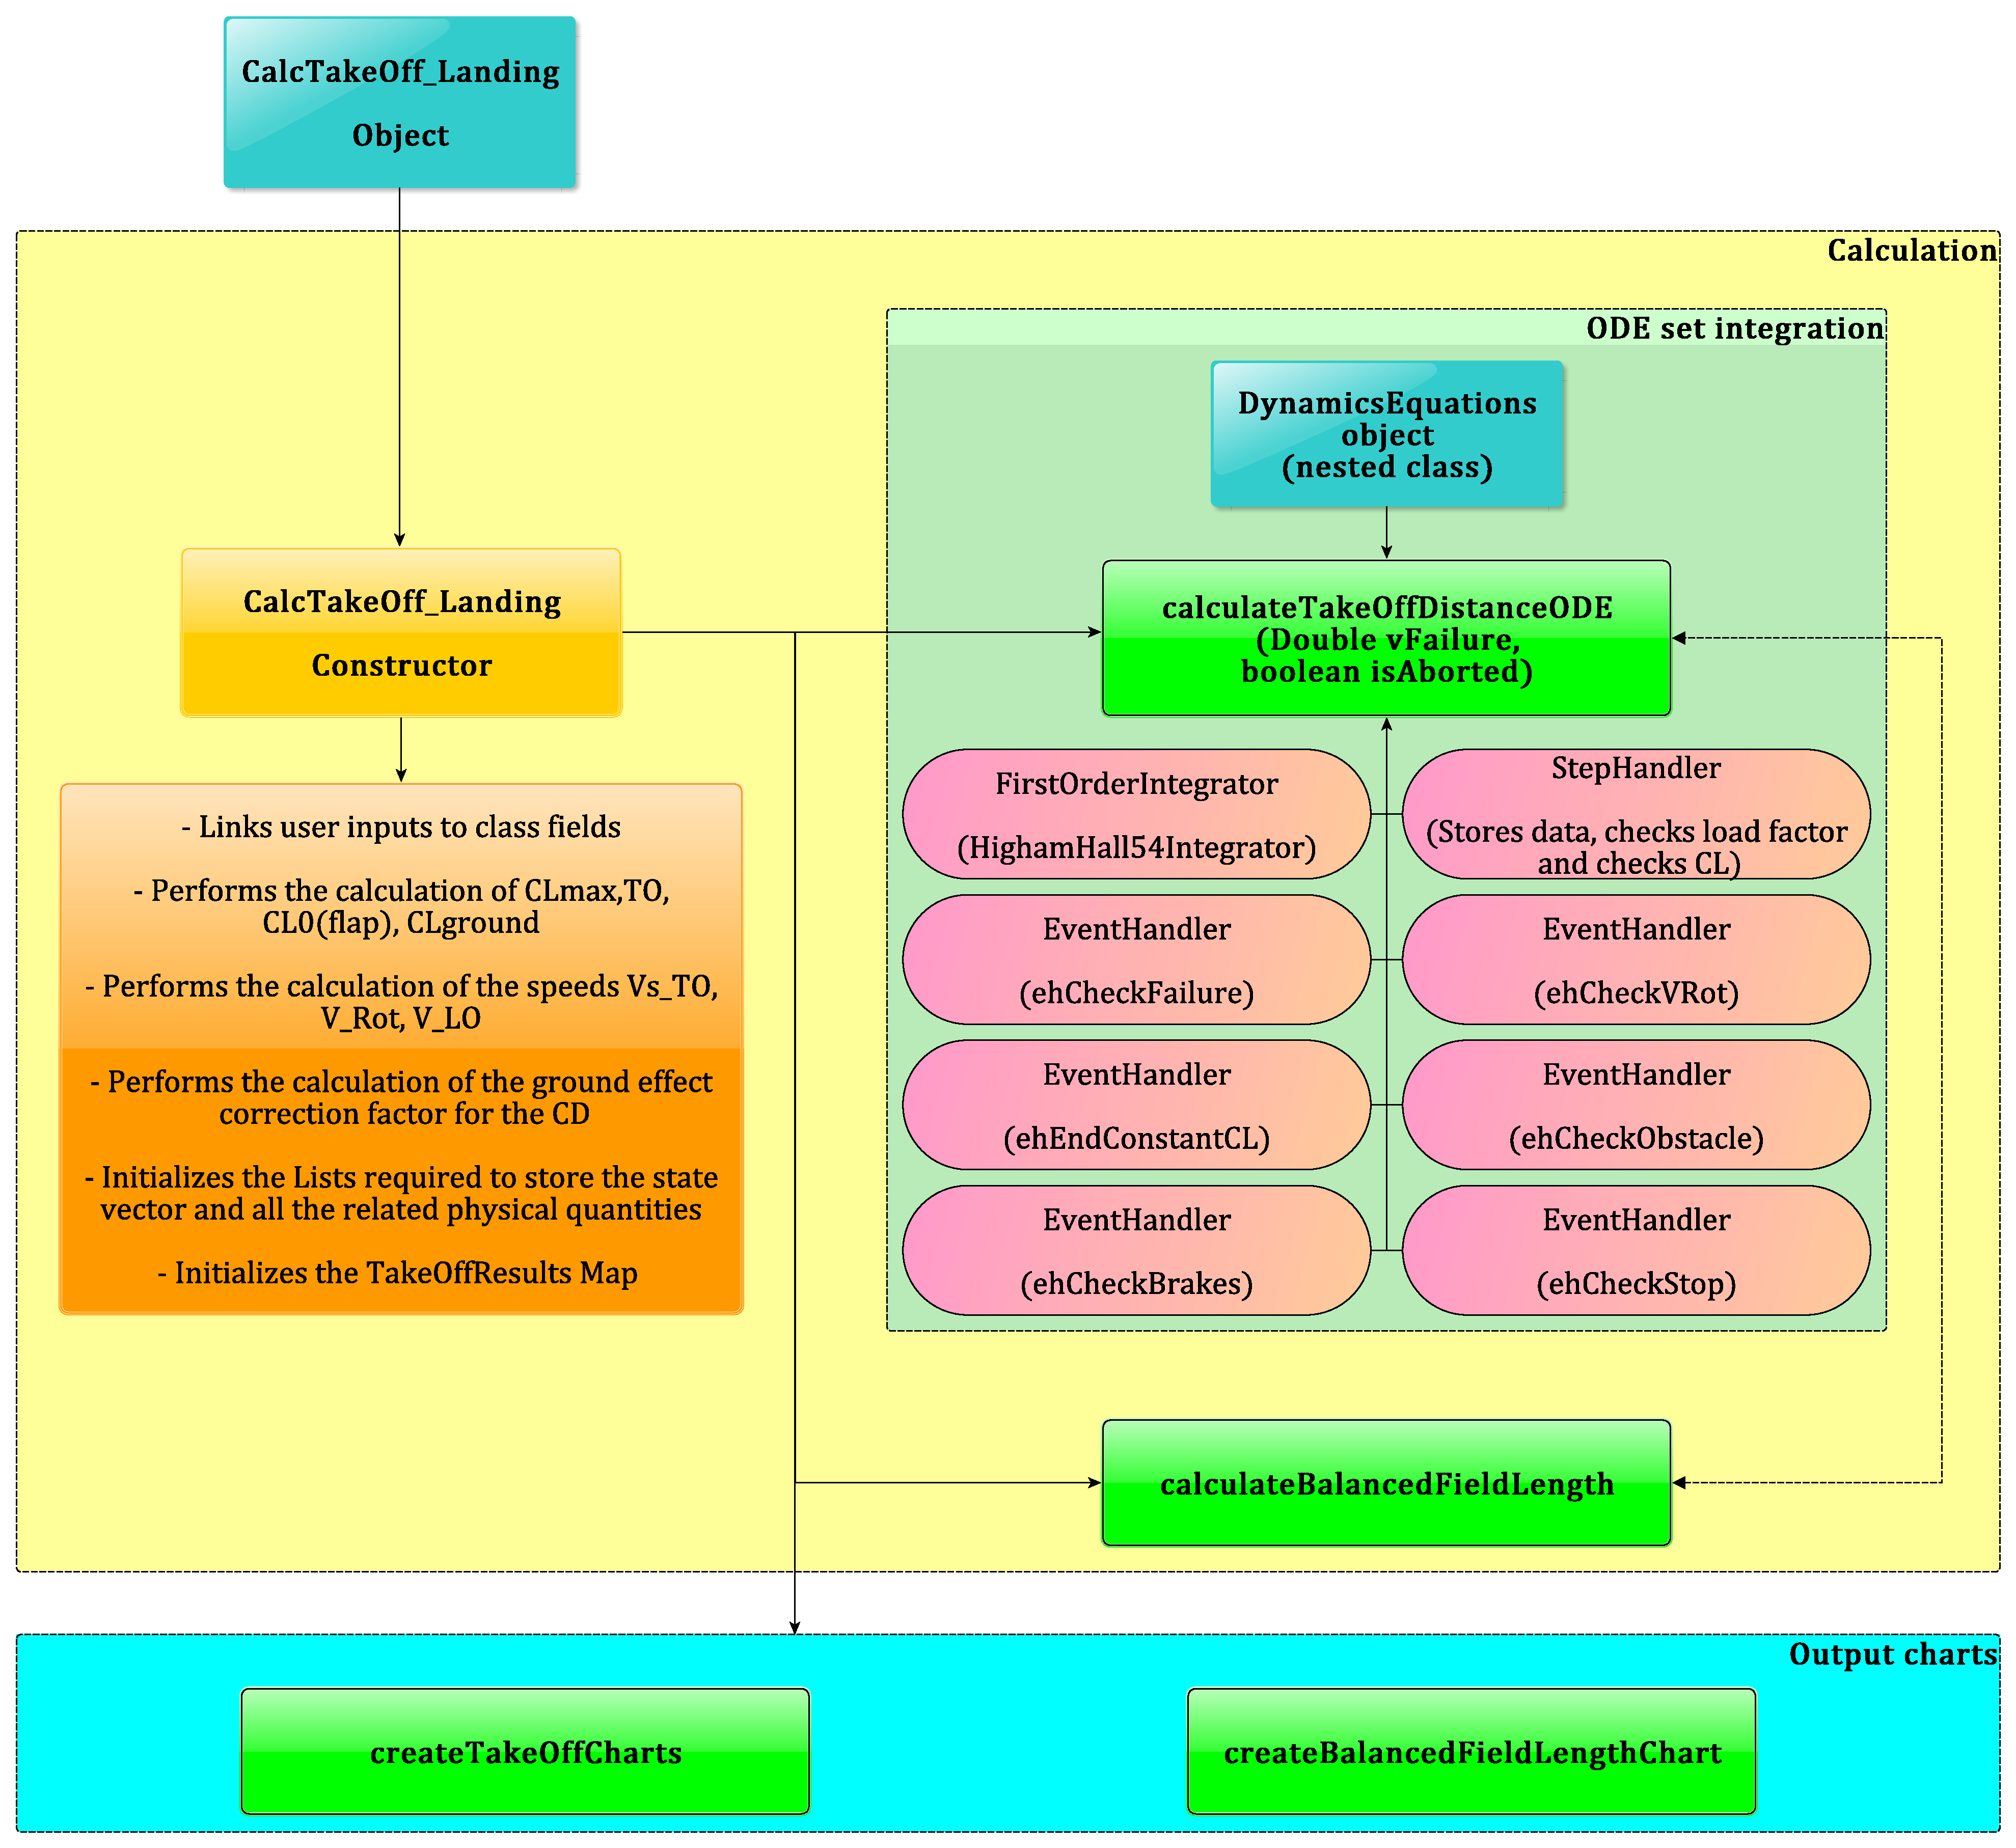
\includegraphics[keepaspectratio, width=\textwidth]{TakeOff_Flowchart}
\caption{\lstinline[language=Java]!CalcTakeOff_Landing! class flowchart}
\label{fig:CalcTakeOffFlowchart}
\end{figure}
%
%----------------------- CASE STUDY : ATR72 AND B747 -------------------------
\section{Case study: ATR-72}
This conclusive paragraph has the aim of describing the Java class created to test the features implemented into \lstinline[language=Java]!CalcTakeOff_Landing! class; in particular a description of how to build the class will be provided in order to help a potential \gls{User:Developer} as well as the presentation and the comment of the most important charts created with the purpose of validating the results obtained. 
%
Since the calculations are the same both for the B747-100B, both for the ATR-72, only the latter will be analyzed. 

\noindent
The first thing to do is to build the aircraft parametric model, and its analysis object, as described in paragraph \ref{par:DefaultAircraft}; then all information regarding high-lift devices have to be provided, in the same way of paragraph \ref{par:CaseStudyHighLift}, in order to allow the constructor of \lstinline[language=Java]!CalcTakeOff_Landing! class to evaluate their effects. 
%
At this point all the preliminary steps are completed and it's possible to create the \lstinline[language=Java]!CalcTakeOff_Landing! object giving as input all data from table \ref{table:CalcTakeOffInput}.

\bigskip
\begin{lstlisting}[caption={Input data and \lstinline!CalcTakeOff_Landing! object creation }, captionpos=b, tabsize=2]
		Amount<Duration> dtRot = Amount.valueOf(3, SI.SECOND);
		Amount<Duration> dtHold = Amount.valueOf(0.5, SI.SECOND);
		double mu = 0.025;
		double muBrake = 0.3;
		double kAlphaDot = 0.06; // [1/deg]
		double kcLMax = 0.85;
		double kRot = 1.05;
		double kLO = 1.1;
		double kFailure = 1.1;
		double phi = 1.0;
		double alphaReductionRate = -3; // [deg/s]
		Amount<Length> wingToGroundDistance = Amount.valueOf(4.0, SI.METER);
		Amount<Length> obstacle = Amount.valueOf(35, NonSI.FOOT).to(SI.METER);
		Amount<Velocity> vWind = Amount.valueOf(0.0, SI.METERS_PER_SECOND);
		Amount<Angle> alphaGround = Amount.valueOf(0.0, NonSI.DEGREE_ANGLE);
		Amount<Angle> iw = Amount.valueOf(2.0, NonSI.DEGREE_ANGLE);
//		PARAMETERS USED TO CONSIDER THE PARABOLIC DRAG POLAR CORRECTION AT HIGH CL
		double k1 = 0.0;
		double k2 = 0.0;
	
		CalcTakeOff_Landing theTakeOffLandingCalculator = new CalcTakeOff_Landing(
				aircraft,
				theCondition,
				highLiftCalculator,
				dtRot,
				dtHold,
				kcLMax,
				kRot,
				kLO,
				kFailure,
				k1,
				k2,
				phi,
				kAlphaDot,
				alphaReductionRate,
				mu,
				muBrake,
				wingToGroundDistance,
				obstacle,
				vWind,
				alphaGround,
				iw
				);
\end{lstlisting}
%
Now if the user wants to perform a single calculation of the take-off distance, he can call the method \lstinline[language=Java]!calculateTakeOffDistanceODE!, specifing the condition he wants to analyze. The possible situations are resumed below, where \lstinline[language=Java]!vFailure! is an assigned \lstinline[language=Java]!Double! value.

\bigskip
\begin{lstlisting}[caption={Possible scenarios of calculation of the take-off distance}, captionpos=b, tabsize=2, label={lst:TakeOffScenarios}]
// AOE condition
theTakeOffLandingCalculator.calculateTakeOffDistanceODE(null, false); 
// OEI continued take-off
theTakeOffLandingCalculator.calculateTakeOffDistanceODE(vFailure, false); 
// OEI aborted take-off
theTakeOffLandingCalculator.calculateTakeOffDistanceODE(vFailure, true); 
\end{lstlisting}
%
Since this method provides only calculations, the user may want to generate charts regarding the evolution of the state vector and of the related physical quantities during the take-off run; in this case all it has to be done is call the method \lstinline[language=Java]!createTakeOffCharts! as shown below.

\bigskip
\begin{lstlisting}[caption={Take-off charts creation}, captionpos=b, tabsize=2]
// Generates all the output charts
theTakeOffLandingCalculator.createTakeOffCharts();
\end{lstlisting}
%
Following the flowchart of figure \ref{fig:CalcTakeOffFlowchart}, if the user wants, instead, to calculate the \emph{balanced field length}, and plot its chart, it's still very easy; in fact he has only to call the two methods \lstinline[language=Java]!calculateBalancedFieldLength! and \lstinline[language=Java]!createBalancedFieldLengthChart!.

\bigskip
\begin{lstlisting}[caption={Balanced field length calculation and plot}, captionpos=b, tabsize=2]
// Calculation of the balanced field length
theTakeOffLandingCalculator.calculateBalancedFieldLength();
// Plot of the balanced field length chart
theTakeOffLandingCalculator.createBalancedFieldLengthChart();
\end{lstlisting}
%
The following pages shows a summary of charts created in the three condition of listing \ref{lst:TakeOffScenarios} choosing a \lstinline[language=Java]!vFailure! of 30 $\si{\meter\per\second}$. Instead, in the listing below, are resumed the main result of the \gls{acr:AOE} condition together with the results of the \emph{balanced field length} calculation.

\bigskip
\begin{lstlisting}[caption={ATR-72 test results}, captionpos=b, tabsize=2]
-----------------------------------------------------------------
CLmaxTO = 2.0212498531249747
VsTO = 54.7262494000153 m/s
VRot = 57.4625618700161 m/s
vLO = 60.1988743400169 m/s
CL0 = 1.0741952614143324
CLground = 1.2573301946144486
-----------------------------------------------------------------
		END OF GROUND ROLL PHASE
	switching function changes sign at t = 25.798463352896295 s
	x[0] = s = 805.6857140622815 m
	x[1] = V = 57.4625618700161 m/s
	x[2] = gamma = 0.0 deg
	x[3] = altitude = 0.0 m
	COLLECTING DATA AT THE END OF GROUND ROLL PHASE ...
---------------------------DONE!-------------------------------
		END OF ROTATION PHASE
	x[0] = s = 969.8307390403536 m
	x[1] = V = 61.80076798783429 m/s
	x[2] = gamma = 0.0 deg
	x[3] = altitude = 0.0 m
	t = 28.550529077966075 s
	COLLECTING DATA AT THE END OF ROTATION PHASE ...
---------------------------DONE!-------------------------------
		BEGIN BAR HOLDING
	CL = 1.718569601482539
	Alpha Body = 5.037672106777929 deg
	t = 29.788098164419022 s
---------------------------DONE!-------------------------------
		END BAR HOLDING
	switching function changes sign at t = 30.28809816441902 s 
---------------------------DONE!-------------------------------
		LOAD FACTOR = 1 IN CLIMB
	t = 31.38918339811157 s
---------------------------DONE!-------------------------------
		END OF AIRBORNE PHASE
	switching function changes sign at t = 33.374058565110616 s
	x[0] = s = 1281.9765437949968 m
	x[1] = V = 67.04253409907443 m/s
	x[2] = gamma = 2.8305305752769097 deg
	x[3] = altitude = 10.668000000000013 m
	COLLECTING DATA AT THE END OF AIRBORNE PHASE ...
---------------------------DONE!-------------------------------
BALANCED FIELD LENGTH = 1844.57965640814 m
Decision Speed (V1/VsTO) = 1.04020737941333 
---------------------------END!!-------------------------------
\end{lstlisting}
%
As can be seen the take-off distance required in \gls{acr:AOE} condition is about $\SI{1282}{\meter}$, at the maximum take-off weight of $\SI{23063.579}{\kilogram}$, within a time of about $\SI{33.4}{\second}$; while the \emph{balanced field lenght} is bigger than the AOE take-off distance of about the 30\%.  Moreover the \emph{decision speed} $V_1$ is bigger than the stalling speed $V_s$ and lower than the rotation speed $V_{\text{Rot}}$ as required by the \gls{FAR}-25 from table \ref{tab:Take:Off:Speeds:FAR25}.
%
These results are almost the same shown in the aircraft brochure available on the Internet, so that the calculation carried out results correct.
%%
%\clearpage
%%
%\begin{figure}[H]
%\centering
%%TakeOff_Trajectory
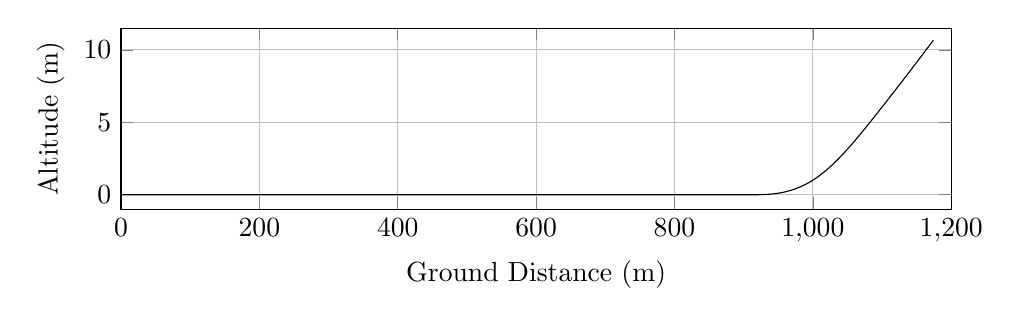
\begin{tikzpicture}

\begin{axis}[
width=\textwidth,
height=0.32\textwidth,
scaled ticks=false, tick label style={/pgf/number format/fixed},
xmin=0.0,
xmax=1200,
xlabel={Ground Distance (m)},
xmajorgrids,
ymin=-1.0,
ymax=11.5,
ylabel={Altitude (m)},
ymajorgrids,
legend style={at={(1.03,0.5)},anchor=west,draw=black,fill=white,legend cell align=left}
]

\addplot [
color=black,
solid
]
table[row sep=crcr]{
1.3729668748938318E-8	0.0\\
1.7493248493808052E-7	0.0\\
1.4411937280317895E-6	0.0\\
6.602995160656227E-5	0.0\\
2.2740573828771224E-4	0.0\\
4.8751428921765393E-4	0.0\\
8.441986619835749E-4	0.0\\
0.0012981647037285577	0.0\\
0.0018484379050661159	0.0\\
0.0024893731755424335	0.0\\
0.0032286585096692284	0.0\\
0.0040442418752796045	0.0\\
0.004972762654474916	0.0\\
0.005990910102221513	0.0\\
0.007111389191545643	0.0\\
0.008336865178450469	0.0\\
0.009664633507451486	0.0\\
0.011093815858158905	0.0\\
0.01262066151120312	0.0\\
0.01419454386807839	0.0\\
0.015910782250193378	0.0\\
0.017721549103721458	0.0\\
0.019620507964630857	0.0\\
0.02164969955342029	0.0\\
0.023766550611781796	0.0\\
0.025957065600157342	0.0\\
0.028260861173784894	0.0\\
0.030668466949245715	0.0\\
0.0331489614440674	0.0\\
0.03573888453685943	0.0\\
0.038418765463712895	0.0\\
0.04116679597872082	0.0\\
0.044022059812866554	0.0\\
0.04700053365173311	0.0\\
0.050116649382181494	0.0\\
0.0533021652593606	0.0\\
0.056630220296749106	0.0\\
0.05998688030085898	0.0\\
0.06348077825220624	0.0\\
0.06710848437295475	0.0\\
0.07082346760424127	0.0\\
0.07462944469130567	0.0\\
0.07855413323217031	0.0\\
0.08251243142992878	0.0\\
0.08659905947434482	0.0\\
0.09083545394947079	0.0\\
0.09518096637774642	0.0\\
0.099604438418047	0.0\\
0.1041130762071252	0.0\\
0.10871457033213175	0.0\\
0.11350280915994052	0.0\\
0.11836943512882261	0.0\\
0.12328542045494376	0.0\\
0.12830372217771202	0.0\\
0.1334037067999082	0.0\\
0.1386015897371753	0.0\\
0.14405085578552257	0.0\\
0.1495239325759128	0.0\\
0.1550507392415454	0.0\\
0.16073360491635535	0.0\\
0.16659871679960742	0.0\\
0.17244819595229793	0.0\\
0.17848031195343078	0.0\\
0.18466822548212042	0.0\\
0.1909009608611748	0.0\\
0.19716089737688902	0.0\\
0.2035279375926986	0.0\\
0.21017879584430066	0.0\\
0.21687473998771628	0.0\\
0.22354650324940833	0.0\\
0.23036941414946865	0.0\\
0.23737731412185503	0.0\\
0.24449289925428264	0.0\\
0.2517184892023243	0.0\\
0.25908208279438383	0.0\\
0.2664863589195283	0.0\\
0.27399321582905467	0.0\\
0.2816108016888421	0.0\\
0.2893844725195981	0.0\\
0.29747621078120867	0.0\\
0.30547198304033185	0.0\\
0.31373479402345694	0.0\\
0.3220909744202328	0.0\\
0.3305540912568814	0.0\\
0.33895489345894936	0.0\\
0.34753073012810576	0.0\\
0.3563589175375672	0.0\\
0.3652744752958731	0.0\\
0.3742693918027593	0.0\\
0.38350989122680823	0.0\\
0.3927029292363896	0.0\\
0.4020876366599533	0.0\\
0.4115568217121528	0.0\\
0.4212787852930122	0.0\\
0.43089755178065414	0.0\\
0.4408379299669313	0.0\\
0.4510502611115679	0.0\\
0.4612670224725215	0.0\\
0.4715818614584312	0.0\\
0.4818438670126082	0.0\\
0.4922128554044626	0.0\\
0.50273876067117	0.0\\
0.5136516607865718	0.0\\
0.5244310074213006	0.0\\
0.5355751508210329	0.0\\
0.5467126997993474	0.0\\
0.5580479056656631	0.0\\
0.5692960823995112	0.0\\
0.5809945926573021	0.0\\
0.5923626544035139	0.0\\
0.6041922852715	0.0\\
0.6160912669048675	0.0\\
0.6280605196746807	0.0\\
0.6403946506485891	0.0\\
0.6525721787971039	0.0\\
0.66504690021022	0.0\\
0.6773535438897555	0.0\\
0.6901462526606317	0.0\\
0.703249873273524	0.0\\
0.7159721017112175	0.0\\
0.729053467210389	0.0\\
0.7422988791228431	0.0\\
0.756304272979474	0.0\\
0.7696432036294076	0.0\\
0.7832290250230658	0.0\\
0.7969128825551131	0.0\\
0.8108444209446342	0.0\\
0.825043936786227	0.0\\
0.8390802275180445	0.0\\
0.8532340040587583	0.0\\
0.8678101043696134	0.0\\
0.8824320602344964	0.0\\
0.8978006605470081	0.0\\
0.9134572487531922	0.0\\
0.9287391767029982	0.0\\
0.9440564687433697	0.0\\
0.9598871644713316	0.0\\
0.9757786228365237	0.0\\
0.9918217338879218	0.0\\
1.0080608846667363	0.0\\
1.0245900975307913	0.0\\
1.040622085070809	0.0\\
1.0571005809273983	0.0\\
1.0736578999152901	0.0\\
1.0902401336450098	0.0\\
1.1073201062866707	0.0\\
1.1241926772552646	0.0\\
1.1416781667104252	0.0\\
1.1588269484070954	0.0\\
1.176440946845327	0.0\\
1.1944819542445066	0.0\\
1.2120125629913447	0.0\\
1.2299306574276825	0.0\\
1.2481120482032448	0.0\\
1.2663536608165091	0.0\\
1.2851425782117465	0.0\\
1.3041313368869671	0.0\\
1.3228236880779458	0.0\\
1.3414329672940513	0.0\\
1.3605066144349074	0.0\\
1.3802534409605212	0.0\\
1.3994872719307283	0.0\\
1.4192016277101378	0.0\\
1.439023460648384	0.0\\
1.459347998039509	0.0\\
1.4793256644936217	0.0\\
1.4991489338326072	0.0\\
1.5195196572175793	0.0\\
1.5402684478761244	0.0\\
1.5604570108688036	0.0\\
1.5810331069622228	0.0\\
1.6022712329181132	0.0\\
1.623752316257296	0.0\\
1.6452514305955401	0.0\\
1.6664829631402025	0.0\\
1.6886446033619715	0.0\\
1.710607384244656	0.0\\
1.7329417009553727	0.0\\
1.7551421266962821	0.0\\
1.7779085356585536	0.0\\
1.800478286927734	0.0\\
1.8236018329231238	0.0\\
1.8462320784511883	0.0\\
1.869621217116264	0.0\\
1.8933146512119747	0.0\\
1.9176856041472643	0.0\\
1.9417713639512164	0.0\\
1.9657098573982132	0.0\\
1.9902165007163162	0.0\\
2.014554050520948	0.0\\
2.039479559407779	0.0\\
2.0645497069116256	0.0\\
2.090368502766882	0.0\\
2.115564185269416	0.0\\
2.140750230554602	0.0\\
2.1667677015838267	0.0\\
2.1927560352542175	0.0\\
2.218891869133375	0.0\\
2.245288939563828	0.0\\
2.2712530964452817	0.0\\
2.297933078351498	0.0\\
2.324564104516777	0.0\\
2.351466051806102	0.0\\
2.378869922986878	0.0\\
2.4061764715670764	0.0\\
2.4343811693482102	0.0\\
2.4622108821536663	0.0\\
2.4906408044048067	0.0\\
2.518892760285042	0.0\\
2.5472153538550346	0.0\\
2.5762492306032216	0.0\\
2.605385308804288	0.0\\
2.634725531238531	0.0\\
2.6633424112287507	0.0\\
2.6927188130915374	0.0\\
2.7226962917814213	0.0\\
2.7531675915664673	0.0\\
2.7831412651501983	0.0\\
2.8139174932165103	0.0\\
2.8440331768075415	0.0\\
2.874693215323904	0.0\\
2.9059978681586376	0.0\\
2.9372617813709034	0.0\\
2.9684444504378202	0.0\\
3.000072782687808	0.0\\
3.031082587373527	0.0\\
3.063213028467148	0.0\\
3.0965739711585014	0.0\\
3.1291175748240176	0.0\\
3.161651640649506	0.0\\
3.194791488147139	0.0\\
3.2273698640351327	0.0\\
3.261394174200582	0.0\\
3.2942820372415875	0.0\\
3.3276455142443044	0.0\\
3.3625338428565543	0.0\\
3.396526624461681	0.0\\
3.4305511850311694	0.0\\
3.4642094416894933	0.0\\
3.498963551783903	0.0\\
3.5341885134496573	0.0\\
3.569804025802995	0.0\\
3.605116576002147	0.0\\
3.641338581546833	0.0\\
3.677593698357855	0.0\\
3.7132425573336665	0.0\\
3.74957219375957	0.0\\
3.7872650227149185	0.0\\
3.825403000593508	0.0\\
3.861987998097706	0.0\\
3.899535703755137	0.0\\
3.9366960368382165	0.0\\
3.9756271117991435	0.0\\
4.014715979923002	0.0\\
4.053268843133694	0.0\\
4.093111596873367	0.0\\
4.132540645872048	0.0\\
4.171686416589186	0.0\\
4.211258480423352	0.0\\
4.252585425594734	0.0\\
4.29253892845542	0.0\\
4.332839968385603	0.0\\
4.372708537789018	0.0\\
4.414379330316386	0.0\\
4.455607216042212	0.0\\
4.497336690654009	0.0\\
4.53836773335787	0.0\\
4.579767142935065	0.0\\
4.621942908118227	0.0\\
4.663798268780793	0.0\\
4.705838036060712	0.0\\
4.748491012675066	0.0\\
4.791393968819099	0.0\\
4.835700194867293	0.0\\
4.879973298406089	0.0\\
4.923250156511948	0.0\\
4.967673596314626	0.0\\
5.012954369117542	0.0\\
5.057574526249477	0.0\\
5.103280208347517	0.0\\
5.148856018935929	0.0\\
5.194350575362858	0.0\\
5.240584094986199	0.0\\
5.2871741484687504	0.0\\
5.333122064003502	0.0\\
5.3803318800233235	0.0\\
5.4262712259485255	0.0\\
5.473378197958581	0.0\\
5.521938593493333	0.0\\
5.570027890245774	0.0\\
5.617746353771608	0.0\\
5.665750363096816	0.0\\
5.714883880069209	0.0\\
5.763390205677501	0.0\\
5.812817811268989	0.0\\
5.861909274803731	0.0\\
5.912134919389196	0.0\\
5.962317560553064	0.0\\
6.012727788730279	0.0\\
6.0628236035803145	0.0\\
6.113711068416594	0.0\\
6.16497292765713	0.0\\
6.216284706244114	0.0\\
6.26834407822653	0.0\\
6.320257064476769	0.0\\
6.37351660191279	0.0\\
6.426150862197664	0.0\\
6.479030963436509	0.0\\
6.532319340056288	0.0\\
6.5857233987986845	0.0\\
6.640834734692348	0.0\\
6.695022999498724	0.0\\
6.749720237657193	0.0\\
6.804235758325081	0.0\\
6.859728469301633	0.0\\
6.916686079588434	0.0\\
6.9732530286722305	0.0\\
7.029531186664631	0.0\\
7.086633318514238	0.0\\
7.144155485034537	0.0\\
7.202053129566568	0.0\\
7.260126434764185	0.0\\
7.317913145042743	0.0\\
7.376682960996439	0.0\\
7.435393721764624	0.0\\
7.493838107271518	0.0\\
7.552684475254578	0.0\\
7.613252707151423	0.0\\
7.672782806866918	0.0\\
7.733397683408512	0.0\\
7.795525081709004	0.0\\
7.856013653786727	0.0\\
7.91792172269443	0.0\\
7.980110745884113	0.0\\
8.041720670752433	0.0\\
8.105229267009985	0.0\\
8.167457523036095	0.0\\
8.230908874360502	0.0\\
8.293738919282273	0.0\\
8.356235402336917	0.0\\
8.42092378244627	0.0\\
8.485671322837007	0.0\\
8.549180898871484	0.0\\
8.614596634551038	0.0\\
8.680166762249144	0.0\\
8.744770128469462	0.0\\
8.812993689385827	0.0\\
8.88005807777586	0.0\\
8.94709863067661	0.0\\
9.013172088448385	0.0\\
9.079266506338545	0.0\\
9.14748814890141	0.0\\
9.215411293660388	0.0\\
9.284579146198691	0.0\\
9.353168277381275	0.0\\
9.423753765537143	0.0\\
9.492960052876374	0.0\\
9.564123004975215	0.0\\
9.634097601479446	0.0\\
9.705672410878787	0.0\\
9.776260200085993	0.0\\
9.846607984572056	0.0\\
9.918231435410593	0.0\\
9.988851555070422	0.0\\
10.060390022634245	0.0\\
10.133279281833644	0.0\\
10.205241085147751	0.0\\
10.277820389603	0.0\\
10.352558894167803	0.0\\
10.42733258664746	0.0\\
10.501815126481194	0.0\\
10.576858173457808	0.0\\
10.65303812840548	0.0\\
10.729080272001735	0.0\\
10.804841544893105	0.0\\
10.881905013502095	0.0\\
10.958396790746043	0.0\\
11.035905069829102	0.0\\
11.113160538490881	0.0\\
11.192172636140572	0.0\\
11.270076562295213	0.0\\
11.350065490058778	0.0\\
11.429008826667825	0.0\\
11.50754237847364	0.0\\
11.587076645554472	0.0\\
11.668897725768986	0.0\\
11.749734371708193	0.0\\
11.830312384681939	0.0\\
11.909862670519033	0.0\\
11.990515423105418	0.0\\
12.072973931530203	0.0\\
12.155304175892073	0.0\\
12.237018674011615	0.0\\
12.320146069843414	0.0\\
12.406770618003886	0.0\\
12.489918686423398	0.0\\
12.574493004618496	0.0\\
12.660666896522624	0.0\\
12.746500366216402	0.0\\
12.832006837122272	0.0\\
12.919285437479463	0.0\\
13.00517529032821	0.0\\
13.092301899261269	0.0\\
13.179760097773386	0.0\\
13.268594687119744	0.0\\
13.357699529172354	0.0\\
13.44829753340392	0.0\\
13.537570218252604	0.0\\
13.627322718831184	0.0\\
13.718307212496544	0.0\\
13.808540263830096	0.0\\
13.899143852161355	0.0\\
13.991564069206362	0.0\\
14.085798171937814	0.0\\
14.179213507883688	0.0\\
14.271883316076963	0.0\\
14.367546274622434	0.0\\
14.459430863676705	0.0\\
14.555010173556813	0.0\\
14.648669731311681	0.0\\
14.743773575674254	0.0\\
14.839769774519894	0.0\\
14.932807148196385	0.0\\
15.026921440816679	0.0\\
15.12275113649265	0.0\\
15.222025232743288	0.0\\
15.321078842653048	0.0\\
15.417564225728565	0.0\\
15.515758841369038	0.0\\
15.613440509090129	0.0\\
15.7107260301154	0.0\\
15.81102223487273	0.0\\
15.913565872734136	0.0\\
16.012918321571746	0.0\\
16.11222833737955	0.0\\
16.216250800242257	0.0\\
16.319159023020546	0.0\\
16.421418004006803	0.0\\
16.521675247646563	0.0\\
16.62557290942481	0.0\\
16.72731964230514	0.0\\
16.830283223934416	0.0\\
16.93464251494634	0.0\\
17.038481620468637	0.0\\
17.146497421123335	0.0\\
17.252282308638982	0.0\\
17.35724772858778	0.0\\
17.464053904588297	0.0\\
17.572390862630144	0.0\\
17.680417629270814	0.0\\
17.789707298693855	0.0\\
17.899612520762552	0.0\\
18.01027367065641	0.0\\
18.121415095654797	0.0\\
18.232428503320143	0.0\\
18.34337337506409	0.0\\
18.454877340220463	0.0\\
18.56636189702322	0.0\\
18.678405595805643	0.0\\
18.7903363416971	0.0\\
18.902391384512768	0.0\\
19.01754810908954	0.0\\
19.131359562866663	0.0\\
19.247747682986713	0.0\\
19.361628242251975	0.0\\
19.477963464454028	0.0\\
19.595742742603164	0.0\\
19.71107288142779	0.0\\
19.82767543183723	0.0\\
19.944540068808188	0.0\\
20.06171535440768	0.0\\
20.179291418887807	0.0\\
20.29729887224694	0.0\\
20.417200571824914	0.0\\
20.53676390826074	0.0\\
20.65523768803314	0.0\\
20.777063017363922	0.0\\
20.896922101876633	0.0\\
21.016777952410983	0.0\\
21.13892104879462	0.0\\
21.260534693274344	0.0\\
21.382619708556632	0.0\\
21.506306369043365	0.0\\
21.631260758247265	0.0\\
21.75556249187227	0.0\\
21.87985606458615	0.0\\
22.005925835680863	0.0\\
22.130365724585275	0.0\\
22.257477980325966	0.0\\
22.38418119026224	0.0\\
22.50885833858638	0.0\\
22.636026948728087	0.0\\
22.76367325110224	0.0\\
22.89115382514759	0.0\\
23.022452271734288	0.0\\
23.149877274293033	0.0\\
23.27873580881144	0.0\\
23.408563766880334	0.0\\
23.538692653979794	0.0\\
23.671258756997098	0.0\\
23.803210122669313	0.0\\
23.93544283576786	0.0\\
24.067241518013077	0.0\\
24.19863541429976	0.0\\
24.329449967727697	0.0\\
24.46175612159181	0.0\\
24.594763714591892	0.0\\
24.72754053098891	0.0\\
24.86208223890334	0.0\\
24.99503410474967	0.0\\
25.12831230627787	0.0\\
25.265273024090206	0.0\\
25.400650037308893	0.0\\
25.536304655026747	0.0\\
25.673594178904246	0.0\\
25.80797730935859	0.0\\
25.835159569235522	0.0\\
25.83771752397454	0.0\\
25.84157983658004	0.0\\
25.854829339215996	0.0\\
25.893215796826965	0.0\\
25.973046119315796	0.0\\
26.096262980671412	0.0\\
26.224212718725603	0.0\\
26.35313595194755	0.0\\
26.481727686355264	0.0\\
26.611118169629577	0.0\\
26.74049186039369	0.0\\
26.87228140714948	0.0\\
27.003385008924262	0.0\\
27.1358830905183	0.0\\
27.265951877034226	0.0\\
27.399105426781233	0.0\\
27.53075869079712	0.0\\
27.66387879779476	0.0\\
27.79855889054391	0.0\\
27.932132547760695	0.0\\
28.06791767232785	0.0\\
28.202763022922632	0.0\\
28.339788243013793	0.0\\
28.476803106655623	0.0\\
28.61761981788422	0.0\\
28.753907949775353	0.0\\
28.89297195746854	0.0\\
29.03211749902605	0.0\\
29.17123509789927	0.0\\
29.312253051611236	0.0\\
29.454422317169097	0.0\\
29.59523538430127	0.0\\
29.737672170826222	0.0\\
29.879173197948965	0.0\\
30.02075470454991	0.0\\
30.166674235301365	0.0\\
30.308336095430334	0.0\\
30.452640844036836	0.0\\
30.597553881025625	0.0\\
30.742967061600154	0.0\\
30.888975484926362	0.0\\
31.034653067922946	0.0\\
31.180984070508003	0.0\\
31.328351020411645	0.0\\
31.476753455192622	0.0\\
31.62661541983664	0.0\\
31.774495604492607	0.0\\
31.924944104961916	0.0\\
32.07610067279926	0.0\\
32.22631826848556	0.0\\
32.37899942625752	0.0\\
32.528514827654206	0.0\\
32.68189139400266	0.0\\
32.836069829938495	0.0\\
32.99025509482905	0.0\\
33.14574197930297	0.0\\
33.30072558931056	0.0\\
33.455047097713944	0.0\\
33.610874563168906	0.0\\
33.76926068144728	0.0\\
33.92617323250643	0.0\\
34.08448787244542	0.0\\
34.24243160505006	0.0\\
34.40316487172558	0.0\\
34.56154208099588	0.0\\
34.721775177117024	0.0\\
34.88076970836556	0.0\\
35.041349106451236	0.0\\
35.20329621413198	0.0\\
35.364886328651124	0.0\\
35.529241615711214	0.0\\
35.69117991651797	0.0\\
35.85317319416103	0.0\\
36.014854298354294	0.0\\
36.18095311277159	0.0\\
36.34443322746766	0.0\\
36.51065106768533	0.0\\
36.67635767082788	0.0\\
36.842033683894186	0.0\\
37.00823867836148	0.0\\
37.17279029188734	0.0\\
37.33951104811075	0.0\\
37.50923941781488	0.0\\
37.679358776579846	0.0\\
37.845326083883435	0.0\\
38.017144746304325	0.0\\
38.1852030886141	0.0\\
38.35804431104914	0.0\\
38.52812920813831	0.0\\
38.69960796987526	0.0\\
38.87165793928378	0.0\\
39.0423941506003	0.0\\
39.21436971822614	0.0\\
39.38727999643966	0.0\\
39.558989012313546	0.0\\
39.734752343022535	0.0\\
39.908836167348156	0.0\\
40.084555009291705	0.0\\
40.259186798753746	0.0\\
40.43324437115375	0.0\\
40.61041052363379	0.0\\
40.787318094191775	0.0\\
40.96620398302343	0.0\\
41.14141336180775	0.0\\
41.31941103282654	0.0\\
41.49571226203258	0.0\\
41.67366972437729	0.0\\
41.85219319429197	0.0\\
42.03136872634711	0.0\\
42.21293422072888	0.0\\
42.39366932880948	0.0\\
42.57479521797359	0.0\\
42.75522531040919	0.0\\
42.93775785970641	0.0\\
43.11993568316029	0.0\\
43.30336620712447	0.0\\
43.48720879745599	0.0\\
43.672226884455625	0.0\\
43.85684130549208	0.0\\
44.039851952877484	0.0\\
44.22449378650157	0.0\\
44.412385508552646	0.0\\
44.59783063297877	0.0\\
44.78525507043919	0.0\\
44.973130075825196	0.0\\
45.16145211071871	0.0\\
45.34881478087516	0.0\\
45.536017136752506	0.0\\
45.724971990057284	0.0\\
45.91416212467789	0.0\\
46.10175434018815	0.0\\
46.29356928918713	0.0\\
46.48490977712943	0.0\\
46.67744207882204	0.0\\
46.869905949194575	0.0\\
47.062749521718516	0.0\\
47.25341437235973	0.0\\
47.44508461154423	0.0\\
47.63880095964302	0.0\\
47.83356160493736	0.0\\
48.025334057720784	0.0\\
48.218846636819876	0.0\\
48.41468711090302	0.0\\
48.610449575687724	0.0\\
48.80723286029129	0.0\\
49.00124137999302	0.0\\
49.20045899041696	0.0\\
49.394243884198005	0.0\\
49.59161211700324	0.0\\
49.79144608231523	0.0\\
49.99107345578199	0.0\\
50.18996871950735	0.0\\
50.388458331230495	0.0\\
50.59191110395449	0.0\\
50.79453916783869	0.0\\
50.99530158869649	0.0\\
51.19776583381373	0.0\\
51.3996255264899	0.0\\
51.599450409211	0.0\\
51.80158475775707	0.0\\
52.002311498730975	0.0\\
52.2060805474067	0.0\\
52.40811442127868	0.0\\
52.61423073460446	0.0\\
52.821749674584495	0.0\\
53.03053110951893	0.0\\
53.23753590773735	0.0\\
53.44487707917263	0.0\\
53.652063533093525	0.0\\
53.85975522429668	0.0\\
54.06844148636836	0.0\\
54.278580968983874	0.0\\
54.48685885904548	0.0\\
54.69884126905886	0.0\\
54.90975544393264	0.0\\
55.12216013841277	0.0\\
55.333080623240974	0.0\\
55.5448885814986	0.0\\
55.75594910746132	0.0\\
55.968144975063936	0.0\\
56.18150915317635	0.0\\
56.394069348356695	0.0\\
56.60950747146016	0.0\\
56.82641599949238	0.0\\
57.03980213394583	0.0\\
57.25698083573829	0.0\\
57.47353804711997	0.0\\
57.6941706582635	0.0\\
57.91229938529948	0.0\\
58.12998527173144	0.0\\
58.34905943653719	0.0\\
58.56781345824973	0.0\\
58.787998582886644	0.0\\
59.011266007804366	0.0\\
59.23368761368569	0.0\\
59.456031473365414	0.0\\
59.67976581221534	0.0\\
59.90315377467765	0.0\\
60.125192111546724	0.0\\
60.349269227196444	0.0\\
60.57220932044149	0.0\\
60.79606803632835	0.0\\
61.021718319759984	0.0\\
61.25073295331903	0.0\\
61.47770893732542	0.0\\
61.70784367826464	0.0\\
61.93740803875056	0.0\\
62.1673491775543	0.0\\
62.39648011888062	0.0\\
62.62822464633953	0.0\\
62.86094183422966	0.0\\
63.090532789209604	0.0\\
63.321616049163225	0.0\\
63.554808975015874	0.0\\
63.78685818650332	0.0\\
64.0234762327251	0.0\\
64.25652029988498	0.0\\
64.49146565301734	0.0\\
64.72768747885678	0.0\\
64.96568125142531	0.0\\
65.20057601391298	0.0\\
65.43975061379945	0.0\\
65.67719429610031	0.0\\
65.91652243006087	0.0\\
66.1565253585166	0.0\\
66.39740384038885	0.0\\
66.63777997854328	0.0\\
66.87849958303539	0.0\\
67.12349409848125	0.0\\
67.36843544137562	0.0\\
67.61129947098183	0.0\\
67.85808619273692	0.0\\
68.10323725880951	0.0\\
68.3520146383799	0.0\\
68.60099753692072	0.0\\
68.84943315800746	0.0\\
69.09793111574629	0.0\\
69.34894754058863	0.0\\
69.59791912239118	0.0\\
69.84867626946473	0.0\\
70.10496107302816	0.0\\
70.35594730130109	0.0\\
70.60854748652795	0.0\\
70.8625286964371	0.0\\
71.1182576034713	0.0\\
71.37278964945165	0.0\\
71.62944082734805	0.0\\
71.88536754710964	0.0\\
72.14250945057543	0.0\\
72.40306402213687	0.0\\
72.66241221953337	0.0\\
72.92327110344874	0.0\\
73.18657203154456	0.0\\
73.45150557123125	0.0\\
73.71756195569753	0.0\\
73.97940051906463	0.0\\
74.24514793127645	0.0\\
74.51022759525631	0.0\\
74.77823256031297	0.0\\
75.04767613410795	0.0\\
75.31682895458664	0.0\\
75.58729746777243	0.0\\
75.85729327570917	0.0\\
76.13042767774209	0.0\\
76.40299665611133	0.0\\
76.67973301409052	0.0\\
76.95360383527739	0.0\\
77.22854206589327	0.0\\
77.50692063517303	0.0\\
77.78349662592461	0.0\\
78.0616064362213	0.0\\
78.33869545141144	0.0\\
78.62238552181594	0.0\\
78.90481169871467	0.0\\
79.18659077494928	0.0\\
79.4700201012688	0.0\\
79.75774957869095	0.0\\
80.04430580185078	0.0\\
80.33432201731404	0.0\\
80.62298533865851	0.0\\
80.9130804606989	0.0\\
81.20459144967842	0.0\\
81.49650140842283	0.0\\
81.79224544448738	0.0\\
82.08455487090956	0.0\\
82.37934996819865	0.0\\
82.67580145620735	0.0\\
82.97475550983006	0.0\\
83.2734238134004	0.0\\
83.57209772503273	0.0\\
83.87419166445906	0.0\\
84.17487194816226	0.0\\
84.47686996876752	0.0\\
84.78124993153034	0.0\\
85.08776945017104	0.0\\
85.39395758722245	0.0\\
85.69833162305892	0.0\\
86.01027818388755	0.0\\
86.31658691867341	0.0\\
86.62866814828641	0.0\\
86.94043673469176	0.0\\
87.2565990672368	0.0\\
87.56980823017452	0.0\\
87.88101387141376	0.0\\
88.20007062892054	0.0\\
88.51883409355145	0.0\\
88.83509784148416	0.0\\
89.15857089898353	0.0\\
89.47772213402055	0.0\\
89.80217214804901	0.0\\
90.1263587278685	0.0\\
90.44950966725051	0.0\\
90.77764749859728	0.0\\
91.10470504824352	0.0\\
91.43769785174896	0.0\\
91.76691749028419	0.0\\
92.09386993524024	0.0\\
92.42498248438446	0.0\\
92.7581696617394	0.0\\
93.09729153734631	0.0\\
93.4312406900703	0.0\\
93.76780571708736	0.0\\
94.10390054156983	0.0\\
94.43564317419558	0.0\\
94.77291201930262	0.0\\
95.10796951504997	0.0\\
95.44708659079325	0.0\\
95.78515592548297	0.0\\
96.12311752311894	0.0\\
96.46351490415591	0.0\\
96.80669869710772	0.0\\
97.14657639264556	0.0\\
97.48763116340677	0.0\\
97.8305814261901	0.0\\
98.17013304046878	0.0\\
98.51054009051404	0.0\\
98.854181194619	0.0\\
99.19205317796005	0.0\\
99.53355440060989	0.0\\
99.87198375587872	0.0\\
100.2129389915628	0.0\\
100.55335806642802	0.0\\
100.89503335592528	0.0\\
101.23693480167049	0.0\\
101.57977298927813	0.0\\
101.91842351185082	0.0\\
102.26214655705948	0.0\\
102.60487134933112	0.0\\
102.94238410388857	0.0\\
103.28139950825951	0.0\\
103.61984226602698	0.0\\
103.95406402656286	0.0\\
104.29248504574807	0.0\\
104.63112914593611	0.0\\
104.96686613984221	0.0\\
105.30464484937244	0.0\\
105.64180205248229	0.0\\
105.97704387437452	0.0\\
106.31384964552919	0.0\\
106.6489228444834	0.0\\
106.98000007373659	0.0\\
107.31456925364313	0.0\\
107.38092108752608	0.0\\
107.387754025128	0.0\\
107.3946577511588	0.0\\
107.39916951903444	0.0\\
107.40247473215817	0.0\\
107.40548301099807	0.0\\
107.41901751964124	0.0\\
107.47756267729525	0.0\\
107.63696404402117	0.0\\
107.95668166923352	0.0\\
108.2571634635643	0.0\\
108.55996775705782	0.0\\
108.8616926844802	0.0\\
109.16669292910967	0.0\\
109.47218465327785	0.0\\
109.78023369107405	0.0\\
110.09061921742381	0.0\\
110.4007971847821	0.0\\
110.7125096545017	0.0\\
111.02874540594937	0.0\\
111.34670354521654	0.0\\
111.664908557295	0.0\\
111.98617551206428	0.0\\
112.3078797039536	0.0\\
112.63537393275391	0.0\\
112.96267359383529	0.0\\
113.28778388635178	0.0\\
113.61823593045688	0.0\\
113.94632344632586	0.0\\
114.27926944824554	0.0\\
114.61324422041562	0.0\\
114.94750338770686	0.0\\
115.28618013885716	0.0\\
115.62544260296943	0.0\\
115.9647508443766	0.0\\
116.30617149460878	0.0\\
116.65060078043697	0.0\\
116.99863777637248	0.0\\
117.34270613829636	0.0\\
117.68983788345284	0.0\\
118.04137408578512	0.0\\
118.39343387684602	0.0\\
118.74804854616337	0.0\\
119.10520175440718	0.0\\
119.46686684850098	0.0\\
119.82660492256403	0.0\\
120.19012449272657	0.0\\
120.55217592908159	0.0\\
120.91763124996498	0.0\\
121.28719248968574	0.0\\
121.65493622417088	0.0\\
122.02513489718217	0.0\\
122.39308995700384	0.0\\
122.76618799735454	0.0\\
123.1388017253943	0.0\\
123.51256311114031	0.0\\
123.88633794770595	0.0\\
124.25665874611622	0.0\\
124.63165231885978	0.0\\
125.00664173256905	0.0\\
125.38021625899401	0.0\\
125.75512563345742	0.0\\
126.13473977091255	0.0\\
126.51299085225449	0.0\\
126.8948287761801	0.0\\
127.27325883095315	0.0\\
127.64986999110431	0.0\\
128.03053456382577	0.0\\
128.40840086210045	0.0\\
128.78830732782995	0.0\\
129.16816802858597	0.0\\
129.55114692916032	0.0\\
129.92795862154003	0.0\\
130.30814318938542	0.0\\
130.68801179162523	0.0\\
131.0673626953399	0.0\\
131.44707508552267	0.0\\
131.82575792285303	0.0\\
132.20466209461676	0.0\\
132.58549544797154	0.0\\
132.96520261413826	0.0\\
133.34413894748724	0.0\\
133.72638850756363	0.0\\
134.1049920954593	0.0\\
134.48538249769342	0.0\\
134.86277461399203	0.0\\
135.2402386369938	0.0\\
135.62109197355238	0.0\\
135.9996509441208	0.0\\
136.37968191797512	0.0\\
136.76120583273502	0.0\\
137.13951930881296	0.0\\
137.51840340013064	0.0\\
137.89819615735314	0.0\\
138.27485697152616	0.0\\
138.65420581933705	0.0\\
139.03531375767642	0.0\\
139.41296882619503	0.0\\
139.79422155259	0.0\\
140.17408835952057	0.0\\
140.5488076998477	0.0\\
140.92844631991198	0.0\\
141.30483696429354	0.0\\
141.68269541512387	0.0\\
142.06058279783264	0.0\\
142.43991695918288	0.0\\
142.81695502902187	0.0\\
143.19247254825046	0.0\\
143.5733885276352	0.0\\
143.94921103219775	0.0\\
144.32621366107247	0.0\\
144.70408630975157	0.0\\
145.08263595865492	0.0\\
145.46162624555404	0.0\\
145.83827879615103	0.0\\
146.21524500988596	0.0\\
146.5934755401724	0.0\\
146.9730259257883	0.0\\
147.3547239944582	0.0\\
147.73366854735332	0.0\\
148.1136534850276	0.0\\
148.49311509785633	0.0\\
148.87144514206074	0.0\\
149.25360190977045	0.0\\
149.6334430260095	0.0\\
150.01465687879528	0.0\\
150.3940924716125	0.0\\
150.77688175221402	0.0\\
151.1561678741857	0.0\\
151.5352572324847	0.0\\
151.91884603110896	0.0\\
152.3000376871389	0.0\\
152.6837211891089	0.0\\
153.06727641570347	0.0\\
153.4514076737559	0.0\\
153.83522357687116	0.0\\
154.21637826964854	0.0\\
154.6009164651564	0.0\\
154.98403470202834	0.0\\
155.36838747168406	0.0\\
155.75158064164503	0.0\\
156.13576662495046	0.0\\
156.5218436740983	0.0\\
156.90521285441474	0.0\\
157.2916244593892	0.0\\
157.6780020855428	0.0\\
158.06299451159185	0.0\\
158.4509000667514	0.0\\
158.83830611621056	0.0\\
159.22672413827297	0.0\\
159.61474494524106	0.0\\
160.0042372884319	0.0\\
160.39552304382113	0.0\\
160.78478895267375	0.0\\
161.17517847278327	0.0\\
161.56748129737286	0.0\\
161.9609400214345	0.0\\
162.35005274814932	0.0\\
162.7425950916558	0.0\\
163.13607830878885	0.0\\
163.53170884953005	0.0\\
163.92462594167722	0.0\\
164.3198767210975	0.0\\
164.7157696028566	0.0\\
165.1115317336501	0.0\\
165.50739628911128	0.0\\
165.90698313288817	0.0\\
166.30582458333038	0.0\\
166.70591293613995	0.0\\
167.1044701422045	0.0\\
167.50226971352845	0.0\\
167.9010833894181	0.0\\
168.3004552315794	0.0\\
168.70189335181743	0.0\\
169.10576843973695	0.0\\
169.50785881751284	0.0\\
169.91045494783964	0.0\\
170.31331810721775	0.0\\
170.71648797717722	0.0\\
171.11993291578136	0.0\\
171.5247281229082	0.0\\
171.92976094083576	0.0\\
172.33690302624336	0.0\\
172.74259563259648	0.0\\
173.1509823323036	0.0\\
173.55913088366435	0.0\\
173.96636547491187	0.0\\
174.37754484483776	0.0\\
174.7874876782942	0.0\\
175.2012500141185	0.0\\
175.6112323385957	0.0\\
176.02092514523684	0.0\\
176.43326782420013	0.0\\
176.8477920653399	0.0\\
177.2627043459005	0.0\\
177.67839640445425	0.0\\
178.09047986160414	0.0\\
178.50771992227516	0.0\\
178.92514786216543	0.0\\
179.34349041668827	0.0\\
179.7634585539525	0.0\\
180.18446825846002	0.0\\
180.60425393302842	0.0\\
181.0261226187801	0.0\\
181.4483416261798	0.0\\
181.87315445312532	0.0\\
182.29527778821938	0.0\\
182.72141514554897	0.0\\
183.1481192716397	0.0\\
183.57633821660988	0.0\\
184.00592509150556	0.0\\
184.43471922224091	0.0\\
184.86359425785753	0.0\\
185.29462923368334	0.0\\
185.72590746205765	0.0\\
186.15893531582464	0.0\\
186.59473099205763	0.0\\
187.03327531522774	0.0\\
187.46972629616232	0.0\\
187.90646428697016	0.0\\
188.34682007573156	0.0\\
188.7873444966949	0.0\\
189.22841311150643	0.0\\
189.6706369666947	0.0\\
190.11352546522693	0.0\\
190.55843868450165	0.0\\
191.0032099177178	0.0\\
191.4488342668783	0.0\\
191.89679402644646	0.0\\
192.34637901534325	0.0\\
192.79928545122743	0.0\\
193.2512724064709	0.0\\
193.7017744692331	0.0\\
194.15625995252321	0.0\\
194.61155611404877	0.0\\
195.0672219974316	0.0\\
195.52585180825645	0.0\\
195.98426342862024	0.0\\
196.44494672064457	0.0\\
196.9057535736029	0.0\\
197.36967293120705	0.0\\
197.83510384208427	0.0\\
198.30342862028755	0.0\\
198.7732043057544	0.0\\
199.24099125426073	0.0\\
199.71119060681792	0.0\\
200.1825482927743	0.0\\
200.65679322330254	0.0\\
201.13270849114224	0.0\\
201.61347762080612	0.0\\
202.09583085583984	0.0\\
202.57505536425464	0.0\\
203.05779273540577	0.0\\
203.54112852606227	0.0\\
204.02652622166198	0.0\\
204.51502737102567	0.0\\
205.002477053986	0.0\\
205.49362028927055	0.0\\
205.98571877257524	0.0\\
206.47986048819791	0.0\\
206.9756485373277	0.0\\
207.47509472353033	0.0\\
207.98105643358775	0.0\\
208.48540394416239	0.0\\
208.99019975934863	0.0\\
209.4981718386387	0.0\\
210.0074085614305	0.0\\
210.51733356743972	0.0\\
211.0326447114959	0.0\\
211.54741442472368	0.0\\
212.06514182135783	0.0\\
212.58880120479233	0.0\\
213.11423767449816	0.0\\
213.6375324332176	0.0\\
214.1668747215242	0.0\\
214.6965875774535	0.0\\
215.22997734520317	0.0\\
215.7686003837519	0.0\\
216.30585839012286	0.0\\
216.8511964964835	0.0\\
217.39999653425627	0.0\\
217.94624961891986	0.0\\
218.50173638139336	0.0\\
219.05616136113832	0.0\\
219.61603320212004	0.0\\
220.17996673649174	0.0\\
220.75152408343223	0.0\\
221.31978136773841	0.0\\
221.8917718938588	0.0\\
222.46939173565727	0.0\\
223.05424878124148	0.0\\
223.6353441191846	0.0\\
224.2228469319029	0.0\\
224.81981605125333	0.0\\
225.414322731722	0.0\\
226.00805957236628	0.0\\
226.6058017780681	0.0\\
227.21801255318616	0.0\\
227.8254326298245	0.0\\
228.4384631744503	0.0\\
229.05630143576667	0.0\\
229.67438980515863	0.0\\
230.2952270741992	0.0\\
230.91872450767323	0.0\\
231.54134731806806	0.0\\
232.16409178618352	0.0\\
232.7899713961491	0.0\\
233.4157347959749	0.0\\
234.0352538000064	0.0\\
234.65526828817934	0.0\\
235.27154540161314	0.0\\
235.88948672731453	0.0\\
236.5049303841215	0.0\\
237.1250162121333	0.0\\
237.73667159687494	0.0\\
238.3498254862601	0.0\\
238.96060042013949	0.0\\
239.56622141551122	0.0\\
240.17389692315953	0.0\\
240.77522869589131	0.0\\
241.3760510240944	0.0\\
241.97103412255802	0.0\\
242.55850867503966	0.0\\
243.1485861228365	0.0\\
243.73646785224247	0.0\\
244.31785335506692	0.0\\
244.8989348386816	0.0\\
245.47768348369902	0.0\\
246.0511922890006	0.0\\
246.62411578591679	0.0\\
247.19560633997713	0.0\\
247.7644393659644	0.0\\
248.3330098290461	0.0\\
248.89747941389504	0.0\\
249.45778103766594	0.0\\
250.01628073566417	0.0\\
250.57389204323152	0.0\\
251.1336441663857	0.0\\
251.6846487775523	0.0\\
252.2308345522173	0.0\\
252.77975023333983	0.0\\
253.32811243895696	0.0\\
253.87118817792594	0.0\\
254.4133651004234	0.0\\
254.5214401390847	0.0\\
254.83904570493053	0.0\\
254.86071409967872	0.0\\
254.8777656564992	0.0\\
254.8928183932843	0.0\\
254.90595982385685	0.0\\
254.92002328132799	0.0\\
254.9253543395315	0.0\\
254.93130083623475	0.0\\
254.96272950051815	0.0\\
255.06810565549557	0.0\\
255.36811297064412	0.0\\
255.8525091010879	0.0\\
256.3298916337542	0.0\\
256.8075138750163	0.0\\
257.2910565040604	0.0\\
257.776804457902	0.0\\
258.2651177463397	0.0\\
258.75623965529917	0.0\\
259.2479874402336	0.0\\
259.7444495167766	0.0\\
260.2424492273475	0.0\\
260.7432593092137	0.0\\
261.247422780654	0.0\\
261.754557364599	0.0\\
262.26667770433664	0.0\\
262.7807572902842	0.0\\
263.2953883103885	0.0\\
263.81347250230294	0.0\\
264.3373938048751	0.0\\
264.8633427659006	0.0\\
265.3982279044384	0.0\\
265.93370762125517	0.0\\
266.4705766429179	0.0\\
267.01127382973925	0.0\\
267.5541191433384	0.0\\
268.1029054057184	0.0\\
268.6568703707334	0.0\\
269.2131991941809	0.0\\
269.77965185696826	0.0\\
270.34285319322	0.0\\
270.91507878419327	0.0\\
271.48758827041524	0.0\\
272.06358557024134	0.0\\
272.6484960186634	0.0\\
273.2397139750577	0.0\\
273.83320745420303	0.0\\
274.43242914940197	0.0\\
275.0332286766287	0.0\\
275.64250383846434	0.0\\
276.25103708843267	0.0\\
276.86908599168135	0.0\\
277.4915413086129	0.0\\
278.11268743481435	0.0\\
278.7426163600394	0.0\\
279.37385128465223	0.0\\
280.00811453798417	0.0\\
280.6421164884222	0.0\\
281.2831601515528	0.0\\
281.9230740215264	0.0\\
282.5681900985986	0.0\\
283.2125319406723	0.0\\
283.85385525840525	0.0\\
284.4934544665398	0.0\\
285.13663885290487	0.0\\
285.77585929803354	0.0\\
286.4160621525482	0.0\\
287.0513871934386	0.0\\
287.6815461591955	0.0\\
288.3151143713146	0.0\\
288.9440132428607	0.0\\
289.57278910778643	0.0\\
290.1987061412044	0.0\\
290.8185328090791	0.0\\
291.44381701046814	0.0\\
292.06316956763783	0.0\\
292.6799483649311	0.0\\
293.29456956929107	0.0\\
293.90507282969963	0.0\\
294.51904351746816	0.0\\
295.1242474102645	0.0\\
295.7294372822977	0.0\\
296.3326441035193	0.0\\
296.93531837143473	0.0\\
297.53662560756754	0.0\\
298.13594882298116	0.0\\
298.73169481180116	0.0\\
299.3266408784582	0.0\\
299.922114932661	0.0\\
300.51213137957825	0.0\\
301.1010124400823	0.0\\
301.68603189258056	0.0\\
302.2748125277259	0.0\\
302.8590582136652	0.0\\
303.44379480516704	0.0\\
304.0290509058309	0.0\\
304.6116737569222	0.0\\
305.19373631536575	0.0\\
305.7764921471378	0.0\\
306.3580249849531	0.0\\
306.9381490141882	0.0\\
307.5139833341484	0.0\\
308.09088922445255	0.0\\
308.6675546961833	0.0\\
309.2395460191327	0.0\\
309.8148153885073	0.0\\
310.3887595932547	0.0\\
310.9575507782383	0.0\\
311.5303285454054	0.0\\
312.1036077080503	0.0\\
312.6780685512481	0.0\\
313.2471479783603	0.0\\
313.81443099956607	0.0\\
314.38461922677266	0.0\\
314.9529717276515	0.0\\
315.52447137304955	0.0\\
316.09585476365055	0.0\\
316.6635766630999	0.0\\
317.2324945294489	0.0\\
317.8014884261387	0.0\\
318.37019165330537	0.0\\
318.9369705786113	0.0\\
319.50690112966265	0.0\\
320.0739603849205	0.0\\
320.6398790880884	0.0\\
321.20391395290665	0.0\\
321.7716639023572	0.0\\
322.338484237663	0.0\\
322.90542659378207	0.0\\
323.47230992414404	0.0\\
324.03724239724215	0.0\\
324.60406116004583	0.0\\
325.16943479275596	0.0\\
325.7365942510148	0.0\\
326.30046115927405	0.0\\
326.8653941427267	0.0\\
327.4306179230226	0.0\\
327.99738905651475	0.0\\
328.56121076675106	0.0\\
329.1266162082277	0.0\\
329.6914897277701	0.0\\
330.2568653337778	0.0\\
330.82614981214726	0.0\\
331.3938100932787	0.0\\
331.96132280869926	0.0\\
332.5263354296127	0.0\\
333.094384011873	0.0\\
333.6625145702084	0.0\\
334.23129658370976	0.0\\
334.79884578809185	0.0\\
335.36810819267475	0.0\\
335.9387356031524	0.0\\
336.50726769982157	0.0\\
337.0760911342318	0.0\\
337.6455614970556	0.0\\
338.2131690194383	0.0\\
338.78552497707926	0.0\\
339.3551707031005	0.0\\
339.9263953137104	0.0\\
340.49770657658587	0.0\\
341.07107296042966	0.0\\
341.64488206821375	0.0\\
342.2196981164169	0.0\\
342.79128386247544	0.0\\
343.36530385074616	0.0\\
343.9384742998243	0.0\\
344.5127320767282	0.0\\
345.0871545928418	0.0\\
345.6609880560121	0.0\\
346.23676575911713	0.0\\
346.8130197442814	0.0\\
347.3897807520199	0.0\\
347.9671406573249	0.0\\
348.54468010889946	0.0\\
349.1240420580384	0.0\\
349.70684674265726	0.0\\
350.28477816592056	0.0\\
350.86571195144245	0.0\\
351.44841136880564	0.0\\
352.029838452439	0.0\\
352.61193941085935	0.0\\
353.1950613476878	0.0\\
353.77635779818036	0.0\\
354.36112156987554	0.0\\
354.9462572164025	0.0\\
355.5320128434072	0.0\\
356.1213882444596	0.0\\
356.70690251099427	0.0\\
357.2913063799722	0.0\\
357.88109115267446	0.0\\
358.4695934955133	0.0\\
359.06094251031095	0.0\\
359.65215374289005	0.0\\
360.24470845029396	0.0\\
360.8364099959201	0.0\\
361.4321266430708	0.0\\
362.0241065966578	0.0\\
362.6189376480745	0.0\\
363.21395562380917	0.0\\
363.81152989978864	0.0\\
364.410289097789	0.0\\
365.0062851890809	0.0\\
365.60439491742204	0.0\\
366.2041617720637	0.0\\
366.8056239231415	0.0\\
367.4070486628152	0.0\\
368.00907376705277	0.0\\
368.6144179601106	0.0\\
369.2208348878655	0.0\\
369.82496615199057	0.0\\
370.4326754576117	0.0\\
371.04303037748207	0.0\\
371.6508693513399	0.0\\
372.25899511893056	0.0\\
372.86664845026814	0.0\\
373.4753405379722	0.0\\
374.0881004214027	0.0\\
374.70105876160676	0.0\\
375.3151346609259	0.0\\
375.9298074887587	0.0\\
376.5473278422053	0.0\\
377.1659973922931	0.0\\
377.78652602772513	0.0\\
378.405253006595	0.0\\
379.02846510544396	0.0\\
379.6543690418463	0.0\\
380.2811814650454	0.0\\
380.90900588878685	0.0\\
381.5337926225143	0.0\\
382.1641103383158	0.0\\
382.79101003686833	0.0\\
383.4194385604271	0.0\\
384.0528738277319	0.0\\
384.68472673161864	0.0\\
385.32042409439157	0.0\\
385.9552738763366	0.0\\
386.5917185244833	0.0\\
387.2293049476492	0.0\\
387.8719915461404	0.0\\
388.5147956275654	0.0\\
389.1559927194148	0.0\\
389.7996463231178	0.0\\
390.44590234406144	0.0\\
391.09597692252225	0.0\\
391.7432686139034	0.0\\
392.39346837385165	0.0\\
393.0475398239315	0.0\\
393.7058991304724	0.0\\
394.361103822721	0.0\\
395.0207326851521	0.0\\
395.6779623373923	0.0\\
396.34250077971865	0.0\\
397.00554118881405	0.0\\
397.67183470834334	0.0\\
398.339726786716	0.0\\
399.0084117944432	0.0\\
399.67978041179765	0.0\\
400.3545844791679	0.0\\
401.03042852988824	0.0\\
401.70427614998994	0.0\\
402.3900383946309	0.0\\
403.0721085484811	0.0\\
403.7597156579167	0.0\\
404.4479287141618	0.0\\
405.13417181133127	0.0\\
405.821611865857	0.0\\
406.516279969008	0.0\\
407.20856037019735	0.0\\
407.90496228146947	0.0\\
408.60813973301015	0.0\\
409.30909477003024	0.0\\
410.0159249727094	0.0\\
410.7222621184179	0.0\\
411.42889803912226	0.0\\
412.1445221092463	0.0\\
412.85948143665576	0.0\\
413.57607429314953	0.0\\
414.2961289632634	0.0\\
415.0202224913728	0.0\\
415.7516092945767	0.0\\
416.48174520642	0.0\\
417.2165395849778	0.0\\
417.95584650206695	0.0\\
418.70066385533676	0.0\\
419.4474344863693	0.0\\
420.1971975293743	0.0\\
420.94905936873386	0.0\\
421.7065397747897	0.0\\
422.46524085121166	0.0\\
423.22783421796294	0.0\\
424.00052336845647	0.0\\
424.77464106215325	0.0\\
425.5526338229564	0.0\\
426.3361420323414	0.0\\
427.1240873399694	0.0\\
427.91997575833363	0.0\\
428.7156559118979	0.0\\
429.5236395760454	0.0\\
430.32996506585414	0.0\\
431.1427070038992	0.0\\
431.9640394759042	0.0\\
432.78798919576377	0.0\\
433.6163068095833	0.0\\
434.4571291863	0.0\\
435.30647580489597	0.0\\
436.15882992104855	0.0\\
437.02624426800617	0.0\\
437.9029226820204	0.0\\
438.78614854244313	0.0\\
439.67024663455084	0.0\\
440.56773120111336	0.0\\
441.48235207230107	0.0\\
442.4002204784682	0.0\\
443.33223312606856	0.0\\
444.27489815443255	0.0\\
445.2194332794703	0.0\\
446.18852338773047	0.0\\
447.1650199838215	0.0\\
448.14212748617774	0.0\\
449.12768736026055	0.0\\
450.1265747229721	0.0\\
451.1233791198257	0.0\\
452.12675185924934	0.0\\
453.122279117925	0.0\\
454.12404193398254	0.0\\
455.10741716602604	0.0\\
456.0912402453123	0.0\\
457.0600726957697	0.0\\
458.02574672848687	0.0\\
458.9811742371063	0.0\\
459.92030846821945	0.0\\
460.8449841241073	0.0\\
461.76140669191216	0.0\\
462.67950443365294	0.0\\
463.5841081756621	0.0\\
464.4750374462178	0.0\\
465.36305549382246	0.0\\
466.2426214242721	0.0\\
467.11087102140766	0.0\\
467.972515664415	0.0\\
468.8289199517734	0.0\\
469.6812048910498	0.0\\
470.52465288198835	0.0\\
471.3648989492757	0.0\\
472.1972562785188	0.0\\
473.02351832723116	0.0\\
473.84502281296636	0.0\\
474.65918124561415	0.0\\
475.4690721424329	0.0\\
476.2765662647138	0.0\\
477.07988307769745	0.0\\
477.879669879326	0.0\\
478.67222991463916	0.0\\
479.46064122917437	0.0\\
480.24954501182856	0.0\\
481.03289204196733	0.0\\
481.81248299334845	0.0\\
482.5909487329001	0.0\\
483.36332192433474	0.0\\
484.13567199637407	0.0\\
484.89826718432596	0.0\\
485.6616315157769	0.0\\
486.42284286646895	0.0\\
487.1811520213696	0.0\\
487.9361606873513	0.0\\
488.0862000462413	0.0\\
488.51171643164344	0.0\\
488.5204761820811	0.0\\
488.52903187150355	0.0\\
488.5724231989668	0.0\\
488.7333329386644	0.0\\
489.1829676407592	0.0\\
489.92201730542024	0.0\\
490.66351800838265	0.0\\
491.41054832328416	0.0\\
492.15902589552354	0.0\\
492.91187486786794	0.0\\
493.6674844916515	0.0\\
494.42999445975477	0.0\\
495.1950929544056	0.0\\
495.9651930404774	0.0\\
496.74308787518237	0.0\\
497.5261952793585	0.0\\
498.31138432739033	0.0\\
499.1020549248467	0.0\\
499.9002589962571	0.0\\
500.7022456576933	0.0\\
501.5090523514118	0.0\\
502.3195686296764	0.0\\
503.1412728054687	0.0\\
503.96791165595073	0.0\\
504.79933667522266	0.0\\
505.6342741536124	0.0\\
506.4786567385539	0.0\\
507.3294610646867	0.0\\
508.1886280826044	0.0\\
509.0566685057569	0.0\\
509.9302471646762	0.0\\
510.81569126209695	0.0\\
511.70598991448594	0.0\\
512.6037304003676	0.0\\
513.5118796507982	0.0\\
514.4291534807439	0.0\\
515.3600390678175	0.0\\
516.3004539849924	0.0\\
517.2526998274022	0.0\\
518.2107513126712	0.0\\
519.1813307606569	0.0\\
520.1623982203746	0.0\\
521.1517316571476	0.0\\
522.1538934745424	0.0\\
523.1627452385133	0.0\\
524.1860415450778	0.0\\
525.2158711392533	0.0\\
526.2504308121668	0.0\\
527.2883302419584	0.0\\
528.3258670294849	0.0\\
529.3618435825495	0.0\\
530.3987031210379	0.0\\
531.4292357253873	0.0\\
532.4587746997697	0.0\\
533.4803790381791	0.0\\
534.4886941535024	0.0\\
535.4990146464693	0.0\\
536.49858152146	0.0\\
537.4945670800385	0.0\\
538.4857266971019	0.0\\
539.4643922408397	0.0\\
540.4408466042978	0.0\\
541.4073512887883	0.0\\
542.3675454779934	0.0\\
543.3247545321008	0.0\\
544.2728203002546	0.0\\
545.2164036210195	0.0\\
546.1519862921152	0.0\\
547.085713551734	0.0\\
548.0174011794822	0.0\\
548.9407659306482	0.0\\
549.8606896180515	0.0\\
550.7763747922556	0.0\\
551.6862938962734	0.0\\
552.5907950941921	0.0\\
553.4934340387069	0.0\\
554.3942179487572	0.0\\
555.2905714512424	0.0\\
556.1806198022296	0.0\\
557.0761623625008	0.0\\
557.9664211267702	0.0\\
558.8507021428259	0.0\\
559.7317833695613	0.0\\
560.6119683183686	0.0\\
561.492052705531	0.0\\
562.3682786477177	0.0\\
563.2426881566412	0.0\\
564.115643537162	0.0\\
564.9871820290484	0.0\\
565.8563825959563	0.0\\
566.7235528033411	0.0\\
567.584270942679	0.0\\
568.4483693921954	0.0\\
569.3106060737728	0.0\\
570.1700847904979	0.0\\
571.0351952022045	0.0\\
571.8939669541594	0.0\\
572.7543287099213	0.0\\
573.6110025505288	0.0\\
574.4649935180137	0.0\\
575.3175338450419	0.0\\
576.1698867816026	0.0\\
577.0213826637028	0.0\\
577.8680727740848	0.0\\
578.7180079329755	0.0\\
579.5696721712868	0.0\\
580.4156816020864	0.0\\
581.2665168977144	0.0\\
582.1126680081018	0.0\\
582.9591455118928	0.0\\
583.8064789318607	0.0\\
584.6542286785789	0.0\\
585.4948244412594	0.0\\
586.3417246297038	0.0\\
587.1855807464744	0.0\\
588.0265986951438	0.0\\
588.8734637893597	0.0\\
589.7168603849534	0.0\\
590.5586538765217	0.0\\
591.4001825944827	0.0\\
592.2438475773395	0.0\\
593.0851928547504	0.0\\
593.9280989632321	0.0\\
594.7675466432647	0.0\\
595.6096308746946	0.0\\
596.4514038986238	0.0\\
597.2922019333205	0.0\\
598.1349633294326	0.0\\
598.9708006967505	0.0\\
599.8120854921594	0.0\\
600.6487319653024	0.0\\
601.4916625299238	0.0\\
602.3315284242424	0.0\\
603.1736324668191	0.0\\
604.0146021029152	0.0\\
604.8562691644076	0.0\\
605.6985293092685	0.0\\
606.5396352413236	0.0\\
607.3812473670234	0.0\\
608.2282356425842	0.0\\
609.071586812463	0.0\\
609.9140605750129	0.0\\
610.7571275639477	0.0\\
611.5971208981819	0.0\\
612.4401319726896	0.0\\
613.2845388540611	0.0\\
614.1256927332543	0.0\\
614.9658057982008	0.0\\
615.809381440368	0.0\\
616.6510418700914	0.0\\
617.4977885388885	0.0\\
618.3409372825265	0.0\\
619.1853522868191	0.0\\
620.032739423475	0.0\\
620.8817273423131	0.0\\
621.7284899757803	0.0\\
622.5750061701701	0.0\\
623.420978417789	0.0\\
624.2715579920352	0.0\\
625.1196713352376	0.0\\
625.9707674108615	0.0\\
626.8241405419658	0.0\\
627.6726982122786	0.0\\
628.5271926633845	0.0\\
629.3799306278815	0.0\\
630.2325528441272	0.0\\
631.0857047944301	0.0\\
631.940664311076	0.0\\
632.7948057335088	0.0\\
633.651727855909	0.0\\
634.5112308430892	0.0\\
635.3674599429112	0.0\\
636.2285461826939	0.0\\
637.085512161704	0.0\\
637.9460480045709	0.0\\
638.8049820906238	0.0\\
639.6665226991229	0.0\\
640.5341106053427	0.0\\
641.3967343276511	0.0\\
642.2595607087173	0.0\\
643.1283827459029	0.0\\
643.9963963700948	0.0\\
644.8636955422669	0.0\\
645.7311525463213	0.0\\
646.5993350397168	0.0\\
647.4654590565026	0.0\\
648.3352448659641	0.0\\
649.2075542815417	0.0\\
650.0839485755912	0.0\\
650.9554499703986	0.0\\
651.8282765710103	0.0\\
652.7033794423714	0.0\\
653.5814404707689	0.0\\
654.4626309653659	0.0\\
655.3438698878938	0.0\\
656.2243785605665	0.0\\
657.1037768196804	0.0\\
657.9874029598966	0.0\\
658.8674593193869	0.0\\
659.757941979678	0.0\\
660.6435303157025	0.0\\
661.5311341225449	0.0\\
662.4200935231033	0.0\\
663.3089411002388	0.0\\
664.2060638247669	0.0\\
665.1007876506449	0.0\\
666.0007891903767	0.0\\
666.8981912186159	0.0\\
667.7966827765686	0.0\\
668.6974697079006	0.0\\
669.5984035046772	0.0\\
670.5006498517291	0.0\\
671.400297551947	0.0\\
672.3046894710374	0.0\\
673.2073460646618	0.0\\
674.1164911681556	0.0\\
675.029648290325	0.0\\
675.9426229643379	0.0\\
676.8551394692824	0.0\\
677.7714960997228	0.0\\
678.6893030117942	0.0\\
679.606343940523	0.0\\
680.5229160692668	0.0\\
681.4488391090454	0.0\\
682.3714272041591	0.0\\
683.2980383823431	0.0\\
684.226517562581	0.0\\
685.1567310396995	0.0\\
686.0884445936897	0.0\\
687.0237358524344	0.0\\
687.958573277177	0.0\\
688.9014872463613	0.0\\
689.8426155382874	0.0\\
690.7862819541851	0.0\\
691.7263519109106	0.0\\
692.6694041952526	0.0\\
693.6148004882284	0.0\\
694.5623931947416	0.0\\
695.5103234838102	0.0\\
696.4637862851532	0.0\\
697.4159994031179	0.0\\
698.3709920206657	0.0\\
699.3282582409213	0.0\\
700.292441896135	0.0\\
701.2534802903324	0.0\\
702.2248443243825	0.0\\
703.1924289478354	0.0\\
704.1607218569004	0.0\\
705.1354458572257	0.0\\
706.1127889615061	0.0\\
707.0907942698741	0.0\\
708.0731923449084	0.0\\
709.0629858409125	0.0\\
710.0534715455888	0.0\\
711.0460001450474	0.0\\
712.0411864745752	0.0\\
713.0382054874503	0.0\\
714.0366612236728	0.0\\
715.0381882253694	0.0\\
716.0425812425417	0.0\\
717.0457260869603	0.0\\
718.0590756109059	0.0\\
719.0706439975677	0.0\\
720.089567240296	0.0\\
721.1080678495689	0.0\\
722.1331533899263	0.0\\
723.1616655692073	0.0\\
724.1869176305613	0.0\\
725.2178150549971	0.0\\
726.2571035621181	0.0\\
727.2992238360534	0.0\\
728.3445371079367	0.0\\
729.3877173938058	0.0\\
730.4439811596706	0.0\\
731.5042750922753	0.0\\
732.5663669130686	0.0\\
733.6326947685191	0.0\\
733.8211736644284	0.0\\
734.7061623538141	0.0\\
735.77972211104	0.0\\
736.8597554668804	0.0\\
737.9473943285598	0.0\\
739.0420830971909	0.0\\
740.1379463777293	0.0\\
741.2424131466432	0.0\\
742.3453110739747	0.0\\
743.4609443042868	0.0\\
744.5778560692177	0.0\\
745.7019221899436	0.0\\
746.8308160852102	0.0\\
747.9663440023166	0.0\\
749.1103750114096	0.0\\
750.2587893948835	0.0\\
751.4186822794172	0.0\\
752.5900615439714	0.0\\
753.7613001043926	0.0\\
754.9393416675725	0.0\\
756.1231123340335	0.0\\
757.3239558518128	0.0\\
758.532657447578	0.0\\
759.7463952343887	0.0\\
760.9713672230896	0.0\\
762.2068142645112	0.0\\
763.4490063867679	0.0\\
764.7089231587418	0.0\\
765.9742725357778	0.0\\
767.2542197724972	0.0\\
768.5451896924362	0.0\\
769.8526623059349	0.0\\
771.1742660401885	0.0\\
772.5138766216689	0.0\\
773.8699204212141	0.0\\
775.2398101211274	0.0\\
776.6407515063277	0.0\\
778.0643282406966	0.0\\
779.51521592621	0.0\\
780.9812777034635	0.0\\
782.4766032934936	0.0\\
783.9962592491672	0.0\\
785.541782770895	0.0\\
787.11403181337	0.0\\
788.6985585547895	0.0\\
790.2895831920048	0.0\\
791.885466260959	0.0\\
793.4645337669594	0.0\\
795.0285819385472	0.0\\
796.5656021589043	0.0\\
798.0741893031925	0.0\\
799.5595683773756	0.0\\
801.0208868100456	0.0\\
802.4604112734999	0.0\\
803.8852217844144	0.0\\
805.2851159577167	0.0\\
806.6631628561693	0.0\\
808.0210015295147	0.0\\
809.36331798734	0.0\\
810.6936303132454	0.0\\
812.0153795948233	0.0\\
813.3206523532529	0.0\\
814.6131010077706	0.0\\
815.8925494572957	0.0\\
817.1602900511036	0.0\\
818.420868941459	0.0\\
819.6729749481467	0.0\\
820.9150742159486	0.0\\
822.1466772958156	0.0\\
823.3683443539207	0.0\\
824.5842321865659	0.0\\
825.7983938518059	0.0\\
827.0031365246884	0.0\\
828.2024666198965	0.0\\
829.3890602246352	0.0\\
830.567496364278	0.0\\
831.7456776330071	0.0\\
832.9188317246885	0.0\\
834.0871287167467	0.0\\
835.2499911808213	0.0\\
836.4014202376648	0.0\\
837.5502975010666	0.0\\
838.6966391301326	0.0\\
839.8357405002248	0.0\\
840.9700676262653	0.0\\
842.0994961090571	0.0\\
843.2221572738147	0.0\\
843.4472747372179	0.0\\
843.5997917452933	0.0\\
844.0975306988385	0.0\\
844.1426154340434	0.0\\
844.1535062092589	0.0\\
844.1647183827226	0.0\\
844.2315016468451	0.0\\
844.5168666100187	0.0\\
845.5496659779133	0.0\\
846.7027466589905	0.0\\
847.8614981113487	0.0\\
849.0295217421842	0.0\\
850.1978684970168	0.0\\
851.3840200423074	0.0\\
852.5715619410746	0.0\\
853.7662794273785	0.0\\
854.9703373664927	0.0\\
856.1822390739135	0.0\\
857.3999930333648	0.0\\
858.6328028043085	0.0\\
859.8686841683191	0.0\\
861.1196993299131	0.0\\
862.3778777992711	0.0\\
863.6522046172515	0.0\\
864.9366869271196	0.0\\
866.2293333426785	0.0\\
867.5330534493423	0.0\\
868.8463297117023	0.0\\
870.1856166493892	0.0\\
871.53475990229	0.0\\
872.8944570669319	0.0\\
874.2693831805398	0.0\\
875.6668405786718	0.0\\
877.0776088469529	0.0\\
878.5054345928656	0.0\\
879.9612127065129	0.0\\
881.4297958979789	0.0\\
882.9185677118544	0.0\\
884.427607387707	0.0\\
885.9608391360387	0.0\\
887.516579269239	0.0\\
889.0827093301257	0.0\\
890.6766955363296	0.0\\
892.2947802834587	0.0\\
893.9204127139126	0.0\\
895.5522512155646	0.0\\
897.182287492519	0.0\\
898.8019784039627	0.0\\
900.4243656773872	0.0\\
902.0397717992594	0.0\\
903.6391293658623	0.0\\
905.2144447455985	0.0\\
906.776020749794	0.0\\
908.3239852658635	0.0\\
909.8591153857867	0.0\\
911.3729197618359	0.0\\
912.8708118465968	0.0\\
914.3532544050483	0.0\\
914.5764370031209	2.3082935037108625E-6\\
914.799622279447	9.275478658964382E-6\\
915.0219469919532	2.0923762714521236E-5\\
915.2429293907019	3.723306427044807E-5\\
915.4494399268738	5.680411140333985E-5\\
915.6657354268041	8.185628069174776E-5\\
915.8893261083103	1.1272259525516568E-4\\
916.1102206818305	1.4825082984007898E-4\\
916.3310306518842	1.8884055163110512E-4\\
916.5239840542688	2.2852213068678533E-4\\
916.7119349620848	2.710036233970624E-4\\
916.9290240526063	3.248333050910858E-4\\
917.1503684330119	3.850405610458323E-4\\
917.3747914970045	4.5164700386651866E-4\\
917.5976910251479	5.234201557644295E-4\\
917.8199140969286	6.00625246604741E-4\\
918.0422592654947	6.835936215774821E-4\\
918.2669881165957	7.733425669242862E-4\\
918.4919558582405	8.691957898963945E-4\\
918.710957828139	9.683560038828455E-4\\
918.9285612746951	0.0010726699264125466\\
919.1511937883038	0.0011854377889029101\\
919.3747033413151	0.0013048726189486873\\
919.5879722727698	0.0014247178297962788\\
919.8123120825326	0.0015570580858312926\\
920.0348625005847	0.001694771687909163\\
920.2473729973058	0.0018323181592118493\\
920.4628264256355	0.0019778672348850735\\
920.6853154443443	0.0021346839586748557\\
920.9115180658005	0.0023009793868074913\\
921.1372098064328	0.0024738709205946955\\
921.3556797021943	0.0026479366227348524\\
921.5797940196967	0.002833429931414301\\
921.8011379596135	0.0030235925240098705\\
922.0235736317295	0.0032217375362635393\\
922.2358916059352	0.0034175250438697154\\
922.4618628254866	0.003633117742818855\\
922.6857363551121	0.00385411896041419\\
922.910452555946	0.004083445359692017\\
923.1369125502531	0.004322223380992581\\
923.3565891788057	0.004561281640664843\\
923.5813963028193	0.004813576492247762\\
923.808323212618	0.005076178237675307\\
924.035255162044	0.005346828968847497\\
924.2624876085163	0.005625975668381179\\
924.4865972922146	0.0059093385057302425\\
924.7131428956366	0.006203986084221066\\
924.9409160528157	0.006508624362291963\\
925.1478619916898	0.006792770901045518\\
925.3589724844212	0.007089924798953791\\
925.5779482737839	0.007405994139659549\\
925.8021151150083	0.0077379016816163\\
926.0189342515348	0.008067032237860677\\
926.2352852848132	0.008403462587194661\\
926.460916472789	0.00876292027580692\\
926.6855807608188	0.009129631982956375\\
926.9084006430171	0.00950207521224855\\
927.1380396793584	0.009895104205038481\\
927.3511637045967	0.01026828070734519\\
927.5625613532945	0.010646501731761977\\
927.7626258496853	0.011011903098542372\\
927.9922519373195	0.011440304399664286\\
928.2223105039632	0.011879241559075618\\
928.4514492528438	0.012326183314749196\\
928.6759401579927	0.012773581696195205\\
928.9059648335353	0.013241863628608491\\
929.135728739433	0.01371965157264608\\
929.3677235920431	0.014212337754567737\\
929.5927087076045	0.014700060812707551\\
929.8151623115527	0.015191977755405948\\
930.0387136731115	0.01569609394745964\\
930.2562635210654	0.016196151034446694\\
930.4870420540437	0.016736907008756553\\
930.7120165682563	0.01727433629566715\\
930.9232156915248	0.017788155926865043\\
931.1540178380558	0.018360038633601188\\
931.3809720063389	0.01893302285531192\\
931.6124392984959	0.019528344494663556\\
931.8426030941464	0.020131350645694025\\
932.0749758420095	0.020751390060435505\\
932.3045731316224	0.0213752014428742\\
932.5365835525797	0.022016936537289672\\
932.7593532341991	0.02264394024762497\\
932.9908686785309	0.02330687978068617\\
933.2218454557235	0.023979853153660316\\
933.4535875247623	0.02466675727116977\\
933.6859368023786	0.025367308659705996\\
933.9174722324567	0.02607728766137507\\
934.1509854258338	0.0268054261096769\\
934.3848255183723	0.02754683793217092\\
934.6121111816356	0.02827929880618358\\
934.8352689553647	0.0290098783385367\\
935.0706812186868	0.029792922772199512\\
935.2924331480774	0.030542196381186146\\
935.5269279876188	0.031346920290795985\\
935.7621964505183	0.032167182662109495\\
935.9747446984265	0.03291939676207929\\
936.1917134894072	0.033698255839231805\\
936.4259500945711	0.034551651819405574\\
936.6556667582281	0.03540131212865312\\
936.8901369560956	0.03628163811220793\\
937.1252457200787	0.037177715370779865\\
937.356170731281	0.03807094468571301\\
937.591620305863	0.03899512197532941\\
937.8278363850648	0.03993603456482782\\
938.058369147308	0.040867646329990334\\
938.294412759139	0.04183526224427109\\
938.5312670698283	0.04282025279640167\\
938.7690614408684	0.043823397305868775\\
939.0060806919705	0.04483756012076898\\
939.2428381297914	0.0458649288073079\\
939.4795667490923	0.046906572617259695\\
939.7163742450125	0.04796305449763691\\
939.9543551228912	0.049039457756295465\\
940.1911969245239	0.05012541083706104\\
940.4165609718659	0.051172432042125876\\
940.6556700481722	0.0522979964901977\\
940.891562301463	0.053423315791827755\\
941.1159545693788	0.05450758359440058\\
941.3372218555476	0.05559000745185322\\
941.5755073800656	0.05677048284348682\\
941.8163050323112	0.057979077838850104\\
942.0483036745413	0.05915849496994528\\
942.2869511002548	0.06038714240106495\\
942.5212625025943	0.06160877168566728\\
942.7595994985136	0.06286703181133757\\
942.9967312608189	0.06413466907532839\\
943.2378213640727	0.06543964851929934\\
943.4778046689414	0.06675492734065497\\
943.7206576607578	0.06810256850688573\\
943.9543913094321	0.0694154905131111\\
944.1949634622893	0.070783184409555\\
944.4354876982429	0.07216728130770514\\
944.6737166420303	0.07355469146103141\\
944.914712800793	0.07497503423245344\\
945.144210466616	0.07634341141269615\\
945.3823153244052	0.0777794862241781\\
945.6185294204856	0.079220719208175\\
945.8610056375912	0.08071740395787713\\
946.1011982669384	0.08221730294217747\\
946.3439995534568	0.08375108980701437\\
946.5787598101692	0.08525098822098048\\
946.8212579366111	0.08681786470450306\\
947.0524922718892	0.08832864319034586\\
947.2974142964949	0.08994669801347965\\
947.5422665733536	0.0915827324518626\\
947.7879857733162	0.09324318679275045\\
948.0335155451148	0.09492109131066467\\
948.2603476466534	0.0964879377291446\\
948.4998223392993	0.09815962044002424\\
948.744570478116	0.09988678077462404\\
948.9785099469163	0.10155538533953704\\
949.2270101327674	0.103346906866248\\
949.4750244729851	0.10515459498919263\\
949.7201061834692	0.1069603031196725\\
949.9666384307923	0.10879624173270844\\
950.2130513795967	0.11065097028468665\\
950.4596410757558	0.11252681599938663\\
950.7022824351704	0.11439203650957083\\
950.9510923379264	0.11632476223608645\\
951.1899420321088	0.11819933847859923\\
951.4367194307661	0.12015600023174505\\
951.683807239481	0.12213544196794843\\
951.9136458869937	0.12399503233725759\\
952.1541681870642	0.12596006793127723\\
952.3916239426012	0.12791919784940664\\
952.63897170216	0.12998026032690752\\
952.8892127155084	0.13208662133390492\\
953.1331614074404	0.13416062441023685\\
953.3786655936442	0.13626848194100089\\
953.6173382984496	0.13833761040325826\\
953.8519288038285	0.14039057314514236\\
954.0955514890709	0.1425428366286819\\
954.3465758108855	0.14478217007248306\\
954.6005494497788	0.1470703043183918\\
954.8512302516247	0.14935105230698636\\
955.1032552802246	0.1516664402891268\\
955.3586824800302	0.15403611004700024\\
955.6138723494348	0.15642682522361923\\
955.8689462268815	0.15883977446638609\\
956.119308079411	0.16123091895090697\\
956.3566773834157	0.16351889401148184\\
956.5890071937617	0.16577809219820605\\
956.8346204836789	0.16818784211618948\\
957.0825007067679	0.17064220193882168\\
957.3409077723106	0.1732248131437002\\
957.597216264368	0.17581077230788839\\
957.8531517003596	0.17841723851691516\\
958.1045653581539	0.18100136611368328\\
958.3573571247034	0.1836234492180267\\
958.608507699864	0.1862522280765852\\
958.8589871012023	0.18889762334158394\\
959.1035701798555	0.19150361835474056\\
959.3627354084504	0.1942897436547007\\
959.6195470520579	0.19707579581531343\\
959.8607135635293	0.19971507593312338\\
960.1194379234878	0.20257132599895833\\
960.3737187706174	0.20540365017405582\\
960.630759954759	0.20829213981534977\\
960.8918321009983	0.2112521907751812\\
961.1541241046252	0.21425283140274487\\
961.4112104388937	0.2172200494981275\\
961.6706610546221	0.22024088557502064\\
961.931446263113	0.2233040191004883\\
962.1893732035956	0.22636006992495872\\
962.4482674908124	0.2294541772582009\\
962.7091988783843	0.23259969377972234\\
962.9728356481844	0.23580552284748518\\
963.233916148773	0.23900781127524617\\
963.4934535537989	0.24221844380362684\\
963.7303194808917	0.2451724354099743\\
963.994956899453	0.24849975501456922\\
964.2456732837404	0.2516784077766996\\
964.5065422601203	0.25501311143008387\\
964.768630822236	0.25839157889666386\\
965.019999223993	0.2616584853725086\\
965.2854014979746	0.2651361836179449\\
965.5472624318584	0.268596171492705\\
965.8001026845618	0.27196411261844644\\
966.0701577290995	0.2755909241629372\\
966.3366596912877	0.2792000607576266\\
966.6019206845276	0.28282213681586654\\
966.8663879469366	0.2864630256580424\\
967.1338185006264	0.29017492535777445\\
967.3843989032587	0.29368061789430033\\
967.6459561742138	0.29736853770552785\\
967.9133743277525	0.3011694630307056\\
968.1761664598785	0.3049346546268932\\
968.438218439228	0.30871897725978237\\
968.6975661295685	0.31249358464190846\\
968.9691150225308	0.3164771583376932\\
969.2184754535269	0.32016360779028397\\
969.4784349466752	0.3240357756061253\\
969.718192482155	0.3276333803934205\\
969.9929220129609	0.331786939111817\\
970.271321018957	0.3360300713002997\\
970.544578531536	0.34022833651769613\\
970.8178515279146	0.3444601439008431\\
971.0902210563781	0.3487112166827737\\
971.3660803230846	0.3530507165607508\\
971.6404286887032	0.3574004623866568\\
971.913061480833	0.3617567276531496\\
972.186083257679	0.36615301019851865\\
972.4552783844631	0.3705209057461003\\
972.7349947647274	0.37509459239234877\\
973.0088016545803	0.3796063919817808\\
973.2777292053947	0.384071359766735\\
973.5481618089948	0.38859497639853136\\
973.8265147708539	0.39328644886975617\\
974.1139126217713	0.39816814189163674\\
974.3919120049375	0.4029268341812834\\
974.6708444609869	0.40773783568624367\\
974.941825141387	0.4124466580900993\\
975.2013190007156	0.4169882862306873\\
975.4707331302232	0.42173719722743275\\
975.7456226107593	0.4266180757577148\\
976.0058005475867	0.4312708314396496\\
976.2795654099175	0.4362014208813426\\
976.5592785715855	0.4412761763552584\\
976.8352232818281	0.4463193601418608\\
977.1135091541312	0.45144246658800424\\
977.3839406029954	0.4564568191031586\\
977.6769273186162	0.46192939395960886\\
977.9740357366984	0.46752157808905137\\
978.2416983570622	0.47259640268039294\\
978.5200984859466	0.4779120094638992\\
978.8012538446135	0.48331883990183655\\
979.0764145349119	0.48864808111799785\\
979.3380477175378	0.4937500142957405\\
979.6086160126317	0.4990618609046319\\
979.8848492209236	0.5045224554567305\\
980.1817931963396	0.5104348862036705\\
980.4679268120753	0.5161737882352022\\
980.7350704970343	0.5215688883902769\\
981.0160932703589	0.5272830435772222\\
981.3056298487761	0.5332120039586543\\
981.5807392418151	0.5388848550469933\\
981.8652337392484	0.5447916117847069\\
982.1355085328494	0.5504411977862955\\
982.401260279596	0.5560324286237626\\
982.6557084035387	0.5614194933780441\\
982.9294653871482	0.5672521507477626\\
983.210134907984	0.5732717132622642\\
983.5001953373126	0.5795348756938028\\
983.7829119268806	0.5856807705929916\\
984.061584490039	0.5917786913318468\\
984.3426772405023	0.5979697714854515\\
984.6196450631332	0.6041095220332267\\
984.9025917357662	0.6104223523418455\\
985.2025170596662	0.6171587676964347\\
985.5009814331615	0.6239081502813282\\
985.8001108293834	0.6307184323566417\\
986.0683550677898	0.6368646299284326\\
986.3546837528884	0.643465995594614\\
986.6490204711843	0.6502959429207864\\
986.9581972753119	0.6575182756571045\\
987.2595514308352	0.6646052698893645\\
987.564492034943	0.6718242771257086\\
987.8487089866853	0.6785958937542389\\
988.137519122359	0.6855196870840983\\
988.4396733308961	0.6928095386319217\\
988.7415241298754	0.7001392342123351\\
989.0362974754287	0.7073426048878328\\
989.3046705121976	0.7139399923057512\\
989.5855918239974	0.7208858671911513\\
989.8802879296875	0.7282163508816544\\
990.1910107078156	0.7359943529137358\\
990.4982354713807	0.7437341430022624\\
990.7994093371351	0.751369165959652\\
991.0913000850235	0.7588139275484438\\
991.3843917075144	0.76633399627196\\
991.6624592470741	0.7735099999447133\\
991.9727681386062	0.7815656989851376\\
992.2877396343222	0.7897938847963211\\
992.5897698650517	0.7977327164654913\\
992.897527529723	0.8058711954110869\\
993.2030494922785	0.8139996173459971\\
993.5097739926889	0.822209248235465\\
993.8173695867304	0.8304917572474573\\
994.1198635431583	0.838685341004034\\
994.4157489207148	0.8467464336758594\\
994.698101479157	0.8544817644933527\\
995.0014877223314	0.8628400923573847\\
995.3082781893779	0.8713415012105079\\
995.5949137673947	0.8793292286393086\\
995.9176191800791	0.8883739834570741\\
996.2273464940254	0.8971066939760866\\
996.5175139163655	0.9053339005793781\\
996.8161478957377	0.9138476488521621\\
997.1209631751469	0.9225862866002188\\
997.4190529444227	0.9311797003650595\\
997.7446525826181	0.9406199899330727\\
998.0603037840765	0.9498255206799366\\
998.3830026855553	0.9592912649057357\\
998.7031410597792	0.9687365702106752\\
999.0201338041868	0.9781427627102046\\
999.3408738455125	0.9877145750804202\\
999.6376045566199	0.9966186696866692\\
999.9674130549979	1.0065704096578503\\
1000.2843910217848	1.0161896782218425\\
1000.5955022791713	1.0256830701602158\\
1000.9002691247733	1.0350330071084524\\
1001.2176888242093	1.0448239197494384\\
1001.5256672612388	1.0543751464617155\\
1001.8287586418521	1.063824403988348\\
1002.1465035093304	1.0737833629892322\\
1002.4627715399031	1.0837498070752671\\
1002.7614139360196	1.093210104894804\\
1003.0577782943349	1.1026456003452791\\
1003.3875933625379	1.113201591702186\\
1003.7233427014596	1.1240076236940042\\
1004.0474733439346	1.1344972902829311\\
1004.3706689805081	1.1450130646110068\\
1004.6995826481229	1.155772719375744\\
1004.9979357309496	1.1655831551196627\\
1005.2998122125318	1.1755583779399563\\
1005.6118026665306	1.1859195644133398\\
1005.935237709846	1.1967164066879294\\
1006.2609781977942	1.2076474418143532\\
1006.5820409413234	1.2184777519052363\\
1006.9141187395708	1.2297384232269155\\
1007.2176761725248	1.2400843199044638\\
1007.5223531196357	1.2505186811631002\\
1007.8345717528725	1.2612636511980635\\
1008.1647612678667	1.272684756859603\\
1008.4885211152293	1.2839410693811368\\
1008.7873484290251	1.2943811983116138\\
1009.1099220468582	1.3057055709257597\\
1009.4584295665838	1.3180041635170938\\
1009.7771776768254	1.3293106089905744\\
1010.0928007825528	1.340560888235629\\
1010.420768547237	1.3523088780112293\\
1010.7462116019224	1.3640245931529824\\
1011.0677022864245	1.3756549542636174\\
1011.3885950397676	1.3873201489666855\\
1011.7040551806538	1.3988428832344932\\
1012.0222128576806	1.4105194493775506\\
1012.3662914011857	1.4232098783656468\\
1012.6944493883252	1.4353737239036168\\
1012.7054564981895	1.43578275103329\\
1013.0199784928932	1.4474986282766338\\
1013.357388969567	1.4601274802032527\\
1013.6816574840834	1.4723231249119078\\
1014.0138524082754	1.4848762819310402\\
1014.3328427098022	1.4969868211147004\\
1014.6704676444454	1.5098647438258461\\
1014.9949382957298	1.5222987661823888\\
1015.3204446037971	1.5348292075573977\\
1015.6651648464579	1.5481609995243497\\
1015.998203878182	1.5611010755314543\\
1016.3254349369497	1.5738727225284084\\
1016.6486646665808	1.5865436712258632\\
1016.9937019729416	1.6001300869391692\\
1017.326967187061	1.6133121175445755\\
1017.6770619229626	1.6272221680383496\\
1018.0196848667556	1.6408969366622275\\
1018.3543290787693	1.6543118160318042\\
1018.6981543408167	1.6681547471811191\\
1019.0248261794864	1.6813631661340147\\
1019.3806843044229	1.6958136296340456\\
1019.7200924358731	1.7096560362715234\\
1020.0754346131348	1.724210711391562\\
1020.3952857324925	1.7373660523999228\\
1020.7414108785588	1.7516597948205894\\
1021.0769706950828	1.7655743064504046\\
1021.4076174828333	1.7793398129138103\\
1021.732297081219	1.792909518459544\\
1022.0710727463936	1.8071237049955733\\
1022.4009433367764	1.8210183381280354\\
1022.7523138038409	1.8358770025010616\\
1023.0834959986764	1.8499368824798132\\
1023.4385703683895	1.8650700058457246\\
1023.7793435197509	1.879650711848198\\
1024.1259508242138	1.8945381354169837\\
1024.4680429547989	1.9092878177900374\\
1024.807538330454	1.9239804694153033\\
1025.1333758806627	1.9381332639458484\\
1025.4546685060482	1.9521375500896885\\
1025.7897775811543	1.9667955576676577\\
1026.122905622049	1.9814187962296956\\
1026.4682025888642	1.9966305519292828\\
1026.812789532485	2.0118659134799124\\
1027.162491369466	2.0273832033214285\\
1027.4999952876437	2.0424122633774138\\
1027.8590078845423	2.0584559891434395\\
1028.1966523192368	2.073598055002214\\
1028.5481027711294	2.0894138111856675\\
1028.8825530091135	2.1045159468748373\\
1029.2360088010646	2.120530493431997\\
1029.580353009822	2.136185519811658\\
1029.9271379140528	2.152004409007742\\
1030.2819020554025	2.16824193012706\\
1030.6259231569666	2.1840402604792724\\
1030.9801835385797	2.2003625590713547\\
1031.323082358963	2.2162130604747734\\
1031.6881464650141	2.233143722750726\\
1032.0403207081172	2.249530615652188\\
1032.382088162552	2.2654837220824993\\
1032.7251693879457	2.2815478622133964\\
1033.0709490278418	2.2977884775302906\\
1033.4172188495627	2.31410227694555\\
1033.7729026070951	2.330911573065083\\
1034.123321384422	2.347523281966029\\
1034.4631716399745	2.363682288490007\\
1034.8107798498054	2.3802590950761733\\
1035.147027535858	2.3963409663947814\\
1035.5081181589499	2.413662001650134\\
1035.8840162178985	2.431749116334786\\
1036.2475856574047	2.4492968348321993\\
1036.6087896465751	2.4667824731513592\\
1036.9781814660678	2.4847178535713406\\
1037.3241894748303	2.501566527818179\\
1037.6675482750243	2.5183324545626773\\
1038.0048570022718	2.5348475684894387\\
1038.371663067438	2.552856798027662\\
1038.7383749889773	2.570913057184238\\
1039.0767634248282	2.5876202518297866\\
1039.4388846031634	2.605547305091668\\
1039.7920124369184	2.623076753184878\\
1040.151745258876	2.640982117229262\\
1040.5229107937903	2.6595070385272814\\
1040.8750823877276	2.6771310959862724\\
1041.2383918100254	2.6953603074979497\\
1041.597645375125	2.7134334214586895\\
1041.955969837577	2.731506447373211\\
1042.3116436496648	2.7494915590434728\\
1042.6795154014812	2.768141142093162\\
1043.040961755417	2.786511883596229\\
1043.4075077147036	2.8051889688044254\\
1043.7760072672322	2.8240131392820187\\
1044.1421652178938	2.8427645841473916\\
1044.4930624035092	2.8607780639637284\\
1044.850178983058	2.879154289259791\\
1045.2183979928577	2.89814742186893\\
1045.585422529497	2.9171247047096855\\
1045.938322160282	2.935414429120536\\
1046.294961784421	2.9539402930037895\\
1046.6602215420871	2.9729577115796157\\
1047.0210167010637	2.991785862097135\\
1047.389741900552	3.0110718627167268\\
1047.7539507795032	3.030165006823019\\
1048.1253970376351	3.04968162245033\\
1048.4976328026955	3.0692840255760094\\
1048.872786660189	3.0890846313818487\\
1049.2278333926915	3.107864846952582\\
1049.5855650420635	3.126826959320339\\
1049.9414838788816	3.1457324090138385\\
1050.304650808563	3.1650630874435546\\
1050.6770652303803	3.1849278690384697\\
1051.059874873944	3.2053909837292283\\
1051.4288221491634	3.2251548112764734\\
1051.7979987346425	3.244971577416722\\
1052.1557992557287	3.264216189989547\\
1052.516211675696	3.283639280627545\\
1052.890740238945	3.3038631839789616\\
1053.2704728895847	3.3244094568037754\\
1053.6303814300586	3.343921216886031\\
1053.999236305608	3.363956138738148\\
1054.3619347213626	3.383694008880078\\
1054.7467905380536	3.404677815502641\\
1055.1309513562405	3.4256645914119686\\
1055.5103097345223	3.4464287078346754\\
1055.8806326083104	3.466735970365578\\
1056.2550825969324	3.487307076249099\\
1056.6211182863753	3.5074520698602676\\
1057.0002463108476	3.528354930843525\\
1057.3740841069575	3.5490029675886205\\
1057.7491163924574	3.5697533936462262\\
1058.1277241386074	3.590738292929517\\
1058.5085607759747	3.6118835175815427\\
1058.882137603257	3.632661150898606\\
1059.266968602827	3.654101111647792\\
1059.649214872617	3.6754332689418314\\
1060.0217345987094	3.696256971526556\\
1060.4083983755318	3.7179068215386746\\
1060.781976377751	3.7388579799901818\\
1061.1572109381782	3.759935323335765\\
1061.5353513699301	3.7812092847709513\\
1061.9171538828832	3.802722922542987\\
1062.2872439173516	3.8236085184668873\\
1062.6661428340149	3.845023438150646\\
1063.0410360622777	3.8662436849323782\\
1063.4212457061126	3.8877967303309013\\
1063.7964312093713	3.9090960836478494\\
1064.1649665304199	3.9300476530318313\\
1064.5451654588583	3.951692852748022\\
1064.925332311212	3.973366889051295\\
1065.2996395989853	3.994736464471525\\
1065.6810126363252	4.016539280449198\\
1066.0569674189073	4.03806147787324\\
1066.437551930268	4.05987781794123\\
1066.801610699942	4.080773920117066\\
1067.1777022865867	4.1023881258595445\\
1067.5668050799745	4.124779090435064\\
1067.9471721895688	4.1466955007769695\\
1068.3283000472293	4.168683279990184\\
1068.7077629296296	4.1906020257293495\\
1069.0893922451041	4.212672738860473\\
1069.4723306602532	4.234845838097675\\
1069.8584287355893	4.257228569990046\\
1070.2306612193665	4.2788325018141204\\
1070.6101487713213	4.300882423236031\\
1070.9862103825376	4.322757748298832\\
1071.3748942020688	4.345392522580399\\
1071.756866425811	4.367661063117858\\
1072.143133721107	4.390204432575482\\
1072.516377176843	4.4120106882640115\\
1072.9058200270438	4.434787075666611\\
1073.2850565497351	4.4569894553830025\\
1073.6746923983665	4.479823816965755\\
1074.0648705121512	4.502713091665761\\
1074.4461872078505	4.525104515084095\\
1074.8332077645914	4.547852724498597\\
1075.223093007824	4.570791186556994\\
1075.6103416817546	4.593595876726907\\
1076.0006984874394	4.6166047438172555\\
1076.3849644319625	4.639274949908231\\
1076.7719964610778	4.662128373195467\\
1077.1574779433354	4.684909843068258\\
1077.5395039829004	4.707506029482079\\
1077.9198482876354	4.730021096444213\\
1078.3084305274456	4.753042354198911\\
1078.6967117237914	4.776064107905734\\
1079.0785768381297	4.798722940304131\\
1079.4660620312711	4.821732608158088\\
1079.8527146095144	4.844709882196382\\
1080.24331399629	4.867938603601308\\
1080.6293527965581	4.890912421340804\\
1081.0180971971981	4.9140632536154065\\
1081.4053310641912	4.937139709348122\\
1081.7948085529515	4.960365167030062\\
1082.1806891264187	4.98339088111047\\
1082.5659688659707	5.006395009097371\\
1082.9582410663907	5.029830896393536\\
1083.3422433065944	5.052786258983264\\
1083.7389432213085	5.076514360907668\\
1084.1311641369907	5.099987834530312\\
1084.5204982228024	5.123301199069656\\
1084.9186669999717	5.147156225924469\\
1085.315191779177	5.17092505547582\\
1085.705526346254	5.194334411595003\\
1086.099993416875	5.218002878201167\\
1086.4929457312069	5.241591327685422\\
1086.8698308179	5.264225101060807\\
1087.2687592719608	5.288192757956173\\
1087.6589620140448	5.31164581056367\\
1088.052348586939	5.335299470489865\\
1088.4406005005862	5.358653103588868\\
1088.8360765420807	5.382449768459653\\
1089.2241312880205	5.405807823343229\\
1089.6134532316278	5.42924967055518\\
1090.0061310461024	5.452900814494919\\
1090.3998796684236	5.4766233499578885\\
1090.7964150756761	5.5005203569108705\\
1091.1963061996007	5.524626336844202\\
1091.8840755364668	5.5661024375695245\\
1092.979170043233	5.632185250043321\\
1094.1385377868664	5.702203944779088\\
1095.2371453781725	5.768607494819253\\
1096.2711809285229	5.831156417727357\\
1097.340049128763	5.895861596370118\\
1098.3792715034533	5.958820078372643\\
1099.3712448576662	6.0189601774320955\\
1100.4153136512746	6.08230512087319\\
1101.5084184880047	6.148676177381713\\
1102.6478669647854	6.217916661340302\\
1103.823642722792	6.289424023734197\\
1104.938696999077	6.357294169538097\\
1106.1252167099806	6.429573709953916\\
1107.2970155798876	6.501016665686082\\
1108.4832246850415	6.573399051902605\\
1109.620409116099	6.64284740379194\\
1110.7598651154358	6.7124908470736955\\
1111.9075865137565	6.782696470021476\\
1113.0406333702767	6.852060532985577\\
1114.1927419849994	6.922648629176608\\
1115.3908279207267	6.996114709056325\\
1116.5172278937262	7.0652417389431115\\
1117.6478335658649	7.134682094967582\\
1118.8284445924764	7.207252727098089\\
1119.9828501878046	7.278270801692363\\
1121.0961845932552	7.346816739452423\\
1122.2535960258028	7.418133143311259\\
1123.3636417985263	7.48658529940162\\
1124.5526876717195	7.559968006372479\\
1125.73843198007	7.633207611207068\\
1126.9111276019348	7.705700775694936\\
1128.1311433588398	7.781181949055037\\
1129.314162549348	7.854435292279311\\
1130.475377405558	7.9263969735181945\\
1131.6681484379287	8.000374498885144\\
1132.8222868138305	8.072014075418814\\
1134.0733839396394	8.149736578997555\\
1135.3665580902057	8.230143540369102\\
1136.532228322364	8.302683925559379\\
1137.726498991221	8.377064429258724\\
1138.931212544856	8.452157114776732\\
1140.0735668589145	8.52342008216121\\
1141.2878005836365	8.599228163150094\\
1142.49769556689	8.67482794165251\\
1143.600290001786	8.743777456012463\\
1144.7487277666505	8.815648817064321\\
1145.9293466825966	8.889592688010943\\
1147.1112446074271	8.963676085532242\\
1148.255439951039	9.035452821237271\\
1149.5223330353647	9.11499144919787\\
1150.78672434587	9.19444098172021\\
1152.020704760483	9.272045038189674\\
1153.2878757316394	9.351803638979693\\
1154.490997274766	9.427593812443924\\
1155.6069527924478	9.497947807997644\\
1156.8041874755327	9.573484561823268\\
1158.0363726824671	9.651289755846324\\
1159.312733085183	9.731952029373694\\
1160.5159282378313	9.80805348923656\\
1161.8331347004082	9.891436181198483\\
1163.1312148905326	9.973679737892002\\
1164.4462975491988	10.057072970077058\\
1165.7470649275697	10.139630098227958\\
1167.0170145190395	10.220299998190253\\
1168.3009583820162	10.301927813847932\\
1169.591181918473	10.38402467353778\\
1170.8354947463522	10.463266479117742\\
1172.1389764686273	10.546346054799951\\
1173.433019584143	10.628894548518208\\
1174.0456589071473	10.668000000036027\\
};
\end{axis}
\end{tikzpicture}%

%\caption{Take-off trajectory in AOE condition - ATR-72}
%\end{figure}
%%
%\begin{figure}[H]
%\centering
%%Altitude_evolution
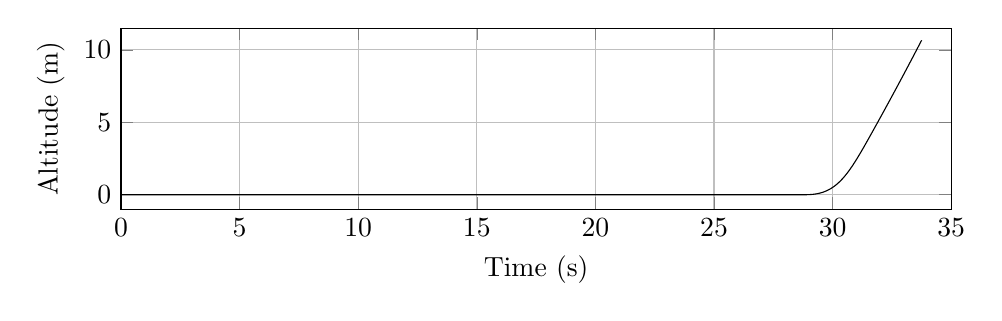
\begin{tikzpicture}

\begin{axis}[
width=\textwidth,
height=0.32\textwidth,
scaled ticks=false, tick label style={/pgf/number format/fixed},
xmin=0.0,
xmax=35,
xlabel={Time (s)},
xmajorgrids,
ymin=-1.0,
ymax=11.5,
ylabel={Altitude (m)},
ymajorgrids,
legend style={at={(1.03,0.5)},anchor=west,draw=black,fill=white,legend cell align=left}
]

\addplot [
color=black,
solid
]
table[row sep=crcr]{
9.999999999999999E-5	0.0\\
3.8662730018316225E-4	0.0\\
0.0011659616454675328	0.0\\
0.0027090044696574337	0.0\\
0.005513587400552062	0.0\\
0.009573414027789377	0.0\\
0.014458608976035365	0.0\\
0.020267737001617776	0.0\\
0.026284805098690814	0.0\\
0.03225857228980447	0.0\\
0.03829145989701144	0.0\\
0.044317715212340056	0.0\\
0.05034358930719769	0.0\\
0.05634899789012879	0.0\\
0.062365325811094136	0.0\\
0.06839545066932426	0.0\\
0.0744155646763375	0.0\\
0.08038732175457844	0.0\\
0.08644548551218845	0.0\\
0.09244515993214678	0.0\\
0.09844799717599381	0.0\\
0.1044465221256104	0.0\\
0.11048604389983377	0.0\\
0.1165105745503662	0.0\\
0.12240705646391417	0.0\\
0.12841042480182563	0.0\\
0.13444539252576237	0.0\\
0.1404428451168614	0.0\\
0.14636918986027286	0.0\\
0.15231064097430352	0.0\\
0.15836216232994682	0.0\\
0.16441695083211788	0.0\\
0.1704546598355367	0.0\\
0.17654788168175534	0.0\\
0.18260263380300035	0.0\\
0.18855799574417326	0.0\\
0.19463969341385573	0.0\\
0.20069474426059108	0.0\\
0.20679759839591833	0.0\\
0.21285168773719	0.0\\
0.21895652621944411	0.0\\
0.22502869583287222	0.0\\
0.23116276123031265	0.0\\
0.23722027151692543	0.0\\
0.2432248096297424	0.0\\
0.2493345946704646	0.0\\
0.25553647604505325	0.0\\
0.2615665691647471	0.0\\
0.26763324264649246	0.0\\
0.2737231778871023	0.0\\
0.2798399445305204	0.0\\
0.2860273989018781	0.0\\
0.2921511632746121	0.0\\
0.29822868153522675	0.0\\
0.3042589981774224	0.0\\
0.31037546469791466	0.0\\
0.3165928292552753	0.0\\
0.3227438718734784	0.0\\
0.32884425824897856	0.0\\
0.33490613671374003	0.0\\
0.34109405042093033	0.0\\
0.34721573517189974	0.0\\
0.35330522288412136	0.0\\
0.35955709046138307	0.0\\
0.3657853329895949	0.0\\
0.3719732734665251	0.0\\
0.37820977627270747	0.0\\
0.3844041749266873	0.0\\
0.3906889619619608	0.0\\
0.39688965591058556	0.0\\
0.40322222405366726	0.0\\
0.40954736000727787	0.0\\
0.4157445083009691	0.0\\
0.42208612340146334	0.0\\
0.42837692341589706	0.0\\
0.43463508387439753	0.0\\
0.44097118193696605	0.0\\
0.44724238596836485	0.0\\
0.453514044999336	0.0\\
0.4597423124562495	0.0\\
0.4662349063262001	0.0\\
0.4724873602412337	0.0\\
0.4788831998000358	0.0\\
0.48525888735673295	0.0\\
0.49157729728750477	0.0\\
0.49789852205083707	0.0\\
0.5043034503133064	0.0\\
0.5105929514407739	0.0\\
0.5169495710809722	0.0\\
0.5232380586781937	0.0\\
0.5296578067677786	0.0\\
0.5360993216435415	0.0\\
0.5424670092362842	0.0\\
0.5487885514384689	0.0\\
0.5552290337059678	0.0\\
0.5616107018730834	0.0\\
0.5681508731794067	0.0\\
0.574470372619047	0.0\\
0.580914616064055	0.0\\
0.587388952078856	0.0\\
0.5939523726705342	0.0\\
0.6003793697482414	0.0\\
0.6068127859378203	0.0\\
0.6131742006669136	0.0\\
0.6197712562331474	0.0\\
0.6262279626121341	0.0\\
0.6328472357914308	0.0\\
0.6392570100315369	0.0\\
0.6456998721515776	0.0\\
0.6522956638202342	0.0\\
0.6588885483684681	0.0\\
0.6654025079064216	0.0\\
0.6719628201654149	0.0\\
0.6785029894559484	0.0\\
0.6850034390591933	0.0\\
0.6915937419432063	0.0\\
0.6981398230190359	0.0\\
0.7047354657441984	0.0\\
0.7116524941719828	0.0\\
0.7185407880330137	0.0\\
0.725237142359652	0.0\\
0.7319805803852715	0.0\\
0.7386984809185471	0.0\\
0.7453707356412898	0.0\\
0.7522856069478163	0.0\\
0.7589390087525827	0.0\\
0.7654918822402266	0.0\\
0.7721967222710622	0.0\\
0.7790844954159069	0.0\\
0.7858208507512385	0.0\\
0.7926032315994149	0.0\\
0.7994369989370267	0.0\\
0.8063952072742577	0.0\\
0.8133776465757916	0.0\\
0.8201322943440523	0.0\\
0.8268540523736279	0.0\\
0.8338746656780314	0.0\\
0.8406133492726837	0.0\\
0.8474054781584102	0.0\\
0.8541600890673313	0.0\\
0.8609059869163356	0.0\\
0.8677133543927005	0.0\\
0.874675776273538	0.0\\
0.8815588275937194	0.0\\
0.8884089601416048	0.0\\
0.895350491690551	0.0\\
0.9023805740945929	0.0\\
0.909423250351034	0.0\\
0.9164384237130587	0.0\\
0.9234295291247794	0.0\\
0.9305452101854663	0.0\\
0.9377285854715671	0.0\\
0.9446014848894633	0.0\\
0.9516551103959094	0.0\\
0.9587431865673528	0.0\\
0.9657524314640715	0.0\\
0.9727484772244321	0.0\\
0.9797957435093549	0.0\\
0.9867948760804801	0.0\\
0.9938398478500607	0.0\\
1.0008727969883378	0.0\\
1.0082557036774902	0.0\\
1.0154634676726162	0.0\\
1.022565291368481	0.0\\
1.0298107041837494	0.0\\
1.0369481341984876	0.0\\
1.0441930794873877	0.0\\
1.0513018001830425	0.0\\
1.0584844094368209	0.0\\
1.0658416070125063	0.0\\
1.0731116822086588	0.0\\
1.080363339488168	0.0\\
1.0875634417083901	0.0\\
1.0950561212164582	0.0\\
1.1022691838121186	0.0\\
1.1096515253668442	0.0\\
1.1168105437348697	0.0\\
1.1241834585253572	0.0\\
1.1314900526167015	0.0\\
1.1387898144264526	0.0\\
1.1462014229766337	0.0\\
1.1534842177125966	0.0\\
1.1610305294921646	0.0\\
1.1683024533461395	0.0\\
1.175666126066686	0.0\\
1.183161062232811	0.0\\
1.1904973544537443	0.0\\
1.198182978993498	0.0\\
1.2058202174805386	0.0\\
1.2132009714655942	0.0\\
1.2208332072620083	0.0\\
1.2282847271796666	0.0\\
1.2357889360407994	0.0\\
1.2432817635490605	0.0\\
1.2506594305019938	0.0\\
1.258153755403057	0.0\\
1.265791933325374	0.0\\
1.2733097873689507	0.0\\
1.2807674559500843	0.0\\
1.2883449971014849	0.0\\
1.2959745374895753	0.0\\
1.3034940038984648	0.0\\
1.3111828469042743	0.0\\
1.3188836242689668	0.0\\
1.3265604664314496	0.0\\
1.334130152188989	0.0\\
1.341922461672337	0.0\\
1.3496353644785395	0.0\\
1.3572521742821864	0.0\\
1.3649932738972024	0.0\\
1.3727576178534142	0.0\\
1.3804426836894783	0.0\\
1.3884239558880633	0.0\\
1.396412296123808	0.0\\
1.4040487163735018	0.0\\
1.4117306180042375	0.0\\
1.4195804965415024	0.0\\
1.4273935853567532	0.0\\
1.4351688819359798	0.0\\
1.4430626544494864	0.0\\
1.4511211445792136	0.0\\
1.4589871519230364	0.0\\
1.466966993439991	0.0\\
1.4747886437902387	0.0\\
1.482724819010782	0.0\\
1.4908838129207802	0.0\\
1.4987504564052503	0.0\\
1.5066221306101029	0.0\\
1.5144678520669679	0.0\\
1.5222380205365384	0.0\\
1.5303044455798127	0.0\\
1.5380733343062327	0.0\\
1.5463945489172022	0.0\\
1.5545256825609197	0.0\\
1.5626337824368854	0.0\\
1.570868417613693	0.0\\
1.5788026411373153	0.0\\
1.5870172700166347	0.0\\
1.5953089767735884	0.0\\
1.6033736077500786	0.0\\
1.6115098763705977	0.0\\
1.6198253317640359	0.0\\
1.628132712560452	0.0\\
1.6362184427571949	0.0\\
1.644317282047632	0.0\\
1.652773352860705	0.0\\
1.6609284076293243	0.0\\
1.6693705834549823	0.0\\
1.6776104595410404	0.0\\
1.6859091648238875	0.0\\
1.6943153785697396	0.0\\
1.7026024442336425	0.0\\
1.7109449359172135	0.0\\
1.7191986458994042	0.0\\
1.7276008221877306	0.0\\
1.7362046540249314	0.0\\
1.7445523060454606	0.0\\
1.7529663965514182	0.0\\
1.7612771155701834	0.0\\
1.769728051015154	0.0\\
1.778036738527653	0.0\\
1.786435537970147	0.0\\
1.7948430274155474	0.0\\
1.8032392993068997	0.0\\
1.8117329513424383	0.0\\
1.820076861299981	0.0\\
1.8287124672328288	0.0\\
1.837217558473795	0.0\\
1.845739361887984	0.0\\
1.8541640516942306	0.0\\
1.8628668561066246	0.0\\
1.871347701794416	0.0\\
1.879913663461657	0.0\\
1.8885858782757396	0.0\\
1.8972639421551567	0.0\\
1.9059006504896665	0.0\\
1.9145266071425553	0.0\\
1.9231959841228603	0.0\\
1.9319356031107944	0.0\\
1.940704738462634	0.0\\
1.9494475785096852	0.0\\
1.9580092216479854	0.0\\
1.966784117365716	0.0\\
1.975405954943024	0.0\\
1.9840488677820427	0.0\\
1.9927939440778104	0.0\\
2.001550614578302	0.0\\
2.0101162806439508	0.0\\
2.01914694954265	0.0\\
2.027891794301743	0.0\\
2.0367665864568893	0.0\\
2.045605420967081	0.0\\
2.0544618768947283	0.0\\
2.063495292936392	0.0\\
2.0724468171544297	0.0\\
2.081294403817858	0.0\\
2.0902044275989295	0.0\\
2.0991481878519718	0.0\\
2.1079457893798734	0.0\\
2.116751209176061	0.0\\
2.1257689201699685	0.0\\
2.1346948577324207	0.0\\
2.143606274620553	0.0\\
2.1526211073206127	0.0\\
2.1618263825400694	0.0\\
2.1708223622570175	0.0\\
2.179731942965848	0.0\\
2.1886915774914906	0.0\\
2.1977629004830037	0.0\\
2.2067731173623546	0.0\\
2.215753229832541	0.0\\
2.2247993479838843	0.0\\
2.233831575312335	0.0\\
2.243014531786801	0.0\\
2.252181473680425	0.0\\
2.261287932991369	0.0\\
2.270435448839077	0.0\\
2.2796114597991872	0.0\\
2.2888483730264024	0.0\\
2.2979964248800666	0.0\\
2.3073327677876296	0.0\\
2.316565069503123	0.0\\
2.325814142156408	0.0\\
2.335054801648101	0.0\\
2.344425571189931	0.0\\
2.3538458773270676	0.0\\
2.363289672996623	0.0\\
2.372663602477169	0.0\\
2.3822336865733558	0.0\\
2.391610678421004	0.0\\
2.400869399206017	0.0\\
2.410239653145725	0.0\\
2.4196789187286107	0.0\\
2.429123500163632	0.0\\
2.438390886633167	0.0\\
2.4477540626103744	0.0\\
2.457325860804745	0.0\\
2.466881202132358	0.0\\
2.4764039469311756	0.0\\
2.4859298301425996	0.0\\
2.4955543518946586	0.0\\
2.5050013064725922	0.0\\
2.5147513131886265	0.0\\
2.52444542604621	0.0\\
2.5339351543922692	0.0\\
2.5435730135210646	0.0\\
2.553341059572432	0.0\\
2.5632338845381897	0.0\\
2.5730888282237796	0.0\\
2.582869240041708	0.0\\
2.5925879469589956	0.0\\
2.6021755458983744	0.0\\
2.6118169012524266	0.0\\
2.621542360209907	0.0\\
2.631208326954706	0.0\\
2.6409271801905545	0.0\\
2.6508281684995483	0.0\\
2.660714546767342	0.0\\
2.670434808831545	0.0\\
2.6803498758997204	0.0\\
2.69028118294706	0.0\\
2.699947455091369	0.0\\
2.709937320387815	0.0\\
2.719700753176891	0.0\\
2.7296760151282653	0.0\\
2.7395013210982118	0.0\\
2.7494645908247284	0.0\\
2.759383237810363	0.0\\
2.7692211940146336	0.0\\
2.7791137696853996	0.0\\
2.789142434448779	0.0\\
2.799072711165974	0.0\\
2.8092164611239276	0.0\\
2.8192003417106433	0.0\\
2.8294161666348874	0.0\\
2.8394421321410572	0.0\\
2.8494774552958777	0.0\\
2.859614906396712	0.0\\
2.8695854225072894	0.0\\
2.879885464225028	0.0\\
2.89008501637377	0.0\\
2.9003079708613146	0.0\\
2.910533557079111	0.0\\
2.920835245887324	0.0\\
2.931065100268058	0.0\\
2.9412987341015366	0.0\\
2.9516103854370197	0.0\\
2.961839419392007	0.0\\
2.9721577720140475	0.0\\
2.9826529493161233	0.0\\
2.993025463815675	0.0\\
3.0035952637982692	0.0\\
3.01413893627885	0.0\\
3.024420996904631	0.0\\
3.0350341417709874	0.0\\
3.045468237460226	0.0\\
3.0558815408668485	0.0\\
3.0661806014867814	0.0\\
3.076989853974384	0.0\\
3.087448852867138	0.0\\
3.0979619151890976	0.0\\
3.1084156971759693	0.0\\
3.1188949022758887	0.0\\
3.129428272377078	0.0\\
3.1399980143097075	0.0\\
3.150598170413179	0.0\\
3.1611275980969404	0.0\\
3.1716431084419057	0.0\\
3.1821003530969856	0.0\\
3.1926681708207427	0.0\\
3.2032331700630596	0.0\\
3.2137449097322097	0.0\\
3.2244288704522113	0.0\\
3.235097007588739	0.0\\
3.2456056855093323	0.0\\
3.25628890621509	0.0\\
3.2669847925608817	0.0\\
3.277677797448195	0.0\\
3.2883291251848794	0.0\\
3.298986727777682	0.0\\
3.3097720276545717	0.0\\
3.320467935070641	0.0\\
3.3313087418531966	0.0\\
3.342324921919756	0.0\\
3.3529736501583605	0.0\\
3.363634973746918	0.0\\
3.374359140983236	0.0\\
3.3851551410623992	0.0\\
3.395961643130134	0.0\\
3.4068771726519484	0.0\\
3.418107447397965	0.0\\
3.429089027102286	0.0\\
3.440232143309209	0.0\\
3.451276808519962	0.0\\
3.4624986723982367	0.0\\
3.4735990310924985	0.0\\
3.484558903131833	0.0\\
3.4955234183839314	0.0\\
3.50671130592208	0.0\\
3.517573885531923	0.0\\
3.528714013168927	0.0\\
3.539932330137135	0.0\\
3.5511823352992797	0.0\\
3.5624107600414385	0.0\\
3.5736345533971443	0.0\\
3.58487918432966	0.0\\
3.5958938111621244	0.0\\
3.6070580545757522	0.0\\
3.618262507419721	0.0\\
3.629481421662617	0.0\\
3.640622703202241	0.0\\
3.652098333752188	0.0\\
3.6634031943686454	0.0\\
3.6744759148863446	0.0\\
3.68604124707704	0.0\\
3.697242933554562	0.0\\
3.708614178294961	0.0\\
3.7198216039294696	0.0\\
3.731236341749332	0.0\\
3.7426624441012075	0.0\\
3.754124144917637	0.0\\
3.7655208185040454	0.0\\
3.776909416869981	0.0\\
3.7882351757384782	0.0\\
3.7995713158526554	0.0\\
3.8110977644322324	0.0\\
3.8225067942415336	0.0\\
3.833992547508731	0.0\\
3.845460911526412	0.0\\
3.8568313523370668	0.0\\
3.8683533667878907	0.0\\
3.8800844339137956	0.0\\
3.8915724171287254	0.0\\
3.903155552402886	0.0\\
3.914510603417397	0.0\\
3.9261888461820362	0.0\\
3.9377042427066424	0.0\\
3.9492112709268365	0.0\\
3.961164188095486	0.0\\
3.9727825679010316	0.0\\
3.984410060297039	0.0\\
3.9960395513068336	0.0\\
4.007687196448739	0.0\\
4.019276289022153	0.0\\
4.030943523934917	0.0\\
4.042774020545057	0.0\\
4.05449300520044	0.0\\
4.066055899585866	0.0\\
4.077650310922831	0.0\\
4.089181769130558	0.0\\
4.100868021781373	0.0\\
4.112548045477983	0.0\\
4.124412237864334	0.0\\
4.136145706637761	0.0\\
4.147645775783575	0.0\\
4.159109574743175	0.0\\
4.1709373001080134	0.0\\
4.182659900680726	0.0\\
4.194612573128092	0.0\\
4.2062303592528725	0.0\\
4.2182193322401424	0.0\\
4.2300332256349265	0.0\\
4.241660124775521	0.0\\
4.253337943657147	0.0\\
4.265244701840459	0.0\\
4.277144542135289	0.0\\
4.289054644726226	0.0\\
4.3009208677895945	0.0\\
4.3129026521431655	0.0\\
4.324699666694366	0.0\\
4.336882778546341	0.0\\
4.348615192543063	0.0\\
4.3603762842939044	0.0\\
4.372382104609423	0.0\\
4.384213790586953	0.0\\
4.396137342419268	0.0\\
4.398493633385041	0.0\\
4.40430528543245	0.0\\
4.404795633356372	0.0\\
4.405236757041209	0.0\\
4.405670790578586	0.0\\
4.405791323631611	0.0\\
4.405900368372947	0.0\\
4.406392564612052	0.0\\
4.408264543730164	0.0\\
4.415163549245662	0.0\\
4.425104416187475	0.0\\
4.435874611750661	0.0\\
4.446912808713055	0.0\\
4.457875675073781	0.0\\
4.468876290738784	0.0\\
4.480019581108101	0.0\\
4.491109282839437	0.0\\
4.502214577921281	0.0\\
4.513382451150042	0.0\\
4.524392538788899	0.0\\
4.535527859526718	0.0\\
4.5466590834819645	0.0\\
4.557815584137787	0.0\\
4.569002144237512	0.0\\
4.580155883061874	0.0\\
4.591415283566505	0.0\\
4.602756813184445	0.0\\
4.613865927507634	0.0\\
4.625145823744587	0.0\\
4.636538220227209	0.0\\
4.6477544211788455	0.0\\
4.65909297855176	0.0\\
4.6705742072010334	0.0\\
4.68193571304481	0.0\\
4.6933139327195	0.0\\
4.7049021522623775	0.0\\
4.716294758256144	0.0\\
4.727681280372087	0.0\\
4.739097148549535	0.0\\
4.750697455423625	0.0\\
4.7622924921099	0.0\\
4.7739203875042975	0.0\\
4.785493975041177	0.0\\
4.797175153981085	0.0\\
4.808651088221275	0.0\\
4.820350244085791	0.0\\
4.832206159140707	0.0\\
4.843821723421984	0.0\\
4.855404918101174	0.0\\
4.867049221728601	0.0\\
4.878804766674579	0.0\\
4.890520846235029	0.0\\
4.9021665001635615	0.0\\
4.913904281711719	0.0\\
4.9255958474782275	0.0\\
4.9372371592847895	0.0\\
4.948886300132013	0.0\\
4.960701441228958	0.0\\
4.972663076985167	0.0\\
4.984488540087407	0.0\\
4.996431332072207	0.0\\
5.008172571354056	0.0\\
5.019924929554737	0.0\\
5.031822200840068	0.0\\
5.043685167103497	0.0\\
5.0555978417980985	0.0\\
5.067440815946705	0.0\\
5.0791682414263075	0.0\\
5.0909590651081995	0.0\\
5.103001475011437	0.0\\
5.114961376550227	0.0\\
5.126792621215104	0.0\\
5.138562658738325	0.0\\
5.150381266788203	0.0\\
5.162205700308407	0.0\\
5.1739976160125245	0.0\\
5.186166829903652	0.0\\
5.198363969008559	0.0\\
5.210423142743705	0.0\\
5.222277606569111	0.0\\
5.234292731357568	0.0\\
5.246224049702821	0.0\\
5.258485180255741	0.0\\
5.270469938862524	0.0\\
5.282529445482782	0.0\\
5.294520389056304	0.0\\
5.306499644591289	0.0\\
5.3186414007609475	0.0\\
5.330666666346556	0.0\\
5.34275797455158	0.0\\
5.354731211996553	0.0\\
5.366936118130379	0.0\\
5.378891097355432	0.0\\
5.3911501930500325	0.0\\
5.403285452733913	0.0\\
5.415344954121014	0.0\\
5.427544696116616	0.0\\
5.439486127277238	0.0\\
5.451470285516718	0.0\\
5.463777758176764	0.0\\
5.475841208107907	0.0\\
5.488028690044796	0.0\\
5.500252338094503	0.0\\
5.512283272956568	0.0\\
5.524331952676052	0.0\\
5.536597715052466	0.0\\
5.548709523841255	0.0\\
5.560850224574107	0.0\\
5.573066578235194	0.0\\
5.585397552770786	0.0\\
5.597547009285734	0.0\\
5.609851566824469	0.0\\
5.622096377168498	0.0\\
5.634184733613559	0.0\\
5.646455992585421	0.0\\
5.658413017090899	0.0\\
5.6706098697641085	0.0\\
5.683035141588972	0.0\\
5.695244309242103	0.0\\
5.707504335926458	0.0\\
5.719766014017154	0.0\\
5.731934701341379	0.0\\
5.744254389112781	0.0\\
5.756572935293972	0.0\\
5.768928547484181	0.0\\
5.781205522621777	0.0\\
5.79361559555641	0.0\\
5.805924404812648	0.0\\
5.818250593834559	0.0\\
5.830643988681116	0.0\\
5.842858538823398	0.0\\
5.855175324798825	0.0\\
5.867539373608373	0.0\\
5.879731061714651	0.0\\
5.892120502015452	0.0\\
5.904458750128015	0.0\\
5.916781402653784	0.0\\
5.929123340789216	0.0\\
5.941487622703184	0.0\\
5.953718600100878	0.0\\
5.96599716014433	0.0\\
5.978256947767495	0.0\\
5.9906371822594995	0.0\\
6.002946625074534	0.0\\
6.0153728378504265	0.0\\
6.027707679135675	0.0\\
6.040035548056812	0.0\\
6.052543254528894	0.0\\
6.06495814818072	0.0\\
6.077438514139175	0.0\\
6.0897346062728275	0.0\\
6.102273206090741	0.0\\
6.11459457244348	0.0\\
6.12707001048936	0.0\\
6.13920404985085	0.0\\
6.151469962358798	0.0\\
6.163876716271281	0.0\\
6.176333919594811	0.0\\
6.188795641316483	0.0\\
6.201348046253035	0.0\\
6.213815739092356	0.0\\
6.226207142430422	0.0\\
6.238695751510736	0.0\\
6.251211906535014	0.0\\
6.263599138096403	0.0\\
6.2760565979267415	0.0\\
6.288504708387432	0.0\\
6.301018899526623	0.0\\
6.313600910662862	0.0\\
6.326059343955308	0.0\\
6.33863360818574	0.0\\
6.351266695326563	0.0\\
6.363853878678325	0.0\\
6.376311447350313	0.0\\
6.3886903701164	0.0\\
6.401188903886187	0.0\\
6.413748051421473	0.0\\
6.426206485875259	0.0\\
6.438803363319849	0.0\\
6.4512831053118145	0.0\\
6.4637491226381005	0.0\\
6.476268908114616	0.0\\
6.488818343796208	0.0\\
6.501365748332935	0.0\\
6.513758145106991	0.0\\
6.526383784379922	0.0\\
6.539141266431027	0.0\\
6.551861146946397	0.0\\
6.564627862113639	0.0\\
6.577241415939962	0.0\\
6.589878512499203	0.0\\
6.6024269468122245	0.0\\
6.615134969351018	0.0\\
6.627776538279456	0.0\\
6.6405431983665135	0.0\\
6.653188778149023	0.0\\
6.665859817893999	0.0\\
6.678496617833996	0.0\\
6.691218354085985	0.0\\
6.703949684436637	0.0\\
6.716711955333192	0.0\\
6.729358799605496	0.0\\
6.741979238651604	0.0\\
6.754670916768211	0.0\\
6.76751756745972	0.0\\
6.780324732230472	0.0\\
6.793190334836348	0.0\\
6.806053681939204	0.0\\
6.818924271105928	0.0\\
6.8317673928978095	0.0\\
6.84461485856726	0.0\\
6.857470469813389	0.0\\
6.870428045776087	0.0\\
6.883352305092588	0.0\\
6.896436738468823	0.0\\
6.909371775272001	0.0\\
6.922361543721603	0.0\\
6.9352182831708	0.0\\
6.9482431992528255	0.0\\
6.961298876037299	0.0\\
6.974303241670199	0.0\\
6.987276411552285	0.0\\
7.0004465858576825	0.0\\
7.013518118168637	0.0\\
7.026484879845059	0.0\\
7.0394816926378265	0.0\\
7.0525417523553795	0.0\\
7.065576376699935	0.0\\
7.078628312422351	0.0\\
7.091703353512809	0.0\\
7.104822364236195	0.0\\
7.117903320860449	0.0\\
7.131046804345502	0.0\\
7.144153613522926	0.0\\
7.157296475173258	0.0\\
7.170467494382443	0.0\\
7.1836852265162925	0.0\\
7.196892908206415	0.0\\
7.210072180120264	0.0\\
7.223186892974114	0.0\\
7.236427282785046	0.0\\
7.249738927582854	0.0\\
7.26315210617401	0.0\\
7.276365585627762	0.0\\
7.289702174007294	0.0\\
7.303160727314433	0.0\\
7.3164568857426815	0.0\\
7.329778213144852	0.0\\
7.343282736019509	0.0\\
7.356948355277103	0.0\\
7.37041351207054	0.0\\
7.383921148364392	0.0\\
7.3973805896719185	0.0\\
7.41081996726523	0.0\\
7.424305696543955	0.0\\
7.437755590657595	0.0\\
7.451273482732029	0.0\\
7.46482483847875	0.0\\
7.478408759501342	0.0\\
7.492141029665277	0.0\\
7.505865388502176	0.0\\
7.519609186747548	0.0\\
7.5333515847688695	0.0\\
7.547060017299577	0.0\\
7.560900487508885	0.0\\
7.574716444215399	0.0\\
7.588548936197734	0.0\\
7.602304596392383	0.0\\
7.616094899174945	0.0\\
7.6302247144605175	0.0\\
7.644345870144646	0.0\\
7.658232418623374	0.0\\
7.672153143643753	0.0\\
7.68618475795809	0.0\\
7.700081808342123	0.0\\
7.714109900002718	0.0\\
7.728343299183068	0.0\\
7.742486906984556	0.0\\
7.756556807299738	0.0\\
7.770689007751679	0.0\\
7.784991667312191	0.0\\
7.799084082984141	0.0\\
7.813293834680932	0.0\\
7.827551485754611	0.0\\
7.841971094114745	0.0\\
7.856365517507376	0.0\\
7.870734069892235	0.0\\
7.884968464604228	0.0\\
7.899298119920257	0.0\\
7.9137554057183035	0.0\\
7.928212099473598	0.0\\
7.9427939166909525	0.0\\
7.957410592044262	0.0\\
7.9720338090855645	0.0\\
7.986458910296696	0.0\\
8.001124843127787	0.0\\
8.015860986369397	0.0\\
8.030493143194128	0.0\\
8.0451686014626	0.0\\
8.059944236685652	0.0\\
8.07483984870304	0.0\\
8.089511361399694	0.0\\
8.104432154164105	0.0\\
8.119367305613359	0.0\\
8.134289196246812	0.0\\
8.14943222973455	0.0\\
8.164379237418455	0.0\\
8.179432728470378	0.0\\
8.194368933120575	0.0\\
8.209356063781193	0.0\\
8.224421180054087	0.0\\
8.23937880773665	0.0\\
8.254515232970213	0.0\\
8.26964725296154	0.0\\
8.284852048111695	0.0\\
8.300113594587618	0.0\\
8.315544987044895	0.0\\
8.330738703045224	0.0\\
8.345996666942863	0.0\\
8.36131532937987	0.0\\
8.376478584295441	0.0\\
8.391754144414328	0.0\\
8.407004378479968	0.0\\
8.422364158506674	0.0\\
8.437804075621099	0.0\\
8.453132610693213	0.0\\
8.468747194363608	0.0\\
8.48427183213018	0.0\\
8.499827691066269	0.0\\
8.515335959941208	0.0\\
8.530724720167566	0.0\\
8.546136769344756	0.0\\
8.56151594286236	0.0\\
8.576926351521251	0.0\\
8.592199531484564	0.0\\
8.60759208426219	0.0\\
8.623100892144638	0.0\\
8.638518078872941	0.0\\
8.653763979219544	0.0\\
8.669320402259615	0.0\\
8.684739115059731	0.0\\
8.700188025635736	0.0\\
8.715453660274097	0.0\\
8.730960637045655	0.0\\
8.746225966409728	0.0\\
8.761450881556435	0.0\\
8.776810707307082	0.0\\
8.792064268730044	0.0\\
8.807117444774097	0.0\\
8.822292444658451	0.0\\
8.837371086561046	0.0\\
8.852537725661392	0.0\\
8.867715681674348	0.0\\
8.882739748841221	0.0\\
8.897615199930346	0.0\\
8.912527869903386	0.0\\
8.927425943946435	0.0\\
8.9422236741087	0.0\\
8.957005764438787	0.0\\
8.971946532911161	0.0\\
8.986635135660787	0.0\\
9.001392412391663	0.0\\
9.016017139610735	0.0\\
9.030619222698718	0.0\\
9.045231862792892	0.0\\
9.059810807503531	0.0\\
9.062722355049722	0.0\\
9.063201825042338	0.0\\
9.063667962450797	0.0\\
9.064049312162563	0.0\\
9.06485031233191	0.0\\
9.068118390718286	0.0\\
9.07580415914401	0.0\\
9.088297613665304	0.0\\
9.101350180650865	0.0\\
9.114381996245012	0.0\\
9.127390670501654	0.0\\
9.140621055169646	0.0\\
9.153827153530116	0.0\\
9.16700733661554	0.0\\
9.180494614920107	0.0\\
9.193948632945329	0.0\\
9.207307807977685	0.0\\
9.220707421228951	0.0\\
9.234152536122554	0.0\\
9.247676841590039	0.0\\
9.261240091780422	0.0\\
9.275037686216898	0.0\\
9.28875925384241	0.0\\
9.302534454528715	0.0\\
9.316440004935558	0.0\\
9.330323897831956	0.0\\
9.34419682077952	0.0\\
9.35825062234121	0.0\\
9.372322038967472	0.0\\
9.3864308348772	0.0\\
9.400636745059504	0.0\\
9.414878768475695	0.0\\
9.429222264011049	0.0\\
9.443528425988323	0.0\\
9.45780784742978	0.0\\
9.472176598523298	0.0\\
9.486605100321881	0.0\\
9.501055965931002	0.0\\
9.515602590700997	0.0\\
9.530244768097706	0.0\\
9.544860408937733	0.0\\
9.559370778850983	0.0\\
9.574215063002935	0.0\\
9.589066354803993	0.0\\
9.603860119192703	0.0\\
9.618684677055427	0.0\\
9.633588842245462	0.0\\
9.648415306721436	0.0\\
9.66330221471091	0.0\\
9.678199541955223	0.0\\
9.693182487880946	0.0\\
9.708218596284723	0.0\\
9.723284897375965	0.0\\
9.738335937694913	0.0\\
9.753472773934742	0.0\\
9.768446765264876	0.0\\
9.78353768302269	0.0\\
9.798644810391767	0.0\\
9.81372357664701	0.0\\
9.828723909190842	0.0\\
9.843765199265885	0.0\\
9.858827312979038	0.0\\
9.87391739312497	0.0\\
9.888956521334574	0.0\\
9.9040899477756	0.0\\
9.919053651942843	0.0\\
9.934032823753576	0.0\\
9.949039810854714	0.0\\
9.964066311931855	0.0\\
9.979136510318483	0.0\\
9.993827336117956	0.0\\
10.008609474601204	0.0\\
10.02347861863727	0.0\\
10.038299772485551	0.0\\
10.0532323640696	0.0\\
10.068024772232217	0.0\\
10.082860141381126	0.0\\
10.097585079376948	0.0\\
10.112393698848162	0.0\\
10.12713930586013	0.0\\
10.14187055677358	0.0\\
10.156642024124903	0.0\\
10.171319013437483	0.0\\
10.186020111056681	0.0\\
10.200595095218269	0.0\\
10.215180609063111	0.0\\
10.229706648803614	0.0\\
10.244334320200746	0.0\\
10.258910858941686	0.0\\
10.273446880083444	0.0\\
10.288037505468218	0.0\\
10.30256680611506	0.0\\
10.317045617333786	0.0\\
10.331470514668808	0.0\\
10.345950510368827	0.0\\
10.360309145661525	0.0\\
10.37456350038119	0.0\\
10.38888424243402	0.0\\
10.403260864132584	0.0\\
10.417621492823052	0.0\\
10.43195971761623	0.0\\
10.446197319083488	0.0\\
10.46052631155625	0.0\\
10.47476676969059	0.0\\
10.488954860028763	0.0\\
10.5031686998298	0.0\\
10.51727790371502	0.0\\
10.53141398133712	0.0\\
10.545533306577788	0.0\\
10.559618701031987	0.0\\
10.5737836516792	0.0\\
10.587887585084282	0.0\\
10.60212854598322	0.0\\
10.61621105356592	0.0\\
10.630346150511393	0.0\\
10.64441715192283	0.0\\
10.658492248826793	0.0\\
10.67254640086756	0.0\\
10.686569396661191	0.0\\
10.700558574675515	0.0\\
10.714606672270968	0.0\\
10.728760700238613	0.0\\
10.742725734063256	0.0\\
10.756736389630063	0.0\\
10.770661417883566	0.0\\
10.78460323391657	0.0\\
10.79859227378661	0.0\\
10.812560359985216	0.0\\
10.826525798357359	0.0\\
10.8405346837685	0.0\\
10.8544746943146	0.0\\
10.868367964158963	0.0\\
10.882198393518475	0.0\\
10.896105904574231	0.0\\
10.910085747001215	0.0\\
10.923974677825957	0.0\\
10.937845196045341	0.0\\
10.951730488990343	0.0\\
10.965688208649226	0.0\\
10.979561505174324	0.0\\
10.993408876236217	0.0\\
11.00725919414575	0.0\\
11.021113567817828	0.0\\
11.035024266996377	0.0\\
11.048860024837666	0.0\\
11.06269971576437	0.0\\
11.076452350743299	0.0\\
11.090276453871873	0.0\\
11.104138901492643	0.0\\
11.117974562011455	0.0\\
11.131848471139072	0.0\\
11.145676284220428	0.0\\
11.15948749121997	0.0\\
11.17331215580285	0.0\\
11.187181115957994	0.0\\
11.201039003616668	0.0\\
11.214943894499097	0.0\\
11.228789804730127	0.0\\
11.24253923529239	0.0\\
11.256395903938344	0.0\\
11.27025398396649	0.0\\
11.284181016076044	0.0\\
11.298123770946251	0.0\\
11.31198950763952	0.0\\
11.325881869024006	0.0\\
11.339663387954058	0.0\\
11.35355039772654	0.0\\
11.367461540885568	0.0\\
11.381387957007743	0.0\\
11.395251905549333	0.0\\
11.409258576654992	0.0\\
11.42317486730919	0.0\\
11.437087122474452	0.0\\
11.451025447098761	0.0\\
11.464916666453945	0.0\\
11.478796616369674	0.0\\
11.49277685126279	0.0\\
11.506719117797175	0.0\\
11.520676492783661	0.0\\
11.534687104512535	0.0\\
11.548693058873766	0.0\\
11.56275008959722	0.0\\
11.576738020010687	0.0\\
11.590675258704682	0.0\\
11.604689244406806	0.0\\
11.618670394570891	0.0\\
11.632674641805632	0.0\\
11.646686899713913	0.0\\
11.66077771620959	0.0\\
11.674854145706668	0.0\\
11.688906966690318	0.0\\
11.70295596682476	0.0\\
11.716967437680019	0.0\\
11.731054291197275	0.0\\
11.74520980044107	0.0\\
11.759351073362545	0.0\\
11.773554459795083	0.0\\
11.787776797971922	0.0\\
11.80192735630256	0.0\\
11.81617361940334	0.0\\
11.830355502839822	0.0\\
11.844557648642162	0.0\\
11.858799027812665	0.0\\
11.873082939423245	0.0\\
11.887441069290304	0.0\\
11.901711147063835	0.0\\
11.915955395718747	0.0\\
11.93022330345212	0.0\\
11.944529001675821	0.0\\
11.95881135650118	0.0\\
11.973127633254986	0.0\\
11.987472227281664	0.0\\
12.001861374434725	0.0\\
12.016161263365849	0.0\\
12.030533656562366	0.0\\
12.045052393162507	0.0\\
12.05952832569028	0.0\\
12.073994984342423	0.0\\
12.088509085516531	0.0\\
12.103055166745246	0.0\\
12.117509740511569	0.0\\
12.132081888063336	0.0\\
12.146732904083137	0.0\\
12.161355367501343	0.0\\
12.176006212681028	0.0\\
12.190556978665345	0.0\\
12.205197989408788	0.0\\
12.219937158857615	0.0\\
12.234647727182178	0.0\\
12.249337741463272	0.0\\
12.264082019166715	0.0\\
12.27880155098753	0.0\\
12.293597717320335	0.0\\
12.30838296013247	0.0\\
12.323228426342055	0.0\\
12.338102595137205	0.0\\
12.353096443822977	0.0\\
12.368080696888338	0.0\\
12.383022293496428	0.0\\
12.397906455374919	0.0\\
12.413005416298056	0.0\\
12.42799301268554	0.0\\
12.44313541143492	0.0\\
12.458240694488715	0.0\\
12.47333203853297	0.0\\
12.48858755216019	0.0\\
12.503794191788302	0.0\\
12.519009591091713	0.0\\
12.534260693450015	0.0\\
12.549564278397487	0.0\\
12.564810580055163	0.0\\
12.580247782799855	0.0\\
12.59567902554911	0.0\\
12.61116763400701	0.0\\
12.626647136933759	0.0\\
12.642266000072755	0.0\\
12.657955122182631	0.0\\
12.673619020077314	0.0\\
12.689232782824686	0.0\\
12.704931282133128	0.0\\
12.720660841588142	0.0\\
12.736522236264182	0.0\\
12.752464572705296	0.0\\
12.76840916425126	0.0\\
12.784363048643424	0.0\\
12.800399066262482	0.0\\
12.816564581587919	0.0\\
12.832827618519811	0.0\\
12.849152717994432	0.0\\
12.865451144401515	0.0\\
12.881653031871181	0.0\\
12.898048862591939	0.0\\
12.91448395018218	0.0\\
12.93103925788052	0.0\\
12.947697367107466	0.0\\
12.964365502493774	0.0\\
12.981109019887459	0.0\\
12.997824325480352	0.0\\
13.014532676754175	0.0\\
13.031553631087018	0.0\\
13.048647654997822	0.0\\
13.065672478678568	0.0\\
13.082775565002141	0.0\\
13.099921722860575	0.0\\
13.117223864325457	0.0\\
13.134529730330755	0.0\\
13.152047195590988	0.0\\
13.169474115471914	0.0\\
13.187230194924396	0.0\\
13.205122782836227	0.0\\
13.222982115569753	0.0\\
13.24095779768232	0.0\\
13.259034032633384	0.0\\
13.277291871062836	0.0\\
13.295522362654864	0.0\\
13.31372419425826	0.0\\
13.332225733874317	0.0\\
13.350703814118393	0.0\\
13.369338524278596	0.0\\
13.387806491352872	0.0\\
13.40653591623007	0.0\\
13.425192916270756	0.0\\
13.444114887752772	0.0\\
13.462947139159706	0.0\\
13.481764931909254	0.0\\
13.500497794391244	0.0\\
13.519069523676905	0.0\\
13.537820678659472	0.0\\
13.55650217446727	0.0\\
13.575040278580168	0.0\\
13.59366406593302	0.0\\
13.61215156719918	0.0\\
13.630508585717106	0.0\\
13.64901515181597	0.0\\
13.667282127619725	0.0\\
13.685435024859807	0.0\\
13.703497116568364	0.0\\
13.72143433779522	0.0\\
13.739324939751821	0.0\\
13.757041936338066	0.0\\
13.774687106804752	0.0\\
13.792208148844484	0.0\\
13.809696802483575	0.0\\
13.826936927070502	0.0\\
13.844286062107141	0.0\\
13.861368284226291	0.0\\
13.878383817302101	0.0\\
13.895450894559815	0.0\\
13.912337662405395	0.0\\
13.92896348591151	0.0\\
13.94566810719288	0.0\\
13.962347284586425	0.0\\
13.978787232157561	0.0\\
13.99529757494949	0.0\\
14.011585665147486	0.0\\
14.027691980835815	0.0\\
14.043851119016846	0.0\\
14.059972567097379	0.0\\
14.076017990779604	0.0\\
14.091961758976588	0.0\\
14.107842472372617	0.0\\
14.123600536980955	0.0\\
14.126759647528363	0.0\\
14.12861292524397	0.0\\
14.129733092125786	0.0\\
14.130020052023575	0.0\\
14.130236176836032	0.0\\
14.130362257872608	0.0\\
14.130490724252219	0.0\\
14.131256214327014	0.0\\
14.133902865712294	0.0\\
14.142130854832338	0.0\\
14.155801296332307	0.0\\
14.169588052386263	0.0\\
14.183430204249841	0.0\\
14.197348271438926	0.0\\
14.211377498160722	0.0\\
14.22539452447917	0.0\\
14.239595050934838	0.0\\
14.253802714225738	0.0\\
14.268060787943014	0.0\\
14.28239843889357	0.0\\
14.296822498680001	0.0\\
14.311327845723497	0.0\\
14.325897958531954	0.0\\
14.340573134427562	0.0\\
14.3553205658013	0.0\\
14.370039420800005	0.0\\
14.384918148847753	0.0\\
14.39992894069323	0.0\\
14.414937994554297	0.0\\
14.43008879824222	0.0\\
14.445248195629834	0.0\\
14.460566794630523	0.0\\
14.476000011033594	0.0\\
14.491495137385655	0.0\\
14.507064893433903	0.0\\
14.522810918517521	0.0\\
14.538553584597096	0.0\\
14.554527131468415	0.0\\
14.570663852385184	0.0\\
14.586720672776497	0.0\\
14.603028106600124	0.0\\
14.619354714747935	0.0\\
14.635834444748632	0.0\\
14.652450501831854	0.0\\
14.669161862688412	0.0\\
14.686039093650368	0.0\\
14.702945694483034	0.0\\
14.72003763203789	0.0\\
14.737195263189278	0.0\\
14.75446158505224	0.0\\
14.771895918400542	0.0\\
14.789412931283582	0.0\\
14.806900874998302	0.0\\
14.824513424622726	0.0\\
14.842142966445287	0.0\\
14.859795263114634	0.0\\
14.877311510640503	0.0\\
14.895060825817751	0.0\\
14.912708777201889	0.0\\
14.930257656372547	0.0\\
14.947836253536241	0.0\\
14.965320261158325	0.0\\
14.98279306220514	0.0\\
15.000244645289015	0.0\\
15.01757244349125	0.0\\
15.034939064136896	0.0\\
15.052036019254832	0.0\\
15.0692645455234	0.0\\
15.086201587654948	0.0\\
15.103225639385855	0.0\\
15.120226287635791	0.0\\
15.13706979427424	0.0\\
15.153664254813325	0.0\\
15.170371317643589	0.0\\
15.186857448343535	0.0\\
15.203277169664137	0.0\\
15.219619028198203	0.0\\
15.236018367064368	0.0\\
15.25222835303352	0.0\\
15.268464954503472	0.0\\
15.284705200266796	0.0\\
15.30082277105208	0.0\\
15.316760688701518	0.0\\
15.332770214066176	0.0\\
15.348669037524935	0.0\\
15.364380072945021	0.0\\
15.380249724205807	0.0\\
15.39594066578093	0.0\\
15.41155745966293	0.0\\
15.427163436487191	0.0\\
15.442675465791698	0.0\\
15.458253367254876	0.0\\
15.473770663613198	0.0\\
15.489242220195706	0.0\\
15.504636299077074	0.0\\
15.520007047250008	0.0\\
15.535290236027226	0.0\\
15.550555447640804	0.0\\
15.565700643583703	0.0\\
15.580965929632992	0.0\\
15.596161012467189	0.0\\
15.611224443892397	0.0\\
15.626424688656009	0.0\\
15.641538422321961	0.0\\
15.656657587559828	0.0\\
15.671711586961443	0.0\\
15.686732799812237	0.0\\
15.701781951728076	0.0\\
15.716719109489723	0.0\\
15.731684894303832	0.0\\
15.746555121739807	0.0\\
15.761440913794214	0.0\\
15.776246550178602	0.0\\
15.791125900349606	0.0\\
15.805963592772368	0.0\\
15.820753395323592	0.0\\
15.83550000091531	0.0\\
15.850257152913567	0.0\\
15.864922791886013	0.0\\
15.87968702281444	0.0\\
15.894413627231788	0.0\\
15.909096985755433	0.0\\
15.923757717840516	0.0\\
15.938374722967751	0.0\\
15.952945509105252	0.0\\
15.967561227849163	0.0\\
15.982232945130772	0.0\\
15.99678056212067	0.0\\
16.011419333821948	0.0\\
16.026008386520566	0.0\\
16.04065217929128	0.0\\
16.05516711288663	0.0\\
16.069739661779586	0.0\\
16.084227010116884	0.0\\
16.098744442785737	0.0\\
16.113183024963867	0.0\\
16.127671837014717	0.0\\
16.142151099427643	0.0\\
16.156625016171503	0.0\\
16.171176753917727	0.0\\
16.185641024881647	0.0\\
16.20010839295699	0.0\\
16.214603536973236	0.0\\
16.229075800945246	0.0\\
16.24352332359684	0.0\\
16.257919084912018	0.0\\
16.27237075782819	0.0\\
16.28682053759993	0.0\\
16.301220645652357	0.0\\
16.31574295648185	0.0\\
16.33017484109393	0.0\\
16.344664866708122	0.0\\
16.35902007217392	0.0\\
16.37334382267236	0.0\\
16.387814935438783	0.0\\
16.40224474617269	0.0\\
16.416715438492027	0.0\\
16.431061985116145	0.0\\
16.445447228485428	0.0\\
16.45989092673357	0.0\\
16.474217888398286	0.0\\
16.488600957111778	0.0\\
16.50298546411902	0.0\\
16.517382083823065	0.0\\
16.5318023197593	0.0\\
16.54621115224319	0.0\\
16.560602254509334	0.0\\
16.575043630383654	0.0\\
16.58949279152047	0.0\\
16.603943061912247	0.0\\
16.61833819517704	0.0\\
16.632720222554127	0.0\\
16.64711734481483	0.0\\
16.661571389388605	0.0\\
16.676022891152172	0.0\\
16.690499910803766	0.0\\
16.705086992967026	0.0\\
16.719530876238096	0.0\\
16.73397915899426	0.0\\
16.74840748409421	0.0\\
16.762849621602996	0.0\\
16.777315992396993	0.0\\
16.791772668890353	0.0\\
16.80622231754164	0.0\\
16.820743801328113	0.0\\
16.835253821994627	0.0\\
16.849798131128594	0.0\\
16.86431771908699	0.0\\
16.878779215404634	0.0\\
16.893315666584	0.0\\
16.907822292148026	0.0\\
16.9223791451005	0.0\\
16.93695264671132	0.0\\
16.951532836006656	0.0\\
16.966138720181483	0.0\\
16.980708137264912	0.0\\
16.99530514733999	0.0\\
17.009905431926676	0.0\\
17.024556993761657	0.0\\
17.039139861201072	0.0\\
17.05368491366609	0.0\\
17.0683401769747	0.0\\
17.08297973441048	0.0\\
17.097747004582807	0.0\\
17.11240058741086	0.0\\
17.127089521721267	0.0\\
17.141852299106915	0.0\\
17.15652278918656	0.0\\
17.17124862729122	0.0\\
17.185972863703768	0.0\\
17.200834812887067	0.0\\
17.21566026337102	0.0\\
17.230440900305155	0.0\\
17.245240954175372	0.0\\
17.260058309774877	0.0\\
17.274913520972333	0.0\\
17.289805254306636	0.0\\
17.304670861040613	0.0\\
17.319496601913897	0.0\\
17.334439223718988	0.0\\
17.34939298421262	0.0\\
17.36440258293119	0.0\\
17.379361747004815	0.0\\
17.39437409344429	0.0\\
17.40940265182048	0.0\\
17.424422971624573	0.0\\
17.439452246801977	0.0\\
17.45449079691371	0.0\\
17.469527641850966	0.0\\
17.484687155778403	0.0\\
17.49980605309336	0.0\\
17.51494655617384	0.0\\
17.530063546290144	0.0\\
17.54521436949713	0.0\\
17.56038223351866	0.0\\
17.575671803545013	0.0\\
17.590909421851137	0.0\\
17.60609922746005	0.0\\
17.621428876813546	0.0\\
17.636751270874235	0.0\\
17.652080218689335	0.0\\
17.667522958169883	0.0\\
17.682951523713655	0.0\\
17.698375879184233	0.0\\
17.713843252466887	0.0\\
17.729379444080763	0.0\\
17.744879468978283	0.0\\
17.760512443293543	0.0\\
17.77607517160076	0.0\\
17.791669540229478	0.0\\
17.807250102636885	0.0\\
17.822950047403687	0.0\\
17.838674779531843	0.0\\
17.85442501590478	0.0\\
17.87026368309914	0.0\\
17.886071312777695	0.0\\
17.901922918956785	0.0\\
17.917821331051485	0.0\\
17.93378739129163	0.0\\
17.949734765586335	0.0\\
17.965745558442855	0.0\\
17.98182003750582	0.0\\
17.99790744468988	0.0\\
18.014008315499687	0.0\\
18.030086041023537	0.0\\
18.046266179402643	0.0\\
18.062528142741655	0.0\\
18.078878612554533	0.0\\
18.09518788970461	0.0\\
18.11154449405236	0.0\\
18.127939573081285	0.0\\
18.144462219708096	0.0\\
18.16094593696829	0.0\\
18.177532132382048	0.0\\
18.194162298222743	0.0\\
18.21085715779069	0.0\\
18.227618626528923	0.0\\
18.244447907729572	0.0\\
18.261259050294022	0.0\\
18.278064294714135	0.0\\
18.29501057023795	0.0\\
18.311983835260115	0.0\\
18.329145467848583	0.0\\
18.346332821825513	0.0\\
18.363447720486512	0.0\\
18.38077775567647	0.0\\
18.398138328927217	0.0\\
18.415674834067993	0.0\\
18.43321014196036	0.0\\
18.45067796615531	0.0\\
18.468308623093556	0.0\\
18.486058030995125	0.0\\
18.503924644678058	0.0\\
18.521807205711326	0.0\\
18.53992972110312	0.0\\
18.558100126585295	0.0\\
18.576475956954575	0.0\\
18.594808007094265	0.0\\
18.613226461687283	0.0\\
18.631930419550578	0.0\\
18.65062502060112	0.0\\
18.669437396619074	0.0\\
18.68855279834296	0.0\\
18.70775903472071	0.0\\
18.72696597159213	0.0\\
18.746357142036942	0.0\\
18.765978653560943	0.0\\
18.78576641195599	0.0\\
18.80562741837779	0.0\\
18.825764104686726	0.0\\
18.846131406821094	0.0\\
18.86667778503066	0.0\\
18.887422927325176	0.0\\
18.9083286361056	0.0\\
18.929517639906564	0.0\\
18.950928576516517	0.0\\
18.97256037564292	0.0\\
18.994492838528807	0.0\\
19.01657757187882	0.0\\
19.038838042661546	0.0\\
19.06112261813174	0.0\\
19.083642615051915	0.0\\
19.106118474725882	0.0\\
19.128478888073232	0.0\\
19.150832411295042	0.0\\
19.17302806883154	0.0\\
19.194993625377364	0.0\\
19.21689819975451	0.0\\
19.238482268571346	0.0\\
19.25972266260252	0.0\\
19.280751884139974	0.0\\
19.301436723798446	0.0\\
19.32191897205582	0.0\\
19.34220900276639	0.0\\
19.362314533959655	0.0\\
19.382231729866604	0.0\\
19.401888188885557	0.0\\
19.42130755732	0.0\\
19.440562306709502	0.0\\
19.459705537603483	0.0\\
19.4787496473063	0.0\\
19.497538617617714	0.0\\
19.516171254685062	0.0\\
19.534615359950863	0.0\\
19.55299680168809	0.0\\
19.57125356335203	0.0\\
19.58942187921867	0.0\\
19.60737529669273	0.0\\
19.625182746253273	0.0\\
19.64289783038808	0.0\\
19.660595867570834	0.0\\
19.67813460877828	0.0\\
19.695563773774325	0.0\\
19.712843736842423	0.0\\
19.730073135204798	0.0\\
19.74717377408834	0.0\\
19.76420448504372	0.0\\
19.781143216778418	0.0\\
19.79802676823345	0.0\\
19.814872754508272	0.0\\
19.831577988682376	0.0\\
19.84818152401992	0.0\\
19.86475292959335	0.0\\
19.86805244602867	0.0\\
19.87036223562781	0.0\\
19.871800499147923	0.0\\
19.873004052956027	0.0\\
19.873928742753563	0.0\\
19.8747567785852	0.0\\
19.875465525344012	0.0\\
19.876036333661	0.0\\
19.876536964715633	0.0\\
19.87710295731374	0.0\\
19.877875961189424	0.0\\
19.88102659038666	0.0\\
19.89268239903761	0.0\\
19.908919482850635	0.0\\
19.92508338965316	0.0\\
19.9413981468266	0.0\\
19.957784389093952	0.0\\
19.97425850460514	0.0\\
19.990763728173874	0.0\\
20.007384010507103	0.0\\
20.02405790370976	0.0\\
20.040841147837718	0.0\\
20.057686409269103	0.0\\
20.07467762042971	0.0\\
20.09166258687383	0.0\\
20.108936626818938	0.0\\
20.12619599087091	0.0\\
20.143619902252603	0.0\\
20.161148670647307	0.0\\
20.178783963587712	0.0\\
20.196589682785913	0.0\\
20.21452232358122	0.0\\
20.23253845781322	0.0\\
20.25077465165814	0.0\\
20.269201544120968	0.0\\
20.287716993573596	0.0\\
20.306367415449344	0.0\\
20.325068727326553	0.0\\
20.34403446571158	0.0\\
20.363141701942197	0.0\\
20.382373050239366	0.0\\
20.40181697216299	0.0\\
20.421479552665232	0.0\\
20.44135674784269	0.0\\
20.461469976290452	0.0\\
20.48175413338084	0.0\\
20.502225741893916	0.0\\
20.522964617875687	0.0\\
20.543719880053764	0.0\\
20.564750750124247	0.0\\
20.5860752983249	0.0\\
20.607415961235894	0.0\\
20.62898218175613	0.0\\
20.650641086293255	0.0\\
20.672330008638596	0.0\\
20.694112133983538	0.0\\
20.715850679617034	0.0\\
20.737543382755064	0.0\\
20.75907657753445	0.0\\
20.780446615539887	0.0\\
20.801728306290244	0.0\\
20.822825925132527	0.0\\
20.843757043404146	0.0\\
20.864511950608588	0.0\\
20.885213480325206	0.0\\
20.9057635914005	0.0\\
20.926051146232453	0.0\\
20.946192654736315	0.0\\
20.96624658016303	0.0\\
20.98606545315014	0.0\\
21.00569063285861	0.0\\
21.02532269651411	0.0\\
21.04466422306256	0.0\\
21.06405814261951	0.0\\
21.08332552140788	0.0\\
21.102426591637972	0.0\\
21.12140023744223	0.0\\
21.14029948708047	0.0\\
21.159064389546806	0.0\\
21.177852456389914	0.0\\
21.19657249388134	0.0\\
21.21516514092871	0.0\\
21.233608076994905	0.0\\
21.25198920173753	0.0\\
21.270369770794098	0.0\\
21.2886051294875	0.0\\
21.306762899130867	0.0\\
21.32488199647937	0.0\\
21.342882213232095	0.0\\
21.360776094867553	0.0\\
21.378690278086033	0.0\\
21.396490796878602	0.0\\
21.41432168459415	0.0\\
21.432074497432275	0.0\\
21.44977629942028	0.0\\
21.467425556573616	0.0\\
21.48499932825915	0.0\\
21.502597107374754	0.0\\
21.520150620289478	0.0\\
21.5376062590094	0.0\\
21.555059531203867	0.0\\
21.572452419656123	0.0\\
21.58976259990738	0.0\\
21.607126268819833	0.0\\
21.624424979616535	0.0\\
21.64171447619411	0.0\\
21.65893649718108	0.0\\
21.67612461809661	0.0\\
21.693316243538355	0.0\\
21.710434781998742	0.0\\
21.727609992555095	0.0\\
21.744672014838066	0.0\\
21.761665177693672	0.0\\
21.77873321392456	0.0\\
21.7957135558361	0.0\\
21.812685698968295	0.0\\
21.829716751619266	0.0\\
21.84670206715979	0.0\\
21.86366377915946	0.0\\
21.88056961676905	0.0\\
21.897453021044605	0.0\\
21.91432153505042	0.0\\
21.931156162400242	0.0\\
21.94797059331831	0.0\\
21.964793668949127	0.0\\
21.981641354122004	0.0\\
21.998350983817097	0.0\\
22.015035561789503	0.0\\
22.03177435946212	0.0\\
22.048574490590312	0.0\\
22.065307981736325	0.0\\
22.082014369677452	0.0\\
22.09878207358716	0.0\\
22.115484104450395	0.0\\
22.132206199880947	0.0\\
22.148848032016524	0.0\\
22.1654688775115	0.0\\
22.18218542286744	0.0\\
22.198840645697338	0.0\\
22.21549267426814	0.0\\
22.23214113580304	0.0\\
22.248753146503702	0.0\\
22.265418068189106	0.0\\
22.2819939493152	0.0\\
22.29860073039974	0.0\\
22.315180831483055	0.0\\
22.331758606472796	0.0\\
22.3483024682709	0.0\\
22.36491332231877	0.0\\
22.38152394086915	0.0\\
22.398040886760455	0.0\\
22.414595793997456	0.0\\
22.431145700803143	0.0\\
22.447772069386566	0.0\\
22.464320564801383	0.0\\
22.480928299814956	0.0\\
22.49752179197958	0.0\\
22.51409300759105	0.0\\
22.530744242071087	0.0\\
22.547316641804755	0.0\\
22.563853062161066	0.0\\
22.580316342176786	0.0\\
22.596839420384832	0.0\\
22.613349105479315	0.0\\
22.629910991050686	0.0\\
22.646452930631625	0.0\\
22.662952411921488	0.0\\
22.679498344992204	0.0\\
22.696094628091274	0.0\\
22.712674816277165	0.0\\
22.72927035348461	0.0\\
22.745865288994096	0.0\\
22.762401281536455	0.0\\
22.778941451365064	0.0\\
22.79551141863154	0.0\\
22.812098282739058	0.0\\
22.82867047739269	0.0\\
22.845284288051133	0.0\\
22.861939121081654	0.0\\
22.878535882811796	0.0\\
22.895076800317575	0.0\\
22.91164809098239	0.0\\
22.92827583313037	0.0\\
22.94489216235852	0.0\\
22.96150106261475	0.0\\
22.978128467060507	0.0\\
22.99480622108755	0.0\\
23.011494390930906	0.0\\
23.02819773762299	0.0\\
23.044838305999107	0.0\\
23.061527670867214	0.0\\
23.07830585039177	0.0\\
23.094992405065085	0.0\\
23.11176956338496	0.0\\
23.12847790146816	0.0\\
23.1451528327123	0.0\\
23.161896361763937	0.0\\
23.17867398269457	0.0\\
23.195456304241183	0.0\\
23.21223366808308	0.0\\
23.229091236350456	0.0\\
23.245975469531075	0.0\\
23.262720769623165	0.0\\
23.279541618102314	0.0\\
23.29644588659953	0.0\\
23.313330320920606	0.0\\
23.33015553819468	0.0\\
23.347072853138428	0.0\\
23.364010678589345	0.0\\
23.380891104777255	0.0\\
23.39786993940635	0.0\\
23.41484760483295	0.0\\
23.431857569354186	0.0\\
23.448854286327112	0.0\\
23.465838786380758	0.0\\
23.482840726635118	0.0\\
23.499892287183535	0.0\\
23.516952875251	0.0\\
23.53399972344647	0.0\\
23.551034564302626	0.0\\
23.568179251236025	0.0\\
23.585329609539286	0.0\\
23.602455861867234	0.0\\
23.619644905938046	0.0\\
23.636802597611855	0.0\\
23.654036680641987	0.0\\
23.671250145464434	0.0\\
23.688538264483235	0.0\\
23.705696892443456	0.0\\
23.722932229659122	0.0\\
23.740329872825342	0.0\\
23.757660131670136	0.0\\
23.77506549661112	0.0\\
23.79247407612243	0.0\\
23.809796523653873	0.0\\
23.827193941976965	0.0\\
23.84466853688705	0.0\\
23.86219147866312	0.0\\
23.879723255710644	0.0\\
23.897259900194427	0.0\\
23.91481705605699	0.0\\
23.93236804654125	0.0\\
23.95002373222126	0.0\\
23.96764134936432	0.0\\
23.98532247070137	0.0\\
24.003111534916087	0.0\\
24.02078965778923	0.0\\
24.038589381770336	0.0\\
24.056390662398584	0.0\\
24.074181411696784	0.0\\
24.09202588828439	0.0\\
24.10990884939872	0.0\\
24.127893568234697	0.0\\
24.145830214989715	0.0\\
24.163872254194807	0.0\\
24.18186725281671	0.0\\
24.19986815571597	0.0\\
24.21799722496842	0.0\\
24.236071835886236	0.0\\
24.2542451394461	0.0\\
24.27245987988396	0.0\\
24.290780363442714	0.0\\
24.3091120098207	0.0\\
24.32743035673473	0.0\\
24.345854315571643	0.0\\
24.364267454390657	0.0\\
24.38274264611703	0.0\\
24.40119841122175	0.0\\
24.419755761947563	0.0\\
24.4383167841817	0.0\\
24.45694430315583	0.0\\
24.475623961791953	0.0\\
24.49442322005921	0.0\\
24.513181804930568	0.0\\
24.531935150280674	0.0\\
24.550864266788352	0.0\\
24.569760145661284	0.0\\
24.58872854742308	0.0\\
24.60766076520492	0.0\\
24.626681649753117	0.0\\
24.645857894608824	0.0\\
24.665107354418296	0.0\\
24.68441825412244	0.0\\
24.703695924025062	0.0\\
24.72310150065482	0.0\\
24.742508975065682	0.0\\
24.761998564679217	0.0\\
24.781652506201944	0.0\\
24.801281624059953	0.0\\
24.820999191284102	0.0\\
24.840861909748106	0.0\\
24.860697671979516	0.0\\
24.880646892178902	0.0\\
24.900591324833407	0.0\\
24.92074572188894	0.0\\
24.940934242515908	0.0\\
24.961183784505344	0.0\\
24.981537946907117	0.0\\
25.001989011361168	0.0\\
25.02257640904311	0.0\\
25.043289236057888	0.0\\
25.064056993175292	0.0\\
25.084875280875295	0.0\\
25.105845378019012	0.0\\
25.12687448158129	0.0\\
25.148194943295145	0.0\\
25.169601211995918	0.0\\
25.19111256855558	0.0\\
25.21277156582574	0.0\\
25.234624005411206	0.0\\
25.256527314358372	0.0\\
25.278683942503207	0.0\\
25.301039989990052	0.0\\
25.323533420404843	0.0\\
25.346103319053825	0.0\\
25.368940925350827	0.0\\
25.39204510205603	0.0\\
25.41525968917363	0.0\\
25.43880871519473	0.0\\
25.462672463936826	0.0\\
25.486792060586858	0.0\\
25.511254568488113	0.0\\
25.536065377659376	0.0\\
25.561057337606165	0.0\\
25.586495166385255	0.0\\
25.612473861321078	0.0\\
25.63870454218418	0.0\\
25.665386544838384	0.0\\
25.692618122415062	0.0\\
25.720336612530296	0.0\\
25.748436384176955	0.0\\
25.77692642420959	0.0\\
25.805467233302437	0.0\\
25.833922883619806	0.0\\
25.862170330791223	0.0\\
25.890130449164026	0.0\\
25.917341841294963	0.0\\
25.937201309529478	0.0\\
25.944224787379866	0.0\\
25.970604689349273	0.0\\
25.99658815207114	0.0\\
26.02215412073386	0.0\\
26.04726568450352	0.0\\
26.072001891804952	0.0\\
26.096352136502283	0.0\\
26.12046532668296	0.0\\
26.144223089942216	0.0\\
26.167651324760648	0.0\\
26.19084734160913	0.0\\
26.21381750198139	0.0\\
26.236576587927857	0.0\\
26.25904788645198	0.0\\
26.281474288410777	0.0\\
26.303636588063938	0.0\\
26.32568398307785	0.0\\
26.347443273701955	0.0\\
26.369029778500717	0.0\\
26.390558344233327	0.0\\
26.41180646225554	0.0\\
26.432996897326127	0.0\\
26.45395153735349	0.0\\
26.474930671731094	0.0\\
26.495703883480232	0.0\\
26.516336407065978	0.0\\
26.536780978477907	0.0\\
26.557214866654355	0.0\\
26.577548425113342	0.0\\
26.597801191269276	0.0\\
26.61800433991445	0.0\\
26.63799168401001	0.0\\
26.65794447673298	0.0\\
26.67770910826929	0.0\\
26.69743127199223	0.0\\
26.701371381290045	0.0\\
26.70452280079195	0.0\\
26.706923800003707	0.0\\
26.70878694990366	0.0\\
26.71008145010346	0.0\\
26.711159778195935	0.0\\
26.71206743215403	0.0\\
26.71279548452373	0.0\\
26.713123504345866	0.0\\
26.714849343225282	0.0\\
26.716964552424272	0.0\\
26.725162026830546	0.0\\
26.745786442028248	0.0\\
26.76593735271743	0.0\\
26.786221070338662	0.0\\
26.806641378167193	0.0\\
26.827109442573153	0.0\\
26.8476716514171	0.0\\
26.868472825662167	0.0\\
26.889421873525016	0.0\\
26.91050925323158	0.0\\
26.931636187100708	0.0\\
26.953011438306277	0.0\\
26.974475395821607	0.0\\
26.99614064235213	0.0\\
27.018011207566488	0.0\\
27.0400273476685	0.0\\
27.062192965377264	0.0\\
27.084520732227674	0.0\\
27.107100024764094	0.0\\
27.129916871923484	0.0\\
27.152996213233088	0.0\\
27.17632094453179	0.0\\
27.199918491370873	0.0\\
27.223729558997434	0.0\\
27.247826251387288	0.0\\
27.272178990393208	0.0\\
27.296883278866673	0.0\\
27.322003689582374	0.0\\
27.347279026325694	0.0\\
27.373006699530393	0.0\\
27.399096987205944	0.0\\
27.425394294993744	0.0\\
27.452190417560395	0.0\\
27.479305316881472	0.0\\
27.50658530998701	0.0\\
27.53410858628667	0.0\\
27.561554301980458	0.0\\
27.589055993844816	0.0\\
27.616590292247807	0.0\\
27.644081559073165	0.0\\
27.671080327383677	0.0\\
27.697886678575813	0.0\\
27.724630473773317	0.0\\
27.750886551469826	0.0\\
27.776901095257863	0.0\\
27.802568612780277	0.0\\
27.82784950541768	0.0\\
27.852937729147435	0.0\\
27.877935559176045	0.0\\
27.902546650420014	0.0\\
27.927008934917865	0.0\\
27.951313158073887	0.0\\
27.975387098117537	0.0\\
27.99933650639378	0.0\\
28.02293018910735	0.0\\
28.046481296692072	0.0\\
28.069822756582752	0.0\\
28.093034202721427	0.0\\
28.116178699352595	0.0\\
28.139088106089794	0.0\\
28.161918190520396	0.0\\
28.18466036648777	0.0\\
28.207323223752198	0.0\\
28.229891089320915	0.0\\
28.252320406798297	0.0\\
28.274689622921585	0.0\\
28.296908933121237	0.0\\
28.319074715387337	0.0\\
28.341189018407363	0.0\\
28.363167043521265	0.0\\
28.385143078368607	0.0\\
28.407030407612865	0.0\\
28.428835899571666	0.0\\
28.450529013829616	0.0\\
28.472222868273633	0.0\\
28.493792193722683	0.0\\
28.515286751254273	0.0\\
28.536736050604	0.0\\
28.55813768255019	0.0\\
28.57957642368673	0.0\\
28.600900962696166	0.0\\
28.622135187832477	0.0\\
28.643332229971875	0.0\\
28.664508368698392	0.0\\
28.68559765306226	0.0\\
28.706658323545696	0.0\\
28.727762804493253	0.0\\
28.748792893777576	0.0\\
28.752502373874663	1.2138881401063087E-6\\
28.75622065421429	4.900426745486068E-6\\
28.75991375022455	1.1067794806075563E-5\\
28.76364598263949	1.9896735850688407E-5\\
28.767381435246662	3.1405919844706685E-5\\
28.77087214761798	4.463076374054018E-5\\
28.77460922840654	6.149096700238378E-5\\
28.77816227414114	8.016454387240526E-5\\
28.78190064380837	1.0265218613054791E-4\\
28.785611098149467	1.2790902844141545E-4\\
28.78934180863319	1.5631326868566464E-4\\
28.793033929440462	1.8745299915635336E-4\\
28.796662959791526	2.2105365989894536E-4\\
28.800066982745896	2.553174106689188E-4\\
28.803810440509906	2.9612286169149464E-4\\
28.807482243866673	3.393823803606918E-4\\
28.811105838217948	3.852710252717496E-4\\
28.814830276860704	4.3580424700423654E-4\\
28.818510126046853	4.891421721862702E-4\\
28.822170031993736	5.456096391912087E-4\\
28.82582113953982	6.053945104794974E-4\\
28.82937693376128	6.669870746684014E-4\\
28.83291878163726	7.316943360918401E-4\\
28.83623531667726	7.953675109331044E-4\\
28.839923345087563	8.697259608423547E-4\\
28.8436230819051	9.481342922305189E-4\\
28.84732682729129	0.0010305116636249085\\
28.85095643341736	0.0011150664406539717\\
28.854593478290155	0.0012036494844672087\\
28.85835904959348	0.0012994873349779935\\
28.862046943671857	0.0013974730783706951\\
28.865719181407655	0.001499156462158935\\
28.869099853953003	0.0015964445152238638\\
28.87218702336383	0.0016884059458389293\\
28.87577880418182	0.0017991936643845436\\
28.879508681496553	0.0019186130949682876\\
28.883275328581348	0.0020437896516455724\\
28.887016165489783	0.002172723682116429\\
28.890766741355037	0.0023066711515734393\\
28.894512408928463	0.0024451781403230415\\
28.898284536077654	0.002589506467534466\\
28.901945598648403	0.0027342906962533513\\
28.90566065823006	0.0028860071742218864\\
28.909367033523765	0.00304224194354721\\
28.913009157162342	0.003200566264904528\\
28.91671774971246	0.0033667246684744466\\
28.920421835106808	0.003537719027814329\\
28.924009979369977	0.0037082169894645965\\
28.927775646492904	0.0038923481470058453\\
28.9313218633788	0.004070669160855994\\
28.934999372107576	0.0042606895818818186\\
28.93848680435447	0.004445733850082808\\
28.94195950298446	0.004634732908301575\\
28.945754209349438	0.0048467175444644964\\
28.949530385664367	0.00506338672537242\\
28.95332683066026	0.005287032913388383\\
28.956978977366674	0.005507738214741155\\
28.960664624533806	0.00573605306657406\\
28.964326437740205	0.005968503986142761\\
28.967898643214497	0.00620071115238905\\
28.97161582104298	0.006448107653097399\\
28.975360628091572	0.006703347095831999\\
28.9790689189292	0.006962094809369306\\
28.982850666865986	0.00723217495454755\\
28.986648735195352	0.0075097906302828785\\
28.990347031667504	0.007786307470661752\\
28.993973238521072	0.008063424825801923\\
28.997745669569525	0.008358071046474885\\
29.00153306920115	0.008660465243921469\\
29.005334247012314	0.008970649691572956\\
29.009148350361457	0.009288688370496338\\
29.012888593312915	0.009607243694731083\\
29.016667247939935	0.009935844431940257\\
29.02040365524585	0.010267525974803762\\
29.024232354878357	0.01061443056796562\\
29.028055169410933	0.010967964504953458\\
29.0317130595106	0.011313005767163615\\
29.035522984856826	0.011679478163460918\\
29.039291126765576	0.012049107599624107\\
29.043105135545204	0.012430566412748503\\
29.046773505242562	0.012804475181441732\\
29.05058636518244	0.013200464509853318\\
29.05429120774201	0.013592473780967815\\
29.058039399998023	0.013996389979420293\\
29.061653830288506	0.014392920700981509\\
29.06545319524446	0.014817240366827383\\
29.069221880928076	0.015245787997223013\\
29.073043801324808	0.01568823744386249\\
29.076790151922026	0.016129669855205545\\
29.080483453273295	0.016572402930597495\\
29.08428477613036	0.017035975694578903\\
29.0880772516808	0.017506507243522214\\
29.091832105913696	0.017980341496767138\\
29.095590504483027	0.0184626256053161\\
29.099417812625234	0.018962042590353036\\
29.103217690680736	0.019466218486432922\\
29.10699041683469	0.019975073082724268\\
29.110791129476915	0.020496108200746592\\
29.114579259037185	0.02102387513241804\\
29.118447145711073	0.02157152951889435\\
29.122211483813807	0.022113098522342375\\
29.125744820154594	0.02262918571359105\\
29.129611082320068	0.02320256289249021\\
29.13327528294827	0.023754385086995185\\
29.137147140211916	0.024346438260503124\\
29.140890236513208	0.02492761352748879\\
29.14465330938725	0.02552068349482356\\
29.148444883342314	0.026127223312023815\\
29.152317808560305	0.026756144945818676\\
29.15605947145059	0.02737280384968878\\
29.15991646841057	0.02801784729148686\\
29.163791839834353	0.028675615160124547\\
29.167575676686738	0.02932724434395835\\
29.171472046846702	0.03000802254707554\\
29.175347189402665	0.0306949887162746\\
29.17902939269586	0.03135695702423727\\
29.182854121977698	0.03205410839485451\\
29.186615893834073	0.032749347245477234\\
29.190490832134167	0.03347548134195638\\
29.194398521129024	0.03421807535658289\\
29.198166316272875	0.03494396398116931\\
29.202061737430775	0.03570470378571661\\
29.20564275608207	0.03641330522177831\\
29.209330300929153	0.03715231525994925\\
29.21322800989938	0.0379437962714272\\
29.217052373979428	0.03873078747530394\\
29.22071066263183	0.03949330577755658\\
29.22449930876443	0.04029305628177737\\
29.228401122381413	0.041127459488945514\\
29.232108217976112	0.04193040099053935\\
29.235887957228286	0.042759350040258964\\
29.23973778311921	0.043614395718178045\\
29.24353360590544	0.04446810710507795\\
29.247462043022495	0.045362856501795584\\
29.25127882489774	0.04624316177728459\\
29.255011606318504	0.04711462808644522\\
29.258911488213833	0.048036298310885794\\
29.26285338991955	0.04897958853858303\\
29.266802299838915	0.049936408176618846\\
29.27075745867959	0.05090670269288006\\
29.27466989715534	0.05187836236892435\\
29.27861429475449	0.052869954117987186\\
29.282570624032367	0.05387671322929423\\
29.286457125993856	0.054877636626902704\\
29.290193461892855	0.05585109918012071\\
29.294175707339463	0.056900799119291925\\
29.29803631734316	0.05793048812010339\\
29.301788541198412	0.058942701253827084\\
29.305615354492737	0.05998670667807522\\
29.309305083082833	0.061004532056392974\\
29.31328095729358	0.062113686132496654\\
29.317216016237786	0.06322418033260013\\
29.32116053078645	0.06435011875722874\\
29.32514853262358	0.06550154424355745\\
29.328903504904922	0.06659776847259902\\
29.332811113383997	0.06775105965961409\\
29.33669051422256	0.06890870826662623\\
29.340655792921005	0.07010511163785949\\
29.344633671148955	0.07131872130533937\\
29.348631132830477	0.07255190235624936\\
29.352547915956926	0.07377348411685014\\
29.356499546632556	0.07501933367415753\\
29.36045115440561	0.07627870368996478\\
29.36413778843523	0.07746588583286063\\
29.368091784281944	0.07875238312161556\\
29.372100238016294	0.0800706325048001\\
29.37599548221835	0.08136525557527097\\
29.379738974704487	0.08262214166495924\\
29.3837511370184	0.08398312148291895\\
29.38774890212939	0.08535357792301318\\
29.39179889142231	0.08675662732055753\\
29.395856727360623	0.0881772978571568\\
29.399798584967414	0.08957171866163785\\
29.40374050519859	0.09098037864945577\\
29.40773908286412	0.09242388098756493\\
29.411750089107436	0.09388670994437609\\
29.415747619168073	0.09535948392886728\\
29.419644308051957	0.09680945268226906\\
29.423623150050446	0.09830467525207207\\
29.42758183860363	0.09980711843745613\\
29.431624934590133	0.10135690108605788\\
29.435672271067695	0.1029238724738531\\
29.43964643610333	0.10447773824606063\\
29.443674728647984	0.10606823439031762\\
29.44764715219091	0.10765199161560926\\
29.45144793468986	0.10918162414496463\\
29.455537055611934	0.11084299378954171\\
29.459668693423332	0.11253823527039383\\
29.463726421480168	0.11421946539872607\\
29.467801618650654	0.11592428117488232\\
29.471840403476527	0.11763010235174157\\
29.475933603538408	0.11937547551208605\\
29.479935558673667	0.12109814053577281\\
29.483967267249938	0.12284988245654438\\
29.48795078362425	0.1245967945516061\\
29.491759259622242	0.12628198331139595\\
29.495859584693683	0.12811281585766193\\
29.499828097462462	0.12990116052014017\\
29.503710447068407	0.13166632506693904\\
29.50770793039583	0.13350007775518669\\
29.511780799239922	0.13538543151243426\\
29.515752071368972	0.13724036801333062\\
29.519629582236327	0.13906740381467786\\
29.52362049653526	0.14096434313065842\\
29.527696996729205	0.14291928275825494\\
29.53174448756723	0.14487770152209978\\
29.53582721143303	0.14687079913216483\\
29.53985626274698	0.14885512825141062\\
29.543894409824084	0.15086138727360987\\
29.54794076927527	0.15288932296559588\\
29.552062254700786	0.15497309392711062\\
29.55619048736898	0.15707874969534408\\
29.560367068102124	0.15922796032918934\\
29.564475026472735	0.16136047536779174\\
29.56848031390465	0.16345754226654902\\
29.572621549635706	0.16564439679157472\\
29.576821159227094	0.16788147690354938\\
29.581032975859863	0.17014476267977247\\
29.58513812546616	0.1723697966987755\\
29.589297969230635	0.17464375593058512\\
29.59345513953339	0.17693572204822855\\
29.597220327649566	0.17902843998249973\\
29.601386076855555	0.18136254453987471\\
29.60557656489427	0.18373046175727253\\
29.609753423292567	0.18611067076075594\\
29.613884537557105	0.18848452554721679\\
29.61777538780776	0.1907383160531339\\
29.62197700038226	0.19319180075498643\\
29.626055019005065	0.19559273526482562\\
29.63019567651127	0.19805040257875023\\
29.63439329070929	0.20056237601156834\\
29.638629123346647	0.20311822528885892\\
29.64287253888689	0.20569989038793496\\
29.647102865438434	0.2082948370850803\\
29.651323069790763	0.21090479389438183\\
29.65539385693591	0.21344250398399156\\
29.659406011444823	0.21596310713761663\\
29.66367819500139	0.2186683721456718\\
29.667795089086127	0.22129616709386452\\
29.672110937228396	0.22407302454265332\\
29.67636605831082	0.226833010731817\\
29.68065755210558	0.22963900324633923\\
29.684906189837754	0.23243923260896177\\
29.68922656108002	0.2353095386976271\\
29.693545685680455	0.2382020831409139\\
29.697746055250136	0.241037301607263\\
29.702061151925214	0.2439728475097565\\
29.70635708911437	0.24691848700097047\\
29.7106521976998	0.24988671509693644\\
29.715002481224417	0.25291676454605616\\
29.719275146869357	0.2559160469327122\\
29.72343171313363	0.25885606637038117\\
29.7275837340881	0.26181484371295605\\
29.731699862257486	0.26476979759748265\\
29.735803270044258	0.2677372552751679\\
29.740070183301526	0.2708459468080153\\
29.74440307602667	0.27402678096242183\\
29.748749220937867	0.27724180124294506\\
29.753110149111315	0.28049246739998024\\
29.757504034151303	0.2837928248333438\\
29.761776372081442	0.2870261556866722\\
29.766086818946555	0.2903126667674095\\
29.77008109221245	0.2933800096150624\\
29.77437081296854	0.29669777983351175\\
29.778615504239305	0.3000048042455876\\
29.782951585598667	0.3034078506386363\\
29.78733585469911	0.3068743095899221\\
29.791403250722652	0.3101133224714989\\
29.79571271984139	0.3135694417978583\\
29.80013652339472	0.31714338714257395\\
29.804515254379062	0.3207070805786436\\
29.808935932135007	0.3243314094010489\\
29.813355309526273	0.3279813763971131\\
29.81771586864543	0.3316090265961684\\
29.822006072463815	0.3352036921567322\\
29.826185027115578	0.33872958789310026\\
29.830577559349223	0.3424617756804401\\
29.83503192113504	0.34627389788658725\\
29.839490170527057	0.350117069901808\\
29.843878441078978	0.35392709615720974\\
29.848101266173003	0.35761902189862027\\
29.85238858679333	0.36139305059711024\\
29.856903368982664	0.36539541045965174\\
29.861356182205817	0.36937116646091994\\
29.865782790042495	0.3733515078755749\\
29.87022271071219	0.3773719412233226\\
29.874749467940816	0.38150009951752595\\
29.879118195426692	0.3855120903973047\\
29.88358022226255	0.3896381938230564\\
29.887893057497074	0.39365373378443513\\
29.892351758541196	0.3978334903690366\\
29.896765572666034	0.4019997037650386\\
29.900909498529565	0.4059370922937172\\
29.905220221102432	0.4100596916690956\\
29.909546724060817	0.41422487217597814\\
29.913983148086302	0.4185245640973355\\
29.918514300635003	0.42294614695139443\\
29.922957149446653	0.42731117360680027\\
29.927400020088115	0.4317056380703074\\
29.93175134968802	0.4360381631211878\\
29.936356397859143	0.4406542397278387\\
29.940772160730177	0.44511054330597133\\
29.945364826505994	0.44977659868523323\\
29.94987455552922	0.45438947096012083\\
29.95439220346421	0.45904141980366775\\
29.958886905120544	0.4637006058336136\\
29.963348168045293	0.4683556699109328\\
29.967998575954837	0.47324058710931216\\
29.97252165281308	0.4780236684025089\\
29.97690481973399	0.48268892010978814\\
29.98134033627462	0.48744016703793536\\
29.985830937312876	0.49228154006422287\\
29.990409068580554	0.49724961387066025\\
29.995008081732088	0.5022733192908528\\
29.999717401303357	0.5074518696997821\\
30.004376109678347	0.5126090423329239\\
30.009022202332787	0.5177862453551847\\
30.013643630831055	0.5229696872721512\\
30.01830567649732	0.528232806172042\\
30.02301585471274	0.5335851094048056\\
30.027707980543354	0.5389517672486932\\
30.032388159527663	0.5443394728918165\\
30.036869795928247	0.5495311545951471\\
30.041355944084287	0.5547599781462846\\
30.04586449064577	0.5600471176437702\\
30.050390599491358	0.5653873699984597\\
30.05508394554267	0.5709593925417806\\
30.05979451943488	0.57658718089731\\
30.064399832280372	0.5821234550772705\\
30.069084089742113	0.5877894065946894\\
30.07388559614141	0.5936336216800138\\
30.07865824426478	0.599479318188749\\
30.08317683381943	0.605047510717839\\
30.087750227341708	0.6107166305568454\\
30.092370582785975	0.6164781182040411\\
30.097157537936212	0.6224836041443922\\
30.101888294335033	0.6284548769825193\\
30.106606832668007	0.6344467093745183\\
30.111216031576703	0.6403344348238269\\
30.115872304726317	0.6463171923666176\\
30.120680365242123	0.6525318343972106\\
30.12541310683691	0.6586857392213172\\
30.13013449455822	0.6648611212339344\\
30.134879517400208	0.6711039303353954\\
30.139694740267508	0.6774765646477017\\
30.14440496760581	0.6837468043348773\\
30.14936863854375	0.6903936030691586\\
30.154014658958708	0.6966515087255176\\
30.15841125855046	0.7026059730434628\\
30.163362008298776	0.709348831300505\\
30.16816118779552	0.7159236096663637\\
30.172753394918608	0.7222502354598692\\
30.17757953116876	0.7289364919157149\\
30.18241004710903	0.7356671908176871\\
30.187230981796468	0.7424228634639196\\
30.192048725218775	0.7492123578971808\\
30.196840295259292	0.7560029819853573\\
30.20172717465546	0.7629677754598538\\
30.206379279012502	0.7696346923057245\\
30.21130800837846	0.7767371658694848\\
30.215985357902483	0.7835146641474304\\
30.220917824205245	0.7907011945203724\\
30.22571874944306	0.7977349267936025\\
30.230463607878626	0.8047242224451518\\
30.235145727376505	0.8116578884431502\\
30.23995552965941	0.8188187312565718\\
30.24492205295266	0.8262534613614272\\
30.249911380690946	0.8337638735492547\\
30.254747913347018	0.841084077633621\\
30.259781113004244	0.8487435879178205\\
30.264813992811725	0.8564451339519166\\
30.269600726293852	0.8638095147344751\\
30.2746220949006	0.8715763169026476\\
30.279718320406467	0.8795023355984519\\
30.284645094755355	0.8872064560095199\\
30.289756921160567	0.8952432744672953\\
30.29473773569567	0.9031166104140029\\
30.29949852933853	0.9106814024843137\\
30.30431362968536	0.9183715538780475\\
30.309177595093693	0.926179681042332\\
30.31397771342055	0.9339247074658112\\
30.319027823064495	0.9421153879323143\\
30.323854422155662	0.9499841349435738\\
30.328873735731	0.9582091732173246\\
30.333929151340918	0.9665368206891494\\
30.33889855536698	0.9747653315900888\\
30.343928701918877	0.9831374311614165\\
30.34898096739108	0.9915899514896758\\
30.354137529733556	1.0002620791533743\\
30.359346749875698	1.0090690976834602\\
30.36448933415837	1.0178091898949333\\
30.369341211495858	1.0260969159547977\\
30.37427125888898	1.0345596911652635\\
30.37927129076501	1.0431853976896024\\
30.38445497702247	1.0521734869695334\\
30.389651780248848	1.0612309264320383\\
30.39496522370971	1.0705399613961513\\
30.40000032320939	1.079406466271736\\
30.404992538063695	1.0882408526885103\\
30.409843529345103	1.0968667677760258\\
30.41487837413362	1.1058628537671438\\
30.419864007401962	1.1148144655856518\\
30.424739466453403	1.1236101265726104\\
30.429809275153715	1.1328003611407569\\
30.43489376075849	1.142062257921428\\
30.440131904982408	1.1516513002720208\\
30.44507077921253	1.1607364561330789\\
30.450228277484904	1.170269370851024\\
30.455342856239156	1.1797690086807444\\
30.460365389862417	1.1891423653273447\\
30.465578007280307	1.1989173393498906\\
30.470860717991243	1.2088725196272994\\
30.47622925704715	1.219039791352456\\
30.481534760843886	1.2291376046036513\\
30.486519358396286	1.2386699117522326\\
30.49162652505666	1.2484821487670406\\
30.496896022397728	1.2586546274325996\\
30.49971740130335	1.26412135461268\\
30.5016828566472	1.267937971956214\\
30.50668624679807	1.2776846631353087\\
30.511932407434678	1.2879517513545515\\
30.517144488799964	1.2982000604197212\\
30.52233450868882	1.308452230031362\\
30.52745537539949	1.318613786324478\\
30.53282428375129	1.3293163678765922\\
30.538217995378993	1.3401184882627875\\
30.543458112439282	1.3506608569944643\\
30.548797731202797	1.3614516896629425\\
30.553937350046866	1.371884156079315\\
30.559172147969633	1.3825557888366107\\
30.5643058160721	1.3930661035713223\\
30.569510859090087	1.4037676652871758\\
30.57448717778705	1.4140412494943697\\
30.579753833316992	1.4249590299002248\\
30.58542112281328	1.4367585352500463\\
30.59053666901977	1.4474546536154524\\
30.595786371704975	1.4584757917275093\\
30.601090340356876	1.469656419215569\\
30.60622084148536	1.4805147401535121\\
30.611352553379035	1.491418059372514\\
30.616844622124084	1.5031338051627037\\
30.622262070255267	1.5147375143046187\\
30.6275128451721	1.526028669170389\\
30.632717016917425	1.5372625507652509\\
30.638106043555958	1.548940283943597\\
30.643196944287688	1.5600136645448668\\
30.648711611911985	1.5720542248536984\\
30.654058579817743	1.5837735140646525\\
30.659329129544574	1.5953683161387793\\
30.66481617471524	1.607484502361972\\
30.670113362581553	1.619224877965621\\
30.6752630948124	1.6306791047078169\\
30.680497281779672	1.642362033167807\\
30.68598843533006	1.6546625491591498\\
30.691082424772183	1.6661134823578787\\
30.69638170597866	1.6780666077042787\\
30.701506576822382	1.6896656041835794\\
30.706557866314213	1.7011356411152483\\
30.712061111754274	1.7136741614328925\\
30.71711962597317	1.7252380352129166\\
30.72243362835777	1.737425567824335\\
30.727794364891764	1.7497611724443454\\
30.73288200272247	1.7615061102427765\\
30.738244549370272	1.7739252516302915\\
30.74367986666382	1.7865541243662841\\
30.749067741042843	1.7991134539504072\\
30.754523960691998	1.8118731286983327\\
30.759984378241775	1.8246837010431154\\
30.765362941784026	1.837342162476919\\
30.770875191657268	1.8503561066949392\\
30.775990783912484	1.862470343921375\\
30.78089567944381	1.8741186571184718\\
30.786474200642118	1.8874057743629624\\
30.791825237587602	1.900189886460765\\
30.797137319862543	1.9129182850596682\\
30.802140942630935	1.9249413974456453\\
30.807592617501	1.9380782295694057\\
30.81290659406399	1.9509202612031311\\
30.817943502400908	1.9631262202203446\\
30.823172529920683	1.9758320116725816\\
30.828596965942197	1.989049273488844\\
30.834028130799922	2.0023200799502456\\
30.839297730679725	2.015231396315537\\
30.844730127011033	2.0285777160834195\\
30.85019004812657	2.042028362253916\\
30.85555880445572	2.0552900490725374\\
30.861007791214405	2.068785782643359\\
30.86640922158155	2.0821991377172395\\
30.871887799030738	2.0958398205620616\\
30.877446531346123	2.1097166029624406\\
30.882916295959966	2.1234069364566057\\
30.888329317239958	2.1369897978136034\\
30.893789024656925	2.150724364113443\\
30.899348358596356	2.164744944351553\\
30.904846319269637	2.1786455962238227\\
30.910397849366454	2.192716583235131\\
30.915890203904837	2.2066718187928\\
30.92126119395462	2.220351357986246\\
30.92657361069505	2.233913245532837\\
30.932007099739508	2.2478163979428203\\
30.937572950353115	2.2620917152463953\\
30.942946163794254	2.275904842385093\\
30.948328305101782	2.2897720644239374\\
30.95379532186241	2.3038896218506055\\
30.959399235774846	2.318393525412488\\
30.964861189176432	2.3325617313547893\\
30.970140851454005	2.346286586571405\\
30.975634143203955	2.3605973161964853\\
30.9811977338099	2.375122652135742\\
30.986367953662104	2.3886491273335526\\
30.99184583236159	2.4030098264763167\\
30.997535683487627	2.4179578947199287\\
31.00318523579456	2.4328317306099487\\
31.008560505613005	2.4470124468733205\\
31.01397519301785	2.4613254720563535\\
31.0194304714309	2.475774277527896\\
31.02482997608351	2.4901032553416123\\
31.030255156520425	2.50452805859031\\
31.035570481622344	2.518687437746081\\
31.041116222203677	2.533488481574259\\
31.046743968881756	2.548537207062723\\
31.052230281847535	2.563235401968245\\
31.057546175490828	2.5775028259860058\\
31.063139548396443	2.592542115264129\\
31.06853618073294	2.60707852941215\\
31.074295319243028	2.622619385932781\\
31.079775454833843	2.637433925557696\\
31.085333984393692	2.652486563625282\\
31.09079779057714	2.667308108927493\\
31.096633756037008	2.683166733547653\\
31.10230209385753	2.6985967781404723\\
31.10783465722858	2.713682523229168\\
31.11348048891619	2.729102589650415\\
31.118932208287667	2.744016633790493\\
31.1244510028395	2.7591380529914087\\
31.130010528748514	2.774395091186463\\
31.135381136200877	2.7891563039115663\\
31.1409694106325	2.8045391004925637\\
31.146617780543146	2.8201112083381554\\
31.152023061383183	2.8350353527859733\\
31.157670872073744	2.850652047509562\\
31.163286112762194	2.8662016181288115\\
31.168818704121584	2.8815443984361693\\
31.17450178894652	2.8973270437619565\\
31.18012671842014	2.9129703680820427\\
31.18565056214932	2.9283537567078524\\
31.19124497298403	2.943954781794333\\
31.19692688039578	2.959821261195903\\
31.20252560452483	2.9754763110806604\\
31.208242980250787	2.9914841925416136\\
31.21364257954049	3.0066216069147247\\
31.219106540357608	3.0219582245877614\\
31.224846905115022	3.0380907180168206\\
31.230404282880684	3.053728236363816\\
31.235895722581866	3.069198565259792\\
31.241581442147222	3.0852351379690095\\
31.247214821588457	3.1011427813668124\\
31.252749312371066	3.11678901328846\\
31.258251322248704	3.132360656354085\\
31.264046198661532	3.148779439764289\\
31.26969521472096	3.1648027051544974\\
31.275291864571585	3.1806944167984152\\
31.280818900983313	3.1964047613003315\\
31.28651157137304	3.212602547561361\\
31.292194052348947	3.2287878771094904\\
31.297878503382535	3.2449950412089734\\
31.30357725912242	3.2612589698211307\\
31.309276618706853	3.2775403159951937\\
31.31482811977316	3.29341406947138\\
31.32054253614345	3.3097685987605674\\
31.326308492085836	3.326285687546342\\
31.331959234115516	3.3424871006355383\\
31.337489352328802	3.358356141711222\\
31.343046713857007	3.3743164943333674\\
31.34876062315525	3.390739869898928\\
31.35432123276994	3.406735400261068\\
31.359919184563743	3.422850784942023\\
31.365428251127142	3.43872218513335\\
31.37105023023286	3.4549307561861395\\
31.376758273661196	3.4713994276327966\\
31.382455041898275	3.487847287164824\\
31.38824942295863	3.5045886669349855\\
31.393916925994205	3.5209745600546043\\
31.399593811262527	3.53739826620021\\
31.405003605429044	3.553058925920608\\
31.41075033038998	3.569704987144922\\
31.41636979923836	3.5859921361996303\\
31.42206577483811	3.602510505035858\\
31.427777890612383	3.619084953055239\\
31.433600703969084	3.6359898382554645\\
31.43935547331359	3.652706015871944\\
31.445096696193858	3.669391277440087\\
31.45081160265002	3.6860081059612293\\
31.456481066811378	3.702500427891687\\
31.462216839176108	3.719193048985729\\
31.4679228826175	3.7358062340404894\\
31.47366806007045	3.7525401768133557\\
31.479339590717977	3.7690660086907064\\
31.485055814000994	3.7857281850056532\\
31.490704729989886	3.802199894556523\\
31.496464311896574	3.8189998385303223\\
31.502072123151216	3.835362161281389\\
31.507760106277637	3.851963208766099\\
31.51337250298758	3.8683480871034543\\
31.51897127787423	3.884697289398411\\
31.52461636601305	3.9011855682054906\\
31.530312715465577	3.917827168238624\\
31.536083011364767	3.9346881641923686\\
31.54184868740832	3.9515390576008382\\
31.548553967083976	3.9711405350116697\\
31.559423627930855	4.002925934060231\\
31.57110608768879	4.037102248037732\\
31.584850149836413	4.077328355487159\\
31.603211836638074	4.1311008654219155\\
31.623874832568795	4.191655932246082\\
31.643476548968124	4.249143014514447\\
31.66219312587564	4.304072537176209\\
31.680833877446403	4.358816742960183\\
31.700315701743357	4.416070692982503\\
31.720733534780948	4.47611893345802\\
31.737905458874955	4.526655517257726\\
31.754954157300567	4.576860592575224\\
31.774065272945464	4.633175959332229\\
31.794209500757503	4.692577817900412\\
31.814999765980573	4.753930115842394\\
31.83418918828515	4.810599210419989\\
31.85547276882751	4.873498562181089\\
31.87732108127289	4.938117073395979\\
31.89744027641504	4.997666522761024\\
31.918226080953104	5.059234293989274\\
31.938631225910598	5.1197192843197\\
31.960171189771998	5.1836161816405095\\
31.979733948037975	5.241690597533703\\
31.999323610228934	5.299885664491448\\
32.02058315440523	5.363087618197721\\
32.04186809298116	5.426413187174209\\
32.06427712546299	5.49313510070462\\
32.084742634284254	5.554116853160595\\
32.10332871490692	5.609536942194719\\
32.1244942095923	5.672692994456961\\
32.14476373701528	5.733220113169974\\
32.16552930975155	5.795273672021898\\
32.18471420038084	5.852644329718803\\
32.20519288220038	5.913927002468508\\
32.22554213923169	5.974866391071723\\
32.24554486683502	6.034810790233642\\
32.26732818701555	6.100139487185016\\
32.28895014025068	6.165033919041587\\
32.31199745835174	6.234260805236856\\
32.333967637812236	6.300304622934576\\
32.355755464649405	6.365850689946953\\
32.37726406591261	6.430605965846109\\
32.39763281337751	6.491974593389671\\
32.41818138109552	6.553929413095778\\
32.43982371590289	6.619230207316962\\
32.46136654881755	6.684279889940436\\
32.483363106867586	6.7507501599368105\\
32.503897181866236	6.812847099850991\\
32.5254604427779	6.878104265816589\\
32.54917074981246	6.949915656062505\\
32.57076903334459	7.015381935023765\\
32.59251774679281	7.081353846605044\\
32.61330738037985	7.144463088497016\\
32.634739678066126	7.20957085065425\\
32.656565455107355	7.275923628661072\\
32.67802102482966	7.341199793486613\\
32.70111482520866	7.411514202185243\\
32.72283188017238	7.477687957751325\\
32.74536797222076	7.546409807556962\\
32.766234350491445	7.610087595192638\\
32.788005879108084	7.6765763819703245\\
32.809675074109364	7.742802074934355\\
32.83199867394636	7.811079317646557\\
32.85512769032712	7.881875107243598\\
32.87834887539398	7.953009472357527\\
32.90024560695282	8.020138389530114\\
32.921996392675965	8.08686964303303\\
32.94389354688116	8.15410003591644\\
32.96580071915909	8.221411454799895\\
32.98738192952784	8.287770477817048\\
33.00976587927447	8.356649321630055\\
33.03241226643158	8.426389090637475\\
33.05611366333011	8.499435237716956\\
33.07952549905569	8.571646656869717\\
33.10226760038098	8.641847219061017\\
33.125388806591005	8.71327342098062\\
33.14795398640662	8.783035797110092\\
33.17055104437591	8.852950021862018\\
33.19242092184034	8.92066515293299\\
33.21585775316868	8.993287416972677\\
33.23912565257305	9.065442915606436\\
33.26252939905996	9.138076650630591\\
33.28540007605797	9.209111174003763\\
33.30887825749369	9.282089269831701\\
33.33101947206987	9.350964244957066\\
33.353796090746215	9.421869062630808\\
33.376267642345724	9.491877128319835\\
33.39848806885645	9.56115452264699\\
33.42193519745358	9.634312159953364\\
33.446185307244605	9.71003534720403\\
33.470606115593625	9.786353354650092\\
33.49196025313179	9.85313844684827\\
33.51640013514033	9.929632360307906\\
33.53752254816615	9.995792979470671\\
33.55871178393542	10.062209457193383\\
33.581762238916596	10.134512756165385\\
33.603842560425164	10.203824708594787\\
33.62966699304897	10.28495390963171\\
33.6541701761013	10.36199626479025\\
33.678532357374934	10.438656997157391\\
33.703895139407706	10.518531684152428\\
33.72796557821526	10.594398049349774\\
33.751299403310284	10.668000000000006\\
};
\end{axis}
\end{tikzpicture}%

%\caption{Altitude evolution in AOE condition - ATR-72}
%\end{figure}
%%
%\begin{figure}[H]
%\centering
%%TakeOff_Trajectory
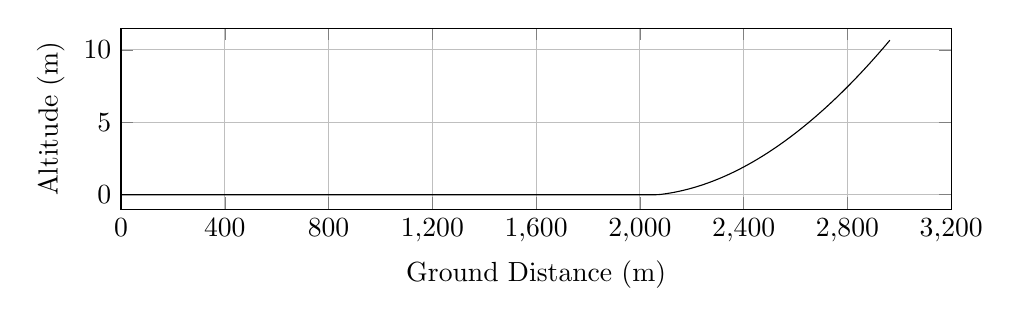
\begin{tikzpicture}

\begin{axis}[
width=\textwidth,
height=0.32\textwidth,
scaled ticks=false, tick label style={/pgf/number format/fixed},
xmin=0.0,
xmax=3200,
xtick={0,400,800,1200,1600,2000,2400,2800,3200},
xlabel={Ground Distance (m)},
xmajorgrids,
ymin=-1.0,
ymax=11.5,
ylabel={Altitude (m)},
ymajorgrids,
legend style={at={(1.03,0.5)},anchor=west,draw=black,fill=white,legend cell align=left}
]

\addplot [
color=black,
solid
]
table[row sep=crcr]{
1.3603393307215537E-8	0.0\\
2.0334443352841076E-7	0.0\\
1.8493358258961232E-6	0.0\\
9.983129263424352E-6	0.0\\
4.13538327636676E-5	0.0\\
1.2467543572893382E-4	0.0\\
2.843807411608912E-4	0.0\\
5.588015241105573E-4	0.0\\
9.398454696015893E-4	0.0\\
0.0014155885812023746	0.0\\
0.0019945752038215015	0.0\\
0.0026717822370171283	0.0\\
0.003447739291558293	0.0\\
0.0043193476547732645	0.0\\
0.00529092766782709	0.0\\
0.006363550519206555	0.0\\
0.007533073890550759	0.0\\
0.008790616877968567	0.0\\
0.01016549189277427	0.0\\
0.011625499440327931	0.0\\
0.013184282533086976	0.0\\
0.014839871214038253	0.0\\
0.01660567024659266	0.0\\
0.018465948346479452	0.0\\
0.0203822997817096	0.0\\
0.022430561433814646	0.0\\
0.024588423902376283	0.0\\
0.026831028501027587	0.0\\
0.029143159681622913	0.0\\
0.03155709159958957	0.0\\
0.03411445662773917	0.0\\
0.03677290089167576	0.0\\
0.03952314881844239	0.0\\
0.04239921643077808	0.0\\
0.045357163155895136	0.0\\
0.048363831658398165	0.0\\
0.051533845233668635	0.0\\
0.0547899150155587	0.0\\
0.058172599437445835	0.0\\
0.06162834747858026	0.0\\
0.06521401059050522	0.0\\
0.06888104003120077	0.0\\
0.07268727020998902	0.0\\
0.076546425570032	0.0\\
0.08047032364859658	0.0\\
0.08456364881336098	0.0\\
0.08882250397434277	0.0\\
0.09306368907640691	0.0\\
0.09743039119190974	0.0\\
0.10191450167634594	0.0\\
0.10651989152467789	0.0\\
0.11128201757858264	0.0\\
0.11609763023253863	0.0\\
0.12097769621339591	0.0\\
0.12591912973280778	0.0\\
0.13103216605369056	0.0\\
0.13633380151185176	0.0\\
0.1416823117522269	0.0\\
0.14708837902374172	0.0\\
0.1525605467319851	0.0\\
0.15824953188605478	0.0\\
0.16398006351864292	0.0\\
0.16978153473626356	0.0\\
0.17584258400626962	0.0\\
0.1819863832139092	0.0\\
0.18819485651962437	0.0\\
0.19455736971520038	0.0\\
0.20098158490654017	0.0\\
0.2076061353991409	0.0\\
0.21424726384720844	0.0\\
0.2211374965027113	0.0\\
0.2281284453493247	0.0\\
0.2350833915765042	0.0\\
0.2423085249848444	0.0\\
0.24958374984531584	0.0\\
0.2569279402934431	0.0\\
0.2644720218029696	0.0\\
0.27204626263318243	0.0\\
0.27972793364503945	0.0\\
0.2874622320100655	0.0\\
0.29563698092580604	0.0\\
0.30361763245720474	0.0\\
0.3118912000478351	0.0\\
0.3202493147046803	0.0\\
0.3286412952843002	0.0\\
0.33714554464307567	0.0\\
0.3458731203690518	0.0\\
0.35455185683415313	0.0\\
0.3634323904331427	0.0\\
0.372325738896249	0.0\\
0.38151551889959867	0.0\\
0.3908489672358084	0.0\\
0.4001862088113266	0.0\\
0.4095647137707429	0.0\\
0.4192312859369268	0.0\\
0.4289206911602753	0.0\\
0.43896550245304145	0.0\\
0.4487817299761361	0.0\\
0.4589033974758888	0.0\\
0.4691858798479248	0.0\\
0.47972601481223376	0.0\\
0.49016040525287174	0.0\\
0.5007175269203565	0.0\\
0.511266977039379	0.0\\
0.522323236324642	0.0\\
0.5332586746953114	0.0\\
0.5445869154512923	0.0\\
0.5556699580072249	0.0\\
0.5669225885056133	0.0\\
0.5785590177532589	0.0\\
0.5903083066022885	0.0\\
0.6020327889628274	0.0\\
0.613957077533064	0.0\\
0.625960998969677	0.0\\
0.6380070243193761	0.0\\
0.6503365955459197	0.0\\
0.662700086001522	0.0\\
0.6752747602080436	0.0\\
0.6885889407972636	0.0\\
0.7019767933734617	0.0\\
0.7151149754112038	0.0\\
0.7284684478906998	0.0\\
0.7418939875700234	0.0\\
0.7553494584716574	0.0\\
0.7694215958599202	0.0\\
0.7830840331449673	0.0\\
0.796657372658726	0.0\\
0.8106660034246236	0.0\\
0.8251837647136968	0.0\\
0.8395067871054176	0.0\\
0.8540519574023793	0.0\\
0.8688334527125461	0.0\\
0.8840141863517745	0.0\\
0.8993797082767976	0.0\\
0.9143697020410035	0.0\\
0.9294094610857999	0.0\\
0.9452486359568626	0.0\\
0.9605773823977486	0.0\\
0.9761522209726621	0.0\\
0.9917649966835071	0.0\\
1.0074810114554809	0.0\\
1.0234652146968335	0.0\\
1.0399433598517231	0.0\\
1.0563627364420554	0.0\\
1.0728309985448887	0.0\\
1.0896486452479222	0.0\\
1.1068138420051672	0.0\\
1.124143995869574	0.0\\
1.1415400048645106	0.0\\
1.1590089082607062	0.0\\
1.1769249919091855	0.0\\
1.1951505705127592	0.0\\
1.2127191877709298	0.0\\
1.2308827453761335	0.0\\
1.2492706857898845	0.0\\
1.267587852451018	0.0\\
1.2860031245644312	0.0\\
1.304687144125951	0.0\\
1.3233765774990474	0.0\\
1.342322280991234	0.0\\
1.3613696045164358	0.0\\
1.3815086998747366	0.0\\
1.4013123019267382	0.0\\
1.4209622886438908	0.0\\
1.4411501686096515	0.0\\
1.4611760119255748	0.0\\
1.4816444281325132	0.0\\
1.501865958841821	0.0\\
1.5224364680875304	0.0\\
1.543651615594651	0.0\\
1.5647593029468103	0.0\\
1.5859558716309676	0.0\\
1.6071423964076703	0.0\\
1.6293386351549652	0.0\\
1.6508498980272122	0.0\\
1.673011606043147	0.0\\
1.6946435720294923	0.0\\
1.717066624993247	0.0\\
1.739432891071898	0.0\\
1.761922286799709	0.0\\
1.7849035550437842	0.0\\
1.8076299607761817	0.0\\
1.8313298306791497	0.0\\
1.8543134894513886	0.0\\
1.8777326664639729	0.0\\
1.9017196849182967	0.0\\
1.925345883672024	0.0\\
1.950252961491087	0.0\\
1.975161211119453	0.0\\
1.9993825790313986	0.0\\
2.024583888346972	0.0\\
2.04934017380271	0.0\\
2.0744229633459703	0.0\\
2.0996193404956136	0.0\\
2.1245764901457758	0.0\\
2.1500786393425866	0.0\\
2.176226227020705	0.0\\
2.202115608176549	0.0\\
2.227948363055355	0.0\\
2.2543499999408594	0.0\\
2.2810892744412783	0.0\\
2.3075963743135786	0.0\\
2.3348582111613405	0.0\\
2.3623221378972126	0.0\\
2.3898598419727675	0.0\\
2.4171687299087603	0.0\\
2.445442108612223	0.0\\
2.4735885391813177	0.0\\
2.5015416452491293	0.0\\
2.5301110763218357	0.0\\
2.5589284934403693	0.0\\
2.587611617795936	0.0\\
2.6175687086884984	0.0\\
2.647724154312196	0.0\\
2.6767118187859253	0.0\\
2.7060305938995466	0.0\\
2.7361546404224653	0.0\\
2.7663022704956823	0.0\\
2.7964672462043376	0.0\\
2.8272583584284883	0.0\\
2.8588650092419234	0.0\\
2.8898852960400587	0.0\\
2.9215246589961597	0.0\\
2.95270311230069	0.0\\
2.984506337549637	0.0\\
3.017379145769185	0.0\\
3.049243647754313	0.0\\
3.081295157663824	0.0\\
3.113406837946715	0.0\\
3.1453724573084756	0.0\\
3.1787286104953543	0.0\\
3.211019796961401	0.0\\
3.245786703184362	0.0\\
3.279939251746722	0.0\\
3.3141720228361216	0.0\\
3.3491198891036547	0.0\\
3.382965192547779	0.0\\
3.4181848705561064	0.0\\
3.45391888941694	0.0\\
3.488851494856137	0.0\\
3.524271454997704	0.0\\
3.5606552075305	0.0\\
3.597189071478943	0.0\\
3.632926148839256	0.0\\
3.668897146318187	0.0\\
3.706642714683163	0.0\\
3.7432264628550644	0.0\\
3.781286297809391	0.0\\
3.818618572105483	0.0\\
3.8564015479305356	0.0\\
3.8948624022541356	0.0\\
3.9329637046009225	0.0\\
3.971505929995028	0.0\\
4.009821706071438	0.0\\
4.049014376833089	0.0\\
4.089343885784727	0.0\\
4.128662304630717	0.0\\
4.1684827283974055	0.0\\
4.208000253554632	0.0\\
4.2483743636521965	0.0\\
4.288255503180503	0.0\\
4.328757204126676	0.0\\
4.369490126907612	0.0\\
4.410357715197167	0.0\\
4.45189144941496	0.0\\
4.492881116440694	0.0\\
4.53550011161515	0.0\\
4.577670191557685	0.0\\
4.6201174049766305	0.0\\
4.662272021613388	0.0\\
4.706017761800355	0.0\\
4.748842845578064	0.0\\
4.792293145132742	0.0\\
4.836482439768313	0.0\\
4.88090298307878	0.0\\
4.925311889063089	0.0\\
4.969864686447545	0.0\\
5.014842280541593	0.0\\
5.0603877575117515	0.0\\
5.106292347304597	0.0\\
5.152263975081851	0.0\\
5.1974808794106995	0.0\\
5.244027372436168	0.0\\
5.28996242022761	0.0\\
5.336209145350672	0.0\\
5.38320569473032	0.0\\
5.430469292142472	0.0\\
5.476900151253712	0.0\\
5.526063828851289	0.0\\
5.573879040902945	0.0\\
5.622613575936374	0.0\\
5.6713596863799225	0.0\\
5.720412183296268	0.0\\
5.770660497446668	0.0\\
5.820668144990444	0.0\\
5.870305285939629	0.0\\
5.920503816994749	0.0\\
5.971105439367246	0.0\\
6.021088325934068	0.0\\
6.071322359863801	0.0\\
6.122981826035449	0.0\\
6.174329110820436	0.0\\
6.225804784288178	0.0\\
6.278093246139479	0.0\\
6.331709873490098	0.0\\
6.384325657889258	0.0\\
6.436648686434458	0.0\\
6.489478972803882	0.0\\
6.543185721519176	0.0\\
6.596747696432654	0.0\\
6.650345873843312	0.0\\
6.704555155195255	0.0\\
6.7588986063680725	0.0\\
6.814371620173711	0.0\\
6.86997180120154	0.0\\
6.925426612865756	0.0\\
6.981353650685165	0.0\\
7.037678624474159	0.0\\
7.094603706786671	0.0\\
7.151204881983983	0.0\\
7.209200593921791	0.0\\
7.2667780016693655	0.0\\
7.324687293141565	0.0\\
7.382771066065313	0.0\\
7.441904508776327	0.0\\
7.501585831803217	0.0\\
7.5616527251378685	0.0\\
7.62150963104709	0.0\\
7.682859947113334	0.0\\
7.7432084367972145	0.0\\
7.803024936926759	0.0\\
7.863793829029664	0.0\\
7.9252460466886365	0.0\\
7.98696966925656	0.0\\
8.04776546969778	0.0\\
8.109421212326083	0.0\\
8.17269125419024	0.0\\
8.236095044780246	0.0\\
8.299523592514586	0.0\\
8.363213767675873	0.0\\
8.427807923256076	0.0\\
8.49144930156071	0.0\\
8.557380457258176	0.0\\
8.623183572921022	0.0\\
8.687840683575093	0.0\\
8.753751426394068	0.0\\
8.820803713780364	0.0\\
8.888970287482593	0.0\\
8.957133699158991	0.0\\
9.025036015045707	0.0\\
9.092760955867519	0.0\\
9.159817422823458	0.0\\
9.227495373767134	0.0\\
9.296013084156197	0.0\\
9.36435980631623	0.0\\
9.433329865923408	0.0\\
9.503849553921977	0.0\\
9.574524061692681	0.0\\
9.644263228942293	0.0\\
9.715657612596786	0.0\\
9.787429657508813	0.0\\
9.85753688572494	0.0\\
9.930250735750551	0.0\\
10.001571447096964	0.0\\
10.074699859091687	0.0\\
10.14698611653175	0.0\\
10.220547980738981	0.0\\
10.2940409891517	0.0\\
10.36719293590382	0.0\\
10.441008888975666	0.0\\
10.51610421670324	0.0\\
10.590724589239105	0.0\\
10.667218005391902	0.0\\
10.742771202259895	0.0\\
10.82035208750042	0.0\\
10.896759047300378	0.0\\
10.973503045910835	0.0\\
11.051297940743765	0.0\\
11.128076326409062	0.0\\
11.207667705350879	0.0\\
11.286758396846047	0.0\\
11.366305937658339	0.0\\
11.446149720998452	0.0\\
11.526866579636565	0.0\\
11.607297517600138	0.0\\
11.688034241538357	0.0\\
11.769665722224765	0.0\\
11.850920080706608	0.0\\
11.933163326324259	0.0\\
12.017103780766782	0.0\\
12.10034832931326	0.0\\
12.185467765774142	0.0\\
12.270669986481685	0.0\\
12.354040133273898	0.0\\
12.440386807402234	0.0\\
12.52556588630658	0.0\\
12.610860989997974	0.0\\
12.69550109439961	0.0\\
12.784634337461807	0.0\\
12.871172079509357	0.0\\
12.958447214271366	0.0\\
13.045518554761987	0.0\\
13.133090172249581	0.0\\
13.221405510214687	0.0\\
13.310319106907201	0.0\\
13.399783591735492	0.0\\
13.488943611067967	0.0\\
13.578276665194153	0.0\\
13.667402973129146	0.0\\
13.757763665999576	0.0\\
13.848393619195729	0.0\\
13.938857764339925	0.0\\
14.031101516310692	0.0\\
14.123507833735925	0.0\\
14.214825187590282	0.0\\
14.307956552027534	0.0\\
14.401498558574918	0.0\\
14.495315613017755	0.0\\
14.589065423003394	0.0\\
14.68316852398955	0.0\\
14.778702641747682	0.0\\
14.873746415615575	0.0\\
14.970384078097169	0.0\\
15.068900921005241	0.0\\
15.164434274206265	0.0\\
15.260378587808539	0.0\\
15.357189194448868	0.0\\
15.45495288999333	0.0\\
15.55311774366497	0.0\\
15.652583807013901	0.0\\
15.755243917873962	0.0\\
15.855950289561445	0.0\\
15.958461094374158	0.0\\
16.060387288500337	0.0\\
16.164276126126843	0.0\\
16.26736468838029	0.0\\
16.36946523634058	0.0\\
16.47192386662276	0.0\\
16.576794358652606	0.0\\
16.678929175716583	0.0\\
16.783994526910618	0.0\\
16.89012564586595	0.0\\
16.996887404888547	0.0\\
17.103774697793426	0.0\\
17.210947675936964	0.0\\
17.31865021419634	0.0\\
17.424470519881233	0.0\\
17.53205215515201	0.0\\
17.64034909906897	0.0\\
17.74911485075183	0.0\\
17.85745376408675	0.0\\
17.969383314157206	0.0\\
18.07998395718984	0.0\\
18.18863741327577	0.0\\
18.302466989554325	0.0\\
18.41305080779906	0.0\\
18.525644000014054	0.0\\
18.636945827420575	0.0\\
18.750643923449367	0.0\\
18.86479622056296	0.0\\
18.979646899421056	0.0\\
19.09418630108147	0.0\\
19.208983505033515	0.0\\
19.323483295898072	0.0\\
19.43842354827664	0.0\\
19.55563752357537	0.0\\
19.67199913451129	0.0\\
19.789486593639566	0.0\\
19.90713985662446	0.0\\
20.024127533725753	0.0\\
20.143019013955552	0.0\\
20.26442367074238	0.0\\
20.383660776265387	0.0\\
20.5042342316437	0.0\\
20.622773342122727	0.0\\
20.74503732713029	0.0\\
20.865944869938517	0.0\\
20.98711015528624	0.0\\
21.113336299999695	0.0\\
21.23638685227678	0.0\\
21.35988644990264	0.0\\
21.483760012473958	0.0\\
21.608180515260266	0.0\\
21.732326713270083	0.0\\
21.85766379468624	0.0\\
21.985117186778353	0.0\\
22.111729024702363	0.0\\
22.23700541150786	0.0\\
22.36297326225872	0.0\\
22.488604760551	0.0\\
22.616276341350805	0.0\\
22.744235570279145	0.0\\
22.874576476768283	0.0\\
23.003842066605536	0.0\\
23.13088450205612	0.0\\
23.257869280739328	0.0\\
23.389244224935425	0.0\\
23.519811196806458	0.0\\
23.653309395988643	0.0\\
23.78342402399784	0.0\\
23.9180644861338	0.0\\
24.05110504604577	0.0\\
24.182394801971697	0.0\\
24.314614014384034	0.0\\
24.449791085561472	0.0\\
24.585258581909038	0.0\\
24.72121222319008	0.0\\
24.857032405393277	0.0\\
24.99454740444294	0.0\\
25.13030709358258	0.0\\
25.270890409679986	0.0\\
25.40663839363527	0.0\\
25.54307796688363	0.0\\
25.68272814639034	0.0\\
25.82072003425767	0.0\\
25.96015212691003	0.0\\
25.987750021099068	0.0\\
26.0558803939429	0.0\\
26.061632797568386	0.0\\
26.066808273335674	0.0\\
26.071901058608013	0.0\\
26.073315434863225	0.0\\
26.074595035914804	0.0\\
26.080371168076944	0.0\\
26.10234540095133	0.0\\
26.183408179590366	0.0\\
26.300430535410044	0.0\\
26.42750601924636	0.0\\
26.558056987479794	0.0\\
26.688030995483615	0.0\\
26.818767077324992	0.0\\
26.951519978077492	0.0\\
27.083955405447817	0.0\\
27.216897884715692	0.0\\
27.350913258119895	0.0\\
27.4833530065795	0.0\\
27.6176201223548	0.0\\
27.752160408628434	0.0\\
27.887329802382908	0.0\\
28.023188645890663	0.0\\
28.158973127824495	0.0\\
28.296372294036907	0.0\\
28.435107205966254	0.0\\
28.571323599682245	0.0\\
28.70996262687553	0.0\\
28.850320389600306	0.0\\
28.988837241064125	0.0\\
29.129197813929657	0.0\\
29.27166529868488	0.0\\
29.41298471572133	0.0\\
29.554848516656044	0.0\\
29.699676691743235	0.0\\
29.842400551696755	0.0\\
29.985385440862252	0.0\\
30.129077275410303	0.0\\
30.27543774584293	0.0\\
30.422081339040986	0.0\\
30.56949149516445	0.0\\
30.716562179458485	0.0\\
30.86535310281699	0.0\\
31.011875026602333	0.0\\
31.16159928701196	0.0\\
31.313692569485013	0.0\\
31.463056706803336	0.0\\
31.61235366859384	0.0\\
31.76278957628285	0.0\\
31.915019899787076	0.0\\
32.06709627595497	0.0\\
32.21861178877769	0.0\\
32.37168228565527	0.0\\
32.52450570609457	0.0\\
32.67702483599189	0.0\\
32.829998687403204	0.0\\
32.98551220909506	0.0\\
33.14332298937855	0.0\\
33.29970221124884	0.0\\
33.45800124694219	0.0\\
33.61398946945653	0.0\\
33.77048353048475	0.0\\
33.9292721471582	0.0\\
34.08796840843395	0.0\\
34.24769686644211	0.0\\
34.406855482575295	0.0\\
34.56481953291838	0.0\\
34.72399692808165	0.0\\
34.88694269464703	0.0\\
35.04914399338672	0.0\\
35.209965099803895	0.0\\
35.3703140559587	0.0\\
35.531685786905925	0.0\\
35.69349909442164	0.0\\
35.85522798807463	0.0\\
36.022509111806116	0.0\\
36.19055880791667	0.0\\
36.35708622463872	0.0\\
36.52115360367851	0.0\\
36.68781562330062	0.0\\
36.8536847754776	0.0\\
37.024522648961764	0.0\\
37.19188554678789	0.0\\
37.36066720850286	0.0\\
37.528862119520696	0.0\\
37.697264258302326	0.0\\
37.86832931534104	0.0\\
38.03812867477943	0.0\\
38.20923731912278	0.0\\
38.37904730305398	0.0\\
38.55252405124031	0.0\\
38.72282139824354	0.0\\
38.89783411301201	0.0\\
39.0714610757495	0.0\\
39.24438070689564	0.0\\
39.41969314875929	0.0\\
39.59166556575205	0.0\\
39.764623188591585	0.0\\
39.94263254662576	0.0\\
40.11749159802578	0.0\\
40.29452954971913	0.0\\
40.47247750600427	0.0\\
40.64799609178485	0.0\\
40.82414741101539	0.0\\
41.00385670225303	0.0\\
41.18169069533937	0.0\\
41.3603281005193	0.0\\
41.54046179251334	0.0\\
41.722675278204306	0.0\\
41.90258931008478	0.0\\
42.08518735141125	0.0\\
42.26728550944881	0.0\\
42.44743534848537	0.0\\
42.63069538383506	0.0\\
42.80963512098974	0.0\\
42.992542679335614	0.0\\
43.17926890616222	0.0\\
43.363134036078335	0.0\\
43.54815051311773	0.0\\
43.733578141849236	0.0\\
43.91798130912079	0.0\\
44.10506009255049	0.0\\
44.29251116260117	0.0\\
44.480917546793805	0.0\\
44.66851287589745	0.0\\
44.85853501730759	0.0\\
45.047396872181054	0.0\\
45.236914792155844	0.0\\
45.42785879536018	0.0\\
45.616432631699865	0.0\\
45.80697204128492	0.0\\
45.998633580597016	0.0\\
46.18800675699903	0.0\\
46.380841640082096	0.0\\
46.57327038933336	0.0\\
46.765844918266424	0.0\\
46.95911042680183	0.0\\
47.15311668852311	0.0\\
47.34541611633634	0.0\\
47.53884854699059	0.0\\
47.73236991243341	0.0\\
47.92818250719388	0.0\\
48.12326385407131	0.0\\
48.32058854034828	0.0\\
48.516852452700604	0.0\\
48.71339374517507	0.0\\
48.91319881343868	0.0\\
49.1119162355681	0.0\\
49.31207818344666	0.0\\
49.509673461222235	0.0\\
49.71156302510582	0.0\\
49.91034548441702	0.0\\
50.11200805970151	0.0\\
50.30853267551517	0.0\\
50.50757456960626	0.0\\
50.70929197287772	0.0\\
50.91222418686718	0.0\\
51.11562549758783	0.0\\
51.32090674103446	0.0\\
51.525199701657655	0.0\\
51.72863462744459	0.0\\
51.934060761332375	0.0\\
52.14033810224923	0.0\\
52.344882977561255	0.0\\
52.55098100649393	0.0\\
52.75731843494604	0.0\\
52.96514817708821	0.0\\
53.17450540782369	0.0\\
53.382202621450276	0.0\\
53.592230583406476	0.0\\
53.80364534107798	0.0\\
54.01469481143569	0.0\\
54.223966920081466	0.0\\
54.43230789395902	0.0\\
54.6430562980421	0.0\\
54.855225786754914	0.0\\
55.066088958624874	0.0\\
55.27969530828261	0.0\\
55.49171188337613	0.0\\
55.70388919125476	0.0\\
55.91737779085577	0.0\\
56.13177028494084	0.0\\
56.34652664868587	0.0\\
56.559021044851505	0.0\\
56.77591447970492	0.0\\
56.99548236897459	0.0\\
57.21481285737903	0.0\\
57.43536222847358	0.0\\
57.65367025761124	0.0\\
57.872788904232735	0.0\\
58.0907693980174	0.0\\
58.311927420720366	0.0\\
58.532333513628615	0.0\\
58.75532998033057	0.0\\
58.976617007999806	0.0\\
59.19875422837053	0.0\\
59.4206945143671	0.0\\
59.64453328369959	0.0\\
59.86894932484513	0.0\\
60.09432075877773	0.0\\
60.318058693038594	0.0\\
60.541731124044205	0.0\\
60.76707064338231	0.0\\
60.995574692986196	0.0\\
61.22378989589207	0.0\\
61.4534619981562	0.0\\
61.683510138770515	0.0\\
61.91410430469678	0.0\\
62.14462153858659	0.0\\
62.37563158073512	0.0\\
62.607203285434	0.0\\
62.841031881319736	0.0\\
63.07467935056491	0.0\\
63.31164975340633	0.0\\
63.54633691305479	0.0\\
63.78243968758058	0.0\\
64.0165414084598	0.0\\
64.25412817577254	0.0\\
64.49270299572771	0.0\\
64.73076499662056	0.0\\
64.96867826857735	0.0\\
65.21063576532572	0.0\\
65.4512107007771	0.0\\
65.69028017871045	0.0\\
65.93032615763332	0.0\\
66.17196619696679	0.0\\
66.4135612157637	0.0\\
66.6559030093851	0.0\\
66.89910102540284	0.0\\
67.14354652182666	0.0\\
67.38771133480921	0.0\\
67.63347396558368	0.0\\
67.87898066495345	0.0\\
68.1255935515739	0.0\\
68.37316753306138	0.0\\
68.62205497364681	0.0\\
68.8711887275476	0.0\\
69.120220471977	0.0\\
69.36846244647072	0.0\\
69.61951843592018	0.0\\
69.87236615109754	0.0\\
70.12758921381476	0.0\\
70.37945082809051	0.0\\
70.63410009691182	0.0\\
70.89152727368702	0.0\\
71.14629115974091	0.0\\
71.40197865069018	0.0\\
71.66163317144085	0.0\\
71.92484704501203	0.0\\
72.18465416754285	0.0\\
72.44573394560723	0.0\\
72.70633339061075	0.0\\
72.96699363118216	0.0\\
73.22900401485182	0.0\\
73.49076816912304	0.0\\
73.75430841254712	0.0\\
74.01895646534612	0.0\\
74.2846979982242	0.0\\
74.55380714249793	0.0\\
74.82322871850147	0.0\\
75.09350011520078	0.0\\
75.36421232425869	0.0\\
75.6347219158074	0.0\\
75.90830954343213	0.0\\
76.18188601743822	0.0\\
76.45626363461818	0.0\\
76.72958718025629	0.0\\
77.00406935908524	0.0\\
77.28579748399531	0.0\\
77.56784659723587	0.0\\
77.84569092555657	0.0\\
78.1246978223638	0.0\\
78.40641219364133	0.0\\
78.68590470271565	0.0\\
78.96851680469001	0.0\\
79.25576208114188	0.0\\
79.54169104977237	0.0\\
79.82662017154695	0.0\\
80.11330301632765	0.0\\
80.40394576721474	0.0\\
80.6908099930996	0.0\\
80.98055888331655	0.0\\
81.27178512217935	0.0\\
81.56682943128612	0.0\\
81.86186977412851	0.0\\
82.15688924927383	0.0\\
82.44965588234726	0.0\\
82.74488606927187	0.0\\
83.04325841243121	0.0\\
83.34213327641098	0.0\\
83.64411622775171	0.0\\
83.94734638805741	0.0\\
84.25123842984891	0.0\\
84.55152885577829	0.0\\
84.85735750691177	0.0\\
85.16518306664875	0.0\\
85.47136476235073	0.0\\
85.77898122624802	0.0\\
86.08923229760057	0.0\\
86.40254560035129	0.0\\
86.71167807044037	0.0\\
87.02660518802142	0.0\\
87.34238286044419	0.0\\
87.65842706333811	0.0\\
87.97971380652302	0.0\\
88.2973933745065	0.0\\
88.61789013566766	0.0\\
88.93643920279564	0.0\\
89.25662431900213	0.0\\
89.57903058309674	0.0\\
89.89968694948243	0.0\\
90.22473455398588	0.0\\
90.55024875587375	0.0\\
90.87789352676518	0.0\\
91.20733069500889	0.0\\
91.54101415610151	0.0\\
91.87012785371462	0.0\\
92.20120197152713	0.0\\
92.53416638543635	0.0\\
92.86431843528567	0.0\\
93.19748455591187	0.0\\
93.53066771200866	0.0\\
93.86681917526724	0.0\\
94.20530590547477	0.0\\
94.5419273964865	0.0\\
94.8854212036891	0.0\\
95.22752713476521	0.0\\
95.57091181422334	0.0\\
95.91383450860906	0.0\\
96.25469535763642	0.0\\
96.5966517898868	0.0\\
96.93845701474973	0.0\\
97.28153572459905	0.0\\
97.62213139590432	0.0\\
97.9659652144934	0.0\\
98.3129807304216	0.0\\
98.65852794036775	0.0\\
99.00080640577195	0.0\\
99.35064076251427	0.0\\
99.69796076807248	0.0\\
100.04654253174803	0.0\\
100.3915606488718	0.0\\
100.74261509654437	0.0\\
101.08877163494762	0.0\\
101.43457754260953	0.0\\
101.784020212797	0.0\\
102.13161434601102	0.0\\
102.4751980097893	0.0\\
102.82212110631409	0.0\\
103.16739702108615	0.0\\
103.51524666207362	0.0\\
103.86391679154056	0.0\\
104.20960434827006	0.0\\
104.55241399635099	0.0\\
104.89662223620601	0.0\\
105.24103428322039	0.0\\
105.5836615386647	0.0\\
105.92645892081137	0.0\\
106.27347658175316	0.0\\
106.6151670762521	0.0\\
106.95898391938218	0.0\\
107.30023552029138	0.0\\
107.64147805753461	0.0\\
107.98348674656944	0.0\\
108.32522459759954	0.0\\
108.3935347040271	0.0\\
108.40478590462831	0.0\\
108.41572478024443	0.0\\
108.4246743308916	0.0\\
108.44347342986478	0.0\\
108.52018987797786	0.0\\
108.70071173483461	0.0\\
108.99446230248458	0.0\\
109.30176454987088	0.0\\
109.60899173332959	0.0\\
109.91608539831654	0.0\\
110.22883517949637	0.0\\
110.54143546549608	0.0\\
110.853845249356	0.0\\
111.1739714794031	0.0\\
111.4937490010879	0.0\\
111.81170779322963	0.0\\
112.13106495813236	0.0\\
112.4519453366479	0.0\\
112.77515902629136	0.0\\
113.0997499810409	0.0\\
113.43040796942478	0.0\\
113.7597028375028	0.0\\
114.0907450350197	0.0\\
114.42538740208008	0.0\\
114.75997726261329	0.0\\
115.09477047197589	0.0\\
115.43440545481076	0.0\\
115.77494672336013	0.0\\
116.11687534861284	0.0\\
116.46164587354252	0.0\\
116.8077846490165	0.0\\
117.15688723722127	0.0\\
117.50557855048987	0.0\\
117.85411336711965	0.0\\
118.20532793701167	0.0\\
118.55850697655507	0.0\\
118.91273956155123	0.0\\
119.26983096270519	0.0\\
119.62978614725739	0.0\\
119.98960731920661	0.0\\
120.34734904217265	0.0\\
120.7138511704587	0.0\\
121.08106061642908	0.0\\
121.44737887966437	0.0\\
121.81499139152783	0.0\\
122.18511446431708	0.0\\
122.55384158147794	0.0\\
122.92460728481757	0.0\\
123.29616941264607	0.0\\
123.67040864389355	0.0\\
124.04652172406458	0.0\\
124.42393851457416	0.0\\
124.80152108360014	0.0\\
125.18180835736592	0.0\\
125.55854932865631	0.0\\
125.93878032356085	0.0\\
126.31997081831156	0.0\\
126.70099538833193	0.0\\
127.08058279416298	0.0\\
127.46175209000612	0.0\\
127.84399628255431	0.0\\
128.22749916598133	0.0\\
128.6102537001487	0.0\\
128.99595881306152	0.0\\
129.37788117916477	0.0\\
129.760738924708	0.0\\
130.1448498512433	0.0\\
130.53000390659713	0.0\\
130.9168242384266	0.0\\
131.29443328439476	0.0\\
131.67491382268804	0.0\\
132.05816436539135	0.0\\
132.44070735535217	0.0\\
132.82666098215685	0.0\\
133.20952005887244	0.0\\
133.5940193955625	0.0\\
133.97617966856654	0.0\\
134.36103715882757	0.0\\
134.74478042358356	0.0\\
135.12867144169206	0.0\\
135.5141335746535	0.0\\
135.89764893392993	0.0\\
136.28231234485685	0.0\\
136.66418763078912	0.0\\
137.04684871033697	0.0\\
137.42845627025127	0.0\\
137.8132447087305	0.0\\
138.19719797258034	0.0\\
138.58059071069573	0.0\\
138.96593237593703	0.0\\
139.3501607499636	0.0\\
139.73355638294606	0.0\\
140.1160230155566	0.0\\
140.50045093994146	0.0\\
140.88215178690393	0.0\\
141.26156782058217	0.0\\
141.64323970440188	0.0\\
142.02689350659642	0.0\\
142.41061312971692	0.0\\
142.7942251403153	0.0\\
143.1756303563767	0.0\\
143.5599719391364	0.0\\
143.94242380128833	0.0\\
144.3239499176869	0.0\\
144.70664939692608	0.0\\
145.0870075357763	0.0\\
145.46856550308127	0.0\\
145.85014610541765	0.0\\
146.23128237819492	0.0\\
146.61504730324998	0.0\\
146.99763315977907	0.0\\
147.38441582478964	0.0\\
147.7673688364352	0.0\\
148.15222568696134	0.0\\
148.53580865353604	0.0\\
148.9199734867533	0.0\\
149.3040357319486	0.0\\
149.68771357306542	0.0\\
150.07093078701052	0.0\\
150.45622889618164	0.0\\
150.8449053483268	0.0\\
151.2288570611563	0.0\\
151.61452719766493	0.0\\
151.9983007305741	0.0\\
152.38299664478842	0.0\\
152.76945776909372	0.0\\
153.15580177123394	0.0\\
153.54253364040335	0.0\\
153.93093169697067	0.0\\
154.31788037931886	0.0\\
154.7039882138024	0.0\\
155.08880221957185	0.0\\
155.47621608980313	0.0\\
155.866104687065	0.0\\
156.25391419262098	0.0\\
156.64166339424906	0.0\\
157.03027969880475	0.0\\
157.4213807682267	0.0\\
157.8105708506119	0.0\\
158.19948541262937	0.0\\
158.58893406813365	0.0\\
158.97894817604634	0.0\\
159.3710019698692	0.0\\
159.76139479981174	0.0\\
160.1523485688823	0.0\\
160.54128874338664	0.0\\
160.9326976430911	0.0\\
161.32564259741588	0.0\\
161.71827778345698	0.0\\
162.1124492087963	0.0\\
162.50576001021273	0.0\\
162.89904576730015	0.0\\
163.29316224934274	0.0\\
163.68899123279596	0.0\\
164.08495392634194	0.0\\
164.48271131475576	0.0\\
164.8792309171331	0.0\\
165.27343112400507	0.0\\
165.67115293733156	0.0\\
166.06936395728349	0.0\\
166.47000821435734	0.0\\
166.87155839526775	0.0\\
167.27134041220108	0.0\\
167.67233991204222	0.0\\
168.0705846918417	0.0\\
168.47232570996516	0.0\\
168.87521546679773	0.0\\
169.2789990941189	0.0\\
169.68142011368735	0.0\\
170.088438196605	0.0\\
170.49328200513543	0.0\\
170.89845866435633	0.0\\
171.30484584057905	0.0\\
171.7103088520891	0.0\\
172.11589069074847	0.0\\
172.52485519917514	0.0\\
172.93316089774754	0.0\\
173.34236088095247	0.0\\
173.7535761368399	0.0\\
174.16510964781833	0.0\\
174.5786011126259	0.0\\
174.99051444770384	0.0\\
175.40138574541044	0.0\\
175.81497300453447	0.0\\
176.2280441317456	0.0\\
176.64225100058474	0.0\\
177.05714873395152	0.0\\
177.47483026786767	0.0\\
177.89254345086653	0.0\\
178.3100126079721	0.0\\
178.7278240622369	0.0\\
179.1449731538625	0.0\\
179.56482315926417	0.0\\
179.9871804296257	0.0\\
180.4095742002126	0.0\\
180.83428717371925	0.0\\
181.26003251256287	0.0\\
181.6840913989422	0.0\\
181.8934642440371	0.0\\
182.1114839456617	0.0\\
182.5372774346568	0.0\\
183.423900814602	0.0\\
184.30144226609173	0.0\\
185.17422251923585	0.0\\
186.05126240753827	0.0\\
186.93861419286333	0.0\\
187.8243328275641	0.0\\
188.7212117513506	0.0\\
189.61004025875786	0.0\\
190.50102451880866	0.0\\
191.38947474753866	0.0\\
192.28052744689825	0.0\\
193.18778236606096	0.0\\
194.08895872822546	0.0\\
194.99680020640938	0.0\\
195.89480429656658	0.0\\
196.79674305679504	0.0\\
197.7065692706791	0.0\\
198.612023604503	0.0\\
199.52644538440046	0.0\\
200.43881964763966	0.0\\
201.34572312669928	0.0\\
202.26115686844895	0.0\\
203.17967892292364	0.0\\
204.1017087672932	0.0\\
205.01405834107487	0.0\\
205.94020355690031	0.0\\
206.86420646269943	0.0\\
207.79153006365993	0.0\\
208.72800400232427	0.0\\
209.6603812871926	0.0\\
210.59913361291103	0.0\\
211.54272242703126	0.0\\
212.4892775421681	0.0\\
213.4278558742791	0.0\\
214.37319863683314	0.0\\
215.31618532994997	0.0\\
216.26909967312713	0.0\\
217.2229300472723	0.0\\
218.17915574443117	0.0\\
219.13394290547268	0.0\\
220.0901210939433	0.0\\
221.05386294760763	0.0\\
222.0194744620763	0.0\\
222.9871855528732	0.0\\
223.95850156259326	0.0\\
224.93506896411378	0.0\\
225.9123601081958	0.0\\
226.89683950214788	0.0\\
227.87812705537118	0.0\\
228.86553252311342	0.0\\
229.85786107077195	0.0\\
230.84893890233656	0.0\\
231.8352011637358	0.0\\
232.83551070617193	0.0\\
233.8409775535427	0.0\\
234.84473749332597	0.0\\
235.85076677249623	0.0\\
236.86174655712836	0.0\\
237.8698887650736	0.0\\
238.88314164945962	0.0\\
239.88702917374013	0.0\\
240.9073981595622	0.0\\
241.92631922506058	0.0\\
242.95020737895555	0.0\\
243.9867665418509	0.0\\
245.01566609591487	0.0\\
246.05919400906686	0.0\\
247.09706457910846	0.0\\
248.1403037320082	0.0\\
249.18309170866138	0.0\\
250.23723200462985	0.0\\
251.28895058541582	0.0\\
252.34575298177748	0.0\\
253.4009695529494	0.0\\
254.47389199439823	0.0\\
255.55293546958148	0.0\\
256.6206413021679	0.0\\
257.69235364004487	0.0\\
258.77967411403563	0.0\\
259.8615409937813	0.0\\
260.93956317950165	0.0\\
262.02271022117964	0.0\\
263.11073386748035	0.0\\
264.2120045516847	0.0\\
265.31241535302627	0.0\\
266.4086016357777	0.0\\
267.51260488983417	0.0\\
268.6300148019782	0.0\\
269.7585470354529	0.0\\
270.8896873949477	0.0\\
272.0115439451323	0.0\\
273.13680176546006	0.0\\
274.2702490513931	0.0\\
275.413525774062	0.0\\
276.5542367829295	0.0\\
277.6972773917919	0.0\\
278.856653662284	0.0\\
280.02457374883886	0.0\\
281.2032739103363	0.0\\
282.3793508291475	0.0\\
283.5570819158503	0.0\\
284.7419934858003	0.0\\
285.9326270157934	0.0\\
287.128931254976	0.0\\
288.31480266049743	0.0\\
289.5063986037633	0.0\\
290.71803378146524	0.0\\
291.92377285751195	0.0\\
293.1368845155397	0.0\\
294.3779382526999	0.0\\
295.6236529225306	0.0\\
296.8710892485976	0.0\\
298.1231876568165	0.0\\
299.3513516362168	0.0\\
300.60759883822345	0.0\\
301.8758306910943	0.0\\
303.15324510629466	0.0\\
304.4174613942848	0.0\\
305.70907350215657	0.0\\
306.99802587761087	0.0\\
308.28687847241804	0.0\\
309.5668796159489	0.0\\
310.84791377823	0.0\\
312.1498528537303	0.0\\
313.4560044202801	0.0\\
314.75458395299495	0.0\\
316.0753084557979	0.0\\
317.40968260857574	0.0\\
318.7319345228668	0.0\\
320.0558782097702	0.0\\
321.3801932183561	0.0\\
322.6884764655432	0.0\\
324.0456734620244	0.0\\
325.39100935110525	0.0\\
326.7365982993339	0.0\\
328.06652939861567	0.0\\
329.40155074930124	0.0\\
330.74537767281527	0.0\\
332.0707513255394	0.0\\
333.4173386205282	0.0\\
334.746581315361	0.0\\
336.0867229892568	0.0\\
337.4205715422614	0.0\\
338.75500413875113	0.0\\
340.08105948956893	0.0\\
341.3989527111596	0.0\\
342.72155317639294	0.0\\
344.04109435086104	0.0\\
345.35282448543626	0.0\\
346.65609809876	0.0\\
347.964660055904	0.0\\
349.26930822844486	0.0\\
350.5666013847051	0.0\\
351.8669806622215	0.0\\
353.150344321377	0.0\\
354.42669516744513	0.0\\
355.7084983713929	0.0\\
356.9839654050402	0.0\\
358.2578487323243	0.0\\
358.5108324321051	0.0\\
358.64800612588874	0.0\\
358.7323961896923	0.0\\
358.9732456649284	0.0\\
358.99979477666295	0.0\\
359.01768095024534	0.0\\
359.0292585237206	0.0\\
359.04030674366413	0.0\\
359.0932275856527	0.0\\
359.3119468898926	0.0\\
359.96663022276493	0.0\\
361.01382689254797	0.0\\
362.10337816976426	0.0\\
363.2064629717895	0.0\\
364.30797819224426	0.0\\
365.4187311446934	0.0\\
366.533107917645	0.0\\
367.64647721929396	0.0\\
368.7658299095233	0.0\\
369.8975033538602	0.0\\
371.0334235675839	0.0\\
372.1785809863062	0.0\\
373.31981642046355	0.0\\
374.47796099960044	0.0\\
375.6447818548355	0.0\\
376.82127927712384	0.0\\
377.99866547828844	0.0\\
379.1872933927376	0.0\\
380.3777690794409	0.0\\
381.57556676946103	0.0\\
382.7749421474674	0.0\\
383.9810457964097	0.0\\
385.1925430839308	0.0\\
386.4130201303027	0.0\\
387.642251751972	0.0\\
388.8666959950373	0.0\\
390.1046277660565	0.0\\
391.36074966763465	0.0\\
392.6213644701743	0.0\\
393.8865770487704	0.0\\
395.152064769563	0.0\\
396.42651061844674	0.0\\
397.70785411533086	0.0\\
398.9973066037893	0.0\\
400.29415225393086	0.0\\
401.5867618821628	0.0\\
402.89266069540326	0.0\\
404.2026906817056	0.0\\
405.5133159752146	0.0\\
406.8188033215648	0.0\\
408.1428210789858	0.0\\
409.4619750104541	0.0\\
410.7866553223556	0.0\\
412.0986529037308	0.0\\
413.41031825374205	0.0\\
414.7325445744335	0.0\\
416.0604608911566	0.0\\
417.37987743675546	0.0\\
418.7014398680576	0.0\\
420.01889773673486	0.0\\
421.33899103421845	0.0\\
422.66825459862196	0.0\\
423.9828493739383	0.0\\
425.2866898826801	0.0\\
426.58651621496017	0.0\\
427.903684145803	0.0\\
429.2153042437793	0.0\\
430.5078155550293	0.0\\
431.8056897804571	0.0\\
433.10771680085895	0.0\\
434.41207598494043	0.0\\
435.70611367304923	0.0\\
437.00029135405987	0.0\\
438.2874501708874	0.0\\
439.57924381904877	0.0\\
440.86334367313043	0.0\\
442.14831278777626	0.0\\
443.4246228849945	0.0\\
444.6997613972451	0.0\\
445.9755582052717	0.0\\
447.24906355246185	0.0\\
448.52298649460784	0.0\\
449.7970073135898	0.0\\
451.0732662127574	0.0\\
452.3376055990435	0.0\\
453.5952498993071	0.0\\
454.85494572980974	0.0\\
456.1087097504561	0.0\\
457.37506433126146	0.0\\
458.6278255775072	0.0\\
459.88318384216313	0.0\\
461.1495506724468	0.0\\
462.40045639464984	0.0\\
463.65757573098006	0.0\\
464.9071051320194	0.0\\
466.1566124317301	0.0\\
467.40493487048604	0.0\\
468.6453875526006	0.0\\
469.88626954833353	0.0\\
471.121438878288	0.0\\
472.36866075431135	0.0\\
473.61277491797955	0.0\\
474.847394986184	0.0\\
476.0919243850004	0.0\\
477.332663142225	0.0\\
478.5724219868255	0.0\\
479.80092257497813	0.0\\
481.0375584334739	0.0\\
482.2739102243769	0.0\\
483.50761070604506	0.0\\
484.73645087682416	0.0\\
485.9701180686877	0.0\\
487.2040197703426	0.0\\
488.4379868089517	0.0\\
489.6662649185953	0.0\\
490.90312711290926	0.0\\
492.1279863449722	0.0\\
493.3555187762488	0.0\\
494.5813986132663	0.0\\
495.81306506315013	0.0\\
497.03914876098054	0.0\\
498.26683393172505	0.0\\
499.50266295667166	0.0\\
500.73735195101176	0.0\\
501.9701182093618	0.0\\
503.19768580865184	0.0\\
504.4244577677322	0.0\\
505.65446606675187	0.0\\
506.8799326293655	0.0\\
508.10296894514886	0.0\\
509.3300891483393	0.0\\
510.55042746736126	0.0\\
511.7758634172824	0.0\\
513.0069941420802	0.0\\
514.2368007453915	0.0\\
515.4653749193503	0.0\\
516.692936554484	0.0\\
517.9182949637068	0.0\\
519.1447269025491	0.0\\
520.3691616423282	0.0\\
521.5962955956038	0.0\\
522.8190006342938	0.0\\
524.0504956579896	0.0\\
525.2775162569808	0.0\\
526.5037791945065	0.0\\
527.7309950127833	0.0\\
528.9676629953149	0.0\\
530.1904761995918	0.0\\
531.4200799629455	0.0\\
532.6508186235542	0.0\\
533.8861328537107	0.0\\
535.1191154025705	0.0\\
536.3541516001687	0.0\\
537.6014291424526	0.0\\
538.8401539469637	0.0\\
540.0733224740736	0.0\\
541.3084701143896	0.0\\
542.5445296219116	0.0\\
543.7801144535581	0.0\\
545.020641446064	0.0\\
546.2635842600805	0.0\\
547.5016889820513	0.0\\
548.7434019761681	0.0\\
549.9801923224818	0.0\\
551.2209952109358	0.0\\
552.4624614352012	0.0\\
553.7104983615045	0.0\\
554.9509853553066	0.0\\
556.198779765235	0.0\\
557.4452042846669	0.0\\
558.6913961153057	0.0\\
559.9373071873138	0.0\\
561.190479656655	0.0\\
562.438955658489	0.0\\
563.6850948009178	0.0\\
564.929697065671	0.0\\
566.1858846153159	0.0\\
567.4335394292882	0.0\\
568.6927100524495	0.0\\
569.9554148400925	0.0\\
571.2080725002213	0.0\\
572.4628392427869	0.0\\
573.7255587613733	0.0\\
574.9849601347032	0.0\\
576.2455578974309	0.0\\
577.5037405727314	0.0\\
578.7710290981397	0.0\\
580.0415926690907	0.0\\
581.3056544394344	0.0\\
582.5745922365945	0.0\\
583.8465736126554	0.0\\
585.1138867284735	0.0\\
586.3816863809936	0.0\\
587.6568526528865	0.0\\
588.9312119077363	0.0\\
590.2085608612617	0.0\\
591.4894970792197	0.0\\
592.7712224745128	0.0\\
594.0457087101202	0.0\\
595.3229900970109	0.0\\
596.6049027692743	0.0\\
597.888527858317	0.0\\
599.1746087321733	0.0\\
600.4686753925178	0.0\\
601.756132486845	0.0\\
603.0506478771047	0.0\\
604.3444699938859	0.0\\
605.639841704939	0.0\\
606.9348963672905	0.0\\
608.2293058831849	0.0\\
609.5303114936141	0.0\\
610.8305998899184	0.0\\
612.1374903174244	0.0\\
613.4456982253539	0.0\\
614.7479454353979	0.0\\
616.0530028494784	0.0\\
617.355411663516	0.0\\
618.6685300868708	0.0\\
619.9781967370795	0.0\\
621.2926717033993	0.0\\
622.6143606423984	0.0\\
623.9333707310398	0.0\\
625.2643082081079	0.0\\
626.5879751722559	0.0\\
627.9137427758576	0.0\\
629.2358508220211	0.0\\
630.5644540799894	0.0\\
631.8954416830888	0.0\\
633.2257178425984	0.0\\
634.5665301356503	0.0\\
635.8981332744629	0.0\\
637.2315966881993	0.0\\
638.5710299642492	0.0\\
639.9168662735608	0.0\\
641.2574510748275	0.0\\
642.6113972182823	0.0\\
643.9659476666213	0.0\\
645.3130120333581	0.0\\
646.6597304504751	0.0\\
648.0095691537488	0.0\\
649.3629597731258	0.0\\
650.7176947138335	0.0\\
652.0788381365674	0.0\\
653.4488713625744	0.0\\
654.8116709906728	0.0\\
656.173740404799	0.0\\
657.5452802750865	0.0\\
658.9204596563864	0.0\\
660.2963740469804	0.0\\
661.6658313851392	0.0\\
663.0521132858448	0.0\\
664.4360306683577	0.0\\
665.8292011816573	0.0\\
667.2163271985867	0.0\\
668.6047264301751	0.0\\
669.998987448919	0.0\\
671.399004900122	0.0\\
672.7973943746879	0.0\\
674.2048626041517	0.0\\
675.6057711702158	0.0\\
677.0123671588653	0.0\\
678.4326128230277	0.0\\
679.8436935659233	0.0\\
681.2639217730778	0.0\\
682.6761162167804	0.0\\
684.0953253757189	0.0\\
685.5160556550902	0.0\\
686.9430122072256	0.0\\
688.3690474455248	0.0\\
689.802565989535	0.0\\
691.2440388929112	0.0\\
692.68585754274	0.0\\
694.1311500362933	0.0\\
695.5737624812512	0.0\\
697.0219888738536	0.0\\
698.4805957166548	0.0\\
699.9334238298952	0.0\\
701.3863499876684	0.0\\
702.8426100505642	0.0\\
704.3096010363631	0.0\\
705.7827632355607	0.0\\
707.2589692469944	0.0\\
708.7320223354072	0.0\\
710.2081799447544	0.0\\
711.6950124685986	0.0\\
713.1852523490734	0.0\\
714.6799836077773	0.0\\
716.1690826524341	0.0\\
717.6616955292548	0.0\\
719.1688744235912	0.0\\
720.6801541043576	0.0\\
722.193567337029	0.0\\
723.7117585640754	0.0\\
725.2268183538677	0.0\\
726.7484542746624	0.0\\
728.2701993637841	0.0\\
729.7974904391831	0.0\\
731.3344895263049	0.0\\
732.8763500013033	0.0\\
734.4146873371412	0.0\\
735.9566937097363	0.0\\
737.5009929304615	0.0\\
739.0567315881747	0.0\\
740.6212280203977	0.0\\
742.1831372944159	0.0\\
743.7633613412675	0.0\\
745.3409890418191	0.0\\
746.9227473262874	0.0\\
748.5073579902735	0.0\\
750.0967935458405	0.0\\
751.695664196669	0.0\\
753.3035090392186	0.0\\
754.9054734121928	0.0\\
756.5127335814425	0.0\\
758.1259048754323	0.0\\
759.7503744822131	0.0\\
761.3804286664777	0.0\\
763.0169264383103	0.0\\
764.6547534263623	0.0\\
766.3035286609465	0.0\\
767.9612681066892	0.0\\
769.6273077791657	0.0\\
771.2915786739861	0.0\\
772.9561579384283	0.0\\
774.6265403017157	0.0\\
776.3138494236971	0.0\\
777.9979202171387	0.0\\
779.6906377471553	0.0\\
781.385508375484	0.0\\
783.093507972362	0.0\\
784.8094836185776	0.0\\
786.5410532076337	0.0\\
788.2752615144761	0.0\\
790.0099540670708	0.0\\
791.758432654729	0.0\\
793.509712070274	0.0\\
795.2756321188633	0.0\\
797.0556352381882	0.0\\
798.8439948994157	0.0\\
800.6368366291572	0.0\\
802.4419494818594	0.0\\
804.2665115337747	0.0\\
806.0928545850238	0.0\\
807.9323847402372	0.0\\
809.7892271467092	0.0\\
811.6427987241793	0.0\\
813.5161802802209	0.0\\
815.399113311043	0.0\\
817.2951121762596	0.0\\
819.214015760635	0.0\\
821.1339947523122	0.0\\
823.0680288550875	0.0\\
825.0248865693679	0.0\\
826.9884086483587	0.0\\
828.9684379422529	0.0\\
830.9562666688871	0.0\\
832.969115284739	0.0\\
835.0110641299586	0.0\\
837.0482723593714	0.0\\
839.1141466157214	0.0\\
841.1879424758604	0.0\\
843.294551753658	0.0\\
845.4270591855441	0.0\\
847.5894545588039	0.0\\
849.77508330163	0.0\\
851.9850638601995	0.0\\
854.2317263199486	0.0\\
856.4903183854296	0.0\\
858.7602323043307	0.0\\
861.0663940983579	0.0\\
863.4143277951623	0.0\\
865.7993042680755	0.0\\
868.1803998200478	0.0\\
870.6068916411518	0.0\\
873.0473566734674	0.0\\
875.4990885811696	0.0\\
877.922025438922	0.0\\
880.3264533431286	0.0\\
882.7054072068088	0.0\\
885.0497953467313	0.0\\
887.3878650964198	0.0\\
889.6886353347891	0.0\\
891.9741547936862	0.0\\
894.2334150020233	0.0\\
896.4821013184248	0.0\\
898.6989197375708	0.0\\
900.893872489951	0.0\\
903.0663775907581	0.0\\
905.2279765530118	0.0\\
907.3668759055879	0.0\\
909.4710734839455	0.0\\
911.588238544196	0.0\\
913.6622359462538	0.0\\
915.7196903929275	0.0\\
917.7791093096534	0.0\\
919.8111305399784	0.0\\
921.8245049428992	0.0\\
923.8304038493322	0.0\\
925.8294318157168	0.0\\
927.820799750572	0.0\\
929.7883740066716	0.0\\
931.7508130614599	0.0\\
933.6980628233539	0.0\\
935.6376625304406	0.0\\
937.5638295270271	0.0\\
939.4836435435063	0.0\\
941.3888631904272	0.0\\
941.7683185971832	0.0\\
942.0052333867857	0.0\\
942.1632341649199	0.0\\
942.2640296287252	0.0\\
942.3410803977026	0.0\\
942.4197590341498	0.0\\
942.493048725272	0.0\\
942.5569959903023	0.0\\
942.587597033046	0.0\\
942.6155749354805	0.0\\
942.7543348982201	0.0\\
943.2252714510712	0.0\\
944.6469195036773	0.0\\
946.4670181030608	0.0\\
948.3085726919712	0.0\\
950.1795322581897	0.0\\
952.0590002740976	0.0\\
953.952809298868	0.0\\
955.8542709795056	0.0\\
957.7723429312603	0.0\\
959.6999312770267	0.0\\
961.6422006909127	0.0\\
963.5981632631335	0.0\\
965.5703840844212	0.0\\
967.5670652852548	0.0\\
969.567844169617	0.0\\
971.5778141122253	0.0\\
973.6184628811832	0.0\\
975.6712928941788	0.0\\
977.7489918467647	0.0\\
979.8420271189157	0.0\\
981.9557662710429	0.0\\
984.0844196728333	0.0\\
986.2393018165233	0.0\\
988.4115297073004	0.0\\
990.6179528770076	0.0\\
992.8272622408717	0.0\\
995.0511921539983	0.0\\
997.3128187317884	0.0\\
999.5862267245195	0.0\\
1001.8838481953806	0.0\\
1004.1795393645007	0.0\\
1006.5056712095561	0.0\\
1008.8300931901249	0.0\\
1011.16907215941	0.0\\
1013.4948449853896	0.0\\
1015.8444034881297	0.0\\
1018.1836393255946	0.0\\
1020.5125077881519	0.0\\
1022.843433493483	0.0\\
1025.1807782979877	0.0\\
1027.495993415907	0.0\\
1029.8066148030166	0.0\\
1032.0931533471326	0.0\\
1034.3744437464443	0.0\\
1036.620019247814	0.0\\
1038.8705077217764	0.0\\
1041.0974295022233	0.0\\
1043.3136708165216	0.0\\
1045.516002345158	0.0\\
1047.6947536347884	0.0\\
1049.8821238169467	0.0\\
1052.0549101675724	0.0\\
1054.2011763240348	0.0\\
1056.3369329288016	0.0\\
1058.4757194649942	0.0\\
1060.6116372809452	0.0\\
1062.725352108018	0.0\\
1064.8396826565408	0.0\\
1066.9286415656534	0.0\\
1069.009661638866	0.0\\
1071.0834141503492	0.0\\
1073.1682237043574	0.0\\
1075.2286298164213	0.0\\
1077.2870560490514	0.0\\
1079.336939397254	0.0\\
1081.3886997062068	0.0\\
1083.4245774340293	0.0\\
1085.466854336822	0.0\\
1087.5044543454483	0.0\\
1089.536117409587	0.0\\
1091.5569790330042	0.0\\
1093.5718718351945	0.0\\
1095.5794718074453	0.0\\
1097.5815007800625	0.0\\
1099.5802149542283	0.0\\
1101.5775977903227	0.0\\
1103.5708495920562	0.0\\
1105.5573190145565	0.0\\
1107.5458090210823	0.0\\
1109.5277347610163	0.0\\
1111.5101006284467	0.0\\
1113.4881433584364	0.0\\
1115.4537073361494	0.0\\
1117.4233581917624	0.0\\
1119.3862454328637	0.0\\
1121.3445348797773	0.0\\
1123.2949509616324	0.0\\
1125.2543226515982	0.0\\
1127.2017608159936	0.0\\
1129.1532030373005	0.0\\
1131.09383484113	0.0\\
1133.0388522061448	0.0\\
1134.981004616322	0.0\\
1136.917217805446	0.0\\
1138.8565675621985	0.0\\
1140.7932051313137	0.0\\
1142.727357268684	0.0\\
1144.6670850579621	0.0\\
1146.601608255573	0.0\\
1148.5365757470204	0.0\\
1150.470826807073	0.0\\
1152.399520196414	0.0\\
1154.3298000794366	0.0\\
1156.2597511201898	0.0\\
1158.1863440571342	0.0\\
1160.1185659856637	0.0\\
1162.0405823624046	0.0\\
1163.9698172541903	0.0\\
1165.8914419228845	0.0\\
1167.8089719224554	0.0\\
1169.7250314547505	0.0\\
1171.640335495816	0.0\\
1173.5623998181113	0.0\\
1175.4687244537472	0.0\\
1177.388600378688	0.0\\
1179.311772592087	0.0\\
1181.2255190585306	0.0\\
1183.1424376042164	0.0\\
1185.0526569856643	0.0\\
1186.976232166112	0.0\\
1188.8944068473538	0.0\\
1190.8147953132207	0.0\\
1192.736193505124	0.0\\
1194.650240699128	0.0\\
1196.56411388968	0.0\\
1198.4701263609527	0.0\\
1200.3788861963808	0.0\\
1202.294230322785	0.0\\
1204.2108765972566	0.0\\
1206.1277553499435	0.0\\
1208.0381081743003	0.0\\
1209.9616337875914	0.0\\
1211.8806842021877	0.0\\
1213.803064449788	0.0\\
1215.7204276951065	0.0\\
1217.6454789757545	0.0\\
1219.559351431069	0.0\\
1221.4883687630359	0.0\\
1223.3990641123996	0.0\\
1225.3175382940635	0.0\\
1227.2536187263636	0.0\\
1229.1712454498193	0.0\\
1231.0904669841316	0.0\\
1233.0141342258503	0.0\\
1234.9359325662954	0.0\\
1236.8641131975282	0.0\\
1238.7950424306082	0.0\\
1240.7180098433032	0.0\\
1242.648448861663	0.0\\
1244.592082067812	0.0\\
1246.5198068909076	0.0\\
1248.459355675891	0.0\\
1250.3983297925943	0.0\\
1252.3341893190595	0.0\\
1254.2825184270419	0.0\\
1256.2080931918454	0.0\\
1258.1481581436742	0.0\\
1260.0780667235817	0.0\\
1262.0208937926059	0.0\\
1263.972110289511	0.0\\
1265.919448558138	0.0\\
1267.8680928147587	0.0\\
1269.813208572335	0.0\\
1271.758158208257	0.0\\
1273.6988266697463	0.0\\
1275.6448430970518	0.0\\
1277.5923091501522	0.0\\
1279.542273497062	0.0\\
1281.4920915404377	0.0\\
1283.4467571096297	0.0\\
1285.399777774564	0.0\\
1287.3517512973776	0.0\\
1289.3167180848695	0.0\\
1291.276252158838	0.0\\
1293.2287009129527	0.0\\
1295.1932693906992	0.0\\
1297.152968155321	0.0\\
1299.118668620497	0.0\\
1301.0884291098118	0.0\\
1303.0559870202	0.0\\
1305.026067371347	0.0\\
1307.0046908456752	0.0\\
1308.9733803461663	0.0\\
1310.9480798369136	0.0\\
1312.9270137227309	0.0\\
1314.9033684634942	0.0\\
1316.8837631504452	0.0\\
1318.870303384183	0.0\\
1320.8635514873617	0.0\\
1322.8546497894577	0.0\\
1324.843236586306	0.0\\
1326.840153076043	0.0\\
1328.8335736851536	0.0\\
1330.8237731752297	0.0\\
1332.8252116416124	0.0\\
1334.8257054936507	0.0\\
1336.8315916914385	0.0\\
1338.8308677303635	0.0\\
1340.845538611804	0.0\\
1342.8493976549062	0.0\\
1344.867179104483	0.0\\
1346.8807769886616	0.0\\
1348.8948899612533	0.0\\
1350.9153761452653	0.0\\
1352.9384543050455	0.0\\
1354.9684276798316	0.0\\
1356.995571997381	0.0\\
1359.0184888035678	0.0\\
1361.0406114738366	0.0\\
1363.075718281173	0.0\\
1365.1142561050506	0.0\\
1367.1631204490677	0.0\\
1369.203786566262	0.0\\
1371.256294537182	0.0\\
1373.3037858080593	0.0\\
1375.3522225851602	0.0\\
1377.399085214975	0.0\\
1379.4488072608128	0.0\\
1381.504193850949	0.0\\
1383.5582991381975	0.0\\
1385.6173389222795	0.0\\
1387.6854312043974	0.0\\
1389.756527070239	0.0\\
1391.8184850952139	0.0\\
1393.8851613032512	0.0\\
1395.9568415783292	0.0\\
1398.0418415942322	0.0\\
1400.1147422505119	0.0\\
1402.1994713309036	0.0\\
1404.2838953006103	0.0\\
1406.3813908374605	0.0\\
1408.4712051880224	0.0\\
1410.5742726615895	0.0\\
1412.6722416819034	0.0\\
1414.7767347963995	0.0\\
1416.89033752148	0.0\\
1419.000193177967	0.0\\
1421.1171078199795	0.0\\
1423.230688192512	0.0\\
1425.3560742340446	0.0\\
1427.4922057290023	0.0\\
1429.6205808504787	0.0\\
1431.7513476874174	0.0\\
1433.8928464812157	0.0\\
1436.0326167072312	0.0\\
1438.1688122773899	0.0\\
1440.3175436833271	0.0\\
1442.4589006663828	0.0\\
1444.595717478951	0.0\\
1446.747610026338	0.0\\
1448.8994199957701	0.0\\
1451.0573987457055	0.0\\
1453.2194269192569	0.0\\
1455.3901765003397	0.0\\
1457.565243644936	0.0\\
1459.739799593116	0.0\\
1461.9130191590866	0.0\\
1464.1012114521732	0.0\\
1466.2909812596054	0.0\\
1468.4893576235345	0.0\\
1470.6965319412334	0.0\\
1472.9007402987036	0.0\\
1475.1067534275435	0.0\\
1477.3128227427906	0.0\\
1479.5214795181769	0.0\\
1481.7398403513093	0.0\\
1483.9573852219291	0.0\\
1486.1875053029457	0.0\\
1488.4140831840095	0.0\\
1490.6449897301286	0.0\\
1492.8785756422658	0.0\\
1495.1189933560204	0.0\\
1497.3631739554476	0.0\\
1499.6092413468464	0.0\\
1501.8705990605235	0.0\\
1504.1297202128267	0.0\\
1506.391090117972	0.0\\
1508.6607644656674	0.0\\
1510.9366388014414	0.0\\
1513.2187218246459	0.0\\
1515.4917579519774	0.0\\
1517.7759923848935	0.0\\
1520.071559918856	0.0\\
1522.3596405129683	0.0\\
1524.6639395375641	0.0\\
1526.9809726449262	0.0\\
1529.299002014738	0.0\\
1531.6261618825151	0.0\\
1533.9531858156738	0.0\\
1536.2801184797167	0.0\\
1538.6111848017717	0.0\\
1540.9542810556386	0.0\\
1543.2924985361942	0.0\\
1545.647157001276	0.0\\
1548.0137576251632	0.0\\
1550.3759409193735	0.0\\
1552.7423040004019	0.0\\
1555.108226554868	0.0\\
1557.4852464943092	0.0\\
1559.8667652518438	0.0\\
1562.2547702891247	0.0\\
1564.667506766088	0.0\\
1567.0752817391563	0.0\\
1569.4854085641446	0.0\\
1571.901847456249	0.0\\
1574.323894540311	0.0\\
1576.7611162961402	0.0\\
1579.2091786931715	0.0\\
1581.6471504697074	0.0\\
1584.0972631410673	0.0\\
1586.5552576103933	0.0\\
1589.0265225832131	0.0\\
1591.4961282912727	0.0\\
1593.9808442191293	0.0\\
1596.464368606757	0.0\\
1598.9538104367712	0.0\\
1601.4481713051919	0.0\\
1603.9589955306674	0.0\\
1606.4685318287466	0.0\\
1608.9862627244834	0.0\\
1611.5060890359582	0.0\\
1614.0481712718079	0.0\\
1616.5897274600147	0.0\\
1619.140999817174	0.0\\
1621.7132119937996	0.0\\
1624.2867817214128	0.0\\
1626.865584763456	0.0\\
1629.4497081014329	0.0\\
1632.04871084352	0.0\\
1634.6457228940212	0.0\\
1637.2499405037784	0.0\\
1639.8656338161077	0.0\\
1642.4989099550248	0.0\\
1645.1447562291692	0.0\\
1647.8004660738634	0.0\\
1650.4587131593598	0.0\\
1653.1368113237527	0.0\\
1655.8190834215493	0.0\\
1658.5113315887525	0.0\\
1661.2172554562176	0.0\\
1663.9390265518828	0.0\\
1666.659503235946	0.0\\
1669.408127793995	0.0\\
1672.160895336172	0.0\\
1674.9283674244825	0.0\\
1677.7042601110475	0.0\\
1680.51125977117	0.0\\
1683.3023119273903	0.0\\
1686.1223100538978	0.0\\
1688.9475290206628	0.0\\
1691.7930564462258	0.0\\
1694.6328528422914	0.0\\
1697.4826238976134	0.0\\
1700.3629511193053	0.0\\
1703.2535956961642	0.0\\
1706.1673869059846	0.0\\
1709.114703698643	0.0\\
1712.0515823296732	0.0\\
1715.0145570152467	0.0\\
1717.9794288017488	0.0\\
1720.9798127653962	0.0\\
1724.0071707816219	0.0\\
1727.0429221117947	0.0\\
1730.1037678372436	0.0\\
1733.1834843752513	0.0\\
1736.2782544276297	0.0\\
1739.398906251713	0.0\\
1742.544736726455	0.0\\
1745.7249664305882	0.0\\
1748.91851055896	0.0\\
1752.1482569001487	0.0\\
1755.4157242759652	0.0\\
1758.7127521352709	0.0\\
1762.0521091229825	0.0\\
1765.4199923640108	0.0\\
1768.8252866952116	0.0\\
1772.260031373517	0.0\\
1775.7239523711942	0.0\\
1779.237737384894	0.0\\
1782.808160486671	0.0\\
1786.4411495115633	0.0\\
1790.1383072623903	0.0\\
1793.8717963372942	0.0\\
1797.6779088104968	0.0\\
1801.5389697122032	0.0\\
1805.510097563787	0.0\\
1809.538907010617	0.0\\
1809.5799669039543	0.0\\
1813.6969334428704	0.0\\
1817.9752830667462	0.0\\
1822.3265708005724	0.0\\
1826.7235985333755	0.0\\
1831.2606920979192	0.0\\
1835.703704898157	0.0\\
1840.1300251040848	0.0\\
1844.4897313408815	0.0\\
1848.7541473880397	0.0\\
1852.925611445136	0.0\\
1857.0093541305273	0.0\\
1861.0219801636167	0.0\\
1864.9643581710961	0.0\\
1868.8697749346752	0.0\\
1872.7029956514784	0.0\\
1876.4825894433534	0.0\\
1880.203315541506	0.0\\
1883.885422074654	0.0\\
1887.5482823628995	0.0\\
1891.18988239981	0.0\\
1894.7935917004697	0.0\\
1898.357579968987	0.0\\
1901.8910738458053	0.0\\
1905.4055069832125	0.0\\
1908.8848315771097	0.0\\
1912.3704133976757	0.0\\
1915.817312248857	0.0\\
1919.2499702265382	0.0\\
1922.655765490114	0.0\\
1926.0491996382398	0.0\\
1929.4287298954205	0.0\\
1932.7909973872597	0.0\\
1936.1420073836093	0.0\\
1939.4742011374651	0.0\\
1942.798611587234	0.0\\
1946.1141645220682	0.0\\
1946.2456134831768	0.0\\
1946.3444000862737	0.0\\
1946.428504463775	0.0\\
1946.4826659582295	0.0\\
1946.5191345455219	0.0\\
1946.5613661757934	0.0\\
1946.8019248395144	0.0\\
1947.6776943926648	0.0\\
1950.1127799659903	0.0\\
1953.7317156797053	0.0\\
1957.2725639843688	0.0\\
1960.8819737287	0.0\\
1964.5056764159954	0.0\\
1968.187928736766	0.0\\
1971.905689376988	0.0\\
1975.7022691879852	0.0\\
1979.537841964977	0.0\\
1983.444718856696	0.0\\
1987.4060758689038	0.0\\
1991.4284936575932	0.0\\
1995.5025936188376	0.0\\
1999.639862341478	0.0\\
2003.7945604911656	0.0\\
2007.9888371718494	0.0\\
2012.2210016821919	0.0\\
2016.4236861581435	0.0\\
2020.6175087251327	0.0\\
2024.7584441599438	0.0\\
2028.8958054927293	0.0\\
2032.992745675002	0.0\\
2037.0638156078471	0.0\\
2041.0830967634956	0.0\\
2045.0972503258045	0.0\\
2049.0337627638955	0.0\\
2052.952277066648	0.0\\
2053.1914705759164	1.6757728230774738E-6\\
2053.461712110201	7.609342475147721E-6\\
2053.727347993613	1.763182286150003E-5\\
2053.987764737627	3.150211409419356E-5\\
2054.2450755147847	4.915200623950534E-5\\
2054.5144231878267	7.184097254979774E-5\\
2054.7782506782796	9.825561726552228E-5\\
2055.0499030288784	1.2980051988743514E-4\\
2055.3214574382864	1.65755426330019E-4\\
2055.582203761299	2.0445203370203892E-4\\
2055.83429708955	2.457626579398383E-4\\
2056.0858499353462	2.908157021150147E-4\\
2056.3248889301376	3.371833649035783E-4\\
2056.585396746872	3.9167237621855156E-4\\
2056.8519073017287	4.516997540376666E-4\\
2057.12067339009	5.166347376308015E-4\\
2057.3749569646307	5.821498951899676E-4\\
2057.6372691560846	6.539016064836542E-4\\
2057.908424028953	7.325341016809997E-4\\
2058.1802395219984	8.159240271942117E-4\\
2058.4504050385394	9.033509546231607E-4\\
2058.7179401030253	9.94403108527059E-4\\
2058.9878000525987	0.0010907723861596505\\
2059.245263112527	0.001186963723224781\\
2059.5178760782346	0.0012933507666153359\\
2059.773540456291	0.00139737458060268\\
2060.035370684838	0.0015081836782750682\\
2060.303573698372	0.0016261890200903757\\
2060.5621305656505	0.0017442727766854905\\
2060.8240071806495	0.001868210130400623\\
2061.0923955413436	0.0019997710482106672\\
2061.3614529060196	0.002136287506091741\\
2061.6345890252915	0.0022796260639251368\\
2061.9042033611668	0.002425825750060253\\
2062.175532448967	0.0025776920164697955\\
2062.4308267733813	0.0027249341337380485\\
2062.7038110197063	0.0028870585685138147\\
2062.9584808951895	0.0030426782780125904\\
2063.2192964246433	0.003206439474054826\\
2063.49031570592	0.0033813221991814586\\
2063.747281155627	0.0035515860639514394\\
2064.0172150439694	0.0037351200054484652\\
2064.270559337926	0.003911745376981789\\
2064.5360676455402	0.004101405372385585\\
2064.801535606569	0.004295708618071483\\
2065.0728321761453	0.004499117555540635\\
2065.3369191293777	0.00470183228099374\\
2065.6020487066417	0.00491003512270081\\
2065.8546177662083	0.005112754110324913\\
2066.1152473256707	0.0053264343724547854\\
2066.3727076073383	0.005542006917944967\\
2066.61861785562	0.005752086292742188\\
2066.8859541026077	0.005985112176102829\\
2067.1602931767757	0.006229282883936824\\
2067.4333889855398	0.006477431654291451\\
2067.7027606022657	0.0067271792653143935\\
2067.968958131639	0.006978858140162154\\
2068.216150257871	0.0072169177308691705\\
2068.4893232056393	0.007484882508102657\\
2068.7563485633627	0.007751785587376511\\
2069.0201888714582	0.008020341970024904\\
2069.282541436577	0.008292163245566454\\
2069.545393961789	0.008569293747035404\\
2069.820343126199	0.008864322776157292\\
2070.0915307936384	0.009160481713535805\\
2070.360811787168	0.009459647868087003\\
2070.6361329657884	0.009770781271205838\\
2070.8856482826677	0.01005735452982794\\
2071.1602835621698	0.010377850179629635\\
2071.4326812570926	0.010700997378094327\\
2071.7005177137626	0.011023856675538565\\
2071.976198457859	0.011361490209864229\\
2072.2346359142502	0.01168291700180699\\
2072.5105438061846	0.012031331069776375\\
2072.784751651362	0.012382992113152552\\
2073.047541724185	0.012725068622697778\\
2073.3227360140345	0.013088611627047421\\
2073.5924129204177	0.013450158623793305\\
2073.8680708980382	0.013825152220331781\\
2074.1438557487236	0.014205823161502183\\
2074.4093144657727	0.01457745402593296\\
2074.6850358512975	0.014968879494191852\\
2074.9608163093308	0.015365934190741965\\
2075.230097548105	0.015758996038726575\\
2075.5053688599637	0.016166293228316413\\
2075.775763184656	0.01657179276658386\\
2076.0202504007957	0.016943074009412522\\
2076.2880169941554	0.017354767952912437\\
2076.541690510562	0.01774968448523731\\
2076.8104543404625	0.018173297044259032\\
2077.0859251602033	0.018613049577194916\\
2077.34819379269	0.019036977308672896\\
2077.625397805913	0.019490627053629687\\
2077.9027492535124	0.019950271214638327\\
2078.179901413063	0.02041534720015213\\
2078.4311717859428	0.0208419818745983\\
2078.7017844249704	0.0213067772980269\\
2078.9795579111105	0.021789622267888616\\
2079.2534048567104	0.02227135752378264\\
2079.5223320180685	0.02274997388525537\\
2079.800165829425	0.023250215914876256\\
2080.0778746860215	0.02375611084583843\\
2080.3490535603123	0.024255794244136486\\
2080.627151262487	0.024774073009362373\\
2080.89828314449	0.02528508237874856\\
2081.1631221495827	0.02578968884180375\\
2081.4409288549596	0.026324812019539644\\
2081.7186902713656	0.02686580762759057\\
2081.9894420531955	0.027398899033654736\\
2082.26504975657	0.027947393081550115\\
2082.520315103867	0.028460671873283744\\
2082.7966414072707	0.029022022809840745\\
2083.002918075922	0.02944495598888225\\
2083.0514698411926	0.02954498637113543\\
2083.2886502177707	0.03003628771430969\\
2083.5467852602924	0.03057592314924104\\
2083.792451628563	0.031094158520918826\\
2084.0534387063217	0.03164957685580967\\
2084.3270265921738	0.0322370608346524\\
2084.6039380176635	0.03283701033369853\\
2084.870949195898	0.03342044751774147\\
2085.1364590351805	0.03400527364668944\\
2085.3873402016534	0.03456203600025187\\
2085.6335827074727	0.03511232000002358\\
2085.9100823035897	0.03573459467026707\\
2086.1787661379767	0.036343582851029496\\
2086.4490815076815	0.03696040755498904\\
2086.7263022260922	0.037597155708439314\\
2087.0026404596683	0.038235928874439065\\
2087.2760202845857	0.0388716976101489\\
2087.5366492611183	0.039481229984141164\\
2087.8002620205916	0.040101000783861196\\
2088.0775146432397	0.04075623741307989\\
2088.3507102093	0.041405152092211\\
2088.616866788132	0.04204032589165589\\
2088.8758550745315	0.042661085249349556\\
2089.126180997031	0.04326348789521339\\
2089.3677740927587	0.04384701079167526\\
2089.6458297225145	0.044521067641039996\\
2089.9234804456046	0.04519663958458853\\
2090.2000140397777	0.04587182297452763\\
2090.4741052623613	0.046543189858996845\\
2090.737223634883	0.047189553850435995\\
2091.0081399817436	0.04785685273389831\\
2091.2582498885467	0.048474385741177434\\
2091.5273762576635	0.04914046870859108\\
2091.8748470210858	0.050003008988306924\\
2092.1927834403496	0.050794759007368934\\
2092.4971525864667	0.051554982327652696\\
2092.8189818098617	0.052361219655607305\\
2093.210337047213	0.05334496060744787\\
2093.6790612550885	0.054527990140529586\\
2094.2501387542216	0.05597643369738936\\
2094.792791180789	0.05735998762508933\\
2095.241313105029	0.05850884493211053\\
2095.7196482343443	0.05973935125723513\\
2096.2555741567976	0.0611244869461222\\
2097.317637543946	0.06388968277911\\
2098.3725306741208	0.06666281405488081\\
2099.1188520663327	0.06864077424439854\\
2099.807236685225	0.07047694593658752\\
2100.697345706153	0.07286791669319431\\
2101.5327020196773	0.07512896905142671\\
2102.343231809662	0.07733869832764534\\
2103.121877415192	0.07947622401781015\\
2103.8706715695944	0.08154540632491208\\
2104.6806763548075	0.08379875064083675\\
2105.4685401153647	0.08600546899277026\\
2105.9792909827074	0.08744390965513271\\
2106.507427686556	0.0889378357588824\\
2107.0081940914133	0.09036046327358013\\
2107.577185752164	0.09198414442574321\\
2108.1880569357236	0.09373589618277653\\
2108.843227177729	0.09562453403157087\\
2109.6692939281584	0.0980203414122304\\
2110.4191497187885	0.10020914879594342\\
2111.1412456909657	0.10232954409566272\\
2111.762631806593	0.1041641190803109\\
2112.538921080717	0.1064689044718001\\
2113.6601884705533	0.10982316543003715\\
2114.744595091067	0.11309552780278392\\
2115.946858872556	0.11675614068470153\\
2117.07588223688	0.12022495407164782\\
2117.870919443755	0.12268575572180498\\
2118.819793312762	0.1256423179461521\\
2119.8087395078137	0.1287464393408846\\
2120.6065951852206	0.13126764437578042\\
2121.277465985456	0.13339924573373574\\
2121.908506760893	0.13541401740378667\\
2122.7359146444014	0.13807002664807222\\
2123.731253284064	0.14128656630879693\\
2124.6780982217206	0.14436814703290013\\
2125.5957407652886	0.14737492030188631\\
2126.6563021826914	0.1508747907758382\\
2127.3598565118673	0.15321120279007555\\
2128.007485825823	0.1553722365634389\\
2128.706227196247	0.1577149387879459\\
2129.7945919895774	0.16138692622984485\\
2131.1426758017933	0.16597395858452496\\
2132.1626460893203	0.16947305775448807\\
2132.964433215435	0.1722409002158608\\
2134.1416862196684	0.1763323767751347\\
2135.2326929496385	0.18015330214417552\\
2136.4448505884857	0.18443144596514283\\
2137.224665710258	0.18720201011061527\\
2137.9386388375624	0.1897512187268935\\
2138.5196194068403	0.19183444962594626\\
2139.1171901303132	0.1939854663190544\\
2139.7617248825472	0.19631496634689266\\
2140.3700621112966	0.19852261755793954\\
2140.95989544248	0.2006714413289611\\
2142.1250281729363	0.20494021649205546\\
2143.301930271263	0.20928455820501984\\
2144.4382338732194	0.21350996912335451\\
2145.5593584718254	0.21770870982953577\\
2146.585719816293	0.2215784733808645\\
2147.6969975289394	0.22579633326748366\\
2148.559976999042	0.22909180244926486\\
2149.4059848485977	0.23233945237883125\\
2150.1309670047513	0.23513589092472809\\
2150.686266639359	0.23728617252402684\\
2151.228414388157	0.23939251412981444\\
2151.7600790714923	0.24146483140254693\\
2152.4256820205455	0.2440685686470423\\
2153.027053778992	0.24642998785446513\\
2153.7064556665737	0.24910802310417152\\
2154.897253741129	0.25382799045002746\\
2155.957077697176	0.25805679921366365\\
2156.7990225264057	0.26143502720492284\\
2157.8748466782936	0.2657758670517619\\
2158.794572955113	0.26950838337470906\\
2159.747159267469	0.2733951577131305\\
2160.61212288562	0.27694283120903607\\
2161.474287058265	0.28049646572653486\\
2162.198116759919	0.2834933633590425\\
2162.903391912324	0.2864252407577159\\
2163.804859893491	0.2901896616800623\\
2164.7341965777023	0.2940903727939912\\
2165.681200905662	0.2980860325245629\\
2166.392543603398	0.3011011743563061\\
2167.0782972881734	0.30401905874143675\\
2167.738776484438	0.30683979802785877\\
2168.4868794919666	0.310047077005973\\
2169.3629435606717	0.3138195855457331\\
2170.234256757508	0.3175894296028706\\
2171.148827342111	0.3215655163336065\\
2172.2052261203307	0.3261825220316963\\
2173.551243522531	0.3321030732185809\\
2175.0121382989028	0.3385767913550287\\
2176.5913505943763	0.34563083988132504\\
2178.1141963375812	0.35248821418624554\\
2179.507613510442	0.35881015436656005\\
2180.474937197232	0.3632255250003905\\
2181.2586042515895	0.3668185812760899\\
2182.120429489868	0.3707865090727106\\
2182.957914813768	0.374658950369986\\
2183.744968136193	0.37831308946936015\\
2184.6987452261947	0.3827606267612407\\
2185.8422093887575	0.3881206037087407\\
2187.047293472335	0.3938023572758823\\
2188.044611670489	0.3985300845216231\\
2189.1366345982915	0.40373328864621794\\
2190.286661456068	0.409242844512513\\
2191.360814118111	0.41441667093119805\\
2192.0376806114336	0.4176906780271713\\
2192.9645702662046	0.42219131816649846\\
2193.93098985916	0.4269051536418189\\
2194.901251247292	0.43165954808348306\\
2195.8187826319017	0.4361756677433334\\
2196.783703897765	0.4409461239091156\\
2197.830249653507	0.4461445480393549\\
2198.8588156890182	0.45127842251392736\\
2199.8443067961543	0.45622031599912627\\
2200.6848123650298	0.46045295224818217\\
2201.9417701178627	0.46681332694472655\\
2203.4280915065865	0.4743815598527036\\
2204.8537301133483	0.4816888884380973\\
2206.033349809044	0.4877707953907392\\
2207.3169561538543	0.49442543829680985\\
2208.7438528786333	0.5018677006234922\\
2209.793943238551	0.5073747433719866\\
2210.930974770268	0.5133664943589147\\
2211.987663029936	0.5189616641701416\\
2213.00050743041	0.5243489069375427\\
2214.0588891337748	0.5300036886863926\\
2215.1984311452143	0.5361210304098005\\
2216.435984278546	0.5427984917323783\\
2217.4538291003655	0.54831697608665\\
2218.378099884997	0.5533488443142485\\
2219.3595980270993	0.5587138498614876\\
2220.882933135026	0.5670846265529039\\
2222.3929426427294	0.5754349959279983\\
2223.9668816489866	0.5841948458437589\\
2225.4964106418447	0.5927622227168825\\
2226.8301387157007	0.6002768403744347\\
2228.4149380197296	0.6092593196624534\\
2229.6834172700437	0.6164905848477527\\
2231.013304015002	0.6241116739758987\\
2232.3904647225954	0.6320465493423195\\
2233.7155838469234	0.6397227428811163\\
2234.5611911453243	0.6446423021548369\\
2235.3255677371944	0.6491034198035437\\
2235.825296907192	0.6520272379040739\\
2236.294188318375	0.6547758474279788\\
2236.8672794729555	0.6581421273312138\\
2237.477281276979	0.6617335044730772\\
2238.4776165251615	0.6676414600157037\\
2239.399955634405	0.6731091291052376\\
2240.2584138818183	0.6782156541257074\\
2241.0729002660983	0.6830762475950294\\
2241.902267647625	0.6880412859267466\\
2242.6956335614777	0.6928055658068866\\
2243.5626660925063	0.6980287323861458\\
2244.3276673784903	0.7026515569744012\\
2245.164533080748	0.7077240161994207\\
2246.425370091946	0.7153965829978395\\
2247.697290570737	0.7231735007653926\\
2249.271939584094	0.7328527264390179\\
2250.820720091364	0.7424283187181786\\
2252.2224990503273	0.7511423791421312\\
2253.6933299103302	0.7603340268209462\\
2255.1184436222193	0.7692871667414514\\
2256.5782275635356	0.7785062569137056\\
2258.122942465907	0.7883147488461222\\
2259.715248163895	0.7984824817668876\\
2260.6503467202656	0.8044805764997165\\
2261.388965855085	0.809232485333987\\
2261.9941194355342	0.8131350236314003\\
2262.637106026463	0.8172906984273443\\
2263.4143474366756	0.8223266667023157\\
2264.42586882889	0.8289012400341531\\
2265.862465697316	0.8382787761640771\\
2267.4369571586903	0.848610477547967\\
2268.6147027570014	0.8563756981632267\\
2269.6992602469654	0.8635544530945685\\
2270.949300881931	0.8718617866387648\\
2271.798649631636	0.8775265631653315\\
2272.578550247429	0.8827426149773561\\
2273.648440676471	0.8899206689570747\\
2274.6538009120486	0.896689517527097\\
2275.597032128123	0.9030609721826506\\
2276.6885270901694	0.910459191982294\\
2278.2195427848455	0.9208821544097092\\
2279.6203067102288	0.9304650492135229\\
2280.460044519308	0.9362312311085306\\
2281.3592203215276	0.9424233114422012\\
2282.3303134913303	0.9491312665097313\\
2283.214620290335	0.955258359792184\\
2284.568930956716	0.9646763763836672\\
2285.7881924739013	0.9731908500660043\\
2287.00851288618	0.9817464862030836\\
2288.148039480091	0.9897661714009867\\
2289.3256483303503	0.9980848015101385\\
2290.736326418484	1.0080912103223714\\
2291.711579615917	1.0150353670298196\\
2293.035426364958	1.0244961074864047\\
2294.3556429415557	1.0339704279918611\\
2295.787842590428	1.0442929939156929\\
2297.259146608734	1.0549457385697796\\
2298.7734374044467	1.0659608565087137\\
2300.0149373190143	1.0750303459373827\\
2300.9444084163642	1.0818431887900513\\
2301.7821070462314	1.0880000853408283\\
2302.775077844334	1.095318733964708\\
2303.7121564500058	1.1022458596116405\\
2304.9125221128743	1.111148242767229\\
2306.5528132447935	1.1233658845871592\\
2307.699625848526	1.1319439409427847\\
2308.7866362758014	1.140102075110248\\
2309.649467750093	1.1465966957134688\\
2310.4805738950517	1.152868390935064\\
2311.236839284137	1.1585888561306708\\
2311.9262424592353	1.1638148025686719\\
2312.7394897189643	1.169993307045067\\
2313.359913821163	1.1747168932165284\\
2313.9706714062713	1.1793753546070609\\
2314.6850587010194	1.1848348988492967\\
2315.3502643090987	1.189928918169611\\
2316.058175279254	1.1953609121661564\\
2317.026246186797	1.2028074495616639\\
2317.9395650791485	1.209852166823882\\
2318.829010936859	1.216730787155318\\
2319.9841834403005	1.2256910028899077\\
2321.070104234933	1.2341414321355253\\
2321.96733948771	1.2411435539076128\\
2322.853553445236	1.2480774318754708\\
2324.1419277937384	1.2581893638479023\\
2325.330167732287	1.2675484457600508\\
2326.1944884864906	1.2743761302990921\\
2327.0131981402155	1.2808589848934688\\
2328.1228306608973	1.2896695015100517\\
2329.461013788872	1.3003314843503797\\
2330.928182038898	1.3120673415489437\\
2332.345947098548	1.3234539030748982\\
2333.6653390692263	1.3340908917462517\\
2335.346726656908	1.347702859017196\\
2336.389571949562	1.3561772300434982\\
2337.5357436841578	1.3655193584847662\\
2338.639529337992	1.3745438223746382\\
2339.708444453803	1.3833091897168113\\
2340.6721109608143	1.3912334171397802\\
2341.82172048386	1.4007138399758263\\
2343.0279710677924	1.4106931534879639\\
2344.1758653916804	1.4202199088449001\\
2345.29902639397	1.4295699145286886\\
2346.2135280303246	1.437203718589597\\
2347.173582518285	1.4452378875497263\\
2348.070930087295	1.4527659192828315\\
2348.9294415028735	1.4599849855016491\\
2349.7032170655157	1.466505629272886\\
2350.453168714662	1.472838267682266\\
2351.258087061594	1.4796490207287243\\
2351.9836551613744	1.4858007531370698\\
2352.7979159672286	1.4927184597308139\\
2353.9388349858664	1.5024362422451825\\
2355.0773001446405	1.5121620708555303\\
2356.5226891563643	1.5245515759506776\\
2357.9113040467064	1.5364982989735112\\
2359.164902962587	1.5473203471793804\\
2360.1412502011954	1.5557731981797858\\
2360.94577550531	1.5627544375282807\\
2362.258043603276	1.574172529480725\\
2363.5836205810356	1.5857453497022922\\
2364.8813657703868	1.5971130754539953\\
2366.203237497247	1.6087306660070335\\
2367.180318392384	1.617342962745612\\
2368.5992605359625	1.6298877661927187\\
2370.0386650198798	1.6426592104611428\\
2371.3219816515166	1.6540845570550418\\
2372.5066545113796	1.6646641592238458\\
2373.6453315776216	1.67486238099684\\
2374.599911844636	1.6834339799684206\\
2375.611453782616	1.692539138913458\\
2376.53732436458	1.7008930537345148\\
2377.648593905329	1.7109448968303083\\
2378.695797725045	1.7204423140767275\\
2380.3438510235683	1.7354382778948616\\
2381.8799075743036	1.7494693781496786\\
2383.237296448612	1.7619119611321512\\
2384.4507872221484	1.7730700531500974\\
2385.6370424418055	1.7840092387084394\\
2387.2000352609484	1.79847012458541\\
2388.8170581751583	1.8134878084450055\\
2390.021282152764	1.8247093152053457\\
2391.147213266996	1.8352302702009422\\
2392.194460466625	1.8450411490481602\\
2393.339296009972	1.8557940015933605\\
2394.5749713157074	1.8674325729142094\\
2395.8030774977733	1.8790332813753783\\
2396.782218656319	1.8883061335041873\\
2397.9167358477007	1.8990769369697649\\
2399.2392578581193	1.911668480164355\\
2400.3522449299453	1.9222949870234713\\
2401.3653629155115	1.9319917359066987\\
2402.2020779443073	1.9400171711085883\\
2403.180129851413	1.949417827648325\\
2404.1848077799295	1.9590963669750856\\
2405.1772842049004	1.9686792132757303\\
2406.0221935673626	1.9768543365440627\\
2406.6227974776366	1.9826751902163555\\
2407.4395631604284	1.9906037659503961\\
2408.3509830889716	1.9994685270524388\\
2409.490826369174	2.0105807553281494\\
2410.6005173348212	2.0214265153539692\\
2411.5525480644965	2.030752960490033\\
2412.4135814464835	2.0392051415312844\\
2413.4731729834302	2.0496288239205347\\
2414.5553817274813	2.060300498107239\\
2415.978875421508	2.0743768113170935\\
2417.06935659804	2.0851902464895984\\
2418.2093444315324	2.096522545833553\\
2419.6669215791453	2.1110535119896836\\
2421.2922814077247	2.127312186902773\\
2422.484708592571	2.1392770774107808\\
2423.5693859714174	2.1501879121920684\\
2424.487170141687	2.1594401273648707\\
2425.331147730979	2.1679646100078696\\
2426.2963412555227	2.1777325734651747\\
2427.4521933982105	2.1894569303245186\\
2428.687169560576	2.202016253748308\\
2429.859649700844	2.2139709532456546\\
2430.96437855122	2.2252624239439474\\
2432.04429181502	2.2363261010370206\\
2433.4286538077613	2.250546210960713\\
2434.681341957482	2.263449944199773\\
2435.825059185393	2.27526118882066\\
2437.0106780841134	2.2875353781663854\\
2438.446499374796	2.302440982104808\\
2439.582050137943	2.314261342671748\\
2441.078320085976	2.32987961815747\\
2442.6292157924618	2.3461197418151567\\
2443.6698019805	2.3570456533287407\\
2444.6836319069207	2.367713384039262\\
2445.7351042527325	2.3788009141885356\\
2446.766943712336	2.3897048928146942\\
2448.064611613292	2.4034510173847057\\
2449.159260107588	2.415075148957661\\
2450.2612023134598	2.4268031429054817\\
2451.5946040144463	2.4410299866997542\\
2452.863477238274	2.454604346305649\\
2453.926724776359	2.4660059627556246\\
2454.923896080323	2.4767214117626466\\
2456.315684268102	2.4917135831235155\\
2457.738263071108	2.50708104088514\\
2458.715889382196	2.5176674379693242\\
2460.0515733861585	2.5321647656018333\\
2461.665996371815	2.5497393255991945\\
2463.029562787571	2.5646272517220616\\
2464.3557827134528	2.579146216824876\\
2465.660565682684	2.5934678274318266\\
2466.9046068361013	2.6071571913251175\\
2468.655029098062	2.6264757092538487\\
2470.270782232117	2.6443670398923604\\
2471.288003952757	2.655659883896381\\
2472.257257140036	2.666441102665498\\
2473.397845991748	2.679154248108987\\
2474.4796591181976	2.691238363557787\\
2475.69329274536	2.7048251713274443\\
2477.442872144554	2.7244682032247285\\
2479.0617157212264	2.7427025516531733\\
2480.654541302615	2.7606992859579966\\
2481.9855611570038	2.775780143924851\\
2483.117041735739	2.788630342600146\\
2484.315729348181	2.802274057495799\\
2485.8222426678485	2.8194656306500914\\
2487.368870235464	2.837166073632381\\
2488.313051395776	2.8479972393369692\\
2489.1910908926857	2.8580869686245283\\
2490.1748167100213	2.869410967815\\
2491.6074068941953	2.8859394235667546\\
2492.9091342497713	2.9009965284885117\\
2494.1326885309327	2.9151827934237753\\
2495.2369282177397	2.928013457869044\\
2496.7134103162234	2.9452105306931067\\
2497.869719269096	2.958711312827692\\
2499.854743947827	2.9819552855461637\\
2501.437389480887	3.0005484596025846\\
2502.790633502612	3.0164894424313804\\
2504.040276375439	3.0312450960519106\\
2505.2945001660273	3.0460886952736095\\
2506.480687672004	3.0601582910920673\\
2507.986474743275	3.0780623928032673\\
2509.297335600094	3.0936885542114947\\
2510.9706929609956	3.1136896388584825\\
2512.597634861806	3.1331937331477615\\
2514.175738402355	3.152166769949752\\
2515.331348676079	3.166094288154703\\
2516.4513352387094	3.1796198752393448\\
2517.5757367121932	3.1932259124216555\\
2518.611819093775	3.205787289027538\\
2519.8986557222825	3.2214209134247396\\
2520.879723394067	3.2333636927489158\\
2522.155964687492	3.248930638384949\\
2523.395405111878	3.2640821897474686\\
2524.6255911802355	3.279153228216529\\
2526.01967175514	3.296271408507905\\
2527.301787966985	3.3120515743420267\\
2528.473599822698	3.326504971189202\\
2529.696602239602	3.341621174747515\\
2531.2600120441866	3.3609914902087397\\
2532.548025495291	3.3769890687219126\\
2533.5027966029074	3.38887060635782\\
2534.4536805334246	3.400723183441162\\
2535.363340551743	3.412080040914221\\
2536.3145495685676	3.4239745820912537\\
2537.3591643288855	3.437059452297378\\
2538.5173309498005	3.451593985119678\\
2539.5700899087524	3.464830603371012\\
2540.6656313180647	3.478630318885333\\
2541.8400671637	3.4934523266247686\\
2542.7864169132918	3.5054172304757945\\
2543.632849055546	3.5161350801439557\\
2544.77009336607	3.5305594222377357\\
2546.0746289939325	3.5471396644501896\\
2547.552755582192	3.5659701429749813\\
2549.09049883268	3.585609642152968\\
2550.3435584319714	3.6016506091174953\\
2551.554980249726	3.6171904255400325\\
2552.683957655904	3.631700867013725\\
2553.7472689601527	3.6453921941736604\\
2554.7651396602596	3.6585210221173767\\
2555.797273013235	3.671856382550364\\
2556.8056089960346	3.684906217072246\\
2558.0707175968873	3.7013098541226306\\
2559.3172295625363	3.7175057341662088\\
2560.443057126462	3.7321620277917473\\
2561.6801330848484	3.7482977212494477\\
2562.9914472809887	3.7654373274926414\\
2564.4218064665683	3.784174675262145\\
2565.711732218124	3.801109733667383\\
2566.9288803717827	3.8171217910847117\\
2568.6124037737136	3.8393211517231816\\
2570.449718965292	3.8636172517818075\\
2571.6911439045152	3.8800741170467834\\
2573.037938148709	3.89796485492492\\
2574.331963715137	3.9151909305718853\\
2575.538613203399	3.9312859119310133\\
2577.2691604519805	3.9544229262081405\\
2578.931470218109	3.9767075035083126\\
2580.7736325975256	4.001471667623873\\
2582.5450645855353	4.02535292113609\\
2584.188767286051	4.047571752324428\\
2585.253363787092	4.061993058648051\\
2586.3519865270273	4.0769004859574505\\
2587.489877317138	4.092367720288486\\
2588.7971131318363	4.110170711680688\\
2590.578141767335	4.134484458172622\\
2591.84356815889	4.151800274198301\\
2593.1847608773487	4.170189870067766\\
2594.59570973625	4.189577016291061\\
2595.7020911981826	4.204808722816024\\
2596.911350723347	4.22148638753108\\
2598.447053642799	4.242710821293608\\
2599.9049721684796	4.262906367461628\\
2601.541131528371	4.285624469072154\\
2603.536032092801	4.3134002346902385\\
2605.415774177638	4.339649532642566\\
2607.264774149973	4.36554233153638\\
2608.7927727157876	4.386994392733305\\
2610.601333351806	4.412449023697702\\
2612.0920384347064	4.433481865177454\\
2613.6510785823075	4.455529003545296\\
2615.729801932491	4.48500494201005\\
2617.388766359377	4.508594109901864\\
2618.901916040808	4.530160467569958\\
2620.4764487333923	4.55265289004654\\
2622.3962370653335	4.580147957757388\\
2624.0878263951063	4.604439064351265\\
2625.7535724797517	4.6284178966052245\\
2627.2141913608984	4.649491895445648\\
2628.898428117145	4.673847968854577\\
2630.923250303261	4.703208246514373\\
2632.5509963155328	4.726873315641765\\
2634.681465819316	4.7579313480403265\\
2636.2811818992805	4.781314695313743\\
2637.8963226107016	4.804978004472224\\
2639.737388442706	4.832018088547242\\
2641.5686992213014	4.858985436913709\\
2643.230427604977	4.883516424809134\\
2644.801266810362	4.90675890094556\\
2645.9492602316186	4.923777566101123\\
2646.989869287915	4.939228149294612\\
2647.9570890713194	4.953609416553148\\
2649.295704565713	4.973545165766934\\
2650.7522071746043	4.995279208475914\\
2652.37552155511	5.019554757643512\\
2654.005814846835	5.04399017431464\\
2655.5902608917386	5.067791697477142\\
2657.371978130619	5.094619343183382\\
2659.37264207896	5.1248228163480345\\
2660.9382515839916	5.14851674030769\\
2662.299872344892	5.169165139748438\\
2663.449371523461	5.18662695390903\\
2665.010582347948	5.210387187810383\\
2666.648669842455	5.235372124117758\\
2668.4395844106575	5.262752142946306\\
2670.5311121011573	5.294812734600129\\
2671.7797234283134	5.313995931699864\\
2673.268460944644	5.336910825350097\\
2674.535916203903	5.356456118452353\\
2675.7131680625125	5.3746403861088865\\
2676.7561203637297	5.3907743382076685\\
2677.845969219028	5.407657969164008\\
2678.8695859453564	5.423538081278455\\
2680.193487601945	5.444109092753935\\
2681.2101180941972	5.4599304427947075\\
2683.1242270481152	5.489777218811083\\
2684.641182676579	5.513485321849968\\
2686.408598430845	5.541168179824503\\
2687.7196634830116	5.561745231632626\\
2688.7816855939864	5.5784397769397955\\
2689.9692563024573	5.5971356614403245\\
2691.3901924711063	5.619543926590582\\
2692.7845985366166	5.641574594518987\\
2694.4772307577387	5.668371303118635\\
2696.0348693674514	5.693083444241093\\
2697.679561633353	5.719231374372541\\
2699.1549081050935	5.742734750501022\\
2700.9766967219375	5.771819525187343\\
2702.515227080382	5.796435713663218\\
2703.7638849224604	5.816450082824646\\
2705.369467183278	5.84223299205501\\
2706.974409171973	5.868059017489285\\
2708.481252666882	5.892355063474394\\
2710.0959014568434	5.918441542673797\\
2711.894948946723	5.947570781589301\\
2714.0331880288686	5.982279176944072\\
2716.266421061351	6.018630550833805\\
2717.8083133842574	6.043788858558299\\
2719.491594617063	6.071310276677968\\
2720.9416867747414	6.095066055569459\\
2722.845309534432	6.126317665645804\\
2723.9885601368087	6.145122300900001\\
2725.727828127986	6.173782248105166\\
2727.739401637321	6.2070072014113045\\
2729.5073092271123	6.236276523591346\\
2731.1285592744	6.263174498565222\\
2732.6094825774708	6.287791723724698\\
2734.6801653997163	6.322288304700798\\
2736.9158763750256	6.359633439535697\\
2738.4579614028344	6.385452346070489\\
2740.5737444195192	6.420956334014894\\
2742.6120057822645	6.455246675570082\\
2744.8007359144303	6.4921636599056125\\
2746.2289877328676	6.51630694242764\\
2748.0194501009173	6.546632360224232\\
2749.573617496537	6.573009075518799\\
2751.1622829081825	6.600022624827943\\
2752.453652031104	6.622019208752908\\
2753.715076689712	6.6435388328034914\\
2755.471680891559	6.673560590917045\\
2757.1238953921384	6.701856109996855\\
2758.378435588578	6.723378588204165\\
2759.633887875437	6.744949072877315\\
2760.9799703841345	6.768112668287785\\
2762.2503824297573	6.790008233925759\\
2763.4216367727395	6.810224163620729\\
2764.6846249904575	6.832054970265961\\
2766.668921170738	6.866419712519583\\
2768.542973339925	6.8989493594548055\\
2770.4005651021107	6.931264350064367\\
2772.0895506365887	6.960707626671995\\
2773.3945594307907	6.983497252422678\\
2774.443491377566	7.001840250026097\\
2775.544594047922	7.0211198190226725\\
2776.6298440269447	7.04014611411902\\
2777.7025687007726	7.058976518853992\\
2778.727376321527	7.076987799890757\\
2780.187331190471	7.102684041324759\\
2781.568026871978	7.127025395235549\\
2782.8299301531442	7.149306578746458\\
2784.2336587115124	7.174130213039545\\
2785.6627691872554	7.1994440987809245\\
2787.067437944236	7.224365739497271\\
2788.6278961855223	7.2520986872612205\\
2790.8980664654737	7.292533710455558\\
2792.8317175601233	7.327057868460502\\
2794.630990187634	7.35925136384942\\
2796.892669590149	7.399812228662128\\
2799.2353671396068	7.4419361392612124\\
2800.9346560407193	7.47256102005805\\
2802.636011066342	7.503282137731755\\
2804.4866517497185	7.536765900111877\\
2806.1325601532226	7.566604083227746\\
2807.780539258909	7.596535115478719\\
2809.1023775927524	7.620582682248568\\
2810.489175134433	7.64585027668906\\
2812.414084698732	7.680987235140414\\
2814.206431852381	7.7137722431869555\\
2815.2636089046628	7.733140425147557\\
2816.5607441020384	7.75693587032363\\
2818.0770270352523	7.784794891211197\\
2820.12441452805	7.822486221823633\\
2822.0138551134814	7.8573454587038025\\
2823.922678485149	7.892635988711518\\
2826.095996265305	7.932906663558709\\
2828.378634871371	7.975306322282686\\
2830.5397493610035	8.0155462023572\\
2832.5249655255348	8.0525944146539\\
2833.885744116782	8.078035543112598\\
2835.1184348462084	8.101114373912875\\
2836.366359731366	8.124509823460944\\
2837.578888497649	8.147271940601854\\
2839.0850001080225	8.175586839068437\\
2840.7529490160387	8.206997946499456\\
2842.3143579226144	8.23645377657581\\
2843.8089026638218	8.26469449730169\\
2845.560007906337	8.297840724059075\\
2847.7079005007645	8.338582448298773\\
2849.776075170489	8.37790034153375\\
2851.7576310229288	8.415652749428716\\
2853.239801125962	8.443942853426602\\
2854.5815336056594	8.46959075914721\\
2856.179365168872	8.500181632384006\\
2857.8189241358714	8.53162505554689\\
2859.4605321320496	8.563162224082685\\
2861.2293819547567	8.597204819800435\\
2863.3822316153237	8.63872302781131\\
2865.0487482363424	8.670926480070783\\
2866.7033120512688	8.702954445519634\\
2868.8978437740852	8.745520029840407\\
2871.2425847394115	8.791106516890387\\
2873.3247179968403	8.831680372712409\\
2875.5964883945735	8.87604938204353\\
2877.3126292773422	8.909635623514976\\
2879.408329847027	8.950730669790026\\
2881.791710103039	8.997574459432595\\
2884.0363061466396	9.041795175603738\\
2886.240973233961	9.085328029874251\\
2888.5029890340093	9.13009498944908\\
2890.280884687627	9.1653531372394\\
2891.7408920883317	9.194354680178076\\
2893.1083799170356	9.221557310189759\\
2894.5662684025847	9.250599651880517\\
2897.1135168157034	9.301445516030189\\
2898.8083027943658	9.33534756126452\\
2900.652862778901	9.372311248291957\\
2902.335925805016	9.4060982956623\\
2903.8878884317182	9.437303962964712\\
2905.4550240965245	9.468863801224966\\
2907.1798898602538	9.503657099962624\\
2908.6756087410968	9.533876488787783\\
2910.1085260187865	9.562869149730535\\
2911.5916239253083	9.592920519785263\\
2913.3260325784568	9.628120065761358\\
2914.7998628125897	9.658078632570518\\
2916.421906510762	9.691100284079464\\
2918.2087990465097	9.727538996390155\\
2920.4129880170003	9.772575469141366\\
2922.5562156209508	9.816459712903576\\
2924.7511703984665	9.861498478917891\\
2927.262363711332	9.913144540048371\\
2929.233911178635	9.953780521445221\\
2931.1170292003853	9.992666499161675\\
2933.131667014938	10.034346886994431\\
2935.559110440883	10.084675555597887\\
2937.798274570777	10.131205062772448\\
2939.933916652991	10.175676778551225\\
2941.89255199534	10.216542707861215\\
2943.3616804451112	10.24724563046491\\
2945.4045224855136	10.290010091247812\\
2947.427230193266	10.332435171501796\\
2949.439440810439	10.374721125931863\\
2950.9934842771063	10.407434153418372\\
2952.300880367503	10.434992513674956\\
2953.6623506133737	10.463726939735306\\
2955.422167090919	10.500923421070333\\
2957.1932619931686	10.53842064649422\\
2958.9024250333896	10.5746659639106\\
2960.924408200329	10.617620284505993\\
2962.954408876767	10.660826887334387\\
2963.2910544380356	10.668000000000202\\
};
\end{axis}
\end{tikzpicture}%

%\caption{Take-off trajectory in OEI condition - ATR-72}
%\end{figure}
%%
%\begin{figure}[H]
%\centering
%%Altitude_evolution
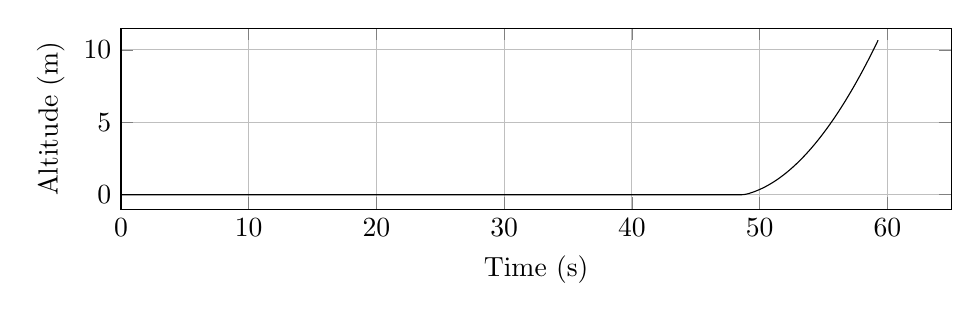
\begin{tikzpicture}

\begin{axis}[
width=\textwidth,
height=0.32\textwidth,
scaled ticks=false, tick label style={/pgf/number format/fixed},
xmin=0.0,
xmax=65,
xlabel={Time (s)},
xmajorgrids,
ymin=-1.0,
ymax=11.5,
ylabel={Altitude (m)},
ymajorgrids,
legend style={at={(1.03,0.5)},anchor=west,draw=black,fill=white,legend cell align=left}
]

\addplot [
color=black,
solid
]
table[row sep=crcr]{
9.999999999999999E-5	0.0\\
3.5694820560433537E-4	0.0\\
0.0010245452692119678	0.0\\
0.0069349042872337095	0.0\\
0.01286976806122327	0.0\\
0.018843593678645902	0.0\\
0.02479661783810936	0.0\\
0.03074929034621919	0.0\\
0.03669211352118573	0.0\\
0.042580956308319415	0.0\\
0.048493283817695076	0.0\\
0.05427367649331091	0.0\\
0.06018242857093453	0.0\\
0.0660567835326149	0.0\\
0.07196949266692618	0.0\\
0.07792428406091995	0.0\\
0.08390046318323552	0.0\\
0.08989020881354831	0.0\\
0.09587673552553522	0.0\\
0.10167944656754999	0.0\\
0.10765111137914757	0.0\\
0.11361192221071048	0.0\\
0.11954420271118602	0.0\\
0.125573987623401	0.0\\
0.1315700964469434	0.0\\
0.13749987165431027	0.0\\
0.14347214461959318	0.0\\
0.14945874955656013	0.0\\
0.15538557632642536	0.0\\
0.16134172045891504	0.0\\
0.16728166871345546	0.0\\
0.17316122794435485	0.0\\
0.17906586090973325	0.0\\
0.18502462068033498	0.0\\
0.19105995801776593	0.0\\
0.19703874704809138	0.0\\
0.20309718711380292	0.0\\
0.2090299405683319	0.0\\
0.21503149730647964	0.0\\
0.2210906082062326	0.0\\
0.22712806876774766	0.0\\
0.23315136948034765	0.0\\
0.23920379014307108	0.0\\
0.24515677763586902	0.0\\
0.25115480800481327	0.0\\
0.2572250890567559	0.0\\
0.2633064062502962	0.0\\
0.2693558850956802	0.0\\
0.2753851572323801	0.0\\
0.2814054782846729	0.0\\
0.2875363719193802	0.0\\
0.2936365386592882	0.0\\
0.2996725762790742	0.0\\
0.3057113890397092	0.0\\
0.311728709351481	0.0\\
0.3177443499717595	0.0\\
0.3239310451213814	0.0\\
0.3300281077115754	0.0\\
0.3360728475693199	0.0\\
0.34217699227400244	0.0\\
0.3483648069401394	0.0\\
0.35442860007526067	0.0\\
0.3605749921481264	0.0\\
0.36677317996618297	0.0\\
0.37291219385011287	0.0\\
0.3789779732446952	0.0\\
0.38504958269020406	0.0\\
0.39129130984530947	0.0\\
0.39747640865823075	0.0\\
0.4035449578168038	0.0\\
0.409658085793974	0.0\\
0.4158434790711202	0.0\\
0.42203123947701127	0.0\\
0.4282232407584047	0.0\\
0.4344427847702237	0.0\\
0.44060824473403093	0.0\\
0.44677233995759646	0.0\\
0.45294168306874305	0.0\\
0.4591520568719707	0.0\\
0.46552861434024206	0.0\\
0.47174496493338647	0.0\\
0.4780840868707784	0.0\\
0.4844105591505308	0.0\\
0.49073494683327135	0.0\\
0.49693324860032506	0.0\\
0.5031820245324283	0.0\\
0.5095347148125013	0.0\\
0.5158709697535484	0.0\\
0.5221857994590533	0.0\\
0.5285945736118585	0.0\\
0.5348943261437131	0.0\\
0.5412498831596135	0.0\\
0.5475879787525684	0.0\\
0.5540199261330143	0.0\\
0.5603110307074157	0.0\\
0.566739204297755	0.0\\
0.5732682780611191	0.0\\
0.5797267046288657	0.0\\
0.5861750445598519	0.0\\
0.5925208163290849	0.0\\
0.5988645455349844	0.0\\
0.605236368492422	0.0\\
0.6117724935743891	0.0\\
0.6181608865354462	0.0\\
0.6246969001680507	0.0\\
0.63116153002054	0.0\\
0.637673703807933	0.0\\
0.644070898056953	0.0\\
0.6506575993132437	0.0\\
0.6569950904275843	0.0\\
0.6635257426525845	0.0\\
0.6700305805678548	0.0\\
0.6765108465101242	0.0\\
0.683124466204782	0.0\\
0.6895920049387614	0.0\\
0.6961551992622965	0.0\\
0.702570002692859	0.0\\
0.7091767794146715	0.0\\
0.7158810384035788	0.0\\
0.722330750139915	0.0\\
0.7289031444577092	0.0\\
0.7354982449471308	0.0\\
0.7424081628271009	0.0\\
0.7489301174002103	0.0\\
0.755515041127365	0.0\\
0.7620900955093259	0.0\\
0.768726517316616	0.0\\
0.7754322814688266	0.0\\
0.7820045795409294	0.0\\
0.7885765548917036	0.0\\
0.7952880001398379	0.0\\
0.8019642657375692	0.0\\
0.8089221975782885	0.0\\
0.8159496552427474	0.0\\
0.8227512082781467	0.0\\
0.8295126839171314	0.0\\
0.8364435062986233	0.0\\
0.8433437972298823	0.0\\
0.8502532886622249	0.0\\
0.8571906480333069	0.0\\
0.8641948913839719	0.0\\
0.8709347755531902	0.0\\
0.8778085971393095	0.0\\
0.8846616629320734	0.0\\
0.8914723966825819	0.0\\
0.8984337487328791	0.0\\
0.9052581685588896	0.0\\
0.9122767946047234	0.0\\
0.9191083718623816	0.0\\
0.926072979352182	0.0\\
0.9331527145718401	0.0\\
0.9399812420074323	0.0\\
0.9469099835003199	0.0\\
0.9538892684884956	0.0\\
0.9608408960251769	0.0\\
0.967949078828209	0.0\\
0.9750804014833359	0.0\\
0.9820500063032944	0.0\\
0.9889400197651717	0.0\\
0.9959526785690063	0.0\\
1.0031613811593107	0.0\\
1.0101335383535681	0.0\\
1.0172304762477813	0.0\\
1.0243167196602005	0.0\\
1.031532325761198	0.0\\
1.0385761214455251	0.0\\
1.045518758175799	0.0\\
1.0526056127896628	0.0\\
1.059775473579922	0.0\\
1.0667056758326252	0.0\\
1.073723072246529	0.0\\
1.0809186717209713	0.0\\
1.0881483896660953	0.0\\
1.0953366014389219	0.0\\
1.1023895470451897	0.0\\
1.1097038616618584	0.0\\
1.1169054968916154	0.0\\
1.1241818599307019	0.0\\
1.1313684349455548	0.0\\
1.1386913369266725	0.0\\
1.1459050051946473	0.0\\
1.15324909865687	0.0\\
1.1603917284039738	0.0\\
1.167728191168648	0.0\\
1.1751136279327574	0.0\\
1.1826623714345867	0.0\\
1.1900759663658262	0.0\\
1.1973989800797513	0.0\\
1.204849923819272	0.0\\
1.2122043636572934	0.0\\
1.219690748242296	0.0\\
1.2271747469389913	0.0\\
1.2348350739745633	0.0\\
1.2422652286131242	0.0\\
1.2496486266791238	0.0\\
1.2572304774769116	0.0\\
1.26475871257581	0.0\\
1.2722849999230852	0.0\\
1.2798418424781421	0.0\\
1.2872317201819046	0.0\\
1.294781649430107	0.0\\
1.302274327708545	0.0\\
1.309799966680854	0.0\\
1.3174220765893008	0.0\\
1.3249737633890586	0.0\\
1.3327291813691486	0.0\\
1.3403377745059597	0.0\\
1.348066393515214	0.0\\
1.3557032568576135	0.0\\
1.363316543567941	0.0\\
1.3710774242951156	0.0\\
1.3788219901777032	0.0\\
1.3865773886235457	0.0\\
1.3941002978041466	0.0\\
1.4017811539906657	0.0\\
1.4095763089937394	0.0\\
1.4174562342054497	0.0\\
1.4251652517684015	0.0\\
1.4330378235789403	0.0\\
1.4407000702155934	0.0\\
1.4484594659956955	0.0\\
1.4563396432107631	0.0\\
1.4641675356187163	0.0\\
1.471933914080064	0.0\\
1.479769950215767	0.0\\
1.4874129554834874	0.0\\
1.4952912565691814	0.0\\
1.5034279098204526	0.0\\
1.511323320850415	0.0\\
1.5191757100931302	0.0\\
1.5271331134897972	0.0\\
1.5349157949428633	0.0\\
1.543002313099712	0.0\\
1.5507789665234828	0.0\\
1.558628747241348	0.0\\
1.5667955628936343	0.0\\
1.574712331198581	0.0\\
1.5825971607987288	0.0\\
1.590358951598581	0.0\\
1.5983342219636247	0.0\\
1.6063774707446807	0.0\\
1.6144694953357455	0.0\\
1.6224531728324476	0.0\\
1.6306021954514436	0.0\\
1.6387184329020679	0.0\\
1.6466602783164421	0.0\\
1.6547149097208704	0.0\\
1.6630308981810655	0.0\\
1.6714033552410448	0.0\\
1.6793960068941582	0.0\\
1.687559967796458	0.0\\
1.6956013484227919	0.0\\
1.703985576068487	0.0\\
1.7123628609916657	0.0\\
1.7205856868633744	0.0\\
1.7290429200788568	0.0\\
1.7373721866711915	0.0\\
1.7456026645961664	0.0\\
1.7538838866445223	0.0\\
1.7624912111876263	0.0\\
1.770773090024945	0.0\\
1.779088329532303	0.0\\
1.7872766435262744	0.0\\
1.795795588770969	0.0\\
1.8041847947879255	0.0\\
1.8126369218724645	0.0\\
1.8209097157071068	0.0\\
1.829219244317116	0.0\\
1.8376463555366884	0.0\\
1.8459718032624397	0.0\\
1.8542966926703768	0.0\\
1.8627053836441707	0.0\\
1.8711256342728828	0.0\\
1.879782123602444	0.0\\
1.8883929249058653	0.0\\
1.8967725863978533	0.0\\
1.905336340761549	0.0\\
1.9140263628453007	0.0\\
1.9225515986627846	0.0\\
1.931245648011127	0.0\\
1.9398766237544982	0.0\\
1.9484545062821095	0.0\\
1.9571336332373628	0.0\\
1.9658413648232447	0.0\\
1.9743918935091256	0.0\\
1.9831392911299472	0.0\\
1.9916148279509627	0.0\\
2.000268923318041	0.0\\
2.0091514649927955	0.0\\
2.017909753852824	0.0\\
2.026563531713383	0.0\\
2.0352324078101844	0.0\\
2.044067640387305	0.0\\
2.052753236912862	0.0\\
2.061566611968856	0.0\\
2.0702833647673344	0.0\\
2.0791641472526257	0.0\\
2.0880000673723433	0.0\\
2.0968390373693433	0.0\\
2.1055865782385377	0.0\\
2.1144357678008934	0.0\\
2.1233132463211506	0.0\\
2.1321628238787316	0.0\\
2.141104434100404	0.0\\
2.1499843468427056	0.0\\
2.1590571280259834	0.0\\
2.1679865758165935	0.0\\
2.1769213290254896	0.0\\
2.1858886072167385	0.0\\
2.194839082572962	0.0\\
2.204038094665136	0.0\\
2.213046247538463	0.0\\
2.222102475868321	0.0\\
2.231092535555222	0.0\\
2.240207193397323	0.0\\
2.2495245804319692	0.0\\
2.258740545352791	0.0\\
2.2678728103035652	0.0\\
2.2771018701344232	0.0\\
2.286361679403093	0.0\\
2.2956447464614653	0.0\\
2.3049189523060525	0.0\\
2.3141110215538685	0.0\\
2.3234227069187448	0.0\\
2.332688455071832	0.0\\
2.341876279533503	0.0\\
2.351091549623926	0.0\\
2.360539441307309	0.0\\
2.369789232894421	0.0\\
2.3791711728748757	0.0\\
2.38874954958509	0.0\\
2.3980390542950767	0.0\\
2.40750999912075	0.0\\
2.4169871244236694	0.0\\
2.426340051643196	0.0\\
2.435944198688186	0.0\\
2.4453186977271555	0.0\\
2.454841158430864	0.0\\
2.464234679011491	0.0\\
2.4735434908897043	0.0\\
2.4831426045113876	0.0\\
2.4927140624649757	0.0\\
2.502067505225207	0.0\\
2.51166584098749	0.0\\
2.521250744445581	0.0\\
2.5306593929673546	0.0\\
2.540558057175831	0.0\\
2.5502516927447223	0.0\\
2.5599057911578393	0.0\\
2.569385710236398	0.0\\
2.578834342589036	0.0\\
2.5885514990986165	0.0\\
2.598190632201491	0.0\\
2.607970400931631	0.0\\
2.617632864076235	0.0\\
2.627540085849689	0.0\\
2.637218199607754	0.0\\
2.6471336672090278	0.0\\
2.6568480852022915	0.0\\
2.6667486708271415	0.0\\
2.6764774720092284	0.0\\
2.6861387407061645	0.0\\
2.6959402486309676	0.0\\
2.705570290635996	0.0\\
2.7152913459009484	0.0\\
2.7251609135089154	0.0\\
2.7348705724187274	0.0\\
2.744629369906553	0.0\\
2.7546429964902677	0.0\\
2.7646256873810087	0.0\\
2.7745344373337746	0.0\\
2.78448273330019	0.0\\
2.7945461747368006	0.0\\
2.8045560495331197	0.0\\
2.8144941901843996	0.0\\
2.824567928489449	0.0\\
2.834532178368165	0.0\\
2.844593894364576	0.0\\
2.8545881500650925	0.0\\
2.8647742561957736	0.0\\
2.8747828181171027	0.0\\
2.885023792099372	0.0\\
2.8950960443764044	0.0\\
2.9050820127568375	0.0\\
2.915161020148581	0.0\\
2.9254942729288134	0.0\\
2.9356681598028294	0.0\\
2.9457751920016335	0.0\\
2.955720059741849	0.0\\
2.965769359476731	0.0\\
2.9760092478640754	0.0\\
2.9861988525482177	0.0\\
2.996278648119138	0.0\\
3.0064987277382853	0.0\\
3.0171126472517242	0.0\\
3.0272662822357743	0.0\\
3.0375599480669875	0.0\\
3.0480132480549615	0.0\\
3.0583904373770396	0.0\\
3.068693892307258	0.0\\
3.0791760373092094	0.0\\
3.0894573656209303	0.0\\
3.099852594297979	0.0\\
3.1102531441221695	0.0\\
3.120782604119581	0.0\\
3.13130924581199	0.0\\
3.1419768586928747	0.0\\
3.1524538261390926	0.0\\
3.1629528321100073	0.0\\
3.173561224845929	0.0\\
3.1840478095015072	0.0\\
3.194543531458371	0.0\\
3.2052150148888963	0.0\\
3.2160602353970704	0.0\\
3.226775992945611	0.0\\
3.2373719116960764	0.0\\
3.2482745666521815	0.0\\
3.2587129750477466	0.0\\
3.269536493210789	0.0\\
3.2801086967299193	0.0\\
3.290809906134636	0.0\\
3.3015770907563313	0.0\\
3.3119797092415357	0.0\\
3.3224703028488864	0.0\\
3.3331189004538	0.0\\
3.344115242439477	0.0\\
3.355052006567626	0.0\\
3.36567176758735	0.0\\
3.376446097028083	0.0\\
3.387130869009204	0.0\\
3.3977396315615103	0.0\\
3.408642881184611	0.0\\
3.4197552866515997	0.0\\
3.4304882804194152	0.0\\
3.4411839613772663	0.0\\
3.4523524128726475	0.0\\
3.4633665662338693	0.0\\
3.4742773994322533	0.0\\
3.484942212609072	0.0\\
3.4959606977105526	0.0\\
3.5067182567067974	0.0\\
3.5175717162567013	0.0\\
3.5285389825527798	0.0\\
3.5394185963001874	0.0\\
3.5507012255215713	0.0\\
3.561716953819312	0.0\\
3.5726145205143665	0.0\\
3.58366993559625	0.0\\
3.5948498393126727	0.0\\
3.605963987900413	0.0\\
3.6171740925646185	0.0\\
3.6284131889055455	0.0\\
3.639695307652401	0.0\\
3.650992086551901	0.0\\
3.6622418469349673	0.0\\
3.6734510150868562	0.0\\
3.6846830853939583	0.0\\
3.695879842608562	0.0\\
3.707099451126602	0.0\\
3.718274708510198	0.0\\
3.729429590858099	0.0\\
3.7408593670907715	0.0\\
3.752122184045909	0.0\\
3.763605920409903	0.0\\
3.7748091935166626	0.0\\
3.786220497192793	0.0\\
3.797739312038651	0.0\\
3.80898561302579	0.0\\
3.8203231006319136	0.0\\
3.8316531778633527	0.0\\
3.842980599243302	0.0\\
3.8543140657244885	0.0\\
3.8656564658472874	0.0\\
3.8771477237842253	0.0\\
3.888573510568392	0.0\\
3.899862911479868	0.0\\
3.911438478974441	0.0\\
3.92279464487481	0.0\\
3.934118474463962	0.0\\
3.945625729366511	0.0\\
3.957050617966029	0.0\\
3.9684874631493576	0.0\\
3.9800416021377636	0.0\\
3.9916809823101325	0.0\\
4.003226759525534	0.0\\
4.014739337559421	0.0\\
4.02638357676088	0.0\\
4.0378450965614725	0.0\\
4.049520027715284	0.0\\
4.061124751333221	0.0\\
4.0725123670405665	0.0\\
4.084095582270553	0.0\\
4.095690116812618	0.0\\
4.107237676295863	0.0\\
4.119098000362323	0.0\\
4.1305766118173874	0.0\\
4.142152746923815	0.0\\
4.153784087828598	0.0\\
4.165410538877948	0.0\\
4.1772222265995325	0.0\\
4.188946818070619	0.0\\
4.200664324488011	0.0\\
4.212311671251959	0.0\\
4.223892000900003	0.0\\
4.235390528815598	0.0\\
4.246989217360623	0.0\\
4.258618275434564	0.0\\
4.2701962817401995	0.0\\
4.2818969709946515	0.0\\
4.293428776814217	0.0\\
4.304958580130352	0.0\\
4.316775591730732	0.0\\
4.328424966859105	0.0\\
4.340067566843931	0.0\\
4.351819477988407	0.0\\
4.363292632597876	0.0\\
4.365609772812482	0.0\\
4.365827762680695	0.0\\
4.366156890255072	0.0\\
4.367285764412006	0.0\\
4.370554729071726	0.0\\
4.37734538151517	0.0\\
4.387806477228311	0.0\\
4.39864364652086	0.0\\
4.409536927170151	0.0\\
4.420376048165647	0.0\\
4.431256326804899	0.0\\
4.4421091367284635	0.0\\
4.453138010525066	0.0\\
4.464083040457272	0.0\\
4.475117887617129	0.0\\
4.485924593370475	0.0\\
4.496961285102792	0.0\\
4.507847639280435	0.0\\
4.5188292046447085	0.0\\
4.5299129612399	0.0\\
4.54087952555223	0.0\\
4.552001167304356	0.0\\
4.563019596927903	0.0\\
4.574189554159249	0.0\\
4.585332055939665	0.0\\
4.596756209108662	0.0\\
4.607786587044449	0.0\\
4.619015072255367	0.0\\
4.630223484741212	0.0\\
4.6414031810785	0.0\\
4.652708778433912	0.0\\
4.664079546120487	0.0\\
4.6753151831289745	0.0\\
4.686653577518522	0.0\\
4.697890982797592	0.0\\
4.709108531827992	0.0\\
4.72064250544018	0.0\\
4.731813636183569	0.0\\
4.743166725855746	0.0\\
4.75454099501202	0.0\\
4.765927839024803	0.0\\
4.7773345931072075	0.0\\
4.788689023725228	0.0\\
4.8000679457437805	0.0\\
4.811500834204896	0.0\\
4.822987280606505	0.0\\
4.834559620827509	0.0\\
4.845952446010495	0.0\\
4.857516331854871	0.0\\
4.869107606617373	0.0\\
4.880600219800634	0.0\\
4.892254271403688	0.0\\
4.903640449644904	0.0\\
4.915293886893618	0.0\\
4.926981102689567	0.0\\
4.93864180821587	0.0\\
4.950373773388343	0.0\\
4.962040794644393	0.0\\
4.973631406254297	0.0\\
4.9853084132905625	0.0\\
4.997149839555785	0.0\\
5.008854133343329	0.0\\
5.020636002047388	0.0\\
5.032363422348883	0.0\\
5.044270631271967	0.0\\
5.055976517818099	0.0\\
5.067792708150261	0.0\\
5.079491034995289	0.0\\
5.091279336079349	0.0\\
5.103141118757822	0.0\\
5.1149499914057	0.0\\
5.126933707882346	0.0\\
5.138714517877592	0.0\\
5.150473017988752	0.0\\
5.162182799334515	0.0\\
5.17418560855892	0.0\\
5.185972717937398	0.0\\
5.197930487706849	0.0\\
5.209824831391927	0.0\\
5.221690561768437	0.0\\
5.2335678164200825	0.0\\
5.245301082850945	0.0\\
5.257162978892827	0.0\\
5.269212119330316	0.0\\
5.281262125951104	0.0\\
5.292992263338753	0.0\\
5.3051093287408	0.0\\
5.316935174035137	0.0\\
5.329070905569742	0.0\\
5.340986880242278	0.0\\
5.352974348498053	0.0\\
5.364975527152241	0.0\\
5.37685927484471	0.0\\
5.388803485478622	0.0\\
5.400786682905052	0.0\\
5.412661067951245	0.0\\
5.424789619142722	0.0\\
5.436776315661213	0.0\\
5.448849566091836	0.0\\
5.460822392446877	0.0\\
5.47273048924103	0.0\\
5.484825427771691	0.0\\
5.496876881509207	0.0\\
5.5090370297629985	0.0\\
5.52092200939267	0.0\\
5.532970706917082	0.0\\
5.54487947956091	0.0\\
5.556874966113702	0.0\\
5.56888336986945	0.0\\
5.580910384972851	0.0\\
5.593072187651382	0.0\\
5.605152904939956	0.0\\
5.617234420343031	0.0\\
5.629244482854993	0.0\\
5.641369223974225	0.0\\
5.653445224467896	0.0\\
5.665579012516789	0.0\\
5.677714799612138	0.0\\
5.689902817238876	0.0\\
5.702039042354276	0.0\\
5.714045150163884	0.0\\
5.7261335173555885	0.0\\
5.7384092927467005	0.0\\
5.750500297518281	0.0\\
5.762695355119092	0.0\\
5.774894667920002	0.0\\
5.787097986150698	0.0\\
5.799214434175527	0.0\\
5.811296061221649	0.0\\
5.823466158413499	0.0\\
5.83562677158783	0.0\\
5.84766048518626	0.0\\
5.859940328786365	0.0\\
5.872165019838091	0.0\\
5.884441033367848	0.0\\
5.896687953418571	0.0\\
5.908934390684223	0.0\\
5.921018367804715	0.0\\
5.933142059152411	0.0\\
5.945370867974814	0.0\\
5.957641120891033	0.0\\
5.969699276628509	0.0\\
5.981843019254672	0.0\\
5.994108627173988	0.0\\
6.0063451482262025	0.0\\
6.0186212414729265	0.0\\
6.030700591612124	0.0\\
6.043079990417011	0.0\\
6.055098338636414	0.0\\
6.067315283695393	0.0\\
6.079660698903082	0.0\\
6.091969229666139	0.0\\
6.104208789349178	0.0\\
6.1163998147562335	0.0\\
6.12887138232402	0.0\\
6.141268103144984	0.0\\
6.153526920138685	0.0\\
6.165865841088646	0.0\\
6.178144255975809	0.0\\
6.190275768379534	0.0\\
6.202524213671365	0.0\\
6.214664334762476	0.0\\
6.226965122807313	0.0\\
6.239138091174254	0.0\\
6.251533499502486	0.0\\
6.263989387258135	0.0\\
6.276497026571889	0.0\\
6.288874580250022	0.0\\
6.301248779550207	0.0\\
6.313590423637988	0.0\\
6.32593890309481	0.0\\
6.3383231970360185	0.0\\
6.350770250972802	0.0\\
6.363083925431834	0.0\\
6.375593127253275	0.0\\
6.3880159124928415	0.0\\
6.4005030591779	0.0\\
6.4128798195805	0.0\\
6.425285596792559	0.0\\
6.437624743237073	0.0\\
6.4500074006514385	0.0\\
6.462435253045861	0.0\\
6.474793493245844	0.0\\
6.4872959866039075	0.0\\
6.499860484582687	0.0\\
6.512198239014223	0.0\\
6.524732282965175	0.0\\
6.537207495638045	0.0\\
6.549894034535326	0.0\\
6.562413469739594	0.0\\
6.57488469360054	0.0\\
6.587412593596266	0.0\\
6.599899435701829	0.0\\
6.6124451411854	0.0\\
6.625143219711772	0.0\\
6.63777004757835	0.0\\
6.650369504303152	0.0\\
6.663024717583481	0.0\\
6.675637414536949	0.0\\
6.688151339876221	0.0\\
6.700757485276274	0.0\\
6.713277176578632	0.0\\
6.7258260129120675	0.0\\
6.738452647667229	0.0\\
6.7512444389517245	0.0\\
6.763899527116191	0.0\\
6.776707656329382	0.0\\
6.789461022516029	0.0\\
6.8022124039870455	0.0\\
6.814896169894878	0.0\\
6.827701707718974	0.0\\
6.840537941307314	0.0\\
6.853179229017046	0.0\\
6.865880233762125	0.0\\
6.878674487230674	0.0\\
6.891383475650533	0.0\\
6.9043196944092635	0.0\\
6.917037946491966	0.0\\
6.9298374105318405	0.0\\
6.942683714985327	0.0\\
6.955603491750777	0.0\\
6.968332630532398	0.0\\
6.981270953998019	0.0\\
6.99409306721542	0.0\\
7.006994306190393	0.0\\
7.019909224804666	0.0\\
7.0328485318634275	0.0\\
7.045738282644885	0.0\\
7.058623978535344	0.0\\
7.071715545522604	0.0\\
7.08478123971347	0.0\\
7.0977135138896035	0.0\\
7.110831730563287	0.0\\
7.1238402361136846	0.0\\
7.137018096834716	0.0\\
7.150183705007155	0.0\\
7.163297429108246	0.0\\
7.176391640498968	0.0\\
7.18959553137663	0.0\\
7.202669123479263	0.0\\
7.21581371332193	0.0\\
7.229224584594668	0.0\\
7.242335316522617	0.0\\
7.255507625817728	0.0\\
7.268729084943288	0.0\\
7.282018483674792	0.0\\
7.295222853062198	0.0\\
7.308514217776775	0.0\\
7.321745251860822	0.0\\
7.335016290230419	0.0\\
7.34844025158279	0.0\\
7.361778990165382	0.0\\
7.375172334421219	0.0\\
7.388667703532647	0.0\\
7.402223194997115	0.0\\
7.415812487510799	0.0\\
7.429163333495865	0.0\\
7.442690269497403	0.0\\
7.456160039865566	0.0\\
7.469755052027002	0.0\\
7.483399445467143	0.0\\
7.497005623739245	0.0\\
7.510654789221771	0.0\\
7.524256707395043	0.0\\
7.5379930898809935	0.0\\
7.551677448667421	0.0\\
7.565547055466881	0.0\\
7.579249390553356	0.0\\
7.592981588064131	0.0\\
7.606861715084147	0.0\\
7.620628273783721	0.0\\
7.634447495929711	0.0\\
7.648192504123321	0.0\\
7.662240796287325	0.0\\
7.676202348540503	0.0\\
7.690108025935773	0.0\\
7.704071203293733	0.0\\
7.718221802084624	0.0\\
7.732290372341415	0.0\\
7.746504226467701	0.0\\
7.760627346813246	0.0\\
7.774796099725144	0.0\\
7.789009479414455	0.0\\
7.803217807824355	0.0\\
7.817587883860748	0.0\\
7.831766607328298	0.0\\
7.846041398443504	0.0\\
7.860371716232965	0.0\\
7.874798078043614	0.0\\
7.8891857877027025	0.0\\
7.9035490494622245	0.0\\
7.918051771507718	0.0\\
7.932461786496665	0.0\\
7.94691014144105	0.0\\
7.96144742803985	0.0\\
7.976061646615996	0.0\\
7.990634900394884	0.0\\
8.005097015699434	0.0\\
8.019893420304314	0.0\\
8.034397411765234	0.0\\
8.049149399215466	0.0\\
8.063861209812067	0.0\\
8.078754568397777	0.0\\
8.09348334752103	0.0\\
8.108092941185898	0.0\\
8.12304540586976	0.0\\
8.137958279483957	0.0\\
8.152728813321932	0.0\\
8.1678100196212	0.0\\
8.182664074772049	0.0\\
8.197738766362114	0.0\\
8.212775194828886	0.0\\
8.227737838411596	0.0\\
8.24290522068409	0.0\\
8.257996573353921	0.0\\
8.273335172510386	0.0\\
8.288473703108483	0.0\\
8.303482272135835	0.0\\
8.318655835686666	0.0\\
8.33389822804753	0.0\\
8.349385228465678	0.0\\
8.36460963500338	0.0\\
8.379926966134924	0.0\\
8.395196659993164	0.0\\
8.410243044957912	0.0\\
8.425514162519992	0.0\\
8.440659418367577	0.0\\
8.455962194174838	0.0\\
8.47119180980615	0.0\\
8.48639087873201	0.0\\
8.501673659184625	0.0\\
8.51705543324831	0.0\\
8.53226332328585	0.0\\
8.54749830431592	0.0\\
8.562792254999717	0.0\\
8.577909380902888	0.0\\
8.593039490093538	0.0\\
8.608287981283347	0.0\\
8.623255759329751	0.0\\
8.638359533853443	0.0\\
8.653302993623129	0.0\\
8.668333491488163	0.0\\
8.683315949576748	0.0\\
8.698329298102013	0.0\\
8.713328238390648	0.0\\
8.72834394008293	0.0\\
8.743152425848283	0.0\\
8.758158649736203	0.0\\
8.773097263917634	0.0\\
8.787785362445973	0.0\\
8.802515656199457	0.0\\
8.817197988640114	0.0\\
8.831674682677821	0.0\\
8.846310568773738	0.0\\
8.860933348808597	0.0\\
8.875408235607992	0.0\\
8.889948783313386	0.0\\
8.90444030987328	0.0\\
8.918827555713403	0.0\\
8.933259976231348	0.0\\
8.947596429304134	0.0\\
8.961740724552335	0.0\\
8.97601290657661	0.0\\
8.978840833446618	0.0\\
8.979132006879226	0.0\\
8.979426187815509	0.0\\
8.979618437954041	0.0\\
8.979759273345895	0.0\\
8.97988745453863	0.0\\
8.980464131607718	0.0\\
8.982958217103146	0.0\\
8.9897455851489	0.0\\
9.0033447692978	0.0\\
9.016108168876183	0.0\\
9.028953049848706	0.0\\
9.041735069562591	0.0\\
9.054638589456552	0.0\\
9.067545585121387	0.0\\
9.080543149451074	0.0\\
9.093621619753325	0.0\\
9.106673690301484	0.0\\
9.119772625577586	0.0\\
9.133043577493712	0.0\\
9.146368544451384	0.0\\
9.15968559747633	0.0\\
9.173112340775099	0.0\\
9.18653885575414	0.0\\
9.200188084677922	0.0\\
9.213810197102777	0.0\\
9.227322457334118	0.0\\
9.241037682342878	0.0\\
9.254635850728938	0.0\\
9.268416199146035	0.0\\
9.282219791530228	0.0\\
9.29601583131512	0.0\\
9.309974585507952	0.0\\
9.32393777135097	0.0\\
9.337883197202054	0.0\\
9.351895699205059	0.0\\
9.366011701674598	0.0\\
9.380255267881171	0.0\\
9.39431645221378	0.0\\
9.408482802303208	0.0\\
9.42280848724473	0.0\\
9.437135015961612	0.0\\
9.451544871289627	0.0\\
9.466037036346265	0.0\\
9.480691058533981	0.0\\
9.495245912675259	0.0\\
9.509932495984568	0.0\\
9.524538610440384	0.0\\
9.539260732908254	0.0\\
9.554126582682098	0.0\\
9.568897783087145	0.0\\
9.58374598865235	0.0\\
9.598482825402293	0.0\\
9.613403976627144	0.0\\
9.628284084963799	0.0\\
9.643188363578428	0.0\\
9.65807158220306	0.0\\
9.67279606393382	0.0\\
9.687684934908972	0.0\\
9.702552197484927	0.0\\
9.717342138430045	0.0\\
9.732163723738964	0.0\\
9.747149762039616	0.0\\
9.762060526895041	0.0\\
9.777091053840778	0.0\\
9.791966087699013	0.0\\
9.80674862286174	0.0\\
9.821669064351351	0.0\\
9.836458844880859	0.0\\
9.851307500110671	0.0\\
9.86613343017072	0.0\\
9.881059964755199	0.0\\
9.89572555001277	0.0\\
9.910501809109231	0.0\\
9.925245214375693	0.0\\
9.939948094855474	0.0\\
9.954644629017995	0.0\\
9.969281120601263	0.0\\
9.98390607104891	0.0\\
9.998585317370708	0.0\\
10.013201114604016	0.0\\
10.027767378370395	0.0\\
10.04244098677168	0.0\\
10.05695490583392	0.0\\
10.071517634882479	0.0\\
10.0859461609768	0.0\\
10.100358173149118	0.0\\
10.114880151957479	0.0\\
10.129295377329687	0.0\\
10.143747415333667	0.0\\
10.158236919646907	0.0\\
10.172585477159704	0.0\\
10.186936774262119	0.0\\
10.20130358527729	0.0\\
10.215533306533885	0.0\\
10.22984592060924	0.0\\
10.244206129457279	0.0\\
10.258417748531986	0.0\\
10.272746165568563	0.0\\
10.287004001461117	0.0\\
10.301050621247597	0.0\\
10.315263476298181	0.0\\
10.329336756787598	0.0\\
10.34344698817235	0.0\\
10.357540406443146	0.0\\
10.371669859765568	0.0\\
10.385696066737783	0.0\\
10.399648218519172	0.0\\
10.413783188039513	0.0\\
10.427711692307494	0.0\\
10.441666582805315	0.0\\
10.45563630974026	0.0\\
10.469613701078295	0.0\\
10.483590022945503	0.0\\
10.497463014285636	0.0\\
10.511330538835704	0.0\\
10.52522752996705	0.0\\
10.539155922044898	0.0\\
10.553145928391793	0.0\\
10.567018019382239	0.0\\
10.580911262179836	0.0\\
10.594768516267731	0.0\\
10.60856774635862	0.0\\
10.622489689659208	0.0\\
10.636310546416347	0.0\\
10.650164650615299	0.0\\
10.663937580608007	0.0\\
10.677815580905467	0.0\\
10.691550131568334	0.0\\
10.705261266644403	0.0\\
10.71911862771784	0.0\\
10.732873000433774	0.0\\
10.74670085052032	0.0\\
10.760507661869305	0.0\\
10.774318822874612	0.0\\
10.788102331549329	0.0\\
10.801774196018243	0.0\\
10.815551254794418	0.0\\
10.829261350155608	0.0\\
10.842999548568862	0.0\\
10.85668033184827	0.0\\
10.870380617529197	0.0\\
10.884132319694327	0.0\\
10.897771740288228	0.0\\
10.911503502350037	0.0\\
10.925218156003545	0.0\\
10.938867886945957	0.0\\
10.952605057218644	0.0\\
10.966308725297996	0.0\\
10.980032385630903	0.0\\
10.993726271124881	0.0\\
11.007456327782425	0.0\\
11.021233763966684	0.0\\
11.03492438583729	0.0\\
11.04863886376495	0.0\\
11.062404816555805	0.0\\
11.076195541821441	0.0\\
11.089818448277157	0.0\\
11.103545875211395	0.0\\
11.117290588538175	0.0\\
11.131094605842964	0.0\\
11.144788421389421	0.0\\
11.158548017541758	0.0\\
11.172314389108472	0.0\\
11.186060690006144	0.0\\
11.199795079157678	0.0\\
11.213642980472493	0.0\\
11.227449447895193	0.0\\
11.241283476955957	0.0\\
11.255049084613386	0.0\\
11.268773177526011	0.0\\
11.2825169231136	0.0\\
11.296264575379084	0.0\\
11.310067954366367	0.0\\
11.323939604254605	0.0\\
11.337734545625132	0.0\\
11.35153149054631	0.0\\
11.36532227069701	0.0\\
11.379108268437111	0.0\\
11.392888425200756	0.0\\
11.406699430046093	0.0\\
11.420503287255396	0.0\\
11.434363708332189	0.0\\
11.44815956115669	0.0\\
11.462031737073165	0.0\\
11.475880551293642	0.0\\
11.489683193459957	0.0\\
11.503604230352078	0.0\\
11.517468146333346	0.0\\
11.531445844568296	0.0\\
11.545280652376228	0.0\\
11.559090637142912	0.0\\
11.572974805259737	0.0\\
11.58691717706084	0.0\\
11.600857342026213	0.0\\
11.61480845321351	0.0\\
11.628623441604567	0.0\\
11.642596128921348	0.0\\
11.656559884003375	0.0\\
11.670539012801758	0.0\\
11.684557189606235	0.0\\
11.695234160363583	0.0\\
11.698594830716981	0.0\\
11.712576460210688	0.0\\
11.743330832742522	0.0\\
11.772650066804534	0.0\\
11.801916894303659	0.0\\
11.831165056992614	0.0\\
11.860454743581606	0.0\\
11.889949123841728	0.0\\
11.91936857568665	0.0\\
11.948792934714191	0.0\\
11.97829753312594	0.0\\
12.007992910467223	0.0\\
12.037473345133549	0.0\\
12.067440116346333	0.0\\
12.097013436508018	0.0\\
12.126747084718328	0.0\\
12.156581540322506	0.0\\
12.18663374947021	0.0\\
12.216236409539086	0.0\\
12.246224194390816	0.0\\
12.27608689624352	0.0\\
12.306164128078713	0.0\\
12.336205706966414	0.0\\
12.366414425693144	0.0\\
12.396674334209624	0.0\\
12.42667714813349	0.0\\
12.456822561981966	0.0\\
12.48688520324891	0.0\\
12.517182110360746	0.0\\
12.547259218343278	0.0\\
12.577523780177142	0.0\\
12.607936583043912	0.0\\
12.638351371070641	0.0\\
12.668769200728441	0.0\\
12.699434896023241	0.0\\
12.72993467496731	0.0\\
12.760339617493184	0.0\\
12.790869025513423	0.0\\
12.82148069398028	0.0\\
12.852300083530796	0.0\\
12.883221814928298	0.0\\
12.914067276559138	0.0\\
12.945165346091592	0.0\\
12.976282580149146	0.0\\
13.007227730873414	0.0\\
13.038424236846954	0.0\\
13.069553853655677	0.0\\
13.100484412190937	0.0\\
13.131579608294608	0.0\\
13.162886705718716	0.0\\
13.19381964556575	0.0\\
13.22539870404987	0.0\\
13.256578513492503	0.0\\
13.2881190105525	0.0\\
13.319745895685106	0.0\\
13.351222945416357	0.0\\
13.383178525919352	0.0\\
13.414902580407361	0.0\\
13.446568181110852	0.0\\
13.478377485169176	0.0\\
13.510199649815458	0.0\\
13.54213919349581	0.0\\
13.574280181623028	0.0\\
13.606495760422586	0.0\\
13.638497778009892	0.0\\
13.67063222422476	0.0\\
13.703255286880474	0.0\\
13.735399348708388	0.0\\
13.767863371506117	0.0\\
13.800245539631895	0.0\\
13.833193679730911	0.0\\
13.86566587047868	0.0\\
13.898628403609965	0.0\\
13.931532610260831	0.0\\
13.963931522178374	0.0\\
13.996898904665162	0.0\\
14.030193504800327	0.0\\
14.06308268783167	0.0\\
14.096536429865086	0.0\\
14.12987324099809	0.0\\
14.16333804475953	0.0\\
14.197188771595744	0.0\\
14.231102065443281	0.0\\
14.264793292338549	0.0\\
14.298664633403696	0.0\\
14.332807646721683	0.0\\
14.366845251134876	0.0\\
14.401112897746664	0.0\\
14.43550105278559	0.0\\
14.470193840209	0.0\\
14.504354691617685	0.0\\
14.538710139138644	0.0\\
14.573296710384234	0.0\\
14.607840418370746	0.0\\
14.642768303574119	0.0\\
14.677907855313734	0.0\\
14.712943329151233	0.0\\
14.747848350748963	0.0\\
14.78273273250305	0.0\\
14.818058266848666	0.0\\
14.853602568370558	0.0\\
14.88897389827039	0.0\\
14.924892873946394	0.0\\
14.96106244900798	0.0\\
14.996911571112083	0.0\\
15.0330792078075	0.0\\
15.069083404361724	0.0\\
15.105239714410398	0.0\\
15.141766141032864	0.0\\
15.178570099872605	0.0\\
15.215685461438394	0.0\\
15.252793799259713	0.0\\
15.289797533992985	0.0\\
15.327049925408673	0.0\\
15.364038251189886	0.0\\
15.401085559757064	0.0\\
15.438517098408653	0.0\\
15.475970465141746	0.0\\
15.513959997685017	0.0\\
15.551932053474694	0.0\\
15.589811911104881	0.0\\
15.627900405224498	0.0\\
15.665937322892798	0.0\\
15.704165509891016	0.0\\
15.742652098350273	0.0\\
15.781917512720057	0.0\\
15.82041426324384	0.0\\
15.85935701323002	0.0\\
15.89790205399575	0.0\\
15.93644053294738	0.0\\
15.974862484133904	0.0\\
16.013821812987437	0.0\\
16.05218494897992	0.0\\
16.091167693847133	0.0\\
16.130124034363554	0.0\\
16.16896978317572	0.0\\
16.207944771155894	0.0\\
16.246098972849936	0.0\\
16.284956558619797	0.0\\
16.323270002140433	0.0\\
16.361837686281376	0.0\\
16.399859449643003	0.0\\
16.437972731018846	0.0\\
16.47632445780635	0.0\\
16.513681848310064	0.0\\
16.55125186684794	0.0\\
16.588387444097208	0.0\\
16.625623948820817	0.0\\
16.662820522360533	0.0\\
16.70003390599335	0.0\\
16.737144629603854	0.0\\
16.77394010049352	0.0\\
16.810577028827602	0.0\\
16.847176238222367	0.0\\
16.883804343992637	0.0\\
16.920300169225577	0.0\\
16.95662104399451	0.0\\
16.992751325365226	0.0\\
17.028652214022607	0.0\\
17.06423179668156	0.0\\
17.099760215228542	0.0\\
17.135173419091245	0.0\\
17.142271841983707	0.0\\
17.15814370829451	0.0\\
17.15949501301902	0.0\\
17.160142818100518	0.0\\
17.16386568784319	0.0\\
17.168963507642324	0.0\\
17.18399921524893	0.0\\
17.211806544127356	0.0\\
17.242372075289104	0.0\\
17.272843072347733	0.0\\
17.303438393733316	0.0\\
17.334426015266516	0.0\\
17.365392911792668	0.0\\
17.396427540847235	0.0\\
17.427853522522838	0.0\\
17.45947601541741	0.0\\
17.491019212535136	0.0\\
17.522737674517693	0.0\\
17.554599163082635	0.0\\
17.586529638823663	0.0\\
17.618425271641108	0.0\\
17.65044003495676	0.0\\
17.68304769490409	0.0\\
17.71552693708272	0.0\\
17.748046683904278	0.0\\
17.780933182322038	0.0\\
17.813848518520636	0.0\\
17.847082377038028	0.0\\
17.880233908680594	0.0\\
17.913599472888706	0.0\\
17.947247175435322	0.0\\
17.981147076854427	0.0\\
18.015062769240984	0.0\\
18.04945534317917	0.0\\
18.083976640020204	0.0\\
18.118615934345883	0.0\\
18.1532391709517	0.0\\
18.187963382063366	0.0\\
18.2229051303218	0.0\\
18.25778058124051	0.0\\
18.293400702039406	0.0\\
18.328912652803886	0.0\\
18.364457750714166	0.0\\
18.400348169767334	0.0\\
18.436161740569176	0.0\\
18.472118922903	0.0\\
18.50814529260228	0.0\\
18.543866977095	0.0\\
18.579318422277993	0.0\\
18.615198661048908	0.0\\
18.651211721285172	0.0\\
18.687510779441297	0.0\\
18.723860977323312	0.0\\
18.760125944433362	0.0\\
18.796182136051293	0.0\\
18.832409672360257	0.0\\
18.86853130118203	0.0\\
18.90447073266298	0.0\\
18.940521105965452	0.0\\
18.976470366497253	0.0\\
19.01222870375546	0.0\\
19.047927875410885	0.0\\
19.083868265528153	0.0\\
19.119694861541028	0.0\\
19.15556858093632	0.0\\
19.191155918013216	0.0\\
19.226803106586942	0.0\\
19.262461356203637	0.0\\
19.29786208920114	0.0\\
19.3329201284563	0.0\\
19.367746961032474	0.0\\
19.402451837829105	0.0\\
19.4372008388315	0.0\\
19.471905595925953	0.0\\
19.50665616318664	0.0\\
19.541115561455626	0.0\\
19.57549400912572	0.0\\
19.609869297475186	0.0\\
19.64394293136531	0.0\\
19.677894535640853	0.0\\
19.711973115729876	0.0\\
19.745742397682484	0.0\\
19.77943941889034	0.0\\
19.813059087526504	0.0\\
19.84701536892412	0.0\\
19.88071346479692	0.0\\
19.9140753503507	0.0\\
19.947753906675388	0.0\\
19.981055051189706	0.0\\
20.01459999195132	0.0\\
20.047798646683624	0.0\\
20.081103810301997	0.0\\
20.114186002613728	0.0\\
20.147500778527764	0.0\\
20.18051001436995	0.0\\
20.21346516465516	0.0\\
20.24614615086869	0.0\\
20.278876045962946	0.0\\
20.311578419657984	0.0\\
20.344283476740458	0.0\\
20.37693928686491	0.0\\
20.40947052468433	0.0\\
20.44185361017489	0.0\\
20.474282977841348	0.0\\
20.50672447038992	0.0\\
20.539157182451163	0.0\\
20.57144810776542	0.0\\
20.603713401005663	0.0\\
20.635917906154795	0.0\\
20.6682032057359	0.0\\
20.700388649251316	0.0\\
20.73272517663392	0.0\\
20.764771632376714	0.0\\
20.797026957241805	0.0\\
20.829123705590426	0.0\\
20.861073388937882	0.0\\
20.893112074244307	0.0\\
20.92510070735147	0.0\\
20.957143867196322	0.0\\
20.98890123507111	0.0\\
21.020542216909824	0.0\\
21.05239814921105	0.0\\
21.08422341007399	0.0\\
21.116078002383766	0.0\\
21.14761585177775	0.0\\
21.179044064047673	0.0\\
21.210884132132705	0.0\\
21.24245685711984	0.0\\
21.274133778405805	0.0\\
21.30555692995818	0.0\\
21.336888098992482	0.0\\
21.36838506634254	0.0\\
21.399846683694484	0.0\\
21.43129757613292	0.0\\
21.463122150220848	0.0\\
21.494560676827156	0.0\\
21.52600491244484	0.0\\
21.557506282208017	0.0\\
21.589065735392865	0.0\\
21.62047053120976	0.0\\
21.65178233023289	0.0\\
21.683214551483843	0.0\\
21.714619908942417	0.0\\
21.745996593316697	0.0\\
21.777333663687855	0.0\\
21.808599271500967	0.0\\
21.83997076346855	0.0\\
21.87133605270489	0.0\\
21.902671672051532	0.0\\
21.93392351904562	0.0\\
21.965202358695272	0.0\\
21.99672588954781	0.0\\
22.02812637670045	0.0\\
22.059392117278563	0.0\\
22.09069389572869	0.0\\
22.121774578428536	0.0\\
22.152916631200682	0.0\\
22.18418089861469	0.0\\
22.215333052221816	0.0\\
22.246550174346766	0.0\\
22.277850810806406	0.0\\
22.308883520380164	0.0\\
22.34002274591508	0.0\\
22.371261528214767	0.0\\
22.40252748366909	0.0\\
22.433693853506497	0.0\\
22.464809552550967	0.0\\
22.49597559997421	0.0\\
22.52721811357243	0.0\\
22.55862726742162	0.0\\
22.589827591859965	0.0\\
22.62103381862879	0.0\\
22.6523094736931	0.0\\
22.683455791411667	0.0\\
22.71470401689799	0.0\\
22.745887886872914	0.0\\
22.77715017397557	0.0\\
22.80866022635258	0.0\\
22.8397976567179	0.0\\
22.871144095828356	0.0\\
22.90244314885428	0.0\\
22.933692969948424	0.0\\
22.965094282675686	0.0\\
22.996350996846616	0.0\\
23.027709665617458	0.0\\
23.05888845013692	0.0\\
23.090334529522053	0.0\\
23.121750760836434	0.0\\
23.153091820870692	0.0\\
23.184571272157186	0.0\\
23.21612801501024	0.0\\
23.247372527342065	0.0\\
23.278833010872447	0.0\\
23.310198321074154	0.0\\
23.341701636127695	0.0\\
23.37318676118082	0.0\\
23.40462090285539	0.0\\
23.436047269239843	0.0\\
23.467325377118556	0.0\\
23.49880985039723	0.0\\
23.530409157565693	0.0\\
23.56190368009235	0.0\\
23.59354854255703	0.0\\
23.625175154108355	0.0\\
23.65676584658538	0.0\\
23.688429377529054	0.0\\
23.720217089151383	0.0\\
23.751931522095667	0.0\\
23.783638169805243	0.0\\
23.81512356466972	0.0\\
23.847037214906912	0.0\\
23.87873953792959	0.0\\
23.91043362910272	0.0\\
23.942299292360588	0.0\\
23.974031437199677	0.0\\
24.005698943526554	0.0\\
24.03747336659348	0.0\\
24.069308784900706	0.0\\
24.101187051821363	0.0\\
24.133209441047605	0.0\\
24.16524981169067	0.0\\
24.19729817146783	0.0\\
24.229414988382928	0.0\\
24.26153619306384	0.0\\
24.293637632328135	0.0\\
24.32583368832774	0.0\\
24.358031225682858	0.0\\
24.390261497073794	0.0\\
24.422335428513605	0.0\\
24.45452742702036	0.0\\
24.486835729668428	0.0\\
24.51920812014224	0.0\\
24.55143518801257	0.0\\
24.583776817551467	0.0\\
24.61602443109198	0.0\\
24.64836629831715	0.0\\
24.6807190629994	0.0\\
24.713080942808077	0.0\\
24.74548254253108	0.0\\
24.77799403801629	0.0\\
24.810673207890588	0.0\\
24.843319557805927	0.0\\
24.875891640632346	0.0\\
24.908328185343947	0.0\\
24.941164048927398	0.0\\
24.973869840681246	0.0\\
25.006750839909472	0.0\\
25.039457158787457	0.0\\
25.072312317384423	0.0\\
25.105216310205265	0.0\\
25.138055204458027	0.0\\
25.17096133406953	0.0\\
25.203989870994512	0.0\\
25.23711458913803	0.0\\
25.270140731854383	0.0\\
25.30327372098597	0.0\\
25.3364957584879	0.0\\
25.369757042891308	0.0\\
25.40315128201336	0.0\\
25.43670477244143	0.0\\
25.470114251612962	0.0\\
25.50333944450054	0.0\\
25.536914057068856	0.0\\
25.570426571238585	0.0\\
25.604081835013382	0.0\\
25.63776614305698	0.0\\
25.67147847750958	0.0\\
25.705358143184718	0.0\\
25.73912331719177	0.0\\
25.77288490973457	0.0\\
25.806694802412842	0.0\\
25.840541863266388	0.0\\
25.874473282003592	0.0\\
25.908556550488868	0.0\\
25.94270985920965	0.0\\
25.976997895327777	0.0\\
26.01144596915711	0.0\\
26.045779483275666	0.0\\
26.080147968883914	0.0\\
26.114672637216245	0.0\\
26.1491662058598	0.0\\
26.183476295131264	0.0\\
26.2180431809834	0.0\\
26.252756925325507	0.0\\
26.28764176792759	0.0\\
26.32270794512143	0.0\\
26.35759180742562	0.0\\
26.392383210921302	0.0\\
26.42741401623588	0.0\\
26.462366229640914	0.0\\
26.497628941178192	0.0\\
26.532702133216638	0.0\\
26.5681322171477	0.0\\
26.603482985434226	0.0\\
26.638937146571287	0.0\\
26.674558159922427	0.0\\
26.710160156467133	0.0\\
26.745769418494973	0.0\\
26.781546069934137	0.0\\
26.817493983029422	0.0\\
26.85357111572344	0.0\\
26.889776989472196	0.0\\
26.92599760024278	0.0\\
26.96228144004258	0.0\\
26.998586721924724	0.0\\
27.03485587160489	0.0\\
27.071586180358317	0.0\\
27.108191399727183	0.0\\
27.145026186903138	0.0\\
27.18201304814984	0.0\\
27.219087753248886	0.0\\
27.25619584695233	0.0\\
27.293543011908234	0.0\\
27.330644846322706	0.0\\
27.36794033611732	0.0\\
27.40527533452152	0.0\\
27.442967672058792	0.0\\
27.48077585150468	0.0\\
27.518733404096295	0.0\\
27.556840043051487	0.0\\
27.594998043745754	0.0\\
27.633306988323604	0.0\\
27.671772161736058	0.0\\
27.710241653482072	0.0\\
27.748841415597617	0.0\\
27.787603602034125	0.0\\
27.826805405297037	0.0\\
27.86612832712887	0.0\\
27.905464620825107	0.0\\
27.944926780942204	0.0\\
27.984654602233626	0.0\\
28.02461895330535	0.0\\
28.064633120367965	0.0\\
28.104624320864872	0.0\\
28.145307129889424	0.0\\
28.186271071860823	0.0\\
28.22687669079623	0.0\\
28.268049873308776	0.0\\
28.309325837742314	0.0\\
28.350556836363147	0.0\\
28.392337520217268	0.0\\
28.43418458432432	0.0\\
28.476414965902485	0.0\\
28.518886694735258	0.0\\
28.561731382945567	0.0\\
28.604963098052387	0.0\\
28.648341565128305	0.0\\
28.691862217066323	0.0\\
28.73562795169206	0.0\\
28.779983864876527	0.0\\
28.82476584900182	0.0\\
28.869706004076875	0.0\\
28.91490428207357	0.0\\
28.960856232834658	0.0\\
29.0074574242541	0.0\\
29.05411582653346	0.0\\
29.101609448509066	0.0\\
29.14953857656947	0.0\\
29.19762283373384	0.0\\
29.246855577931953	0.0\\
29.296608857473807	0.0\\
29.34689595174794	0.0\\
29.397050310260056	0.0\\
29.44823874983787	0.0\\
29.499384287252184	0.0\\
29.55076117616087	0.0\\
29.603003916240134	0.0\\
29.655348801729005	0.0\\
29.707334094399272	0.0\\
29.759362161909046	0.0\\
29.811112168389442	0.0\\
29.862425812234854	0.0\\
29.91308417779026	0.0\\
29.963315865521253	0.0\\
30.012802619457595	0.0\\
30.06192758705987	0.0\\
30.110266560727204	0.0\\
30.15831640213476	0.0\\
30.20534102469845	0.0\\
30.251816680253008	0.0\\
30.298394328803653	0.0\\
30.34393872017351	0.0\\
30.389381259504198	0.0\\
30.434472694249756	0.0\\
30.479301218214957	0.0\\
30.523591482459025	0.0\\
30.567240428652475	0.0\\
30.610657634929893	0.0\\
30.65395726495717	0.0\\
30.696598648662906	0.0\\
30.739260882152855	0.0\\
30.78160449358699	0.0\\
30.823429312803555	0.0\\
30.86534108391931	0.0\\
30.906697232135194	0.0\\
30.947580259163942	0.0\\
30.988446954633787	0.0\\
31.02911785982794	0.0\\
31.069622191591094	0.0\\
31.109888768875877	0.0\\
31.14978897574199	0.0\\
31.189560557284594	0.0\\
31.22914969527578	0.0\\
31.26836835618566	0.0\\
31.27619978281561	0.0\\
31.281569137852912	0.0\\
31.28514359442545	0.0\\
31.288383881952264	0.0\\
31.2906489676639	0.0\\
31.291296695020073	0.0\\
31.291837895986397	0.0\\
31.292370107597783	0.0\\
31.296027681704047	0.0\\
31.308234330876203	0.0\\
31.350393528604002	0.0\\
31.388590126091977	0.0\\
31.42679434373497	0.0\\
31.465337960347576	0.0\\
31.504214757962096	0.0\\
31.54306130571934	0.0\\
31.58240127388995	0.0\\
31.621893279805228	0.0\\
31.661443289927398	0.0\\
31.70130657982697	0.0\\
31.741483615481606	0.0\\
31.781894664460708	0.0\\
31.822550712480208	0.0\\
31.863650684148567	0.0\\
31.90504287989983	0.0\\
31.946585148299093	0.0\\
31.988433472341484	0.0\\
32.03063179461108	0.0\\
32.0732344192278	0.0\\
32.11598007239077	0.0\\
32.15928276779245	0.0\\
32.2028081275225	0.0\\
32.24644337251942	0.0\\
32.29072111356514	0.0\\
32.33511803393438	0.0\\
32.38039070871402	0.0\\
32.425693105485465	0.0\\
32.471780913894435	0.0\\
32.51790265785529	0.0\\
32.56459990647252	0.0\\
32.611529540859905	0.0\\
32.65894768594855	0.0\\
32.706804589061136	0.0\\
32.754813526486515	0.0\\
32.80273243124866	0.0\\
32.851600709070766	0.0\\
32.90023320109809	0.0\\
32.94875166986424	0.0\\
32.997575867832296	0.0\\
33.04600018279403	0.0\\
33.09429531355501	0.0\\
33.14246815083068	0.0\\
33.19061755746311	0.0\\
33.238701732608604	0.0\\
33.2861128087895	0.0\\
33.33334865192212	0.0\\
33.38008670204256	0.0\\
33.42661057026032	0.0\\
33.472929177329675	0.0\\
33.51876910607274	0.0\\
33.56438954413859	0.0\\
33.60983294316465	0.0\\
33.65508325474505	0.0\\
33.69978185081911	0.0\\
33.74416015630638	0.0\\
33.78829799055882	0.0\\
33.832270302378376	0.0\\
33.875850843786495	0.0\\
33.91941793835443	0.0\\
33.96247411464627	0.0\\
34.00540075079442	0.0\\
34.04823852478478	0.0\\
34.09077855281204	0.0\\
34.133069991366256	0.0\\
34.175217113402056	0.0\\
34.217231364449674	0.0\\
34.25891420135093	0.0\\
34.300779842868806	0.0\\
34.34225676742288	0.0\\
34.38363379829268	0.0\\
34.425016941121356	0.0\\
34.46598893259956	0.0\\
34.506895571174056	0.0\\
34.54796957416151	0.0\\
34.58861031618562	0.0\\
34.62912481970835	0.0\\
34.669712932001545	0.0\\
34.71013450764458	0.0\\
34.75051533710618	0.0\\
34.790705469044184	0.0\\
34.83079985082176	0.0\\
34.870836289856925	0.0\\
34.91073519468253	0.0\\
34.95046787415056	0.0\\
34.99001333512204	0.0\\
35.02950920562854	0.0\\
35.06891709087019	0.0\\
35.10838085560394	0.0\\
35.14785808074717	0.0\\
35.18717834657528	0.0\\
35.226423685296666	0.0\\
35.26553695939603	0.0\\
35.304570854311834	0.0\\
35.34354347650374	0.0\\
35.3823716733059	0.0\\
35.421509515171905	0.0\\
35.4603874863144	0.0\\
35.49918848557114	0.0\\
35.53792500065272	0.0\\
35.57666350481432	0.0\\
35.61531887162525	0.0\\
35.653885535965486	0.0\\
35.6923752954624	0.0\\
35.730661834196226	0.0\\
35.7690974482569	0.0\\
35.80752432332892	0.0\\
35.846013152848755	0.0\\
35.88437056559867	0.0\\
35.92264237931241	0.0\\
35.96086525185402	0.0\\
35.999162410438785	0.0\\
36.03737675647319	0.0\\
36.07551102013879	0.0\\
36.11347111621647	0.0\\
36.15145314718042	0.0\\
36.18955018170607	0.0\\
36.227694425203524	0.0\\
36.26577740838992	0.0\\
36.30364516595593	0.0\\
36.341417079602266	0.0\\
36.37929921812132	0.0\\
36.417080074291874	0.0\\
36.45473678138019	0.0\\
36.492514562403215	0.0\\
36.53038472148059	0.0\\
36.5681001287447	0.0\\
36.605820822634655	0.0\\
36.64358107992528	0.0\\
36.681462912790366	0.0\\
36.719211272170696	0.0\\
36.75681451106476	0.0\\
36.794275287667006	0.0\\
36.83196755471586	0.0\\
36.86961752168864	0.0\\
36.907254655943774	0.0\\
36.9448437458133	0.0\\
36.98247166326938	0.0\\
37.01995484754262	0.0\\
37.05736674706661	0.0\\
37.09502532927516	0.0\\
37.13261321725672	0.0\\
37.170206555209106	0.0\\
37.20796476393194	0.0\\
37.24548786617069	0.0\\
37.28293069614733	0.0\\
37.32041868218944	0.0\\
37.35790617584493	0.0\\
37.39540637015381	0.0\\
37.43292367398787	0.0\\
37.47041843978879	0.0\\
37.50804568516159	0.0\\
37.54551136712088	0.0\\
37.583129654205194	0.0\\
37.62056409799017	0.0\\
37.65802122410764	0.0\\
37.695693646077984	0.0\\
37.733461624880405	0.0\\
37.77113707474088	0.0\\
37.80868494066101	0.0\\
37.846189407635904	0.0\\
37.88364213577351	0.0\\
37.92118445692854	0.0\\
37.95875104236349	0.0\\
37.99626511680218	0.0\\
38.03374421244261	0.0\\
38.07137922169747	0.0\\
38.10899845066227	0.0\\
38.14649468240427	0.0\\
38.18408169784158	0.0\\
38.22161212130264	0.0\\
38.259142711058715	0.0\\
38.29688170276903	0.0\\
38.334441498823324	0.0\\
38.372202328035584	0.0\\
38.409975776546304	0.0\\
38.44760567668344	0.0\\
38.48512313903521	0.0\\
38.522949296287436	0.0\\
38.56058708620061	0.0\\
38.59823875383913	0.0\\
38.635873178287326	0.0\\
38.67371128217198	0.0\\
38.71155001588215	0.0\\
38.74941992619978	0.0\\
38.787151689486606	0.0\\
38.82490713930933	0.0\\
38.862644190632025	0.0\\
38.90048858572516	0.0\\
38.93834436698501	0.0\\
38.976289546879684	0.0\\
39.01427485920618	0.0\\
39.05233408838613	0.0\\
39.09034267674612	0.0\\
39.128436388435674	0.0\\
39.1665139063667	0.0\\
39.204609743644184	0.0\\
39.242671266541194	0.0\\
39.28081882942688	0.0\\
39.319093842366115	0.0\\
39.35723679032573	0.0\\
39.39550958442392	0.0\\
39.43382085431776	0.0\\
39.47205282314553	0.0\\
39.510261145655534	0.0\\
39.54850281005055	0.0\\
39.58693978023449	0.0\\
39.625279464477785	0.0\\
39.66359518567589	0.0\\
39.70201927782894	0.0\\
39.740434349712615	0.0\\
39.77882940006174	0.0\\
39.817237443425256	0.0\\
39.85569300367513	0.0\\
39.89427121719601	0.0\\
39.93276965790625	0.0\\
39.97145155962902	0.0\\
40.01015793814453	0.0\\
40.048765790497214	0.0\\
40.08743064217387	0.0\\
40.126080015744435	0.0\\
40.164784204563205	0.0\\
40.20349889637224	0.0\\
40.242346281976	0.0\\
40.28129174445391	0.0\\
40.32000550872651	0.0\\
40.358897350950144	0.0\\
40.39810590308599	0.0\\
40.43720458195668	0.0\\
40.476179913411386	0.0\\
40.515252132226095	0.0\\
40.554430030383955	0.0\\
40.59363857106102	0.0\\
40.63295313417281	0.0\\
40.67224874804424	0.0\\
40.71184514943282	0.0\\
40.7511616666642	0.0\\
40.79066731186347	0.0\\
40.8300267465127	0.0\\
40.86965742786853	0.0\\
40.909026387621424	0.0\\
40.94857276123152	0.0\\
40.988181759212154	0.0\\
41.02776296035795	0.0\\
41.06747600674285	0.0\\
41.107119312700846	0.0\\
41.14692728720908	0.0\\
41.18696620296778	0.0\\
41.22692827625258	0.0\\
41.2668639591507	0.0\\
41.306832139339875	0.0\\
41.34696745668754	0.0\\
41.38715554535786	0.0\\
41.42726086963192	0.0\\
41.46740244925155	0.0\\
41.50776008141524	0.0\\
41.548092341525575	0.0\\
41.588489158627596	0.0\\
41.629030278491	0.0\\
41.66963401605064	0.0\\
41.71016784202638	0.0\\
41.75103712650194	0.0\\
41.7917141457164	0.0\\
41.83245753228273	0.0\\
41.87321203096114	0.0\\
41.91398483931721	0.0\\
41.954879590210325	0.0\\
41.99573002223576	0.0\\
42.03677291305685	0.0\\
42.077977980415326	0.0\\
42.119233057891165	0.0\\
42.16042956814101	0.0\\
42.20179237427098	0.0\\
42.24303162703261	0.0\\
42.28430628098158	0.0\\
42.325731854344866	0.0\\
42.36733374611582	0.0\\
42.409037113044846	0.0\\
42.45065770157804	0.0\\
42.49235691390784	0.0\\
42.53416987178001	0.0\\
42.57606865350779	0.0\\
42.61789516974086	0.0\\
42.65991206984714	0.0\\
42.70198194778975	0.0\\
42.74416764767665	0.0\\
42.78630028234558	0.0\\
42.82855359009699	0.0\\
42.8708231169275	0.0\\
42.9132263514108	0.0\\
42.95578834957391	0.0\\
42.99852281818427	0.0\\
43.04154130252964	0.0\\
43.08437522512713	0.0\\
43.12731191014868	0.0\\
43.17047247726468	0.0\\
43.21366776841825	0.0\\
43.25691900008917	0.0\\
43.300448501727516	0.0\\
43.34375820954199	0.0\\
43.38726704860936	0.0\\
43.43093997193213	0.0\\
43.474646850872546	0.0\\
43.518422241996106	0.0\\
43.56255139475435	0.0\\
43.60654697243703	0.0\\
43.65090348140859	0.0\\
43.69524339413476	0.0\\
43.73950914306252	0.0\\
43.78411928427377	0.0\\
43.82884606227725	0.0\\
43.87347147759422	0.0\\
43.91825832821171	0.0\\
43.96309974498624	0.0\\
44.00797616236348	0.0\\
44.05320168769548	0.0\\
44.0985658379345	0.0\\
44.14375188161466	0.0\\
44.189081841541906	0.0\\
44.2320916596658	0.0\\
44.23471562319234	0.0\\
44.28056612901676	0.0\\
44.326226444609304	0.0\\
44.37244317900905	0.0\\
44.41873674861854	0.0\\
44.46505292820373	0.0\\
44.5117170977816	0.0\\
44.55842751839819	0.0\\
44.60520661214966	0.0\\
44.652109985823216	0.0\\
44.699041033341175	0.0\\
44.746223508559396	0.0\\
44.7938348862199	0.0\\
44.84144395577668	0.0\\
44.8892943092965	0.0\\
44.937160460563206	0.0\\
44.98540147192108	0.0\\
45.033854104600465	0.0\\
45.08224890161638	0.0\\
45.13115534427038	0.0\\
45.18022505318396	0.0\\
45.22923095517774	0.0\\
45.27849540035277	0.0\\
45.32788142351639	0.0\\
45.377924116930785	0.0\\
45.427910443894504	0.0\\
45.47823114582674	0.0\\
45.52872338205279	0.0\\
45.579479623526794	0.0\\
45.63050023617106	0.0\\
45.68185222293077	0.0\\
45.733375519754674	0.0\\
45.785150267285104	0.0\\
45.83721814003785	0.0\\
45.889684539540795	0.0\\
45.942651813497605	0.0\\
45.995742863155996	0.0\\
46.049524640777435	0.0\\
46.10306076727316	0.0\\
46.15695695872948	0.0\\
46.211558998576066	0.0\\
46.26628944205916	0.0\\
46.32168608647021	0.0\\
46.377772938743576	0.0\\
46.43425449937324	0.0\\
46.49103981967883	0.0\\
46.54860819362649	0.0\\
46.606047102427965	0.0\\
46.66389837347799	0.0\\
46.7226393186852	0.0\\
46.78178767254954	0.0\\
46.8416501181528	0.0\\
46.902096723439044	0.0\\
46.96313924659212	0.0\\
47.02469779875118	0.0\\
47.08724973426733	0.0\\
47.15023217070268	0.0\\
47.21448269849644	0.0\\
47.27962261529035	0.0\\
47.345578094757414	0.0\\
47.41236471086535	0.0\\
47.480718591100796	0.0\\
47.55005454218485	0.0\\
47.62155136577957	0.0\\
47.69414600476887	0.0\\
47.76745499109896	0.0\\
47.84266579525821	0.0\\
47.919590085820786	0.0\\
47.998366541417994	0.0\\
48.08015720548363	0.0\\
48.16290918063956	0.0\\
48.246832602117536	0.0\\
48.329530132250895	0.0\\
48.41123064900823	0.0\\
48.491756604534785	0.0\\
48.49623762298421	3.6823058354213925E-6\\
48.50073088402337	1.4815225429436473E-5\\
48.50514441190926	3.305320903773807E-5\\
48.509642680114325	5.9102549347321163E-5\\
48.514006676977004	9.158610035239938E-5\\
48.518173683755606	1.2924438204742412E-4\\
48.52231000899292	1.7305304464973047E-4\\
48.526764220624344	2.2740239814248982E-4\\
48.53116572929723	2.8842983354171535E-4\\
48.535606214733036	3.573859347739567E-4\\
48.54008579419272	4.344822022831436E-4\\
48.54458971434681	5.196395076207047E-4\\
48.54885624200912	6.073889738260076E-4\\
48.55335746044075	7.074468506634943E-4\\
48.557659266504515	8.102637944177224E-4\\
48.561979913650276	9.20618996006581E-4\\
48.56599393947148	0.0010295188813537787\\
48.570496137956525	0.001158983118385796\\
48.57499845726308	0.0012962048455376456\\
48.57937394001938	0.0014370039386703568\\
48.583651940931006	0.0015817722414317816\\
48.58772907089812	0.0017262932634059132\\
48.59210386609381	0.0018884876822406085\\
48.596612845555114	0.0020633861055011317\\
48.601089588564676	0.002244810049191955\\
48.60556055885	0.0024337470979879537\\
48.61006078867442	0.002631752930199252\\
48.614526897164396	0.002836040136389305\\
48.6189729596087	0.0030471251260932204\\
48.62350160989216	0.0032700584523336785\\
48.62799745184189	0.00349930441178\\
48.63246094187997	0.003734728505242078\\
48.636985525157186	0.0039813494788463535\\
48.64148397031231	0.0042345192083566695\\
48.645789757714255	0.004484306237989946\\
48.6502923036834	0.004753325713624107\\
48.654722680837054	0.005025848334127335\\
48.65926064416763	0.005313039577601233\\
48.66359866132224	0.005595206914788063\\
48.66789387164981	0.00588195049175615\\
48.67232718545924	0.006185607852316522\\
48.67673297661659	0.006495136453999543\\
48.68127569818006	0.00682239550341978\\
48.685748861265424	0.007152703773704765\\
48.69024967615235	0.007493140272920713\\
48.69461344015632	0.00783096816561718\\
48.69886330599893	0.00816733213173718\\
48.70331958573553	0.008527839768644258\\
48.70757687502663	0.008879726010593097\\
48.712116979034235	0.009263051899101038\\
48.716335604063374	0.009626706937633962\\
48.72070904700254	0.010011319000063443\\
48.72507569252929	0.010403076344422637\\
48.7293706217791	0.010795959429909192\\
48.73376720394894	0.011205919521141878\\
48.73833098778883	0.011639807902561722\\
48.74286124936157	0.012078923147185519\\
48.74740207663518	0.012527489005891727\\
48.75192590634768	0.012982778895288968\\
48.75642405444897	0.01344381416523829\\
48.76086189596194	0.013906821898767949\\
48.76543818125651	0.014392769255697352\\
48.77000226186263	0.014886026489792335\\
48.77457770209783	0.015389152388329178\\
48.77888036699939	0.015870189665335606\\
48.783320067071244	0.016374593952063844\\
48.78785433061469	0.016898191017133635\\
48.792011835118615	0.01738579707396193\\
48.79656420579691	0.01792797400839613\\
48.80086724125394	0.01844840587637231\\
48.80541798306018	0.01900721653530342\\
48.810002231182295	0.019578907022173506\\
48.81457907304559	0.020158464565661262\\
48.819144087368386	0.020745288319998854\\
48.8236436532504	0.021332277989254578\\
48.828000318959596	0.021908754411419755\\
48.832481423510416	0.022510053371867844\\
48.837025936632884	0.023128529666408763\\
48.84155779868236	0.02375399147699811\\
48.84616964505851	0.024399433323980618\\
48.85045107519568	0.02500671830038359\\
48.854779244815276	0.02562855857089366\\
48.85939301537671	0.026300220319366227\\
48.863638959528956	0.026926360491341027\\
48.86768880509041	0.027530761013227677\\
48.8722654721748	0.028222233022942522\\
48.87685469935798	0.02892461781081295\\
48.88131183585848	0.02961544109576121\\
48.885931242076	0.030340429293242065\\
48.89055593895527	0.031075453558426856\\
48.89517036430914	0.03181804027207957\\
48.89978475882617	0.03256982123812813\\
48.90427171523915	0.03330967531860078\\
48.908882912508744	0.034079106556355335\\
48.91340089858883	0.03484193597843431\\
48.91800620148446	0.035628641082288276\\
48.92245320050431	0.036397067536598965\\
48.92684923354632	0.037165163135844406\\
48.93147641405011	0.03798276307222011\\
48.93607809764846	0.03880514560831265\\
48.940587823775985	0.03962009429101028\\
48.94515689918586	0.04045486782784084\\
48.949600649851334	0.041275543681647514\\
48.95390836951782	0.04207939202518417\\
48.95814231930589	0.04287744323118409\\
48.96275377498124	0.043755651031958734\\
48.96724094011141	0.04461921133472692\\
48.97160698503062	0.0454680167233798\\
48.97607847775869	0.04634608103076222\\
48.980540365911295	0.04723110691584162\\
48.98515828367849	0.04815640256558518\\
48.98981212651066	0.04909850297232268\\
48.99441438499073	0.050039659152243995\\
48.99869221802153	0.05092295324331447\\
49.00073088402337	0.05134677925418811\\
49.003329151550645	0.05188963902354868\\
49.00786190057909	0.05284387077226142\\
49.012437203038004	0.05381624585396963\\
49.017084424709395	0.05481321134908235\\
49.021640543669236	0.05579959862871961\\
49.02629035291322	0.05681527882704357\\
49.03059694823821	0.057763982212621495\\
49.03488755979156	0.058716686602170554\\
49.03951953447594	0.05975348570646487\\
49.04403233303992	0.06077176466742798\\
49.04868609336228	0.06183013803288226\\
49.05328456455133	0.06288406366873678\\
49.05770755876223	0.06390526032489643\\
49.062227693738635	0.06495633790339206\\
49.06644468770858	0.06594360184286249\\
49.070698471023476	0.06694589174129803\\
49.075340983581256	0.06804699708820977\\
49.07965658710452	0.06907720751090346\\
49.084318592432126	0.07019715878928964\\
49.088917926422155	0.07130909342480884\\
49.09325855255891	0.07236476661442576\\
49.09781067138681	0.0734782969248382\\
49.102444692876134	0.07461847807336172\\
49.10705548965679	0.07575942898747637\\
49.11160021787589	0.07689022166638632\\
49.116244987553586	0.07805211363819842\\
49.120874311002	0.07921624382838313\\
49.12554410572774	0.08039657712315645\\
49.12997164030645	0.08152113272326608\\
49.13408425798653	0.08257034398863067\\
49.1380455670092	0.08358508012755955\\
49.14265060161763	0.08476968344372138\\
49.1471652705077	0.08593610556187342\\
49.15130099720804	0.08700890749349274\\
49.15561874080065	0.08813317689826095\\
49.16018389327863	0.08932646775092032\\
49.16483814902334	0.0905477805386847\\
49.169468633104444	0.0917674531243953\\
49.17400035471758	0.0929654126449137\\
49.1785719667986	0.09417808885384604\\
49.18312866121427	0.0953908406218017\\
49.18762954377834	0.09659255598391386\\
49.1922119638249	0.09781980168822743\\
49.19657716361331	0.09899227432590382\\
49.201182609917865	0.10023273688417961\\
49.20580221441327	0.10148044615871576\\
49.21043731638848	0.10273565347477978\\
49.215044059941036	0.10398632610981406\\
49.21957754646843	0.10522019335224958\\
49.225550056755125	0.10685052260843059\\
49.23404423799887	0.10917861148968727\\
49.24591262170098	0.11245001753518785\\
49.26090881908959	0.11661444071340352\\
49.27590866138959	0.12081435005643071\\
49.29383450551434	0.12587875714165803\\
49.311394104571264	0.1308874433593959\\
49.3281903071978	0.13572260365311617\\
49.34712582043254	0.1412254710681622\\
49.36548382478654	0.14661298791500937\\
49.38419180027745	0.15215636977499458\\
49.40191604163151	0.15745776757146618\\
49.42261762946795	0.16371069648843256\\
49.44321533402065	0.16999747993617303\\
49.4599754494256	0.1751609814248351\\
49.478016045390675	0.18076713015376267\\
49.499385935374264	0.18747246479273771\\
49.52178421015161	0.19457568599013092\\
49.54394879258945	0.20168057613822366\\
49.56027647235827	0.20696266284552733\\
49.57937756615789	0.21319389396790944\\
49.60024393568395	0.22006500408826124\\
49.619124582079436	0.22633983278191344\\
49.639691716779495	0.23323743070354946\\
49.66152150635976	0.2406295363397178\\
49.68027305971857	0.24703769996371977\\
49.69967496584724	0.2537249556701132\\
49.71937093208439	0.2605727009504655\\
49.737418344310655	0.26689960345550046\\
49.758746285545755	0.27444106787023625\\
49.77872287937018	0.28156808442914283\\
49.79685876323548	0.2880914946181088\\
49.819403762834455	0.2962713134072811\\
49.841684093255836	0.30443184600807416\\
49.86012987218531	0.3112456419788673\\
49.879214934584	0.31835063679000786\\
49.896453984134666	0.3248165282044967\\
49.9131245465103	0.3311126496869531\\
49.93105496555199	0.33793228758056315\\
49.94392839872512	0.3428590444114116\\
49.96161750814838	0.3496703637733626\\
49.97981045499226	0.35672588672178906\\
49.99711269288791	0.36348320740988516\\
50.01299844390424	0.36972787241255156\\
50.02855619420518	0.3758812270556413\\
50.04689346362275	0.38318173889838714\\
50.061832121348075	0.3891674217860288\\
50.07590736001907	0.39483856461817646\\
50.09045013503231	0.40073010674443443\\
50.111580699183065	0.4093484838770506\\
50.132967684069314	0.4181414213932103\\
50.15419584835041	0.4269386853086544\\
50.17543688648266	0.4358107185456608\\
50.19388803361659	0.44357383637054915\\
50.2086912595972	0.44984002909653964\\
50.22537180188779	0.45694132168889023\\
50.2401477695428	0.46326758141408697\\
50.25954348223041	0.47162280009714874\\
50.27745772347588	0.47939130822568277\\
50.29824665166649	0.4884683929032706\\
50.31488450693462	0.4957809556689685\\
50.330914538086304	0.502866710980822\\
50.3454008695021	0.5093041611650067\\
50.366869767196874	0.5189040038688819\\
50.3875791487101	0.5282315325356759\\
50.412589987183566	0.5395845620550084\\
50.43585368760969	0.5502310763826175\\
50.45790811444692	0.5604012109417096\\
50.47862839306484	0.5700244423036849\\
50.497011645731206	0.5786176962960705\\
50.517566107139004	0.5882875913285335\\
50.53880432816355	0.5983476066924158\\
50.55821970598301	0.6076050571067206\\
50.578208366663205	0.6171966022978415\\
50.579054655933035	0.6176040536471159\\
50.58064666453889	0.6183708357328368\\
50.582313525279744	0.6191740889381954\\
50.58657437832525	0.6212293244042668\\
50.59888967631383	0.6271853930589393\\
50.61242587865934	0.6337589243289843\\
50.62974792491288	0.6422121974263877\\
50.64945407346276	0.6518852264322146\\
50.66789793162994	0.6609929364452545\\
50.68808179129586	0.6710200367417487\\
50.70569597190921	0.6798219332825002\\
50.72393653423646	0.6889873141791429\\
50.7423429376972	0.6982880927873023\\
50.76204597881066	0.7083020283724148\\
50.777931169808014	0.7164192124360924\\
50.796983164402704	0.7262059957445073\\
50.81836670702144	0.7372572327227949\\
50.837591581015644	0.747253134709748\\
50.85502594778086	0.756367429090947\\
50.87115274183198	0.7648399566946409\\
50.89576673692615	0.7778488605230538\\
50.913392118228415	0.7872216774997272\\
50.93263008314335	0.7975068220331105\\
50.952874040669556	0.8083915520885061\\
50.96967413956082	0.8174726835063151\\
50.990312947692985	0.828688503044416\\
51.01101402202303	0.8400042970957751\\
51.03082414556991	0.8508950994727511\\
51.05134995741979	0.8622433539568741\\
51.070138036493944	0.8726879538241514\\
51.08861374692084	0.8830121281928835\\
51.105690489055135	0.8926015024974878\\
51.12459747168137	0.9032712455159515\\
51.142265655140946	0.9132918689392637\\
51.164623497188245	0.9260414670072805\\
51.182848901454946	0.9364917386951048\\
51.20172466336014	0.9473690849730201\\
51.22484425329827	0.9607670811529201\\
51.24566424646356	0.9729032103604396\\
51.26464284898955	0.9840244141512791\\
51.285498606415345	0.9963098827347932\\
51.310137959561416	1.0109108853651407\\
51.32703438184464	1.0209778224935575\\
51.343947707791614	1.0310990845962578\\
51.365676203038134	1.0441668198961849\\
51.39095634437659	1.0594625325787201\\
51.41178464092383	1.0721390018485208\\
51.43474737139509	1.08619236967743\\
51.458767291977324	1.1009801162767583\\
51.483177108434305	1.116099431530829\\
51.50425004496583	1.1292261169691398\\
51.52791881718251	1.1440517993454713\\
51.55085949520395	1.158504226337751\\
51.572780522894845	1.172390450233498\\
51.59577796443763	1.1870385608933165\\
51.61515506693267	1.1994443193359974\\
51.63482652353653	1.2120980390946396\\
51.65359795755181	1.2242287246896058\\
51.67529430520618	1.238317608193047\\
51.69283684442061	1.2497624839265082\\
51.71211432549099	1.2623942500064804\\
51.736379250231124	1.2783759670582078\\
51.758943953973755	1.2933197544921557\\
51.77890821722934	1.306607171543749\\
51.79832464424736	1.3195892382580312\\
51.81742472079016	1.3324168151443798\\
51.8377498010647	1.3461292212348877\\
51.85754653276952	1.3595467516417452\\
51.87873764371322	1.373976684587031\\
51.89966921257228	1.3882982466083975\\
51.919613287056876	1.4020073691530106\\
51.94220672200771	1.417612130470038\\
51.957805283661415	1.428431894431779\\
51.975098655658	1.4404713577112194\\
51.991715254739304	1.4520833599685687\\
52.00805870163363	1.463546258874298\\
52.03208495561596	1.4804729262989822\\
52.0566165148084	1.49784798630143\\
52.08171553268326	1.5157215965179454\\
52.10472892516867	1.5321958827020663\\
52.129060782689905	1.5497033793054324\\
52.14986722793441	1.5647471072646417\\
52.17586992370265	1.5836423376158275\\
52.199967433377736	1.6012468233957113\\
52.219310559577536	1.6154431942166116\\
52.240301197888584	1.6309144190431617\\
52.26051880878154	1.6458805434249126\\
52.28163452006284	1.661579231407702\\
52.29384519253391	1.670688965542333\\
52.30717165258771	1.680657546440976\\
52.31951466365378	1.6899150737992445\\
52.33276707078497	1.6998809997615068\\
52.34799572305977	1.7113667502115977\\
52.36117833323192	1.7213384118515735\\
52.375361331079446	1.732096924948725\\
52.39083136488469	1.7438673348414828\\
52.407305348658	1.7564424610151974\\
52.42346422169926	1.7688179958580488\\
52.439913582413354	1.781457654458937\\
52.45527721001811	1.7933009904646884\\
52.475624819332126	1.8090427469162353\\
52.49724248075228	1.82583751819366\\
52.52051924501342	1.8440024024646706\\
52.54312474226995	1.861723991680447\\
52.56598328907215	1.879724675435174\\
52.58483884570323	1.8946341705837106\\
52.606505042294955	1.9118342946122628\\
52.62373924182482	1.9255680700961442\\
52.640330912257056	1.938833416999537\\
52.667570466097544	1.9607046943246704\\
52.68378225081136	1.973776241981529\\
52.70214104756403	1.9886282319524713\\
52.71685654746952	2.000570663406396\\
52.72940382566806	2.0107800422263145\\
52.74344331837409	2.0222325971996478\\
52.75766335826897	2.0338636552272007\\
52.7727999174475	2.046278893207064\\
52.79336285143171	2.0632019686275243\\
52.813467794374034	2.079811657410332\\
52.83470690154482	2.097426573200976\\
52.857133136836225	2.116102148481195\\
52.87817418918394	2.1336952833233225\\
52.89739579832231	2.1498272675738512\\
52.91534342982608	2.1649418973094203\\
52.93264989202622	2.1795639860811544\\
52.946199460274556	2.19104440174148\\
52.96668736715442	2.208457807293529\\
52.98909754465987	2.2275797455748947\\
53.01519551415612	2.2499467742435906\\
53.04056400132828	2.2717901007481496\\
53.064193884309304	2.292226424583223\\
53.08002019775874	2.3059623702034013\\
53.09596542743256	2.3198409106304325\\
53.112078074743195	2.333905327791711\\
53.12992019587844	2.349526470330754\\
53.148106028747875	2.365499480664843\\
53.168521621788784	2.3834922110658843\\
53.191214222801435	2.403567782080474\\
53.2138483956023	2.42367143535716\\
53.23096410495077	2.4389264963835586\\
53.247979125505196	2.4541369723158795\\
53.26520982419909	2.469586137739345\\
53.28194992688873	2.484639653268875\\
53.29602955411639	2.497334484157707\\
53.310985144611095	2.510852892355109\\
53.33048883748526	2.528534611815494\\
53.35471086147663	2.5505762583816542\\
53.37666782288855	2.5706355912993377\\
53.40211463183202	2.593976978192419\\
53.4239384929044	2.614075408655017\\
53.442527391845914	2.6312530670149377\\
53.46544182640238	2.652501842847003\\
53.48577689893567	2.6714271581543247\\
53.51107060132891	2.6950571097737095\\
53.53682952877004	2.7192239762926604\\
53.557391680638375	2.7385893482756964\\
53.577669226173214	2.7577510970728465\\
53.597954039883604	2.776983718943441\\
53.6157295648765	2.7938898397042156\\
53.632445551413284	2.8098330957318822\\
53.64776817736188	2.824485591748445\\
53.66876064276008	2.844619264261789\\
53.690325769087735	2.865373567506868\\
53.71428827144413	2.888519980649047\\
53.732891585072636	2.9065513277484882\\
53.751767546958135	2.924901979692967\\
53.76873508595044	2.941444635245815\\
53.78439014656165	2.95674741158697\\
53.798072196313	2.970152804380583\\
53.811755896570574	2.9835889484568208\\
53.8254831210033	2.997097104616264\\
53.84414652350115	3.0155096977283824\\
53.866097996364445	3.0372355412268126\\
53.88926458552034	3.060245335954125\\
53.911132735323704	3.0820421050002462\\
53.933359923214525	3.1042730001979475\\
53.95764245239272	3.12864745387379\\
53.98280650114705	3.1540035800450177\\
54.00390303435364	3.1753370807911487\\
54.021446373999325	3.1931302221816784\\
54.04423738849525	3.2163172894141656\\
54.07060700538244	3.2432460175501774\\
54.09539916006929	3.2686625349050455\\
54.11584006266024	3.289690165050321\\
54.13723763784634	3.311771589720184\\
54.16230735772969	3.337733165224215\\
54.185149996865306	3.361473595237447\\
54.20734968000937	3.38462360808996\\
54.227799776122026	3.4060170070133644\\
54.25353873503262	3.4330357401407268\\
54.27453151115732	3.4551486437744607\\
54.294491302701275	3.476237052337389\\
54.31211421773091	3.4949079858351055\\
54.332733729351105	3.516815082122191\\
54.35281503360808	3.538213964132799\\
54.37988866418631	3.567163299084883\\
54.40188854554441	3.590771379115818\\
54.42221749025882	3.6126533377384282\\
54.44260403660792	3.634661889978635\\
54.457727307601544	3.6510301965903977\\
54.481521300721795	3.6768551074225746\\
54.50471187644604	3.7021098852512013\\
54.52696537229835	3.7264228680119267\\
54.55110689822341	3.752885769186621\\
54.57535971828375	3.779561998355537\\
54.59893696930733	3.8055829061911712\\
54.616788732814285	3.82534246060899\\
54.63569689833969	3.846325399172044\\
54.65336482086674	3.865982289592485\\
54.6738617433696	3.888847525740318\\
54.70000182479866	3.918102820668614\\
54.7238581188781	3.9448949701722977\\
54.74107362655802	3.9642841091903334\\
54.75687188784997	3.982117643708163\\
54.77164420457132	3.9988282017696015\\
54.787723005825725	4.017055263169624\\
54.804486306024344	4.0361011160917215\\
54.82393019682851	4.058247337507215\\
54.84790874237355	4.0856394597600865\\
54.871877329587875	4.11310962533963\\
54.89605955041678	4.140915232854573\\
54.91828270560542	4.166548474477029\\
54.94301537746644	4.195166670702598\\
54.966552319617605	4.222489682344323\\
54.98467831370792	4.2435901158251035\\
55.01133243018127	4.274710982699926\\
55.030427118428904	4.2970735614649165\\
55.05136863014798	4.321664260923145\\
55.07639532300885	4.351141512490155\\
55.098832140741905	4.377651174677283\\
55.119263514894826	4.401859493993937\\
55.14173023679565	4.428554393546408\\
55.16565845388078	4.457072201217985\\
55.190758151252766	4.487081917914777\\
55.21758710625639	4.519267549265294\\
55.24331163222638	4.5502334062073455\\
55.268056059472926	4.580116614811507\\
55.29532637967223	4.613160616367216\\
55.32112771388047	4.644531129887888\\
55.34693601075598	4.676013712399337\\
55.37284970656033	4.707729117675445\\
55.399219995784364	4.740110578614118\\
55.423489001856524	4.77000734921158\\
55.446209292893	4.798079305341886\\
55.46632276211628	4.822997418801778\\
55.48659174553717	4.8481718522850095\\
55.50788703363257	4.8746898102924465\\
55.53086003286471	4.903376026536929\\
55.55298635168512	4.931082600788905\\
55.576199154400214	4.960231513041572\\
55.59814852408566	4.987870984402726\\
55.62111852998099	5.016875912229397\\
55.6481298367048	5.05108889219664\\
55.670618644201824	5.079660155530517\\
55.6909322205764	5.105535466295585\\
55.70994407774906	5.129810785995913\\
55.736440104393765	5.163736027877425\\
55.7630166657014	5.197874046764031\\
55.78991823493345	5.232541390140479\\
55.818311050891964	5.269252515249256\\
55.84539006674356	5.304381706166717\\
55.870222425658426	5.33669655136122\\
55.893559532161476	5.3671529771940225\\
55.919293139521585	5.400835146095231\\
55.943386641707846	5.432463929054814\\
55.96835487507278	5.4653362283457145\\
55.98977315097153	5.493611996574025\\
56.00968082616954	5.519957454899126\\
56.03204411733333	5.549626098263586\\
56.05012107865667	5.573665020844327\\
56.07428644958513	5.605879699316791\\
56.096860667740756	5.636055215423401\\
56.11926257894325	5.666078697650345\\
56.141822086115184	5.696392208305102\\
56.16358210612262	5.725706371403568\\
56.19153832914124	5.763475782818906\\
56.220744121590386	5.803063094615972\\
56.25046807318812	5.843488835073753\\
56.27764982892225	5.880577254473131\\
56.307513763620946	5.921457740360212\\
56.32881753108755	5.9507049611823835\\
56.34951615527423	5.979188931712274\\
56.37532013535797	6.014791731989627\\
56.39972800248745	6.0485634467011735\\
56.419710718661534	6.076281235890068\\
56.44019532481971	6.104759569528021\\
56.47288912878659	6.150346525855735\\
56.495170229681946	6.1815095377173925\\
56.51873797215215	6.214555991034846\\
56.5445606361602	6.250863303792885\\
56.57097394709986	6.288108207752428\\
56.59882343912612	6.327495571236872\\
56.627269923343334	6.36785158370477\\
56.65258297035773	6.403867941943934\\
56.678609267046795	6.441002861212892\\
56.704539045196	6.478104639195129\\
56.72286956230482	6.504395942127228\\
56.74502161730328	6.536238046831228\\
56.76684173094756	6.567677474366969\\
56.792153557049204	6.604240507942585\\
56.81629684021925	6.639208235899586\\
56.834549128441864	6.665703837097816\\
56.85376356001329	6.693651977743102\\
56.87229605961751	6.720662501470471\\
56.89619466923443	6.755572637469573\\
56.92144714388958	6.792556743464123\\
56.94098005149792	6.821231990223268\\
56.95740122731593	6.845384867739064\\
56.983063567310225	6.883213770943103\\
57.00459489399714	6.9150319620630345\\
57.02751245091842	6.948977685776915\\
57.051246337333794	6.984218443148215\\
57.07388865163263	7.017919843186547\\
57.09277185832684	7.046086903619528\\
57.11019705890608	7.072128199276509\\
57.128687072361714	7.099812313425241\\
57.146026352057405	7.1258216689553855\\
57.16512972888748	7.15453119577543\\
57.19085532202989	7.193282344161364\\
57.212919109776564	7.226599367213282\\
57.236224226916974	7.261872808180938\\
57.26321579932295	7.302831123075704\\
57.2885704966379	7.341408446875354\\
57.31493297166726	7.381624789263544\\
57.34286070717528	7.424346474712674\\
57.36954808320088	7.4652837144539745\\
57.39482264257073	7.504155532603912\\
57.41728857847936	7.538790849419724\\
57.43583264006672	7.567438812615471\\
57.45615034728786	7.598887986513576\\
57.4756286386384	7.629097910864122\\
57.49383085625949	7.6573818407768925\\
57.51098490056006	7.684084028236088\\
57.527716723947464	7.710172902652552\\
57.54646394847819	7.739455787329122\\
57.564185039053726	7.76718592418907\\
57.589189668993825	7.806396162290168\\
57.613679127899715	7.844892425595717\\
57.63788457017081	7.883033509781438\\
57.666763845998105	7.9286579796258305\\
57.69744590001409	7.977272044270272\\
57.7212648361302	8.015112378325004\\
57.74097949847294	8.046498838073617\\
57.761847446634974	8.079786932020667\\
57.78576746926723	8.118026560484122\\
57.816713862271314	8.16763028889029\\
57.847862768315764	8.217708327522267\\
57.879358923119995	8.268497335909768\\
57.90370524622084	8.307862118037416\\
57.924735141830695	8.341938514654242\\
57.94705964468642	8.37818755203378\\
57.965874143036544	8.408797162085168\\
57.99202184391926	8.451428229500031\\
58.02042876605833	8.497862601100444\\
58.05029053599827	8.546809678077132\\
58.07210798639363	8.582658341579801\\
58.093975342746674	8.618662885069341\\
58.117109978078986	8.656834511067967\\
58.13953919809828	8.693921242796062\\
58.159816401248264	8.727516570845442\\
58.17997955773065	8.760985990119842\\
58.20194985398312	8.797526699746207\\
58.223627945605074	8.833654566208018\\
58.24353700350218	8.866898231431886\\
58.26759998800283	8.907159808851972\\
58.2910868575032	8.946543761589975\\
58.3111136223323	8.980192986160933\\
58.3354139374548	9.021105924798839\\
58.3546771677878	9.053603080014817\\
58.3726912175058	9.084044747881663\\
58.39030046930158	9.113850820478277\\
58.41974493877558	9.16379665821675\\
58.448598867843145	9.212870723715895\\
58.47774360944558	9.262569963169334\\
58.50018327221433	9.300924730704839\\
58.52354967726488	9.340946182703167\\
58.5467016007067	9.380683443165442\\
58.56767100391119	9.416746132457352\\
58.58969851971118	9.454701666305088\\
58.61842483408144	9.504312437284426\\
58.6483526117174	9.556133663283909\\
58.670010100841324	9.593720767894563\\
58.697350355805014	9.641273846429808\\
58.724917180156055	9.689337811986796\\
58.75065921146087	9.734326066589006\\
58.777572140525706	9.78146999330092\\
58.803158923563004	9.826394522545105\\
58.827248361041256	9.868782374335083\\
58.85219505508701	9.912773020680618\\
58.876350416420166	9.95545972663838\\
58.90800621046144	10.011537254935455\\
58.94055418283135	10.069356406304987\\
58.964812432396855	10.11255571187522\\
58.9898564512613	10.157249519209099\\
59.01356091799923	10.19964183308739\\
59.03540356420214	10.23878121648481\\
59.05559804428485	10.275032719200553\\
59.0776505892283	10.31469147550174\\
59.096345204609406	10.348370119520332\\
59.118411099157456	10.388191485816115\\
59.14455234755637	10.435464570330879\\
59.1747525236741	10.490208799431294\\
59.20531761245792	10.545757591994949\\
59.23686437577976	10.603241405169154\\
59.26395278705637	10.652723640679401\\
59.27230315666266	10.668000000000347\\
};
\end{axis}
\end{tikzpicture}%

%\caption{Altitude evolution in OEI condition - ATR-72}
%\end{figure}
%%
%\begin{figure}[H]
%\centering
%%AngularVelocity_vs_GroundDistance
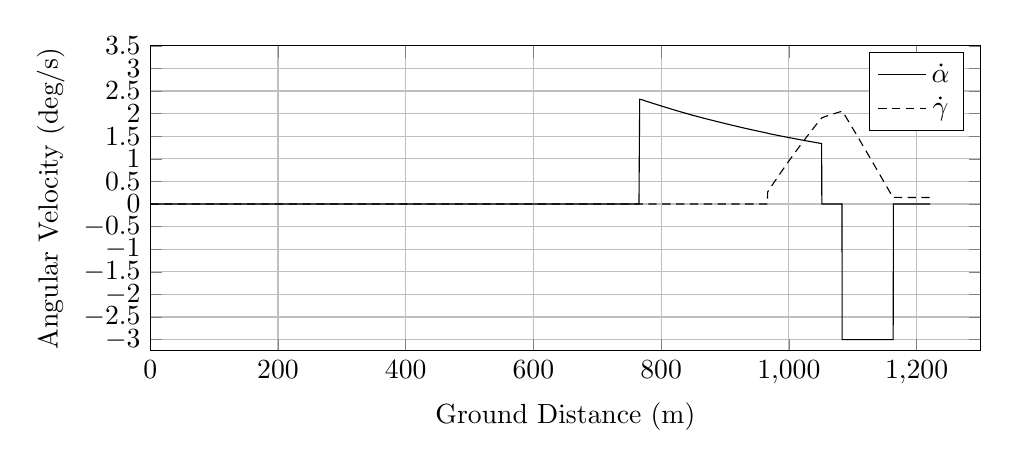
\begin{tikzpicture}

\begin{axis}[
width=\textwidth,
height=0.45\textwidth,
scaled ticks=false, tick label style={/pgf/number format/fixed},
xmin=0.0,
xmax=1300,
xlabel={Ground Distance (m)},
xmajorgrids,
ymin=-3.25,
ymax=3.5,
ylabel={Angular Velocity (deg/s)},
ytick={-3,-2.5,-2,-1.5,-1,-0.5,0,0.5,1,1.5,2,2.5,3,3.5},
ymajorgrids,
legend entries = {$\dot\alpha$\\$\dot\gamma$\\}
]

\addplot [
color=black,
solid
]
table[row sep=crcr]{
1.3729668748937997E-8	0.0\\
2.6049868369719035E-7	0.0\\
2.0491224421327626E-6	0.0\\
9.92442121137073E-6	0.0\\
4.7452367809869807E-5	0.0\\
1.740064756114434E-4	0.0\\
4.0608377013922605E-4	0.0\\
7.313431501337001E-4	0.0\\
0.0011549487327126044	0.0\\
0.0016799013484208249	0.0\\
0.002295089346817705	0.0\\
0.003009933382444524	0.0\\
0.003810608015426248	0.0\\
0.004723484476856681	0.0\\
0.005727138856912631	0.0\\
0.006836216967948795	0.0\\
0.007997302399386296	0.0\\
0.00929136979810952	0.0\\
0.010685558505459776	0.0\\
0.012178513621519987	0.0\\
0.013775244426719659	0.0\\
0.015470070176169002	0.0\\
0.0172374436815836	0.0\\
0.019122918912604377	0.0\\
0.021104911040230538	0.0\\
0.023190717999955576	0.0\\
0.025355802981115103	0.0\\
0.027620619195902148	0.0\\
0.030020274690474198	0.0\\
0.032476028269866286	0.0\\
0.035054163466719815	0.0\\
0.037720846868992755	0.0\\
0.04049779674511381	0.0\\
0.043329456594087365	0.0\\
0.04629652060163805	0.0\\
0.04934498934704602	0.0\\
0.052507657924119336	0.0\\
0.055769483710642484	0.0\\
0.05917209570914676	0.0\\
0.06264043916012321	0.0\\
0.06620063977265622	0.0\\
0.06987962792775945	0.0\\
0.0736568184539585	0.0\\
0.07754284280095361	0.0\\
0.08151127871105612	0.0\\
0.08560324933017655	0.0\\
0.08985265585263943	0.0\\
0.09413961367176535	0.0\\
0.09857725310864562	0.0\\
0.10307959255469257	0.0\\
0.10766008648593872	0.0\\
0.11234920964493048	0.0\\
0.11719267720457946	0.0\\
0.12216973960582883	0.0\\
0.12724007601918352	0.0\\
0.13233299746505212	0.0\\
0.13755256756750583	0.0\\
0.14287728588926696	0.0\\
0.1482946925752714	0.0\\
0.15381585025670613	0.0\\
0.15940564092189102	0.0\\
0.16526271495916878	0.0\\
0.17120082448158402	0.0\\
0.17717889132867753	0.0\\
0.18324322596131126	0.0\\
0.189427022360885	0.0\\
0.1957511558722988	0.0\\
0.2021484013779125	0.0\\
0.20865863707071397	0.0\\
0.21548666343168166	0.0\\
0.22220154781289658	0.0\\
0.22919671627301902	0.0\\
0.23611678795738544	0.0\\
0.24306300975244904	0.0\\
0.2503085190632165	0.0\\
0.2576623280401219	0.0\\
0.26502430524173204	0.0\\
0.2724963584449146	0.0\\
0.2802001060647876	0.0\\
0.2878583985474956	0.0\\
0.2958320780323821	0.0\\
0.3040021452321372	0.0\\
0.31208951788619	0.0\\
0.3202851396023423	0.0\\
0.3287233234973125	0.0\\
0.3370425959884752	0.0\\
0.34575405233845447	0.0\\
0.3545073625286812	0.0\\
0.36338982075299686	0.0\\
0.37247557159370037	0.0\\
0.38151350442869847	0.0\\
0.3905554764834429	0.0\\
0.3999457587520332	0.0\\
0.4095398754587949	0.0\\
0.4189621792151833	0.0\\
0.4285208811402964	0.0\\
0.43828968955472236	0.0\\
0.44807735398784176	0.0\\
0.45806002753764463	0.0\\
0.4682994371692033	0.0\\
0.4787752542918833	0.0\\
0.4890770094685154	0.0\\
0.49985939134273727	0.0\\
0.5106597490205704	0.0\\
0.5213580865152188	0.0\\
0.532247733242454	0.0\\
0.5431365108549349	0.0\\
0.554075964429489	0.0\\
0.5653450694020941	0.0\\
0.5769901159382542	0.0\\
0.588512657344902	0.0\\
0.6004070039036553	0.0\\
0.6121651247369502	0.0\\
0.6239717914322569	0.0\\
0.6362472885961421	0.0\\
0.6486428939173223	0.0\\
0.6610190736373547	0.0\\
0.6737248046101814	0.0\\
0.6862826225989949	0.0\\
0.6991952542603428	0.0\\
0.7122988072688032	0.0\\
0.7251463703465595	0.0\\
0.7381769453061875	0.0\\
0.7516618647379176	0.0\\
0.7654913705221527	0.0\\
0.7791756406994825	0.0\\
0.7930637813125616	0.0\\
0.8074774191984457	0.0\\
0.8215072375247947	0.0\\
0.8361010597475598	0.0\\
0.8503303420601955	0.0\\
0.8650627501899835	0.0\\
0.8802332960144008	0.0\\
0.8951742046771463	0.0\\
0.9100334756324657	0.0\\
0.9251067343345352	0.0\\
0.9403923630470314	0.0\\
0.9559303815501943	0.0\\
0.9712400158034169	0.0\\
0.9869533781138684	0.0\\
1.0029148609762486	0.0\\
1.0189962473881624	0.0\\
1.035465185745812	0.0\\
1.0516742337458713	0.0\\
1.067815735429615	0.0\\
1.0846705971808022	0.0\\
1.1012775250051634	0.0\\
1.1180798406225687	0.0\\
1.1351395900544134	0.0\\
1.1526388687279154	0.0\\
1.1698922447507556	0.0\\
1.1875468452119025	0.0\\
1.2058383275300355	0.0\\
1.2239395537495579	0.0\\
1.2422020624207541	0.0\\
1.2608769472440078	0.0\\
1.2794948487006894	0.0\\
1.2979152553275424	0.0\\
1.3166445915281573	0.0\\
1.3354141707340492	0.0\\
1.3543210821322504	0.0\\
1.373689361295591	0.0\\
1.3932049885015831	0.0\\
1.4131781782225183	0.0\\
1.4330139682345777	0.0\\
1.4528243860883294	0.0\\
1.4728783400745615	0.0\\
1.4934621752870565	0.0\\
1.5141408097620341	0.0\\
1.53430654450827	0.0\\
1.5553850389607948	0.0\\
1.5762653203499473	0.0\\
1.5975496774716453	0.0\\
1.6196077215345106	0.0\\
1.6413652536722467	0.0\\
1.663437310723463	0.0\\
1.6860768385032747	0.0\\
1.7077101022266827	0.0\\
1.7297306410738114	0.0\\
1.7520297891459062	0.0\\
1.7743087535215367	0.0\\
1.797257424336919	0.0\\
1.8200802473615325	0.0\\
1.8430350373473994	0.0\\
1.8666926279964304	0.0\\
1.8902808566018634	0.0\\
1.9138231309717848	0.0\\
1.937187877956735	0.0\\
1.9611060682733261	0.0\\
1.9852138445648535	0.0\\
2.009780393513653	0.0\\
2.0346228225622163	0.0\\
2.0593611988602687	0.0\\
2.08477023517836	0.0\\
2.110324766702745	0.0\\
2.1352655781940433	0.0\\
2.160528860803022	0.0\\
2.1862071157614817	0.0\\
2.2127756699400534	0.0\\
2.2391904543957084	0.0\\
2.2653528664920257	0.0\\
2.292150575495974	0.0\\
2.3187704640870406	0.0\\
2.3455495914188482	0.0\\
2.372862901366455	0.0\\
2.4007145172972395	0.0\\
2.428100404243743	0.0\\
2.4555980306928005	0.0\\
2.483374904362833	0.0\\
2.511687733451976	0.0\\
2.5402569276484597	0.0\\
2.568415369317849	0.0\\
2.596987652715761	0.0\\
2.6263861238451423	0.0\\
2.655991481965028	0.0\\
2.6856115886357443	0.0\\
2.7154221146045012	0.0\\
2.7455665152057707	0.0\\
2.7752624694325894	0.0\\
2.805457625653509	0.0\\
2.8358231840904597	0.0\\
2.8663460878589797	0.0\\
2.897817297850832	0.0\\
2.9287074004595235	0.0\\
2.9603588456990284	0.0\\
2.9922321403815406	0.0\\
3.0241119471841866	0.0\\
3.056446055158509	0.0\\
3.0889346922121366	0.0\\
3.122221620829695	0.0\\
3.1546991615623394	0.0\\
3.187635101478671	0.0\\
3.221010117202278	0.0\\
3.2543449374576605	0.0\\
3.288235920596943	0.0\\
3.3223704322934555	0.0\\
3.3562838593334394	0.0\\
3.3906320903803255	0.0\\
3.425633159699527	0.0\\
3.462387235801926	0.0\\
3.4973980805087237	0.0\\
3.5324804241140235	0.0\\
3.5675385073174235	0.0\\
3.6040688981843845	0.0\\
3.6393612181513753	0.0\\
3.6770856360342323	0.0\\
3.7131729334920323	0.0\\
3.749509707933214	0.0\\
3.785733977879824	0.0\\
3.8225309786916544	0.0\\
3.860867115351552	0.0\\
3.89929745075254	0.0\\
3.9373367205567504	0.0\\
3.9751626485832894	0.0\\
4.013671158053867	0.0\\
4.0521140617426425	0.0\\
4.092377631210638	0.0\\
4.131586743753305	0.0\\
4.1715696979561425	0.0\\
4.210522654700574	0.0\\
4.250196810863292	0.0\\
4.2917015001093795	0.0\\
4.332438976653355	0.0\\
4.373124372895289	0.0\\
4.414429464889761	0.0\\
4.455884944705147	0.0\\
4.497250153511752	0.0\\
4.537976875075978	0.0\\
4.581399817640802	0.0\\
4.623816269683994	0.0\\
4.666022338967499	0.0\\
4.709098934189642	0.0\\
4.752435367147649	0.0\\
4.79531009100786	0.0\\
4.838191999420829	0.0\\
4.881381760681686	0.0\\
4.9256451804034285	0.0\\
4.9704217340957495	0.0\\
5.014356093293278	0.0\\
5.058826350846283	0.0\\
5.104458009943745	0.0\\
5.149663211268795	0.0\\
5.194981168813841	0.0\\
5.241194091283663	0.0\\
5.287987552078626	0.0\\
5.334426822383641	0.0\\
5.380633359096258	0.0\\
5.427524438012913	0.0\\
5.476157635197664	0.0\\
5.524667120325573	0.0\\
5.5732739519824435	0.0\\
5.6208990292882195	0.0\\
5.671502816366864	0.0\\
5.719824083529298	0.0\\
5.767871110439133	0.0\\
5.8169321963676754	0.0\\
5.866076914057565	0.0\\
5.917200682776528	0.0\\
5.96684810088939	0.0\\
6.016885842403935	0.0\\
6.068639931677712	0.0\\
6.119867755785197	0.0\\
6.171030794930029	0.0\\
6.222884713227881	0.0\\
6.2735946138732235	0.0\\
6.325883502103322	0.0\\
6.379615386553551	0.0\\
6.432194972482147	0.0\\
6.484528316464761	0.0\\
6.536619297696934	0.0\\
6.589662958081361	0.0\\
6.644121795496577	0.0\\
6.697445536614451	0.0\\
6.7518063163896365	0.0\\
6.8068829439682315	0.0\\
6.863205650636274	0.0\\
6.9185329265047315	0.0\\
6.974634519184049	0.0\\
7.031139830722298	0.0\\
7.0870923879294985	0.0\\
7.144766952910487	0.0\\
7.2026451873548805	0.0\\
7.261191729679483	0.0\\
7.320502240843062	0.0\\
7.378210233177999	0.0\\
7.437738452534925	0.0\\
7.49714639104333	0.0\\
7.556502460410064	0.0\\
7.617032771987237	0.0\\
7.676883327249088	0.0\\
7.735740247984193	0.0\\
7.796086087039788	0.0\\
7.856787102853412	0.0\\
7.91721236259451	0.0\\
7.979013602666894	0.0\\
8.039824025454376	0.0\\
8.102419182184594	0.0\\
8.16459313580776	0.0\\
8.226347093952135	0.0\\
8.290527749984296	0.0\\
8.353592793320257	0.0\\
8.417564177281012	0.0\\
8.482044607535009	0.0\\
8.547336806956285	0.0\\
8.613293246319614	0.0\\
8.6778048537894	0.0\\
8.74454839911753	0.0\\
8.810708373588199	0.0\\
8.876548424968423	0.0\\
8.942828456712885	0.0\\
9.010858044488913	0.0\\
9.079453414959548	0.0\\
9.148767802603732	0.0\\
9.21609997183467	0.0\\
9.285579683381485	0.0\\
9.355451712480097	0.0\\
9.423585014597279	0.0\\
9.493435356703696	0.0\\
9.562655940911181	0.0\\
9.63183713653898	0.0\\
9.703018708836247	0.0\\
9.773178624863132	0.0\\
9.844376937811855	0.0\\
9.914998792594716	0.0\\
9.98720270419701	0.0\\
10.059478150570087	0.0\\
10.132362020358627	0.0\\
10.205876892438312	0.0\\
10.279422251887688	0.0\\
10.353305644514993	0.0\\
10.42811398108589	0.0\\
10.50332954727428	0.0\\
10.578207710262959	0.0\\
10.65503529959097	0.0\\
10.730232142651953	0.0\\
10.805871937852555	0.0\\
10.88265320376452	0.0\\
10.958577899345514	0.0\\
11.034861147941964	0.0\\
11.112742623646977	0.0\\
11.190543636431041	0.0\\
11.267787598939979	0.0\\
11.3462805052093	0.0\\
11.423875697147409	0.0\\
11.502735831556972	0.0\\
11.581465323066688	0.0\\
11.661639233340708	0.0\\
11.741743247575428	0.0\\
11.821864700430528	0.0\\
11.901816327719768	0.0\\
11.98361062800689	0.0\\
12.065425957085825	0.0\\
12.1478520915771	0.0\\
12.230956215923495	0.0\\
12.313306905825911	0.0\\
12.396632357805931	0.0\\
12.479578787946746	0.0\\
12.564327762802186	0.0\\
12.648175874147956	0.0\\
12.736145481689512	0.0\\
12.821080154398764	0.0\\
12.908009536077355	0.0\\
12.994986774303499	0.0\\
13.081752199798046	0.0\\
13.17035388279784	0.0\\
13.257836697901475	0.0\\
13.34511613365563	0.0\\
13.433461823066896	0.0\\
13.524108483575919	0.0\\
13.611203924103116	0.0\\
13.702229394080796	0.0\\
13.792427706753081	0.0\\
13.882429934062493	0.0\\
13.975435778888343	0.0\\
14.065832730112316	0.0\\
14.157894546480026	0.0\\
14.250668806951023	0.0\\
14.343291987615704	0.0\\
14.43744444968501	0.0\\
14.532636396723657	0.0\\
14.625507232812737	0.0\\
14.721503924398366	0.0\\
14.818738382089133	0.0\\
14.913572076739943	0.0\\
15.009701633366973	0.0\\
15.10815424447124	0.0\\
15.206130868840724	0.0\\
15.304035939715973	0.0\\
15.403499839366233	0.0\\
15.503209871950865	0.0\\
15.601718454553605	0.0\\
15.700655560608023	0.0\\
15.801250929860519	0.0\\
15.899917805652187	0.0\\
16.001574124100856	0.0\\
16.102638779863817	0.0\\
16.204479333764816	0.0\\
16.30489644092564	0.0\\
16.40578186591999	0.0\\
16.509201471948074	0.0\\
16.614557195984908	0.0\\
16.717657554831042	0.0\\
16.823039336622365	0.0\\
16.928576062495388	0.0\\
17.03469945574068	0.0\\
17.140697318244236	0.0\\
17.246066414787876	0.0\\
17.35183930840021	0.0\\
17.458399953804133	0.0\\
17.565707112453843	0.0\\
17.673103795073075	0.0\\
17.781888038667653	0.0\\
17.89115167195854	0.0\\
18.00105710767307	0.0\\
18.110142905530395	0.0\\
18.219697237410173	0.0\\
18.32752951944549	0.0\\
18.43743745973078	0.0\\
18.54904630654982	0.0\\
18.659302591714813	0.0\\
18.770734536087716	0.0\\
18.883577445650936	0.0\\
18.996263390583444	0.0\\
19.108816920034535	0.0\\
19.22287647779894	0.0\\
19.33763586704334	0.0\\
19.456324114791514	0.0\\
19.57349394116079	0.0\\
19.690148252848566	0.0\\
19.80521137071168	0.0\\
19.92379170801214	0.0\\
20.04216631061405	0.0\\
20.15848954929409	0.0\\
20.278242138037896	0.0\\
20.396206084226087	0.0\\
20.516315546862906	0.0\\
20.637173924977112	0.0\\
20.75450010628387	0.0\\
20.874378237858778	0.0\\
20.996035953832852	0.0\\
21.11812959618858	0.0\\
21.240471115580952	0.0\\
21.361479376438375	0.0\\
21.485224699488654	0.0\\
21.607870280890317	0.0\\
21.73242999733349	0.0\\
21.85704493170313	0.0\\
21.98122016226351	0.0\\
22.10826921766411	0.0\\
22.235261614051304	0.0\\
22.361664688868032	0.0\\
22.48780138980522	0.0\\
22.614107216476143	0.0\\
22.74409311379692	0.0\\
22.873024137794893	0.0\\
23.003512644166257	0.0\\
23.132891545907036	0.0\\
23.26270690888247	0.0\\
23.39264146728729	0.0\\
23.52277721573431	0.0\\
23.654883767164463	0.0\\
23.78569183677709	0.0\\
23.917003007077597	0.0\\
24.047013652206026	0.0\\
24.178458227988493	0.0\\
24.314609552493202	0.0\\
24.447533097503474	0.0\\
24.579128452041708	0.0\\
24.71011994849615	0.0\\
24.843278471916108	0.0\\
24.975761222328053	0.0\\
25.1115496753864	0.0\\
25.247101122854083	0.0\\
25.384906965000688	0.0\\
25.522261036073317	0.0\\
25.66123001648475	0.0\\
25.79865327455613	0.0\\
25.826335196219034	0.0\\
25.839610403727477	0.0\\
25.841006316401874	0.0\\
25.84227013303559	0.0\\
25.84770509053729	0.0\\
25.86419328224909	0.0\\
25.90571916957557	0.0\\
25.999268866927544	0.0\\
26.123295978662824	0.0\\
26.250212562581652	0.0\\
26.376891976518465	0.0\\
26.50638698165423	0.0\\
26.634042370994827	0.0\\
26.763333806613538	0.0\\
26.893207366259766	0.0\\
27.022905486492228	0.0\\
27.153956322362554	0.0\\
27.287774297957696	0.0\\
27.42030033806219	0.0\\
27.555504894698295	0.0\\
27.691130018821354	0.0\\
27.82633313037239	0.0\\
27.959508564917073	0.0\\
28.096515548835796	0.0\\
28.232789703382153	0.0\\
28.368684388406535	0.0\\
28.506541650227618	0.0\\
28.64533374691623	0.0\\
28.78297783415192	0.0\\
28.92277775692753	0.0\\
29.06227187463503	0.0\\
29.20212864139956	0.0\\
29.34335827861657	0.0\\
29.483225747293005	0.0\\
29.625960812476485	0.0\\
29.76706561118049	0.0\\
29.909402910999468	0.0\\
30.051751399473822	0.0\\
30.196612335666572	0.0\\
30.342192969749448	0.0\\
30.48583400527584	0.0\\
30.632658550781265	0.0\\
30.77846394498075	0.0\\
30.92408133049836	0.0\\
31.071091331299215	0.0\\
31.218274793935116	0.0\\
31.366705758252415	0.0\\
31.515339333797037	0.0\\
31.66356819769615	0.0\\
31.814689402684216	0.0\\
31.96649953392354	0.0\\
32.115424616034375	0.0\\
32.266253234088566	0.0\\
32.41813832080348	0.0\\
32.569791431087395	0.0\\
32.722234201183724	0.0\\
32.876984607664	0.0\\
33.031873994672836	0.0\\
33.18502245018544	0.0\\
33.34135780547538	0.0\\
33.49759920343199	0.0\\
33.65385117142162	0.0\\
33.8113313806527	0.0\\
33.96985264489639	0.0\\
34.126473036379195	0.0\\
34.2857505660089	0.0\\
34.4449212019973	0.0\\
34.60566879064274	0.0\\
34.76644486933921	0.0\\
34.92612701881755	0.0\\
35.08630421658309	0.0\\
35.24825698849928	0.0\\
35.412303951281956	0.0\\
35.57355277914179	0.0\\
35.73545353069308	0.0\\
35.89925038949356	0.0\\
36.065161289279985	0.0\\
36.23047312008262	0.0\\
36.39472205714358	0.0\\
36.56135389445764	0.0\\
36.72774532558607	0.0\\
36.89384825683493	0.0\\
37.05904296416534	0.0\\
37.22702676294645	0.0\\
37.39437475321985	0.0\\
37.5621109943643	0.0\\
37.73270471709142	0.0\\
37.903359519601935	0.0\\
38.071486842086316	0.0\\
38.23815243703595	0.0\\
38.40817787072022	0.0\\
38.57751392140098	0.0\\
38.750215798728505	0.0\\
38.92001182640311	0.0\\
39.09310637700479	0.0\\
39.26472366117933	0.0\\
39.436554723976656	0.0\\
39.608961777617054	0.0\\
39.782828308010565	0.0\\
39.956194359016465	0.0\\
40.132391837044906	0.0\\
40.30868053167249	0.0\\
40.48611580488176	0.0\\
40.66383502946924	0.0\\
40.83999042132467	0.0\\
41.018202681018664	0.0\\
41.19780999006247	0.0\\
41.37730467548502	0.0\\
41.557010452813884	0.0\\
41.73612816026986	0.0\\
41.91555194917056	0.0\\
42.09743589423803	0.0\\
42.27807550146298	0.0\\
42.45995188234755	0.0\\
42.6401410478328	0.0\\
42.822293873795985	0.0\\
43.00585672428667	0.0\\
43.189965171449515	0.0\\
43.372020236704074	0.0\\
43.555636897252796	0.0\\
43.74012033961118	0.0\\
43.92429822300048	0.0\\
44.106869824379004	0.0\\
44.29411840239129	0.0\\
44.47920670866131	0.0\\
44.665034305215386	0.0\\
44.85242224248053	0.0\\
45.03948098831597	0.0\\
45.22811764277584	0.0\\
45.41548629589063	0.0\\
45.60322541388645	0.0\\
45.793007222766036	0.0\\
45.983742663331824	0.0\\
46.172643153142886	0.0\\
46.36421599110457	0.0\\
46.553512793459404	0.0\\
46.745018895697555	0.0\\
46.93606459490553	0.0\\
47.126948089509526	0.0\\
47.31881294044018	0.0\\
47.5110690178297	0.0\\
47.705448624448266	0.0\\
47.90005519882567	0.0\\
48.09288923506665	0.0\\
48.28732881729917	0.0\\
48.484002572746206	0.0\\
48.68089030454945	0.0\\
48.87532723390382	0.0\\
49.07073736177763	0.0\\
49.2672083392297	0.0\\
49.46586249263092	0.0\\
49.661880987188695	0.0\\
49.85966148345089	0.0\\
50.05808618672894	0.0\\
50.25785665917266	0.0\\
50.45743808511885	0.0\\
50.65573800086891	0.0\\
50.85948768734909	0.0\\
51.061243703011925	0.0\\
51.26368286286315	0.0\\
51.46416466063809	0.0\\
51.66475943174029	0.0\\
51.86588207153103	0.0\\
52.07444928962187	0.0\\
52.2824430085781	0.0\\
52.48676525705545	0.0\\
52.69531994892206	0.0\\
52.90027076850366	0.0\\
53.108186167814935	0.0\\
53.31165724918766	0.0\\
53.520024946679996	0.0\\
53.72688450142306	0.0\\
53.93707391647578	0.0\\
54.14518573319289	0.0\\
54.35125853722778	0.0\\
54.56213447502874	0.0\\
54.77598621923464	0.0\\
54.987629956235494	0.0\\
55.19778857845695	0.0\\
55.41030974885841	0.0\\
55.62390503323701	0.0\\
55.83671574169797	0.0\\
56.047071254351536	0.0\\
56.26137331252919	0.0\\
56.47512769358855	0.0\\
56.69105800830218	0.0\\
56.90937011004422	0.0\\
57.12736617899088	0.0\\
57.346833156368504	0.0\\
57.56476609337061	0.0\\
57.78230894703917	0.0\\
57.99943865551505	0.0\\
58.21827465292657	0.0\\
58.436085045729726	0.0\\
58.6577546799423	0.0\\
58.87982836766625	0.0\\
59.10336118170943	0.0\\
59.324182403931715	0.0\\
59.545440661451366	0.0\\
59.768227251413464	0.0\\
59.99077485409802	0.0\\
60.21631063559073	0.0\\
60.44006004384342	0.0\\
60.66502706168687	0.0\\
60.89133011288284	0.0\\
61.11585558357916	0.0\\
61.3432655409558	0.0\\
61.57186440401435	0.0\\
61.79868765088207	0.0\\
62.025670725987	0.0\\
62.254132946411545	0.0\\
62.48290793247415	0.0\\
62.713817944074236	0.0\\
62.94484116346062	0.0\\
63.17805109236767	0.0\\
63.41124119062552	0.0\\
63.64505576847972	0.0\\
63.87735201907903	0.0\\
64.11169045660182	0.0\\
64.34725756208485	0.0\\
64.58324360279937	0.0\\
64.81881329818131	0.0\\
65.05563560606473	0.0\\
65.29467812810154	0.0\\
65.53178653633495	0.0\\
65.77046761369158	0.0\\
66.01019347650049	0.0\\
66.25262920761091	0.0\\
66.49342175078831	0.0\\
66.73393309567928	0.0\\
66.97718905970893	0.0\\
67.21919788222482	0.0\\
67.46413738735515	0.0\\
67.70584739194695	0.0\\
67.95375887035246	0.0\\
68.19817148521656	0.0\\
68.44413350233111	0.0\\
68.68984243621705	0.0\\
68.93951041285982	0.0\\
69.19023531750676	0.0\\
69.43956667494601	0.0\\
69.68998597860525	0.0\\
69.94098943220166	0.0\\
70.1928405184459	0.0\\
70.44659484061637	0.0\\
70.69926103579675	0.0\\
70.95414956377036	0.0\\
71.21136313866151	0.0\\
71.46778788208749	0.0\\
71.7247351381395	0.0\\
71.98234155897126	0.0\\
72.24107377350035	0.0\\
72.4986091150376	0.0\\
72.75949164810788	0.0\\
73.02014691132015	0.0\\
73.28114866838587	0.0\\
73.54342372888959	0.0\\
73.80584407854005	0.0\\
74.07231166191039	0.0\\
74.3389341302921	0.0\\
74.60521354141642	0.0\\
74.87280568706873	0.0\\
75.1403821105715	0.0\\
75.41145333671997	0.0\\
75.68265298797411	0.0\\
75.95075857762194	0.0\\
76.2241428819712	0.0\\
76.4990100438061	0.0\\
76.77213586328236	0.0\\
77.04724851790667	0.0\\
77.32330034006353	0.0\\
77.59850473375684	0.0\\
77.87773830129439	0.0\\
78.1565255546137	0.0\\
78.43842651648492	0.0\\
78.720833678605	0.0\\
79.00101298089581	0.0\\
79.28359351218376	0.0\\
79.57011733099088	0.0\\
79.85418914588558	0.0\\
80.13919871477489	0.0\\
80.42568449319114	0.0\\
80.71472498530085	0.0\\
81.006853148924	0.0\\
81.2951972638476	0.0\\
81.58524575795963	0.0\\
81.87461709596036	0.0\\
82.1711642895769	0.0\\
82.46716486408064	0.0\\
82.76422974563803	0.0\\
83.05801377197795	0.0\\
83.35853301954708	0.0\\
83.65664966506407	0.0\\
83.95487262936624	0.0\\
84.25322789115987	0.0\\
84.55664509033022	0.0\\
84.8599544590121	0.0\\
85.16499148084048	0.0\\
85.47187188044902	0.0\\
85.77908321853027	0.0\\
86.08675489504844	0.0\\
86.39784539041122	0.0\\
86.71051296037359	0.0\\
87.02583358957506	0.0\\
87.34037846285594	0.0\\
87.65395388450591	0.0\\
87.96687312379424	0.0\\
88.28527441497255	0.0\\
88.6103524516937	0.0\\
88.92871226770333	0.0\\
89.25003295857354	0.0\\
89.57522243846881	0.0\\
89.90247582737899	0.0\\
90.22602529632545	0.0\\
90.5494223037065	0.0\\
90.87816525326718	0.0\\
91.20455861430293	0.0\\
91.53817773235312	0.0\\
91.87076195087604	0.0\\
92.20124984301029	0.0\\
92.53140503523474	0.0\\
92.86389705561814	0.0\\
93.19815266874983	0.0\\
93.53304529783748	0.0\\
93.86737084100128	0.0\\
94.20337949361911	0.0\\
94.54065981474497	0.0\\
94.87396787418089	0.0\\
95.21684847579547	0.0\\
95.55392648231228	0.0\\
95.89232371872416	0.0\\
96.23051075783204	0.0\\
96.57164052232307	0.0\\
96.90762523479154	0.0\\
97.24755293575913	0.0\\
97.58790661409188	0.0\\
97.92576087813703	0.0\\
98.26661027452474	0.0\\
98.6051908024865	0.0\\
98.94563962387357	0.0\\
99.28665364663627	0.0\\
99.63350087797645	0.0\\
99.97685593767679	0.0\\
100.31593955776762	0.0\\
100.65572384630482	0.0\\
100.99616871909686	0.0\\
101.3402339503516	0.0\\
101.67973054404297	0.0\\
102.01657591573795	0.0\\
102.35656456518868	0.0\\
102.6941824316649	0.0\\
103.03547296258705	0.0\\
103.37623032340073	0.0\\
103.71852978299776	0.0\\
104.05851119314701	0.0\\
104.3949509202441	0.0\\
104.7329053851843	0.0\\
105.07104272194636	0.0\\
105.40742307340048	0.0\\
105.74423560014887	0.0\\
106.07955743077031	0.0\\
106.41623710643992	0.0\\
106.75618472497374	0.0\\
107.0942647435474	0.0\\
107.43151869252583	0.0\\
107.44650965670576	0.0\\
107.45815118347005	0.0\\
107.46233674961977	0.0\\
107.46535588765028	0.0\\
107.46808502617694	0.0\\
107.4836206108138	0.0\\
107.53176708907421	0.0\\
107.68672244793561	0.0\\
107.97570433527497	0.0\\
108.27744765146667	0.0\\
108.5816623935838	0.0\\
108.88557241638279	0.0\\
109.19209959959528	0.0\\
109.50241879336687	0.0\\
109.81066605766154	0.0\\
110.12101503747155	0.0\\
110.43285681965125	0.0\\
110.74725799716322	0.0\\
111.06462449033057	0.0\\
111.38211128519615	0.0\\
111.70119562731901	0.0\\
112.02298633508096	0.0\\
112.34320819983824	0.0\\
112.66812620709393	0.0\\
112.99302416686388	0.0\\
113.31966045518399	0.0\\
113.64998129974768	0.0\\
113.97857627498675	0.0\\
114.31304608469316	0.0\\
114.64448318111735	0.0\\
114.98093514978115	0.0\\
115.31969924418831	0.0\\
115.65790718621022	0.0\\
116.00063352526521	0.0\\
116.34235083463872	0.0\\
116.68621873349733	0.0\\
117.03331062078092	0.0\\
117.37910048629482	0.0\\
117.72869476105836	0.0\\
118.08005947084649	0.0\\
118.43363644355449	0.0\\
118.79186464668504	0.0\\
119.14769212941735	0.0\\
119.5036618261702	0.0\\
119.86270697471275	0.0\\
120.22616362054572	0.0\\
120.58991121293201	0.0\\
120.95538130513773	0.0\\
121.3195355377388	0.0\\
121.68590041554987	0.0\\
122.05305648207542	0.0\\
122.42257239354896	0.0\\
122.79503144936103	0.0\\
123.16629137010841	0.0\\
123.53950748252527	0.0\\
123.91239367862553	0.0\\
124.29026003316017	0.0\\
124.66301933937496	0.0\\
125.03890311735066	0.0\\
125.41380975776434	0.0\\
125.7896808967325	0.0\\
126.16837244152023	0.0\\
126.54595968852882	0.0\\
126.92471834906405	0.0\\
127.30294276405039	0.0\\
127.68255852126984	0.0\\
128.06243727540487	0.0\\
128.44360431740483	0.0\\
128.82265748788262	0.0\\
129.1989690567886	0.0\\
129.57765386613931	0.0\\
129.95508099647026	0.0\\
130.33359114840187	0.0\\
130.71373745886524	0.0\\
131.09453904397424	0.0\\
131.47657586018488	0.0\\
131.85678563989967	0.0\\
132.23856625352113	0.0\\
132.61595336405918	0.0\\
132.99976263915818	0.0\\
133.38083522978053	0.0\\
133.76098428781995	0.0\\
134.1363519425165	0.0\\
134.51557915495124	0.0\\
134.8968696170101	0.0\\
135.27419431482667	0.0\\
135.65215477207505	0.0\\
136.03329358991255	0.0\\
136.41192880753374	0.0\\
136.7898079310749	0.0\\
137.17001317148595	0.0\\
137.54844558779996	0.0\\
137.92617219433072	0.0\\
138.30476964659732	0.0\\
138.68390038934075	0.0\\
139.0631653430654	0.0\\
139.4406106933401	0.0\\
139.81914660512416	0.0\\
140.19767098864742	0.0\\
140.5730919292459	0.0\\
140.95061983253072	0.0\\
141.32838502869612	0.0\\
141.70636515873298	0.0\\
142.0839785067887	0.0\\
142.46357402350594	0.0\\
142.84082211769783	0.0\\
143.21906727224075	0.0\\
143.59963619096823	0.0\\
143.97984478872678	0.0\\
144.35941603837455	0.0\\
144.7355521893594	0.0\\
145.11296635073694	0.0\\
145.49073213867456	0.0\\
145.87033631970945	0.0\\
146.24486520181193	0.0\\
146.6238757206513	0.0\\
147.00096360401335	0.0\\
147.37874202190085	0.0\\
147.756852900845	0.0\\
148.13572640408995	0.0\\
148.5136798644104	0.0\\
148.89083780486442	0.0\\
149.2712459042852	0.0\\
149.65303236723025	0.0\\
150.0329584616291	0.0\\
150.41363382646614	0.0\\
150.79322940570728	0.0\\
151.17272478467066	0.0\\
151.55400296227282	0.0\\
151.93482601265913	0.0\\
152.31881414221942	0.0\\
152.70208150063132	0.0\\
153.08320649997165	0.0\\
153.4666285558243	0.0\\
153.84825937276264	0.0\\
154.23093781718723	0.0\\
154.61485031834388	0.0\\
155.00001234931443	0.0\\
155.38285725409855	0.0\\
155.7679513537659	0.0\\
156.1509667875323	0.0\\
156.53491934392343	0.0\\
156.91995289130983	0.0\\
157.30625057946366	0.0\\
157.69121706207227	0.0\\
158.07789765133754	0.0\\
158.46521012398495	0.0\\
158.85138765236047	0.0\\
159.23964669847322	0.0\\
159.62715395386465	0.0\\
160.01960115328984	0.0\\
160.4079207075476	0.0\\
160.79602490671402	0.0\\
161.18437278725975	0.0\\
161.57644284003254	0.0\\
161.96812230097612	0.0\\
162.35808768568592	0.0\\
162.75087300343483	0.0\\
163.14546270495134	0.0\\
163.53745675514648	0.0\\
163.92955389373896	0.0\\
164.32395276810763	0.0\\
164.71713266653478	0.0\\
165.1102153740033	0.0\\
165.5035884424101	0.0\\
165.89816400198282	0.0\\
166.29148626774366	0.0\\
166.68861804276264	0.0\\
167.082852347146	0.0\\
167.48006204110857	0.0\\
167.8798182678497	0.0\\
168.27774435731556	0.0\\
168.67741362640317	0.0\\
169.07475368467374	0.0\\
169.4759958044982	0.0\\
169.87832784425882	0.0\\
170.2792240364854	0.0\\
170.68126852540456	0.0\\
171.08617821288442	0.0\\
171.48766933901368	0.0\\
171.892744970828	0.0\\
172.29711201372032	0.0\\
172.70264003426053	0.0\\
173.1105289448074	0.0\\
173.5163733808056	0.0\\
173.92577914808027	0.0\\
174.33607303977334	0.0\\
174.74614233406845	0.0\\
175.15731444736514	0.0\\
175.56901623635082	0.0\\
175.97955109701695	0.0\\
176.39275298155184	0.0\\
176.80397138375372	0.0\\
177.21946344336607	0.0\\
177.6332252263685	0.0\\
178.05102033212842	0.0\\
178.46725124888752	0.0\\
178.88389799206544	0.0\\
179.29839533747668	0.0\\
179.71608569665375	0.0\\
180.1342696339205	0.0\\
180.5538779958007	0.0\\
180.97690569555635	0.0\\
181.39980810354632	0.0\\
181.82328311928882	0.0\\
182.24618807605736	0.0\\
182.6731660166833	0.0\\
183.10035828358116	0.0\\
183.5291445538124	0.0\\
183.95833265232255	0.0\\
184.38634616388282	0.0\\
184.8168339376561	0.0\\
185.24630581702252	0.0\\
185.67754767955432	0.0\\
186.109185775987	0.0\\
186.53971883241212	0.0\\
186.97132952004227	0.0\\
187.40711553434954	0.0\\
187.84220985117162	0.0\\
188.27778926256264	0.0\\
188.71822733349944	0.0\\
189.16086434237673	0.0\\
189.6010380968554	0.0\\
190.03919041211265	0.0\\
190.48016062316526	0.0\\
190.92524363955386	0.0\\
191.372330984798	0.0\\
191.81766281185656	0.0\\
192.2649588892154	0.0\\
192.7152080571317	0.0\\
193.16529614382966	0.0\\
193.61551258619323	0.0\\
194.0671041699889	0.0\\
194.52074606224477	0.0\\
194.9783774267325	0.0\\
195.4358245305881	0.0\\
195.89499401276925	0.0\\
196.35432087192027	0.0\\
196.81831699949333	0.0\\
197.28093205423113	0.0\\
197.74513845889334	0.0\\
198.21238653581378	0.0\\
198.6780372695403	0.0\\
199.14562244096538	0.0\\
199.6172630308758	0.0\\
200.085680559985	0.0\\
200.55485539631252	0.0\\
201.0284003638297	0.0\\
201.5010163224531	0.0\\
201.97949934275624	0.0\\
202.45676989461947	0.0\\
202.93795341995116	0.0\\
203.42151825635358	0.0\\
203.9064451985618	0.0\\
204.39376498892221	0.0\\
204.88144002832018	0.0\\
205.3743097859811	0.0\\
205.86751126322014	0.0\\
206.36222180198536	0.0\\
206.85620764580733	0.0\\
207.35622660722595	0.0\\
207.85286701515986	0.0\\
208.35554496397685	0.0\\
208.85949164962352	0.0\\
209.3606904933826	0.0\\
209.86430174661194	0.0\\
210.37517113261447	0.0\\
210.88826309775862	0.0\\
211.408532759536	0.0\\
211.9275242572583	0.0\\
212.45034341379437	0.0\\
212.97278109853062	0.0\\
213.5012611434281	0.0\\
214.0307698600809	0.0\\
214.55632530210835	0.0\\
215.09027271075985	0.0\\
215.62992362610385	0.0\\
216.17218538865313	0.0\\
216.71273903148006	0.0\\
217.25354139798316	0.0\\
217.7992146693805	0.0\\
218.34754045136725	0.0\\
218.89661223248612	0.0\\
219.45761572436965	0.0\\
220.01811384548756	0.0\\
220.5796054147944	0.0\\
221.1491613381006	0.0\\
221.72392285119702	0.0\\
222.29674345543788	0.0\\
222.87200016908895	0.0\\
223.45476781204167	0.0\\
224.04346163614804	0.0\\
224.62738211659592	0.0\\
225.21466034383656	0.0\\
225.80901970025303	0.0\\
226.4067565685998	0.0\\
227.010346212326	0.0\\
227.62015690700883	0.0\\
228.23221085371028	0.0\\
228.84135848872813	0.0\\
229.46020606246555	0.0\\
230.08791152904655	0.0\\
230.71342291791404	0.0\\
231.3402722001092	0.0\\
231.96207175272258	0.0\\
232.5840768980429	0.0\\
233.21041275014744	0.0\\
233.84076499381075	0.0\\
234.4632722369638	0.0\\
235.0951321894368	0.0\\
235.7164683430417	0.0\\
236.33637872225546	0.0\\
236.95807015301216	0.0\\
237.57724458338066	0.0\\
238.1954544769302	0.0\\
238.81057478854058	0.0\\
239.4264917144386	0.0\\
240.0366097511752	0.0\\
240.63918371105967	0.0\\
241.24161561476188	0.0\\
241.8433627512665	0.0\\
242.44272012201816	0.0\\
243.03744426405035	0.0\\
243.6307298234035	0.0\\
244.22108413951537	0.0\\
244.8116939475828	0.0\\
245.39744552343484	0.0\\
245.97855029096053	0.0\\
246.5589096408665	0.0\\
247.13041662269836	0.0\\
247.70663564674516	0.0\\
248.28024698100222	0.0\\
248.85288765982074	0.0\\
249.4193334510956	0.0\\
249.9777393310295	0.0\\
250.54131855768964	0.0\\
251.10095479045611	0.0\\
251.65640742239583	0.0\\
252.20851363475686	0.0\\
252.76218077146297	0.0\\
253.31371341967355	0.0\\
253.86551898536345	0.0\\
254.41422830739316	0.0\\
254.9572061395861	0.0\\
255.0653176818724	0.0\\
255.12993325322566	0.0\\
255.17825500251217	0.0\\
255.20626764895485	0.0\\
255.2307799315319	0.0\\
255.25350681352313	0.0\\
255.27636741461964	0.0\\
255.2901025823965	0.0\\
255.29493524708477	0.0\\
255.30041476425401	0.0\\
255.32542424174517	0.0\\
255.431840924477	0.0\\
255.72188923316247	0.0\\
256.19571599032633	0.0\\
256.67415123408614	0.0\\
257.15505540016306	0.0\\
257.6368423781066	0.0\\
258.1230512066297	0.0\\
258.61423458459376	0.0\\
259.1049940935744	0.0\\
259.5982522152891	0.0\\
260.09486806301686	0.0\\
260.5959555145432	0.0\\
261.1023053698689	0.0\\
261.6089919954627	0.0\\
262.11906753970584	0.0\\
262.63243815947874	0.0\\
263.14830217600297	0.0\\
263.66676080693014	0.0\\
264.1877265034735	0.0\\
264.7128105393116	0.0\\
265.241218472901	0.0\\
265.7723922912836	0.0\\
266.3079016945154	0.0\\
266.8503273810571	0.0\\
267.3932272617866	0.0\\
267.9365984091472	0.0\\
268.4918097049034	0.0\\
269.04807221243857	0.0\\
269.6097925731924	0.0\\
270.17242368341533	0.0\\
270.7441513704771	0.0\\
271.31667319188057	0.0\\
271.8922835348494	0.0\\
272.47925332376417	0.0\\
273.06804504353704	0.0\\
273.66076346861166	0.0\\
274.25294696226547	0.0\\
274.85204953299706	0.0\\
275.4590719216128	0.0\\
276.0685465790958	0.0\\
276.6808474128411	0.0\\
277.29680014730513	0.0\\
277.9224067517041	0.0\\
278.5505103374435	0.0\\
279.17831818166474	0.0\\
279.81790886718375	0.0\\
280.45539954927676	0.0\\
281.0966396233664	0.0\\
281.73735617862894	0.0\\
282.38112941523184	0.0\\
283.0301801354616	0.0\\
283.67721705328654	0.0\\
284.3202688103162	0.0\\
284.9599564878264	0.0\\
285.60213884169843	0.0\\
286.24205728342235	0.0\\
286.8783426797421	0.0\\
287.5176726031193	0.0\\
288.14959414660166	0.0\\
288.7790218355949	0.0\\
289.41060269245395	0.0\\
290.0373602432952	0.0\\
290.6616399781276	0.0\\
291.28528823747513	0.0\\
291.90747044142563	0.0\\
292.5232553861292	0.0\\
293.13767407877424	0.0\\
293.74977203443143	0.0\\
294.36691018627903	0.0\\
294.97422257673236	0.0\\
295.5803242078987	0.0\\
296.18876641420377	0.0\\
296.79141324013847	0.0\\
297.39276567122147	0.0\\
297.9894421920609	0.0\\
298.5870928977196	0.0\\
299.1813773675972	0.0\\
299.77152323390305	0.0\\
300.36612301275215	0.0\\
300.9589816797394	0.0\\
301.5517369040423	0.0\\
302.13995783060716	0.0\\
302.7265461416931	0.0\\
303.31195316833305	0.0\\
303.893632985354	0.0\\
304.47837522976045	0.0\\
305.0603224805632	0.0\\
305.6386476191806	0.0\\
306.2164211941447	0.0\\
306.79567265335925	0.0\\
307.37231001650287	0.0\\
307.9484900815751	0.0\\
308.52614124860884	0.0\\
309.10133925078446	0.0\\
309.6811704644614	0.0\\
310.25396666777317	0.0\\
310.82665929650705	0.0\\
311.40151685857484	0.0\\
311.97010244433034	0.0\\
312.53980750632184	0.0\\
313.10901660628747	0.0\\
313.67956238189845	0.0\\
314.2496933076443	0.0\\
314.8205968353319	0.0\\
315.3893122304361	0.0\\
315.9596108977621	0.0\\
316.52927325433984	0.0\\
317.0962218845675	0.0\\
317.661512728229	0.0\\
318.22894706387933	0.0\\
318.7945230010092	0.0\\
319.36250947901885	0.0\\
319.92950718778627	0.0\\
320.4959663753667	0.0\\
321.0631721024022	0.0\\
321.6290870613959	0.0\\
322.19457963905666	0.0\\
322.7618354565293	0.0\\
323.32829381843464	0.0\\
323.8944812959513	0.0\\
324.4599775338005	0.0\\
325.0236279833782	0.0\\
325.5930851369128	0.0\\
326.1571709254106	0.0\\
326.723741026211	0.0\\
327.28922394543645	0.0\\
327.8556983549987	0.0\\
328.4233330667528	0.0\\
328.9893491077544	0.0\\
329.5546671193348	0.0\\
330.1217964733877	0.0\\
330.68704439501266	0.0\\
331.2526219304833	0.0\\
331.8212338226615	0.0\\
332.38563215932834	0.0\\
332.9540373692553	0.0\\
333.52282575474305	0.0\\
334.0901133197508	0.0\\
334.6587212753741	0.0\\
335.22495173293544	0.0\\
335.79508811264384	0.0\\
336.36651436910597	0.0\\
336.93496842282195	0.0\\
337.5050159421993	0.0\\
338.07625180159437	0.0\\
338.64522733550257	0.0\\
339.21307292972244	0.0\\
339.78316525663524	0.0\\
340.3517359250782	0.0\\
340.92344762446896	0.0\\
341.49725999120506	0.0\\
342.0714758249467	0.0\\
342.6432180289123	0.0\\
343.2156727962654	0.0\\
343.788423593423	0.0\\
344.3632558179478	0.0\\
344.936112850713	0.0\\
345.5122282286983	0.0\\
346.0894236551619	0.0\\
346.6629357201275	0.0\\
347.2399030750438	0.0\\
347.8149786266573	0.0\\
348.3916437826483	0.0\\
348.96682599762005	0.0\\
349.5439461813521	0.0\\
350.1219821225792	0.0\\
350.70068616715105	0.0\\
351.28126445021985	0.0\\
351.8619451172309	0.0\\
352.4432281971418	0.0\\
353.0222568578364	0.0\\
353.6045019024799	0.0\\
354.18853493609936	0.0\\
354.7725020489422	0.0\\
355.3555439607444	0.0\\
355.94178228996793	0.0\\
356.52841816113096	0.0\\
357.11491695053746	0.0\\
357.7019804757698	0.0\\
358.2889970677636	0.0\\
358.8795343682166	0.0\\
359.47011391270996	0.0\\
360.0611888887985	0.0\\
360.65551621456757	0.0\\
361.24837490254504	0.0\\
361.8399267049888	0.0\\
362.43366065279633	0.0\\
363.0271841323796	0.0\\
363.62092175430814	0.0\\
364.2172388023977	0.0\\
364.8170682790411	0.0\\
365.4168935103936	0.0\\
366.0167447450068	0.0\\
366.613361119081	0.0\\
367.21449807554484	0.0\\
367.81411987634317	0.0\\
368.41428222027616	0.0\\
369.0136835421291	0.0\\
369.6184705538477	0.0\\
370.2203314850517	0.0\\
370.8292817941207	0.0\\
371.4325891230952	0.0\\
372.03751184905457	0.0\\
372.64963462678804	0.0\\
373.26236447571455	0.0\\
373.87329119709466	0.0\\
374.48540637090855	0.0\\
375.0984288907292	0.0\\
375.71389401660815	0.0\\
376.3292711349669	0.0\\
376.94717931076855	0.0\\
377.56118057518813	0.0\\
378.18357875745255	0.0\\
378.80534455721454	0.0\\
379.42657984220546	0.0\\
380.05059226965216	0.0\\
380.67279643790334	0.0\\
381.29916382387717	0.0\\
381.92611637580137	0.0\\
382.55700718237256	0.0\\
383.1838285741163	0.0\\
383.815522641495	0.0\\
384.4482555994399	0.0\\
385.0798113246169	0.0\\
385.7142011583089	0.0\\
386.35011647349825	0.0\\
386.98806446889137	0.0\\
387.62777316145673	0.0\\
388.2677779567189	0.0\\
388.9088955203763	0.0\\
389.5502219824099	0.0\\
390.196085141905	0.0\\
390.8411912635918	0.0\\
391.4850258768763	0.0\\
392.1348161747717	0.0\\
392.78657703059184	0.0\\
393.43829425062995	0.0\\
394.0914803145356	0.0\\
394.74697534702034	0.0\\
395.4022052560256	0.0\\
396.0614826489191	0.0\\
396.7253027860521	0.0\\
397.389470201156	0.0\\
398.0561080310739	0.0\\
398.7226685692724	0.0\\
399.391462726883	0.0\\
400.06069563032156	0.0\\
400.7298361745127	0.0\\
401.4030004748297	0.0\\
402.07673432903437	0.0\\
402.7516637315023	0.0\\
403.43308814587397	0.0\\
404.11621884098975	0.0\\
404.8017412836191	0.0\\
405.4859375776791	0.0\\
406.17916116612776	0.0\\
406.869828889608	0.0\\
407.5646978623407	0.0\\
408.2605209917057	0.0\\
408.95953036015305	0.0\\
409.6622694433204	0.0\\
410.36575705355096	0.0\\
411.07335289700484	0.0\\
411.7824393477108	0.0\\
412.49368167220496	0.0\\
413.20637839560925	0.0\\
413.9231120861825	0.0\\
414.64148448951505	0.0\\
415.3640873105958	0.0\\
416.08758784728207	0.0\\
416.8163237339112	0.0\\
417.54818649211745	0.0\\
418.2830458128634	0.0\\
419.0197896011267	0.0\\
419.7618468752946	0.0\\
420.50810315351544	0.0\\
421.2538226142991	0.0\\
422.0024472585525	0.0\\
422.7601619190325	0.0\\
423.51827295501266	0.0\\
424.2791336478392	0.0\\
425.04862066884436	0.0\\
425.8175931526831	0.0\\
426.59484428165274	0.0\\
427.37319167714656	0.0\\
428.1560603980529	0.0\\
428.9441065434968	0.0\\
429.73908511318723	0.0\\
430.5390808738871	0.0\\
431.34695313464147	0.0\\
432.16146945503726	0.0\\
432.97716762270886	0.0\\
433.79906034498686	0.0\\
434.63237437495366	0.0\\
435.4690406415772	0.0\\
436.31317920434697	0.0\\
437.1637869835322	0.0\\
438.01645953609784	0.0\\
438.8814827966934	0.0\\
439.7524258551747	0.0\\
440.63826385029256	0.0\\
441.53868068573615	0.0\\
442.4384272900428	0.0\\
443.3504012304777	0.0\\
444.27758818218365	0.0\\
445.208223124445	0.0\\
446.1516186171384	0.0\\
447.10189524137195	0.0\\
448.06481468075106	0.0\\
449.03617443090013	0.0\\
450.02512103574475	0.0\\
451.0169824202726	0.0\\
452.020591047557	0.0\\
453.02360262247294	0.0\\
454.0275908503903	0.0\\
455.03100385233165	0.0\\
456.0319820328356	0.0\\
457.02914229222506	0.0\\
458.01937985050745	0.0\\
458.99771244571184	0.0\\
459.96197275276677	0.0\\
460.92139296690334	0.0\\
461.8616145847351	0.0\\
462.80206306639445	0.0\\
463.7284486681126	0.0\\
464.6393852721259	0.0\\
465.54063936700334	0.0\\
466.4349184101709	0.0\\
467.3198901301686	0.0\\
468.20051759019884	0.0\\
469.07226485074943	0.0\\
469.9345383529743	0.0\\
470.7902899889468	0.0\\
471.6423737744856	0.0\\
472.4877853124267	0.0\\
473.3248054273006	0.0\\
474.15679752822916	0.0\\
474.98717382477696	0.0\\
475.812191509144	0.0\\
476.6363066147294	0.0\\
477.44928852471696	0.0\\
478.25976263885	0.0\\
479.0680268264706	0.0\\
479.8720193908648	0.0\\
480.6722055908582	0.0\\
481.4638282544993	0.0\\
482.2537496794823	0.0\\
483.0439784328089	0.0\\
483.8253492021597	0.0\\
484.60475037766423	0.0\\
485.38148111107205	0.0\\
486.15453177945005	0.0\\
486.9234848636379	0.0\\
487.6911837486889	0.0\\
488.4532446281222	0.0\\
489.2141943862101	0.0\\
489.3656654782709	0.0\\
489.9141839228952	0.0\\
489.9442198041063	0.0\\
489.95165340794586	0.0\\
489.95904841065203	0.0\\
490.0087656528135	0.0\\
490.2229205115475	0.0\\
490.80762926712646	0.0\\
491.5549224672211	0.0\\
492.3059760305267	0.0\\
493.05617311245896	0.0\\
493.8124400481423	0.0\\
494.57147098753774	0.0\\
495.33883357988543	0.0\\
496.10451558660077	0.0\\
496.8763216977479	0.0\\
497.6516028092092	0.0\\
498.43581565351974	0.0\\
499.22198438592227	0.0\\
500.0155369982069	0.0\\
500.8167457948026	0.0\\
501.6207857715186	0.0\\
502.43135952459795	0.0\\
503.2488031894138	0.0\\
504.06841756255267	0.0\\
504.89158107370974	0.0\\
505.72576854379577	0.0\\
506.5693448613787	0.0\\
507.4142887558387	0.0\\
508.26842244805994	0.0\\
509.12668782716764	0.0\\
509.9922807952486	0.0\\
510.86952952987826	0.0\\
511.75603474468153	0.0\\
512.6525773610188	0.0\\
513.552913573209	0.0\\
514.4681532282782	0.0\\
515.3867354533588	0.0\\
516.3174024261396	0.0\\
517.2602458293647	0.0\\
518.213136886093	0.0\\
519.1760409577637	0.0\\
520.1413511846506	0.0\\
521.1231004572105	0.0\\
522.1209096033688	0.0\\
523.1261067826763	0.0\\
524.1419417493194	0.0\\
525.1629084556621	0.0\\
526.1966720787225	0.0\\
527.232798559631	0.0\\
528.2697748535691	0.0\\
529.3125778912245	0.0\\
530.3569535995234	0.0\\
531.3923454146075	0.0\\
532.4241640074417	0.0\\
533.4600085213303	0.0\\
534.4866261256011	0.0\\
535.5020315541947	0.0\\
536.514508151736	0.0\\
537.5229382799621	0.0\\
538.5160648880578	0.0\\
539.5082343221115	0.0\\
540.4856117025593	0.0\\
541.4663647652112	0.0\\
542.4363165308484	0.0\\
543.403649598117	0.0\\
544.3586522503113	0.0\\
545.3070641243951	0.0\\
546.2506879020282	0.0\\
547.1923729139526	0.0\\
548.1284847870645	0.0\\
549.0607273863563	0.0\\
549.9918578398997	0.0\\
550.9129328290753	0.0\\
551.8320704888101	0.0\\
552.7431023110901	0.0\\
553.6513866954954	0.0\\
554.5567691623032	0.0\\
555.4601447965442	0.0\\
556.3560324901239	0.0\\
557.2510525453768	0.0\\
558.144367784238	0.0\\
559.0395040047595	0.0\\
559.9306875601039	0.0\\
560.8184287789293	0.0\\
561.6957839109712	0.0\\
562.5803647812363	0.0\\
563.4612104685039	0.0\\
564.3388911147272	0.0\\
565.215385530312	0.0\\
566.0886502219232	0.0\\
566.9616941548127	0.0\\
567.8301900811412	0.0\\
568.6977679531799	0.0\\
569.5620388889783	0.0\\
570.424462708284	0.0\\
571.2852292099337	0.0\\
572.1493328191241	0.0\\
573.0103554048726	0.0\\
573.8681094542301	0.0\\
574.7257926178972	0.0\\
575.584494453004	0.0\\
576.4392320762051	0.0\\
577.2895741354355	0.0\\
578.1440860684359	0.0\\
578.9955408132021	0.0\\
579.8488294812946	0.0\\
580.7009485845795	0.0\\
581.5481034887393	0.0\\
582.398203180056	0.0\\
583.2436286861621	0.0\\
584.0951419205564	0.0\\
584.9447588199325	0.0\\
585.7909961721582	0.0\\
586.6394553558484	0.0\\
587.4827778011024	0.0\\
588.3280079409788	0.0\\
589.1732196696316	0.0\\
590.0172358784723	0.0\\
590.860913103985	0.0\\
591.7056349988741	0.0\\
592.5455796206825	0.0\\
593.390591992995	0.0\\
594.23254291524	0.0\\
595.0749775640184	0.0\\
595.9164343501545	0.0\\
596.757445184641	0.0\\
597.6003409863617	0.0\\
598.4426744019354	0.0\\
599.2847755368687	0.0\\
600.125707245069	0.0\\
600.9666449061319	0.0\\
601.808765536209	0.0\\
602.6493496090866	0.0\\
603.4896653766809	0.0\\
604.3324540913729	0.0\\
605.1749627368547	0.0\\
606.0172193894603	0.0\\
606.8564954876942	0.0\\
607.6995822420379	0.0\\
608.5468271351888	0.0\\
609.3853237539292	0.0\\
610.2285785394622	0.0\\
611.0723962320026	0.0\\
611.9144944458772	0.0\\
612.7572705739071	0.0\\
613.6039342512895	0.0\\
614.447700557992	0.0\\
615.2875150228297	0.0\\
616.1283989744954	0.0\\
616.9715554180159	0.0\\
617.816851506552	0.0\\
618.6627080307358	0.0\\
619.5079936234229	0.0\\
620.355287072993	0.0\\
621.2019793580857	0.0\\
622.0488535053607	0.0\\
622.9008554858297	0.0\\
623.7470330382666	0.0\\
624.5970610944692	0.0\\
625.4445858106351	0.0\\
626.2949117084559	0.0\\
627.1456369954528	0.0\\
627.996202785663	0.0\\
628.8493276316594	0.0\\
629.7040179726459	0.0\\
630.5541510983869	0.0\\
631.4094242395336	0.0\\
632.2635827644049	0.0\\
633.1201141992324	0.0\\
633.9783198620232	0.0\\
634.8358449994842	0.0\\
635.6949254776987	0.0\\
636.5510277660717	0.0\\
637.4106283702604	0.0\\
638.26983515646	0.0\\
639.1281653037297	0.0\\
639.9892853909298	0.0\\
640.854752101091	0.0\\
641.7172955483825	0.0\\
642.5803911560504	0.0\\
643.4447648773507	0.0\\
644.3076201978465	0.0\\
645.1745276724305	0.0\\
646.0402102676721	0.0\\
646.9124608338768	0.0\\
647.7810225029502	0.0\\
648.6561125051048	0.0\\
649.5284291267524	0.0\\
650.3990692560633	0.0\\
651.2710362166958	0.0\\
652.1464633126748	0.0\\
653.0220683418463	0.0\\
653.8956541670141	0.0\\
654.7728777786044	0.0\\
655.6515481039796	0.0\\
656.5284362953553	0.0\\
657.4113325495778	0.0\\
658.2915193229558	0.0\\
659.17716463588	0.0\\
660.0651577261099	0.0\\
660.9536046953733	0.0\\
661.8402168340383	0.0\\
662.7324470689205	0.0\\
663.6200112954277	0.0\\
664.5127656227664	0.0\\
665.4027074409514	0.0\\
666.2965782601134	0.0\\
667.1908896376651	0.0\\
668.084320193617	0.0\\
668.985123002554	0.0\\
669.8863392680419	0.0\\
670.7862926077596	0.0\\
671.6898074618846	0.0\\
672.5888268774506	0.0\\
673.4982782765783	0.0\\
674.4103925687491	0.0\\
675.3150941849995	0.0\\
676.2268158638515	0.0\\
677.1406213981061	0.0\\
678.0557411892244	0.0\\
678.9688521555179	0.0\\
679.8873390970205	0.0\\
680.8083547814929	0.0\\
681.7306997118981	0.0\\
682.6500311248872	0.0\\
683.5737488494256	0.0\\
684.4960352365924	0.0\\
685.4200123844039	0.0\\
686.3479632552264	0.0\\
687.2766127474456	0.0\\
688.2061621748603	0.0\\
689.1404800584801	0.0\\
690.0764761874757	0.0\\
691.0152339372712	0.0\\
691.9552419239503	0.0\\
692.8950394637291	0.0\\
693.8400111678282	0.0\\
694.7866818158914	0.0\\
695.7347004483931	0.0\\
696.6882574887352	0.0\\
697.6393666566034	0.0\\
698.5984440154043	0.0\\
699.5498840703472	0.0\\
700.5039755495234	0.0\\
701.4647289348814	0.0\\
702.4256797045559	0.0\\
703.3874603974716	0.0\\
704.3606354781252	0.0\\
705.3315887422941	0.0\\
706.3004122670179	0.0\\
707.2768098841743	0.0\\
708.2494358269255	0.0\\
709.2282890376241	0.0\\
710.2089151733701	0.0\\
711.1951755925729	0.0\\
712.1865307336975	0.0\\
713.1761747054959	0.0\\
714.1673399979175	0.0\\
715.1598728842257	0.0\\
716.1583282218428	0.0\\
717.1629472660959	0.0\\
718.1700311785478	0.0\\
719.1763338932042	0.0\\
720.1876907614742	0.0\\
721.201618282845	0.0\\
722.2184418537404	0.0\\
723.235170191942	0.0\\
724.2594935927766	0.0\\
725.2822718646494	0.0\\
726.3107341130526	0.0\\
727.3400446617545	0.0\\
728.3719103403353	0.0\\
729.4113327961686	0.0\\
730.4562931126598	0.0\\
731.5065909482435	0.0\\
732.5574458491262	0.0\\
733.6186119363024	0.0\\
734.676482187165	0.0\\
735.7351170593906	0.0\\
736.800998200209	0.0\\
737.8752235923619	0.0\\
738.9508085948025	0.0\\
740.030025186873	0.0\\
741.1174055771332	0.0\\
742.2130822925526	0.0\\
743.3102570732492	0.0\\
744.4109860747094	0.0\\
745.5166476604204	0.0\\
746.6263302357015	0.0\\
747.7458154711032	0.0\\
748.8677740542141	0.0\\
749.997151475181	0.0\\
751.1325555959445	0.0\\
752.2719517189332	0.0\\
753.4203420087897	0.0\\
754.5711754188967	0.0\\
755.7260036895639	0.0\\
756.8938875174731	0.0\\
758.065786260207	0.0\\
759.247770693134	0.0\\
760.4404154189538	0.0\\
761.64317092529	0.0\\
762.8455228703601	0.0\\
764.0679862717263	0.0\\
765.2987264665999	0.0\\
766.4085307220014	2.31672212412138\\
766.5358897019526	2.31672212412138\\
767.7848317922183	2.316116272236776\\
769.0450472645446	2.3101786336222743\\
770.316931581486	2.304206562091238\\
771.6083395962344	2.298198627588497\\
772.9112380991485	2.2921183156584277\\
774.2270303713512	2.2860041353285374\\
775.55388582573	2.279849976940236\\
776.893629267375	2.2736648892328306\\
778.2590064752919	2.267440830346762\\
779.6390771149454	2.261119329122408\\
781.0408632243589	2.2547519801357954\\
782.4719583829672	2.2483071229990275\\
783.9254029605222	2.2417509419101482\\
785.3937619636636	2.2351165406932854\\
786.8893778170732	2.2284387304110767\\
788.4179231510577	2.2216622478996517\\
789.9735980960556	2.2147627723036525\\
791.5542677978599	2.207767956915942\\
793.1434824354058	2.2006886558180323\\
794.7563093028011	2.1935994134149768\\
796.3588663476394	2.186433625831646\\
797.9570311300417	2.1793422873982036\\
799.5313007987854	2.1722988071321754\\
801.0895110610122	2.1653883843630557\\
802.6055669418217	2.158575384823438\\
804.1018949910592	2.151972460478288\\
805.5783591859272	2.1454801096554985\\
807.0307066077335	2.139097838960092\\
808.4529908307093	2.1328428931643435\\
809.8505654906257	2.1267395404798224\\
811.2444364840742	2.1207634160786073\\
812.6158728333517	2.114823836359115\\
813.9667251199407	2.1090000609089627\\
815.3010783126617	2.1032831943623287\\
816.6204907399006	2.0976550488487646\\
817.9261081614768	2.09210830249037\\
819.226186053904	2.0866374614469416\\
820.5043924755685	2.081207419873768\\
821.7811573689405	2.0758858570856957\\
823.0442722941846	2.0705870743618253\\
824.2983674535399	2.065361441073763\\
825.541081257411	2.060189271997763\\
826.7810697424134	2.0550798651360216\\
828.0072700964611	2.0499972581623087\\
829.2275465246082	2.0449864832585383\\
830.440290401928	2.0400149398606566\\
831.6456016564753	2.035088886063332\\
832.8458526198069	2.0302075878945143\\
834.037616834057	2.025361147062442\\
835.2234914579537	2.0205631208910413\\
836.3972899863502	2.0158027346361225\\
837.5756391031359	2.011104486628768\\
838.7422917585684	2.006401568508271\\
839.902452142522	2.001758728198608\\
841.0603218408189	1.997154872076788\\
842.2105732200805	1.9925731125940684\\
843.3580616645866	1.9880343436846148\\
844.5012408269597	1.983519166585093\\
845.6398059126466	1.9790335117695947\\
846.7724224635103	1.9745783864825053\\
847.8965100633054	1.970158803304522\\
848.1209130838795	1.9657845666658502\\
848.1623489143824	1.964913538320506\\
848.2012937955549	1.964752784643062\\
848.2388050923146	1.9646017099273994\\
848.2635941917742	1.964456210079797\\
848.2919709507985	1.964360065922769\\
848.4211104394196	1.9642500137971768\\
848.9593804425128	1.963749224742793\\
850.1439050107567	1.9616627200971006\\
851.2989990610786	1.9570778006859473\\
852.4625415319017	1.9526196133571376\\
853.6343291480857	1.9481414005220508\\
854.813575578349	1.943644172900621\\
855.9966730541175	1.9391311633571346\\
857.1906583671973	1.9346163345457983\\
858.39215322517	1.930072997507871\\
859.5998169607099	1.9255142781181795\\
860.8156241801316	1.9209454472914256\\
862.0398638307802	1.9163592142925405\\
863.2792971616623	1.9117547137728452\\
864.5308985867496	1.9071068287589263\\
865.7828789826317	1.9024273261761284\\
867.0513231121286	1.8977604962425523\\
868.3278176040103	1.8930465391875637\\
869.6158844688	1.8883171218055208\\
870.9184528711855	1.8835594576179444\\
872.2374309104891	1.8787631033318342\\
873.5628394437902	1.8739214983422112\\
874.9061460440512	1.8690716568711558\\
876.2634067353517	1.8641719261355605\\
877.6372804740975	1.8592372065836829\\
879.0207809946949	1.854258293629912\\
880.4203247380867	1.8492609397679016\\
881.8422810479933	1.8442223280463705\\
883.2819456153238	1.8391201188545132\\
884.736415506294	1.8339718720280227\\
886.2095632245146	1.8287885043591605\\
887.7097638068085	1.8235567370227042\\
889.2385454066066	1.8182475561245628\\
890.7799681457695	1.8128565108215147\\
892.3337302965779	1.8074405933161664\\
893.9176676427685	1.8020012558285496\\
895.5155402490216	1.7964766950704116\\
897.1315944621388	1.7909244049088142\\
898.7681009115079	1.7853301402921709\\
900.3978930053565	1.7796866917417349\\
902.0361248906863	1.7740880592551156\\
903.6653289970704	1.7684820326284314\\
905.2792603787045	1.7629283648245937\\
906.8857455958098	1.7574477972780298\\
908.4662184920885	1.752013169870147\\
910.0469647129698	1.7466866500267726\\
911.5954755215373	1.7413789324783133\\
913.1304718420679	1.7361986523769966\\
914.6569966456154	1.7310821601877362\\
916.1682113824695	1.7260121415637102\\
917.6583621217142	1.7210108378155116\\
919.1456538108444	1.716096600993874\\
920.6177876078477	1.711208817542069\\
922.0729954796329	1.7063875819479515\\
923.5274965183664	1.7016380785417855\\
924.9635923666569	1.6969069334129527\\
926.3856444820815	1.6922514123946972\\
927.8055843659806	1.6876567620419618\\
929.207153527409	1.6830840553831172\\
930.6035015258558	1.6785853337115977\\
932.0013730301141	1.6741179011681746\\
933.3907168850012	1.6696600336113623\\
934.7677458753328	1.6652436606592054\\
936.1378360430533	1.660880459593258\\
937.5014990339548	1.6565530254110796\\
938.8580378016413	1.65225948465066\\
940.2132103186659	1.6480017796173145\\
941.5611059168646	1.643761636652037\\
942.901388744516	1.6395573948214415\\
944.2394208523408	1.6353898355001466\\
945.5692027795503	1.6312420720417244\\
946.8979199801956	1.6271325264682648\\
948.2284421278009	1.623038784027638\\
949.5505847538652	1.6189519547311624\\
950.8663497853397	1.6149032207839629\\
952.1808865050432	1.6108861913814667\\
953.4893916129145	1.6068849749202996\\
954.7978626150948	1.6029140649676652\\
956.1024861861213	1.598955110674411\\
957.4059405743512	1.5950195670953506\\
958.7088937547032	1.5910992333717249\\
960.0056612317628	1.5871920320492887\\
961.3018858148289	1.5833148979280172\\
962.5939791700273	1.579450807151097\\
963.8819223334767	1.5756103659766185\\
965.1710898257154	1.5717934805516425\\
966.4527523037596	1.5679841244671633\\
966.709695450093	1.56420800115198\\
966.94098601114	1.5634530244350349\\
967.1723259963971	1.5627738141053906\\
967.3981487956396	1.5620948137063617\\
967.6247217130356	1.5614323523987559\\
967.8562699219328	1.5607680297367592\\
968.0884314750722	1.5600894673397092\\
968.3196488967133	1.5594094633292388\\
968.5508730378835	1.5587325795536078\\
968.7810843200778	1.558056029410954\\
969.0136815918963	1.5573827942337108\\
969.2466276095627	1.5567029350834736\\
969.4791946874309	1.556022413938709\\
969.7027997381872	1.5553433567812345\\
969.9275500325971	1.5546908085997386\\
970.1501464107159	1.5540352491049587\\
970.3763135724546	1.5533863009663196\\
970.6102157654611	1.5527272740126272\\
970.8410755807515	1.5520460564214735\\
971.0704690472667	1.5513740534606582\\
971.3005059944664	1.5507066659749615\\
971.534477146258	1.5500377522852906\\
971.7655652796798	1.5493577514963404\\
971.9913462408754	1.5486864832363347\\
972.2238664937613	1.5480309718958842\\
972.4555480610852	1.547356238279347\\
972.6737198300025	1.5466842900985873\\
972.8969319461539	1.5460518527832339\\
973.1320439148951	1.5454051226995322\\
973.3625626119053	1.5447242577874267\\
973.5971790006822	1.5440570470228372\\
973.8242036146437	1.5433783284578733\\
974.0578334566871	1.5427219175143698\\
974.2917618328775	1.5420467539960308\\
974.5257279725329	1.5413710827344604\\
974.7582046692467	1.5406956576100803\\
974.9915421409487	1.5400248848493328\\
975.2246736267869	1.5393519801287152\\
975.4514350585437	1.538680021705233\\
975.6855398355406	1.5380267651337507\\
975.9165238771075	1.537352698014461\\
976.1490472285841	1.5366879656258368\\
976.3830627924144	1.5360191504128975\\
976.6160406207066	1.535346394441199\\
976.8532227645762	1.5346769732531045\\
977.0782798251448	1.5339958283276804\\
977.3019214377093	1.5333498467780116\\
977.5291932665214	1.532708251714769\\
977.7629308440332	1.5320565693869825\\
977.9988307306287	1.5313866892631092\\
978.220807250942	1.530710966429997\\
978.4579112995234	1.5300754607440403\\
978.6959684839528	1.5293969852428928\\
978.9340215679943	1.5287161441626418\\
979.1724243972396	1.5280356777019475\\
979.4028936095169	1.5273545747064667\\
979.6357900573307	1.5266964879612892\\
979.8742936874482	1.52603181370178\\
980.1130071034725	1.5253514922141638\\
980.3481213593261	1.5246709356195105\\
980.5869218000037	1.5240009974045547\\
980.8201600018199	1.5233209138965822\\
981.05294000498	1.5226570251063882\\
981.2896621671855	1.521994785894097\\
981.5216312055791	1.5213216823895892\\
981.7604692939519	1.520662442355158\\
982.0002884181861	1.519984033527506\\
982.2298804527272	1.5193032015968417\\
982.466124310525	1.518651751576613\\
982.698655978526	1.517981771912815\\
982.9296608515922	1.517322667188743\\
983.1698755303155	1.5166682297252239\\
983.4093963044222	1.5159880527571852\\
983.6467680877968	1.5153102039506605\\
983.8862880856798	1.5146387954350362\\
984.1253295268455	1.513961669537291\\
984.3664911546625	1.5132862573252293\\
984.6031476680037	1.5126052178472245\\
984.8324824465908	1.5119372594274099\\
985.0675959732273	1.511290306916694\\
985.3062522712785	1.5106273921168234\\
985.5444483563306	1.5099548410847854\\
985.7719007741459	1.5092839436366485\\
986.0147560129831	1.508643645035023\\
986.2519482631958	1.507960334158214\\
986.4936317005474	1.5072933169854372\\
986.7371478246346	1.506614029208898\\
986.9797843036029	1.50592995858929\\
987.2231050234368	1.505248728056822\\
987.4545627033808	1.5045659450984943\\
987.6953937836438	1.5039168010009727\\
987.9353282208062	1.5032417169674905\\
988.1765153207589	1.5025695061927482\\
988.419755743841	1.5018941462673725\\
988.6525662111717	1.5012134018856351\\
988.8856068547586	1.5005621980364712\\
989.1295043701314	1.4999106873396586\\
989.3704278686262	1.4992291782090708\\
989.6025376177188	1.498556343270199\\
989.8438343972018	1.4979084683082475\\
990.0869376249677	1.4972352980327543\\
990.3283460821876	1.4965574513344864\\
990.5667024815023	1.4958846928655742\\
990.8126285614292	1.495220795066702\\
991.0504312721523	1.494536176159241\\
991.2885768373894	1.4938745312731787\\
991.5276828191745	1.493212281628549\\
991.771468341019	1.4925477121019997\\
991.9958736158869	1.491870495686673\\
992.2423318859287	1.4912474504141942\\
992.4871380022703	1.4905635191922308\\
992.7267513969971	1.4898845431626127\\
992.9478368109035	1.489220328704878\\
993.194213865522	1.4886077971897458\\
993.4409205840091	1.4879255304068735\\
993.679485093151	1.4872427230140786\\
993.9203735999708	1.4865828099547203\\
994.1681808142057	1.485916819980306\\
994.4172304536798	1.4852320672871182\\
994.6668562177094	1.4845442584483506\\
994.8995383561346	1.4838552378829921\\
995.1336953243358	1.4832133375577465\\
995.3844254257356	1.4825677006964222\\
995.630467378933	1.4818767264225667\\
995.8643885039714	1.4811990466805875\\
996.1050317404322	1.4805551001215473\\
996.3464446151465	1.4798929913614802\\
996.5955885893088	1.4792291176860815\\
996.844510425843	1.4785443495518849\\
997.0866441809301	1.477860567763635\\
997.3262433382642	1.4771957968495348\\
997.5727828240908	1.47653833534405\\
997.8210917383603	1.4758621875023334\\
998.0714297283218	1.4751815569748776\\
998.3137892661	1.4744957401311598\\
998.5404044307354	1.4738321458460164\\
998.7933888614348	1.4732119899305736\\
999.0435825226527	1.4725200202379898\\
999.296472754535	1.4718360645677129\\
999.5457881383161	1.471145118112363\\
999.7942748166481	1.470464317327614\\
1000.0464896423011	1.4697861513792205\\
1000.300100676252	1.4690981871056858\\
1000.5552815165497	1.4684067980645508\\
1000.7897912790572	1.467711517334418\\
1001.041757550762	1.4670729141989198\\
1001.2964950559749	1.4663871299983742\\
1001.5502511565073	1.4656941871999412\\
1001.7902755628334	1.4650042999709367\\
1002.0349304490137	1.464352107064136\\
1002.2867474641282	1.4636876829194887\\
1002.5434049229343	1.4630041760550607\\
1002.7883343464239	1.4623079161365558\\
1003.0259392195583	1.4616438446628555\\
1003.2822839351286	1.4609999772109739\\
1003.5367568669446	1.46030569206258\\
1003.7896465954802	1.4596168634165259\\
1004.0433994998928	1.458932701784658\\
1004.2956522703482	1.4582465853058302\\
1004.5530440219632	1.4575649038419394\\
1004.8105909657324	1.4568697196678664\\
1005.0687499579967	1.4561745082484472\\
1005.3257230188701	1.4554780375063003\\
1005.5841867210186	1.4547851576284268\\
1005.842654242932	1.4540886503877304\\
1006.0989441519359	1.4533925265140384\\
1006.3457173491563	1.452702657331614\\
1006.606749519153	1.4520387758215898\\
1006.8651035928219	1.45133691445417\\
1007.1262288008904	1.4506426497528395\\
1007.3880224029099	1.449941334563133\\
1007.640053822968	1.4492386252112752\\
1007.9032276661637	1.4485625051405977\\
1008.1652383116191	1.4478568831387015\\
1008.4246374346114	1.4471547831617513\\
1008.6829823093501	1.4464600781624777\\
1008.924325694986	1.4457685878598245\\
1009.1777995172738	1.4451229660853167\\
1009.4329465100063	1.4444452520483788\\
1009.6898940391923	1.4437634414676876\\
1009.9444521374949	1.443077201340077\\
1010.2099135596206	1.4423977230003897\\
1010.4731506576175	1.4416895350638876\\
1010.7393281165848	1.4409876866992608\\
1011.0055708871159	1.4402784056393552\\
1011.2653658495753	1.4395693614701979\\
1011.5287491260021	1.4388778887775113\\
1011.7945364954517	1.4381772619028976\\
1012.062589684992	1.4374706450699817\\
1012.332070943575	1.4367584163762435\\
1012.5954450158074	1.4360428105206802\\
1012.860711945513	1.4353438310548472\\
1013.1256811675662	1.4346402310146313\\
1013.3754933453251	1.4339378254337334\\
1013.642379238225	1.433275978906878\\
1013.9121114569539	1.4325692830120134\\
1014.1818501535558	1.4318554641880603\\
1014.4507846811232	1.4311420459137532\\
1014.700226900756	1.4304311705571748\\
1014.9598059189741	1.429772201675853\\
1015.2251147261984	1.4290868256103757\\
1015.4842536693388	1.42838671567311\\
1015.7550056373784	1.427703279469358\\
1016.0150295862327	1.4269896179522663\\
1016.2859921912948	1.4263046345443529\\
1016.5306087389617	1.4255912383902487\\
1016.7998815405758	1.4249475816885189\\
1017.0613081202043	1.4242394250689512\\
1017.3321370814824	1.4235523027323762\\
1017.6052913498199	1.4228408710929772\\
1017.8714232275372	1.4221237515989804\\
1018.1283101811964	1.4214254799202142\\
1018.3995189344287	1.4207518515273039\\
1018.6578605399734	1.420041063718074\\
1018.9326314996636	1.4193643935339582\\
1019.2060682116094	1.4186450935171664\\
1019.4793550642889	1.4179297107318694\\
1019.750676388428	1.4172151419083254\\
1020.0295478925971	1.4165061304570488\\
1020.3052343509032	1.4157778163497416\\
1020.5842479371645	1.4150582530511124\\
1020.8442653289683	1.4143304388554951\\
1021.123531713002	1.4136525825565265\\
1021.397525606086	1.412924954838379\\
1021.6622480910887	1.4122114934102765\\
1021.9396934410893	1.4115225798018283\\
1022.2157323266806	1.4108009691081407\\
1022.4921039064309	1.4100834450385327\\
1022.7762434273129	1.40936548287318\\
1023.0578936998702	1.4086277807162404\\
1023.3252513070047	1.4078969878159535\\
1023.5863408091705	1.407203698332442\\
1023.870069758294	1.4065270511428212\\
1024.1549496121747	1.4057921459453302\\
1024.4373126099886	1.405054709537875\\
1024.717298207379	1.4043242350792207\\
1024.990693072943	1.4036003497562823\\
1025.2738100456645	1.4028939283791237\\
1025.5589946334057	1.402162816362583\\
1025.8392301421322	1.4014268124503488\\
1026.1247602891162	1.4007040228354133\\
1026.4093930908025	1.399968020167625\\
1026.6780474460156	1.3992347794059679\\
1026.954170705419	1.3985431209793249\\
1027.2365906868745	1.3978326434950195\\
1027.512493168741	1.397106394594313\\
1027.7979528738424	1.3963973338050395\\
1028.0864955748407	1.3956641454542091\\
1028.366277083218	1.3949234915272726\\
1028.6545096962336	1.394205768762105\\
1028.9398651942583	1.3934668096482021\\
1029.2314870853543	1.3927356771730734\\
1029.5112340450587	1.391988945367981\\
1029.7970999046556	1.3912730656875554\\
1030.085636278941	1.3905419652883901\\
1030.3762785304348	1.3898044857219722\\
1030.6680353511506	1.389062081382754\\
1030.9534160040953	1.3883172923155132\\
1031.2505165264533	1.3875892328477826\\
1031.5299051888192	1.3868317363603795\\
1031.8242543911829	1.3861198478662418\\
1032.1219619681447	1.3853702877960645\\
1032.4155114547257	1.3846126514137505\\
1032.6930024247636	1.3838660701840233\\
1032.978427354784	1.3831607698474306\\
1033.2704994321161	1.3824357330576837\\
1033.5723606588908	1.3816942625052435\\
1033.8652964813718	1.3809284178840338\\
1034.1492891360872	1.3801856938069441\\
1034.4457249879274	1.3794660921694315\\
1034.728958054825	1.3787154157475305\\
1035.013983852768	1.3779986236346895\\
1035.3137418525262	1.3772777286972964\\
1035.6096509914273	1.3765200331310974\\
1035.904252964086	1.375772541809839\\
1036.1960922302464	1.3750288196592355\\
1036.4829398562479	1.3742925321039823\\
1036.767470802713	1.373569285450673\\
1037.07456512222	1.3728523160308042\\
1037.3731527017462	1.3720789598996463\\
1037.669074743762	1.3713275146474213\\
1037.9621445502912	1.3705832483777047\\
1038.2605485799236	1.3698466172530077\\
1038.57480831446	1.3690970444130792\\
1038.8812249672787	1.3683081432343471\\
1039.1851967214957	1.367539441423125\\
1039.4762020823441	1.3667773669474945\\
1039.774520081815	1.3660482674487482\\
1040.082327889535	1.3653013069221587\\
1040.379178904106	1.3645310715664414\\
1040.6877698511262	1.3637887354333096\\
1040.9856094124502	1.3630175261348387\\
1041.2785875211339	1.3622736696493116\\
1041.5774144301495	1.361542414010525\\
1041.8970914369743	1.3607970216397969\\
1042.215283203377	1.3600001256303271\\
1042.5205265438913	1.3592074663731624\\
1042.8260778884933	1.358447571896392\\
1043.1381205509956	1.3576873997760879\\
1043.4330975190142	1.3569115782891301\\
1043.7228309610014	1.3561786667106763\\
1044.0253198563114	1.35545922975608\\
1044.3291048442247	1.3547085788641784\\
1044.6206586948279	1.3539551913148968\\
1044.9483748886287	1.3532325976045003\\
1045.2589162989225	1.3524208799861317\\
1045.575278823368	1.351652230252733\\
1045.8778572844044	1.350869683472651\\
1046.1816157279777	1.3501217283585363\\
1046.494622143368	1.3493713333659558\\
1046.7828739829429	1.3485985862458487\\
1047.0885036835225	1.3478874178080467\\
1047.4197719140202	1.3471338325897493\\
1047.736005360328	1.3463175569898866\\
1048.0676066928895	1.3455388677973243\\
1048.3817918136929	1.3447228794282509\\
1048.712795426342	1.3439502830318635\\
1049.0447362789655	1.3431368662269758\\
1049.3690304373258	1.3423217112647041\\
1049.6816230177578	1.3415258865726336\\
1049.9980622933872	1.340759296751832\\
1050.3014929523342	1.3399837808509045\\
1050.6347260595157	1.3392406363115683\\
1050.9497107929387	1.3384250217759033\\
1051.2835457181845	1.337654606153026\\
1051.6132903520434	0.0\\
1051.9279605821012	0.0\\
1052.2515527175665	0.0\\
1052.582174755452	0.0\\
1052.9124558707972	0.0\\
1053.253048218613	0.0\\
1053.5866652505501	0.0\\
1053.9001652855518	0.0\\
1054.2249511073833	0.0\\
1054.5305176074726	0.0\\
1054.8591172690617	0.0\\
1055.192930198079	0.0\\
1055.5318667232686	0.0\\
1055.8728317985192	0.0\\
1056.20627443591	0.0\\
1056.5421313957736	0.0\\
1056.862424583921	0.0\\
1057.200020922095	0.0\\
1057.5255560658406	0.0\\
1057.8442577267438	0.0\\
1058.183274903769	0.0\\
1058.5033822716232	0.0\\
1058.821952034456	0.0\\
1059.1627152719034	0.0\\
1059.477652627294	0.0\\
1059.8180551645892	0.0\\
1060.1316358268718	0.0\\
1060.4559856576989	0.0\\
1060.796561671315	0.0\\
1061.1231307038938	0.0\\
1061.4637549852905	0.0\\
1061.8171206724	0.0\\
1062.1597864522005	0.0\\
1062.4795965335534	0.0\\
1062.8016669162043	0.0\\
1063.1208988452067	0.0\\
1063.474751859154	0.0\\
1063.800935196838	0.0\\
1064.1452102186008	0.0\\
1064.4920042559747	0.0\\
1064.8390332655854	0.0\\
1065.1665712145382	0.0\\
1065.50406894643	0.0\\
1065.8415040910754	0.0\\
1066.1629897780685	0.0\\
1066.496126727609	0.0\\
1066.8645534418279	0.0\\
1067.2049505059254	0.0\\
1067.5635739565478	0.0\\
1067.9219678239374	0.0\\
1068.272646666348	0.0\\
1068.6075548101394	0.0\\
1068.9490013201298	0.0\\
1069.3288709557219	0.0\\
1069.6774150507185	0.0\\
1070.017535585644	0.0\\
1070.3702003221333	0.0\\
1070.7223707222734	0.0\\
1071.0400543509463	0.0\\
1071.3751618373876	0.0\\
1071.7388999772506	0.0\\
1072.0933442684077	0.0\\
1072.4705690422084	0.0\\
1072.8139366241921	0.0\\
1073.150690607702	0.0\\
1073.4997821298216	0.0\\
1073.8611401290527	0.0\\
1074.1957988601853	0.0\\
1074.5552857806042	0.0\\
1074.9047032119488	0.0\\
1075.2953938919964	0.0\\
1075.6654193903996	0.0\\
1075.9985220891767	0.0\\
1076.3867199149727	0.0\\
1076.749550931478	0.0\\
1077.0882535668725	0.0\\
1077.4452377549933	0.0\\
1077.808103308901	0.0\\
1078.1446997502562	0.0\\
1078.5083148849535	0.0\\
1078.8907933247601	0.0\\
1079.2358429725514	0.0\\
1079.5764980564204	0.0\\
1079.9302728990506	0.0\\
1080.304782822196	0.0\\
1080.6636596805702	0.0\\
1081.0017661370189	0.0\\
1081.3765779360301	0.0\\
1081.7385355557467	0.0\\
1082.1025437263556	0.0\\
1082.4670852301265	0.0\\
1082.833584405179	0.0\\
1083.1860275292956	0.0\\
1083.4357261839036	-3.0\\
1083.5539540249138	-3.0\\
1083.9184371140063	-3.0\\
1084.2798261729345	-3.0\\
1084.6226550625256	-3.0\\
1084.9691510609814	-3.0\\
1085.3479229224422	-3.0\\
1085.7000904967545	-3.0\\
1086.0624640940405	-3.0\\
1086.4660711040074	-3.0\\
1086.8466459307465	-3.0\\
1087.2345965893228	-3.0\\
1087.6062088639092	-3.0\\
1087.9639610250051	-3.0\\
1088.3464010707949	-3.0\\
1088.72995967104	-3.0\\
1089.099931747989	-3.0\\
1089.4880548600067	-3.0\\
1089.8696003888385	-3.0\\
1090.2616594611204	-3.0\\
1090.6190672971256	-3.0\\
1090.971638000427	-3.0\\
1091.3589649654577	-3.0\\
1091.7444428067997	-3.0\\
1092.1336864798072	-3.0\\
1092.4995859053138	-3.0\\
1092.8628073668415	-3.0\\
1093.251411803752	-3.0\\
1093.6506148891262	-3.0\\
1094.0401199657963	-3.0\\
1094.3999223396281	-3.0\\
1094.755222512531	-3.0\\
1095.0892473262106	-3.0\\
1095.4622759809013	-3.0\\
1095.8483309888743	-3.0\\
1096.1964474813421	-3.0\\
1096.5350681178852	-3.0\\
1096.9252129481224	-3.0\\
1097.278251098655	-3.0\\
1097.6570735662326	-3.0\\
1098.0170003016	-3.0\\
1098.3770996320363	-3.0\\
1098.7714377174216	-3.0\\
1099.1647175152557	-3.0\\
1099.5365168234634	-3.0\\
1099.9212699532977	-3.0\\
1100.299910920986	-3.0\\
1100.6935181733343	-3.0\\
1101.0707782263848	-3.0\\
1101.4804870302305	-3.0\\
1101.8692891432247	-3.0\\
1102.252192867641	-3.0\\
1102.6454691980257	-3.0\\
1103.0171590180548	-3.0\\
1103.4190308875882	-3.0\\
1103.8169972256132	-3.0\\
1104.214340226084	-3.0\\
1104.618795437853	-3.0\\
1104.9867116600153	-3.0\\
1105.3838399794122	-3.0\\
1105.7683841300254	-3.0\\
1106.1743922050632	-3.0\\
1106.5468381886762	-3.0\\
1106.9292687500902	-3.0\\
1107.2944014695204	-3.0\\
1107.6627336577458	-3.0\\
1108.058477564679	-3.0\\
1108.4578465656173	-3.0\\
1108.8530309212629	-3.0\\
1109.2407085372288	-3.0\\
1109.6642750849428	-3.0\\
1110.0668736933812	-3.0\\
1110.4729525413172	-3.0\\
1110.8778014715886	-3.0\\
1111.2828582041684	-3.0\\
1111.659801190715	-3.0\\
1112.0259163438604	-3.0\\
1112.4234789537409	-3.0\\
1112.8228860614872	-3.0\\
1113.2321181780544	-3.0\\
1113.6297480007752	-3.0\\
1114.0203973408825	-3.0\\
1114.4066546177773	-3.0\\
1114.81503598072	-3.0\\
1115.2086712878604	-3.0\\
1115.6084149847825	-3.0\\
1116.0204931272815	-3.0\\
1116.4299273052748	-3.0\\
1116.83192943091	-3.0\\
1117.2210173622884	-3.0\\
1117.639671591975	-3.0\\
1118.0360051753073	-3.0\\
1118.4584724765227	-3.0\\
1118.8766091818197	-3.0\\
1119.2679589472832	-3.0\\
1119.6767774096188	-3.0\\
1120.0774622854142	-3.0\\
1120.4655345244937	-3.0\\
1120.8857471980068	-3.0\\
1121.2851178111187	-3.0\\
1121.6555148912553	-3.0\\
1122.0546738530993	-3.0\\
1122.4493587195616	-3.0\\
1122.8541282658998	-3.0\\
1123.2749405590444	-3.0\\
1123.68291495826	-3.0\\
1124.1049622838232	-3.0\\
1124.5108070909864	-3.0\\
1124.9341483361745	-3.0\\
1125.346788669529	-3.0\\
1125.7667552981966	-3.0\\
1126.170628391882	-3.0\\
1126.5890632411256	-3.0\\
1127.011730797813	-3.0\\
1127.4037768476187	-3.0\\
1127.8168138860042	-3.0\\
1128.2148500388512	-3.0\\
1128.6126473702411	-3.0\\
1129.0391166560526	-3.0\\
1129.4617058758986	-3.0\\
1129.873224201067	-3.0\\
1130.2900622911357	-3.0\\
1130.7282396258574	-3.0\\
1131.1352873877522	-3.0\\
1131.5323155545798	-3.0\\
1131.945640941718	-3.0\\
1132.3637312244505	-3.0\\
1132.7822554332706	-3.0\\
1133.189516839213	-3.0\\
1133.6183308182813	-3.0\\
1134.0395621743146	-3.0\\
1134.4474263446455	-3.0\\
1134.8646375866115	-3.0\\
1135.2759333839613	-3.0\\
1135.686836463079	-3.0\\
1136.116741342465	-3.0\\
1136.544989989282	-3.0\\
1136.9730366494014	-3.0\\
1137.3975590206205	-3.0\\
1137.8027516801098	-3.0\\
1138.2166345914957	-3.0\\
1138.6395429651639	-3.0\\
1139.0539139781886	-3.0\\
1139.4765108110896	-3.0\\
1139.89906781003	-3.0\\
1140.318694382173	-3.0\\
1140.7298740602914	-3.0\\
1141.136387924424	-3.0\\
1141.5380516876867	-3.0\\
1141.9361829703498	-3.0\\
1142.3606997804882	-3.0\\
1142.7840797551698	-3.0\\
1143.1909048436482	-3.0\\
1143.6239327716285	-3.0\\
1144.0447607295055	-3.0\\
1144.4480918712343	-3.0\\
1144.858186256895	-3.0\\
1145.274338085143	-3.0\\
1145.701694371181	-3.0\\
1146.1276735261895	-3.0\\
1146.5573346000347	-3.0\\
1146.9915593363457	-3.0\\
1147.4218956076975	-3.0\\
1147.8484919731059	-3.0\\
1148.2745191008412	-3.0\\
1148.7006930048074	-3.0\\
1149.1123258249231	-3.0\\
1149.5284816733165	-3.0\\
1149.973990729084	-3.0\\
1150.4010996739876	-3.0\\
1150.841112625913	-3.0\\
1151.2641014347755	-3.0\\
1151.6899743990543	-3.0\\
1152.118288092473	-3.0\\
1152.5441970237107	-3.0\\
1152.960873430387	-3.0\\
1153.3920847550103	-3.0\\
1153.8198713130646	-3.0\\
1154.237534854586	-3.0\\
1154.6606520649534	-3.0\\
1155.0975024125223	-3.0\\
1155.5331950440795	-3.0\\
1155.9589965272644	-3.0\\
1156.383098289854	-3.0\\
1156.8268309260002	-3.0\\
1157.2425389740324	-3.0\\
1157.691828475417	-3.0\\
1158.1164262294283	-3.0\\
1158.5512641875002	-3.0\\
1158.9974716131587	-3.0\\
1159.4207767064331	-3.0\\
1159.8447942360854	-3.0\\
1160.280621000923	-3.0\\
1160.707957515533	-3.0\\
1161.135716000931	-3.0\\
1161.577146728032	-3.0\\
1162.0098432779714	-3.0\\
1162.4408485718018	-3.0\\
1162.8832335097945	-3.0\\
1163.310511657236	-3.0\\
1163.7360481772894	0.0\\
1164.1781127066997	0.0\\
1164.8430251407667	0.0\\
1165.7920093656921	0.0\\
1167.1183066542985	0.0\\
1168.4026305369366	0.0\\
1169.7031267442803	0.0\\
1171.0211124992484	0.0\\
1172.2222337957028	0.0\\
1173.5002685762715	0.0\\
1174.884603844992	0.0\\
1176.141018562963	0.0\\
1177.4372241454366	0.0\\
1178.8057453069382	0.0\\
1180.1147356772112	0.0\\
1181.4750263591159	0.0\\
1182.7692867681121	0.0\\
1184.0048661293022	0.0\\
1185.2552107090678	0.0\\
1186.603490509503	0.0\\
1187.8967755420713	0.0\\
1189.247018311973	0.0\\
1190.5168585722458	0.0\\
1191.9621815334185	0.0\\
1193.3377437167924	0.0\\
1194.6593723056549	0.0\\
1196.0629373339866	0.0\\
1197.402209196	0.0\\
1198.7192409860977	0.0\\
1200.0573366561816	0.0\\
1201.3212683156307	0.0\\
1202.6488354009807	0.0\\
1203.9262897195858	0.0\\
1205.2699746137646	0.0\\
1206.6875358834086	0.0\\
1208.0162213116264	0.0\\
1209.3719287217282	0.0\\
1210.7454109005998	0.0\\
1212.0883060260344	0.0\\
1213.4209881645493	0.0\\
1214.7721478897788	0.0\\
1216.0779962351203	0.0\\
1217.464202961145	0.0\\
1218.7944526266688	0.0\\
1220.166720735691	0.0\\
1221.2507746200122	0.0\\
};

\addplot [
color=black,
densely dashed
]
table[row sep=crcr]{
1.3729668748937997E-8	0.0\\
2.6049868369719035E-7	0.0\\
2.0491224421327626E-6	0.0\\
9.92442121137073E-6	0.0\\
4.7452367809869807E-5	0.0\\
1.740064756114434E-4	0.0\\
4.0608377013922605E-4	0.0\\
7.313431501337001E-4	0.0\\
0.0011549487327126044	0.0\\
0.0016799013484208249	0.0\\
0.002295089346817705	0.0\\
0.003009933382444524	0.0\\
0.003810608015426248	0.0\\
0.004723484476856681	0.0\\
0.005727138856912631	0.0\\
0.006836216967948795	0.0\\
0.007997302399386296	0.0\\
0.00929136979810952	0.0\\
0.010685558505459776	0.0\\
0.012178513621519987	0.0\\
0.013775244426719659	0.0\\
0.015470070176169002	0.0\\
0.0172374436815836	0.0\\
0.019122918912604377	0.0\\
0.021104911040230538	0.0\\
0.023190717999955576	0.0\\
0.025355802981115103	0.0\\
0.027620619195902148	0.0\\
0.030020274690474198	0.0\\
0.032476028269866286	0.0\\
0.035054163466719815	0.0\\
0.037720846868992755	0.0\\
0.04049779674511381	0.0\\
0.043329456594087365	0.0\\
0.04629652060163805	0.0\\
0.04934498934704602	0.0\\
0.052507657924119336	0.0\\
0.055769483710642484	0.0\\
0.05917209570914676	0.0\\
0.06264043916012321	0.0\\
0.06620063977265622	0.0\\
0.06987962792775945	0.0\\
0.0736568184539585	0.0\\
0.07754284280095361	0.0\\
0.08151127871105612	0.0\\
0.08560324933017655	0.0\\
0.08985265585263943	0.0\\
0.09413961367176535	0.0\\
0.09857725310864562	0.0\\
0.10307959255469257	0.0\\
0.10766008648593872	0.0\\
0.11234920964493048	0.0\\
0.11719267720457946	0.0\\
0.12216973960582883	0.0\\
0.12724007601918352	0.0\\
0.13233299746505212	0.0\\
0.13755256756750583	0.0\\
0.14287728588926696	0.0\\
0.1482946925752714	0.0\\
0.15381585025670613	0.0\\
0.15940564092189102	0.0\\
0.16526271495916878	0.0\\
0.17120082448158402	0.0\\
0.17717889132867753	0.0\\
0.18324322596131126	0.0\\
0.189427022360885	0.0\\
0.1957511558722988	0.0\\
0.2021484013779125	0.0\\
0.20865863707071397	0.0\\
0.21548666343168166	0.0\\
0.22220154781289658	0.0\\
0.22919671627301902	0.0\\
0.23611678795738544	0.0\\
0.24306300975244904	0.0\\
0.2503085190632165	0.0\\
0.2576623280401219	0.0\\
0.26502430524173204	0.0\\
0.2724963584449146	0.0\\
0.2802001060647876	0.0\\
0.2878583985474956	0.0\\
0.2958320780323821	0.0\\
0.3040021452321372	0.0\\
0.31208951788619	0.0\\
0.3202851396023423	0.0\\
0.3287233234973125	0.0\\
0.3370425959884752	0.0\\
0.34575405233845447	0.0\\
0.3545073625286812	0.0\\
0.36338982075299686	0.0\\
0.37247557159370037	0.0\\
0.38151350442869847	0.0\\
0.3905554764834429	0.0\\
0.3999457587520332	0.0\\
0.4095398754587949	0.0\\
0.4189621792151833	0.0\\
0.4285208811402964	0.0\\
0.43828968955472236	0.0\\
0.44807735398784176	0.0\\
0.45806002753764463	0.0\\
0.4682994371692033	0.0\\
0.4787752542918833	0.0\\
0.4890770094685154	0.0\\
0.49985939134273727	0.0\\
0.5106597490205704	0.0\\
0.5213580865152188	0.0\\
0.532247733242454	0.0\\
0.5431365108549349	0.0\\
0.554075964429489	0.0\\
0.5653450694020941	0.0\\
0.5769901159382542	0.0\\
0.588512657344902	0.0\\
0.6004070039036553	0.0\\
0.6121651247369502	0.0\\
0.6239717914322569	0.0\\
0.6362472885961421	0.0\\
0.6486428939173223	0.0\\
0.6610190736373547	0.0\\
0.6737248046101814	0.0\\
0.6862826225989949	0.0\\
0.6991952542603428	0.0\\
0.7122988072688032	0.0\\
0.7251463703465595	0.0\\
0.7381769453061875	0.0\\
0.7516618647379176	0.0\\
0.7654913705221527	0.0\\
0.7791756406994825	0.0\\
0.7930637813125616	0.0\\
0.8074774191984457	0.0\\
0.8215072375247947	0.0\\
0.8361010597475598	0.0\\
0.8503303420601955	0.0\\
0.8650627501899835	0.0\\
0.8802332960144008	0.0\\
0.8951742046771463	0.0\\
0.9100334756324657	0.0\\
0.9251067343345352	0.0\\
0.9403923630470314	0.0\\
0.9559303815501943	0.0\\
0.9712400158034169	0.0\\
0.9869533781138684	0.0\\
1.0029148609762486	0.0\\
1.0189962473881624	0.0\\
1.035465185745812	0.0\\
1.0516742337458713	0.0\\
1.067815735429615	0.0\\
1.0846705971808022	0.0\\
1.1012775250051634	0.0\\
1.1180798406225687	0.0\\
1.1351395900544134	0.0\\
1.1526388687279154	0.0\\
1.1698922447507556	0.0\\
1.1875468452119025	0.0\\
1.2058383275300355	0.0\\
1.2239395537495579	0.0\\
1.2422020624207541	0.0\\
1.2608769472440078	0.0\\
1.2794948487006894	0.0\\
1.2979152553275424	0.0\\
1.3166445915281573	0.0\\
1.3354141707340492	0.0\\
1.3543210821322504	0.0\\
1.373689361295591	0.0\\
1.3932049885015831	0.0\\
1.4131781782225183	0.0\\
1.4330139682345777	0.0\\
1.4528243860883294	0.0\\
1.4728783400745615	0.0\\
1.4934621752870565	0.0\\
1.5141408097620341	0.0\\
1.53430654450827	0.0\\
1.5553850389607948	0.0\\
1.5762653203499473	0.0\\
1.5975496774716453	0.0\\
1.6196077215345106	0.0\\
1.6413652536722467	0.0\\
1.663437310723463	0.0\\
1.6860768385032747	0.0\\
1.7077101022266827	0.0\\
1.7297306410738114	0.0\\
1.7520297891459062	0.0\\
1.7743087535215367	0.0\\
1.797257424336919	0.0\\
1.8200802473615325	0.0\\
1.8430350373473994	0.0\\
1.8666926279964304	0.0\\
1.8902808566018634	0.0\\
1.9138231309717848	0.0\\
1.937187877956735	0.0\\
1.9611060682733261	0.0\\
1.9852138445648535	0.0\\
2.009780393513653	0.0\\
2.0346228225622163	0.0\\
2.0593611988602687	0.0\\
2.08477023517836	0.0\\
2.110324766702745	0.0\\
2.1352655781940433	0.0\\
2.160528860803022	0.0\\
2.1862071157614817	0.0\\
2.2127756699400534	0.0\\
2.2391904543957084	0.0\\
2.2653528664920257	0.0\\
2.292150575495974	0.0\\
2.3187704640870406	0.0\\
2.3455495914188482	0.0\\
2.372862901366455	0.0\\
2.4007145172972395	0.0\\
2.428100404243743	0.0\\
2.4555980306928005	0.0\\
2.483374904362833	0.0\\
2.511687733451976	0.0\\
2.5402569276484597	0.0\\
2.568415369317849	0.0\\
2.596987652715761	0.0\\
2.6263861238451423	0.0\\
2.655991481965028	0.0\\
2.6856115886357443	0.0\\
2.7154221146045012	0.0\\
2.7455665152057707	0.0\\
2.7752624694325894	0.0\\
2.805457625653509	0.0\\
2.8358231840904597	0.0\\
2.8663460878589797	0.0\\
2.897817297850832	0.0\\
2.9287074004595235	0.0\\
2.9603588456990284	0.0\\
2.9922321403815406	0.0\\
3.0241119471841866	0.0\\
3.056446055158509	0.0\\
3.0889346922121366	0.0\\
3.122221620829695	0.0\\
3.1546991615623394	0.0\\
3.187635101478671	0.0\\
3.221010117202278	0.0\\
3.2543449374576605	0.0\\
3.288235920596943	0.0\\
3.3223704322934555	0.0\\
3.3562838593334394	0.0\\
3.3906320903803255	0.0\\
3.425633159699527	0.0\\
3.462387235801926	0.0\\
3.4973980805087237	0.0\\
3.5324804241140235	0.0\\
3.5675385073174235	0.0\\
3.6040688981843845	0.0\\
3.6393612181513753	0.0\\
3.6770856360342323	0.0\\
3.7131729334920323	0.0\\
3.749509707933214	0.0\\
3.785733977879824	0.0\\
3.8225309786916544	0.0\\
3.860867115351552	0.0\\
3.89929745075254	0.0\\
3.9373367205567504	0.0\\
3.9751626485832894	0.0\\
4.013671158053867	0.0\\
4.0521140617426425	0.0\\
4.092377631210638	0.0\\
4.131586743753305	0.0\\
4.1715696979561425	0.0\\
4.210522654700574	0.0\\
4.250196810863292	0.0\\
4.2917015001093795	0.0\\
4.332438976653355	0.0\\
4.373124372895289	0.0\\
4.414429464889761	0.0\\
4.455884944705147	0.0\\
4.497250153511752	0.0\\
4.537976875075978	0.0\\
4.581399817640802	0.0\\
4.623816269683994	0.0\\
4.666022338967499	0.0\\
4.709098934189642	0.0\\
4.752435367147649	0.0\\
4.79531009100786	0.0\\
4.838191999420829	0.0\\
4.881381760681686	0.0\\
4.9256451804034285	0.0\\
4.9704217340957495	0.0\\
5.014356093293278	0.0\\
5.058826350846283	0.0\\
5.104458009943745	0.0\\
5.149663211268795	0.0\\
5.194981168813841	0.0\\
5.241194091283663	0.0\\
5.287987552078626	0.0\\
5.334426822383641	0.0\\
5.380633359096258	0.0\\
5.427524438012913	0.0\\
5.476157635197664	0.0\\
5.524667120325573	0.0\\
5.5732739519824435	0.0\\
5.6208990292882195	0.0\\
5.671502816366864	0.0\\
5.719824083529298	0.0\\
5.767871110439133	0.0\\
5.8169321963676754	0.0\\
5.866076914057565	0.0\\
5.917200682776528	0.0\\
5.96684810088939	0.0\\
6.016885842403935	0.0\\
6.068639931677712	0.0\\
6.119867755785197	0.0\\
6.171030794930029	0.0\\
6.222884713227881	0.0\\
6.2735946138732235	0.0\\
6.325883502103322	0.0\\
6.379615386553551	0.0\\
6.432194972482147	0.0\\
6.484528316464761	0.0\\
6.536619297696934	0.0\\
6.589662958081361	0.0\\
6.644121795496577	0.0\\
6.697445536614451	0.0\\
6.7518063163896365	0.0\\
6.8068829439682315	0.0\\
6.863205650636274	0.0\\
6.9185329265047315	0.0\\
6.974634519184049	0.0\\
7.031139830722298	0.0\\
7.0870923879294985	0.0\\
7.144766952910487	0.0\\
7.2026451873548805	0.0\\
7.261191729679483	0.0\\
7.320502240843062	0.0\\
7.378210233177999	0.0\\
7.437738452534925	0.0\\
7.49714639104333	0.0\\
7.556502460410064	0.0\\
7.617032771987237	0.0\\
7.676883327249088	0.0\\
7.735740247984193	0.0\\
7.796086087039788	0.0\\
7.856787102853412	0.0\\
7.91721236259451	0.0\\
7.979013602666894	0.0\\
8.039824025454376	0.0\\
8.102419182184594	0.0\\
8.16459313580776	0.0\\
8.226347093952135	0.0\\
8.290527749984296	0.0\\
8.353592793320257	0.0\\
8.417564177281012	0.0\\
8.482044607535009	0.0\\
8.547336806956285	0.0\\
8.613293246319614	0.0\\
8.6778048537894	0.0\\
8.74454839911753	0.0\\
8.810708373588199	0.0\\
8.876548424968423	0.0\\
8.942828456712885	0.0\\
9.010858044488913	0.0\\
9.079453414959548	0.0\\
9.148767802603732	0.0\\
9.21609997183467	0.0\\
9.285579683381485	0.0\\
9.355451712480097	0.0\\
9.423585014597279	0.0\\
9.493435356703696	0.0\\
9.562655940911181	0.0\\
9.63183713653898	0.0\\
9.703018708836247	0.0\\
9.773178624863132	0.0\\
9.844376937811855	0.0\\
9.914998792594716	0.0\\
9.98720270419701	0.0\\
10.059478150570087	0.0\\
10.132362020358627	0.0\\
10.205876892438312	0.0\\
10.279422251887688	0.0\\
10.353305644514993	0.0\\
10.42811398108589	0.0\\
10.50332954727428	0.0\\
10.578207710262959	0.0\\
10.65503529959097	0.0\\
10.730232142651953	0.0\\
10.805871937852555	0.0\\
10.88265320376452	0.0\\
10.958577899345514	0.0\\
11.034861147941964	0.0\\
11.112742623646977	0.0\\
11.190543636431041	0.0\\
11.267787598939979	0.0\\
11.3462805052093	0.0\\
11.423875697147409	0.0\\
11.502735831556972	0.0\\
11.581465323066688	0.0\\
11.661639233340708	0.0\\
11.741743247575428	0.0\\
11.821864700430528	0.0\\
11.901816327719768	0.0\\
11.98361062800689	0.0\\
12.065425957085825	0.0\\
12.1478520915771	0.0\\
12.230956215923495	0.0\\
12.313306905825911	0.0\\
12.396632357805931	0.0\\
12.479578787946746	0.0\\
12.564327762802186	0.0\\
12.648175874147956	0.0\\
12.736145481689512	0.0\\
12.821080154398764	0.0\\
12.908009536077355	0.0\\
12.994986774303499	0.0\\
13.081752199798046	0.0\\
13.17035388279784	0.0\\
13.257836697901475	0.0\\
13.34511613365563	0.0\\
13.433461823066896	0.0\\
13.524108483575919	0.0\\
13.611203924103116	0.0\\
13.702229394080796	0.0\\
13.792427706753081	0.0\\
13.882429934062493	0.0\\
13.975435778888343	0.0\\
14.065832730112316	0.0\\
14.157894546480026	0.0\\
14.250668806951023	0.0\\
14.343291987615704	0.0\\
14.43744444968501	0.0\\
14.532636396723657	0.0\\
14.625507232812737	0.0\\
14.721503924398366	0.0\\
14.818738382089133	0.0\\
14.913572076739943	0.0\\
15.009701633366973	0.0\\
15.10815424447124	0.0\\
15.206130868840724	0.0\\
15.304035939715973	0.0\\
15.403499839366233	0.0\\
15.503209871950865	0.0\\
15.601718454553605	0.0\\
15.700655560608023	0.0\\
15.801250929860519	0.0\\
15.899917805652187	0.0\\
16.001574124100856	0.0\\
16.102638779863817	0.0\\
16.204479333764816	0.0\\
16.30489644092564	0.0\\
16.40578186591999	0.0\\
16.509201471948074	0.0\\
16.614557195984908	0.0\\
16.717657554831042	0.0\\
16.823039336622365	0.0\\
16.928576062495388	0.0\\
17.03469945574068	0.0\\
17.140697318244236	0.0\\
17.246066414787876	0.0\\
17.35183930840021	0.0\\
17.458399953804133	0.0\\
17.565707112453843	0.0\\
17.673103795073075	0.0\\
17.781888038667653	0.0\\
17.89115167195854	0.0\\
18.00105710767307	0.0\\
18.110142905530395	0.0\\
18.219697237410173	0.0\\
18.32752951944549	0.0\\
18.43743745973078	0.0\\
18.54904630654982	0.0\\
18.659302591714813	0.0\\
18.770734536087716	0.0\\
18.883577445650936	0.0\\
18.996263390583444	0.0\\
19.108816920034535	0.0\\
19.22287647779894	0.0\\
19.33763586704334	0.0\\
19.456324114791514	0.0\\
19.57349394116079	0.0\\
19.690148252848566	0.0\\
19.80521137071168	0.0\\
19.92379170801214	0.0\\
20.04216631061405	0.0\\
20.15848954929409	0.0\\
20.278242138037896	0.0\\
20.396206084226087	0.0\\
20.516315546862906	0.0\\
20.637173924977112	0.0\\
20.75450010628387	0.0\\
20.874378237858778	0.0\\
20.996035953832852	0.0\\
21.11812959618858	0.0\\
21.240471115580952	0.0\\
21.361479376438375	0.0\\
21.485224699488654	0.0\\
21.607870280890317	0.0\\
21.73242999733349	0.0\\
21.85704493170313	0.0\\
21.98122016226351	0.0\\
22.10826921766411	0.0\\
22.235261614051304	0.0\\
22.361664688868032	0.0\\
22.48780138980522	0.0\\
22.614107216476143	0.0\\
22.74409311379692	0.0\\
22.873024137794893	0.0\\
23.003512644166257	0.0\\
23.132891545907036	0.0\\
23.26270690888247	0.0\\
23.39264146728729	0.0\\
23.52277721573431	0.0\\
23.654883767164463	0.0\\
23.78569183677709	0.0\\
23.917003007077597	0.0\\
24.047013652206026	0.0\\
24.178458227988493	0.0\\
24.314609552493202	0.0\\
24.447533097503474	0.0\\
24.579128452041708	0.0\\
24.71011994849615	0.0\\
24.843278471916108	0.0\\
24.975761222328053	0.0\\
25.1115496753864	0.0\\
25.247101122854083	0.0\\
25.384906965000688	0.0\\
25.522261036073317	0.0\\
25.66123001648475	0.0\\
25.79865327455613	0.0\\
25.826335196219034	0.0\\
25.839610403727477	0.0\\
25.841006316401874	0.0\\
25.84227013303559	0.0\\
25.84770509053729	0.0\\
25.86419328224909	0.0\\
25.90571916957557	0.0\\
25.999268866927544	0.0\\
26.123295978662824	0.0\\
26.250212562581652	0.0\\
26.376891976518465	0.0\\
26.50638698165423	0.0\\
26.634042370994827	0.0\\
26.763333806613538	0.0\\
26.893207366259766	0.0\\
27.022905486492228	0.0\\
27.153956322362554	0.0\\
27.287774297957696	0.0\\
27.42030033806219	0.0\\
27.555504894698295	0.0\\
27.691130018821354	0.0\\
27.82633313037239	0.0\\
27.959508564917073	0.0\\
28.096515548835796	0.0\\
28.232789703382153	0.0\\
28.368684388406535	0.0\\
28.506541650227618	0.0\\
28.64533374691623	0.0\\
28.78297783415192	0.0\\
28.92277775692753	0.0\\
29.06227187463503	0.0\\
29.20212864139956	0.0\\
29.34335827861657	0.0\\
29.483225747293005	0.0\\
29.625960812476485	0.0\\
29.76706561118049	0.0\\
29.909402910999468	0.0\\
30.051751399473822	0.0\\
30.196612335666572	0.0\\
30.342192969749448	0.0\\
30.48583400527584	0.0\\
30.632658550781265	0.0\\
30.77846394498075	0.0\\
30.92408133049836	0.0\\
31.071091331299215	0.0\\
31.218274793935116	0.0\\
31.366705758252415	0.0\\
31.515339333797037	0.0\\
31.66356819769615	0.0\\
31.814689402684216	0.0\\
31.96649953392354	0.0\\
32.115424616034375	0.0\\
32.266253234088566	0.0\\
32.41813832080348	0.0\\
32.569791431087395	0.0\\
32.722234201183724	0.0\\
32.876984607664	0.0\\
33.031873994672836	0.0\\
33.18502245018544	0.0\\
33.34135780547538	0.0\\
33.49759920343199	0.0\\
33.65385117142162	0.0\\
33.8113313806527	0.0\\
33.96985264489639	0.0\\
34.126473036379195	0.0\\
34.2857505660089	0.0\\
34.4449212019973	0.0\\
34.60566879064274	0.0\\
34.76644486933921	0.0\\
34.92612701881755	0.0\\
35.08630421658309	0.0\\
35.24825698849928	0.0\\
35.412303951281956	0.0\\
35.57355277914179	0.0\\
35.73545353069308	0.0\\
35.89925038949356	0.0\\
36.065161289279985	0.0\\
36.23047312008262	0.0\\
36.39472205714358	0.0\\
36.56135389445764	0.0\\
36.72774532558607	0.0\\
36.89384825683493	0.0\\
37.05904296416534	0.0\\
37.22702676294645	0.0\\
37.39437475321985	0.0\\
37.5621109943643	0.0\\
37.73270471709142	0.0\\
37.903359519601935	0.0\\
38.071486842086316	0.0\\
38.23815243703595	0.0\\
38.40817787072022	0.0\\
38.57751392140098	0.0\\
38.750215798728505	0.0\\
38.92001182640311	0.0\\
39.09310637700479	0.0\\
39.26472366117933	0.0\\
39.436554723976656	0.0\\
39.608961777617054	0.0\\
39.782828308010565	0.0\\
39.956194359016465	0.0\\
40.132391837044906	0.0\\
40.30868053167249	0.0\\
40.48611580488176	0.0\\
40.66383502946924	0.0\\
40.83999042132467	0.0\\
41.018202681018664	0.0\\
41.19780999006247	0.0\\
41.37730467548502	0.0\\
41.557010452813884	0.0\\
41.73612816026986	0.0\\
41.91555194917056	0.0\\
42.09743589423803	0.0\\
42.27807550146298	0.0\\
42.45995188234755	0.0\\
42.6401410478328	0.0\\
42.822293873795985	0.0\\
43.00585672428667	0.0\\
43.189965171449515	0.0\\
43.372020236704074	0.0\\
43.555636897252796	0.0\\
43.74012033961118	0.0\\
43.92429822300048	0.0\\
44.106869824379004	0.0\\
44.29411840239129	0.0\\
44.47920670866131	0.0\\
44.665034305215386	0.0\\
44.85242224248053	0.0\\
45.03948098831597	0.0\\
45.22811764277584	0.0\\
45.41548629589063	0.0\\
45.60322541388645	0.0\\
45.793007222766036	0.0\\
45.983742663331824	0.0\\
46.172643153142886	0.0\\
46.36421599110457	0.0\\
46.553512793459404	0.0\\
46.745018895697555	0.0\\
46.93606459490553	0.0\\
47.126948089509526	0.0\\
47.31881294044018	0.0\\
47.5110690178297	0.0\\
47.705448624448266	0.0\\
47.90005519882567	0.0\\
48.09288923506665	0.0\\
48.28732881729917	0.0\\
48.484002572746206	0.0\\
48.68089030454945	0.0\\
48.87532723390382	0.0\\
49.07073736177763	0.0\\
49.2672083392297	0.0\\
49.46586249263092	0.0\\
49.661880987188695	0.0\\
49.85966148345089	0.0\\
50.05808618672894	0.0\\
50.25785665917266	0.0\\
50.45743808511885	0.0\\
50.65573800086891	0.0\\
50.85948768734909	0.0\\
51.061243703011925	0.0\\
51.26368286286315	0.0\\
51.46416466063809	0.0\\
51.66475943174029	0.0\\
51.86588207153103	0.0\\
52.07444928962187	0.0\\
52.2824430085781	0.0\\
52.48676525705545	0.0\\
52.69531994892206	0.0\\
52.90027076850366	0.0\\
53.108186167814935	0.0\\
53.31165724918766	0.0\\
53.520024946679996	0.0\\
53.72688450142306	0.0\\
53.93707391647578	0.0\\
54.14518573319289	0.0\\
54.35125853722778	0.0\\
54.56213447502874	0.0\\
54.77598621923464	0.0\\
54.987629956235494	0.0\\
55.19778857845695	0.0\\
55.41030974885841	0.0\\
55.62390503323701	0.0\\
55.83671574169797	0.0\\
56.047071254351536	0.0\\
56.26137331252919	0.0\\
56.47512769358855	0.0\\
56.69105800830218	0.0\\
56.90937011004422	0.0\\
57.12736617899088	0.0\\
57.346833156368504	0.0\\
57.56476609337061	0.0\\
57.78230894703917	0.0\\
57.99943865551505	0.0\\
58.21827465292657	0.0\\
58.436085045729726	0.0\\
58.6577546799423	0.0\\
58.87982836766625	0.0\\
59.10336118170943	0.0\\
59.324182403931715	0.0\\
59.545440661451366	0.0\\
59.768227251413464	0.0\\
59.99077485409802	0.0\\
60.21631063559073	0.0\\
60.44006004384342	0.0\\
60.66502706168687	0.0\\
60.89133011288284	0.0\\
61.11585558357916	0.0\\
61.3432655409558	0.0\\
61.57186440401435	0.0\\
61.79868765088207	0.0\\
62.025670725987	0.0\\
62.254132946411545	0.0\\
62.48290793247415	0.0\\
62.713817944074236	0.0\\
62.94484116346062	0.0\\
63.17805109236767	0.0\\
63.41124119062552	0.0\\
63.64505576847972	0.0\\
63.87735201907903	0.0\\
64.11169045660182	0.0\\
64.34725756208485	0.0\\
64.58324360279937	0.0\\
64.81881329818131	0.0\\
65.05563560606473	0.0\\
65.29467812810154	0.0\\
65.53178653633495	0.0\\
65.77046761369158	0.0\\
66.01019347650049	0.0\\
66.25262920761091	0.0\\
66.49342175078831	0.0\\
66.73393309567928	0.0\\
66.97718905970893	0.0\\
67.21919788222482	0.0\\
67.46413738735515	0.0\\
67.70584739194695	0.0\\
67.95375887035246	0.0\\
68.19817148521656	0.0\\
68.44413350233111	0.0\\
68.68984243621705	0.0\\
68.93951041285982	0.0\\
69.19023531750676	0.0\\
69.43956667494601	0.0\\
69.68998597860525	0.0\\
69.94098943220166	0.0\\
70.1928405184459	0.0\\
70.44659484061637	0.0\\
70.69926103579675	0.0\\
70.95414956377036	0.0\\
71.21136313866151	0.0\\
71.46778788208749	0.0\\
71.7247351381395	0.0\\
71.98234155897126	0.0\\
72.24107377350035	0.0\\
72.4986091150376	0.0\\
72.75949164810788	0.0\\
73.02014691132015	0.0\\
73.28114866838587	0.0\\
73.54342372888959	0.0\\
73.80584407854005	0.0\\
74.07231166191039	0.0\\
74.3389341302921	0.0\\
74.60521354141642	0.0\\
74.87280568706873	0.0\\
75.1403821105715	0.0\\
75.41145333671997	0.0\\
75.68265298797411	0.0\\
75.95075857762194	0.0\\
76.2241428819712	0.0\\
76.4990100438061	0.0\\
76.77213586328236	0.0\\
77.04724851790667	0.0\\
77.32330034006353	0.0\\
77.59850473375684	0.0\\
77.87773830129439	0.0\\
78.1565255546137	0.0\\
78.43842651648492	0.0\\
78.720833678605	0.0\\
79.00101298089581	0.0\\
79.28359351218376	0.0\\
79.57011733099088	0.0\\
79.85418914588558	0.0\\
80.13919871477489	0.0\\
80.42568449319114	0.0\\
80.71472498530085	0.0\\
81.006853148924	0.0\\
81.2951972638476	0.0\\
81.58524575795963	0.0\\
81.87461709596036	0.0\\
82.1711642895769	0.0\\
82.46716486408064	0.0\\
82.76422974563803	0.0\\
83.05801377197795	0.0\\
83.35853301954708	0.0\\
83.65664966506407	0.0\\
83.95487262936624	0.0\\
84.25322789115987	0.0\\
84.55664509033022	0.0\\
84.8599544590121	0.0\\
85.16499148084048	0.0\\
85.47187188044902	0.0\\
85.77908321853027	0.0\\
86.08675489504844	0.0\\
86.39784539041122	0.0\\
86.71051296037359	0.0\\
87.02583358957506	0.0\\
87.34037846285594	0.0\\
87.65395388450591	0.0\\
87.96687312379424	0.0\\
88.28527441497255	0.0\\
88.6103524516937	0.0\\
88.92871226770333	0.0\\
89.25003295857354	0.0\\
89.57522243846881	0.0\\
89.90247582737899	0.0\\
90.22602529632545	0.0\\
90.5494223037065	0.0\\
90.87816525326718	0.0\\
91.20455861430293	0.0\\
91.53817773235312	0.0\\
91.87076195087604	0.0\\
92.20124984301029	0.0\\
92.53140503523474	0.0\\
92.86389705561814	0.0\\
93.19815266874983	0.0\\
93.53304529783748	0.0\\
93.86737084100128	0.0\\
94.20337949361911	0.0\\
94.54065981474497	0.0\\
94.87396787418089	0.0\\
95.21684847579547	0.0\\
95.55392648231228	0.0\\
95.89232371872416	0.0\\
96.23051075783204	0.0\\
96.57164052232307	0.0\\
96.90762523479154	0.0\\
97.24755293575913	0.0\\
97.58790661409188	0.0\\
97.92576087813703	0.0\\
98.26661027452474	0.0\\
98.6051908024865	0.0\\
98.94563962387357	0.0\\
99.28665364663627	0.0\\
99.63350087797645	0.0\\
99.97685593767679	0.0\\
100.31593955776762	0.0\\
100.65572384630482	0.0\\
100.99616871909686	0.0\\
101.3402339503516	0.0\\
101.67973054404297	0.0\\
102.01657591573795	0.0\\
102.35656456518868	0.0\\
102.6941824316649	0.0\\
103.03547296258705	0.0\\
103.37623032340073	0.0\\
103.71852978299776	0.0\\
104.05851119314701	0.0\\
104.3949509202441	0.0\\
104.7329053851843	0.0\\
105.07104272194636	0.0\\
105.40742307340048	0.0\\
105.74423560014887	0.0\\
106.07955743077031	0.0\\
106.41623710643992	0.0\\
106.75618472497374	0.0\\
107.0942647435474	0.0\\
107.43151869252583	0.0\\
107.44650965670576	0.0\\
107.45815118347005	0.0\\
107.46233674961977	0.0\\
107.46535588765028	0.0\\
107.46808502617694	0.0\\
107.4836206108138	0.0\\
107.53176708907421	0.0\\
107.68672244793561	0.0\\
107.97570433527497	0.0\\
108.27744765146667	0.0\\
108.5816623935838	0.0\\
108.88557241638279	0.0\\
109.19209959959528	0.0\\
109.50241879336687	0.0\\
109.81066605766154	0.0\\
110.12101503747155	0.0\\
110.43285681965125	0.0\\
110.74725799716322	0.0\\
111.06462449033057	0.0\\
111.38211128519615	0.0\\
111.70119562731901	0.0\\
112.02298633508096	0.0\\
112.34320819983824	0.0\\
112.66812620709393	0.0\\
112.99302416686388	0.0\\
113.31966045518399	0.0\\
113.64998129974768	0.0\\
113.97857627498675	0.0\\
114.31304608469316	0.0\\
114.64448318111735	0.0\\
114.98093514978115	0.0\\
115.31969924418831	0.0\\
115.65790718621022	0.0\\
116.00063352526521	0.0\\
116.34235083463872	0.0\\
116.68621873349733	0.0\\
117.03331062078092	0.0\\
117.37910048629482	0.0\\
117.72869476105836	0.0\\
118.08005947084649	0.0\\
118.43363644355449	0.0\\
118.79186464668504	0.0\\
119.14769212941735	0.0\\
119.5036618261702	0.0\\
119.86270697471275	0.0\\
120.22616362054572	0.0\\
120.58991121293201	0.0\\
120.95538130513773	0.0\\
121.3195355377388	0.0\\
121.68590041554987	0.0\\
122.05305648207542	0.0\\
122.42257239354896	0.0\\
122.79503144936103	0.0\\
123.16629137010841	0.0\\
123.53950748252527	0.0\\
123.91239367862553	0.0\\
124.29026003316017	0.0\\
124.66301933937496	0.0\\
125.03890311735066	0.0\\
125.41380975776434	0.0\\
125.7896808967325	0.0\\
126.16837244152023	0.0\\
126.54595968852882	0.0\\
126.92471834906405	0.0\\
127.30294276405039	0.0\\
127.68255852126984	0.0\\
128.06243727540487	0.0\\
128.44360431740483	0.0\\
128.82265748788262	0.0\\
129.1989690567886	0.0\\
129.57765386613931	0.0\\
129.95508099647026	0.0\\
130.33359114840187	0.0\\
130.71373745886524	0.0\\
131.09453904397424	0.0\\
131.47657586018488	0.0\\
131.85678563989967	0.0\\
132.23856625352113	0.0\\
132.61595336405918	0.0\\
132.99976263915818	0.0\\
133.38083522978053	0.0\\
133.76098428781995	0.0\\
134.1363519425165	0.0\\
134.51557915495124	0.0\\
134.8968696170101	0.0\\
135.27419431482667	0.0\\
135.65215477207505	0.0\\
136.03329358991255	0.0\\
136.41192880753374	0.0\\
136.7898079310749	0.0\\
137.17001317148595	0.0\\
137.54844558779996	0.0\\
137.92617219433072	0.0\\
138.30476964659732	0.0\\
138.68390038934075	0.0\\
139.0631653430654	0.0\\
139.4406106933401	0.0\\
139.81914660512416	0.0\\
140.19767098864742	0.0\\
140.5730919292459	0.0\\
140.95061983253072	0.0\\
141.32838502869612	0.0\\
141.70636515873298	0.0\\
142.0839785067887	0.0\\
142.46357402350594	0.0\\
142.84082211769783	0.0\\
143.21906727224075	0.0\\
143.59963619096823	0.0\\
143.97984478872678	0.0\\
144.35941603837455	0.0\\
144.7355521893594	0.0\\
145.11296635073694	0.0\\
145.49073213867456	0.0\\
145.87033631970945	0.0\\
146.24486520181193	0.0\\
146.6238757206513	0.0\\
147.00096360401335	0.0\\
147.37874202190085	0.0\\
147.756852900845	0.0\\
148.13572640408995	0.0\\
148.5136798644104	0.0\\
148.89083780486442	0.0\\
149.2712459042852	0.0\\
149.65303236723025	0.0\\
150.0329584616291	0.0\\
150.41363382646614	0.0\\
150.79322940570728	0.0\\
151.17272478467066	0.0\\
151.55400296227282	0.0\\
151.93482601265913	0.0\\
152.31881414221942	0.0\\
152.70208150063132	0.0\\
153.08320649997165	0.0\\
153.4666285558243	0.0\\
153.84825937276264	0.0\\
154.23093781718723	0.0\\
154.61485031834388	0.0\\
155.00001234931443	0.0\\
155.38285725409855	0.0\\
155.7679513537659	0.0\\
156.1509667875323	0.0\\
156.53491934392343	0.0\\
156.91995289130983	0.0\\
157.30625057946366	0.0\\
157.69121706207227	0.0\\
158.07789765133754	0.0\\
158.46521012398495	0.0\\
158.85138765236047	0.0\\
159.23964669847322	0.0\\
159.62715395386465	0.0\\
160.01960115328984	0.0\\
160.4079207075476	0.0\\
160.79602490671402	0.0\\
161.18437278725975	0.0\\
161.57644284003254	0.0\\
161.96812230097612	0.0\\
162.35808768568592	0.0\\
162.75087300343483	0.0\\
163.14546270495134	0.0\\
163.53745675514648	0.0\\
163.92955389373896	0.0\\
164.32395276810763	0.0\\
164.71713266653478	0.0\\
165.1102153740033	0.0\\
165.5035884424101	0.0\\
165.89816400198282	0.0\\
166.29148626774366	0.0\\
166.68861804276264	0.0\\
167.082852347146	0.0\\
167.48006204110857	0.0\\
167.8798182678497	0.0\\
168.27774435731556	0.0\\
168.67741362640317	0.0\\
169.07475368467374	0.0\\
169.4759958044982	0.0\\
169.87832784425882	0.0\\
170.2792240364854	0.0\\
170.68126852540456	0.0\\
171.08617821288442	0.0\\
171.48766933901368	0.0\\
171.892744970828	0.0\\
172.29711201372032	0.0\\
172.70264003426053	0.0\\
173.1105289448074	0.0\\
173.5163733808056	0.0\\
173.92577914808027	0.0\\
174.33607303977334	0.0\\
174.74614233406845	0.0\\
175.15731444736514	0.0\\
175.56901623635082	0.0\\
175.97955109701695	0.0\\
176.39275298155184	0.0\\
176.80397138375372	0.0\\
177.21946344336607	0.0\\
177.6332252263685	0.0\\
178.05102033212842	0.0\\
178.46725124888752	0.0\\
178.88389799206544	0.0\\
179.29839533747668	0.0\\
179.71608569665375	0.0\\
180.1342696339205	0.0\\
180.5538779958007	0.0\\
180.97690569555635	0.0\\
181.39980810354632	0.0\\
181.82328311928882	0.0\\
182.24618807605736	0.0\\
182.6731660166833	0.0\\
183.10035828358116	0.0\\
183.5291445538124	0.0\\
183.95833265232255	0.0\\
184.38634616388282	0.0\\
184.8168339376561	0.0\\
185.24630581702252	0.0\\
185.67754767955432	0.0\\
186.109185775987	0.0\\
186.53971883241212	0.0\\
186.97132952004227	0.0\\
187.40711553434954	0.0\\
187.84220985117162	0.0\\
188.27778926256264	0.0\\
188.71822733349944	0.0\\
189.16086434237673	0.0\\
189.6010380968554	0.0\\
190.03919041211265	0.0\\
190.48016062316526	0.0\\
190.92524363955386	0.0\\
191.372330984798	0.0\\
191.81766281185656	0.0\\
192.2649588892154	0.0\\
192.7152080571317	0.0\\
193.16529614382966	0.0\\
193.61551258619323	0.0\\
194.0671041699889	0.0\\
194.52074606224477	0.0\\
194.9783774267325	0.0\\
195.4358245305881	0.0\\
195.89499401276925	0.0\\
196.35432087192027	0.0\\
196.81831699949333	0.0\\
197.28093205423113	0.0\\
197.74513845889334	0.0\\
198.21238653581378	0.0\\
198.6780372695403	0.0\\
199.14562244096538	0.0\\
199.6172630308758	0.0\\
200.085680559985	0.0\\
200.55485539631252	0.0\\
201.0284003638297	0.0\\
201.5010163224531	0.0\\
201.97949934275624	0.0\\
202.45676989461947	0.0\\
202.93795341995116	0.0\\
203.42151825635358	0.0\\
203.9064451985618	0.0\\
204.39376498892221	0.0\\
204.88144002832018	0.0\\
205.3743097859811	0.0\\
205.86751126322014	0.0\\
206.36222180198536	0.0\\
206.85620764580733	0.0\\
207.35622660722595	0.0\\
207.85286701515986	0.0\\
208.35554496397685	0.0\\
208.85949164962352	0.0\\
209.3606904933826	0.0\\
209.86430174661194	0.0\\
210.37517113261447	0.0\\
210.88826309775862	0.0\\
211.408532759536	0.0\\
211.9275242572583	0.0\\
212.45034341379437	0.0\\
212.97278109853062	0.0\\
213.5012611434281	0.0\\
214.0307698600809	0.0\\
214.55632530210835	0.0\\
215.09027271075985	0.0\\
215.62992362610385	0.0\\
216.17218538865313	0.0\\
216.71273903148006	0.0\\
217.25354139798316	0.0\\
217.7992146693805	0.0\\
218.34754045136725	0.0\\
218.89661223248612	0.0\\
219.45761572436965	0.0\\
220.01811384548756	0.0\\
220.5796054147944	0.0\\
221.1491613381006	0.0\\
221.72392285119702	0.0\\
222.29674345543788	0.0\\
222.87200016908895	0.0\\
223.45476781204167	0.0\\
224.04346163614804	0.0\\
224.62738211659592	0.0\\
225.21466034383656	0.0\\
225.80901970025303	0.0\\
226.4067565685998	0.0\\
227.010346212326	0.0\\
227.62015690700883	0.0\\
228.23221085371028	0.0\\
228.84135848872813	0.0\\
229.46020606246555	0.0\\
230.08791152904655	0.0\\
230.71342291791404	0.0\\
231.3402722001092	0.0\\
231.96207175272258	0.0\\
232.5840768980429	0.0\\
233.21041275014744	0.0\\
233.84076499381075	0.0\\
234.4632722369638	0.0\\
235.0951321894368	0.0\\
235.7164683430417	0.0\\
236.33637872225546	0.0\\
236.95807015301216	0.0\\
237.57724458338066	0.0\\
238.1954544769302	0.0\\
238.81057478854058	0.0\\
239.4264917144386	0.0\\
240.0366097511752	0.0\\
240.63918371105967	0.0\\
241.24161561476188	0.0\\
241.8433627512665	0.0\\
242.44272012201816	0.0\\
243.03744426405035	0.0\\
243.6307298234035	0.0\\
244.22108413951537	0.0\\
244.8116939475828	0.0\\
245.39744552343484	0.0\\
245.97855029096053	0.0\\
246.5589096408665	0.0\\
247.13041662269836	0.0\\
247.70663564674516	0.0\\
248.28024698100222	0.0\\
248.85288765982074	0.0\\
249.4193334510956	0.0\\
249.9777393310295	0.0\\
250.54131855768964	0.0\\
251.10095479045611	0.0\\
251.65640742239583	0.0\\
252.20851363475686	0.0\\
252.76218077146297	0.0\\
253.31371341967355	0.0\\
253.86551898536345	0.0\\
254.41422830739316	0.0\\
254.9572061395861	0.0\\
255.0653176818724	0.0\\
255.12993325322566	0.0\\
255.17825500251217	0.0\\
255.20626764895485	0.0\\
255.2307799315319	0.0\\
255.25350681352313	0.0\\
255.27636741461964	0.0\\
255.2901025823965	0.0\\
255.29493524708477	0.0\\
255.30041476425401	0.0\\
255.32542424174517	0.0\\
255.431840924477	0.0\\
255.72188923316247	0.0\\
256.19571599032633	0.0\\
256.67415123408614	0.0\\
257.15505540016306	0.0\\
257.6368423781066	0.0\\
258.1230512066297	0.0\\
258.61423458459376	0.0\\
259.1049940935744	0.0\\
259.5982522152891	0.0\\
260.09486806301686	0.0\\
260.5959555145432	0.0\\
261.1023053698689	0.0\\
261.6089919954627	0.0\\
262.11906753970584	0.0\\
262.63243815947874	0.0\\
263.14830217600297	0.0\\
263.66676080693014	0.0\\
264.1877265034735	0.0\\
264.7128105393116	0.0\\
265.241218472901	0.0\\
265.7723922912836	0.0\\
266.3079016945154	0.0\\
266.8503273810571	0.0\\
267.3932272617866	0.0\\
267.9365984091472	0.0\\
268.4918097049034	0.0\\
269.04807221243857	0.0\\
269.6097925731924	0.0\\
270.17242368341533	0.0\\
270.7441513704771	0.0\\
271.31667319188057	0.0\\
271.8922835348494	0.0\\
272.47925332376417	0.0\\
273.06804504353704	0.0\\
273.66076346861166	0.0\\
274.25294696226547	0.0\\
274.85204953299706	0.0\\
275.4590719216128	0.0\\
276.0685465790958	0.0\\
276.6808474128411	0.0\\
277.29680014730513	0.0\\
277.9224067517041	0.0\\
278.5505103374435	0.0\\
279.17831818166474	0.0\\
279.81790886718375	0.0\\
280.45539954927676	0.0\\
281.0966396233664	0.0\\
281.73735617862894	0.0\\
282.38112941523184	0.0\\
283.0301801354616	0.0\\
283.67721705328654	0.0\\
284.3202688103162	0.0\\
284.9599564878264	0.0\\
285.60213884169843	0.0\\
286.24205728342235	0.0\\
286.8783426797421	0.0\\
287.5176726031193	0.0\\
288.14959414660166	0.0\\
288.7790218355949	0.0\\
289.41060269245395	0.0\\
290.0373602432952	0.0\\
290.6616399781276	0.0\\
291.28528823747513	0.0\\
291.90747044142563	0.0\\
292.5232553861292	0.0\\
293.13767407877424	0.0\\
293.74977203443143	0.0\\
294.36691018627903	0.0\\
294.97422257673236	0.0\\
295.5803242078987	0.0\\
296.18876641420377	0.0\\
296.79141324013847	0.0\\
297.39276567122147	0.0\\
297.9894421920609	0.0\\
298.5870928977196	0.0\\
299.1813773675972	0.0\\
299.77152323390305	0.0\\
300.36612301275215	0.0\\
300.9589816797394	0.0\\
301.5517369040423	0.0\\
302.13995783060716	0.0\\
302.7265461416931	0.0\\
303.31195316833305	0.0\\
303.893632985354	0.0\\
304.47837522976045	0.0\\
305.0603224805632	0.0\\
305.6386476191806	0.0\\
306.2164211941447	0.0\\
306.79567265335925	0.0\\
307.37231001650287	0.0\\
307.9484900815751	0.0\\
308.52614124860884	0.0\\
309.10133925078446	0.0\\
309.6811704644614	0.0\\
310.25396666777317	0.0\\
310.82665929650705	0.0\\
311.40151685857484	0.0\\
311.97010244433034	0.0\\
312.53980750632184	0.0\\
313.10901660628747	0.0\\
313.67956238189845	0.0\\
314.2496933076443	0.0\\
314.8205968353319	0.0\\
315.3893122304361	0.0\\
315.9596108977621	0.0\\
316.52927325433984	0.0\\
317.0962218845675	0.0\\
317.661512728229	0.0\\
318.22894706387933	0.0\\
318.7945230010092	0.0\\
319.36250947901885	0.0\\
319.92950718778627	0.0\\
320.4959663753667	0.0\\
321.0631721024022	0.0\\
321.6290870613959	0.0\\
322.19457963905666	0.0\\
322.7618354565293	0.0\\
323.32829381843464	0.0\\
323.8944812959513	0.0\\
324.4599775338005	0.0\\
325.0236279833782	0.0\\
325.5930851369128	0.0\\
326.1571709254106	0.0\\
326.723741026211	0.0\\
327.28922394543645	0.0\\
327.8556983549987	0.0\\
328.4233330667528	0.0\\
328.9893491077544	0.0\\
329.5546671193348	0.0\\
330.1217964733877	0.0\\
330.68704439501266	0.0\\
331.2526219304833	0.0\\
331.8212338226615	0.0\\
332.38563215932834	0.0\\
332.9540373692553	0.0\\
333.52282575474305	0.0\\
334.0901133197508	0.0\\
334.6587212753741	0.0\\
335.22495173293544	0.0\\
335.79508811264384	0.0\\
336.36651436910597	0.0\\
336.93496842282195	0.0\\
337.5050159421993	0.0\\
338.07625180159437	0.0\\
338.64522733550257	0.0\\
339.21307292972244	0.0\\
339.78316525663524	0.0\\
340.3517359250782	0.0\\
340.92344762446896	0.0\\
341.49725999120506	0.0\\
342.0714758249467	0.0\\
342.6432180289123	0.0\\
343.2156727962654	0.0\\
343.788423593423	0.0\\
344.3632558179478	0.0\\
344.936112850713	0.0\\
345.5122282286983	0.0\\
346.0894236551619	0.0\\
346.6629357201275	0.0\\
347.2399030750438	0.0\\
347.8149786266573	0.0\\
348.3916437826483	0.0\\
348.96682599762005	0.0\\
349.5439461813521	0.0\\
350.1219821225792	0.0\\
350.70068616715105	0.0\\
351.28126445021985	0.0\\
351.8619451172309	0.0\\
352.4432281971418	0.0\\
353.0222568578364	0.0\\
353.6045019024799	0.0\\
354.18853493609936	0.0\\
354.7725020489422	0.0\\
355.3555439607444	0.0\\
355.94178228996793	0.0\\
356.52841816113096	0.0\\
357.11491695053746	0.0\\
357.7019804757698	0.0\\
358.2889970677636	0.0\\
358.8795343682166	0.0\\
359.47011391270996	0.0\\
360.0611888887985	0.0\\
360.65551621456757	0.0\\
361.24837490254504	0.0\\
361.8399267049888	0.0\\
362.43366065279633	0.0\\
363.0271841323796	0.0\\
363.62092175430814	0.0\\
364.2172388023977	0.0\\
364.8170682790411	0.0\\
365.4168935103936	0.0\\
366.0167447450068	0.0\\
366.613361119081	0.0\\
367.21449807554484	0.0\\
367.81411987634317	0.0\\
368.41428222027616	0.0\\
369.0136835421291	0.0\\
369.6184705538477	0.0\\
370.2203314850517	0.0\\
370.8292817941207	0.0\\
371.4325891230952	0.0\\
372.03751184905457	0.0\\
372.64963462678804	0.0\\
373.26236447571455	0.0\\
373.87329119709466	0.0\\
374.48540637090855	0.0\\
375.0984288907292	0.0\\
375.71389401660815	0.0\\
376.3292711349669	0.0\\
376.94717931076855	0.0\\
377.56118057518813	0.0\\
378.18357875745255	0.0\\
378.80534455721454	0.0\\
379.42657984220546	0.0\\
380.05059226965216	0.0\\
380.67279643790334	0.0\\
381.29916382387717	0.0\\
381.92611637580137	0.0\\
382.55700718237256	0.0\\
383.1838285741163	0.0\\
383.815522641495	0.0\\
384.4482555994399	0.0\\
385.0798113246169	0.0\\
385.7142011583089	0.0\\
386.35011647349825	0.0\\
386.98806446889137	0.0\\
387.62777316145673	0.0\\
388.2677779567189	0.0\\
388.9088955203763	0.0\\
389.5502219824099	0.0\\
390.196085141905	0.0\\
390.8411912635918	0.0\\
391.4850258768763	0.0\\
392.1348161747717	0.0\\
392.78657703059184	0.0\\
393.43829425062995	0.0\\
394.0914803145356	0.0\\
394.74697534702034	0.0\\
395.4022052560256	0.0\\
396.0614826489191	0.0\\
396.7253027860521	0.0\\
397.389470201156	0.0\\
398.0561080310739	0.0\\
398.7226685692724	0.0\\
399.391462726883	0.0\\
400.06069563032156	0.0\\
400.7298361745127	0.0\\
401.4030004748297	0.0\\
402.07673432903437	0.0\\
402.7516637315023	0.0\\
403.43308814587397	0.0\\
404.11621884098975	0.0\\
404.8017412836191	0.0\\
405.4859375776791	0.0\\
406.17916116612776	0.0\\
406.869828889608	0.0\\
407.5646978623407	0.0\\
408.2605209917057	0.0\\
408.95953036015305	0.0\\
409.6622694433204	0.0\\
410.36575705355096	0.0\\
411.07335289700484	0.0\\
411.7824393477108	0.0\\
412.49368167220496	0.0\\
413.20637839560925	0.0\\
413.9231120861825	0.0\\
414.64148448951505	0.0\\
415.3640873105958	0.0\\
416.08758784728207	0.0\\
416.8163237339112	0.0\\
417.54818649211745	0.0\\
418.2830458128634	0.0\\
419.0197896011267	0.0\\
419.7618468752946	0.0\\
420.50810315351544	0.0\\
421.2538226142991	0.0\\
422.0024472585525	0.0\\
422.7601619190325	0.0\\
423.51827295501266	0.0\\
424.2791336478392	0.0\\
425.04862066884436	0.0\\
425.8175931526831	0.0\\
426.59484428165274	0.0\\
427.37319167714656	0.0\\
428.1560603980529	0.0\\
428.9441065434968	0.0\\
429.73908511318723	0.0\\
430.5390808738871	0.0\\
431.34695313464147	0.0\\
432.16146945503726	0.0\\
432.97716762270886	0.0\\
433.79906034498686	0.0\\
434.63237437495366	0.0\\
435.4690406415772	0.0\\
436.31317920434697	0.0\\
437.1637869835322	0.0\\
438.01645953609784	0.0\\
438.8814827966934	0.0\\
439.7524258551747	0.0\\
440.63826385029256	0.0\\
441.53868068573615	0.0\\
442.4384272900428	0.0\\
443.3504012304777	0.0\\
444.27758818218365	0.0\\
445.208223124445	0.0\\
446.1516186171384	0.0\\
447.10189524137195	0.0\\
448.06481468075106	0.0\\
449.03617443090013	0.0\\
450.02512103574475	0.0\\
451.0169824202726	0.0\\
452.020591047557	0.0\\
453.02360262247294	0.0\\
454.0275908503903	0.0\\
455.03100385233165	0.0\\
456.0319820328356	0.0\\
457.02914229222506	0.0\\
458.01937985050745	0.0\\
458.99771244571184	0.0\\
459.96197275276677	0.0\\
460.92139296690334	0.0\\
461.8616145847351	0.0\\
462.80206306639445	0.0\\
463.7284486681126	0.0\\
464.6393852721259	0.0\\
465.54063936700334	0.0\\
466.4349184101709	0.0\\
467.3198901301686	0.0\\
468.20051759019884	0.0\\
469.07226485074943	0.0\\
469.9345383529743	0.0\\
470.7902899889468	0.0\\
471.6423737744856	0.0\\
472.4877853124267	0.0\\
473.3248054273006	0.0\\
474.15679752822916	0.0\\
474.98717382477696	0.0\\
475.812191509144	0.0\\
476.6363066147294	0.0\\
477.44928852471696	0.0\\
478.25976263885	0.0\\
479.0680268264706	0.0\\
479.8720193908648	0.0\\
480.6722055908582	0.0\\
481.4638282544993	0.0\\
482.2537496794823	0.0\\
483.0439784328089	0.0\\
483.8253492021597	0.0\\
484.60475037766423	0.0\\
485.38148111107205	0.0\\
486.15453177945005	0.0\\
486.9234848636379	0.0\\
487.6911837486889	0.0\\
488.4532446281222	0.0\\
489.2141943862101	0.0\\
489.3656654782709	0.0\\
489.9141839228952	0.0\\
489.9442198041063	0.0\\
489.95165340794586	0.0\\
489.95904841065203	0.0\\
490.0087656528135	0.0\\
490.2229205115475	0.0\\
490.80762926712646	0.0\\
491.5549224672211	0.0\\
492.3059760305267	0.0\\
493.05617311245896	0.0\\
493.8124400481423	0.0\\
494.57147098753774	0.0\\
495.33883357988543	0.0\\
496.10451558660077	0.0\\
496.8763216977479	0.0\\
497.6516028092092	0.0\\
498.43581565351974	0.0\\
499.22198438592227	0.0\\
500.0155369982069	0.0\\
500.8167457948026	0.0\\
501.6207857715186	0.0\\
502.43135952459795	0.0\\
503.2488031894138	0.0\\
504.06841756255267	0.0\\
504.89158107370974	0.0\\
505.72576854379577	0.0\\
506.5693448613787	0.0\\
507.4142887558387	0.0\\
508.26842244805994	0.0\\
509.12668782716764	0.0\\
509.9922807952486	0.0\\
510.86952952987826	0.0\\
511.75603474468153	0.0\\
512.6525773610188	0.0\\
513.552913573209	0.0\\
514.4681532282782	0.0\\
515.3867354533588	0.0\\
516.3174024261396	0.0\\
517.2602458293647	0.0\\
518.213136886093	0.0\\
519.1760409577637	0.0\\
520.1413511846506	0.0\\
521.1231004572105	0.0\\
522.1209096033688	0.0\\
523.1261067826763	0.0\\
524.1419417493194	0.0\\
525.1629084556621	0.0\\
526.1966720787225	0.0\\
527.232798559631	0.0\\
528.2697748535691	0.0\\
529.3125778912245	0.0\\
530.3569535995234	0.0\\
531.3923454146075	0.0\\
532.4241640074417	0.0\\
533.4600085213303	0.0\\
534.4866261256011	0.0\\
535.5020315541947	0.0\\
536.514508151736	0.0\\
537.5229382799621	0.0\\
538.5160648880578	0.0\\
539.5082343221115	0.0\\
540.4856117025593	0.0\\
541.4663647652112	0.0\\
542.4363165308484	0.0\\
543.403649598117	0.0\\
544.3586522503113	0.0\\
545.3070641243951	0.0\\
546.2506879020282	0.0\\
547.1923729139526	0.0\\
548.1284847870645	0.0\\
549.0607273863563	0.0\\
549.9918578398997	0.0\\
550.9129328290753	0.0\\
551.8320704888101	0.0\\
552.7431023110901	0.0\\
553.6513866954954	0.0\\
554.5567691623032	0.0\\
555.4601447965442	0.0\\
556.3560324901239	0.0\\
557.2510525453768	0.0\\
558.144367784238	0.0\\
559.0395040047595	0.0\\
559.9306875601039	0.0\\
560.8184287789293	0.0\\
561.6957839109712	0.0\\
562.5803647812363	0.0\\
563.4612104685039	0.0\\
564.3388911147272	0.0\\
565.215385530312	0.0\\
566.0886502219232	0.0\\
566.9616941548127	0.0\\
567.8301900811412	0.0\\
568.6977679531799	0.0\\
569.5620388889783	0.0\\
570.424462708284	0.0\\
571.2852292099337	0.0\\
572.1493328191241	0.0\\
573.0103554048726	0.0\\
573.8681094542301	0.0\\
574.7257926178972	0.0\\
575.584494453004	0.0\\
576.4392320762051	0.0\\
577.2895741354355	0.0\\
578.1440860684359	0.0\\
578.9955408132021	0.0\\
579.8488294812946	0.0\\
580.7009485845795	0.0\\
581.5481034887393	0.0\\
582.398203180056	0.0\\
583.2436286861621	0.0\\
584.0951419205564	0.0\\
584.9447588199325	0.0\\
585.7909961721582	0.0\\
586.6394553558484	0.0\\
587.4827778011024	0.0\\
588.3280079409788	0.0\\
589.1732196696316	0.0\\
590.0172358784723	0.0\\
590.860913103985	0.0\\
591.7056349988741	0.0\\
592.5455796206825	0.0\\
593.390591992995	0.0\\
594.23254291524	0.0\\
595.0749775640184	0.0\\
595.9164343501545	0.0\\
596.757445184641	0.0\\
597.6003409863617	0.0\\
598.4426744019354	0.0\\
599.2847755368687	0.0\\
600.125707245069	0.0\\
600.9666449061319	0.0\\
601.808765536209	0.0\\
602.6493496090866	0.0\\
603.4896653766809	0.0\\
604.3324540913729	0.0\\
605.1749627368547	0.0\\
606.0172193894603	0.0\\
606.8564954876942	0.0\\
607.6995822420379	0.0\\
608.5468271351888	0.0\\
609.3853237539292	0.0\\
610.2285785394622	0.0\\
611.0723962320026	0.0\\
611.9144944458772	0.0\\
612.7572705739071	0.0\\
613.6039342512895	0.0\\
614.447700557992	0.0\\
615.2875150228297	0.0\\
616.1283989744954	0.0\\
616.9715554180159	0.0\\
617.816851506552	0.0\\
618.6627080307358	0.0\\
619.5079936234229	0.0\\
620.355287072993	0.0\\
621.2019793580857	0.0\\
622.0488535053607	0.0\\
622.9008554858297	0.0\\
623.7470330382666	0.0\\
624.5970610944692	0.0\\
625.4445858106351	0.0\\
626.2949117084559	0.0\\
627.1456369954528	0.0\\
627.996202785663	0.0\\
628.8493276316594	0.0\\
629.7040179726459	0.0\\
630.5541510983869	0.0\\
631.4094242395336	0.0\\
632.2635827644049	0.0\\
633.1201141992324	0.0\\
633.9783198620232	0.0\\
634.8358449994842	0.0\\
635.6949254776987	0.0\\
636.5510277660717	0.0\\
637.4106283702604	0.0\\
638.26983515646	0.0\\
639.1281653037297	0.0\\
639.9892853909298	0.0\\
640.854752101091	0.0\\
641.7172955483825	0.0\\
642.5803911560504	0.0\\
643.4447648773507	0.0\\
644.3076201978465	0.0\\
645.1745276724305	0.0\\
646.0402102676721	0.0\\
646.9124608338768	0.0\\
647.7810225029502	0.0\\
648.6561125051048	0.0\\
649.5284291267524	0.0\\
650.3990692560633	0.0\\
651.2710362166958	0.0\\
652.1464633126748	0.0\\
653.0220683418463	0.0\\
653.8956541670141	0.0\\
654.7728777786044	0.0\\
655.6515481039796	0.0\\
656.5284362953553	0.0\\
657.4113325495778	0.0\\
658.2915193229558	0.0\\
659.17716463588	0.0\\
660.0651577261099	0.0\\
660.9536046953733	0.0\\
661.8402168340383	0.0\\
662.7324470689205	0.0\\
663.6200112954277	0.0\\
664.5127656227664	0.0\\
665.4027074409514	0.0\\
666.2965782601134	0.0\\
667.1908896376651	0.0\\
668.084320193617	0.0\\
668.985123002554	0.0\\
669.8863392680419	0.0\\
670.7862926077596	0.0\\
671.6898074618846	0.0\\
672.5888268774506	0.0\\
673.4982782765783	0.0\\
674.4103925687491	0.0\\
675.3150941849995	0.0\\
676.2268158638515	0.0\\
677.1406213981061	0.0\\
678.0557411892244	0.0\\
678.9688521555179	0.0\\
679.8873390970205	0.0\\
680.8083547814929	0.0\\
681.7306997118981	0.0\\
682.6500311248872	0.0\\
683.5737488494256	0.0\\
684.4960352365924	0.0\\
685.4200123844039	0.0\\
686.3479632552264	0.0\\
687.2766127474456	0.0\\
688.2061621748603	0.0\\
689.1404800584801	0.0\\
690.0764761874757	0.0\\
691.0152339372712	0.0\\
691.9552419239503	0.0\\
692.8950394637291	0.0\\
693.8400111678282	0.0\\
694.7866818158914	0.0\\
695.7347004483931	0.0\\
696.6882574887352	0.0\\
697.6393666566034	0.0\\
698.5984440154043	0.0\\
699.5498840703472	0.0\\
700.5039755495234	0.0\\
701.4647289348814	0.0\\
702.4256797045559	0.0\\
703.3874603974716	0.0\\
704.3606354781252	0.0\\
705.3315887422941	0.0\\
706.3004122670179	0.0\\
707.2768098841743	0.0\\
708.2494358269255	0.0\\
709.2282890376241	0.0\\
710.2089151733701	0.0\\
711.1951755925729	0.0\\
712.1865307336975	0.0\\
713.1761747054959	0.0\\
714.1673399979175	0.0\\
715.1598728842257	0.0\\
716.1583282218428	0.0\\
717.1629472660959	0.0\\
718.1700311785478	0.0\\
719.1763338932042	0.0\\
720.1876907614742	0.0\\
721.201618282845	0.0\\
722.2184418537404	0.0\\
723.235170191942	0.0\\
724.2594935927766	0.0\\
725.2822718646494	0.0\\
726.3107341130526	0.0\\
727.3400446617545	0.0\\
728.3719103403353	0.0\\
729.4113327961686	0.0\\
730.4562931126598	0.0\\
731.5065909482435	0.0\\
732.5574458491262	0.0\\
733.6186119363024	0.0\\
734.676482187165	0.0\\
735.7351170593906	0.0\\
736.800998200209	0.0\\
737.8752235923619	0.0\\
738.9508085948025	0.0\\
740.030025186873	0.0\\
741.1174055771332	0.0\\
742.2130822925526	0.0\\
743.3102570732492	0.0\\
744.4109860747094	0.0\\
745.5166476604204	0.0\\
746.6263302357015	0.0\\
747.7458154711032	0.0\\
748.8677740542141	0.0\\
749.997151475181	0.0\\
751.1325555959445	0.0\\
752.2719517189332	0.0\\
753.4203420087897	0.0\\
754.5711754188967	0.0\\
755.7260036895639	0.0\\
756.8938875174731	0.0\\
758.065786260207	0.0\\
759.247770693134	0.0\\
760.4404154189538	0.0\\
761.64317092529	0.0\\
762.8455228703601	0.0\\
764.0679862717263	0.0\\
765.2987264665999	0.0\\
766.4085307220014	0.0\\
766.5358897019526	0.0\\
767.7848317922183	0.0\\
769.0450472645446	0.0\\
770.316931581486	0.0\\
771.6083395962344	0.0\\
772.9112380991485	0.0\\
774.2270303713512	0.0\\
775.55388582573	0.0\\
776.893629267375	0.0\\
778.2590064752919	0.0\\
779.6390771149454	0.0\\
781.0408632243589	0.0\\
782.4719583829672	0.0\\
783.9254029605222	0.0\\
785.3937619636636	0.0\\
786.8893778170732	0.0\\
788.4179231510577	0.0\\
789.9735980960556	0.0\\
791.5542677978599	0.0\\
793.1434824354058	0.0\\
794.7563093028011	0.0\\
796.3588663476394	0.0\\
797.9570311300417	0.0\\
799.5313007987854	0.0\\
801.0895110610122	0.0\\
802.6055669418217	0.0\\
804.1018949910592	0.0\\
805.5783591859272	0.0\\
807.0307066077335	0.0\\
808.4529908307093	0.0\\
809.8505654906257	0.0\\
811.2444364840742	0.0\\
812.6158728333517	0.0\\
813.9667251199407	0.0\\
815.3010783126617	0.0\\
816.6204907399006	0.0\\
817.9261081614768	0.0\\
819.226186053904	0.0\\
820.5043924755685	0.0\\
821.7811573689405	0.0\\
823.0442722941846	0.0\\
824.2983674535399	0.0\\
825.541081257411	0.0\\
826.7810697424134	0.0\\
828.0072700964611	0.0\\
829.2275465246082	0.0\\
830.440290401928	0.0\\
831.6456016564753	0.0\\
832.8458526198069	0.0\\
834.037616834057	0.0\\
835.2234914579537	0.0\\
836.3972899863502	0.0\\
837.5756391031359	0.0\\
838.7422917585684	0.0\\
839.902452142522	0.0\\
841.0603218408189	0.0\\
842.2105732200805	0.0\\
843.3580616645866	0.0\\
844.5012408269597	0.0\\
845.6398059126466	0.0\\
846.7724224635103	0.0\\
847.8965100633054	0.0\\
848.1209130838795	0.0\\
848.1623489143824	0.0\\
848.2012937955549	0.0\\
848.2388050923146	0.0\\
848.2635941917742	0.0\\
848.2919709507985	0.0\\
848.4211104394196	0.0\\
848.9593804425128	0.0\\
850.1439050107567	0.0\\
851.2989990610786	0.0\\
852.4625415319017	0.0\\
853.6343291480857	0.0\\
854.813575578349	0.0\\
855.9966730541175	0.0\\
857.1906583671973	0.0\\
858.39215322517	0.0\\
859.5998169607099	0.0\\
860.8156241801316	0.0\\
862.0398638307802	0.0\\
863.2792971616623	0.0\\
864.5308985867496	0.0\\
865.7828789826317	0.0\\
867.0513231121286	0.0\\
868.3278176040103	0.0\\
869.6158844688	0.0\\
870.9184528711855	0.0\\
872.2374309104891	0.0\\
873.5628394437902	0.0\\
874.9061460440512	0.0\\
876.2634067353517	0.0\\
877.6372804740975	0.0\\
879.0207809946949	0.0\\
880.4203247380867	0.0\\
881.8422810479933	0.0\\
883.2819456153238	0.0\\
884.736415506294	0.0\\
886.2095632245146	0.0\\
887.7097638068085	0.0\\
889.2385454066066	0.0\\
890.7799681457695	0.0\\
892.3337302965779	0.0\\
893.9176676427685	0.0\\
895.5155402490216	0.0\\
897.1315944621388	0.0\\
898.7681009115079	0.0\\
900.3978930053565	0.0\\
902.0361248906863	0.0\\
903.6653289970704	0.0\\
905.2792603787045	0.0\\
906.8857455958098	0.0\\
908.4662184920885	0.0\\
910.0469647129698	0.0\\
911.5954755215373	0.0\\
913.1304718420679	0.0\\
914.6569966456154	0.0\\
916.1682113824695	0.0\\
917.6583621217142	0.0\\
919.1456538108444	0.0\\
920.6177876078477	0.0\\
922.0729954796329	0.0\\
923.5274965183664	0.0\\
924.9635923666569	0.0\\
926.3856444820815	0.0\\
927.8055843659806	0.0\\
929.207153527409	0.0\\
930.6035015258558	0.0\\
932.0013730301141	0.0\\
933.3907168850012	0.0\\
934.7677458753328	0.0\\
936.1378360430533	0.0\\
937.5014990339548	0.0\\
938.8580378016413	0.0\\
940.2132103186659	0.0\\
941.5611059168646	0.0\\
942.901388744516	0.0\\
944.2394208523408	0.0\\
945.5692027795503	0.0\\
946.8979199801956	0.0\\
948.2284421278009	0.0\\
949.5505847538652	0.0\\
950.8663497853397	0.0\\
952.1808865050432	0.0\\
953.4893916129145	0.0\\
954.7978626150948	0.0\\
956.1024861861213	0.0\\
957.4059405743512	0.0\\
958.7088937547032	0.0\\
960.0056612317628	0.0\\
961.3018858148289	0.0\\
962.5939791700273	0.0\\
963.8819223334767	0.0\\
965.1710898257154	0.0\\
966.4527523037596	0.0\\
966.709695450093	0.2656758166346155\\
966.94098601114	0.2709682150386116\\
967.1723259963971	0.27588808690278793\\
967.3981487956396	0.280768791139931\\
967.6247217130356	0.2855728745466105\\
967.8562699219328	0.2904196190047664\\
968.0884314750722	0.2953400954619328\\
968.3196488967133	0.30026075305639843\\
968.5508730378835	0.3051656426476113\\
968.7810843200778	0.31006151865440995\\
969.0136815918963	0.31495686310010407\\
969.2466276095627	0.31988667490213657\\
969.4791946874309	0.3248166741718791\\
969.7027997381872	0.3296780457059937\\
969.9275500325971	0.33441632691352036\\
970.1501464107159	0.33915432557283826\\
970.3763135724546	0.34388357806858866\\
970.6102157654611	0.34871444035031623\\
970.8410755807515	0.3536333503115392\\
971.0704690472667	0.35849646363697046\\
971.3005059944664	0.3633407186737846\\
971.534477146258	0.3682186253223436\\
971.7655652796798	0.37313105923584877\\
971.9913462408754	0.37796407063596144\\
972.2238664937613	0.38276459047831607\\
972.4555480610852	0.3876535485158399\\
972.6737198300025	0.39243697149029716\\
972.8969319461539	0.3970593996995609\\
973.1320439148951	0.40183204428064195\\
973.3625626119053	0.406741250336668\\
973.5971790006822	0.4116102985959768\\
973.8242036146437	0.4164842958626893\\
974.0578334566871	0.4212923736173056\\
974.2917618328775	0.4261942780146326\\
974.5257279725329	0.43109836761652565\\
974.7582046692467	0.43599065175852453\\
974.9915421409487	0.4408652284765624\\
975.2246736267869	0.4457483492662089\\
975.4514350585437	0.45058344539284473\\
975.6855398355406	0.4553751095079887\\
975.9165238771075	0.460247817802779\\
976.1490472285841	0.4650842556106611\\
976.3830627924144	0.46995023038785405\\
976.6160406207066	0.47482808077908883\\
976.8532227645762	0.47971703666445553\\
977.0782798251448	0.48458204545447936\\
977.3019214377093	0.48926363185835076\\
977.5291932665214	0.49394729037985\\
977.7629308440332	0.4987233076572761\\
977.9988307306287	0.5036028950516008\\
978.220807250942	0.5084177558511365\\
978.4579112995234	0.5131345633776758\\
978.6959684839528	0.5180690513913826\\
978.9340215679943	0.5230145265399465\\
979.1724243972396	0.5279598224795474\\
979.4028936095169	0.5328548023343199\\
979.6357900573307	0.5376517251370588\\
979.8742936874482	0.5425177849901311\\
980.1130071034725	0.5474617858386922\\
980.3481213593261	0.5523823722085727\\
980.5869218000037	0.5572743413575758\\
980.8201600018199	0.5621788191810194\\
981.05294000498	0.5669996526760644\\
981.2896621671855	0.5718377933072395\\
981.5216312055791	0.5766974257662704\\
981.7604692939519	0.581533386055963\\
982.0002884181861	0.5864697855476573\\
982.2298804527272	0.591349859212016\\
982.466124310525	0.5961280914205883\\
982.698655978526	0.600972645195691\\
982.9296608515922	0.6057527302912136\\
983.1698755303155	0.6105697967224657\\
983.4093963044222	0.6155087176949141\\
983.6467680877968	0.6204212551567848\\
983.8862880856798	0.6253153838074728\\
984.1253295268455	0.6302338778936644\\
984.3664911546625	0.6351570970395158\\
984.6031476680037	0.6400777831028583\\
984.8324824465908	0.6448850303218119\\
985.0675959732273	0.6496256666609048\\
985.3062522712785	0.6544677017172502\\
985.5444483563306	0.6593536043816887\\
985.7719007741459	0.664160238860654\\
986.0147560129831	0.6689156787302664\\
986.2519482631958	0.6738459733307489\\
986.4936317005474	0.6787242883961134\\
986.7371478246346	0.6836744621268535\\
986.9797843036029	0.6886417442530566\\
987.2231050234368	0.6935986391234382\\
987.4545627033808	0.698485088046684\\
987.6953937836438	0.7032654509283781\\
987.9353282208062	0.7081675014979517\\
988.1765153207589	0.7130626867799207\\
988.419755743841	0.7179859898603043\\
988.6525662111717	0.7228673593883215\\
988.8856068547586	0.7276032838191053\\
989.1295043701314	0.7324103916032096\\
989.3704278686262	0.7373458436903894\\
989.6025376177188	0.742180440821948\\
989.8438343972018	0.7469501996695018\\
990.0869376249677	0.7518560275145815\\
990.3283460821876	0.756773200087382\\
990.5667024815023	0.7616446227938151\\
990.8126285614292	0.76652022191511\\
991.0504312721523	0.771445135848079\\
991.2885768373894	0.7762576691040521\\
991.5276828191745	0.7810785540076469\\
991.771468341019	0.7859402149543306\\
991.9958736158869	0.7907389527877423\\
992.2423318859287	0.7954104038946319\\
992.4871380022703	0.8003719456748828\\
992.7267513969971	0.8052747078972653\\
992.9478368109035	0.8099846076012395\\
993.194213865522	0.8145998502296022\\
993.4409205840091	0.8195618303202253\\
993.679485093151	0.8244734437219153\\
993.9203735999708	0.8292856001884686\\
994.1681808142057	0.8341712166411844\\
994.4172304536798	0.8391568256416827\\
994.6668562177094	0.8441603075741293\\
994.8995383561346	0.8490607686527156\\
995.1336953243358	0.8537361914992438\\
995.3844254257356	0.8585348404702379\\
995.630467378933	0.8635274676485802\\
995.8643885039714	0.8683761476006134\\
996.1050317404322	0.873099405048228\\
996.3464446151465	0.8779167089599027\\
996.5955885893088	0.8827908989324565\\
996.844510425843	0.8877663321798817\\
997.0866441809301	0.89269288418247\\
997.3262433382642	0.8975081487296007\\
997.5727828240908	0.902330132843642\\
997.8210917383603	0.9072550336146381\\
998.0714297283218	0.9122139966308064\\
998.3137892661	0.9171473327004394\\
998.5404044307354	0.9218701558883978\\
998.7933888614348	0.9265427248808914\\
999.0435825226527	0.9315530971105952\\
999.296472754535	0.9365396294397772\\
999.5457881383161	0.9415373410360166\\
999.7942748166481	0.9464784574631294\\
1000.0464896423011	0.9514288667855076\\
1000.300100676252	0.956435621713001\\
1000.5552815165497	0.9614681445461479\\
1000.7897912790572	0.9663895044894588\\
1001.041757550762	0.9711376757029367\\
1001.2964950559749	0.9761364132122877\\
1001.5502511565073	0.9811634816481289\\
1001.7902755628334	0.9860886074479455\\
1002.0349304490137	0.9908543814726476\\
1002.2867474641282	0.9957245108296189\\
1002.5434049229343	1.0007184861542422\\
1002.7883343464239	1.0057017649834772\\
1003.0259392195583	1.0104785649048678\\
1003.2822839351286	1.0152703387026967\\
1003.5367568669446	1.0202999133924404\\
1003.7896465954802	1.0252914351757172\\
1004.0433994998928	1.0302639930982949\\
1004.2956522703482	1.035235862852818\\
1004.5530440219632	1.0402163380548517\\
1004.8105909657324	1.045263733120374\\
1005.0687499579967	1.0503138717406066\\
1005.3257230188701	1.0553617833045543\\
1005.5841867210186	1.0603998509150212\\
1005.842654242932	1.065454792265649\\
1006.0989441519359	1.0704932482447185\\
1006.3457173491563	1.0754409658488466\\
1006.606749519153	1.080345845931293\\
1006.8651035928219	1.0854219942807408\\
1007.1262288008904	1.0904761250419786\\
1007.3880224029099	1.0955681875446757\\
1007.640053822968	1.1006062529408307\\
1007.9032276661637	1.1055789352457324\\
1008.1652383116191	1.1106900518000713\\
1008.4246374346114	1.1157664626639827\\
1008.6829823093501	1.1207984150309716\\
1008.924325694986	1.125709667636541\\
1009.1777995172738	1.1304653075389217\\
1009.4329465100063	1.135389665676819\\
1009.6898940391923	1.1403441362712858\\
1009.9444521374949	1.145304941584681\\
1010.2099135596206	1.1502969235297373\\
1010.4731506576175	1.1554170709933875\\
1010.7393281165848	1.1605221284683753\\
1011.0055708871159	1.1656632602072405\\
1011.2653658495753	1.1707629692702461\\
1011.5287491260021	1.1757955186142552\\
1011.7945364954517	1.180886824802749\\
1012.062589684992	1.1860202553967047\\
1012.332070943575	1.1911888536227713\\
1012.5954450158074	1.1963362210271062\\
1012.860711945513	1.2014107747835918\\
1013.1256811675662	1.2065052140837578\\
1013.3754933453251	1.211501618887252\\
1013.642379238225	1.2163968033952435\\
1013.9121114569539	1.2215311238299686\\
1014.1818501535558	1.2266995697919907\\
1014.4507846811232	1.2318598077128649\\
1014.700226900756	1.2368898723056587\\
1014.9598059189741	1.241720272119683\\
1015.2251147261984	1.2467150548442476\\
1015.4842536693388	1.2517452785727428\\
1015.7550056373784	1.2567599205658202\\
1016.0150295862327	1.2618602659231108\\
1016.2859921912948	1.266881002945103\\
1016.5306087389617	1.271886201056758\\
1016.7998815405758	1.2766880254960904\\
1017.0613081202043	1.2817638193931848\\
1017.3321370814824	1.2867887422204267\\
1017.6052913498199	1.2919471510560019\\
1017.8714232275372	1.2970911321029508\\
1018.1283101811964	1.3020853300995032\\
1018.3995189344287	1.3070392902005652\\
1018.6578605399734	1.3121017452309267\\
1018.9326314996636	1.3170888057664178\\
1019.2060682116094	1.3222792726154455\\
1019.4793550642889	1.327447785472019\\
1019.750676388428	1.3325992336207844\\
1020.0295478925971	1.337765449091665\\
1020.3052343509032	1.3430078760422397\\
1020.5842479371645	1.3482244006966302\\
1020.8442653289683	1.3533701360204595\\
1021.123531713002	1.3583767449284012\\
1021.397525606086	1.363599700654196\\
1021.6622480910887	1.368696660613717\\
1021.9396934410893	1.3737431525311379\\
1022.2157323266806	1.3789432148635818\\
1022.4921039064309	1.3841231863469008\\
1022.7762434273129	1.3893485129563095\\
1023.0578936998702	1.394656421109911\\
1023.3252513070047	1.3998459505531133\\
1023.5863408091705	1.4048105838747547\\
1023.870069758294	1.4098205007700564\\
1024.1549496121747	1.4151264157520733\\
1024.4373126099886	1.4204288458890457\\
1024.717298207379	1.4256811887323841\\
1024.990693072943	1.4308612913426928\\
1025.2738100456645	1.4360079353462756\\
1025.5589946334057	1.4412880534159305\\
1025.8392301421322	1.4465627214144585\\
1026.1247602891162	1.451799706057544\\
1026.4093930908025	1.4570958961158917\\
1026.6780474460156	1.4622859651885611\\
1026.954170705419	1.4673088041959015\\
1027.2365906868745	1.47245969049551\\
1027.512493168741	1.4776509105855478\\
1027.7979528738424	1.4828083901350357\\
1028.0864955748407	1.4881021291204621\\
1028.366277083218	1.4933821015367739\\
1028.6545096962336	1.4985931051361605\\
1028.9398651942583	1.5038923771105879\\
1029.2314870853543	1.5091857958797799\\
1029.5112340450587	1.514488933164927\\
1029.7970999046556	1.519670137358189\\
1030.085636278941	1.5249405955098803\\
1030.3762785304348	1.5302528573048189\\
1030.6680353511506	1.5355940804135018\\
1030.9534160040953	1.5409098847760758\\
1031.2505165264533	1.5462051736329225\\
1031.5299051888192	1.5515476471379779\\
1031.8242543911829	1.5567428492188549\\
1032.1219619681447	1.562143278107057\\
1032.4155114547257	1.567559178308876\\
1032.6930024247636	1.572829211511885\\
1032.978427354784	1.5779344451275408\\
1033.2704994321161	1.5831732209251164\\
1033.5723606588908	1.5885461142860275\\
1033.8652964813718	1.5939900660246515\\
1034.1492891360872	1.5992672495522742\\
1034.4457249879274	1.6044947861158252\\
1034.728958054825	1.609803883197953\\
1035.013983852768	1.6149511249506963\\
1035.3137418525262	1.6201972758636123\\
1035.6096509914273	1.625604825210444\\
1035.904252964086	1.6309520999497857\\
1036.1960922302464	1.6362634794603386\\
1036.4829398562479	1.641508575339941\\
1036.767470802713	1.6466738487754085\\
1037.07456512222	1.651927592655977\\
1037.3731527017462	1.6574159396110142\\
1037.669074743762	1.6627779832182323\\
1037.9621445502912	1.6680866318275767\\
1038.2605485799236	1.6733835984884957\\
1038.57480831446	1.6788283374097577\\
1038.8812249672787	1.6844259953002205\\
1039.1851967214957	1.6899070476311726\\
1039.4762020823441	1.695283477096248\\
1039.774520081815	1.7005314350196838\\
1040.082327889535	1.7059173419160407\\
1040.379178904106	1.7113595513016215\\
1040.6877698511262	1.7167219247208927\\
1040.9856094124502	1.7221699531336527\\
1041.2785875211339	1.7274528866979995\\
1041.5774144301495	1.7327013869159493\\
1041.8970914369743	1.7381285600907685\\
1042.215283203377	1.743803932826481\\
1042.5205265438913	1.7493875607401155\\
1042.8260778884933	1.7548060664506886\\
1043.1381205509956	1.7602576789907032\\
1043.4330975190142	1.7656962559858724\\
1043.7228309610014	1.7708898898364407\\
1044.0253198563114	1.7760802911219846\\
1044.3291048442247	1.7814319247791055\\
1044.6206586948279	1.786731480350676\\
1044.9483748886287	1.7920618708099756\\
1045.2589162989225	1.7977482934203437\\
1045.575278823368	1.8032460985261254\\
1045.8778572844044	1.80874008835041\\
1046.1816157279777	1.8140641105108253\\
1046.494622143368	1.8194456643124477\\
1046.7828739829429	1.8248099430764118\\
1047.0885036835225	1.8299518496487808\\
1047.4197719140202	1.8354357893420206\\
1047.736005360328	1.8411551896129354\\
1048.0676066928895	1.8467615658201846\\
1048.3817918136929	1.8524639649525145\\
1048.712795426342	1.8580312512360753\\
1049.0447362789655	1.8638057108512884\\
1049.3690304373258	1.869547396268287\\
1049.6816230177578	1.8751300823850316\\
1049.9980622933872	1.8805827099855246\\
1050.3014929523342	1.8860121384670494\\
1050.6347260595157	1.891426304502372\\
1050.9497107929387	1.8971104760834805\\
1051.2835457181845	1.9026592371600781\\
1051.6132903520434	1.9084138601248966\\
1051.9279605821012	1.9099859826348464\\
1052.2515527175665	1.9115998113053916\\
1052.582174755452	1.9132456964502158\\
1052.9124558707972	1.9148868544299869\\
1053.253048218613	1.9165760778145742\\
1053.5866652505501	1.91822758553547\\
1053.9001652855518	1.9197766942247956\\
1054.2249511073833	1.921378695393815\\
1054.5305176074726	1.9228832275989851\\
1054.8591172690617	1.9244982814827445\\
1055.192930198079	1.926135894943791\\
1055.5318667232686	1.927795485580116\\
1055.8728317985192	1.9294617991253804\\
1056.20627443591	1.9310882374075315\\
1056.5421313957736	1.932723341449873\\
1056.862424583921	1.9342797666287883\\
1057.200020922095	1.9359172026561664\\
1057.5255560658406	1.9374931538539941\\
1057.8442577267438	1.9390331854428562\\
1058.183274903769	1.9406683045794413\\
1058.5033822716232	1.9422093048026405\\
1058.821952034456	1.9437400930473894\\
1059.1627152719034	1.9453744231360277\\
1059.477652627294	1.9468820397269881\\
1059.8180551645892	1.948508480858834\\
1060.1316358268718	1.9500039382434975\\
1060.4559856576989	1.9515478999700515\\
1060.796561671315	1.9531659789746871\\
1061.1231307038938	1.954714507815155\\
1061.4637549852905	1.956326552546663\\
1061.8171206724	1.957995519431472\\
1062.1597864522005	1.9596106656110575\\
1062.4795965335534	1.9611151653523926\\
1062.8016669162043	1.9626274531677677\\
1063.1208988452067	1.964123596190506\\
1063.474751859154	1.9657787216690357\\
1063.800935196838	1.9673013737841594\\
1064.1452102186008	1.9689053063935447\\
1064.4920042559747	1.9705176812191387\\
1064.8390332655854	1.9721278406076455\\
1065.1665712145382	1.9736445300138006\\
1065.50406894643	1.9752042572106812\\
1065.8415040910754	1.9767605690577656\\
1066.1629897780685	1.9782404122874084\\
1066.496126727609	1.9797708962289269\\
1066.8645534418279	1.9814599621806157\\
1067.2049505059254	1.9830172172034068\\
1067.5635739565478	1.9846544188478648\\
1067.9219678239374	1.9862870514836393\\
1068.272646666348	1.9878811331125423\\
1068.6075548101394	1.989400381841094\\
1068.9490013201298	1.9909461293993345\\
1069.3288709557219	1.9926620709860452\\
1069.6774150507185	1.9942330361268603\\
1070.017535585644	1.9957628311519808\\
1070.3702003221333	1.9973457072597347\\
1070.7223707222734	1.9989229720757467\\
1071.0400543509463	2.0003428734995503\\
1071.3751618373876	2.0018376636291\\
1071.7388999772506	2.003456693399856\\
1072.0933442684077	2.005030880555743\\
1072.4705690422084	2.0067024758108465\\
1072.8139366241921	2.008220664346386\\
1073.150690607702	2.009706487564462\\
1073.4997821298216	2.0112434821742817\\
1073.8611401290527	2.012830985115452\\
1074.1957988601853	2.014298020263821\\
1074.5552857806042	2.0158704952259456\\
1074.9047032119488	2.017395551133208\\
1075.2953938919964	2.0190968109008227\\
1075.6654193903996	2.020704253926191\\
1075.9985220891767	2.0221481130180443\\
1076.3867199149727	2.0238269783655647\\
1076.749550931478	2.0253924337125238\\
1077.0882535668725	2.0268505566146464\\
1077.4452377549933	2.0283840080183944\\
1077.808103308901	2.029939175649597\\
1078.1446997502562	2.0313785626588543\\
1078.5083148849535	2.0329300339108607\\
1078.8907933247601	2.034558119037857\\
1079.2358429725514	2.036023477041068\\
1079.5764980564204	2.0374670047781693\\
1079.9302728990506	2.038962797335564\\
1080.304782822196	2.040542563612838\\
1080.6636596805702	2.042052820664784\\
1081.0017661370189	2.0434724785304716\\
1081.3765779360301	2.0450426390322862\\
1081.7385355557467	2.0465553416448596\\
1082.1025437263556	2.048073038726931\\
1082.4670852301265	2.0495893674336623\\
1082.833584405179	2.05111021666409\\
1083.1860275292956	2.0525693131594975\\
1083.4357261839036	2.0536265396296933\\
1083.5539540249138	2.05408892881336\\
1083.9184371140063	2.0523348414891873\\
1084.2798261729345	2.0437827446942918\\
1084.6226550625256	2.0352365597460493\\
1084.9691510609814	2.0272136085620844\\
1085.3479229224422	2.019218363938384\\
1085.7000904967545	2.0102224288474995\\
1086.0624640940405	2.001997577289527\\
1086.4660711040074	1.9936554999431724\\
1086.8466459307465	1.9840808362115354\\
1087.2345965893228	1.9751666878957157\\
1087.6062088639092	1.9659800656263888\\
1087.9639610250051	1.9571844315637463\\
1088.3464010707949	1.948866281830755\\
1088.72995967104	1.9398692565020947\\
1089.099931747989	1.9307837826487815\\
1089.4880548600067	1.9221413921997323\\
1089.8696003888385	1.9129695292859916\\
1090.2616594611204	1.9040169916872254\\
1090.6190672971256	1.8946345240762028\\
1090.971638000427	1.8861841969789765\\
1091.3589649654577	1.8780008491826634\\
1091.7444428067997	1.8688497413747363\\
1092.1336864798072	1.8597608754333155\\
1092.4995859053138	1.8504737056561704\\
1092.8628073668415	1.8418158427481492\\
1093.251411803752	1.8333274013569218\\
1093.6506148891262	1.8241777403704256\\
1094.0401199657963	1.814695150227474\\
1094.3999223396281	1.8053615326801524\\
1094.755222512531	1.7968255179830792\\
1095.0892473262106	1.7883288681891103\\
1095.4622759809013	1.7805651859214249\\
1095.8483309888743	1.7717744096610457\\
1096.1964474813421	1.7624768117792673\\
1096.5350681178852	1.7541849180546134\\
1096.9252129481224	1.7463479806190525\\
1097.278251098655	1.736948349217161\\
1097.6570735662326	1.7286653131039378\\
1098.0170003016	1.719597905383508\\
1098.3770996320363	1.7110486100647033\\
1098.7714377174216	1.7026206553967402\\
1099.1647175152557	1.6932428114334999\\
1099.5365168234634	1.6838103805845286\\
1099.9212699532977	1.6750148437747145\\
1100.299910920986	1.6658368005600441\\
1100.6935181733343	1.6568797464961242\\
1101.0707782263848	1.6474467721433037\\
1101.4804870302305	1.6385811255045428\\
1101.8692891432247	1.6287414749028852\\
1102.252192867641	1.6194525312831942\\
1102.6454691980257	1.610361166890786\\
1103.0171590180548	1.6009018674524953\\
1103.4190308875882	1.592144638000344\\
1103.8169972256132	1.5825390531819936\\
1104.214340226084	1.5730355578474193\\
1104.618795437853	1.5635719870438005\\
1104.9867116600153	1.5537767120940207\\
1105.3838399794122	1.5450904757508\\
1105.7683841300254	1.535551545836622\\
1106.1743922050632	1.5264336045784341\\
1106.5468381886762	1.516600816160864\\
1106.9292687500902	1.5077250762199865\\
1107.2944014695204	1.4985096801483013\\
1107.6627336577458	1.4897793332838982\\
1108.058477564679	1.4810562625242965\\
1108.4578465656173	1.4715886593523992\\
1108.8530309212629	1.4620034125188501\\
1109.2407085372288	1.4525038026787391\\
1109.6642750849428	1.4433351071965403\\
1110.0668736933812	1.433101227163364\\
1110.4729525413172	1.4234537676596415\\
1110.8778014715886	1.4137031921308427\\
1111.2828582041684	1.4039842309722055\\
1111.659801190715	1.3941581204306133\\
1112.0259163438604	1.3850653763330507\\
1112.4234789537409	1.3763779821985105\\
1112.8228860614872	1.3668287077542987\\
1113.2321181780544	1.3572599947717856\\
1113.6297480007752	1.3473777222472907\\
1114.0203973408825	1.3377878571554391\\
1114.4066546177773	1.32837229498596\\
1114.81503598072	1.3191512790845392\\
1115.2086712878604	1.3092678275968805\\
1115.6084149847825	1.2998085217384787\\
1116.0204931272815	1.2902206502862181\\
1116.4299273052748	1.2802814418287\\
1116.83192943091	1.2703868444289506\\
1117.2210173622884	1.2606501301535988\\
1117.639671591975	1.2513667414748813\\
1118.0360051753073	1.2411911739279478\\
1118.4584724765227	1.2317156943364647\\
1118.8766091818197	1.2215035375610601\\
1119.2679589472832	1.211317484007377\\
1119.6767774096188	1.201924843892956\\
1120.0774622854142	1.1920215477564173\\
1120.4655345244937	1.1822972812622696\\
1120.8857471980068	1.1730251597780674\\
1121.2851178111187	1.1627963365435965\\
1121.6555148912553	1.1530420578681075\\
1122.0546738530993	1.1441785226256178\\
1122.4493587195616	1.1345062819880363\\
1122.8541282658998	1.1249881718227244\\
1123.2749405590444	1.1152431125500137\\
1123.68291495826	1.105011620703337\\
1124.1049622838232	1.0951772097577495\\
1124.5108070909864	1.0848997043856772\\
1124.9341483361745	1.0751229579062234\\
1125.346788669529	1.0648271588226654\\
1125.7667552981966	1.054847246397871\\
1126.170628391882	1.0446107410375443\\
1126.5890632411256	1.0348620827888215\\
1127.011730797813	1.024724034877723\\
1127.4037768476187	1.014367730147677\\
1127.8168138860042	1.004919696116401\\
1128.2148500388512	0.9948433056409407\\
1128.6126473702411	0.985176666298887\\
1129.0391166560526	0.9756067158798204\\
1129.4617058758986	0.9652329936071975\\
1129.873224201067	0.9549280999466893\\
1130.2900622911357	0.9449425390385258\\
1130.7282396258574	0.9348764899606608\\
1131.1352873877522	0.9241215548002989\\
1131.5323155545798	0.9141889455936351\\
1131.945640941718	0.9045817272330414\\
1132.3637312244505	0.8945390755830133\\
1132.7822554332706	0.8843644723384091\\
1133.189516839213	0.8741400927258179\\
1133.6183308182813	0.8642914782270616\\
1134.0395621743146	0.8538237719977252\\
1134.4474263446455	0.8435204096228825\\
1134.8646375866115	0.83361206204285\\
1135.2759333839613	0.8234259179939083\\
1135.686836463079	0.8133992172165695\\
1136.116741342465	0.8034406531323927\\
1136.544989989282	0.7929520189876063\\
1136.9730366494014	0.7825061459653083\\
1137.3975590206205	0.7720527265501617\\
1137.8027516801098	0.7616341721404871\\
1138.2166345914957	0.7517723509209351\\
1138.6395429651639	0.7416974518098886\\
1139.0539139781886	0.731345903508336\\
1139.4765108110896	0.7212526211921295\\
1139.89906781003	0.7109309709419251\\
1140.318694382173	0.700599441041948\\
1140.7298740602914	0.690320668167164\\
1141.136387924424	0.6802581009620786\\
1141.5380516876867	0.6703072537803072\\
1141.9361829703498	0.6604772989131079\\
1142.3606997804882	0.6508233273510399\\
1142.7840797551698	0.640438300829073\\
1143.1909048436482	0.6300323385573573\\
1143.6239327716285	0.6201595793533106\\
1144.0447607295055	0.6095272571119588\\
1144.4480918712343	0.5991757154887322\\
1144.858186256895	0.5893242207621269\\
1145.274338085143	0.5793033542277584\\
1145.701694371181	0.5691479888813984\\
1146.1276735261895	0.5586785686716678\\
1146.5573346000347	0.5482563600034419\\
1146.9915593363457	0.537744849788373\\
1147.4218956076975	0.5270944140450726\\
1147.8484919731059	0.5165380091126317\\
1148.2745191008412	0.5060810906946006\\
1148.7006930048074	0.49563862492331934\\
1149.1123258249231	0.4851471457583188\\
1149.5284816733165	0.47506751946126224\\
1149.973990729084	0.4649492842175776\\
1150.4010996739876	0.4539674898575761\\
1150.841112625913	0.4435284014139562\\
1151.2641014347755	0.4326824088898758\\
1151.6899743990543	0.4223116031782625\\
1152.118288092473	0.41186720502873725\\
1152.5441970237107	0.401347103718976\\
1152.960873430387	0.3908644641219199\\
1153.3920847550103	0.3806771052036662\\
1153.8198713130646	0.37007854611420377\\
1154.237534854586	0.35954302021200796\\
1154.6606520649534	0.3493005120336005\\
1155.0975024125223	0.3389469269340393\\
1155.5331950440795	0.32821092091068416\\
1155.9589965272644	0.31747644943186343\\
1156.383098289854	0.30700767372153037\\
1156.8268309260002	0.2966415935156738\\
1157.2425389740324	0.28565274141831704\\
1157.691828475417	0.275530943066197\\
1158.1164262294283	0.26441268263152745\\
1158.5512641875002	0.2540018346922447\\
1158.9974716131587	0.24334115485410443\\
1159.4207767064331	0.2323002363953128\\
1159.8447942360854	0.2218899077848629\\
1160.280621000923	0.2114929954233825\\
1160.707957515533	0.20074570355203114\\
1161.135716000931	0.19023193635833363\\
1161.577146728032	0.1797448744792289\\
1162.0098432779714	0.1688556208770387\\
1162.4408485718018	0.1582005372497624\\
1162.8832335097945	0.14762359341430314\\
1163.310511657236	0.1366893244670109\\
1163.7360481772894	0.1457265387574106\\
1164.1781127066997	0.1457056717346649\\
1164.8430251407667	0.1456743141531302\\
1165.7920093656921	0.1456296192439164\\
1167.1183066542985	0.14556727127706312\\
1168.4026305369366	0.14550702698314646\\
1169.7031267442803	0.14544615496453622\\
1171.0211124992484	0.1453845986746978\\
1172.2222337957028	0.14532861830826715\\
1173.5002685762715	0.14526917658798857\\
1174.884603844992	0.1452049342549598\\
1176.141018562963	0.14514675740388627\\
1177.4372241454366	0.14508686682721797\\
1178.8057453069382	0.14502377681650097\\
1180.1147356772112	0.14496356755424838\\
1181.4750263591159	0.14490113985070488\\
1182.7692867681121	0.14484187604742513\\
1184.0048661293022	0.14478542073382658\\
1185.2552107090678	0.14472841156593616\\
1186.603490509503	0.14466707318194408\\
1187.8967755420713	0.1446083694028588\\
1189.247018311973	0.14454721882808225\\
1190.5168585722458	0.14448983870251714\\
1191.9621815334185	0.1444246813176384\\
1193.3377437167924	0.14436281934849673\\
1194.6593723056549	0.1443035210830516\\
1196.0629373339866	0.1442406947514533\\
1197.402209196	0.14418088859464256\\
1198.7192409860977	0.14412221103126338\\
1200.0573366561816	0.1440627324990846\\
1201.3212683156307	0.14400667777681705\\
1202.6488354009807	0.14394793386392804\\
1203.9262897195858	0.14389153599624707\\
1205.2699746137646	0.1438323501610482\\
1206.6875358834086	0.14377006134997192\\
1208.0162213116264	0.14371181857972892\\
1209.3719287217282	0.14365253161067792\\
1210.7454109005998	0.14359261175627383\\
1212.0883060260344	0.14353416676194122\\
1213.4209881645493	0.14347630346550794\\
1214.7721478897788	0.14341777734944122\\
1216.0779962351203	0.1433613472570046\\
1217.464202961145	0.14330158792267472\\
1218.7944526266688	0.1432443795734686\\
1220.166720735691	0.14318550641117025\\
1221.2507746200122	0.14314691605000257\\
};
\end{axis}
\end{tikzpicture}%

%\caption{Angular velocities v.s. ground distance in AOE condition - ATR-72}
%\end{figure}
%%
%\begin{figure}[H]
%\centering
%%Angles_vs_GroundDistance
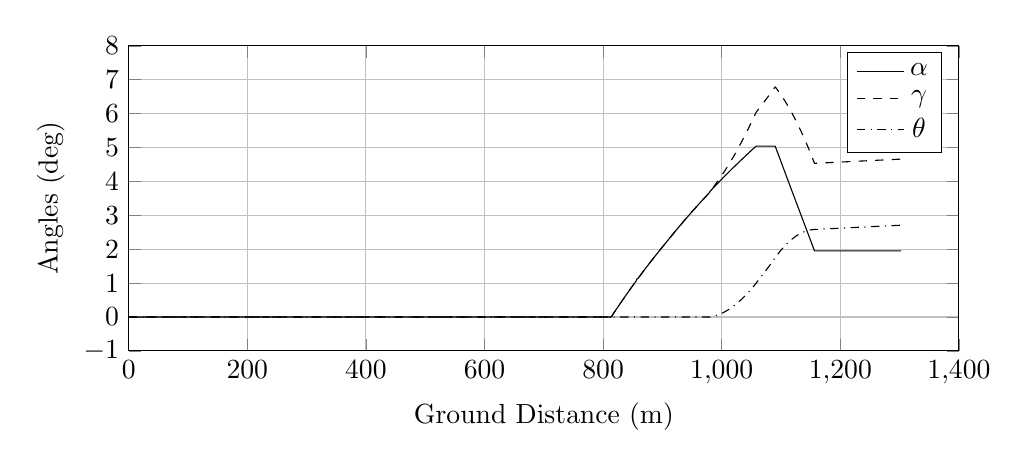
\begin{tikzpicture}

\begin{axis}[
width=\textwidth,
height=0.45\textwidth,
scaled ticks=false, tick label style={/pgf/number format/fixed},
xmin=0.0,
xmax=1400,
xlabel={Ground Distance (m)},
xmajorgrids,
ymin=-1.0,
ymax=8,
ytick={-1,0,1,2,3,4,5,6,7,8},
ylabel={Angles (deg)},
ymajorgrids,
legend entries = {$\alpha$\\$\gamma$\\$\theta$\\}
]

\addplot [
color=black,
solid
]
table[row sep=crcr]{
1.3603393307215537E-8	0.0\\
2.0334443352841076E-7	0.0\\
1.8493358258961232E-6	0.0\\
9.983129263424352E-6	0.0\\
4.13538327636676E-5	0.0\\
1.2467543572893382E-4	0.0\\
2.843807411608912E-4	0.0\\
5.588015241105573E-4	0.0\\
9.398454696015893E-4	0.0\\
0.0014155885812023746	0.0\\
0.0019945752038215015	0.0\\
0.0026717822370171283	0.0\\
0.003447739291558293	0.0\\
0.0043193476547732645	0.0\\
0.00529092766782709	0.0\\
0.006363550519206555	0.0\\
0.007533073890550759	0.0\\
0.008790616877968567	0.0\\
0.01016549189277427	0.0\\
0.011625499440327931	0.0\\
0.013184282533086976	0.0\\
0.014839871214038253	0.0\\
0.01660567024659266	0.0\\
0.018465948346479452	0.0\\
0.0203822997817096	0.0\\
0.022430561433814646	0.0\\
0.024588423902376283	0.0\\
0.026831028501027587	0.0\\
0.029143159681622913	0.0\\
0.03155709159958957	0.0\\
0.03411445662773917	0.0\\
0.03677290089167576	0.0\\
0.03952314881844239	0.0\\
0.04239921643077808	0.0\\
0.045357163155895136	0.0\\
0.048363831658398165	0.0\\
0.051533845233668635	0.0\\
0.0547899150155587	0.0\\
0.058172599437445835	0.0\\
0.06162834747858026	0.0\\
0.06521401059050522	0.0\\
0.06888104003120077	0.0\\
0.07268727020998902	0.0\\
0.076546425570032	0.0\\
0.08047032364859658	0.0\\
0.08456364881336098	0.0\\
0.08882250397434277	0.0\\
0.09306368907640691	0.0\\
0.09743039119190974	0.0\\
0.10191450167634594	0.0\\
0.10651989152467789	0.0\\
0.11128201757858264	0.0\\
0.11609763023253863	0.0\\
0.12097769621339591	0.0\\
0.12591912973280778	0.0\\
0.13103216605369056	0.0\\
0.13633380151185176	0.0\\
0.1416823117522269	0.0\\
0.14708837902374172	0.0\\
0.1525605467319851	0.0\\
0.15824953188605478	0.0\\
0.16398006351864292	0.0\\
0.16978153473626356	0.0\\
0.17584258400626962	0.0\\
0.1819863832139092	0.0\\
0.18819485651962437	0.0\\
0.19455736971520038	0.0\\
0.20098158490654017	0.0\\
0.2076061353991409	0.0\\
0.21424726384720844	0.0\\
0.2211374965027113	0.0\\
0.2281284453493247	0.0\\
0.2350833915765042	0.0\\
0.2423085249848444	0.0\\
0.24958374984531584	0.0\\
0.2569279402934431	0.0\\
0.2644720218029696	0.0\\
0.27204626263318243	0.0\\
0.27972793364503945	0.0\\
0.2874622320100655	0.0\\
0.29563698092580604	0.0\\
0.30361763245720474	0.0\\
0.3118912000478351	0.0\\
0.3202493147046803	0.0\\
0.3286412952843002	0.0\\
0.33714554464307567	0.0\\
0.3458731203690518	0.0\\
0.35455185683415313	0.0\\
0.3634323904331427	0.0\\
0.372325738896249	0.0\\
0.38151551889959867	0.0\\
0.3908489672358084	0.0\\
0.4001862088113266	0.0\\
0.4095647137707429	0.0\\
0.4192312859369268	0.0\\
0.4289206911602753	0.0\\
0.43896550245304145	0.0\\
0.4487817299761361	0.0\\
0.4589033974758888	0.0\\
0.4691858798479248	0.0\\
0.47972601481223376	0.0\\
0.49016040525287174	0.0\\
0.5007175269203565	0.0\\
0.511266977039379	0.0\\
0.522323236324642	0.0\\
0.5332586746953114	0.0\\
0.5445869154512923	0.0\\
0.5556699580072249	0.0\\
0.5669225885056133	0.0\\
0.5785590177532589	0.0\\
0.5903083066022885	0.0\\
0.6020327889628274	0.0\\
0.613957077533064	0.0\\
0.625960998969677	0.0\\
0.6380070243193761	0.0\\
0.6503365955459197	0.0\\
0.662700086001522	0.0\\
0.6752747602080436	0.0\\
0.6885889407972636	0.0\\
0.7019767933734617	0.0\\
0.7151149754112038	0.0\\
0.7284684478906998	0.0\\
0.7418939875700234	0.0\\
0.7553494584716574	0.0\\
0.7694215958599202	0.0\\
0.7830840331449673	0.0\\
0.796657372658726	0.0\\
0.8106660034246236	0.0\\
0.8251837647136968	0.0\\
0.8395067871054176	0.0\\
0.8540519574023793	0.0\\
0.8688334527125461	0.0\\
0.8840141863517745	0.0\\
0.8993797082767976	0.0\\
0.9143697020410035	0.0\\
0.9294094610857999	0.0\\
0.9452486359568626	0.0\\
0.9605773823977486	0.0\\
0.9761522209726621	0.0\\
0.9917649966835071	0.0\\
1.0074810114554809	0.0\\
1.0234652146968335	0.0\\
1.0399433598517231	0.0\\
1.0563627364420554	0.0\\
1.0728309985448887	0.0\\
1.0896486452479222	0.0\\
1.1068138420051672	0.0\\
1.124143995869574	0.0\\
1.1415400048645106	0.0\\
1.1590089082607062	0.0\\
1.1769249919091855	0.0\\
1.1951505705127592	0.0\\
1.2127191877709298	0.0\\
1.2308827453761335	0.0\\
1.2492706857898845	0.0\\
1.267587852451018	0.0\\
1.2860031245644312	0.0\\
1.304687144125951	0.0\\
1.3233765774990474	0.0\\
1.342322280991234	0.0\\
1.3613696045164358	0.0\\
1.3815086998747366	0.0\\
1.4013123019267382	0.0\\
1.4209622886438908	0.0\\
1.4411501686096515	0.0\\
1.4611760119255748	0.0\\
1.4816444281325132	0.0\\
1.501865958841821	0.0\\
1.5224364680875304	0.0\\
1.543651615594651	0.0\\
1.5647593029468103	0.0\\
1.5859558716309676	0.0\\
1.6071423964076703	0.0\\
1.6293386351549652	0.0\\
1.6508498980272122	0.0\\
1.673011606043147	0.0\\
1.6946435720294923	0.0\\
1.717066624993247	0.0\\
1.739432891071898	0.0\\
1.761922286799709	0.0\\
1.7849035550437842	0.0\\
1.8076299607761817	0.0\\
1.8313298306791497	0.0\\
1.8543134894513886	0.0\\
1.8777326664639729	0.0\\
1.9017196849182967	0.0\\
1.925345883672024	0.0\\
1.950252961491087	0.0\\
1.975161211119453	0.0\\
1.9993825790313986	0.0\\
2.024583888346972	0.0\\
2.04934017380271	0.0\\
2.0744229633459703	0.0\\
2.0996193404956136	0.0\\
2.1245764901457758	0.0\\
2.1500786393425866	0.0\\
2.176226227020705	0.0\\
2.202115608176549	0.0\\
2.227948363055355	0.0\\
2.2543499999408594	0.0\\
2.2810892744412783	0.0\\
2.3075963743135786	0.0\\
2.3348582111613405	0.0\\
2.3623221378972126	0.0\\
2.3898598419727675	0.0\\
2.4171687299087603	0.0\\
2.445442108612223	0.0\\
2.4735885391813177	0.0\\
2.5015416452491293	0.0\\
2.5301110763218357	0.0\\
2.5589284934403693	0.0\\
2.587611617795936	0.0\\
2.6175687086884984	0.0\\
2.647724154312196	0.0\\
2.6767118187859253	0.0\\
2.7060305938995466	0.0\\
2.7361546404224653	0.0\\
2.7663022704956823	0.0\\
2.7964672462043376	0.0\\
2.8272583584284883	0.0\\
2.8588650092419234	0.0\\
2.8898852960400587	0.0\\
2.9215246589961597	0.0\\
2.95270311230069	0.0\\
2.984506337549637	0.0\\
3.017379145769185	0.0\\
3.049243647754313	0.0\\
3.081295157663824	0.0\\
3.113406837946715	0.0\\
3.1453724573084756	0.0\\
3.1787286104953543	0.0\\
3.211019796961401	0.0\\
3.245786703184362	0.0\\
3.279939251746722	0.0\\
3.3141720228361216	0.0\\
3.3491198891036547	0.0\\
3.382965192547779	0.0\\
3.4181848705561064	0.0\\
3.45391888941694	0.0\\
3.488851494856137	0.0\\
3.524271454997704	0.0\\
3.5606552075305	0.0\\
3.597189071478943	0.0\\
3.632926148839256	0.0\\
3.668897146318187	0.0\\
3.706642714683163	0.0\\
3.7432264628550644	0.0\\
3.781286297809391	0.0\\
3.818618572105483	0.0\\
3.8564015479305356	0.0\\
3.8948624022541356	0.0\\
3.9329637046009225	0.0\\
3.971505929995028	0.0\\
4.009821706071438	0.0\\
4.049014376833089	0.0\\
4.089343885784727	0.0\\
4.128662304630717	0.0\\
4.1684827283974055	0.0\\
4.208000253554632	0.0\\
4.2483743636521965	0.0\\
4.288255503180503	0.0\\
4.328757204126676	0.0\\
4.369490126907612	0.0\\
4.410357715197167	0.0\\
4.45189144941496	0.0\\
4.492881116440694	0.0\\
4.53550011161515	0.0\\
4.577670191557685	0.0\\
4.6201174049766305	0.0\\
4.662272021613388	0.0\\
4.706017761800355	0.0\\
4.748842845578064	0.0\\
4.792293145132742	0.0\\
4.836482439768313	0.0\\
4.88090298307878	0.0\\
4.925311889063089	0.0\\
4.969864686447545	0.0\\
5.014842280541593	0.0\\
5.0603877575117515	0.0\\
5.106292347304597	0.0\\
5.152263975081851	0.0\\
5.1974808794106995	0.0\\
5.244027372436168	0.0\\
5.28996242022761	0.0\\
5.336209145350672	0.0\\
5.38320569473032	0.0\\
5.430469292142472	0.0\\
5.476900151253712	0.0\\
5.526063828851289	0.0\\
5.573879040902945	0.0\\
5.622613575936374	0.0\\
5.6713596863799225	0.0\\
5.720412183296268	0.0\\
5.770660497446668	0.0\\
5.820668144990444	0.0\\
5.870305285939629	0.0\\
5.920503816994749	0.0\\
5.971105439367246	0.0\\
6.021088325934068	0.0\\
6.071322359863801	0.0\\
6.122981826035449	0.0\\
6.174329110820436	0.0\\
6.225804784288178	0.0\\
6.278093246139479	0.0\\
6.331709873490098	0.0\\
6.384325657889258	0.0\\
6.436648686434458	0.0\\
6.489478972803882	0.0\\
6.543185721519176	0.0\\
6.596747696432654	0.0\\
6.650345873843312	0.0\\
6.704555155195255	0.0\\
6.7588986063680725	0.0\\
6.814371620173711	0.0\\
6.86997180120154	0.0\\
6.925426612865756	0.0\\
6.981353650685165	0.0\\
7.037678624474159	0.0\\
7.094603706786671	0.0\\
7.151204881983983	0.0\\
7.209200593921791	0.0\\
7.2667780016693655	0.0\\
7.324687293141565	0.0\\
7.382771066065313	0.0\\
7.441904508776327	0.0\\
7.501585831803217	0.0\\
7.5616527251378685	0.0\\
7.62150963104709	0.0\\
7.682859947113334	0.0\\
7.7432084367972145	0.0\\
7.803024936926759	0.0\\
7.863793829029664	0.0\\
7.9252460466886365	0.0\\
7.98696966925656	0.0\\
8.04776546969778	0.0\\
8.109421212326083	0.0\\
8.17269125419024	0.0\\
8.236095044780246	0.0\\
8.299523592514586	0.0\\
8.363213767675873	0.0\\
8.427807923256076	0.0\\
8.49144930156071	0.0\\
8.557380457258176	0.0\\
8.623183572921022	0.0\\
8.687840683575093	0.0\\
8.753751426394068	0.0\\
8.820803713780364	0.0\\
8.888970287482593	0.0\\
8.957133699158991	0.0\\
9.025036015045707	0.0\\
9.092760955867519	0.0\\
9.159817422823458	0.0\\
9.227495373767134	0.0\\
9.296013084156197	0.0\\
9.36435980631623	0.0\\
9.433329865923408	0.0\\
9.503849553921977	0.0\\
9.574524061692681	0.0\\
9.644263228942293	0.0\\
9.715657612596786	0.0\\
9.787429657508813	0.0\\
9.85753688572494	0.0\\
9.930250735750551	0.0\\
10.001571447096964	0.0\\
10.074699859091687	0.0\\
10.14698611653175	0.0\\
10.220547980738981	0.0\\
10.2940409891517	0.0\\
10.36719293590382	0.0\\
10.441008888975666	0.0\\
10.51610421670324	0.0\\
10.590724589239105	0.0\\
10.667218005391902	0.0\\
10.742771202259895	0.0\\
10.82035208750042	0.0\\
10.896759047300378	0.0\\
10.973503045910835	0.0\\
11.051297940743765	0.0\\
11.128076326409062	0.0\\
11.207667705350879	0.0\\
11.286758396846047	0.0\\
11.366305937658339	0.0\\
11.446149720998452	0.0\\
11.526866579636565	0.0\\
11.607297517600138	0.0\\
11.688034241538357	0.0\\
11.769665722224765	0.0\\
11.850920080706608	0.0\\
11.933163326324259	0.0\\
12.017103780766782	0.0\\
12.10034832931326	0.0\\
12.185467765774142	0.0\\
12.270669986481685	0.0\\
12.354040133273898	0.0\\
12.440386807402234	0.0\\
12.52556588630658	0.0\\
12.610860989997974	0.0\\
12.69550109439961	0.0\\
12.784634337461807	0.0\\
12.871172079509357	0.0\\
12.958447214271366	0.0\\
13.045518554761987	0.0\\
13.133090172249581	0.0\\
13.221405510214687	0.0\\
13.310319106907201	0.0\\
13.399783591735492	0.0\\
13.488943611067967	0.0\\
13.578276665194153	0.0\\
13.667402973129146	0.0\\
13.757763665999576	0.0\\
13.848393619195729	0.0\\
13.938857764339925	0.0\\
14.031101516310692	0.0\\
14.123507833735925	0.0\\
14.214825187590282	0.0\\
14.307956552027534	0.0\\
14.401498558574918	0.0\\
14.495315613017755	0.0\\
14.589065423003394	0.0\\
14.68316852398955	0.0\\
14.778702641747682	0.0\\
14.873746415615575	0.0\\
14.970384078097169	0.0\\
15.068900921005241	0.0\\
15.164434274206265	0.0\\
15.260378587808539	0.0\\
15.357189194448868	0.0\\
15.45495288999333	0.0\\
15.55311774366497	0.0\\
15.652583807013901	0.0\\
15.755243917873962	0.0\\
15.855950289561445	0.0\\
15.958461094374158	0.0\\
16.060387288500337	0.0\\
16.164276126126843	0.0\\
16.26736468838029	0.0\\
16.36946523634058	0.0\\
16.47192386662276	0.0\\
16.576794358652606	0.0\\
16.678929175716583	0.0\\
16.783994526910618	0.0\\
16.89012564586595	0.0\\
16.996887404888547	0.0\\
17.103774697793426	0.0\\
17.210947675936964	0.0\\
17.31865021419634	0.0\\
17.424470519881233	0.0\\
17.53205215515201	0.0\\
17.64034909906897	0.0\\
17.74911485075183	0.0\\
17.85745376408675	0.0\\
17.969383314157206	0.0\\
18.07998395718984	0.0\\
18.18863741327577	0.0\\
18.302466989554325	0.0\\
18.41305080779906	0.0\\
18.525644000014054	0.0\\
18.636945827420575	0.0\\
18.750643923449367	0.0\\
18.86479622056296	0.0\\
18.979646899421056	0.0\\
19.09418630108147	0.0\\
19.208983505033515	0.0\\
19.323483295898072	0.0\\
19.43842354827664	0.0\\
19.55563752357537	0.0\\
19.67199913451129	0.0\\
19.789486593639566	0.0\\
19.90713985662446	0.0\\
20.024127533725753	0.0\\
20.143019013955552	0.0\\
20.26442367074238	0.0\\
20.383660776265387	0.0\\
20.5042342316437	0.0\\
20.622773342122727	0.0\\
20.74503732713029	0.0\\
20.865944869938517	0.0\\
20.98711015528624	0.0\\
21.113336299999695	0.0\\
21.23638685227678	0.0\\
21.35988644990264	0.0\\
21.483760012473958	0.0\\
21.608180515260266	0.0\\
21.732326713270083	0.0\\
21.85766379468624	0.0\\
21.985117186778353	0.0\\
22.111729024702363	0.0\\
22.23700541150786	0.0\\
22.36297326225872	0.0\\
22.488604760551	0.0\\
22.616276341350805	0.0\\
22.744235570279145	0.0\\
22.874576476768283	0.0\\
23.003842066605536	0.0\\
23.13088450205612	0.0\\
23.257869280739328	0.0\\
23.389244224935425	0.0\\
23.519811196806458	0.0\\
23.653309395988643	0.0\\
23.78342402399784	0.0\\
23.9180644861338	0.0\\
24.05110504604577	0.0\\
24.182394801971697	0.0\\
24.314614014384034	0.0\\
24.449791085561472	0.0\\
24.585258581909038	0.0\\
24.72121222319008	0.0\\
24.857032405393277	0.0\\
24.99454740444294	0.0\\
25.13030709358258	0.0\\
25.270890409679986	0.0\\
25.40663839363527	0.0\\
25.54307796688363	0.0\\
25.68272814639034	0.0\\
25.82072003425767	0.0\\
25.96015212691003	0.0\\
25.987750021099068	0.0\\
26.0558803939429	0.0\\
26.061632797568386	0.0\\
26.066808273335674	0.0\\
26.071901058608013	0.0\\
26.073315434863225	0.0\\
26.074595035914804	0.0\\
26.080371168076944	0.0\\
26.10234540095133	0.0\\
26.183408179590366	0.0\\
26.300430535410044	0.0\\
26.42750601924636	0.0\\
26.558056987479794	0.0\\
26.688030995483615	0.0\\
26.818767077324992	0.0\\
26.951519978077492	0.0\\
27.083955405447817	0.0\\
27.216897884715692	0.0\\
27.350913258119895	0.0\\
27.4833530065795	0.0\\
27.6176201223548	0.0\\
27.752160408628434	0.0\\
27.887329802382908	0.0\\
28.023188645890663	0.0\\
28.158973127824495	0.0\\
28.296372294036907	0.0\\
28.435107205966254	0.0\\
28.571323599682245	0.0\\
28.70996262687553	0.0\\
28.850320389600306	0.0\\
28.988837241064125	0.0\\
29.129197813929657	0.0\\
29.27166529868488	0.0\\
29.41298471572133	0.0\\
29.554848516656044	0.0\\
29.699676691743235	0.0\\
29.842400551696755	0.0\\
29.985385440862252	0.0\\
30.129077275410303	0.0\\
30.27543774584293	0.0\\
30.422081339040986	0.0\\
30.56949149516445	0.0\\
30.716562179458485	0.0\\
30.86535310281699	0.0\\
31.011875026602333	0.0\\
31.16159928701196	0.0\\
31.313692569485013	0.0\\
31.463056706803336	0.0\\
31.61235366859384	0.0\\
31.76278957628285	0.0\\
31.915019899787076	0.0\\
32.06709627595497	0.0\\
32.21861178877769	0.0\\
32.37168228565527	0.0\\
32.52450570609457	0.0\\
32.67702483599189	0.0\\
32.829998687403204	0.0\\
32.98551220909506	0.0\\
33.14332298937855	0.0\\
33.29970221124884	0.0\\
33.45800124694219	0.0\\
33.61398946945653	0.0\\
33.77048353048475	0.0\\
33.9292721471582	0.0\\
34.08796840843395	0.0\\
34.24769686644211	0.0\\
34.406855482575295	0.0\\
34.56481953291838	0.0\\
34.72399692808165	0.0\\
34.88694269464703	0.0\\
35.04914399338672	0.0\\
35.209965099803895	0.0\\
35.3703140559587	0.0\\
35.531685786905925	0.0\\
35.69349909442164	0.0\\
35.85522798807463	0.0\\
36.022509111806116	0.0\\
36.19055880791667	0.0\\
36.35708622463872	0.0\\
36.52115360367851	0.0\\
36.68781562330062	0.0\\
36.8536847754776	0.0\\
37.024522648961764	0.0\\
37.19188554678789	0.0\\
37.36066720850286	0.0\\
37.528862119520696	0.0\\
37.697264258302326	0.0\\
37.86832931534104	0.0\\
38.03812867477943	0.0\\
38.20923731912278	0.0\\
38.37904730305398	0.0\\
38.55252405124031	0.0\\
38.72282139824354	0.0\\
38.89783411301201	0.0\\
39.0714610757495	0.0\\
39.24438070689564	0.0\\
39.41969314875929	0.0\\
39.59166556575205	0.0\\
39.764623188591585	0.0\\
39.94263254662576	0.0\\
40.11749159802578	0.0\\
40.29452954971913	0.0\\
40.47247750600427	0.0\\
40.64799609178485	0.0\\
40.82414741101539	0.0\\
41.00385670225303	0.0\\
41.18169069533937	0.0\\
41.3603281005193	0.0\\
41.54046179251334	0.0\\
41.722675278204306	0.0\\
41.90258931008478	0.0\\
42.08518735141125	0.0\\
42.26728550944881	0.0\\
42.44743534848537	0.0\\
42.63069538383506	0.0\\
42.80963512098974	0.0\\
42.992542679335614	0.0\\
43.17926890616222	0.0\\
43.363134036078335	0.0\\
43.54815051311773	0.0\\
43.733578141849236	0.0\\
43.91798130912079	0.0\\
44.10506009255049	0.0\\
44.29251116260117	0.0\\
44.480917546793805	0.0\\
44.66851287589745	0.0\\
44.85853501730759	0.0\\
45.047396872181054	0.0\\
45.236914792155844	0.0\\
45.42785879536018	0.0\\
45.616432631699865	0.0\\
45.80697204128492	0.0\\
45.998633580597016	0.0\\
46.18800675699903	0.0\\
46.380841640082096	0.0\\
46.57327038933336	0.0\\
46.765844918266424	0.0\\
46.95911042680183	0.0\\
47.15311668852311	0.0\\
47.34541611633634	0.0\\
47.53884854699059	0.0\\
47.73236991243341	0.0\\
47.92818250719388	0.0\\
48.12326385407131	0.0\\
48.32058854034828	0.0\\
48.516852452700604	0.0\\
48.71339374517507	0.0\\
48.91319881343868	0.0\\
49.1119162355681	0.0\\
49.31207818344666	0.0\\
49.509673461222235	0.0\\
49.71156302510582	0.0\\
49.91034548441702	0.0\\
50.11200805970151	0.0\\
50.30853267551517	0.0\\
50.50757456960626	0.0\\
50.70929197287772	0.0\\
50.91222418686718	0.0\\
51.11562549758783	0.0\\
51.32090674103446	0.0\\
51.525199701657655	0.0\\
51.72863462744459	0.0\\
51.934060761332375	0.0\\
52.14033810224923	0.0\\
52.344882977561255	0.0\\
52.55098100649393	0.0\\
52.75731843494604	0.0\\
52.96514817708821	0.0\\
53.17450540782369	0.0\\
53.382202621450276	0.0\\
53.592230583406476	0.0\\
53.80364534107798	0.0\\
54.01469481143569	0.0\\
54.223966920081466	0.0\\
54.43230789395902	0.0\\
54.6430562980421	0.0\\
54.855225786754914	0.0\\
55.066088958624874	0.0\\
55.27969530828261	0.0\\
55.49171188337613	0.0\\
55.70388919125476	0.0\\
55.91737779085577	0.0\\
56.13177028494084	0.0\\
56.34652664868587	0.0\\
56.559021044851505	0.0\\
56.77591447970492	0.0\\
56.99548236897459	0.0\\
57.21481285737903	0.0\\
57.43536222847358	0.0\\
57.65367025761124	0.0\\
57.872788904232735	0.0\\
58.0907693980174	0.0\\
58.311927420720366	0.0\\
58.532333513628615	0.0\\
58.75532998033057	0.0\\
58.976617007999806	0.0\\
59.19875422837053	0.0\\
59.4206945143671	0.0\\
59.64453328369959	0.0\\
59.86894932484513	0.0\\
60.09432075877773	0.0\\
60.318058693038594	0.0\\
60.541731124044205	0.0\\
60.76707064338231	0.0\\
60.995574692986196	0.0\\
61.22378989589207	0.0\\
61.4534619981562	0.0\\
61.683510138770515	0.0\\
61.91410430469678	0.0\\
62.14462153858659	0.0\\
62.37563158073512	0.0\\
62.607203285434	0.0\\
62.841031881319736	0.0\\
63.07467935056491	0.0\\
63.31164975340633	0.0\\
63.54633691305479	0.0\\
63.78243968758058	0.0\\
64.0165414084598	0.0\\
64.25412817577254	0.0\\
64.49270299572771	0.0\\
64.73076499662056	0.0\\
64.96867826857735	0.0\\
65.21063576532572	0.0\\
65.4512107007771	0.0\\
65.69028017871045	0.0\\
65.93032615763332	0.0\\
66.17196619696679	0.0\\
66.4135612157637	0.0\\
66.6559030093851	0.0\\
66.89910102540284	0.0\\
67.14354652182666	0.0\\
67.38771133480921	0.0\\
67.63347396558368	0.0\\
67.87898066495345	0.0\\
68.1255935515739	0.0\\
68.37316753306138	0.0\\
68.62205497364681	0.0\\
68.8711887275476	0.0\\
69.120220471977	0.0\\
69.36846244647072	0.0\\
69.61951843592018	0.0\\
69.87236615109754	0.0\\
70.12758921381476	0.0\\
70.37945082809051	0.0\\
70.63410009691182	0.0\\
70.89152727368702	0.0\\
71.14629115974091	0.0\\
71.40197865069018	0.0\\
71.66163317144085	0.0\\
71.92484704501203	0.0\\
72.18465416754285	0.0\\
72.44573394560723	0.0\\
72.70633339061075	0.0\\
72.96699363118216	0.0\\
73.22900401485182	0.0\\
73.49076816912304	0.0\\
73.75430841254712	0.0\\
74.01895646534612	0.0\\
74.2846979982242	0.0\\
74.55380714249793	0.0\\
74.82322871850147	0.0\\
75.09350011520078	0.0\\
75.36421232425869	0.0\\
75.6347219158074	0.0\\
75.90830954343213	0.0\\
76.18188601743822	0.0\\
76.45626363461818	0.0\\
76.72958718025629	0.0\\
77.00406935908524	0.0\\
77.28579748399531	0.0\\
77.56784659723587	0.0\\
77.84569092555657	0.0\\
78.1246978223638	0.0\\
78.40641219364133	0.0\\
78.68590470271565	0.0\\
78.96851680469001	0.0\\
79.25576208114188	0.0\\
79.54169104977237	0.0\\
79.82662017154695	0.0\\
80.11330301632765	0.0\\
80.40394576721474	0.0\\
80.6908099930996	0.0\\
80.98055888331655	0.0\\
81.27178512217935	0.0\\
81.56682943128612	0.0\\
81.86186977412851	0.0\\
82.15688924927383	0.0\\
82.44965588234726	0.0\\
82.74488606927187	0.0\\
83.04325841243121	0.0\\
83.34213327641098	0.0\\
83.64411622775171	0.0\\
83.94734638805741	0.0\\
84.25123842984891	0.0\\
84.55152885577829	0.0\\
84.85735750691177	0.0\\
85.16518306664875	0.0\\
85.47136476235073	0.0\\
85.77898122624802	0.0\\
86.08923229760057	0.0\\
86.40254560035129	0.0\\
86.71167807044037	0.0\\
87.02660518802142	0.0\\
87.34238286044419	0.0\\
87.65842706333811	0.0\\
87.97971380652302	0.0\\
88.2973933745065	0.0\\
88.61789013566766	0.0\\
88.93643920279564	0.0\\
89.25662431900213	0.0\\
89.57903058309674	0.0\\
89.89968694948243	0.0\\
90.22473455398588	0.0\\
90.55024875587375	0.0\\
90.87789352676518	0.0\\
91.20733069500889	0.0\\
91.54101415610151	0.0\\
91.87012785371462	0.0\\
92.20120197152713	0.0\\
92.53416638543635	0.0\\
92.86431843528567	0.0\\
93.19748455591187	0.0\\
93.53066771200866	0.0\\
93.86681917526724	0.0\\
94.20530590547477	0.0\\
94.5419273964865	0.0\\
94.8854212036891	0.0\\
95.22752713476521	0.0\\
95.57091181422334	0.0\\
95.91383450860906	0.0\\
96.25469535763642	0.0\\
96.5966517898868	0.0\\
96.93845701474973	0.0\\
97.28153572459905	0.0\\
97.62213139590432	0.0\\
97.9659652144934	0.0\\
98.3129807304216	0.0\\
98.65852794036775	0.0\\
99.00080640577195	0.0\\
99.35064076251427	0.0\\
99.69796076807248	0.0\\
100.04654253174803	0.0\\
100.3915606488718	0.0\\
100.74261509654437	0.0\\
101.08877163494762	0.0\\
101.43457754260953	0.0\\
101.784020212797	0.0\\
102.13161434601102	0.0\\
102.4751980097893	0.0\\
102.82212110631409	0.0\\
103.16739702108615	0.0\\
103.51524666207362	0.0\\
103.86391679154056	0.0\\
104.20960434827006	0.0\\
104.55241399635099	0.0\\
104.89662223620601	0.0\\
105.24103428322039	0.0\\
105.5836615386647	0.0\\
105.92645892081137	0.0\\
106.27347658175316	0.0\\
106.6151670762521	0.0\\
106.95898391938218	0.0\\
107.30023552029138	0.0\\
107.64147805753461	0.0\\
107.98348674656944	0.0\\
108.32522459759954	0.0\\
108.3935347040271	0.0\\
108.40478590462831	0.0\\
108.41572478024443	0.0\\
108.4246743308916	0.0\\
108.44347342986478	0.0\\
108.52018987797786	0.0\\
108.70071173483461	0.0\\
108.99446230248458	0.0\\
109.30176454987088	0.0\\
109.60899173332959	0.0\\
109.91608539831654	0.0\\
110.22883517949637	0.0\\
110.54143546549608	0.0\\
110.853845249356	0.0\\
111.1739714794031	0.0\\
111.4937490010879	0.0\\
111.81170779322963	0.0\\
112.13106495813236	0.0\\
112.4519453366479	0.0\\
112.77515902629136	0.0\\
113.0997499810409	0.0\\
113.43040796942478	0.0\\
113.7597028375028	0.0\\
114.0907450350197	0.0\\
114.42538740208008	0.0\\
114.75997726261329	0.0\\
115.09477047197589	0.0\\
115.43440545481076	0.0\\
115.77494672336013	0.0\\
116.11687534861284	0.0\\
116.46164587354252	0.0\\
116.8077846490165	0.0\\
117.15688723722127	0.0\\
117.50557855048987	0.0\\
117.85411336711965	0.0\\
118.20532793701167	0.0\\
118.55850697655507	0.0\\
118.91273956155123	0.0\\
119.26983096270519	0.0\\
119.62978614725739	0.0\\
119.98960731920661	0.0\\
120.34734904217265	0.0\\
120.7138511704587	0.0\\
121.08106061642908	0.0\\
121.44737887966437	0.0\\
121.81499139152783	0.0\\
122.18511446431708	0.0\\
122.55384158147794	0.0\\
122.92460728481757	0.0\\
123.29616941264607	0.0\\
123.67040864389355	0.0\\
124.04652172406458	0.0\\
124.42393851457416	0.0\\
124.80152108360014	0.0\\
125.18180835736592	0.0\\
125.55854932865631	0.0\\
125.93878032356085	0.0\\
126.31997081831156	0.0\\
126.70099538833193	0.0\\
127.08058279416298	0.0\\
127.46175209000612	0.0\\
127.84399628255431	0.0\\
128.22749916598133	0.0\\
128.6102537001487	0.0\\
128.99595881306152	0.0\\
129.37788117916477	0.0\\
129.760738924708	0.0\\
130.1448498512433	0.0\\
130.53000390659713	0.0\\
130.9168242384266	0.0\\
131.29443328439476	0.0\\
131.67491382268804	0.0\\
132.05816436539135	0.0\\
132.44070735535217	0.0\\
132.82666098215685	0.0\\
133.20952005887244	0.0\\
133.5940193955625	0.0\\
133.97617966856654	0.0\\
134.36103715882757	0.0\\
134.74478042358356	0.0\\
135.12867144169206	0.0\\
135.5141335746535	0.0\\
135.89764893392993	0.0\\
136.28231234485685	0.0\\
136.66418763078912	0.0\\
137.04684871033697	0.0\\
137.42845627025127	0.0\\
137.8132447087305	0.0\\
138.19719797258034	0.0\\
138.58059071069573	0.0\\
138.96593237593703	0.0\\
139.3501607499636	0.0\\
139.73355638294606	0.0\\
140.1160230155566	0.0\\
140.50045093994146	0.0\\
140.88215178690393	0.0\\
141.26156782058217	0.0\\
141.64323970440188	0.0\\
142.02689350659642	0.0\\
142.41061312971692	0.0\\
142.7942251403153	0.0\\
143.1756303563767	0.0\\
143.5599719391364	0.0\\
143.94242380128833	0.0\\
144.3239499176869	0.0\\
144.70664939692608	0.0\\
145.0870075357763	0.0\\
145.46856550308127	0.0\\
145.85014610541765	0.0\\
146.23128237819492	0.0\\
146.61504730324998	0.0\\
146.99763315977907	0.0\\
147.38441582478964	0.0\\
147.7673688364352	0.0\\
148.15222568696134	0.0\\
148.53580865353604	0.0\\
148.9199734867533	0.0\\
149.3040357319486	0.0\\
149.68771357306542	0.0\\
150.07093078701052	0.0\\
150.45622889618164	0.0\\
150.8449053483268	0.0\\
151.2288570611563	0.0\\
151.61452719766493	0.0\\
151.9983007305741	0.0\\
152.38299664478842	0.0\\
152.76945776909372	0.0\\
153.15580177123394	0.0\\
153.54253364040335	0.0\\
153.93093169697067	0.0\\
154.31788037931886	0.0\\
154.7039882138024	0.0\\
155.08880221957185	0.0\\
155.47621608980313	0.0\\
155.866104687065	0.0\\
156.25391419262098	0.0\\
156.64166339424906	0.0\\
157.03027969880475	0.0\\
157.4213807682267	0.0\\
157.8105708506119	0.0\\
158.19948541262937	0.0\\
158.58893406813365	0.0\\
158.97894817604634	0.0\\
159.3710019698692	0.0\\
159.76139479981174	0.0\\
160.1523485688823	0.0\\
160.54128874338664	0.0\\
160.9326976430911	0.0\\
161.32564259741588	0.0\\
161.71827778345698	0.0\\
162.1124492087963	0.0\\
162.50576001021273	0.0\\
162.89904576730015	0.0\\
163.29316224934274	0.0\\
163.68899123279596	0.0\\
164.08495392634194	0.0\\
164.48271131475576	0.0\\
164.8792309171331	0.0\\
165.27343112400507	0.0\\
165.67115293733156	0.0\\
166.06936395728349	0.0\\
166.47000821435734	0.0\\
166.87155839526775	0.0\\
167.27134041220108	0.0\\
167.67233991204222	0.0\\
168.0705846918417	0.0\\
168.47232570996516	0.0\\
168.87521546679773	0.0\\
169.2789990941189	0.0\\
169.68142011368735	0.0\\
170.088438196605	0.0\\
170.49328200513543	0.0\\
170.89845866435633	0.0\\
171.30484584057905	0.0\\
171.7103088520891	0.0\\
172.11589069074847	0.0\\
172.52485519917514	0.0\\
172.93316089774754	0.0\\
173.34236088095247	0.0\\
173.7535761368399	0.0\\
174.16510964781833	0.0\\
174.5786011126259	0.0\\
174.99051444770384	0.0\\
175.40138574541044	0.0\\
175.81497300453447	0.0\\
176.2280441317456	0.0\\
176.64225100058474	0.0\\
177.05714873395152	0.0\\
177.47483026786767	0.0\\
177.89254345086653	0.0\\
178.3100126079721	0.0\\
178.7278240622369	0.0\\
179.1449731538625	0.0\\
179.56482315926417	0.0\\
179.9871804296257	0.0\\
180.4095742002126	0.0\\
180.83428717371925	0.0\\
181.26003251256287	0.0\\
181.6840913989422	0.0\\
182.1114839456617	0.0\\
182.5374089230304	0.0\\
182.96440604473082	0.0\\
183.39304842330927	0.0\\
183.8234391905185	0.0\\
184.2565386467558	0.0\\
184.68745119590193	0.0\\
185.11804999400476	0.0\\
185.54983076576542	0.0\\
185.98322399936802	0.0\\
186.41637816429778	0.0\\
186.85103033850396	0.0\\
187.28701324242002	0.0\\
187.72482375232647	0.0\\
188.16038808151575	0.0\\
188.5986323917997	0.0\\
189.04181882432442	0.0\\
189.48417857731005	0.0\\
189.92673350352436	0.0\\
190.3712203460227	0.0\\
190.8171693385559	0.0\\
191.2607914989822	0.0\\
191.7085048054314	0.0\\
192.15912968354564	0.0\\
192.60936448614513	0.0\\
193.06096206133014	0.0\\
193.50995896221815	0.0\\
193.96222738896364	0.0\\
194.41802104663145	0.0\\
194.87342332120494	0.0\\
195.32868067301865	0.0\\
195.78611327072855	0.0\\
196.24327119175433	0.0\\
196.70330552186363	0.0\\
197.16349707435467	0.0\\
197.6260626000094	0.0\\
198.09002425529962	0.0\\
198.55822718319422	0.0\\
199.02663999285284	0.0\\
199.4942263371064	0.0\\
199.96051846591553	0.0\\
200.4340527590599	0.0\\
200.9046051381776	0.0\\
201.38053424207163	0.0\\
201.855813875004	0.0\\
202.3311704663634	0.0\\
202.81222172114025	0.0\\
203.29225549210986	0.0\\
203.77308885705298	0.0\\
204.25557537412044	0.0\\
204.7402502473849	0.0\\
205.2236366749359	0.0\\
205.7136101207933	0.0\\
206.20393168243612	0.0\\
206.69661599754647	0.0\\
207.18955097797863	0.0\\
207.68747106001632	0.0\\
208.18818418427776	0.0\\
208.68864521634526	0.0\\
209.18805406731133	0.0\\
209.69072626026758	0.0\\
210.1949489825136	0.0\\
210.70396111371042	0.0\\
211.21614058335587	0.0\\
211.7289636831582	0.0\\
212.24265718177503	0.0\\
212.75957115615557	0.0\\
213.28124361123798	0.0\\
213.80665479128663	0.0\\
214.33466763217763	0.0\\
214.86241383044415	0.0\\
215.38762416293667	0.0\\
215.91972020502777	0.0\\
216.453694496636	0.0\\
216.99218613031866	0.0\\
217.53464071342142	0.0\\
218.07804319032095	0.0\\
218.62452881115053	0.0\\
219.1707188429899	0.0\\
219.71730570977076	0.0\\
220.274760228052	0.0\\
220.835259093258	0.0\\
221.3941373958715	0.0\\
221.95623623511386	0.0\\
222.52040576537968	0.0\\
223.09037241999033	0.0\\
223.661129480297	0.0\\
224.23954505634208	0.0\\
224.81564934919504	0.0\\
225.40333087020622	0.0\\
225.99624064594485	0.0\\
226.58875910740323	0.0\\
227.18585441503012	0.0\\
227.7870146338791	0.0\\
228.39495206683767	0.0\\
229.0027183467937	0.0\\
229.6102660575582	0.0\\
230.22857190062643	0.0\\
230.8468525918393	0.0\\
231.47114194537448	0.0\\
232.09060564776433	0.0\\
232.71961230618888	0.0\\
233.34696033086396	0.0\\
233.9840065784689	0.0\\
234.6188203761186	0.0\\
235.2539319397456	0.0\\
235.886956379092	0.0\\
236.5153031168307	0.0\\
237.1504953781269	0.0\\
237.78410205277385	0.0\\
238.41360900639518	0.0\\
239.04679127723733	0.0\\
239.67609891578388	0.0\\
240.3017129123046	0.0\\
240.93317778774485	0.0\\
241.55721005497253	0.0\\
242.1780757761154	0.0\\
242.7965584376659	0.0\\
243.4114785265944	0.0\\
244.02550827530933	0.0\\
244.63427618145124	0.0\\
245.24126487864038	0.0\\
245.84466361012846	0.0\\
246.4476225417801	0.0\\
247.04267344144802	0.0\\
247.6421488158	0.0\\
248.2330500398673	0.0\\
248.8222841397298	0.0\\
249.4139444766347	0.0\\
249.99998610086192	0.0\\
250.57758594667018	0.0\\
251.15853686633199	0.0\\
251.73921641108228	0.0\\
252.31216708836962	0.0\\
252.88817036877617	0.0\\
253.4570082134402	0.0\\
254.02007242820673	0.0\\
254.5855573787108	0.0\\
255.15029634137989	0.0\\
255.71294034286547	0.0\\
256.27258114245853	0.0\\
256.8305649252842	0.0\\
257.38478802342286	0.0\\
257.4959621062188	0.0\\
257.5611920943704	0.0\\
257.60062237753925	0.0\\
257.6107239150342	0.0\\
257.6183320416303	0.0\\
257.62277045264796	0.0\\
257.62729287050774	0.0\\
257.6542412653681	0.0\\
257.747424202601	0.0\\
258.03721256731046	0.0\\
258.5190125653693	0.0\\
259.00532843878875	0.0\\
259.49401909840515	0.0\\
259.98581493995266	0.0\\
260.4819698790609	0.0\\
260.97812571679674	0.0\\
261.4812175109821	0.0\\
261.9850059638038	0.0\\
262.4910281591069	0.0\\
263.0003252970298	0.0\\
263.5131478408722	0.0\\
264.0293216176061	0.0\\
264.54826562874086	0.0\\
265.0714232439334	0.0\\
265.59763340154745	0.0\\
266.1233003184659	0.0\\
266.6551605685464	0.0\\
267.19223429565795	0.0\\
267.72974052544146	0.0\\
268.27282471948854	0.0\\
268.8167212540145	0.0\\
269.36684202478307	0.0\\
269.9215996219019	0.0\\
270.4791082933567	0.0\\
271.03983254776506	0.0\\
271.6074455599014	0.0\\
272.1754809002374	0.0\\
272.7524022502224	0.0\\
273.3357847625165	0.0\\
273.91684495064374	0.0\\
274.5075523019982	0.0\\
275.0995375957874	0.0\\
275.69766674106233	0.0\\
276.3013456770767	0.0\\
276.90909644628925	0.0\\
277.5234995466793	0.0\\
278.13959639565337	0.0\\
278.76308237359774	0.0\\
279.389606942784	0.0\\
280.02074979788426	0.0\\
280.6586947867754	0.0\\
281.3003335866648	0.0\\
281.94157575500606	0.0\\
282.5880614624846	0.0\\
283.23584856186324	0.0\\
283.8851508583185	0.0\\
284.5301203280417	0.0\\
285.1843536535779	0.0\\
285.83553116214307	0.0\\
286.4837256048969	0.0\\
287.1336898105825	0.0\\
287.7808235765799	0.0\\
288.42820685084826	0.0\\
289.0754666022002	0.0\\
289.71879024937004	0.0\\
290.36420979409684	0.0\\
291.0002472374472	0.0\\
291.64182130034897	0.0\\
292.27316865691716	0.0\\
292.9083864811005	0.0\\
293.54335819806715	0.0\\
294.17307850120346	0.0\\
294.79408895337656	0.0\\
295.4199157771013	0.0\\
296.0380590852486	0.0\\
296.6542969985221	0.0\\
297.2681917409874	0.0\\
297.88482625920517	0.0\\
298.4949121158181	0.0\\
299.10656876013206	0.0\\
299.7189321849655	0.0\\
300.32723284437907	0.0\\
300.92930430691433	0.0\\
301.53463237615574	0.0\\
302.1363215848461	0.0\\
302.731439066583	0.0\\
303.3331045114137	0.0\\
303.92852765769237	0.0\\
304.52166324273924	0.0\\
305.11491208725784	0.0\\
305.70510856070314	0.0\\
306.29833179138177	0.0\\
306.8897654253252	0.0\\
307.4799704999041	0.0\\
308.06772992248136	0.0\\
308.6551058451172	0.0\\
309.2396381392449	0.0\\
309.82398267965425	0.0\\
310.40422650572066	0.0\\
310.9895683476474	0.0\\
311.5727136903438	0.0\\
312.15129426541773	0.0\\
312.7356217277545	0.0\\
313.31711326243806	0.0\\
313.899302145316	0.0\\
314.47946679147856	0.0\\
315.0588501134555	0.0\\
315.6397939029396	0.0\\
316.2168920475523	0.0\\
316.7955732394013	0.0\\
317.37103223180316	0.0\\
317.947565273913	0.0\\
318.5214617947222	0.0\\
319.09868556082085	0.0\\
319.67476219148546	0.0\\
320.24944526491765	0.0\\
320.82291261720786	0.0\\
321.39725246986427	0.0\\
321.96848871367	0.0\\
322.54402617481435	0.0\\
323.1185574377922	0.0\\
323.691859264958	0.0\\
324.2647334332521	0.0\\
324.8363521231331	0.0\\
325.40661348734614	0.0\\
325.97908467698915	0.0\\
326.5542035875586	0.0\\
327.12490712258295	0.0\\
327.6996379965167	0.0\\
328.2728670816481	0.0\\
328.8486987665442	0.0\\
329.41990981452807	0.0\\
329.9938351119364	0.0\\
330.5648485136189	0.0\\
331.13749118064516	0.0\\
331.7074637117181	0.0\\
332.2798601122896	0.0\\
332.8523203670276	0.0\\
333.42500978717965	0.0\\
334.00122212141855	0.0\\
334.57441172696565	0.0\\
335.1481633939942	0.0\\
335.72345703021597	0.0\\
336.29828216695637	0.0\\
336.8725624877933	0.0\\
337.44522027160394	0.0\\
338.02053867417567	0.0\\
338.5962187273635	0.0\\
339.1703543735324	0.0\\
339.7498013559267	0.0\\
340.3260768964459	0.0\\
340.9051117020497	0.0\\
341.47919118112156	0.0\\
342.052441303386	0.0\\
342.6320235008849	0.0\\
343.21038614202473	0.0\\
343.79082299329946	0.0\\
344.3667106402361	0.0\\
344.94458170993323	0.0\\
345.5252340504509	0.0\\
346.1016219383906	0.0\\
346.6806961036725	0.0\\
347.2602578923353	0.0\\
347.84073776856303	0.0\\
348.4226009401458	0.0\\
349.0044346707606	0.0\\
349.5859819547053	0.0\\
350.1699920738855	0.0\\
350.75474917442455	0.0\\
351.33998325174355	0.0\\
351.9234136900301	0.0\\
352.50674072872846	0.0\\
353.09110804073237	0.0\\
353.67821635803944	0.0\\
354.2656524741757	0.0\\
354.8545578241044	0.0\\
355.4483774220265	0.0\\
356.0367996380022	0.0\\
356.62583096427284	0.0\\
357.2144774827566	0.0\\
357.80411644396065	0.0\\
358.39517477750917	0.0\\
358.9862667118267	0.0\\
359.57750029884653	0.0\\
360.17210502256853	0.0\\
360.76667257221345	0.0\\
361.36307847075966	0.0\\
361.95890315858196	0.0\\
362.55277332573996	0.0\\
363.15015313069875	0.0\\
363.7467383697897	0.0\\
364.34582190435833	0.0\\
364.9460245640587	0.0\\
365.54693692211754	0.0\\
366.14934356225297	0.0\\
366.7506799567443	0.0\\
367.35358948565136	0.0\\
367.957068853549	0.0\\
368.56310438184994	0.0\\
369.1667326492483	0.0\\
369.7692268682281	0.0\\
370.3767216505511	0.0\\
370.9840014372453	0.0\\
371.59702031674954	0.0\\
372.2057576829203	0.0\\
372.8164011445841	0.0\\
373.43055551390637	0.0\\
374.04130844990834	0.0\\
374.65480432791037	0.0\\
375.2686727235273	0.0\\
375.88872766894735	0.0\\
376.5077052039818	0.0\\
377.12525427851347	0.0\\
377.74405712537066	0.0\\
378.36402671612836	0.0\\
378.9860252798833	0.0\\
379.6100000903326	0.0\\
380.2333263467823	0.0\\
380.8554247462042	0.0\\
381.4828757180544	0.0\\
382.11124459971245	0.0\\
382.74241248635997	0.0\\
383.3719105047892	0.0\\
384.00409885358727	0.0\\
384.6374235585132	0.0\\
385.2708543582187	0.0\\
385.90511613810475	0.0\\
386.5402229663101	0.0\\
387.1757112317391	0.0\\
387.816842485381	0.0\\
388.45671447828204	0.0\\
389.0979595165261	0.0\\
389.738666357365	0.0\\
390.38126573576096	0.0\\
391.0250474989899	0.0\\
391.6744601114111	0.0\\
392.32213053197165	0.0\\
392.96822988900624	0.0\\
393.62074411485196	0.0\\
394.27341767767894	0.0\\
394.92683850679725	0.0\\
395.58558306335794	0.0\\
396.2441970187614	0.0\\
396.90310461070555	0.0\\
397.56432488588905	0.0\\
398.2289657073595	0.0\\
398.8925370524752	0.0\\
399.5622831783011	0.0\\
400.2295014598768	0.0\\
400.89855800548185	0.0\\
401.5675035611599	0.0\\
402.24206117554286	0.0\\
402.91817297108616	0.0\\
403.5958718607668	0.0\\
404.27787051233963	0.0\\
404.95902715653847	0.0\\
405.6425745212256	0.0\\
406.3286386181055	0.0\\
407.0181239797241	0.0\\
407.70730436303313	0.0\\
408.39972983906614	0.0\\
409.0954177346696	0.0\\
409.79217465836814	0.0\\
410.4900247907216	0.0\\
411.1873806890112	0.0\\
411.8896918209001	0.0\\
412.5960730727825	0.0\\
413.3068225682056	0.0\\
414.0163043302465	0.0\\
414.7283691490554	0.0\\
415.4426354990113	0.0\\
416.1629925407426	0.0\\
416.8821853291962	0.0\\
417.606386355131	0.0\\
418.33304785123187	0.0\\
419.0630803577634	0.0\\
419.79657378413856	0.0\\
420.5335871119013	0.0\\
421.27035840412	0.0\\
422.00742265160795	0.0\\
422.7512304365845	0.0\\
423.49678426262926	0.0\\
424.2511831284078	0.0\\
425.00728777593645	0.0\\
425.7607765912853	0.0\\
426.5243177755509	0.0\\
427.28979022554415	0.0\\
428.0636149183367	0.0\\
428.8379843697036	0.0\\
429.60996752685014	0.0\\
430.3897477020988	0.0\\
431.1753893594911	0.0\\
431.966835986777	0.0\\
432.75960868637253	0.0\\
433.56365122208206	0.0\\
434.37045705896094	0.0\\
435.1870341731259	0.0\\
436.00231675887426	0.0\\
436.8220964781458	0.0\\
437.6552545507992	0.0\\
438.4886711504423	0.0\\
439.3280194395811	0.0\\
440.18158737508645	0.0\\
441.03992126721334	0.0\\
441.89899771608907	0.0\\
442.76703563270644	0.0\\
443.6461218976118	0.0\\
444.5334070432492	0.0\\
445.4247342866296	0.0\\
446.32920810974076	0.0\\
447.24483338837376	0.0\\
448.1693167681145	0.0\\
449.1035660927572	0.0\\
450.0458822047997	0.0\\
451.00182339874107	0.0\\
451.9686516781545	0.0\\
452.94634555439245	0.0\\
453.93854384565975	0.0\\
454.9385614547757	0.0\\
455.94748135202974	0.0\\
456.9584433214644	0.0\\
457.9810501546409	0.0\\
459.00261927313556	0.0\\
460.01989883738554	0.0\\
461.03781929506397	0.0\\
462.0494946766827	0.0\\
463.05160747895377	0.0\\
464.0518545115017	0.0\\
465.0383607621146	0.0\\
466.0100259504346	0.0\\
466.972877456118	0.0\\
467.92078248842233	0.0\\
468.8602060683198	0.0\\
469.7916006261976	0.0\\
470.7152983680744	0.0\\
471.63110143131246	0.0\\
472.53565503377354	0.0\\
473.43001919591256	0.0\\
474.3175091358099	0.0\\
475.20055699416787	0.0\\
476.0797229530699	0.0\\
476.9477851277236	0.0\\
477.80928619548854	0.0\\
478.66271897115837	0.0\\
479.51389416766324	0.0\\
480.3599300918547	0.0\\
481.2024946516909	0.0\\
482.03570776919605	0.0\\
482.8627499119842	0.0\\
483.68609836947405	0.0\\
484.50924809825483	0.0\\
485.32557402246096	0.0\\
486.13737678620214	0.0\\
486.94279782585124	0.0\\
487.7464247110714	0.0\\
488.5446013657454	0.0\\
489.3400640194311	0.0\\
490.13177480007994	0.0\\
490.9214465155957	0.0\\
491.7098985286566	0.0\\
492.4922927445115	0.0\\
493.27044666476036	0.0\\
494.0476143876257	0.0\\
494.20241746126965	0.0\\
494.3107978669077	0.0\\
494.37828944737976	0.0\\
494.4347701055989	0.0\\
494.47816602721264	0.0\\
494.51702732572653	0.0\\
494.5502911901548	0.0\\
494.577081830696	0.0\\
494.60057923878355	0.0\\
494.62714499920276	0.0\\
494.66342814041457	0.0\\
494.81132358778007	0.0\\
495.3586284984972	0.0\\
496.12147763230723	0.0\\
496.8813835628466	0.0\\
497.6488818907185	0.0\\
498.420249213705	0.0\\
499.19626431793347	0.0\\
499.97425874367036	0.0\\
500.75819637842517	0.0\\
501.5451867231876	0.0\\
502.3378682656379	0.0\\
503.1340134573071	0.0\\
503.9375989715213	0.0\\
504.7414334937688	0.0\\
505.559506889423	0.0\\
506.377447249919	0.0\\
507.20375538751296	0.0\\
508.03561369841157	0.0\\
508.87311166745064	0.0\\
509.7192976685493	0.0\\
510.5721190284996	0.0\\
511.4295209436101	0.0\\
512.2980180384125	0.0\\
513.1762329789033	0.0\\
514.0593120865078	0.0\\
514.9494806215175	0.0\\
515.8427349858514	0.0\\
516.749291098773	0.0\\
517.6632944734126	0.0\\
518.5839275461435	0.0\\
519.5154431589849	0.0\\
520.4581562238659	0.0\\
521.4118966074366	0.0\\
522.3777169822708	0.0\\
523.3525138228201	0.0\\
524.3371013415426	0.0\\
525.3353442314576	0.0\\
526.3351827638799	0.0\\
527.3491211471937	0.0\\
528.3780638880814	0.0\\
529.4086362368812	0.0\\
530.4509666595222	0.0\\
531.4986519980898	0.0\\
532.5486680161896	0.0\\
533.6040807686652	0.0\\
534.6582653163111	0.0\\
535.7111060711245	0.0\\
536.7570734752076	0.0\\
537.7959704567047	0.0\\
538.831418395976	0.0\\
539.8587432792533	0.0\\
540.8787796496395	0.0\\
541.8910338586084	0.0\\
542.9014829990567	0.0\\
543.9053294454354	0.0\\
544.8971202026662	0.0\\
545.8825275222928	0.0\\
546.8643981752491	0.0\\
547.8354934964686	0.0\\
548.7978159953416	0.0\\
549.7611904012842	0.0\\
550.7110060651066	0.0\\
551.664090227393	0.0\\
552.6116451322207	0.0\\
553.5516990291744	0.0\\
554.4861496686367	0.0\\
555.4175977189591	0.0\\
556.3430772394313	0.0\\
557.2703505208649	0.0\\
558.1949140875358	0.0\\
559.113825707447	0.0\\
560.0259676484568	0.0\\
560.9356760805852	0.0\\
561.8459791362618	0.0\\
562.7497050462059	0.0\\
563.6501935037068	0.0\\
564.5493683381062	0.0\\
565.4432409703295	0.0\\
566.3324229068421	0.0\\
567.2232024085395	0.0\\
568.1089131354433	0.0\\
568.9967174349374	0.0\\
569.8812132174357	0.0\\
570.7637422769849	0.0\\
571.6442227910438	0.0\\
572.5215037953217	0.0\\
573.4005491703067	0.0\\
574.2779472226907	0.0\\
575.151011261481	0.0\\
576.0245131050826	0.0\\
576.8955458060548	0.0\\
577.7629842485173	0.0\\
578.6336517655247	0.0\\
579.501608226685	0.0\\
580.3696467482935	0.0\\
581.2348383339768	0.0\\
582.0988646649505	0.0\\
582.9636042979482	0.0\\
583.8252011194893	0.0\\
584.6901849917015	0.0\\
585.549998413398	0.0\\
586.4068665072064	0.0\\
587.26803687641	0.0\\
588.1253062519067	0.0\\
588.9826833154086	0.0\\
589.8435601981266	0.0\\
590.7026475829934	0.0\\
591.5610614503998	0.0\\
592.4171646563639	0.0\\
593.2726467519024	0.0\\
594.127887939492	0.0\\
594.9819225706171	0.0\\
595.8354424015401	0.0\\
596.6899106188978	0.0\\
597.5461393118355	0.0\\
598.3958561211996	0.0\\
599.2447998405937	0.0\\
600.0970049729935	0.0\\
600.9528386086345	0.0\\
601.8057809763002	0.0\\
602.657842827645	0.0\\
603.5135349722555	0.0\\
604.36637639166	0.0\\
605.2207426818484	0.0\\
606.0715048903489	0.0\\
606.9216885288381	0.0\\
607.7772653436391	0.0\\
608.6301999399484	0.0\\
609.4834659570263	0.0\\
610.3370436927844	0.0\\
611.1892450929167	0.0\\
612.0446548793846	0.0\\
612.895984782047	0.0\\
613.7493920136312	0.0\\
614.6019174814558	0.0\\
615.4548118471523	0.0\\
616.3064481175597	0.0\\
617.1620218116866	0.0\\
618.0180728842076	0.0\\
618.8697814805862	0.0\\
619.7239326535935	0.0\\
620.5783109385195	0.0\\
621.437124614104	0.0\\
622.2924013442589	0.0\\
623.1512264122773	0.0\\
624.0098015434726	0.0\\
624.8677091526213	0.0\\
625.7302474051089	0.0\\
626.5891873908845	0.0\\
627.4467449456781	0.0\\
628.3009878850007	0.0\\
629.15881321178	0.0\\
630.016422788812	0.0\\
630.8772253211093	0.0\\
631.7374721064598	0.0\\
632.5959893957472	0.0\\
633.457403317314	0.0\\
634.3219207324205	0.0\\
635.1860816439744	0.0\\
636.0515245744634	0.0\\
636.9174180442978	0.0\\
637.7807150176166	0.0\\
638.6447081406143	0.0\\
639.5107368784386	0.0\\
640.3781287029949	0.0\\
641.2452326808675	0.0\\
642.1149946890953	0.0\\
642.9873869312662	0.0\\
643.8572177607273	0.0\\
644.7245986550718	0.0\\
645.5940493181254	0.0\\
646.466941456478	0.0\\
647.3397140932664	0.0\\
648.2125753622972	0.0\\
649.0868883217047	0.0\\
649.9643301570461	0.0\\
650.8428022143546	0.0\\
651.7225559142762	0.0\\
652.5994830411821	0.0\\
653.4794624651695	0.0\\
654.3646098687016	0.0\\
655.2454055751932	0.0\\
656.1314681127401	0.0\\
657.014378358507	0.0\\
657.8960029131188	0.0\\
658.7817360981744	0.0\\
659.6697566734472	0.0\\
660.5585103568721	0.0\\
661.4474853399456	0.0\\
662.341197014973	0.0\\
663.2368112778281	0.0\\
664.1255389001101	0.0\\
665.0187600545783	0.0\\
665.9168992994839	0.0\\
666.8144730826127	0.0\\
667.7093840753271	0.0\\
668.6096816122026	0.0\\
669.5115605608548	0.0\\
670.4108705857409	0.0\\
671.315913849113	0.0\\
672.2213863400502	0.0\\
673.1290740583777	0.0\\
674.0365470439256	0.0\\
674.9438588957239	0.0\\
675.852593801909	0.0\\
676.7644743404828	0.0\\
677.6773319215629	0.0\\
678.5899478067051	0.0\\
679.5024133085005	0.0\\
680.4212593898524	0.0\\
681.3409076489938	0.0\\
682.2597602156934	0.0\\
683.1824806583863	0.0\\
684.1040162933259	0.0\\
685.0301556479469	0.0\\
685.9556876457666	0.0\\
686.8857369145671	0.0\\
687.8093183315698	0.0\\
688.7375282212317	0.0\\
689.6749864964522	0.0\\
690.6093202994402	0.0\\
691.548211782768	0.0\\
692.4877860272961	0.0\\
693.4232168648202	0.0\\
694.3632031982122	0.0\\
695.3078705381079	0.0\\
696.2556655445817	0.0\\
697.2044532626428	0.0\\
698.1540192262898	0.0\\
699.105211296675	0.0\\
700.0565845048768	0.0\\
701.014152192321	0.0\\
701.9701740755331	0.0\\
702.9301627934494	0.0\\
703.8965383749371	0.0\\
704.8574096487173	0.0\\
705.8254162848862	0.0\\
706.7940349968619	0.0\\
707.7626073004312	0.0\\
708.7346331684801	0.0\\
709.7092860517773	0.0\\
710.6900203581879	0.0\\
711.6686676878392	0.0\\
712.6536034846399	0.0\\
713.636508514023	0.0\\
714.6202724875068	0.0\\
715.6115827826413	0.0\\
716.6004563072354	0.0\\
717.5952736846689	0.0\\
718.5929066518552	0.0\\
719.5968835930578	0.0\\
720.6020263665009	0.0\\
721.6069932245259	0.0\\
722.6183116195314	0.0\\
723.6295943746466	0.0\\
724.6448457720182	0.0\\
725.6595899158001	0.0\\
726.6804837455056	0.0\\
727.7021451623218	0.0\\
728.7280351249067	0.0\\
729.7573680036662	0.0\\
730.7938686741174	0.0\\
731.8287037187536	0.0\\
732.8638253946131	0.0\\
733.9092323861853	0.0\\
734.9533878907141	0.0\\
736.0021375110075	0.0\\
737.0494722333194	0.0\\
738.1023008942543	0.0\\
739.164326053545	0.0\\
740.2310086308073	0.0\\
741.3017020748523	0.0\\
742.37115836526	0.0\\
743.4483208616452	0.0\\
744.5262008182999	0.0\\
745.6092570559688	0.0\\
746.7020708767911	0.0\\
747.7941298533751	0.0\\
748.8917385387037	0.0\\
749.9980641400737	0.0\\
751.1035258003442	0.0\\
752.215952680282	0.0\\
753.3287559131247	0.0\\
754.4539271757035	0.0\\
755.5816611793541	0.0\\
756.7134646818743	0.0\\
757.851782267375	0.0\\
758.9961917873986	0.0\\
760.1489108669575	0.0\\
761.3093415731917	0.0\\
762.4735427866167	0.0\\
763.6412727330091	0.0\\
764.8182220420845	0.0\\
765.9991923362118	0.0\\
767.1972495895686	0.0\\
768.4008621440482	0.0\\
769.6111234853054	0.0\\
770.8304403205348	0.0\\
772.061408397615	0.0\\
773.2960087728104	0.0\\
774.5456682801348	0.0\\
775.8073704584335	0.0\\
777.0776317129048	0.0\\
778.3530230508368	0.0\\
779.6443692704408	0.0\\
780.951634743431	0.0\\
782.2660039821073	0.0\\
783.6001853079115	0.0\\
784.953097638974	0.0\\
786.3214350794556	0.0\\
787.7101707585819	0.0\\
789.1196503786887	0.0\\
790.5404088846633	0.0\\
791.9875319440059	0.0\\
793.4664829645999	0.0\\
794.9608642935254	0.0\\
796.4820754938689	0.0\\
798.0357810087535	0.0\\
799.6184717973188	0.0\\
801.224172685213	0.0\\
802.8534477963808	0.0\\
804.4869108374228	0.0\\
806.1167791912969	0.0\\
807.7359846852964	0.0\\
809.339957851917	0.0\\
810.9021611807768	0.0\\
812.0430268595399	0.0\\
812.4466526866102	0.0\\
813.963347999158	0.010563713157556269\\
815.4583195368491	0.050213353593360516\\
816.9303053089773	0.08916641649881552\\
818.3771269478934	0.12739623367942499\\
819.8032891215787	0.1648527068173209\\
821.2081354129214	0.2016587161514189\\
822.6002204883225	0.23780281671801196\\
823.9726764819839	0.273509841282944\\
825.3269607562559	0.3086076117009744\\
826.6686669679136	0.3431381747951976\\
827.9981376671442	0.37724816895851965\\
829.3162044116862	0.4109494396707971\\
830.6183974386295	0.4442660412606352\\
831.9187740675709	0.47708816370465035\\
833.2046072499058	0.509772747009934\\
834.4845331808317	0.5420016068788516\\
835.7484759245663	0.5739939028935526\\
837.0031102028393	0.6055000832704809\\
838.2550990358782	0.6366895899545499\\
839.4914851911592	0.6677297377675535\\
840.7252137532046	0.6983010531132237\\
841.945900070064	0.7287260422780302\\
843.168696292405	0.7587501508185015\\
844.380163122599	0.7887477758189088\\
845.5840878688282	0.8183900351909805\\
846.777696580677	0.8477717483294964\\
847.9713289363383	0.8768270821366151\\
849.1597427528166	0.905809189548574\\
850.3440710819693	0.9345913826888144\\
851.5261305420061	0.9632022258253048\\
852.6961850785588	0.9916864646119128\\
853.8648333141794	1.0198107832295666\\
855.0230676990045	1.0478316234270881\\
856.1794152336936	1.0755340745214061\\
856.4105032783684	1.1031235885568398\\
856.5953518011088	1.1086248157807446\\
856.7361942389584	1.1130231700813367\\
856.8454926112977	1.1163731498562282\\
856.9214353179252	1.1189720884053438\\
856.9846981214687	1.1207774791923346\\
857.0379492937973	1.1222811925372755\\
857.080664335748	1.1235467697715102\\
857.0999096205676	1.124561831441898\\
857.2011692286221	1.125019129107939\\
857.3252805140307	1.1274250714600296\\
857.8063379691357	1.130373326250997\\
859.0171121758362	1.141796898649893\\
860.2007230397862	1.1705149734372204\\
861.392767373286	1.1985171504610221\\
862.5934799035306	1.226648350458201\\
863.7976456505701	1.2549128253216568\\
865.0080001270865	1.2831868435824276\\
866.233083522689	1.3115340728574254\\
867.4675492633157	1.340153094855526\\
868.710848617435	1.368916953438883\\
869.9571660410666	1.3978114480128823\\
871.2188306148867	1.4267004606950482\\
872.4864376030146	1.4558686529439147\\
873.7666498743977	1.4850966854189775\\
875.0597254742336	1.5145369112413514\\
876.3621493835242	1.5441931906432962\\
877.6741670337824	1.5739830366363483\\
878.9965439553489	1.603910585069408\\
880.3345943702172	1.6339917366265837\\
881.6875152757852	1.6643453547174731\\
883.0568112009171	1.6949506117820143\\
884.441493763828	1.7258389086581962\\
885.8432183169414	1.7569851888959782\\
887.258488426465	1.7884239147180767\\
888.691616466604	1.8200739267888033\\
890.1408725896845	1.8520290348436772\\
891.6119735482564	1.8842476122782097\\
893.1088072943321	1.9168534744997543\\
894.6158420767981	1.9499284785043893\\
896.1508453679446	1.983125738489886\\
897.7085110597061	2.016833609657727\\
899.2795827367404	2.050930592770288\\
900.8815345919957	2.0852104664738187\\
902.5036522882374	2.1200507679268314\\
904.1367707767413	2.1552131861755157\\
905.7855952506097	2.190495918979261\\
907.4309144021076	2.2259983654715203\\
909.08073116577	2.2613055060515466\\
910.7336481154578	2.2965897271864746\\
912.3851229333907	2.33182080195031\\
914.008120790033	2.3669021275913034\\
915.620637763963	2.4012623837284117\\
917.2304691200823	2.4352877107332374\\
918.8119884588443	2.469144673652325\\
920.3799802683536	2.5022972914832717\\
921.9280507935393	2.5350606166700818\\
923.4537685135338	2.567304674138115\\
924.9688049263937	2.59898335262688\\
926.4793194460458	2.6303429049946683\\
927.9673776904078	2.6615128288431134\\
929.4473352635364	2.6921255290167325\\
930.9186146562467	2.7224799237355715\\
932.37682196748	2.7525660614455125\\
933.8283428682889	2.7822963227888957\\
935.2591388441115	2.811803182915768\\
936.6881785193107	2.8408037107774895\\
938.1053102793032	2.8696851346916947\\
939.5153505371065	2.8982435554920816\\
940.9221193931735	2.926578097823872\\
942.3153807224437	2.954766801592071\\
943.7045909644501	2.982606044512681\\
945.0892184852605	3.010286759982656\\
946.4697771365115	3.0377993451838385\\
947.8453027267815	3.0651550167239954\\
949.213128127134	3.0923356712423162\\
950.5780267786397	3.1192898579253905\\
951.9345080576581	3.1461128724103578\\
953.2884451508255	3.1726978680236337\\
954.6399574045286	3.1991612085134733\\
955.9838525693629	3.2255058757063457\\
957.3283346049689	3.251631590094254\\
958.6680932875956	3.2776988085860523\\
960.0035401881194	3.30360502924429\\
961.3327949671639	3.3293591593575345\\
962.662783011888	3.354925942552037\\
963.9858179211308	3.3804393742302556\\
965.3049419261768	3.4057525513241176\\
966.6219597719814	3.430924790005103\\
967.9367185500319	3.4559912416454273\\
969.2544251924962	3.4809495407608377\\
970.5657753110045	3.5058988052439988\\
971.8722277824916	3.530663153990016\\
973.1770450109793	3.5552712113244036\\
974.4812258196707	3.5797851824634552\\
975.7807029040209	3.60422422895825\\
977.0790590177348	3.6285126505886156\\
978.3807590896422	3.6527181086367273\\
979.6785105436209	3.6769239769687703\\
979.9074860302451	3.7009947547091118\\
980.1370245704238	3.7052318500041865\\
980.365028076216	3.709477456998936\\
980.5954676714132	3.7136927751419035\\
980.8261261106177	3.7179512256993084\\
981.041690314448	3.7222117953220213\\
981.2724880375874	3.7261917659890136\\
981.491938542895	3.730451181988105\\
981.7228549421452	3.7344993606384733\\
981.9520668347805	3.738757209429693\\
982.182549926722	3.742981719290901\\
982.4106685736192	3.747227750833148\\
982.6349081773499	3.7514283296990616\\
982.8452615917049	3.7555556393339122\\
983.076609699875	3.759425673697426\\
983.3035489885606	3.7636801952290933\\
983.5275275703898	3.7678517527194293\\
983.7577590108701	3.771967061874152\\
983.9852535537834	3.776195401251522\\
984.2115343534856	3.7803715972386716\\
984.437290229024	3.7845236657269226\\
984.6571709615978	3.7886642705936744\\
984.8762072216805	3.7926953442635494\\
985.0813258221162	3.7967092116557026\\
985.3094386836885	3.800466437488865\\
985.5382952135144	3.8046431648803125\\
985.7674192357997	3.808831641432244\\
985.9919757497544	3.8130231394760044\\
986.2170112965373	3.81712924740466\\
986.4500190170925	3.821242310640163\\
986.6782397425723	3.8254992077458336\\
986.905510812102	3.8296667576334906\\
987.114754154496	3.83381511868048\\
987.305845601061	3.837632740642695\\
987.5281888228981	3.841117772199504\\
987.7591000682958	3.8451712237252558\\
987.9923077169358	3.8493790439478497\\
988.2239372826014	3.853626796089821\\
988.4561898023767	3.85784388790168\\
988.6881582834162	3.862070412278091\\
988.9217854959631	3.866289857787163\\
989.1485531848159	3.8705375536268063\\
989.3786848728632	3.874658662155703\\
989.6082980757183	3.878839056134593\\
989.8339497675395	3.8830081633024625\\
990.0637388914188	3.887103512669621\\
990.293268156348	3.8912721175034664\\
990.515631443036	3.8954341465590083\\
990.7490156778822	3.899464440444322\\
990.9688173835696	3.9036926487356283\\
991.1967755729454	3.9076729855847843\\
991.4129690964282	3.911799255693083\\
991.6282662963717	3.915710847716846\\
991.8635464784404	3.919604586143093\\
992.0976979015277	3.9238579289150533\\
992.3331263848979	3.9280889318355214\\
992.5596256681895	3.9323410743691216\\
992.7882216194707	3.9364300798834497\\
993.0153582363112	3.9405551197217994\\
993.2369547942201	3.944652007447158\\
993.4675635450321	3.9486472100263725\\
993.6999060075188	3.9528030997563857\\
993.9300022702639	3.9569883580883065\\
994.1646763654078	3.9611312879903604\\
994.4003834113314	3.965354752991143\\
994.6299180868182	3.9695948764160356\\
994.854997140453	3.9737220825360264\\
995.0891719023632	3.977767375307498\\
995.3242958964413	3.981974299681485\\
995.5602954412082	3.986196358960286\\
995.7971178034111	3.9904322086764976\\
996.0293738443847	3.99468088252285\\
996.264034978062	3.9988457269107878\\
996.496092098882	4.003051805003256\\
996.7339014505492	4.007209320540664\\
996.9713656846291	4.0114679739324846\\
997.1986042948279	4.0157184897442555\\
997.4353076133507	4.0197841091484\\
997.6694349135341	4.0240171961838875\\
997.9064322258719	4.028202299552463\\
998.1343988399642	4.032436784656097\\
998.371364490278	4.0365080560333215\\
998.601636340898	4.040738169594372\\
998.8346219883601	4.044846912939308\\
999.059311560769	4.049002226354576\\
999.2955170906764	4.053007780524439\\
999.5298351045822	4.057216793642919\\
999.7674831225117	4.061390268872859\\
1000.0004518603971	4.065621137287186\\
1000.230140756124	4.069766800297355\\
1000.4665673267723	4.073852262821328\\
1000.7024635810667	4.078055698476309\\
1000.9360393678644	4.08224779244266\\
1001.1698551757236	4.086396762011349\\
1001.4079780358245	4.090548123458722\\
1001.6444143193362	4.094774046061023\\
1001.8791808951676	4.098968111841847\\
1002.115708872916	4.103130662144473\\
1002.3514736160023	4.107322544006408\\
1002.5922226929144	4.1114989953075405\\
1002.826546400278	4.11576180035706\\
1003.046508406801	4.119908915555751\\
1003.2872158650573	4.123800107008458\\
1003.5153622830164	4.128056472107714\\
1003.756458232979	4.1320888630729\\
1003.9895559929305	4.136348250291986\\
1004.223917189667	4.140464430328882\\
1004.4600730887403	4.144601063743522\\
1004.7013162832136	4.148767494183115\\
1004.9344027433442	4.153021741190228\\
1005.1746940269368	4.157130245799825\\
1005.4161505820746	4.161363842899625\\
1005.65192389412	4.165616004573868\\
1005.8947297188327	4.169766159088358\\
1006.1362333350799	4.174038160499235\\
1006.3657317732948	4.17828526940899\\
1006.6041329681016	4.182319390343979\\
1006.8386294278048	4.186508150405402\\
1007.0802005156459	4.1906264203894406\\
1007.3238340978769	4.194867021333284\\
1007.55876540955	4.19914184348802\\
1007.8016748648558	4.2032620539110646\\
1008.0249971456581	4.207520258559759\\
1008.254980945037	4.211433289390154\\
1008.4980923215237	4.2154613122547335\\
1008.7366490490069	4.219717369198573\\
1008.964864905023	4.223891746790148\\
1009.2012320466199	4.227883356438607\\
1009.4446798849167	4.232015722486535\\
1009.6759977209267	4.236269946674238\\
1009.9118676133553	4.240310324155832\\
1010.1521310801695	4.244428383228017\\
1010.389043927647	4.2486212523803815\\
1010.6342543181088	4.252753750470291\\
1010.872515261527	4.257029038165234\\
1011.1055515652158	4.2611812170322345\\
1011.3490400077885	4.265240498707394\\
1011.5951728225261	4.269479949190858\\
1011.8417642582799	4.27376344443466\\
1012.0887669933304	4.2780529015163875\\
1012.3331225540087	4.282347487806675\\
1012.5794950292698	4.286594044860685\\
1012.8266338132876	4.2908736527641835\\
1013.0694312200196	4.295164551056816\\
1013.3028666046705	4.299378086685204\\
1013.5516863515841	4.303427281262444\\
1013.7929263682308	4.307741399969963\\
1014.0274127674495	4.311922118085322\\
1014.266579906237	4.315983929437987\\
1014.4971981475999	4.320124964816349\\
1014.7457216922469	4.324116165616903\\
1014.9917147944975	4.3284153404288634\\
1015.2383197844097	4.332668727137927\\
1015.4876646766991	4.336930694130018\\
1015.7224591035554	4.341237986580689\\
1015.9668176959071	4.345292011268294\\
1016.209432501174	4.349509279633056\\
1016.4574387787784	4.353694505571436\\
1016.7062541358318	4.357970756939098\\
1016.9563156565932	4.362258932939895\\
1017.2013509456483	4.366566544170109\\
1017.4485869795128	4.37078556780118\\
1017.695842327832	4.375040498090691\\
1017.9265367456039	4.379293759938543\\
1018.1739816108152	4.383260287772719\\
1018.4248556634057	4.387512942572515\\
1018.6686647536669	4.391822502115977\\
1018.9029944117488	4.396008706949104\\
1019.1541624570928	4.40003029270496\\
1019.4044503844682	4.404338929553301\\
1019.6580294424612	4.4086304213603285\\
1019.9121215170708	4.4129762752202275\\
1020.1589721062735	4.417328824907841\\
1020.4058471042829	4.421555295609165\\
1020.6562913661016	4.42578020467276\\
1020.90753521943	4.430064187000717\\
1021.1579560023915	4.434359805133527\\
1021.4020799230182	4.438639312059104\\
1021.6513712419371	4.442809234397181\\
1021.8994204863639	4.447065448333149\\
1022.1527798729051	4.451298456668903\\
1022.4064264489125	4.455620048330246\\
1022.6555082478394	4.459944462596237\\
1022.9080035974523	4.464189015994103\\
1023.1570178333388	4.468489707954612\\
1023.3952919314249	4.472729082752389\\
1023.651663261526	4.47678370677705\\
1023.910722388659	4.481144305474132\\
1024.1651689406658	4.485548482415817\\
1024.4207325124876	4.489872127093074\\
1024.6740339258463	4.494212663126037\\
1024.930769761439	4.4985127021357325\\
1025.1818035392257	4.502868955572071\\
1025.434724717542	4.507126395773344\\
1025.6846433722385	4.511413810786472\\
1025.9235995494332	4.515648307357695\\
1026.1808882968194	4.519695158555223\\
1026.4299267656393	4.5240505036324805\\
1026.6735779018431	4.528264148559723\\
1026.9244750382582	4.5323847087865925\\
1027.1801248826973	4.536625856681686\\
1027.4294182197427	4.540945296444059\\
1027.6728453949354	4.5451553118335255\\
1027.923412183648	4.549264333329136\\
1028.1793735956403	4.553491925917427\\
1028.4335346763487	4.557808495171688\\
1028.6899295399658	4.56209263862398\\
1028.9429747589402	4.566412365159998\\
1029.1966121423334	4.5706736019263445\\
1029.4507863213803	4.5749427763554955\\
1029.7097011429491	4.5792189441680975\\
1029.9690616300904	4.583572781645042\\
1030.231481816707	4.587931989574519\\
1030.4896121138686	4.592340470707267\\
1030.741311660625	4.596674748803485\\
1031.0015759658345	4.600899002330452\\
1031.265531218708	4.6052649261069085\\
1031.5302762718852	4.609690598377174\\
1031.7883382043788	4.614127312459587\\
1032.0498602290868	4.618449883232305\\
1032.3112361366148	4.6228282870206545\\
1032.547985674585	4.627202097409574\\
1032.8099428561295	4.6311618884883465\\
1033.073477885382	4.63554133091214\\
1033.3361778810008	4.639944987053097\\
1033.5960225397566	4.644332522008407\\
1033.8407744520082	4.648670233534217\\
1034.105096168426	4.652754015432915\\
1034.3616639336992	4.657162291635975\\
1034.6221940542937	4.661439137202029\\
1034.886329922408	4.665779944365378\\
1035.1528931616986	4.670178680017097\\
1035.4199562053527	4.674615643715004\\
1035.68621798481	4.679058709692857\\
1035.9518650273108	4.683486233322254\\
1036.2081279287672	4.687901336184627\\
1036.4607201082	4.692158364315846\\
1036.7297050044544	4.696352407541884\\
1036.9889341568005	4.700816516379605\\
1037.2607136011256	4.705116562731746\\
1037.5286916595128	4.709622599870759\\
1037.7989832418994	4.714063359359551\\
1038.0665982007654	4.718540215263662\\
1038.3387545602664	4.722970504508362\\
1038.610855569419	4.727473723000356\\
1038.8754973251262	4.731973740589293\\
1039.147390174132	4.736348181561237\\
1039.4180987019076	4.740840258749385\\
1039.6887778465261	4.745310504026184\\
1039.962957381269	4.7497780099966\\
1040.2322677475609	4.754301005492039\\
1040.4942818677346	4.75874141226784\\
1040.756030728503	4.763059357292519\\
1041.0155378136155	4.767370827808227\\
1041.274263669145	4.7716432921822225\\
1041.543320728827	4.775900839075259\\
1041.8165611022687	4.780326257273485\\
1042.0906603135	4.784818231302518\\
1042.3657151230614	4.789322035450287\\
1042.6428721446073	4.793839238978292\\
1042.9123848624536	4.798388639971892\\
1043.1843242040372	4.802810291658501\\
1043.4363368829727	4.807269520839995\\
1043.7070120327098	4.811399921852386\\
1043.9748679398936	4.815834107217178\\
1044.2485135295829	4.820219906557812\\
1044.5252234221975	4.82469827491585\\
1044.7819549657615	4.829224492749557\\
1045.053987897555	4.833421778338382\\
1045.333261523699	4.83786709910706\\
1045.6097130438643	4.842428436041875\\
1045.8888363798415	4.8469413465068385\\
1046.167901188874	4.851495538739423\\
1046.443274956101	4.85604642367278\\
1046.7142280638259	4.860534800014253\\
1046.9781763832984	4.864948876248992\\
1047.2556371697824	4.869246687813009\\
1047.5370271642328	4.8737623058751165\\
1047.8186865680668	4.8783395196142685\\
1048.0959481575583	4.88291873317857\\
1048.362778252866	4.887424104645351\\
1048.6337054649084	4.8917577557518435\\
1048.9190302974803	4.896155778612954\\
1049.200462625296	4.900785195085174\\
1049.480262091843	4.905349053850493\\
1049.7609264569237	4.9098840786487\\
1050.0471042058125	4.914430773851986\\
1050.3233145077043	4.9190643817727295\\
1050.6054469603519	4.923534250749594\\
1050.8781684811424	4.928097629207031\\
1051.1601369300147	4.932506503189261\\
1051.439289856089	4.93706256931422\\
1051.7013945415015	4.941570802327712\\
1051.974070648008	4.945801547316501\\
1052.2477669403656	4.950200800589226\\
1052.5284397355513	4.9546142975599885\\
1052.815129439468	4.959138011578787\\
1053.0962554743141	4.9637563140505705\\
1053.3774060123246	4.968282608438235\\
1053.6527861011546	4.97280695906259\\
1053.9442472284236	4.977236165160688\\
1054.2237514200342	4.981921636617047\\
1054.51447713288	4.986412494340371\\
1054.7999766629623	4.9910812470171955\\
1055.0860012275693	4.995663630527915\\
1055.370596519765	5.000252036663824\\
1055.653097708554	5.00481512089044\\
1055.9476006914383	5.009342267459548\\
1056.2340639984832	5.014059294067096\\
1056.5116888375437	5.018645079726696\\
1056.7926520082083	5.023087050634196\\
1057.0771275440607	5.027580147293506\\
1057.3671719318204	5.03212707098578\\
1057.6585635317942	5.036760587651427\\
1057.9569692594168	5.041413155519889\\
1058.2521930271382	5.041413155519889\\
1058.546642082154	5.041413155519889\\
1058.8395525206824	5.041413155519889\\
1059.1350620311746	5.041413155519889\\
1059.4336476641788	5.041413155519889\\
1059.7311140629722	5.041413155519889\\
1060.0278480288084	5.041413155519889\\
1060.3120172811118	5.041413155519889\\
1060.5964954507922	5.041413155519889\\
1060.8824169550785	5.041413155519889\\
1061.169475377435	5.041413155519889\\
1061.4671649254037	5.041413155519889\\
1061.7659722281223	5.041413155519889\\
1062.0581266832	5.041413155519889\\
1062.355313796094	5.041413155519889\\
1062.6599652648651	5.041413155519889\\
1062.9628113889812	5.041413155519889\\
1063.2495599197437	5.041413155519889\\
1063.5398096144268	5.041413155519889\\
1063.8330635323832	5.041413155519889\\
1064.136916723617	5.041413155519889\\
1064.4372278409883	5.041413155519889\\
1064.7367882276667	5.041413155519889\\
1065.0294310685276	5.041413155519889\\
1065.3250867147362	5.041413155519889\\
1065.6304055774121	5.041413155519889\\
1065.9309666471322	5.041413155519889\\
1066.2308314184506	5.041413155519889\\
1066.5322221770389	5.041413155519889\\
1066.83809730627	5.041413155519889\\
1067.1373276348982	5.041413155519889\\
1067.4526851612864	5.041413155519889\\
1067.7478859518383	5.041413155519889\\
1068.0272608104615	5.041413155519889\\
1068.341873677668	5.041413155519889\\
1068.646880155064	5.041413155519889\\
1068.938756369851	5.041413155519889\\
1069.245525769688	5.041413155519889\\
1069.5525990574401	5.041413155519889\\
1069.8590886683241	5.041413155519889\\
1070.1654007092284	5.041413155519889\\
1070.4700737129888	5.041413155519889\\
1070.7808326962913	5.041413155519889\\
1071.076686316816	5.041413155519889\\
1071.3901576893413	5.041413155519889\\
1071.687665419715	5.041413155519889\\
1072.001425752051	5.041413155519889\\
1072.3068438275131	5.041413155519889\\
1072.608719554651	5.041413155519889\\
1072.9066274976913	5.041413155519889\\
1073.2126840326273	5.041413155519889\\
1073.5287390907743	5.041413155519889\\
1073.8462719988206	5.041413155519889\\
1074.1541061101634	5.041413155519889\\
1074.4744841892034	5.041413155519889\\
1074.7948689653126	5.041413155519889\\
1075.099609542293	5.041413155519889\\
1075.419314058665	5.041413155519889\\
1075.7438120436573	5.041413155519889\\
1076.0575465870793	5.041413155519889\\
1076.3830923630671	5.041413155519889\\
1076.700321287076	5.041413155519889\\
1077.0035615633506	5.041413155519889\\
1077.3102852661882	5.041413155519889\\
1077.6201465125478	5.041413155519889\\
1077.925964772479	5.041413155519889\\
1078.2477362726272	5.041413155519889\\
1078.5552916567385	5.041413155519889\\
1078.8751528926373	5.041413155519889\\
1079.1973414292656	5.041413155519889\\
1079.5140743673983	5.041413155519889\\
1079.8347050777584	5.041413155519889\\
1080.156772232629	5.041413155519889\\
1080.4855153985181	5.041413155519889\\
1080.8176436774124	5.041413155519889\\
1081.1455510158648	5.041413155519889\\
1081.4549470808483	5.041413155519889\\
1081.7693528587251	5.041413155519889\\
1082.0882474223972	5.041413155519889\\
1082.4188824063376	5.041413155519889\\
1082.7503818110704	5.041413155519889\\
1083.0893502954495	5.041413155519889\\
1083.410588704929	5.041413155519889\\
1083.7291167311396	5.041413155519889\\
1084.0386584230982	5.041413155519889\\
1084.3599572310823	5.041413155519889\\
1084.6781410858343	5.041413155519889\\
1084.9893180906952	5.041413155519889\\
1085.3129251341074	5.041413155519889\\
1085.6374952209253	5.041413155519889\\
1085.9719015742476	5.041413155519889\\
1086.2872277859005	5.041413155519889\\
1086.6165385300142	5.041413155519889\\
1086.9431353318214	5.041413155519889\\
1087.2638801414682	5.041413155519889\\
1087.596790753783	5.041413155519889\\
1087.934205804208	5.041413155519889\\
1088.2771315096734	5.041413155519889\\
1088.6160590574905	5.041413155519889\\
1088.934512016779	5.041413155519889\\
1089.260821305692	5.041413155519889\\
1089.5975295265466	5.041413155519889\\
1089.777820212741	5.041413155519889\\
1089.9034206694628	5.041413155519889\\
1090.2231746158518	5.035516789488339\\
1090.5584700702802	5.020506619035734\\
1090.8916144329396	5.004768137125906\\
1091.2233753906617	4.989131893030047\\
1091.5507419790983	4.973561833363474\\
1091.8939931751179	4.958199233231467\\
1092.2388587574983	4.9420925081760725\\
1092.5739311983716	4.92591137329296\\
1092.9153939534945	4.910191022112093\\
1093.244093418226	4.89417216582155\\
1093.5789066494622	4.878753309289342\\
1093.9072778251461	4.8630489155210395\\
1094.240240825879	4.84764791121364\\
1094.5585973054262	4.832032782159677\\
1094.8955542756453	4.817103826068793\\
1095.2581738190333	4.801303859478962\\
1095.5855171958015	4.7843019909901\\
1095.9214717800764	4.7689553523706305\\
1096.2609263943236	4.753206244315015\\
1096.5893051321805	4.737294338359311\\
1096.9177869822756	4.721902834973859\\
1097.2693636971735	4.706507699292834\\
1097.6161922404222	4.6900314930576865\\
1097.9523774254903	4.673779148664137\\
1098.285605169032	4.658026823913643\\
1098.6306969721677	4.6424143086776635\\
1098.9567237839642	4.626247228762066\\
1099.3099173490696	4.610974526566876\\
1099.652398419586	4.594430523693985\\
1099.990011784781	4.57838961997671\\
1100.341521549958	4.562577970796218\\
1100.6808962239738	4.546116835284215\\
1101.0108497418719	4.53022527168528\\
1101.346240561289	4.514776074992737\\
1101.6981252974065	4.499073514090922\\
1102.024584783896	4.482600053439759\\
1102.3642272420593	4.467318085113389\\
1102.6927169445103	4.451420241493961\\
1103.0165148868518	4.436045628962793\\
1103.3693118954338	4.420891760487299\\
1103.6936240042	4.404382024167118\\
1104.0343423109448	4.389206481510433\\
1104.3780843645668	4.373264474356629\\
1104.7043400663883	4.3571822647546465\\
1105.0482515675144	4.341919351262531\\
1105.3968579242123	4.325831711319124\\
1105.7424491401216	4.309525759438484\\
1106.092452286338	4.293362136301409\\
1106.4427530044059	4.276993477353946\\
1106.7878302061254	4.260612224704614\\
1107.1415128802546	4.24447653407786\\
1107.4697705356348	4.227939784458135\\
1107.7845314399333	4.2125930076924885\\
1108.1425484366841	4.1978783210985124\\
1108.485993626905	4.181142757503585\\
1108.8269653259458	4.165089646667132\\
1109.1481619828114	4.1491533998423105\\
1109.4981472297031	4.134142531537135\\
1109.8393194960172	4.117787506926936\\
1110.1627277361636	4.101845577237972\\
1110.4984967486166	4.086734852227215\\
1110.8468405886933	4.07104776966789\\
1111.1956442235178	4.054774461603349\\
1111.534098192219	4.038480967030173\\
1111.8830354544366	4.022672167390764\\
1112.233768573873	4.00637497839684\\
1112.5786726940655	3.989995215050227\\
1112.928758627043	3.973888946062784\\
1113.275816567635	3.9575419857867242\\
1113.6278592913682	3.941337694685293\\
1113.9850812614131	3.924901962337726\\
1114.3366140320845	3.9082257653915686\\
1114.6845274743914	3.891816471550042\\
1115.0354692605229	3.8755774077100664\\
1115.392843420782	3.859198285459163\\
1115.7463005804152	3.842520283640871\\
1116.1032301856608	3.826026401621027\\
1116.4563833592351	3.8093718113305766\\
1116.801760017794	3.792894747715428\\
1117.1433965234482	3.776781777566077\\
1117.4928461676654	3.7608445273447852\\
1117.8508369099163	3.7445440602114157\\
1118.1964646358329	3.727846508370595\\
1118.5426934529987	3.7117268680471778\\
1118.8944096977502	3.6955804441245927\\
1119.2549618180688	3.6791793938427144\\
1119.6064082414537	3.6623676521054005\\
1119.9461514515128	3.6459817919006436\\
1120.2996689299175	3.6301428050679245\\
1120.6577388483065	3.6136629298180747\\
1120.9905172280014	3.5969721580002396\\
1121.343124802133	3.5814614984436286\\
1121.709406196383	3.5650278623451666\\
1122.0731228873478	3.5479583089670594\\
1122.419208631748	3.531009652046256\\
1122.7678591595536	3.5148838425909243\\
1123.1191506121759	3.498639780376392\\
1123.4668774751108	3.4822739451372353\\
1123.8162848425509	3.4660754311794104\\
1124.1586432308236	3.449799889868663\\
1124.5158702637182	3.433853914562908\\
1124.8784085523735	3.4172166928189096\\
1125.2318636830628	3.40033345278467\\
1125.5743658991828	3.383874513887333\\
1125.9347740313815	3.3679268329574565\\
1126.282532388846	3.3511467142406115\\
1126.6536800263052	3.334956817231115\\
1127.0068755194648	3.3176794017008557\\
1127.3651515933184	3.3012389949284096\\
1127.7173498025263	3.2845634062488624\\
1128.0935676385316	3.268171987698514\\
1128.4590090979982	3.2506640913189155\\
1128.8157254039347	3.233659077857345\\
1129.1797735978616	3.2170613877442005\\
1129.53133288229	3.2001238926813738\\
1129.8872452071223	3.1837687345669377\\
1130.2458124379605	3.1672123509114396\\
1130.5922219575618	3.1505337731843976\\
1130.9526991386333	3.134421950827308\\
1131.31708176943	3.1176571275324374\\
1131.6658096806373	3.100712017800502\\
1132.0302131230978	3.0844961752803908\\
1132.3925439138152	3.067552743208706\\
1132.749569729117	3.0507070211433582\\
1133.1163361097601	3.034109247065187\\
1133.4793782920965	3.017059992590374\\
1133.8359242512201	3.000185204169517\\
1134.197053375051	2.9836136729819795\\
1134.563859691531	2.966830440477848\\
1134.9253246646213	2.9497847182426025\\
1135.294479430493	2.9329885458554497\\
1135.6431435476834	2.9158364186775767\\
1135.9959905986066	2.899637620808468\\
1136.3667162437837	2.8832457383571164\\
1136.7256526907263	2.866024644084872\\
1137.0803579197368	2.8493525107878863\\
1137.44764099952	2.832878191684342\\
1137.811571981666	2.815821032988273\\
1138.169142548345	2.798920894664567\\
1138.524642152082	2.7823174223167424\\
1138.8990943471827	2.765811392683828\\
1139.2641506908267	2.7484267634453428\\
1139.6258515190093	2.7314797152670547\\
1139.9830812448777	2.7146897657151836\\
1140.3510453770728	2.6981086564800005\\
1140.7183801910437	2.681030645310818\\
1141.0858716498087	2.6639832023830987\\
1141.4543172937028	2.646929849282335\\
1141.822831424398	2.6298335820626786\\
1142.1818135004805	2.612735503309379\\
1142.5513595039188	2.5960810001104573\\
1142.924268523062	2.578937750999591\\
1143.2897554014703	2.5616398831724307\\
1143.6474684174896	2.544687657083392\\
1144.006971575884	2.5280973024435323\\
1144.3766309209495	2.5114252178589194\\
1144.7364010053202	2.4942834899641877\\
1145.0986154244924	2.477601661120117\\
1145.455106268459	2.4608078057387086\\
1145.8189320224133	2.4442806060485136\\
1146.1883567255272	2.427414668731357\\
1146.5570811400107	2.410290538446352\\
1146.9321537375022	2.3932002337351133\\
1147.2990429095744	2.375817090554049\\
1147.6665686340143	2.3588145814473247\\
1148.0168298688104	2.3417839256423587\\
1148.3889350058762	2.3255545431428057\\
1148.7528291600215	2.308314368259998\\
1149.1217068032852	2.291455961714858\\
1149.4916592477316	2.274368034915609\\
1149.868811618292	2.2572316875927907\\
1150.241586891074	2.2397632475226867\\
1150.6135146032848	2.222498939489169\\
1150.983767184584	2.2052752708483663\\
1151.351104970748	2.188130551479878\\
1151.7227687033278	2.1711221589958054\\
1152.0925357048177	2.1539148419016154\\
1152.464868557447	2.1367967115774373\\
1152.8324579108198	2.119561179218584\\
1153.2029734885364	2.1025465872760076\\
1153.5691554819673	2.085397917426958\\
1153.942541064709	2.06845116946028\\
1154.3061165317517	2.0511724237402174\\
1154.6749190397795	2.0343489899762925\\
1155.0388494359513	2.017285040597029\\
1155.4019250753818	2.000447850467202\\
1155.7680329525415	1.983651525807252\\
1156.1374947290483	1.9667162613907916\\
1156.5117827311278	1.9496272130332084\\
1156.8858013215577	1.9496272130332084\\
1157.3208098824139	1.9496272130332084\\
1158.0260716894586	1.9496272130332084\\
1158.7841904322263	1.9496272130332084\\
1159.676252976306	1.9496272130332084\\
1160.868291352002	1.9496272130332084\\
1162.2100960411954	1.9496272130332084\\
1163.483341379122	1.9496272130332084\\
1164.699416401484	1.9496272130332084\\
1165.910879768383	1.9496272130332084\\
1167.1773401300738	1.9496272130332084\\
1168.505015723848	1.9496272130332084\\
1169.6219163595842	1.9496272130332084\\
1170.7310651349708	1.9496272130332084\\
1171.974701293188	1.9496272130332084\\
1173.2859220956843	1.9496272130332084\\
1174.639577266562	1.9496272130332084\\
1175.889346205779	1.9496272130332084\\
1177.275890236956	1.9496272130332084\\
1178.6996470889612	1.9496272130332084\\
1180.0111034865336	1.9496272130332084\\
1181.3663930647867	1.9496272130332084\\
1182.697238629586	1.9496272130332084\\
1184.1025021244077	1.9496272130332084\\
1185.3791321390722	1.9496272130332084\\
1186.6578600601424	1.9496272130332084\\
1188.0459777489618	1.9496272130332084\\
1189.436156863453	1.9496272130332084\\
1190.9001894046623	1.9496272130332084\\
1192.2376372595513	1.9496272130332084\\
1193.4525844109676	1.9496272130332084\\
1194.8365177969958	1.9496272130332084\\
1196.1622396159028	1.9496272130332084\\
1197.5207826306173	1.9496272130332084\\
1198.7762521799073	1.9496272130332084\\
1200.116747357492	1.9496272130332084\\
1201.4491377700379	1.9496272130332084\\
1202.7591951455652	1.9496272130332084\\
1204.1862720645336	1.9496272130332084\\
1205.6031910752267	1.9496272130332084\\
1207.1139696830433	1.9496272130332084\\
1208.5545756674305	1.9496272130332084\\
1209.9836436054939	1.9496272130332084\\
1211.3948059627696	1.9496272130332084\\
1212.7315575945845	1.9496272130332084\\
1214.080478900928	1.9496272130332084\\
1215.5016009582996	1.9496272130332084\\
1216.9165963454334	1.9496272130332084\\
1218.3618123239617	1.9496272130332084\\
1219.7113217498136	1.9496272130332084\\
1221.1288658358658	1.9496272130332084\\
1222.6880221943138	1.9496272130332084\\
1224.1087210303217	1.9496272130332084\\
1225.539725059743	1.9496272130332084\\
1226.9080087544667	1.9496272130332084\\
1228.3189828157438	1.9496272130332084\\
1229.7562708641653	1.9496272130332084\\
1231.169582297387	1.9496272130332084\\
1232.6912520891024	1.9496272130332084\\
1234.1226280604546	1.9496272130332084\\
1235.608418069101	1.9496272130332084\\
1236.9845160717377	1.9496272130332084\\
1238.4207075777804	1.9496272130332084\\
1239.8505543091524	1.9496272130332084\\
1241.324005085969	1.9496272130332084\\
1242.8510690900175	1.9496272130332084\\
1244.3846811150352	1.9496272130332084\\
1245.8312456891053	1.9496272130332084\\
1247.2685759982637	1.9496272130332084\\
1248.7159883255845	1.9496272130332084\\
1250.1644738632122	1.9496272130332084\\
1251.591808656919	1.9496272130332084\\
1253.0726556332984	1.9496272130332084\\
1254.5713001581375	1.9496272130332084\\
1256.1402296288147	1.9496272130332084\\
1257.6904616242678	1.9496272130332084\\
1259.19679369283	1.9496272130332084\\
1260.7286871112387	1.9496272130332084\\
1262.2241792752402	1.9496272130332084\\
1263.7222175414245	1.9496272130332084\\
1265.172461072364	1.9496272130332084\\
1266.7270631407296	1.9496272130332084\\
1268.2709199008332	1.9496272130332084\\
1269.8242524255588	1.9496272130332084\\
1271.342651867566	1.9496272130332084\\
1272.9018434416926	1.9496272130332084\\
1274.3726728521578	1.9496272130332084\\
1275.8861430320408	1.9496272130332084\\
1277.3797701508938	1.9496272130332084\\
1278.857123408758	1.9496272130332084\\
1280.4164855679333	1.9496272130332084\\
1282.0297360568652	1.9496272130332084\\
1283.6548409576844	1.9496272130332084\\
1285.0762811209793	1.9496272130332084\\
1286.7035927593924	1.9496272130332084\\
1288.1104157379496	1.9496272130332084\\
1289.5220640366015	1.9496272130332084\\
1291.0581344531179	1.9496272130332084\\
1292.5299714105531	1.9496272130332084\\
1294.2519001159026	1.9496272130332084\\
1295.8862436577983	1.9496272130332084\\
1297.5116776856516	1.9496272130332084\\
1299.2043954369437	1.9496272130332084\\
1300.8113558803311	1.9496272130332084\\
1302.3695981924898	1.9496272130332084\\
};

\addplot [
color=black,
dashed
]
table[row sep=crcr]{
1.3603393307215537E-8	0.0\\
2.0334443352841076E-7	0.0\\
1.8493358258961232E-6	0.0\\
9.983129263424352E-6	0.0\\
4.13538327636676E-5	0.0\\
1.2467543572893382E-4	0.0\\
2.843807411608912E-4	0.0\\
5.588015241105573E-4	0.0\\
9.398454696015893E-4	0.0\\
0.0014155885812023746	0.0\\
0.0019945752038215015	0.0\\
0.0026717822370171283	0.0\\
0.003447739291558293	0.0\\
0.0043193476547732645	0.0\\
0.00529092766782709	0.0\\
0.006363550519206555	0.0\\
0.007533073890550759	0.0\\
0.008790616877968567	0.0\\
0.01016549189277427	0.0\\
0.011625499440327931	0.0\\
0.013184282533086976	0.0\\
0.014839871214038253	0.0\\
0.01660567024659266	0.0\\
0.018465948346479452	0.0\\
0.0203822997817096	0.0\\
0.022430561433814646	0.0\\
0.024588423902376283	0.0\\
0.026831028501027587	0.0\\
0.029143159681622913	0.0\\
0.03155709159958957	0.0\\
0.03411445662773917	0.0\\
0.03677290089167576	0.0\\
0.03952314881844239	0.0\\
0.04239921643077808	0.0\\
0.045357163155895136	0.0\\
0.048363831658398165	0.0\\
0.051533845233668635	0.0\\
0.0547899150155587	0.0\\
0.058172599437445835	0.0\\
0.06162834747858026	0.0\\
0.06521401059050522	0.0\\
0.06888104003120077	0.0\\
0.07268727020998902	0.0\\
0.076546425570032	0.0\\
0.08047032364859658	0.0\\
0.08456364881336098	0.0\\
0.08882250397434277	0.0\\
0.09306368907640691	0.0\\
0.09743039119190974	0.0\\
0.10191450167634594	0.0\\
0.10651989152467789	0.0\\
0.11128201757858264	0.0\\
0.11609763023253863	0.0\\
0.12097769621339591	0.0\\
0.12591912973280778	0.0\\
0.13103216605369056	0.0\\
0.13633380151185176	0.0\\
0.1416823117522269	0.0\\
0.14708837902374172	0.0\\
0.1525605467319851	0.0\\
0.15824953188605478	0.0\\
0.16398006351864292	0.0\\
0.16978153473626356	0.0\\
0.17584258400626962	0.0\\
0.1819863832139092	0.0\\
0.18819485651962437	0.0\\
0.19455736971520038	0.0\\
0.20098158490654017	0.0\\
0.2076061353991409	0.0\\
0.21424726384720844	0.0\\
0.2211374965027113	0.0\\
0.2281284453493247	0.0\\
0.2350833915765042	0.0\\
0.2423085249848444	0.0\\
0.24958374984531584	0.0\\
0.2569279402934431	0.0\\
0.2644720218029696	0.0\\
0.27204626263318243	0.0\\
0.27972793364503945	0.0\\
0.2874622320100655	0.0\\
0.29563698092580604	0.0\\
0.30361763245720474	0.0\\
0.3118912000478351	0.0\\
0.3202493147046803	0.0\\
0.3286412952843002	0.0\\
0.33714554464307567	0.0\\
0.3458731203690518	0.0\\
0.35455185683415313	0.0\\
0.3634323904331427	0.0\\
0.372325738896249	0.0\\
0.38151551889959867	0.0\\
0.3908489672358084	0.0\\
0.4001862088113266	0.0\\
0.4095647137707429	0.0\\
0.4192312859369268	0.0\\
0.4289206911602753	0.0\\
0.43896550245304145	0.0\\
0.4487817299761361	0.0\\
0.4589033974758888	0.0\\
0.4691858798479248	0.0\\
0.47972601481223376	0.0\\
0.49016040525287174	0.0\\
0.5007175269203565	0.0\\
0.511266977039379	0.0\\
0.522323236324642	0.0\\
0.5332586746953114	0.0\\
0.5445869154512923	0.0\\
0.5556699580072249	0.0\\
0.5669225885056133	0.0\\
0.5785590177532589	0.0\\
0.5903083066022885	0.0\\
0.6020327889628274	0.0\\
0.613957077533064	0.0\\
0.625960998969677	0.0\\
0.6380070243193761	0.0\\
0.6503365955459197	0.0\\
0.662700086001522	0.0\\
0.6752747602080436	0.0\\
0.6885889407972636	0.0\\
0.7019767933734617	0.0\\
0.7151149754112038	0.0\\
0.7284684478906998	0.0\\
0.7418939875700234	0.0\\
0.7553494584716574	0.0\\
0.7694215958599202	0.0\\
0.7830840331449673	0.0\\
0.796657372658726	0.0\\
0.8106660034246236	0.0\\
0.8251837647136968	0.0\\
0.8395067871054176	0.0\\
0.8540519574023793	0.0\\
0.8688334527125461	0.0\\
0.8840141863517745	0.0\\
0.8993797082767976	0.0\\
0.9143697020410035	0.0\\
0.9294094610857999	0.0\\
0.9452486359568626	0.0\\
0.9605773823977486	0.0\\
0.9761522209726621	0.0\\
0.9917649966835071	0.0\\
1.0074810114554809	0.0\\
1.0234652146968335	0.0\\
1.0399433598517231	0.0\\
1.0563627364420554	0.0\\
1.0728309985448887	0.0\\
1.0896486452479222	0.0\\
1.1068138420051672	0.0\\
1.124143995869574	0.0\\
1.1415400048645106	0.0\\
1.1590089082607062	0.0\\
1.1769249919091855	0.0\\
1.1951505705127592	0.0\\
1.2127191877709298	0.0\\
1.2308827453761335	0.0\\
1.2492706857898845	0.0\\
1.267587852451018	0.0\\
1.2860031245644312	0.0\\
1.304687144125951	0.0\\
1.3233765774990474	0.0\\
1.342322280991234	0.0\\
1.3613696045164358	0.0\\
1.3815086998747366	0.0\\
1.4013123019267382	0.0\\
1.4209622886438908	0.0\\
1.4411501686096515	0.0\\
1.4611760119255748	0.0\\
1.4816444281325132	0.0\\
1.501865958841821	0.0\\
1.5224364680875304	0.0\\
1.543651615594651	0.0\\
1.5647593029468103	0.0\\
1.5859558716309676	0.0\\
1.6071423964076703	0.0\\
1.6293386351549652	0.0\\
1.6508498980272122	0.0\\
1.673011606043147	0.0\\
1.6946435720294923	0.0\\
1.717066624993247	0.0\\
1.739432891071898	0.0\\
1.761922286799709	0.0\\
1.7849035550437842	0.0\\
1.8076299607761817	0.0\\
1.8313298306791497	0.0\\
1.8543134894513886	0.0\\
1.8777326664639729	0.0\\
1.9017196849182967	0.0\\
1.925345883672024	0.0\\
1.950252961491087	0.0\\
1.975161211119453	0.0\\
1.9993825790313986	0.0\\
2.024583888346972	0.0\\
2.04934017380271	0.0\\
2.0744229633459703	0.0\\
2.0996193404956136	0.0\\
2.1245764901457758	0.0\\
2.1500786393425866	0.0\\
2.176226227020705	0.0\\
2.202115608176549	0.0\\
2.227948363055355	0.0\\
2.2543499999408594	0.0\\
2.2810892744412783	0.0\\
2.3075963743135786	0.0\\
2.3348582111613405	0.0\\
2.3623221378972126	0.0\\
2.3898598419727675	0.0\\
2.4171687299087603	0.0\\
2.445442108612223	0.0\\
2.4735885391813177	0.0\\
2.5015416452491293	0.0\\
2.5301110763218357	0.0\\
2.5589284934403693	0.0\\
2.587611617795936	0.0\\
2.6175687086884984	0.0\\
2.647724154312196	0.0\\
2.6767118187859253	0.0\\
2.7060305938995466	0.0\\
2.7361546404224653	0.0\\
2.7663022704956823	0.0\\
2.7964672462043376	0.0\\
2.8272583584284883	0.0\\
2.8588650092419234	0.0\\
2.8898852960400587	0.0\\
2.9215246589961597	0.0\\
2.95270311230069	0.0\\
2.984506337549637	0.0\\
3.017379145769185	0.0\\
3.049243647754313	0.0\\
3.081295157663824	0.0\\
3.113406837946715	0.0\\
3.1453724573084756	0.0\\
3.1787286104953543	0.0\\
3.211019796961401	0.0\\
3.245786703184362	0.0\\
3.279939251746722	0.0\\
3.3141720228361216	0.0\\
3.3491198891036547	0.0\\
3.382965192547779	0.0\\
3.4181848705561064	0.0\\
3.45391888941694	0.0\\
3.488851494856137	0.0\\
3.524271454997704	0.0\\
3.5606552075305	0.0\\
3.597189071478943	0.0\\
3.632926148839256	0.0\\
3.668897146318187	0.0\\
3.706642714683163	0.0\\
3.7432264628550644	0.0\\
3.781286297809391	0.0\\
3.818618572105483	0.0\\
3.8564015479305356	0.0\\
3.8948624022541356	0.0\\
3.9329637046009225	0.0\\
3.971505929995028	0.0\\
4.009821706071438	0.0\\
4.049014376833089	0.0\\
4.089343885784727	0.0\\
4.128662304630717	0.0\\
4.1684827283974055	0.0\\
4.208000253554632	0.0\\
4.2483743636521965	0.0\\
4.288255503180503	0.0\\
4.328757204126676	0.0\\
4.369490126907612	0.0\\
4.410357715197167	0.0\\
4.45189144941496	0.0\\
4.492881116440694	0.0\\
4.53550011161515	0.0\\
4.577670191557685	0.0\\
4.6201174049766305	0.0\\
4.662272021613388	0.0\\
4.706017761800355	0.0\\
4.748842845578064	0.0\\
4.792293145132742	0.0\\
4.836482439768313	0.0\\
4.88090298307878	0.0\\
4.925311889063089	0.0\\
4.969864686447545	0.0\\
5.014842280541593	0.0\\
5.0603877575117515	0.0\\
5.106292347304597	0.0\\
5.152263975081851	0.0\\
5.1974808794106995	0.0\\
5.244027372436168	0.0\\
5.28996242022761	0.0\\
5.336209145350672	0.0\\
5.38320569473032	0.0\\
5.430469292142472	0.0\\
5.476900151253712	0.0\\
5.526063828851289	0.0\\
5.573879040902945	0.0\\
5.622613575936374	0.0\\
5.6713596863799225	0.0\\
5.720412183296268	0.0\\
5.770660497446668	0.0\\
5.820668144990444	0.0\\
5.870305285939629	0.0\\
5.920503816994749	0.0\\
5.971105439367246	0.0\\
6.021088325934068	0.0\\
6.071322359863801	0.0\\
6.122981826035449	0.0\\
6.174329110820436	0.0\\
6.225804784288178	0.0\\
6.278093246139479	0.0\\
6.331709873490098	0.0\\
6.384325657889258	0.0\\
6.436648686434458	0.0\\
6.489478972803882	0.0\\
6.543185721519176	0.0\\
6.596747696432654	0.0\\
6.650345873843312	0.0\\
6.704555155195255	0.0\\
6.7588986063680725	0.0\\
6.814371620173711	0.0\\
6.86997180120154	0.0\\
6.925426612865756	0.0\\
6.981353650685165	0.0\\
7.037678624474159	0.0\\
7.094603706786671	0.0\\
7.151204881983983	0.0\\
7.209200593921791	0.0\\
7.2667780016693655	0.0\\
7.324687293141565	0.0\\
7.382771066065313	0.0\\
7.441904508776327	0.0\\
7.501585831803217	0.0\\
7.5616527251378685	0.0\\
7.62150963104709	0.0\\
7.682859947113334	0.0\\
7.7432084367972145	0.0\\
7.803024936926759	0.0\\
7.863793829029664	0.0\\
7.9252460466886365	0.0\\
7.98696966925656	0.0\\
8.04776546969778	0.0\\
8.109421212326083	0.0\\
8.17269125419024	0.0\\
8.236095044780246	0.0\\
8.299523592514586	0.0\\
8.363213767675873	0.0\\
8.427807923256076	0.0\\
8.49144930156071	0.0\\
8.557380457258176	0.0\\
8.623183572921022	0.0\\
8.687840683575093	0.0\\
8.753751426394068	0.0\\
8.820803713780364	0.0\\
8.888970287482593	0.0\\
8.957133699158991	0.0\\
9.025036015045707	0.0\\
9.092760955867519	0.0\\
9.159817422823458	0.0\\
9.227495373767134	0.0\\
9.296013084156197	0.0\\
9.36435980631623	0.0\\
9.433329865923408	0.0\\
9.503849553921977	0.0\\
9.574524061692681	0.0\\
9.644263228942293	0.0\\
9.715657612596786	0.0\\
9.787429657508813	0.0\\
9.85753688572494	0.0\\
9.930250735750551	0.0\\
10.001571447096964	0.0\\
10.074699859091687	0.0\\
10.14698611653175	0.0\\
10.220547980738981	0.0\\
10.2940409891517	0.0\\
10.36719293590382	0.0\\
10.441008888975666	0.0\\
10.51610421670324	0.0\\
10.590724589239105	0.0\\
10.667218005391902	0.0\\
10.742771202259895	0.0\\
10.82035208750042	0.0\\
10.896759047300378	0.0\\
10.973503045910835	0.0\\
11.051297940743765	0.0\\
11.128076326409062	0.0\\
11.207667705350879	0.0\\
11.286758396846047	0.0\\
11.366305937658339	0.0\\
11.446149720998452	0.0\\
11.526866579636565	0.0\\
11.607297517600138	0.0\\
11.688034241538357	0.0\\
11.769665722224765	0.0\\
11.850920080706608	0.0\\
11.933163326324259	0.0\\
12.017103780766782	0.0\\
12.10034832931326	0.0\\
12.185467765774142	0.0\\
12.270669986481685	0.0\\
12.354040133273898	0.0\\
12.440386807402234	0.0\\
12.52556588630658	0.0\\
12.610860989997974	0.0\\
12.69550109439961	0.0\\
12.784634337461807	0.0\\
12.871172079509357	0.0\\
12.958447214271366	0.0\\
13.045518554761987	0.0\\
13.133090172249581	0.0\\
13.221405510214687	0.0\\
13.310319106907201	0.0\\
13.399783591735492	0.0\\
13.488943611067967	0.0\\
13.578276665194153	0.0\\
13.667402973129146	0.0\\
13.757763665999576	0.0\\
13.848393619195729	0.0\\
13.938857764339925	0.0\\
14.031101516310692	0.0\\
14.123507833735925	0.0\\
14.214825187590282	0.0\\
14.307956552027534	0.0\\
14.401498558574918	0.0\\
14.495315613017755	0.0\\
14.589065423003394	0.0\\
14.68316852398955	0.0\\
14.778702641747682	0.0\\
14.873746415615575	0.0\\
14.970384078097169	0.0\\
15.068900921005241	0.0\\
15.164434274206265	0.0\\
15.260378587808539	0.0\\
15.357189194448868	0.0\\
15.45495288999333	0.0\\
15.55311774366497	0.0\\
15.652583807013901	0.0\\
15.755243917873962	0.0\\
15.855950289561445	0.0\\
15.958461094374158	0.0\\
16.060387288500337	0.0\\
16.164276126126843	0.0\\
16.26736468838029	0.0\\
16.36946523634058	0.0\\
16.47192386662276	0.0\\
16.576794358652606	0.0\\
16.678929175716583	0.0\\
16.783994526910618	0.0\\
16.89012564586595	0.0\\
16.996887404888547	0.0\\
17.103774697793426	0.0\\
17.210947675936964	0.0\\
17.31865021419634	0.0\\
17.424470519881233	0.0\\
17.53205215515201	0.0\\
17.64034909906897	0.0\\
17.74911485075183	0.0\\
17.85745376408675	0.0\\
17.969383314157206	0.0\\
18.07998395718984	0.0\\
18.18863741327577	0.0\\
18.302466989554325	0.0\\
18.41305080779906	0.0\\
18.525644000014054	0.0\\
18.636945827420575	0.0\\
18.750643923449367	0.0\\
18.86479622056296	0.0\\
18.979646899421056	0.0\\
19.09418630108147	0.0\\
19.208983505033515	0.0\\
19.323483295898072	0.0\\
19.43842354827664	0.0\\
19.55563752357537	0.0\\
19.67199913451129	0.0\\
19.789486593639566	0.0\\
19.90713985662446	0.0\\
20.024127533725753	0.0\\
20.143019013955552	0.0\\
20.26442367074238	0.0\\
20.383660776265387	0.0\\
20.5042342316437	0.0\\
20.622773342122727	0.0\\
20.74503732713029	0.0\\
20.865944869938517	0.0\\
20.98711015528624	0.0\\
21.113336299999695	0.0\\
21.23638685227678	0.0\\
21.35988644990264	0.0\\
21.483760012473958	0.0\\
21.608180515260266	0.0\\
21.732326713270083	0.0\\
21.85766379468624	0.0\\
21.985117186778353	0.0\\
22.111729024702363	0.0\\
22.23700541150786	0.0\\
22.36297326225872	0.0\\
22.488604760551	0.0\\
22.616276341350805	0.0\\
22.744235570279145	0.0\\
22.874576476768283	0.0\\
23.003842066605536	0.0\\
23.13088450205612	0.0\\
23.257869280739328	0.0\\
23.389244224935425	0.0\\
23.519811196806458	0.0\\
23.653309395988643	0.0\\
23.78342402399784	0.0\\
23.9180644861338	0.0\\
24.05110504604577	0.0\\
24.182394801971697	0.0\\
24.314614014384034	0.0\\
24.449791085561472	0.0\\
24.585258581909038	0.0\\
24.72121222319008	0.0\\
24.857032405393277	0.0\\
24.99454740444294	0.0\\
25.13030709358258	0.0\\
25.270890409679986	0.0\\
25.40663839363527	0.0\\
25.54307796688363	0.0\\
25.68272814639034	0.0\\
25.82072003425767	0.0\\
25.96015212691003	0.0\\
25.987750021099068	0.0\\
26.0558803939429	0.0\\
26.061632797568386	0.0\\
26.066808273335674	0.0\\
26.071901058608013	0.0\\
26.073315434863225	0.0\\
26.074595035914804	0.0\\
26.080371168076944	0.0\\
26.10234540095133	0.0\\
26.183408179590366	0.0\\
26.300430535410044	0.0\\
26.42750601924636	0.0\\
26.558056987479794	0.0\\
26.688030995483615	0.0\\
26.818767077324992	0.0\\
26.951519978077492	0.0\\
27.083955405447817	0.0\\
27.216897884715692	0.0\\
27.350913258119895	0.0\\
27.4833530065795	0.0\\
27.6176201223548	0.0\\
27.752160408628434	0.0\\
27.887329802382908	0.0\\
28.023188645890663	0.0\\
28.158973127824495	0.0\\
28.296372294036907	0.0\\
28.435107205966254	0.0\\
28.571323599682245	0.0\\
28.70996262687553	0.0\\
28.850320389600306	0.0\\
28.988837241064125	0.0\\
29.129197813929657	0.0\\
29.27166529868488	0.0\\
29.41298471572133	0.0\\
29.554848516656044	0.0\\
29.699676691743235	0.0\\
29.842400551696755	0.0\\
29.985385440862252	0.0\\
30.129077275410303	0.0\\
30.27543774584293	0.0\\
30.422081339040986	0.0\\
30.56949149516445	0.0\\
30.716562179458485	0.0\\
30.86535310281699	0.0\\
31.011875026602333	0.0\\
31.16159928701196	0.0\\
31.313692569485013	0.0\\
31.463056706803336	0.0\\
31.61235366859384	0.0\\
31.76278957628285	0.0\\
31.915019899787076	0.0\\
32.06709627595497	0.0\\
32.21861178877769	0.0\\
32.37168228565527	0.0\\
32.52450570609457	0.0\\
32.67702483599189	0.0\\
32.829998687403204	0.0\\
32.98551220909506	0.0\\
33.14332298937855	0.0\\
33.29970221124884	0.0\\
33.45800124694219	0.0\\
33.61398946945653	0.0\\
33.77048353048475	0.0\\
33.9292721471582	0.0\\
34.08796840843395	0.0\\
34.24769686644211	0.0\\
34.406855482575295	0.0\\
34.56481953291838	0.0\\
34.72399692808165	0.0\\
34.88694269464703	0.0\\
35.04914399338672	0.0\\
35.209965099803895	0.0\\
35.3703140559587	0.0\\
35.531685786905925	0.0\\
35.69349909442164	0.0\\
35.85522798807463	0.0\\
36.022509111806116	0.0\\
36.19055880791667	0.0\\
36.35708622463872	0.0\\
36.52115360367851	0.0\\
36.68781562330062	0.0\\
36.8536847754776	0.0\\
37.024522648961764	0.0\\
37.19188554678789	0.0\\
37.36066720850286	0.0\\
37.528862119520696	0.0\\
37.697264258302326	0.0\\
37.86832931534104	0.0\\
38.03812867477943	0.0\\
38.20923731912278	0.0\\
38.37904730305398	0.0\\
38.55252405124031	0.0\\
38.72282139824354	0.0\\
38.89783411301201	0.0\\
39.0714610757495	0.0\\
39.24438070689564	0.0\\
39.41969314875929	0.0\\
39.59166556575205	0.0\\
39.764623188591585	0.0\\
39.94263254662576	0.0\\
40.11749159802578	0.0\\
40.29452954971913	0.0\\
40.47247750600427	0.0\\
40.64799609178485	0.0\\
40.82414741101539	0.0\\
41.00385670225303	0.0\\
41.18169069533937	0.0\\
41.3603281005193	0.0\\
41.54046179251334	0.0\\
41.722675278204306	0.0\\
41.90258931008478	0.0\\
42.08518735141125	0.0\\
42.26728550944881	0.0\\
42.44743534848537	0.0\\
42.63069538383506	0.0\\
42.80963512098974	0.0\\
42.992542679335614	0.0\\
43.17926890616222	0.0\\
43.363134036078335	0.0\\
43.54815051311773	0.0\\
43.733578141849236	0.0\\
43.91798130912079	0.0\\
44.10506009255049	0.0\\
44.29251116260117	0.0\\
44.480917546793805	0.0\\
44.66851287589745	0.0\\
44.85853501730759	0.0\\
45.047396872181054	0.0\\
45.236914792155844	0.0\\
45.42785879536018	0.0\\
45.616432631699865	0.0\\
45.80697204128492	0.0\\
45.998633580597016	0.0\\
46.18800675699903	0.0\\
46.380841640082096	0.0\\
46.57327038933336	0.0\\
46.765844918266424	0.0\\
46.95911042680183	0.0\\
47.15311668852311	0.0\\
47.34541611633634	0.0\\
47.53884854699059	0.0\\
47.73236991243341	0.0\\
47.92818250719388	0.0\\
48.12326385407131	0.0\\
48.32058854034828	0.0\\
48.516852452700604	0.0\\
48.71339374517507	0.0\\
48.91319881343868	0.0\\
49.1119162355681	0.0\\
49.31207818344666	0.0\\
49.509673461222235	0.0\\
49.71156302510582	0.0\\
49.91034548441702	0.0\\
50.11200805970151	0.0\\
50.30853267551517	0.0\\
50.50757456960626	0.0\\
50.70929197287772	0.0\\
50.91222418686718	0.0\\
51.11562549758783	0.0\\
51.32090674103446	0.0\\
51.525199701657655	0.0\\
51.72863462744459	0.0\\
51.934060761332375	0.0\\
52.14033810224923	0.0\\
52.344882977561255	0.0\\
52.55098100649393	0.0\\
52.75731843494604	0.0\\
52.96514817708821	0.0\\
53.17450540782369	0.0\\
53.382202621450276	0.0\\
53.592230583406476	0.0\\
53.80364534107798	0.0\\
54.01469481143569	0.0\\
54.223966920081466	0.0\\
54.43230789395902	0.0\\
54.6430562980421	0.0\\
54.855225786754914	0.0\\
55.066088958624874	0.0\\
55.27969530828261	0.0\\
55.49171188337613	0.0\\
55.70388919125476	0.0\\
55.91737779085577	0.0\\
56.13177028494084	0.0\\
56.34652664868587	0.0\\
56.559021044851505	0.0\\
56.77591447970492	0.0\\
56.99548236897459	0.0\\
57.21481285737903	0.0\\
57.43536222847358	0.0\\
57.65367025761124	0.0\\
57.872788904232735	0.0\\
58.0907693980174	0.0\\
58.311927420720366	0.0\\
58.532333513628615	0.0\\
58.75532998033057	0.0\\
58.976617007999806	0.0\\
59.19875422837053	0.0\\
59.4206945143671	0.0\\
59.64453328369959	0.0\\
59.86894932484513	0.0\\
60.09432075877773	0.0\\
60.318058693038594	0.0\\
60.541731124044205	0.0\\
60.76707064338231	0.0\\
60.995574692986196	0.0\\
61.22378989589207	0.0\\
61.4534619981562	0.0\\
61.683510138770515	0.0\\
61.91410430469678	0.0\\
62.14462153858659	0.0\\
62.37563158073512	0.0\\
62.607203285434	0.0\\
62.841031881319736	0.0\\
63.07467935056491	0.0\\
63.31164975340633	0.0\\
63.54633691305479	0.0\\
63.78243968758058	0.0\\
64.0165414084598	0.0\\
64.25412817577254	0.0\\
64.49270299572771	0.0\\
64.73076499662056	0.0\\
64.96867826857735	0.0\\
65.21063576532572	0.0\\
65.4512107007771	0.0\\
65.69028017871045	0.0\\
65.93032615763332	0.0\\
66.17196619696679	0.0\\
66.4135612157637	0.0\\
66.6559030093851	0.0\\
66.89910102540284	0.0\\
67.14354652182666	0.0\\
67.38771133480921	0.0\\
67.63347396558368	0.0\\
67.87898066495345	0.0\\
68.1255935515739	0.0\\
68.37316753306138	0.0\\
68.62205497364681	0.0\\
68.8711887275476	0.0\\
69.120220471977	0.0\\
69.36846244647072	0.0\\
69.61951843592018	0.0\\
69.87236615109754	0.0\\
70.12758921381476	0.0\\
70.37945082809051	0.0\\
70.63410009691182	0.0\\
70.89152727368702	0.0\\
71.14629115974091	0.0\\
71.40197865069018	0.0\\
71.66163317144085	0.0\\
71.92484704501203	0.0\\
72.18465416754285	0.0\\
72.44573394560723	0.0\\
72.70633339061075	0.0\\
72.96699363118216	0.0\\
73.22900401485182	0.0\\
73.49076816912304	0.0\\
73.75430841254712	0.0\\
74.01895646534612	0.0\\
74.2846979982242	0.0\\
74.55380714249793	0.0\\
74.82322871850147	0.0\\
75.09350011520078	0.0\\
75.36421232425869	0.0\\
75.6347219158074	0.0\\
75.90830954343213	0.0\\
76.18188601743822	0.0\\
76.45626363461818	0.0\\
76.72958718025629	0.0\\
77.00406935908524	0.0\\
77.28579748399531	0.0\\
77.56784659723587	0.0\\
77.84569092555657	0.0\\
78.1246978223638	0.0\\
78.40641219364133	0.0\\
78.68590470271565	0.0\\
78.96851680469001	0.0\\
79.25576208114188	0.0\\
79.54169104977237	0.0\\
79.82662017154695	0.0\\
80.11330301632765	0.0\\
80.40394576721474	0.0\\
80.6908099930996	0.0\\
80.98055888331655	0.0\\
81.27178512217935	0.0\\
81.56682943128612	0.0\\
81.86186977412851	0.0\\
82.15688924927383	0.0\\
82.44965588234726	0.0\\
82.74488606927187	0.0\\
83.04325841243121	0.0\\
83.34213327641098	0.0\\
83.64411622775171	0.0\\
83.94734638805741	0.0\\
84.25123842984891	0.0\\
84.55152885577829	0.0\\
84.85735750691177	0.0\\
85.16518306664875	0.0\\
85.47136476235073	0.0\\
85.77898122624802	0.0\\
86.08923229760057	0.0\\
86.40254560035129	0.0\\
86.71167807044037	0.0\\
87.02660518802142	0.0\\
87.34238286044419	0.0\\
87.65842706333811	0.0\\
87.97971380652302	0.0\\
88.2973933745065	0.0\\
88.61789013566766	0.0\\
88.93643920279564	0.0\\
89.25662431900213	0.0\\
89.57903058309674	0.0\\
89.89968694948243	0.0\\
90.22473455398588	0.0\\
90.55024875587375	0.0\\
90.87789352676518	0.0\\
91.20733069500889	0.0\\
91.54101415610151	0.0\\
91.87012785371462	0.0\\
92.20120197152713	0.0\\
92.53416638543635	0.0\\
92.86431843528567	0.0\\
93.19748455591187	0.0\\
93.53066771200866	0.0\\
93.86681917526724	0.0\\
94.20530590547477	0.0\\
94.5419273964865	0.0\\
94.8854212036891	0.0\\
95.22752713476521	0.0\\
95.57091181422334	0.0\\
95.91383450860906	0.0\\
96.25469535763642	0.0\\
96.5966517898868	0.0\\
96.93845701474973	0.0\\
97.28153572459905	0.0\\
97.62213139590432	0.0\\
97.9659652144934	0.0\\
98.3129807304216	0.0\\
98.65852794036775	0.0\\
99.00080640577195	0.0\\
99.35064076251427	0.0\\
99.69796076807248	0.0\\
100.04654253174803	0.0\\
100.3915606488718	0.0\\
100.74261509654437	0.0\\
101.08877163494762	0.0\\
101.43457754260953	0.0\\
101.784020212797	0.0\\
102.13161434601102	0.0\\
102.4751980097893	0.0\\
102.82212110631409	0.0\\
103.16739702108615	0.0\\
103.51524666207362	0.0\\
103.86391679154056	0.0\\
104.20960434827006	0.0\\
104.55241399635099	0.0\\
104.89662223620601	0.0\\
105.24103428322039	0.0\\
105.5836615386647	0.0\\
105.92645892081137	0.0\\
106.27347658175316	0.0\\
106.6151670762521	0.0\\
106.95898391938218	0.0\\
107.30023552029138	0.0\\
107.64147805753461	0.0\\
107.98348674656944	0.0\\
108.32522459759954	0.0\\
108.3935347040271	0.0\\
108.40478590462831	0.0\\
108.41572478024443	0.0\\
108.4246743308916	0.0\\
108.44347342986478	0.0\\
108.52018987797786	0.0\\
108.70071173483461	0.0\\
108.99446230248458	0.0\\
109.30176454987088	0.0\\
109.60899173332959	0.0\\
109.91608539831654	0.0\\
110.22883517949637	0.0\\
110.54143546549608	0.0\\
110.853845249356	0.0\\
111.1739714794031	0.0\\
111.4937490010879	0.0\\
111.81170779322963	0.0\\
112.13106495813236	0.0\\
112.4519453366479	0.0\\
112.77515902629136	0.0\\
113.0997499810409	0.0\\
113.43040796942478	0.0\\
113.7597028375028	0.0\\
114.0907450350197	0.0\\
114.42538740208008	0.0\\
114.75997726261329	0.0\\
115.09477047197589	0.0\\
115.43440545481076	0.0\\
115.77494672336013	0.0\\
116.11687534861284	0.0\\
116.46164587354252	0.0\\
116.8077846490165	0.0\\
117.15688723722127	0.0\\
117.50557855048987	0.0\\
117.85411336711965	0.0\\
118.20532793701167	0.0\\
118.55850697655507	0.0\\
118.91273956155123	0.0\\
119.26983096270519	0.0\\
119.62978614725739	0.0\\
119.98960731920661	0.0\\
120.34734904217265	0.0\\
120.7138511704587	0.0\\
121.08106061642908	0.0\\
121.44737887966437	0.0\\
121.81499139152783	0.0\\
122.18511446431708	0.0\\
122.55384158147794	0.0\\
122.92460728481757	0.0\\
123.29616941264607	0.0\\
123.67040864389355	0.0\\
124.04652172406458	0.0\\
124.42393851457416	0.0\\
124.80152108360014	0.0\\
125.18180835736592	0.0\\
125.55854932865631	0.0\\
125.93878032356085	0.0\\
126.31997081831156	0.0\\
126.70099538833193	0.0\\
127.08058279416298	0.0\\
127.46175209000612	0.0\\
127.84399628255431	0.0\\
128.22749916598133	0.0\\
128.6102537001487	0.0\\
128.99595881306152	0.0\\
129.37788117916477	0.0\\
129.760738924708	0.0\\
130.1448498512433	0.0\\
130.53000390659713	0.0\\
130.9168242384266	0.0\\
131.29443328439476	0.0\\
131.67491382268804	0.0\\
132.05816436539135	0.0\\
132.44070735535217	0.0\\
132.82666098215685	0.0\\
133.20952005887244	0.0\\
133.5940193955625	0.0\\
133.97617966856654	0.0\\
134.36103715882757	0.0\\
134.74478042358356	0.0\\
135.12867144169206	0.0\\
135.5141335746535	0.0\\
135.89764893392993	0.0\\
136.28231234485685	0.0\\
136.66418763078912	0.0\\
137.04684871033697	0.0\\
137.42845627025127	0.0\\
137.8132447087305	0.0\\
138.19719797258034	0.0\\
138.58059071069573	0.0\\
138.96593237593703	0.0\\
139.3501607499636	0.0\\
139.73355638294606	0.0\\
140.1160230155566	0.0\\
140.50045093994146	0.0\\
140.88215178690393	0.0\\
141.26156782058217	0.0\\
141.64323970440188	0.0\\
142.02689350659642	0.0\\
142.41061312971692	0.0\\
142.7942251403153	0.0\\
143.1756303563767	0.0\\
143.5599719391364	0.0\\
143.94242380128833	0.0\\
144.3239499176869	0.0\\
144.70664939692608	0.0\\
145.0870075357763	0.0\\
145.46856550308127	0.0\\
145.85014610541765	0.0\\
146.23128237819492	0.0\\
146.61504730324998	0.0\\
146.99763315977907	0.0\\
147.38441582478964	0.0\\
147.7673688364352	0.0\\
148.15222568696134	0.0\\
148.53580865353604	0.0\\
148.9199734867533	0.0\\
149.3040357319486	0.0\\
149.68771357306542	0.0\\
150.07093078701052	0.0\\
150.45622889618164	0.0\\
150.8449053483268	0.0\\
151.2288570611563	0.0\\
151.61452719766493	0.0\\
151.9983007305741	0.0\\
152.38299664478842	0.0\\
152.76945776909372	0.0\\
153.15580177123394	0.0\\
153.54253364040335	0.0\\
153.93093169697067	0.0\\
154.31788037931886	0.0\\
154.7039882138024	0.0\\
155.08880221957185	0.0\\
155.47621608980313	0.0\\
155.866104687065	0.0\\
156.25391419262098	0.0\\
156.64166339424906	0.0\\
157.03027969880475	0.0\\
157.4213807682267	0.0\\
157.8105708506119	0.0\\
158.19948541262937	0.0\\
158.58893406813365	0.0\\
158.97894817604634	0.0\\
159.3710019698692	0.0\\
159.76139479981174	0.0\\
160.1523485688823	0.0\\
160.54128874338664	0.0\\
160.9326976430911	0.0\\
161.32564259741588	0.0\\
161.71827778345698	0.0\\
162.1124492087963	0.0\\
162.50576001021273	0.0\\
162.89904576730015	0.0\\
163.29316224934274	0.0\\
163.68899123279596	0.0\\
164.08495392634194	0.0\\
164.48271131475576	0.0\\
164.8792309171331	0.0\\
165.27343112400507	0.0\\
165.67115293733156	0.0\\
166.06936395728349	0.0\\
166.47000821435734	0.0\\
166.87155839526775	0.0\\
167.27134041220108	0.0\\
167.67233991204222	0.0\\
168.0705846918417	0.0\\
168.47232570996516	0.0\\
168.87521546679773	0.0\\
169.2789990941189	0.0\\
169.68142011368735	0.0\\
170.088438196605	0.0\\
170.49328200513543	0.0\\
170.89845866435633	0.0\\
171.30484584057905	0.0\\
171.7103088520891	0.0\\
172.11589069074847	0.0\\
172.52485519917514	0.0\\
172.93316089774754	0.0\\
173.34236088095247	0.0\\
173.7535761368399	0.0\\
174.16510964781833	0.0\\
174.5786011126259	0.0\\
174.99051444770384	0.0\\
175.40138574541044	0.0\\
175.81497300453447	0.0\\
176.2280441317456	0.0\\
176.64225100058474	0.0\\
177.05714873395152	0.0\\
177.47483026786767	0.0\\
177.89254345086653	0.0\\
178.3100126079721	0.0\\
178.7278240622369	0.0\\
179.1449731538625	0.0\\
179.56482315926417	0.0\\
179.9871804296257	0.0\\
180.4095742002126	0.0\\
180.83428717371925	0.0\\
181.26003251256287	0.0\\
181.6840913989422	0.0\\
182.1114839456617	0.0\\
182.5374089230304	0.0\\
182.96440604473082	0.0\\
183.39304842330927	0.0\\
183.8234391905185	0.0\\
184.2565386467558	0.0\\
184.68745119590193	0.0\\
185.11804999400476	0.0\\
185.54983076576542	0.0\\
185.98322399936802	0.0\\
186.41637816429778	0.0\\
186.85103033850396	0.0\\
187.28701324242002	0.0\\
187.72482375232647	0.0\\
188.16038808151575	0.0\\
188.5986323917997	0.0\\
189.04181882432442	0.0\\
189.48417857731005	0.0\\
189.92673350352436	0.0\\
190.3712203460227	0.0\\
190.8171693385559	0.0\\
191.2607914989822	0.0\\
191.7085048054314	0.0\\
192.15912968354564	0.0\\
192.60936448614513	0.0\\
193.06096206133014	0.0\\
193.50995896221815	0.0\\
193.96222738896364	0.0\\
194.41802104663145	0.0\\
194.87342332120494	0.0\\
195.32868067301865	0.0\\
195.78611327072855	0.0\\
196.24327119175433	0.0\\
196.70330552186363	0.0\\
197.16349707435467	0.0\\
197.6260626000094	0.0\\
198.09002425529962	0.0\\
198.55822718319422	0.0\\
199.02663999285284	0.0\\
199.4942263371064	0.0\\
199.96051846591553	0.0\\
200.4340527590599	0.0\\
200.9046051381776	0.0\\
201.38053424207163	0.0\\
201.855813875004	0.0\\
202.3311704663634	0.0\\
202.81222172114025	0.0\\
203.29225549210986	0.0\\
203.77308885705298	0.0\\
204.25557537412044	0.0\\
204.7402502473849	0.0\\
205.2236366749359	0.0\\
205.7136101207933	0.0\\
206.20393168243612	0.0\\
206.69661599754647	0.0\\
207.18955097797863	0.0\\
207.68747106001632	0.0\\
208.18818418427776	0.0\\
208.68864521634526	0.0\\
209.18805406731133	0.0\\
209.69072626026758	0.0\\
210.1949489825136	0.0\\
210.70396111371042	0.0\\
211.21614058335587	0.0\\
211.7289636831582	0.0\\
212.24265718177503	0.0\\
212.75957115615557	0.0\\
213.28124361123798	0.0\\
213.80665479128663	0.0\\
214.33466763217763	0.0\\
214.86241383044415	0.0\\
215.38762416293667	0.0\\
215.91972020502777	0.0\\
216.453694496636	0.0\\
216.99218613031866	0.0\\
217.53464071342142	0.0\\
218.07804319032095	0.0\\
218.62452881115053	0.0\\
219.1707188429899	0.0\\
219.71730570977076	0.0\\
220.274760228052	0.0\\
220.835259093258	0.0\\
221.3941373958715	0.0\\
221.95623623511386	0.0\\
222.52040576537968	0.0\\
223.09037241999033	0.0\\
223.661129480297	0.0\\
224.23954505634208	0.0\\
224.81564934919504	0.0\\
225.40333087020622	0.0\\
225.99624064594485	0.0\\
226.58875910740323	0.0\\
227.18585441503012	0.0\\
227.7870146338791	0.0\\
228.39495206683767	0.0\\
229.0027183467937	0.0\\
229.6102660575582	0.0\\
230.22857190062643	0.0\\
230.8468525918393	0.0\\
231.47114194537448	0.0\\
232.09060564776433	0.0\\
232.71961230618888	0.0\\
233.34696033086396	0.0\\
233.9840065784689	0.0\\
234.6188203761186	0.0\\
235.2539319397456	0.0\\
235.886956379092	0.0\\
236.5153031168307	0.0\\
237.1504953781269	0.0\\
237.78410205277385	0.0\\
238.41360900639518	0.0\\
239.04679127723733	0.0\\
239.67609891578388	0.0\\
240.3017129123046	0.0\\
240.93317778774485	0.0\\
241.55721005497253	0.0\\
242.1780757761154	0.0\\
242.7965584376659	0.0\\
243.4114785265944	0.0\\
244.02550827530933	0.0\\
244.63427618145124	0.0\\
245.24126487864038	0.0\\
245.84466361012846	0.0\\
246.4476225417801	0.0\\
247.04267344144802	0.0\\
247.6421488158	0.0\\
248.2330500398673	0.0\\
248.8222841397298	0.0\\
249.4139444766347	0.0\\
249.99998610086192	0.0\\
250.57758594667018	0.0\\
251.15853686633199	0.0\\
251.73921641108228	0.0\\
252.31216708836962	0.0\\
252.88817036877617	0.0\\
253.4570082134402	0.0\\
254.02007242820673	0.0\\
254.5855573787108	0.0\\
255.15029634137989	0.0\\
255.71294034286547	0.0\\
256.27258114245853	0.0\\
256.8305649252842	0.0\\
257.38478802342286	0.0\\
257.4959621062188	0.0\\
257.5611920943704	0.0\\
257.60062237753925	0.0\\
257.6107239150342	0.0\\
257.6183320416303	0.0\\
257.62277045264796	0.0\\
257.62729287050774	0.0\\
257.6542412653681	0.0\\
257.747424202601	0.0\\
258.03721256731046	0.0\\
258.5190125653693	0.0\\
259.00532843878875	0.0\\
259.49401909840515	0.0\\
259.98581493995266	0.0\\
260.4819698790609	0.0\\
260.97812571679674	0.0\\
261.4812175109821	0.0\\
261.9850059638038	0.0\\
262.4910281591069	0.0\\
263.0003252970298	0.0\\
263.5131478408722	0.0\\
264.0293216176061	0.0\\
264.54826562874086	0.0\\
265.0714232439334	0.0\\
265.59763340154745	0.0\\
266.1233003184659	0.0\\
266.6551605685464	0.0\\
267.19223429565795	0.0\\
267.72974052544146	0.0\\
268.27282471948854	0.0\\
268.8167212540145	0.0\\
269.36684202478307	0.0\\
269.9215996219019	0.0\\
270.4791082933567	0.0\\
271.03983254776506	0.0\\
271.6074455599014	0.0\\
272.1754809002374	0.0\\
272.7524022502224	0.0\\
273.3357847625165	0.0\\
273.91684495064374	0.0\\
274.5075523019982	0.0\\
275.0995375957874	0.0\\
275.69766674106233	0.0\\
276.3013456770767	0.0\\
276.90909644628925	0.0\\
277.5234995466793	0.0\\
278.13959639565337	0.0\\
278.76308237359774	0.0\\
279.389606942784	0.0\\
280.02074979788426	0.0\\
280.6586947867754	0.0\\
281.3003335866648	0.0\\
281.94157575500606	0.0\\
282.5880614624846	0.0\\
283.23584856186324	0.0\\
283.8851508583185	0.0\\
284.5301203280417	0.0\\
285.1843536535779	0.0\\
285.83553116214307	0.0\\
286.4837256048969	0.0\\
287.1336898105825	0.0\\
287.7808235765799	0.0\\
288.42820685084826	0.0\\
289.0754666022002	0.0\\
289.71879024937004	0.0\\
290.36420979409684	0.0\\
291.0002472374472	0.0\\
291.64182130034897	0.0\\
292.27316865691716	0.0\\
292.9083864811005	0.0\\
293.54335819806715	0.0\\
294.17307850120346	0.0\\
294.79408895337656	0.0\\
295.4199157771013	0.0\\
296.0380590852486	0.0\\
296.6542969985221	0.0\\
297.2681917409874	0.0\\
297.88482625920517	0.0\\
298.4949121158181	0.0\\
299.10656876013206	0.0\\
299.7189321849655	0.0\\
300.32723284437907	0.0\\
300.92930430691433	0.0\\
301.53463237615574	0.0\\
302.1363215848461	0.0\\
302.731439066583	0.0\\
303.3331045114137	0.0\\
303.92852765769237	0.0\\
304.52166324273924	0.0\\
305.11491208725784	0.0\\
305.70510856070314	0.0\\
306.29833179138177	0.0\\
306.8897654253252	0.0\\
307.4799704999041	0.0\\
308.06772992248136	0.0\\
308.6551058451172	0.0\\
309.2396381392449	0.0\\
309.82398267965425	0.0\\
310.40422650572066	0.0\\
310.9895683476474	0.0\\
311.5727136903438	0.0\\
312.15129426541773	0.0\\
312.7356217277545	0.0\\
313.31711326243806	0.0\\
313.899302145316	0.0\\
314.47946679147856	0.0\\
315.0588501134555	0.0\\
315.6397939029396	0.0\\
316.2168920475523	0.0\\
316.7955732394013	0.0\\
317.37103223180316	0.0\\
317.947565273913	0.0\\
318.5214617947222	0.0\\
319.09868556082085	0.0\\
319.67476219148546	0.0\\
320.24944526491765	0.0\\
320.82291261720786	0.0\\
321.39725246986427	0.0\\
321.96848871367	0.0\\
322.54402617481435	0.0\\
323.1185574377922	0.0\\
323.691859264958	0.0\\
324.2647334332521	0.0\\
324.8363521231331	0.0\\
325.40661348734614	0.0\\
325.97908467698915	0.0\\
326.5542035875586	0.0\\
327.12490712258295	0.0\\
327.6996379965167	0.0\\
328.2728670816481	0.0\\
328.8486987665442	0.0\\
329.41990981452807	0.0\\
329.9938351119364	0.0\\
330.5648485136189	0.0\\
331.13749118064516	0.0\\
331.7074637117181	0.0\\
332.2798601122896	0.0\\
332.8523203670276	0.0\\
333.42500978717965	0.0\\
334.00122212141855	0.0\\
334.57441172696565	0.0\\
335.1481633939942	0.0\\
335.72345703021597	0.0\\
336.29828216695637	0.0\\
336.8725624877933	0.0\\
337.44522027160394	0.0\\
338.02053867417567	0.0\\
338.5962187273635	0.0\\
339.1703543735324	0.0\\
339.7498013559267	0.0\\
340.3260768964459	0.0\\
340.9051117020497	0.0\\
341.47919118112156	0.0\\
342.052441303386	0.0\\
342.6320235008849	0.0\\
343.21038614202473	0.0\\
343.79082299329946	0.0\\
344.3667106402361	0.0\\
344.94458170993323	0.0\\
345.5252340504509	0.0\\
346.1016219383906	0.0\\
346.6806961036725	0.0\\
347.2602578923353	0.0\\
347.84073776856303	0.0\\
348.4226009401458	0.0\\
349.0044346707606	0.0\\
349.5859819547053	0.0\\
350.1699920738855	0.0\\
350.75474917442455	0.0\\
351.33998325174355	0.0\\
351.9234136900301	0.0\\
352.50674072872846	0.0\\
353.09110804073237	0.0\\
353.67821635803944	0.0\\
354.2656524741757	0.0\\
354.8545578241044	0.0\\
355.4483774220265	0.0\\
356.0367996380022	0.0\\
356.62583096427284	0.0\\
357.2144774827566	0.0\\
357.80411644396065	0.0\\
358.39517477750917	0.0\\
358.9862667118267	0.0\\
359.57750029884653	0.0\\
360.17210502256853	0.0\\
360.76667257221345	0.0\\
361.36307847075966	0.0\\
361.95890315858196	0.0\\
362.55277332573996	0.0\\
363.15015313069875	0.0\\
363.7467383697897	0.0\\
364.34582190435833	0.0\\
364.9460245640587	0.0\\
365.54693692211754	0.0\\
366.14934356225297	0.0\\
366.7506799567443	0.0\\
367.35358948565136	0.0\\
367.957068853549	0.0\\
368.56310438184994	0.0\\
369.1667326492483	0.0\\
369.7692268682281	0.0\\
370.3767216505511	0.0\\
370.9840014372453	0.0\\
371.59702031674954	0.0\\
372.2057576829203	0.0\\
372.8164011445841	0.0\\
373.43055551390637	0.0\\
374.04130844990834	0.0\\
374.65480432791037	0.0\\
375.2686727235273	0.0\\
375.88872766894735	0.0\\
376.5077052039818	0.0\\
377.12525427851347	0.0\\
377.74405712537066	0.0\\
378.36402671612836	0.0\\
378.9860252798833	0.0\\
379.6100000903326	0.0\\
380.2333263467823	0.0\\
380.8554247462042	0.0\\
381.4828757180544	0.0\\
382.11124459971245	0.0\\
382.74241248635997	0.0\\
383.3719105047892	0.0\\
384.00409885358727	0.0\\
384.6374235585132	0.0\\
385.2708543582187	0.0\\
385.90511613810475	0.0\\
386.5402229663101	0.0\\
387.1757112317391	0.0\\
387.816842485381	0.0\\
388.45671447828204	0.0\\
389.0979595165261	0.0\\
389.738666357365	0.0\\
390.38126573576096	0.0\\
391.0250474989899	0.0\\
391.6744601114111	0.0\\
392.32213053197165	0.0\\
392.96822988900624	0.0\\
393.62074411485196	0.0\\
394.27341767767894	0.0\\
394.92683850679725	0.0\\
395.58558306335794	0.0\\
396.2441970187614	0.0\\
396.90310461070555	0.0\\
397.56432488588905	0.0\\
398.2289657073595	0.0\\
398.8925370524752	0.0\\
399.5622831783011	0.0\\
400.2295014598768	0.0\\
400.89855800548185	0.0\\
401.5675035611599	0.0\\
402.24206117554286	0.0\\
402.91817297108616	0.0\\
403.5958718607668	0.0\\
404.27787051233963	0.0\\
404.95902715653847	0.0\\
405.6425745212256	0.0\\
406.3286386181055	0.0\\
407.0181239797241	0.0\\
407.70730436303313	0.0\\
408.39972983906614	0.0\\
409.0954177346696	0.0\\
409.79217465836814	0.0\\
410.4900247907216	0.0\\
411.1873806890112	0.0\\
411.8896918209001	0.0\\
412.5960730727825	0.0\\
413.3068225682056	0.0\\
414.0163043302465	0.0\\
414.7283691490554	0.0\\
415.4426354990113	0.0\\
416.1629925407426	0.0\\
416.8821853291962	0.0\\
417.606386355131	0.0\\
418.33304785123187	0.0\\
419.0630803577634	0.0\\
419.79657378413856	0.0\\
420.5335871119013	0.0\\
421.27035840412	0.0\\
422.00742265160795	0.0\\
422.7512304365845	0.0\\
423.49678426262926	0.0\\
424.2511831284078	0.0\\
425.00728777593645	0.0\\
425.7607765912853	0.0\\
426.5243177755509	0.0\\
427.28979022554415	0.0\\
428.0636149183367	0.0\\
428.8379843697036	0.0\\
429.60996752685014	0.0\\
430.3897477020988	0.0\\
431.1753893594911	0.0\\
431.966835986777	0.0\\
432.75960868637253	0.0\\
433.56365122208206	0.0\\
434.37045705896094	0.0\\
435.1870341731259	0.0\\
436.00231675887426	0.0\\
436.8220964781458	0.0\\
437.6552545507992	0.0\\
438.4886711504423	0.0\\
439.3280194395811	0.0\\
440.18158737508645	0.0\\
441.03992126721334	0.0\\
441.89899771608907	0.0\\
442.76703563270644	0.0\\
443.6461218976118	0.0\\
444.5334070432492	0.0\\
445.4247342866296	0.0\\
446.32920810974076	0.0\\
447.24483338837376	0.0\\
448.1693167681145	0.0\\
449.1035660927572	0.0\\
450.0458822047997	0.0\\
451.00182339874107	0.0\\
451.9686516781545	0.0\\
452.94634555439245	0.0\\
453.93854384565975	0.0\\
454.9385614547757	0.0\\
455.94748135202974	0.0\\
456.9584433214644	0.0\\
457.9810501546409	0.0\\
459.00261927313556	0.0\\
460.01989883738554	0.0\\
461.03781929506397	0.0\\
462.0494946766827	0.0\\
463.05160747895377	0.0\\
464.0518545115017	0.0\\
465.0383607621146	0.0\\
466.0100259504346	0.0\\
466.972877456118	0.0\\
467.92078248842233	0.0\\
468.8602060683198	0.0\\
469.7916006261976	0.0\\
470.7152983680744	0.0\\
471.63110143131246	0.0\\
472.53565503377354	0.0\\
473.43001919591256	0.0\\
474.3175091358099	0.0\\
475.20055699416787	0.0\\
476.0797229530699	0.0\\
476.9477851277236	0.0\\
477.80928619548854	0.0\\
478.66271897115837	0.0\\
479.51389416766324	0.0\\
480.3599300918547	0.0\\
481.2024946516909	0.0\\
482.03570776919605	0.0\\
482.8627499119842	0.0\\
483.68609836947405	0.0\\
484.50924809825483	0.0\\
485.32557402246096	0.0\\
486.13737678620214	0.0\\
486.94279782585124	0.0\\
487.7464247110714	0.0\\
488.5446013657454	0.0\\
489.3400640194311	0.0\\
490.13177480007994	0.0\\
490.9214465155957	0.0\\
491.7098985286566	0.0\\
492.4922927445115	0.0\\
493.27044666476036	0.0\\
494.0476143876257	0.0\\
494.20241746126965	0.0\\
494.3107978669077	0.0\\
494.37828944737976	0.0\\
494.4347701055989	0.0\\
494.47816602721264	0.0\\
494.51702732572653	0.0\\
494.5502911901548	0.0\\
494.577081830696	0.0\\
494.60057923878355	0.0\\
494.62714499920276	0.0\\
494.66342814041457	0.0\\
494.81132358778007	0.0\\
495.3586284984972	0.0\\
496.12147763230723	0.0\\
496.8813835628466	0.0\\
497.6488818907185	0.0\\
498.420249213705	0.0\\
499.19626431793347	0.0\\
499.97425874367036	0.0\\
500.75819637842517	0.0\\
501.5451867231876	0.0\\
502.3378682656379	0.0\\
503.1340134573071	0.0\\
503.9375989715213	0.0\\
504.7414334937688	0.0\\
505.559506889423	0.0\\
506.377447249919	0.0\\
507.20375538751296	0.0\\
508.03561369841157	0.0\\
508.87311166745064	0.0\\
509.7192976685493	0.0\\
510.5721190284996	0.0\\
511.4295209436101	0.0\\
512.2980180384125	0.0\\
513.1762329789033	0.0\\
514.0593120865078	0.0\\
514.9494806215175	0.0\\
515.8427349858514	0.0\\
516.749291098773	0.0\\
517.6632944734126	0.0\\
518.5839275461435	0.0\\
519.5154431589849	0.0\\
520.4581562238659	0.0\\
521.4118966074366	0.0\\
522.3777169822708	0.0\\
523.3525138228201	0.0\\
524.3371013415426	0.0\\
525.3353442314576	0.0\\
526.3351827638799	0.0\\
527.3491211471937	0.0\\
528.3780638880814	0.0\\
529.4086362368812	0.0\\
530.4509666595222	0.0\\
531.4986519980898	0.0\\
532.5486680161896	0.0\\
533.6040807686652	0.0\\
534.6582653163111	0.0\\
535.7111060711245	0.0\\
536.7570734752076	0.0\\
537.7959704567047	0.0\\
538.831418395976	0.0\\
539.8587432792533	0.0\\
540.8787796496395	0.0\\
541.8910338586084	0.0\\
542.9014829990567	0.0\\
543.9053294454354	0.0\\
544.8971202026662	0.0\\
545.8825275222928	0.0\\
546.8643981752491	0.0\\
547.8354934964686	0.0\\
548.7978159953416	0.0\\
549.7611904012842	0.0\\
550.7110060651066	0.0\\
551.664090227393	0.0\\
552.6116451322207	0.0\\
553.5516990291744	0.0\\
554.4861496686367	0.0\\
555.4175977189591	0.0\\
556.3430772394313	0.0\\
557.2703505208649	0.0\\
558.1949140875358	0.0\\
559.113825707447	0.0\\
560.0259676484568	0.0\\
560.9356760805852	0.0\\
561.8459791362618	0.0\\
562.7497050462059	0.0\\
563.6501935037068	0.0\\
564.5493683381062	0.0\\
565.4432409703295	0.0\\
566.3324229068421	0.0\\
567.2232024085395	0.0\\
568.1089131354433	0.0\\
568.9967174349374	0.0\\
569.8812132174357	0.0\\
570.7637422769849	0.0\\
571.6442227910438	0.0\\
572.5215037953217	0.0\\
573.4005491703067	0.0\\
574.2779472226907	0.0\\
575.151011261481	0.0\\
576.0245131050826	0.0\\
576.8955458060548	0.0\\
577.7629842485173	0.0\\
578.6336517655247	0.0\\
579.501608226685	0.0\\
580.3696467482935	0.0\\
581.2348383339768	0.0\\
582.0988646649505	0.0\\
582.9636042979482	0.0\\
583.8252011194893	0.0\\
584.6901849917015	0.0\\
585.549998413398	0.0\\
586.4068665072064	0.0\\
587.26803687641	0.0\\
588.1253062519067	0.0\\
588.9826833154086	0.0\\
589.8435601981266	0.0\\
590.7026475829934	0.0\\
591.5610614503998	0.0\\
592.4171646563639	0.0\\
593.2726467519024	0.0\\
594.127887939492	0.0\\
594.9819225706171	0.0\\
595.8354424015401	0.0\\
596.6899106188978	0.0\\
597.5461393118355	0.0\\
598.3958561211996	0.0\\
599.2447998405937	0.0\\
600.0970049729935	0.0\\
600.9528386086345	0.0\\
601.8057809763002	0.0\\
602.657842827645	0.0\\
603.5135349722555	0.0\\
604.36637639166	0.0\\
605.2207426818484	0.0\\
606.0715048903489	0.0\\
606.9216885288381	0.0\\
607.7772653436391	0.0\\
608.6301999399484	0.0\\
609.4834659570263	0.0\\
610.3370436927844	0.0\\
611.1892450929167	0.0\\
612.0446548793846	0.0\\
612.895984782047	0.0\\
613.7493920136312	0.0\\
614.6019174814558	0.0\\
615.4548118471523	0.0\\
616.3064481175597	0.0\\
617.1620218116866	0.0\\
618.0180728842076	0.0\\
618.8697814805862	0.0\\
619.7239326535935	0.0\\
620.5783109385195	0.0\\
621.437124614104	0.0\\
622.2924013442589	0.0\\
623.1512264122773	0.0\\
624.0098015434726	0.0\\
624.8677091526213	0.0\\
625.7302474051089	0.0\\
626.5891873908845	0.0\\
627.4467449456781	0.0\\
628.3009878850007	0.0\\
629.15881321178	0.0\\
630.016422788812	0.0\\
630.8772253211093	0.0\\
631.7374721064598	0.0\\
632.5959893957472	0.0\\
633.457403317314	0.0\\
634.3219207324205	0.0\\
635.1860816439744	0.0\\
636.0515245744634	0.0\\
636.9174180442978	0.0\\
637.7807150176166	0.0\\
638.6447081406143	0.0\\
639.5107368784386	0.0\\
640.3781287029949	0.0\\
641.2452326808675	0.0\\
642.1149946890953	0.0\\
642.9873869312662	0.0\\
643.8572177607273	0.0\\
644.7245986550718	0.0\\
645.5940493181254	0.0\\
646.466941456478	0.0\\
647.3397140932664	0.0\\
648.2125753622972	0.0\\
649.0868883217047	0.0\\
649.9643301570461	0.0\\
650.8428022143546	0.0\\
651.7225559142762	0.0\\
652.5994830411821	0.0\\
653.4794624651695	0.0\\
654.3646098687016	0.0\\
655.2454055751932	0.0\\
656.1314681127401	0.0\\
657.014378358507	0.0\\
657.8960029131188	0.0\\
658.7817360981744	0.0\\
659.6697566734472	0.0\\
660.5585103568721	0.0\\
661.4474853399456	0.0\\
662.341197014973	0.0\\
663.2368112778281	0.0\\
664.1255389001101	0.0\\
665.0187600545783	0.0\\
665.9168992994839	0.0\\
666.8144730826127	0.0\\
667.7093840753271	0.0\\
668.6096816122026	0.0\\
669.5115605608548	0.0\\
670.4108705857409	0.0\\
671.315913849113	0.0\\
672.2213863400502	0.0\\
673.1290740583777	0.0\\
674.0365470439256	0.0\\
674.9438588957239	0.0\\
675.852593801909	0.0\\
676.7644743404828	0.0\\
677.6773319215629	0.0\\
678.5899478067051	0.0\\
679.5024133085005	0.0\\
680.4212593898524	0.0\\
681.3409076489938	0.0\\
682.2597602156934	0.0\\
683.1824806583863	0.0\\
684.1040162933259	0.0\\
685.0301556479469	0.0\\
685.9556876457666	0.0\\
686.8857369145671	0.0\\
687.8093183315698	0.0\\
688.7375282212317	0.0\\
689.6749864964522	0.0\\
690.6093202994402	0.0\\
691.548211782768	0.0\\
692.4877860272961	0.0\\
693.4232168648202	0.0\\
694.3632031982122	0.0\\
695.3078705381079	0.0\\
696.2556655445817	0.0\\
697.2044532626428	0.0\\
698.1540192262898	0.0\\
699.105211296675	0.0\\
700.0565845048768	0.0\\
701.014152192321	0.0\\
701.9701740755331	0.0\\
702.9301627934494	0.0\\
703.8965383749371	0.0\\
704.8574096487173	0.0\\
705.8254162848862	0.0\\
706.7940349968619	0.0\\
707.7626073004312	0.0\\
708.7346331684801	0.0\\
709.7092860517773	0.0\\
710.6900203581879	0.0\\
711.6686676878392	0.0\\
712.6536034846399	0.0\\
713.636508514023	0.0\\
714.6202724875068	0.0\\
715.6115827826413	0.0\\
716.6004563072354	0.0\\
717.5952736846689	0.0\\
718.5929066518552	0.0\\
719.5968835930578	0.0\\
720.6020263665009	0.0\\
721.6069932245259	0.0\\
722.6183116195314	0.0\\
723.6295943746466	0.0\\
724.6448457720182	0.0\\
725.6595899158001	0.0\\
726.6804837455056	0.0\\
727.7021451623218	0.0\\
728.7280351249067	0.0\\
729.7573680036662	0.0\\
730.7938686741174	0.0\\
731.8287037187536	0.0\\
732.8638253946131	0.0\\
733.9092323861853	0.0\\
734.9533878907141	0.0\\
736.0021375110075	0.0\\
737.0494722333194	0.0\\
738.1023008942543	0.0\\
739.164326053545	0.0\\
740.2310086308073	0.0\\
741.3017020748523	0.0\\
742.37115836526	0.0\\
743.4483208616452	0.0\\
744.5262008182999	0.0\\
745.6092570559688	0.0\\
746.7020708767911	0.0\\
747.7941298533751	0.0\\
748.8917385387037	0.0\\
749.9980641400737	0.0\\
751.1035258003442	0.0\\
752.215952680282	0.0\\
753.3287559131247	0.0\\
754.4539271757035	0.0\\
755.5816611793541	0.0\\
756.7134646818743	0.0\\
757.851782267375	0.0\\
758.9961917873986	0.0\\
760.1489108669575	0.0\\
761.3093415731917	0.0\\
762.4735427866167	0.0\\
763.6412727330091	0.0\\
764.8182220420845	0.0\\
765.9991923362118	0.0\\
767.1972495895686	0.0\\
768.4008621440482	0.0\\
769.6111234853054	0.0\\
770.8304403205348	0.0\\
772.061408397615	0.0\\
773.2960087728104	0.0\\
774.5456682801348	0.0\\
775.8073704584335	0.0\\
777.0776317129048	0.0\\
778.3530230508368	0.0\\
779.6443692704408	0.0\\
780.951634743431	0.0\\
782.2660039821073	0.0\\
783.6001853079115	0.0\\
784.953097638974	0.0\\
786.3214350794556	0.0\\
787.7101707585819	0.0\\
789.1196503786887	0.0\\
790.5404088846633	0.0\\
791.9875319440059	0.0\\
793.4664829645999	0.0\\
794.9608642935254	0.0\\
796.4820754938689	0.0\\
798.0357810087535	0.0\\
799.6184717973188	0.0\\
801.224172685213	0.0\\
802.8534477963808	0.0\\
804.4869108374228	0.0\\
806.1167791912969	0.0\\
807.7359846852964	0.0\\
809.339957851917	0.0\\
810.9021611807768	0.0\\
812.0430268595399	0.0\\
812.4466526866102	0.0\\
813.963347999158	0.010563713157556269\\
815.4583195368491	0.050213353593360516\\
816.9303053089773	0.08916641649881552\\
818.3771269478934	0.12739623367942499\\
819.8032891215787	0.1648527068173209\\
821.2081354129214	0.2016587161514189\\
822.6002204883225	0.23780281671801196\\
823.9726764819839	0.273509841282944\\
825.3269607562559	0.3086076117009744\\
826.6686669679136	0.3431381747951976\\
827.9981376671442	0.37724816895851965\\
829.3162044116862	0.4109494396707971\\
830.6183974386295	0.4442660412606352\\
831.9187740675709	0.47708816370465035\\
833.2046072499058	0.509772747009934\\
834.4845331808317	0.5420016068788516\\
835.7484759245663	0.5739939028935526\\
837.0031102028393	0.6055000832704809\\
838.2550990358782	0.6366895899545499\\
839.4914851911592	0.6677297377675535\\
840.7252137532046	0.6983010531132237\\
841.945900070064	0.7287260422780302\\
843.168696292405	0.7587501508185015\\
844.380163122599	0.7887477758189088\\
845.5840878688282	0.8183900351909805\\
846.777696580677	0.8477717483294964\\
847.9713289363383	0.8768270821366151\\
849.1597427528166	0.905809189548574\\
850.3440710819693	0.9345913826888144\\
851.5261305420061	0.9632022258253048\\
852.6961850785588	0.9916864646119128\\
853.8648333141794	1.0198107832295666\\
855.0230676990045	1.0478316234270881\\
856.1794152336936	1.0755340745214061\\
856.4105032783684	1.1031235885568398\\
856.5953518011088	1.1086248157807446\\
856.7361942389584	1.1130231700813367\\
856.8454926112977	1.1163731498562282\\
856.9214353179252	1.1189720884053438\\
856.9846981214687	1.1207774791923346\\
857.0379492937973	1.1222811925372755\\
857.080664335748	1.1235467697715102\\
857.0999096205676	1.124561831441898\\
857.2011692286221	1.125019129107939\\
857.3252805140307	1.1274250714600296\\
857.8063379691357	1.130373326250997\\
859.0171121758362	1.141796898649893\\
860.2007230397862	1.1705149734372204\\
861.392767373286	1.1985171504610221\\
862.5934799035306	1.226648350458201\\
863.7976456505701	1.2549128253216568\\
865.0080001270865	1.2831868435824276\\
866.233083522689	1.3115340728574254\\
867.4675492633157	1.340153094855526\\
868.710848617435	1.368916953438883\\
869.9571660410666	1.3978114480128823\\
871.2188306148867	1.4267004606950482\\
872.4864376030146	1.4558686529439147\\
873.7666498743977	1.4850966854189775\\
875.0597254742336	1.5145369112413514\\
876.3621493835242	1.5441931906432962\\
877.6741670337824	1.5739830366363483\\
878.9965439553489	1.603910585069408\\
880.3345943702172	1.6339917366265837\\
881.6875152757852	1.6643453547174731\\
883.0568112009171	1.6949506117820143\\
884.441493763828	1.7258389086581962\\
885.8432183169414	1.7569851888959782\\
887.258488426465	1.7884239147180767\\
888.691616466604	1.8200739267888033\\
890.1408725896845	1.8520290348436772\\
891.6119735482564	1.8842476122782097\\
893.1088072943321	1.9168534744997543\\
894.6158420767981	1.9499284785043893\\
896.1508453679446	1.983125738489886\\
897.7085110597061	2.016833609657727\\
899.2795827367404	2.050930592770288\\
900.8815345919957	2.0852104664738187\\
902.5036522882374	2.1200507679268314\\
904.1367707767413	2.1552131861755157\\
905.7855952506097	2.190495918979261\\
907.4309144021076	2.2259983654715203\\
909.08073116577	2.2613055060515466\\
910.7336481154578	2.2965897271864746\\
912.3851229333907	2.33182080195031\\
914.008120790033	2.3669021275913034\\
915.620637763963	2.4012623837284117\\
917.2304691200823	2.4352877107332374\\
918.8119884588443	2.469144673652325\\
920.3799802683536	2.5022972914832717\\
921.9280507935393	2.5350606166700818\\
923.4537685135338	2.567304674138115\\
924.9688049263937	2.59898335262688\\
926.4793194460458	2.6303429049946683\\
927.9673776904078	2.6615128288431134\\
929.4473352635364	2.6921255290167325\\
930.9186146562467	2.7224799237355715\\
932.37682196748	2.7525660614455125\\
933.8283428682889	2.7822963227888957\\
935.2591388441115	2.811803182915768\\
936.6881785193107	2.8408037107774895\\
938.1053102793032	2.8696851346916947\\
939.5153505371065	2.8982435554920816\\
940.9221193931735	2.926578097823872\\
942.3153807224437	2.954766801592071\\
943.7045909644501	2.982606044512681\\
945.0892184852605	3.010286759982656\\
946.4697771365115	3.0377993451838385\\
947.8453027267815	3.0651550167239954\\
949.213128127134	3.0923356712423162\\
950.5780267786397	3.1192898579253905\\
951.9345080576581	3.1461128724103578\\
953.2884451508255	3.1726978680236337\\
954.6399574045286	3.1991612085134733\\
955.9838525693629	3.2255058757063457\\
957.3283346049689	3.251631590094254\\
958.6680932875956	3.2776988085860523\\
960.0035401881194	3.30360502924429\\
961.3327949671639	3.3293591593575345\\
962.662783011888	3.354925942552037\\
963.9858179211308	3.3804393742302556\\
965.3049419261768	3.4057525513241176\\
966.6219597719814	3.430924790005103\\
967.9367185500319	3.4559912416454273\\
969.2544251924962	3.4809495407608377\\
970.5657753110045	3.5058988052439988\\
971.8722277824916	3.530663153990016\\
973.1770450109793	3.5552712113244036\\
974.4812258196707	3.5797851824634552\\
975.7807029040209	3.60422422895825\\
977.0790590177348	3.6285126505886156\\
978.3807590896422	3.6527181086367273\\
979.6785105436209	3.6769239769687703\\
979.9074860302451	3.701603203888202\\
980.1370245704238	3.706464774752667\\
980.365028076216	3.711345115554761\\
980.5954676714132	3.7162164820936363\\
980.8261261106177	3.7211462697765594\\
981.041690314448	3.7260477760149433\\
981.2724880375874	3.730727877977201\\
981.491938542895	3.735666817024713\\
981.7228549421452	3.7404441151801704\\
981.9520668347805	3.745440241517315\\
982.182549926722	3.750421665047651\\
982.4106685736192	3.755431264501853\\
982.6349081773499	3.7603964292133325\\
982.8452615917049	3.76525376695304\\
983.076609699875	3.7699403051748224\\
983.3035489885606	3.77501011246167\\
983.5275275703898	3.7800002132204327\\
983.7577590108701	3.7849711188313044\\
983.9852535537834	3.790059187833373\\
984.2115343534856	3.795104595544836\\
984.437290229024	3.800137821336416\\
984.6571709615978	3.8051501481719248\\
984.8762072216805	3.8100627406470666\\
985.0813258221162	3.814914226200684\\
985.3094386836885	3.8196160173400378\\
985.5382952135144	3.8247546347996915\\
985.7674192357997	3.829920420265961\\
985.9919757497544	3.835083704738522\\
986.2170112965373	3.8401774349152458\\
986.4500190170925	3.8453274743870987\\
986.6782397425723	3.8506144457524716\\
986.905510812102	3.855821868462927\\
987.114754154496	3.860940332362647\\
987.305845601061	3.8656545701921736\\
987.5281888228981	3.870194752554908\\
987.7591000682958	3.875358044374238\\
987.9923077169358	3.8807013664833283\\
988.2239372826014	3.8860915499400583\\
988.4561898023767	3.8914687175173093\\
988.6881582834162	3.896868472504692\\
988.9217854959631	3.9022842134274924\\
989.1485531848159	3.9077073156445925\\
989.3786848728632	3.913035403752989\\
989.6082980757183	3.918434315877059\\
989.8339497675395	3.923814849220128\\
990.0637388914188	3.9291578682349924\\
990.293268156348	3.934586941805172\\
990.515631443036	3.9399837490895013\\
990.7490156778822	3.945324124802852\\
990.9688173835696	3.950799813051712\\
991.1967755729454	3.9560874911257002\\
991.4129690964282	3.961466740792896\\
991.6282662963717	3.9666386075832216\\
991.8635464784404	3.9719234376409913\\
992.0976979015277	3.9775759628062657\\
992.3331263848979	3.9832285739444107\\
992.5596256681895	3.988862588034915\\
992.7882216194707	3.9943601465792122\\
993.0153582363112	3.99989862554803\\
993.2369547942201	4.005387875377968\\
993.4675635450321	4.010845835414893\\
993.6999060075188	4.016489814941327\\
993.9300022702639	4.022163023827893\\
994.1646763654078	4.0278379722774424\\
994.4003834113314	4.033614963194575\\
994.6299180868182	4.039382276673463\\
994.854997140453	4.045020736664949\\
995.0891719023632	4.050652496706663\\
995.3242958964413	4.056466979333022\\
995.5602954412082	4.062317347617558\\
995.7971178034111	4.068202044950857\\
996.0293738443847	4.074082325848721\\
996.264034978062	4.0799101671835185\\
996.496092098882	4.0857752005189685\\
996.7339014505492	4.091647492822599\\
996.9713656846291	4.097633390561624\\
997.1986042948279	4.1035509391908285\\
997.4353076133507	4.1093673726905955\\
997.6694349135341	4.115346843608089\\
997.9064322258719	4.121314437668319\\
998.1343988399642	4.12727765578666\\
998.371364490278	4.133160270806444\\
998.601636340898	4.139164876370632\\
998.8346219883601	4.145083200817359\\
999.059311560769	4.150997357500575\\
999.2955170906764	4.1568660148048995\\
999.5298351045822	4.1629377853929075\\
999.7674831225117	4.169015176026683\\
1000.0004518603971	4.175126967712055\\
1000.230140756124	4.181141090585005\\
1000.4665673267723	4.187164159009047\\
1000.7024635810667	4.1933154798459125\\
1000.9360393678644	4.199450716805119\\
1001.1698551757236	4.205559139128843\\
1001.4079780358245	4.211720679714043\\
1001.6444143193362	4.2179572574581865\\
1001.8791808951676	4.224162276475607\\
1002.115708872916	4.230365402662816\\
1002.3514736160023	4.236605833115423\\
1002.5922226929144	4.242889019480753\\
1002.826546400278	4.24921697387135\\
1003.046508406801	4.255315943811677\\
1003.2872158650573	4.261357124796927\\
1003.5153622830164	4.267665440519748\\
1003.756458232979	4.273880722198378\\
1003.9895559929305	4.280265106426965\\
1004.223917189667	4.28653201509932\\
1004.4600730887403	4.29285024454329\\
1004.7013162832136	4.2992601178226835\\
1004.9344027433442	4.305696446134132\\
1005.1746940269368	4.312069088828174\\
1005.4161505820746	4.318592850467223\\
1005.65192389412	4.325095945734555\\
1005.8947297188327	4.331579072161919\\
1006.1362333350799	4.338186681314825\\
1006.3657317732948	4.344667480370841\\
1006.6041329681016	4.351036177469991\\
1006.8386294278048	4.357535659432374\\
1007.0802005156459	4.364049061139353\\
1007.3238340978769	4.370720439192189\\
1007.55876540955	4.377353857257376\\
1007.8016748648558	4.383927547683982\\
1008.0249971456581	4.390455133598936\\
1008.254980945037	4.396718520699784\\
1008.4980923215237	4.403245583854394\\
1008.7366490490069	4.409968700908097\\
1008.964864905023	4.416517051827439\\
1009.2012320466199	4.4229813562476465\\
1009.4446798849167	4.429675323100831\\
1009.6759977209267	4.436377799484289\\
1009.9118676133553	4.442928626364342\\
1010.1521310801695	4.449618445725882\\
1010.389043927647	4.456361722629358\\
1010.6342543181088	4.463148894013257\\
1010.872515261527	4.470018454168089\\
1011.1055515652158	4.476722123997149\\
1011.3490400077885	4.483461928077203\\
1011.5951728225261	4.490426314774201\\
1011.8417642582799	4.497455283939759\\
1012.0887669933304	4.504510298140481\\
1012.3331225540087	4.511556119066313\\
1012.5794950292698	4.518591942279436\\
1012.8266338132876	4.52568496361725\\
1013.0694312200196	4.532755029839359\\
1013.3028666046705	4.539654839062045\\
1013.5516863515841	4.546582250184736\\
1013.7929263682308	4.55370202109394\\
1014.0274127674495	4.560624086531426\\
1014.266579906237	4.567496206167695\\
1014.4971981475999	4.574360943429454\\
1014.7457216922469	4.581302008281529\\
1014.9917147944975	4.588536414682046\\
1015.2383197844097	4.595747644592933\\
1015.4876646766991	4.603015851901093\\
1015.7224591035554	4.610168540483643\\
1015.9668176959071	4.617198422575305\\
1016.209432501174	4.6243852069417155\\
1016.4574387787784	4.631621130221799\\
1016.7062541358318	4.638973544583516\\
1016.9563156565932	4.6463689264023\\
1017.2013509456483	4.653736603091881\\
1017.4485869795128	4.661058390778331\\
1017.695842327832	4.6684316439696705\\
1017.9265367456039	4.67560846592715\\
1018.1739816108152	4.6827253105330975\\
1018.4248556634057	4.690187503392339\\
1018.6686647536669	4.697631417415968\\
1018.9029944117488	4.704844271434403\\
1019.1541624570928	4.712124881289437\\
1019.4044503844682	4.71969678764998\\
1019.6580294424612	4.727310313572042\\
1019.9121215170708	4.735000972688477\\
1020.1589721062735	4.742618525415965\\
1020.4058471042829	4.750125475651258\\
1020.6562913661016	4.757693698106252\\
1020.90753521943	4.765347301669646\\
1021.1579560023915	4.773017104238395\\
1021.4020799230182	4.7806010376738435\\
1021.6513712419371	4.788160471828956\\
1021.8994204863639	4.795804606641893\\
1022.1527798729051	4.80351367655461\\
1022.4064264489125	4.811331163425967\\
1022.6555082478394	4.8191041160727455\\
1022.9080035974523	4.826860037335917\\
1023.1570178333388	4.834639159452589\\
1023.3952919314249	4.842221447612054\\
1023.651663261526	4.849888150586363\\
1023.910722388659	4.857915082051381\\
1024.1651689406658	4.865936475597291\\
1024.4207325124876	4.873909216946441\\
1024.6740339258463	4.881882426347163\\
1024.930769761439	4.889880398748135\\
1025.1818035392257	4.897868199660461\\
1025.434724717542	4.905800077710689\\
1025.6846433722385	4.913733759527824\\
1025.9235995494332	4.921469080480639\\
1026.1808882968194	4.929300593548483\\
1026.4299267656393	4.93733480898196\\
1026.6735779018431	4.945162502526269\\
1026.9244750382582	4.953019595715453\\
1027.1801248826973	4.961083758438084\\
1027.4294182197427	4.969146618908319\\
1027.6728453949354	4.97702668357228\\
1027.923412183648	4.984928322858126\\
1028.1793735956403	4.993045849251324\\
1028.4335346763487	5.00124078260267\\
1028.6899295399658	5.0094532290997495\\
1028.9429747589402	5.01766564468744\\
1029.1966121423334	5.025844251486053\\
1029.4507863213803	5.034054715497454\\
1029.7097011429491	5.042361674139379\\
1029.9690616300904	5.050769494929224\\
1030.231481816707	5.059247004433708\\
1030.4896121138686	5.067722779931094\\
1030.741311660625	5.076038637583904\\
1031.0015759658345	5.084395858974309\\
1031.265531218708	5.092969967338824\\
1031.5302762718852	5.101633258563332\\
1031.7883382043788	5.110216986278964\\
1032.0498602290868	5.118758446705513\\
1032.3112361366148	5.127369809612224\\
1032.547985674585	5.13559235746987\\
1032.8099428561295	5.143825854182767\\
1033.073477885382	5.1525213175087625\\
1033.3361778810008	5.161243898185708\\
1033.5960225397566	5.169919725661021\\
1033.8407744520082	5.178311701441126\\
1034.105096168426	5.186789613719416\\
1034.3616639336992	5.195479230313294\\
1034.6221940542937	5.20411953844031\\
1034.886329922408	5.212900655724853\\
1035.1528931616986	5.221797318013211\\
1035.4199562053527	5.2307576026786045\\
1035.68621798481	5.239727331391494\\
1035.9518650273108	5.248687879035277\\
1036.2081279287672	5.257491943602107\\
1036.4607201082	5.266090393546943\\
1036.7297050044544	5.274923920789249\\
1036.9889341568005	5.28387566476469\\
1037.2607136011256	5.292897448269063\\
1037.5286916595128	5.30207637356512\\
1037.7989832418994	5.311247521295654\\
1038.0665982007654	5.320424984190993\\
1038.3387545602664	5.329652901032388\\
1038.610855569419	5.338970242982084\\
1038.8754973251262	5.348169302247342\\
1039.147390174132	5.357388572165167\\
1039.4180987019076	5.366721685504716\\
1039.6887778465261	5.376049674288087\\
1039.962957381269	5.38545522504201\\
1040.2322677475609	5.394845851573153\\
1040.4942818677346	5.4040384866975995\\
1040.756030728503	5.413119923619465\\
1041.0155378136155	5.422169974967886\\
1041.274263669145	5.431182461684374\\
1041.543320728827	5.440385705408245\\
1041.8165611022687	5.449850946202327\\
1042.0906603135	5.45941608248936\\
1042.3657151230614	5.469028337151778\\
1042.6428721446073	5.4787108312941495\\
1042.9123848624536	5.488300370104229\\
1043.1843242040372	5.497824625740924\\
1043.4363368829727	5.507028283947449\\
1043.7070120327098	5.516270521656125\\
1043.9748679398936	5.525780103008657\\
1044.2485135295829	5.535368074671183\\
1044.5252234221975	5.545124458300469\\
1044.7819549657615	5.5545638585895905\\
1045.053987897555	5.5639834945082\\
1045.333261523699	5.573807822192956\\
1045.6097130438643	5.5837116163218745\\
1045.8888363798415	5.593636462682875\\
1046.167901188874	5.603619422905856\\
1046.443274956101	5.613544941119136\\
1046.7142280638259	5.623338802081362\\
1046.9781763832984	5.6329375818121665\\
1047.2556371697824	5.6427025139236875\\
1047.5370271642328	5.652780655052693\\
1047.8186865680668	5.662943911572182\\
1048.0959481575583	5.673039805825825\\
1048.362778252866	5.682871138354589\\
1048.6337054649084	5.692629125886404\\
1048.9190302974803	5.702757598282455\\
1049.200462625296	5.713057595381784\\
1049.480262091843	5.723277097661576\\
1049.7609264569237	5.7335031761686714\\
1050.0471042058125	5.74387109584441\\
1050.3233145077043	5.754141068978669\\
1050.6054469603519	5.764385954126469\\
1050.8781684811424	5.774549105569184\\
1051.1601369300147	5.7847651963919535\\
1051.439289856089	5.795088328385445\\
1051.7013945415015	5.805027837448861\\
1051.974070648008	5.814925230625983\\
1052.2477669403656	5.825029243079607\\
1052.5284397355513	5.835310372173028\\
1052.815129439468	5.84584576430451\\
1053.0962554743141	5.856377217983493\\
1053.3774060123246	5.8668350145155195\\
1053.6527861011546	5.877186518231445\\
1053.9442472284236	5.887801427643897\\
1054.2237514200342	5.898437039954455\\
1054.51447713288	5.9091353281031544\\
1054.7999766629623	5.919918512629188\\
1055.0860012275693	5.930644908696738\\
1055.370596519765	5.941364865379585\\
1055.653097708554	5.9520323747470645\\
1055.9476006914383	5.962942054043943\\
1056.2340639984832	5.9738861545100885\\
1056.5116888375437	5.984524560884607\\
1056.7926520082083	5.995109386615486\\
1057.0771275440607	6.005840001227499\\
1057.3671719318204	6.01676500237857\\
1057.6585635317942	6.027825058350885\\
1057.9569692594168	6.0390782883473\\
1058.2521930271382	6.04561547071995\\
1058.546642082154	6.052142329099457\\
1058.8395525206824	6.0586418405426805\\
1059.1350620311746	6.0652058449465525\\
1059.4336476641788	6.071845126256349\\
1059.7311140629722	6.07846645577872\\
1060.0278480288084	6.085078368690782\\
1060.3120172811118	6.091416749262654\\
1060.5964954507922	6.0977683206304345\\
1060.8824169550785	6.104158460515627\\
1061.169475377435	6.1105803978366335\\
1061.4671649254037	6.117246920922584\\
1061.7659722281223	6.123945377951479\\
1062.0581266832	6.130501372689016\\
1062.355313796094	6.137177064340829\\
1062.6599652648651	6.1440274970105975\\
1062.9628113889812	6.150844417890902\\
1063.2495599197437	6.157305489382637\\
1063.5398096144268	6.163851878966073\\
1063.8330635323832	6.1704725864153485\\
1064.136916723617	6.177339535531992\\
1064.4372278409883	6.184133370228919\\
1064.7367882276667	6.1909170795887345\\
1065.0294310685276	6.197550741759358\\
1065.3250867147362	6.204259317270834\\
1065.6304055774121	6.2111941280390806\\
1065.9309666471322	6.218027782513877\\
1066.2308314184506	6.224852426493488\\
1066.5322221770389	6.231718655226933\\
1066.83809730627	6.238694061728625\\
1067.1373276348982	6.245524763748248\\
1067.4526851612864	6.25273090871913\\
1067.7478859518383	6.259483234500898\\
1068.0272608104615	6.265879589554794\\
1068.341873677668	6.273089732798741\\
1068.646880155064	6.280086795508268\\
1068.938756369851	6.286789151915302\\
1069.245525769688	6.293840353903445\\
1069.5525990574401	6.300905564369474\\
1069.8590886683241	6.307964341637554\\
1070.1654007092284	6.315026001961446\\
1070.4700737129888	6.322056780401322\\
1070.7808326962913	6.329235084150383\\
1071.076686316816	6.33607572085468\\
1071.3901576893413	6.343330761350526\\
1071.687665419715	6.350223036658766\\
1072.001425752051	6.357498889998022\\
1072.3068438275131	6.364588242209171\\
1072.608719554651	6.371602095855367\\
1072.9066274976913	6.378530306805352\\
1073.2126840326273	6.385654784457637\\
1073.5287390907743	6.393019191568577\\
1073.8462719988206	6.40042536983805\\
1074.1541061101634	6.407612340319028\\
1074.4744841892034	6.415099488673205\\
1074.7948689653126	6.422594242991286\\
1075.099609542293	6.42972993454746\\
1075.419314058665	6.437223237159467\\
1075.7438120436573	6.44483643908392\\
1076.0575465870793	6.452204333892736\\
1076.3830923630671	6.45985710028139\\
1076.700321287076	6.467321685661073\\
1077.0035615633506	6.474463860078494\\
1077.3102852661882	6.481694780658495\\
1077.6201465125478	6.489006500659597\\
1077.925964772479	6.496229542340155\\
1078.2477362726272	6.5038365784149725\\
1078.5552916567385	6.51111441856292\\
1078.8751528926373	6.518690589444576\\
1079.1973414292656	6.526329222774223\\
1079.5140743673983	6.5338456787659815\\
1079.8347050777584	6.5414618592893685\\
1080.156772232629	6.54911946740218\\
1080.4855153985181	6.556943346790577\\
1080.8176436774124	6.564855511491228\\
1081.1455510158648	6.572674723272716\\
1081.4549470808483	6.5800594321581425\\
1081.7693528587251	6.587570578477273\\
1082.0882474223972	6.595196019114635\\
1082.4188824063376	6.603109689994794\\
1082.7503818110704	6.611051694909829\\
1083.0893502954495	6.619180543837407\\
1083.410588704929	6.626891565902408\\
1083.7291167311396	6.634544588076203\\
1084.0386584230982	6.6419884271219285\\
1084.3599572310823	6.649721999534101\\
1084.6781410858343	6.657387610270117\\
1084.9893180906952	6.664891153675631\\
1085.3129251341074	6.672701485717342\\
1085.6374952209253	6.6805422770164515\\
1085.9719015742476	6.68862823304209\\
1086.2872277859005	6.6962598337012675\\
1086.6165385300142	6.704237135095802\\
1086.9431353318214	6.712155990382142\\
1087.2638801414682	6.7199400153778\\
1087.596790753783	6.728026674201352\\
1087.934205804208	6.736230413652679\\
1088.2771315096734	6.74457602802185\\
1088.6160590574905	6.752832143982275\\
1088.934512016779	6.760596564274467\\
1089.260821305692	6.76855961368852\\
1089.5975295265466	6.77678392996741\\
1089.777820212741	6.781190772504164\\
1089.9034206694628	6.78426210952127\\
1090.2231746158518	6.786172594699041\\
1090.5584700702802	6.779310870027874\\
1090.8916144329396	6.77162890739028\\
1091.2233753906617	6.763976498485588\\
1091.5507419790983	6.756245937136086\\
1091.8939931751179	6.749063529490467\\
1092.2388587574983	6.741133473139186\\
1092.5739311983716	6.732855685703271\\
1092.9153939534945	6.725148862328902\\
1093.244093418226	6.716804010596094\\
1093.5789066494622	6.709162880424687\\
1093.9072778251461	6.70104744690779\\
1094.240240825879	6.693302738569834\\
1094.5585973054262	6.6849702276897265\\
1094.8955542756453	6.6777114823570916\\
1095.2581738190333	6.670122777064389\\
1095.5855171958015	6.660490804270696\\
1095.9214717800764	6.652668945331891\\
1096.2609263943236	6.644482513487656\\
1096.5893051321805	6.635846779317966\\
1096.9177869822756	6.627695382991604\\
1097.2693636971735	6.620008591065295\\
1097.6161922404222	6.611093207585098\\
1097.9523774254903	6.602128075863002\\
1098.285605169032	6.5935589778064365\\
1098.6306969721677	6.585344661575732\\
1098.9567237839642	6.5761268287070305\\
1099.3099173490696	6.56834176936837\\
1099.652398419586	6.559015142124126\\
1099.990011784781	6.55004782878239\\
1100.341521549958	6.541558840735329\\
1100.6808962239738	6.532124969547391\\
1101.0108497418719	6.523025625519432\\
1101.346240561289	6.514441234386139\\
1101.6981252974065	6.505899239190134\\
1102.024584783896	6.496027785186254\\
1102.3642272420593	6.487575076195872\\
1102.6927169445103	6.478242383903575\\
1103.0165148868518	6.469301215465949\\
1103.3693118954338	6.461116593750992\\
1103.6936240042	6.450972345147989\\
1104.0343423109448	6.442445109312972\\
1104.3780843645668	6.433168706067619\\
1104.7043400663883	6.423372866825423\\
1105.0482515675144	6.414696719769692\\
1105.3968579242123	6.405243079869365\\
1105.7424491401216	6.395470767442321\\
1106.092452286338	6.38588111779506\\
1106.4427530044059	6.376048307683062\\
1106.7878302061254	6.366062281787899\\
1107.1415128802546	6.356437871010968\\
1107.4697705356348	6.345902657244865\\
1107.7845314399333	6.336273667574984\\
1108.1425484366841	6.328022824414246\\
1108.485993626905	6.317443993701877\\
1108.8269653259458	6.30746146781788\\
1109.1481619828114	6.297204459303703\\
1109.4981472297031	6.288342056569526\\
1109.8393194960172	6.2779379673556175\\
1110.1627277361636	6.267597563873924\\
1110.4984967486166	6.258263828713792\\
1110.8468405886933	6.248528475864205\\
1111.1956442235178	6.238171384618239\\
1111.534098192219	6.227576306980341\\
1111.8830354544366	6.217600376149047\\
1112.233768573873	6.207122397301692\\
1112.5786726940655	6.196421873561537\\
1112.928758627043	6.186037105384754\\
1113.275816567635	6.175318734717122\\
1113.6278592913682	6.164780293287169\\
1113.9850812614131	6.15404890498508\\
1114.3366140320845	6.142941285029467\\
1114.6845274743914	6.131999505435331\\
1115.0354692605229	6.121231959290624\\
1115.392843420782	6.110379902963789\\
1115.7463005804152	6.09912321167309\\
1116.1032301856608	6.088058858240922\\
1116.4563833592351	6.076731265202227\\
1116.801760017794	6.065420225948078\\
1117.1433965234482	6.054375127268383\\
1117.4928461676654	6.043579063205982\\
1117.8508369099163	6.032500819304817\\
1118.1964646358329	6.020800785232286\\
1118.5426934529987	6.009644582736515\\
1118.8944096977502	5.998496788048445\\
1119.2549618180688	5.987174703290121\\
1119.6064082414537	5.975268256487647\\
1119.9461514515128	5.9635815314048255\\
1120.2996689299175	5.952589399493132\\
1120.6577388483065	5.9409735794479275\\
1120.9905172280014	5.928760434037807\\
1121.343124802133	5.917952456702489\\
1121.709406196383	5.906357830080406\\
1122.0731228873478	5.894045727553298\\
1122.419208631748	5.881578700319141\\
1122.7678591595536	5.8699246008409425\\
1123.1191506121759	5.858142338127951\\
1123.4668774751108	5.8461492947435065\\
1123.8162848425509	5.834301259904983\\
1124.1586432308236	5.822245564260497\\
1124.5158702637182	5.810659108934953\\
1124.8784085523735	5.798399948231044\\
1125.2318636830628	5.785739137072305\\
1125.5743658991828	5.773328355387184\\
1125.9347740313815	5.761596493619059\\
1126.282532388846	5.748839246785204\\
1126.6536800263052	5.736896863645885\\
1127.0068755194648	5.723614415181663\\
1127.3651515933184	5.711181213056834\\
1127.7173498025263	5.698399630073661\\
1128.0935676385316	5.686120635461114\\
1128.4590090979982	5.672558046390984\\
1128.8157254039347	5.659357397090567\\
1129.1797735978616	5.6465958676950105\\
1129.53133288229	5.633316994930322\\
1129.8872452071223	5.6206210232039275\\
1130.2458124379605	5.607705472719394\\
1130.5922219575618	5.5944996978784225\\
1130.9526991386333	5.581957163053678\\
1131.31708176943	5.568753323899891\\
1131.6658096806373	5.555170565082387\\
1132.0302131230978	5.542422894930416\\
1132.3925439138152	5.528880624839488\\
1132.749569729117	5.515339906016674\\
1133.1163361097601	5.502090536319718\\
1133.4793782920965	5.488307982893142\\
1133.8359242512201	5.474595038030252\\
1134.197053375051	5.461179950926246\\
1134.563859691531	5.447555426854397\\
1134.9253246646213	5.433574897408594\\
1135.294479430493	5.419861443306273\\
1135.6431435476834	5.4055746375333396\\
1135.9959905986066	5.392231540077345\\
1136.3667162437837	5.378793422946684\\
1136.7256526907263	5.364384405021415\\
1137.0803579197368	5.350445579118528\\
1137.44764099952	5.3367549902593865\\
1137.811571981666	5.322408271653439\\
1138.169142548345	5.308124554221996\\
1138.524642152082	5.294076824730029\\
1138.8990943471827	5.28021534736647\\
1139.2641506908267	5.265359881268699\\
1139.6258515190093	5.250871448929029\\
1139.9830812448777	5.236463426454616\\
1140.3510453770728	5.222288883110508\\
1140.7183801910437	5.2075649342171655\\
1141.0858716498087	5.192824241038375\\
1141.4543172937028	5.178035174026851\\
1141.822831424398	5.163155017265664\\
1142.1818135004805	5.148168279302343\\
1142.5513595039188	5.133639881962736\\
1142.924268523062	5.118592802971545\\
1143.2897554014703	5.103300528254154\\
1143.6474684174896	5.088264367367026\\
1144.006971575884	5.073553663978002\\
1144.3766309209495	5.058766883559743\\
1144.7364010053202	5.043412329579402\\
1145.0986154244924	5.028483211536033\\
1145.455106268459	5.013368107743325\\
1145.8189320224133	4.998507868965746\\
1146.1883567255272	4.983286514518115\\
1146.5570811400107	4.967755105557085\\
1146.9321537375022	4.9522355322489275\\
1147.2990429095744	4.936339531588997\\
1147.6665686340143	4.920778512802672\\
1148.0168298688104	4.905075408238444\\
1148.3889350058762	4.890209980506031\\
1148.7528291600215	4.874255141449186\\
1149.1217068032852	4.858651712977444\\
1149.4916592477316	4.842773622005206\\
1149.868811618292	4.826820831249364\\
1150.241586891074	4.8104718836907985\\
1150.6135146032848	4.794274931664141\\
1150.983767184584	4.7780645499260626\\
1151.351104970748	4.761876475968711\\
1151.7227687033278	4.745787224575402\\
1152.0925357048177	4.729445201232645\\
1152.464868557447	4.7131491742790015\\
1152.8324579108198	4.696676292309595\\
1153.2029734885364	4.680381765307873\\
1153.5691554819673	4.663896194633457\\
1153.942541064709	4.647576796568096\\
1154.3061165317517	4.630860295913683\\
1154.6749190397795	4.614559324384567\\
1155.0388494359513	4.5979629194398655\\
1155.4019250753818	4.58154494977812\\
1155.7680329525415	4.56512388223997\\
1156.1374947290483	4.548519019788134\\
1156.5117827311278	4.531715336416063\\
1156.8858013215577	4.532052418935946\\
1157.3208098824139	4.532444367747148\\
1158.0260716894586	4.533079588756033\\
1158.7841904322263	4.533762100750067\\
1159.676252976306	4.534564778825022\\
1160.868291352002	4.535636668244187\\
1162.2100960411954	4.536842262936778\\
1163.483341379122	4.537985314248962\\
1164.699416401484	4.539076185019018\\
1165.910879768383	4.540162088991339\\
1167.1773401300738	4.541296406139333\\
1168.505015723848	4.542484583432181\\
1169.6219163595842	4.5434833661583625\\
1170.7310651349708	4.54447452586343\\
1171.974701293188	4.545585049220039\\
1173.2859220956843	4.546754989604137\\
1174.639577266562	4.54796178901217\\
1175.889346205779	4.5490750698475075\\
1177.275890236956	4.550309176563042\\
1178.6996470889612	4.551575299845867\\
1180.0111034865336	4.552740567857951\\
1181.3663930647867	4.553943789495211\\
1182.697238629586	4.5551243294556745\\
1184.1025021244077	4.556369830649835\\
1185.3791321390722	4.55750038798028\\
1186.6578600601424	4.558631913325824\\
1188.0459777489618	4.559859230081933\\
1189.436156863453	4.561087322561043\\
1190.9001894046623	4.56237952775612\\
1192.2376372595513	4.563558994382353\\
1193.4525844109676	4.564629595823625\\
1194.8365177969958	4.5658481409735785\\
1196.1622396159028	4.567014469027281\\
1197.5207826306173	4.568208697733294\\
1198.7762521799073	4.5693114447363925\\
1200.116747357492	4.5704879488679016\\
1201.4491377700379	4.571656394788878\\
1202.7591951455652	4.572804339287529\\
1204.1862720645336	4.574053791276459\\
1205.6031910752267	4.575293288190819\\
1207.1139696830433	4.57661372980146\\
1208.5545756674305	4.577871725382762\\
1209.9836436054939	4.579118573635377\\
1211.3948059627696	4.580348754574235\\
1212.7315575945845	4.581513112756598\\
1214.080478900928	4.582687131414611\\
1215.5016009582996	4.583922970571347\\
1216.9165963454334	4.585152446035812\\
1218.3618123239617	4.586407115715266\\
1219.7113217498136	4.587577728927537\\
1221.1288658358658	4.58880635321359\\
1222.6880221943138	4.590156531119673\\
1224.1087210303217	4.591385730798274\\
1225.539725059743	4.59262280971172\\
1226.9080087544667	4.5938046972239555\\
1228.3189828157438	4.595022468255216\\
1229.7562708641653	4.59626191793925\\
1231.169582297387	4.597479678160523\\
1232.6912520891024	4.5987896837443305\\
1234.1226280604546	4.60002089808\\
1235.608418069101	4.601297836073481\\
1236.9845160717377	4.602479521258541\\
1238.4207075777804	4.603711807831932\\
1239.8505543091524	4.604937636252236\\
1241.324005085969	4.606199791195499\\
1242.8510690900175	4.6075067433011725\\
1244.3846811150352	4.608818147474539\\
1245.8312456891053	4.610054061480845\\
1247.2685759982637	4.611281074142269\\
1248.7159883255845	4.612515677135418\\
1250.1644738632122	4.613750177186464\\
1251.591808656919	4.614965657260061\\
1253.0726556332984	4.616225667008937\\
1254.5713001581375	4.617499744982842\\
1256.1402296288147	4.618832420363711\\
1257.6904616242678	4.620148056137383\\
1259.19679369283	4.621425336259126\\
1260.7286871112387	4.622723183063007\\
1262.2241792752402	4.623989115529644\\
1263.7222175414245	4.625256141958543\\
1265.172461072364	4.626481734982551\\
1266.7270631407296	4.627794421549913\\
1268.2709199008332	4.629096912451182\\
1269.8242524255588	4.630406272126333\\
1271.342651867566	4.631685097458449\\
1272.9018434416926	4.632997162657375\\
1274.3726728521578	4.634233837258147\\
1275.8861430320408	4.635505319850585\\
1277.3797701508938	4.636759096463786\\
1278.857123408758	4.637998203396565\\
1280.4164855679333	4.639305008472425\\
1282.0297360568652	4.640655804217809\\
1283.6548409576844	4.642015326701856\\
1285.0762811209793	4.643203484559601\\
1286.7035927593924	4.644562603255967\\
1288.1104157379496	4.645736607476778\\
1289.5220640366015	4.646913742520821\\
1291.0581344531179	4.6481936130341275\\
1292.5299714105531	4.649418972260465\\
1294.2519001159026	4.650851314616961\\
1295.8862436577983	4.652209580901504\\
1297.5116776856516	4.653559267470513\\
1299.2043954369437	4.654963581623134\\
1300.8113558803311	4.65629558119042\\
1302.3695981924898	4.657586115129321\\
};

\addplot [
color=black,
dashdotted
]
table[row sep=crcr]{
1.3603393307215537E-8	0.0\\
2.0334443352841076E-7	0.0\\
1.8493358258961232E-6	0.0\\
9.983129263424352E-6	0.0\\
4.13538327636676E-5	0.0\\
1.2467543572893382E-4	0.0\\
2.843807411608912E-4	0.0\\
5.588015241105573E-4	0.0\\
9.398454696015893E-4	0.0\\
0.0014155885812023746	0.0\\
0.0019945752038215015	0.0\\
0.0026717822370171283	0.0\\
0.003447739291558293	0.0\\
0.0043193476547732645	0.0\\
0.00529092766782709	0.0\\
0.006363550519206555	0.0\\
0.007533073890550759	0.0\\
0.008790616877968567	0.0\\
0.01016549189277427	0.0\\
0.011625499440327931	0.0\\
0.013184282533086976	0.0\\
0.014839871214038253	0.0\\
0.01660567024659266	0.0\\
0.018465948346479452	0.0\\
0.0203822997817096	0.0\\
0.022430561433814646	0.0\\
0.024588423902376283	0.0\\
0.026831028501027587	0.0\\
0.029143159681622913	0.0\\
0.03155709159958957	0.0\\
0.03411445662773917	0.0\\
0.03677290089167576	0.0\\
0.03952314881844239	0.0\\
0.04239921643077808	0.0\\
0.045357163155895136	0.0\\
0.048363831658398165	0.0\\
0.051533845233668635	0.0\\
0.0547899150155587	0.0\\
0.058172599437445835	0.0\\
0.06162834747858026	0.0\\
0.06521401059050522	0.0\\
0.06888104003120077	0.0\\
0.07268727020998902	0.0\\
0.076546425570032	0.0\\
0.08047032364859658	0.0\\
0.08456364881336098	0.0\\
0.08882250397434277	0.0\\
0.09306368907640691	0.0\\
0.09743039119190974	0.0\\
0.10191450167634594	0.0\\
0.10651989152467789	0.0\\
0.11128201757858264	0.0\\
0.11609763023253863	0.0\\
0.12097769621339591	0.0\\
0.12591912973280778	0.0\\
0.13103216605369056	0.0\\
0.13633380151185176	0.0\\
0.1416823117522269	0.0\\
0.14708837902374172	0.0\\
0.1525605467319851	0.0\\
0.15824953188605478	0.0\\
0.16398006351864292	0.0\\
0.16978153473626356	0.0\\
0.17584258400626962	0.0\\
0.1819863832139092	0.0\\
0.18819485651962437	0.0\\
0.19455736971520038	0.0\\
0.20098158490654017	0.0\\
0.2076061353991409	0.0\\
0.21424726384720844	0.0\\
0.2211374965027113	0.0\\
0.2281284453493247	0.0\\
0.2350833915765042	0.0\\
0.2423085249848444	0.0\\
0.24958374984531584	0.0\\
0.2569279402934431	0.0\\
0.2644720218029696	0.0\\
0.27204626263318243	0.0\\
0.27972793364503945	0.0\\
0.2874622320100655	0.0\\
0.29563698092580604	0.0\\
0.30361763245720474	0.0\\
0.3118912000478351	0.0\\
0.3202493147046803	0.0\\
0.3286412952843002	0.0\\
0.33714554464307567	0.0\\
0.3458731203690518	0.0\\
0.35455185683415313	0.0\\
0.3634323904331427	0.0\\
0.372325738896249	0.0\\
0.38151551889959867	0.0\\
0.3908489672358084	0.0\\
0.4001862088113266	0.0\\
0.4095647137707429	0.0\\
0.4192312859369268	0.0\\
0.4289206911602753	0.0\\
0.43896550245304145	0.0\\
0.4487817299761361	0.0\\
0.4589033974758888	0.0\\
0.4691858798479248	0.0\\
0.47972601481223376	0.0\\
0.49016040525287174	0.0\\
0.5007175269203565	0.0\\
0.511266977039379	0.0\\
0.522323236324642	0.0\\
0.5332586746953114	0.0\\
0.5445869154512923	0.0\\
0.5556699580072249	0.0\\
0.5669225885056133	0.0\\
0.5785590177532589	0.0\\
0.5903083066022885	0.0\\
0.6020327889628274	0.0\\
0.613957077533064	0.0\\
0.625960998969677	0.0\\
0.6380070243193761	0.0\\
0.6503365955459197	0.0\\
0.662700086001522	0.0\\
0.6752747602080436	0.0\\
0.6885889407972636	0.0\\
0.7019767933734617	0.0\\
0.7151149754112038	0.0\\
0.7284684478906998	0.0\\
0.7418939875700234	0.0\\
0.7553494584716574	0.0\\
0.7694215958599202	0.0\\
0.7830840331449673	0.0\\
0.796657372658726	0.0\\
0.8106660034246236	0.0\\
0.8251837647136968	0.0\\
0.8395067871054176	0.0\\
0.8540519574023793	0.0\\
0.8688334527125461	0.0\\
0.8840141863517745	0.0\\
0.8993797082767976	0.0\\
0.9143697020410035	0.0\\
0.9294094610857999	0.0\\
0.9452486359568626	0.0\\
0.9605773823977486	0.0\\
0.9761522209726621	0.0\\
0.9917649966835071	0.0\\
1.0074810114554809	0.0\\
1.0234652146968335	0.0\\
1.0399433598517231	0.0\\
1.0563627364420554	0.0\\
1.0728309985448887	0.0\\
1.0896486452479222	0.0\\
1.1068138420051672	0.0\\
1.124143995869574	0.0\\
1.1415400048645106	0.0\\
1.1590089082607062	0.0\\
1.1769249919091855	0.0\\
1.1951505705127592	0.0\\
1.2127191877709298	0.0\\
1.2308827453761335	0.0\\
1.2492706857898845	0.0\\
1.267587852451018	0.0\\
1.2860031245644312	0.0\\
1.304687144125951	0.0\\
1.3233765774990474	0.0\\
1.342322280991234	0.0\\
1.3613696045164358	0.0\\
1.3815086998747366	0.0\\
1.4013123019267382	0.0\\
1.4209622886438908	0.0\\
1.4411501686096515	0.0\\
1.4611760119255748	0.0\\
1.4816444281325132	0.0\\
1.501865958841821	0.0\\
1.5224364680875304	0.0\\
1.543651615594651	0.0\\
1.5647593029468103	0.0\\
1.5859558716309676	0.0\\
1.6071423964076703	0.0\\
1.6293386351549652	0.0\\
1.6508498980272122	0.0\\
1.673011606043147	0.0\\
1.6946435720294923	0.0\\
1.717066624993247	0.0\\
1.739432891071898	0.0\\
1.761922286799709	0.0\\
1.7849035550437842	0.0\\
1.8076299607761817	0.0\\
1.8313298306791497	0.0\\
1.8543134894513886	0.0\\
1.8777326664639729	0.0\\
1.9017196849182967	0.0\\
1.925345883672024	0.0\\
1.950252961491087	0.0\\
1.975161211119453	0.0\\
1.9993825790313986	0.0\\
2.024583888346972	0.0\\
2.04934017380271	0.0\\
2.0744229633459703	0.0\\
2.0996193404956136	0.0\\
2.1245764901457758	0.0\\
2.1500786393425866	0.0\\
2.176226227020705	0.0\\
2.202115608176549	0.0\\
2.227948363055355	0.0\\
2.2543499999408594	0.0\\
2.2810892744412783	0.0\\
2.3075963743135786	0.0\\
2.3348582111613405	0.0\\
2.3623221378972126	0.0\\
2.3898598419727675	0.0\\
2.4171687299087603	0.0\\
2.445442108612223	0.0\\
2.4735885391813177	0.0\\
2.5015416452491293	0.0\\
2.5301110763218357	0.0\\
2.5589284934403693	0.0\\
2.587611617795936	0.0\\
2.6175687086884984	0.0\\
2.647724154312196	0.0\\
2.6767118187859253	0.0\\
2.7060305938995466	0.0\\
2.7361546404224653	0.0\\
2.7663022704956823	0.0\\
2.7964672462043376	0.0\\
2.8272583584284883	0.0\\
2.8588650092419234	0.0\\
2.8898852960400587	0.0\\
2.9215246589961597	0.0\\
2.95270311230069	0.0\\
2.984506337549637	0.0\\
3.017379145769185	0.0\\
3.049243647754313	0.0\\
3.081295157663824	0.0\\
3.113406837946715	0.0\\
3.1453724573084756	0.0\\
3.1787286104953543	0.0\\
3.211019796961401	0.0\\
3.245786703184362	0.0\\
3.279939251746722	0.0\\
3.3141720228361216	0.0\\
3.3491198891036547	0.0\\
3.382965192547779	0.0\\
3.4181848705561064	0.0\\
3.45391888941694	0.0\\
3.488851494856137	0.0\\
3.524271454997704	0.0\\
3.5606552075305	0.0\\
3.597189071478943	0.0\\
3.632926148839256	0.0\\
3.668897146318187	0.0\\
3.706642714683163	0.0\\
3.7432264628550644	0.0\\
3.781286297809391	0.0\\
3.818618572105483	0.0\\
3.8564015479305356	0.0\\
3.8948624022541356	0.0\\
3.9329637046009225	0.0\\
3.971505929995028	0.0\\
4.009821706071438	0.0\\
4.049014376833089	0.0\\
4.089343885784727	0.0\\
4.128662304630717	0.0\\
4.1684827283974055	0.0\\
4.208000253554632	0.0\\
4.2483743636521965	0.0\\
4.288255503180503	0.0\\
4.328757204126676	0.0\\
4.369490126907612	0.0\\
4.410357715197167	0.0\\
4.45189144941496	0.0\\
4.492881116440694	0.0\\
4.53550011161515	0.0\\
4.577670191557685	0.0\\
4.6201174049766305	0.0\\
4.662272021613388	0.0\\
4.706017761800355	0.0\\
4.748842845578064	0.0\\
4.792293145132742	0.0\\
4.836482439768313	0.0\\
4.88090298307878	0.0\\
4.925311889063089	0.0\\
4.969864686447545	0.0\\
5.014842280541593	0.0\\
5.0603877575117515	0.0\\
5.106292347304597	0.0\\
5.152263975081851	0.0\\
5.1974808794106995	0.0\\
5.244027372436168	0.0\\
5.28996242022761	0.0\\
5.336209145350672	0.0\\
5.38320569473032	0.0\\
5.430469292142472	0.0\\
5.476900151253712	0.0\\
5.526063828851289	0.0\\
5.573879040902945	0.0\\
5.622613575936374	0.0\\
5.6713596863799225	0.0\\
5.720412183296268	0.0\\
5.770660497446668	0.0\\
5.820668144990444	0.0\\
5.870305285939629	0.0\\
5.920503816994749	0.0\\
5.971105439367246	0.0\\
6.021088325934068	0.0\\
6.071322359863801	0.0\\
6.122981826035449	0.0\\
6.174329110820436	0.0\\
6.225804784288178	0.0\\
6.278093246139479	0.0\\
6.331709873490098	0.0\\
6.384325657889258	0.0\\
6.436648686434458	0.0\\
6.489478972803882	0.0\\
6.543185721519176	0.0\\
6.596747696432654	0.0\\
6.650345873843312	0.0\\
6.704555155195255	0.0\\
6.7588986063680725	0.0\\
6.814371620173711	0.0\\
6.86997180120154	0.0\\
6.925426612865756	0.0\\
6.981353650685165	0.0\\
7.037678624474159	0.0\\
7.094603706786671	0.0\\
7.151204881983983	0.0\\
7.209200593921791	0.0\\
7.2667780016693655	0.0\\
7.324687293141565	0.0\\
7.382771066065313	0.0\\
7.441904508776327	0.0\\
7.501585831803217	0.0\\
7.5616527251378685	0.0\\
7.62150963104709	0.0\\
7.682859947113334	0.0\\
7.7432084367972145	0.0\\
7.803024936926759	0.0\\
7.863793829029664	0.0\\
7.9252460466886365	0.0\\
7.98696966925656	0.0\\
8.04776546969778	0.0\\
8.109421212326083	0.0\\
8.17269125419024	0.0\\
8.236095044780246	0.0\\
8.299523592514586	0.0\\
8.363213767675873	0.0\\
8.427807923256076	0.0\\
8.49144930156071	0.0\\
8.557380457258176	0.0\\
8.623183572921022	0.0\\
8.687840683575093	0.0\\
8.753751426394068	0.0\\
8.820803713780364	0.0\\
8.888970287482593	0.0\\
8.957133699158991	0.0\\
9.025036015045707	0.0\\
9.092760955867519	0.0\\
9.159817422823458	0.0\\
9.227495373767134	0.0\\
9.296013084156197	0.0\\
9.36435980631623	0.0\\
9.433329865923408	0.0\\
9.503849553921977	0.0\\
9.574524061692681	0.0\\
9.644263228942293	0.0\\
9.715657612596786	0.0\\
9.787429657508813	0.0\\
9.85753688572494	0.0\\
9.930250735750551	0.0\\
10.001571447096964	0.0\\
10.074699859091687	0.0\\
10.14698611653175	0.0\\
10.220547980738981	0.0\\
10.2940409891517	0.0\\
10.36719293590382	0.0\\
10.441008888975666	0.0\\
10.51610421670324	0.0\\
10.590724589239105	0.0\\
10.667218005391902	0.0\\
10.742771202259895	0.0\\
10.82035208750042	0.0\\
10.896759047300378	0.0\\
10.973503045910835	0.0\\
11.051297940743765	0.0\\
11.128076326409062	0.0\\
11.207667705350879	0.0\\
11.286758396846047	0.0\\
11.366305937658339	0.0\\
11.446149720998452	0.0\\
11.526866579636565	0.0\\
11.607297517600138	0.0\\
11.688034241538357	0.0\\
11.769665722224765	0.0\\
11.850920080706608	0.0\\
11.933163326324259	0.0\\
12.017103780766782	0.0\\
12.10034832931326	0.0\\
12.185467765774142	0.0\\
12.270669986481685	0.0\\
12.354040133273898	0.0\\
12.440386807402234	0.0\\
12.52556588630658	0.0\\
12.610860989997974	0.0\\
12.69550109439961	0.0\\
12.784634337461807	0.0\\
12.871172079509357	0.0\\
12.958447214271366	0.0\\
13.045518554761987	0.0\\
13.133090172249581	0.0\\
13.221405510214687	0.0\\
13.310319106907201	0.0\\
13.399783591735492	0.0\\
13.488943611067967	0.0\\
13.578276665194153	0.0\\
13.667402973129146	0.0\\
13.757763665999576	0.0\\
13.848393619195729	0.0\\
13.938857764339925	0.0\\
14.031101516310692	0.0\\
14.123507833735925	0.0\\
14.214825187590282	0.0\\
14.307956552027534	0.0\\
14.401498558574918	0.0\\
14.495315613017755	0.0\\
14.589065423003394	0.0\\
14.68316852398955	0.0\\
14.778702641747682	0.0\\
14.873746415615575	0.0\\
14.970384078097169	0.0\\
15.068900921005241	0.0\\
15.164434274206265	0.0\\
15.260378587808539	0.0\\
15.357189194448868	0.0\\
15.45495288999333	0.0\\
15.55311774366497	0.0\\
15.652583807013901	0.0\\
15.755243917873962	0.0\\
15.855950289561445	0.0\\
15.958461094374158	0.0\\
16.060387288500337	0.0\\
16.164276126126843	0.0\\
16.26736468838029	0.0\\
16.36946523634058	0.0\\
16.47192386662276	0.0\\
16.576794358652606	0.0\\
16.678929175716583	0.0\\
16.783994526910618	0.0\\
16.89012564586595	0.0\\
16.996887404888547	0.0\\
17.103774697793426	0.0\\
17.210947675936964	0.0\\
17.31865021419634	0.0\\
17.424470519881233	0.0\\
17.53205215515201	0.0\\
17.64034909906897	0.0\\
17.74911485075183	0.0\\
17.85745376408675	0.0\\
17.969383314157206	0.0\\
18.07998395718984	0.0\\
18.18863741327577	0.0\\
18.302466989554325	0.0\\
18.41305080779906	0.0\\
18.525644000014054	0.0\\
18.636945827420575	0.0\\
18.750643923449367	0.0\\
18.86479622056296	0.0\\
18.979646899421056	0.0\\
19.09418630108147	0.0\\
19.208983505033515	0.0\\
19.323483295898072	0.0\\
19.43842354827664	0.0\\
19.55563752357537	0.0\\
19.67199913451129	0.0\\
19.789486593639566	0.0\\
19.90713985662446	0.0\\
20.024127533725753	0.0\\
20.143019013955552	0.0\\
20.26442367074238	0.0\\
20.383660776265387	0.0\\
20.5042342316437	0.0\\
20.622773342122727	0.0\\
20.74503732713029	0.0\\
20.865944869938517	0.0\\
20.98711015528624	0.0\\
21.113336299999695	0.0\\
21.23638685227678	0.0\\
21.35988644990264	0.0\\
21.483760012473958	0.0\\
21.608180515260266	0.0\\
21.732326713270083	0.0\\
21.85766379468624	0.0\\
21.985117186778353	0.0\\
22.111729024702363	0.0\\
22.23700541150786	0.0\\
22.36297326225872	0.0\\
22.488604760551	0.0\\
22.616276341350805	0.0\\
22.744235570279145	0.0\\
22.874576476768283	0.0\\
23.003842066605536	0.0\\
23.13088450205612	0.0\\
23.257869280739328	0.0\\
23.389244224935425	0.0\\
23.519811196806458	0.0\\
23.653309395988643	0.0\\
23.78342402399784	0.0\\
23.9180644861338	0.0\\
24.05110504604577	0.0\\
24.182394801971697	0.0\\
24.314614014384034	0.0\\
24.449791085561472	0.0\\
24.585258581909038	0.0\\
24.72121222319008	0.0\\
24.857032405393277	0.0\\
24.99454740444294	0.0\\
25.13030709358258	0.0\\
25.270890409679986	0.0\\
25.40663839363527	0.0\\
25.54307796688363	0.0\\
25.68272814639034	0.0\\
25.82072003425767	0.0\\
25.96015212691003	0.0\\
25.987750021099068	0.0\\
26.0558803939429	0.0\\
26.061632797568386	0.0\\
26.066808273335674	0.0\\
26.071901058608013	0.0\\
26.073315434863225	0.0\\
26.074595035914804	0.0\\
26.080371168076944	0.0\\
26.10234540095133	0.0\\
26.183408179590366	0.0\\
26.300430535410044	0.0\\
26.42750601924636	0.0\\
26.558056987479794	0.0\\
26.688030995483615	0.0\\
26.818767077324992	0.0\\
26.951519978077492	0.0\\
27.083955405447817	0.0\\
27.216897884715692	0.0\\
27.350913258119895	0.0\\
27.4833530065795	0.0\\
27.6176201223548	0.0\\
27.752160408628434	0.0\\
27.887329802382908	0.0\\
28.023188645890663	0.0\\
28.158973127824495	0.0\\
28.296372294036907	0.0\\
28.435107205966254	0.0\\
28.571323599682245	0.0\\
28.70996262687553	0.0\\
28.850320389600306	0.0\\
28.988837241064125	0.0\\
29.129197813929657	0.0\\
29.27166529868488	0.0\\
29.41298471572133	0.0\\
29.554848516656044	0.0\\
29.699676691743235	0.0\\
29.842400551696755	0.0\\
29.985385440862252	0.0\\
30.129077275410303	0.0\\
30.27543774584293	0.0\\
30.422081339040986	0.0\\
30.56949149516445	0.0\\
30.716562179458485	0.0\\
30.86535310281699	0.0\\
31.011875026602333	0.0\\
31.16159928701196	0.0\\
31.313692569485013	0.0\\
31.463056706803336	0.0\\
31.61235366859384	0.0\\
31.76278957628285	0.0\\
31.915019899787076	0.0\\
32.06709627595497	0.0\\
32.21861178877769	0.0\\
32.37168228565527	0.0\\
32.52450570609457	0.0\\
32.67702483599189	0.0\\
32.829998687403204	0.0\\
32.98551220909506	0.0\\
33.14332298937855	0.0\\
33.29970221124884	0.0\\
33.45800124694219	0.0\\
33.61398946945653	0.0\\
33.77048353048475	0.0\\
33.9292721471582	0.0\\
34.08796840843395	0.0\\
34.24769686644211	0.0\\
34.406855482575295	0.0\\
34.56481953291838	0.0\\
34.72399692808165	0.0\\
34.88694269464703	0.0\\
35.04914399338672	0.0\\
35.209965099803895	0.0\\
35.3703140559587	0.0\\
35.531685786905925	0.0\\
35.69349909442164	0.0\\
35.85522798807463	0.0\\
36.022509111806116	0.0\\
36.19055880791667	0.0\\
36.35708622463872	0.0\\
36.52115360367851	0.0\\
36.68781562330062	0.0\\
36.8536847754776	0.0\\
37.024522648961764	0.0\\
37.19188554678789	0.0\\
37.36066720850286	0.0\\
37.528862119520696	0.0\\
37.697264258302326	0.0\\
37.86832931534104	0.0\\
38.03812867477943	0.0\\
38.20923731912278	0.0\\
38.37904730305398	0.0\\
38.55252405124031	0.0\\
38.72282139824354	0.0\\
38.89783411301201	0.0\\
39.0714610757495	0.0\\
39.24438070689564	0.0\\
39.41969314875929	0.0\\
39.59166556575205	0.0\\
39.764623188591585	0.0\\
39.94263254662576	0.0\\
40.11749159802578	0.0\\
40.29452954971913	0.0\\
40.47247750600427	0.0\\
40.64799609178485	0.0\\
40.82414741101539	0.0\\
41.00385670225303	0.0\\
41.18169069533937	0.0\\
41.3603281005193	0.0\\
41.54046179251334	0.0\\
41.722675278204306	0.0\\
41.90258931008478	0.0\\
42.08518735141125	0.0\\
42.26728550944881	0.0\\
42.44743534848537	0.0\\
42.63069538383506	0.0\\
42.80963512098974	0.0\\
42.992542679335614	0.0\\
43.17926890616222	0.0\\
43.363134036078335	0.0\\
43.54815051311773	0.0\\
43.733578141849236	0.0\\
43.91798130912079	0.0\\
44.10506009255049	0.0\\
44.29251116260117	0.0\\
44.480917546793805	0.0\\
44.66851287589745	0.0\\
44.85853501730759	0.0\\
45.047396872181054	0.0\\
45.236914792155844	0.0\\
45.42785879536018	0.0\\
45.616432631699865	0.0\\
45.80697204128492	0.0\\
45.998633580597016	0.0\\
46.18800675699903	0.0\\
46.380841640082096	0.0\\
46.57327038933336	0.0\\
46.765844918266424	0.0\\
46.95911042680183	0.0\\
47.15311668852311	0.0\\
47.34541611633634	0.0\\
47.53884854699059	0.0\\
47.73236991243341	0.0\\
47.92818250719388	0.0\\
48.12326385407131	0.0\\
48.32058854034828	0.0\\
48.516852452700604	0.0\\
48.71339374517507	0.0\\
48.91319881343868	0.0\\
49.1119162355681	0.0\\
49.31207818344666	0.0\\
49.509673461222235	0.0\\
49.71156302510582	0.0\\
49.91034548441702	0.0\\
50.11200805970151	0.0\\
50.30853267551517	0.0\\
50.50757456960626	0.0\\
50.70929197287772	0.0\\
50.91222418686718	0.0\\
51.11562549758783	0.0\\
51.32090674103446	0.0\\
51.525199701657655	0.0\\
51.72863462744459	0.0\\
51.934060761332375	0.0\\
52.14033810224923	0.0\\
52.344882977561255	0.0\\
52.55098100649393	0.0\\
52.75731843494604	0.0\\
52.96514817708821	0.0\\
53.17450540782369	0.0\\
53.382202621450276	0.0\\
53.592230583406476	0.0\\
53.80364534107798	0.0\\
54.01469481143569	0.0\\
54.223966920081466	0.0\\
54.43230789395902	0.0\\
54.6430562980421	0.0\\
54.855225786754914	0.0\\
55.066088958624874	0.0\\
55.27969530828261	0.0\\
55.49171188337613	0.0\\
55.70388919125476	0.0\\
55.91737779085577	0.0\\
56.13177028494084	0.0\\
56.34652664868587	0.0\\
56.559021044851505	0.0\\
56.77591447970492	0.0\\
56.99548236897459	0.0\\
57.21481285737903	0.0\\
57.43536222847358	0.0\\
57.65367025761124	0.0\\
57.872788904232735	0.0\\
58.0907693980174	0.0\\
58.311927420720366	0.0\\
58.532333513628615	0.0\\
58.75532998033057	0.0\\
58.976617007999806	0.0\\
59.19875422837053	0.0\\
59.4206945143671	0.0\\
59.64453328369959	0.0\\
59.86894932484513	0.0\\
60.09432075877773	0.0\\
60.318058693038594	0.0\\
60.541731124044205	0.0\\
60.76707064338231	0.0\\
60.995574692986196	0.0\\
61.22378989589207	0.0\\
61.4534619981562	0.0\\
61.683510138770515	0.0\\
61.91410430469678	0.0\\
62.14462153858659	0.0\\
62.37563158073512	0.0\\
62.607203285434	0.0\\
62.841031881319736	0.0\\
63.07467935056491	0.0\\
63.31164975340633	0.0\\
63.54633691305479	0.0\\
63.78243968758058	0.0\\
64.0165414084598	0.0\\
64.25412817577254	0.0\\
64.49270299572771	0.0\\
64.73076499662056	0.0\\
64.96867826857735	0.0\\
65.21063576532572	0.0\\
65.4512107007771	0.0\\
65.69028017871045	0.0\\
65.93032615763332	0.0\\
66.17196619696679	0.0\\
66.4135612157637	0.0\\
66.6559030093851	0.0\\
66.89910102540284	0.0\\
67.14354652182666	0.0\\
67.38771133480921	0.0\\
67.63347396558368	0.0\\
67.87898066495345	0.0\\
68.1255935515739	0.0\\
68.37316753306138	0.0\\
68.62205497364681	0.0\\
68.8711887275476	0.0\\
69.120220471977	0.0\\
69.36846244647072	0.0\\
69.61951843592018	0.0\\
69.87236615109754	0.0\\
70.12758921381476	0.0\\
70.37945082809051	0.0\\
70.63410009691182	0.0\\
70.89152727368702	0.0\\
71.14629115974091	0.0\\
71.40197865069018	0.0\\
71.66163317144085	0.0\\
71.92484704501203	0.0\\
72.18465416754285	0.0\\
72.44573394560723	0.0\\
72.70633339061075	0.0\\
72.96699363118216	0.0\\
73.22900401485182	0.0\\
73.49076816912304	0.0\\
73.75430841254712	0.0\\
74.01895646534612	0.0\\
74.2846979982242	0.0\\
74.55380714249793	0.0\\
74.82322871850147	0.0\\
75.09350011520078	0.0\\
75.36421232425869	0.0\\
75.6347219158074	0.0\\
75.90830954343213	0.0\\
76.18188601743822	0.0\\
76.45626363461818	0.0\\
76.72958718025629	0.0\\
77.00406935908524	0.0\\
77.28579748399531	0.0\\
77.56784659723587	0.0\\
77.84569092555657	0.0\\
78.1246978223638	0.0\\
78.40641219364133	0.0\\
78.68590470271565	0.0\\
78.96851680469001	0.0\\
79.25576208114188	0.0\\
79.54169104977237	0.0\\
79.82662017154695	0.0\\
80.11330301632765	0.0\\
80.40394576721474	0.0\\
80.6908099930996	0.0\\
80.98055888331655	0.0\\
81.27178512217935	0.0\\
81.56682943128612	0.0\\
81.86186977412851	0.0\\
82.15688924927383	0.0\\
82.44965588234726	0.0\\
82.74488606927187	0.0\\
83.04325841243121	0.0\\
83.34213327641098	0.0\\
83.64411622775171	0.0\\
83.94734638805741	0.0\\
84.25123842984891	0.0\\
84.55152885577829	0.0\\
84.85735750691177	0.0\\
85.16518306664875	0.0\\
85.47136476235073	0.0\\
85.77898122624802	0.0\\
86.08923229760057	0.0\\
86.40254560035129	0.0\\
86.71167807044037	0.0\\
87.02660518802142	0.0\\
87.34238286044419	0.0\\
87.65842706333811	0.0\\
87.97971380652302	0.0\\
88.2973933745065	0.0\\
88.61789013566766	0.0\\
88.93643920279564	0.0\\
89.25662431900213	0.0\\
89.57903058309674	0.0\\
89.89968694948243	0.0\\
90.22473455398588	0.0\\
90.55024875587375	0.0\\
90.87789352676518	0.0\\
91.20733069500889	0.0\\
91.54101415610151	0.0\\
91.87012785371462	0.0\\
92.20120197152713	0.0\\
92.53416638543635	0.0\\
92.86431843528567	0.0\\
93.19748455591187	0.0\\
93.53066771200866	0.0\\
93.86681917526724	0.0\\
94.20530590547477	0.0\\
94.5419273964865	0.0\\
94.8854212036891	0.0\\
95.22752713476521	0.0\\
95.57091181422334	0.0\\
95.91383450860906	0.0\\
96.25469535763642	0.0\\
96.5966517898868	0.0\\
96.93845701474973	0.0\\
97.28153572459905	0.0\\
97.62213139590432	0.0\\
97.9659652144934	0.0\\
98.3129807304216	0.0\\
98.65852794036775	0.0\\
99.00080640577195	0.0\\
99.35064076251427	0.0\\
99.69796076807248	0.0\\
100.04654253174803	0.0\\
100.3915606488718	0.0\\
100.74261509654437	0.0\\
101.08877163494762	0.0\\
101.43457754260953	0.0\\
101.784020212797	0.0\\
102.13161434601102	0.0\\
102.4751980097893	0.0\\
102.82212110631409	0.0\\
103.16739702108615	0.0\\
103.51524666207362	0.0\\
103.86391679154056	0.0\\
104.20960434827006	0.0\\
104.55241399635099	0.0\\
104.89662223620601	0.0\\
105.24103428322039	0.0\\
105.5836615386647	0.0\\
105.92645892081137	0.0\\
106.27347658175316	0.0\\
106.6151670762521	0.0\\
106.95898391938218	0.0\\
107.30023552029138	0.0\\
107.64147805753461	0.0\\
107.98348674656944	0.0\\
108.32522459759954	0.0\\
108.3935347040271	0.0\\
108.40478590462831	0.0\\
108.41572478024443	0.0\\
108.4246743308916	0.0\\
108.44347342986478	0.0\\
108.52018987797786	0.0\\
108.70071173483461	0.0\\
108.99446230248458	0.0\\
109.30176454987088	0.0\\
109.60899173332959	0.0\\
109.91608539831654	0.0\\
110.22883517949637	0.0\\
110.54143546549608	0.0\\
110.853845249356	0.0\\
111.1739714794031	0.0\\
111.4937490010879	0.0\\
111.81170779322963	0.0\\
112.13106495813236	0.0\\
112.4519453366479	0.0\\
112.77515902629136	0.0\\
113.0997499810409	0.0\\
113.43040796942478	0.0\\
113.7597028375028	0.0\\
114.0907450350197	0.0\\
114.42538740208008	0.0\\
114.75997726261329	0.0\\
115.09477047197589	0.0\\
115.43440545481076	0.0\\
115.77494672336013	0.0\\
116.11687534861284	0.0\\
116.46164587354252	0.0\\
116.8077846490165	0.0\\
117.15688723722127	0.0\\
117.50557855048987	0.0\\
117.85411336711965	0.0\\
118.20532793701167	0.0\\
118.55850697655507	0.0\\
118.91273956155123	0.0\\
119.26983096270519	0.0\\
119.62978614725739	0.0\\
119.98960731920661	0.0\\
120.34734904217265	0.0\\
120.7138511704587	0.0\\
121.08106061642908	0.0\\
121.44737887966437	0.0\\
121.81499139152783	0.0\\
122.18511446431708	0.0\\
122.55384158147794	0.0\\
122.92460728481757	0.0\\
123.29616941264607	0.0\\
123.67040864389355	0.0\\
124.04652172406458	0.0\\
124.42393851457416	0.0\\
124.80152108360014	0.0\\
125.18180835736592	0.0\\
125.55854932865631	0.0\\
125.93878032356085	0.0\\
126.31997081831156	0.0\\
126.70099538833193	0.0\\
127.08058279416298	0.0\\
127.46175209000612	0.0\\
127.84399628255431	0.0\\
128.22749916598133	0.0\\
128.6102537001487	0.0\\
128.99595881306152	0.0\\
129.37788117916477	0.0\\
129.760738924708	0.0\\
130.1448498512433	0.0\\
130.53000390659713	0.0\\
130.9168242384266	0.0\\
131.29443328439476	0.0\\
131.67491382268804	0.0\\
132.05816436539135	0.0\\
132.44070735535217	0.0\\
132.82666098215685	0.0\\
133.20952005887244	0.0\\
133.5940193955625	0.0\\
133.97617966856654	0.0\\
134.36103715882757	0.0\\
134.74478042358356	0.0\\
135.12867144169206	0.0\\
135.5141335746535	0.0\\
135.89764893392993	0.0\\
136.28231234485685	0.0\\
136.66418763078912	0.0\\
137.04684871033697	0.0\\
137.42845627025127	0.0\\
137.8132447087305	0.0\\
138.19719797258034	0.0\\
138.58059071069573	0.0\\
138.96593237593703	0.0\\
139.3501607499636	0.0\\
139.73355638294606	0.0\\
140.1160230155566	0.0\\
140.50045093994146	0.0\\
140.88215178690393	0.0\\
141.26156782058217	0.0\\
141.64323970440188	0.0\\
142.02689350659642	0.0\\
142.41061312971692	0.0\\
142.7942251403153	0.0\\
143.1756303563767	0.0\\
143.5599719391364	0.0\\
143.94242380128833	0.0\\
144.3239499176869	0.0\\
144.70664939692608	0.0\\
145.0870075357763	0.0\\
145.46856550308127	0.0\\
145.85014610541765	0.0\\
146.23128237819492	0.0\\
146.61504730324998	0.0\\
146.99763315977907	0.0\\
147.38441582478964	0.0\\
147.7673688364352	0.0\\
148.15222568696134	0.0\\
148.53580865353604	0.0\\
148.9199734867533	0.0\\
149.3040357319486	0.0\\
149.68771357306542	0.0\\
150.07093078701052	0.0\\
150.45622889618164	0.0\\
150.8449053483268	0.0\\
151.2288570611563	0.0\\
151.61452719766493	0.0\\
151.9983007305741	0.0\\
152.38299664478842	0.0\\
152.76945776909372	0.0\\
153.15580177123394	0.0\\
153.54253364040335	0.0\\
153.93093169697067	0.0\\
154.31788037931886	0.0\\
154.7039882138024	0.0\\
155.08880221957185	0.0\\
155.47621608980313	0.0\\
155.866104687065	0.0\\
156.25391419262098	0.0\\
156.64166339424906	0.0\\
157.03027969880475	0.0\\
157.4213807682267	0.0\\
157.8105708506119	0.0\\
158.19948541262937	0.0\\
158.58893406813365	0.0\\
158.97894817604634	0.0\\
159.3710019698692	0.0\\
159.76139479981174	0.0\\
160.1523485688823	0.0\\
160.54128874338664	0.0\\
160.9326976430911	0.0\\
161.32564259741588	0.0\\
161.71827778345698	0.0\\
162.1124492087963	0.0\\
162.50576001021273	0.0\\
162.89904576730015	0.0\\
163.29316224934274	0.0\\
163.68899123279596	0.0\\
164.08495392634194	0.0\\
164.48271131475576	0.0\\
164.8792309171331	0.0\\
165.27343112400507	0.0\\
165.67115293733156	0.0\\
166.06936395728349	0.0\\
166.47000821435734	0.0\\
166.87155839526775	0.0\\
167.27134041220108	0.0\\
167.67233991204222	0.0\\
168.0705846918417	0.0\\
168.47232570996516	0.0\\
168.87521546679773	0.0\\
169.2789990941189	0.0\\
169.68142011368735	0.0\\
170.088438196605	0.0\\
170.49328200513543	0.0\\
170.89845866435633	0.0\\
171.30484584057905	0.0\\
171.7103088520891	0.0\\
172.11589069074847	0.0\\
172.52485519917514	0.0\\
172.93316089774754	0.0\\
173.34236088095247	0.0\\
173.7535761368399	0.0\\
174.16510964781833	0.0\\
174.5786011126259	0.0\\
174.99051444770384	0.0\\
175.40138574541044	0.0\\
175.81497300453447	0.0\\
176.2280441317456	0.0\\
176.64225100058474	0.0\\
177.05714873395152	0.0\\
177.47483026786767	0.0\\
177.89254345086653	0.0\\
178.3100126079721	0.0\\
178.7278240622369	0.0\\
179.1449731538625	0.0\\
179.56482315926417	0.0\\
179.9871804296257	0.0\\
180.4095742002126	0.0\\
180.83428717371925	0.0\\
181.26003251256287	0.0\\
181.6840913989422	0.0\\
182.1114839456617	0.0\\
182.5374089230304	0.0\\
182.96440604473082	0.0\\
183.39304842330927	0.0\\
183.8234391905185	0.0\\
184.2565386467558	0.0\\
184.68745119590193	0.0\\
185.11804999400476	0.0\\
185.54983076576542	0.0\\
185.98322399936802	0.0\\
186.41637816429778	0.0\\
186.85103033850396	0.0\\
187.28701324242002	0.0\\
187.72482375232647	0.0\\
188.16038808151575	0.0\\
188.5986323917997	0.0\\
189.04181882432442	0.0\\
189.48417857731005	0.0\\
189.92673350352436	0.0\\
190.3712203460227	0.0\\
190.8171693385559	0.0\\
191.2607914989822	0.0\\
191.7085048054314	0.0\\
192.15912968354564	0.0\\
192.60936448614513	0.0\\
193.06096206133014	0.0\\
193.50995896221815	0.0\\
193.96222738896364	0.0\\
194.41802104663145	0.0\\
194.87342332120494	0.0\\
195.32868067301865	0.0\\
195.78611327072855	0.0\\
196.24327119175433	0.0\\
196.70330552186363	0.0\\
197.16349707435467	0.0\\
197.6260626000094	0.0\\
198.09002425529962	0.0\\
198.55822718319422	0.0\\
199.02663999285284	0.0\\
199.4942263371064	0.0\\
199.96051846591553	0.0\\
200.4340527590599	0.0\\
200.9046051381776	0.0\\
201.38053424207163	0.0\\
201.855813875004	0.0\\
202.3311704663634	0.0\\
202.81222172114025	0.0\\
203.29225549210986	0.0\\
203.77308885705298	0.0\\
204.25557537412044	0.0\\
204.7402502473849	0.0\\
205.2236366749359	0.0\\
205.7136101207933	0.0\\
206.20393168243612	0.0\\
206.69661599754647	0.0\\
207.18955097797863	0.0\\
207.68747106001632	0.0\\
208.18818418427776	0.0\\
208.68864521634526	0.0\\
209.18805406731133	0.0\\
209.69072626026758	0.0\\
210.1949489825136	0.0\\
210.70396111371042	0.0\\
211.21614058335587	0.0\\
211.7289636831582	0.0\\
212.24265718177503	0.0\\
212.75957115615557	0.0\\
213.28124361123798	0.0\\
213.80665479128663	0.0\\
214.33466763217763	0.0\\
214.86241383044415	0.0\\
215.38762416293667	0.0\\
215.91972020502777	0.0\\
216.453694496636	0.0\\
216.99218613031866	0.0\\
217.53464071342142	0.0\\
218.07804319032095	0.0\\
218.62452881115053	0.0\\
219.1707188429899	0.0\\
219.71730570977076	0.0\\
220.274760228052	0.0\\
220.835259093258	0.0\\
221.3941373958715	0.0\\
221.95623623511386	0.0\\
222.52040576537968	0.0\\
223.09037241999033	0.0\\
223.661129480297	0.0\\
224.23954505634208	0.0\\
224.81564934919504	0.0\\
225.40333087020622	0.0\\
225.99624064594485	0.0\\
226.58875910740323	0.0\\
227.18585441503012	0.0\\
227.7870146338791	0.0\\
228.39495206683767	0.0\\
229.0027183467937	0.0\\
229.6102660575582	0.0\\
230.22857190062643	0.0\\
230.8468525918393	0.0\\
231.47114194537448	0.0\\
232.09060564776433	0.0\\
232.71961230618888	0.0\\
233.34696033086396	0.0\\
233.9840065784689	0.0\\
234.6188203761186	0.0\\
235.2539319397456	0.0\\
235.886956379092	0.0\\
236.5153031168307	0.0\\
237.1504953781269	0.0\\
237.78410205277385	0.0\\
238.41360900639518	0.0\\
239.04679127723733	0.0\\
239.67609891578388	0.0\\
240.3017129123046	0.0\\
240.93317778774485	0.0\\
241.55721005497253	0.0\\
242.1780757761154	0.0\\
242.7965584376659	0.0\\
243.4114785265944	0.0\\
244.02550827530933	0.0\\
244.63427618145124	0.0\\
245.24126487864038	0.0\\
245.84466361012846	0.0\\
246.4476225417801	0.0\\
247.04267344144802	0.0\\
247.6421488158	0.0\\
248.2330500398673	0.0\\
248.8222841397298	0.0\\
249.4139444766347	0.0\\
249.99998610086192	0.0\\
250.57758594667018	0.0\\
251.15853686633199	0.0\\
251.73921641108228	0.0\\
252.31216708836962	0.0\\
252.88817036877617	0.0\\
253.4570082134402	0.0\\
254.02007242820673	0.0\\
254.5855573787108	0.0\\
255.15029634137989	0.0\\
255.71294034286547	0.0\\
256.27258114245853	0.0\\
256.8305649252842	0.0\\
257.38478802342286	0.0\\
257.4959621062188	0.0\\
257.5611920943704	0.0\\
257.60062237753925	0.0\\
257.6107239150342	0.0\\
257.6183320416303	0.0\\
257.62277045264796	0.0\\
257.62729287050774	0.0\\
257.6542412653681	0.0\\
257.747424202601	0.0\\
258.03721256731046	0.0\\
258.5190125653693	0.0\\
259.00532843878875	0.0\\
259.49401909840515	0.0\\
259.98581493995266	0.0\\
260.4819698790609	0.0\\
260.97812571679674	0.0\\
261.4812175109821	0.0\\
261.9850059638038	0.0\\
262.4910281591069	0.0\\
263.0003252970298	0.0\\
263.5131478408722	0.0\\
264.0293216176061	0.0\\
264.54826562874086	0.0\\
265.0714232439334	0.0\\
265.59763340154745	0.0\\
266.1233003184659	0.0\\
266.6551605685464	0.0\\
267.19223429565795	0.0\\
267.72974052544146	0.0\\
268.27282471948854	0.0\\
268.8167212540145	0.0\\
269.36684202478307	0.0\\
269.9215996219019	0.0\\
270.4791082933567	0.0\\
271.03983254776506	0.0\\
271.6074455599014	0.0\\
272.1754809002374	0.0\\
272.7524022502224	0.0\\
273.3357847625165	0.0\\
273.91684495064374	0.0\\
274.5075523019982	0.0\\
275.0995375957874	0.0\\
275.69766674106233	0.0\\
276.3013456770767	0.0\\
276.90909644628925	0.0\\
277.5234995466793	0.0\\
278.13959639565337	0.0\\
278.76308237359774	0.0\\
279.389606942784	0.0\\
280.02074979788426	0.0\\
280.6586947867754	0.0\\
281.3003335866648	0.0\\
281.94157575500606	0.0\\
282.5880614624846	0.0\\
283.23584856186324	0.0\\
283.8851508583185	0.0\\
284.5301203280417	0.0\\
285.1843536535779	0.0\\
285.83553116214307	0.0\\
286.4837256048969	0.0\\
287.1336898105825	0.0\\
287.7808235765799	0.0\\
288.42820685084826	0.0\\
289.0754666022002	0.0\\
289.71879024937004	0.0\\
290.36420979409684	0.0\\
291.0002472374472	0.0\\
291.64182130034897	0.0\\
292.27316865691716	0.0\\
292.9083864811005	0.0\\
293.54335819806715	0.0\\
294.17307850120346	0.0\\
294.79408895337656	0.0\\
295.4199157771013	0.0\\
296.0380590852486	0.0\\
296.6542969985221	0.0\\
297.2681917409874	0.0\\
297.88482625920517	0.0\\
298.4949121158181	0.0\\
299.10656876013206	0.0\\
299.7189321849655	0.0\\
300.32723284437907	0.0\\
300.92930430691433	0.0\\
301.53463237615574	0.0\\
302.1363215848461	0.0\\
302.731439066583	0.0\\
303.3331045114137	0.0\\
303.92852765769237	0.0\\
304.52166324273924	0.0\\
305.11491208725784	0.0\\
305.70510856070314	0.0\\
306.29833179138177	0.0\\
306.8897654253252	0.0\\
307.4799704999041	0.0\\
308.06772992248136	0.0\\
308.6551058451172	0.0\\
309.2396381392449	0.0\\
309.82398267965425	0.0\\
310.40422650572066	0.0\\
310.9895683476474	0.0\\
311.5727136903438	0.0\\
312.15129426541773	0.0\\
312.7356217277545	0.0\\
313.31711326243806	0.0\\
313.899302145316	0.0\\
314.47946679147856	0.0\\
315.0588501134555	0.0\\
315.6397939029396	0.0\\
316.2168920475523	0.0\\
316.7955732394013	0.0\\
317.37103223180316	0.0\\
317.947565273913	0.0\\
318.5214617947222	0.0\\
319.09868556082085	0.0\\
319.67476219148546	0.0\\
320.24944526491765	0.0\\
320.82291261720786	0.0\\
321.39725246986427	0.0\\
321.96848871367	0.0\\
322.54402617481435	0.0\\
323.1185574377922	0.0\\
323.691859264958	0.0\\
324.2647334332521	0.0\\
324.8363521231331	0.0\\
325.40661348734614	0.0\\
325.97908467698915	0.0\\
326.5542035875586	0.0\\
327.12490712258295	0.0\\
327.6996379965167	0.0\\
328.2728670816481	0.0\\
328.8486987665442	0.0\\
329.41990981452807	0.0\\
329.9938351119364	0.0\\
330.5648485136189	0.0\\
331.13749118064516	0.0\\
331.7074637117181	0.0\\
332.2798601122896	0.0\\
332.8523203670276	0.0\\
333.42500978717965	0.0\\
334.00122212141855	0.0\\
334.57441172696565	0.0\\
335.1481633939942	0.0\\
335.72345703021597	0.0\\
336.29828216695637	0.0\\
336.8725624877933	0.0\\
337.44522027160394	0.0\\
338.02053867417567	0.0\\
338.5962187273635	0.0\\
339.1703543735324	0.0\\
339.7498013559267	0.0\\
340.3260768964459	0.0\\
340.9051117020497	0.0\\
341.47919118112156	0.0\\
342.052441303386	0.0\\
342.6320235008849	0.0\\
343.21038614202473	0.0\\
343.79082299329946	0.0\\
344.3667106402361	0.0\\
344.94458170993323	0.0\\
345.5252340504509	0.0\\
346.1016219383906	0.0\\
346.6806961036725	0.0\\
347.2602578923353	0.0\\
347.84073776856303	0.0\\
348.4226009401458	0.0\\
349.0044346707606	0.0\\
349.5859819547053	0.0\\
350.1699920738855	0.0\\
350.75474917442455	0.0\\
351.33998325174355	0.0\\
351.9234136900301	0.0\\
352.50674072872846	0.0\\
353.09110804073237	0.0\\
353.67821635803944	0.0\\
354.2656524741757	0.0\\
354.8545578241044	0.0\\
355.4483774220265	0.0\\
356.0367996380022	0.0\\
356.62583096427284	0.0\\
357.2144774827566	0.0\\
357.80411644396065	0.0\\
358.39517477750917	0.0\\
358.9862667118267	0.0\\
359.57750029884653	0.0\\
360.17210502256853	0.0\\
360.76667257221345	0.0\\
361.36307847075966	0.0\\
361.95890315858196	0.0\\
362.55277332573996	0.0\\
363.15015313069875	0.0\\
363.7467383697897	0.0\\
364.34582190435833	0.0\\
364.9460245640587	0.0\\
365.54693692211754	0.0\\
366.14934356225297	0.0\\
366.7506799567443	0.0\\
367.35358948565136	0.0\\
367.957068853549	0.0\\
368.56310438184994	0.0\\
369.1667326492483	0.0\\
369.7692268682281	0.0\\
370.3767216505511	0.0\\
370.9840014372453	0.0\\
371.59702031674954	0.0\\
372.2057576829203	0.0\\
372.8164011445841	0.0\\
373.43055551390637	0.0\\
374.04130844990834	0.0\\
374.65480432791037	0.0\\
375.2686727235273	0.0\\
375.88872766894735	0.0\\
376.5077052039818	0.0\\
377.12525427851347	0.0\\
377.74405712537066	0.0\\
378.36402671612836	0.0\\
378.9860252798833	0.0\\
379.6100000903326	0.0\\
380.2333263467823	0.0\\
380.8554247462042	0.0\\
381.4828757180544	0.0\\
382.11124459971245	0.0\\
382.74241248635997	0.0\\
383.3719105047892	0.0\\
384.00409885358727	0.0\\
384.6374235585132	0.0\\
385.2708543582187	0.0\\
385.90511613810475	0.0\\
386.5402229663101	0.0\\
387.1757112317391	0.0\\
387.816842485381	0.0\\
388.45671447828204	0.0\\
389.0979595165261	0.0\\
389.738666357365	0.0\\
390.38126573576096	0.0\\
391.0250474989899	0.0\\
391.6744601114111	0.0\\
392.32213053197165	0.0\\
392.96822988900624	0.0\\
393.62074411485196	0.0\\
394.27341767767894	0.0\\
394.92683850679725	0.0\\
395.58558306335794	0.0\\
396.2441970187614	0.0\\
396.90310461070555	0.0\\
397.56432488588905	0.0\\
398.2289657073595	0.0\\
398.8925370524752	0.0\\
399.5622831783011	0.0\\
400.2295014598768	0.0\\
400.89855800548185	0.0\\
401.5675035611599	0.0\\
402.24206117554286	0.0\\
402.91817297108616	0.0\\
403.5958718607668	0.0\\
404.27787051233963	0.0\\
404.95902715653847	0.0\\
405.6425745212256	0.0\\
406.3286386181055	0.0\\
407.0181239797241	0.0\\
407.70730436303313	0.0\\
408.39972983906614	0.0\\
409.0954177346696	0.0\\
409.79217465836814	0.0\\
410.4900247907216	0.0\\
411.1873806890112	0.0\\
411.8896918209001	0.0\\
412.5960730727825	0.0\\
413.3068225682056	0.0\\
414.0163043302465	0.0\\
414.7283691490554	0.0\\
415.4426354990113	0.0\\
416.1629925407426	0.0\\
416.8821853291962	0.0\\
417.606386355131	0.0\\
418.33304785123187	0.0\\
419.0630803577634	0.0\\
419.79657378413856	0.0\\
420.5335871119013	0.0\\
421.27035840412	0.0\\
422.00742265160795	0.0\\
422.7512304365845	0.0\\
423.49678426262926	0.0\\
424.2511831284078	0.0\\
425.00728777593645	0.0\\
425.7607765912853	0.0\\
426.5243177755509	0.0\\
427.28979022554415	0.0\\
428.0636149183367	0.0\\
428.8379843697036	0.0\\
429.60996752685014	0.0\\
430.3897477020988	0.0\\
431.1753893594911	0.0\\
431.966835986777	0.0\\
432.75960868637253	0.0\\
433.56365122208206	0.0\\
434.37045705896094	0.0\\
435.1870341731259	0.0\\
436.00231675887426	0.0\\
436.8220964781458	0.0\\
437.6552545507992	0.0\\
438.4886711504423	0.0\\
439.3280194395811	0.0\\
440.18158737508645	0.0\\
441.03992126721334	0.0\\
441.89899771608907	0.0\\
442.76703563270644	0.0\\
443.6461218976118	0.0\\
444.5334070432492	0.0\\
445.4247342866296	0.0\\
446.32920810974076	0.0\\
447.24483338837376	0.0\\
448.1693167681145	0.0\\
449.1035660927572	0.0\\
450.0458822047997	0.0\\
451.00182339874107	0.0\\
451.9686516781545	0.0\\
452.94634555439245	0.0\\
453.93854384565975	0.0\\
454.9385614547757	0.0\\
455.94748135202974	0.0\\
456.9584433214644	0.0\\
457.9810501546409	0.0\\
459.00261927313556	0.0\\
460.01989883738554	0.0\\
461.03781929506397	0.0\\
462.0494946766827	0.0\\
463.05160747895377	0.0\\
464.0518545115017	0.0\\
465.0383607621146	0.0\\
466.0100259504346	0.0\\
466.972877456118	0.0\\
467.92078248842233	0.0\\
468.8602060683198	0.0\\
469.7916006261976	0.0\\
470.7152983680744	0.0\\
471.63110143131246	0.0\\
472.53565503377354	0.0\\
473.43001919591256	0.0\\
474.3175091358099	0.0\\
475.20055699416787	0.0\\
476.0797229530699	0.0\\
476.9477851277236	0.0\\
477.80928619548854	0.0\\
478.66271897115837	0.0\\
479.51389416766324	0.0\\
480.3599300918547	0.0\\
481.2024946516909	0.0\\
482.03570776919605	0.0\\
482.8627499119842	0.0\\
483.68609836947405	0.0\\
484.50924809825483	0.0\\
485.32557402246096	0.0\\
486.13737678620214	0.0\\
486.94279782585124	0.0\\
487.7464247110714	0.0\\
488.5446013657454	0.0\\
489.3400640194311	0.0\\
490.13177480007994	0.0\\
490.9214465155957	0.0\\
491.7098985286566	0.0\\
492.4922927445115	0.0\\
493.27044666476036	0.0\\
494.0476143876257	0.0\\
494.20241746126965	0.0\\
494.3107978669077	0.0\\
494.37828944737976	0.0\\
494.4347701055989	0.0\\
494.47816602721264	0.0\\
494.51702732572653	0.0\\
494.5502911901548	0.0\\
494.577081830696	0.0\\
494.60057923878355	0.0\\
494.62714499920276	0.0\\
494.66342814041457	0.0\\
494.81132358778007	0.0\\
495.3586284984972	0.0\\
496.12147763230723	0.0\\
496.8813835628466	0.0\\
497.6488818907185	0.0\\
498.420249213705	0.0\\
499.19626431793347	0.0\\
499.97425874367036	0.0\\
500.75819637842517	0.0\\
501.5451867231876	0.0\\
502.3378682656379	0.0\\
503.1340134573071	0.0\\
503.9375989715213	0.0\\
504.7414334937688	0.0\\
505.559506889423	0.0\\
506.377447249919	0.0\\
507.20375538751296	0.0\\
508.03561369841157	0.0\\
508.87311166745064	0.0\\
509.7192976685493	0.0\\
510.5721190284996	0.0\\
511.4295209436101	0.0\\
512.2980180384125	0.0\\
513.1762329789033	0.0\\
514.0593120865078	0.0\\
514.9494806215175	0.0\\
515.8427349858514	0.0\\
516.749291098773	0.0\\
517.6632944734126	0.0\\
518.5839275461435	0.0\\
519.5154431589849	0.0\\
520.4581562238659	0.0\\
521.4118966074366	0.0\\
522.3777169822708	0.0\\
523.3525138228201	0.0\\
524.3371013415426	0.0\\
525.3353442314576	0.0\\
526.3351827638799	0.0\\
527.3491211471937	0.0\\
528.3780638880814	0.0\\
529.4086362368812	0.0\\
530.4509666595222	0.0\\
531.4986519980898	0.0\\
532.5486680161896	0.0\\
533.6040807686652	0.0\\
534.6582653163111	0.0\\
535.7111060711245	0.0\\
536.7570734752076	0.0\\
537.7959704567047	0.0\\
538.831418395976	0.0\\
539.8587432792533	0.0\\
540.8787796496395	0.0\\
541.8910338586084	0.0\\
542.9014829990567	0.0\\
543.9053294454354	0.0\\
544.8971202026662	0.0\\
545.8825275222928	0.0\\
546.8643981752491	0.0\\
547.8354934964686	0.0\\
548.7978159953416	0.0\\
549.7611904012842	0.0\\
550.7110060651066	0.0\\
551.664090227393	0.0\\
552.6116451322207	0.0\\
553.5516990291744	0.0\\
554.4861496686367	0.0\\
555.4175977189591	0.0\\
556.3430772394313	0.0\\
557.2703505208649	0.0\\
558.1949140875358	0.0\\
559.113825707447	0.0\\
560.0259676484568	0.0\\
560.9356760805852	0.0\\
561.8459791362618	0.0\\
562.7497050462059	0.0\\
563.6501935037068	0.0\\
564.5493683381062	0.0\\
565.4432409703295	0.0\\
566.3324229068421	0.0\\
567.2232024085395	0.0\\
568.1089131354433	0.0\\
568.9967174349374	0.0\\
569.8812132174357	0.0\\
570.7637422769849	0.0\\
571.6442227910438	0.0\\
572.5215037953217	0.0\\
573.4005491703067	0.0\\
574.2779472226907	0.0\\
575.151011261481	0.0\\
576.0245131050826	0.0\\
576.8955458060548	0.0\\
577.7629842485173	0.0\\
578.6336517655247	0.0\\
579.501608226685	0.0\\
580.3696467482935	0.0\\
581.2348383339768	0.0\\
582.0988646649505	0.0\\
582.9636042979482	0.0\\
583.8252011194893	0.0\\
584.6901849917015	0.0\\
585.549998413398	0.0\\
586.4068665072064	0.0\\
587.26803687641	0.0\\
588.1253062519067	0.0\\
588.9826833154086	0.0\\
589.8435601981266	0.0\\
590.7026475829934	0.0\\
591.5610614503998	0.0\\
592.4171646563639	0.0\\
593.2726467519024	0.0\\
594.127887939492	0.0\\
594.9819225706171	0.0\\
595.8354424015401	0.0\\
596.6899106188978	0.0\\
597.5461393118355	0.0\\
598.3958561211996	0.0\\
599.2447998405937	0.0\\
600.0970049729935	0.0\\
600.9528386086345	0.0\\
601.8057809763002	0.0\\
602.657842827645	0.0\\
603.5135349722555	0.0\\
604.36637639166	0.0\\
605.2207426818484	0.0\\
606.0715048903489	0.0\\
606.9216885288381	0.0\\
607.7772653436391	0.0\\
608.6301999399484	0.0\\
609.4834659570263	0.0\\
610.3370436927844	0.0\\
611.1892450929167	0.0\\
612.0446548793846	0.0\\
612.895984782047	0.0\\
613.7493920136312	0.0\\
614.6019174814558	0.0\\
615.4548118471523	0.0\\
616.3064481175597	0.0\\
617.1620218116866	0.0\\
618.0180728842076	0.0\\
618.8697814805862	0.0\\
619.7239326535935	0.0\\
620.5783109385195	0.0\\
621.437124614104	0.0\\
622.2924013442589	0.0\\
623.1512264122773	0.0\\
624.0098015434726	0.0\\
624.8677091526213	0.0\\
625.7302474051089	0.0\\
626.5891873908845	0.0\\
627.4467449456781	0.0\\
628.3009878850007	0.0\\
629.15881321178	0.0\\
630.016422788812	0.0\\
630.8772253211093	0.0\\
631.7374721064598	0.0\\
632.5959893957472	0.0\\
633.457403317314	0.0\\
634.3219207324205	0.0\\
635.1860816439744	0.0\\
636.0515245744634	0.0\\
636.9174180442978	0.0\\
637.7807150176166	0.0\\
638.6447081406143	0.0\\
639.5107368784386	0.0\\
640.3781287029949	0.0\\
641.2452326808675	0.0\\
642.1149946890953	0.0\\
642.9873869312662	0.0\\
643.8572177607273	0.0\\
644.7245986550718	0.0\\
645.5940493181254	0.0\\
646.466941456478	0.0\\
647.3397140932664	0.0\\
648.2125753622972	0.0\\
649.0868883217047	0.0\\
649.9643301570461	0.0\\
650.8428022143546	0.0\\
651.7225559142762	0.0\\
652.5994830411821	0.0\\
653.4794624651695	0.0\\
654.3646098687016	0.0\\
655.2454055751932	0.0\\
656.1314681127401	0.0\\
657.014378358507	0.0\\
657.8960029131188	0.0\\
658.7817360981744	0.0\\
659.6697566734472	0.0\\
660.5585103568721	0.0\\
661.4474853399456	0.0\\
662.341197014973	0.0\\
663.2368112778281	0.0\\
664.1255389001101	0.0\\
665.0187600545783	0.0\\
665.9168992994839	0.0\\
666.8144730826127	0.0\\
667.7093840753271	0.0\\
668.6096816122026	0.0\\
669.5115605608548	0.0\\
670.4108705857409	0.0\\
671.315913849113	0.0\\
672.2213863400502	0.0\\
673.1290740583777	0.0\\
674.0365470439256	0.0\\
674.9438588957239	0.0\\
675.852593801909	0.0\\
676.7644743404828	0.0\\
677.6773319215629	0.0\\
678.5899478067051	0.0\\
679.5024133085005	0.0\\
680.4212593898524	0.0\\
681.3409076489938	0.0\\
682.2597602156934	0.0\\
683.1824806583863	0.0\\
684.1040162933259	0.0\\
685.0301556479469	0.0\\
685.9556876457666	0.0\\
686.8857369145671	0.0\\
687.8093183315698	0.0\\
688.7375282212317	0.0\\
689.6749864964522	0.0\\
690.6093202994402	0.0\\
691.548211782768	0.0\\
692.4877860272961	0.0\\
693.4232168648202	0.0\\
694.3632031982122	0.0\\
695.3078705381079	0.0\\
696.2556655445817	0.0\\
697.2044532626428	0.0\\
698.1540192262898	0.0\\
699.105211296675	0.0\\
700.0565845048768	0.0\\
701.014152192321	0.0\\
701.9701740755331	0.0\\
702.9301627934494	0.0\\
703.8965383749371	0.0\\
704.8574096487173	0.0\\
705.8254162848862	0.0\\
706.7940349968619	0.0\\
707.7626073004312	0.0\\
708.7346331684801	0.0\\
709.7092860517773	0.0\\
710.6900203581879	0.0\\
711.6686676878392	0.0\\
712.6536034846399	0.0\\
713.636508514023	0.0\\
714.6202724875068	0.0\\
715.6115827826413	0.0\\
716.6004563072354	0.0\\
717.5952736846689	0.0\\
718.5929066518552	0.0\\
719.5968835930578	0.0\\
720.6020263665009	0.0\\
721.6069932245259	0.0\\
722.6183116195314	0.0\\
723.6295943746466	0.0\\
724.6448457720182	0.0\\
725.6595899158001	0.0\\
726.6804837455056	0.0\\
727.7021451623218	0.0\\
728.7280351249067	0.0\\
729.7573680036662	0.0\\
730.7938686741174	0.0\\
731.8287037187536	0.0\\
732.8638253946131	0.0\\
733.9092323861853	0.0\\
734.9533878907141	0.0\\
736.0021375110075	0.0\\
737.0494722333194	0.0\\
738.1023008942543	0.0\\
739.164326053545	0.0\\
740.2310086308073	0.0\\
741.3017020748523	0.0\\
742.37115836526	0.0\\
743.4483208616452	0.0\\
744.5262008182999	0.0\\
745.6092570559688	0.0\\
746.7020708767911	0.0\\
747.7941298533751	0.0\\
748.8917385387037	0.0\\
749.9980641400737	0.0\\
751.1035258003442	0.0\\
752.215952680282	0.0\\
753.3287559131247	0.0\\
754.4539271757035	0.0\\
755.5816611793541	0.0\\
756.7134646818743	0.0\\
757.851782267375	0.0\\
758.9961917873986	0.0\\
760.1489108669575	0.0\\
761.3093415731917	0.0\\
762.4735427866167	0.0\\
763.6412727330091	0.0\\
764.8182220420845	0.0\\
765.9991923362118	0.0\\
767.1972495895686	0.0\\
768.4008621440482	0.0\\
769.6111234853054	0.0\\
770.8304403205348	0.0\\
772.061408397615	0.0\\
773.2960087728104	0.0\\
774.5456682801348	0.0\\
775.8073704584335	0.0\\
777.0776317129048	0.0\\
778.3530230508368	0.0\\
779.6443692704408	0.0\\
780.951634743431	0.0\\
782.2660039821073	0.0\\
783.6001853079115	0.0\\
784.953097638974	0.0\\
786.3214350794556	0.0\\
787.7101707585819	0.0\\
789.1196503786887	0.0\\
790.5404088846633	0.0\\
791.9875319440059	0.0\\
793.4664829645999	0.0\\
794.9608642935254	0.0\\
796.4820754938689	0.0\\
798.0357810087535	0.0\\
799.6184717973188	0.0\\
801.224172685213	0.0\\
802.8534477963808	0.0\\
804.4869108374228	0.0\\
806.1167791912969	0.0\\
807.7359846852964	0.0\\
809.339957851917	0.0\\
810.9021611807768	0.0\\
812.0430268595399	0.0\\
812.4466526866102	0.0\\
813.963347999158	0.0\\
815.4583195368491	0.0\\
816.9303053089773	0.0\\
818.3771269478934	0.0\\
819.8032891215787	0.0\\
821.2081354129214	0.0\\
822.6002204883225	0.0\\
823.9726764819839	0.0\\
825.3269607562559	0.0\\
826.6686669679136	0.0\\
827.9981376671442	0.0\\
829.3162044116862	0.0\\
830.6183974386295	0.0\\
831.9187740675709	0.0\\
833.2046072499058	0.0\\
834.4845331808317	0.0\\
835.7484759245663	0.0\\
837.0031102028393	0.0\\
838.2550990358782	0.0\\
839.4914851911592	0.0\\
840.7252137532046	0.0\\
841.945900070064	0.0\\
843.168696292405	0.0\\
844.380163122599	0.0\\
845.5840878688282	0.0\\
846.777696580677	0.0\\
847.9713289363383	0.0\\
849.1597427528166	0.0\\
850.3440710819693	0.0\\
851.5261305420061	0.0\\
852.6961850785588	0.0\\
853.8648333141794	0.0\\
855.0230676990045	0.0\\
856.1794152336936	0.0\\
856.4105032783684	0.0\\
856.5953518011088	0.0\\
856.7361942389584	0.0\\
856.8454926112977	0.0\\
856.9214353179252	0.0\\
856.9846981214687	0.0\\
857.0379492937973	0.0\\
857.080664335748	0.0\\
857.0999096205676	0.0\\
857.2011692286221	0.0\\
857.3252805140307	0.0\\
857.8063379691357	0.0\\
859.0171121758362	0.0\\
860.2007230397862	0.0\\
861.392767373286	0.0\\
862.5934799035306	0.0\\
863.7976456505701	0.0\\
865.0080001270865	0.0\\
866.233083522689	0.0\\
867.4675492633157	0.0\\
868.710848617435	0.0\\
869.9571660410666	0.0\\
871.2188306148867	0.0\\
872.4864376030146	0.0\\
873.7666498743977	0.0\\
875.0597254742336	0.0\\
876.3621493835242	0.0\\
877.6741670337824	0.0\\
878.9965439553489	0.0\\
880.3345943702172	0.0\\
881.6875152757852	0.0\\
883.0568112009171	0.0\\
884.441493763828	0.0\\
885.8432183169414	0.0\\
887.258488426465	0.0\\
888.691616466604	0.0\\
890.1408725896845	0.0\\
891.6119735482564	0.0\\
893.1088072943321	0.0\\
894.6158420767981	0.0\\
896.1508453679446	0.0\\
897.7085110597061	0.0\\
899.2795827367404	0.0\\
900.8815345919957	0.0\\
902.5036522882374	0.0\\
904.1367707767413	0.0\\
905.7855952506097	0.0\\
907.4309144021076	0.0\\
909.08073116577	0.0\\
910.7336481154578	0.0\\
912.3851229333907	0.0\\
914.008120790033	0.0\\
915.620637763963	0.0\\
917.2304691200823	0.0\\
918.8119884588443	0.0\\
920.3799802683536	0.0\\
921.9280507935393	0.0\\
923.4537685135338	0.0\\
924.9688049263937	0.0\\
926.4793194460458	0.0\\
927.9673776904078	0.0\\
929.4473352635364	0.0\\
930.9186146562467	0.0\\
932.37682196748	0.0\\
933.8283428682889	0.0\\
935.2591388441115	0.0\\
936.6881785193107	0.0\\
938.1053102793032	0.0\\
939.5153505371065	0.0\\
940.9221193931735	0.0\\
942.3153807224437	0.0\\
943.7045909644501	0.0\\
945.0892184852605	0.0\\
946.4697771365115	0.0\\
947.8453027267815	0.0\\
949.213128127134	0.0\\
950.5780267786397	0.0\\
951.9345080576581	0.0\\
953.2884451508255	0.0\\
954.6399574045286	0.0\\
955.9838525693629	0.0\\
957.3283346049689	0.0\\
958.6680932875956	0.0\\
960.0035401881194	0.0\\
961.3327949671639	0.0\\
962.662783011888	0.0\\
963.9858179211308	0.0\\
965.3049419261768	0.0\\
966.6219597719814	0.0\\
967.9367185500319	0.0\\
969.2544251924962	0.0\\
970.5657753110045	0.0\\
971.8722277824916	0.0\\
973.1770450109793	0.0\\
974.4812258196707	0.0\\
975.7807029040209	0.0\\
977.0790590177348	0.0\\
978.3807590896422	0.0\\
979.6785105436209	0.0\\
979.9074860302451	6.084491790906981E-4\\
980.1370245704238	0.0012329247484801145\\
980.365028076216	0.001867658555824614\\
980.5954676714132	0.0025237069517331867\\
980.8261261106177	0.003195044077251098\\
981.041690314448	0.0038359806929222206\\
981.2724880375874	0.004536111988187735\\
981.491938542895	0.005215635036608508\\
981.7228549421452	0.0059447545416971125\\
981.9520668347805	0.006683032087621943\\
982.182549926722	0.007439945756750041\\
982.4106685736192	0.008203513668704997\\
982.6349081773499	0.008968099514270422\\
982.8452615917049	0.009698127619128524\\
983.076609699875	0.010514631477396827\\
983.3035489885606	0.011329917232577126\\
983.5275275703898	0.012148460501003298\\
983.7577590108701	0.0130040569571526\\
983.9852535537834	0.013863786581851136\\
984.2115343534856	0.014732998306164462\\
984.437290229024	0.015614155609493831\\
984.6571709615978	0.016485877578250825\\
984.8762072216805	0.017367396383516823\\
985.0813258221162	0.01820501454498065\\
985.3094386836885	0.019149579851173257\\
985.5382952135144	0.020111469919379163\\
985.7674192357997	0.021088778833717153\\
985.9919757497544	0.022060565262517394\\
986.2170112965373	0.023048187510585925\\
986.4500190170925	0.02408516374693611\\
986.6782397425723	0.025115238006637827\\
986.905510812102	0.0261551108294363\\
987.114754154496	0.02712521368216684\\
987.305845601061	0.028021829549479363\\
987.5281888228981	0.029076980355403785\\
987.7591000682958	0.03018682064898269\\
987.9923077169358	0.03132232253547833\\
988.2239372826014	0.032464753850237116\\
988.4561898023767	0.03362482961562953\\
988.6881582834162	0.03479806022660119\\
988.9217854959631	0.035994355640329115\\
989.1485531848159	0.03716976201778631\\
989.3786848728632	0.03837674159728666\\
989.6082980757183	0.03959525974246553\\
989.8339497675395	0.04080668591766605\\
990.0637388914188	0.04205435556537117\\
990.293268156348	0.04331482430170548\\
990.515631443036	0.044549602530493504\\
990.7490156778822	0.045859684358530106\\
990.9688173835696	0.04710716431608385\\
991.1967755729454	0.048414505540916364\\
991.4129690964282	0.049667485099813696\\
991.6282662963717	0.05092775986637525\\
991.8635464784404	0.05231885149789872\\
992.0976979015277	0.053718033891211894\\
992.3331263848979	0.05513964210888958\\
992.5596256681895	0.05652151366579389\\
992.7882216194707	0.057930066695762714\\
993.0153582363112	0.059343505826230894\\
993.2369547942201	0.06073586793081062\\
993.4675635450321	0.06219862538851992\\
993.6999060075188	0.06368671518494215\\
993.9300022702639	0.06517466573958605\\
994.1646763654078	0.06670668428708182\\
994.4003834113314	0.06826021020343248\\
994.6299180868182	0.06978740025742625\\
994.854997140453	0.071298654128923\\
995.0891719023632	0.07288512139916559\\
995.3242958964413	0.07449267965153777\\
995.5602954412082	0.07612098865727168\\
995.7971178034111	0.0777698362743603\\
996.0293738443847	0.07940144332587101\\
996.264034978062	0.08106444027273113\\
996.496092098882	0.08272339551571337\\
996.7339014505492	0.08443817228193395\\
996.9713656846291	0.08616541662914048\\
997.1986042948279	0.08783244944657415\\
997.4353076133507	0.0895832635421952\\
997.6694349135341	0.09132964742420102\\
997.9064322258719	0.09311213811585556\\
998.1343988399642	0.0948408711305625\\
998.371364490278	0.09665221477312244\\
998.601636340898	0.09842670677626025\\
998.8346219883601	0.10023628787805125\\
999.059311560769	0.10199513114599987\\
999.2955170906764	0.1038582342804602\\
999.5298351045822	0.10572099174998911\\
999.7674831225117	0.1076249071538232\\
1000.0004518603971	0.10950583042486817\\
1000.230140756124	0.1113742902876505\\
1000.4665673267723	0.11331189618771992\\
1000.7024635810667	0.11525978136960463\\
1000.9360393678644	0.11720292436245919\\
1001.1698551757236	0.11916237711749389\\
1001.4079780358245	0.12117255625532047\\
1001.6444143193362	0.12318321139716493\\
1001.8791808951676	0.12519416463375843\\
1002.115708872916	0.12723474051834344\\
1002.3514736160023	0.129283289109015\\
1002.5922226929144	0.13139002417321355\\
1002.826546400278	0.13345517351429165\\
1003.046508406801	0.1354070282559267\\
1003.2872158650573	0.1375570177884688\\
1003.5153622830164	0.13960896841203524\\
1003.756458232979	0.14179185912547826\\
1003.9895559929305	0.1439168561349789\\
1004.223917189667	0.14606758477043796\\
1004.4600730887403	0.14824918079976773\\
1004.7013162832136	0.15049262363956883\\
1004.9344027433442	0.152674704943903\\
1005.1746940269368	0.1549388430283492\\
1005.4161505820746	0.15722900756759606\\
1005.65192389412	0.15947994116068737\\
1005.8947297188327	0.16181291307356127\\
1006.1362333350799	0.16414852081559167\\
1006.3657317732948	0.1663822109618499\\
1006.6041329681016	0.16871678712601212\\
1006.8386294278048	0.171027509026971\\
1007.0802005156459	0.17342264074991348\\
1007.3238340978769	0.17585341785890501\\
1007.55876540955	0.17821201376935525\\
1007.8016748648558	0.1806654937729174\\
1008.0249971456581	0.1829348750391761\\
1008.254980945037	0.18528523130962898\\
1008.4980923215237	0.18778427159965955\\
1008.7366490490069	0.19025133170952263\\
1008.964864905023	0.1926253050372902\\
1009.2012320466199	0.1950979998090389\\
1009.4446798849167	0.19765960061429577\\
1009.6759977209267	0.20010785281005083\\
1009.9118676133553	0.20261830220851024\\
1010.1521310801695	0.20519006249786437\\
1010.389043927647	0.20774047024897618\\
1010.6342543181088	0.21039514354296557\\
1010.872515261527	0.2129894160028556\\
1011.1055515652158	0.21554090696491457\\
1011.3490400077885	0.21822142936980887\\
1011.5951728225261	0.2209463655833424\\
1011.8417642582799	0.22369183950509863\\
1012.0887669933304	0.22645739662409253\\
1012.3331225540087	0.22920863125963875\\
1012.5794950292698	0.2319978974187501\\
1012.8266338132876	0.23481131085306745\\
1013.0694312200196	0.23759047878254308\\
1013.3028666046705	0.24027675237684065\\
1013.5516863515841	0.24315496892229138\\
1013.7929263682308	0.24596062112397749\\
1014.0274127674495	0.24870196844610504\\
1014.266579906237	0.25151227672970655\\
1014.4971981475999	0.2542359786131049\\
1014.7457216922469	0.25718584266462474\\
1014.9917147944975	0.26012107425318376\\
1015.2383197844097	0.2630789174550068\\
1015.4876646766991	0.26608515777107467\\
1015.7224591035554	0.2689305539029534\\
1015.9668176959071	0.2719064113070109\\
1016.209432501174	0.27487592730866095\\
1016.4574387787784	0.27792662465036266\\
1016.7062541358318	0.28100278764441866\\
1016.9563156565932	0.2841099934624055\\
1017.2013509456483	0.28717005892177194\\
1017.4485869795128	0.29027282297715085\\
1017.695842327832	0.2933911458789801\\
1017.9265367456039	0.296314705988607\\
1018.1739816108152	0.29946502276037723\\
1018.4248556634057	0.3026745608198239\\
1018.6686647536669	0.30580891529999243\\
1018.9029944117488	0.30883556448529836\\
1019.1541624570928	0.3120945885844767\\
1019.4044503844682	0.3153578580966774\\
1019.6580294424612	0.31867989221171245\\
1019.9121215170708	0.32202469746824813\\
1020.1589721062735	0.3252897005081241\\
1020.4058471042829	0.32857018004209193\\
1020.6562913661016	0.3319134934334911\\
1020.90753521943	0.33528311466892924\\
1021.1579560023915	0.3386572991048674\\
1021.4020799230182	0.34196172561473903\\
1021.6513712419371	0.34535123743177454\\
1021.8994204863639	0.3487391583087428\\
1022.1527798729051	0.3522152198857067\\
1022.4064264489125	0.3557111150957205\\
1022.6555082478394	0.359159653476508\\
1022.9080035974523	0.3626710213418144\\
1023.1570178333388	0.3661494514979765\\
1023.3952919314249	0.3694923648596653\\
1023.651663261526	0.3731044438093134\\
1023.910722388659	0.3767707765772481\\
1024.1651689406658	0.38038799318147354\\
1024.4207325124876	0.38403708985336726\\
1024.6740339258463	0.3876697632211269\\
1024.930769761439	0.39136769661240256\\
1025.1818035392257	0.3949992440883896\\
1025.434724717542	0.39867368193734376\\
1025.6846433722385	0.40231994874135146\\
1025.9235995494332	0.40582077312294296\\
1026.1808882968194	0.40960543499326085\\
1026.4299267656393	0.4132843053494808\\
1026.6735779018431	0.4168983539665465\\
1026.9244750382582	0.4206348869288611\\
1027.1801248826973	0.4244579017563982\\
1027.4294182197427	0.42820132246426\\
1027.6728453949354	0.43187137173875545\\
1027.923412183648	0.43566398952898977\\
1028.1793735956403	0.43955392333389576\\
1028.4335346763487	0.44343228743098195\\
1028.6899295399658	0.44736059047576926\\
1028.9429747589402	0.45125327952744254\\
1029.1966121423334	0.4551706495597091\\
1029.4507863213803	0.4591119391419589\\
1029.7097011429491	0.46314272997128114\\
1029.9690616300904	0.46719671328418066\\
1030.231481816707	0.4713150148591877\\
1030.4896121138686	0.47538230922382785\\
1030.741311660625	0.479363888780418\\
1031.0015759658345	0.48349685664385667\\
1031.265531218708	0.48770504123191527\\
1031.5302762718852	0.4919426601861576\\
1031.7883382043788	0.49608967381937674\\
1032.0498602290868	0.5003085634732076\\
1032.3112361366148	0.5045415225915699\\
1032.547985674585	0.5083902600602965\\
1032.8099428561295	0.5126639656944203\\
1033.073477885382	0.5169799865966218\\
1033.3361778810008	0.5212989111326105\\
1033.5960225397566	0.5255872036526148\\
1033.8407744520082	0.5296414679069106\\
1034.105096168426	0.5340355982865015\\
1034.3616639336992	0.538316938677319\\
1034.6221940542937	0.5426804012382809\\
1034.886329922408	0.5471207113594754\\
1035.1528931616986	0.5516186379961143\\
1035.4199562053527	0.5561419589635994\\
1035.68621798481	0.5606686216986374\\
1035.9518650273108	0.5652016457130233\\
1036.2081279287672	0.5695906074174795\\
1036.4607201082	0.5739320292310965\\
1036.7297050044544	0.5785715132473646\\
1036.9889341568005	0.5830591483850842\\
1037.2607136011256	0.5877808855373166\\
1037.5286916595128	0.5924537736943607\\
1037.7989832418994	0.5971841619361025\\
1038.0665982007654	0.6018847689273299\\
1038.3387545602664	0.6066823965240256\\
1038.610855569419	0.6114965199817282\\
1038.8754973251262	0.6161955616580488\\
1039.147390174132	0.6210403906039315\\
1039.4180987019076	0.6258814267553321\\
1039.6887778465261	0.6307391702619021\\
1039.962957381269	0.6356772150454104\\
1040.2322677475609	0.6405448460811145\\
1040.4942818677346	0.6452970744297586\\
1040.756030728503	0.6500605663269461\\
1041.0155378136155	0.6547991471596581\\
1041.274263669145	0.6595391695021504\\
1041.543320728827	0.6644848663329865\\
1041.8165611022687	0.669524688928842\\
1042.0906603135	0.6745978511868413\\
1042.3657151230614	0.679706301701491\\
1042.6428721446073	0.6848715923158573\\
1042.9123848624536	0.689911730132337\\
1043.1843242040372	0.6950143340824222\\
1043.4363368829727	0.6997587631074542\\
1043.7070120327098	0.7048705998037383\\
1043.9748679398936	0.7099459957914775\\
1044.2485135295829	0.7151481681133716\\
1044.5252234221975	0.7204261833846184\\
1044.7819549657615	0.7253393658400338\\
1045.053987897555	0.7305617161698181\\
1045.333261523699	0.735940723085897\\
1045.6097130438643	0.7412831802799993\\
1045.8888363798415	0.7466951161760358\\
1046.167901188874	0.7521238841664335\\
1046.443274956101	0.7574985174463562\\
1046.7142280638259	0.762804002067107\\
1046.9781763832984	0.7679887055631756\\
1047.2556371697824	0.7734558261106794\\
1047.5370271642328	0.7790183491775755\\
1047.8186865680668	0.784604391957912\\
1048.0959481575583	0.7901210726472545\\
1048.362778252866	0.7954470337092381\\
1048.6337054649084	0.8008713701345598\\
1048.9190302974803	0.8066018196695011\\
1049.200462625296	0.8122724002966102\\
1049.480262091843	0.8179280438110841\\
1049.7609264569237	0.8236190975199713\\
1050.0471042058125	0.8294403219924225\\
1050.3233145077043	0.8350766872059401\\
1050.6054469603519	0.8408517033768759\\
1050.8781684811424	0.8464514763621542\\
1051.1601369300147	0.8522586932026928\\
1051.439289856089	0.8580257590712261\\
1051.7013945415015	0.8634570351211492\\
1051.974070648008	0.8691236833094824\\
1052.2477669403656	0.8748284424903803\\
1052.5284397355513	0.8806960746130397\\
1052.815129439468	0.8867077527257217\\
1053.0962554743141	0.8926209039329218\\
1053.3774060123246	0.8985524060772845\\
1053.6527861011546	0.9043795591688557\\
1053.9442472284236	0.9105652624832097\\
1054.2237514200342	0.9165154033374079\\
1054.51447713288	0.9227228337627844\\
1054.7999766629623	0.9288372656119914\\
1055.0860012275693	0.934981278168824\\
1055.370596519765	0.9411128287157613\\
1055.653097708554	0.9472172538566246\\
1055.9476006914383	0.9535997865843946\\
1056.2340639984832	0.9598268604429934\\
1056.5116888375437	0.965879481157911\\
1056.7926520082083	0.9720223359812892\\
1057.0771275440607	0.9782598539339944\\
1057.3671719318204	0.9846379313927895\\
1057.6585635317942	0.9910644706994574\\
1057.9569692594168	0.9976651328274113\\
1058.2521930271382	1.004202315200061\\
1058.546642082154	1.0107291735795685\\
1058.8395525206824	1.0172286850227912\\
1059.1350620311746	1.0237926894266645\\
1059.4336476641788	1.030431970736461\\
1059.7311140629722	1.037053300258831\\
1060.0278480288084	1.0436652131708932\\
1060.3120172811118	1.0500035937427663\\
1060.5964954507922	1.0563551651105456\\
1060.8824169550785	1.062745304995738\\
1061.169475377435	1.0691672423167442\\
1061.4671649254037	1.0758337654026948\\
1061.7659722281223	1.082532222431591\\
1062.0581266832	1.0890882171691283\\
1062.355313796094	1.095763908820941\\
1062.6599652648651	1.1026143414907081\\
1062.9628113889812	1.1094312623710132\\
1063.2495599197437	1.1158923338627478\\
1063.5398096144268	1.1224387234461837\\
1063.8330635323832	1.12905943089546\\
1064.136916723617	1.1359263800121027\\
1064.4372278409883	1.1427202147090294\\
1064.7367882276667	1.1495039240688465\\
1065.0294310685276	1.1561375862394696\\
1065.3250867147362	1.1628461617509451\\
1065.6304055774121	1.169780972519192\\
1065.9309666471322	1.1766146269939877\\
1066.2308314184506	1.1834392709736\\
1066.5322221770389	1.1903054997070446\\
1066.83809730627	1.1972809062087366\\
1067.1373276348982	1.204111608228359\\
1067.4526851612864	1.2113177531992414\\
1067.7478859518383	1.2180700789810093\\
1068.0272608104615	1.2244664340349058\\
1068.341873677668	1.2316765772788534\\
1068.646880155064	1.23867363998838\\
1068.938756369851	1.2453759963954134\\
1069.245525769688	1.2524271983835562\\
1069.5525990574401	1.2594924088495847\\
1069.8590886683241	1.266551186117665\\
1070.1654007092284	1.2736128464415577\\
1070.4700737129888	1.2806436248814328\\
1070.7808326962913	1.2878219286304953\\
1071.076686316816	1.2946625653347912\\
1071.3901576893413	1.3019176058306363\\
1071.687665419715	1.3088098811388784\\
1072.001425752051	1.3160857344781332\\
1072.3068438275131	1.3231750866892829\\
1072.608719554651	1.3301889403354794\\
1072.9066274976913	1.337117151285463\\
1073.2126840326273	1.344241628937748\\
1073.5287390907743	1.3516060360486875\\
1073.8462719988206	1.3590122143181622\\
1074.1541061101634	1.3661991847991395\\
1074.4744841892034	1.3736863331533158\\
1074.7948689653126	1.381181087471398\\
1075.099609542293	1.3883167790275706\\
1075.419314058665	1.3958100816395782\\
1075.7438120436573	1.4034232835640315\\
1076.0575465870793	1.4107911783728473\\
1076.3830923630671	1.4184439447615014\\
1076.700321287076	1.4259085301411836\\
1077.0035615633506	1.4330507045586045\\
1077.3102852661882	1.440281625138606\\
1077.6201465125478	1.4475933451397087\\
1077.925964772479	1.4548163868202653\\
1078.2477362726272	1.4624234228950845\\
1078.5552916567385	1.469701263043031\\
1078.8751528926373	1.4772774339246872\\
1079.1973414292656	1.4849160672543338\\
1079.5140743673983	1.4924325232460927\\
1079.8347050777584	1.5000487037694792\\
1080.156772232629	1.5077063118822913\\
1080.4855153985181	1.5155301912706882\\
1080.8176436774124	1.5234423559713388\\
1081.1455510158648	1.5312615677528263\\
1081.4549470808483	1.5386462766382545\\
1081.7693528587251	1.5461574229573833\\
1082.0882474223972	1.5537828635947455\\
1082.4188824063376	1.5616965344749052\\
1082.7503818110704	1.5696385393899401\\
1083.0893502954495	1.5777673883175183\\
1083.410588704929	1.5854784103825201\\
1083.7291167311396	1.5931314325563144\\
1084.0386584230982	1.6005752716020405\\
1084.3599572310823	1.608308844014212\\
1084.6781410858343	1.6159744547502277\\
1084.9893180906952	1.6234779981557428\\
1085.3129251341074	1.631288330197453\\
1085.6374952209253	1.639129121496563\\
1085.9719015742476	1.6472150775222012\\
1086.2872277859005	1.6548466781813782\\
1086.6165385300142	1.6628239795759137\\
1086.9431353318214	1.6707428348622524\\
1087.2638801414682	1.6785268598579117\\
1087.596790753783	1.686613518681464\\
1087.934205804208	1.6948172581327912\\
1088.2771315096734	1.7031628725019616\\
1088.6160590574905	1.7114189884623858\\
1088.934512016779	1.7191834087545783\\
1089.260821305692	1.7271464581686313\\
1089.5975295265466	1.7353707744475204\\
1089.777820212741	1.7397776169842762\\
1089.9034206694628	1.7428489540013823\\
1090.2231746158518	1.7506558052107017\\
1090.5584700702802	1.7588042509921413\\
1090.8916144329396	1.7668607702643748\\
1091.2233753906617	1.774844605455542\\
1091.5507419790983	1.7826841037726124\\
1091.8939931751179	1.7908642962590013\\
1092.2388587574983	1.7990409649631145\\
1092.5739311983716	1.8069443124103106\\
1092.9153939534945	1.8149578402168096\\
1093.244093418226	1.8226318447745453\\
1093.5789066494622	1.8304095711353447\\
1093.9072778251461	1.83799853138675\\
1094.240240825879	1.8456548273561948\\
1094.5585973054262	1.8529374455300487\\
1094.8955542756453	1.8606076562882992\\
1095.2581738190333	1.8688189175854268\\
1095.5855171958015	1.8761888132805966\\
1095.9214717800764	1.8837135929612607\\
1096.2609263943236	1.891276269172642\\
1096.5893051321805	1.898552440958655\\
1096.9177869822756	1.905792548017745\\
1097.2693636971735	1.9135008917724612\\
1097.6161922404222	1.921061714527411\\
1097.9523774254903	1.9283489271988654\\
1098.285605169032	1.9355321538927934\\
1098.6306969721677	1.9429303528980681\\
1098.9567237839642	1.949879599944964\\
1099.3099173490696	1.957367242801495\\
1099.652398419586	1.964584618430142\\
1099.990011784781	1.97165820880568\\
1100.341521549958	1.9789808699391105\\
1100.6808962239738	1.9860081342631766\\
1101.0108497418719	1.9928003538341517\\
1101.346240561289	1.9996651593934014\\
1101.6981252974065	2.006825725099212\\
1102.024584783896	2.0134277317464946\\
1102.3642272420593	2.0202569910824844\\
1102.6927169445103	2.026822142409615\\
1103.0165148868518	2.0332555865031567\\
1103.3693118954338	2.040224833263692\\
1103.6936240042	2.0465903209808705\\
1104.0343423109448	2.053238627802539\\
1104.3780843645668	2.0599042317109886\\
1104.7043400663883	2.066190602070776\\
1105.0482515675144	2.07277736850716\\
1105.3968579242123	2.0794113685502413\\
1105.7424491401216	2.0859450080038373\\
1106.092452286338	2.092518981493652\\
1106.4427530044059	2.099054830329117\\
1106.7878302061254	2.105450057083284\\
1107.1415128802546	2.111961336933109\\
1107.4697705356348	2.1179628727867312\\
1107.7845314399333	2.1236806598824955\\
1108.1425484366841	2.1301445033157336\\
1108.485993626905	2.1363012361982925\\
1108.8269653259458	2.142371821150749\\
1109.1481619828114	2.148051059461393\\
1109.4981472297031	2.154199525032392\\
1109.8393194960172	2.1601504604286808\\
1110.1627277361636	2.165751986635952\\
1110.4984967486166	2.1715289764865764\\
1110.8468405886933	2.177480706196315\\
1111.1956442235178	2.1833969230148895\\
1111.534098192219	2.1890953399501676\\
1111.8830354544366	2.1949282087582818\\
1112.233768573873	2.200747418904852\\
1112.5786726940655	2.20642665851131\\
1112.928758627043	2.212148159321969\\
1113.275816567635	2.2177767489303966\\
1113.6278592913682	2.223442598601877\\
1113.9850812614131	2.229146942647355\\
1114.3366140320845	2.2347155196378976\\
1114.6845274743914	2.2401830338852893\\
1115.0354692605229	2.2456545515805573\\
1115.392843420782	2.251181617504626\\
1115.7463005804152	2.256602928032219\\
1116.1032301856608	2.2620324566198944\\
1116.4563833592351	2.2673594538716504\\
1116.801760017794	2.27252547823265\\
1117.1433965234482	2.277593349702305\\
1117.4928461676654	2.282734535861197\\
1117.8508369099163	2.287956759093401\\
1118.1964646358329	2.292954276861691\\
1118.5426934529987	2.297917714689336\\
1118.8944096977502	2.3029163439238536\\
1119.2549618180688	2.3079953094474073\\
1119.6064082414537	2.3129006043822455\\
1119.9461514515128	2.317599739504182\\
1120.2996689299175	2.322446594425206\\
1120.6577388483065	2.327310649629853\\
1120.9905172280014	2.3317882760375674\\
1121.343124802133	2.33649095825886\\
1121.709406196383	2.3413299677352404\\
1122.0731228873478	2.3460874185862384\\
1122.419208631748	2.3505690482728845\\
1122.7678591595536	2.355040758250019\\
1123.1191506121759	2.3595025577515596\\
1123.4668774751108	2.363875349606272\\
1123.8162848425509	2.3682258287255724\\
1124.1586432308236	2.372445674391833\\
1124.5158702637182	2.3768051943720456\\
1124.8784085523735	2.3811832554121333\\
1125.2318636830628	2.385405684287635\\
1125.5743658991828	2.38945384149985\\
1125.9347740313815	2.393669660661603\\
1126.282532388846	2.3976925325445935\\
1126.6536800263052	2.4019400464147695\\
1127.0068755194648	2.405935013480806\\
1127.3651515933184	2.409942218128424\\
1127.7173498025263	2.4138362238247986\\
1128.0935676385316	2.417948647762599\\
1128.4590090979982	2.4218939550720693\\
1128.8157254039347	2.425698319233221\\
1129.1797735978616	2.429534479950811\\
1129.53133288229	2.4331931022489472\\
1129.8872452071223	2.43685228863699\\
1130.2458124379605	2.440493121807955\\
1130.5922219575618	2.443965924694025\\
1130.9526991386333	2.44753521222637\\
1131.31708176943	2.4510961963674536\\
1131.6658096806373	2.4544585472818836\\
1132.0302131230978	2.4579267196500245\\
1132.3925439138152	2.4613278816307815\\
1132.749569729117	2.464632884873315\\
1133.1163361097601	2.4679812892545323\\
1133.4793782920965	2.4712479903027678\\
1133.8359242512201	2.4744098338607348\\
1134.197053375051	2.4775662779442653\\
1134.563859691531	2.4807249863765497\\
1134.9253246646213	2.4837901791659904\\
1135.294479430493	2.486872897450822\\
1135.6431435476834	2.489738218855763\\
1135.9959905986066	2.4925939192688764\\
1136.3667162437837	2.4955476845895674\\
1136.7256526907263	2.498359760936542\\
1137.0803579197368	2.5010930683306416\\
1137.44764099952	2.503876798575045\\
1137.811571981666	2.5065872386651655\\
1138.169142548345	2.5092036595574294\\
1138.524642152082	2.511759402413287\\
1138.8990943471827	2.514403954682641\\
1139.2641506908267	2.516933117823357\\
1139.6258515190093	2.5193917336619744\\
1139.9830812448777	2.5217736607394325\\
1140.3510453770728	2.5241802266305067\\
1140.7183801910437	2.5265342889063476\\
1141.0858716498087	2.528841038655277\\
1141.4543172937028	2.531105324744516\\
1141.822831424398	2.5333214352029847\\
1142.1818135004805	2.5354327759929634\\
1142.5513595039188	2.53755888185228\\
1142.924268523062	2.5396550519719527\\
1143.2897554014703	2.5416606450817234\\
1143.6474684174896	2.5435767102836353\\
1144.006971575884	2.5454563615344696\\
1144.3766309209495	2.5473416657008237\\
1144.7364010053202	2.549128839615215\\
1145.0986154244924	2.550881550415916\\
1145.455106268459	2.5525603020046157\\
1145.8189320224133	2.554227262917232\\
1146.1883567255272	2.555871845786757\\
1146.5570811400107	2.557464567110733\\
1146.9321537375022	2.559035298513815\\
1147.2990429095744	2.560522441034948\\
1147.6665686340143	2.561963931355348\\
1148.0168298688104	2.5632914825960853\\
1148.3889350058762	2.564655437363225\\
1148.7528291600215	2.5659407731891877\\
1149.1217068032852	2.5671957512625863\\
1149.4916592477316	2.5684055870895968\\
1149.868811618292	2.5695891436565743\\
1150.241586891074	2.5707086361681117\\
1150.6135146032848	2.571775992174972\\
1150.983767184584	2.572789279077697\\
1151.351104970748	2.573745924488832\\
1151.7227687033278	2.5746650655795955\\
1152.0925357048177	2.5755303593310286\\
1152.464868557447	2.576352462701565\\
1152.8324579108198	2.5771151130910104\\
1153.2029734885364	2.5778351780318642\\
1153.5691554819673	2.5784982772064993\\
1153.942541064709	2.579125627107815\\
1154.3061165317517	2.579687872173465\\
1154.6749190397795	2.5802103344082745\\
1155.0388494359513	2.5806778788428373\\
1155.4019250753818	2.5810970993109184\\
1155.7680329525415	2.5814723564327187\\
1156.1374947290483	2.581802758397343\\
1156.5117827311278	2.5820881233828548\\
1156.8858013215577	2.5824252059027373\\
1157.3208098824139	2.58281715471394\\
1158.0260716894586	2.5834523757228247\\
1158.7841904322263	2.584134887716859\\
1159.676252976306	2.5849375657918134\\
1160.868291352002	2.586009455210978\\
1162.2100960411954	2.5872150499035698\\
1163.483341379122	2.5883581012157526\\
1164.699416401484	2.589448971985809\\
1165.910879768383	2.590534875958131\\
1167.1773401300738	2.5916691931061244\\
1168.505015723848	2.5928573703989723\\
1169.6219163595842	2.593856153125155\\
1170.7310651349708	2.594847312830222\\
1171.974701293188	2.595957836186831\\
1173.2859220956843	2.5971277765709297\\
1174.639577266562	2.5983345759789627\\
1175.889346205779	2.599447856814299\\
1177.275890236956	2.6006819635298335\\
1178.6996470889612	2.6019480868126594\\
1180.0111034865336	2.6031133548247434\\
1181.3663930647867	2.6043165764620033\\
1182.697238629586	2.605497116422465\\
1184.1025021244077	2.606742617616627\\
1185.3791321390722	2.6078731749470716\\
1186.6578600601424	2.6090047002926156\\
1188.0459777489618	2.610232017048726\\
1189.436156863453	2.611460109527836\\
1190.9001894046623	2.6127523147229104\\
1192.2376372595513	2.6139317813491445\\
1193.4525844109676	2.6150023827904176\\
1194.8365177969958	2.61622092794037\\
1196.1622396159028	2.617387255994073\\
1197.5207826306173	2.6185814847000843\\
1198.7762521799073	2.619684231703184\\
1200.116747357492	2.6208607358346923\\
1201.4491377700379	2.6220291817556696\\
1202.7591951455652	2.6231771262543218\\
1204.1862720645336	2.6244265782432503\\
1205.6031910752267	2.6256660751576106\\
1207.1139696830433	2.626986516768252\\
1208.5545756674305	2.6282445123495535\\
1209.9836436054939	2.6294913606021684\\
1211.3948059627696	2.6307215415410266\\
1212.7315575945845	2.6318858997233896\\
1214.080478900928	2.6330599183814014\\
1215.5016009582996	2.6342957575381387\\
1216.9165963454334	2.6355252330026024\\
1218.3618123239617	2.6367799026820578\\
1219.7113217498136	2.637950515894328\\
1221.1288658358658	2.6391791401803806\\
1222.6880221943138	2.6405293180864637\\
1224.1087210303217	2.6417585177650666\\
1225.539725059743	2.642995596678513\\
1226.9080087544667	2.644177484190746\\
1228.3189828157438	2.6453952552220077\\
1229.7562708641653	2.6466347049060426\\
1231.169582297387	2.647852465127314\\
1232.6912520891024	2.649162470711123\\
1234.1226280604546	2.650393685046791\\
1235.608418069101	2.651670623040273\\
1236.9845160717377	2.6528523082253317\\
1238.4207075777804	2.6540845947987233\\
1239.8505543091524	2.655310423219028\\
1241.324005085969	2.65657257816229\\
1242.8510690900175	2.657879530267964\\
1244.3846811150352	2.6591909344413303\\
1245.8312456891053	2.6604268484476368\\
1247.2685759982637	2.6616538611090608\\
1248.7159883255845	2.6628884641022106\\
1250.1644738632122	2.6641229641532567\\
1251.591808656919	2.665338444226853\\
1253.0726556332984	2.6665984539757286\\
1254.5713001581375	2.6678725319496337\\
1256.1402296288147	2.669205207330502\\
1257.6904616242678	2.670520843104174\\
1259.19679369283	2.6717981232259183\\
1260.7286871112387	2.6730959700297987\\
1262.2241792752402	2.674361902496436\\
1263.7222175414245	2.6756289289253345\\
1265.172461072364	2.676854521949344\\
1266.7270631407296	2.6781672085167036\\
1268.2709199008332	2.6794696994179734\\
1269.8242524255588	2.6807790590931244\\
1271.342651867566	2.682057884425242\\
1272.9018434416926	2.6833699496241668\\
1274.3726728521578	2.684606624224938\\
1275.8861430320408	2.685878106817377\\
1277.3797701508938	2.6871318834305775\\
1278.857123408758	2.6883709903633575\\
1280.4164855679333	2.6896777954392155\\
1282.0297360568652	2.691028591184601\\
1283.6548409576844	2.692388113668647\\
1285.0762811209793	2.6935762715263936\\
1286.7035927593924	2.694935390222758\\
1288.1104157379496	2.6961093944435692\\
1289.5220640366015	2.697286529487612\\
1291.0581344531179	2.698566400000918\\
1292.5299714105531	2.6997917592272564\\
1294.2519001159026	2.701224101583753\\
1295.8862436577983	2.7025823678682945\\
1297.5116776856516	2.7039320544373044\\
1299.2043954369437	2.7053363685899265\\
1300.8113558803311	2.706668368157212\\
1302.3695981924898	2.707958902096113\\
};
\end{axis}
\end{tikzpicture}%

%\caption{Angles v.s. grpund distance in AOE condition - ATR-72}
%\end{figure}
%%
%\begin{figure}[H]
%\centering
%%CL_vs_GroundDistance
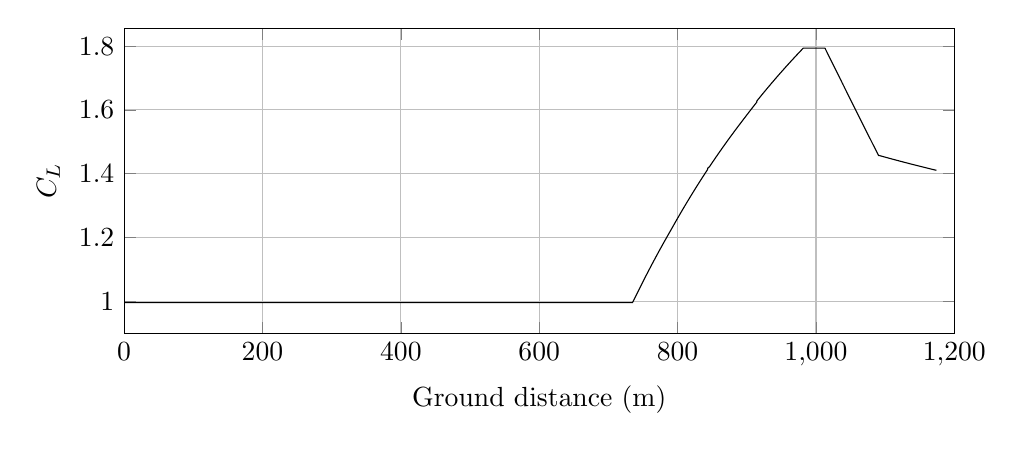
\begin{tikzpicture}

\begin{axis}[
width=\textwidth,
height=0.45\textwidth,
scaled ticks=false, tick label style={/pgf/number format/fixed},
xmin=0.0,
xmax=1200,
xlabel={Ground distance (m)},
xmajorgrids,
ymin=0.9,
ymax=1.856055169601142,
ylabel={$C_L$ },
ymajorgrids,
legend style={at={(1.03,0.5)},anchor=west,draw=black,fill=white,legend cell align=left}
]

\addplot [
color=black,
solid
]
table[row sep=crcr]{
1.3729668748938318E-8	0.9961283491653221\\
1.7493248493808052E-7	0.9961283491653221\\
1.4411937280317895E-6	0.9961283491653221\\
6.602995160656227E-5	0.9961283491653221\\
2.2740573828771224E-4	0.9961283491653221\\
4.8751428921765393E-4	0.9961283491653221\\
8.441986619835749E-4	0.9961283491653221\\
0.0012981647037285577	0.9961283491653221\\
0.0018484379050661159	0.9961283491653221\\
0.0024893731755424335	0.9961283491653221\\
0.0032286585096692284	0.9961283491653221\\
0.0040442418752796045	0.9961283491653221\\
0.004972762654474916	0.9961283491653221\\
0.005990910102221513	0.9961283491653221\\
0.007111389191545643	0.9961283491653221\\
0.008336865178450469	0.9961283491653221\\
0.009664633507451486	0.9961283491653221\\
0.011093815858158905	0.9961283491653221\\
0.01262066151120312	0.9961283491653221\\
0.01419454386807839	0.9961283491653221\\
0.015910782250193378	0.9961283491653221\\
0.017721549103721458	0.9961283491653221\\
0.019620507964630857	0.9961283491653221\\
0.02164969955342029	0.9961283491653221\\
0.023766550611781796	0.9961283491653221\\
0.025957065600157342	0.9961283491653221\\
0.028260861173784894	0.9961283491653221\\
0.030668466949245715	0.9961283491653221\\
0.0331489614440674	0.9961283491653221\\
0.03573888453685943	0.9961283491653221\\
0.038418765463712895	0.9961283491653221\\
0.04116679597872082	0.9961283491653221\\
0.044022059812866554	0.9961283491653221\\
0.04700053365173311	0.9961283491653221\\
0.050116649382181494	0.9961283491653221\\
0.0533021652593606	0.9961283491653221\\
0.056630220296749106	0.9961283491653221\\
0.05998688030085898	0.9961283491653221\\
0.06348077825220624	0.9961283491653221\\
0.06710848437295475	0.9961283491653221\\
0.07082346760424127	0.9961283491653221\\
0.07462944469130567	0.9961283491653221\\
0.07855413323217031	0.9961283491653221\\
0.08251243142992878	0.9961283491653221\\
0.08659905947434482	0.9961283491653221\\
0.09083545394947079	0.9961283491653221\\
0.09518096637774642	0.9961283491653221\\
0.099604438418047	0.9961283491653221\\
0.1041130762071252	0.9961283491653221\\
0.10871457033213175	0.9961283491653221\\
0.11350280915994052	0.9961283491653221\\
0.11836943512882261	0.9961283491653221\\
0.12328542045494376	0.9961283491653221\\
0.12830372217771202	0.9961283491653221\\
0.1334037067999082	0.9961283491653221\\
0.1386015897371753	0.9961283491653221\\
0.14405085578552257	0.9961283491653221\\
0.1495239325759128	0.9961283491653221\\
0.1550507392415454	0.9961283491653221\\
0.16073360491635535	0.9961283491653221\\
0.16659871679960742	0.9961283491653221\\
0.17244819595229793	0.9961283491653221\\
0.17848031195343078	0.9961283491653221\\
0.18466822548212042	0.9961283491653221\\
0.1909009608611748	0.9961283491653221\\
0.19716089737688902	0.9961283491653221\\
0.2035279375926986	0.9961283491653221\\
0.21017879584430066	0.9961283491653221\\
0.21687473998771628	0.9961283491653221\\
0.22354650324940833	0.9961283491653221\\
0.23036941414946865	0.9961283491653221\\
0.23737731412185503	0.9961283491653221\\
0.24449289925428264	0.9961283491653221\\
0.2517184892023243	0.9961283491653221\\
0.25908208279438383	0.9961283491653221\\
0.2664863589195283	0.9961283491653221\\
0.27399321582905467	0.9961283491653221\\
0.2816108016888421	0.9961283491653221\\
0.2893844725195981	0.9961283491653221\\
0.29747621078120867	0.9961283491653221\\
0.30547198304033185	0.9961283491653221\\
0.31373479402345694	0.9961283491653221\\
0.3220909744202328	0.9961283491653221\\
0.3305540912568814	0.9961283491653221\\
0.33895489345894936	0.9961283491653221\\
0.34753073012810576	0.9961283491653221\\
0.3563589175375672	0.9961283491653221\\
0.3652744752958731	0.9961283491653221\\
0.3742693918027593	0.9961283491653221\\
0.38350989122680823	0.9961283491653221\\
0.3927029292363896	0.9961283491653221\\
0.4020876366599533	0.9961283491653221\\
0.4115568217121528	0.9961283491653221\\
0.4212787852930122	0.9961283491653221\\
0.43089755178065414	0.9961283491653221\\
0.4408379299669313	0.9961283491653221\\
0.4510502611115679	0.9961283491653221\\
0.4612670224725215	0.9961283491653221\\
0.4715818614584312	0.9961283491653221\\
0.4818438670126082	0.9961283491653221\\
0.4922128554044626	0.9961283491653221\\
0.50273876067117	0.9961283491653221\\
0.5136516607865718	0.9961283491653221\\
0.5244310074213006	0.9961283491653221\\
0.5355751508210329	0.9961283491653221\\
0.5467126997993474	0.9961283491653221\\
0.5580479056656631	0.9961283491653221\\
0.5692960823995112	0.9961283491653221\\
0.5809945926573021	0.9961283491653221\\
0.5923626544035139	0.9961283491653221\\
0.6041922852715	0.9961283491653221\\
0.6160912669048675	0.9961283491653221\\
0.6280605196746807	0.9961283491653221\\
0.6403946506485891	0.9961283491653221\\
0.6525721787971039	0.9961283491653221\\
0.66504690021022	0.9961283491653221\\
0.6773535438897555	0.9961283491653221\\
0.6901462526606317	0.9961283491653221\\
0.703249873273524	0.9961283491653221\\
0.7159721017112175	0.9961283491653221\\
0.729053467210389	0.9961283491653221\\
0.7422988791228431	0.9961283491653221\\
0.756304272979474	0.9961283491653221\\
0.7696432036294076	0.9961283491653221\\
0.7832290250230658	0.9961283491653221\\
0.7969128825551131	0.9961283491653221\\
0.8108444209446342	0.9961283491653221\\
0.825043936786227	0.9961283491653221\\
0.8390802275180445	0.9961283491653221\\
0.8532340040587583	0.9961283491653221\\
0.8678101043696134	0.9961283491653221\\
0.8824320602344964	0.9961283491653221\\
0.8978006605470081	0.9961283491653221\\
0.9134572487531922	0.9961283491653221\\
0.9287391767029982	0.9961283491653221\\
0.9440564687433697	0.9961283491653221\\
0.9598871644713316	0.9961283491653221\\
0.9757786228365237	0.9961283491653221\\
0.9918217338879218	0.9961283491653221\\
1.0080608846667363	0.9961283491653221\\
1.0245900975307913	0.9961283491653221\\
1.040622085070809	0.9961283491653221\\
1.0571005809273983	0.9961283491653221\\
1.0736578999152901	0.9961283491653221\\
1.0902401336450098	0.9961283491653221\\
1.1073201062866707	0.9961283491653221\\
1.1241926772552646	0.9961283491653221\\
1.1416781667104252	0.9961283491653221\\
1.1588269484070954	0.9961283491653221\\
1.176440946845327	0.9961283491653221\\
1.1944819542445066	0.9961283491653221\\
1.2120125629913447	0.9961283491653221\\
1.2299306574276825	0.9961283491653221\\
1.2481120482032448	0.9961283491653221\\
1.2663536608165091	0.9961283491653221\\
1.2851425782117465	0.9961283491653221\\
1.3041313368869671	0.9961283491653221\\
1.3228236880779458	0.9961283491653221\\
1.3414329672940513	0.9961283491653221\\
1.3605066144349074	0.9961283491653221\\
1.3802534409605212	0.9961283491653221\\
1.3994872719307283	0.9961283491653221\\
1.4192016277101378	0.9961283491653221\\
1.439023460648384	0.9961283491653221\\
1.459347998039509	0.9961283491653221\\
1.4793256644936217	0.9961283491653221\\
1.4991489338326072	0.9961283491653221\\
1.5195196572175793	0.9961283491653221\\
1.5402684478761244	0.9961283491653221\\
1.5604570108688036	0.9961283491653221\\
1.5810331069622228	0.9961283491653221\\
1.6022712329181132	0.9961283491653221\\
1.623752316257296	0.9961283491653221\\
1.6452514305955401	0.9961283491653221\\
1.6664829631402025	0.9961283491653221\\
1.6886446033619715	0.9961283491653221\\
1.710607384244656	0.9961283491653221\\
1.7329417009553727	0.9961283491653221\\
1.7551421266962821	0.9961283491653221\\
1.7779085356585536	0.9961283491653221\\
1.800478286927734	0.9961283491653221\\
1.8236018329231238	0.9961283491653221\\
1.8462320784511883	0.9961283491653221\\
1.869621217116264	0.9961283491653221\\
1.8933146512119747	0.9961283491653221\\
1.9176856041472643	0.9961283491653221\\
1.9417713639512164	0.9961283491653221\\
1.9657098573982132	0.9961283491653221\\
1.9902165007163162	0.9961283491653221\\
2.014554050520948	0.9961283491653221\\
2.039479559407779	0.9961283491653221\\
2.0645497069116256	0.9961283491653221\\
2.090368502766882	0.9961283491653221\\
2.115564185269416	0.9961283491653221\\
2.140750230554602	0.9961283491653221\\
2.1667677015838267	0.9961283491653221\\
2.1927560352542175	0.9961283491653221\\
2.218891869133375	0.9961283491653221\\
2.245288939563828	0.9961283491653221\\
2.2712530964452817	0.9961283491653221\\
2.297933078351498	0.9961283491653221\\
2.324564104516777	0.9961283491653221\\
2.351466051806102	0.9961283491653221\\
2.378869922986878	0.9961283491653221\\
2.4061764715670764	0.9961283491653221\\
2.4343811693482102	0.9961283491653221\\
2.4622108821536663	0.9961283491653221\\
2.4906408044048067	0.9961283491653221\\
2.518892760285042	0.9961283491653221\\
2.5472153538550346	0.9961283491653221\\
2.5762492306032216	0.9961283491653221\\
2.605385308804288	0.9961283491653221\\
2.634725531238531	0.9961283491653221\\
2.6633424112287507	0.9961283491653221\\
2.6927188130915374	0.9961283491653221\\
2.7226962917814213	0.9961283491653221\\
2.7531675915664673	0.9961283491653221\\
2.7831412651501983	0.9961283491653221\\
2.8139174932165103	0.9961283491653221\\
2.8440331768075415	0.9961283491653221\\
2.874693215323904	0.9961283491653221\\
2.9059978681586376	0.9961283491653221\\
2.9372617813709034	0.9961283491653221\\
2.9684444504378202	0.9961283491653221\\
3.000072782687808	0.9961283491653221\\
3.031082587373527	0.9961283491653221\\
3.063213028467148	0.9961283491653221\\
3.0965739711585014	0.9961283491653221\\
3.1291175748240176	0.9961283491653221\\
3.161651640649506	0.9961283491653221\\
3.194791488147139	0.9961283491653221\\
3.2273698640351327	0.9961283491653221\\
3.261394174200582	0.9961283491653221\\
3.2942820372415875	0.9961283491653221\\
3.3276455142443044	0.9961283491653221\\
3.3625338428565543	0.9961283491653221\\
3.396526624461681	0.9961283491653221\\
3.4305511850311694	0.9961283491653221\\
3.4642094416894933	0.9961283491653221\\
3.498963551783903	0.9961283491653221\\
3.5341885134496573	0.9961283491653221\\
3.569804025802995	0.9961283491653221\\
3.605116576002147	0.9961283491653221\\
3.641338581546833	0.9961283491653221\\
3.677593698357855	0.9961283491653221\\
3.7132425573336665	0.9961283491653221\\
3.74957219375957	0.9961283491653221\\
3.7872650227149185	0.9961283491653221\\
3.825403000593508	0.9961283491653221\\
3.861987998097706	0.9961283491653221\\
3.899535703755137	0.9961283491653221\\
3.9366960368382165	0.9961283491653221\\
3.9756271117991435	0.9961283491653221\\
4.014715979923002	0.9961283491653221\\
4.053268843133694	0.9961283491653221\\
4.093111596873367	0.9961283491653221\\
4.132540645872048	0.9961283491653221\\
4.171686416589186	0.9961283491653221\\
4.211258480423352	0.9961283491653221\\
4.252585425594734	0.9961283491653221\\
4.29253892845542	0.9961283491653221\\
4.332839968385603	0.9961283491653221\\
4.372708537789018	0.9961283491653221\\
4.414379330316386	0.9961283491653221\\
4.455607216042212	0.9961283491653221\\
4.497336690654009	0.9961283491653221\\
4.53836773335787	0.9961283491653221\\
4.579767142935065	0.9961283491653221\\
4.621942908118227	0.9961283491653221\\
4.663798268780793	0.9961283491653221\\
4.705838036060712	0.9961283491653221\\
4.748491012675066	0.9961283491653221\\
4.791393968819099	0.9961283491653221\\
4.835700194867293	0.9961283491653221\\
4.879973298406089	0.9961283491653221\\
4.923250156511948	0.9961283491653221\\
4.967673596314626	0.9961283491653221\\
5.012954369117542	0.9961283491653221\\
5.057574526249477	0.9961283491653221\\
5.103280208347517	0.9961283491653221\\
5.148856018935929	0.9961283491653221\\
5.194350575362858	0.9961283491653221\\
5.240584094986199	0.9961283491653221\\
5.2871741484687504	0.9961283491653221\\
5.333122064003502	0.9961283491653221\\
5.3803318800233235	0.9961283491653221\\
5.4262712259485255	0.9961283491653221\\
5.473378197958581	0.9961283491653221\\
5.521938593493333	0.9961283491653221\\
5.570027890245774	0.9961283491653221\\
5.617746353771608	0.9961283491653221\\
5.665750363096816	0.9961283491653221\\
5.714883880069209	0.9961283491653221\\
5.763390205677501	0.9961283491653221\\
5.812817811268989	0.9961283491653221\\
5.861909274803731	0.9961283491653221\\
5.912134919389196	0.9961283491653221\\
5.962317560553064	0.9961283491653221\\
6.012727788730279	0.9961283491653221\\
6.0628236035803145	0.9961283491653221\\
6.113711068416594	0.9961283491653221\\
6.16497292765713	0.9961283491653221\\
6.216284706244114	0.9961283491653221\\
6.26834407822653	0.9961283491653221\\
6.320257064476769	0.9961283491653221\\
6.37351660191279	0.9961283491653221\\
6.426150862197664	0.9961283491653221\\
6.479030963436509	0.9961283491653221\\
6.532319340056288	0.9961283491653221\\
6.5857233987986845	0.9961283491653221\\
6.640834734692348	0.9961283491653221\\
6.695022999498724	0.9961283491653221\\
6.749720237657193	0.9961283491653221\\
6.804235758325081	0.9961283491653221\\
6.859728469301633	0.9961283491653221\\
6.916686079588434	0.9961283491653221\\
6.9732530286722305	0.9961283491653221\\
7.029531186664631	0.9961283491653221\\
7.086633318514238	0.9961283491653221\\
7.144155485034537	0.9961283491653221\\
7.202053129566568	0.9961283491653221\\
7.260126434764185	0.9961283491653221\\
7.317913145042743	0.9961283491653221\\
7.376682960996439	0.9961283491653221\\
7.435393721764624	0.9961283491653221\\
7.493838107271518	0.9961283491653221\\
7.552684475254578	0.9961283491653221\\
7.613252707151423	0.9961283491653221\\
7.672782806866918	0.9961283491653221\\
7.733397683408512	0.9961283491653221\\
7.795525081709004	0.9961283491653221\\
7.856013653786727	0.9961283491653221\\
7.91792172269443	0.9961283491653221\\
7.980110745884113	0.9961283491653221\\
8.041720670752433	0.9961283491653221\\
8.105229267009985	0.9961283491653221\\
8.167457523036095	0.9961283491653221\\
8.230908874360502	0.9961283491653221\\
8.293738919282273	0.9961283491653221\\
8.356235402336917	0.9961283491653221\\
8.42092378244627	0.9961283491653221\\
8.485671322837007	0.9961283491653221\\
8.549180898871484	0.9961283491653221\\
8.614596634551038	0.9961283491653221\\
8.680166762249144	0.9961283491653221\\
8.744770128469462	0.9961283491653221\\
8.812993689385827	0.9961283491653221\\
8.88005807777586	0.9961283491653221\\
8.94709863067661	0.9961283491653221\\
9.013172088448385	0.9961283491653221\\
9.079266506338545	0.9961283491653221\\
9.14748814890141	0.9961283491653221\\
9.215411293660388	0.9961283491653221\\
9.284579146198691	0.9961283491653221\\
9.353168277381275	0.9961283491653221\\
9.423753765537143	0.9961283491653221\\
9.492960052876374	0.9961283491653221\\
9.564123004975215	0.9961283491653221\\
9.634097601479446	0.9961283491653221\\
9.705672410878787	0.9961283491653221\\
9.776260200085993	0.9961283491653221\\
9.846607984572056	0.9961283491653221\\
9.918231435410593	0.9961283491653221\\
9.988851555070422	0.9961283491653221\\
10.060390022634245	0.9961283491653221\\
10.133279281833644	0.9961283491653221\\
10.205241085147751	0.9961283491653221\\
10.277820389603	0.9961283491653221\\
10.352558894167803	0.9961283491653221\\
10.42733258664746	0.9961283491653221\\
10.501815126481194	0.9961283491653221\\
10.576858173457808	0.9961283491653221\\
10.65303812840548	0.9961283491653221\\
10.729080272001735	0.9961283491653221\\
10.804841544893105	0.9961283491653221\\
10.881905013502095	0.9961283491653221\\
10.958396790746043	0.9961283491653221\\
11.035905069829102	0.9961283491653221\\
11.113160538490881	0.9961283491653221\\
11.192172636140572	0.9961283491653221\\
11.270076562295213	0.9961283491653221\\
11.350065490058778	0.9961283491653221\\
11.429008826667825	0.9961283491653221\\
11.50754237847364	0.9961283491653221\\
11.587076645554472	0.9961283491653221\\
11.668897725768986	0.9961283491653221\\
11.749734371708193	0.9961283491653221\\
11.830312384681939	0.9961283491653221\\
11.909862670519033	0.9961283491653221\\
11.990515423105418	0.9961283491653221\\
12.072973931530203	0.9961283491653221\\
12.155304175892073	0.9961283491653221\\
12.237018674011615	0.9961283491653221\\
12.320146069843414	0.9961283491653221\\
12.406770618003886	0.9961283491653221\\
12.489918686423398	0.9961283491653221\\
12.574493004618496	0.9961283491653221\\
12.660666896522624	0.9961283491653221\\
12.746500366216402	0.9961283491653221\\
12.832006837122272	0.9961283491653221\\
12.919285437479463	0.9961283491653221\\
13.00517529032821	0.9961283491653221\\
13.092301899261269	0.9961283491653221\\
13.179760097773386	0.9961283491653221\\
13.268594687119744	0.9961283491653221\\
13.357699529172354	0.9961283491653221\\
13.44829753340392	0.9961283491653221\\
13.537570218252604	0.9961283491653221\\
13.627322718831184	0.9961283491653221\\
13.718307212496544	0.9961283491653221\\
13.808540263830096	0.9961283491653221\\
13.899143852161355	0.9961283491653221\\
13.991564069206362	0.9961283491653221\\
14.085798171937814	0.9961283491653221\\
14.179213507883688	0.9961283491653221\\
14.271883316076963	0.9961283491653221\\
14.367546274622434	0.9961283491653221\\
14.459430863676705	0.9961283491653221\\
14.555010173556813	0.9961283491653221\\
14.648669731311681	0.9961283491653221\\
14.743773575674254	0.9961283491653221\\
14.839769774519894	0.9961283491653221\\
14.932807148196385	0.9961283491653221\\
15.026921440816679	0.9961283491653221\\
15.12275113649265	0.9961283491653221\\
15.222025232743288	0.9961283491653221\\
15.321078842653048	0.9961283491653221\\
15.417564225728565	0.9961283491653221\\
15.515758841369038	0.9961283491653221\\
15.613440509090129	0.9961283491653221\\
15.7107260301154	0.9961283491653221\\
15.81102223487273	0.9961283491653221\\
15.913565872734136	0.9961283491653221\\
16.012918321571746	0.9961283491653221\\
16.11222833737955	0.9961283491653221\\
16.216250800242257	0.9961283491653221\\
16.319159023020546	0.9961283491653221\\
16.421418004006803	0.9961283491653221\\
16.521675247646563	0.9961283491653221\\
16.62557290942481	0.9961283491653221\\
16.72731964230514	0.9961283491653221\\
16.830283223934416	0.9961283491653221\\
16.93464251494634	0.9961283491653221\\
17.038481620468637	0.9961283491653221\\
17.146497421123335	0.9961283491653221\\
17.252282308638982	0.9961283491653221\\
17.35724772858778	0.9961283491653221\\
17.464053904588297	0.9961283491653221\\
17.572390862630144	0.9961283491653221\\
17.680417629270814	0.9961283491653221\\
17.789707298693855	0.9961283491653221\\
17.899612520762552	0.9961283491653221\\
18.01027367065641	0.9961283491653221\\
18.121415095654797	0.9961283491653221\\
18.232428503320143	0.9961283491653221\\
18.34337337506409	0.9961283491653221\\
18.454877340220463	0.9961283491653221\\
18.56636189702322	0.9961283491653221\\
18.678405595805643	0.9961283491653221\\
18.7903363416971	0.9961283491653221\\
18.902391384512768	0.9961283491653221\\
19.01754810908954	0.9961283491653221\\
19.131359562866663	0.9961283491653221\\
19.247747682986713	0.9961283491653221\\
19.361628242251975	0.9961283491653221\\
19.477963464454028	0.9961283491653221\\
19.595742742603164	0.9961283491653221\\
19.71107288142779	0.9961283491653221\\
19.82767543183723	0.9961283491653221\\
19.944540068808188	0.9961283491653221\\
20.06171535440768	0.9961283491653221\\
20.179291418887807	0.9961283491653221\\
20.29729887224694	0.9961283491653221\\
20.417200571824914	0.9961283491653221\\
20.53676390826074	0.9961283491653221\\
20.65523768803314	0.9961283491653221\\
20.777063017363922	0.9961283491653221\\
20.896922101876633	0.9961283491653221\\
21.016777952410983	0.9961283491653221\\
21.13892104879462	0.9961283491653221\\
21.260534693274344	0.9961283491653221\\
21.382619708556632	0.9961283491653221\\
21.506306369043365	0.9961283491653221\\
21.631260758247265	0.9961283491653221\\
21.75556249187227	0.9961283491653221\\
21.87985606458615	0.9961283491653221\\
22.005925835680863	0.9961283491653221\\
22.130365724585275	0.9961283491653221\\
22.257477980325966	0.9961283491653221\\
22.38418119026224	0.9961283491653221\\
22.50885833858638	0.9961283491653221\\
22.636026948728087	0.9961283491653221\\
22.76367325110224	0.9961283491653221\\
22.89115382514759	0.9961283491653221\\
23.022452271734288	0.9961283491653221\\
23.149877274293033	0.9961283491653221\\
23.27873580881144	0.9961283491653221\\
23.408563766880334	0.9961283491653221\\
23.538692653979794	0.9961283491653221\\
23.671258756997098	0.9961283491653221\\
23.803210122669313	0.9961283491653221\\
23.93544283576786	0.9961283491653221\\
24.067241518013077	0.9961283491653221\\
24.19863541429976	0.9961283491653221\\
24.329449967727697	0.9961283491653221\\
24.46175612159181	0.9961283491653221\\
24.594763714591892	0.9961283491653221\\
24.72754053098891	0.9961283491653221\\
24.86208223890334	0.9961283491653221\\
24.99503410474967	0.9961283491653221\\
25.12831230627787	0.9961283491653221\\
25.265273024090206	0.9961283491653221\\
25.400650037308893	0.9961283491653221\\
25.536304655026747	0.9961283491653221\\
25.673594178904246	0.9961283491653221\\
25.80797730935859	0.9961283491653221\\
25.835159569235522	0.9961283491653221\\
25.83771752397454	0.9961283491653221\\
25.84157983658004	0.9961283491653221\\
25.854829339215996	0.9961283491653221\\
25.893215796826965	0.9961283491653221\\
25.973046119315796	0.9961283491653221\\
26.096262980671412	0.9961283491653221\\
26.224212718725603	0.9961283491653221\\
26.35313595194755	0.9961283491653221\\
26.481727686355264	0.9961283491653221\\
26.611118169629577	0.9961283491653221\\
26.74049186039369	0.9961283491653221\\
26.87228140714948	0.9961283491653221\\
27.003385008924262	0.9961283491653221\\
27.1358830905183	0.9961283491653221\\
27.265951877034226	0.9961283491653221\\
27.399105426781233	0.9961283491653221\\
27.53075869079712	0.9961283491653221\\
27.66387879779476	0.9961283491653221\\
27.79855889054391	0.9961283491653221\\
27.932132547760695	0.9961283491653221\\
28.06791767232785	0.9961283491653221\\
28.202763022922632	0.9961283491653221\\
28.339788243013793	0.9961283491653221\\
28.476803106655623	0.9961283491653221\\
28.61761981788422	0.9961283491653221\\
28.753907949775353	0.9961283491653221\\
28.89297195746854	0.9961283491653221\\
29.03211749902605	0.9961283491653221\\
29.17123509789927	0.9961283491653221\\
29.312253051611236	0.9961283491653221\\
29.454422317169097	0.9961283491653221\\
29.59523538430127	0.9961283491653221\\
29.737672170826222	0.9961283491653221\\
29.879173197948965	0.9961283491653221\\
30.02075470454991	0.9961283491653221\\
30.166674235301365	0.9961283491653221\\
30.308336095430334	0.9961283491653221\\
30.452640844036836	0.9961283491653221\\
30.597553881025625	0.9961283491653221\\
30.742967061600154	0.9961283491653221\\
30.888975484926362	0.9961283491653221\\
31.034653067922946	0.9961283491653221\\
31.180984070508003	0.9961283491653221\\
31.328351020411645	0.9961283491653221\\
31.476753455192622	0.9961283491653221\\
31.62661541983664	0.9961283491653221\\
31.774495604492607	0.9961283491653221\\
31.924944104961916	0.9961283491653221\\
32.07610067279926	0.9961283491653221\\
32.22631826848556	0.9961283491653221\\
32.37899942625752	0.9961283491653221\\
32.528514827654206	0.9961283491653221\\
32.68189139400266	0.9961283491653221\\
32.836069829938495	0.9961283491653221\\
32.99025509482905	0.9961283491653221\\
33.14574197930297	0.9961283491653221\\
33.30072558931056	0.9961283491653221\\
33.455047097713944	0.9961283491653221\\
33.610874563168906	0.9961283491653221\\
33.76926068144728	0.9961283491653221\\
33.92617323250643	0.9961283491653221\\
34.08448787244542	0.9961283491653221\\
34.24243160505006	0.9961283491653221\\
34.40316487172558	0.9961283491653221\\
34.56154208099588	0.9961283491653221\\
34.721775177117024	0.9961283491653221\\
34.88076970836556	0.9961283491653221\\
35.041349106451236	0.9961283491653221\\
35.20329621413198	0.9961283491653221\\
35.364886328651124	0.9961283491653221\\
35.529241615711214	0.9961283491653221\\
35.69117991651797	0.9961283491653221\\
35.85317319416103	0.9961283491653221\\
36.014854298354294	0.9961283491653221\\
36.18095311277159	0.9961283491653221\\
36.34443322746766	0.9961283491653221\\
36.51065106768533	0.9961283491653221\\
36.67635767082788	0.9961283491653221\\
36.842033683894186	0.9961283491653221\\
37.00823867836148	0.9961283491653221\\
37.17279029188734	0.9961283491653221\\
37.33951104811075	0.9961283491653221\\
37.50923941781488	0.9961283491653221\\
37.679358776579846	0.9961283491653221\\
37.845326083883435	0.9961283491653221\\
38.017144746304325	0.9961283491653221\\
38.1852030886141	0.9961283491653221\\
38.35804431104914	0.9961283491653221\\
38.52812920813831	0.9961283491653221\\
38.69960796987526	0.9961283491653221\\
38.87165793928378	0.9961283491653221\\
39.0423941506003	0.9961283491653221\\
39.21436971822614	0.9961283491653221\\
39.38727999643966	0.9961283491653221\\
39.558989012313546	0.9961283491653221\\
39.734752343022535	0.9961283491653221\\
39.908836167348156	0.9961283491653221\\
40.084555009291705	0.9961283491653221\\
40.259186798753746	0.9961283491653221\\
40.43324437115375	0.9961283491653221\\
40.61041052363379	0.9961283491653221\\
40.787318094191775	0.9961283491653221\\
40.96620398302343	0.9961283491653221\\
41.14141336180775	0.9961283491653221\\
41.31941103282654	0.9961283491653221\\
41.49571226203258	0.9961283491653221\\
41.67366972437729	0.9961283491653221\\
41.85219319429197	0.9961283491653221\\
42.03136872634711	0.9961283491653221\\
42.21293422072888	0.9961283491653221\\
42.39366932880948	0.9961283491653221\\
42.57479521797359	0.9961283491653221\\
42.75522531040919	0.9961283491653221\\
42.93775785970641	0.9961283491653221\\
43.11993568316029	0.9961283491653221\\
43.30336620712447	0.9961283491653221\\
43.48720879745599	0.9961283491653221\\
43.672226884455625	0.9961283491653221\\
43.85684130549208	0.9961283491653221\\
44.039851952877484	0.9961283491653221\\
44.22449378650157	0.9961283491653221\\
44.412385508552646	0.9961283491653221\\
44.59783063297877	0.9961283491653221\\
44.78525507043919	0.9961283491653221\\
44.973130075825196	0.9961283491653221\\
45.16145211071871	0.9961283491653221\\
45.34881478087516	0.9961283491653221\\
45.536017136752506	0.9961283491653221\\
45.724971990057284	0.9961283491653221\\
45.91416212467789	0.9961283491653221\\
46.10175434018815	0.9961283491653221\\
46.29356928918713	0.9961283491653221\\
46.48490977712943	0.9961283491653221\\
46.67744207882204	0.9961283491653221\\
46.869905949194575	0.9961283491653221\\
47.062749521718516	0.9961283491653221\\
47.25341437235973	0.9961283491653221\\
47.44508461154423	0.9961283491653221\\
47.63880095964302	0.9961283491653221\\
47.83356160493736	0.9961283491653221\\
48.025334057720784	0.9961283491653221\\
48.218846636819876	0.9961283491653221\\
48.41468711090302	0.9961283491653221\\
48.610449575687724	0.9961283491653221\\
48.80723286029129	0.9961283491653221\\
49.00124137999302	0.9961283491653221\\
49.20045899041696	0.9961283491653221\\
49.394243884198005	0.9961283491653221\\
49.59161211700324	0.9961283491653221\\
49.79144608231523	0.9961283491653221\\
49.99107345578199	0.9961283491653221\\
50.18996871950735	0.9961283491653221\\
50.388458331230495	0.9961283491653221\\
50.59191110395449	0.9961283491653221\\
50.79453916783869	0.9961283491653221\\
50.99530158869649	0.9961283491653221\\
51.19776583381373	0.9961283491653221\\
51.3996255264899	0.9961283491653221\\
51.599450409211	0.9961283491653221\\
51.80158475775707	0.9961283491653221\\
52.002311498730975	0.9961283491653221\\
52.2060805474067	0.9961283491653221\\
52.40811442127868	0.9961283491653221\\
52.61423073460446	0.9961283491653221\\
52.821749674584495	0.9961283491653221\\
53.03053110951893	0.9961283491653221\\
53.23753590773735	0.9961283491653221\\
53.44487707917263	0.9961283491653221\\
53.652063533093525	0.9961283491653221\\
53.85975522429668	0.9961283491653221\\
54.06844148636836	0.9961283491653221\\
54.278580968983874	0.9961283491653221\\
54.48685885904548	0.9961283491653221\\
54.69884126905886	0.9961283491653221\\
54.90975544393264	0.9961283491653221\\
55.12216013841277	0.9961283491653221\\
55.333080623240974	0.9961283491653221\\
55.5448885814986	0.9961283491653221\\
55.75594910746132	0.9961283491653221\\
55.968144975063936	0.9961283491653221\\
56.18150915317635	0.9961283491653221\\
56.394069348356695	0.9961283491653221\\
56.60950747146016	0.9961283491653221\\
56.82641599949238	0.9961283491653221\\
57.03980213394583	0.9961283491653221\\
57.25698083573829	0.9961283491653221\\
57.47353804711997	0.9961283491653221\\
57.6941706582635	0.9961283491653221\\
57.91229938529948	0.9961283491653221\\
58.12998527173144	0.9961283491653221\\
58.34905943653719	0.9961283491653221\\
58.56781345824973	0.9961283491653221\\
58.787998582886644	0.9961283491653221\\
59.011266007804366	0.9961283491653221\\
59.23368761368569	0.9961283491653221\\
59.456031473365414	0.9961283491653221\\
59.67976581221534	0.9961283491653221\\
59.90315377467765	0.9961283491653221\\
60.125192111546724	0.9961283491653221\\
60.349269227196444	0.9961283491653221\\
60.57220932044149	0.9961283491653221\\
60.79606803632835	0.9961283491653221\\
61.021718319759984	0.9961283491653221\\
61.25073295331903	0.9961283491653221\\
61.47770893732542	0.9961283491653221\\
61.70784367826464	0.9961283491653221\\
61.93740803875056	0.9961283491653221\\
62.1673491775543	0.9961283491653221\\
62.39648011888062	0.9961283491653221\\
62.62822464633953	0.9961283491653221\\
62.86094183422966	0.9961283491653221\\
63.090532789209604	0.9961283491653221\\
63.321616049163225	0.9961283491653221\\
63.554808975015874	0.9961283491653221\\
63.78685818650332	0.9961283491653221\\
64.0234762327251	0.9961283491653221\\
64.25652029988498	0.9961283491653221\\
64.49146565301734	0.9961283491653221\\
64.72768747885678	0.9961283491653221\\
64.96568125142531	0.9961283491653221\\
65.20057601391298	0.9961283491653221\\
65.43975061379945	0.9961283491653221\\
65.67719429610031	0.9961283491653221\\
65.91652243006087	0.9961283491653221\\
66.1565253585166	0.9961283491653221\\
66.39740384038885	0.9961283491653221\\
66.63777997854328	0.9961283491653221\\
66.87849958303539	0.9961283491653221\\
67.12349409848125	0.9961283491653221\\
67.36843544137562	0.9961283491653221\\
67.61129947098183	0.9961283491653221\\
67.85808619273692	0.9961283491653221\\
68.10323725880951	0.9961283491653221\\
68.3520146383799	0.9961283491653221\\
68.60099753692072	0.9961283491653221\\
68.84943315800746	0.9961283491653221\\
69.09793111574629	0.9961283491653221\\
69.34894754058863	0.9961283491653221\\
69.59791912239118	0.9961283491653221\\
69.84867626946473	0.9961283491653221\\
70.10496107302816	0.9961283491653221\\
70.35594730130109	0.9961283491653221\\
70.60854748652795	0.9961283491653221\\
70.8625286964371	0.9961283491653221\\
71.1182576034713	0.9961283491653221\\
71.37278964945165	0.9961283491653221\\
71.62944082734805	0.9961283491653221\\
71.88536754710964	0.9961283491653221\\
72.14250945057543	0.9961283491653221\\
72.40306402213687	0.9961283491653221\\
72.66241221953337	0.9961283491653221\\
72.92327110344874	0.9961283491653221\\
73.18657203154456	0.9961283491653221\\
73.45150557123125	0.9961283491653221\\
73.71756195569753	0.9961283491653221\\
73.97940051906463	0.9961283491653221\\
74.24514793127645	0.9961283491653221\\
74.51022759525631	0.9961283491653221\\
74.77823256031297	0.9961283491653221\\
75.04767613410795	0.9961283491653221\\
75.31682895458664	0.9961283491653221\\
75.58729746777243	0.9961283491653221\\
75.85729327570917	0.9961283491653221\\
76.13042767774209	0.9961283491653221\\
76.40299665611133	0.9961283491653221\\
76.67973301409052	0.9961283491653221\\
76.95360383527739	0.9961283491653221\\
77.22854206589327	0.9961283491653221\\
77.50692063517303	0.9961283491653221\\
77.78349662592461	0.9961283491653221\\
78.0616064362213	0.9961283491653221\\
78.33869545141144	0.9961283491653221\\
78.62238552181594	0.9961283491653221\\
78.90481169871467	0.9961283491653221\\
79.18659077494928	0.9961283491653221\\
79.4700201012688	0.9961283491653221\\
79.75774957869095	0.9961283491653221\\
80.04430580185078	0.9961283491653221\\
80.33432201731404	0.9961283491653221\\
80.62298533865851	0.9961283491653221\\
80.9130804606989	0.9961283491653221\\
81.20459144967842	0.9961283491653221\\
81.49650140842283	0.9961283491653221\\
81.79224544448738	0.9961283491653221\\
82.08455487090956	0.9961283491653221\\
82.37934996819865	0.9961283491653221\\
82.67580145620735	0.9961283491653221\\
82.97475550983006	0.9961283491653221\\
83.2734238134004	0.9961283491653221\\
83.57209772503273	0.9961283491653221\\
83.87419166445906	0.9961283491653221\\
84.17487194816226	0.9961283491653221\\
84.47686996876752	0.9961283491653221\\
84.78124993153034	0.9961283491653221\\
85.08776945017104	0.9961283491653221\\
85.39395758722245	0.9961283491653221\\
85.69833162305892	0.9961283491653221\\
86.01027818388755	0.9961283491653221\\
86.31658691867341	0.9961283491653221\\
86.62866814828641	0.9961283491653221\\
86.94043673469176	0.9961283491653221\\
87.2565990672368	0.9961283491653221\\
87.56980823017452	0.9961283491653221\\
87.88101387141376	0.9961283491653221\\
88.20007062892054	0.9961283491653221\\
88.51883409355145	0.9961283491653221\\
88.83509784148416	0.9961283491653221\\
89.15857089898353	0.9961283491653221\\
89.47772213402055	0.9961283491653221\\
89.80217214804901	0.9961283491653221\\
90.1263587278685	0.9961283491653221\\
90.44950966725051	0.9961283491653221\\
90.77764749859728	0.9961283491653221\\
91.10470504824352	0.9961283491653221\\
91.43769785174896	0.9961283491653221\\
91.76691749028419	0.9961283491653221\\
92.09386993524024	0.9961283491653221\\
92.42498248438446	0.9961283491653221\\
92.7581696617394	0.9961283491653221\\
93.09729153734631	0.9961283491653221\\
93.4312406900703	0.9961283491653221\\
93.76780571708736	0.9961283491653221\\
94.10390054156983	0.9961283491653221\\
94.43564317419558	0.9961283491653221\\
94.77291201930262	0.9961283491653221\\
95.10796951504997	0.9961283491653221\\
95.44708659079325	0.9961283491653221\\
95.78515592548297	0.9961283491653221\\
96.12311752311894	0.9961283491653221\\
96.46351490415591	0.9961283491653221\\
96.80669869710772	0.9961283491653221\\
97.14657639264556	0.9961283491653221\\
97.48763116340677	0.9961283491653221\\
97.8305814261901	0.9961283491653221\\
98.17013304046878	0.9961283491653221\\
98.51054009051404	0.9961283491653221\\
98.854181194619	0.9961283491653221\\
99.19205317796005	0.9961283491653221\\
99.53355440060989	0.9961283491653221\\
99.87198375587872	0.9961283491653221\\
100.2129389915628	0.9961283491653221\\
100.55335806642802	0.9961283491653221\\
100.89503335592528	0.9961283491653221\\
101.23693480167049	0.9961283491653221\\
101.57977298927813	0.9961283491653221\\
101.91842351185082	0.9961283491653221\\
102.26214655705948	0.9961283491653221\\
102.60487134933112	0.9961283491653221\\
102.94238410388857	0.9961283491653221\\
103.28139950825951	0.9961283491653221\\
103.61984226602698	0.9961283491653221\\
103.95406402656286	0.9961283491653221\\
104.29248504574807	0.9961283491653221\\
104.63112914593611	0.9961283491653221\\
104.96686613984221	0.9961283491653221\\
105.30464484937244	0.9961283491653221\\
105.64180205248229	0.9961283491653221\\
105.97704387437452	0.9961283491653221\\
106.31384964552919	0.9961283491653221\\
106.6489228444834	0.9961283491653221\\
106.98000007373659	0.9961283491653221\\
107.31456925364313	0.9961283491653221\\
107.38092108752608	0.9961283491653221\\
107.387754025128	0.9961283491653221\\
107.3946577511588	0.9961283491653221\\
107.39916951903444	0.9961283491653221\\
107.40247473215817	0.9961283491653221\\
107.40548301099807	0.9961283491653221\\
107.41901751964124	0.9961283491653221\\
107.47756267729525	0.9961283491653221\\
107.63696404402117	0.9961283491653221\\
107.95668166923352	0.9961283491653221\\
108.2571634635643	0.9961283491653221\\
108.55996775705782	0.9961283491653221\\
108.8616926844802	0.9961283491653221\\
109.16669292910967	0.9961283491653221\\
109.47218465327785	0.9961283491653221\\
109.78023369107405	0.9961283491653221\\
110.09061921742381	0.9961283491653221\\
110.4007971847821	0.9961283491653221\\
110.7125096545017	0.9961283491653221\\
111.02874540594937	0.9961283491653221\\
111.34670354521654	0.9961283491653221\\
111.664908557295	0.9961283491653221\\
111.98617551206428	0.9961283491653221\\
112.3078797039536	0.9961283491653221\\
112.63537393275391	0.9961283491653221\\
112.96267359383529	0.9961283491653221\\
113.28778388635178	0.9961283491653221\\
113.61823593045688	0.9961283491653221\\
113.94632344632586	0.9961283491653221\\
114.27926944824554	0.9961283491653221\\
114.61324422041562	0.9961283491653221\\
114.94750338770686	0.9961283491653221\\
115.28618013885716	0.9961283491653221\\
115.62544260296943	0.9961283491653221\\
115.9647508443766	0.9961283491653221\\
116.30617149460878	0.9961283491653221\\
116.65060078043697	0.9961283491653221\\
116.99863777637248	0.9961283491653221\\
117.34270613829636	0.9961283491653221\\
117.68983788345284	0.9961283491653221\\
118.04137408578512	0.9961283491653221\\
118.39343387684602	0.9961283491653221\\
118.74804854616337	0.9961283491653221\\
119.10520175440718	0.9961283491653221\\
119.46686684850098	0.9961283491653221\\
119.82660492256403	0.9961283491653221\\
120.19012449272657	0.9961283491653221\\
120.55217592908159	0.9961283491653221\\
120.91763124996498	0.9961283491653221\\
121.28719248968574	0.9961283491653221\\
121.65493622417088	0.9961283491653221\\
122.02513489718217	0.9961283491653221\\
122.39308995700384	0.9961283491653221\\
122.76618799735454	0.9961283491653221\\
123.1388017253943	0.9961283491653221\\
123.51256311114031	0.9961283491653221\\
123.88633794770595	0.9961283491653221\\
124.25665874611622	0.9961283491653221\\
124.63165231885978	0.9961283491653221\\
125.00664173256905	0.9961283491653221\\
125.38021625899401	0.9961283491653221\\
125.75512563345742	0.9961283491653221\\
126.13473977091255	0.9961283491653221\\
126.51299085225449	0.9961283491653221\\
126.8948287761801	0.9961283491653221\\
127.27325883095315	0.9961283491653221\\
127.64986999110431	0.9961283491653221\\
128.03053456382577	0.9961283491653221\\
128.40840086210045	0.9961283491653221\\
128.78830732782995	0.9961283491653221\\
129.16816802858597	0.9961283491653221\\
129.55114692916032	0.9961283491653221\\
129.92795862154003	0.9961283491653221\\
130.30814318938542	0.9961283491653221\\
130.68801179162523	0.9961283491653221\\
131.0673626953399	0.9961283491653221\\
131.44707508552267	0.9961283491653221\\
131.82575792285303	0.9961283491653221\\
132.20466209461676	0.9961283491653221\\
132.58549544797154	0.9961283491653221\\
132.96520261413826	0.9961283491653221\\
133.34413894748724	0.9961283491653221\\
133.72638850756363	0.9961283491653221\\
134.1049920954593	0.9961283491653221\\
134.48538249769342	0.9961283491653221\\
134.86277461399203	0.9961283491653221\\
135.2402386369938	0.9961283491653221\\
135.62109197355238	0.9961283491653221\\
135.9996509441208	0.9961283491653221\\
136.37968191797512	0.9961283491653221\\
136.76120583273502	0.9961283491653221\\
137.13951930881296	0.9961283491653221\\
137.51840340013064	0.9961283491653221\\
137.89819615735314	0.9961283491653221\\
138.27485697152616	0.9961283491653221\\
138.65420581933705	0.9961283491653221\\
139.03531375767642	0.9961283491653221\\
139.41296882619503	0.9961283491653221\\
139.79422155259	0.9961283491653221\\
140.17408835952057	0.9961283491653221\\
140.5488076998477	0.9961283491653221\\
140.92844631991198	0.9961283491653221\\
141.30483696429354	0.9961283491653221\\
141.68269541512387	0.9961283491653221\\
142.06058279783264	0.9961283491653221\\
142.43991695918288	0.9961283491653221\\
142.81695502902187	0.9961283491653221\\
143.19247254825046	0.9961283491653221\\
143.5733885276352	0.9961283491653221\\
143.94921103219775	0.9961283491653221\\
144.32621366107247	0.9961283491653221\\
144.70408630975157	0.9961283491653221\\
145.08263595865492	0.9961283491653221\\
145.46162624555404	0.9961283491653221\\
145.83827879615103	0.9961283491653221\\
146.21524500988596	0.9961283491653221\\
146.5934755401724	0.9961283491653221\\
146.9730259257883	0.9961283491653221\\
147.3547239944582	0.9961283491653221\\
147.73366854735332	0.9961283491653221\\
148.1136534850276	0.9961283491653221\\
148.49311509785633	0.9961283491653221\\
148.87144514206074	0.9961283491653221\\
149.25360190977045	0.9961283491653221\\
149.6334430260095	0.9961283491653221\\
150.01465687879528	0.9961283491653221\\
150.3940924716125	0.9961283491653221\\
150.77688175221402	0.9961283491653221\\
151.1561678741857	0.9961283491653221\\
151.5352572324847	0.9961283491653221\\
151.91884603110896	0.9961283491653221\\
152.3000376871389	0.9961283491653221\\
152.6837211891089	0.9961283491653221\\
153.06727641570347	0.9961283491653221\\
153.4514076737559	0.9961283491653221\\
153.83522357687116	0.9961283491653221\\
154.21637826964854	0.9961283491653221\\
154.6009164651564	0.9961283491653221\\
154.98403470202834	0.9961283491653221\\
155.36838747168406	0.9961283491653221\\
155.75158064164503	0.9961283491653221\\
156.13576662495046	0.9961283491653221\\
156.5218436740983	0.9961283491653221\\
156.90521285441474	0.9961283491653221\\
157.2916244593892	0.9961283491653221\\
157.6780020855428	0.9961283491653221\\
158.06299451159185	0.9961283491653221\\
158.4509000667514	0.9961283491653221\\
158.83830611621056	0.9961283491653221\\
159.22672413827297	0.9961283491653221\\
159.61474494524106	0.9961283491653221\\
160.0042372884319	0.9961283491653221\\
160.39552304382113	0.9961283491653221\\
160.78478895267375	0.9961283491653221\\
161.17517847278327	0.9961283491653221\\
161.56748129737286	0.9961283491653221\\
161.9609400214345	0.9961283491653221\\
162.35005274814932	0.9961283491653221\\
162.7425950916558	0.9961283491653221\\
163.13607830878885	0.9961283491653221\\
163.53170884953005	0.9961283491653221\\
163.92462594167722	0.9961283491653221\\
164.3198767210975	0.9961283491653221\\
164.7157696028566	0.9961283491653221\\
165.1115317336501	0.9961283491653221\\
165.50739628911128	0.9961283491653221\\
165.90698313288817	0.9961283491653221\\
166.30582458333038	0.9961283491653221\\
166.70591293613995	0.9961283491653221\\
167.1044701422045	0.9961283491653221\\
167.50226971352845	0.9961283491653221\\
167.9010833894181	0.9961283491653221\\
168.3004552315794	0.9961283491653221\\
168.70189335181743	0.9961283491653221\\
169.10576843973695	0.9961283491653221\\
169.50785881751284	0.9961283491653221\\
169.91045494783964	0.9961283491653221\\
170.31331810721775	0.9961283491653221\\
170.71648797717722	0.9961283491653221\\
171.11993291578136	0.9961283491653221\\
171.5247281229082	0.9961283491653221\\
171.92976094083576	0.9961283491653221\\
172.33690302624336	0.9961283491653221\\
172.74259563259648	0.9961283491653221\\
173.1509823323036	0.9961283491653221\\
173.55913088366435	0.9961283491653221\\
173.96636547491187	0.9961283491653221\\
174.37754484483776	0.9961283491653221\\
174.7874876782942	0.9961283491653221\\
175.2012500141185	0.9961283491653221\\
175.6112323385957	0.9961283491653221\\
176.02092514523684	0.9961283491653221\\
176.43326782420013	0.9961283491653221\\
176.8477920653399	0.9961283491653221\\
177.2627043459005	0.9961283491653221\\
177.67839640445425	0.9961283491653221\\
178.09047986160414	0.9961283491653221\\
178.50771992227516	0.9961283491653221\\
178.92514786216543	0.9961283491653221\\
179.34349041668827	0.9961283491653221\\
179.7634585539525	0.9961283491653221\\
180.18446825846002	0.9961283491653221\\
180.60425393302842	0.9961283491653221\\
181.0261226187801	0.9961283491653221\\
181.4483416261798	0.9961283491653221\\
181.87315445312532	0.9961283491653221\\
182.29527778821938	0.9961283491653221\\
182.72141514554897	0.9961283491653221\\
183.1481192716397	0.9961283491653221\\
183.57633821660988	0.9961283491653221\\
184.00592509150556	0.9961283491653221\\
184.43471922224091	0.9961283491653221\\
184.86359425785753	0.9961283491653221\\
185.29462923368334	0.9961283491653221\\
185.72590746205765	0.9961283491653221\\
186.15893531582464	0.9961283491653221\\
186.59473099205763	0.9961283491653221\\
187.03327531522774	0.9961283491653221\\
187.46972629616232	0.9961283491653221\\
187.90646428697016	0.9961283491653221\\
188.34682007573156	0.9961283491653221\\
188.7873444966949	0.9961283491653221\\
189.22841311150643	0.9961283491653221\\
189.6706369666947	0.9961283491653221\\
190.11352546522693	0.9961283491653221\\
190.55843868450165	0.9961283491653221\\
191.0032099177178	0.9961283491653221\\
191.4488342668783	0.9961283491653221\\
191.89679402644646	0.9961283491653221\\
192.34637901534325	0.9961283491653221\\
192.79928545122743	0.9961283491653221\\
193.2512724064709	0.9961283491653221\\
193.7017744692331	0.9961283491653221\\
194.15625995252321	0.9961283491653221\\
194.61155611404877	0.9961283491653221\\
195.0672219974316	0.9961283491653221\\
195.52585180825645	0.9961283491653221\\
195.98426342862024	0.9961283491653221\\
196.44494672064457	0.9961283491653221\\
196.9057535736029	0.9961283491653221\\
197.36967293120705	0.9961283491653221\\
197.83510384208427	0.9961283491653221\\
198.30342862028755	0.9961283491653221\\
198.7732043057544	0.9961283491653221\\
199.24099125426073	0.9961283491653221\\
199.71119060681792	0.9961283491653221\\
200.1825482927743	0.9961283491653221\\
200.65679322330254	0.9961283491653221\\
201.13270849114224	0.9961283491653221\\
201.61347762080612	0.9961283491653221\\
202.09583085583984	0.9961283491653221\\
202.57505536425464	0.9961283491653221\\
203.05779273540577	0.9961283491653221\\
203.54112852606227	0.9961283491653221\\
204.02652622166198	0.9961283491653221\\
204.51502737102567	0.9961283491653221\\
205.002477053986	0.9961283491653221\\
205.49362028927055	0.9961283491653221\\
205.98571877257524	0.9961283491653221\\
206.47986048819791	0.9961283491653221\\
206.9756485373277	0.9961283491653221\\
207.47509472353033	0.9961283491653221\\
207.98105643358775	0.9961283491653221\\
208.48540394416239	0.9961283491653221\\
208.99019975934863	0.9961283491653221\\
209.4981718386387	0.9961283491653221\\
210.0074085614305	0.9961283491653221\\
210.51733356743972	0.9961283491653221\\
211.0326447114959	0.9961283491653221\\
211.54741442472368	0.9961283491653221\\
212.06514182135783	0.9961283491653221\\
212.58880120479233	0.9961283491653221\\
213.11423767449816	0.9961283491653221\\
213.6375324332176	0.9961283491653221\\
214.1668747215242	0.9961283491653221\\
214.6965875774535	0.9961283491653221\\
215.22997734520317	0.9961283491653221\\
215.7686003837519	0.9961283491653221\\
216.30585839012286	0.9961283491653221\\
216.8511964964835	0.9961283491653221\\
217.39999653425627	0.9961283491653221\\
217.94624961891986	0.9961283491653221\\
218.50173638139336	0.9961283491653221\\
219.05616136113832	0.9961283491653221\\
219.61603320212004	0.9961283491653221\\
220.17996673649174	0.9961283491653221\\
220.75152408343223	0.9961283491653221\\
221.31978136773841	0.9961283491653221\\
221.8917718938588	0.9961283491653221\\
222.46939173565727	0.9961283491653221\\
223.05424878124148	0.9961283491653221\\
223.6353441191846	0.9961283491653221\\
224.2228469319029	0.9961283491653221\\
224.81981605125333	0.9961283491653221\\
225.414322731722	0.9961283491653221\\
226.00805957236628	0.9961283491653221\\
226.6058017780681	0.9961283491653221\\
227.21801255318616	0.9961283491653221\\
227.8254326298245	0.9961283491653221\\
228.4384631744503	0.9961283491653221\\
229.05630143576667	0.9961283491653221\\
229.67438980515863	0.9961283491653221\\
230.2952270741992	0.9961283491653221\\
230.91872450767323	0.9961283491653221\\
231.54134731806806	0.9961283491653221\\
232.16409178618352	0.9961283491653221\\
232.7899713961491	0.9961283491653221\\
233.4157347959749	0.9961283491653221\\
234.0352538000064	0.9961283491653221\\
234.65526828817934	0.9961283491653221\\
235.27154540161314	0.9961283491653221\\
235.88948672731453	0.9961283491653221\\
236.5049303841215	0.9961283491653221\\
237.1250162121333	0.9961283491653221\\
237.73667159687494	0.9961283491653221\\
238.3498254862601	0.9961283491653221\\
238.96060042013949	0.9961283491653221\\
239.56622141551122	0.9961283491653221\\
240.17389692315953	0.9961283491653221\\
240.77522869589131	0.9961283491653221\\
241.3760510240944	0.9961283491653221\\
241.97103412255802	0.9961283491653221\\
242.55850867503966	0.9961283491653221\\
243.1485861228365	0.9961283491653221\\
243.73646785224247	0.9961283491653221\\
244.31785335506692	0.9961283491653221\\
244.8989348386816	0.9961283491653221\\
245.47768348369902	0.9961283491653221\\
246.0511922890006	0.9961283491653221\\
246.62411578591679	0.9961283491653221\\
247.19560633997713	0.9961283491653221\\
247.7644393659644	0.9961283491653221\\
248.3330098290461	0.9961283491653221\\
248.89747941389504	0.9961283491653221\\
249.45778103766594	0.9961283491653221\\
250.01628073566417	0.9961283491653221\\
250.57389204323152	0.9961283491653221\\
251.1336441663857	0.9961283491653221\\
251.6846487775523	0.9961283491653221\\
252.2308345522173	0.9961283491653221\\
252.77975023333983	0.9961283491653221\\
253.32811243895696	0.9961283491653221\\
253.87118817792594	0.9961283491653221\\
254.4133651004234	0.9961283491653221\\
254.5214401390847	0.9961283491653221\\
254.83904570493053	0.9961283491653221\\
254.86071409967872	0.9961283491653221\\
254.8777656564992	0.9961283491653221\\
254.8928183932843	0.9961283491653221\\
254.90595982385685	0.9961283491653221\\
254.92002328132799	0.9961283491653221\\
254.9253543395315	0.9961283491653221\\
254.93130083623475	0.9961283491653221\\
254.96272950051815	0.9961283491653221\\
255.06810565549557	0.9961283491653221\\
255.36811297064412	0.9961283491653221\\
255.8525091010879	0.9961283491653221\\
256.3298916337542	0.9961283491653221\\
256.8075138750163	0.9961283491653221\\
257.2910565040604	0.9961283491653221\\
257.776804457902	0.9961283491653221\\
258.2651177463397	0.9961283491653221\\
258.75623965529917	0.9961283491653221\\
259.2479874402336	0.9961283491653221\\
259.7444495167766	0.9961283491653221\\
260.2424492273475	0.9961283491653221\\
260.7432593092137	0.9961283491653221\\
261.247422780654	0.9961283491653221\\
261.754557364599	0.9961283491653221\\
262.26667770433664	0.9961283491653221\\
262.7807572902842	0.9961283491653221\\
263.2953883103885	0.9961283491653221\\
263.81347250230294	0.9961283491653221\\
264.3373938048751	0.9961283491653221\\
264.8633427659006	0.9961283491653221\\
265.3982279044384	0.9961283491653221\\
265.93370762125517	0.9961283491653221\\
266.4705766429179	0.9961283491653221\\
267.01127382973925	0.9961283491653221\\
267.5541191433384	0.9961283491653221\\
268.1029054057184	0.9961283491653221\\
268.6568703707334	0.9961283491653221\\
269.2131991941809	0.9961283491653221\\
269.77965185696826	0.9961283491653221\\
270.34285319322	0.9961283491653221\\
270.91507878419327	0.9961283491653221\\
271.48758827041524	0.9961283491653221\\
272.06358557024134	0.9961283491653221\\
272.6484960186634	0.9961283491653221\\
273.2397139750577	0.9961283491653221\\
273.83320745420303	0.9961283491653221\\
274.43242914940197	0.9961283491653221\\
275.0332286766287	0.9961283491653221\\
275.64250383846434	0.9961283491653221\\
276.25103708843267	0.9961283491653221\\
276.86908599168135	0.9961283491653221\\
277.4915413086129	0.9961283491653221\\
278.11268743481435	0.9961283491653221\\
278.7426163600394	0.9961283491653221\\
279.37385128465223	0.9961283491653221\\
280.00811453798417	0.9961283491653221\\
280.6421164884222	0.9961283491653221\\
281.2831601515528	0.9961283491653221\\
281.9230740215264	0.9961283491653221\\
282.5681900985986	0.9961283491653221\\
283.2125319406723	0.9961283491653221\\
283.85385525840525	0.9961283491653221\\
284.4934544665398	0.9961283491653221\\
285.13663885290487	0.9961283491653221\\
285.77585929803354	0.9961283491653221\\
286.4160621525482	0.9961283491653221\\
287.0513871934386	0.9961283491653221\\
287.6815461591955	0.9961283491653221\\
288.3151143713146	0.9961283491653221\\
288.9440132428607	0.9961283491653221\\
289.57278910778643	0.9961283491653221\\
290.1987061412044	0.9961283491653221\\
290.8185328090791	0.9961283491653221\\
291.44381701046814	0.9961283491653221\\
292.06316956763783	0.9961283491653221\\
292.6799483649311	0.9961283491653221\\
293.29456956929107	0.9961283491653221\\
293.90507282969963	0.9961283491653221\\
294.51904351746816	0.9961283491653221\\
295.1242474102645	0.9961283491653221\\
295.7294372822977	0.9961283491653221\\
296.3326441035193	0.9961283491653221\\
296.93531837143473	0.9961283491653221\\
297.53662560756754	0.9961283491653221\\
298.13594882298116	0.9961283491653221\\
298.73169481180116	0.9961283491653221\\
299.3266408784582	0.9961283491653221\\
299.922114932661	0.9961283491653221\\
300.51213137957825	0.9961283491653221\\
301.1010124400823	0.9961283491653221\\
301.68603189258056	0.9961283491653221\\
302.2748125277259	0.9961283491653221\\
302.8590582136652	0.9961283491653221\\
303.44379480516704	0.9961283491653221\\
304.0290509058309	0.9961283491653221\\
304.6116737569222	0.9961283491653221\\
305.19373631536575	0.9961283491653221\\
305.7764921471378	0.9961283491653221\\
306.3580249849531	0.9961283491653221\\
306.9381490141882	0.9961283491653221\\
307.5139833341484	0.9961283491653221\\
308.09088922445255	0.9961283491653221\\
308.6675546961833	0.9961283491653221\\
309.2395460191327	0.9961283491653221\\
309.8148153885073	0.9961283491653221\\
310.3887595932547	0.9961283491653221\\
310.9575507782383	0.9961283491653221\\
311.5303285454054	0.9961283491653221\\
312.1036077080503	0.9961283491653221\\
312.6780685512481	0.9961283491653221\\
313.2471479783603	0.9961283491653221\\
313.81443099956607	0.9961283491653221\\
314.38461922677266	0.9961283491653221\\
314.9529717276515	0.9961283491653221\\
315.52447137304955	0.9961283491653221\\
316.09585476365055	0.9961283491653221\\
316.6635766630999	0.9961283491653221\\
317.2324945294489	0.9961283491653221\\
317.8014884261387	0.9961283491653221\\
318.37019165330537	0.9961283491653221\\
318.9369705786113	0.9961283491653221\\
319.50690112966265	0.9961283491653221\\
320.0739603849205	0.9961283491653221\\
320.6398790880884	0.9961283491653221\\
321.20391395290665	0.9961283491653221\\
321.7716639023572	0.9961283491653221\\
322.338484237663	0.9961283491653221\\
322.90542659378207	0.9961283491653221\\
323.47230992414404	0.9961283491653221\\
324.03724239724215	0.9961283491653221\\
324.60406116004583	0.9961283491653221\\
325.16943479275596	0.9961283491653221\\
325.7365942510148	0.9961283491653221\\
326.30046115927405	0.9961283491653221\\
326.8653941427267	0.9961283491653221\\
327.4306179230226	0.9961283491653221\\
327.99738905651475	0.9961283491653221\\
328.56121076675106	0.9961283491653221\\
329.1266162082277	0.9961283491653221\\
329.6914897277701	0.9961283491653221\\
330.2568653337778	0.9961283491653221\\
330.82614981214726	0.9961283491653221\\
331.3938100932787	0.9961283491653221\\
331.96132280869926	0.9961283491653221\\
332.5263354296127	0.9961283491653221\\
333.094384011873	0.9961283491653221\\
333.6625145702084	0.9961283491653221\\
334.23129658370976	0.9961283491653221\\
334.79884578809185	0.9961283491653221\\
335.36810819267475	0.9961283491653221\\
335.9387356031524	0.9961283491653221\\
336.50726769982157	0.9961283491653221\\
337.0760911342318	0.9961283491653221\\
337.6455614970556	0.9961283491653221\\
338.2131690194383	0.9961283491653221\\
338.78552497707926	0.9961283491653221\\
339.3551707031005	0.9961283491653221\\
339.9263953137104	0.9961283491653221\\
340.49770657658587	0.9961283491653221\\
341.07107296042966	0.9961283491653221\\
341.64488206821375	0.9961283491653221\\
342.2196981164169	0.9961283491653221\\
342.79128386247544	0.9961283491653221\\
343.36530385074616	0.9961283491653221\\
343.9384742998243	0.9961283491653221\\
344.5127320767282	0.9961283491653221\\
345.0871545928418	0.9961283491653221\\
345.6609880560121	0.9961283491653221\\
346.23676575911713	0.9961283491653221\\
346.8130197442814	0.9961283491653221\\
347.3897807520199	0.9961283491653221\\
347.9671406573249	0.9961283491653221\\
348.54468010889946	0.9961283491653221\\
349.1240420580384	0.9961283491653221\\
349.70684674265726	0.9961283491653221\\
350.28477816592056	0.9961283491653221\\
350.86571195144245	0.9961283491653221\\
351.44841136880564	0.9961283491653221\\
352.029838452439	0.9961283491653221\\
352.61193941085935	0.9961283491653221\\
353.1950613476878	0.9961283491653221\\
353.77635779818036	0.9961283491653221\\
354.36112156987554	0.9961283491653221\\
354.9462572164025	0.9961283491653221\\
355.5320128434072	0.9961283491653221\\
356.1213882444596	0.9961283491653221\\
356.70690251099427	0.9961283491653221\\
357.2913063799722	0.9961283491653221\\
357.88109115267446	0.9961283491653221\\
358.4695934955133	0.9961283491653221\\
359.06094251031095	0.9961283491653221\\
359.65215374289005	0.9961283491653221\\
360.24470845029396	0.9961283491653221\\
360.8364099959201	0.9961283491653221\\
361.4321266430708	0.9961283491653221\\
362.0241065966578	0.9961283491653221\\
362.6189376480745	0.9961283491653221\\
363.21395562380917	0.9961283491653221\\
363.81152989978864	0.9961283491653221\\
364.410289097789	0.9961283491653221\\
365.0062851890809	0.9961283491653221\\
365.60439491742204	0.9961283491653221\\
366.2041617720637	0.9961283491653221\\
366.8056239231415	0.9961283491653221\\
367.4070486628152	0.9961283491653221\\
368.00907376705277	0.9961283491653221\\
368.6144179601106	0.9961283491653221\\
369.2208348878655	0.9961283491653221\\
369.82496615199057	0.9961283491653221\\
370.4326754576117	0.9961283491653221\\
371.04303037748207	0.9961283491653221\\
371.6508693513399	0.9961283491653221\\
372.25899511893056	0.9961283491653221\\
372.86664845026814	0.9961283491653221\\
373.4753405379722	0.9961283491653221\\
374.0881004214027	0.9961283491653221\\
374.70105876160676	0.9961283491653221\\
375.3151346609259	0.9961283491653221\\
375.9298074887587	0.9961283491653221\\
376.5473278422053	0.9961283491653221\\
377.1659973922931	0.9961283491653221\\
377.78652602772513	0.9961283491653221\\
378.405253006595	0.9961283491653221\\
379.02846510544396	0.9961283491653221\\
379.6543690418463	0.9961283491653221\\
380.2811814650454	0.9961283491653221\\
380.90900588878685	0.9961283491653221\\
381.5337926225143	0.9961283491653221\\
382.1641103383158	0.9961283491653221\\
382.79101003686833	0.9961283491653221\\
383.4194385604271	0.9961283491653221\\
384.0528738277319	0.9961283491653221\\
384.68472673161864	0.9961283491653221\\
385.32042409439157	0.9961283491653221\\
385.9552738763366	0.9961283491653221\\
386.5917185244833	0.9961283491653221\\
387.2293049476492	0.9961283491653221\\
387.8719915461404	0.9961283491653221\\
388.5147956275654	0.9961283491653221\\
389.1559927194148	0.9961283491653221\\
389.7996463231178	0.9961283491653221\\
390.44590234406144	0.9961283491653221\\
391.09597692252225	0.9961283491653221\\
391.7432686139034	0.9961283491653221\\
392.39346837385165	0.9961283491653221\\
393.0475398239315	0.9961283491653221\\
393.7058991304724	0.9961283491653221\\
394.361103822721	0.9961283491653221\\
395.0207326851521	0.9961283491653221\\
395.6779623373923	0.9961283491653221\\
396.34250077971865	0.9961283491653221\\
397.00554118881405	0.9961283491653221\\
397.67183470834334	0.9961283491653221\\
398.339726786716	0.9961283491653221\\
399.0084117944432	0.9961283491653221\\
399.67978041179765	0.9961283491653221\\
400.3545844791679	0.9961283491653221\\
401.03042852988824	0.9961283491653221\\
401.70427614998994	0.9961283491653221\\
402.3900383946309	0.9961283491653221\\
403.0721085484811	0.9961283491653221\\
403.7597156579167	0.9961283491653221\\
404.4479287141618	0.9961283491653221\\
405.13417181133127	0.9961283491653221\\
405.821611865857	0.9961283491653221\\
406.516279969008	0.9961283491653221\\
407.20856037019735	0.9961283491653221\\
407.90496228146947	0.9961283491653221\\
408.60813973301015	0.9961283491653221\\
409.30909477003024	0.9961283491653221\\
410.0159249727094	0.9961283491653221\\
410.7222621184179	0.9961283491653221\\
411.42889803912226	0.9961283491653221\\
412.1445221092463	0.9961283491653221\\
412.85948143665576	0.9961283491653221\\
413.57607429314953	0.9961283491653221\\
414.2961289632634	0.9961283491653221\\
415.0202224913728	0.9961283491653221\\
415.7516092945767	0.9961283491653221\\
416.48174520642	0.9961283491653221\\
417.2165395849778	0.9961283491653221\\
417.95584650206695	0.9961283491653221\\
418.70066385533676	0.9961283491653221\\
419.4474344863693	0.9961283491653221\\
420.1971975293743	0.9961283491653221\\
420.94905936873386	0.9961283491653221\\
421.7065397747897	0.9961283491653221\\
422.46524085121166	0.9961283491653221\\
423.22783421796294	0.9961283491653221\\
424.00052336845647	0.9961283491653221\\
424.77464106215325	0.9961283491653221\\
425.5526338229564	0.9961283491653221\\
426.3361420323414	0.9961283491653221\\
427.1240873399694	0.9961283491653221\\
427.91997575833363	0.9961283491653221\\
428.7156559118979	0.9961283491653221\\
429.5236395760454	0.9961283491653221\\
430.32996506585414	0.9961283491653221\\
431.1427070038992	0.9961283491653221\\
431.9640394759042	0.9961283491653221\\
432.78798919576377	0.9961283491653221\\
433.6163068095833	0.9961283491653221\\
434.4571291863	0.9961283491653221\\
435.30647580489597	0.9961283491653221\\
436.15882992104855	0.9961283491653221\\
437.02624426800617	0.9961283491653221\\
437.9029226820204	0.9961283491653221\\
438.78614854244313	0.9961283491653221\\
439.67024663455084	0.9961283491653221\\
440.56773120111336	0.9961283491653221\\
441.48235207230107	0.9961283491653221\\
442.4002204784682	0.9961283491653221\\
443.33223312606856	0.9961283491653221\\
444.27489815443255	0.9961283491653221\\
445.2194332794703	0.9961283491653221\\
446.18852338773047	0.9961283491653221\\
447.1650199838215	0.9961283491653221\\
448.14212748617774	0.9961283491653221\\
449.12768736026055	0.9961283491653221\\
450.1265747229721	0.9961283491653221\\
451.1233791198257	0.9961283491653221\\
452.12675185924934	0.9961283491653221\\
453.122279117925	0.9961283491653221\\
454.12404193398254	0.9961283491653221\\
455.10741716602604	0.9961283491653221\\
456.0912402453123	0.9961283491653221\\
457.0600726957697	0.9961283491653221\\
458.02574672848687	0.9961283491653221\\
458.9811742371063	0.9961283491653221\\
459.92030846821945	0.9961283491653221\\
460.8449841241073	0.9961283491653221\\
461.76140669191216	0.9961283491653221\\
462.67950443365294	0.9961283491653221\\
463.5841081756621	0.9961283491653221\\
464.4750374462178	0.9961283491653221\\
465.36305549382246	0.9961283491653221\\
466.2426214242721	0.9961283491653221\\
467.11087102140766	0.9961283491653221\\
467.972515664415	0.9961283491653221\\
468.8289199517734	0.9961283491653221\\
469.6812048910498	0.9961283491653221\\
470.52465288198835	0.9961283491653221\\
471.3648989492757	0.9961283491653221\\
472.1972562785188	0.9961283491653221\\
473.02351832723116	0.9961283491653221\\
473.84502281296636	0.9961283491653221\\
474.65918124561415	0.9961283491653221\\
475.4690721424329	0.9961283491653221\\
476.2765662647138	0.9961283491653221\\
477.07988307769745	0.9961283491653221\\
477.879669879326	0.9961283491653221\\
478.67222991463916	0.9961283491653221\\
479.46064122917437	0.9961283491653221\\
480.24954501182856	0.9961283491653221\\
481.03289204196733	0.9961283491653221\\
481.81248299334845	0.9961283491653221\\
482.5909487329001	0.9961283491653221\\
483.36332192433474	0.9961283491653221\\
484.13567199637407	0.9961283491653221\\
484.89826718432596	0.9961283491653221\\
485.6616315157769	0.9961283491653221\\
486.42284286646895	0.9961283491653221\\
487.1811520213696	0.9961283491653221\\
487.9361606873513	0.9961283491653221\\
488.0862000462413	0.9961283491653221\\
488.51171643164344	0.9961283491653221\\
488.5204761820811	0.9961283491653221\\
488.52903187150355	0.9961283491653221\\
488.5724231989668	0.9961283491653221\\
488.7333329386644	0.9961283491653221\\
489.1829676407592	0.9961283491653221\\
489.92201730542024	0.9961283491653221\\
490.66351800838265	0.9961283491653221\\
491.41054832328416	0.9961283491653221\\
492.15902589552354	0.9961283491653221\\
492.91187486786794	0.9961283491653221\\
493.6674844916515	0.9961283491653221\\
494.42999445975477	0.9961283491653221\\
495.1950929544056	0.9961283491653221\\
495.9651930404774	0.9961283491653221\\
496.74308787518237	0.9961283491653221\\
497.5261952793585	0.9961283491653221\\
498.31138432739033	0.9961283491653221\\
499.1020549248467	0.9961283491653221\\
499.9002589962571	0.9961283491653221\\
500.7022456576933	0.9961283491653221\\
501.5090523514118	0.9961283491653221\\
502.3195686296764	0.9961283491653221\\
503.1412728054687	0.9961283491653221\\
503.96791165595073	0.9961283491653221\\
504.79933667522266	0.9961283491653221\\
505.6342741536124	0.9961283491653221\\
506.4786567385539	0.9961283491653221\\
507.3294610646867	0.9961283491653221\\
508.1886280826044	0.9961283491653221\\
509.0566685057569	0.9961283491653221\\
509.9302471646762	0.9961283491653221\\
510.81569126209695	0.9961283491653221\\
511.70598991448594	0.9961283491653221\\
512.6037304003676	0.9961283491653221\\
513.5118796507982	0.9961283491653221\\
514.4291534807439	0.9961283491653221\\
515.3600390678175	0.9961283491653221\\
516.3004539849924	0.9961283491653221\\
517.2526998274022	0.9961283491653221\\
518.2107513126712	0.9961283491653221\\
519.1813307606569	0.9961283491653221\\
520.1623982203746	0.9961283491653221\\
521.1517316571476	0.9961283491653221\\
522.1538934745424	0.9961283491653221\\
523.1627452385133	0.9961283491653221\\
524.1860415450778	0.9961283491653221\\
525.2158711392533	0.9961283491653221\\
526.2504308121668	0.9961283491653221\\
527.2883302419584	0.9961283491653221\\
528.3258670294849	0.9961283491653221\\
529.3618435825495	0.9961283491653221\\
530.3987031210379	0.9961283491653221\\
531.4292357253873	0.9961283491653221\\
532.4587746997697	0.9961283491653221\\
533.4803790381791	0.9961283491653221\\
534.4886941535024	0.9961283491653221\\
535.4990146464693	0.9961283491653221\\
536.49858152146	0.9961283491653221\\
537.4945670800385	0.9961283491653221\\
538.4857266971019	0.9961283491653221\\
539.4643922408397	0.9961283491653221\\
540.4408466042978	0.9961283491653221\\
541.4073512887883	0.9961283491653221\\
542.3675454779934	0.9961283491653221\\
543.3247545321008	0.9961283491653221\\
544.2728203002546	0.9961283491653221\\
545.2164036210195	0.9961283491653221\\
546.1519862921152	0.9961283491653221\\
547.085713551734	0.9961283491653221\\
548.0174011794822	0.9961283491653221\\
548.9407659306482	0.9961283491653221\\
549.8606896180515	0.9961283491653221\\
550.7763747922556	0.9961283491653221\\
551.6862938962734	0.9961283491653221\\
552.5907950941921	0.9961283491653221\\
553.4934340387069	0.9961283491653221\\
554.3942179487572	0.9961283491653221\\
555.2905714512424	0.9961283491653221\\
556.1806198022296	0.9961283491653221\\
557.0761623625008	0.9961283491653221\\
557.9664211267702	0.9961283491653221\\
558.8507021428259	0.9961283491653221\\
559.7317833695613	0.9961283491653221\\
560.6119683183686	0.9961283491653221\\
561.492052705531	0.9961283491653221\\
562.3682786477177	0.9961283491653221\\
563.2426881566412	0.9961283491653221\\
564.115643537162	0.9961283491653221\\
564.9871820290484	0.9961283491653221\\
565.8563825959563	0.9961283491653221\\
566.7235528033411	0.9961283491653221\\
567.584270942679	0.9961283491653221\\
568.4483693921954	0.9961283491653221\\
569.3106060737728	0.9961283491653221\\
570.1700847904979	0.9961283491653221\\
571.0351952022045	0.9961283491653221\\
571.8939669541594	0.9961283491653221\\
572.7543287099213	0.9961283491653221\\
573.6110025505288	0.9961283491653221\\
574.4649935180137	0.9961283491653221\\
575.3175338450419	0.9961283491653221\\
576.1698867816026	0.9961283491653221\\
577.0213826637028	0.9961283491653221\\
577.8680727740848	0.9961283491653221\\
578.7180079329755	0.9961283491653221\\
579.5696721712868	0.9961283491653221\\
580.4156816020864	0.9961283491653221\\
581.2665168977144	0.9961283491653221\\
582.1126680081018	0.9961283491653221\\
582.9591455118928	0.9961283491653221\\
583.8064789318607	0.9961283491653221\\
584.6542286785789	0.9961283491653221\\
585.4948244412594	0.9961283491653221\\
586.3417246297038	0.9961283491653221\\
587.1855807464744	0.9961283491653221\\
588.0265986951438	0.9961283491653221\\
588.8734637893597	0.9961283491653221\\
589.7168603849534	0.9961283491653221\\
590.5586538765217	0.9961283491653221\\
591.4001825944827	0.9961283491653221\\
592.2438475773395	0.9961283491653221\\
593.0851928547504	0.9961283491653221\\
593.9280989632321	0.9961283491653221\\
594.7675466432647	0.9961283491653221\\
595.6096308746946	0.9961283491653221\\
596.4514038986238	0.9961283491653221\\
597.2922019333205	0.9961283491653221\\
598.1349633294326	0.9961283491653221\\
598.9708006967505	0.9961283491653221\\
599.8120854921594	0.9961283491653221\\
600.6487319653024	0.9961283491653221\\
601.4916625299238	0.9961283491653221\\
602.3315284242424	0.9961283491653221\\
603.1736324668191	0.9961283491653221\\
604.0146021029152	0.9961283491653221\\
604.8562691644076	0.9961283491653221\\
605.6985293092685	0.9961283491653221\\
606.5396352413236	0.9961283491653221\\
607.3812473670234	0.9961283491653221\\
608.2282356425842	0.9961283491653221\\
609.071586812463	0.9961283491653221\\
609.9140605750129	0.9961283491653221\\
610.7571275639477	0.9961283491653221\\
611.5971208981819	0.9961283491653221\\
612.4401319726896	0.9961283491653221\\
613.2845388540611	0.9961283491653221\\
614.1256927332543	0.9961283491653221\\
614.9658057982008	0.9961283491653221\\
615.809381440368	0.9961283491653221\\
616.6510418700914	0.9961283491653221\\
617.4977885388885	0.9961283491653221\\
618.3409372825265	0.9961283491653221\\
619.1853522868191	0.9961283491653221\\
620.032739423475	0.9961283491653221\\
620.8817273423131	0.9961283491653221\\
621.7284899757803	0.9961283491653221\\
622.5750061701701	0.9961283491653221\\
623.420978417789	0.9961283491653221\\
624.2715579920352	0.9961283491653221\\
625.1196713352376	0.9961283491653221\\
625.9707674108615	0.9961283491653221\\
626.8241405419658	0.9961283491653221\\
627.6726982122786	0.9961283491653221\\
628.5271926633845	0.9961283491653221\\
629.3799306278815	0.9961283491653221\\
630.2325528441272	0.9961283491653221\\
631.0857047944301	0.9961283491653221\\
631.940664311076	0.9961283491653221\\
632.7948057335088	0.9961283491653221\\
633.651727855909	0.9961283491653221\\
634.5112308430892	0.9961283491653221\\
635.3674599429112	0.9961283491653221\\
636.2285461826939	0.9961283491653221\\
637.085512161704	0.9961283491653221\\
637.9460480045709	0.9961283491653221\\
638.8049820906238	0.9961283491653221\\
639.6665226991229	0.9961283491653221\\
640.5341106053427	0.9961283491653221\\
641.3967343276511	0.9961283491653221\\
642.2595607087173	0.9961283491653221\\
643.1283827459029	0.9961283491653221\\
643.9963963700948	0.9961283491653221\\
644.8636955422669	0.9961283491653221\\
645.7311525463213	0.9961283491653221\\
646.5993350397168	0.9961283491653221\\
647.4654590565026	0.9961283491653221\\
648.3352448659641	0.9961283491653221\\
649.2075542815417	0.9961283491653221\\
650.0839485755912	0.9961283491653221\\
650.9554499703986	0.9961283491653221\\
651.8282765710103	0.9961283491653221\\
652.7033794423714	0.9961283491653221\\
653.5814404707689	0.9961283491653221\\
654.4626309653659	0.9961283491653221\\
655.3438698878938	0.9961283491653221\\
656.2243785605665	0.9961283491653221\\
657.1037768196804	0.9961283491653221\\
657.9874029598966	0.9961283491653221\\
658.8674593193869	0.9961283491653221\\
659.757941979678	0.9961283491653221\\
660.6435303157025	0.9961283491653221\\
661.5311341225449	0.9961283491653221\\
662.4200935231033	0.9961283491653221\\
663.3089411002388	0.9961283491653221\\
664.2060638247669	0.9961283491653221\\
665.1007876506449	0.9961283491653221\\
666.0007891903767	0.9961283491653221\\
666.8981912186159	0.9961283491653221\\
667.7966827765686	0.9961283491653221\\
668.6974697079006	0.9961283491653221\\
669.5984035046772	0.9961283491653221\\
670.5006498517291	0.9961283491653221\\
671.400297551947	0.9961283491653221\\
672.3046894710374	0.9961283491653221\\
673.2073460646618	0.9961283491653221\\
674.1164911681556	0.9961283491653221\\
675.029648290325	0.9961283491653221\\
675.9426229643379	0.9961283491653221\\
676.8551394692824	0.9961283491653221\\
677.7714960997228	0.9961283491653221\\
678.6893030117942	0.9961283491653221\\
679.606343940523	0.9961283491653221\\
680.5229160692668	0.9961283491653221\\
681.4488391090454	0.9961283491653221\\
682.3714272041591	0.9961283491653221\\
683.2980383823431	0.9961283491653221\\
684.226517562581	0.9961283491653221\\
685.1567310396995	0.9961283491653221\\
686.0884445936897	0.9961283491653221\\
687.0237358524344	0.9961283491653221\\
687.958573277177	0.9961283491653221\\
688.9014872463613	0.9961283491653221\\
689.8426155382874	0.9961283491653221\\
690.7862819541851	0.9961283491653221\\
691.7263519109106	0.9961283491653221\\
692.6694041952526	0.9961283491653221\\
693.6148004882284	0.9961283491653221\\
694.5623931947416	0.9961283491653221\\
695.5103234838102	0.9961283491653221\\
696.4637862851532	0.9961283491653221\\
697.4159994031179	0.9961283491653221\\
698.3709920206657	0.9961283491653221\\
699.3282582409213	0.9961283491653221\\
700.292441896135	0.9961283491653221\\
701.2534802903324	0.9961283491653221\\
702.2248443243825	0.9961283491653221\\
703.1924289478354	0.9961283491653221\\
704.1607218569004	0.9961283491653221\\
705.1354458572257	0.9961283491653221\\
706.1127889615061	0.9961283491653221\\
707.0907942698741	0.9961283491653221\\
708.0731923449084	0.9961283491653221\\
709.0629858409125	0.9961283491653221\\
710.0534715455888	0.9961283491653221\\
711.0460001450474	0.9961283491653221\\
712.0411864745752	0.9961283491653221\\
713.0382054874503	0.9961283491653221\\
714.0366612236728	0.9961283491653221\\
715.0381882253694	0.9961283491653221\\
716.0425812425417	0.9961283491653221\\
717.0457260869603	0.9961283491653221\\
718.0590756109059	0.9961283491653221\\
719.0706439975677	0.9961283491653221\\
720.089567240296	0.9961283491653221\\
721.1080678495689	0.9961283491653221\\
722.1331533899263	0.9961283491653221\\
723.1616655692073	0.9961283491653221\\
724.1869176305613	0.9961283491653221\\
725.2178150549971	0.9961283491653221\\
726.2571035621181	0.9961283491653221\\
727.2992238360534	0.9961283491653221\\
728.3445371079367	0.9961283491653221\\
729.3877173938058	0.9961283491653221\\
730.4439811596706	0.9961283491653221\\
731.5042750922753	0.9961283491653221\\
732.5663669130686	0.9961283491653221\\
733.6326947685191	0.9961283491653221\\
733.8211736644284	0.9961283491653221\\
734.7061623538141	0.9961283491653221\\
735.77972211104	1.0000934357177427\\
736.8597554668804	1.0048904352899302\\
737.9473943285598	1.0097008906648326\\
739.0420830971909	1.0145296091078786\\
740.1379463777293	1.0193738674651152\\
741.2424131466432	1.0242075169910538\\
742.3453110739747	1.0290632226280405\\
743.4609443042868	1.033896114964206\\
744.5778560692177	1.0387687836786557\\
745.7019221899436	1.043630884645633\\
746.8308160852102	1.04850791526638\\
747.9663440023166	1.053389574733082\\
749.1103750114096	1.058283503734896\\
750.2587893948835	1.0631975085457361\\
751.4186822794172	1.0681136579322525\\
752.5900615439714	1.0730620918833258\\
753.7613001043926	1.0780424130925461\\
754.9393416675725	1.0830049406588536\\
756.1231123340335	1.0879790644870688\\
757.3239558518128	1.0929600425516561\\
758.532657447578	1.0979952481931288\\
759.7463952343887	1.1030455125131822\\
760.9713672230896	1.1080988196180053\\
762.2068142645112	1.113180729813239\\
763.4490063867679	1.118287685116989\\
764.7089231587418	1.12340394039003\\
765.9742725357778	1.12857431921912\\
767.2542197724972	1.1337478641864815\\
768.5451896924362	1.1389617390092712\\
769.8526623059349	1.1442008632063723\\
771.1742660401885	1.1494869716505822\\
772.5138766216689	1.154809848643796\\
773.8699204212141	1.160184479306193\\
775.2398101211274	1.1656038339195605\\
776.6407515063277	1.1710569446858632\\
778.0643282406966	1.1766114550659201\\
779.51521592621	1.1822327600564888\\
780.9812777034635	1.1879382527850881\\
782.4766032934936	1.1936791976785506\\
783.9962592491672	1.1995098856440003\\
785.541782770895	1.2054098285580535\\
787.11403181337	1.2113838643824875\\
788.6985585547895	1.2174341045374972\\
790.2895831920048	1.2235039826934235\\
791.885466260959	1.2295709791737341\\
793.4645337669594	1.2356286892250543\\
795.0285819385472	1.241595153169392\\
796.5656021589043	1.2474781452138357\\
798.0741893031925	1.253233625600663\\
799.5595683773756	1.2588578427389598\\
801.0208868100456	1.2643716986745233\\
802.4604112734999	1.2697732710473488\\
803.8852217844144	1.2750721382598535\\
805.2851159577167	1.2802953515930229\\
806.6631628561693	1.285406441156858\\
808.0210015295147	1.2904177604112712\\
809.36331798734	1.2953362805300488\\
810.6936303132454	1.300179848465242\\
812.0153795948233	1.3049618373004432\\
813.3206523532529	1.3096951408907676\\
814.6131010077706	1.3143519629784401\\
815.8925494572957	1.3189460164718052\\
817.1602900511036	1.3234772562529455\\
818.420868941459	1.327950816600088\\
819.6729749481467	1.3323831943688855\\
820.9150742159486	1.3367701357732655\\
822.1466772958156	1.3411066702704268\\
823.3683443539207	1.3453915293576322\\
824.5842321865659	1.3496270996377944\\
825.7983938518059	1.3538281576674291\\
827.0031365246884	1.3580089212326647\\
828.2024666198965	1.3621431195699159\\
829.3890602246352	1.3662448382639396\\
830.567496364278	1.370289364884108\\
831.7456776330071	1.3742927414461268\\
832.9188317246885	1.3782820477859503\\
834.0871287167467	1.3822412440710787\\
835.2499911808213	1.386171121951794\\
836.4014202376648	1.3900699577567834\\
837.5502975010666	1.3939179375030804\\
838.6966391301326	1.3977450586316138\\
839.8357405002248	1.4015515046569564\\
840.9700676262653	1.4053218360500808\\
842.0994961090571	1.4090644624977124\\
843.2221572738147	1.4127791701618904\\
843.4472747372179	1.416460030867914\\
843.5997917452933	1.4171959701092582\\
844.0975306988385	1.4176942650748527\\
844.1426154340434	1.4193196326706903\\
844.1535062092589	1.4194666686073205\\
844.1647183827226	1.4195021827846594\\
844.2315016468451	1.4195387439140925\\
844.5168666100187	1.4197565040667186\\
845.5496659779133	1.42068677452386\\
846.7027466589905	1.4240503901776105\\
847.8614981113487	1.42779487326777\\
849.0295217421842	1.4315457358729682\\
850.1978684970168	1.4353144650779353\\
851.3840200423074	1.4390720444154919\\
852.5715619410746	1.4428745384814312\\
853.7662794273785	1.446669002335148\\
854.9703373664927	1.450473861380035\\
856.1822390739135	1.454295809404385\\
857.3999930333648	1.4581298681901484\\
858.6328028043085	1.4619695630029663\\
859.8686841683191	1.4658436747046992\\
861.1196993299131	1.4697142537142946\\
862.3778777992711	1.4736188940643502\\
863.6522046172515	1.4775323798862638\\
864.9366869271196	1.48148237957751\\
866.2293333426785	1.485449921165673\\
867.5330534493423	1.4894286050870962\\
868.8463297117023	1.493427145878933\\
870.1856166493892	1.4974406051141802\\
871.53475990229	1.5015188211322896\\
872.8944570669319	1.5056119958291108\\
874.2693831805398	1.5097219738388747\\
875.6668405786718	1.513862543032958\\
877.0776088469529	1.5180551597277954\\
878.5054345928656	1.5222715773608364\\
879.9612127065129	1.5265225639206188\\
881.4297958979789	1.5308399058679096\\
882.9185677118544	1.5351779734512665\\
884.427607387707	1.5395581138926548\\
885.9608391360387	1.5439799264595653\\
887.516579269239	1.548454220188167\\
889.0827093301257	1.552975318580377\\
890.6766955363296	1.5575074362258183\\
892.2947802834587	1.5621006025535187\\
893.9204127139126	1.5667431079043261\\
895.5522512155646	1.5713868917792189\\
897.182287492519	1.5760279646129973\\
898.8019784039627	1.5806435343890892\\
900.4243656773872	1.5852097011767965\\
902.0397717992594	1.5897635486295176\\
903.6391293658623	1.5942780472567644\\
905.2144447455985	1.5987283342167138\\
906.776020749794	1.603092948397919\\
908.3239852658635	1.6074012513422722\\
909.8591153857867	1.6116541649774598\\
911.3729197618359	1.6158543715574105\\
912.8708118465968	1.6199792621757827\\
914.3532544050483	1.624044316258955\\
914.5764370031209	1.6280513849558638\\
914.799622279447	1.6286524251971775\\
915.0219469919532	1.6292531158576127\\
915.2429293907019	1.629851135313029\\
915.4494399268738	1.6304451929349952\\
915.6657354268041	1.6310000219607796\\
915.8893261083103	1.6315808199754165\\
916.1102206818305	1.6321808610491182\\
916.3310306518842	1.6327733148219745\\
916.5239840542688	1.6333651941462388\\
916.7119349620848	1.6338821037354192\\
916.9290240526063	1.634385354452809\\
917.1503684330119	1.6349663309961917\\
917.3747914970045	1.63555835366519\\
917.5976910251479	1.6361582577216236\\
917.8199140969286	1.6367537345049317\\
918.0422592654947	1.6373470530614904\\
918.2669881165957	1.63794034758057\\
918.4919558582405	1.6385396486192856\\
918.710957828139	1.6391392291094926\\
918.9285612746951	1.6397225622153955\\
919.1511937883038	1.640301833832254\\
919.3747033413151	1.640894150613578\\
919.5879722727698	1.6414884497788185\\
919.8123120825326	1.6420551850117069\\
920.0348625005847	1.6426510015141362\\
920.2473729973058	1.6432417145819753\\
920.4628264256355	1.6438054474520198\\
920.6853154443443	1.6443766651470137\\
920.9115180658005	1.6449661985195263\\
921.1372098064328	1.6455652184315177\\
921.3556797021943	1.6461625276879925\\
921.5797940196967	1.6467403793299946\\
921.8011379596135	1.6473328171203416\\
922.0235736317295	1.6479175849546808\\
922.2358916059352	1.6485048928767925\\
922.4618628254866	1.649065157924579\\
922.6857363551121	1.6496611148213418\\
922.910452555946	1.6502511870092318\\
923.1369125502531	1.6508431296999422\\
923.3565891788057	1.6514393114135402\\
923.5813963028193	1.6520172899036147\\
923.808323212618	1.6526084231109202\\
924.035255162044	1.653204775783454\\
924.2624876085163	1.6538007843414064\\
924.4865972922146	1.654397224523068\\
924.7131428956366	1.6549851155993076\\
924.9409160528157	1.6555790448704748\\
925.1478619916898	1.6561758352826708\\
925.3589724844212	1.6567177325291207\\
925.5779482737839	1.657270232633615\\
925.8021151150083	1.657842997151319\\
926.0189342515348	1.6584290005018216\\
926.2352852848132	1.6589954617867306\\
926.460916472789	1.659560377121529\\
926.6855807608188	1.6601491869274065\\
926.9084006430171	1.6607351250548799\\
927.1380396793584	1.6613159091251792\\
927.3511637045967	1.661914115353882\\
927.5625613532945	1.6624689662864527\\
927.7626258496853	1.6630190140937895\\
927.9922519373195	1.6635392849768464\\
928.2223105039632	1.6641361133383465\\
928.4514492528438	1.664733704391221\\
928.6759401579927	1.6653285459948624\\
928.9059648335353	1.6659109711028577\\
929.135728739433	1.6665074001699534\\
929.3677235920431	1.667102792771061\\
929.5927087076045	1.667703603069564\\
929.8151623115527	1.668285905339552\\
930.0387136731115	1.6688613154577303\\
930.2562635210654	1.6694392269773832\\
930.4870420540437	1.670001294115461\\
930.7120165682563	1.6705971969754967\\
930.9232156915248	1.6711777616332906\\
931.1540178380558	1.6717224573199314\\
931.3809720063389	1.6723173781423335\\
931.6124392984959	1.6729020263943215\\
931.8426030941464	1.6734979451085983\\
932.0749758420095	1.6740901482406647\\
932.3045731316224	1.6746876737090792\\
932.5365835525797	1.6752777028688395\\
932.7593532341991	1.67587357418602\\
932.9908686785309	1.676445365589869\\
933.2218454557235	1.6770392571101165\\
933.4535875247623	1.677631407419438\\
933.6859368023786	1.6782251600770248\\
933.9174722324567	1.678820107038327\\
934.1509854258338	1.679412609418387\\
934.3848255183723	1.6800098104222303\\
934.6121111816356	1.6806074818369212\\
934.8352689553647	1.6811880459833028\\
935.0706812186868	1.6817577275301931\\
935.2924331480774	1.682358340296504\\
935.5269279876188	1.6829237542231081\\
935.7621964505183	1.6835213112912175\\
935.9747446984265	1.684120472077245\\
936.1917134894072	1.6846614404619396\\
936.4259500945711	1.685213352569657\\
936.6556667582281	1.6858088497094372\\
936.8901369560956	1.6863924989471495\\
937.1252457200787	1.6869878676473984\\
937.356170731281	1.687584492159852\\
937.591620305863	1.6881701404771414\\
937.8278363850648	1.6887669030426333\\
938.058369147308	1.689365240355118\\
938.294412759139	1.6899488224614951\\
938.5312670698283	1.6905459949984263\\
938.7690614408684	1.6911448495086263\\
939.0060806919705	1.6917457093575057\\
939.2428381297914	1.6923442393945214\\
939.4795667490923	1.6929417389231252\\
939.7163742450125	1.6935387970875553\\
939.9543551228912	1.694135685767729\\
940.1911969245239	1.694735161847086\\
940.4165609718659	1.6953313989088348\\
940.6556700481722	1.695898392628209\\
940.891562301463	1.6964996129714454\\
941.1159545693788	1.6970923760719419\\
941.3372218555476	1.6976558964339663\\
941.5755073800656	1.698211244871032\\
941.8163050323112	1.698808960450363\\
942.0483036745413	1.6994126028395302\\
942.2869511002548	1.699993824276734\\
942.5212625025943	1.7005913414385692\\
942.7595994985136	1.7011776387937112\\
942.9967312608189	1.701773645482989\\
943.2378213640727	1.7023662712040373\\
943.4778046689414	1.7029684178176323\\
943.7206576607578	1.70356742494691\\
943.9543913094321	1.704173216905895\\
944.1949634622893	1.7047558942794336\\
944.4354876982429	1.7053552548959257\\
944.6737166420303	1.705954122089534\\
944.914712800793	1.7065469045275647\\
945.144210466616	1.707146201783655\\
945.3823153244052	1.7077165497358917\\
945.6185294204856	1.7083079353031954\\
945.8610056375912	1.7088942628877242\\
946.1011982669384	1.7094957651330218\\
946.3439995534568	1.7100912285139334\\
946.5787598101692	1.7106927842686428\\
946.8212579366111	1.7112740530078172\\
947.0524922718892	1.7118741150046501\\
947.2974142964949	1.7124459467488373\\
947.5422665733536	1.713051263559346\\
947.7879857733162	1.7136560245273427\\
948.0335155451148	1.71426254222607\\
948.2603476466534	1.7148682072530197\\
948.4998223392993	1.71542739614596\\
948.744570478116	1.716017404176526\\
948.9785099469163	1.7166200309365522\\
949.2270101327674	1.7171956811018703\\
949.4750244729851	1.7178067893913556\\
949.7201061834692	1.7184163115110653\\
949.9666384307923	1.71901824097682\\
950.2130513795967	1.7196233497763906\\
950.4596410757558	1.7202277809458693\\
950.7022824351704	1.720832261060015\\
950.9510923379264	1.7214266844316795\\
951.1899420321088	1.7220358373960376\\
951.4367194307661	1.722620230994079\\
951.683807239481	1.7232236486768502\\
951.9136458869937	1.723827441065326\\
952.1541681870642	1.7243887269430433\\
952.3916239426012	1.7249757543196018\\
952.63897170216	1.7255549386740752\\
952.8892127155084	1.726157880910008\\
953.1331614074404	1.7267674870851417\\
953.3786655936442	1.7273613825923653\\
953.6173382984496	1.727958689618106\\
953.8519288038285	1.7285390097277955\\
954.0955514890709	1.7291090544466408\\
954.3465758108855	1.7297006889135034\\
954.6005494497788	1.7303099155522639\\
954.8512302516247	1.730925902066914\\
955.1032552802246	1.7315335057119423\\
955.3586824800302	1.7321439739740347\\
955.6138723494348	1.732762282296542\\
955.8689462268815	1.7333796109874833\\
956.119308079411	1.7339962548643086\\
956.3566773834157	1.7346011116413234\\
956.5890071937617	1.735174212232169\\
956.8346204836789	1.7357348044783691\\
957.0825007067679	1.7363270941350206\\
957.3409077723106	1.7369244737463543\\
957.597216264368	1.737546825689928\\
957.8531517003596	1.7381637148050868\\
958.1045653581539	1.7387793015451742\\
958.3573571247034	1.7393836163352998\\
958.608507699864	1.7399908522657803\\
958.8589871012023	1.7405937555568687\\
959.1035701798555	1.741194661164118\\
959.3627354084504	1.741781045843607\\
959.6195470520579	1.7424020006589078\\
959.8607135635293	1.7430169086828036\\
960.1194379234878	1.7435939784375785\\
960.3737187706174	1.7442126775170732\\
960.630759954759	1.7448203489755878\\
960.8918321009983	1.7454342175666018\\
961.1541241046252	1.746057303091849\\
961.4112104388937	1.7466828824414704\\
961.6706610546221	1.747295635901389\\
961.931446263113	1.7479136184362485\\
962.1893732035956	1.7485343683854626\\
962.4482674908124	1.7491479065591515\\
962.7091988783843	1.749763340515897\\
962.9728356481844	1.7503832072620429\\
963.233916148773	1.7510090839730685\\
963.4934535537989	1.7516284758507803\\
963.7303194808917	1.7522437973907883\\
963.994956899453	1.7528049993386006\\
964.2456732837404	1.753431618574068\\
964.5065422601203	1.7540248763796553\\
964.768630822236	1.7546417627468922\\
965.019999223993	1.755261121520736\\
965.2854014979746	1.7558547517254688\\
965.5472624318584	1.7564811220209835\\
965.8001026845618	1.7570987177334016\\
966.0701577290995	1.7576946421855242\\
966.3366596912877	1.758330729679187\\
966.6019206845276	1.7589580178681787\\
966.8663879469366	1.759581962514635\\
967.1338185006264	1.7602036211606538\\
967.3843989032587	1.760831822926328\\
967.6459561742138	1.7614200452899011\\
967.9133743277525	1.7620336436497968\\
968.1761664598785	1.762660574410643\\
968.438218439228	1.7632762426060231\\
968.6975661295685	1.763889767755681\\
968.9691150225308	1.7644965584428247\\
969.2184754535269	1.7651314771889202\\
969.4784349466752	1.76571411723125\\
969.718192482155	1.7663211376789014\\
969.9929220129609	1.7668806186793593\\
970.271321018957	1.7675213150387932\\
970.544578531536	1.7681701171371769\\
970.8178515279146	1.7688064890462123\\
971.0902210563781	1.7694424571094431\\
971.3660803230846	1.770075884641577\\
971.6404286887032	1.7707169858440777\\
971.913061480833	1.7713541312985526\\
972.186083257679	1.771986853769655\\
972.4552783844631	1.7726200425802165\\
972.7349947647274	1.7732439266002187\\
973.0088016545803	1.7738917529016711\\
973.2777292053947	1.7745254456577015\\
973.5481618089948	1.7751474162552605\\
973.8265147708539	1.7757724432639879\\
974.1139126217713	1.7764153363398818\\
974.3919120049375	1.7770786530133909\\
974.6708444609869	1.7777198141344903\\
974.941825141387	1.7783626765238028\\
975.2013190007156	1.7789867742372103\\
975.4707331302232	1.7795840098157165\\
975.7456226107593	1.7802036712395002\\
976.0058005475867	1.7808354968865026\\
976.2795654099175	1.7814330962233313\\
976.5592785715855	1.7820614903162695\\
976.8352232818281	1.7827030953897307\\
977.1135091541312	1.7833356116678816\\
977.3839406029954	1.783973051691251\\
977.6769273186162	1.7845920680404552\\
977.9740357366984	1.785262255374669\\
978.2416983570622	1.7859413703770088\\
978.5200984859466	1.7865527261715652\\
978.8012538446135	1.7871881788071833\\
979.0764145349119	1.7878294717748289\\
979.3380477175378	1.7884566493654497\\
979.6086160126317	1.7890525833033952\\
979.8848492209236	1.789668464113083\\
980.1817931963396	1.7902968127754666\\
980.4679268120753	1.7909718026912684\\
980.7350704970343	1.7916217366814107\\
981.0160932703589	1.7922281032950482\\
981.3056298487761	1.7928655449749136\\
981.5807392418151	1.7935218357497547\\
981.8652337392484	1.7935218357497547\\
982.1355085328494	1.7935218357497547\\
982.401260279596	1.7935218357497547\\
982.6557084035387	1.7935218357497547\\
982.9294653871482	1.7935218357497547\\
983.210134907984	1.7935218357497547\\
983.5001953373126	1.7935218357497547\\
983.7829119268806	1.7935218357497547\\
984.061584490039	1.7935218357497547\\
984.3426772405023	1.7935218357497547\\
984.6196450631332	1.7935218357497547\\
984.9025917357662	1.7935218357497547\\
985.2025170596662	1.7935218357497547\\
985.5009814331615	1.7935218357497547\\
985.8001108293834	1.7935218357497547\\
986.0683550677898	1.7935218357497547\\
986.3546837528884	1.7935218357497547\\
986.6490204711843	1.7935218357497547\\
986.9581972753119	1.7935218357497547\\
987.2595514308352	1.7935218357497547\\
987.564492034943	1.7935218357497547\\
987.8487089866853	1.7935218357497547\\
988.137519122359	1.7935218357497547\\
988.4396733308961	1.7935218357497547\\
988.7415241298754	1.7935218357497547\\
989.0362974754287	1.7935218357497547\\
989.3046705121976	1.7935218357497547\\
989.5855918239974	1.7935218357497547\\
989.8802879296875	1.7935218357497547\\
990.1910107078156	1.7935218357497547\\
990.4982354713807	1.7935218357497547\\
990.7994093371351	1.7935218357497547\\
991.0913000850235	1.7935218357497547\\
991.3843917075144	1.7935218357497547\\
991.6624592470741	1.7935218357497547\\
991.9727681386062	1.7935218357497547\\
992.2877396343222	1.7935218357497547\\
992.5897698650517	1.7935218357497547\\
992.897527529723	1.7935218357497547\\
993.2030494922785	1.7935218357497547\\
993.5097739926889	1.7935218357497547\\
993.8173695867304	1.7935218357497547\\
994.1198635431583	1.7935218357497547\\
994.4157489207148	1.7935218357497547\\
994.698101479157	1.7935218357497547\\
995.0014877223314	1.7935218357497547\\
995.3082781893779	1.7935218357497547\\
995.5949137673947	1.7935218357497547\\
995.9176191800791	1.7935218357497547\\
996.2273464940254	1.7935218357497547\\
996.5175139163655	1.7935218357497547\\
996.8161478957377	1.7935218357497547\\
997.1209631751469	1.7935218357497547\\
997.4190529444227	1.7935218357497547\\
997.7446525826181	1.7935218357497547\\
998.0603037840765	1.7935218357497547\\
998.3830026855553	1.7935218357497547\\
998.7031410597792	1.7935218357497547\\
999.0201338041868	1.7935218357497547\\
999.3408738455125	1.7935218357497547\\
999.6376045566199	1.7935218357497547\\
999.9674130549979	1.7935218357497547\\
1000.2843910217848	1.7935218357497547\\
1000.5955022791713	1.7935218357497547\\
1000.9002691247733	1.7935218357497547\\
1001.2176888242093	1.7935218357497547\\
1001.5256672612388	1.7935218357497547\\
1001.8287586418521	1.7935218357497547\\
1002.1465035093304	1.7935218357497547\\
1002.4627715399031	1.7935218357497547\\
1002.7614139360196	1.7935218357497547\\
1003.0577782943349	1.7935218357497547\\
1003.3875933625379	1.7935218357497547\\
1003.7233427014596	1.7935218357497547\\
1004.0474733439346	1.7935218357497547\\
1004.3706689805081	1.7935218357497547\\
1004.6995826481229	1.7935218357497547\\
1004.9979357309496	1.7935218357497547\\
1005.2998122125318	1.7935218357497547\\
1005.6118026665306	1.7935218357497547\\
1005.935237709846	1.7935218357497547\\
1006.2609781977942	1.7935218357497547\\
1006.5820409413234	1.7935218357497547\\
1006.9141187395708	1.7935218357497547\\
1007.2176761725248	1.7935218357497547\\
1007.5223531196357	1.7935218357497547\\
1007.8345717528725	1.7935218357497547\\
1008.1647612678667	1.7935218357497547\\
1008.4885211152293	1.7935218357497547\\
1008.7873484290251	1.7935218357497547\\
1009.1099220468582	1.7935218357497547\\
1009.4584295665838	1.7935218357497547\\
1009.7771776768254	1.7935218357497547\\
1010.0928007825528	1.7935218357497547\\
1010.420768547237	1.7935218357497547\\
1010.7462116019224	1.7935218357497547\\
1011.0677022864245	1.7935218357497547\\
1011.3885950397676	1.7935218357497547\\
1011.7040551806538	1.7935218357497547\\
1012.0222128576806	1.7935218357497547\\
1012.3662914011857	1.7935218357497547\\
1012.6944493883252	1.7935218357497547\\
1012.7054564981895	1.7935218357497547\\
1013.0199784928932	1.7935218357497547\\
1013.357388969567	1.7921423688194755\\
1013.6816574840834	1.790662635360845\\
1014.0138524082754	1.7892406540180439\\
1014.3328427098022	1.787784032799721\\
1014.6704676444454	1.7863854248850208\\
1014.9949382957298	1.7849052342911167\\
1015.3204446037971	1.78348283039939\\
1015.6651648464579	1.7820560011279714\\
1015.998203878182	1.780545074254611\\
1016.3254349369497	1.779085468708852\\
1016.6486646665808	1.7776514342453775\\
1016.9937019729416	1.7762350481705025\\
1017.326967187061	1.7747232257339998\\
1017.6770619229626	1.773263105499598\\
1018.0196848667556	1.7717293790547042\\
1018.3543290787693	1.7702285127128519\\
1018.6981543408167	1.7687627184417507\\
1019.0248261794864	1.7672568341537294\\
1019.3806843044229	1.7658261949932093\\
1019.7200924358731	1.7642678654305257\\
1020.0754346131348	1.7627816968927021\\
1020.3952857324925	1.7612258886804342\\
1020.7414108785588	1.7598255865902153\\
1021.0769706950828	1.758310379091036\\
1021.4076174828333	1.7568415433420421\\
1021.732297081219	1.7553943292549024\\
1022.0710727463936	1.753973344957537\\
1022.4009433367764	1.7524907861948007\\
1022.7523138038409	1.7510473136844664\\
1023.0834959986764	1.749509885697813\\
1023.4385703683895	1.7480609100154108\\
1023.7793435197509	1.746507529361745\\
1024.1259508242138	1.7450168372816726\\
1024.4680429547989	1.7435007479886124\\
1024.807538330454	1.742004530821922\\
1025.1333758806627	1.7405197911630466\\
1025.4546685060482	1.739094894531985\\
1025.7897775811543	1.7376899805069796\\
1026.122905622049	1.7362247649804308\\
1026.4682025888642	1.7347683260269822\\
1026.812789532485	1.7332588050344397\\
1027.162491369466	1.7317525102461846\\
1027.4999952876437	1.7302239813411973\\
1027.8590078845423	1.7287488878117285\\
1028.1966523192368	1.727179916516054\\
1028.5481027711294	1.7257044494462532\\
1028.8825530091135	1.7241687752812154\\
1029.2360088010646	1.722707501011075\\
1029.580353009822	1.7211633117337428\\
1029.9271379140528	1.7196590515425312\\
1030.2819020554025	1.7181442508435831\\
1030.6259231569666	1.7165947219287614\\
1030.9801835385797	1.7150922377977464\\
1031.323082358963	1.713545159431625\\
1031.6881464650141	1.7120478183624295\\
1032.0403207081172	1.7104538180438769\\
1032.382088162552	1.7089162265509161\\
1032.7251693879457	1.707424190211273\\
1033.0709490278418	1.7059265362909077\\
1033.4172188495627	1.7044172223115976\\
1033.7729026070951	1.7029058886090787\\
1034.123321384422	1.7013535914733418\\
1034.4631716399745	1.6998243955529104\\
1034.8107798498054	1.698341436603763\\
1035.147027535858	1.696824744230681\\
1035.5081181589499	1.6953577346445168\\
1035.8840162178985	1.693782463188598\\
1036.2475856574047	1.6921427310467583\\
1036.6087896465751	1.6905569115374313\\
1036.9781814660678	1.6889815390641196\\
1037.3241894748303	1.6873705890083186\\
1037.6675482750243	1.685861739821791\\
1038.0048570022718	1.6843645596658114\\
1038.371663067438	1.6828938731158445\\
1038.7383749889773	1.6812947032157726\\
1039.0767634248282	1.679696075680043\\
1039.4388846031634	1.6782210371497301\\
1039.7920124369184	1.676642671457745\\
1040.151745258876	1.675103628166692\\
1040.5229107937903	1.6735359233748444\\
1040.8750823877276	1.671918527376409\\
1041.2383918100254	1.6703840236258327\\
1041.597645375125	1.668801115811019\\
1041.955969837577	1.6672360050532458\\
1042.3116436496648	1.6656750666805809\\
1042.6795154014812	1.6641257981127349\\
1043.040961755417	1.6625235256814828\\
1043.4075077147036	1.6609493665636683\\
1043.7760072672322	1.6593531265916122\\
1044.1421652178938	1.657748509641502\\
1044.4930624035092	1.6561542186114413\\
1044.850178983058	1.6546264955838594\\
1045.2183979928577	1.6530718162379072\\
1045.585422529497	1.6514689314596618\\
1045.938322160282	1.6498713756273249\\
1046.294961784421	1.648335423194746\\
1046.6602215420871	1.646783313889573\\
1047.0210167010637	1.6451938153658205\\
1047.389741900552	1.6436238703768644\\
1047.7539507795032	1.642019547211743\\
1048.1253970376351	1.6404350016191778\\
1048.4976328026955	1.6388190986446634\\
1048.872786660189	1.637199892554838\\
1049.2278333926915	1.6355681259372257\\
1049.5855650420635	1.634023939995089\\
1049.9414838788816	1.6324681974002757\\
1050.304650808563	1.6309204586887\\
1050.6770652303803	1.6293413245013046\\
1051.059874873944	1.6277221093572396\\
1051.4288221491634	1.6260578332835196\\
1051.7979987346425	1.6244539548844303\\
1052.1557992557287	1.6228492078379124\\
1052.516211675696	1.6212940328396224\\
1052.890740238945	1.6197276268036411\\
1053.2704728895847	1.6180999990269813\\
1053.6303814300586	1.6164498895264365\\
1053.999236305608	1.614886049343978\\
1054.3619347213626	1.6132834621268444\\
1054.7467905380536	1.6117077472541979\\
1055.1309513562405	1.610035905593802\\
1055.5103097345223	1.6083672208353619\\
1055.8806326083104	1.6067195314560352\\
1056.2550825969324	1.605111215741132\\
1056.6211182863753	1.6034851056243276\\
1057.0002463108476	1.601895661911867\\
1057.3740841069575	1.6002494982546906\\
1057.7491163924574	1.5986264351828399\\
1058.1277241386074	1.5969983162338002\\
1058.5085607759747	1.5953548073285662\\
1058.882137603257	1.5937017567595664\\
1059.266968602827	1.5920803482119235\\
1059.649214872617	1.5904102287723625\\
1060.0217345987094	1.588751462033089\\
1060.4083983755318	1.5871350334834595\\
1060.781976377751	1.5854573666333942\\
1061.1572109381782	1.5838366074021848\\
1061.5353513699301	1.5822087904560065\\
1061.9171538828832	1.5805684983715131\\
1062.2872439173516	1.578912454194136\\
1062.6661428340149	1.5773073398256297\\
1063.0410360622777	1.5756641506415014\\
1063.4212457061126	1.5740384625851587\\
1063.7964312093713	1.5723898518424901\\
1064.1649665304199	1.5707631557122281\\
1064.5451654588583	1.5691654181506538\\
1064.925332311212	1.5675172445593655\\
1065.2996395989853	1.5658693419770748\\
1065.6810126363252	1.5642469675753103\\
1066.0569674189073	1.5625940992063367\\
1066.437551930268	1.5609648432297376\\
1066.801610699942	1.559315654719111\\
1067.1777022865867	1.5577382006178635\\
1067.5668050799745	1.5561087353062146\\
1067.9471721895688	1.5544230325571193\\
1068.3283000472293	1.5527753081586966\\
1068.7077629296296	1.5511244199679293\\
1069.0893922451041	1.5494808746675917\\
1069.4723306602532	1.5478280776857054\\
1069.8584287355893	1.5461697437691209\\
1070.2306612193665	1.544497861225117\\
1070.6101487713213	1.5428861472240527\\
1070.9862103825376	1.541243148823813\\
1071.3748942020688	1.5396151115346957\\
1071.756866425811	1.5379325647638584\\
1072.143133721107	1.536279204283605\\
1072.516377176843	1.5346073865848053\\
1072.9058200270438	1.532992065723402\\
1073.2850565497351	1.5313067711380168\\
1073.6746923983665	1.5296657752999971\\
1074.0648705121512	1.5279799154436113\\
1074.4461872078505	1.5262918463291242\\
1074.8332077645914	1.5246422477035242\\
1075.223093007824	1.5229681076016148\\
1075.6103416817546	1.521281711884471\\
1076.0006984874394	1.5196068555496618\\
1076.3849644319625	1.517918692870242\\
1076.7719964610778	1.5162570048045865\\
1077.1574779433354	1.5145834893185457\\
1077.5395039829004	1.5129168119844407\\
1077.9198482876354	1.5112652062160268\\
1078.3084305274456	1.5096210010859856\\
1078.6967117237914	1.507941317806895\\
1079.0785768381297	1.5062630709878564\\
1079.4660620312711	1.5046126877990145\\
1079.8527146095144	1.5029381486919935\\
1080.24331399629	1.501267341783939\\
1080.6293527965581	1.4995796157676775\\
1081.0180971971981	1.4979117295648288\\
1081.4053310641912	1.4962322885068544\\
1081.7948085529515	1.4945595075864198\\
1082.1806891264187	1.4928771698732761\\
1082.5659688659707	1.4912105026773772\\
1082.9582410663907	1.489546563335327\\
1083.3422433065944	1.4878525613531233\\
1083.7389432213085	1.4861944058125447\\
1084.1311641369907	1.484481558910966\\
1084.5204982228024	1.4827881893289767\\
1084.9186669999717	1.4811074191571079\\
1085.315191779177	1.479388649248619\\
1085.705526346254	1.4776771166012592\\
1086.099993416875	1.4759924400226117\\
1086.4929457312069	1.474290065765513\\
1086.8698308179	1.4725943666772503\\
1087.2687592719608	1.4709681315937848\\
1087.6589620140448	1.4692469188346682\\
1088.052348586939	1.4675634912773616\\
1088.4406005005862	1.4658664653854656\\
1088.8360765420807	1.464191725170623\\
1089.2241312880205	1.4624859615981638\\
1089.6134532316278	1.4608123430620554\\
1090.0061310461024	1.4591333942477718\\
1090.3998796684236	1.4574401101717984\\
1090.7964150756761	1.4576039955149558\\
1091.1963061996007	1.457361677902588\\
1091.8840755364668	1.456945333237629\\
1092.979170043233	1.4562834944860288\\
1094.1385377868664	1.4555842568994546\\
1095.2371453781725	1.454923033747925\\
1096.2711809285229	1.4543018887211245\\
1097.340049128763	1.4536610541339066\\
1098.3792715034533	1.4530391939256908\\
1099.3712448576662	1.4524467085596298\\
1100.4153136512746	1.4518242671623123\\
1101.5084184880047	1.4511738633491873\\
1102.6478669647854	1.4504972658776554\\
1103.823642722792	1.449800571690452\\
1104.938696999077	1.4491412372757773\\
1106.1252167099806	1.448441116603496\\
1107.2970155798876	1.447751167366405\\
1108.4832246850415	1.4470542328402287\\
1109.620409116099	1.4463875145147318\\
1110.7598651154358	1.4457208479005532\\
1111.9075865137565	1.4450507418883518\\
1113.0406333702767	1.4443905750291612\\
1114.1927419849994	1.4437206954262802\\
1115.3908279207267	1.4430255694541632\\
1116.5172278937262	1.4423734142900284\\
1117.6478335658649	1.4417201645209996\\
1118.8284445924764	1.4410394519480185\\
1119.9828501878046	1.4403752575365802\\
1121.0961845932552	1.439736009804571\\
1122.2535960258028	1.4390728207694155\\
1123.3636417985263	1.4384380774437222\\
1124.5526876717195	1.437759574812092\\
1125.73843198007	1.4370844092318562\\
1126.9111276019348	1.4364180970765406\\
1128.1311433588398	1.435726396635172\\
1129.314162549348	1.4350571272291601\\
1130.475377405558	1.4344015831955588\\
1131.6681484379287	1.4337296546414795\\
1132.8222868138305	1.4330808651138467\\
1134.0733839396394	1.432379095547742\\
1135.3665580902057	1.4316553863469785\\
1136.532228322364	1.4310044773327766\\
1137.726498991221	1.4303390141206238\\
1138.931212544856	1.4296691804475812\\
1140.0735668589145	1.4290353594169987\\
1141.2878005836365	1.4283630835724201\\
1142.49769556689	1.4276946682941658\\
1143.600290001786	1.4270867965020109\\
1144.7487277666505	1.4264549296134508\\
1145.9293466825966	1.4258067135133337\\
1147.1112446074271	1.4251591693377\\
1148.255439951039	1.4245335882581345\\
1149.5223330353647	1.4238424183948761\\
1150.78672434587	1.4231541759674524\\
1152.020704760483	1.422483987967982\\
1153.2878757316394	1.4217973125582908\\
1154.490997274766	1.4211467842810483\\
1155.6069527924478	1.420544636397546\\
1156.8041874755327	1.4198999656800186\\
1158.0363726824671	1.4192379132258195\\
1159.312733085183	1.4185536592507113\\
1160.5159282378313	1.4179100542281244\\
1161.8331347004082	1.4172070445586766\\
1163.1312148905326	1.4165158554655162\\
1164.4462975491988	1.415817240745153\\
1165.7470649275697	1.4151278377082057\\
1167.0170145190395	1.414456305366919\\
1168.3009583820162	1.4137789127509979\\
1169.591181918473	1.4130997621320514\\
1170.8354947463522	1.4124462505545197\\
1172.1389764686273	1.4117632096803385\\
1173.433019584143	1.4110866751918427\\
1174.0456589071473	1.4107669241962932\\
};
\end{axis}
\end{tikzpicture}%

%\caption{$C_L$ v.s. ground distance in AOE condition - ATR-72}
%\end{figure}
%%
%\begin{figure}[H]
%\centering
%%AngularVelocity_vs_GroundDistance
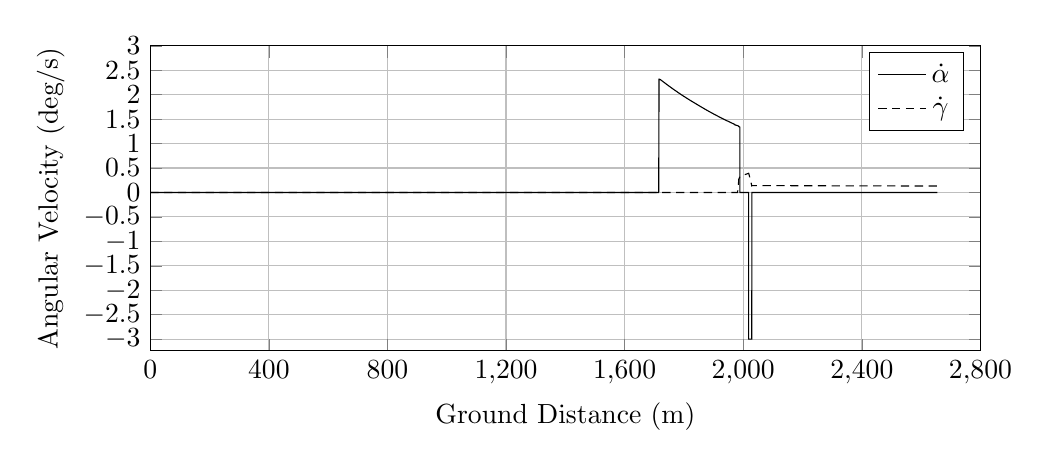
\begin{tikzpicture}

\begin{axis}[
width=\textwidth,
height=0.45\textwidth,
scaled ticks=false, tick label style={/pgf/number format/fixed},
xmin=0.0,
xmax=2800,
xtick={0,400,800,1200,1600,2000,2400,2800,3200},
xlabel={Ground Distance (m)},
xmajorgrids,
ymin=-3.24,
ymax=3,
ylabel={Angular Velocity (deg/s)},
ytick={-3,-2.5,-2,-1.5,-1,-0.5,0.0,0.5,1,1.5,2,2.5,3},
ymajorgrids,
legend entries = {$\dot\alpha$\\$\dot\gamma$\\}
]

\addplot [
color=black,
solid
]
table[row sep=crcr]{
1.3729668748937997E-8	0.0\\
2.6049868369719035E-7	0.0\\
2.0491224421327626E-6	0.0\\
9.92442121137073E-6	0.0\\
4.7452367809869807E-5	0.0\\
1.740064756114434E-4	0.0\\
4.0608377013922605E-4	0.0\\
7.313431501337001E-4	0.0\\
0.0011549487327126044	0.0\\
0.0016799013484208249	0.0\\
0.002295089346817705	0.0\\
0.003009933382444524	0.0\\
0.003810608015426248	0.0\\
0.004723484476856681	0.0\\
0.005727138856912631	0.0\\
0.006836216967948795	0.0\\
0.007997302399386296	0.0\\
0.00929136979810952	0.0\\
0.010685558505459776	0.0\\
0.012178513621519987	0.0\\
0.013775244426719659	0.0\\
0.015470070176169002	0.0\\
0.0172374436815836	0.0\\
0.019122918912604377	0.0\\
0.021104911040230538	0.0\\
0.023190717999955576	0.0\\
0.025355802981115103	0.0\\
0.027620619195902148	0.0\\
0.030020274690474198	0.0\\
0.032476028269866286	0.0\\
0.035054163466719815	0.0\\
0.037720846868992755	0.0\\
0.04049779674511381	0.0\\
0.043329456594087365	0.0\\
0.04629652060163805	0.0\\
0.04934498934704602	0.0\\
0.052507657924119336	0.0\\
0.055769483710642484	0.0\\
0.05917209570914676	0.0\\
0.06264043916012321	0.0\\
0.06620063977265622	0.0\\
0.06987962792775945	0.0\\
0.0736568184539585	0.0\\
0.07754284280095361	0.0\\
0.08151127871105612	0.0\\
0.08560324933017655	0.0\\
0.08985265585263943	0.0\\
0.09413961367176535	0.0\\
0.09857725310864562	0.0\\
0.10307959255469257	0.0\\
0.10766008648593872	0.0\\
0.11234920964493048	0.0\\
0.11719267720457946	0.0\\
0.12216973960582883	0.0\\
0.12724007601918352	0.0\\
0.13233299746505212	0.0\\
0.13755256756750583	0.0\\
0.14287728588926696	0.0\\
0.1482946925752714	0.0\\
0.15381585025670613	0.0\\
0.15940564092189102	0.0\\
0.16526271495916878	0.0\\
0.17120082448158402	0.0\\
0.17717889132867753	0.0\\
0.18324322596131126	0.0\\
0.189427022360885	0.0\\
0.1957511558722988	0.0\\
0.2021484013779125	0.0\\
0.20865863707071397	0.0\\
0.21548666343168166	0.0\\
0.22220154781289658	0.0\\
0.22919671627301902	0.0\\
0.23611678795738544	0.0\\
0.24306300975244904	0.0\\
0.2503085190632165	0.0\\
0.2576623280401219	0.0\\
0.26502430524173204	0.0\\
0.2724963584449146	0.0\\
0.2802001060647876	0.0\\
0.2878583985474956	0.0\\
0.2958320780323821	0.0\\
0.3040021452321372	0.0\\
0.31208951788619	0.0\\
0.3202851396023423	0.0\\
0.3287233234973125	0.0\\
0.3370425959884752	0.0\\
0.34575405233845447	0.0\\
0.3545073625286812	0.0\\
0.36338982075299686	0.0\\
0.37247557159370037	0.0\\
0.38151350442869847	0.0\\
0.3905554764834429	0.0\\
0.3999457587520332	0.0\\
0.4095398754587949	0.0\\
0.4189621792151833	0.0\\
0.4285208811402964	0.0\\
0.43828968955472236	0.0\\
0.44807735398784176	0.0\\
0.45806002753764463	0.0\\
0.4682994371692033	0.0\\
0.4787752542918833	0.0\\
0.4890770094685154	0.0\\
0.49985939134273727	0.0\\
0.5106597490205704	0.0\\
0.5213580865152188	0.0\\
0.532247733242454	0.0\\
0.5431365108549349	0.0\\
0.554075964429489	0.0\\
0.5653450694020941	0.0\\
0.5769901159382542	0.0\\
0.588512657344902	0.0\\
0.6004070039036553	0.0\\
0.6121651247369502	0.0\\
0.6239717914322569	0.0\\
0.6362472885961421	0.0\\
0.6486428939173223	0.0\\
0.6610190736373547	0.0\\
0.6737248046101814	0.0\\
0.6862826225989949	0.0\\
0.6991952542603428	0.0\\
0.7122988072688032	0.0\\
0.7251463703465595	0.0\\
0.7381769453061875	0.0\\
0.7516618647379176	0.0\\
0.7654913705221527	0.0\\
0.7791756406994825	0.0\\
0.7930637813125616	0.0\\
0.8074774191984457	0.0\\
0.8215072375247947	0.0\\
0.8361010597475598	0.0\\
0.8503303420601955	0.0\\
0.8650627501899835	0.0\\
0.8802332960144008	0.0\\
0.8951742046771463	0.0\\
0.9100334756324657	0.0\\
0.9251067343345352	0.0\\
0.9403923630470314	0.0\\
0.9559303815501943	0.0\\
0.9712400158034169	0.0\\
0.9869533781138684	0.0\\
1.0029148609762486	0.0\\
1.0189962473881624	0.0\\
1.035465185745812	0.0\\
1.0516742337458713	0.0\\
1.067815735429615	0.0\\
1.0846705971808022	0.0\\
1.1012775250051634	0.0\\
1.1180798406225687	0.0\\
1.1351395900544134	0.0\\
1.1526388687279154	0.0\\
1.1698922447507556	0.0\\
1.1875468452119025	0.0\\
1.2058383275300355	0.0\\
1.2239395537495579	0.0\\
1.2422020624207541	0.0\\
1.2608769472440078	0.0\\
1.2794948487006894	0.0\\
1.2979152553275424	0.0\\
1.3166445915281573	0.0\\
1.3354141707340492	0.0\\
1.3543210821322504	0.0\\
1.373689361295591	0.0\\
1.3932049885015831	0.0\\
1.4131781782225183	0.0\\
1.4330139682345777	0.0\\
1.4528243860883294	0.0\\
1.4728783400745615	0.0\\
1.4934621752870565	0.0\\
1.5141408097620341	0.0\\
1.53430654450827	0.0\\
1.5553850389607948	0.0\\
1.5762653203499473	0.0\\
1.5975496774716453	0.0\\
1.6196077215345106	0.0\\
1.6413652536722467	0.0\\
1.663437310723463	0.0\\
1.6860768385032747	0.0\\
1.7077101022266827	0.0\\
1.7297306410738114	0.0\\
1.7520297891459062	0.0\\
1.7743087535215367	0.0\\
1.797257424336919	0.0\\
1.8200802473615325	0.0\\
1.8430350373473994	0.0\\
1.8666926279964304	0.0\\
1.8902808566018634	0.0\\
1.9138231309717848	0.0\\
1.937187877956735	0.0\\
1.9611060682733261	0.0\\
1.9852138445648535	0.0\\
2.009780393513653	0.0\\
2.0346228225622163	0.0\\
2.0593611988602687	0.0\\
2.08477023517836	0.0\\
2.110324766702745	0.0\\
2.1352655781940433	0.0\\
2.160528860803022	0.0\\
2.1862071157614817	0.0\\
2.2127756699400534	0.0\\
2.2391904543957084	0.0\\
2.2653528664920257	0.0\\
2.292150575495974	0.0\\
2.3187704640870406	0.0\\
2.3455495914188482	0.0\\
2.372862901366455	0.0\\
2.4007145172972395	0.0\\
2.428100404243743	0.0\\
2.4555980306928005	0.0\\
2.483374904362833	0.0\\
2.511687733451976	0.0\\
2.5402569276484597	0.0\\
2.568415369317849	0.0\\
2.596987652715761	0.0\\
2.6263861238451423	0.0\\
2.655991481965028	0.0\\
2.6856115886357443	0.0\\
2.7154221146045012	0.0\\
2.7455665152057707	0.0\\
2.7752624694325894	0.0\\
2.805457625653509	0.0\\
2.8358231840904597	0.0\\
2.8663460878589797	0.0\\
2.897817297850832	0.0\\
2.9287074004595235	0.0\\
2.9603588456990284	0.0\\
2.9922321403815406	0.0\\
3.0241119471841866	0.0\\
3.056446055158509	0.0\\
3.0889346922121366	0.0\\
3.122221620829695	0.0\\
3.1546991615623394	0.0\\
3.187635101478671	0.0\\
3.221010117202278	0.0\\
3.2543449374576605	0.0\\
3.288235920596943	0.0\\
3.3223704322934555	0.0\\
3.3562838593334394	0.0\\
3.3906320903803255	0.0\\
3.425633159699527	0.0\\
3.462387235801926	0.0\\
3.4973980805087237	0.0\\
3.5324804241140235	0.0\\
3.5675385073174235	0.0\\
3.6040688981843845	0.0\\
3.6393612181513753	0.0\\
3.6770856360342323	0.0\\
3.7131729334920323	0.0\\
3.749509707933214	0.0\\
3.785733977879824	0.0\\
3.8225309786916544	0.0\\
3.860867115351552	0.0\\
3.89929745075254	0.0\\
3.9373367205567504	0.0\\
3.9751626485832894	0.0\\
4.013671158053867	0.0\\
4.0521140617426425	0.0\\
4.092377631210638	0.0\\
4.131586743753305	0.0\\
4.1715696979561425	0.0\\
4.210522654700574	0.0\\
4.250196810863292	0.0\\
4.2917015001093795	0.0\\
4.332438976653355	0.0\\
4.373124372895289	0.0\\
4.414429464889761	0.0\\
4.455884944705147	0.0\\
4.497250153511752	0.0\\
4.537976875075978	0.0\\
4.581399817640802	0.0\\
4.623816269683994	0.0\\
4.666022338967499	0.0\\
4.709098934189642	0.0\\
4.752435367147649	0.0\\
4.79531009100786	0.0\\
4.838191999420829	0.0\\
4.881381760681686	0.0\\
4.9256451804034285	0.0\\
4.9704217340957495	0.0\\
5.014356093293278	0.0\\
5.058826350846283	0.0\\
5.104458009943745	0.0\\
5.149663211268795	0.0\\
5.194981168813841	0.0\\
5.241194091283663	0.0\\
5.287987552078626	0.0\\
5.334426822383641	0.0\\
5.380633359096258	0.0\\
5.427524438012913	0.0\\
5.476157635197664	0.0\\
5.524667120325573	0.0\\
5.5732739519824435	0.0\\
5.6208990292882195	0.0\\
5.671502816366864	0.0\\
5.719824083529298	0.0\\
5.767871110439133	0.0\\
5.8169321963676754	0.0\\
5.866076914057565	0.0\\
5.917200682776528	0.0\\
5.96684810088939	0.0\\
6.016885842403935	0.0\\
6.068639931677712	0.0\\
6.119867755785197	0.0\\
6.171030794930029	0.0\\
6.222884713227881	0.0\\
6.2735946138732235	0.0\\
6.325883502103322	0.0\\
6.379615386553551	0.0\\
6.432194972482147	0.0\\
6.484528316464761	0.0\\
6.536619297696934	0.0\\
6.589662958081361	0.0\\
6.644121795496577	0.0\\
6.697445536614451	0.0\\
6.7518063163896365	0.0\\
6.8068829439682315	0.0\\
6.863205650636274	0.0\\
6.9185329265047315	0.0\\
6.974634519184049	0.0\\
7.031139830722298	0.0\\
7.0870923879294985	0.0\\
7.144766952910487	0.0\\
7.2026451873548805	0.0\\
7.261191729679483	0.0\\
7.320502240843062	0.0\\
7.378210233177999	0.0\\
7.437738452534925	0.0\\
7.49714639104333	0.0\\
7.556502460410064	0.0\\
7.617032771987237	0.0\\
7.676883327249088	0.0\\
7.735740247984193	0.0\\
7.796086087039788	0.0\\
7.856787102853412	0.0\\
7.91721236259451	0.0\\
7.979013602666894	0.0\\
8.039824025454376	0.0\\
8.102419182184594	0.0\\
8.16459313580776	0.0\\
8.226347093952135	0.0\\
8.290527749984296	0.0\\
8.353592793320257	0.0\\
8.417564177281012	0.0\\
8.482044607535009	0.0\\
8.547336806956285	0.0\\
8.613293246319614	0.0\\
8.6778048537894	0.0\\
8.74454839911753	0.0\\
8.810708373588199	0.0\\
8.876548424968423	0.0\\
8.942828456712885	0.0\\
9.010858044488913	0.0\\
9.079453414959548	0.0\\
9.148767802603732	0.0\\
9.21609997183467	0.0\\
9.285579683381485	0.0\\
9.355451712480097	0.0\\
9.423585014597279	0.0\\
9.493435356703696	0.0\\
9.562655940911181	0.0\\
9.63183713653898	0.0\\
9.703018708836247	0.0\\
9.773178624863132	0.0\\
9.844376937811855	0.0\\
9.914998792594716	0.0\\
9.98720270419701	0.0\\
10.059478150570087	0.0\\
10.132362020358627	0.0\\
10.205876892438312	0.0\\
10.279422251887688	0.0\\
10.353305644514993	0.0\\
10.42811398108589	0.0\\
10.50332954727428	0.0\\
10.578207710262959	0.0\\
10.65503529959097	0.0\\
10.730232142651953	0.0\\
10.805871937852555	0.0\\
10.88265320376452	0.0\\
10.958577899345514	0.0\\
11.034861147941964	0.0\\
11.112742623646977	0.0\\
11.190543636431041	0.0\\
11.267787598939979	0.0\\
11.3462805052093	0.0\\
11.423875697147409	0.0\\
11.502735831556972	0.0\\
11.581465323066688	0.0\\
11.661639233340708	0.0\\
11.741743247575428	0.0\\
11.821864700430528	0.0\\
11.901816327719768	0.0\\
11.98361062800689	0.0\\
12.065425957085825	0.0\\
12.1478520915771	0.0\\
12.230956215923495	0.0\\
12.313306905825911	0.0\\
12.396632357805931	0.0\\
12.479578787946746	0.0\\
12.564327762802186	0.0\\
12.648175874147956	0.0\\
12.736145481689512	0.0\\
12.821080154398764	0.0\\
12.908009536077355	0.0\\
12.994986774303499	0.0\\
13.081752199798046	0.0\\
13.17035388279784	0.0\\
13.257836697901475	0.0\\
13.34511613365563	0.0\\
13.433461823066896	0.0\\
13.524108483575919	0.0\\
13.611203924103116	0.0\\
13.702229394080796	0.0\\
13.792427706753081	0.0\\
13.882429934062493	0.0\\
13.975435778888343	0.0\\
14.065832730112316	0.0\\
14.157894546480026	0.0\\
14.250668806951023	0.0\\
14.343291987615704	0.0\\
14.43744444968501	0.0\\
14.532636396723657	0.0\\
14.625507232812737	0.0\\
14.721503924398366	0.0\\
14.818738382089133	0.0\\
14.913572076739943	0.0\\
15.009701633366973	0.0\\
15.10815424447124	0.0\\
15.206130868840724	0.0\\
15.304035939715973	0.0\\
15.403499839366233	0.0\\
15.503209871950865	0.0\\
15.601718454553605	0.0\\
15.700655560608023	0.0\\
15.801250929860519	0.0\\
15.899917805652187	0.0\\
16.001574124100856	0.0\\
16.102638779863817	0.0\\
16.204479333764816	0.0\\
16.30489644092564	0.0\\
16.40578186591999	0.0\\
16.509201471948074	0.0\\
16.614557195984908	0.0\\
16.717657554831042	0.0\\
16.823039336622365	0.0\\
16.928576062495388	0.0\\
17.03469945574068	0.0\\
17.140697318244236	0.0\\
17.246066414787876	0.0\\
17.35183930840021	0.0\\
17.458399953804133	0.0\\
17.565707112453843	0.0\\
17.673103795073075	0.0\\
17.781888038667653	0.0\\
17.89115167195854	0.0\\
18.00105710767307	0.0\\
18.110142905530395	0.0\\
18.219697237410173	0.0\\
18.32752951944549	0.0\\
18.43743745973078	0.0\\
18.54904630654982	0.0\\
18.659302591714813	0.0\\
18.770734536087716	0.0\\
18.883577445650936	0.0\\
18.996263390583444	0.0\\
19.108816920034535	0.0\\
19.22287647779894	0.0\\
19.33763586704334	0.0\\
19.456324114791514	0.0\\
19.57349394116079	0.0\\
19.690148252848566	0.0\\
19.80521137071168	0.0\\
19.92379170801214	0.0\\
20.04216631061405	0.0\\
20.15848954929409	0.0\\
20.278242138037896	0.0\\
20.396206084226087	0.0\\
20.516315546862906	0.0\\
20.637173924977112	0.0\\
20.75450010628387	0.0\\
20.874378237858778	0.0\\
20.996035953832852	0.0\\
21.11812959618858	0.0\\
21.240471115580952	0.0\\
21.361479376438375	0.0\\
21.485224699488654	0.0\\
21.607870280890317	0.0\\
21.73242999733349	0.0\\
21.85704493170313	0.0\\
21.98122016226351	0.0\\
22.10826921766411	0.0\\
22.235261614051304	0.0\\
22.361664688868032	0.0\\
22.48780138980522	0.0\\
22.614107216476143	0.0\\
22.74409311379692	0.0\\
22.873024137794893	0.0\\
23.003512644166257	0.0\\
23.132891545907036	0.0\\
23.26270690888247	0.0\\
23.39264146728729	0.0\\
23.52277721573431	0.0\\
23.654883767164463	0.0\\
23.78569183677709	0.0\\
23.917003007077597	0.0\\
24.047013652206026	0.0\\
24.178458227988493	0.0\\
24.314609552493202	0.0\\
24.447533097503474	0.0\\
24.579128452041708	0.0\\
24.71011994849615	0.0\\
24.843278471916108	0.0\\
24.975761222328053	0.0\\
25.1115496753864	0.0\\
25.247101122854083	0.0\\
25.384906965000688	0.0\\
25.522261036073317	0.0\\
25.66123001648475	0.0\\
25.79865327455613	0.0\\
25.826335196219034	0.0\\
25.839610403727477	0.0\\
25.841006316401874	0.0\\
25.84227013303559	0.0\\
25.84770509053729	0.0\\
25.86419328224909	0.0\\
25.90571916957557	0.0\\
25.999268866927544	0.0\\
26.123295978662824	0.0\\
26.250212562581652	0.0\\
26.376891976518465	0.0\\
26.50638698165423	0.0\\
26.634042370994827	0.0\\
26.763333806613538	0.0\\
26.893207366259766	0.0\\
27.022905486492228	0.0\\
27.153956322362554	0.0\\
27.287774297957696	0.0\\
27.42030033806219	0.0\\
27.555504894698295	0.0\\
27.691130018821354	0.0\\
27.82633313037239	0.0\\
27.959508564917073	0.0\\
28.096515548835796	0.0\\
28.232789703382153	0.0\\
28.368684388406535	0.0\\
28.506541650227618	0.0\\
28.64533374691623	0.0\\
28.78297783415192	0.0\\
28.92277775692753	0.0\\
29.06227187463503	0.0\\
29.20212864139956	0.0\\
29.34335827861657	0.0\\
29.483225747293005	0.0\\
29.625960812476485	0.0\\
29.76706561118049	0.0\\
29.909402910999468	0.0\\
30.051751399473822	0.0\\
30.196612335666572	0.0\\
30.342192969749448	0.0\\
30.48583400527584	0.0\\
30.632658550781265	0.0\\
30.77846394498075	0.0\\
30.92408133049836	0.0\\
31.071091331299215	0.0\\
31.218274793935116	0.0\\
31.366705758252415	0.0\\
31.515339333797037	0.0\\
31.66356819769615	0.0\\
31.814689402684216	0.0\\
31.96649953392354	0.0\\
32.115424616034375	0.0\\
32.266253234088566	0.0\\
32.41813832080348	0.0\\
32.569791431087395	0.0\\
32.722234201183724	0.0\\
32.876984607664	0.0\\
33.031873994672836	0.0\\
33.18502245018544	0.0\\
33.34135780547538	0.0\\
33.49759920343199	0.0\\
33.65385117142162	0.0\\
33.8113313806527	0.0\\
33.96985264489639	0.0\\
34.126473036379195	0.0\\
34.2857505660089	0.0\\
34.4449212019973	0.0\\
34.60566879064274	0.0\\
34.76644486933921	0.0\\
34.92612701881755	0.0\\
35.08630421658309	0.0\\
35.24825698849928	0.0\\
35.412303951281956	0.0\\
35.57355277914179	0.0\\
35.73545353069308	0.0\\
35.89925038949356	0.0\\
36.065161289279985	0.0\\
36.23047312008262	0.0\\
36.39472205714358	0.0\\
36.56135389445764	0.0\\
36.72774532558607	0.0\\
36.89384825683493	0.0\\
37.05904296416534	0.0\\
37.22702676294645	0.0\\
37.39437475321985	0.0\\
37.5621109943643	0.0\\
37.73270471709142	0.0\\
37.903359519601935	0.0\\
38.071486842086316	0.0\\
38.23815243703595	0.0\\
38.40817787072022	0.0\\
38.57751392140098	0.0\\
38.750215798728505	0.0\\
38.92001182640311	0.0\\
39.09310637700479	0.0\\
39.26472366117933	0.0\\
39.436554723976656	0.0\\
39.608961777617054	0.0\\
39.782828308010565	0.0\\
39.956194359016465	0.0\\
40.132391837044906	0.0\\
40.30868053167249	0.0\\
40.48611580488176	0.0\\
40.66383502946924	0.0\\
40.83999042132467	0.0\\
41.018202681018664	0.0\\
41.19780999006247	0.0\\
41.37730467548502	0.0\\
41.557010452813884	0.0\\
41.73612816026986	0.0\\
41.91555194917056	0.0\\
42.09743589423803	0.0\\
42.27807550146298	0.0\\
42.45995188234755	0.0\\
42.6401410478328	0.0\\
42.822293873795985	0.0\\
43.00585672428667	0.0\\
43.189965171449515	0.0\\
43.372020236704074	0.0\\
43.555636897252796	0.0\\
43.74012033961118	0.0\\
43.92429822300048	0.0\\
44.106869824379004	0.0\\
44.29411840239129	0.0\\
44.47920670866131	0.0\\
44.665034305215386	0.0\\
44.85242224248053	0.0\\
45.03948098831597	0.0\\
45.22811764277584	0.0\\
45.41548629589063	0.0\\
45.60322541388645	0.0\\
45.793007222766036	0.0\\
45.983742663331824	0.0\\
46.172643153142886	0.0\\
46.36421599110457	0.0\\
46.553512793459404	0.0\\
46.745018895697555	0.0\\
46.93606459490553	0.0\\
47.126948089509526	0.0\\
47.31881294044018	0.0\\
47.5110690178297	0.0\\
47.705448624448266	0.0\\
47.90005519882567	0.0\\
48.09288923506665	0.0\\
48.28732881729917	0.0\\
48.484002572746206	0.0\\
48.68089030454945	0.0\\
48.87532723390382	0.0\\
49.07073736177763	0.0\\
49.2672083392297	0.0\\
49.46586249263092	0.0\\
49.661880987188695	0.0\\
49.85966148345089	0.0\\
50.05808618672894	0.0\\
50.25785665917266	0.0\\
50.45743808511885	0.0\\
50.65573800086891	0.0\\
50.85948768734909	0.0\\
51.061243703011925	0.0\\
51.26368286286315	0.0\\
51.46416466063809	0.0\\
51.66475943174029	0.0\\
51.86588207153103	0.0\\
52.07444928962187	0.0\\
52.2824430085781	0.0\\
52.48676525705545	0.0\\
52.69531994892206	0.0\\
52.90027076850366	0.0\\
53.108186167814935	0.0\\
53.31165724918766	0.0\\
53.520024946679996	0.0\\
53.72688450142306	0.0\\
53.93707391647578	0.0\\
54.14518573319289	0.0\\
54.35125853722778	0.0\\
54.56213447502874	0.0\\
54.77598621923464	0.0\\
54.987629956235494	0.0\\
55.19778857845695	0.0\\
55.41030974885841	0.0\\
55.62390503323701	0.0\\
55.83671574169797	0.0\\
56.047071254351536	0.0\\
56.26137331252919	0.0\\
56.47512769358855	0.0\\
56.69105800830218	0.0\\
56.90937011004422	0.0\\
57.12736617899088	0.0\\
57.346833156368504	0.0\\
57.56476609337061	0.0\\
57.78230894703917	0.0\\
57.99943865551505	0.0\\
58.21827465292657	0.0\\
58.436085045729726	0.0\\
58.6577546799423	0.0\\
58.87982836766625	0.0\\
59.10336118170943	0.0\\
59.324182403931715	0.0\\
59.545440661451366	0.0\\
59.768227251413464	0.0\\
59.99077485409802	0.0\\
60.21631063559073	0.0\\
60.44006004384342	0.0\\
60.66502706168687	0.0\\
60.89133011288284	0.0\\
61.11585558357916	0.0\\
61.3432655409558	0.0\\
61.57186440401435	0.0\\
61.79868765088207	0.0\\
62.025670725987	0.0\\
62.254132946411545	0.0\\
62.48290793247415	0.0\\
62.713817944074236	0.0\\
62.94484116346062	0.0\\
63.17805109236767	0.0\\
63.41124119062552	0.0\\
63.64505576847972	0.0\\
63.87735201907903	0.0\\
64.11169045660182	0.0\\
64.34725756208485	0.0\\
64.58324360279937	0.0\\
64.81881329818131	0.0\\
65.05563560606473	0.0\\
65.29467812810154	0.0\\
65.53178653633495	0.0\\
65.77046761369158	0.0\\
66.01019347650049	0.0\\
66.25262920761091	0.0\\
66.49342175078831	0.0\\
66.73393309567928	0.0\\
66.97718905970893	0.0\\
67.21919788222482	0.0\\
67.46413738735515	0.0\\
67.70584739194695	0.0\\
67.95375887035246	0.0\\
68.19817148521656	0.0\\
68.44413350233111	0.0\\
68.68984243621705	0.0\\
68.93951041285982	0.0\\
69.19023531750676	0.0\\
69.43956667494601	0.0\\
69.68998597860525	0.0\\
69.94098943220166	0.0\\
70.1928405184459	0.0\\
70.44659484061637	0.0\\
70.69926103579675	0.0\\
70.95414956377036	0.0\\
71.21136313866151	0.0\\
71.46778788208749	0.0\\
71.7247351381395	0.0\\
71.98234155897126	0.0\\
72.24107377350035	0.0\\
72.4986091150376	0.0\\
72.75949164810788	0.0\\
73.02014691132015	0.0\\
73.28114866838587	0.0\\
73.54342372888959	0.0\\
73.80584407854005	0.0\\
74.07231166191039	0.0\\
74.3389341302921	0.0\\
74.60521354141642	0.0\\
74.87280568706873	0.0\\
75.1403821105715	0.0\\
75.41145333671997	0.0\\
75.68265298797411	0.0\\
75.95075857762194	0.0\\
76.2241428819712	0.0\\
76.4990100438061	0.0\\
76.77213586328236	0.0\\
77.04724851790667	0.0\\
77.32330034006353	0.0\\
77.59850473375684	0.0\\
77.87773830129439	0.0\\
78.1565255546137	0.0\\
78.43842651648492	0.0\\
78.720833678605	0.0\\
79.00101298089581	0.0\\
79.28359351218376	0.0\\
79.57011733099088	0.0\\
79.85418914588558	0.0\\
80.13919871477489	0.0\\
80.42568449319114	0.0\\
80.71472498530085	0.0\\
81.006853148924	0.0\\
81.2951972638476	0.0\\
81.58524575795963	0.0\\
81.87461709596036	0.0\\
82.1711642895769	0.0\\
82.46716486408064	0.0\\
82.76422974563803	0.0\\
83.05801377197795	0.0\\
83.35853301954708	0.0\\
83.65664966506407	0.0\\
83.95487262936624	0.0\\
84.25322789115987	0.0\\
84.55664509033022	0.0\\
84.8599544590121	0.0\\
85.16499148084048	0.0\\
85.47187188044902	0.0\\
85.77908321853027	0.0\\
86.08675489504844	0.0\\
86.39784539041122	0.0\\
86.71051296037359	0.0\\
87.02583358957506	0.0\\
87.34037846285594	0.0\\
87.65395388450591	0.0\\
87.96687312379424	0.0\\
88.28527441497255	0.0\\
88.6103524516937	0.0\\
88.92871226770333	0.0\\
89.25003295857354	0.0\\
89.57522243846881	0.0\\
89.90247582737899	0.0\\
90.22602529632545	0.0\\
90.5494223037065	0.0\\
90.87816525326718	0.0\\
91.20455861430293	0.0\\
91.53817773235312	0.0\\
91.87076195087604	0.0\\
92.20124984301029	0.0\\
92.53140503523474	0.0\\
92.86389705561814	0.0\\
93.19815266874983	0.0\\
93.53304529783748	0.0\\
93.86737084100128	0.0\\
94.20337949361911	0.0\\
94.54065981474497	0.0\\
94.87396787418089	0.0\\
95.21684847579547	0.0\\
95.55392648231228	0.0\\
95.89232371872416	0.0\\
96.23051075783204	0.0\\
96.57164052232307	0.0\\
96.90762523479154	0.0\\
97.24755293575913	0.0\\
97.58790661409188	0.0\\
97.92576087813703	0.0\\
98.26661027452474	0.0\\
98.6051908024865	0.0\\
98.94563962387357	0.0\\
99.28665364663627	0.0\\
99.63350087797645	0.0\\
99.97685593767679	0.0\\
100.31593955776762	0.0\\
100.65572384630482	0.0\\
100.99616871909686	0.0\\
101.3402339503516	0.0\\
101.67973054404297	0.0\\
102.01657591573795	0.0\\
102.35656456518868	0.0\\
102.6941824316649	0.0\\
103.03547296258705	0.0\\
103.37623032340073	0.0\\
103.71852978299776	0.0\\
104.05851119314701	0.0\\
104.3949509202441	0.0\\
104.7329053851843	0.0\\
105.07104272194636	0.0\\
105.40742307340048	0.0\\
105.74423560014887	0.0\\
106.07955743077031	0.0\\
106.41623710643992	0.0\\
106.75618472497374	0.0\\
107.0942647435474	0.0\\
107.43151869252583	0.0\\
107.44650965670576	0.0\\
107.45815118347005	0.0\\
107.46233674961977	0.0\\
107.46535588765028	0.0\\
107.46808502617694	0.0\\
107.4836206108138	0.0\\
107.53176708907421	0.0\\
107.68672244793561	0.0\\
107.97570433527497	0.0\\
108.27744765146667	0.0\\
108.5816623935838	0.0\\
108.88557241638279	0.0\\
109.19209959959528	0.0\\
109.50241879336687	0.0\\
109.81066605766154	0.0\\
110.12101503747155	0.0\\
110.43285681965125	0.0\\
110.74725799716322	0.0\\
111.06462449033057	0.0\\
111.38211128519615	0.0\\
111.70119562731901	0.0\\
112.02298633508096	0.0\\
112.34320819983824	0.0\\
112.66812620709393	0.0\\
112.99302416686388	0.0\\
113.31966045518399	0.0\\
113.64998129974768	0.0\\
113.97857627498675	0.0\\
114.31304608469316	0.0\\
114.64448318111735	0.0\\
114.98093514978115	0.0\\
115.31969924418831	0.0\\
115.65790718621022	0.0\\
116.00063352526521	0.0\\
116.34235083463872	0.0\\
116.68621873349733	0.0\\
117.03331062078092	0.0\\
117.37910048629482	0.0\\
117.72869476105836	0.0\\
118.08005947084649	0.0\\
118.43363644355449	0.0\\
118.79186464668504	0.0\\
119.14769212941735	0.0\\
119.5036618261702	0.0\\
119.86270697471275	0.0\\
120.22616362054572	0.0\\
120.58991121293201	0.0\\
120.95538130513773	0.0\\
121.3195355377388	0.0\\
121.68590041554987	0.0\\
122.05305648207542	0.0\\
122.42257239354896	0.0\\
122.79503144936103	0.0\\
123.16629137010841	0.0\\
123.53950748252527	0.0\\
123.91239367862553	0.0\\
124.29026003316017	0.0\\
124.66301933937496	0.0\\
125.03890311735066	0.0\\
125.41380975776434	0.0\\
125.7896808967325	0.0\\
126.16837244152023	0.0\\
126.54595968852882	0.0\\
126.92471834906405	0.0\\
127.30294276405039	0.0\\
127.68255852126984	0.0\\
128.06243727540487	0.0\\
128.44360431740483	0.0\\
128.82265748788262	0.0\\
129.1989690567886	0.0\\
129.57765386613931	0.0\\
129.95508099647026	0.0\\
130.33359114840187	0.0\\
130.71373745886524	0.0\\
131.09453904397424	0.0\\
131.47657586018488	0.0\\
131.85678563989967	0.0\\
132.23856625352113	0.0\\
132.61595336405918	0.0\\
132.99976263915818	0.0\\
133.38083522978053	0.0\\
133.76098428781995	0.0\\
134.1363519425165	0.0\\
134.51557915495124	0.0\\
134.8968696170101	0.0\\
135.27419431482667	0.0\\
135.65215477207505	0.0\\
136.03329358991255	0.0\\
136.41192880753374	0.0\\
136.7898079310749	0.0\\
137.17001317148595	0.0\\
137.54844558779996	0.0\\
137.92617219433072	0.0\\
138.30476964659732	0.0\\
138.68390038934075	0.0\\
139.0631653430654	0.0\\
139.4406106933401	0.0\\
139.81914660512416	0.0\\
140.19767098864742	0.0\\
140.5730919292459	0.0\\
140.95061983253072	0.0\\
141.32838502869612	0.0\\
141.70636515873298	0.0\\
142.0839785067887	0.0\\
142.46357402350594	0.0\\
142.84082211769783	0.0\\
143.21906727224075	0.0\\
143.59963619096823	0.0\\
143.97984478872678	0.0\\
144.35941603837455	0.0\\
144.7355521893594	0.0\\
145.11296635073694	0.0\\
145.49073213867456	0.0\\
145.87033631970945	0.0\\
146.24486520181193	0.0\\
146.6238757206513	0.0\\
147.00096360401335	0.0\\
147.37874202190085	0.0\\
147.756852900845	0.0\\
148.13572640408995	0.0\\
148.5136798644104	0.0\\
148.89083780486442	0.0\\
149.2712459042852	0.0\\
149.65303236723025	0.0\\
150.0329584616291	0.0\\
150.41363382646614	0.0\\
150.79322940570728	0.0\\
151.17272478467066	0.0\\
151.55400296227282	0.0\\
151.93482601265913	0.0\\
152.31881414221942	0.0\\
152.70208150063132	0.0\\
153.08320649997165	0.0\\
153.4666285558243	0.0\\
153.84825937276264	0.0\\
154.23093781718723	0.0\\
154.61485031834388	0.0\\
155.00001234931443	0.0\\
155.38285725409855	0.0\\
155.7679513537659	0.0\\
156.1509667875323	0.0\\
156.53491934392343	0.0\\
156.91995289130983	0.0\\
157.30625057946366	0.0\\
157.69121706207227	0.0\\
158.07789765133754	0.0\\
158.46521012398495	0.0\\
158.85138765236047	0.0\\
159.23964669847322	0.0\\
159.62715395386465	0.0\\
160.01960115328984	0.0\\
160.4079207075476	0.0\\
160.79602490671402	0.0\\
161.18437278725975	0.0\\
161.57644284003254	0.0\\
161.96812230097612	0.0\\
162.35808768568592	0.0\\
162.75087300343483	0.0\\
163.14546270495134	0.0\\
163.53745675514648	0.0\\
163.92955389373896	0.0\\
164.32395276810763	0.0\\
164.71713266653478	0.0\\
165.1102153740033	0.0\\
165.5035884424101	0.0\\
165.89816400198282	0.0\\
166.29148626774366	0.0\\
166.68861804276264	0.0\\
167.082852347146	0.0\\
167.48006204110857	0.0\\
167.8798182678497	0.0\\
168.27774435731556	0.0\\
168.67741362640317	0.0\\
169.07475368467374	0.0\\
169.4759958044982	0.0\\
169.87832784425882	0.0\\
170.2792240364854	0.0\\
170.68126852540456	0.0\\
171.08617821288442	0.0\\
171.48766933901368	0.0\\
171.892744970828	0.0\\
172.29711201372032	0.0\\
172.70264003426053	0.0\\
173.1105289448074	0.0\\
173.5163733808056	0.0\\
173.92577914808027	0.0\\
174.33607303977334	0.0\\
174.74614233406845	0.0\\
175.15731444736514	0.0\\
175.56901623635082	0.0\\
175.97955109701695	0.0\\
176.39275298155184	0.0\\
176.80397138375372	0.0\\
177.21946344336607	0.0\\
177.6332252263685	0.0\\
178.05102033212842	0.0\\
178.46725124888752	0.0\\
178.88389799206544	0.0\\
179.29839533747668	0.0\\
179.71608569665375	0.0\\
180.1342696339205	0.0\\
180.26454521656194	0.0\\
180.5538779958007	0.0\\
180.97677279803082	0.0\\
181.73177043104909	0.0\\
182.61825861954026	0.0\\
183.4994266290775	0.0\\
184.38832398643513	0.0\\
185.2752206450968	0.0\\
186.16090254585617	0.0\\
187.05782443666988	0.0\\
187.95004436743	0.0\\
188.84343565256296	0.0\\
189.73203483232732	0.0\\
190.63087969896367	0.0\\
191.53167348748025	0.0\\
192.42914206966827	0.0\\
193.32936064878362	0.0\\
194.23353734669462	0.0\\
195.14873951553636	0.0\\
196.05846844349168	0.0\\
196.9665797060448	0.0\\
197.88137813217617	0.0\\
198.80153314772656	0.0\\
199.72262566550114	0.0\\
200.6418018332526	0.0\\
201.57021605131746	0.0\\
202.49227039761405	0.0\\
203.4093310979173	0.0\\
204.33741716634955	0.0\\
205.26228808295895	0.0\\
206.1977933698634	0.0\\
207.13719708861407	0.0\\
208.07111616454222	0.0\\
209.00693662932974	0.0\\
209.95866810149408	0.0\\
210.9046028778589	0.0\\
211.84706310840727	0.0\\
212.79298368779843	0.0\\
213.73594859980489	0.0\\
214.69266347370274	0.0\\
215.65468447394903	0.0\\
216.614658409948	0.0\\
217.57357224144454	0.0\\
218.5368107467741	0.0\\
219.50048157907025	0.0\\
220.46765259916174	0.0\\
221.44618219131166	0.0\\
222.41939214233116	0.0\\
223.3957502333693	0.0\\
224.37068692464283	0.0\\
225.34711146005128	0.0\\
226.33138885023874	0.0\\
227.31393394086427	0.0\\
228.30414603792985	0.0\\
229.29617452368518	0.0\\
230.2808212657469	0.0\\
231.28192033792595	0.0\\
232.2770741096358	0.0\\
233.29052711380916	0.0\\
234.30070953924962	0.0\\
235.3030940983469	0.0\\
236.31056730234104	0.0\\
237.32863543123972	0.0\\
238.35192702989485	0.0\\
239.37227626200922	0.0\\
240.40154009491766	0.0\\
241.4327935450462	0.0\\
242.46479014370783	0.0\\
243.4993601598722	0.0\\
244.5489899152056	0.0\\
245.59198540953986	0.0\\
246.64178332136828	0.0\\
247.69238009267121	0.0\\
248.75653132082437	0.0\\
249.80604502438968	0.0\\
250.8683150903493	0.0\\
251.93058205288185	0.0\\
253.00701197053712	0.0\\
254.08005928692728	0.0\\
255.1482320588113	0.0\\
256.2287194565513	0.0\\
257.30711015243367	0.0\\
258.39583303573465	0.0\\
259.47850143980736	0.0\\
260.57344571603574	0.0\\
261.6820544046054	0.0\\
262.77228099849674	0.0\\
263.87126070008526	0.0\\
264.97335243767543	0.0\\
266.0976894214622	0.0\\
267.21278411159847	0.0\\
268.32534355771804	0.0\\
269.4561922169971	0.0\\
270.5915896156504	0.0\\
271.7158392961418	0.0\\
272.8552569839427	0.0\\
274.01601268837805	0.0\\
275.14755464888765	0.0\\
276.29902718037044	0.0\\
277.4488797139885	0.0\\
278.61486213965225	0.0\\
279.78120226092256	0.0\\
280.9500599413508	0.0\\
282.12185174587614	0.0\\
283.32143414076336	0.0\\
284.5140258308369	0.0\\
285.7080037808545	0.0\\
286.89480016288826	0.0\\
288.114729118857	0.0\\
289.33647182734956	0.0\\
290.5550281524761	0.0\\
291.77092362893404	0.0\\
292.99973950499964	0.0\\
294.2334028862149	0.0\\
295.476424104432	0.0\\
296.7307839433978	0.0\\
297.99041084660416	0.0\\
299.2512587145409	0.0\\
300.52071837015376	0.0\\
301.8085664342501	0.0\\
303.093188627083	0.0\\
304.3891528365698	0.0\\
305.6757850562126	0.0\\
306.9700995472474	0.0\\
308.29492992625205	0.0\\
309.5781066121766	0.0\\
310.8708143232478	0.0\\
312.1568125435102	0.0\\
313.4602517178914	0.0\\
314.7614812617795	0.0\\
316.075256596823	0.0\\
317.41378230532723	0.0\\
318.7467345840158	0.0\\
320.0730060828963	0.0\\
321.39169180058434	0.0\\
322.72349821328476	0.0\\
324.0598831134772	0.0\\
325.40424996971046	0.0\\
326.7492865835918	0.0\\
328.0710288684362	0.0\\
329.4262473961435	0.0\\
330.754264279002	0.0\\
332.097514519191	0.0\\
333.41994590396723	0.0\\
334.7305118494995	0.0\\
336.0731570894968	0.0\\
337.3927235989065	0.0\\
338.7087431098878	0.0\\
340.03087614347885	0.0\\
341.340088749036	0.0\\
342.6557828174856	0.0\\
343.96701843570406	0.0\\
345.2526439842643	0.0\\
346.5500414102456	0.0\\
347.8534066412583	0.0\\
349.1454340977755	0.0\\
350.4240054240321	0.0\\
351.7019235209849	0.0\\
352.98991038490203	0.0\\
354.2648351856848	0.0\\
355.53300413952707	0.0\\
356.79919221038165	0.0\\
358.0559257933643	0.0\\
359.3093316769772	0.0\\
359.35961387762393	0.0\\
359.41061546826563	0.0\\
359.4211304928041	0.0\\
359.4316918068113	0.0\\
359.4910693710335	0.0\\
359.779729191638	0.0\\
360.4880169023802	0.0\\
361.5766561299438	0.0\\
362.66113418824455	0.0\\
363.76124342756657	0.0\\
364.8589078947854	0.0\\
365.9685296666213	0.0\\
367.07582921056974	0.0\\
368.1951666519893	0.0\\
369.31258197452325	0.0\\
370.4366539475295	0.0\\
371.565996752341	0.0\\
372.70127842882266	0.0\\
373.84649895373127	0.0\\
374.9968247959414	0.0\\
376.15403836851897	0.0\\
377.3203528636726	0.0\\
378.4850840608731	0.0\\
379.6663035147078	0.0\\
380.8461820283744	0.0\\
382.0347494549213	0.0\\
383.2193798940116	0.0\\
384.42877967750667	0.0\\
385.63354002572066	0.0\\
386.845921264293	0.0\\
388.06777411235	0.0\\
389.2936908860911	0.0\\
390.53850037014047	0.0\\
391.76781253461945	0.0\\
393.0108311673757	0.0\\
394.26523475557894	0.0\\
395.52152377336915	0.0\\
396.7904975310561	0.0\\
398.0771683304033	0.0\\
399.3519058933132	0.0\\
400.63393441623316	0.0\\
401.92385130992545	0.0\\
403.21918556823357	0.0\\
404.52791933693925	0.0\\
405.83210730664996	0.0\\
407.1393641556499	0.0\\
408.45238412405433	0.0\\
409.76561626724674	0.0\\
411.10125498654554	0.0\\
412.4171463109144	0.0\\
413.73698982354097	0.0\\
415.062570379646	0.0\\
416.375187798194	0.0\\
417.69595093934595	0.0\\
419.0285116875033	0.0\\
420.36454657893216	0.0\\
421.6812813836435	0.0\\
423.00972403127514	0.0\\
424.32760721523437	0.0\\
425.6472681840288	0.0\\
426.96253742961164	0.0\\
428.29182268843977	0.0\\
429.6160502503526	0.0\\
430.9312874400488	0.0\\
432.2371182898221	0.0\\
433.55144081210005	0.0\\
434.867194360879	0.0\\
436.16838785958646	0.0\\
437.46367739026596	0.0\\
438.78588638695476	0.0\\
440.0925891606661	0.0\\
441.3848392234046	0.0\\
442.6814156289133	0.0\\
443.97357880818515	0.0\\
445.2632779895895	0.0\\
446.54906207929946	0.0\\
447.8470239842545	0.0\\
449.1220474037084	0.0\\
450.39588054344404	0.0\\
451.68119786233456	0.0\\
452.9614765477911	0.0\\
454.2371818112225	0.0\\
455.5035899796636	0.0\\
456.7833140437298	0.0\\
458.04929565590817	0.0\\
459.3134414393421	0.0\\
460.5777262845279	0.0\\
461.84023587900685	0.0\\
463.10108065312045	0.0\\
464.3645399404894	0.0\\
465.6238016850866	0.0\\
466.8762783875227	0.0\\
468.1281814377654	0.0\\
469.3838351297785	0.0\\
470.63650571068945	0.0\\
471.8846974041603	0.0\\
473.1433200948185	0.0\\
474.39244309563617	0.0\\
475.6408716432604	0.0\\
476.8834126309654	0.0\\
478.1293558793383	0.0\\
479.37468033554455	0.0\\
480.62161050962675	0.0\\
481.86154936911134	0.0\\
483.106752207652	0.0\\
484.34476413467644	0.0\\
485.57829651821373	0.0\\
486.81122711428	0.0\\
488.04749147403595	0.0\\
489.286499221119	0.0\\
490.5258622185305	0.0\\
491.7613633545217	0.0\\
492.98979445152895	0.0\\
494.22181660420335	0.0\\
495.4491662715502	0.0\\
496.68037150127316	0.0\\
497.905419768701	0.0\\
499.1418007543791	0.0\\
500.36883500341185	0.0\\
501.6049635519511	0.0\\
502.8346968521507	0.0\\
504.0688416682151	0.0\\
505.30449852859897	0.0\\
506.53623375091763	0.0\\
507.7727737587355	0.0\\
509.01094069395083	0.0\\
510.24044302236643	0.0\\
511.47314480655655	0.0\\
512.709426639085	0.0\\
513.933014023326	0.0\\
515.1632406071703	0.0\\
516.3942825834877	0.0\\
517.6209225737591	0.0\\
518.8611725736578	0.0\\
520.0899677635864	0.0\\
521.3248911937364	0.0\\
522.5563249355823	0.0\\
523.7871395992927	0.0\\
525.0207080655291	0.0\\
526.2538889797097	0.0\\
527.4855886295541	0.0\\
528.7248966623163	0.0\\
529.9525012711933	0.0\\
531.188411182631	0.0\\
532.430364502346	0.0\\
533.6537982289233	0.0\\
534.8895444365953	0.0\\
536.1167015415926	0.0\\
537.3524667925105	0.0\\
538.5909786862885	0.0\\
539.8321004970862	0.0\\
541.0714186237371	0.0\\
542.3101366962153	0.0\\
543.549683335455	0.0\\
544.7884410234926	0.0\\
546.0249505756278	0.0\\
547.2698901981096	0.0\\
548.517922558824	0.0\\
549.7630578627702	0.0\\
551.0045945501979	0.0\\
552.2474673458937	0.0\\
553.4943949801896	0.0\\
554.7340934194742	0.0\\
555.9857081438174	0.0\\
557.2349771676527	0.0\\
558.4836329625055	0.0\\
559.7304362301556	0.0\\
560.9863602168837	0.0\\
562.2354783338385	0.0\\
563.4889074787859	0.0\\
564.7429572990306	0.0\\
565.9930187270757	0.0\\
567.2542213530385	0.0\\
568.5162483155984	0.0\\
569.7779714539561	0.0\\
571.0363634961464	0.0\\
572.2926220263994	0.0\\
573.5600328752141	0.0\\
574.8157579683532	0.0\\
576.0874650967378	0.0\\
577.3535786105731	0.0\\
578.6120389651717	0.0\\
579.8782973050222	0.0\\
581.1428814799804	0.0\\
582.4098688192882	0.0\\
583.6781849802521	0.0\\
584.9463392856037	0.0\\
586.2252005492951	0.0\\
587.4974333601563	0.0\\
588.7730696836684	0.0\\
590.0462783949215	0.0\\
591.3260679091647	0.0\\
592.6020115890217	0.0\\
593.8805034430136	0.0\\
595.160760080855	0.0\\
596.4493859727936	0.0\\
597.7370171231987	0.0\\
599.0230981231337	0.0\\
600.3140314068335	0.0\\
601.5959263370289	0.0\\
602.8804904362269	0.0\\
604.1717551873128	0.0\\
605.4670675975769	0.0\\
606.7593430415579	0.0\\
608.0589989803163	0.0\\
609.35544064962	0.0\\
610.6631378257334	0.0\\
611.9673871376037	0.0\\
613.2669485728909	0.0\\
614.5726280512417	0.0\\
615.882692177473	0.0\\
617.1853058424017	0.0\\
618.4951671858978	0.0\\
619.8084414147645	0.0\\
621.1191039235041	0.0\\
622.4308696059663	0.0\\
623.7508573247546	0.0\\
625.0621647279136	0.0\\
626.3891907804957	0.0\\
627.7047303153058	0.0\\
629.0377690450321	0.0\\
630.3648129669755	0.0\\
631.6959383652843	0.0\\
633.0238008372617	0.0\\
634.3555987176628	0.0\\
635.6888337719913	0.0\\
637.0273231686772	0.0\\
638.3673317967357	0.0\\
639.7077548538582	0.0\\
641.0518988098222	0.0\\
642.3903562372943	0.0\\
643.7408141429719	0.0\\
645.0886899442107	0.0\\
646.4440665133416	0.0\\
647.7979969870544	0.0\\
649.1475695730635	0.0\\
650.5085087456741	0.0\\
651.8672498827148	0.0\\
653.2300391678464	0.0\\
654.59119710404	0.0\\
655.9565870372583	0.0\\
657.3301576177535	0.0\\
658.7055644018274	0.0\\
660.0707476489983	0.0\\
661.4425588489983	0.0\\
662.8202826045422	0.0\\
664.2023126867782	0.0\\
665.5843067773396	0.0\\
666.9693429401127	0.0\\
668.3535922551048	0.0\\
669.7456415264321	0.0\\
671.1429671199867	0.0\\
672.5352013622244	0.0\\
673.9319680407395	0.0\\
675.3315923284297	0.0\\
676.7364615033362	0.0\\
678.1398524051901	0.0\\
679.5482613506588	0.0\\
680.9611255975728	0.0\\
682.3747606873828	0.0\\
683.7885950684599	0.0\\
685.2170702182973	0.0\\
686.6341538210345	0.0\\
688.0624981059129	0.0\\
689.494639734967	0.0\\
690.9277173550104	0.0\\
692.366148307123	0.0\\
693.8090898976764	0.0\\
695.2470828114372	0.0\\
696.6927285316788	0.0\\
698.1317183942906	0.0\\
699.5819178468557	0.0\\
701.0428107681289	0.0\\
702.4953498250779	0.0\\
703.9473725213384	0.0\\
705.4080630038732	0.0\\
706.8695138302369	0.0\\
708.3364086722147	0.0\\
709.8077680233077	0.0\\
711.2874255207532	0.0\\
712.7606875545755	0.0\\
714.2419414738395	0.0\\
715.7350467748483	0.0\\
717.2311190009834	0.0\\
718.7239794754369	0.0\\
720.2275182266221	0.0\\
721.7330377579644	0.0\\
723.2413817882659	0.0\\
724.7490613493742	0.0\\
726.2646491700143	0.0\\
727.7888882938735	0.0\\
729.3095291352877	0.0\\
730.8328737152488	0.0\\
732.3678281524585	0.0\\
733.9014149193533	0.0\\
735.4434915877257	0.0\\
736.9879879939524	0.0\\
738.5283662039221	0.0\\
740.0793071755775	0.0\\
741.6375760538187	0.0\\
743.1975562173411	0.0\\
744.7668995543936	0.0\\
746.3402343351052	0.0\\
747.9098112007614	0.0\\
749.4926435018808	0.0\\
751.0788155700511	0.0\\
752.6689698013324	0.0\\
754.2660647297644	0.0\\
755.8725103063173	0.0\\
757.4740270930072	0.0\\
759.0843283212412	0.0\\
760.6957495574857	0.0\\
762.3236488682719	0.0\\
763.957733693579	0.0\\
765.59787840474	0.0\\
767.2310074870152	0.0\\
768.8772793382998	0.0\\
770.5330449495398	0.0\\
772.1910525761205	0.0\\
773.8571767410926	0.0\\
775.5319334528265	0.0\\
777.2041051797112	0.0\\
778.8843360083499	0.0\\
780.5674338985871	0.0\\
782.2582000560008	0.0\\
783.9645563214774	0.0\\
785.6717915011791	0.0\\
787.3899867029195	0.0\\
789.1251875317641	0.0\\
790.8518058281281	0.0\\
792.5977603346089	0.0\\
794.3482760283587	0.0\\
796.1133104533772	0.0\\
797.8925872065113	0.0\\
799.6676230066485	0.0\\
801.4573937546816	0.0\\
803.2521506684645	0.0\\
805.0713284918866	0.0\\
806.8905312973145	0.0\\
808.7095825809233	0.0\\
810.5470742557707	0.0\\
812.397095148264	0.0\\
814.2551620707266	0.0\\
816.132659040346	0.0\\
818.0281486728034	0.0\\
819.9214681177887	0.0\\
821.8368903009664	0.0\\
823.7586319415379	0.0\\
825.6966696706393	0.0\\
827.6537819263224	0.0\\
829.6200328252633	0.0\\
831.6080960277959	0.0\\
833.6058858944243	0.0\\
835.6138691611445	0.0\\
837.6522132068358	0.0\\
839.7005525953057	0.0\\
841.7828859709559	0.0\\
843.8747849790732	0.0\\
846.0012801717799	0.0\\
848.1350586077451	0.0\\
850.3010101301049	0.0\\
852.4938460893047	0.0\\
854.7160164344048	0.0\\
856.953183977754	0.0\\
859.2449805536867	0.0\\
861.553860969846	0.0\\
863.8861242277894	0.0\\
866.246819806435	0.0\\
868.6340776469228	0.0\\
871.0307008527677	0.0\\
873.4425737809947	0.0\\
875.8683627080882	0.0\\
878.2871875934777	0.0\\
880.6871980592739	0.0\\
883.0835625734228	0.0\\
885.4582103016828	0.0\\
887.8090348902429	0.0\\
890.1260985038559	0.0\\
892.4305796056062	0.0\\
894.7269340529676	0.0\\
896.9820607244501	0.0\\
899.2145918776932	0.0\\
901.4149289955963	0.0\\
903.6000827976163	0.0\\
905.7628356155565	0.0\\
907.9125759899712	0.0\\
910.0463732517737	0.0\\
912.1621082770412	0.0\\
914.252748444012	0.0\\
916.3193222282762	0.0\\
918.3774032152758	0.0\\
920.4230371350736	0.0\\
922.4488421897295	0.0\\
924.4676056552714	0.0\\
926.4750457097173	0.0\\
928.4628675146391	0.0\\
930.4415354433384	0.0\\
932.4169334877033	0.0\\
934.3618120787764	0.0\\
936.2925782031043	0.0\\
938.221454604651	0.0\\
940.1466541072932	0.0\\
942.0630559918154	0.0\\
943.9661268276432	0.0\\
945.855723854622	0.0\\
947.7414423099835	0.0\\
949.6247277182404	0.0\\
950.0005002817738	0.0\\
950.0230506344997	0.0\\
950.1308215335305	0.0\\
950.5414060440687	0.0\\
951.7332630183596	0.0\\
953.5143958553476	0.0\\
955.3392852116363	0.0\\
957.1752888236713	0.0\\
959.0289647351387	0.0\\
960.8832782446625	0.0\\
962.7554683410222	0.0\\
964.6443208060225	0.0\\
966.5322968187702	0.0\\
968.4446219567153	0.0\\
970.3714286007128	0.0\\
972.3124415176733	0.0\\
974.2605248068592	0.0\\
976.2301437340116	0.0\\
978.213256976104	0.0\\
980.2122069053562	0.0\\
982.2296883765371	0.0\\
984.266639388085	0.0\\
986.3147739620981	0.0\\
988.3960143323177	0.0\\
990.4907542518904	0.0\\
992.597731646071	0.0\\
994.7150509145251	0.0\\
996.8497534095575	0.0\\
999.0175118666675	0.0\\
1001.214973608124	0.0\\
1003.4222226777547	0.0\\
1005.6439066633507	0.0\\
1007.9056211699185	0.0\\
1010.1815475595499	0.0\\
1012.4593894002178	0.0\\
1014.7697096690417	0.0\\
1017.0941378890425	0.0\\
1019.4222885547019	0.0\\
1021.7798263678972	0.0\\
1024.1162876451726	0.0\\
1026.4755086623104	0.0\\
1028.844377722754	0.0\\
1031.190986795992	0.0\\
1033.5382547099184	0.0\\
1035.880415206132	0.0\\
1038.1978622814872	0.0\\
1040.5221418536075	0.0\\
1042.829378952401	0.0\\
1045.1262455440883	0.0\\
1047.4117186999474	0.0\\
1049.6776720424195	0.0\\
1051.9297298004053	0.0\\
1054.1690273370286	0.0\\
1056.4063885023952	0.0\\
1058.6175383787422	0.0\\
1060.823977839877	0.0\\
1063.004539980645	0.0\\
1065.1811098810958	0.0\\
1067.3393471549502	0.0\\
1069.4880225957309	0.0\\
1071.646495095737	0.0\\
1073.7895762253647	0.0\\
1075.9120449239158	0.0\\
1078.0372403022639	0.0\\
1080.1464502145886	0.0\\
1082.2468697933746	0.0\\
1084.3372788409138	0.0\\
1086.4247318593139	0.0\\
1088.4944955108767	0.0\\
1090.567873086332	0.0\\
1092.6308875683676	0.0\\
1094.6811764366093	0.0\\
1096.7354681249813	0.0\\
1098.7817414583137	0.0\\
1100.8131991524442	0.0\\
1102.8450230740482	0.0\\
1104.870786355968	0.0\\
1106.8940264481585	0.0\\
1108.909677347429	0.0\\
1110.9182454029333	0.0\\
1112.9143472988767	0.0\\
1114.9216393808601	0.0\\
1116.9150741130038	0.0\\
1118.9136212980056	0.0\\
1120.9063852233294	0.0\\
1122.8993236165816	0.0\\
1124.8918702921865	0.0\\
1126.872134731063	0.0\\
1128.8465117224941	0.0\\
1130.8103238657995	0.0\\
1132.785939813507	0.0\\
1134.7566648056682	0.0\\
1136.7232926050892	0.0\\
1138.6853798767029	0.0\\
1140.640905134413	0.0\\
1142.5973252725053	0.0\\
1144.5583291816056	0.0\\
1146.51364438389	0.0\\
1148.46681843543	0.0\\
1150.4118443408383	0.0\\
1152.3649058347391	0.0\\
1154.3055537065547	0.0\\
1156.2556968854883	0.0\\
1158.2082428149847	0.0\\
1160.1463111803164	0.0\\
1162.0903796330958	0.0\\
1164.0326386081329	0.0\\
1165.9791708118664	0.0\\
1167.9161065368262	0.0\\
1169.8555421115998	0.0\\
1171.7872093779547	0.0\\
1173.721108211771	0.0\\
1175.6505711830541	0.0\\
1177.572749213566	0.0\\
1179.5122862081234	0.0\\
1181.4422466666188	0.0\\
1183.3709361156557	0.0\\
1185.2914450476574	0.0\\
1187.2180522912613	0.0\\
1189.152786522423	0.0\\
1191.0819295005895	0.0\\
1193.0119983423547	0.0\\
1194.9308612439313	0.0\\
1196.8577456345856	0.0\\
1198.7930877742288	0.0\\
1200.7135748168075	0.0\\
1202.6362586648456	0.0\\
1204.561695935316	0.0\\
1206.4861047719228	0.0\\
1208.4202073678857	0.0\\
1210.3495912248213	0.0\\
1212.2804249658752	0.0\\
1214.2033611993593	0.0\\
1216.1358122373167	0.0\\
1218.065524646389	0.0\\
1219.9882067109547	0.0\\
1221.9107549255	0.0\\
1223.837562841974	0.0\\
1225.7572070589372	0.0\\
1227.6906094747146	0.0\\
1229.618776195999	0.0\\
1231.547927124243	0.0\\
1233.476370570851	0.0\\
1235.4053979980463	0.0\\
1237.3351290946239	0.0\\
1239.265257171874	0.0\\
1241.2020340175304	0.0\\
1243.1381425952736	0.0\\
1245.0791881961532	0.0\\
1247.0108609885456	0.0\\
1248.9428633956727	0.0\\
1250.88014266164	0.0\\
1252.813148962614	0.0\\
1254.746478384779	0.0\\
1256.688250241466	0.0\\
1258.6225020968868	0.0\\
1260.558282819567	0.0\\
1262.5111675276034	0.0\\
1264.455085253323	0.0\\
1266.3988728751474	0.0\\
1268.3445165153844	0.0\\
1270.28733117425	0.0\\
1272.231728155611	0.0\\
1274.1818821912325	0.0\\
1276.127201802456	0.0\\
1278.0710814175163	0.0\\
1280.0230981507384	0.0\\
1281.976114167776	0.0\\
1283.9226180958535	0.0\\
1285.8801660505437	0.0\\
1287.83335126764	0.0\\
1289.787979282049	0.0\\
1291.7470876931538	0.0\\
1293.704952649025	0.0\\
1295.662187611009	0.0\\
1297.6296438613495	0.0\\
1299.5957621228954	0.0\\
1301.5652641447032	0.0\\
1303.5227763389198	0.0\\
1305.488173386856	0.0\\
1307.4580057728808	0.0\\
1309.4333194474557	0.0\\
1311.4099642969613	0.0\\
1313.3814902220101	0.0\\
1315.366129001081	0.0\\
1317.3378612894808	0.0\\
1319.3176459320284	0.0\\
1321.3057227607728	0.0\\
1323.2821406960857	0.0\\
1325.266545247795	0.0\\
1327.25671026617	0.0\\
1329.2424193250804	0.0\\
1331.2446124899739	0.0\\
1333.2353029914925	0.0\\
1335.2365450394182	0.0\\
1337.22897613553	0.0\\
1339.2299572479374	0.0\\
1341.2371189290957	0.0\\
1343.2403113095625	0.0\\
1345.2556151753142	0.0\\
1347.2660687529215	0.0\\
1349.2750645232263	0.0\\
1351.2885268426094	0.0\\
1353.3090475933059	0.0\\
1355.3294686733188	0.0\\
1357.3380812073801	0.0\\
1359.3615909356681	0.0\\
1361.381779816631	0.0\\
1363.4128258337	0.0\\
1365.4360452592468	0.0\\
1367.4624531605964	0.0\\
1369.5119330190146	0.0\\
1371.5547016819214	0.0\\
1373.6018128376604	0.0\\
1375.6433317118385	0.0\\
1377.691291682157	0.0\\
1379.740039797387	0.0\\
1381.7836809592573	0.0\\
1383.8355734466627	0.0\\
1385.8932018514279	0.0\\
1387.9517780727956	0.0\\
1390.0164004282956	0.0\\
1392.0828028943401	0.0\\
1394.1497267953218	0.0\\
1396.22164266638	0.0\\
1398.2849687539147	0.0\\
1400.356522751345	0.0\\
1402.435272975516	0.0\\
1404.5138265767928	0.0\\
1406.5945233866337	0.0\\
1408.6743120310316	0.0\\
1410.751933016501	0.0\\
1412.842197885634	0.0\\
1414.9336749349973	0.0\\
1417.025836964221	0.0\\
1419.1249849464675	0.0\\
1421.2241052235304	0.0\\
1423.3253817904783	0.0\\
1425.4260276016616	0.0\\
1427.543303864059	0.0\\
1429.6497203621466	0.0\\
1431.7668000716635	0.0\\
1433.8923470129503	0.0\\
1436.0198607960601	0.0\\
1438.1472216162315	0.0\\
1440.2857310266704	0.0\\
1442.4276593016361	0.0\\
1444.5732826092753	0.0\\
1446.7104087913876	0.0\\
1448.8651935501707	0.0\\
1451.013103509354	0.0\\
1453.170062051233	0.0\\
1455.3123639593869	0.0\\
1457.4714434042544	0.0\\
1459.633318962754	0.0\\
1461.8011785524718	0.0\\
1463.978443079197	0.0\\
1466.1589539334022	0.0\\
1468.3330481647522	0.0\\
1470.5241422117897	0.0\\
1472.7068065111198	0.0\\
1474.8949490599075	0.0\\
1477.0858892351848	0.0\\
1479.2858362057632	0.0\\
1481.4858478349215	0.0\\
1483.6927018060292	0.0\\
1485.8995749450642	0.0\\
1488.1127918139236	0.0\\
1490.3290643133373	0.0\\
1492.5617036662434	0.0\\
1494.7952701113227	0.0\\
1497.0231945970636	0.0\\
1499.2552673690302	0.0\\
1501.4953471088907	0.0\\
1503.7459356174272	0.0\\
1505.981990185222	0.0\\
1508.2302007991952	0.0\\
1510.4836302189697	0.0\\
1512.743915024695	0.0\\
1515.0032327357158	0.0\\
1517.2635077916834	0.0\\
1519.5444937334946	0.0\\
1521.8243782176264	0.0\\
1524.1126458993645	0.0\\
1526.4157290064672	0.0\\
1528.7108829699332	0.0\\
1531.0121639066833	0.0\\
1533.3217134151605	0.0\\
1535.6370076952699	0.0\\
1537.9521104139612	0.0\\
1540.2792820478207	0.0\\
1542.6099281020447	0.0\\
1544.9549769618707	0.0\\
1547.2823859592845	0.0\\
1549.6235199387374	0.0\\
1551.9735278926428	0.0\\
1554.327717840008	0.0\\
1556.6944855201923	0.0\\
1559.0625753109548	0.0\\
1561.4288780460688	0.0\\
1563.8114627854948	0.0\\
1566.1816653279702	0.0\\
1568.5692573246552	0.0\\
1570.9648927468756	0.0\\
1573.3554902663159	0.0\\
1575.7625019501884	0.0\\
1578.1643518593696	0.0\\
1580.5769546204228	0.0\\
1582.9986367801266	0.0\\
1585.4315222767714	0.0\\
1587.8651285973406	0.0\\
1590.3171308577207	0.0\\
1592.7736687207012	0.0\\
1595.2279462348183	0.0\\
1597.6862232773633	0.0\\
1600.1587622759403	0.0\\
1602.6407045144247	0.0\\
1605.1213710154866	0.0\\
1607.6106353912533	0.0\\
1610.104431234036	0.0\\
1612.60867642332	0.0\\
1615.1235881550438	0.0\\
1617.641271687533	0.0\\
1620.1728712870827	0.0\\
1622.7069721981798	0.0\\
1625.2562239015015	0.0\\
1627.80790407338	0.0\\
1630.3680288092055	0.0\\
1632.927829442519	0.0\\
1635.5117426561087	0.0\\
1638.096346405	0.0\\
1640.6935047998381	0.0\\
1643.29333089907	0.0\\
1645.9102615272536	0.0\\
1648.5346002042502	0.0\\
1651.1600946434105	0.0\\
1653.8181627318659	0.0\\
1656.4689562061499	0.0\\
1659.1316011710555	0.0\\
1661.8058147289394	0.0\\
1664.4898047441952	0.0\\
1667.1854960546711	0.0\\
1669.8823096793208	0.0\\
1672.5999249205965	0.0\\
1675.3205876264715	0.0\\
1678.0503071518651	0.0\\
1680.809867573716	0.0\\
1683.56836083091	0.0\\
1686.3332549616966	0.0\\
1689.1208792980865	0.0\\
1691.9193773705065	0.0\\
1694.7178367868169	0.0\\
1697.5385509029716	0.0\\
1700.3750049170867	0.0\\
1703.2265828028203	0.0\\
1706.0899073466817	0.0\\
1708.9747325243197	0.0\\
1711.8865100733033	0.0\\
1714.8092265783885	0.0\\
1716.0030366228693	2.31672212412138\\
1717.7478476926494	2.31672212412138\\
1720.6798068629882	2.3084229635336593\\
1723.6350728829793	2.2945326972214093\\
1726.606072951276	2.280623284782511\\
1729.5911341545798	2.266731632770887\\
1732.6196716728136	2.252866304721353\\
1735.6559245549438	2.238892241857531\\
1738.7172036550987	2.224976652730837\\
1741.7694771914526	2.2110407745982945\\
1744.8599645163245	2.197240058793103\\
1747.971885868576	2.1833609738650788\\
1751.1230321772691	2.1694811531270166\\
1754.2962107927005	2.155523066981628\\
1757.477790198403	2.14156521071809\\
1760.7051186364706	2.1276683974774775\\
1763.9702837897303	2.1136707013889144\\
1767.2786125983243	2.099609647527746\\
1770.5932468398223	2.085465189261283\\
1773.9358876961433	2.0713969330217044\\
1777.3398929232644	2.0573132299032477\\
1780.762721802177	2.0430763738092086\\
1784.2430523292355	2.0288677902400196\\
1787.7516344335831	2.014529055158589\\
1791.3167904035013	2.0001842335930204\\
1794.9107559234358	1.9857201905788848\\
1798.5653535947054	1.9712530676363589\\
1802.2788902635816	1.9566575684778433\\
1806.0564952581049	1.9419451845263362\\
1809.9062059228245	1.9271003902496318\\
1813.8569892180249	1.9120969960126035\\
1817.8534757241691	1.8968290126940508\\
1821.962063333539	1.8815173429893017\\
1826.184046975622	1.8659131983043309\\
1830.5259052314632	1.8500217376126595\\
1834.9731626407115	1.8338290752201902\\
1839.4701768006948	1.817399718945538\\
1844.0287868399673	1.8009467637948111\\
1848.6609392633577	1.7844309500848303\\
1853.2669462962444	1.7678142933867012\\
1857.7926110858762	1.75145680566076\\
1862.2241684191754	1.7355443765688374\\
1866.551890881739	1.720114827428133\\
1870.810960882286	1.7051905844010804\\
1874.9800703502542	1.6906398655603827\\
1879.0717155296811	1.6765268819420656\\
1883.081973754482	1.6628001473145393\\
1887.0434128211232	1.6494645724466641\\
1890.9488164127192	1.636404631216174\\
1894.8218126659067	1.623638708409857\\
1898.6553885478334	1.6110845880112041\\
1902.4530123615282	1.5987612101094022\\
1906.190497055522	1.58665344885206\\
1909.8968008381958	1.5748340669236445\\
1913.5872156675869	1.5632067939906495\\
1917.2539106271897	1.5517208977572\\
1920.8824125771816	1.540398587596091\\
1924.478569024258	1.529281696263993\\
1928.065969092785	1.5183489752214976\\
1931.6255223525268	1.50752628862928\\
1935.1607809236339	1.4968694710258157\\
1938.6916699668209	1.486365386946691\\
1942.2154628639669	1.475952997758541\\
1945.7149072274287	1.4656393448432754\\
1949.1895882282606	1.4554734296924943\\
1952.659488213069	1.445454243152176\\
1956.1172580250209	1.4355224143605905\\
1959.5647942706696	1.4256979252277415\\
1963.0127239475105	1.4159740863175971\\
1966.4243438832632	1.4063199443822592\\
1969.8273033801152	1.396836956778813\\
1970.5045518249694	1.3874460953847736\\
1972.493693198031	1.3855902185230033\\
1972.6588663125622	1.3801475900957323\\
1972.8220125392058	1.3796974879251827\\
1972.9629303421711	1.3792530637332368\\
1973.039133202476	1.3788693230272826\\
1973.0764190900718	1.3786618717106136\\
1973.131522753863	1.3785603822826824\\
1973.4127944443708	1.3784104061434759\\
1974.4827959850272	1.3776449667523258\\
1977.078736993174	1.374734992351075\\
1980.6902686224475	1.367691692748848\\
1984.36744526736	1.3579470829574862\\
1984.6340945028378	1.3481007514757717\\
1984.8974205884447	1.3473921077283113\\
1985.158349939441	1.3466926867762403\\
1985.4078382820976	1.346000014424038\\
1985.6725537076663	1.345338075689107\\
1985.9288078676473	1.34463610476533\\
1986.1820493451523	1.3439569481560352\\
1986.4308323244527	1.3432861365610578\\
1986.6815676799092	1.3426274847247526\\
1986.9492596570412	1.341964010206397\\
1987.2013870889386	1.3412560394950266\\
1987.4412921029634	1.340589606078297\\
1987.7097022986009	1.339955813975432\\
1987.9666164528667	1.3392470732521553\\
1988.2292843165642	1.3385690689564047\\
1988.4975311162962	1.3378762537465785\\
1988.7637678879046	0.0\\
1989.0246236569355	0.0\\
1989.2877658429306	0.0\\
1989.551646330735	0.0\\
1989.7768680089416	0.0\\
1990.0320325366147	0.0\\
1990.2772754783423	0.0\\
1990.5412009591346	0.0\\
1990.7947808388872	0.0\\
1991.034131978373	0.0\\
1991.288614707858	0.0\\
1991.5527789920134	0.0\\
1991.8226354207895	0.0\\
1992.0828653304347	0.0\\
1992.3425045724202	0.0\\
1992.5729800730637	0.0\\
1992.843401061447	0.0\\
1993.1067264573376	0.0\\
1993.3620611598176	0.0\\
1993.6293841944075	0.0\\
1993.8941250470243	0.0\\
1994.1571804371956	0.0\\
1994.4248825679124	0.0\\
1994.6957007310848	0.0\\
1994.9558413372224	0.0\\
1995.2249464940692	0.0\\
1995.4899939593824	0.0\\
1995.7509806354465	0.0\\
1996.009322661022	0.0\\
1996.2710604438253	0.0\\
1996.5286857183546	0.0\\
1996.769445827665	0.0\\
1996.9998543909724	0.0\\
1997.2701399519065	0.0\\
1997.5410219768924	0.0\\
1997.8127182649214	0.0\\
1998.060790637027	0.0\\
1998.3219071997123	0.0\\
1998.5867810358295	0.0\\
1998.8587049923544	0.0\\
1999.1278397838478	0.0\\
1999.3999730915257	0.0\\
1999.6534337886847	0.0\\
1999.894252072586	0.0\\
2000.165632513837	0.0\\
2000.438489751601	0.0\\
2000.6978714909274	0.0\\
2000.9629943072428	0.0\\
2001.230145182626	0.0\\
2001.5023585315835	0.0\\
2001.7557580157877	0.0\\
2002.0205845141463	0.0\\
2002.2721693625613	0.0\\
2002.5231559038966	0.0\\
2002.7802510433821	0.0\\
2003.0340482444144	0.0\\
2003.2909524317197	0.0\\
2003.5622368738077	0.0\\
2003.8339725047276	0.0\\
2004.102373537462	0.0\\
2004.373869059797	0.0\\
2004.6415627998736	0.0\\
2004.8929071919424	0.0\\
2005.1508967796995	0.0\\
2005.415704620867	0.0\\
2005.689071380652	0.0\\
2005.9516267436293	0.0\\
2006.2164087791816	0.0\\
2006.4907173119682	0.0\\
2006.7620896923177	0.0\\
2007.0251585327005	0.0\\
2007.2880356452788	0.0\\
2007.5483953426265	0.0\\
2007.8219427222298	0.0\\
2008.0743109003151	0.0\\
2008.3372358425013	0.0\\
2008.5965333594195	0.0\\
2008.8723233539622	0.0\\
2009.1478579144973	0.0\\
2009.420353506992	0.0\\
2009.696512330283	0.0\\
2009.9713852885507	0.0\\
2010.2299145124211	0.0\\
2010.5010747927577	0.0\\
2010.7736156402943	0.0\\
2011.0491344522466	0.0\\
2011.3225056147644	0.0\\
2011.5984919090865	0.0\\
2011.869210182403	0.0\\
2012.1437271762052	0.0\\
2012.4108270077013	0.0\\
2012.6841513443555	0.0\\
2012.9354330886122	0.0\\
2013.2141316425955	0.0\\
2013.491301267546	0.0\\
2013.7541187713932	0.0\\
2014.032103980182	0.0\\
2014.3094144918987	0.0\\
2014.5578287410694	0.0\\
2014.8172990847806	0.0\\
2015.0772329137362	0.0\\
2015.3563721589185	0.0\\
2015.6328679084763	0.0\\
2015.91152968613	0.0\\
2016.1896566926325	0.0\\
2016.4653335800472	0.0\\
2016.7355906650223	0.0\\
2017.0162575985346	0.0\\
2017.2932270995734	0.0\\
2017.5434636464224	0.0\\
2017.8113881729414	0.0\\
2018.0905394563883	0.0\\
2018.2113151269305	-3.0\\
2018.3670000334055	-3.0\\
2018.6469828717386	-3.0\\
2018.9131661338088	-3.0\\
2019.1873975003	-3.0\\
2019.4619460869112	-3.0\\
2019.7304457316905	-3.0\\
2020.0083854550458	-3.0\\
2020.2686187715549	-3.0\\
2020.5389679268842	-3.0\\
2020.8063015129906	-3.0\\
2021.0865650957903	-3.0\\
2021.3547270660893	-3.0\\
2021.6341212536372	-3.0\\
2021.9060802505255	-3.0\\
2022.1842033287699	-3.0\\
2022.4528898930066	-3.0\\
2022.7288843157644	-3.0\\
2023.0073014181148	-3.0\\
2023.2646596443328	-3.0\\
2023.529604830976	-3.0\\
2023.807018670157	-3.0\\
2024.084945949242	-3.0\\
2024.3517269448243	-3.0\\
2024.6290647870915	-3.0\\
2024.8938647643772	-3.0\\
2025.1734122731664	-3.0\\
2025.4506177175144	-3.0\\
2025.7187040411022	-3.0\\
2025.9940753032688	-3.0\\
2026.270757359248	-3.0\\
2026.5443020420043	-3.0\\
2026.8223099168044	-3.0\\
2027.1000753016965	-3.0\\
2027.377601803959	-3.0\\
2027.6481226700835	-3.0\\
2027.9231512112679	-3.0\\
2028.1952670860292	-3.0\\
2028.4652954213466	-3.0\\
2028.731359551498	-3.0\\
2029.0093276823804	0.0\\
2029.286984383239	0.0\\
2029.723354644861	0.0\\
2030.2269267734555	0.0\\
2030.9416902584708	0.0\\
2032.03976509622	0.0\\
2033.2371294201193	0.0\\
2034.4968632115406	0.0\\
2035.8043229015443	0.0\\
2037.03284429504	0.0\\
2038.2990677258235	0.0\\
2039.484052108096	0.0\\
2040.65977172034	0.0\\
2041.9939727712408	0.0\\
2043.1360000366294	0.0\\
2044.2378148473276	0.0\\
2045.5027441233383	0.0\\
2046.7284005614151	0.0\\
2047.9348015788778	0.0\\
2049.1804102283086	0.0\\
2050.4408019602297	0.0\\
2051.660338496986	0.0\\
2052.9306952513534	0.0\\
2054.188716277794	0.0\\
2055.4003464425805	0.0\\
2056.595954489405	0.0\\
2057.790121136285	0.0\\
2059.045215892588	0.0\\
2060.34019850583	0.0\\
2061.527591277938	0.0\\
2062.751617690743	0.0\\
2063.954903683605	0.0\\
2065.121970371897	0.0\\
2066.203501868845	0.0\\
2067.287464606934	0.0\\
2068.499456480946	0.0\\
2069.6296173528044	0.0\\
2070.916836440965	0.0\\
2072.191566002354	0.0\\
2073.389466122022	0.0\\
2074.667252112067	0.0\\
2075.915150602048	0.0\\
2077.181981761104	0.0\\
2078.4446738118877	0.0\\
2079.707170864259	0.0\\
2080.959702005889	0.0\\
2082.3041200656708	0.0\\
2083.6448056852614	0.0\\
2084.9634897278256	0.0\\
2086.2608518113957	0.0\\
2087.5556485067673	0.0\\
2088.840261850428	0.0\\
2090.141042939571	0.0\\
2091.4251159075775	0.0\\
2092.706489116732	0.0\\
2093.986124671873	0.0\\
2095.1385803352478	0.0\\
2096.399425040763	0.0\\
2097.7152736850203	0.0\\
2099.036482552584	0.0\\
2100.344323098505	0.0\\
2101.594015395882	0.0\\
2102.8341208414067	0.0\\
2104.1609454185627	0.0\\
2105.4576975542923	0.0\\
2106.7442887288507	0.0\\
2108.0372856031345	0.0\\
2109.316816158359	0.0\\
2110.628167139669	0.0\\
2111.9680947666766	0.0\\
2113.2864595892497	0.0\\
2114.5444227135104	0.0\\
2115.7808419723124	0.0\\
2117.128409056775	0.0\\
2118.3505356722944	0.0\\
2119.7218847818312	0.0\\
2120.969291830307	0.0\\
2122.308832532799	0.0\\
2123.606349213899	0.0\\
2124.8337862977487	0.0\\
2126.1407809458087	0.0\\
2127.482438226567	0.0\\
2128.8266942194887	0.0\\
2130.1222361757127	0.0\\
2131.5418733628394	0.0\\
2132.863048571565	0.0\\
2134.2016750802895	0.0\\
2135.6108692963207	0.0\\
2136.949652400689	0.0\\
2138.3044624486265	0.0\\
2139.5399024386543	0.0\\
2140.6826730102975	0.0\\
2141.839622493326	0.0\\
2143.097636955602	0.0\\
2144.36582880249	0.0\\
2145.635041374736	0.0\\
2146.923402635829	0.0\\
2148.2592875959654	0.0\\
2149.559843293988	0.0\\
2150.7865804864496	0.0\\
2152.116834961962	0.0\\
2153.389982025782	0.0\\
2154.7081342032698	0.0\\
2155.995967339488	0.0\\
2157.395782646302	0.0\\
2158.762834125878	0.0\\
2160.1127597058157	0.0\\
2161.4704866799166	0.0\\
2162.826544099751	0.0\\
2164.1005595441393	0.0\\
2165.4691161012943	0.0\\
2166.7868764958494	0.0\\
2168.1028661116507	0.0\\
2169.535892590041	0.0\\
2170.919506826339	0.0\\
2172.224946227667	0.0\\
2173.5247446168587	0.0\\
2174.7823834363408	0.0\\
2176.135099348512	0.0\\
2177.5058306673436	0.0\\
2178.6454068238327	0.0\\
2179.788021637718	0.0\\
2181.2374226381953	0.0\\
2182.6092243458297	0.0\\
2184.028387501009	0.0\\
2185.306664030568	0.0\\
2186.5937956016405	0.0\\
2187.8254939327717	0.0\\
2189.091923343679	0.0\\
2190.26521792571	0.0\\
2191.601506965563	0.0\\
2193.050679569268	0.0\\
2194.5219399320467	0.0\\
2195.881894634841	0.0\\
2197.141238555695	0.0\\
2198.6123630909897	0.0\\
2200.059592387046	0.0\\
2201.4418083181226	0.0\\
2202.905322493758	0.0\\
2204.3480628452307	0.0\\
2205.7440636439724	0.0\\
2207.0595654835906	0.0\\
2208.471705568745	0.0\\
2209.7759206580895	0.0\\
2211.177037093262	0.0\\
2212.540374505271	0.0\\
2213.9137803790272	0.0\\
2215.390739536123	0.0\\
2216.7411442769344	0.0\\
2218.200146562762	0.0\\
2219.530139025659	0.0\\
2220.89395978868	0.0\\
2222.3063217812387	0.0\\
2223.685252202803	0.0\\
2225.0991983900285	0.0\\
2226.3868336947553	0.0\\
2227.5725530576683	0.0\\
2228.8505137294587	0.0\\
2230.328164040473	0.0\\
2231.694124766478	0.0\\
2233.192798125634	0.0\\
2234.6597069388617	0.0\\
2236.134613458413	0.0\\
2237.4721696083798	0.0\\
2238.8250586037793	0.0\\
2240.2877075694205	0.0\\
2241.5180552100846	0.0\\
2242.8267749286824	0.0\\
2244.3402189573762	0.0\\
2245.803125596678	0.0\\
2247.284165470819	0.0\\
2248.785744330784	0.0\\
2250.1874043437883	0.0\\
2251.649137521613	0.0\\
2253.117389526662	0.0\\
2254.516314399876	0.0\\
2255.841302880748	0.0\\
2257.2286242296095	0.0\\
2258.604268801494	0.0\\
2260.058946364017	0.0\\
2261.595368181057	0.0\\
2263.0806477097567	0.0\\
2264.676918754818	0.0\\
2266.153806032472	0.0\\
2267.631491540875	0.0\\
2269.157897788732	0.0\\
2270.5692678827045	0.0\\
2272.076378854851	0.0\\
2273.6261541173462	0.0\\
2275.0940139617724	0.0\\
2276.561237117752	0.0\\
2277.8907154757962	0.0\\
2279.2468384834183	0.0\\
2280.7564638163158	0.0\\
2282.2172431237204	0.0\\
2283.685480389946	0.0\\
2285.180983518125	0.0\\
2286.6921031439015	0.0\\
2288.218380238458	0.0\\
2289.73744729757	0.0\\
2291.315819537481	0.0\\
2292.7844511104795	0.0\\
2294.3990162247183	0.0\\
2295.8690211438316	0.0\\
2297.3035534667433	0.0\\
2298.922089199049	0.0\\
2300.469019040095	0.0\\
2301.980198123095	0.0\\
2303.5486035287595	0.0\\
2305.0982173693046	0.0\\
2306.4076778171993	0.0\\
2307.773243805772	0.0\\
2309.280455807051	0.0\\
2310.8596160798543	0.0\\
2312.391159246011	0.0\\
2313.992089821887	0.0\\
2315.511116383458	0.0\\
2316.9702186226814	0.0\\
2318.379141843924	0.0\\
2319.797465744483	0.0\\
2321.102125847963	0.0\\
2322.4827935018957	0.0\\
2323.9238452601967	0.0\\
2325.3933536715367	0.0\\
2327.0069394199672	0.0\\
2328.5921948409177	0.0\\
2330.089105713444	0.0\\
2331.669834066718	0.0\\
2333.2049463113353	0.0\\
2334.6161642740135	0.0\\
2335.940265120069	0.0\\
2337.292286556334	0.0\\
2338.618814051076	0.0\\
2339.9829542562647	0.0\\
2341.513718769512	0.0\\
2343.0501984067914	0.0\\
2344.597253057579	0.0\\
2346.1327173459094	0.0\\
2347.724435018553	0.0\\
2349.389544158251	0.0\\
2350.9562571175074	0.0\\
2352.527803994779	0.0\\
2354.1291496237427	0.0\\
2355.6513559536725	0.0\\
2357.300346147382	0.0\\
2358.9143084545867	0.0\\
2360.4408091629803	0.0\\
2362.0692388295265	0.0\\
2363.5925364269424	0.0\\
2365.0454414634833	0.0\\
2366.660129391108	0.0\\
2368.2689163751493	0.0\\
2369.931026241624	0.0\\
2371.6335317435105	0.0\\
2373.279402489983	0.0\\
2374.8790561114247	0.0\\
2376.529593673681	0.0\\
2378.205620454779	0.0\\
2379.7791711732634	0.0\\
2381.376068749456	0.0\\
2382.960852152888	0.0\\
2384.683500938884	0.0\\
2386.3846609504835	0.0\\
2388.0245080773966	0.0\\
2389.66012013423	0.0\\
2391.112470094942	0.0\\
2392.5902210261575	0.0\\
2393.9565568043863	0.0\\
2395.545022676655	0.0\\
2397.0830953579116	0.0\\
2398.741826933029	0.0\\
2400.3969180254344	0.0\\
2402.024823795331	0.0\\
2403.478371050581	0.0\\
2405.099845220433	0.0\\
2406.7012744400236	0.0\\
2408.330039730359	0.0\\
2410.0294656422066	0.0\\
2411.735635107304	0.0\\
2413.2425329202333	0.0\\
2414.9810376053983	0.0\\
2416.573535646805	0.0\\
2418.2528917094733	0.0\\
2419.793465197421	0.0\\
2421.4639305082383	0.0\\
2423.1334378366273	0.0\\
2424.777652583518	0.0\\
2426.467819398	0.0\\
2428.1414582255547	0.0\\
2429.8545416371053	0.0\\
2431.5313651957367	0.0\\
2433.2606853000534	0.0\\
2435.054065168916	0.0\\
2436.772732107018	0.0\\
2438.471825232299	0.0\\
2440.18946340574	0.0\\
2441.7520913210083	0.0\\
2443.395608447391	0.0\\
2445.094545785143	0.0\\
2446.67020743742	0.0\\
2448.329479915713	0.0\\
2450.143830510403	0.0\\
2451.593915256816	0.0\\
2453.3240227807146	0.0\\
2455.0717095152277	0.0\\
2456.846554956037	0.0\\
2458.5721565226504	0.0\\
2460.2209646136216	0.0\\
2461.782116460444	0.0\\
2463.4512217983056	0.0\\
2465.1125206442475	0.0\\
2466.8920067235294	0.0\\
2468.630594195153	0.0\\
2470.2369588204683	0.0\\
2471.967150182314	0.0\\
2473.755680263228	0.0\\
2475.50276931803	0.0\\
2477.24421855904	0.0\\
2478.915274383123	0.0\\
2480.7226152252124	0.0\\
2482.5334875168865	0.0\\
2484.2739702004174	0.0\\
2485.9713269945023	0.0\\
2487.824214778704	0.0\\
2489.6124077633012	0.0\\
2491.3802757763433	0.0\\
2493.1255910367945	0.0\\
2494.96873350048	0.0\\
2496.6589465664247	0.0\\
2498.230530065095	0.0\\
2500.040829110002	0.0\\
2501.591139372609	0.0\\
2503.352027968597	0.0\\
2504.9676173113785	0.0\\
2506.6767126402056	0.0\\
2508.34267427985	0.0\\
2509.781146050743	0.0\\
2511.469305351423	0.0\\
2513.2204075644268	0.0\\
2514.9708757786166	0.0\\
2516.551839480371	0.0\\
2518.1914716126357	0.0\\
2519.984522128344	0.0\\
2521.834246417343	0.0\\
2523.714172134619	0.0\\
2525.5350019822627	0.0\\
2527.3401678070086	0.0\\
2529.1997231407977	0.0\\
2531.0545926515497	0.0\\
2532.886182081318	0.0\\
2534.728683845843	0.0\\
2536.498551339513	0.0\\
2538.2986814937913	0.0\\
2540.1617135158267	0.0\\
2541.937685183173	0.0\\
2543.7638158916143	0.0\\
2545.6246081687987	0.0\\
2547.480262194621	0.0\\
2549.402196483159	0.0\\
2550.9365302144424	0.0\\
2552.632495500705	0.0\\
2554.3283972647378	0.0\\
2556.177531504818	0.0\\
2558.0268685676756	0.0\\
2559.8533288477593	0.0\\
2561.75493631691	0.0\\
2563.4987267193383	0.0\\
2565.3166700709153	0.0\\
2567.1602971616658	0.0\\
2569.106284702756	0.0\\
2570.9246008202945	0.0\\
2572.663758032514	0.0\\
2574.665785148668	0.0\\
2576.646088458867	0.0\\
2578.55808292488	0.0\\
2580.301525495808	0.0\\
2582.1249363327797	0.0\\
2583.8819873687935	0.0\\
2585.6981970188663	0.0\\
2587.3163414176706	0.0\\
2589.0863114253025	0.0\\
2590.995715464981	0.0\\
2592.699844087255	0.0\\
2594.6101247800143	0.0\\
2596.5024969936167	0.0\\
2598.3269760474604	0.0\\
2600.0823546415404	0.0\\
2602.0324711093617	0.0\\
2604.0196049246206	0.0\\
2605.9229660130695	0.0\\
2607.869129009896	0.0\\
2609.898236461543	0.0\\
2611.7660228948835	0.0\\
2613.4510749719175	0.0\\
2615.2507292361806	0.0\\
2617.20937017287	0.0\\
2619.1423320099702	0.0\\
2620.8040052744554	0.0\\
2622.442859953915	0.0\\
2624.386128671641	0.0\\
2626.370838674061	0.0\\
2628.2543234960203	0.0\\
2630.22546643651	0.0\\
2632.21457617513	0.0\\
2634.1578250984994	0.0\\
2635.927818272009	0.0\\
2637.844898399094	0.0\\
2639.6598916346793	0.0\\
2641.514518573472	0.0\\
2643.530697017298	0.0\\
2645.531623861776	0.0\\
2647.5237407506074	0.0\\
2649.3278559409246	0.0\\
2651.2936043564905	0.0\\
2653.3221239793766	0.0\\
2654.7553056863044	0.0\\
};

\addplot [
color=black,
densely dashed
]
table[row sep=crcr]{
1.3729668748937997E-8	0.0\\
2.6049868369719035E-7	0.0\\
2.0491224421327626E-6	0.0\\
9.92442121137073E-6	0.0\\
4.7452367809869807E-5	0.0\\
1.740064756114434E-4	0.0\\
4.0608377013922605E-4	0.0\\
7.313431501337001E-4	0.0\\
0.0011549487327126044	0.0\\
0.0016799013484208249	0.0\\
0.002295089346817705	0.0\\
0.003009933382444524	0.0\\
0.003810608015426248	0.0\\
0.004723484476856681	0.0\\
0.005727138856912631	0.0\\
0.006836216967948795	0.0\\
0.007997302399386296	0.0\\
0.00929136979810952	0.0\\
0.010685558505459776	0.0\\
0.012178513621519987	0.0\\
0.013775244426719659	0.0\\
0.015470070176169002	0.0\\
0.0172374436815836	0.0\\
0.019122918912604377	0.0\\
0.021104911040230538	0.0\\
0.023190717999955576	0.0\\
0.025355802981115103	0.0\\
0.027620619195902148	0.0\\
0.030020274690474198	0.0\\
0.032476028269866286	0.0\\
0.035054163466719815	0.0\\
0.037720846868992755	0.0\\
0.04049779674511381	0.0\\
0.043329456594087365	0.0\\
0.04629652060163805	0.0\\
0.04934498934704602	0.0\\
0.052507657924119336	0.0\\
0.055769483710642484	0.0\\
0.05917209570914676	0.0\\
0.06264043916012321	0.0\\
0.06620063977265622	0.0\\
0.06987962792775945	0.0\\
0.0736568184539585	0.0\\
0.07754284280095361	0.0\\
0.08151127871105612	0.0\\
0.08560324933017655	0.0\\
0.08985265585263943	0.0\\
0.09413961367176535	0.0\\
0.09857725310864562	0.0\\
0.10307959255469257	0.0\\
0.10766008648593872	0.0\\
0.11234920964493048	0.0\\
0.11719267720457946	0.0\\
0.12216973960582883	0.0\\
0.12724007601918352	0.0\\
0.13233299746505212	0.0\\
0.13755256756750583	0.0\\
0.14287728588926696	0.0\\
0.1482946925752714	0.0\\
0.15381585025670613	0.0\\
0.15940564092189102	0.0\\
0.16526271495916878	0.0\\
0.17120082448158402	0.0\\
0.17717889132867753	0.0\\
0.18324322596131126	0.0\\
0.189427022360885	0.0\\
0.1957511558722988	0.0\\
0.2021484013779125	0.0\\
0.20865863707071397	0.0\\
0.21548666343168166	0.0\\
0.22220154781289658	0.0\\
0.22919671627301902	0.0\\
0.23611678795738544	0.0\\
0.24306300975244904	0.0\\
0.2503085190632165	0.0\\
0.2576623280401219	0.0\\
0.26502430524173204	0.0\\
0.2724963584449146	0.0\\
0.2802001060647876	0.0\\
0.2878583985474956	0.0\\
0.2958320780323821	0.0\\
0.3040021452321372	0.0\\
0.31208951788619	0.0\\
0.3202851396023423	0.0\\
0.3287233234973125	0.0\\
0.3370425959884752	0.0\\
0.34575405233845447	0.0\\
0.3545073625286812	0.0\\
0.36338982075299686	0.0\\
0.37247557159370037	0.0\\
0.38151350442869847	0.0\\
0.3905554764834429	0.0\\
0.3999457587520332	0.0\\
0.4095398754587949	0.0\\
0.4189621792151833	0.0\\
0.4285208811402964	0.0\\
0.43828968955472236	0.0\\
0.44807735398784176	0.0\\
0.45806002753764463	0.0\\
0.4682994371692033	0.0\\
0.4787752542918833	0.0\\
0.4890770094685154	0.0\\
0.49985939134273727	0.0\\
0.5106597490205704	0.0\\
0.5213580865152188	0.0\\
0.532247733242454	0.0\\
0.5431365108549349	0.0\\
0.554075964429489	0.0\\
0.5653450694020941	0.0\\
0.5769901159382542	0.0\\
0.588512657344902	0.0\\
0.6004070039036553	0.0\\
0.6121651247369502	0.0\\
0.6239717914322569	0.0\\
0.6362472885961421	0.0\\
0.6486428939173223	0.0\\
0.6610190736373547	0.0\\
0.6737248046101814	0.0\\
0.6862826225989949	0.0\\
0.6991952542603428	0.0\\
0.7122988072688032	0.0\\
0.7251463703465595	0.0\\
0.7381769453061875	0.0\\
0.7516618647379176	0.0\\
0.7654913705221527	0.0\\
0.7791756406994825	0.0\\
0.7930637813125616	0.0\\
0.8074774191984457	0.0\\
0.8215072375247947	0.0\\
0.8361010597475598	0.0\\
0.8503303420601955	0.0\\
0.8650627501899835	0.0\\
0.8802332960144008	0.0\\
0.8951742046771463	0.0\\
0.9100334756324657	0.0\\
0.9251067343345352	0.0\\
0.9403923630470314	0.0\\
0.9559303815501943	0.0\\
0.9712400158034169	0.0\\
0.9869533781138684	0.0\\
1.0029148609762486	0.0\\
1.0189962473881624	0.0\\
1.035465185745812	0.0\\
1.0516742337458713	0.0\\
1.067815735429615	0.0\\
1.0846705971808022	0.0\\
1.1012775250051634	0.0\\
1.1180798406225687	0.0\\
1.1351395900544134	0.0\\
1.1526388687279154	0.0\\
1.1698922447507556	0.0\\
1.1875468452119025	0.0\\
1.2058383275300355	0.0\\
1.2239395537495579	0.0\\
1.2422020624207541	0.0\\
1.2608769472440078	0.0\\
1.2794948487006894	0.0\\
1.2979152553275424	0.0\\
1.3166445915281573	0.0\\
1.3354141707340492	0.0\\
1.3543210821322504	0.0\\
1.373689361295591	0.0\\
1.3932049885015831	0.0\\
1.4131781782225183	0.0\\
1.4330139682345777	0.0\\
1.4528243860883294	0.0\\
1.4728783400745615	0.0\\
1.4934621752870565	0.0\\
1.5141408097620341	0.0\\
1.53430654450827	0.0\\
1.5553850389607948	0.0\\
1.5762653203499473	0.0\\
1.5975496774716453	0.0\\
1.6196077215345106	0.0\\
1.6413652536722467	0.0\\
1.663437310723463	0.0\\
1.6860768385032747	0.0\\
1.7077101022266827	0.0\\
1.7297306410738114	0.0\\
1.7520297891459062	0.0\\
1.7743087535215367	0.0\\
1.797257424336919	0.0\\
1.8200802473615325	0.0\\
1.8430350373473994	0.0\\
1.8666926279964304	0.0\\
1.8902808566018634	0.0\\
1.9138231309717848	0.0\\
1.937187877956735	0.0\\
1.9611060682733261	0.0\\
1.9852138445648535	0.0\\
2.009780393513653	0.0\\
2.0346228225622163	0.0\\
2.0593611988602687	0.0\\
2.08477023517836	0.0\\
2.110324766702745	0.0\\
2.1352655781940433	0.0\\
2.160528860803022	0.0\\
2.1862071157614817	0.0\\
2.2127756699400534	0.0\\
2.2391904543957084	0.0\\
2.2653528664920257	0.0\\
2.292150575495974	0.0\\
2.3187704640870406	0.0\\
2.3455495914188482	0.0\\
2.372862901366455	0.0\\
2.4007145172972395	0.0\\
2.428100404243743	0.0\\
2.4555980306928005	0.0\\
2.483374904362833	0.0\\
2.511687733451976	0.0\\
2.5402569276484597	0.0\\
2.568415369317849	0.0\\
2.596987652715761	0.0\\
2.6263861238451423	0.0\\
2.655991481965028	0.0\\
2.6856115886357443	0.0\\
2.7154221146045012	0.0\\
2.7455665152057707	0.0\\
2.7752624694325894	0.0\\
2.805457625653509	0.0\\
2.8358231840904597	0.0\\
2.8663460878589797	0.0\\
2.897817297850832	0.0\\
2.9287074004595235	0.0\\
2.9603588456990284	0.0\\
2.9922321403815406	0.0\\
3.0241119471841866	0.0\\
3.056446055158509	0.0\\
3.0889346922121366	0.0\\
3.122221620829695	0.0\\
3.1546991615623394	0.0\\
3.187635101478671	0.0\\
3.221010117202278	0.0\\
3.2543449374576605	0.0\\
3.288235920596943	0.0\\
3.3223704322934555	0.0\\
3.3562838593334394	0.0\\
3.3906320903803255	0.0\\
3.425633159699527	0.0\\
3.462387235801926	0.0\\
3.4973980805087237	0.0\\
3.5324804241140235	0.0\\
3.5675385073174235	0.0\\
3.6040688981843845	0.0\\
3.6393612181513753	0.0\\
3.6770856360342323	0.0\\
3.7131729334920323	0.0\\
3.749509707933214	0.0\\
3.785733977879824	0.0\\
3.8225309786916544	0.0\\
3.860867115351552	0.0\\
3.89929745075254	0.0\\
3.9373367205567504	0.0\\
3.9751626485832894	0.0\\
4.013671158053867	0.0\\
4.0521140617426425	0.0\\
4.092377631210638	0.0\\
4.131586743753305	0.0\\
4.1715696979561425	0.0\\
4.210522654700574	0.0\\
4.250196810863292	0.0\\
4.2917015001093795	0.0\\
4.332438976653355	0.0\\
4.373124372895289	0.0\\
4.414429464889761	0.0\\
4.455884944705147	0.0\\
4.497250153511752	0.0\\
4.537976875075978	0.0\\
4.581399817640802	0.0\\
4.623816269683994	0.0\\
4.666022338967499	0.0\\
4.709098934189642	0.0\\
4.752435367147649	0.0\\
4.79531009100786	0.0\\
4.838191999420829	0.0\\
4.881381760681686	0.0\\
4.9256451804034285	0.0\\
4.9704217340957495	0.0\\
5.014356093293278	0.0\\
5.058826350846283	0.0\\
5.104458009943745	0.0\\
5.149663211268795	0.0\\
5.194981168813841	0.0\\
5.241194091283663	0.0\\
5.287987552078626	0.0\\
5.334426822383641	0.0\\
5.380633359096258	0.0\\
5.427524438012913	0.0\\
5.476157635197664	0.0\\
5.524667120325573	0.0\\
5.5732739519824435	0.0\\
5.6208990292882195	0.0\\
5.671502816366864	0.0\\
5.719824083529298	0.0\\
5.767871110439133	0.0\\
5.8169321963676754	0.0\\
5.866076914057565	0.0\\
5.917200682776528	0.0\\
5.96684810088939	0.0\\
6.016885842403935	0.0\\
6.068639931677712	0.0\\
6.119867755785197	0.0\\
6.171030794930029	0.0\\
6.222884713227881	0.0\\
6.2735946138732235	0.0\\
6.325883502103322	0.0\\
6.379615386553551	0.0\\
6.432194972482147	0.0\\
6.484528316464761	0.0\\
6.536619297696934	0.0\\
6.589662958081361	0.0\\
6.644121795496577	0.0\\
6.697445536614451	0.0\\
6.7518063163896365	0.0\\
6.8068829439682315	0.0\\
6.863205650636274	0.0\\
6.9185329265047315	0.0\\
6.974634519184049	0.0\\
7.031139830722298	0.0\\
7.0870923879294985	0.0\\
7.144766952910487	0.0\\
7.2026451873548805	0.0\\
7.261191729679483	0.0\\
7.320502240843062	0.0\\
7.378210233177999	0.0\\
7.437738452534925	0.0\\
7.49714639104333	0.0\\
7.556502460410064	0.0\\
7.617032771987237	0.0\\
7.676883327249088	0.0\\
7.735740247984193	0.0\\
7.796086087039788	0.0\\
7.856787102853412	0.0\\
7.91721236259451	0.0\\
7.979013602666894	0.0\\
8.039824025454376	0.0\\
8.102419182184594	0.0\\
8.16459313580776	0.0\\
8.226347093952135	0.0\\
8.290527749984296	0.0\\
8.353592793320257	0.0\\
8.417564177281012	0.0\\
8.482044607535009	0.0\\
8.547336806956285	0.0\\
8.613293246319614	0.0\\
8.6778048537894	0.0\\
8.74454839911753	0.0\\
8.810708373588199	0.0\\
8.876548424968423	0.0\\
8.942828456712885	0.0\\
9.010858044488913	0.0\\
9.079453414959548	0.0\\
9.148767802603732	0.0\\
9.21609997183467	0.0\\
9.285579683381485	0.0\\
9.355451712480097	0.0\\
9.423585014597279	0.0\\
9.493435356703696	0.0\\
9.562655940911181	0.0\\
9.63183713653898	0.0\\
9.703018708836247	0.0\\
9.773178624863132	0.0\\
9.844376937811855	0.0\\
9.914998792594716	0.0\\
9.98720270419701	0.0\\
10.059478150570087	0.0\\
10.132362020358627	0.0\\
10.205876892438312	0.0\\
10.279422251887688	0.0\\
10.353305644514993	0.0\\
10.42811398108589	0.0\\
10.50332954727428	0.0\\
10.578207710262959	0.0\\
10.65503529959097	0.0\\
10.730232142651953	0.0\\
10.805871937852555	0.0\\
10.88265320376452	0.0\\
10.958577899345514	0.0\\
11.034861147941964	0.0\\
11.112742623646977	0.0\\
11.190543636431041	0.0\\
11.267787598939979	0.0\\
11.3462805052093	0.0\\
11.423875697147409	0.0\\
11.502735831556972	0.0\\
11.581465323066688	0.0\\
11.661639233340708	0.0\\
11.741743247575428	0.0\\
11.821864700430528	0.0\\
11.901816327719768	0.0\\
11.98361062800689	0.0\\
12.065425957085825	0.0\\
12.1478520915771	0.0\\
12.230956215923495	0.0\\
12.313306905825911	0.0\\
12.396632357805931	0.0\\
12.479578787946746	0.0\\
12.564327762802186	0.0\\
12.648175874147956	0.0\\
12.736145481689512	0.0\\
12.821080154398764	0.0\\
12.908009536077355	0.0\\
12.994986774303499	0.0\\
13.081752199798046	0.0\\
13.17035388279784	0.0\\
13.257836697901475	0.0\\
13.34511613365563	0.0\\
13.433461823066896	0.0\\
13.524108483575919	0.0\\
13.611203924103116	0.0\\
13.702229394080796	0.0\\
13.792427706753081	0.0\\
13.882429934062493	0.0\\
13.975435778888343	0.0\\
14.065832730112316	0.0\\
14.157894546480026	0.0\\
14.250668806951023	0.0\\
14.343291987615704	0.0\\
14.43744444968501	0.0\\
14.532636396723657	0.0\\
14.625507232812737	0.0\\
14.721503924398366	0.0\\
14.818738382089133	0.0\\
14.913572076739943	0.0\\
15.009701633366973	0.0\\
15.10815424447124	0.0\\
15.206130868840724	0.0\\
15.304035939715973	0.0\\
15.403499839366233	0.0\\
15.503209871950865	0.0\\
15.601718454553605	0.0\\
15.700655560608023	0.0\\
15.801250929860519	0.0\\
15.899917805652187	0.0\\
16.001574124100856	0.0\\
16.102638779863817	0.0\\
16.204479333764816	0.0\\
16.30489644092564	0.0\\
16.40578186591999	0.0\\
16.509201471948074	0.0\\
16.614557195984908	0.0\\
16.717657554831042	0.0\\
16.823039336622365	0.0\\
16.928576062495388	0.0\\
17.03469945574068	0.0\\
17.140697318244236	0.0\\
17.246066414787876	0.0\\
17.35183930840021	0.0\\
17.458399953804133	0.0\\
17.565707112453843	0.0\\
17.673103795073075	0.0\\
17.781888038667653	0.0\\
17.89115167195854	0.0\\
18.00105710767307	0.0\\
18.110142905530395	0.0\\
18.219697237410173	0.0\\
18.32752951944549	0.0\\
18.43743745973078	0.0\\
18.54904630654982	0.0\\
18.659302591714813	0.0\\
18.770734536087716	0.0\\
18.883577445650936	0.0\\
18.996263390583444	0.0\\
19.108816920034535	0.0\\
19.22287647779894	0.0\\
19.33763586704334	0.0\\
19.456324114791514	0.0\\
19.57349394116079	0.0\\
19.690148252848566	0.0\\
19.80521137071168	0.0\\
19.92379170801214	0.0\\
20.04216631061405	0.0\\
20.15848954929409	0.0\\
20.278242138037896	0.0\\
20.396206084226087	0.0\\
20.516315546862906	0.0\\
20.637173924977112	0.0\\
20.75450010628387	0.0\\
20.874378237858778	0.0\\
20.996035953832852	0.0\\
21.11812959618858	0.0\\
21.240471115580952	0.0\\
21.361479376438375	0.0\\
21.485224699488654	0.0\\
21.607870280890317	0.0\\
21.73242999733349	0.0\\
21.85704493170313	0.0\\
21.98122016226351	0.0\\
22.10826921766411	0.0\\
22.235261614051304	0.0\\
22.361664688868032	0.0\\
22.48780138980522	0.0\\
22.614107216476143	0.0\\
22.74409311379692	0.0\\
22.873024137794893	0.0\\
23.003512644166257	0.0\\
23.132891545907036	0.0\\
23.26270690888247	0.0\\
23.39264146728729	0.0\\
23.52277721573431	0.0\\
23.654883767164463	0.0\\
23.78569183677709	0.0\\
23.917003007077597	0.0\\
24.047013652206026	0.0\\
24.178458227988493	0.0\\
24.314609552493202	0.0\\
24.447533097503474	0.0\\
24.579128452041708	0.0\\
24.71011994849615	0.0\\
24.843278471916108	0.0\\
24.975761222328053	0.0\\
25.1115496753864	0.0\\
25.247101122854083	0.0\\
25.384906965000688	0.0\\
25.522261036073317	0.0\\
25.66123001648475	0.0\\
25.79865327455613	0.0\\
25.826335196219034	0.0\\
25.839610403727477	0.0\\
25.841006316401874	0.0\\
25.84227013303559	0.0\\
25.84770509053729	0.0\\
25.86419328224909	0.0\\
25.90571916957557	0.0\\
25.999268866927544	0.0\\
26.123295978662824	0.0\\
26.250212562581652	0.0\\
26.376891976518465	0.0\\
26.50638698165423	0.0\\
26.634042370994827	0.0\\
26.763333806613538	0.0\\
26.893207366259766	0.0\\
27.022905486492228	0.0\\
27.153956322362554	0.0\\
27.287774297957696	0.0\\
27.42030033806219	0.0\\
27.555504894698295	0.0\\
27.691130018821354	0.0\\
27.82633313037239	0.0\\
27.959508564917073	0.0\\
28.096515548835796	0.0\\
28.232789703382153	0.0\\
28.368684388406535	0.0\\
28.506541650227618	0.0\\
28.64533374691623	0.0\\
28.78297783415192	0.0\\
28.92277775692753	0.0\\
29.06227187463503	0.0\\
29.20212864139956	0.0\\
29.34335827861657	0.0\\
29.483225747293005	0.0\\
29.625960812476485	0.0\\
29.76706561118049	0.0\\
29.909402910999468	0.0\\
30.051751399473822	0.0\\
30.196612335666572	0.0\\
30.342192969749448	0.0\\
30.48583400527584	0.0\\
30.632658550781265	0.0\\
30.77846394498075	0.0\\
30.92408133049836	0.0\\
31.071091331299215	0.0\\
31.218274793935116	0.0\\
31.366705758252415	0.0\\
31.515339333797037	0.0\\
31.66356819769615	0.0\\
31.814689402684216	0.0\\
31.96649953392354	0.0\\
32.115424616034375	0.0\\
32.266253234088566	0.0\\
32.41813832080348	0.0\\
32.569791431087395	0.0\\
32.722234201183724	0.0\\
32.876984607664	0.0\\
33.031873994672836	0.0\\
33.18502245018544	0.0\\
33.34135780547538	0.0\\
33.49759920343199	0.0\\
33.65385117142162	0.0\\
33.8113313806527	0.0\\
33.96985264489639	0.0\\
34.126473036379195	0.0\\
34.2857505660089	0.0\\
34.4449212019973	0.0\\
34.60566879064274	0.0\\
34.76644486933921	0.0\\
34.92612701881755	0.0\\
35.08630421658309	0.0\\
35.24825698849928	0.0\\
35.412303951281956	0.0\\
35.57355277914179	0.0\\
35.73545353069308	0.0\\
35.89925038949356	0.0\\
36.065161289279985	0.0\\
36.23047312008262	0.0\\
36.39472205714358	0.0\\
36.56135389445764	0.0\\
36.72774532558607	0.0\\
36.89384825683493	0.0\\
37.05904296416534	0.0\\
37.22702676294645	0.0\\
37.39437475321985	0.0\\
37.5621109943643	0.0\\
37.73270471709142	0.0\\
37.903359519601935	0.0\\
38.071486842086316	0.0\\
38.23815243703595	0.0\\
38.40817787072022	0.0\\
38.57751392140098	0.0\\
38.750215798728505	0.0\\
38.92001182640311	0.0\\
39.09310637700479	0.0\\
39.26472366117933	0.0\\
39.436554723976656	0.0\\
39.608961777617054	0.0\\
39.782828308010565	0.0\\
39.956194359016465	0.0\\
40.132391837044906	0.0\\
40.30868053167249	0.0\\
40.48611580488176	0.0\\
40.66383502946924	0.0\\
40.83999042132467	0.0\\
41.018202681018664	0.0\\
41.19780999006247	0.0\\
41.37730467548502	0.0\\
41.557010452813884	0.0\\
41.73612816026986	0.0\\
41.91555194917056	0.0\\
42.09743589423803	0.0\\
42.27807550146298	0.0\\
42.45995188234755	0.0\\
42.6401410478328	0.0\\
42.822293873795985	0.0\\
43.00585672428667	0.0\\
43.189965171449515	0.0\\
43.372020236704074	0.0\\
43.555636897252796	0.0\\
43.74012033961118	0.0\\
43.92429822300048	0.0\\
44.106869824379004	0.0\\
44.29411840239129	0.0\\
44.47920670866131	0.0\\
44.665034305215386	0.0\\
44.85242224248053	0.0\\
45.03948098831597	0.0\\
45.22811764277584	0.0\\
45.41548629589063	0.0\\
45.60322541388645	0.0\\
45.793007222766036	0.0\\
45.983742663331824	0.0\\
46.172643153142886	0.0\\
46.36421599110457	0.0\\
46.553512793459404	0.0\\
46.745018895697555	0.0\\
46.93606459490553	0.0\\
47.126948089509526	0.0\\
47.31881294044018	0.0\\
47.5110690178297	0.0\\
47.705448624448266	0.0\\
47.90005519882567	0.0\\
48.09288923506665	0.0\\
48.28732881729917	0.0\\
48.484002572746206	0.0\\
48.68089030454945	0.0\\
48.87532723390382	0.0\\
49.07073736177763	0.0\\
49.2672083392297	0.0\\
49.46586249263092	0.0\\
49.661880987188695	0.0\\
49.85966148345089	0.0\\
50.05808618672894	0.0\\
50.25785665917266	0.0\\
50.45743808511885	0.0\\
50.65573800086891	0.0\\
50.85948768734909	0.0\\
51.061243703011925	0.0\\
51.26368286286315	0.0\\
51.46416466063809	0.0\\
51.66475943174029	0.0\\
51.86588207153103	0.0\\
52.07444928962187	0.0\\
52.2824430085781	0.0\\
52.48676525705545	0.0\\
52.69531994892206	0.0\\
52.90027076850366	0.0\\
53.108186167814935	0.0\\
53.31165724918766	0.0\\
53.520024946679996	0.0\\
53.72688450142306	0.0\\
53.93707391647578	0.0\\
54.14518573319289	0.0\\
54.35125853722778	0.0\\
54.56213447502874	0.0\\
54.77598621923464	0.0\\
54.987629956235494	0.0\\
55.19778857845695	0.0\\
55.41030974885841	0.0\\
55.62390503323701	0.0\\
55.83671574169797	0.0\\
56.047071254351536	0.0\\
56.26137331252919	0.0\\
56.47512769358855	0.0\\
56.69105800830218	0.0\\
56.90937011004422	0.0\\
57.12736617899088	0.0\\
57.346833156368504	0.0\\
57.56476609337061	0.0\\
57.78230894703917	0.0\\
57.99943865551505	0.0\\
58.21827465292657	0.0\\
58.436085045729726	0.0\\
58.6577546799423	0.0\\
58.87982836766625	0.0\\
59.10336118170943	0.0\\
59.324182403931715	0.0\\
59.545440661451366	0.0\\
59.768227251413464	0.0\\
59.99077485409802	0.0\\
60.21631063559073	0.0\\
60.44006004384342	0.0\\
60.66502706168687	0.0\\
60.89133011288284	0.0\\
61.11585558357916	0.0\\
61.3432655409558	0.0\\
61.57186440401435	0.0\\
61.79868765088207	0.0\\
62.025670725987	0.0\\
62.254132946411545	0.0\\
62.48290793247415	0.0\\
62.713817944074236	0.0\\
62.94484116346062	0.0\\
63.17805109236767	0.0\\
63.41124119062552	0.0\\
63.64505576847972	0.0\\
63.87735201907903	0.0\\
64.11169045660182	0.0\\
64.34725756208485	0.0\\
64.58324360279937	0.0\\
64.81881329818131	0.0\\
65.05563560606473	0.0\\
65.29467812810154	0.0\\
65.53178653633495	0.0\\
65.77046761369158	0.0\\
66.01019347650049	0.0\\
66.25262920761091	0.0\\
66.49342175078831	0.0\\
66.73393309567928	0.0\\
66.97718905970893	0.0\\
67.21919788222482	0.0\\
67.46413738735515	0.0\\
67.70584739194695	0.0\\
67.95375887035246	0.0\\
68.19817148521656	0.0\\
68.44413350233111	0.0\\
68.68984243621705	0.0\\
68.93951041285982	0.0\\
69.19023531750676	0.0\\
69.43956667494601	0.0\\
69.68998597860525	0.0\\
69.94098943220166	0.0\\
70.1928405184459	0.0\\
70.44659484061637	0.0\\
70.69926103579675	0.0\\
70.95414956377036	0.0\\
71.21136313866151	0.0\\
71.46778788208749	0.0\\
71.7247351381395	0.0\\
71.98234155897126	0.0\\
72.24107377350035	0.0\\
72.4986091150376	0.0\\
72.75949164810788	0.0\\
73.02014691132015	0.0\\
73.28114866838587	0.0\\
73.54342372888959	0.0\\
73.80584407854005	0.0\\
74.07231166191039	0.0\\
74.3389341302921	0.0\\
74.60521354141642	0.0\\
74.87280568706873	0.0\\
75.1403821105715	0.0\\
75.41145333671997	0.0\\
75.68265298797411	0.0\\
75.95075857762194	0.0\\
76.2241428819712	0.0\\
76.4990100438061	0.0\\
76.77213586328236	0.0\\
77.04724851790667	0.0\\
77.32330034006353	0.0\\
77.59850473375684	0.0\\
77.87773830129439	0.0\\
78.1565255546137	0.0\\
78.43842651648492	0.0\\
78.720833678605	0.0\\
79.00101298089581	0.0\\
79.28359351218376	0.0\\
79.57011733099088	0.0\\
79.85418914588558	0.0\\
80.13919871477489	0.0\\
80.42568449319114	0.0\\
80.71472498530085	0.0\\
81.006853148924	0.0\\
81.2951972638476	0.0\\
81.58524575795963	0.0\\
81.87461709596036	0.0\\
82.1711642895769	0.0\\
82.46716486408064	0.0\\
82.76422974563803	0.0\\
83.05801377197795	0.0\\
83.35853301954708	0.0\\
83.65664966506407	0.0\\
83.95487262936624	0.0\\
84.25322789115987	0.0\\
84.55664509033022	0.0\\
84.8599544590121	0.0\\
85.16499148084048	0.0\\
85.47187188044902	0.0\\
85.77908321853027	0.0\\
86.08675489504844	0.0\\
86.39784539041122	0.0\\
86.71051296037359	0.0\\
87.02583358957506	0.0\\
87.34037846285594	0.0\\
87.65395388450591	0.0\\
87.96687312379424	0.0\\
88.28527441497255	0.0\\
88.6103524516937	0.0\\
88.92871226770333	0.0\\
89.25003295857354	0.0\\
89.57522243846881	0.0\\
89.90247582737899	0.0\\
90.22602529632545	0.0\\
90.5494223037065	0.0\\
90.87816525326718	0.0\\
91.20455861430293	0.0\\
91.53817773235312	0.0\\
91.87076195087604	0.0\\
92.20124984301029	0.0\\
92.53140503523474	0.0\\
92.86389705561814	0.0\\
93.19815266874983	0.0\\
93.53304529783748	0.0\\
93.86737084100128	0.0\\
94.20337949361911	0.0\\
94.54065981474497	0.0\\
94.87396787418089	0.0\\
95.21684847579547	0.0\\
95.55392648231228	0.0\\
95.89232371872416	0.0\\
96.23051075783204	0.0\\
96.57164052232307	0.0\\
96.90762523479154	0.0\\
97.24755293575913	0.0\\
97.58790661409188	0.0\\
97.92576087813703	0.0\\
98.26661027452474	0.0\\
98.6051908024865	0.0\\
98.94563962387357	0.0\\
99.28665364663627	0.0\\
99.63350087797645	0.0\\
99.97685593767679	0.0\\
100.31593955776762	0.0\\
100.65572384630482	0.0\\
100.99616871909686	0.0\\
101.3402339503516	0.0\\
101.67973054404297	0.0\\
102.01657591573795	0.0\\
102.35656456518868	0.0\\
102.6941824316649	0.0\\
103.03547296258705	0.0\\
103.37623032340073	0.0\\
103.71852978299776	0.0\\
104.05851119314701	0.0\\
104.3949509202441	0.0\\
104.7329053851843	0.0\\
105.07104272194636	0.0\\
105.40742307340048	0.0\\
105.74423560014887	0.0\\
106.07955743077031	0.0\\
106.41623710643992	0.0\\
106.75618472497374	0.0\\
107.0942647435474	0.0\\
107.43151869252583	0.0\\
107.44650965670576	0.0\\
107.45815118347005	0.0\\
107.46233674961977	0.0\\
107.46535588765028	0.0\\
107.46808502617694	0.0\\
107.4836206108138	0.0\\
107.53176708907421	0.0\\
107.68672244793561	0.0\\
107.97570433527497	0.0\\
108.27744765146667	0.0\\
108.5816623935838	0.0\\
108.88557241638279	0.0\\
109.19209959959528	0.0\\
109.50241879336687	0.0\\
109.81066605766154	0.0\\
110.12101503747155	0.0\\
110.43285681965125	0.0\\
110.74725799716322	0.0\\
111.06462449033057	0.0\\
111.38211128519615	0.0\\
111.70119562731901	0.0\\
112.02298633508096	0.0\\
112.34320819983824	0.0\\
112.66812620709393	0.0\\
112.99302416686388	0.0\\
113.31966045518399	0.0\\
113.64998129974768	0.0\\
113.97857627498675	0.0\\
114.31304608469316	0.0\\
114.64448318111735	0.0\\
114.98093514978115	0.0\\
115.31969924418831	0.0\\
115.65790718621022	0.0\\
116.00063352526521	0.0\\
116.34235083463872	0.0\\
116.68621873349733	0.0\\
117.03331062078092	0.0\\
117.37910048629482	0.0\\
117.72869476105836	0.0\\
118.08005947084649	0.0\\
118.43363644355449	0.0\\
118.79186464668504	0.0\\
119.14769212941735	0.0\\
119.5036618261702	0.0\\
119.86270697471275	0.0\\
120.22616362054572	0.0\\
120.58991121293201	0.0\\
120.95538130513773	0.0\\
121.3195355377388	0.0\\
121.68590041554987	0.0\\
122.05305648207542	0.0\\
122.42257239354896	0.0\\
122.79503144936103	0.0\\
123.16629137010841	0.0\\
123.53950748252527	0.0\\
123.91239367862553	0.0\\
124.29026003316017	0.0\\
124.66301933937496	0.0\\
125.03890311735066	0.0\\
125.41380975776434	0.0\\
125.7896808967325	0.0\\
126.16837244152023	0.0\\
126.54595968852882	0.0\\
126.92471834906405	0.0\\
127.30294276405039	0.0\\
127.68255852126984	0.0\\
128.06243727540487	0.0\\
128.44360431740483	0.0\\
128.82265748788262	0.0\\
129.1989690567886	0.0\\
129.57765386613931	0.0\\
129.95508099647026	0.0\\
130.33359114840187	0.0\\
130.71373745886524	0.0\\
131.09453904397424	0.0\\
131.47657586018488	0.0\\
131.85678563989967	0.0\\
132.23856625352113	0.0\\
132.61595336405918	0.0\\
132.99976263915818	0.0\\
133.38083522978053	0.0\\
133.76098428781995	0.0\\
134.1363519425165	0.0\\
134.51557915495124	0.0\\
134.8968696170101	0.0\\
135.27419431482667	0.0\\
135.65215477207505	0.0\\
136.03329358991255	0.0\\
136.41192880753374	0.0\\
136.7898079310749	0.0\\
137.17001317148595	0.0\\
137.54844558779996	0.0\\
137.92617219433072	0.0\\
138.30476964659732	0.0\\
138.68390038934075	0.0\\
139.0631653430654	0.0\\
139.4406106933401	0.0\\
139.81914660512416	0.0\\
140.19767098864742	0.0\\
140.5730919292459	0.0\\
140.95061983253072	0.0\\
141.32838502869612	0.0\\
141.70636515873298	0.0\\
142.0839785067887	0.0\\
142.46357402350594	0.0\\
142.84082211769783	0.0\\
143.21906727224075	0.0\\
143.59963619096823	0.0\\
143.97984478872678	0.0\\
144.35941603837455	0.0\\
144.7355521893594	0.0\\
145.11296635073694	0.0\\
145.49073213867456	0.0\\
145.87033631970945	0.0\\
146.24486520181193	0.0\\
146.6238757206513	0.0\\
147.00096360401335	0.0\\
147.37874202190085	0.0\\
147.756852900845	0.0\\
148.13572640408995	0.0\\
148.5136798644104	0.0\\
148.89083780486442	0.0\\
149.2712459042852	0.0\\
149.65303236723025	0.0\\
150.0329584616291	0.0\\
150.41363382646614	0.0\\
150.79322940570728	0.0\\
151.17272478467066	0.0\\
151.55400296227282	0.0\\
151.93482601265913	0.0\\
152.31881414221942	0.0\\
152.70208150063132	0.0\\
153.08320649997165	0.0\\
153.4666285558243	0.0\\
153.84825937276264	0.0\\
154.23093781718723	0.0\\
154.61485031834388	0.0\\
155.00001234931443	0.0\\
155.38285725409855	0.0\\
155.7679513537659	0.0\\
156.1509667875323	0.0\\
156.53491934392343	0.0\\
156.91995289130983	0.0\\
157.30625057946366	0.0\\
157.69121706207227	0.0\\
158.07789765133754	0.0\\
158.46521012398495	0.0\\
158.85138765236047	0.0\\
159.23964669847322	0.0\\
159.62715395386465	0.0\\
160.01960115328984	0.0\\
160.4079207075476	0.0\\
160.79602490671402	0.0\\
161.18437278725975	0.0\\
161.57644284003254	0.0\\
161.96812230097612	0.0\\
162.35808768568592	0.0\\
162.75087300343483	0.0\\
163.14546270495134	0.0\\
163.53745675514648	0.0\\
163.92955389373896	0.0\\
164.32395276810763	0.0\\
164.71713266653478	0.0\\
165.1102153740033	0.0\\
165.5035884424101	0.0\\
165.89816400198282	0.0\\
166.29148626774366	0.0\\
166.68861804276264	0.0\\
167.082852347146	0.0\\
167.48006204110857	0.0\\
167.8798182678497	0.0\\
168.27774435731556	0.0\\
168.67741362640317	0.0\\
169.07475368467374	0.0\\
169.4759958044982	0.0\\
169.87832784425882	0.0\\
170.2792240364854	0.0\\
170.68126852540456	0.0\\
171.08617821288442	0.0\\
171.48766933901368	0.0\\
171.892744970828	0.0\\
172.29711201372032	0.0\\
172.70264003426053	0.0\\
173.1105289448074	0.0\\
173.5163733808056	0.0\\
173.92577914808027	0.0\\
174.33607303977334	0.0\\
174.74614233406845	0.0\\
175.15731444736514	0.0\\
175.56901623635082	0.0\\
175.97955109701695	0.0\\
176.39275298155184	0.0\\
176.80397138375372	0.0\\
177.21946344336607	0.0\\
177.6332252263685	0.0\\
178.05102033212842	0.0\\
178.46725124888752	0.0\\
178.88389799206544	0.0\\
179.29839533747668	0.0\\
179.71608569665375	0.0\\
180.1342696339205	0.0\\
180.26454521656194	0.0\\
180.5538779958007	0.0\\
180.97677279803082	0.0\\
181.73177043104909	0.0\\
182.61825861954026	0.0\\
183.4994266290775	0.0\\
184.38832398643513	0.0\\
185.2752206450968	0.0\\
186.16090254585617	0.0\\
187.05782443666988	0.0\\
187.95004436743	0.0\\
188.84343565256296	0.0\\
189.73203483232732	0.0\\
190.63087969896367	0.0\\
191.53167348748025	0.0\\
192.42914206966827	0.0\\
193.32936064878362	0.0\\
194.23353734669462	0.0\\
195.14873951553636	0.0\\
196.05846844349168	0.0\\
196.9665797060448	0.0\\
197.88137813217617	0.0\\
198.80153314772656	0.0\\
199.72262566550114	0.0\\
200.6418018332526	0.0\\
201.57021605131746	0.0\\
202.49227039761405	0.0\\
203.4093310979173	0.0\\
204.33741716634955	0.0\\
205.26228808295895	0.0\\
206.1977933698634	0.0\\
207.13719708861407	0.0\\
208.07111616454222	0.0\\
209.00693662932974	0.0\\
209.95866810149408	0.0\\
210.9046028778589	0.0\\
211.84706310840727	0.0\\
212.79298368779843	0.0\\
213.73594859980489	0.0\\
214.69266347370274	0.0\\
215.65468447394903	0.0\\
216.614658409948	0.0\\
217.57357224144454	0.0\\
218.5368107467741	0.0\\
219.50048157907025	0.0\\
220.46765259916174	0.0\\
221.44618219131166	0.0\\
222.41939214233116	0.0\\
223.3957502333693	0.0\\
224.37068692464283	0.0\\
225.34711146005128	0.0\\
226.33138885023874	0.0\\
227.31393394086427	0.0\\
228.30414603792985	0.0\\
229.29617452368518	0.0\\
230.2808212657469	0.0\\
231.28192033792595	0.0\\
232.2770741096358	0.0\\
233.29052711380916	0.0\\
234.30070953924962	0.0\\
235.3030940983469	0.0\\
236.31056730234104	0.0\\
237.32863543123972	0.0\\
238.35192702989485	0.0\\
239.37227626200922	0.0\\
240.40154009491766	0.0\\
241.4327935450462	0.0\\
242.46479014370783	0.0\\
243.4993601598722	0.0\\
244.5489899152056	0.0\\
245.59198540953986	0.0\\
246.64178332136828	0.0\\
247.69238009267121	0.0\\
248.75653132082437	0.0\\
249.80604502438968	0.0\\
250.8683150903493	0.0\\
251.93058205288185	0.0\\
253.00701197053712	0.0\\
254.08005928692728	0.0\\
255.1482320588113	0.0\\
256.2287194565513	0.0\\
257.30711015243367	0.0\\
258.39583303573465	0.0\\
259.47850143980736	0.0\\
260.57344571603574	0.0\\
261.6820544046054	0.0\\
262.77228099849674	0.0\\
263.87126070008526	0.0\\
264.97335243767543	0.0\\
266.0976894214622	0.0\\
267.21278411159847	0.0\\
268.32534355771804	0.0\\
269.4561922169971	0.0\\
270.5915896156504	0.0\\
271.7158392961418	0.0\\
272.8552569839427	0.0\\
274.01601268837805	0.0\\
275.14755464888765	0.0\\
276.29902718037044	0.0\\
277.4488797139885	0.0\\
278.61486213965225	0.0\\
279.78120226092256	0.0\\
280.9500599413508	0.0\\
282.12185174587614	0.0\\
283.32143414076336	0.0\\
284.5140258308369	0.0\\
285.7080037808545	0.0\\
286.89480016288826	0.0\\
288.114729118857	0.0\\
289.33647182734956	0.0\\
290.5550281524761	0.0\\
291.77092362893404	0.0\\
292.99973950499964	0.0\\
294.2334028862149	0.0\\
295.476424104432	0.0\\
296.7307839433978	0.0\\
297.99041084660416	0.0\\
299.2512587145409	0.0\\
300.52071837015376	0.0\\
301.8085664342501	0.0\\
303.093188627083	0.0\\
304.3891528365698	0.0\\
305.6757850562126	0.0\\
306.9700995472474	0.0\\
308.29492992625205	0.0\\
309.5781066121766	0.0\\
310.8708143232478	0.0\\
312.1568125435102	0.0\\
313.4602517178914	0.0\\
314.7614812617795	0.0\\
316.075256596823	0.0\\
317.41378230532723	0.0\\
318.7467345840158	0.0\\
320.0730060828963	0.0\\
321.39169180058434	0.0\\
322.72349821328476	0.0\\
324.0598831134772	0.0\\
325.40424996971046	0.0\\
326.7492865835918	0.0\\
328.0710288684362	0.0\\
329.4262473961435	0.0\\
330.754264279002	0.0\\
332.097514519191	0.0\\
333.41994590396723	0.0\\
334.7305118494995	0.0\\
336.0731570894968	0.0\\
337.3927235989065	0.0\\
338.7087431098878	0.0\\
340.03087614347885	0.0\\
341.340088749036	0.0\\
342.6557828174856	0.0\\
343.96701843570406	0.0\\
345.2526439842643	0.0\\
346.5500414102456	0.0\\
347.8534066412583	0.0\\
349.1454340977755	0.0\\
350.4240054240321	0.0\\
351.7019235209849	0.0\\
352.98991038490203	0.0\\
354.2648351856848	0.0\\
355.53300413952707	0.0\\
356.79919221038165	0.0\\
358.0559257933643	0.0\\
359.3093316769772	0.0\\
359.35961387762393	0.0\\
359.41061546826563	0.0\\
359.4211304928041	0.0\\
359.4316918068113	0.0\\
359.4910693710335	0.0\\
359.779729191638	0.0\\
360.4880169023802	0.0\\
361.5766561299438	0.0\\
362.66113418824455	0.0\\
363.76124342756657	0.0\\
364.8589078947854	0.0\\
365.9685296666213	0.0\\
367.07582921056974	0.0\\
368.1951666519893	0.0\\
369.31258197452325	0.0\\
370.4366539475295	0.0\\
371.565996752341	0.0\\
372.70127842882266	0.0\\
373.84649895373127	0.0\\
374.9968247959414	0.0\\
376.15403836851897	0.0\\
377.3203528636726	0.0\\
378.4850840608731	0.0\\
379.6663035147078	0.0\\
380.8461820283744	0.0\\
382.0347494549213	0.0\\
383.2193798940116	0.0\\
384.42877967750667	0.0\\
385.63354002572066	0.0\\
386.845921264293	0.0\\
388.06777411235	0.0\\
389.2936908860911	0.0\\
390.53850037014047	0.0\\
391.76781253461945	0.0\\
393.0108311673757	0.0\\
394.26523475557894	0.0\\
395.52152377336915	0.0\\
396.7904975310561	0.0\\
398.0771683304033	0.0\\
399.3519058933132	0.0\\
400.63393441623316	0.0\\
401.92385130992545	0.0\\
403.21918556823357	0.0\\
404.52791933693925	0.0\\
405.83210730664996	0.0\\
407.1393641556499	0.0\\
408.45238412405433	0.0\\
409.76561626724674	0.0\\
411.10125498654554	0.0\\
412.4171463109144	0.0\\
413.73698982354097	0.0\\
415.062570379646	0.0\\
416.375187798194	0.0\\
417.69595093934595	0.0\\
419.0285116875033	0.0\\
420.36454657893216	0.0\\
421.6812813836435	0.0\\
423.00972403127514	0.0\\
424.32760721523437	0.0\\
425.6472681840288	0.0\\
426.96253742961164	0.0\\
428.29182268843977	0.0\\
429.6160502503526	0.0\\
430.9312874400488	0.0\\
432.2371182898221	0.0\\
433.55144081210005	0.0\\
434.867194360879	0.0\\
436.16838785958646	0.0\\
437.46367739026596	0.0\\
438.78588638695476	0.0\\
440.0925891606661	0.0\\
441.3848392234046	0.0\\
442.6814156289133	0.0\\
443.97357880818515	0.0\\
445.2632779895895	0.0\\
446.54906207929946	0.0\\
447.8470239842545	0.0\\
449.1220474037084	0.0\\
450.39588054344404	0.0\\
451.68119786233456	0.0\\
452.9614765477911	0.0\\
454.2371818112225	0.0\\
455.5035899796636	0.0\\
456.7833140437298	0.0\\
458.04929565590817	0.0\\
459.3134414393421	0.0\\
460.5777262845279	0.0\\
461.84023587900685	0.0\\
463.10108065312045	0.0\\
464.3645399404894	0.0\\
465.6238016850866	0.0\\
466.8762783875227	0.0\\
468.1281814377654	0.0\\
469.3838351297785	0.0\\
470.63650571068945	0.0\\
471.8846974041603	0.0\\
473.1433200948185	0.0\\
474.39244309563617	0.0\\
475.6408716432604	0.0\\
476.8834126309654	0.0\\
478.1293558793383	0.0\\
479.37468033554455	0.0\\
480.62161050962675	0.0\\
481.86154936911134	0.0\\
483.106752207652	0.0\\
484.34476413467644	0.0\\
485.57829651821373	0.0\\
486.81122711428	0.0\\
488.04749147403595	0.0\\
489.286499221119	0.0\\
490.5258622185305	0.0\\
491.7613633545217	0.0\\
492.98979445152895	0.0\\
494.22181660420335	0.0\\
495.4491662715502	0.0\\
496.68037150127316	0.0\\
497.905419768701	0.0\\
499.1418007543791	0.0\\
500.36883500341185	0.0\\
501.6049635519511	0.0\\
502.8346968521507	0.0\\
504.0688416682151	0.0\\
505.30449852859897	0.0\\
506.53623375091763	0.0\\
507.7727737587355	0.0\\
509.01094069395083	0.0\\
510.24044302236643	0.0\\
511.47314480655655	0.0\\
512.709426639085	0.0\\
513.933014023326	0.0\\
515.1632406071703	0.0\\
516.3942825834877	0.0\\
517.6209225737591	0.0\\
518.8611725736578	0.0\\
520.0899677635864	0.0\\
521.3248911937364	0.0\\
522.5563249355823	0.0\\
523.7871395992927	0.0\\
525.0207080655291	0.0\\
526.2538889797097	0.0\\
527.4855886295541	0.0\\
528.7248966623163	0.0\\
529.9525012711933	0.0\\
531.188411182631	0.0\\
532.430364502346	0.0\\
533.6537982289233	0.0\\
534.8895444365953	0.0\\
536.1167015415926	0.0\\
537.3524667925105	0.0\\
538.5909786862885	0.0\\
539.8321004970862	0.0\\
541.0714186237371	0.0\\
542.3101366962153	0.0\\
543.549683335455	0.0\\
544.7884410234926	0.0\\
546.0249505756278	0.0\\
547.2698901981096	0.0\\
548.517922558824	0.0\\
549.7630578627702	0.0\\
551.0045945501979	0.0\\
552.2474673458937	0.0\\
553.4943949801896	0.0\\
554.7340934194742	0.0\\
555.9857081438174	0.0\\
557.2349771676527	0.0\\
558.4836329625055	0.0\\
559.7304362301556	0.0\\
560.9863602168837	0.0\\
562.2354783338385	0.0\\
563.4889074787859	0.0\\
564.7429572990306	0.0\\
565.9930187270757	0.0\\
567.2542213530385	0.0\\
568.5162483155984	0.0\\
569.7779714539561	0.0\\
571.0363634961464	0.0\\
572.2926220263994	0.0\\
573.5600328752141	0.0\\
574.8157579683532	0.0\\
576.0874650967378	0.0\\
577.3535786105731	0.0\\
578.6120389651717	0.0\\
579.8782973050222	0.0\\
581.1428814799804	0.0\\
582.4098688192882	0.0\\
583.6781849802521	0.0\\
584.9463392856037	0.0\\
586.2252005492951	0.0\\
587.4974333601563	0.0\\
588.7730696836684	0.0\\
590.0462783949215	0.0\\
591.3260679091647	0.0\\
592.6020115890217	0.0\\
593.8805034430136	0.0\\
595.160760080855	0.0\\
596.4493859727936	0.0\\
597.7370171231987	0.0\\
599.0230981231337	0.0\\
600.3140314068335	0.0\\
601.5959263370289	0.0\\
602.8804904362269	0.0\\
604.1717551873128	0.0\\
605.4670675975769	0.0\\
606.7593430415579	0.0\\
608.0589989803163	0.0\\
609.35544064962	0.0\\
610.6631378257334	0.0\\
611.9673871376037	0.0\\
613.2669485728909	0.0\\
614.5726280512417	0.0\\
615.882692177473	0.0\\
617.1853058424017	0.0\\
618.4951671858978	0.0\\
619.8084414147645	0.0\\
621.1191039235041	0.0\\
622.4308696059663	0.0\\
623.7508573247546	0.0\\
625.0621647279136	0.0\\
626.3891907804957	0.0\\
627.7047303153058	0.0\\
629.0377690450321	0.0\\
630.3648129669755	0.0\\
631.6959383652843	0.0\\
633.0238008372617	0.0\\
634.3555987176628	0.0\\
635.6888337719913	0.0\\
637.0273231686772	0.0\\
638.3673317967357	0.0\\
639.7077548538582	0.0\\
641.0518988098222	0.0\\
642.3903562372943	0.0\\
643.7408141429719	0.0\\
645.0886899442107	0.0\\
646.4440665133416	0.0\\
647.7979969870544	0.0\\
649.1475695730635	0.0\\
650.5085087456741	0.0\\
651.8672498827148	0.0\\
653.2300391678464	0.0\\
654.59119710404	0.0\\
655.9565870372583	0.0\\
657.3301576177535	0.0\\
658.7055644018274	0.0\\
660.0707476489983	0.0\\
661.4425588489983	0.0\\
662.8202826045422	0.0\\
664.2023126867782	0.0\\
665.5843067773396	0.0\\
666.9693429401127	0.0\\
668.3535922551048	0.0\\
669.7456415264321	0.0\\
671.1429671199867	0.0\\
672.5352013622244	0.0\\
673.9319680407395	0.0\\
675.3315923284297	0.0\\
676.7364615033362	0.0\\
678.1398524051901	0.0\\
679.5482613506588	0.0\\
680.9611255975728	0.0\\
682.3747606873828	0.0\\
683.7885950684599	0.0\\
685.2170702182973	0.0\\
686.6341538210345	0.0\\
688.0624981059129	0.0\\
689.494639734967	0.0\\
690.9277173550104	0.0\\
692.366148307123	0.0\\
693.8090898976764	0.0\\
695.2470828114372	0.0\\
696.6927285316788	0.0\\
698.1317183942906	0.0\\
699.5819178468557	0.0\\
701.0428107681289	0.0\\
702.4953498250779	0.0\\
703.9473725213384	0.0\\
705.4080630038732	0.0\\
706.8695138302369	0.0\\
708.3364086722147	0.0\\
709.8077680233077	0.0\\
711.2874255207532	0.0\\
712.7606875545755	0.0\\
714.2419414738395	0.0\\
715.7350467748483	0.0\\
717.2311190009834	0.0\\
718.7239794754369	0.0\\
720.2275182266221	0.0\\
721.7330377579644	0.0\\
723.2413817882659	0.0\\
724.7490613493742	0.0\\
726.2646491700143	0.0\\
727.7888882938735	0.0\\
729.3095291352877	0.0\\
730.8328737152488	0.0\\
732.3678281524585	0.0\\
733.9014149193533	0.0\\
735.4434915877257	0.0\\
736.9879879939524	0.0\\
738.5283662039221	0.0\\
740.0793071755775	0.0\\
741.6375760538187	0.0\\
743.1975562173411	0.0\\
744.7668995543936	0.0\\
746.3402343351052	0.0\\
747.9098112007614	0.0\\
749.4926435018808	0.0\\
751.0788155700511	0.0\\
752.6689698013324	0.0\\
754.2660647297644	0.0\\
755.8725103063173	0.0\\
757.4740270930072	0.0\\
759.0843283212412	0.0\\
760.6957495574857	0.0\\
762.3236488682719	0.0\\
763.957733693579	0.0\\
765.59787840474	0.0\\
767.2310074870152	0.0\\
768.8772793382998	0.0\\
770.5330449495398	0.0\\
772.1910525761205	0.0\\
773.8571767410926	0.0\\
775.5319334528265	0.0\\
777.2041051797112	0.0\\
778.8843360083499	0.0\\
780.5674338985871	0.0\\
782.2582000560008	0.0\\
783.9645563214774	0.0\\
785.6717915011791	0.0\\
787.3899867029195	0.0\\
789.1251875317641	0.0\\
790.8518058281281	0.0\\
792.5977603346089	0.0\\
794.3482760283587	0.0\\
796.1133104533772	0.0\\
797.8925872065113	0.0\\
799.6676230066485	0.0\\
801.4573937546816	0.0\\
803.2521506684645	0.0\\
805.0713284918866	0.0\\
806.8905312973145	0.0\\
808.7095825809233	0.0\\
810.5470742557707	0.0\\
812.397095148264	0.0\\
814.2551620707266	0.0\\
816.132659040346	0.0\\
818.0281486728034	0.0\\
819.9214681177887	0.0\\
821.8368903009664	0.0\\
823.7586319415379	0.0\\
825.6966696706393	0.0\\
827.6537819263224	0.0\\
829.6200328252633	0.0\\
831.6080960277959	0.0\\
833.6058858944243	0.0\\
835.6138691611445	0.0\\
837.6522132068358	0.0\\
839.7005525953057	0.0\\
841.7828859709559	0.0\\
843.8747849790732	0.0\\
846.0012801717799	0.0\\
848.1350586077451	0.0\\
850.3010101301049	0.0\\
852.4938460893047	0.0\\
854.7160164344048	0.0\\
856.953183977754	0.0\\
859.2449805536867	0.0\\
861.553860969846	0.0\\
863.8861242277894	0.0\\
866.246819806435	0.0\\
868.6340776469228	0.0\\
871.0307008527677	0.0\\
873.4425737809947	0.0\\
875.8683627080882	0.0\\
878.2871875934777	0.0\\
880.6871980592739	0.0\\
883.0835625734228	0.0\\
885.4582103016828	0.0\\
887.8090348902429	0.0\\
890.1260985038559	0.0\\
892.4305796056062	0.0\\
894.7269340529676	0.0\\
896.9820607244501	0.0\\
899.2145918776932	0.0\\
901.4149289955963	0.0\\
903.6000827976163	0.0\\
905.7628356155565	0.0\\
907.9125759899712	0.0\\
910.0463732517737	0.0\\
912.1621082770412	0.0\\
914.252748444012	0.0\\
916.3193222282762	0.0\\
918.3774032152758	0.0\\
920.4230371350736	0.0\\
922.4488421897295	0.0\\
924.4676056552714	0.0\\
926.4750457097173	0.0\\
928.4628675146391	0.0\\
930.4415354433384	0.0\\
932.4169334877033	0.0\\
934.3618120787764	0.0\\
936.2925782031043	0.0\\
938.221454604651	0.0\\
940.1466541072932	0.0\\
942.0630559918154	0.0\\
943.9661268276432	0.0\\
945.855723854622	0.0\\
947.7414423099835	0.0\\
949.6247277182404	0.0\\
950.0005002817738	0.0\\
950.0230506344997	0.0\\
950.1308215335305	0.0\\
950.5414060440687	0.0\\
951.7332630183596	0.0\\
953.5143958553476	0.0\\
955.3392852116363	0.0\\
957.1752888236713	0.0\\
959.0289647351387	0.0\\
960.8832782446625	0.0\\
962.7554683410222	0.0\\
964.6443208060225	0.0\\
966.5322968187702	0.0\\
968.4446219567153	0.0\\
970.3714286007128	0.0\\
972.3124415176733	0.0\\
974.2605248068592	0.0\\
976.2301437340116	0.0\\
978.213256976104	0.0\\
980.2122069053562	0.0\\
982.2296883765371	0.0\\
984.266639388085	0.0\\
986.3147739620981	0.0\\
988.3960143323177	0.0\\
990.4907542518904	0.0\\
992.597731646071	0.0\\
994.7150509145251	0.0\\
996.8497534095575	0.0\\
999.0175118666675	0.0\\
1001.214973608124	0.0\\
1003.4222226777547	0.0\\
1005.6439066633507	0.0\\
1007.9056211699185	0.0\\
1010.1815475595499	0.0\\
1012.4593894002178	0.0\\
1014.7697096690417	0.0\\
1017.0941378890425	0.0\\
1019.4222885547019	0.0\\
1021.7798263678972	0.0\\
1024.1162876451726	0.0\\
1026.4755086623104	0.0\\
1028.844377722754	0.0\\
1031.190986795992	0.0\\
1033.5382547099184	0.0\\
1035.880415206132	0.0\\
1038.1978622814872	0.0\\
1040.5221418536075	0.0\\
1042.829378952401	0.0\\
1045.1262455440883	0.0\\
1047.4117186999474	0.0\\
1049.6776720424195	0.0\\
1051.9297298004053	0.0\\
1054.1690273370286	0.0\\
1056.4063885023952	0.0\\
1058.6175383787422	0.0\\
1060.823977839877	0.0\\
1063.004539980645	0.0\\
1065.1811098810958	0.0\\
1067.3393471549502	0.0\\
1069.4880225957309	0.0\\
1071.646495095737	0.0\\
1073.7895762253647	0.0\\
1075.9120449239158	0.0\\
1078.0372403022639	0.0\\
1080.1464502145886	0.0\\
1082.2468697933746	0.0\\
1084.3372788409138	0.0\\
1086.4247318593139	0.0\\
1088.4944955108767	0.0\\
1090.567873086332	0.0\\
1092.6308875683676	0.0\\
1094.6811764366093	0.0\\
1096.7354681249813	0.0\\
1098.7817414583137	0.0\\
1100.8131991524442	0.0\\
1102.8450230740482	0.0\\
1104.870786355968	0.0\\
1106.8940264481585	0.0\\
1108.909677347429	0.0\\
1110.9182454029333	0.0\\
1112.9143472988767	0.0\\
1114.9216393808601	0.0\\
1116.9150741130038	0.0\\
1118.9136212980056	0.0\\
1120.9063852233294	0.0\\
1122.8993236165816	0.0\\
1124.8918702921865	0.0\\
1126.872134731063	0.0\\
1128.8465117224941	0.0\\
1130.8103238657995	0.0\\
1132.785939813507	0.0\\
1134.7566648056682	0.0\\
1136.7232926050892	0.0\\
1138.6853798767029	0.0\\
1140.640905134413	0.0\\
1142.5973252725053	0.0\\
1144.5583291816056	0.0\\
1146.51364438389	0.0\\
1148.46681843543	0.0\\
1150.4118443408383	0.0\\
1152.3649058347391	0.0\\
1154.3055537065547	0.0\\
1156.2556968854883	0.0\\
1158.2082428149847	0.0\\
1160.1463111803164	0.0\\
1162.0903796330958	0.0\\
1164.0326386081329	0.0\\
1165.9791708118664	0.0\\
1167.9161065368262	0.0\\
1169.8555421115998	0.0\\
1171.7872093779547	0.0\\
1173.721108211771	0.0\\
1175.6505711830541	0.0\\
1177.572749213566	0.0\\
1179.5122862081234	0.0\\
1181.4422466666188	0.0\\
1183.3709361156557	0.0\\
1185.2914450476574	0.0\\
1187.2180522912613	0.0\\
1189.152786522423	0.0\\
1191.0819295005895	0.0\\
1193.0119983423547	0.0\\
1194.9308612439313	0.0\\
1196.8577456345856	0.0\\
1198.7930877742288	0.0\\
1200.7135748168075	0.0\\
1202.6362586648456	0.0\\
1204.561695935316	0.0\\
1206.4861047719228	0.0\\
1208.4202073678857	0.0\\
1210.3495912248213	0.0\\
1212.2804249658752	0.0\\
1214.2033611993593	0.0\\
1216.1358122373167	0.0\\
1218.065524646389	0.0\\
1219.9882067109547	0.0\\
1221.9107549255	0.0\\
1223.837562841974	0.0\\
1225.7572070589372	0.0\\
1227.6906094747146	0.0\\
1229.618776195999	0.0\\
1231.547927124243	0.0\\
1233.476370570851	0.0\\
1235.4053979980463	0.0\\
1237.3351290946239	0.0\\
1239.265257171874	0.0\\
1241.2020340175304	0.0\\
1243.1381425952736	0.0\\
1245.0791881961532	0.0\\
1247.0108609885456	0.0\\
1248.9428633956727	0.0\\
1250.88014266164	0.0\\
1252.813148962614	0.0\\
1254.746478384779	0.0\\
1256.688250241466	0.0\\
1258.6225020968868	0.0\\
1260.558282819567	0.0\\
1262.5111675276034	0.0\\
1264.455085253323	0.0\\
1266.3988728751474	0.0\\
1268.3445165153844	0.0\\
1270.28733117425	0.0\\
1272.231728155611	0.0\\
1274.1818821912325	0.0\\
1276.127201802456	0.0\\
1278.0710814175163	0.0\\
1280.0230981507384	0.0\\
1281.976114167776	0.0\\
1283.9226180958535	0.0\\
1285.8801660505437	0.0\\
1287.83335126764	0.0\\
1289.787979282049	0.0\\
1291.7470876931538	0.0\\
1293.704952649025	0.0\\
1295.662187611009	0.0\\
1297.6296438613495	0.0\\
1299.5957621228954	0.0\\
1301.5652641447032	0.0\\
1303.5227763389198	0.0\\
1305.488173386856	0.0\\
1307.4580057728808	0.0\\
1309.4333194474557	0.0\\
1311.4099642969613	0.0\\
1313.3814902220101	0.0\\
1315.366129001081	0.0\\
1317.3378612894808	0.0\\
1319.3176459320284	0.0\\
1321.3057227607728	0.0\\
1323.2821406960857	0.0\\
1325.266545247795	0.0\\
1327.25671026617	0.0\\
1329.2424193250804	0.0\\
1331.2446124899739	0.0\\
1333.2353029914925	0.0\\
1335.2365450394182	0.0\\
1337.22897613553	0.0\\
1339.2299572479374	0.0\\
1341.2371189290957	0.0\\
1343.2403113095625	0.0\\
1345.2556151753142	0.0\\
1347.2660687529215	0.0\\
1349.2750645232263	0.0\\
1351.2885268426094	0.0\\
1353.3090475933059	0.0\\
1355.3294686733188	0.0\\
1357.3380812073801	0.0\\
1359.3615909356681	0.0\\
1361.381779816631	0.0\\
1363.4128258337	0.0\\
1365.4360452592468	0.0\\
1367.4624531605964	0.0\\
1369.5119330190146	0.0\\
1371.5547016819214	0.0\\
1373.6018128376604	0.0\\
1375.6433317118385	0.0\\
1377.691291682157	0.0\\
1379.740039797387	0.0\\
1381.7836809592573	0.0\\
1383.8355734466627	0.0\\
1385.8932018514279	0.0\\
1387.9517780727956	0.0\\
1390.0164004282956	0.0\\
1392.0828028943401	0.0\\
1394.1497267953218	0.0\\
1396.22164266638	0.0\\
1398.2849687539147	0.0\\
1400.356522751345	0.0\\
1402.435272975516	0.0\\
1404.5138265767928	0.0\\
1406.5945233866337	0.0\\
1408.6743120310316	0.0\\
1410.751933016501	0.0\\
1412.842197885634	0.0\\
1414.9336749349973	0.0\\
1417.025836964221	0.0\\
1419.1249849464675	0.0\\
1421.2241052235304	0.0\\
1423.3253817904783	0.0\\
1425.4260276016616	0.0\\
1427.543303864059	0.0\\
1429.6497203621466	0.0\\
1431.7668000716635	0.0\\
1433.8923470129503	0.0\\
1436.0198607960601	0.0\\
1438.1472216162315	0.0\\
1440.2857310266704	0.0\\
1442.4276593016361	0.0\\
1444.5732826092753	0.0\\
1446.7104087913876	0.0\\
1448.8651935501707	0.0\\
1451.013103509354	0.0\\
1453.170062051233	0.0\\
1455.3123639593869	0.0\\
1457.4714434042544	0.0\\
1459.633318962754	0.0\\
1461.8011785524718	0.0\\
1463.978443079197	0.0\\
1466.1589539334022	0.0\\
1468.3330481647522	0.0\\
1470.5241422117897	0.0\\
1472.7068065111198	0.0\\
1474.8949490599075	0.0\\
1477.0858892351848	0.0\\
1479.2858362057632	0.0\\
1481.4858478349215	0.0\\
1483.6927018060292	0.0\\
1485.8995749450642	0.0\\
1488.1127918139236	0.0\\
1490.3290643133373	0.0\\
1492.5617036662434	0.0\\
1494.7952701113227	0.0\\
1497.0231945970636	0.0\\
1499.2552673690302	0.0\\
1501.4953471088907	0.0\\
1503.7459356174272	0.0\\
1505.981990185222	0.0\\
1508.2302007991952	0.0\\
1510.4836302189697	0.0\\
1512.743915024695	0.0\\
1515.0032327357158	0.0\\
1517.2635077916834	0.0\\
1519.5444937334946	0.0\\
1521.8243782176264	0.0\\
1524.1126458993645	0.0\\
1526.4157290064672	0.0\\
1528.7108829699332	0.0\\
1531.0121639066833	0.0\\
1533.3217134151605	0.0\\
1535.6370076952699	0.0\\
1537.9521104139612	0.0\\
1540.2792820478207	0.0\\
1542.6099281020447	0.0\\
1544.9549769618707	0.0\\
1547.2823859592845	0.0\\
1549.6235199387374	0.0\\
1551.9735278926428	0.0\\
1554.327717840008	0.0\\
1556.6944855201923	0.0\\
1559.0625753109548	0.0\\
1561.4288780460688	0.0\\
1563.8114627854948	0.0\\
1566.1816653279702	0.0\\
1568.5692573246552	0.0\\
1570.9648927468756	0.0\\
1573.3554902663159	0.0\\
1575.7625019501884	0.0\\
1578.1643518593696	0.0\\
1580.5769546204228	0.0\\
1582.9986367801266	0.0\\
1585.4315222767714	0.0\\
1587.8651285973406	0.0\\
1590.3171308577207	0.0\\
1592.7736687207012	0.0\\
1595.2279462348183	0.0\\
1597.6862232773633	0.0\\
1600.1587622759403	0.0\\
1602.6407045144247	0.0\\
1605.1213710154866	0.0\\
1607.6106353912533	0.0\\
1610.104431234036	0.0\\
1612.60867642332	0.0\\
1615.1235881550438	0.0\\
1617.641271687533	0.0\\
1620.1728712870827	0.0\\
1622.7069721981798	0.0\\
1625.2562239015015	0.0\\
1627.80790407338	0.0\\
1630.3680288092055	0.0\\
1632.927829442519	0.0\\
1635.5117426561087	0.0\\
1638.096346405	0.0\\
1640.6935047998381	0.0\\
1643.29333089907	0.0\\
1645.9102615272536	0.0\\
1648.5346002042502	0.0\\
1651.1600946434105	0.0\\
1653.8181627318659	0.0\\
1656.4689562061499	0.0\\
1659.1316011710555	0.0\\
1661.8058147289394	0.0\\
1664.4898047441952	0.0\\
1667.1854960546711	0.0\\
1669.8823096793208	0.0\\
1672.5999249205965	0.0\\
1675.3205876264715	0.0\\
1678.0503071518651	0.0\\
1680.809867573716	0.0\\
1683.56836083091	0.0\\
1686.3332549616966	0.0\\
1689.1208792980865	0.0\\
1691.9193773705065	0.0\\
1694.7178367868169	0.0\\
1697.5385509029716	0.0\\
1700.3750049170867	0.0\\
1703.2265828028203	0.0\\
1706.0899073466817	0.0\\
1708.9747325243197	0.0\\
1711.8865100733033	0.0\\
1714.8092265783885	0.0\\
1716.0030366228693	0.0\\
1717.7478476926494	0.0\\
1720.6798068629882	0.0\\
1723.6350728829793	0.0\\
1726.606072951276	0.0\\
1729.5911341545798	0.0\\
1732.6196716728136	0.0\\
1735.6559245549438	0.0\\
1738.7172036550987	0.0\\
1741.7694771914526	0.0\\
1744.8599645163245	0.0\\
1747.971885868576	0.0\\
1751.1230321772691	0.0\\
1754.2962107927005	0.0\\
1757.477790198403	0.0\\
1760.7051186364706	0.0\\
1763.9702837897303	0.0\\
1767.2786125983243	0.0\\
1770.5932468398223	0.0\\
1773.9358876961433	0.0\\
1777.3398929232644	0.0\\
1780.762721802177	0.0\\
1784.2430523292355	0.0\\
1787.7516344335831	0.0\\
1791.3167904035013	0.0\\
1794.9107559234358	0.0\\
1798.5653535947054	0.0\\
1802.2788902635816	0.0\\
1806.0564952581049	0.0\\
1809.9062059228245	0.0\\
1813.8569892180249	0.0\\
1817.8534757241691	0.0\\
1821.962063333539	0.0\\
1826.184046975622	0.0\\
1830.5259052314632	0.0\\
1834.9731626407115	0.0\\
1839.4701768006948	0.0\\
1844.0287868399673	0.0\\
1848.6609392633577	0.0\\
1853.2669462962444	0.0\\
1857.7926110858762	0.0\\
1862.2241684191754	0.0\\
1866.551890881739	0.0\\
1870.810960882286	0.0\\
1874.9800703502542	0.0\\
1879.0717155296811	0.0\\
1883.081973754482	0.0\\
1887.0434128211232	0.0\\
1890.9488164127192	0.0\\
1894.8218126659067	0.0\\
1898.6553885478334	0.0\\
1902.4530123615282	0.0\\
1906.190497055522	0.0\\
1909.8968008381958	0.0\\
1913.5872156675869	0.0\\
1917.2539106271897	0.0\\
1920.8824125771816	0.0\\
1924.478569024258	0.0\\
1928.065969092785	0.0\\
1931.6255223525268	0.0\\
1935.1607809236339	0.0\\
1938.6916699668209	0.0\\
1942.2154628639669	0.0\\
1945.7149072274287	0.0\\
1949.1895882282606	0.0\\
1952.659488213069	0.0\\
1956.1172580250209	0.0\\
1959.5647942706696	0.0\\
1963.0127239475105	0.0\\
1966.4243438832632	0.0\\
1969.8273033801152	0.0\\
1970.5045518249694	0.0\\
1972.493693198031	0.0\\
1972.6588663125622	0.0\\
1972.8220125392058	0.0\\
1972.9629303421711	0.0\\
1973.039133202476	0.0\\
1973.0764190900718	0.0\\
1973.131522753863	0.0\\
1973.4127944443708	0.0\\
1974.4827959850272	0.0\\
1977.078736993174	0.0\\
1980.6902686224475	0.0\\
1984.36744526736	0.22129163506219168\\
1984.6340945028378	0.26684831727060376\\
1984.8974205884447	0.2707144608953232\\
1985.158349939441	0.27453227538264907\\
1985.4078382820976	0.27829134416276324\\
1985.6725537076663	0.2819462742348424\\
1985.9288078676473	0.28576304357062554\\
1986.1820493451523	0.28946802868964794\\
1986.4308323244527	0.2931237970566827\\
1986.6815676799092	0.2967282842649057\\
1986.9492596570412	0.3003947744633088\\
1987.2013870889386	0.3042266234582815\\
1987.4412921029634	0.30783933127441554\\
1987.7097022986009	0.3113704959664934\\
1987.9666164528667	0.315215762944131\\
1988.2292843165642	0.3189339154222197\\
1988.4975311162962	0.3227323440654985\\
1988.7637678879046	0.32659080587451195\\
1989.0246236569355	0.3272088764711512\\
1989.2877658429306	0.3278319050381981\\
1989.551646330735	0.3284562177002482\\
1989.7768680089416	0.32898869991172824\\
1990.0320325366147	0.3295915649278841\\
1990.2772754783423	0.3301705779455795\\
1990.5412009591346	0.3307932497392165\\
1990.7947808388872	0.3313910732562943\\
1991.034131978373	0.3319549558125575\\
1991.288614707858	0.3325540640978224\\
1991.5527789920134	0.3331755037957717\\
1991.8226354207895	0.3338098485720809\\
1992.0828653304347	0.33442109922243424\\
1992.3425045724202	0.3350305066410773\\
1992.5729800730637	0.33557108105375677\\
1992.843401061447	0.3362048881769853\\
1993.1067264573376	0.33682158861910216\\
1993.3620611598176	0.3374191259074517\\
1993.6293841944075	0.338044244007691\\
1993.8941250470243	0.3386628450070481\\
1994.1571804371956	0.33927703521095326\\
1994.4248825679124	0.3399015906924865\\
1994.6957007310848	0.3405329185137469\\
1994.9558413372224	0.34113888330739023\\
1995.2249464940692	0.3417652430268943\\
1995.4899939593824	0.3423816736991167\\
1995.7509806354465	0.34298818969204514\\
1996.009322661022	0.3435880995393789\\
1996.2710604438253	0.34419542747893306\\
1996.5286857183546	0.3447927529939002\\
1996.769445827665	0.34535056237003275\\
1996.9998543909724	0.34588401467744767\\
1997.2701399519065	0.34650932543581336\\
1997.5410219768924	0.34713551019016636\\
1997.8127182649214	0.34776306789485156\\
1998.060790637027	0.34833561365087645\\
1998.3219071997123	0.34893780475656755\\
1998.5867810358295	0.349548178042552\\
1998.8587049923544	0.3501742910870619\\
1999.1278397838478	0.35079347617802864\\
1999.3999730915257	0.35141904759791087\\
1999.6534337886847	0.35200123127200217\\
1999.894252072586	0.3525539613166904\\
2000.165632513837	0.3531763532615061\\
2000.438489751601	0.35380161360225587\\
2000.6978714909274	0.3543955118745239\\
2000.9629943072428	0.35500206871703477\\
2001.230145182626	0.35561276732275265\\
2001.5023585315835	0.35623452374449194\\
2001.7557580157877	0.35681284031415333\\
2002.0205845141463	0.3574167537502772\\
2002.2721693625613	0.35799001379412204\\
2002.5231559038966	0.35856146642126663\\
2002.7802510433821	0.3591463668951728\\
2003.0340482444144	0.3597233070174149\\
2003.2909524317197	0.360306846731722\\
2003.5622368738077	0.36092254367232296\\
2003.8339725047276	0.3615387424832321\\
2004.102373537462	0.36214686610522745\\
2004.373869059797	0.36276148125207436\\
2004.6415627998736	0.36336697755158726\\
2004.8929071919424	0.3639350297515322\\
2005.1508967796995	0.3645176331216693\\
2005.415704620867	0.36511514091847225\\
2005.689071380652	0.36573143663863666\\
2005.9516267436293	0.36632285651173296\\
2006.2164087791816	0.3669187935002605\\
2006.4907173119682	0.36753564292812\\
2006.7620896923177	0.3681453598711159\\
2007.0251585327005	0.3687359169505951\\
2007.2880356452788	0.3693255479532204\\
2007.5483953426265	0.36990904354473114\\
2007.8219427222298	0.37052156960342614\\
2008.0743109003151	0.3710861940677505\\
2008.3372358425013	0.3716739496138398\\
2008.5965333594195	0.372253108416373\\
2008.8723233539622	0.3728685721563541\\
2009.1478579144973	0.37348291753540547\\
2009.420353506992	0.3740899475060217\\
2009.696512330283	0.37470458994248385\\
2009.9713852885507	0.375315822092077\\
2010.2299145124211	0.37589021111031384\\
2010.5010747927577	0.37649214225233013\\
2010.7736156402943	0.3770965999942819\\
2011.0491344522466	0.3777071136394404\\
2011.3225056147644	0.3783123224846458\\
2011.5984919090865	0.37892276877505626\\
2011.869210182403	0.37952102338559884\\
2012.1437271762052	0.38012712658531284\\
2012.4108270077013	0.3807163251626077\\
2012.6841513443555	0.381318714460064\\
2012.9354330886122	0.38187204094194793\\
2013.2141316425955	0.38248519870964365\\
2013.491301267546	0.38309442789976617\\
2013.7541187713932	0.3836715898245078\\
2014.032103980182	0.3842815086990206\\
2014.3094144918987	0.38488938110530535\\
2014.5578287410694	0.3854334315120725\\
2014.8172990847806	0.38600121042147134\\
2015.0772329137362	0.38656950582790434\\
2015.3563721589185	0.3871792349552444\\
2015.6328679084763	0.3877826224433843\\
2015.91152968613	0.3883901648833337\\
2016.1896566926325	0.3889959683854551\\
2016.4653335800472	0.3895958696873703\\
2016.7355906650223	0.3901834299626487\\
2017.0162575985346	0.39079304829772504\\
2017.2932270995734	0.3913940620325004\\
2017.5434636464224	0.39193657578773794\\
2017.8113881729414	0.39251692058831855\\
2018.0905394563883	0.3931210146495855\\
2018.2113151269305	0.3933828092826438\\
2018.3670000334055	0.39371871334313313\\
2018.6469828717386	0.3901248724464957\\
2018.9131661338088	0.38314876254754965\\
2019.1873975003	0.3765621485123226\\
2019.4619460869112	0.36975909231871945\\
2019.7304457316905	0.36293436426365894\\
2020.0083854550458	0.35629310967908395\\
2020.2686187715549	0.3493589863434768\\
2020.5389679268842	0.3429242161352294\\
2020.8063015129906	0.33621007913913775\\
2021.0865650957903	0.32960515668178975\\
2021.3547270660893	0.32262537304861216\\
2021.6341212536372	0.3159962067059948\\
2021.9060802505255	0.3090480553325742\\
2022.1842033287699	0.30231374149165396\\
2022.4528898930066	0.29539282794939153\\
2022.7288843157644	0.28874221028025804\\
2023.0073014181148	0.2818997521264748\\
2023.2646596443328	0.27494653564296256\\
2023.529604830976	0.26857769449184477\\
2023.807018670157	0.2620311894833505\\
2024.084945949242	0.2551495651084014\\
2024.3517269448243	0.2482300907492734\\
2024.6290647870915	0.24163409200725958\\
2024.8938647643772	0.23472637434569008\\
2025.1734122731664	0.22818873114797397\\
2025.4506177175144	0.22124837820278004\\
2025.7187040411022	0.21435158740823446\\
2025.9940753032688	0.20771657830572476\\
2026.270757359248	0.20088803699937569\\
2026.5443020420043	0.19401748017938467\\
2026.8223099168044	0.18724130989487278\\
2027.1000753016965	0.1803443767924759\\
2027.377601803959	0.17345360753592023\\
2027.6481226700835	0.1665542721557229\\
2027.9231512112679	0.15985377925960867\\
2028.1952670860292	0.15302556938436987\\
2028.4652954213466	0.14627155603468828\\
2028.731359551498	0.13956542413322906\\
2029.0093276823804	0.14145551791818783\\
2029.286984383239	0.14145054004161875\\
2029.723354644861	0.141442716332785\\
2030.2269267734555	0.14143368717955626\\
2030.9416902584708	0.14142087028823358\\
2032.03976509622	0.141401177726131\\
2033.2371294201193	0.14137970158196259\\
2034.4968632115406	0.14135710367261783\\
2035.8043229015443	0.14133364653238722\\
2037.03284429504	0.14131160299833745\\
2038.2990677258235	0.1412888805561551\\
2039.484052108096	0.14126761395129817\\
2040.65977172034	0.1412465119119676\\
2041.9939727712408	0.14122256360970298\\
2043.1360000366294	0.14120206342169836\\
2044.2378148473276	0.1411822841014044\\
2045.5027441233383	0.14115957564933368\\
2046.7284005614151	0.14113757146782152\\
2047.9348015788778	0.1411159124545516\\
2049.1804102283086	0.14109354920718437\\
2050.4408019602297	0.1410709204454206\\
2051.660338496986	0.14104902530886793\\
2052.9306952513534	0.1410262181214531\\
2054.188716277794	0.14100363299271662\\
2055.4003464425805	0.14098188148619908\\
2056.595954489405	0.1409604185576324\\
2057.790121136285	0.14093898263728755\\
2059.045215892588	0.14091645445869647\\
2060.34019850583	0.14089321209136912\\
2061.527591277938	0.14087190253871437\\
2062.751617690743	0.14084993753818287\\
2063.954903683605	0.14082834689580084\\
2065.121970371897	0.14080740838234304\\
2066.203501868845	0.14078800659550034\\
2067.287464606934	0.14076856339126423\\
2068.499456480946	0.1407468264855438\\
2069.6296173528044	0.14072656001387762\\
2070.916836440965	0.14070348061880292\\
2072.191566002354	0.14068062905156303\\
2073.389466122022	0.14065915850751962\\
2074.667252112067	0.14063626032860269\\
2075.915150602048	0.14061390213109554\\
2077.181981761104	0.14059120937543543\\
2078.4446738118877	0.14056859564041244\\
2079.707170864259	0.14054599047690677\\
2080.959702005889	0.1405235689803746\\
2082.3041200656708	0.14049950864644986\\
2083.6448056852614	0.14047552156721244\\
2084.9634897278256	0.14045193466352812\\
2086.2608518113957	0.14042873568896386\\
2087.5556485067673	0.14040558928736746\\
2088.840261850428	0.14038263175908236\\
2090.141042939571	0.14035939244626644\\
2091.4251159075775	0.1403364589078551\\
2092.706489116732	0.14031358100109878\\
2093.986124671873	0.1402907417179471\\
2095.1385803352478	0.14027017904642264\\
2096.399425040763	0.14024768987011751\\
2097.7152736850203	0.14022422808988036\\
2099.036482552584	0.14020067966870203\\
2100.344323098505	0.14017737854991896\\
2101.594015395882	0.14015512202385966\\
2102.8341208414067	0.14013304472602323\\
2104.1609454185627	0.1401094331594567\\
2105.4576975542923	0.14008636651583165\\
2106.7442887288507	0.1400634903613082\\
2108.0372856031345	0.14004051029204356\\
2109.316816158359	0.1400177796030242\\
2110.628167139669	0.13999449420212418\\
2111.9680947666766	0.13997071264127728\\
2113.2864595892497	0.139947325115356\\
2114.5444227135104	0.13992501977305274\\
2115.7808419723124	0.13990310676240053\\
2117.128409056775	0.13987923574727062\\
2118.3505356722944	0.1398575976826869\\
2119.7218847818312	0.13983333012297636\\
2120.969291830307	0.1398112675480878\\
2122.308832532799	0.13978758803160748\\
2123.606349213899	0.1397646640260264\\
2124.8337862977487	0.13974298977950464\\
2126.1407809458087	0.13971992329838434\\
2127.482438226567	0.1396962587923229\\
2128.8266942194887	0.1396725625930792\\
2130.1222361757127	0.1396497387023425\\
2131.5418733628394	0.13962474413192658\\
2132.863048571565	0.13960149791453436\\
2134.2016750802895	0.13957795939523968\\
2135.6108692963207	0.13955319627311358\\
2136.949652400689	0.1395296861137144\\
2138.3044624486265	0.13950591024696093\\
2139.5399024386543	0.13948424320510855\\
2140.6826730102975	0.1394642133956132\\
2141.839622493326	0.1394439469448296\\
2143.097636955602	0.13942192383206753\\
2144.36582880249	0.13939973716380905\\
2145.635041374736	0.13937754748894998\\
2146.923402635829	0.13935503839761373\\
2148.2592875959654	0.13933171553584314\\
2149.559843293988	0.1393090258122163\\
2150.7865804864496	0.13928763886316975\\
2152.116834961962	0.1392644637349761\\
2153.389982025782	0.13924229978966626\\
2154.7081342032698	0.13921936930930368\\
2155.995967339488	0.1391969830747491\\
2157.395782646302	0.1391726693114017\\
2158.762834125878	0.1391489439682894\\
2160.1127597058157	0.1391255347848055\\
2161.4704866799166	0.13910200948314116\\
2162.826544099751	0.13907853247951568\\
2164.1005595441393	0.13905649364268696\\
2165.4691161012943	0.1390328387519237\\
2166.7868764958494	0.13901008099485657\\
2168.1028661116507	0.1389873727300507\\
2169.535892590041	0.1389626666018977\\
2170.919506826339	0.138938834009039\\
2172.224946227667	0.13891636763314819\\
2173.5247446168587	0.13889401746515004\\
2174.7823834363408	0.13887241054668506\\
2176.135099348512	0.13884919041464092\\
2177.5058306673436	0.13882568263038184\\
2178.6454068238327	0.13880615578593317\\
2179.788021637718	0.13878659217914963\\
2181.2374226381953	0.1387617980536195\\
2182.6092243458297	0.13873835442776783\\
2184.028387501009	0.13871412518823192\\
2185.306664030568	0.13869232214726657\\
2186.5937956016405	0.13867038818514274\\
2187.8254939327717	0.1386494178873849\\
2189.091923343679	0.13862787580948874\\
2190.26521792571	0.1386079357515339\\
2191.601506965563	0.13858524658968255\\
2193.050679569268	0.1385606661698839\\
2194.5219399320467	0.1385357383543282\\
2195.881894634841	0.13851272100208642\\
2197.141238555695	0.13849142770584488\\
2198.6123630909897	0.13846657956980518\\
2200.059592387046	0.1384421625566905\\
2201.4418083181226	0.1384188680745689\\
2202.905322493758	0.13839423097490078\\
2204.3480628452307	0.1383699714558191\\
2205.7440636439724	0.13834652436885309\\
2207.0595654835906	0.1383244533452313\\
2208.471705568745	0.1383007870451712\\
2209.7759206580895	0.1382789536119243\\
2211.177037093262	0.13825552395899426\\
2212.540374505271	0.1382327520265546\\
2213.9137803790272	0.138209837974223\\
2215.390739536123	0.13818522557997465\\
2216.7411442769344	0.1381627488916572\\
2218.200146562762	0.13813849357041058\\
2219.530139025659	0.13811640929068927\\
2220.89395978868	0.13809378949470394\\
2222.3063217812387	0.13807039272049595\\
2223.685252202803	0.13804757750271007\\
2225.0991983900285	0.13802421153960487\\
2226.3868336947553	0.13800295824120182\\
2227.5725530576683	0.13798340859450314\\
2228.8505137294587	0.1379623612559965\\
2230.328164040473	0.13793805520927646\\
2231.694124766478	0.13791561518902468\\
2233.192798125634	0.13789102699387268\\
2234.6597069388617	0.13786699256842586\\
2236.134613458413	0.13784285980739158\\
2237.4721696083798	0.13782100289589477\\
2238.8250586037793	0.13779892312830203\\
2240.2877075694205	0.13777508350888537\\
2241.5180552100846	0.13775505559503387\\
2242.8267749286824	0.13773377754691432\\
2244.3402189573762	0.1377092040360418\\
2245.803125596678	0.13768548497086067\\
2247.284165470819	0.13766150598469223\\
2248.785744330784	0.13763722963259142\\
2250.1874043437883	0.1376146007931591\\
2251.649137521613	0.1375910352792311\\
2253.117389526662	0.1375673989074272\\
2254.516314399876	0.13754491064240185\\
2255.841302880748	0.13752363989812835\\
2257.2286242296095	0.13750139880911866\\
2258.604268801494	0.13747937566252993\\
2260.058946364017	0.13745612068674654\\
2261.595368181057	0.13743159639271169\\
2263.0806477097567	0.13740792517788597\\
2264.676918754818	0.13738252551450203\\
2266.153806032472	0.13735906294408085\\
2267.631491540875	0.13733562388593357\\
2269.157897788732	0.13731145018254381\\
2270.5692678827045	0.1372891329484221\\
2272.076378854851	0.13726533870416166\\
2273.6261541173462	0.13724091075979258\\
2275.0940139617724	0.13721781141854789\\
2276.561237117752	0.13719475862447045\\
2277.8907154757962	0.13717390170488572\\
2279.2468384834183	0.13715265788777437\\
2280.7564638163158	0.13712904651286228\\
2282.2172431237204	0.13710623642839015\\
2283.685480389946	0.13708334699642835\\
2285.180983518125	0.13706007087423855\\
2286.6921031439015	0.13703659117018793\\
2288.218380238458	0.13701291636731494\\
2289.73744729757	0.13698939387218043\\
2291.315819537481	0.1369649959618754\\
2292.7844511104795	0.1369423337962879\\
2294.3990162247183	0.1369174637509503\\
2295.8690211438316	0.13689486064852635\\
2297.3035534667433	0.13687284004018432\\
2298.922089199049	0.1368480390015655\\
2300.469019040095	0.13682437902026243\\
2301.980198123095	0.13680130733744117\\
2303.5486035287595	0.1367774054682458\\
2305.0982173693046	0.13675383363194776\\
2306.4076778171993	0.13673394879751036\\
2307.773243805772	0.13671324516507613\\
2309.280455807051	0.13669043345909299\\
2310.8596160798543	0.1366665773476821\\
2312.391159246011	0.1366434842387221\\
2313.992089821887	0.13661939097494902\\
2315.511116383458	0.13659657401209482\\
2316.9702186226814	0.13657469732379063\\
2318.379141843924	0.13655361043034728\\
2319.797465744483	0.1365324200970052\\
2321.102125847963	0.13651296103464666\\
2322.4827935018957	0.13649240293032247\\
2323.9238452601967	0.136470983761605\\
2325.3933536715367	0.13644918175021206\\
2327.0069394199672	0.13642528895953243\\
2328.5921948409177	0.13640186348198818\\
2330.089105713444	0.1363797871001837\\
2331.669834066718	0.13635652069288823\\
2333.2049463113353	0.13633397114885906\\
2334.6161642740135	0.13631328111424604\\
2335.940265120069	0.1362939028893917\\
2337.292286556334	0.13627415066056722\\
2338.618814051076	0.13625480494552122\\
2339.9829542562647	0.13623494595647884\\
2341.513718769512	0.13621270393138799\\
2343.0501984067914	0.13619042433516096\\
2344.597253057579	0.1361680375277528\\
2346.1327173459094	0.1361458643135399\\
2347.724435018553	0.13612292711223267\\
2349.389544158251	0.13609898511408597\\
2350.9562571175074	0.1360765073291349\\
2352.527803994779	0.1360540084272782\\
2354.1291496237427	0.13603113271579717\\
2355.6513559536725	0.1360094342370464\\
2357.300346147382	0.13598597997765335\\
2358.9143084545867	0.13596307588444148\\
2360.4408091629803	0.1359414603680445\\
2362.0692388295265	0.13591845241228498\\
2363.5925364269424	0.13589697751325355\\
2365.0454414634833	0.13587653798740856\\
2366.660129391108	0.13585387184862324\\
2368.2689163751493	0.13583134031791208\\
2369.931026241624	0.13580811636983772\\
2371.6335317435105	0.13578438540905058\\
2373.279402489983	0.13576149922197886\\
2374.8790561114247	0.1357393079394784\\
2376.529593673681	0.13571646485442593\\
2378.205620454779	0.13569332532397557\\
2379.7791711732634	0.13567165234533501\\
2381.376068749456	0.13564970913418792\\
2382.960852152888	0.13562798359739103\\
2384.683500938884	0.13560442605715547\\
2386.3846609504835	0.13558122174870624\\
2388.0245080773966	0.1355589097112512\\
2389.66012013423	0.1355367100990472\\
2391.112470094942	0.1355170437932201\\
2392.5902210261575	0.13549707796677787\\
2393.9565568043863	0.1354786574018857\\
2395.545022676655	0.135457290447956\\
2397.0830953579116	0.1354366509165253\\
2398.741826933029	0.13541444699619082\\
2400.3969180254344	0.1353923485190811\\
2402.024823795331	0.13537066836365197\\
2403.478371050581	0.13535135673883053\\
2405.099845220433	0.13532986585038742\\
2406.7012744400236	0.13530869432254342\\
2408.330039730359	0.13528721620797154\\
2410.0294656422066	0.13526486531617474\\
2411.735635107304	0.1352424864415616\\
2413.2425329202333	0.13522277196164392\\
2414.9810376053983	0.13520008652758558\\
2416.573535646805	0.13517936196559527\\
2418.2528917094733	0.13515756477677876\\
2419.793465197421	0.13513762110532745\\
2421.4639305082383	0.13511605241379013\\
2423.1334378366273	0.13509455491354533\\
2424.777652583518	0.13507344064629934\\
2426.467819398	0.13505179589034683\\
2428.1414582255547	0.13503042241866686\\
2429.8545416371053	0.13500860673632634\\
2431.5313651957367	0.13498731316787188\\
2433.2606853000534	0.134965415579635\\
2435.054065168916	0.1349427740801121\\
2436.772732107018	0.13492114016742973\\
2438.471825232299	0.1348998146115601\\
2440.18946340574	0.13487831899620453\\
2441.7520913210083	0.13485881810566455\\
2443.395608447391	0.13483836418052247\\
2445.094545785143	0.13481728141456492\\
2446.67020743742	0.13479778379642646\\
2448.329479915713	0.1347773092241367\\
2450.143830510403	0.13475498884938683\\
2451.593915256816	0.13473720068419437\\
2453.3240227807146	0.13471603678265093\\
2455.0717095152277	0.13469472341252367\\
2456.846554956037	0.13467314635705674\\
2458.5721565226504	0.13465223327015233\\
2460.2209646136216	0.1346323110781975\\
2461.782116460444	0.13461350230170896\\
2463.4512217983056	0.13459345135932765\\
2465.1125206442475	0.13457355424097994\\
2466.8920067235294	0.1345523081234257\\
2468.630594195153	0.134531616818177\\
2470.2369588204683	0.13451255760244366\\
2471.967150182314	0.13449209208840904\\
2473.755680263228	0.13447100512975527\\
2475.50276931803	0.13445047417098946\\
2477.24421855904	0.13443007584102848\\
2478.915274383123	0.134410564394637\\
2480.7226152252124	0.13438953044801405\\
2482.5334875168865	0.1343685271471389\\
2484.2739702004174	0.13434840799530173\\
2485.9713269945023	0.13432885135926056\\
2487.824214778704	0.1343075749313857\\
2489.6124077633012	0.1342871129107787\\
2491.3802757763433	0.13426695258316462\\
2493.1255910367945	0.1342471169060115\\
2494.96873350048	0.13422624224090624\\
2496.6589465664247	0.13420716539838531\\
2498.230530065095	0.13418948401192551\\
2500.040829110002	0.13416918446753548\\
2501.591139372609	0.13415185779866373\\
2503.352027968597	0.13413224207404545\\
2504.9676173113785	0.13411430524526308\\
2506.6767126402056	0.13409539314229568\\
2508.34267427985	0.1340770205794224\\
2509.781146050743	0.13406120628280715\\
2511.469305351423	0.1340427054626427\\
2513.2204075644268	0.13402358162224406\\
2514.9708757786166	0.13400453271308596\\
2516.551839480371	0.1339873868532732\\
2518.1914716126357	0.1339696633781476\\
2519.984522128344	0.13395034994371158\\
2521.834246417343	0.1339305009883124\\
2523.714172134619	0.13391040596034337\\
2525.5350019822627	0.1338910176403319\\
2527.3401678070086	0.13387186902047163\\
2529.1997231407977	0.1338522194020633\\
2531.0545926515497	0.1338326961222762\\
2532.886182081318	0.1338134932028598\\
2534.728683845843	0.13379425143557372\\
2536.498551339513	0.1337758396052402\\
2538.2986814937913	0.13375718475360138\\
2540.1617135158267	0.13373795432889649\\
2541.937685183173	0.13371969482169513\\
2543.7638158916143	0.13370099319926948\\
2545.6246081687987	0.13368201339005384\\
2547.480262194621	0.1336631632107294\\
2549.402196483159	0.13364372106931457\\
2550.9365302144424	0.1336282592930833\\
2552.632495500705	0.13361123014008636\\
2554.3283972647378	0.1335942661318489\\
2556.177531504818	0.1335758428856267\\
2558.0268685676756	0.1335574943748808\\
2559.8533288477593	0.13353944820869929\\
2561.75493631691	0.13352073917103385\\
2563.4987267193383	0.13350365423326446\\
2565.3166700709153	0.13348591553760963\\
2567.1602971616658	0.13346800211305168\\
2569.106284702756	0.13344917703449416\\
2570.9246008202945	0.13343166400949694\\
2572.663758032514	0.13341498300889812\\
2574.665785148668	0.13339586500257933\\
2576.646088458867	0.13337704322009614\\
2578.55808292488	0.13335895447782106\\
2580.301525495808	0.1333425321289505\\
2582.1249363327797	0.133325429790065\\
2583.8819873687935	0.13330902074972875\\
2585.6981970188663	0.13329213237369283\\
2587.3163414176706	0.13327714839279603\\
2589.0863114253025	0.13326082612584966\\
2590.995715464981	0.13324329725732525\\
2592.699844087255	0.13322772233289817\\
2594.6101247800143	0.1332103411699601\\
2596.5024969936167	0.13319320414763405\\
2598.3269760474604	0.13317675848432878\\
2600.0823546415404	0.13316100661342634\\
2602.0324711093617	0.133143588838637\\
2604.0196049246206	0.1331259287719907\\
2605.9229660130695	0.13310909682831482\\
2607.869129009896	0.13309197098433628\\
2609.898236461543	0.13307420635340564\\
2611.7660228948835	0.13305793629197954\\
2613.4510749719175	0.13304332564162524\\
2615.2507292361806	0.13302779216072158\\
2617.20937017287	0.13301096958354594\\
2619.1423320099702	0.1329944525661999\\
2620.8040052744554	0.13298032119274825\\
2622.442859953915	0.13296644500807506\\
2624.386128671641	0.13295007002616677\\
2626.370838674061	0.13293343395622031\\
2628.2543234960203	0.13291772872200092\\
2630.22546643651	0.13290137844853656\\
2632.21457617513	0.13288496819297388\\
2634.1578250984994	0.13286902267702994\\
2635.927818272009	0.13285457312838952\\
2637.844898399094	0.13283900272670024\\
2639.6598916346793	0.1328243380452853\\
2641.514518573472	0.13280943007335796\\
2643.530697017298	0.13279331173506845\\
2645.531623861776	0.13277740619267142\\
2647.5237407506074	0.13276166060427322\\
2649.3278559409246	0.1327474783919547\\
2651.2936043564905	0.1327321093428911\\
2653.3221239793766	0.13271634110631497\\
2654.7553056863044	0.13271002287678055\\
};
\end{axis}
\end{tikzpicture}%

%\caption{Angular velocities v.s. ground distance in OEI condition - ATR-72}
%\end{figure}
%%
%\begin{figure}[H]
%\centering
%%Angles_vs_GroundDistance
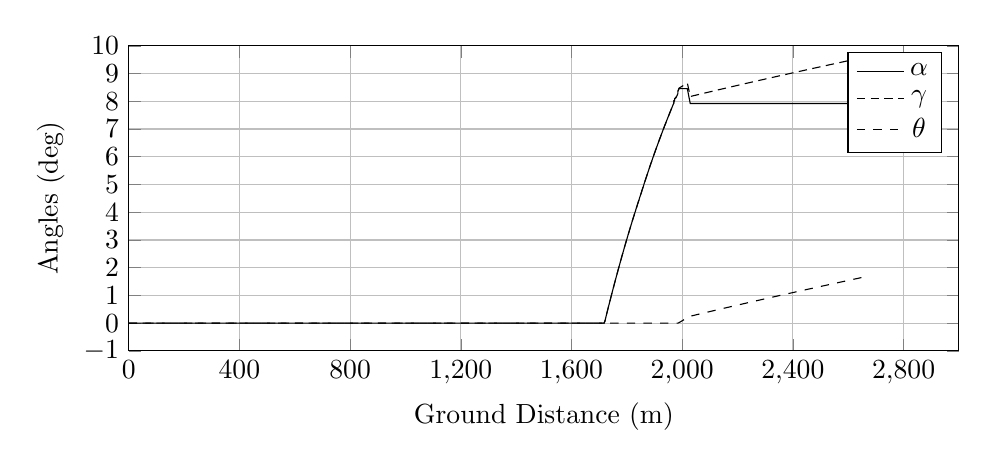
\begin{tikzpicture}

\begin{axis}[
width=\textwidth,
height=0.45\textwidth,
scaled ticks=false, tick label style={/pgf/number format/fixed},
xmin=0.0,
xmax=3000,
xtick={0,400,800,1200,1600,2000,2400,2800,3200},
xlabel={Ground Distance (m)},
xmajorgrids,
ymin=-1.0,
ymax=10,
ylabel={Angles (deg)},
ytick={-1,0,1,2,3,4,5,6,7,8,9,10},
ymajorgrids,
legend entries = {$\alpha$\\$\gamma$\\$\theta$\\}
]

\addplot [
color=black,
solid
]
table[row sep=crcr]{
1.3729668748937997E-8	0.0\\
2.6049868369719035E-7	0.0\\
2.0491224421327626E-6	0.0\\
9.92442121137073E-6	0.0\\
4.7452367809869807E-5	0.0\\
1.740064756114434E-4	0.0\\
4.0608377013922605E-4	0.0\\
7.313431501337001E-4	0.0\\
0.0011549487327126044	0.0\\
0.0016799013484208249	0.0\\
0.002295089346817705	0.0\\
0.003009933382444524	0.0\\
0.003810608015426248	0.0\\
0.004723484476856681	0.0\\
0.005727138856912631	0.0\\
0.006836216967948795	0.0\\
0.007997302399386296	0.0\\
0.00929136979810952	0.0\\
0.010685558505459776	0.0\\
0.012178513621519987	0.0\\
0.013775244426719659	0.0\\
0.015470070176169002	0.0\\
0.0172374436815836	0.0\\
0.019122918912604377	0.0\\
0.021104911040230538	0.0\\
0.023190717999955576	0.0\\
0.025355802981115103	0.0\\
0.027620619195902148	0.0\\
0.030020274690474198	0.0\\
0.032476028269866286	0.0\\
0.035054163466719815	0.0\\
0.037720846868992755	0.0\\
0.04049779674511381	0.0\\
0.043329456594087365	0.0\\
0.04629652060163805	0.0\\
0.04934498934704602	0.0\\
0.052507657924119336	0.0\\
0.055769483710642484	0.0\\
0.05917209570914676	0.0\\
0.06264043916012321	0.0\\
0.06620063977265622	0.0\\
0.06987962792775945	0.0\\
0.0736568184539585	0.0\\
0.07754284280095361	0.0\\
0.08151127871105612	0.0\\
0.08560324933017655	0.0\\
0.08985265585263943	0.0\\
0.09413961367176535	0.0\\
0.09857725310864562	0.0\\
0.10307959255469257	0.0\\
0.10766008648593872	0.0\\
0.11234920964493048	0.0\\
0.11719267720457946	0.0\\
0.12216973960582883	0.0\\
0.12724007601918352	0.0\\
0.13233299746505212	0.0\\
0.13755256756750583	0.0\\
0.14287728588926696	0.0\\
0.1482946925752714	0.0\\
0.15381585025670613	0.0\\
0.15940564092189102	0.0\\
0.16526271495916878	0.0\\
0.17120082448158402	0.0\\
0.17717889132867753	0.0\\
0.18324322596131126	0.0\\
0.189427022360885	0.0\\
0.1957511558722988	0.0\\
0.2021484013779125	0.0\\
0.20865863707071397	0.0\\
0.21548666343168166	0.0\\
0.22220154781289658	0.0\\
0.22919671627301902	0.0\\
0.23611678795738544	0.0\\
0.24306300975244904	0.0\\
0.2503085190632165	0.0\\
0.2576623280401219	0.0\\
0.26502430524173204	0.0\\
0.2724963584449146	0.0\\
0.2802001060647876	0.0\\
0.2878583985474956	0.0\\
0.2958320780323821	0.0\\
0.3040021452321372	0.0\\
0.31208951788619	0.0\\
0.3202851396023423	0.0\\
0.3287233234973125	0.0\\
0.3370425959884752	0.0\\
0.34575405233845447	0.0\\
0.3545073625286812	0.0\\
0.36338982075299686	0.0\\
0.37247557159370037	0.0\\
0.38151350442869847	0.0\\
0.3905554764834429	0.0\\
0.3999457587520332	0.0\\
0.4095398754587949	0.0\\
0.4189621792151833	0.0\\
0.4285208811402964	0.0\\
0.43828968955472236	0.0\\
0.44807735398784176	0.0\\
0.45806002753764463	0.0\\
0.4682994371692033	0.0\\
0.4787752542918833	0.0\\
0.4890770094685154	0.0\\
0.49985939134273727	0.0\\
0.5106597490205704	0.0\\
0.5213580865152188	0.0\\
0.532247733242454	0.0\\
0.5431365108549349	0.0\\
0.554075964429489	0.0\\
0.5653450694020941	0.0\\
0.5769901159382542	0.0\\
0.588512657344902	0.0\\
0.6004070039036553	0.0\\
0.6121651247369502	0.0\\
0.6239717914322569	0.0\\
0.6362472885961421	0.0\\
0.6486428939173223	0.0\\
0.6610190736373547	0.0\\
0.6737248046101814	0.0\\
0.6862826225989949	0.0\\
0.6991952542603428	0.0\\
0.7122988072688032	0.0\\
0.7251463703465595	0.0\\
0.7381769453061875	0.0\\
0.7516618647379176	0.0\\
0.7654913705221527	0.0\\
0.7791756406994825	0.0\\
0.7930637813125616	0.0\\
0.8074774191984457	0.0\\
0.8215072375247947	0.0\\
0.8361010597475598	0.0\\
0.8503303420601955	0.0\\
0.8650627501899835	0.0\\
0.8802332960144008	0.0\\
0.8951742046771463	0.0\\
0.9100334756324657	0.0\\
0.9251067343345352	0.0\\
0.9403923630470314	0.0\\
0.9559303815501943	0.0\\
0.9712400158034169	0.0\\
0.9869533781138684	0.0\\
1.0029148609762486	0.0\\
1.0189962473881624	0.0\\
1.035465185745812	0.0\\
1.0516742337458713	0.0\\
1.067815735429615	0.0\\
1.0846705971808022	0.0\\
1.1012775250051634	0.0\\
1.1180798406225687	0.0\\
1.1351395900544134	0.0\\
1.1526388687279154	0.0\\
1.1698922447507556	0.0\\
1.1875468452119025	0.0\\
1.2058383275300355	0.0\\
1.2239395537495579	0.0\\
1.2422020624207541	0.0\\
1.2608769472440078	0.0\\
1.2794948487006894	0.0\\
1.2979152553275424	0.0\\
1.3166445915281573	0.0\\
1.3354141707340492	0.0\\
1.3543210821322504	0.0\\
1.373689361295591	0.0\\
1.3932049885015831	0.0\\
1.4131781782225183	0.0\\
1.4330139682345777	0.0\\
1.4528243860883294	0.0\\
1.4728783400745615	0.0\\
1.4934621752870565	0.0\\
1.5141408097620341	0.0\\
1.53430654450827	0.0\\
1.5553850389607948	0.0\\
1.5762653203499473	0.0\\
1.5975496774716453	0.0\\
1.6196077215345106	0.0\\
1.6413652536722467	0.0\\
1.663437310723463	0.0\\
1.6860768385032747	0.0\\
1.7077101022266827	0.0\\
1.7297306410738114	0.0\\
1.7520297891459062	0.0\\
1.7743087535215367	0.0\\
1.797257424336919	0.0\\
1.8200802473615325	0.0\\
1.8430350373473994	0.0\\
1.8666926279964304	0.0\\
1.8902808566018634	0.0\\
1.9138231309717848	0.0\\
1.937187877956735	0.0\\
1.9611060682733261	0.0\\
1.9852138445648535	0.0\\
2.009780393513653	0.0\\
2.0346228225622163	0.0\\
2.0593611988602687	0.0\\
2.08477023517836	0.0\\
2.110324766702745	0.0\\
2.1352655781940433	0.0\\
2.160528860803022	0.0\\
2.1862071157614817	0.0\\
2.2127756699400534	0.0\\
2.2391904543957084	0.0\\
2.2653528664920257	0.0\\
2.292150575495974	0.0\\
2.3187704640870406	0.0\\
2.3455495914188482	0.0\\
2.372862901366455	0.0\\
2.4007145172972395	0.0\\
2.428100404243743	0.0\\
2.4555980306928005	0.0\\
2.483374904362833	0.0\\
2.511687733451976	0.0\\
2.5402569276484597	0.0\\
2.568415369317849	0.0\\
2.596987652715761	0.0\\
2.6263861238451423	0.0\\
2.655991481965028	0.0\\
2.6856115886357443	0.0\\
2.7154221146045012	0.0\\
2.7455665152057707	0.0\\
2.7752624694325894	0.0\\
2.805457625653509	0.0\\
2.8358231840904597	0.0\\
2.8663460878589797	0.0\\
2.897817297850832	0.0\\
2.9287074004595235	0.0\\
2.9603588456990284	0.0\\
2.9922321403815406	0.0\\
3.0241119471841866	0.0\\
3.056446055158509	0.0\\
3.0889346922121366	0.0\\
3.122221620829695	0.0\\
3.1546991615623394	0.0\\
3.187635101478671	0.0\\
3.221010117202278	0.0\\
3.2543449374576605	0.0\\
3.288235920596943	0.0\\
3.3223704322934555	0.0\\
3.3562838593334394	0.0\\
3.3906320903803255	0.0\\
3.425633159699527	0.0\\
3.462387235801926	0.0\\
3.4973980805087237	0.0\\
3.5324804241140235	0.0\\
3.5675385073174235	0.0\\
3.6040688981843845	0.0\\
3.6393612181513753	0.0\\
3.6770856360342323	0.0\\
3.7131729334920323	0.0\\
3.749509707933214	0.0\\
3.785733977879824	0.0\\
3.8225309786916544	0.0\\
3.860867115351552	0.0\\
3.89929745075254	0.0\\
3.9373367205567504	0.0\\
3.9751626485832894	0.0\\
4.013671158053867	0.0\\
4.0521140617426425	0.0\\
4.092377631210638	0.0\\
4.131586743753305	0.0\\
4.1715696979561425	0.0\\
4.210522654700574	0.0\\
4.250196810863292	0.0\\
4.2917015001093795	0.0\\
4.332438976653355	0.0\\
4.373124372895289	0.0\\
4.414429464889761	0.0\\
4.455884944705147	0.0\\
4.497250153511752	0.0\\
4.537976875075978	0.0\\
4.581399817640802	0.0\\
4.623816269683994	0.0\\
4.666022338967499	0.0\\
4.709098934189642	0.0\\
4.752435367147649	0.0\\
4.79531009100786	0.0\\
4.838191999420829	0.0\\
4.881381760681686	0.0\\
4.9256451804034285	0.0\\
4.9704217340957495	0.0\\
5.014356093293278	0.0\\
5.058826350846283	0.0\\
5.104458009943745	0.0\\
5.149663211268795	0.0\\
5.194981168813841	0.0\\
5.241194091283663	0.0\\
5.287987552078626	0.0\\
5.334426822383641	0.0\\
5.380633359096258	0.0\\
5.427524438012913	0.0\\
5.476157635197664	0.0\\
5.524667120325573	0.0\\
5.5732739519824435	0.0\\
5.6208990292882195	0.0\\
5.671502816366864	0.0\\
5.719824083529298	0.0\\
5.767871110439133	0.0\\
5.8169321963676754	0.0\\
5.866076914057565	0.0\\
5.917200682776528	0.0\\
5.96684810088939	0.0\\
6.016885842403935	0.0\\
6.068639931677712	0.0\\
6.119867755785197	0.0\\
6.171030794930029	0.0\\
6.222884713227881	0.0\\
6.2735946138732235	0.0\\
6.325883502103322	0.0\\
6.379615386553551	0.0\\
6.432194972482147	0.0\\
6.484528316464761	0.0\\
6.536619297696934	0.0\\
6.589662958081361	0.0\\
6.644121795496577	0.0\\
6.697445536614451	0.0\\
6.7518063163896365	0.0\\
6.8068829439682315	0.0\\
6.863205650636274	0.0\\
6.9185329265047315	0.0\\
6.974634519184049	0.0\\
7.031139830722298	0.0\\
7.0870923879294985	0.0\\
7.144766952910487	0.0\\
7.2026451873548805	0.0\\
7.261191729679483	0.0\\
7.320502240843062	0.0\\
7.378210233177999	0.0\\
7.437738452534925	0.0\\
7.49714639104333	0.0\\
7.556502460410064	0.0\\
7.617032771987237	0.0\\
7.676883327249088	0.0\\
7.735740247984193	0.0\\
7.796086087039788	0.0\\
7.856787102853412	0.0\\
7.91721236259451	0.0\\
7.979013602666894	0.0\\
8.039824025454376	0.0\\
8.102419182184594	0.0\\
8.16459313580776	0.0\\
8.226347093952135	0.0\\
8.290527749984296	0.0\\
8.353592793320257	0.0\\
8.417564177281012	0.0\\
8.482044607535009	0.0\\
8.547336806956285	0.0\\
8.613293246319614	0.0\\
8.6778048537894	0.0\\
8.74454839911753	0.0\\
8.810708373588199	0.0\\
8.876548424968423	0.0\\
8.942828456712885	0.0\\
9.010858044488913	0.0\\
9.079453414959548	0.0\\
9.148767802603732	0.0\\
9.21609997183467	0.0\\
9.285579683381485	0.0\\
9.355451712480097	0.0\\
9.423585014597279	0.0\\
9.493435356703696	0.0\\
9.562655940911181	0.0\\
9.63183713653898	0.0\\
9.703018708836247	0.0\\
9.773178624863132	0.0\\
9.844376937811855	0.0\\
9.914998792594716	0.0\\
9.98720270419701	0.0\\
10.059478150570087	0.0\\
10.132362020358627	0.0\\
10.205876892438312	0.0\\
10.279422251887688	0.0\\
10.353305644514993	0.0\\
10.42811398108589	0.0\\
10.50332954727428	0.0\\
10.578207710262959	0.0\\
10.65503529959097	0.0\\
10.730232142651953	0.0\\
10.805871937852555	0.0\\
10.88265320376452	0.0\\
10.958577899345514	0.0\\
11.034861147941964	0.0\\
11.112742623646977	0.0\\
11.190543636431041	0.0\\
11.267787598939979	0.0\\
11.3462805052093	0.0\\
11.423875697147409	0.0\\
11.502735831556972	0.0\\
11.581465323066688	0.0\\
11.661639233340708	0.0\\
11.741743247575428	0.0\\
11.821864700430528	0.0\\
11.901816327719768	0.0\\
11.98361062800689	0.0\\
12.065425957085825	0.0\\
12.1478520915771	0.0\\
12.230956215923495	0.0\\
12.313306905825911	0.0\\
12.396632357805931	0.0\\
12.479578787946746	0.0\\
12.564327762802186	0.0\\
12.648175874147956	0.0\\
12.736145481689512	0.0\\
12.821080154398764	0.0\\
12.908009536077355	0.0\\
12.994986774303499	0.0\\
13.081752199798046	0.0\\
13.17035388279784	0.0\\
13.257836697901475	0.0\\
13.34511613365563	0.0\\
13.433461823066896	0.0\\
13.524108483575919	0.0\\
13.611203924103116	0.0\\
13.702229394080796	0.0\\
13.792427706753081	0.0\\
13.882429934062493	0.0\\
13.975435778888343	0.0\\
14.065832730112316	0.0\\
14.157894546480026	0.0\\
14.250668806951023	0.0\\
14.343291987615704	0.0\\
14.43744444968501	0.0\\
14.532636396723657	0.0\\
14.625507232812737	0.0\\
14.721503924398366	0.0\\
14.818738382089133	0.0\\
14.913572076739943	0.0\\
15.009701633366973	0.0\\
15.10815424447124	0.0\\
15.206130868840724	0.0\\
15.304035939715973	0.0\\
15.403499839366233	0.0\\
15.503209871950865	0.0\\
15.601718454553605	0.0\\
15.700655560608023	0.0\\
15.801250929860519	0.0\\
15.899917805652187	0.0\\
16.001574124100856	0.0\\
16.102638779863817	0.0\\
16.204479333764816	0.0\\
16.30489644092564	0.0\\
16.40578186591999	0.0\\
16.509201471948074	0.0\\
16.614557195984908	0.0\\
16.717657554831042	0.0\\
16.823039336622365	0.0\\
16.928576062495388	0.0\\
17.03469945574068	0.0\\
17.140697318244236	0.0\\
17.246066414787876	0.0\\
17.35183930840021	0.0\\
17.458399953804133	0.0\\
17.565707112453843	0.0\\
17.673103795073075	0.0\\
17.781888038667653	0.0\\
17.89115167195854	0.0\\
18.00105710767307	0.0\\
18.110142905530395	0.0\\
18.219697237410173	0.0\\
18.32752951944549	0.0\\
18.43743745973078	0.0\\
18.54904630654982	0.0\\
18.659302591714813	0.0\\
18.770734536087716	0.0\\
18.883577445650936	0.0\\
18.996263390583444	0.0\\
19.108816920034535	0.0\\
19.22287647779894	0.0\\
19.33763586704334	0.0\\
19.456324114791514	0.0\\
19.57349394116079	0.0\\
19.690148252848566	0.0\\
19.80521137071168	0.0\\
19.92379170801214	0.0\\
20.04216631061405	0.0\\
20.15848954929409	0.0\\
20.278242138037896	0.0\\
20.396206084226087	0.0\\
20.516315546862906	0.0\\
20.637173924977112	0.0\\
20.75450010628387	0.0\\
20.874378237858778	0.0\\
20.996035953832852	0.0\\
21.11812959618858	0.0\\
21.240471115580952	0.0\\
21.361479376438375	0.0\\
21.485224699488654	0.0\\
21.607870280890317	0.0\\
21.73242999733349	0.0\\
21.85704493170313	0.0\\
21.98122016226351	0.0\\
22.10826921766411	0.0\\
22.235261614051304	0.0\\
22.361664688868032	0.0\\
22.48780138980522	0.0\\
22.614107216476143	0.0\\
22.74409311379692	0.0\\
22.873024137794893	0.0\\
23.003512644166257	0.0\\
23.132891545907036	0.0\\
23.26270690888247	0.0\\
23.39264146728729	0.0\\
23.52277721573431	0.0\\
23.654883767164463	0.0\\
23.78569183677709	0.0\\
23.917003007077597	0.0\\
24.047013652206026	0.0\\
24.178458227988493	0.0\\
24.314609552493202	0.0\\
24.447533097503474	0.0\\
24.579128452041708	0.0\\
24.71011994849615	0.0\\
24.843278471916108	0.0\\
24.975761222328053	0.0\\
25.1115496753864	0.0\\
25.247101122854083	0.0\\
25.384906965000688	0.0\\
25.522261036073317	0.0\\
25.66123001648475	0.0\\
25.79865327455613	0.0\\
25.826335196219034	0.0\\
25.839610403727477	0.0\\
25.841006316401874	0.0\\
25.84227013303559	0.0\\
25.84770509053729	0.0\\
25.86419328224909	0.0\\
25.90571916957557	0.0\\
25.999268866927544	0.0\\
26.123295978662824	0.0\\
26.250212562581652	0.0\\
26.376891976518465	0.0\\
26.50638698165423	0.0\\
26.634042370994827	0.0\\
26.763333806613538	0.0\\
26.893207366259766	0.0\\
27.022905486492228	0.0\\
27.153956322362554	0.0\\
27.287774297957696	0.0\\
27.42030033806219	0.0\\
27.555504894698295	0.0\\
27.691130018821354	0.0\\
27.82633313037239	0.0\\
27.959508564917073	0.0\\
28.096515548835796	0.0\\
28.232789703382153	0.0\\
28.368684388406535	0.0\\
28.506541650227618	0.0\\
28.64533374691623	0.0\\
28.78297783415192	0.0\\
28.92277775692753	0.0\\
29.06227187463503	0.0\\
29.20212864139956	0.0\\
29.34335827861657	0.0\\
29.483225747293005	0.0\\
29.625960812476485	0.0\\
29.76706561118049	0.0\\
29.909402910999468	0.0\\
30.051751399473822	0.0\\
30.196612335666572	0.0\\
30.342192969749448	0.0\\
30.48583400527584	0.0\\
30.632658550781265	0.0\\
30.77846394498075	0.0\\
30.92408133049836	0.0\\
31.071091331299215	0.0\\
31.218274793935116	0.0\\
31.366705758252415	0.0\\
31.515339333797037	0.0\\
31.66356819769615	0.0\\
31.814689402684216	0.0\\
31.96649953392354	0.0\\
32.115424616034375	0.0\\
32.266253234088566	0.0\\
32.41813832080348	0.0\\
32.569791431087395	0.0\\
32.722234201183724	0.0\\
32.876984607664	0.0\\
33.031873994672836	0.0\\
33.18502245018544	0.0\\
33.34135780547538	0.0\\
33.49759920343199	0.0\\
33.65385117142162	0.0\\
33.8113313806527	0.0\\
33.96985264489639	0.0\\
34.126473036379195	0.0\\
34.2857505660089	0.0\\
34.4449212019973	0.0\\
34.60566879064274	0.0\\
34.76644486933921	0.0\\
34.92612701881755	0.0\\
35.08630421658309	0.0\\
35.24825698849928	0.0\\
35.412303951281956	0.0\\
35.57355277914179	0.0\\
35.73545353069308	0.0\\
35.89925038949356	0.0\\
36.065161289279985	0.0\\
36.23047312008262	0.0\\
36.39472205714358	0.0\\
36.56135389445764	0.0\\
36.72774532558607	0.0\\
36.89384825683493	0.0\\
37.05904296416534	0.0\\
37.22702676294645	0.0\\
37.39437475321985	0.0\\
37.5621109943643	0.0\\
37.73270471709142	0.0\\
37.903359519601935	0.0\\
38.071486842086316	0.0\\
38.23815243703595	0.0\\
38.40817787072022	0.0\\
38.57751392140098	0.0\\
38.750215798728505	0.0\\
38.92001182640311	0.0\\
39.09310637700479	0.0\\
39.26472366117933	0.0\\
39.436554723976656	0.0\\
39.608961777617054	0.0\\
39.782828308010565	0.0\\
39.956194359016465	0.0\\
40.132391837044906	0.0\\
40.30868053167249	0.0\\
40.48611580488176	0.0\\
40.66383502946924	0.0\\
40.83999042132467	0.0\\
41.018202681018664	0.0\\
41.19780999006247	0.0\\
41.37730467548502	0.0\\
41.557010452813884	0.0\\
41.73612816026986	0.0\\
41.91555194917056	0.0\\
42.09743589423803	0.0\\
42.27807550146298	0.0\\
42.45995188234755	0.0\\
42.6401410478328	0.0\\
42.822293873795985	0.0\\
43.00585672428667	0.0\\
43.189965171449515	0.0\\
43.372020236704074	0.0\\
43.555636897252796	0.0\\
43.74012033961118	0.0\\
43.92429822300048	0.0\\
44.106869824379004	0.0\\
44.29411840239129	0.0\\
44.47920670866131	0.0\\
44.665034305215386	0.0\\
44.85242224248053	0.0\\
45.03948098831597	0.0\\
45.22811764277584	0.0\\
45.41548629589063	0.0\\
45.60322541388645	0.0\\
45.793007222766036	0.0\\
45.983742663331824	0.0\\
46.172643153142886	0.0\\
46.36421599110457	0.0\\
46.553512793459404	0.0\\
46.745018895697555	0.0\\
46.93606459490553	0.0\\
47.126948089509526	0.0\\
47.31881294044018	0.0\\
47.5110690178297	0.0\\
47.705448624448266	0.0\\
47.90005519882567	0.0\\
48.09288923506665	0.0\\
48.28732881729917	0.0\\
48.484002572746206	0.0\\
48.68089030454945	0.0\\
48.87532723390382	0.0\\
49.07073736177763	0.0\\
49.2672083392297	0.0\\
49.46586249263092	0.0\\
49.661880987188695	0.0\\
49.85966148345089	0.0\\
50.05808618672894	0.0\\
50.25785665917266	0.0\\
50.45743808511885	0.0\\
50.65573800086891	0.0\\
50.85948768734909	0.0\\
51.061243703011925	0.0\\
51.26368286286315	0.0\\
51.46416466063809	0.0\\
51.66475943174029	0.0\\
51.86588207153103	0.0\\
52.07444928962187	0.0\\
52.2824430085781	0.0\\
52.48676525705545	0.0\\
52.69531994892206	0.0\\
52.90027076850366	0.0\\
53.108186167814935	0.0\\
53.31165724918766	0.0\\
53.520024946679996	0.0\\
53.72688450142306	0.0\\
53.93707391647578	0.0\\
54.14518573319289	0.0\\
54.35125853722778	0.0\\
54.56213447502874	0.0\\
54.77598621923464	0.0\\
54.987629956235494	0.0\\
55.19778857845695	0.0\\
55.41030974885841	0.0\\
55.62390503323701	0.0\\
55.83671574169797	0.0\\
56.047071254351536	0.0\\
56.26137331252919	0.0\\
56.47512769358855	0.0\\
56.69105800830218	0.0\\
56.90937011004422	0.0\\
57.12736617899088	0.0\\
57.346833156368504	0.0\\
57.56476609337061	0.0\\
57.78230894703917	0.0\\
57.99943865551505	0.0\\
58.21827465292657	0.0\\
58.436085045729726	0.0\\
58.6577546799423	0.0\\
58.87982836766625	0.0\\
59.10336118170943	0.0\\
59.324182403931715	0.0\\
59.545440661451366	0.0\\
59.768227251413464	0.0\\
59.99077485409802	0.0\\
60.21631063559073	0.0\\
60.44006004384342	0.0\\
60.66502706168687	0.0\\
60.89133011288284	0.0\\
61.11585558357916	0.0\\
61.3432655409558	0.0\\
61.57186440401435	0.0\\
61.79868765088207	0.0\\
62.025670725987	0.0\\
62.254132946411545	0.0\\
62.48290793247415	0.0\\
62.713817944074236	0.0\\
62.94484116346062	0.0\\
63.17805109236767	0.0\\
63.41124119062552	0.0\\
63.64505576847972	0.0\\
63.87735201907903	0.0\\
64.11169045660182	0.0\\
64.34725756208485	0.0\\
64.58324360279937	0.0\\
64.81881329818131	0.0\\
65.05563560606473	0.0\\
65.29467812810154	0.0\\
65.53178653633495	0.0\\
65.77046761369158	0.0\\
66.01019347650049	0.0\\
66.25262920761091	0.0\\
66.49342175078831	0.0\\
66.73393309567928	0.0\\
66.97718905970893	0.0\\
67.21919788222482	0.0\\
67.46413738735515	0.0\\
67.70584739194695	0.0\\
67.95375887035246	0.0\\
68.19817148521656	0.0\\
68.44413350233111	0.0\\
68.68984243621705	0.0\\
68.93951041285982	0.0\\
69.19023531750676	0.0\\
69.43956667494601	0.0\\
69.68998597860525	0.0\\
69.94098943220166	0.0\\
70.1928405184459	0.0\\
70.44659484061637	0.0\\
70.69926103579675	0.0\\
70.95414956377036	0.0\\
71.21136313866151	0.0\\
71.46778788208749	0.0\\
71.7247351381395	0.0\\
71.98234155897126	0.0\\
72.24107377350035	0.0\\
72.4986091150376	0.0\\
72.75949164810788	0.0\\
73.02014691132015	0.0\\
73.28114866838587	0.0\\
73.54342372888959	0.0\\
73.80584407854005	0.0\\
74.07231166191039	0.0\\
74.3389341302921	0.0\\
74.60521354141642	0.0\\
74.87280568706873	0.0\\
75.1403821105715	0.0\\
75.41145333671997	0.0\\
75.68265298797411	0.0\\
75.95075857762194	0.0\\
76.2241428819712	0.0\\
76.4990100438061	0.0\\
76.77213586328236	0.0\\
77.04724851790667	0.0\\
77.32330034006353	0.0\\
77.59850473375684	0.0\\
77.87773830129439	0.0\\
78.1565255546137	0.0\\
78.43842651648492	0.0\\
78.720833678605	0.0\\
79.00101298089581	0.0\\
79.28359351218376	0.0\\
79.57011733099088	0.0\\
79.85418914588558	0.0\\
80.13919871477489	0.0\\
80.42568449319114	0.0\\
80.71472498530085	0.0\\
81.006853148924	0.0\\
81.2951972638476	0.0\\
81.58524575795963	0.0\\
81.87461709596036	0.0\\
82.1711642895769	0.0\\
82.46716486408064	0.0\\
82.76422974563803	0.0\\
83.05801377197795	0.0\\
83.35853301954708	0.0\\
83.65664966506407	0.0\\
83.95487262936624	0.0\\
84.25322789115987	0.0\\
84.55664509033022	0.0\\
84.8599544590121	0.0\\
85.16499148084048	0.0\\
85.47187188044902	0.0\\
85.77908321853027	0.0\\
86.08675489504844	0.0\\
86.39784539041122	0.0\\
86.71051296037359	0.0\\
87.02583358957506	0.0\\
87.34037846285594	0.0\\
87.65395388450591	0.0\\
87.96687312379424	0.0\\
88.28527441497255	0.0\\
88.6103524516937	0.0\\
88.92871226770333	0.0\\
89.25003295857354	0.0\\
89.57522243846881	0.0\\
89.90247582737899	0.0\\
90.22602529632545	0.0\\
90.5494223037065	0.0\\
90.87816525326718	0.0\\
91.20455861430293	0.0\\
91.53817773235312	0.0\\
91.87076195087604	0.0\\
92.20124984301029	0.0\\
92.53140503523474	0.0\\
92.86389705561814	0.0\\
93.19815266874983	0.0\\
93.53304529783748	0.0\\
93.86737084100128	0.0\\
94.20337949361911	0.0\\
94.54065981474497	0.0\\
94.87396787418089	0.0\\
95.21684847579547	0.0\\
95.55392648231228	0.0\\
95.89232371872416	0.0\\
96.23051075783204	0.0\\
96.57164052232307	0.0\\
96.90762523479154	0.0\\
97.24755293575913	0.0\\
97.58790661409188	0.0\\
97.92576087813703	0.0\\
98.26661027452474	0.0\\
98.6051908024865	0.0\\
98.94563962387357	0.0\\
99.28665364663627	0.0\\
99.63350087797645	0.0\\
99.97685593767679	0.0\\
100.31593955776762	0.0\\
100.65572384630482	0.0\\
100.99616871909686	0.0\\
101.3402339503516	0.0\\
101.67973054404297	0.0\\
102.01657591573795	0.0\\
102.35656456518868	0.0\\
102.6941824316649	0.0\\
103.03547296258705	0.0\\
103.37623032340073	0.0\\
103.71852978299776	0.0\\
104.05851119314701	0.0\\
104.3949509202441	0.0\\
104.7329053851843	0.0\\
105.07104272194636	0.0\\
105.40742307340048	0.0\\
105.74423560014887	0.0\\
106.07955743077031	0.0\\
106.41623710643992	0.0\\
106.75618472497374	0.0\\
107.0942647435474	0.0\\
107.43151869252583	0.0\\
107.44650965670576	0.0\\
107.45815118347005	0.0\\
107.46233674961977	0.0\\
107.46535588765028	0.0\\
107.46808502617694	0.0\\
107.4836206108138	0.0\\
107.53176708907421	0.0\\
107.68672244793561	0.0\\
107.97570433527497	0.0\\
108.27744765146667	0.0\\
108.5816623935838	0.0\\
108.88557241638279	0.0\\
109.19209959959528	0.0\\
109.50241879336687	0.0\\
109.81066605766154	0.0\\
110.12101503747155	0.0\\
110.43285681965125	0.0\\
110.74725799716322	0.0\\
111.06462449033057	0.0\\
111.38211128519615	0.0\\
111.70119562731901	0.0\\
112.02298633508096	0.0\\
112.34320819983824	0.0\\
112.66812620709393	0.0\\
112.99302416686388	0.0\\
113.31966045518399	0.0\\
113.64998129974768	0.0\\
113.97857627498675	0.0\\
114.31304608469316	0.0\\
114.64448318111735	0.0\\
114.98093514978115	0.0\\
115.31969924418831	0.0\\
115.65790718621022	0.0\\
116.00063352526521	0.0\\
116.34235083463872	0.0\\
116.68621873349733	0.0\\
117.03331062078092	0.0\\
117.37910048629482	0.0\\
117.72869476105836	0.0\\
118.08005947084649	0.0\\
118.43363644355449	0.0\\
118.79186464668504	0.0\\
119.14769212941735	0.0\\
119.5036618261702	0.0\\
119.86270697471275	0.0\\
120.22616362054572	0.0\\
120.58991121293201	0.0\\
120.95538130513773	0.0\\
121.3195355377388	0.0\\
121.68590041554987	0.0\\
122.05305648207542	0.0\\
122.42257239354896	0.0\\
122.79503144936103	0.0\\
123.16629137010841	0.0\\
123.53950748252527	0.0\\
123.91239367862553	0.0\\
124.29026003316017	0.0\\
124.66301933937496	0.0\\
125.03890311735066	0.0\\
125.41380975776434	0.0\\
125.7896808967325	0.0\\
126.16837244152023	0.0\\
126.54595968852882	0.0\\
126.92471834906405	0.0\\
127.30294276405039	0.0\\
127.68255852126984	0.0\\
128.06243727540487	0.0\\
128.44360431740483	0.0\\
128.82265748788262	0.0\\
129.1989690567886	0.0\\
129.57765386613931	0.0\\
129.95508099647026	0.0\\
130.33359114840187	0.0\\
130.71373745886524	0.0\\
131.09453904397424	0.0\\
131.47657586018488	0.0\\
131.85678563989967	0.0\\
132.23856625352113	0.0\\
132.61595336405918	0.0\\
132.99976263915818	0.0\\
133.38083522978053	0.0\\
133.76098428781995	0.0\\
134.1363519425165	0.0\\
134.51557915495124	0.0\\
134.8968696170101	0.0\\
135.27419431482667	0.0\\
135.65215477207505	0.0\\
136.03329358991255	0.0\\
136.41192880753374	0.0\\
136.7898079310749	0.0\\
137.17001317148595	0.0\\
137.54844558779996	0.0\\
137.92617219433072	0.0\\
138.30476964659732	0.0\\
138.68390038934075	0.0\\
139.0631653430654	0.0\\
139.4406106933401	0.0\\
139.81914660512416	0.0\\
140.19767098864742	0.0\\
140.5730919292459	0.0\\
140.95061983253072	0.0\\
141.32838502869612	0.0\\
141.70636515873298	0.0\\
142.0839785067887	0.0\\
142.46357402350594	0.0\\
142.84082211769783	0.0\\
143.21906727224075	0.0\\
143.59963619096823	0.0\\
143.97984478872678	0.0\\
144.35941603837455	0.0\\
144.7355521893594	0.0\\
145.11296635073694	0.0\\
145.49073213867456	0.0\\
145.87033631970945	0.0\\
146.24486520181193	0.0\\
146.6238757206513	0.0\\
147.00096360401335	0.0\\
147.37874202190085	0.0\\
147.756852900845	0.0\\
148.13572640408995	0.0\\
148.5136798644104	0.0\\
148.89083780486442	0.0\\
149.2712459042852	0.0\\
149.65303236723025	0.0\\
150.0329584616291	0.0\\
150.41363382646614	0.0\\
150.79322940570728	0.0\\
151.17272478467066	0.0\\
151.55400296227282	0.0\\
151.93482601265913	0.0\\
152.31881414221942	0.0\\
152.70208150063132	0.0\\
153.08320649997165	0.0\\
153.4666285558243	0.0\\
153.84825937276264	0.0\\
154.23093781718723	0.0\\
154.61485031834388	0.0\\
155.00001234931443	0.0\\
155.38285725409855	0.0\\
155.7679513537659	0.0\\
156.1509667875323	0.0\\
156.53491934392343	0.0\\
156.91995289130983	0.0\\
157.30625057946366	0.0\\
157.69121706207227	0.0\\
158.07789765133754	0.0\\
158.46521012398495	0.0\\
158.85138765236047	0.0\\
159.23964669847322	0.0\\
159.62715395386465	0.0\\
160.01960115328984	0.0\\
160.4079207075476	0.0\\
160.79602490671402	0.0\\
161.18437278725975	0.0\\
161.57644284003254	0.0\\
161.96812230097612	0.0\\
162.35808768568592	0.0\\
162.75087300343483	0.0\\
163.14546270495134	0.0\\
163.53745675514648	0.0\\
163.92955389373896	0.0\\
164.32395276810763	0.0\\
164.71713266653478	0.0\\
165.1102153740033	0.0\\
165.5035884424101	0.0\\
165.89816400198282	0.0\\
166.29148626774366	0.0\\
166.68861804276264	0.0\\
167.082852347146	0.0\\
167.48006204110857	0.0\\
167.8798182678497	0.0\\
168.27774435731556	0.0\\
168.67741362640317	0.0\\
169.07475368467374	0.0\\
169.4759958044982	0.0\\
169.87832784425882	0.0\\
170.2792240364854	0.0\\
170.68126852540456	0.0\\
171.08617821288442	0.0\\
171.48766933901368	0.0\\
171.892744970828	0.0\\
172.29711201372032	0.0\\
172.70264003426053	0.0\\
173.1105289448074	0.0\\
173.5163733808056	0.0\\
173.92577914808027	0.0\\
174.33607303977334	0.0\\
174.74614233406845	0.0\\
175.15731444736514	0.0\\
175.56901623635082	0.0\\
175.97955109701695	0.0\\
176.39275298155184	0.0\\
176.80397138375372	0.0\\
177.21946344336607	0.0\\
177.6332252263685	0.0\\
178.05102033212842	0.0\\
178.46725124888752	0.0\\
178.88389799206544	0.0\\
179.29839533747668	0.0\\
179.71608569665375	0.0\\
180.1342696339205	0.0\\
180.26454521656194	0.0\\
180.5538779958007	0.0\\
180.97677279803082	0.0\\
181.73177043104909	0.0\\
182.61825861954026	0.0\\
183.4994266290775	0.0\\
184.38832398643513	0.0\\
185.2752206450968	0.0\\
186.16090254585617	0.0\\
187.05782443666988	0.0\\
187.95004436743	0.0\\
188.84343565256296	0.0\\
189.73203483232732	0.0\\
190.63087969896367	0.0\\
191.53167348748025	0.0\\
192.42914206966827	0.0\\
193.32936064878362	0.0\\
194.23353734669462	0.0\\
195.14873951553636	0.0\\
196.05846844349168	0.0\\
196.9665797060448	0.0\\
197.88137813217617	0.0\\
198.80153314772656	0.0\\
199.72262566550114	0.0\\
200.6418018332526	0.0\\
201.57021605131746	0.0\\
202.49227039761405	0.0\\
203.4093310979173	0.0\\
204.33741716634955	0.0\\
205.26228808295895	0.0\\
206.1977933698634	0.0\\
207.13719708861407	0.0\\
208.07111616454222	0.0\\
209.00693662932974	0.0\\
209.95866810149408	0.0\\
210.9046028778589	0.0\\
211.84706310840727	0.0\\
212.79298368779843	0.0\\
213.73594859980489	0.0\\
214.69266347370274	0.0\\
215.65468447394903	0.0\\
216.614658409948	0.0\\
217.57357224144454	0.0\\
218.5368107467741	0.0\\
219.50048157907025	0.0\\
220.46765259916174	0.0\\
221.44618219131166	0.0\\
222.41939214233116	0.0\\
223.3957502333693	0.0\\
224.37068692464283	0.0\\
225.34711146005128	0.0\\
226.33138885023874	0.0\\
227.31393394086427	0.0\\
228.30414603792985	0.0\\
229.29617452368518	0.0\\
230.2808212657469	0.0\\
231.28192033792595	0.0\\
232.2770741096358	0.0\\
233.29052711380916	0.0\\
234.30070953924962	0.0\\
235.3030940983469	0.0\\
236.31056730234104	0.0\\
237.32863543123972	0.0\\
238.35192702989485	0.0\\
239.37227626200922	0.0\\
240.40154009491766	0.0\\
241.4327935450462	0.0\\
242.46479014370783	0.0\\
243.4993601598722	0.0\\
244.5489899152056	0.0\\
245.59198540953986	0.0\\
246.64178332136828	0.0\\
247.69238009267121	0.0\\
248.75653132082437	0.0\\
249.80604502438968	0.0\\
250.8683150903493	0.0\\
251.93058205288185	0.0\\
253.00701197053712	0.0\\
254.08005928692728	0.0\\
255.1482320588113	0.0\\
256.2287194565513	0.0\\
257.30711015243367	0.0\\
258.39583303573465	0.0\\
259.47850143980736	0.0\\
260.57344571603574	0.0\\
261.6820544046054	0.0\\
262.77228099849674	0.0\\
263.87126070008526	0.0\\
264.97335243767543	0.0\\
266.0976894214622	0.0\\
267.21278411159847	0.0\\
268.32534355771804	0.0\\
269.4561922169971	0.0\\
270.5915896156504	0.0\\
271.7158392961418	0.0\\
272.8552569839427	0.0\\
274.01601268837805	0.0\\
275.14755464888765	0.0\\
276.29902718037044	0.0\\
277.4488797139885	0.0\\
278.61486213965225	0.0\\
279.78120226092256	0.0\\
280.9500599413508	0.0\\
282.12185174587614	0.0\\
283.32143414076336	0.0\\
284.5140258308369	0.0\\
285.7080037808545	0.0\\
286.89480016288826	0.0\\
288.114729118857	0.0\\
289.33647182734956	0.0\\
290.5550281524761	0.0\\
291.77092362893404	0.0\\
292.99973950499964	0.0\\
294.2334028862149	0.0\\
295.476424104432	0.0\\
296.7307839433978	0.0\\
297.99041084660416	0.0\\
299.2512587145409	0.0\\
300.52071837015376	0.0\\
301.8085664342501	0.0\\
303.093188627083	0.0\\
304.3891528365698	0.0\\
305.6757850562126	0.0\\
306.9700995472474	0.0\\
308.29492992625205	0.0\\
309.5781066121766	0.0\\
310.8708143232478	0.0\\
312.1568125435102	0.0\\
313.4602517178914	0.0\\
314.7614812617795	0.0\\
316.075256596823	0.0\\
317.41378230532723	0.0\\
318.7467345840158	0.0\\
320.0730060828963	0.0\\
321.39169180058434	0.0\\
322.72349821328476	0.0\\
324.0598831134772	0.0\\
325.40424996971046	0.0\\
326.7492865835918	0.0\\
328.0710288684362	0.0\\
329.4262473961435	0.0\\
330.754264279002	0.0\\
332.097514519191	0.0\\
333.41994590396723	0.0\\
334.7305118494995	0.0\\
336.0731570894968	0.0\\
337.3927235989065	0.0\\
338.7087431098878	0.0\\
340.03087614347885	0.0\\
341.340088749036	0.0\\
342.6557828174856	0.0\\
343.96701843570406	0.0\\
345.2526439842643	0.0\\
346.5500414102456	0.0\\
347.8534066412583	0.0\\
349.1454340977755	0.0\\
350.4240054240321	0.0\\
351.7019235209849	0.0\\
352.98991038490203	0.0\\
354.2648351856848	0.0\\
355.53300413952707	0.0\\
356.79919221038165	0.0\\
358.0559257933643	0.0\\
359.3093316769772	0.0\\
359.35961387762393	0.0\\
359.41061546826563	0.0\\
359.4211304928041	0.0\\
359.4316918068113	0.0\\
359.4910693710335	0.0\\
359.779729191638	0.0\\
360.4880169023802	0.0\\
361.5766561299438	0.0\\
362.66113418824455	0.0\\
363.76124342756657	0.0\\
364.8589078947854	0.0\\
365.9685296666213	0.0\\
367.07582921056974	0.0\\
368.1951666519893	0.0\\
369.31258197452325	0.0\\
370.4366539475295	0.0\\
371.565996752341	0.0\\
372.70127842882266	0.0\\
373.84649895373127	0.0\\
374.9968247959414	0.0\\
376.15403836851897	0.0\\
377.3203528636726	0.0\\
378.4850840608731	0.0\\
379.6663035147078	0.0\\
380.8461820283744	0.0\\
382.0347494549213	0.0\\
383.2193798940116	0.0\\
384.42877967750667	0.0\\
385.63354002572066	0.0\\
386.845921264293	0.0\\
388.06777411235	0.0\\
389.2936908860911	0.0\\
390.53850037014047	0.0\\
391.76781253461945	0.0\\
393.0108311673757	0.0\\
394.26523475557894	0.0\\
395.52152377336915	0.0\\
396.7904975310561	0.0\\
398.0771683304033	0.0\\
399.3519058933132	0.0\\
400.63393441623316	0.0\\
401.92385130992545	0.0\\
403.21918556823357	0.0\\
404.52791933693925	0.0\\
405.83210730664996	0.0\\
407.1393641556499	0.0\\
408.45238412405433	0.0\\
409.76561626724674	0.0\\
411.10125498654554	0.0\\
412.4171463109144	0.0\\
413.73698982354097	0.0\\
415.062570379646	0.0\\
416.375187798194	0.0\\
417.69595093934595	0.0\\
419.0285116875033	0.0\\
420.36454657893216	0.0\\
421.6812813836435	0.0\\
423.00972403127514	0.0\\
424.32760721523437	0.0\\
425.6472681840288	0.0\\
426.96253742961164	0.0\\
428.29182268843977	0.0\\
429.6160502503526	0.0\\
430.9312874400488	0.0\\
432.2371182898221	0.0\\
433.55144081210005	0.0\\
434.867194360879	0.0\\
436.16838785958646	0.0\\
437.46367739026596	0.0\\
438.78588638695476	0.0\\
440.0925891606661	0.0\\
441.3848392234046	0.0\\
442.6814156289133	0.0\\
443.97357880818515	0.0\\
445.2632779895895	0.0\\
446.54906207929946	0.0\\
447.8470239842545	0.0\\
449.1220474037084	0.0\\
450.39588054344404	0.0\\
451.68119786233456	0.0\\
452.9614765477911	0.0\\
454.2371818112225	0.0\\
455.5035899796636	0.0\\
456.7833140437298	0.0\\
458.04929565590817	0.0\\
459.3134414393421	0.0\\
460.5777262845279	0.0\\
461.84023587900685	0.0\\
463.10108065312045	0.0\\
464.3645399404894	0.0\\
465.6238016850866	0.0\\
466.8762783875227	0.0\\
468.1281814377654	0.0\\
469.3838351297785	0.0\\
470.63650571068945	0.0\\
471.8846974041603	0.0\\
473.1433200948185	0.0\\
474.39244309563617	0.0\\
475.6408716432604	0.0\\
476.8834126309654	0.0\\
478.1293558793383	0.0\\
479.37468033554455	0.0\\
480.62161050962675	0.0\\
481.86154936911134	0.0\\
483.106752207652	0.0\\
484.34476413467644	0.0\\
485.57829651821373	0.0\\
486.81122711428	0.0\\
488.04749147403595	0.0\\
489.286499221119	0.0\\
490.5258622185305	0.0\\
491.7613633545217	0.0\\
492.98979445152895	0.0\\
494.22181660420335	0.0\\
495.4491662715502	0.0\\
496.68037150127316	0.0\\
497.905419768701	0.0\\
499.1418007543791	0.0\\
500.36883500341185	0.0\\
501.6049635519511	0.0\\
502.8346968521507	0.0\\
504.0688416682151	0.0\\
505.30449852859897	0.0\\
506.53623375091763	0.0\\
507.7727737587355	0.0\\
509.01094069395083	0.0\\
510.24044302236643	0.0\\
511.47314480655655	0.0\\
512.709426639085	0.0\\
513.933014023326	0.0\\
515.1632406071703	0.0\\
516.3942825834877	0.0\\
517.6209225737591	0.0\\
518.8611725736578	0.0\\
520.0899677635864	0.0\\
521.3248911937364	0.0\\
522.5563249355823	0.0\\
523.7871395992927	0.0\\
525.0207080655291	0.0\\
526.2538889797097	0.0\\
527.4855886295541	0.0\\
528.7248966623163	0.0\\
529.9525012711933	0.0\\
531.188411182631	0.0\\
532.430364502346	0.0\\
533.6537982289233	0.0\\
534.8895444365953	0.0\\
536.1167015415926	0.0\\
537.3524667925105	0.0\\
538.5909786862885	0.0\\
539.8321004970862	0.0\\
541.0714186237371	0.0\\
542.3101366962153	0.0\\
543.549683335455	0.0\\
544.7884410234926	0.0\\
546.0249505756278	0.0\\
547.2698901981096	0.0\\
548.517922558824	0.0\\
549.7630578627702	0.0\\
551.0045945501979	0.0\\
552.2474673458937	0.0\\
553.4943949801896	0.0\\
554.7340934194742	0.0\\
555.9857081438174	0.0\\
557.2349771676527	0.0\\
558.4836329625055	0.0\\
559.7304362301556	0.0\\
560.9863602168837	0.0\\
562.2354783338385	0.0\\
563.4889074787859	0.0\\
564.7429572990306	0.0\\
565.9930187270757	0.0\\
567.2542213530385	0.0\\
568.5162483155984	0.0\\
569.7779714539561	0.0\\
571.0363634961464	0.0\\
572.2926220263994	0.0\\
573.5600328752141	0.0\\
574.8157579683532	0.0\\
576.0874650967378	0.0\\
577.3535786105731	0.0\\
578.6120389651717	0.0\\
579.8782973050222	0.0\\
581.1428814799804	0.0\\
582.4098688192882	0.0\\
583.6781849802521	0.0\\
584.9463392856037	0.0\\
586.2252005492951	0.0\\
587.4974333601563	0.0\\
588.7730696836684	0.0\\
590.0462783949215	0.0\\
591.3260679091647	0.0\\
592.6020115890217	0.0\\
593.8805034430136	0.0\\
595.160760080855	0.0\\
596.4493859727936	0.0\\
597.7370171231987	0.0\\
599.0230981231337	0.0\\
600.3140314068335	0.0\\
601.5959263370289	0.0\\
602.8804904362269	0.0\\
604.1717551873128	0.0\\
605.4670675975769	0.0\\
606.7593430415579	0.0\\
608.0589989803163	0.0\\
609.35544064962	0.0\\
610.6631378257334	0.0\\
611.9673871376037	0.0\\
613.2669485728909	0.0\\
614.5726280512417	0.0\\
615.882692177473	0.0\\
617.1853058424017	0.0\\
618.4951671858978	0.0\\
619.8084414147645	0.0\\
621.1191039235041	0.0\\
622.4308696059663	0.0\\
623.7508573247546	0.0\\
625.0621647279136	0.0\\
626.3891907804957	0.0\\
627.7047303153058	0.0\\
629.0377690450321	0.0\\
630.3648129669755	0.0\\
631.6959383652843	0.0\\
633.0238008372617	0.0\\
634.3555987176628	0.0\\
635.6888337719913	0.0\\
637.0273231686772	0.0\\
638.3673317967357	0.0\\
639.7077548538582	0.0\\
641.0518988098222	0.0\\
642.3903562372943	0.0\\
643.7408141429719	0.0\\
645.0886899442107	0.0\\
646.4440665133416	0.0\\
647.7979969870544	0.0\\
649.1475695730635	0.0\\
650.5085087456741	0.0\\
651.8672498827148	0.0\\
653.2300391678464	0.0\\
654.59119710404	0.0\\
655.9565870372583	0.0\\
657.3301576177535	0.0\\
658.7055644018274	0.0\\
660.0707476489983	0.0\\
661.4425588489983	0.0\\
662.8202826045422	0.0\\
664.2023126867782	0.0\\
665.5843067773396	0.0\\
666.9693429401127	0.0\\
668.3535922551048	0.0\\
669.7456415264321	0.0\\
671.1429671199867	0.0\\
672.5352013622244	0.0\\
673.9319680407395	0.0\\
675.3315923284297	0.0\\
676.7364615033362	0.0\\
678.1398524051901	0.0\\
679.5482613506588	0.0\\
680.9611255975728	0.0\\
682.3747606873828	0.0\\
683.7885950684599	0.0\\
685.2170702182973	0.0\\
686.6341538210345	0.0\\
688.0624981059129	0.0\\
689.494639734967	0.0\\
690.9277173550104	0.0\\
692.366148307123	0.0\\
693.8090898976764	0.0\\
695.2470828114372	0.0\\
696.6927285316788	0.0\\
698.1317183942906	0.0\\
699.5819178468557	0.0\\
701.0428107681289	0.0\\
702.4953498250779	0.0\\
703.9473725213384	0.0\\
705.4080630038732	0.0\\
706.8695138302369	0.0\\
708.3364086722147	0.0\\
709.8077680233077	0.0\\
711.2874255207532	0.0\\
712.7606875545755	0.0\\
714.2419414738395	0.0\\
715.7350467748483	0.0\\
717.2311190009834	0.0\\
718.7239794754369	0.0\\
720.2275182266221	0.0\\
721.7330377579644	0.0\\
723.2413817882659	0.0\\
724.7490613493742	0.0\\
726.2646491700143	0.0\\
727.7888882938735	0.0\\
729.3095291352877	0.0\\
730.8328737152488	0.0\\
732.3678281524585	0.0\\
733.9014149193533	0.0\\
735.4434915877257	0.0\\
736.9879879939524	0.0\\
738.5283662039221	0.0\\
740.0793071755775	0.0\\
741.6375760538187	0.0\\
743.1975562173411	0.0\\
744.7668995543936	0.0\\
746.3402343351052	0.0\\
747.9098112007614	0.0\\
749.4926435018808	0.0\\
751.0788155700511	0.0\\
752.6689698013324	0.0\\
754.2660647297644	0.0\\
755.8725103063173	0.0\\
757.4740270930072	0.0\\
759.0843283212412	0.0\\
760.6957495574857	0.0\\
762.3236488682719	0.0\\
763.957733693579	0.0\\
765.59787840474	0.0\\
767.2310074870152	0.0\\
768.8772793382998	0.0\\
770.5330449495398	0.0\\
772.1910525761205	0.0\\
773.8571767410926	0.0\\
775.5319334528265	0.0\\
777.2041051797112	0.0\\
778.8843360083499	0.0\\
780.5674338985871	0.0\\
782.2582000560008	0.0\\
783.9645563214774	0.0\\
785.6717915011791	0.0\\
787.3899867029195	0.0\\
789.1251875317641	0.0\\
790.8518058281281	0.0\\
792.5977603346089	0.0\\
794.3482760283587	0.0\\
796.1133104533772	0.0\\
797.8925872065113	0.0\\
799.6676230066485	0.0\\
801.4573937546816	0.0\\
803.2521506684645	0.0\\
805.0713284918866	0.0\\
806.8905312973145	0.0\\
808.7095825809233	0.0\\
810.5470742557707	0.0\\
812.397095148264	0.0\\
814.2551620707266	0.0\\
816.132659040346	0.0\\
818.0281486728034	0.0\\
819.9214681177887	0.0\\
821.8368903009664	0.0\\
823.7586319415379	0.0\\
825.6966696706393	0.0\\
827.6537819263224	0.0\\
829.6200328252633	0.0\\
831.6080960277959	0.0\\
833.6058858944243	0.0\\
835.6138691611445	0.0\\
837.6522132068358	0.0\\
839.7005525953057	0.0\\
841.7828859709559	0.0\\
843.8747849790732	0.0\\
846.0012801717799	0.0\\
848.1350586077451	0.0\\
850.3010101301049	0.0\\
852.4938460893047	0.0\\
854.7160164344048	0.0\\
856.953183977754	0.0\\
859.2449805536867	0.0\\
861.553860969846	0.0\\
863.8861242277894	0.0\\
866.246819806435	0.0\\
868.6340776469228	0.0\\
871.0307008527677	0.0\\
873.4425737809947	0.0\\
875.8683627080882	0.0\\
878.2871875934777	0.0\\
880.6871980592739	0.0\\
883.0835625734228	0.0\\
885.4582103016828	0.0\\
887.8090348902429	0.0\\
890.1260985038559	0.0\\
892.4305796056062	0.0\\
894.7269340529676	0.0\\
896.9820607244501	0.0\\
899.2145918776932	0.0\\
901.4149289955963	0.0\\
903.6000827976163	0.0\\
905.7628356155565	0.0\\
907.9125759899712	0.0\\
910.0463732517737	0.0\\
912.1621082770412	0.0\\
914.252748444012	0.0\\
916.3193222282762	0.0\\
918.3774032152758	0.0\\
920.4230371350736	0.0\\
922.4488421897295	0.0\\
924.4676056552714	0.0\\
926.4750457097173	0.0\\
928.4628675146391	0.0\\
930.4415354433384	0.0\\
932.4169334877033	0.0\\
934.3618120787764	0.0\\
936.2925782031043	0.0\\
938.221454604651	0.0\\
940.1466541072932	0.0\\
942.0630559918154	0.0\\
943.9661268276432	0.0\\
945.855723854622	0.0\\
947.7414423099835	0.0\\
949.6247277182404	0.0\\
950.0005002817738	0.0\\
950.0230506344997	0.0\\
950.1308215335305	0.0\\
950.5414060440687	0.0\\
951.7332630183596	0.0\\
953.5143958553476	0.0\\
955.3392852116363	0.0\\
957.1752888236713	0.0\\
959.0289647351387	0.0\\
960.8832782446625	0.0\\
962.7554683410222	0.0\\
964.6443208060225	0.0\\
966.5322968187702	0.0\\
968.4446219567153	0.0\\
970.3714286007128	0.0\\
972.3124415176733	0.0\\
974.2605248068592	0.0\\
976.2301437340116	0.0\\
978.213256976104	0.0\\
980.2122069053562	0.0\\
982.2296883765371	0.0\\
984.266639388085	0.0\\
986.3147739620981	0.0\\
988.3960143323177	0.0\\
990.4907542518904	0.0\\
992.597731646071	0.0\\
994.7150509145251	0.0\\
996.8497534095575	0.0\\
999.0175118666675	0.0\\
1001.214973608124	0.0\\
1003.4222226777547	0.0\\
1005.6439066633507	0.0\\
1007.9056211699185	0.0\\
1010.1815475595499	0.0\\
1012.4593894002178	0.0\\
1014.7697096690417	0.0\\
1017.0941378890425	0.0\\
1019.4222885547019	0.0\\
1021.7798263678972	0.0\\
1024.1162876451726	0.0\\
1026.4755086623104	0.0\\
1028.844377722754	0.0\\
1031.190986795992	0.0\\
1033.5382547099184	0.0\\
1035.880415206132	0.0\\
1038.1978622814872	0.0\\
1040.5221418536075	0.0\\
1042.829378952401	0.0\\
1045.1262455440883	0.0\\
1047.4117186999474	0.0\\
1049.6776720424195	0.0\\
1051.9297298004053	0.0\\
1054.1690273370286	0.0\\
1056.4063885023952	0.0\\
1058.6175383787422	0.0\\
1060.823977839877	0.0\\
1063.004539980645	0.0\\
1065.1811098810958	0.0\\
1067.3393471549502	0.0\\
1069.4880225957309	0.0\\
1071.646495095737	0.0\\
1073.7895762253647	0.0\\
1075.9120449239158	0.0\\
1078.0372403022639	0.0\\
1080.1464502145886	0.0\\
1082.2468697933746	0.0\\
1084.3372788409138	0.0\\
1086.4247318593139	0.0\\
1088.4944955108767	0.0\\
1090.567873086332	0.0\\
1092.6308875683676	0.0\\
1094.6811764366093	0.0\\
1096.7354681249813	0.0\\
1098.7817414583137	0.0\\
1100.8131991524442	0.0\\
1102.8450230740482	0.0\\
1104.870786355968	0.0\\
1106.8940264481585	0.0\\
1108.909677347429	0.0\\
1110.9182454029333	0.0\\
1112.9143472988767	0.0\\
1114.9216393808601	0.0\\
1116.9150741130038	0.0\\
1118.9136212980056	0.0\\
1120.9063852233294	0.0\\
1122.8993236165816	0.0\\
1124.8918702921865	0.0\\
1126.872134731063	0.0\\
1128.8465117224941	0.0\\
1130.8103238657995	0.0\\
1132.785939813507	0.0\\
1134.7566648056682	0.0\\
1136.7232926050892	0.0\\
1138.6853798767029	0.0\\
1140.640905134413	0.0\\
1142.5973252725053	0.0\\
1144.5583291816056	0.0\\
1146.51364438389	0.0\\
1148.46681843543	0.0\\
1150.4118443408383	0.0\\
1152.3649058347391	0.0\\
1154.3055537065547	0.0\\
1156.2556968854883	0.0\\
1158.2082428149847	0.0\\
1160.1463111803164	0.0\\
1162.0903796330958	0.0\\
1164.0326386081329	0.0\\
1165.9791708118664	0.0\\
1167.9161065368262	0.0\\
1169.8555421115998	0.0\\
1171.7872093779547	0.0\\
1173.721108211771	0.0\\
1175.6505711830541	0.0\\
1177.572749213566	0.0\\
1179.5122862081234	0.0\\
1181.4422466666188	0.0\\
1183.3709361156557	0.0\\
1185.2914450476574	0.0\\
1187.2180522912613	0.0\\
1189.152786522423	0.0\\
1191.0819295005895	0.0\\
1193.0119983423547	0.0\\
1194.9308612439313	0.0\\
1196.8577456345856	0.0\\
1198.7930877742288	0.0\\
1200.7135748168075	0.0\\
1202.6362586648456	0.0\\
1204.561695935316	0.0\\
1206.4861047719228	0.0\\
1208.4202073678857	0.0\\
1210.3495912248213	0.0\\
1212.2804249658752	0.0\\
1214.2033611993593	0.0\\
1216.1358122373167	0.0\\
1218.065524646389	0.0\\
1219.9882067109547	0.0\\
1221.9107549255	0.0\\
1223.837562841974	0.0\\
1225.7572070589372	0.0\\
1227.6906094747146	0.0\\
1229.618776195999	0.0\\
1231.547927124243	0.0\\
1233.476370570851	0.0\\
1235.4053979980463	0.0\\
1237.3351290946239	0.0\\
1239.265257171874	0.0\\
1241.2020340175304	0.0\\
1243.1381425952736	0.0\\
1245.0791881961532	0.0\\
1247.0108609885456	0.0\\
1248.9428633956727	0.0\\
1250.88014266164	0.0\\
1252.813148962614	0.0\\
1254.746478384779	0.0\\
1256.688250241466	0.0\\
1258.6225020968868	0.0\\
1260.558282819567	0.0\\
1262.5111675276034	0.0\\
1264.455085253323	0.0\\
1266.3988728751474	0.0\\
1268.3445165153844	0.0\\
1270.28733117425	0.0\\
1272.231728155611	0.0\\
1274.1818821912325	0.0\\
1276.127201802456	0.0\\
1278.0710814175163	0.0\\
1280.0230981507384	0.0\\
1281.976114167776	0.0\\
1283.9226180958535	0.0\\
1285.8801660505437	0.0\\
1287.83335126764	0.0\\
1289.787979282049	0.0\\
1291.7470876931538	0.0\\
1293.704952649025	0.0\\
1295.662187611009	0.0\\
1297.6296438613495	0.0\\
1299.5957621228954	0.0\\
1301.5652641447032	0.0\\
1303.5227763389198	0.0\\
1305.488173386856	0.0\\
1307.4580057728808	0.0\\
1309.4333194474557	0.0\\
1311.4099642969613	0.0\\
1313.3814902220101	0.0\\
1315.366129001081	0.0\\
1317.3378612894808	0.0\\
1319.3176459320284	0.0\\
1321.3057227607728	0.0\\
1323.2821406960857	0.0\\
1325.266545247795	0.0\\
1327.25671026617	0.0\\
1329.2424193250804	0.0\\
1331.2446124899739	0.0\\
1333.2353029914925	0.0\\
1335.2365450394182	0.0\\
1337.22897613553	0.0\\
1339.2299572479374	0.0\\
1341.2371189290957	0.0\\
1343.2403113095625	0.0\\
1345.2556151753142	0.0\\
1347.2660687529215	0.0\\
1349.2750645232263	0.0\\
1351.2885268426094	0.0\\
1353.3090475933059	0.0\\
1355.3294686733188	0.0\\
1357.3380812073801	0.0\\
1359.3615909356681	0.0\\
1361.381779816631	0.0\\
1363.4128258337	0.0\\
1365.4360452592468	0.0\\
1367.4624531605964	0.0\\
1369.5119330190146	0.0\\
1371.5547016819214	0.0\\
1373.6018128376604	0.0\\
1375.6433317118385	0.0\\
1377.691291682157	0.0\\
1379.740039797387	0.0\\
1381.7836809592573	0.0\\
1383.8355734466627	0.0\\
1385.8932018514279	0.0\\
1387.9517780727956	0.0\\
1390.0164004282956	0.0\\
1392.0828028943401	0.0\\
1394.1497267953218	0.0\\
1396.22164266638	0.0\\
1398.2849687539147	0.0\\
1400.356522751345	0.0\\
1402.435272975516	0.0\\
1404.5138265767928	0.0\\
1406.5945233866337	0.0\\
1408.6743120310316	0.0\\
1410.751933016501	0.0\\
1412.842197885634	0.0\\
1414.9336749349973	0.0\\
1417.025836964221	0.0\\
1419.1249849464675	0.0\\
1421.2241052235304	0.0\\
1423.3253817904783	0.0\\
1425.4260276016616	0.0\\
1427.543303864059	0.0\\
1429.6497203621466	0.0\\
1431.7668000716635	0.0\\
1433.8923470129503	0.0\\
1436.0198607960601	0.0\\
1438.1472216162315	0.0\\
1440.2857310266704	0.0\\
1442.4276593016361	0.0\\
1444.5732826092753	0.0\\
1446.7104087913876	0.0\\
1448.8651935501707	0.0\\
1451.013103509354	0.0\\
1453.170062051233	0.0\\
1455.3123639593869	0.0\\
1457.4714434042544	0.0\\
1459.633318962754	0.0\\
1461.8011785524718	0.0\\
1463.978443079197	0.0\\
1466.1589539334022	0.0\\
1468.3330481647522	0.0\\
1470.5241422117897	0.0\\
1472.7068065111198	0.0\\
1474.8949490599075	0.0\\
1477.0858892351848	0.0\\
1479.2858362057632	0.0\\
1481.4858478349215	0.0\\
1483.6927018060292	0.0\\
1485.8995749450642	0.0\\
1488.1127918139236	0.0\\
1490.3290643133373	0.0\\
1492.5617036662434	0.0\\
1494.7952701113227	0.0\\
1497.0231945970636	0.0\\
1499.2552673690302	0.0\\
1501.4953471088907	0.0\\
1503.7459356174272	0.0\\
1505.981990185222	0.0\\
1508.2302007991952	0.0\\
1510.4836302189697	0.0\\
1512.743915024695	0.0\\
1515.0032327357158	0.0\\
1517.2635077916834	0.0\\
1519.5444937334946	0.0\\
1521.8243782176264	0.0\\
1524.1126458993645	0.0\\
1526.4157290064672	0.0\\
1528.7108829699332	0.0\\
1531.0121639066833	0.0\\
1533.3217134151605	0.0\\
1535.6370076952699	0.0\\
1537.9521104139612	0.0\\
1540.2792820478207	0.0\\
1542.6099281020447	0.0\\
1544.9549769618707	0.0\\
1547.2823859592845	0.0\\
1549.6235199387374	0.0\\
1551.9735278926428	0.0\\
1554.327717840008	0.0\\
1556.6944855201923	0.0\\
1559.0625753109548	0.0\\
1561.4288780460688	0.0\\
1563.8114627854948	0.0\\
1566.1816653279702	0.0\\
1568.5692573246552	0.0\\
1570.9648927468756	0.0\\
1573.3554902663159	0.0\\
1575.7625019501884	0.0\\
1578.1643518593696	0.0\\
1580.5769546204228	0.0\\
1582.9986367801266	0.0\\
1585.4315222767714	0.0\\
1587.8651285973406	0.0\\
1590.3171308577207	0.0\\
1592.7736687207012	0.0\\
1595.2279462348183	0.0\\
1597.6862232773633	0.0\\
1600.1587622759403	0.0\\
1602.6407045144247	0.0\\
1605.1213710154866	0.0\\
1607.6106353912533	0.0\\
1610.104431234036	0.0\\
1612.60867642332	0.0\\
1615.1235881550438	0.0\\
1617.641271687533	0.0\\
1620.1728712870827	0.0\\
1622.7069721981798	0.0\\
1625.2562239015015	0.0\\
1627.80790407338	0.0\\
1630.3680288092055	0.0\\
1632.927829442519	0.0\\
1635.5117426561087	0.0\\
1638.096346405	0.0\\
1640.6935047998381	0.0\\
1643.29333089907	0.0\\
1645.9102615272536	0.0\\
1648.5346002042502	0.0\\
1651.1600946434105	0.0\\
1653.8181627318659	0.0\\
1656.4689562061499	0.0\\
1659.1316011710555	0.0\\
1661.8058147289394	0.0\\
1664.4898047441952	0.0\\
1667.1854960546711	0.0\\
1669.8823096793208	0.0\\
1672.5999249205965	0.0\\
1675.3205876264715	0.0\\
1678.0503071518651	0.0\\
1680.809867573716	0.0\\
1683.56836083091	0.0\\
1686.3332549616966	0.0\\
1689.1208792980865	0.0\\
1691.9193773705065	0.0\\
1694.7178367868169	0.0\\
1697.5385509029716	0.0\\
1700.3750049170867	0.0\\
1703.2265828028203	0.0\\
1706.0899073466817	0.0\\
1708.9747325243197	0.0\\
1711.8865100733033	0.0\\
1714.8092265783885	0.0\\
1716.0030366228693	0.0\\
1717.7478476926494	0.0\\
1720.6798068629882	0.07164571444551537\\
1723.6350728829793	0.1915588120727767\\
1726.606072951276	0.3116371960453316\\
1729.5911341545798	0.4315622562585216\\
1732.6196716728136	0.5512600646850911\\
1735.6559245549438	0.6718965684619236\\
1738.7172036550987	0.7920282750814358\\
1741.7694771914526	0.9123351343930837\\
1744.8599645163245	1.0314751526240142\\
1747.971885868576	1.151291722626239\\
1751.1230321772691	1.2711146447932724\\
1754.2962107927005	1.391613223367366\\
1757.477790198403	1.5121098173974454\\
1760.7051186364706	1.632079433916585\\
1763.9702837897303	1.7529199606489083\\
1767.2786125983243	1.874307447864287\\
1770.5932468398223	1.9964149558747866\\
1773.9358876961433	2.1178646204081577\\
1777.3398929232644	2.239447636099328\\
1780.762721802177	2.3623528041020583\\
1784.2430523292355	2.485013898596315\\
1787.7516344335831	2.608798576371332\\
1791.3167904035013	2.7326357980753215\\
1794.9107559234358	2.857502245056928\\
1798.5653535947054	2.982395280711885\\
1802.2788902635816	3.108396573715903\\
1806.0564952581049	3.2354069199143014\\
1809.9062059228245	3.36356034947016\\
1813.8569892180249	3.4930829545406192\\
1817.8534757241691	3.624889727218142\\
1821.962063333539	3.757073639525328\\
1826.184046975622	3.8917824552482214\\
1830.5259052314632	4.028971637552061\\
1834.9731626407115	4.168761060063062\\
1839.4701768006948	4.310593834081079\\
1844.0287868399673	4.452630334526436\\
1848.6609392633577	4.59520948580246\\
1853.2669462962444	4.738659203186508\\
1857.7926110858762	4.8798715441542\\
1862.2241684191754	5.017241744285192\\
1866.551890881739	5.150443296426937\\
1870.810960882286	5.279282598056282\\
1874.9800703502542	5.404897307642708\\
1879.0717155296811	5.526733098576585\\
1883.081973754482	5.645234445670443\\
1887.0434128211232	5.760358954812277\\
1890.9488164127192	5.873103949945808\\
1894.8218126659067	5.98331071728661\\
1898.6553885478334	6.091689018403876\\
1902.4530123615282	6.1980753456504\\
1906.190497055522	6.302600278798645\\
1909.8968008381958	6.4046356658254595\\
1913.5872156675869	6.50501259762866\\
1917.2539106271897	6.6041690403790465\\
1920.8824125771816	6.701913263073884\\
1924.478569024258	6.797884128257502\\
1928.065969092785	6.892265072166705\\
1931.6255223525268	6.9856961011151775\\
1935.1607809236339	7.077695201848984\\
1938.6916699668209	7.16837577134636\\
1942.2154628639669	7.258264749223661\\
1945.7149072274287	7.347301348027475\\
1949.1895882282606	7.435062543424497\\
1952.659488213069	7.5215570473272315\\
1956.1172580250209	7.607297401668191\\
1959.5647942706696	7.692111104878929\\
1963.0127239475105	7.776055906103911\\
1966.4243438832632	7.859399021230409\\
1969.8273033801152	7.941264580372879\\
1970.5045518249694	8.022334824372045\\
1972.493693198031	8.038356399358939\\
1972.6588663125622	8.085341994831122\\
1972.8220125392058	8.089227675948102\\
1972.9629303421711	8.093064339718165\\
1973.039133202476	8.096377129818961\\
1973.0764190900718	8.09816803356619\\
1973.131522753863	8.099044180315726\\
1973.4127944443708	8.100338907358257\\
1974.4827959850272	8.106946859025662\\
1977.078736993174	8.132068338817756\\
1980.6902686224475	8.192872347454728\\
1984.36744526736	8.276996461347391\\
1984.6340945028378	8.361998727084796\\
1984.8974205884447	8.368116368385685\\
1985.158349939441	8.374154390337377\\
1985.4078382820976	8.380134152389896\\
1985.6725537076663	8.385848594601491\\
1985.9288078676473	8.391908630170438\\
1986.1820493451523	8.39777171234351\\
1986.4308323244527	8.403562752952073\\
1986.6815676799092	8.409248819739691\\
1986.9492596570412	8.414976520195843\\
1987.2013870889386	8.421088351252312\\
1987.4412921029634	8.42684159554338\\
1987.7097022986009	8.43231305106466\\
1987.9666164528667	8.4384315295468\\
1988.2292843165642	8.444284663927409\\
1988.4975311162962	8.450265659253631\\
1988.7637678879046	8.456370325427685\\
1989.0246236569355	8.456370325427685\\
1989.2877658429306	8.456370325427685\\
1989.551646330735	8.456370325427685\\
1989.7768680089416	8.456370325427685\\
1990.0320325366147	8.456370325427685\\
1990.2772754783423	8.456370325427685\\
1990.5412009591346	8.456370325427685\\
1990.7947808388872	8.456370325427685\\
1991.034131978373	8.456370325427685\\
1991.288614707858	8.456370325427685\\
1991.5527789920134	8.456370325427685\\
1991.8226354207895	8.456370325427685\\
1992.0828653304347	8.456370325427685\\
1992.3425045724202	8.456370325427685\\
1992.5729800730637	8.456370325427685\\
1992.843401061447	8.456370325427685\\
1993.1067264573376	8.456370325427685\\
1993.3620611598176	8.456370325427685\\
1993.6293841944075	8.456370325427685\\
1993.8941250470243	8.456370325427685\\
1994.1571804371956	8.456370325427685\\
1994.4248825679124	8.456370325427685\\
1994.6957007310848	8.456370325427685\\
1994.9558413372224	8.456370325427685\\
1995.2249464940692	8.456370325427685\\
1995.4899939593824	8.456370325427685\\
1995.7509806354465	8.456370325427685\\
1996.009322661022	8.456370325427685\\
1996.2710604438253	8.456370325427685\\
1996.5286857183546	8.456370325427685\\
1996.769445827665	8.456370325427685\\
1996.9998543909724	8.456370325427685\\
1997.2701399519065	8.456370325427685\\
1997.5410219768924	8.456370325427685\\
1997.8127182649214	8.456370325427685\\
1998.060790637027	8.456370325427685\\
1998.3219071997123	8.456370325427685\\
1998.5867810358295	8.456370325427685\\
1998.8587049923544	8.456370325427685\\
1999.1278397838478	8.456370325427685\\
1999.3999730915257	8.456370325427685\\
1999.6534337886847	8.456370325427685\\
1999.894252072586	8.456370325427685\\
2000.165632513837	8.456370325427685\\
2000.438489751601	8.456370325427685\\
2000.6978714909274	8.456370325427685\\
2000.9629943072428	8.456370325427685\\
2001.230145182626	8.456370325427685\\
2001.5023585315835	8.456370325427685\\
2001.7557580157877	8.456370325427685\\
2002.0205845141463	8.456370325427685\\
2002.2721693625613	8.456370325427685\\
2002.5231559038966	8.456370325427685\\
2002.7802510433821	8.456370325427685\\
2003.0340482444144	8.456370325427685\\
2003.2909524317197	8.456370325427685\\
2003.5622368738077	8.456370325427685\\
2003.8339725047276	8.456370325427685\\
2004.102373537462	8.456370325427685\\
2004.373869059797	8.456370325427685\\
2004.6415627998736	8.456370325427685\\
2004.8929071919424	8.456370325427685\\
2005.1508967796995	8.456370325427685\\
2005.415704620867	8.456370325427685\\
2005.689071380652	8.456370325427685\\
2005.9516267436293	8.456370325427685\\
2006.2164087791816	8.456370325427685\\
2006.4907173119682	8.456370325427685\\
2006.7620896923177	8.456370325427685\\
2007.0251585327005	8.456370325427685\\
2007.2880356452788	8.456370325427685\\
2007.5483953426265	8.456370325427685\\
2007.8219427222298	8.456370325427685\\
2008.0743109003151	8.456370325427685\\
2008.3372358425013	8.456370325427685\\
2008.5965333594195	8.456370325427685\\
2008.8723233539622	8.456370325427685\\
2009.1478579144973	8.456370325427685\\
2009.420353506992	8.456370325427685\\
2009.696512330283	8.456370325427685\\
2009.9713852885507	8.456370325427685\\
2010.2299145124211	8.456370325427685\\
2010.5010747927577	8.456370325427685\\
2010.7736156402943	8.456370325427685\\
2011.0491344522466	8.456370325427685\\
2011.3225056147644	8.456370325427685\\
2011.5984919090865	8.456370325427685\\
2011.869210182403	8.456370325427685\\
2012.1437271762052	8.456370325427685\\
2012.4108270077013	8.456370325427685\\
2012.6841513443555	8.456370325427685\\
2012.9354330886122	8.456370325427685\\
2013.2141316425955	8.456370325427685\\
2013.491301267546	8.456370325427685\\
2013.7541187713932	8.456370325427685\\
2014.032103980182	8.456370325427685\\
2014.3094144918987	8.456370325427685\\
2014.5578287410694	8.456370325427685\\
2014.8172990847806	8.456370325427685\\
2015.0772329137362	8.456370325427685\\
2015.3563721589185	8.456370325427685\\
2015.6328679084763	8.456370325427685\\
2015.91152968613	8.456370325427685\\
2016.1896566926325	8.456370325427685\\
2016.4653335800472	8.456370325427685\\
2016.7355906650223	8.456370325427685\\
2017.0162575985346	8.456370325427685\\
2017.2932270995734	8.456370325427685\\
2017.5434636464224	8.456370325427685\\
2017.8113881729414	8.456370325427685\\
2018.0905394563883	8.456370325427685\\
2018.2113151269305	8.456370325427685\\
2018.3670000334055	8.456370325427685\\
2018.6469828717386	8.448453721883837\\
2018.9131661338088	8.434216897545312\\
2019.1873975003	8.420682183673364\\
2019.4619460869112	8.406738670136491\\
2019.7304457316905	8.392779459586862\\
2020.0083854550458	8.379128221263215\\
2020.2686187715549	8.364997460143272\\
2020.5389679268842	8.351767314348791\\
2020.8063015129906	8.338023295814452\\
2021.0865650957903	8.324432995839231\\
2021.3547270660893	8.310185821321753\\
2021.6341212536372	8.29655425397246\\
2021.9060802505255	8.282352155481945\\
2022.1842033287699	8.268528432147576\\
2022.4528898930066	8.254391827723168\\
2022.7288843157644	8.240735290941487\\
2023.0073014181148	8.226707750408224\\
2023.2646596443328	8.212557520767149\\
2023.529604830976	8.199477981710075\\
2023.807018670157	8.186013254792172\\
2024.084945949242	8.171915294917895\\
2024.3517269448243	8.157791687780275\\
2024.6290647870915	8.144234927917395\\
2024.8938647643772	8.130142146508135\\
2025.1734122731664	8.11668688513896\\
2025.4506177175144	8.102482698473011\\
2025.7187040411022	8.08839796164682\\
2025.9940753032688	8.074776988012829\\
2026.270757359248	8.060786313325153\\
2026.5443020420043	8.046729484145501\\
2026.8223099168044	8.032832485426908\\
2027.1000753016965	8.018709186079946\\
2027.377601803959	8.004598653604361\\
2027.6481226700835	7.990500703849861\\
2027.9231512112679	7.976759061113725\\
2028.1952670860292	7.962788878266039\\
2028.4652954213466	7.948967078523452\\
2028.731359551498	7.935251738934113\\
2029.0093276823804	7.92173816555146\\
2029.286984383239	7.92173816555146\\
2029.723354644861	7.92173816555146\\
2030.2269267734555	7.92173816555146\\
2030.9416902584708	7.92173816555146\\
2032.03976509622	7.92173816555146\\
2033.2371294201193	7.92173816555146\\
2034.4968632115406	7.92173816555146\\
2035.8043229015443	7.92173816555146\\
2037.03284429504	7.92173816555146\\
2038.2990677258235	7.92173816555146\\
2039.484052108096	7.92173816555146\\
2040.65977172034	7.92173816555146\\
2041.9939727712408	7.92173816555146\\
2043.1360000366294	7.92173816555146\\
2044.2378148473276	7.92173816555146\\
2045.5027441233383	7.92173816555146\\
2046.7284005614151	7.92173816555146\\
2047.9348015788778	7.92173816555146\\
2049.1804102283086	7.92173816555146\\
2050.4408019602297	7.92173816555146\\
2051.660338496986	7.92173816555146\\
2052.9306952513534	7.92173816555146\\
2054.188716277794	7.92173816555146\\
2055.4003464425805	7.92173816555146\\
2056.595954489405	7.92173816555146\\
2057.790121136285	7.92173816555146\\
2059.045215892588	7.92173816555146\\
2060.34019850583	7.92173816555146\\
2061.527591277938	7.92173816555146\\
2062.751617690743	7.92173816555146\\
2063.954903683605	7.92173816555146\\
2065.121970371897	7.92173816555146\\
2066.203501868845	7.92173816555146\\
2067.287464606934	7.92173816555146\\
2068.499456480946	7.92173816555146\\
2069.6296173528044	7.92173816555146\\
2070.916836440965	7.92173816555146\\
2072.191566002354	7.92173816555146\\
2073.389466122022	7.92173816555146\\
2074.667252112067	7.92173816555146\\
2075.915150602048	7.92173816555146\\
2077.181981761104	7.92173816555146\\
2078.4446738118877	7.92173816555146\\
2079.707170864259	7.92173816555146\\
2080.959702005889	7.92173816555146\\
2082.3041200656708	7.92173816555146\\
2083.6448056852614	7.92173816555146\\
2084.9634897278256	7.92173816555146\\
2086.2608518113957	7.92173816555146\\
2087.5556485067673	7.92173816555146\\
2088.840261850428	7.92173816555146\\
2090.141042939571	7.92173816555146\\
2091.4251159075775	7.92173816555146\\
2092.706489116732	7.92173816555146\\
2093.986124671873	7.92173816555146\\
2095.1385803352478	7.92173816555146\\
2096.399425040763	7.92173816555146\\
2097.7152736850203	7.92173816555146\\
2099.036482552584	7.92173816555146\\
2100.344323098505	7.92173816555146\\
2101.594015395882	7.92173816555146\\
2102.8341208414067	7.92173816555146\\
2104.1609454185627	7.92173816555146\\
2105.4576975542923	7.92173816555146\\
2106.7442887288507	7.92173816555146\\
2108.0372856031345	7.92173816555146\\
2109.316816158359	7.92173816555146\\
2110.628167139669	7.92173816555146\\
2111.9680947666766	7.92173816555146\\
2113.2864595892497	7.92173816555146\\
2114.5444227135104	7.92173816555146\\
2115.7808419723124	7.92173816555146\\
2117.128409056775	7.92173816555146\\
2118.3505356722944	7.92173816555146\\
2119.7218847818312	7.92173816555146\\
2120.969291830307	7.92173816555146\\
2122.308832532799	7.92173816555146\\
2123.606349213899	7.92173816555146\\
2124.8337862977487	7.92173816555146\\
2126.1407809458087	7.92173816555146\\
2127.482438226567	7.92173816555146\\
2128.8266942194887	7.92173816555146\\
2130.1222361757127	7.92173816555146\\
2131.5418733628394	7.92173816555146\\
2132.863048571565	7.92173816555146\\
2134.2016750802895	7.92173816555146\\
2135.6108692963207	7.92173816555146\\
2136.949652400689	7.92173816555146\\
2138.3044624486265	7.92173816555146\\
2139.5399024386543	7.92173816555146\\
2140.6826730102975	7.92173816555146\\
2141.839622493326	7.92173816555146\\
2143.097636955602	7.92173816555146\\
2144.36582880249	7.92173816555146\\
2145.635041374736	7.92173816555146\\
2146.923402635829	7.92173816555146\\
2148.2592875959654	7.92173816555146\\
2149.559843293988	7.92173816555146\\
2150.7865804864496	7.92173816555146\\
2152.116834961962	7.92173816555146\\
2153.389982025782	7.92173816555146\\
2154.7081342032698	7.92173816555146\\
2155.995967339488	7.92173816555146\\
2157.395782646302	7.92173816555146\\
2158.762834125878	7.92173816555146\\
2160.1127597058157	7.92173816555146\\
2161.4704866799166	7.92173816555146\\
2162.826544099751	7.92173816555146\\
2164.1005595441393	7.92173816555146\\
2165.4691161012943	7.92173816555146\\
2166.7868764958494	7.92173816555146\\
2168.1028661116507	7.92173816555146\\
2169.535892590041	7.92173816555146\\
2170.919506826339	7.92173816555146\\
2172.224946227667	7.92173816555146\\
2173.5247446168587	7.92173816555146\\
2174.7823834363408	7.92173816555146\\
2176.135099348512	7.92173816555146\\
2177.5058306673436	7.92173816555146\\
2178.6454068238327	7.92173816555146\\
2179.788021637718	7.92173816555146\\
2181.2374226381953	7.92173816555146\\
2182.6092243458297	7.92173816555146\\
2184.028387501009	7.92173816555146\\
2185.306664030568	7.92173816555146\\
2186.5937956016405	7.92173816555146\\
2187.8254939327717	7.92173816555146\\
2189.091923343679	7.92173816555146\\
2190.26521792571	7.92173816555146\\
2191.601506965563	7.92173816555146\\
2193.050679569268	7.92173816555146\\
2194.5219399320467	7.92173816555146\\
2195.881894634841	7.92173816555146\\
2197.141238555695	7.92173816555146\\
2198.6123630909897	7.92173816555146\\
2200.059592387046	7.92173816555146\\
2201.4418083181226	7.92173816555146\\
2202.905322493758	7.92173816555146\\
2204.3480628452307	7.92173816555146\\
2205.7440636439724	7.92173816555146\\
2207.0595654835906	7.92173816555146\\
2208.471705568745	7.92173816555146\\
2209.7759206580895	7.92173816555146\\
2211.177037093262	7.92173816555146\\
2212.540374505271	7.92173816555146\\
2213.9137803790272	7.92173816555146\\
2215.390739536123	7.92173816555146\\
2216.7411442769344	7.92173816555146\\
2218.200146562762	7.92173816555146\\
2219.530139025659	7.92173816555146\\
2220.89395978868	7.92173816555146\\
2222.3063217812387	7.92173816555146\\
2223.685252202803	7.92173816555146\\
2225.0991983900285	7.92173816555146\\
2226.3868336947553	7.92173816555146\\
2227.5725530576683	7.92173816555146\\
2228.8505137294587	7.92173816555146\\
2230.328164040473	7.92173816555146\\
2231.694124766478	7.92173816555146\\
2233.192798125634	7.92173816555146\\
2234.6597069388617	7.92173816555146\\
2236.134613458413	7.92173816555146\\
2237.4721696083798	7.92173816555146\\
2238.8250586037793	7.92173816555146\\
2240.2877075694205	7.92173816555146\\
2241.5180552100846	7.92173816555146\\
2242.8267749286824	7.92173816555146\\
2244.3402189573762	7.92173816555146\\
2245.803125596678	7.92173816555146\\
2247.284165470819	7.92173816555146\\
2248.785744330784	7.92173816555146\\
2250.1874043437883	7.92173816555146\\
2251.649137521613	7.92173816555146\\
2253.117389526662	7.92173816555146\\
2254.516314399876	7.92173816555146\\
2255.841302880748	7.92173816555146\\
2257.2286242296095	7.92173816555146\\
2258.604268801494	7.92173816555146\\
2260.058946364017	7.92173816555146\\
2261.595368181057	7.92173816555146\\
2263.0806477097567	7.92173816555146\\
2264.676918754818	7.92173816555146\\
2266.153806032472	7.92173816555146\\
2267.631491540875	7.92173816555146\\
2269.157897788732	7.92173816555146\\
2270.5692678827045	7.92173816555146\\
2272.076378854851	7.92173816555146\\
2273.6261541173462	7.92173816555146\\
2275.0940139617724	7.92173816555146\\
2276.561237117752	7.92173816555146\\
2277.8907154757962	7.92173816555146\\
2279.2468384834183	7.92173816555146\\
2280.7564638163158	7.92173816555146\\
2282.2172431237204	7.92173816555146\\
2283.685480389946	7.92173816555146\\
2285.180983518125	7.92173816555146\\
2286.6921031439015	7.92173816555146\\
2288.218380238458	7.92173816555146\\
2289.73744729757	7.92173816555146\\
2291.315819537481	7.92173816555146\\
2292.7844511104795	7.92173816555146\\
2294.3990162247183	7.92173816555146\\
2295.8690211438316	7.92173816555146\\
2297.3035534667433	7.92173816555146\\
2298.922089199049	7.92173816555146\\
2300.469019040095	7.92173816555146\\
2301.980198123095	7.92173816555146\\
2303.5486035287595	7.92173816555146\\
2305.0982173693046	7.92173816555146\\
2306.4076778171993	7.92173816555146\\
2307.773243805772	7.92173816555146\\
2309.280455807051	7.92173816555146\\
2310.8596160798543	7.92173816555146\\
2312.391159246011	7.92173816555146\\
2313.992089821887	7.92173816555146\\
2315.511116383458	7.92173816555146\\
2316.9702186226814	7.92173816555146\\
2318.379141843924	7.92173816555146\\
2319.797465744483	7.92173816555146\\
2321.102125847963	7.92173816555146\\
2322.4827935018957	7.92173816555146\\
2323.9238452601967	7.92173816555146\\
2325.3933536715367	7.92173816555146\\
2327.0069394199672	7.92173816555146\\
2328.5921948409177	7.92173816555146\\
2330.089105713444	7.92173816555146\\
2331.669834066718	7.92173816555146\\
2333.2049463113353	7.92173816555146\\
2334.6161642740135	7.92173816555146\\
2335.940265120069	7.92173816555146\\
2337.292286556334	7.92173816555146\\
2338.618814051076	7.92173816555146\\
2339.9829542562647	7.92173816555146\\
2341.513718769512	7.92173816555146\\
2343.0501984067914	7.92173816555146\\
2344.597253057579	7.92173816555146\\
2346.1327173459094	7.92173816555146\\
2347.724435018553	7.92173816555146\\
2349.389544158251	7.92173816555146\\
2350.9562571175074	7.92173816555146\\
2352.527803994779	7.92173816555146\\
2354.1291496237427	7.92173816555146\\
2355.6513559536725	7.92173816555146\\
2357.300346147382	7.92173816555146\\
2358.9143084545867	7.92173816555146\\
2360.4408091629803	7.92173816555146\\
2362.0692388295265	7.92173816555146\\
2363.5925364269424	7.92173816555146\\
2365.0454414634833	7.92173816555146\\
2366.660129391108	7.92173816555146\\
2368.2689163751493	7.92173816555146\\
2369.931026241624	7.92173816555146\\
2371.6335317435105	7.92173816555146\\
2373.279402489983	7.92173816555146\\
2374.8790561114247	7.92173816555146\\
2376.529593673681	7.92173816555146\\
2378.205620454779	7.92173816555146\\
2379.7791711732634	7.92173816555146\\
2381.376068749456	7.92173816555146\\
2382.960852152888	7.92173816555146\\
2384.683500938884	7.92173816555146\\
2386.3846609504835	7.92173816555146\\
2388.0245080773966	7.92173816555146\\
2389.66012013423	7.92173816555146\\
2391.112470094942	7.92173816555146\\
2392.5902210261575	7.92173816555146\\
2393.9565568043863	7.92173816555146\\
2395.545022676655	7.92173816555146\\
2397.0830953579116	7.92173816555146\\
2398.741826933029	7.92173816555146\\
2400.3969180254344	7.92173816555146\\
2402.024823795331	7.92173816555146\\
2403.478371050581	7.92173816555146\\
2405.099845220433	7.92173816555146\\
2406.7012744400236	7.92173816555146\\
2408.330039730359	7.92173816555146\\
2410.0294656422066	7.92173816555146\\
2411.735635107304	7.92173816555146\\
2413.2425329202333	7.92173816555146\\
2414.9810376053983	7.92173816555146\\
2416.573535646805	7.92173816555146\\
2418.2528917094733	7.92173816555146\\
2419.793465197421	7.92173816555146\\
2421.4639305082383	7.92173816555146\\
2423.1334378366273	7.92173816555146\\
2424.777652583518	7.92173816555146\\
2426.467819398	7.92173816555146\\
2428.1414582255547	7.92173816555146\\
2429.8545416371053	7.92173816555146\\
2431.5313651957367	7.92173816555146\\
2433.2606853000534	7.92173816555146\\
2435.054065168916	7.92173816555146\\
2436.772732107018	7.92173816555146\\
2438.471825232299	7.92173816555146\\
2440.18946340574	7.92173816555146\\
2441.7520913210083	7.92173816555146\\
2443.395608447391	7.92173816555146\\
2445.094545785143	7.92173816555146\\
2446.67020743742	7.92173816555146\\
2448.329479915713	7.92173816555146\\
2450.143830510403	7.92173816555146\\
2451.593915256816	7.92173816555146\\
2453.3240227807146	7.92173816555146\\
2455.0717095152277	7.92173816555146\\
2456.846554956037	7.92173816555146\\
2458.5721565226504	7.92173816555146\\
2460.2209646136216	7.92173816555146\\
2461.782116460444	7.92173816555146\\
2463.4512217983056	7.92173816555146\\
2465.1125206442475	7.92173816555146\\
2466.8920067235294	7.92173816555146\\
2468.630594195153	7.92173816555146\\
2470.2369588204683	7.92173816555146\\
2471.967150182314	7.92173816555146\\
2473.755680263228	7.92173816555146\\
2475.50276931803	7.92173816555146\\
2477.24421855904	7.92173816555146\\
2478.915274383123	7.92173816555146\\
2480.7226152252124	7.92173816555146\\
2482.5334875168865	7.92173816555146\\
2484.2739702004174	7.92173816555146\\
2485.9713269945023	7.92173816555146\\
2487.824214778704	7.92173816555146\\
2489.6124077633012	7.92173816555146\\
2491.3802757763433	7.92173816555146\\
2493.1255910367945	7.92173816555146\\
2494.96873350048	7.92173816555146\\
2496.6589465664247	7.92173816555146\\
2498.230530065095	7.92173816555146\\
2500.040829110002	7.92173816555146\\
2501.591139372609	7.92173816555146\\
2503.352027968597	7.92173816555146\\
2504.9676173113785	7.92173816555146\\
2506.6767126402056	7.92173816555146\\
2508.34267427985	7.92173816555146\\
2509.781146050743	7.92173816555146\\
2511.469305351423	7.92173816555146\\
2513.2204075644268	7.92173816555146\\
2514.9708757786166	7.92173816555146\\
2516.551839480371	7.92173816555146\\
2518.1914716126357	7.92173816555146\\
2519.984522128344	7.92173816555146\\
2521.834246417343	7.92173816555146\\
2523.714172134619	7.92173816555146\\
2525.5350019822627	7.92173816555146\\
2527.3401678070086	7.92173816555146\\
2529.1997231407977	7.92173816555146\\
2531.0545926515497	7.92173816555146\\
2532.886182081318	7.92173816555146\\
2534.728683845843	7.92173816555146\\
2536.498551339513	7.92173816555146\\
2538.2986814937913	7.92173816555146\\
2540.1617135158267	7.92173816555146\\
2541.937685183173	7.92173816555146\\
2543.7638158916143	7.92173816555146\\
2545.6246081687987	7.92173816555146\\
2547.480262194621	7.92173816555146\\
2549.402196483159	7.92173816555146\\
2550.9365302144424	7.92173816555146\\
2552.632495500705	7.92173816555146\\
2554.3283972647378	7.92173816555146\\
2556.177531504818	7.92173816555146\\
2558.0268685676756	7.92173816555146\\
2559.8533288477593	7.92173816555146\\
2561.75493631691	7.92173816555146\\
2563.4987267193383	7.92173816555146\\
2565.3166700709153	7.92173816555146\\
2567.1602971616658	7.92173816555146\\
2569.106284702756	7.92173816555146\\
2570.9246008202945	7.92173816555146\\
2572.663758032514	7.92173816555146\\
2574.665785148668	7.92173816555146\\
2576.646088458867	7.92173816555146\\
2578.55808292488	7.92173816555146\\
2580.301525495808	7.92173816555146\\
2582.1249363327797	7.92173816555146\\
2583.8819873687935	7.92173816555146\\
2585.6981970188663	7.92173816555146\\
2587.3163414176706	7.92173816555146\\
2589.0863114253025	7.92173816555146\\
2590.995715464981	7.92173816555146\\
2592.699844087255	7.92173816555146\\
2594.6101247800143	7.92173816555146\\
2596.5024969936167	7.92173816555146\\
2598.3269760474604	7.92173816555146\\
2600.0823546415404	7.92173816555146\\
2602.0324711093617	7.92173816555146\\
2604.0196049246206	7.92173816555146\\
2605.9229660130695	7.92173816555146\\
2607.869129009896	7.92173816555146\\
2609.898236461543	7.92173816555146\\
2611.7660228948835	7.92173816555146\\
2613.4510749719175	7.92173816555146\\
2615.2507292361806	7.92173816555146\\
2617.20937017287	7.92173816555146\\
2619.1423320099702	7.92173816555146\\
2620.8040052744554	7.92173816555146\\
2622.442859953915	7.92173816555146\\
2624.386128671641	7.92173816555146\\
2626.370838674061	7.92173816555146\\
2628.2543234960203	7.92173816555146\\
2630.22546643651	7.92173816555146\\
2632.21457617513	7.92173816555146\\
2634.1578250984994	7.92173816555146\\
2635.927818272009	7.92173816555146\\
2637.844898399094	7.92173816555146\\
2639.6598916346793	7.92173816555146\\
2641.514518573472	7.92173816555146\\
2643.530697017298	7.92173816555146\\
2645.531623861776	7.92173816555146\\
2647.5237407506074	7.92173816555146\\
2649.3278559409246	7.92173816555146\\
2651.2936043564905	7.92173816555146\\
2653.3221239793766	7.92173816555146\\
2654.7553056863044	7.92173816555146\\
};

\addplot [
color=black,
densely dashed
]
table[row sep=crcr]{
1.3729668748937997E-8	0.0\\
2.6049868369719035E-7	0.0\\
2.0491224421327626E-6	0.0\\
9.92442121137073E-6	0.0\\
4.7452367809869807E-5	0.0\\
1.740064756114434E-4	0.0\\
4.0608377013922605E-4	0.0\\
7.313431501337001E-4	0.0\\
0.0011549487327126044	0.0\\
0.0016799013484208249	0.0\\
0.002295089346817705	0.0\\
0.003009933382444524	0.0\\
0.003810608015426248	0.0\\
0.004723484476856681	0.0\\
0.005727138856912631	0.0\\
0.006836216967948795	0.0\\
0.007997302399386296	0.0\\
0.00929136979810952	0.0\\
0.010685558505459776	0.0\\
0.012178513621519987	0.0\\
0.013775244426719659	0.0\\
0.015470070176169002	0.0\\
0.0172374436815836	0.0\\
0.019122918912604377	0.0\\
0.021104911040230538	0.0\\
0.023190717999955576	0.0\\
0.025355802981115103	0.0\\
0.027620619195902148	0.0\\
0.030020274690474198	0.0\\
0.032476028269866286	0.0\\
0.035054163466719815	0.0\\
0.037720846868992755	0.0\\
0.04049779674511381	0.0\\
0.043329456594087365	0.0\\
0.04629652060163805	0.0\\
0.04934498934704602	0.0\\
0.052507657924119336	0.0\\
0.055769483710642484	0.0\\
0.05917209570914676	0.0\\
0.06264043916012321	0.0\\
0.06620063977265622	0.0\\
0.06987962792775945	0.0\\
0.0736568184539585	0.0\\
0.07754284280095361	0.0\\
0.08151127871105612	0.0\\
0.08560324933017655	0.0\\
0.08985265585263943	0.0\\
0.09413961367176535	0.0\\
0.09857725310864562	0.0\\
0.10307959255469257	0.0\\
0.10766008648593872	0.0\\
0.11234920964493048	0.0\\
0.11719267720457946	0.0\\
0.12216973960582883	0.0\\
0.12724007601918352	0.0\\
0.13233299746505212	0.0\\
0.13755256756750583	0.0\\
0.14287728588926696	0.0\\
0.1482946925752714	0.0\\
0.15381585025670613	0.0\\
0.15940564092189102	0.0\\
0.16526271495916878	0.0\\
0.17120082448158402	0.0\\
0.17717889132867753	0.0\\
0.18324322596131126	0.0\\
0.189427022360885	0.0\\
0.1957511558722988	0.0\\
0.2021484013779125	0.0\\
0.20865863707071397	0.0\\
0.21548666343168166	0.0\\
0.22220154781289658	0.0\\
0.22919671627301902	0.0\\
0.23611678795738544	0.0\\
0.24306300975244904	0.0\\
0.2503085190632165	0.0\\
0.2576623280401219	0.0\\
0.26502430524173204	0.0\\
0.2724963584449146	0.0\\
0.2802001060647876	0.0\\
0.2878583985474956	0.0\\
0.2958320780323821	0.0\\
0.3040021452321372	0.0\\
0.31208951788619	0.0\\
0.3202851396023423	0.0\\
0.3287233234973125	0.0\\
0.3370425959884752	0.0\\
0.34575405233845447	0.0\\
0.3545073625286812	0.0\\
0.36338982075299686	0.0\\
0.37247557159370037	0.0\\
0.38151350442869847	0.0\\
0.3905554764834429	0.0\\
0.3999457587520332	0.0\\
0.4095398754587949	0.0\\
0.4189621792151833	0.0\\
0.4285208811402964	0.0\\
0.43828968955472236	0.0\\
0.44807735398784176	0.0\\
0.45806002753764463	0.0\\
0.4682994371692033	0.0\\
0.4787752542918833	0.0\\
0.4890770094685154	0.0\\
0.49985939134273727	0.0\\
0.5106597490205704	0.0\\
0.5213580865152188	0.0\\
0.532247733242454	0.0\\
0.5431365108549349	0.0\\
0.554075964429489	0.0\\
0.5653450694020941	0.0\\
0.5769901159382542	0.0\\
0.588512657344902	0.0\\
0.6004070039036553	0.0\\
0.6121651247369502	0.0\\
0.6239717914322569	0.0\\
0.6362472885961421	0.0\\
0.6486428939173223	0.0\\
0.6610190736373547	0.0\\
0.6737248046101814	0.0\\
0.6862826225989949	0.0\\
0.6991952542603428	0.0\\
0.7122988072688032	0.0\\
0.7251463703465595	0.0\\
0.7381769453061875	0.0\\
0.7516618647379176	0.0\\
0.7654913705221527	0.0\\
0.7791756406994825	0.0\\
0.7930637813125616	0.0\\
0.8074774191984457	0.0\\
0.8215072375247947	0.0\\
0.8361010597475598	0.0\\
0.8503303420601955	0.0\\
0.8650627501899835	0.0\\
0.8802332960144008	0.0\\
0.8951742046771463	0.0\\
0.9100334756324657	0.0\\
0.9251067343345352	0.0\\
0.9403923630470314	0.0\\
0.9559303815501943	0.0\\
0.9712400158034169	0.0\\
0.9869533781138684	0.0\\
1.0029148609762486	0.0\\
1.0189962473881624	0.0\\
1.035465185745812	0.0\\
1.0516742337458713	0.0\\
1.067815735429615	0.0\\
1.0846705971808022	0.0\\
1.1012775250051634	0.0\\
1.1180798406225687	0.0\\
1.1351395900544134	0.0\\
1.1526388687279154	0.0\\
1.1698922447507556	0.0\\
1.1875468452119025	0.0\\
1.2058383275300355	0.0\\
1.2239395537495579	0.0\\
1.2422020624207541	0.0\\
1.2608769472440078	0.0\\
1.2794948487006894	0.0\\
1.2979152553275424	0.0\\
1.3166445915281573	0.0\\
1.3354141707340492	0.0\\
1.3543210821322504	0.0\\
1.373689361295591	0.0\\
1.3932049885015831	0.0\\
1.4131781782225183	0.0\\
1.4330139682345777	0.0\\
1.4528243860883294	0.0\\
1.4728783400745615	0.0\\
1.4934621752870565	0.0\\
1.5141408097620341	0.0\\
1.53430654450827	0.0\\
1.5553850389607948	0.0\\
1.5762653203499473	0.0\\
1.5975496774716453	0.0\\
1.6196077215345106	0.0\\
1.6413652536722467	0.0\\
1.663437310723463	0.0\\
1.6860768385032747	0.0\\
1.7077101022266827	0.0\\
1.7297306410738114	0.0\\
1.7520297891459062	0.0\\
1.7743087535215367	0.0\\
1.797257424336919	0.0\\
1.8200802473615325	0.0\\
1.8430350373473994	0.0\\
1.8666926279964304	0.0\\
1.8902808566018634	0.0\\
1.9138231309717848	0.0\\
1.937187877956735	0.0\\
1.9611060682733261	0.0\\
1.9852138445648535	0.0\\
2.009780393513653	0.0\\
2.0346228225622163	0.0\\
2.0593611988602687	0.0\\
2.08477023517836	0.0\\
2.110324766702745	0.0\\
2.1352655781940433	0.0\\
2.160528860803022	0.0\\
2.1862071157614817	0.0\\
2.2127756699400534	0.0\\
2.2391904543957084	0.0\\
2.2653528664920257	0.0\\
2.292150575495974	0.0\\
2.3187704640870406	0.0\\
2.3455495914188482	0.0\\
2.372862901366455	0.0\\
2.4007145172972395	0.0\\
2.428100404243743	0.0\\
2.4555980306928005	0.0\\
2.483374904362833	0.0\\
2.511687733451976	0.0\\
2.5402569276484597	0.0\\
2.568415369317849	0.0\\
2.596987652715761	0.0\\
2.6263861238451423	0.0\\
2.655991481965028	0.0\\
2.6856115886357443	0.0\\
2.7154221146045012	0.0\\
2.7455665152057707	0.0\\
2.7752624694325894	0.0\\
2.805457625653509	0.0\\
2.8358231840904597	0.0\\
2.8663460878589797	0.0\\
2.897817297850832	0.0\\
2.9287074004595235	0.0\\
2.9603588456990284	0.0\\
2.9922321403815406	0.0\\
3.0241119471841866	0.0\\
3.056446055158509	0.0\\
3.0889346922121366	0.0\\
3.122221620829695	0.0\\
3.1546991615623394	0.0\\
3.187635101478671	0.0\\
3.221010117202278	0.0\\
3.2543449374576605	0.0\\
3.288235920596943	0.0\\
3.3223704322934555	0.0\\
3.3562838593334394	0.0\\
3.3906320903803255	0.0\\
3.425633159699527	0.0\\
3.462387235801926	0.0\\
3.4973980805087237	0.0\\
3.5324804241140235	0.0\\
3.5675385073174235	0.0\\
3.6040688981843845	0.0\\
3.6393612181513753	0.0\\
3.6770856360342323	0.0\\
3.7131729334920323	0.0\\
3.749509707933214	0.0\\
3.785733977879824	0.0\\
3.8225309786916544	0.0\\
3.860867115351552	0.0\\
3.89929745075254	0.0\\
3.9373367205567504	0.0\\
3.9751626485832894	0.0\\
4.013671158053867	0.0\\
4.0521140617426425	0.0\\
4.092377631210638	0.0\\
4.131586743753305	0.0\\
4.1715696979561425	0.0\\
4.210522654700574	0.0\\
4.250196810863292	0.0\\
4.2917015001093795	0.0\\
4.332438976653355	0.0\\
4.373124372895289	0.0\\
4.414429464889761	0.0\\
4.455884944705147	0.0\\
4.497250153511752	0.0\\
4.537976875075978	0.0\\
4.581399817640802	0.0\\
4.623816269683994	0.0\\
4.666022338967499	0.0\\
4.709098934189642	0.0\\
4.752435367147649	0.0\\
4.79531009100786	0.0\\
4.838191999420829	0.0\\
4.881381760681686	0.0\\
4.9256451804034285	0.0\\
4.9704217340957495	0.0\\
5.014356093293278	0.0\\
5.058826350846283	0.0\\
5.104458009943745	0.0\\
5.149663211268795	0.0\\
5.194981168813841	0.0\\
5.241194091283663	0.0\\
5.287987552078626	0.0\\
5.334426822383641	0.0\\
5.380633359096258	0.0\\
5.427524438012913	0.0\\
5.476157635197664	0.0\\
5.524667120325573	0.0\\
5.5732739519824435	0.0\\
5.6208990292882195	0.0\\
5.671502816366864	0.0\\
5.719824083529298	0.0\\
5.767871110439133	0.0\\
5.8169321963676754	0.0\\
5.866076914057565	0.0\\
5.917200682776528	0.0\\
5.96684810088939	0.0\\
6.016885842403935	0.0\\
6.068639931677712	0.0\\
6.119867755785197	0.0\\
6.171030794930029	0.0\\
6.222884713227881	0.0\\
6.2735946138732235	0.0\\
6.325883502103322	0.0\\
6.379615386553551	0.0\\
6.432194972482147	0.0\\
6.484528316464761	0.0\\
6.536619297696934	0.0\\
6.589662958081361	0.0\\
6.644121795496577	0.0\\
6.697445536614451	0.0\\
6.7518063163896365	0.0\\
6.8068829439682315	0.0\\
6.863205650636274	0.0\\
6.9185329265047315	0.0\\
6.974634519184049	0.0\\
7.031139830722298	0.0\\
7.0870923879294985	0.0\\
7.144766952910487	0.0\\
7.2026451873548805	0.0\\
7.261191729679483	0.0\\
7.320502240843062	0.0\\
7.378210233177999	0.0\\
7.437738452534925	0.0\\
7.49714639104333	0.0\\
7.556502460410064	0.0\\
7.617032771987237	0.0\\
7.676883327249088	0.0\\
7.735740247984193	0.0\\
7.796086087039788	0.0\\
7.856787102853412	0.0\\
7.91721236259451	0.0\\
7.979013602666894	0.0\\
8.039824025454376	0.0\\
8.102419182184594	0.0\\
8.16459313580776	0.0\\
8.226347093952135	0.0\\
8.290527749984296	0.0\\
8.353592793320257	0.0\\
8.417564177281012	0.0\\
8.482044607535009	0.0\\
8.547336806956285	0.0\\
8.613293246319614	0.0\\
8.6778048537894	0.0\\
8.74454839911753	0.0\\
8.810708373588199	0.0\\
8.876548424968423	0.0\\
8.942828456712885	0.0\\
9.010858044488913	0.0\\
9.079453414959548	0.0\\
9.148767802603732	0.0\\
9.21609997183467	0.0\\
9.285579683381485	0.0\\
9.355451712480097	0.0\\
9.423585014597279	0.0\\
9.493435356703696	0.0\\
9.562655940911181	0.0\\
9.63183713653898	0.0\\
9.703018708836247	0.0\\
9.773178624863132	0.0\\
9.844376937811855	0.0\\
9.914998792594716	0.0\\
9.98720270419701	0.0\\
10.059478150570087	0.0\\
10.132362020358627	0.0\\
10.205876892438312	0.0\\
10.279422251887688	0.0\\
10.353305644514993	0.0\\
10.42811398108589	0.0\\
10.50332954727428	0.0\\
10.578207710262959	0.0\\
10.65503529959097	0.0\\
10.730232142651953	0.0\\
10.805871937852555	0.0\\
10.88265320376452	0.0\\
10.958577899345514	0.0\\
11.034861147941964	0.0\\
11.112742623646977	0.0\\
11.190543636431041	0.0\\
11.267787598939979	0.0\\
11.3462805052093	0.0\\
11.423875697147409	0.0\\
11.502735831556972	0.0\\
11.581465323066688	0.0\\
11.661639233340708	0.0\\
11.741743247575428	0.0\\
11.821864700430528	0.0\\
11.901816327719768	0.0\\
11.98361062800689	0.0\\
12.065425957085825	0.0\\
12.1478520915771	0.0\\
12.230956215923495	0.0\\
12.313306905825911	0.0\\
12.396632357805931	0.0\\
12.479578787946746	0.0\\
12.564327762802186	0.0\\
12.648175874147956	0.0\\
12.736145481689512	0.0\\
12.821080154398764	0.0\\
12.908009536077355	0.0\\
12.994986774303499	0.0\\
13.081752199798046	0.0\\
13.17035388279784	0.0\\
13.257836697901475	0.0\\
13.34511613365563	0.0\\
13.433461823066896	0.0\\
13.524108483575919	0.0\\
13.611203924103116	0.0\\
13.702229394080796	0.0\\
13.792427706753081	0.0\\
13.882429934062493	0.0\\
13.975435778888343	0.0\\
14.065832730112316	0.0\\
14.157894546480026	0.0\\
14.250668806951023	0.0\\
14.343291987615704	0.0\\
14.43744444968501	0.0\\
14.532636396723657	0.0\\
14.625507232812737	0.0\\
14.721503924398366	0.0\\
14.818738382089133	0.0\\
14.913572076739943	0.0\\
15.009701633366973	0.0\\
15.10815424447124	0.0\\
15.206130868840724	0.0\\
15.304035939715973	0.0\\
15.403499839366233	0.0\\
15.503209871950865	0.0\\
15.601718454553605	0.0\\
15.700655560608023	0.0\\
15.801250929860519	0.0\\
15.899917805652187	0.0\\
16.001574124100856	0.0\\
16.102638779863817	0.0\\
16.204479333764816	0.0\\
16.30489644092564	0.0\\
16.40578186591999	0.0\\
16.509201471948074	0.0\\
16.614557195984908	0.0\\
16.717657554831042	0.0\\
16.823039336622365	0.0\\
16.928576062495388	0.0\\
17.03469945574068	0.0\\
17.140697318244236	0.0\\
17.246066414787876	0.0\\
17.35183930840021	0.0\\
17.458399953804133	0.0\\
17.565707112453843	0.0\\
17.673103795073075	0.0\\
17.781888038667653	0.0\\
17.89115167195854	0.0\\
18.00105710767307	0.0\\
18.110142905530395	0.0\\
18.219697237410173	0.0\\
18.32752951944549	0.0\\
18.43743745973078	0.0\\
18.54904630654982	0.0\\
18.659302591714813	0.0\\
18.770734536087716	0.0\\
18.883577445650936	0.0\\
18.996263390583444	0.0\\
19.108816920034535	0.0\\
19.22287647779894	0.0\\
19.33763586704334	0.0\\
19.456324114791514	0.0\\
19.57349394116079	0.0\\
19.690148252848566	0.0\\
19.80521137071168	0.0\\
19.92379170801214	0.0\\
20.04216631061405	0.0\\
20.15848954929409	0.0\\
20.278242138037896	0.0\\
20.396206084226087	0.0\\
20.516315546862906	0.0\\
20.637173924977112	0.0\\
20.75450010628387	0.0\\
20.874378237858778	0.0\\
20.996035953832852	0.0\\
21.11812959618858	0.0\\
21.240471115580952	0.0\\
21.361479376438375	0.0\\
21.485224699488654	0.0\\
21.607870280890317	0.0\\
21.73242999733349	0.0\\
21.85704493170313	0.0\\
21.98122016226351	0.0\\
22.10826921766411	0.0\\
22.235261614051304	0.0\\
22.361664688868032	0.0\\
22.48780138980522	0.0\\
22.614107216476143	0.0\\
22.74409311379692	0.0\\
22.873024137794893	0.0\\
23.003512644166257	0.0\\
23.132891545907036	0.0\\
23.26270690888247	0.0\\
23.39264146728729	0.0\\
23.52277721573431	0.0\\
23.654883767164463	0.0\\
23.78569183677709	0.0\\
23.917003007077597	0.0\\
24.047013652206026	0.0\\
24.178458227988493	0.0\\
24.314609552493202	0.0\\
24.447533097503474	0.0\\
24.579128452041708	0.0\\
24.71011994849615	0.0\\
24.843278471916108	0.0\\
24.975761222328053	0.0\\
25.1115496753864	0.0\\
25.247101122854083	0.0\\
25.384906965000688	0.0\\
25.522261036073317	0.0\\
25.66123001648475	0.0\\
25.79865327455613	0.0\\
25.826335196219034	0.0\\
25.839610403727477	0.0\\
25.841006316401874	0.0\\
25.84227013303559	0.0\\
25.84770509053729	0.0\\
25.86419328224909	0.0\\
25.90571916957557	0.0\\
25.999268866927544	0.0\\
26.123295978662824	0.0\\
26.250212562581652	0.0\\
26.376891976518465	0.0\\
26.50638698165423	0.0\\
26.634042370994827	0.0\\
26.763333806613538	0.0\\
26.893207366259766	0.0\\
27.022905486492228	0.0\\
27.153956322362554	0.0\\
27.287774297957696	0.0\\
27.42030033806219	0.0\\
27.555504894698295	0.0\\
27.691130018821354	0.0\\
27.82633313037239	0.0\\
27.959508564917073	0.0\\
28.096515548835796	0.0\\
28.232789703382153	0.0\\
28.368684388406535	0.0\\
28.506541650227618	0.0\\
28.64533374691623	0.0\\
28.78297783415192	0.0\\
28.92277775692753	0.0\\
29.06227187463503	0.0\\
29.20212864139956	0.0\\
29.34335827861657	0.0\\
29.483225747293005	0.0\\
29.625960812476485	0.0\\
29.76706561118049	0.0\\
29.909402910999468	0.0\\
30.051751399473822	0.0\\
30.196612335666572	0.0\\
30.342192969749448	0.0\\
30.48583400527584	0.0\\
30.632658550781265	0.0\\
30.77846394498075	0.0\\
30.92408133049836	0.0\\
31.071091331299215	0.0\\
31.218274793935116	0.0\\
31.366705758252415	0.0\\
31.515339333797037	0.0\\
31.66356819769615	0.0\\
31.814689402684216	0.0\\
31.96649953392354	0.0\\
32.115424616034375	0.0\\
32.266253234088566	0.0\\
32.41813832080348	0.0\\
32.569791431087395	0.0\\
32.722234201183724	0.0\\
32.876984607664	0.0\\
33.031873994672836	0.0\\
33.18502245018544	0.0\\
33.34135780547538	0.0\\
33.49759920343199	0.0\\
33.65385117142162	0.0\\
33.8113313806527	0.0\\
33.96985264489639	0.0\\
34.126473036379195	0.0\\
34.2857505660089	0.0\\
34.4449212019973	0.0\\
34.60566879064274	0.0\\
34.76644486933921	0.0\\
34.92612701881755	0.0\\
35.08630421658309	0.0\\
35.24825698849928	0.0\\
35.412303951281956	0.0\\
35.57355277914179	0.0\\
35.73545353069308	0.0\\
35.89925038949356	0.0\\
36.065161289279985	0.0\\
36.23047312008262	0.0\\
36.39472205714358	0.0\\
36.56135389445764	0.0\\
36.72774532558607	0.0\\
36.89384825683493	0.0\\
37.05904296416534	0.0\\
37.22702676294645	0.0\\
37.39437475321985	0.0\\
37.5621109943643	0.0\\
37.73270471709142	0.0\\
37.903359519601935	0.0\\
38.071486842086316	0.0\\
38.23815243703595	0.0\\
38.40817787072022	0.0\\
38.57751392140098	0.0\\
38.750215798728505	0.0\\
38.92001182640311	0.0\\
39.09310637700479	0.0\\
39.26472366117933	0.0\\
39.436554723976656	0.0\\
39.608961777617054	0.0\\
39.782828308010565	0.0\\
39.956194359016465	0.0\\
40.132391837044906	0.0\\
40.30868053167249	0.0\\
40.48611580488176	0.0\\
40.66383502946924	0.0\\
40.83999042132467	0.0\\
41.018202681018664	0.0\\
41.19780999006247	0.0\\
41.37730467548502	0.0\\
41.557010452813884	0.0\\
41.73612816026986	0.0\\
41.91555194917056	0.0\\
42.09743589423803	0.0\\
42.27807550146298	0.0\\
42.45995188234755	0.0\\
42.6401410478328	0.0\\
42.822293873795985	0.0\\
43.00585672428667	0.0\\
43.189965171449515	0.0\\
43.372020236704074	0.0\\
43.555636897252796	0.0\\
43.74012033961118	0.0\\
43.92429822300048	0.0\\
44.106869824379004	0.0\\
44.29411840239129	0.0\\
44.47920670866131	0.0\\
44.665034305215386	0.0\\
44.85242224248053	0.0\\
45.03948098831597	0.0\\
45.22811764277584	0.0\\
45.41548629589063	0.0\\
45.60322541388645	0.0\\
45.793007222766036	0.0\\
45.983742663331824	0.0\\
46.172643153142886	0.0\\
46.36421599110457	0.0\\
46.553512793459404	0.0\\
46.745018895697555	0.0\\
46.93606459490553	0.0\\
47.126948089509526	0.0\\
47.31881294044018	0.0\\
47.5110690178297	0.0\\
47.705448624448266	0.0\\
47.90005519882567	0.0\\
48.09288923506665	0.0\\
48.28732881729917	0.0\\
48.484002572746206	0.0\\
48.68089030454945	0.0\\
48.87532723390382	0.0\\
49.07073736177763	0.0\\
49.2672083392297	0.0\\
49.46586249263092	0.0\\
49.661880987188695	0.0\\
49.85966148345089	0.0\\
50.05808618672894	0.0\\
50.25785665917266	0.0\\
50.45743808511885	0.0\\
50.65573800086891	0.0\\
50.85948768734909	0.0\\
51.061243703011925	0.0\\
51.26368286286315	0.0\\
51.46416466063809	0.0\\
51.66475943174029	0.0\\
51.86588207153103	0.0\\
52.07444928962187	0.0\\
52.2824430085781	0.0\\
52.48676525705545	0.0\\
52.69531994892206	0.0\\
52.90027076850366	0.0\\
53.108186167814935	0.0\\
53.31165724918766	0.0\\
53.520024946679996	0.0\\
53.72688450142306	0.0\\
53.93707391647578	0.0\\
54.14518573319289	0.0\\
54.35125853722778	0.0\\
54.56213447502874	0.0\\
54.77598621923464	0.0\\
54.987629956235494	0.0\\
55.19778857845695	0.0\\
55.41030974885841	0.0\\
55.62390503323701	0.0\\
55.83671574169797	0.0\\
56.047071254351536	0.0\\
56.26137331252919	0.0\\
56.47512769358855	0.0\\
56.69105800830218	0.0\\
56.90937011004422	0.0\\
57.12736617899088	0.0\\
57.346833156368504	0.0\\
57.56476609337061	0.0\\
57.78230894703917	0.0\\
57.99943865551505	0.0\\
58.21827465292657	0.0\\
58.436085045729726	0.0\\
58.6577546799423	0.0\\
58.87982836766625	0.0\\
59.10336118170943	0.0\\
59.324182403931715	0.0\\
59.545440661451366	0.0\\
59.768227251413464	0.0\\
59.99077485409802	0.0\\
60.21631063559073	0.0\\
60.44006004384342	0.0\\
60.66502706168687	0.0\\
60.89133011288284	0.0\\
61.11585558357916	0.0\\
61.3432655409558	0.0\\
61.57186440401435	0.0\\
61.79868765088207	0.0\\
62.025670725987	0.0\\
62.254132946411545	0.0\\
62.48290793247415	0.0\\
62.713817944074236	0.0\\
62.94484116346062	0.0\\
63.17805109236767	0.0\\
63.41124119062552	0.0\\
63.64505576847972	0.0\\
63.87735201907903	0.0\\
64.11169045660182	0.0\\
64.34725756208485	0.0\\
64.58324360279937	0.0\\
64.81881329818131	0.0\\
65.05563560606473	0.0\\
65.29467812810154	0.0\\
65.53178653633495	0.0\\
65.77046761369158	0.0\\
66.01019347650049	0.0\\
66.25262920761091	0.0\\
66.49342175078831	0.0\\
66.73393309567928	0.0\\
66.97718905970893	0.0\\
67.21919788222482	0.0\\
67.46413738735515	0.0\\
67.70584739194695	0.0\\
67.95375887035246	0.0\\
68.19817148521656	0.0\\
68.44413350233111	0.0\\
68.68984243621705	0.0\\
68.93951041285982	0.0\\
69.19023531750676	0.0\\
69.43956667494601	0.0\\
69.68998597860525	0.0\\
69.94098943220166	0.0\\
70.1928405184459	0.0\\
70.44659484061637	0.0\\
70.69926103579675	0.0\\
70.95414956377036	0.0\\
71.21136313866151	0.0\\
71.46778788208749	0.0\\
71.7247351381395	0.0\\
71.98234155897126	0.0\\
72.24107377350035	0.0\\
72.4986091150376	0.0\\
72.75949164810788	0.0\\
73.02014691132015	0.0\\
73.28114866838587	0.0\\
73.54342372888959	0.0\\
73.80584407854005	0.0\\
74.07231166191039	0.0\\
74.3389341302921	0.0\\
74.60521354141642	0.0\\
74.87280568706873	0.0\\
75.1403821105715	0.0\\
75.41145333671997	0.0\\
75.68265298797411	0.0\\
75.95075857762194	0.0\\
76.2241428819712	0.0\\
76.4990100438061	0.0\\
76.77213586328236	0.0\\
77.04724851790667	0.0\\
77.32330034006353	0.0\\
77.59850473375684	0.0\\
77.87773830129439	0.0\\
78.1565255546137	0.0\\
78.43842651648492	0.0\\
78.720833678605	0.0\\
79.00101298089581	0.0\\
79.28359351218376	0.0\\
79.57011733099088	0.0\\
79.85418914588558	0.0\\
80.13919871477489	0.0\\
80.42568449319114	0.0\\
80.71472498530085	0.0\\
81.006853148924	0.0\\
81.2951972638476	0.0\\
81.58524575795963	0.0\\
81.87461709596036	0.0\\
82.1711642895769	0.0\\
82.46716486408064	0.0\\
82.76422974563803	0.0\\
83.05801377197795	0.0\\
83.35853301954708	0.0\\
83.65664966506407	0.0\\
83.95487262936624	0.0\\
84.25322789115987	0.0\\
84.55664509033022	0.0\\
84.8599544590121	0.0\\
85.16499148084048	0.0\\
85.47187188044902	0.0\\
85.77908321853027	0.0\\
86.08675489504844	0.0\\
86.39784539041122	0.0\\
86.71051296037359	0.0\\
87.02583358957506	0.0\\
87.34037846285594	0.0\\
87.65395388450591	0.0\\
87.96687312379424	0.0\\
88.28527441497255	0.0\\
88.6103524516937	0.0\\
88.92871226770333	0.0\\
89.25003295857354	0.0\\
89.57522243846881	0.0\\
89.90247582737899	0.0\\
90.22602529632545	0.0\\
90.5494223037065	0.0\\
90.87816525326718	0.0\\
91.20455861430293	0.0\\
91.53817773235312	0.0\\
91.87076195087604	0.0\\
92.20124984301029	0.0\\
92.53140503523474	0.0\\
92.86389705561814	0.0\\
93.19815266874983	0.0\\
93.53304529783748	0.0\\
93.86737084100128	0.0\\
94.20337949361911	0.0\\
94.54065981474497	0.0\\
94.87396787418089	0.0\\
95.21684847579547	0.0\\
95.55392648231228	0.0\\
95.89232371872416	0.0\\
96.23051075783204	0.0\\
96.57164052232307	0.0\\
96.90762523479154	0.0\\
97.24755293575913	0.0\\
97.58790661409188	0.0\\
97.92576087813703	0.0\\
98.26661027452474	0.0\\
98.6051908024865	0.0\\
98.94563962387357	0.0\\
99.28665364663627	0.0\\
99.63350087797645	0.0\\
99.97685593767679	0.0\\
100.31593955776762	0.0\\
100.65572384630482	0.0\\
100.99616871909686	0.0\\
101.3402339503516	0.0\\
101.67973054404297	0.0\\
102.01657591573795	0.0\\
102.35656456518868	0.0\\
102.6941824316649	0.0\\
103.03547296258705	0.0\\
103.37623032340073	0.0\\
103.71852978299776	0.0\\
104.05851119314701	0.0\\
104.3949509202441	0.0\\
104.7329053851843	0.0\\
105.07104272194636	0.0\\
105.40742307340048	0.0\\
105.74423560014887	0.0\\
106.07955743077031	0.0\\
106.41623710643992	0.0\\
106.75618472497374	0.0\\
107.0942647435474	0.0\\
107.43151869252583	0.0\\
107.44650965670576	0.0\\
107.45815118347005	0.0\\
107.46233674961977	0.0\\
107.46535588765028	0.0\\
107.46808502617694	0.0\\
107.4836206108138	0.0\\
107.53176708907421	0.0\\
107.68672244793561	0.0\\
107.97570433527497	0.0\\
108.27744765146667	0.0\\
108.5816623935838	0.0\\
108.88557241638279	0.0\\
109.19209959959528	0.0\\
109.50241879336687	0.0\\
109.81066605766154	0.0\\
110.12101503747155	0.0\\
110.43285681965125	0.0\\
110.74725799716322	0.0\\
111.06462449033057	0.0\\
111.38211128519615	0.0\\
111.70119562731901	0.0\\
112.02298633508096	0.0\\
112.34320819983824	0.0\\
112.66812620709393	0.0\\
112.99302416686388	0.0\\
113.31966045518399	0.0\\
113.64998129974768	0.0\\
113.97857627498675	0.0\\
114.31304608469316	0.0\\
114.64448318111735	0.0\\
114.98093514978115	0.0\\
115.31969924418831	0.0\\
115.65790718621022	0.0\\
116.00063352526521	0.0\\
116.34235083463872	0.0\\
116.68621873349733	0.0\\
117.03331062078092	0.0\\
117.37910048629482	0.0\\
117.72869476105836	0.0\\
118.08005947084649	0.0\\
118.43363644355449	0.0\\
118.79186464668504	0.0\\
119.14769212941735	0.0\\
119.5036618261702	0.0\\
119.86270697471275	0.0\\
120.22616362054572	0.0\\
120.58991121293201	0.0\\
120.95538130513773	0.0\\
121.3195355377388	0.0\\
121.68590041554987	0.0\\
122.05305648207542	0.0\\
122.42257239354896	0.0\\
122.79503144936103	0.0\\
123.16629137010841	0.0\\
123.53950748252527	0.0\\
123.91239367862553	0.0\\
124.29026003316017	0.0\\
124.66301933937496	0.0\\
125.03890311735066	0.0\\
125.41380975776434	0.0\\
125.7896808967325	0.0\\
126.16837244152023	0.0\\
126.54595968852882	0.0\\
126.92471834906405	0.0\\
127.30294276405039	0.0\\
127.68255852126984	0.0\\
128.06243727540487	0.0\\
128.44360431740483	0.0\\
128.82265748788262	0.0\\
129.1989690567886	0.0\\
129.57765386613931	0.0\\
129.95508099647026	0.0\\
130.33359114840187	0.0\\
130.71373745886524	0.0\\
131.09453904397424	0.0\\
131.47657586018488	0.0\\
131.85678563989967	0.0\\
132.23856625352113	0.0\\
132.61595336405918	0.0\\
132.99976263915818	0.0\\
133.38083522978053	0.0\\
133.76098428781995	0.0\\
134.1363519425165	0.0\\
134.51557915495124	0.0\\
134.8968696170101	0.0\\
135.27419431482667	0.0\\
135.65215477207505	0.0\\
136.03329358991255	0.0\\
136.41192880753374	0.0\\
136.7898079310749	0.0\\
137.17001317148595	0.0\\
137.54844558779996	0.0\\
137.92617219433072	0.0\\
138.30476964659732	0.0\\
138.68390038934075	0.0\\
139.0631653430654	0.0\\
139.4406106933401	0.0\\
139.81914660512416	0.0\\
140.19767098864742	0.0\\
140.5730919292459	0.0\\
140.95061983253072	0.0\\
141.32838502869612	0.0\\
141.70636515873298	0.0\\
142.0839785067887	0.0\\
142.46357402350594	0.0\\
142.84082211769783	0.0\\
143.21906727224075	0.0\\
143.59963619096823	0.0\\
143.97984478872678	0.0\\
144.35941603837455	0.0\\
144.7355521893594	0.0\\
145.11296635073694	0.0\\
145.49073213867456	0.0\\
145.87033631970945	0.0\\
146.24486520181193	0.0\\
146.6238757206513	0.0\\
147.00096360401335	0.0\\
147.37874202190085	0.0\\
147.756852900845	0.0\\
148.13572640408995	0.0\\
148.5136798644104	0.0\\
148.89083780486442	0.0\\
149.2712459042852	0.0\\
149.65303236723025	0.0\\
150.0329584616291	0.0\\
150.41363382646614	0.0\\
150.79322940570728	0.0\\
151.17272478467066	0.0\\
151.55400296227282	0.0\\
151.93482601265913	0.0\\
152.31881414221942	0.0\\
152.70208150063132	0.0\\
153.08320649997165	0.0\\
153.4666285558243	0.0\\
153.84825937276264	0.0\\
154.23093781718723	0.0\\
154.61485031834388	0.0\\
155.00001234931443	0.0\\
155.38285725409855	0.0\\
155.7679513537659	0.0\\
156.1509667875323	0.0\\
156.53491934392343	0.0\\
156.91995289130983	0.0\\
157.30625057946366	0.0\\
157.69121706207227	0.0\\
158.07789765133754	0.0\\
158.46521012398495	0.0\\
158.85138765236047	0.0\\
159.23964669847322	0.0\\
159.62715395386465	0.0\\
160.01960115328984	0.0\\
160.4079207075476	0.0\\
160.79602490671402	0.0\\
161.18437278725975	0.0\\
161.57644284003254	0.0\\
161.96812230097612	0.0\\
162.35808768568592	0.0\\
162.75087300343483	0.0\\
163.14546270495134	0.0\\
163.53745675514648	0.0\\
163.92955389373896	0.0\\
164.32395276810763	0.0\\
164.71713266653478	0.0\\
165.1102153740033	0.0\\
165.5035884424101	0.0\\
165.89816400198282	0.0\\
166.29148626774366	0.0\\
166.68861804276264	0.0\\
167.082852347146	0.0\\
167.48006204110857	0.0\\
167.8798182678497	0.0\\
168.27774435731556	0.0\\
168.67741362640317	0.0\\
169.07475368467374	0.0\\
169.4759958044982	0.0\\
169.87832784425882	0.0\\
170.2792240364854	0.0\\
170.68126852540456	0.0\\
171.08617821288442	0.0\\
171.48766933901368	0.0\\
171.892744970828	0.0\\
172.29711201372032	0.0\\
172.70264003426053	0.0\\
173.1105289448074	0.0\\
173.5163733808056	0.0\\
173.92577914808027	0.0\\
174.33607303977334	0.0\\
174.74614233406845	0.0\\
175.15731444736514	0.0\\
175.56901623635082	0.0\\
175.97955109701695	0.0\\
176.39275298155184	0.0\\
176.80397138375372	0.0\\
177.21946344336607	0.0\\
177.6332252263685	0.0\\
178.05102033212842	0.0\\
178.46725124888752	0.0\\
178.88389799206544	0.0\\
179.29839533747668	0.0\\
179.71608569665375	0.0\\
180.1342696339205	0.0\\
180.26454521656194	0.0\\
180.5538779958007	0.0\\
180.97677279803082	0.0\\
181.73177043104909	0.0\\
182.61825861954026	0.0\\
183.4994266290775	0.0\\
184.38832398643513	0.0\\
185.2752206450968	0.0\\
186.16090254585617	0.0\\
187.05782443666988	0.0\\
187.95004436743	0.0\\
188.84343565256296	0.0\\
189.73203483232732	0.0\\
190.63087969896367	0.0\\
191.53167348748025	0.0\\
192.42914206966827	0.0\\
193.32936064878362	0.0\\
194.23353734669462	0.0\\
195.14873951553636	0.0\\
196.05846844349168	0.0\\
196.9665797060448	0.0\\
197.88137813217617	0.0\\
198.80153314772656	0.0\\
199.72262566550114	0.0\\
200.6418018332526	0.0\\
201.57021605131746	0.0\\
202.49227039761405	0.0\\
203.4093310979173	0.0\\
204.33741716634955	0.0\\
205.26228808295895	0.0\\
206.1977933698634	0.0\\
207.13719708861407	0.0\\
208.07111616454222	0.0\\
209.00693662932974	0.0\\
209.95866810149408	0.0\\
210.9046028778589	0.0\\
211.84706310840727	0.0\\
212.79298368779843	0.0\\
213.73594859980489	0.0\\
214.69266347370274	0.0\\
215.65468447394903	0.0\\
216.614658409948	0.0\\
217.57357224144454	0.0\\
218.5368107467741	0.0\\
219.50048157907025	0.0\\
220.46765259916174	0.0\\
221.44618219131166	0.0\\
222.41939214233116	0.0\\
223.3957502333693	0.0\\
224.37068692464283	0.0\\
225.34711146005128	0.0\\
226.33138885023874	0.0\\
227.31393394086427	0.0\\
228.30414603792985	0.0\\
229.29617452368518	0.0\\
230.2808212657469	0.0\\
231.28192033792595	0.0\\
232.2770741096358	0.0\\
233.29052711380916	0.0\\
234.30070953924962	0.0\\
235.3030940983469	0.0\\
236.31056730234104	0.0\\
237.32863543123972	0.0\\
238.35192702989485	0.0\\
239.37227626200922	0.0\\
240.40154009491766	0.0\\
241.4327935450462	0.0\\
242.46479014370783	0.0\\
243.4993601598722	0.0\\
244.5489899152056	0.0\\
245.59198540953986	0.0\\
246.64178332136828	0.0\\
247.69238009267121	0.0\\
248.75653132082437	0.0\\
249.80604502438968	0.0\\
250.8683150903493	0.0\\
251.93058205288185	0.0\\
253.00701197053712	0.0\\
254.08005928692728	0.0\\
255.1482320588113	0.0\\
256.2287194565513	0.0\\
257.30711015243367	0.0\\
258.39583303573465	0.0\\
259.47850143980736	0.0\\
260.57344571603574	0.0\\
261.6820544046054	0.0\\
262.77228099849674	0.0\\
263.87126070008526	0.0\\
264.97335243767543	0.0\\
266.0976894214622	0.0\\
267.21278411159847	0.0\\
268.32534355771804	0.0\\
269.4561922169971	0.0\\
270.5915896156504	0.0\\
271.7158392961418	0.0\\
272.8552569839427	0.0\\
274.01601268837805	0.0\\
275.14755464888765	0.0\\
276.29902718037044	0.0\\
277.4488797139885	0.0\\
278.61486213965225	0.0\\
279.78120226092256	0.0\\
280.9500599413508	0.0\\
282.12185174587614	0.0\\
283.32143414076336	0.0\\
284.5140258308369	0.0\\
285.7080037808545	0.0\\
286.89480016288826	0.0\\
288.114729118857	0.0\\
289.33647182734956	0.0\\
290.5550281524761	0.0\\
291.77092362893404	0.0\\
292.99973950499964	0.0\\
294.2334028862149	0.0\\
295.476424104432	0.0\\
296.7307839433978	0.0\\
297.99041084660416	0.0\\
299.2512587145409	0.0\\
300.52071837015376	0.0\\
301.8085664342501	0.0\\
303.093188627083	0.0\\
304.3891528365698	0.0\\
305.6757850562126	0.0\\
306.9700995472474	0.0\\
308.29492992625205	0.0\\
309.5781066121766	0.0\\
310.8708143232478	0.0\\
312.1568125435102	0.0\\
313.4602517178914	0.0\\
314.7614812617795	0.0\\
316.075256596823	0.0\\
317.41378230532723	0.0\\
318.7467345840158	0.0\\
320.0730060828963	0.0\\
321.39169180058434	0.0\\
322.72349821328476	0.0\\
324.0598831134772	0.0\\
325.40424996971046	0.0\\
326.7492865835918	0.0\\
328.0710288684362	0.0\\
329.4262473961435	0.0\\
330.754264279002	0.0\\
332.097514519191	0.0\\
333.41994590396723	0.0\\
334.7305118494995	0.0\\
336.0731570894968	0.0\\
337.3927235989065	0.0\\
338.7087431098878	0.0\\
340.03087614347885	0.0\\
341.340088749036	0.0\\
342.6557828174856	0.0\\
343.96701843570406	0.0\\
345.2526439842643	0.0\\
346.5500414102456	0.0\\
347.8534066412583	0.0\\
349.1454340977755	0.0\\
350.4240054240321	0.0\\
351.7019235209849	0.0\\
352.98991038490203	0.0\\
354.2648351856848	0.0\\
355.53300413952707	0.0\\
356.79919221038165	0.0\\
358.0559257933643	0.0\\
359.3093316769772	0.0\\
359.35961387762393	0.0\\
359.41061546826563	0.0\\
359.4211304928041	0.0\\
359.4316918068113	0.0\\
359.4910693710335	0.0\\
359.779729191638	0.0\\
360.4880169023802	0.0\\
361.5766561299438	0.0\\
362.66113418824455	0.0\\
363.76124342756657	0.0\\
364.8589078947854	0.0\\
365.9685296666213	0.0\\
367.07582921056974	0.0\\
368.1951666519893	0.0\\
369.31258197452325	0.0\\
370.4366539475295	0.0\\
371.565996752341	0.0\\
372.70127842882266	0.0\\
373.84649895373127	0.0\\
374.9968247959414	0.0\\
376.15403836851897	0.0\\
377.3203528636726	0.0\\
378.4850840608731	0.0\\
379.6663035147078	0.0\\
380.8461820283744	0.0\\
382.0347494549213	0.0\\
383.2193798940116	0.0\\
384.42877967750667	0.0\\
385.63354002572066	0.0\\
386.845921264293	0.0\\
388.06777411235	0.0\\
389.2936908860911	0.0\\
390.53850037014047	0.0\\
391.76781253461945	0.0\\
393.0108311673757	0.0\\
394.26523475557894	0.0\\
395.52152377336915	0.0\\
396.7904975310561	0.0\\
398.0771683304033	0.0\\
399.3519058933132	0.0\\
400.63393441623316	0.0\\
401.92385130992545	0.0\\
403.21918556823357	0.0\\
404.52791933693925	0.0\\
405.83210730664996	0.0\\
407.1393641556499	0.0\\
408.45238412405433	0.0\\
409.76561626724674	0.0\\
411.10125498654554	0.0\\
412.4171463109144	0.0\\
413.73698982354097	0.0\\
415.062570379646	0.0\\
416.375187798194	0.0\\
417.69595093934595	0.0\\
419.0285116875033	0.0\\
420.36454657893216	0.0\\
421.6812813836435	0.0\\
423.00972403127514	0.0\\
424.32760721523437	0.0\\
425.6472681840288	0.0\\
426.96253742961164	0.0\\
428.29182268843977	0.0\\
429.6160502503526	0.0\\
430.9312874400488	0.0\\
432.2371182898221	0.0\\
433.55144081210005	0.0\\
434.867194360879	0.0\\
436.16838785958646	0.0\\
437.46367739026596	0.0\\
438.78588638695476	0.0\\
440.0925891606661	0.0\\
441.3848392234046	0.0\\
442.6814156289133	0.0\\
443.97357880818515	0.0\\
445.2632779895895	0.0\\
446.54906207929946	0.0\\
447.8470239842545	0.0\\
449.1220474037084	0.0\\
450.39588054344404	0.0\\
451.68119786233456	0.0\\
452.9614765477911	0.0\\
454.2371818112225	0.0\\
455.5035899796636	0.0\\
456.7833140437298	0.0\\
458.04929565590817	0.0\\
459.3134414393421	0.0\\
460.5777262845279	0.0\\
461.84023587900685	0.0\\
463.10108065312045	0.0\\
464.3645399404894	0.0\\
465.6238016850866	0.0\\
466.8762783875227	0.0\\
468.1281814377654	0.0\\
469.3838351297785	0.0\\
470.63650571068945	0.0\\
471.8846974041603	0.0\\
473.1433200948185	0.0\\
474.39244309563617	0.0\\
475.6408716432604	0.0\\
476.8834126309654	0.0\\
478.1293558793383	0.0\\
479.37468033554455	0.0\\
480.62161050962675	0.0\\
481.86154936911134	0.0\\
483.106752207652	0.0\\
484.34476413467644	0.0\\
485.57829651821373	0.0\\
486.81122711428	0.0\\
488.04749147403595	0.0\\
489.286499221119	0.0\\
490.5258622185305	0.0\\
491.7613633545217	0.0\\
492.98979445152895	0.0\\
494.22181660420335	0.0\\
495.4491662715502	0.0\\
496.68037150127316	0.0\\
497.905419768701	0.0\\
499.1418007543791	0.0\\
500.36883500341185	0.0\\
501.6049635519511	0.0\\
502.8346968521507	0.0\\
504.0688416682151	0.0\\
505.30449852859897	0.0\\
506.53623375091763	0.0\\
507.7727737587355	0.0\\
509.01094069395083	0.0\\
510.24044302236643	0.0\\
511.47314480655655	0.0\\
512.709426639085	0.0\\
513.933014023326	0.0\\
515.1632406071703	0.0\\
516.3942825834877	0.0\\
517.6209225737591	0.0\\
518.8611725736578	0.0\\
520.0899677635864	0.0\\
521.3248911937364	0.0\\
522.5563249355823	0.0\\
523.7871395992927	0.0\\
525.0207080655291	0.0\\
526.2538889797097	0.0\\
527.4855886295541	0.0\\
528.7248966623163	0.0\\
529.9525012711933	0.0\\
531.188411182631	0.0\\
532.430364502346	0.0\\
533.6537982289233	0.0\\
534.8895444365953	0.0\\
536.1167015415926	0.0\\
537.3524667925105	0.0\\
538.5909786862885	0.0\\
539.8321004970862	0.0\\
541.0714186237371	0.0\\
542.3101366962153	0.0\\
543.549683335455	0.0\\
544.7884410234926	0.0\\
546.0249505756278	0.0\\
547.2698901981096	0.0\\
548.517922558824	0.0\\
549.7630578627702	0.0\\
551.0045945501979	0.0\\
552.2474673458937	0.0\\
553.4943949801896	0.0\\
554.7340934194742	0.0\\
555.9857081438174	0.0\\
557.2349771676527	0.0\\
558.4836329625055	0.0\\
559.7304362301556	0.0\\
560.9863602168837	0.0\\
562.2354783338385	0.0\\
563.4889074787859	0.0\\
564.7429572990306	0.0\\
565.9930187270757	0.0\\
567.2542213530385	0.0\\
568.5162483155984	0.0\\
569.7779714539561	0.0\\
571.0363634961464	0.0\\
572.2926220263994	0.0\\
573.5600328752141	0.0\\
574.8157579683532	0.0\\
576.0874650967378	0.0\\
577.3535786105731	0.0\\
578.6120389651717	0.0\\
579.8782973050222	0.0\\
581.1428814799804	0.0\\
582.4098688192882	0.0\\
583.6781849802521	0.0\\
584.9463392856037	0.0\\
586.2252005492951	0.0\\
587.4974333601563	0.0\\
588.7730696836684	0.0\\
590.0462783949215	0.0\\
591.3260679091647	0.0\\
592.6020115890217	0.0\\
593.8805034430136	0.0\\
595.160760080855	0.0\\
596.4493859727936	0.0\\
597.7370171231987	0.0\\
599.0230981231337	0.0\\
600.3140314068335	0.0\\
601.5959263370289	0.0\\
602.8804904362269	0.0\\
604.1717551873128	0.0\\
605.4670675975769	0.0\\
606.7593430415579	0.0\\
608.0589989803163	0.0\\
609.35544064962	0.0\\
610.6631378257334	0.0\\
611.9673871376037	0.0\\
613.2669485728909	0.0\\
614.5726280512417	0.0\\
615.882692177473	0.0\\
617.1853058424017	0.0\\
618.4951671858978	0.0\\
619.8084414147645	0.0\\
621.1191039235041	0.0\\
622.4308696059663	0.0\\
623.7508573247546	0.0\\
625.0621647279136	0.0\\
626.3891907804957	0.0\\
627.7047303153058	0.0\\
629.0377690450321	0.0\\
630.3648129669755	0.0\\
631.6959383652843	0.0\\
633.0238008372617	0.0\\
634.3555987176628	0.0\\
635.6888337719913	0.0\\
637.0273231686772	0.0\\
638.3673317967357	0.0\\
639.7077548538582	0.0\\
641.0518988098222	0.0\\
642.3903562372943	0.0\\
643.7408141429719	0.0\\
645.0886899442107	0.0\\
646.4440665133416	0.0\\
647.7979969870544	0.0\\
649.1475695730635	0.0\\
650.5085087456741	0.0\\
651.8672498827148	0.0\\
653.2300391678464	0.0\\
654.59119710404	0.0\\
655.9565870372583	0.0\\
657.3301576177535	0.0\\
658.7055644018274	0.0\\
660.0707476489983	0.0\\
661.4425588489983	0.0\\
662.8202826045422	0.0\\
664.2023126867782	0.0\\
665.5843067773396	0.0\\
666.9693429401127	0.0\\
668.3535922551048	0.0\\
669.7456415264321	0.0\\
671.1429671199867	0.0\\
672.5352013622244	0.0\\
673.9319680407395	0.0\\
675.3315923284297	0.0\\
676.7364615033362	0.0\\
678.1398524051901	0.0\\
679.5482613506588	0.0\\
680.9611255975728	0.0\\
682.3747606873828	0.0\\
683.7885950684599	0.0\\
685.2170702182973	0.0\\
686.6341538210345	0.0\\
688.0624981059129	0.0\\
689.494639734967	0.0\\
690.9277173550104	0.0\\
692.366148307123	0.0\\
693.8090898976764	0.0\\
695.2470828114372	0.0\\
696.6927285316788	0.0\\
698.1317183942906	0.0\\
699.5819178468557	0.0\\
701.0428107681289	0.0\\
702.4953498250779	0.0\\
703.9473725213384	0.0\\
705.4080630038732	0.0\\
706.8695138302369	0.0\\
708.3364086722147	0.0\\
709.8077680233077	0.0\\
711.2874255207532	0.0\\
712.7606875545755	0.0\\
714.2419414738395	0.0\\
715.7350467748483	0.0\\
717.2311190009834	0.0\\
718.7239794754369	0.0\\
720.2275182266221	0.0\\
721.7330377579644	0.0\\
723.2413817882659	0.0\\
724.7490613493742	0.0\\
726.2646491700143	0.0\\
727.7888882938735	0.0\\
729.3095291352877	0.0\\
730.8328737152488	0.0\\
732.3678281524585	0.0\\
733.9014149193533	0.0\\
735.4434915877257	0.0\\
736.9879879939524	0.0\\
738.5283662039221	0.0\\
740.0793071755775	0.0\\
741.6375760538187	0.0\\
743.1975562173411	0.0\\
744.7668995543936	0.0\\
746.3402343351052	0.0\\
747.9098112007614	0.0\\
749.4926435018808	0.0\\
751.0788155700511	0.0\\
752.6689698013324	0.0\\
754.2660647297644	0.0\\
755.8725103063173	0.0\\
757.4740270930072	0.0\\
759.0843283212412	0.0\\
760.6957495574857	0.0\\
762.3236488682719	0.0\\
763.957733693579	0.0\\
765.59787840474	0.0\\
767.2310074870152	0.0\\
768.8772793382998	0.0\\
770.5330449495398	0.0\\
772.1910525761205	0.0\\
773.8571767410926	0.0\\
775.5319334528265	0.0\\
777.2041051797112	0.0\\
778.8843360083499	0.0\\
780.5674338985871	0.0\\
782.2582000560008	0.0\\
783.9645563214774	0.0\\
785.6717915011791	0.0\\
787.3899867029195	0.0\\
789.1251875317641	0.0\\
790.8518058281281	0.0\\
792.5977603346089	0.0\\
794.3482760283587	0.0\\
796.1133104533772	0.0\\
797.8925872065113	0.0\\
799.6676230066485	0.0\\
801.4573937546816	0.0\\
803.2521506684645	0.0\\
805.0713284918866	0.0\\
806.8905312973145	0.0\\
808.7095825809233	0.0\\
810.5470742557707	0.0\\
812.397095148264	0.0\\
814.2551620707266	0.0\\
816.132659040346	0.0\\
818.0281486728034	0.0\\
819.9214681177887	0.0\\
821.8368903009664	0.0\\
823.7586319415379	0.0\\
825.6966696706393	0.0\\
827.6537819263224	0.0\\
829.6200328252633	0.0\\
831.6080960277959	0.0\\
833.6058858944243	0.0\\
835.6138691611445	0.0\\
837.6522132068358	0.0\\
839.7005525953057	0.0\\
841.7828859709559	0.0\\
843.8747849790732	0.0\\
846.0012801717799	0.0\\
848.1350586077451	0.0\\
850.3010101301049	0.0\\
852.4938460893047	0.0\\
854.7160164344048	0.0\\
856.953183977754	0.0\\
859.2449805536867	0.0\\
861.553860969846	0.0\\
863.8861242277894	0.0\\
866.246819806435	0.0\\
868.6340776469228	0.0\\
871.0307008527677	0.0\\
873.4425737809947	0.0\\
875.8683627080882	0.0\\
878.2871875934777	0.0\\
880.6871980592739	0.0\\
883.0835625734228	0.0\\
885.4582103016828	0.0\\
887.8090348902429	0.0\\
890.1260985038559	0.0\\
892.4305796056062	0.0\\
894.7269340529676	0.0\\
896.9820607244501	0.0\\
899.2145918776932	0.0\\
901.4149289955963	0.0\\
903.6000827976163	0.0\\
905.7628356155565	0.0\\
907.9125759899712	0.0\\
910.0463732517737	0.0\\
912.1621082770412	0.0\\
914.252748444012	0.0\\
916.3193222282762	0.0\\
918.3774032152758	0.0\\
920.4230371350736	0.0\\
922.4488421897295	0.0\\
924.4676056552714	0.0\\
926.4750457097173	0.0\\
928.4628675146391	0.0\\
930.4415354433384	0.0\\
932.4169334877033	0.0\\
934.3618120787764	0.0\\
936.2925782031043	0.0\\
938.221454604651	0.0\\
940.1466541072932	0.0\\
942.0630559918154	0.0\\
943.9661268276432	0.0\\
945.855723854622	0.0\\
947.7414423099835	0.0\\
949.6247277182404	0.0\\
950.0005002817738	0.0\\
950.0230506344997	0.0\\
950.1308215335305	0.0\\
950.5414060440687	0.0\\
951.7332630183596	0.0\\
953.5143958553476	0.0\\
955.3392852116363	0.0\\
957.1752888236713	0.0\\
959.0289647351387	0.0\\
960.8832782446625	0.0\\
962.7554683410222	0.0\\
964.6443208060225	0.0\\
966.5322968187702	0.0\\
968.4446219567153	0.0\\
970.3714286007128	0.0\\
972.3124415176733	0.0\\
974.2605248068592	0.0\\
976.2301437340116	0.0\\
978.213256976104	0.0\\
980.2122069053562	0.0\\
982.2296883765371	0.0\\
984.266639388085	0.0\\
986.3147739620981	0.0\\
988.3960143323177	0.0\\
990.4907542518904	0.0\\
992.597731646071	0.0\\
994.7150509145251	0.0\\
996.8497534095575	0.0\\
999.0175118666675	0.0\\
1001.214973608124	0.0\\
1003.4222226777547	0.0\\
1005.6439066633507	0.0\\
1007.9056211699185	0.0\\
1010.1815475595499	0.0\\
1012.4593894002178	0.0\\
1014.7697096690417	0.0\\
1017.0941378890425	0.0\\
1019.4222885547019	0.0\\
1021.7798263678972	0.0\\
1024.1162876451726	0.0\\
1026.4755086623104	0.0\\
1028.844377722754	0.0\\
1031.190986795992	0.0\\
1033.5382547099184	0.0\\
1035.880415206132	0.0\\
1038.1978622814872	0.0\\
1040.5221418536075	0.0\\
1042.829378952401	0.0\\
1045.1262455440883	0.0\\
1047.4117186999474	0.0\\
1049.6776720424195	0.0\\
1051.9297298004053	0.0\\
1054.1690273370286	0.0\\
1056.4063885023952	0.0\\
1058.6175383787422	0.0\\
1060.823977839877	0.0\\
1063.004539980645	0.0\\
1065.1811098810958	0.0\\
1067.3393471549502	0.0\\
1069.4880225957309	0.0\\
1071.646495095737	0.0\\
1073.7895762253647	0.0\\
1075.9120449239158	0.0\\
1078.0372403022639	0.0\\
1080.1464502145886	0.0\\
1082.2468697933746	0.0\\
1084.3372788409138	0.0\\
1086.4247318593139	0.0\\
1088.4944955108767	0.0\\
1090.567873086332	0.0\\
1092.6308875683676	0.0\\
1094.6811764366093	0.0\\
1096.7354681249813	0.0\\
1098.7817414583137	0.0\\
1100.8131991524442	0.0\\
1102.8450230740482	0.0\\
1104.870786355968	0.0\\
1106.8940264481585	0.0\\
1108.909677347429	0.0\\
1110.9182454029333	0.0\\
1112.9143472988767	0.0\\
1114.9216393808601	0.0\\
1116.9150741130038	0.0\\
1118.9136212980056	0.0\\
1120.9063852233294	0.0\\
1122.8993236165816	0.0\\
1124.8918702921865	0.0\\
1126.872134731063	0.0\\
1128.8465117224941	0.0\\
1130.8103238657995	0.0\\
1132.785939813507	0.0\\
1134.7566648056682	0.0\\
1136.7232926050892	0.0\\
1138.6853798767029	0.0\\
1140.640905134413	0.0\\
1142.5973252725053	0.0\\
1144.5583291816056	0.0\\
1146.51364438389	0.0\\
1148.46681843543	0.0\\
1150.4118443408383	0.0\\
1152.3649058347391	0.0\\
1154.3055537065547	0.0\\
1156.2556968854883	0.0\\
1158.2082428149847	0.0\\
1160.1463111803164	0.0\\
1162.0903796330958	0.0\\
1164.0326386081329	0.0\\
1165.9791708118664	0.0\\
1167.9161065368262	0.0\\
1169.8555421115998	0.0\\
1171.7872093779547	0.0\\
1173.721108211771	0.0\\
1175.6505711830541	0.0\\
1177.572749213566	0.0\\
1179.5122862081234	0.0\\
1181.4422466666188	0.0\\
1183.3709361156557	0.0\\
1185.2914450476574	0.0\\
1187.2180522912613	0.0\\
1189.152786522423	0.0\\
1191.0819295005895	0.0\\
1193.0119983423547	0.0\\
1194.9308612439313	0.0\\
1196.8577456345856	0.0\\
1198.7930877742288	0.0\\
1200.7135748168075	0.0\\
1202.6362586648456	0.0\\
1204.561695935316	0.0\\
1206.4861047719228	0.0\\
1208.4202073678857	0.0\\
1210.3495912248213	0.0\\
1212.2804249658752	0.0\\
1214.2033611993593	0.0\\
1216.1358122373167	0.0\\
1218.065524646389	0.0\\
1219.9882067109547	0.0\\
1221.9107549255	0.0\\
1223.837562841974	0.0\\
1225.7572070589372	0.0\\
1227.6906094747146	0.0\\
1229.618776195999	0.0\\
1231.547927124243	0.0\\
1233.476370570851	0.0\\
1235.4053979980463	0.0\\
1237.3351290946239	0.0\\
1239.265257171874	0.0\\
1241.2020340175304	0.0\\
1243.1381425952736	0.0\\
1245.0791881961532	0.0\\
1247.0108609885456	0.0\\
1248.9428633956727	0.0\\
1250.88014266164	0.0\\
1252.813148962614	0.0\\
1254.746478384779	0.0\\
1256.688250241466	0.0\\
1258.6225020968868	0.0\\
1260.558282819567	0.0\\
1262.5111675276034	0.0\\
1264.455085253323	0.0\\
1266.3988728751474	0.0\\
1268.3445165153844	0.0\\
1270.28733117425	0.0\\
1272.231728155611	0.0\\
1274.1818821912325	0.0\\
1276.127201802456	0.0\\
1278.0710814175163	0.0\\
1280.0230981507384	0.0\\
1281.976114167776	0.0\\
1283.9226180958535	0.0\\
1285.8801660505437	0.0\\
1287.83335126764	0.0\\
1289.787979282049	0.0\\
1291.7470876931538	0.0\\
1293.704952649025	0.0\\
1295.662187611009	0.0\\
1297.6296438613495	0.0\\
1299.5957621228954	0.0\\
1301.5652641447032	0.0\\
1303.5227763389198	0.0\\
1305.488173386856	0.0\\
1307.4580057728808	0.0\\
1309.4333194474557	0.0\\
1311.4099642969613	0.0\\
1313.3814902220101	0.0\\
1315.366129001081	0.0\\
1317.3378612894808	0.0\\
1319.3176459320284	0.0\\
1321.3057227607728	0.0\\
1323.2821406960857	0.0\\
1325.266545247795	0.0\\
1327.25671026617	0.0\\
1329.2424193250804	0.0\\
1331.2446124899739	0.0\\
1333.2353029914925	0.0\\
1335.2365450394182	0.0\\
1337.22897613553	0.0\\
1339.2299572479374	0.0\\
1341.2371189290957	0.0\\
1343.2403113095625	0.0\\
1345.2556151753142	0.0\\
1347.2660687529215	0.0\\
1349.2750645232263	0.0\\
1351.2885268426094	0.0\\
1353.3090475933059	0.0\\
1355.3294686733188	0.0\\
1357.3380812073801	0.0\\
1359.3615909356681	0.0\\
1361.381779816631	0.0\\
1363.4128258337	0.0\\
1365.4360452592468	0.0\\
1367.4624531605964	0.0\\
1369.5119330190146	0.0\\
1371.5547016819214	0.0\\
1373.6018128376604	0.0\\
1375.6433317118385	0.0\\
1377.691291682157	0.0\\
1379.740039797387	0.0\\
1381.7836809592573	0.0\\
1383.8355734466627	0.0\\
1385.8932018514279	0.0\\
1387.9517780727956	0.0\\
1390.0164004282956	0.0\\
1392.0828028943401	0.0\\
1394.1497267953218	0.0\\
1396.22164266638	0.0\\
1398.2849687539147	0.0\\
1400.356522751345	0.0\\
1402.435272975516	0.0\\
1404.5138265767928	0.0\\
1406.5945233866337	0.0\\
1408.6743120310316	0.0\\
1410.751933016501	0.0\\
1412.842197885634	0.0\\
1414.9336749349973	0.0\\
1417.025836964221	0.0\\
1419.1249849464675	0.0\\
1421.2241052235304	0.0\\
1423.3253817904783	0.0\\
1425.4260276016616	0.0\\
1427.543303864059	0.0\\
1429.6497203621466	0.0\\
1431.7668000716635	0.0\\
1433.8923470129503	0.0\\
1436.0198607960601	0.0\\
1438.1472216162315	0.0\\
1440.2857310266704	0.0\\
1442.4276593016361	0.0\\
1444.5732826092753	0.0\\
1446.7104087913876	0.0\\
1448.8651935501707	0.0\\
1451.013103509354	0.0\\
1453.170062051233	0.0\\
1455.3123639593869	0.0\\
1457.4714434042544	0.0\\
1459.633318962754	0.0\\
1461.8011785524718	0.0\\
1463.978443079197	0.0\\
1466.1589539334022	0.0\\
1468.3330481647522	0.0\\
1470.5241422117897	0.0\\
1472.7068065111198	0.0\\
1474.8949490599075	0.0\\
1477.0858892351848	0.0\\
1479.2858362057632	0.0\\
1481.4858478349215	0.0\\
1483.6927018060292	0.0\\
1485.8995749450642	0.0\\
1488.1127918139236	0.0\\
1490.3290643133373	0.0\\
1492.5617036662434	0.0\\
1494.7952701113227	0.0\\
1497.0231945970636	0.0\\
1499.2552673690302	0.0\\
1501.4953471088907	0.0\\
1503.7459356174272	0.0\\
1505.981990185222	0.0\\
1508.2302007991952	0.0\\
1510.4836302189697	0.0\\
1512.743915024695	0.0\\
1515.0032327357158	0.0\\
1517.2635077916834	0.0\\
1519.5444937334946	0.0\\
1521.8243782176264	0.0\\
1524.1126458993645	0.0\\
1526.4157290064672	0.0\\
1528.7108829699332	0.0\\
1531.0121639066833	0.0\\
1533.3217134151605	0.0\\
1535.6370076952699	0.0\\
1537.9521104139612	0.0\\
1540.2792820478207	0.0\\
1542.6099281020447	0.0\\
1544.9549769618707	0.0\\
1547.2823859592845	0.0\\
1549.6235199387374	0.0\\
1551.9735278926428	0.0\\
1554.327717840008	0.0\\
1556.6944855201923	0.0\\
1559.0625753109548	0.0\\
1561.4288780460688	0.0\\
1563.8114627854948	0.0\\
1566.1816653279702	0.0\\
1568.5692573246552	0.0\\
1570.9648927468756	0.0\\
1573.3554902663159	0.0\\
1575.7625019501884	0.0\\
1578.1643518593696	0.0\\
1580.5769546204228	0.0\\
1582.9986367801266	0.0\\
1585.4315222767714	0.0\\
1587.8651285973406	0.0\\
1590.3171308577207	0.0\\
1592.7736687207012	0.0\\
1595.2279462348183	0.0\\
1597.6862232773633	0.0\\
1600.1587622759403	0.0\\
1602.6407045144247	0.0\\
1605.1213710154866	0.0\\
1607.6106353912533	0.0\\
1610.104431234036	0.0\\
1612.60867642332	0.0\\
1615.1235881550438	0.0\\
1617.641271687533	0.0\\
1620.1728712870827	0.0\\
1622.7069721981798	0.0\\
1625.2562239015015	0.0\\
1627.80790407338	0.0\\
1630.3680288092055	0.0\\
1632.927829442519	0.0\\
1635.5117426561087	0.0\\
1638.096346405	0.0\\
1640.6935047998381	0.0\\
1643.29333089907	0.0\\
1645.9102615272536	0.0\\
1648.5346002042502	0.0\\
1651.1600946434105	0.0\\
1653.8181627318659	0.0\\
1656.4689562061499	0.0\\
1659.1316011710555	0.0\\
1661.8058147289394	0.0\\
1664.4898047441952	0.0\\
1667.1854960546711	0.0\\
1669.8823096793208	0.0\\
1672.5999249205965	0.0\\
1675.3205876264715	0.0\\
1678.0503071518651	0.0\\
1680.809867573716	0.0\\
1683.56836083091	0.0\\
1686.3332549616966	0.0\\
1689.1208792980865	0.0\\
1691.9193773705065	0.0\\
1694.7178367868169	0.0\\
1697.5385509029716	0.0\\
1700.3750049170867	0.0\\
1703.2265828028203	0.0\\
1706.0899073466817	0.0\\
1708.9747325243197	0.0\\
1711.8865100733033	0.0\\
1714.8092265783885	0.0\\
1716.0030366228693	0.0\\
1717.7478476926494	0.0\\
1720.6798068629882	0.07164571444551537\\
1723.6350728829793	0.1915588120727767\\
1726.606072951276	0.3116371960453316\\
1729.5911341545798	0.4315622562585216\\
1732.6196716728136	0.5512600646850911\\
1735.6559245549438	0.6718965684619236\\
1738.7172036550987	0.7920282750814358\\
1741.7694771914526	0.9123351343930837\\
1744.8599645163245	1.0314751526240142\\
1747.971885868576	1.151291722626239\\
1751.1230321772691	1.2711146447932724\\
1754.2962107927005	1.391613223367366\\
1757.477790198403	1.5121098173974454\\
1760.7051186364706	1.632079433916585\\
1763.9702837897303	1.7529199606489083\\
1767.2786125983243	1.874307447864287\\
1770.5932468398223	1.9964149558747866\\
1773.9358876961433	2.1178646204081577\\
1777.3398929232644	2.239447636099328\\
1780.762721802177	2.3623528041020583\\
1784.2430523292355	2.485013898596315\\
1787.7516344335831	2.608798576371332\\
1791.3167904035013	2.7326357980753215\\
1794.9107559234358	2.857502245056928\\
1798.5653535947054	2.982395280711885\\
1802.2788902635816	3.108396573715903\\
1806.0564952581049	3.2354069199143014\\
1809.9062059228245	3.36356034947016\\
1813.8569892180249	3.4930829545406192\\
1817.8534757241691	3.624889727218142\\
1821.962063333539	3.757073639525328\\
1826.184046975622	3.8917824552482214\\
1830.5259052314632	4.028971637552061\\
1834.9731626407115	4.168761060063062\\
1839.4701768006948	4.310593834081079\\
1844.0287868399673	4.452630334526436\\
1848.6609392633577	4.59520948580246\\
1853.2669462962444	4.738659203186508\\
1857.7926110858762	4.8798715441542\\
1862.2241684191754	5.017241744285192\\
1866.551890881739	5.150443296426937\\
1870.810960882286	5.279282598056282\\
1874.9800703502542	5.404897307642708\\
1879.0717155296811	5.526733098576585\\
1883.081973754482	5.645234445670443\\
1887.0434128211232	5.760358954812277\\
1890.9488164127192	5.873103949945808\\
1894.8218126659067	5.98331071728661\\
1898.6553885478334	6.091689018403876\\
1902.4530123615282	6.1980753456504\\
1906.190497055522	6.302600278798645\\
1909.8968008381958	6.4046356658254595\\
1913.5872156675869	6.50501259762866\\
1917.2539106271897	6.6041690403790465\\
1920.8824125771816	6.701913263073884\\
1924.478569024258	6.797884128257502\\
1928.065969092785	6.892265072166705\\
1931.6255223525268	6.9856961011151775\\
1935.1607809236339	7.077695201848984\\
1938.6916699668209	7.16837577134636\\
1942.2154628639669	7.258264749223661\\
1945.7149072274287	7.347301348027475\\
1949.1895882282606	7.435062543424497\\
1952.659488213069	7.5215570473272315\\
1956.1172580250209	7.607297401668191\\
1959.5647942706696	7.692111104878929\\
1963.0127239475105	7.776055906103911\\
1966.4243438832632	7.859399021230409\\
1969.8273033801152	7.941264580372879\\
1970.5045518249694	8.022334824372045\\
1972.493693198031	8.038356399358939\\
1972.6588663125622	8.085341994831122\\
1972.8220125392058	8.089227675948102\\
1972.9629303421711	8.093064339718165\\
1973.039133202476	8.096377129818961\\
1973.0764190900718	8.09816803356619\\
1973.131522753863	8.099044180315726\\
1973.4127944443708	8.100338907358257\\
1974.4827959850272	8.106946859025662\\
1977.078736993174	8.132068338817756\\
1980.6902686224475	8.192872347454728\\
1984.36744526736	8.276996461347391\\
1984.6340945028378	8.36320821998985\\
1984.8974205884447	8.370537585312611\\
1985.158349939441	8.377793229277426\\
1985.4078382820976	8.384953205374774\\
1985.6725537076663	8.391936235969673\\
1985.9288078676473	8.399240959054275\\
1986.1820493451523	8.40635003750565\\
1986.4308323244527	8.413380597711313\\
1986.6815676799092	8.420331240557267\\
1986.9492596570412	8.42742560130172\\
1987.2013870889386	8.43484110596917\\
1987.4412921029634	8.441849592868437\\
1987.7097022986009	8.448741362992433\\
1987.9666164528667	8.456236146181165\\
1988.2292843165642	8.463512947104658\\
1988.4975311162962	8.470965102370574\\
1988.7637678879046	8.478547342197835\\
1989.0246236569355	8.479997776503286\\
1989.2877658429306	8.481463653897325\\
1989.551646330735	8.482936395312827\\
1989.7768680089416	8.484195555840238\\
1990.0320325366147	8.485624540866027\\
1990.2772754783423	8.487000384761068\\
1990.5412009591346	8.488483690365953\\
1990.7947808388872	8.489911438029434\\
1991.034131978373	8.491261395911462\\
1991.288614707858	8.492699169792946\\
1991.5527789920134	8.494194336079456\\
1991.8226354207895	8.495724550778466\\
1992.0828653304347	8.497202886136936\\
1992.3425045724202	8.498680513206878\\
1992.5729800730637	8.499994380814456\\
1992.843401061447	8.501538617305162\\
1993.1067264573376	8.503045084420055\\
1993.3620611598176	8.504508426290293\\
1993.6293841944075	8.506043203348938\\
1993.8941250470243	8.507565904555534\\
1994.1571804371956	8.509081619048018\\
1994.4248825679124	8.51062687633901\\
1994.6957007310848	8.512192959558423\\
1994.9558413372224	8.51369998350312\\
1995.2249464940692	8.515261708118008\\
1995.4899939593824	8.516802633564584\\
1995.7509806354465	8.51832261422615\\
1996.009322661022	8.519829793441755\\
1996.2710604438253	8.521359420402483\\
1996.5286857183546	8.522867602955461\\
1996.769445827665	8.52427937435986\\
1996.9998543909724	8.525632544017064\\
1997.2701399519065	8.527222520777308\\
1997.5410219768924	8.528818834315306\\
1997.8127182649214	8.530422787759132\\
1998.060790637027	8.531889761091186\\
1998.3219071997123	8.533436429504725\\
1998.5867810358295	8.535008031929017\\
1998.8587049923544	8.536624269509733\\
1999.1278397838478	8.538226723890858\\
1999.3999730915257	8.539849856249784\\
1999.6534337886847	8.541364168613082\\
1999.894252072586	8.542805226936824\\
2000.165632513837	8.544431828103903\\
2000.438489751601	8.546070118813752\\
2000.6978714909274	8.547630135830357\\
2000.9629943072428	8.549227334615328\\
2001.230145182626	8.550839461534224\\
2001.5023585315835	8.552484934062928\\
2001.7557580157877	8.55401921492582\\
2002.0205845141463	8.555625292940956\\
2002.2721693625613	8.557153532820585\\
2002.5231559038966	8.558680532163201\\
2002.7802510433821	8.5602471730556\\
2003.0340482444144	8.561796174129402\\
2003.2909524317197	8.563366621672944\\
2003.5622368738077	8.565027685327621\\
2003.8339725047276	8.566694299876776\\
2004.102373537462	8.568343199554086\\
2004.373869059797	8.570013874733423\\
2004.6415627998736	8.571663875263653\\
2004.8929071919424	8.573215558548032\\
2005.1508967796995	8.574810738058865\\
2005.415704620867	8.576450677620628\\
2005.689071380652	8.578146384685027\\
2005.9516267436293	8.57977766799523\\
2006.2164087791816	8.58142540306888\\
2006.4907173119682	8.58313519069607\\
2006.7620896923177	8.584829447623584\\
2007.0251585327005	8.586474491186742\\
2007.2880356452788	8.588120917866519\\
2007.5483953426265	8.589754119569474\\
2007.8219427222298	8.591472768425575\\
2008.0743109003151	8.593060824133705\\
2008.3372358425013	8.594717830544937\\
2008.5965333594195	8.596354493643837\\
2008.8723233539622	8.598097996827299\\
2009.1478579144973	8.599842704129763\\
2009.420353506992	8.601570936981833\\
2009.696512330283	8.60332520920175\\
2009.9713852885507	8.605074115715695\\
2010.2299145124211	8.606721582842471\\
2010.5010747927577	8.608452193567807\\
2010.7736156402943	8.610194349576368\\
2011.0491344522466	8.611958325085059\\
2011.3225056147644	8.61371131389005\\
2011.5984919090865	8.615483861660248\\
2011.869210182403	8.617225295459278\\
2012.1437271762052	8.618993913553872\\
2012.4108270077013	8.620717399368761\\
2012.6841513443555	8.622483756558378\\
2012.9354330886122	8.624110077358605\\
2013.2141316425955	8.625916544484497\\
2013.491301267546	8.627715917107611\\
2013.7541187713932	8.629424707512435\\
2014.032103980182	8.631234857610433\\
2014.3094144918987	8.633043420313701\\
2014.5578287410694	8.634665904956407\\
2014.8172990847806	8.636362997782292\\
2015.0772329137362	8.638065575334185\\
2015.3563721589185	8.639896680829015\\
2015.6328679084763	8.641713231628042\\
2015.91152968613	8.643546815801358\\
2016.1896566926325	8.6453796839961\\
2016.4653335800472	8.647199166238828\\
2016.7355906650223	8.64898554253849\\
2017.0162575985346	8.650843517244528\\
2017.2932270995734	8.652679799661882\\
2017.5434636464224	8.654341220889457\\
2017.8113881729414	8.656122577457584\\
2018.0905394563883	8.657981322573306\\
2018.2113151269305	8.658786381884159\\
2018.3670000334055	8.659824909566382\\
2018.6469828717386	8.65375825044272\\
2018.9131661338088	8.6412487319102\\
2019.1873975003	8.62946284130691\\
2019.4619460869112	8.617238463261199\\
2019.7304457316905	8.604929434644841\\
2020.0083854550458	8.592955013834569\\
2020.2686187715549	8.580363703842867\\
2020.5389679268842	8.568703273291877\\
2020.8063015129906	8.556481012786826\\
2021.0865650957903	8.544454590264053\\
2021.3547270660893	8.53167206374765\\
2021.6341212536372	8.519535005277326\\
2021.9060802505255	8.506755619196195\\
2022.1842033287699	8.494355044647396\\
2022.4528898930066	8.481561801116662\\
2022.7288843157644	8.469253985818913\\
2023.0073014181148	8.456554676601147\\
2023.2646596443328	8.443601960433298\\
2023.529604830976	8.431726579491293\\
2023.807018670157	8.419491813631304\\
2024.084945949242	8.406593651873226\\
2024.3517269448243	8.393590474953122\\
2024.6290647870915	8.381167407078049\\
2024.8938647643772	8.36812611127224\\
2025.1734122731664	8.355749832099306\\
2025.4506177175144	8.342582981274262\\
2025.7187040411022	8.329470155136274\\
2025.9940753032688	8.31681649216966\\
2026.270757359248	8.303765699291535\\
2026.5443020420043	8.290606253916138\\
2026.8223099168044	8.277589328512722\\
2027.1000753016965	8.264312868066149\\
2027.377601803959	8.251016038335809\\
2027.6481226700835	8.2376796577167\\
2027.9231512112679	8.224681024523836\\
2028.1952670860292	8.21141451419432\\
2028.4652954213466	8.198260099159189\\
2028.731359551498	8.185172137426765\\
2029.0093276823804	8.172282996749754\\
2029.286984383239	8.172947895682324\\
2029.723354644861	8.173992772767548\\
2030.2269267734555	8.175198426227954\\
2030.9416902584708	8.176909463042687\\
2032.03976509622	8.179537515422794\\
2033.2371294201193	8.182402407470967\\
2034.4968632115406	8.185415636990665\\
2035.8043229015443	8.188542058678614\\
2037.03284429504	8.191478825727184\\
2038.2990677258235	8.194504811539453\\
2039.484052108096	8.197335820789803\\
2040.65977172034	8.20014389993289\\
2041.9939727712408	8.203329535442048\\
2043.1360000366294	8.206055513397853\\
2044.2378148473276	8.20868479867369\\
2045.5027441233383	8.211702472294139\\
2046.7284005614151	8.214625583479776\\
2047.9348015788778	8.217501935046002\\
2049.1804102283086	8.220470896954698\\
2050.4408019602297	8.223474196018952\\
2051.660338496986	8.22637928418499\\
2052.9306952513534	8.229404533996192\\
2054.188716277794	8.23239950471649\\
2055.4003464425805	8.235283184467807\\
2056.595954489405	8.238127916516753\\
2057.790121136285	8.240968411635102\\
2059.045215892588	8.243952964091662\\
2060.34019850583	8.247031435492406\\
2061.527591277938	8.249853309744076\\
2062.751617690743	8.252761413276207\\
2063.954903683605	8.255619418551944\\
2065.121970371897	8.258390619046605\\
2066.203501868845	8.260958033004975\\
2067.287464606934	8.263530559625067\\
2068.499456480946	8.266406152591685\\
2069.6296173528044	8.269086850442694\\
2070.916836440965	8.272139213587238\\
2072.191566002354	8.275161047640772\\
2073.389466122022	8.277999925183078\\
2074.667252112067	8.281027240198636\\
2075.915150602048	8.28398286798268\\
2077.181981761104	8.286982450893497\\
2078.4446738118877	8.289971345375815\\
2079.707170864259	8.292958893020245\\
2080.959702005889	8.295921983776779\\
2082.3041200656708	8.299101482499637\\
2083.6448056852614	8.302271157969141\\
2084.9634897278256	8.305387847612348\\
2086.2608518113957	8.308453206197605\\
2087.5556485067673	8.31151157793904\\
2088.840261850428	8.314544983551237\\
2090.141042939571	8.317615641573884\\
2091.4251159075775	8.320645946035288\\
2092.706489116732	8.32366897719075\\
2093.986124671873	8.326687010605763\\
2095.1385803352478	8.32940432159872\\
2096.399425040763	8.332376364994307\\
2097.7152736850203	8.335477136726638\\
2099.036482552584	8.338589589249285\\
2100.344323098505	8.341669612374748\\
2101.594015395882	8.344611824021744\\
2102.8341208414067	8.34753062567907\\
2104.1609454185627	8.350652611180102\\
2105.4576975542923	8.35370291457063\\
2106.7442887288507	8.356728416702051\\
2108.0372856031345	8.35976808022475\\
2109.316816158359	8.362775197157085\\
2110.628167139669	8.36585618105389\\
2111.9680947666766	8.36900334793576\\
2113.2864595892497	8.372098926060861\\
2114.5444227135104	8.37505180750799\\
2115.7808419723124	8.37795329026838\\
2117.128409056775	8.381114668351653\\
2118.3505356722944	8.383980923782374\\
2119.7218847818312	8.387196200203412\\
2120.969291830307	8.39012000892373\\
2122.308832532799	8.393258846631504\\
2123.606349213899	8.396298301772667\\
2124.8337862977487	8.399172770120295\\
2126.1407809458087	8.40223267032746\\
2127.482438226567	8.405372779290005\\
2128.8266942194887	8.40851801421681\\
2130.1222361757127	8.411548365523952\\
2131.5418733628394	8.41486796508876\\
2132.863048571565	8.417956371701539\\
2134.2016750802895	8.42108463515094\\
2135.6108692963207	8.42437679138456\\
2136.949652400689	8.427503487242436\\
2138.3044624486265	8.430666656717907\\
2139.5399024386543	8.433550286636045\\
2140.6826730102975	8.436216906949692\\
2141.839622493326	8.43891591842345\\
2143.097636955602	8.441849908793543\\
2144.36582880249	8.444806800704917\\
2145.635041374736	8.447765234744988\\
2146.923402635829	8.450767446877823\\
2148.2592875959654	8.453879492009502\\
2149.559843293988	8.45690834675463\\
2150.7865804864496	8.459764484154285\\
2152.116834961962	8.462860755924247\\
2153.389982025782	8.465823250766071\\
2154.7081342032698	8.468889588551885\\
2155.995967339488	8.471884533821413\\
2157.395782646302	8.475138935219963\\
2158.762834125878	8.478316194779875\\
2160.1127597058157	8.481452711814661\\
2161.4704866799166	8.48460641541455\\
2162.826544099751	8.487755301705306\\
2164.1005595441393	8.490712825252963\\
2165.4691161012943	8.493888898040876\\
2166.7868764958494	8.496946186376015\\
2168.1028661116507	8.499998487086486\\
2169.535892590041	8.503321244746342\\
2170.919506826339	8.50652844469479\\
2172.224946227667	8.50955355003017\\
2173.5247446168587	8.512564729707059\\
2174.7823834363408	8.515477430727884\\
2176.135099348512	8.51860944350998\\
2177.5058306673436	8.521782231463767\\
2178.6454068238327	8.524419255151777\\
2179.788021637718	8.527062657947287\\
2181.2374226381953	8.530414862141729\\
2182.6092243458297	8.533586627705205\\
2184.028387501009	8.536866912092854\\
2185.306664030568	8.539820690806245\\
2186.5937956016405	8.542794111652242\\
2187.8254939327717	8.54563870643679\\
2189.091923343679	8.548562729355396\\
2190.26521792571	8.551271008554053\\
2191.601506965563	8.554354695335658\\
2193.050679569268	8.557697883450594\\
2194.5219399320467	8.56109097060423\\
2195.881894634841	8.564226414426432\\
2197.141238555695	8.567129086647924\\
2198.6123630909897	8.570518910992313\\
2200.059592387046	8.57385264341021\\
2201.4418083181226	8.577035662252335\\
2202.905322493758	8.58040488415698\\
2204.3480628452307	8.583725263065041\\
2205.7440636439724	8.586937112725792\\
2207.0595654835906	8.58996289084951\\
2208.471705568745	8.593210015189563\\
2209.7759206580895	8.596208118316767\\
2211.177037093262	8.599428063397916\\
2212.540374505271	8.60256028131764\\
2213.9137803790272	8.605714729078052\\
2215.390739536123	8.609106010145503\\
2216.7411442769344	8.612205793541655\\
2218.200146562762	8.615553878488509\\
2219.530139025659	8.618605030794999\\
2220.89395978868	8.62173291518046\\
2222.3063217812387	8.624971196537189\\
2223.685252202803	8.628131913332595\\
2225.0991983900285	8.631371957329268\\
2226.3868336947553	8.6343217396672\\
2227.5725530576683	8.637037356239738\\
2228.8505137294587	8.639963489198266\\
2230.328164040473	8.643345892688068\\
2231.694124766478	8.646471723050286\\
2233.192798125634	8.649900244726712\\
2234.6597069388617	8.653255082142365\\
2236.134613458413	8.656627198681871\\
2237.4721696083798	8.659684412061452\\
2238.8250586037793	8.662775825745591\\
2240.2877075694205	8.666117091158487\\
2241.5180552100846	8.668926922140258\\
2242.8267749286824	8.671914969226513\\
2244.3402189573762	8.675369454486816\\
2245.803125596678	8.678707584366663\\
2247.284165470819	8.682086090031948\\
2248.785744330784	8.685510422004374\\
2250.1874043437883	8.688705959332943\\
2251.649137521613	8.692037497254898\\
2253.117389526662	8.69538291244233\\
2254.516314399876	8.698569453496564\\
2255.841302880748	8.701586759377996\\
2257.2286242296095	8.70474515922907\\
2258.604268801494	8.707876116129729\\
2260.058946364017	8.711186022434774\\
2261.595368181057	8.714680890909161\\
2263.0806477097567	8.718058418414678\\
2264.676918754818	8.72168723770805\\
2266.153806032472	8.725043645061039\\
2267.631491540875	8.728400891649102\\
2269.157897788732	8.731867808256897\\
2270.5692678827045	8.735072522091865\\
2272.076378854851	8.73849365311763\\
2273.6261541173462	8.742010582889865\\
2275.0940139617724	8.74534064212883\\
2276.561237117752	8.748668307608856\\
2277.8907154757962	8.75168274959832\\
2279.2468384834183	8.754756805704439\\
2280.7564638163158	8.758177872573803\\
2282.2172431237204	8.761487297329865\\
2283.685480389946	8.764812679971925\\
2285.180983518125	8.768198851608318\\
2286.6921031439015	8.771619395718833\\
2288.218380238458	8.775073245188334\\
2289.73744729757	8.778509778445141\\
2291.315819537481	8.782079420896721\\
2292.7844511104795	8.785399910773254\\
2294.3990162247183	8.789049278622642\\
2295.8690211438316	8.79237092837272\\
2297.3035534667433	8.795611532700718\\
2298.922089199049	8.799266746004847\\
2300.469019040095	8.80275920621375\\
2301.980198123095	8.80616997163093\\
2303.5486035287595	8.809708874926724\\
2305.0982173693046	8.81320435630277\\
2306.4076778171993	8.816157331477687\\
2307.773243805772	8.819236062060199\\
2309.280455807051	8.822633230842452\\
2310.8596160798543	8.8261915458002\\
2312.391159246011	8.8296415696086\\
2313.992089821887	8.833246853060864\\
2315.511116383458	8.836666703528632\\
2316.9702186226814	8.83995074206636\\
2318.379141843924	8.843121004814705\\
2319.797465744483	8.846311591971574\\
2321.102125847963	8.849245754708324\\
2322.4827935018957	8.852350094781354\\
2323.9238452601967	8.855589369944767\\
2325.3933536715367	8.858891735649731\\
2327.0069394199672	8.862516864068727\\
2328.5921948409177	8.866077311311319\\
2330.089105713444	8.869438400803752\\
2331.669834066718	8.872986703368923\\
2333.2049463113353	8.87643164266262\\
2334.6161642740135	8.879597712209787\\
2335.940265120069	8.882567605147837\\
2337.292286556334	8.885599395693777\\
2338.618814051076	8.888573305985247\\
2339.9829542562647	8.89163080509585\\
2341.513718769512	8.895060881158834\\
2343.0501984067914	8.898502825126393\\
2344.597253057579	8.901967511286148\\
2346.1327173459094	8.9054053027488\\
2347.724435018553	8.908968057820744\\
2349.389544158251	8.912694016853951\\
2350.9562571175074	8.916198802782425\\
2352.527803994779	8.91971343546373\\
2354.1291496237427	8.923293717074149\\
2355.6513559536725	8.926696132100503\\
2357.300346147382	8.930380915564932\\
2358.9143084545867	8.933986405158997\\
2360.4408091629803	8.937395583577654\\
2362.0692388295265	8.941031411558\\
2363.5925364269424	8.944431585059142\\
2365.0454414634833	8.947673804313148\\
2366.660129391108	8.951276100615559\\
2368.2689163751493	8.954864241911025\\
2369.931026241624	8.958570276073562\\
2371.6335317435105	8.962365293326826\\
2373.279402489983	8.966033023814628\\
2374.8790561114247	8.969596781779728\\
2376.529593673681	8.973272890514867\\
2378.205620454779	8.977004722543228\\
2379.7791711732634	8.980507424608543\\
2381.376068749456	8.984061151237132\\
2382.960852152888	8.987586980277428\\
2384.683500938884	8.991418474719435\\
2386.3846609504835	8.995201095930145\\
2388.0245080773966	8.998846373460609\\
2389.66012013423	9.002481250808561\\
2391.112470094942	9.005708035431422\\
2392.5902210261575	9.008990462650925\\
2393.9565568043863	9.012024701596438\\
2395.545022676655	9.015551373028483\\
2397.0830953579116	9.018965289544749\\
2398.741826933029	9.022646061193395\\
2400.3969180254344	9.026317764259453\\
2402.024823795331	9.02992819653102\\
2403.478371050581	9.033151125758046\\
2405.099845220433	9.03674550441671\\
2406.7012744400236	9.040294527503562\\
2408.330039730359	9.043903195376945\\
2410.0294656422066	9.047667414298733\\
2411.735635107304	9.051445542336072\\
2413.2425329202333	9.05478155093208\\
2414.9810376053983	9.058629304671445\\
2416.573535646805	9.062152978606214\\
2418.2528917094733	9.065867880506914\\
2419.793465197421	9.069274917278225\\
2421.4639305082383	9.072968282959433\\
2423.1334378366273	9.076658564848753\\
2424.777652583518	9.080291999294722\\
2426.467819398	9.084026010025902\\
2428.1414582255547	9.087722540301652\\
2429.8545416371053	9.091505198755694\\
2431.5313651957367	9.095206822810269\\
2433.2606853000534	9.099023333202446\\
2435.054065168916	9.102980149850925\\
2436.772732107018	9.10677110502714\\
2438.471825232299	9.11051790821669\\
2440.18946340574	9.114304622435395\\
2441.7520913210083	9.117748743427061\\
2443.395608447391	9.12137027086209\\
2445.094545785143	9.12511297481057\\
2446.67020743742	9.128583252155263\\
2448.329479915713	9.132236790265548\\
2450.143830510403	9.136230756885737\\
2451.593915256816	9.1394220815816\\
2453.3240227807146	9.14322877700869\\
2455.0717095152277	9.147073161256042\\
2456.846554956037	9.150976271573686\\
2458.5721565226504	9.15477011121061\\
2460.2209646136216	9.15839421876045\\
2461.782116460444	9.161824851183113\\
2463.4512217983056	9.165491847934195\\
2465.1125206442475	9.169140810690472\\
2466.8920067235294	9.173048391899624\\
2468.630594195153	9.17686519397962\\
2470.2369588204683	9.180390872170374\\
2471.967150182314	9.184187418604719\\
2473.755680263228	9.188110989854579\\
2475.50276931803	9.191942684549176\\
2477.24421855904	9.195761063745657\\
2478.915274383123	9.199424210062414\\
2480.7226152252124	9.203385136488617\\
2482.5334875168865	9.207352792695879\\
2484.2739702004174	9.211165274962035\\
2485.9713269945023	9.214882398497195\\
2487.824214778704	9.218939124329967\\
2489.6124077633012	9.222853218336944\\
2491.3802757763433	9.226721873056022\\
2493.1255910367945	9.230540251242083\\
2494.96873350048	9.234571661622926\\
2496.6589465664247	9.238267684247841\\
2498.230530065095	9.241703533355253\\
2500.040829110002	9.24566036148265\\
2501.591139372609	9.249048153047877\\
2503.352027968597	9.25289524818805\\
2504.9676173113785	9.256424100049177\\
2506.6767126402056	9.26015636085599\\
2508.34267427985	9.263793607996963\\
2509.781146050743	9.266933534041119\\
2511.469305351423	9.270617718944461\\
2513.2204075644268	9.274438399533839\\
2514.9708757786166	9.27825681585307\\
2516.551839480371	9.281704726195223\\
2518.1914716126357	9.285279832670568\\
2519.984522128344	9.289188582680687\\
2521.834246417343	9.293219924402223\\
2523.714172134619	9.297316099420463\\
2525.5350019822627	9.301282564184302\\
2527.3401678070086	9.305213991488518\\
2529.1997231407977	9.30926292348013\\
2531.0545926515497	9.313300697367463\\
2532.886182081318	9.317286861681954\\
2534.728683845843	9.321295844186317\\
2536.498551339513	9.325145910995527\\
2538.2986814937913	9.32906093317159\\
2540.1617135158267	9.333111831142336\\
2541.937685183173	9.33697255493604\\
2543.7638158916143	9.340941432127877\\
2545.6246081687987	9.34498472236119\\
2547.480262194621	9.349015927222595\\
2549.402196483159	9.353190153879183\\
2550.9365302144424	9.356521853644626\\
2552.632495500705	9.360203803154832\\
2554.3283972647378	9.363884859623344\\
2556.177531504818	9.367897659419341\\
2558.0268685676756	9.371910009081585\\
2559.8533288477593	9.375871854932427\\
2561.75493631691	9.379995790924792\\
2563.4987267193383	9.383776659280816\\
2565.3166700709153	9.387717477391032\\
2567.1602971616658	9.391713111692802\\
2569.106284702756	9.395929654090203\\
2570.9246008202945	9.399868696270229\\
2572.663758032514	9.403635478655794\\
2574.665785148668	9.407970666092172\\
2576.646088458867	9.412257831914392\\
2578.55808292488	9.416396194569831\\
2580.301525495808	9.42016895475438\\
2582.1249363327797	9.424113966519236\\
2583.8819873687935	9.42791463867259\\
2585.6981970188663	9.431842488118914\\
2587.3163414176706	9.435341316924937\\
2589.0863114253025	9.439167708096548\\
2590.995715464981	9.443294691069141\\
2592.699844087255	9.44697725728589\\
2594.6101247800143	9.45110449145535\\
2596.5024969936167	9.455192183221005\\
2598.3269760474604	9.459132422240362\\
2600.0823546415404	9.462922692875065\\
2602.0324711093617	9.467132606252303\\
2604.0196049246206	9.471421526074\\
2605.9229660130695	9.475528781815651\\
2607.869129009896	9.479727540472481\\
2609.898236461543	9.484104327873997\\
2611.7660228948835	9.4881323196892\\
2613.4510749719175	9.491765558149929\\
2615.2507292361806	9.495645192430047\\
2617.20937017287	9.499866741900071\\
2619.1423320099702	9.504032107442288\\
2620.8040052744554	9.50761220869105\\
2622.442859953915	9.51114255135273\\
2624.386128671641	9.515327885495488\\
2626.370838674061	9.519601624434202\\
2628.2543234960203	9.523656602143667\\
2630.22546643651	9.527899480924496\\
2632.21457617513	9.532180188582284\\
2634.1578250984994	9.536361385741074\\
2635.927818272009	9.54016909975342\\
2637.844898399094	9.544292490464517\\
2639.6598916346793	9.548195594928934\\
2641.514518573472	9.552183220745555\\
2643.530697017298	9.556517388039225\\
2645.531623861776	9.560817939842789\\
2647.5237407506074	9.565098740814882\\
2649.3278559409246	9.568974852158306\\
2651.2936043564905	9.57319747848075\\
2653.3221239793766	9.577554127009833\\
2654.7553056863044	9.580631671846454\\
};

\addplot [
color=black,
dashed
]
table[row sep=crcr]{
1.3729668748937997E-8	0.0\\
2.6049868369719035E-7	0.0\\
2.0491224421327626E-6	0.0\\
9.92442121137073E-6	0.0\\
4.7452367809869807E-5	0.0\\
1.740064756114434E-4	0.0\\
4.0608377013922605E-4	0.0\\
7.313431501337001E-4	0.0\\
0.0011549487327126044	0.0\\
0.0016799013484208249	0.0\\
0.002295089346817705	0.0\\
0.003009933382444524	0.0\\
0.003810608015426248	0.0\\
0.004723484476856681	0.0\\
0.005727138856912631	0.0\\
0.006836216967948795	0.0\\
0.007997302399386296	0.0\\
0.00929136979810952	0.0\\
0.010685558505459776	0.0\\
0.012178513621519987	0.0\\
0.013775244426719659	0.0\\
0.015470070176169002	0.0\\
0.0172374436815836	0.0\\
0.019122918912604377	0.0\\
0.021104911040230538	0.0\\
0.023190717999955576	0.0\\
0.025355802981115103	0.0\\
0.027620619195902148	0.0\\
0.030020274690474198	0.0\\
0.032476028269866286	0.0\\
0.035054163466719815	0.0\\
0.037720846868992755	0.0\\
0.04049779674511381	0.0\\
0.043329456594087365	0.0\\
0.04629652060163805	0.0\\
0.04934498934704602	0.0\\
0.052507657924119336	0.0\\
0.055769483710642484	0.0\\
0.05917209570914676	0.0\\
0.06264043916012321	0.0\\
0.06620063977265622	0.0\\
0.06987962792775945	0.0\\
0.0736568184539585	0.0\\
0.07754284280095361	0.0\\
0.08151127871105612	0.0\\
0.08560324933017655	0.0\\
0.08985265585263943	0.0\\
0.09413961367176535	0.0\\
0.09857725310864562	0.0\\
0.10307959255469257	0.0\\
0.10766008648593872	0.0\\
0.11234920964493048	0.0\\
0.11719267720457946	0.0\\
0.12216973960582883	0.0\\
0.12724007601918352	0.0\\
0.13233299746505212	0.0\\
0.13755256756750583	0.0\\
0.14287728588926696	0.0\\
0.1482946925752714	0.0\\
0.15381585025670613	0.0\\
0.15940564092189102	0.0\\
0.16526271495916878	0.0\\
0.17120082448158402	0.0\\
0.17717889132867753	0.0\\
0.18324322596131126	0.0\\
0.189427022360885	0.0\\
0.1957511558722988	0.0\\
0.2021484013779125	0.0\\
0.20865863707071397	0.0\\
0.21548666343168166	0.0\\
0.22220154781289658	0.0\\
0.22919671627301902	0.0\\
0.23611678795738544	0.0\\
0.24306300975244904	0.0\\
0.2503085190632165	0.0\\
0.2576623280401219	0.0\\
0.26502430524173204	0.0\\
0.2724963584449146	0.0\\
0.2802001060647876	0.0\\
0.2878583985474956	0.0\\
0.2958320780323821	0.0\\
0.3040021452321372	0.0\\
0.31208951788619	0.0\\
0.3202851396023423	0.0\\
0.3287233234973125	0.0\\
0.3370425959884752	0.0\\
0.34575405233845447	0.0\\
0.3545073625286812	0.0\\
0.36338982075299686	0.0\\
0.37247557159370037	0.0\\
0.38151350442869847	0.0\\
0.3905554764834429	0.0\\
0.3999457587520332	0.0\\
0.4095398754587949	0.0\\
0.4189621792151833	0.0\\
0.4285208811402964	0.0\\
0.43828968955472236	0.0\\
0.44807735398784176	0.0\\
0.45806002753764463	0.0\\
0.4682994371692033	0.0\\
0.4787752542918833	0.0\\
0.4890770094685154	0.0\\
0.49985939134273727	0.0\\
0.5106597490205704	0.0\\
0.5213580865152188	0.0\\
0.532247733242454	0.0\\
0.5431365108549349	0.0\\
0.554075964429489	0.0\\
0.5653450694020941	0.0\\
0.5769901159382542	0.0\\
0.588512657344902	0.0\\
0.6004070039036553	0.0\\
0.6121651247369502	0.0\\
0.6239717914322569	0.0\\
0.6362472885961421	0.0\\
0.6486428939173223	0.0\\
0.6610190736373547	0.0\\
0.6737248046101814	0.0\\
0.6862826225989949	0.0\\
0.6991952542603428	0.0\\
0.7122988072688032	0.0\\
0.7251463703465595	0.0\\
0.7381769453061875	0.0\\
0.7516618647379176	0.0\\
0.7654913705221527	0.0\\
0.7791756406994825	0.0\\
0.7930637813125616	0.0\\
0.8074774191984457	0.0\\
0.8215072375247947	0.0\\
0.8361010597475598	0.0\\
0.8503303420601955	0.0\\
0.8650627501899835	0.0\\
0.8802332960144008	0.0\\
0.8951742046771463	0.0\\
0.9100334756324657	0.0\\
0.9251067343345352	0.0\\
0.9403923630470314	0.0\\
0.9559303815501943	0.0\\
0.9712400158034169	0.0\\
0.9869533781138684	0.0\\
1.0029148609762486	0.0\\
1.0189962473881624	0.0\\
1.035465185745812	0.0\\
1.0516742337458713	0.0\\
1.067815735429615	0.0\\
1.0846705971808022	0.0\\
1.1012775250051634	0.0\\
1.1180798406225687	0.0\\
1.1351395900544134	0.0\\
1.1526388687279154	0.0\\
1.1698922447507556	0.0\\
1.1875468452119025	0.0\\
1.2058383275300355	0.0\\
1.2239395537495579	0.0\\
1.2422020624207541	0.0\\
1.2608769472440078	0.0\\
1.2794948487006894	0.0\\
1.2979152553275424	0.0\\
1.3166445915281573	0.0\\
1.3354141707340492	0.0\\
1.3543210821322504	0.0\\
1.373689361295591	0.0\\
1.3932049885015831	0.0\\
1.4131781782225183	0.0\\
1.4330139682345777	0.0\\
1.4528243860883294	0.0\\
1.4728783400745615	0.0\\
1.4934621752870565	0.0\\
1.5141408097620341	0.0\\
1.53430654450827	0.0\\
1.5553850389607948	0.0\\
1.5762653203499473	0.0\\
1.5975496774716453	0.0\\
1.6196077215345106	0.0\\
1.6413652536722467	0.0\\
1.663437310723463	0.0\\
1.6860768385032747	0.0\\
1.7077101022266827	0.0\\
1.7297306410738114	0.0\\
1.7520297891459062	0.0\\
1.7743087535215367	0.0\\
1.797257424336919	0.0\\
1.8200802473615325	0.0\\
1.8430350373473994	0.0\\
1.8666926279964304	0.0\\
1.8902808566018634	0.0\\
1.9138231309717848	0.0\\
1.937187877956735	0.0\\
1.9611060682733261	0.0\\
1.9852138445648535	0.0\\
2.009780393513653	0.0\\
2.0346228225622163	0.0\\
2.0593611988602687	0.0\\
2.08477023517836	0.0\\
2.110324766702745	0.0\\
2.1352655781940433	0.0\\
2.160528860803022	0.0\\
2.1862071157614817	0.0\\
2.2127756699400534	0.0\\
2.2391904543957084	0.0\\
2.2653528664920257	0.0\\
2.292150575495974	0.0\\
2.3187704640870406	0.0\\
2.3455495914188482	0.0\\
2.372862901366455	0.0\\
2.4007145172972395	0.0\\
2.428100404243743	0.0\\
2.4555980306928005	0.0\\
2.483374904362833	0.0\\
2.511687733451976	0.0\\
2.5402569276484597	0.0\\
2.568415369317849	0.0\\
2.596987652715761	0.0\\
2.6263861238451423	0.0\\
2.655991481965028	0.0\\
2.6856115886357443	0.0\\
2.7154221146045012	0.0\\
2.7455665152057707	0.0\\
2.7752624694325894	0.0\\
2.805457625653509	0.0\\
2.8358231840904597	0.0\\
2.8663460878589797	0.0\\
2.897817297850832	0.0\\
2.9287074004595235	0.0\\
2.9603588456990284	0.0\\
2.9922321403815406	0.0\\
3.0241119471841866	0.0\\
3.056446055158509	0.0\\
3.0889346922121366	0.0\\
3.122221620829695	0.0\\
3.1546991615623394	0.0\\
3.187635101478671	0.0\\
3.221010117202278	0.0\\
3.2543449374576605	0.0\\
3.288235920596943	0.0\\
3.3223704322934555	0.0\\
3.3562838593334394	0.0\\
3.3906320903803255	0.0\\
3.425633159699527	0.0\\
3.462387235801926	0.0\\
3.4973980805087237	0.0\\
3.5324804241140235	0.0\\
3.5675385073174235	0.0\\
3.6040688981843845	0.0\\
3.6393612181513753	0.0\\
3.6770856360342323	0.0\\
3.7131729334920323	0.0\\
3.749509707933214	0.0\\
3.785733977879824	0.0\\
3.8225309786916544	0.0\\
3.860867115351552	0.0\\
3.89929745075254	0.0\\
3.9373367205567504	0.0\\
3.9751626485832894	0.0\\
4.013671158053867	0.0\\
4.0521140617426425	0.0\\
4.092377631210638	0.0\\
4.131586743753305	0.0\\
4.1715696979561425	0.0\\
4.210522654700574	0.0\\
4.250196810863292	0.0\\
4.2917015001093795	0.0\\
4.332438976653355	0.0\\
4.373124372895289	0.0\\
4.414429464889761	0.0\\
4.455884944705147	0.0\\
4.497250153511752	0.0\\
4.537976875075978	0.0\\
4.581399817640802	0.0\\
4.623816269683994	0.0\\
4.666022338967499	0.0\\
4.709098934189642	0.0\\
4.752435367147649	0.0\\
4.79531009100786	0.0\\
4.838191999420829	0.0\\
4.881381760681686	0.0\\
4.9256451804034285	0.0\\
4.9704217340957495	0.0\\
5.014356093293278	0.0\\
5.058826350846283	0.0\\
5.104458009943745	0.0\\
5.149663211268795	0.0\\
5.194981168813841	0.0\\
5.241194091283663	0.0\\
5.287987552078626	0.0\\
5.334426822383641	0.0\\
5.380633359096258	0.0\\
5.427524438012913	0.0\\
5.476157635197664	0.0\\
5.524667120325573	0.0\\
5.5732739519824435	0.0\\
5.6208990292882195	0.0\\
5.671502816366864	0.0\\
5.719824083529298	0.0\\
5.767871110439133	0.0\\
5.8169321963676754	0.0\\
5.866076914057565	0.0\\
5.917200682776528	0.0\\
5.96684810088939	0.0\\
6.016885842403935	0.0\\
6.068639931677712	0.0\\
6.119867755785197	0.0\\
6.171030794930029	0.0\\
6.222884713227881	0.0\\
6.2735946138732235	0.0\\
6.325883502103322	0.0\\
6.379615386553551	0.0\\
6.432194972482147	0.0\\
6.484528316464761	0.0\\
6.536619297696934	0.0\\
6.589662958081361	0.0\\
6.644121795496577	0.0\\
6.697445536614451	0.0\\
6.7518063163896365	0.0\\
6.8068829439682315	0.0\\
6.863205650636274	0.0\\
6.9185329265047315	0.0\\
6.974634519184049	0.0\\
7.031139830722298	0.0\\
7.0870923879294985	0.0\\
7.144766952910487	0.0\\
7.2026451873548805	0.0\\
7.261191729679483	0.0\\
7.320502240843062	0.0\\
7.378210233177999	0.0\\
7.437738452534925	0.0\\
7.49714639104333	0.0\\
7.556502460410064	0.0\\
7.617032771987237	0.0\\
7.676883327249088	0.0\\
7.735740247984193	0.0\\
7.796086087039788	0.0\\
7.856787102853412	0.0\\
7.91721236259451	0.0\\
7.979013602666894	0.0\\
8.039824025454376	0.0\\
8.102419182184594	0.0\\
8.16459313580776	0.0\\
8.226347093952135	0.0\\
8.290527749984296	0.0\\
8.353592793320257	0.0\\
8.417564177281012	0.0\\
8.482044607535009	0.0\\
8.547336806956285	0.0\\
8.613293246319614	0.0\\
8.6778048537894	0.0\\
8.74454839911753	0.0\\
8.810708373588199	0.0\\
8.876548424968423	0.0\\
8.942828456712885	0.0\\
9.010858044488913	0.0\\
9.079453414959548	0.0\\
9.148767802603732	0.0\\
9.21609997183467	0.0\\
9.285579683381485	0.0\\
9.355451712480097	0.0\\
9.423585014597279	0.0\\
9.493435356703696	0.0\\
9.562655940911181	0.0\\
9.63183713653898	0.0\\
9.703018708836247	0.0\\
9.773178624863132	0.0\\
9.844376937811855	0.0\\
9.914998792594716	0.0\\
9.98720270419701	0.0\\
10.059478150570087	0.0\\
10.132362020358627	0.0\\
10.205876892438312	0.0\\
10.279422251887688	0.0\\
10.353305644514993	0.0\\
10.42811398108589	0.0\\
10.50332954727428	0.0\\
10.578207710262959	0.0\\
10.65503529959097	0.0\\
10.730232142651953	0.0\\
10.805871937852555	0.0\\
10.88265320376452	0.0\\
10.958577899345514	0.0\\
11.034861147941964	0.0\\
11.112742623646977	0.0\\
11.190543636431041	0.0\\
11.267787598939979	0.0\\
11.3462805052093	0.0\\
11.423875697147409	0.0\\
11.502735831556972	0.0\\
11.581465323066688	0.0\\
11.661639233340708	0.0\\
11.741743247575428	0.0\\
11.821864700430528	0.0\\
11.901816327719768	0.0\\
11.98361062800689	0.0\\
12.065425957085825	0.0\\
12.1478520915771	0.0\\
12.230956215923495	0.0\\
12.313306905825911	0.0\\
12.396632357805931	0.0\\
12.479578787946746	0.0\\
12.564327762802186	0.0\\
12.648175874147956	0.0\\
12.736145481689512	0.0\\
12.821080154398764	0.0\\
12.908009536077355	0.0\\
12.994986774303499	0.0\\
13.081752199798046	0.0\\
13.17035388279784	0.0\\
13.257836697901475	0.0\\
13.34511613365563	0.0\\
13.433461823066896	0.0\\
13.524108483575919	0.0\\
13.611203924103116	0.0\\
13.702229394080796	0.0\\
13.792427706753081	0.0\\
13.882429934062493	0.0\\
13.975435778888343	0.0\\
14.065832730112316	0.0\\
14.157894546480026	0.0\\
14.250668806951023	0.0\\
14.343291987615704	0.0\\
14.43744444968501	0.0\\
14.532636396723657	0.0\\
14.625507232812737	0.0\\
14.721503924398366	0.0\\
14.818738382089133	0.0\\
14.913572076739943	0.0\\
15.009701633366973	0.0\\
15.10815424447124	0.0\\
15.206130868840724	0.0\\
15.304035939715973	0.0\\
15.403499839366233	0.0\\
15.503209871950865	0.0\\
15.601718454553605	0.0\\
15.700655560608023	0.0\\
15.801250929860519	0.0\\
15.899917805652187	0.0\\
16.001574124100856	0.0\\
16.102638779863817	0.0\\
16.204479333764816	0.0\\
16.30489644092564	0.0\\
16.40578186591999	0.0\\
16.509201471948074	0.0\\
16.614557195984908	0.0\\
16.717657554831042	0.0\\
16.823039336622365	0.0\\
16.928576062495388	0.0\\
17.03469945574068	0.0\\
17.140697318244236	0.0\\
17.246066414787876	0.0\\
17.35183930840021	0.0\\
17.458399953804133	0.0\\
17.565707112453843	0.0\\
17.673103795073075	0.0\\
17.781888038667653	0.0\\
17.89115167195854	0.0\\
18.00105710767307	0.0\\
18.110142905530395	0.0\\
18.219697237410173	0.0\\
18.32752951944549	0.0\\
18.43743745973078	0.0\\
18.54904630654982	0.0\\
18.659302591714813	0.0\\
18.770734536087716	0.0\\
18.883577445650936	0.0\\
18.996263390583444	0.0\\
19.108816920034535	0.0\\
19.22287647779894	0.0\\
19.33763586704334	0.0\\
19.456324114791514	0.0\\
19.57349394116079	0.0\\
19.690148252848566	0.0\\
19.80521137071168	0.0\\
19.92379170801214	0.0\\
20.04216631061405	0.0\\
20.15848954929409	0.0\\
20.278242138037896	0.0\\
20.396206084226087	0.0\\
20.516315546862906	0.0\\
20.637173924977112	0.0\\
20.75450010628387	0.0\\
20.874378237858778	0.0\\
20.996035953832852	0.0\\
21.11812959618858	0.0\\
21.240471115580952	0.0\\
21.361479376438375	0.0\\
21.485224699488654	0.0\\
21.607870280890317	0.0\\
21.73242999733349	0.0\\
21.85704493170313	0.0\\
21.98122016226351	0.0\\
22.10826921766411	0.0\\
22.235261614051304	0.0\\
22.361664688868032	0.0\\
22.48780138980522	0.0\\
22.614107216476143	0.0\\
22.74409311379692	0.0\\
22.873024137794893	0.0\\
23.003512644166257	0.0\\
23.132891545907036	0.0\\
23.26270690888247	0.0\\
23.39264146728729	0.0\\
23.52277721573431	0.0\\
23.654883767164463	0.0\\
23.78569183677709	0.0\\
23.917003007077597	0.0\\
24.047013652206026	0.0\\
24.178458227988493	0.0\\
24.314609552493202	0.0\\
24.447533097503474	0.0\\
24.579128452041708	0.0\\
24.71011994849615	0.0\\
24.843278471916108	0.0\\
24.975761222328053	0.0\\
25.1115496753864	0.0\\
25.247101122854083	0.0\\
25.384906965000688	0.0\\
25.522261036073317	0.0\\
25.66123001648475	0.0\\
25.79865327455613	0.0\\
25.826335196219034	0.0\\
25.839610403727477	0.0\\
25.841006316401874	0.0\\
25.84227013303559	0.0\\
25.84770509053729	0.0\\
25.86419328224909	0.0\\
25.90571916957557	0.0\\
25.999268866927544	0.0\\
26.123295978662824	0.0\\
26.250212562581652	0.0\\
26.376891976518465	0.0\\
26.50638698165423	0.0\\
26.634042370994827	0.0\\
26.763333806613538	0.0\\
26.893207366259766	0.0\\
27.022905486492228	0.0\\
27.153956322362554	0.0\\
27.287774297957696	0.0\\
27.42030033806219	0.0\\
27.555504894698295	0.0\\
27.691130018821354	0.0\\
27.82633313037239	0.0\\
27.959508564917073	0.0\\
28.096515548835796	0.0\\
28.232789703382153	0.0\\
28.368684388406535	0.0\\
28.506541650227618	0.0\\
28.64533374691623	0.0\\
28.78297783415192	0.0\\
28.92277775692753	0.0\\
29.06227187463503	0.0\\
29.20212864139956	0.0\\
29.34335827861657	0.0\\
29.483225747293005	0.0\\
29.625960812476485	0.0\\
29.76706561118049	0.0\\
29.909402910999468	0.0\\
30.051751399473822	0.0\\
30.196612335666572	0.0\\
30.342192969749448	0.0\\
30.48583400527584	0.0\\
30.632658550781265	0.0\\
30.77846394498075	0.0\\
30.92408133049836	0.0\\
31.071091331299215	0.0\\
31.218274793935116	0.0\\
31.366705758252415	0.0\\
31.515339333797037	0.0\\
31.66356819769615	0.0\\
31.814689402684216	0.0\\
31.96649953392354	0.0\\
32.115424616034375	0.0\\
32.266253234088566	0.0\\
32.41813832080348	0.0\\
32.569791431087395	0.0\\
32.722234201183724	0.0\\
32.876984607664	0.0\\
33.031873994672836	0.0\\
33.18502245018544	0.0\\
33.34135780547538	0.0\\
33.49759920343199	0.0\\
33.65385117142162	0.0\\
33.8113313806527	0.0\\
33.96985264489639	0.0\\
34.126473036379195	0.0\\
34.2857505660089	0.0\\
34.4449212019973	0.0\\
34.60566879064274	0.0\\
34.76644486933921	0.0\\
34.92612701881755	0.0\\
35.08630421658309	0.0\\
35.24825698849928	0.0\\
35.412303951281956	0.0\\
35.57355277914179	0.0\\
35.73545353069308	0.0\\
35.89925038949356	0.0\\
36.065161289279985	0.0\\
36.23047312008262	0.0\\
36.39472205714358	0.0\\
36.56135389445764	0.0\\
36.72774532558607	0.0\\
36.89384825683493	0.0\\
37.05904296416534	0.0\\
37.22702676294645	0.0\\
37.39437475321985	0.0\\
37.5621109943643	0.0\\
37.73270471709142	0.0\\
37.903359519601935	0.0\\
38.071486842086316	0.0\\
38.23815243703595	0.0\\
38.40817787072022	0.0\\
38.57751392140098	0.0\\
38.750215798728505	0.0\\
38.92001182640311	0.0\\
39.09310637700479	0.0\\
39.26472366117933	0.0\\
39.436554723976656	0.0\\
39.608961777617054	0.0\\
39.782828308010565	0.0\\
39.956194359016465	0.0\\
40.132391837044906	0.0\\
40.30868053167249	0.0\\
40.48611580488176	0.0\\
40.66383502946924	0.0\\
40.83999042132467	0.0\\
41.018202681018664	0.0\\
41.19780999006247	0.0\\
41.37730467548502	0.0\\
41.557010452813884	0.0\\
41.73612816026986	0.0\\
41.91555194917056	0.0\\
42.09743589423803	0.0\\
42.27807550146298	0.0\\
42.45995188234755	0.0\\
42.6401410478328	0.0\\
42.822293873795985	0.0\\
43.00585672428667	0.0\\
43.189965171449515	0.0\\
43.372020236704074	0.0\\
43.555636897252796	0.0\\
43.74012033961118	0.0\\
43.92429822300048	0.0\\
44.106869824379004	0.0\\
44.29411840239129	0.0\\
44.47920670866131	0.0\\
44.665034305215386	0.0\\
44.85242224248053	0.0\\
45.03948098831597	0.0\\
45.22811764277584	0.0\\
45.41548629589063	0.0\\
45.60322541388645	0.0\\
45.793007222766036	0.0\\
45.983742663331824	0.0\\
46.172643153142886	0.0\\
46.36421599110457	0.0\\
46.553512793459404	0.0\\
46.745018895697555	0.0\\
46.93606459490553	0.0\\
47.126948089509526	0.0\\
47.31881294044018	0.0\\
47.5110690178297	0.0\\
47.705448624448266	0.0\\
47.90005519882567	0.0\\
48.09288923506665	0.0\\
48.28732881729917	0.0\\
48.484002572746206	0.0\\
48.68089030454945	0.0\\
48.87532723390382	0.0\\
49.07073736177763	0.0\\
49.2672083392297	0.0\\
49.46586249263092	0.0\\
49.661880987188695	0.0\\
49.85966148345089	0.0\\
50.05808618672894	0.0\\
50.25785665917266	0.0\\
50.45743808511885	0.0\\
50.65573800086891	0.0\\
50.85948768734909	0.0\\
51.061243703011925	0.0\\
51.26368286286315	0.0\\
51.46416466063809	0.0\\
51.66475943174029	0.0\\
51.86588207153103	0.0\\
52.07444928962187	0.0\\
52.2824430085781	0.0\\
52.48676525705545	0.0\\
52.69531994892206	0.0\\
52.90027076850366	0.0\\
53.108186167814935	0.0\\
53.31165724918766	0.0\\
53.520024946679996	0.0\\
53.72688450142306	0.0\\
53.93707391647578	0.0\\
54.14518573319289	0.0\\
54.35125853722778	0.0\\
54.56213447502874	0.0\\
54.77598621923464	0.0\\
54.987629956235494	0.0\\
55.19778857845695	0.0\\
55.41030974885841	0.0\\
55.62390503323701	0.0\\
55.83671574169797	0.0\\
56.047071254351536	0.0\\
56.26137331252919	0.0\\
56.47512769358855	0.0\\
56.69105800830218	0.0\\
56.90937011004422	0.0\\
57.12736617899088	0.0\\
57.346833156368504	0.0\\
57.56476609337061	0.0\\
57.78230894703917	0.0\\
57.99943865551505	0.0\\
58.21827465292657	0.0\\
58.436085045729726	0.0\\
58.6577546799423	0.0\\
58.87982836766625	0.0\\
59.10336118170943	0.0\\
59.324182403931715	0.0\\
59.545440661451366	0.0\\
59.768227251413464	0.0\\
59.99077485409802	0.0\\
60.21631063559073	0.0\\
60.44006004384342	0.0\\
60.66502706168687	0.0\\
60.89133011288284	0.0\\
61.11585558357916	0.0\\
61.3432655409558	0.0\\
61.57186440401435	0.0\\
61.79868765088207	0.0\\
62.025670725987	0.0\\
62.254132946411545	0.0\\
62.48290793247415	0.0\\
62.713817944074236	0.0\\
62.94484116346062	0.0\\
63.17805109236767	0.0\\
63.41124119062552	0.0\\
63.64505576847972	0.0\\
63.87735201907903	0.0\\
64.11169045660182	0.0\\
64.34725756208485	0.0\\
64.58324360279937	0.0\\
64.81881329818131	0.0\\
65.05563560606473	0.0\\
65.29467812810154	0.0\\
65.53178653633495	0.0\\
65.77046761369158	0.0\\
66.01019347650049	0.0\\
66.25262920761091	0.0\\
66.49342175078831	0.0\\
66.73393309567928	0.0\\
66.97718905970893	0.0\\
67.21919788222482	0.0\\
67.46413738735515	0.0\\
67.70584739194695	0.0\\
67.95375887035246	0.0\\
68.19817148521656	0.0\\
68.44413350233111	0.0\\
68.68984243621705	0.0\\
68.93951041285982	0.0\\
69.19023531750676	0.0\\
69.43956667494601	0.0\\
69.68998597860525	0.0\\
69.94098943220166	0.0\\
70.1928405184459	0.0\\
70.44659484061637	0.0\\
70.69926103579675	0.0\\
70.95414956377036	0.0\\
71.21136313866151	0.0\\
71.46778788208749	0.0\\
71.7247351381395	0.0\\
71.98234155897126	0.0\\
72.24107377350035	0.0\\
72.4986091150376	0.0\\
72.75949164810788	0.0\\
73.02014691132015	0.0\\
73.28114866838587	0.0\\
73.54342372888959	0.0\\
73.80584407854005	0.0\\
74.07231166191039	0.0\\
74.3389341302921	0.0\\
74.60521354141642	0.0\\
74.87280568706873	0.0\\
75.1403821105715	0.0\\
75.41145333671997	0.0\\
75.68265298797411	0.0\\
75.95075857762194	0.0\\
76.2241428819712	0.0\\
76.4990100438061	0.0\\
76.77213586328236	0.0\\
77.04724851790667	0.0\\
77.32330034006353	0.0\\
77.59850473375684	0.0\\
77.87773830129439	0.0\\
78.1565255546137	0.0\\
78.43842651648492	0.0\\
78.720833678605	0.0\\
79.00101298089581	0.0\\
79.28359351218376	0.0\\
79.57011733099088	0.0\\
79.85418914588558	0.0\\
80.13919871477489	0.0\\
80.42568449319114	0.0\\
80.71472498530085	0.0\\
81.006853148924	0.0\\
81.2951972638476	0.0\\
81.58524575795963	0.0\\
81.87461709596036	0.0\\
82.1711642895769	0.0\\
82.46716486408064	0.0\\
82.76422974563803	0.0\\
83.05801377197795	0.0\\
83.35853301954708	0.0\\
83.65664966506407	0.0\\
83.95487262936624	0.0\\
84.25322789115987	0.0\\
84.55664509033022	0.0\\
84.8599544590121	0.0\\
85.16499148084048	0.0\\
85.47187188044902	0.0\\
85.77908321853027	0.0\\
86.08675489504844	0.0\\
86.39784539041122	0.0\\
86.71051296037359	0.0\\
87.02583358957506	0.0\\
87.34037846285594	0.0\\
87.65395388450591	0.0\\
87.96687312379424	0.0\\
88.28527441497255	0.0\\
88.6103524516937	0.0\\
88.92871226770333	0.0\\
89.25003295857354	0.0\\
89.57522243846881	0.0\\
89.90247582737899	0.0\\
90.22602529632545	0.0\\
90.5494223037065	0.0\\
90.87816525326718	0.0\\
91.20455861430293	0.0\\
91.53817773235312	0.0\\
91.87076195087604	0.0\\
92.20124984301029	0.0\\
92.53140503523474	0.0\\
92.86389705561814	0.0\\
93.19815266874983	0.0\\
93.53304529783748	0.0\\
93.86737084100128	0.0\\
94.20337949361911	0.0\\
94.54065981474497	0.0\\
94.87396787418089	0.0\\
95.21684847579547	0.0\\
95.55392648231228	0.0\\
95.89232371872416	0.0\\
96.23051075783204	0.0\\
96.57164052232307	0.0\\
96.90762523479154	0.0\\
97.24755293575913	0.0\\
97.58790661409188	0.0\\
97.92576087813703	0.0\\
98.26661027452474	0.0\\
98.6051908024865	0.0\\
98.94563962387357	0.0\\
99.28665364663627	0.0\\
99.63350087797645	0.0\\
99.97685593767679	0.0\\
100.31593955776762	0.0\\
100.65572384630482	0.0\\
100.99616871909686	0.0\\
101.3402339503516	0.0\\
101.67973054404297	0.0\\
102.01657591573795	0.0\\
102.35656456518868	0.0\\
102.6941824316649	0.0\\
103.03547296258705	0.0\\
103.37623032340073	0.0\\
103.71852978299776	0.0\\
104.05851119314701	0.0\\
104.3949509202441	0.0\\
104.7329053851843	0.0\\
105.07104272194636	0.0\\
105.40742307340048	0.0\\
105.74423560014887	0.0\\
106.07955743077031	0.0\\
106.41623710643992	0.0\\
106.75618472497374	0.0\\
107.0942647435474	0.0\\
107.43151869252583	0.0\\
107.44650965670576	0.0\\
107.45815118347005	0.0\\
107.46233674961977	0.0\\
107.46535588765028	0.0\\
107.46808502617694	0.0\\
107.4836206108138	0.0\\
107.53176708907421	0.0\\
107.68672244793561	0.0\\
107.97570433527497	0.0\\
108.27744765146667	0.0\\
108.5816623935838	0.0\\
108.88557241638279	0.0\\
109.19209959959528	0.0\\
109.50241879336687	0.0\\
109.81066605766154	0.0\\
110.12101503747155	0.0\\
110.43285681965125	0.0\\
110.74725799716322	0.0\\
111.06462449033057	0.0\\
111.38211128519615	0.0\\
111.70119562731901	0.0\\
112.02298633508096	0.0\\
112.34320819983824	0.0\\
112.66812620709393	0.0\\
112.99302416686388	0.0\\
113.31966045518399	0.0\\
113.64998129974768	0.0\\
113.97857627498675	0.0\\
114.31304608469316	0.0\\
114.64448318111735	0.0\\
114.98093514978115	0.0\\
115.31969924418831	0.0\\
115.65790718621022	0.0\\
116.00063352526521	0.0\\
116.34235083463872	0.0\\
116.68621873349733	0.0\\
117.03331062078092	0.0\\
117.37910048629482	0.0\\
117.72869476105836	0.0\\
118.08005947084649	0.0\\
118.43363644355449	0.0\\
118.79186464668504	0.0\\
119.14769212941735	0.0\\
119.5036618261702	0.0\\
119.86270697471275	0.0\\
120.22616362054572	0.0\\
120.58991121293201	0.0\\
120.95538130513773	0.0\\
121.3195355377388	0.0\\
121.68590041554987	0.0\\
122.05305648207542	0.0\\
122.42257239354896	0.0\\
122.79503144936103	0.0\\
123.16629137010841	0.0\\
123.53950748252527	0.0\\
123.91239367862553	0.0\\
124.29026003316017	0.0\\
124.66301933937496	0.0\\
125.03890311735066	0.0\\
125.41380975776434	0.0\\
125.7896808967325	0.0\\
126.16837244152023	0.0\\
126.54595968852882	0.0\\
126.92471834906405	0.0\\
127.30294276405039	0.0\\
127.68255852126984	0.0\\
128.06243727540487	0.0\\
128.44360431740483	0.0\\
128.82265748788262	0.0\\
129.1989690567886	0.0\\
129.57765386613931	0.0\\
129.95508099647026	0.0\\
130.33359114840187	0.0\\
130.71373745886524	0.0\\
131.09453904397424	0.0\\
131.47657586018488	0.0\\
131.85678563989967	0.0\\
132.23856625352113	0.0\\
132.61595336405918	0.0\\
132.99976263915818	0.0\\
133.38083522978053	0.0\\
133.76098428781995	0.0\\
134.1363519425165	0.0\\
134.51557915495124	0.0\\
134.8968696170101	0.0\\
135.27419431482667	0.0\\
135.65215477207505	0.0\\
136.03329358991255	0.0\\
136.41192880753374	0.0\\
136.7898079310749	0.0\\
137.17001317148595	0.0\\
137.54844558779996	0.0\\
137.92617219433072	0.0\\
138.30476964659732	0.0\\
138.68390038934075	0.0\\
139.0631653430654	0.0\\
139.4406106933401	0.0\\
139.81914660512416	0.0\\
140.19767098864742	0.0\\
140.5730919292459	0.0\\
140.95061983253072	0.0\\
141.32838502869612	0.0\\
141.70636515873298	0.0\\
142.0839785067887	0.0\\
142.46357402350594	0.0\\
142.84082211769783	0.0\\
143.21906727224075	0.0\\
143.59963619096823	0.0\\
143.97984478872678	0.0\\
144.35941603837455	0.0\\
144.7355521893594	0.0\\
145.11296635073694	0.0\\
145.49073213867456	0.0\\
145.87033631970945	0.0\\
146.24486520181193	0.0\\
146.6238757206513	0.0\\
147.00096360401335	0.0\\
147.37874202190085	0.0\\
147.756852900845	0.0\\
148.13572640408995	0.0\\
148.5136798644104	0.0\\
148.89083780486442	0.0\\
149.2712459042852	0.0\\
149.65303236723025	0.0\\
150.0329584616291	0.0\\
150.41363382646614	0.0\\
150.79322940570728	0.0\\
151.17272478467066	0.0\\
151.55400296227282	0.0\\
151.93482601265913	0.0\\
152.31881414221942	0.0\\
152.70208150063132	0.0\\
153.08320649997165	0.0\\
153.4666285558243	0.0\\
153.84825937276264	0.0\\
154.23093781718723	0.0\\
154.61485031834388	0.0\\
155.00001234931443	0.0\\
155.38285725409855	0.0\\
155.7679513537659	0.0\\
156.1509667875323	0.0\\
156.53491934392343	0.0\\
156.91995289130983	0.0\\
157.30625057946366	0.0\\
157.69121706207227	0.0\\
158.07789765133754	0.0\\
158.46521012398495	0.0\\
158.85138765236047	0.0\\
159.23964669847322	0.0\\
159.62715395386465	0.0\\
160.01960115328984	0.0\\
160.4079207075476	0.0\\
160.79602490671402	0.0\\
161.18437278725975	0.0\\
161.57644284003254	0.0\\
161.96812230097612	0.0\\
162.35808768568592	0.0\\
162.75087300343483	0.0\\
163.14546270495134	0.0\\
163.53745675514648	0.0\\
163.92955389373896	0.0\\
164.32395276810763	0.0\\
164.71713266653478	0.0\\
165.1102153740033	0.0\\
165.5035884424101	0.0\\
165.89816400198282	0.0\\
166.29148626774366	0.0\\
166.68861804276264	0.0\\
167.082852347146	0.0\\
167.48006204110857	0.0\\
167.8798182678497	0.0\\
168.27774435731556	0.0\\
168.67741362640317	0.0\\
169.07475368467374	0.0\\
169.4759958044982	0.0\\
169.87832784425882	0.0\\
170.2792240364854	0.0\\
170.68126852540456	0.0\\
171.08617821288442	0.0\\
171.48766933901368	0.0\\
171.892744970828	0.0\\
172.29711201372032	0.0\\
172.70264003426053	0.0\\
173.1105289448074	0.0\\
173.5163733808056	0.0\\
173.92577914808027	0.0\\
174.33607303977334	0.0\\
174.74614233406845	0.0\\
175.15731444736514	0.0\\
175.56901623635082	0.0\\
175.97955109701695	0.0\\
176.39275298155184	0.0\\
176.80397138375372	0.0\\
177.21946344336607	0.0\\
177.6332252263685	0.0\\
178.05102033212842	0.0\\
178.46725124888752	0.0\\
178.88389799206544	0.0\\
179.29839533747668	0.0\\
179.71608569665375	0.0\\
180.1342696339205	0.0\\
180.26454521656194	0.0\\
180.5538779958007	0.0\\
180.97677279803082	0.0\\
181.73177043104909	0.0\\
182.61825861954026	0.0\\
183.4994266290775	0.0\\
184.38832398643513	0.0\\
185.2752206450968	0.0\\
186.16090254585617	0.0\\
187.05782443666988	0.0\\
187.95004436743	0.0\\
188.84343565256296	0.0\\
189.73203483232732	0.0\\
190.63087969896367	0.0\\
191.53167348748025	0.0\\
192.42914206966827	0.0\\
193.32936064878362	0.0\\
194.23353734669462	0.0\\
195.14873951553636	0.0\\
196.05846844349168	0.0\\
196.9665797060448	0.0\\
197.88137813217617	0.0\\
198.80153314772656	0.0\\
199.72262566550114	0.0\\
200.6418018332526	0.0\\
201.57021605131746	0.0\\
202.49227039761405	0.0\\
203.4093310979173	0.0\\
204.33741716634955	0.0\\
205.26228808295895	0.0\\
206.1977933698634	0.0\\
207.13719708861407	0.0\\
208.07111616454222	0.0\\
209.00693662932974	0.0\\
209.95866810149408	0.0\\
210.9046028778589	0.0\\
211.84706310840727	0.0\\
212.79298368779843	0.0\\
213.73594859980489	0.0\\
214.69266347370274	0.0\\
215.65468447394903	0.0\\
216.614658409948	0.0\\
217.57357224144454	0.0\\
218.5368107467741	0.0\\
219.50048157907025	0.0\\
220.46765259916174	0.0\\
221.44618219131166	0.0\\
222.41939214233116	0.0\\
223.3957502333693	0.0\\
224.37068692464283	0.0\\
225.34711146005128	0.0\\
226.33138885023874	0.0\\
227.31393394086427	0.0\\
228.30414603792985	0.0\\
229.29617452368518	0.0\\
230.2808212657469	0.0\\
231.28192033792595	0.0\\
232.2770741096358	0.0\\
233.29052711380916	0.0\\
234.30070953924962	0.0\\
235.3030940983469	0.0\\
236.31056730234104	0.0\\
237.32863543123972	0.0\\
238.35192702989485	0.0\\
239.37227626200922	0.0\\
240.40154009491766	0.0\\
241.4327935450462	0.0\\
242.46479014370783	0.0\\
243.4993601598722	0.0\\
244.5489899152056	0.0\\
245.59198540953986	0.0\\
246.64178332136828	0.0\\
247.69238009267121	0.0\\
248.75653132082437	0.0\\
249.80604502438968	0.0\\
250.8683150903493	0.0\\
251.93058205288185	0.0\\
253.00701197053712	0.0\\
254.08005928692728	0.0\\
255.1482320588113	0.0\\
256.2287194565513	0.0\\
257.30711015243367	0.0\\
258.39583303573465	0.0\\
259.47850143980736	0.0\\
260.57344571603574	0.0\\
261.6820544046054	0.0\\
262.77228099849674	0.0\\
263.87126070008526	0.0\\
264.97335243767543	0.0\\
266.0976894214622	0.0\\
267.21278411159847	0.0\\
268.32534355771804	0.0\\
269.4561922169971	0.0\\
270.5915896156504	0.0\\
271.7158392961418	0.0\\
272.8552569839427	0.0\\
274.01601268837805	0.0\\
275.14755464888765	0.0\\
276.29902718037044	0.0\\
277.4488797139885	0.0\\
278.61486213965225	0.0\\
279.78120226092256	0.0\\
280.9500599413508	0.0\\
282.12185174587614	0.0\\
283.32143414076336	0.0\\
284.5140258308369	0.0\\
285.7080037808545	0.0\\
286.89480016288826	0.0\\
288.114729118857	0.0\\
289.33647182734956	0.0\\
290.5550281524761	0.0\\
291.77092362893404	0.0\\
292.99973950499964	0.0\\
294.2334028862149	0.0\\
295.476424104432	0.0\\
296.7307839433978	0.0\\
297.99041084660416	0.0\\
299.2512587145409	0.0\\
300.52071837015376	0.0\\
301.8085664342501	0.0\\
303.093188627083	0.0\\
304.3891528365698	0.0\\
305.6757850562126	0.0\\
306.9700995472474	0.0\\
308.29492992625205	0.0\\
309.5781066121766	0.0\\
310.8708143232478	0.0\\
312.1568125435102	0.0\\
313.4602517178914	0.0\\
314.7614812617795	0.0\\
316.075256596823	0.0\\
317.41378230532723	0.0\\
318.7467345840158	0.0\\
320.0730060828963	0.0\\
321.39169180058434	0.0\\
322.72349821328476	0.0\\
324.0598831134772	0.0\\
325.40424996971046	0.0\\
326.7492865835918	0.0\\
328.0710288684362	0.0\\
329.4262473961435	0.0\\
330.754264279002	0.0\\
332.097514519191	0.0\\
333.41994590396723	0.0\\
334.7305118494995	0.0\\
336.0731570894968	0.0\\
337.3927235989065	0.0\\
338.7087431098878	0.0\\
340.03087614347885	0.0\\
341.340088749036	0.0\\
342.6557828174856	0.0\\
343.96701843570406	0.0\\
345.2526439842643	0.0\\
346.5500414102456	0.0\\
347.8534066412583	0.0\\
349.1454340977755	0.0\\
350.4240054240321	0.0\\
351.7019235209849	0.0\\
352.98991038490203	0.0\\
354.2648351856848	0.0\\
355.53300413952707	0.0\\
356.79919221038165	0.0\\
358.0559257933643	0.0\\
359.3093316769772	0.0\\
359.35961387762393	0.0\\
359.41061546826563	0.0\\
359.4211304928041	0.0\\
359.4316918068113	0.0\\
359.4910693710335	0.0\\
359.779729191638	0.0\\
360.4880169023802	0.0\\
361.5766561299438	0.0\\
362.66113418824455	0.0\\
363.76124342756657	0.0\\
364.8589078947854	0.0\\
365.9685296666213	0.0\\
367.07582921056974	0.0\\
368.1951666519893	0.0\\
369.31258197452325	0.0\\
370.4366539475295	0.0\\
371.565996752341	0.0\\
372.70127842882266	0.0\\
373.84649895373127	0.0\\
374.9968247959414	0.0\\
376.15403836851897	0.0\\
377.3203528636726	0.0\\
378.4850840608731	0.0\\
379.6663035147078	0.0\\
380.8461820283744	0.0\\
382.0347494549213	0.0\\
383.2193798940116	0.0\\
384.42877967750667	0.0\\
385.63354002572066	0.0\\
386.845921264293	0.0\\
388.06777411235	0.0\\
389.2936908860911	0.0\\
390.53850037014047	0.0\\
391.76781253461945	0.0\\
393.0108311673757	0.0\\
394.26523475557894	0.0\\
395.52152377336915	0.0\\
396.7904975310561	0.0\\
398.0771683304033	0.0\\
399.3519058933132	0.0\\
400.63393441623316	0.0\\
401.92385130992545	0.0\\
403.21918556823357	0.0\\
404.52791933693925	0.0\\
405.83210730664996	0.0\\
407.1393641556499	0.0\\
408.45238412405433	0.0\\
409.76561626724674	0.0\\
411.10125498654554	0.0\\
412.4171463109144	0.0\\
413.73698982354097	0.0\\
415.062570379646	0.0\\
416.375187798194	0.0\\
417.69595093934595	0.0\\
419.0285116875033	0.0\\
420.36454657893216	0.0\\
421.6812813836435	0.0\\
423.00972403127514	0.0\\
424.32760721523437	0.0\\
425.6472681840288	0.0\\
426.96253742961164	0.0\\
428.29182268843977	0.0\\
429.6160502503526	0.0\\
430.9312874400488	0.0\\
432.2371182898221	0.0\\
433.55144081210005	0.0\\
434.867194360879	0.0\\
436.16838785958646	0.0\\
437.46367739026596	0.0\\
438.78588638695476	0.0\\
440.0925891606661	0.0\\
441.3848392234046	0.0\\
442.6814156289133	0.0\\
443.97357880818515	0.0\\
445.2632779895895	0.0\\
446.54906207929946	0.0\\
447.8470239842545	0.0\\
449.1220474037084	0.0\\
450.39588054344404	0.0\\
451.68119786233456	0.0\\
452.9614765477911	0.0\\
454.2371818112225	0.0\\
455.5035899796636	0.0\\
456.7833140437298	0.0\\
458.04929565590817	0.0\\
459.3134414393421	0.0\\
460.5777262845279	0.0\\
461.84023587900685	0.0\\
463.10108065312045	0.0\\
464.3645399404894	0.0\\
465.6238016850866	0.0\\
466.8762783875227	0.0\\
468.1281814377654	0.0\\
469.3838351297785	0.0\\
470.63650571068945	0.0\\
471.8846974041603	0.0\\
473.1433200948185	0.0\\
474.39244309563617	0.0\\
475.6408716432604	0.0\\
476.8834126309654	0.0\\
478.1293558793383	0.0\\
479.37468033554455	0.0\\
480.62161050962675	0.0\\
481.86154936911134	0.0\\
483.106752207652	0.0\\
484.34476413467644	0.0\\
485.57829651821373	0.0\\
486.81122711428	0.0\\
488.04749147403595	0.0\\
489.286499221119	0.0\\
490.5258622185305	0.0\\
491.7613633545217	0.0\\
492.98979445152895	0.0\\
494.22181660420335	0.0\\
495.4491662715502	0.0\\
496.68037150127316	0.0\\
497.905419768701	0.0\\
499.1418007543791	0.0\\
500.36883500341185	0.0\\
501.6049635519511	0.0\\
502.8346968521507	0.0\\
504.0688416682151	0.0\\
505.30449852859897	0.0\\
506.53623375091763	0.0\\
507.7727737587355	0.0\\
509.01094069395083	0.0\\
510.24044302236643	0.0\\
511.47314480655655	0.0\\
512.709426639085	0.0\\
513.933014023326	0.0\\
515.1632406071703	0.0\\
516.3942825834877	0.0\\
517.6209225737591	0.0\\
518.8611725736578	0.0\\
520.0899677635864	0.0\\
521.3248911937364	0.0\\
522.5563249355823	0.0\\
523.7871395992927	0.0\\
525.0207080655291	0.0\\
526.2538889797097	0.0\\
527.4855886295541	0.0\\
528.7248966623163	0.0\\
529.9525012711933	0.0\\
531.188411182631	0.0\\
532.430364502346	0.0\\
533.6537982289233	0.0\\
534.8895444365953	0.0\\
536.1167015415926	0.0\\
537.3524667925105	0.0\\
538.5909786862885	0.0\\
539.8321004970862	0.0\\
541.0714186237371	0.0\\
542.3101366962153	0.0\\
543.549683335455	0.0\\
544.7884410234926	0.0\\
546.0249505756278	0.0\\
547.2698901981096	0.0\\
548.517922558824	0.0\\
549.7630578627702	0.0\\
551.0045945501979	0.0\\
552.2474673458937	0.0\\
553.4943949801896	0.0\\
554.7340934194742	0.0\\
555.9857081438174	0.0\\
557.2349771676527	0.0\\
558.4836329625055	0.0\\
559.7304362301556	0.0\\
560.9863602168837	0.0\\
562.2354783338385	0.0\\
563.4889074787859	0.0\\
564.7429572990306	0.0\\
565.9930187270757	0.0\\
567.2542213530385	0.0\\
568.5162483155984	0.0\\
569.7779714539561	0.0\\
571.0363634961464	0.0\\
572.2926220263994	0.0\\
573.5600328752141	0.0\\
574.8157579683532	0.0\\
576.0874650967378	0.0\\
577.3535786105731	0.0\\
578.6120389651717	0.0\\
579.8782973050222	0.0\\
581.1428814799804	0.0\\
582.4098688192882	0.0\\
583.6781849802521	0.0\\
584.9463392856037	0.0\\
586.2252005492951	0.0\\
587.4974333601563	0.0\\
588.7730696836684	0.0\\
590.0462783949215	0.0\\
591.3260679091647	0.0\\
592.6020115890217	0.0\\
593.8805034430136	0.0\\
595.160760080855	0.0\\
596.4493859727936	0.0\\
597.7370171231987	0.0\\
599.0230981231337	0.0\\
600.3140314068335	0.0\\
601.5959263370289	0.0\\
602.8804904362269	0.0\\
604.1717551873128	0.0\\
605.4670675975769	0.0\\
606.7593430415579	0.0\\
608.0589989803163	0.0\\
609.35544064962	0.0\\
610.6631378257334	0.0\\
611.9673871376037	0.0\\
613.2669485728909	0.0\\
614.5726280512417	0.0\\
615.882692177473	0.0\\
617.1853058424017	0.0\\
618.4951671858978	0.0\\
619.8084414147645	0.0\\
621.1191039235041	0.0\\
622.4308696059663	0.0\\
623.7508573247546	0.0\\
625.0621647279136	0.0\\
626.3891907804957	0.0\\
627.7047303153058	0.0\\
629.0377690450321	0.0\\
630.3648129669755	0.0\\
631.6959383652843	0.0\\
633.0238008372617	0.0\\
634.3555987176628	0.0\\
635.6888337719913	0.0\\
637.0273231686772	0.0\\
638.3673317967357	0.0\\
639.7077548538582	0.0\\
641.0518988098222	0.0\\
642.3903562372943	0.0\\
643.7408141429719	0.0\\
645.0886899442107	0.0\\
646.4440665133416	0.0\\
647.7979969870544	0.0\\
649.1475695730635	0.0\\
650.5085087456741	0.0\\
651.8672498827148	0.0\\
653.2300391678464	0.0\\
654.59119710404	0.0\\
655.9565870372583	0.0\\
657.3301576177535	0.0\\
658.7055644018274	0.0\\
660.0707476489983	0.0\\
661.4425588489983	0.0\\
662.8202826045422	0.0\\
664.2023126867782	0.0\\
665.5843067773396	0.0\\
666.9693429401127	0.0\\
668.3535922551048	0.0\\
669.7456415264321	0.0\\
671.1429671199867	0.0\\
672.5352013622244	0.0\\
673.9319680407395	0.0\\
675.3315923284297	0.0\\
676.7364615033362	0.0\\
678.1398524051901	0.0\\
679.5482613506588	0.0\\
680.9611255975728	0.0\\
682.3747606873828	0.0\\
683.7885950684599	0.0\\
685.2170702182973	0.0\\
686.6341538210345	0.0\\
688.0624981059129	0.0\\
689.494639734967	0.0\\
690.9277173550104	0.0\\
692.366148307123	0.0\\
693.8090898976764	0.0\\
695.2470828114372	0.0\\
696.6927285316788	0.0\\
698.1317183942906	0.0\\
699.5819178468557	0.0\\
701.0428107681289	0.0\\
702.4953498250779	0.0\\
703.9473725213384	0.0\\
705.4080630038732	0.0\\
706.8695138302369	0.0\\
708.3364086722147	0.0\\
709.8077680233077	0.0\\
711.2874255207532	0.0\\
712.7606875545755	0.0\\
714.2419414738395	0.0\\
715.7350467748483	0.0\\
717.2311190009834	0.0\\
718.7239794754369	0.0\\
720.2275182266221	0.0\\
721.7330377579644	0.0\\
723.2413817882659	0.0\\
724.7490613493742	0.0\\
726.2646491700143	0.0\\
727.7888882938735	0.0\\
729.3095291352877	0.0\\
730.8328737152488	0.0\\
732.3678281524585	0.0\\
733.9014149193533	0.0\\
735.4434915877257	0.0\\
736.9879879939524	0.0\\
738.5283662039221	0.0\\
740.0793071755775	0.0\\
741.6375760538187	0.0\\
743.1975562173411	0.0\\
744.7668995543936	0.0\\
746.3402343351052	0.0\\
747.9098112007614	0.0\\
749.4926435018808	0.0\\
751.0788155700511	0.0\\
752.6689698013324	0.0\\
754.2660647297644	0.0\\
755.8725103063173	0.0\\
757.4740270930072	0.0\\
759.0843283212412	0.0\\
760.6957495574857	0.0\\
762.3236488682719	0.0\\
763.957733693579	0.0\\
765.59787840474	0.0\\
767.2310074870152	0.0\\
768.8772793382998	0.0\\
770.5330449495398	0.0\\
772.1910525761205	0.0\\
773.8571767410926	0.0\\
775.5319334528265	0.0\\
777.2041051797112	0.0\\
778.8843360083499	0.0\\
780.5674338985871	0.0\\
782.2582000560008	0.0\\
783.9645563214774	0.0\\
785.6717915011791	0.0\\
787.3899867029195	0.0\\
789.1251875317641	0.0\\
790.8518058281281	0.0\\
792.5977603346089	0.0\\
794.3482760283587	0.0\\
796.1133104533772	0.0\\
797.8925872065113	0.0\\
799.6676230066485	0.0\\
801.4573937546816	0.0\\
803.2521506684645	0.0\\
805.0713284918866	0.0\\
806.8905312973145	0.0\\
808.7095825809233	0.0\\
810.5470742557707	0.0\\
812.397095148264	0.0\\
814.2551620707266	0.0\\
816.132659040346	0.0\\
818.0281486728034	0.0\\
819.9214681177887	0.0\\
821.8368903009664	0.0\\
823.7586319415379	0.0\\
825.6966696706393	0.0\\
827.6537819263224	0.0\\
829.6200328252633	0.0\\
831.6080960277959	0.0\\
833.6058858944243	0.0\\
835.6138691611445	0.0\\
837.6522132068358	0.0\\
839.7005525953057	0.0\\
841.7828859709559	0.0\\
843.8747849790732	0.0\\
846.0012801717799	0.0\\
848.1350586077451	0.0\\
850.3010101301049	0.0\\
852.4938460893047	0.0\\
854.7160164344048	0.0\\
856.953183977754	0.0\\
859.2449805536867	0.0\\
861.553860969846	0.0\\
863.8861242277894	0.0\\
866.246819806435	0.0\\
868.6340776469228	0.0\\
871.0307008527677	0.0\\
873.4425737809947	0.0\\
875.8683627080882	0.0\\
878.2871875934777	0.0\\
880.6871980592739	0.0\\
883.0835625734228	0.0\\
885.4582103016828	0.0\\
887.8090348902429	0.0\\
890.1260985038559	0.0\\
892.4305796056062	0.0\\
894.7269340529676	0.0\\
896.9820607244501	0.0\\
899.2145918776932	0.0\\
901.4149289955963	0.0\\
903.6000827976163	0.0\\
905.7628356155565	0.0\\
907.9125759899712	0.0\\
910.0463732517737	0.0\\
912.1621082770412	0.0\\
914.252748444012	0.0\\
916.3193222282762	0.0\\
918.3774032152758	0.0\\
920.4230371350736	0.0\\
922.4488421897295	0.0\\
924.4676056552714	0.0\\
926.4750457097173	0.0\\
928.4628675146391	0.0\\
930.4415354433384	0.0\\
932.4169334877033	0.0\\
934.3618120787764	0.0\\
936.2925782031043	0.0\\
938.221454604651	0.0\\
940.1466541072932	0.0\\
942.0630559918154	0.0\\
943.9661268276432	0.0\\
945.855723854622	0.0\\
947.7414423099835	0.0\\
949.6247277182404	0.0\\
950.0005002817738	0.0\\
950.0230506344997	0.0\\
950.1308215335305	0.0\\
950.5414060440687	0.0\\
951.7332630183596	0.0\\
953.5143958553476	0.0\\
955.3392852116363	0.0\\
957.1752888236713	0.0\\
959.0289647351387	0.0\\
960.8832782446625	0.0\\
962.7554683410222	0.0\\
964.6443208060225	0.0\\
966.5322968187702	0.0\\
968.4446219567153	0.0\\
970.3714286007128	0.0\\
972.3124415176733	0.0\\
974.2605248068592	0.0\\
976.2301437340116	0.0\\
978.213256976104	0.0\\
980.2122069053562	0.0\\
982.2296883765371	0.0\\
984.266639388085	0.0\\
986.3147739620981	0.0\\
988.3960143323177	0.0\\
990.4907542518904	0.0\\
992.597731646071	0.0\\
994.7150509145251	0.0\\
996.8497534095575	0.0\\
999.0175118666675	0.0\\
1001.214973608124	0.0\\
1003.4222226777547	0.0\\
1005.6439066633507	0.0\\
1007.9056211699185	0.0\\
1010.1815475595499	0.0\\
1012.4593894002178	0.0\\
1014.7697096690417	0.0\\
1017.0941378890425	0.0\\
1019.4222885547019	0.0\\
1021.7798263678972	0.0\\
1024.1162876451726	0.0\\
1026.4755086623104	0.0\\
1028.844377722754	0.0\\
1031.190986795992	0.0\\
1033.5382547099184	0.0\\
1035.880415206132	0.0\\
1038.1978622814872	0.0\\
1040.5221418536075	0.0\\
1042.829378952401	0.0\\
1045.1262455440883	0.0\\
1047.4117186999474	0.0\\
1049.6776720424195	0.0\\
1051.9297298004053	0.0\\
1054.1690273370286	0.0\\
1056.4063885023952	0.0\\
1058.6175383787422	0.0\\
1060.823977839877	0.0\\
1063.004539980645	0.0\\
1065.1811098810958	0.0\\
1067.3393471549502	0.0\\
1069.4880225957309	0.0\\
1071.646495095737	0.0\\
1073.7895762253647	0.0\\
1075.9120449239158	0.0\\
1078.0372403022639	0.0\\
1080.1464502145886	0.0\\
1082.2468697933746	0.0\\
1084.3372788409138	0.0\\
1086.4247318593139	0.0\\
1088.4944955108767	0.0\\
1090.567873086332	0.0\\
1092.6308875683676	0.0\\
1094.6811764366093	0.0\\
1096.7354681249813	0.0\\
1098.7817414583137	0.0\\
1100.8131991524442	0.0\\
1102.8450230740482	0.0\\
1104.870786355968	0.0\\
1106.8940264481585	0.0\\
1108.909677347429	0.0\\
1110.9182454029333	0.0\\
1112.9143472988767	0.0\\
1114.9216393808601	0.0\\
1116.9150741130038	0.0\\
1118.9136212980056	0.0\\
1120.9063852233294	0.0\\
1122.8993236165816	0.0\\
1124.8918702921865	0.0\\
1126.872134731063	0.0\\
1128.8465117224941	0.0\\
1130.8103238657995	0.0\\
1132.785939813507	0.0\\
1134.7566648056682	0.0\\
1136.7232926050892	0.0\\
1138.6853798767029	0.0\\
1140.640905134413	0.0\\
1142.5973252725053	0.0\\
1144.5583291816056	0.0\\
1146.51364438389	0.0\\
1148.46681843543	0.0\\
1150.4118443408383	0.0\\
1152.3649058347391	0.0\\
1154.3055537065547	0.0\\
1156.2556968854883	0.0\\
1158.2082428149847	0.0\\
1160.1463111803164	0.0\\
1162.0903796330958	0.0\\
1164.0326386081329	0.0\\
1165.9791708118664	0.0\\
1167.9161065368262	0.0\\
1169.8555421115998	0.0\\
1171.7872093779547	0.0\\
1173.721108211771	0.0\\
1175.6505711830541	0.0\\
1177.572749213566	0.0\\
1179.5122862081234	0.0\\
1181.4422466666188	0.0\\
1183.3709361156557	0.0\\
1185.2914450476574	0.0\\
1187.2180522912613	0.0\\
1189.152786522423	0.0\\
1191.0819295005895	0.0\\
1193.0119983423547	0.0\\
1194.9308612439313	0.0\\
1196.8577456345856	0.0\\
1198.7930877742288	0.0\\
1200.7135748168075	0.0\\
1202.6362586648456	0.0\\
1204.561695935316	0.0\\
1206.4861047719228	0.0\\
1208.4202073678857	0.0\\
1210.3495912248213	0.0\\
1212.2804249658752	0.0\\
1214.2033611993593	0.0\\
1216.1358122373167	0.0\\
1218.065524646389	0.0\\
1219.9882067109547	0.0\\
1221.9107549255	0.0\\
1223.837562841974	0.0\\
1225.7572070589372	0.0\\
1227.6906094747146	0.0\\
1229.618776195999	0.0\\
1231.547927124243	0.0\\
1233.476370570851	0.0\\
1235.4053979980463	0.0\\
1237.3351290946239	0.0\\
1239.265257171874	0.0\\
1241.2020340175304	0.0\\
1243.1381425952736	0.0\\
1245.0791881961532	0.0\\
1247.0108609885456	0.0\\
1248.9428633956727	0.0\\
1250.88014266164	0.0\\
1252.813148962614	0.0\\
1254.746478384779	0.0\\
1256.688250241466	0.0\\
1258.6225020968868	0.0\\
1260.558282819567	0.0\\
1262.5111675276034	0.0\\
1264.455085253323	0.0\\
1266.3988728751474	0.0\\
1268.3445165153844	0.0\\
1270.28733117425	0.0\\
1272.231728155611	0.0\\
1274.1818821912325	0.0\\
1276.127201802456	0.0\\
1278.0710814175163	0.0\\
1280.0230981507384	0.0\\
1281.976114167776	0.0\\
1283.9226180958535	0.0\\
1285.8801660505437	0.0\\
1287.83335126764	0.0\\
1289.787979282049	0.0\\
1291.7470876931538	0.0\\
1293.704952649025	0.0\\
1295.662187611009	0.0\\
1297.6296438613495	0.0\\
1299.5957621228954	0.0\\
1301.5652641447032	0.0\\
1303.5227763389198	0.0\\
1305.488173386856	0.0\\
1307.4580057728808	0.0\\
1309.4333194474557	0.0\\
1311.4099642969613	0.0\\
1313.3814902220101	0.0\\
1315.366129001081	0.0\\
1317.3378612894808	0.0\\
1319.3176459320284	0.0\\
1321.3057227607728	0.0\\
1323.2821406960857	0.0\\
1325.266545247795	0.0\\
1327.25671026617	0.0\\
1329.2424193250804	0.0\\
1331.2446124899739	0.0\\
1333.2353029914925	0.0\\
1335.2365450394182	0.0\\
1337.22897613553	0.0\\
1339.2299572479374	0.0\\
1341.2371189290957	0.0\\
1343.2403113095625	0.0\\
1345.2556151753142	0.0\\
1347.2660687529215	0.0\\
1349.2750645232263	0.0\\
1351.2885268426094	0.0\\
1353.3090475933059	0.0\\
1355.3294686733188	0.0\\
1357.3380812073801	0.0\\
1359.3615909356681	0.0\\
1361.381779816631	0.0\\
1363.4128258337	0.0\\
1365.4360452592468	0.0\\
1367.4624531605964	0.0\\
1369.5119330190146	0.0\\
1371.5547016819214	0.0\\
1373.6018128376604	0.0\\
1375.6433317118385	0.0\\
1377.691291682157	0.0\\
1379.740039797387	0.0\\
1381.7836809592573	0.0\\
1383.8355734466627	0.0\\
1385.8932018514279	0.0\\
1387.9517780727956	0.0\\
1390.0164004282956	0.0\\
1392.0828028943401	0.0\\
1394.1497267953218	0.0\\
1396.22164266638	0.0\\
1398.2849687539147	0.0\\
1400.356522751345	0.0\\
1402.435272975516	0.0\\
1404.5138265767928	0.0\\
1406.5945233866337	0.0\\
1408.6743120310316	0.0\\
1410.751933016501	0.0\\
1412.842197885634	0.0\\
1414.9336749349973	0.0\\
1417.025836964221	0.0\\
1419.1249849464675	0.0\\
1421.2241052235304	0.0\\
1423.3253817904783	0.0\\
1425.4260276016616	0.0\\
1427.543303864059	0.0\\
1429.6497203621466	0.0\\
1431.7668000716635	0.0\\
1433.8923470129503	0.0\\
1436.0198607960601	0.0\\
1438.1472216162315	0.0\\
1440.2857310266704	0.0\\
1442.4276593016361	0.0\\
1444.5732826092753	0.0\\
1446.7104087913876	0.0\\
1448.8651935501707	0.0\\
1451.013103509354	0.0\\
1453.170062051233	0.0\\
1455.3123639593869	0.0\\
1457.4714434042544	0.0\\
1459.633318962754	0.0\\
1461.8011785524718	0.0\\
1463.978443079197	0.0\\
1466.1589539334022	0.0\\
1468.3330481647522	0.0\\
1470.5241422117897	0.0\\
1472.7068065111198	0.0\\
1474.8949490599075	0.0\\
1477.0858892351848	0.0\\
1479.2858362057632	0.0\\
1481.4858478349215	0.0\\
1483.6927018060292	0.0\\
1485.8995749450642	0.0\\
1488.1127918139236	0.0\\
1490.3290643133373	0.0\\
1492.5617036662434	0.0\\
1494.7952701113227	0.0\\
1497.0231945970636	0.0\\
1499.2552673690302	0.0\\
1501.4953471088907	0.0\\
1503.7459356174272	0.0\\
1505.981990185222	0.0\\
1508.2302007991952	0.0\\
1510.4836302189697	0.0\\
1512.743915024695	0.0\\
1515.0032327357158	0.0\\
1517.2635077916834	0.0\\
1519.5444937334946	0.0\\
1521.8243782176264	0.0\\
1524.1126458993645	0.0\\
1526.4157290064672	0.0\\
1528.7108829699332	0.0\\
1531.0121639066833	0.0\\
1533.3217134151605	0.0\\
1535.6370076952699	0.0\\
1537.9521104139612	0.0\\
1540.2792820478207	0.0\\
1542.6099281020447	0.0\\
1544.9549769618707	0.0\\
1547.2823859592845	0.0\\
1549.6235199387374	0.0\\
1551.9735278926428	0.0\\
1554.327717840008	0.0\\
1556.6944855201923	0.0\\
1559.0625753109548	0.0\\
1561.4288780460688	0.0\\
1563.8114627854948	0.0\\
1566.1816653279702	0.0\\
1568.5692573246552	0.0\\
1570.9648927468756	0.0\\
1573.3554902663159	0.0\\
1575.7625019501884	0.0\\
1578.1643518593696	0.0\\
1580.5769546204228	0.0\\
1582.9986367801266	0.0\\
1585.4315222767714	0.0\\
1587.8651285973406	0.0\\
1590.3171308577207	0.0\\
1592.7736687207012	0.0\\
1595.2279462348183	0.0\\
1597.6862232773633	0.0\\
1600.1587622759403	0.0\\
1602.6407045144247	0.0\\
1605.1213710154866	0.0\\
1607.6106353912533	0.0\\
1610.104431234036	0.0\\
1612.60867642332	0.0\\
1615.1235881550438	0.0\\
1617.641271687533	0.0\\
1620.1728712870827	0.0\\
1622.7069721981798	0.0\\
1625.2562239015015	0.0\\
1627.80790407338	0.0\\
1630.3680288092055	0.0\\
1632.927829442519	0.0\\
1635.5117426561087	0.0\\
1638.096346405	0.0\\
1640.6935047998381	0.0\\
1643.29333089907	0.0\\
1645.9102615272536	0.0\\
1648.5346002042502	0.0\\
1651.1600946434105	0.0\\
1653.8181627318659	0.0\\
1656.4689562061499	0.0\\
1659.1316011710555	0.0\\
1661.8058147289394	0.0\\
1664.4898047441952	0.0\\
1667.1854960546711	0.0\\
1669.8823096793208	0.0\\
1672.5999249205965	0.0\\
1675.3205876264715	0.0\\
1678.0503071518651	0.0\\
1680.809867573716	0.0\\
1683.56836083091	0.0\\
1686.3332549616966	0.0\\
1689.1208792980865	0.0\\
1691.9193773705065	0.0\\
1694.7178367868169	0.0\\
1697.5385509029716	0.0\\
1700.3750049170867	0.0\\
1703.2265828028203	0.0\\
1706.0899073466817	0.0\\
1708.9747325243197	0.0\\
1711.8865100733033	0.0\\
1714.8092265783885	0.0\\
1716.0030366228693	0.0\\
1717.7478476926494	0.0\\
1720.6798068629882	0.0\\
1723.6350728829793	0.0\\
1726.606072951276	0.0\\
1729.5911341545798	0.0\\
1732.6196716728136	0.0\\
1735.6559245549438	0.0\\
1738.7172036550987	0.0\\
1741.7694771914526	0.0\\
1744.8599645163245	0.0\\
1747.971885868576	0.0\\
1751.1230321772691	0.0\\
1754.2962107927005	0.0\\
1757.477790198403	0.0\\
1760.7051186364706	0.0\\
1763.9702837897303	0.0\\
1767.2786125983243	0.0\\
1770.5932468398223	0.0\\
1773.9358876961433	0.0\\
1777.3398929232644	0.0\\
1780.762721802177	0.0\\
1784.2430523292355	0.0\\
1787.7516344335831	0.0\\
1791.3167904035013	0.0\\
1794.9107559234358	0.0\\
1798.5653535947054	0.0\\
1802.2788902635816	0.0\\
1806.0564952581049	0.0\\
1809.9062059228245	0.0\\
1813.8569892180249	0.0\\
1817.8534757241691	0.0\\
1821.962063333539	0.0\\
1826.184046975622	0.0\\
1830.5259052314632	0.0\\
1834.9731626407115	0.0\\
1839.4701768006948	0.0\\
1844.0287868399673	0.0\\
1848.6609392633577	0.0\\
1853.2669462962444	0.0\\
1857.7926110858762	0.0\\
1862.2241684191754	0.0\\
1866.551890881739	0.0\\
1870.810960882286	0.0\\
1874.9800703502542	0.0\\
1879.0717155296811	0.0\\
1883.081973754482	0.0\\
1887.0434128211232	0.0\\
1890.9488164127192	0.0\\
1894.8218126659067	0.0\\
1898.6553885478334	0.0\\
1902.4530123615282	0.0\\
1906.190497055522	0.0\\
1909.8968008381958	0.0\\
1913.5872156675869	0.0\\
1917.2539106271897	0.0\\
1920.8824125771816	0.0\\
1924.478569024258	0.0\\
1928.065969092785	0.0\\
1931.6255223525268	0.0\\
1935.1607809236339	0.0\\
1938.6916699668209	0.0\\
1942.2154628639669	0.0\\
1945.7149072274287	0.0\\
1949.1895882282606	0.0\\
1952.659488213069	0.0\\
1956.1172580250209	0.0\\
1959.5647942706696	0.0\\
1963.0127239475105	0.0\\
1966.4243438832632	0.0\\
1969.8273033801152	0.0\\
1970.5045518249694	0.0\\
1972.493693198031	0.0\\
1972.6588663125622	0.0\\
1972.8220125392058	0.0\\
1972.9629303421711	0.0\\
1973.039133202476	0.0\\
1973.0764190900718	0.0\\
1973.131522753863	0.0\\
1973.4127944443708	0.0\\
1974.4827959850272	0.0\\
1977.078736993174	0.0\\
1980.6902686224475	0.0\\
1984.36744526736	0.0\\
1984.6340945028378	0.0012094929050536262\\
1984.8974205884447	0.00242121692692874\\
1985.158349939441	0.003638838940046251\\
1985.4078382820976	0.004819052984878733\\
1985.6725537076663	0.006087641368182527\\
1985.9288078676473	0.007332328883837589\\
1986.1820493451523	0.00857832516214033\\
1986.4308323244527	0.009817844759241866\\
1986.6815676799092	0.011082420817574396\\
1986.9492596570412	0.012449081105877904\\
1987.2013870889386	0.01375275471685836\\
1987.4412921029634	0.015007997325059405\\
1987.7097022986009	0.01642831192777014\\
1987.9666164528667	0.017804616634363765\\
1988.2292843165642	0.019228283177246716\\
1988.4975311162962	0.020699443116943078\\
1988.7637678879046	0.022177016770151034\\
1989.0246236569355	0.0236274510756024\\
1989.2877658429306	0.025093328469640734\\
1989.551646330735	0.026566069885143144\\
1989.7768680089416	0.0278252304125529\\
1990.0320325366147	0.02925421543834275\\
1990.2772754783423	0.03063005933338222\\
1990.5412009591346	0.0321133649382689\\
1990.7947808388872	0.0335411126017504\\
1991.034131978373	0.0348910704837765\\
1991.288614707858	0.036328844365261584\\
1991.5527789920134	0.03782401065177114\\
1991.8226354207895	0.03935422535078224\\
1992.0828653304347	0.040832560709252785\\
1992.3425045724202	0.04231018777919554\\
1992.5729800730637	0.04362405538677215\\
1992.843401061447	0.04516829187747751\\
1993.1067264573376	0.046674758992372375\\
1993.3620611598176	0.04813810086261046\\
1993.6293841944075	0.04967287792125477\\
1993.8941250470243	0.051195579127850985\\
1994.1571804371956	0.05271129362033376\\
1994.4248825679124	0.05425655091132818\\
1994.6957007310848	0.05582263413073979\\
1994.9558413372224	0.057329658075435025\\
1995.2249464940692	0.05889138269032518\\
1995.4899939593824	0.060432308136900675\\
1995.7509806354465	0.06195228879846715\\
1996.009322661022	0.06345946801406929\\
1996.2710604438253	0.0649890949747996\\
1996.5286857183546	0.06649727752777723\\
1996.769445827665	0.06790904893217561\\
1996.9998543909724	0.06926221858937942\\
1997.2701399519065	0.07085219534962472\\
1997.5410219768924	0.07244850888762319\\
1997.8127182649214	0.07405246233144822\\
1998.060790637027	0.0755194356635017\\
1998.3219071997123	0.0770661040770409\\
1998.5867810358295	0.07863770650133181\\
1998.8587049923544	0.08025394408205044\\
1999.1278397838478	0.0818563984631756\\
1999.3999730915257	0.08347953082210144\\
1999.6534337886847	0.0849938431853991\\
1999.894252072586	0.08643490150914196\\
2000.165632513837	0.08806150267621779\\
2000.438489751601	0.08969979338606696\\
2000.6978714909274	0.09125981040267406\\
2000.9629943072428	0.09285700918764386\\
2001.230145182626	0.09446913610654012\\
2001.5023585315835	0.09611460863524318\\
2001.7557580157877	0.09764888949813455\\
2002.0205845141463	0.09925496751327406\\
2002.2721693625613	0.10078320739290314\\
2002.5231559038966	0.10231020673551885\\
2002.7802510433821	0.10387684762791607\\
2003.0340482444144	0.10542584870171673\\
2003.2909524317197	0.1069962962452593\\
2003.5622368738077	0.10865735989993724\\
2003.8339725047276	0.11032397444909245\\
2004.102373537462	0.1119728741264012\\
2004.373869059797	0.11364354930574\\
2004.6415627998736	0.1152935498359677\\
2004.8929071919424	0.11684523312034803\\
2005.1508967796995	0.11844041263118169\\
2005.415704620867	0.12008035219294552\\
2005.689071380652	0.1217760592573442\\
2005.9516267436293	0.1234073425675461\\
2006.2164087791816	0.12505507764119783\\
2006.4907173119682	0.12676486526838465\\
2006.7620896923177	0.1284591221958984\\
2007.0251585327005	0.13010416575905936\\
2007.2880356452788	0.13175059243883575\\
2007.5483953426265	0.13338379414178886\\
2007.8219427222298	0.13510244299789148\\
2008.0743109003151	0.1366904987060199\\
2008.3372358425013	0.13834750511725424\\
2008.5965333594195	0.13998416821615167\\
2008.8723233539622	0.14172767139961545\\
2009.1478579144973	0.14347237870207857\\
2009.420353506992	0.1452006115541501\\
2009.696512330283	0.1469548837740658\\
2009.9713852885507	0.14870379028801028\\
2010.2299145124211	0.15035125741478872\\
2010.5010747927577	0.15208186814012148\\
2010.7736156402943	0.15382402414868324\\
2011.0491344522466	0.15558799965737607\\
2011.3225056147644	0.1573409884623665\\
2011.5984919090865	0.1591135362325659\\
2011.869210182403	0.16085497003159271\\
2012.1437271762052	0.16262358812618882\\
2012.4108270077013	0.16434707394107817\\
2012.6841513443555	0.1661134311306936\\
2012.9354330886122	0.16773975193092056\\
2013.2141316425955	0.16954621905681266\\
2013.491301267546	0.1713455916799268\\
2013.7541187713932	0.17305438208475016\\
2014.032103980182	0.17486453218274856\\
2014.3094144918987	0.17667309488601646\\
2014.5578287410694	0.17829557952872316\\
2014.8172990847806	0.17999267235461008\\
2015.0772329137362	0.181695249906501\\
2015.3563721589185	0.18352635540133239\\
2015.6328679084763	0.18534290620035787\\
2015.91152968613	0.18717649037367529\\
2016.1896566926325	0.18900935856841605\\
2016.4653335800472	0.19082884081114448\\
2016.7355906650223	0.19261521711080742\\
2017.0162575985346	0.1944731918168453\\
2017.2932270995734	0.19630947423419937\\
2017.5434636464224	0.19797089546177393\\
2017.8113881729414	0.1997522520298997\\
2018.0905394563883	0.20161099714562136\\
2018.2113151269305	0.20241605645647592\\
2018.3670000334055	0.20345458413869888\\
2018.6469828717386	0.20530452855888304\\
2018.9131661338088	0.20703183436488826\\
2019.1873975003	0.20878065763354753\\
2019.4619460869112	0.2104997931247095\\
2019.7304457316905	0.2121499750579801\\
2020.0083854550458	0.21382679257135379\\
2020.2686187715549	0.215366243699596\\
2020.5389679268842	0.2169359589430886\\
2020.8063015129906	0.21845771697237376\\
2021.0865650957903	0.22002159442482339\\
2021.3547270660893	0.22148624242589743\\
2021.6341212536372	0.2229807513048691\\
2021.9060802505255	0.22440346371425074\\
2022.1842033287699	0.22582661249981922\\
2022.4528898930066	0.22716997339349543\\
2022.7288843157644	0.2285186948774281\\
2023.0073014181148	0.22984692619292574\\
2023.2646596443328	0.23104443966614913\\
2023.529604830976	0.23224859778122037\\
2023.807018670157	0.233478558839131\\
2024.084945949242	0.23467835695533235\\
2024.3517269448243	0.2357987871728479\\
2024.6290647870915	0.23693247916065296\\
2024.8938647643772	0.23798396476410516\\
2025.1734122731664	0.23906294696034625\\
2025.4506177175144	0.24010028280125156\\
2025.7187040411022	0.2410721934894538\\
2025.9940753032688	0.24203950415683384\\
2026.270757359248	0.2429793859663827\\
2026.5443020420043	0.24387676977063644\\
2026.8223099168044	0.24475684308581275\\
2027.1000753016965	0.24560368198620414\\
2027.377601803959	0.24641738473144775\\
2027.6481226700835	0.24717895386684186\\
2027.9231512112679	0.24792196341011197\\
2028.1952670860292	0.24862563592828124\\
2028.4652954213466	0.24929302063573683\\
2028.731359551498	0.2499203984926509\\
2029.0093276823804	0.25054483119829374\\
2029.286984383239	0.2512097301308637\\
2029.723354644861	0.2522546072160894\\
2030.2269267734555	0.25346026067649663\\
2030.9416902584708	0.25517129749122924\\
2032.03976509622	0.25779934987133435\\
2033.2371294201193	0.2606642419195083\\
2034.4968632115406	0.2636774714392065\\
2035.8043229015443	0.2668038931271539\\
2037.03284429504	0.26974066017572484\\
2038.2990677258235	0.27276664598799305\\
2039.484052108096	0.2755976552383448\\
2040.65977172034	0.27840573438143035\\
2041.9939727712408	0.2815913698905892\\
2043.1360000366294	0.2843173478463934\\
2044.2378148473276	0.2869466331222329\\
2045.5027441233383	0.2899643067426807\\
2046.7284005614151	0.29288741792831774\\
2047.9348015788778	0.2957637694945411\\
2049.1804102283086	0.2987327314032395\\
2050.4408019602297	0.30173603046749276\\
2051.660338496986	0.30464111863352905\\
2052.9306952513534	0.3076663684447335\\
2054.188716277794	0.3106613391650309\\
2055.4003464425805	0.31354501891634845\\
2056.595954489405	0.31638975096529354\\
2057.790121136285	0.3192302460836436\\
2059.045215892588	0.32221479854020363\\
2060.34019850583	0.3252932699409484\\
2061.527591277938	0.32811514419261545\\
2062.751617690743	0.33102324772474856\\
2063.954903683605	0.33388125300048355\\
2065.121970371897	0.33665245349514417\\
2066.203501868845	0.3392198674535153\\
2067.287464606934	0.34179239407360684\\
2068.499456480946	0.3446679870402246\\
2069.6296173528044	0.34734868489123416\\
2070.916836440965	0.3504010480357772\\
2072.191566002354	0.35342288208931427\\
2073.389466122022	0.35626175963161977\\
2074.667252112067	0.3592890746471751\\
2075.915150602048	0.3622447024312192\\
2077.181981761104	0.365244285342036\\
2078.4446738118877	0.3682331798243562\\
2079.707170864259	0.3712207274687873\\
2080.959702005889	0.37418381822531854\\
2082.3041200656708	0.37736331694817726\\
2083.6448056852614	0.3805329924176819\\
2084.9634897278256	0.3836496820608878\\
2086.2608518113957	0.3867150406461447\\
2087.5556485067673	0.38977341238757934\\
2088.840261850428	0.39280681799977657\\
2090.141042939571	0.39587747602242407\\
2091.4251159075775	0.3989077804838277\\
2092.706489116732	0.40193081163929\\
2093.986124671873	0.40494884505430295\\
2095.1385803352478	0.40766615604726186\\
2096.399425040763	0.4106381994428464\\
2097.7152736850203	0.4137389711751792\\
2099.036482552584	0.4168514236978249\\
2100.344323098505	0.4199314468232903\\
2101.594015395882	0.422873658470283\\
2102.8341208414067	0.4257924601276122\\
2104.1609454185627	0.4289144456286431\\
2105.4576975542923	0.43196474901917026\\
2106.7442887288507	0.4349902511505914\\
2108.0372856031345	0.438029914673291\\
2109.316816158359	0.4410370316056239\\
2110.628167139669	0.4441180155024316\\
2111.9680947666766	0.44726518238429946\\
2113.2864595892497	0.45036076050940244\\
2114.5444227135104	0.4533136419565328\\
2115.7808419723124	0.4562151247169216\\
2117.128409056775	0.4593765028001935\\
2118.3505356722944	0.4622427582309149\\
2119.7218847818312	0.46545803465195323\\
2120.969291830307	0.46838184337227284\\
2122.308832532799	0.4715206810800441\\
2123.606349213899	0.4745601362212064\\
2124.8337862977487	0.477434604568835\\
2126.1407809458087	0.4804945047760032\\
2127.482438226567	0.4836346137385459\\
2128.8266942194887	0.4867798486653505\\
2130.1222361757127	0.48981019997249187\\
2131.5418733628394	0.4931297995373012\\
2132.863048571565	0.4962182061500797\\
2134.2016750802895	0.4993464695994807\\
2135.6108692963207	0.5026386258331004\\
2136.949652400689	0.5057653216909788\\
2138.3044624486265	0.508928491166448\\
2139.5399024386543	0.5118121210845856\\
2140.6826730102975	0.5144787413982312\\
2141.839622493326	0.5171777528719923\\
2143.097636955602	0.5201117432420843\\
2144.36582880249	0.523068635153457\\
2145.635041374736	0.5260270691935283\\
2146.923402635829	0.5290292813263642\\
2148.2592875959654	0.5321413264580419\\
2149.559843293988	0.5351701812031706\\
2150.7865804864496	0.5380263186028236\\
2152.116834961962	0.5411225903727879\\
2153.389982025782	0.5440850852146137\\
2154.7081342032698	0.5471514230004266\\
2155.995967339488	0.5501463682699541\\
2157.395782646302	0.5534007696685033\\
2158.762834125878	0.556578029228415\\
2160.1127597058157	0.5597145462632032\\
2161.4704866799166	0.5628682498630921\\
2162.826544099751	0.566017136153848\\
2164.1005595441393	0.5689746597015051\\
2165.4691161012943	0.5721507324894162\\
2166.7868764958494	0.5752080208245551\\
2168.1028661116507	0.5782603215350288\\
2169.535892590041	0.5815830791948844\\
2170.919506826339	0.5847902791433315\\
2172.224946227667	0.5878153844787115\\
2173.5247446168587	0.590826564155601\\
2174.7823834363408	0.5937392651764253\\
2176.135099348512	0.5968712779585212\\
2177.5058306673436	0.6000440659123074\\
2178.6454068238327	0.602681089600319\\
2179.788021637718	0.6053244923958265\\
2181.2374226381953	0.608676696590269\\
2182.6092243458297	0.6118484621537457\\
2184.028387501009	0.6151287465413962\\
2185.306664030568	0.6180825252547864\\
2186.5937956016405	0.6210559461007836\\
2187.8254939327717	0.6239005408853298\\
2189.091923343679	0.626824563803936\\
2190.26521792571	0.6295328430025935\\
2191.601506965563	0.6326165297841975\\
2193.050679569268	0.635959717899135\\
2194.5219399320467	0.639352805052771\\
2195.881894634841	0.6424882488749715\\
2197.141238555695	0.6453909210964639\\
2198.6123630909897	0.648780745440853\\
2200.059592387046	0.6521144778587482\\
2201.4418083181226	0.6552974967008771\\
2202.905322493758	0.6586667186055213\\
2204.3480628452307	0.6619870975135835\\
2205.7440636439724	0.6651989471743334\\
2207.0595654835906	0.6682247252980493\\
2208.471705568745	0.6714718496381022\\
2209.7759206580895	0.6744699527653084\\
2211.177037093262	0.6776898978464554\\
2212.540374505271	0.6808221157661805\\
2213.9137803790272	0.683976563526592\\
2215.390739536123	0.6873678445940423\\
2216.7411442769344	0.6904676279901949\\
2218.200146562762	0.6938157129370479\\
2219.530139025659	0.6968668652435412\\
2220.89395978868	0.6999947496289984\\
2222.3063217812387	0.7032330309857284\\
2223.685252202803	0.7063937477811355\\
2225.0991983900285	0.7096337917778077\\
2226.3868336947553	0.7125835741157425\\
2227.5725530576683	0.7152991906882766\\
2228.8505137294587	0.7182253236468057\\
2230.328164040473	0.7216077271366095\\
2231.694124766478	0.724733557498827\\
2233.192798125634	0.7281620791752521\\
2234.6597069388617	0.7315169165909059\\
2236.134613458413	0.734889033130411\\
2237.4721696083798	0.737946246509992\\
2238.8250586037793	0.7410376601941326\\
2240.2877075694205	0.7443789256070275\\
2241.5180552100846	0.7471887565887998\\
2242.8267749286824	0.7501768036750547\\
2244.3402189573762	0.753631288935356\\
2245.803125596678	0.7569694188152019\\
2247.284165470819	0.7603479244804876\\
2248.785744330784	0.7637722564529128\\
2250.1874043437883	0.7669677937814829\\
2251.649137521613	0.7702993317034381\\
2253.117389526662	0.7736447468908716\\
2254.516314399876	0.7768312879451043\\
2255.841302880748	0.7798485938265358\\
2257.2286242296095	0.7830069936776114\\
2258.604268801494	0.7861379505782691\\
2260.058946364017	0.7894478568833148\\
2261.595368181057	0.7929427253577024\\
2263.0806477097567	0.7963202528632198\\
2264.676918754818	0.7999490721565921\\
2266.153806032472	0.8033054795095786\\
2267.631491540875	0.8066627260976429\\
2269.157897788732	0.8101296427054379\\
2270.5692678827045	0.813334356540405\\
2272.076378854851	0.8167554875661687\\
2273.6261541173462	0.8202724173384068\\
2275.0940139617724	0.8236024765773722\\
2276.561237117752	0.826930142057398\\
2277.8907154757962	0.8299445840468609\\
2279.2468384834183	0.8330186401529787\\
2280.7564638163158	0.8364397070223435\\
2282.2172431237204	0.8397491317784065\\
2283.685480389946	0.843074514420465\\
2285.180983518125	0.8464606860568602\\
2286.6921031439015	0.8498812301673733\\
2288.218380238458	0.853335079636875\\
2289.73744729757	0.8567716128936813\\
2291.315819537481	0.8603412553452632\\
2292.7844511104795	0.8636617452217958\\
2294.3990162247183	0.8673111130711837\\
2295.8690211438316	0.8706327628212591\\
2297.3035534667433	0.8738733671492591\\
2298.922089199049	0.877528580453387\\
2300.469019040095	0.8810210406622903\\
2301.980198123095	0.88443180607947\\
2303.5486035287595	0.8879707093752642\\
2305.0982173693046	0.8914661907513095\\
2306.4076778171993	0.8944191659262268\\
2307.773243805772	0.8974978965087388\\
2309.280455807051	0.900895065290994\\
2310.8596160798543	0.9044533802487409\\
2312.391159246011	0.9079034040571403\\
2313.992089821887	0.911508687509405\\
2315.511116383458	0.9149285379771728\\
2316.9702186226814	0.9182125765149027\\
2318.379141843924	0.921382839263247\\
2319.797465744483	0.9245734264201135\\
2321.102125847963	0.9275075891568636\\
2322.4827935018957	0.9306119292298944\\
2323.9238452601967	0.933851204393306\\
2325.3933536715367	0.9371535700982709\\
2327.0069394199672	0.9407786985172681\\
2328.5921948409177	0.9443391457598582\\
2330.089105713444	0.9477002352522939\\
2331.669834066718	0.9512485378174638\\
2333.2049463113353	0.9546934771111601\\
2334.6161642740135	0.9578595466583264\\
2335.940265120069	0.960829439596377\\
2337.292286556334	0.9638612301423164\\
2338.618814051076	0.9668351404337865\\
2339.9829542562647	0.969892639544391\\
2341.513718769512	0.9733227156073732\\
2343.0501984067914	0.9767646595749346\\
2344.597253057579	0.9802293457346893\\
2346.1327173459094	0.9836671371973416\\
2347.724435018553	0.9872298922692839\\
2349.389544158251	0.990955851302491\\
2350.9562571175074	0.9944606372309646\\
2352.527803994779	0.9979752699122697\\
2354.1291496237427	1.0015555515226908\\
2355.6513559536725	1.004957966549044\\
2357.300346147382	1.0086427500134731\\
2358.9143084545867	1.0122482396075383\\
2360.4408091629803	1.0156574180261941\\
2362.0692388295265	1.0192932460065403\\
2363.5925364269424	1.022693419507683\\
2365.0454414634833	1.025935638761688\\
2366.660129391108	1.029537935064098\\
2368.2689163751493	1.0331260763595647\\
2369.931026241624	1.0368321105221043\\
2371.6335317435105	1.040627127775367\\
2373.279402489983	1.044294858263167\\
2374.8790561114247	1.0478586162282677\\
2376.529593673681	1.0515347249634064\\
2378.205620454779	1.0552665569917692\\
2379.7791711732634	1.0587692590570827\\
2381.376068749456	1.0623229856856735\\
2382.960852152888	1.065848814725968\\
2384.683500938884	1.0696803091679765\\
2386.3846609504835	1.073462930378685\\
2388.0245080773966	1.0771082079091494\\
2389.66012013423	1.0807430852571023\\
2391.112470094942	1.0839698698799611\\
2392.5902210261575	1.0872522970994658\\
2393.9565568043863	1.0902865360449803\\
2395.545022676655	1.093813207477024\\
2397.0830953579116	1.097227123993291\\
2398.741826933029	1.1009078956419343\\
2400.3969180254344	1.104579598707994\\
2402.024823795331	1.1081900309795598\\
2403.478371050581	1.1114129602065863\\
2405.099845220433	1.11500733886525\\
2406.7012744400236	1.1185563619521042\\
2408.330039730359	1.122165029825485\\
2410.0294656422066	1.1259292487472718\\
2411.735635107304	1.1297073767846135\\
2413.2425329202333	1.133043385380621\\
2414.9810376053983	1.136891139119986\\
2416.573535646805	1.1404148130547562\\
2418.2528917094733	1.1441297149554557\\
2419.793465197421	1.147536751726765\\
2421.4639305082383	1.151230117407974\\
2423.1334378366273	1.1549203992972927\\
2424.777652583518	1.1585538337432624\\
2426.467819398	1.1622878444744433\\
2428.1414582255547	1.165984374750193\\
2429.8545416371053	1.169767033204236\\
2431.5313651957367	1.1734686572588098\\
2433.2606853000534	1.177285167650986\\
2435.054065168916	1.1812419842994673\\
2436.772732107018	1.1850329394756804\\
2438.471825232299	1.1887797426652305\\
2440.18946340574	1.192566456883935\\
2441.7520913210083	1.1960105778756014\\
2443.395608447391	1.1996321053106298\\
2445.094545785143	1.2033748092591088\\
2446.67020743742	1.2068450866038027\\
2448.329479915713	1.2104986247140883\\
2450.143830510403	1.2144925913342797\\
2451.593915256816	1.2176839160301416\\
2453.3240227807146	1.2214906114572317\\
2455.0717095152277	1.2253349957045834\\
2456.846554956037	1.2292381060222266\\
2458.5721565226504	1.2330319456591496\\
2460.2209646136216	1.2366560532089883\\
2461.782116460444	1.2400866856316526\\
2463.4512217983056	1.2437536823827364\\
2465.1125206442475	1.2474026451390112\\
2466.8920067235294	1.2513102263481652\\
2468.630594195153	1.2551270284281588\\
2470.2369588204683	1.258652706618915\\
2471.967150182314	1.2624492530532603\\
2473.755680263228	1.2663728243031191\\
2475.50276931803	1.2702045189977178\\
2477.24421855904	1.2740228981941981\\
2478.915274383123	1.2776860445109532\\
2480.7226152252124	1.2816469709371567\\
2482.5334875168865	1.2856146271444184\\
2484.2739702004174	1.2894271094105747\\
2485.9713269945023	1.2931442329457363\\
2487.824214778704	1.2972009587785087\\
2489.6124077633012	1.3011150527854847\\
2491.3802757763433	1.3049837075045612\\
2493.1255910367945	1.3088020856906222\\
2494.96873350048	1.3128334960714678\\
2496.6589465664247	1.3165295186963806\\
2498.230530065095	1.3199653678037935\\
2500.040829110002	1.323922195931189\\
2501.591139372609	1.327309987496419\\
2503.352027968597	1.3311570826365915\\
2504.9676173113785	1.334685934497716\\
2506.6767126402056	1.3384181953045329\\
2508.34267427985	1.342055442445505\\
2509.781146050743	1.3451953684896591\\
2511.469305351423	1.348879553393001\\
2513.2204075644268	1.3527002339823793\\
2514.9708757786166	1.3565186503016085\\
2516.551839480371	1.3599665606437634\\
2518.1914716126357	1.3635416671191094\\
2519.984522128344	1.3674504171292292\\
2521.834246417343	1.3714817588507642\\
2523.714172134619	1.3755779338690046\\
2525.5350019822627	1.3795443986328428\\
2527.3401678070086	1.383475825937059\\
2529.1997231407977	1.38752475792867\\
2531.0545926515497	1.3915625318160036\\
2532.886182081318	1.3955486961304944\\
2534.728683845843	1.399557678634857\\
2536.498551339513	1.403407745444066\\
2538.2986814937913	1.4073227676201316\\
2540.1617135158267	1.4113736655908782\\
2541.937685183173	1.4152343893845796\\
2543.7638158916143	1.4192032665764165\\
2545.6246081687987	1.423246556809731\\
2547.480262194621	1.4272777616711352\\
2549.402196483159	1.4314519883277237\\
2550.9365302144424	1.4347836880931655\\
2552.632495500705	1.4384656376033709\\
2554.3283972647378	1.4421466940718854\\
2556.177531504818	1.4461594938678815\\
2558.0268685676756	1.450171843530124\\
2559.8533288477593	1.454133689380968\\
2561.75493631691	1.458257625373331\\
2563.4987267193383	1.4620384937293571\\
2565.3166700709153	1.4659793118395719\\
2567.1602971616658	1.4699749461413423\\
2569.106284702756	1.474191488538743\\
2570.9246008202945	1.4781305307187704\\
2572.663758032514	1.4818973131043345\\
2574.665785148668	1.4862325005407122\\
2576.646088458867	1.4905196663629314\\
2578.55808292488	1.4946580290183706\\
2580.301525495808	1.4984307892029207\\
2582.1249363327797	1.5023758009677768\\
2583.8819873687935	1.5061764731211307\\
2585.6981970188663	1.510104322567456\\
2587.3163414176706	1.5136031513734771\\
2589.0863114253025	1.5174295425450888\\
2590.995715464981	1.5215565255176808\\
2592.699844087255	1.5252390917344312\\
2594.6101247800143	1.5293663259038892\\
2596.5024969936167	1.5334540176695444\\
2598.3269760474604	1.5373942566889038\\
2600.0823546415404	1.5411845273236038\\
2602.0324711093617	1.5453944407008442\\
2604.0196049246206	1.549683360522542\\
2605.9229660130695	1.5537906162641932\\
2607.869129009896	1.557989374921021\\
2609.898236461543	1.562366162322538\\
2611.7660228948835	1.566394154137741\\
2613.4510749719175	1.5700273925984698\\
2615.2507292361806	1.5739070268785862\\
2617.20937017287	1.5781285763486133\\
2619.1423320099702	1.5822939418908288\\
2620.8040052744554	1.5858740431395901\\
2622.442859953915	1.5894043858012705\\
2624.386128671641	1.593589719944028\\
2626.370838674061	1.5978634588827436\\
2628.2543234960203	1.6019184365922063\\
2630.22546643651	1.606161315373038\\
2632.21457617513	1.6104420230308265\\
2634.1578250984994	1.6146232201896136\\
2635.927818272009	1.6184309342019594\\
2637.844898399094	1.6225543249130574\\
2639.6598916346793	1.6264574293774743\\
2641.514518573472	1.6304450551940963\\
2643.530697017298	1.6347792224877673\\
2645.531623861776	1.6390797742913294\\
2647.5237407506074	1.6433605752634244\\
2649.3278559409246	1.6472366866068455\\
2651.2936043564905	1.65145931292929\\
2653.3221239793766	1.6558159614583752\\
2654.7553056863044	1.6588935062949934\\
};
\end{axis}
\end{tikzpicture}%

%\caption{Angles v.s. grpund distance in OEI condition - ATR-72}
%\end{figure}
%%
%\begin{figure}[H]
%\centering
%%CL_vs_GroundDistance
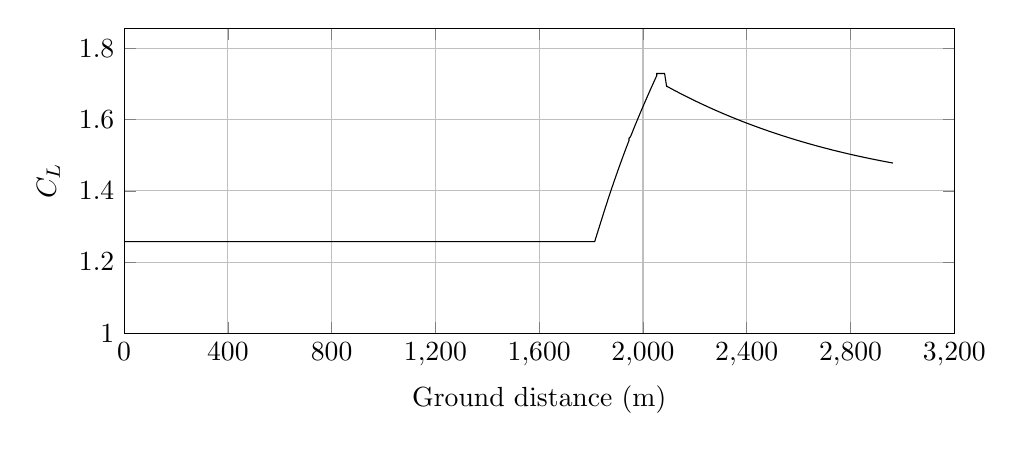
\begin{tikzpicture}

\begin{axis}[
width=\textwidth,
height=0.45\textwidth,
scaled ticks=false, tick label style={/pgf/number format/fixed},
xmin=0.0,
xmax=3200,
xtick={0,400,800,1200,1600,2000,2400,2800,3200},
xlabel={Ground distance (m)},
xmajorgrids,
ymin=1.0,
ymax=1.8562794617918756,
ylabel={$C_L$},
ymajorgrids,
legend style={at={(1.03,0.5)},anchor=west,draw=black,fill=white,legend cell align=left}
]

\addplot [
color=black,
solid
]
table[row sep=crcr]{
1.3603393307215537E-8	1.257316705633825\\
2.0334443352841076E-7	1.257316705633825\\
1.8493358258961232E-6	1.257316705633825\\
9.983129263424352E-6	1.257316705633825\\
4.13538327636676E-5	1.257316705633825\\
1.2467543572893382E-4	1.257316705633825\\
2.843807411608912E-4	1.257316705633825\\
5.588015241105573E-4	1.257316705633825\\
9.398454696015893E-4	1.257316705633825\\
0.0014155885812023746	1.257316705633825\\
0.0019945752038215015	1.257316705633825\\
0.0026717822370171283	1.257316705633825\\
0.003447739291558293	1.257316705633825\\
0.0043193476547732645	1.257316705633825\\
0.00529092766782709	1.257316705633825\\
0.006363550519206555	1.257316705633825\\
0.007533073890550759	1.257316705633825\\
0.008790616877968567	1.257316705633825\\
0.01016549189277427	1.257316705633825\\
0.011625499440327931	1.257316705633825\\
0.013184282533086976	1.257316705633825\\
0.014839871214038253	1.257316705633825\\
0.01660567024659266	1.257316705633825\\
0.018465948346479452	1.257316705633825\\
0.0203822997817096	1.257316705633825\\
0.022430561433814646	1.257316705633825\\
0.024588423902376283	1.257316705633825\\
0.026831028501027587	1.257316705633825\\
0.029143159681622913	1.257316705633825\\
0.03155709159958957	1.257316705633825\\
0.03411445662773917	1.257316705633825\\
0.03677290089167576	1.257316705633825\\
0.03952314881844239	1.257316705633825\\
0.04239921643077808	1.257316705633825\\
0.045357163155895136	1.257316705633825\\
0.048363831658398165	1.257316705633825\\
0.051533845233668635	1.257316705633825\\
0.0547899150155587	1.257316705633825\\
0.058172599437445835	1.257316705633825\\
0.06162834747858026	1.257316705633825\\
0.06521401059050522	1.257316705633825\\
0.06888104003120077	1.257316705633825\\
0.07268727020998902	1.257316705633825\\
0.076546425570032	1.257316705633825\\
0.08047032364859658	1.257316705633825\\
0.08456364881336098	1.257316705633825\\
0.08882250397434277	1.257316705633825\\
0.09306368907640691	1.257316705633825\\
0.09743039119190974	1.257316705633825\\
0.10191450167634594	1.257316705633825\\
0.10651989152467789	1.257316705633825\\
0.11128201757858264	1.257316705633825\\
0.11609763023253863	1.257316705633825\\
0.12097769621339591	1.257316705633825\\
0.12591912973280778	1.257316705633825\\
0.13103216605369056	1.257316705633825\\
0.13633380151185176	1.257316705633825\\
0.1416823117522269	1.257316705633825\\
0.14708837902374172	1.257316705633825\\
0.1525605467319851	1.257316705633825\\
0.15824953188605478	1.257316705633825\\
0.16398006351864292	1.257316705633825\\
0.16978153473626356	1.257316705633825\\
0.17584258400626962	1.257316705633825\\
0.1819863832139092	1.257316705633825\\
0.18819485651962437	1.257316705633825\\
0.19455736971520038	1.257316705633825\\
0.20098158490654017	1.257316705633825\\
0.2076061353991409	1.257316705633825\\
0.21424726384720844	1.257316705633825\\
0.2211374965027113	1.257316705633825\\
0.2281284453493247	1.257316705633825\\
0.2350833915765042	1.257316705633825\\
0.2423085249848444	1.257316705633825\\
0.24958374984531584	1.257316705633825\\
0.2569279402934431	1.257316705633825\\
0.2644720218029696	1.257316705633825\\
0.27204626263318243	1.257316705633825\\
0.27972793364503945	1.257316705633825\\
0.2874622320100655	1.257316705633825\\
0.29563698092580604	1.257316705633825\\
0.30361763245720474	1.257316705633825\\
0.3118912000478351	1.257316705633825\\
0.3202493147046803	1.257316705633825\\
0.3286412952843002	1.257316705633825\\
0.33714554464307567	1.257316705633825\\
0.3458731203690518	1.257316705633825\\
0.35455185683415313	1.257316705633825\\
0.3634323904331427	1.257316705633825\\
0.372325738896249	1.257316705633825\\
0.38151551889959867	1.257316705633825\\
0.3908489672358084	1.257316705633825\\
0.4001862088113266	1.257316705633825\\
0.4095647137707429	1.257316705633825\\
0.4192312859369268	1.257316705633825\\
0.4289206911602753	1.257316705633825\\
0.43896550245304145	1.257316705633825\\
0.4487817299761361	1.257316705633825\\
0.4589033974758888	1.257316705633825\\
0.4691858798479248	1.257316705633825\\
0.47972601481223376	1.257316705633825\\
0.49016040525287174	1.257316705633825\\
0.5007175269203565	1.257316705633825\\
0.511266977039379	1.257316705633825\\
0.522323236324642	1.257316705633825\\
0.5332586746953114	1.257316705633825\\
0.5445869154512923	1.257316705633825\\
0.5556699580072249	1.257316705633825\\
0.5669225885056133	1.257316705633825\\
0.5785590177532589	1.257316705633825\\
0.5903083066022885	1.257316705633825\\
0.6020327889628274	1.257316705633825\\
0.613957077533064	1.257316705633825\\
0.625960998969677	1.257316705633825\\
0.6380070243193761	1.257316705633825\\
0.6503365955459197	1.257316705633825\\
0.662700086001522	1.257316705633825\\
0.6752747602080436	1.257316705633825\\
0.6885889407972636	1.257316705633825\\
0.7019767933734617	1.257316705633825\\
0.7151149754112038	1.257316705633825\\
0.7284684478906998	1.257316705633825\\
0.7418939875700234	1.257316705633825\\
0.7553494584716574	1.257316705633825\\
0.7694215958599202	1.257316705633825\\
0.7830840331449673	1.257316705633825\\
0.796657372658726	1.257316705633825\\
0.8106660034246236	1.257316705633825\\
0.8251837647136968	1.257316705633825\\
0.8395067871054176	1.257316705633825\\
0.8540519574023793	1.257316705633825\\
0.8688334527125461	1.257316705633825\\
0.8840141863517745	1.257316705633825\\
0.8993797082767976	1.257316705633825\\
0.9143697020410035	1.257316705633825\\
0.9294094610857999	1.257316705633825\\
0.9452486359568626	1.257316705633825\\
0.9605773823977486	1.257316705633825\\
0.9761522209726621	1.257316705633825\\
0.9917649966835071	1.257316705633825\\
1.0074810114554809	1.257316705633825\\
1.0234652146968335	1.257316705633825\\
1.0399433598517231	1.257316705633825\\
1.0563627364420554	1.257316705633825\\
1.0728309985448887	1.257316705633825\\
1.0896486452479222	1.257316705633825\\
1.1068138420051672	1.257316705633825\\
1.124143995869574	1.257316705633825\\
1.1415400048645106	1.257316705633825\\
1.1590089082607062	1.257316705633825\\
1.1769249919091855	1.257316705633825\\
1.1951505705127592	1.257316705633825\\
1.2127191877709298	1.257316705633825\\
1.2308827453761335	1.257316705633825\\
1.2492706857898845	1.257316705633825\\
1.267587852451018	1.257316705633825\\
1.2860031245644312	1.257316705633825\\
1.304687144125951	1.257316705633825\\
1.3233765774990474	1.257316705633825\\
1.342322280991234	1.257316705633825\\
1.3613696045164358	1.257316705633825\\
1.3815086998747366	1.257316705633825\\
1.4013123019267382	1.257316705633825\\
1.4209622886438908	1.257316705633825\\
1.4411501686096515	1.257316705633825\\
1.4611760119255748	1.257316705633825\\
1.4816444281325132	1.257316705633825\\
1.501865958841821	1.257316705633825\\
1.5224364680875304	1.257316705633825\\
1.543651615594651	1.257316705633825\\
1.5647593029468103	1.257316705633825\\
1.5859558716309676	1.257316705633825\\
1.6071423964076703	1.257316705633825\\
1.6293386351549652	1.257316705633825\\
1.6508498980272122	1.257316705633825\\
1.673011606043147	1.257316705633825\\
1.6946435720294923	1.257316705633825\\
1.717066624993247	1.257316705633825\\
1.739432891071898	1.257316705633825\\
1.761922286799709	1.257316705633825\\
1.7849035550437842	1.257316705633825\\
1.8076299607761817	1.257316705633825\\
1.8313298306791497	1.257316705633825\\
1.8543134894513886	1.257316705633825\\
1.8777326664639729	1.257316705633825\\
1.9017196849182967	1.257316705633825\\
1.925345883672024	1.257316705633825\\
1.950252961491087	1.257316705633825\\
1.975161211119453	1.257316705633825\\
1.9993825790313986	1.257316705633825\\
2.024583888346972	1.257316705633825\\
2.04934017380271	1.257316705633825\\
2.0744229633459703	1.257316705633825\\
2.0996193404956136	1.257316705633825\\
2.1245764901457758	1.257316705633825\\
2.1500786393425866	1.257316705633825\\
2.176226227020705	1.257316705633825\\
2.202115608176549	1.257316705633825\\
2.227948363055355	1.257316705633825\\
2.2543499999408594	1.257316705633825\\
2.2810892744412783	1.257316705633825\\
2.3075963743135786	1.257316705633825\\
2.3348582111613405	1.257316705633825\\
2.3623221378972126	1.257316705633825\\
2.3898598419727675	1.257316705633825\\
2.4171687299087603	1.257316705633825\\
2.445442108612223	1.257316705633825\\
2.4735885391813177	1.257316705633825\\
2.5015416452491293	1.257316705633825\\
2.5301110763218357	1.257316705633825\\
2.5589284934403693	1.257316705633825\\
2.587611617795936	1.257316705633825\\
2.6175687086884984	1.257316705633825\\
2.647724154312196	1.257316705633825\\
2.6767118187859253	1.257316705633825\\
2.7060305938995466	1.257316705633825\\
2.7361546404224653	1.257316705633825\\
2.7663022704956823	1.257316705633825\\
2.7964672462043376	1.257316705633825\\
2.8272583584284883	1.257316705633825\\
2.8588650092419234	1.257316705633825\\
2.8898852960400587	1.257316705633825\\
2.9215246589961597	1.257316705633825\\
2.95270311230069	1.257316705633825\\
2.984506337549637	1.257316705633825\\
3.017379145769185	1.257316705633825\\
3.049243647754313	1.257316705633825\\
3.081295157663824	1.257316705633825\\
3.113406837946715	1.257316705633825\\
3.1453724573084756	1.257316705633825\\
3.1787286104953543	1.257316705633825\\
3.211019796961401	1.257316705633825\\
3.245786703184362	1.257316705633825\\
3.279939251746722	1.257316705633825\\
3.3141720228361216	1.257316705633825\\
3.3491198891036547	1.257316705633825\\
3.382965192547779	1.257316705633825\\
3.4181848705561064	1.257316705633825\\
3.45391888941694	1.257316705633825\\
3.488851494856137	1.257316705633825\\
3.524271454997704	1.257316705633825\\
3.5606552075305	1.257316705633825\\
3.597189071478943	1.257316705633825\\
3.632926148839256	1.257316705633825\\
3.668897146318187	1.257316705633825\\
3.706642714683163	1.257316705633825\\
3.7432264628550644	1.257316705633825\\
3.781286297809391	1.257316705633825\\
3.818618572105483	1.257316705633825\\
3.8564015479305356	1.257316705633825\\
3.8948624022541356	1.257316705633825\\
3.9329637046009225	1.257316705633825\\
3.971505929995028	1.257316705633825\\
4.009821706071438	1.257316705633825\\
4.049014376833089	1.257316705633825\\
4.089343885784727	1.257316705633825\\
4.128662304630717	1.257316705633825\\
4.1684827283974055	1.257316705633825\\
4.208000253554632	1.257316705633825\\
4.2483743636521965	1.257316705633825\\
4.288255503180503	1.257316705633825\\
4.328757204126676	1.257316705633825\\
4.369490126907612	1.257316705633825\\
4.410357715197167	1.257316705633825\\
4.45189144941496	1.257316705633825\\
4.492881116440694	1.257316705633825\\
4.53550011161515	1.257316705633825\\
4.577670191557685	1.257316705633825\\
4.6201174049766305	1.257316705633825\\
4.662272021613388	1.257316705633825\\
4.706017761800355	1.257316705633825\\
4.748842845578064	1.257316705633825\\
4.792293145132742	1.257316705633825\\
4.836482439768313	1.257316705633825\\
4.88090298307878	1.257316705633825\\
4.925311889063089	1.257316705633825\\
4.969864686447545	1.257316705633825\\
5.014842280541593	1.257316705633825\\
5.0603877575117515	1.257316705633825\\
5.106292347304597	1.257316705633825\\
5.152263975081851	1.257316705633825\\
5.1974808794106995	1.257316705633825\\
5.244027372436168	1.257316705633825\\
5.28996242022761	1.257316705633825\\
5.336209145350672	1.257316705633825\\
5.38320569473032	1.257316705633825\\
5.430469292142472	1.257316705633825\\
5.476900151253712	1.257316705633825\\
5.526063828851289	1.257316705633825\\
5.573879040902945	1.257316705633825\\
5.622613575936374	1.257316705633825\\
5.6713596863799225	1.257316705633825\\
5.720412183296268	1.257316705633825\\
5.770660497446668	1.257316705633825\\
5.820668144990444	1.257316705633825\\
5.870305285939629	1.257316705633825\\
5.920503816994749	1.257316705633825\\
5.971105439367246	1.257316705633825\\
6.021088325934068	1.257316705633825\\
6.071322359863801	1.257316705633825\\
6.122981826035449	1.257316705633825\\
6.174329110820436	1.257316705633825\\
6.225804784288178	1.257316705633825\\
6.278093246139479	1.257316705633825\\
6.331709873490098	1.257316705633825\\
6.384325657889258	1.257316705633825\\
6.436648686434458	1.257316705633825\\
6.489478972803882	1.257316705633825\\
6.543185721519176	1.257316705633825\\
6.596747696432654	1.257316705633825\\
6.650345873843312	1.257316705633825\\
6.704555155195255	1.257316705633825\\
6.7588986063680725	1.257316705633825\\
6.814371620173711	1.257316705633825\\
6.86997180120154	1.257316705633825\\
6.925426612865756	1.257316705633825\\
6.981353650685165	1.257316705633825\\
7.037678624474159	1.257316705633825\\
7.094603706786671	1.257316705633825\\
7.151204881983983	1.257316705633825\\
7.209200593921791	1.257316705633825\\
7.2667780016693655	1.257316705633825\\
7.324687293141565	1.257316705633825\\
7.382771066065313	1.257316705633825\\
7.441904508776327	1.257316705633825\\
7.501585831803217	1.257316705633825\\
7.5616527251378685	1.257316705633825\\
7.62150963104709	1.257316705633825\\
7.682859947113334	1.257316705633825\\
7.7432084367972145	1.257316705633825\\
7.803024936926759	1.257316705633825\\
7.863793829029664	1.257316705633825\\
7.9252460466886365	1.257316705633825\\
7.98696966925656	1.257316705633825\\
8.04776546969778	1.257316705633825\\
8.109421212326083	1.257316705633825\\
8.17269125419024	1.257316705633825\\
8.236095044780246	1.257316705633825\\
8.299523592514586	1.257316705633825\\
8.363213767675873	1.257316705633825\\
8.427807923256076	1.257316705633825\\
8.49144930156071	1.257316705633825\\
8.557380457258176	1.257316705633825\\
8.623183572921022	1.257316705633825\\
8.687840683575093	1.257316705633825\\
8.753751426394068	1.257316705633825\\
8.820803713780364	1.257316705633825\\
8.888970287482593	1.257316705633825\\
8.957133699158991	1.257316705633825\\
9.025036015045707	1.257316705633825\\
9.092760955867519	1.257316705633825\\
9.159817422823458	1.257316705633825\\
9.227495373767134	1.257316705633825\\
9.296013084156197	1.257316705633825\\
9.36435980631623	1.257316705633825\\
9.433329865923408	1.257316705633825\\
9.503849553921977	1.257316705633825\\
9.574524061692681	1.257316705633825\\
9.644263228942293	1.257316705633825\\
9.715657612596786	1.257316705633825\\
9.787429657508813	1.257316705633825\\
9.85753688572494	1.257316705633825\\
9.930250735750551	1.257316705633825\\
10.001571447096964	1.257316705633825\\
10.074699859091687	1.257316705633825\\
10.14698611653175	1.257316705633825\\
10.220547980738981	1.257316705633825\\
10.2940409891517	1.257316705633825\\
10.36719293590382	1.257316705633825\\
10.441008888975666	1.257316705633825\\
10.51610421670324	1.257316705633825\\
10.590724589239105	1.257316705633825\\
10.667218005391902	1.257316705633825\\
10.742771202259895	1.257316705633825\\
10.82035208750042	1.257316705633825\\
10.896759047300378	1.257316705633825\\
10.973503045910835	1.257316705633825\\
11.051297940743765	1.257316705633825\\
11.128076326409062	1.257316705633825\\
11.207667705350879	1.257316705633825\\
11.286758396846047	1.257316705633825\\
11.366305937658339	1.257316705633825\\
11.446149720998452	1.257316705633825\\
11.526866579636565	1.257316705633825\\
11.607297517600138	1.257316705633825\\
11.688034241538357	1.257316705633825\\
11.769665722224765	1.257316705633825\\
11.850920080706608	1.257316705633825\\
11.933163326324259	1.257316705633825\\
12.017103780766782	1.257316705633825\\
12.10034832931326	1.257316705633825\\
12.185467765774142	1.257316705633825\\
12.270669986481685	1.257316705633825\\
12.354040133273898	1.257316705633825\\
12.440386807402234	1.257316705633825\\
12.52556588630658	1.257316705633825\\
12.610860989997974	1.257316705633825\\
12.69550109439961	1.257316705633825\\
12.784634337461807	1.257316705633825\\
12.871172079509357	1.257316705633825\\
12.958447214271366	1.257316705633825\\
13.045518554761987	1.257316705633825\\
13.133090172249581	1.257316705633825\\
13.221405510214687	1.257316705633825\\
13.310319106907201	1.257316705633825\\
13.399783591735492	1.257316705633825\\
13.488943611067967	1.257316705633825\\
13.578276665194153	1.257316705633825\\
13.667402973129146	1.257316705633825\\
13.757763665999576	1.257316705633825\\
13.848393619195729	1.257316705633825\\
13.938857764339925	1.257316705633825\\
14.031101516310692	1.257316705633825\\
14.123507833735925	1.257316705633825\\
14.214825187590282	1.257316705633825\\
14.307956552027534	1.257316705633825\\
14.401498558574918	1.257316705633825\\
14.495315613017755	1.257316705633825\\
14.589065423003394	1.257316705633825\\
14.68316852398955	1.257316705633825\\
14.778702641747682	1.257316705633825\\
14.873746415615575	1.257316705633825\\
14.970384078097169	1.257316705633825\\
15.068900921005241	1.257316705633825\\
15.164434274206265	1.257316705633825\\
15.260378587808539	1.257316705633825\\
15.357189194448868	1.257316705633825\\
15.45495288999333	1.257316705633825\\
15.55311774366497	1.257316705633825\\
15.652583807013901	1.257316705633825\\
15.755243917873962	1.257316705633825\\
15.855950289561445	1.257316705633825\\
15.958461094374158	1.257316705633825\\
16.060387288500337	1.257316705633825\\
16.164276126126843	1.257316705633825\\
16.26736468838029	1.257316705633825\\
16.36946523634058	1.257316705633825\\
16.47192386662276	1.257316705633825\\
16.576794358652606	1.257316705633825\\
16.678929175716583	1.257316705633825\\
16.783994526910618	1.257316705633825\\
16.89012564586595	1.257316705633825\\
16.996887404888547	1.257316705633825\\
17.103774697793426	1.257316705633825\\
17.210947675936964	1.257316705633825\\
17.31865021419634	1.257316705633825\\
17.424470519881233	1.257316705633825\\
17.53205215515201	1.257316705633825\\
17.64034909906897	1.257316705633825\\
17.74911485075183	1.257316705633825\\
17.85745376408675	1.257316705633825\\
17.969383314157206	1.257316705633825\\
18.07998395718984	1.257316705633825\\
18.18863741327577	1.257316705633825\\
18.302466989554325	1.257316705633825\\
18.41305080779906	1.257316705633825\\
18.525644000014054	1.257316705633825\\
18.636945827420575	1.257316705633825\\
18.750643923449367	1.257316705633825\\
18.86479622056296	1.257316705633825\\
18.979646899421056	1.257316705633825\\
19.09418630108147	1.257316705633825\\
19.208983505033515	1.257316705633825\\
19.323483295898072	1.257316705633825\\
19.43842354827664	1.257316705633825\\
19.55563752357537	1.257316705633825\\
19.67199913451129	1.257316705633825\\
19.789486593639566	1.257316705633825\\
19.90713985662446	1.257316705633825\\
20.024127533725753	1.257316705633825\\
20.143019013955552	1.257316705633825\\
20.26442367074238	1.257316705633825\\
20.383660776265387	1.257316705633825\\
20.5042342316437	1.257316705633825\\
20.622773342122727	1.257316705633825\\
20.74503732713029	1.257316705633825\\
20.865944869938517	1.257316705633825\\
20.98711015528624	1.257316705633825\\
21.113336299999695	1.257316705633825\\
21.23638685227678	1.257316705633825\\
21.35988644990264	1.257316705633825\\
21.483760012473958	1.257316705633825\\
21.608180515260266	1.257316705633825\\
21.732326713270083	1.257316705633825\\
21.85766379468624	1.257316705633825\\
21.985117186778353	1.257316705633825\\
22.111729024702363	1.257316705633825\\
22.23700541150786	1.257316705633825\\
22.36297326225872	1.257316705633825\\
22.488604760551	1.257316705633825\\
22.616276341350805	1.257316705633825\\
22.744235570279145	1.257316705633825\\
22.874576476768283	1.257316705633825\\
23.003842066605536	1.257316705633825\\
23.13088450205612	1.257316705633825\\
23.257869280739328	1.257316705633825\\
23.389244224935425	1.257316705633825\\
23.519811196806458	1.257316705633825\\
23.653309395988643	1.257316705633825\\
23.78342402399784	1.257316705633825\\
23.9180644861338	1.257316705633825\\
24.05110504604577	1.257316705633825\\
24.182394801971697	1.257316705633825\\
24.314614014384034	1.257316705633825\\
24.449791085561472	1.257316705633825\\
24.585258581909038	1.257316705633825\\
24.72121222319008	1.257316705633825\\
24.857032405393277	1.257316705633825\\
24.99454740444294	1.257316705633825\\
25.13030709358258	1.257316705633825\\
25.270890409679986	1.257316705633825\\
25.40663839363527	1.257316705633825\\
25.54307796688363	1.257316705633825\\
25.68272814639034	1.257316705633825\\
25.82072003425767	1.257316705633825\\
25.96015212691003	1.257316705633825\\
25.987750021099068	1.257316705633825\\
26.0558803939429	1.257316705633825\\
26.061632797568386	1.257316705633825\\
26.066808273335674	1.257316705633825\\
26.071901058608013	1.257316705633825\\
26.073315434863225	1.257316705633825\\
26.074595035914804	1.257316705633825\\
26.080371168076944	1.257316705633825\\
26.10234540095133	1.257316705633825\\
26.183408179590366	1.257316705633825\\
26.300430535410044	1.257316705633825\\
26.42750601924636	1.257316705633825\\
26.558056987479794	1.257316705633825\\
26.688030995483615	1.257316705633825\\
26.818767077324992	1.257316705633825\\
26.951519978077492	1.257316705633825\\
27.083955405447817	1.257316705633825\\
27.216897884715692	1.257316705633825\\
27.350913258119895	1.257316705633825\\
27.4833530065795	1.257316705633825\\
27.6176201223548	1.257316705633825\\
27.752160408628434	1.257316705633825\\
27.887329802382908	1.257316705633825\\
28.023188645890663	1.257316705633825\\
28.158973127824495	1.257316705633825\\
28.296372294036907	1.257316705633825\\
28.435107205966254	1.257316705633825\\
28.571323599682245	1.257316705633825\\
28.70996262687553	1.257316705633825\\
28.850320389600306	1.257316705633825\\
28.988837241064125	1.257316705633825\\
29.129197813929657	1.257316705633825\\
29.27166529868488	1.257316705633825\\
29.41298471572133	1.257316705633825\\
29.554848516656044	1.257316705633825\\
29.699676691743235	1.257316705633825\\
29.842400551696755	1.257316705633825\\
29.985385440862252	1.257316705633825\\
30.129077275410303	1.257316705633825\\
30.27543774584293	1.257316705633825\\
30.422081339040986	1.257316705633825\\
30.56949149516445	1.257316705633825\\
30.716562179458485	1.257316705633825\\
30.86535310281699	1.257316705633825\\
31.011875026602333	1.257316705633825\\
31.16159928701196	1.257316705633825\\
31.313692569485013	1.257316705633825\\
31.463056706803336	1.257316705633825\\
31.61235366859384	1.257316705633825\\
31.76278957628285	1.257316705633825\\
31.915019899787076	1.257316705633825\\
32.06709627595497	1.257316705633825\\
32.21861178877769	1.257316705633825\\
32.37168228565527	1.257316705633825\\
32.52450570609457	1.257316705633825\\
32.67702483599189	1.257316705633825\\
32.829998687403204	1.257316705633825\\
32.98551220909506	1.257316705633825\\
33.14332298937855	1.257316705633825\\
33.29970221124884	1.257316705633825\\
33.45800124694219	1.257316705633825\\
33.61398946945653	1.257316705633825\\
33.77048353048475	1.257316705633825\\
33.9292721471582	1.257316705633825\\
34.08796840843395	1.257316705633825\\
34.24769686644211	1.257316705633825\\
34.406855482575295	1.257316705633825\\
34.56481953291838	1.257316705633825\\
34.72399692808165	1.257316705633825\\
34.88694269464703	1.257316705633825\\
35.04914399338672	1.257316705633825\\
35.209965099803895	1.257316705633825\\
35.3703140559587	1.257316705633825\\
35.531685786905925	1.257316705633825\\
35.69349909442164	1.257316705633825\\
35.85522798807463	1.257316705633825\\
36.022509111806116	1.257316705633825\\
36.19055880791667	1.257316705633825\\
36.35708622463872	1.257316705633825\\
36.52115360367851	1.257316705633825\\
36.68781562330062	1.257316705633825\\
36.8536847754776	1.257316705633825\\
37.024522648961764	1.257316705633825\\
37.19188554678789	1.257316705633825\\
37.36066720850286	1.257316705633825\\
37.528862119520696	1.257316705633825\\
37.697264258302326	1.257316705633825\\
37.86832931534104	1.257316705633825\\
38.03812867477943	1.257316705633825\\
38.20923731912278	1.257316705633825\\
38.37904730305398	1.257316705633825\\
38.55252405124031	1.257316705633825\\
38.72282139824354	1.257316705633825\\
38.89783411301201	1.257316705633825\\
39.0714610757495	1.257316705633825\\
39.24438070689564	1.257316705633825\\
39.41969314875929	1.257316705633825\\
39.59166556575205	1.257316705633825\\
39.764623188591585	1.257316705633825\\
39.94263254662576	1.257316705633825\\
40.11749159802578	1.257316705633825\\
40.29452954971913	1.257316705633825\\
40.47247750600427	1.257316705633825\\
40.64799609178485	1.257316705633825\\
40.82414741101539	1.257316705633825\\
41.00385670225303	1.257316705633825\\
41.18169069533937	1.257316705633825\\
41.3603281005193	1.257316705633825\\
41.54046179251334	1.257316705633825\\
41.722675278204306	1.257316705633825\\
41.90258931008478	1.257316705633825\\
42.08518735141125	1.257316705633825\\
42.26728550944881	1.257316705633825\\
42.44743534848537	1.257316705633825\\
42.63069538383506	1.257316705633825\\
42.80963512098974	1.257316705633825\\
42.992542679335614	1.257316705633825\\
43.17926890616222	1.257316705633825\\
43.363134036078335	1.257316705633825\\
43.54815051311773	1.257316705633825\\
43.733578141849236	1.257316705633825\\
43.91798130912079	1.257316705633825\\
44.10506009255049	1.257316705633825\\
44.29251116260117	1.257316705633825\\
44.480917546793805	1.257316705633825\\
44.66851287589745	1.257316705633825\\
44.85853501730759	1.257316705633825\\
45.047396872181054	1.257316705633825\\
45.236914792155844	1.257316705633825\\
45.42785879536018	1.257316705633825\\
45.616432631699865	1.257316705633825\\
45.80697204128492	1.257316705633825\\
45.998633580597016	1.257316705633825\\
46.18800675699903	1.257316705633825\\
46.380841640082096	1.257316705633825\\
46.57327038933336	1.257316705633825\\
46.765844918266424	1.257316705633825\\
46.95911042680183	1.257316705633825\\
47.15311668852311	1.257316705633825\\
47.34541611633634	1.257316705633825\\
47.53884854699059	1.257316705633825\\
47.73236991243341	1.257316705633825\\
47.92818250719388	1.257316705633825\\
48.12326385407131	1.257316705633825\\
48.32058854034828	1.257316705633825\\
48.516852452700604	1.257316705633825\\
48.71339374517507	1.257316705633825\\
48.91319881343868	1.257316705633825\\
49.1119162355681	1.257316705633825\\
49.31207818344666	1.257316705633825\\
49.509673461222235	1.257316705633825\\
49.71156302510582	1.257316705633825\\
49.91034548441702	1.257316705633825\\
50.11200805970151	1.257316705633825\\
50.30853267551517	1.257316705633825\\
50.50757456960626	1.257316705633825\\
50.70929197287772	1.257316705633825\\
50.91222418686718	1.257316705633825\\
51.11562549758783	1.257316705633825\\
51.32090674103446	1.257316705633825\\
51.525199701657655	1.257316705633825\\
51.72863462744459	1.257316705633825\\
51.934060761332375	1.257316705633825\\
52.14033810224923	1.257316705633825\\
52.344882977561255	1.257316705633825\\
52.55098100649393	1.257316705633825\\
52.75731843494604	1.257316705633825\\
52.96514817708821	1.257316705633825\\
53.17450540782369	1.257316705633825\\
53.382202621450276	1.257316705633825\\
53.592230583406476	1.257316705633825\\
53.80364534107798	1.257316705633825\\
54.01469481143569	1.257316705633825\\
54.223966920081466	1.257316705633825\\
54.43230789395902	1.257316705633825\\
54.6430562980421	1.257316705633825\\
54.855225786754914	1.257316705633825\\
55.066088958624874	1.257316705633825\\
55.27969530828261	1.257316705633825\\
55.49171188337613	1.257316705633825\\
55.70388919125476	1.257316705633825\\
55.91737779085577	1.257316705633825\\
56.13177028494084	1.257316705633825\\
56.34652664868587	1.257316705633825\\
56.559021044851505	1.257316705633825\\
56.77591447970492	1.257316705633825\\
56.99548236897459	1.257316705633825\\
57.21481285737903	1.257316705633825\\
57.43536222847358	1.257316705633825\\
57.65367025761124	1.257316705633825\\
57.872788904232735	1.257316705633825\\
58.0907693980174	1.257316705633825\\
58.311927420720366	1.257316705633825\\
58.532333513628615	1.257316705633825\\
58.75532998033057	1.257316705633825\\
58.976617007999806	1.257316705633825\\
59.19875422837053	1.257316705633825\\
59.4206945143671	1.257316705633825\\
59.64453328369959	1.257316705633825\\
59.86894932484513	1.257316705633825\\
60.09432075877773	1.257316705633825\\
60.318058693038594	1.257316705633825\\
60.541731124044205	1.257316705633825\\
60.76707064338231	1.257316705633825\\
60.995574692986196	1.257316705633825\\
61.22378989589207	1.257316705633825\\
61.4534619981562	1.257316705633825\\
61.683510138770515	1.257316705633825\\
61.91410430469678	1.257316705633825\\
62.14462153858659	1.257316705633825\\
62.37563158073512	1.257316705633825\\
62.607203285434	1.257316705633825\\
62.841031881319736	1.257316705633825\\
63.07467935056491	1.257316705633825\\
63.31164975340633	1.257316705633825\\
63.54633691305479	1.257316705633825\\
63.78243968758058	1.257316705633825\\
64.0165414084598	1.257316705633825\\
64.25412817577254	1.257316705633825\\
64.49270299572771	1.257316705633825\\
64.73076499662056	1.257316705633825\\
64.96867826857735	1.257316705633825\\
65.21063576532572	1.257316705633825\\
65.4512107007771	1.257316705633825\\
65.69028017871045	1.257316705633825\\
65.93032615763332	1.257316705633825\\
66.17196619696679	1.257316705633825\\
66.4135612157637	1.257316705633825\\
66.6559030093851	1.257316705633825\\
66.89910102540284	1.257316705633825\\
67.14354652182666	1.257316705633825\\
67.38771133480921	1.257316705633825\\
67.63347396558368	1.257316705633825\\
67.87898066495345	1.257316705633825\\
68.1255935515739	1.257316705633825\\
68.37316753306138	1.257316705633825\\
68.62205497364681	1.257316705633825\\
68.8711887275476	1.257316705633825\\
69.120220471977	1.257316705633825\\
69.36846244647072	1.257316705633825\\
69.61951843592018	1.257316705633825\\
69.87236615109754	1.257316705633825\\
70.12758921381476	1.257316705633825\\
70.37945082809051	1.257316705633825\\
70.63410009691182	1.257316705633825\\
70.89152727368702	1.257316705633825\\
71.14629115974091	1.257316705633825\\
71.40197865069018	1.257316705633825\\
71.66163317144085	1.257316705633825\\
71.92484704501203	1.257316705633825\\
72.18465416754285	1.257316705633825\\
72.44573394560723	1.257316705633825\\
72.70633339061075	1.257316705633825\\
72.96699363118216	1.257316705633825\\
73.22900401485182	1.257316705633825\\
73.49076816912304	1.257316705633825\\
73.75430841254712	1.257316705633825\\
74.01895646534612	1.257316705633825\\
74.2846979982242	1.257316705633825\\
74.55380714249793	1.257316705633825\\
74.82322871850147	1.257316705633825\\
75.09350011520078	1.257316705633825\\
75.36421232425869	1.257316705633825\\
75.6347219158074	1.257316705633825\\
75.90830954343213	1.257316705633825\\
76.18188601743822	1.257316705633825\\
76.45626363461818	1.257316705633825\\
76.72958718025629	1.257316705633825\\
77.00406935908524	1.257316705633825\\
77.28579748399531	1.257316705633825\\
77.56784659723587	1.257316705633825\\
77.84569092555657	1.257316705633825\\
78.1246978223638	1.257316705633825\\
78.40641219364133	1.257316705633825\\
78.68590470271565	1.257316705633825\\
78.96851680469001	1.257316705633825\\
79.25576208114188	1.257316705633825\\
79.54169104977237	1.257316705633825\\
79.82662017154695	1.257316705633825\\
80.11330301632765	1.257316705633825\\
80.40394576721474	1.257316705633825\\
80.6908099930996	1.257316705633825\\
80.98055888331655	1.257316705633825\\
81.27178512217935	1.257316705633825\\
81.56682943128612	1.257316705633825\\
81.86186977412851	1.257316705633825\\
82.15688924927383	1.257316705633825\\
82.44965588234726	1.257316705633825\\
82.74488606927187	1.257316705633825\\
83.04325841243121	1.257316705633825\\
83.34213327641098	1.257316705633825\\
83.64411622775171	1.257316705633825\\
83.94734638805741	1.257316705633825\\
84.25123842984891	1.257316705633825\\
84.55152885577829	1.257316705633825\\
84.85735750691177	1.257316705633825\\
85.16518306664875	1.257316705633825\\
85.47136476235073	1.257316705633825\\
85.77898122624802	1.257316705633825\\
86.08923229760057	1.257316705633825\\
86.40254560035129	1.257316705633825\\
86.71167807044037	1.257316705633825\\
87.02660518802142	1.257316705633825\\
87.34238286044419	1.257316705633825\\
87.65842706333811	1.257316705633825\\
87.97971380652302	1.257316705633825\\
88.2973933745065	1.257316705633825\\
88.61789013566766	1.257316705633825\\
88.93643920279564	1.257316705633825\\
89.25662431900213	1.257316705633825\\
89.57903058309674	1.257316705633825\\
89.89968694948243	1.257316705633825\\
90.22473455398588	1.257316705633825\\
90.55024875587375	1.257316705633825\\
90.87789352676518	1.257316705633825\\
91.20733069500889	1.257316705633825\\
91.54101415610151	1.257316705633825\\
91.87012785371462	1.257316705633825\\
92.20120197152713	1.257316705633825\\
92.53416638543635	1.257316705633825\\
92.86431843528567	1.257316705633825\\
93.19748455591187	1.257316705633825\\
93.53066771200866	1.257316705633825\\
93.86681917526724	1.257316705633825\\
94.20530590547477	1.257316705633825\\
94.5419273964865	1.257316705633825\\
94.8854212036891	1.257316705633825\\
95.22752713476521	1.257316705633825\\
95.57091181422334	1.257316705633825\\
95.91383450860906	1.257316705633825\\
96.25469535763642	1.257316705633825\\
96.5966517898868	1.257316705633825\\
96.93845701474973	1.257316705633825\\
97.28153572459905	1.257316705633825\\
97.62213139590432	1.257316705633825\\
97.9659652144934	1.257316705633825\\
98.3129807304216	1.257316705633825\\
98.65852794036775	1.257316705633825\\
99.00080640577195	1.257316705633825\\
99.35064076251427	1.257316705633825\\
99.69796076807248	1.257316705633825\\
100.04654253174803	1.257316705633825\\
100.3915606488718	1.257316705633825\\
100.74261509654437	1.257316705633825\\
101.08877163494762	1.257316705633825\\
101.43457754260953	1.257316705633825\\
101.784020212797	1.257316705633825\\
102.13161434601102	1.257316705633825\\
102.4751980097893	1.257316705633825\\
102.82212110631409	1.257316705633825\\
103.16739702108615	1.257316705633825\\
103.51524666207362	1.257316705633825\\
103.86391679154056	1.257316705633825\\
104.20960434827006	1.257316705633825\\
104.55241399635099	1.257316705633825\\
104.89662223620601	1.257316705633825\\
105.24103428322039	1.257316705633825\\
105.5836615386647	1.257316705633825\\
105.92645892081137	1.257316705633825\\
106.27347658175316	1.257316705633825\\
106.6151670762521	1.257316705633825\\
106.95898391938218	1.257316705633825\\
107.30023552029138	1.257316705633825\\
107.64147805753461	1.257316705633825\\
107.98348674656944	1.257316705633825\\
108.32522459759954	1.257316705633825\\
108.3935347040271	1.257316705633825\\
108.40478590462831	1.257316705633825\\
108.41572478024443	1.257316705633825\\
108.4246743308916	1.257316705633825\\
108.44347342986478	1.257316705633825\\
108.52018987797786	1.257316705633825\\
108.70071173483461	1.257316705633825\\
108.99446230248458	1.257316705633825\\
109.30176454987088	1.257316705633825\\
109.60899173332959	1.257316705633825\\
109.91608539831654	1.257316705633825\\
110.22883517949637	1.257316705633825\\
110.54143546549608	1.257316705633825\\
110.853845249356	1.257316705633825\\
111.1739714794031	1.257316705633825\\
111.4937490010879	1.257316705633825\\
111.81170779322963	1.257316705633825\\
112.13106495813236	1.257316705633825\\
112.4519453366479	1.257316705633825\\
112.77515902629136	1.257316705633825\\
113.0997499810409	1.257316705633825\\
113.43040796942478	1.257316705633825\\
113.7597028375028	1.257316705633825\\
114.0907450350197	1.257316705633825\\
114.42538740208008	1.257316705633825\\
114.75997726261329	1.257316705633825\\
115.09477047197589	1.257316705633825\\
115.43440545481076	1.257316705633825\\
115.77494672336013	1.257316705633825\\
116.11687534861284	1.257316705633825\\
116.46164587354252	1.257316705633825\\
116.8077846490165	1.257316705633825\\
117.15688723722127	1.257316705633825\\
117.50557855048987	1.257316705633825\\
117.85411336711965	1.257316705633825\\
118.20532793701167	1.257316705633825\\
118.55850697655507	1.257316705633825\\
118.91273956155123	1.257316705633825\\
119.26983096270519	1.257316705633825\\
119.62978614725739	1.257316705633825\\
119.98960731920661	1.257316705633825\\
120.34734904217265	1.257316705633825\\
120.7138511704587	1.257316705633825\\
121.08106061642908	1.257316705633825\\
121.44737887966437	1.257316705633825\\
121.81499139152783	1.257316705633825\\
122.18511446431708	1.257316705633825\\
122.55384158147794	1.257316705633825\\
122.92460728481757	1.257316705633825\\
123.29616941264607	1.257316705633825\\
123.67040864389355	1.257316705633825\\
124.04652172406458	1.257316705633825\\
124.42393851457416	1.257316705633825\\
124.80152108360014	1.257316705633825\\
125.18180835736592	1.257316705633825\\
125.55854932865631	1.257316705633825\\
125.93878032356085	1.257316705633825\\
126.31997081831156	1.257316705633825\\
126.70099538833193	1.257316705633825\\
127.08058279416298	1.257316705633825\\
127.46175209000612	1.257316705633825\\
127.84399628255431	1.257316705633825\\
128.22749916598133	1.257316705633825\\
128.6102537001487	1.257316705633825\\
128.99595881306152	1.257316705633825\\
129.37788117916477	1.257316705633825\\
129.760738924708	1.257316705633825\\
130.1448498512433	1.257316705633825\\
130.53000390659713	1.257316705633825\\
130.9168242384266	1.257316705633825\\
131.29443328439476	1.257316705633825\\
131.67491382268804	1.257316705633825\\
132.05816436539135	1.257316705633825\\
132.44070735535217	1.257316705633825\\
132.82666098215685	1.257316705633825\\
133.20952005887244	1.257316705633825\\
133.5940193955625	1.257316705633825\\
133.97617966856654	1.257316705633825\\
134.36103715882757	1.257316705633825\\
134.74478042358356	1.257316705633825\\
135.12867144169206	1.257316705633825\\
135.5141335746535	1.257316705633825\\
135.89764893392993	1.257316705633825\\
136.28231234485685	1.257316705633825\\
136.66418763078912	1.257316705633825\\
137.04684871033697	1.257316705633825\\
137.42845627025127	1.257316705633825\\
137.8132447087305	1.257316705633825\\
138.19719797258034	1.257316705633825\\
138.58059071069573	1.257316705633825\\
138.96593237593703	1.257316705633825\\
139.3501607499636	1.257316705633825\\
139.73355638294606	1.257316705633825\\
140.1160230155566	1.257316705633825\\
140.50045093994146	1.257316705633825\\
140.88215178690393	1.257316705633825\\
141.26156782058217	1.257316705633825\\
141.64323970440188	1.257316705633825\\
142.02689350659642	1.257316705633825\\
142.41061312971692	1.257316705633825\\
142.7942251403153	1.257316705633825\\
143.1756303563767	1.257316705633825\\
143.5599719391364	1.257316705633825\\
143.94242380128833	1.257316705633825\\
144.3239499176869	1.257316705633825\\
144.70664939692608	1.257316705633825\\
145.0870075357763	1.257316705633825\\
145.46856550308127	1.257316705633825\\
145.85014610541765	1.257316705633825\\
146.23128237819492	1.257316705633825\\
146.61504730324998	1.257316705633825\\
146.99763315977907	1.257316705633825\\
147.38441582478964	1.257316705633825\\
147.7673688364352	1.257316705633825\\
148.15222568696134	1.257316705633825\\
148.53580865353604	1.257316705633825\\
148.9199734867533	1.257316705633825\\
149.3040357319486	1.257316705633825\\
149.68771357306542	1.257316705633825\\
150.07093078701052	1.257316705633825\\
150.45622889618164	1.257316705633825\\
150.8449053483268	1.257316705633825\\
151.2288570611563	1.257316705633825\\
151.61452719766493	1.257316705633825\\
151.9983007305741	1.257316705633825\\
152.38299664478842	1.257316705633825\\
152.76945776909372	1.257316705633825\\
153.15580177123394	1.257316705633825\\
153.54253364040335	1.257316705633825\\
153.93093169697067	1.257316705633825\\
154.31788037931886	1.257316705633825\\
154.7039882138024	1.257316705633825\\
155.08880221957185	1.257316705633825\\
155.47621608980313	1.257316705633825\\
155.866104687065	1.257316705633825\\
156.25391419262098	1.257316705633825\\
156.64166339424906	1.257316705633825\\
157.03027969880475	1.257316705633825\\
157.4213807682267	1.257316705633825\\
157.8105708506119	1.257316705633825\\
158.19948541262937	1.257316705633825\\
158.58893406813365	1.257316705633825\\
158.97894817604634	1.257316705633825\\
159.3710019698692	1.257316705633825\\
159.76139479981174	1.257316705633825\\
160.1523485688823	1.257316705633825\\
160.54128874338664	1.257316705633825\\
160.9326976430911	1.257316705633825\\
161.32564259741588	1.257316705633825\\
161.71827778345698	1.257316705633825\\
162.1124492087963	1.257316705633825\\
162.50576001021273	1.257316705633825\\
162.89904576730015	1.257316705633825\\
163.29316224934274	1.257316705633825\\
163.68899123279596	1.257316705633825\\
164.08495392634194	1.257316705633825\\
164.48271131475576	1.257316705633825\\
164.8792309171331	1.257316705633825\\
165.27343112400507	1.257316705633825\\
165.67115293733156	1.257316705633825\\
166.06936395728349	1.257316705633825\\
166.47000821435734	1.257316705633825\\
166.87155839526775	1.257316705633825\\
167.27134041220108	1.257316705633825\\
167.67233991204222	1.257316705633825\\
168.0705846918417	1.257316705633825\\
168.47232570996516	1.257316705633825\\
168.87521546679773	1.257316705633825\\
169.2789990941189	1.257316705633825\\
169.68142011368735	1.257316705633825\\
170.088438196605	1.257316705633825\\
170.49328200513543	1.257316705633825\\
170.89845866435633	1.257316705633825\\
171.30484584057905	1.257316705633825\\
171.7103088520891	1.257316705633825\\
172.11589069074847	1.257316705633825\\
172.52485519917514	1.257316705633825\\
172.93316089774754	1.257316705633825\\
173.34236088095247	1.257316705633825\\
173.7535761368399	1.257316705633825\\
174.16510964781833	1.257316705633825\\
174.5786011126259	1.257316705633825\\
174.99051444770384	1.257316705633825\\
175.40138574541044	1.257316705633825\\
175.81497300453447	1.257316705633825\\
176.2280441317456	1.257316705633825\\
176.64225100058474	1.257316705633825\\
177.05714873395152	1.257316705633825\\
177.47483026786767	1.257316705633825\\
177.89254345086653	1.257316705633825\\
178.3100126079721	1.257316705633825\\
178.7278240622369	1.257316705633825\\
179.1449731538625	1.257316705633825\\
179.56482315926417	1.257316705633825\\
179.9871804296257	1.257316705633825\\
180.4095742002126	1.257316705633825\\
180.83428717371925	1.257316705633825\\
181.26003251256287	1.257316705633825\\
181.6840913989422	1.257316705633825\\
181.8934642440371	1.257316705633825\\
182.1114839456617	1.257316705633825\\
182.5372774346568	1.257316705633825\\
183.423900814602	1.257316705633825\\
184.30144226609173	1.257316705633825\\
185.17422251923585	1.257316705633825\\
186.05126240753827	1.257316705633825\\
186.93861419286333	1.257316705633825\\
187.8243328275641	1.257316705633825\\
188.7212117513506	1.257316705633825\\
189.61004025875786	1.257316705633825\\
190.50102451880866	1.257316705633825\\
191.38947474753866	1.257316705633825\\
192.28052744689825	1.257316705633825\\
193.18778236606096	1.257316705633825\\
194.08895872822546	1.257316705633825\\
194.99680020640938	1.257316705633825\\
195.89480429656658	1.257316705633825\\
196.79674305679504	1.257316705633825\\
197.7065692706791	1.257316705633825\\
198.612023604503	1.257316705633825\\
199.52644538440046	1.257316705633825\\
200.43881964763966	1.257316705633825\\
201.34572312669928	1.257316705633825\\
202.26115686844895	1.257316705633825\\
203.17967892292364	1.257316705633825\\
204.1017087672932	1.257316705633825\\
205.01405834107487	1.257316705633825\\
205.94020355690031	1.257316705633825\\
206.86420646269943	1.257316705633825\\
207.79153006365993	1.257316705633825\\
208.72800400232427	1.257316705633825\\
209.6603812871926	1.257316705633825\\
210.59913361291103	1.257316705633825\\
211.54272242703126	1.257316705633825\\
212.4892775421681	1.257316705633825\\
213.4278558742791	1.257316705633825\\
214.37319863683314	1.257316705633825\\
215.31618532994997	1.257316705633825\\
216.26909967312713	1.257316705633825\\
217.2229300472723	1.257316705633825\\
218.17915574443117	1.257316705633825\\
219.13394290547268	1.257316705633825\\
220.0901210939433	1.257316705633825\\
221.05386294760763	1.257316705633825\\
222.0194744620763	1.257316705633825\\
222.9871855528732	1.257316705633825\\
223.95850156259326	1.257316705633825\\
224.93506896411378	1.257316705633825\\
225.9123601081958	1.257316705633825\\
226.89683950214788	1.257316705633825\\
227.87812705537118	1.257316705633825\\
228.86553252311342	1.257316705633825\\
229.85786107077195	1.257316705633825\\
230.84893890233656	1.257316705633825\\
231.8352011637358	1.257316705633825\\
232.83551070617193	1.257316705633825\\
233.8409775535427	1.257316705633825\\
234.84473749332597	1.257316705633825\\
235.85076677249623	1.257316705633825\\
236.86174655712836	1.257316705633825\\
237.8698887650736	1.257316705633825\\
238.88314164945962	1.257316705633825\\
239.88702917374013	1.257316705633825\\
240.9073981595622	1.257316705633825\\
241.92631922506058	1.257316705633825\\
242.95020737895555	1.257316705633825\\
243.9867665418509	1.257316705633825\\
245.01566609591487	1.257316705633825\\
246.05919400906686	1.257316705633825\\
247.09706457910846	1.257316705633825\\
248.1403037320082	1.257316705633825\\
249.18309170866138	1.257316705633825\\
250.23723200462985	1.257316705633825\\
251.28895058541582	1.257316705633825\\
252.34575298177748	1.257316705633825\\
253.4009695529494	1.257316705633825\\
254.47389199439823	1.257316705633825\\
255.55293546958148	1.257316705633825\\
256.6206413021679	1.257316705633825\\
257.69235364004487	1.257316705633825\\
258.77967411403563	1.257316705633825\\
259.8615409937813	1.257316705633825\\
260.93956317950165	1.257316705633825\\
262.02271022117964	1.257316705633825\\
263.11073386748035	1.257316705633825\\
264.2120045516847	1.257316705633825\\
265.31241535302627	1.257316705633825\\
266.4086016357777	1.257316705633825\\
267.51260488983417	1.257316705633825\\
268.6300148019782	1.257316705633825\\
269.7585470354529	1.257316705633825\\
270.8896873949477	1.257316705633825\\
272.0115439451323	1.257316705633825\\
273.13680176546006	1.257316705633825\\
274.2702490513931	1.257316705633825\\
275.413525774062	1.257316705633825\\
276.5542367829295	1.257316705633825\\
277.6972773917919	1.257316705633825\\
278.856653662284	1.257316705633825\\
280.02457374883886	1.257316705633825\\
281.2032739103363	1.257316705633825\\
282.3793508291475	1.257316705633825\\
283.5570819158503	1.257316705633825\\
284.7419934858003	1.257316705633825\\
285.9326270157934	1.257316705633825\\
287.128931254976	1.257316705633825\\
288.31480266049743	1.257316705633825\\
289.5063986037633	1.257316705633825\\
290.71803378146524	1.257316705633825\\
291.92377285751195	1.257316705633825\\
293.1368845155397	1.257316705633825\\
294.3779382526999	1.257316705633825\\
295.6236529225306	1.257316705633825\\
296.8710892485976	1.257316705633825\\
298.1231876568165	1.257316705633825\\
299.3513516362168	1.257316705633825\\
300.60759883822345	1.257316705633825\\
301.8758306910943	1.257316705633825\\
303.15324510629466	1.257316705633825\\
304.4174613942848	1.257316705633825\\
305.70907350215657	1.257316705633825\\
306.99802587761087	1.257316705633825\\
308.28687847241804	1.257316705633825\\
309.5668796159489	1.257316705633825\\
310.84791377823	1.257316705633825\\
312.1498528537303	1.257316705633825\\
313.4560044202801	1.257316705633825\\
314.75458395299495	1.257316705633825\\
316.0753084557979	1.257316705633825\\
317.40968260857574	1.257316705633825\\
318.7319345228668	1.257316705633825\\
320.0558782097702	1.257316705633825\\
321.3801932183561	1.257316705633825\\
322.6884764655432	1.257316705633825\\
324.0456734620244	1.257316705633825\\
325.39100935110525	1.257316705633825\\
326.7365982993339	1.257316705633825\\
328.06652939861567	1.257316705633825\\
329.40155074930124	1.257316705633825\\
330.74537767281527	1.257316705633825\\
332.0707513255394	1.257316705633825\\
333.4173386205282	1.257316705633825\\
334.746581315361	1.257316705633825\\
336.0867229892568	1.257316705633825\\
337.4205715422614	1.257316705633825\\
338.75500413875113	1.257316705633825\\
340.08105948956893	1.257316705633825\\
341.3989527111596	1.257316705633825\\
342.72155317639294	1.257316705633825\\
344.04109435086104	1.257316705633825\\
345.35282448543626	1.257316705633825\\
346.65609809876	1.257316705633825\\
347.964660055904	1.257316705633825\\
349.26930822844486	1.257316705633825\\
350.5666013847051	1.257316705633825\\
351.8669806622215	1.257316705633825\\
353.150344321377	1.257316705633825\\
354.42669516744513	1.257316705633825\\
355.7084983713929	1.257316705633825\\
356.9839654050402	1.257316705633825\\
358.2578487323243	1.257316705633825\\
358.5108324321051	1.257316705633825\\
358.64800612588874	1.257316705633825\\
358.7323961896923	1.257316705633825\\
358.9732456649284	1.257316705633825\\
358.99979477666295	1.257316705633825\\
359.01768095024534	1.257316705633825\\
359.0292585237206	1.257316705633825\\
359.04030674366413	1.257316705633825\\
359.0932275856527	1.257316705633825\\
359.3119468898926	1.257316705633825\\
359.96663022276493	1.257316705633825\\
361.01382689254797	1.257316705633825\\
362.10337816976426	1.257316705633825\\
363.2064629717895	1.257316705633825\\
364.30797819224426	1.257316705633825\\
365.4187311446934	1.257316705633825\\
366.533107917645	1.257316705633825\\
367.64647721929396	1.257316705633825\\
368.7658299095233	1.257316705633825\\
369.8975033538602	1.257316705633825\\
371.0334235675839	1.257316705633825\\
372.1785809863062	1.257316705633825\\
373.31981642046355	1.257316705633825\\
374.47796099960044	1.257316705633825\\
375.6447818548355	1.257316705633825\\
376.82127927712384	1.257316705633825\\
377.99866547828844	1.257316705633825\\
379.1872933927376	1.257316705633825\\
380.3777690794409	1.257316705633825\\
381.57556676946103	1.257316705633825\\
382.7749421474674	1.257316705633825\\
383.9810457964097	1.257316705633825\\
385.1925430839308	1.257316705633825\\
386.4130201303027	1.257316705633825\\
387.642251751972	1.257316705633825\\
388.8666959950373	1.257316705633825\\
390.1046277660565	1.257316705633825\\
391.36074966763465	1.257316705633825\\
392.6213644701743	1.257316705633825\\
393.8865770487704	1.257316705633825\\
395.152064769563	1.257316705633825\\
396.42651061844674	1.257316705633825\\
397.70785411533086	1.257316705633825\\
398.9973066037893	1.257316705633825\\
400.29415225393086	1.257316705633825\\
401.5867618821628	1.257316705633825\\
402.89266069540326	1.257316705633825\\
404.2026906817056	1.257316705633825\\
405.5133159752146	1.257316705633825\\
406.8188033215648	1.257316705633825\\
408.1428210789858	1.257316705633825\\
409.4619750104541	1.257316705633825\\
410.7866553223556	1.257316705633825\\
412.0986529037308	1.257316705633825\\
413.41031825374205	1.257316705633825\\
414.7325445744335	1.257316705633825\\
416.0604608911566	1.257316705633825\\
417.37987743675546	1.257316705633825\\
418.7014398680576	1.257316705633825\\
420.01889773673486	1.257316705633825\\
421.33899103421845	1.257316705633825\\
422.66825459862196	1.257316705633825\\
423.9828493739383	1.257316705633825\\
425.2866898826801	1.257316705633825\\
426.58651621496017	1.257316705633825\\
427.903684145803	1.257316705633825\\
429.2153042437793	1.257316705633825\\
430.5078155550293	1.257316705633825\\
431.8056897804571	1.257316705633825\\
433.10771680085895	1.257316705633825\\
434.41207598494043	1.257316705633825\\
435.70611367304923	1.257316705633825\\
437.00029135405987	1.257316705633825\\
438.2874501708874	1.257316705633825\\
439.57924381904877	1.257316705633825\\
440.86334367313043	1.257316705633825\\
442.14831278777626	1.257316705633825\\
443.4246228849945	1.257316705633825\\
444.6997613972451	1.257316705633825\\
445.9755582052717	1.257316705633825\\
447.24906355246185	1.257316705633825\\
448.52298649460784	1.257316705633825\\
449.7970073135898	1.257316705633825\\
451.0732662127574	1.257316705633825\\
452.3376055990435	1.257316705633825\\
453.5952498993071	1.257316705633825\\
454.85494572980974	1.257316705633825\\
456.1087097504561	1.257316705633825\\
457.37506433126146	1.257316705633825\\
458.6278255775072	1.257316705633825\\
459.88318384216313	1.257316705633825\\
461.1495506724468	1.257316705633825\\
462.40045639464984	1.257316705633825\\
463.65757573098006	1.257316705633825\\
464.9071051320194	1.257316705633825\\
466.1566124317301	1.257316705633825\\
467.40493487048604	1.257316705633825\\
468.6453875526006	1.257316705633825\\
469.88626954833353	1.257316705633825\\
471.121438878288	1.257316705633825\\
472.36866075431135	1.257316705633825\\
473.61277491797955	1.257316705633825\\
474.847394986184	1.257316705633825\\
476.0919243850004	1.257316705633825\\
477.332663142225	1.257316705633825\\
478.5724219868255	1.257316705633825\\
479.80092257497813	1.257316705633825\\
481.0375584334739	1.257316705633825\\
482.2739102243769	1.257316705633825\\
483.50761070604506	1.257316705633825\\
484.73645087682416	1.257316705633825\\
485.9701180686877	1.257316705633825\\
487.2040197703426	1.257316705633825\\
488.4379868089517	1.257316705633825\\
489.6662649185953	1.257316705633825\\
490.90312711290926	1.257316705633825\\
492.1279863449722	1.257316705633825\\
493.3555187762488	1.257316705633825\\
494.5813986132663	1.257316705633825\\
495.81306506315013	1.257316705633825\\
497.03914876098054	1.257316705633825\\
498.26683393172505	1.257316705633825\\
499.50266295667166	1.257316705633825\\
500.73735195101176	1.257316705633825\\
501.9701182093618	1.257316705633825\\
503.19768580865184	1.257316705633825\\
504.4244577677322	1.257316705633825\\
505.65446606675187	1.257316705633825\\
506.8799326293655	1.257316705633825\\
508.10296894514886	1.257316705633825\\
509.3300891483393	1.257316705633825\\
510.55042746736126	1.257316705633825\\
511.7758634172824	1.257316705633825\\
513.0069941420802	1.257316705633825\\
514.2368007453915	1.257316705633825\\
515.4653749193503	1.257316705633825\\
516.692936554484	1.257316705633825\\
517.9182949637068	1.257316705633825\\
519.1447269025491	1.257316705633825\\
520.3691616423282	1.257316705633825\\
521.5962955956038	1.257316705633825\\
522.8190006342938	1.257316705633825\\
524.0504956579896	1.257316705633825\\
525.2775162569808	1.257316705633825\\
526.5037791945065	1.257316705633825\\
527.7309950127833	1.257316705633825\\
528.9676629953149	1.257316705633825\\
530.1904761995918	1.257316705633825\\
531.4200799629455	1.257316705633825\\
532.6508186235542	1.257316705633825\\
533.8861328537107	1.257316705633825\\
535.1191154025705	1.257316705633825\\
536.3541516001687	1.257316705633825\\
537.6014291424526	1.257316705633825\\
538.8401539469637	1.257316705633825\\
540.0733224740736	1.257316705633825\\
541.3084701143896	1.257316705633825\\
542.5445296219116	1.257316705633825\\
543.7801144535581	1.257316705633825\\
545.020641446064	1.257316705633825\\
546.2635842600805	1.257316705633825\\
547.5016889820513	1.257316705633825\\
548.7434019761681	1.257316705633825\\
549.9801923224818	1.257316705633825\\
551.2209952109358	1.257316705633825\\
552.4624614352012	1.257316705633825\\
553.7104983615045	1.257316705633825\\
554.9509853553066	1.257316705633825\\
556.198779765235	1.257316705633825\\
557.4452042846669	1.257316705633825\\
558.6913961153057	1.257316705633825\\
559.9373071873138	1.257316705633825\\
561.190479656655	1.257316705633825\\
562.438955658489	1.257316705633825\\
563.6850948009178	1.257316705633825\\
564.929697065671	1.257316705633825\\
566.1858846153159	1.257316705633825\\
567.4335394292882	1.257316705633825\\
568.6927100524495	1.257316705633825\\
569.9554148400925	1.257316705633825\\
571.2080725002213	1.257316705633825\\
572.4628392427869	1.257316705633825\\
573.7255587613733	1.257316705633825\\
574.9849601347032	1.257316705633825\\
576.2455578974309	1.257316705633825\\
577.5037405727314	1.257316705633825\\
578.7710290981397	1.257316705633825\\
580.0415926690907	1.257316705633825\\
581.3056544394344	1.257316705633825\\
582.5745922365945	1.257316705633825\\
583.8465736126554	1.257316705633825\\
585.1138867284735	1.257316705633825\\
586.3816863809936	1.257316705633825\\
587.6568526528865	1.257316705633825\\
588.9312119077363	1.257316705633825\\
590.2085608612617	1.257316705633825\\
591.4894970792197	1.257316705633825\\
592.7712224745128	1.257316705633825\\
594.0457087101202	1.257316705633825\\
595.3229900970109	1.257316705633825\\
596.6049027692743	1.257316705633825\\
597.888527858317	1.257316705633825\\
599.1746087321733	1.257316705633825\\
600.4686753925178	1.257316705633825\\
601.756132486845	1.257316705633825\\
603.0506478771047	1.257316705633825\\
604.3444699938859	1.257316705633825\\
605.639841704939	1.257316705633825\\
606.9348963672905	1.257316705633825\\
608.2293058831849	1.257316705633825\\
609.5303114936141	1.257316705633825\\
610.8305998899184	1.257316705633825\\
612.1374903174244	1.257316705633825\\
613.4456982253539	1.257316705633825\\
614.7479454353979	1.257316705633825\\
616.0530028494784	1.257316705633825\\
617.355411663516	1.257316705633825\\
618.6685300868708	1.257316705633825\\
619.9781967370795	1.257316705633825\\
621.2926717033993	1.257316705633825\\
622.6143606423984	1.257316705633825\\
623.9333707310398	1.257316705633825\\
625.2643082081079	1.257316705633825\\
626.5879751722559	1.257316705633825\\
627.9137427758576	1.257316705633825\\
629.2358508220211	1.257316705633825\\
630.5644540799894	1.257316705633825\\
631.8954416830888	1.257316705633825\\
633.2257178425984	1.257316705633825\\
634.5665301356503	1.257316705633825\\
635.8981332744629	1.257316705633825\\
637.2315966881993	1.257316705633825\\
638.5710299642492	1.257316705633825\\
639.9168662735608	1.257316705633825\\
641.2574510748275	1.257316705633825\\
642.6113972182823	1.257316705633825\\
643.9659476666213	1.257316705633825\\
645.3130120333581	1.257316705633825\\
646.6597304504751	1.257316705633825\\
648.0095691537488	1.257316705633825\\
649.3629597731258	1.257316705633825\\
650.7176947138335	1.257316705633825\\
652.0788381365674	1.257316705633825\\
653.4488713625744	1.257316705633825\\
654.8116709906728	1.257316705633825\\
656.173740404799	1.257316705633825\\
657.5452802750865	1.257316705633825\\
658.9204596563864	1.257316705633825\\
660.2963740469804	1.257316705633825\\
661.6658313851392	1.257316705633825\\
663.0521132858448	1.257316705633825\\
664.4360306683577	1.257316705633825\\
665.8292011816573	1.257316705633825\\
667.2163271985867	1.257316705633825\\
668.6047264301751	1.257316705633825\\
669.998987448919	1.257316705633825\\
671.399004900122	1.257316705633825\\
672.7973943746879	1.257316705633825\\
674.2048626041517	1.257316705633825\\
675.6057711702158	1.257316705633825\\
677.0123671588653	1.257316705633825\\
678.4326128230277	1.257316705633825\\
679.8436935659233	1.257316705633825\\
681.2639217730778	1.257316705633825\\
682.6761162167804	1.257316705633825\\
684.0953253757189	1.257316705633825\\
685.5160556550902	1.257316705633825\\
686.9430122072256	1.257316705633825\\
688.3690474455248	1.257316705633825\\
689.802565989535	1.257316705633825\\
691.2440388929112	1.257316705633825\\
692.68585754274	1.257316705633825\\
694.1311500362933	1.257316705633825\\
695.5737624812512	1.257316705633825\\
697.0219888738536	1.257316705633825\\
698.4805957166548	1.257316705633825\\
699.9334238298952	1.257316705633825\\
701.3863499876684	1.257316705633825\\
702.8426100505642	1.257316705633825\\
704.3096010363631	1.257316705633825\\
705.7827632355607	1.257316705633825\\
707.2589692469944	1.257316705633825\\
708.7320223354072	1.257316705633825\\
710.2081799447544	1.257316705633825\\
711.6950124685986	1.257316705633825\\
713.1852523490734	1.257316705633825\\
714.6799836077773	1.257316705633825\\
716.1690826524341	1.257316705633825\\
717.6616955292548	1.257316705633825\\
719.1688744235912	1.257316705633825\\
720.6801541043576	1.257316705633825\\
722.193567337029	1.257316705633825\\
723.7117585640754	1.257316705633825\\
725.2268183538677	1.257316705633825\\
726.7484542746624	1.257316705633825\\
728.2701993637841	1.257316705633825\\
729.7974904391831	1.257316705633825\\
731.3344895263049	1.257316705633825\\
732.8763500013033	1.257316705633825\\
734.4146873371412	1.257316705633825\\
735.9566937097363	1.257316705633825\\
737.5009929304615	1.257316705633825\\
739.0567315881747	1.257316705633825\\
740.6212280203977	1.257316705633825\\
742.1831372944159	1.257316705633825\\
743.7633613412675	1.257316705633825\\
745.3409890418191	1.257316705633825\\
746.9227473262874	1.257316705633825\\
748.5073579902735	1.257316705633825\\
750.0967935458405	1.257316705633825\\
751.695664196669	1.257316705633825\\
753.3035090392186	1.257316705633825\\
754.9054734121928	1.257316705633825\\
756.5127335814425	1.257316705633825\\
758.1259048754323	1.257316705633825\\
759.7503744822131	1.257316705633825\\
761.3804286664777	1.257316705633825\\
763.0169264383103	1.257316705633825\\
764.6547534263623	1.257316705633825\\
766.3035286609465	1.257316705633825\\
767.9612681066892	1.257316705633825\\
769.6273077791657	1.257316705633825\\
771.2915786739861	1.257316705633825\\
772.9561579384283	1.257316705633825\\
774.6265403017157	1.257316705633825\\
776.3138494236971	1.257316705633825\\
777.9979202171387	1.257316705633825\\
779.6906377471553	1.257316705633825\\
781.385508375484	1.257316705633825\\
783.093507972362	1.257316705633825\\
784.8094836185776	1.257316705633825\\
786.5410532076337	1.257316705633825\\
788.2752615144761	1.257316705633825\\
790.0099540670708	1.257316705633825\\
791.758432654729	1.257316705633825\\
793.509712070274	1.257316705633825\\
795.2756321188633	1.257316705633825\\
797.0556352381882	1.257316705633825\\
798.8439948994157	1.257316705633825\\
800.6368366291572	1.257316705633825\\
802.4419494818594	1.257316705633825\\
804.2665115337747	1.257316705633825\\
806.0928545850238	1.257316705633825\\
807.9323847402372	1.257316705633825\\
809.7892271467092	1.257316705633825\\
811.6427987241793	1.257316705633825\\
813.5161802802209	1.257316705633825\\
815.399113311043	1.257316705633825\\
817.2951121762596	1.257316705633825\\
819.214015760635	1.257316705633825\\
821.1339947523122	1.257316705633825\\
823.0680288550875	1.257316705633825\\
825.0248865693679	1.257316705633825\\
826.9884086483587	1.257316705633825\\
828.9684379422529	1.257316705633825\\
830.9562666688871	1.257316705633825\\
832.969115284739	1.257316705633825\\
835.0110641299586	1.257316705633825\\
837.0482723593714	1.257316705633825\\
839.1141466157214	1.257316705633825\\
841.1879424758604	1.257316705633825\\
843.294551753658	1.257316705633825\\
845.4270591855441	1.257316705633825\\
847.5894545588039	1.257316705633825\\
849.77508330163	1.257316705633825\\
851.9850638601995	1.257316705633825\\
854.2317263199486	1.257316705633825\\
856.4903183854296	1.257316705633825\\
858.7602323043307	1.257316705633825\\
861.0663940983579	1.257316705633825\\
863.4143277951623	1.257316705633825\\
865.7993042680755	1.257316705633825\\
868.1803998200478	1.257316705633825\\
870.6068916411518	1.257316705633825\\
873.0473566734674	1.257316705633825\\
875.4990885811696	1.257316705633825\\
877.922025438922	1.257316705633825\\
880.3264533431286	1.257316705633825\\
882.7054072068088	1.257316705633825\\
885.0497953467313	1.257316705633825\\
887.3878650964198	1.257316705633825\\
889.6886353347891	1.257316705633825\\
891.9741547936862	1.257316705633825\\
894.2334150020233	1.257316705633825\\
896.4821013184248	1.257316705633825\\
898.6989197375708	1.257316705633825\\
900.893872489951	1.257316705633825\\
903.0663775907581	1.257316705633825\\
905.2279765530118	1.257316705633825\\
907.3668759055879	1.257316705633825\\
909.4710734839455	1.257316705633825\\
911.588238544196	1.257316705633825\\
913.6622359462538	1.257316705633825\\
915.7196903929275	1.257316705633825\\
917.7791093096534	1.257316705633825\\
919.8111305399784	1.257316705633825\\
921.8245049428992	1.257316705633825\\
923.8304038493322	1.257316705633825\\
925.8294318157168	1.257316705633825\\
927.820799750572	1.257316705633825\\
929.7883740066716	1.257316705633825\\
931.7508130614599	1.257316705633825\\
933.6980628233539	1.257316705633825\\
935.6376625304406	1.257316705633825\\
937.5638295270271	1.257316705633825\\
939.4836435435063	1.257316705633825\\
941.3888631904272	1.257316705633825\\
941.7683185971832	1.257316705633825\\
942.0052333867857	1.257316705633825\\
942.1632341649199	1.257316705633825\\
942.2640296287252	1.257316705633825\\
942.3410803977026	1.257316705633825\\
942.4197590341498	1.257316705633825\\
942.493048725272	1.257316705633825\\
942.5569959903023	1.257316705633825\\
942.587597033046	1.257316705633825\\
942.6155749354805	1.257316705633825\\
942.7543348982201	1.257316705633825\\
943.2252714510712	1.257316705633825\\
944.6469195036773	1.257316705633825\\
946.4670181030608	1.257316705633825\\
948.3085726919712	1.257316705633825\\
950.1795322581897	1.257316705633825\\
952.0590002740976	1.257316705633825\\
953.952809298868	1.257316705633825\\
955.8542709795056	1.257316705633825\\
957.7723429312603	1.257316705633825\\
959.6999312770267	1.257316705633825\\
961.6422006909127	1.257316705633825\\
963.5981632631335	1.257316705633825\\
965.5703840844212	1.257316705633825\\
967.5670652852548	1.257316705633825\\
969.567844169617	1.257316705633825\\
971.5778141122253	1.257316705633825\\
973.6184628811832	1.257316705633825\\
975.6712928941788	1.257316705633825\\
977.7489918467647	1.257316705633825\\
979.8420271189157	1.257316705633825\\
981.9557662710429	1.257316705633825\\
984.0844196728333	1.257316705633825\\
986.2393018165233	1.257316705633825\\
988.4115297073004	1.257316705633825\\
990.6179528770076	1.257316705633825\\
992.8272622408717	1.257316705633825\\
995.0511921539983	1.257316705633825\\
997.3128187317884	1.257316705633825\\
999.5862267245195	1.257316705633825\\
1001.8838481953806	1.257316705633825\\
1004.1795393645007	1.257316705633825\\
1006.5056712095561	1.257316705633825\\
1008.8300931901249	1.257316705633825\\
1011.16907215941	1.257316705633825\\
1013.4948449853896	1.257316705633825\\
1015.8444034881297	1.257316705633825\\
1018.1836393255946	1.257316705633825\\
1020.5125077881519	1.257316705633825\\
1022.843433493483	1.257316705633825\\
1025.1807782979877	1.257316705633825\\
1027.495993415907	1.257316705633825\\
1029.8066148030166	1.257316705633825\\
1032.0931533471326	1.257316705633825\\
1034.3744437464443	1.257316705633825\\
1036.620019247814	1.257316705633825\\
1038.8705077217764	1.257316705633825\\
1041.0974295022233	1.257316705633825\\
1043.3136708165216	1.257316705633825\\
1045.516002345158	1.257316705633825\\
1047.6947536347884	1.257316705633825\\
1049.8821238169467	1.257316705633825\\
1052.0549101675724	1.257316705633825\\
1054.2011763240348	1.257316705633825\\
1056.3369329288016	1.257316705633825\\
1058.4757194649942	1.257316705633825\\
1060.6116372809452	1.257316705633825\\
1062.725352108018	1.257316705633825\\
1064.8396826565408	1.257316705633825\\
1066.9286415656534	1.257316705633825\\
1069.009661638866	1.257316705633825\\
1071.0834141503492	1.257316705633825\\
1073.1682237043574	1.257316705633825\\
1075.2286298164213	1.257316705633825\\
1077.2870560490514	1.257316705633825\\
1079.336939397254	1.257316705633825\\
1081.3886997062068	1.257316705633825\\
1083.4245774340293	1.257316705633825\\
1085.466854336822	1.257316705633825\\
1087.5044543454483	1.257316705633825\\
1089.536117409587	1.257316705633825\\
1091.5569790330042	1.257316705633825\\
1093.5718718351945	1.257316705633825\\
1095.5794718074453	1.257316705633825\\
1097.5815007800625	1.257316705633825\\
1099.5802149542283	1.257316705633825\\
1101.5775977903227	1.257316705633825\\
1103.5708495920562	1.257316705633825\\
1105.5573190145565	1.257316705633825\\
1107.5458090210823	1.257316705633825\\
1109.5277347610163	1.257316705633825\\
1111.5101006284467	1.257316705633825\\
1113.4881433584364	1.257316705633825\\
1115.4537073361494	1.257316705633825\\
1117.4233581917624	1.257316705633825\\
1119.3862454328637	1.257316705633825\\
1121.3445348797773	1.257316705633825\\
1123.2949509616324	1.257316705633825\\
1125.2543226515982	1.257316705633825\\
1127.2017608159936	1.257316705633825\\
1129.1532030373005	1.257316705633825\\
1131.09383484113	1.257316705633825\\
1133.0388522061448	1.257316705633825\\
1134.981004616322	1.257316705633825\\
1136.917217805446	1.257316705633825\\
1138.8565675621985	1.257316705633825\\
1140.7932051313137	1.257316705633825\\
1142.727357268684	1.257316705633825\\
1144.6670850579621	1.257316705633825\\
1146.601608255573	1.257316705633825\\
1148.5365757470204	1.257316705633825\\
1150.470826807073	1.257316705633825\\
1152.399520196414	1.257316705633825\\
1154.3298000794366	1.257316705633825\\
1156.2597511201898	1.257316705633825\\
1158.1863440571342	1.257316705633825\\
1160.1185659856637	1.257316705633825\\
1162.0405823624046	1.257316705633825\\
1163.9698172541903	1.257316705633825\\
1165.8914419228845	1.257316705633825\\
1167.8089719224554	1.257316705633825\\
1169.7250314547505	1.257316705633825\\
1171.640335495816	1.257316705633825\\
1173.5623998181113	1.257316705633825\\
1175.4687244537472	1.257316705633825\\
1177.388600378688	1.257316705633825\\
1179.311772592087	1.257316705633825\\
1181.2255190585306	1.257316705633825\\
1183.1424376042164	1.257316705633825\\
1185.0526569856643	1.257316705633825\\
1186.976232166112	1.257316705633825\\
1188.8944068473538	1.257316705633825\\
1190.8147953132207	1.257316705633825\\
1192.736193505124	1.257316705633825\\
1194.650240699128	1.257316705633825\\
1196.56411388968	1.257316705633825\\
1198.4701263609527	1.257316705633825\\
1200.3788861963808	1.257316705633825\\
1202.294230322785	1.257316705633825\\
1204.2108765972566	1.257316705633825\\
1206.1277553499435	1.257316705633825\\
1208.0381081743003	1.257316705633825\\
1209.9616337875914	1.257316705633825\\
1211.8806842021877	1.257316705633825\\
1213.803064449788	1.257316705633825\\
1215.7204276951065	1.257316705633825\\
1217.6454789757545	1.257316705633825\\
1219.559351431069	1.257316705633825\\
1221.4883687630359	1.257316705633825\\
1223.3990641123996	1.257316705633825\\
1225.3175382940635	1.257316705633825\\
1227.2536187263636	1.257316705633825\\
1229.1712454498193	1.257316705633825\\
1231.0904669841316	1.257316705633825\\
1233.0141342258503	1.257316705633825\\
1234.9359325662954	1.257316705633825\\
1236.8641131975282	1.257316705633825\\
1238.7950424306082	1.257316705633825\\
1240.7180098433032	1.257316705633825\\
1242.648448861663	1.257316705633825\\
1244.592082067812	1.257316705633825\\
1246.5198068909076	1.257316705633825\\
1248.459355675891	1.257316705633825\\
1250.3983297925943	1.257316705633825\\
1252.3341893190595	1.257316705633825\\
1254.2825184270419	1.257316705633825\\
1256.2080931918454	1.257316705633825\\
1258.1481581436742	1.257316705633825\\
1260.0780667235817	1.257316705633825\\
1262.0208937926059	1.257316705633825\\
1263.972110289511	1.257316705633825\\
1265.919448558138	1.257316705633825\\
1267.8680928147587	1.257316705633825\\
1269.813208572335	1.257316705633825\\
1271.758158208257	1.257316705633825\\
1273.6988266697463	1.257316705633825\\
1275.6448430970518	1.257316705633825\\
1277.5923091501522	1.257316705633825\\
1279.542273497062	1.257316705633825\\
1281.4920915404377	1.257316705633825\\
1283.4467571096297	1.257316705633825\\
1285.399777774564	1.257316705633825\\
1287.3517512973776	1.257316705633825\\
1289.3167180848695	1.257316705633825\\
1291.276252158838	1.257316705633825\\
1293.2287009129527	1.257316705633825\\
1295.1932693906992	1.257316705633825\\
1297.152968155321	1.257316705633825\\
1299.118668620497	1.257316705633825\\
1301.0884291098118	1.257316705633825\\
1303.0559870202	1.257316705633825\\
1305.026067371347	1.257316705633825\\
1307.0046908456752	1.257316705633825\\
1308.9733803461663	1.257316705633825\\
1310.9480798369136	1.257316705633825\\
1312.9270137227309	1.257316705633825\\
1314.9033684634942	1.257316705633825\\
1316.8837631504452	1.257316705633825\\
1318.870303384183	1.257316705633825\\
1320.8635514873617	1.257316705633825\\
1322.8546497894577	1.257316705633825\\
1324.843236586306	1.257316705633825\\
1326.840153076043	1.257316705633825\\
1328.8335736851536	1.257316705633825\\
1330.8237731752297	1.257316705633825\\
1332.8252116416124	1.257316705633825\\
1334.8257054936507	1.257316705633825\\
1336.8315916914385	1.257316705633825\\
1338.8308677303635	1.257316705633825\\
1340.845538611804	1.257316705633825\\
1342.8493976549062	1.257316705633825\\
1344.867179104483	1.257316705633825\\
1346.8807769886616	1.257316705633825\\
1348.8948899612533	1.257316705633825\\
1350.9153761452653	1.257316705633825\\
1352.9384543050455	1.257316705633825\\
1354.9684276798316	1.257316705633825\\
1356.995571997381	1.257316705633825\\
1359.0184888035678	1.257316705633825\\
1361.0406114738366	1.257316705633825\\
1363.075718281173	1.257316705633825\\
1365.1142561050506	1.257316705633825\\
1367.1631204490677	1.257316705633825\\
1369.203786566262	1.257316705633825\\
1371.256294537182	1.257316705633825\\
1373.3037858080593	1.257316705633825\\
1375.3522225851602	1.257316705633825\\
1377.399085214975	1.257316705633825\\
1379.4488072608128	1.257316705633825\\
1381.504193850949	1.257316705633825\\
1383.5582991381975	1.257316705633825\\
1385.6173389222795	1.257316705633825\\
1387.6854312043974	1.257316705633825\\
1389.756527070239	1.257316705633825\\
1391.8184850952139	1.257316705633825\\
1393.8851613032512	1.257316705633825\\
1395.9568415783292	1.257316705633825\\
1398.0418415942322	1.257316705633825\\
1400.1147422505119	1.257316705633825\\
1402.1994713309036	1.257316705633825\\
1404.2838953006103	1.257316705633825\\
1406.3813908374605	1.257316705633825\\
1408.4712051880224	1.257316705633825\\
1410.5742726615895	1.257316705633825\\
1412.6722416819034	1.257316705633825\\
1414.7767347963995	1.257316705633825\\
1416.89033752148	1.257316705633825\\
1419.000193177967	1.257316705633825\\
1421.1171078199795	1.257316705633825\\
1423.230688192512	1.257316705633825\\
1425.3560742340446	1.257316705633825\\
1427.4922057290023	1.257316705633825\\
1429.6205808504787	1.257316705633825\\
1431.7513476874174	1.257316705633825\\
1433.8928464812157	1.257316705633825\\
1436.0326167072312	1.257316705633825\\
1438.1688122773899	1.257316705633825\\
1440.3175436833271	1.257316705633825\\
1442.4589006663828	1.257316705633825\\
1444.595717478951	1.257316705633825\\
1446.747610026338	1.257316705633825\\
1448.8994199957701	1.257316705633825\\
1451.0573987457055	1.257316705633825\\
1453.2194269192569	1.257316705633825\\
1455.3901765003397	1.257316705633825\\
1457.565243644936	1.257316705633825\\
1459.739799593116	1.257316705633825\\
1461.9130191590866	1.257316705633825\\
1464.1012114521732	1.257316705633825\\
1466.2909812596054	1.257316705633825\\
1468.4893576235345	1.257316705633825\\
1470.6965319412334	1.257316705633825\\
1472.9007402987036	1.257316705633825\\
1475.1067534275435	1.257316705633825\\
1477.3128227427906	1.257316705633825\\
1479.5214795181769	1.257316705633825\\
1481.7398403513093	1.257316705633825\\
1483.9573852219291	1.257316705633825\\
1486.1875053029457	1.257316705633825\\
1488.4140831840095	1.257316705633825\\
1490.6449897301286	1.257316705633825\\
1492.8785756422658	1.257316705633825\\
1495.1189933560204	1.257316705633825\\
1497.3631739554476	1.257316705633825\\
1499.6092413468464	1.257316705633825\\
1501.8705990605235	1.257316705633825\\
1504.1297202128267	1.257316705633825\\
1506.391090117972	1.257316705633825\\
1508.6607644656674	1.257316705633825\\
1510.9366388014414	1.257316705633825\\
1513.2187218246459	1.257316705633825\\
1515.4917579519774	1.257316705633825\\
1517.7759923848935	1.257316705633825\\
1520.071559918856	1.257316705633825\\
1522.3596405129683	1.257316705633825\\
1524.6639395375641	1.257316705633825\\
1526.9809726449262	1.257316705633825\\
1529.299002014738	1.257316705633825\\
1531.6261618825151	1.257316705633825\\
1533.9531858156738	1.257316705633825\\
1536.2801184797167	1.257316705633825\\
1538.6111848017717	1.257316705633825\\
1540.9542810556386	1.257316705633825\\
1543.2924985361942	1.257316705633825\\
1545.647157001276	1.257316705633825\\
1548.0137576251632	1.257316705633825\\
1550.3759409193735	1.257316705633825\\
1552.7423040004019	1.257316705633825\\
1555.108226554868	1.257316705633825\\
1557.4852464943092	1.257316705633825\\
1559.8667652518438	1.257316705633825\\
1562.2547702891247	1.257316705633825\\
1564.667506766088	1.257316705633825\\
1567.0752817391563	1.257316705633825\\
1569.4854085641446	1.257316705633825\\
1571.901847456249	1.257316705633825\\
1574.323894540311	1.257316705633825\\
1576.7611162961402	1.257316705633825\\
1579.2091786931715	1.257316705633825\\
1581.6471504697074	1.257316705633825\\
1584.0972631410673	1.257316705633825\\
1586.5552576103933	1.257316705633825\\
1589.0265225832131	1.257316705633825\\
1591.4961282912727	1.257316705633825\\
1593.9808442191293	1.257316705633825\\
1596.464368606757	1.257316705633825\\
1598.9538104367712	1.257316705633825\\
1601.4481713051919	1.257316705633825\\
1603.9589955306674	1.257316705633825\\
1606.4685318287466	1.257316705633825\\
1608.9862627244834	1.257316705633825\\
1611.5060890359582	1.257316705633825\\
1614.0481712718079	1.257316705633825\\
1616.5897274600147	1.257316705633825\\
1619.140999817174	1.257316705633825\\
1621.7132119937996	1.257316705633825\\
1624.2867817214128	1.257316705633825\\
1626.865584763456	1.257316705633825\\
1629.4497081014329	1.257316705633825\\
1632.04871084352	1.257316705633825\\
1634.6457228940212	1.257316705633825\\
1637.2499405037784	1.257316705633825\\
1639.8656338161077	1.257316705633825\\
1642.4989099550248	1.257316705633825\\
1645.1447562291692	1.257316705633825\\
1647.8004660738634	1.257316705633825\\
1650.4587131593598	1.257316705633825\\
1653.1368113237527	1.257316705633825\\
1655.8190834215493	1.257316705633825\\
1658.5113315887525	1.257316705633825\\
1661.2172554562176	1.257316705633825\\
1663.9390265518828	1.257316705633825\\
1666.659503235946	1.257316705633825\\
1669.408127793995	1.257316705633825\\
1672.160895336172	1.257316705633825\\
1674.9283674244825	1.257316705633825\\
1677.7042601110475	1.257316705633825\\
1680.51125977117	1.257316705633825\\
1683.3023119273903	1.257316705633825\\
1686.1223100538978	1.257316705633825\\
1688.9475290206628	1.257316705633825\\
1691.7930564462258	1.257316705633825\\
1694.6328528422914	1.257316705633825\\
1697.4826238976134	1.257316705633825\\
1700.3629511193053	1.257316705633825\\
1703.2535956961642	1.257316705633825\\
1706.1673869059846	1.257316705633825\\
1709.114703698643	1.257316705633825\\
1712.0515823296732	1.257316705633825\\
1715.0145570152467	1.257316705633825\\
1717.9794288017488	1.257316705633825\\
1720.9798127653962	1.257316705633825\\
1724.0071707816219	1.257316705633825\\
1727.0429221117947	1.257316705633825\\
1730.1037678372436	1.257316705633825\\
1733.1834843752513	1.257316705633825\\
1736.2782544276297	1.257316705633825\\
1739.398906251713	1.257316705633825\\
1742.544736726455	1.257316705633825\\
1745.7249664305882	1.257316705633825\\
1748.91851055896	1.257316705633825\\
1752.1482569001487	1.257316705633825\\
1755.4157242759652	1.257316705633825\\
1758.7127521352709	1.257316705633825\\
1762.0521091229825	1.257316705633825\\
1765.4199923640108	1.257316705633825\\
1768.8252866952116	1.257316705633825\\
1772.260031373517	1.257316705633825\\
1775.7239523711942	1.257316705633825\\
1779.237737384894	1.257316705633825\\
1782.808160486671	1.257316705633825\\
1786.4411495115633	1.257316705633825\\
1790.1383072623903	1.257316705633825\\
1793.8717963372942	1.257316705633825\\
1797.6779088104968	1.257316705633825\\
1801.5389697122032	1.257316705633825\\
1805.510097563787	1.257316705633825\\
1809.538907010617	1.257316705633825\\
1809.5799669039543	1.257316705633825\\
1813.6969334428704	1.257316705633825\\
1817.9752830667462	1.26717997060931\\
1822.3265708005724	1.2773511783199658\\
1826.7235985333755	1.2876134157743233\\
1831.2606920979192	1.2978996553118038\\
1835.703704898157	1.3084268224639928\\
1840.1300251040848	1.3186490572844323\\
1844.4897313408815	1.3287490953532883\\
1848.7541473880397	1.3386157105605707\\
1852.925611445136	1.3481889684958408\\
1857.0093541305273	1.3574798791047813\\
1861.0219801636167	1.366505474371131\\
1864.9643581710961	1.3753071867760376\\
1868.8697749346752	1.3838909552776903\\
1872.7029956514784	1.3923325919202714\\
1876.4825894433534	1.400558735796422\\
1880.203315541506	1.4086127218461235\\
1883.885422074654	1.416486306847689\\
1887.5482823628995	1.4242250295040142\\
1891.18988239981	1.4318713788701265\\
1894.7935917004697	1.4394223835747606\\
1898.357579968987	1.446845065618709\\
1901.8910738458053	1.4541376023364516\\
1905.4055069832125	1.4613206974069666\\
1908.8848315771097	1.4684189855391794\\
1912.3704133976757	1.4754013452783687\\
1915.817312248857	1.482351912480667\\
1919.2499702265382	1.4891817401491503\\
1922.655765490114	1.4959407025235782\\
1926.0491996382398	1.502604933860991\\
1929.4287298954205	1.50920389925083\\
1932.7909973872597	1.5157353474102189\\
1936.1420073836093	1.522193602567247\\
1939.4742011374651	1.5285910077949802\\
1942.798611587234	1.534913883236376\\
1946.1141645220682	1.5411839429384504\\
1946.2456134831768	1.547399695223345\\
1946.3444000862737	1.547644704189181\\
1946.428504463775	1.5478287901438739\\
1946.4826659582295	1.5479854883719053\\
1946.5191345455219	1.5480863836881562\\
1946.5613661757934	1.548154313017205\\
1946.8019248395144	1.5482329718362096\\
1947.6776943926648	1.5486809855680694\\
1950.1127799659903	1.5503112263747512\\
1953.7317156797053	1.554836453470472\\
1957.2725639843688	1.5615315436955517\\
1960.8819737287	1.5680394226679746\\
1964.5056764159954	1.574630920632822\\
1968.187928736766	1.5812054708703451\\
1971.905689376988	1.58784262901776\\
1975.7022691879852	1.5944993756141226\\
1979.537841964977	1.6012517756396614\\
1983.444718856696	1.608026981427671\\
1987.4060758689038	1.6148805923862282\\
1991.4284936575932	1.6217810547616456\\
1995.5025936188376	1.6287381108450112\\
1999.639862341478	1.6357337786157227\\
2003.7945604911656	1.6427861028753652\\
2007.9888371718494	1.6498157532258335\\
2012.2210016821919	1.6568596914018237\\
2016.4236861581435	1.66391404395538\\
2020.6175087251327	1.6708664123583348\\
2024.7584441599438	1.6777521842524399\\
2028.8958054927293	1.6845003939414522\\
2032.992745675002	1.6911931282620936\\
2037.0638156078471	1.6977717708532047\\
2041.0830967634956	1.704261333197647\\
2045.0972503258045	1.7106220902924378\\
2049.0337627638955	1.7169294759639138\\
2052.952277066648	1.7230709198748753\\
2053.1914705759164	1.7291417019697317\\
2053.461712110201	1.7291417019697317\\
2053.727347993613	1.7291417019697317\\
2053.987764737627	1.7291417019697317\\
2054.2450755147847	1.7291417019697317\\
2054.5144231878267	1.7291417019697317\\
2054.7782506782796	1.7291417019697317\\
2055.0499030288784	1.7291417019697317\\
2055.3214574382864	1.7291417019697317\\
2055.582203761299	1.7291417019697317\\
2055.83429708955	1.7291417019697317\\
2056.0858499353462	1.7291417019697317\\
2056.3248889301376	1.7291417019697317\\
2056.585396746872	1.7291417019697317\\
2056.8519073017287	1.7291417019697317\\
2057.12067339009	1.7291417019697317\\
2057.3749569646307	1.7291417019697317\\
2057.6372691560846	1.7291417019697317\\
2057.908424028953	1.7291417019697317\\
2058.1802395219984	1.7291417019697317\\
2058.4504050385394	1.7291417019697317\\
2058.7179401030253	1.7291417019697317\\
2058.9878000525987	1.7291417019697317\\
2059.245263112527	1.7291417019697317\\
2059.5178760782346	1.7291417019697317\\
2059.773540456291	1.7291417019697317\\
2060.035370684838	1.7291417019697317\\
2060.303573698372	1.7291417019697317\\
2060.5621305656505	1.7291417019697317\\
2060.8240071806495	1.7291417019697317\\
2061.0923955413436	1.7291417019697317\\
2061.3614529060196	1.7291417019697317\\
2061.6345890252915	1.7291417019697317\\
2061.9042033611668	1.7291417019697317\\
2062.175532448967	1.7291417019697317\\
2062.4308267733813	1.7291417019697317\\
2062.7038110197063	1.7291417019697317\\
2062.9584808951895	1.7291417019697317\\
2063.2192964246433	1.7291417019697317\\
2063.49031570592	1.7291417019697317\\
2063.747281155627	1.7291417019697317\\
2064.0172150439694	1.7291417019697317\\
2064.270559337926	1.7291417019697317\\
2064.5360676455402	1.7291417019697317\\
2064.801535606569	1.7291417019697317\\
2065.0728321761453	1.7291417019697317\\
2065.3369191293777	1.7291417019697317\\
2065.6020487066417	1.7291417019697317\\
2065.8546177662083	1.7291417019697317\\
2066.1152473256707	1.7291417019697317\\
2066.3727076073383	1.7291417019697317\\
2066.61861785562	1.7291417019697317\\
2066.8859541026077	1.7291417019697317\\
2067.1602931767757	1.7291417019697317\\
2067.4333889855398	1.7291417019697317\\
2067.7027606022657	1.7291417019697317\\
2067.968958131639	1.7291417019697317\\
2068.216150257871	1.7291417019697317\\
2068.4893232056393	1.7291417019697317\\
2068.7563485633627	1.7291417019697317\\
2069.0201888714582	1.7291417019697317\\
2069.282541436577	1.7291417019697317\\
2069.545393961789	1.7291417019697317\\
2069.820343126199	1.7291417019697317\\
2070.0915307936384	1.7291417019697317\\
2070.360811787168	1.7291417019697317\\
2070.6361329657884	1.7291417019697317\\
2070.8856482826677	1.7291417019697317\\
2071.1602835621698	1.7291417019697317\\
2071.4326812570926	1.7291417019697317\\
2071.7005177137626	1.7291417019697317\\
2071.976198457859	1.7291417019697317\\
2072.2346359142502	1.7291417019697317\\
2072.5105438061846	1.7291417019697317\\
2072.784751651362	1.7291417019697317\\
2073.047541724185	1.7291417019697317\\
2073.3227360140345	1.7291417019697317\\
2073.5924129204177	1.7291417019697317\\
2073.8680708980382	1.7291417019697317\\
2074.1438557487236	1.7291417019697317\\
2074.4093144657727	1.7291417019697317\\
2074.6850358512975	1.7291417019697317\\
2074.9608163093308	1.7291417019697317\\
2075.230097548105	1.7291417019697317\\
2075.5053688599637	1.7291417019697317\\
2075.775763184656	1.7291417019697317\\
2076.0202504007957	1.7291417019697317\\
2076.2880169941554	1.7291417019697317\\
2076.541690510562	1.7291417019697317\\
2076.8104543404625	1.7291417019697317\\
2077.0859251602033	1.7291417019697317\\
2077.34819379269	1.7291417019697317\\
2077.625397805913	1.7291417019697317\\
2077.9027492535124	1.7291417019697317\\
2078.179901413063	1.7291417019697317\\
2078.4311717859428	1.7291417019697317\\
2078.7017844249704	1.7291417019697317\\
2078.9795579111105	1.7291417019697317\\
2079.2534048567104	1.7291417019697317\\
2079.5223320180685	1.7291417019697317\\
2079.800165829425	1.7291417019697317\\
2080.0778746860215	1.7291417019697317\\
2080.3490535603123	1.7291417019697317\\
2080.627151262487	1.7291417019697317\\
2080.89828314449	1.7291417019697317\\
2081.1631221495827	1.7291417019697317\\
2081.4409288549596	1.7291417019697317\\
2081.7186902713656	1.7291417019697317\\
2081.9894420531955	1.7291417019697317\\
2082.26504975657	1.7291417019697317\\
2082.520315103867	1.7291417019697317\\
2082.7966414072707	1.7291417019697317\\
2083.002918075922	1.7291417019697317\\
2083.0514698411926	1.7291417019697317\\
2083.2886502177707	1.7289184205540047\\
2083.5467852602924	1.7278276858934722\\
2083.792451628563	1.726640619921413\\
2084.0534387063217	1.7255109256944459\\
2084.3270265921738	1.72431081461639\\
2084.6039380176635	1.7230527995821638\\
2084.870949195898	1.721779542899956\\
2085.1364590351805	1.7205518469795114\\
2085.3873402016534	1.719331091867841\\
2085.6335827074727	1.7181776307611778\\
2085.9100823035897	1.7170455292742597\\
2086.1787661379767	1.7157743592857533\\
2086.4490815076815	1.7145391604179272\\
2086.7263022260922	1.7132965000311002\\
2087.0026404596683	1.7120221358875896\\
2087.2760202845857	1.7107518694595387\\
2087.5366492611183	1.7094952424843002\\
2087.8002620205916	1.708297263828582\\
2088.0775146432397	1.7070856073363845\\
2088.3507102093	1.7058112975310853\\
2088.616866788132	1.7045556751946132\\
2088.8758550745315	1.7033324430367807\\
2089.126180997031	1.7021421923044717\\
2089.3677740927587	1.7009917861243795\\
2089.6458297225145	1.6998815448202396\\
2089.9234804456046	1.6986037788399972\\
2090.2000140397777	1.6973279151496845\\
2090.4741052623613	1.6960572262456466\\
2090.737223634883	1.6947978009305147\\
2091.0081399817436	1.6935888330883646\\
2091.2582498885467	1.6935949837843596\\
2091.5273762576635	1.693487726221094\\
2091.8748470210858	1.6933492931312373\\
2092.1927834403496	1.6932226738042535\\
2092.4971525864667	1.693101499955853\\
2092.8189818098617	1.6929734199481488\\
2093.210337047213	1.692817732563182\\
2093.6790612550885	1.692631356434909\\
2094.2501387542216	1.6924044144780672\\
2094.792791180789	1.6921889030532122\\
2095.241313105029	1.6920108740195592\\
2095.7196482343443	1.6918211100836515\\
2096.2555741567976	1.691608619793457\\
2097.317637543946	1.6911878975917818\\
2098.3725306741208	1.6907705119239451\\
2099.1188520663327	1.6904755161086331\\
2099.807236685225	1.6902036398427709\\
2100.697345706153	1.6898524043611554\\
2101.5327020196773	1.6895230935162613\\
2102.343231809662	1.6892038650064962\\
2103.121877415192	1.688897467876928\\
2103.8706715695944	1.6886030701487003\\
2104.6806763548075	1.6882848856522141\\
2105.4685401153647	1.687975676491872\\
2105.9792909827074	1.6877753708663428\\
2106.507427686556	1.6875683678871034\\
2107.0081940914133	1.6873722062643663\\
2107.577185752164	1.6871494533683706\\
2108.1880569357236	1.6869104639101098\\
2108.843227177729	1.68665432603327\\
2109.6692939281584	1.6863316455827448\\
2110.4191497187885	1.6860389946595151\\
2111.1412456909657	1.6857574112524436\\
2111.762631806593	1.6855152832453328\\
2112.538921080717	1.6852130340872975\\
2113.6601884705533	1.6847769338371468\\
2114.744595091067	1.6843556940647246\\
2115.946858872556	1.6838892741885463\\
2117.07588223688	1.683451843566098\\
2117.870919443755	1.6831441472616937\\
2118.819793312762	1.6827772741042464\\
2119.8087395078137	1.6823953253495518\\
2120.6065951852206	1.682087489877641\\
2121.277465985456	1.6818288633825458\\
2121.908506760893	1.6815857705220705\\
2122.7359146444014	1.681267294575451\\
2123.731253284064	1.6808845750864425\\
2124.6780982217206	1.6805209014035922\\
2125.5957407652886	1.6801688153611178\\
2126.6563021826914	1.6797623483400568\\
2127.3598565118673	1.6794929755007366\\
2128.007485825823	1.6792452043682098\\
2128.706227196247	1.6789780822587983\\
2129.7945919895774	1.678562431423271\\
2131.1426758017933	1.6780483024156037\\
2132.1626460893203	1.677659829823194\\
2132.964433215435	1.6773547708398808\\
2134.1416862196684	1.6769073588308767\\
2135.2326929496385	1.6764932571247098\\
2136.4448505884857	1.6760337717357006\\
2137.224665710258	1.6757385055440397\\
2137.9386388375624	1.675468398437196\\
2138.5196194068403	1.6752487658672357\\
2139.1171901303132	1.6750230125861194\\
2139.7617248825472	1.674779688547621\\
2140.3700621112966	1.674550192988304\\
2140.95989544248	1.6743278293083779\\
2142.1250281729363	1.6738890185339868\\
2143.301930271263	1.6734463642738755\\
2144.4382338732194	1.673019541027253\\
2145.5593584718254	1.6725989591709127\\
2146.585719816293	1.6722143967102108\\
2147.6969975289394	1.6717985230163057\\
2148.559976999042	1.671475932382841\\
2149.4059848485977	1.6711599931600205\\
2150.1309670047513	1.670889492494337\\
2150.686266639359	1.6706824535513374\\
2151.228414388157	1.6704804443792263\\
2151.7600790714923	1.6702824623260177\\
2152.4256820205455	1.6700347730085359\\
2153.027053778992	1.6698111472581374\\
2153.7064556665737	1.6695586894452175\\
2154.897253741129	1.6691166737984724\\
2155.957077697176	1.6687237788476543\\
2156.7990225264057	1.6684119934808144\\
2157.8748466782936	1.668014034135881\\
2158.794572955113	1.6676742039526782\\
2159.747159267469	1.6673226078624137\\
2160.61212288562	1.6670036837605295\\
2161.474287058265	1.66668610490497\\
2162.198116759919	1.6664197228305635\\
2162.903391912324	1.6661603807539032\\
2163.804859893491	1.665829198988958\\
2164.7341965777023	1.6654881354783326\\
2165.681200905662	1.6651409601841385\\
2166.392543603398	1.6648804262108488\\
2167.0782972881734	1.6646294647593094\\
2167.738776484438	1.6643879387216685\\
2168.4868794919666	1.664114590260245\\
2169.3629435606717	1.6637947832759947\\
2170.234256757508	1.6634770281731797\\
2171.148827342111	1.663143838154141\\
2172.2052261203307	1.662759411857892\\
2173.551243522531	1.6622702653023873\\
2175.0121382989028	1.6617402240577273\\
2176.5913505943763	1.661168251188728\\
2178.1141963375812	1.6606176726066384\\
2179.507613510442	1.660114729350808\\
2180.474937197232	1.6597660533149579\\
2181.2586042515895	1.6594838604865936\\
2182.120429489868	1.6591738160910634\\
2182.957914813768	1.65887282150167\\
2183.744968136193	1.6585902157560741\\
2184.6987452261947	1.6582480866540827\\
2185.8422093887575	1.6578384082437407\\
2187.047293472335	1.6574072343319086\\
2188.044611670489	1.6570508490630964\\
2189.1366345982915	1.656661089570091\\
2190.286661456068	1.656251155849338\\
2191.360814118111	1.6558687568974133\\
2192.0376806114336	1.655628034404073\\
2192.9645702662046	1.655298696770581\\
2193.93098985916	1.6549556871216586\\
2194.901251247292	1.6546116972098015\\
2195.8187826319017	1.6542867548471347\\
2196.783703897765	1.6539453992994746\\
2197.830249653507	1.6535755961173995\\
2198.8588156890182	1.6532125800014867\\
2199.8443067961543	1.6528651695497885\\
2200.6848123650298	1.652569181537127\\
2201.9417701178627	1.6521270723082297\\
2203.4280915065865	1.6516051146639703\\
2204.8537301133483	1.651105306714874\\
2206.033349809044	1.6506923700472322\\
2207.3169561538543	1.650243669698052\\
2208.7438528786333	1.6497456596737279\\
2209.793943238551	1.6493796846107531\\
2210.930974770268	1.648983908914533\\
2211.987663029936	1.648616564461466\\
2213.00050743041	1.6482648823021138\\
2214.0588891337748	1.6478978279424483\\
2215.1984311452143	1.6475031281047883\\
2216.435984278546	1.6470750688458689\\
2217.4538291003655	1.6467234635360553\\
2218.378099884997	1.6464045408415848\\
2219.3595980270993	1.6460662446929486\\
2220.882933135026	1.6455419519960648\\
2222.3929426427294	1.6450231569873837\\
2223.9668816489866	1.6444833620898143\\
2225.4964106418447	1.643959739743438\\
2226.8301387157007	1.6435039049336988\\
2228.4149380197296	1.6429631754093754\\
2229.6834172700437	1.6425310886596984\\
2231.013304015002	1.642078766366435\\
2232.3904647225954	1.641611099993308\\
2233.7155838469234	1.641161811169447\\
2234.5611911453243	1.640875464363017\\
2235.3255677371944	1.6406168663558585\\
2235.825296907192	1.640447925846876\\
2236.294188318375	1.6402894995950188\\
2236.8672794729555	1.6400959840653433\\
2237.477281276979	1.639890146392637\\
2238.4776165251615	1.639552911006625\\
2239.399955634405	1.639242316965659\\
2240.2584138818183	1.6389535335144798\\
2241.0729002660983	1.6386798083545298\\
2241.902267647625	1.6384013483201862\\
2242.6956335614777	1.6381352269528846\\
2243.5626660925063	1.6378446759993062\\
2244.3276673784903	1.6375885599091633\\
2245.164533080748	1.6373086451458028\\
2246.425370091946	1.6368874348586153\\
2247.697290570737	1.6364631477302038\\
2249.271939584094	1.6359387461065955\\
2250.820720091364	1.6354238966879653\\
2252.2224990503273	1.634958714111832\\
2253.6933299103302	1.6344714328809524\\
2255.1184436222193	1.6340000938873724\\
2256.5782275635356	1.6335180995881367\\
2258.122942465907	1.6330089556312277\\
2259.715248163895	1.6324850853012132\\
2260.6503467202656	1.6321778903504562\\
2261.388965855085	1.6319354790337306\\
2261.9941194355342	1.6317370262517592\\
2262.637106026463	1.6315263202250694\\
2263.4143474366756	1.6312718302165503\\
2264.42586882889	1.630940976447603\\
2265.862465697316	1.630471758374602\\
2267.4369571586903	1.6299584056993164\\
2268.6147027570014	1.6295750268358444\\
2269.6992602469654	1.6292224492756089\\
2270.949300881931	1.6288166295656978\\
2271.798649631636	1.6285412310654026\\
2272.578550247429	1.6282885918919339\\
2273.648440676471	1.6279423891437055\\
2274.6538009120486	1.627617462554499\\
2275.597032128123	1.6273129633601773\\
2276.6885270901694	1.6269610205133893\\
2278.2195427848455	1.626468115989706\\
2279.6203067102288	1.6260179196957079\\
2280.460044519308	1.6257483877523116\\
2281.3592203215276	1.6254600720180705\\
2282.3303134913303	1.625149037715891\\
2283.214620290335	1.6248661085677316\\
2284.568930956716	1.6244333729525666\\
2285.7881924739013	1.624044376830041\\
2287.00851288618	1.6236556000372984\\
2288.148039480091	1.6232930657066083\\
2289.3256483303503	1.6229189252274434\\
2290.736326418484	1.6224714168281547\\
2291.711579615917	1.622162471439776\\
2293.035426364958	1.6217436632570315\\
2294.3556429415557	1.62132665228883\\
2295.787842590428	1.6208750014276883\\
2297.259146608734	1.6204118106966385\\
2298.7734374044467	1.619935923893353\\
2300.0149373190143	1.6195463978424558\\
2300.9444084163642	1.619255144776033\\
2301.7821070462314	1.618992922004931\\
2302.775077844334	1.618682429779877\\
2303.7121564500058	1.6183897475220013\\
2304.9125221128743	1.6180153035174158\\
2306.5528132447935	1.6175044845311348\\
2307.699625848526	1.617147930981021\\
2308.7866362758014	1.6168104154270304\\
2309.649467750093	1.616542815211238\\
2310.4805738950517	1.616285311873558\\
2311.236839284137	1.6160512160212657\\
2311.9262424592353	1.6158379988595364\\
2312.7394897189643	1.6155867024937733\\
2313.359913821163	1.615395151416462\\
2313.9706714062713	1.6152067218571127\\
2314.6850587010194	1.614986493131072\\
2315.3502643090987	1.6147815930150895\\
2316.058175279254	1.6145637153994945\\
2317.026246186797	1.6142660618729334\\
2317.9395650791485	1.6139855550838291\\
2318.829010936859	1.6137126713714085\\
2319.9841834403005	1.6133586904039525\\
2321.070104234933	1.6130263710861545\\
2321.96733948771	1.6127521162685066\\
2322.853553445236	1.6124815159893244\\
2324.1419277937384	1.6120886243100196\\
2325.330167732287	1.6117267996161406\\
2326.1944884864906	1.6114639295264426\\
2327.0131981402155	1.6112151794258285\\
2328.1228306608973	1.610878422549193\\
2329.461013788872	1.6104728925348406\\
2330.928182038898	1.6100290127982415\\
2332.345947098548	1.6096008125745453\\
2333.6653390692263	1.6092029697709573\\
2335.346726656908	1.6086968743053638\\
2336.389571949562	1.6083834862780588\\
2337.5357436841578	1.6080394946012226\\
2338.639529337992	1.6077086661488431\\
2339.708444453803	1.6073887022509041\\
2340.6721109608143	1.6071005910181018\\
2341.82172048386	1.606757318910637\\
2343.0279710677924	1.6063976377495477\\
2344.1758653916804	1.6060558359582833\\
2345.29902639397	1.6057218501485164\\
2346.2135280303246	1.6054502411255813\\
2347.173582518285	1.6051654205703259\\
2348.070930087295	1.6048994973838375\\
2348.9294415028735	1.6046453487339232\\
2349.7032170655157	1.6044165072185113\\
2350.453168714662	1.60419491263668\\
2351.258087061594	1.6039572966535427\\
2351.9836551613744	1.6037433003914903\\
2352.7979159672286	1.6035033655909257\\
2353.9388349858664	1.6031675671195058\\
2355.0773001446405	1.6028329456558748\\
2356.5226891563643	1.6024087658368262\\
2357.9113040467064	1.6020019355416129\\
2359.164902962587	1.6016352399094642\\
2360.1412502011954	1.6013500240254264\\
2360.94577550531	1.6011152513029256\\
2362.258043603276	1.6007327949445491\\
2363.5836205810356	1.600347067620727\\
2364.8813657703868	1.5999700300921007\\
2366.203237497247	1.5995865834551732\\
2367.180318392384	1.5993035422870268\\
2368.5992605359625	1.598893090708275\\
2370.0386650198798	1.5984774309120058\\
2371.3219816515166	1.5981074478016986\\
2372.5066545113796	1.597766407743264\\
2373.6453315776216	1.5974390641675151\\
2374.599911844636	1.5971649877669896\\
2375.611453782616	1.5968748982989465\\
2376.53732436458	1.5966096854379657\\
2377.648593905329	1.5962917536921308\\
2378.695797725045	1.5959925381202145\\
2380.3438510235683	1.5955224027530304\\
2381.8799075743036	1.5950850518256745\\
2383.237296448612	1.594699241623893\\
2384.4507872221484	1.594354862937638\\
2385.6370424418055	1.594018697784065\\
2387.2000352609484	1.5935765015229029\\
2388.8170581751583	1.5931198917269305\\
2390.021282152764	1.592780422398194\\
2391.147213266996	1.5924634676743115\\
2392.194460466625	1.5921690475047519\\
2393.339296009972	1.5918476153411223\\
2394.5749713157074	1.591501174462709\\
2395.8030774977733	1.5911573654190834\\
2396.782218656319	1.5908836179409531\\
2397.9167358477007	1.5905668336246057\\
2399.2392578581193	1.590198099449776\\
2400.3522449299453	1.5898882405880441\\
2401.3653629155115	1.5896065463980222\\
2402.2020779443073	1.5893741595078572\\
2403.180129851413	1.5891028148767494\\
2404.1848077799295	1.5888244160444576\\
2405.1772842049004	1.5885497290663741\\
2406.0221935673626	1.5883161429527213\\
2406.6227974776366	1.588150242876072\\
2407.4395631604284	1.5879248268611001\\
2408.3509830889716	1.5876735496024938\\
2409.490826369174	1.5873596849118274\\
2410.6005173348212	1.5870545373364529\\
2411.5525480644965	1.5867930693827026\\
2412.4135814464835	1.5865568518181332\\
2413.4731729834302	1.5862664983071073\\
2414.5553817274813	1.5859703304593489\\
2415.978875421508	1.5855813524158417\\
2417.06935659804	1.5852838243188871\\
2418.2093444315324	1.584973207795428\\
2419.6669215791453	1.5845766797756395\\
2421.2922814077247	1.5841353307931187\\
2422.484708592571	1.5838120915331033\\
2423.5693859714174	1.5835184656419075\\
2424.487170141687	1.5832703192841167\\
2425.331147730979	1.5830423716899122\\
2426.2963412555227	1.5827819706609922\\
2427.4521933982105	1.5824705319234642\\
2428.687169560576	1.5821382552647607\\
2429.859649700844	1.5818232534136987\\
2430.96437855122	1.581526863259075\\
2432.04429181502	1.5812375144887978\\
2433.4286538077613	1.5808671466042192\\
2434.681341957482	1.5805325421127636\\
2435.825059185393	1.5802274887434211\\
2437.0106780841134	1.5799117061726597\\
2438.446499374796	1.5795298919450844\\
2439.582050137943	1.579228397085175\\
2441.078320085976	1.5788317641007528\\
2442.6292157924618	1.578421411594733\\
2443.6698019805	1.5781465157323995\\
2444.6836319069207	1.5778790226228536\\
2445.7351042527325	1.5776019461265405\\
2446.766943712336	1.5773303876233749\\
2448.064611613292	1.576989352533555\\
2449.159260107588	1.5767020909084934\\
2450.2612023134598	1.5764133018241153\\
2451.5946040144463	1.5760643715329758\\
2452.863477238274	1.5757328534491768\\
2453.926724776359	1.5754554537394057\\
2454.923896080323	1.5751956198452046\\
2456.315684268102	1.5748334882254107\\
2457.738263071108	1.5744639801148084\\
2458.715889382196	1.5742104179977123\\
2460.0515733861585	1.5738644770642614\\
2461.665996371815	1.5734470955325213\\
2463.029562787571	1.5730952094051212\\
2464.3557827134528	1.5727535230982284\\
2465.660565682684	1.5724178999904839\\
2466.9046068361013	1.5720983995441422\\
2468.655029098062	1.5716496705625427\\
2470.270782232117	1.5712363169564545\\
2471.288003952757	1.5709765030793463\\
2472.257257140036	1.5707292420330339\\
2473.397845991748	1.5704386481996393\\
2474.4796591181976	1.5701634039751273\\
2475.69329274536	1.5698550548869203\\
2477.442872144554	1.5694113442165456\\
2479.0617157212264	1.56900163665933\\
2480.654541302615	1.5685993074301983\\
2481.9855611570038	1.568263710063648\\
2483.117041735739	1.5679788546262328\\
2484.315729348181	1.5676775110507963\\
2485.8222426678485	1.5672994106285274\\
2487.368870235464	1.5669119700927636\\
2488.313051395776	1.5666758083313093\\
2489.1910908926857	1.566456436103903\\
2490.1748167100213	1.5662109401523012\\
2491.6074068941953	1.5658539579081796\\
2492.9091342497713	1.565530130345044\\
2494.1326885309327	1.5652262225735578\\
2495.2369282177397	1.5649523432099604\\
2496.7134103162234	1.5645867200507961\\
2497.869719269096	1.5643008459938776\\
2499.854743947827	1.5638110381135821\\
2501.437389480887	1.5634213762846423\\
2502.790633502612	1.563088798232178\\
2504.040276375439	1.562782174590977\\
2505.2945001660273	1.5624749023470923\\
2506.480687672004	1.562184736014644\\
2507.986474743275	1.561817001057319\\
2509.297335600094	1.5614974267421966\\
2510.9706929609956	1.561090231553635\\
2512.597634861806	1.5606951385139851\\
2514.175738402355	1.560312664932902\\
2515.331348676079	1.5600330616164209\\
2516.4513352387094	1.5597624591794397\\
2517.5757367121932	1.5594911674974397\\
2518.611819093775	1.5592415195847242\\
2519.8986557222825	1.5589318976223057\\
2520.879723394067	1.5586961775325519\\
2522.155964687492	1.5583899653881097\\
2523.395405111878	1.5580930467694947\\
2524.6255911802355	1.557798796463954\\
2526.01967175514	1.5574658867849271\\
2527.301787966985	1.5571602229278794\\
2528.473599822698	1.5568812818609115\\
2529.696602239602	1.556590588238586\\
2531.2600120441866	1.5562196268626707\\
2532.548025495291	1.5559145522651203\\
2533.5027966029074	1.5556887236915977\\
2534.4536805334246	1.5554640811166338\\
2535.363340551743	1.5552494262863232\\
2536.3145495685676	1.555025226960631\\
2537.3591643288855	1.5547793178321707\\
2538.5173309498005	1.5545070517553967\\
2539.5700899087524	1.554259906069\\
2540.6656313180647	1.5540030609795505\\
2541.8400671637	1.5537281088938106\\
2542.7864169132918	1.5535068479010734\\
2543.632849055546	1.5533091693599586\\
2544.77009336607	1.5530439021953815\\
2546.0746289939325	1.552740077107527\\
2547.552755582192	1.5523964205917822\\
2549.09049883268	1.5520395765457877\\
2550.3435584319714	1.5517493021275415\\
2551.554980249726	1.5514691053193057\\
2552.683957655904	1.551208359546096\\
2553.7472689601527	1.550963116481857\\
2554.7651396602596	1.5507286594768723\\
2555.797273013235	1.5504912221348803\\
2556.8056089960346	1.55025955548778\\
2558.0707175968873	1.549969308612448\\
2559.3172295625363	1.549683778020104\\
2560.443057126462	1.549426275078044\\
2561.6801330848484	1.5491437459888724\\
2562.9914472809887	1.548844740413923\\
2564.4218064665683	1.5485191508987743\\
2565.711732218124	1.5482260289679262\\
2566.9288803717827	1.5479498801305054\\
2568.6124037737136	1.5475686146629242\\
2570.449718965292	1.5471534400133062\\
2571.6911439045152	1.5468734602090748\\
2573.037938148709	1.546570210569091\\
2574.331963715137	1.546279326430067\\
2575.538613203399	1.5460085103141117\\
2577.2691604519805	1.5456208303391745\\
2578.931470218109	1.5452492324207479\\
2580.7736325975256	1.5448383385997388\\
2582.5450645855353	1.5444441208804092\\
2584.188767286051	1.5440791159271092\\
2585.253363787092	1.5438431128066812\\
2586.3519865270273	1.543599899226741\\
2587.489877317138	1.5433483482364443\\
2588.7971131318363	1.5430598068487222\\
2590.578141767335	1.5426674539102951\\
2591.84356815889	1.5423892227619327\\
2593.1847608773487	1.542094818909927\\
2594.59570973625	1.5417856422520066\\
2595.7020911981826	1.5415435907874\\
2596.911350723347	1.5412794198638253\\
2598.447053642799	1.5409445184838975\\
2599.9049721684796	1.5406271832067562\\
2601.541131528371	1.5402717499883845\\
2603.536032092801	1.539839383044639\\
2605.415774177638	1.5394329766998773\\
2607.264774149973	1.5390341632931677\\
2608.7927727157876	1.5387052942613386\\
2610.601333351806	1.5383168658223645\\
2612.0920384347064	1.5379973757472174\\
2613.6510785823075	1.537663888502682\\
2615.729801932491	1.5372202678731317\\
2617.388766359377	1.536867070979465\\
2618.901916040808	1.5365455697539148\\
2620.4764487333923	1.5362116851886793\\
2622.3962370653335	1.535805495693734\\
2624.0878263951063	1.5354484137762354\\
2625.7535724797517	1.5350975412992367\\
2627.2141913608984	1.5347904916083153\\
2628.898428117145	1.534437145275912\\
2630.923250303261	1.5340133534259235\\
2632.5509963155328	1.533673465570781\\
2634.681465819316	1.5332296754326373\\
2636.2811818992805	1.5328972412871917\\
2637.8963226107016	1.532562293888907\\
2639.737388442706	1.5321813410047354\\
2641.5686992213014	1.5318033001347833\\
2643.230427604977	1.531461036343424\\
2644.801266810362	1.531138165283975\\
2645.9492602316186	1.5309026189000003\\
2646.989869287915	1.5306894065582601\\
2647.9570890713194	1.53049148733378\\
2649.295704565713	1.530217977397601\\
2650.7522071746043	1.5299209163986398\\
2652.37552155511	1.5295904906071736\\
2654.005814846835	1.5292593406048076\\
2655.5902608917386	1.5289381708941563\\
2657.371978130619	1.5285777989229872\\
2659.37264207896	1.5281741312526622\\
2660.9382515839916	1.5278589714129396\\
2662.299872344892	1.5275853939300097\\
2663.449371523461	1.5273548114547806\\
2665.010582347948	1.5270421918881834\\
2666.648669842455	1.5267148582484222\\
2668.4395844106575	1.526357781069888\\
2670.5311121011573	1.52594181679232\\
2671.7797234283134	1.5256940305981965\\
2673.268460944644	1.5253991167728305\\
2674.535916203903	1.5251484879200312\\
2675.7131680625125	1.5249160660930454\\
2676.7561203637297	1.5247104560859799\\
2677.845969219028	1.5244958990162936\\
2678.8695859453564	1.524294658271046\\
2680.193487601945	1.5240347801156375\\
2681.2101180941972	1.5238355227665281\\
2683.1242270481152	1.5234610781710243\\
2684.641182676579	1.523164989993572\\
2686.408598430845	1.5228207548218318\\
2687.7196634830116	1.5225659152132653\\
2688.7816855939864	1.5223598036725476\\
2689.9692563024573	1.5221296652650715\\
2691.3901924711063	1.5218547728428828\\
2692.7845985366166	1.5215855097565563\\
2694.4772307577387	1.5212593189007502\\
2696.0348693674514	1.520959781904533\\
2697.679561633353	1.520644168013509\\
2699.1549081050935	1.5203616305362841\\
2700.9766967219375	1.5200135020350625\\
2702.515227080382	1.5197201503828939\\
2703.7638849224604	1.519482504714027\\
2705.369467183278	1.5191775021804617\\
2706.974409171973	1.518873265001858\\
2708.481252666882	1.5185882085807285\\
2710.0959014568434	1.5182833859695772\\
2711.894948946723	1.5179445153691096\\
2714.0331880288686	1.5175427995823956\\
2716.266421061351	1.5171244469224459\\
2717.8083133842574	1.5168363235184508\\
2719.491594617063	1.5165224501286476\\
2720.9416867747414	1.5162526187068852\\
2722.845309534432	1.5158991809216986\\
2723.9885601368087	1.515687346601017\\
2725.727828127986	1.5153656910189153\\
2727.739401637321	1.514994600955299\\
2729.5073092271123	1.5146692795260126\\
2731.1285592744	1.514371616634862\\
2732.6094825774708	1.5141002783377895\\
2734.6801653997163	1.5137217787061807\\
2736.9158763750256	1.5133142842985312\\
2738.4579614028344	1.513033921513686\\
2740.5737444195192	1.5126501937452836\\
2742.6120057822645	1.5122815497158606\\
2744.8007359144303	1.5118868084216963\\
2746.2289877328676	1.511629843249578\\
2748.0194501009173	1.511308403987068\\
2749.573617496537	1.5110300109090695\\
2751.1622829081825	1.5107460372313837\\
2752.453652031104	1.510515650747772\\
2753.715076689712	1.5102909917683385\\
2755.471680891559	1.509978775061161\\
2757.1238953921384	1.5096857844593206\\
2758.378435588578	1.509463748753861\\
2759.633887875437	1.509241926607293\\
2760.9799703841345	1.509004507508702\\
2762.2503824297573	1.5087808296329093\\
2763.4216367727395	1.508574949306125\\
2764.6846249904575	1.5083533083878695\\
2766.668921170738	1.508005847880531\\
2768.542973339925	1.5076785457071893\\
2770.4005651021107	1.5073549356631575\\
2772.0895506365887	1.50706140355308\\
2773.3945594307907	1.5068350627834195\\
2774.443491377566	1.5066534258705686\\
2775.544594047922	1.5064630325330768\\
2776.6298440269447	1.5062756583130446\\
2777.7025687007726	1.506090717617905\\
2778.727376321527	1.5059142893246977\\
2780.187331190471	1.505663370942381\\
2781.568026871978	1.5054265322424119\\
2782.8299301531442	1.5052104593027236\\
2784.2336587115124	1.5049705374611906\\
2785.6627691872554	1.5047267480464561\\
2787.067437944236	1.5044875902610597\\
2788.6278961855223	1.5042224443915315\\
2790.8980664654737	1.503837714297449\\
2792.8317175601233	1.5035109542125868\\
2794.630990187634	1.503207677078294\\
2796.892669590149	1.502827516479446\\
2799.2353671396068	1.5024349775538879\\
2800.9346560407193	1.5021510352220144\\
2802.636011066342	1.5018674102899805\\
2804.4866517497185	1.501559650333906\\
2806.1325601532226	1.5012865942622042\\
2807.780539258909	1.5010138134932234\\
2809.1023775927524	1.5007954639000909\\
2810.489175134433	1.5005668110285655\\
2812.414084698732	1.5002501589550263\\
2814.206431852381	1.4999560690646159\\
2815.2636089046628	1.4997829475776019\\
2816.5607441020384	1.49957087627436\\
2818.0770270352523	1.4993234578769883\\
2820.12441452805	1.4989901997665853\\
2822.0138551134814	1.4986834886382212\\
2823.922678485149	1.4983744461174209\\
2826.095996265305	1.498023576925928\\
2828.378634871371	1.4976561977662923\\
2830.5397493610035	1.497309450837748\\
2832.5249655255348	1.4969918449040422\\
2833.885744116782	1.496774647176365\\
2835.1184348462084	1.4965782495682003\\
2836.366359731366	1.4963797687832192\\
2837.578888497649	1.496187248867385\\
2839.0850001080225	1.4959485691609118\\
2840.7529490160387	1.4956848286719835\\
2842.3143579226144	1.495438492155104\\
2843.8089026638218	1.495203208855275\\
2845.560007906337	1.494928162471207\\
2847.7079005007645	1.4945917146939016\\
2849.776075170489	1.4942687123789975\\
2851.7576310229288	1.4939601184002642\\
2853.239801125962	1.4937298576983125\\
2854.5815336056594	1.4935218289637893\\
2856.179365168872	1.4932746065015226\\
2857.8189241358714	1.4930215069190376\\
2859.4605321320496	1.4927686778631766\\
2861.2293819547567	1.492496908186948\\
2863.3822316153237	1.4921670570152465\\
2865.0487482363424	1.4919124101100434\\
2866.7033120512688	1.4916601845527473\\
2868.8978437740852	1.4913265581346449\\
2871.2425847394115	1.4909712444625414\\
2873.3247179968403	1.4906567181484742\\
2875.5964883945735	1.4903146085588124\\
2877.3126292773422	1.4900569065213325\\
2879.408329847027	1.4897430641484086\\
2881.791710103039	1.4893872817533091\\
2884.0363061466396	1.4890533252527882\\
2886.240973233961	1.4887263543604925\\
2888.5029890340093	1.4883919523714602\\
2890.280884687627	1.4881298818970152\\
2891.7408920883317	1.487915170629073\\
2893.1083799170356	1.4877144746352873\\
2894.5662684025847	1.4875009465877191\\
2897.1135168157034	1.4871289433220425\\
2898.8083027943658	1.4868821922297126\\
2900.652862778901	1.4866143216146972\\
2902.335925805016	1.4863705274974257\\
2903.8878884317182	1.4861462500328888\\
2905.4550240965245	1.4859202918512913\\
2907.1798898602538	1.485672185210235\\
2908.6756087410968	1.485457542490612\\
2910.1085260187865	1.4852523498749237\\
2911.5916239253083	1.4850404220308473\\
2913.3260325784568	1.4847931637179492\\
2914.7998628125897	1.4845835449854445\\
2916.421906510762	1.4843533674057277\\
2918.2087990465097	1.4841004280955892\\
2920.4129880170003	1.483789329659315\\
2922.5562156209508	1.483487797764568\\
2924.7511703984665	1.483179970166317\\
2927.262363711332	1.4828290084825764\\
2929.233911178635	1.4825543749799894\\
2931.1170292003853	1.4822928038888308\\
2933.131667014938	1.4820137681848622\\
2935.559110440883	1.4816786591569975\\
2937.798274570777	1.4813706080271223\\
2939.933916652991	1.481077750125388\\
2941.89255199534	1.4808099799930525\\
2943.3616804451112	1.4806096426714614\\
2945.4045224855136	1.4803317980290045\\
2947.427230193266	1.4800575238509346\\
2949.439440810439	1.4797854931464849\\
2950.9934842771063	1.4795759609888055\\
2952.300880367503	1.479400061165567\\
2953.6623506133737	1.479217251639686\\
2955.422167090919	1.4789815066584675\\
2957.1932619931686	1.4787448783474735\\
2958.9024250333896	1.478517120528694\\
2960.924408200329	1.4782484320969256\\
2962.954408876767	1.4779794999755875\\
2963.2910544380356	1.477934981059568\\
};
\end{axis}
\end{tikzpicture}%

%\caption{$C_L$ v.s. ground distance in OEI condition - ATR-72}
%\end{figure}
%%
%\begin{figure}[!t]
%\centering
%%RateOfClimb_vs_GroundDistance
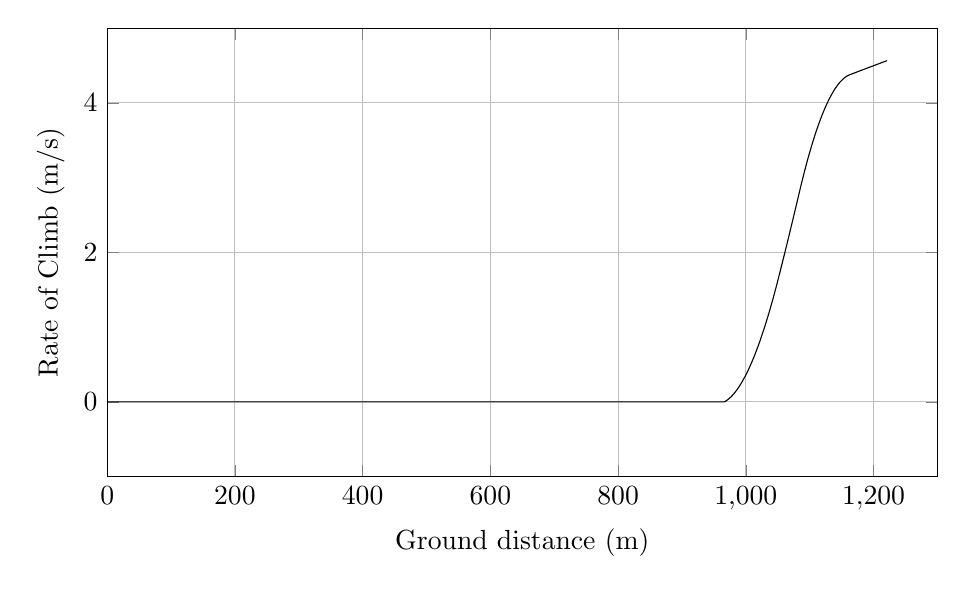
\begin{tikzpicture}

\begin{axis}[
width=\textwidth,
height=0.6\textwidth,
scaled ticks=false, tick label style={/pgf/number format/fixed},
xmin=0.0,
xmax=1300,
xlabel={Ground distance (m)},
xmajorgrids,
ymin=-1.0,
ymax=5,
ylabel={Rate of Climb (m/s)},
ymajorgrids,
legend style={at={(1.03,0.5)},anchor=west,draw=black,fill=white,legend cell align=left}
]

\addplot [
color=black,
solid
]
table[row sep=crcr]{
1.3729668748937997E-8	0.0\\
2.6049868369719035E-7	0.0\\
2.0491224421327626E-6	0.0\\
9.92442121137073E-6	0.0\\
4.7452367809869807E-5	0.0\\
1.740064756114434E-4	0.0\\
4.0608377013922605E-4	0.0\\
7.313431501337001E-4	0.0\\
0.0011549487327126044	0.0\\
0.0016799013484208249	0.0\\
0.002295089346817705	0.0\\
0.003009933382444524	0.0\\
0.003810608015426248	0.0\\
0.004723484476856681	0.0\\
0.005727138856912631	0.0\\
0.006836216967948795	0.0\\
0.007997302399386296	0.0\\
0.00929136979810952	0.0\\
0.010685558505459776	0.0\\
0.012178513621519987	0.0\\
0.013775244426719659	0.0\\
0.015470070176169002	0.0\\
0.0172374436815836	0.0\\
0.019122918912604377	0.0\\
0.021104911040230538	0.0\\
0.023190717999955576	0.0\\
0.025355802981115103	0.0\\
0.027620619195902148	0.0\\
0.030020274690474198	0.0\\
0.032476028269866286	0.0\\
0.035054163466719815	0.0\\
0.037720846868992755	0.0\\
0.04049779674511381	0.0\\
0.043329456594087365	0.0\\
0.04629652060163805	0.0\\
0.04934498934704602	0.0\\
0.052507657924119336	0.0\\
0.055769483710642484	0.0\\
0.05917209570914676	0.0\\
0.06264043916012321	0.0\\
0.06620063977265622	0.0\\
0.06987962792775945	0.0\\
0.0736568184539585	0.0\\
0.07754284280095361	0.0\\
0.08151127871105612	0.0\\
0.08560324933017655	0.0\\
0.08985265585263943	0.0\\
0.09413961367176535	0.0\\
0.09857725310864562	0.0\\
0.10307959255469257	0.0\\
0.10766008648593872	0.0\\
0.11234920964493048	0.0\\
0.11719267720457946	0.0\\
0.12216973960582883	0.0\\
0.12724007601918352	0.0\\
0.13233299746505212	0.0\\
0.13755256756750583	0.0\\
0.14287728588926696	0.0\\
0.1482946925752714	0.0\\
0.15381585025670613	0.0\\
0.15940564092189102	0.0\\
0.16526271495916878	0.0\\
0.17120082448158402	0.0\\
0.17717889132867753	0.0\\
0.18324322596131126	0.0\\
0.189427022360885	0.0\\
0.1957511558722988	0.0\\
0.2021484013779125	0.0\\
0.20865863707071397	0.0\\
0.21548666343168166	0.0\\
0.22220154781289658	0.0\\
0.22919671627301902	0.0\\
0.23611678795738544	0.0\\
0.24306300975244904	0.0\\
0.2503085190632165	0.0\\
0.2576623280401219	0.0\\
0.26502430524173204	0.0\\
0.2724963584449146	0.0\\
0.2802001060647876	0.0\\
0.2878583985474956	0.0\\
0.2958320780323821	0.0\\
0.3040021452321372	0.0\\
0.31208951788619	0.0\\
0.3202851396023423	0.0\\
0.3287233234973125	0.0\\
0.3370425959884752	0.0\\
0.34575405233845447	0.0\\
0.3545073625286812	0.0\\
0.36338982075299686	0.0\\
0.37247557159370037	0.0\\
0.38151350442869847	0.0\\
0.3905554764834429	0.0\\
0.3999457587520332	0.0\\
0.4095398754587949	0.0\\
0.4189621792151833	0.0\\
0.4285208811402964	0.0\\
0.43828968955472236	0.0\\
0.44807735398784176	0.0\\
0.45806002753764463	0.0\\
0.4682994371692033	0.0\\
0.4787752542918833	0.0\\
0.4890770094685154	0.0\\
0.49985939134273727	0.0\\
0.5106597490205704	0.0\\
0.5213580865152188	0.0\\
0.532247733242454	0.0\\
0.5431365108549349	0.0\\
0.554075964429489	0.0\\
0.5653450694020941	0.0\\
0.5769901159382542	0.0\\
0.588512657344902	0.0\\
0.6004070039036553	0.0\\
0.6121651247369502	0.0\\
0.6239717914322569	0.0\\
0.6362472885961421	0.0\\
0.6486428939173223	0.0\\
0.6610190736373547	0.0\\
0.6737248046101814	0.0\\
0.6862826225989949	0.0\\
0.6991952542603428	0.0\\
0.7122988072688032	0.0\\
0.7251463703465595	0.0\\
0.7381769453061875	0.0\\
0.7516618647379176	0.0\\
0.7654913705221527	0.0\\
0.7791756406994825	0.0\\
0.7930637813125616	0.0\\
0.8074774191984457	0.0\\
0.8215072375247947	0.0\\
0.8361010597475598	0.0\\
0.8503303420601955	0.0\\
0.8650627501899835	0.0\\
0.8802332960144008	0.0\\
0.8951742046771463	0.0\\
0.9100334756324657	0.0\\
0.9251067343345352	0.0\\
0.9403923630470314	0.0\\
0.9559303815501943	0.0\\
0.9712400158034169	0.0\\
0.9869533781138684	0.0\\
1.0029148609762486	0.0\\
1.0189962473881624	0.0\\
1.035465185745812	0.0\\
1.0516742337458713	0.0\\
1.067815735429615	0.0\\
1.0846705971808022	0.0\\
1.1012775250051634	0.0\\
1.1180798406225687	0.0\\
1.1351395900544134	0.0\\
1.1526388687279154	0.0\\
1.1698922447507556	0.0\\
1.1875468452119025	0.0\\
1.2058383275300355	0.0\\
1.2239395537495579	0.0\\
1.2422020624207541	0.0\\
1.2608769472440078	0.0\\
1.2794948487006894	0.0\\
1.2979152553275424	0.0\\
1.3166445915281573	0.0\\
1.3354141707340492	0.0\\
1.3543210821322504	0.0\\
1.373689361295591	0.0\\
1.3932049885015831	0.0\\
1.4131781782225183	0.0\\
1.4330139682345777	0.0\\
1.4528243860883294	0.0\\
1.4728783400745615	0.0\\
1.4934621752870565	0.0\\
1.5141408097620341	0.0\\
1.53430654450827	0.0\\
1.5553850389607948	0.0\\
1.5762653203499473	0.0\\
1.5975496774716453	0.0\\
1.6196077215345106	0.0\\
1.6413652536722467	0.0\\
1.663437310723463	0.0\\
1.6860768385032747	0.0\\
1.7077101022266827	0.0\\
1.7297306410738114	0.0\\
1.7520297891459062	0.0\\
1.7743087535215367	0.0\\
1.797257424336919	0.0\\
1.8200802473615325	0.0\\
1.8430350373473994	0.0\\
1.8666926279964304	0.0\\
1.8902808566018634	0.0\\
1.9138231309717848	0.0\\
1.937187877956735	0.0\\
1.9611060682733261	0.0\\
1.9852138445648535	0.0\\
2.009780393513653	0.0\\
2.0346228225622163	0.0\\
2.0593611988602687	0.0\\
2.08477023517836	0.0\\
2.110324766702745	0.0\\
2.1352655781940433	0.0\\
2.160528860803022	0.0\\
2.1862071157614817	0.0\\
2.2127756699400534	0.0\\
2.2391904543957084	0.0\\
2.2653528664920257	0.0\\
2.292150575495974	0.0\\
2.3187704640870406	0.0\\
2.3455495914188482	0.0\\
2.372862901366455	0.0\\
2.4007145172972395	0.0\\
2.428100404243743	0.0\\
2.4555980306928005	0.0\\
2.483374904362833	0.0\\
2.511687733451976	0.0\\
2.5402569276484597	0.0\\
2.568415369317849	0.0\\
2.596987652715761	0.0\\
2.6263861238451423	0.0\\
2.655991481965028	0.0\\
2.6856115886357443	0.0\\
2.7154221146045012	0.0\\
2.7455665152057707	0.0\\
2.7752624694325894	0.0\\
2.805457625653509	0.0\\
2.8358231840904597	0.0\\
2.8663460878589797	0.0\\
2.897817297850832	0.0\\
2.9287074004595235	0.0\\
2.9603588456990284	0.0\\
2.9922321403815406	0.0\\
3.0241119471841866	0.0\\
3.056446055158509	0.0\\
3.0889346922121366	0.0\\
3.122221620829695	0.0\\
3.1546991615623394	0.0\\
3.187635101478671	0.0\\
3.221010117202278	0.0\\
3.2543449374576605	0.0\\
3.288235920596943	0.0\\
3.3223704322934555	0.0\\
3.3562838593334394	0.0\\
3.3906320903803255	0.0\\
3.425633159699527	0.0\\
3.462387235801926	0.0\\
3.4973980805087237	0.0\\
3.5324804241140235	0.0\\
3.5675385073174235	0.0\\
3.6040688981843845	0.0\\
3.6393612181513753	0.0\\
3.6770856360342323	0.0\\
3.7131729334920323	0.0\\
3.749509707933214	0.0\\
3.785733977879824	0.0\\
3.8225309786916544	0.0\\
3.860867115351552	0.0\\
3.89929745075254	0.0\\
3.9373367205567504	0.0\\
3.9751626485832894	0.0\\
4.013671158053867	0.0\\
4.0521140617426425	0.0\\
4.092377631210638	0.0\\
4.131586743753305	0.0\\
4.1715696979561425	0.0\\
4.210522654700574	0.0\\
4.250196810863292	0.0\\
4.2917015001093795	0.0\\
4.332438976653355	0.0\\
4.373124372895289	0.0\\
4.414429464889761	0.0\\
4.455884944705147	0.0\\
4.497250153511752	0.0\\
4.537976875075978	0.0\\
4.581399817640802	0.0\\
4.623816269683994	0.0\\
4.666022338967499	0.0\\
4.709098934189642	0.0\\
4.752435367147649	0.0\\
4.79531009100786	0.0\\
4.838191999420829	0.0\\
4.881381760681686	0.0\\
4.9256451804034285	0.0\\
4.9704217340957495	0.0\\
5.014356093293278	0.0\\
5.058826350846283	0.0\\
5.104458009943745	0.0\\
5.149663211268795	0.0\\
5.194981168813841	0.0\\
5.241194091283663	0.0\\
5.287987552078626	0.0\\
5.334426822383641	0.0\\
5.380633359096258	0.0\\
5.427524438012913	0.0\\
5.476157635197664	0.0\\
5.524667120325573	0.0\\
5.5732739519824435	0.0\\
5.6208990292882195	0.0\\
5.671502816366864	0.0\\
5.719824083529298	0.0\\
5.767871110439133	0.0\\
5.8169321963676754	0.0\\
5.866076914057565	0.0\\
5.917200682776528	0.0\\
5.96684810088939	0.0\\
6.016885842403935	0.0\\
6.068639931677712	0.0\\
6.119867755785197	0.0\\
6.171030794930029	0.0\\
6.222884713227881	0.0\\
6.2735946138732235	0.0\\
6.325883502103322	0.0\\
6.379615386553551	0.0\\
6.432194972482147	0.0\\
6.484528316464761	0.0\\
6.536619297696934	0.0\\
6.589662958081361	0.0\\
6.644121795496577	0.0\\
6.697445536614451	0.0\\
6.7518063163896365	0.0\\
6.8068829439682315	0.0\\
6.863205650636274	0.0\\
6.9185329265047315	0.0\\
6.974634519184049	0.0\\
7.031139830722298	0.0\\
7.0870923879294985	0.0\\
7.144766952910487	0.0\\
7.2026451873548805	0.0\\
7.261191729679483	0.0\\
7.320502240843062	0.0\\
7.378210233177999	0.0\\
7.437738452534925	0.0\\
7.49714639104333	0.0\\
7.556502460410064	0.0\\
7.617032771987237	0.0\\
7.676883327249088	0.0\\
7.735740247984193	0.0\\
7.796086087039788	0.0\\
7.856787102853412	0.0\\
7.91721236259451	0.0\\
7.979013602666894	0.0\\
8.039824025454376	0.0\\
8.102419182184594	0.0\\
8.16459313580776	0.0\\
8.226347093952135	0.0\\
8.290527749984296	0.0\\
8.353592793320257	0.0\\
8.417564177281012	0.0\\
8.482044607535009	0.0\\
8.547336806956285	0.0\\
8.613293246319614	0.0\\
8.6778048537894	0.0\\
8.74454839911753	0.0\\
8.810708373588199	0.0\\
8.876548424968423	0.0\\
8.942828456712885	0.0\\
9.010858044488913	0.0\\
9.079453414959548	0.0\\
9.148767802603732	0.0\\
9.21609997183467	0.0\\
9.285579683381485	0.0\\
9.355451712480097	0.0\\
9.423585014597279	0.0\\
9.493435356703696	0.0\\
9.562655940911181	0.0\\
9.63183713653898	0.0\\
9.703018708836247	0.0\\
9.773178624863132	0.0\\
9.844376937811855	0.0\\
9.914998792594716	0.0\\
9.98720270419701	0.0\\
10.059478150570087	0.0\\
10.132362020358627	0.0\\
10.205876892438312	0.0\\
10.279422251887688	0.0\\
10.353305644514993	0.0\\
10.42811398108589	0.0\\
10.50332954727428	0.0\\
10.578207710262959	0.0\\
10.65503529959097	0.0\\
10.730232142651953	0.0\\
10.805871937852555	0.0\\
10.88265320376452	0.0\\
10.958577899345514	0.0\\
11.034861147941964	0.0\\
11.112742623646977	0.0\\
11.190543636431041	0.0\\
11.267787598939979	0.0\\
11.3462805052093	0.0\\
11.423875697147409	0.0\\
11.502735831556972	0.0\\
11.581465323066688	0.0\\
11.661639233340708	0.0\\
11.741743247575428	0.0\\
11.821864700430528	0.0\\
11.901816327719768	0.0\\
11.98361062800689	0.0\\
12.065425957085825	0.0\\
12.1478520915771	0.0\\
12.230956215923495	0.0\\
12.313306905825911	0.0\\
12.396632357805931	0.0\\
12.479578787946746	0.0\\
12.564327762802186	0.0\\
12.648175874147956	0.0\\
12.736145481689512	0.0\\
12.821080154398764	0.0\\
12.908009536077355	0.0\\
12.994986774303499	0.0\\
13.081752199798046	0.0\\
13.17035388279784	0.0\\
13.257836697901475	0.0\\
13.34511613365563	0.0\\
13.433461823066896	0.0\\
13.524108483575919	0.0\\
13.611203924103116	0.0\\
13.702229394080796	0.0\\
13.792427706753081	0.0\\
13.882429934062493	0.0\\
13.975435778888343	0.0\\
14.065832730112316	0.0\\
14.157894546480026	0.0\\
14.250668806951023	0.0\\
14.343291987615704	0.0\\
14.43744444968501	0.0\\
14.532636396723657	0.0\\
14.625507232812737	0.0\\
14.721503924398366	0.0\\
14.818738382089133	0.0\\
14.913572076739943	0.0\\
15.009701633366973	0.0\\
15.10815424447124	0.0\\
15.206130868840724	0.0\\
15.304035939715973	0.0\\
15.403499839366233	0.0\\
15.503209871950865	0.0\\
15.601718454553605	0.0\\
15.700655560608023	0.0\\
15.801250929860519	0.0\\
15.899917805652187	0.0\\
16.001574124100856	0.0\\
16.102638779863817	0.0\\
16.204479333764816	0.0\\
16.30489644092564	0.0\\
16.40578186591999	0.0\\
16.509201471948074	0.0\\
16.614557195984908	0.0\\
16.717657554831042	0.0\\
16.823039336622365	0.0\\
16.928576062495388	0.0\\
17.03469945574068	0.0\\
17.140697318244236	0.0\\
17.246066414787876	0.0\\
17.35183930840021	0.0\\
17.458399953804133	0.0\\
17.565707112453843	0.0\\
17.673103795073075	0.0\\
17.781888038667653	0.0\\
17.89115167195854	0.0\\
18.00105710767307	0.0\\
18.110142905530395	0.0\\
18.219697237410173	0.0\\
18.32752951944549	0.0\\
18.43743745973078	0.0\\
18.54904630654982	0.0\\
18.659302591714813	0.0\\
18.770734536087716	0.0\\
18.883577445650936	0.0\\
18.996263390583444	0.0\\
19.108816920034535	0.0\\
19.22287647779894	0.0\\
19.33763586704334	0.0\\
19.456324114791514	0.0\\
19.57349394116079	0.0\\
19.690148252848566	0.0\\
19.80521137071168	0.0\\
19.92379170801214	0.0\\
20.04216631061405	0.0\\
20.15848954929409	0.0\\
20.278242138037896	0.0\\
20.396206084226087	0.0\\
20.516315546862906	0.0\\
20.637173924977112	0.0\\
20.75450010628387	0.0\\
20.874378237858778	0.0\\
20.996035953832852	0.0\\
21.11812959618858	0.0\\
21.240471115580952	0.0\\
21.361479376438375	0.0\\
21.485224699488654	0.0\\
21.607870280890317	0.0\\
21.73242999733349	0.0\\
21.85704493170313	0.0\\
21.98122016226351	0.0\\
22.10826921766411	0.0\\
22.235261614051304	0.0\\
22.361664688868032	0.0\\
22.48780138980522	0.0\\
22.614107216476143	0.0\\
22.74409311379692	0.0\\
22.873024137794893	0.0\\
23.003512644166257	0.0\\
23.132891545907036	0.0\\
23.26270690888247	0.0\\
23.39264146728729	0.0\\
23.52277721573431	0.0\\
23.654883767164463	0.0\\
23.78569183677709	0.0\\
23.917003007077597	0.0\\
24.047013652206026	0.0\\
24.178458227988493	0.0\\
24.314609552493202	0.0\\
24.447533097503474	0.0\\
24.579128452041708	0.0\\
24.71011994849615	0.0\\
24.843278471916108	0.0\\
24.975761222328053	0.0\\
25.1115496753864	0.0\\
25.247101122854083	0.0\\
25.384906965000688	0.0\\
25.522261036073317	0.0\\
25.66123001648475	0.0\\
25.79865327455613	0.0\\
25.826335196219034	0.0\\
25.839610403727477	0.0\\
25.841006316401874	0.0\\
25.84227013303559	0.0\\
25.84770509053729	0.0\\
25.86419328224909	0.0\\
25.90571916957557	0.0\\
25.999268866927544	0.0\\
26.123295978662824	0.0\\
26.250212562581652	0.0\\
26.376891976518465	0.0\\
26.50638698165423	0.0\\
26.634042370994827	0.0\\
26.763333806613538	0.0\\
26.893207366259766	0.0\\
27.022905486492228	0.0\\
27.153956322362554	0.0\\
27.287774297957696	0.0\\
27.42030033806219	0.0\\
27.555504894698295	0.0\\
27.691130018821354	0.0\\
27.82633313037239	0.0\\
27.959508564917073	0.0\\
28.096515548835796	0.0\\
28.232789703382153	0.0\\
28.368684388406535	0.0\\
28.506541650227618	0.0\\
28.64533374691623	0.0\\
28.78297783415192	0.0\\
28.92277775692753	0.0\\
29.06227187463503	0.0\\
29.20212864139956	0.0\\
29.34335827861657	0.0\\
29.483225747293005	0.0\\
29.625960812476485	0.0\\
29.76706561118049	0.0\\
29.909402910999468	0.0\\
30.051751399473822	0.0\\
30.196612335666572	0.0\\
30.342192969749448	0.0\\
30.48583400527584	0.0\\
30.632658550781265	0.0\\
30.77846394498075	0.0\\
30.92408133049836	0.0\\
31.071091331299215	0.0\\
31.218274793935116	0.0\\
31.366705758252415	0.0\\
31.515339333797037	0.0\\
31.66356819769615	0.0\\
31.814689402684216	0.0\\
31.96649953392354	0.0\\
32.115424616034375	0.0\\
32.266253234088566	0.0\\
32.41813832080348	0.0\\
32.569791431087395	0.0\\
32.722234201183724	0.0\\
32.876984607664	0.0\\
33.031873994672836	0.0\\
33.18502245018544	0.0\\
33.34135780547538	0.0\\
33.49759920343199	0.0\\
33.65385117142162	0.0\\
33.8113313806527	0.0\\
33.96985264489639	0.0\\
34.126473036379195	0.0\\
34.2857505660089	0.0\\
34.4449212019973	0.0\\
34.60566879064274	0.0\\
34.76644486933921	0.0\\
34.92612701881755	0.0\\
35.08630421658309	0.0\\
35.24825698849928	0.0\\
35.412303951281956	0.0\\
35.57355277914179	0.0\\
35.73545353069308	0.0\\
35.89925038949356	0.0\\
36.065161289279985	0.0\\
36.23047312008262	0.0\\
36.39472205714358	0.0\\
36.56135389445764	0.0\\
36.72774532558607	0.0\\
36.89384825683493	0.0\\
37.05904296416534	0.0\\
37.22702676294645	0.0\\
37.39437475321985	0.0\\
37.5621109943643	0.0\\
37.73270471709142	0.0\\
37.903359519601935	0.0\\
38.071486842086316	0.0\\
38.23815243703595	0.0\\
38.40817787072022	0.0\\
38.57751392140098	0.0\\
38.750215798728505	0.0\\
38.92001182640311	0.0\\
39.09310637700479	0.0\\
39.26472366117933	0.0\\
39.436554723976656	0.0\\
39.608961777617054	0.0\\
39.782828308010565	0.0\\
39.956194359016465	0.0\\
40.132391837044906	0.0\\
40.30868053167249	0.0\\
40.48611580488176	0.0\\
40.66383502946924	0.0\\
40.83999042132467	0.0\\
41.018202681018664	0.0\\
41.19780999006247	0.0\\
41.37730467548502	0.0\\
41.557010452813884	0.0\\
41.73612816026986	0.0\\
41.91555194917056	0.0\\
42.09743589423803	0.0\\
42.27807550146298	0.0\\
42.45995188234755	0.0\\
42.6401410478328	0.0\\
42.822293873795985	0.0\\
43.00585672428667	0.0\\
43.189965171449515	0.0\\
43.372020236704074	0.0\\
43.555636897252796	0.0\\
43.74012033961118	0.0\\
43.92429822300048	0.0\\
44.106869824379004	0.0\\
44.29411840239129	0.0\\
44.47920670866131	0.0\\
44.665034305215386	0.0\\
44.85242224248053	0.0\\
45.03948098831597	0.0\\
45.22811764277584	0.0\\
45.41548629589063	0.0\\
45.60322541388645	0.0\\
45.793007222766036	0.0\\
45.983742663331824	0.0\\
46.172643153142886	0.0\\
46.36421599110457	0.0\\
46.553512793459404	0.0\\
46.745018895697555	0.0\\
46.93606459490553	0.0\\
47.126948089509526	0.0\\
47.31881294044018	0.0\\
47.5110690178297	0.0\\
47.705448624448266	0.0\\
47.90005519882567	0.0\\
48.09288923506665	0.0\\
48.28732881729917	0.0\\
48.484002572746206	0.0\\
48.68089030454945	0.0\\
48.87532723390382	0.0\\
49.07073736177763	0.0\\
49.2672083392297	0.0\\
49.46586249263092	0.0\\
49.661880987188695	0.0\\
49.85966148345089	0.0\\
50.05808618672894	0.0\\
50.25785665917266	0.0\\
50.45743808511885	0.0\\
50.65573800086891	0.0\\
50.85948768734909	0.0\\
51.061243703011925	0.0\\
51.26368286286315	0.0\\
51.46416466063809	0.0\\
51.66475943174029	0.0\\
51.86588207153103	0.0\\
52.07444928962187	0.0\\
52.2824430085781	0.0\\
52.48676525705545	0.0\\
52.69531994892206	0.0\\
52.90027076850366	0.0\\
53.108186167814935	0.0\\
53.31165724918766	0.0\\
53.520024946679996	0.0\\
53.72688450142306	0.0\\
53.93707391647578	0.0\\
54.14518573319289	0.0\\
54.35125853722778	0.0\\
54.56213447502874	0.0\\
54.77598621923464	0.0\\
54.987629956235494	0.0\\
55.19778857845695	0.0\\
55.41030974885841	0.0\\
55.62390503323701	0.0\\
55.83671574169797	0.0\\
56.047071254351536	0.0\\
56.26137331252919	0.0\\
56.47512769358855	0.0\\
56.69105800830218	0.0\\
56.90937011004422	0.0\\
57.12736617899088	0.0\\
57.346833156368504	0.0\\
57.56476609337061	0.0\\
57.78230894703917	0.0\\
57.99943865551505	0.0\\
58.21827465292657	0.0\\
58.436085045729726	0.0\\
58.6577546799423	0.0\\
58.87982836766625	0.0\\
59.10336118170943	0.0\\
59.324182403931715	0.0\\
59.545440661451366	0.0\\
59.768227251413464	0.0\\
59.99077485409802	0.0\\
60.21631063559073	0.0\\
60.44006004384342	0.0\\
60.66502706168687	0.0\\
60.89133011288284	0.0\\
61.11585558357916	0.0\\
61.3432655409558	0.0\\
61.57186440401435	0.0\\
61.79868765088207	0.0\\
62.025670725987	0.0\\
62.254132946411545	0.0\\
62.48290793247415	0.0\\
62.713817944074236	0.0\\
62.94484116346062	0.0\\
63.17805109236767	0.0\\
63.41124119062552	0.0\\
63.64505576847972	0.0\\
63.87735201907903	0.0\\
64.11169045660182	0.0\\
64.34725756208485	0.0\\
64.58324360279937	0.0\\
64.81881329818131	0.0\\
65.05563560606473	0.0\\
65.29467812810154	0.0\\
65.53178653633495	0.0\\
65.77046761369158	0.0\\
66.01019347650049	0.0\\
66.25262920761091	0.0\\
66.49342175078831	0.0\\
66.73393309567928	0.0\\
66.97718905970893	0.0\\
67.21919788222482	0.0\\
67.46413738735515	0.0\\
67.70584739194695	0.0\\
67.95375887035246	0.0\\
68.19817148521656	0.0\\
68.44413350233111	0.0\\
68.68984243621705	0.0\\
68.93951041285982	0.0\\
69.19023531750676	0.0\\
69.43956667494601	0.0\\
69.68998597860525	0.0\\
69.94098943220166	0.0\\
70.1928405184459	0.0\\
70.44659484061637	0.0\\
70.69926103579675	0.0\\
70.95414956377036	0.0\\
71.21136313866151	0.0\\
71.46778788208749	0.0\\
71.7247351381395	0.0\\
71.98234155897126	0.0\\
72.24107377350035	0.0\\
72.4986091150376	0.0\\
72.75949164810788	0.0\\
73.02014691132015	0.0\\
73.28114866838587	0.0\\
73.54342372888959	0.0\\
73.80584407854005	0.0\\
74.07231166191039	0.0\\
74.3389341302921	0.0\\
74.60521354141642	0.0\\
74.87280568706873	0.0\\
75.1403821105715	0.0\\
75.41145333671997	0.0\\
75.68265298797411	0.0\\
75.95075857762194	0.0\\
76.2241428819712	0.0\\
76.4990100438061	0.0\\
76.77213586328236	0.0\\
77.04724851790667	0.0\\
77.32330034006353	0.0\\
77.59850473375684	0.0\\
77.87773830129439	0.0\\
78.1565255546137	0.0\\
78.43842651648492	0.0\\
78.720833678605	0.0\\
79.00101298089581	0.0\\
79.28359351218376	0.0\\
79.57011733099088	0.0\\
79.85418914588558	0.0\\
80.13919871477489	0.0\\
80.42568449319114	0.0\\
80.71472498530085	0.0\\
81.006853148924	0.0\\
81.2951972638476	0.0\\
81.58524575795963	0.0\\
81.87461709596036	0.0\\
82.1711642895769	0.0\\
82.46716486408064	0.0\\
82.76422974563803	0.0\\
83.05801377197795	0.0\\
83.35853301954708	0.0\\
83.65664966506407	0.0\\
83.95487262936624	0.0\\
84.25322789115987	0.0\\
84.55664509033022	0.0\\
84.8599544590121	0.0\\
85.16499148084048	0.0\\
85.47187188044902	0.0\\
85.77908321853027	0.0\\
86.08675489504844	0.0\\
86.39784539041122	0.0\\
86.71051296037359	0.0\\
87.02583358957506	0.0\\
87.34037846285594	0.0\\
87.65395388450591	0.0\\
87.96687312379424	0.0\\
88.28527441497255	0.0\\
88.6103524516937	0.0\\
88.92871226770333	0.0\\
89.25003295857354	0.0\\
89.57522243846881	0.0\\
89.90247582737899	0.0\\
90.22602529632545	0.0\\
90.5494223037065	0.0\\
90.87816525326718	0.0\\
91.20455861430293	0.0\\
91.53817773235312	0.0\\
91.87076195087604	0.0\\
92.20124984301029	0.0\\
92.53140503523474	0.0\\
92.86389705561814	0.0\\
93.19815266874983	0.0\\
93.53304529783748	0.0\\
93.86737084100128	0.0\\
94.20337949361911	0.0\\
94.54065981474497	0.0\\
94.87396787418089	0.0\\
95.21684847579547	0.0\\
95.55392648231228	0.0\\
95.89232371872416	0.0\\
96.23051075783204	0.0\\
96.57164052232307	0.0\\
96.90762523479154	0.0\\
97.24755293575913	0.0\\
97.58790661409188	0.0\\
97.92576087813703	0.0\\
98.26661027452474	0.0\\
98.6051908024865	0.0\\
98.94563962387357	0.0\\
99.28665364663627	0.0\\
99.63350087797645	0.0\\
99.97685593767679	0.0\\
100.31593955776762	0.0\\
100.65572384630482	0.0\\
100.99616871909686	0.0\\
101.3402339503516	0.0\\
101.67973054404297	0.0\\
102.01657591573795	0.0\\
102.35656456518868	0.0\\
102.6941824316649	0.0\\
103.03547296258705	0.0\\
103.37623032340073	0.0\\
103.71852978299776	0.0\\
104.05851119314701	0.0\\
104.3949509202441	0.0\\
104.7329053851843	0.0\\
105.07104272194636	0.0\\
105.40742307340048	0.0\\
105.74423560014887	0.0\\
106.07955743077031	0.0\\
106.41623710643992	0.0\\
106.75618472497374	0.0\\
107.0942647435474	0.0\\
107.43151869252583	0.0\\
107.44650965670576	0.0\\
107.45815118347005	0.0\\
107.46233674961977	0.0\\
107.46535588765028	0.0\\
107.46808502617694	0.0\\
107.4836206108138	0.0\\
107.53176708907421	0.0\\
107.68672244793561	0.0\\
107.97570433527497	0.0\\
108.27744765146667	0.0\\
108.5816623935838	0.0\\
108.88557241638279	0.0\\
109.19209959959528	0.0\\
109.50241879336687	0.0\\
109.81066605766154	0.0\\
110.12101503747155	0.0\\
110.43285681965125	0.0\\
110.74725799716322	0.0\\
111.06462449033057	0.0\\
111.38211128519615	0.0\\
111.70119562731901	0.0\\
112.02298633508096	0.0\\
112.34320819983824	0.0\\
112.66812620709393	0.0\\
112.99302416686388	0.0\\
113.31966045518399	0.0\\
113.64998129974768	0.0\\
113.97857627498675	0.0\\
114.31304608469316	0.0\\
114.64448318111735	0.0\\
114.98093514978115	0.0\\
115.31969924418831	0.0\\
115.65790718621022	0.0\\
116.00063352526521	0.0\\
116.34235083463872	0.0\\
116.68621873349733	0.0\\
117.03331062078092	0.0\\
117.37910048629482	0.0\\
117.72869476105836	0.0\\
118.08005947084649	0.0\\
118.43363644355449	0.0\\
118.79186464668504	0.0\\
119.14769212941735	0.0\\
119.5036618261702	0.0\\
119.86270697471275	0.0\\
120.22616362054572	0.0\\
120.58991121293201	0.0\\
120.95538130513773	0.0\\
121.3195355377388	0.0\\
121.68590041554987	0.0\\
122.05305648207542	0.0\\
122.42257239354896	0.0\\
122.79503144936103	0.0\\
123.16629137010841	0.0\\
123.53950748252527	0.0\\
123.91239367862553	0.0\\
124.29026003316017	0.0\\
124.66301933937496	0.0\\
125.03890311735066	0.0\\
125.41380975776434	0.0\\
125.7896808967325	0.0\\
126.16837244152023	0.0\\
126.54595968852882	0.0\\
126.92471834906405	0.0\\
127.30294276405039	0.0\\
127.68255852126984	0.0\\
128.06243727540487	0.0\\
128.44360431740483	0.0\\
128.82265748788262	0.0\\
129.1989690567886	0.0\\
129.57765386613931	0.0\\
129.95508099647026	0.0\\
130.33359114840187	0.0\\
130.71373745886524	0.0\\
131.09453904397424	0.0\\
131.47657586018488	0.0\\
131.85678563989967	0.0\\
132.23856625352113	0.0\\
132.61595336405918	0.0\\
132.99976263915818	0.0\\
133.38083522978053	0.0\\
133.76098428781995	0.0\\
134.1363519425165	0.0\\
134.51557915495124	0.0\\
134.8968696170101	0.0\\
135.27419431482667	0.0\\
135.65215477207505	0.0\\
136.03329358991255	0.0\\
136.41192880753374	0.0\\
136.7898079310749	0.0\\
137.17001317148595	0.0\\
137.54844558779996	0.0\\
137.92617219433072	0.0\\
138.30476964659732	0.0\\
138.68390038934075	0.0\\
139.0631653430654	0.0\\
139.4406106933401	0.0\\
139.81914660512416	0.0\\
140.19767098864742	0.0\\
140.5730919292459	0.0\\
140.95061983253072	0.0\\
141.32838502869612	0.0\\
141.70636515873298	0.0\\
142.0839785067887	0.0\\
142.46357402350594	0.0\\
142.84082211769783	0.0\\
143.21906727224075	0.0\\
143.59963619096823	0.0\\
143.97984478872678	0.0\\
144.35941603837455	0.0\\
144.7355521893594	0.0\\
145.11296635073694	0.0\\
145.49073213867456	0.0\\
145.87033631970945	0.0\\
146.24486520181193	0.0\\
146.6238757206513	0.0\\
147.00096360401335	0.0\\
147.37874202190085	0.0\\
147.756852900845	0.0\\
148.13572640408995	0.0\\
148.5136798644104	0.0\\
148.89083780486442	0.0\\
149.2712459042852	0.0\\
149.65303236723025	0.0\\
150.0329584616291	0.0\\
150.41363382646614	0.0\\
150.79322940570728	0.0\\
151.17272478467066	0.0\\
151.55400296227282	0.0\\
151.93482601265913	0.0\\
152.31881414221942	0.0\\
152.70208150063132	0.0\\
153.08320649997165	0.0\\
153.4666285558243	0.0\\
153.84825937276264	0.0\\
154.23093781718723	0.0\\
154.61485031834388	0.0\\
155.00001234931443	0.0\\
155.38285725409855	0.0\\
155.7679513537659	0.0\\
156.1509667875323	0.0\\
156.53491934392343	0.0\\
156.91995289130983	0.0\\
157.30625057946366	0.0\\
157.69121706207227	0.0\\
158.07789765133754	0.0\\
158.46521012398495	0.0\\
158.85138765236047	0.0\\
159.23964669847322	0.0\\
159.62715395386465	0.0\\
160.01960115328984	0.0\\
160.4079207075476	0.0\\
160.79602490671402	0.0\\
161.18437278725975	0.0\\
161.57644284003254	0.0\\
161.96812230097612	0.0\\
162.35808768568592	0.0\\
162.75087300343483	0.0\\
163.14546270495134	0.0\\
163.53745675514648	0.0\\
163.92955389373896	0.0\\
164.32395276810763	0.0\\
164.71713266653478	0.0\\
165.1102153740033	0.0\\
165.5035884424101	0.0\\
165.89816400198282	0.0\\
166.29148626774366	0.0\\
166.68861804276264	0.0\\
167.082852347146	0.0\\
167.48006204110857	0.0\\
167.8798182678497	0.0\\
168.27774435731556	0.0\\
168.67741362640317	0.0\\
169.07475368467374	0.0\\
169.4759958044982	0.0\\
169.87832784425882	0.0\\
170.2792240364854	0.0\\
170.68126852540456	0.0\\
171.08617821288442	0.0\\
171.48766933901368	0.0\\
171.892744970828	0.0\\
172.29711201372032	0.0\\
172.70264003426053	0.0\\
173.1105289448074	0.0\\
173.5163733808056	0.0\\
173.92577914808027	0.0\\
174.33607303977334	0.0\\
174.74614233406845	0.0\\
175.15731444736514	0.0\\
175.56901623635082	0.0\\
175.97955109701695	0.0\\
176.39275298155184	0.0\\
176.80397138375372	0.0\\
177.21946344336607	0.0\\
177.6332252263685	0.0\\
178.05102033212842	0.0\\
178.46725124888752	0.0\\
178.88389799206544	0.0\\
179.29839533747668	0.0\\
179.71608569665375	0.0\\
180.1342696339205	0.0\\
180.5538779958007	0.0\\
180.97690569555635	0.0\\
181.39980810354632	0.0\\
181.82328311928882	0.0\\
182.24618807605736	0.0\\
182.6731660166833	0.0\\
183.10035828358116	0.0\\
183.5291445538124	0.0\\
183.95833265232255	0.0\\
184.38634616388282	0.0\\
184.8168339376561	0.0\\
185.24630581702252	0.0\\
185.67754767955432	0.0\\
186.109185775987	0.0\\
186.53971883241212	0.0\\
186.97132952004227	0.0\\
187.40711553434954	0.0\\
187.84220985117162	0.0\\
188.27778926256264	0.0\\
188.71822733349944	0.0\\
189.16086434237673	0.0\\
189.6010380968554	0.0\\
190.03919041211265	0.0\\
190.48016062316526	0.0\\
190.92524363955386	0.0\\
191.372330984798	0.0\\
191.81766281185656	0.0\\
192.2649588892154	0.0\\
192.7152080571317	0.0\\
193.16529614382966	0.0\\
193.61551258619323	0.0\\
194.0671041699889	0.0\\
194.52074606224477	0.0\\
194.9783774267325	0.0\\
195.4358245305881	0.0\\
195.89499401276925	0.0\\
196.35432087192027	0.0\\
196.81831699949333	0.0\\
197.28093205423113	0.0\\
197.74513845889334	0.0\\
198.21238653581378	0.0\\
198.6780372695403	0.0\\
199.14562244096538	0.0\\
199.6172630308758	0.0\\
200.085680559985	0.0\\
200.55485539631252	0.0\\
201.0284003638297	0.0\\
201.5010163224531	0.0\\
201.97949934275624	0.0\\
202.45676989461947	0.0\\
202.93795341995116	0.0\\
203.42151825635358	0.0\\
203.9064451985618	0.0\\
204.39376498892221	0.0\\
204.88144002832018	0.0\\
205.3743097859811	0.0\\
205.86751126322014	0.0\\
206.36222180198536	0.0\\
206.85620764580733	0.0\\
207.35622660722595	0.0\\
207.85286701515986	0.0\\
208.35554496397685	0.0\\
208.85949164962352	0.0\\
209.3606904933826	0.0\\
209.86430174661194	0.0\\
210.37517113261447	0.0\\
210.88826309775862	0.0\\
211.408532759536	0.0\\
211.9275242572583	0.0\\
212.45034341379437	0.0\\
212.97278109853062	0.0\\
213.5012611434281	0.0\\
214.0307698600809	0.0\\
214.55632530210835	0.0\\
215.09027271075985	0.0\\
215.62992362610385	0.0\\
216.17218538865313	0.0\\
216.71273903148006	0.0\\
217.25354139798316	0.0\\
217.7992146693805	0.0\\
218.34754045136725	0.0\\
218.89661223248612	0.0\\
219.45761572436965	0.0\\
220.01811384548756	0.0\\
220.5796054147944	0.0\\
221.1491613381006	0.0\\
221.72392285119702	0.0\\
222.29674345543788	0.0\\
222.87200016908895	0.0\\
223.45476781204167	0.0\\
224.04346163614804	0.0\\
224.62738211659592	0.0\\
225.21466034383656	0.0\\
225.80901970025303	0.0\\
226.4067565685998	0.0\\
227.010346212326	0.0\\
227.62015690700883	0.0\\
228.23221085371028	0.0\\
228.84135848872813	0.0\\
229.46020606246555	0.0\\
230.08791152904655	0.0\\
230.71342291791404	0.0\\
231.3402722001092	0.0\\
231.96207175272258	0.0\\
232.5840768980429	0.0\\
233.21041275014744	0.0\\
233.84076499381075	0.0\\
234.4632722369638	0.0\\
235.0951321894368	0.0\\
235.7164683430417	0.0\\
236.33637872225546	0.0\\
236.95807015301216	0.0\\
237.57724458338066	0.0\\
238.1954544769302	0.0\\
238.81057478854058	0.0\\
239.4264917144386	0.0\\
240.0366097511752	0.0\\
240.63918371105967	0.0\\
241.24161561476188	0.0\\
241.8433627512665	0.0\\
242.44272012201816	0.0\\
243.03744426405035	0.0\\
243.6307298234035	0.0\\
244.22108413951537	0.0\\
244.8116939475828	0.0\\
245.39744552343484	0.0\\
245.97855029096053	0.0\\
246.5589096408665	0.0\\
247.13041662269836	0.0\\
247.70663564674516	0.0\\
248.28024698100222	0.0\\
248.85288765982074	0.0\\
249.4193334510956	0.0\\
249.9777393310295	0.0\\
250.54131855768964	0.0\\
251.10095479045611	0.0\\
251.65640742239583	0.0\\
252.20851363475686	0.0\\
252.76218077146297	0.0\\
253.31371341967355	0.0\\
253.86551898536345	0.0\\
254.41422830739316	0.0\\
254.9572061395861	0.0\\
255.0653176818724	0.0\\
255.12993325322566	0.0\\
255.17825500251217	0.0\\
255.20626764895485	0.0\\
255.2307799315319	0.0\\
255.25350681352313	0.0\\
255.27636741461964	0.0\\
255.2901025823965	0.0\\
255.29493524708477	0.0\\
255.30041476425401	0.0\\
255.32542424174517	0.0\\
255.431840924477	0.0\\
255.72188923316247	0.0\\
256.19571599032633	0.0\\
256.67415123408614	0.0\\
257.15505540016306	0.0\\
257.6368423781066	0.0\\
258.1230512066297	0.0\\
258.61423458459376	0.0\\
259.1049940935744	0.0\\
259.5982522152891	0.0\\
260.09486806301686	0.0\\
260.5959555145432	0.0\\
261.1023053698689	0.0\\
261.6089919954627	0.0\\
262.11906753970584	0.0\\
262.63243815947874	0.0\\
263.14830217600297	0.0\\
263.66676080693014	0.0\\
264.1877265034735	0.0\\
264.7128105393116	0.0\\
265.241218472901	0.0\\
265.7723922912836	0.0\\
266.3079016945154	0.0\\
266.8503273810571	0.0\\
267.3932272617866	0.0\\
267.9365984091472	0.0\\
268.4918097049034	0.0\\
269.04807221243857	0.0\\
269.6097925731924	0.0\\
270.17242368341533	0.0\\
270.7441513704771	0.0\\
271.31667319188057	0.0\\
271.8922835348494	0.0\\
272.47925332376417	0.0\\
273.06804504353704	0.0\\
273.66076346861166	0.0\\
274.25294696226547	0.0\\
274.85204953299706	0.0\\
275.4590719216128	0.0\\
276.0685465790958	0.0\\
276.6808474128411	0.0\\
277.29680014730513	0.0\\
277.9224067517041	0.0\\
278.5505103374435	0.0\\
279.17831818166474	0.0\\
279.81790886718375	0.0\\
280.45539954927676	0.0\\
281.0966396233664	0.0\\
281.73735617862894	0.0\\
282.38112941523184	0.0\\
283.0301801354616	0.0\\
283.67721705328654	0.0\\
284.3202688103162	0.0\\
284.9599564878264	0.0\\
285.60213884169843	0.0\\
286.24205728342235	0.0\\
286.8783426797421	0.0\\
287.5176726031193	0.0\\
288.14959414660166	0.0\\
288.7790218355949	0.0\\
289.41060269245395	0.0\\
290.0373602432952	0.0\\
290.6616399781276	0.0\\
291.28528823747513	0.0\\
291.90747044142563	0.0\\
292.5232553861292	0.0\\
293.13767407877424	0.0\\
293.74977203443143	0.0\\
294.36691018627903	0.0\\
294.97422257673236	0.0\\
295.5803242078987	0.0\\
296.18876641420377	0.0\\
296.79141324013847	0.0\\
297.39276567122147	0.0\\
297.9894421920609	0.0\\
298.5870928977196	0.0\\
299.1813773675972	0.0\\
299.77152323390305	0.0\\
300.36612301275215	0.0\\
300.9589816797394	0.0\\
301.5517369040423	0.0\\
302.13995783060716	0.0\\
302.7265461416931	0.0\\
303.31195316833305	0.0\\
303.893632985354	0.0\\
304.47837522976045	0.0\\
305.0603224805632	0.0\\
305.6386476191806	0.0\\
306.2164211941447	0.0\\
306.79567265335925	0.0\\
307.37231001650287	0.0\\
307.9484900815751	0.0\\
308.52614124860884	0.0\\
309.10133925078446	0.0\\
309.6811704644614	0.0\\
310.25396666777317	0.0\\
310.82665929650705	0.0\\
311.40151685857484	0.0\\
311.97010244433034	0.0\\
312.53980750632184	0.0\\
313.10901660628747	0.0\\
313.67956238189845	0.0\\
314.2496933076443	0.0\\
314.8205968353319	0.0\\
315.3893122304361	0.0\\
315.9596108977621	0.0\\
316.52927325433984	0.0\\
317.0962218845675	0.0\\
317.661512728229	0.0\\
318.22894706387933	0.0\\
318.7945230010092	0.0\\
319.36250947901885	0.0\\
319.92950718778627	0.0\\
320.4959663753667	0.0\\
321.0631721024022	0.0\\
321.6290870613959	0.0\\
322.19457963905666	0.0\\
322.7618354565293	0.0\\
323.32829381843464	0.0\\
323.8944812959513	0.0\\
324.4599775338005	0.0\\
325.0236279833782	0.0\\
325.5930851369128	0.0\\
326.1571709254106	0.0\\
326.723741026211	0.0\\
327.28922394543645	0.0\\
327.8556983549987	0.0\\
328.4233330667528	0.0\\
328.9893491077544	0.0\\
329.5546671193348	0.0\\
330.1217964733877	0.0\\
330.68704439501266	0.0\\
331.2526219304833	0.0\\
331.8212338226615	0.0\\
332.38563215932834	0.0\\
332.9540373692553	0.0\\
333.52282575474305	0.0\\
334.0901133197508	0.0\\
334.6587212753741	0.0\\
335.22495173293544	0.0\\
335.79508811264384	0.0\\
336.36651436910597	0.0\\
336.93496842282195	0.0\\
337.5050159421993	0.0\\
338.07625180159437	0.0\\
338.64522733550257	0.0\\
339.21307292972244	0.0\\
339.78316525663524	0.0\\
340.3517359250782	0.0\\
340.92344762446896	0.0\\
341.49725999120506	0.0\\
342.0714758249467	0.0\\
342.6432180289123	0.0\\
343.2156727962654	0.0\\
343.788423593423	0.0\\
344.3632558179478	0.0\\
344.936112850713	0.0\\
345.5122282286983	0.0\\
346.0894236551619	0.0\\
346.6629357201275	0.0\\
347.2399030750438	0.0\\
347.8149786266573	0.0\\
348.3916437826483	0.0\\
348.96682599762005	0.0\\
349.5439461813521	0.0\\
350.1219821225792	0.0\\
350.70068616715105	0.0\\
351.28126445021985	0.0\\
351.8619451172309	0.0\\
352.4432281971418	0.0\\
353.0222568578364	0.0\\
353.6045019024799	0.0\\
354.18853493609936	0.0\\
354.7725020489422	0.0\\
355.3555439607444	0.0\\
355.94178228996793	0.0\\
356.52841816113096	0.0\\
357.11491695053746	0.0\\
357.7019804757698	0.0\\
358.2889970677636	0.0\\
358.8795343682166	0.0\\
359.47011391270996	0.0\\
360.0611888887985	0.0\\
360.65551621456757	0.0\\
361.24837490254504	0.0\\
361.8399267049888	0.0\\
362.43366065279633	0.0\\
363.0271841323796	0.0\\
363.62092175430814	0.0\\
364.2172388023977	0.0\\
364.8170682790411	0.0\\
365.4168935103936	0.0\\
366.0167447450068	0.0\\
366.613361119081	0.0\\
367.21449807554484	0.0\\
367.81411987634317	0.0\\
368.41428222027616	0.0\\
369.0136835421291	0.0\\
369.6184705538477	0.0\\
370.2203314850517	0.0\\
370.8292817941207	0.0\\
371.4325891230952	0.0\\
372.03751184905457	0.0\\
372.64963462678804	0.0\\
373.26236447571455	0.0\\
373.87329119709466	0.0\\
374.48540637090855	0.0\\
375.0984288907292	0.0\\
375.71389401660815	0.0\\
376.3292711349669	0.0\\
376.94717931076855	0.0\\
377.56118057518813	0.0\\
378.18357875745255	0.0\\
378.80534455721454	0.0\\
379.42657984220546	0.0\\
380.05059226965216	0.0\\
380.67279643790334	0.0\\
381.29916382387717	0.0\\
381.92611637580137	0.0\\
382.55700718237256	0.0\\
383.1838285741163	0.0\\
383.815522641495	0.0\\
384.4482555994399	0.0\\
385.0798113246169	0.0\\
385.7142011583089	0.0\\
386.35011647349825	0.0\\
386.98806446889137	0.0\\
387.62777316145673	0.0\\
388.2677779567189	0.0\\
388.9088955203763	0.0\\
389.5502219824099	0.0\\
390.196085141905	0.0\\
390.8411912635918	0.0\\
391.4850258768763	0.0\\
392.1348161747717	0.0\\
392.78657703059184	0.0\\
393.43829425062995	0.0\\
394.0914803145356	0.0\\
394.74697534702034	0.0\\
395.4022052560256	0.0\\
396.0614826489191	0.0\\
396.7253027860521	0.0\\
397.389470201156	0.0\\
398.0561080310739	0.0\\
398.7226685692724	0.0\\
399.391462726883	0.0\\
400.06069563032156	0.0\\
400.7298361745127	0.0\\
401.4030004748297	0.0\\
402.07673432903437	0.0\\
402.7516637315023	0.0\\
403.43308814587397	0.0\\
404.11621884098975	0.0\\
404.8017412836191	0.0\\
405.4859375776791	0.0\\
406.17916116612776	0.0\\
406.869828889608	0.0\\
407.5646978623407	0.0\\
408.2605209917057	0.0\\
408.95953036015305	0.0\\
409.6622694433204	0.0\\
410.36575705355096	0.0\\
411.07335289700484	0.0\\
411.7824393477108	0.0\\
412.49368167220496	0.0\\
413.20637839560925	0.0\\
413.9231120861825	0.0\\
414.64148448951505	0.0\\
415.3640873105958	0.0\\
416.08758784728207	0.0\\
416.8163237339112	0.0\\
417.54818649211745	0.0\\
418.2830458128634	0.0\\
419.0197896011267	0.0\\
419.7618468752946	0.0\\
420.50810315351544	0.0\\
421.2538226142991	0.0\\
422.0024472585525	0.0\\
422.7601619190325	0.0\\
423.51827295501266	0.0\\
424.2791336478392	0.0\\
425.04862066884436	0.0\\
425.8175931526831	0.0\\
426.59484428165274	0.0\\
427.37319167714656	0.0\\
428.1560603980529	0.0\\
428.9441065434968	0.0\\
429.73908511318723	0.0\\
430.5390808738871	0.0\\
431.34695313464147	0.0\\
432.16146945503726	0.0\\
432.97716762270886	0.0\\
433.79906034498686	0.0\\
434.63237437495366	0.0\\
435.4690406415772	0.0\\
436.31317920434697	0.0\\
437.1637869835322	0.0\\
438.01645953609784	0.0\\
438.8814827966934	0.0\\
439.7524258551747	0.0\\
440.63826385029256	0.0\\
441.53868068573615	0.0\\
442.4384272900428	0.0\\
443.3504012304777	0.0\\
444.27758818218365	0.0\\
445.208223124445	0.0\\
446.1516186171384	0.0\\
447.10189524137195	0.0\\
448.06481468075106	0.0\\
449.03617443090013	0.0\\
450.02512103574475	0.0\\
451.0169824202726	0.0\\
452.020591047557	0.0\\
453.02360262247294	0.0\\
454.0275908503903	0.0\\
455.03100385233165	0.0\\
456.0319820328356	0.0\\
457.02914229222506	0.0\\
458.01937985050745	0.0\\
458.99771244571184	0.0\\
459.96197275276677	0.0\\
460.92139296690334	0.0\\
461.8616145847351	0.0\\
462.80206306639445	0.0\\
463.7284486681126	0.0\\
464.6393852721259	0.0\\
465.54063936700334	0.0\\
466.4349184101709	0.0\\
467.3198901301686	0.0\\
468.20051759019884	0.0\\
469.07226485074943	0.0\\
469.9345383529743	0.0\\
470.7902899889468	0.0\\
471.6423737744856	0.0\\
472.4877853124267	0.0\\
473.3248054273006	0.0\\
474.15679752822916	0.0\\
474.98717382477696	0.0\\
475.812191509144	0.0\\
476.6363066147294	0.0\\
477.44928852471696	0.0\\
478.25976263885	0.0\\
479.0680268264706	0.0\\
479.8720193908648	0.0\\
480.6722055908582	0.0\\
481.4638282544993	0.0\\
482.2537496794823	0.0\\
483.0439784328089	0.0\\
483.8253492021597	0.0\\
484.60475037766423	0.0\\
485.38148111107205	0.0\\
486.15453177945005	0.0\\
486.9234848636379	0.0\\
487.6911837486889	0.0\\
488.4532446281222	0.0\\
489.2141943862101	0.0\\
489.3656654782709	0.0\\
489.9141839228952	0.0\\
489.9442198041063	0.0\\
489.95165340794586	0.0\\
489.95904841065203	0.0\\
490.0087656528135	0.0\\
490.2229205115475	0.0\\
490.80762926712646	0.0\\
491.5549224672211	0.0\\
492.3059760305267	0.0\\
493.05617311245896	0.0\\
493.8124400481423	0.0\\
494.57147098753774	0.0\\
495.33883357988543	0.0\\
496.10451558660077	0.0\\
496.8763216977479	0.0\\
497.6516028092092	0.0\\
498.43581565351974	0.0\\
499.22198438592227	0.0\\
500.0155369982069	0.0\\
500.8167457948026	0.0\\
501.6207857715186	0.0\\
502.43135952459795	0.0\\
503.2488031894138	0.0\\
504.06841756255267	0.0\\
504.89158107370974	0.0\\
505.72576854379577	0.0\\
506.5693448613787	0.0\\
507.4142887558387	0.0\\
508.26842244805994	0.0\\
509.12668782716764	0.0\\
509.9922807952486	0.0\\
510.86952952987826	0.0\\
511.75603474468153	0.0\\
512.6525773610188	0.0\\
513.552913573209	0.0\\
514.4681532282782	0.0\\
515.3867354533588	0.0\\
516.3174024261396	0.0\\
517.2602458293647	0.0\\
518.213136886093	0.0\\
519.1760409577637	0.0\\
520.1413511846506	0.0\\
521.1231004572105	0.0\\
522.1209096033688	0.0\\
523.1261067826763	0.0\\
524.1419417493194	0.0\\
525.1629084556621	0.0\\
526.1966720787225	0.0\\
527.232798559631	0.0\\
528.2697748535691	0.0\\
529.3125778912245	0.0\\
530.3569535995234	0.0\\
531.3923454146075	0.0\\
532.4241640074417	0.0\\
533.4600085213303	0.0\\
534.4866261256011	0.0\\
535.5020315541947	0.0\\
536.514508151736	0.0\\
537.5229382799621	0.0\\
538.5160648880578	0.0\\
539.5082343221115	0.0\\
540.4856117025593	0.0\\
541.4663647652112	0.0\\
542.4363165308484	0.0\\
543.403649598117	0.0\\
544.3586522503113	0.0\\
545.3070641243951	0.0\\
546.2506879020282	0.0\\
547.1923729139526	0.0\\
548.1284847870645	0.0\\
549.0607273863563	0.0\\
549.9918578398997	0.0\\
550.9129328290753	0.0\\
551.8320704888101	0.0\\
552.7431023110901	0.0\\
553.6513866954954	0.0\\
554.5567691623032	0.0\\
555.4601447965442	0.0\\
556.3560324901239	0.0\\
557.2510525453768	0.0\\
558.144367784238	0.0\\
559.0395040047595	0.0\\
559.9306875601039	0.0\\
560.8184287789293	0.0\\
561.6957839109712	0.0\\
562.5803647812363	0.0\\
563.4612104685039	0.0\\
564.3388911147272	0.0\\
565.215385530312	0.0\\
566.0886502219232	0.0\\
566.9616941548127	0.0\\
567.8301900811412	0.0\\
568.6977679531799	0.0\\
569.5620388889783	0.0\\
570.424462708284	0.0\\
571.2852292099337	0.0\\
572.1493328191241	0.0\\
573.0103554048726	0.0\\
573.8681094542301	0.0\\
574.7257926178972	0.0\\
575.584494453004	0.0\\
576.4392320762051	0.0\\
577.2895741354355	0.0\\
578.1440860684359	0.0\\
578.9955408132021	0.0\\
579.8488294812946	0.0\\
580.7009485845795	0.0\\
581.5481034887393	0.0\\
582.398203180056	0.0\\
583.2436286861621	0.0\\
584.0951419205564	0.0\\
584.9447588199325	0.0\\
585.7909961721582	0.0\\
586.6394553558484	0.0\\
587.4827778011024	0.0\\
588.3280079409788	0.0\\
589.1732196696316	0.0\\
590.0172358784723	0.0\\
590.860913103985	0.0\\
591.7056349988741	0.0\\
592.5455796206825	0.0\\
593.390591992995	0.0\\
594.23254291524	0.0\\
595.0749775640184	0.0\\
595.9164343501545	0.0\\
596.757445184641	0.0\\
597.6003409863617	0.0\\
598.4426744019354	0.0\\
599.2847755368687	0.0\\
600.125707245069	0.0\\
600.9666449061319	0.0\\
601.808765536209	0.0\\
602.6493496090866	0.0\\
603.4896653766809	0.0\\
604.3324540913729	0.0\\
605.1749627368547	0.0\\
606.0172193894603	0.0\\
606.8564954876942	0.0\\
607.6995822420379	0.0\\
608.5468271351888	0.0\\
609.3853237539292	0.0\\
610.2285785394622	0.0\\
611.0723962320026	0.0\\
611.9144944458772	0.0\\
612.7572705739071	0.0\\
613.6039342512895	0.0\\
614.447700557992	0.0\\
615.2875150228297	0.0\\
616.1283989744954	0.0\\
616.9715554180159	0.0\\
617.816851506552	0.0\\
618.6627080307358	0.0\\
619.5079936234229	0.0\\
620.355287072993	0.0\\
621.2019793580857	0.0\\
622.0488535053607	0.0\\
622.9008554858297	0.0\\
623.7470330382666	0.0\\
624.5970610944692	0.0\\
625.4445858106351	0.0\\
626.2949117084559	0.0\\
627.1456369954528	0.0\\
627.996202785663	0.0\\
628.8493276316594	0.0\\
629.7040179726459	0.0\\
630.5541510983869	0.0\\
631.4094242395336	0.0\\
632.2635827644049	0.0\\
633.1201141992324	0.0\\
633.9783198620232	0.0\\
634.8358449994842	0.0\\
635.6949254776987	0.0\\
636.5510277660717	0.0\\
637.4106283702604	0.0\\
638.26983515646	0.0\\
639.1281653037297	0.0\\
639.9892853909298	0.0\\
640.854752101091	0.0\\
641.7172955483825	0.0\\
642.5803911560504	0.0\\
643.4447648773507	0.0\\
644.3076201978465	0.0\\
645.1745276724305	0.0\\
646.0402102676721	0.0\\
646.9124608338768	0.0\\
647.7810225029502	0.0\\
648.6561125051048	0.0\\
649.5284291267524	0.0\\
650.3990692560633	0.0\\
651.2710362166958	0.0\\
652.1464633126748	0.0\\
653.0220683418463	0.0\\
653.8956541670141	0.0\\
654.7728777786044	0.0\\
655.6515481039796	0.0\\
656.5284362953553	0.0\\
657.4113325495778	0.0\\
658.2915193229558	0.0\\
659.17716463588	0.0\\
660.0651577261099	0.0\\
660.9536046953733	0.0\\
661.8402168340383	0.0\\
662.7324470689205	0.0\\
663.6200112954277	0.0\\
664.5127656227664	0.0\\
665.4027074409514	0.0\\
666.2965782601134	0.0\\
667.1908896376651	0.0\\
668.084320193617	0.0\\
668.985123002554	0.0\\
669.8863392680419	0.0\\
670.7862926077596	0.0\\
671.6898074618846	0.0\\
672.5888268774506	0.0\\
673.4982782765783	0.0\\
674.4103925687491	0.0\\
675.3150941849995	0.0\\
676.2268158638515	0.0\\
677.1406213981061	0.0\\
678.0557411892244	0.0\\
678.9688521555179	0.0\\
679.8873390970205	0.0\\
680.8083547814929	0.0\\
681.7306997118981	0.0\\
682.6500311248872	0.0\\
683.5737488494256	0.0\\
684.4960352365924	0.0\\
685.4200123844039	0.0\\
686.3479632552264	0.0\\
687.2766127474456	0.0\\
688.2061621748603	0.0\\
689.1404800584801	0.0\\
690.0764761874757	0.0\\
691.0152339372712	0.0\\
691.9552419239503	0.0\\
692.8950394637291	0.0\\
693.8400111678282	0.0\\
694.7866818158914	0.0\\
695.7347004483931	0.0\\
696.6882574887352	0.0\\
697.6393666566034	0.0\\
698.5984440154043	0.0\\
699.5498840703472	0.0\\
700.5039755495234	0.0\\
701.4647289348814	0.0\\
702.4256797045559	0.0\\
703.3874603974716	0.0\\
704.3606354781252	0.0\\
705.3315887422941	0.0\\
706.3004122670179	0.0\\
707.2768098841743	0.0\\
708.2494358269255	0.0\\
709.2282890376241	0.0\\
710.2089151733701	0.0\\
711.1951755925729	0.0\\
712.1865307336975	0.0\\
713.1761747054959	0.0\\
714.1673399979175	0.0\\
715.1598728842257	0.0\\
716.1583282218428	0.0\\
717.1629472660959	0.0\\
718.1700311785478	0.0\\
719.1763338932042	0.0\\
720.1876907614742	0.0\\
721.201618282845	0.0\\
722.2184418537404	0.0\\
723.235170191942	0.0\\
724.2594935927766	0.0\\
725.2822718646494	0.0\\
726.3107341130526	0.0\\
727.3400446617545	0.0\\
728.3719103403353	0.0\\
729.4113327961686	0.0\\
730.4562931126598	0.0\\
731.5065909482435	0.0\\
732.5574458491262	0.0\\
733.6186119363024	0.0\\
734.676482187165	0.0\\
735.7351170593906	0.0\\
736.800998200209	0.0\\
737.8752235923619	0.0\\
738.9508085948025	0.0\\
740.030025186873	0.0\\
741.1174055771332	0.0\\
742.2130822925526	0.0\\
743.3102570732492	0.0\\
744.4109860747094	0.0\\
745.5166476604204	0.0\\
746.6263302357015	0.0\\
747.7458154711032	0.0\\
748.8677740542141	0.0\\
749.997151475181	0.0\\
751.1325555959445	0.0\\
752.2719517189332	0.0\\
753.4203420087897	0.0\\
754.5711754188967	0.0\\
755.7260036895639	0.0\\
756.8938875174731	0.0\\
758.065786260207	0.0\\
759.247770693134	0.0\\
760.4404154189538	0.0\\
761.64317092529	0.0\\
762.8455228703601	0.0\\
764.0679862717263	0.0\\
765.2987264665999	0.0\\
766.4085307220014	0.0\\
766.5358897019526	0.0\\
767.7848317922183	0.0\\
769.0450472645446	0.0\\
770.316931581486	0.0\\
771.6083395962344	0.0\\
772.9112380991485	0.0\\
774.2270303713512	0.0\\
775.55388582573	0.0\\
776.893629267375	0.0\\
778.2590064752919	0.0\\
779.6390771149454	0.0\\
781.0408632243589	0.0\\
782.4719583829672	0.0\\
783.9254029605222	0.0\\
785.3937619636636	0.0\\
786.8893778170732	0.0\\
788.4179231510577	0.0\\
789.9735980960556	0.0\\
791.5542677978599	0.0\\
793.1434824354058	0.0\\
794.7563093028011	0.0\\
796.3588663476394	0.0\\
797.9570311300417	0.0\\
799.5313007987854	0.0\\
801.0895110610122	0.0\\
802.6055669418217	0.0\\
804.1018949910592	0.0\\
805.5783591859272	0.0\\
807.0307066077335	0.0\\
808.4529908307093	0.0\\
809.8505654906257	0.0\\
811.2444364840742	0.0\\
812.6158728333517	0.0\\
813.9667251199407	0.0\\
815.3010783126617	0.0\\
816.6204907399006	0.0\\
817.9261081614768	0.0\\
819.226186053904	0.0\\
820.5043924755685	0.0\\
821.7811573689405	0.0\\
823.0442722941846	0.0\\
824.2983674535399	0.0\\
825.541081257411	0.0\\
826.7810697424134	0.0\\
828.0072700964611	0.0\\
829.2275465246082	0.0\\
830.440290401928	0.0\\
831.6456016564753	0.0\\
832.8458526198069	0.0\\
834.037616834057	0.0\\
835.2234914579537	0.0\\
836.3972899863502	0.0\\
837.5756391031359	0.0\\
838.7422917585684	0.0\\
839.902452142522	0.0\\
841.0603218408189	0.0\\
842.2105732200805	0.0\\
843.3580616645866	0.0\\
844.5012408269597	0.0\\
845.6398059126466	0.0\\
846.7724224635103	0.0\\
847.8965100633054	0.0\\
848.1209130838795	0.0\\
848.1623489143824	0.0\\
848.2012937955549	0.0\\
848.2388050923146	0.0\\
848.2635941917742	0.0\\
848.2919709507985	0.0\\
848.4211104394196	0.0\\
848.9593804425128	0.0\\
850.1439050107567	0.0\\
851.2989990610786	0.0\\
852.4625415319017	0.0\\
853.6343291480857	0.0\\
854.813575578349	0.0\\
855.9966730541175	0.0\\
857.1906583671973	0.0\\
858.39215322517	0.0\\
859.5998169607099	0.0\\
860.8156241801316	0.0\\
862.0398638307802	0.0\\
863.2792971616623	0.0\\
864.5308985867496	0.0\\
865.7828789826317	0.0\\
867.0513231121286	0.0\\
868.3278176040103	0.0\\
869.6158844688	0.0\\
870.9184528711855	0.0\\
872.2374309104891	0.0\\
873.5628394437902	0.0\\
874.9061460440512	0.0\\
876.2634067353517	0.0\\
877.6372804740975	0.0\\
879.0207809946949	0.0\\
880.4203247380867	0.0\\
881.8422810479933	0.0\\
883.2819456153238	0.0\\
884.736415506294	0.0\\
886.2095632245146	0.0\\
887.7097638068085	0.0\\
889.2385454066066	0.0\\
890.7799681457695	0.0\\
892.3337302965779	0.0\\
893.9176676427685	0.0\\
895.5155402490216	0.0\\
897.1315944621388	0.0\\
898.7681009115079	0.0\\
900.3978930053565	0.0\\
902.0361248906863	0.0\\
903.6653289970704	0.0\\
905.2792603787045	0.0\\
906.8857455958098	0.0\\
908.4662184920885	0.0\\
910.0469647129698	0.0\\
911.5954755215373	0.0\\
913.1304718420679	0.0\\
914.6569966456154	0.0\\
916.1682113824695	0.0\\
917.6583621217142	0.0\\
919.1456538108444	0.0\\
920.6177876078477	0.0\\
922.0729954796329	0.0\\
923.5274965183664	0.0\\
924.9635923666569	0.0\\
926.3856444820815	0.0\\
927.8055843659806	0.0\\
929.207153527409	0.0\\
930.6035015258558	0.0\\
932.0013730301141	0.0\\
933.3907168850012	0.0\\
934.7677458753328	0.0\\
936.1378360430533	0.0\\
937.5014990339548	0.0\\
938.8580378016413	0.0\\
940.2132103186659	0.0\\
941.5611059168646	0.0\\
942.901388744516	0.0\\
944.2394208523408	0.0\\
945.5692027795503	0.0\\
946.8979199801956	0.0\\
948.2284421278009	0.0\\
949.5505847538652	0.0\\
950.8663497853397	0.0\\
952.1808865050432	0.0\\
953.4893916129145	0.0\\
954.7978626150948	0.0\\
956.1024861861213	0.0\\
957.4059405743512	0.0\\
958.7088937547032	0.0\\
960.0056612317628	0.0\\
961.3018858148289	0.0\\
962.5939791700273	0.0\\
963.8819223334767	0.0\\
965.1710898257154	0.0\\
966.4527523037596	0.0\\
966.709695450093	0.0011875416221047365\\
966.94098601114	0.002278342364669031\\
967.1723259963971	0.0033893386839031524\\
967.3981487956396	0.00449324645550731\\
967.6247217130356	0.005619905853276489\\
967.8562699219328	0.006790926303995382\\
968.0884314750722	0.00798508346424601\\
968.3196488967133	0.009194361408856037\\
968.5508730378835	0.010423576834984408\\
968.7810843200778	0.01166720205017573\\
969.0136815918963	0.012943668866787984\\
969.2466276095627	0.01424220236126398\\
969.4791946874309	0.015558755955643114\\
969.7027997381872	0.01684377782671402\\
969.9275500325971	0.01815406346918512\\
970.1501464107159	0.01947033869975409\\
970.3763135724546	0.020826463896015515\\
970.6102157654611	0.022248706632756597\\
970.8410755807515	0.0236724357947875\\
971.0704690472667	0.025106736087468585\\
971.3005059944664	0.026564625912661302\\
971.534477146258	0.028067444809594604\\
971.7655652796798	0.029571729190150033\\
971.9913462408754	0.031060709168827916\\
972.2238664937613	0.03261365550211297\\
972.4555480610852	0.03418091664384536\\
972.6737198300025	0.035675301200061946\\
972.8969319461539	0.03722227871896645\\
973.1320439148951	0.03887128856951187\\
973.3625626119053	0.04050803759147355\\
973.5971790006822	0.042193908147509826\\
973.8242036146437	0.04384478178861222\\
974.0578334566871	0.04556334838880592\\
974.2917618328775	0.047304270876816906\\
974.5257279725329	0.04906565172417292\\
974.7582046692467	0.05083584238804252\\
974.9915421409487	0.05263258144576641\\
975.2246736267869	0.05444776186119414\\
975.4514350585437	0.05623271594314866\\
975.6855398355406	0.05809510817983282\\
975.9165238771075	0.05995251822415086\\
976.1490472285841	0.06184207330316639\\
976.3830627924144	0.06376377225960553\\
976.6160406207066	0.0656969628510701\\
976.8532227645762	0.0676853902973095\\
977.0782798251448	0.06959159597240588\\
977.3019214377093	0.07150426101085403\\
977.5291932665214	0.07346666391848311\\
977.7629308440332	0.07550446200871605\\
977.9988307306287	0.07758134913798356\\
978.220807250942	0.07955465075889007\\
978.4579112995234	0.08168191834081898\\
978.6959684839528	0.08383841126683497\\
978.9340215679943	0.08601560143249026\\
979.1724243972396	0.08821675117199682\\
979.4028936095169	0.0903646275882923\\
979.6357900573307	0.09255477274218907\\
979.8742936874482	0.09481801703075504\\
980.1130071034725	0.09710404282909582\\
980.3481213593261	0.09937603468151246\\
980.5869218000037	0.10170418247923646\\
980.8201600018199	0.10399833527907745\\
981.05294000498	0.10630776496065597\\
981.2896621671855	0.1086764381100857\\
981.5216312055791	0.11101748422997268\\
981.7604692939519	0.11344812021022951\\
982.0002884181861	0.115909597165195\\
982.2298804527272	0.1182859921913447\\
982.466124310525	0.12075105098103711\\
982.698655978526	0.12319728865755666\\
982.9296608515922	0.12564695701521106\\
983.1698755303155	0.1282145711041765\\
983.4093963044222	0.1307956419969396\\
983.6467680877968	0.13337415262765473\\
983.8862880856798	0.13599664774047826\\
984.1253295268455	0.1386346507529559\\
984.3664911546625	0.14131696939072286\\
984.6031476680037	0.14396978662832488\\
984.8324824465908	0.14656007841429258\\
985.0675959732273	0.14923523149707418\\
985.3062522712785	0.15197104008575296\\
985.5444483563306	0.15472211896806554\\
985.7719007741459	0.15736854662283678\\
986.0147560129831	0.160214361666004\\
986.2519482631958	0.16301453596576138\\
986.4936317005474	0.16588848387518718\\
986.7371478246346	0.1688054821143481\\
986.9797843036029	0.17173323558728626\\
987.2231050234368	0.17469053317370797\\
987.4545627033808	0.17752377480441428\\
987.6953937836438	0.18049195967187998\\
987.9353282208062	0.18346987839772333\\
988.1765153207589	0.18648418086815227\\
988.419755743841	0.18954527057374165\\
988.6525662111717	0.19249531402925718\\
988.8856068547586	0.19546776863299703\\
989.1295043701314	0.19859926978285686\\
989.3704278686262	0.20171363541841952\\
989.6025376177188	0.20473400992646085\\
989.8438343972018	0.2078941470433464\\
990.0869376249677	0.2110989940787188\\
990.3283460821876	0.21430250073264073\\
990.5667024815023	0.21748606934888942\\
990.8126285614292	0.22079183172478545\\
991.0504312721523	0.22400920864665608\\
991.2885768373894	0.2272514803084985\\
991.5276828191745	0.23052719392823057\\
991.771468341019	0.2338879082636176\\
991.9958736158869	0.23700073658050108\\
992.2423318859287	0.24043953013014824\\
992.4871380022703	0.2438767729002348\\
992.7267513969971	0.24726195080205993\\
992.9478368109035	0.2504040137385839\\
993.194213865522	0.2539252898121338\\
993.4409205840091	0.257472926356598\\
993.679485093151	0.2609243124055015\\
993.9203735999708	0.2644297965259619\\
994.1681808142057	0.2680572889504247\\
994.4172304536798	0.27172492015033933\\
994.6668562177094	0.27542312763630894\\
994.8995383561346	0.278890707985072\\
995.1336953243358	0.2823996217743635\\
995.3844254257356	0.28617795462262974\\
995.630467378933	0.28990744396499113\\
995.8643885039714	0.29347343618996335\\
996.1050317404322	0.29716193366728627\\
996.3464446151465	0.30088280402961254\\
996.5955885893088	0.30474422584717376\\
996.844510425843	0.30862413389586707\\
997.0866441809301	0.312419446333564\\
997.3262433382642	0.3161954912297593\\
997.5727828240908	0.3201018719681844\\
997.8210917383603	0.32405792032368275\\
998.0714297283218	0.3280682527215414\\
998.3137892661	0.3319720525682086\\
998.5404044307354	0.33564139880205035\\
998.7933888614348	0.3397582922748189\\
999.0435825226527	0.34385201303655377\\
999.296472754535	0.34801215736586477\\
999.5457881383161	0.3521356154338662\\
999.7942748166481	0.3562671306428945\\
1000.0464896423011	0.3604827033710354\\
1000.300100676252	0.3647440918315199\\
1000.5552815165497	0.36905459133526985\\
1000.7897912790572	0.3730366274190706\\
1001.041757550762	0.3773360451900515\\
1001.2964950559749	0.38170527905284857\\
1001.5502511565073	0.386080302064006\\
1001.7902755628334	0.3902397050882962\\
1002.0349304490137	0.3944999566420788\\
1002.2867474641282	0.3989065674220844\\
1002.5434049229343	0.40342053782457343\\
1002.7883343464239	0.4077500321137948\\
1003.0259392195583	0.41197026882818066\\
1003.2822839351286	0.41654487782337657\\
1003.5367568669446	0.4211088027817901\\
1003.7896465954802	0.4256667375326332\\
1004.0433994998928	0.4302625932974472\\
1004.2956522703482	0.4348535404112235\\
1004.5530440219632	0.4395606805516096\\
1004.8105909657324	0.44429371191765343\\
1005.0687499579967	0.44906110653247566\\
1005.3257230188701	0.45382962531146376\\
1005.5841867210186	0.4586488829390921\\
1005.842654242932	0.46349138869462636\\
1006.0989441519359	0.4683160331145869\\
1006.3457173491563	0.4729833103213902\\
1006.606749519153	0.47794279073126156\\
1006.8651035928219	0.4828746934804623\\
1007.1262288008904	0.4878828757300854\\
1007.3880224029099	0.49292752268134166\\
1007.640053822968	0.49780671736156423\\
1007.9032276661637	0.5029246942781318\\
1008.1652383116191	0.508043832388237\\
1008.4246374346114	0.5131353527158282\\
1008.6829823093501	0.5182292671018658\\
1008.924325694986	0.5230092063062397\\
1009.1777995172738	0.5280506322347032\\
1009.4329465100063	0.5331476171036047\\
1009.6898940391923	0.5383031452773113\\
1009.9444521374949	0.5434331802117809\\
1010.2099135596206	0.5488063231112446\\
1010.4731506576175	0.5541584034050107\\
1010.7393281165848	0.5595943522640847\\
1011.0055708871159	0.5650559377376017\\
1011.2653658495753	0.570408867070356\\
1011.5287491260021	0.5758592197737302\\
1011.7945364954517	0.5813833190008686\\
1012.062589684992	0.5869789160235783\\
1012.332070943575	0.5926290400997078\\
1012.5954450158074	0.5981752762450847\\
1012.860711945513	0.6037852551568677\\
1013.1256811675662	0.6094129176766259\\
1013.3754933453251	0.6147410241479772\\
1013.642379238225	0.6204562601908488\\
1013.9121114569539	0.6262570103200105\\
1014.1818501535558	0.6320826652169005\\
1014.4507846811232	0.6379156165701423\\
1014.700226900756	0.6433483344594042\\
1014.9598059189741	0.6490239690702906\\
1015.2251147261984	0.6548483507580618\\
1015.4842536693388	0.660560525126511\\
1015.7550056373784	0.6665526491206761\\
1016.0150295862327	0.6723310525857304\\
1016.2859921912948	0.6783765652879177\\
1016.5306087389617	0.68385634582416\\
1016.7998815405758	0.6899111062254768\\
1017.0613081202043	0.6958131236728662\\
1017.3321370814824	0.7019514681133843\\
1017.6052913498199	0.7081675252301263\\
1017.8714232275372	0.714248200542781\\
1018.1283101811964	0.7201405651482269\\
1018.3995189344287	0.7263851225913529\\
1018.6578605399734	0.7323568267326457\\
1018.9326314996636	0.7387324353326981\\
1019.2060682116094	0.7451023306249811\\
1019.4793550642889	0.7514938446420101\\
1019.750676388428	0.7578642617919749\\
1020.0295478925971	0.7644374577092634\\
1020.3052343509032	0.7709613159874777\\
1020.5842479371645	0.7775897364440534\\
1020.8442653289683	0.7837909023241914\\
1021.123531713002	0.7904757298461127\\
1021.397525606086	0.7970598630330838\\
1021.6622480910887	0.80344531230896\\
1021.9396934410893	0.8101623734113275\\
1022.2157323266806	0.8168709243457306\\
1022.4921039064309	0.8236130105869821\\
1022.7762434273129	0.8305708871162889\\
1023.0578936998702	0.8374944249149614\\
1023.3252513070047	0.8440914779800375\\
1023.5863408091705	0.8505569943874554\\
1023.870069758294	0.8576081080951419\\
1024.1549496121747	0.8647146868839983\\
1024.4373126099886	0.871785139842497\\
1024.717298207379	0.8788222459837944\\
1024.990693072943	0.8857189745575669\\
1025.2738100456645	0.8928867347318974\\
1025.5589946334057	0.9001335922143374\\
1025.8392301421322	0.9072810430820775\\
1026.1247602891162	0.91459005509482\\
1026.4093930908025	0.9219029192671324\\
1026.6780474460156	0.9288302658690564\\
1026.954170705419	0.9359747681763082\\
1027.2365906868745	0.9433079811353038\\
1027.512493168741	0.9504975232335682\\
1027.7979528738424	0.9579621644998619\\
1028.0864955748407	0.9655345497759378\\
1028.366277083218	0.9729034018564278\\
1028.6545096962336	0.9805214365607005\\
1028.9398651942583	0.9880903641014505\\
1029.2314870853543	0.9958528747323836\\
1029.5112340450587	1.0033258387729926\\
1029.7970999046556	1.0109885202784428\\
1030.085636278941	1.0187497977227529\\
1030.3762785304348	1.0265951542857752\\
1030.6680353511506	1.0344982995273027\\
1030.9534160040953	1.0422557957908687\\
1031.2505165264533	1.0503596921900837\\
1031.5299051888192	1.0580072516034869\\
1031.8242543911829	1.0660913111405312\\
1032.1219619681447	1.0742961561486704\\
1032.4155114547257	1.0824147398130992\\
1032.6930024247636	1.0901154195680558\\
1032.978427354784	1.0980620880602925\\
1033.2704994321161	1.1062209485979237\\
1033.5723606588908	1.114681973667512\\
1033.8652964813718	1.1229213110009315\\
1034.1492891360872	1.1309358806698624\\
1034.4457249879274	1.1393290018482087\\
1034.728958054825	1.1473752257837089\\
1035.013983852768	1.155498449083189\\
1035.3137418525262	1.164069305617248\\
1035.6096509914273	1.172558626188355\\
1035.904252964086	1.1810384817559596\\
1036.1960922302464	1.189466421429255\\
1036.4829398562479	1.197777033754889\\
1036.767470802713	1.206046695487475\\
1037.07456512222	1.2150005202483327\\
1037.3731527017462	1.2237355786025552\\
1037.669074743762	1.2324209132947312\\
1037.9621445502912	1.2410502415117275\\
1038.2605485799236	1.2498646712857466\\
1038.57480831446	1.2591776584595258\\
1038.8812249672787	1.2682888298576698\\
1039.1851967214957	1.2773569648454481\\
1039.4762020823441	1.2860662769992377\\
1039.774520081815	1.295022184781272\\
1040.082327889535	1.3042923366844077\\
1040.379178904106	1.313261378997531\\
1040.6877698511262	1.3226143916613733\\
1040.9856094124502	1.3316705380868146\\
1041.2785875211339	1.3406064499043122\\
1041.5774144301495	1.3497485586468438\\
1041.8970914369743	1.359559089065678\\
1042.215283203377	1.3693561659467774\\
1042.5205265438913	1.3787850390318508\\
1042.8260778884933	1.3882528548958257\\
1043.1381205509956	1.3979519616894596\\
1043.4330975190142	1.4071493624757316\\
1043.7228309610014	1.4162100849872847\\
1044.0253198563114	1.4256974406898348\\
1044.3291048442247	1.4352543266638667\\
1044.6206586948279	1.4444540479087657\\
1044.9483748886287	1.4548253655582841\\
1045.2589162989225	1.4646847665198806\\
1045.575278823368	1.4747598120654057\\
1045.8778572844044	1.4844256073137028\\
1046.1816157279777	1.4941578192343563\\
1046.494622143368	1.5042161354343042\\
1046.7828739829429	1.5135067601846912\\
1047.0885036835225	1.5233851809659393\\
1047.4197719140202	1.5341241866224515\\
1047.736005360328	1.5444081360090878\\
1048.0676066928895	1.5552246579201716\\
1048.3817918136929	1.5655051425477562\\
1048.712795426342	1.5763684414787216\\
1049.0447362789655	1.5872965336299805\\
1049.3690304373258	1.5980060612181246\\
1049.6816230177578	1.6083603051385156\\
1049.9980622933872	1.6188725565580468\\
1050.3014929523342	1.6289820805836959\\
1050.6347260595157	1.6401161593360647\\
1050.9497107929387	1.6506725542904301\\
1051.2835457181845	1.6618933165241025\\
1051.6132903520434	1.673010343875315\\
1051.9279605821012	1.6836285611820965\\
1052.2515527175665	1.6945574030234312\\
1052.582174755452	1.7057336651952424\\
1052.9124558707972	1.7169084697111106\\
1053.253048218613	1.7284426622424611\\
1053.5866652505501	1.7397509644585512\\
1053.9001652855518	1.7503866768549687\\
1054.2249511073833	1.7614147483833809\\
1054.5305176074726	1.7717990208977916\\
1054.8591172690617	1.782975536564639\\
1055.192930198079	1.7943394197699698\\
1055.5318667232686	1.805888066182983\\
1055.8728317985192	1.817516323756891\\
1056.20627443591	1.8288981919315028\\
1056.5421313957736	1.8403726010596873\\
1056.862424583921	1.8513247306751914\\
1057.200020922095	1.8628784910759406\\
1057.5255560658406	1.8740291395006516\\
1057.8442577267438	1.8849548920385106\\
1058.183274903769	1.896587043522437\\
1058.5033822716232	1.9075797596388142\\
1058.821952034456	1.9185287056010427\\
1059.1627152719034	1.930250373230709\\
1059.477652627294	1.9410928031497074\\
1059.8180551645892	1.9528217686117517\\
1060.1316358268718	1.9636355809327495\\
1060.4559856576989	1.974829854343486\\
1060.796561671315	1.9865940650739065\\
1061.1231307038938	1.997883971559303\\
1061.4637549852905	2.009669700591169\\
1061.8171206724	2.0219069614336256\\
1062.1597864522005	2.033784035733918\\
1062.4795965335534	2.0448780926565053\\
1062.8016669162043	2.056059495700545\\
1063.1208988452067	2.0671511868578643\\
1063.474751859154	2.0794560365213073\\
1063.800935196838	2.090808229326668\\
1064.1452102186008	2.102799958339956\\
1064.4920042559747	2.114889673566352\\
1064.8390332655854	2.1269978479850566\\
1065.1665712145382	2.1384353607375433\\
1065.50406894643	2.1502301926465437\\
1065.8415040910754	2.1620324819644603\\
1066.1629897780685	2.1732858658641163\\
1066.496126727609	2.184956287203545\\
1066.8645534418279	2.1978738463259546\\
1067.2049505059254	2.209818769067158\\
1067.5635739565478	2.222413767614662\\
1067.9219678239374	2.235011430864315\\
1068.272646666348	2.247348263065472\\
1068.6075548101394	2.2591398223738324\\
1068.9490013201298	2.271171156887217\\
1069.3288709557219	2.2845677094462227\\
1069.6774150507185	2.2968699981424354\\
1070.017535585644	2.308884600584027\\
1070.3702003221333	2.3213523450349394\\
1070.7223707222734	2.3338127718053743\\
1071.0400543509463	2.345061681880254\\
1071.3751618373876	2.356936465470457\\
1071.7388999772506	2.3698361252168425\\
1072.0933442684077	2.382416502655288\\
1072.4705690422084	2.3958165890292795\\
1072.8139366241921	2.408023947371608\\
1073.150690607702	2.4200053895401634\\
1073.4997821298216	2.4324353949420487\\
1073.8611401290527	2.4453124405269593\\
1074.1957988601853	2.4572473489839526\\
1074.5552857806042	2.470077635520836\\
1074.9047032119488	2.4825583705389196\\
1075.2953938919964	2.4965247808463777\\
1075.6654193903996	2.5097635667605553\\
1075.9985220891767	2.5216905503973894\\
1076.3867199149727	2.5356012514510198\\
1076.749550931478	2.548613629582311\\
1077.0882535668725	2.5607699613499744\\
1077.4452377549933	2.5735921087025453\\
1077.808103308901	2.586635651507706\\
1078.1446997502562	2.5987440495254868\\
1078.5083148849535	2.6118342316915433\\
1078.8907933247601	2.6256144927889222\\
1079.2358429725514	2.638055885398697\\
1079.5764980564204	2.6503477772992046\\
1079.9302728990506	2.663122462255461\\
1080.304782822196	2.6766562817839725\\
1080.6636596805702	2.6896351687243634\\
1081.0017661370189	2.7018718222033256\\
1081.3765779360301	2.7154470076705177\\
1081.7385355557467	2.7285666863447338\\
1082.1025437263556	2.7417706249804024\\
1082.4670852301265	2.755003866042939\\
1082.833584405179	2.7683181880964085\\
1083.1860275292956	2.7811313216803963\\
1083.4357261839036	2.7902147517723668\\
1083.5539540249138	2.7945172075178863\\
1083.9184371140063	2.8077670741646275\\
1084.2798261729345	2.8208510835132676\\
1084.6226550625256	2.8332126967912723\\
1084.9691510609814	2.8456584359440678\\
1085.3479229224422	2.8592107142647647\\
1085.7000904967545	2.871756643860949\\
1086.0624640940405	2.8846144980211195\\
1086.4660711040074	2.8988766209760817\\
1086.8466459307465	2.91226213904892\\
1087.2345965893228	2.9258471666519554\\
1087.6062088639092	2.9388012174836895\\
1087.9639610250051	2.9512178484746885\\
1088.3464010707949	2.964435976025446\\
1088.72995967104	2.9776330410424663\\
1089.099931747989	2.99030463942608\\
1089.4880548600067	3.0035396313397467\\
1089.8696003888385	3.016489847619696\\
1090.2616594611204	3.0297360225965484\\
1090.6190672971256	3.0417538319631694\\
1090.971638000427	3.053557475133668\\
1091.3589649654577	3.066469398039004\\
1091.7444428067997	3.0792586297409414\\
1092.1336864798072	3.0921115001980084\\
1092.4995859053138	3.104134981091912\\
1092.8628073668415	3.1160160390326856\\
1093.251411803752	3.128669929964297\\
1093.6506148891262	3.141605540447732\\
1094.0401199657963	3.1541630517359653\\
1094.3999223396281	3.16570513700489\\
1094.755222512531	3.177050311101209\\
1095.0892473262106	3.187667201301961\\
1095.4622759809013	3.199473170546697\\
1095.8483309888743	3.211632448261203\\
1096.1964474813421	3.2225411531535695\\
1096.5350681178852	3.2331037428000204\\
1096.9252129481224	3.2452198923620745\\
1097.278251098655	3.256126590133217\\
1097.6570735662326	3.2677751686261516\\
1098.0170003016	3.2787863690099854\\
1098.3770996320363	3.2897494871627675\\
1098.7714377174216	3.301696953791028\\
1099.1647175152557	3.3135484392633554\\
1099.5365168234634	3.3246920709687418\\
1099.9212699532977	3.336165129811289\\
1100.299910920986	3.3473957523562996\\
1100.6935181733343	3.3590089665244296\\
1101.0707782263848	3.370078355747224\\
1101.4804870302305	3.3820364362166844\\
1101.8692891432247	3.3933182357171336\\
1102.252192867641	3.4043672745204097\\
1102.6454691980257	3.4156534899633915\\
1103.0171590180548	3.426259492897109\\
1103.4190308875882	3.4376653080572375\\
1103.8169972256132	3.4488940233974157\\
1104.214340226084	3.460039660424841\\
1104.618795437853	3.4713183144484807\\
1104.9867116600153	3.4815159448569872\\
1105.3838399794122	3.492463051667303\\
1105.7683841300254	3.5029997821262784\\
1106.1743922050632	3.514060140888807\\
1106.5468381886762	3.524143060364703\\
1106.9292687500902	3.5344372724925375\\
1107.2944014695204	3.5442076753685745\\
1107.6627336577458	3.5540078576255603\\
1108.058477564679	3.564477145604279\\
1108.4578465656173	3.5749766782579844\\
1108.8530309212629	3.5853005128643964\\
1109.2407085372288	3.595364419054654\\
1109.6642750849428	3.606292121501302\\
1110.0668736933812	3.6166076194241326\\
1110.4729525413172	3.626944253321363\\
1110.8778014715886	3.637181081685214\\
1111.2828582041684	3.647354833400718\\
1111.659801190715	3.6567584880135042\\
1112.0259163438604	3.665834354683332\\
1112.4234789537409	3.6756294634481748\\
1112.8228860614872	3.6854037878266386\\
1113.2321181780544	3.6953504544873477\\
1113.6297480007752	3.7049470438749506\\
1114.0203973408825	3.714310209104828\\
1114.4066546177773	3.723505017892453\\
1114.81503598072	3.733160842066048\\
1115.2086712878604	3.7424006379394896\\
1115.6084149847825	3.7517180933104513\\
1116.0204931272815	3.761254299132405\\
1116.4299273052748	3.7706586954801926\\
1116.83192943091	3.779823408262474\\
1117.2210173622884	3.788628076296006\\
1117.639671591975	3.7980339502808347\\
1118.0360051753073	3.806868581287514\\
1118.4584724765227	3.816215920942108\\
1118.8766091818197	3.8253933488056244\\
1119.2679589472832	3.8339139315998807\\
1119.6767774096188	3.8427479582656234\\
1120.0774622854142	3.851337415699234\\
1120.4655345244937	3.859591105416782\\
1120.8857471980068	3.8684603156094868\\
1121.2851178111187	3.8768189218302753\\
1121.6555148912553	3.8845086938721662\\
1122.0546738530993	3.8927338115809533\\
1122.4493587195616	3.900800487418084\\
1122.8541282658998	3.909006248236481\\
1123.2749405590444	3.917465822013849\\
1123.68291495826	3.9255949701191115\\
1124.1049622838232	3.9339322719310026\\
1124.5108070909864	3.9418772464161114\\
1124.9341483361745	3.950092639445308\\
1125.346788669529	3.9580267056745058\\
1125.7667552981966	3.9660287538860777\\
1126.170628391882	3.973652532551589\\
1126.5890632411256	3.98148016303295\\
1127.011730797813	3.9893124953305312\\
1127.4037768476187	3.9965072058546403\\
1127.8168138860042	4.004019107627377\\
1128.2148500388512	4.0111886900350555\\
1128.6126473702411	4.018287178811326\\
1129.0391166560526	4.025826066881864\\
1129.4617058758986	4.033220263025395\\
1129.873224201067	4.040347213352751\\
1130.2900622911357	4.047493930082791\\
1130.7282396258574	4.054929631208244\\
1131.1352873877522	4.061761383520665\\
1131.5323155545798	4.068356578094091\\
1131.945640941718	4.0751533259705806\\
1132.3637312244505	4.081955435908963\\
1132.7822554332706	4.088690628332554\\
1133.189516839213	4.095172364367013\\
1133.6183308182813	4.101923499934115\\
1134.0395621743146	4.108478748331878\\
1134.4474263446455	4.11475312340124\\
1134.8646375866115	4.1210993695554645\\
1135.2759333839613	4.127282922850554\\
1135.686836463079	4.133389004433031\\
1136.116741342465	4.139702859196396\\
1136.544989989282	4.1459143789756805\\
1136.9730366494014	4.15204529602045\\
1137.3975590206205	4.158048683608676\\
1137.8027516801098	4.163705596285585\\
1138.2166345914957	4.169412829504202\\
1138.6395429651639	4.17517039723808\\
1139.0539139781886	4.18073731530923\\
1139.4765108110896	4.186340550940942\\
1139.89906781003	4.191867490102474\\
1140.318694382173	4.19728081764989\\
1140.7298740602914	4.2025118479787675\\
1141.136387924424	4.20761250773095\\
1141.5380516876867	4.212582928190564\\
1141.9361829703498	4.217441684230973\\
1142.3606997804882	4.22255095003214\\
1142.7840797551698	4.227570163029192\\
1143.1909048436482	4.232319751014412\\
1143.6239327716285	4.237300678324434\\
1144.0447607295055	4.242063680317003\\
1144.4480918712343	4.246556305679658\\
1144.858186256895	4.251054005899675\\
1145.274338085143	4.2555456270227445\\
1145.701694371181	4.260082657511152\\
1146.1276735261895	4.264527605772818\\
1146.5573346000347	4.268933137156742\\
1146.9915593363457	4.273306115178016\\
1147.4218956076975	4.277560354057524\\
1147.8484919731059	4.281699428095907\\
1148.2745191008412	4.285755591429911\\
1148.7006930048074	4.289735836813106\\
1149.1123258249231	4.293505406036388\\
1149.5284816733165	4.297243472721947\\
1149.973990729084	4.301166547431015\\
1150.4010996739876	4.304846313330241\\
1150.841112625913	4.308557307279296\\
1151.2641014347755	4.312045207923553\\
1151.6899743990543	4.315480129267401\\
1152.118288092473	4.318856992297098\\
1152.5441970237107	4.322137081394521\\
1152.960873430387	4.3252702840014425\\
1153.3920847550103	4.3284363023373515\\
1153.8198713130646	4.331498445541145\\
1154.237534854586	4.334411789314641\\
1154.6606520649534	4.337287823633233\\
1155.0975024125223	4.340178473241576\\
1155.5331950440795	4.342980210564978\\
1155.9589965272644	4.345639041871266\\
1156.383098289854	4.348210143735722\\
1156.8268309260002	4.350820120880311\\
1157.2425389740324	4.3531861946722685\\
1157.691828475417	4.355664009927246\\
1158.1164262294283	4.357923902002831\\
1158.5512641875002	4.360159532579347\\
1158.9974716131587	4.362370843592693\\
1159.4207767064331	4.364387702819037\\
1159.8447942360854	4.366331257873508\\
1160.280621000923	4.3682500863041\\
1160.707957515533	4.370051832726343\\
1161.135716000931	4.371777216232315\\
1161.577146728032	4.3734771640796275\\
1162.0098432779714	4.375061709070847\\
1162.4408485718018	4.376560288876345\\
1162.8832335097945	4.378017011213039\\
1163.310511657236	4.37934297757344\\
1163.7360481772894	4.380585740447833\\
1164.1781127066997	4.382031391966274\\
1164.8430251407667	4.384205325097197\\
1165.7920093656921	4.387307030082656\\
1167.1183066542985	4.391639991092806\\
1168.4026305369366	4.395833638192917\\
1169.7031267442803	4.400077900674127\\
1171.0211124992484	4.404376994510033\\
1172.2222337957028	4.408292924365236\\
1173.5002685762715	4.412457551745566\\
1174.884603844992	4.416966180860561\\
1176.141018562963	4.421056036976555\\
1177.4372241454366	4.425273278463992\\
1178.8057453069382	4.429723443937165\\
1180.1147356772112	4.433977764651402\\
1181.4750263591159	4.438396474861095\\
1182.7692867681121	4.442598483406222\\
1184.0048661293022	4.446607965522221\\
1185.2552107090678	4.450663365177714\\
1186.603490509503	4.455034163467216\\
1187.8967755420713	4.459224493866092\\
1189.247018311973	4.463597088036874\\
1190.5168585722458	4.467707183285199\\
1191.9621815334185	4.472382760434497\\
1193.3377437167924	4.476830191588567\\
1194.6593723056549	4.481100978386827\\
1196.0629373339866	4.485634109426746\\
1197.402209196	4.489957260767165\\
1198.7192409860977	4.494206405176557\\
1200.0573366561816	4.4985212604145435\\
1201.3212683156307	4.5025948868151\\
1202.6488354009807	4.506871438291595\\
1203.9262897195858	4.510984462491125\\
1205.2699746137646	4.515308513434105\\
1206.6875358834086	4.51986784315323\\
1208.0162213116264	4.524139030377338\\
1209.3719287217282	4.5284948023004965\\
1210.7454109005998	4.5329053378902895\\
1212.0883060260344	4.537215373252831\\
1213.4209881645493	4.541490405565108\\
1214.7721478897788	4.545822452106195\\
1216.0779962351203	4.550007064432819\\
1217.464202961145	4.554446868559944\\
1218.7944526266688	4.55870520965091\\
1220.166720735691	4.563095761639444\\
1221.2507746200122	4.566562529494572\\
};
\end{axis}
\end{tikzpicture}%

%\caption{Rate of climb in AOE condition - ATR-72}
%\end{figure}
%%
%\begin{figure}[!b]
%\centering
%%RateOfClimb_vs_GroundDistance
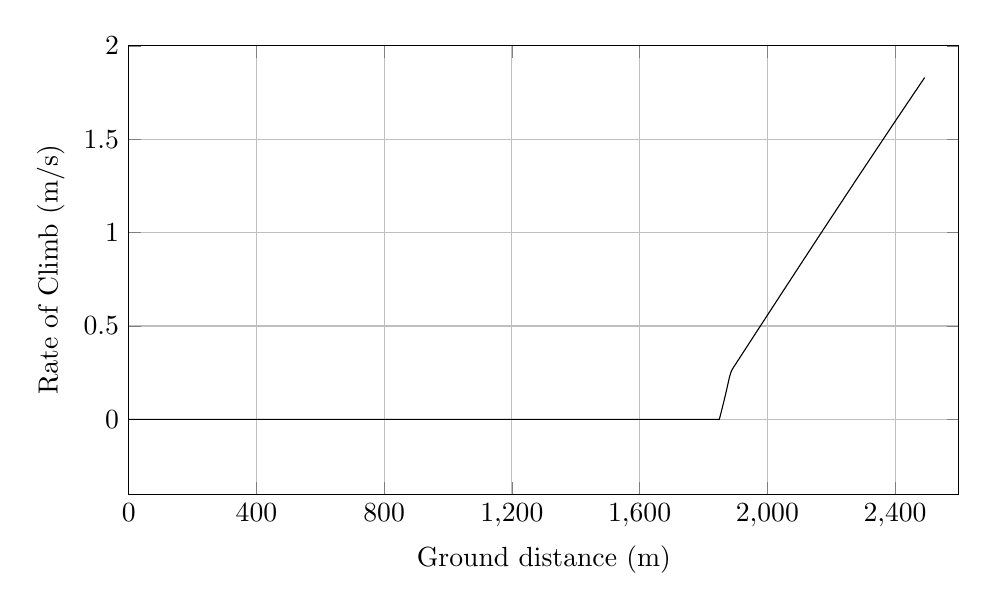
\begin{tikzpicture}

\begin{axis}[
width=\textwidth,
height=0.6\textwidth,
scaled ticks=false, tick label style={/pgf/number format/fixed},
xmin=0.0,
xmax=2600,
xtick={0,400,800,1200,1600,2000,2400,2800,3200},
xlabel={Ground distance (m)},
xmajorgrids,
ymin=-0.4,
ymax=2,
ylabel={Rate of Climb (m/s)},
ymajorgrids,
legend style={at={(1.03,0.5)},anchor=west,draw=black,fill=white,legend cell align=left}
]

\addplot [
color=black,
solid
]
table[row sep=crcr]{
1.3729668748938318E-8	0.0\\
1.7493248493808052E-7	0.0\\
1.4411937280317895E-6	0.0\\
6.602995160656227E-5	0.0\\
2.2740573828771224E-4	0.0\\
4.8751428921765393E-4	0.0\\
8.441986619835749E-4	0.0\\
0.0012981647037285577	0.0\\
0.0018484379050661159	0.0\\
0.0024893731755424335	0.0\\
0.0032286585096692284	0.0\\
0.0040442418752796045	0.0\\
0.004972762654474916	0.0\\
0.005990910102221513	0.0\\
0.007111389191545643	0.0\\
0.008336865178450469	0.0\\
0.009664633507451486	0.0\\
0.011093815858158905	0.0\\
0.01262066151120312	0.0\\
0.01419454386807839	0.0\\
0.015910782250193378	0.0\\
0.017721549103721458	0.0\\
0.019620507964630857	0.0\\
0.02164969955342029	0.0\\
0.023766550611781796	0.0\\
0.025957065600157342	0.0\\
0.028260861173784894	0.0\\
0.030668466949245715	0.0\\
0.0331489614440674	0.0\\
0.03573888453685943	0.0\\
0.038418765463712895	0.0\\
0.04116679597872082	0.0\\
0.044022059812866554	0.0\\
0.04700053365173311	0.0\\
0.050116649382181494	0.0\\
0.0533021652593606	0.0\\
0.056630220296749106	0.0\\
0.05998688030085898	0.0\\
0.06348077825220624	0.0\\
0.06710848437295475	0.0\\
0.07082346760424127	0.0\\
0.07462944469130567	0.0\\
0.07855413323217031	0.0\\
0.08251243142992878	0.0\\
0.08659905947434482	0.0\\
0.09083545394947079	0.0\\
0.09518096637774642	0.0\\
0.099604438418047	0.0\\
0.1041130762071252	0.0\\
0.10871457033213175	0.0\\
0.11350280915994052	0.0\\
0.11836943512882261	0.0\\
0.12328542045494376	0.0\\
0.12830372217771202	0.0\\
0.1334037067999082	0.0\\
0.1386015897371753	0.0\\
0.14405085578552257	0.0\\
0.1495239325759128	0.0\\
0.1550507392415454	0.0\\
0.16073360491635535	0.0\\
0.16659871679960742	0.0\\
0.17244819595229793	0.0\\
0.17848031195343078	0.0\\
0.18466822548212042	0.0\\
0.1909009608611748	0.0\\
0.19716089737688902	0.0\\
0.2035279375926986	0.0\\
0.21017879584430066	0.0\\
0.21687473998771628	0.0\\
0.22354650324940833	0.0\\
0.23036941414946865	0.0\\
0.23737731412185503	0.0\\
0.24449289925428264	0.0\\
0.2517184892023243	0.0\\
0.25908208279438383	0.0\\
0.2664863589195283	0.0\\
0.27399321582905467	0.0\\
0.2816108016888421	0.0\\
0.2893844725195981	0.0\\
0.29747621078120867	0.0\\
0.30547198304033185	0.0\\
0.31373479402345694	0.0\\
0.3220909744202328	0.0\\
0.3305540912568814	0.0\\
0.33895489345894936	0.0\\
0.34753073012810576	0.0\\
0.3563589175375672	0.0\\
0.3652744752958731	0.0\\
0.3742693918027593	0.0\\
0.38350989122680823	0.0\\
0.3927029292363896	0.0\\
0.4020876366599533	0.0\\
0.4115568217121528	0.0\\
0.4212787852930122	0.0\\
0.43089755178065414	0.0\\
0.4408379299669313	0.0\\
0.4510502611115679	0.0\\
0.4612670224725215	0.0\\
0.4715818614584312	0.0\\
0.4818438670126082	0.0\\
0.4922128554044626	0.0\\
0.50273876067117	0.0\\
0.5136516607865718	0.0\\
0.5244310074213006	0.0\\
0.5355751508210329	0.0\\
0.5467126997993474	0.0\\
0.5580479056656631	0.0\\
0.5692960823995112	0.0\\
0.5809945926573021	0.0\\
0.5923626544035139	0.0\\
0.6041922852715	0.0\\
0.6160912669048675	0.0\\
0.6280605196746807	0.0\\
0.6403946506485891	0.0\\
0.6525721787971039	0.0\\
0.66504690021022	0.0\\
0.6773535438897555	0.0\\
0.6901462526606317	0.0\\
0.703249873273524	0.0\\
0.7159721017112175	0.0\\
0.729053467210389	0.0\\
0.7422988791228431	0.0\\
0.756304272979474	0.0\\
0.7696432036294076	0.0\\
0.7832290250230658	0.0\\
0.7969128825551131	0.0\\
0.8108444209446342	0.0\\
0.825043936786227	0.0\\
0.8390802275180445	0.0\\
0.8532340040587583	0.0\\
0.8678101043696134	0.0\\
0.8824320602344964	0.0\\
0.8978006605470081	0.0\\
0.9134572487531922	0.0\\
0.9287391767029982	0.0\\
0.9440564687433697	0.0\\
0.9598871644713316	0.0\\
0.9757786228365237	0.0\\
0.9918217338879218	0.0\\
1.0080608846667363	0.0\\
1.0245900975307913	0.0\\
1.040622085070809	0.0\\
1.0571005809273983	0.0\\
1.0736578999152901	0.0\\
1.0902401336450098	0.0\\
1.1073201062866707	0.0\\
1.1241926772552646	0.0\\
1.1416781667104252	0.0\\
1.1588269484070954	0.0\\
1.176440946845327	0.0\\
1.1944819542445066	0.0\\
1.2120125629913447	0.0\\
1.2299306574276825	0.0\\
1.2481120482032448	0.0\\
1.2663536608165091	0.0\\
1.2851425782117465	0.0\\
1.3041313368869671	0.0\\
1.3228236880779458	0.0\\
1.3414329672940513	0.0\\
1.3605066144349074	0.0\\
1.3802534409605212	0.0\\
1.3994872719307283	0.0\\
1.4192016277101378	0.0\\
1.439023460648384	0.0\\
1.459347998039509	0.0\\
1.4793256644936217	0.0\\
1.4991489338326072	0.0\\
1.5195196572175793	0.0\\
1.5402684478761244	0.0\\
1.5604570108688036	0.0\\
1.5810331069622228	0.0\\
1.6022712329181132	0.0\\
1.623752316257296	0.0\\
1.6452514305955401	0.0\\
1.6664829631402025	0.0\\
1.6886446033619715	0.0\\
1.710607384244656	0.0\\
1.7329417009553727	0.0\\
1.7551421266962821	0.0\\
1.7779085356585536	0.0\\
1.800478286927734	0.0\\
1.8236018329231238	0.0\\
1.8462320784511883	0.0\\
1.869621217116264	0.0\\
1.8933146512119747	0.0\\
1.9176856041472643	0.0\\
1.9417713639512164	0.0\\
1.9657098573982132	0.0\\
1.9902165007163162	0.0\\
2.014554050520948	0.0\\
2.039479559407779	0.0\\
2.0645497069116256	0.0\\
2.090368502766882	0.0\\
2.115564185269416	0.0\\
2.140750230554602	0.0\\
2.1667677015838267	0.0\\
2.1927560352542175	0.0\\
2.218891869133375	0.0\\
2.245288939563828	0.0\\
2.2712530964452817	0.0\\
2.297933078351498	0.0\\
2.324564104516777	0.0\\
2.351466051806102	0.0\\
2.378869922986878	0.0\\
2.4061764715670764	0.0\\
2.4343811693482102	0.0\\
2.4622108821536663	0.0\\
2.4906408044048067	0.0\\
2.518892760285042	0.0\\
2.5472153538550346	0.0\\
2.5762492306032216	0.0\\
2.605385308804288	0.0\\
2.634725531238531	0.0\\
2.6633424112287507	0.0\\
2.6927188130915374	0.0\\
2.7226962917814213	0.0\\
2.7531675915664673	0.0\\
2.7831412651501983	0.0\\
2.8139174932165103	0.0\\
2.8440331768075415	0.0\\
2.874693215323904	0.0\\
2.9059978681586376	0.0\\
2.9372617813709034	0.0\\
2.9684444504378202	0.0\\
3.000072782687808	0.0\\
3.031082587373527	0.0\\
3.063213028467148	0.0\\
3.0965739711585014	0.0\\
3.1291175748240176	0.0\\
3.161651640649506	0.0\\
3.194791488147139	0.0\\
3.2273698640351327	0.0\\
3.261394174200582	0.0\\
3.2942820372415875	0.0\\
3.3276455142443044	0.0\\
3.3625338428565543	0.0\\
3.396526624461681	0.0\\
3.4305511850311694	0.0\\
3.4642094416894933	0.0\\
3.498963551783903	0.0\\
3.5341885134496573	0.0\\
3.569804025802995	0.0\\
3.605116576002147	0.0\\
3.641338581546833	0.0\\
3.677593698357855	0.0\\
3.7132425573336665	0.0\\
3.74957219375957	0.0\\
3.7872650227149185	0.0\\
3.825403000593508	0.0\\
3.861987998097706	0.0\\
3.899535703755137	0.0\\
3.9366960368382165	0.0\\
3.9756271117991435	0.0\\
4.014715979923002	0.0\\
4.053268843133694	0.0\\
4.093111596873367	0.0\\
4.132540645872048	0.0\\
4.171686416589186	0.0\\
4.211258480423352	0.0\\
4.252585425594734	0.0\\
4.29253892845542	0.0\\
4.332839968385603	0.0\\
4.372708537789018	0.0\\
4.414379330316386	0.0\\
4.455607216042212	0.0\\
4.497336690654009	0.0\\
4.53836773335787	0.0\\
4.579767142935065	0.0\\
4.621942908118227	0.0\\
4.663798268780793	0.0\\
4.705838036060712	0.0\\
4.748491012675066	0.0\\
4.791393968819099	0.0\\
4.835700194867293	0.0\\
4.879973298406089	0.0\\
4.923250156511948	0.0\\
4.967673596314626	0.0\\
5.012954369117542	0.0\\
5.057574526249477	0.0\\
5.103280208347517	0.0\\
5.148856018935929	0.0\\
5.194350575362858	0.0\\
5.240584094986199	0.0\\
5.2871741484687504	0.0\\
5.333122064003502	0.0\\
5.3803318800233235	0.0\\
5.4262712259485255	0.0\\
5.473378197958581	0.0\\
5.521938593493333	0.0\\
5.570027890245774	0.0\\
5.617746353771608	0.0\\
5.665750363096816	0.0\\
5.714883880069209	0.0\\
5.763390205677501	0.0\\
5.812817811268989	0.0\\
5.861909274803731	0.0\\
5.912134919389196	0.0\\
5.962317560553064	0.0\\
6.012727788730279	0.0\\
6.0628236035803145	0.0\\
6.113711068416594	0.0\\
6.16497292765713	0.0\\
6.216284706244114	0.0\\
6.26834407822653	0.0\\
6.320257064476769	0.0\\
6.37351660191279	0.0\\
6.426150862197664	0.0\\
6.479030963436509	0.0\\
6.532319340056288	0.0\\
6.5857233987986845	0.0\\
6.640834734692348	0.0\\
6.695022999498724	0.0\\
6.749720237657193	0.0\\
6.804235758325081	0.0\\
6.859728469301633	0.0\\
6.916686079588434	0.0\\
6.9732530286722305	0.0\\
7.029531186664631	0.0\\
7.086633318514238	0.0\\
7.144155485034537	0.0\\
7.202053129566568	0.0\\
7.260126434764185	0.0\\
7.317913145042743	0.0\\
7.376682960996439	0.0\\
7.435393721764624	0.0\\
7.493838107271518	0.0\\
7.552684475254578	0.0\\
7.613252707151423	0.0\\
7.672782806866918	0.0\\
7.733397683408512	0.0\\
7.795525081709004	0.0\\
7.856013653786727	0.0\\
7.91792172269443	0.0\\
7.980110745884113	0.0\\
8.041720670752433	0.0\\
8.105229267009985	0.0\\
8.167457523036095	0.0\\
8.230908874360502	0.0\\
8.293738919282273	0.0\\
8.356235402336917	0.0\\
8.42092378244627	0.0\\
8.485671322837007	0.0\\
8.549180898871484	0.0\\
8.614596634551038	0.0\\
8.680166762249144	0.0\\
8.744770128469462	0.0\\
8.812993689385827	0.0\\
8.88005807777586	0.0\\
8.94709863067661	0.0\\
9.013172088448385	0.0\\
9.079266506338545	0.0\\
9.14748814890141	0.0\\
9.215411293660388	0.0\\
9.284579146198691	0.0\\
9.353168277381275	0.0\\
9.423753765537143	0.0\\
9.492960052876374	0.0\\
9.564123004975215	0.0\\
9.634097601479446	0.0\\
9.705672410878787	0.0\\
9.776260200085993	0.0\\
9.846607984572056	0.0\\
9.918231435410593	0.0\\
9.988851555070422	0.0\\
10.060390022634245	0.0\\
10.133279281833644	0.0\\
10.205241085147751	0.0\\
10.277820389603	0.0\\
10.352558894167803	0.0\\
10.42733258664746	0.0\\
10.501815126481194	0.0\\
10.576858173457808	0.0\\
10.65303812840548	0.0\\
10.729080272001735	0.0\\
10.804841544893105	0.0\\
10.881905013502095	0.0\\
10.958396790746043	0.0\\
11.035905069829102	0.0\\
11.113160538490881	0.0\\
11.192172636140572	0.0\\
11.270076562295213	0.0\\
11.350065490058778	0.0\\
11.429008826667825	0.0\\
11.50754237847364	0.0\\
11.587076645554472	0.0\\
11.668897725768986	0.0\\
11.749734371708193	0.0\\
11.830312384681939	0.0\\
11.909862670519033	0.0\\
11.990515423105418	0.0\\
12.072973931530203	0.0\\
12.155304175892073	0.0\\
12.237018674011615	0.0\\
12.320146069843414	0.0\\
12.406770618003886	0.0\\
12.489918686423398	0.0\\
12.574493004618496	0.0\\
12.660666896522624	0.0\\
12.746500366216402	0.0\\
12.832006837122272	0.0\\
12.919285437479463	0.0\\
13.00517529032821	0.0\\
13.092301899261269	0.0\\
13.179760097773386	0.0\\
13.268594687119744	0.0\\
13.357699529172354	0.0\\
13.44829753340392	0.0\\
13.537570218252604	0.0\\
13.627322718831184	0.0\\
13.718307212496544	0.0\\
13.808540263830096	0.0\\
13.899143852161355	0.0\\
13.991564069206362	0.0\\
14.085798171937814	0.0\\
14.179213507883688	0.0\\
14.271883316076963	0.0\\
14.367546274622434	0.0\\
14.459430863676705	0.0\\
14.555010173556813	0.0\\
14.648669731311681	0.0\\
14.743773575674254	0.0\\
14.839769774519894	0.0\\
14.932807148196385	0.0\\
15.026921440816679	0.0\\
15.12275113649265	0.0\\
15.222025232743288	0.0\\
15.321078842653048	0.0\\
15.417564225728565	0.0\\
15.515758841369038	0.0\\
15.613440509090129	0.0\\
15.7107260301154	0.0\\
15.81102223487273	0.0\\
15.913565872734136	0.0\\
16.012918321571746	0.0\\
16.11222833737955	0.0\\
16.216250800242257	0.0\\
16.319159023020546	0.0\\
16.421418004006803	0.0\\
16.521675247646563	0.0\\
16.62557290942481	0.0\\
16.72731964230514	0.0\\
16.830283223934416	0.0\\
16.93464251494634	0.0\\
17.038481620468637	0.0\\
17.146497421123335	0.0\\
17.252282308638982	0.0\\
17.35724772858778	0.0\\
17.464053904588297	0.0\\
17.572390862630144	0.0\\
17.680417629270814	0.0\\
17.789707298693855	0.0\\
17.899612520762552	0.0\\
18.01027367065641	0.0\\
18.121415095654797	0.0\\
18.232428503320143	0.0\\
18.34337337506409	0.0\\
18.454877340220463	0.0\\
18.56636189702322	0.0\\
18.678405595805643	0.0\\
18.7903363416971	0.0\\
18.902391384512768	0.0\\
19.01754810908954	0.0\\
19.131359562866663	0.0\\
19.247747682986713	0.0\\
19.361628242251975	0.0\\
19.477963464454028	0.0\\
19.595742742603164	0.0\\
19.71107288142779	0.0\\
19.82767543183723	0.0\\
19.944540068808188	0.0\\
20.06171535440768	0.0\\
20.179291418887807	0.0\\
20.29729887224694	0.0\\
20.417200571824914	0.0\\
20.53676390826074	0.0\\
20.65523768803314	0.0\\
20.777063017363922	0.0\\
20.896922101876633	0.0\\
21.016777952410983	0.0\\
21.13892104879462	0.0\\
21.260534693274344	0.0\\
21.382619708556632	0.0\\
21.506306369043365	0.0\\
21.631260758247265	0.0\\
21.75556249187227	0.0\\
21.87985606458615	0.0\\
22.005925835680863	0.0\\
22.130365724585275	0.0\\
22.257477980325966	0.0\\
22.38418119026224	0.0\\
22.50885833858638	0.0\\
22.636026948728087	0.0\\
22.76367325110224	0.0\\
22.89115382514759	0.0\\
23.022452271734288	0.0\\
23.149877274293033	0.0\\
23.27873580881144	0.0\\
23.408563766880334	0.0\\
23.538692653979794	0.0\\
23.671258756997098	0.0\\
23.803210122669313	0.0\\
23.93544283576786	0.0\\
24.067241518013077	0.0\\
24.19863541429976	0.0\\
24.329449967727697	0.0\\
24.46175612159181	0.0\\
24.594763714591892	0.0\\
24.72754053098891	0.0\\
24.86208223890334	0.0\\
24.99503410474967	0.0\\
25.12831230627787	0.0\\
25.265273024090206	0.0\\
25.400650037308893	0.0\\
25.536304655026747	0.0\\
25.673594178904246	0.0\\
25.80797730935859	0.0\\
25.835159569235522	0.0\\
25.83771752397454	0.0\\
25.84157983658004	0.0\\
25.854829339215996	0.0\\
25.893215796826965	0.0\\
25.973046119315796	0.0\\
26.096262980671412	0.0\\
26.224212718725603	0.0\\
26.35313595194755	0.0\\
26.481727686355264	0.0\\
26.611118169629577	0.0\\
26.74049186039369	0.0\\
26.87228140714948	0.0\\
27.003385008924262	0.0\\
27.1358830905183	0.0\\
27.265951877034226	0.0\\
27.399105426781233	0.0\\
27.53075869079712	0.0\\
27.66387879779476	0.0\\
27.79855889054391	0.0\\
27.932132547760695	0.0\\
28.06791767232785	0.0\\
28.202763022922632	0.0\\
28.339788243013793	0.0\\
28.476803106655623	0.0\\
28.61761981788422	0.0\\
28.753907949775353	0.0\\
28.89297195746854	0.0\\
29.03211749902605	0.0\\
29.17123509789927	0.0\\
29.312253051611236	0.0\\
29.454422317169097	0.0\\
29.59523538430127	0.0\\
29.737672170826222	0.0\\
29.879173197948965	0.0\\
30.02075470454991	0.0\\
30.166674235301365	0.0\\
30.308336095430334	0.0\\
30.452640844036836	0.0\\
30.597553881025625	0.0\\
30.742967061600154	0.0\\
30.888975484926362	0.0\\
31.034653067922946	0.0\\
31.180984070508003	0.0\\
31.328351020411645	0.0\\
31.476753455192622	0.0\\
31.62661541983664	0.0\\
31.774495604492607	0.0\\
31.924944104961916	0.0\\
32.07610067279926	0.0\\
32.22631826848556	0.0\\
32.37899942625752	0.0\\
32.528514827654206	0.0\\
32.68189139400266	0.0\\
32.836069829938495	0.0\\
32.99025509482905	0.0\\
33.14574197930297	0.0\\
33.30072558931056	0.0\\
33.455047097713944	0.0\\
33.610874563168906	0.0\\
33.76926068144728	0.0\\
33.92617323250643	0.0\\
34.08448787244542	0.0\\
34.24243160505006	0.0\\
34.40316487172558	0.0\\
34.56154208099588	0.0\\
34.721775177117024	0.0\\
34.88076970836556	0.0\\
35.041349106451236	0.0\\
35.20329621413198	0.0\\
35.364886328651124	0.0\\
35.529241615711214	0.0\\
35.69117991651797	0.0\\
35.85317319416103	0.0\\
36.014854298354294	0.0\\
36.18095311277159	0.0\\
36.34443322746766	0.0\\
36.51065106768533	0.0\\
36.67635767082788	0.0\\
36.842033683894186	0.0\\
37.00823867836148	0.0\\
37.17279029188734	0.0\\
37.33951104811075	0.0\\
37.50923941781488	0.0\\
37.679358776579846	0.0\\
37.845326083883435	0.0\\
38.017144746304325	0.0\\
38.1852030886141	0.0\\
38.35804431104914	0.0\\
38.52812920813831	0.0\\
38.69960796987526	0.0\\
38.87165793928378	0.0\\
39.0423941506003	0.0\\
39.21436971822614	0.0\\
39.38727999643966	0.0\\
39.558989012313546	0.0\\
39.734752343022535	0.0\\
39.908836167348156	0.0\\
40.084555009291705	0.0\\
40.259186798753746	0.0\\
40.43324437115375	0.0\\
40.61041052363379	0.0\\
40.787318094191775	0.0\\
40.96620398302343	0.0\\
41.14141336180775	0.0\\
41.31941103282654	0.0\\
41.49571226203258	0.0\\
41.67366972437729	0.0\\
41.85219319429197	0.0\\
42.03136872634711	0.0\\
42.21293422072888	0.0\\
42.39366932880948	0.0\\
42.57479521797359	0.0\\
42.75522531040919	0.0\\
42.93775785970641	0.0\\
43.11993568316029	0.0\\
43.30336620712447	0.0\\
43.48720879745599	0.0\\
43.672226884455625	0.0\\
43.85684130549208	0.0\\
44.039851952877484	0.0\\
44.22449378650157	0.0\\
44.412385508552646	0.0\\
44.59783063297877	0.0\\
44.78525507043919	0.0\\
44.973130075825196	0.0\\
45.16145211071871	0.0\\
45.34881478087516	0.0\\
45.536017136752506	0.0\\
45.724971990057284	0.0\\
45.91416212467789	0.0\\
46.10175434018815	0.0\\
46.29356928918713	0.0\\
46.48490977712943	0.0\\
46.67744207882204	0.0\\
46.869905949194575	0.0\\
47.062749521718516	0.0\\
47.25341437235973	0.0\\
47.44508461154423	0.0\\
47.63880095964302	0.0\\
47.83356160493736	0.0\\
48.025334057720784	0.0\\
48.218846636819876	0.0\\
48.41468711090302	0.0\\
48.610449575687724	0.0\\
48.80723286029129	0.0\\
49.00124137999302	0.0\\
49.20045899041696	0.0\\
49.394243884198005	0.0\\
49.59161211700324	0.0\\
49.79144608231523	0.0\\
49.99107345578199	0.0\\
50.18996871950735	0.0\\
50.388458331230495	0.0\\
50.59191110395449	0.0\\
50.79453916783869	0.0\\
50.99530158869649	0.0\\
51.19776583381373	0.0\\
51.3996255264899	0.0\\
51.599450409211	0.0\\
51.80158475775707	0.0\\
52.002311498730975	0.0\\
52.2060805474067	0.0\\
52.40811442127868	0.0\\
52.61423073460446	0.0\\
52.821749674584495	0.0\\
53.03053110951893	0.0\\
53.23753590773735	0.0\\
53.44487707917263	0.0\\
53.652063533093525	0.0\\
53.85975522429668	0.0\\
54.06844148636836	0.0\\
54.278580968983874	0.0\\
54.48685885904548	0.0\\
54.69884126905886	0.0\\
54.90975544393264	0.0\\
55.12216013841277	0.0\\
55.333080623240974	0.0\\
55.5448885814986	0.0\\
55.75594910746132	0.0\\
55.968144975063936	0.0\\
56.18150915317635	0.0\\
56.394069348356695	0.0\\
56.60950747146016	0.0\\
56.82641599949238	0.0\\
57.03980213394583	0.0\\
57.25698083573829	0.0\\
57.47353804711997	0.0\\
57.6941706582635	0.0\\
57.91229938529948	0.0\\
58.12998527173144	0.0\\
58.34905943653719	0.0\\
58.56781345824973	0.0\\
58.787998582886644	0.0\\
59.011266007804366	0.0\\
59.23368761368569	0.0\\
59.456031473365414	0.0\\
59.67976581221534	0.0\\
59.90315377467765	0.0\\
60.125192111546724	0.0\\
60.349269227196444	0.0\\
60.57220932044149	0.0\\
60.79606803632835	0.0\\
61.021718319759984	0.0\\
61.25073295331903	0.0\\
61.47770893732542	0.0\\
61.70784367826464	0.0\\
61.93740803875056	0.0\\
62.1673491775543	0.0\\
62.39648011888062	0.0\\
62.62822464633953	0.0\\
62.86094183422966	0.0\\
63.090532789209604	0.0\\
63.321616049163225	0.0\\
63.554808975015874	0.0\\
63.78685818650332	0.0\\
64.0234762327251	0.0\\
64.25652029988498	0.0\\
64.49146565301734	0.0\\
64.72768747885678	0.0\\
64.96568125142531	0.0\\
65.20057601391298	0.0\\
65.43975061379945	0.0\\
65.67719429610031	0.0\\
65.91652243006087	0.0\\
66.1565253585166	0.0\\
66.39740384038885	0.0\\
66.63777997854328	0.0\\
66.87849958303539	0.0\\
67.12349409848125	0.0\\
67.36843544137562	0.0\\
67.61129947098183	0.0\\
67.85808619273692	0.0\\
68.10323725880951	0.0\\
68.3520146383799	0.0\\
68.60099753692072	0.0\\
68.84943315800746	0.0\\
69.09793111574629	0.0\\
69.34894754058863	0.0\\
69.59791912239118	0.0\\
69.84867626946473	0.0\\
70.10496107302816	0.0\\
70.35594730130109	0.0\\
70.60854748652795	0.0\\
70.8625286964371	0.0\\
71.1182576034713	0.0\\
71.37278964945165	0.0\\
71.62944082734805	0.0\\
71.88536754710964	0.0\\
72.14250945057543	0.0\\
72.40306402213687	0.0\\
72.66241221953337	0.0\\
72.92327110344874	0.0\\
73.18657203154456	0.0\\
73.45150557123125	0.0\\
73.71756195569753	0.0\\
73.97940051906463	0.0\\
74.24514793127645	0.0\\
74.51022759525631	0.0\\
74.77823256031297	0.0\\
75.04767613410795	0.0\\
75.31682895458664	0.0\\
75.58729746777243	0.0\\
75.85729327570917	0.0\\
76.13042767774209	0.0\\
76.40299665611133	0.0\\
76.67973301409052	0.0\\
76.95360383527739	0.0\\
77.22854206589327	0.0\\
77.50692063517303	0.0\\
77.78349662592461	0.0\\
78.0616064362213	0.0\\
78.33869545141144	0.0\\
78.62238552181594	0.0\\
78.90481169871467	0.0\\
79.18659077494928	0.0\\
79.4700201012688	0.0\\
79.75774957869095	0.0\\
80.04430580185078	0.0\\
80.33432201731404	0.0\\
80.62298533865851	0.0\\
80.9130804606989	0.0\\
81.20459144967842	0.0\\
81.49650140842283	0.0\\
81.79224544448738	0.0\\
82.08455487090956	0.0\\
82.37934996819865	0.0\\
82.67580145620735	0.0\\
82.97475550983006	0.0\\
83.2734238134004	0.0\\
83.57209772503273	0.0\\
83.87419166445906	0.0\\
84.17487194816226	0.0\\
84.47686996876752	0.0\\
84.78124993153034	0.0\\
85.08776945017104	0.0\\
85.39395758722245	0.0\\
85.69833162305892	0.0\\
86.01027818388755	0.0\\
86.31658691867341	0.0\\
86.62866814828641	0.0\\
86.94043673469176	0.0\\
87.2565990672368	0.0\\
87.56980823017452	0.0\\
87.88101387141376	0.0\\
88.20007062892054	0.0\\
88.51883409355145	0.0\\
88.83509784148416	0.0\\
89.15857089898353	0.0\\
89.47772213402055	0.0\\
89.80217214804901	0.0\\
90.1263587278685	0.0\\
90.44950966725051	0.0\\
90.77764749859728	0.0\\
91.10470504824352	0.0\\
91.43769785174896	0.0\\
91.76691749028419	0.0\\
92.09386993524024	0.0\\
92.42498248438446	0.0\\
92.7581696617394	0.0\\
93.09729153734631	0.0\\
93.4312406900703	0.0\\
93.76780571708736	0.0\\
94.10390054156983	0.0\\
94.43564317419558	0.0\\
94.77291201930262	0.0\\
95.10796951504997	0.0\\
95.44708659079325	0.0\\
95.78515592548297	0.0\\
96.12311752311894	0.0\\
96.46351490415591	0.0\\
96.80669869710772	0.0\\
97.14657639264556	0.0\\
97.48763116340677	0.0\\
97.8305814261901	0.0\\
98.17013304046878	0.0\\
98.51054009051404	0.0\\
98.854181194619	0.0\\
99.19205317796005	0.0\\
99.53355440060989	0.0\\
99.87198375587872	0.0\\
100.2129389915628	0.0\\
100.55335806642802	0.0\\
100.89503335592528	0.0\\
101.23693480167049	0.0\\
101.57977298927813	0.0\\
101.91842351185082	0.0\\
102.26214655705948	0.0\\
102.60487134933112	0.0\\
102.94238410388857	0.0\\
103.28139950825951	0.0\\
103.61984226602698	0.0\\
103.95406402656286	0.0\\
104.29248504574807	0.0\\
104.63112914593611	0.0\\
104.96686613984221	0.0\\
105.30464484937244	0.0\\
105.64180205248229	0.0\\
105.97704387437452	0.0\\
106.31384964552919	0.0\\
106.6489228444834	0.0\\
106.98000007373659	0.0\\
107.31456925364313	0.0\\
107.38092108752608	0.0\\
107.387754025128	0.0\\
107.3946577511588	0.0\\
107.39916951903444	0.0\\
107.40247473215817	0.0\\
107.40548301099807	0.0\\
107.41901751964124	0.0\\
107.47756267729525	0.0\\
107.63696404402117	0.0\\
107.95668166923352	0.0\\
108.2571634635643	0.0\\
108.55996775705782	0.0\\
108.8616926844802	0.0\\
109.16669292910967	0.0\\
109.47218465327785	0.0\\
109.78023369107405	0.0\\
110.09061921742381	0.0\\
110.4007971847821	0.0\\
110.7125096545017	0.0\\
111.02874540594937	0.0\\
111.34670354521654	0.0\\
111.664908557295	0.0\\
111.98617551206428	0.0\\
112.3078797039536	0.0\\
112.63537393275391	0.0\\
112.96267359383529	0.0\\
113.28778388635178	0.0\\
113.61823593045688	0.0\\
113.94632344632586	0.0\\
114.27926944824554	0.0\\
114.61324422041562	0.0\\
114.94750338770686	0.0\\
115.28618013885716	0.0\\
115.62544260296943	0.0\\
115.9647508443766	0.0\\
116.30617149460878	0.0\\
116.65060078043697	0.0\\
116.99863777637248	0.0\\
117.34270613829636	0.0\\
117.68983788345284	0.0\\
118.04137408578512	0.0\\
118.39343387684602	0.0\\
118.74804854616337	0.0\\
119.10520175440718	0.0\\
119.46686684850098	0.0\\
119.82660492256403	0.0\\
120.19012449272657	0.0\\
120.55217592908159	0.0\\
120.91763124996498	0.0\\
121.28719248968574	0.0\\
121.65493622417088	0.0\\
122.02513489718217	0.0\\
122.39308995700384	0.0\\
122.76618799735454	0.0\\
123.1388017253943	0.0\\
123.51256311114031	0.0\\
123.88633794770595	0.0\\
124.25665874611622	0.0\\
124.63165231885978	0.0\\
125.00664173256905	0.0\\
125.38021625899401	0.0\\
125.75512563345742	0.0\\
126.13473977091255	0.0\\
126.51299085225449	0.0\\
126.8948287761801	0.0\\
127.27325883095315	0.0\\
127.64986999110431	0.0\\
128.03053456382577	0.0\\
128.40840086210045	0.0\\
128.78830732782995	0.0\\
129.16816802858597	0.0\\
129.55114692916032	0.0\\
129.92795862154003	0.0\\
130.30814318938542	0.0\\
130.68801179162523	0.0\\
131.0673626953399	0.0\\
131.44707508552267	0.0\\
131.82575792285303	0.0\\
132.20466209461676	0.0\\
132.58549544797154	0.0\\
132.96520261413826	0.0\\
133.34413894748724	0.0\\
133.72638850756363	0.0\\
134.1049920954593	0.0\\
134.48538249769342	0.0\\
134.86277461399203	0.0\\
135.2402386369938	0.0\\
135.62109197355238	0.0\\
135.9996509441208	0.0\\
136.37968191797512	0.0\\
136.76120583273502	0.0\\
137.13951930881296	0.0\\
137.51840340013064	0.0\\
137.89819615735314	0.0\\
138.27485697152616	0.0\\
138.65420581933705	0.0\\
139.03531375767642	0.0\\
139.41296882619503	0.0\\
139.79422155259	0.0\\
140.17408835952057	0.0\\
140.5488076998477	0.0\\
140.92844631991198	0.0\\
141.30483696429354	0.0\\
141.68269541512387	0.0\\
142.06058279783264	0.0\\
142.43991695918288	0.0\\
142.81695502902187	0.0\\
143.19247254825046	0.0\\
143.5733885276352	0.0\\
143.94921103219775	0.0\\
144.32621366107247	0.0\\
144.70408630975157	0.0\\
145.08263595865492	0.0\\
145.46162624555404	0.0\\
145.83827879615103	0.0\\
146.21524500988596	0.0\\
146.5934755401724	0.0\\
146.9730259257883	0.0\\
147.3547239944582	0.0\\
147.73366854735332	0.0\\
148.1136534850276	0.0\\
148.49311509785633	0.0\\
148.87144514206074	0.0\\
149.25360190977045	0.0\\
149.6334430260095	0.0\\
150.01465687879528	0.0\\
150.3940924716125	0.0\\
150.77688175221402	0.0\\
151.1561678741857	0.0\\
151.5352572324847	0.0\\
151.91884603110896	0.0\\
152.3000376871389	0.0\\
152.6837211891089	0.0\\
153.06727641570347	0.0\\
153.4514076737559	0.0\\
153.83522357687116	0.0\\
154.21637826964854	0.0\\
154.6009164651564	0.0\\
154.98403470202834	0.0\\
155.36838747168406	0.0\\
155.75158064164503	0.0\\
156.13576662495046	0.0\\
156.5218436740983	0.0\\
156.90521285441474	0.0\\
157.2916244593892	0.0\\
157.6780020855428	0.0\\
158.06299451159185	0.0\\
158.4509000667514	0.0\\
158.83830611621056	0.0\\
159.22672413827297	0.0\\
159.61474494524106	0.0\\
160.0042372884319	0.0\\
160.39552304382113	0.0\\
160.78478895267375	0.0\\
161.17517847278327	0.0\\
161.56748129737286	0.0\\
161.9609400214345	0.0\\
162.35005274814932	0.0\\
162.7425950916558	0.0\\
163.13607830878885	0.0\\
163.53170884953005	0.0\\
163.92462594167722	0.0\\
164.3198767210975	0.0\\
164.7157696028566	0.0\\
165.1115317336501	0.0\\
165.50739628911128	0.0\\
165.90698313288817	0.0\\
166.30582458333038	0.0\\
166.70591293613995	0.0\\
167.1044701422045	0.0\\
167.50226971352845	0.0\\
167.9010833894181	0.0\\
168.3004552315794	0.0\\
168.70189335181743	0.0\\
169.10576843973695	0.0\\
169.50785881751284	0.0\\
169.91045494783964	0.0\\
170.31331810721775	0.0\\
170.71648797717722	0.0\\
171.11993291578136	0.0\\
171.5247281229082	0.0\\
171.92976094083576	0.0\\
172.33690302624336	0.0\\
172.74259563259648	0.0\\
173.1509823323036	0.0\\
173.55913088366435	0.0\\
173.96636547491187	0.0\\
174.37754484483776	0.0\\
174.7874876782942	0.0\\
175.2012500141185	0.0\\
175.6112323385957	0.0\\
176.02092514523684	0.0\\
176.43326782420013	0.0\\
176.8477920653399	0.0\\
177.2627043459005	0.0\\
177.67839640445425	0.0\\
178.09047986160414	0.0\\
178.50771992227516	0.0\\
178.92514786216543	0.0\\
179.34349041668827	0.0\\
179.7634585539525	0.0\\
180.0836350053749	0.0\\
180.18446825846002	0.0\\
180.6041229201494	0.0\\
181.5278851973348	0.0\\
182.40940876889346	0.0\\
183.29020149056134	0.0\\
184.17127536929127	0.0\\
185.05444413874795	0.0\\
185.94463812048832	0.0\\
186.83342305465118	0.0\\
187.72320740690213	0.0\\
188.61627250998652	0.0\\
189.51597565669658	0.0\\
190.41002295084513	0.0\\
191.3196934236239	0.0\\
192.21828392903763	0.0\\
193.1226105375991	0.0\\
194.0308739866166	0.0\\
194.94664810390913	0.0\\
195.8495877725365	0.0\\
196.76514896738053	0.0\\
197.67776544775052	0.0\\
198.59781945634353	0.0\\
199.51766543264023	0.0\\
200.44351810370483	0.0\\
201.3718330130543	0.0\\
202.29314309783985	0.0\\
203.21971650332063	0.0\\
204.14462823093066	0.0\\
205.07763860999955	0.0\\
206.00476468733177	0.0\\
206.93855819187849	0.0\\
207.87782366152794	0.0\\
208.81805039558168	0.0\\
209.75927086542703	0.0\\
210.70907141928154	0.0\\
211.6546393296269	0.0\\
212.59816623974814	0.0\\
213.54645843731532	0.0\\
214.4982137391426	0.0\\
215.45734539338423	0.0\\
216.4205873513297	0.0\\
217.38237643693935	0.0\\
218.35297485781302	0.0\\
219.32510845799027	0.0\\
220.29279514401117	0.0\\
221.26927942590856	0.0\\
222.2446078047322	0.0\\
223.21462685547237	0.0\\
224.19074054242492	0.0\\
225.1744490750948	0.0\\
226.14733001520318	0.0\\
227.14148425007068	0.0\\
228.1240128312001	0.0\\
229.11886046703495	0.0\\
230.11739511657566	0.0\\
231.11215533106218	0.0\\
232.12301378994505	0.0\\
233.1275199718878	0.0\\
234.13114028184475	0.0\\
235.14028542531037	0.0\\
236.15081117254897	0.0\\
237.1660420924572	0.0\\
238.1886645294469	0.0\\
239.21465471906964	0.0\\
240.23482884221784	0.0\\
241.26021232675805	0.0\\
242.3021991810905	0.0\\
243.32988353044664	0.0\\
244.36880129710033	0.0\\
245.4061041381612	0.0\\
246.46256617747576	0.0\\
247.50478260671736	0.0\\
248.56376742117214	0.0\\
249.6219134221688	0.0\\
250.66481994405478	0.0\\
251.72705353011372	0.0\\
252.80088254110024	0.0\\
253.86267363775482	0.0\\
254.94374853170973	0.0\\
256.0221053298852	0.0\\
257.1056667215428	0.0\\
258.2028084304169	0.0\\
259.3030712409387	0.0\\
260.39721249167394	0.0\\
261.49829074545437	0.0\\
262.60930370875815	0.0\\
263.7179887580877	0.0\\
264.8352779160481	0.0\\
265.9576164693235	0.0\\
267.09103410107514	0.0\\
268.20818841649384	0.0\\
269.3328220499261	0.0\\
270.4661510695621	0.0\\
271.5992062566115	0.0\\
272.7460111433737	0.0\\
273.90093061584855	0.0\\
275.05359207729066	0.0\\
276.20311568521606	0.0\\
277.35310992264476	0.0\\
278.5188185905665	0.0\\
279.6929356623284	0.0\\
280.86252284262184	0.0\\
282.05142644191835	0.0\\
283.24985431198513	0.0\\
284.4388813912709	0.0\\
285.6397000671543	0.0\\
286.836316139525	0.0\\
288.0392161140162	0.0\\
289.2556790589223	0.0\\
290.48265444814547	0.0\\
291.72130155141053	0.0\\
292.96100893763946	0.0\\
294.1985103575731	0.0\\
295.4456267737909	0.0\\
296.68519223220017	0.0\\
297.9280216368336	0.0\\
299.1850487812583	0.0\\
300.44412429943463	0.0\\
301.7225677950246	0.0\\
303.0017748749233	0.0\\
304.2792219657807	0.0\\
305.56506002795425	0.0\\
306.85051236654385	0.0\\
308.1437929069215	0.0\\
309.44719641798304	0.0\\
310.77840358228957	0.0\\
312.0849502338091	0.0\\
313.4080429046928	0.0\\
314.7190184524427	0.0\\
316.0311580127236	0.0\\
317.3407104164604	0.0\\
318.66998531861896	0.0\\
319.98030216977895	0.0\\
321.3131882515936	0.0\\
322.64658699863	0.0\\
323.97760893915427	0.0\\
325.31447228134823	0.0\\
326.6245528491544	0.0\\
327.9601785097144	0.0\\
329.2784770253418	0.0\\
330.6069033330348	0.0\\
331.9178806716509	0.0\\
333.2333630873429	0.0\\
334.5584389845069	0.0\\
335.850474636536	0.0\\
337.1511723788834	0.0\\
338.4381183837047	0.0\\
339.72984837001286	0.0\\
341.0214788139215	0.0\\
342.3149785174073	0.0\\
343.60619007360367	0.0\\
344.88769479656867	0.0\\
346.16492597045556	0.0\\
347.44208543988907	0.0\\
348.7214970855716	0.0\\
349.9975255146603	0.0\\
351.26866298989455	0.0\\
352.534343347637	0.0\\
353.79318608781	0.0\\
355.04194064781143	0.0\\
356.2900696565431	0.0\\
357.5353145753136	0.0\\
357.7850582428015	0.0\\
358.34364659427206	0.0\\
358.3912146679147	0.0\\
358.41401903577105	0.0\\
358.5450809455632	0.0\\
358.7245681548527	0.0\\
359.254094841737	0.0\\
360.2339632435762	0.0\\
361.31185038514695	0.0\\
362.3872645146199	0.0\\
363.4679309383365	0.0\\
364.56333677126634	0.0\\
365.6588974221802	0.0\\
366.75774424816416	0.0\\
367.87135537791175	0.0\\
368.9928518144826	0.0\\
370.1124569712374	0.0\\
371.23921033825184	0.0\\
372.37198049913775	0.0\\
373.50814429472643	0.0\\
374.644008507355	0.0\\
375.7850599487498	0.0\\
376.9482158284984	0.0\\
378.1077665587011	0.0\\
379.26973869573817	0.0\\
380.44580761476436	0.0\\
381.62390672234494	0.0\\
382.8144199569183	0.0\\
384.00299852894386	0.0\\
385.20027356755816	0.0\\
386.4087115701377	0.0\\
387.627261825594	0.0\\
388.847438745123	0.0\\
390.08585374585346	0.0\\
391.32999859576034	0.0\\
392.5794981700179	0.0\\
393.8295213861659	0.0\\
395.08429723606037	0.0\\
396.348052674334	0.0\\
397.610529015913	0.0\\
398.9011153976112	0.0\\
400.18894235692665	0.0\\
401.4791306222337	0.0\\
402.7830293971008	0.0\\
404.0853140496723	0.0\\
405.3940039897615	0.0\\
406.70640055955323	0.0\\
408.00887196551514	0.0\\
409.3026454816096	0.0\\
410.6132390977027	0.0\\
411.9298689998851	0.0\\
413.25815553647726	0.0\\
414.58952083365057	0.0\\
415.918967975221	0.0\\
417.2419527990422	0.0\\
418.5724204266372	0.0\\
419.9001914117176	0.0\\
421.22244671332	0.0\\
422.5499672440235	0.0\\
423.874944258631	0.0\\
425.1940527578546	0.0\\
426.51214046059533	0.0\\
427.8403065447367	0.0\\
429.16543732752825	0.0\\
430.493480912485	0.0\\
431.8120787187414	0.0\\
433.13404798305	0.0\\
434.45758221825076	0.0\\
435.77270008640085	0.0\\
437.0762078546635	0.0\\
438.3722228261918	0.0\\
439.6647932913057	0.0\\
440.96010063217216	0.0\\
442.2548502943886	0.0\\
443.55240151451153	0.0\\
444.84015975838133	0.0\\
446.12596298338667	0.0\\
447.41271623936245	0.0\\
448.68923141398216	0.0\\
449.96221775008996	0.0\\
451.24101119640613	0.0\\
452.50923174405136	0.0\\
453.7757634438541	0.0\\
455.04040758000076	0.0\\
456.3187472578254	0.0\\
457.5883933736685	0.0\\
458.84637863243324	0.0\\
460.1173199788476	0.0\\
461.37502127563994	0.0\\
462.64293744016754	0.0\\
463.89875968806496	0.0\\
465.1596048263507	0.0\\
466.4129938848299	0.0\\
467.6761864310754	0.0\\
468.92877471797476	0.0\\
470.1802840729189	0.0\\
471.42234175136343	0.0\\
472.66721587755	0.0\\
473.9119998681615	0.0\\
475.15784183330595	0.0\\
476.4027610202945	0.0\\
477.64387772945474	0.0\\
478.8802799588349	0.0\\
480.11938637872606	0.0\\
481.3598938784121	0.0\\
482.60100270099633	0.0\\
483.83761604071765	0.0\\
485.07417441604616	0.0\\
486.30932624990373	0.0\\
487.5485020564116	0.0\\
488.78476676571006	0.0\\
490.02776083238655	0.0\\
491.26052006608825	0.0\\
492.50223365857005	0.0\\
493.73875790953696	0.0\\
494.9705227407086	0.0\\
496.20662631815094	0.0\\
497.4417048478979	0.0\\
498.67979578388963	0.0\\
499.9077395058579	0.0\\
501.13206886531634	0.0\\
502.36560836777835	0.0\\
503.5988541698998	0.0\\
504.8341308395434	0.0\\
506.05800551932055	0.0\\
507.27849694883867	0.0\\
508.51586902201325	0.0\\
509.7437321564099	0.0\\
510.9765281767244	0.0\\
512.2003190975361	0.0\\
513.4213909555808	0.0\\
514.6497928055664	0.0\\
515.8776846194819	0.0\\
517.1060250500084	0.0\\
518.3498419555788	0.0\\
519.5794414015706	0.0\\
520.8101291797705	0.0\\
522.0439200808898	0.0\\
523.2808555224788	0.0\\
524.5125928741788	0.0\\
525.741539831949	0.0\\
526.9760734195245	0.0\\
528.2104121448019	0.0\\
529.444482094551	0.0\\
530.6778496336067	0.0\\
531.9092562002504	0.0\\
533.1456875412582	0.0\\
534.3827295754174	0.0\\
535.6194547718162	0.0\\
536.8537227143379	0.0\\
538.0899051479412	0.0\\
539.3366163711867	0.0\\
540.5793174245275	0.0\\
541.8175341103783	0.0\\
543.0580254609008	0.0\\
544.2905932367662	0.0\\
545.5264322163653	0.0\\
546.7679638454138	0.0\\
548.0058826203228	0.0\\
549.247222977644	0.0\\
550.4927278587875	0.0\\
551.7284048687036	0.0\\
552.969156750524	0.0\\
554.2147139753856	0.0\\
555.4621950310477	0.0\\
556.706538922255	0.0\\
557.949692049355	0.0\\
559.1956898523235	0.0\\
560.4455810647141	0.0\\
561.7029824469003	0.0\\
562.9528606070708	0.0\\
564.2038089647817	0.0\\
565.4583765420568	0.0\\
566.708587276828	0.0\\
567.9637216989229	0.0\\
569.2171025509995	0.0\\
570.474468357347	0.0\\
571.742642818326	0.0\\
572.996651880251	0.0\\
574.2599126777859	0.0\\
575.5220984235082	0.0\\
576.7831302823038	0.0\\
578.0511116485295	0.0\\
579.3140861716088	0.0\\
580.5820139587681	0.0\\
581.8434957563957	0.0\\
583.1166272054381	0.0\\
584.3893870491142	0.0\\
585.6599343818289	0.0\\
586.9369288742066	0.0\\
588.2179000220438	0.0\\
589.4870261901688	0.0\\
590.7657581143835	0.0\\
592.0414533779388	0.0\\
593.3235970013507	0.0\\
594.6058362788467	0.0\\
595.8868323916915	0.0\\
597.1683432634425	0.0\\
598.4446335159173	0.0\\
599.730175188072	0.0\\
601.0212431507625	0.0\\
602.3088641938682	0.0\\
603.6034700803755	0.0\\
604.8981683781547	0.0\\
606.1922330968823	0.0\\
607.490120236022	0.0\\
608.7939415919918	0.0\\
610.0955995359013	0.0\\
611.3977783333462	0.0\\
612.6917013228608	0.0\\
614.0040683383606	0.0\\
615.3085862372382	0.0\\
616.613602898017	0.0\\
617.9265277419127	0.0\\
619.2347914209017	0.0\\
620.5412253249128	0.0\\
621.852908032758	0.0\\
623.1679499449649	0.0\\
624.4856050257858	0.0\\
625.810066181002	0.0\\
627.1361220452648	0.0\\
628.463359530801	0.0\\
629.7942853078969	0.0\\
631.1262466617202	0.0\\
632.4582408521592	0.0\\
633.7950163787261	0.0\\
635.1327095290424	0.0\\
636.4726195282103	0.0\\
637.8068805033517	0.0\\
639.1469055652017	0.0\\
640.4926300799054	0.0\\
641.8418857176027	0.0\\
643.1859405998212	0.0\\
644.5356315965766	0.0\\
645.8822545209948	0.0\\
647.233670728461	0.0\\
648.5864007556052	0.0\\
649.940370298199	0.0\\
651.2968611767658	0.0\\
652.6588166774502	0.0\\
654.0286677329391	0.0\\
655.3980147933239	0.0\\
656.7651144911501	0.0\\
658.1273862384021	0.0\\
659.5073029329092	0.0\\
660.8826272704664	0.0\\
662.2661978885028	0.0\\
663.643291595564	0.0\\
665.0275285174982	0.0\\
666.4147025971529	0.0\\
667.8000093843657	0.0\\
669.1890308696848	0.0\\
670.5841029593273	0.0\\
671.984126089166	0.0\\
673.3808681330338	0.0\\
674.7830165257378	0.0\\
676.1898253545012	0.0\\
677.5991903091519	0.0\\
679.015088371943	0.0\\
680.4386457201426	0.0\\
681.8569959867716	0.0\\
683.2684154764579	0.0\\
684.6955822936916	0.0\\
686.1210149102426	0.0\\
687.5534290554101	0.0\\
688.9879916285763	0.0\\
690.4246609807328	0.0\\
691.8693809894646	0.0\\
693.3101354987134	0.0\\
694.7516516040589	0.0\\
696.1961456892448	0.0\\
697.6431450077532	0.0\\
699.0946712958735	0.0\\
700.5536207415289	0.0\\
702.016499890844	0.0\\
703.4860872285026	0.0\\
704.9634790305677	0.0\\
706.4368997325803	0.0\\
707.9127625449362	0.0\\
709.3962797863628	0.0\\
710.8794084854612	0.0\\
712.3555872746397	0.0\\
713.8437612413873	0.0\\
715.3392133125592	0.0\\
716.843000235509	0.0\\
718.3555772579125	0.0\\
719.8612576914384	0.0\\
721.363907905622	0.0\\
722.8778664981737	0.0\\
724.3893964645993	0.0\\
725.9153332443707	0.0\\
727.4340437680246	0.0\\
728.9691946264161	0.0\\
730.5018963167051	0.0\\
732.0400708691539	0.0\\
733.5864821361122	0.0\\
735.1330665532416	0.0\\
736.6809646870079	0.0\\
738.2371436455285	0.0\\
739.8017854816455	0.0\\
741.3730723556473	0.0\\
742.9509937059506	0.0\\
744.5305864424283	0.0\\
746.113967954703	0.0\\
747.6993176375493	0.0\\
749.2841200736946	0.0\\
750.8901221987192	0.0\\
752.4917045033196	0.0\\
754.1043880453294	0.0\\
755.7247957897362	0.0\\
757.350123465433	0.0\\
758.9779883422452	0.0\\
760.6174244775955	0.0\\
762.2471670049172	0.0\\
763.8864959469677	0.0\\
765.5286451874665	0.0\\
767.1876108560682	0.0\\
768.8527838772816	0.0\\
770.5256520101113	0.0\\
772.2062150690381	0.0\\
773.8901713847758	0.0\\
775.5819238733998	0.0\\
777.2817188512629	0.0\\
778.9828497337423	0.0\\
780.6908914191338	0.0\\
782.4072790768848	0.0\\
784.1443131244669	0.0\\
785.8879055054167	0.0\\
787.6332840316636	0.0\\
789.3854457283926	0.0\\
791.150614729399	0.0\\
792.9275189326358	0.0\\
794.7078690219801	0.0\\
796.4884271284063	0.0\\
798.3010390178765	0.0\\
800.127460680355	0.0\\
801.9391768347505	0.0\\
803.7775071319543	0.0\\
805.6217304493966	0.0\\
807.4652472742337	0.0\\
809.3346687612084	0.0\\
811.2083986459545	0.0\\
813.1006487758623	0.0\\
815.0050871107928	0.0\\
816.9276441884065	0.0\\
818.8689876349765	0.0\\
820.8183532152264	0.0\\
822.7755491014664	0.0\\
824.7452211297996	0.0\\
826.7429412153915	0.0\\
828.7613686297161	0.0\\
830.7884573079714	0.0\\
832.828736080513	0.0\\
834.9046256554884	0.0\\
837.0114805828528	0.0\\
839.1225712464998	0.0\\
841.2731456998592	0.0\\
843.4451716536778	0.0\\
845.6259741016938	0.0\\
847.8606760357923	0.0\\
850.1208659733229	0.0\\
852.4072054021524	0.0\\
854.6894106389352	0.0\\
857.0206263933742	0.0\\
859.351860599884	0.0\\
861.6956235055641	0.0\\
864.0809230193477	0.0\\
866.4729453807156	0.0\\
868.8505739467978	0.0\\
871.2321917628958	0.0\\
873.6030973799157	0.0\\
875.9559955009365	0.0\\
878.2807840446324	0.0\\
880.587891005154	0.0\\
882.8626320583053	0.0\\
885.1225565401078	0.0\\
887.3480853176877	0.0\\
889.5620345079099	0.0\\
891.7304167933539	0.0\\
893.8751088534989	0.0\\
896.0261261085977	0.0\\
898.1309922927635	0.0\\
900.2326939775073	0.0\\
902.3196796609091	0.0\\
904.395999618223	0.0\\
906.4488598365222	0.0\\
908.4734246133198	0.0\\
910.4886481023309	0.0\\
912.4998117561495	0.0\\
914.4817648890871	0.0\\
916.4660406044704	0.0\\
918.4368350154689	0.0\\
920.3847916817979	0.0\\
922.3381019626172	0.0\\
924.2667962694686	0.0\\
926.1746743338263	0.0\\
928.0830302852894	0.0\\
929.9834739104342	0.0\\
931.8773536632029	0.0\\
933.7613227348986	0.0\\
935.6293361496487	0.0\\
937.4925021199458	0.0\\
939.3482853811552	0.0\\
941.1878470693061	0.0\\
941.5553186827369	0.0\\
941.8072895200994	0.0\\
941.9750419552138	0.0\\
942.1271197160249	0.0\\
942.2334325425763	0.0\\
942.2638346188435	0.0\\
942.2892369539902	0.0\\
942.3142175675691	0.0\\
942.485900152953	0.0\\
943.0589388091298	0.0\\
945.0389423283557	0.0\\
946.833978762777	0.0\\
948.6304534556368	0.0\\
950.4439821025769	0.0\\
952.2743006168116	0.0\\
954.1043114076579	0.0\\
955.9587036375908	0.0\\
957.8214130903962	0.0\\
959.6880133585512	0.0\\
961.5705683718347	0.0\\
963.4691274632328	0.0\\
965.3799468679672	0.0\\
967.303567080218	0.0\\
969.249430755759	0.0\\
971.2103887374251	0.0\\
973.1797263714714	0.0\\
975.1648586450763	0.0\\
977.167899909447	0.0\\
979.1914625168572	0.0\\
981.2231615224496	0.0\\
983.2827075787545	0.0\\
985.3542337326639	0.0\\
987.4323877978486	0.0\\
989.5425714128878	0.0\\
991.6598808029521	0.0\\
993.8204456533306	0.0\\
995.9839346123126	0.0\\
998.1864770000634	0.0\\
1000.3922002439062	0.0\\
1002.6270345530863	0.0\\
1004.8745995143443	0.0\\
1007.1471979082173	0.0\\
1009.4424926286526	0.0\\
1011.7467619954873	0.0\\
1014.0483899295439	0.0\\
1016.3973453828874	0.0\\
1018.7366981348446	0.0\\
1021.0722856382722	0.0\\
1023.4243231675273	0.0\\
1025.7588128090124	0.0\\
1028.088775604409	0.0\\
1030.4145296909378	0.0\\
1032.7408393953942	0.0\\
1035.065679431843	0.0\\
1037.35962020532	0.0\\
1039.6467054896502	0.0\\
1041.911281890793	0.0\\
1044.1670537964305	0.0\\
1046.4144315253666	0.0\\
1048.6401135402712	0.0\\
1050.856648472272	0.0\\
1053.0660782914179	0.0\\
1055.2676035326776	0.0\\
1057.4437387850207	0.0\\
1059.6057076599227	0.0\\
1061.7573708263599	0.0\\
1063.9023616350323	0.0\\
1066.029616250597	0.0\\
1068.1575813820505	0.0\\
1070.2619333766766	0.0\\
1072.3612812062906	0.0\\
1074.4576032664554	0.0\\
1076.5406588764508	0.0\\
1078.61282918597	0.0\\
1080.6792045529783	0.0\\
1082.7403327168904	0.0\\
1084.786451813297	0.0\\
1086.8427961973612	0.0\\
1088.8812839993197	0.0\\
1090.9160875494886	0.0\\
1092.9524149143995	0.0\\
1094.9697152376666	0.0\\
1096.9849925092835	0.0\\
1099.0097152749563	0.0\\
1101.014263576512	0.0\\
1103.013755714373	0.0\\
1105.0180515713723	0.0\\
1107.0152876272014	0.0\\
1109.0116694653652	0.0\\
1110.9997729233996	0.0\\
1112.9842817461008	0.0\\
1114.9670598985422	0.0\\
1116.9441565631928	0.0\\
1118.914136360449	0.0\\
1120.875942748365	0.0\\
1122.8363925803328	0.0\\
1124.793573531077	0.0\\
1126.754628486844	0.0\\
1128.7174516565929	0.0\\
1130.673562944433	0.0\\
1132.6270328821297	0.0\\
1134.5750080536745	0.0\\
1136.5201028723918	0.0\\
1138.463213042216	0.0\\
1140.400183502752	0.0\\
1142.3536718775108	0.0\\
1144.2952531804822	0.0\\
1146.2340468855873	0.0\\
1148.170670440038	0.0\\
1150.1084438514254	0.0\\
1152.0431048740106	0.0\\
1153.9743672503878	0.0\\
1155.902814303574	0.0\\
1157.822105210536	0.0\\
1159.7498975209191	0.0\\
1161.6782807135637	0.0\\
1163.610803787291	0.0\\
1165.5377540298314	0.0\\
1167.4614237231517	0.0\\
1169.3836492861633	0.0\\
1171.310628058558	0.0\\
1173.2344542913024	0.0\\
1175.1552581945084	0.0\\
1177.0682899172634	0.0\\
1178.9834254473712	0.0\\
1180.905362157503	0.0\\
1182.8306855629276	0.0\\
1184.753919380652	0.0\\
1186.6672765394205	0.0\\
1188.5767761231618	0.0\\
1190.4928354266272	0.0\\
1192.4047561212783	0.0\\
1194.3113714820092	0.0\\
1196.2250966473443	0.0\\
1198.1444855163254	0.0\\
1200.0570095215603	0.0\\
1201.9707775430425	0.0\\
1203.8875296068659	0.0\\
1205.8114342395852	0.0\\
1207.7295370423903	0.0\\
1209.6412346483826	0.0\\
1211.546650356423	0.0\\
1213.464807681793	0.0\\
1215.3817799693998	0.0\\
1217.2990646860626	0.0\\
1219.2148650045415	0.0\\
1221.1336074094256	0.0\\
1223.0459268578893	0.0\\
1224.9555615306185	0.0\\
1226.87874755058	0.0\\
1228.7992827677613	0.0\\
1230.7210544738005	0.0\\
1232.6522180124111	0.0\\
1234.5723128864006	0.0\\
1236.4892493282555	0.0\\
1238.4094467172526	0.0\\
1240.330567800137	0.0\\
1242.2532883828103	0.0\\
1244.1778348867242	0.0\\
1246.1021725194773	0.0\\
1248.034260626153	0.0\\
1249.9589987865702	0.0\\
1251.8925257863975	0.0\\
1253.8175467041783	0.0\\
1255.7446750185836	0.0\\
1257.683828698674	0.0\\
1259.6288552693309	0.0\\
1261.5700677685081	0.0\\
1263.5056509038063	0.0\\
1265.4399371750083	0.0\\
1267.3724921095936	0.0\\
1269.3106090597444	0.0\\
1271.2509189396328	0.0\\
1273.1894544818074	0.0\\
1275.1271176101968	0.0\\
1277.0737811863355	0.0\\
1279.0205688489223	0.0\\
1280.9619261703406	0.0\\
1282.9089196184545	0.0\\
1284.853915689303	0.0\\
1286.7998529713013	0.0\\
1288.7575353563957	0.0\\
1290.7068568138038	0.0\\
1292.667550924852	0.0\\
1294.6298416738073	0.0\\
1296.585610640696	0.0\\
1298.5364644524352	0.0\\
1300.5043079150082	0.0\\
1302.463285873584	0.0\\
1304.423917537441	0.0\\
1306.3845814418605	0.0\\
1308.3567932623114	0.0\\
1310.3299763699888	0.0\\
1312.3057240798003	0.0\\
1314.2751976786394	0.0\\
1316.2468393089366	0.0\\
1318.218450638225	0.0\\
1320.1966037007583	0.0\\
1322.1762863250883	0.0\\
1324.1615811380661	0.0\\
1326.1499145269418	0.0\\
1328.143058355245	0.0\\
1330.1344896536734	0.0\\
1332.1313221526002	0.0\\
1334.1282466623647	0.0\\
1336.1270724454225	0.0\\
1338.1250364961247	0.0\\
1340.1284576816079	0.0\\
1342.1395178531202	0.0\\
1344.1445804885775	0.0\\
1346.1574125856296	0.0\\
1348.1732142326268	0.0\\
1350.1857861038566	0.0\\
1352.1980533035658	0.0\\
1354.213016696458	0.0\\
1356.2392178282616	0.0\\
1358.2612355545957	0.0\\
1360.2829315912777	0.0\\
1362.3112907203654	0.0\\
1364.3401188503472	0.0\\
1366.3688330727769	0.0\\
1368.3991767255475	0.0\\
1370.4329762306343	0.0\\
1372.4742107712154	0.0\\
1374.5121704146904	0.0\\
1376.560792741679	0.0\\
1378.6116646682435	0.0\\
1380.6582652692368	0.0\\
1382.708836578745	0.0\\
1384.7595354883733	0.0\\
1386.8140923107999	0.0\\
1388.870156362383	0.0\\
1390.9342214011895	0.0\\
1393.0044558044638	0.0\\
1395.063323867896	0.0\\
1397.1326154137805	0.0\\
1399.219723933183	0.0\\
1401.30194878957	0.0\\
1403.3785629376544	0.0\\
1405.4612987085643	0.0\\
1407.550631374383	0.0\\
1409.6425634454204	0.0\\
1411.741120931942	0.0\\
1413.8396353751555	0.0\\
1415.9551913367977	0.0\\
1418.0567646075056	0.0\\
1420.1694209106213	0.0\\
1422.2752279611586	0.0\\
1424.396524298963	0.0\\
1426.5047814210384	0.0\\
1428.6235115980066	0.0\\
1430.7465728812963	0.0\\
1432.8691190687719	0.0\\
1434.999713958227	0.0\\
1437.1275439535561	0.0\\
1439.265193447574	0.0\\
1441.4162349954395	0.0\\
1443.5641381285836	0.0\\
1445.7116098542228	0.0\\
1447.8618160969058	0.0\\
1450.0220067224232	0.0\\
1452.186033528917	0.0\\
1454.346596255873	0.0\\
1456.510104144481	0.0\\
1458.6862561858352	0.0\\
1460.8620405464167	0.0\\
1463.0423091417429	0.0\\
1465.2313728278568	0.0\\
1467.4248277347078	0.0\\
1469.6155133174375	0.0\\
1471.8253471572089	0.0\\
1474.0257992571974	0.0\\
1476.2308549099557	0.0\\
1478.4375256491403	0.0\\
1480.6462013761638	0.0\\
1482.862500235421	0.0\\
1485.0774136415125	0.0\\
1487.3037843131824	0.0\\
1489.5399819377672	0.0\\
1491.779926277085	0.0\\
1494.0177208733035	0.0\\
1496.2655834024904	0.0\\
1498.5077626753755	0.0\\
1500.7528968219208	0.0\\
1503.0072755075562	0.0\\
1505.2722922974813	0.0\\
1507.5438818632656	0.0\\
1509.8120076434325	0.0\\
1512.0854641963383	0.0\\
1514.3661726741616	0.0\\
1516.6526166535755	0.0\\
1518.936168659298	0.0\\
1521.2311717509797	0.0\\
1523.5301289186373	0.0\\
1525.8364797809136	0.0\\
1528.1409924599943	0.0\\
1530.4531714544846	0.0\\
1532.7673050722497	0.0\\
1535.089830191092	0.0\\
1537.4221293231467	0.0\\
1539.7649651999382	0.0\\
1542.1244695348323	0.0\\
1544.4749443191067	0.0\\
1546.832152099958	0.0\\
1549.2027538171546	0.0\\
1551.576368856267	0.0\\
1553.9541655636413	0.0\\
1556.3483786695847	0.0\\
1558.731614878061	0.0\\
1561.126924894555	0.0\\
1563.5323922535981	0.0\\
1565.940856217324	0.0\\
1568.3542239692833	0.0\\
1570.7882368562682	0.0\\
1573.216022576752	0.0\\
1575.664877044549	0.0\\
1578.113969931565	0.0\\
1580.560116942193	0.0\\
1583.0264572036322	0.0\\
1585.500415900547	0.0\\
1587.9699344418405	0.0\\
1590.4495570663648	0.0\\
1592.933374389133	0.0\\
1595.4203051158947	0.0\\
1597.9277702906002	0.0\\
1600.4441181634206	0.0\\
1602.9517770209277	0.0\\
1605.4686155218583	0.0\\
1607.8577372434938	0.0\\
1608.003528681772	0.0\\
1610.5516978980709	0.0\\
1613.0905084078154	0.0\\
1615.6614863230243	0.0\\
1618.2379767386738	0.0\\
1620.8169640500705	0.0\\
1623.41657930992	0.0\\
1626.0200270339037	0.0\\
1628.628559742323	0.0\\
1631.2452841297986	0.0\\
1633.864814779607	0.0\\
1636.499650161189	0.0\\
1639.159726617785	0.0\\
1641.8209673919619	0.0\\
1644.4969963019153	0.0\\
1647.1752113005878	0.0\\
1649.8757163853857	0.0\\
1652.5893952265938	0.0\\
1655.3011602875408	0.0\\
1658.0429382083275	0.0\\
1660.7952235592488	0.0\\
1663.5452814584196	0.0\\
1666.3112065645337	0.0\\
1669.0853220514177	0.0\\
1671.8977147170835	0.0\\
1674.7083341517205	0.0\\
1677.5391595297751	0.0\\
1680.381048307765	0.0\\
1683.2392202804358	0.0\\
1686.113715124835	0.0\\
1689.008329686536	0.0\\
1691.914059407035	0.0\\
1694.8354384531817	0.0\\
1697.7748379739241	0.0\\
1700.7382341772354	0.0\\
1703.7314427650686	0.0\\
1706.7331768048493	0.0\\
1709.7755227874086	0.0\\
1712.8055266015613	0.0\\
1715.8574710136932	0.0\\
1718.9509787727325	0.0\\
1722.0533666784518	0.0\\
1725.19515025577	0.0\\
1728.3777466258957	0.0\\
1731.584431663438	0.0\\
1734.8100682816912	0.0\\
1738.081926342771	0.0\\
1741.3481678809176	0.0\\
1744.6396111677404	0.0\\
1747.9834667566029	0.0\\
1751.3523353848423	0.0\\
1754.7637306031606	0.0\\
1758.210302356812	0.0\\
1761.692770148537	0.0\\
1765.2066223019078	0.0\\
1768.7791719664078	0.0\\
1772.3783322889353	0.0\\
1776.0520426911107	0.0\\
1779.7787476886501	0.0\\
1783.5542999539466	0.0\\
1787.379664845822	0.0\\
1791.2971182901351	0.0\\
1795.2732433554816	0.0\\
1799.3757933802694	0.0\\
1803.5439314315868	0.0\\
1807.755726225022	0.0\\
1812.079531614439	0.0\\
1816.5047078489556	0.0\\
1821.0394199948132	0.0\\
1825.7508262483598	0.0\\
1830.5208910892516	0.0\\
1835.3618376987783	0.0\\
1840.135360162235	0.0\\
1844.8545212674353	0.0\\
1849.5089230610292	0.0\\
1849.7680155170888	0.0016440431350382085\\
1850.0278249091298	0.0033118748262414236\\
1850.2830328027203	0.004953221794480879\\
1850.543149722495	0.0066292532724511015\\
1850.7955109430636	0.008258312611122885\\
1851.0364885907607	0.009816644243723579\\
1851.2756996224693	0.011366212906432228\\
1851.5333031555506	0.013037887950268747\\
1851.7878674021185	0.014692856161801226\\
1852.044694673853	0.01636557266613964\\
1852.3037919787153	0.018056161438240237\\
1852.56430617274	0.01975911944917249\\
1852.8110975390073	0.021375259811039216\\
1853.0714730634468	0.02308340049186331\\
1853.3203219012753	0.024718840499187954\\
1853.5702689406294	0.026364366359139316\\
1853.8024855472454	0.027895738133261856\\
1854.0629520976413	0.02961635461303553\\
1854.3234346413137	0.031340191760696315\\
1854.576587652169	0.03301850557587306\\
1854.8241088490981	0.03466232281111066\\
1855.0600153861797	0.03623161754884313\\
1855.313153297751	0.03791837163571317\\
1855.5740643498293	0.03965998801954877\\
1855.8331189406867	0.04139228994185638\\
1856.0918483204205	0.04312547560345391\\
1856.3522798245285	0.044873147755663784\\
1856.610745535439	0.04661068502450859\\
1856.8680598609276	0.04834350466861555\\
1857.1301628798406	0.050111670592477967\\
1857.3903759911923	0.05187017736989835\\
1857.6487254117337	0.05361913304627003\\
1857.9106198797485	0.05539518058481534\\
1858.17101031717	0.057164113091163815\\
1858.420257164681	0.05886022165259738\\
1858.6809023648761	0.060636904710392375\\
1858.9373784955383	0.06238817024042277\\
1859.2000917353876	0.06418510744882949\\
1859.451238046457	0.06590584294964377\\
1859.6999141902106	0.0676124593730015\\
1859.95659444264	0.06937693177580537\\
1860.2116896829784	0.07113345027295886\\
1860.4747220530935	0.07294769016888716\\
1860.733735637025	0.07473725272500548\\
1860.9943591584924	0.0765409826309354\\
1861.2470550438888	0.07829275989940027\\
1861.4931632939547	0.08000162406021794\\
1861.7512333242985	0.08179646272957869\\
1861.9977875591449	0.08351399809358973\\
1862.2607292231633	0.08534868964564091\\
1862.5050603265604	0.08705629697746334\\
1862.7583661882923	0.08882944505706741\\
1863.0112866036034	0.09060275391023531\\
1863.260061180108	0.09234977948260792\\
1863.5147320350397	0.09414106995167468\\
1863.7790968246381	0.09600360133199981\\
1864.0415286618158	0.09785559105614933\\
1864.3045814271468	0.0997150361939185\\
1864.5666583385923	0.10157064066518709\\
1864.8272561752506	0.10341879598647574\\
1865.0843687013758	0.10524518548494635\\
1865.3495110157355	0.10713168246779578\\
1865.6139551583829	0.10901631226609718\\
1865.8790664424982	0.11090880183236318\\
1866.1283806902402	0.11269135896793203\\
1866.3856436277124	0.11453362549435916\\
1866.648394839704	0.1164182079552897\\
1866.8893213611855	0.11814892763964005\\
1867.1531387570062	0.12004701876003432\\
1867.4025148903165	0.12184402513786388\\
1867.6662550672345	0.12374751409520418\\
1867.9319460312304	0.12566817218421444\\
1868.197216665495	0.1275888827168617\\
1868.4618106516573	0.1295077678618584\\
1868.7226198231874	0.1314022065584367\\
1868.9751542302683	0.1332393771363834\\
1869.2349101366062	0.13513199345526428\\
1869.4983503297135	0.13705446521931697\\
1869.7610658577046	0.13897466590537927\\
1870.0284270530792	0.14093191262223792\\
1870.2766411684615	0.14275177933842648\\
1870.52757284961	0.14459429738149515\\
1870.7950713433343	0.14656147687732718\\
1871.041251818548	0.14837463195134443\\
1871.276069540137	0.15010655089413116\\
1871.5414416756416	0.1520667059794681\\
1871.8075509315258	0.15403537099396675\\
1872.066009290531	0.155950370659731\\
1872.333886065347	0.15793820440132178\\
1872.6020786021263	0.15993148854269923\\
1872.869684405598	0.1619235078416389\\
1873.1372973291623	0.16391866987323223\\
1873.3975279841302	0.16586175443549556\\
1873.6649730141708	0.16786174568705015\\
1873.9270204890831	0.1698243579480861\\
1874.1941411793714	0.17182800392542946\\
1874.4520881766912	0.17376574687371044\\
1874.707086993977	0.17568414830019136\\
1874.9755025625568	0.17770649713576792\\
1875.242447914875	0.1797208285386926\\
1875.5040673061694	0.1816979288138485\\
1875.7691382822077	0.18370409663371712\\
1876.0269469458121	0.18565817814543872\\
1876.276871434805	0.18755520747221577\\
1876.5225234331483	0.1894224010649072\\
1876.7900865906836	0.19145906421227604\\
1877.0504466608518	0.19344382175864733\\
1877.3037869076384	0.19537783177035023\\
1877.563253915367	0.19736143848440457\\
1877.8221718021605	0.19934369395846557\\
1878.0901525168752	0.20139832565197263\\
1878.3602268495174	0.20347208541479017\\
1878.6273163531182	0.20552596031285625\\
1878.8755857951887	0.20743781518450155\\
1878.9939049892478	0.20834987451099668\\
1879.144704555441	0.20951316382966906\\
1879.407785154869	0.2115261963031163\\
1879.6733440840735	0.21352821185689946\\
1879.9430861107599	0.215531031633942\\
1880.2075487838597	0.2174639932014561\\
1880.4774585335972	0.21940614810515224\\
1880.7274534793169	0.22117592499837463\\
1880.9765281369469	0.22291244280294736\\
1881.2454277661445	0.22475852732926593\\
1881.5074173350204	0.22652687873771216\\
1881.7775991573913	0.22832017113016206\\
1882.0445798044452	0.23006121708070326\\
1882.3013806973076	0.23170637560317375\\
1882.5638299211387	0.23335880127754233\\
1882.808685659974	0.2348727614753074\\
1883.05568493804	0.23637400700754435\\
1883.3252645714388	0.23798401835189265\\
1883.5758693222242	0.23945158424584623\\
1883.8465980427327	0.24100796535587948\\
1884.1136961178995	0.24251238806872222\\
1884.3657781826419	0.2439032271444257\\
1884.630151027834	0.24533331454407098\\
1884.8992892895349	0.24675863552160615\\
1885.167087469917	0.24814588407184313\\
1885.4310569192862	0.2494829038254897\\
1885.7008458334653	0.2508188316253427\\
1885.9697464181054	0.25211918258122856\\
1886.2410067943233	0.2533996145619444\\
1886.498203010351	0.2545836037327861\\
1886.7371129073745	0.2556569164215916\\
1886.9672396030205	0.2566671015440958\\
1887.234770791636	0.2578152320776318\\
1887.497060667985	0.2589106846262256\\
1887.7373424477955	0.25988702549909437\\
1887.9882067946928	0.2608805167720767\\
1888.2534541976775	0.2619024510710478\\
1888.5238876313097	0.26291356655387954\\
1888.7929487413217	0.26388827115863134\\
1889.056279730345	0.2648117350131386\\
1889.3219373329412	0.2657133044016685\\
1889.5867367098913	0.2665817220661705\\
1889.8483012164488	0.26740974441434473\\
1890.1146128569067	0.2682228817598813\\
1890.3683086702972	0.2689683935581185\\
1890.6359756903512	0.2697258524534706\\
1890.9044744641774	0.27045477992203937\\
1891.1738829251904	0.2711550912053363\\
1891.441651982785	0.2718201252843694\\
1891.7051715895996	0.27251467802094864\\
1892.0523509312939	0.27342972123065923\\
1892.5461394821295	0.27473115617663757\\
1893.2361294148736	0.27654966486220134\\
1894.1080442936181	0.27884758590111414\\
1894.9802646536118	0.2811462435919896\\
1896.0227506278848	0.2838935313721438\\
1897.0440667390112	0.2865849355323308\\
1898.0211011475903	0.2891595602398388\\
1899.1227192380725	0.29206237910811683\\
1900.1908809604492	0.29487693635306467\\
1901.2795489943792	0.29774542343436305\\
1902.3111040693539	0.3004633300010012\\
1903.516105317461	0.3036381089967024\\
1904.7152347580436	0.306797292335395\\
1905.6910812776046	0.309368130572106\\
1906.7416117969524	0.3121356296970129\\
1907.9861846886483	0.3154141878634823\\
1909.2908509754861	0.3188509067541502\\
1910.5821069761605	0.3222521578243248\\
1911.5334472019326	0.3247579584659568\\
1912.646519756653	0.327689659977657\\
1913.8626295853883	0.330892630307151\\
1914.9631624354397	0.3337910890382244\\
1916.1621637287426	0.33694876776376537\\
1917.4349617322937	0.34030066612813614\\
1918.5284356502616	0.34318020962804896\\
1919.6599838895809	0.346159913975675\\
1920.808837787999	0.3491850818291836\\
1921.861670014673	0.35195731023949284\\
1923.1060478197605	0.3552337839105769\\
1924.271747442318	0.3583029824178109\\
1925.3301745960339	0.36108964570884616\\
1926.6461060386255	0.3645541496260415\\
1927.9467892519333	0.36797837285551105\\
1929.02376909459	0.37081356499503926\\
1930.1382175507556	0.3737472979499459\\
1931.1449954686836	0.3763975089839332\\
1932.1186859487266	0.37896054582886307\\
1933.1660854998468	0.3817175234625597\\
1933.9181618276389	0.38369709492451787\\
1934.9516813556652	0.38641739295355837\\
1936.0147682219758	0.3892154279182062\\
1937.0259292581686	0.3918767135448755\\
1937.954413806041	0.39432033271505895\\
1938.8638243469477	0.39671368811923047\\
1939.9358314356186	0.39953487835208845\\
1940.8092519836628	0.40183338568067195\\
1941.6322714905846	0.4039992038413126\\
1942.4827112475432	0.4062371259546609\\
1943.7185435392616	0.40948910674342043\\
1944.9695516091256	0.4127809044149966\\
1946.2114473476067	0.4160486089602281\\
1947.4542731898132	0.41931864593767054\\
1948.534004309879	0.4221594665379724\\
1949.400361336037	0.4244388282072855\\
1950.376690715937	0.427007458003579\\
1951.2416341246822	0.4292829835507965\\
1952.3771336192149	0.43227021527853315\\
1953.4260322893733	0.4350295373160158\\
1954.6434036013325	0.4382319579073475\\
1955.6178147383334	0.44079516971235233\\
1956.5567297385132	0.4432649435382797\\
1957.4053124805018	0.4454970480972177\\
1958.663070645442	0.4488053495787039\\
1959.8765014017454	0.4519969494423679\\
1961.3421895059005	0.4558519048931883\\
1962.705708178613	0.459438005400035\\
1963.9985420283142	0.4628380822318615\\
1965.2133382966463	0.4660328187253079\\
1966.2912565399297	0.4688675003403183\\
1967.4966389746487	0.4720372889789509\\
1968.7422893154112	0.47531286499412484\\
1969.881178366108	0.47830760739269607\\
1971.0538460891294	0.4813910794488817\\
1971.103498407907	0.4815216357152593\\
1971.196903284988	0.48176723491002715\\
1971.2947008540045	0.48202438363406863\\
1971.5446972006912	0.4826817205528565\\
1972.2673096033595	0.4845817235739598\\
1973.0616264257897	0.48667022139243254\\
1974.078201748634	0.4893430396907459\\
1975.2348310496764	0.4923840048053948\\
1976.3175052418023	0.49523044361075874\\
1977.5024671629512	0.4983457081464492\\
1978.536693398466	0.5010646046367151\\
1979.6078216299989	0.5038804299127289\\
1980.688815814813	0.5067221039674625\\
1981.8461021602075	0.5097642334517829\\
1982.7792480961207	0.5122170957684313\\
1983.8985472295676	0.5151591901120669\\
1985.1549865885268	0.5184616422313946\\
1986.2847348773712	0.5214309895546092\\
1987.309383904848	0.5241240128292053\\
1988.2572858329	0.526615250252275\\
1989.7042365398288	0.5304179248385685\\
1990.7404957204567	0.5331411699801378\\
1991.8716966428283	0.5361138147420965\\
1993.0621991626576	0.5392421785279895\\
1994.0502916451233	0.5418385632218126\\
1995.2643000504268	0.5450284650676489\\
1996.4821297244612	0.5482282775266589\\
1997.6476939747618	0.5512906407523235\\
1998.855520103732	0.5544639127439184\\
1999.9612270131383	0.5573687751418799\\
2001.0486774956216	0.5602255659154227\\
2002.0538987620998	0.5628662389467285\\
2003.1669821338178	0.5657901511788561\\
2004.2072541756984	0.5685226930291238\\
2005.5238093401167	0.5719808161931579\\
2006.5971588700122	0.5748000015544119\\
2007.7089380406342	0.5777200060414744\\
2009.0708553072927	0.5812968149759274\\
2010.2974759263361	0.5845181372574788\\
2011.4157476230725	0.5874547856541188\\
2012.6447775518927	0.5906821469338044\\
2014.0969783418	0.5944953445661383\\
2015.0929514407444	0.5971104520362405\\
2016.0900244712357	0.5997283450688429\\
2017.3711127890006	0.6030917906619848\\
2018.8618168205244	0.6070053570901794\\
2020.0901802660355	0.6102300202046012\\
2021.444604396078	0.6137854270924612\\
2022.8615881226538	0.6175048431121097\\
2024.3017846018374	0.621284965822581\\
2025.5452743973706	0.6245486038047712\\
2026.9421307549887	0.6282145600713298\\
2028.2962080869925	0.6317680373470047\\
2029.590275578661	0.6351638387542948\\
2030.9480708997253	0.6387266654782138\\
2032.0922630538826	0.6417288378178145\\
2033.253972618893	0.6447768182467624\\
2034.362658578315	0.6476855341096315\\
2035.6442521791455	0.6510477059419941\\
2036.6806036815942	0.6537663604933523\\
2037.8195745684989	0.6567540687442903\\
2039.2534044215768	0.660515020073539\\
2040.5869528225257	0.6640127097560857\\
2041.7669670946098	0.6671075233313999\\
2042.9147347157623	0.6701176006219611\\
2044.0439305158388	0.6730788142714781\\
2045.245688443249	0.6762301421487888\\
2046.416345303881	0.679299741797446\\
2047.6696084133987	0.6825857542753795\\
2048.907675238056	0.6858317279892503\\
2050.0874749562026	0.6889247553613662\\
2051.4241652162737	0.692428880519181\\
2052.3471224721834	0.6948482730853058\\
2053.370458906973	0.6975306656641134\\
2054.353844512152	0.7001082099875366\\
2055.3211575757987	0.7026435034656817\\
2056.743356825952	0.7063708144359933\\
2058.195671584752	0.7101767764642599\\
2059.6817946324663	0.714071046445582\\
2061.044616514726	0.7176419550945095\\
2062.485712968193	0.7214176885795758\\
2063.7181709768874	0.7246465567947553\\
2065.258633198405	0.7286820611670328\\
2066.686432812203	0.732422135028447\\
2067.832673394234	0.735424470092183\\
2069.076686127941	0.7386826916515445\\
2070.275026191166	0.7418210860639507\\
2071.5267459022043	0.7450990633795083\\
2072.250651812652	0.746994711885991\\
2073.040764151896	0.7490636462480964\\
2073.772622098193	0.7509799603116383\\
2074.5584581518087	0.7530375267184568\\
2075.461553632732	0.7554020059162887\\
2076.2433767360744	0.7574488757390578\\
2077.084595002744	0.7596511478629187\\
2078.002226368095	0.7620533491676371\\
2078.9794966809377	0.7646115403312388\\
2079.9381619967926	0.7671208938840948\\
2080.914150629208	0.7696754536771491\\
2081.82580091578	0.7720614871996581\\
2083.0333126042624	0.7752216803769489\\
2084.316345059504	0.7785792826973053\\
2085.6980203032645	0.782194751356905\\
2087.0400216755615	0.7857061301897352\\
2088.3972172227823	0.7892569887976806\\
2089.5168702489236	0.792186149952746\\
2090.8035650496195	0.7955520789336803\\
2091.8271660946757	0.798229587093918\\
2092.812697101029	0.8008073606885715\\
2094.430898811689	0.8050396349316251\\
2095.394096507159	0.8075586071995717\\
2096.484959158339	0.8104112769139369\\
2097.3594198444853	0.8126979086695407\\
2098.1050908201314	0.8146476729425818\\
2098.939503178679	0.8168293727084053\\
2099.7847113288126	0.8190391879211509\\
2100.684467496332	0.8213914960829645\\
2101.9069003620916	0.8245871993940119\\
2103.1022387113153	0.8277118417996445\\
2104.365150587566	0.8310128748779202\\
2105.6988089475126	0.8344985490761239\\
2106.9502395486406	0.8377690504973585\\
2108.0935819194947	0.8407568514024366\\
2109.16125240956	0.8435467134933492\\
2110.1908786985005	0.84623698859395\\
2110.997060175616	0.8483433113594505\\
2112.2161750779806	0.8515283089879297\\
2113.549826350418	0.8550122580655661\\
2115.103143227774	0.8590696771177759\\
2116.613249711013	0.8630138417646198\\
2118.020046108815	0.8666878337504447\\
2118.962358687997	0.8691485933631125\\
2119.9118316949143	0.8716279006346399\\
2120.8713552469208	0.874133297793888\\
2121.9339660867518	0.8769076827317337\\
2123.017150225579	0.8797355854501148\\
2124.2332670947935	0.8829103016203983\\
2125.585174286185	0.8864392064378039\\
2126.9337612302506	0.8899591318165345\\
2127.9536539704513	0.8926209296105008\\
2128.9676374592	0.89526712675291\\
2129.994565875557	0.8979469246832357\\
2130.992343838676	0.9005504781077116\\
2131.8316140930237	0.9027402948285217\\
2132.7231668729755	0.9050663918259769\\
2133.8859513778552	0.9080999339863971\\
2135.3302003930085	0.9118674467188297\\
2136.639550574365	0.9152827400989987\\
2138.1571952003924	0.919240966240148\\
2139.458926272714	0.9226357338439799\\
2140.567816368746	0.9255273554896468\\
2141.9348848394993	0.9290919186696405\\
2143.1482038096674	0.9322553064952066\\
2144.6575621115826	0.9361901632062095\\
2146.1948821950673	0.9401974918406979\\
2147.4221979571994	0.943396424870659\\
2148.6326517196912	0.9465511391730674\\
2149.843663931155	0.9497070409423101\\
2150.904972774164	0.9524725942155023\\
2151.9031076226884	0.9550733400964346\\
2152.8181169442705	0.9574573323531004\\
2154.0718223501735	0.9607235222268762\\
2155.359865876464	0.9640788675131573\\
2156.791263599517	0.967807287845476\\
2157.9026491879013	0.9707018960225775\\
2159.030428785174	0.9736389663744234\\
2160.0442767740024	0.9762791217347317\\
2160.9797773084983	0.9787150816247221\\
2161.7974361724537	0.9808440573442376\\
2162.615249273552	0.9829733084642587\\
2163.43571941937	0.9851093503802357\\
2164.5513122749735	0.9880135209245853\\
2165.863579236433	0.9914293813816528\\
2167.248640532568	0.9950343713144087\\
2168.556217049154	0.9984373501854737\\
2169.8854058158104	1.001896239305399\\
2171.337669909134	1.005675013686464\\
2172.8428371068176	1.0095910121688005\\
2174.1048516825113	1.0128740619453356\\
2175.1544096627695	1.0156041842759134\\
2176.518051811283	1.0191509860088463\\
2178.0959987104097	1.0232547368522091\\
2179.5797346714517	1.027113029909454\\
2180.8031949150572	1.030294179494482\\
2182.084044530492	1.0336242330598546\\
2183.5848748344315	1.0375257978757269\\
2184.9525353590407	1.041080785857614\\
2186.281843411588	1.044535727793082\\
2187.50651166005	1.0477183942156052\\
2189.0480768365833	1.0517241866638614\\
2190.3055219982743	1.0549913347449684\\
2191.501208662082	1.0580977251246706\\
2192.556999255169	1.0608404270288907\\
2193.792427926316	1.0640495023486225\\
2194.9957251691403	1.067174818746302\\
2196.6181915751968	1.0713883765397294\\
2197.93675070281	1.0748122912433207\\
2199.155283387465	1.0779761518008493\\
2200.3773851097258	1.0811489749970526\\
2201.284047137321	1.0835026557126772\\
2202.710660857987	1.0872057821230596\\
2204.1012474272356	1.0908149890613164\\
2205.435784119143	1.0942783467166648\\
2206.8837009420895	1.0980355301280618\\
2208.3384552714597	1.1018100193594313\\
2209.7528427940433	1.1054793525303572\\
2210.8238631268787	1.1082576145436063\\
2211.9583581488414	1.111200271386271\\
2213.0185270079355	1.1139498979978337\\
2214.2485580741104	1.1171397803175909\\
2215.817404837556	1.1212078650522566\\
2217.249348545708	1.1249205031517144\\
2218.282783791903	1.1275996496673928\\
2219.2312135977663	1.1300582241498085\\
2220.118113335644	1.132357124879828\\
2221.083518960764	1.1348593286772761\\
2222.090097858404	1.1374680378081883\\
2223.2577321556564	1.1404938781072484\\
2224.6978195146767	1.1442253615005176\\
2226.13746338287	1.1479552538356983\\
2227.5900951403946	1.1517183468916907\\
2228.925183421561	1.1551765409607087\\
2230.411189666058	1.1590251983163418\\
2231.8255046001905	1.1626877387602401\\
2232.9147806486117	1.16550825758108\\
2234.516709920582	1.1696557502975038\\
2235.6644284014837	1.1726269220308443\\
2236.9232640567034	1.175885421355611\\
2238.4278196308114	1.1797795156034372\\
2239.77681702015	1.183270574709407\\
2241.005353462486	1.1864495484938664\\
2242.35640130505	1.189945153139616\\
2243.795481886992	1.1936680876858983\\
2245.3051774497744	1.1975732162729744\\
2246.919065359628	1.2017473047161555\\
2248.4666918666608	1.2057494782803815\\
2249.9555155615035	1.2095990879499618\\
2251.59650013595	1.2138415671483669\\
2253.149264896507	1.2178554192117286\\
2254.702619456376	1.2218702594118511\\
2256.262489171996	1.225901397745059\\
2257.850019260106	1.2300034602668224\\
2259.3112053266914	1.2337785605584068\\
2260.6792819393404	1.237312670599053\\
2261.890500765119	1.240441223898007\\
2263.111187909886	1.2435938997124976\\
2264.393795161469	1.2469061351679018\\
2265.7775781873233	1.250479232902633\\
2267.1104864207873	1.253920556273632\\
2268.5089770576014	1.2575307686968338\\
2269.831473990209	1.260944394639092\\
2271.2155949475728	1.2645166586181262\\
2272.8434033064405	1.2687172947922125\\
2274.1988058581455	1.2722145137689131\\
2275.4232144744046	1.2753733804033183\\
2276.5692536565575	1.2783297499377047\\
2278.1665886492046	1.2824497983811383\\
2279.7689518037632	1.2865822274773473\\
2281.3910864565332	1.2907650448115104\\
2283.103333131762	1.2951795659603342\\
2284.7365329466993	1.2993896572700216\\
2286.234387858035	1.3032503115395944\\
2287.642187070732	1.3068783772091552\\
2289.194706285415	1.3108788699819724\\
2290.6484216706267	1.3146242593548059\\
2292.1550621288643	1.318505486739792\\
2293.4476088748743	1.3218347693722396\\
2294.649092312473	1.3249291452286642\\
2295.9988915399126	1.3284050999880597\\
2297.0900641398093	1.331214736668302\\
2298.5488700219794	1.3349705479271807\\
2299.911746541644	1.338478929677842\\
2301.2643391589863	1.3419604059943686\\
2302.626566480678	1.345466245626532\\
2303.940630930054	1.3488477179517417\\
2305.629040111624	1.3531918897805721\\
2307.3931114891266	1.3577300148777431\\
2309.1886840882207	1.3623484199269749\\
2310.8308662924237	1.36657161788823\\
2312.6352887768026	1.371211308972975\\
2313.9226190146983	1.374520932291988\\
2315.173481897862	1.377736422035305\\
2316.733010000373	1.3817448481432923\\
2318.208300531317	1.3855362241836846\\
2319.4162216695586	1.3886400943441202\\
2320.654575408431	1.3918218005334237\\
2322.6312075190644	1.3968996041206103\\
2323.978437238732	1.4003599864573992\\
2325.4035856294277	1.4040200280951933\\
2326.9652330579656	1.4080300613872518\\
2328.562754880242	1.4121316039046516\\
2330.2473080813934	1.4164559252491449\\
2331.9681502015346	1.4208726915853545\\
2333.4995890559876	1.424802725129366\\
2335.07432723932	1.428843280411015\\
2336.643374004695	1.4328686319116333\\
2337.7526681447616	1.4357141370954936\\
2339.09332573377	1.4391527233348764\\
2340.4139989252544	1.4425396232766028\\
2341.9461398372696	1.446468303036776\\
2343.407677933511	1.450215408992146\\
2344.512682595285	1.4530480833243167\\
2345.67601387143	1.4560299538538501\\
2346.7981333018915	1.4589058744888512\\
2348.2452730736704	1.4626143444164503\\
2349.774527090909	1.4665326817249205\\
2350.95750589398	1.469563378580511\\
2351.952090763589	1.4721111581294242\\
2353.506502229726	1.476092528931121\\
2354.810799159359	1.4794328113804829\\
2356.199177256981	1.4829879616827748\\
2357.6371267037857	1.4866695434129928\\
2359.009052379535	1.4901816064374773\\
2360.1532914634045	1.4931104454519324\\
2361.2092480943766	1.4958130245781915\\
2362.32980116254	1.4986806263116716\\
2363.380680938303	1.5013696434661088\\
2364.5385495968303	1.5043321078536187\\
2366.097914984749	1.508321293237893\\
2367.435427948978	1.5117424497721061\\
2368.8482997480605	1.5153558773318254\\
2370.484802404003	1.5195406178973774\\
2372.0221971936508	1.5234713163455638\\
2373.620838419456	1.5275579767196792\\
2375.314552688612	1.5318869756609779\\
2376.9331916497813	1.5360234144079143\\
2378.466273483911	1.5399406037333252\\
2379.8291004514713	1.543422276537464\\
2380.95409541311	1.546295996891876\\
2382.18676960994	1.5494444096360769\\
2383.3685940086216	1.5524625850095708\\
2384.4730624192043	1.5552828874867743\\
2385.5139904525413	1.5579406547827945\\
2386.5293539029162	1.5605328846696307\\
2387.6670869805203	1.5634372148586104\\
2388.7426098202786	1.5661824371955921\\
2390.260288219365	1.5700557420218617\\
2391.7468169470794	1.5738489821089932\\
2393.2162210842716	1.5775979727438973\\
2394.9695023727527	1.5820705197825422\\
2396.8324092886423	1.5868218594295262\\
2398.27873745963	1.590510105898273\\
2399.475929685206	1.5935626330349786\\
2400.7432378474305	1.596793538662375\\
2402.196000979957	1.6004967426159324\\
2404.0756674153918	1.6052873543854593\\
2405.9678186640413	1.6101088716915175\\
2407.881250846086	1.614983682865756\\
2409.360449961362	1.6187515635066267\\
2410.6382441626693	1.6220059642269606\\
2411.994790638044	1.6254604788839289\\
2413.1381244352424	1.6283716688925476\\
2414.727197568639	1.6324172544134532\\
2416.4537143539383	1.6368120169673221\\
2418.2688150696213	1.64143143631467\\
2419.595058503608	1.6448061792177535\\
2420.9244234627768	1.6481884089480916\\
2422.3309245358532	1.6517663942275562\\
2423.6946323101483	1.655235029138722\\
2424.9275752528592	1.6583706448458395\\
2426.153657698571	1.661488422234057\\
2427.4897126131054	1.6648854021982786\\
2428.8080834164	1.6682369653580351\\
2430.018943491572	1.6713148169526844\\
2431.482538446572	1.6750345796251636\\
2432.911191913974	1.6786650002721983\\
2434.129452646017	1.6817603620636103\\
2435.6077760726885	1.6855159730197884\\
2436.7797398945313	1.688492887054712\\
2437.875763564497	1.691276580781723\\
2438.947213454421	1.693997558713178\\
2440.738908800573	1.6985469509756679\\
2442.4948168348383	1.7030046597309916\\
2444.268569425951	1.7075068515008995\\
2445.6343504426113	1.7109729563980527\\
2447.056629701474	1.7145819241855063\\
2448.4659464770502	1.7181574771963688\\
2449.742487031881	1.7213957162678706\\
2451.083522586404	1.7247971010462066\\
2452.832505317844	1.7292324878288903\\
2454.6547872736737	1.7338529046591709\\
2455.9735914010053	1.737196202775376\\
2457.638552760216	1.7414163895552406\\
2459.317438568387	1.7456711311877844\\
2460.8853046450304	1.7496438483260577\\
2462.5246042159315	1.7537968727008821\\
2464.08323781344	1.7577448787393397\\
2465.5507584214965	1.7614615096352244\\
2467.0706032950675	1.7653100563233104\\
2468.542334299672	1.7690361867976732\\
2470.4711934845764	1.7739188066970506\\
2472.4545845752355	1.7789384380237014\\
2473.9329321542273	1.7826792101411293\\
2475.459265351853	1.7865407953583188\\
2476.904050680623	1.7901954966179634\\
2478.2354375317627	1.7935628562890074\\
2479.4664302598503	1.7966758787108699\\
2480.810758618032	1.800075052000278\\
2481.950446914696	1.8029564103044438\\
2483.2957307699453	1.806357110009988\\
2484.8895740863736	1.8103855112645473\\
2486.731024762742	1.8150388912145243\\
2488.594870156221	1.8197479420262503\\
2490.51872900562	1.8246076457865734\\
2492.1708202594673	1.8287800704779484\\
2492.680122425747	1.830066187042529\\
};
\end{axis}
\end{tikzpicture}%

%\caption{Rate of climb in OEI condition - ATR-72}
%\end{figure}
%%
%\clearpage
%%
%\begin{figure}[H]
%\centering
%%LoadFactor_vs_GroundDistance
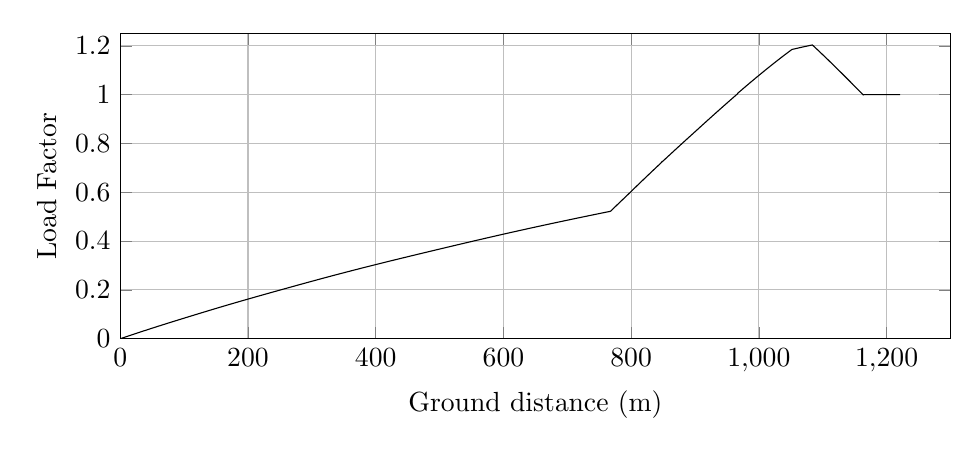
\begin{tikzpicture}

\begin{axis}[
width=\textwidth,
height=0.45\textwidth,
scaled ticks=false, tick label style={/pgf/number format/fixed},
xmin=0.0,
xmax=1300,
xlabel={Ground distance (m)},
xmajorgrids,
ymin=0.0,
ymax=1.25,
ylabel={Load Factor },
ytick={0,0.2,0.4,0.6,0.8,1,1.2},
ymajorgrids,
legend style={at={(1.03,0.5)},anchor=west,draw=black,fill=white,legend cell align=left}
]

\addplot [
color=black,
solid
]
table[row sep=crcr]{
1.3729668748937997E-8	1.235455299693154E-11\\
2.6049868369719035E-7	2.344080436518659E-10\\
2.0491224421327626E-6	1.8438894736304345E-9\\
9.92442121137073E-6	8.930425569077179E-9\\
4.7452367809869807E-5	4.269969914983993E-8\\
1.740064756114434E-4	1.5657852720471245E-7\\
4.0608377013922605E-4	3.654114736370262E-7\\
7.313431501337001E-4	6.580931970031749E-7\\
0.0011549487327126044	1.0392701709181947E-6\\
0.0016799013484208249	1.5116421057539741E-6\\
0.002295089346817705	2.065209671700515E-6\\
0.003009933382444524	2.7084491357474043E-6\\
0.003810608015426248	3.4289190685331768E-6\\
0.004723484476856681	4.25034801616172E-6\\
0.005727138856912631	5.153457018842584E-6\\
0.006836216967948795	6.15142340069829E-6\\
0.007997302399386296	7.196181104336155E-6\\
0.00929136979810952	8.360590608368267E-6\\
0.010685558505459776	9.615081769488242E-6\\
0.012178513621519987	1.0958433666682518E-5\\
0.013775244426719659	1.2395151677312702E-5\\
0.015470070176169002	1.392012227755044E-5\\
0.0172374436815836	1.5510356776883755E-5\\
0.019122918912604377	1.7206841227721774E-5\\
0.021104911040230538	1.899015178927688E-5\\
0.023190717999955576	2.0866852300289687E-5\\
0.025355802981115103	2.2814863404455325E-5\\
0.027620619195902148	2.4852585192336495E-5\\
0.030020274690474198	2.7011602025297394E-5\\
0.032476028269866286	2.9221066057398203E-5\\
0.035054163466719815	3.1540610410615947E-5\\
0.037720846868992755	3.3939791809887556E-5\\
0.04049779674511381	3.64381465728124E-5\\
0.043329456594087365	3.898568901511945E-5\\
0.04629652060163805	4.165501339744797E-5\\
0.04934498934704602	4.4397535052579305E-5\\
0.052507657924119336	4.724275400489886E-5\\
0.055769483710642484	5.0177133330158015E-5\\
0.05917209570914676	5.323811811444343E-5\\
0.06264043916012321	5.635818488730431E-5\\
0.06620063977265622	5.956083255420333E-5\\
0.06987962792775945	6.287028222477102E-5\\
0.0736568184539585	6.62680115107197E-5\\
0.07754284280095361	6.976357900511529E-5\\
0.08151127871105612	7.333321274586019E-5\\
0.08560324933017655	7.70138982513938E-5\\
0.08985265585263943	8.083612222250554E-5\\
0.09413961367176535	8.469204676740686E-5\\
0.09857725310864562	8.86834225519694E-5\\
0.10307959255469257	9.273290879441721E-5\\
0.10766008648593872	9.685260283567778E-5\\
0.11234920964493048	1.0106990847411986E-4\\
0.11719267720457946	1.0542593354340057E-4\\
0.12216973960582883	1.0990200826576004E-4\\
0.12724007601918352	1.1446186370310306E-4\\
0.13233299746505212	1.1904192440061976E-4\\
0.13755256756750583	1.237357701710758E-4\\
0.14287728588926696	1.2852405890594534E-4\\
0.1482946925752714	1.333955797336218E-4\\
0.15381585025670613	1.3836027423551808E-4\\
0.15940564092189102	1.433865582488918E-4\\
0.16526271495916878	1.4865304485355734E-4\\
0.17120082448158402	1.5399225406934872E-4\\
0.17717889132867753	1.5936724662761337E-4\\
0.18324322596131126	1.6481965677566236E-4\\
0.189427022360885	1.7037932170746299E-4\\
0.1957511558722988	1.7606500033829438E-4\\
0.2021484013779125	1.8181624641691317E-4\\
0.20865863707071397	1.8766890427292644E-4\\
0.21548666343168166	1.9380707138621768E-4\\
0.22220154781289658	1.998433457999465E-4\\
0.22919671627301902	2.0613138715556956E-4\\
0.23611678795738544	2.1235173116488545E-4\\
0.24306300975244904	2.1859538940455518E-4\\
0.2503085190632165	2.2510785991746641E-4\\
0.2576623280401219	2.3171746026172092E-4\\
0.26502430524173204	2.3833418760804765E-4\\
0.2724963584449146	2.45049628803424E-4\\
0.2802001060647876	2.5197307244867234E-4\\
0.2878583985474956	2.588554331313391E-4\\
0.2958320780323821	2.6602098074406116E-4\\
0.3040021452321372	2.73362753014986E-4\\
0.31208951788619	2.806299565129379E-4\\
0.3202851396023423	2.879941697771677E-4\\
0.3287233234973125	2.955760639324542E-4\\
0.3370425959884752	3.0305084140947385E-4\\
0.34575405233845447	3.108777027301057E-4\\
0.3545073625286812	3.1874187042011553E-4\\
0.36338982075299686	3.2672176325513003E-4\\
0.37247557159370037	3.348839751007075E-4\\
0.38151350442869847	3.430029123533628E-4\\
0.3905554764834429	3.511251621167552E-4\\
0.3999457587520332	3.5955995901769476E-4\\
0.4095398754587949	3.681774987895933E-4\\
0.4189621792151833	3.766403696987003E-4\\
0.4285208811402964	3.8522540157665E-4\\
0.43828968955472236	3.9399877613327874E-4\\
0.44807735398784176	4.0278871900638547E-4\\
0.45806002753764463	4.1175341538713094E-4\\
0.4682994371692033	4.209482724419739E-4\\
0.4787752542918833	4.303550071997626E-4\\
0.4890770094685154	4.396050366371339E-4\\
0.49985939134273727	4.492861933521667E-4\\
0.5106597490205704	4.5898304847143823E-4\\
0.5213580865152188	4.685878722292748E-4\\
0.532247733242454	4.7836400713928493E-4\\
0.5431365108549349	4.8813891498980505E-4\\
0.554075964429489	4.979588657475053E-4\\
0.5653450694020941	5.080742626804385E-4\\
0.5769901159382542	5.185266128869077E-4\\
0.588512657344902	5.288685055662627E-4\\
0.6004070039036553	5.395435864361152E-4\\
0.6121651247369502	5.500958872943247E-4\\
0.6239717914322569	5.606912377324344E-4\\
0.6362472885961421	5.717067693258237E-4\\
0.6486428939173223	5.828295139748193E-4\\
0.6610190736373547	5.939342602607816E-4\\
0.6737248046101814	6.053341134012174E-4\\
0.6862826225989949	6.166006707185031E-4\\
0.6991952542603428	6.28184952419146E-4\\
0.7122988072688032	6.39939888525395E-4\\
0.7251463703465595	6.5146456961147E-4\\
0.7381769453061875	6.631528008991399E-4\\
0.7516618647379176	6.752479189360662E-4\\
0.7654913705221527	6.876514200233561E-4\\
0.7791756406994825	6.999239756960988E-4\\
0.7930637813125616	7.123786739581543E-4\\
0.8074774191984457	7.253038911986747E-4\\
0.8215072375247947	7.3788420145299E-4\\
0.8361010597475598	7.50969490033313E-4\\
0.8503303420601955	7.637271807737563E-4\\
0.8650627501899835	7.769351960487872E-4\\
0.8802332960144008	7.905351989917558E-4\\
0.8951742046771463	8.039285314471027E-4\\
0.9100334756324657	8.172478897561318E-4\\
0.9251067343345352	8.307582537079375E-4\\
0.9403923630470314	8.444581404636662E-4\\
0.9559303815501943	8.583833817536583E-4\\
0.9712400158034169	8.721031054039967E-4\\
0.9869533781138684	8.861837658351711E-4\\
1.0029148609762486	9.004858714560566E-4\\
1.0189962473881624	9.148945055845343E-4\\
1.035465185745812	9.296494348127966E-4\\
1.0516742337458713	9.441705904563665E-4\\
1.067815735429615	9.586303171739576E-4\\
1.0846705971808022	9.737281052747889E-4\\
1.1012775250051634	9.886028345590199E-4\\
1.1180798406225687	0.0010036515923125167\\
1.1351395900544134	0.0010189299113320602\\
1.1526388687279154	0.0010346008119033673\\
1.1698922447507556	0.0010500504628386956\\
1.1875468452119025	0.001065858326487304\\
1.2058383275300355	0.0010822353164119136\\
1.2239395537495579	0.0010984408283908698\\
1.2422020624207541	0.0011147895899982648\\
1.2608769472440078	0.0011315063307659474\\
1.2794948487006894	0.0011481708742238275\\
1.2979152553275424	0.0011646574778629646\\
1.3166445915281573	0.001181419392735694\\
1.3354141707340492	0.0011982161256424294\\
1.3543210821322504	0.0012151345463494658\\
1.373689361295591	0.0012324645554020535\\
1.3932049885015831	0.0012499251228699952\\
1.4131781782225183	0.0012677937392972264\\
1.4330139682345777	0.001285538104413934\\
1.4528243860883294	0.0013032584531265463\\
1.4728783400745615	0.0013211953039648757\\
1.4934621752870565	0.001339604697144267\\
1.5141408097620341	0.0013580974510959628\\
1.53430654450827	0.0013761301508567678\\
1.5553850389607948	0.0013949776183661972\\
1.5762653203499473	0.0014136463998074163\\
1.5975496774716453	0.0014326749752865864\\
1.6196077215345106	0.0014523936618953519\\
1.6413652536722467	0.0014718421372363919\\
1.663437310723463	0.0014915701683844193\\
1.6860768385032747	0.0015118037460944737\\
1.7077101022266827	0.0015311364309760277\\
1.7297306410738114	0.0015508136376475717\\
1.7520297891459062	0.0015707381959231617\\
1.7743087535215367	0.0015906431063421752\\
1.797257424336919	0.0016111446767020368\\
1.8200802473615325	0.0016315321295036912\\
1.8430350373473994	0.0016520357719165299\\
1.8666926279964304	0.001673165393743726\\
1.8902808566018634	0.0016942312755299212\\
1.9138231309717848	0.0017152543393089913\\
1.937187877956735	0.0017361171206232322\\
1.9611060682733261	0.0017574722773401254\\
1.9852138445648535	0.001778994862163885\\
2.009780393513653	0.0018009251252183711\\
2.0346228225622163	0.0018230997194289228\\
2.0593611988602687	0.00184517949750782\\
2.08477023517836	0.0018678558526763886\\
2.110324766702745	0.001890660007953689\\
2.1352655781940433	0.0019129145213863427\\
2.160528860803022	0.0019354547892555306\\
2.1862071157614817	0.0019583632598788687\\
2.2127756699400534	0.0019820638364059957\\
2.2391904543957084	0.002005625068485404\\
2.2653528664920257	0.002028959060611655\\
2.292150575495974	0.0020528574744388866\\
2.3187704640870406	0.002076595114543102\\
2.3455495914188482	0.002100472553034438\\
2.372862901366455	0.002124824025842581\\
2.4007145172972395	0.002149653080349164\\
2.428100404243743	0.002174064639915687\\
2.4555980306928005	0.0021985735058416577\\
2.483374904362833	0.0022233289358646207\\
2.511687733451976	0.00224855961728262\\
2.5402569276484597	0.0022740163008407956\\
2.568415369317849	0.002299104575000413\\
2.596987652715761	0.002324559132844599\\
2.6263861238451423	0.002350747172474888\\
2.655991481965028	0.002377116894532034\\
2.6856115886357443	0.002403497137388922\\
2.7154221146045012	0.00243004433658839\\
2.7455665152057707	0.002456886180859776\\
2.7752624694325894	0.002483326080843548\\
2.805457625653509	0.002510207779026605\\
2.8358231840904597	0.0025372384744280947\\
2.8663460878589797	0.002564406507497582\\
2.897817297850832	0.002592415759937194\\
2.9287074004595235	0.002619905017401546\\
2.9603588456990284	0.0026480689160650636\\
2.9922321403815406	0.002676427280288437\\
3.0241119471841866	0.0027047884962779043\\
3.056446055158509	0.002733550874602781\\
3.0889346922121366	0.002762447680420118\\
3.122221620829695	0.0027920513783542327\\
3.1546991615623394	0.0028209321904144992\\
3.187635101478671	0.002850217560730911\\
3.221010117202278	0.002879890190017609\\
3.2543449374576605	0.002909523926311069\\
3.288235920596943	0.002939648851276039\\
3.3223704322934555	0.00296998696603803\\
3.3562838593334394	0.003000125337194767\\
3.3906320903803255	0.0030306468221910155\\
3.425633159699527	0.003061745016286283\\
3.462387235801926	0.0030943970649300622\\
3.4973980805087237	0.003125496945033084\\
3.5324804241140235	0.0031566569269987216\\
3.5675385073174235	0.003187791960906538\\
3.6040688981843845	0.0032202309438331325\\
3.6393612181513753	0.003251567035729728\\
3.6770856360342323	0.003285058815392132\\
3.7131729334920323	0.003317093518398549\\
3.749509707933214	0.0033493460974472053\\
3.785733977879824	0.0033814952475845626\\
3.8225309786916544	0.0034141490598399954\\
3.860867115351552	0.0034481648194461902\\
3.89929745075254	0.003482260191646147\\
3.9373367205567504	0.0035160047082642507\\
3.9751626485832894	0.0035495561321477118\\
4.013671158053867	0.0035837090834558824\\
4.0521140617426425	0.00361779991752279\\
4.092377631210638	0.003653501103511283\\
4.131586743753305	0.003688263200717537\\
4.1715696979561425	0.0037237072036200624\\
4.210522654700574	0.0037582341014714598\\
4.250196810863292	0.0037933961711473793\\
4.2917015001093795	0.003830176196470685\\
4.332438976653355	0.0038662719898033236\\
4.373124372895289	0.003902317345376638\\
4.414429464889761	0.0039389073493698665\\
4.455884944705147	0.003975626158373108\\
4.497250153511752	0.004012260615933245\\
4.537976875075978	0.004048325332324519\\
4.581399817640802	0.004086772975557872\\
4.623816269683994	0.004124324825081472\\
4.666022338967499	0.00416168589887831\\
4.709098934189642	0.004199812932908079\\
4.752435367147649	0.004238165240417808\\
4.79531009100786	0.004276104308266509\\
4.838191999420829	0.0043140451410508575\\
4.881381760681686	0.004352253727410255\\
4.9256451804034285	0.004391407343095393\\
4.9704217340957495	0.0044310099277712536\\
5.014356093293278	0.004469862833088081\\
5.058826350846283	0.004509184828499551\\
5.104458009943745	0.0045495287418007326\\
5.149663211268795	0.004589490609003348\\
5.194981168813841	0.004629547170564892\\
5.241194091283663	0.004670389671865359\\
5.287987552078626	0.004711739997702375\\
5.334426822383641	0.004752772130017933\\
5.380633359096258	0.00479359350076165\\
5.427524438012913	0.0048350144246019945\\
5.476157635197664	0.004877968714171063\\
5.524667120325573	0.004920808156102917\\
5.5732739519824435	0.004963727995954377\\
5.6208990292882195	0.005005775558598465\\
5.671502816366864	0.005050447163658217\\
5.719824083529298	0.005093098246506553\\
5.767871110439133	0.005135501887092258\\
5.8169321963676754	0.005178794962387515\\
5.866076914057565	0.005222156268484875\\
5.917200682776528	0.005267257836481533\\
5.96684810088939	0.005311051234284483\\
6.016885842403935	0.005355183242326283\\
6.068639931677712	0.00540082303943017\\
6.119867755785197	0.005445992774146364\\
6.171030794930029	0.005491099479385734\\
6.222884713227881	0.005536809283582339\\
6.2735946138732235	0.005581504805857961\\
6.325883502103322	0.005627586041459813\\
6.379615386553551	0.005674932641203159\\
6.432194972482147	0.005721257698676432\\
6.484528316464761	0.005767359761422742\\
6.536619297696934	0.005813242354996034\\
6.589662958081361	0.005859957993696025\\
6.644121795496577	0.005907913613275629\\
6.697445536614451	0.005954863458463705\\
6.7518063163896365	0.006002720067692726\\
6.8068829439682315	0.006051200398977879\\
6.863205650636274	0.0061007708588604265\\
6.9185329265047315	0.006149458643950914\\
6.974634519184049	0.006198821192916237\\
7.031139830722298	0.00624853224357383\\
7.0870923879294985	0.006297750384947868\\
7.144766952910487	0.006348476410514121\\
7.2026451873548805	0.006399374593353831\\
7.261191729679483	0.006450853409923758\\
7.320502240843062	0.006502996743875915\\
7.378210233177999	0.006553724260809202\\
7.437738452534925	0.0066060446767701375\\
7.49714639104333	0.0066582521693537245\\
7.556502460410064	0.006710406922202143\\
7.617032771987237	0.006763586118960179\\
7.676883327249088	0.006816160863522422\\
7.735740247984193	0.006867855768295435\\
7.796086087039788	0.006920851239973525\\
7.856787102853412	0.006974151333841447\\
7.91721236259451	0.007027202062069287\\
7.979013602666894	0.007081453412480714\\
8.039824025454376	0.007134827689670802\\
8.102419182184594	0.0071897609307103915\\
8.16459313580776	0.007244317003705583\\
8.226347093952135	0.007298497155536858\\
8.290527749984296	0.00735479862013344\\
8.353592793320257	0.007410113760561148\\
8.417564177281012	0.00746621613339013\\
8.482044607535009	0.00752275709526521\\
8.547336806956285	0.007580001892087775\\
8.613293246319614	0.00763782094639394\\
8.6778048537894	0.007694365575914089\\
8.74454839911753	0.007752858377336426\\
8.810708373588199	0.0078108316303215205\\
8.876548424968423	0.00786851656498927\\
8.942828456712885	0.00792657898008617\\
9.010858044488913	0.007986165728006579\\
9.079453414959548	0.008046239565192974\\
9.148767802603732	0.008106934496254995\\
9.21609997183467	0.008165885469367456\\
9.285579683381485	0.008226708206323857\\
9.355451712480097	0.008287865757095943\\
9.423585014597279	0.00834749315404877\\
9.493435356703696	0.00840861478835342\\
9.562655940911181	0.00846917697272717\\
9.63183713653898	0.008529696396946855\\
9.703018708836247	0.00859195712997399\\
9.773178624863132	0.008653315744527986\\
9.844376937811855	0.008715573912287788\\
9.914998792594716	0.008777319513916363\\
9.98720270419701	0.008840439633215296\\
10.059478150570087	0.008903613532568487\\
10.132362020358627	0.008967310417389462\\
10.205876892438312	0.009031549845847382\\
10.279422251887688	0.009095807001627437\\
10.353305644514993	0.00916035057484669\\
10.42811398108589	0.009225693106401358\\
10.50332954727428	0.009291382201706475\\
10.578207710262959	0.009356767581131424\\
10.65503529959097	0.009423845920038495\\
10.730232142651953	0.009489491358894774\\
10.805871937852555	0.009555514467565251\\
10.88265320376452	0.009622524727344416\\
10.958577899345514	0.009688778367604843\\
11.034861147941964	0.00975533587753231\\
11.112742623646977	0.009823278586834027\\
11.190543636431041	0.009891141816409054\\
11.267787598939979	0.009958510026354611\\
11.3462805052093	0.010026958247301968\\
11.423875697147409	0.010094614523365601\\
11.502735831556972	0.010163364497856153\\
11.581465323066688	0.010231991364451543\\
11.661639233340708	0.010301867901064353\\
11.741743247575428	0.010371674107836282\\
11.821864700430528	0.010441486163270524\\
11.901816327719768	0.01051114098697615\\
11.98361062800689	0.010582391663070664\\
12.065425957085825	0.010653651103352658\\
12.1478520915771	0.010725432945812982\\
12.230956215923495	0.010797795539906953\\
12.313306905825911	0.01086949255790008\\
12.396632357805931	0.010942028648928133\\
12.479578787946746	0.011014225287141093\\
12.564327762802186	0.011087981132626618\\
12.648175874147956	0.01116094336052778\\
12.736145481689512	0.011237481797595114\\
12.821080154398764	0.01131136983602781\\
12.908009536077355	0.011386983217547721\\
12.994986774303499	0.011462628243523716\\
13.081752199798046	0.011538079179547208\\
13.17035388279784	0.011615116818793013\\
13.257836697901475	0.011691171684179765\\
13.34511613365563	0.011767039973221287\\
13.433461823066896	0.011843825254628694\\
13.524108483575919	0.01192260018866291\\
13.611203924103116	0.011998279314554914\\
13.702229394080796	0.01207736326976425\\
13.792427706753081	0.012155718520969003\\
13.882429934062493	0.012233893531675255\\
13.975435778888343	0.012314667147643706\\
14.065832730112316	0.012393165038422013\\
14.157894546480026	0.012473098642780036\\
14.250668806951023	0.012553640707121684\\
14.343291987615704	0.012634041556119531\\
14.43744444968501	0.012715759677146117\\
14.532636396723657	0.012798369629565416\\
14.625507232812737	0.012878955300114655\\
14.721503924398366	0.01296224307908585\\
14.818738382089133	0.013046594228586698\\
14.913572076739943	0.013128852595101173\\
15.009701633366973	0.013212224886015414\\
15.10815424447124	0.013297601496676663\\
15.206130868840724	0.013382554944496177\\
15.304035939715973	0.013467436089964329\\
15.403499839366233	0.013553658297311208\\
15.503209871950865	0.013640083448276346\\
15.601718454553605	0.013725457077920007\\
15.700655560608023	0.01381119204069401\\
15.801250929860519	0.013898353762136157\\
15.899917805652187	0.013983834606799526\\
16.001574124100856	0.014071895211057108\\
16.102638779863817	0.014159433156900395\\
16.204479333764816	0.014247633045943953\\
16.30489644092564	0.014334590315872602\\
16.40578186591999	0.014421943403402441\\
16.509201471948074	0.014511480734594042\\
16.614557195984908	0.014602683982822077\\
16.717657554831042	0.014691924865867595\\
16.823039336622365	0.014783130414586006\\
16.928576062495388	0.014874459973527387\\
17.03469945574068	0.014966287157986717\\
17.140697318244236	0.015057995762952713\\
17.246066414787876	0.015149150613718644\\
17.35183930840021	0.01524064512682176\\
17.458399953804133	0.015332811378690709\\
17.565707112453843	0.015425613609547405\\
17.673103795073075	0.015518483641867866\\
17.781888038667653	0.015612543860088798\\
17.89115167195854	0.01570700888749764\\
18.00105710767307	0.01580201911532322\\
18.110142905530395	0.01589631131594384\\
18.219697237410173	0.015990999136315614\\
18.32752951944549	0.016084189534823108\\
18.43743745973078	0.01617916462989231\\
18.54904630654982	0.016275600239022192\\
18.659302591714813	0.016370858096073304\\
18.770734536087716	0.016467122651296122\\
18.883577445650936	0.016564596996610333\\
18.996263390583444	0.016661926724749265\\
19.108816920034535	0.01675913320562426\\
19.22287647779894	0.016857631446606992\\
19.33763586704334	0.01695672511830411\\
19.456324114791514	0.01705920205539396\\
19.57349394116079	0.017160358871350874\\
19.690148252848566	0.017261061791709477\\
19.80521137071168	0.017360382604323404\\
19.92379170801214	0.017462730747821124\\
20.04216631061405	0.017564892677026524\\
20.15848954929409	0.01766527593074394\\
20.278242138037896	0.017768610191553635\\
20.396206084226087	0.0178703928384457\\
20.516315546862906	0.01797401848922813\\
20.637173924977112	0.018078282067743996\\
20.75450010628387	0.018179490719607578\\
20.874378237858778	0.018282893036006057\\
20.996035953832852	0.018387822535340312\\
21.11812959618858	0.01849312025839763\\
21.240471115580952	0.01859862411814323\\
21.361479376438375	0.018702970844651525\\
21.485224699488654	0.018809670350258677\\
21.607870280890317	0.018915414359543522\\
21.73242999733349	0.01902280150298749\\
21.85704493170313	0.019130229138162362\\
21.98122016226351	0.019237270801284668\\
22.10826921766411	0.019346782788963634\\
22.235261614051304	0.019456239062747297\\
22.361664688868032	0.019565180738263944\\
22.48780138980522	0.019673886388135768\\
22.614107216476143	0.01978273150597579\\
22.74409311379692	0.019894741565852074\\
22.873024137794893	0.02000583640724149\\
23.003512644166257	0.020118267141559842\\
23.132891545907036	0.02022973591825572\\
23.26270690888247	0.02034157500564839\\
23.39264146728729	0.020453511215179743\\
23.52277721573431	0.02056561534386348\\
23.654883767164463	0.020679411856557438\\
23.78569183677709	0.0207920847364327\\
23.917003007077597	0.02090518602613144\\
24.047013652206026	0.0210171624470847\\
24.178458227988493	0.021130369324358817\\
24.314609552493202	0.021247625248854447\\
24.447533097503474	0.02136209698153126\\
24.579128452041708	0.021475420829340505\\
24.71011994849615	0.02158822082482267\\
24.843278471916108	0.021702883161457725\\
24.975761222328053	0.021816960036620207\\
25.1115496753864	0.021933879865087907\\
25.247101122854083	0.022050592296785698\\
25.384906965000688	0.02216924260410627\\
25.522261036073317	0.022287500929481487\\
25.66123001648475	0.022407146801513497\\
25.79865327455613	0.02252545926542135\\
25.826335196219034	0.02254929129858618\\
25.839610403727477	0.022560720210521856\\
25.841006316401874	0.022561921980525996\\
25.84227013303559	0.02256301002611716\\
25.84770509053729	0.022567689089945542\\
25.86419328224909	0.022581884082067474\\
25.90571916957557	0.022617634341039965\\
25.999268866927544	0.02269817184411533\\
26.123295978662824	0.02280494564042582\\
26.250212562581652	0.022914204534327503\\
26.376891976518465	0.02302325661271281\\
26.50638698165423	0.023134729560155075\\
26.634042370994827	0.023244615808308465\\
26.763333806613538	0.023355907024626518\\
26.893207366259766	0.023467695726078732\\
27.022905486492228	0.023579329620678602\\
27.153956322362554	0.02369212376811321\\
27.287774297957696	0.023807295145426413\\
27.42030033806219	0.023921349999420617\\
27.555504894698295	0.024037705103166523\\
27.691130018821354	0.024154416912694515\\
27.82633313037239	0.024270760135509665\\
27.959508564917073	0.024385353028808825\\
28.096515548835796	0.024503236934172407\\
28.232789703382153	0.024620484147740575\\
28.368684388406535	0.02473739856193136\\
28.506541650227618	0.024855994793623944\\
28.64533374691623	0.02497538827395233\\
28.78297783415192	0.02509378708262868\\
28.92277775692753	0.0252140328373981\\
29.06227187463503	0.025334007858627553\\
29.20212864139956	0.025454286855050114\\
29.34335827861657	0.025575738278038513\\
29.483225747293005	0.025696009908520657\\
29.625960812476485	0.02581873856719969\\
29.76706561118049	0.025940056516256468\\
29.909402910999468	0.026062424919389787\\
30.051751399473822	0.026184793485080356\\
30.196612335666572	0.026309311940955923\\
30.342192969749448	0.026434438749866562\\
30.48583400527584	0.02655788817073559\\
30.632658550781265	0.026684062819243404\\
30.77846394498075	0.026809350671350398\\
30.92408133049836	0.02693446585102054\\
31.071091331299215	0.02706076610232202\\
31.218274793935116	0.027187203637481262\\
31.366705758252415	0.027314700739239764\\
31.515339333797037	0.02744235950831476\\
31.66356819769615	0.02756965815734952\\
31.814689402684216	0.0276994276741732\\
31.96649953392354	0.027829775295319124\\
32.115424616034375	0.027957632424185246\\
32.266253234088566	0.028087110161852585\\
32.41813832080348	0.028217480755754625\\
32.569791431087395	0.028347637965254958\\
32.722234201183724	0.028478458348995005\\
32.876984607664	0.02861124393730653\\
33.031873994672836	0.028744133336211744\\
33.18502245018544	0.028875513703551115\\
33.34135780547538	0.029009612035820698\\
33.49759920343199	0.02914361348018349\\
33.65385117142162	0.029277607512733523\\
33.8113313806527	0.029412637966975828\\
33.96985264489639	0.029548543789876338\\
34.126473036379195	0.029682802723892465\\
34.2857505660089	0.029819321704046095\\
34.4449212019973	0.029955731033695476\\
34.60566879064274	0.03009347333835155\\
34.76644486933921	0.03023122130569094\\
34.92612701881755	0.030368013292497584\\
35.08630421658309	0.030505210432284578\\
35.24825698849928	0.0306439089613449\\
35.412303951281956	0.030784380870194618\\
35.57355277914179	0.03092243686437589\\
35.73545353069308	0.031061031001925605\\
35.89925038949356	0.031201227717211188\\
36.065161289279985	0.031343212613902674\\
36.23047312008262	0.03148466338010292\\
36.39472205714358	0.03162518329888304\\
36.56135389445764	0.03176771992889129\\
36.72774532558607	0.03191002871219932\\
36.89384825683493	0.0320520684629636\\
37.05904296416534	0.03219330932236064\\
37.22702676294645	0.03233691194453534\\
37.39437475321985	0.032479947925694135\\
37.5621109943643	0.03262329245190593\\
37.73270471709142	0.032769054852070705\\
37.903359519601935	0.0329148449914803\\
38.071486842086316	0.033058451848527105\\
38.23815243703595	0.03320078645366754\\
38.40817787072022	0.03334596594047084\\
38.57751392140098	0.03349053208731914\\
38.750215798728505	0.03363794619158783\\
38.92001182640311	0.033782854665922964\\
39.09310637700479	0.033930552263090295\\
39.26472366117933	0.03407696336928517\\
39.436554723976656	0.034223530814177686\\
39.608961777617054	0.03437056324705254\\
39.782828308010565	0.03451881352777564\\
39.956194359016465	0.03466661011823323\\
40.132391837044906	0.034816792834646046\\
40.30868053167249	0.034967025229374796\\
40.48611580488176	0.035118206255486825\\
40.66383502946924	0.0352696004563176\\
40.83999042132467	0.03541963394545542\\
41.018202681018664	0.03557139027554888\\
41.19780999006247	0.03572430491179658\\
41.37730467548502	0.035877093813170266\\
41.557010452813884	0.03603003239374049\\
41.73612816026986	0.03618244051120076\\
41.91555194917056	0.036335078946603795\\
42.09743589423803	0.03648977939536331\\
42.27807550146298	0.03664339060507981\\
42.45995188234755	0.03679802234717789\\
42.6401410478328	0.03695118865574497\\
42.822293873795985	0.037105992718021695\\
43.00585672428667	0.03726196304838601\\
43.189965171449515	0.03741836454765392\\
43.372020236704074	0.0375729896695126\\
43.555636897252796	0.03772890876866533\\
43.74012033961118	0.03788553110905434\\
43.92429822300048	0.03804186116409352\\
44.106869824379004	0.03819679530946417\\
44.29411840239129	0.038355664744134196\\
44.47920670866131	0.038512667704972935\\
44.665034305215386	0.038670264083209525\\
44.85242224248053	0.038829149490521526\\
45.03948098831597	0.03898772138930858\\
45.22811764277584	0.039147596033192185\\
45.41548629589063	0.03930636128168097\\
45.60322541388645	0.039465405657919735\\
45.793007222766036	0.03962614505985078\\
45.983742663331824	0.03978765618080461\\
46.172643153142886	0.039947577890251246\\
46.36421599110457	0.040109725735754845\\
46.553512793459404	0.04026991122121742\\
46.745018895697555	0.040431929861742356\\
46.93606459490553	0.04059352247488821\\
47.126948089509526	0.04075494141493447\\
47.31881294044018	0.040917153441014834\\
47.5110690178297	0.0410796591869566\\
47.705448624448266	0.04124392211919395\\
47.90005519882567	0.041408338795998416\\
48.09288923506665	0.04157122031329662\\
48.28732881729917	0.04173542005570409\\
48.484002572746206	0.04190146771889461\\
48.68089030454945	0.042067656931755064\\
48.87532723390382	0.04223173903763535\\
49.07073736177763	0.04239660390354292\\
49.2672083392297	0.04256232485012234\\
49.46586249263092	0.0427298475525502\\
49.661880987188695	0.042895108457509316\\
49.85966148345089	0.04306181542332821\\
50.05808618672894	0.04322902553344635\\
50.25785665917266	0.043397329368770304\\
50.45743808511885	0.043565433504229534\\
50.65573800086891	0.04373241821030677\\
50.85948768734909	0.043903950492840356\\
51.061243703011925	0.04407376281950463\\
51.26368286286315	0.04424410858938735\\
51.46416466063809	0.04441276629370973\\
51.66475943174029	0.04458147819181206\\
51.86588207153103	0.044750593041007744\\
52.07444928962187	0.0449259243212281\\
52.2824430085781	0.04510072951721414\\
52.48676525705545	0.04527240633240485\\
52.69531994892206	0.04544759567384109\\
52.90027076850366	0.04561971472540641\\
53.108186167814935	0.045794279934306056\\
53.31165724918766	0.04596507129036985\\
53.520024946679996	0.04613992934818878\\
53.72688450142306	0.04631347832171572\\
53.93707391647578	0.04648977659984778\\
54.14518573319289	0.04666428825946845\\
54.35125853722778	0.04683704698549899\\
54.56213447502874	0.047013787971040624\\
54.77598621923464	0.0471929772409911\\
54.987629956235494	0.04737027099972086\\
55.19778857845695	0.047546276036782846\\
55.41030974885841	0.04772421448074804\\
55.62390503323701	0.0479030065044514\\
55.83671574169797	0.04808109622797616\\
56.047071254351536	0.04825708668475133\\
56.26137331252919	0.04843633336072757\\
56.47512769358855	0.048615076162331704\\
56.69105800830218	0.0487955921235654\\
56.90937011004422	0.048978051921594545\\
57.12736617899088	0.04916020017778377\\
57.346833156368504	0.04934352967421587\\
57.56476609337061	0.04952553034722426\\
57.78230894703917	0.049707158237917964\\
57.99943865551505	0.049888394424121824\\
58.21827465292657	0.050071007634511215\\
58.436085045729726	0.05025271802845192\\
58.6577546799423	0.05043759999525642\\
58.87982836766625	0.0506227704543792\\
59.10336118170943	0.05080910862787486\\
59.324182403931715	0.050993138281630344\\
59.545440661451366	0.051177484275523905\\
59.768227251413464	0.0513630553009394\\
59.99077485409802	0.05154837893773178\\
60.21631063559073	0.05173614176810372\\
60.44006004384342	0.05192236859600404\\
60.66502706168687	0.05210955993022435\\
60.89133011288284	0.05229781358239304\\
61.11585558357916	0.05248453969899249\\
61.3432655409558	0.05267361522938351\\
61.57186440401435	0.05286362919951849\\
61.79868765088207	0.05305211777631893\\
62.025670725987	0.05324068994940705\\
62.254132946411545	0.05343044136530592\\
62.48290793247415	0.053620402818464336\\
62.713817944074236	0.05381208673757675\\
62.94484116346062	0.05400381416096221\\
63.17805109236767	0.0541973052815116\\
63.41124119062552	0.05439072879164108\\
63.64505576847972	0.054584619071135786\\
63.87735201907903	0.05477719964008793\\
64.11169045660182	0.05497142224893198\\
64.34725756208485	0.05516661172491126\\
64.58324360279937	0.05536209674410297\\
64.81881329818131	0.05555718553816801\\
65.05563560606473	0.05575326015479756\\
65.29467812810154	0.05595112073864988\\
65.53178653633495	0.056147328738266764\\
65.77046761369158	0.0563447863176657\\
66.01019347650049	0.05654305608639314\\
66.25262920761091	0.05674351413325228\\
66.49342175078831	0.05694256096614008\\
66.73393309567928	0.0571413232623709\\
66.97718905970893	0.057342300990317764\\
67.21919788222482	0.05754219586671328\\
67.46413738735515	0.05774445834589854\\
67.70584739194695	0.05794400185653842\\
67.95375887035246	0.058148611369622724\\
68.19817148521656	0.05835028020593526\\
68.44413350233111	0.0585531746139422\\
68.68984243621705	0.05875580751280575\\
68.93951041285982	0.058961651606045655\\
69.19023531750676	0.05916831278089061\\
69.43956667494601	0.05937377155734687\\
69.68998597860525	0.05958007311105848\\
69.94098943220166	0.059786802095748805\\
70.1928405184459	0.059994175293799856\\
70.44659484061637	0.060203061241287076\\
70.69926103579675	0.06041099748472227\\
70.95414956377036	0.06062070831245874\\
71.21136313866151	0.060832277029685196\\
71.46778788208749	0.061043142110228585\\
71.7247351381395	0.061254382256446895\\
71.98234155897126	0.06146610970097699\\
72.24107377350035	0.06167870766947938\\
72.4986091150376	0.061890267941214105\\
72.75949164810788	0.06210452297401033\\
73.02014691132015	0.062318536465779006\\
73.28114866838587	0.06253277975926072\\
73.54342372888959	0.06274801340682108\\
73.80584407854005	0.0629633115625225\\
74.07231166191039	0.06318187449470564\\
74.3389341302921	0.06340050859771763\\
74.60521354141642	0.0636188059248178\\
74.87280568706873	0.06383812391780197\\
75.1403821105715	0.06405737369305417\\
75.41145333671997	0.06427943099081657\\
75.68265298797411	0.06450153733672492\\
75.95075857762194	0.0647210548378805\\
76.2241428819712	0.06494483856331955\\
76.4990100438061	0.06516977961529215\\
76.77213586328236	0.06539323986262748\\
77.04724851790667	0.06561826983023875\\
77.32330034006353	0.06584401204467288\\
77.59850473375684	0.06606900585028874\\
77.87773830129439	0.06629723753365649\\
78.1565255546137	0.06652504835170042\\
78.43842651648492	0.06675534696059204\\
78.720833678605	0.06698600246750373\\
79.00101298089581	0.06721478274880092\\
79.28359351218376	0.06744546803663193\\
79.57011733099088	0.067679315723782\\
79.85418914588558	0.06791110624085044\\
80.13919871477489	0.06814360635513637\\
80.42568449319114	0.06837725503829581\\
80.71472498530085	0.0686129311431364\\
81.006853148924	0.06885106803098383\\
81.2951972638476	0.0690860646683832\\
81.58524575795963	0.06932239510502453\\
81.87461709596036	0.06955811903372612\\
82.1711642895769	0.069799632188846\\
82.46716486408064	0.07004064384457685\\
82.76422974563803	0.07028246600528235\\
83.05801377197795	0.07052156265426428\\
83.35853301954708	0.07076608492540976\\
83.65664966506407	0.07100859698004293\\
83.95487262936624	0.07125114092257603\\
84.25322789115987	0.07149373832500241\\
84.55664509033022	0.07174039666100986\\
84.8599544590121	0.07198691243253977\\
85.16499148084048	0.07223477754091655\\
85.47187188044902	0.07248408561188688\\
85.77908321853027	0.07273360792613232\\
86.08675489504844	0.07298344994140221\\
86.39784539041122	0.07323601361841159\\
86.71051296037359	0.07348980298460339\\
87.02583358957506	0.07374569090396423\\
87.34037846285594	0.07400089496084747\\
87.65395388450591	0.07425525906697834\\
87.96687312379424	0.07450903836416256\\
88.28527441497255	0.07476721040483644\\
88.6103524516937	0.07503074147975908\\
88.92871226770333	0.07528877335770129\\
89.25003295857354	0.07554915258449932\\
89.57522243846881	0.07581261387954893\\
89.90247582737899	0.0760776942136506\\
90.22602529632545	0.0763397226473424\\
90.5494223037065	0.07660157696155322\\
90.87816525326718	0.07686770869254253\\
91.20455861430293	0.07713188798454243\\
91.53817773235312	0.07740186462663495\\
91.87076195087604	0.07767095312242259\\
92.20124984301029	0.07793829615025241\\
92.53140503523474	0.07820532165528987\\
92.86389705561814	0.07847418903050732\\
93.19815266874983	0.07874443460609375\\
93.53304529783748	0.07901514780357081\\
93.86737084100128	0.07928535603990011\\
94.20337949361911	0.07955687851785721\\
94.54065981474497	0.0798293829460866\\
94.87396787418089	0.08009863384054727\\
95.21684847579547	0.08037557258165079\\
95.55392648231228	0.0806477810078863\\
95.89232371872416	0.08092101205763474\\
96.23051075783204	0.08119403143475047\\
96.57164052232307	0.0814693848230028\\
96.90762523479154	0.08174054514040995\\
97.24755293575913	0.08201484803530702\\
97.58790661409188	0.0822894555402962\\
97.92576087813703	0.08256200854608767\\
98.26661027452474	0.08283694035444622\\
98.6051908024865	0.0831100056941537\\
98.94563962387357	0.08338454209311669\\
99.28665364663627	0.08365949920673836\\
99.63350087797645	0.08393912447567929\\
99.97685593767679	0.08421590037860771\\
100.31593955776762	0.08448920075517413\\
100.65572384630482	0.08476303446758018\\
100.99616871909686	0.08503736987299974\\
101.3402339503516	0.08531459228966674\\
101.67973054404297	0.08558810461143827\\
102.01657591573795	0.08585945334918851\\
102.35656456518868	0.08613330709981414\\
102.6941824316649	0.08640522515280072\\
103.03547296258705	0.08668007561884254\\
103.37623032340073	0.08695447193565337\\
103.71852978299776	0.08723008598543913\\
104.05851119314701	0.08750381058675644\\
104.3949509202441	0.08777466201161292\\
104.7329053851843	0.0880467119837795\\
105.07104272194636	0.08831888905569502\\
105.40742307340048	0.08858963276093211\\
105.74423560014887	0.0888607060534932\\
106.07955743077031	0.08913056229195968\\
106.41623710643992	0.08940149474273154\\
106.75618472497374	0.08967504101469413\\
107.0942647435474	0.08994706944269647\\
107.43151869252583	0.09021841910613068\\
107.44650965670576	0.0902304803066321\\
107.45815118347005	0.09023984665008189\\
107.46233674961977	0.09024321419853916\\
107.46535588765028	0.09024564328172519\\
107.46808502617694	0.09024783904147672\\
107.4836206108138	0.09026033835813639\\
107.53176708907421	0.09029907493101459\\
107.68672244793561	0.09042374344318005\\
107.97570433527497	0.09065623438980112\\
108.27744765146667	0.09089898052544622\\
108.5816623935838	0.09114370209916851\\
108.88557241638279	0.09138816496002226\\
109.19209959959528	0.09163471850315665\\
109.50241879336687	0.09188430645234373\\
109.81066605766154	0.0921322115489962\\
110.12101503747155	0.09238178961164593\\
110.43285681965125	0.0926325498623117\\
110.74725799716322	0.09288534881253087\\
111.06462449033057	0.09314051151687949\\
111.38211128519615	0.09339574946421751\\
111.70119562731901	0.09365224926455447\\
112.02298633508096	0.09391090097005605\\
112.34320819983824	0.09416826727175967\\
112.66812620709393	0.09442938222610966\\
112.99302416686388	0.09469045435804269\\
113.31966045518399	0.09495289556600363\\
113.64998129974768	0.09521826803747417\\
113.97857627498675	0.09548222405874365\\
114.31304608469316	0.0957508677501102\\
114.64448318111735	0.09601704339053545\\
114.98093514978115	0.09628721281502635\\
115.31969924418831	0.09655920376235427\\
115.65790718621022	0.09683071218180087\\
116.00063352526521	0.09710581034065627\\
116.34235083463872	0.09738006006323696\\
116.68621873349733	0.09765599608291989\\
117.03331062078092	0.09793447793664754\\
117.37910048629482	0.09821187306572766\\
117.72869476105836	0.09849227655405585\\
118.08005947084649	0.09877405506262706\\
118.43363644355449	0.09905756126586736\\
118.79186464668504	0.09934474852485774\\
119.14769212941735	0.09962996202999415\\
119.5036618261702	0.09991523966052254\\
119.86270697471275	0.1002029305864234\\
120.22616362054572	0.10049410282759935\\
120.58991121293201	0.10078545339687996\\
120.95538130513773	0.10107812757579059\\
121.3195355377388	0.10136969122627397\\
121.68590041554987	0.10166296679434932\\
122.05305648207542	0.10195681641873527\\
122.42257239354896	0.10225249392126858\\
122.79503144936103	0.10255046385336242\\
123.16629137010841	0.10284741105520422\\
123.53950748252527	0.10314585821542237\\
123.91239367862553	0.1034439759435007\\
124.29026003316017	0.10374600748304183\\
124.66301933937496	0.10404388924888924\\
125.03890311735066	0.10434419897512616\\
125.41380975776434	0.1046436583030599\\
125.7896808967325	0.1049438173239093\\
126.16837244152023	0.10524615622886903\\
126.54595968852882	0.10554754033302466\\
126.92471834906405	0.10584978526450933\\
127.30294276405039	0.10615152896472325\\
127.68255852126984	0.10645430662520708\\
128.06243727540487	0.1067572170325608\\
128.44360431740483	0.10706107651515206\\
128.82265748788262	0.10736317245106622\\
129.1989690567886	0.10766300534500643\\
129.57765386613931	0.1079646499499909\\
129.95508099647026	0.10826521298759842\\
130.33359114840187	0.10856655784324681\\
130.71373745886524	0.10886912334234021\\
131.09453904397424	0.10917212737036387\\
131.47657586018488	0.10947603011671349\\
131.85678563989967	0.10977839515512011\\
132.23856625352113	0.11008192411617128\\
132.61595336405918	0.11038187546944284\\
132.99976263915818	0.11068684432007699\\
133.38083522978053	0.11098955133083344\\
133.76098428781995	0.11129143745104486\\
134.1363519425165	0.11158944043599879\\
134.51557915495124	0.11189042007017799\\
134.8968696170101	0.11219294807225627\\
135.27419431482667	0.11249224095515956\\
135.65215477207505	0.11279194927660541\\
136.03329358991255	0.11309408734840035\\
136.41192880753374	0.11339415018765964\\
136.7898079310749	0.1136935233348273\\
137.17001317148595	0.11399464759986357\\
137.54844558779996	0.11429427592097244\\
137.92617219433072	0.11459325355077052\\
138.30476964659732	0.11489282792047785\\
138.68390038934075	0.11519273096305957\\
139.0631653430654	0.11549264630425989\\
139.4406106933401	0.1157910290985646\\
139.81914660512416	0.11609017977392697\\
140.19767098864742	0.11638922654949391\\
140.5730919292459	0.11668572747771053\\
140.95061983253072	0.11698379762872187\\
141.32838502869612	0.11728195957074707\\
141.70636515873298	0.11758019510760843\\
142.0839785067887	0.11787804494123745\\
142.46357402350594	0.11817736087039186\\
142.84082211769783	0.11847472874596846\\
143.21906727224075	0.11877278505272583\\
143.59963619096823	0.11907257360417464\\
143.97984478872678	0.11937197894737409\\
144.35941603837455	0.11967078299814271\\
144.7355521893594	0.11996678461201049\\
145.11296635073694	0.12026369333121331\\
145.49073213867456	0.12056077944522127\\
145.87033631970945	0.12085921103898531\\
146.24486520181193	0.12115355381254607\\
146.6238757206513	0.12145131854083234\\
147.00096360401335	0.1217474725144078\\
147.37874202190085	0.1220440682791792\\
147.756852900845	0.12234082405458793\\
148.13572640408995	0.12263807676961895\\
148.5136798644104	0.1229345060854447\\
148.89083780486442	0.12323021013277126\\
149.2712459042852	0.1235283596439614\\
149.65303236723025	0.1238274854813423\\
150.0329584616291	0.12412505012131281\\
150.41363382646614	0.124423097733156\\
150.79322940570728	0.12472019621208118\\
151.17272478467066	0.12501711255115497\\
151.55400296227282	0.12531531913610955\\
151.93482601265913	0.12561306491536273\\
152.31881414221942	0.12591317905214505\\
152.70208150063132	0.12621262330201946\\
153.08320649997165	0.12651028802791017\\
153.4666285558243	0.1268096402749432\\
153.84825937276264	0.12710748780662987\\
154.23093781718723	0.12740604642376102\\
154.61485031834388	0.1277054604955997\\
155.00001234931443	0.1280057409270534\\
155.38285725409855	0.12830410741524836\\
155.7679513537659	0.12860411860139115\\
156.1509667875323	0.12890240265458172\\
156.53491934392343	0.12920130859462675\\
156.91995289130983	0.12950094748466476\\
157.30625057946366	0.12980146078073676\\
157.69121706207227	0.13010082943517284\\
158.07789765133754	0.13040142140054584\\
158.46521012398495	0.13070239433376724\\
158.85138765236047	0.13100237542755688\\
159.23964669847322	0.1313038627628282\\
159.62715395386465	0.1316046556338941\\
160.01960115328984	0.13190917026981422\\
160.4079207075476	0.1322103704051139\\
160.79602490671402	0.13251129245481097\\
161.18437278725975	0.13281229230954614\\
161.57644284003254	0.1331160643509612\\
161.96812230097612	0.1334194206047947\\
162.35808768568592	0.13372133694193344\\
162.75087300343483	0.1340253231801632\\
163.14546270495134	0.1343305913671768\\
163.53745675514648	0.13463373784733718\\
163.92955389373896	0.13493685078416576\\
164.32395276810763	0.13524162884185897\\
164.71713266653478	0.13554535090082304\\
165.1102153740033	0.13584888412845264\\
165.5035884424101	0.13615252775234918\\
165.89816400198282	0.13645698524997055\\
166.29148626774366	0.13676036180185977\\
166.68861804276264	0.13706656139358542\\
167.082852347146	0.13737041243404188\\
167.48006204110857	0.13767644140049487\\
167.8798182678497	0.13798431555524943\\
168.27774435731556	0.13829066396356562\\
168.67741362640317	0.13859823772515004\\
169.07475368467374	0.13890390320727902\\
169.4759958044982	0.13921245342032396\\
169.87832784425882	0.13952172378999825\\
170.2792240364854	0.13982977304823346\\
170.68126852540456	0.14013858711094093\\
171.08617821288442	0.14044948311765645\\
171.48766933901368	0.1407576366832645\\
171.892744970828	0.14106842289616514\\
172.29711201372032	0.14137854685550913\\
172.70264003426053	0.14168944236215775\\
173.1105289448074	0.14200202793763494\\
173.5163733808056	0.14231292756558345\\
173.92577914808027	0.14262643511974657\\
174.33607303977334	0.14294050178255463\\
174.74614233406845	0.14325427570273858\\
175.15731444736514	0.14356877239620816\\
175.56901623635082	0.14388355296397531\\
175.97955109701695	0.1441973207036913\\
176.39275298155184	0.14451300542498918\\
176.80397138375372	0.14482705408160446\\
177.21946344336607	0.14514424449170985\\
177.6332252263685	0.1454599923155377\\
178.05102033212842	0.1457786950724797\\
178.46725124888752	0.1460960820283935\\
178.88389799206544	0.1464136637640158\\
179.29839533747668	0.14672948600659216\\
179.71608569665375	0.147047619167195\\
180.1342696339205	0.14736600588544616\\
180.5538779958007	0.14768535430933621\\
180.97690569555635	0.14800718085685327\\
181.39980810354632	0.1483287877333075\\
181.82328311928882	0.1486507057874018\\
182.24618807605736	0.14897206669892465\\
182.6731660166833	0.14929639744955986\\
183.10035828358116	0.14962076546394332\\
183.5291445538124	0.14994621787889198\\
183.95833265232255	0.15027184929365425\\
184.38634616388282	0.15059646435300078\\
184.8168339376561	0.15092283021794795\\
185.24630581702252	0.1512483006236144\\
185.67754767955432	0.15157498686146995\\
186.109185775987	0.15190184768706366\\
186.53971883241212	0.15222774694678493\\
186.97132952004227	0.15255433725548898\\
187.40711553434954	0.15288396069250915\\
187.84220985117162	0.1532129347957156\\
188.27778926256264	0.1535421498456963\\
188.71822733349944	0.15387490953392555\\
189.16086434237673	0.15420920175839622\\
189.6010380968554	0.15454150606427866\\
190.03919041211265	0.15487215839223545\\
190.48016062316526	0.15520481086999383\\
190.92524363955386	0.15554043781470067\\
191.372330984798	0.15587744711224974\\
191.81766281185656	0.15621300501915067\\
192.2649588892154	0.1565499147959228\\
192.7152080571317	0.15688891964548704\\
193.16529614382966	0.15722767414290806\\
193.61551258619323	0.15756639667366007\\
194.0671041699889	0.15790602515607702\\
194.52074606224477	0.1582470664452516\\
194.9783774267325	0.15859097635252467\\
195.4358245305881	0.15893461726268415\\
195.89499401276925	0.15927942139795492\\
196.35432087192027	0.15962421334287907\\
196.81831699949333	0.15997237848081067\\
197.28093205423113	0.16031937608141467\\
197.74513845889334	0.16066743623389837\\
198.21238653581378	0.1610176450589648\\
198.6780372695403	0.16136652558732947\\
199.14562244096538	0.16171672445849705\\
199.6172630308758	0.1620698283345447\\
200.085680559985	0.1624203883534454\\
200.55485539631252	0.16277138510747616\\
201.0284003638297	0.1631255199657323\\
201.5010163224531	0.1634788293070608\\
201.97949934275624	0.1638363922838326\\
202.45676989461947	0.16419291727907065\\
202.93795341995116	0.16455223267577723\\
203.42151825635358	0.16491319289709408\\
203.9064451985618	0.16527503638915775\\
204.39376498892221	0.16563853152534103\\
204.88144002832018	0.16600215813017685\\
205.3743097859811	0.1663695232247018\\
205.86751126322014	0.1667370007094722\\
206.36222180198536	0.16710546791864345\\
206.85620764580733	0.16747326167430618\\
207.35622660722595	0.16784541219618784\\
207.85286701515986	0.16821491446072437\\
208.35554496397685	0.1685887739274524\\
208.85949164962352	0.16896344186640133\\
209.3606904933826	0.16933593362379043\\
209.86430174661194	0.16971008539839985\\
210.37517113261447	0.1700894944031381\\
210.88826309775862	0.17047041811090366\\
211.408532759536	0.17085653254614122\\
211.9275242572583	0.17124156097597754\\
212.45034341379437	0.17162929138337993\\
212.97278109853062	0.17201660196244056\\
213.5012611434281	0.17240825394675297\\
214.0307698600809	0.1728005301197619\\
214.55632530210835	0.17318974200635184\\
215.09027271075985	0.17358503162198194\\
215.62992362610385	0.1739844044314325\\
216.17218538865313	0.17438556973343933\\
216.71273903148006	0.1747853332892173\\
217.25354139798316	0.1751851441193573\\
217.7992146693805	0.1755884187343171\\
218.34754045136725	0.1759935161484985\\
218.89661223248612	0.17639902793514606\\
219.45761572436965	0.17681321185432414\\
220.01811384548756	0.17722688289145352\\
220.5796054147944	0.1776411485378803\\
221.1491613381006	0.1780612238330683\\
221.72392285119702	0.17848499695737682\\
222.29674345543788	0.17890719917469117\\
222.87200016908895	0.17933105804394067\\
223.45476781204167	0.17976031083074737\\
224.04346163614804	0.18019378710316347\\
224.62738211659592	0.1806236097419537\\
225.21466034383656	0.18105576628962056\\
225.80901970025303	0.18149299476644312\\
226.4067565685998	0.18193256886174863\\
227.010346212326	0.18237630756251685\\
227.62015690700883	0.18282447938782542\\
228.23221085371028	0.1832741600072893\\
228.84135848872813	0.18372156825788583\\
229.46020606246555	0.18417596300206893\\
230.08791152904655	0.1846367218948563\\
230.71342291791404	0.18509573237304636\\
231.3402722001092	0.18555558877929393\\
231.96207175272258	0.18601160857873894\\
232.5840768980429	0.1864676497157865\\
233.21041275014744	0.1869267374669611\\
233.84076499381075	0.18738864116689838\\
234.4632722369638	0.18784467256870702\\
235.0951321894368	0.18830743210837964\\
235.7164683430417	0.188762365317948\\
236.33637872225546	0.18921613931773837\\
236.95807015301216	0.1896711036679112\\
237.57724458338066	0.1901241154424094\\
238.1954544769302	0.1905763136715408\\
238.81057478854058	0.19102614725880615\\
239.4264917144386	0.19147646098161833\\
240.0366097511752	0.1919224361405411\\
240.63918371105967	0.19236280243903123\\
241.24161561476188	0.19280297326946266\\
241.8433627512665	0.19324255440754565\\
242.44272012201816	0.19368030313396026\\
243.03744426405035	0.19411458450521665\\
243.6307298234035	0.19454773466373332\\
244.22108413951537	0.19497866676887915\\
244.8116939475828	0.19540970956364112\\
245.39744552343484	0.1958371338124058\\
245.97855029096053	0.19626109753509213\\
246.5589096408665	0.19668445004569357\\
247.13041662269836	0.19710128116443745\\
247.70663564674516	0.1975214867608848\\
248.28024698100222	0.1979397305126588\\
248.85288765982074	0.19835720851574035\\
249.4193334510956	0.1987701150465131\\
249.9777393310295	0.19917710905976752\\
250.54131855768964	0.19958782324941107\\
251.10095479045611	0.19999561562372706\\
251.65640742239583	0.20040031368351197\\
252.20851363475686	0.2008025300673279\\
252.76218077146297	0.2012058417956326\\
253.31371341967355	0.2016075587973228\\
253.86551898536345	0.20200943648658318\\
254.41422830739316	0.20240902313696063\\
254.9572061395861	0.20280440224079288\\
255.0653176818724	0.20288312175537387\\
255.12993325322566	0.20293016984776474\\
255.17825500251217	0.20296535374136346\\
255.20626764895485	0.20298575011610764\\
255.2307799315319	0.20300359776220764\\
255.25350681352313	0.2030201453832483\\
255.27636741461964	0.20303679031154528\\
255.2901025823965	0.20304679093577177\\
255.29493524708477	0.20305030961132822\\
255.30041476425401	0.20305429925888213\\
255.32542424174517	0.20307250867020896\\
255.431840924477	0.20314998996628741\\
255.72188923316247	0.20336116609142552\\
256.19571599032633	0.20370612607829228\\
256.67415123408614	0.20405441456074233\\
257.15505540016306	0.20440447190832342\\
257.6368423781066	0.20475514177521242\\
258.1230512066297	0.20510899804883062\\
258.61423458459376	0.20546644050182844\\
259.1049940935744	0.20582353859454852\\
259.5982522152891	0.20618241707627644\\
260.09486806301686	0.2065436987756514\\
260.5959555145432	0.20690819149639267\\
261.1023053698689	0.2072764676224096\\
261.6089919954627	0.20764494230167557\\
262.11906753970584	0.20801583298232582\\
262.63243815947874	0.2083890688232742\\
263.14830217600297	0.20876406445814943\\
263.66676080693014	0.20914089100830996\\
264.1877265034735	0.20951948234547627\\
264.7128105393116	0.2099010066031994\\
265.241218472901	0.2102848835499369\\
265.7723922912836	0.2106707049907888\\
266.3079016945154	0.21105960803377807\\
266.8503273810571	0.21145346293074305\\
267.3932272617866	0.21184758883591662\\
267.9365984091472	0.21224198164317892\\
268.4918097049034	0.21264488876080256\\
269.04807221243857	0.21304847619827522\\
269.6097925731924	0.21345593777576768\\
270.17242368341533	0.2138639717506298\\
270.7441513704771	0.21427851037843915\\
271.31667319188057	0.21469352950809747\\
271.8922835348494	0.21511068940062225\\
272.47925332376417	0.2155359784708374\\
273.06804504353704	0.21596248077116742\\
273.66076346861166	0.21639171730156292\\
274.25294696226547	0.21682045402569383\\
274.85204953299706	0.2172540836978773\\
275.4590719216128	0.21769332418470558\\
276.0685465790958	0.2181342139135497\\
276.6808474128411	0.21857701959225098\\
277.29680014730513	0.21902233417524064\\
277.9224067517041	0.21947449039311218\\
278.5505103374435	0.21992830936602237\\
279.17831818166474	0.2203817703363739\\
279.81790886718375	0.22084359133594672\\
280.45539954927676	0.2213037424869007\\
281.0966396233664	0.22176644313719146\\
281.73735617862894	0.22222860667321506\\
282.38112941523184	0.2226928124207056\\
283.0301801354616	0.22316065634713142\\
283.67721705328654	0.2236268793485453\\
284.3202688103162	0.22409006117497546\\
284.9599564878264	0.22455065001300292\\
285.60213884169843	0.22501286259750117\\
286.24205728342235	0.22547327182688848\\
286.8783426797421	0.2259308930861288\\
287.5176726031193	0.2263905272540941\\
288.14959414660166	0.2268446593568873\\
288.7790218355949	0.2272968235519352\\
289.41060269245395	0.22775035650754588\\
290.0373602432952	0.22820024787934073\\
290.6616399781276	0.2286481827049923\\
291.28528823747513	0.22909548546716932\\
291.90747044142563	0.22954155687700095\\
292.5232553861292	0.22998286337899373\\
293.13767407877424	0.2304230123473781\\
293.74977203443143	0.23086132016880126\\
294.36691018627903	0.23130305517953503\\
294.97422257673236	0.23173757734463346\\
295.5803242078987	0.23217105409302455\\
296.18876641420377	0.23260602346874892\\
296.79141324013847	0.23303666941141446\\
297.39276567122147	0.23346621020873504\\
297.9894421920609	0.23389223194229108\\
298.5870928977196	0.2343187692135591\\
299.1813773675972	0.23474272423895676\\
299.77152323390305	0.235163548305972\\
300.36612301275215	0.23558736736679237\\
300.9589816797394	0.23600976341337615\\
301.5517369040423	0.23643190303244663\\
302.13995783060716	0.2368506318387852\\
302.7265461416931	0.2372680172697316\\
303.31195316833305	0.23768438080326615\\
303.893632985354	0.23809791302001268\\
304.47837522976045	0.2385134402463958\\
305.0603224805632	0.23892679907987055\\
305.6386476191806	0.2393374041495283\\
306.2164211941447	0.23974743662248327\\
306.79567265335925	0.24015833548165882\\
307.37231001650287	0.2405671977563833\\
307.9484900815751	0.24097555337652002\\
308.52614124860884	0.2413847677940126\\
309.10133925078446	0.2417920607238145\\
309.6811704644614	0.2422024481706281\\
310.25396666777317	0.24260767213904913\\
310.82665929650705	0.24301263899770445\\
311.40151685857484	0.24341895118527157\\
311.97010244433034	0.24382064676801818\\
312.53980750632184	0.2442229495177881\\
313.10901660628747	0.2446247177422797\\
313.67956238189845	0.24502724395229017\\
314.2496933076443	0.24542929136949349\\
314.8205968353319	0.24583169659466608\\
315.3893122304361	0.2462323728495675\\
315.9596108977621	0.24663397692742506\\
316.52927325433984	0.2470349447782694\\
317.0962218845675	0.24743381529439812\\
317.661512728229	0.24783133301513632\\
318.22894706387933	0.24823017028813546\\
318.7945230010092	0.2486275136387311\\
319.36250947901885	0.24902636143818044\\
319.92950718778627	0.2494243254660383\\
320.4959663753667	0.24982172205157557\\
321.0631721024022	0.25021945217454955\\
321.6290870613959	0.25061608709896654\\
322.19457963905666	0.2510122359003075\\
322.7618354565293	0.25140942860526483\\
323.32829381843464	0.2518058713312265\\
323.8944812959513	0.2522019327652043\\
324.4599775338005	0.2525973189781591\\
325.0236279833782	0.25299122366098403\\
325.5930851369128	0.2533889923570809\\
326.1571709254106	0.2537828165728217\\
326.723741026211	0.25417818201132075\\
327.28922394543645	0.254572595377129\\
327.8556983549987	0.2549675062516063\\
328.4233330667528	0.25536303092202983\\
328.9893491077544	0.25575723297262104\\
329.5546671193348	0.25615075451171204\\
330.1217964733877	0.2565453414974681\\
330.68704439501266	0.2569384244286563\\
331.2526219304833	0.25733154147240866\\
331.8212338226615	0.2577265706495121\\
332.38563215932834	0.2581184770489433\\
332.9540373692553	0.2585129686674137\\
333.52282575474305	0.2589075280601363\\
334.0901133197508	0.25930084872874065\\
334.6587212753741	0.2596948866395572\\
335.22495173293544	0.26008707959345373\\
335.79508811264384	0.2604817787740678\\
336.36651436910597	0.2608771702490975\\
336.93496842282195	0.2612703056753007\\
337.5050159421993	0.2616643432112615\\
338.07625180159437	0.26205900123996745\\
338.64522733550257	0.2624518975928482\\
339.21307292972244	0.26284381453079164\\
339.78316525663524	0.2632370819009722\\
340.3517359250782	0.26362909969428955\\
340.92344762446896	0.26402308181908135\\
341.49725999120506	0.2644183085015026\\
342.0714758249467	0.2648136093782092\\
342.6432180289123	0.26520700486575427\\
343.2156727962654	0.26560068817876104\\
343.788423593423	0.26599437230987116\\
344.3632558179478	0.26638928319195615\\
344.936112850713	0.2667826338644592\\
345.5122282286983	0.26717801724785356\\
346.0894236551619	0.2675739360998153\\
346.6629357201275	0.26796712444713777\\
347.2399030750438	0.2683624765664761\\
347.8149786266573	0.2687563277132961\\
348.3916437826483	0.2691510624128291\\
348.96682599762005	0.2695445774775673\\
349.5439461813521	0.2699392131802171\\
350.1219821225792	0.2703342690919846\\
350.70068616715105	0.27072957520183805\\
351.28126445021985	0.27112595414883917\\
351.8619451172309	0.2715221952857168\\
352.4432281971418	0.27191863956319673\\
353.0222568578364	0.2723133395924218\\
353.6045019024799	0.2727100242195308\\
354.18853493609936	0.2731077177414605\\
354.7725020489422	0.2735051569841427\\
355.3555439607444	0.2739017578353249\\
355.94178228996793	0.27430032288812367\\
356.52841816113096	0.2746989475288338\\
357.11491695053746	0.27509726853238553\\
357.7019804757698	0.27549576251444136\\
358.2889970677636	0.27589401421517346\\
358.8795343682166	0.27629444239642026\\
359.47011391270996	0.2766946867150178\\
360.0611888887985	0.2770950542574826\\
360.65551621456757	0.27749741066673744\\
361.24837490254504	0.27789855916050815\\
361.8399267049888	0.2782986109568538\\
362.43366065279633	0.27869992541074173\\
363.0271841323796	0.27910088454444204\\
363.62092175430814	0.27950177550422634\\
364.2172388023977	0.27990419413286133\\
364.8170682790411	0.28030876709349634\\
365.4168935103936	0.2807131208969869\\
366.0167447450068	0.28111727626540783\\
366.613361119081	0.281519038238732\\
367.21449807554484	0.28192362900541035\\
367.81411987634317	0.2823269850081264\\
368.41428222027616	0.2827304899827991\\
369.0136835421291	0.2831332693542474\\
369.6184705538477	0.28353945143946463\\
370.2203314850517	0.28394345304077745\\
370.8292817941207	0.2843519952557238\\
371.4325891230952	0.2847565356476785\\
372.03751184905457	0.2851619438282148\\
372.64963462678804	0.2855719582530222\\
373.26236447571455	0.285982159050213\\
373.87329119709466	0.2863909337947528\\
374.48540637090855	0.2868002849827297\\
375.0984288907292	0.28721002399130807\\
375.71389401660815	0.2876211756811692\\
376.3292711349669	0.28803204876673794\\
376.94717931076855	0.2884443911524504\\
377.56118057518813	0.28885390791939686\\
378.18357875745255	0.2892688034234952\\
378.80534455721454	0.2896830550666176\\
379.42657984220546	0.29009673191165014\\
380.05059226965216	0.2905120358875312\\
380.67279643790334	0.2909259153069804\\
381.29916382387717	0.2913423416391046\\
381.92611637580137	0.29175893417927706\\
382.55700718237256	0.2921779191771754\\
383.1838285741163	0.29259397931355924\\
383.815522641495	0.2930130502303794\\
384.4482555994399	0.2934325860844542\\
385.0798113246169	0.2938511182130187\\
385.7142011583089	0.29427130473866614\\
386.35011647349825	0.29469227728341285\\
386.98806446889137	0.2951143704366534\\
387.62777316145673	0.29553740295969133\\
388.2677779567189	0.29596040598082085\\
388.9088955203763	0.29638391926917546\\
389.5502219824099	0.29680734580253776\\
390.196085141905	0.29723354122389434\\
390.8411912635918	0.29765901107538656\\
391.4850258768763	0.29808341790468185\\
392.1348161747717	0.2985115241346287\\
392.78657703059184	0.2989407008910079\\
393.43829425062995	0.29936962168499104\\
394.0914803145356	0.29979928204959955\\
394.74697534702034	0.3002302335099023\\
395.4022052560256	0.3006607835603028\\
396.0614826489191	0.30109376493548345\\
396.7253027860521	0.3015294993469821\\
397.389470201156	0.30196523126421465\\
398.0561080310739	0.3024023530764621\\
398.7226685692724	0.3028391939498108\\
399.391462726883	0.3032772682418667\\
400.06069563032156	0.30371539988679896\\
400.7298361745127	0.3041532420093452\\
401.4030004748297	0.30459348693059163\\
402.07673432903437	0.3050338743074014\\
402.7516637315023	0.305474813471653\\
403.43308814587397	0.3059197637674556\\
404.11621884098975	0.30636559519732126\\
404.8017412836191	0.3068127541439424\\
405.4859375776791	0.30725881605457983\\
406.17916116612776	0.3077105280962312\\
406.869828889608	0.30816034044254875\\
407.5646978623407	0.3086126541790258\\
408.2605209917057	0.30906535426930193\\
408.95953036015305	0.30951989204490504\\
409.6622694433204	0.3099766186772896\\
410.36575705355096	0.31043359565005857\\
411.07335289700484	0.31089300425297056\\
411.7824393477108	0.3113531435039952\\
412.49368167220496	0.31181444463330765\\
413.20637839560925	0.31227645224374034\\
413.9231120861825	0.3127408391524746\\
414.64148448951505	0.31320605007753916\\
415.3640873105958	0.31367376191692775\\
416.08758784728207	0.31414181647817946\\
416.8163237339112	0.31461301838018635\\
417.54818649211745	0.3150860016830202\\
418.2830458128634	0.3155606807179719\\
419.0197896011267	0.3160363363236074\\
419.7618468752946	0.31651518043220717\\
420.50810315351544	0.3169964908783168\\
421.2538226142991	0.3174772131110634\\
422.0024472585525	0.31795956654730156\\
422.7601619190325	0.31844753212659316\\
423.51827295501266	0.3189355083660005\\
424.2791336478392	0.3194250103137513\\
425.04862066884436	0.3199198151248836\\
425.8175931526831	0.3204140429287886\\
426.59484428165274	0.3209133434320614\\
427.37319167714656	0.32141310022495795\\
428.1560603980529	0.3219155117978981\\
428.9441065434968	0.32242099666442975\\
429.73908511318723	0.3229306769275647\\
430.5390808738871	0.32344332119964886\\
431.34695313464147	0.32396075788927875\\
432.16146945503726	0.3244821930665921\\
432.97716762270886	0.3250041286191695\\
433.79906034498686	0.3255297709505095\\
434.63237437495366	0.32606245706009523\\
435.4690406415772	0.3265970245306329\\
436.31317920434697	0.3271361033563801\\
437.1637869835322	0.32767904916915364\\
438.01645953609784	0.32822304941509095\\
438.8814827966934	0.32877466265020294\\
439.7524258551747	0.32932978247868694\\
440.63826385029256	0.32989412290541986\\
441.53868068573615	0.33046747211287436\\
442.4384272900428	0.3310401170040452\\
443.3504012304777	0.33162026437707637\\
444.27758818218365	0.3322098044951268\\
445.208223124445	0.3328012518538427\\
446.1516186171384	0.3334005213059047\\
447.10189524137195	0.3340038731075484\\
448.06481468075106	0.3346149607369333\\
449.03617443090013	0.3352311119349094\\
450.02512103574475	0.33585812123571473\\
451.0169824202726	0.3364866817013043\\
452.020591047557	0.33712238887967244\\
453.02360262247294	0.33775742359885663\\
454.0275908503903	0.3383927870370997\\
455.03100385233165	0.3390275019400076\\
456.0319820328356	0.3396603982982377\\
457.02914229222506	0.3402906091992417\\
458.01937985050745	0.3409161817038402\\
458.99771244571184	0.34153398059235557\\
459.96197275276677	0.34214265188112253\\
460.92139296690334	0.34274803483377886\\
461.8616145847351	0.3433410824574117\\
462.80206306639445	0.3439340583925427\\
463.7284486681126	0.3445179614914157\\
464.6393852721259	0.345091931848655\\
465.54063936700334	0.3456596147608996\\
466.4349184101709	0.3462227245335202\\
467.3198901301686	0.34677980114859763\\
468.20051759019884	0.3473339763818031\\
469.07226485074943	0.3478824030668165\\
469.9345383529743	0.3484247162724952\\
470.7902899889468	0.3489627801660168\\
471.6423737744856	0.34949839519338577\\
472.4877853124267	0.35002967866240264\\
473.3248054273006	0.35055555703736124\\
474.15679752822916	0.3510781497508407\\
474.98717382477696	0.3515996047094569\\
475.812191509144	0.3521175761392112\\
476.6363066147294	0.35263486607589856\\
477.44928852471696	0.3531450583334111\\
478.25976263885	0.3536535715234655\\
479.0680268264706	0.354160596367105\\
479.8720193908648	0.3546648436649632\\
480.6722055908582	0.3551666095422392\\
481.4638282544993	0.35566291592267807\\
482.2537496794823	0.35615806960754043\\
483.0439784328089	0.3566533326258896\\
483.8253492021597	0.3571429648181393\\
484.60475037766423	0.357631286988927\\
485.38148111107205	0.35811786335797274\\
486.15453177945005	0.3586020649698203\\
486.9234848636379	0.3590836339492839\\
487.6911837486889	0.3595643542782017\\
488.4532446281222	0.36004148428105065\\
489.2141943862101	0.36051786158279847\\
489.3656654782709	0.3606126804362406\\
489.9141839228952	0.3609560278159919\\
489.9442198041063	0.3609748281087037\\
489.95165340794586	0.36097948099539795\\
489.95904841065203	0.3609841097157084\\
490.0087656528135	0.3610152288745474\\
490.2229205115475	0.3611492707408114\\
490.80762926712646	0.3615152248207462\\
491.5549224672211	0.3619828889639978\\
492.3059760305267	0.36245285063699423\\
493.05617311245896	0.36292221819232456\\
493.8124400481423	0.3633953221316947\\
494.57147098753774	0.36387009088506567\\
495.33883357988543	0.3643500030936379\\
496.10451558660077	0.36482879370558785\\
496.8763216977479	0.3653113399898272\\
497.6516028092092	0.36579598179919504\\
498.43581565351974	0.36628612582373615\\
499.22198438592227	0.36677740779954715\\
500.0155369982069	0.36727321559719645\\
500.8167457948026	0.3677737141736556\\
501.6207857715186	0.36827588494662483\\
502.43135952459795	0.36878203601013865\\
503.2488031894138	0.3692923720100091\\
504.06841756255267	0.3698039546932794\\
504.89158107370974	0.37031764053051613\\
505.72576854379577	0.3708380882782874\\
506.5693448613787	0.3713642705618392\\
507.4142887558387	0.3718911788225105\\
508.26842244805994	0.37242368565851386\\
509.12668782716764	0.37295863151903424\\
509.9922807952486	0.37349800259352584\\
510.86952952987826	0.37404448807665264\\
511.75603474468153	0.3745965848140738\\
512.6525773610188	0.375154770814499\\
513.552913573209	0.3757151516645719\\
514.4681532282782	0.3762846336796884\\
515.3867354533588	0.37685601478498854\\
516.3174024261396	0.3774347247885802\\
517.2602458293647	0.37802080974166613\\
518.213136886093	0.3786129357365657\\
519.1760409577637	0.37921107103791696\\
520.1413511846506	0.3798104825719765\\
521.1231004572105	0.3804198738379721\\
522.1209096033688	0.38103899410978537\\
523.1261067826763	0.381662450171536\\
524.1419417493194	0.38229224682015817\\
525.1629084556621	0.38292496028406364\\
526.1966720787225	0.3835653296236759\\
527.232798559631	0.3842068811542591\\
528.2697748535691	0.3848486725383618\\
529.3125778912245	0.3854937770943005\\
530.3569535995234	0.3861395558829736\\
531.3923454146075	0.38677948050822475\\
532.4241640074417	0.38741689654950284\\
533.4600085213303	0.3880564943906789\\
534.4866261256011	0.38869008941244954\\
535.5020315541947	0.38931646184960955\\
536.514508151736	0.3899407242650092\\
537.5229382799621	0.3905621872976548\\
538.5160648880578	0.3911739190710712\\
539.5082343221115	0.3917847606593119\\
540.4856117025593	0.3923861985815864\\
541.4663647652112	0.39298941478943394\\
542.4363165308484	0.39358569024665063\\
543.403649598117	0.3941800586070689\\
544.3586522503113	0.3947665568462277\\
545.3070641243951	0.39534871604388394\\
546.2506879020282	0.39592764553578086\\
547.1923729139526	0.3965050941747387\\
548.1284847870645	0.39707883451863885\\
549.0607273863563	0.3976499130217929\\
549.9918578398997	0.3982200188085599\\
550.9129328290753	0.3987836792554251\\
551.8320704888101	0.39934586591827664\\
552.7431023110901	0.3999028086026439\\
553.6513866954954	0.4004577862641247\\
554.5567691623032	0.40101070531957117\\
555.4601447965442	0.40156211290989674\\
556.3560324901239	0.40210866619107066\\
557.2510525453768	0.4026544062650388\\
558.144367784238	0.40319882222140424\\
559.0395040047595	0.4037440611050079\\
559.9306875601039	0.40428660553812334\\
560.8184287789293	0.4048267682106217\\
561.6957839109712	0.4053603292324209\\
562.5803647812363	0.405897999239057\\
563.4612104685039	0.4064331127859409\\
564.3388911147272	0.4069660181869605\\
565.215385530312	0.40749791767683863\\
566.0886502219232	0.4080275719877255\\
566.9616941548127	0.4085568065095699\\
567.8301900811412	0.40908299916072066\\
568.6977679531799	0.4096083506595832\\
569.5620388889783	0.4101314153251386\\
570.424462708284	0.4106530780246883\\
571.2852292099337	0.4111734541538339\\
572.1493328191241	0.41169556113509626\\
573.0103554048726	0.41221551979336346\\
573.8681094542301	0.41273321899134274\\
574.7257926178972	0.4132505893036941\\
575.584494453004	0.4137682864760037\\
576.4392320762051	0.4142833068951845\\
577.2895741354355	0.41479539388794034\\
578.1440860684359	0.4153097048421458\\
578.9955408132021	0.41582188847632334\\
579.8488294812946	0.41633488670410596\\
580.7009485845795	0.4168468926066781\\
581.5481034887393	0.4173556283963837\\
582.398203180056	0.4178658437929148\\
583.2436286861621	0.4183729660909099\\
584.0951419205564	0.4188834492257536\\
584.9447588199325	0.41939250381584103\\
585.7909961721582	0.41989924314065086\\
586.6394553558484	0.42040702124670626\\
587.4827778011024	0.420911435033374\\
588.3280079409788	0.4214166989371656\\
589.1732196696316	0.4219216599135451\\
590.0172358784723	0.4224256146851971\\
590.860913103985	0.42292907483973063\\
591.7056349988741	0.4234328650756623\\
592.5455796206825	0.423933514540763\\
593.390591992995	0.4244368906285841\\
594.23254291524	0.4249381491380639\\
595.0749775640184	0.4254394015003667\\
595.9164343501545	0.425939777788723\\
596.757445184641	0.4264395945368935\\
597.6003409863617	0.42694023576346884\\
598.4426744019354	0.42744024667147357\\
599.2847755368687	0.42793982316189927\\
600.125707245069	0.4284384095605959\\
600.9666449061319	0.4289367029261994\\
601.808765536209	0.42943539964325056\\
602.6493496090866	0.42993288901389776\\
603.4896653766809	0.4304299222062108\\
604.3324540913729	0.4309281190800871\\
605.1749627368547	0.43142585071961553\\
606.0172193894603	0.43192313364995366\\
606.8564954876942	0.4324183582770098\\
607.6995822420379	0.4329155310753317\\
608.5468271351888	0.43341485238520294\\
609.3853237539292	0.4339087180252268\\
610.2285785394622	0.4344050850163052\\
611.0723962320026	0.43490148078203084\\
611.9144944458772	0.4353965630342312\\
612.7572705739071	0.4358917415685433\\
613.6039342512895	0.4363888995508911\\
614.447700557992	0.43688405216453813\\
615.2875150228297	0.4373765841169651\\
616.1283989744954	0.43786944168401987\\
616.9715554180159	0.43836332801158967\\
617.816851506552	0.4388581627557994\\
618.6627080307358	0.43935301985705805\\
619.5079936234229	0.43984723731189823\\
620.355287072993	0.44034232198921963\\
621.2019793580857	0.44083674854856375\\
622.0488535053607	0.4413309743891958\\
622.9008554858297	0.4418278829646307\\
623.7470330382666	0.44232108697433353\\
624.5970610944692	0.4428162265989132\\
625.4445858106351	0.44330959997895886\\
626.2949117084559	0.4438042948855767\\
627.1456369954528	0.44429891228066065\\
627.996202785663	0.444793127107721\\
628.8493276316594	0.44528851767654065\\
629.7040179726459	0.4457845048303074\\
630.5541510983869	0.446277537177803\\
631.4094242395336	0.44677323834842375\\
632.2635827644049	0.44726798114319505\\
633.1201141992324	0.447763784997254\\
633.9783198620232	0.4482602433605595\\
634.8358449994842	0.4487559936180507\\
635.6949254776987	0.4492523280134467\\
636.5510277660717	0.4497466282216898\\
637.4106283702604	0.4502426335478103\\
638.26983515646	0.45073809662261033\\
639.1281653037297	0.4512327399065511\\
639.9892853909298	0.45172867553911233\\
640.854752101091	0.45222679632312995\\
641.7172955483825	0.4527229175006382\\
642.5803911560504	0.4532190396201164\\
643.4447648773507	0.45371557921018385\\
644.3076201978465	0.4542109302026406\\
645.1745276724305	0.45470828943743935\\
646.0402102676721	0.4552046281201208\\
646.9124608338768	0.4557044116280886\\
647.7810225029502	0.4562017616872587\\
648.6561125051048	0.45670252757678387\\
649.5284291267524	0.45720138470069205\\
650.3990692560633	0.4576989631511553\\
651.2710362166958	0.4581969799075172\\
652.1464633126748	0.45869665112498714\\
653.0220683418463	0.4591961017885289\\
653.8956541670141	0.45969408005147333\\
654.7728777786044	0.4601938101416098\\
655.6515481039796	0.4606940414902851\\
656.5284362953553	0.46119293652105664\\
657.4113325495778	0.4616949254969393\\
658.2915193229558	0.4621950505254855\\
659.17716463588	0.4626979516671783\\
660.0651577261099	0.4632018587063351\\
660.9536046953733	0.4637056958796633\\
661.8402168340383	0.4642081665475425\\
662.7324470689205	0.46471349296369535\\
663.6200112954277	0.46521585061127746\\
664.5127656227664	0.4657208182807194\\
665.4027074409514	0.4662238687284944\\
666.2965782601134	0.4667288126484388\\
667.1908896376651	0.46723367763177587\\
668.084320193617	0.4677377185749683\\
668.985123002554	0.46824558862320753\\
669.8863392680419	0.4687533607894541\\
670.7862926077596	0.46926009167703603\\
671.6898074618846	0.4697684971622414\\
672.5888268774506	0.4702740448119352\\
673.4982782765783	0.47078512624122226\\
674.4103925687491	0.4712973690038122\\
675.3150941849995	0.47180511800907904\\
676.2268158638515	0.4723164743586093\\
677.1406213981061	0.47282866526014194\\
678.0557411892244	0.4733412582659613\\
678.9688521555179	0.4738523931635756\\
679.8873390970205	0.47436620272888036\\
680.8083547814929	0.47488109069366563\\
681.7306997118981	0.4753963852156083\\
682.6500311248872	0.47590966185699174\\
683.5737488494256	0.47642505217198355\\
684.4960352365924	0.47693930945944596\\
685.4200123844039	0.4774541753194604\\
686.3479632552264	0.47797091971454875\\
687.2766127474456	0.4784877172397827\\
688.2061621748603	0.4790046799999956\\
689.1404800584801	0.4795239573333508\\
690.0764761874757	0.48004382923803596\\
691.0152339372712	0.4805648960329775\\
691.9552419239503	0.4810863176495215\\
692.8950394637291	0.48160728431219524\\
693.8400111678282	0.48213077928671916\\
694.7866818158914	0.48265487472560664\\
695.7347004483931	0.4831793757693792\\
696.6882574887352	0.4837065982020552\\
697.6393666566034	0.4842321258569784\\
698.5984440154043	0.48476171221524533\\
699.5498840703472	0.4852867411572202\\
700.5039755495234	0.48581289410079376\\
701.4647289348814	0.4863423789142242\\
702.4256797045559	0.4868716304468555\\
703.3874603974716	0.48740099774731743\\
704.3606354781252	0.4879362902580008\\
705.3315887422941	0.4884700147961959\\
706.3004122670179	0.4890022255846876\\
707.2768098841743	0.489538251713254\\
708.2494358269255	0.49007186384728885\\
709.2282890376241	0.49060854775447377\\
710.2089151733701	0.4911458583500404\\
711.1951755925729	0.49168590884866803\\
712.1865307336975	0.49222839954823705\\
713.1761747054959	0.4927696057745532\\
714.1673399979175	0.49331129683853925\\
715.1598728842257	0.4938533886826\\
716.1583282218428	0.49439836671182397\\
717.1629472660959	0.4949463578034655\\
718.1700311785478	0.4954953413841286\\
719.1763338932042	0.4960435486551645\\
720.1876907614742	0.49659415793929285\\
721.201618282845	0.4971458148107197\\
722.2184418537404	0.4976986951239898\\
723.235170191942	0.49825117264449714\\
724.2594935927766	0.4988074240050038\\
725.2822718646494	0.4993624842919384\\
726.3107341130526	0.4999202763539769\\
727.3400446617545	0.5004781759545852\\
728.3719103403353	0.501037108276114\\
729.4113327961686	0.5015997792260376\\
730.4562931126598	0.5021650910729544\\
731.5065909482435	0.5027329317822548\\
732.5574458491262	0.5033007157513778\\
733.6186119363024	0.5038737096375453\\
734.676482187165	0.504444564551205\\
735.7351170593906	0.505015474956872\\
736.800998200209	0.5055899343549793\\
737.8752235923619	0.5061685287392319\\
738.9508085948025	0.5067474933299899\\
740.030025186873	0.5073280507672029\\
741.1174055771332	0.5079126354259966\\
742.2130822925526	0.5085013125647204\\
743.3102570732492	0.509090427081948\\
744.4109860747094	0.5096810828555358\\
745.5166476604204	0.5102740176987651\\
746.6263302357015	0.5108687407467285\\
747.7458154711032	0.5114683462616602\\
748.8677740542141	0.512068905068677\\
749.997151475181	0.5126730620919049\\
751.1325555959445	0.5132800686303766\\
752.2719517189332	0.5138888346806344\\
753.4203420087897	0.5145020292290328\\
754.5711754188967	0.5151161514967257\\
755.7260036895639	0.5157320292831142\\
756.8938875174731	0.5163544893429506\\
758.065786260207	0.5169787078785453\\
759.247770693134	0.5176079147583749\\
760.4404154189538	0.518242408947422\\
761.64317092529	0.5188818912729087\\
762.8455228703601	0.5195207701060168\\
764.0679862717263	0.5201699401577686\\
765.2987264665999	0.5208231066077629\\
766.4085307220014	0.5214117510155986\\
766.5358897019526	0.5214792822029501\\
767.7848317922183	0.5223990332366929\\
769.0450472645446	0.525596062513698\\
770.316931581486	0.5288200397089574\\
771.6083395962344	0.5320759233432641\\
772.9112380991485	0.5353751840266969\\
774.2270303713512	0.5387022886657994\\
775.55388582573	0.5420590032103851\\
776.893629267375	0.5454425796081638\\
778.2590064752919	0.5488636019158395\\
779.6390771149454	0.5523414606715185\\
781.0408632243589	0.5558580687338032\\
782.4719583829672	0.5594315440197865\\
783.9254029605222	0.5630729726964528\\
785.3937619636636	0.56676422236969\\
786.8893778170732	0.5704973968505305\\
788.4179231510577	0.5742999817021692\\
789.9735980960556	0.5781796978285245\\
791.5542677978599	0.5821237294059581\\
793.1434824354058	0.5861182983030246\\
794.7563093028011	0.5901397372811827\\
796.3588663476394	0.5941978088120464\\
797.9570311300417	0.5982298122750026\\
799.5313007987854	0.6022358545965285\\
801.0895110610122	0.6061827824263829\\
802.6055669418217	0.6100705422739446\\
804.1018949910592	0.6138622039963184\\
805.5783591859272	0.6176010781962766\\
807.0307066077335	0.62128449844608\\
808.4529908307093	0.6249008991549566\\
809.8505654906257	0.628442294137622\\
811.2444364840742	0.6319317158791901\\
812.6158728333517	0.6353979061726139\\
813.9667251199407	0.6388064961844118\\
815.3010783126617	0.6421636060791929\\
816.6204907399006	0.645478018873332\\
817.9261081614768	0.6487534670041011\\
819.226186053904	0.6519972647286197\\
820.5043924755685	0.6552149039847136\\
821.7811573689405	0.6583884807072062\\
823.0442722941846	0.6615487092355125\\
824.2983674535399	0.6646757166012554\\
825.541081257411	0.6677767191248816\\
826.7810697424134	0.6708528015367717\\
828.0072700964611	0.6739131215151689\\
829.2275465246082	0.6769421816747112\\
830.440290401928	0.6799535606425152\\
831.6456016564753	0.6829443890601241\\
832.8458526198069	0.6859163985200171\\
834.037616834057	0.6888718010689633\\
835.2234914579537	0.6918060037214144\\
836.3972899863502	0.6947198376079042\\
837.5756391031359	0.6976127198933608\\
838.7422917585684	0.7005045508000527\\
839.902452142522	0.7033691121740778\\
841.0603218408189	0.7062186352344506\\
842.2105732200805	0.7090573110231474\\
843.3580616645866	0.7118786728524824\\
844.5012408269597	0.7146905208743053\\
845.6398059126466	0.7174898829584946\\
846.7724224635103	0.7202753578280296\\
847.8965100633054	0.723042874531262\\
848.1209130838795	0.7252002724187109\\
848.1623489143824	0.7256278216156337\\
848.2012937955549	0.7257273810069264\\
848.2388050923146	0.7258215517348574\\
848.2635941917742	0.7259047699498484\\
848.2919709507985	0.7259676775902353\\
848.4211104394196	0.7261034774101922\\
848.9593804425128	0.726688960786138\\
850.1439050107567	0.728431182767676\\
851.2989990610786	0.7313070022562065\\
852.4625415319017	0.7341341330136887\\
853.6343291480857	0.7369800573844348\\
854.813575578349	0.7398438450167116\\
855.9966730541175	0.7427216425632827\\
857.1906583671973	0.7456117347338849\\
858.39215322517	0.74852427483095\\
859.5998169607099	0.75145233628086\\
860.8156241801316	0.7543948475931533\\
862.0398638307802	0.7573554424888504\\
863.2792971616623	0.7603391714754224\\
864.5308985867496	0.7633557807082533\\
865.7828789826317	0.7663918539023105\\
867.0513231121286	0.7694377290147744\\
868.3278176040103	0.7725156700420962\\
869.6158844688	0.7756133663320465\\
870.9184528711855	0.7787389011386081\\
872.2374309104891	0.7818985995621138\\
873.5628394437902	0.7850887743186592\\
874.9061460440512	0.7883000516759814\\
876.2634067353517	0.7915494051088344\\
877.6372804740975	0.7948317975220978\\
879.0207809946949	0.7981468260157953\\
880.4203247380867	0.8014869132421739\\
881.8422810479933	0.804867427831233\\
883.2819456153238	0.8082958206005811\\
884.736415506294	0.8117618960096016\\
886.2095632245146	0.8152633422673998\\
887.7097638068085	0.8188125501608055\\
889.2385454066066	0.8224246373705119\\
890.7799681457695	0.8260906571452431\\
892.3337302965779	0.8297833645980539\\
893.9176676427685	0.8335149065511718\\
895.5155402490216	0.8373034336890423\\
897.1315944621388	0.8411246302096533\\
898.7681009115079	0.844987100564699\\
900.3978930053565	0.8488748749152865\\
902.0361248906863	0.8527536707789016\\
903.6653289970704	0.8566359439705282\\
905.2792603787045	0.8604882389326575\\
906.8857455958098	0.8643060221996771\\
908.4662184920885	0.86808870241088\\
910.0469647129698	0.8718251172182395\\
911.5954755215373	0.8755345930899349\\
913.1304718420679	0.8791778476007384\\
914.6569966456154	0.8827892670866968\\
916.1682113824695	0.8863720804891505\\
917.6583621217142	0.8899110157911747\\
919.1456538108444	0.893410343581579\\
920.6177876078477	0.8968904253694404\\
922.0729954796329	0.9003301832248882\\
923.5274965183664	0.9037389371711491\\
924.9635923666569	0.9071295723398191\\
926.3856444820815	0.9104770729618018\\
927.8055843659806	0.9137974219752193\\
929.207153527409	0.9170975089742142\\
930.6035015258558	0.9203614012039968\\
932.0013730301141	0.9236150945198423\\
933.3907168850012	0.9268617143399592\\
934.7677458753328	0.9300825465428433\\
936.1378360430533	0.9332757363302706\\
937.5014990339548	0.9364501832842408\\
938.8580378016413	0.9396062004584071\\
940.2132103186659	0.9427470926463988\\
941.5611059168646	0.945877401116662\\
942.901388744516	0.9489876717837228\\
944.2394208523408	0.9520814992297228\\
945.5692027795503	0.9551626742539645\\
946.8979199801956	0.9582273975305089\\
948.2284421278009	0.9612890003158193\\
949.5505847538652	0.9643441269607224\\
950.8663497853397	0.9673786282408943\\
952.1808865050432	0.9703995672151688\\
953.4893916129145	0.9734111851163897\\
954.7978626150948	0.9764107434407925\\
956.1024861861213	0.9794044961977763\\
957.4059405743512	0.9823886914531017\\
958.7088937547032	0.9853679325432217\\
960.0056612317628	0.9883388542713349\\
961.3018858148289	0.9912972034859617\\
962.5939791700273	0.994248768150266\\
963.8819223334767	0.9971881221209078\\
965.1710898257154	1.0001194168596799\\
966.4527523037596	1.003043984770341\\
966.709695450093	1.0051579407710203\\
966.94098601114	1.005718794780836\\
967.1723259963971	1.006241270061882\\
967.3981487956396	1.0067594520633394\\
967.6247217130356	1.0072698553285657\\
967.8562699219328	1.0077850669834225\\
968.0884314750722	1.0083080299254323\\
968.3196488967133	1.0088310471036799\\
968.5508730378835	1.009352528923875\\
968.7810843200778	1.0098731088831876\\
969.0136815918963	1.0103938775569676\\
969.2466276095627	1.010918326088692\\
969.4791946874309	1.01144286450394\\
969.7027997381872	1.0119598290073364\\
969.9275500325971	1.012464224633654\\
970.1501464107159	1.0129685405134954\\
970.3763135724546	1.0134722672629382\\
970.6102157654611	1.0139870921637455\\
970.8410755807515	1.0145109235608136\\
971.0704690472667	1.0150289788066815\\
971.3005059944664	1.015545215107677\\
971.534477146258	1.0160652812682822\\
971.7655652796798	1.0165888262334961\\
971.9913462408754	1.017103894053631\\
972.2238664937613	1.01761612851707\\
972.4555480610852	1.0181375556744572\\
972.6737198300025	1.018647254917513\\
972.8969319461539	1.0191406982923286\\
973.1320439148951	1.0196505723984493\\
973.3625626119053	1.0201743777412966\\
973.5971790006822	1.0206943870276077\\
973.8242036146437	1.0212144939181989\\
974.0578334566871	1.0217283016042351\\
974.2917618328775	1.0222519425801837\\
974.5257279725329	1.02277590448077\\
974.7582046692467	1.0232986340990018\\
974.9915421409487	1.0238196773184254\\
975.2246736267869	1.0243416831450611\\
975.4514350585437	1.0248583674548124\\
975.6855398355406	1.0253711360016187\\
975.9165238771075	1.0258921849665725\\
976.1490472285841	1.0264096670531937\\
976.3830627924144	1.0269304044134615\\
976.6160406207066	1.0274523924421985\\
976.8532227645762	1.0279759125058763\\
977.0782798251448	1.0284962011122862\\
977.3019214377093	1.0289974453946742\\
977.5291932665214	1.029499239370157\\
977.7629308440332	1.030011152651545\\
977.9988307306287	1.030534054574869\\
978.220807250942	1.031049353821513\\
978.4579112995234	1.0315556180943046\\
978.6959684839528	1.0320846377007034\\
978.9340215679943	1.032614889657633\\
979.1724243972396	1.0331452395445417\\
979.4028936095169	1.0336698940785902\\
979.6357900573307	1.0341846235823902\\
979.8742936874482	1.0347070203269881\\
980.1130071034725	1.0352376192471526\\
980.3481213593261	1.0357656197788065\\
980.5869218000037	1.0362910000256664\\
980.8201600018199	1.0368173713646345\\
981.05294000498	1.037335104753434\\
981.2896621671855	1.037855007521876\\
981.5216312055791	1.038376889223702\\
981.7604692939519	1.0388968935742544\\
982.0002884181861	1.0394275005379787\\
982.2298804527272	1.0399515978099456\\
982.466124310525	1.0404656744256522\\
982.698655978526	1.0409864638998605\\
982.9296608515922	1.0415005218960378\\
983.1698755303155	1.0420191859345356\\
983.4093963044222	1.042550564018805\\
983.6467680877968	1.0430791285511611\\
983.8862880856798	1.0436060243172276\\
984.1253295268455	1.04413550896171\\
984.3664911546625	1.0446657311899614\\
984.6031476680037	1.045195444819437\\
984.8324824465908	1.0457128927425936\\
985.0675959732273	1.0462239194916363\\
985.3062522712785	1.0467458518702542\\
985.5444483563306	1.0472724042364494\\
985.7719007741459	1.0477899831512045\\
986.0147560129831	1.0483034690001827\\
986.2519482631958	1.0488348274708152\\
986.4936317005474	1.0493611970184409\\
986.7371478246346	1.0498952789577394\\
986.9797843036029	1.0504311662405652\\
987.2231050234368	1.0509661123174714\\
987.4545627033808	1.0514929042872987\\
987.6953937836438	1.0520094371864341\\
987.9353282208062	1.0525386703581856\\
988.1765153207589	1.0530673701690278\\
988.419755743841	1.0535992453797232\\
988.6525662111717	1.0541260356142714\\
988.8856068547586	1.054637760518315\\
989.1295043701314	1.0551578257978893\\
989.3704278686262	1.0556911327622711\\
989.6025376177188	1.0562133250017933\\
989.8438343972018	1.056729546867487\\
990.0869376249677	1.0572601880169372\\
990.3283460821876	1.0577919674532519\\
990.5667024815023	1.0583188211127308\\
990.8126285614292	1.058846785134853\\
991.0504312721523	1.0593793473819766\\
991.2885768373894	1.0599002906218158\\
991.5276828191745	1.0604222633163143\\
991.771468341019	1.0609489433794426\\
991.9958736158869	1.0614676126671094\\
992.2423318859287	1.061974806919633\\
992.4871380022703	1.0625122468259616\\
992.7267513969971	1.0630432232679041\\
992.9478368109035	1.063552669842774\\
993.194213865522	1.0640543106380838\\
993.4409205840091	1.064592281993427\\
993.679485093151	1.0651244287343935\\
993.9203735999708	1.065646451218905\\
994.1681808142057	1.0661767850761878\\
994.4172304536798	1.066717753928339\\
994.6668562177094	1.0672607241935574\\
994.8995383561346	1.0677916513102164\\
995.1336953243358	1.06829925060662\\
995.3844254257356	1.068821145814255\\
995.630467378933	1.0693630293837104\\
995.8643885039714	1.0698889648419745\\
996.1050317404322	1.0704024062251734\\
996.3464446151465	1.0709258254342127\\
996.5955885893088	1.0714559037098823\\
996.844510425843	1.071996639221825\\
997.0866441809301	1.0725317923375868\\
997.3262433382642	1.073055175740314\\
997.5727828240908	1.0735799088882052\\
997.8210917383603	1.0741156391650761\\
998.0714297283218	1.0746551845429473\\
998.3137892661	1.0751914764390842\\
998.5404044307354	1.0757045160819372\\
998.7933888614348	1.0762145395947658\\
999.0435825226527	1.0767597836362117\\
999.296472754535	1.0773028387651864\\
999.5457881383161	1.0778468538063644\\
999.7942748166481	1.0783849562195653\\
1000.0464896423011	1.0789244240365763\\
1000.300100676252	1.079469994419345\\
1000.5552815165497	1.0800184801673303\\
1000.7897912790572	1.08055367977389\\
1001.041757550762	1.0810722654051386\\
1001.2964950559749	1.0816174222583417\\
1001.5502511565073	1.0821655507799441\\
1001.7902755628334	1.0827019258588586\\
1002.0349304490137	1.0832220625418603\\
1002.2867474641282	1.0837538194570089\\
1002.5434049229343	1.0842990504881318\\
1002.7883343464239	1.0848422545960539\\
1003.0259392195583	1.0853632654316483\\
1003.2822839351286	1.0858875059469808\\
1003.5367568669446	1.0864366122459366\\
1003.7896465954802	1.0869816754882258\\
1004.0433994998928	1.0875249043002793\\
1004.2956522703482	1.0880680149844477\\
1004.5530440219632	1.088612547343779\\
1004.8105909657324	1.0891641986460148\\
1005.0687499579967	1.089716273730118\\
1005.3257230188701	1.0902680972349945\\
1005.5841867210186	1.0908190979475765\\
1005.842654242932	1.0913719536844013\\
1006.0989441519359	1.0919229746757617\\
1006.3457173491563	1.092463731006046\\
1006.606749519153	1.0930012931721325\\
1006.8651035928219	1.0935566942362773\\
1007.1262288008904	1.0941101043654953\\
1007.3880224029099	1.094667640170277\\
1007.640053822968	1.0952187418577466\\
1007.9032276661637	1.0957640181803332\\
1008.1652383116191	1.0963238228078818\\
1008.4246374346114	1.096879836643634\\
1008.6829823093501	1.097431167771058\\
1008.924325694986	1.0979684117590822\\
1009.1777995172738	1.0984904272976774\\
1009.4329465100063	1.0990304017912917\\
1009.6898940391923	1.0995737771853005\\
1009.9444521374949	1.1001176878980268\\
1010.2099135596206	1.1006659095726388\\
1010.4731506576175	1.1012274975414134\\
1010.7393281165848	1.1017878384385043\\
1011.0055708871159	1.1023520627016323\\
1011.2653658495753	1.1029114444776977\\
1011.5287491260021	1.1034641557970115\\
1011.7945364954517	1.104023342189612\\
1012.062589684992	1.104587243328938\\
1012.332070943575	1.105155054772785\\
1012.5954450158074	1.1057201742300955\\
1012.860711945513	1.1062778768055375\\
1013.1256811675662	1.106837726740159\\
1013.3754933453251	1.1073859883187551\\
1013.642379238225	1.1079251822365042\\
1013.9121114569539	1.1084898916180954\\
1014.1818501535558	1.1090582774688282\\
1014.4507846811232	1.1096258088263993\\
1014.700226900756	1.1101779677085672\\
1014.9598059189741	1.110710069226915\\
1015.2251147261984	1.111260077189483\\
1015.4842536693388	1.1118133444061598\\
1015.7550056373784	1.1123660858571358\\
1016.0150295862327	1.1129269763533216\\
1016.2859921912948	1.1134805340747769\\
1016.5306087389617	1.1140301631322513\\
1016.7998815405758	1.114560639200881\\
1017.0613081202043	1.115119370259203\\
1017.3321370814824	1.1156736601753248\\
1017.6052913498199	1.116242315075822\\
1017.8714232275372	1.1168088935590175\\
1018.1283101811964	1.1173589135535456\\
1018.3995189344287	1.117906057200431\\
1018.6578605399734	1.1184635572592585\\
1018.9326314996636	1.1190146650900437\\
1019.2060682116094	1.119587192888444\\
1019.4793550642889	1.1201574690590228\\
1019.750676388428	1.1207258436794525\\
1020.0295478925971	1.1212965415773164\\
1020.3052343509032	1.1218750742431391\\
1020.5842479371645	1.1224512549442016\\
1020.8442653289683	1.1230183069328161\\
1021.123531713002	1.1235724985589846\\
1021.397525606086	1.1241491328527737\\
1021.6622480910887	1.1247116885076534\\
1021.9396934410893	1.1252701513231083\\
1022.2157323266806	1.1258447842799273\\
1022.4921039064309	1.12641740223265\\
1022.7762434273129	1.126995602502846\\
1023.0578936998702	1.1275823800835143\\
1023.3252513070047	1.1281554117360677\\
1023.5863408091705	1.1287041694610478\\
1023.870069758294	1.1292598679425767\\
1024.1549496121747	1.1298470394187494\\
1024.4373126099886	1.130433689612036\\
1024.717298207379	1.131014902483112\\
1024.990693072943	1.1315879436496603\\
1025.2738100456645	1.1321584190153677\\
1025.5589946334057	1.1327432788428682\\
1025.8392301421322	1.1333271814849566\\
1026.1247602891162	1.1339076643810275\\
1026.4093930908025	1.134494404792177\\
1026.6780474460156	1.135068509836239\\
1026.954170705419	1.1356256828773017\\
1027.2365906868745	1.1361970634184013\\
1027.512493168741	1.1367721802987574\\
1027.7979528738424	1.137344687473359\\
1028.0864955748407	1.137931980996774\\
1028.366277083218	1.1385170765952315\\
1028.6545096962336	1.1390957313011536\\
1028.9398651942583	1.1396835394532856\\
1029.2314870853543	1.1402713878848516\\
1029.5112340450587	1.140859231742845\\
1029.7970999046556	1.141434804424419\\
1030.085636278941	1.142020155149816\\
1030.3762785304348	1.1426102063806909\\
1030.6680353511506	1.1432035058343288\\
1030.9534160040953	1.1437935890147726\\
1031.2505165264533	1.144382670685377\\
1031.5299051888192	1.1449751661942398\\
1031.8242543911829	1.1455535270347645\\
1032.1219619681447	1.1461540337256177\\
1032.4155114547257	1.146755865939388\\
1032.6930024247636	1.147340794500391\\
1032.978427354784	1.1479090623108668\\
1033.2704994321161	1.1484921879690133\\
1033.5723606588908	1.1490905336078476\\
1033.8652964813718	1.149695650702093\\
1034.1492891360872	1.1502823050133602\\
1034.4457249879274	1.1508649356943945\\
1034.728958054825	1.1514550448553618\\
1035.013983852768	1.1520282157122124\\
1035.3137418525262	1.1526133440210875\\
1035.6096509914273	1.1532153109926342\\
1035.904252964086	1.1538108280533141\\
1036.1960922302464	1.1544023434815378\\
1036.4829398562479	1.1549864176432134\\
1036.767470802713	1.1555618632345845\\
1037.07456512222	1.156148909012351\\
1037.3731527017462	1.1567601357438921\\
1037.669074743762	1.157357765825609\\
1037.9621445502912	1.1579495224756353\\
1038.2605485799236	1.1585406126220237\\
1038.57480831446	1.1591489791005032\\
1038.8812249672787	1.159772923306793\\
1039.1851967214957	1.1603843167560735\\
1039.4762020823441	1.1609834280713174\\
1039.774520081815	1.1615696463969345\\
1040.082327889535	1.1621714993820123\\
1040.379178904106	1.162778364485864\\
1040.6877698511262	1.1633779275456484\\
1040.9856094124502	1.1639856432468068\\
1041.2785875211339	1.164575405476646\\
1041.5774144301495	1.1651621274782307\\
1041.8970914369743	1.1657699087843216\\
1042.215283203377	1.1664040229489852\\
1042.5205265438913	1.1670272136864501\\
1042.8260778884933	1.1676329337622018\\
1043.1381205509956	1.168242863870317\\
1043.4330975190142	1.168849844218485\\
1043.7228309610014	1.169430317302209\\
1044.0253198563114	1.1700117258030143\\
1044.3291048442247	1.170610484348152\\
1044.6206586948279	1.1712025924189826\\
1044.9483748886287	1.1718015043068237\\
1045.2589162989225	1.1724367533099727\\
1045.575278823368	1.1730525407775514\\
1045.8778572844044	1.1736666692007307\\
1046.1816157279777	1.174262869677957\\
1046.494622143368	1.1748661465131967\\
1046.7828739829429	1.1754652752178352\\
1047.0885036835225	1.1760424337517073\\
1047.4197719140202	1.1766585555889637\\
1047.736005360328	1.1772983976905018\\
1048.0676066928895	1.1779277337852645\\
1048.3817918136929	1.1785657041368092\\
1048.712795426342	1.1791909493377537\\
1049.0447362789655	1.1798384396735175\\
1049.3690304373258	1.180481771448454\\
1049.6816230177578	1.181107092391409\\
1049.9980622933872	1.1817189742982732\\
1050.3014929523342	1.1823271951060692\\
1050.6347260595157	1.182936705866873\\
1050.9497107929387	1.1835733335457028\\
1051.2835457181845	1.184197385629245\\
1051.6132903520434	1.1848430756553114\\
1051.9279605821012	1.1850410163969347\\
1052.2515527175665	1.1852442453430378\\
1052.582174755452	1.1854515499195062\\
1052.9124558707972	1.1856582981112134\\
1053.253048218613	1.1858711421668828\\
1053.5866652505501	1.1860792739861405\\
1053.9001652855518	1.1862745368946912\\
1054.2249511073833	1.186476503472374\\
1054.5305176074726	1.1866662159612449\\
1054.8591172690617	1.186869901215948\\
1055.192930198079	1.18707647038844\\
1055.5318667232686	1.1872858516462312\\
1055.8728317985192	1.1874961215225484\\
1056.20627443591	1.1877013986981952\\
1056.5421313957736	1.1879078085834631\\
1056.862424583921	1.1881043226654786\\
1057.200020922095	1.1883111034717495\\
1057.5255560658406	1.1885101568988703\\
1057.8442577267438	1.1887047086503137\\
1058.183274903769	1.1889113109246532\\
1058.5033822716232	1.1891060569804628\\
1058.821952034456	1.1892995470980505\\
1059.1627152719034	1.189506162920485\\
1059.477652627294	1.1896967942685954\\
1059.8180551645892	1.1899024880873543\\
1060.1316358268718	1.1900916510793895\\
1060.4559856576989	1.190286984195636\\
1060.796561671315	1.1904917321033517\\
1061.1231307038938	1.1906877156615236\\
1061.4637549852905	1.1908917756885251\\
1061.8171206724	1.1911030818832073\\
1062.1597864522005	1.1913076133638367\\
1062.4795965335534	1.1914981682731465\\
1062.8016669162043	1.1916897436193237\\
1063.1208988452067	1.191879307362542\\
1063.474751859154	1.1920890534267088\\
1063.800935196838	1.1922820479903604\\
1064.1452102186008	1.1924853823443637\\
1064.4920042559747	1.192689825838854\\
1064.8390332655854	1.1928940273937323\\
1065.1665712145382	1.1930864106803052\\
1065.50406894643	1.193284289187122\\
1065.8415040910754	1.1934817709518417\\
1066.1629897780685	1.193669583455253\\
1066.496126727609	1.193863857775203\\
1066.8645534418279	1.194078303086232\\
1067.2049505059254	1.1942760518599944\\
1067.5635739565478	1.1944839923642838\\
1067.9219678239374	1.1946913931070562\\
1068.272646666348	1.194893935660305\\
1068.6075548101394	1.1950870060348986\\
1068.9490013201298	1.195283480082718\\
1069.3288709557219	1.1955016295787249\\
1069.6774150507185	1.1957013875474458\\
1070.017535585644	1.1958959468026942\\
1070.3702003221333	1.1960972946860056\\
1070.7223707222734	1.1962979670632345\\
1071.0400543509463	1.1964786511188978\\
1071.3751618373876	1.196668898390759\\
1071.7388999772506	1.1968749969524166\\
1072.0933442684077	1.1970754259680585\\
1072.4705690422084	1.1972882991526834\\
1072.8139366241921	1.197481673902688\\
1073.150690607702	1.1976709608312208\\
1073.4997821298216	1.19786680283843\\
1073.8611401290527	1.1980691191353852\\
1074.1957988601853	1.1982561175479318\\
1074.5552857806042	1.198456593331257\\
1074.9047032119488	1.1986510605370626\\
1075.2953938919964	1.1988680392941942\\
1075.6654193903996	1.1990730943448715\\
1075.9985220891767	1.1992573162360856\\
1076.3867199149727	1.1994715637836806\\
1076.749550931478	1.199671378571164\\
1077.0882535668725	1.1998575282195139\\
1077.4452377549933	1.2000533308438566\\
1077.808103308901	1.2002519443725996\\
1078.1446997502562	1.2004358054960627\\
1078.5083148849535	1.2006340206218737\\
1078.8907933247601	1.200842065064236\\
1079.2358429725514	1.2010293515750803\\
1079.5764980564204	1.2012138814812572\\
1079.9302728990506	1.2014051276779694\\
1080.304782822196	1.2016071493287055\\
1080.6636596805702	1.2018003195201246\\
1081.0017661370189	1.2019819349966931\\
1081.3765779360301	1.202182841916335\\
1081.7385355557467	1.2023764345211168\\
1082.1025437263556	1.2025707034583317\\
1082.4670852301265	1.2027648344689068\\
1082.833584405179	1.2029595816756988\\
1083.1860275292956	1.203146456658885\\
1083.4357261839036	1.2032786144183325\\
1083.5539540249138	1.2033411195145984\\
1083.9184371140063	1.2031828444197126\\
1084.2798261729345	1.2022919269237773\\
1084.6226550625256	1.2013998756790387\\
1084.9691510609814	1.2005642902170073\\
1085.3479229224422	1.1997341481308714\\
1085.7000904967545	1.1987937605287196\\
1086.0624640940405	1.1979370809657162\\
1086.4660711040074	1.1970709013719698\\
1086.8466459307465	1.1960697441040165\\
1087.2345965893228	1.1951401272676323\\
1087.6062088639092	1.1941795761337664\\
1087.9639610250051	1.1932598362899212\\
1088.3464010707949	1.1923933203578483\\
1088.72995967104	1.1914534495370288\\
1089.099931747989	1.1905027270601065\\
1089.4880548600067	1.1896009795731928\\
1089.8696003888385	1.1886413641620033\\
1090.2616594611204	1.1877059784142239\\
1090.6190672971256	1.1867212904694677\\
1090.971638000427	1.185836584247709\\
1091.3589649654577	1.1849831309858636\\
1091.7444428067997	1.1840248658334047\\
1092.1336864798072	1.1830733582099127\\
1092.4995859053138	1.1820984467808875\\
1092.8628073668415	1.1811910407295187\\
1093.251411803752	1.180303596835815\\
1093.6506148891262	1.1793453108584078\\
1094.0401199657963	1.178350108181431\\
1094.3999223396281	1.1773685701049288\\
1094.755222512531	1.1764726247039696\\
1095.0892473262106	1.1755791840993448\\
1095.4622759809013	1.1747675448763586\\
1095.8483309888743	1.173845679342728\\
1096.1964474813421	1.1728661157521787\\
1096.5350681178852	1.1719943329225437\\
1096.9252129481224	1.1711751708129219\\
1097.278251098655	1.1701843030407437\\
1097.6570735662326	1.1693157062761816\\
1098.0170003016	1.1683607980867825\\
1098.3770996320363	1.1674616958212167\\
1098.7714377174216	1.166577869738966\\
1099.1647175152557	1.1655910453940952\\
1099.5365168234634	1.1645966110293509\\
1099.9212699532977	1.1636717022268321\\
1100.299910920986	1.1627047902589775\\
1100.6935181733343	1.1617625599172214\\
1101.0707782263848	1.1607675268146045\\
1101.4804870302305	1.159835794161222\\
1101.8692891432247	1.158797064068665\\
1102.252192867641	1.1578172891484941\\
1102.6454691980257	1.1568593445205455\\
1103.0171590180548	1.1558599492340735\\
1103.4190308875882	1.154938267440391\\
1103.8169972256132	1.15392428161273\\
1104.214340226084	1.15292106516521\\
1104.618795437853	1.1519223843788438\\
1104.9867116600153	1.1508852386672588\\
1105.3838399794122	1.1499697917490042\\
1105.7683841300254	1.1489610013819727\\
1106.1743922050632	1.1479989100728332\\
1106.5468381886762	1.1469570867780963\\
1106.9292687500902	1.1460193184970626\\
1107.2944014695204	1.1450434871664879\\
1107.6627336577458	1.144120192645851\\
1108.058477564679	1.1431991467292515\\
1108.4578465656173	1.1421974296356983\\
1108.8530309212629	1.1411824818444418\\
1109.2407085372288	1.1401761378067203\\
1109.6642750849428	1.1392075587330066\\
1110.0668736933812	1.138122045892635\\
1110.4729525413172	1.1371000606282635\\
1110.8778014715886	1.136066587937004\\
1111.2828582041684	1.135036317857259\\
1111.659801190715	1.1339925795421872\\
1112.0259163438604	1.133027533721593\\
1112.4234789537409	1.1321080370184746\\
1112.8228860614872	1.1310949537629826\\
1113.2321181780544	1.1300800869414824\\
1113.6297480007752	1.129030325006948\\
1114.0203973408825	1.128011669900875\\
1114.4066546177773	1.1270114656369072\\
1114.81503598072	1.1260333713867303\\
1115.2086712878604	1.12498236373006\\
1115.6084149847825	1.1239774944561107\\
1116.0204931272815	1.1229591142454192\\
1116.4299273052748	1.1219022250432458\\
1116.83192943091	1.120849549450707\\
1117.2210173622884	1.1198131050978377\\
1117.639671591975	1.118827218560609\\
1118.0360051753073	1.1177430613284798\\
1118.4584724765227	1.1167360598109173\\
1118.8766091818197	1.1156485953494883\\
1119.2679589472832	1.1145623536344884\\
1119.6767774096188	1.1135629645410685\\
1120.0774622854142	1.1125074698990631\\
1120.4655345244937	1.1114705705019\\
1120.8857471980068	1.1104841943359254\\
1121.2851178111187	1.1093926021561602\\
1121.6555148912553	1.1083509271473804\\
1122.0546738530993	1.1074072731553561\\
1122.4493587195616	1.1063753018710472\\
1122.8541282658998	1.1053603629709943\\
1123.2749405590444	1.1043213107871597\\
1123.68291495826	1.103228532520178\\
1124.1049622838232	1.1021793705677212\\
1124.5108070909864	1.101081033965044\\
1124.9341483361745	1.100037749865611\\
1125.346788669529	1.0989372890305535\\
1125.7667552981966	1.0978712974309373\\
1126.170628391882	1.096776428037837\\
1126.5890632411256	1.0957350748883894\\
1127.011730797813	1.0946513283921433\\
1127.4037768476187	1.0935422262170396\\
1127.8168138860042	1.0925326849094092\\
1128.2148500388512	1.0914538857762537\\
1128.6126473702411	1.0904194608087545\\
1129.0391166560526	1.0893966140731635\\
1129.4617058758986	1.088285885762881\\
1129.873224201067	1.0871819421322586\\
1130.2900622911357	1.0861127731496185\\
1130.7282396258574	1.0850355325717036\\
1131.1352873877522	1.083881726880363\\
1131.5323155545798	1.082816829304012\\
1131.945640941718	1.0817878481813563\\
1132.3637312244505	1.080711430347518\\
1132.7822554332706	1.079620440345916\\
1133.189516839213	1.0785233486346553\\
1133.6183308182813	1.0774678596498677\\
1134.0395621743146	1.076344391620989\\
1134.4474263446455	1.0752380733554279\\
1134.8646375866115	1.0741749625028285\\
1135.2759333839613	1.0730811320208833\\
1135.686836463079	1.0720044541278178\\
1136.116741342465	1.0709357356286475\\
1136.544989989282	1.0698089508243238\\
1136.9730366494014	1.068686595835663\\
1137.3975590206205	1.0675630610042264\\
1137.8027516801098	1.0664423777772967\\
1138.2166345914957	1.0653825258725564\\
1138.6395429651639	1.0642995685175767\\
1139.0539139781886	1.063185910296595\\
1139.4765108110896	1.062100515213205\\
1139.89906781003	1.0609899960184168\\
1140.318694382173	1.0598780797484322\\
1140.7298740602914	1.0587714057054336\\
1141.136387924424	1.057687952549094\\
1141.5380516876867	1.0566163215662538\\
1141.9361829703498	1.0555575672414776\\
1142.3606997804882	1.054518749875654\\
1142.7840797551698	1.0533998962368092\\
1143.1909048436482	1.0522779789199175\\
1143.6239327716285	1.0512149615930908\\
1144.0447607295055	1.0500683959641917\\
1144.4480918712343	1.0489516911535595\\
1144.858186256895	1.047889618397874\\
1145.274338085143	1.0468090562946182\\
1145.701694371181	1.045713973092793\\
1146.1276735261895	1.0445843362678393\\
1146.5573346000347	1.04345976521148\\
1146.9915593363457	1.0423253733519167\\
1147.4218956076975	1.0411754660058228\\
1147.8484919731059	1.0400355016928355\\
1148.2745191008412	1.0389061812889726\\
1148.7006930048074	1.0377782377408187\\
1149.1123258249231	1.0366442861424476\\
1149.5284816733165	1.0355552887230337\\
1149.973990729084	1.0344627603890983\\
1150.4010996739876	1.03327506935461\\
1150.841112625913	1.032146879028445\\
1151.2641014347755	1.0309734880390258\\
1151.6899743990543	1.0298519325575286\\
1152.118288092473	1.028722197892508\\
1152.5441970237107	1.027583911447049\\
1152.960873430387	1.0264492577071784\\
1153.3920847550103	1.0253471133219638\\
1153.8198713130646	1.0241996917262501\\
1154.237534854586	1.0230586827654782\\
1154.6606520649534	1.0219496846271514\\
1155.0975024125223	1.0208287092736703\\
1155.5331950440795	1.019665651145053\\
1155.9589965272644	1.0185022889841482\\
1156.383098289854	1.017367758438155\\
1156.8268309260002	1.0162447830727355\\
1157.2425389740324	1.015052705481818\\
1157.691828475417	1.013956207011451\\
1158.1164262294283	1.0127497818930968\\
1158.5512641875002	1.0116208637465647\\
1158.9974716131587	1.0104646707978906\\
1159.4207767064331	1.009266063380712\\
1159.8447942360854	1.0081363321951955\\
1160.280621000923	1.0070081620453413\\
1160.707957515533	1.0058412097687333\\
1161.135716000931	1.0046996496191756\\
1161.577146728032	1.0035611394518362\\
1162.0098432779714	1.0023781578012048\\
1162.4408485718018	1.0012205925652156\\
1162.8832335097945	1.0000716496786757\\
1163.310511657236	0.9988830035275554\\
1163.7360481772894	1.0\\
1164.1781127066997	1.0\\
1164.8430251407667	1.0000000000000002\\
1165.7920093656921	1.0\\
1167.1183066542985	1.0\\
1168.4026305369366	1.0\\
1169.7031267442803	1.0\\
1171.0211124992484	1.0\\
1172.2222337957028	1.0\\
1173.5002685762715	0.9999999999999999\\
1174.884603844992	1.0\\
1176.141018562963	1.0\\
1177.4372241454366	1.0\\
1178.8057453069382	1.0\\
1180.1147356772112	1.0\\
1181.4750263591159	1.0\\
1182.7692867681121	1.0\\
1184.0048661293022	1.0\\
1185.2552107090678	1.0\\
1186.603490509503	1.0\\
1187.8967755420713	1.0000000000000002\\
1189.247018311973	1.0\\
1190.5168585722458	1.0000000000000002\\
1191.9621815334185	1.0\\
1193.3377437167924	1.0\\
1194.6593723056549	1.0\\
1196.0629373339866	1.0000000000000002\\
1197.402209196	1.0\\
1198.7192409860977	1.0\\
1200.0573366561816	1.0\\
1201.3212683156307	1.0\\
1202.6488354009807	1.0\\
1203.9262897195858	1.0\\
1205.2699746137646	0.9999999999999999\\
1206.6875358834086	1.0\\
1208.0162213116264	1.0000000000000002\\
1209.3719287217282	1.0\\
1210.7454109005998	1.0\\
1212.0883060260344	1.0\\
1213.4209881645493	1.0\\
1214.7721478897788	1.0\\
1216.0779962351203	1.0\\
1217.464202961145	1.0\\
1218.7944526266688	0.9999999999999999\\
1220.166720735691	1.0000000000000002\\
1221.2507746200122	1.0\\
};
\end{axis}
\end{tikzpicture}%

%\caption{Load factor in AOE condition - ATR-72}
%\end{figure}
%%
%\begin{figure}[H]
%\centering
%%LoadFactor_vs_GroundDistance
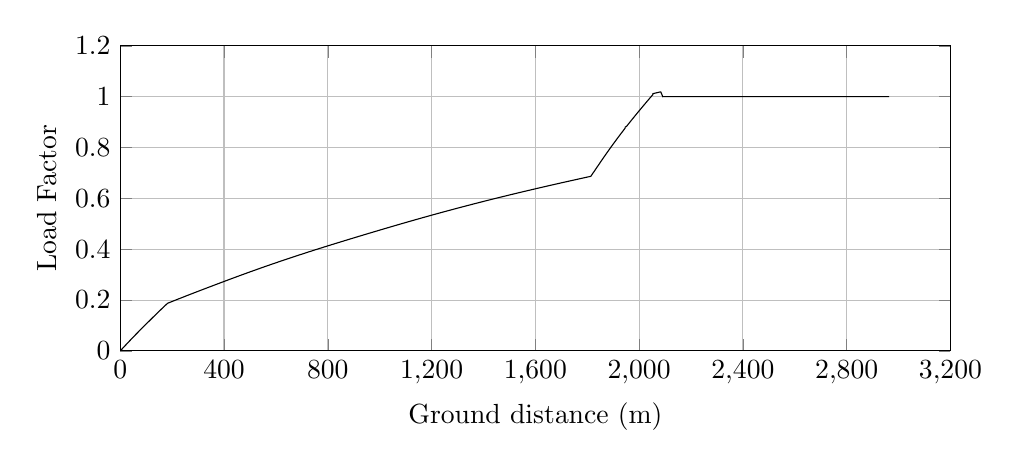
\begin{tikzpicture}

\begin{axis}[
width=\textwidth,
height=0.45\textwidth,
scaled ticks=false, tick label style={/pgf/number format/fixed},
xmin=0.0,
xmax=3200,
xlabel={Ground distance (m)},
xtick={0,400,800,1200,1600,2000,2400,2800,3200},
xmajorgrids,
ymin=0.0,
ymax=1.20,
ylabel={Load Factor},
ytick={0,0.2,0.4,0.6,0.8,1,1.2},
ymajorgrids,
legend style={at={(1.03,0.5)},anchor=west,draw=black,fill=white,legend cell align=left}
]

\addplot [
color=black,
solid
]
table[row sep=crcr]{
1.3603393307215537E-8	1.5374033208389272E-11\\
2.0334443352841076E-7	2.2981207716240697E-10\\
1.8493358258961232E-6	2.090048389684322E-9\\
9.983129263424352E-6	1.1282549412136833E-8\\
4.13538327636676E-5	4.6736510591868315E-8\\
1.2467543572893382E-4	1.4090335220700978E-7\\
2.843807411608912E-4	3.2139598492355305E-7\\
5.588015241105573E-4	6.315352016821599E-7\\
9.398454696015893E-4	1.0621749118034759E-6\\
0.0014155885812023746	1.5998385089136108E-6\\
0.0019945752038215015	2.254181668322058E-6\\
0.0026717822370171283	3.019526587593407E-6\\
0.003447739291558293	3.896470737478679E-6\\
0.0043193476547732645	4.881510918645401E-6\\
0.00529092766782709	5.979528362391867E-6\\
0.006363550519206555	7.191732101241853E-6\\
0.007533073890550759	8.513439089519928E-6\\
0.008790616877968567	9.934611089304765E-6\\
0.01016549189277427	1.1488372523477957E-5\\
0.011625499440327931	1.3138332203873978E-5\\
0.013184282533086976	1.4899906022816627E-5\\
0.014839871214038253	1.677086534061919E-5\\
0.01660567024659266	1.876635600414511E-5\\
0.018465948346479452	2.086859760642448E-5\\
0.0203822997817096	2.3034186868418095E-5\\
0.022430561433814646	2.5348821051771952E-5\\
0.024588423902376283	2.7787285607872693E-5\\
0.026831028501027587	3.0321486046815747E-5\\
0.029143159681622913	3.2934225735229906E-5\\
0.03155709159958957	3.5661971824487775E-5\\
0.03411445662773917	3.8551764326081156E-5\\
0.03677290089167576	4.155573904036866E-5\\
0.03952314881844239	4.466341085511817E-5\\
0.04239921643077808	4.791321190361803E-5\\
0.045357163155895136	5.125548714242575E-5\\
0.048363831658398165	5.4652768145384036E-5\\
0.051533845233668635	5.823456458974842E-5\\
0.0547899150155587	6.191354182119883E-5\\
0.058172599437445835	6.573552080893171E-5\\
0.06162834747858026	6.963999097993074E-5\\
0.06521401059050522	7.369118047790168E-5\\
0.06888104003120077	7.783423175891372E-5\\
0.07268727020998902	8.2134480631384E-5\\
0.076546425570032	8.649444817559005E-5\\
0.08047032364859658	9.092748214018012E-5\\
0.08456364881336098	9.555184296715504E-5\\
0.08882250397434277	1.0036311761898592E-4\\
0.09306368907640691	1.0515433840166077E-4\\
0.09743039119190974	1.1008725880359988E-4\\
0.10191450167634594	1.1515271081448359E-4\\
0.10651989152467789	1.2035505928429211E-4\\
0.11128201757858264	1.257343474356094E-4\\
0.11609763023253863	1.311739373438716E-4\\
0.12097769621339591	1.3668621260399963E-4\\
0.12591912973280778	1.4226768319829992E-4\\
0.13103216605369056	1.4804285398754057E-4\\
0.13633380151185176	1.5403090860729432E-4\\
0.1416823117522269	1.6007176409930699E-4\\
0.14708837902374172	1.66177481503649E-4\\
0.1525605467319851	1.7235770510484982E-4\\
0.15824953188605478	1.78782642032634E-4\\
0.16398006351864292	1.8525433685303056E-4\\
0.16978153473626356	1.9180597967617652E-4\\
0.17584258400626962	1.9865058706006224E-4\\
0.1819863832139092	2.055884559278913E-4\\
0.18819485651962437	2.125991677404148E-4\\
0.19455736971520038	2.197836260028782E-4\\
0.20098158490654017	2.2703755426626692E-4\\
0.2076061353991409	2.345174786439673E-4\\
0.21424726384720844	2.420159045107114E-4\\
0.2211374965027113	2.4979536189535155E-4\\
0.2281284453493247	2.576882951597784E-4\\
0.2350833915765042	2.655403428586382E-4\\
0.2423085249848444	2.736971777054362E-4\\
0.24958374984531584	2.819103055889826E-4\\
0.2569279402934431	2.9020102790968294E-4\\
0.2644720218029696	2.987171299361479E-4\\
0.27204626263318243	3.072669986207938E-4\\
0.27972793364503945	3.159378508054884E-4\\
0.2874622320100655	3.2466781813698166E-4\\
0.29563698092580604	3.338946222377273E-4\\
0.30361763245720474	3.429020378263768E-4\\
0.3118912000478351	3.5223973057035656E-4\\
0.3202493147046803	3.616725097154526E-4\\
0.3286412952843002	3.711431710839531E-4\\
0.33714554464307567	3.8074018689413457E-4\\
0.3458731203690518	3.9058886518892504E-4\\
0.35455185683415313	4.003820690010891E-4\\
0.3634323904331427	4.104026108233088E-4\\
0.372325738896249	4.204372354831124E-4\\
0.38151551889959867	4.308059367159902E-4\\
0.3908489672358084	4.413363258608903E-4\\
0.4001862088113266	4.518705808746726E-4\\
0.4095647137707429	4.624509731833196E-4\\
0.4192312859369268	4.73355913935878E-4\\
0.4289206911602753	4.8428616987958767E-4\\
0.43896550245304145	4.956168787280345E-4\\
0.4487817299761361	5.06689282478865E-4\\
0.4589033974758888	5.181057389285143E-4\\
0.4691858798479248	5.297030898902055E-4\\
0.47972601481223376	5.415905266756198E-4\\
0.49016040525287174	5.533581903794761E-4\\
0.5007175269203565	5.652637502946726E-4\\
0.511266977039379	5.771601399963439E-4\\
0.522323236324642	5.896274919565573E-4\\
0.5332586746953114	6.019580444215004E-4\\
0.5445869154512923	6.147309273662057E-4\\
0.5556699580072249	6.272267683052813E-4\\
0.5669225885056133	6.399132346790484E-4\\
0.5785590177532589	6.530317901711706E-4\\
0.5903083066022885	6.662769476956505E-4\\
0.6020327889628274	6.79493508115956E-4\\
0.613957077533064	6.929346556469871E-4\\
0.625960998969677	7.064649083088015E-4\\
0.6380070243193761	7.200419563870025E-4\\
0.6503365955459197	7.339379027196439E-4\\
0.662700086001522	7.478713821860289E-4\\
0.6752747602080436	7.620421498806897E-4\\
0.6885889407972636	7.770455067698572E-4\\
0.7019767933734617	7.92131072771879E-4\\
0.7151149754112038	8.069345196586283E-4\\
0.7284684478906998	8.219797468113903E-4\\
0.7418939875700234	8.371053616171792E-4\\
0.7553494584716574	8.522638846860849E-4\\
0.7694215958599202	8.681162561650387E-4\\
0.7830840331449673	8.835062486189832E-4\\
0.796657372658726	8.98795050823794E-4\\
0.8106660034246236	9.145732962328734E-4\\
0.8251837647136968	9.309240647314642E-4\\
0.8395067871054176	9.470545883371946E-4\\
0.8540519574023793	9.634343622278068E-4\\
0.8688334527125461	9.800793091120424E-4\\
0.8840141863517745	9.971728195096253E-4\\
0.8993797082767976	0.0010144733661138587\\
0.9143697020410035	0.0010313500913154878\\
0.9294094610857999	0.0010482818530384262\\
0.9452486359568626	0.0010661125243933416\\
0.9605773823977486	0.0010833675440802167\\
0.9761522209726621	0.0011008985292406603\\
0.9917649966835071	0.0011184711544974415\\
1.0074810114554809	0.0011361589066623086\\
1.0234652146968335	0.0011541473936437707\\
1.0399433598517231	0.001172690598967257\\
1.0563627364420554	0.0011911665020313577\\
1.0728309985448887	0.001209696243959322\\
1.0896486452479222	0.001228617899647706\\
1.1068138420051672	0.0012479293317721994\\
1.124143995869574	0.0012674250630733267\\
1.1415400048645106	0.0012869935847115823\\
1.1590089082607062	0.0013066428022023037\\
1.1769249919091855	0.0013267936605376395\\
1.1951505705127592	0.0013472912165126624\\
1.2127191877709298	0.001367048579106042\\
1.2308827453761335	0.0013874736252179915\\
1.2492706857898845	0.0014081495692425886\\
1.267587852451018	0.0014287445135232348\\
1.2860031245644312	0.0014494483375160022\\
1.304687144125951	0.001470452849877318\\
1.3233765774990474	0.001491461982692523\\
1.342322280991234	0.0015127577002968132\\
1.3613696045164358	0.0015341661305729906\\
1.3815086998747366	0.0015568000230985794\\
1.4013123019267382	0.0015790552160458407\\
1.4209622886438908	0.0016011361671356185\\
1.4411501686096515	0.0016238198897491822\\
1.4611760119255748	0.0016463198780962394\\
1.4816444281325132	0.0016693154082945208\\
1.501865958841821	0.0016920318777642255\\
1.5224364680875304	0.0017151386592939367\\
1.543651615594651	0.0017389677438441873\\
1.5647593029468103	0.0017626743010758837\\
1.5859558716309676	0.0017864788533615546\\
1.6071423964076703	0.0018102702977178687\\
1.6293386351549652	0.001835193645933506\\
1.6508498980272122	0.001859345953941686\\
1.673011606043147	0.0018842266080976073\\
1.6946435720294923	0.0019085106163146174\\
1.717066624993247	0.0019336807085447148\\
1.739432891071898	0.001958785044562732\\
1.761922286799709	0.001984025561834994\\
1.7849035550437842	0.0020098160325787095\\
1.8076299607761817	0.002035318414176838\\
1.8313298306791497	0.002061910976009842\\
1.8543134894513886	0.0020876977785068366\\
1.8777326664639729	0.0021139710628548356\\
1.9017196849182967	0.0021408791438104293\\
1.925345883672024	0.0021673802469308417\\
1.950252961491087	0.0021953157116738216\\
1.975161211119453	0.00222325005504409\\
1.9993825790313986	0.0022504117373897447\\
2.024583888346972	0.002278669886340451\\
2.04934017380271	0.002306426621042781\\
2.0744229633459703	0.0023345470014033277\\
2.0996193404956136	0.002362792267868924\\
2.1245764901457758	0.0023907669370335245\\
2.1500786393425866	0.0024193500164572594\\
2.176226227020705	0.0024486539093915324\\
2.202115608176549	0.0024776658392830445\\
2.227948363055355	0.0025066117525385243\\
2.2543499999408594	0.0025361924684517406\\
2.2810892744412783	0.0025661487677621653\\
2.3075963743135786	0.0025958422742274573\\
2.3348582111613405	0.0026263784625195036\\
2.3623221378972126	0.002657138168081073\\
2.3898598419727675	0.0026879776445977565\\
2.4171687299087603	0.00271855804879335\\
2.445442108612223	0.0027502155341608304\\
2.4735885391813177	0.0027817279007296245\\
2.5015416452491293	0.002813020892518064\\
2.5301110763218357	0.002845000838090238\\
2.5589284934403693	0.0028772552978755484\\
2.587611617795936	0.0029093563884904842\\
2.6175687086884984	0.0029428800051800974\\
2.647724154312196	0.0029766222466866836\\
2.6767118187859253	0.0030090546517865893\\
2.7060305938995466	0.003041854377049212\\
2.7361546404224653	0.003075551703326559\\
2.7663022704956823	0.003109272092617399\\
2.7964672462043376	0.0031430085697699566\\
2.8272583584284883	0.003177441908162033\\
2.8588650092419234	0.0032127836811365463\\
2.8898852960400587	0.0032474662867022436\\
2.9215246589961597	0.0032828374859432724\\
2.95270311230069	0.003317689892414686\\
2.984506337549637	0.003353237102308586\\
3.017379145769185	0.003389976010739374\\
3.049243647754313	0.0034255843520042705\\
3.081295157663824	0.0034613980324002154\\
3.113406837946715	0.003497275294116478\\
3.1453724573084756	0.003532985746619026\\
3.1787286104953543	0.003570245795919007\\
3.211019796961401	0.0036063125118886573\\
3.245786703184362	0.003645140325425546\\
3.279939251746722	0.003683277907741348\\
3.3141720228361216	0.0037215009930596757\\
3.3491198891036547	0.003760518326321434\\
3.382965192547779	0.003798300675236337\\
3.4181848705561064	0.003837613069400587\\
3.45391888941694	0.003877495205234442\\
3.488851494856137	0.0039164786563732285\\
3.524271454997704	0.003956001708464862\\
3.5606552075305	0.003996595738134049\\
3.597189071478943	0.00403735271377598\\
3.632926148839256	0.004077216413938136\\
3.668897146318187	0.004117336679188617\\
3.706642714683163	0.0041594315168277055\\
3.7432264628550644	0.004200226086973859\\
3.781286297809391	0.004242661877159699\\
3.818618572105483	0.004284281747773006\\
3.8564015479305356	0.00432639935081316\\
3.8948624022541356	0.0043692677272015885\\
3.9329637046009225	0.004411730513789391\\
3.971505929995028	0.00445467981614325\\
4.009821706071438	0.004497371926012291\\
4.049014376833089	0.004541036099814634\\
4.089343885784727	0.004585961565009396\\
4.128662304630717	0.004629755606835391\\
4.1684827283974055	0.004674103671731239\\
4.208000253554632	0.004718109315040597\\
4.2483743636521965	0.004763063615254516\\
4.288255503180503	0.00480746386419704\\
4.328757204126676	0.004852549764976895\\
4.369490126907612	0.004897887761715651\\
4.410357715197167	0.004943370327468552\\
4.45189144941496	0.004989588820420421\\
4.492881116440694	0.005035196515995147\\
4.53550011161515	0.00508261147443238\\
4.577670191557685	0.005129521369208531\\
4.6201174049766305	0.005176733908302581\\
4.662272021613388	0.00522361542234917\\
4.706017761800355	0.005272260616533555\\
4.748842845578064	0.005319876280186416\\
4.792293145132742	0.005368181292042443\\
4.836482439768313	0.0054173018885152295\\
4.88090298307878	0.00546667348415619\\
4.925311889063089	0.005516026097070046\\
4.969864686447545	0.005565532563612248\\
5.014842280541593	0.005615504926743528\\
5.0603877575117515	0.005666101979940528\\
5.106292347304597	0.005717091628227079\\
5.152263975081851	0.005768149376210083\\
5.1974808794106995	0.005818362709818108\\
5.244027372436168	0.005870046159551677\\
5.28996242022761	0.005921044349740975\\
5.336209145350672	0.00597238223761704\\
5.38320569473032	0.006024546007914806\\
5.430469292142472	0.006076999615678416\\
5.476900151253712	0.006128522647473706\\
5.526063828851289	0.0061830713284090864\\
5.573879040902945	0.006236117076516704\\
5.622613575936374	0.006290175871690076\\
5.6713596863799225	0.006344240623414446\\
5.720412183296268	0.006398638267512179\\
5.770660497446668	0.006454354860049492\\
5.820668144990444	0.00650979741373121\\
5.870305285939629	0.0065648221353236105\\
5.920503816994749	0.00662046205507926\\
5.971105439367246	0.006676541536175241\\
6.021088325934068	0.006731928207005985\\
6.071322359863801	0.006787586101249198\\
6.122981826035449	0.006844815963730003\\
6.174329110820436	0.006901692604981579\\
6.225804784288178	0.006958704106229942\\
6.278093246139479	0.00701660829571604\\
6.331709873490098	0.007075975466108491\\
6.384325657889258	0.007134226774857282\\
6.436648686434458	0.007192146461727316\\
6.489478972803882	0.007250620096365213\\
6.543185721519176	0.0073100560532747836\\
6.596747696432654	0.007369324027346013\\
6.650345873843312	0.007428624329164869\\
6.704555155195255	0.007488592912980344\\
6.7588986063680725	0.00754870204417058\\
6.814371620173711	0.007610052480240359\\
6.86997180120154	0.007671535378341327\\
6.925426612865756	0.007732849404269517\\
6.981353650685165	0.0077946773692703294\\
7.037678624474159	0.007856936987698657\\
7.094603706786671	0.007919851548539672\\
7.151204881983983	0.007982399788382173\\
7.209200593921791	0.008046480505954117\\
7.2667780016693655	0.008110090473803637\\
7.324687293141565	0.008174058535684366\\
7.382771066065313	0.008238210745781491\\
7.441904508776327	0.00830351349495636\\
7.501585831803217	0.008369412323671796\\
7.5616527251378685	0.008435727842152053\\
7.62150963104709	0.008501802538779845\\
7.682859947113334	0.008569516506580093\\
7.7432084367972145	0.008636115617016637\\
7.803024936926759	0.008702118756293897\\
7.863793829029664	0.008769163777806677\\
7.9252460466886365	0.008836953501953616\\
7.98696966925656	0.008905033354735742\\
8.04776546969778	0.008972080802827366\\
8.109421212326083	0.009040067504004311\\
8.17269125419024	0.009109824763768863\\
8.236095044780246	0.009179719877109478\\
8.299523592514586	0.009249632703414426\\
8.363213767675873	0.009319824309015661\\
8.427807923256076	0.009391002399879044\\
8.49144930156071	0.009461121020434827\\
8.557380457258176	0.00953375248752819\\
8.623183572921022	0.009606232827115336\\
8.687840683575093	0.009677441117535704\\
8.753751426394068	0.009750020156239039\\
8.820803713780364	0.00982384602164581\\
8.888970287482593	0.00989888823559562\\
8.957133699158991	0.009973916434620096\\
9.025036015045707	0.010048646823212787\\
9.092760955867519	0.010123171694724488\\
9.159817422823458	0.010196950885644712\\
9.227495373767134	0.010271403740708764\\
9.296013084156197	0.010346770109185652\\
9.36435980631623	0.010421938116837783\\
9.433329865923408	0.01049778131819181\\
9.503849553921977	0.010575317875587928\\
9.574524061692681	0.010653013861999643\\
9.644263228942293	0.010729671045074553\\
9.715657612596786	0.010808136855220533\\
9.787429657508813	0.01088700679517514\\
9.85753688572494	0.010964036745938386\\
9.930250735750551	0.01104391977451002\\
10.001571447096964	0.011122261552013435\\
10.074699859091687	0.011202577987080329\\
10.14698611653175	0.01128195860476576\\
10.220547980738981	0.011362728973150465\\
10.2940409891517	0.011443412672783518\\
10.36719293590382	0.011523711019413093\\
10.441008888975666	0.01160472725902665\\
10.51610421670324	0.011687136413444028\\
10.590724589239105	0.011769013175916066\\
10.667218005391902	0.011852933625676772\\
10.742771202259895	0.01193581120654734\\
10.82035208750042	0.012020901368579678\\
10.896759047300378	0.012104692481210193\\
10.973503045910835	0.012188841789895802\\
11.051297940743765	0.012274131794135243\\
11.128076326409062	0.012358295967348484\\
11.207667705350879	0.012445531865475172\\
11.286758396846047	0.012532207093621942\\
11.366305937658339	0.012619371098399107\\
11.446149720998452	0.01270684780197811\\
11.526866579636565	0.012795268995943049\\
11.607297517600138	0.012883365005226263\\
11.688034241538357	0.012971783999342859\\
11.769665722224765	0.01306117080242655\\
11.850920080706608	0.013150132665787597\\
11.933163326324259	0.013240165118165044\\
12.017103780766782	0.013332043051677726\\
12.10034832931326	0.013423146917421356\\
12.185467765774142	0.013516290047041081\\
12.270669986481685	0.013609511056742886\\
12.354040133273898	0.013700715345759963\\
12.440386807402234	0.013795163206201964\\
12.52556588630658	0.01388832139733954\\
12.610860989997974	0.013981594101563924\\
12.69550109439961	0.014074138384846302\\
12.784634337461807	0.014171582401304386\\
12.871172079509357	0.014266176245165829\\
12.958447214271366	0.014361563580890779\\
13.045518554761987	0.014456715715105284\\
13.133090172249581	0.014552402090308187\\
13.221405510214687	0.014648888535882164\\
13.310319106907201	0.014746015939870837\\
13.399783591735492	0.014843732406755825\\
13.488943611067967	0.014941103731643937\\
13.578276665194153	0.015038651515543375\\
13.667402973129146	0.015135961157476396\\
13.757763665999576	0.01523460599231918\\
13.848393619195729	0.01533353219975129\\
13.938857764339925	0.015432264963115066\\
14.031101516310692	0.015532927279505657\\
14.123507833735925	0.01563375423038121\\
14.214825187590282	0.015733380533269108\\
14.307956552027534	0.015834973259119735\\
14.401498558574918	0.01593700118901839\\
14.495315613017755	0.016039316395296203\\
14.589065423003394	0.016141545645368478\\
14.68316852398955	0.01624414756129205\\
14.778702641747682	0.016348296953579537\\
14.873746415615575	0.016451899115251106\\
14.970384078097169	0.01655722584979747\\
15.068900921005241	0.01666458752139814\\
15.164434274206265	0.01676868522540195\\
15.260378587808539	0.016873218337736026\\
15.357189194448868	0.016978682817159075\\
15.45495288999333	0.017085172981323293\\
15.55311774366497	0.017192087489309088\\
15.652583807013901	0.01730040640780847\\
15.755243917873962	0.017412190296791162\\
15.855950289561445	0.017521833754075747\\
15.958461094374158	0.017633428628230516\\
16.060387288500337	0.01774437406483493\\
16.164276126126843	0.017857442589461064\\
16.26736468838029	0.01796962706279488\\
16.36946523634058	0.018080723651526017\\
16.47192386662276	0.018192197304906035\\
16.576794358652606	0.01830628213055161\\
16.678929175716583	0.018417378500550946\\
16.783994526910618	0.01853164989175816\\
16.89012564586595	0.018647067556709588\\
16.996887404888547	0.01876315812826152\\
17.103774697793426	0.018879372372236004\\
17.210947675936964	0.018995884486699262\\
17.31865021419634	0.019112959599538088\\
17.424470519881233	0.01922797641817496\\
17.53205215515201	0.019344895321273776\\
17.64034909906897	0.01946257922101527\\
17.74911485075183	0.019580760196036138\\
17.85745376408675	0.01969846521095467\\
17.969383314157206	0.019820058677510525\\
18.07998395718984	0.01994019607679836\\
18.18863741327577	0.020058206516013085\\
18.302466989554325	0.020181826370699058\\
18.41305080779906	0.020301909253588362\\
18.525644000014054	0.020424162072135942\\
18.636945827420575	0.020545000952822485\\
18.750643923449367	0.020668429496153523\\
18.86479622056296	0.020792339145030935\\
18.979646899421056	0.020916994939531506\\
19.09418630108147	0.02104130113213445\\
19.208983505033515	0.021165875505231076\\
19.323483295898072	0.021290115730263848\\
19.43842354827664	0.021414822599410008\\
19.55563752357537	0.021541984920275196\\
19.67199913451129	0.021668211249701634\\
19.789486593639566	0.021795647643270515\\
19.90713985662446	0.021923252751753636\\
20.024127533725753	0.02205012510846392\\
20.143019013955552	0.022179051205709736\\
20.26442367074238	0.022310691423330323\\
20.383660776265387	0.022439970542712205\\
20.5042342316437	0.022570687860712663\\
20.622773342122727	0.022699189380431136\\
20.74503732713029	0.022831718313013092\\
20.865944869938517	0.022962766612215392\\
20.98711015528624	0.023094084178054714\\
21.113336299999695	0.023230876104032915\\
21.23638685227678	0.023364216469753556\\
21.35988644990264	0.023498033551237762\\
21.483760012473958	0.02363224609606233\\
21.608180515260266	0.023767041608888866\\
21.732326713270083	0.02390153053277864\\
21.85766379468624	0.02403730022087048\\
21.985117186778353	0.02417535296821258\\
22.111729024702363	0.024312484996044208\\
22.23700541150786	0.024448161811443804\\
22.36297326225872	0.024584578877015626\\
22.488604760551	0.024720623285123942\\
22.616276341350805	0.024858868478146317\\
22.744235570279145	0.024997416869262427\\
22.874576476768283	0.025138535737640844\\
23.003842066605536	0.025278482323695103\\
23.13088450205612	0.025416014464081923\\
23.257869280739328	0.025553476870288225\\
23.389244224935425	0.025695684199080984\\
23.519811196806458	0.02583700962103881\\
23.653309395988643	0.02598150049107725\\
23.78342402399784	0.02612232229166732\\
23.9180644861338	0.02626803543954417\\
24.05110504604577	0.02641201043268411\\
24.182394801971697	0.026554084445799077\\
24.314614014384034	0.026697158184331653\\
24.449791085561472	0.02684342653789904\\
24.585258581909038	0.026990003231537836\\
24.72121222319008	0.027137100228800077\\
24.857032405393277	0.027284047362217657\\
24.99454740444294	0.027432822842238674\\
25.13030709358258	0.027579694275514544\\
25.270890409679986	0.02773177916362582\\
25.40663839363527	0.027878628565965298\\
25.54307796688363	0.028026221846941694\\
25.68272814639034	0.028177284017876295\\
25.82072003425767	0.02832654848530173\\
25.96015212691003	0.028477367127850435\\
25.987750021099068	0.028507218353751695\\
26.0558803939429	0.028580910917093486\\
26.061632797568386	0.02858713291310103\\
26.066808273335674	0.028592730879519256\\
26.071901058608013	0.028598239400787238\\
26.073315434863225	0.028599769235123793\\
26.074595035914804	0.028601153292026994\\
26.080371168076944	0.028607400935564672\\
26.10234540095133	0.028631168895525885\\
26.183408179590366	0.028718847999082538\\
26.300430535410044	0.028845419587590244\\
26.42750601924636	0.028982861636729255\\
26.558056987479794	0.02912405916555627\\
26.688030995483615	0.029264628870686853\\
26.818767077324992	0.029406018677321878\\
26.951519978077492	0.029549585182633793\\
27.083955405447817	0.02969280359929974\\
27.216897884715692	0.029836565311060655\\
27.350913258119895	0.029981481853853978\\
27.4833530065795	0.030124689042099383\\
27.6176201223548	0.030269866257271127\\
27.752160408628434	0.030415332614648852\\
27.887329802382908	0.03056147263370969\\
28.023188645890663	0.030708351197530733\\
28.158973127824495	0.03085514223551436\\
28.296372294036907	0.031003671322742565\\
28.435107205966254	0.031153636416848905\\
28.571323599682245	0.03130087110759515\\
28.70996262687553	0.03145071597803442\\
28.850320389600306	0.03160240959352689\\
28.988837241064125	0.031752104570547\\
29.129197813929657	0.03190378262832612\\
29.27166529868488	0.03205772751446292\\
29.41298471572133	0.03221042166209486\\
29.554848516656044	0.03236369355436497\\
29.699676691743235	0.032520157131285886\\
29.842400551696755	0.032674336130834605\\
29.985385440862252	0.032828785703561236\\
30.129077275410303	0.032983987150688565\\
30.27543774584293	0.0331420586163377\\
30.422081339040986	0.033300423074515174\\
30.56949149516445	0.033459602206230656\\
30.716562179458485	0.03361840135729968\\
30.86535310281699	0.03377904404512006\\
31.011875026602333	0.03393722309803117\\
31.16159928701196	0.03409884475680984\\
31.313692569485013	0.03426300841038601\\
31.463056706803336	0.0344242110911111\\
31.61235366859384	0.03458532593262824\\
31.76278957628285	0.03474765411611985\\
31.915019899787076	0.034911902213662735\\
32.06709627595497	0.0350759675347234\\
32.21861178877769	0.035239410956363786\\
32.37168228565527	0.03540451448277895\\
32.52450570609457	0.035569333927154306\\
32.67702483599189	0.035733807440801485\\
32.829998687403204	0.03589875326477175\\
32.98551220909506	0.0360664187461725\\
33.14332298937855	0.03623654140239533\\
33.29970221124884	0.03640510110274228\\
33.45800124694219	0.03657570992389953\\
33.61398946945653	0.036743808092917725\\
33.77048353048475	0.036912431046963894\\
33.9292721471582	0.037083505354319125\\
34.08796840843395	0.037254458754788874\\
34.24769686644211	0.037426502234404344\\
34.406855482575295	0.03759790991503349\\
34.56481953291838	0.03776800913719872\\
34.72399692808165	0.03793939257008753\\
34.88694269464703	0.03811480988043162\\
35.04914399338672	0.03828940194572416\\
35.209965099803895	0.038462484724872056\\
35.3703140559587	0.03863503568860116\\
35.531685786905925	0.03880866318872906\\
35.69349909442164	0.0389827413500224\\
35.85522798807463	0.03915670402748839\\
36.022509111806116	0.0393366127617303\\
36.19055880791667	0.03951732107667234\\
36.35708622463872	0.039696365524846296\\
36.52115360367851	0.03987273861666029\\
36.68781562330062	0.04005187391578856\\
36.8536847754776	0.04023012974872494\\
37.024522648961764	0.040413696718952744\\
37.19188554678789	0.04059350141616216\\
37.36066720850286	0.0407748017061296\\
37.528862119520696	0.04095544291896646\\
37.697264258302326	0.04113627769427848\\
37.86832931534104	0.04131994208150624\\
38.03812867477943	0.041502217558534955\\
38.20923731912278	0.041685868107589605\\
38.37904730305398	0.04186809444182254\\
38.55252405124031	0.042054224229577886\\
38.72282139824354	0.04223691165031978\\
38.89783411301201	0.04242462525661419\\
39.0714610757495	0.04261082006234834\\
39.24438070689564	0.04279622400682247\\
39.41969314875929	0.04298416040583245\\
39.59166556575205	0.04316848371331274\\
39.764623188591585	0.043353830299472054\\
39.94263254662576	0.043544556082719996\\
40.11749159802578	0.04373187238046037\\
40.29452954971913	0.04392148818411325\\
40.47247750600427	0.04411204337799207\\
40.64799609178485	0.04429996229509945\\
40.82414741101539	0.04448852375933944\\
41.00385670225303	0.04468085769071965\\
41.18169069533937	0.0448711484735724\\
41.3603281005193	0.04506226263499734\\
41.54046179251334	0.045254940594478245\\
41.722675278204306	0.04544980524054358\\
41.90258931008478	0.04564217320064385\\
42.08518735141125	0.04583737264043191\\
42.26728550944881	0.04603199911599255\\
42.44743534848537	0.04622450518343317\\
42.63069538383506	0.04642029581466249\\
42.80963512098974	0.046611432708293196\\
42.992542679335614	0.0468067689206785\\
43.17926890616222	0.04700614252396763\\
43.363134036078335	0.047202420883006434\\
43.54815051311773	0.047399887776483844\\
43.733578141849236	0.047597752568090776\\
43.91798130912079	0.04779448344475489\\
44.10506009255049	0.04799402718099616\\
44.29251116260117	0.04819392584802364\\
44.480917546793805	0.048394800632548036\\
44.66851287589745	0.04859476811724275\\
44.85853501730759	0.048797279056245396\\
45.047396872181054	0.04899851006300155\\
45.236914792155844	0.04920039652494828\\
45.42785879536018	0.04940375789909376\\
45.616432631699865	0.04960455129687691\\
45.80697204128492	0.04980739346696435\\
45.998633580597016	0.0500113853429933\\
46.18800675699903	0.05021289734901566\\
46.380841640082096	0.05041804764089042\\
46.57327038933336	0.05062272020116214\\
46.765844918266424	0.05082750207824589\\
46.95911042680183	0.05103297266185469\\
47.15311668852311	0.051239184286306395\\
47.34541611633634	0.05144353566218922\\
47.53884854699059	0.05164904475010027\\
47.73236991243341	0.051854601797983284\\
47.92818250719388	0.052062545147584925\\
48.12326385407131	0.052269664454110715\\
48.32058854034828	0.05247911725134779\\
48.516852452700604	0.05268739586178992\\
48.71339374517507	0.05289592059849404\\
48.91319881343868	0.05310785858576767\\
49.1119162355681	0.053318593314346206\\
49.31207818344666	0.053530809913583666\\
49.509673461222235	0.05374025599822962\\
49.71156302510582	0.053954203327491373\\
49.91034548441702	0.05416480798937775\\
50.11200805970151	0.0543784133400409\\
50.30853267551517	0.054586527282906125\\
50.50757456960626	0.05479725745719281\\
50.70929197287772	0.05501076941625655\\
50.91222418686718	0.05522551555950478\\
51.11562549758783	0.05544070610182659\\
51.32090674103446	0.055657832736146794\\
51.525199701657655	0.05587386138888519\\
51.72863462744459	0.05608893049690878\\
51.934060761332375	0.0563060518073915\\
52.14033810224923	0.05652401931669184\\
52.344882977561255	0.05674010327483824\\
52.55098100649393	0.05695777472959248\\
52.75731843494604	0.05717564546549196\\
52.96514817708821	0.05739503776441926\\
53.17450540782369	0.05761598758816612\\
53.382202621450276	0.05783513100112121\\
53.592230583406476	0.05805667845610433\\
53.80364534107798	0.05827963278079432\\
54.01469481143569	0.05850214587993203\\
54.223966920081466	0.058722729858688934\\
54.43230789395902	0.05894227778601525\\
54.6430562980421	0.05916430726586349\\
54.855225786754914	0.059387777677967754\\
55.066088958624874	0.05960981634486733\\
55.27969530828261	0.05983468685139641\\
55.49171188337613	0.060057827342331525\\
55.70388919125476	0.060281080788664884\\
55.91737779085577	0.06050565727772136\\
56.13177028494084	0.060731127424927714\\
56.34652664868587	0.06095692285389737\\
56.559021044851505	0.0611802835714986\\
56.77591447970492	0.061408210416874325\\
56.99548236897459	0.06163888829423847\\
57.21481285737903	0.061869257092876544\\
57.43536222847358	0.0621008460640568\\
57.65367025761124	0.06233002227777102\\
57.872788904232735	0.06255999029556518\\
58.0907693980174	0.06278870507290354\\
58.311927420720366	0.06302069407514824\\
58.532333513628615	0.06325183450942597\\
58.75532998033057	0.06348563080362264\\
58.976617007999806	0.06371757464206554\\
59.19875422837053	0.0639503493763271\\
59.4206945143671	0.06418285757352557\\
59.64453328369959	0.0644172938411211\\
59.86894932484513	0.06465227351647705\\
60.09432075877773	0.06488819200725447\\
60.318058693038594	0.0651223396593277\\
60.541731124044205	0.06535635823431761\\
60.76707064338231	0.06559205993758385\\
60.995574692986196	0.06583100922420919\\
61.22378989589207	0.06606959381070819\\
61.4534619981562	0.06630963842062715\\
61.683510138770515	0.06655001276438029\\
61.91410430469678	0.06679089422368845\\
62.14462153858659	0.06703163200439556\\
62.37563158073512	0.0672728210875298\\
62.607203285434	0.06751453308177346\\
62.841031881319736	0.06775853644498568\\
63.07467935056491	0.06800228637806056\\
63.31164975340633	0.06824943731604145\\
63.54633691305479	0.068494141975473\\
63.78243968758058	0.06874025763521488\\
64.0165414084598	0.0689842231473333\\
64.25412817577254	0.06923175533688203\\
64.49270299572771	0.06948025102543885\\
64.73076499662056	0.06972814692419776\\
64.96867826857735	0.06997582263068393\\
65.21063576532572	0.07022764173970629\\
65.4512107007771	0.0704779553849806\\
65.69028017871045	0.07072663709576275\\
65.93032615763332	0.07097626904796983\\
66.17196619696679	0.07122749262032184\\
66.4135612157637	0.07147860330607082\\
66.6559030093851	0.07173042401970706\\
66.89910102540284	0.07198306805749775\\
67.14354652182666	0.07223694124155405\\
67.38771133480921	0.07249045630770848\\
67.63347396558368	0.07274556339313513\\
67.87898066495345	0.07300033795797098\\
68.1255935515739	0.0732561934397496\\
68.37316753306138	0.0735129787153975\\
68.62205497364681	0.07377105858690915\\
68.8711887275476	0.0740293261188164\\
69.120220471977	0.07428742042381634\\
69.36846244647072	0.07454462934037161\\
69.61951843592018	0.07480468628016589\\
69.87236615109754	0.07506653071372045\\
70.12758921381476	0.07533076561949564\\
70.37945082809051	0.07559145232673693\\
70.63410009691182	0.07585495592695063\\
70.89152727368702	0.07612126438267625\\
71.14629115974091	0.07638474903092679\\
71.40197865069018	0.07664912055916905\\
71.66163317144085	0.07691752410348057\\
71.92484704501203	0.0771895355288924\\
72.18465416754285	0.07745795617017336\\
72.44573394560723	0.07772762177265864\\
72.70633339061075	0.07799672171800212\\
72.96699363118216	0.07826581529308858\\
73.22900401485182	0.07853623334281319\\
73.49076816912304	0.07880632817773428\\
73.75430841254712	0.0790781862245735\\
74.01895646534612	0.07935111733070466\\
74.2846979982242	0.0796251062150821\\
74.55380714249793	0.07990249619877639\\
74.82322871850147	0.08018013701832191\\
75.09350011520078	0.08045858239057009\\
75.36421232425869	0.08073741082653056\\
75.6347219158074	0.08101595991418184\\
75.90830954343213	0.08129760708981344\\
76.18188601743822	0.08157917137577068\\
76.45626363461818	0.0818614889014716\\
76.72958718025629	0.08214265128992239\\
77.00406935908524	0.08242493509480883\\
77.28579748399531	0.082714597836853\\
77.56784659723587	0.08300451703769299\\
77.84569092555657	0.08329004261443017\\
78.1246978223638	0.0835766919407761\\
78.40641219364133	0.08386605122954746\\
78.68590470271565	0.08415305766234506\\
78.96851680469001	0.08444319643506365\\
79.25576208114188	0.08473801899351154\\
79.54169104977237	0.08503141815948322\\
79.82662017154695	0.085323720047493\\
80.11330301632765	0.08561774970853771\\
80.40394576721474	0.08591576825027333\\
80.6908099930996	0.08620984131945751\\
80.98055888331655	0.086506800418883\\
81.27178512217935	0.08680520214681166\\
81.56682943128612	0.08710744350299704\\
81.86186977412851	0.08740960838500465\\
82.15688924927383	0.08771168007160761\\
82.44965588234726	0.08801137463623172\\
82.74488606927187	0.08831352058636671\\
83.04325841243121	0.08861881100042376\\
83.34213327641098	0.08892454433855305\\
83.64411622775171	0.08923338528752058\\
83.94734638805741	0.08954342978777838\\
84.25123842984891	0.08985407932379305\\
84.55152885577829	0.09016097726658065\\
84.85735750691177	0.09047346454365196\\
85.16518306664875	0.09078792077890434\\
85.47136476235073	0.09110062732864084\\
85.77898122624802	0.09141472918587362\\
86.08923229760057	0.09173145078706485\\
86.40254560035129	0.09205122744332077\\
86.71167807044037	0.09236666776208828\\
87.02660518802142	0.09268795095932654\\
87.34238286044419	0.09301003167703575\\
87.65842706333811	0.09333231461485822\\
87.97971380652302	0.09365987295923389\\
88.2973933745065	0.093983684485015\\
88.61789013566766	0.09431029861394434\\
88.93643920279564	0.09463486001594418\\
89.25662431900213	0.09496102096737552\\
89.57903058309674	0.09528937707341188\\
89.89968694948243	0.09561588466481559\\
90.22473455398588	0.09594679694469473\\
90.55024875587375	0.0962781178037634\\
90.87789352676518	0.0966115409570874\\
91.20733069500889	0.09694672194893063\\
91.54101415610151	0.09728615653310106\\
91.87012785371462	0.09762087769654929\\
92.20120197152713	0.09795752855524584\\
92.53416638543635	0.09829603759271976\\
92.86431843528567	0.09863162500882675\\
93.19748455591187	0.09897021402048944\\
93.53066771200866	0.0993087588854429\\
93.86681917526724	0.09965025848402986\\
94.20530590547477	0.09999406921267506\\
94.5419273964865	0.10033592533480289\\
94.8854212036891	0.10068469993447302\\
95.22752713476521	0.10103200538458085\\
95.57091181422334	0.10138054989197581\\
95.91383450860906	0.10172856738147325\\
96.25469535763642	0.10207443588066725\\
96.5966517898868	0.10242136046437149\\
96.93845701474973	0.10276807701885864\\
97.28153572459905	0.10311603146938844\\
97.62213139590432	0.10346141521265854\\
97.9659652144934	0.10381003072533308\\
98.3129807304216	0.10416182037482564\\
98.65852794036775	0.10451207086868079\\
99.00080640577195	0.10485895935079413\\
99.35064076251427	0.10521345641396491\\
99.69796076807248	0.10556535762356752\\
100.04654253174803	0.10591849025608797\\
100.3915606488718	0.10626796745551358\\
100.74261509654437	0.10662351389324619\\
101.08877163494762	0.10697405629557542\\
101.43457754260953	0.10732420163123155\\
101.784020212797	0.10767798783619978\\
102.13161434601102	0.1080298622173594\\
102.4751980097893	0.10837763831904129\\
102.82212110631409	0.10872875693313991\\
103.16739702108615	0.10907817195345686\\
103.51524666207362	0.10943015584571683\\
103.86391679154056	0.10978293512798004\\
104.20960434827006	0.11013266334861829\\
104.55241399635099	0.1104794483233666\\
104.89662223620601	0.11082761743245956\\
105.24103428322039	0.11117596301469579\\
105.5836615386647	0.11152247504322187\\
105.92645892081137	0.11186913187972315\\
106.27347658175316	0.11222002985240105\\
106.6151670762521	0.11256551596888757\\
106.95898391938218	0.1129131279818322\\
107.30023552029138	0.11325812363403412\\
107.64147805753461	0.11360308847887267\\
107.98348674656944	0.1139488071909293\\
108.32522459759954	0.11429423256350119\\
108.3935347040271	0.1143632775196173\\
108.40478590462831	0.11437464968540283\\
108.41572478024443	0.11438570614935772\\
108.4246743308916	0.1143947518900675\\
108.44347342986478	0.11441375300175818\\
108.52018987797786	0.11449129326031578\\
108.70071173483461	0.1146737499132225\\
108.99446230248458	0.11497063724617655\\
109.30176454987088	0.11528120477134694\\
109.60899173332959	0.11559167890465909\\
109.91608539831654	0.1159019996132111\\
110.22883517949637	0.11621801586774139\\
110.54143546549608	0.11653385988539695\\
110.853845249356	0.11684948926811524\\
111.1739714794031	0.11717289060890668\\
111.4937490010879	0.11749591436628021\\
111.81170779322963	0.11781707482406367\\
112.13106495813236	0.1181396205096813\\
112.4519453366479	0.11846367611484847\\
112.77515902629136	0.11879005820831359\\
113.0997499810409	0.11911779982124547\\
113.43040796942478	0.11945163409614108\\
113.7597028375028	0.11978405773102246\\
114.0907450350197	0.1201182096041561\\
114.42538740208008	0.12045595801425603\\
114.75997726261329	0.12079361470902568\\
115.09477047197589	0.1211314367933213\\
115.43440545481076	0.12147410266493694\\
115.77494672336013	0.12181763955949411\\
116.11687534861284	0.12216253124584514\\
116.46164587354252	0.12251024293447989\\
116.8077846490165	0.12285928644265894\\
117.15688723722127	0.12321126869748107\\
117.50557855048987	0.1235627851107015\\
117.85411336711965	0.12391409155011907\\
118.20532793701167	0.12426804515096418\\
118.55850697655507	0.12462392287354812\\
118.91273956155123	0.12498080501282914\\
119.26983096270519	0.1253405082794965\\
119.62978614725739	0.12570303512810993\\
119.98960731920661	0.1260653645302583\\
120.34734904217265	0.1264255369687228\\
120.7138511704587	0.12679446304810177\\
121.08106061642908	0.127164032705306\\
121.44737887966437	0.12753263609258683\\
121.81499139152783	0.127902471044704\\
122.18511446431708	0.12827475900964444\\
122.55384158147794	0.12864556919209294\\
122.92460728481757	0.12901835424844751\\
123.29616941264607	0.1293918632992619\\
123.67040864389355	0.12976798470739875\\
124.04652172406458	0.1301459086447379\\
124.42393851457416	0.1305250601113209\\
124.80152108360014	0.13090429438221088\\
125.18180835736592	0.13128615945179684\\
125.55854932865631	0.13166437760849078\\
125.93878032356085	0.13204601173718072\\
126.31997081831156	0.13242851938878272\\
126.70099538833193	0.13281076993815535\\
127.08058279416298	0.13319148761661076\\
127.46175209000612	0.1335736994170757\\
127.84399628255431	0.13395689500051594\\
128.22749916598133	0.134341256771147\\
128.6102537001487	0.1347247720336264\\
128.99595881306152	0.13511114526603898\\
129.37788117916477	0.13549363085748245\\
129.760738924708	0.13587695406724312\\
130.1448498512433	0.13626143131888155\\
130.53000390659713	0.13664685055016823\\
130.9168242384266	0.13703383335708338\\
131.29443328439476	0.13741149977327807\\
131.67491382268804	0.13779193612507853\\
132.05816436539135	0.138175037830788\\
132.44070735535217	0.1385573270221609\\
132.82666098215685	0.13894291721933888\\
133.20952005887244	0.13932530843093616\\
133.5940193955625	0.13970922950513162\\
133.97617966856654	0.1400907066323405\\
134.36103715882757	0.14047476617907342\\
134.74478042358356	0.1408576031820577\\
135.12867144169206	0.1412404763263397\\
135.5141335746535	0.14162480372830497\\
135.89764893392993	0.14200707731467013\\
136.28231234485685	0.14239038154849984\\
136.66418763078912	0.14277079421457994\\
137.04684871033697	0.143151875774891\\
137.42845627025127	0.14353179398539995\\
137.8132447087305	0.1439147629033474\\
138.19719797258034	0.14429678377639787\\
138.58059071069573	0.14467812989380188\\
138.96593237593703	0.14506129606986473\\
139.3501607499636	0.1454432363964111\\
139.73355638294606	0.14582423007703724\\
140.1160230155566	0.14620418171219007\\
140.50045093994146	0.14658596155292716\\
140.88215178690393	0.14696491334738324\\
141.26156782058217	0.1473414780085738\\
141.64323970440188	0.14772016158218504\\
142.02689350659642	0.1481006897748855\\
142.41061312971692	0.14848116062910421\\
142.7942251403153	0.14886140171582452\\
143.1756303563767	0.14923933294300132\\
143.5599719391364	0.1496200498129884\\
143.94242380128833	0.14999877079888094\\
144.3239499176869	0.15037645140405548\\
144.70664939692608	0.15075516903428812\\
145.0870075357763	0.15113144571429785\\
145.46856550308127	0.15150878477153903\\
145.85014610541765	0.15188602103912874\\
146.23128237819492	0.15226269269615125\\
146.61504730324998	0.15264183527344244\\
146.99763315977907	0.15301968582966607\\
147.38441582478964	0.15340155183372578\\
147.7673688364352	0.15377950832217888\\
148.15222568696134	0.15415921461101478\\
148.53580865353604	0.15453753486061567\\
148.9199734867533	0.15491629939246315\\
149.3040357319486	0.1552948328226648\\
149.68771357306542	0.15567285734105463\\
150.07093078701052	0.15605029798934478\\
150.45622889618164	0.15642965687270846\\
150.8449053483268	0.15681220836138465\\
151.2288570611563	0.15718997749468377\\
151.61452719766493	0.15756930498040464\\
151.9983007305741	0.15794663509198106\\
152.38299664478842	0.15832473975275088\\
152.76945776909372	0.15870444573392595\\
153.15580177123394	0.15908390253088553\\
153.54253364040335	0.15946360577880977\\
153.93093169697067	0.15984480928853168\\
154.31788037931886	0.16022445490246687\\
154.7039882138024	0.16060314067805523\\
155.08880221957185	0.16098042328496862\\
155.47621608980313	0.16136011935975486\\
155.866104687065	0.161742103425953\\
156.25391419262098	0.16212191362736472\\
156.64166339424906	0.1625015280996315\\
157.03027969880475	0.16288185423172033\\
157.4213807682267	0.16326447326862636\\
157.8105708506119	0.1636450843671079\\
158.19948541262937	0.16402528799760033\\
158.58893406813365	0.164405875400295\\
158.97894817604634	0.1647868765398765\\
159.3710019698692	0.16516973010015448\\
159.76139479981174	0.16555082199190213\\
160.1523485688823	0.16593232170175506\\
160.54128874338664	0.16631171766913488\\
160.9326976430911	0.16669338192339458\\
161.32564259741588	0.16707640281510294\\
161.71827778345698	0.16745898043796853\\
162.1124492087963	0.1678429128180979\\
162.50576001021273	0.16822586496393635\\
162.89904576730015	0.16860865091132962\\
163.29316224934274	0.16899210313775936\\
163.68899123279596	0.16937707817942735\\
164.08495392634194	0.16976203953966598\\
164.48271131475576	0.17014860101775572\\
164.8792309171331	0.17053381520812372\\
165.27343112400507	0.17091663330668005\\
165.67115293733156	0.17130272704526497\\
166.06936395728349	0.17168915053977551\\
166.47000821435734	0.17207778872692137\\
166.87155839526775	0.17246715828871795\\
167.27134041220108	0.17285466679602526\\
167.67233991204222	0.17324320861402856\\
168.0705846918417	0.1736289358678973\\
168.47232570996516	0.1740179027216621\\
168.87521546679773	0.17440783386732234\\
169.2789990941189	0.1747984816156083\\
169.68142011368735	0.17518766326891594\\
170.088438196605	0.17558114076559397\\
170.49328200513543	0.17597236682716144\\
170.89845866435633	0.17636376540429738\\
171.30484584057905	0.17675618361143722\\
171.7103088520891	0.17714756013855001\\
172.11589069074847	0.17753890234711953\\
172.52485519917514	0.17793335772365887\\
172.93316089774754	0.1783270268414337\\
173.34236088095247	0.17872140717610643\\
173.7535761368399	0.1791175776987103\\
174.16510964781833	0.17951390238572498\\
174.5786011126259	0.17991195928384685\\
174.99051444770384	0.18030834430997159\\
175.40138574541044	0.18070357502561404\\
175.81497300453447	0.181101265679831\\
176.2280441317456	0.18149830742991782\\
176.64225100058474	0.18189628795336835\\
177.05714873395152	0.18229477904573643\\
177.47483026786767	0.18269578921851212\\
177.89254345086653	0.18309667488090547\\
178.3100126079721	0.18349717186526968\\
178.7278240622369	0.18389784289398545\\
179.1449731538625	0.1842977249968253\\
179.56482315926417	0.1847000414123385\\
179.9871804296257	0.18510460400794604\\
180.4095742002126	0.18550904503010252\\
180.83428717371925	0.18591554918766942\\
181.26003251256287	0.186322883294815\\
181.6840913989422	0.18672844682631254\\
181.8934642440371	0.18692863017245961\\
182.1114839456617	0.18713704039057175\\
182.5372774346568	0.18731270117714066\\
183.423900814602	0.1876783497454258\\
184.30144226609173	0.18804008386398363\\
185.17422251923585	0.1883996889205611\\
186.05126240753827	0.18876088219040363\\
186.93861419286333	0.18912615237059893\\
187.8243328275641	0.18949058026330337\\
188.7212117513506	0.1898594273407667\\
189.61004025875786	0.1902247925649843\\
190.50102451880866	0.19059087341064312\\
191.38947474753866	0.190955743473092\\
192.28052744689825	0.1913215125946151\\
193.18778236606096	0.191693758356086\\
194.08895872822546	0.19206333647967636\\
194.99680020640938	0.19243547348745133\\
195.89480429656658	0.1928034061117658\\
196.79674305679504	0.19317277920490297\\
197.7065692706791	0.1935452086176229\\
198.612023604503	0.19391567554104389\\
199.52644538440046	0.19428963690704662\\
200.43881964763966	0.19466258652737184\\
201.34572312669928	0.1950331276971632\\
202.26115686844895	0.19540698054614303\\
203.17967892292364	0.19578191981696788\\
204.1017087672932	0.19615811535165575\\
205.01405834107487	0.1965301885701767\\
205.94020355690031	0.19690771272650875\\
206.86420646269943	0.1972841882452001\\
207.79153006365993	0.19766184116229793\\
208.72800400232427	0.1980430425878907\\
209.6603812871926	0.19842239930264\\
210.59913361291103	0.1988041718367719\\
211.54272242703126	0.19918773186287025\\
212.4892775421681	0.19957231751931623\\
213.4278558742791	0.19995348463426924\\
214.37319863683314	0.20033722071148063\\
215.31618532994997	0.20071982287848222\\
216.26909967312713	0.2011062735265089\\
217.2229300472723	0.20149291557707805\\
218.17915574443117	0.20188034836163227\\
219.13394290547268	0.20226701888239335\\
220.0901210939433	0.20265407371032249\\
221.05386294760763	0.20304400962027017\\
222.0194744620763	0.20343452078954163\\
222.9871855528732	0.20382569975574502\\
223.95850156259326	0.20421815410428254\\
224.93506896411378	0.2046125472883102\\
225.9123601081958	0.20500704981398546\\
226.89683950214788	0.2054042697017675\\
227.87812705537118	0.20580001837652342\\
228.86553252311342	0.20619805033909558\\
229.85786107077195	0.20659788160178094\\
230.84893890233656	0.20699702433947487\\
231.8352011637358	0.2073940453102411\\
232.83551070617193	0.20779653598792014\\
233.8409775535427	0.20820091479929367\\
234.84473749332597	0.2086044209434268\\
235.85076677249623	0.20900865351392753\\
236.86174655712836	0.2094146886586067\\
237.8698887650736	0.20981939873850258\\
238.88314164945962	0.210225974733197\\
239.88702917374013	0.21062861002390718\\
240.9073981595622	0.2110376700687159\\
241.92631922506058	0.2114459638495936\\
242.95020737895555	0.21185606186699127\\
243.9867665418509	0.21227104586189746\\
245.01566609591487	0.21268277607413863\\
246.05919400906686	0.21310017042493692\\
247.09706457910846	0.2135151134699607\\
248.1403037320082	0.213932014448656\\
249.18309170866138	0.2143485473022001\\
250.23723200462985	0.21476942488346962\\
251.28895058541582	0.21518914634751787\\
252.34575298177748	0.2156107073203439\\
253.4009695529494	0.21603144735779725\\
254.47389199439823	0.21645905524927575\\
255.55293546958148	0.21688890859290177\\
256.6206413021679	0.21731405495777367\\
257.69235364004487	0.21774060724033828\\
258.77967411403563	0.2181731789102428\\
259.8615409937813	0.21860338936097176\\
260.93956317950165	0.21903188198588705\\
262.02271022117964	0.21946222281715297\\
263.11073386748035	0.21989431176842386\\
264.2120045516847	0.22033146945549145\\
265.31241535302627	0.2207680940045243\\
266.4086016357777	0.22120285293333225\\
267.51260488983417	0.22164052232779033\\
268.6300148019782	0.22208331392870104\\
269.7585470354529	0.22253031747264873\\
270.8896873949477	0.22297815832010906\\
272.0115439451323	0.22342213128722496\\
273.13680176546006	0.22386725932964507\\
274.2702490513931	0.22431543496282555\\
275.413525774062	0.2247673034529244\\
276.5542367829295	0.22521796531064428\\
277.6972773917919	0.2256693560200967\\
278.856653662284	0.22612700338089117\\
280.02457374883886	0.22658782690176457\\
281.2032739103363	0.227052705606905\\
282.3793508291475	0.2275163527538215\\
283.5570819158503	0.22798045646800053\\
284.7419934858003	0.2284471938905477\\
285.9326270157934	0.22891598894317358\\
287.128931254976	0.22938682029558674\\
288.31480266049743	0.22985335288202427\\
289.5063986037633	0.2303219459780043\\
290.71803378146524	0.23079822429121208\\
291.92377285751195	0.23127199129815879\\
293.1368845155397	0.23174846203704313\\
294.3779382526999	0.2322357088915991\\
295.6236529225306	0.23272458556705514\\
296.8710892485976	0.23321393896752268\\
298.1231876568165	0.23370492303266122\\
299.3513516362168	0.2341863307132084\\
300.60759883822345	0.23467855255492534\\
301.8758306910943	0.2351752735399196\\
303.15324510629466	0.23567539335756013\\
304.4174613942848	0.2361701527822543\\
305.70907350215657	0.23667543742491592\\
306.99802587761087	0.2371794859607968\\
308.28687847241804	0.2376833023147352\\
309.5668796159489	0.23818346963719395\\
310.84791377823	0.2386838542617027\\
312.1498528537303	0.23919221579592692\\
313.4560044202801	0.23970203326565298\\
314.75458395299495	0.24020870997372992\\
316.0753084557979	0.2407238400828454\\
317.40968260857574	0.24124410492608334\\
318.7319345228668	0.24175945833442342\\
320.0558782097702	0.24227528903476875\\
321.3801932183561	0.24279108460358276\\
322.6884764655432	0.24330046195339336\\
324.0456734620244	0.2438287034252833\\
325.39100935110525	0.24435214973206093\\
326.7365982993339	0.24487551921910797\\
328.06652939861567	0.24539262887877394\\
329.40155074930124	0.24591155067239098\\
330.74537767281527	0.24643372873516242\\
332.0707513255394	0.24694857530465056\\
333.4173386205282	0.24747150126835546\\
334.746581315361	0.24798753503859047\\
336.0867229892568	0.2485076449979921\\
337.4205715422614	0.24902516069404787\\
338.75500413875113	0.2495427539686359\\
340.08105948956893	0.2500569528539233\\
341.3989527111596	0.25056784602502336\\
342.72155317639294	0.25108042552244364\\
344.04109435086104	0.25159168368978607\\
345.35282448543626	0.25209978366003244\\
346.65609809876	0.2526044803433616\\
347.964660055904	0.2531110994459176\\
349.26930822844486	0.25361608059480056\\
350.5666013847051	0.25411809587365\\
351.8669806622215	0.25462118876431694\\
353.150344321377	0.25511758655896166\\
354.42669516744513	0.2556111637973053\\
355.7084983713929	0.2561067434588338\\
356.9839654050402	0.25659977025686026\\
358.2578487323243	0.25709208455668076\\
358.5108324321051	0.25718984276703405\\
358.64800612588874	0.257242847952977\\
358.7323961896923	0.2572754564953073\\
358.9732456649284	0.25736851902581304\\
358.99979477666295	0.2573787772029154\\
359.01768095024534	0.2573856881274889\\
359.0292585237206	0.25739016150214655\\
359.04030674366413	0.2573944303362995\\
359.0932275856527	0.2574148779003528\\
359.3119468898926	0.25749938493112207\\
359.96663022276493	0.2577523191046682\\
361.01382689254797	0.2581568447709858\\
362.10337816976426	0.2585776591128951\\
363.2064629717895	0.25900362308908487\\
364.30797819224426	0.25942890133887747\\
365.4187311446934	0.25985766361993373\\
366.533107917645	0.26028773951097556\\
367.64647721929396	0.2607173393920324\\
368.7658299095233	0.26114915819078044\\
369.8975033538602	0.26158563651378725\\
371.0334235675839	0.2620236562245021\\
372.1785809863062	0.2624651379244985\\
373.31981642046355	0.2629050057702414\\
374.47796099960044	0.26335128493886883\\
375.6447818548355	0.2638007973706532\\
376.82127927712384	0.2642539237024062\\
377.99866547828844	0.2647072756756095\\
379.1872933927376	0.2651648357326314\\
380.3777690794409	0.2656229835546051\\
381.57556676946103	0.266083822280873\\
382.7749421474674	0.26654513828311005\\
383.9810457964097	0.2670089091199934\\
385.1925430839308	0.2674746174200097\\
386.4130201303027	0.26794363708899077\\
387.642251751972	0.26841587630595626\\
388.8666959950373	0.2688861297082454\\
390.1046277660565	0.2693614120792071\\
391.36074966763465	0.2698435208027042\\
392.6213644701743	0.27032719221164875\\
393.8865770487704	0.2708124624925871\\
395.152064769563	0.27129767046631226\\
396.42651061844674	0.2717861411931224\\
397.70785411533086	0.2722770794090829\\
398.9973066037893	0.2727709438072872\\
400.29415225393086	0.2732674546200963\\
401.5867618821628	0.27376215650877445\\
402.89266069540326	0.2742617523486842\\
404.2026906817056	0.27476273239246124\\
405.5133159752146	0.27526374108073276\\
406.8188033215648	0.27576258553910776\\
408.1428210789858	0.2762683043777254\\
409.4619750104541	0.27677195650916264\\
410.7866553223556	0.27727750647805743\\
412.0986529037308	0.2777780044784039\\
413.41031825374205	0.2782781629304921\\
414.7325445744335	0.27878213092226845\\
416.0604608911566	0.27928804568729165\\
417.37987743675546	0.27979049972751185\\
418.7014398680576	0.2802935465790551\\
420.01889773673486	0.28079480547641067\\
421.33899103421845	0.28129683915546955\\
422.66825459862196	0.2818021277248514\\
423.9828493739383	0.2823016087814101\\
425.2866898826801	0.28279677442335527\\
426.58651621496017	0.28329018639696235\\
427.903684145803	0.2837899459144103\\
429.2153042437793	0.28428736326487564\\
430.5078155550293	0.2847773004847087\\
431.8056897804571	0.28526903575556806\\
433.10771680085895	0.28576210628045967\\
434.41207598494043	0.2862558191030147\\
435.70611367304923	0.2867453852279731\\
437.00029135405987	0.28723476368506934\\
438.2874501708874	0.2877212477573682\\
439.57924381904877	0.28820924107547974\\
440.86334367313043	0.2886940856512967\\
442.14831278777626	0.2891790151042574\\
443.4246228849945	0.28966043433514366\\
444.6997613972451	0.2901411689350854\\
445.9755582052717	0.2906219075137539\\
447.24906355246185	0.291101537641671\\
448.52298649460784	0.29158107878346895\\
449.7970073135898	0.29206040909313874\\
451.0732662127574	0.2925403317771745\\
452.3376055990435	0.2930155245768263\\
453.5952498993071	0.29348795525848415\\
454.85494572980974	0.29396090960216165\\
456.1087097504561	0.29443139019868864\\
457.37506433126146	0.294906344487662\\
458.6278255775072	0.2953759511719359\\
459.88318384216313	0.2958462814635105\\
461.1495506724468	0.2963204816047823\\
462.40045639464984	0.29678864007327654\\
463.65757573098006	0.2972588704634658\\
464.9071051320194	0.29772600886268247\\
466.1566124317301	0.2981928857896462\\
467.40493487048604	0.2986590661322348\\
468.6453875526006	0.2991220552164564\\
469.88626954833353	0.2995849519078636\\
471.121438878288	0.30004546568463125\\
472.36866075431135	0.3005102171517141\\
473.61277491797955	0.30097355347571836\\
474.847394986184	0.30143309922443584\\
476.0919243850004	0.3018960756570886\\
477.332663142225	0.30235738348920455\\
478.5724219868255	0.3028180683916871\\
479.80092257497813	0.30327431400813976\\
481.0375584334739	0.30373332295488575\\
482.2739102243769	0.304191966926241\\
483.50761070604506	0.3046493679027843\\
484.73645087682416	0.3051047084950007\\
485.9701180686877	0.30556157756205393\\
487.2040197703426	0.30601827200705944\\
488.4379868089517	0.3064747284024097\\
489.6662649185953	0.3069288192816843\\
490.90312711290926	0.30738581972283324\\
492.1279863449722	0.3078381235732408\\
493.3555187762488	0.30829115263623563\\
494.5813986132663	0.3087433094873079\\
495.81306506315013	0.30919733606874733\\
497.03914876098054	0.3096490406402524\\
498.26683393172505	0.3101010706493345\\
499.50266295667166	0.31055583123334907\\
500.73735195101176	0.31100990324784267\\
501.9701182093618	0.3114629992789169\\
503.19768580865184	0.3119139170596985\\
504.4244577677322	0.3123642753615165\\
505.65446606675187	0.31281555304086406\\
506.8799326293655	0.31326489632312743\\
508.10296894514886	0.3137130812270029\\
509.3300891483393	0.3141624938541703\\
510.55042746736126	0.3146091552181346\\
511.7758634172824	0.3150574134950554\\
513.0069941420802	0.31550748311354365\\
514.2368007453915	0.31595679626573814\\
515.4653749193503	0.3164053868806353\\
516.692936554484	0.3168533355862808\\
517.9182949637068	0.3173002085655446\\
519.1447269025491	0.31774720080499996\\
520.3691616423282	0.31819319306866634\\
521.5962955956038	0.31863989540175086\\
522.8190006342938	0.3190847132494357\\
524.0504956579896	0.31953245382701495\\
525.2775162569808	0.31997829275861456\\
526.5037791945065	0.3204235819768699\\
527.7309950127833	0.32086894225878104\\
528.9676629953149	0.32131745421876706\\
530.1904761995918	0.321760666151628\\
531.4200799629455	0.32220606313068445\\
532.6508186235542	0.32265159358365136\\
533.8861328537107	0.3230985008569933\\
535.1191154025705	0.32354428507050836\\
536.3541516001687	0.3239905316031844\\
537.6014291424526	0.3244409163956001\\
538.8401539469637	0.3248879293498303\\
540.0733224740736	0.3253326564175067\\
541.3084701143896	0.3257778161794418\\
542.5445296219116	0.3262230228255877\\
543.7801144535581	0.3266677766321446\\
545.020641446064	0.32711402572401566\\
546.2635842600805	0.32756085863806217\\
547.5016889820513	0.32800566831799516\\
548.7434019761681	0.32845148955689724\\
549.9801923224818	0.3288952597725394\\
551.2209952109358	0.32934018518916225\\
552.4624614352012	0.32978506314699746\\
553.7104983615045	0.3302320079579112\\
554.9509853553066	0.3306759630262071\\
556.198779765235	0.3311222456309732\\
557.4452042846669	0.33156775015889195\\
558.6913961153057	0.33201288358298375\\
559.9373071873138	0.332457628872662\\
561.190479656655	0.33290467585279515\\
562.438955658489	0.33334975785752313\\
563.6850948009178	0.33379371852229966\\
564.929697065671	0.3342368441987959\\
566.1858846153159	0.334683803393511\\
567.4335394292882	0.3351274369497325\\
568.6927100524495	0.3355748725954786\\
569.9554148400925	0.33602326889950723\\
571.2080725002213	0.3364678053651786\\
572.4628392427869	0.3369127987533491\\
573.7255587613733	0.337360318036039\\
574.9849601347032	0.3378063671499162\\
576.2455578974309	0.33825254586049014\\
577.5037405727314	0.3386975764334401\\
578.7710290981397	0.3391455316871368\\
580.0415926690907	0.3395943463408052\\
581.3056544394344	0.34004056807209604\\
582.5745922365945	0.340488214028628\\
583.8465736126554	0.3409366351301023\\
585.1138867284735	0.3413831133852742\\
586.3816863809936	0.34182946647262336\\
587.6568526528865	0.3422781140638984\\
588.9312119077363	0.3427261782595756\\
590.2085608612617	0.34317499340094043\\
591.4894970792197	0.34362476732702135\\
592.7712224745128	0.34407451620817575\\
594.0457087101202	0.34452142544496\\
595.3229900970109	0.34496901544036557\\
596.6049027692743	0.3454179272366071\\
597.888527858317	0.34586713668222274\\
599.1746087321733	0.34631690270102583\\
600.4686753925178	0.3467691558025246\\
601.756132486845	0.3472187949563727\\
603.0506478771047	0.3476705937302496\\
604.3444699938859	0.3481218447850965\\
605.639841704939	0.34857333037024574\\
606.9348963672905	0.349024399762169\\
608.2293058831849	0.3494749393406993\\
609.5303114936141	0.34992746775325323\\
610.8305998899184	0.35037943946750477\\
612.1374903174244	0.3508333968640903\\
613.4456982253539	0.3512875018627912\\
614.7479454353979	0.3517392300756444\\
616.0530028494784	0.35219162547372784\\
617.355411663516	0.35264279609596577\\
618.6685300868708	0.35309736693087457\\
619.9781967370795	0.35355043347111853\\
621.2926717033993	0.3540048531452633\\
622.6143606423984	0.3544614537567514\\
623.9333707310398	0.3549168164784392\\
625.2643082081079	0.35537598098534773\\
626.5879751722559	0.3558323229275706\\
627.9137427758576	0.35628907536866283\\
629.2358508220211	0.3567442548313896\\
630.5644540799894	0.35720135690520216\\
631.8954416830888	0.3576589646006127\\
633.2257178425984	0.35811601345813665\\
634.5665301356503	0.3585763648815597\\
635.8981332744629	0.3590332396167237\\
637.2315966881993	0.3594904387290785\\
638.5710299642492	0.3599493690233456\\
639.9168662735608	0.3604101750840584\\
641.2574510748275	0.3608688666179707\\
642.6113972182823	0.3613318098524814\\
643.9659476666213	0.36179463850987625\\
645.3130120333581	0.36225459126585013\\
646.6597304504751	0.3627141094715722\\
648.0095691537488	0.36317437547769643\\
649.3629597731258	0.3636355347230613\\
650.7176947138335	0.3640968338823499\\
652.0788381365674	0.36455999524967697\\
653.4488713625744	0.36502585840018487\\
654.8116709906728	0.3654889408435315\\
656.173740404799	0.3659514559223396\\
657.5452802750865	0.366416865058554\\
658.9204596563864	0.36688318569049067\\
660.2963740469804	0.36734943206924775\\
661.6658313851392	0.36781316979521883\\
663.0521132858448	0.368282279770609\\
664.4360306683577	0.36875026416587947\\
665.8292011816573	0.3692210499196926\\
667.2163271985867	0.3696894672282799\\
668.6047264301751	0.37015798965383323\\
669.998987448919	0.37062816390869335\\
671.399004900122	0.37109995117748357\\
672.7973943746879	0.3715708623686155\\
674.2048626041517	0.3720445012038459\\
675.6057711702158	0.37251560501367154\\
677.0123671588653	0.372988293450077\\
678.4326128230277	0.37346523631370215\\
679.8436935659233	0.37393877136649867\\
681.2639217730778	0.37441504482912824\\
682.6761162167804	0.3748882954736119\\
684.0953253757189	0.37536356755794287\\
685.5160556550902	0.3758390192928052\\
686.9430122072256	0.3763162234951583\\
688.3690474455248	0.37679278894877005\\
689.802565989535	0.3772715230511299\\
691.2440388929112	0.3777525787050022\\
692.68585754274	0.37823341481538486\\
694.1311500362933	0.3787150742464124\\
695.5737624812512	0.3791955068742801\\
697.0219888738536	0.3796774748432486\\
698.4805957166548	0.38016255992498577\\
699.9334238298952	0.3806453875528258\\
701.3863499876684	0.38112791381227523\\
702.8426100505642	0.38161121323174635\\
704.3096010363631	0.3820977369443961\\
705.7827632355607	0.38258596800206446\\
707.2589692469944	0.38307486786803946\\
708.7320223354072	0.3835623854347826\\
710.2081799447544	0.38405059280643206\\
711.6950124685986	0.38454199015108437\\
713.1852523490734	0.38503417188116956\\
714.6799836077773	0.3855274944980025\\
716.1690826524341	0.38601861839716206\\
717.6616955292548	0.3865105620005739\\
719.1688744235912	0.38700696300603693\\
720.6801541043576	0.38750436948117833\\
722.193567337029	0.38800213309774984\\
723.7117585640754	0.3885011225504281\\
725.2268183538677	0.38899873896193193\\
726.7484542746624	0.3894981709001986\\
728.2701993637841	0.3899972948385094\\
729.7974904391831	0.39049789345508323\\
731.3344895263049	0.3910013271371457\\
732.8763500013033	0.39150600486404524\\
734.4146873371412	0.392009183189925\\
735.9566937097363	0.3925132159914268\\
737.5009929304615	0.39301765286258733\\
739.0567315881747	0.3935254783287488\\
740.6212280203977	0.394035811734272\\
742.1831372944159	0.3945449518308145\\
743.7633613412675	0.39505970833135334\\
745.3409890418191	0.3955732657360464\\
746.9227473262874	0.396087814894482\\
748.5073579902735	0.396602939260459\\
750.0967935458405	0.39711927910548994\\
751.695664196669	0.39763832897022655\\
753.3035090392186	0.39815993475770983\\
754.9054734121928	0.398679278075915\\
756.5127335814425	0.3991999840697856\\
758.1259048754323	0.3997222500975976\\
759.7503744822131	0.40024781632682294\\
761.3804286664777	0.400774830386094\\
763.0169264383103	0.4013035678384823\\
764.6547534263623	0.4018323755451632\\
766.3035286609465	0.40236435703601126\\
767.9612681066892	0.40289886750047244\\
769.6273077791657	0.4034356890987072\\
771.2915786739861	0.40397157726310506\\
772.9561579384283	0.4045072032704437\\
774.6265403017157	0.4050443351990614\\
776.3138494236971	0.4055865446275645\\
777.9979202171387	0.40612734919520677\\
779.6906377471553	0.4066705658728882\\
781.385508375484	0.4072141093718351\\
783.093507972362	0.40776149685246826\\
784.8094836185776	0.40831107225996716\\
786.5410532076337	0.40886527000629036\\
788.2752615144761	0.40941994009940263\\
790.0099540670708	0.40997439474511155\\
791.758432654729	0.41053288331477733\\
793.509712070274	0.4110918940413469\\
795.2756321188633	0.41165520305089465\\
797.0556352381882	0.4122226257875904\\
798.8439948994157	0.41279233213022787\\
800.6368366291572	0.4133630862879169\\
802.4419494818594	0.4139373652051396\\
804.2665115337747	0.41451744511035044\\
806.0928545850238	0.41509770476964414\\
807.9323847402372	0.4156817661348663\\
809.7892271467092	0.41627093215176586\\
811.6427987241793	0.4168586703783487\\
813.5161802802209	0.4174522971173729\\
815.399113311043	0.418048555483795\\
817.2951121762596	0.4186485543257435\\
819.214015760635	0.41925539906986253\\
821.1339947523122	0.41986218200208425\\
823.0680288550875	0.4204730037533893\\
825.0248865693679	0.4210906255117012\\
826.9884086483587	0.4217099413660216\\
828.9684379422529	0.4223340521901703\\
830.9562666688871	0.4229602093364799\\
832.969115284739	0.4235938307045709\\
835.0110641299586	0.4242361877520874\\
837.0482723593714	0.42487663120408814\\
839.1141466157214	0.42552565986974145\\
841.1879424758604	0.42617674938692807\\
843.294551753658	0.426837706501697\\
845.4270591855441	0.427506347797964\\
847.5894545588039	0.4281839115884457\\
849.77508330163	0.4288683010494888\\
851.9850638601995	0.42955985662088003\\
854.2317263199486	0.4302624228922775\\
856.4903183854296	0.4309682497192415\\
858.7602323043307	0.4316771455593508\\
861.0663940983579	0.432396885868756\\
863.4143277951623	0.43312917649607635\\
865.7993042680755	0.4338725243023106\\
868.1803998200478	0.43461417048778844\\
870.6068916411518	0.43536945752022765\\
873.0473566734674	0.4361285931504759\\
875.4990885811696	0.436890735027985\\
877.922025438922	0.4376434420695638\\
880.3264533431286	0.43838993088493805\\
882.7054072068088	0.4391280587037884\\
885.0497953467313	0.4398550282325946\\
887.3878650964198	0.4405796164609479\\
889.6886353347891	0.4412922400887808\\
891.9741547936862	0.44199974827034055\\
894.2334150020233	0.44269874978129065\\
896.4821013184248	0.4433941126290162\\
898.6989197375708	0.4440792680542926\\
900.893872489951	0.4447573257199396\\
903.0663775907581	0.44542812141667193\\
905.2279765530118	0.44609523152879293\\
907.3668759055879	0.44675502886917806\\
909.4710734839455	0.44740382826977837\\
911.588238544196	0.44805633731255523\\
913.6622359462538	0.4486952660522758\\
915.7196903929275	0.4493288331144088\\
917.7791093096534	0.44996274500159955\\
919.8111305399784	0.4505879729641868\\
921.8245049428992	0.45120722234337846\\
923.8304038493322	0.4518239380265543\\
925.8294318157168	0.4524383126157684\\
927.820799750572	0.4530501102638777\\
929.7883740066716	0.4536543836480171\\
931.7508130614599	0.45425687181965396\\
933.6980628233539	0.4548544952475873\\
935.6376625304406	0.45544957520954726\\
937.5638295270271	0.45604034457213355\\
939.4836435435063	0.45662898144609715\\
941.3888631904272	0.4572129656601448\\
941.7683185971832	0.4573292547586828\\
942.0052333867857	0.4574018569346085\\
942.1632341649199	0.45745027455096815\\
942.2640296287252	0.4574811616042157\\
942.3410803977026	0.4575047721758728\\
942.4197590341498	0.45752888128329405\\
942.493048725272	0.4575513388196516\\
942.5569959903023	0.45757093342877403\\
942.587597033046	0.45758031007854\\
942.6155749354805	0.4575888829174467\\
942.7543348982201	0.45763140045562023\\
943.2252714510712	0.457775693666822\\
944.6469195036773	0.45821121724018316\\
946.4670181030608	0.4587686641068624\\
948.3085726919712	0.4593325165227845\\
950.1795322581897	0.4599051980997913\\
952.0590002740976	0.46048030394085293\\
953.952809298868	0.4610596120607281\\
955.8542709795056	0.46164106983104886\\
957.7723429312603	0.46222740928592604\\
959.6999312770267	0.46281645431340823\\
961.6422006909127	0.46340977576168013\\
963.5981632631335	0.4640070636246701\\
965.5703840844212	0.4646090925476392\\
967.5670652852548	0.46521835555979446\\
969.567844169617	0.46582863046018724\\
971.5778141122253	0.4664414646560688\\
973.6184628811832	0.4670633985266591\\
975.6712928941788	0.4676887825363549\\
977.7489918467647	0.46832147076477176\\
979.8420271189157	0.4689585483819644\\
981.9557662710429	0.46960163772204205\\
984.0844196728333	0.47024896575675834\\
986.2393018165233	0.4709039602331952\\
988.4115297073004	0.47156390727456016\\
990.6179528770076	0.4722339099963912\\
992.8272622408717	0.4729044481187987\\
995.0511921539983	0.47357907445699776\\
997.3128187317884	0.4742647720325034\\
999.5862267245195	0.47495366690903396\\
1001.8838481953806	0.4756495125161447\\
1004.1795393645007	0.47634438063553347\\
1006.5056712095561	0.4770480571909028\\
1008.8300931901249	0.47775080394163705\\
1011.16907215941	0.478457530558981\\
1013.4948449853896	0.4791598431974614\\
1015.8444034881297	0.47986890454587244\\
1018.1836393255946	0.4805744127425041\\
1020.5125077881519	0.4812763554525154\\
1022.843433493483	0.48197847534796584\\
1025.1807782979877	0.48268207935557206\\
1027.495993415907	0.4833785736330335\\
1029.8066148030166	0.48407323702394506\\
1032.0931533471326	0.4847602145204214\\
1034.3744437464443	0.4854451694220638\\
1036.620019247814	0.4861189622169153\\
1038.8705077217764	0.4867937886950198\\
1041.0974295022233	0.4874611108448933\\
1043.3136708165216	0.4881247967188758\\
1045.516002345158	0.48878388308107557\\
1047.6947536347884	0.4894354836433599\\
1049.8821238169467	0.4900892294274711\\
1052.0549101675724	0.490738184405725\\
1054.2011763240348	0.4913787926904688\\
1056.3369329288016	0.4920158411489542\\
1058.4757194649942	0.4926533676836593\\
1060.6116372809452	0.49328961118774567\\
1062.725352108018	0.4939188172052559\\
1064.8396826565408	0.4945477821963207\\
1066.9286415656534	0.49516878039609963\\
1069.009661638866	0.49578700169792855\\
1071.0834141503492	0.49640264768511677\\
1073.1682237043574	0.4970211549616148\\
1075.2286298164213	0.4976320050816821\\
1077.2870560490514	0.49824185172650287\\
1079.336939397254	0.49884875148709357\\
1081.3886997062068	0.4994557891971585\\
1083.4245774340293	0.500057712663215\\
1085.466854336822	0.5006611105066969\\
1087.5044543454483	0.5012627077171539\\
1089.536117409587	0.5018621335583737\\
1091.5569790330042	0.5024579560374004\\
1093.5718718351945	0.5030516032847765\\
1095.5794718074453	0.5036426874768857\\
1097.5815007800625	0.5042317177554344\\
1099.5802149542283	0.5048193589403842\\
1101.5775977903227	0.5054061939196841\\
1103.5708495920562	0.5059914001610577\\
1105.5573190145565	0.5065742010130521\\
1107.5458090210823	0.5071571790155838\\
1109.5277347610163	0.5077378171447106\\
1111.5101006284467	0.5083181678335772\\
1113.4881433584364	0.5088968363146333\\
1115.4537073361494	0.5094714405213647\\
1117.4233581917624	0.510046824382753\\
1119.3862454328637	0.5106198176377456\\
1121.3445348797773	0.5111910547384861\\
1123.2949509616324	0.5117595828026982\\
1125.2543226515982	0.51233030565287\\
1127.2017608159936	0.5128971383911852\\
1129.1532030373005	0.5134647211652065\\
1131.09383484113	0.5140287460790913\\
1133.0388522061448	0.51459363053263\\
1134.981004616322	0.5151572671114771\\
1136.917217805446	0.5157187652916211\\
1138.8565675621985	0.5162807567982826\\
1140.7932051313137	0.5168415455084542\\
1142.727357268684	0.5174011976704342\\
1144.6670850579621	0.5179620437071563\\
1146.601608255573	0.5185209654864301\\
1148.5365757470204	0.5190795956004343\\
1150.470826807073	0.5196375980252849\\
1152.399520196414	0.5201935771986602\\
1154.3298000794366	0.5207495928835306\\
1156.2597511201898	0.521305092014842\\
1158.1863440571342	0.5218592029655434\\
1160.1185659856637	0.5224145088796059\\
1162.0405823624046	0.5229664596546076\\
1163.9698172541903	0.5235200591289302\\
1165.8914419228845	0.5240710514426815\\
1167.8089719224554	0.5246204476656245\\
1169.7250314547505	0.525169000704958\\
1171.640335495816	0.525716915211809\\
1173.5623998181113	0.5262663384861693\\
1175.4687244537472	0.5268108411351524\\
1177.388600378688	0.5273587895293387\\
1179.311772592087	0.5279072504929502\\
1181.2255190585306	0.528452597239102\\
1183.1424376042164	0.5289984210960876\\
1185.0526569856643	0.529541911848863\\
1186.976232166112	0.5300887726143909\\
1188.8944068473538	0.5306336677984489\\
1190.8147953132207	0.5311787608507937\\
1192.736193505124	0.5317237083264024\\
1194.650240699128	0.5322661405183305\\
1196.56411388968	0.5328080933351454\\
1198.4701263609527	0.5333473922942619\\
1200.3788861963808	0.5338870401159931\\
1202.294230322785	0.5344281179305734\\
1204.2108765972566	0.534969130392064\\
1206.1277553499435	0.5355097745664351\\
1208.0381081743003	0.5360481459608036\\
1209.9616337875914	0.5365897933161385\\
1211.8806842021877	0.5371297437254393\\
1213.803064449788	0.5376701932101884\\
1215.7204276951065	0.5382087953516431\\
1217.6454789757545	0.5387491177896566\\
1219.559351431069	0.5392858658051226\\
1221.4883687630359	0.5398264201939711\\
1223.3990641123996	0.5403614035296913\\
1225.3175382940635	0.5408981271723775\\
1227.2536187263636	0.5414393314597872\\
1229.1712454498193	0.5419749363235715\\
1231.0904669841316	0.5425105469592135\\
1233.0141342258503	0.5430469566367819\\
1234.9359325662954	0.543582403398327\\
1236.8641131975282	0.544119184367591\\
1238.7950424306082	0.5446562845819976\\
1240.7180098433032	0.5451907264560563\\
1242.648448861663	0.5457267992992647\\
1244.592082067812	0.546266084873352\\
1246.5198068909076	0.5468005090681427\\
1248.459355675891	0.5473377613939786\\
1250.3983297925943	0.5478744033783063\\
1252.3341893190595	0.548409733205812\\
1254.2825184270419	0.548948057025398\\
1256.2080931918454	0.5494796459338808\\
1258.1481581436742	0.5500147847280886\\
1260.0780667235817	0.5505466734192773\\
1262.0208937926059	0.5510816704729883\\
1263.972110289511	0.551618521204859\\
1265.919448558138	0.5521538487056756\\
1267.8680928147587	0.5526890789976145\\
1269.813208572335	0.553222884960898\\
1271.758158208257	0.5537561906346516\\
1273.6988266697463	0.5542878692333384\\
1275.6448430970518	0.5548205584642678\\
1277.5923091501522	0.5553531888688223\\
1279.542273497062	0.5558860459126976\\
1281.4920915404377	0.5564184061480975\\
1283.4467571096297	0.5569516314573832\\
1285.399777774564	0.5574839496828323\\
1287.3517512973776	0.5580155247901213\\
1289.3167180848695	0.5585501762550414\\
1291.276252158838	0.5590828879683207\\
1293.2287009129527	0.5596132152016746\\
1295.1932693906992	0.5601463728249684\\
1297.152968155321	0.560677747728771\\
1299.118668620497	0.5612102874763099\\
1301.0884291098118	0.5617434626583454\\
1303.0559870202	0.5622755776444676\\
1305.026067371347	0.5628079103778119\\
1307.0046908456752	0.5633420839939727\\
1308.9733803461663	0.5638731109052281\\
1310.9480798369136	0.5644052934034579\\
1312.9270137227309	0.5649381495873064\\
1314.9033684634942	0.5654698444882041\\
1316.8837631504452	0.5660021585825895\\
1318.870303384183	0.5665356545120104\\
1320.8635514873617	0.5670704790217417\\
1322.8546497894577	0.5676042541279944\\
1324.843236586306	0.5681368848454097\\
1326.840153076043	0.5686712731872429\\
1328.8335736851536	0.5692042531769415\\
1330.8237731752297	0.5697359010210347\\
1332.8252116416124	0.5702700770065641\\
1334.8257054936507	0.5708035261019669\\
1336.8315916914385	0.571337936922874\\
1338.8308677303635	0.5718701125834889\\
1340.845538611804	0.5724059077556967\\
1342.8493976549062	0.5729383516545206\\
1344.867179104483	0.5734740157313123\\
1346.8807769886616	0.5740080903444146\\
1348.8948899612533	0.5745418235093761\\
1350.9153761452653	0.5750767656313296\\
1352.9384543050455	0.5756119128865825\\
1354.9684276798316	0.5761484006893173\\
1356.995571997381	0.5766836581407241\\
1359.0184888035678	0.5772173190272558\\
1361.0406114738366	0.5777502914189906\\
1363.075718281173	0.5782862030729677\\
1365.1142561050506	0.5788225330422827\\
1367.1631204490677	0.5793610911605568\\
1369.203786566262	0.5798970078971587\\
1371.256294537182	0.5804355454473872\\
1373.3037858080593	0.5809722786323824\\
1375.3522225851602	0.5815087724741349\\
1377.399085214975	0.5820443679207574\\
1379.4488072608128	0.5825802252715693\\
1381.504193850949	0.5831170754878104\\
1383.5582991381975	0.583653103475573\\
1385.6173389222795	0.5841899306529674\\
1387.6854312043974	0.5847286263622737\\
1389.756527070239	0.5852676113906172\\
1391.8184850952139	0.5858037289386998\\
1393.8851613032512	0.5863405839282565\\
1395.9568415783292	0.5868782479035208\\
1398.0418415942322	0.5874188732627051\\
1400.1147422505119	0.5879558693466373\\
1402.1994713309036	0.5884954356518193\\
1404.2838953006103	0.5890344284860399\\
1406.3813908374605	0.589576303063572\\
1408.4712051880224	0.5901156969396432\\
1410.5742726615895	0.5906580122346486\\
1412.6722416819034	0.5911985145901555\\
1414.7767347963995	0.5917401986867123\\
1416.89033752148	0.5922837253236104\\
1419.000193177967	0.592825787295753\\
1421.1171078199795	0.5933691606018638\\
1423.230688192512	0.5939111770649227\\
1425.3560742340446	0.5944557171500435\\
1427.4922057290023	0.5950025021278496\\
1429.6205808504787	0.5955467959792727\\
1431.7513476874174	0.5960911967720287\\
1433.8928464812157	0.5966378317079432\\
1436.0326167072312	0.5971835179256084\\
1438.1688122773899	0.5977277875185908\\
1440.3175436833271	0.5982747430248928\\
1442.4589006663828	0.5988193155190954\\
1444.595717478951	0.5993622310284987\\
1446.747610026338	0.5999084708213903\\
1448.8994199957701	0.600454182851007\\
1451.0573987457055	0.601000951422496\\
1453.2194269192569	0.6015482370310105\\
1455.3901765003397	0.6020972189119083\\
1457.565243644936	0.6026467798455099\\
1459.739799593116	0.6031956995681089\\
1461.9130191590866	0.6037437715752414\\
1464.1012114521732	0.6042951052705657\\
1466.2909812596054	0.604846320954113\\
1468.4893576235345	0.6053991855984595\\
1470.6965319412334	0.605953742402301\\
1472.9007402987036	0.6065070348296534\\
1475.1067534275435	0.6070602620658574\\
1477.3128227427906	0.6076129861937996\\
1479.5214795181769	0.6081658417488601\\
1481.7398403513093	0.6087206070679064\\
1483.9573852219291	0.6092746494862534\\
1486.1875053029457	0.6098313119027569\\
1488.4140831840095	0.610386569389388\\
1490.6449897301286	0.6109423858227427\\
1492.8785756422658	0.6114983491870644\\
1495.1189933560204	0.6120554911071105\\
1497.3631739554476	0.6126130460900321\\
1499.6092413468464	0.6131705474526546\\
1501.8705990605235	0.6137313175321777\\
1504.1297202128267	0.6142910068976777\\
1506.391090117972	0.6148507282154345\\
1508.6607644656674	0.6154119781412435\\
1510.9366388014414	0.6159742327102947\\
1513.2187218246459	0.6165374912508512\\
1515.4917579519774	0.6170979909105838\\
1517.7759923848935	0.6176607246577921\\
1520.071559918856	0.6182257194305106\\
1522.3596405129683	0.6187883433845945\\
1524.6639395375641	0.6193544240697275\\
1526.9809726449262	0.619923097082522\\
1529.299002014738	0.6204914784567883\\
1531.6261618825151	0.6210615608476951\\
1533.9531858156738	0.6216310728147935\\
1536.2801184797167	0.6222000270467021\\
1538.6111848017717	0.6227694568679726\\
1540.9542810556386	0.6233412873095009\\
1543.2924985361942	0.6239113910794243\\
1545.647157001276	0.6244849641281264\\
1548.0137576251632	0.6250609025901078\\
1550.3759409193735	0.6256352244090937\\
1552.7423040004019	0.6262100217114701\\
1555.108226554868	0.6267841727462263\\
1557.4852464943092	0.6273604756742166\\
1559.8667652518438	0.6279373272184365\\
1562.2547702891247	0.6285152069121388\\
1564.667506766088	0.6290985211956922\\
1567.0752817391563	0.6296800865483316\\
1569.4854085641446	0.6302616722706003\\
1571.901847456249	0.6308442330244267\\
1574.323894540311	0.6314275970592353\\
1576.7611162961402	0.632014063473945\\
1579.2091786931715	0.6326025825789973\\
1581.6471504697074	0.6331881242779878\\
1584.0972631410673	0.6337760294429264\\
1586.5552576103933	0.6343652714395627\\
1589.0265225832131	0.6349571370600261\\
1591.4961282912727	0.6355480488815723\\
1593.9808442191293	0.6361420170563074\\
1596.464368606757	0.6367351421916797\\
1598.9538104367712	0.6373291227330391\\
1601.4481713051919	0.6379237190783017\\
1603.9589955306674	0.638521678229722\\
1606.4685318287466	0.6391187698982502\\
1608.9862627244834	0.6397172502806554\\
1611.5060890359582	0.6403156684825839\\
1614.0481712718079	0.6409188065643666\\
1616.5897274600147	0.6415212544155027\\
1619.140999817174	0.6421254392345553\\
1621.7132119937996	0.6427340112510833\\
1624.2867817214128	0.6433423325024862\\
1626.865584763456	0.643951319483536\\
1629.4497081014329	0.6445609918149194\\
1632.04871084352	0.6451736006971674\\
1634.6457228940212	0.6457851680685334\\
1637.2499405037784	0.6463978604891338\\
1639.8656338161077	0.6470126791323915\\
1642.4989099550248	0.6476310526463317\\
1645.1447562291692	0.6482517967507342\\
1647.8004660738634	0.6488742718985501\\
1650.4587131593598	0.6494967596492074\\
1653.1368113237527	0.6501233099766321\\
1655.8190834215493	0.6507502502196634\\
1658.5113315887525	0.6513789348889082\\
1661.2172554562176	0.6520102231958385\\
1663.9390265518828	0.6526446151741457\\
1666.659503235946	0.6532781138008183\\
1669.408127793995	0.653917569502921\\
1672.160895336172	0.6545573903302022\\
1674.9283674244825	0.6552000282170676\\
1677.7042601110475	0.655844019749515\\
1680.51125977117	0.6564946185550324\\
1683.3023119273903	0.6571409169660635\\
1686.1223100538978	0.6577933098198046\\
1688.9475290206628	0.658446300880605\\
1691.7930564462258	0.6591033726653172\\
1694.6328528422914	0.6597585112078594\\
1697.4826238976134	0.6604153420887283\\
1700.3629511193053	0.6610785997519827\\
1703.2535956961642	0.6617436144398908\\
1706.1673869059846	0.6624133307503756\\
1709.114703698643	0.6630901199628774\\
1712.0515823296732	0.6637638833460486\\
1715.0145570152467	0.6644430014811396\\
1717.9794288017488	0.6651219231310388\\
1720.9798127653962	0.6658083380507662\\
1724.0071707816219	0.6665002772833247\\
1727.0429221117947	0.6671934871048252\\
1730.1037678372436	0.6678917750199551\\
1733.1834843752513	0.6685937117921082\\
1736.2782544276297	0.6692984212720787\\
1739.398906251713	0.6700083609333681\\
1742.544736726455	0.6707233594756565\\
1745.7249664305882	0.6714454986508873\\
1748.91851055896	0.6721699806726756\\
1752.1482569001487	0.6729019873575826\\
1755.4157242759652	0.6736418447927875\\
1758.7127521352709	0.6743876892838915\\
1762.0521091229825	0.6751423920900661\\
1765.4199923640108	0.67590281698165\\
1768.8252866952116	0.6766709550476986\\
1772.260031373517	0.6774449954522883\\
1775.7239523711942	0.6782248641753776\\
1779.237737384894	0.6790152001790084\\
1782.808160486671	0.6798174997064231\\
1786.4411495115633	0.6806330633630983\\
1790.1383072623903	0.6814622171860398\\
1793.8717963372942	0.6822986932225105\\
1797.6779088104968	0.6831505951171118\\
1801.5389697122032	0.6840139333375898\\
1805.510097563787	0.684900986598707\\
1809.538907010617	0.6858000066437226\\
1809.5799669039543	0.6858091643479316\\
1813.6969334428704	0.6867269033058822\\
1817.9752830667462	0.6930726324777933\\
1822.3265708005724	0.6996156177158371\\
1826.7235985333755	0.70623161474689\\
1831.2606920979192	0.7129055428904891\\
1835.703704898157	0.7197036704439447\\
1840.1300251040848	0.7263432543455051\\
1844.4897313408815	0.7329127355575074\\
1848.7541473880397	0.7393434711814377\\
1852.925611445136	0.7456019779563697\\
1857.0093541305273	0.7516946021111548\\
1861.0219801636167	0.75763377831944\\
1864.9643581710961	0.7634419156851597\\
1868.8697749346752	0.7691294894535048\\
1872.7029956514784	0.7747297587550066\\
1876.4825894433534	0.7802057731914914\\
1880.203315541506	0.7855798695772336\\
1883.885422074654	0.7908517909151037\\
1887.5482823628995	0.7960511784436235\\
1891.18988239981	0.8012009954252947\\
1894.7935917004697	0.8062953190362472\\
1898.357579968987	0.8113149331291065\\
1901.8910738458053	0.8162607129371526\\
1905.4055069832125	0.8211467518639336\\
1908.8848315771097	0.8259827435341297\\
1912.3704133976757	0.830761020465276\\
1915.817312248857	0.8355177969971217\\
1919.2499702265382	0.8402087327291119\\
1922.655765490114	0.8448586417023977\\
1926.0491996382398	0.8494574133102238\\
1929.4287298954205	0.8540211387448781\\
1932.7909973872597	0.8585475601711265\\
1936.1420073836093	0.8630347855077082\\
1939.4742011374651	0.8674877878355408\\
1942.798611587234	0.8719013881233074\\
1946.1141645220682	0.8762875124711009\\
1946.2456134831768	0.8798544156015174\\
1946.3444000862737	0.8800183390766791\\
1946.428504463775	0.8801439677057178\\
1946.4826659582295	0.8802465657832742\\
1946.5191345455219	0.8803130254371683\\
1946.5613661757934	0.8803621758030111\\
1946.8019248395144	0.8804668441944765\\
1947.6776943926648	0.8809398489857296\\
1950.1127799659903	0.882474113241365\\
1953.7317156797053	0.8859528651573539\\
1957.2725639843688	0.8906525459986417\\
1960.8819737287	0.8952676845256469\\
1964.5056764159954	0.8999391793173634\\
1968.187928736766	0.9046207131105665\\
1971.905689376988	0.9093520423090297\\
1975.7022691879852	0.9141194942916862\\
1979.537841964977	0.9189567525937414\\
1983.444718856696	0.9238302677973156\\
1987.4060758689038	0.9287678198950273\\
1991.4284936575932	0.9337530385858392\\
1995.5025936188376	0.9387892453201038\\
1999.639862341478	0.9438690570783751\\
2003.7945604911656	0.9489913674766156\\
2007.9888371718494	0.9541159723838128\\
2012.2210016821919	0.9592637591941222\\
2016.4236861581435	0.9644153656873098\\
2020.6175087251327	0.9695107536088109\\
2024.7584441599438	0.9745590309652755\\
2028.8958054927293	0.979531264220493\\
2032.992745675002	0.9844655504259492\\
2037.0638156078471	0.9893312651191628\\
2041.0830967634956	0.9941361349614984\\
2045.0972503258045	0.9988686180689874\\
2049.0337627638955	1.0035540692159268\\
2052.952277066648	1.0081416588529184\\
2053.1914705759164	1.011753546213377\\
2053.461712110201	1.0118212694401814\\
2053.727347993613	1.0118878082108769\\
2053.987764737627	1.011953010451071\\
2054.2450755147847	1.0120174065763226\\
2054.5144231878267	1.012084784760673\\
2054.7782506782796	1.0121507518747828\\
2055.0499030288784	1.0122186442288241\\
2055.3214574382864	1.0122864803145455\\
2055.582203761299	1.0123515864893462\\
2055.83429708955	1.0124145040978187\\
2056.0858499353462	1.0124772593288172\\
2056.3248889301376	1.01253686722067\\
2056.585396746872	1.0126018003323565\\
2056.8519073017287	1.0126681990025574\\
2057.12067339009	1.0127351281463777\\
2057.3749569646307	1.0127984216412844\\
2057.6372691560846	1.0128636837600886\\
2057.908424028953	1.012931114050444\\
2058.1802395219984	1.0129986760566614\\
2058.4504050385394	1.0130657955671942\\
2058.7179401030253	1.0131322296910745\\
2058.9878000525987	1.0131992089192068\\
2059.245263112527	1.0132630810216585\\
2059.5178760782346	1.0133306793199117\\
2059.773540456291	1.013394044783981\\
2060.035370684838	1.013458908082051\\
2060.303573698372	1.0135253182052866\\
2060.5621305656505	1.01358930919952\\
2060.8240071806495	1.0136540910903113\\
2061.0923955413436	1.0137204516858818\\
2061.3614529060196	1.0137869449695225\\
2061.6345890252915	1.0138544126655118\\
2061.9042033611668	1.0139209771828506\\
2062.175532448967	1.0139879316227403\\
2062.4308267733813	1.01405089856539\\
2062.7038110197063	1.014118195649335\\
2062.9584808951895	1.0141809470134746\\
2063.2192964246433	1.0142451818123006\\
2063.49031570592	1.014311896472957\\
2063.747281155627	1.014375120335167\\
2064.0172150439694	1.014441502100283\\
2064.270559337926	1.0145037734903017\\
2064.5360676455402	1.0145690028142824\\
2064.801535606569	1.0146341894699504\\
2065.0728321761453	1.0147007734540643\\
2065.3369191293777	1.0147655550026775\\
2065.6020487066417	1.0148305595086728\\
2065.8546177662083	1.014892453797586\\
2066.1152473256707	1.0149562919926876\\
2066.3727076073383	1.0150193225455606\\
2066.61861785562	1.015079496297466\\
2066.8859541026077	1.0151448805639498\\
2067.1602931767757	1.0152119424182744\\
2067.4333889855398	1.0152786649329337\\
2067.7027606022657	1.0153444428627223\\
2067.968958131639	1.015409411795781\\
2068.216150257871	1.0154697119685607\\
2068.4893232056393	1.0155363159714652\\
2068.7563485633627	1.0156013865812643\\
2069.0201888714582	1.015665647461095\\
2069.282541436577	1.0157295128321542\\
2069.545393961789	1.015793466692402\\
2069.820343126199	1.0158603281020082\\
2070.0915307936384	1.0159262390272106\\
2070.360811787168	1.0159916513227802\\
2070.6361329657884	1.0160584945111304\\
2070.8856482826677	1.0161190406731355\\
2071.1602835621698	1.0161856472869184\\
2071.4326812570926	1.0162516748905832\\
2071.7005177137626	1.0163165615278713\\
2071.976198457859	1.0163833118642296\\
2072.2346359142502	1.0164458532491658\\
2072.5105438061846	1.0165125862263835\\
2072.784751651362	1.0165788708895132\\
2073.047541724185	1.0166423607182682\\
2073.3227360140345	1.016708810816734\\
2073.5924129204177	1.016773892284201\\
2073.8680708980382	1.016840379893377\\
2074.1438557487236	1.016906860320745\\
2074.4093144657727	1.0169708157785025\\
2074.6850358512975	1.017037206553806\\
2074.9608163093308	1.0171035735566847\\
2075.230097548105	1.017168339776709\\
2075.5053688599637	1.0172345091135082\\
2075.775763184656	1.017299469063289\\
2076.0202504007957	1.0173581733717796\\
2076.2880169941554	1.0174224327606884\\
2076.541690510562	1.0174832766518045\\
2076.8104543404625	1.0175477044546553\\
2077.0859251602033	1.017613702060889\\
2077.34819379269	1.0176765008716282\\
2077.625397805913	1.017742837849462\\
2077.9027492535124	1.01780917092615\\
2078.179901413063	1.017875417117356\\
2078.4311717859428	1.0179354429775844\\
2078.7017844249704	1.0180000533326972\\
2078.9795579111105	1.0180663343020935\\
2079.2534048567104	1.0181316395157785\\
2079.5223320180685	1.018195733910877\\
2079.800165829425	1.0182619118808853\\
2080.0778746860215	1.0183280202264138\\
2080.3490535603123	1.0183925355900165\\
2080.627151262487	1.0184586573855232\\
2080.89828314449	1.0185230842775892\\
2081.1631221495827	1.018585978912231\\
2081.4409288549596	1.018651913859266\\
2081.7186902713656	1.0187177977690824\\
2081.9894420531955	1.0187819801811797\\
2082.26504975657	1.0188472742526797\\
2082.520315103867	1.0189077134662214\\
2082.7966414072707	1.0189731006730895\\
2083.002918075922	1.0190218857982731\\
2083.0514698411926	1.0190333651931094\\
2083.2886502177707	1.0189578423835626\\
2083.5467852602924	1.0183760056566398\\
2083.792451628563	1.0177343923924491\\
2084.0534387063217	1.0171301598692732\\
2084.3270265921738	1.016487338394253\\
2084.6039380176635	1.0158111060186183\\
2084.870949195898	1.0151234888647436\\
2085.1364590351805	1.0144623188492012\\
2085.3873402016534	1.013801733182669\\
2085.6335827074727	1.01317968039168\\
2085.9100823035897	1.0125773080016833\\
2086.1787661379767	1.0118910264913021\\
2086.4490815076815	1.0112262860620755\\
2086.7263022260922	1.010558716011486\\
2087.0026404596683	1.0098721806054463\\
2087.2760202845857	1.009187307514474\\
2087.5366492611183	1.0085074204743518\\
2087.8002620205916	1.0078627832385134\\
2088.0775146432397	1.007213238488958\\
2088.3507102093	1.0065257186039962\\
2088.616866788132	1.005847513968992\\
2088.8758550745315	1.0051866836261298\\
2089.126180997031	1.0045432291707352\\
2089.3677740927587	1.0039211889761077\\
2089.6458297225145	1.0033313969642192\\
2089.9234804456046	1.002642584921568\\
2090.2000140397777	1.0019545814534665\\
2090.4741052623613	1.0012690074066457\\
2090.737223634883	1.0005874507239574\\
2091.0081399817436	0.9999374730122326\\
2091.2582498885467	1.0000000324353746\\
2091.5273762576635	1.0000000324353748\\
2091.8748470210858	1.0000000324353748\\
2092.1927834403496	1.0000000324353748\\
2092.4971525864667	1.0000000324353748\\
2092.8189818098617	1.0000000324353748\\
2093.210337047213	1.0000000324353748\\
2093.6790612550885	1.0000000324353746\\
2094.2501387542216	1.0000000324353746\\
2094.792791180789	1.0000000324353746\\
2095.241313105029	1.0000000324353746\\
2095.7196482343443	1.0000000324353748\\
2096.2555741567976	1.0000000324353746\\
2097.317637543946	1.0000000324353748\\
2098.3725306741208	1.0000000324353748\\
2099.1188520663327	1.0000000324353746\\
2099.807236685225	1.0000000324353746\\
2100.697345706153	1.0000000324353746\\
2101.5327020196773	1.0000000324353746\\
2102.343231809662	1.0000000324353746\\
2103.121877415192	1.0000000324353746\\
2103.8706715695944	1.0000000324353746\\
2104.6806763548075	1.0000000324353746\\
2105.4685401153647	1.0000000324353746\\
2105.9792909827074	1.0000000324353746\\
2106.507427686556	1.0000000324353748\\
2107.0081940914133	1.0000000324353746\\
2107.577185752164	1.0000000324353746\\
2108.1880569357236	1.0000000324353748\\
2108.843227177729	1.0000000324353746\\
2109.6692939281584	1.0000000324353746\\
2110.4191497187885	1.0000000324353748\\
2111.1412456909657	1.0000000324353746\\
2111.762631806593	1.0000000324353748\\
2112.538921080717	1.0000000324353746\\
2113.6601884705533	1.0000000324353746\\
2114.744595091067	1.0000000324353746\\
2115.946858872556	1.0000000324353748\\
2117.07588223688	1.0000000324353748\\
2117.870919443755	1.0000000324353746\\
2118.819793312762	1.0000000324353746\\
2119.8087395078137	1.0000000324353746\\
2120.6065951852206	1.0000000324353746\\
2121.277465985456	1.0000000324353746\\
2121.908506760893	1.0000000324353748\\
2122.7359146444014	1.0000000324353748\\
2123.731253284064	1.0000000324353746\\
2124.6780982217206	1.0000000324353746\\
2125.5957407652886	1.0000000324353746\\
2126.6563021826914	1.0000000324353746\\
2127.3598565118673	1.0000000324353748\\
2128.007485825823	1.0000000324353748\\
2128.706227196247	1.0000000324353746\\
2129.7945919895774	1.0000000324353748\\
2131.1426758017933	1.0000000324353748\\
2132.1626460893203	1.0000000324353746\\
2132.964433215435	1.0000000324353746\\
2134.1416862196684	1.0000000324353748\\
2135.2326929496385	1.0000000324353748\\
2136.4448505884857	1.0000000324353748\\
2137.224665710258	1.0000000324353746\\
2137.9386388375624	1.0000000324353746\\
2138.5196194068403	1.0000000324353746\\
2139.1171901303132	1.0000000324353746\\
2139.7617248825472	1.000000032435375\\
2140.3700621112966	1.0000000324353746\\
2140.95989544248	1.0000000324353746\\
2142.1250281729363	1.0000000324353746\\
2143.301930271263	1.0000000324353746\\
2144.4382338732194	1.000000032435375\\
2145.5593584718254	1.0000000324353748\\
2146.585719816293	1.0000000324353746\\
2147.6969975289394	1.0000000324353748\\
2148.559976999042	1.0000000324353748\\
2149.4059848485977	1.0000000324353748\\
2150.1309670047513	1.0000000324353746\\
2150.686266639359	1.0000000324353746\\
2151.228414388157	1.0000000324353748\\
2151.7600790714923	1.0000000324353746\\
2152.4256820205455	1.0000000324353746\\
2153.027053778992	1.0000000324353746\\
2153.7064556665737	1.0000000324353748\\
2154.897253741129	1.0000000324353748\\
2155.957077697176	1.0000000324353748\\
2156.7990225264057	1.0000000324353748\\
2157.8748466782936	1.0000000324353744\\
2158.794572955113	1.0000000324353748\\
2159.747159267469	1.0000000324353748\\
2160.61212288562	1.0000000324353748\\
2161.474287058265	1.0000000324353748\\
2162.198116759919	1.0000000324353746\\
2162.903391912324	1.0000000324353748\\
2163.804859893491	1.0000000324353746\\
2164.7341965777023	1.0000000324353746\\
2165.681200905662	1.0000000324353746\\
2166.392543603398	1.0000000324353746\\
2167.0782972881734	1.0000000324353746\\
2167.738776484438	1.0000000324353748\\
2168.4868794919666	1.0000000324353746\\
2169.3629435606717	1.0000000324353748\\
2170.234256757508	1.0000000324353748\\
2171.148827342111	1.0000000324353746\\
2172.2052261203307	1.0000000324353746\\
2173.551243522531	1.0000000324353746\\
2175.0121382989028	1.0000000324353748\\
2176.5913505943763	1.0000000324353746\\
2178.1141963375812	1.0000000324353748\\
2179.507613510442	1.0000000324353746\\
2180.474937197232	1.0000000324353748\\
2181.2586042515895	1.0000000324353746\\
2182.120429489868	1.0000000324353746\\
2182.957914813768	1.0000000324353748\\
2183.744968136193	1.0000000324353748\\
2184.6987452261947	1.0000000324353748\\
2185.8422093887575	1.0000000324353748\\
2187.047293472335	1.0000000324353746\\
2188.044611670489	1.0000000324353746\\
2189.1366345982915	1.0000000324353748\\
2190.286661456068	1.0000000324353748\\
2191.360814118111	1.0000000324353746\\
2192.0376806114336	1.0000000324353746\\
2192.9645702662046	1.0000000324353744\\
2193.93098985916	1.0000000324353746\\
2194.901251247292	1.0000000324353748\\
2195.8187826319017	1.0000000324353748\\
2196.783703897765	1.0000000324353746\\
2197.830249653507	1.0000000324353748\\
2198.8588156890182	1.0000000324353748\\
2199.8443067961543	1.0000000324353746\\
2200.6848123650298	1.0000000324353748\\
2201.9417701178627	1.0000000324353748\\
2203.4280915065865	1.0000000324353746\\
2204.8537301133483	1.0000000324353748\\
2206.033349809044	1.0000000324353746\\
2207.3169561538543	1.0000000324353748\\
2208.7438528786333	1.0000000324353748\\
2209.793943238551	1.0000000324353748\\
2210.930974770268	1.0000000324353746\\
2211.987663029936	1.0000000324353746\\
2213.00050743041	1.0000000324353746\\
2214.0588891337748	1.0000000324353748\\
2215.1984311452143	1.0000000324353746\\
2216.435984278546	1.0000000324353748\\
2217.4538291003655	1.0000000324353746\\
2218.378099884997	1.0000000324353746\\
2219.3595980270993	1.0000000324353746\\
2220.882933135026	1.0000000324353746\\
2222.3929426427294	1.0000000324353746\\
2223.9668816489866	1.0000000324353746\\
2225.4964106418447	1.0000000324353746\\
2226.8301387157007	1.0000000324353746\\
2228.4149380197296	1.0000000324353746\\
2229.6834172700437	1.0000000324353746\\
2231.013304015002	1.0000000324353748\\
2232.3904647225954	1.0000000324353748\\
2233.7155838469234	1.0000000324353748\\
2234.5611911453243	1.0000000324353746\\
2235.3255677371944	1.0000000324353748\\
2235.825296907192	1.0000000324353748\\
2236.294188318375	1.0000000324353746\\
2236.8672794729555	1.000000032435375\\
2237.477281276979	1.0000000324353746\\
2238.4776165251615	1.0000000324353746\\
2239.399955634405	1.0000000324353746\\
2240.2584138818183	1.0000000324353746\\
2241.0729002660983	1.0000000324353748\\
2241.902267647625	1.0000000324353746\\
2242.6956335614777	1.0000000324353748\\
2243.5626660925063	1.0000000324353748\\
2244.3276673784903	1.0000000324353748\\
2245.164533080748	1.0000000324353748\\
2246.425370091946	1.0000000324353748\\
2247.697290570737	1.0000000324353748\\
2249.271939584094	1.0000000324353748\\
2250.820720091364	1.0000000324353746\\
2252.2224990503273	1.000000032435375\\
2253.6933299103302	1.0000000324353746\\
2255.1184436222193	1.0000000324353748\\
2256.5782275635356	1.0000000324353746\\
2258.122942465907	1.0000000324353746\\
2259.715248163895	1.0000000324353746\\
2260.6503467202656	1.0000000324353746\\
2261.388965855085	1.0000000324353746\\
2261.9941194355342	1.0000000324353748\\
2262.637106026463	1.0000000324353748\\
2263.4143474366756	1.0000000324353748\\
2264.42586882889	1.0000000324353748\\
2265.862465697316	1.0000000324353748\\
2267.4369571586903	1.0000000324353748\\
2268.6147027570014	1.0000000324353746\\
2269.6992602469654	1.0000000324353746\\
2270.949300881931	1.0000000324353746\\
2271.798649631636	1.0000000324353748\\
2272.578550247429	1.0000000324353744\\
2273.648440676471	1.0000000324353748\\
2274.6538009120486	1.0000000324353746\\
2275.597032128123	1.0000000324353748\\
2276.6885270901694	1.0000000324353748\\
2278.2195427848455	1.0000000324353746\\
2279.6203067102288	1.0000000324353746\\
2280.460044519308	1.0000000324353748\\
2281.3592203215276	1.0000000324353748\\
2282.3303134913303	1.0000000324353748\\
2283.214620290335	1.0000000324353748\\
2284.568930956716	1.0000000324353746\\
2285.7881924739013	1.0000000324353748\\
2287.00851288618	1.0000000324353748\\
2288.148039480091	1.0000000324353746\\
2289.3256483303503	1.0000000324353748\\
2290.736326418484	1.0000000324353746\\
2291.711579615917	1.0000000324353748\\
2293.035426364958	1.0000000324353748\\
2294.3556429415557	1.0000000324353748\\
2295.787842590428	1.0000000324353746\\
2297.259146608734	1.0000000324353746\\
2298.7734374044467	1.0000000324353746\\
2300.0149373190143	1.0000000324353748\\
2300.9444084163642	1.0000000324353748\\
2301.7821070462314	1.0000000324353748\\
2302.775077844334	1.0000000324353748\\
2303.7121564500058	1.0000000324353748\\
2304.9125221128743	1.0000000324353746\\
2306.5528132447935	1.0000000324353746\\
2307.699625848526	1.0000000324353746\\
2308.7866362758014	1.0000000324353746\\
2309.649467750093	1.0000000324353746\\
2310.4805738950517	1.0000000324353746\\
2311.236839284137	1.0000000324353746\\
2311.9262424592353	1.0000000324353748\\
2312.7394897189643	1.0000000324353748\\
2313.359913821163	1.0000000324353748\\
2313.9706714062713	1.0000000324353746\\
2314.6850587010194	1.0000000324353746\\
2315.3502643090987	1.000000032435375\\
2316.058175279254	1.0000000324353748\\
2317.026246186797	1.0000000324353746\\
2317.9395650791485	1.0000000324353748\\
2318.829010936859	1.0000000324353746\\
2319.9841834403005	1.0000000324353746\\
2321.070104234933	1.0000000324353746\\
2321.96733948771	1.0000000324353748\\
2322.853553445236	1.0000000324353746\\
2324.1419277937384	1.0000000324353746\\
2325.330167732287	1.0000000324353746\\
2326.1944884864906	1.0000000324353746\\
2327.0131981402155	1.0000000324353746\\
2328.1228306608973	1.0000000324353746\\
2329.461013788872	1.0000000324353746\\
2330.928182038898	1.0000000324353746\\
2332.345947098548	1.0000000324353748\\
2333.6653390692263	1.0000000324353748\\
2335.346726656908	1.0000000324353748\\
2336.389571949562	1.0000000324353748\\
2337.5357436841578	1.0000000324353748\\
2338.639529337992	1.0000000324353746\\
2339.708444453803	1.0000000324353748\\
2340.6721109608143	1.0000000324353748\\
2341.82172048386	1.0000000324353748\\
2343.0279710677924	1.0000000324353746\\
2344.1758653916804	1.0000000324353748\\
2345.29902639397	1.0000000324353748\\
2346.2135280303246	1.0000000324353748\\
2347.173582518285	1.0000000324353748\\
2348.070930087295	1.0000000324353746\\
2348.9294415028735	1.0000000324353746\\
2349.7032170655157	1.0000000324353746\\
2350.453168714662	1.0000000324353746\\
2351.258087061594	1.0000000324353746\\
2351.9836551613744	1.0000000324353746\\
2352.7979159672286	1.0000000324353748\\
2353.9388349858664	1.0000000324353746\\
2355.0773001446405	1.0000000324353746\\
2356.5226891563643	1.0000000324353746\\
2357.9113040467064	1.0000000324353746\\
2359.164902962587	1.0000000324353746\\
2360.1412502011954	1.0000000324353746\\
2360.94577550531	1.0000000324353748\\
2362.258043603276	1.0000000324353748\\
2363.5836205810356	1.0000000324353746\\
2364.8813657703868	1.0000000324353746\\
2366.203237497247	1.0000000324353748\\
2367.180318392384	1.0000000324353746\\
2368.5992605359625	1.0000000324353746\\
2370.0386650198798	1.0000000324353748\\
2371.3219816515166	1.0000000324353746\\
2372.5066545113796	1.0000000324353746\\
2373.6453315776216	1.0000000324353748\\
2374.599911844636	1.0000000324353746\\
2375.611453782616	1.0000000324353746\\
2376.53732436458	1.0000000324353746\\
2377.648593905329	1.0000000324353746\\
2378.695797725045	1.0000000324353746\\
2380.3438510235683	1.0000000324353746\\
2381.8799075743036	1.0000000324353748\\
2383.237296448612	1.0000000324353748\\
2384.4507872221484	1.0000000324353746\\
2385.6370424418055	1.0000000324353748\\
2387.2000352609484	1.0000000324353746\\
2388.8170581751583	1.0000000324353748\\
2390.021282152764	1.0000000324353746\\
2391.147213266996	1.0000000324353746\\
2392.194460466625	1.0000000324353746\\
2393.339296009972	1.0000000324353748\\
2394.5749713157074	1.0000000324353748\\
2395.8030774977733	1.0000000324353746\\
2396.782218656319	1.0000000324353748\\
2397.9167358477007	1.0000000324353748\\
2399.2392578581193	1.0000000324353748\\
2400.3522449299453	1.0000000324353746\\
2401.3653629155115	1.0000000324353746\\
2402.2020779443073	1.0000000324353746\\
2403.180129851413	1.0000000324353748\\
2404.1848077799295	1.0000000324353748\\
2405.1772842049004	1.0000000324353746\\
2406.0221935673626	1.0000000324353748\\
2406.6227974776366	1.0000000324353748\\
2407.4395631604284	1.0000000324353748\\
2408.3509830889716	1.0000000324353746\\
2409.490826369174	1.0000000324353746\\
2410.6005173348212	1.0000000324353748\\
2411.5525480644965	1.0000000324353748\\
2412.4135814464835	1.0000000324353746\\
2413.4731729834302	1.0000000324353746\\
2414.5553817274813	1.0000000324353746\\
2415.978875421508	1.0000000324353746\\
2417.06935659804	1.0000000324353746\\
2418.2093444315324	1.0000000324353748\\
2419.6669215791453	1.0000000324353748\\
2421.2922814077247	1.0000000324353748\\
2422.484708592571	1.0000000324353748\\
2423.5693859714174	1.0000000324353746\\
2424.487170141687	1.0000000324353746\\
2425.331147730979	1.0000000324353748\\
2426.2963412555227	1.0000000324353746\\
2427.4521933982105	1.0000000324353748\\
2428.687169560576	1.0000000324353748\\
2429.859649700844	1.0000000324353746\\
2430.96437855122	1.0000000324353746\\
2432.04429181502	1.0000000324353746\\
2433.4286538077613	1.0000000324353748\\
2434.681341957482	1.0000000324353746\\
2435.825059185393	1.0000000324353746\\
2437.0106780841134	1.0000000324353748\\
2438.446499374796	1.0000000324353746\\
2439.582050137943	1.0000000324353748\\
2441.078320085976	1.0000000324353748\\
2442.6292157924618	1.0000000324353746\\
2443.6698019805	1.0000000324353748\\
2444.6836319069207	1.0000000324353748\\
2445.7351042527325	1.0000000324353748\\
2446.766943712336	1.0000000324353746\\
2448.064611613292	1.0000000324353748\\
2449.159260107588	1.0000000324353744\\
2450.2612023134598	1.0000000324353746\\
2451.5946040144463	1.0000000324353746\\
2452.863477238274	1.0000000324353746\\
2453.926724776359	1.0000000324353746\\
2454.923896080323	1.0000000324353748\\
2456.315684268102	1.0000000324353746\\
2457.738263071108	1.0000000324353746\\
2458.715889382196	1.0000000324353746\\
2460.0515733861585	1.0000000324353746\\
2461.665996371815	1.0000000324353746\\
2463.029562787571	1.0000000324353746\\
2464.3557827134528	1.0000000324353748\\
2465.660565682684	1.0000000324353748\\
2466.9046068361013	1.0000000324353748\\
2468.655029098062	1.0000000324353748\\
2470.270782232117	1.0000000324353748\\
2471.288003952757	1.0000000324353746\\
2472.257257140036	1.0000000324353748\\
2473.397845991748	1.0000000324353746\\
2474.4796591181976	1.0000000324353746\\
2475.69329274536	1.0000000324353748\\
2477.442872144554	1.0000000324353746\\
2479.0617157212264	1.0000000324353748\\
2480.654541302615	1.0000000324353748\\
2481.9855611570038	1.0000000324353746\\
2483.117041735739	1.0000000324353748\\
2484.315729348181	1.0000000324353746\\
2485.8222426678485	1.0000000324353746\\
2487.368870235464	1.0000000324353746\\
2488.313051395776	1.0000000324353746\\
2489.1910908926857	1.0000000324353748\\
2490.1748167100213	1.0000000324353746\\
2491.6074068941953	1.0000000324353748\\
2492.9091342497713	1.0000000324353744\\
2494.1326885309327	1.0000000324353746\\
2495.2369282177397	1.0000000324353746\\
2496.7134103162234	1.0000000324353746\\
2497.869719269096	1.0000000324353746\\
2499.854743947827	1.0000000324353746\\
2501.437389480887	1.0000000324353748\\
2502.790633502612	1.0000000324353746\\
2504.040276375439	1.0000000324353746\\
2505.2945001660273	1.0000000324353748\\
2506.480687672004	1.0000000324353748\\
2507.986474743275	1.0000000324353748\\
2509.297335600094	1.0000000324353748\\
2510.9706929609956	1.0000000324353746\\
2512.597634861806	1.0000000324353748\\
2514.175738402355	1.0000000324353746\\
2515.331348676079	1.0000000324353746\\
2516.4513352387094	1.0000000324353748\\
2517.5757367121932	1.0000000324353746\\
2518.611819093775	1.0000000324353746\\
2519.8986557222825	1.0000000324353746\\
2520.879723394067	1.0000000324353746\\
2522.155964687492	1.0000000324353748\\
2523.395405111878	1.0000000324353748\\
2524.6255911802355	1.0000000324353748\\
2526.01967175514	1.0000000324353748\\
2527.301787966985	1.0000000324353748\\
2528.473599822698	1.0000000324353746\\
2529.696602239602	1.0000000324353746\\
2531.2600120441866	1.0000000324353746\\
2532.548025495291	1.0000000324353748\\
2533.5027966029074	1.0000000324353746\\
2534.4536805334246	1.0000000324353748\\
2535.363340551743	1.0000000324353746\\
2536.3145495685676	1.0000000324353746\\
2537.3591643288855	1.0000000324353746\\
2538.5173309498005	1.0000000324353746\\
2539.5700899087524	1.0000000324353748\\
2540.6656313180647	1.0000000324353748\\
2541.8400671637	1.0000000324353746\\
2542.7864169132918	1.0000000324353748\\
2543.632849055546	1.0000000324353746\\
2544.77009336607	1.0000000324353746\\
2546.0746289939325	1.0000000324353748\\
2547.552755582192	1.0000000324353746\\
2549.09049883268	1.0000000324353748\\
2550.3435584319714	1.0000000324353746\\
2551.554980249726	1.0000000324353748\\
2552.683957655904	1.0000000324353746\\
2553.7472689601527	1.0000000324353748\\
2554.7651396602596	1.0000000324353746\\
2555.797273013235	1.0000000324353748\\
2556.8056089960346	1.0000000324353746\\
2558.0707175968873	1.0000000324353746\\
2559.3172295625363	1.0000000324353746\\
2560.443057126462	1.0000000324353748\\
2561.6801330848484	1.0000000324353748\\
2562.9914472809887	1.0000000324353746\\
2564.4218064665683	1.0000000324353748\\
2565.711732218124	1.0000000324353746\\
2566.9288803717827	1.0000000324353748\\
2568.6124037737136	1.0000000324353748\\
2570.449718965292	1.0000000324353748\\
2571.6911439045152	1.0000000324353748\\
2573.037938148709	1.0000000324353748\\
2574.331963715137	1.0000000324353746\\
2575.538613203399	1.0000000324353746\\
2577.2691604519805	1.0000000324353748\\
2578.931470218109	1.0000000324353748\\
2580.7736325975256	1.0000000324353748\\
2582.5450645855353	1.0000000324353748\\
2584.188767286051	1.0000000324353748\\
2585.253363787092	1.0000000324353746\\
2586.3519865270273	1.0000000324353748\\
2587.489877317138	1.0000000324353746\\
2588.7971131318363	1.0000000324353748\\
2590.578141767335	1.0000000324353748\\
2591.84356815889	1.0000000324353746\\
2593.1847608773487	1.0000000324353746\\
2594.59570973625	1.0000000324353748\\
2595.7020911981826	1.0000000324353748\\
2596.911350723347	1.0000000324353746\\
2598.447053642799	1.0000000324353746\\
2599.9049721684796	1.0000000324353746\\
2601.541131528371	1.0000000324353748\\
2603.536032092801	1.0000000324353746\\
2605.415774177638	1.0000000324353748\\
2607.264774149973	1.0000000324353746\\
2608.7927727157876	1.0000000324353748\\
2610.601333351806	1.0000000324353746\\
2612.0920384347064	1.0000000324353746\\
2613.6510785823075	1.000000032435375\\
2615.729801932491	1.0000000324353746\\
2617.388766359377	1.0000000324353748\\
2618.901916040808	1.0000000324353748\\
2620.4764487333923	1.0000000324353748\\
2622.3962370653335	1.0000000324353746\\
2624.0878263951063	1.0000000324353746\\
2625.7535724797517	1.0000000324353746\\
2627.2141913608984	1.0000000324353748\\
2628.898428117145	1.0000000324353746\\
2630.923250303261	1.0000000324353746\\
2632.5509963155328	1.0000000324353748\\
2634.681465819316	1.0000000324353748\\
2636.2811818992805	1.0000000324353748\\
2637.8963226107016	1.0000000324353748\\
2639.737388442706	1.0000000324353746\\
2641.5686992213014	1.0000000324353746\\
2643.230427604977	1.0000000324353746\\
2644.801266810362	1.0000000324353748\\
2645.9492602316186	1.0000000324353748\\
2646.989869287915	1.0000000324353748\\
2647.9570890713194	1.0000000324353748\\
2649.295704565713	1.0000000324353746\\
2650.7522071746043	1.0000000324353748\\
2652.37552155511	1.0000000324353746\\
2654.005814846835	1.0000000324353746\\
2655.5902608917386	1.0000000324353746\\
2657.371978130619	1.0000000324353746\\
2659.37264207896	1.0000000324353748\\
2660.9382515839916	1.000000032435375\\
2662.299872344892	1.0000000324353746\\
2663.449371523461	1.0000000324353746\\
2665.010582347948	1.0000000324353746\\
2666.648669842455	1.0000000324353748\\
2668.4395844106575	1.0000000324353748\\
2670.5311121011573	1.0000000324353746\\
2671.7797234283134	1.0000000324353746\\
2673.268460944644	1.0000000324353746\\
2674.535916203903	1.0000000324353746\\
2675.7131680625125	1.0000000324353746\\
2676.7561203637297	1.0000000324353746\\
2677.845969219028	1.0000000324353746\\
2678.8695859453564	1.0000000324353746\\
2680.193487601945	1.0000000324353746\\
2681.2101180941972	1.0000000324353748\\
2683.1242270481152	1.0000000324353746\\
2684.641182676579	1.0000000324353748\\
2686.408598430845	1.0000000324353746\\
2687.7196634830116	1.0000000324353744\\
2688.7816855939864	1.0000000324353748\\
2689.9692563024573	1.0000000324353746\\
2691.3901924711063	1.0000000324353748\\
2692.7845985366166	1.0000000324353748\\
2694.4772307577387	1.0000000324353748\\
2696.0348693674514	1.0000000324353748\\
2697.679561633353	1.0000000324353746\\
2699.1549081050935	1.0000000324353746\\
2700.9766967219375	1.0000000324353748\\
2702.515227080382	1.0000000324353744\\
2703.7638849224604	1.0000000324353748\\
2705.369467183278	1.0000000324353748\\
2706.974409171973	1.0000000324353746\\
2708.481252666882	1.0000000324353746\\
2710.0959014568434	1.0000000324353746\\
2711.894948946723	1.0000000324353748\\
2714.0331880288686	1.0000000324353746\\
2716.266421061351	1.0000000324353746\\
2717.8083133842574	1.0000000324353748\\
2719.491594617063	1.0000000324353746\\
2720.9416867747414	1.0000000324353748\\
2722.845309534432	1.0000000324353748\\
2723.9885601368087	1.0000000324353746\\
2725.727828127986	1.0000000324353748\\
2727.739401637321	1.0000000324353748\\
2729.5073092271123	1.0000000324353748\\
2731.1285592744	1.0000000324353746\\
2732.6094825774708	1.0000000324353746\\
2734.6801653997163	1.0000000324353746\\
2736.9158763750256	1.0000000324353748\\
2738.4579614028344	1.0000000324353746\\
2740.5737444195192	1.0000000324353746\\
2742.6120057822645	1.0000000324353746\\
2744.8007359144303	1.0000000324353746\\
2746.2289877328676	1.0000000324353748\\
2748.0194501009173	1.0000000324353746\\
2749.573617496537	1.0000000324353748\\
2751.1622829081825	1.0000000324353748\\
2752.453652031104	1.0000000324353748\\
2753.715076689712	1.0000000324353746\\
2755.471680891559	1.0000000324353748\\
2757.1238953921384	1.0000000324353748\\
2758.378435588578	1.0000000324353746\\
2759.633887875437	1.0000000324353748\\
2760.9799703841345	1.0000000324353746\\
2762.2503824297573	1.0000000324353748\\
2763.4216367727395	1.0000000324353748\\
2764.6846249904575	1.0000000324353748\\
2766.668921170738	1.000000032435375\\
2768.542973339925	1.0000000324353746\\
2770.4005651021107	1.0000000324353748\\
2772.0895506365887	1.0000000324353746\\
2773.3945594307907	1.0000000324353746\\
2774.443491377566	1.0000000324353746\\
2775.544594047922	1.0000000324353748\\
2776.6298440269447	1.0000000324353748\\
2777.7025687007726	1.0000000324353748\\
2778.727376321527	1.0000000324353748\\
2780.187331190471	1.0000000324353748\\
2781.568026871978	1.0000000324353746\\
2782.8299301531442	1.0000000324353746\\
2784.2336587115124	1.0000000324353748\\
2785.6627691872554	1.0000000324353748\\
2787.067437944236	1.0000000324353746\\
2788.6278961855223	1.0000000324353748\\
2790.8980664654737	1.0000000324353746\\
2792.8317175601233	1.0000000324353748\\
2794.630990187634	1.0000000324353748\\
2796.892669590149	1.0000000324353746\\
2799.2353671396068	1.0000000324353746\\
2800.9346560407193	1.0000000324353748\\
2802.636011066342	1.0000000324353746\\
2804.4866517497185	1.0000000324353748\\
2806.1325601532226	1.0000000324353746\\
2807.780539258909	1.0000000324353748\\
2809.1023775927524	1.0000000324353746\\
2810.489175134433	1.0000000324353746\\
2812.414084698732	1.0000000324353748\\
2814.206431852381	1.0000000324353748\\
2815.2636089046628	1.0000000324353746\\
2816.5607441020384	1.0000000324353746\\
2818.0770270352523	1.0000000324353746\\
2820.12441452805	1.0000000324353746\\
2822.0138551134814	1.0000000324353748\\
2823.922678485149	1.0000000324353748\\
2826.095996265305	1.0000000324353746\\
2828.378634871371	1.0000000324353746\\
2830.5397493610035	1.0000000324353748\\
2832.5249655255348	1.0000000324353748\\
2833.885744116782	1.0000000324353748\\
2835.1184348462084	1.0000000324353748\\
2836.366359731366	1.0000000324353746\\
2837.578888497649	1.0000000324353746\\
2839.0850001080225	1.0000000324353748\\
2840.7529490160387	1.0000000324353746\\
2842.3143579226144	1.0000000324353748\\
2843.8089026638218	1.0000000324353748\\
2845.560007906337	1.0000000324353748\\
2847.7079005007645	1.0000000324353746\\
2849.776075170489	1.0000000324353746\\
2851.7576310229288	1.0000000324353746\\
2853.239801125962	1.0000000324353746\\
2854.5815336056594	1.0000000324353748\\
2856.179365168872	1.0000000324353746\\
2857.8189241358714	1.0000000324353746\\
2859.4605321320496	1.0000000324353746\\
2861.2293819547567	1.0000000324353748\\
2863.3822316153237	1.0000000324353748\\
2865.0487482363424	1.0000000324353748\\
2866.7033120512688	1.0000000324353746\\
2868.8978437740852	1.0000000324353748\\
2871.2425847394115	1.0000000324353746\\
2873.3247179968403	1.0000000324353748\\
2875.5964883945735	1.0000000324353746\\
2877.3126292773422	1.0000000324353746\\
2879.408329847027	1.0000000324353748\\
2881.791710103039	1.0000000324353746\\
2884.0363061466396	1.0000000324353746\\
2886.240973233961	1.0000000324353746\\
2888.5029890340093	1.0000000324353746\\
2890.280884687627	1.0000000324353746\\
2891.7408920883317	1.0000000324353746\\
2893.1083799170356	1.0000000324353746\\
2894.5662684025847	1.0000000324353748\\
2897.1135168157034	1.0000000324353746\\
2898.8083027943658	1.0000000324353748\\
2900.652862778901	1.0000000324353746\\
2902.335925805016	1.0000000324353746\\
2903.8878884317182	1.0000000324353748\\
2905.4550240965245	1.0000000324353746\\
2907.1798898602538	1.0000000324353746\\
2908.6756087410968	1.0000000324353748\\
2910.1085260187865	1.0000000324353748\\
2911.5916239253083	1.0000000324353748\\
2913.3260325784568	1.0000000324353748\\
2914.7998628125897	1.0000000324353746\\
2916.421906510762	1.0000000324353748\\
2918.2087990465097	1.0000000324353748\\
2920.4129880170003	1.0000000324353748\\
2922.5562156209508	1.0000000324353748\\
2924.7511703984665	1.0000000324353746\\
2927.262363711332	1.0000000324353746\\
2929.233911178635	1.0000000324353746\\
2931.1170292003853	1.0000000324353746\\
2933.131667014938	1.0000000324353748\\
2935.559110440883	1.0000000324353746\\
2937.798274570777	1.0000000324353746\\
2939.933916652991	1.0000000324353746\\
2941.89255199534	1.0000000324353748\\
2943.3616804451112	1.0000000324353746\\
2945.4045224855136	1.0000000324353748\\
2947.427230193266	1.000000032435375\\
2949.439440810439	1.0000000324353748\\
2950.9934842771063	1.0000000324353748\\
2952.300880367503	1.0000000324353746\\
2953.6623506133737	1.0000000324353748\\
2955.422167090919	1.0000000324353748\\
2957.1932619931686	1.0000000324353748\\
2958.9024250333896	1.0000000324353748\\
2960.924408200329	1.0000000324353746\\
2962.954408876767	1.0000000324353746\\
2963.2910544380356	1.0000000324353748\\
};
\end{axis}
\end{tikzpicture}%

%\caption{Load factor in OEI condition - ATR-72}
%\end{figure}
%%
%\begin{figure}[H]
%\centering
%%LoadFactor_vs_GroundDistance
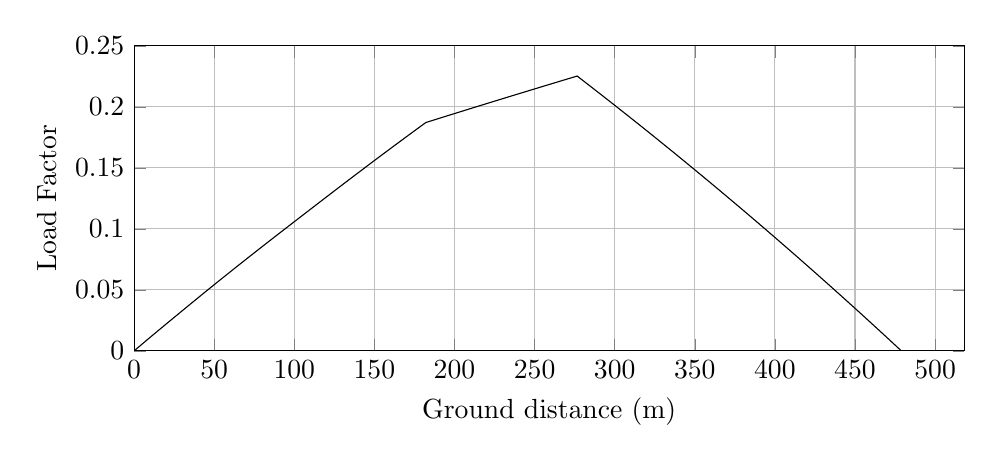
\begin{tikzpicture}

\begin{axis}[
width=\textwidth,
height=0.45\textwidth,
scaled ticks=false, tick label style={/pgf/number format/fixed},
xmin=0.0,
xmax=518.2299866992206,
xlabel={Ground distance (m)},
xmajorgrids,
ymin=0.0,
ymax=0.25,
ylabel={Load Factor },
ytick={0,0.05,0.1,0.15,0.2,0.25},
ymajorgrids,
legend style={at={(1.03,0.5)},anchor=west,draw=black,fill=white,legend cell align=left}
]

\addplot [
color=black,
solid
]
table[row sep=crcr]{
1.3603393307215537E-8	1.5374033208389272E-11\\
2.0334443352841076E-7	2.2981207716240697E-10\\
1.8493358258961232E-6	2.090048389684322E-9\\
9.983129263424352E-6	1.1282549412136833E-8\\
4.13538327636676E-5	4.6736510591868315E-8\\
1.2467543572893382E-4	1.4090335220700978E-7\\
2.843807411608912E-4	3.2139598492355305E-7\\
5.588015241105573E-4	6.315352016821599E-7\\
9.398454696015893E-4	1.0621749118034759E-6\\
0.0014155885812023746	1.5998385089136108E-6\\
0.0019945752038215015	2.254181668322058E-6\\
0.0026717822370171283	3.019526587593407E-6\\
0.003447739291558293	3.896470737478679E-6\\
0.0043193476547732645	4.881510918645401E-6\\
0.00529092766782709	5.979528362391867E-6\\
0.006363550519206555	7.191732101241853E-6\\
0.007533073890550759	8.513439089519928E-6\\
0.008790616877968567	9.934611089304765E-6\\
0.01016549189277427	1.1488372523477957E-5\\
0.011625499440327931	1.3138332203873978E-5\\
0.013184282533086976	1.4899906022816627E-5\\
0.014839871214038253	1.677086534061919E-5\\
0.01660567024659266	1.876635600414511E-5\\
0.018465948346479452	2.086859760642448E-5\\
0.0203822997817096	2.3034186868418095E-5\\
0.022430561433814646	2.5348821051771952E-5\\
0.024588423902376283	2.7787285607872693E-5\\
0.026831028501027587	3.0321486046815747E-5\\
0.029143159681622913	3.2934225735229906E-5\\
0.03155709159958957	3.5661971824487775E-5\\
0.03411445662773917	3.8551764326081156E-5\\
0.03677290089167576	4.155573904036866E-5\\
0.03952314881844239	4.466341085511817E-5\\
0.04239921643077808	4.791321190361803E-5\\
0.045357163155895136	5.125548714242575E-5\\
0.048363831658398165	5.4652768145384036E-5\\
0.051533845233668635	5.823456458974842E-5\\
0.0547899150155587	6.191354182119883E-5\\
0.058172599437445835	6.573552080893171E-5\\
0.06162834747858026	6.963999097993074E-5\\
0.06521401059050522	7.369118047790168E-5\\
0.06888104003120077	7.783423175891372E-5\\
0.07268727020998902	8.2134480631384E-5\\
0.076546425570032	8.649444817559005E-5\\
0.08047032364859658	9.092748214018012E-5\\
0.08456364881336098	9.555184296715504E-5\\
0.08882250397434277	1.0036311761898592E-4\\
0.09306368907640691	1.0515433840166077E-4\\
0.09743039119190974	1.1008725880359988E-4\\
0.10191450167634594	1.1515271081448359E-4\\
0.10651989152467789	1.2035505928429211E-4\\
0.11128201757858264	1.257343474356094E-4\\
0.11609763023253863	1.311739373438716E-4\\
0.12097769621339591	1.3668621260399963E-4\\
0.12591912973280778	1.4226768319829992E-4\\
0.13103216605369056	1.4804285398754057E-4\\
0.13633380151185176	1.5403090860729432E-4\\
0.1416823117522269	1.6007176409930699E-4\\
0.14708837902374172	1.66177481503649E-4\\
0.1525605467319851	1.7235770510484982E-4\\
0.15824953188605478	1.78782642032634E-4\\
0.16398006351864292	1.8525433685303056E-4\\
0.16978153473626356	1.9180597967617652E-4\\
0.17584258400626962	1.9865058706006224E-4\\
0.1819863832139092	2.055884559278913E-4\\
0.18819485651962437	2.125991677404148E-4\\
0.19455736971520038	2.197836260028782E-4\\
0.20098158490654017	2.2703755426626692E-4\\
0.2076061353991409	2.345174786439673E-4\\
0.21424726384720844	2.420159045107114E-4\\
0.2211374965027113	2.4979536189535155E-4\\
0.2281284453493247	2.576882951597784E-4\\
0.2350833915765042	2.655403428586382E-4\\
0.2423085249848444	2.736971777054362E-4\\
0.24958374984531584	2.819103055889826E-4\\
0.2569279402934431	2.9020102790968294E-4\\
0.2644720218029696	2.987171299361479E-4\\
0.27204626263318243	3.072669986207938E-4\\
0.27972793364503945	3.159378508054884E-4\\
0.2874622320100655	3.2466781813698166E-4\\
0.29563698092580604	3.338946222377273E-4\\
0.30361763245720474	3.429020378263768E-4\\
0.3118912000478351	3.5223973057035656E-4\\
0.3202493147046803	3.616725097154526E-4\\
0.3286412952843002	3.711431710839531E-4\\
0.33714554464307567	3.8074018689413457E-4\\
0.3458731203690518	3.9058886518892504E-4\\
0.35455185683415313	4.003820690010891E-4\\
0.3634323904331427	4.104026108233088E-4\\
0.372325738896249	4.204372354831124E-4\\
0.38151551889959867	4.308059367159902E-4\\
0.3908489672358084	4.413363258608903E-4\\
0.4001862088113266	4.518705808746726E-4\\
0.4095647137707429	4.624509731833196E-4\\
0.4192312859369268	4.73355913935878E-4\\
0.4289206911602753	4.8428616987958767E-4\\
0.43896550245304145	4.956168787280345E-4\\
0.4487817299761361	5.06689282478865E-4\\
0.4589033974758888	5.181057389285143E-4\\
0.4691858798479248	5.297030898902055E-4\\
0.47972601481223376	5.415905266756198E-4\\
0.49016040525287174	5.533581903794761E-4\\
0.5007175269203565	5.652637502946726E-4\\
0.511266977039379	5.771601399963439E-4\\
0.522323236324642	5.896274919565573E-4\\
0.5332586746953114	6.019580444215004E-4\\
0.5445869154512923	6.147309273662057E-4\\
0.5556699580072249	6.272267683052813E-4\\
0.5669225885056133	6.399132346790484E-4\\
0.5785590177532589	6.530317901711706E-4\\
0.5903083066022885	6.662769476956505E-4\\
0.6020327889628274	6.79493508115956E-4\\
0.613957077533064	6.929346556469871E-4\\
0.625960998969677	7.064649083088015E-4\\
0.6380070243193761	7.200419563870025E-4\\
0.6503365955459197	7.339379027196439E-4\\
0.662700086001522	7.478713821860289E-4\\
0.6752747602080436	7.620421498806897E-4\\
0.6885889407972636	7.770455067698572E-4\\
0.7019767933734617	7.92131072771879E-4\\
0.7151149754112038	8.069345196586283E-4\\
0.7284684478906998	8.219797468113903E-4\\
0.7418939875700234	8.371053616171792E-4\\
0.7553494584716574	8.522638846860849E-4\\
0.7694215958599202	8.681162561650387E-4\\
0.7830840331449673	8.835062486189832E-4\\
0.796657372658726	8.98795050823794E-4\\
0.8106660034246236	9.145732962328734E-4\\
0.8251837647136968	9.309240647314642E-4\\
0.8395067871054176	9.470545883371946E-4\\
0.8540519574023793	9.634343622278068E-4\\
0.8688334527125461	9.800793091120424E-4\\
0.8840141863517745	9.971728195096253E-4\\
0.8993797082767976	0.0010144733661138587\\
0.9143697020410035	0.0010313500913154878\\
0.9294094610857999	0.0010482818530384262\\
0.9452486359568626	0.0010661125243933416\\
0.9605773823977486	0.0010833675440802167\\
0.9761522209726621	0.0011008985292406603\\
0.9917649966835071	0.0011184711544974415\\
1.0074810114554809	0.0011361589066623086\\
1.0234652146968335	0.0011541473936437707\\
1.0399433598517231	0.001172690598967257\\
1.0563627364420554	0.0011911665020313577\\
1.0728309985448887	0.001209696243959322\\
1.0896486452479222	0.001228617899647706\\
1.1068138420051672	0.0012479293317721994\\
1.124143995869574	0.0012674250630733267\\
1.1415400048645106	0.0012869935847115823\\
1.1590089082607062	0.0013066428022023037\\
1.1769249919091855	0.0013267936605376395\\
1.1951505705127592	0.0013472912165126624\\
1.2127191877709298	0.001367048579106042\\
1.2308827453761335	0.0013874736252179915\\
1.2492706857898845	0.0014081495692425886\\
1.267587852451018	0.0014287445135232348\\
1.2860031245644312	0.0014494483375160022\\
1.304687144125951	0.001470452849877318\\
1.3233765774990474	0.001491461982692523\\
1.342322280991234	0.0015127577002968132\\
1.3613696045164358	0.0015341661305729906\\
1.3815086998747366	0.0015568000230985794\\
1.4013123019267382	0.0015790552160458407\\
1.4209622886438908	0.0016011361671356185\\
1.4411501686096515	0.0016238198897491822\\
1.4611760119255748	0.0016463198780962394\\
1.4816444281325132	0.0016693154082945208\\
1.501865958841821	0.0016920318777642255\\
1.5224364680875304	0.0017151386592939367\\
1.543651615594651	0.0017389677438441873\\
1.5647593029468103	0.0017626743010758837\\
1.5859558716309676	0.0017864788533615546\\
1.6071423964076703	0.0018102702977178687\\
1.6293386351549652	0.001835193645933506\\
1.6508498980272122	0.001859345953941686\\
1.673011606043147	0.0018842266080976073\\
1.6946435720294923	0.0019085106163146174\\
1.717066624993247	0.0019336807085447148\\
1.739432891071898	0.001958785044562732\\
1.761922286799709	0.001984025561834994\\
1.7849035550437842	0.0020098160325787095\\
1.8076299607761817	0.002035318414176838\\
1.8313298306791497	0.002061910976009842\\
1.8543134894513886	0.0020876977785068366\\
1.8777326664639729	0.0021139710628548356\\
1.9017196849182967	0.0021408791438104293\\
1.925345883672024	0.0021673802469308417\\
1.950252961491087	0.0021953157116738216\\
1.975161211119453	0.00222325005504409\\
1.9993825790313986	0.0022504117373897447\\
2.024583888346972	0.002278669886340451\\
2.04934017380271	0.002306426621042781\\
2.0744229633459703	0.0023345470014033277\\
2.0996193404956136	0.002362792267868924\\
2.1245764901457758	0.0023907669370335245\\
2.1500786393425866	0.0024193500164572594\\
2.176226227020705	0.0024486539093915324\\
2.202115608176549	0.0024776658392830445\\
2.227948363055355	0.0025066117525385243\\
2.2543499999408594	0.0025361924684517406\\
2.2810892744412783	0.0025661487677621653\\
2.3075963743135786	0.0025958422742274573\\
2.3348582111613405	0.0026263784625195036\\
2.3623221378972126	0.002657138168081073\\
2.3898598419727675	0.0026879776445977565\\
2.4171687299087603	0.00271855804879335\\
2.445442108612223	0.0027502155341608304\\
2.4735885391813177	0.0027817279007296245\\
2.5015416452491293	0.002813020892518064\\
2.5301110763218357	0.002845000838090238\\
2.5589284934403693	0.0028772552978755484\\
2.587611617795936	0.0029093563884904842\\
2.6175687086884984	0.0029428800051800974\\
2.647724154312196	0.0029766222466866836\\
2.6767118187859253	0.0030090546517865893\\
2.7060305938995466	0.003041854377049212\\
2.7361546404224653	0.003075551703326559\\
2.7663022704956823	0.003109272092617399\\
2.7964672462043376	0.0031430085697699566\\
2.8272583584284883	0.003177441908162033\\
2.8588650092419234	0.0032127836811365463\\
2.8898852960400587	0.0032474662867022436\\
2.9215246589961597	0.0032828374859432724\\
2.95270311230069	0.003317689892414686\\
2.984506337549637	0.003353237102308586\\
3.017379145769185	0.003389976010739374\\
3.049243647754313	0.0034255843520042705\\
3.081295157663824	0.0034613980324002154\\
3.113406837946715	0.003497275294116478\\
3.1453724573084756	0.003532985746619026\\
3.1787286104953543	0.003570245795919007\\
3.211019796961401	0.0036063125118886573\\
3.245786703184362	0.003645140325425546\\
3.279939251746722	0.003683277907741348\\
3.3141720228361216	0.0037215009930596757\\
3.3491198891036547	0.003760518326321434\\
3.382965192547779	0.003798300675236337\\
3.4181848705561064	0.003837613069400587\\
3.45391888941694	0.003877495205234442\\
3.488851494856137	0.0039164786563732285\\
3.524271454997704	0.003956001708464862\\
3.5606552075305	0.003996595738134049\\
3.597189071478943	0.00403735271377598\\
3.632926148839256	0.004077216413938136\\
3.668897146318187	0.004117336679188617\\
3.706642714683163	0.0041594315168277055\\
3.7432264628550644	0.004200226086973859\\
3.781286297809391	0.004242661877159699\\
3.818618572105483	0.004284281747773006\\
3.8564015479305356	0.00432639935081316\\
3.8948624022541356	0.0043692677272015885\\
3.9329637046009225	0.004411730513789391\\
3.971505929995028	0.00445467981614325\\
4.009821706071438	0.004497371926012291\\
4.049014376833089	0.004541036099814634\\
4.089343885784727	0.004585961565009396\\
4.128662304630717	0.004629755606835391\\
4.1684827283974055	0.004674103671731239\\
4.208000253554632	0.004718109315040597\\
4.2483743636521965	0.004763063615254516\\
4.288255503180503	0.00480746386419704\\
4.328757204126676	0.004852549764976895\\
4.369490126907612	0.004897887761715651\\
4.410357715197167	0.004943370327468552\\
4.45189144941496	0.004989588820420421\\
4.492881116440694	0.005035196515995147\\
4.53550011161515	0.00508261147443238\\
4.577670191557685	0.005129521369208531\\
4.6201174049766305	0.005176733908302581\\
4.662272021613388	0.00522361542234917\\
4.706017761800355	0.005272260616533555\\
4.748842845578064	0.005319876280186416\\
4.792293145132742	0.005368181292042443\\
4.836482439768313	0.0054173018885152295\\
4.88090298307878	0.00546667348415619\\
4.925311889063089	0.005516026097070046\\
4.969864686447545	0.005565532563612248\\
5.014842280541593	0.005615504926743528\\
5.0603877575117515	0.005666101979940528\\
5.106292347304597	0.005717091628227079\\
5.152263975081851	0.005768149376210083\\
5.1974808794106995	0.005818362709818108\\
5.244027372436168	0.005870046159551677\\
5.28996242022761	0.005921044349740975\\
5.336209145350672	0.00597238223761704\\
5.38320569473032	0.006024546007914806\\
5.430469292142472	0.006076999615678416\\
5.476900151253712	0.006128522647473706\\
5.526063828851289	0.0061830713284090864\\
5.573879040902945	0.006236117076516704\\
5.622613575936374	0.006290175871690076\\
5.6713596863799225	0.006344240623414446\\
5.720412183296268	0.006398638267512179\\
5.770660497446668	0.006454354860049492\\
5.820668144990444	0.00650979741373121\\
5.870305285939629	0.0065648221353236105\\
5.920503816994749	0.00662046205507926\\
5.971105439367246	0.006676541536175241\\
6.021088325934068	0.006731928207005985\\
6.071322359863801	0.006787586101249198\\
6.122981826035449	0.006844815963730003\\
6.174329110820436	0.006901692604981579\\
6.225804784288178	0.006958704106229942\\
6.278093246139479	0.00701660829571604\\
6.331709873490098	0.007075975466108491\\
6.384325657889258	0.007134226774857282\\
6.436648686434458	0.007192146461727316\\
6.489478972803882	0.007250620096365213\\
6.543185721519176	0.0073100560532747836\\
6.596747696432654	0.007369324027346013\\
6.650345873843312	0.007428624329164869\\
6.704555155195255	0.007488592912980344\\
6.7588986063680725	0.00754870204417058\\
6.814371620173711	0.007610052480240359\\
6.86997180120154	0.007671535378341327\\
6.925426612865756	0.007732849404269517\\
6.981353650685165	0.0077946773692703294\\
7.037678624474159	0.007856936987698657\\
7.094603706786671	0.007919851548539672\\
7.151204881983983	0.007982399788382173\\
7.209200593921791	0.008046480505954117\\
7.2667780016693655	0.008110090473803637\\
7.324687293141565	0.008174058535684366\\
7.382771066065313	0.008238210745781491\\
7.441904508776327	0.00830351349495636\\
7.501585831803217	0.008369412323671796\\
7.5616527251378685	0.008435727842152053\\
7.62150963104709	0.008501802538779845\\
7.682859947113334	0.008569516506580093\\
7.7432084367972145	0.008636115617016637\\
7.803024936926759	0.008702118756293897\\
7.863793829029664	0.008769163777806677\\
7.9252460466886365	0.008836953501953616\\
7.98696966925656	0.008905033354735742\\
8.04776546969778	0.008972080802827366\\
8.109421212326083	0.009040067504004311\\
8.17269125419024	0.009109824763768863\\
8.236095044780246	0.009179719877109478\\
8.299523592514586	0.009249632703414426\\
8.363213767675873	0.009319824309015661\\
8.427807923256076	0.009391002399879044\\
8.49144930156071	0.009461121020434827\\
8.557380457258176	0.00953375248752819\\
8.623183572921022	0.009606232827115336\\
8.687840683575093	0.009677441117535704\\
8.753751426394068	0.009750020156239039\\
8.820803713780364	0.00982384602164581\\
8.888970287482593	0.00989888823559562\\
8.957133699158991	0.009973916434620096\\
9.025036015045707	0.010048646823212787\\
9.092760955867519	0.010123171694724488\\
9.159817422823458	0.010196950885644712\\
9.227495373767134	0.010271403740708764\\
9.296013084156197	0.010346770109185652\\
9.36435980631623	0.010421938116837783\\
9.433329865923408	0.01049778131819181\\
9.503849553921977	0.010575317875587928\\
9.574524061692681	0.010653013861999643\\
9.644263228942293	0.010729671045074553\\
9.715657612596786	0.010808136855220533\\
9.787429657508813	0.01088700679517514\\
9.85753688572494	0.010964036745938386\\
9.930250735750551	0.01104391977451002\\
10.001571447096964	0.011122261552013435\\
10.074699859091687	0.011202577987080329\\
10.14698611653175	0.01128195860476576\\
10.220547980738981	0.011362728973150465\\
10.2940409891517	0.011443412672783518\\
10.36719293590382	0.011523711019413093\\
10.441008888975666	0.01160472725902665\\
10.51610421670324	0.011687136413444028\\
10.590724589239105	0.011769013175916066\\
10.667218005391902	0.011852933625676772\\
10.742771202259895	0.01193581120654734\\
10.82035208750042	0.012020901368579678\\
10.896759047300378	0.012104692481210193\\
10.973503045910835	0.012188841789895802\\
11.051297940743765	0.012274131794135243\\
11.128076326409062	0.012358295967348484\\
11.207667705350879	0.012445531865475172\\
11.286758396846047	0.012532207093621942\\
11.366305937658339	0.012619371098399107\\
11.446149720998452	0.01270684780197811\\
11.526866579636565	0.012795268995943049\\
11.607297517600138	0.012883365005226263\\
11.688034241538357	0.012971783999342859\\
11.769665722224765	0.01306117080242655\\
11.850920080706608	0.013150132665787597\\
11.933163326324259	0.013240165118165044\\
12.017103780766782	0.013332043051677726\\
12.10034832931326	0.013423146917421356\\
12.185467765774142	0.013516290047041081\\
12.270669986481685	0.013609511056742886\\
12.354040133273898	0.013700715345759963\\
12.440386807402234	0.013795163206201964\\
12.52556588630658	0.01388832139733954\\
12.610860989997974	0.013981594101563924\\
12.69550109439961	0.014074138384846302\\
12.784634337461807	0.014171582401304386\\
12.871172079509357	0.014266176245165829\\
12.958447214271366	0.014361563580890779\\
13.045518554761987	0.014456715715105284\\
13.133090172249581	0.014552402090308187\\
13.221405510214687	0.014648888535882164\\
13.310319106907201	0.014746015939870837\\
13.399783591735492	0.014843732406755825\\
13.488943611067967	0.014941103731643937\\
13.578276665194153	0.015038651515543375\\
13.667402973129146	0.015135961157476396\\
13.757763665999576	0.01523460599231918\\
13.848393619195729	0.01533353219975129\\
13.938857764339925	0.015432264963115066\\
14.031101516310692	0.015532927279505657\\
14.123507833735925	0.01563375423038121\\
14.214825187590282	0.015733380533269108\\
14.307956552027534	0.015834973259119735\\
14.401498558574918	0.01593700118901839\\
14.495315613017755	0.016039316395296203\\
14.589065423003394	0.016141545645368478\\
14.68316852398955	0.01624414756129205\\
14.778702641747682	0.016348296953579537\\
14.873746415615575	0.016451899115251106\\
14.970384078097169	0.01655722584979747\\
15.068900921005241	0.01666458752139814\\
15.164434274206265	0.01676868522540195\\
15.260378587808539	0.016873218337736026\\
15.357189194448868	0.016978682817159075\\
15.45495288999333	0.017085172981323293\\
15.55311774366497	0.017192087489309088\\
15.652583807013901	0.01730040640780847\\
15.755243917873962	0.017412190296791162\\
15.855950289561445	0.017521833754075747\\
15.958461094374158	0.017633428628230516\\
16.060387288500337	0.01774437406483493\\
16.164276126126843	0.017857442589461064\\
16.26736468838029	0.01796962706279488\\
16.36946523634058	0.018080723651526017\\
16.47192386662276	0.018192197304906035\\
16.576794358652606	0.01830628213055161\\
16.678929175716583	0.018417378500550946\\
16.783994526910618	0.01853164989175816\\
16.89012564586595	0.018647067556709588\\
16.996887404888547	0.01876315812826152\\
17.103774697793426	0.018879372372236004\\
17.210947675936964	0.018995884486699262\\
17.31865021419634	0.019112959599538088\\
17.424470519881233	0.01922797641817496\\
17.53205215515201	0.019344895321273776\\
17.64034909906897	0.01946257922101527\\
17.74911485075183	0.019580760196036138\\
17.85745376408675	0.01969846521095467\\
17.969383314157206	0.019820058677510525\\
18.07998395718984	0.01994019607679836\\
18.18863741327577	0.020058206516013085\\
18.302466989554325	0.020181826370699058\\
18.41305080779906	0.020301909253588362\\
18.525644000014054	0.020424162072135942\\
18.636945827420575	0.020545000952822485\\
18.750643923449367	0.020668429496153523\\
18.86479622056296	0.020792339145030935\\
18.979646899421056	0.020916994939531506\\
19.09418630108147	0.02104130113213445\\
19.208983505033515	0.021165875505231076\\
19.323483295898072	0.021290115730263848\\
19.43842354827664	0.021414822599410008\\
19.55563752357537	0.021541984920275196\\
19.67199913451129	0.021668211249701634\\
19.789486593639566	0.021795647643270515\\
19.90713985662446	0.021923252751753636\\
20.024127533725753	0.02205012510846392\\
20.143019013955552	0.022179051205709736\\
20.26442367074238	0.022310691423330323\\
20.383660776265387	0.022439970542712205\\
20.5042342316437	0.022570687860712663\\
20.622773342122727	0.022699189380431136\\
20.74503732713029	0.022831718313013092\\
20.865944869938517	0.022962766612215392\\
20.98711015528624	0.023094084178054714\\
21.113336299999695	0.023230876104032915\\
21.23638685227678	0.023364216469753556\\
21.35988644990264	0.023498033551237762\\
21.483760012473958	0.02363224609606233\\
21.608180515260266	0.023767041608888866\\
21.732326713270083	0.02390153053277864\\
21.85766379468624	0.02403730022087048\\
21.985117186778353	0.02417535296821258\\
22.111729024702363	0.024312484996044208\\
22.23700541150786	0.024448161811443804\\
22.36297326225872	0.024584578877015626\\
22.488604760551	0.024720623285123942\\
22.616276341350805	0.024858868478146317\\
22.744235570279145	0.024997416869262427\\
22.874576476768283	0.025138535737640844\\
23.003842066605536	0.025278482323695103\\
23.13088450205612	0.025416014464081923\\
23.257869280739328	0.025553476870288225\\
23.389244224935425	0.025695684199080984\\
23.519811196806458	0.02583700962103881\\
23.653309395988643	0.02598150049107725\\
23.78342402399784	0.02612232229166732\\
23.9180644861338	0.02626803543954417\\
24.05110504604577	0.02641201043268411\\
24.182394801971697	0.026554084445799077\\
24.314614014384034	0.026697158184331653\\
24.449791085561472	0.02684342653789904\\
24.585258581909038	0.026990003231537836\\
24.72121222319008	0.027137100228800077\\
24.857032405393277	0.027284047362217657\\
24.99454740444294	0.027432822842238674\\
25.13030709358258	0.027579694275514544\\
25.270890409679986	0.02773177916362582\\
25.40663839363527	0.027878628565965298\\
25.54307796688363	0.028026221846941694\\
25.68272814639034	0.028177284017876295\\
25.82072003425767	0.02832654848530173\\
25.96015212691003	0.028477367127850435\\
25.987750021099068	0.028507218353751695\\
26.0558803939429	0.028580910917093486\\
26.061632797568386	0.02858713291310103\\
26.066808273335674	0.028592730879519256\\
26.071901058608013	0.028598239400787238\\
26.073315434863225	0.028599769235123793\\
26.074595035914804	0.028601153292026994\\
26.080371168076944	0.028607400935564672\\
26.10234540095133	0.028631168895525885\\
26.183408179590366	0.028718847999082538\\
26.300430535410044	0.028845419587590244\\
26.42750601924636	0.028982861636729255\\
26.558056987479794	0.02912405916555627\\
26.688030995483615	0.029264628870686853\\
26.818767077324992	0.029406018677321878\\
26.951519978077492	0.029549585182633793\\
27.083955405447817	0.02969280359929974\\
27.216897884715692	0.029836565311060655\\
27.350913258119895	0.029981481853853978\\
27.4833530065795	0.030124689042099383\\
27.6176201223548	0.030269866257271127\\
27.752160408628434	0.030415332614648852\\
27.887329802382908	0.03056147263370969\\
28.023188645890663	0.030708351197530733\\
28.158973127824495	0.03085514223551436\\
28.296372294036907	0.031003671322742565\\
28.435107205966254	0.031153636416848905\\
28.571323599682245	0.03130087110759515\\
28.70996262687553	0.03145071597803442\\
28.850320389600306	0.03160240959352689\\
28.988837241064125	0.031752104570547\\
29.129197813929657	0.03190378262832612\\
29.27166529868488	0.03205772751446292\\
29.41298471572133	0.03221042166209486\\
29.554848516656044	0.03236369355436497\\
29.699676691743235	0.032520157131285886\\
29.842400551696755	0.032674336130834605\\
29.985385440862252	0.032828785703561236\\
30.129077275410303	0.032983987150688565\\
30.27543774584293	0.0331420586163377\\
30.422081339040986	0.033300423074515174\\
30.56949149516445	0.033459602206230656\\
30.716562179458485	0.03361840135729968\\
30.86535310281699	0.03377904404512006\\
31.011875026602333	0.03393722309803117\\
31.16159928701196	0.03409884475680984\\
31.313692569485013	0.03426300841038601\\
31.463056706803336	0.0344242110911111\\
31.61235366859384	0.03458532593262824\\
31.76278957628285	0.03474765411611985\\
31.915019899787076	0.034911902213662735\\
32.06709627595497	0.0350759675347234\\
32.21861178877769	0.035239410956363786\\
32.37168228565527	0.03540451448277895\\
32.52450570609457	0.035569333927154306\\
32.67702483599189	0.035733807440801485\\
32.829998687403204	0.03589875326477175\\
32.98551220909506	0.0360664187461725\\
33.14332298937855	0.03623654140239533\\
33.29970221124884	0.03640510110274228\\
33.45800124694219	0.03657570992389953\\
33.61398946945653	0.036743808092917725\\
33.77048353048475	0.036912431046963894\\
33.9292721471582	0.037083505354319125\\
34.08796840843395	0.037254458754788874\\
34.24769686644211	0.037426502234404344\\
34.406855482575295	0.03759790991503349\\
34.56481953291838	0.03776800913719872\\
34.72399692808165	0.03793939257008753\\
34.88694269464703	0.03811480988043162\\
35.04914399338672	0.03828940194572416\\
35.209965099803895	0.038462484724872056\\
35.3703140559587	0.03863503568860116\\
35.531685786905925	0.03880866318872906\\
35.69349909442164	0.0389827413500224\\
35.85522798807463	0.03915670402748839\\
36.022509111806116	0.0393366127617303\\
36.19055880791667	0.03951732107667234\\
36.35708622463872	0.039696365524846296\\
36.52115360367851	0.03987273861666029\\
36.68781562330062	0.04005187391578856\\
36.8536847754776	0.04023012974872494\\
37.024522648961764	0.040413696718952744\\
37.19188554678789	0.04059350141616216\\
37.36066720850286	0.0407748017061296\\
37.528862119520696	0.04095544291896646\\
37.697264258302326	0.04113627769427848\\
37.86832931534104	0.04131994208150624\\
38.03812867477943	0.041502217558534955\\
38.20923731912278	0.041685868107589605\\
38.37904730305398	0.04186809444182254\\
38.55252405124031	0.042054224229577886\\
38.72282139824354	0.04223691165031978\\
38.89783411301201	0.04242462525661419\\
39.0714610757495	0.04261082006234834\\
39.24438070689564	0.04279622400682247\\
39.41969314875929	0.04298416040583245\\
39.59166556575205	0.04316848371331274\\
39.764623188591585	0.043353830299472054\\
39.94263254662576	0.043544556082719996\\
40.11749159802578	0.04373187238046037\\
40.29452954971913	0.04392148818411325\\
40.47247750600427	0.04411204337799207\\
40.64799609178485	0.04429996229509945\\
40.82414741101539	0.04448852375933944\\
41.00385670225303	0.04468085769071965\\
41.18169069533937	0.0448711484735724\\
41.3603281005193	0.04506226263499734\\
41.54046179251334	0.045254940594478245\\
41.722675278204306	0.04544980524054358\\
41.90258931008478	0.04564217320064385\\
42.08518735141125	0.04583737264043191\\
42.26728550944881	0.04603199911599255\\
42.44743534848537	0.04622450518343317\\
42.63069538383506	0.04642029581466249\\
42.80963512098974	0.046611432708293196\\
42.992542679335614	0.0468067689206785\\
43.17926890616222	0.04700614252396763\\
43.363134036078335	0.047202420883006434\\
43.54815051311773	0.047399887776483844\\
43.733578141849236	0.047597752568090776\\
43.91798130912079	0.04779448344475489\\
44.10506009255049	0.04799402718099616\\
44.29251116260117	0.04819392584802364\\
44.480917546793805	0.048394800632548036\\
44.66851287589745	0.04859476811724275\\
44.85853501730759	0.048797279056245396\\
45.047396872181054	0.04899851006300155\\
45.236914792155844	0.04920039652494828\\
45.42785879536018	0.04940375789909376\\
45.616432631699865	0.04960455129687691\\
45.80697204128492	0.04980739346696435\\
45.998633580597016	0.0500113853429933\\
46.18800675699903	0.05021289734901566\\
46.380841640082096	0.05041804764089042\\
46.57327038933336	0.05062272020116214\\
46.765844918266424	0.05082750207824589\\
46.95911042680183	0.05103297266185469\\
47.15311668852311	0.051239184286306395\\
47.34541611633634	0.05144353566218922\\
47.53884854699059	0.05164904475010027\\
47.73236991243341	0.051854601797983284\\
47.92818250719388	0.052062545147584925\\
48.12326385407131	0.052269664454110715\\
48.32058854034828	0.05247911725134779\\
48.516852452700604	0.05268739586178992\\
48.71339374517507	0.05289592059849404\\
48.91319881343868	0.05310785858576767\\
49.1119162355681	0.053318593314346206\\
49.31207818344666	0.053530809913583666\\
49.509673461222235	0.05374025599822962\\
49.71156302510582	0.053954203327491373\\
49.91034548441702	0.05416480798937775\\
50.11200805970151	0.0543784133400409\\
50.30853267551517	0.054586527282906125\\
50.50757456960626	0.05479725745719281\\
50.70929197287772	0.05501076941625655\\
50.91222418686718	0.05522551555950478\\
51.11562549758783	0.05544070610182659\\
51.32090674103446	0.055657832736146794\\
51.525199701657655	0.05587386138888519\\
51.72863462744459	0.05608893049690878\\
51.934060761332375	0.0563060518073915\\
52.14033810224923	0.05652401931669184\\
52.344882977561255	0.05674010327483824\\
52.55098100649393	0.05695777472959248\\
52.75731843494604	0.05717564546549196\\
52.96514817708821	0.05739503776441926\\
53.17450540782369	0.05761598758816612\\
53.382202621450276	0.05783513100112121\\
53.592230583406476	0.05805667845610433\\
53.80364534107798	0.05827963278079432\\
54.01469481143569	0.05850214587993203\\
54.223966920081466	0.058722729858688934\\
54.43230789395902	0.05894227778601525\\
54.6430562980421	0.05916430726586349\\
54.855225786754914	0.059387777677967754\\
55.066088958624874	0.05960981634486733\\
55.27969530828261	0.05983468685139641\\
55.49171188337613	0.060057827342331525\\
55.70388919125476	0.060281080788664884\\
55.91737779085577	0.06050565727772136\\
56.13177028494084	0.060731127424927714\\
56.34652664868587	0.06095692285389737\\
56.559021044851505	0.0611802835714986\\
56.77591447970492	0.061408210416874325\\
56.99548236897459	0.06163888829423847\\
57.21481285737903	0.061869257092876544\\
57.43536222847358	0.0621008460640568\\
57.65367025761124	0.06233002227777102\\
57.872788904232735	0.06255999029556518\\
58.0907693980174	0.06278870507290354\\
58.311927420720366	0.06302069407514824\\
58.532333513628615	0.06325183450942597\\
58.75532998033057	0.06348563080362264\\
58.976617007999806	0.06371757464206554\\
59.19875422837053	0.0639503493763271\\
59.4206945143671	0.06418285757352557\\
59.64453328369959	0.0644172938411211\\
59.86894932484513	0.06465227351647705\\
60.09432075877773	0.06488819200725447\\
60.318058693038594	0.0651223396593277\\
60.541731124044205	0.06535635823431761\\
60.76707064338231	0.06559205993758385\\
60.995574692986196	0.06583100922420919\\
61.22378989589207	0.06606959381070819\\
61.4534619981562	0.06630963842062715\\
61.683510138770515	0.06655001276438029\\
61.91410430469678	0.06679089422368845\\
62.14462153858659	0.06703163200439556\\
62.37563158073512	0.0672728210875298\\
62.607203285434	0.06751453308177346\\
62.841031881319736	0.06775853644498568\\
63.07467935056491	0.06800228637806056\\
63.31164975340633	0.06824943731604145\\
63.54633691305479	0.068494141975473\\
63.78243968758058	0.06874025763521488\\
64.0165414084598	0.0689842231473333\\
64.25412817577254	0.06923175533688203\\
64.49270299572771	0.06948025102543885\\
64.73076499662056	0.06972814692419776\\
64.96867826857735	0.06997582263068393\\
65.21063576532572	0.07022764173970629\\
65.4512107007771	0.0704779553849806\\
65.69028017871045	0.07072663709576275\\
65.93032615763332	0.07097626904796983\\
66.17196619696679	0.07122749262032184\\
66.4135612157637	0.07147860330607082\\
66.6559030093851	0.07173042401970706\\
66.89910102540284	0.07198306805749775\\
67.14354652182666	0.07223694124155405\\
67.38771133480921	0.07249045630770848\\
67.63347396558368	0.07274556339313513\\
67.87898066495345	0.07300033795797098\\
68.1255935515739	0.0732561934397496\\
68.37316753306138	0.0735129787153975\\
68.62205497364681	0.07377105858690915\\
68.8711887275476	0.0740293261188164\\
69.120220471977	0.07428742042381634\\
69.36846244647072	0.07454462934037161\\
69.61951843592018	0.07480468628016589\\
69.87236615109754	0.07506653071372045\\
70.12758921381476	0.07533076561949564\\
70.37945082809051	0.07559145232673693\\
70.63410009691182	0.07585495592695063\\
70.89152727368702	0.07612126438267625\\
71.14629115974091	0.07638474903092679\\
71.40197865069018	0.07664912055916905\\
71.66163317144085	0.07691752410348057\\
71.92484704501203	0.0771895355288924\\
72.18465416754285	0.07745795617017336\\
72.44573394560723	0.07772762177265864\\
72.70633339061075	0.07799672171800212\\
72.96699363118216	0.07826581529308858\\
73.22900401485182	0.07853623334281319\\
73.49076816912304	0.07880632817773428\\
73.75430841254712	0.0790781862245735\\
74.01895646534612	0.07935111733070466\\
74.2846979982242	0.0796251062150821\\
74.55380714249793	0.07990249619877639\\
74.82322871850147	0.08018013701832191\\
75.09350011520078	0.08045858239057009\\
75.36421232425869	0.08073741082653056\\
75.6347219158074	0.08101595991418184\\
75.90830954343213	0.08129760708981344\\
76.18188601743822	0.08157917137577068\\
76.45626363461818	0.0818614889014716\\
76.72958718025629	0.08214265128992239\\
77.00406935908524	0.08242493509480883\\
77.28579748399531	0.082714597836853\\
77.56784659723587	0.08300451703769299\\
77.84569092555657	0.08329004261443017\\
78.1246978223638	0.0835766919407761\\
78.40641219364133	0.08386605122954746\\
78.68590470271565	0.08415305766234506\\
78.96851680469001	0.08444319643506365\\
79.25576208114188	0.08473801899351154\\
79.54169104977237	0.08503141815948322\\
79.82662017154695	0.085323720047493\\
80.11330301632765	0.08561774970853771\\
80.40394576721474	0.08591576825027333\\
80.6908099930996	0.08620984131945751\\
80.98055888331655	0.086506800418883\\
81.27178512217935	0.08680520214681166\\
81.56682943128612	0.08710744350299704\\
81.86186977412851	0.08740960838500465\\
82.15688924927383	0.08771168007160761\\
82.44965588234726	0.08801137463623172\\
82.74488606927187	0.08831352058636671\\
83.04325841243121	0.08861881100042376\\
83.34213327641098	0.08892454433855305\\
83.64411622775171	0.08923338528752058\\
83.94734638805741	0.08954342978777838\\
84.25123842984891	0.08985407932379305\\
84.55152885577829	0.09016097726658065\\
84.85735750691177	0.09047346454365196\\
85.16518306664875	0.09078792077890434\\
85.47136476235073	0.09110062732864084\\
85.77898122624802	0.09141472918587362\\
86.08923229760057	0.09173145078706485\\
86.40254560035129	0.09205122744332077\\
86.71167807044037	0.09236666776208828\\
87.02660518802142	0.09268795095932654\\
87.34238286044419	0.09301003167703575\\
87.65842706333811	0.09333231461485822\\
87.97971380652302	0.09365987295923389\\
88.2973933745065	0.093983684485015\\
88.61789013566766	0.09431029861394434\\
88.93643920279564	0.09463486001594418\\
89.25662431900213	0.09496102096737552\\
89.57903058309674	0.09528937707341188\\
89.89968694948243	0.09561588466481559\\
90.22473455398588	0.09594679694469473\\
90.55024875587375	0.0962781178037634\\
90.87789352676518	0.0966115409570874\\
91.20733069500889	0.09694672194893063\\
91.54101415610151	0.09728615653310106\\
91.87012785371462	0.09762087769654929\\
92.20120197152713	0.09795752855524584\\
92.53416638543635	0.09829603759271976\\
92.86431843528567	0.09863162500882675\\
93.19748455591187	0.09897021402048944\\
93.53066771200866	0.0993087588854429\\
93.86681917526724	0.09965025848402986\\
94.20530590547477	0.09999406921267506\\
94.5419273964865	0.10033592533480289\\
94.8854212036891	0.10068469993447302\\
95.22752713476521	0.10103200538458085\\
95.57091181422334	0.10138054989197581\\
95.91383450860906	0.10172856738147325\\
96.25469535763642	0.10207443588066725\\
96.5966517898868	0.10242136046437149\\
96.93845701474973	0.10276807701885864\\
97.28153572459905	0.10311603146938844\\
97.62213139590432	0.10346141521265854\\
97.9659652144934	0.10381003072533308\\
98.3129807304216	0.10416182037482564\\
98.65852794036775	0.10451207086868079\\
99.00080640577195	0.10485895935079413\\
99.35064076251427	0.10521345641396491\\
99.69796076807248	0.10556535762356752\\
100.04654253174803	0.10591849025608797\\
100.3915606488718	0.10626796745551358\\
100.74261509654437	0.10662351389324619\\
101.08877163494762	0.10697405629557542\\
101.43457754260953	0.10732420163123155\\
101.784020212797	0.10767798783619978\\
102.13161434601102	0.1080298622173594\\
102.4751980097893	0.10837763831904129\\
102.82212110631409	0.10872875693313991\\
103.16739702108615	0.10907817195345686\\
103.51524666207362	0.10943015584571683\\
103.86391679154056	0.10978293512798004\\
104.20960434827006	0.11013266334861829\\
104.55241399635099	0.1104794483233666\\
104.89662223620601	0.11082761743245956\\
105.24103428322039	0.11117596301469579\\
105.5836615386647	0.11152247504322187\\
105.92645892081137	0.11186913187972315\\
106.27347658175316	0.11222002985240105\\
106.6151670762521	0.11256551596888757\\
106.95898391938218	0.1129131279818322\\
107.30023552029138	0.11325812363403412\\
107.64147805753461	0.11360308847887267\\
107.98348674656944	0.1139488071909293\\
108.32522459759954	0.11429423256350119\\
108.3935347040271	0.1143632775196173\\
108.40478590462831	0.11437464968540283\\
108.41572478024443	0.11438570614935772\\
108.4246743308916	0.1143947518900675\\
108.44347342986478	0.11441375300175818\\
108.52018987797786	0.11449129326031578\\
108.70071173483461	0.1146737499132225\\
108.99446230248458	0.11497063724617655\\
109.30176454987088	0.11528120477134694\\
109.60899173332959	0.11559167890465909\\
109.91608539831654	0.1159019996132111\\
110.22883517949637	0.11621801586774139\\
110.54143546549608	0.11653385988539695\\
110.853845249356	0.11684948926811524\\
111.1739714794031	0.11717289060890668\\
111.4937490010879	0.11749591436628021\\
111.81170779322963	0.11781707482406367\\
112.13106495813236	0.1181396205096813\\
112.4519453366479	0.11846367611484847\\
112.77515902629136	0.11879005820831359\\
113.0997499810409	0.11911779982124547\\
113.43040796942478	0.11945163409614108\\
113.7597028375028	0.11978405773102246\\
114.0907450350197	0.1201182096041561\\
114.42538740208008	0.12045595801425603\\
114.75997726261329	0.12079361470902568\\
115.09477047197589	0.1211314367933213\\
115.43440545481076	0.12147410266493694\\
115.77494672336013	0.12181763955949411\\
116.11687534861284	0.12216253124584514\\
116.46164587354252	0.12251024293447989\\
116.8077846490165	0.12285928644265894\\
117.15688723722127	0.12321126869748107\\
117.50557855048987	0.1235627851107015\\
117.85411336711965	0.12391409155011907\\
118.20532793701167	0.12426804515096418\\
118.55850697655507	0.12462392287354812\\
118.91273956155123	0.12498080501282914\\
119.26983096270519	0.1253405082794965\\
119.62978614725739	0.12570303512810993\\
119.98960731920661	0.1260653645302583\\
120.34734904217265	0.1264255369687228\\
120.7138511704587	0.12679446304810177\\
121.08106061642908	0.127164032705306\\
121.44737887966437	0.12753263609258683\\
121.81499139152783	0.127902471044704\\
122.18511446431708	0.12827475900964444\\
122.55384158147794	0.12864556919209294\\
122.92460728481757	0.12901835424844751\\
123.29616941264607	0.1293918632992619\\
123.67040864389355	0.12976798470739875\\
124.04652172406458	0.1301459086447379\\
124.42393851457416	0.1305250601113209\\
124.80152108360014	0.13090429438221088\\
125.18180835736592	0.13128615945179684\\
125.55854932865631	0.13166437760849078\\
125.93878032356085	0.13204601173718072\\
126.31997081831156	0.13242851938878272\\
126.70099538833193	0.13281076993815535\\
127.08058279416298	0.13319148761661076\\
127.46175209000612	0.1335736994170757\\
127.84399628255431	0.13395689500051594\\
128.22749916598133	0.134341256771147\\
128.6102537001487	0.1347247720336264\\
128.99595881306152	0.13511114526603898\\
129.37788117916477	0.13549363085748245\\
129.760738924708	0.13587695406724312\\
130.1448498512433	0.13626143131888155\\
130.53000390659713	0.13664685055016823\\
130.9168242384266	0.13703383335708338\\
131.29443328439476	0.13741149977327807\\
131.67491382268804	0.1377919361250785\\
132.05816436539135	0.138175037830788\\
132.44070735535217	0.1385573270221609\\
132.82666098215685	0.13894291721933888\\
133.20952005887244	0.13932530843093616\\
133.5940193955625	0.13970922950513162\\
133.97617966856654	0.1400907066323405\\
134.36103715882757	0.14047476617907342\\
134.74478042358356	0.1408576031820577\\
135.12867144169206	0.1412404763263397\\
135.5141335746535	0.14162480372830497\\
135.89764893392993	0.14200707731467013\\
136.28231234485685	0.14239038154849984\\
136.66418763078912	0.14277079421457994\\
137.04684871033697	0.143151875774891\\
137.42845627025127	0.14353179398539995\\
137.8132447087305	0.1439147629033474\\
138.19719797258034	0.14429678377639787\\
138.58059071069573	0.14467812989380188\\
138.96593237593703	0.14506129606986473\\
139.3501607499636	0.1454432363964111\\
139.73355638294606	0.14582423007703724\\
140.1160230155566	0.14620418171219007\\
140.50045093994146	0.14658596155292716\\
140.88215178690393	0.14696491334738324\\
141.26156782058217	0.1473414780085738\\
141.64323970440188	0.14772016158218504\\
142.02689350659642	0.1481006897748855\\
142.41061312971692	0.14848116062910421\\
142.7942251403153	0.14886140171582452\\
143.1756303563767	0.14923933294300132\\
143.5599719391364	0.1496200498129884\\
143.94242380128833	0.14999877079888094\\
144.3239499176869	0.15037645140405548\\
144.70664939692608	0.15075516903428812\\
145.0870075357763	0.15113144571429785\\
145.46856550308127	0.15150878477153903\\
145.85014610541765	0.15188602103912874\\
146.23128237819492	0.15226269269615125\\
146.61504730324998	0.15264183527344244\\
146.99763315977907	0.15301968582966607\\
147.38441582478964	0.15340155183372578\\
147.7673688364352	0.15377950832217888\\
148.15222568696134	0.15415921461101478\\
148.53580865353604	0.15453753486061567\\
148.9199734867533	0.15491629939246315\\
149.3040357319486	0.1552948328226648\\
149.68771357306542	0.15567285734105463\\
150.07093078701052	0.15605029798934478\\
150.45622889618164	0.15642965687270846\\
150.8449053483268	0.15681220836138465\\
151.2288570611563	0.15718997749468377\\
151.61452719766493	0.15756930498040464\\
151.9983007305741	0.15794663509198106\\
152.38299664478842	0.15832473975275088\\
152.76945776909372	0.15870444573392595\\
153.15580177123394	0.15908390253088553\\
153.54253364040335	0.15946360577880977\\
153.93093169697067	0.15984480928853168\\
154.31788037931886	0.16022445490246687\\
154.7039882138024	0.16060314067805523\\
155.08880221957185	0.16098042328496862\\
155.47621608980313	0.16136011935975486\\
155.866104687065	0.161742103425953\\
156.25391419262098	0.16212191362736472\\
156.64166339424906	0.1625015280996315\\
157.03027969880475	0.16288185423172033\\
157.4213807682267	0.16326447326862636\\
157.8105708506119	0.1636450843671079\\
158.19948541262937	0.16402528799760033\\
158.58893406813365	0.164405875400295\\
158.97894817604634	0.1647868765398765\\
159.3710019698692	0.16516973010015448\\
159.76139479981174	0.16555082199190213\\
160.1523485688823	0.16593232170175506\\
160.54128874338664	0.16631171766913488\\
160.9326976430911	0.16669338192339458\\
161.32564259741588	0.16707640281510294\\
161.71827778345698	0.16745898043796853\\
162.1124492087963	0.1678429128180979\\
162.50576001021273	0.16822586496393635\\
162.89904576730015	0.16860865091132962\\
163.29316224934274	0.16899210313775936\\
163.68899123279596	0.16937707817942735\\
164.08495392634194	0.16976203953966598\\
164.48271131475576	0.17014860101775572\\
164.8792309171331	0.17053381520812372\\
165.27343112400507	0.17091663330668005\\
165.67115293733156	0.17130272704526497\\
166.06936395728349	0.17168915053977551\\
166.47000821435734	0.17207778872692137\\
166.87155839526775	0.17246715828871795\\
167.27134041220108	0.17285466679602526\\
167.67233991204222	0.17324320861402856\\
168.0705846918417	0.1736289358678973\\
168.47232570996516	0.1740179027216621\\
168.87521546679773	0.17440783386732234\\
169.2789990941189	0.1747984816156083\\
169.68142011368735	0.17518766326891594\\
170.088438196605	0.17558114076559397\\
170.49328200513543	0.17597236682716144\\
170.89845866435633	0.17636376540429738\\
171.30484584057905	0.17675618361143722\\
171.7103088520891	0.17714756013855001\\
172.11589069074847	0.17753890234711953\\
172.52485519917514	0.17793335772365887\\
172.93316089774754	0.1783270268414337\\
173.34236088095247	0.17872140717610643\\
173.7535761368399	0.1791175776987103\\
174.16510964781833	0.17951390238572498\\
174.5786011126259	0.17991195928384685\\
174.99051444770384	0.18030834430997159\\
175.40138574541044	0.18070357502561404\\
175.81497300453447	0.181101265679831\\
176.2280441317456	0.18149830742991782\\
176.64225100058474	0.18189628795336835\\
177.05714873395152	0.18229477904573643\\
177.47483026786767	0.18269578921851212\\
177.89254345086653	0.18309667488090547\\
178.3100126079721	0.18349717186526968\\
178.7278240622369	0.18389784289398545\\
179.1449731538625	0.1842977249968253\\
179.56482315926417	0.1847000414123385\\
179.9871804296257	0.18510460400794604\\
180.4095742002126	0.18550904503010252\\
180.83428717371925	0.18591554918766942\\
181.26003251256287	0.186322883294815\\
181.6840913989422	0.18672844682631254\\
181.8934642440371	0.18692863017245961\\
182.1114839456617	0.18713704039057175\\
182.5372774346568	0.18731270117714066\\
183.423900814602	0.1876783497454258\\
184.30144226609173	0.18804008386398363\\
185.17422251923585	0.1883996889205611\\
186.05126240753827	0.18876088219040363\\
186.93861419286333	0.18912615237059893\\
187.8243328275641	0.18949058026330337\\
188.7212117513506	0.1898594273407667\\
189.61004025875786	0.1902247925649843\\
190.50102451880866	0.19059087341064312\\
191.38947474753866	0.190955743473092\\
192.28052744689825	0.1913215125946151\\
193.18778236606096	0.191693758356086\\
194.08895872822546	0.19206333647967636\\
194.99680020640938	0.19243547348745133\\
195.89480429656658	0.1928034061117658\\
196.79674305679504	0.19317277920490297\\
197.7065692706791	0.1935452086176229\\
198.612023604503	0.19391567554104389\\
199.52644538440046	0.19428963690704662\\
200.43881964763966	0.19466258652737184\\
201.34572312669928	0.1950331276971632\\
202.26115686844895	0.19540698054614303\\
203.17967892292364	0.19578191981696788\\
204.1017087672932	0.19615811535165575\\
205.01405834107487	0.1965301885701767\\
205.94020355690031	0.19690771272650875\\
206.86420646269943	0.1972841882452001\\
207.79153006365993	0.19766184116229793\\
208.72800400232427	0.1980430425878907\\
209.6603812871926	0.19842239930264\\
210.59913361291103	0.1988041718367719\\
211.54272242703126	0.19918773186287025\\
212.4892775421681	0.19957231751931623\\
213.4278558742791	0.19995348463426924\\
214.37319863683314	0.20033722071148063\\
215.31618532994997	0.20071982287848222\\
216.26909967312713	0.2011062735265089\\
217.2229300472723	0.20149291557707805\\
218.17915574443117	0.20188034836163227\\
219.13394290547268	0.20226701888239335\\
220.0901210939433	0.20265407371032249\\
221.05386294760763	0.20304400962027017\\
222.0194744620763	0.20343452078954163\\
222.9871855528732	0.20382569975574502\\
223.95850156259326	0.20421815410428254\\
224.93506896411378	0.2046125472883102\\
225.9123601081958	0.20500704981398546\\
226.89683950214788	0.2054042697017675\\
227.87812705537118	0.20580001837652342\\
228.86553252311342	0.20619805033909558\\
229.85786107077195	0.20659788160178094\\
230.84893890233656	0.20699702433947487\\
231.8352011637358	0.2073940453102411\\
232.83551070617193	0.20779653598792014\\
233.8409775535427	0.20820091479929367\\
234.84473749332597	0.2086044209434268\\
235.85076677249623	0.20900865351392753\\
236.86174655712836	0.2094146886586067\\
237.8698887650736	0.20981939873850258\\
238.88314164945962	0.210225974733197\\
239.88702917374013	0.21062861002390718\\
240.9073981595622	0.2110376700687159\\
241.92631922506058	0.2114459638495936\\
242.95020737895555	0.21185606186699127\\
243.9867665418509	0.21227104586189746\\
245.01566609591487	0.21268277607413863\\
246.05919400906686	0.21310017042493692\\
247.09706457910846	0.2135151134699607\\
248.1403037320082	0.213932014448656\\
249.18309170866138	0.2143485473022001\\
250.23723200462985	0.21476942488346962\\
251.28895058541582	0.21518914634751787\\
252.34575298177748	0.2156107073203439\\
253.4009695529494	0.21603144735779725\\
254.47389199439823	0.21645905524927575\\
255.55293546958148	0.21688890859290177\\
256.6206413021679	0.21731405495777367\\
257.69235364004487	0.21774060724033828\\
258.77967411403563	0.2181731789102428\\
259.8615409937813	0.21860338936097176\\
260.93956317950165	0.21903188198588705\\
262.02271022117964	0.21946222281715297\\
263.11073386748035	0.21989431176842386\\
264.2120045516847	0.22033146945549145\\
265.31241535302627	0.2207680940045243\\
266.4086016357777	0.22120285293333225\\
267.51260488983417	0.22164052232779033\\
268.6300148019782	0.22208331392870104\\
269.7585470354529	0.22253031747264873\\
270.8896873949477	0.22297815832010906\\
272.0115439451323	0.22342213128722496\\
273.13680176546006	0.22386725932964507\\
274.2702490513931	0.22431543496282555\\
275.413525774062	0.2247673034529244\\
276.3239236681536	0.2251269907026162\\
276.5542367829295	0.22521796531064428\\
277.554788259544	0.224206722827575\\
278.5499282368744	0.2232000050250077\\
279.5468210518608	0.22219056853443428\\
280.54457272161665	0.22117931398115118\\
281.5347601972437	0.22017478706505217\\
282.51938272683515	0.2191749773364813\\
283.5221719980424	0.21815576825724425\\
284.52144002460784	0.21713918113650685\\
285.5065413744376	0.21613607030767384\\
286.49067071596266	0.21513302053104708\\
287.4855387842832	0.21411808117535025\\
288.4785328044295	0.21310410595590523\\
289.4558376341987	0.21210522606167545\\
290.4452179546196	0.21109306814768694\\
291.4362341762878	0.21007829176139003\\
292.42552923534424	0.20906433369718289\\
293.4112881717839	0.20805306080326158\\
294.3958772331042	0.2070420514369346\\
295.37586350088816	0.2060348379973262\\
296.3639498807927	0.20501835879040708\\
297.3501848614277	0.20400284148359235\\
298.3398532517323	0.20298284120595642\\
299.3128667606111	0.20197907996295533\\
300.2979722329835	0.20096190815314052\\
301.28589571931684	0.1999408794038438\\
302.2517321223603	0.19894176005370087\\
303.22560994216224	0.19793340252418437\\
304.19844887137424	0.19692519783524334\\
305.16721169680045	0.19592030004060035\\
306.14133092388545	0.19490892213613553\\
307.1183129647659	0.1938936405178007\\
308.08874758460775	0.19288423873318586\\
309.05104077529325	0.19188239486925682\\
310.0116623058466	0.19088138632441762\\
310.97416663340744	0.18987750808344483\\
311.93862106265544	0.1888706836951671\\
312.9042085878807	0.18786176084994408\\
313.8607306878614	0.18686140620716307\\
314.8103087392675	0.18586742298353348\\
315.7635145755504	0.18486874884048807\\
316.72127527573787	0.1838644001370814\\
317.68202711729873	0.18285600515592376\\
318.62951500322526	0.18186063880253295\\
319.5882925222194	0.18085250872991984\\
320.5331857914575	0.17985808749475918\\
321.4802787033931	0.1788604638337948\\
322.42948830671753	0.17785971825550653\\
323.38313368290176	0.17685339570568526\\
324.31736547478727	0.17586668322980842\\
325.2560396282021	0.1748744050094755\\
326.1918178881874	0.17388431543191413\\
327.12581340820736	0.17289524250901483\\
328.06785507666075	0.1718967682006242\\
329.00598052108364	0.17090156491226377\\
329.93709199652426	0.16991293342464803\\
330.86383958236627	0.1689280750760532\\
331.7940264405214	0.1679386979484013\\
332.7190974456154	0.16695390313601172\\
333.6413079242308	0.16597130005170524\\
334.55125241868143	0.16500093025880255\\
335.46660340028666	0.16402395646501922\\
336.3747308431896	0.16305386074856693\\
337.2875172156404	0.16207795262029634\\
338.19828079330546	0.16110337152899762\\
339.109611360101	0.16012734751009722\\
340.0129870615515	0.1591590168005964\\
340.91909778436093	0.1581869273364491\\
341.81644111043147	0.15722342663154962\\
342.7133692535617	0.15625955852884643\\
343.6184676625437	0.15528608555057263\\
344.51737039439627	0.15431845550550086\\
345.4159820554156	0.15335032051969552\\
346.30095283991204	0.15239608149893408\\
347.17992936105065	0.15144751916566396\\
348.06324428581195	0.1504934844163847\\
348.9364433780921	0.1495495958087492\\
349.80883972935715	0.1486058002644208\\
350.6725450259156	0.1476706436742636\\
351.5472086084487	0.14672284752936338\\
352.4072535743069	0.14579013150037248\\
353.2770101509982	0.1448461154232031\\
354.13828190935476	0.1439105470907324\\
354.9933330028563	0.14298098585131222\\
355.85205864704324	0.1420466769525997\\
356.7071105330664	0.14111561488116386\\
357.55662905210625	0.14018983604407032\\
358.3968855315861	0.13927342254542907\\
359.2442002307205	0.13834857721581095\\
360.08339527712974	0.13743186752752867\\
360.9246104267437	0.1365122244808317\\
361.7545426495701	0.1356042027612465\\
362.581918833003	0.13469827159174838\\
363.4093806494336	0.13379154109800448\\
364.23264192171564	0.13288871277157374\\
365.05797482153	0.13198291041733798\\
365.8765610813148	0.13108381749340822\\
366.6868045921444	0.13019320568438894\\
367.4906771263371	0.12930892562611337\\
368.2952198328626	0.12842323850138085\\
369.0972808321063	0.1275396158374704\\
369.8964582846754	0.1266585065232208\\
370.6930530520266	0.1257795851521997\\
371.4728865706744	0.1249185189827654\\
372.2678562262888	0.12404008950255889\\
373.06106899862266	0.12316294629591995\\
373.84382996836246	0.12229671887238482\\
374.6159909394505	0.1214415964931473\\
375.3856302934837	0.12058864826410409\\
376.1473504597384	0.1197438681051064\\
376.91317968965916	0.11889392029706099\\
377.68323290861986	0.11803866685428625\\
378.4403029180851	0.11719722886906994\\
379.1869255532997	0.11636681533737656\\
379.93805310858056	0.1155308025118835\\
380.6856374163734	0.11469814654408468\\
381.43021045639625	0.11386826220890726\\
382.18008046874786	0.11303188623012034\\
382.92513258826534	0.11220029936357669\\
383.6506231543186	0.1113899857071439\\
384.3822860805168	0.11057221768258689\\
385.0990882750988	0.10977051319739826\\
385.8170433174296	0.10896697717984577\\
386.52234575345665	0.10817707330581278\\
387.2376414658007	0.10737544194196995\\
387.93937547097994	0.10658848478280153\\
388.64083062377483	0.10580132093464639\\
389.33134235465366	0.10502593010458715\\
390.0273880382074	0.10424381511636202\\
390.7068665546425	0.10347982172137016\\
391.40282314876936	0.10269679421072636\\
392.0855974079484	0.10192809989168691\\
392.75818287930633	0.10117039358119398\\
393.43867085808176	0.10040329654641764\\
394.11027968502674	0.0996457270734983\\
394.786759986094	0.098882178569135\\
395.4566036152579	0.09812564195366362\\
396.1166927015505	0.09737965579500682\\
396.7644616700177	0.09664714244734454\\
397.4244929822212	0.09590030322552538\\
398.08014509529926	0.09515795986426809\\
398.7259878602912	0.09442627503741995\\
399.3670096194496	0.09369961225137145\\
400.01048041429635	0.09296973235519368\\
400.6524530744772	0.09224111132569521\\
401.2849921803854	0.0915227665741456\\
401.9182641221695	0.09080316122059541\\
402.54543114898365	0.09009007038382177\\
403.1748134003958	0.08937403771929892\\
403.79833980526837	0.08866424890103419\\
404.42118950858446	0.08795481458484995\\
405.0408464729951	0.08724860419781087\\
405.6607425327045	0.08654170925616883\\
406.26485178835514	0.08585241994554339\\
406.8597412181373	0.085173267524182\\
407.46585224174294	0.0844809129904122\\
408.0662523853787	0.08379469258643056\\
408.655389120426	0.08312096868103541\\
409.25135626022404	0.08243905362835581\\
409.8369706591932	0.08176861180537161\\
410.43440926548703	0.08108425226662067\\
411.0160612808693	0.08041760644866529\\
411.5941953689414	0.07975463101611874\\
412.1674464950138	0.07909689898091228\\
412.734523134238	0.07844590226682872\\
413.29884338477484	0.07779772497567028\\
413.85822071671885	0.07715488540362257\\
414.4235767236336	0.07650483126645051\\
414.9756751838046	0.0758696870616994\\
415.52331092793077	0.07523935084764403\\
416.0720467794564	0.07460742257070949\\
416.61315945743	0.07398395364673115\\
417.1498178093706	0.07336530342048612\\
417.68871269335546	0.07274376057393366\\
418.213024658514	0.0721387346461349\\
418.7487921979216	0.07152018126902937\\
419.2826225641252	0.07090355422093918\\
419.81472679740534	0.07028861276198234\\
420.3393026309021	0.069682070297297\\
420.8604642413378	0.06907917903894373\\
421.3862485865561	0.06847064047576414\\
421.9006948750339	0.06787493306374594\\
422.41070045731215	0.06728408314008473\\
422.9183404173573	0.06669569223185774\\
423.4327666201011	0.06609914884555013\\
423.92933708268527	0.06552303756899706\\
424.43895944904557	0.06493150381427445\\
424.93445901473285	0.06435609081443679\\
425.4198125365714	0.06379220008066733\\
425.91930825977954	0.06321160982165101\\
426.4108084343004	0.06264004682952592\\
426.89157456876444	0.062080710639219085\\
427.3736881996448	0.06151955262143797\\
427.8496231617944	0.060965336577536035\\
428.32144537553563	0.06041566473670997\\
428.7978436156403	0.059860414223415405\\
429.28662524009326	0.059290471949709\\
429.7517265638312	0.05874789861353923\\
430.2077548556547	0.05821567904426603\\
430.6704827834137	0.05767540704489504\\
431.13687084231697	0.057130623498203824\\
431.59309180658613	0.05659748470938383\\
432.0390207763545	0.05607615192927049\\
432.47870377400955	0.05556190708951982\\
432.9226261034879	0.0550424881563517\\
433.3702476615605	0.054518521179647846\\
433.81357695887505	0.05399936100561768\\
434.25289010134236	0.05348469029878796\\
434.6869895946435	0.052975918575534756\\
435.12081000122475	0.05246726632048754\\
435.5465841270244	0.05196784638709428\\
435.97079761070574	0.051470058044714606\\
436.4032388308824	0.050962410434306764\\
436.8208756819258	0.05047194575218017\\
437.2428780941283	0.04997615845723057\\
437.65831737641963	0.04948788951247625\\
438.07449525839706	0.04899856110052399\\
438.4798586505311	0.0485217637887919\\
438.8801341197226	0.04805077254373883\\
439.2774252258897	0.04758311748179367\\
439.67454163191667	0.0471154933465306\\
440.08265413035883	0.04663473870383731\\
440.4830325234242	0.04616291539378\\
440.8710779160597	0.045705456198448687\\
441.254892759021	0.045252820000580854\\
441.6456364075525	0.044791844673882426\\
442.02456795184594	0.044344642658060464\\
442.41121361063506	0.04388817234985301\\
442.7985842558204	0.04343067958687079\\
443.1769055394532	0.04298371334671685\\
443.55254824634756	0.04253975427131145\\
443.9259891916414	0.04209824183278332\\
444.3030104440239	0.041652339077693216\\
444.674103821343	0.04121329273624216\\
445.04034037517226	0.04077984226544396\\
445.4037778533881	0.040349556907274854\\
445.7636722139358	0.039923321355425104\\
446.1291957847294	0.039490271183588485\\
446.49089901524326	0.03906160050077037\\
446.8434091500312	0.038643684584398964\\
447.1951592480543	0.038226531550257854\\
447.5480390419008	0.037807900032862204\\
447.8888710968424	0.037403429130112124\\
448.2232780502105	0.03700645692726312\\
448.5695349749209	0.036595286074388916\\
448.9131599145677	0.03618710819220425\\
449.2546587859289	0.03578132502241776\\
449.59140495362647	0.03538106152993517\\
449.92365092477667	0.03498602276718679\\
450.2550065332498	0.03459191963710323\\
450.5774555501497	0.034208291738073306\\
450.9067791352977	0.03381636480081398\\
451.2262588294801	0.0334360369886733\\
451.5446423651084	0.03305690036565313\\
451.85981865448844	0.032681471115138715\\
452.17286021532425	0.032308474484101686\\
452.485101553783	0.031936321890576005\\
452.7939211463413	0.03156814004175929\\
453.11563538546886	0.031184471116280962\\
453.4205931794901	0.030820678311962762\\
453.7185675152773	0.030465115442393404\\
454.0291147351188	0.03009444367845648\\
454.3253401264327	0.029740765634156327\\
454.625408234736	0.02938239907424175\\
454.91924571575555	0.029031375599840755\\
455.21001656151043	0.028683920044822946\\
455.50906506672493	0.02832647397036047\\
455.79760992652587	0.027981487328363433\\
456.08525234765193	0.02763748642419748\\
456.3748276163918	0.027291079919672247\\
456.65778848978425	0.0269524947570152\\
456.94502562893797	0.026608700501600035\\
457.2224151597867	0.0262766046592954\\
457.50206662469736	0.02594171304661004\\
457.7779915858325	0.025611197674795576\\
458.05289153110823	0.025281824780651843\\
458.3227518000808	0.02495840733539755\\
458.58298691694813	0.02464644749514649\\
458.865823997996	0.02430730666341396\\
459.1299660785854	0.02399050090077042\\
459.39418961868967	0.02367351866307618\\
459.65140006995796	0.023364874152855514\\
459.90483996565365	0.023060681129785578\\
460.16759641890076	0.022745229253949308\\
460.4177998634233	0.022444775384373113\\
460.66914013637165	0.022142885151909316\\
460.91581309169453	0.02184653151784234\\
461.15597697915894	0.021557931813141678\\
461.40442664219484	0.02125930664298348\\
461.6497208795613	0.02096440566537455\\
461.884848732382	0.02068166316677764\\
462.1249399499592	0.020392887648618033\\
462.3548296683347	0.020116321093722304\\
462.59392111683655	0.019828621025733476\\
462.82864666919477	0.019546111504787776\\
463.05840238629366	0.019269523121198822\\
463.28934123912245	0.01899145018008883\\
463.5153136473856	0.018719298835647078\\
463.7399720648243	0.018448672643929662\\
463.9659015361807	0.018176457633628865\\
464.18695428936223	0.017910062414331292\\
464.3998655747921	0.01765342626149703\\
464.60995420611255	0.017400142048115165\\
464.82221240223885	0.017144191347892464\\
465.02855209714403	0.01689532845015044\\
465.23474184044437	0.01664659814389729\\
465.44114204133325	0.016397565630569592\\
465.6504781176818	0.01614494143247092\\
465.8563115189272	0.01589649570362307\\
466.05710956985536	0.015654081395679392\\
466.259586795425	0.01540959352155991\\
466.4623106938607	0.015164761131575964\\
466.65655025762726	0.01493013157826998\\
466.8463729446395	0.01470079591393431\\
467.0400434013393	0.01446676932486245\\
467.2286520220075	0.014238818345630351\\
467.41602508837445	0.014012320592678068\\
467.6040280943298	0.0137850212322447\\
467.7865197864421	0.013564346703317931\\
467.9713018555203	0.013340863973581875\\
468.15331862826577	0.013120687715785945\\
468.33653545871357	0.012899021729904198\\
468.51494200960997	0.012683138769298483\\
468.68791747010937	0.012473793163894568\\
468.8587930721561	0.012266955484156291\\
469.03502763812924	0.012053596170724995\\
469.2065153890993	0.011845949652242496\\
469.3787117791077	0.01163741136415386\\
469.54748302940993	0.01143298830331767\\
469.71381150197885	0.011231492281183598\\
469.8750087078164	0.011036182362871549\\
470.0284243928302	0.010850273187003818\\
470.1942986390417	0.010649236530285653\\
470.3557248916626	0.010453560638714362\\
470.50832501292075	0.010268556182945022\\
470.662219471192	0.010081955638893407\\
470.81619226813336	0.009895233067915375\\
470.9684608833742	0.009710550552581573\\
471.1239971309394	0.009521877497308193\\
471.2744598615021	0.009339332591529848\\
471.42645266157797	0.009154905131894217\\
471.5769060331462	0.008972319633832345\\
471.7228556686126	0.008795175031479075\\
471.86550389128	0.008622013972665179\\
472.00433776236116	0.008453460848814499\\
472.14110822716907	0.008287391302343015\\
472.2753920688489	0.008124320274466633\\
472.4079304600285	0.007963348676278965\\
472.5424227452238	0.007799983499605534\\
472.67794158334584	0.007635350479588669\\
472.806572126578	0.007479066182768377\\
472.9434059970463	0.007312794197032347\\
473.0654603709596	0.007164463270910169\\
473.19728043742975	0.0070042451063614675\\
473.3207541610101	0.006854153320195249\\
473.4462913839001	0.006701535316339317\\
473.56198107640614	0.0065608731830434945\\
473.6790427084221	0.006418527383220993\\
473.8013669142715	0.006269765594285386\\
473.9194325040123	0.0061261665868062596\\
474.0340416638726	0.005986756255195055\\
474.1454889806239	0.0058511775662936465\\
474.25370907548927	0.005719511275848353\\
474.36797328608907	0.0055804768443662185\\
474.4783004391145	0.005446218763276226\\
474.5860666831137	0.005315063620124162\\
474.6895219281081	0.00518914259696005\\
474.79559331973826	0.005060024593499398\\
474.8949256232098	0.004939098226782979\\
474.9919594527363	0.004820959092066969\\
475.0977636221953	0.004692129736312805\\
475.19572868124555	0.0045728340099506085\\
475.2884259982126	0.004459942886146332\\
475.3774705861339	0.004351490955084177\\
475.46962762965563	0.004239238638367194\\
475.5587109438094	0.004130721040669684\\
475.64926688934906	0.004020400222485509\\
475.73449110415004	0.0039165662609532415\\
475.82776543129125	0.003802914804383288\\
475.91950167054404	0.0036911277249610666\\
476.00266803129466	0.0035897753087031524\\
476.08718192086496	0.003486772574154683\\
476.16708933238715	0.0033893765300322043\\
476.24808486795234	0.003290646741230119\\
476.32916014459295	0.003191812217054497\\
476.4101608329265	0.003093061090891775\\
476.4859226829369	0.003000690027325077\\
476.5608976486636	0.0029092718741364413\\
476.63772535602675	0.002815587954393815\\
476.7100094300712	0.0027274383709193846\\
476.7799037287549	0.0026421973897487634\\
476.84596999959035	0.002561619802754814\\
476.91556850409984	0.002476728717128221\\
476.98194230220804	0.0023957657104529515\\
477.04718229510206	0.002316180796542998\\
477.1092853361084	0.002240418046922374\\
477.1704129306444	0.0021658409725370856\\
477.2316926527219	0.0020910739940311306\\
477.2900490359508	0.0020198697546185283\\
477.35254723284584	0.0019436074962797653\\
477.411007145132	0.0018722688203832208\\
477.46713163663026	0.0018037763685707496\\
477.5210462113182	0.0017379774194613705\\
477.5750561056906	0.0016720587929074221\\
477.6304594327046	0.0016044360130733214\\
477.68138628732606	0.0015422739025947368\\
477.73264949056545	0.001479698231794055\\
477.78819487713326	0.0014118920034774463\\
477.83801585513595	0.0013510707497231802\\
477.8879750461085	0.00129007790337401\\
477.9350010705473	0.0012326634039441465\\
477.98248274101024	0.001174690024907412\\
478.0296164402404	0.001117138944602532\\
478.0724673104404	0.0010648150595146458\\
478.1140255122824	0.0010140675972131151\\
478.15277561867845	9.667473628061545E-4\\
478.190693184422	9.204421271080331E-4\\
478.22992888494116	8.725254356256448E-4\\
478.2658035378711	8.287118834140637E-4\\
478.30049539151787	7.863414721967105E-4\\
478.33300823316733	7.466311115130477E-4\\
478.3670626128602	7.050366528931109E-4\\
478.40189895025514	6.624857221502261E-4\\
478.43442577060387	6.227544977582118E-4\\
478.46377576604675	5.869026934670744E-4\\
478.492220060696	5.521562822914661E-4\\
478.51982947465547	5.184288386230139E-4\\
478.5466563922297	4.8565644721330773E-4\\
478.57089466843047	4.560456895133052E-4\\
478.59770561666016	4.232912333101326E-4\\
478.6222536120463	3.93300661600598E-4\\
478.6458207845668	3.645077209252682E-4\\
478.66996657916127	3.3500719281530773E-4\\
478.69062274504154	3.0976964503662085E-4\\
478.7114089403874	2.8437273313930574E-4\\
478.7299491754652	2.617195530012745E-4\\
478.7488193070292	2.386628867624623E-4\\
478.7672906499389	2.1609308813581813E-4\\
478.78401502458894	1.9565753998502679E-4\\
478.799138524383	1.7717782729994897E-4\\
478.8128055780869	1.6047754960882692E-4\\
478.8257034510938	1.4471696527341497E-4\\
478.83875735701235	1.2876552144710487E-4\\
478.85177952389483	1.1285266648936046E-4\\
478.8633371916625	9.872923994937781E-5\\
478.8738533564501	8.587839269630716E-5\\
478.8835380557704	7.404349120628287E-5\\
478.89421090828307	6.100092132030661E-5\\
478.9021238283964	5.133099327074687E-5\\
478.90945708534116	4.2369374224684756E-5\\
478.9149428237838	3.566547786235835E-5\\
478.92074695198005	2.8572452747663582E-5\\
478.9265367067967	2.149695425696879E-5\\
478.9308452679421	1.6231556384173506E-5\\
478.93511482290853	1.101380605097768E-5\\
478.93807121536076	7.40083695749642E-6\\
478.940410750546	4.54171405304651E-6\\
478.94216908996634	2.3928606256287866E-6\\
478.94333778961015	9.645995833877688E-7\\
478.94402732672324	1.2191954837071283E-7\\
478.9441270894074	6.992926444523064E-25\\
};
\end{axis}
\end{tikzpicture}%

%\caption{Load factor in aborted take-off condition - ATR-72}
%\end{figure}
%%
%\begin{figure}[H]
%\centering
%%VerticalForces_vs_GroundDistance
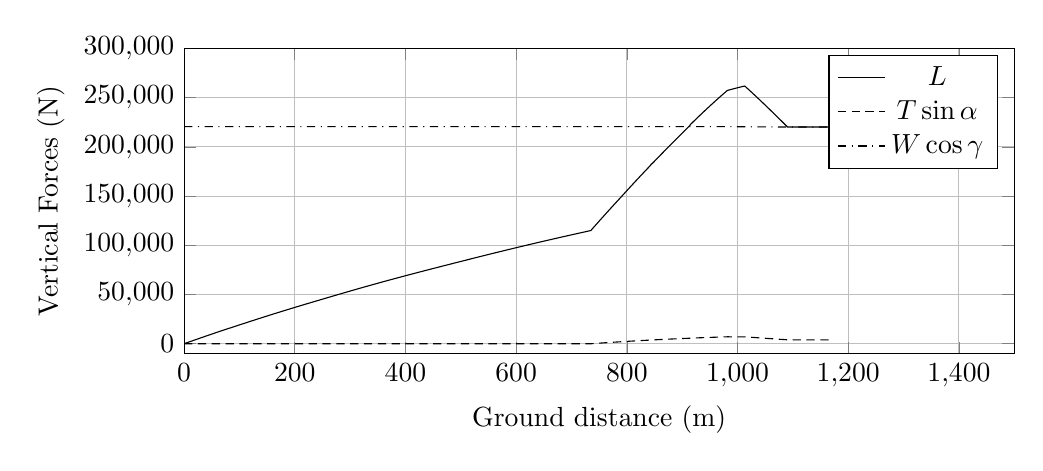
\begin{tikzpicture}

\begin{axis}[
width=\textwidth,
height=0.45\textwidth,
scaled ticks=false, tick label style={/pgf/number format/fixed},
xmin=0.0,
xmax=1500,
xtick={0,200,400,600,800,1000,1200,1400,1600},
xlabel={Ground distance (m)},
xmajorgrids,
ymin=-10000.0,
ymax=300000,
ylabel={Vertical Forces (N)},
ytick={0,50000,100000,150000,200000,250000,300000},
ymajorgrids,
legend entries = {$L$\\$T\sin\alpha$\\$W\cos\gamma$\\}
]

\addplot [
color=black,
solid
]
table[row sep=crcr]{
1.3729668748938318E-8	2.806282665006737E-6\\
1.7493248493808052E-7	3.57554147017018E-5\\
1.4411937280317895E-6	2.945735280121515E-4\\
6.602995160656227E-5	0.013496223553729522\\
2.2740573828771224E-4	0.04648068642961645\\
4.8751428921765393E-4	0.09964561424061016\\
8.441986619835749E-4	0.1725500630170857\\
0.0012981647037285577	0.2653382014993034\\
0.0018484379050661159	0.37781071516138964\\
0.0024893731755424335	0.5088136299141717\\
0.0032286585096692284	0.6599181411123156\\
0.0040442418752796045	0.8266167863151783\\
0.004972762654474916	1.0163981283595875\\
0.005990910102221513	1.224497385309705\\
0.007111389191545643	1.4535110399840767\\
0.008336865178450469	1.7039835009995983\\
0.009664633507451486	1.9753616188502932\\
0.011093815858158905	2.267465482034736\\
0.01262066151120312	2.579528084735368\\
0.01419454386807839	2.9012018507490334\\
0.015910782250193378	3.251967925426192\\
0.017721549103721458	3.6220506937457744\\
0.019620507964630857	4.010154638044908\\
0.02164969955342029	4.424871320911528\\
0.023766550611781796	4.85749918631511\\
0.025957065600157342	5.30517743092814\\
0.028260861173784894	5.776001968801147\\
0.030668466949245715	6.268036630827707\\
0.0331489614440674	6.774961488443127\\
0.03573888453685943	7.304243345819678\\
0.038418765463712895	7.851902385355661\\
0.04116679597872082	8.413481286995548\\
0.044022059812866554	8.996966393798317\\
0.04700053365173311	9.605621673231713\\
0.050116649382181494	10.242395198315496\\
0.0533021652593606	10.89334096844776\\
0.056630220296749106	11.573403652440081\\
0.05998688030085898	12.259300877412034\\
0.06348077825220624	12.973229833906924\\
0.06710848437295475	13.714488364709307\\
0.07082346760424127	14.473567542104202\\
0.07462944469130567	15.251225884499924\\
0.07855413323217031	16.053125691933182\\
0.08251243142992878	16.861877985159396\\
0.08659905947434482	17.696834930482943\\
0.09083545394947079	18.562374747990532\\
0.09518096637774642	19.450191012487657\\
0.099604438418047	20.353916759217164\\
0.1041130762071252	21.275023232305365\\
0.10871457033213175	22.21508050683775\\
0.11350280915994052	23.193267621767205\\
0.11836943512882261	24.187446530662243\\
0.12328542045494376	25.19168645831357\\
0.12830372217771202	26.21680448604694\\
0.1334037067999082	27.258584439513825\\
0.1386015897371753	28.320337423156083\\
0.14405085578552257	29.433412722845212\\
0.1495239325759128	30.551324055094604\\
0.1550507392415454	31.68018205056223\\
0.16073360491635535	32.8408860101074\\
0.16659871679960742	34.03878196098107\\
0.17244819595229793	35.23345363994987\\
0.17848031195343078	36.4653934378244\\
0.18466822548212042	37.729117209827706\\
0.1909009608611748	39.00195936207095\\
0.19716089737688902	40.28032085349179\\
0.2035279375926986	41.5805177419583\\
0.21017879584430066	42.938633038397995\\
0.21687473998771628	44.305914395841825\\
0.22354650324940833	45.6682177275849\\
0.23036941414946865	47.061342162644934\\
0.23737731412185503	48.492194508153474\\
0.24449289925428264	49.94498838252895\\
0.2517184892023243	51.420195370168315\\
0.25908208279438383	52.92352948409531\\
0.2664863589195283	54.435120185051574\\
0.27399321582905467	55.96760271374788\\
0.2816108016888421	57.52263840156567\\
0.2893844725195981	59.109483470495874\\
0.29747621078120867	60.76119863815883\\
0.30547198304033185	62.39326761839598\\
0.31373479402345694	64.07978390620318\\
0.3220909744202328	65.78529614483764\\
0.3305540912568814	67.51257126528719\\
0.33895489345894936	69.22706566824411\\
0.34753073012810576	70.97721805392064\\
0.3563589175375672	72.77880233060625\\
0.3652744752958731	74.59814682416561\\
0.3742693918027593	76.43361481178357\\
0.38350989122680823	78.31912160487471\\
0.3927029292363896	80.19486979159359\\
0.4020876366599533	82.1096500166382\\
0.4115568217121528	84.04158847592845\\
0.4212787852930122	86.02501847948193\\
0.43089755178065414	87.98731378857087\\
0.4408379299669313	90.01513571597823\\
0.4510502611115679	92.0983464360726\\
0.4612670224725215	94.1823705745536\\
0.4715818614584312	96.2863092093323\\
0.4818438670126082	98.37938026137277\\
0.4922128554044626	100.49417979729924\\
0.50273876067117	102.640888700701\\
0.5136516607865718	104.86642303346466\\
0.5244310074213006	107.06462086944231\\
0.5355751508210329	109.33710611998103\\
0.5467126997993474	111.60814076742929\\
0.5580479056656631	113.91937072683379\\
0.5692960823995112	116.2127475851016\\
0.5809945926573021	118.59782845738275\\
0.5923626544035139	120.91542671305135\\
0.6041922852715	123.3270086632975\\
0.6160912669048675	125.75260922391328\\
0.6280605196746807	128.19241412352898\\
0.6403946506485891	130.70646946871295\\
0.6525721787971039	133.1884792579237\\
0.66504690021022	135.7309337389109\\
0.6773535438897555	138.23900494854706\\
0.6901462526606317	140.84600122858512\\
0.703249873273524	143.5162160505197\\
0.7159721017112175	146.10857525310308\\
0.729053467210389	148.77397422809446\\
0.7422988791228431	151.47265398029748\\
0.756304272979474	154.32601793929172\\
0.7696432036294076	157.04345055631785\\
0.7832290250230658	159.811029431902\\
0.7969128825551131	162.59842578167041\\
0.8108444209446342	165.436116609215\\
0.825043936786227	168.32822754462\\
0.8390802275180445	171.186931155511\\
0.8532340040587583	174.0693995803482\\
0.8678101043696134	177.03770507991493\\
0.8824320602344964	180.0151749887017\\
0.8978006605470081	183.14449699176663\\
0.9134572487531922	186.3322616186984\\
0.9287391767029982	189.44355218914325\\
0.9440564687433697	192.5618534315783\\
0.9598871644713316	195.78447496943204\\
0.9757786228365237	199.01926313394335\\
0.9918217338879218	202.2847153944913\\
1.0080608846667363	205.58986009296785\\
1.0245900975307913	208.95382447908804\\
1.040622085070809	212.21638718419337\\
1.0571005809273983	215.5696025580662\\
1.0736578999152901	218.9386403754591\\
1.0902401336450098	222.31252989750215\\
1.1073201062866707	225.78746392851656\\
1.1241926772552646	229.21997570662018\\
1.1416781667104252	232.7769412701498\\
1.1588269484070954	236.26517886252117\\
1.176440946845327	239.84780598202536\\
1.1944819542445066	243.51703332615108\\
1.2120125629913447	247.08221072011924\\
1.2299306574276825	250.72594283206632\\
1.2481120482032448	254.42296206421304\\
1.2663536608165091	258.131968770958\\
1.2851425782117465	261.9519874525736\\
1.3041313368869671	265.81235885775925\\
1.3228236880779458	269.6121994303511\\
1.3414329672940513	273.39488550006376\\
1.3605066144349074	277.2716868261175\\
1.3802534409605212	281.2850207581629\\
1.3994872719307283	285.1938068161015\\
1.4192016277101378	289.1999540606439\\
1.439023460648384	293.2276430557173\\
1.459347998039509	297.35716860153263\\
1.4793256644936217	301.4159116565444\\
1.4991489338326072	305.44298805939604\\
1.5195196572175793	309.5809698518583\\
1.5402684478761244	313.7954282519664\\
1.5604570108688036	317.8957833053254\\
1.5810331069622228	322.07453262351305\\
1.6022712329181132	326.38739938796914\\
1.623752316257296	330.74926105943746\\
1.6452514305955401	335.11443950817613\\
1.6664829631402025	339.4249506638256\\
1.6886446033619715	343.9239390691507\\
1.710607384244656	348.38219855174077\\
1.7329417009553727	352.91551110879027\\
1.7551421266962821	357.4212826205933\\
1.7779085356585536	362.04154884662023\\
1.800478286927734	366.6215294097352\\
1.8236018329231238	371.31350224684945\\
1.8462320784511883	375.90500179955234\\
1.869621217116264	380.6500825413459\\
1.8933146512119747	385.4564917131846\\
1.9176856041472643	390.3999162715478\\
1.9417713639512164	395.2850696516879\\
1.9657098573982132	400.1399389375771\\
1.9902165007163162	405.1096048051105\\
2.014554050520948	410.044553316676\\
2.039479559407779	415.0982827139958\\
2.0645497069116256	420.18088986675843\\
2.090368502766882	425.4148058795529\\
2.115564185269416	430.5219486672137\\
2.140750230554602	435.6266875637157\\
2.1667677015838267	440.89946911819936\\
2.1927560352542175	446.1658681804697\\
2.218891869133375	451.46167734708354\\
2.245288939563828	456.8099325012075\\
2.2712530964452817	462.0699992604805\\
2.297933078351498	467.474593429542\\
2.324564104516777	472.86877523991893\\
2.351466051806102	478.31733160247563\\
2.378869922986878	483.8670279387918\\
2.4061764715670764	489.39649766004914\\
2.4343811693482102	495.10729831930155\\
2.4622108821536663	500.74163593299886\\
2.4906408044048067	506.49694091916297\\
2.518892760285042	512.2156698479844\\
2.5472153538550346	517.9481494174163\\
2.5762492306032216	523.8240245648483\\
2.605385308804288	529.7200068667967\\
2.634725531238531	535.6567179035001\\
2.6633424112287507	541.4465064982276\\
2.6927188130915374	547.3893873069383\\
2.7226962917814213	553.4532678993294\\
2.7531675915664673	559.6164210150323\\
2.7831412651501983	565.6783173575186\\
2.8139174932165103	571.901898738332\\
2.8440331768075415	577.9912940216636\\
2.874693215323904	584.1901392392517\\
2.9059978681586376	590.5186702172421\\
2.9372617813709034	596.8383193110983\\
2.9684444504378202	603.1409045193727\\
3.000072782687808	609.532913905284\\
3.031082587373527	615.7992841558419\\
3.063213028467148	622.2914466525385\\
3.0965739711585014	629.031528238078\\
3.1291175748240176	635.6057819904911\\
3.161651640649506	642.177423195059\\
3.194791488147139	648.8707248640571\\
3.2273698640351327	655.449935740022\\
3.261394174200582	662.3204255836836\\
3.2942820372415875	668.9607291930233\\
3.3276455142443044	675.6963568963838\\
3.3625338428565543	682.7390729196641\\
3.396526624461681	689.6002662940734\\
3.4305511850311694	696.4671413069518\\
3.4642094416894933	703.2593692503269\\
3.498963551783903	710.2719916758012\\
3.5341885134496573	717.3788479510129\\
3.569804025802995	724.5637106478273\\
3.605116576002147	731.6866739914619\\
3.641338581546833	738.9922792025168\\
3.677593698357855	746.3037475399633\\
3.7132425573336665	753.492160815282\\
3.74957219375957	760.8170431425112\\
3.7872650227149185	768.4159184210757\\
3.825403000593508	776.1036494201633\\
3.861987998097706	783.4775004023854\\
3.899535703755137	791.0445411975682\\
3.9366960368382165	798.5326712405947\\
3.9756271117991435	806.3767243909108\\
4.014715979923002	814.251650262285\\
4.053268843133694	822.0176909882261\\
4.093111596873367	830.0426290124481\\
4.132540645872048	837.9833062986149\\
4.171686416589186	845.8660172376833\\
4.211258480423352	853.8336448147559\\
4.252585425594734	862.1536187315098\\
4.29253892845542	870.1961318147617\\
4.332839968385603	878.3076516533802\\
4.372708537789018	886.3311896278153\\
4.414379330316386	894.7164314874422\\
4.455607216042212	903.0115534826248\\
4.497336690654009	911.4065909895107\\
4.53836773335787	919.6601369766629\\
4.579767142935065	927.9867970700398\\
4.621942908118227	936.4685922219469\\
4.663798268780793	944.8849444095713\\
4.705838036060712	953.3373702474012\\
4.748491012675066	961.9120585065416\\
4.791393968819099	970.5359598905145\\
4.835700194867293	979.440839546663\\
4.879973298406089	988.3379572724518\\
4.923250156511948	997.0338059187736\\
4.967673596314626	1005.9589533100659\\
5.012954369117542	1015.0552156582116\\
5.057574526249477	1024.017655244229\\
5.103280208347517	1033.1969912808918\\
5.148856018935929	1042.3490967916487\\
5.194350575362858	1051.4837466822828\\
5.240584094986199	1060.7656080814913\\
5.2871741484687504	1070.1178670515956\\
5.333122064003502	1079.3400700952734\\
5.3803318800233235	1088.8143574072192\\
5.4262712259485255	1098.0325254710601\\
5.473378197958581	1107.4838097246688\\
5.521938593493333	1117.2254557127758\\
5.570027890245774	1126.8713539553733\\
5.617746353771608	1136.44165301748\\
5.665750363096816	1146.0680024638277\\
5.714883880069209	1155.9195941917355\\
5.763390205677501	1165.6441839066624\\
5.812817811268989	1175.5522038942277\\
5.861909274803731	1185.3915796089655\\
5.912134919389196	1195.4569810874896\\
5.962317560553064	1205.5124588678063\\
6.012727788730279	1215.6122310670148\\
6.0628236035803145	1225.6477154045137\\
6.113711068416594	1235.8404714305052\\
6.16497292765713	1246.1068826167143\\
6.216284706244114	1256.3819537264353\\
6.26834407822653	1266.805366505073\\
6.320257064476769	1277.198108757139\\
6.37351660191279	1287.8590176930866\\
6.426150862197664	1298.3933714201576\\
6.479030963436509	1308.9755384185219\\
6.532319340056288	1319.6380042672158\\
6.5857233987986845	1330.322208998809\\
6.640834734692348	1341.346505927308\\
6.695022999498724	1352.184703151645\\
6.749720237657193	1363.1232466618544\\
6.804235758325081	1374.0240026810225\\
6.859728469301633	1385.1186772092724\\
6.916686079588434	1396.504685936412\\
6.9732530286722305	1407.8110592494522\\
7.029531186664631	1419.0581927816625\\
7.086633318514238	1430.4684564276877\\
7.144155485034537	1441.9610904582237\\
7.202053129566568	1453.5271670947945\\
7.260126434764185	1465.126753729814\\
7.317913145042743	1476.6675306867046\\
7.376682960996439	1488.4030527686532\\
7.435393721764624	1500.1251842594165\\
7.493838107271518	1511.7925521825168\\
7.552684475254578	1523.538583711731\\
7.613252707151423	1535.6266545820708\\
7.672782806866918	1547.5059104596867\\
7.733397683408512	1559.5999843912587\\
7.795525081709004	1571.994122169002\\
7.856013653786727	1584.059656978964\\
7.91792172269443	1596.4066434721335\\
7.980110745884113	1608.8079479397506\\
8.041720670752433	1621.0920849598356\\
8.105229267009985	1633.7530400265573\\
8.167457523036095	1646.1570340275603\\
8.230908874360502	1658.803088995543\\
8.293738919282273	1671.3235934058557\\
8.356235402336917	1683.7759350745832\\
8.42092378244627	1696.6632406895092\\
8.485671322837007	1709.5605395242947\\
8.549180898871484	1722.2095098300888\\
8.614596634551038	1735.2363366405225\\
8.680166762249144	1748.2920987955822\\
8.744770128469462	1761.153604176418\\
8.812993689385827	1774.7339422580235\\
8.88005807777586	1788.0816563592075\\
8.94709863067661	1801.4227701029208\\
9.013172088448385	1814.5696245065037\\
9.079266506338545	1827.7188641032158\\
9.14748814890141	1841.2894441090216\\
9.215411293660388	1854.798776872754\\
9.284579146198691	1868.553763659229\\
9.353168277381275	1882.191772837948\\
9.423753765537143	1896.2247749492308\\
9.492960052876374	1909.9816648685555\\
9.564123004975215	1924.1255357485384\\
9.634097601479446	1938.0312832489667\\
9.705672410878787	1952.2530612880819\\
9.776260200085993	1966.2767770544979\\
9.846607984572056	1980.2509016681688\\
9.918231435410593	1994.4764816967395\\
9.988851555070422	2008.5008708469604\\
10.060390022634245	2022.7057080335544\\
10.133279281833644	2037.176779088842\\
10.205241085147751	2051.4617659966607\\
10.277820389603	2065.867378807905\\
10.352558894167803	2080.6995139827604\\
10.42733258664746	2095.5365753186534\\
10.501815126481194	2110.313830973585\\
10.576858173457808	2125.200250495959\\
10.65303812840548	2140.3101184302204\\
10.729080272001735	2155.3905729588914\\
10.804841544893105	2170.4132726912594\\
10.881905013502095	2185.6920949456144\\
10.958396790746043	2200.855500634004\\
11.035905069829102	2216.2183213897324\\
11.113160538490881	2231.5289504887523\\
11.192172636140572	2247.185574624553\\
11.270076562295213	2262.6205070389788\\
11.350065490058778	2278.466378210607\\
11.429008826667825	2294.1029869311296\\
11.50754237847364	2309.656342062599\\
11.587076645554472	2325.405779403285\\
11.668897725768986	2341.6058554403244\\
11.749734371708193	2357.6088451510395\\
11.830312384681939	2373.5584976739747\\
11.909862670519033	2389.3026429706797\\
11.990515423105418	2405.262888172516\\
12.072973931530203	2421.5783063693607\\
12.155304175892073	2437.8661768822785\\
12.237018674011615	2454.0301023770935\\
12.320146069843414	2470.4713522367438\\
12.406770618003886	2487.601979926004\\
12.489918686423398	2504.0429144891023\\
12.574493004618496	2520.763673530055\\
12.660666896522624	2537.7984218769943\\
12.746500366216402	2554.7636305953165\\
12.832006837122272	2571.66199542469\\
12.919285437479463	2588.9083207247922\\
13.00517529032821	2605.8780162981257\\
13.092301899261269	2623.0898390339926\\
13.179760097773386	2640.3649304518995\\
13.268594687119744	2657.90961557385\\
13.357699529172354	2675.5053883280852\\
13.44829753340392	2693.3936901772195\\
13.537570218252604	2711.018032251226\\
13.627322718831184	2728.734837521537\\
13.718307212496544	2746.6925364935205\\
13.808540263830096	2764.4996568903016\\
13.899143852161355	2782.3776495874436\\
13.991564069206362	2800.611795915768\\
14.085798171937814	2819.2014376453126\\
14.179213507883688	2837.627211723201\\
14.271883316076963	2855.903642815706\\
14.367546274622434	2874.7680133257254\\
14.459430863676705	2892.8850540055655\\
14.555010173556813	2911.7282704494382\\
14.648669731311681	2930.1907392422954\\
14.743773575674254	2948.935628253599\\
14.839769774519894	2967.8540884909207\\
14.932807148196385	2986.187242296921\\
15.026921440816679	3004.730425483055\\
15.12275113649265	3023.6093602029214\\
15.222025232743288	3043.164506919782\\
15.321078842653048	3062.6738588139233\\
15.417564225728565	3081.6751315127685\\
15.515758841369038	3101.010755133475\\
15.613440509090129	3120.2431379039544\\
15.7107260301154	3139.3953293683635\\
15.81102223487273	3159.1379512387175\\
15.913565872734136	3179.3206061421333\\
16.012918321571746	3198.872919261641\\
16.11222833737955	3218.4146899775797\\
16.216250800242257	3238.8814292552306\\
16.319159023020546	3259.1266221594287\\
16.421418004006803	3279.2418319607787\\
16.521675247646563	3298.9611218409764\\
16.62557290942481	3319.3942010814444\\
16.72731964230514	3339.4020879110067\\
16.830283223934416	3359.6470900094737\\
16.93464251494634	3380.1643172325894\\
17.038481620468637	3400.577098380758\\
17.146497421123335	3421.8086606680436\\
17.252282308638982	3442.599490990361\\
17.35724772858778	3463.227114640078\\
17.464053904588297	3484.2143089724577\\
17.572390862630144	3505.5000883439325\\
17.680417629270814	3526.722732878021\\
17.789707298693855	3548.1912873517767\\
17.899612520762552	3569.778559759381\\
18.01027367065641	3591.5121098768805\\
18.121415095654797	3613.3377926424237\\
18.232428503320143	3635.1361719896004\\
18.34337337506409	3656.918962548144\\
18.454877340220463	3678.8094075688923\\
18.56636189702322	3700.6939496552377\\
18.678405595805643	3722.6861732585494\\
18.7903363416971	3744.65417502691\\
18.902391384512768	3766.6445478581572\\
19.01754810908954	3789.2415348885906\\
19.131359562866663	3811.572502345356\\
19.247747682986713	3834.406973099637\\
19.361628242251975	3856.7474895210808\\
19.477963464454028	3879.5675491535612\\
19.595742742603164	3902.6688452087164\\
19.71107288142779	3925.287822089318\\
19.82767543183723	3948.154426271416\\
19.944540068808188	3971.070520031394\\
20.06171535440768	3994.0456445235495\\
20.179291418887807	4017.097487642068\\
20.29729887224694	4040.232063977008\\
20.417200571824914	4063.736136195602\\
20.53676390826074	4087.1720487249304\\
20.65523768803314	4110.392624602573\\
20.777063017363922	4134.268293934159\\
20.896922101876633	4157.7568643722225\\
21.016777952410983	4181.243100972975\\
21.13892104879462	4205.175818835887\\
21.260534693274344	4229.003112576875\\
21.382619708556632	4252.92110640425\\
21.506306369043365	4277.15122946345\\
21.631260758247265	4301.628047413829\\
21.75556249187227	4325.975409123739\\
21.87985606458615	4350.319603914868\\
22.005925835680863	4375.01012171852\\
22.130365724585275	4399.379923180959\\
22.257477980325966	4424.271562924503\\
22.38418119026224	4449.081624701412\\
22.50885833858638	4473.493556869376\\
22.636026948728087	4498.391926465576\\
22.76367325110224	4523.382447174803\\
22.89115382514759	4548.339184706792\\
23.022452271734288	4574.04198773136\\
23.149877274293033	4598.985255542117\\
23.27873580881144	4624.207897983428\\
23.408563766880334	4649.619076644543\\
23.538692653979794	4675.087970358878\\
23.671258756997098	4701.03269905402\\
23.803210122669313	4726.855978250971\\
23.93544283576786	4752.733221504041\\
24.067241518013077	4778.524477346406\\
24.19863541429976	4804.2355205638\\
24.329449967727697	4829.8322465743695\\
24.46175612159181	4855.719912585919\\
24.594763714591892	4881.74393124079\\
24.72754053098891	4907.72194479419\\
24.86208223890334	4934.044437880322\\
24.99503410474967	4960.055112959371\\
25.12831230627787	4986.128904408461\\
25.265273024090206	5012.922407965116\\
25.400650037308893	5039.4054258105025\\
25.536304655026747	5065.942129401419\\
25.673594178904246	5092.798065896994\\
25.80797730935859	5119.084939673445\\
25.835159569235522	5124.402040304283\\
25.83771752397454	5124.902398838372\\
25.84157983658004	5125.657900966\\
25.854829339215996	5128.249616600628\\
25.893215796826965	5135.758308481054\\
25.973046119315796	5151.373614709088\\
26.096262980671412	5175.475228433583\\
26.224212718725603	5200.502094330115\\
26.35313595194755	5225.718798644626\\
26.481727686355264	5250.870039969022\\
26.611118169629577	5276.176832768922\\
26.74049186039369	5301.479616792409\\
26.87228140714948	5327.254099001537\\
27.003385008924262	5352.893587591621\\
27.1358830905183	5378.804889430488\\
27.265951877034226	5404.240192172027\\
27.399105426781233	5430.277730829905\\
27.53075869079712	5456.020857215599\\
27.66387879779476	5482.049709825325\\
27.79855889054391	5508.38241621972\\
27.932132547760695	5534.497584453531\\
28.06791767232785	5561.0438402687505\\
28.202763022922632	5587.405045628651\\
28.339788243013793	5614.19100096532\\
28.476803106655623	5640.973476496412\\
28.61761981788422	5668.497538861404\\
28.753907949775353	5695.13488667091\\
28.89297195746854	5722.313150001586\\
29.03211749902605	5749.50565776507\\
29.17123509789927	5776.690968361818\\
29.312253051611236	5804.245813206993\\
29.454422317169097	5832.023723002341\\
29.59523538430127	5859.534722625731\\
29.737672170826222	5887.360954072947\\
29.879173197948965	5915.002341463247\\
30.02075470454991	5942.657374561597\\
30.166674235301365	5971.157532176032\\
30.308336095430334	5998.823906373711\\
30.452640844036836	6027.00415986746\\
30.597553881025625	6055.300847840013\\
30.742967061600154	6083.692781088712\\
30.888975484926362	6112.19845541742\\
31.034653067922946	6140.637017694007\\
31.180984070508003	6169.200558547947\\
31.328351020411645	6197.963657761355\\
31.476753455192622	6226.926124490206\\
31.62661541983664	6256.1706018013865\\
31.774495604492607	6285.025514140398\\
31.924944104961916	6314.378631583197\\
32.07610067279926	6343.866871606962\\
32.22631826848556	6373.168886493333\\
32.37899942625752	6402.948296972392\\
32.528514827654206	6432.107122714753\\
32.68189139400266	6462.015704644464\\
32.836069829938495	6492.077284395198\\
32.99025509482905	6522.136775880281\\
33.14574197930297	6552.446520602594\\
33.30072558931056	6582.654612913177\\
33.455047097713944	6612.730093817432\\
33.610874563168906	6643.09542207652\\
33.76926068144728	6673.95554519078\\
33.92617323250643	6704.524740274304\\
34.08448787244542	6735.363194286741\\
34.24243160505006	6766.125462392252\\
34.40316487172558	6797.426962515037\\
34.56154208099588	6828.265575521462\\
34.721775177117024	6859.461414201853\\
34.88076970836556	6890.411955352543\\
35.041349106451236	6921.666767083099\\
35.20329621413198	6953.183425278059\\
35.364886328651124	6984.62620421654\\
35.529241615711214	7016.602487367427\\
35.69117991651797	7048.10400253258\\
35.85317319416103	7079.611676781677\\
36.014854298354294	7111.054073631614\\
36.18095311277159	7143.350808611569\\
36.34443322746766	7175.133587371854\\
36.51065106768533	7207.443730207169\\
36.67635767082788	7239.64955481672\\
36.842033683894186	7271.844465372602\\
37.00823867836148	7304.137142415728\\
37.17279029188734	7336.10358205886\\
37.33951104811075	7368.48630492251\\
37.50923941781488	7401.447895361947\\
37.679358776579846	7434.480004418663\\
37.845326083883435	7466.700653932994\\
38.017144746304325	7500.0517752654705\\
38.1852030886141	7532.667546706083\\
38.35804431104914	7566.2058986420325\\
38.52812920813831	7599.203781380749\\
38.69960796987526	7632.466401778167\\
38.87165793928378	7665.834055186153\\
39.0423941506003	7698.941174731584\\
39.21436971822614	7732.282803122685\\
39.38727999643966	7765.799736697494\\
39.558989012313546	7799.077922688008\\
39.734752343022535	7833.135744128096\\
39.908836167348156	7866.862000019737\\
40.084555009291705	7900.898805353121\\
40.259186798753746	7934.718836852202\\
40.43324437115375	7968.4214737430575\\
40.61041052363379	8002.719649840783\\
40.787318094191775	8036.961323868758\\
40.96620398302343	8071.5793416985725\\
41.14141336180775	8105.479447594433\\
41.31941103282654	8139.91249685874\\
41.49571226203258	8174.01084790638\\
41.67366972437729	8208.422918037933\\
41.85219319429197	8242.937739363086\\
42.03136872634711	8277.571856738523\\
42.21293422072888	8312.661004123085\\
42.39366932880948	8347.58270762219\\
42.57479521797359	8382.572924209107\\
42.75522531040919	8417.421742445797\\
42.93775785970641	8452.66952174528\\
43.11993568316029	8487.841646417819\\
43.30336620712447	8523.248379796216\\
43.48720879745599	8558.72733873091\\
43.672226884455625	8594.425738843674\\
43.85684130549208	8630.038821636037\\
44.039851952877484	8665.335181973252\\
44.22449378650157	8700.938710445575\\
44.412385508552646	8737.161217601566\\
44.59783063297877	8772.904445341112\\
44.78525507043919	8809.021467728737\\
44.973130075825196	8845.217525572967\\
45.16145211071871	8881.491864608091\\
45.34881478087516	8917.573603053508\\
45.536017136752506	8953.616674251432\\
45.724971990057284	8989.989247383477\\
45.91416212467789	9026.39912859317\\
46.10175434018815	9062.493588348541\\
46.29356928918713	9099.392392992962\\
46.48490977712943	9136.191706032125\\
46.67744207882204	9173.211932403508\\
46.869905949194575	9210.210666338477\\
47.062749521718516	9247.274023709779\\
47.25341437235973	9283.910396674692\\
47.44508461154423	9320.731679674453\\
47.63880095964302	9357.937594152478\\
47.83356160493736	9395.335515700503\\
48.025334057720784	9432.151244600012\\
48.218846636819876	9469.29257853121\\
48.41468711090302	9506.872052915562\\
48.610449575687724	9544.427845844173\\
48.80723286029129	9582.170690341685\\
49.00124137999302	9619.372707266157\\
49.20045899041696	9657.564667414208\\
49.394243884198005	9694.706441770395\\
49.59161211700324	9732.526211536242\\
49.79144608231523	9770.809407993649\\
49.99107345578199	9809.04392232143\\
50.18996871950735	9847.129162704434\\
50.388458331230495	9885.127714875154\\
50.59191110395449	9924.067060579924\\
50.79453916783869	9962.83915633375\\
50.99530158869649	10001.245008282305\\
51.19776583381373	10039.96708303189\\
51.3996255264899	10078.56420041317\\
51.599450409211	10116.763066414704\\
51.80158475775707	10155.394121552778\\
52.002311498730975	10193.746913237635\\
52.2060805474067	10232.671573220327\\
52.40811442127868	10271.255401626571\\
52.61423073460446	10310.609267309232\\
52.821749674584495	10350.221129605587\\
53.03053110951893	10390.064053775986\\
53.23753590773735	10429.558106054646\\
53.44487707917263	10469.106530617235\\
53.652063533093525	10508.615648585746\\
53.85975522429668	10548.21128977558\\
54.06844148636836	10587.986643324526\\
54.278580968983874	10628.028959354917\\
54.48685885904548	10667.706632816487\\
54.69884126905886	10708.079903508911\\
54.90975544393264	10748.239591991562\\
55.12216013841277	10788.67288348838\\
55.333080623240974	10828.813518444495\\
55.5448885814986	10869.11290881675\\
55.75594910746132	10909.259991536106\\
55.968144975063936	10949.612883347141\\
56.18150915317635	10990.177699694024\\
56.394069348356695	11030.579453761762\\
56.60950747146016	11071.517836734307\\
56.82641599949238	11112.725083406527\\
57.03980213394583	11153.25284856623\\
57.25698083573829	11194.490434890617\\
57.47353804711997	11235.599492183312\\
57.6941706582635	11277.471394112497\\
57.91229938529948	11318.857418202988\\
58.12998527173144	11360.14884347076\\
58.34905943653719	11401.692951406178\\
58.56781345824973	11443.165705654716\\
58.787998582886644	11484.899055758382\\
59.011266007804366	11527.205653729587\\
59.23368761368569	11569.341021691791\\
59.456031473365414	11611.450751683322\\
59.67976581221534	11653.812835691104\\
59.90315377467765	11696.098360711247\\
60.125192111546724	11738.11756669433\\
60.349269227196444	11780.511657784693\\
60.57220932044149	11822.679747999824\\
60.79606803632835	11865.010692917429\\
61.021718319759984	11907.669389591363\\
61.25073295331903	11950.952814777884\\
61.47770893732542	11993.839737933864\\
61.70784367826464	12037.312148966346\\
61.93740803875056	12080.66545062964\\
62.1673491775543	12124.0785571509\\
62.39648011888062	12167.327427318916\\
62.62822464633953	12211.058202733471\\
62.86094183422966	12254.961001573094\\
63.090532789209604	12298.26274526255\\
63.321616049163225	12341.834659557459\\
63.554808975015874	12385.792918233787\\
63.78685818650332	12429.524201220658\\
64.0234762327251	12474.104858855171\\
64.25652029988498	12518.000683296355\\
64.49146565301734	12562.243145510703\\
64.72768747885678	12606.714389165398\\
64.96568125142531	12651.507504271882\\
65.20057601391298	12695.705856228898\\
65.43975061379945	12740.697817478027\\
65.67719429610031	12785.35253548852\\
65.91652243006087	12830.34996084579\\
66.1565253585166	12875.462511377325\\
66.39740384038885	12920.727850156254\\
66.63777997854328	12965.887060005352\\
66.87849958303539	13011.099096012425\\
67.12349409848125	13057.102068455992\\
67.36843544137562	13103.083021277991\\
67.61129947098183	13148.662179580668\\
67.85808619273692	13194.965496653469\\
68.10323725880951	13240.949967815246\\
68.3520146383799	13287.602514667029\\
68.60099753692072	13334.28141310766\\
68.84943315800746	13380.845605011647\\
69.09793111574629	13427.409435712761\\
69.34894754058863	13474.433000947542\\
69.59791912239118	13521.061460992209\\
69.84867626946473	13568.012262354507\\
70.10496107302816	13615.985582568243\\
70.35594730130109	13662.954924012873\\
70.60854748652795	13710.214214238367\\
70.8625286964371	13757.719714086605\\
71.1182576034713	13805.539839137156\\
71.37278964945165	13853.123988810086\\
71.62944082734805	13901.092072721647\\
71.88536754710964	13948.912583804824\\
72.14250945057543	13996.947974031216\\
72.40306402213687	14045.608476331352\\
72.66241221953337	14094.031355835188\\
72.92327110344874	14142.723957184568\\
73.18657203154456	14191.859914366294\\
73.45150557123125	14241.287951870185\\
73.71756195569753	14290.912836020027\\
73.97940051906463	14339.7387124173\\
74.24514793127645	14389.28107853101\\
74.51022759525631	14438.686577963344\\
74.77823256031297	14488.62479594543\\
75.04767613410795	14538.818479735412\\
75.31682895458664	14588.945466710436\\
75.58729746777243	14639.304945213924\\
75.85729327570917	14689.56394468847\\
76.13042767774209	14740.394591817938\\
76.40299665611133	14791.10746519261\\
76.67973301409052	14842.582959350293\\
76.95360383527739	14893.51287931505\\
77.22854206589327	14944.628814658994\\
77.50692063517303	14996.371711476168\\
77.78349662592461	15047.767029349456\\
78.0616064362213	15099.434865886673\\
78.33869545141144	15150.900670831565\\
78.62238552181594	15203.579820487987\\
78.90481169871467	15256.01158375197\\
79.18659077494928	15308.310687306981\\
79.4700201012688	15360.903552827549\\
79.75774957869095	15414.281592741201\\
80.04430580185078	15467.42929929428\\
80.33432201731404	15521.205950657331\\
80.62298533865851	15574.71907205059\\
80.9130804606989	15628.48499380959\\
81.20459144967842	15682.500679845529\\
81.49650140842283	15736.577690095604\\
81.79224544448738	15791.352218932981\\
82.08455487090956	15845.478119845404\\
82.37934996819865	15900.05179992658\\
82.67580145620735	15954.919586092012\\
82.97475550983006	16010.237938839673\\
83.2734238134004	16065.490883583658\\
83.57209772503273	16120.732453963079\\
83.87419166445906	16176.594071712381\\
84.17487194816226	16232.181911653464\\
84.47686996876752	16288.001062097352\\
84.78124993153034	16344.248118704578\\
85.08776945017104	16400.87813949229\\
85.39395758722245	16457.434631152915\\
85.69833162305892	16513.643973104925\\
86.01027818388755	16571.239398253558\\
86.31658691867341	16627.781863621334\\
86.62866814828641	16685.377760991418\\
86.94043673469176	16742.903868610098\\
87.2565990672368	16801.228489179353\\
87.56980823017452	16858.996343145976\\
87.88101387141376	16916.383003161965\\
88.20007062892054	16975.20548732116\\
88.51883409355145	17033.961982864254\\
88.83509784148416	17092.246089544708\\
89.15857089898353	17151.846969300168\\
89.47772213402055	17210.63996843795\\
89.80217214804901	17270.397464057067\\
90.1263587278685	17330.094887569627\\
90.44950966725051	17389.59026662469\\
90.77764749859728	17449.992362700243\\
91.10470504824352	17510.184316351486\\
91.43769785174896	17571.457188386878\\
91.76691749028419	17632.024622227982\\
92.09386993524024	17692.16414639618\\
92.42498248438446	17753.058069670675\\
92.7581696617394	17814.32272342805\\
93.09729153734631	17876.66766337001\\
93.4312406900703	17938.05101672822\\
93.76780571708736	17999.904710695933\\
94.10390054156983	18061.66166741842\\
94.43564317419558	18122.608973938302\\
94.77291201930262	18184.561604104114\\
95.10796951504997	18246.0982846442\\
95.44708659079325	18308.370837964212\\
95.78515592548297	18370.441454714826\\
96.12311752311894	18432.48295684316\\
96.46351490415591	18494.962363868442\\
96.80669869710772	18557.944011741463\\
97.14657639264556	18620.310005057712\\
97.48763116340677	18682.883260593815\\
97.8305814261901	18745.795661701246\\
98.17013304046878	18808.0762747087\\
98.51054009051404	18870.505669594473\\
98.854181194619	18933.520124434115\\
99.19205317796005	18995.468981194193\\
99.53355440060989	19058.075696360764\\
99.87198375587872	19120.111942322874\\
100.2129389915628	19182.604032576397\\
100.55335806642802	19244.990870652917\\
100.89503335592528	19307.601109106858\\
101.23693480167049	19370.246147055004\\
101.57977298927813	19433.0563460169\\
101.91842351185082	19495.093167351144\\
102.26214655705948	19558.053143369543\\
102.60487134933112	19620.82437720304\\
102.94238410388857	19682.635453295683\\
103.28139950825951	19744.716364599255\\
103.61984226602698	19806.687251384392\\
103.95406402656286	19867.880377069298\\
104.29248504574807	19929.8376100061\\
104.63112914593611	19991.831102127857\\
104.96686613984221	20053.288075021854\\
105.30464484937244	20115.114624424044\\
105.64180205248229	20176.823444087706\\
105.97704387437452	20238.177955758794\\
106.31384964552919	20299.815129106057\\
106.6489228444834	20361.13187713189\\
106.98000007373659	20421.7142810273\\
107.31456925364313	20482.932718169657\\
107.38092108752608	20495.07323697525\\
107.387754025128	20496.3234661839\\
107.3946577511588	20497.58664646397\\
107.39916951903444	20498.412167618015\\
107.40247473215817	20499.016924336378\\
107.40548301099807	20499.567350589496\\
107.41901751964124	20502.043763537935\\
107.47756267729525	20512.75573613878\\
107.63696404402117	20541.920874222742\\
107.95668166923352	20600.416538003505\\
108.2571634635643	20655.390208517507\\
108.55996775705782	20710.786057890014\\
108.8616926844802	20765.98154850454\\
109.16669292910967	20821.77308861661\\
109.47218465327785	20877.651216524282\\
109.78023369107405	20933.99357052766\\
110.09061921742381	20990.759496988903\\
110.4007971847821	21047.483500583687\\
110.7125096545017	21104.483956760945\\
111.02874540594937	21162.307094928605\\
111.34670354521654	21220.440458308316\\
111.664908557295	21278.614043828515\\
111.98617551206428	21337.342232243427\\
112.3078797039536	21396.14495020976\\
112.63537393275391	21456.0002591789\\
112.96267359383529	21515.814026980384\\
113.28778388635178	21575.221580604477\\
113.61823593045688	21635.598803548382\\
113.94632344632586	21695.5373969461\\
114.27926944824554	21756.35667123001\\
114.61324422041562	21817.356674166986\\
114.94750338770686	21878.40121118602\\
115.28618013885716	21940.244758621207\\
115.62544260296943	22002.187234855068\\
115.9647508443766	22064.129840892987\\
116.30617149460878	22126.449577880594\\
116.65060078043697	22189.309645571608\\
116.99863777637248	22252.818921812985\\
117.34270613829636	22315.594704805895\\
117.68983788345284	22378.919837673573\\
118.04137408578512	22443.03845541695\\
118.39343387684602	22507.242295329175\\
118.74804854616337	22571.901460680536\\
119.10520175440718	22637.01254140058\\
119.46686684850098	22702.934758499963\\
119.82660492256403	22768.49413990682\\
120.19012449272657	22834.73072265015\\
120.55217592908159	22900.687660574433\\
120.91763124996498	22967.252216612134\\
121.28719248968574	23034.551668318556\\
121.65493622417088	23101.5069991754\\
122.02513489718217	23168.895859006414\\
122.39308995700384	23235.862740516626\\
122.76618799735454	23303.751624159275\\
123.1388017253943	23371.53810702022\\
123.51256311114031	23439.518844182094\\
123.88633794770595	23507.487280363195\\
124.25665874611622	23574.812890025634\\
124.63165231885978	23642.9728939252\\
125.00664173256905	23711.11672717597\\
125.38021625899401	23778.987932418837\\
125.75512563345742	23847.085905717955\\
126.13473977091255	23916.02218708639\\
126.51299085225449	23984.694490042028\\
126.8948287761801	24054.00115145539\\
127.27325883095315	24122.6723850536\\
127.64986999110431	24190.996707361366\\
128.03053456382577	24260.039142389745\\
128.40840086210045	24328.556722573252\\
128.78830732782995	24397.42667612331\\
129.16816802858597	24466.27055950224\\
129.55114692916032	24535.66141172711\\
129.92795862154003	24603.91689411499\\
130.30814318938542	24672.7651360792\\
130.68801179162523	24741.537745833215\\
131.0673626953399	24810.198110464124\\
131.44707508552267	24878.905220320557\\
131.82575792285303	24947.40727751059\\
132.20466209461676	25015.930479366034\\
132.58549544797154	25084.78338015171\\
132.96520261413826	25153.413383897176\\
133.34413894748724	25221.884727612887\\
133.72638850756363	25290.935044272643\\
134.1049920954593	25359.307104949665\\
134.48538249769342	25427.982032580207\\
134.86277461399203	25496.095904077316\\
135.2402386369938	25564.202952524596\\
135.62109197355238	25632.901353604422\\
135.9996509441208	25701.16567823902\\
136.37968191797512	25769.67505252744\\
136.76120583273502	25838.43289608061\\
137.13951930881296	25906.59159772323\\
137.51840340013064	25974.832474896706\\
137.89819615735314	26043.21618524832\\
138.27485697152616	26111.015273794546\\
138.65420581933705	26179.277272347885\\
139.03531375767642	26247.834551047163\\
139.41296882619503	26315.74957621919\\
139.79422155259	26384.290158986667\\
140.17408835952057	26452.560083485732\\
140.5488076998477	26519.883782772966\\
140.92844631991198	26588.0698214594\\
141.30483696429354	26655.651068316307\\
141.68269541512387	26723.474312386585\\
142.06058279783264	26791.281072945487\\
142.43991695918288	26859.325553922397\\
142.81695502902187	26926.936357720093\\
143.19247254825046	26994.252808469944\\
143.5733885276352	27062.514815892202\\
143.94921103219775	27129.842073678512\\
144.32621366107247	27197.35874577176\\
144.70408630975157	27265.009046439154\\
145.08263595865492	27332.758214540612\\
145.46162624555404	27400.563782183795\\
145.83827879615103	27467.92877110144\\
146.21524500988596	27535.3275061269\\
146.5934755401724	27602.929755294783\\
146.9730259257883	27670.74515391088\\
147.3547239944582	27738.921240841628\\
147.73366854735332	27806.58259815898\\
148.1136534850276	27874.406735140554\\
148.49311509785633	27942.114442543272\\
148.87144514206074	28009.597290025114\\
149.25360190977045	28077.739393420794\\
149.6334430260095	28145.445323522\\
150.01465687879528	28213.372567934028\\
150.3940924716125	28280.95965326319\\
150.77688175221402	28349.120520057222\\
151.1561678741857	28416.634185087052\\
151.5352572324847	28484.0894952303\\
151.91884603110896	28552.321657152665\\
152.3000376871389	28620.10368494373\\
152.6837211891089	28688.304874726127\\
153.06727641570347	28756.459234170616\\
153.4514076737559	28824.691837143742\\
153.83522357687116	28892.84429210198\\
154.21637826964854	28960.500306604124\\
154.6009164651564	29028.732737637794\\
154.98403470202834	29096.68904753655\\
155.36838747168406	29164.840073907915\\
155.75158064164503	29232.761273409706\\
156.13576662495046	29300.834156011028\\
156.5218436740983	29369.217585606595\\
156.90521285441474	29437.09703988659\\
157.2916244593892	29505.49061751207\\
157.6780020855428	29573.853501352394\\
158.06299451159185	29641.946736778686\\
158.4509000667514	29710.53040486735\\
158.83830611621056	29779.00089044049\\
159.22672413827297	29847.625273213678\\
159.61474494524106	29916.154513949572\\
160.0042372884319	29984.91854522517\\
160.39552304382113	30053.973870544723\\
160.78478895267375	30122.647530893657\\
161.17517847278327	30191.494173206032\\
161.56748129737286	30260.652765209772\\
161.9609400214345	30329.989484462196\\
162.35005274814932	30398.535078110923\\
162.7425950916558	30467.659379405282\\
163.13607830878885	30536.923713175114\\
163.53170884953005	30606.54015128693\\
163.92462594167722	30675.65343797244\\
164.3198767210975	30745.15139851978\\
164.7157696028566	30814.736314108923\\
165.1115317336501	30884.272302642472\\
165.50739628911128	30953.80034789561\\
165.90698313288817	31023.955864192765\\
166.30582458333038	31093.95418063693\\
166.70591293613995	31164.144919824284\\
167.1044701422045	31234.040751711604\\
167.50226971352845	31303.777573616004\\
167.9010833894181	31373.6659776148\\
168.3004552315794	31443.62593117453\\
168.70189335181743	31513.92138141355\\
169.10576843973695	31584.616817628703\\
169.50785881751284	31654.973226703543\\
169.91045494783964	31725.391540421668\\
170.31331810721775	31795.829955660098\\
170.71648797717722	31866.295383759498\\
171.11993291578136	31936.782268213785\\
171.5247281229082	32007.4783318088\\
171.92976094083576	32078.189129755803\\
172.33690302624336	32149.2412196671\\
172.74259563259648	32220.013521387555\\
173.1509823323036	32291.22878848337\\
173.55913088366435	32362.375487379257\\
173.96636547491187	32433.335969373984\\
174.37754484483776	32504.95661024419\\
174.7874876782942	32576.334686350958\\
175.2012500141185	32648.35033003368\\
175.6112323385957	32719.68088395265\\
176.02092514523684	32790.93409223741\\
176.43326782420013	32862.620986204856\\
176.8477920653399	32934.659722068885\\
177.2627043459005	33006.73840823803\\
177.67839640445425	33078.9250369644\\
178.09047986160414	33150.45788426514\\
178.50771992227516	33222.85839145917\\
178.92514786216543	33295.26390427741\\
179.34349041668827	33367.800431602955\\
179.7634585539525	33440.591059539875\\
180.18446825846002	33513.53436426018\\
180.60425393302842	33586.23789708948\\
181.0261226187801	33659.27439388032\\
181.4483416261798	33732.34370935474\\
181.87315445312532	33805.83388352317\\
182.29527778821938	33878.83101563461\\
182.72141514554897	33952.494277446094\\
183.1481192716397	34026.22739112837\\
183.57633821660988	34100.194049009995\\
184.00592509150556	34174.36867377264\\
184.43471922224091	34248.37821726716\\
184.86359425785753	34322.37362360023\\
185.29462923368334	34396.713460515355\\
185.72590746205765	34471.06701024591\\
186.15893531582464	34545.69386790227\\
186.59473099205763	34620.769153126355\\
187.03327531522774	34696.28911207491\\
187.46972629616232	34771.41995546798\\
187.90646428697016	34846.57171168261\\
188.34682007573156	34922.31724193029\\
188.7873444966949	34998.06298481474\\
189.22841311150643	35073.87354846322\\
189.6706369666947	35149.853896894885\\
190.11352546522693	35225.91966662757\\
190.55843868450165	35302.304295583686\\
191.0032099177178	35378.63572048109\\
191.4488342668783	35455.08476258704\\
191.89679402644646	35531.90552106548\\
192.34637901534325	35608.97593870325\\
192.79928545122743	35686.58642970538\\
193.2512724064709	35764.0101527965\\
193.7017744692331	35841.15060976558\\
194.15625995252321	35918.94403562648\\
194.61155611404877	35996.84702357747\\
195.0672219974316	36074.78413981528\\
195.52585180825645	36153.1989090985\\
195.98426342862024	36231.547135736386\\
196.44494672064457	36310.25430791563\\
196.9057535736029	36388.95333324274\\
197.36967293120705	36468.15451207821\\
197.83510384208427	36547.584230808556\\
198.30342862028755	36627.47812105075\\
198.7732043057544	36707.58975813615\\
199.24099125426073	36787.33277681151\\
199.71119060681792	36867.45754791195\\
200.1825482927743	36947.750190515144\\
200.65679322330254	37028.50499244903\\
201.13270849114224	37109.51447272119\\
201.61347762080612	37191.320079918994\\
202.09583085583984	37273.36501288341\\
202.57505536425464	37354.84796944246\\
203.05779273540577	37436.89836460797\\
203.54112852606227	37519.020629386316\\
204.02652622166198	37601.46335517999\\
204.51502737102567	37684.40315195962\\
205.002477053986	37767.134577753546\\
205.49362028927055	37850.46291948944\\
205.98571877257524	37933.923359077875\\
206.47986048819791	38017.70034336696\\
206.9756485373277	38101.726446747634\\
207.47509472353033	38186.34235270368\\
207.98105643358775	38272.03144495946\\
208.48540394416239	38357.4166537555\\
208.99019975934863	38442.8474824467\\
209.4981718386387	38528.78550252464\\
210.0074085614305	38614.907136321126\\
210.51733356743972	38701.11496502832\\
211.0326447114959	38788.20290102993\\
211.54741442472368	38875.16898958753\\
212.06514182135783	38962.604406448634\\
212.58880120479233	39051.010926889794\\
213.11423767449816	39139.68667875674\\
213.6375324332176	39227.97059291309\\
214.1668747215242	39317.24418141086\\
214.6965875774535	39406.549735423934\\
215.22997734520317	39496.44460323399\\
215.7686003837519	39587.19059884251\\
216.30585839012286	39677.676008223774\\
216.8511964964835	39769.49130710236\\
217.39999653425627	39861.85827878934\\
217.94624961891986	39953.7658134262\\
218.50173638139336	40047.19576126909\\
219.05616136113832	40140.416112428196\\
219.61603320212004	40234.5211837276\\
220.17996673649174	40329.27769479962\\
220.75152408343223	40425.28355568883\\
221.31978136773841	40520.70385249132\\
221.8917718938588	40616.719924737234\\
222.46939173565727	40713.64965680655\\
223.05424878124148	40811.76219981171\\
223.6353441191846	40909.212539511806\\
224.2228469319029	41007.70624255754\\
224.81981605125333	41107.75525678115\\
225.414322731722	41207.360245201504\\
226.00805957236628	41306.80546578867\\
226.6058017780681	41406.89089432485\\
227.21801255318616	41509.367496950494\\
227.8254326298245	41611.01121731823\\
228.4384631744503	41713.56295683257\\
229.05630143576667	41816.88811489825\\
229.67438980515863	41920.22459811886\\
230.2952270741992	42023.99044255761\\
230.91872450767323	42128.170921644254\\
231.54134731806806	42232.17578093089\\
232.16409178618352	42336.172001861996\\
232.7899713961491	42440.6631113179\\
233.4157347959749	42545.10660278077\\
234.0352538000064	42648.480586149526\\
234.65526828817934	42751.91057723398\\
235.27154540161314	42854.69116884982\\
235.88948672731453	42957.72385605727\\
236.5049303841215	43060.315261729134\\
237.1250162121333	43163.65594375563\\
237.73667159687494	43265.568007597496\\
238.3498254862601	43367.70668735757\\
238.96060042013949	43469.426628774076\\
239.56622141551122	43570.26658657727\\
240.17389692315953	43671.427476081124\\
240.77522869589131	43771.51193476192\\
241.3760510240944	43871.491841319745\\
241.97103412255802	43970.481078891244\\
242.55850867503966	44068.203014609535\\
243.1485861228365	44166.34029648641\\
243.73646785224247	44264.09529486188\\
244.31785335506692	44360.75373393737\\
244.8989348386816	44457.34583339571\\
245.47768348369902	44553.53489600771\\
246.0511922890006	44648.83850607107\\
246.62411578591679	44744.03078992288\\
247.19560633997713	44838.97141492003\\
247.7644393659644	44933.457514256836\\
248.3330098290461	45027.887428928734\\
248.89747941389504	45121.624243672384\\
249.45778103766594	45214.657494080355\\
250.01628073566417	45307.38062979597\\
250.57389204323152	45399.94580203149\\
251.1336441663857	45492.856241510555\\
251.6846487775523	45584.305226956814\\
252.2308345522173	45674.94552986827\\
252.77975023333983	45766.03031495915\\
253.32811243895696	45857.01509042161\\
253.87118817792594	45947.11506824626\\
254.4133651004234	46037.05870116508\\
254.5214401390847	46054.9868190827\\
254.83904570493053	46107.671539247065\\
254.86071409967872	46111.26583099684\\
254.8777656564992	46114.09428746141\\
254.8928183932843	46116.591180843505\\
254.90595982385685	46118.771029585274\\
254.92002328132799	46121.10381629206\\
254.9253543395315	46121.98810848668\\
254.93130083623475	46122.97448613959\\
254.96272950051815	46128.187716129716\\
255.06810565549557	46145.6668265238\\
255.36811297064412	46195.428705972954\\
255.8525091010879	46275.77046397164\\
256.3298916337542	46354.94322439085\\
256.8075138750163	46434.1497143866\\
257.2910565040604	46514.331530928\\
257.776804457902	46594.87212725141\\
258.2651177463397	46675.83074527803\\
258.75623965529917	46757.24724752104\\
259.2479874402336	46838.75935330347\\
259.7444495167766	46921.04426965202\\
260.2424492273475	47003.574968258865\\
260.7432593092137	47086.56189368166\\
261.247422780654	47170.09448736704\\
261.754557364599	47254.10885599298\\
262.26667770433664	47338.93813445802\\
262.7807572902842	47424.080400783205\\
263.2953883103885	47509.30203210491\\
263.81347250230294	47595.08303190874\\
264.3373938048751	47681.81739659277\\
264.8633427659006	47768.87379405291\\
265.3982279044384	47857.39491229634\\
265.93370762125517	47945.999465896806\\
266.4705766429179	48034.818471429535\\
267.01127382973925	48124.25478169718\\
267.5541191433384	48214.02983106667\\
268.1029054057184	48304.77008756183\\
268.6568703707334	48396.34856869941\\
269.2131991941809	48488.2991473086\\
269.77965185696826	48581.90333248129\\
270.34285319322	48674.95013695375\\
270.91507878419327	48769.46686458797\\
271.48758827041524	48864.00888129001\\
272.06358557024134	48959.104611883056\\
272.6484960186634	49055.6485889169\\
273.2397139750577	49153.20935222093\\
273.83320745420303	49251.12055765916\\
274.43242914940197	49349.95082787734\\
275.0332286766287	49449.014684704656\\
275.64250383846434	49549.4483275932\\
276.25103708843267	49649.73131303501\\
276.86908599168135	49751.55292328159\\
277.4915413086129	49854.06992657407\\
278.11268743481435	49956.34025166428\\
278.7426163600394	50060.02445688246\\
279.37385128465223	50163.89060731139\\
280.00811453798417	50268.22125811936\\
280.6421164884222	50372.474574248365\\
281.2831601515528	50477.85038542688\\
281.9230740215264	50583.00445722042\\
282.5681900985986	50688.97645352497\\
283.2125319406723	50794.78376062805\\
283.85385525840525	50900.057690844886\\
284.4934544665398	51005.010669082825\\
285.13663885290487	51110.513271797754\\
285.77585929803354	51215.32678070523\\
286.4160621525482	51320.262074216706\\
287.0513871934386	51424.35852694638\\
287.6815461591955	51527.569414818936\\
288.3151143713146	51631.29899897978\\
288.9440132428607	51734.224344019734\\
289.57278910778643	51837.08955873882\\
290.1987061412044	51939.446971307494\\
290.8185328090791	52040.76860781082\\
291.44381701046814	52142.94186950872\\
292.06316956763783	52244.10541997611\\
292.6799483649311	52344.808211509124\\
293.29456956929107	52445.11831875359\\
293.90507282969963	52544.71609050389\\
294.51904351746816	52644.8387495612\\
295.1242474102645	52743.491428673195\\
295.7294372822977	52842.1014686531\\
296.3326441035193	52940.347940569176\\
296.93531837143473	53038.46705772054\\
297.53662560756754	53136.32287288146\\
298.13594882298116	53233.81504447953\\
298.73169481180116	53330.68470570308\\
299.3266408784582	53427.38364087937\\
299.922114932661	53524.127454571644\\
300.51213137957825	53619.94395752842\\
301.1010124400823	53715.535503887804\\
301.68603189258056	53810.45983799403\\
302.2748125277259	53905.95360477625\\
302.8590582136652	54000.67112200969\\
303.44379480516704	54095.42738397604\\
304.0290509058309	54190.22670759242\\
304.6116737569222	54284.5584269977\\
305.19373631536575	54378.75830726724\\
305.7764921471378	54473.02901076415\\
306.3580249849531	54567.060411075276\\
306.9381490141882	54660.822554874074\\
307.5139833341484	54753.8502453282\\
308.09088922445255	54847.00977902369\\
308.6675546961833	54940.08903070407\\
309.2395460191327	55032.372714617566\\
309.8148153885073	55125.14380360677\\
310.3887595932547	55217.65958566689\\
310.9575507782383	55309.303583548215\\
311.5303285454054	55401.54834917706\\
312.1036077080503	55493.83196014426\\
312.6780685512481	55586.26359223963\\
313.2471479783603	55677.78755165398\\
313.81443099956607	55768.98105942228\\
314.38461922677266	55860.59966526035\\
314.9529717276515	55951.88133998035\\
315.52447137304955	56043.62609455055\\
316.09585476365055	56135.30957978965\\
316.6635766630999	56226.363229953\\
317.2324945294489	56317.56626050336\\
317.8014884261387	56408.738875561714\\
318.37019165330537	56499.82222726323\\
318.9369705786113	56590.554812356306\\
319.50690112966265	56681.74896217618\\
320.0739603849205	56772.4408173742\\
320.6398790880884	56862.90753510273\\
321.20391395290665	56953.03053956543\\
321.7716639023572	57043.7041385738\\
322.338484237663	57134.186132003844\\
322.90542659378207	57224.64439516186\\
323.47230992414404	57315.04994659274\\
324.03724239724215	57405.10122613357\\
324.60406116004583	57495.409807710224\\
325.16943479275596	57585.44478227623\\
325.7365942510148	57675.720559235706\\
326.30046115927405	57765.4289046449\\
326.8653941427267	57855.263439436545\\
327.4306179230226	57945.10065563956\\
327.99738905651475	58035.139992744254\\
328.56121076675106	58124.66717565927\\
329.1266162082277	58214.40210507954\\
329.6914897277701	58304.00882761917\\
330.2568653337778	58393.65131723562\\
330.82614981214726	58483.869164198186\\
331.3938100932787	58573.785191542105\\
331.96132280869926	58663.63345289354\\
332.5263354296127	58753.0417612758\\
333.094384011873	58842.886042139595\\
333.6625145702084	58932.698676116066\\
334.23129658370976	59022.56956293831\\
334.79884578809185	59112.20100919438\\
335.36810819267475	59202.05817814404\\
335.9387356031524	59292.085710889834\\
336.50726769982157	59381.73773108394\\
337.0760911342318	59471.39077639584\\
337.6455614970556	59561.10075503157\\
338.2131690194383	59650.47241805623\\
338.78552497707926	59740.54636826513\\
339.3551707031005	59830.148544017036\\
339.9263953137104	59919.95371793366\\
340.49770657658587	60009.72707535626\\
341.07107296042966	60099.77766450912\\
341.64488206821375	60189.851939647386\\
342.2196981164169	60280.03828721712\\
342.79128386247544	60369.6721612859\\
343.36530385074616	60459.64194557269\\
343.9384742998243	60549.43276092633\\
344.5127320767282	60639.34800204242\\
345.0871545928418	60729.2430658293\\
345.6609880560121	60819.00004233612\\
346.23676575911713	60909.01502445454\\
346.8130197442814	60999.05823523528\\
347.3897807520199	61089.13437103457\\
347.9671406573249	61179.257660757765\\
348.54468010889946	61269.362567329474\\
349.1240420580384	61359.705192263515\\
349.70684674265726	61450.53756990678\\
350.28477816592056	61540.563814899724\\
350.86571195144245	61631.010989222734\\
351.44841136880564	61721.68599264852\\
352.029838452439	61812.11605013652\\
352.61193941085935	61902.60396094878\\
353.1950613476878	61993.20351004168\\
353.77635779818036	62083.47257467716\\
354.36112156987554	62174.232908874124\\
354.9462572164025	62265.00364698334\\
355.5320128434072	62355.82319803409\\
356.1213882444596	62447.15619899066\\
356.70690251099427	62537.84344014377\\
357.2913063799722	62628.311618840744\\
357.88109115267446	62719.565148205555\\
358.4695934955133	62810.57260933796\\
359.06094251031095	62901.972401012215\\
359.65215374289005	62993.30296879263\\
360.24470845029396	63084.79305003247\\
360.8364099959201	63176.1034865338\\
361.4321266430708	63267.98521947485\\
362.0241065966578	63359.24266396805\\
362.6189376480745	63450.89154454951\\
363.21395562380917	63542.52107809592\\
363.81152989978864	63634.4958741241\\
364.410289097789	63726.60447822722\\
365.0062851890809	63818.239823115815\\
365.60439491742204	63910.151872773844\\
366.2041617720637	64002.27009809052\\
366.8056239231415	64094.60003767084\\
367.4070486628152	64186.87558892729\\
368.00907376705277	64279.19462372617\\
368.6144179601106	64371.973665920756\\
369.2208348878655	64464.86798359292\\
369.82496615199057	64557.36336024807\\
370.4326754576117	64650.357497275094\\
371.04303037748207	64743.7070555142\\
371.6508693513399	64836.62269603618\\
372.25899511893056	64929.53322549777\\
372.86664845026814	65022.32277484225\\
373.4753405379722	65115.2221442646\\
374.0881004214027	65208.693124416386\\
374.70105876160676	65302.1450809376\\
375.3151346609259	65395.718097280376\\
375.9298074887587	65489.332750650516\\
376.5473278422053	65583.33151233252\\
377.1659973922931	65677.45550476035\\
377.78652602772513	65771.81249335114\\
378.405253006595	65865.84595020814\\
379.02846510544396	65960.51114097697\\
379.6543690418463	66055.53493855527\\
380.2811814650454	66150.64630081024\\
380.90900588878685	66245.86084358682\\
381.5337926225143	66340.5647840811\\
382.1641103383158	66436.05679025655\\
382.79101003686833	66530.98099800464\\
383.4194385604271	66626.08682499256\\
384.0528738277319	66721.89998844193\\
384.68472673161864	66817.42356858155\\
385.32042409439157	66913.4778809965\\
385.9552738763366	67009.35375850013\\
386.5917185244833	67105.42013687032\\
387.2293049476492	67201.60846608118\\
387.8719915461404	67298.51535124963\\
388.5147956275654	67395.38903496822\\
389.1559927194148	67491.96998271282\\
389.7996463231178	67588.87034053693\\
390.44590234406144	67686.11165755906\\
391.09597692252225	67783.87635122568\\
391.7432686139034	67881.17169562684\\
392.39346837385165	67978.85328219918\\
393.0475398239315	68077.06527583988\\
393.7058991304724	68175.86940419921\\
394.361103822721	68274.1487972503\\
395.0207326851521	68373.0403140464\\
395.6779623373923	68471.52096390093\\
396.34250077971865	68571.04505151053\\
397.00554118881405	68670.29316635095\\
397.67183470834334	68769.97650463897\\
398.339726786716	68869.84718867647\\
399.0084117944432	68969.78469994492\\
399.67978041179765	69070.07143432111\\
400.3545844791679	69170.81922413854\\
401.03042852988824	69271.67014809919\\
401.70427614998994	69372.1714572323\\
402.3900383946309	69474.3970245859\\
403.0721085484811	69576.01968316012\\
403.7597156579167	69678.41452791516\\
404.4479287141618	69780.84681315787\\
405.13417181133127	69882.93356699645\\
405.821611865857	69985.14626030397\\
406.516279969008	70088.38094345544\\
407.20856037019735	70191.20834390837\\
407.90496228146947	70294.59538717484\\
408.60813973301015	70398.93513863103\\
409.30909477003024	70502.89222848183\\
410.0159249727094	70607.66747597422\\
410.7222621184179	70712.31659796234\\
411.42889803912226	70816.95723786391\\
412.1445221092463	70922.87541337858\\
412.85948143665576	71028.6418036239\\
413.57607429314953	71134.59661557284\\
414.2961289632634	71241.00993872384\\
415.0202224913728	71347.96655264698\\
415.7516092945767	71455.94625461058\\
416.48174520642	71563.68728958725\\
417.2165395849778	71672.06164039925\\
417.95584650206695	71781.04713508411\\
418.70066385533676	71890.79014602883\\
419.4474344863693	72000.76611220549\\
420.1971975293743	72111.1279107118\\
420.94905936873386	72221.74384250274\\
421.7065397747897	72333.13130550145\\
422.46524085121166	72444.64325435416\\
423.22783421796294	72556.67222007361\\
424.00052336845647	72670.12844049296\\
424.77464106215325	72783.73847033893\\
425.5526338229564	72897.8612407574\\
426.3361420323414	73012.73682507366\\
427.1240873399694	73128.20651928586\\
427.91997575833363	73244.78326728064\\
428.7156559118979	73361.27277241688\\
429.5236395760454	73479.50600477753\\
430.32996506585414	73597.43931828943\\
431.1427070038992	73716.25373626399\\
431.9640394759042	73836.26604305179\\
432.78798919576377	73956.60280287795\\
433.6163068095833	74077.51953294763\\
434.4571291863	74200.20286052479\\
435.30647580489597	74324.07039478133\\
436.15882992104855	74448.31700270533\\
437.02624426800617	74574.69835709964\\
437.9029226820204	74702.36809226361\\
438.78614854244313	74830.92963874104\\
439.67024663455084	74959.55686771031\\
440.56773120111336	75090.0697386607\\
441.48235207230107	75223.01116213715\\
442.4002204784682	75356.36107872191\\
443.33223312606856	75491.70162684473\\
444.27489815443255	75628.52405302553\\
445.2194332794703	75765.55327387215\\
446.18852338773047	75906.07854838335\\
447.1650199838215	76047.61092320574\\
448.14212748617774	76189.16565769169\\
449.12768736026055	76331.87888423796\\
450.1265747229721	76476.45543220136\\
451.1233791198257	76620.66481373162\\
452.12675185924934	76765.75931581313\\
453.122279117925	76909.65585226563\\
454.12404193398254	77054.39103284976\\
455.10741716602604	77196.40953816942\\
456.0912402453123	77338.43430948959\\
457.0600726957697	77478.23900498622\\
458.02574672848687	77617.53366182509\\
458.9811742371063	77755.29800414527\\
459.92030846821945	77890.66329780756\\
460.8449841241073	78023.89736702442\\
461.76140669191216	78155.8969953586\\
462.67950443365294	78288.09363388346\\
463.5841081756621	78418.30482381172\\
464.4750374462178	78546.50734955378\\
465.36305549382246	78674.2519848168\\
466.2426214242721	78800.7432258579\\
467.11087102140766	78925.57122973687\\
467.972515664415	79049.41523984738\\
468.8289199517734	79172.47286823098\\
469.6812048910498	79294.9064978917\\
470.52465288198835	79416.03990337794\\
471.3648989492757	79536.68376147153\\
472.1972562785188	79656.16643793954\\
473.02351832723116	79774.74680080762\\
473.84502281296636	79892.61806375647\\
474.65918124561415	80009.41008491456\\
475.4690721424329	80125.5656893684\\
476.2765662647138	80241.35414658053\\
477.07988307769745	80356.52108360172\\
477.879669879326	80471.16027356117\\
478.67222991463916	80584.74290768284\\
479.46064122917437	80697.71117633709\\
480.24954501182856	80810.7308607421\\
481.03289204196733	80922.93614275422\\
481.81248299334845	81034.58588619484\\
482.5909487329001	81146.05764590428\\
483.36332192433474	81256.64096191392\\
484.13567199637407	81367.20560295242\\
484.89826718432596	81476.3593072585\\
485.6616315157769	81585.60926303527\\
486.42284286646895	81694.53788150483\\
487.1811520213696	81803.03865609603\\
487.9361606873513	81911.05532035799\\
488.0862000462413	81932.51960844875\\
488.51171643164344	81993.39062801431\\
488.5204761820811	81994.64369233031\\
488.52903187150355	81995.86756472854\\
488.5724231989668	82002.07457643584\\
488.7333329386644	82025.0919637607\\
489.1829676407592	82089.40744330664\\
489.92201730542024	82195.11187259393\\
490.66351800838265	82301.15541316924\\
491.41054832328416	82407.977612599\\
492.15902589552354	82514.99399908725\\
492.91187486786794	82622.62196811548\\
493.6674844916515	82730.63050628241\\
494.42999445975477	82839.61052369582\\
495.1950929544056	82948.94492574144\\
495.9651930404774	83058.97774786566\\
496.74308787518237	83170.10709667986\\
497.5261952793585	83281.96306858209\\
498.31138432739033	83394.09761602365\\
499.1020549248467	83506.99542408009\\
499.9002589962571	83620.94839620669\\
500.7022456576933	83735.42000576702\\
501.5090523514118	83850.55737542687\\
502.3195686296764	83966.20106703797\\
503.1412728054687	84083.4168107456\\
503.96791165595073	84201.31123251317\\
504.79933667522266	84319.86206054446\\
505.6342741536124	84438.8866381149\\
506.4786567385539	84559.22940166458\\
507.3294610646867	84680.45798700507\\
508.1886280826044	84802.8475028702\\
509.0566685057569	84926.46907952931\\
509.9302471646762	85050.84623724519\\
510.81569126209695	85176.87810527397\\
511.70598991448594	85303.56505717555\\
512.6037304003676	85431.27376925139\\
513.5118796507982	85560.42443563449\\
514.4291534807439	85690.83240305266\\
515.3600390678175	85823.13330959275\\
516.3004539849924	85956.74455319994\\
517.2526998274022	86091.99080079477\\
518.2107513126712	86228.01416978135\\
519.1813307606569	86365.76686358752\\
520.1623982203746	86504.95671443472\\
521.1517316571476	86645.26610058121\\
522.1538934745424	86787.33945309147\\
523.1627452385133	86930.30400158721\\
524.1860415450778	87075.25590300633\\
525.2158711392533	87221.07172132129\\
526.2504308121668	87367.4941689327\\
527.2883302419584	87514.3247792102\\
528.3258670294849	87661.03855697397\\
529.3618435825495	87807.46541044646\\
530.3987031210379	87953.9498199037\\
531.4292357253873	88099.47282738771\\
532.4587746997697	88244.78740355303\\
533.4803790381791	88388.9138974172\\
534.4886941535024	88531.09819646986\\
535.4990146464693	88673.49736185081\\
536.49858152146	88814.3132041101\\
537.4945670800385	88954.55685025785\\
538.4857266971019	89094.05318771343\\
539.4643922408397	89231.72408434591\\
540.4408466042978	89369.01690065354\\
541.4073512887883	89504.84418943379\\
542.3675454779934	89639.71844261789\\
543.3247545321008	89774.10712376895\\
544.2728203002546	89907.14633330208\\
545.2164036210195	90039.49097285842\\
546.1519862921152	90170.64835177767\\
547.085713551734	90301.48046685668\\
548.0174011794822	90431.96140713867\\
548.9407659306482	90561.2118159452\\
549.8606896180515	90689.91580182916\\
550.7763747922556	90817.96214568164\\
551.6862938962734	90945.13785099555\\
552.5907950941921	91071.49233206804\\
553.4934340387069	91197.52264959208\\
554.3942179487572	91323.22979823212\\
555.2905714512424	91448.25464992365\\
556.1806198022296	91572.33647511216\\
557.0761623625008	91697.11993331075\\
557.9664211267702	91821.10284250631\\
558.8507021428259	91944.18941727138\\
559.7317833695613	92066.76697744947\\
560.6119683183686	92189.15609643055\\
561.492052705531	92311.46719448396\\
562.3682786477177	92433.17812209166\\
563.2426881566412	92554.57282700294\\
564.115643537162	92675.70165869797\\
564.9871820290484	92796.56979919068\\
565.8563825959563	92917.04963619041\\
566.7235528033411	93037.18399782275\\
567.584270942679	93156.3609789119\\
568.4483693921954	93275.94206196634\\
569.3106060737728	93395.20137131459\\
570.1700847904979	93514.01520675083\\
571.0351952022045	93633.5427728125\\
571.8939669541594	93752.13002214945\\
572.7543287099213	93870.87211059895\\
573.6110025505288	93989.04061083135\\
574.4649935180137	94106.77464688802\\
575.3175338450419	94224.24434219635\\
576.1698867816026	94341.62372462318\\
577.0213826637028	94458.82047887624\\
577.8680727740848	94575.29155514718\\
578.7180079329755	94692.14440357481\\
579.5696721712868	94809.16983543645\\
580.4156816020864	94925.35350315273\\
581.2665168977144	95042.13463836978\\
582.1126680081018	95158.20774245003\\
582.9591455118928	95274.26047909237\\
583.8064789318607	95390.36513518082\\
584.6542286785789	95506.4611585011\\
585.4948244412594	95621.51244128079\\
586.3417246297038	95737.36095671699\\
587.1855807464744	95852.72737678187\\
588.0265986951438	95967.64038550475\\
588.8734637893597	96083.28620577743\\
589.7168603849534	96198.39229323808\\
590.5586538765217	96313.21369097536\\
591.4001825944827	96427.9330323642\\
592.2438475773395	96542.87728096501\\
593.0851928547504	96657.43923165355\\
593.9280989632321	96772.14724394988\\
594.7675466432647	96886.31836983588\\
595.6096308746946	97000.78155305292\\
596.4514038986238	97115.1357211892\\
597.2922019333205	97229.29074424348\\
598.1349633294326	97343.64533867664\\
598.9708006967505	97456.99406118374\\
599.8120854921594	97571.01469582345\\
600.6487319653024	97684.34011587757\\
601.4916625299238	97798.44949666128\\
602.3315284242424	97912.07680362152\\
603.1736324668191	98025.93948239341\\
604.0146021029152	98139.58131012483\\
604.8562691644076	98253.24980172684\\
605.6985293092685	98366.93063689151\\
606.5396352413236	98480.3879789876\\
607.3812473670234	98593.84581327843\\
608.2282356425842	98707.95988320306\\
609.071586812463	98821.51556878391\\
609.9140605750129	98934.88495009288\\
610.7571275639477	99048.2659075959\\
611.5971208981819	99161.16554737708\\
612.4401319726896	99274.40254614718\\
613.2845388540611	99387.75845865151\\
614.1256927332543	99500.60939974585\\
614.9658057982008	99613.2526467788\\
615.809381440368	99726.2916910022\\
616.6510418700914	99839.00569038978\\
617.4977885388885	99952.33185483568\\
618.3409372825265	100065.10771438677\\
619.1853522868191	100177.98414504735\\
620.032739423475	100291.18864072746\\
620.8817273423131	100404.53742307334\\
621.7284899757803	100517.51973654889\\
622.5750061701701	100630.399910278\\
623.420978417789	100743.13836355807\\
624.2715579920352	100856.42107826815\\
625.1196713352376	100969.30571371151\\
625.9707674108615	101082.5174711328\\
626.8241405419658	101195.96183955768\\
627.6726982122786	101308.69628740792\\
628.5271926633845	101422.1491686973\\
629.3799306278815	101535.2985324123\\
630.2325528441272	101648.36233673329\\
631.0857047944301	101761.42614702505\\
631.940664311076	101874.65904284379\\
632.7948057335088	101987.7131799048\\
633.651727855909	102101.06468151629\\
634.5112308430892	102214.68648256746\\
635.3674599429112	102327.80473714776\\
636.2285461826939	102441.49349510879\\
637.085512161704	102554.56742529693\\
637.9460480045709	102668.04132809749\\
638.8049820906238	102781.23305530706\\
639.6665226991229	102894.6971066613\\
640.5341106053427	103008.88560760533\\
641.3967343276511	103122.34919230005\\
642.2595607087173	103235.76812286442\\
643.1283827459029	103349.90318404816\\
643.9963963700948	103463.8599621057\\
644.8636955422669	103577.6510508515\\
645.7311525463213	103691.39103585578\\
646.5993350397168	103805.1543121021\\
647.4654590565026	103918.5763213159\\
648.3352448659641	104032.40603388436\\
649.2075542815417	104146.4938098368\\
650.0839485755912	104261.0431097509\\
650.9554499703986	104374.88068075781\\
651.8282765710103	104488.8192812049\\
652.7033794423714	104602.98271097147\\
653.5814404707689	104717.45937530254\\
654.4626309653659	104832.2709531938\\
655.3438698878938	104947.01572102166\\
656.2243785605665	105061.59248070489\\
657.1037768196804	105175.95210155132\\
657.9874029598966	105290.78851804318\\
658.8674593193869	105405.0883767337\\
659.757941979678	105520.668727902\\
660.6435303157025	105635.54046469141\\
661.5311341225449	105750.60035620703\\
662.4200935231033	105865.76257361704\\
663.3089411002388	105980.83699455418\\
664.2060638247669	106096.9085593952\\
665.1007876506449	106212.59564826329\\
666.0007891903767	106328.89062658718\\
666.8981912186159	106444.77544091872\\
667.7966827765686	106560.72680696638\\
668.6974697079006	106676.90007295585\\
669.5984035046772	106793.01800147086\\
670.5006498517291	106909.2308108561\\
671.400297551947	107025.03504268665\\
672.3046894710374	107141.37578284365\\
673.2073460646618	107257.41930053581\\
674.1164911681556	107374.22241914421\\
675.029648290325	107491.4658505235\\
675.9426229643379	107608.61075894983\\
676.8551394692824	107725.62202742585\\
677.7714960997228	107843.05059209673\\
678.6893030117942	107960.58973934432\\
679.606343940523	108077.95575084502\\
680.5229160692668	108195.18700723877\\
681.4488391090454	108313.53857794913\\
682.3714272041591	108431.38842118683\\
683.2980383823431	108549.67656215085\\
684.226517562581	108668.12737971838\\
685.1567310396995	108786.72359031046\\
686.0884445936897	108905.43515537042\\
687.0237358524344	109024.52639185137\\
687.958573277177	109143.48380612751\\
688.9014872463613	109263.39218327662\\
689.8426155382874	109382.99683276133\\
690.7862819541851	109502.84739940774\\
691.7263519109106	109622.16512939619\\
692.6694041952526	109741.78535006888\\
693.6148004882284	109861.62669835126\\
694.5623931947416	109981.67016811727\\
695.5103234838102	110101.68022805575\\
696.4637862851532	110222.31412058519\\
697.4159994031179	110342.71349832654\\
698.3709920206657	110463.38790262118\\
699.3282582409213	110584.27307355966\\
700.292441896135	110705.95461701229\\
701.2534802903324	110827.16243445381\\
702.2248443243825	110949.59492691906\\
703.1924289478354	111071.47377692204\\
704.1607218569004	111193.36492791152\\
705.1354458572257	111315.98823103699\\
706.1127889615061	111438.86335457995\\
707.0907942698741	111561.74419121668\\
708.0731923449084	111685.09918111394\\
709.0629858409125	111809.30427515766\\
710.0534715455888	111933.5176833405\\
711.0460001450474	112057.90880180948\\
712.0411864745752	112182.55446985413\\
713.0382054874503	112307.35116591884\\
714.0366612236728	112432.24929208838\\
715.0381882253694	112557.4531397213\\
716.0425812425417	112682.9367126906\\
717.0457260869603	112808.18618069173\\
718.0590756109059	112934.630834135\\
719.0706439975677	113060.7744887934\\
720.089567240296	113187.75614725938\\
721.1080678495689	113314.60613504084\\
722.1331533899263	113442.19689581232\\
723.1616655692073	113570.13456347468\\
724.1869176305613	113697.58775509245\\
725.2178150549971	113825.66368580595\\
726.2571035621181	113954.70228129183\\
727.2992238360534	114084.01243207263\\
728.3445371079367	114213.63870717777\\
729.3877173938058	114342.9209687883\\
730.4439811596706	114473.74420691753\\
731.5042750922753	114604.98563089591\\
732.5663669130686	114736.3687393399\\
733.6326947685191	114868.19492856701\\
733.8211736644284	114891.48748469257\\
734.7061623538141	115000.82236603246\\
735.77972211104	115591.66271363353\\
736.8597554668804	116280.53947191066\\
737.9473943285598	116973.11925828448\\
739.0420830971909	117669.90598166242\\
740.1379463777293	118369.86046047579\\
741.2424131466432	119070.88948097886\\
742.3453110739747	119775.51092641015\\
743.4609443042868	120480.32570681686\\
744.5778560692177	121191.17833755573\\
745.7019221899436	121902.96092266514\\
746.8308160852102	122618.36053852853\\
747.9663440023166	123336.41770653584\\
749.1103750114096	124058.2822852933\\
750.2587893948835	124784.3496397236\\
751.4186822794172	125513.45707060813\\
752.5900615439714	126249.16916533039\\
753.7613001043926	126989.93330163951\\
754.9393416675725	127730.82363220025\\
756.1231123340335	128475.16940674777\\
757.3239558518128	129223.9393033757\\
758.532657447578	129981.53307494207\\
759.7463952343887	130742.96305635406\\
760.9713672230896	131507.6549756347\\
762.2068142645112	132278.5608721031\\
763.4490063867679	133054.7772610857\\
764.7089231587418	133835.95152015198\\
765.9742725357778	134625.7733216231\\
767.2542197724972	135419.4524022491\\
768.5451896924362	136220.96223271335\\
769.8526623059349	137029.2936765976\\
771.1742660401885	137846.7596877255\\
772.5138766216689	138672.72050543886\\
773.8699204212141	139508.80278910795\\
775.2398101211274	140353.8461427563\\
776.6407515063277	141209.0095709316\\
778.0643282406966	142081.33155030146\\
779.51521592621	142967.3841973861\\
780.9812777034635	143867.61407642224\\
782.4766032934936	144778.208138784\\
783.9962592491672	145705.116605522\\
785.541782770895	146646.16078909085\\
787.11403181337	147602.13845320715\\
788.6985585547895	148571.2816992543\\
790.2895831920048	149545.891760769\\
791.885466260959	150522.99170481577\\
793.4645337669594	151498.59102097986\\
795.0285819385472	152462.85556244286\\
796.5656021589043	153414.8687521455\\
798.0741893031925	154348.90118717798\\
799.5595683773756	155265.15741403395\\
801.0208868100456	156165.98054938292\\
802.4604112734999	157051.378189674\\
803.8852217844144	157923.51978435216\\
805.2851159577167	158784.12711769273\\
806.6631628561693	159629.06387627783\\
808.0210015295147	160460.02900599648\\
809.36331798734	161278.53365862533\\
810.6936303132454	162087.27904972032\\
812.0153795948233	162888.4148623462\\
813.3206523532529	163682.2803654289\\
814.6131010077706	164465.92109965166\\
815.8925494572957	165240.97439314955\\
817.1602900511036	166007.59088778798\\
818.420868941459	166767.08643571864\\
819.6729749481467	167521.29290550807\\
820.9150742159486	168269.40266600694\\
822.1466772958156	169010.67858029733\\
823.3683443539207	169745.0141642503\\
824.5842321865659	170473.33877744898\\
825.7983938518059	171198.14056606207\\
827.0031365246884	171919.9693592062\\
828.2024666198965	172636.11927208892\\
829.3890602246352	173347.1711658436\\
830.567496364278	174050.6967103068\\
831.7456776330071	174749.98178170575\\
832.9188317246885	175447.68164768931\\
834.0871287167467	176141.7683841724\\
835.2499911808213	176832.23086970852\\
836.4014202376648	177517.8501495605\\
837.5502975010666	178197.52289162495\\
838.6966391301326	178875.06735533627\\
839.8357405002248	179549.7215502537\\
840.9700676262653	180219.89611974114\\
842.0994961090571	180886.6305635895\\
843.2221572738147	181549.57152470195\\
843.4472747372179	182059.97738470405\\
843.5997917452933	182179.91583170684\\
844.0975306988385	182326.71359793062\\
844.1426154340434	182543.25097549538\\
844.1535062092589	182563.97415838484\\
844.1647183827226	182570.40774125681\\
844.2315016468451	182586.2244388953\\
844.5168666100187	182661.73059812206\\
845.5496659779133	182953.40435926628\\
846.7027466589905	183578.9632734866\\
847.8614981113487	184255.4477149523\\
849.0295217421842	184935.24209846184\\
850.1978684970168	185618.33974030102\\
851.3840200423074	186303.93196031317\\
852.5715619410746	186996.52873967448\\
853.7662794273785	187690.25693760504\\
854.9703373664927	188387.87852127233\\
856.1822390739135	189090.02194949688\\
857.3999930333648	189795.7138342802\\
858.6328028043085	190505.68849999143\\
859.8686841683191	191221.6693420153\\
861.1196993299131	191940.78088606359\\
862.3778777992711	192666.58310406515\\
863.6522046172515	193397.34004457452\\
864.9366869271196	194135.66355580575\\
866.2293333426785	194878.7453746497\\
867.5330534493423	195626.2620447729\\
868.8463297117023	196379.1104086407\\
870.1856166493892	197139.51448205562\\
871.53475990229	197911.26324825606\\
872.8944570669319	198687.94448910956\\
874.2693831805398	199470.63394005533\\
875.6668405786718	200262.45504146675\\
877.0776088469529	201064.66704463452\\
878.5054345928656	201874.21884653677\\
879.9612127065129	202694.4858256277\\
881.4297958979789	203527.0632572724\\
882.9185677118544	204367.2262991257\\
884.427607387707	205217.86252479744\\
885.9608391360387	206079.65464291582\\
887.516579269239	206953.79101197718\\
889.0827093301257	207837.39842496254\\
890.6766955363296	208728.83366563922\\
892.2947802834587	209634.16857980413\\
893.9204127139126	210548.91475044016\\
895.5522512155646	211466.39360711578\\
897.182287492519	212384.62700342387\\
898.8019784039627	213298.98871522705\\
900.4243656773872	214208.57679958473\\
902.0397717992594	215116.6262947219\\
903.6391293658623	216017.8103075248\\
905.2144447455985	216907.2599349519\\
906.776020749794	217783.87309460918\\
908.3239852658635	218651.60391864233\\
909.8591153857867	219510.67324323766\\
911.3729197618359	220359.84818695043\\
912.8708118465968	221196.98377612943\\
914.3532544050483	222024.22524539428\\
914.5764370031209	222612.59466362855\\
914.799622279447	222735.33706864878\\
915.0219469919532	222857.88819647394\\
915.2429293907019	222979.8427843706\\
915.4494399268738	223098.63864801364\\
915.6657354268041	223213.85593342746\\
915.8893261083103	223333.96343326964\\
916.1102206818305	223456.22704348346\\
916.3310306518842	223577.4485813965\\
916.5239840542688	223693.54395270493\\
916.7119349620848	223798.47399431572\\
916.9290240526063	223906.83309427014\\
917.1503684330119	224026.62222558958\\
917.3747914970045	224148.49492006726\\
917.5976910251479	224271.18243285292\\
917.8199140969286	224393.15160092484\\
918.0422592654947	224514.85809753236\\
918.2669881165957	224637.00480656704\\
918.4919558582405	224760.02946958866\\
918.710957828139	224882.02077778184\\
918.9285612746951	225001.5398383258\\
919.1511937883038	225121.4239927284\\
919.3747033413151	225243.26754702936\\
919.5879722727698	225363.5358912524\\
919.8123120825326	225482.03760149243\\
920.0348625005847	225604.2174691711\\
920.2473729973058	225723.88582545042\\
920.4628264256355	225840.3909877304\\
920.6853154443443	225959.208574587\\
920.9115180658005	226081.2249680889\\
921.1372098064328	226204.46186752035\\
921.3556797021943	226326.16436189204\\
921.5797940196967	226446.2234329469\\
921.8011379596135	226567.7949859274\\
922.0235736317295	226688.51816494088\\
922.2358916059352	226807.76688872592\\
922.4618628254866	226925.7755469993\\
922.6857363551121	227048.32360037568\\
922.910452555946	227170.2226686065\\
923.1369125502531	227292.70298074424\\
923.3565891788057	227414.54747209093\\
923.5813963028193	227534.82154030964\\
923.808323212618	227657.29836966383\\
924.035255162044	227780.50279651448\\
924.2624876085163	227903.72182344366\\
924.4865972922146	228026.44324507198\\
924.7131428956366	228148.4341042937\\
924.9409160528157	228271.48630280682\\
925.1478619916898	228391.1763928465\\
925.3589724844212	228504.05606383894\\
925.5779482737839	228619.82466789114\\
925.8021151150083	228739.33207048406\\
926.0189342515348	228859.3453653052\\
926.2352852848132	228976.5837318676\\
926.460916472789	229095.28962002922\\
926.6855807608188	229217.1250631598\\
926.9084006430171	229338.23721399123\\
927.1380396793584	229459.8735496449\\
927.3511637045967	229580.94314444176\\
927.5625613532945	229695.7181971206\\
927.7626258496853	229807.79131328966\\
927.9922519373195	229921.08281038672\\
928.2223105039632	230045.03685938107\\
928.4514492528438	230168.93584823975\\
928.6759401579927	230291.6226669246\\
928.9059648335353	230413.5939564897\\
929.135728739433	230537.4596580225\\
929.3677235920431	230661.58818991244\\
929.5927087076045	230785.20945093926\\
929.8151623115527	230905.81870105927\\
930.0387136731115	231025.67557262199\\
930.2562635210654	231144.8034070551\\
930.4870420540437	231264.11940390215\\
930.7120165682563	231387.0809581537\\
930.9232156915248	231505.44695171568\\
931.1540178380558	231622.36903270497\\
931.3809720063389	231745.56114569743\\
931.6124392984959	231868.14332913212\\
931.8426030941464	231992.05654798954\\
932.0749758420095	232115.8540701946\\
932.3045731316224	232239.89445430686\\
932.5365835525797	232363.33083190786\\
932.7593532341991	232485.9234094025\\
932.9908686785309	232606.74565793882\\
933.2218454557235	232730.53950921015\\
933.4535875247623	232854.2309423731\\
933.6859368023786	232978.25543517596\\
933.9174722324567	233102.3018607123\\
934.1509854258338	233226.3644875834\\
934.3848255183723	233351.13954211853\\
934.6121111816356	233474.80925878615\\
934.8352689553647	233595.36605702434\\
935.0706812186868	233716.6020103903\\
935.2924331480774	233839.69631901913\\
935.5269279876188	233960.1755060025\\
935.7621964505183	234085.26121756848\\
935.9747446984265	234206.51548209426\\
936.1917134894072	234320.46739735547\\
936.4259500945711	234439.02126356983\\
936.6556667582281	234562.83160984184\\
936.8901369560956	234685.8408838557\\
937.1252457200787	234810.5943485112\\
937.356170731281	234934.7770758139\\
937.591620305863	235058.23705808813\\
937.8278363850648	235183.38002543728\\
938.058369147308	235307.73033787514\\
938.294412759139	235431.00487132266\\
938.5312670698283	235556.3153489271\\
938.7690614408684	235682.02587739367\\
939.0060806919705	235807.87665547873\\
939.2428381297914	235933.35462414252\\
939.4795667490923	236058.68205040565\\
939.7163742450125	236183.959994842\\
939.9543551228912	236309.4202977823\\
940.1911969245239	236435.0372338508\\
940.4165609718659	236558.16606265277\\
940.6556700481722	236679.64746918087\\
940.891562301463	236805.3323550506\\
941.1159545693788	236927.79876954568\\
941.3372218555476	237045.62776004273\\
941.5755073800656	237165.32265544805\\
941.8163050323112	237291.37399269518\\
942.0483036745413	237416.69477781391\\
942.2869511002548	237540.05451567593\\
942.5212625025943	237664.92154226772\\
942.7595994985136	237788.92727224162\\
942.9967312608189	237914.0731782125\\
943.2378213640727	238039.44003016216\\
943.4778046689414	238165.9383089246\\
943.7206576607578	238292.49830827006\\
943.9543913094321	238418.39676683757\\
944.1949634622893	238542.2605424677\\
944.4354876982429	238668.44468701287\\
944.6737166420303	238794.15088954323\\
944.914712800793	238919.48629385437\\
945.144210466616	239043.70842305175\\
945.3823153244052	239165.38320351014\\
945.6185294204856	239289.66611076135\\
945.8610056375912	239414.3328630944\\
946.1011982669384	239540.71844841365\\
946.3439995534568	239666.70850036741\\
946.5787598101692	239792.13738991693\\
946.8212579366111	239916.07081138663\\
947.0524922718892	240040.66105049785\\
947.2974142964949	240163.67998779943\\
947.5422665733536	240291.37442870688\\
947.7879857733162	240419.13453614188\\
948.0335155451148	240547.09998132155\\
948.2603476466534	240671.67556688766\\
948.4998223392993	240791.92701969267\\
948.744570478116	240917.41470616707\\
948.9785099469163	241042.78235899803\\
949.2270101327674	241166.88949435658\\
949.4750244729851	241295.88178461255\\
949.7201061834692	241424.1319805545\\
949.9666384307923	241551.558403112\\
950.2130513795967	241679.401152502\\
950.4596410757558	241807.16957336507\\
950.7022824351704	241934.24991622736\\
950.9510923379264	242060.97630440962\\
951.1899420321088	242188.03711927036\\
951.4367194307661	242312.97943005984\\
951.683807239481	242440.6403286793\\
951.9136458869937	242565.35938503727\\
952.1541681870642	242685.93557891087\\
952.3916239426012	242809.59348358086\\
952.63897170216	242933.8450743833\\
952.8892127155084	243061.92849716212\\
953.1331614074404	243189.85295106086\\
953.3786655936442	243315.8216149438\\
953.6173382984496	243441.0821677216\\
953.8519288038285	243563.23581119877\\
954.0955514890709	243685.48436316533\\
954.3465758108855	243812.03521769855\\
954.6005494497788	243941.55882772995\\
954.8512302516247	244071.45625899703\\
955.1032552802246	244200.38894097717\\
955.3586824800302	244330.2949735052\\
955.6138723494348	244461.2515918683\\
955.8689462268815	244592.0355543127\\
956.119308079411	244721.90191271948\\
956.3566773834157	244847.86911694484\\
956.5890071937617	244968.48026150482\\
956.8346204836789	245089.5813594028\\
957.0825007067679	245215.52986536874\\
957.3409077723106	245343.977246519\\
957.597216264368	245475.57748222182\\
957.8531517003596	245606.32630450983\\
958.1045653581539	245736.10537461238\\
958.3573571247034	245864.50998208055\\
958.608507699864	245993.0322100739\\
958.8589871012023	246120.81171098846\\
959.1035701798555	246247.2920240395\\
959.3627354084504	246374.1752596844\\
959.6195470520579	246505.53087517578\\
959.8607135635293	246633.36509171198\\
960.1194379234878	246758.80003928056\\
960.3737187706174	246889.3559329977\\
960.630759954759	247018.79923706147\\
960.8918321009983	247149.78125311446\\
961.1541241046252	247282.2543368885\\
961.4112104388937	247414.18366429926\\
961.6706610546221	247544.67526441521\\
961.931446263113	247676.1121915715\\
962.1893732035956	247807.440564105\\
962.4482674908124	247937.88947728195\\
962.7091988783843	248068.92850980704\\
962.9728356481844	248201.0285455936\\
963.233916148773	248333.5309104236\\
963.4934535537989	248464.8341546653\\
963.7303194808917	248591.7474554879\\
963.994956899453	248715.6067790583\\
964.2456732837404	248846.4002257508\\
964.5065422601203	248974.1330293648\\
964.768630822236	249105.40016764117\\
965.019999223993	249235.2103832785\\
965.2854014979746	249363.68185130984\\
965.5472624318584	249496.1898148791\\
965.8001026845618	249625.93013383978\\
966.0701577290995	249755.42694193532\\
966.3366596912877	249890.015364645\\
966.6019206845276	250023.12317366875\\
966.8663879469366	250155.59972082637\\
967.1338185006264	250288.21643791994\\
967.3843989032587	250418.95454497158\\
967.6459561742138	250545.7967674572\\
967.9133743277525	250677.18930410623\\
968.1761664598785	250809.69005155034\\
968.438218439228	250940.4411905149\\
968.6975661295685	251070.4171931803\\
968.9691150225308	251201.41358646762\\
969.2184754535269	251332.74480440916\\
969.4784349466752	251458.34735598642\\
969.718192482155	251584.08642402285\\
969.9929220129609	251708.75600413856\\
970.271321018957	251845.56376972538\\
970.544578531536	251982.65619549283\\
970.8178515279146	252117.9504091256\\
971.0902210563781	252253.00998417515\\
971.3660803230846	252388.24565188272\\
971.6404286887032	252524.2986827162\\
971.913061480833	252659.47818750964\\
972.186083257679	252794.0594039568\\
972.4552783844631	252928.0558407114\\
972.7349947647274	253062.39828924462\\
973.0088016545803	253199.16807705222\\
973.2777292053947	253333.10056582006\\
973.5481618089948	253465.57187211374\\
973.8265147708539	253599.72506980685\\
974.1139126217713	253737.8523643125\\
974.3919120049375	253877.34835478087\\
974.6708444609869	254013.79560928274\\
974.941825141387	254149.1750622369\\
975.2013190007156	254279.9986933521\\
975.4707331302232	254408.54204232246\\
975.7456226107593	254541.1339523666\\
976.0058005475867	254673.07942134427\\
976.2795654099175	254802.2689333437\\
976.5592785715855	254936.77613292367\\
976.8352232818281	255072.53640927013\\
977.1135091541312	255207.33323164715\\
977.3839406029954	255341.5501310575\\
977.6769273186162	255476.67516067222\\
977.9740357366984	255619.73656917445\\
978.2416983570622	255759.372634269\\
978.5200984859466	255890.96977274457\\
978.8012538446135	256026.4150912639\\
979.0764145349119	256161.712692798\\
979.3380477175378	256292.81973271404\\
979.6086160126317	256420.82218074956\\
979.8848492209236	256552.53684556484\\
980.1817931963396	256689.25086460763\\
980.4679268120753	256830.91196206707\\
980.7350704970343	256965.96601082967\\
981.0160932703589	257096.9060165616\\
981.3056298487761	257233.59180406318\\
981.5807392418151	257370.6881558518\\
981.8652337392484	257415.0249248885\\
982.1355085328494	257457.08710235055\\
982.401260279596	257498.38972724456\\
982.6557084035387	257537.88383476977\\
982.9294653871482	257580.31842037186\\
983.210134907984	257623.76362558996\\
983.5001953373126	257668.59765780548\\
983.7829119268806	257712.23314229277\\
984.061584490039	257755.1831472895\\
984.3426772405023	257798.44446229498\\
984.6196450631332	257841.01029357128\\
984.9025917357662	257884.43279547693\\
985.2025170596662	257930.3922688167\\
985.5009814331615	257976.05768390524\\
985.8001108293834	258021.75455720926\\
986.0683550677898	258062.6733417607\\
986.3546837528884	258106.28827388474\\
986.6490204711843	258151.05571085744\\
986.9581972753119	258198.00673106825\\
987.2595514308352	258243.69726933865\\
987.564492034943	258289.85863052524\\
987.8487089866853	258332.81677926308\\
988.137519122359	258376.40379931522\\
988.4396733308961	258421.93412943702\\
988.7415241298754	258467.34664733702\\
989.0362974754287	258511.62480345933\\
989.3046705121976	258551.87752025976\\
989.5855918239974	258593.9512118713\\
989.8802879296875	258638.0207407468\\
990.1910107078156	258684.412350623\\
990.4982354713807	258730.20638660667\\
990.7994093371351	258775.0257644576\\
991.0913000850235	258818.39492145006\\
991.3843917075144	258861.87437829148\\
991.6624592470741	258903.06190822297\\
991.9727681386062	258948.95242407575\\
992.2877396343222	258995.45409736107\\
992.5897698650517	259039.97094746365\\
992.897527529723	259085.2572075072\\
993.2030494922785	259130.13979582366\\
993.5097739926889	259175.12414436857\\
993.8173695867304	259220.16084225295\\
994.1198635431583	259264.37689889804\\
994.4157489207148	259307.5562409772\\
994.698101479157	259348.69544890046\\
995.0014877223314	259392.82823722885\\
995.3082781893779	259437.38133516646\\
995.5949137673947	259478.93938797654\\
995.9176191800791	259525.6482980937\\
996.2273464940254	259570.4002469752\\
996.5175139163655	259612.2562357647\\
996.8161478957377	259655.26297642122\\
997.1209631751469	259699.0860784349\\
997.4190529444227	259741.87009856763\\
997.7446525826181	259788.52095800353\\
998.0603037840765	259833.6650834162\\
998.3830026855553	259879.73432570137\\
998.7031410597792	259925.35521921585\\
999.0201338041868	259970.44654592208\\
999.3408738455125	260015.98853056354\\
999.6376045566199	260058.04758932523\\
999.9674130549979	260104.71183238324\\
1000.2843910217848	260149.47799821297\\
1000.5955022791713	260193.33675785502\\
1000.9002691247733	260236.22532730014\\
1001.2176888242093	260280.81469603482\\
1001.5256672612388	260323.99995960353\\
1001.8287586418521	260366.42505726905\\
1002.1465035093304	260410.82146215468\\
1002.4627715399031	260454.93035492365\\
1002.7614139360196	260496.50668986305\\
1003.0577782943349	260537.69443711505\\
1003.3875933625379	260583.44734104397\\
1003.7233427014596	260629.93284011097\\
1004.0474733439346	260674.72291149\\
1004.3706689805081	260719.29884878243\\
1004.6995826481229	260764.57631687884\\
1004.9979357309496	260805.5708421304\\
1005.2998122125318	260846.97583037632\\
1005.6118026665306	260889.6901435203\\
1005.935237709846	260933.88769781135\\
1006.2609781977942	260978.31420630537\\
1006.5820409413234	261022.01815513935\\
1006.9141187395708	261067.13312270027\\
1007.2176761725248	261108.2947481341\\
1007.5223531196357	261149.53259415913\\
1007.8345717528725	261191.7126115798\\
1008.1647612678667	261236.23386201088\\
1008.4885211152293	261279.8016945718\\
1008.7873484290251	261319.93837839505\\
1009.1099220468582	261363.18258303567\\
1009.4584295665838	261409.80783673102\\
1009.7771776768254	261452.3646900385\\
1010.0928007825528	261494.42235566006\\
1010.420768547237	261538.03853915242\\
1010.7462116019224	261581.23183835967\\
1011.0677022864245	261623.8153209251\\
1011.3885950397676	261666.23507125588\\
1011.7040551806538	261707.85431147646\\
1012.0222128576806	261749.7467023189\\
1012.3662914011857	261794.9585758109\\
1012.6944493883252	261837.9878674607\\
1012.7054564981895	261839.4296264173\\
1013.0199784928932	261880.584994853\\
1013.357388969567	261723.2166372931\\
1013.6816574840834	261549.36181964708\\
1014.0138524082754	261384.8454068498\\
1014.3328427098022	261213.42768830183\\
1014.6704676444454	261052.77424249367\\
1014.9949382957298	260878.36964527884\\
1015.3204446037971	260712.41957465938\\
1015.6651648464579	260548.16691162623\\
1015.998203878182	260369.98536813993\\
1016.3254349369497	260198.43592868984\\
1016.6486646665808	260029.99135254318\\
1016.9937019729416	259866.78437343257\\
1017.326967187061	259687.98499265715\\
1017.6770619229626	259518.75607183296\\
1018.0196848667556	259337.6719797913\\
1018.3543290787693	259160.25679272896\\
1018.6981543408167	258989.00467697973\\
1019.0248261794864	258809.59486537921\\
1019.3806843044229	258644.74212637142\\
1019.7200924358731	258458.9901016113\\
1020.0754346131348	258285.66797540517\\
1020.3952857324925	258097.58366687247\\
1020.7414108785588	257935.4365845088\\
1021.0769706950828	257755.0084565478\\
1021.4076174828333	257580.6452484532\\
1021.732297081219	257408.59498570208\\
1022.0710727463936	257242.0124993238\\
1022.4009433367764	257065.1809691728\\
1022.7523138038409	256896.60225071956\\
1023.0834959986764	256711.6365334374\\
1023.4385703683895	256542.4489085389\\
1023.7793435197509	256356.06305536604\\
1024.1259508242138	256179.46303876734\\
1024.4680429547989	255998.4593039601\\
1024.807538330454	255819.93437010044\\
1025.1333758806627	255641.32198275428\\
1025.4546685060482	255470.83775955986\\
1025.7897775811543	255304.8439029458\\
1026.122905622049	255129.63652166456\\
1026.4682025888642	254957.06226390938\\
1026.812789532485	254776.47930510965\\
1027.162491369466	254596.85856654524\\
1027.4999952876437	254412.39043181227\\
1027.8590078845423	254238.21879437007\\
1028.1966523192368	254047.57662568288\\
1028.5481027711294	253872.20433969022\\
1028.8825530091135	253685.8425312101\\
1029.2360088010646	253512.55398471648\\
1029.580353009822	253325.8679982947\\
1029.9271379140528	253145.2257675054\\
1030.2819020554025	252963.84714030818\\
1030.6259231569666	252775.974967102\\
1030.9801835385797	252596.10692894575\\
1031.323082358963	252408.22532909364\\
1031.6881464650141	252230.12936981948\\
1032.0403207081172	252036.17015430465\\
1032.382088162552	251849.19616165553\\
1032.7251693879457	251668.9730762795\\
1033.0709490278418	251488.11931539595\\
1033.4172188495627	251305.48808847804\\
1033.7729026070951	251123.52484654135\\
1034.123321384422	250934.79763170856\\
1034.4631716399745	250748.15167470113\\
1034.8107798498054	250569.10111174418\\
1035.147027535858	250383.66622545588\\
1035.5081181589499	250208.27918478177\\
1035.8840162178985	250018.47449560376\\
1036.2475856574047	249817.62894008157\\
1036.6087896465751	249624.35128878133\\
1036.9781814660678	249433.41826942115\\
1037.3241894748303	249234.47516286536\\
1037.6675482750243	249050.20313551743\\
1038.0048570022718	248866.86868748284\\
1038.371663067438	248690.6444832135\\
1038.7383749889773	248495.30409644445\\
1039.0767634248282	248296.76636825083\\
1039.4388846031634	248119.03159525187\\
1039.7920124369184	247924.9069535518\\
1040.151745258876	247737.2163898747\\
1040.5229107937903	247546.436644867\\
1040.8750823877276	247346.08999805036\\
1041.2383918100254	247159.12197580416\\
1041.597645375125	246964.43123985064\\
1041.955969837577	246772.15905121347\\
1042.3116436496648	246580.10224669566\\
1042.6795154014812	246390.99622115633\\
1043.040961755417	246193.22591140767\\
1043.4075077147036	246000.06094812753\\
1043.7760072672322	245803.72339216992\\
1044.1421652178938	245605.77536901273\\
1044.4930624035092	245407.59099401213\\
1044.850178983058	245219.83706215437\\
1045.2183979928577	245029.17889644846\\
1045.585422529497	244831.13427494589\\
1045.938322160282	244632.24923270353\\
1046.294961784421	244442.79455842928\\
1046.6602215420871	244251.76189922553\\
1047.0210167010637	244054.59739036078\\
1047.389741900552	243861.07216460374\\
1047.7539507795032	243661.85509147274\\
1048.1253970376351	243466.23364582128\\
1048.4976328026955	243265.93096432934\\
1048.872786660189	243065.33525049966\\
1049.2278333926915	242860.6365926683\\
1049.5855650420635	242669.1230009895\\
1049.9414838788816	242475.60049550846\\
1050.304650808563	242283.92835085263\\
1050.6770652303803	242088.45946384303\\
1051.059874873944	241888.01639640465\\
1051.4288221491634	241679.3136192066\\
1051.7979987346425	241479.50409957528\\
1052.1557992557287	241278.27404672955\\
1052.516211675696	241084.58586924255\\
1052.890740238945	240890.59423251986\\
1053.2704728895847	240687.93113547546\\
1053.6303814300586	240479.7626408725\\
1053.999236305608	240285.25260170846\\
1054.3619347213626	240084.2402232589\\
1054.7467905380536	239889.40914690675\\
1055.1309513562405	239680.09034700005\\
1055.5103097345223	239470.63854082138\\
1055.8806326083104	239263.27974193863\\
1056.2550825969324	239062.1040799846\\
1056.6211182863753	238857.3162609454\\
1057.0002463108476	238659.22598080256\\
1057.3740841069575	238452.04344101896\\
1057.7491163924574	238248.32248114672\\
1058.1277241386074	238044.10919970588\\
1058.5085607759747	237837.72491697915\\
1058.882137603257	237629.08057811158\\
1059.266968602827	237426.1899711857\\
1059.649214872617	237215.67080403928\\
1060.0217345987094	237005.76293600374\\
1060.4083983755318	236803.4931572636\\
1060.781976377751	236590.67112696863\\
1061.1572109381782	236386.40849740617\\
1061.5353513699301	236181.28557223175\\
1061.9171538828832	235974.56759602198\\
1062.2872439173516	235764.2308942128\\
1062.6661428340149	235562.28077446326\\
1063.0410360622777	235354.14961619576\\
1063.4212457061126	235149.06434202142\\
1063.7964312093713	234939.9600282199\\
1064.1649665304199	234733.37738255673\\
1064.5451654588583	234532.18272501748\\
1064.925332311212	234323.35165379796\\
1065.2996395989853	234113.8884794885\\
1065.6810126363252	233908.84379630093\\
1066.0569674189073	233698.61264173442\\
1066.437551930268	233492.27393039223\\
1066.801610699942	233281.24237753887\\
1067.1777022865867	233082.0315092189\\
1067.5668050799745	232876.2184534046\\
1067.9471721895688	232661.0422308516\\
1068.3283000472293	232451.53135245747\\
1068.7077629296296	232241.29290542362\\
1069.0893922451041	232032.27298596437\\
1069.4723306602532	231821.90316037793\\
1069.8584287355893	231610.91821516823\\
1070.2306612193665	231396.4711241966\\
1070.6101487713213	231191.65144061483\\
1070.9862103825376	230981.72565172648\\
1071.3748942020688	230775.1698409145\\
1071.756866425811	230559.70734639815\\
1072.143133721107	230348.9431975166\\
1072.516377176843	230134.07309430285\\
1072.9058200270438	229929.14120835694\\
1073.2850565497351	229712.6489974556\\
1073.6746923983665	229503.70828927826\\
1074.0648705121512	229287.99903665087\\
1074.4461872078505	229071.0243281696\\
1074.8332077645914	228860.27953644464\\
1075.223093007824	228646.03594676103\\
1075.6103416817546	228429.61398204864\\
1076.0006984874394	228215.13204161305\\
1076.3849644319625	227997.9877085999\\
1076.7719964610778	227784.99603779148\\
1077.1574779433354	227569.9958645507\\
1077.5395039829004	227355.61265076447\\
1077.9198482876354	227143.25300114154\\
1078.3084305274456	226932.6989884493\\
1078.6967117237914	226716.69969671505\\
1079.0785768381297	226500.23011649807\\
1079.4660620312711	226288.3956833543\\
1079.8527146095144	226072.76797837566\\
1080.24331399629	225857.9885223196\\
1080.6293527965581	225640.15460557386\\
1081.0180971971981	225425.4768257732\\
1081.4053310641912	225208.83775142627\\
1081.7948085529515	224993.3290332771\\
1082.1806891264187	224775.96598153177\\
1082.5659688659707	224560.8266934933\\
1082.9582410663907	224346.66813231603\\
1083.3422433065944	224127.13453610172\\
1083.7389432213085	223914.09808621788\\
1084.1311641369907	223692.32638008439\\
1084.5204982228024	223473.14231714339\\
1084.9186669999717	223256.59369162814\\
1085.315191779177	223034.08472499007\\
1085.705526346254	222812.01583416486\\
1086.099993416875	222594.2982273911\\
1086.4929457312069	222373.6937694066\\
1086.8698308179	222152.54251458292\\
1087.2687592719608	221943.81958540465\\
1087.6589620140448	221719.88915447716\\
1088.052348586939	221501.8755039522\\
1088.4406005005862	221281.26337764185\\
1088.8360765420807	221064.600658249\\
1089.2241312880205	220842.5004629696\\
1089.6134532316278	220625.29556360428\\
1090.0061310461024	220407.51789259032\\
1090.3998796684236	220187.59807492857\\
1090.7964150756761	220248.4813892654\\
1091.1963061996007	220248.24725812726\\
1091.8840755364668	220247.84454874689\\
1092.979170043233	220247.20326221234\\
1094.1385377868664	220246.52423557633\\
1095.2371453781725	220245.88069905277\\
1096.2711809285229	220245.27490177646\\
1097.340049128763	220244.64861067326\\
1098.3792715034533	220244.03960572957\\
1099.3712448576662	220243.45821212907\\
1100.4153136512746	220242.84620388527\\
1101.5084184880047	220242.20536238892\\
1102.6478669647854	220241.53725432948\\
1103.823642722792	220240.84774220287\\
1104.938696999077	220240.19374189043\\
1106.1252167099806	220239.49772209558\\
1107.2970155798876	220238.81023297593\\
1108.4832246850415	220238.11418374348\\
1109.620409116099	220237.44680181856\\
1110.7598651154358	220236.7779891789\\
1111.9075865137565	220236.1042265494\\
1113.0406333702767	220235.43898170313\\
1114.1927419849994	220234.76244671358\\
1115.3908279207267	220234.05880811677\\
1116.5172278937262	220233.39717335947\\
1117.6478335658649	220232.73297339736\\
1118.8284445924764	220232.03929545573\\
1119.9828501878046	220231.36091495713\\
1121.0961845932552	220230.70657645236\\
1122.2535960258028	220230.026235696\\
1123.3636417985263	220229.3736444075\\
1124.5526876717195	220228.67450883973\\
1125.73843198007	220227.97721124464\\
1126.9111276019348	220227.28748589678\\
1128.1311433588398	220226.5698223468\\
1129.314162549348	220225.8738179864\\
1130.475377405558	220225.19054260297\\
1131.6681484379287	220224.48859702586\\
1132.8222868138305	220223.80928843567\\
1134.0733839396394	220223.07280231907\\
1135.3665580902057	220222.31142758415\\
1136.532228322364	220221.62501906656\\
1137.726498991221	220220.92166744528\\
1138.931212544856	220220.21206153283\\
1140.0735668589145	220219.53909033304\\
1141.2878005836365	220218.8236715783\\
1142.49769556689	220218.11070401594\\
1143.600290001786	220217.46087527694\\
1144.7487277666505	220216.7839357112\\
1145.9293466825966	220216.0879289558\\
1147.1112446074271	220215.39106858976\\
1148.255439951039	220214.71634327283\\
1149.5223330353647	220213.96915512672\\
1150.78672434587	220213.22332873766\\
1152.020704760483	220212.49533139658\\
1153.2878757316394	220211.74764064472\\
1154.490997274766	220211.03763684194\\
1155.6069527924478	220210.37898119754\\
1156.8041874755327	220209.67225537135\\
1158.0363726824671	220208.94479263795\\
1159.312733085183	220208.1911366629\\
1160.5159282378313	220207.48057767632\\
1161.8331347004082	220206.70257133362\\
1163.1312148905326	220205.93574254605\\
1164.4462975491988	220205.15874900622\\
1165.7470649275697	220204.39009399858\\
1167.0170145190395	220203.63953551056\\
1168.3009583820162	220202.8805913417\\
1169.591181918473	220202.1178189849\\
1170.8354947463522	220201.3820784614\\
1172.1389764686273	220200.61123633763\\
1173.433019584143	220199.84585855127\\
1174.0456589071473	220199.48346468527\\
};

\addplot [
color=black,
densely dashed
]
table[row sep=crcr]{
1.3729668748938318E-8	0.0\\
1.7493248493808052E-7	0.0\\
1.4411937280317895E-6	0.0\\
6.602995160656227E-5	0.0\\
2.2740573828771224E-4	0.0\\
4.8751428921765393E-4	0.0\\
8.441986619835749E-4	0.0\\
0.0012981647037285577	0.0\\
0.0018484379050661159	0.0\\
0.0024893731755424335	0.0\\
0.0032286585096692284	0.0\\
0.0040442418752796045	0.0\\
0.004972762654474916	0.0\\
0.005990910102221513	0.0\\
0.007111389191545643	0.0\\
0.008336865178450469	0.0\\
0.009664633507451486	0.0\\
0.011093815858158905	0.0\\
0.01262066151120312	0.0\\
0.01419454386807839	0.0\\
0.015910782250193378	0.0\\
0.017721549103721458	0.0\\
0.019620507964630857	0.0\\
0.02164969955342029	0.0\\
0.023766550611781796	0.0\\
0.025957065600157342	0.0\\
0.028260861173784894	0.0\\
0.030668466949245715	0.0\\
0.0331489614440674	0.0\\
0.03573888453685943	0.0\\
0.038418765463712895	0.0\\
0.04116679597872082	0.0\\
0.044022059812866554	0.0\\
0.04700053365173311	0.0\\
0.050116649382181494	0.0\\
0.0533021652593606	0.0\\
0.056630220296749106	0.0\\
0.05998688030085898	0.0\\
0.06348077825220624	0.0\\
0.06710848437295475	0.0\\
0.07082346760424127	0.0\\
0.07462944469130567	0.0\\
0.07855413323217031	0.0\\
0.08251243142992878	0.0\\
0.08659905947434482	0.0\\
0.09083545394947079	0.0\\
0.09518096637774642	0.0\\
0.099604438418047	0.0\\
0.1041130762071252	0.0\\
0.10871457033213175	0.0\\
0.11350280915994052	0.0\\
0.11836943512882261	0.0\\
0.12328542045494376	0.0\\
0.12830372217771202	0.0\\
0.1334037067999082	0.0\\
0.1386015897371753	0.0\\
0.14405085578552257	0.0\\
0.1495239325759128	0.0\\
0.1550507392415454	0.0\\
0.16073360491635535	0.0\\
0.16659871679960742	0.0\\
0.17244819595229793	0.0\\
0.17848031195343078	0.0\\
0.18466822548212042	0.0\\
0.1909009608611748	0.0\\
0.19716089737688902	0.0\\
0.2035279375926986	0.0\\
0.21017879584430066	0.0\\
0.21687473998771628	0.0\\
0.22354650324940833	0.0\\
0.23036941414946865	0.0\\
0.23737731412185503	0.0\\
0.24449289925428264	0.0\\
0.2517184892023243	0.0\\
0.25908208279438383	0.0\\
0.2664863589195283	0.0\\
0.27399321582905467	0.0\\
0.2816108016888421	0.0\\
0.2893844725195981	0.0\\
0.29747621078120867	0.0\\
0.30547198304033185	0.0\\
0.31373479402345694	0.0\\
0.3220909744202328	0.0\\
0.3305540912568814	0.0\\
0.33895489345894936	0.0\\
0.34753073012810576	0.0\\
0.3563589175375672	0.0\\
0.3652744752958731	0.0\\
0.3742693918027593	0.0\\
0.38350989122680823	0.0\\
0.3927029292363896	0.0\\
0.4020876366599533	0.0\\
0.4115568217121528	0.0\\
0.4212787852930122	0.0\\
0.43089755178065414	0.0\\
0.4408379299669313	0.0\\
0.4510502611115679	0.0\\
0.4612670224725215	0.0\\
0.4715818614584312	0.0\\
0.4818438670126082	0.0\\
0.4922128554044626	0.0\\
0.50273876067117	0.0\\
0.5136516607865718	0.0\\
0.5244310074213006	0.0\\
0.5355751508210329	0.0\\
0.5467126997993474	0.0\\
0.5580479056656631	0.0\\
0.5692960823995112	0.0\\
0.5809945926573021	0.0\\
0.5923626544035139	0.0\\
0.6041922852715	0.0\\
0.6160912669048675	0.0\\
0.6280605196746807	0.0\\
0.6403946506485891	0.0\\
0.6525721787971039	0.0\\
0.66504690021022	0.0\\
0.6773535438897555	0.0\\
0.6901462526606317	0.0\\
0.703249873273524	0.0\\
0.7159721017112175	0.0\\
0.729053467210389	0.0\\
0.7422988791228431	0.0\\
0.756304272979474	0.0\\
0.7696432036294076	0.0\\
0.7832290250230658	0.0\\
0.7969128825551131	0.0\\
0.8108444209446342	0.0\\
0.825043936786227	0.0\\
0.8390802275180445	0.0\\
0.8532340040587583	0.0\\
0.8678101043696134	0.0\\
0.8824320602344964	0.0\\
0.8978006605470081	0.0\\
0.9134572487531922	0.0\\
0.9287391767029982	0.0\\
0.9440564687433697	0.0\\
0.9598871644713316	0.0\\
0.9757786228365237	0.0\\
0.9918217338879218	0.0\\
1.0080608846667363	0.0\\
1.0245900975307913	0.0\\
1.040622085070809	0.0\\
1.0571005809273983	0.0\\
1.0736578999152901	0.0\\
1.0902401336450098	0.0\\
1.1073201062866707	0.0\\
1.1241926772552646	0.0\\
1.1416781667104252	0.0\\
1.1588269484070954	0.0\\
1.176440946845327	0.0\\
1.1944819542445066	0.0\\
1.2120125629913447	0.0\\
1.2299306574276825	0.0\\
1.2481120482032448	0.0\\
1.2663536608165091	0.0\\
1.2851425782117465	0.0\\
1.3041313368869671	0.0\\
1.3228236880779458	0.0\\
1.3414329672940513	0.0\\
1.3605066144349074	0.0\\
1.3802534409605212	0.0\\
1.3994872719307283	0.0\\
1.4192016277101378	0.0\\
1.439023460648384	0.0\\
1.459347998039509	0.0\\
1.4793256644936217	0.0\\
1.4991489338326072	0.0\\
1.5195196572175793	0.0\\
1.5402684478761244	0.0\\
1.5604570108688036	0.0\\
1.5810331069622228	0.0\\
1.6022712329181132	0.0\\
1.623752316257296	0.0\\
1.6452514305955401	0.0\\
1.6664829631402025	0.0\\
1.6886446033619715	0.0\\
1.710607384244656	0.0\\
1.7329417009553727	0.0\\
1.7551421266962821	0.0\\
1.7779085356585536	0.0\\
1.800478286927734	0.0\\
1.8236018329231238	0.0\\
1.8462320784511883	0.0\\
1.869621217116264	0.0\\
1.8933146512119747	0.0\\
1.9176856041472643	0.0\\
1.9417713639512164	0.0\\
1.9657098573982132	0.0\\
1.9902165007163162	0.0\\
2.014554050520948	0.0\\
2.039479559407779	0.0\\
2.0645497069116256	0.0\\
2.090368502766882	0.0\\
2.115564185269416	0.0\\
2.140750230554602	0.0\\
2.1667677015838267	0.0\\
2.1927560352542175	0.0\\
2.218891869133375	0.0\\
2.245288939563828	0.0\\
2.2712530964452817	0.0\\
2.297933078351498	0.0\\
2.324564104516777	0.0\\
2.351466051806102	0.0\\
2.378869922986878	0.0\\
2.4061764715670764	0.0\\
2.4343811693482102	0.0\\
2.4622108821536663	0.0\\
2.4906408044048067	0.0\\
2.518892760285042	0.0\\
2.5472153538550346	0.0\\
2.5762492306032216	0.0\\
2.605385308804288	0.0\\
2.634725531238531	0.0\\
2.6633424112287507	0.0\\
2.6927188130915374	0.0\\
2.7226962917814213	0.0\\
2.7531675915664673	0.0\\
2.7831412651501983	0.0\\
2.8139174932165103	0.0\\
2.8440331768075415	0.0\\
2.874693215323904	0.0\\
2.9059978681586376	0.0\\
2.9372617813709034	0.0\\
2.9684444504378202	0.0\\
3.000072782687808	0.0\\
3.031082587373527	0.0\\
3.063213028467148	0.0\\
3.0965739711585014	0.0\\
3.1291175748240176	0.0\\
3.161651640649506	0.0\\
3.194791488147139	0.0\\
3.2273698640351327	0.0\\
3.261394174200582	0.0\\
3.2942820372415875	0.0\\
3.3276455142443044	0.0\\
3.3625338428565543	0.0\\
3.396526624461681	0.0\\
3.4305511850311694	0.0\\
3.4642094416894933	0.0\\
3.498963551783903	0.0\\
3.5341885134496573	0.0\\
3.569804025802995	0.0\\
3.605116576002147	0.0\\
3.641338581546833	0.0\\
3.677593698357855	0.0\\
3.7132425573336665	0.0\\
3.74957219375957	0.0\\
3.7872650227149185	0.0\\
3.825403000593508	0.0\\
3.861987998097706	0.0\\
3.899535703755137	0.0\\
3.9366960368382165	0.0\\
3.9756271117991435	0.0\\
4.014715979923002	0.0\\
4.053268843133694	0.0\\
4.093111596873367	0.0\\
4.132540645872048	0.0\\
4.171686416589186	0.0\\
4.211258480423352	0.0\\
4.252585425594734	0.0\\
4.29253892845542	0.0\\
4.332839968385603	0.0\\
4.372708537789018	0.0\\
4.414379330316386	0.0\\
4.455607216042212	0.0\\
4.497336690654009	0.0\\
4.53836773335787	0.0\\
4.579767142935065	0.0\\
4.621942908118227	0.0\\
4.663798268780793	0.0\\
4.705838036060712	0.0\\
4.748491012675066	0.0\\
4.791393968819099	0.0\\
4.835700194867293	0.0\\
4.879973298406089	0.0\\
4.923250156511948	0.0\\
4.967673596314626	0.0\\
5.012954369117542	0.0\\
5.057574526249477	0.0\\
5.103280208347517	0.0\\
5.148856018935929	0.0\\
5.194350575362858	0.0\\
5.240584094986199	0.0\\
5.2871741484687504	0.0\\
5.333122064003502	0.0\\
5.3803318800233235	0.0\\
5.4262712259485255	0.0\\
5.473378197958581	0.0\\
5.521938593493333	0.0\\
5.570027890245774	0.0\\
5.617746353771608	0.0\\
5.665750363096816	0.0\\
5.714883880069209	0.0\\
5.763390205677501	0.0\\
5.812817811268989	0.0\\
5.861909274803731	0.0\\
5.912134919389196	0.0\\
5.962317560553064	0.0\\
6.012727788730279	0.0\\
6.0628236035803145	0.0\\
6.113711068416594	0.0\\
6.16497292765713	0.0\\
6.216284706244114	0.0\\
6.26834407822653	0.0\\
6.320257064476769	0.0\\
6.37351660191279	0.0\\
6.426150862197664	0.0\\
6.479030963436509	0.0\\
6.532319340056288	0.0\\
6.5857233987986845	0.0\\
6.640834734692348	0.0\\
6.695022999498724	0.0\\
6.749720237657193	0.0\\
6.804235758325081	0.0\\
6.859728469301633	0.0\\
6.916686079588434	0.0\\
6.9732530286722305	0.0\\
7.029531186664631	0.0\\
7.086633318514238	0.0\\
7.144155485034537	0.0\\
7.202053129566568	0.0\\
7.260126434764185	0.0\\
7.317913145042743	0.0\\
7.376682960996439	0.0\\
7.435393721764624	0.0\\
7.493838107271518	0.0\\
7.552684475254578	0.0\\
7.613252707151423	0.0\\
7.672782806866918	0.0\\
7.733397683408512	0.0\\
7.795525081709004	0.0\\
7.856013653786727	0.0\\
7.91792172269443	0.0\\
7.980110745884113	0.0\\
8.041720670752433	0.0\\
8.105229267009985	0.0\\
8.167457523036095	0.0\\
8.230908874360502	0.0\\
8.293738919282273	0.0\\
8.356235402336917	0.0\\
8.42092378244627	0.0\\
8.485671322837007	0.0\\
8.549180898871484	0.0\\
8.614596634551038	0.0\\
8.680166762249144	0.0\\
8.744770128469462	0.0\\
8.812993689385827	0.0\\
8.88005807777586	0.0\\
8.94709863067661	0.0\\
9.013172088448385	0.0\\
9.079266506338545	0.0\\
9.14748814890141	0.0\\
9.215411293660388	0.0\\
9.284579146198691	0.0\\
9.353168277381275	0.0\\
9.423753765537143	0.0\\
9.492960052876374	0.0\\
9.564123004975215	0.0\\
9.634097601479446	0.0\\
9.705672410878787	0.0\\
9.776260200085993	0.0\\
9.846607984572056	0.0\\
9.918231435410593	0.0\\
9.988851555070422	0.0\\
10.060390022634245	0.0\\
10.133279281833644	0.0\\
10.205241085147751	0.0\\
10.277820389603	0.0\\
10.352558894167803	0.0\\
10.42733258664746	0.0\\
10.501815126481194	0.0\\
10.576858173457808	0.0\\
10.65303812840548	0.0\\
10.729080272001735	0.0\\
10.804841544893105	0.0\\
10.881905013502095	0.0\\
10.958396790746043	0.0\\
11.035905069829102	0.0\\
11.113160538490881	0.0\\
11.192172636140572	0.0\\
11.270076562295213	0.0\\
11.350065490058778	0.0\\
11.429008826667825	0.0\\
11.50754237847364	0.0\\
11.587076645554472	0.0\\
11.668897725768986	0.0\\
11.749734371708193	0.0\\
11.830312384681939	0.0\\
11.909862670519033	0.0\\
11.990515423105418	0.0\\
12.072973931530203	0.0\\
12.155304175892073	0.0\\
12.237018674011615	0.0\\
12.320146069843414	0.0\\
12.406770618003886	0.0\\
12.489918686423398	0.0\\
12.574493004618496	0.0\\
12.660666896522624	0.0\\
12.746500366216402	0.0\\
12.832006837122272	0.0\\
12.919285437479463	0.0\\
13.00517529032821	0.0\\
13.092301899261269	0.0\\
13.179760097773386	0.0\\
13.268594687119744	0.0\\
13.357699529172354	0.0\\
13.44829753340392	0.0\\
13.537570218252604	0.0\\
13.627322718831184	0.0\\
13.718307212496544	0.0\\
13.808540263830096	0.0\\
13.899143852161355	0.0\\
13.991564069206362	0.0\\
14.085798171937814	0.0\\
14.179213507883688	0.0\\
14.271883316076963	0.0\\
14.367546274622434	0.0\\
14.459430863676705	0.0\\
14.555010173556813	0.0\\
14.648669731311681	0.0\\
14.743773575674254	0.0\\
14.839769774519894	0.0\\
14.932807148196385	0.0\\
15.026921440816679	0.0\\
15.12275113649265	0.0\\
15.222025232743288	0.0\\
15.321078842653048	0.0\\
15.417564225728565	0.0\\
15.515758841369038	0.0\\
15.613440509090129	0.0\\
15.7107260301154	0.0\\
15.81102223487273	0.0\\
15.913565872734136	0.0\\
16.012918321571746	0.0\\
16.11222833737955	0.0\\
16.216250800242257	0.0\\
16.319159023020546	0.0\\
16.421418004006803	0.0\\
16.521675247646563	0.0\\
16.62557290942481	0.0\\
16.72731964230514	0.0\\
16.830283223934416	0.0\\
16.93464251494634	0.0\\
17.038481620468637	0.0\\
17.146497421123335	0.0\\
17.252282308638982	0.0\\
17.35724772858778	0.0\\
17.464053904588297	0.0\\
17.572390862630144	0.0\\
17.680417629270814	0.0\\
17.789707298693855	0.0\\
17.899612520762552	0.0\\
18.01027367065641	0.0\\
18.121415095654797	0.0\\
18.232428503320143	0.0\\
18.34337337506409	0.0\\
18.454877340220463	0.0\\
18.56636189702322	0.0\\
18.678405595805643	0.0\\
18.7903363416971	0.0\\
18.902391384512768	0.0\\
19.01754810908954	0.0\\
19.131359562866663	0.0\\
19.247747682986713	0.0\\
19.361628242251975	0.0\\
19.477963464454028	0.0\\
19.595742742603164	0.0\\
19.71107288142779	0.0\\
19.82767543183723	0.0\\
19.944540068808188	0.0\\
20.06171535440768	0.0\\
20.179291418887807	0.0\\
20.29729887224694	0.0\\
20.417200571824914	0.0\\
20.53676390826074	0.0\\
20.65523768803314	0.0\\
20.777063017363922	0.0\\
20.896922101876633	0.0\\
21.016777952410983	0.0\\
21.13892104879462	0.0\\
21.260534693274344	0.0\\
21.382619708556632	0.0\\
21.506306369043365	0.0\\
21.631260758247265	0.0\\
21.75556249187227	0.0\\
21.87985606458615	0.0\\
22.005925835680863	0.0\\
22.130365724585275	0.0\\
22.257477980325966	0.0\\
22.38418119026224	0.0\\
22.50885833858638	0.0\\
22.636026948728087	0.0\\
22.76367325110224	0.0\\
22.89115382514759	0.0\\
23.022452271734288	0.0\\
23.149877274293033	0.0\\
23.27873580881144	0.0\\
23.408563766880334	0.0\\
23.538692653979794	0.0\\
23.671258756997098	0.0\\
23.803210122669313	0.0\\
23.93544283576786	0.0\\
24.067241518013077	0.0\\
24.19863541429976	0.0\\
24.329449967727697	0.0\\
24.46175612159181	0.0\\
24.594763714591892	0.0\\
24.72754053098891	0.0\\
24.86208223890334	0.0\\
24.99503410474967	0.0\\
25.12831230627787	0.0\\
25.265273024090206	0.0\\
25.400650037308893	0.0\\
25.536304655026747	0.0\\
25.673594178904246	0.0\\
25.80797730935859	0.0\\
25.835159569235522	0.0\\
25.83771752397454	0.0\\
25.84157983658004	0.0\\
25.854829339215996	0.0\\
25.893215796826965	0.0\\
25.973046119315796	0.0\\
26.096262980671412	0.0\\
26.224212718725603	0.0\\
26.35313595194755	0.0\\
26.481727686355264	0.0\\
26.611118169629577	0.0\\
26.74049186039369	0.0\\
26.87228140714948	0.0\\
27.003385008924262	0.0\\
27.1358830905183	0.0\\
27.265951877034226	0.0\\
27.399105426781233	0.0\\
27.53075869079712	0.0\\
27.66387879779476	0.0\\
27.79855889054391	0.0\\
27.932132547760695	0.0\\
28.06791767232785	0.0\\
28.202763022922632	0.0\\
28.339788243013793	0.0\\
28.476803106655623	0.0\\
28.61761981788422	0.0\\
28.753907949775353	0.0\\
28.89297195746854	0.0\\
29.03211749902605	0.0\\
29.17123509789927	0.0\\
29.312253051611236	0.0\\
29.454422317169097	0.0\\
29.59523538430127	0.0\\
29.737672170826222	0.0\\
29.879173197948965	0.0\\
30.02075470454991	0.0\\
30.166674235301365	0.0\\
30.308336095430334	0.0\\
30.452640844036836	0.0\\
30.597553881025625	0.0\\
30.742967061600154	0.0\\
30.888975484926362	0.0\\
31.034653067922946	0.0\\
31.180984070508003	0.0\\
31.328351020411645	0.0\\
31.476753455192622	0.0\\
31.62661541983664	0.0\\
31.774495604492607	0.0\\
31.924944104961916	0.0\\
32.07610067279926	0.0\\
32.22631826848556	0.0\\
32.37899942625752	0.0\\
32.528514827654206	0.0\\
32.68189139400266	0.0\\
32.836069829938495	0.0\\
32.99025509482905	0.0\\
33.14574197930297	0.0\\
33.30072558931056	0.0\\
33.455047097713944	0.0\\
33.610874563168906	0.0\\
33.76926068144728	0.0\\
33.92617323250643	0.0\\
34.08448787244542	0.0\\
34.24243160505006	0.0\\
34.40316487172558	0.0\\
34.56154208099588	0.0\\
34.721775177117024	0.0\\
34.88076970836556	0.0\\
35.041349106451236	0.0\\
35.20329621413198	0.0\\
35.364886328651124	0.0\\
35.529241615711214	0.0\\
35.69117991651797	0.0\\
35.85317319416103	0.0\\
36.014854298354294	0.0\\
36.18095311277159	0.0\\
36.34443322746766	0.0\\
36.51065106768533	0.0\\
36.67635767082788	0.0\\
36.842033683894186	0.0\\
37.00823867836148	0.0\\
37.17279029188734	0.0\\
37.33951104811075	0.0\\
37.50923941781488	0.0\\
37.679358776579846	0.0\\
37.845326083883435	0.0\\
38.017144746304325	0.0\\
38.1852030886141	0.0\\
38.35804431104914	0.0\\
38.52812920813831	0.0\\
38.69960796987526	0.0\\
38.87165793928378	0.0\\
39.0423941506003	0.0\\
39.21436971822614	0.0\\
39.38727999643966	0.0\\
39.558989012313546	0.0\\
39.734752343022535	0.0\\
39.908836167348156	0.0\\
40.084555009291705	0.0\\
40.259186798753746	0.0\\
40.43324437115375	0.0\\
40.61041052363379	0.0\\
40.787318094191775	0.0\\
40.96620398302343	0.0\\
41.14141336180775	0.0\\
41.31941103282654	0.0\\
41.49571226203258	0.0\\
41.67366972437729	0.0\\
41.85219319429197	0.0\\
42.03136872634711	0.0\\
42.21293422072888	0.0\\
42.39366932880948	0.0\\
42.57479521797359	0.0\\
42.75522531040919	0.0\\
42.93775785970641	0.0\\
43.11993568316029	0.0\\
43.30336620712447	0.0\\
43.48720879745599	0.0\\
43.672226884455625	0.0\\
43.85684130549208	0.0\\
44.039851952877484	0.0\\
44.22449378650157	0.0\\
44.412385508552646	0.0\\
44.59783063297877	0.0\\
44.78525507043919	0.0\\
44.973130075825196	0.0\\
45.16145211071871	0.0\\
45.34881478087516	0.0\\
45.536017136752506	0.0\\
45.724971990057284	0.0\\
45.91416212467789	0.0\\
46.10175434018815	0.0\\
46.29356928918713	0.0\\
46.48490977712943	0.0\\
46.67744207882204	0.0\\
46.869905949194575	0.0\\
47.062749521718516	0.0\\
47.25341437235973	0.0\\
47.44508461154423	0.0\\
47.63880095964302	0.0\\
47.83356160493736	0.0\\
48.025334057720784	0.0\\
48.218846636819876	0.0\\
48.41468711090302	0.0\\
48.610449575687724	0.0\\
48.80723286029129	0.0\\
49.00124137999302	0.0\\
49.20045899041696	0.0\\
49.394243884198005	0.0\\
49.59161211700324	0.0\\
49.79144608231523	0.0\\
49.99107345578199	0.0\\
50.18996871950735	0.0\\
50.388458331230495	0.0\\
50.59191110395449	0.0\\
50.79453916783869	0.0\\
50.99530158869649	0.0\\
51.19776583381373	0.0\\
51.3996255264899	0.0\\
51.599450409211	0.0\\
51.80158475775707	0.0\\
52.002311498730975	0.0\\
52.2060805474067	0.0\\
52.40811442127868	0.0\\
52.61423073460446	0.0\\
52.821749674584495	0.0\\
53.03053110951893	0.0\\
53.23753590773735	0.0\\
53.44487707917263	0.0\\
53.652063533093525	0.0\\
53.85975522429668	0.0\\
54.06844148636836	0.0\\
54.278580968983874	0.0\\
54.48685885904548	0.0\\
54.69884126905886	0.0\\
54.90975544393264	0.0\\
55.12216013841277	0.0\\
55.333080623240974	0.0\\
55.5448885814986	0.0\\
55.75594910746132	0.0\\
55.968144975063936	0.0\\
56.18150915317635	0.0\\
56.394069348356695	0.0\\
56.60950747146016	0.0\\
56.82641599949238	0.0\\
57.03980213394583	0.0\\
57.25698083573829	0.0\\
57.47353804711997	0.0\\
57.6941706582635	0.0\\
57.91229938529948	0.0\\
58.12998527173144	0.0\\
58.34905943653719	0.0\\
58.56781345824973	0.0\\
58.787998582886644	0.0\\
59.011266007804366	0.0\\
59.23368761368569	0.0\\
59.456031473365414	0.0\\
59.67976581221534	0.0\\
59.90315377467765	0.0\\
60.125192111546724	0.0\\
60.349269227196444	0.0\\
60.57220932044149	0.0\\
60.79606803632835	0.0\\
61.021718319759984	0.0\\
61.25073295331903	0.0\\
61.47770893732542	0.0\\
61.70784367826464	0.0\\
61.93740803875056	0.0\\
62.1673491775543	0.0\\
62.39648011888062	0.0\\
62.62822464633953	0.0\\
62.86094183422966	0.0\\
63.090532789209604	0.0\\
63.321616049163225	0.0\\
63.554808975015874	0.0\\
63.78685818650332	0.0\\
64.0234762327251	0.0\\
64.25652029988498	0.0\\
64.49146565301734	0.0\\
64.72768747885678	0.0\\
64.96568125142531	0.0\\
65.20057601391298	0.0\\
65.43975061379945	0.0\\
65.67719429610031	0.0\\
65.91652243006087	0.0\\
66.1565253585166	0.0\\
66.39740384038885	0.0\\
66.63777997854328	0.0\\
66.87849958303539	0.0\\
67.12349409848125	0.0\\
67.36843544137562	0.0\\
67.61129947098183	0.0\\
67.85808619273692	0.0\\
68.10323725880951	0.0\\
68.3520146383799	0.0\\
68.60099753692072	0.0\\
68.84943315800746	0.0\\
69.09793111574629	0.0\\
69.34894754058863	0.0\\
69.59791912239118	0.0\\
69.84867626946473	0.0\\
70.10496107302816	0.0\\
70.35594730130109	0.0\\
70.60854748652795	0.0\\
70.8625286964371	0.0\\
71.1182576034713	0.0\\
71.37278964945165	0.0\\
71.62944082734805	0.0\\
71.88536754710964	0.0\\
72.14250945057543	0.0\\
72.40306402213687	0.0\\
72.66241221953337	0.0\\
72.92327110344874	0.0\\
73.18657203154456	0.0\\
73.45150557123125	0.0\\
73.71756195569753	0.0\\
73.97940051906463	0.0\\
74.24514793127645	0.0\\
74.51022759525631	0.0\\
74.77823256031297	0.0\\
75.04767613410795	0.0\\
75.31682895458664	0.0\\
75.58729746777243	0.0\\
75.85729327570917	0.0\\
76.13042767774209	0.0\\
76.40299665611133	0.0\\
76.67973301409052	0.0\\
76.95360383527739	0.0\\
77.22854206589327	0.0\\
77.50692063517303	0.0\\
77.78349662592461	0.0\\
78.0616064362213	0.0\\
78.33869545141144	0.0\\
78.62238552181594	0.0\\
78.90481169871467	0.0\\
79.18659077494928	0.0\\
79.4700201012688	0.0\\
79.75774957869095	0.0\\
80.04430580185078	0.0\\
80.33432201731404	0.0\\
80.62298533865851	0.0\\
80.9130804606989	0.0\\
81.20459144967842	0.0\\
81.49650140842283	0.0\\
81.79224544448738	0.0\\
82.08455487090956	0.0\\
82.37934996819865	0.0\\
82.67580145620735	0.0\\
82.97475550983006	0.0\\
83.2734238134004	0.0\\
83.57209772503273	0.0\\
83.87419166445906	0.0\\
84.17487194816226	0.0\\
84.47686996876752	0.0\\
84.78124993153034	0.0\\
85.08776945017104	0.0\\
85.39395758722245	0.0\\
85.69833162305892	0.0\\
86.01027818388755	0.0\\
86.31658691867341	0.0\\
86.62866814828641	0.0\\
86.94043673469176	0.0\\
87.2565990672368	0.0\\
87.56980823017452	0.0\\
87.88101387141376	0.0\\
88.20007062892054	0.0\\
88.51883409355145	0.0\\
88.83509784148416	0.0\\
89.15857089898353	0.0\\
89.47772213402055	0.0\\
89.80217214804901	0.0\\
90.1263587278685	0.0\\
90.44950966725051	0.0\\
90.77764749859728	0.0\\
91.10470504824352	0.0\\
91.43769785174896	0.0\\
91.76691749028419	0.0\\
92.09386993524024	0.0\\
92.42498248438446	0.0\\
92.7581696617394	0.0\\
93.09729153734631	0.0\\
93.4312406900703	0.0\\
93.76780571708736	0.0\\
94.10390054156983	0.0\\
94.43564317419558	0.0\\
94.77291201930262	0.0\\
95.10796951504997	0.0\\
95.44708659079325	0.0\\
95.78515592548297	0.0\\
96.12311752311894	0.0\\
96.46351490415591	0.0\\
96.80669869710772	0.0\\
97.14657639264556	0.0\\
97.48763116340677	0.0\\
97.8305814261901	0.0\\
98.17013304046878	0.0\\
98.51054009051404	0.0\\
98.854181194619	0.0\\
99.19205317796005	0.0\\
99.53355440060989	0.0\\
99.87198375587872	0.0\\
100.2129389915628	0.0\\
100.55335806642802	0.0\\
100.89503335592528	0.0\\
101.23693480167049	0.0\\
101.57977298927813	0.0\\
101.91842351185082	0.0\\
102.26214655705948	0.0\\
102.60487134933112	0.0\\
102.94238410388857	0.0\\
103.28139950825951	0.0\\
103.61984226602698	0.0\\
103.95406402656286	0.0\\
104.29248504574807	0.0\\
104.63112914593611	0.0\\
104.96686613984221	0.0\\
105.30464484937244	0.0\\
105.64180205248229	0.0\\
105.97704387437452	0.0\\
106.31384964552919	0.0\\
106.6489228444834	0.0\\
106.98000007373659	0.0\\
107.31456925364313	0.0\\
107.38092108752608	0.0\\
107.387754025128	0.0\\
107.3946577511588	0.0\\
107.39916951903444	0.0\\
107.40247473215817	0.0\\
107.40548301099807	0.0\\
107.41901751964124	0.0\\
107.47756267729525	0.0\\
107.63696404402117	0.0\\
107.95668166923352	0.0\\
108.2571634635643	0.0\\
108.55996775705782	0.0\\
108.8616926844802	0.0\\
109.16669292910967	0.0\\
109.47218465327785	0.0\\
109.78023369107405	0.0\\
110.09061921742381	0.0\\
110.4007971847821	0.0\\
110.7125096545017	0.0\\
111.02874540594937	0.0\\
111.34670354521654	0.0\\
111.664908557295	0.0\\
111.98617551206428	0.0\\
112.3078797039536	0.0\\
112.63537393275391	0.0\\
112.96267359383529	0.0\\
113.28778388635178	0.0\\
113.61823593045688	0.0\\
113.94632344632586	0.0\\
114.27926944824554	0.0\\
114.61324422041562	0.0\\
114.94750338770686	0.0\\
115.28618013885716	0.0\\
115.62544260296943	0.0\\
115.9647508443766	0.0\\
116.30617149460878	0.0\\
116.65060078043697	0.0\\
116.99863777637248	0.0\\
117.34270613829636	0.0\\
117.68983788345284	0.0\\
118.04137408578512	0.0\\
118.39343387684602	0.0\\
118.74804854616337	0.0\\
119.10520175440718	0.0\\
119.46686684850098	0.0\\
119.82660492256403	0.0\\
120.19012449272657	0.0\\
120.55217592908159	0.0\\
120.91763124996498	0.0\\
121.28719248968574	0.0\\
121.65493622417088	0.0\\
122.02513489718217	0.0\\
122.39308995700384	0.0\\
122.76618799735454	0.0\\
123.1388017253943	0.0\\
123.51256311114031	0.0\\
123.88633794770595	0.0\\
124.25665874611622	0.0\\
124.63165231885978	0.0\\
125.00664173256905	0.0\\
125.38021625899401	0.0\\
125.75512563345742	0.0\\
126.13473977091255	0.0\\
126.51299085225449	0.0\\
126.8948287761801	0.0\\
127.27325883095315	0.0\\
127.64986999110431	0.0\\
128.03053456382577	0.0\\
128.40840086210045	0.0\\
128.78830732782995	0.0\\
129.16816802858597	0.0\\
129.55114692916032	0.0\\
129.92795862154003	0.0\\
130.30814318938542	0.0\\
130.68801179162523	0.0\\
131.0673626953399	0.0\\
131.44707508552267	0.0\\
131.82575792285303	0.0\\
132.20466209461676	0.0\\
132.58549544797154	0.0\\
132.96520261413826	0.0\\
133.34413894748724	0.0\\
133.72638850756363	0.0\\
134.1049920954593	0.0\\
134.48538249769342	0.0\\
134.86277461399203	0.0\\
135.2402386369938	0.0\\
135.62109197355238	0.0\\
135.9996509441208	0.0\\
136.37968191797512	0.0\\
136.76120583273502	0.0\\
137.13951930881296	0.0\\
137.51840340013064	0.0\\
137.89819615735314	0.0\\
138.27485697152616	0.0\\
138.65420581933705	0.0\\
139.03531375767642	0.0\\
139.41296882619503	0.0\\
139.79422155259	0.0\\
140.17408835952057	0.0\\
140.5488076998477	0.0\\
140.92844631991198	0.0\\
141.30483696429354	0.0\\
141.68269541512387	0.0\\
142.06058279783264	0.0\\
142.43991695918288	0.0\\
142.81695502902187	0.0\\
143.19247254825046	0.0\\
143.5733885276352	0.0\\
143.94921103219775	0.0\\
144.32621366107247	0.0\\
144.70408630975157	0.0\\
145.08263595865492	0.0\\
145.46162624555404	0.0\\
145.83827879615103	0.0\\
146.21524500988596	0.0\\
146.5934755401724	0.0\\
146.9730259257883	0.0\\
147.3547239944582	0.0\\
147.73366854735332	0.0\\
148.1136534850276	0.0\\
148.49311509785633	0.0\\
148.87144514206074	0.0\\
149.25360190977045	0.0\\
149.6334430260095	0.0\\
150.01465687879528	0.0\\
150.3940924716125	0.0\\
150.77688175221402	0.0\\
151.1561678741857	0.0\\
151.5352572324847	0.0\\
151.91884603110896	0.0\\
152.3000376871389	0.0\\
152.6837211891089	0.0\\
153.06727641570347	0.0\\
153.4514076737559	0.0\\
153.83522357687116	0.0\\
154.21637826964854	0.0\\
154.6009164651564	0.0\\
154.98403470202834	0.0\\
155.36838747168406	0.0\\
155.75158064164503	0.0\\
156.13576662495046	0.0\\
156.5218436740983	0.0\\
156.90521285441474	0.0\\
157.2916244593892	0.0\\
157.6780020855428	0.0\\
158.06299451159185	0.0\\
158.4509000667514	0.0\\
158.83830611621056	0.0\\
159.22672413827297	0.0\\
159.61474494524106	0.0\\
160.0042372884319	0.0\\
160.39552304382113	0.0\\
160.78478895267375	0.0\\
161.17517847278327	0.0\\
161.56748129737286	0.0\\
161.9609400214345	0.0\\
162.35005274814932	0.0\\
162.7425950916558	0.0\\
163.13607830878885	0.0\\
163.53170884953005	0.0\\
163.92462594167722	0.0\\
164.3198767210975	0.0\\
164.7157696028566	0.0\\
165.1115317336501	0.0\\
165.50739628911128	0.0\\
165.90698313288817	0.0\\
166.30582458333038	0.0\\
166.70591293613995	0.0\\
167.1044701422045	0.0\\
167.50226971352845	0.0\\
167.9010833894181	0.0\\
168.3004552315794	0.0\\
168.70189335181743	0.0\\
169.10576843973695	0.0\\
169.50785881751284	0.0\\
169.91045494783964	0.0\\
170.31331810721775	0.0\\
170.71648797717722	0.0\\
171.11993291578136	0.0\\
171.5247281229082	0.0\\
171.92976094083576	0.0\\
172.33690302624336	0.0\\
172.74259563259648	0.0\\
173.1509823323036	0.0\\
173.55913088366435	0.0\\
173.96636547491187	0.0\\
174.37754484483776	0.0\\
174.7874876782942	0.0\\
175.2012500141185	0.0\\
175.6112323385957	0.0\\
176.02092514523684	0.0\\
176.43326782420013	0.0\\
176.8477920653399	0.0\\
177.2627043459005	0.0\\
177.67839640445425	0.0\\
178.09047986160414	0.0\\
178.50771992227516	0.0\\
178.92514786216543	0.0\\
179.34349041668827	0.0\\
179.7634585539525	0.0\\
180.18446825846002	0.0\\
180.60425393302842	0.0\\
181.0261226187801	0.0\\
181.4483416261798	0.0\\
181.87315445312532	0.0\\
182.29527778821938	0.0\\
182.72141514554897	0.0\\
183.1481192716397	0.0\\
183.57633821660988	0.0\\
184.00592509150556	0.0\\
184.43471922224091	0.0\\
184.86359425785753	0.0\\
185.29462923368334	0.0\\
185.72590746205765	0.0\\
186.15893531582464	0.0\\
186.59473099205763	0.0\\
187.03327531522774	0.0\\
187.46972629616232	0.0\\
187.90646428697016	0.0\\
188.34682007573156	0.0\\
188.7873444966949	0.0\\
189.22841311150643	0.0\\
189.6706369666947	0.0\\
190.11352546522693	0.0\\
190.55843868450165	0.0\\
191.0032099177178	0.0\\
191.4488342668783	0.0\\
191.89679402644646	0.0\\
192.34637901534325	0.0\\
192.79928545122743	0.0\\
193.2512724064709	0.0\\
193.7017744692331	0.0\\
194.15625995252321	0.0\\
194.61155611404877	0.0\\
195.0672219974316	0.0\\
195.52585180825645	0.0\\
195.98426342862024	0.0\\
196.44494672064457	0.0\\
196.9057535736029	0.0\\
197.36967293120705	0.0\\
197.83510384208427	0.0\\
198.30342862028755	0.0\\
198.7732043057544	0.0\\
199.24099125426073	0.0\\
199.71119060681792	0.0\\
200.1825482927743	0.0\\
200.65679322330254	0.0\\
201.13270849114224	0.0\\
201.61347762080612	0.0\\
202.09583085583984	0.0\\
202.57505536425464	0.0\\
203.05779273540577	0.0\\
203.54112852606227	0.0\\
204.02652622166198	0.0\\
204.51502737102567	0.0\\
205.002477053986	0.0\\
205.49362028927055	0.0\\
205.98571877257524	0.0\\
206.47986048819791	0.0\\
206.9756485373277	0.0\\
207.47509472353033	0.0\\
207.98105643358775	0.0\\
208.48540394416239	0.0\\
208.99019975934863	0.0\\
209.4981718386387	0.0\\
210.0074085614305	0.0\\
210.51733356743972	0.0\\
211.0326447114959	0.0\\
211.54741442472368	0.0\\
212.06514182135783	0.0\\
212.58880120479233	0.0\\
213.11423767449816	0.0\\
213.6375324332176	0.0\\
214.1668747215242	0.0\\
214.6965875774535	0.0\\
215.22997734520317	0.0\\
215.7686003837519	0.0\\
216.30585839012286	0.0\\
216.8511964964835	0.0\\
217.39999653425627	0.0\\
217.94624961891986	0.0\\
218.50173638139336	0.0\\
219.05616136113832	0.0\\
219.61603320212004	0.0\\
220.17996673649174	0.0\\
220.75152408343223	0.0\\
221.31978136773841	0.0\\
221.8917718938588	0.0\\
222.46939173565727	0.0\\
223.05424878124148	0.0\\
223.6353441191846	0.0\\
224.2228469319029	0.0\\
224.81981605125333	0.0\\
225.414322731722	0.0\\
226.00805957236628	0.0\\
226.6058017780681	0.0\\
227.21801255318616	0.0\\
227.8254326298245	0.0\\
228.4384631744503	0.0\\
229.05630143576667	0.0\\
229.67438980515863	0.0\\
230.2952270741992	0.0\\
230.91872450767323	0.0\\
231.54134731806806	0.0\\
232.16409178618352	0.0\\
232.7899713961491	0.0\\
233.4157347959749	0.0\\
234.0352538000064	0.0\\
234.65526828817934	0.0\\
235.27154540161314	0.0\\
235.88948672731453	0.0\\
236.5049303841215	0.0\\
237.1250162121333	0.0\\
237.73667159687494	0.0\\
238.3498254862601	0.0\\
238.96060042013949	0.0\\
239.56622141551122	0.0\\
240.17389692315953	0.0\\
240.77522869589131	0.0\\
241.3760510240944	0.0\\
241.97103412255802	0.0\\
242.55850867503966	0.0\\
243.1485861228365	0.0\\
243.73646785224247	0.0\\
244.31785335506692	0.0\\
244.8989348386816	0.0\\
245.47768348369902	0.0\\
246.0511922890006	0.0\\
246.62411578591679	0.0\\
247.19560633997713	0.0\\
247.7644393659644	0.0\\
248.3330098290461	0.0\\
248.89747941389504	0.0\\
249.45778103766594	0.0\\
250.01628073566417	0.0\\
250.57389204323152	0.0\\
251.1336441663857	0.0\\
251.6846487775523	0.0\\
252.2308345522173	0.0\\
252.77975023333983	0.0\\
253.32811243895696	0.0\\
253.87118817792594	0.0\\
254.4133651004234	0.0\\
254.5214401390847	0.0\\
254.83904570493053	0.0\\
254.86071409967872	0.0\\
254.8777656564992	0.0\\
254.8928183932843	0.0\\
254.90595982385685	0.0\\
254.92002328132799	0.0\\
254.9253543395315	0.0\\
254.93130083623475	0.0\\
254.96272950051815	0.0\\
255.06810565549557	0.0\\
255.36811297064412	0.0\\
255.8525091010879	0.0\\
256.3298916337542	0.0\\
256.8075138750163	0.0\\
257.2910565040604	0.0\\
257.776804457902	0.0\\
258.2651177463397	0.0\\
258.75623965529917	0.0\\
259.2479874402336	0.0\\
259.7444495167766	0.0\\
260.2424492273475	0.0\\
260.7432593092137	0.0\\
261.247422780654	0.0\\
261.754557364599	0.0\\
262.26667770433664	0.0\\
262.7807572902842	0.0\\
263.2953883103885	0.0\\
263.81347250230294	0.0\\
264.3373938048751	0.0\\
264.8633427659006	0.0\\
265.3982279044384	0.0\\
265.93370762125517	0.0\\
266.4705766429179	0.0\\
267.01127382973925	0.0\\
267.5541191433384	0.0\\
268.1029054057184	0.0\\
268.6568703707334	0.0\\
269.2131991941809	0.0\\
269.77965185696826	0.0\\
270.34285319322	0.0\\
270.91507878419327	0.0\\
271.48758827041524	0.0\\
272.06358557024134	0.0\\
272.6484960186634	0.0\\
273.2397139750577	0.0\\
273.83320745420303	0.0\\
274.43242914940197	0.0\\
275.0332286766287	0.0\\
275.64250383846434	0.0\\
276.25103708843267	0.0\\
276.86908599168135	0.0\\
277.4915413086129	0.0\\
278.11268743481435	0.0\\
278.7426163600394	0.0\\
279.37385128465223	0.0\\
280.00811453798417	0.0\\
280.6421164884222	0.0\\
281.2831601515528	0.0\\
281.9230740215264	0.0\\
282.5681900985986	0.0\\
283.2125319406723	0.0\\
283.85385525840525	0.0\\
284.4934544665398	0.0\\
285.13663885290487	0.0\\
285.77585929803354	0.0\\
286.4160621525482	0.0\\
287.0513871934386	0.0\\
287.6815461591955	0.0\\
288.3151143713146	0.0\\
288.9440132428607	0.0\\
289.57278910778643	0.0\\
290.1987061412044	0.0\\
290.8185328090791	0.0\\
291.44381701046814	0.0\\
292.06316956763783	0.0\\
292.6799483649311	0.0\\
293.29456956929107	0.0\\
293.90507282969963	0.0\\
294.51904351746816	0.0\\
295.1242474102645	0.0\\
295.7294372822977	0.0\\
296.3326441035193	0.0\\
296.93531837143473	0.0\\
297.53662560756754	0.0\\
298.13594882298116	0.0\\
298.73169481180116	0.0\\
299.3266408784582	0.0\\
299.922114932661	0.0\\
300.51213137957825	0.0\\
301.1010124400823	0.0\\
301.68603189258056	0.0\\
302.2748125277259	0.0\\
302.8590582136652	0.0\\
303.44379480516704	0.0\\
304.0290509058309	0.0\\
304.6116737569222	0.0\\
305.19373631536575	0.0\\
305.7764921471378	0.0\\
306.3580249849531	0.0\\
306.9381490141882	0.0\\
307.5139833341484	0.0\\
308.09088922445255	0.0\\
308.6675546961833	0.0\\
309.2395460191327	0.0\\
309.8148153885073	0.0\\
310.3887595932547	0.0\\
310.9575507782383	0.0\\
311.5303285454054	0.0\\
312.1036077080503	0.0\\
312.6780685512481	0.0\\
313.2471479783603	0.0\\
313.81443099956607	0.0\\
314.38461922677266	0.0\\
314.9529717276515	0.0\\
315.52447137304955	0.0\\
316.09585476365055	0.0\\
316.6635766630999	0.0\\
317.2324945294489	0.0\\
317.8014884261387	0.0\\
318.37019165330537	0.0\\
318.9369705786113	0.0\\
319.50690112966265	0.0\\
320.0739603849205	0.0\\
320.6398790880884	0.0\\
321.20391395290665	0.0\\
321.7716639023572	0.0\\
322.338484237663	0.0\\
322.90542659378207	0.0\\
323.47230992414404	0.0\\
324.03724239724215	0.0\\
324.60406116004583	0.0\\
325.16943479275596	0.0\\
325.7365942510148	0.0\\
326.30046115927405	0.0\\
326.8653941427267	0.0\\
327.4306179230226	0.0\\
327.99738905651475	0.0\\
328.56121076675106	0.0\\
329.1266162082277	0.0\\
329.6914897277701	0.0\\
330.2568653337778	0.0\\
330.82614981214726	0.0\\
331.3938100932787	0.0\\
331.96132280869926	0.0\\
332.5263354296127	0.0\\
333.094384011873	0.0\\
333.6625145702084	0.0\\
334.23129658370976	0.0\\
334.79884578809185	0.0\\
335.36810819267475	0.0\\
335.9387356031524	0.0\\
336.50726769982157	0.0\\
337.0760911342318	0.0\\
337.6455614970556	0.0\\
338.2131690194383	0.0\\
338.78552497707926	0.0\\
339.3551707031005	0.0\\
339.9263953137104	0.0\\
340.49770657658587	0.0\\
341.07107296042966	0.0\\
341.64488206821375	0.0\\
342.2196981164169	0.0\\
342.79128386247544	0.0\\
343.36530385074616	0.0\\
343.9384742998243	0.0\\
344.5127320767282	0.0\\
345.0871545928418	0.0\\
345.6609880560121	0.0\\
346.23676575911713	0.0\\
346.8130197442814	0.0\\
347.3897807520199	0.0\\
347.9671406573249	0.0\\
348.54468010889946	0.0\\
349.1240420580384	0.0\\
349.70684674265726	0.0\\
350.28477816592056	0.0\\
350.86571195144245	0.0\\
351.44841136880564	0.0\\
352.029838452439	0.0\\
352.61193941085935	0.0\\
353.1950613476878	0.0\\
353.77635779818036	0.0\\
354.36112156987554	0.0\\
354.9462572164025	0.0\\
355.5320128434072	0.0\\
356.1213882444596	0.0\\
356.70690251099427	0.0\\
357.2913063799722	0.0\\
357.88109115267446	0.0\\
358.4695934955133	0.0\\
359.06094251031095	0.0\\
359.65215374289005	0.0\\
360.24470845029396	0.0\\
360.8364099959201	0.0\\
361.4321266430708	0.0\\
362.0241065966578	0.0\\
362.6189376480745	0.0\\
363.21395562380917	0.0\\
363.81152989978864	0.0\\
364.410289097789	0.0\\
365.0062851890809	0.0\\
365.60439491742204	0.0\\
366.2041617720637	0.0\\
366.8056239231415	0.0\\
367.4070486628152	0.0\\
368.00907376705277	0.0\\
368.6144179601106	0.0\\
369.2208348878655	0.0\\
369.82496615199057	0.0\\
370.4326754576117	0.0\\
371.04303037748207	0.0\\
371.6508693513399	0.0\\
372.25899511893056	0.0\\
372.86664845026814	0.0\\
373.4753405379722	0.0\\
374.0881004214027	0.0\\
374.70105876160676	0.0\\
375.3151346609259	0.0\\
375.9298074887587	0.0\\
376.5473278422053	0.0\\
377.1659973922931	0.0\\
377.78652602772513	0.0\\
378.405253006595	0.0\\
379.02846510544396	0.0\\
379.6543690418463	0.0\\
380.2811814650454	0.0\\
380.90900588878685	0.0\\
381.5337926225143	0.0\\
382.1641103383158	0.0\\
382.79101003686833	0.0\\
383.4194385604271	0.0\\
384.0528738277319	0.0\\
384.68472673161864	0.0\\
385.32042409439157	0.0\\
385.9552738763366	0.0\\
386.5917185244833	0.0\\
387.2293049476492	0.0\\
387.8719915461404	0.0\\
388.5147956275654	0.0\\
389.1559927194148	0.0\\
389.7996463231178	0.0\\
390.44590234406144	0.0\\
391.09597692252225	0.0\\
391.7432686139034	0.0\\
392.39346837385165	0.0\\
393.0475398239315	0.0\\
393.7058991304724	0.0\\
394.361103822721	0.0\\
395.0207326851521	0.0\\
395.6779623373923	0.0\\
396.34250077971865	0.0\\
397.00554118881405	0.0\\
397.67183470834334	0.0\\
398.339726786716	0.0\\
399.0084117944432	0.0\\
399.67978041179765	0.0\\
400.3545844791679	0.0\\
401.03042852988824	0.0\\
401.70427614998994	0.0\\
402.3900383946309	0.0\\
403.0721085484811	0.0\\
403.7597156579167	0.0\\
404.4479287141618	0.0\\
405.13417181133127	0.0\\
405.821611865857	0.0\\
406.516279969008	0.0\\
407.20856037019735	0.0\\
407.90496228146947	0.0\\
408.60813973301015	0.0\\
409.30909477003024	0.0\\
410.0159249727094	0.0\\
410.7222621184179	0.0\\
411.42889803912226	0.0\\
412.1445221092463	0.0\\
412.85948143665576	0.0\\
413.57607429314953	0.0\\
414.2961289632634	0.0\\
415.0202224913728	0.0\\
415.7516092945767	0.0\\
416.48174520642	0.0\\
417.2165395849778	0.0\\
417.95584650206695	0.0\\
418.70066385533676	0.0\\
419.4474344863693	0.0\\
420.1971975293743	0.0\\
420.94905936873386	0.0\\
421.7065397747897	0.0\\
422.46524085121166	0.0\\
423.22783421796294	0.0\\
424.00052336845647	0.0\\
424.77464106215325	0.0\\
425.5526338229564	0.0\\
426.3361420323414	0.0\\
427.1240873399694	0.0\\
427.91997575833363	0.0\\
428.7156559118979	0.0\\
429.5236395760454	0.0\\
430.32996506585414	0.0\\
431.1427070038992	0.0\\
431.9640394759042	0.0\\
432.78798919576377	0.0\\
433.6163068095833	0.0\\
434.4571291863	0.0\\
435.30647580489597	0.0\\
436.15882992104855	0.0\\
437.02624426800617	0.0\\
437.9029226820204	0.0\\
438.78614854244313	0.0\\
439.67024663455084	0.0\\
440.56773120111336	0.0\\
441.48235207230107	0.0\\
442.4002204784682	0.0\\
443.33223312606856	0.0\\
444.27489815443255	0.0\\
445.2194332794703	0.0\\
446.18852338773047	0.0\\
447.1650199838215	0.0\\
448.14212748617774	0.0\\
449.12768736026055	0.0\\
450.1265747229721	0.0\\
451.1233791198257	0.0\\
452.12675185924934	0.0\\
453.122279117925	0.0\\
454.12404193398254	0.0\\
455.10741716602604	0.0\\
456.0912402453123	0.0\\
457.0600726957697	0.0\\
458.02574672848687	0.0\\
458.9811742371063	0.0\\
459.92030846821945	0.0\\
460.8449841241073	0.0\\
461.76140669191216	0.0\\
462.67950443365294	0.0\\
463.5841081756621	0.0\\
464.4750374462178	0.0\\
465.36305549382246	0.0\\
466.2426214242721	0.0\\
467.11087102140766	0.0\\
467.972515664415	0.0\\
468.8289199517734	0.0\\
469.6812048910498	0.0\\
470.52465288198835	0.0\\
471.3648989492757	0.0\\
472.1972562785188	0.0\\
473.02351832723116	0.0\\
473.84502281296636	0.0\\
474.65918124561415	0.0\\
475.4690721424329	0.0\\
476.2765662647138	0.0\\
477.07988307769745	0.0\\
477.879669879326	0.0\\
478.67222991463916	0.0\\
479.46064122917437	0.0\\
480.24954501182856	0.0\\
481.03289204196733	0.0\\
481.81248299334845	0.0\\
482.5909487329001	0.0\\
483.36332192433474	0.0\\
484.13567199637407	0.0\\
484.89826718432596	0.0\\
485.6616315157769	0.0\\
486.42284286646895	0.0\\
487.1811520213696	0.0\\
487.9361606873513	0.0\\
488.0862000462413	0.0\\
488.51171643164344	0.0\\
488.5204761820811	0.0\\
488.52903187150355	0.0\\
488.5724231989668	0.0\\
488.7333329386644	0.0\\
489.1829676407592	0.0\\
489.92201730542024	0.0\\
490.66351800838265	0.0\\
491.41054832328416	0.0\\
492.15902589552354	0.0\\
492.91187486786794	0.0\\
493.6674844916515	0.0\\
494.42999445975477	0.0\\
495.1950929544056	0.0\\
495.9651930404774	0.0\\
496.74308787518237	0.0\\
497.5261952793585	0.0\\
498.31138432739033	0.0\\
499.1020549248467	0.0\\
499.9002589962571	0.0\\
500.7022456576933	0.0\\
501.5090523514118	0.0\\
502.3195686296764	0.0\\
503.1412728054687	0.0\\
503.96791165595073	0.0\\
504.79933667522266	0.0\\
505.6342741536124	0.0\\
506.4786567385539	0.0\\
507.3294610646867	0.0\\
508.1886280826044	0.0\\
509.0566685057569	0.0\\
509.9302471646762	0.0\\
510.81569126209695	0.0\\
511.70598991448594	0.0\\
512.6037304003676	0.0\\
513.5118796507982	0.0\\
514.4291534807439	0.0\\
515.3600390678175	0.0\\
516.3004539849924	0.0\\
517.2526998274022	0.0\\
518.2107513126712	0.0\\
519.1813307606569	0.0\\
520.1623982203746	0.0\\
521.1517316571476	0.0\\
522.1538934745424	0.0\\
523.1627452385133	0.0\\
524.1860415450778	0.0\\
525.2158711392533	0.0\\
526.2504308121668	0.0\\
527.2883302419584	0.0\\
528.3258670294849	0.0\\
529.3618435825495	0.0\\
530.3987031210379	0.0\\
531.4292357253873	0.0\\
532.4587746997697	0.0\\
533.4803790381791	0.0\\
534.4886941535024	0.0\\
535.4990146464693	0.0\\
536.49858152146	0.0\\
537.4945670800385	0.0\\
538.4857266971019	0.0\\
539.4643922408397	0.0\\
540.4408466042978	0.0\\
541.4073512887883	0.0\\
542.3675454779934	0.0\\
543.3247545321008	0.0\\
544.2728203002546	0.0\\
545.2164036210195	0.0\\
546.1519862921152	0.0\\
547.085713551734	0.0\\
548.0174011794822	0.0\\
548.9407659306482	0.0\\
549.8606896180515	0.0\\
550.7763747922556	0.0\\
551.6862938962734	0.0\\
552.5907950941921	0.0\\
553.4934340387069	0.0\\
554.3942179487572	0.0\\
555.2905714512424	0.0\\
556.1806198022296	0.0\\
557.0761623625008	0.0\\
557.9664211267702	0.0\\
558.8507021428259	0.0\\
559.7317833695613	0.0\\
560.6119683183686	0.0\\
561.492052705531	0.0\\
562.3682786477177	0.0\\
563.2426881566412	0.0\\
564.115643537162	0.0\\
564.9871820290484	0.0\\
565.8563825959563	0.0\\
566.7235528033411	0.0\\
567.584270942679	0.0\\
568.4483693921954	0.0\\
569.3106060737728	0.0\\
570.1700847904979	0.0\\
571.0351952022045	0.0\\
571.8939669541594	0.0\\
572.7543287099213	0.0\\
573.6110025505288	0.0\\
574.4649935180137	0.0\\
575.3175338450419	0.0\\
576.1698867816026	0.0\\
577.0213826637028	0.0\\
577.8680727740848	0.0\\
578.7180079329755	0.0\\
579.5696721712868	0.0\\
580.4156816020864	0.0\\
581.2665168977144	0.0\\
582.1126680081018	0.0\\
582.9591455118928	0.0\\
583.8064789318607	0.0\\
584.6542286785789	0.0\\
585.4948244412594	0.0\\
586.3417246297038	0.0\\
587.1855807464744	0.0\\
588.0265986951438	0.0\\
588.8734637893597	0.0\\
589.7168603849534	0.0\\
590.5586538765217	0.0\\
591.4001825944827	0.0\\
592.2438475773395	0.0\\
593.0851928547504	0.0\\
593.9280989632321	0.0\\
594.7675466432647	0.0\\
595.6096308746946	0.0\\
596.4514038986238	0.0\\
597.2922019333205	0.0\\
598.1349633294326	0.0\\
598.9708006967505	0.0\\
599.8120854921594	0.0\\
600.6487319653024	0.0\\
601.4916625299238	0.0\\
602.3315284242424	0.0\\
603.1736324668191	0.0\\
604.0146021029152	0.0\\
604.8562691644076	0.0\\
605.6985293092685	0.0\\
606.5396352413236	0.0\\
607.3812473670234	0.0\\
608.2282356425842	0.0\\
609.071586812463	0.0\\
609.9140605750129	0.0\\
610.7571275639477	0.0\\
611.5971208981819	0.0\\
612.4401319726896	0.0\\
613.2845388540611	0.0\\
614.1256927332543	0.0\\
614.9658057982008	0.0\\
615.809381440368	0.0\\
616.6510418700914	0.0\\
617.4977885388885	0.0\\
618.3409372825265	0.0\\
619.1853522868191	0.0\\
620.032739423475	0.0\\
620.8817273423131	0.0\\
621.7284899757803	0.0\\
622.5750061701701	0.0\\
623.420978417789	0.0\\
624.2715579920352	0.0\\
625.1196713352376	0.0\\
625.9707674108615	0.0\\
626.8241405419658	0.0\\
627.6726982122786	0.0\\
628.5271926633845	0.0\\
629.3799306278815	0.0\\
630.2325528441272	0.0\\
631.0857047944301	0.0\\
631.940664311076	0.0\\
632.7948057335088	0.0\\
633.651727855909	0.0\\
634.5112308430892	0.0\\
635.3674599429112	0.0\\
636.2285461826939	0.0\\
637.085512161704	0.0\\
637.9460480045709	0.0\\
638.8049820906238	0.0\\
639.6665226991229	0.0\\
640.5341106053427	0.0\\
641.3967343276511	0.0\\
642.2595607087173	0.0\\
643.1283827459029	0.0\\
643.9963963700948	0.0\\
644.8636955422669	0.0\\
645.7311525463213	0.0\\
646.5993350397168	0.0\\
647.4654590565026	0.0\\
648.3352448659641	0.0\\
649.2075542815417	0.0\\
650.0839485755912	0.0\\
650.9554499703986	0.0\\
651.8282765710103	0.0\\
652.7033794423714	0.0\\
653.5814404707689	0.0\\
654.4626309653659	0.0\\
655.3438698878938	0.0\\
656.2243785605665	0.0\\
657.1037768196804	0.0\\
657.9874029598966	0.0\\
658.8674593193869	0.0\\
659.757941979678	0.0\\
660.6435303157025	0.0\\
661.5311341225449	0.0\\
662.4200935231033	0.0\\
663.3089411002388	0.0\\
664.2060638247669	0.0\\
665.1007876506449	0.0\\
666.0007891903767	0.0\\
666.8981912186159	0.0\\
667.7966827765686	0.0\\
668.6974697079006	0.0\\
669.5984035046772	0.0\\
670.5006498517291	0.0\\
671.400297551947	0.0\\
672.3046894710374	0.0\\
673.2073460646618	0.0\\
674.1164911681556	0.0\\
675.029648290325	0.0\\
675.9426229643379	0.0\\
676.8551394692824	0.0\\
677.7714960997228	0.0\\
678.6893030117942	0.0\\
679.606343940523	0.0\\
680.5229160692668	0.0\\
681.4488391090454	0.0\\
682.3714272041591	0.0\\
683.2980383823431	0.0\\
684.226517562581	0.0\\
685.1567310396995	0.0\\
686.0884445936897	0.0\\
687.0237358524344	0.0\\
687.958573277177	0.0\\
688.9014872463613	0.0\\
689.8426155382874	0.0\\
690.7862819541851	0.0\\
691.7263519109106	0.0\\
692.6694041952526	0.0\\
693.6148004882284	0.0\\
694.5623931947416	0.0\\
695.5103234838102	0.0\\
696.4637862851532	0.0\\
697.4159994031179	0.0\\
698.3709920206657	0.0\\
699.3282582409213	0.0\\
700.292441896135	0.0\\
701.2534802903324	0.0\\
702.2248443243825	0.0\\
703.1924289478354	0.0\\
704.1607218569004	0.0\\
705.1354458572257	0.0\\
706.1127889615061	0.0\\
707.0907942698741	0.0\\
708.0731923449084	0.0\\
709.0629858409125	0.0\\
710.0534715455888	0.0\\
711.0460001450474	0.0\\
712.0411864745752	0.0\\
713.0382054874503	0.0\\
714.0366612236728	0.0\\
715.0381882253694	0.0\\
716.0425812425417	0.0\\
717.0457260869603	0.0\\
718.0590756109059	0.0\\
719.0706439975677	0.0\\
720.089567240296	0.0\\
721.1080678495689	0.0\\
722.1331533899263	0.0\\
723.1616655692073	0.0\\
724.1869176305613	0.0\\
725.2178150549971	0.0\\
726.2571035621181	0.0\\
727.2992238360534	0.0\\
728.3445371079367	0.0\\
729.3877173938058	0.0\\
730.4439811596706	0.0\\
731.5042750922753	0.0\\
732.5663669130686	0.0\\
733.6326947685191	0.0\\
733.8211736644284	0.0\\
734.7061623538141	0.0\\
735.77972211104	36.76834725123953\\
736.8597554668804	81.22184890088187\\
737.9473943285598	125.76808821416381\\
739.0420830971909	170.45152513092893\\
740.1379463777293	215.24724174272575\\
741.2424131466432	259.91275058221163\\
742.3453110739747	304.75142422200145\\
743.4609443042868	349.34689354893203\\
744.5778560692177	394.2794214836715\\
745.7019221899436	439.08283843993706\\
746.8308160852102	483.9933295075132\\
747.9663440023166	528.9155586761392\\
749.1103750114096	573.9198982426278\\
750.2587893948835	619.0791789986677\\
751.4186822794172	664.2266710292458\\
752.5900615439714	709.6404202044573\\
753.7613001043926	755.319076226194\\
754.9393416675725	800.8033340962811\\
756.1231123340335	846.3646944692287\\
757.3239558518128	891.9568809205382\\
758.532657447578	938.01839716416\\
759.7463952343887	984.1892802368459\\
760.9713672230896	1030.357526814888\\
762.2068142645112	1076.7586778291225\\
763.4490063867679	1123.3611527399416\\
764.7089231587418	1170.0171084411422\\
765.9742725357778	1217.1422885085794\\
767.2542197724972	1264.265753456596\\
768.5451896924362	1311.7301830298943\\
769.8526623059349	1359.3954121017514\\
771.1742660401885	1407.4617926454848\\
772.5138766216689	1455.834313212707\\
773.8699204212141	1504.6510074132434\\
775.2398101211274	1553.8483888024057\\
776.6407515063277	1603.3199780183754\\
778.0643282406966	1653.6884916023082\\
779.51521592621	1704.635038395248\\
780.9812777034635	1756.3233251609936\\
782.4766032934936	1808.3022556978804\\
783.9962592491672	1861.0707197152956\\
785.541782770895	1914.4409224515211\\
787.11403181337	1968.457154075094\\
788.6985585547895	2023.1446367114281\\
790.2895831920048	2077.9894815861526\\
791.885466260959	2132.7878452153745\\
793.4645337669594	2187.490817741199\\
795.0285819385472	2241.351246644158\\
796.5656021589043	2294.4465160199097\\
798.0741893031925	2346.377295741523\\
799.5595683773756	2397.1094183308333\\
801.0208868100456	2446.83557738523\\
802.4604112734999	2495.5390451379344\\
803.8852217844144	2543.306101983053\\
805.2851159577167	2590.3881178539896\\
806.6631628561693	2636.4530405650585\\
808.0210015295147	2681.6140024911365\\
809.36331798734	2725.933998695564\\
810.6936303132454	2769.575347869485\\
812.0153795948233	2812.6595978423584\\
813.3206523532529	2855.3073835549103\\
814.6131010077706	2897.2654914313925\\
815.8925494572957	2938.659464805116\\
817.1602900511036	2979.4892271932586\\
818.420868941459	3019.8008891203845\\
819.6729749481467	3059.7454539344317\\
820.9150742159486	3099.2852739775662\\
822.1466772958156	3138.375870544887\\
823.3683443539207	3177.0061201933067\\
824.5842321865659	3215.1972905056946\\
825.7983938518059	3253.083314574057\\
827.0031365246884	3290.79549331663\\
828.2024666198965	3328.094934445393\\
829.3890602246352	3365.111341052042\\
830.567496364278	3401.6198977248987\\
831.7456776330071	3437.765420611422\\
832.9188317246885	3473.794961525742\\
834.0871287167467	3509.5633666497497\\
835.2499911808213	3545.0783175388306\\
836.4014202376648	3580.3251686669855\\
837.5502975010666	3615.1235704123465\\
838.6966391301326	3649.746120276319\\
839.8357405002248	3684.195202051973\\
840.9700676262653	3718.330933559094\\
842.0994961090571	3752.2299345335696\\
843.2221572738147	3785.8906129498982\\
843.4472747372179	3819.2626063498647\\
843.5997917452933	3825.933849026974\\
844.0975306988385	3830.4496350775316\\
844.1426154340434	3845.1859921855958\\
844.1535062092589	3846.519073028586\\
844.1647183827226	3846.841055727592\\
844.2315016468451	3847.1724904765733\\
844.5168666100187	3849.145956462671\\
845.5496659779133	3857.5683389860515\\
846.7027466589905	3888.0332986965122\\
847.8614981113487	3921.9314426916935\\
849.0295217421842	3955.8667781184367\\
850.1978684970168	3989.943361825205\\
851.3840200423074	4023.896200479684\\
852.5715619410746	4058.234023985794\\
853.7662794273785	4092.475862849309\\
854.9703373664927	4126.787698587506\\
856.1822390739135	4161.229603627409\\
857.3999930333648	4195.756077378048\\
858.6328028043085	4230.306045726156\\
859.8686841683191	4265.1415679222355\\
861.1196993299131	4299.915669588168\\
862.3778777992711	4334.969571588805\\
863.6522046172515	4370.071810568788\\
864.9366869271196	4405.473276130306\\
866.2293333426785	4441.001857442294\\
867.5330534493423	4476.597872150129\\
868.8463297117023	4512.339681276466\\
870.1856166493892	4548.175755514278\\
871.53475990229	4584.5610062761225\\
872.8944570669319	4621.043681989437\\
874.2693831805398	4657.637469072561\\
875.6668405786718	4694.462433581788\\
877.0776088469529	4731.714816105514\\
878.5054345928656	4769.136176710064\\
879.9612127065129	4806.816730471326\\
881.4297958979789	4845.049103631254\\
882.9185677118544	4883.415735304692\\
884.427607387707	4922.107425937949\\
885.9608391360387	4961.116237299184\\
887.516579269239	5000.5384104737095\\
889.0827093301257	5040.328224280227\\
890.6766955363296	5080.150055233187\\
892.2947802834587	5120.454947946102\\
893.9204127139126	5161.146633030836\\
895.5522512155646	5201.791970146065\\
897.182287492519	5242.360378229778\\
898.8019784039627	5282.6533206723525\\
900.4243656773872	5322.445907523928\\
902.0397717992594	5362.079761796496\\
903.6391293658623	5401.3200524855\\
905.2144447455985	5439.951695120391\\
906.776020749794	5477.774647515331\\
908.3239852658635	5515.0540934135915\\
909.8591153857867	5551.79889030899\\
911.3729197618359	5588.0426594284345\\
912.8708118465968	5623.57897777896\\
914.3532544050483	5658.547867127461\\
914.5764370031209	5694.256781179434\\
914.799622279447	5699.419333339307\\
915.0219469919532	5704.578683474352\\
915.2429293907019	5709.7145187648475\\
915.4494399268738	5714.828770175085\\
915.6657354268041	5719.580423600746\\
915.8893261083103	5724.556478972789\\
916.1102206818305	5729.706893711038\\
916.3310306518842	5734.788460881266\\
916.5239840542688	5739.8929654634685\\
916.7119349620848	5744.330007102108\\
916.9290240526063	5748.613479352434\\
917.1503684330119	5753.588225162932\\
917.3747914970045	5758.6578105445205\\
917.5976910251479	5763.798690240339\\
917.8199140969286	5768.899683494943\\
918.0422592654947	5773.980286495278\\
918.2669881165957	5779.05721798876\\
918.4919558582405	5784.186771062705\\
918.710957828139	5789.324264788334\\
918.9285612746951	5794.316812672827\\
919.1511937883038	5799.266695600121\\
919.3747033413151	5804.331570751956\\
919.5879722727698	5809.42434047893\\
919.8123120825326	5814.257401866971\\
920.0348625005847	5819.351936578376\\
920.2473729973058	5824.410782236719\\
920.4628264256355	5829.223974161223\\
920.6853154443443	5834.095644493853\\
920.9115180658005	5839.126339580813\\
921.1372098064328	5844.241600801399\\
921.3556797021943	5849.348574754989\\
921.5797940196967	5854.274244197462\\
921.8011379596135	5859.332646467357\\
922.0235736317295	5864.320286986016\\
922.2358916059352	5869.341025940837\\
922.4618628254866	5874.103665668506\\
922.6857363551121	5879.187179198654\\
922.910452555946	5884.216176684811\\
923.1369125502531	5889.259044385797\\
923.3565891788057	5894.3465633484375\\
923.5813963028193	5899.264537140407\\
923.808323212618	5904.2969108002435\\
924.035255162044	5909.375056727893\\
924.2624876085163	5914.448862189021\\
924.4865972922146	5919.529167122315\\
924.7131428956366	5924.529317866316\\
924.9409160528157	5929.5811635587015\\
925.1478619916898	5934.681582041643\\
925.3589724844212	5939.285482966228\\
925.5779482737839	5943.974359642567\\
925.8021151150083	5948.837621823775\\
926.0189342515348	5953.826895034017\\
926.2352852848132	5958.64113718575\\
926.460916472789	5963.429945220696\\
926.6855807608188	5968.432631733151\\
926.9084006430171	5973.410915212264\\
927.1380396793584	5978.334273757271\\
927.3511637045967	5983.431831756525\\
927.5625613532945	5988.143074543679\\
927.7626258496853	5992.82395524831\\
927.9922519373195	5997.203114344769\\
928.2223105039632	6002.2650896988\\
928.4514492528438	6007.334058569553\\
928.6759401579927	6012.383073604535\\
928.9059648335353	6017.313682871472\\
929.135728739433	6022.3688281325285\\
929.3677235920431	6027.411142942383\\
929.5927087076045	6032.509339709466\\
929.8151623115527	6037.444364992432\\
930.0387136731115	6042.315659133521\\
930.2562635210654	6047.215682825799\\
930.4870420540437	6051.957405350666\\
930.7120165682563	6057.007464161439\\
930.9232156915248	6061.936382294991\\
931.1540178380558	6066.520404595349\\
931.3809720063389	6071.556736929248\\
931.6124392984959	6076.494972267688\\
931.8426030941464	6081.5345409902075\\
932.0749758420095	6086.537347225829\\
932.3045731316224	6091.590179078856\\
932.5365835525797	6096.572246873169\\
932.7593532341991	6101.6169588391585\\
932.9908686785309	6106.435112148667\\
933.2218454557235	6111.450311142036\\
933.4535875247623	6116.4481446386235\\
933.6859368023786	6121.4586447646\\
933.9174722324567	6126.479932553033\\
934.1509854258338	6131.4760670781\\
934.3848255183723	6136.512832656852\\
934.6121111816356	6141.561105915853\\
934.8352689553647	6146.461084265755\\
935.0706812186868	6151.247787522831\\
935.2924331480774	6156.326711853064\\
935.5269279876188	6161.074806764442\\
935.7621964505183	6166.107754833956\\
935.9747446984265	6171.182849821327\\
936.1917134894072	6175.732626278666\\
936.4259500945711	6180.3573454324305\\
936.6556667582281	6185.37561509604\\
936.8901369560956	6190.281348786497\\
937.1252457200787	6195.289897573864\\
937.356170731281	6200.314118842551\\
937.591620305863	6205.233854759394\\
937.8278363850648	6210.250822156273\\
938.058369147308	6215.288256012487\\
938.294412759139	6220.186248768647\\
938.5312670698283	6225.20346562952\\
938.7690614408684	6230.233591321885\\
939.0060806919705	6235.281718378335\\
939.2428381297914	6240.308558110457\\
939.4795667490923	6245.325392436114\\
939.7163742450125	6250.337334203876\\
939.9543551228912	6255.34538285497\\
940.1911969245239	6260.377107164646\\
940.4165609718659	6265.394118035652\\
940.6556700481722	6270.13187990551\\
940.891562301463	6275.17786709818\\
941.1159545693788	6280.162783585058\\
941.3372218555476	6284.890608700889\\
941.5755073800656	6289.522522862615\\
941.8163050323112	6294.527567066139\\
942.0483036745413	6299.596146262762\\
942.2869511002548	6304.4554980011035\\
942.5212625025943	6309.46484165079\\
942.7595994985136	6314.368148370477\\
942.9967312608189	6319.35865916687\\
943.2378213640727	6324.312984160297\\
943.4778046689414	6329.3526844663775\\
943.7206576607578	6334.359774956525\\
943.9543913094321	6339.438587452221\\
944.1949634622893	6344.301751547786\\
944.4354876982429	6349.312608873557\\
944.6737166420303	6354.321328604754\\
944.914712800793	6359.271377188677\\
945.144210466616	6364.294045315763\\
945.3823153244052	6369.046814470532\\
945.6185294204856	6373.988483604211\\
945.8610056375912	6378.875906787063\\
946.1011982669384	6383.900571337301\\
946.3439995534568	6388.867181109297\\
946.5787598101692	6393.898070946334\\
946.8212579366111	6398.737262865645\\
947.0524922718892	6403.758094015402\\
947.2974142964949	6408.50850993478\\
947.5422665733536	6413.555918841263\\
947.7879857733162	6418.596380145993\\
948.0335155451148	6423.65189470491\\
948.2603476466534	6428.7246405837905\\
948.4998223392993	6433.36622358907\\
948.744570478116	6438.273712850038\\
948.9785099469163	6443.307420537127\\
949.2270101327674	6448.080593988636\\
949.4750244729851	6453.168710349091\\
949.7201061834692	6458.24596628958\\
949.9666384307923	6463.252959291072\\
950.2130513795967	6468.287563825441\\
950.4596410757558	6473.31510647209\\
950.7022824351704	6478.3477704447505\\
950.9510923379264	6483.281762697234\\
951.1899420321088	6488.359643782618\\
951.4367194307661	6493.205841868781\\
951.683807239481	6498.219775733056\\
951.9136458869937	6503.260344772974\\
952.1541681870642	6507.907857920121\\
952.3916239426012	6512.787490832257\\
952.63897170216	6517.582914776538\\
952.8892127155084	6522.584430672356\\
953.1331614074404	6527.653156804945\\
953.3786655936442	6532.579493546546\\
953.6173382984496	6537.544977894811\\
953.8519288038285	6542.364741828531\\
954.0955514890709	6547.0798938981625\\
954.3465758108855	6551.975460059486\\
954.6005494497788	6557.022194972902\\
954.8512302516247	6562.132786405506\\
955.1032552802246	6567.166336044636\\
955.3586824800302	6572.219709738823\\
955.6138723494348	6577.34218875606\\
955.8689462268815	6582.455365483731\\
956.119308079411	6587.568398991638\\
956.3566773834157	6592.594651372852\\
956.5890071937617	6597.345789343683\\
956.8346204836789	6601.966417296047\\
957.0825007067679	6606.864180815326\\
957.3409077723106	6611.791314400818\\
957.597216264368	6616.942091565339\\
957.8531517003596	6622.044217105507\\
958.1045653581539	6627.14053179031\\
958.3573571247034	6632.134231554683\\
958.608507699864	6637.155458051766\\
958.8589871012023	6642.13853906411\\
959.1035701798555	6647.11169834708\\
959.3627354084504	6651.934506171412\\
959.6195470520579	6657.066296191024\\
959.8607135635293	6662.166355898253\\
960.1194379234878	6666.905177882118\\
960.3737187706174	6672.018500063208\\
960.630759954759	6677.029437452729\\
960.8918321009983	6682.088720215426\\
961.1541241046252	6687.227142162425\\
961.4112104388937	6692.394467354274\\
961.6706610546221	6697.444072396362\\
961.931446263113	6702.537334553494\\
962.1893732035956	6707.658544071266\\
962.4482674908124	6712.713798379515\\
962.7091988783843	6717.782175971701\\
962.9728356481844	6722.885152375735\\
963.233916148773	6728.044346537325\\
963.4934535537989	6733.147698178316\\
963.7303194808917	6738.247455995435\\
963.994956899453	6742.827087968537\\
964.2456732837404	6748.005301138777\\
964.5065422601203	6752.8728146601825\\
964.768630822236	6757.946943649456\\
965.019999223993	6763.057985983014\\
965.2854014979746	6767.920206830026\\
965.5472624318584	6773.0765751766085\\
965.8001026845618	6778.167913228155\\
966.0701577290995	6783.041656615353\\
966.3366596912877	6788.275152762273\\
966.6019206845276	6793.431984890671\\
966.8663879469366	6798.559758285261\\
967.1338185006264	6803.662300330645\\
967.3843989032587	6808.846874194969\\
967.6459561742138	6813.66121601168\\
967.9133743277525	6818.690620328456\\
968.1761664598785	6823.844064451805\\
968.438218439228	6828.898428437509\\
968.6975661295685	6833.937235110914\\
968.9691150225308	6838.897879138709\\
969.2184754535269	6844.139285629186\\
969.4784349466752	6848.90249023499\\
969.718192482155	6853.910458859769\\
969.9929220129609	6858.4460759276335\\
970.271321018957	6863.693118646823\\
970.544578531536	6869.0187368482\\
970.8178515279146	6874.233902748376\\
971.0902210563781	6879.44621875275\\
971.3660803230846	6884.630296997097\\
971.6404286887032	6889.8837630766375\\
971.913061480833	6895.104234158363\\
972.186083257679	6900.284470316075\\
972.4552783844631	6905.473920182423\\
972.7349947647274	6910.564981538126\\
973.0088016545803	6915.875586373979\\
973.2777292053947	6921.068114597387\\
973.5481618089948	6926.154372525689\\
973.8265147708539	6931.255234137883\\
974.1139126217713	6936.499685796603\\
974.3919120049375	6941.937763590657\\
974.6708444609869	6947.178374443771\\
974.941825141387	6952.445290143856\\
975.2013190007156	6957.563271182336\\
975.4707331302232	6962.42897240049\\
975.7456226107593	6967.48378812539\\
976.0058005475867	6972.667344669475\\
976.2795654099175	6977.528242711693\\
976.5592785715855	6982.651301345553\\
976.8352232818281	6987.895952109258\\
977.1135091541312	6993.056433845182\\
977.3839406029954	6998.271553213583\\
977.6769273186162	7003.289993705903\\
977.9740357366984	7008.752798584872\\
978.2416983570622	7014.337802553351\\
978.5200984859466	7019.3090148282645\\
978.8012538446135	7024.487978533265\\
979.0764145349119	7029.72688569134\\
979.3380477175378	7034.86119122936\\
979.6086160126317	7039.706377796805\\
979.8848492209236	7044.718371721039\\
980.1817931963396	7049.8087079349625\\
980.4679268120753	7055.325597664989\\
980.7350704970343	7060.649745735569\\
981.0160932703589	7065.568924205507\\
981.3056298487761	7070.748571354225\\
981.5807392418151	7076.115358848585\\
981.8652337392484	7075.689029711008\\
982.1355085328494	7075.284219843921\\
982.401260279596	7074.886386788165\\
982.6557084035387	7074.505665587352\\
982.9294653871482	7074.096263493011\\
983.210134907984	7073.676752628828\\
983.5001953373126	7073.243451813869\\
983.7829119268806	7072.821365401522\\
984.061584490039	7072.405555050835\\
984.3426772405023	7071.986376107134\\
984.6196450631332	7071.573589436608\\
984.9025917357662	7071.152141772465\\
985.2025170596662	7070.705683172297\\
985.5009814331615	7070.261687220811\\
985.8001108293834	7069.816993436836\\
986.0683550677898	7069.41846517896\\
986.3546837528884	7068.993333441162\\
986.6490204711843	7068.556599172602\\
986.9581972753119	7068.098162571245\\
987.2595514308352	7067.651641275743\\
987.564492034943	7067.200126949685\\
987.8487089866853	7066.779591119901\\
988.137519122359	7066.352552271068\\
988.4396733308961	7065.906102097913\\
988.7415241298754	7065.460429555378\\
989.0362974754287	7065.0255273937055\\
989.3046705121976	7064.6298538580795\\
989.5855918239974	7064.215966431713\\
989.8802879296875	7063.782102075922\\
990.1910107078156	7063.324998163143\\
990.4982354713807	7062.873402367441\\
990.7994093371351	7062.431053688222\\
991.0913000850235	7062.002675822749\\
991.3843917075144	7061.572871459382\\
991.6624592470741	7061.165412903107\\
991.9727681386062	7060.711074056684\\
992.2877396343222	7060.250304077559\\
992.5897698650517	7059.80884335603\\
992.897527529723	7059.359394594765\\
993.2030494922785	7058.913596835489\\
993.5097739926889	7058.4664344356825\\
993.8173695867304	7058.018397734333\\
994.1198635431583	7057.578181433801\\
994.4157489207148	7057.147959087439\\
994.698101479157	7056.737763524841\\
995.0014877223314	7056.297394278017\\
995.3082781893779	7055.852490820656\\
995.5949137673947	7055.437188317701\\
995.9176191800791	7054.970058645073\\
996.2273464940254	7054.522150767203\\
996.5175139163655	7054.1029189444\\
996.8161478957377	7053.67185121118\\
997.1209631751469	7053.232278640675\\
997.4190529444227	7052.802815778865\\
997.7446525826181	7052.334186530667\\
998.0603037840765	7051.880345162288\\
998.3830026855553	7051.416851652773\\
998.7031410597792	7050.957519739044\\
999.0201338041868	7050.503179335437\\
999.3408738455125	7050.043955601926\\
999.6376045566199	7049.619547196242\\
999.9674130549979	7049.148327370491\\
1000.2843910217848	7048.695937830556\\
1000.5955022791713	7048.252399405015\\
1000.9002691247733	7047.818368152319\\
1001.2176888242093	7047.366806799428\\
1001.5256672612388	7046.9291567778455\\
1001.8287586418521	7046.498916009579\\
1002.1465035093304	7046.048372254252\\
1002.4627715399031	7045.600431565714\\
1002.7614139360196	7045.177923540012\\
1003.0577782943349	7044.759091233851\\
1003.3875933625379	7044.2935186282175\\
1003.7233427014596	7043.820149657533\\
1004.0474733439346	7043.3637207650845\\
1004.3706689805081	7042.909158544591\\
1004.6995826481229	7042.447121304516\\
1004.9979357309496	7042.028511293285\\
1005.2998122125318	7041.6054421310855\\
1005.6118026665306	7041.168713314453\\
1005.935237709846	7040.716519488093\\
1006.2609781977942	7040.261676882028\\
1006.5820409413234	7039.813933171066\\
1006.9141187395708	7039.351423839282\\
1007.2176761725248	7038.929169580044\\
1007.5223531196357	7038.505872231393\\
1007.8345717528725	7038.072634028136\\
1008.1647612678667	7037.615053650301\\
1008.4885211152293	7037.166979924457\\
1008.7873484290251	7036.753938690776\\
1009.1099220468582	7036.308645310564\\
1009.4584295665838	7035.828220297719\\
1009.7771776768254	7035.389430287227\\
1010.0928007825528	7034.955520222038\\
1010.420768547237	7034.505251355418\\
1010.7462116019224	7034.059068473476\\
1011.0677022864245	7033.618913372593\\
1011.3885950397676	7033.180183387009\\
1011.7040551806538	7032.749474280803\\
1012.0222128576806	7032.315680642438\\
1012.3662914011857	7031.847224678482\\
1012.6944493883252	7031.401105201068\\
1012.7054564981895	7031.38615263527\\
1013.0199784928932	7030.959200105759\\
1013.357388969567	7018.432909727922\\
1013.6816574840834	7005.0486046367205\\
1014.0138524082754	6992.160282556029\\
1014.3328427098022	6978.988079080562\\
1014.6704676444454	6966.2997894728105\\
1014.9949382957298	6952.916840599468\\
1015.3204446037971	6940.039417735217\\
1015.6651648464579	6927.099135176082\\
1015.998203878182	6913.440206062203\\
1016.3254349369497	6900.239335453687\\
1016.6486646665808	6887.2688118749975\\
1016.9937019729416	6874.425347242319\\
1017.326967187061	6860.7640695274295\\
1017.6770619229626	6847.534453602571\\
1018.0196848667556	6833.672353104146\\
1018.3543290787693	6820.109551925685\\
1018.6981543408167	6806.84303422188\\
1019.0248261794864	6793.249592775073\\
1019.3806843044229	6780.2779526914965\\
1019.7200924358731	6766.212354869751\\
1020.0754346131348	6752.758870646949\\
1020.3952857324925	6738.743386924647\\
1020.7414108785588	6726.055592522527\\
1021.0769706950828	6712.377931317895\\
1021.4076174828333	6699.113443968428\\
1021.732297081219	6686.046968836283\\
1022.0710727463936	6673.193392498908\\
1022.4009433367764	6659.814066628969\\
1022.7523138038409	6646.750880666492\\
1023.0834959986764	6632.893014128958\\
1023.4385703683895	6619.780069456685\\
1023.7793435197509	6605.773675889848\\
1024.1259508242138	6592.309584939303\\
1024.4680429547989	6578.630546471808\\
1024.807538330454	6565.129915280753\\
1025.1333758806627	6551.747892097654\\
1025.4546685060482	6538.89594316653\\
1025.7897775811543	6526.203034200891\\
1026.122905622049	6512.986791573028\\
1026.4682025888642	6499.833812396211\\
1026.812789532485	6486.219156299276\\
1027.162491369466	6472.6279682843015\\
1027.4999952876437	6458.85868707589\\
1027.8590078845423	6445.531947378153\\
1028.1966523192368	6431.411930043227\\
1028.5481027711294	6418.094026805569\\
1028.8825530091135	6404.27174050229\\
1029.2360088010646	6391.078416255052\\
1029.580353009822	6377.172790712713\\
1029.9271379140528	6363.6146814179865\\
1030.2819020554025	6349.956483060741\\
1030.6259231569666	6336.008986828809\\
1030.9801835385797	6322.4620081357225\\
1031.323082358963	6308.540175021157\\
1031.6881464650141	6295.0284745261015\\
1032.0403207081172	6280.688773588383\\
1032.382088162552	6266.8555722851015\\
1032.7251693879457	6253.420307742737\\
1033.0709490278418	6239.934251849849\\
1033.4172188495627	6226.347185035293\\
1033.7729026070951	6212.7330807035505\\
1034.123321384422	6198.768627546067\\
1034.4631716399745	6185.019554604185\\
1034.8107798498054	6171.666961925983\\
1035.147027535858	6158.034018393786\\
1035.5081181589499	6144.808275675781\\
1035.8840162178985	6130.621566231148\\
1036.2475856574047	6115.887320070144\\
1036.6087896465751	6101.628243235658\\
1036.9781814660678	6087.4527826353515\\
1037.3241894748303	6072.994292812886\\
1037.6675482750243	6059.431986138752\\
1038.0048570022718	6045.9797100332435\\
1038.371663067438	6032.727469733454\\
1038.7383749889773	6018.354720509245\\
1039.0767634248282	6004.019490495259\\
1039.4388846031634	5990.7388873245945\\
1039.7920124369184	5976.567266846361\\
1040.151745258876	5962.733283536234\\
1040.5229107937903	5948.63804271319\\
1040.8750823877276	5934.131092510801\\
1041.2383918100254	5920.337358695091\\
1041.597645375125	5906.12685214283\\
1041.955969837577	5892.074234077192\\
1042.3116436496648	5878.062369301531\\
1042.6795154014812	5864.14078517571\\
1043.040961755417	5849.764820217415\\
1043.4075077147036	5835.630375236207\\
1043.7760072672322	5821.3026051186625\\
1044.1421652178938	5806.905723903852\\
1044.4930624035092	5792.616622093443\\
1044.850178983058	5778.903512513221\\
1045.2183979928577	5764.944871071857\\
1045.585422529497	5750.568199919822\\
1045.938322160282	5736.254305453924\\
1046.294961784421	5722.475663468407\\
1046.6602215420871	5708.548477907008\\
1047.0210167010637	5694.301054179245\\
1047.389741900552	5680.217579814318\\
1047.7539507795032	5665.8402164623985\\
1048.1253970376351	5651.6295288858\\
1048.4976328026955	5637.145898996281\\
1048.872786660189	5622.632010164336\\
1049.2278333926915	5608.030507508418\\
1049.5855650420635	5594.191983919467\\
1049.9414838788816	5580.255860985191\\
1050.304650808563	5566.383679502198\\
1050.6770652303803	5552.229702619867\\
1051.059874873944	5537.717101019165\\
1051.4288221491634	5522.82677870055\\
1051.7979987346425	5508.46471208324\\
1052.1557992557287	5494.10786027625\\
1052.516211675696	5480.182330662048\\
1052.890740238945	5466.146298513222\\
1053.2704728895847	5451.572560911656\\
1053.6303814300586	5436.823724121416\\
1053.999236305608	5422.820132942787\\
1054.3619347213626	5408.486020708833\\
1054.7467905380536	5394.366190252038\\
1055.1309513562405	5379.410131098155\\
1055.5103097345223	5364.48785113054\\
1055.8806326083104	5349.758969389783\\
1056.2550825969324	5335.371022264069\\
1056.6211182863753	5320.83745216118\\
1057.0002463108476	5306.612600023525\\
1057.3740841069575	5291.899661402984\\
1057.7491163924574	5277.388549039713\\
1058.1277241386074	5262.831466117175\\
1058.5085607759747	5248.139604421738\\
1058.882137603257	5233.372923379902\\
1059.266968602827	5218.873082442986\\
1059.649214872617	5203.952497111422\\
1060.0217345987094	5189.141531352432\\
1060.4083983755318	5174.688031290016\\
1060.781976377751	5159.714331129084\\
1061.1572109381782	5145.23672809631\\
1061.5353513699301	5130.696405368821\\
1061.9171538828832	5116.045470143095\\
1062.2872439173516	5101.2694877218255\\
1062.6661428340149	5086.930873893887\\
1063.0410360622777	5072.265519903931\\
1063.4212457061126	5057.749368671819\\
1063.7964312093713	5043.039480530682\\
1064.1649665304199	5028.528087744768\\
1064.5451654588583	5014.260017799952\\
1064.925332311212	4999.553906496147\\
1065.2996395989853	4984.856912750649\\
1065.6810126363252	4970.377557013839\\
1066.0569674189073	4955.638790884543\\
1066.437551930268	4941.103160685099\\
1066.801610699942	4926.409957541384\\
1067.1777022865867	4912.332607632663\\
1067.5668050799745	4897.792081667907\\
1067.9471721895688	4882.770769453649\\
1068.3283000472293	4868.081197336955\\
1068.7077629296296	4853.367014713465\\
1069.0893922451041	4838.716413810749\\
1069.4723306602532	4823.985582613777\\
1069.8584287355893	4809.20530052888\\
1070.2306612193665	4794.320462644082\\
1070.6101487713213	4779.954964282595\\
1070.9862103825376	4765.321365404252\\
1071.3748942020688	4750.808772233382\\
1071.756866425811	4735.828648052491\\
1072.143133721107	4721.100590643591\\
1072.516377176843	4706.224318248327\\
1072.9058200270438	4691.827868413011\\
1073.2850565497351	4676.832146093477\\
1073.6746923983665	4662.214967187334\\
1074.0648705121512	4647.2081949735275\\
1074.4461872078505	4632.191117901091\\
1074.8332077645914	4617.50578098362\\
1075.223093007824	4602.6059087505055\\
1075.6103416817546	4587.60305067353\\
1076.0006984874394	4572.699634550456\\
1076.3849644319625	4557.6869130272335\\
1076.7719964610778	4542.903923378955\\
1077.1574779433354	4528.02075345999\\
1077.5395039829004	4513.201430010418\\
1077.9198482876354	4498.51615069834\\
1078.3084305274456	4483.890108342341\\
1078.6967117237914	4468.957021651737\\
1079.0785768381297	4454.04311597296\\
1079.4660620312711	4439.368710732348\\
1079.8527146095144	4424.486250183076\\
1080.24331399629	4409.6346465518\\
1080.6293527965581	4394.6409587292455\\
1081.0180971971981	4379.819295235722\\
1081.4053310641912	4364.899798261269\\
1081.7948085529515	4350.038009820353\\
1082.1806891264187	4335.097412688148\\
1082.5659688659707	4320.295139184591\\
1082.9582410663907	4305.5126577608735\\
1083.3422433065944	4290.47658795031\\
1083.7389432213085	4275.744052640855\\
1084.1311641369907	4260.540759301215\\
1084.5204982228024	4245.510676183552\\
1084.9186669999717	4230.584956224056\\
1085.315191779177	4215.331544355671\\
1085.705526346254	4200.147381329343\\
1086.099993416875	4185.195210463768\\
1086.4929457312069	4170.091827247794\\
1086.8698308179	4155.060170253759\\
1087.2687592719608	4140.617492435364\\
1087.6589620140448	4125.356983928867\\
1088.052348586939	4110.424216510864\\
1088.4406005005862	4095.3785839461634\\
1088.8360765420807	4080.52289167243\\
1089.2241312880205	4065.404517357276\\
1089.6134532316278	4050.5662165578497\\
1090.0061310461024	4035.680633788913\\
1090.3998796684236	4020.6711914351836\\
1090.7964150756761	4005.62233493007\\
1091.1963061996007	4005.330472820885\\
1091.8840755364668	4004.8286346941486\\
1092.979170043233	4004.029940733678\\
1094.1385377868664	4003.1848536529624\\
1095.2371453781725	4002.384526721192\\
1096.2711809285229	4001.6316686634127\\
1097.340049128763	4000.853896585759\\
1098.3792715034533	4000.098141532517\\
1099.3712448576662	3999.3771651742654\\
1100.4153136512746	3998.6187748532\\
1101.5084184880047	3997.82526955924\\
1102.6478669647854	3996.9986822265782\\
1103.823642722792	3996.146353210169\\
1104.938696999077	3995.338626572512\\
1106.1252167099806	3994.479769174971\\
1107.2970155798876	3993.6322249338155\\
1108.4832246850415	3992.774936135992\\
1109.620409116099	3991.9537303291827\\
1110.7598651154358	3991.1315357310677\\
1111.9075865137565	3990.3040475857515\\
1113.0406333702767	3989.4878104656063\\
1114.1927419849994	3988.6585359441333\\
1115.3908279207267	3987.796922104515\\
1116.5172278937262	3986.9875744426126\\
1117.6478335658649	3986.175909819828\\
1118.8284445924764	3985.3291110471137\\
1119.9828501878046	3984.501874657729\\
1121.0961845932552	3983.7047973973704\\
1122.2535960258028	3982.8769317671604\\
1123.3636417985263	3982.0836906808972\\
1124.5526876717195	3981.234815874517\\
1125.73843198007	3980.3891535771127\\
1126.9111276019348	3979.5536485399834\\
1128.1311433588398	3978.6853392072735\\
1129.314162549348	3977.844257935437\\
1130.475377405558	3977.019547900297\\
1131.6681484379287	3976.1733333131506\\
1132.8222868138305	3975.3554117910144\\
1134.0733839396394	3974.4697714575277\\
1135.3665580902057	3973.5554450609297\\
1136.532228322364	3972.7322380800933\\
1137.726498991221	3971.8897964372263\\
1138.931212544856	3971.040986378467\\
1140.0735668589145	3970.2370483086625\\
1141.2878005836365	3969.383532859765\\
1142.49769556689	3968.5341107062404\\
1143.600290001786	3967.7609360544657\\
1144.7487277666505	3966.9565516121547\\
1145.9293466825966	3966.130632530444\\
1147.1112446074271	3965.3048489569865\\
1148.255439951039	3964.5063985413226\\
1149.5223330353647	3963.62347330798\\
1150.78672434587	3962.7435040387\\
1152.020704760483	3961.885877890022\\
1153.2878757316394	3961.0064059181113\\
1154.490997274766	3960.172542492348\\
1155.6069527924478	3959.4001065569546\\
1156.8041874755327	3958.5725048901686\\
1158.0363726824671	3957.7219344122577\\
1159.312733085183	3956.8421540239133\\
1160.5159282378313	3956.014011179078\\
1161.8331347004082	3955.108747823161\\
1163.1312148905326	3954.218022165828\\
1164.4462975491988	3953.3170505560192\\
1165.7470649275697	3952.427303900291\\
1167.0170145190395	3951.560007077339\\
1168.3009583820162	3950.684538812209\\
1169.591181918473	3949.8062020846555\\
1170.8354947463522	3948.9604709021796\\
1172.1389764686273	3948.075956379429\\
1173.433019584143	3947.199306034253\\
1174.0456589071473	3946.7847830166247\\
};

\addplot [
color=black,
dashdotted
]
table[row sep=crcr]{
1.3729668748938318E-8	220649.62499999994\\
1.7493248493808052E-7	220649.62499999994\\
1.4411937280317895E-6	220649.62499999994\\
6.602995160656227E-5	220649.62499999994\\
2.2740573828771224E-4	220649.62499999994\\
4.8751428921765393E-4	220649.62499999994\\
8.441986619835749E-4	220649.62499999994\\
0.0012981647037285577	220649.62499999994\\
0.0018484379050661159	220649.62499999994\\
0.0024893731755424335	220649.62499999994\\
0.0032286585096692284	220649.62499999994\\
0.0040442418752796045	220649.62499999994\\
0.004972762654474916	220649.62499999994\\
0.005990910102221513	220649.62499999994\\
0.007111389191545643	220649.62499999994\\
0.008336865178450469	220649.62499999994\\
0.009664633507451486	220649.62499999994\\
0.011093815858158905	220649.62499999994\\
0.01262066151120312	220649.62499999994\\
0.01419454386807839	220649.62499999994\\
0.015910782250193378	220649.62499999994\\
0.017721549103721458	220649.62499999994\\
0.019620507964630857	220649.62499999994\\
0.02164969955342029	220649.62499999994\\
0.023766550611781796	220649.62499999994\\
0.025957065600157342	220649.62499999994\\
0.028260861173784894	220649.62499999994\\
0.030668466949245715	220649.62499999994\\
0.0331489614440674	220649.62499999994\\
0.03573888453685943	220649.62499999994\\
0.038418765463712895	220649.62499999994\\
0.04116679597872082	220649.62499999994\\
0.044022059812866554	220649.62499999994\\
0.04700053365173311	220649.62499999994\\
0.050116649382181494	220649.62499999994\\
0.0533021652593606	220649.62499999994\\
0.056630220296749106	220649.62499999994\\
0.05998688030085898	220649.62499999994\\
0.06348077825220624	220649.62499999994\\
0.06710848437295475	220649.62499999994\\
0.07082346760424127	220649.62499999994\\
0.07462944469130567	220649.62499999994\\
0.07855413323217031	220649.62499999994\\
0.08251243142992878	220649.62499999994\\
0.08659905947434482	220649.62499999994\\
0.09083545394947079	220649.62499999994\\
0.09518096637774642	220649.62499999994\\
0.099604438418047	220649.62499999994\\
0.1041130762071252	220649.62499999994\\
0.10871457033213175	220649.62499999994\\
0.11350280915994052	220649.62499999994\\
0.11836943512882261	220649.62499999994\\
0.12328542045494376	220649.62499999994\\
0.12830372217771202	220649.62499999994\\
0.1334037067999082	220649.62499999994\\
0.1386015897371753	220649.62499999994\\
0.14405085578552257	220649.62499999994\\
0.1495239325759128	220649.62499999994\\
0.1550507392415454	220649.62499999994\\
0.16073360491635535	220649.62499999994\\
0.16659871679960742	220649.62499999994\\
0.17244819595229793	220649.62499999994\\
0.17848031195343078	220649.62499999994\\
0.18466822548212042	220649.62499999994\\
0.1909009608611748	220649.62499999994\\
0.19716089737688902	220649.62499999994\\
0.2035279375926986	220649.62499999994\\
0.21017879584430066	220649.62499999994\\
0.21687473998771628	220649.62499999994\\
0.22354650324940833	220649.62499999994\\
0.23036941414946865	220649.62499999994\\
0.23737731412185503	220649.62499999994\\
0.24449289925428264	220649.62499999994\\
0.2517184892023243	220649.62499999994\\
0.25908208279438383	220649.62499999994\\
0.2664863589195283	220649.62499999994\\
0.27399321582905467	220649.62499999994\\
0.2816108016888421	220649.62499999994\\
0.2893844725195981	220649.62499999994\\
0.29747621078120867	220649.62499999994\\
0.30547198304033185	220649.62499999994\\
0.31373479402345694	220649.62499999994\\
0.3220909744202328	220649.62499999994\\
0.3305540912568814	220649.62499999994\\
0.33895489345894936	220649.62499999994\\
0.34753073012810576	220649.62499999994\\
0.3563589175375672	220649.62499999994\\
0.3652744752958731	220649.62499999994\\
0.3742693918027593	220649.62499999994\\
0.38350989122680823	220649.62499999994\\
0.3927029292363896	220649.62499999994\\
0.4020876366599533	220649.62499999994\\
0.4115568217121528	220649.62499999994\\
0.4212787852930122	220649.62499999994\\
0.43089755178065414	220649.62499999994\\
0.4408379299669313	220649.62499999994\\
0.4510502611115679	220649.62499999994\\
0.4612670224725215	220649.62499999994\\
0.4715818614584312	220649.62499999994\\
0.4818438670126082	220649.62499999994\\
0.4922128554044626	220649.62499999994\\
0.50273876067117	220649.62499999994\\
0.5136516607865718	220649.62499999994\\
0.5244310074213006	220649.62499999994\\
0.5355751508210329	220649.62499999994\\
0.5467126997993474	220649.62499999994\\
0.5580479056656631	220649.62499999994\\
0.5692960823995112	220649.62499999994\\
0.5809945926573021	220649.62499999994\\
0.5923626544035139	220649.62499999994\\
0.6041922852715	220649.62499999994\\
0.6160912669048675	220649.62499999994\\
0.6280605196746807	220649.62499999994\\
0.6403946506485891	220649.62499999994\\
0.6525721787971039	220649.62499999994\\
0.66504690021022	220649.62499999994\\
0.6773535438897555	220649.62499999994\\
0.6901462526606317	220649.62499999994\\
0.703249873273524	220649.62499999994\\
0.7159721017112175	220649.62499999994\\
0.729053467210389	220649.62499999994\\
0.7422988791228431	220649.62499999994\\
0.756304272979474	220649.62499999994\\
0.7696432036294076	220649.62499999994\\
0.7832290250230658	220649.62499999994\\
0.7969128825551131	220649.62499999994\\
0.8108444209446342	220649.62499999994\\
0.825043936786227	220649.62499999994\\
0.8390802275180445	220649.62499999994\\
0.8532340040587583	220649.62499999994\\
0.8678101043696134	220649.62499999994\\
0.8824320602344964	220649.62499999994\\
0.8978006605470081	220649.62499999994\\
0.9134572487531922	220649.62499999994\\
0.9287391767029982	220649.62499999994\\
0.9440564687433697	220649.62499999994\\
0.9598871644713316	220649.62499999994\\
0.9757786228365237	220649.62499999994\\
0.9918217338879218	220649.62499999994\\
1.0080608846667363	220649.62499999994\\
1.0245900975307913	220649.62499999994\\
1.040622085070809	220649.62499999994\\
1.0571005809273983	220649.62499999994\\
1.0736578999152901	220649.62499999994\\
1.0902401336450098	220649.62499999994\\
1.1073201062866707	220649.62499999994\\
1.1241926772552646	220649.62499999994\\
1.1416781667104252	220649.62499999994\\
1.1588269484070954	220649.62499999994\\
1.176440946845327	220649.62499999994\\
1.1944819542445066	220649.62499999994\\
1.2120125629913447	220649.62499999994\\
1.2299306574276825	220649.62499999994\\
1.2481120482032448	220649.62499999994\\
1.2663536608165091	220649.62499999994\\
1.2851425782117465	220649.62499999994\\
1.3041313368869671	220649.62499999994\\
1.3228236880779458	220649.62499999994\\
1.3414329672940513	220649.62499999994\\
1.3605066144349074	220649.62499999994\\
1.3802534409605212	220649.62499999994\\
1.3994872719307283	220649.62499999994\\
1.4192016277101378	220649.62499999994\\
1.439023460648384	220649.62499999994\\
1.459347998039509	220649.62499999994\\
1.4793256644936217	220649.62499999994\\
1.4991489338326072	220649.62499999994\\
1.5195196572175793	220649.62499999994\\
1.5402684478761244	220649.62499999994\\
1.5604570108688036	220649.62499999994\\
1.5810331069622228	220649.62499999994\\
1.6022712329181132	220649.62499999994\\
1.623752316257296	220649.62499999994\\
1.6452514305955401	220649.62499999994\\
1.6664829631402025	220649.62499999994\\
1.6886446033619715	220649.62499999994\\
1.710607384244656	220649.62499999994\\
1.7329417009553727	220649.62499999994\\
1.7551421266962821	220649.62499999994\\
1.7779085356585536	220649.62499999994\\
1.800478286927734	220649.62499999994\\
1.8236018329231238	220649.62499999994\\
1.8462320784511883	220649.62499999994\\
1.869621217116264	220649.62499999994\\
1.8933146512119747	220649.62499999994\\
1.9176856041472643	220649.62499999994\\
1.9417713639512164	220649.62499999994\\
1.9657098573982132	220649.62499999994\\
1.9902165007163162	220649.62499999994\\
2.014554050520948	220649.62499999994\\
2.039479559407779	220649.62499999994\\
2.0645497069116256	220649.62499999994\\
2.090368502766882	220649.62499999994\\
2.115564185269416	220649.62499999994\\
2.140750230554602	220649.62499999994\\
2.1667677015838267	220649.62499999994\\
2.1927560352542175	220649.62499999994\\
2.218891869133375	220649.62499999994\\
2.245288939563828	220649.62499999994\\
2.2712530964452817	220649.62499999994\\
2.297933078351498	220649.62499999994\\
2.324564104516777	220649.62499999994\\
2.351466051806102	220649.62499999994\\
2.378869922986878	220649.62499999994\\
2.4061764715670764	220649.62499999994\\
2.4343811693482102	220649.62499999994\\
2.4622108821536663	220649.62499999994\\
2.4906408044048067	220649.62499999994\\
2.518892760285042	220649.62499999994\\
2.5472153538550346	220649.62499999994\\
2.5762492306032216	220649.62499999994\\
2.605385308804288	220649.62499999994\\
2.634725531238531	220649.62499999994\\
2.6633424112287507	220649.62499999994\\
2.6927188130915374	220649.62499999994\\
2.7226962917814213	220649.62499999994\\
2.7531675915664673	220649.62499999994\\
2.7831412651501983	220649.62499999994\\
2.8139174932165103	220649.62499999994\\
2.8440331768075415	220649.62499999994\\
2.874693215323904	220649.62499999994\\
2.9059978681586376	220649.62499999994\\
2.9372617813709034	220649.62499999994\\
2.9684444504378202	220649.62499999994\\
3.000072782687808	220649.62499999994\\
3.031082587373527	220649.62499999994\\
3.063213028467148	220649.62499999994\\
3.0965739711585014	220649.62499999994\\
3.1291175748240176	220649.62499999994\\
3.161651640649506	220649.62499999994\\
3.194791488147139	220649.62499999994\\
3.2273698640351327	220649.62499999994\\
3.261394174200582	220649.62499999994\\
3.2942820372415875	220649.62499999994\\
3.3276455142443044	220649.62499999994\\
3.3625338428565543	220649.62499999994\\
3.396526624461681	220649.62499999994\\
3.4305511850311694	220649.62499999994\\
3.4642094416894933	220649.62499999994\\
3.498963551783903	220649.62499999994\\
3.5341885134496573	220649.62499999994\\
3.569804025802995	220649.62499999994\\
3.605116576002147	220649.62499999994\\
3.641338581546833	220649.62499999994\\
3.677593698357855	220649.62499999994\\
3.7132425573336665	220649.62499999994\\
3.74957219375957	220649.62499999994\\
3.7872650227149185	220649.62499999994\\
3.825403000593508	220649.62499999994\\
3.861987998097706	220649.62499999994\\
3.899535703755137	220649.62499999994\\
3.9366960368382165	220649.62499999994\\
3.9756271117991435	220649.62499999994\\
4.014715979923002	220649.62499999994\\
4.053268843133694	220649.62499999994\\
4.093111596873367	220649.62499999994\\
4.132540645872048	220649.62499999994\\
4.171686416589186	220649.62499999994\\
4.211258480423352	220649.62499999994\\
4.252585425594734	220649.62499999994\\
4.29253892845542	220649.62499999994\\
4.332839968385603	220649.62499999994\\
4.372708537789018	220649.62499999994\\
4.414379330316386	220649.62499999994\\
4.455607216042212	220649.62499999994\\
4.497336690654009	220649.62499999994\\
4.53836773335787	220649.62499999994\\
4.579767142935065	220649.62499999994\\
4.621942908118227	220649.62499999994\\
4.663798268780793	220649.62499999994\\
4.705838036060712	220649.62499999994\\
4.748491012675066	220649.62499999994\\
4.791393968819099	220649.62499999994\\
4.835700194867293	220649.62499999994\\
4.879973298406089	220649.62499999994\\
4.923250156511948	220649.62499999994\\
4.967673596314626	220649.62499999994\\
5.012954369117542	220649.62499999994\\
5.057574526249477	220649.62499999994\\
5.103280208347517	220649.62499999994\\
5.148856018935929	220649.62499999994\\
5.194350575362858	220649.62499999994\\
5.240584094986199	220649.62499999994\\
5.2871741484687504	220649.62499999994\\
5.333122064003502	220649.62499999994\\
5.3803318800233235	220649.62499999994\\
5.4262712259485255	220649.62499999994\\
5.473378197958581	220649.62499999994\\
5.521938593493333	220649.62499999994\\
5.570027890245774	220649.62499999994\\
5.617746353771608	220649.62499999994\\
5.665750363096816	220649.62499999994\\
5.714883880069209	220649.62499999994\\
5.763390205677501	220649.62499999994\\
5.812817811268989	220649.62499999994\\
5.861909274803731	220649.62499999994\\
5.912134919389196	220649.62499999994\\
5.962317560553064	220649.62499999994\\
6.012727788730279	220649.62499999994\\
6.0628236035803145	220649.62499999994\\
6.113711068416594	220649.62499999994\\
6.16497292765713	220649.62499999994\\
6.216284706244114	220649.62499999994\\
6.26834407822653	220649.62499999994\\
6.320257064476769	220649.62499999994\\
6.37351660191279	220649.62499999994\\
6.426150862197664	220649.62499999994\\
6.479030963436509	220649.62499999994\\
6.532319340056288	220649.62499999994\\
6.5857233987986845	220649.62499999994\\
6.640834734692348	220649.62499999994\\
6.695022999498724	220649.62499999994\\
6.749720237657193	220649.62499999994\\
6.804235758325081	220649.62499999994\\
6.859728469301633	220649.62499999994\\
6.916686079588434	220649.62499999994\\
6.9732530286722305	220649.62499999994\\
7.029531186664631	220649.62499999994\\
7.086633318514238	220649.62499999994\\
7.144155485034537	220649.62499999994\\
7.202053129566568	220649.62499999994\\
7.260126434764185	220649.62499999994\\
7.317913145042743	220649.62499999994\\
7.376682960996439	220649.62499999994\\
7.435393721764624	220649.62499999994\\
7.493838107271518	220649.62499999994\\
7.552684475254578	220649.62499999994\\
7.613252707151423	220649.62499999994\\
7.672782806866918	220649.62499999994\\
7.733397683408512	220649.62499999994\\
7.795525081709004	220649.62499999994\\
7.856013653786727	220649.62499999994\\
7.91792172269443	220649.62499999994\\
7.980110745884113	220649.62499999994\\
8.041720670752433	220649.62499999994\\
8.105229267009985	220649.62499999994\\
8.167457523036095	220649.62499999994\\
8.230908874360502	220649.62499999994\\
8.293738919282273	220649.62499999994\\
8.356235402336917	220649.62499999994\\
8.42092378244627	220649.62499999994\\
8.485671322837007	220649.62499999994\\
8.549180898871484	220649.62499999994\\
8.614596634551038	220649.62499999994\\
8.680166762249144	220649.62499999994\\
8.744770128469462	220649.62499999994\\
8.812993689385827	220649.62499999994\\
8.88005807777586	220649.62499999994\\
8.94709863067661	220649.62499999994\\
9.013172088448385	220649.62499999994\\
9.079266506338545	220649.62499999994\\
9.14748814890141	220649.62499999994\\
9.215411293660388	220649.62499999994\\
9.284579146198691	220649.62499999994\\
9.353168277381275	220649.62499999994\\
9.423753765537143	220649.62499999994\\
9.492960052876374	220649.62499999994\\
9.564123004975215	220649.62499999994\\
9.634097601479446	220649.62499999994\\
9.705672410878787	220649.62499999994\\
9.776260200085993	220649.62499999994\\
9.846607984572056	220649.62499999994\\
9.918231435410593	220649.62499999994\\
9.988851555070422	220649.62499999994\\
10.060390022634245	220649.62499999994\\
10.133279281833644	220649.62499999994\\
10.205241085147751	220649.62499999994\\
10.277820389603	220649.62499999994\\
10.352558894167803	220649.62499999994\\
10.42733258664746	220649.62499999994\\
10.501815126481194	220649.62499999994\\
10.576858173457808	220649.62499999994\\
10.65303812840548	220649.62499999994\\
10.729080272001735	220649.62499999994\\
10.804841544893105	220649.62499999994\\
10.881905013502095	220649.62499999994\\
10.958396790746043	220649.62499999994\\
11.035905069829102	220649.62499999994\\
11.113160538490881	220649.62499999994\\
11.192172636140572	220649.62499999994\\
11.270076562295213	220649.62499999994\\
11.350065490058778	220649.62499999994\\
11.429008826667825	220649.62499999994\\
11.50754237847364	220649.62499999994\\
11.587076645554472	220649.62499999994\\
11.668897725768986	220649.62499999994\\
11.749734371708193	220649.62499999994\\
11.830312384681939	220649.62499999994\\
11.909862670519033	220649.62499999994\\
11.990515423105418	220649.62499999994\\
12.072973931530203	220649.62499999994\\
12.155304175892073	220649.62499999994\\
12.237018674011615	220649.62499999994\\
12.320146069843414	220649.62499999994\\
12.406770618003886	220649.62499999994\\
12.489918686423398	220649.62499999994\\
12.574493004618496	220649.62499999994\\
12.660666896522624	220649.62499999994\\
12.746500366216402	220649.62499999994\\
12.832006837122272	220649.62499999994\\
12.919285437479463	220649.62499999994\\
13.00517529032821	220649.62499999994\\
13.092301899261269	220649.62499999994\\
13.179760097773386	220649.62499999994\\
13.268594687119744	220649.62499999994\\
13.357699529172354	220649.62499999994\\
13.44829753340392	220649.62499999994\\
13.537570218252604	220649.62499999994\\
13.627322718831184	220649.62499999994\\
13.718307212496544	220649.62499999994\\
13.808540263830096	220649.62499999994\\
13.899143852161355	220649.62499999994\\
13.991564069206362	220649.62499999994\\
14.085798171937814	220649.62499999994\\
14.179213507883688	220649.62499999994\\
14.271883316076963	220649.62499999994\\
14.367546274622434	220649.62499999994\\
14.459430863676705	220649.62499999994\\
14.555010173556813	220649.62499999994\\
14.648669731311681	220649.62499999994\\
14.743773575674254	220649.62499999994\\
14.839769774519894	220649.62499999994\\
14.932807148196385	220649.62499999994\\
15.026921440816679	220649.62499999994\\
15.12275113649265	220649.62499999994\\
15.222025232743288	220649.62499999994\\
15.321078842653048	220649.62499999994\\
15.417564225728565	220649.62499999994\\
15.515758841369038	220649.62499999994\\
15.613440509090129	220649.62499999994\\
15.7107260301154	220649.62499999994\\
15.81102223487273	220649.62499999994\\
15.913565872734136	220649.62499999994\\
16.012918321571746	220649.62499999994\\
16.11222833737955	220649.62499999994\\
16.216250800242257	220649.62499999994\\
16.319159023020546	220649.62499999994\\
16.421418004006803	220649.62499999994\\
16.521675247646563	220649.62499999994\\
16.62557290942481	220649.62499999994\\
16.72731964230514	220649.62499999994\\
16.830283223934416	220649.62499999994\\
16.93464251494634	220649.62499999994\\
17.038481620468637	220649.62499999994\\
17.146497421123335	220649.62499999994\\
17.252282308638982	220649.62499999994\\
17.35724772858778	220649.62499999994\\
17.464053904588297	220649.62499999994\\
17.572390862630144	220649.62499999994\\
17.680417629270814	220649.62499999994\\
17.789707298693855	220649.62499999994\\
17.899612520762552	220649.62499999994\\
18.01027367065641	220649.62499999994\\
18.121415095654797	220649.62499999994\\
18.232428503320143	220649.62499999994\\
18.34337337506409	220649.62499999994\\
18.454877340220463	220649.62499999994\\
18.56636189702322	220649.62499999994\\
18.678405595805643	220649.62499999994\\
18.7903363416971	220649.62499999994\\
18.902391384512768	220649.62499999994\\
19.01754810908954	220649.62499999994\\
19.131359562866663	220649.62499999994\\
19.247747682986713	220649.62499999994\\
19.361628242251975	220649.62499999994\\
19.477963464454028	220649.62499999994\\
19.595742742603164	220649.62499999994\\
19.71107288142779	220649.62499999994\\
19.82767543183723	220649.62499999994\\
19.944540068808188	220649.62499999994\\
20.06171535440768	220649.62499999994\\
20.179291418887807	220649.62499999994\\
20.29729887224694	220649.62499999994\\
20.417200571824914	220649.62499999994\\
20.53676390826074	220649.62499999994\\
20.65523768803314	220649.62499999994\\
20.777063017363922	220649.62499999994\\
20.896922101876633	220649.62499999994\\
21.016777952410983	220649.62499999994\\
21.13892104879462	220649.62499999994\\
21.260534693274344	220649.62499999994\\
21.382619708556632	220649.62499999994\\
21.506306369043365	220649.62499999994\\
21.631260758247265	220649.62499999994\\
21.75556249187227	220649.62499999994\\
21.87985606458615	220649.62499999994\\
22.005925835680863	220649.62499999994\\
22.130365724585275	220649.62499999994\\
22.257477980325966	220649.62499999994\\
22.38418119026224	220649.62499999994\\
22.50885833858638	220649.62499999994\\
22.636026948728087	220649.62499999994\\
22.76367325110224	220649.62499999994\\
22.89115382514759	220649.62499999994\\
23.022452271734288	220649.62499999994\\
23.149877274293033	220649.62499999994\\
23.27873580881144	220649.62499999994\\
23.408563766880334	220649.62499999994\\
23.538692653979794	220649.62499999994\\
23.671258756997098	220649.62499999994\\
23.803210122669313	220649.62499999994\\
23.93544283576786	220649.62499999994\\
24.067241518013077	220649.62499999994\\
24.19863541429976	220649.62499999994\\
24.329449967727697	220649.62499999994\\
24.46175612159181	220649.62499999994\\
24.594763714591892	220649.62499999994\\
24.72754053098891	220649.62499999994\\
24.86208223890334	220649.62499999994\\
24.99503410474967	220649.62499999994\\
25.12831230627787	220649.62499999994\\
25.265273024090206	220649.62499999994\\
25.400650037308893	220649.62499999994\\
25.536304655026747	220649.62499999994\\
25.673594178904246	220649.62499999994\\
25.80797730935859	220649.62499999994\\
25.835159569235522	220649.62499999994\\
25.83771752397454	220649.62499999994\\
25.84157983658004	220649.62499999994\\
25.854829339215996	220649.62499999994\\
25.893215796826965	220649.62499999994\\
25.973046119315796	220649.62499999994\\
26.096262980671412	220649.62499999994\\
26.224212718725603	220649.62499999994\\
26.35313595194755	220649.62499999994\\
26.481727686355264	220649.62499999994\\
26.611118169629577	220649.62499999994\\
26.74049186039369	220649.62499999994\\
26.87228140714948	220649.62499999994\\
27.003385008924262	220649.62499999994\\
27.1358830905183	220649.62499999994\\
27.265951877034226	220649.62499999994\\
27.399105426781233	220649.62499999994\\
27.53075869079712	220649.62499999994\\
27.66387879779476	220649.62499999994\\
27.79855889054391	220649.62499999994\\
27.932132547760695	220649.62499999994\\
28.06791767232785	220649.62499999994\\
28.202763022922632	220649.62499999994\\
28.339788243013793	220649.62499999994\\
28.476803106655623	220649.62499999994\\
28.61761981788422	220649.62499999994\\
28.753907949775353	220649.62499999994\\
28.89297195746854	220649.62499999994\\
29.03211749902605	220649.62499999994\\
29.17123509789927	220649.62499999994\\
29.312253051611236	220649.62499999994\\
29.454422317169097	220649.62499999994\\
29.59523538430127	220649.62499999994\\
29.737672170826222	220649.62499999994\\
29.879173197948965	220649.62499999994\\
30.02075470454991	220649.62499999994\\
30.166674235301365	220649.62499999994\\
30.308336095430334	220649.62499999994\\
30.452640844036836	220649.62499999994\\
30.597553881025625	220649.62499999994\\
30.742967061600154	220649.62499999994\\
30.888975484926362	220649.62499999994\\
31.034653067922946	220649.62499999994\\
31.180984070508003	220649.62499999994\\
31.328351020411645	220649.62499999994\\
31.476753455192622	220649.62499999994\\
31.62661541983664	220649.62499999994\\
31.774495604492607	220649.62499999994\\
31.924944104961916	220649.62499999994\\
32.07610067279926	220649.62499999994\\
32.22631826848556	220649.62499999994\\
32.37899942625752	220649.62499999994\\
32.528514827654206	220649.62499999994\\
32.68189139400266	220649.62499999994\\
32.836069829938495	220649.62499999994\\
32.99025509482905	220649.62499999994\\
33.14574197930297	220649.62499999994\\
33.30072558931056	220649.62499999994\\
33.455047097713944	220649.62499999994\\
33.610874563168906	220649.62499999994\\
33.76926068144728	220649.62499999994\\
33.92617323250643	220649.62499999994\\
34.08448787244542	220649.62499999994\\
34.24243160505006	220649.62499999994\\
34.40316487172558	220649.62499999994\\
34.56154208099588	220649.62499999994\\
34.721775177117024	220649.62499999994\\
34.88076970836556	220649.62499999994\\
35.041349106451236	220649.62499999994\\
35.20329621413198	220649.62499999994\\
35.364886328651124	220649.62499999994\\
35.529241615711214	220649.62499999994\\
35.69117991651797	220649.62499999994\\
35.85317319416103	220649.62499999994\\
36.014854298354294	220649.62499999994\\
36.18095311277159	220649.62499999994\\
36.34443322746766	220649.62499999994\\
36.51065106768533	220649.62499999994\\
36.67635767082788	220649.62499999994\\
36.842033683894186	220649.62499999994\\
37.00823867836148	220649.62499999994\\
37.17279029188734	220649.62499999994\\
37.33951104811075	220649.62499999994\\
37.50923941781488	220649.62499999994\\
37.679358776579846	220649.62499999994\\
37.845326083883435	220649.62499999994\\
38.017144746304325	220649.62499999994\\
38.1852030886141	220649.62499999994\\
38.35804431104914	220649.62499999994\\
38.52812920813831	220649.62499999994\\
38.69960796987526	220649.62499999994\\
38.87165793928378	220649.62499999994\\
39.0423941506003	220649.62499999994\\
39.21436971822614	220649.62499999994\\
39.38727999643966	220649.62499999994\\
39.558989012313546	220649.62499999994\\
39.734752343022535	220649.62499999994\\
39.908836167348156	220649.62499999994\\
40.084555009291705	220649.62499999994\\
40.259186798753746	220649.62499999994\\
40.43324437115375	220649.62499999994\\
40.61041052363379	220649.62499999994\\
40.787318094191775	220649.62499999994\\
40.96620398302343	220649.62499999994\\
41.14141336180775	220649.62499999994\\
41.31941103282654	220649.62499999994\\
41.49571226203258	220649.62499999994\\
41.67366972437729	220649.62499999994\\
41.85219319429197	220649.62499999994\\
42.03136872634711	220649.62499999994\\
42.21293422072888	220649.62499999994\\
42.39366932880948	220649.62499999994\\
42.57479521797359	220649.62499999994\\
42.75522531040919	220649.62499999994\\
42.93775785970641	220649.62499999994\\
43.11993568316029	220649.62499999994\\
43.30336620712447	220649.62499999994\\
43.48720879745599	220649.62499999994\\
43.672226884455625	220649.62499999994\\
43.85684130549208	220649.62499999994\\
44.039851952877484	220649.62499999994\\
44.22449378650157	220649.62499999994\\
44.412385508552646	220649.62499999994\\
44.59783063297877	220649.62499999994\\
44.78525507043919	220649.62499999994\\
44.973130075825196	220649.62499999994\\
45.16145211071871	220649.62499999994\\
45.34881478087516	220649.62499999994\\
45.536017136752506	220649.62499999994\\
45.724971990057284	220649.62499999994\\
45.91416212467789	220649.62499999994\\
46.10175434018815	220649.62499999994\\
46.29356928918713	220649.62499999994\\
46.48490977712943	220649.62499999994\\
46.67744207882204	220649.62499999994\\
46.869905949194575	220649.62499999994\\
47.062749521718516	220649.62499999994\\
47.25341437235973	220649.62499999994\\
47.44508461154423	220649.62499999994\\
47.63880095964302	220649.62499999994\\
47.83356160493736	220649.62499999994\\
48.025334057720784	220649.62499999994\\
48.218846636819876	220649.62499999994\\
48.41468711090302	220649.62499999994\\
48.610449575687724	220649.62499999994\\
48.80723286029129	220649.62499999994\\
49.00124137999302	220649.62499999994\\
49.20045899041696	220649.62499999994\\
49.394243884198005	220649.62499999994\\
49.59161211700324	220649.62499999994\\
49.79144608231523	220649.62499999994\\
49.99107345578199	220649.62499999994\\
50.18996871950735	220649.62499999994\\
50.388458331230495	220649.62499999994\\
50.59191110395449	220649.62499999994\\
50.79453916783869	220649.62499999994\\
50.99530158869649	220649.62499999994\\
51.19776583381373	220649.62499999994\\
51.3996255264899	220649.62499999994\\
51.599450409211	220649.62499999994\\
51.80158475775707	220649.62499999994\\
52.002311498730975	220649.62499999994\\
52.2060805474067	220649.62499999994\\
52.40811442127868	220649.62499999994\\
52.61423073460446	220649.62499999994\\
52.821749674584495	220649.62499999994\\
53.03053110951893	220649.62499999994\\
53.23753590773735	220649.62499999994\\
53.44487707917263	220649.62499999994\\
53.652063533093525	220649.62499999994\\
53.85975522429668	220649.62499999994\\
54.06844148636836	220649.62499999994\\
54.278580968983874	220649.62499999994\\
54.48685885904548	220649.62499999994\\
54.69884126905886	220649.62499999994\\
54.90975544393264	220649.62499999994\\
55.12216013841277	220649.62499999994\\
55.333080623240974	220649.62499999994\\
55.5448885814986	220649.62499999994\\
55.75594910746132	220649.62499999994\\
55.968144975063936	220649.62499999994\\
56.18150915317635	220649.62499999994\\
56.394069348356695	220649.62499999994\\
56.60950747146016	220649.62499999994\\
56.82641599949238	220649.62499999994\\
57.03980213394583	220649.62499999994\\
57.25698083573829	220649.62499999994\\
57.47353804711997	220649.62499999994\\
57.6941706582635	220649.62499999994\\
57.91229938529948	220649.62499999994\\
58.12998527173144	220649.62499999994\\
58.34905943653719	220649.62499999994\\
58.56781345824973	220649.62499999994\\
58.787998582886644	220649.62499999994\\
59.011266007804366	220649.62499999994\\
59.23368761368569	220649.62499999994\\
59.456031473365414	220649.62499999994\\
59.67976581221534	220649.62499999994\\
59.90315377467765	220649.62499999994\\
60.125192111546724	220649.62499999994\\
60.349269227196444	220649.62499999994\\
60.57220932044149	220649.62499999994\\
60.79606803632835	220649.62499999994\\
61.021718319759984	220649.62499999994\\
61.25073295331903	220649.62499999994\\
61.47770893732542	220649.62499999994\\
61.70784367826464	220649.62499999994\\
61.93740803875056	220649.62499999994\\
62.1673491775543	220649.62499999994\\
62.39648011888062	220649.62499999994\\
62.62822464633953	220649.62499999994\\
62.86094183422966	220649.62499999994\\
63.090532789209604	220649.62499999994\\
63.321616049163225	220649.62499999994\\
63.554808975015874	220649.62499999994\\
63.78685818650332	220649.62499999994\\
64.0234762327251	220649.62499999994\\
64.25652029988498	220649.62499999994\\
64.49146565301734	220649.62499999994\\
64.72768747885678	220649.62499999994\\
64.96568125142531	220649.62499999994\\
65.20057601391298	220649.62499999994\\
65.43975061379945	220649.62499999994\\
65.67719429610031	220649.62499999994\\
65.91652243006087	220649.62499999994\\
66.1565253585166	220649.62499999994\\
66.39740384038885	220649.62499999994\\
66.63777997854328	220649.62499999994\\
66.87849958303539	220649.62499999994\\
67.12349409848125	220649.62499999994\\
67.36843544137562	220649.62499999994\\
67.61129947098183	220649.62499999994\\
67.85808619273692	220649.62499999994\\
68.10323725880951	220649.62499999994\\
68.3520146383799	220649.62499999994\\
68.60099753692072	220649.62499999994\\
68.84943315800746	220649.62499999994\\
69.09793111574629	220649.62499999994\\
69.34894754058863	220649.62499999994\\
69.59791912239118	220649.62499999994\\
69.84867626946473	220649.62499999994\\
70.10496107302816	220649.62499999994\\
70.35594730130109	220649.62499999994\\
70.60854748652795	220649.62499999994\\
70.8625286964371	220649.62499999994\\
71.1182576034713	220649.62499999994\\
71.37278964945165	220649.62499999994\\
71.62944082734805	220649.62499999994\\
71.88536754710964	220649.62499999994\\
72.14250945057543	220649.62499999994\\
72.40306402213687	220649.62499999994\\
72.66241221953337	220649.62499999994\\
72.92327110344874	220649.62499999994\\
73.18657203154456	220649.62499999994\\
73.45150557123125	220649.62499999994\\
73.71756195569753	220649.62499999994\\
73.97940051906463	220649.62499999994\\
74.24514793127645	220649.62499999994\\
74.51022759525631	220649.62499999994\\
74.77823256031297	220649.62499999994\\
75.04767613410795	220649.62499999994\\
75.31682895458664	220649.62499999994\\
75.58729746777243	220649.62499999994\\
75.85729327570917	220649.62499999994\\
76.13042767774209	220649.62499999994\\
76.40299665611133	220649.62499999994\\
76.67973301409052	220649.62499999994\\
76.95360383527739	220649.62499999994\\
77.22854206589327	220649.62499999994\\
77.50692063517303	220649.62499999994\\
77.78349662592461	220649.62499999994\\
78.0616064362213	220649.62499999994\\
78.33869545141144	220649.62499999994\\
78.62238552181594	220649.62499999994\\
78.90481169871467	220649.62499999994\\
79.18659077494928	220649.62499999994\\
79.4700201012688	220649.62499999994\\
79.75774957869095	220649.62499999994\\
80.04430580185078	220649.62499999994\\
80.33432201731404	220649.62499999994\\
80.62298533865851	220649.62499999994\\
80.9130804606989	220649.62499999994\\
81.20459144967842	220649.62499999994\\
81.49650140842283	220649.62499999994\\
81.79224544448738	220649.62499999994\\
82.08455487090956	220649.62499999994\\
82.37934996819865	220649.62499999994\\
82.67580145620735	220649.62499999994\\
82.97475550983006	220649.62499999994\\
83.2734238134004	220649.62499999994\\
83.57209772503273	220649.62499999994\\
83.87419166445906	220649.62499999994\\
84.17487194816226	220649.62499999994\\
84.47686996876752	220649.62499999994\\
84.78124993153034	220649.62499999994\\
85.08776945017104	220649.62499999994\\
85.39395758722245	220649.62499999994\\
85.69833162305892	220649.62499999994\\
86.01027818388755	220649.62499999994\\
86.31658691867341	220649.62499999994\\
86.62866814828641	220649.62499999994\\
86.94043673469176	220649.62499999994\\
87.2565990672368	220649.62499999994\\
87.56980823017452	220649.62499999994\\
87.88101387141376	220649.62499999994\\
88.20007062892054	220649.62499999994\\
88.51883409355145	220649.62499999994\\
88.83509784148416	220649.62499999994\\
89.15857089898353	220649.62499999994\\
89.47772213402055	220649.62499999994\\
89.80217214804901	220649.62499999994\\
90.1263587278685	220649.62499999994\\
90.44950966725051	220649.62499999994\\
90.77764749859728	220649.62499999994\\
91.10470504824352	220649.62499999994\\
91.43769785174896	220649.62499999994\\
91.76691749028419	220649.62499999994\\
92.09386993524024	220649.62499999994\\
92.42498248438446	220649.62499999994\\
92.7581696617394	220649.62499999994\\
93.09729153734631	220649.62499999994\\
93.4312406900703	220649.62499999994\\
93.76780571708736	220649.62499999994\\
94.10390054156983	220649.62499999994\\
94.43564317419558	220649.62499999994\\
94.77291201930262	220649.62499999994\\
95.10796951504997	220649.62499999994\\
95.44708659079325	220649.62499999994\\
95.78515592548297	220649.62499999994\\
96.12311752311894	220649.62499999994\\
96.46351490415591	220649.62499999994\\
96.80669869710772	220649.62499999994\\
97.14657639264556	220649.62499999994\\
97.48763116340677	220649.62499999994\\
97.8305814261901	220649.62499999994\\
98.17013304046878	220649.62499999994\\
98.51054009051404	220649.62499999994\\
98.854181194619	220649.62499999994\\
99.19205317796005	220649.62499999994\\
99.53355440060989	220649.62499999994\\
99.87198375587872	220649.62499999994\\
100.2129389915628	220649.62499999994\\
100.55335806642802	220649.62499999994\\
100.89503335592528	220649.62499999994\\
101.23693480167049	220649.62499999994\\
101.57977298927813	220649.62499999994\\
101.91842351185082	220649.62499999994\\
102.26214655705948	220649.62499999994\\
102.60487134933112	220649.62499999994\\
102.94238410388857	220649.62499999994\\
103.28139950825951	220649.62499999994\\
103.61984226602698	220649.62499999994\\
103.95406402656286	220649.62499999994\\
104.29248504574807	220649.62499999994\\
104.63112914593611	220649.62499999994\\
104.96686613984221	220649.62499999994\\
105.30464484937244	220649.62499999994\\
105.64180205248229	220649.62499999994\\
105.97704387437452	220649.62499999994\\
106.31384964552919	220649.62499999994\\
106.6489228444834	220649.62499999994\\
106.98000007373659	220649.62499999994\\
107.31456925364313	220649.62499999994\\
107.38092108752608	220649.62499999994\\
107.387754025128	220649.62499999994\\
107.3946577511588	220649.62499999994\\
107.39916951903444	220649.62499999994\\
107.40247473215817	220649.62499999994\\
107.40548301099807	220649.62499999994\\
107.41901751964124	220649.62499999994\\
107.47756267729525	220649.62499999994\\
107.63696404402117	220649.62499999994\\
107.95668166923352	220649.62499999994\\
108.2571634635643	220649.62499999994\\
108.55996775705782	220649.62499999994\\
108.8616926844802	220649.62499999994\\
109.16669292910967	220649.62499999994\\
109.47218465327785	220649.62499999994\\
109.78023369107405	220649.62499999994\\
110.09061921742381	220649.62499999994\\
110.4007971847821	220649.62499999994\\
110.7125096545017	220649.62499999994\\
111.02874540594937	220649.62499999994\\
111.34670354521654	220649.62499999994\\
111.664908557295	220649.62499999994\\
111.98617551206428	220649.62499999994\\
112.3078797039536	220649.62499999994\\
112.63537393275391	220649.62499999994\\
112.96267359383529	220649.62499999994\\
113.28778388635178	220649.62499999994\\
113.61823593045688	220649.62499999994\\
113.94632344632586	220649.62499999994\\
114.27926944824554	220649.62499999994\\
114.61324422041562	220649.62499999994\\
114.94750338770686	220649.62499999994\\
115.28618013885716	220649.62499999994\\
115.62544260296943	220649.62499999994\\
115.9647508443766	220649.62499999994\\
116.30617149460878	220649.62499999994\\
116.65060078043697	220649.62499999994\\
116.99863777637248	220649.62499999994\\
117.34270613829636	220649.62499999994\\
117.68983788345284	220649.62499999994\\
118.04137408578512	220649.62499999994\\
118.39343387684602	220649.62499999994\\
118.74804854616337	220649.62499999994\\
119.10520175440718	220649.62499999994\\
119.46686684850098	220649.62499999994\\
119.82660492256403	220649.62499999994\\
120.19012449272657	220649.62499999994\\
120.55217592908159	220649.62499999994\\
120.91763124996498	220649.62499999994\\
121.28719248968574	220649.62499999994\\
121.65493622417088	220649.62499999994\\
122.02513489718217	220649.62499999994\\
122.39308995700384	220649.62499999994\\
122.76618799735454	220649.62499999994\\
123.1388017253943	220649.62499999994\\
123.51256311114031	220649.62499999994\\
123.88633794770595	220649.62499999994\\
124.25665874611622	220649.62499999994\\
124.63165231885978	220649.62499999994\\
125.00664173256905	220649.62499999994\\
125.38021625899401	220649.62499999994\\
125.75512563345742	220649.62499999994\\
126.13473977091255	220649.62499999994\\
126.51299085225449	220649.62499999994\\
126.8948287761801	220649.62499999994\\
127.27325883095315	220649.62499999994\\
127.64986999110431	220649.62499999994\\
128.03053456382577	220649.62499999994\\
128.40840086210045	220649.62499999994\\
128.78830732782995	220649.62499999994\\
129.16816802858597	220649.62499999994\\
129.55114692916032	220649.62499999994\\
129.92795862154003	220649.62499999994\\
130.30814318938542	220649.62499999994\\
130.68801179162523	220649.62499999994\\
131.0673626953399	220649.62499999994\\
131.44707508552267	220649.62499999994\\
131.82575792285303	220649.62499999994\\
132.20466209461676	220649.62499999994\\
132.58549544797154	220649.62499999994\\
132.96520261413826	220649.62499999994\\
133.34413894748724	220649.62499999994\\
133.72638850756363	220649.62499999994\\
134.1049920954593	220649.62499999994\\
134.48538249769342	220649.62499999994\\
134.86277461399203	220649.62499999994\\
135.2402386369938	220649.62499999994\\
135.62109197355238	220649.62499999994\\
135.9996509441208	220649.62499999994\\
136.37968191797512	220649.62499999994\\
136.76120583273502	220649.62499999994\\
137.13951930881296	220649.62499999994\\
137.51840340013064	220649.62499999994\\
137.89819615735314	220649.62499999994\\
138.27485697152616	220649.62499999994\\
138.65420581933705	220649.62499999994\\
139.03531375767642	220649.62499999994\\
139.41296882619503	220649.62499999994\\
139.79422155259	220649.62499999994\\
140.17408835952057	220649.62499999994\\
140.5488076998477	220649.62499999994\\
140.92844631991198	220649.62499999994\\
141.30483696429354	220649.62499999994\\
141.68269541512387	220649.62499999994\\
142.06058279783264	220649.62499999994\\
142.43991695918288	220649.62499999994\\
142.81695502902187	220649.62499999994\\
143.19247254825046	220649.62499999994\\
143.5733885276352	220649.62499999994\\
143.94921103219775	220649.62499999994\\
144.32621366107247	220649.62499999994\\
144.70408630975157	220649.62499999994\\
145.08263595865492	220649.62499999994\\
145.46162624555404	220649.62499999994\\
145.83827879615103	220649.62499999994\\
146.21524500988596	220649.62499999994\\
146.5934755401724	220649.62499999994\\
146.9730259257883	220649.62499999994\\
147.3547239944582	220649.62499999994\\
147.73366854735332	220649.62499999994\\
148.1136534850276	220649.62499999994\\
148.49311509785633	220649.62499999994\\
148.87144514206074	220649.62499999994\\
149.25360190977045	220649.62499999994\\
149.6334430260095	220649.62499999994\\
150.01465687879528	220649.62499999994\\
150.3940924716125	220649.62499999994\\
150.77688175221402	220649.62499999994\\
151.1561678741857	220649.62499999994\\
151.5352572324847	220649.62499999994\\
151.91884603110896	220649.62499999994\\
152.3000376871389	220649.62499999994\\
152.6837211891089	220649.62499999994\\
153.06727641570347	220649.62499999994\\
153.4514076737559	220649.62499999994\\
153.83522357687116	220649.62499999994\\
154.21637826964854	220649.62499999994\\
154.6009164651564	220649.62499999994\\
154.98403470202834	220649.62499999994\\
155.36838747168406	220649.62499999994\\
155.75158064164503	220649.62499999994\\
156.13576662495046	220649.62499999994\\
156.5218436740983	220649.62499999994\\
156.90521285441474	220649.62499999994\\
157.2916244593892	220649.62499999994\\
157.6780020855428	220649.62499999994\\
158.06299451159185	220649.62499999994\\
158.4509000667514	220649.62499999994\\
158.83830611621056	220649.62499999994\\
159.22672413827297	220649.62499999994\\
159.61474494524106	220649.62499999994\\
160.0042372884319	220649.62499999994\\
160.39552304382113	220649.62499999994\\
160.78478895267375	220649.62499999994\\
161.17517847278327	220649.62499999994\\
161.56748129737286	220649.62499999994\\
161.9609400214345	220649.62499999994\\
162.35005274814932	220649.62499999994\\
162.7425950916558	220649.62499999994\\
163.13607830878885	220649.62499999994\\
163.53170884953005	220649.62499999994\\
163.92462594167722	220649.62499999994\\
164.3198767210975	220649.62499999994\\
164.7157696028566	220649.62499999994\\
165.1115317336501	220649.62499999994\\
165.50739628911128	220649.62499999994\\
165.90698313288817	220649.62499999994\\
166.30582458333038	220649.62499999994\\
166.70591293613995	220649.62499999994\\
167.1044701422045	220649.62499999994\\
167.50226971352845	220649.62499999994\\
167.9010833894181	220649.62499999994\\
168.3004552315794	220649.62499999994\\
168.70189335181743	220649.62499999994\\
169.10576843973695	220649.62499999994\\
169.50785881751284	220649.62499999994\\
169.91045494783964	220649.62499999994\\
170.31331810721775	220649.62499999994\\
170.71648797717722	220649.62499999994\\
171.11993291578136	220649.62499999994\\
171.5247281229082	220649.62499999994\\
171.92976094083576	220649.62499999994\\
172.33690302624336	220649.62499999994\\
172.74259563259648	220649.62499999994\\
173.1509823323036	220649.62499999994\\
173.55913088366435	220649.62499999994\\
173.96636547491187	220649.62499999994\\
174.37754484483776	220649.62499999994\\
174.7874876782942	220649.62499999994\\
175.2012500141185	220649.62499999994\\
175.6112323385957	220649.62499999994\\
176.02092514523684	220649.62499999994\\
176.43326782420013	220649.62499999994\\
176.8477920653399	220649.62499999994\\
177.2627043459005	220649.62499999994\\
177.67839640445425	220649.62499999994\\
178.09047986160414	220649.62499999994\\
178.50771992227516	220649.62499999994\\
178.92514786216543	220649.62499999994\\
179.34349041668827	220649.62499999994\\
179.7634585539525	220649.62499999994\\
180.18446825846002	220649.62499999994\\
180.60425393302842	220649.62499999994\\
181.0261226187801	220649.62499999994\\
181.4483416261798	220649.62499999994\\
181.87315445312532	220649.62499999994\\
182.29527778821938	220649.62499999994\\
182.72141514554897	220649.62499999994\\
183.1481192716397	220649.62499999994\\
183.57633821660988	220649.62499999994\\
184.00592509150556	220649.62499999994\\
184.43471922224091	220649.62499999994\\
184.86359425785753	220649.62499999994\\
185.29462923368334	220649.62499999994\\
185.72590746205765	220649.62499999994\\
186.15893531582464	220649.62499999994\\
186.59473099205763	220649.62499999994\\
187.03327531522774	220649.62499999994\\
187.46972629616232	220649.62499999994\\
187.90646428697016	220649.62499999994\\
188.34682007573156	220649.62499999994\\
188.7873444966949	220649.62499999994\\
189.22841311150643	220649.62499999994\\
189.6706369666947	220649.62499999994\\
190.11352546522693	220649.62499999994\\
190.55843868450165	220649.62499999994\\
191.0032099177178	220649.62499999994\\
191.4488342668783	220649.62499999994\\
191.89679402644646	220649.62499999994\\
192.34637901534325	220649.62499999994\\
192.79928545122743	220649.62499999994\\
193.2512724064709	220649.62499999994\\
193.7017744692331	220649.62499999994\\
194.15625995252321	220649.62499999994\\
194.61155611404877	220649.62499999994\\
195.0672219974316	220649.62499999994\\
195.52585180825645	220649.62499999994\\
195.98426342862024	220649.62499999994\\
196.44494672064457	220649.62499999994\\
196.9057535736029	220649.62499999994\\
197.36967293120705	220649.62499999994\\
197.83510384208427	220649.62499999994\\
198.30342862028755	220649.62499999994\\
198.7732043057544	220649.62499999994\\
199.24099125426073	220649.62499999994\\
199.71119060681792	220649.62499999994\\
200.1825482927743	220649.62499999994\\
200.65679322330254	220649.62499999994\\
201.13270849114224	220649.62499999994\\
201.61347762080612	220649.62499999994\\
202.09583085583984	220649.62499999994\\
202.57505536425464	220649.62499999994\\
203.05779273540577	220649.62499999994\\
203.54112852606227	220649.62499999994\\
204.02652622166198	220649.62499999994\\
204.51502737102567	220649.62499999994\\
205.002477053986	220649.62499999994\\
205.49362028927055	220649.62499999994\\
205.98571877257524	220649.62499999994\\
206.47986048819791	220649.62499999994\\
206.9756485373277	220649.62499999994\\
207.47509472353033	220649.62499999994\\
207.98105643358775	220649.62499999994\\
208.48540394416239	220649.62499999994\\
208.99019975934863	220649.62499999994\\
209.4981718386387	220649.62499999994\\
210.0074085614305	220649.62499999994\\
210.51733356743972	220649.62499999994\\
211.0326447114959	220649.62499999994\\
211.54741442472368	220649.62499999994\\
212.06514182135783	220649.62499999994\\
212.58880120479233	220649.62499999994\\
213.11423767449816	220649.62499999994\\
213.6375324332176	220649.62499999994\\
214.1668747215242	220649.62499999994\\
214.6965875774535	220649.62499999994\\
215.22997734520317	220649.62499999994\\
215.7686003837519	220649.62499999994\\
216.30585839012286	220649.62499999994\\
216.8511964964835	220649.62499999994\\
217.39999653425627	220649.62499999994\\
217.94624961891986	220649.62499999994\\
218.50173638139336	220649.62499999994\\
219.05616136113832	220649.62499999994\\
219.61603320212004	220649.62499999994\\
220.17996673649174	220649.62499999994\\
220.75152408343223	220649.62499999994\\
221.31978136773841	220649.62499999994\\
221.8917718938588	220649.62499999994\\
222.46939173565727	220649.62499999994\\
223.05424878124148	220649.62499999994\\
223.6353441191846	220649.62499999994\\
224.2228469319029	220649.62499999994\\
224.81981605125333	220649.62499999994\\
225.414322731722	220649.62499999994\\
226.00805957236628	220649.62499999994\\
226.6058017780681	220649.62499999994\\
227.21801255318616	220649.62499999994\\
227.8254326298245	220649.62499999994\\
228.4384631744503	220649.62499999994\\
229.05630143576667	220649.62499999994\\
229.67438980515863	220649.62499999994\\
230.2952270741992	220649.62499999994\\
230.91872450767323	220649.62499999994\\
231.54134731806806	220649.62499999994\\
232.16409178618352	220649.62499999994\\
232.7899713961491	220649.62499999994\\
233.4157347959749	220649.62499999994\\
234.0352538000064	220649.62499999994\\
234.65526828817934	220649.62499999994\\
235.27154540161314	220649.62499999994\\
235.88948672731453	220649.62499999994\\
236.5049303841215	220649.62499999994\\
237.1250162121333	220649.62499999994\\
237.73667159687494	220649.62499999994\\
238.3498254862601	220649.62499999994\\
238.96060042013949	220649.62499999994\\
239.56622141551122	220649.62499999994\\
240.17389692315953	220649.62499999994\\
240.77522869589131	220649.62499999994\\
241.3760510240944	220649.62499999994\\
241.97103412255802	220649.62499999994\\
242.55850867503966	220649.62499999994\\
243.1485861228365	220649.62499999994\\
243.73646785224247	220649.62499999994\\
244.31785335506692	220649.62499999994\\
244.8989348386816	220649.62499999994\\
245.47768348369902	220649.62499999994\\
246.0511922890006	220649.62499999994\\
246.62411578591679	220649.62499999994\\
247.19560633997713	220649.62499999994\\
247.7644393659644	220649.62499999994\\
248.3330098290461	220649.62499999994\\
248.89747941389504	220649.62499999994\\
249.45778103766594	220649.62499999994\\
250.01628073566417	220649.62499999994\\
250.57389204323152	220649.62499999994\\
251.1336441663857	220649.62499999994\\
251.6846487775523	220649.62499999994\\
252.2308345522173	220649.62499999994\\
252.77975023333983	220649.62499999994\\
253.32811243895696	220649.62499999994\\
253.87118817792594	220649.62499999994\\
254.4133651004234	220649.62499999994\\
254.5214401390847	220649.62499999994\\
254.83904570493053	220649.62499999994\\
254.86071409967872	220649.62499999994\\
254.8777656564992	220649.62499999994\\
254.8928183932843	220649.62499999994\\
254.90595982385685	220649.62499999994\\
254.92002328132799	220649.62499999994\\
254.9253543395315	220649.62499999994\\
254.93130083623475	220649.62499999994\\
254.96272950051815	220649.62499999994\\
255.06810565549557	220649.62499999994\\
255.36811297064412	220649.62499999994\\
255.8525091010879	220649.62499999994\\
256.3298916337542	220649.62499999994\\
256.8075138750163	220649.62499999994\\
257.2910565040604	220649.62499999994\\
257.776804457902	220649.62499999994\\
258.2651177463397	220649.62499999994\\
258.75623965529917	220649.62499999994\\
259.2479874402336	220649.62499999994\\
259.7444495167766	220649.62499999994\\
260.2424492273475	220649.62499999994\\
260.7432593092137	220649.62499999994\\
261.247422780654	220649.62499999994\\
261.754557364599	220649.62499999994\\
262.26667770433664	220649.62499999994\\
262.7807572902842	220649.62499999994\\
263.2953883103885	220649.62499999994\\
263.81347250230294	220649.62499999994\\
264.3373938048751	220649.62499999994\\
264.8633427659006	220649.62499999994\\
265.3982279044384	220649.62499999994\\
265.93370762125517	220649.62499999994\\
266.4705766429179	220649.62499999994\\
267.01127382973925	220649.62499999994\\
267.5541191433384	220649.62499999994\\
268.1029054057184	220649.62499999994\\
268.6568703707334	220649.62499999994\\
269.2131991941809	220649.62499999994\\
269.77965185696826	220649.62499999994\\
270.34285319322	220649.62499999994\\
270.91507878419327	220649.62499999994\\
271.48758827041524	220649.62499999994\\
272.06358557024134	220649.62499999994\\
272.6484960186634	220649.62499999994\\
273.2397139750577	220649.62499999994\\
273.83320745420303	220649.62499999994\\
274.43242914940197	220649.62499999994\\
275.0332286766287	220649.62499999994\\
275.64250383846434	220649.62499999994\\
276.25103708843267	220649.62499999994\\
276.86908599168135	220649.62499999994\\
277.4915413086129	220649.62499999994\\
278.11268743481435	220649.62499999994\\
278.7426163600394	220649.62499999994\\
279.37385128465223	220649.62499999994\\
280.00811453798417	220649.62499999994\\
280.6421164884222	220649.62499999994\\
281.2831601515528	220649.62499999994\\
281.9230740215264	220649.62499999994\\
282.5681900985986	220649.62499999994\\
283.2125319406723	220649.62499999994\\
283.85385525840525	220649.62499999994\\
284.4934544665398	220649.62499999994\\
285.13663885290487	220649.62499999994\\
285.77585929803354	220649.62499999994\\
286.4160621525482	220649.62499999994\\
287.0513871934386	220649.62499999994\\
287.6815461591955	220649.62499999994\\
288.3151143713146	220649.62499999994\\
288.9440132428607	220649.62499999994\\
289.57278910778643	220649.62499999994\\
290.1987061412044	220649.62499999994\\
290.8185328090791	220649.62499999994\\
291.44381701046814	220649.62499999994\\
292.06316956763783	220649.62499999994\\
292.6799483649311	220649.62499999994\\
293.29456956929107	220649.62499999994\\
293.90507282969963	220649.62499999994\\
294.51904351746816	220649.62499999994\\
295.1242474102645	220649.62499999994\\
295.7294372822977	220649.62499999994\\
296.3326441035193	220649.62499999994\\
296.93531837143473	220649.62499999994\\
297.53662560756754	220649.62499999994\\
298.13594882298116	220649.62499999994\\
298.73169481180116	220649.62499999994\\
299.3266408784582	220649.62499999994\\
299.922114932661	220649.62499999994\\
300.51213137957825	220649.62499999994\\
301.1010124400823	220649.62499999994\\
301.68603189258056	220649.62499999994\\
302.2748125277259	220649.62499999994\\
302.8590582136652	220649.62499999994\\
303.44379480516704	220649.62499999994\\
304.0290509058309	220649.62499999994\\
304.6116737569222	220649.62499999994\\
305.19373631536575	220649.62499999994\\
305.7764921471378	220649.62499999994\\
306.3580249849531	220649.62499999994\\
306.9381490141882	220649.62499999994\\
307.5139833341484	220649.62499999994\\
308.09088922445255	220649.62499999994\\
308.6675546961833	220649.62499999994\\
309.2395460191327	220649.62499999994\\
309.8148153885073	220649.62499999994\\
310.3887595932547	220649.62499999994\\
310.9575507782383	220649.62499999994\\
311.5303285454054	220649.62499999994\\
312.1036077080503	220649.62499999994\\
312.6780685512481	220649.62499999994\\
313.2471479783603	220649.62499999994\\
313.81443099956607	220649.62499999994\\
314.38461922677266	220649.62499999994\\
314.9529717276515	220649.62499999994\\
315.52447137304955	220649.62499999994\\
316.09585476365055	220649.62499999994\\
316.6635766630999	220649.62499999994\\
317.2324945294489	220649.62499999994\\
317.8014884261387	220649.62499999994\\
318.37019165330537	220649.62499999994\\
318.9369705786113	220649.62499999994\\
319.50690112966265	220649.62499999994\\
320.0739603849205	220649.62499999994\\
320.6398790880884	220649.62499999994\\
321.20391395290665	220649.62499999994\\
321.7716639023572	220649.62499999994\\
322.338484237663	220649.62499999994\\
322.90542659378207	220649.62499999994\\
323.47230992414404	220649.62499999994\\
324.03724239724215	220649.62499999994\\
324.60406116004583	220649.62499999994\\
325.16943479275596	220649.62499999994\\
325.7365942510148	220649.62499999994\\
326.30046115927405	220649.62499999994\\
326.8653941427267	220649.62499999994\\
327.4306179230226	220649.62499999994\\
327.99738905651475	220649.62499999994\\
328.56121076675106	220649.62499999994\\
329.1266162082277	220649.62499999994\\
329.6914897277701	220649.62499999994\\
330.2568653337778	220649.62499999994\\
330.82614981214726	220649.62499999994\\
331.3938100932787	220649.62499999994\\
331.96132280869926	220649.62499999994\\
332.5263354296127	220649.62499999994\\
333.094384011873	220649.62499999994\\
333.6625145702084	220649.62499999994\\
334.23129658370976	220649.62499999994\\
334.79884578809185	220649.62499999994\\
335.36810819267475	220649.62499999994\\
335.9387356031524	220649.62499999994\\
336.50726769982157	220649.62499999994\\
337.0760911342318	220649.62499999994\\
337.6455614970556	220649.62499999994\\
338.2131690194383	220649.62499999994\\
338.78552497707926	220649.62499999994\\
339.3551707031005	220649.62499999994\\
339.9263953137104	220649.62499999994\\
340.49770657658587	220649.62499999994\\
341.07107296042966	220649.62499999994\\
341.64488206821375	220649.62499999994\\
342.2196981164169	220649.62499999994\\
342.79128386247544	220649.62499999994\\
343.36530385074616	220649.62499999994\\
343.9384742998243	220649.62499999994\\
344.5127320767282	220649.62499999994\\
345.0871545928418	220649.62499999994\\
345.6609880560121	220649.62499999994\\
346.23676575911713	220649.62499999994\\
346.8130197442814	220649.62499999994\\
347.3897807520199	220649.62499999994\\
347.9671406573249	220649.62499999994\\
348.54468010889946	220649.62499999994\\
349.1240420580384	220649.62499999994\\
349.70684674265726	220649.62499999994\\
350.28477816592056	220649.62499999994\\
350.86571195144245	220649.62499999994\\
351.44841136880564	220649.62499999994\\
352.029838452439	220649.62499999994\\
352.61193941085935	220649.62499999994\\
353.1950613476878	220649.62499999994\\
353.77635779818036	220649.62499999994\\
354.36112156987554	220649.62499999994\\
354.9462572164025	220649.62499999994\\
355.5320128434072	220649.62499999994\\
356.1213882444596	220649.62499999994\\
356.70690251099427	220649.62499999994\\
357.2913063799722	220649.62499999994\\
357.88109115267446	220649.62499999994\\
358.4695934955133	220649.62499999994\\
359.06094251031095	220649.62499999994\\
359.65215374289005	220649.62499999994\\
360.24470845029396	220649.62499999994\\
360.8364099959201	220649.62499999994\\
361.4321266430708	220649.62499999994\\
362.0241065966578	220649.62499999994\\
362.6189376480745	220649.62499999994\\
363.21395562380917	220649.62499999994\\
363.81152989978864	220649.62499999994\\
364.410289097789	220649.62499999994\\
365.0062851890809	220649.62499999994\\
365.60439491742204	220649.62499999994\\
366.2041617720637	220649.62499999994\\
366.8056239231415	220649.62499999994\\
367.4070486628152	220649.62499999994\\
368.00907376705277	220649.62499999994\\
368.6144179601106	220649.62499999994\\
369.2208348878655	220649.62499999994\\
369.82496615199057	220649.62499999994\\
370.4326754576117	220649.62499999994\\
371.04303037748207	220649.62499999994\\
371.6508693513399	220649.62499999994\\
372.25899511893056	220649.62499999994\\
372.86664845026814	220649.62499999994\\
373.4753405379722	220649.62499999994\\
374.0881004214027	220649.62499999994\\
374.70105876160676	220649.62499999994\\
375.3151346609259	220649.62499999994\\
375.9298074887587	220649.62499999994\\
376.5473278422053	220649.62499999994\\
377.1659973922931	220649.62499999994\\
377.78652602772513	220649.62499999994\\
378.405253006595	220649.62499999994\\
379.02846510544396	220649.62499999994\\
379.6543690418463	220649.62499999994\\
380.2811814650454	220649.62499999994\\
380.90900588878685	220649.62499999994\\
381.5337926225143	220649.62499999994\\
382.1641103383158	220649.62499999994\\
382.79101003686833	220649.62499999994\\
383.4194385604271	220649.62499999994\\
384.0528738277319	220649.62499999994\\
384.68472673161864	220649.62499999994\\
385.32042409439157	220649.62499999994\\
385.9552738763366	220649.62499999994\\
386.5917185244833	220649.62499999994\\
387.2293049476492	220649.62499999994\\
387.8719915461404	220649.62499999994\\
388.5147956275654	220649.62499999994\\
389.1559927194148	220649.62499999994\\
389.7996463231178	220649.62499999994\\
390.44590234406144	220649.62499999994\\
391.09597692252225	220649.62499999994\\
391.7432686139034	220649.62499999994\\
392.39346837385165	220649.62499999994\\
393.0475398239315	220649.62499999994\\
393.7058991304724	220649.62499999994\\
394.361103822721	220649.62499999994\\
395.0207326851521	220649.62499999994\\
395.6779623373923	220649.62499999994\\
396.34250077971865	220649.62499999994\\
397.00554118881405	220649.62499999994\\
397.67183470834334	220649.62499999994\\
398.339726786716	220649.62499999994\\
399.0084117944432	220649.62499999994\\
399.67978041179765	220649.62499999994\\
400.3545844791679	220649.62499999994\\
401.03042852988824	220649.62499999994\\
401.70427614998994	220649.62499999994\\
402.3900383946309	220649.62499999994\\
403.0721085484811	220649.62499999994\\
403.7597156579167	220649.62499999994\\
404.4479287141618	220649.62499999994\\
405.13417181133127	220649.62499999994\\
405.821611865857	220649.62499999994\\
406.516279969008	220649.62499999994\\
407.20856037019735	220649.62499999994\\
407.90496228146947	220649.62499999994\\
408.60813973301015	220649.62499999994\\
409.30909477003024	220649.62499999994\\
410.0159249727094	220649.62499999994\\
410.7222621184179	220649.62499999994\\
411.42889803912226	220649.62499999994\\
412.1445221092463	220649.62499999994\\
412.85948143665576	220649.62499999994\\
413.57607429314953	220649.62499999994\\
414.2961289632634	220649.62499999994\\
415.0202224913728	220649.62499999994\\
415.7516092945767	220649.62499999994\\
416.48174520642	220649.62499999994\\
417.2165395849778	220649.62499999994\\
417.95584650206695	220649.62499999994\\
418.70066385533676	220649.62499999994\\
419.4474344863693	220649.62499999994\\
420.1971975293743	220649.62499999994\\
420.94905936873386	220649.62499999994\\
421.7065397747897	220649.62499999994\\
422.46524085121166	220649.62499999994\\
423.22783421796294	220649.62499999994\\
424.00052336845647	220649.62499999994\\
424.77464106215325	220649.62499999994\\
425.5526338229564	220649.62499999994\\
426.3361420323414	220649.62499999994\\
427.1240873399694	220649.62499999994\\
427.91997575833363	220649.62499999994\\
428.7156559118979	220649.62499999994\\
429.5236395760454	220649.62499999994\\
430.32996506585414	220649.62499999994\\
431.1427070038992	220649.62499999994\\
431.9640394759042	220649.62499999994\\
432.78798919576377	220649.62499999994\\
433.6163068095833	220649.62499999994\\
434.4571291863	220649.62499999994\\
435.30647580489597	220649.62499999994\\
436.15882992104855	220649.62499999994\\
437.02624426800617	220649.62499999994\\
437.9029226820204	220649.62499999994\\
438.78614854244313	220649.62499999994\\
439.67024663455084	220649.62499999994\\
440.56773120111336	220649.62499999994\\
441.48235207230107	220649.62499999994\\
442.4002204784682	220649.62499999994\\
443.33223312606856	220649.62499999994\\
444.27489815443255	220649.62499999994\\
445.2194332794703	220649.62499999994\\
446.18852338773047	220649.62499999994\\
447.1650199838215	220649.62499999994\\
448.14212748617774	220649.62499999994\\
449.12768736026055	220649.62499999994\\
450.1265747229721	220649.62499999994\\
451.1233791198257	220649.62499999994\\
452.12675185924934	220649.62499999994\\
453.122279117925	220649.62499999994\\
454.12404193398254	220649.62499999994\\
455.10741716602604	220649.62499999994\\
456.0912402453123	220649.62499999994\\
457.0600726957697	220649.62499999994\\
458.02574672848687	220649.62499999994\\
458.9811742371063	220649.62499999994\\
459.92030846821945	220649.62499999994\\
460.8449841241073	220649.62499999994\\
461.76140669191216	220649.62499999994\\
462.67950443365294	220649.62499999994\\
463.5841081756621	220649.62499999994\\
464.4750374462178	220649.62499999994\\
465.36305549382246	220649.62499999994\\
466.2426214242721	220649.62499999994\\
467.11087102140766	220649.62499999994\\
467.972515664415	220649.62499999994\\
468.8289199517734	220649.62499999994\\
469.6812048910498	220649.62499999994\\
470.52465288198835	220649.62499999994\\
471.3648989492757	220649.62499999994\\
472.1972562785188	220649.62499999994\\
473.02351832723116	220649.62499999994\\
473.84502281296636	220649.62499999994\\
474.65918124561415	220649.62499999994\\
475.4690721424329	220649.62499999994\\
476.2765662647138	220649.62499999994\\
477.07988307769745	220649.62499999994\\
477.879669879326	220649.62499999994\\
478.67222991463916	220649.62499999994\\
479.46064122917437	220649.62499999994\\
480.24954501182856	220649.62499999994\\
481.03289204196733	220649.62499999994\\
481.81248299334845	220649.62499999994\\
482.5909487329001	220649.62499999994\\
483.36332192433474	220649.62499999994\\
484.13567199637407	220649.62499999994\\
484.89826718432596	220649.62499999994\\
485.6616315157769	220649.62499999994\\
486.42284286646895	220649.62499999994\\
487.1811520213696	220649.62499999994\\
487.9361606873513	220649.62499999994\\
488.0862000462413	220649.62499999994\\
488.51171643164344	220649.62499999994\\
488.5204761820811	220649.62499999994\\
488.52903187150355	220649.62499999994\\
488.5724231989668	220649.62499999994\\
488.7333329386644	220649.62499999994\\
489.1829676407592	220649.62499999994\\
489.92201730542024	220649.62499999994\\
490.66351800838265	220649.62499999994\\
491.41054832328416	220649.62499999994\\
492.15902589552354	220649.62499999994\\
492.91187486786794	220649.62499999994\\
493.6674844916515	220649.62499999994\\
494.42999445975477	220649.62499999994\\
495.1950929544056	220649.62499999994\\
495.9651930404774	220649.62499999994\\
496.74308787518237	220649.62499999994\\
497.5261952793585	220649.62499999994\\
498.31138432739033	220649.62499999994\\
499.1020549248467	220649.62499999994\\
499.9002589962571	220649.62499999994\\
500.7022456576933	220649.62499999994\\
501.5090523514118	220649.62499999994\\
502.3195686296764	220649.62499999994\\
503.1412728054687	220649.62499999994\\
503.96791165595073	220649.62499999994\\
504.79933667522266	220649.62499999994\\
505.6342741536124	220649.62499999994\\
506.4786567385539	220649.62499999994\\
507.3294610646867	220649.62499999994\\
508.1886280826044	220649.62499999994\\
509.0566685057569	220649.62499999994\\
509.9302471646762	220649.62499999994\\
510.81569126209695	220649.62499999994\\
511.70598991448594	220649.62499999994\\
512.6037304003676	220649.62499999994\\
513.5118796507982	220649.62499999994\\
514.4291534807439	220649.62499999994\\
515.3600390678175	220649.62499999994\\
516.3004539849924	220649.62499999994\\
517.2526998274022	220649.62499999994\\
518.2107513126712	220649.62499999994\\
519.1813307606569	220649.62499999994\\
520.1623982203746	220649.62499999994\\
521.1517316571476	220649.62499999994\\
522.1538934745424	220649.62499999994\\
523.1627452385133	220649.62499999994\\
524.1860415450778	220649.62499999994\\
525.2158711392533	220649.62499999994\\
526.2504308121668	220649.62499999994\\
527.2883302419584	220649.62499999994\\
528.3258670294849	220649.62499999994\\
529.3618435825495	220649.62499999994\\
530.3987031210379	220649.62499999994\\
531.4292357253873	220649.62499999994\\
532.4587746997697	220649.62499999994\\
533.4803790381791	220649.62499999994\\
534.4886941535024	220649.62499999994\\
535.4990146464693	220649.62499999994\\
536.49858152146	220649.62499999994\\
537.4945670800385	220649.62499999994\\
538.4857266971019	220649.62499999994\\
539.4643922408397	220649.62499999994\\
540.4408466042978	220649.62499999994\\
541.4073512887883	220649.62499999994\\
542.3675454779934	220649.62499999994\\
543.3247545321008	220649.62499999994\\
544.2728203002546	220649.62499999994\\
545.2164036210195	220649.62499999994\\
546.1519862921152	220649.62499999994\\
547.085713551734	220649.62499999994\\
548.0174011794822	220649.62499999994\\
548.9407659306482	220649.62499999994\\
549.8606896180515	220649.62499999994\\
550.7763747922556	220649.62499999994\\
551.6862938962734	220649.62499999994\\
552.5907950941921	220649.62499999994\\
553.4934340387069	220649.62499999994\\
554.3942179487572	220649.62499999994\\
555.2905714512424	220649.62499999994\\
556.1806198022296	220649.62499999994\\
557.0761623625008	220649.62499999994\\
557.9664211267702	220649.62499999994\\
558.8507021428259	220649.62499999994\\
559.7317833695613	220649.62499999994\\
560.6119683183686	220649.62499999994\\
561.492052705531	220649.62499999994\\
562.3682786477177	220649.62499999994\\
563.2426881566412	220649.62499999994\\
564.115643537162	220649.62499999994\\
564.9871820290484	220649.62499999994\\
565.8563825959563	220649.62499999994\\
566.7235528033411	220649.62499999994\\
567.584270942679	220649.62499999994\\
568.4483693921954	220649.62499999994\\
569.3106060737728	220649.62499999994\\
570.1700847904979	220649.62499999994\\
571.0351952022045	220649.62499999994\\
571.8939669541594	220649.62499999994\\
572.7543287099213	220649.62499999994\\
573.6110025505288	220649.62499999994\\
574.4649935180137	220649.62499999994\\
575.3175338450419	220649.62499999994\\
576.1698867816026	220649.62499999994\\
577.0213826637028	220649.62499999994\\
577.8680727740848	220649.62499999994\\
578.7180079329755	220649.62499999994\\
579.5696721712868	220649.62499999994\\
580.4156816020864	220649.62499999994\\
581.2665168977144	220649.62499999994\\
582.1126680081018	220649.62499999994\\
582.9591455118928	220649.62499999994\\
583.8064789318607	220649.62499999994\\
584.6542286785789	220649.62499999994\\
585.4948244412594	220649.62499999994\\
586.3417246297038	220649.62499999994\\
587.1855807464744	220649.62499999994\\
588.0265986951438	220649.62499999994\\
588.8734637893597	220649.62499999994\\
589.7168603849534	220649.62499999994\\
590.5586538765217	220649.62499999994\\
591.4001825944827	220649.62499999994\\
592.2438475773395	220649.62499999994\\
593.0851928547504	220649.62499999994\\
593.9280989632321	220649.62499999994\\
594.7675466432647	220649.62499999994\\
595.6096308746946	220649.62499999994\\
596.4514038986238	220649.62499999994\\
597.2922019333205	220649.62499999994\\
598.1349633294326	220649.62499999994\\
598.9708006967505	220649.62499999994\\
599.8120854921594	220649.62499999994\\
600.6487319653024	220649.62499999994\\
601.4916625299238	220649.62499999994\\
602.3315284242424	220649.62499999994\\
603.1736324668191	220649.62499999994\\
604.0146021029152	220649.62499999994\\
604.8562691644076	220649.62499999994\\
605.6985293092685	220649.62499999994\\
606.5396352413236	220649.62499999994\\
607.3812473670234	220649.62499999994\\
608.2282356425842	220649.62499999994\\
609.071586812463	220649.62499999994\\
609.9140605750129	220649.62499999994\\
610.7571275639477	220649.62499999994\\
611.5971208981819	220649.62499999994\\
612.4401319726896	220649.62499999994\\
613.2845388540611	220649.62499999994\\
614.1256927332543	220649.62499999994\\
614.9658057982008	220649.62499999994\\
615.809381440368	220649.62499999994\\
616.6510418700914	220649.62499999994\\
617.4977885388885	220649.62499999994\\
618.3409372825265	220649.62499999994\\
619.1853522868191	220649.62499999994\\
620.032739423475	220649.62499999994\\
620.8817273423131	220649.62499999994\\
621.7284899757803	220649.62499999994\\
622.5750061701701	220649.62499999994\\
623.420978417789	220649.62499999994\\
624.2715579920352	220649.62499999994\\
625.1196713352376	220649.62499999994\\
625.9707674108615	220649.62499999994\\
626.8241405419658	220649.62499999994\\
627.6726982122786	220649.62499999994\\
628.5271926633845	220649.62499999994\\
629.3799306278815	220649.62499999994\\
630.2325528441272	220649.62499999994\\
631.0857047944301	220649.62499999994\\
631.940664311076	220649.62499999994\\
632.7948057335088	220649.62499999994\\
633.651727855909	220649.62499999994\\
634.5112308430892	220649.62499999994\\
635.3674599429112	220649.62499999994\\
636.2285461826939	220649.62499999994\\
637.085512161704	220649.62499999994\\
637.9460480045709	220649.62499999994\\
638.8049820906238	220649.62499999994\\
639.6665226991229	220649.62499999994\\
640.5341106053427	220649.62499999994\\
641.3967343276511	220649.62499999994\\
642.2595607087173	220649.62499999994\\
643.1283827459029	220649.62499999994\\
643.9963963700948	220649.62499999994\\
644.8636955422669	220649.62499999994\\
645.7311525463213	220649.62499999994\\
646.5993350397168	220649.62499999994\\
647.4654590565026	220649.62499999994\\
648.3352448659641	220649.62499999994\\
649.2075542815417	220649.62499999994\\
650.0839485755912	220649.62499999994\\
650.9554499703986	220649.62499999994\\
651.8282765710103	220649.62499999994\\
652.7033794423714	220649.62499999994\\
653.5814404707689	220649.62499999994\\
654.4626309653659	220649.62499999994\\
655.3438698878938	220649.62499999994\\
656.2243785605665	220649.62499999994\\
657.1037768196804	220649.62499999994\\
657.9874029598966	220649.62499999994\\
658.8674593193869	220649.62499999994\\
659.757941979678	220649.62499999994\\
660.6435303157025	220649.62499999994\\
661.5311341225449	220649.62499999994\\
662.4200935231033	220649.62499999994\\
663.3089411002388	220649.62499999994\\
664.2060638247669	220649.62499999994\\
665.1007876506449	220649.62499999994\\
666.0007891903767	220649.62499999994\\
666.8981912186159	220649.62499999994\\
667.7966827765686	220649.62499999994\\
668.6974697079006	220649.62499999994\\
669.5984035046772	220649.62499999994\\
670.5006498517291	220649.62499999994\\
671.400297551947	220649.62499999994\\
672.3046894710374	220649.62499999994\\
673.2073460646618	220649.62499999994\\
674.1164911681556	220649.62499999994\\
675.029648290325	220649.62499999994\\
675.9426229643379	220649.62499999994\\
676.8551394692824	220649.62499999994\\
677.7714960997228	220649.62499999994\\
678.6893030117942	220649.62499999994\\
679.606343940523	220649.62499999994\\
680.5229160692668	220649.62499999994\\
681.4488391090454	220649.62499999994\\
682.3714272041591	220649.62499999994\\
683.2980383823431	220649.62499999994\\
684.226517562581	220649.62499999994\\
685.1567310396995	220649.62499999994\\
686.0884445936897	220649.62499999994\\
687.0237358524344	220649.62499999994\\
687.958573277177	220649.62499999994\\
688.9014872463613	220649.62499999994\\
689.8426155382874	220649.62499999994\\
690.7862819541851	220649.62499999994\\
691.7263519109106	220649.62499999994\\
692.6694041952526	220649.62499999994\\
693.6148004882284	220649.62499999994\\
694.5623931947416	220649.62499999994\\
695.5103234838102	220649.62499999994\\
696.4637862851532	220649.62499999994\\
697.4159994031179	220649.62499999994\\
698.3709920206657	220649.62499999994\\
699.3282582409213	220649.62499999994\\
700.292441896135	220649.62499999994\\
701.2534802903324	220649.62499999994\\
702.2248443243825	220649.62499999994\\
703.1924289478354	220649.62499999994\\
704.1607218569004	220649.62499999994\\
705.1354458572257	220649.62499999994\\
706.1127889615061	220649.62499999994\\
707.0907942698741	220649.62499999994\\
708.0731923449084	220649.62499999994\\
709.0629858409125	220649.62499999994\\
710.0534715455888	220649.62499999994\\
711.0460001450474	220649.62499999994\\
712.0411864745752	220649.62499999994\\
713.0382054874503	220649.62499999994\\
714.0366612236728	220649.62499999994\\
715.0381882253694	220649.62499999994\\
716.0425812425417	220649.62499999994\\
717.0457260869603	220649.62499999994\\
718.0590756109059	220649.62499999994\\
719.0706439975677	220649.62499999994\\
720.089567240296	220649.62499999994\\
721.1080678495689	220649.62499999994\\
722.1331533899263	220649.62499999994\\
723.1616655692073	220649.62499999994\\
724.1869176305613	220649.62499999994\\
725.2178150549971	220649.62499999994\\
726.2571035621181	220649.62499999994\\
727.2992238360534	220649.62499999994\\
728.3445371079367	220649.62499999994\\
729.3877173938058	220649.62499999994\\
730.4439811596706	220649.62499999994\\
731.5042750922753	220649.62499999994\\
732.5663669130686	220649.62499999994\\
733.6326947685191	220649.62499999994\\
733.8211736644284	220649.62499999994\\
734.7061623538141	220649.62499999994\\
735.77972211104	220649.62499999994\\
736.8597554668804	220649.62499999994\\
737.9473943285598	220649.62499999994\\
739.0420830971909	220649.62499999994\\
740.1379463777293	220649.62499999994\\
741.2424131466432	220649.62499999994\\
742.3453110739747	220649.62499999994\\
743.4609443042868	220649.62499999994\\
744.5778560692177	220649.62499999994\\
745.7019221899436	220649.62499999994\\
746.8308160852102	220649.62499999994\\
747.9663440023166	220649.62499999994\\
749.1103750114096	220649.62499999994\\
750.2587893948835	220649.62499999994\\
751.4186822794172	220649.62499999994\\
752.5900615439714	220649.62499999994\\
753.7613001043926	220649.62499999994\\
754.9393416675725	220649.62499999994\\
756.1231123340335	220649.62499999994\\
757.3239558518128	220649.62499999994\\
758.532657447578	220649.62499999994\\
759.7463952343887	220649.62499999994\\
760.9713672230896	220649.62499999994\\
762.2068142645112	220649.62499999994\\
763.4490063867679	220649.62499999994\\
764.7089231587418	220649.62499999994\\
765.9742725357778	220649.62499999994\\
767.2542197724972	220649.62499999994\\
768.5451896924362	220649.62499999994\\
769.8526623059349	220649.62499999994\\
771.1742660401885	220649.62499999994\\
772.5138766216689	220649.62499999994\\
773.8699204212141	220649.62499999994\\
775.2398101211274	220649.62499999994\\
776.6407515063277	220649.62499999994\\
778.0643282406966	220649.62499999994\\
779.51521592621	220649.62499999994\\
780.9812777034635	220649.62499999994\\
782.4766032934936	220649.62499999994\\
783.9962592491672	220649.62499999994\\
785.541782770895	220649.62499999994\\
787.11403181337	220649.62499999994\\
788.6985585547895	220649.62499999994\\
790.2895831920048	220649.62499999994\\
791.885466260959	220649.62499999994\\
793.4645337669594	220649.62499999994\\
795.0285819385472	220649.62499999994\\
796.5656021589043	220649.62499999994\\
798.0741893031925	220649.62499999994\\
799.5595683773756	220649.62499999994\\
801.0208868100456	220649.62499999994\\
802.4604112734999	220649.62499999994\\
803.8852217844144	220649.62499999994\\
805.2851159577167	220649.62499999994\\
806.6631628561693	220649.62499999994\\
808.0210015295147	220649.62499999994\\
809.36331798734	220649.62499999994\\
810.6936303132454	220649.62499999994\\
812.0153795948233	220649.62499999994\\
813.3206523532529	220649.62499999994\\
814.6131010077706	220649.62499999994\\
815.8925494572957	220649.62499999994\\
817.1602900511036	220649.62499999994\\
818.420868941459	220649.62499999994\\
819.6729749481467	220649.62499999994\\
820.9150742159486	220649.62499999994\\
822.1466772958156	220649.62499999994\\
823.3683443539207	220649.62499999994\\
824.5842321865659	220649.62499999994\\
825.7983938518059	220649.62499999994\\
827.0031365246884	220649.62499999994\\
828.2024666198965	220649.62499999994\\
829.3890602246352	220649.62499999994\\
830.567496364278	220649.62499999994\\
831.7456776330071	220649.62499999994\\
832.9188317246885	220649.62499999994\\
834.0871287167467	220649.62499999994\\
835.2499911808213	220649.62499999994\\
836.4014202376648	220649.62499999994\\
837.5502975010666	220649.62499999994\\
838.6966391301326	220649.62499999994\\
839.8357405002248	220649.62499999994\\
840.9700676262653	220649.62499999994\\
842.0994961090571	220649.62499999994\\
843.2221572738147	220649.62499999994\\
843.4472747372179	220649.62499999994\\
843.5997917452933	220649.62499999994\\
844.0975306988385	220649.62499999994\\
844.1426154340434	220649.62499999994\\
844.1535062092589	220649.62499999994\\
844.1647183827226	220649.62499999994\\
844.2315016468451	220649.62499999994\\
844.5168666100187	220649.62499999994\\
845.5496659779133	220649.62499999994\\
846.7027466589905	220649.62499999994\\
847.8614981113487	220649.62499999994\\
849.0295217421842	220649.62499999994\\
850.1978684970168	220649.62499999994\\
851.3840200423074	220649.62499999994\\
852.5715619410746	220649.62499999994\\
853.7662794273785	220649.62499999994\\
854.9703373664927	220649.62499999994\\
856.1822390739135	220649.62499999994\\
857.3999930333648	220649.62499999994\\
858.6328028043085	220649.62499999994\\
859.8686841683191	220649.62499999994\\
861.1196993299131	220649.62499999994\\
862.3778777992711	220649.62499999994\\
863.6522046172515	220649.62499999994\\
864.9366869271196	220649.62499999994\\
866.2293333426785	220649.62499999994\\
867.5330534493423	220649.62499999994\\
868.8463297117023	220649.62499999994\\
870.1856166493892	220649.62499999994\\
871.53475990229	220649.62499999994\\
872.8944570669319	220649.62499999994\\
874.2693831805398	220649.62499999994\\
875.6668405786718	220649.62499999994\\
877.0776088469529	220649.62499999994\\
878.5054345928656	220649.62499999994\\
879.9612127065129	220649.62499999994\\
881.4297958979789	220649.62499999994\\
882.9185677118544	220649.62499999994\\
884.427607387707	220649.62499999994\\
885.9608391360387	220649.62499999994\\
887.516579269239	220649.62499999994\\
889.0827093301257	220649.62499999994\\
890.6766955363296	220649.62499999994\\
892.2947802834587	220649.62499999994\\
893.9204127139126	220649.62499999994\\
895.5522512155646	220649.62499999994\\
897.182287492519	220649.62499999994\\
898.8019784039627	220649.62499999994\\
900.4243656773872	220649.62499999994\\
902.0397717992594	220649.62499999994\\
903.6391293658623	220649.62499999994\\
905.2144447455985	220649.62499999994\\
906.776020749794	220649.62499999994\\
908.3239852658635	220649.62499999994\\
909.8591153857867	220649.62499999994\\
911.3729197618359	220649.62499999994\\
912.8708118465968	220649.62499999994\\
914.3532544050483	220649.62499999994\\
914.5764370031209	220649.6249527139\\
914.799622279447	220649.62480770765\\
915.0219469919532	220649.6245613583\\
915.2429293907019	220649.6242109545\\
915.4494399268738	220649.62378399758\\
915.6657354268041	220649.62322957529\\
915.8893261083103	220649.62253632638\\
916.1102206818305	220649.62172638357\\
916.3310306518842	220649.62078750375\\
916.5239840542688	220649.61985666127\\
916.7119349620848	220649.6188478154\\
916.9290240526063	220649.61755383486\\
917.1503684330119	220649.6160867783\\
917.3747914970045	220649.6144415295\\
917.5976910251479	220649.6126444274\\
917.8199140969286	220649.6106854317\\
918.0422592654947	220649.60855246862\\
918.2669881165957	220649.60621514884\\
918.4919558582405	220649.60368649915\\
918.710957828139	220649.6010372677\\
918.9285612746951	220649.5982161168\\
919.1511937883038	220649.59512941842\\
919.3747033413151	220649.59182037882\\
919.5879722727698	220649.58846016094\\
919.8123120825326	220649.58470704814\\
920.0348625005847	220649.5807554252\\
920.2473729973058	220649.57676319228\\
920.4628264256355	220649.57249241453\\
920.6853154443443	220649.5678403569\\
920.9115180658005	220649.5628518073\\
921.1372098064328	220649.5576071448\\
921.3556797021943	220649.5522686689\\
921.5797940196967	220649.546519186\\
921.8011379596135	220649.54056173703\\
922.0235736317295	220649.53428900507\\
922.2358916059352	220649.52802670366\\
922.4618628254866	220649.52106234198\\
922.6857363551121	220649.5138493309\\
922.910452555946	220649.50628849404\\
923.1369125502531	220649.4983365014\\
923.3565891788057	220649.49029544918\\
923.5813963028193	220649.481726928\\
923.808323212618	220649.47272101187\\
924.035255162044	220649.46334837677\\
924.2624876085163	220649.4535880458\\
924.4865972922146	220649.4435855679\\
924.7131428956366	220649.43308729868\\
924.9409160528157	220649.42213137023\\
925.1478619916898	220649.41181852232\\
925.3589724844212	220649.40094289483\\
925.5779482737839	220649.3892763786\\
925.8021151150083	220649.37691815454\\
926.0189342515348	220649.36455562187\\
926.2352852848132	220649.35181198455\\
926.460916472789	220649.33808139796\\
926.6855807608188	220649.32395265298\\
926.9084006430171	220649.309480809\\
927.1380396793584	220649.29408042974\\
927.3511637045967	220649.27933411984\\
927.5625613532945	220649.2642709278\\
927.7626258496853	220649.24960651714\\
927.9922519373195	220649.23228597417\\
928.2223105039632	220649.21439255233\\
928.4514492528438	220649.19602319636\\
928.6759401579927	220649.17748637515\\
928.9059648335353	220649.1579308746\\
929.135728739433	220649.13781875194\\
929.3677235920431	220649.11691490552\\
929.5927087076045	220649.0960582405\\
929.8151623115527	220649.07486206145\\
930.0387136731115	220649.05297764917\\
930.2562635210654	220649.0311082814\\
930.4870420540437	220649.00728723736\\
930.7120165682563	220648.98343413344\\
930.9232156915248	220648.96046348877\\
931.1540178380558	220648.93472027927\\
931.3809720063389	220648.90873720372\\
931.6124392984959	220648.88154584944\\
931.8426030941464	220648.8538026324\\
932.0749758420095	220648.82507003864\\
932.3045731316224	220648.79595454584\\
932.5365835525797	220648.7657903948\\
932.7593532341991	220648.7361110287\\
932.9908686785309	220648.70451743226\\
933.2218454557235	220648.67222230768\\
933.4535875247623	220648.6390311993\\
933.6859368023786	220648.60494810168\\
933.9174722324567	220648.57017042767\\
934.1509854258338	220648.5342618775\\
934.3848255183723	220648.49745134666\\
934.6121111816356	220648.46084174744\\
934.8352689553647	220648.42408995866\\
935.0706812186868	220648.3844477598\\
935.2924331480774	220648.34626619058\\
935.5269279876188	220648.3050027708\\
935.7621964505183	220648.26266887863\\
935.9747446984265	220648.2235991271\\
936.1917134894072	220648.18290959962\\
936.4259500945711	220648.1380601387\\
936.6556667582281	220648.09312558162\\
936.8901369560956	220648.04628179336\\
937.1252457200787	220647.99830221824\\
937.356170731281	220647.9501787877\\
937.591620305863	220647.90008537957\\
937.8278363850648	220647.84877172665\\
938.058369147308	220647.79765577236\\
938.294412759139	220647.74424853627\\
938.5312670698283	220647.68955442507\\
938.7690614408684	220647.63351742388\\
939.0060806919705	220647.57652569245\\
939.2428381297914	220647.51844947148\\
939.4795667490923	220647.4592197608\\
939.7163742450125	220647.398795157\\
939.9543551228912	220647.33687328105\\
940.1911969245239	220647.27404000008\\
940.4165609718659	220647.2131144838\\
940.6556700481722	220647.14726027753\\
940.891562301463	220647.0810448346\\
941.1159545693788	220647.01689008527\\
941.3372218555476	220646.95250595885\\
941.5755073800656	220646.8819208867\\
941.8163050323112	220646.80925222728\\
942.0483036745413	220646.73794440096\\
942.2869511002548	220646.66326155415\\
942.5212625025943	220646.5886008392\\
942.7595994985136	220646.51129053454\\
942.9967312608189	220646.43298475983\\
943.2378213640727	220646.3519417003\\
943.4778046689414	220646.26981958147\\
943.7206576607578	220646.18522792018\\
943.9543913094321	220646.1023766094\\
944.1949634622893	220646.0156247625\\
944.4354876982429	220645.92737221342\\
944.6737166420303	220645.83844813588\\
944.914712800793	220645.74694548946\\
945.144210466616	220645.65833908634\\
945.3823153244052	220645.56489238935\\
945.6185294204856	220645.47063811132\\
945.8610056375912	220645.3722690685\\
946.1011982669384	220645.27318951557\\
946.3439995534568	220645.1713645684\\
946.5787598101692	220645.07129204934\\
946.8212579366111	220644.9662438721\\
947.0524922718892	220644.86445812965\\
947.2974142964949	220644.75492807434\\
947.5422665733536	220644.6436327674\\
947.7879857733162	220644.5301201864\\
948.0335155451148	220644.4148516125\\
948.2603476466534	220644.30669341807\\
948.4998223392993	220644.1907771146\\
948.744570478116	220644.07044853023\\
948.9785099469163	220643.95364707883\\
949.2270101327674	220643.82766612573\\
949.4750244729851	220643.69993792396\\
949.7201061834692	220643.5717424803\\
949.9666384307923	220643.44078973334\\
950.2130513795967	220643.30787683942\\
950.4596410757558	220643.17282440237\\
950.7022824351704	220643.0379158376\\
950.9510923379264	220642.89748810156\\
951.1899420321088	220642.76065883014\\
951.4367194307661	220642.61720386223\\
951.683807239481	220642.47141962472\\
951.9136458869937	220642.3338493445\\
952.1541681870642	220642.18786589013\\
952.3916239426012	220642.04168820512\\
952.63897170216	220641.8872428264\\
952.8892127155084	220641.72870179205\\
953.1331614074404	220641.5719021082\\
953.3786655936442	220641.41185258134\\
953.6173382984496	220641.25406573788\\
953.8519288038285	220641.09685716458\\
954.0955514890709	220640.93136511868\\
954.3465758108855	220640.75844547496\\
954.6005494497788	220640.5809889034\\
954.8512302516247	220640.40333355562\\
955.1032552802246	220640.22220538824\\
955.3586824800302	220640.0360336042\\
955.6138723494348	220639.84739562238\\
955.8689462268815	220639.65618436225\\
956.119308079411	220639.4658926941\\
956.3566773834157	220639.2830566696\\
956.5890071937617	220639.1018110624\\
956.8346204836789	220638.90773906585\\
957.0825007067679	220638.70927489505\\
957.3409077723106	220638.49958768988\\
957.597216264368	220638.28874620827\\
957.8531517003596	220638.07535042416\\
958.1045653581539	220637.86291290686\\
958.3573571247034	220637.64648514026\\
958.608507699864	220637.42863000795\\
958.8589871012023	220637.2085235879\\
959.1035701798555	220636.99083984393\\
959.3627354084504	220636.75720625935\\
959.6195470520579	220636.5226320518\\
959.8607135635293	220636.2995341884\\
960.1194379234878	220636.05718356904\\
960.3737187706174	220635.81590584022\\
960.630759954759	220635.56888106992\\
960.8918321009983	220635.31473952375\\
961.1541241046252	220635.05608927755\\
961.4112104388937	220634.79930740653\\
961.6706610546221	220634.53687169362\\
961.931446263113	220634.26972550867\\
962.1893732035956	220634.0021615854\\
962.4482674908124	220633.7302276195\\
962.7091988783843	220633.4527164268\\
962.9728356481844	220633.16879700503\\
963.233916148773	220632.8840980676\\
963.4934535537989	220632.59757239293\\
963.7303194808917	220632.33297028817\\
963.994956899453	220632.03389127314\\
964.2456732837404	220631.7470967426\\
964.5065422601203	220631.445137051\\
964.768630822236	220631.13807716445\\
965.019999223993	220630.84006003867\\
965.2854014979746	220630.52167953516\\
965.5472624318584	220630.20374163607\\
965.8001026845618	220629.89313427286\\
966.0701577290995	220629.5574639952\\
966.3366596912877	220629.22218184115\\
966.6019206845276	220628.88446156404\\
966.8663879469366	220628.54375135218\\
967.1338185006264	220628.19513848034\\
967.3843989032587	220627.86470490013\\
967.6459561742138	220627.5159081533\\
967.9133743277525	220627.15515149964\\
968.1761664598785	220626.79650655872\\
968.438218439228	220626.434773782\\
968.6975661295685	220626.07271341933\\
968.9691150225308	220625.68928742054\\
969.2184754535269	220625.333204023\\
969.4784349466752	220624.95794956424\\
969.718192482155	220624.60813110933\\
969.9929220129609	220624.2029667773\\
970.271321018957	220623.78758754514\\
970.544578531536	220623.37512740292\\
970.8178515279146	220622.95791201637\\
971.0902210563781	220622.53733275592\\
971.3660803230846	220622.106513019\\
971.6404286887032	220621.6731668137\\
971.913061480833	220621.2376694927\\
972.186083257679	220620.79666553796\\
972.4552783844631	220620.35701537243\\
972.7349947647274	220619.89509903293\\
973.0088016545803	220619.43785674038\\
973.2777292053947	220618.98383447045\\
973.5481618089948	220618.52232636104\\
973.8265147708539	220618.04210212152\\
974.1139126217713	220617.54070345496\\
974.3919120049375	220617.05024121568\\
974.6708444609869	220616.55272138878\\
974.941825141387	220616.06414077565\\
975.2013190007156	220615.5913875661\\
975.4707331302232	220615.09551938268\\
975.7456226107593	220614.58423575683\\
976.0058005475867	220614.09527541895\\
976.2795654099175	220613.5755176708\\
976.5592785715855	220613.03883915115\\
976.8352232818281	220612.50375974932\\
977.1135091541312	220611.95845351397\\
977.3839406029954	220611.4230091031\\
977.6769273186162	220610.83679033883\\
977.9740357366984	220610.23573880192\\
978.2416983570622	220609.68846526087\\
978.5200984859466	220609.1134685182\\
978.8012538446135	220608.5267546579\\
979.0764145349119	220607.94662923386\\
979.3380477175378	220607.38954065752\\
979.6086160126317	220606.807823278\\
979.8848492209236	220606.20800527974\\
980.1817931963396	220605.55654092124\\
980.4679268120753	220604.9221290172\\
980.7350704970343	220604.32385946903\\
981.0160932703589	220603.68833838185\\
981.3056298487761	220603.0268926806\\
981.5807392418151	220602.39203767825\\
981.8652337392484	220601.73045653454\\
982.1355085328494	220601.09715940474\\
982.401260279596	220600.46990701454\\
982.6557084035387	220599.86509532144\\
982.9294653871482	220599.20974739958\\
983.210134907984	220598.53284854462\\
983.5001953373126	220597.82796815733\\
983.7829119268806	220597.13570667905\\
984.061584490039	220596.44828692646\\
984.3426772405023	220595.7497972696\\
984.6196450631332	220595.05653802716\\
984.9025917357662	220594.3431582782\\
985.2025170596662	220593.5812709134\\
985.5009814331615	220592.81725929788\\
985.8001108293834	220592.04569244868\\
986.0683550677898	220591.34879679125\\
986.3546837528884	220590.59969803249\\
986.6490204711843	220589.82401912304\\
986.9581972753119	220589.0030729939\\
987.2595514308352	220588.19681301134\\
987.564492034943	220587.37483009644\\
987.8487089866853	220586.603147893\\
988.137519122359	220585.81348760283\\
988.4396733308961	220584.9813885381\\
988.7415241298754	220584.14403391865\\
989.0362974754287	220583.32042517094\\
989.3046705121976	220582.56551076449\\
989.5855918239974	220581.77011350685\\
989.8802879296875	220580.9300033864\\
990.1910107078156	220580.03785908906\\
990.4982354713807	220579.14934109655\\
990.7994093371351	220578.27211669084\\
991.0913000850235	220577.4160563175\\
991.3843917075144	220576.55064421086\\
991.6624592470741	220575.72418334056\\
991.9727681386062	220574.79566444308\\
992.2877396343222	220573.84645881917\\
992.5897698650517	220572.92986772174\\
992.897527529723	220571.9894518544\\
993.2030494922785	220571.0494218789\\
993.5097739926889	220570.09921906466\\
993.8173695867304	220569.1397917406\\
994.1198635431583	220568.1898911697\\
994.4157489207148	220567.25460491175\\
994.698101479157	220566.35642485032\\
995.0014877223314	220565.38515184508\\
995.3082781893779	220564.39645448275\\
995.5949137673947	220563.4667696577\\
995.9176191800791	220562.41321369717\\
996.2273464940254	220561.3951607416\\
996.5175139163655	220560.43528559158\\
996.8161478957377	220559.44121538984\\
997.1209631751469	220558.42008471428\\
997.4190529444227	220557.41513704933\\
997.7446525826181	220556.31025986385\\
998.0603037840765	220555.23196543567\\
998.3830026855553	220554.12227833524\\
998.7031410597792	220553.01407224528\\
999.0201338041868	220551.90955374515\\
999.3408738455125	220550.78467093312\\
999.6376045566199	220549.73743472178\\
999.9674130549979	220548.56604925875\\
1000.2843910217848	220547.43286912845\\
1000.5955022791713	220546.31362926358\\
1000.9002691247733	220545.2104459251\\
1001.2176888242093	220544.0543283409\\
1001.5256672612388	220542.92562807404\\
1001.8287586418521	220541.80812398763\\
1002.1465035093304	220540.62942809268\\
1002.4627715399031	220539.44891541224\\
1002.7614139360196	220538.327499789\\
1003.0577782943349	220537.20820023806\\
1003.3875933625379	220535.95501181242\\
1003.7233427014596	220534.6710874674\\
1004.0474733439346	220533.4237422961\\
1004.3706689805081	220532.17230137013\\
1004.6995826481229	220530.8908174938\\
1004.9979357309496	220529.72149390215\\
1005.2998122125318	220528.5316622423\\
1005.6118026665306	220527.29487425156\\
1005.935237709846	220526.0050936951\\
1006.2609781977942	220524.69826119894\\
1006.5820409413234	220523.40246438512\\
1006.9141187395708	220522.05412243275\\
1007.2176761725248	220520.8143738996\\
1007.5223531196357	220519.56311839184\\
1007.8345717528725	220518.27367091776\\
1008.1647612678667	220516.90204025133\\
1008.4885211152293	220515.5491556444\\
1008.7873484290251	220514.29344646106\\
1009.1099220468582	220512.93038784977\\
1009.4584295665838	220511.44890245108\\
1009.7771776768254	220510.085868505\\
1010.0928007825528	220508.72860262834\\
1010.420768547237	220507.3102310521\\
1010.7462116019224	220505.8946846098\\
1011.0677022864245	220504.48840005303\\
1011.3885950397676	220503.07685899563\\
1011.7040551806538	220501.68153620488\\
1012.0222128576806	220500.26655822768\\
1012.3662914011857	220498.72755483398\\
1012.6944493883252	220497.25128111595\\
1012.7054564981895	220497.2016201103\\
1013.0199784928932	220495.77863995172\\
1013.357388969567	220494.250404409\\
1013.6816574840834	220492.7804911571\\
1014.0138524082754	220491.27328903344\\
1014.3328427098022	220489.82500015065\\
1014.6704676444454	220488.29077812837\\
1014.9949382957298	220486.81546329946\\
1015.3204446037971	220485.33451881248\\
1015.6651648464579	220483.76503456017\\
1015.998203878182	220482.2480650206\\
1016.3254349369497	220480.7569346709\\
1016.6486646665808	220479.28349999269\\
1016.9937019729416	220477.70985443852\\
1017.326967187061	220476.18957718078\\
1017.6770619229626	220474.59194189758\\
1018.0196848667556	220473.02819791532\\
1018.3543290787693	220471.50076904168\\
1018.6981543408167	220469.9312195173\\
1019.0248261794864	220468.440148647\\
1019.3806843044229	220466.81557278024\\
1019.7200924358731	220465.26644637552\\
1020.0754346131348	220463.6446581683\\
1020.3952857324925	220462.18555752066\\
1020.7414108785588	220460.60669813075\\
1021.0769706950828	220459.07665389785\\
1021.4076174828333	220457.569628407\\
1021.732297081219	220456.09048594485\\
1022.0710727463936	220454.54768784778\\
1022.4009433367764	220453.0463449585\\
1022.7523138038409	220451.44782909926\\
1023.0834959986764	220449.94237660235\\
1023.4385703683895	220448.32915526186\\
1023.7793435197509	220446.7822844876\\
1024.1259508242138	220445.21014880904\\
1024.4680429547989	220443.65991119208\\
1024.807538330454	220442.12289382148\\
1025.1333758806627	220440.64928097406\\
1025.4546685060482	220439.19769721996\\
1025.7897775811543	220437.68509629474\\
1026.122905622049	220436.1831317949\\
1026.4682025888642	220434.62798228778\\
1026.812789532485	220433.07798607412\\
1027.162491369466	220431.50698769648\\
1027.4999952876437	220429.99300265784\\
1027.8590078845423	220428.3845490291\\
1028.1966523192368	220426.8743549742\\
1028.5481027711294	220425.30462773438\\
1028.8825530091135	220423.81340084653\\
1029.2360088010646	220422.2397516858\\
1029.580353009822	220420.70941585157\\
1029.9271379140528	220419.17090118834\\
1030.2819020554025	220417.59976484097\\
1030.6259231569666	220416.07921970997\\
1030.9801835385797	220414.51631282415\\
1031.323082358963	220413.00669599435\\
1031.6881464650141	220411.4025226195\\
1032.0403207081172	220409.85852069824\\
1032.382088162552	220408.36351118112\\
1032.7251693879457	220406.86600946492\\
1033.0709490278418	220405.36008577712\\
1033.4172188495627	220403.8555104755\\
1033.7729026070951	220402.31361261892\\
1034.123321384422	220400.79837393778\\
1034.4631716399745	220399.33261982296\\
1034.8107798498054	220397.83708109517\\
1035.147027535858	220396.39428549045\\
1035.5081181589499	220394.84867027882\\
1035.8840162178985	220393.24409009021\\
1036.2475856574047	220391.69691252016\\
1036.6087896465751	220390.16439366603\\
1036.9781814660678	220388.60179528082\\
1037.3241894748303	220387.1429134553\\
1037.6675482750243	220385.69958233164\\
1038.0048570022718	220384.2860481114\\
1038.371663067438	220382.75334401638\\
1038.7383749889773	220381.226209095\\
1039.0767634248282	220379.82208687163\\
1039.4388846031634	220378.3241606897\\
1039.7920124369184	220376.86865351247\\
1040.151745258876	220375.39106087806\\
1040.5229107937903	220373.87195159457\\
1040.8750823877276	220372.43621790595\\
1041.2383918100254	220370.9604466406\\
1041.597645375125	220369.50682001442\\
1041.955969837577	220368.06259615114\\
1042.3116436496648	220366.6347282296\\
1042.6795154014812	220365.1636781414\\
1043.040961755417	220363.7244178988\\
1043.4075077147036	220362.27091700683\\
1043.7760072672322	220360.81595364425\\
1044.1421652178938	220359.3766208811\\
1044.4930624035092	220358.00351686426\\
1044.850178983058	220356.61208596284\\
1045.2183979928577	220355.18374134006\\
1045.585422529497	220353.76671282796\\
1045.938322160282	220352.41077929505\\
1046.294961784421	220351.04680252136\\
1046.6602215420871	220349.65644210886\\
1047.0210167010637	220348.28989452866\\
1047.389741900552	220346.9001819109\\
1047.7539507795032	220345.53458014142\\
1048.1253970376351	220344.14897679817\\
1048.4976328026955	220342.76783635028\\
1048.872786660189	220341.3834099179\\
1049.2278333926915	220340.0805879824\\
1049.5855650420635	220338.7749040639\\
1049.9414838788816	220337.48293382846\\
1050.304650808563	220336.17186619402\\
1050.6770652303803	220334.8350164928\\
1051.059874873944	220333.4689303151\\
1051.4288221491634	220332.16053604212\\
1051.7979987346425	220330.8592446858\\
1052.1557992557287	220329.60585933237\\
1052.516211675696	220328.350928842\\
1052.890740238945	220327.05480247058\\
1053.2704728895847	220325.74917215205\\
1053.6303814300586	220324.5200809371\\
1053.999236305608	220323.2684810876\\
1054.3619347213626	220322.04602204871\\
1054.7467905380536	220320.75739211612\\
1055.1309513562405	220319.48030932396\\
1055.5103097345223	220318.2283707173\\
1055.8806326083104	220317.01518645533\\
1056.2550825969324	220315.79729397243\\
1056.6211182863753	220314.61560513097\\
1057.0002463108476	220313.40054263966\\
1057.3740841069575	220312.21167746355\\
1057.7491163924574	220311.02818380663\\
1058.1277241386074	220309.84274267778\\
1058.5085607759747	220308.65987162426\\
1058.882137603257	220307.50907932883\\
1059.266968602827	220306.33321483654\\
1059.649214872617	220305.17519960532\\
1060.0217345987094	220304.05637773112\\
1060.4083983755318	220302.90485553376\\
1060.781976377751	220301.8023025555\\
1061.1572109381782	220300.70455125315\\
1061.5353513699301	220299.6081574439\\
1061.9171538828832	220298.51122961805\\
1062.2872439173516	220297.4579457803\\
1062.6661428340149	220296.38946956888\\
1063.0410360622777	220295.34240725334\\
1063.4212457061126	220294.29066038007\\
1063.7964312093713	220293.26308196282\\
1064.1649665304199	220292.26372985478\\
1064.5451654588583	220291.24286565994\\
1064.925332311212	220290.2326266887\\
1065.2996395989853	220289.24840935634\\
1065.6810126363252	220288.25609149237\\
1066.0569674189073	220287.2884982559\\
1066.437551930268	220286.31960087267\\
1066.801610699942	220285.40318085568\\
1067.1777022865867	220284.46668595605\\
1067.5668050799745	220283.50875449204\\
1067.9471721895688	220282.58355411683\\
1068.3283000472293	220281.66750753557\\
1068.7077629296296	220280.76649607878\\
1069.0893922451041	220279.87141853233\\
1069.4723306602532	220278.9844984661\\
1069.8584287355893	220278.10165764025\\
1070.2306612193665	220277.2617066339\\
1070.6101487713213	220276.4163419756\\
1070.9862103825376	220275.58976028697\\
1071.3748942020688	220274.74683780744\\
1071.756866425811	220273.9301672\\
1072.143133721107	220273.1159389309\\
1072.516377176843	220272.34062450074\\
1072.9058200270438	220271.54314909456\\
1073.2850565497351	220270.778381442\\
1073.6746923983665	220270.00442250157\\
1074.0648705121512	220269.24158180002\\
1074.4461872078505	220268.5080715734\\
1074.8332077645914	220267.7754849007\\
1075.223093007824	220267.04968592632\\
1075.6103416817546	220266.34106804835\\
1076.0006984874394	220265.63906721756\\
1076.3849644319625	220264.96029535512\\
1076.7719964610778	220264.28881348058\\
1077.1574779433354	220263.63228386684\\
1077.5395039829004	220262.99378132122\\
1077.9198482876354	220262.3700952327\\
1078.3084305274456	220261.7451115549\\
1078.6967117237914	220261.13313668038\\
1079.0785768381297	220260.54363137245\\
1079.4660620312711	220259.9577738687\\
1079.8527146095144	220259.38570268193\\
1080.24331399629	220258.8204340629\\
1080.6293527965581	220258.27444135878\\
1081.0180971971981	220257.73724305572\\
1081.4053310641912	220257.21483150945\\
1081.7948085529515	220256.7021312438\\
1082.1806891264187	220256.20690190032\\
1082.5659688659707	220255.72505796733\\
1082.9582410663907	220255.24729388105\\
1083.3422433065944	220254.79245177843\\
1083.7389432213085	220254.33552611785\\
1084.1311641369907	220253.89706694323\\
1084.5204982228024	220253.4749127284\\
1084.9186669999717	220253.05644276808\\
1085.315191779177	220252.65326106208\\
1085.705526346254	220252.2696999431\\
1086.099993416875	220251.89532573955\\
1086.4929457312069	220251.53576010204\\
1086.8698308179	220251.20372711364\\
1087.2687592719608	220250.86521146548\\
1087.6589620140448	220250.5475983053\\
1088.052348586939	220250.24068791245\\
1088.4406005005862	220249.95104840436\\
1088.8360765420807	220249.66933580238\\
1089.2241312880205	220249.40627173483\\
1089.6134532316278	220249.15549261472\\
1090.0061310461024	220248.91585881484\\
1090.3998796684236	220248.6890474425\\
1090.7964150756761	220248.4742454236\\
1091.1963061996007	220248.2401142931\\
1091.8840755364668	220247.83740492578\\
1092.979170043233	220247.19611841202\\
1094.1385377868664	220246.51709179804\\
1095.2371453781725	220245.87355529534\\
1096.2711809285229	220245.26775803868\\
1097.340049128763	220244.64146695583\\
1098.3792715034533	220244.0324620318\\
1099.3712448576662	220243.4510684502\\
1100.4153136512746	220242.83906022628\\
1101.5084184880047	220242.19821875068\\
1102.6478669647854	220241.53011071292\\
1103.823642722792	220240.84059860872\\
1104.938696999077	220240.18659831746\\
1106.1252167099806	220239.49057854517\\
1107.2970155798876	220238.80308944787\\
1108.4832246850415	220238.10704023796\\
1109.620409116099	220237.4396583347\\
1110.7598651154358	220236.77084571667\\
1111.9075865137565	220236.09708310908\\
1113.0406333702767	220235.43183828442\\
1114.1927419849994	220234.75530331684\\
1115.3908279207267	220234.05166474276\\
1116.5172278937262	220233.39003000694\\
1117.6478335658649	220232.7258300664\\
1118.8284445924764	220232.0321521473\\
1119.9828501878046	220231.35377167066\\
1121.0961845932552	220230.6994331871\\
1122.2535960258028	220230.0190924528\\
1123.3636417985263	220229.3665011855\\
1124.5526876717195	220228.6673656404\\
1125.73843198007	220227.97006806792\\
1126.9111276019348	220227.28034274242\\
1128.1311433588398	220226.56267921574\\
1129.314162549348	220225.8666748779\\
1130.475377405558	220225.18339951665\\
1131.6681484379287	220224.4814539623\\
1132.8222868138305	220223.80214539412\\
1134.0733839396394	220223.0656593014\\
1135.3665580902057	220222.30428459123\\
1136.532228322364	220221.61787609587\\
1137.726498991221	220220.91452449738\\
1138.931212544856	220220.204918608\\
1140.0735668589145	220219.53194743\\
1141.2878005836365	220218.81652869846\\
1142.49769556689	220218.10356115922\\
1143.600290001786	220217.45373244127\\
1144.7487277666505	220216.7767928975\\
1145.9293466825966	220216.08078616468\\
1147.1112446074271	220215.38392582122\\
1148.255439951039	220214.70920052618\\
1149.5223330353647	220213.96201240437\\
1150.78672434587	220213.2161860395\\
1152.020704760483	220212.48818872203\\
1153.2878757316394	220211.74049799438\\
1154.490997274766	220211.03049421468\\
1155.6069527924478	220210.37183859159\\
1156.8041874755327	220209.66511278838\\
1158.0363726824671	220208.93765007856\\
1159.312733085183	220208.18399412793\\
1160.5159282378313	220207.4734351644\\
1161.8331347004082	220206.69542884693\\
1163.1312148905326	220205.9286000842\\
1164.4462975491988	220205.15160656962\\
1165.7470649275697	220204.38295158691\\
1167.0170145190395	220203.63239312326\\
1168.3009583820162	220202.87344897893\\
1169.591181918473	220202.11067664696\\
1170.8354947463522	220201.37493614736\\
1172.1389764686273	220200.60409404853\\
1173.433019584143	220199.838716287\\
1174.0456589071473	220199.47632243278\\
};
\end{axis}
\end{tikzpicture}%

%\caption{Vertical forces in AOE condition - ATR-72}
%\end{figure}
%%
%\begin{figure}[H]
%\centering
%%VerticalForces_vs_GroundDistance
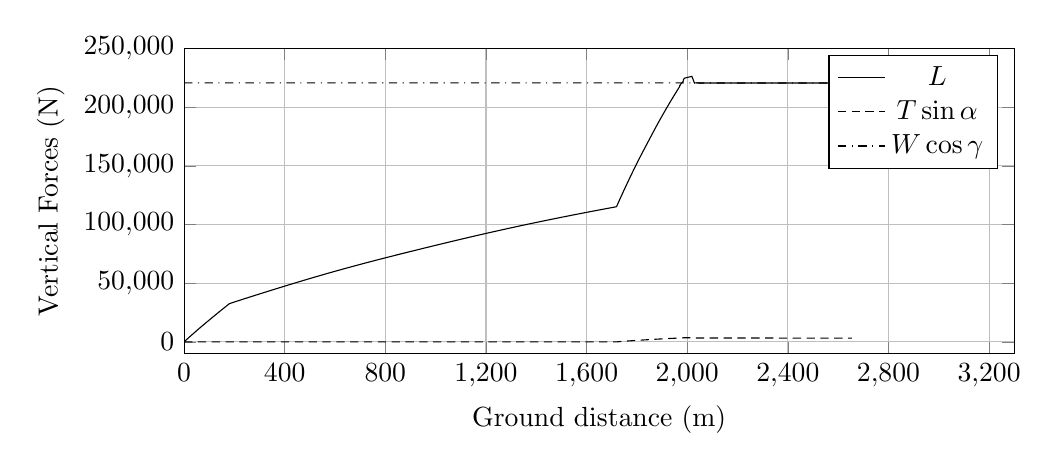
\begin{tikzpicture}

\begin{axis}[
width=\textwidth,
height=0.45\textwidth,
scaled ticks=false, tick label style={/pgf/number format/fixed},
xmin=0.0,
xmax=3300,
xtick={0,400,800,1200,1600,2000,2400,2800,3200,3400},
xlabel={Ground distance (m)},
xmajorgrids,
ymin=-10000.0,
ymax=250000,
ylabel={Vertical Forces (N)},
ytick={0,50000,100000,150000,200000,250000},
ymajorgrids,
legend entries = {$L$\\$T\sin\alpha$\\$W\cos\gamma$\\}
]

\addplot [
color=black,
solid
]
table[row sep=crcr]{
1.3729668748937997E-8	2.7260274858155694E-6\\
2.6049868369719035E-7	5.172204692876783E-5\\
2.0491224421327626E-6	4.0685352089800267E-4\\
9.92442121137073E-6	0.0019704950529072906\\
4.7452367809869807E-5	0.009421672605024994\\
1.740064756114434E-4	0.03454899331077209\\
4.0608377013922605E-4	0.0806279046287072\\
7.313431501337001E-4	0.1452080171338016\\
0.0011549487327126044	0.22931457348678547\\
0.0016799013484208249	0.3335432637688246\\
0.002295089346817705	0.45568773960709164\\
0.003009933382444524	0.5976182861342387\\
0.003810608015426248	0.7565897066271945\\
0.004723484476856681	0.9378376958855772\\
0.005727138856912631	1.1371083586612336\\
0.006836216967948795	1.3573092665803022\\
0.007997302399386296	1.587834662103858\\
0.00929136979810952	1.8447611825149792\\
0.010685558505459776	2.1215641867819164\\
0.012178513621519987	2.4179742791408714\\
0.013775244426719659	2.7349855694171676\\
0.015470070176169002	3.071469760495649\\
0.0172374436815836	3.422354406435608\\
0.019122918912604377	3.796683064331347\\
0.021104911040230538	4.190169870997021\\
0.023190717999955576	4.604263134989305\\
0.025355802981115103	5.034091054619289\\
0.027620619195902148	5.483713602969599\\
0.030020274690474198	5.960099857531109\\
0.032476028269866286	6.447617267665139\\
0.035054163466719815	6.959423859373501\\
0.037720846868992755	7.488802335429758\\
0.04049779674511381	8.040063376986087\\
0.043329456594087365	8.602177661552723\\
0.04629652060163805	9.19116308551687\\
0.04934498934704602	9.796299460275975\\
0.052507657924119336	10.424095955148179\\
0.055769483710642484	11.071565652874362\\
0.05917209570914676	11.746970797657646\\
0.06264043916012321	12.435412361064358\\
0.06620063977265622	13.142075367772755\\
0.06987962792775945	13.872304196539886\\
0.0736568184539585	14.62201188933598\\
0.07754284280095361	15.393307546136558\\
0.08151127871105612	16.180945892419267\\
0.08560324933017655	16.99308776895819\\
0.08985265585263943	17.836460054850008\\
0.09413961367176535	18.687268359710778\\
0.09857725310864562	19.567963929808585\\
0.10307959255469257	20.46148155064735\\
0.10766008648593872	21.37049049596623\\
0.11234920964493048	22.301037403598862\\
0.11719267720457946	23.262192701626248\\
0.12216973960582883	24.249836910586843\\
0.12724007601918352	25.255967302890795\\
0.13233299746505212	26.266555978275093\\
0.13755256756750583	27.30225128733405\\
0.14287728588926696	28.35878540107474\\
0.1482946925752714	29.43368464488124\\
0.15381585025670613	30.529142624964216\\
0.15940564092189102	31.63819030765862\\
0.16526271495916878	32.800238602045596\\
0.17120082448158402	33.978333113306505\\
0.17717889132867753	35.1643232056654\\
0.18324322596131126	36.3673954601786\\
0.189427022360885	37.59413344250605\\
0.1957511558722988	38.84867630026952\\
0.2021484013779125	40.117686590799465\\
0.20865863707071397	41.4090733519821\\
0.21548666343168166	42.763457623717144\\
0.22220154781289658	44.09535930950351\\
0.22919671627301902	45.48281327660622\\
0.23611678795738544	46.85532984963277\\
0.24306300975244904	48.23299069884406\\
0.2503085190632165	49.66996487534148\\
0.2576623280401219	51.12837071270111\\
0.26502430524173204	52.58834912039535\\
0.2724963584449146	54.07010870186468\\
0.2802001060647876	55.59776394589737\\
0.2878583985474956	57.11635424964254\\
0.2958320780323821	58.69742964330929\\
0.3040021452321372	60.31738894172426\\
0.31208951788619	61.92089466834604\\
0.3202851396023423	63.54580556351837\\
0.3287233234973125	65.21874766567203\\
0.3370425959884752	66.86805451293486\\
0.34575405233845447	68.59504852825927\\
0.3545073625286812	70.33027417999705\\
0.36338982075299686	72.09103454158318\\
0.37247557159370037	73.89202352448041\\
0.38151350442869847	75.68346398467733\\
0.3905554764834429	77.47563534912621\\
0.3999457587520332	79.33677012226968\\
0.4095398754587949	81.23822704136168\\
0.4189621792151833	83.10555633387955\\
0.4285208811402964	84.99984039836221\\
0.43828968955472236	86.93568220426687\\
0.44807735398784176	88.8751798029893\\
0.45806002753764463	90.85323669763963\\
0.4682994371692033	92.88207845871935\\
0.4787752542918833	94.95767095549988\\
0.4890770094685154	96.99868648209483\\
0.49985939134273727	99.13483008083304\\
0.5106597490205704	101.27443752657965\\
0.5213580865152188	103.39373828693735\\
0.532247733242454	105.55083878878051\\
0.5431365108549349	107.70766854040733\\
0.554075964429489	109.87443699261237\\
0.5653450694020941	112.1063955325902\\
0.5769901159382542	114.41270268601633\\
0.588512657344902	116.69463742750625\\
0.6004070039036553	119.05009001828387\\
0.6121651247369502	121.37845124553496\\
0.6239717914322569	123.71631134644747\\
0.6362472885961421	126.14688426170446\\
0.6486428939173223	128.60111369747608\\
0.6610190736373547	131.0513718011938\\
0.6737248046101814	133.56674512168604\\
0.6862826225989949	136.05270676878615\\
0.6991952542603428	138.60877418192734\\
0.7122988072688032	141.20249642567018\\
0.7251463703465595	143.7454129855572\\
0.7381769453061875	146.32441683609483\\
0.7516618647379176	148.99320009527332\\
0.7654913705221527	151.73002795887095\\
0.7791756406994825	154.43796276585323\\
0.7930637813125616	157.18608726686398\\
0.8074774191984457	160.03803160402833\\
0.8215072375247947	162.81387234402666\\
0.8361010597475598	165.70113636229166\\
0.8503303420601955	168.51611604003648\\
0.8650627501899835	171.43045965746632\\
0.8802332960144008	174.43129520683124\\
0.8951742046771463	177.38652899060384\\
0.9100334756324657	180.3254404067318\\
0.9251067343345352	183.3064971463112\\
0.9403923630470314	186.3293720215052\\
0.9559303815501943	189.4019712901765\\
0.9712400158034169	192.42922316872728\\
0.9869533781138684	195.53611561261823\\
1.0029148609762486	198.69186985457702\\
1.0189962473881624	201.87112957178783\\
1.035465185745812	205.12679917290546\\
1.0516742337458713	208.33088672022575\\
1.067815735429615	211.52141999806474\\
1.0846705971808022	214.85274128084262\\
1.1012775250051634	218.13484471938472\\
1.1180798406225687	221.45534747440962\\
1.1351395900544134	224.82650283670228\\
1.1526388687279154	228.28428117117346\\
1.1698922447507556	231.69324085643456\\
1.1875468452119025	235.1812400425511\\
1.2058383275300355	238.79481672804502\\
1.2239395537495579	242.3705568691347\\
1.2422020624207541	245.9779049870208\\
1.2608769472440078	249.66644756863218\\
1.2794948487006894	253.34347283340963\\
1.2979152553275424	256.9812357439089\\
1.3166445915281573	260.6797459748585\\
1.3354141707340492	264.3859387919548\\
1.3543210821322504	268.11898197655466\\
1.373689361295591	271.94284197525474\\
1.3932049885015831	275.7955096393433\\
1.4131781782225183	279.73821315328064\\
1.4330139682345777	283.65350066214523\\
1.4528243860883294	287.56348896045245\\
1.4728783400745615	291.5212483716107\\
1.4934621752870565	295.58327407312095\\
1.5141408097620341	299.6636932977799\\
1.53430654450827	303.64260173773914\\
1.5553850389607948	307.8012883758944\\
1.5762653203499473	311.92054800010635\\
1.5975496774716453	316.11919604386947\\
1.6196077215345106	320.470116849586\\
1.6413652536722467	324.76141564040825\\
1.663437310723463	329.11439831520886\\
1.6860768385032747	333.5789296493407\\
1.7077101022266827	337.8446793186988\\
1.7297306410738114	342.18644759182246\\
1.7520297891459062	346.582793903622\\
1.7743087535215367	350.974804923236\\
1.797257424336919	355.49846873505055\\
1.8200802473615325	359.9969525504408\\
1.8430350373473994	364.5210735599677\\
1.8666926279964304	369.1833166925304\\
1.8902808566018634	373.83149560894867\\
1.9138231309717848	378.4702267481516\\
1.937187877956735	383.0735916215958\\
1.9611060682733261	387.7855989429945\\
1.9852138445648535	392.5345492133878\\
2.009780393513653	397.37345353251146\\
2.0346228225622163	402.26626942959695\\
2.0593611988602687	407.13816418278884\\
2.08477023517836	412.14169344710024\\
2.110324766702745	417.1734217574784\\
2.1352655781940433	422.0838718009509\\
2.160528860803022	427.05737345368675\\
2.1862071157614817	432.1121189060498\\
2.2127756699400534	437.34164222904417\\
2.2391904543957084	442.5404192519036\\
2.2653528664920257	447.6890558643138\\
2.292150575495974	452.9622319133872\\
2.3187704640870406	458.1999333007674\\
2.3455495914188482	463.4684811498412\\
2.372862901366455	468.8416244931557\\
2.4007145172972395	474.32014605913776\\
2.428100404243743	479.70654752315625\\
2.4555980306928005	485.1144195988969\\
2.483374904362833	490.5766959501775\\
2.511687733451976	496.1438363435534\\
2.5402569276484597	501.7608440244086\\
2.568415369317849	507.2965623096253\\
2.596987652715761	512.9131009524858\\
2.6263861238451423	518.6914820763941\\
2.655991481965028	524.5099513596576\\
2.6856115886357443	530.3307420534388\\
2.7154221146045012	536.1883716016018\\
2.7455665152057707	542.1110144743916\\
2.7752624694325894	547.9449684908484\\
2.805457625653509	553.876405114303\\
2.8358231840904597	559.8407179181311\\
2.8663460878589797	565.8353342269011\\
2.897817297850832	572.0155652742317\\
2.9287074004595235	578.0810596252693\\
2.9603588456990284	584.2954133039125\\
2.9922321403815406	590.5526757354132\\
3.0241119471841866	596.8105674080332\\
3.056446055158509	603.1569753995254\\
3.0889346922121366	609.5330447668186\\
3.122221620829695	616.0650896145944\\
3.1546991615623394	622.4376299653877\\
3.187635101478671	628.8994359436899\\
3.221010117202278	635.4466904685639\\
3.2543449374576605	641.9853632690647\\
3.288235920596943	648.6324166657384\\
3.3223704322934555	655.3265103111787\\
3.3562838593334394	661.9765306050238\\
3.3906320903803255	668.711084823889\\
3.425633159699527	675.5728896891869\\
3.462387235801926	682.7775519779186\\
3.4973980805087237	689.6397288601954\\
3.5324804241140235	696.51516719592\\
3.5675385073174235	703.385100752042\\
3.6040688981843845	710.5427501701765\\
3.6393612181513753	717.457047096126\\
3.6770856360342323	724.8469957192178\\
3.7131729334920323	731.9154409245702\\
3.749509707933214	739.031960396939\\
3.785733977879824	746.1256583188156\\
3.8225309786916544	753.3307097477973\\
3.860867115351552	760.8362743489943\\
3.89929745075254	768.3594054391501\\
3.9373367205567504	775.8051203767411\\
3.9751626485832894	783.2082294748427\\
4.013671158053867	790.7440653736339\\
4.0521140617426425	798.2661951264342\\
4.092377631210638	806.1436484268504\\
4.131586743753305	813.8138921396239\\
4.1715696979561425	821.6345980885651\\
4.210522654700574	829.2529451518892\\
4.250196810863292	837.0114426401049\\
4.2917015001093795	845.1269414351827\\
4.332438976653355	853.0914646981068\\
4.373124372895289	861.0448588883503\\
4.414429464889761	869.1184295482046\\
4.455884944705147	877.2204209852166\\
4.497250153511752	885.3038003079391\\
4.537976875075978	893.2614664554051\\
4.581399817640802	901.7449245169785\\
4.623816269683994	910.0307260324171\\
4.666022338967499	918.2744329552868\\
4.709098934189642	926.6871487163173\\
4.752435367147649	935.149570986224\\
4.79531009100786	943.5208120798893\\
4.838191999420829	951.8924426059434\\
4.881381760681686	960.3231528579247\\
4.9256451804034285	968.9623834762444\\
4.9704217340957495	977.7006789340039\\
5.014356093293278	986.2735579223222\\
5.058826350846283	994.949941464115\\
5.104458009943745	1003.851810805053\\
5.149663211268795	1012.66938181761\\
5.194981168813841	1021.5078471049542\\
5.241194091283663	1030.519729700964\\
5.287987552078626	1039.6436635905297\\
5.334426822383641	1048.697388198908\\
5.380633359096258	1057.7046083454948\\
5.427524438012913	1066.8441196580206\\
5.476157635197664	1076.321967543577\\
5.524667120325573	1085.7744743410494\\
5.5732739519824435	1095.2447209093343\\
5.6208990292882195	1104.5224998389162\\
5.671502816366864	1114.3792727434989\\
5.719824083529298	1123.7902181798281\\
5.767871110439133	1133.1465655736988\\
5.8169321963676754	1142.6991664026937\\
5.866076914057565	1152.2668223325868\\
5.917200682776528	1162.218466397961\\
5.96684810088939	1171.881463200658\\
6.016885842403935	1181.6191742255778\\
6.068639931677712	1191.6895783416267\\
6.119867755785197	1201.6562633681046\\
6.171030794930029	1211.609040964157\\
6.222884713227881	1221.6948921189614\\
6.2735946138732235	1231.5569423482566\\
6.325883502103322	1241.7247497033418\\
6.379615386553551	1252.171759181736\\
6.432194972482147	1262.3933657413172\\
6.484528316464761	1272.5657685980173\\
6.536619297696934	1282.6897456639913\\
6.589662958081361	1292.9975338247796\\
6.644121795496577	1303.5789233016621\\
6.697445536614451	1313.9383890362192\\
6.7518063163896365	1324.497931916374\\
6.8068829439682315	1335.1950988343187\\
6.863205650636274	1346.1328022184807\\
6.9185329265047315	1356.8757437407771\\
6.974634519184049	1367.7675716590197\\
7.031139830722298	1378.7362963449737\\
7.0870923879294985	1389.5962607823521\\
7.144766952910487	1400.7889393012865\\
7.2026451873548805	1412.0196042580496\\
7.261191729679483	1423.3783858296479\\
7.320502240843062	1434.883792912441\\
7.378210233177999	1446.0768005009522\\
7.437738452534925	1457.6212806625767\\
7.49714639104333	1469.1408443233354\\
7.556502460410064	1480.6487709813064\\
7.617032771987237	1492.3827408037682\\
7.676883327249088	1503.983338475898\\
7.735740247984193	1515.3897998284742\\
7.796086087039788	1527.0832307809428\\
7.856787102853412	1538.8438765053647\\
7.91721236259451	1550.5494997948144\\
7.979013602666894	1562.5200399188393\\
8.039824025454376	1574.2970541654781\\
8.102419182184594	1586.4180532008982\\
8.16459313580776	1598.4558302487599\\
8.226347093952135	1610.410660432774\\
8.290527749984296	1622.8335574829607\\
8.353592793320257	1635.0388224751564\\
8.417564177281012	1647.4177900014815\\
8.482044607535009	1659.8935320363576\\
8.547336806956285	1672.5245749884575\\
8.613293246319614	1685.2823276389672\\
8.6778048537894	1697.7588789383522\\
8.74454839911753	1710.6652936373903\\
8.810708373588199	1723.4570701685816\\
8.876548424968423	1736.18522937117\\
8.942828456712885	1748.996679488895\\
9.010858044488913	1762.144473072503\\
9.079453414959548	1775.399742719992\\
9.148767802603732	1788.7920564982282\\
9.21609997183467	1801.7995666088773\\
9.285579683381485	1815.220080709781\\
9.355451712480097	1828.7144713535604\\
9.423585014597279	1841.8712341309274\\
9.493435356703696	1855.3576998196363\\
9.562655940911181	1868.7207230908843\\
9.63183713653898	1882.074311350174\\
9.703018708836247	1895.8121187448364\\
9.773178624863132	1909.3508740366956\\
9.844376937811855	1923.0881154060826\\
9.914998792594716	1936.7122592508272\\
9.98720270419701	1950.639689904092\\
10.059478150570087	1964.5789871061615\\
10.132362020358627	1978.6336808555775\\
10.205876892438312	1992.8080866550317\\
10.279422251887688	2006.9864039814674\\
10.353305644514993	2021.2279192084561\\
10.42811398108589	2035.645724292544\\
10.50332954727428	2050.1399985382077\\
10.578207710262959	2064.567257988805\\
10.65503529959097	2079.368068314273\\
10.730232142651953	2093.852709780872\\
10.805871937852555	2108.4206839503468\\
10.88265320376452	2123.206472641772\\
10.958577899345514	2137.8253135201203\\
11.034861147941964	2152.511203126549\\
11.112742623646977	2167.502736455457\\
11.190543636431041	2182.4767326124756\\
11.267787598939979	2197.3415028738846\\
11.3462805052093	2212.4445771578357\\
11.423875697147409	2227.3729091001724\\
11.502735831556972	2242.5425651902724\\
11.581465323066688	2257.6850575694707\\
11.661639233340708	2273.103289169386\\
11.741743247575428	2288.5060025162848\\
11.821864700430528	2303.910006368329\\
11.901816327719768	2319.279317098417\\
11.98361062800689	2335.0007520596673\\
12.065425957085825	2350.724120835599\\
12.1478520915771	2366.5627574562786\\
12.230956215923495	2382.5295367071412\\
12.313306905825911	2398.3494568409424\\
12.396632357805931	2414.3545181252484\\
12.479578787946746	2430.284679273199\\
12.564327762802186	2446.558878921138\\
12.648175874147956	2462.6579671466934\\
12.736145481689512	2479.5461445836872\\
12.821080154398764	2495.8495125558466\\
12.908009536077355	2512.533576833197\\
12.994986774303499	2529.2246234479153\\
13.081752199798046	2545.872844187398\\
13.17035388279784	2562.8711703978706\\
13.257836697901475	2579.6526479248823\\
13.34511613365563	2596.392957451286\\
13.433461823066896	2613.3356009993495\\
13.524108483575919	2630.7172606533995\\
13.611203924103116	2647.4158314017977\\
13.702229394080796	2664.8656764622547\\
13.792427706753081	2682.1547332573646\\
13.882429934062493	2699.4040200540694\\
13.975435778888343	2717.2266881274027\\
14.065832730112316	2734.547218290927\\
14.157894546480026	2752.1845381174226\\
14.250668806951023	2769.956114411133\\
14.343291987615704	2787.69653159219\\
14.43744444968501	2805.7276043524107\\
14.532636396723657	2823.955459374997\\
14.625507232812737	2841.73665736206\\
14.721503924398366	2860.1140745591374\\
14.818738382089133	2878.7261240648186\\
14.913572076739943	2896.87640178935\\
15.009701633366973	2915.272466514968\\
15.10815424447124	2934.110783641143\\
15.206130868840724	2952.8557300449766\\
15.304035939715973	2971.584722962094\\
15.403499839366233	2990.6096206798557\\
15.503209871950865	3009.6792978308813\\
15.601718454553605	3028.5169571966444\\
15.700655560608023	3047.434344582117\\
15.801250929860519	3066.666545732681\\
15.899917805652187	3085.527862052337\\
16.001574124100856	3104.9584013590456\\
16.102638779863817	3124.273616282637\\
16.204479333764816	3143.73488872514\\
16.30489644092564	3162.9219777259204\\
16.40578186591999	3182.1964037319713\\
16.509201471948074	3201.9527822828986\\
16.614557195984908	3222.0767448031966\\
16.717657554831042	3241.7677121818588\\
16.823039336622365	3261.8921823044957\\
16.928576062495388	3282.044015236327\\
17.03469945574068	3302.305649052084\\
17.140697318244236	3322.541118347104\\
17.246066414787876	3342.6544019855373\\
17.35183930840021	3362.842631991298\\
17.458399953804133	3383.1790809038366\\
17.565707112453843	3403.65585834153\\
17.673103795073075	3424.1475961467777\\
17.781888038667653	3444.9019480246443\\
17.89115167195854	3465.74562089802\\
18.00105710767307	3486.7095920388992\\
18.110142905530395	3507.515130746264\\
18.219697237410173	3528.4079628033633\\
18.32752951944549	3548.9703892876423\\
18.43743745973078	3569.9266083990005\\
18.54904630654982	3591.205089390156\\
18.659302591714813	3612.223699826787\\
18.770734536087716	3633.464437837494\\
18.883577445650936	3654.9721155781954\\
18.996263390583444	3676.4478835934024\\
19.108816920034535	3697.89645714604\\
19.22287647779894	3719.6300570820395\\
19.33763586704334	3741.495038581881\\
19.456324114791514	3764.106536321905\\
19.57349394116079	3786.426749828992\\
19.690148252848566	3808.6468114425224\\
19.80521137071168	3830.561911500481\\
19.92379170801214	3853.1449909826997\\
20.04216631061405	3875.686982351148\\
20.15848954929409	3897.836509640176\\
20.278242138037896	3920.6371755374867\\
20.396206084226087	3943.0954784057285\\
20.516315546862906	3965.9604393912523\\
20.637173924977112	3988.966158891936\\
20.75450010628387	4011.2978099723914\\
20.874378237858778	4034.113492309846\\
20.996035953832852	4057.2661469893883\\
21.11812959618858	4080.5000500953392\\
21.240471115580952	4103.779437184257\\
21.361479376438375	4126.80350325829\\
21.485224699488654	4150.346709158193\\
21.607870280890317	4173.679085152891\\
21.73242999733349	4197.374018083625\\
21.85704493170313	4221.077885499597\\
21.98122016226351	4244.6965883269095\\
22.10826921766411	4268.860367341278\\
22.235261614051304	4293.011853105541\\
22.361664688868032	4317.04979295516\\
22.48780138980522	4341.0356538347605\\
22.614107216476143	4365.052288269242\\
22.74409311379692	4389.767265977171\\
22.873024137794893	4414.2803010691805\\
23.003512644166257	4439.088100434999\\
23.132891545907036	4463.683644212153\\
23.26270690888247	4488.360896905688\\
23.39264146728729	4513.059579562703\\
23.52277721573431	4537.795313517721\\
23.654883767164463	4562.904471369951\\
23.78569183677709	4587.765700062097\\
23.917003007077597	4612.7214572211415\\
24.047013652206026	4637.429012513319\\
24.178458227988493	4662.408067531274\\
24.314609552493202	4688.280543300263\\
24.447533097503474	4713.538688188502\\
24.579128452041708	4738.5435527111695\\
24.71011994849615	4763.432829414311\\
24.843278471916108	4788.733030994459\\
24.975761222328053	4813.9040507202335\\
25.1115496753864	4839.702367026695\\
25.247101122854083	4865.454921313651\\
25.384906965000688	4891.63506713007\\
25.522261036073317	4917.728722277239\\
25.66123001648475	4944.128539073901\\
25.79865327455613	4970.234139867995\\
25.826335196219034	4975.492669048801\\
25.839610403727477	4978.014454181566\\
25.841006316401874	4978.279624282317\\
25.84227013303559	4978.51970113399\\
25.84770509053729	4979.552134813073\\
25.86419328224909	4982.684254501655\\
25.90571916957557	4990.572535737589\\
25.999268866927544	5008.3431055896035\\
26.123295978662824	5031.90270370534\\
26.250212562581652	5056.010637672662\\
26.376891976518465	5080.072937873851\\
26.50638698165423	5104.66940192463\\
26.634042370994827	5128.915761372333\\
26.763333806613538	5153.472126518705\\
26.893207366259766	5178.138261573373\\
27.022905486492228	5202.770238554123\\
27.153956322362554	5227.658224887766\\
27.287774297957696	5253.070746102656\\
27.42030033806219	5278.236906865908\\
27.555504894698295	5303.910616874278\\
27.691130018821354	5329.6630338797\\
27.82633313037239	5355.334122365155\\
27.959508564917073	5380.619001299279\\
28.096515548835796	5406.630040811289\\
28.232789703382153	5432.5005945174\\
28.368684388406535	5458.297716165693\\
28.506541650227618	5484.465930215074\\
28.64533374691623	5510.810056876977\\
28.78297783415192	5536.93470961186\\
28.92277775692753	5563.466890309575\\
29.06227187463503	5589.93933375322\\
29.20212864139956	5616.478849209236\\
29.34335827861657	5643.277060147342\\
29.483225747293005	5669.8149503113655\\
29.625960812476485	5696.894982825646\\
29.76706561118049	5723.663742790794\\
29.909402910999468	5750.66428505401\\
30.051751399473822	5777.664863185422\\
30.196612335666572	5805.139813779944\\
30.342192969749448	5832.748997243523\\
30.48583400527584	5859.988065664742\\
30.632658550781265	5887.828454542498\\
30.77846394498075	5915.473172126962\\
30.92408133049836	5943.079789602985\\
31.071091331299215	5970.947892690063\\
31.218274793935116	5998.846287408875\\
31.366705758252415	6026.978475100475\\
31.515339333797037	6055.146334624835\\
31.66356819769615	6083.234733797361\\
31.814689402684216	6111.868329020936\\
31.96649953392354	6140.629482746426\\
32.115424616034375	6168.841110284313\\
32.266253234088566	6197.410324546459\\
32.41813832080348	6226.176547201972\\
32.569791431087395	6254.895686669268\\
32.722234201183724	6283.761155283864\\
32.876984607664	6313.060245550207\\
33.031873994672836	6342.382241585117\\
33.18502245018544	6371.371270370913\\
33.34135780547538	6400.960017099322\\
33.49759920343199	6430.52738554743\\
33.65385117142162	6460.093118581832\\
33.8113313806527	6489.887537673976\\
33.96985264489639	6519.87510653229\\
34.126473036379195	6549.499289975849\\
34.2857505660089	6579.62215175213\\
34.4449212019973	6609.720819185766\\
34.60566879064274	6640.113607054765\\
34.76644486933921	6670.507644392714\\
34.92612701881755	6700.690744984606\\
35.08630421658309	6730.963242429678\\
35.24825698849928	6761.567020854889\\
35.412303951281956	6792.562094865614\\
35.57355277914179	6823.024098210713\\
35.73545353069308	6853.604842688257\\
35.89925038949356	6884.539195342253\\
36.065161289279985	6915.868109552894\\
36.23047312008262	6947.079168070939\\
36.39472205714358	6978.084835454803\\
36.56135389445764	7009.535489414888\\
36.72774532558607	7040.93586908601\\
36.89384825683493	7072.276886827243\\
37.05904296416534	7103.441629487877\\
37.22702676294645	7135.1274942197415\\
37.39437475321985	7166.688329823935\\
37.5621109943643	7198.317245778371\\
37.73270471709142	7230.47966471383\\
37.903359519601935	7262.648204303254\\
38.071486842086316	7294.33500345806\\
38.23815243703595	7325.741080706819\\
38.40817787072022	7357.77488002766\\
38.57751392140098	7389.6733461174335\\
38.750215798728505	7422.20021294403\\
38.92001182640311	7454.1742134654\\
39.09310637700479	7486.763632893773\\
39.26472366117933	7519.069188571506\\
39.436554723976656	7551.4092403242485\\
39.608961777617054	7583.851891500923\\
39.782828308010565	7616.563260348619\\
39.956194359016465	7649.174522609366\\
40.132391837044906	7682.312282667333\\
40.30868053167249	7715.461004227085\\
40.48611580488176	7748.81904094582\\
40.66383502946924	7782.2241145863045\\
40.83999042132467	7815.328947702006\\
41.018202681018664	7848.813925028504\\
41.19780999006247	7882.554482173571\\
41.37730467548502	7916.267295965836\\
41.557010452813884	7950.013136416688\\
41.73612816026986	7983.641930381253\\
41.91555194917056	8017.32154391352\\
42.09743589423803	8051.456139919639\\
42.27807550146298	8085.3503957393805\\
42.45995188234755	8119.469831646418\\
42.6401410478328	8153.265920194379\\
42.822293873795985	8187.423378484216\\
43.00585672428667	8221.838173390228\\
43.189965171449515	8256.34810555313\\
43.372020236704074	8290.466080706825\\
43.555636897252796	8324.869571465213\\
43.74012033961118	8359.42823213867\\
43.92429822300048	8393.922400159296\\
44.106869824379004	8428.108561235025\\
44.29411840239129	8463.163042418928\\
44.47920670866131	8497.805686851887\\
44.665034305215386	8532.579268611149\\
44.85242224248053	8567.637274152512\\
45.03948098831597	8602.626104155413\\
45.22811764277584	8637.902384375338\\
45.41548629589063	8672.933876917421\\
45.60322541388645	8708.026958892864\\
45.793007222766036	8743.494047651675\\
45.983742663331824	8779.131415923468\\
46.172643153142886	8814.418081142227\\
46.36421599110457	8850.195942447153\\
46.553512793459404	8885.54080974491\\
46.745018895697555	8921.290162019748\\
46.93606459490553	8956.945511513153\\
47.126948089509526	8992.562540102259\\
47.31881294044018	9028.354562827379\\
47.5110690178297	9064.211394729777\\
47.705448624448266	9100.455949129348\\
47.90005519882567	9136.734427209998\\
48.09288923506665	9172.674172921277\\
48.28732881729917	9208.904784508584\\
48.484002572746206	9245.543139123696\\
48.68089030454945	9282.2127266204\\
48.87532723390382	9318.417381752097\\
49.07073736177763	9354.794752590278\\
49.2672083392297	9391.36101730767\\
49.46586249263092	9428.324838777367\\
49.661880987188695	9464.789595483755\\
49.85966148345089	9501.573424976581\\
50.05808618672894	9538.468273070357\\
50.25785665917266	9575.60445122065\\
50.45743808511885	9612.696565670678\\
50.65573800086891	9649.541678447356\\
50.85948768734909	9687.390212263785\\
51.061243703011925	9724.859238462635\\
51.26368286286315	9762.445968707594\\
51.46416466063809	9799.660227919689\\
51.66475943174029	9836.886444969005\\
51.86588207153103	9874.201573025966\\
52.07444928962187	9912.888354257357\\
52.2824430085781	9951.459055199728\\
52.48676525705545	9989.339480092753\\
52.69531994892206	10027.994942584653\\
52.90027076850366	10065.972946767899\\
53.108186167814935	10104.490694649652\\
53.31165724918766	10142.17574331837\\
53.520024946679996	10180.758108204343\\
53.72688450142306	10219.0516241322\\
53.93707391647578	10257.951773090183\\
54.14518573319289	10296.457705343611\\
54.35125853722778	10334.57685345773\\
54.56213447502874	10373.574685639622\\
54.77598621923464	10413.112730858218\\
54.987629956235494	10452.23253223678\\
55.19778857845695	10491.067977662617\\
55.41030974885841	10530.330028596622\\
55.62390503323701	10569.780421579759\\
55.83671574169797	10609.075852291851\\
56.047071254351536	10647.90808058287\\
56.26137331252919	10687.458792419526\\
56.47512769358855	10726.898324564925\\
56.69105800830218	10766.729103717655\\
56.90937011004422	10806.988789730363\\
57.12736617899088	10847.179734152916\\
57.346833156368504	10887.6313187921\\
57.56476609337061	10927.78969904115\\
57.78230894703917	10967.865825012257\\
57.99943865551505	11007.855521534566\\
58.21827465292657	11048.149057927032\\
58.436085045729726	11088.243388208652\\
58.6577546799423	11129.037524853327\\
58.87982836766625	11169.895317219845\\
59.10336118170943	11211.010765324849\\
59.324182403931715	11251.616839414877\\
59.545440661451366	11292.292713837742\\
59.768227251413464	11333.238891006538\\
59.99077485409802	11374.130481968412\\
60.21631063559073	11415.56028007892\\
60.44006004384342	11456.651159820063\\
60.66502706168687	11497.954857519024\\
60.89133011288284	11539.492955274927\\
61.11585558357916	11580.694002880304\\
61.3432655409558	11622.413447757757\\
61.57186440401435	11664.3399590128\\
61.79868765088207	11705.929892800603\\
62.025670725987	11747.53827207793\\
62.254132946411545	11789.406850839234\\
62.48290793247415	11831.321774243093\\
62.713817944074236	11873.616759113778\\
62.94484116346062	11915.921343185997\\
63.17805109236767	11958.615086376049\\
63.41124119062552	12001.293911352303\\
63.64505576847972	12044.075728813954\\
63.87735201907903	12086.568559135532\\
64.11169045660182	12129.423704943492\\
64.34725756208485	12172.49218962227\\
64.58324360279937	12215.625885800036\\
64.81881329818131	12258.67215505219\\
65.05563560606473	12301.93594568352\\
65.29467812810154	12345.593809312813\\
65.53178653633495	12388.887030850281\\
65.77046761369158	12432.455971698062\\
66.01019347650049	12476.204121816609\\
66.25262920761091	12520.435114684311\\
66.49342175078831	12564.354723718443\\
66.73393309567928	12608.21154984591\\
66.97718905970893	12652.557210150739\\
67.21919788222482	12696.663939666832\\
67.46413738735515	12741.293079850628\\
67.70584739194695	12785.322280644501\\
67.95375887035246	12830.469292977985\\
68.19817148521656	12874.967446084534\\
68.44413350233111	12919.736021125864\\
68.68984243621705	12964.446894272765\\
68.93951041285982	13009.866316254618\\
69.19023531750676	13055.466026986214\\
69.43956667494601	13100.800428964249\\
69.68998597860525	13146.320789427631\\
69.94098943220166	13191.935462376183\\
70.1928405184459	13237.692280761199\\
70.44659484061637	13283.782886742025\\
70.69926103579675	13329.66394087991\\
70.95414956377036	13375.936556378401\\
71.21136313866151	13422.619114496149\\
71.46778788208749	13469.14641544364\\
71.7247351381395	13515.756474491656\\
71.98234155897126	13562.474055729432\\
72.24107377350035	13609.383717755245\\
72.4986091150376	13656.064412378411\\
72.75949164810788	13703.339705019262\\
73.02014691132015	13750.56170172296\\
73.28114866838587	13797.834404088462\\
73.54342372888959	13845.32562771004\\
73.80584407854005	13892.831085028749\\
74.07231166191039	13941.056914053857\\
74.3389341302921	13989.298446895667\\
74.60521354141642	14037.465670258822\\
74.87280568706873	14085.85810316653\\
75.1403821105715	14134.235483857265\\
75.41145333671997	14183.232343337047\\
75.68265298797411	14232.240025271847\\
75.95075857762194	14280.676479582766\\
76.2241428819712	14330.054274681992\\
76.4990100438061	14379.687433446852\\
76.77213586328236	14428.993853223797\\
77.04724851790667	14478.64663119099\\
77.32330034006353	14528.456566152552\\
77.59850473375684	14578.101364989012\\
77.87773830129439	14628.460600337225\\
78.1565255546137	14678.726971909564\\
78.43842651648492	14729.54227359952\\
78.720833678605	14780.436324703769\\
79.00101298089581	14830.91660797939\\
79.28359351218376	14881.817230232315\\
79.57011733099088	14933.415634709098\\
79.85418914588558	14984.560125378805\\
80.13919871477489	15035.861188408453\\
80.42568449319114	15087.415682729326\\
80.71472498530085	15139.417526883863\\
81.006853148924	15191.962341886065\\
81.2951972638476	15243.814261804495\\
81.58524575795963	15295.960484025494\\
81.87461709596036	15347.972880497025\\
82.1711642895769	15401.262667606792\\
82.46716486408064	15454.441799064436\\
82.76422974563803	15507.79976814079\\
83.05801377197795	15560.556354077413\\
83.35853301954708	15614.510101509812\\
83.65664966506407	15668.0202954226\\
83.95487262936624	15721.53752538855\\
84.25322789115987	15775.066551259908\\
84.55664509033022	15829.491620603072\\
84.8599544590121	15883.885233147732\\
85.16499148084048	15938.576576361655\\
85.47187188044902	15993.58630873073\\
85.77908321853027	16048.643313798118\\
86.08675489504844	16103.770860776665\\
86.39784539041122	16159.498941397407\\
86.71051296037359	16215.497469876613\\
87.02583358957506	16271.959043325613\\
87.34037846285594	16328.269722775378\\
87.65395388450591	16384.395067406615\\
87.96687312379424	16440.391374163075\\
88.28527441497255	16497.356938123252\\
88.6103524516937	16555.50497098078\\
88.92871226770333	16612.439608086774\\
89.25003295857354	16669.892186837547\\
89.57522243846881	16728.024822792264\\
89.90247582737899	16786.514699106665\\
90.22602529632545	16844.331174740102\\
90.5494223037065	16902.10923097535\\
90.87816525326718	16960.831097618742\\
91.20455861430293	17019.122159331288\\
91.53817773235312	17078.692404167763\\
91.87076195087604	17138.066679855117\\
92.20124984301029	17197.055818692133\\
92.53140503523474	17255.974896244086\\
92.86389705561814	17315.30038176055\\
93.19815266874983	17374.929966671603\\
93.53304529783748	17434.662732177465\\
93.86737084100128	17494.284078195436\\
94.20337949361911	17554.19541113574\\
94.54065981474497	17614.323411035395\\
94.87396787418089	17673.73351992906\\
95.21684847579547	17734.839949301524\\
95.55392648231228	17794.90263647223\\
95.89232371872416	17855.190965137575\\
96.23051075783204	17915.432588315896\\
96.57164052232307	17976.18921017625\\
96.90762523479154	18036.02063252702\\
97.24755293575913	18096.545463422473\\
97.58790661409188	18157.13750642052\\
97.92576087813703	18217.27622494103\\
98.26661027452474	18277.93982535592\\
98.6051908024865	18338.191590162867\\
98.94563962387357	18398.767943642903\\
99.28665364663627	18459.437127654608\\
99.63350087797645	18521.136338386954\\
99.97685593767679	18582.20683757714\\
100.31593955776762	18642.510463178885\\
100.65572384630482	18702.931769133633\\
100.99616871909686	18763.463773463685\\
101.3402339503516	18824.63279574285\\
101.67973054404297	18884.98318697462\\
102.01657591573795	18944.856184203432\\
102.35656456518868	19005.28191158382\\
102.6941824316649	19065.280528006042\\
103.03547296258705	19125.92618026924\\
103.37623032340073	19186.47162467493\\
103.71852978299776	19247.28576140489\\
104.05851119314701	19307.682992038834\\
104.3949509202441	19367.44625736413\\
104.7329053851843	19427.473981703944\\
105.07104272194636	19487.529750555703\\
105.40742307340048	19547.269247587377\\
105.74423560014887	19607.081467938493\\
106.07955743077031	19666.625145760037\\
106.41623710643992	19726.406289423176\\
106.75618472497374	19786.76417175187\\
107.0942647435474	19846.78714237993\\
107.43151869252583	19906.66034386056\\
107.44650965670576	19909.32164322825\\
107.45815118347005	19911.388323398067\\
107.46233674961977	19912.131371702337\\
107.46535588765028	19912.667347996423\\
107.46808502617694	19913.15184156219\\
107.4836206108138	19915.909811095902\\
107.53176708907421	19924.457021375267\\
107.68672244793561	19951.965081833878\\
107.97570433527497	20003.264122021712\\
108.27744765146667	20056.825965822005\\
108.5816623935838	20110.82368929324\\
108.88557241638279	20164.764327867044\\
109.19209959959528	20219.166274702067\\
109.50241879336687	20274.237762094715\\
109.81066605766154	20328.937928706677\\
110.12101503747155	20384.007234638564\\
110.43285681965125	20439.33738991287\\
110.74725799716322	20495.117383479126\\
111.06462449033057	20551.41893850763\\
111.38211128519615	20607.73709587354\\
111.70119562731901	20664.333680630465\\
112.02298633508096	20721.405082455\\
112.34320819983824	20778.19286041354\\
112.66812620709393	20835.807777172755\\
112.99302416686388	20893.413245181728\\
113.31966045518399	20951.320799302855\\
113.64998129974768	21009.875135618153\\
113.97857627498675	21068.11693272776\\
114.31304608469316	21127.3930624864\\
114.64448318111735	21186.12461773037\\
114.98093514978115	21245.737399930753\\
115.31969924418831	21305.75210046205\\
115.65790718621022	21365.66033139729\\
116.00063352526521	21426.360636986923\\
116.34235083463872	21486.8737354307\\
116.68621873349733	21547.758914697733\\
117.03331062078092	21609.20583129205\\
117.37910048629482	21670.4129625004\\
117.72869476105836	21732.28388704871\\
118.08005947084649	21794.458209298005\\
118.43363644355449	21857.013746728153\\
118.79186464668504	21920.38150772916\\
119.14769212941735	21983.31376068244\\
119.5036618261702	22046.260162879422\\
119.86270697471275	22109.73905779535\\
120.22616362054572	22173.98610362123\\
120.58991121293201	22238.27249747653\\
120.95538130513773	22302.850945300343\\
121.3195355377388	22367.184355443133\\
121.68590041554987	22431.89549956062\\
122.05305648207542	22496.733308987772\\
122.42257239354896	22561.974439042686\\
122.79503144936103	22627.721392820466\\
123.16629137010841	22693.24268155166\\
123.53950748252527	22759.094935536108\\
123.91239367862553	22824.87450044244\\
124.29026003316017	22891.517646380365\\
124.66301933937496	22957.24514630894\\
125.03890311735066	23023.508374786965\\
125.41380975776434	23089.583963198296\\
125.7896808967325	23155.813938589083\\
126.16837244152023	23222.52490459136\\
126.54595968852882	23289.02519415426\\
126.92471834906405	23355.7154249445\\
127.30294276405039	23422.295059242817\\
127.68255852126984	23489.10283648695\\
128.06243727540487	23555.939904278144\\
128.44360431740483	23622.9863851646\\
128.82265748788262	23689.643740138083\\
129.1989690567886	23755.80175574866\\
129.57765386613931	23822.359524721753\\
129.95508099647026	23888.67864625871\\
130.33359114840187	23955.17027565321\\
130.71373745886524	24021.931239566104\\
131.09453904397424	24088.78896472302\\
131.47657586018488	24155.844991741527\\
131.85678563989967	24222.56172407906\\
132.23856625352113	24289.53527551164\\
132.61595336405918	24355.719429129254\\
132.99976263915818	24423.01069165836\\
133.38083522978053	24489.802880066643\\
133.76098428781995	24556.413939283993\\
134.1363519425165	24622.168186162962\\
134.51557915495124	24688.57922957724\\
134.8968696170101	24755.331919787808\\
135.27419431482667	24821.37078216559\\
135.65215477207505	24887.501310901993\\
136.03329358991255	24954.167963141772\\
136.41192880753374	25020.37671610077\\
136.7898079310749	25086.43328875838\\
137.17001317148595	25152.87624491704\\
137.54844558779996	25218.98912160909\\
137.92617219433072	25284.95842350742\\
138.30476964659732	25351.05939584296\\
138.68390038934075	25417.232889724975\\
139.0631653430654	25483.40909729257\\
139.4406106933401	25549.247148962357\\
139.81914660512416	25615.254633299563\\
140.19767098864742	25681.239192185865\\
140.5730919292459	25746.662010809014\\
140.95061983253072	25812.43107785336\\
141.32838502869612	25878.22039855049\\
141.70636515873298	25944.025957920625\\
142.0839785067887	26009.74641201718\\
142.46357402350594	26075.79035954163\\
142.84082211769783	26141.40446977465\\
143.21906727224075	26207.170482089554\\
143.59963619096823	26273.318713546025\\
143.97984478872678	26339.382390245977\\
144.35941603837455	26405.313391996555\\
144.7355521893594	26470.626037095877\\
145.11296635073694	26536.13883464721\\
145.49073213867456	26601.69077429577\\
145.87033631970945	26667.53959354796\\
146.24486520181193	26732.4862161556\\
146.6238757206513	26798.187891790192\\
147.00096360401335	26863.53415500188\\
147.37874202190085	26928.977899275276\\
147.756852900845	26994.456949835796\\
148.13572640408995	27060.045649937623\\
148.5136798644104	27125.452667313584\\
148.89083780486442	27190.69965446717\\
149.2712459042852	27256.486232305208\\
149.65303236723025	27322.48823615111\\
150.0329584616291	27388.145762373868\\
150.41363382646614	27453.90985615921\\
150.79322940570728	27519.464524122122\\
151.17272478467066	27584.979002995133\\
151.55400296227282	27650.778174137886\\
151.93482601265913	27716.475668675434\\
152.31881414221942	27782.695740413656\\
152.70208150063132	27848.768001856843\\
153.08320649997165	27914.44761200036\\
153.4666285558243	27980.499573051107\\
153.84825937276264	28046.219519224942\\
154.23093781718723	28112.096366135454\\
154.61485031834388	28178.16196880638\\
155.00001234931443	28244.41873340148\\
155.38285725409855	28310.253187134258\\
155.7679513537659	28376.45054285247\\
156.1509667875323	28442.266807332453\\
156.53491934392343	28508.22029091366\\
156.91995289130983	28574.335499635963\\
157.30625057946366	28640.643645721764\\
157.69121706207227	28706.699227059842\\
158.07789765133754	28773.024731497404\\
158.46521012398495	28839.434296347856\\
158.85138765236047	28905.625012199627\\
159.23964669847322	28972.148079669503\\
159.62715395386465	29038.517913872864\\
160.01960115328984	29105.708954095644\\
160.4079207075476	29172.16865099947\\
160.79602490671402	29238.566988419356\\
161.18437278725975	29304.982493491734\\
161.57644284003254	29372.009680515454\\
161.96812230097612	29438.945124165213\\
162.35808768568592	29505.562850736256\\
162.75087300343483	29572.637300206807\\
163.14546270495134	29639.994611195783\\
163.53745675514648	29706.883768363245\\
163.92955389373896	29773.76552420712\\
164.32395276810763	29841.014688345356\\
164.71713266653478	29908.030846760004\\
165.1102153740033	29975.005339611518\\
165.5035884424101	30042.004191357933\\
165.89816400198282	30109.182624036526\\
166.29148626774366	30176.12254644467\\
166.68861804276264	30243.68537153409\\
167.082852347146	30310.729989666674\\
167.48006204110857	30378.255166353658\\
167.8798182678497	30446.18748314744\\
168.27774435731556	30513.783144561756\\
168.67741362640317	30581.649179715198\\
169.07475368467374	30649.0941537224\\
169.4759958044982	30717.17564252444\\
169.87832784425882	30785.416033616682\\
170.2792240364854	30853.386986927806\\
170.68126852540456	30921.526694058943\\
171.08617821288442	30990.125781354713\\
171.48766933901368	31058.119750048543\\
171.892744970828	31126.69461138024\\
172.29711201372032	31195.123346713008\\
172.70264003426053	31263.722323669215\\
173.1105289448074	31332.69421367866\\
173.5163733808056	31401.294099998144\\
173.92577914808027	31470.469424258903\\
174.33607303977334	31539.768115632505\\
174.74614233406845	31609.002213455868\\
175.15731444736514	31678.395790933668\\
175.56901623635082	31747.85200516878\\
175.97955109701695	31817.084739274207\\
176.39275298155184	31886.740454646817\\
176.80397138375372	31956.03517296073\\
177.21946344336607	32026.02311800408\\
177.6332252263685	32095.692756926263\\
178.05102033212842	32166.014400731983\\
178.46725124888752	32236.04571353426\\
178.88389799206544	32306.120004406162\\
179.29839533747668	32375.806063797296\\
179.71608569665375	32446.002026384376\\
180.1342696339205	32516.253936371475\\
180.26454521656194	32538.133792705645\\
180.5538779958007	32586.71804634716\\
180.97677279803082	32616.728867434766\\
181.73177043104909	32670.290741668992\\
182.61825861954026	32733.15368800088\\
183.4994266290775	32795.610229753205\\
184.38832398643513	32858.58525033445\\
185.2752206450968	32921.38919170106\\
186.16090254585617	32984.07793205201\\
187.05782443666988	33047.53258952385\\
187.95004436743	33110.62505930627\\
188.84343565256296	33173.77091022133\\
189.73203483232732	33236.54888521561\\
190.63087969896367	33300.02117854447\\
191.53167348748025	33363.60137991821\\
192.42914206966827	33426.9173688602\\
193.32936064878362	33490.3978497136\\
194.23353734669462	33554.127759380906\\
195.14873951553636	33618.604568578725\\
196.05846844349168	33682.665731717265\\
196.9665797060448	33746.58317979047\\
197.88137813217617	33810.94127883858\\
198.80153314772656	33875.645907708735\\
199.72262566550114	33940.38609201489\\
200.6418018332526	34004.96137821807\\
201.57021605131746	34070.155126355996\\
202.49227039761405	34134.87198736923\\
203.4093310979173	34199.20849845138\\
204.33741716634955	34264.288269312325\\
205.26228808295895	34329.112426499356\\
206.1977933698634	34394.65141117983\\
207.13719708861407	34460.4327029485\\
208.07111616454222	34525.799430118714\\
209.00693662932974	34591.26882670316\\
209.95866810149408	34657.82022332096\\
210.9046028778589	34723.93527781915\\
211.84706310840727	34789.776850536946\\
212.79298368779843	34855.82952596755\\
213.73594859980489	34921.645358536145\\
214.69266347370274	34988.38992702823\\
215.65468447394903	35055.47333311864\\
216.614658409948	35122.38277737558\\
217.57357224144454	35189.187312843234\\
218.5368107467741	35256.26203439105\\
219.50048157907025	35323.33578346239\\
220.46765259916174	35390.622015667584\\
221.44618219131166	35458.66683860925\\
222.41939214233116	35526.310313095644\\
223.3957502333693	35594.141223734376\\
224.37068692464283	35661.84214816311\\
225.34711146005128	35729.615228436975\\
226.33138885023874	35797.901934024645\\
227.31393394086427	35866.0371048058\\
228.30414603792985	35934.672386647464\\
229.29617452368518	36003.40192933522\\
230.2808212657469	36071.58886679004\\
231.28192033792595	36140.883415223594\\
232.2770741096358	36209.734881718265\\
233.29052711380916	36279.820218404784\\
234.30070953924962	36349.64719147768\\
235.3030940983469	36418.903531107746\\
236.31056730234104	36488.47985918631\\
237.32863543123972	36558.75584765342\\
238.35192702989485	36629.360114251744\\
239.37227626200922	36699.72928395531\\
240.40154009491766	36770.68095530562\\
241.4327935450462	36841.73740279152\\
242.46479014370783	36912.81277230836\\
243.4993601598722	36984.03312365066\\
244.5489899152056	37056.25736027917\\
245.59198540953986	37127.992507218805\\
246.64178332136828	37200.16287562503\\
247.69238009267121	37272.355557228715\\
248.75653132082437	37345.44657116571\\
249.80604502438968	37417.499783652645\\
250.8683150903493	37490.3961591984\\
251.93058205288185	37563.2596956163\\
253.00701197053712	37637.06161063978\\
254.08005928692728	37710.598642128665\\
255.1482320588113	37783.76911457202\\
256.2287194565513	37857.75034884141\\
257.30711015243367	37931.55532675082\\
258.39583303573465	38006.03450439169\\
259.47850143980736	38080.06688087281\\
260.57344571603574	38154.905799800894\\
261.6820544046054	38230.64520339052\\
262.77228099849674	38305.09611753828\\
263.87126070008526	38380.112231852385\\
264.97335243767543	38455.30817265586\\
266.0976894214622	38531.98849232281\\
267.21278411159847	38608.005369749924\\
268.32534355771804	38683.816777331565\\
269.4561922169971	38760.841257526045\\
270.5915896156504	38838.14214479175\\
271.7158392961418	38914.65130787942\\
272.8552569839427	38992.15968867812\\
274.01601268837805	39071.08565016078\\
275.14755464888765	39147.99249781165\\
276.29902718037044	39226.22104813067\\
277.4488797139885	39304.30666753993\\
278.61486213965225	39383.454373587956\\
279.78120226092256	39462.59309568783\\
280.9500599413508	39541.86953029131\\
282.12185174587614	39621.31196927879\\
283.32143414076336	39702.60454977919\\
284.5140258308369	39783.389637477565\\
285.7080037808545	39864.2352087281\\
286.89480016288826	39944.56165727327\\
288.114729118857	40027.096798590384\\
289.33647182734956	40109.72058559416\\
290.5550281524761	40192.09524087282\\
291.77092362893404	40274.25684523597\\
292.99973950499964	40357.25816678445\\
294.2334028862149	40440.55351486859\\
295.476424104432	40524.44717514397\\
296.7307839433978	40609.07233534302\\
297.99041084660416	40694.01905566981\\
299.2512587145409	40779.01456704749\\
300.52071837015376	40864.557061106054\\
301.8085664342501	40951.30463063982\\
303.093188627083	41037.801144415935\\
304.3891528365698	41125.02755575263\\
305.6757850562126	41211.59268139282\\
306.9700995472474	41298.641699435815\\
308.29492992625205	41387.70921748009\\
309.5781066121766	41473.94413711286\\
310.8708143232478	41560.78788850072\\
312.1568125435102	41647.14972254922\\
313.4602517178914	41734.6514805574\\
314.7614812617795	41821.97384198231\\
316.075256596823	41910.10704749236\\
317.41378230532723	41999.868924650684\\
318.7467345840158	42089.22570533541\\
320.0730060828963	42178.10402181039\\
321.39169180058434	42266.444147551054\\
322.72349821328476	42355.63347722273\\
324.0598831134772	42445.09979667896\\
325.40424996971046	42535.07098762911\\
326.7492865835918	42625.0578536266\\
328.0710288684362	42713.458301055754\\
329.4262473961435	42804.069378348286\\
330.754264279002	42892.834362259455\\
332.097514519191	42982.59044458132\\
333.41994590396723	43070.929227104454\\
334.7305118494995	43158.4502003846\\
336.0731570894968	43248.08790294749\\
337.3927235989065	43336.1600615207\\
338.7087431098878	43423.971474254926\\
340.03087614347885	43512.16711066774\\
341.340088749036	43599.47788994863\\
342.6557828174856	43687.19832262966\\
343.96701843570406	43774.59940338669\\
345.2526439842643	43860.27243651611\\
346.5500414102456	43946.70928541952\\
347.8534066412583	44033.52326611358\\
349.1454340977755	44119.56224650111\\
350.4240054240321	44204.68614289079\\
351.7019235209849	44289.74806298131\\
352.98991038490203	44375.46190456326\\
354.2648351856848	44460.28881611579\\
355.53300413952707	44544.64919705849\\
356.79919221038165	44628.86126284431\\
358.0559257933643	44712.428576443956\\
359.3093316769772	44795.75917819272\\
359.35961387762393	44799.10179050171\\
359.41061546826563	44802.49220106349\\
359.4211304928041	44803.19120069005\\
359.4316918068113	44803.893276405826\\
359.4910693710335	44807.84044968936\\
359.779729191638	44827.02887163966\\
360.4880169023802	44874.10829459611\\
361.5766561299438	44946.459800344324\\
362.66113418824455	45018.522855429284\\
363.76124342756657	45091.61212932273\\
364.8589078947854	45164.526130981845\\
365.9685296666213	45238.22103461229\\
367.07582921056974	45311.747962228226\\
368.1951666519893	45386.05993269879\\
369.31258197452325	45460.22961713096\\
370.4366539475295	45534.826006021365\\
371.565996752341	45609.75654830143\\
372.70127842882266	45685.06498899574\\
373.84649895373127	45761.015975200615\\
374.9968247959414	45837.28826361029\\
376.15403836851897	45913.99941017383\\
377.3203528636726	45991.295395404406\\
378.4850840608731	46068.4675988668\\
379.6663035147078	46146.71266805903\\
380.8461820283744	46224.848837244965\\
382.0347494549213	46303.53976632054\\
383.2193798940116	46381.949049697534\\
384.42877967750667	46461.97579316316\\
385.63354002572066	46541.67307426421\\
386.845921264293	46621.851477522796\\
388.06777411235	46702.632528164875\\
389.2936908860911	46783.657927878434\\
390.53850037014047	46865.90668824436\\
391.76781253461945	46947.10605746998\\
393.0108311673757	47029.184694979514\\
394.26523475557894	47111.988124554424\\
395.52152377336915	47194.888461157636\\
396.7904975310561	47278.59745633979\\
398.0771683304033	47363.444320658586\\
399.3519058933132	47447.474548753846\\
400.63393441623316	47531.955157282806\\
401.92385130992545	47616.924576304824\\
403.21918556823357	47702.219155184066\\
404.52791933693925	47788.36340032509\\
405.83210730664996	47874.175371834615\\
407.1393641556499	47960.15575190591\\
408.45238412405433	48046.48100714873\\
409.76561626724674	48132.785559303215\\
411.10125498654554	48220.52670310991\\
412.4171463109144	48306.934748413\\
413.73698982354097	48393.56618604521\\
415.062570379646	48480.537386282376\\
416.375187798194	48566.62135738954\\
417.69595093934595	48653.20228915465\\
419.0285116875033	48740.51835495731\\
420.36454657893216	48828.02312610176\\
421.6812813836435	48914.225311390284\\
423.00972403127514	49001.1548695573\\
424.32760721523437	49087.35428980179\\
425.6472681840288	49173.63056638332\\
426.96253742961164	49259.580130659044\\
428.29182268843977	49346.40510713516\\
429.6160502503526	49432.85891294203\\
430.9312874400488	49518.6851196965\\
432.2371182898221	49603.857117511216\\
433.55144081210005	49689.54202294565\\
434.867194360879	49775.278755500854\\
436.16838785958646	49860.025627633775\\
437.46367739026596	49944.34708615132\\
438.78588638695476	50030.378591614455\\
440.0925891606661	50115.35881479453\\
441.3848392234046	50199.35743869745\\
442.6814156289133	50283.595352420336\\
443.97357880818515	50367.50448721976\\
445.2632779895895	50451.211492995906\\
446.54906207929946	50534.62224320193\\
447.8470239842545	50618.780045254956\\
449.1220474037084	50701.408299152215\\
450.39588054344404	50783.91735970463\\
451.68119786233456	50867.12743104715\\
452.9614765477911	50949.96828707594\\
454.2371818112225	51032.47028361872\\
455.5035899796636	51114.32840896689\\
456.7833140437298	51197.0038977018\\
458.04929565590817	51278.748474941734\\
459.3134414393421	51360.3315364149\\
460.5777262845279	51441.88041474817\\
461.84023587900685	51523.271514906286\\
463.10108065312045	51604.51193487689\\
464.3645399404894	51685.87716212153\\
465.6238016850866	51766.92839940834\\
466.8762783875227	51847.49948885823\\
468.1281814377654	51927.99020629309\\
469.3838351297785	52008.67823599538\\
470.63650571068945	52089.13065240663\\
471.8846974041603	52169.2516098628\\
473.1433200948185	52249.99768356781\\
474.39244309563617	52330.090018295756\\
475.6408716432604	52410.093574348255\\
476.8834126309654	52489.67575100194\\
478.1293558793383	52569.43151882687\\
479.37468033554455	52649.10317950357\\
480.62161050962675	52728.83284639206\\
481.86154936911134	52808.07096166117\\
483.106752207652	52887.60064707814\\
484.34476413467644	52966.62638673665\\
485.57829651821373	53045.32174889579\\
486.81122711428	53123.93426334235\\
488.04749147403595	53202.71458496225\\
489.286499221119	53281.62463293043\\
490.5258622185305	53360.51201522551\\
491.7613633545217	53439.108374388336\\
492.98979445152895	53517.210101189776\\
494.22181660420335	53595.495084747046\\
495.4491662715502	53673.43818946993\\
496.68037150127316	53751.580923692876\\
497.905419768701	53829.28782538077\\
499.1418007543791	53907.667900590706\\
500.36883500341185	53985.409965460785\\
501.6049635519511	54063.68231204887\\
502.8346968521507	54141.503882616234\\
504.0688416682151	54219.55857685403\\
505.30449852859897	54297.662586083796\\
506.53623375091763	54375.472496525894\\
507.7727737587355	54453.53942263512\\
509.01094069395083	54531.662281689714\\
510.24044302236643	54609.19203394407\\
511.47314480655655	54686.87702562532\\
512.709426639085	54764.740774060396\\
513.933014023326	54841.758712346185\\
515.1632406071703	54919.148050374744\\
516.3942825834877	54996.541933185494\\
517.6209225737591	55073.61248191894\\
518.8611725736578	55151.49080235108\\
520.0899677635864	55228.60281998874\\
521.3248911937364	55306.05218192667\\
522.5563249355823	55383.235473532404\\
523.7871395992927	55460.33278996873\\
525.0207080655291	55537.55522114491\\
526.2538889797097	55614.7059191592\\
527.4855886295541	55691.71650869043\\
528.7248966623163	55769.15489819237\\
529.9525012711933	55845.814568932954\\
531.188411182631	55922.945141611475\\
532.430364502346	56000.40457161497\\
533.6537982289233	56076.66156510172\\
534.8895444365953	56153.63820914661\\
536.1167015415926	56230.03225017333\\
537.3524667925105	56306.914222401014\\
538.5909786862885	56383.918754746046\\
539.8321004970862	56461.03699298653\\
541.0714186237371	56537.99460907541\\
542.3101366962153	56614.86645002889\\
543.549683335455	56691.74112534344\\
544.7884410234926	56768.51828487743\\
546.0249505756278	56845.10763810515\\
547.2698901981096	56922.170199967135\\
548.517922558824	56999.37487825964\\
549.7630578627702	57076.35110078886\\
551.0045945501979	57153.055857604384\\
552.2474673458937	57229.79413890511\\
553.4943949801896	57306.73346721481\\
554.7340934194742	57383.17775257175\\
555.9857081438174	57460.30727968631\\
557.2349771676527	57537.2425840497\\
558.4836329625055	57614.09052206906\\
559.7304362301556	57690.77495736627\\
560.9863602168837	57767.970354405305\\
562.2354783338385	57844.697639011254\\
563.4889074787859	57921.639811465226\\
564.7429572990306	57998.57003888732\\
565.9930187270757	58075.20577462115\\
567.2542213530385	58152.47411706486\\
568.5162483155984	58229.742279342376\\
569.7779714539561	58306.94116012681\\
571.0363634961464	58383.885757570795\\
572.2926220263994	58460.64963202145\\
573.5600328752141	58538.044080615466\\
574.8157579683532	58614.67453703222\\
576.0874650967378	58692.229175662855\\
577.3535786105731	58769.39159797059\\
578.6120389651717	58846.03709960295\\
579.8782973050222	58923.1067264076\\
581.1428814799804	59000.02361288185\\
582.4098688192882	59077.035732373784\\
583.6781849802521	59154.07757726274\\
584.9463392856037	59231.0585499079\\
586.2252005492951	59308.63780678749\\
587.4974333601563	59385.76351194794\\
588.7730696836684	59463.04404871134\\
590.0462783949215	59540.12612517692\\
591.3260679091647	59617.554903176264\\
592.6020115890217	59694.69942442539\\
593.8805034430136	59771.9463871527\\
595.160760080855	59849.24823172546\\
596.4493859727936	59927.00315642015\\
597.7370171231987	60004.645732531106\\
599.0230981231337	60082.142664289655\\
600.3140314068335	60159.87959111776\\
601.5959263370289	60237.02034876913\\
602.8804904362269	60314.26989280994\\
604.1717551873128	60391.87014096645\\
605.4670675975769	60469.6610521424\\
606.7593430415579	60547.21714164334\\
608.0589989803163	60625.16340106982\\
609.35544064962	60702.86421299324\\
610.6631378257334	60781.18637101377\\
611.9673871376037	60859.24882243568\\
613.2669485728909	60936.9779038344\\
614.5726280512417	61015.01990824513\\
615.882692177473	61093.27064871542\\
617.1853058424017	61171.02345759976\\
618.4951671858978	61249.15574072137\\
619.8084414147645	61327.4381711803\\
621.1191039235041	61405.51164886702\\
622.4308696059663	61483.597622815534\\
623.7508573247546	61562.11936215106\\
625.0621647279136	61640.07150084268\\
626.3891907804957	61718.90410709611\\
627.7047303153058	61797.00086231787\\
629.0377690450321	61876.082207987245\\
630.3648129669755	61954.75375970274\\
631.6959383652843	62033.61307120384\\
633.0238008372617	62112.22507330186\\
634.3555987176628	62191.01596406048\\
635.6888337719913	62269.83770261213\\
637.0273231686772	62348.91564165364\\
638.3673317967357	62428.02878668488\\
639.7077548538582	62507.111883931095\\
641.0518988098222	62586.35985090275\\
642.3903562372943	62665.21825850684\\
643.7408141429719	62744.72889015036\\
645.0886899442107	62824.0326940986\\
646.4440665133416	62903.72270748783\\
647.7979969870544	62983.272627575134\\
649.1475695730635	63062.5118288455\\
650.5085087456741	63142.36324102209\\
651.8672498827148	63222.03052555329\\
653.2300391678464	63301.8799119583\\
654.59119710404	63381.578586694144\\
655.9565870372583	63461.469814866185\\
657.3301576177535	63541.78399807145\\
658.7055644018274	63622.14967637436\\
660.0707476489983	63701.86282019917\\
661.4425588489983	63781.90772578459\\
662.8202826045422	63862.242011534385\\
664.2023126867782	63942.77152279948\\
665.5843067773396	64023.24310317215\\
666.9693429401127	64103.83592881405\\
668.3535922551048	64184.32719350146\\
669.7456415264321	64265.21590874225\\
671.1429671199867	64346.35477365446\\
672.5352013622244	64427.14188946555\\
673.9319680407395	64508.135865666816\\
675.3315923284297	64589.23927686787\\
676.7364615033362	64670.590109309094\\
678.1398524051901	64751.79896464791\\
679.5482613506588	64833.2416910896\\
680.9611255975728	64914.88532363753\\
682.3747606873828	64996.516786680644\\
683.7885950684599	65078.10316770726\\
685.2170702182973	65160.47708371311\\
686.6341538210345	65242.13732444693\\
688.0624981059129	65324.38940317817\\
689.494639734967	65406.80279516154\\
690.9277173550104	65489.21272036724\\
692.366148307123	65571.87298778573\\
693.8090898976764	65654.73474700685\\
695.2470828114372	65737.25498635048\\
696.6927285316788	65820.15686016218\\
698.1317183942906	65902.61993710569\\
699.5819178468557	65985.66792176708\\
701.0428107681289	66069.2701299602\\
702.4953498250779	66152.33658450286\\
703.9473725213384	66235.31619785918\\
705.4080630038732	66318.73352191257\\
706.8695138302369	66402.1366043358\\
708.3364086722147	66485.79255701054\\
709.8077680233077	66569.64512406386\\
711.2874255207532	66653.91222287688\\
712.7606875545755	66737.75712981299\\
714.2419414738395	66821.99874862892\\
715.7350467748483	66906.85560745871\\
717.2311190009834	66991.822111199\\
718.7239794754369	67076.54757678739\\
720.2275182266221	67161.8200870243\\
721.7330377579644	67247.1458360304\\
723.2413817882659	67332.57257610807\\
724.7490613493742	67417.90279763122\\
726.2646491700143	67503.62148893569\\
727.7888882938735	67589.76993027859\\
729.3095291352877	67675.65571973045\\
730.8328737152488	67761.63507795637\\
732.3678281524585	67848.21007566329\\
733.9014149193533	67934.64838985965\\
735.4434915877257	68021.50545345852\\
736.9879879939524	68108.43897497255\\
738.5283662039221	68195.08130370648\\
740.0793071755775	68282.25808114666\\
741.6375760538187	68369.78669717681\\
743.1975562173411	68457.35139708512\\
744.7668995543936	68545.38131646332\\
746.3402343351052	68633.57462937746\\
747.9098112007614	68721.4971978557\\
749.4926435018808	68810.10177840153\\
751.0788155700511	68898.83262792608\\
752.6689698013324	68987.72554009041\\
754.2660647297644	69076.94555923436\\
755.8725103063173	69166.62666879702\\
757.4740270930072	69255.97174441212\\
759.0843283212412	69345.74589033934\\
760.6957495574857	69435.52154791236\\
762.3236488682719	69526.15364931148\\
763.957733693579	69617.06818360151\\
765.59787840474	69708.25777875751\\
767.2310074870152	69798.99582507872\\
768.8772793382998	69890.40231392343\\
770.5330449495398	69982.2736883669\\
772.1910525761205	70074.20724845631\\
773.8571767410926	70166.52847819295\\
775.5319334528265	70259.26536929834\\
777.2041051797112	70351.79677445031\\
778.8843360083499	70444.71173799023\\
780.5674338985871	70537.72288874185\\
782.2582000560008	70631.0953216363\\
783.9645563214774	70725.2655923224\\
785.6717915011791	70819.42127677961\\
787.3899867029195	70914.1180789329\\
789.1251875317641	71009.6880328843\\
790.8518058281281	71104.721739303\\
792.5977603346089	71200.75566055856\\
794.3482760283587	71296.97620348583\\
796.1133104533772	71393.93006629209\\
797.8925872065113	71491.60090445794\\
799.6676230066485	71588.97398400915\\
801.4573937546816	71687.09012670562\\
803.2521506684645	71785.41426350694\\
805.0713284918866	71885.00995519318\\
806.8905312973145	71984.54070958815\\
808.7095825809233	72083.99734749043\\
810.5470742557707	72184.39586659695\\
812.397095148264	72285.4120953384\\
814.2551620707266	72386.80062321361\\
816.132659040346	72489.18166154475\\
818.0281486728034	72592.47532673948\\
819.9214681177887	72695.58253551795\\
821.8368903009664	72799.82462613075\\
823.7586319415379	72904.34166061715\\
825.6966696706393	73009.67559060568\\
827.6537819263224	73115.9761129031\\
829.6200328252633	73222.70264753801\\
831.6080960277959	73330.54206935366\\
833.6058858944243	73438.83775598521\\
835.6138691611445	73547.61459281613\\
837.6522132068358	73657.9635932133\\
839.7005525953057	73768.78077488573\\
841.7828859709559	73881.36285017984\\
843.8747849790732	73994.38749882707\\
846.0012801717799	74109.20551473027\\
848.1350586077451	74224.34071010089\\
850.3010101301049	74341.13480681379\\
852.4938460893047	74459.30031312251\\
854.7160164344048	74578.96711860411\\
856.953183977754	74699.3616852246\\
859.2449805536867	74822.61404316372\\
861.553860969846	74946.70216038139\\
863.8861242277894	75071.963433692\\
866.246819806435	75198.66735629362\\
868.6340776469228	75326.71172799263\\
871.0307008527677	75455.17339937715\\
873.4425737809947	75584.36765333926\\
875.8683627080882	75714.22271695174\\
878.2871875934777	75843.6217134434\\
880.6871980592739	75971.9332178742\\
883.0835625734228	76099.97050950193\\
885.4582103016828	76226.77049504084\\
887.8090348902429	76352.22405003782\\
890.1260985038559	76475.80465394532\\
892.4305796056062	76598.64507040259\\
894.7269340529676	76720.98481516319\\
896.9820607244501	76841.06359573649\\
899.2145918776932	76959.87724334915\\
901.4149289955963	77076.91815847944\\
903.6000827976163	77193.09402378532\\
905.7628356155565	77308.02348913834\\
907.9125759899712	77422.20771348427\\
910.0463732517737	77535.49299025885\\
912.1621082770412	77647.76891023826\\
914.252748444012	77758.66463841152\\
916.3193222282762	77868.23723476252\\
918.3774032152758	77977.3143193133\\
920.4230371350736	78085.68778388179\\
922.4488421897295	78192.96835206714\\
924.4676056552714	78299.83479086019\\
926.4750457097173	78406.06173560795\\
928.4628675146391	78511.21189736557\\
930.4415354433384	78615.84035998018\\
932.4169334877033	78720.2593169288\\
934.3618120787764	78823.02998344178\\
936.2925782031043	78925.02120117718\\
938.221454604651	79026.8797069403\\
940.1466541072932	79128.51192545399\\
942.0630559918154	79229.64849583738\\
943.9661268276432	79330.05135188188\\
945.855723854622	79429.71422839194\\
947.7414423099835	79529.14423161512\\
949.6247277182404	79628.4183452146\\
950.0005002817738	79648.22329587836\\
950.0230506344997	79649.4117696487\\
950.1308215335305	79655.09157829572\\
950.5414060440687	79676.72965040093\\
951.7332630183596	79739.53400032065\\
953.5143958553476	79833.36947780132\\
955.3392852116363	79929.48423805594\\
957.1752888236713	80026.15732315817\\
959.0289647351387	80123.73283799089\\
960.8832782446625	80221.3131117434\\
962.7554683410222	80319.80431290972\\
964.6443208060225	80419.1411539767\\
966.5322968187702	80518.40027780776\\
968.4446219567153	80618.90671734972\\
970.3714286007128	80720.1402510663\\
972.3124415176733	80822.08504383251\\
974.2605248068592	80924.36511277015\\
976.2301437340116	81027.73850230762\\
978.213256976104	81131.78153598908\\
980.2122069053562	81236.61560119141\\
982.2296883765371	81342.38034129553\\
984.266639388085	81449.12309282113\\
986.3147739620981	81556.40800244414\\
988.3960143323177	81665.38126866732\\
990.4907542518904	81775.01406163035\\
992.597731646071	81885.23873940384\\
994.7150509145251	81995.9546340956\\
996.8497534095575	82107.52823463336\\
999.0175118666675	82220.77612716309\\
1001.214973608124	82335.52005688264\\
1003.4222226777547	82450.71779502937\\
1005.6439066633507	82566.6101718669\\
1007.9056211699185	82684.52937900415\\
1010.1815475595499	82803.12626871763\\
1012.4593894002178	82921.75858680994\\
1014.7697096690417	83042.01578237329\\
1017.0941378890425	83162.93876199605\\
1019.4222885547019	83283.98560748107\\
1021.7798263678972	83406.48834256272\\
1024.1162876451726	83527.82354241787\\
1026.4755086623104	83650.26675414568\\
1028.844377722754	83773.1351108342\\
1031.190986795992	83894.77338654612\\
1033.5382547099184	84016.36982849322\\
1035.880415206132	84137.62514813754\\
1038.1978622814872	84257.52501894097\\
1040.5221418536075	84377.70168724732\\
1042.829378952401	84496.92047232509\\
1045.1262455440883	84615.52677647938\\
1047.4117186999474	84733.46817140473\\
1049.6776720424195	84850.32617613018\\
1051.9297298004053	84966.39186937502\\
1054.1690273370286	85081.7244788163\\
1056.4063885023952	85196.88160436094\\
1058.6175383787422	85310.61464815485\\
1060.823977839877	85424.03052725818\\
1063.004539980645	85536.04221537907\\
1065.1811098810958	85647.77489254321\\
1067.3393471549502	85758.49302152504\\
1069.4880225957309	85868.64746370111\\
1071.646495095737	85979.23016746037\\
1073.7895762253647	86088.95048375434\\
1075.9120449239158	86197.54249324658\\
1078.0372403022639	86306.20076101294\\
1080.1464502145886	86413.96880150642\\
1082.2468697933746	86521.21509285513\\
1084.3372788409138	86627.87788595186\\
1086.4247318593139	86734.31739809815\\
1088.4944955108767	86839.78304908011\\
1090.567873086332	86945.36069985537\\
1092.6308875683676	87050.33860408564\\
1094.6811764366093	87154.59738050168\\
1096.7354681249813	87258.98777715885\\
1098.7817414583137	87362.89878519095\\
1100.8131991524442	87465.98609097177\\
1102.8450230740482	87569.02052986887\\
1104.870786355968	87671.67616477486\\
1106.8940264481585	87774.13238764668\\
1108.909677347429	87876.13287872527\\
1110.9182454029333	87977.7037330057\\
1112.9143472988767	88078.57346218501\\
1114.9216393808601	88179.93727463242\\
1116.9150741130038	88280.5301806501\\
1118.9136212980056	88381.30962195343\\
1120.9063852233294	88481.72592704126\\
1122.8993236165816	88582.07933866463\\
1124.8918702921865	88682.34109153904\\
1126.872134731063	88781.91329897847\\
1128.8465117224941	88881.11823513935\\
1130.8103238657995	88979.72152167873\\
1132.785939813507	89078.8459822968\\
1134.7566648056682	89177.65336148275\\
1136.7232926050892	89276.18371324064\\
1138.6853798767029	89374.41506948424\\
1140.640905134413	89472.24660926277\\
1142.5973252725053	89570.05148040722\\
1144.5583291816056	89668.01358226917\\
1146.51364438389	89765.61960320195\\
1148.46681843543	89863.04685721832\\
1150.4118443408383	89959.99607362426\\
1152.3649058347391	90057.27373491865\\
1154.3055537065547	90153.86136180218\\
1156.2556968854883	90250.84935255258\\
1158.2082428149847	90347.8841196014\\
1160.1463111803164	90444.12726224645\\
1162.0903796330958	90540.59598271461\\
1164.0326386081329	90636.90234667683\\
1165.9791708118664	90733.34765457941\\
1167.9161065368262	90829.24483344867\\
1169.8555421115998	90925.19300595441\\
1171.7872093779547	91020.68432186765\\
1173.721108211771	91116.2132789549\\
1175.6505711830541	91211.45049925958\\
1177.572749213566	91306.25586835542\\
1179.5122862081234	91401.84415486094\\
1181.4422466666188	91496.8872855255\\
1183.3709361156557	91591.79475424977\\
1185.2914450476574	91686.22695916222\\
1187.2180522912613	91780.88598389697\\
1189.152786522423	91875.87056332271\\
1191.0819295005895	91970.50693854733\\
1193.0119983423547	92065.11495929063\\
1194.9308612439313	92159.10041966633\\
1196.8577456345856	92253.40514174817\\
1198.7930877742288	92348.04941662968\\
1200.7135748168075	92441.89343184969\\
1202.6362586648456	92535.7710460031\\
1204.561695935316	92629.70904801512\\
1206.4861047719228	92723.52272876078\\
1208.4202073678857	92817.73418766446\\
1210.3495912248213	92911.64099747964\\
1212.2804249658752	93005.54349365903\\
1214.2033611993593	93098.98736805355\\
1216.1358122373167	93192.8185793003\\
1218.065524646389	93286.44167568866\\
1219.9882067109547	93379.64892592505\\
1221.9107549255	93472.77499535715\\
1223.837562841974	93566.0323859553\\
1225.7572070589372	93658.8683020921\\
1227.6906094747146	93752.29409060709\\
1229.618776195999	93845.3913615444\\
1231.547927124243	93938.46061276493\\
1233.476370570851	94031.42015144337\\
1235.4053979980463	94124.33217824023\\
1237.3351290946239	94217.20232391928\\
1239.265257171874	94310.01570815578\\
1241.2020340175304	94403.07248891544\\
1243.1381425952736	94496.02069792352\\
1245.0791881961532	94589.12913051996\\
1247.0108609885456	94681.71158685148\\
1248.9428633956727	94774.23358332261\\
1250.88014266164	94866.93166587717\\
1252.813148962614	94959.34878077795\\
1254.746478384779	95051.70486524023\\
1256.688250241466	95144.38722776002\\
1258.6225020968868	95236.63388169766\\
1260.558282819567	95328.87670509817\\
1262.5111675276034	95421.85673665963\\
1264.455085253323	95514.3321837312\\
1266.3988728751474	95606.7239536395\\
1268.3445165153844	95699.1263269457\\
1270.28733117425	95791.31684429839\\
1272.231728155611	95883.50489007818\\
1274.1818821912325	95975.88794431408\\
1276.127201802456	96067.96419915717\\
1278.0710814175163	96159.8946876163\\
1280.0230981507384	96252.13192501015\\
1281.976114167776	96344.33807937772\\
1283.9226180958535	96436.15885139926\\
1285.8801660505437	96528.42212823656\\
1287.83335126764	96620.40135768408\\
1289.787979282049	96712.3701137033\\
1291.7470876931538	96804.47097059916\\
1293.704952649025	96896.43465445266\\
1295.662187611009	96988.29010423392\\
1297.6296438613495	97080.54601805622\\
1299.5957621228954	97172.65984861992\\
1301.5652641447032	97264.85270630554\\
1303.5227763389198	97356.4054894018\\
1305.488173386856	97448.24800567998\\
1307.4580057728808	97540.21833957211\\
1309.4333194474557	97632.36475118154\\
1311.4099642969613	97724.49325669534\\
1313.3814902220101	97816.30348638352\\
1315.366129001081	97908.64400658579\\
1317.3378612894808	98000.30422084412\\
1319.3176459320284	98092.25877728927\\
1321.3057227607728	98184.51786149072\\
1323.2821406960857	98276.15586475926\\
1325.266545247795	98368.08393072514\\
1327.25671026617	98460.19814212766\\
1329.2424193250804	98552.02560215926\\
1331.2446124899739	98644.53398293565\\
1333.2353029914925	98736.42994478674\\
1335.2365450394182	98828.73168469142\\
1337.22897613553	98920.54611028818\\
1339.2299572479374	99012.67331622672\\
1341.2371189290957	99105.00337211846\\
1343.2403113095625	99197.06930756179\\
1345.2556151753142	99289.60975552798\\
1347.2660687529215	99381.84547301766\\
1349.2750645232263	99473.93255418111\\
1351.2885268426094	99566.14244216861\\
1353.3090475933059	99658.59320450644\\
1355.3294686733188	99750.95696447638\\
1357.3380812073801	99842.69925272217\\
1359.3615909356681	99935.03972899157\\
1361.381779816631	100027.14640836159\\
1363.4128258337	100119.66533085192\\
1365.4360452592468	100211.74530782047\\
1367.4624531605964	100303.88802230134\\
1369.5119330190146	100396.99607731303\\
1371.5547016819214	100489.71550967646\\
1373.6018128376604	100582.54827620991\\
1375.6433317118385	100675.04402518849\\
1377.691291682157	100767.74800236721\\
1379.740039797387	100860.40397519083\\
1381.7836809592573	100952.74569949991\\
1383.8355734466627	101045.37667880888\\
1385.8932018514279	101138.18260702197\\
1387.9517780727956	101230.94722335952\\
1390.0164004282956	101323.89995250924\\
1392.0828028943401	101416.84836377556\\
1394.1497267953218	101509.73581444437\\
1396.22164266638	101602.76298898616\\
1398.2849687539147	101695.32041688275\\
1400.356522751345	101788.16265456736\\
1402.435272975516	101881.2426441726\\
1404.5138265767928	101974.22905336763\\
1406.5945233866337	102067.226564924\\
1408.6743120310316	102160.0988496345\\
1410.751933016501	102252.78998282141\\
1412.842197885634	102345.96026134977\\
1414.9336749349973	102439.09942448343\\
1417.025836964221	102532.18401590496\\
1419.1249849464675	102625.49405014832\\
1421.2241052235304	102718.71747735451\\
1423.3253817904783	102811.95130409082\\
1425.4260276016616	102905.07192122238\\
1427.543303864059	102998.84368255356\\
1429.6497203621466	103092.04887599117\\
1431.7668000716635	103185.64001980735\\
1433.8923470129503	103279.51902416028\\
1436.0198607960601	103373.3983076158\\
1438.1472216162315	103467.18438058323\\
1440.2857310266704	103561.37497122149\\
1442.4276593016361	103655.6289001269\\
1444.5732826092753	103749.9580535434\\
1446.7104087913876	103843.82688359907\\
1448.8651935501707	103938.38383907589\\
1451.013103509354	104032.55185587113\\
1453.170062051233	104127.02908672014\\
1455.3123639593869	104220.77773383781\\
1457.4714434042544	104315.17343011207\\
1459.633318962754	104409.6038985748\\
1461.8011785524718	104504.20803944586\\
1463.978443079197	104599.1343926843\\
1466.1589539334022	104694.11387200485\\
1468.3330481647522	104788.72596087796\\
1470.5241422117897	104883.98924811842\\
1472.7068065111198	104978.79779816608\\
1474.8949490599075	105073.75611297597\\
1477.0858892351848	105168.74756370243\\
1479.2858362057632	105264.04084913942\\
1481.4858478349215	105359.24828915129\\
1483.6927018060292	105454.6629867607\\
1485.8995749450642	105549.98973586355\\
1488.1127918139236	105645.50155944526\\
1490.3290643133373	105741.0562095789\\
1492.5617036662434	105837.22664902292\\
1494.7952701113227	105933.34699357627\\
1497.0231945970636	106029.13505905052\\
1499.2552673690302	106125.01208854507\\
1501.4953471088907	106221.14332889576\\
1503.7459356174272	106317.63526356223\\
1505.981990185222	106413.41468626822\\
1508.2302007991952	106509.62521971756\\
1510.4836302189697	106605.96919044072\\
1512.743915024695	106702.5160903339\\
1515.0032327357158	106798.93168008942\\
1517.2635077916834	106895.29833312257\\
1519.5444937334946	106992.45719850832\\
1521.8243782176264	107089.47826111878\\
1524.1126458993645	107186.7649673016\\
1526.4157290064672	107284.58966228791\\
1528.7108829699332	107381.98611304574\\
1531.0121639066833	107479.55117770343\\
1533.3217134151605	107577.37506517384\\
1535.6370076952699	107675.35031690417\\
1537.9521104139612	107773.22567520861\\
1540.2792820478207	107871.51904997102\\
1542.6099281020447	107969.86679384846\\
1544.9549769618707	108068.72928466025\\
1547.2823859592845	108166.75615108383\\
1549.6235199387374	108265.26895727695\\
1551.9735278926428	108364.06253737194\\
1554.327717840008	108462.93917003294\\
1556.6944855201923	108562.2507920695\\
1559.0625753109548	108661.52459431023\\
1561.4288780460688	108760.63057400595\\
1563.8114627854948	108860.32496336696\\
1566.1816653279702	108959.40845354539\\
1568.5692573246552	109059.12563875379\\
1570.9648927468756	109159.08501592226\\
1573.3554902663159	109258.74090871232\\
1575.7625019501884	109358.98724558225\\
1578.1643518593696	109458.92511494248\\
1580.5769546204228	109559.21671436055\\
1582.9986367801266	109659.79166303217\\
1585.4315222767714	109760.73733336476\\
1587.8651285973406	109861.61843817148\\
1590.3171308577207	109963.1669113934\\
1592.7736687207012	110064.80775802676\\
1595.2279462348183	110166.26002271162\\
1597.6862232773633	110267.78273476596\\
1600.1587622759403	110369.79902747812\\
1602.6407045144247	110472.1074362531\\
1605.1213710154866	110574.26767110056\\
1607.6106353912533	110676.68631339495\\
1610.104431234036	110779.19568420065\\
1612.60867642332	110882.03857144018\\
1615.1235881550438	110985.22307664069\\
1617.641271687533	111088.42491483237\\
1620.1728712870827	111192.10034691484\\
1622.7069721981798	111295.7813793573\\
1625.2562239015015	111399.98496280971\\
1627.80790407338	111504.19047336638\\
1630.3680288092055	111608.6434020444\\
1632.927829442519	111712.98595498415\\
1635.5117426561087	111818.21330146192\\
1638.096346405	111923.37063182294\\
1640.6935047998381	112028.94034579143\\
1643.29333089907	112134.520146495\\
1645.9102615272536	112240.69565671071\\
1648.5346002042502	112347.07254250668\\
1651.1600946434105	112453.39735633874\\
1653.8181627318659	112560.94100181124\\
1656.4689562061499	112668.09030081838\\
1659.1316011710555	112775.61859724252\\
1661.8058147289394	112883.51364555143\\
1664.4898047441952	112991.70244376996\\
1667.1854960546711	113100.2618856073\\
1669.8823096793208	113208.76573925203\\
1672.5999249205965	113318.00508161038\\
1675.3205876264715	113427.26545158299\\
1678.0503071518651	113536.78804592826\\
1680.809867573716	113647.40514704361\\
1683.56836083091	113757.87675633392\\
1686.3332549616966	113868.50222226532\\
1689.1208792980865	113979.93384762754\\
1691.9193773705065	114091.69640148245\\
1694.7178367868169	114203.354070225\\
1697.5385509029716	114315.79572198444\\
1700.3750049170867	114428.76016624103\\
1703.2265828028203	114542.22178370907\\
1706.0899073466817	114656.04534570215\\
1708.9747325243197	114770.61740267213\\
1711.8865100733033	114886.1524533059\\
1714.8092265783885	115002.01368668137\\
1716.0030366228693	115049.30733218516\\
1717.7478476926494	115118.39715291507\\
1720.6798068629882	116013.56097518967\\
1723.6350728829793	117436.53925904428\\
1726.606072951276	118864.45053378973\\
1729.5911341545798	120293.76604638726\\
1732.6196716728136	121724.8985243041\\
1735.6559245549438	123169.1327456588\\
1738.7172036550987	124611.43472017627\\
1741.7694771914526	126057.80640525528\\
1744.8599645163245	127495.54569570441\\
1747.971885868576	128944.15321747947\\
1751.1230321772691	130397.07880321014\\
1754.2962107927005	131860.96068412956\\
1757.477790198403	133327.7687180639\\
1760.7051186364706	134793.38618059753\\
1763.9702837897303	136272.9014673425\\
1767.2786125983243	137763.03844297858\\
1770.5932468398223	139264.0747729686\\
1773.9358876961433	140761.77860086877\\
1777.3398929232644	142266.46539740777\\
1780.762721802177	143789.38669462898\\
1784.2430523292355	145315.0267335283\\
1787.7516344335831	146857.23960428988\\
1791.3167904035013	148405.51511217107\\
1794.9107559234358	149969.44450210477\\
1798.5653535947054	151539.4387989564\\
1802.2788902635816	153127.546817446\\
1806.0564952581049	154732.99750164448\\
1809.9062059228245	156357.77743437188\\
1813.8569892180249	158005.9684011407\\
1817.8534757241691	159685.19783503807\\
1821.962063333539	161377.50584275008\\
1826.184046975622	163107.24148245924\\
1830.5259052314632	164874.4336053232\\
1834.9731626407115	166679.8929249557\\
1839.4701768006948	168514.6318589211\\
1844.0287868399673	170358.55935056892\\
1848.6609392633577	172216.18466829666\\
1853.2669462962444	174086.02596191136\\
1857.7926110858762	175929.85722165654\\
1862.2241684191754	177728.46955788072\\
1866.551890881739	179477.33609193488\\
1870.810960882286	181175.85198874358\\
1874.9800703502542	182835.59593227418\\
1879.0717155296811	184450.68208584178\\
1883.081973754482	186025.7560747206\\
1887.0434128211232	187561.91138958704\\
1890.9488164127192	189070.01712919684\\
1894.8218126659067	190549.411578023\\
1898.6553885478334	192007.73941736383\\
1902.4530123615282	193443.20330414188\\
1906.190497055522	194855.85022854432\\
1909.8968008381958	196239.9367059291\\
1913.5872156675869	197605.80494989466\\
1917.2539106271897	198957.9999156852\\
1920.8824125771816	200293.41803436243\\
1924.478569024258	201608.12560970057\\
1928.065969092785	202905.5011126527\\
1931.6255223525268	204191.82297611807\\
1935.1607809236339	205461.6357553646\\
1938.6916699668209	206717.32754943753\\
1942.2154628639669	207964.823743333\\
1945.7149072274287	209202.38849189784\\
1949.1895882282606	210425.01514650637\\
1952.659488213069	211633.89454123343\\
1956.1172580250209	212834.5440265839\\
1959.5647942706696	214025.01711592893\\
1963.0127239475105	215206.56220308697\\
1966.4243438832632	216380.15342291753\\
1969.8273033801152	217537.07665075985\\
1970.5045518249694	218527.73206943716\\
1972.493693198031	218831.1777170187\\
1972.6588663125622	219392.54128324514\\
1972.8220125392058	219447.64806175022\\
1972.9629303421711	219500.89086518303\\
1973.039133202476	219544.22469049966\\
1973.0764190900718	219567.4245227506\\
1973.131522753863	219580.91532305483\\
1973.4127944443708	219612.45771413186\\
1974.4827959850272	219752.22030535783\\
1977.078736993174	220198.19011201488\\
1980.6902686224475	221123.06462963548\\
1984.36744526736	222327.12663395941\\
1984.6340945028378	223343.49561854528\\
1984.8974205884447	223430.39542659646\\
1985.158349939441	223516.21653751872\\
1985.4078382820976	223600.70221032557\\
1985.6725537076663	223682.9116367835\\
1985.9288078676473	223768.71204400394\\
1986.1820493451523	223852.01654556498\\
1986.4308323244527	223934.21617153008\\
1986.6815676799092	224015.28211375704\\
1986.9492596570412	224097.78175335855\\
1987.2013870889386	224183.93169129838\\
1987.4412921029634	224265.16528887127\\
1987.7097022986009	224344.6629708967\\
1987.9666164528667	224431.13974092016\\
1988.2292843165642	224514.8019571685\\
1988.4975311162962	224600.27519768168\\
1988.7637678879046	224687.08706309635\\
1989.0246236569355	224701.60091639153\\
1989.2877658429306	224716.23204322282\\
1989.551646330735	224730.89417837287\\
1989.7768680089416	224743.4003266759\\
1990.0320325366147	224757.56026899145\\
1990.2772754783423	224771.16072808934\\
1990.5412009591346	224785.78750505863\\
1990.7947808388872	224799.83138122893\\
1991.034131978373	224813.07863912586\\
1991.288614707858	224827.1542089561\\
1991.5527789920134	224841.75525941217\\
1991.8226354207895	224856.66038345068\\
1992.0828653304347	224871.02369026782\\
1992.3425045724202	224885.34448707203\\
1992.5729800730637	224898.04840944317\\
1992.843401061447	224912.94417451648\\
1993.1067264573376	224927.4387262201\\
1993.3620611598176	224941.48365730577\\
1993.6293841944075	224956.17768578697\\
1993.8941250470243	224970.71934632445\\
1994.1571804371956	224985.15812960477\\
1994.4248825679124	224999.84141173662\\
1994.6957007310848	225014.68475573073\\
1994.9558413372224	225028.9325789191\\
1995.2249464940692	225043.66075980017\\
1995.4899939593824	225058.15628175996\\
1995.7509806354465	225072.41944253782\\
1996.009322661022	225086.5280143555\\
1996.2710604438253	225100.81181706465\\
1996.5286857183546	225114.8611297948\\
1996.769445827665	225127.9816863098\\
1996.9998543909724	225140.52993750927\\
1997.2701399519065	225155.23970948195\\
1997.5410219768924	225169.9708617517\\
1997.8127182649214	225184.73513538053\\
1998.060790637027	225198.20588412264\\
1998.3219071997123	225212.37486004014\\
1998.5867810358295	225226.73712454876\\
1998.8587049923544	225241.4705540922\\
1999.1278397838478	225256.04175717972\\
1999.3999730915257	225270.7640546474\\
1999.6534337886847	225284.46598429407\\
1999.894252072586	225297.47535767674\\
2000.165632513837	225312.12508671073\\
2000.438489751601	225326.84313316538\\
2000.6978714909274	225340.82368851575\\
2000.9629943072428	225355.10297632124\\
2001.230145182626	225369.48052755516\\
2001.5023585315835	225384.1191925698\\
2001.7557580157877	225397.73581436893\\
2002.0205845141463	225411.95584726927\\
2002.2721693625613	225425.45478569088\\
2002.5231559038966	225438.91182636248\\
2002.7802510433821	225452.68623206776\\
2003.0340482444144	225466.27384815493\\
2003.2909524317197	225480.01757472433\\
2003.5622368738077	225494.51942188124\\
2003.8339725047276	225509.03385186114\\
2004.102373537462	225523.35881843325\\
2004.373869059797	225537.83745086077\\
2004.6415627998736	225552.1020057008\\
2004.8929071919424	225565.4850995061\\
2005.1508967796995	225579.21167973068\\
2005.415704620867	225593.29011919873\\
2005.689071380652	225607.8119791677\\
2005.9516267436293	225621.7483919548\\
2006.2164087791816	225635.79194530408\\
2006.4907173119682	225650.3290469536\\
2006.7620896923177	225664.69879393285\\
2007.0251585327005	225678.6176778213\\
2007.2880356452788	225692.51541544206\\
2007.5483953426265	225706.26920802746\\
2007.8219427222298	225720.7080020171\\
2008.0743109003151	225734.01827972563\\
2008.3372358425013	225747.87449900754\\
2008.5965333594195	225761.5287057637\\
2008.8723233539622	225776.0395450737\\
2009.1478579144973	225790.52474458213\\
2009.420353506992	225804.8381720931\\
2009.696512330283	225819.3318174061\\
2009.9713852885507	225833.7457629813\\
2010.2299145124211	225847.291531816\\
2010.5010747927577	225861.48749864986\\
2010.7736156402943	225875.7437458199\\
2011.0491344522466	225890.1435257416\\
2011.3225056147644	225904.41888068122\\
2011.5984919090865	225918.81847388012\\
2011.869210182403	225932.93116255815\\
2012.1437271762052	225947.22968295543\\
2012.4108270077013	225961.13006765518\\
2012.6841513443555	225975.34231867734\\
2012.9354330886122	225988.39762013534\\
2013.2141316425955	226002.8652584835\\
2013.491301267546	226017.2408915027\\
2013.7541187713932	226030.8604849695\\
2014.032103980182	226045.2537294079\\
2014.3094144918987	226059.59936123574\\
2014.5578287410694	226072.43938559678\\
2014.8172990847806	226085.83999955887\\
2015.0772329137362	226099.2533934412\\
2015.3563721589185	226113.6453957148\\
2015.6328679084763	226127.88837539364\\
2015.91152968613	226142.2300993629\\
2016.1896566926325	226156.53143784433\\
2016.4653335800472	226170.6940934303\\
2016.7355906650223	226184.56602508703\\
2017.0162575985346	226198.95938763273\\
2017.2932270995734	226213.1502417177\\
2017.5434636464224	226225.96037442778\\
2017.8113881729414	226239.66437346977\\
2018.0905394563883	226253.92981065903\\
2018.2113151269305	226260.09774511243\\
2018.3670000334055	226268.04485831573\\
2018.6469828717386	226188.3117559704\\
2018.9131661338088	226032.79835979635\\
2019.1873975003	225886.01873366936\\
2019.4619460869112	225734.38371010945\\
2019.7304457316905	225582.2383709044\\
2020.0083854550458	225434.216926919\\
2020.2686187715549	225279.58203968877\\
2020.5389679268842	225136.14766826696\\
2020.8063015129906	224986.43979044724\\
2021.0865650957903	224839.20134814765\\
2021.3547270660893	224683.527082848\\
2021.6341212536372	224535.72487677424\\
2021.9060802505255	224380.74977606075\\
2022.1842033287699	224230.5704612832\\
2022.4528898930066	224076.17885226908\\
2022.7288843157644	223927.8508704598\\
2023.0073014181148	223775.22160299274\\
2023.2646596443328	223620.0517065798\\
2023.529604830976	223477.9836239675\\
2023.807018670157	223331.9555490822\\
2024.084945949242	223178.41083939985\\
2024.3517269448243	223023.9829380982\\
2024.6290647870915	222876.81838756363\\
2024.8938647643772	222722.6311964001\\
2025.1734122731664	222576.76126411313\\
2025.4506177175144	222421.85234130867\\
2025.7187040411022	222267.88994102477\\
2025.9940753032688	222119.80138257734\\
2026.270757359248	221967.3692100087\\
2026.5443020420043	221813.97921821458\\
2026.8223099168044	221662.70514237572\\
2027.1000753016965	221508.71444813657\\
2027.377601803959	221354.85197646846\\
2027.6481226700835	221200.7732850951\\
2027.9231512112679	221051.15221206832\\
2028.1952670860292	220898.65294448507\\
2028.4652954213466	220747.80355804082\\
2028.731359551498	220598.01050922065\\
2029.0093276823804	220647.51540962013\\
2029.286984383239	220647.5041978674\\
2029.723354644861	220647.48651875515\\
2030.2269267734555	220647.46602815198\\
2030.9416902584708	220647.4367806241\\
2032.03976509622	220647.3914749064\\
2033.2371294201193	220647.34155738907\\
2034.4968632115406	220647.28846001544\\
2035.8043229015443	220647.2327229539\\
2037.03284429504	220647.17976860463\\
2038.2990677258235	220647.12459913746\\
2039.484052108096	220647.07242722722\\
2040.65977172034	220647.0201457311\\
2041.9939727712408	220646.9601931246\\
2043.1360000366294	220646.90834955557\\
2044.2378148473276	220646.85787172453\\
2045.5027441233383	220646.79936481756\\
2046.7284005614151	220646.74210769992\\
2047.9348015788778	220646.68520589866\\
2049.1804102283086	220646.6258887982\\
2050.4408019602297	220646.56528289255\\
2051.660338496986	220646.5060820278\\
2052.9306952513534	220646.44382954476\\
2054.188716277794	220646.38159419788\\
2055.4003464425805	220646.32110177196\\
2056.595954489405	220646.26087872952\\
2057.790121136285	220646.20020267885\\
2059.045215892588	220646.13586515596\\
2060.34019850583	220646.06887578033\\
2061.527591277938	220646.00691056554\\
2062.751617690743	220645.94249185757\\
2063.954903683605	220645.87862908118\\
2065.121970371897	220645.81618173077\\
2066.203501868845	220645.75786596618\\
2067.287464606934	220645.69898971007\\
2068.499456480946	220645.63265081623\\
2069.6296173528044	220645.57030752627\\
2070.916836440965	220645.49873256375\\
2072.191566002354	220645.42725662916\\
2073.389466122022	220645.35954905988\\
2074.667252112067	220645.2867504279\\
2075.915150602048	220645.21508140716\\
2077.181981761104	220645.14174623595\\
2078.4446738118877	220645.06807086582\\
2079.707170864259	220644.99382865994\\
2080.959702005889	220644.91960166802\\
2082.3041200656708	220644.83929720207\\
2083.6448056852614	220644.75856452424\\
2084.9634897278256	220644.67852297996\\
2086.2608518113957	220644.59916285658\\
2087.5556485067673	220644.51935422147\\
2088.840261850428	220644.43957607978\\
2090.141042939571	220644.35818830982\\
2091.4251159075775	220644.27724880958\\
2092.706489116732	220644.1958886083\\
2093.986124671873	220644.1140502037\\
2095.1385803352478	220644.03984258865\\
2096.399425040763	220643.95811018872\\
2097.7152736850203	220643.87220489257\\
2099.036482552584	220643.78532610124\\
2100.344323098505	220643.69871155545\\
2101.594015395882	220643.61537700717\\
2102.8341208414067	220643.53213061678\\
2104.1609454185627	220643.44245548965\\
2105.4576975542923	220643.3542066309\\
2106.7442887288507	220643.26605754584\\
2108.0372856031345	220643.17687630322\\
2109.316816158359	220643.0880388827\\
2110.628167139669	220642.99638889887\\
2111.9680947666766	220642.9021114614\\
2113.2864595892497	220642.80873000209\\
2114.5444227135104	220642.71905292931\\
2115.7808419723124	220642.6303659614\\
2117.128409056775	220642.53309088893\\
2118.3505356722944	220642.44431609265\\
2119.7218847818312	220642.3440741597\\
2120.969291830307	220642.25231604133\\
2122.308832532799	220642.15317014558\\
2123.606349213899	220642.05653235898\\
2124.8337862977487	220641.96456895943\\
2126.1407809458087	220641.8660627724\\
2127.482438226567	220641.76432019687\\
2128.8266942194887	220641.66174718871\\
2130.1222361757127	220641.56229188462\\
2131.5418733628394	220641.4526351486\\
2132.863048571565	220641.34995036456\\
2134.2016750802895	220641.2452868609\\
2135.6108692963207	220641.1344296118\\
2136.949652400689	220641.02846947667\\
2138.3044624486265	220640.92060467956\\
2139.5399024386543	220640.82168627408\\
2140.6826730102975	220640.7297146676\\
2141.839622493326	220640.63613921992\\
2143.097636955602	220640.53386158746\\
2144.36582880249	220640.43020025344\\
2145.635041374736	220640.3258967572\\
2146.923402635829	220640.21944843297\\
2148.2592875959654	220640.10846636194\\
2149.559843293988	220639.9998259779\\
2150.7865804864496	220639.89681584964\\
2152.116834961962	220639.7845256218\\
2153.389982025782	220639.67648379935\\
2154.7081342032698	220639.56403359445\\
2155.995967339488	220639.4535914854\\
2157.395782646302	220639.33289816737\\
2158.762834125878	220639.21437901945\\
2160.1127597058157	220639.0967141679\\
2161.4704866799166	220638.9777379271\\
2162.826544099751	220638.8582764893\\
2164.1005595441393	220638.7454680046\\
2165.4691161012943	220638.62366876658\\
2166.7868764958494	220638.5057843742\\
2168.1028661116507	220638.3874656178\\
2169.535892590041	220638.25795107358\\
2170.919506826339	220638.132236953\\
2172.224946227667	220638.01302691048\\
2173.5247446168587	220637.8937548176\\
2174.7823834363408	220637.77780360176\\
2176.135099348512	220637.65248562663\\
2177.5058306673436	220637.52486392856\\
2178.6454068238327	220637.41827787436\\
2179.788021637718	220637.3109649141\\
2181.2374226381953	220637.17420167237\\
2182.6092243458297	220637.0441045959\\
2184.028387501009	220636.90884514275\\
2185.306664030568	220636.78643004264\\
2186.5937956016405	220636.6626086479\\
2187.8254939327717	220636.543595766\\
2189.091923343679	220636.4206929172\\
2190.26521792571	220636.30634562863\\
2191.601506965563	220636.17554791068\\
2193.050679569268	220636.03302113764\\
2194.5219399320467	220635.8875989723\\
2195.881894634841	220635.75253109442\\
2197.141238555695	220635.6269015149\\
2198.6123630909897	220635.4794708641\\
2200.059592387046	220635.33372653625\\
2201.4418083181226	220635.19387405406\\
2202.905322493758	220635.04509850236\\
2204.3480628452307	220634.89773329615\\
2205.7440636439724	220634.75447979703\\
2207.0595654835906	220634.61889113602\\
2208.471705568745	220634.47269920394\\
2209.7759206580895	220634.33708949102\\
2211.177037093262	220634.19077263662\\
2212.540374505271	220634.04777356662\\
2213.9137803790272	220633.90309320058\\
2215.390739536123	220633.74680438777\\
2216.7411442769344	220633.60327323346\\
2218.200146562762	220633.44751936896\\
2219.530139025659	220633.30492276791\\
2220.89395978868	220633.15809058584\\
2222.3063217812387	220633.00538327376\\
2223.685252202803	220632.85565400426\\
2225.0991983900285	220632.7014699406\\
2226.3868336947553	220632.56048499804\\
2227.5725530576683	220632.43017501262\\
2228.8505137294587	220632.2892085553\\
2230.328164040473	220632.12554421747\\
2231.694124766478	220631.97361105063\\
2233.192798125634	220631.806210217\\
2234.6597069388617	220631.64164235577\\
2236.134613458413	220631.47546460776\\
2237.4721696083798	220631.32414475648\\
2238.8250586037793	220631.1704933822\\
2240.2877075694205	220631.00370145967\\
2241.5180552100846	220630.86285730381\\
2242.8267749286824	220630.71249781136\\
2244.3402189573762	220630.53791912185\\
2245.803125596678	220630.36845870566\\
2247.284165470819	220630.196186063\\
2248.785744330784	220630.02079389238\\
2250.1874043437883	220629.85640958452\\
2251.649137521613	220629.68429843406\\
2253.117389526662	220629.51071975322\\
2254.516314399876	220629.34468490182\\
2255.841302880748	220629.18683903018\\
2257.2286242296095	220629.02095658454\\
2258.604268801494	220628.85585375666\\
2260.058946364017	220628.68059811415\\
2261.595368181057	220628.49474978697\\
2263.0806477097567	220628.31436135992\\
2264.676918754818	220628.1196974701\\
2266.153806032472	220627.93885896442\\
2267.631491540875	220627.7572178382\\
2269.157897788732	220627.56884808448\\
2270.5692678827045	220627.39400626288\\
2272.076378854851	220627.20659549715\\
2273.6261541173462	220627.01311689557\\
2275.0940139617724	220626.82915250788\\
2276.561237117752	220626.6445758877\\
2277.8907154757962	220626.47673050268\\
2279.2468384834183	220626.30493684596\\
2280.7564638163158	220626.1130038153\\
2282.2172431237204	220625.92658579064\\
2283.685480389946	220625.7385274697\\
2285.180983518125	220625.5462677033\\
2286.6921031439015	220625.35127396736\\
2288.218380238458	220625.15358376084\\
2289.73744729757	220624.95608900394\\
2291.315819537481	220624.75010417227\\
2292.7844511104795	220624.55772780144\\
2294.3990162247183	220624.3454427973\\
2295.8690211438316	220624.1514431825\\
2297.3035534667433	220623.961462403\\
2298.922089199049	220623.74632814212\\
2300.469019040095	220623.5399341837\\
2301.980198123095	220623.33757695375\\
2303.5486035287595	220623.12679099868\\
2305.0982173693046	220622.91776511708\\
2306.4076778171993	220622.7405406314\\
2307.773243805772	220622.55514486018\\
2309.280455807051	220622.34983404656\\
2310.8596160798543	220622.13395256514\\
2312.391159246011	220621.9238285856\\
2313.992089821887	220621.70339377533\\
2315.511116383458	220621.49348943826\\
2316.9702186226814	220621.29118120729\\
2318.379141843924	220621.09519439226\\
2319.797465744483	220620.89726915694\\
2321.102125847963	220620.71464711166\\
2322.4827935018957	220620.52080334607\\
2323.9238452601967	220620.31784336542\\
2325.3933536715367	220620.11020447582\\
2327.0069394199672	220619.8814277639\\
2328.5921948409177	220619.65587331192\\
2330.089105713444	220619.44216645946\\
2331.669834066718	220619.21573229693\\
2333.2049463113353	220618.99508471816\\
2334.6161642740135	220618.79159535863\\
2335.940265120069	220618.6001023085\\
2337.292286556334	220618.40400679904\\
2338.618814051076	220618.21105482342\\
2339.9829542562647	220618.01205981697\\
2341.513718769512	220617.78806818055\\
2343.0501984067914	220617.56250675145\\
2344.597253057579	220617.33465088287\\
2346.1327173459094	220617.10776640032\\
2347.724435018553	220616.87179660116\\
2349.389544158251	220616.6241048717\\
2350.9562571175074	220616.3902645902\\
2352.527803994779	220616.15493835148\\
2354.1291496237427	220615.91436296894\\
2355.6513559536725	220615.6849409392\\
2357.300346147382	220615.43560153816\\
2358.9143084545867	220615.1907445208\\
2360.4408091629803	220614.95841588534\\
2362.0692388295265	220614.70978085382\\
2363.5925364269424	220614.4764571141\\
2365.0454414634833	220614.25324872782\\
2366.660129391108	220614.00442260422\\
2368.2689163751493	220613.75570730068\\
2369.931026241624	220613.4979118164\\
2371.6335317435105	220613.23297006136\\
2373.279402489983	220612.97599487117\\
2374.8790561114247	220612.72543844476\\
2376.529593673681	220612.4660887136\\
2378.205620454779	220612.2018787886\\
2379.7791711732634	220611.95303956524\\
2381.376068749456	220611.69973284856\\
2382.960852152888	220611.44757592224\\
2384.683500938884	220611.17261150695\\
2386.3846609504835	220610.90018669056\\
2388.0245080773966	220610.6367435769\\
2389.66012013423	220610.37316291797\\
2391.112470094942	220610.13843086484\\
2392.5902210261575	220609.8989331816\\
2393.9565568043863	220609.6769002042\\
2395.545022676655	220609.41805560637\\
2397.0830953579116	220609.16669064545\\
2398.741826933029	220608.89479982876\\
2400.3969180254344	220608.62267180235\\
2402.024823795331	220608.35420144087\\
2403.478371050581	220608.1138056572\\
2405.099845220433	220607.84488040232\\
2406.7012744400236	220607.5784967306\\
2408.330039730359	220607.30676833133\\
2410.0294656422066	220607.0223946055\\
2411.735635107304	220606.73601261945\\
2413.2425329202333	220606.48234584258\\
2414.9810376053983	220606.18883771653\\
2416.573535646805	220605.919177772\\
2418.2528917094733	220605.63397999195\\
2419.793465197421	220605.3716021144\\
2421.4639305082383	220605.08629273903\\
2423.1334378366273	220604.80030605785\\
2424.777652583518	220604.51783079182\\
2426.467819398	220604.2266120516\\
2428.1414582255547	220603.9373935475\\
2429.8545416371053	220603.64048574667\\
2431.5313651957367	220603.3490076341\\
2433.2606853000534	220603.0475189109\\
2435.054065168916	220602.73391311773\\
2436.772732107018	220602.43246615044\\
2438.471825232299	220602.13358109642\\
2440.18946340574	220601.83055380645\\
2441.7520913210083	220601.5541053713\\
2443.395608447391	220601.26255733595\\
2445.094545785143	220600.96032801282\\
2446.67020743742	220600.67925654398\\
2448.329479915713	220600.38246756565\\
2450.143830510403	220600.0569981995\\
2451.593915256816	220599.79616587766\\
2453.3240227807146	220599.48414321145\\
2455.0717095152277	220599.16804303584\\
2456.846554956037	220598.84609815868\\
2458.5721565226504	220598.53218525683\\
2460.2209646136216	220598.23141320376\\
2461.782116460444	220597.94588487368\\
2463.4512217983056	220597.63980968116\\
2465.1125206442475	220597.33434279577\\
2466.8920067235294	220597.00623399235\\
2468.630594195153	220596.68475708563\\
2470.2369588204683	220596.38693082397\\
2471.967150182314	220596.06528936536\\
2473.755680263228	220595.73186871054\\
2475.50276931803	220595.40525721048\\
2477.24421855904	220595.0787992712\\
2478.915274383123	220594.7646923957\\
2480.7226152252124	220594.424036899\\
2482.5334875168865	220594.0817456778\\
2484.2739702004174	220593.75184478826\\
2485.9713269945023	220593.42925509327\\
2487.824214778704	220593.07613352383\\
2489.6124077633012	220592.7343792615\\
2491.3802757763433	220592.39558087406\\
2493.1255910367945	220592.0601992936\\
2494.96873350048	220591.70504311076\\
2496.6589465664247	220591.37847408233\\
2498.230530065095	220591.07406988798\\
2500.040829110002	220590.72252598556\\
2501.591139372609	220590.42070208164\\
2503.352027968597	220590.0770229306\\
2504.9676173113785	220589.76089944819\\
2506.6767126402056	220589.42564356636\\
2508.34267427985	220589.0980218518\\
2509.781146050743	220588.81448092894\\
2511.469305351423	220588.4809477735\\
2513.2204075644268	220588.13409415347\\
2514.9708757786166	220587.78646607744\\
2516.551839480371	220587.47172707418\\
2518.1914716126357	220587.14453353628\\
2519.984522128344	220586.78582215437\\
2521.834246417343	220586.41478493885\\
2523.714172134619	220586.03666207695\\
2525.5350019822627	220585.66943848168\\
2527.3401678070086	220585.3044155374\\
2529.1997231407977	220584.92739699822\\
2531.0545926515497	220584.55032043293\\
2532.886182081318	220584.17698895378\\
2534.728683845843	220583.80044353433\\
2536.498551339513	220583.43780777196\\
2538.2986814937913	220583.0680325391\\
2540.1617135158267	220582.6843396523\\
2541.937685183173	220582.3176334838\\
2543.7638158916143	220581.93961049058\\
2545.6246081687987	220581.55341151298\\
2547.480262194621	220581.16727331805\\
2549.402196483159	220580.76628473017\\
2550.9365302144424	220580.4453916122\\
2552.632495500705	220580.089896554\\
2554.3283972647378	220579.7335771385\\
2556.177531504818	220579.34410834004\\
2558.0268685676756	220578.95360144367\\
2559.8533288477593	220578.5669485075\\
2561.75493631691	220578.16335625533\\
2563.4987267193383	220577.79233450454\\
2565.3166700709153	220577.40459435107\\
2567.1602971616658	220577.0103954263\\
2569.106284702756	220576.5932389599\\
2570.9246008202945	220576.20245723706\\
2572.663758032514	220575.8277897889\\
2574.665785148668	220575.3954052651\\
2576.646088458867	220574.96656846371\\
2578.55808292488	220574.55144474778\\
2580.301525495808	220574.1719923034\\
2582.1249363327797	220573.7741924646\\
2583.8819873687935	220573.38995827228\\
2585.6981970188663	220572.9918470831\\
2587.3163414176706	220572.63634675858\\
2589.0863114253025	220572.24662264594\\
2590.995715464981	220571.82518006768\\
2592.699844087255	220571.44815463334\\
2594.6101247800143	220571.02452071232\\
2596.5024969936167	220570.6038174444\\
2598.3269760474604	220570.19722727174\\
2600.0823546415404	220569.80512786808\\
2602.0324711093617	220569.36848540377\\
2604.0196049246206	220568.92242402217\\
2605.9229660130695	220568.49409776926\\
2607.869129009896	220568.05505750398\\
2609.898236461543	220567.59614087606\\
2611.7660228948835	220567.17265898304\\
2613.4510749719175	220566.78974428336\\
2615.2507292361806	220566.37988222815\\
2617.20937017287	220565.93274980516\\
2619.1423320099702	220565.49039460038\\
2620.8040052744554	220565.10926198604\\
2622.442859953915	220564.73258331534\\
2624.386128671641	220564.2849338652\\
2626.370838674061	220563.8266144505\\
2628.2543234960203	220563.39062062174\\
2630.22546643651	220562.9332408207\\
2632.21457617513	220562.47055735817\\
2634.1578250984994	220562.01744099072\\
2635.927818272009	220561.60377709696\\
2637.844898399094	220561.154719989\\
2639.6598916346793	220560.72860069224\\
2641.514518573472	220560.29219679988\\
2643.530697017298	220559.8166559285\\
2645.531623861776	220559.34355586686\\
2647.5237407506074	220558.8713945325\\
2649.3278559409246	220558.44280730857\\
2651.2936043564905	220557.9747566129\\
2653.3221239793766	220557.49059482838\\
2654.7553056863044	220557.1478134471\\
};

\addplot [
color=black,
densely dashed
]
table[row sep=crcr]{
1.3729668748937997E-8	0.0\\
2.6049868369719035E-7	0.0\\
2.0491224421327626E-6	0.0\\
9.92442121137073E-6	0.0\\
4.7452367809869807E-5	0.0\\
1.740064756114434E-4	0.0\\
4.0608377013922605E-4	0.0\\
7.313431501337001E-4	0.0\\
0.0011549487327126044	0.0\\
0.0016799013484208249	0.0\\
0.002295089346817705	0.0\\
0.003009933382444524	0.0\\
0.003810608015426248	0.0\\
0.004723484476856681	0.0\\
0.005727138856912631	0.0\\
0.006836216967948795	0.0\\
0.007997302399386296	0.0\\
0.00929136979810952	0.0\\
0.010685558505459776	0.0\\
0.012178513621519987	0.0\\
0.013775244426719659	0.0\\
0.015470070176169002	0.0\\
0.0172374436815836	0.0\\
0.019122918912604377	0.0\\
0.021104911040230538	0.0\\
0.023190717999955576	0.0\\
0.025355802981115103	0.0\\
0.027620619195902148	0.0\\
0.030020274690474198	0.0\\
0.032476028269866286	0.0\\
0.035054163466719815	0.0\\
0.037720846868992755	0.0\\
0.04049779674511381	0.0\\
0.043329456594087365	0.0\\
0.04629652060163805	0.0\\
0.04934498934704602	0.0\\
0.052507657924119336	0.0\\
0.055769483710642484	0.0\\
0.05917209570914676	0.0\\
0.06264043916012321	0.0\\
0.06620063977265622	0.0\\
0.06987962792775945	0.0\\
0.0736568184539585	0.0\\
0.07754284280095361	0.0\\
0.08151127871105612	0.0\\
0.08560324933017655	0.0\\
0.08985265585263943	0.0\\
0.09413961367176535	0.0\\
0.09857725310864562	0.0\\
0.10307959255469257	0.0\\
0.10766008648593872	0.0\\
0.11234920964493048	0.0\\
0.11719267720457946	0.0\\
0.12216973960582883	0.0\\
0.12724007601918352	0.0\\
0.13233299746505212	0.0\\
0.13755256756750583	0.0\\
0.14287728588926696	0.0\\
0.1482946925752714	0.0\\
0.15381585025670613	0.0\\
0.15940564092189102	0.0\\
0.16526271495916878	0.0\\
0.17120082448158402	0.0\\
0.17717889132867753	0.0\\
0.18324322596131126	0.0\\
0.189427022360885	0.0\\
0.1957511558722988	0.0\\
0.2021484013779125	0.0\\
0.20865863707071397	0.0\\
0.21548666343168166	0.0\\
0.22220154781289658	0.0\\
0.22919671627301902	0.0\\
0.23611678795738544	0.0\\
0.24306300975244904	0.0\\
0.2503085190632165	0.0\\
0.2576623280401219	0.0\\
0.26502430524173204	0.0\\
0.2724963584449146	0.0\\
0.2802001060647876	0.0\\
0.2878583985474956	0.0\\
0.2958320780323821	0.0\\
0.3040021452321372	0.0\\
0.31208951788619	0.0\\
0.3202851396023423	0.0\\
0.3287233234973125	0.0\\
0.3370425959884752	0.0\\
0.34575405233845447	0.0\\
0.3545073625286812	0.0\\
0.36338982075299686	0.0\\
0.37247557159370037	0.0\\
0.38151350442869847	0.0\\
0.3905554764834429	0.0\\
0.3999457587520332	0.0\\
0.4095398754587949	0.0\\
0.4189621792151833	0.0\\
0.4285208811402964	0.0\\
0.43828968955472236	0.0\\
0.44807735398784176	0.0\\
0.45806002753764463	0.0\\
0.4682994371692033	0.0\\
0.4787752542918833	0.0\\
0.4890770094685154	0.0\\
0.49985939134273727	0.0\\
0.5106597490205704	0.0\\
0.5213580865152188	0.0\\
0.532247733242454	0.0\\
0.5431365108549349	0.0\\
0.554075964429489	0.0\\
0.5653450694020941	0.0\\
0.5769901159382542	0.0\\
0.588512657344902	0.0\\
0.6004070039036553	0.0\\
0.6121651247369502	0.0\\
0.6239717914322569	0.0\\
0.6362472885961421	0.0\\
0.6486428939173223	0.0\\
0.6610190736373547	0.0\\
0.6737248046101814	0.0\\
0.6862826225989949	0.0\\
0.6991952542603428	0.0\\
0.7122988072688032	0.0\\
0.7251463703465595	0.0\\
0.7381769453061875	0.0\\
0.7516618647379176	0.0\\
0.7654913705221527	0.0\\
0.7791756406994825	0.0\\
0.7930637813125616	0.0\\
0.8074774191984457	0.0\\
0.8215072375247947	0.0\\
0.8361010597475598	0.0\\
0.8503303420601955	0.0\\
0.8650627501899835	0.0\\
0.8802332960144008	0.0\\
0.8951742046771463	0.0\\
0.9100334756324657	0.0\\
0.9251067343345352	0.0\\
0.9403923630470314	0.0\\
0.9559303815501943	0.0\\
0.9712400158034169	0.0\\
0.9869533781138684	0.0\\
1.0029148609762486	0.0\\
1.0189962473881624	0.0\\
1.035465185745812	0.0\\
1.0516742337458713	0.0\\
1.067815735429615	0.0\\
1.0846705971808022	0.0\\
1.1012775250051634	0.0\\
1.1180798406225687	0.0\\
1.1351395900544134	0.0\\
1.1526388687279154	0.0\\
1.1698922447507556	0.0\\
1.1875468452119025	0.0\\
1.2058383275300355	0.0\\
1.2239395537495579	0.0\\
1.2422020624207541	0.0\\
1.2608769472440078	0.0\\
1.2794948487006894	0.0\\
1.2979152553275424	0.0\\
1.3166445915281573	0.0\\
1.3354141707340492	0.0\\
1.3543210821322504	0.0\\
1.373689361295591	0.0\\
1.3932049885015831	0.0\\
1.4131781782225183	0.0\\
1.4330139682345777	0.0\\
1.4528243860883294	0.0\\
1.4728783400745615	0.0\\
1.4934621752870565	0.0\\
1.5141408097620341	0.0\\
1.53430654450827	0.0\\
1.5553850389607948	0.0\\
1.5762653203499473	0.0\\
1.5975496774716453	0.0\\
1.6196077215345106	0.0\\
1.6413652536722467	0.0\\
1.663437310723463	0.0\\
1.6860768385032747	0.0\\
1.7077101022266827	0.0\\
1.7297306410738114	0.0\\
1.7520297891459062	0.0\\
1.7743087535215367	0.0\\
1.797257424336919	0.0\\
1.8200802473615325	0.0\\
1.8430350373473994	0.0\\
1.8666926279964304	0.0\\
1.8902808566018634	0.0\\
1.9138231309717848	0.0\\
1.937187877956735	0.0\\
1.9611060682733261	0.0\\
1.9852138445648535	0.0\\
2.009780393513653	0.0\\
2.0346228225622163	0.0\\
2.0593611988602687	0.0\\
2.08477023517836	0.0\\
2.110324766702745	0.0\\
2.1352655781940433	0.0\\
2.160528860803022	0.0\\
2.1862071157614817	0.0\\
2.2127756699400534	0.0\\
2.2391904543957084	0.0\\
2.2653528664920257	0.0\\
2.292150575495974	0.0\\
2.3187704640870406	0.0\\
2.3455495914188482	0.0\\
2.372862901366455	0.0\\
2.4007145172972395	0.0\\
2.428100404243743	0.0\\
2.4555980306928005	0.0\\
2.483374904362833	0.0\\
2.511687733451976	0.0\\
2.5402569276484597	0.0\\
2.568415369317849	0.0\\
2.596987652715761	0.0\\
2.6263861238451423	0.0\\
2.655991481965028	0.0\\
2.6856115886357443	0.0\\
2.7154221146045012	0.0\\
2.7455665152057707	0.0\\
2.7752624694325894	0.0\\
2.805457625653509	0.0\\
2.8358231840904597	0.0\\
2.8663460878589797	0.0\\
2.897817297850832	0.0\\
2.9287074004595235	0.0\\
2.9603588456990284	0.0\\
2.9922321403815406	0.0\\
3.0241119471841866	0.0\\
3.056446055158509	0.0\\
3.0889346922121366	0.0\\
3.122221620829695	0.0\\
3.1546991615623394	0.0\\
3.187635101478671	0.0\\
3.221010117202278	0.0\\
3.2543449374576605	0.0\\
3.288235920596943	0.0\\
3.3223704322934555	0.0\\
3.3562838593334394	0.0\\
3.3906320903803255	0.0\\
3.425633159699527	0.0\\
3.462387235801926	0.0\\
3.4973980805087237	0.0\\
3.5324804241140235	0.0\\
3.5675385073174235	0.0\\
3.6040688981843845	0.0\\
3.6393612181513753	0.0\\
3.6770856360342323	0.0\\
3.7131729334920323	0.0\\
3.749509707933214	0.0\\
3.785733977879824	0.0\\
3.8225309786916544	0.0\\
3.860867115351552	0.0\\
3.89929745075254	0.0\\
3.9373367205567504	0.0\\
3.9751626485832894	0.0\\
4.013671158053867	0.0\\
4.0521140617426425	0.0\\
4.092377631210638	0.0\\
4.131586743753305	0.0\\
4.1715696979561425	0.0\\
4.210522654700574	0.0\\
4.250196810863292	0.0\\
4.2917015001093795	0.0\\
4.332438976653355	0.0\\
4.373124372895289	0.0\\
4.414429464889761	0.0\\
4.455884944705147	0.0\\
4.497250153511752	0.0\\
4.537976875075978	0.0\\
4.581399817640802	0.0\\
4.623816269683994	0.0\\
4.666022338967499	0.0\\
4.709098934189642	0.0\\
4.752435367147649	0.0\\
4.79531009100786	0.0\\
4.838191999420829	0.0\\
4.881381760681686	0.0\\
4.9256451804034285	0.0\\
4.9704217340957495	0.0\\
5.014356093293278	0.0\\
5.058826350846283	0.0\\
5.104458009943745	0.0\\
5.149663211268795	0.0\\
5.194981168813841	0.0\\
5.241194091283663	0.0\\
5.287987552078626	0.0\\
5.334426822383641	0.0\\
5.380633359096258	0.0\\
5.427524438012913	0.0\\
5.476157635197664	0.0\\
5.524667120325573	0.0\\
5.5732739519824435	0.0\\
5.6208990292882195	0.0\\
5.671502816366864	0.0\\
5.719824083529298	0.0\\
5.767871110439133	0.0\\
5.8169321963676754	0.0\\
5.866076914057565	0.0\\
5.917200682776528	0.0\\
5.96684810088939	0.0\\
6.016885842403935	0.0\\
6.068639931677712	0.0\\
6.119867755785197	0.0\\
6.171030794930029	0.0\\
6.222884713227881	0.0\\
6.2735946138732235	0.0\\
6.325883502103322	0.0\\
6.379615386553551	0.0\\
6.432194972482147	0.0\\
6.484528316464761	0.0\\
6.536619297696934	0.0\\
6.589662958081361	0.0\\
6.644121795496577	0.0\\
6.697445536614451	0.0\\
6.7518063163896365	0.0\\
6.8068829439682315	0.0\\
6.863205650636274	0.0\\
6.9185329265047315	0.0\\
6.974634519184049	0.0\\
7.031139830722298	0.0\\
7.0870923879294985	0.0\\
7.144766952910487	0.0\\
7.2026451873548805	0.0\\
7.261191729679483	0.0\\
7.320502240843062	0.0\\
7.378210233177999	0.0\\
7.437738452534925	0.0\\
7.49714639104333	0.0\\
7.556502460410064	0.0\\
7.617032771987237	0.0\\
7.676883327249088	0.0\\
7.735740247984193	0.0\\
7.796086087039788	0.0\\
7.856787102853412	0.0\\
7.91721236259451	0.0\\
7.979013602666894	0.0\\
8.039824025454376	0.0\\
8.102419182184594	0.0\\
8.16459313580776	0.0\\
8.226347093952135	0.0\\
8.290527749984296	0.0\\
8.353592793320257	0.0\\
8.417564177281012	0.0\\
8.482044607535009	0.0\\
8.547336806956285	0.0\\
8.613293246319614	0.0\\
8.6778048537894	0.0\\
8.74454839911753	0.0\\
8.810708373588199	0.0\\
8.876548424968423	0.0\\
8.942828456712885	0.0\\
9.010858044488913	0.0\\
9.079453414959548	0.0\\
9.148767802603732	0.0\\
9.21609997183467	0.0\\
9.285579683381485	0.0\\
9.355451712480097	0.0\\
9.423585014597279	0.0\\
9.493435356703696	0.0\\
9.562655940911181	0.0\\
9.63183713653898	0.0\\
9.703018708836247	0.0\\
9.773178624863132	0.0\\
9.844376937811855	0.0\\
9.914998792594716	0.0\\
9.98720270419701	0.0\\
10.059478150570087	0.0\\
10.132362020358627	0.0\\
10.205876892438312	0.0\\
10.279422251887688	0.0\\
10.353305644514993	0.0\\
10.42811398108589	0.0\\
10.50332954727428	0.0\\
10.578207710262959	0.0\\
10.65503529959097	0.0\\
10.730232142651953	0.0\\
10.805871937852555	0.0\\
10.88265320376452	0.0\\
10.958577899345514	0.0\\
11.034861147941964	0.0\\
11.112742623646977	0.0\\
11.190543636431041	0.0\\
11.267787598939979	0.0\\
11.3462805052093	0.0\\
11.423875697147409	0.0\\
11.502735831556972	0.0\\
11.581465323066688	0.0\\
11.661639233340708	0.0\\
11.741743247575428	0.0\\
11.821864700430528	0.0\\
11.901816327719768	0.0\\
11.98361062800689	0.0\\
12.065425957085825	0.0\\
12.1478520915771	0.0\\
12.230956215923495	0.0\\
12.313306905825911	0.0\\
12.396632357805931	0.0\\
12.479578787946746	0.0\\
12.564327762802186	0.0\\
12.648175874147956	0.0\\
12.736145481689512	0.0\\
12.821080154398764	0.0\\
12.908009536077355	0.0\\
12.994986774303499	0.0\\
13.081752199798046	0.0\\
13.17035388279784	0.0\\
13.257836697901475	0.0\\
13.34511613365563	0.0\\
13.433461823066896	0.0\\
13.524108483575919	0.0\\
13.611203924103116	0.0\\
13.702229394080796	0.0\\
13.792427706753081	0.0\\
13.882429934062493	0.0\\
13.975435778888343	0.0\\
14.065832730112316	0.0\\
14.157894546480026	0.0\\
14.250668806951023	0.0\\
14.343291987615704	0.0\\
14.43744444968501	0.0\\
14.532636396723657	0.0\\
14.625507232812737	0.0\\
14.721503924398366	0.0\\
14.818738382089133	0.0\\
14.913572076739943	0.0\\
15.009701633366973	0.0\\
15.10815424447124	0.0\\
15.206130868840724	0.0\\
15.304035939715973	0.0\\
15.403499839366233	0.0\\
15.503209871950865	0.0\\
15.601718454553605	0.0\\
15.700655560608023	0.0\\
15.801250929860519	0.0\\
15.899917805652187	0.0\\
16.001574124100856	0.0\\
16.102638779863817	0.0\\
16.204479333764816	0.0\\
16.30489644092564	0.0\\
16.40578186591999	0.0\\
16.509201471948074	0.0\\
16.614557195984908	0.0\\
16.717657554831042	0.0\\
16.823039336622365	0.0\\
16.928576062495388	0.0\\
17.03469945574068	0.0\\
17.140697318244236	0.0\\
17.246066414787876	0.0\\
17.35183930840021	0.0\\
17.458399953804133	0.0\\
17.565707112453843	0.0\\
17.673103795073075	0.0\\
17.781888038667653	0.0\\
17.89115167195854	0.0\\
18.00105710767307	0.0\\
18.110142905530395	0.0\\
18.219697237410173	0.0\\
18.32752951944549	0.0\\
18.43743745973078	0.0\\
18.54904630654982	0.0\\
18.659302591714813	0.0\\
18.770734536087716	0.0\\
18.883577445650936	0.0\\
18.996263390583444	0.0\\
19.108816920034535	0.0\\
19.22287647779894	0.0\\
19.33763586704334	0.0\\
19.456324114791514	0.0\\
19.57349394116079	0.0\\
19.690148252848566	0.0\\
19.80521137071168	0.0\\
19.92379170801214	0.0\\
20.04216631061405	0.0\\
20.15848954929409	0.0\\
20.278242138037896	0.0\\
20.396206084226087	0.0\\
20.516315546862906	0.0\\
20.637173924977112	0.0\\
20.75450010628387	0.0\\
20.874378237858778	0.0\\
20.996035953832852	0.0\\
21.11812959618858	0.0\\
21.240471115580952	0.0\\
21.361479376438375	0.0\\
21.485224699488654	0.0\\
21.607870280890317	0.0\\
21.73242999733349	0.0\\
21.85704493170313	0.0\\
21.98122016226351	0.0\\
22.10826921766411	0.0\\
22.235261614051304	0.0\\
22.361664688868032	0.0\\
22.48780138980522	0.0\\
22.614107216476143	0.0\\
22.74409311379692	0.0\\
22.873024137794893	0.0\\
23.003512644166257	0.0\\
23.132891545907036	0.0\\
23.26270690888247	0.0\\
23.39264146728729	0.0\\
23.52277721573431	0.0\\
23.654883767164463	0.0\\
23.78569183677709	0.0\\
23.917003007077597	0.0\\
24.047013652206026	0.0\\
24.178458227988493	0.0\\
24.314609552493202	0.0\\
24.447533097503474	0.0\\
24.579128452041708	0.0\\
24.71011994849615	0.0\\
24.843278471916108	0.0\\
24.975761222328053	0.0\\
25.1115496753864	0.0\\
25.247101122854083	0.0\\
25.384906965000688	0.0\\
25.522261036073317	0.0\\
25.66123001648475	0.0\\
25.79865327455613	0.0\\
25.826335196219034	0.0\\
25.839610403727477	0.0\\
25.841006316401874	0.0\\
25.84227013303559	0.0\\
25.84770509053729	0.0\\
25.86419328224909	0.0\\
25.90571916957557	0.0\\
25.999268866927544	0.0\\
26.123295978662824	0.0\\
26.250212562581652	0.0\\
26.376891976518465	0.0\\
26.50638698165423	0.0\\
26.634042370994827	0.0\\
26.763333806613538	0.0\\
26.893207366259766	0.0\\
27.022905486492228	0.0\\
27.153956322362554	0.0\\
27.287774297957696	0.0\\
27.42030033806219	0.0\\
27.555504894698295	0.0\\
27.691130018821354	0.0\\
27.82633313037239	0.0\\
27.959508564917073	0.0\\
28.096515548835796	0.0\\
28.232789703382153	0.0\\
28.368684388406535	0.0\\
28.506541650227618	0.0\\
28.64533374691623	0.0\\
28.78297783415192	0.0\\
28.92277775692753	0.0\\
29.06227187463503	0.0\\
29.20212864139956	0.0\\
29.34335827861657	0.0\\
29.483225747293005	0.0\\
29.625960812476485	0.0\\
29.76706561118049	0.0\\
29.909402910999468	0.0\\
30.051751399473822	0.0\\
30.196612335666572	0.0\\
30.342192969749448	0.0\\
30.48583400527584	0.0\\
30.632658550781265	0.0\\
30.77846394498075	0.0\\
30.92408133049836	0.0\\
31.071091331299215	0.0\\
31.218274793935116	0.0\\
31.366705758252415	0.0\\
31.515339333797037	0.0\\
31.66356819769615	0.0\\
31.814689402684216	0.0\\
31.96649953392354	0.0\\
32.115424616034375	0.0\\
32.266253234088566	0.0\\
32.41813832080348	0.0\\
32.569791431087395	0.0\\
32.722234201183724	0.0\\
32.876984607664	0.0\\
33.031873994672836	0.0\\
33.18502245018544	0.0\\
33.34135780547538	0.0\\
33.49759920343199	0.0\\
33.65385117142162	0.0\\
33.8113313806527	0.0\\
33.96985264489639	0.0\\
34.126473036379195	0.0\\
34.2857505660089	0.0\\
34.4449212019973	0.0\\
34.60566879064274	0.0\\
34.76644486933921	0.0\\
34.92612701881755	0.0\\
35.08630421658309	0.0\\
35.24825698849928	0.0\\
35.412303951281956	0.0\\
35.57355277914179	0.0\\
35.73545353069308	0.0\\
35.89925038949356	0.0\\
36.065161289279985	0.0\\
36.23047312008262	0.0\\
36.39472205714358	0.0\\
36.56135389445764	0.0\\
36.72774532558607	0.0\\
36.89384825683493	0.0\\
37.05904296416534	0.0\\
37.22702676294645	0.0\\
37.39437475321985	0.0\\
37.5621109943643	0.0\\
37.73270471709142	0.0\\
37.903359519601935	0.0\\
38.071486842086316	0.0\\
38.23815243703595	0.0\\
38.40817787072022	0.0\\
38.57751392140098	0.0\\
38.750215798728505	0.0\\
38.92001182640311	0.0\\
39.09310637700479	0.0\\
39.26472366117933	0.0\\
39.436554723976656	0.0\\
39.608961777617054	0.0\\
39.782828308010565	0.0\\
39.956194359016465	0.0\\
40.132391837044906	0.0\\
40.30868053167249	0.0\\
40.48611580488176	0.0\\
40.66383502946924	0.0\\
40.83999042132467	0.0\\
41.018202681018664	0.0\\
41.19780999006247	0.0\\
41.37730467548502	0.0\\
41.557010452813884	0.0\\
41.73612816026986	0.0\\
41.91555194917056	0.0\\
42.09743589423803	0.0\\
42.27807550146298	0.0\\
42.45995188234755	0.0\\
42.6401410478328	0.0\\
42.822293873795985	0.0\\
43.00585672428667	0.0\\
43.189965171449515	0.0\\
43.372020236704074	0.0\\
43.555636897252796	0.0\\
43.74012033961118	0.0\\
43.92429822300048	0.0\\
44.106869824379004	0.0\\
44.29411840239129	0.0\\
44.47920670866131	0.0\\
44.665034305215386	0.0\\
44.85242224248053	0.0\\
45.03948098831597	0.0\\
45.22811764277584	0.0\\
45.41548629589063	0.0\\
45.60322541388645	0.0\\
45.793007222766036	0.0\\
45.983742663331824	0.0\\
46.172643153142886	0.0\\
46.36421599110457	0.0\\
46.553512793459404	0.0\\
46.745018895697555	0.0\\
46.93606459490553	0.0\\
47.126948089509526	0.0\\
47.31881294044018	0.0\\
47.5110690178297	0.0\\
47.705448624448266	0.0\\
47.90005519882567	0.0\\
48.09288923506665	0.0\\
48.28732881729917	0.0\\
48.484002572746206	0.0\\
48.68089030454945	0.0\\
48.87532723390382	0.0\\
49.07073736177763	0.0\\
49.2672083392297	0.0\\
49.46586249263092	0.0\\
49.661880987188695	0.0\\
49.85966148345089	0.0\\
50.05808618672894	0.0\\
50.25785665917266	0.0\\
50.45743808511885	0.0\\
50.65573800086891	0.0\\
50.85948768734909	0.0\\
51.061243703011925	0.0\\
51.26368286286315	0.0\\
51.46416466063809	0.0\\
51.66475943174029	0.0\\
51.86588207153103	0.0\\
52.07444928962187	0.0\\
52.2824430085781	0.0\\
52.48676525705545	0.0\\
52.69531994892206	0.0\\
52.90027076850366	0.0\\
53.108186167814935	0.0\\
53.31165724918766	0.0\\
53.520024946679996	0.0\\
53.72688450142306	0.0\\
53.93707391647578	0.0\\
54.14518573319289	0.0\\
54.35125853722778	0.0\\
54.56213447502874	0.0\\
54.77598621923464	0.0\\
54.987629956235494	0.0\\
55.19778857845695	0.0\\
55.41030974885841	0.0\\
55.62390503323701	0.0\\
55.83671574169797	0.0\\
56.047071254351536	0.0\\
56.26137331252919	0.0\\
56.47512769358855	0.0\\
56.69105800830218	0.0\\
56.90937011004422	0.0\\
57.12736617899088	0.0\\
57.346833156368504	0.0\\
57.56476609337061	0.0\\
57.78230894703917	0.0\\
57.99943865551505	0.0\\
58.21827465292657	0.0\\
58.436085045729726	0.0\\
58.6577546799423	0.0\\
58.87982836766625	0.0\\
59.10336118170943	0.0\\
59.324182403931715	0.0\\
59.545440661451366	0.0\\
59.768227251413464	0.0\\
59.99077485409802	0.0\\
60.21631063559073	0.0\\
60.44006004384342	0.0\\
60.66502706168687	0.0\\
60.89133011288284	0.0\\
61.11585558357916	0.0\\
61.3432655409558	0.0\\
61.57186440401435	0.0\\
61.79868765088207	0.0\\
62.025670725987	0.0\\
62.254132946411545	0.0\\
62.48290793247415	0.0\\
62.713817944074236	0.0\\
62.94484116346062	0.0\\
63.17805109236767	0.0\\
63.41124119062552	0.0\\
63.64505576847972	0.0\\
63.87735201907903	0.0\\
64.11169045660182	0.0\\
64.34725756208485	0.0\\
64.58324360279937	0.0\\
64.81881329818131	0.0\\
65.05563560606473	0.0\\
65.29467812810154	0.0\\
65.53178653633495	0.0\\
65.77046761369158	0.0\\
66.01019347650049	0.0\\
66.25262920761091	0.0\\
66.49342175078831	0.0\\
66.73393309567928	0.0\\
66.97718905970893	0.0\\
67.21919788222482	0.0\\
67.46413738735515	0.0\\
67.70584739194695	0.0\\
67.95375887035246	0.0\\
68.19817148521656	0.0\\
68.44413350233111	0.0\\
68.68984243621705	0.0\\
68.93951041285982	0.0\\
69.19023531750676	0.0\\
69.43956667494601	0.0\\
69.68998597860525	0.0\\
69.94098943220166	0.0\\
70.1928405184459	0.0\\
70.44659484061637	0.0\\
70.69926103579675	0.0\\
70.95414956377036	0.0\\
71.21136313866151	0.0\\
71.46778788208749	0.0\\
71.7247351381395	0.0\\
71.98234155897126	0.0\\
72.24107377350035	0.0\\
72.4986091150376	0.0\\
72.75949164810788	0.0\\
73.02014691132015	0.0\\
73.28114866838587	0.0\\
73.54342372888959	0.0\\
73.80584407854005	0.0\\
74.07231166191039	0.0\\
74.3389341302921	0.0\\
74.60521354141642	0.0\\
74.87280568706873	0.0\\
75.1403821105715	0.0\\
75.41145333671997	0.0\\
75.68265298797411	0.0\\
75.95075857762194	0.0\\
76.2241428819712	0.0\\
76.4990100438061	0.0\\
76.77213586328236	0.0\\
77.04724851790667	0.0\\
77.32330034006353	0.0\\
77.59850473375684	0.0\\
77.87773830129439	0.0\\
78.1565255546137	0.0\\
78.43842651648492	0.0\\
78.720833678605	0.0\\
79.00101298089581	0.0\\
79.28359351218376	0.0\\
79.57011733099088	0.0\\
79.85418914588558	0.0\\
80.13919871477489	0.0\\
80.42568449319114	0.0\\
80.71472498530085	0.0\\
81.006853148924	0.0\\
81.2951972638476	0.0\\
81.58524575795963	0.0\\
81.87461709596036	0.0\\
82.1711642895769	0.0\\
82.46716486408064	0.0\\
82.76422974563803	0.0\\
83.05801377197795	0.0\\
83.35853301954708	0.0\\
83.65664966506407	0.0\\
83.95487262936624	0.0\\
84.25322789115987	0.0\\
84.55664509033022	0.0\\
84.8599544590121	0.0\\
85.16499148084048	0.0\\
85.47187188044902	0.0\\
85.77908321853027	0.0\\
86.08675489504844	0.0\\
86.39784539041122	0.0\\
86.71051296037359	0.0\\
87.02583358957506	0.0\\
87.34037846285594	0.0\\
87.65395388450591	0.0\\
87.96687312379424	0.0\\
88.28527441497255	0.0\\
88.6103524516937	0.0\\
88.92871226770333	0.0\\
89.25003295857354	0.0\\
89.57522243846881	0.0\\
89.90247582737899	0.0\\
90.22602529632545	0.0\\
90.5494223037065	0.0\\
90.87816525326718	0.0\\
91.20455861430293	0.0\\
91.53817773235312	0.0\\
91.87076195087604	0.0\\
92.20124984301029	0.0\\
92.53140503523474	0.0\\
92.86389705561814	0.0\\
93.19815266874983	0.0\\
93.53304529783748	0.0\\
93.86737084100128	0.0\\
94.20337949361911	0.0\\
94.54065981474497	0.0\\
94.87396787418089	0.0\\
95.21684847579547	0.0\\
95.55392648231228	0.0\\
95.89232371872416	0.0\\
96.23051075783204	0.0\\
96.57164052232307	0.0\\
96.90762523479154	0.0\\
97.24755293575913	0.0\\
97.58790661409188	0.0\\
97.92576087813703	0.0\\
98.26661027452474	0.0\\
98.6051908024865	0.0\\
98.94563962387357	0.0\\
99.28665364663627	0.0\\
99.63350087797645	0.0\\
99.97685593767679	0.0\\
100.31593955776762	0.0\\
100.65572384630482	0.0\\
100.99616871909686	0.0\\
101.3402339503516	0.0\\
101.67973054404297	0.0\\
102.01657591573795	0.0\\
102.35656456518868	0.0\\
102.6941824316649	0.0\\
103.03547296258705	0.0\\
103.37623032340073	0.0\\
103.71852978299776	0.0\\
104.05851119314701	0.0\\
104.3949509202441	0.0\\
104.7329053851843	0.0\\
105.07104272194636	0.0\\
105.40742307340048	0.0\\
105.74423560014887	0.0\\
106.07955743077031	0.0\\
106.41623710643992	0.0\\
106.75618472497374	0.0\\
107.0942647435474	0.0\\
107.43151869252583	0.0\\
107.44650965670576	0.0\\
107.45815118347005	0.0\\
107.46233674961977	0.0\\
107.46535588765028	0.0\\
107.46808502617694	0.0\\
107.4836206108138	0.0\\
107.53176708907421	0.0\\
107.68672244793561	0.0\\
107.97570433527497	0.0\\
108.27744765146667	0.0\\
108.5816623935838	0.0\\
108.88557241638279	0.0\\
109.19209959959528	0.0\\
109.50241879336687	0.0\\
109.81066605766154	0.0\\
110.12101503747155	0.0\\
110.43285681965125	0.0\\
110.74725799716322	0.0\\
111.06462449033057	0.0\\
111.38211128519615	0.0\\
111.70119562731901	0.0\\
112.02298633508096	0.0\\
112.34320819983824	0.0\\
112.66812620709393	0.0\\
112.99302416686388	0.0\\
113.31966045518399	0.0\\
113.64998129974768	0.0\\
113.97857627498675	0.0\\
114.31304608469316	0.0\\
114.64448318111735	0.0\\
114.98093514978115	0.0\\
115.31969924418831	0.0\\
115.65790718621022	0.0\\
116.00063352526521	0.0\\
116.34235083463872	0.0\\
116.68621873349733	0.0\\
117.03331062078092	0.0\\
117.37910048629482	0.0\\
117.72869476105836	0.0\\
118.08005947084649	0.0\\
118.43363644355449	0.0\\
118.79186464668504	0.0\\
119.14769212941735	0.0\\
119.5036618261702	0.0\\
119.86270697471275	0.0\\
120.22616362054572	0.0\\
120.58991121293201	0.0\\
120.95538130513773	0.0\\
121.3195355377388	0.0\\
121.68590041554987	0.0\\
122.05305648207542	0.0\\
122.42257239354896	0.0\\
122.79503144936103	0.0\\
123.16629137010841	0.0\\
123.53950748252527	0.0\\
123.91239367862553	0.0\\
124.29026003316017	0.0\\
124.66301933937496	0.0\\
125.03890311735066	0.0\\
125.41380975776434	0.0\\
125.7896808967325	0.0\\
126.16837244152023	0.0\\
126.54595968852882	0.0\\
126.92471834906405	0.0\\
127.30294276405039	0.0\\
127.68255852126984	0.0\\
128.06243727540487	0.0\\
128.44360431740483	0.0\\
128.82265748788262	0.0\\
129.1989690567886	0.0\\
129.57765386613931	0.0\\
129.95508099647026	0.0\\
130.33359114840187	0.0\\
130.71373745886524	0.0\\
131.09453904397424	0.0\\
131.47657586018488	0.0\\
131.85678563989967	0.0\\
132.23856625352113	0.0\\
132.61595336405918	0.0\\
132.99976263915818	0.0\\
133.38083522978053	0.0\\
133.76098428781995	0.0\\
134.1363519425165	0.0\\
134.51557915495124	0.0\\
134.8968696170101	0.0\\
135.27419431482667	0.0\\
135.65215477207505	0.0\\
136.03329358991255	0.0\\
136.41192880753374	0.0\\
136.7898079310749	0.0\\
137.17001317148595	0.0\\
137.54844558779996	0.0\\
137.92617219433072	0.0\\
138.30476964659732	0.0\\
138.68390038934075	0.0\\
139.0631653430654	0.0\\
139.4406106933401	0.0\\
139.81914660512416	0.0\\
140.19767098864742	0.0\\
140.5730919292459	0.0\\
140.95061983253072	0.0\\
141.32838502869612	0.0\\
141.70636515873298	0.0\\
142.0839785067887	0.0\\
142.46357402350594	0.0\\
142.84082211769783	0.0\\
143.21906727224075	0.0\\
143.59963619096823	0.0\\
143.97984478872678	0.0\\
144.35941603837455	0.0\\
144.7355521893594	0.0\\
145.11296635073694	0.0\\
145.49073213867456	0.0\\
145.87033631970945	0.0\\
146.24486520181193	0.0\\
146.6238757206513	0.0\\
147.00096360401335	0.0\\
147.37874202190085	0.0\\
147.756852900845	0.0\\
148.13572640408995	0.0\\
148.5136798644104	0.0\\
148.89083780486442	0.0\\
149.2712459042852	0.0\\
149.65303236723025	0.0\\
150.0329584616291	0.0\\
150.41363382646614	0.0\\
150.79322940570728	0.0\\
151.17272478467066	0.0\\
151.55400296227282	0.0\\
151.93482601265913	0.0\\
152.31881414221942	0.0\\
152.70208150063132	0.0\\
153.08320649997165	0.0\\
153.4666285558243	0.0\\
153.84825937276264	0.0\\
154.23093781718723	0.0\\
154.61485031834388	0.0\\
155.00001234931443	0.0\\
155.38285725409855	0.0\\
155.7679513537659	0.0\\
156.1509667875323	0.0\\
156.53491934392343	0.0\\
156.91995289130983	0.0\\
157.30625057946366	0.0\\
157.69121706207227	0.0\\
158.07789765133754	0.0\\
158.46521012398495	0.0\\
158.85138765236047	0.0\\
159.23964669847322	0.0\\
159.62715395386465	0.0\\
160.01960115328984	0.0\\
160.4079207075476	0.0\\
160.79602490671402	0.0\\
161.18437278725975	0.0\\
161.57644284003254	0.0\\
161.96812230097612	0.0\\
162.35808768568592	0.0\\
162.75087300343483	0.0\\
163.14546270495134	0.0\\
163.53745675514648	0.0\\
163.92955389373896	0.0\\
164.32395276810763	0.0\\
164.71713266653478	0.0\\
165.1102153740033	0.0\\
165.5035884424101	0.0\\
165.89816400198282	0.0\\
166.29148626774366	0.0\\
166.68861804276264	0.0\\
167.082852347146	0.0\\
167.48006204110857	0.0\\
167.8798182678497	0.0\\
168.27774435731556	0.0\\
168.67741362640317	0.0\\
169.07475368467374	0.0\\
169.4759958044982	0.0\\
169.87832784425882	0.0\\
170.2792240364854	0.0\\
170.68126852540456	0.0\\
171.08617821288442	0.0\\
171.48766933901368	0.0\\
171.892744970828	0.0\\
172.29711201372032	0.0\\
172.70264003426053	0.0\\
173.1105289448074	0.0\\
173.5163733808056	0.0\\
173.92577914808027	0.0\\
174.33607303977334	0.0\\
174.74614233406845	0.0\\
175.15731444736514	0.0\\
175.56901623635082	0.0\\
175.97955109701695	0.0\\
176.39275298155184	0.0\\
176.80397138375372	0.0\\
177.21946344336607	0.0\\
177.6332252263685	0.0\\
178.05102033212842	0.0\\
178.46725124888752	0.0\\
178.88389799206544	0.0\\
179.29839533747668	0.0\\
179.71608569665375	0.0\\
180.1342696339205	0.0\\
180.26454521656194	0.0\\
180.5538779958007	0.0\\
180.97677279803082	0.0\\
181.73177043104909	0.0\\
182.61825861954026	0.0\\
183.4994266290775	0.0\\
184.38832398643513	0.0\\
185.2752206450968	0.0\\
186.16090254585617	0.0\\
187.05782443666988	0.0\\
187.95004436743	0.0\\
188.84343565256296	0.0\\
189.73203483232732	0.0\\
190.63087969896367	0.0\\
191.53167348748025	0.0\\
192.42914206966827	0.0\\
193.32936064878362	0.0\\
194.23353734669462	0.0\\
195.14873951553636	0.0\\
196.05846844349168	0.0\\
196.9665797060448	0.0\\
197.88137813217617	0.0\\
198.80153314772656	0.0\\
199.72262566550114	0.0\\
200.6418018332526	0.0\\
201.57021605131746	0.0\\
202.49227039761405	0.0\\
203.4093310979173	0.0\\
204.33741716634955	0.0\\
205.26228808295895	0.0\\
206.1977933698634	0.0\\
207.13719708861407	0.0\\
208.07111616454222	0.0\\
209.00693662932974	0.0\\
209.95866810149408	0.0\\
210.9046028778589	0.0\\
211.84706310840727	0.0\\
212.79298368779843	0.0\\
213.73594859980489	0.0\\
214.69266347370274	0.0\\
215.65468447394903	0.0\\
216.614658409948	0.0\\
217.57357224144454	0.0\\
218.5368107467741	0.0\\
219.50048157907025	0.0\\
220.46765259916174	0.0\\
221.44618219131166	0.0\\
222.41939214233116	0.0\\
223.3957502333693	0.0\\
224.37068692464283	0.0\\
225.34711146005128	0.0\\
226.33138885023874	0.0\\
227.31393394086427	0.0\\
228.30414603792985	0.0\\
229.29617452368518	0.0\\
230.2808212657469	0.0\\
231.28192033792595	0.0\\
232.2770741096358	0.0\\
233.29052711380916	0.0\\
234.30070953924962	0.0\\
235.3030940983469	0.0\\
236.31056730234104	0.0\\
237.32863543123972	0.0\\
238.35192702989485	0.0\\
239.37227626200922	0.0\\
240.40154009491766	0.0\\
241.4327935450462	0.0\\
242.46479014370783	0.0\\
243.4993601598722	0.0\\
244.5489899152056	0.0\\
245.59198540953986	0.0\\
246.64178332136828	0.0\\
247.69238009267121	0.0\\
248.75653132082437	0.0\\
249.80604502438968	0.0\\
250.8683150903493	0.0\\
251.93058205288185	0.0\\
253.00701197053712	0.0\\
254.08005928692728	0.0\\
255.1482320588113	0.0\\
256.2287194565513	0.0\\
257.30711015243367	0.0\\
258.39583303573465	0.0\\
259.47850143980736	0.0\\
260.57344571603574	0.0\\
261.6820544046054	0.0\\
262.77228099849674	0.0\\
263.87126070008526	0.0\\
264.97335243767543	0.0\\
266.0976894214622	0.0\\
267.21278411159847	0.0\\
268.32534355771804	0.0\\
269.4561922169971	0.0\\
270.5915896156504	0.0\\
271.7158392961418	0.0\\
272.8552569839427	0.0\\
274.01601268837805	0.0\\
275.14755464888765	0.0\\
276.29902718037044	0.0\\
277.4488797139885	0.0\\
278.61486213965225	0.0\\
279.78120226092256	0.0\\
280.9500599413508	0.0\\
282.12185174587614	0.0\\
283.32143414076336	0.0\\
284.5140258308369	0.0\\
285.7080037808545	0.0\\
286.89480016288826	0.0\\
288.114729118857	0.0\\
289.33647182734956	0.0\\
290.5550281524761	0.0\\
291.77092362893404	0.0\\
292.99973950499964	0.0\\
294.2334028862149	0.0\\
295.476424104432	0.0\\
296.7307839433978	0.0\\
297.99041084660416	0.0\\
299.2512587145409	0.0\\
300.52071837015376	0.0\\
301.8085664342501	0.0\\
303.093188627083	0.0\\
304.3891528365698	0.0\\
305.6757850562126	0.0\\
306.9700995472474	0.0\\
308.29492992625205	0.0\\
309.5781066121766	0.0\\
310.8708143232478	0.0\\
312.1568125435102	0.0\\
313.4602517178914	0.0\\
314.7614812617795	0.0\\
316.075256596823	0.0\\
317.41378230532723	0.0\\
318.7467345840158	0.0\\
320.0730060828963	0.0\\
321.39169180058434	0.0\\
322.72349821328476	0.0\\
324.0598831134772	0.0\\
325.40424996971046	0.0\\
326.7492865835918	0.0\\
328.0710288684362	0.0\\
329.4262473961435	0.0\\
330.754264279002	0.0\\
332.097514519191	0.0\\
333.41994590396723	0.0\\
334.7305118494995	0.0\\
336.0731570894968	0.0\\
337.3927235989065	0.0\\
338.7087431098878	0.0\\
340.03087614347885	0.0\\
341.340088749036	0.0\\
342.6557828174856	0.0\\
343.96701843570406	0.0\\
345.2526439842643	0.0\\
346.5500414102456	0.0\\
347.8534066412583	0.0\\
349.1454340977755	0.0\\
350.4240054240321	0.0\\
351.7019235209849	0.0\\
352.98991038490203	0.0\\
354.2648351856848	0.0\\
355.53300413952707	0.0\\
356.79919221038165	0.0\\
358.0559257933643	0.0\\
359.3093316769772	0.0\\
359.35961387762393	0.0\\
359.41061546826563	0.0\\
359.4211304928041	0.0\\
359.4316918068113	0.0\\
359.4910693710335	0.0\\
359.779729191638	0.0\\
360.4880169023802	0.0\\
361.5766561299438	0.0\\
362.66113418824455	0.0\\
363.76124342756657	0.0\\
364.8589078947854	0.0\\
365.9685296666213	0.0\\
367.07582921056974	0.0\\
368.1951666519893	0.0\\
369.31258197452325	0.0\\
370.4366539475295	0.0\\
371.565996752341	0.0\\
372.70127842882266	0.0\\
373.84649895373127	0.0\\
374.9968247959414	0.0\\
376.15403836851897	0.0\\
377.3203528636726	0.0\\
378.4850840608731	0.0\\
379.6663035147078	0.0\\
380.8461820283744	0.0\\
382.0347494549213	0.0\\
383.2193798940116	0.0\\
384.42877967750667	0.0\\
385.63354002572066	0.0\\
386.845921264293	0.0\\
388.06777411235	0.0\\
389.2936908860911	0.0\\
390.53850037014047	0.0\\
391.76781253461945	0.0\\
393.0108311673757	0.0\\
394.26523475557894	0.0\\
395.52152377336915	0.0\\
396.7904975310561	0.0\\
398.0771683304033	0.0\\
399.3519058933132	0.0\\
400.63393441623316	0.0\\
401.92385130992545	0.0\\
403.21918556823357	0.0\\
404.52791933693925	0.0\\
405.83210730664996	0.0\\
407.1393641556499	0.0\\
408.45238412405433	0.0\\
409.76561626724674	0.0\\
411.10125498654554	0.0\\
412.4171463109144	0.0\\
413.73698982354097	0.0\\
415.062570379646	0.0\\
416.375187798194	0.0\\
417.69595093934595	0.0\\
419.0285116875033	0.0\\
420.36454657893216	0.0\\
421.6812813836435	0.0\\
423.00972403127514	0.0\\
424.32760721523437	0.0\\
425.6472681840288	0.0\\
426.96253742961164	0.0\\
428.29182268843977	0.0\\
429.6160502503526	0.0\\
430.9312874400488	0.0\\
432.2371182898221	0.0\\
433.55144081210005	0.0\\
434.867194360879	0.0\\
436.16838785958646	0.0\\
437.46367739026596	0.0\\
438.78588638695476	0.0\\
440.0925891606661	0.0\\
441.3848392234046	0.0\\
442.6814156289133	0.0\\
443.97357880818515	0.0\\
445.2632779895895	0.0\\
446.54906207929946	0.0\\
447.8470239842545	0.0\\
449.1220474037084	0.0\\
450.39588054344404	0.0\\
451.68119786233456	0.0\\
452.9614765477911	0.0\\
454.2371818112225	0.0\\
455.5035899796636	0.0\\
456.7833140437298	0.0\\
458.04929565590817	0.0\\
459.3134414393421	0.0\\
460.5777262845279	0.0\\
461.84023587900685	0.0\\
463.10108065312045	0.0\\
464.3645399404894	0.0\\
465.6238016850866	0.0\\
466.8762783875227	0.0\\
468.1281814377654	0.0\\
469.3838351297785	0.0\\
470.63650571068945	0.0\\
471.8846974041603	0.0\\
473.1433200948185	0.0\\
474.39244309563617	0.0\\
475.6408716432604	0.0\\
476.8834126309654	0.0\\
478.1293558793383	0.0\\
479.37468033554455	0.0\\
480.62161050962675	0.0\\
481.86154936911134	0.0\\
483.106752207652	0.0\\
484.34476413467644	0.0\\
485.57829651821373	0.0\\
486.81122711428	0.0\\
488.04749147403595	0.0\\
489.286499221119	0.0\\
490.5258622185305	0.0\\
491.7613633545217	0.0\\
492.98979445152895	0.0\\
494.22181660420335	0.0\\
495.4491662715502	0.0\\
496.68037150127316	0.0\\
497.905419768701	0.0\\
499.1418007543791	0.0\\
500.36883500341185	0.0\\
501.6049635519511	0.0\\
502.8346968521507	0.0\\
504.0688416682151	0.0\\
505.30449852859897	0.0\\
506.53623375091763	0.0\\
507.7727737587355	0.0\\
509.01094069395083	0.0\\
510.24044302236643	0.0\\
511.47314480655655	0.0\\
512.709426639085	0.0\\
513.933014023326	0.0\\
515.1632406071703	0.0\\
516.3942825834877	0.0\\
517.6209225737591	0.0\\
518.8611725736578	0.0\\
520.0899677635864	0.0\\
521.3248911937364	0.0\\
522.5563249355823	0.0\\
523.7871395992927	0.0\\
525.0207080655291	0.0\\
526.2538889797097	0.0\\
527.4855886295541	0.0\\
528.7248966623163	0.0\\
529.9525012711933	0.0\\
531.188411182631	0.0\\
532.430364502346	0.0\\
533.6537982289233	0.0\\
534.8895444365953	0.0\\
536.1167015415926	0.0\\
537.3524667925105	0.0\\
538.5909786862885	0.0\\
539.8321004970862	0.0\\
541.0714186237371	0.0\\
542.3101366962153	0.0\\
543.549683335455	0.0\\
544.7884410234926	0.0\\
546.0249505756278	0.0\\
547.2698901981096	0.0\\
548.517922558824	0.0\\
549.7630578627702	0.0\\
551.0045945501979	0.0\\
552.2474673458937	0.0\\
553.4943949801896	0.0\\
554.7340934194742	0.0\\
555.9857081438174	0.0\\
557.2349771676527	0.0\\
558.4836329625055	0.0\\
559.7304362301556	0.0\\
560.9863602168837	0.0\\
562.2354783338385	0.0\\
563.4889074787859	0.0\\
564.7429572990306	0.0\\
565.9930187270757	0.0\\
567.2542213530385	0.0\\
568.5162483155984	0.0\\
569.7779714539561	0.0\\
571.0363634961464	0.0\\
572.2926220263994	0.0\\
573.5600328752141	0.0\\
574.8157579683532	0.0\\
576.0874650967378	0.0\\
577.3535786105731	0.0\\
578.6120389651717	0.0\\
579.8782973050222	0.0\\
581.1428814799804	0.0\\
582.4098688192882	0.0\\
583.6781849802521	0.0\\
584.9463392856037	0.0\\
586.2252005492951	0.0\\
587.4974333601563	0.0\\
588.7730696836684	0.0\\
590.0462783949215	0.0\\
591.3260679091647	0.0\\
592.6020115890217	0.0\\
593.8805034430136	0.0\\
595.160760080855	0.0\\
596.4493859727936	0.0\\
597.7370171231987	0.0\\
599.0230981231337	0.0\\
600.3140314068335	0.0\\
601.5959263370289	0.0\\
602.8804904362269	0.0\\
604.1717551873128	0.0\\
605.4670675975769	0.0\\
606.7593430415579	0.0\\
608.0589989803163	0.0\\
609.35544064962	0.0\\
610.6631378257334	0.0\\
611.9673871376037	0.0\\
613.2669485728909	0.0\\
614.5726280512417	0.0\\
615.882692177473	0.0\\
617.1853058424017	0.0\\
618.4951671858978	0.0\\
619.8084414147645	0.0\\
621.1191039235041	0.0\\
622.4308696059663	0.0\\
623.7508573247546	0.0\\
625.0621647279136	0.0\\
626.3891907804957	0.0\\
627.7047303153058	0.0\\
629.0377690450321	0.0\\
630.3648129669755	0.0\\
631.6959383652843	0.0\\
633.0238008372617	0.0\\
634.3555987176628	0.0\\
635.6888337719913	0.0\\
637.0273231686772	0.0\\
638.3673317967357	0.0\\
639.7077548538582	0.0\\
641.0518988098222	0.0\\
642.3903562372943	0.0\\
643.7408141429719	0.0\\
645.0886899442107	0.0\\
646.4440665133416	0.0\\
647.7979969870544	0.0\\
649.1475695730635	0.0\\
650.5085087456741	0.0\\
651.8672498827148	0.0\\
653.2300391678464	0.0\\
654.59119710404	0.0\\
655.9565870372583	0.0\\
657.3301576177535	0.0\\
658.7055644018274	0.0\\
660.0707476489983	0.0\\
661.4425588489983	0.0\\
662.8202826045422	0.0\\
664.2023126867782	0.0\\
665.5843067773396	0.0\\
666.9693429401127	0.0\\
668.3535922551048	0.0\\
669.7456415264321	0.0\\
671.1429671199867	0.0\\
672.5352013622244	0.0\\
673.9319680407395	0.0\\
675.3315923284297	0.0\\
676.7364615033362	0.0\\
678.1398524051901	0.0\\
679.5482613506588	0.0\\
680.9611255975728	0.0\\
682.3747606873828	0.0\\
683.7885950684599	0.0\\
685.2170702182973	0.0\\
686.6341538210345	0.0\\
688.0624981059129	0.0\\
689.494639734967	0.0\\
690.9277173550104	0.0\\
692.366148307123	0.0\\
693.8090898976764	0.0\\
695.2470828114372	0.0\\
696.6927285316788	0.0\\
698.1317183942906	0.0\\
699.5819178468557	0.0\\
701.0428107681289	0.0\\
702.4953498250779	0.0\\
703.9473725213384	0.0\\
705.4080630038732	0.0\\
706.8695138302369	0.0\\
708.3364086722147	0.0\\
709.8077680233077	0.0\\
711.2874255207532	0.0\\
712.7606875545755	0.0\\
714.2419414738395	0.0\\
715.7350467748483	0.0\\
717.2311190009834	0.0\\
718.7239794754369	0.0\\
720.2275182266221	0.0\\
721.7330377579644	0.0\\
723.2413817882659	0.0\\
724.7490613493742	0.0\\
726.2646491700143	0.0\\
727.7888882938735	0.0\\
729.3095291352877	0.0\\
730.8328737152488	0.0\\
732.3678281524585	0.0\\
733.9014149193533	0.0\\
735.4434915877257	0.0\\
736.9879879939524	0.0\\
738.5283662039221	0.0\\
740.0793071755775	0.0\\
741.6375760538187	0.0\\
743.1975562173411	0.0\\
744.7668995543936	0.0\\
746.3402343351052	0.0\\
747.9098112007614	0.0\\
749.4926435018808	0.0\\
751.0788155700511	0.0\\
752.6689698013324	0.0\\
754.2660647297644	0.0\\
755.8725103063173	0.0\\
757.4740270930072	0.0\\
759.0843283212412	0.0\\
760.6957495574857	0.0\\
762.3236488682719	0.0\\
763.957733693579	0.0\\
765.59787840474	0.0\\
767.2310074870152	0.0\\
768.8772793382998	0.0\\
770.5330449495398	0.0\\
772.1910525761205	0.0\\
773.8571767410926	0.0\\
775.5319334528265	0.0\\
777.2041051797112	0.0\\
778.8843360083499	0.0\\
780.5674338985871	0.0\\
782.2582000560008	0.0\\
783.9645563214774	0.0\\
785.6717915011791	0.0\\
787.3899867029195	0.0\\
789.1251875317641	0.0\\
790.8518058281281	0.0\\
792.5977603346089	0.0\\
794.3482760283587	0.0\\
796.1133104533772	0.0\\
797.8925872065113	0.0\\
799.6676230066485	0.0\\
801.4573937546816	0.0\\
803.2521506684645	0.0\\
805.0713284918866	0.0\\
806.8905312973145	0.0\\
808.7095825809233	0.0\\
810.5470742557707	0.0\\
812.397095148264	0.0\\
814.2551620707266	0.0\\
816.132659040346	0.0\\
818.0281486728034	0.0\\
819.9214681177887	0.0\\
821.8368903009664	0.0\\
823.7586319415379	0.0\\
825.6966696706393	0.0\\
827.6537819263224	0.0\\
829.6200328252633	0.0\\
831.6080960277959	0.0\\
833.6058858944243	0.0\\
835.6138691611445	0.0\\
837.6522132068358	0.0\\
839.7005525953057	0.0\\
841.7828859709559	0.0\\
843.8747849790732	0.0\\
846.0012801717799	0.0\\
848.1350586077451	0.0\\
850.3010101301049	0.0\\
852.4938460893047	0.0\\
854.7160164344048	0.0\\
856.953183977754	0.0\\
859.2449805536867	0.0\\
861.553860969846	0.0\\
863.8861242277894	0.0\\
866.246819806435	0.0\\
868.6340776469228	0.0\\
871.0307008527677	0.0\\
873.4425737809947	0.0\\
875.8683627080882	0.0\\
878.2871875934777	0.0\\
880.6871980592739	0.0\\
883.0835625734228	0.0\\
885.4582103016828	0.0\\
887.8090348902429	0.0\\
890.1260985038559	0.0\\
892.4305796056062	0.0\\
894.7269340529676	0.0\\
896.9820607244501	0.0\\
899.2145918776932	0.0\\
901.4149289955963	0.0\\
903.6000827976163	0.0\\
905.7628356155565	0.0\\
907.9125759899712	0.0\\
910.0463732517737	0.0\\
912.1621082770412	0.0\\
914.252748444012	0.0\\
916.3193222282762	0.0\\
918.3774032152758	0.0\\
920.4230371350736	0.0\\
922.4488421897295	0.0\\
924.4676056552714	0.0\\
926.4750457097173	0.0\\
928.4628675146391	0.0\\
930.4415354433384	0.0\\
932.4169334877033	0.0\\
934.3618120787764	0.0\\
936.2925782031043	0.0\\
938.221454604651	0.0\\
940.1466541072932	0.0\\
942.0630559918154	0.0\\
943.9661268276432	0.0\\
945.855723854622	0.0\\
947.7414423099835	0.0\\
949.6247277182404	0.0\\
950.0005002817738	0.0\\
950.0230506344997	0.0\\
950.1308215335305	0.0\\
950.5414060440687	0.0\\
951.7332630183596	0.0\\
953.5143958553476	0.0\\
955.3392852116363	0.0\\
957.1752888236713	0.0\\
959.0289647351387	0.0\\
960.8832782446625	0.0\\
962.7554683410222	0.0\\
964.6443208060225	0.0\\
966.5322968187702	0.0\\
968.4446219567153	0.0\\
970.3714286007128	0.0\\
972.3124415176733	0.0\\
974.2605248068592	0.0\\
976.2301437340116	0.0\\
978.213256976104	0.0\\
980.2122069053562	0.0\\
982.2296883765371	0.0\\
984.266639388085	0.0\\
986.3147739620981	0.0\\
988.3960143323177	0.0\\
990.4907542518904	0.0\\
992.597731646071	0.0\\
994.7150509145251	0.0\\
996.8497534095575	0.0\\
999.0175118666675	0.0\\
1001.214973608124	0.0\\
1003.4222226777547	0.0\\
1005.6439066633507	0.0\\
1007.9056211699185	0.0\\
1010.1815475595499	0.0\\
1012.4593894002178	0.0\\
1014.7697096690417	0.0\\
1017.0941378890425	0.0\\
1019.4222885547019	0.0\\
1021.7798263678972	0.0\\
1024.1162876451726	0.0\\
1026.4755086623104	0.0\\
1028.844377722754	0.0\\
1031.190986795992	0.0\\
1033.5382547099184	0.0\\
1035.880415206132	0.0\\
1038.1978622814872	0.0\\
1040.5221418536075	0.0\\
1042.829378952401	0.0\\
1045.1262455440883	0.0\\
1047.4117186999474	0.0\\
1049.6776720424195	0.0\\
1051.9297298004053	0.0\\
1054.1690273370286	0.0\\
1056.4063885023952	0.0\\
1058.6175383787422	0.0\\
1060.823977839877	0.0\\
1063.004539980645	0.0\\
1065.1811098810958	0.0\\
1067.3393471549502	0.0\\
1069.4880225957309	0.0\\
1071.646495095737	0.0\\
1073.7895762253647	0.0\\
1075.9120449239158	0.0\\
1078.0372403022639	0.0\\
1080.1464502145886	0.0\\
1082.2468697933746	0.0\\
1084.3372788409138	0.0\\
1086.4247318593139	0.0\\
1088.4944955108767	0.0\\
1090.567873086332	0.0\\
1092.6308875683676	0.0\\
1094.6811764366093	0.0\\
1096.7354681249813	0.0\\
1098.7817414583137	0.0\\
1100.8131991524442	0.0\\
1102.8450230740482	0.0\\
1104.870786355968	0.0\\
1106.8940264481585	0.0\\
1108.909677347429	0.0\\
1110.9182454029333	0.0\\
1112.9143472988767	0.0\\
1114.9216393808601	0.0\\
1116.9150741130038	0.0\\
1118.9136212980056	0.0\\
1120.9063852233294	0.0\\
1122.8993236165816	0.0\\
1124.8918702921865	0.0\\
1126.872134731063	0.0\\
1128.8465117224941	0.0\\
1130.8103238657995	0.0\\
1132.785939813507	0.0\\
1134.7566648056682	0.0\\
1136.7232926050892	0.0\\
1138.6853798767029	0.0\\
1140.640905134413	0.0\\
1142.5973252725053	0.0\\
1144.5583291816056	0.0\\
1146.51364438389	0.0\\
1148.46681843543	0.0\\
1150.4118443408383	0.0\\
1152.3649058347391	0.0\\
1154.3055537065547	0.0\\
1156.2556968854883	0.0\\
1158.2082428149847	0.0\\
1160.1463111803164	0.0\\
1162.0903796330958	0.0\\
1164.0326386081329	0.0\\
1165.9791708118664	0.0\\
1167.9161065368262	0.0\\
1169.8555421115998	0.0\\
1171.7872093779547	0.0\\
1173.721108211771	0.0\\
1175.6505711830541	0.0\\
1177.572749213566	0.0\\
1179.5122862081234	0.0\\
1181.4422466666188	0.0\\
1183.3709361156557	0.0\\
1185.2914450476574	0.0\\
1187.2180522912613	0.0\\
1189.152786522423	0.0\\
1191.0819295005895	0.0\\
1193.0119983423547	0.0\\
1194.9308612439313	0.0\\
1196.8577456345856	0.0\\
1198.7930877742288	0.0\\
1200.7135748168075	0.0\\
1202.6362586648456	0.0\\
1204.561695935316	0.0\\
1206.4861047719228	0.0\\
1208.4202073678857	0.0\\
1210.3495912248213	0.0\\
1212.2804249658752	0.0\\
1214.2033611993593	0.0\\
1216.1358122373167	0.0\\
1218.065524646389	0.0\\
1219.9882067109547	0.0\\
1221.9107549255	0.0\\
1223.837562841974	0.0\\
1225.7572070589372	0.0\\
1227.6906094747146	0.0\\
1229.618776195999	0.0\\
1231.547927124243	0.0\\
1233.476370570851	0.0\\
1235.4053979980463	0.0\\
1237.3351290946239	0.0\\
1239.265257171874	0.0\\
1241.2020340175304	0.0\\
1243.1381425952736	0.0\\
1245.0791881961532	0.0\\
1247.0108609885456	0.0\\
1248.9428633956727	0.0\\
1250.88014266164	0.0\\
1252.813148962614	0.0\\
1254.746478384779	0.0\\
1256.688250241466	0.0\\
1258.6225020968868	0.0\\
1260.558282819567	0.0\\
1262.5111675276034	0.0\\
1264.455085253323	0.0\\
1266.3988728751474	0.0\\
1268.3445165153844	0.0\\
1270.28733117425	0.0\\
1272.231728155611	0.0\\
1274.1818821912325	0.0\\
1276.127201802456	0.0\\
1278.0710814175163	0.0\\
1280.0230981507384	0.0\\
1281.976114167776	0.0\\
1283.9226180958535	0.0\\
1285.8801660505437	0.0\\
1287.83335126764	0.0\\
1289.787979282049	0.0\\
1291.7470876931538	0.0\\
1293.704952649025	0.0\\
1295.662187611009	0.0\\
1297.6296438613495	0.0\\
1299.5957621228954	0.0\\
1301.5652641447032	0.0\\
1303.5227763389198	0.0\\
1305.488173386856	0.0\\
1307.4580057728808	0.0\\
1309.4333194474557	0.0\\
1311.4099642969613	0.0\\
1313.3814902220101	0.0\\
1315.366129001081	0.0\\
1317.3378612894808	0.0\\
1319.3176459320284	0.0\\
1321.3057227607728	0.0\\
1323.2821406960857	0.0\\
1325.266545247795	0.0\\
1327.25671026617	0.0\\
1329.2424193250804	0.0\\
1331.2446124899739	0.0\\
1333.2353029914925	0.0\\
1335.2365450394182	0.0\\
1337.22897613553	0.0\\
1339.2299572479374	0.0\\
1341.2371189290957	0.0\\
1343.2403113095625	0.0\\
1345.2556151753142	0.0\\
1347.2660687529215	0.0\\
1349.2750645232263	0.0\\
1351.2885268426094	0.0\\
1353.3090475933059	0.0\\
1355.3294686733188	0.0\\
1357.3380812073801	0.0\\
1359.3615909356681	0.0\\
1361.381779816631	0.0\\
1363.4128258337	0.0\\
1365.4360452592468	0.0\\
1367.4624531605964	0.0\\
1369.5119330190146	0.0\\
1371.5547016819214	0.0\\
1373.6018128376604	0.0\\
1375.6433317118385	0.0\\
1377.691291682157	0.0\\
1379.740039797387	0.0\\
1381.7836809592573	0.0\\
1383.8355734466627	0.0\\
1385.8932018514279	0.0\\
1387.9517780727956	0.0\\
1390.0164004282956	0.0\\
1392.0828028943401	0.0\\
1394.1497267953218	0.0\\
1396.22164266638	0.0\\
1398.2849687539147	0.0\\
1400.356522751345	0.0\\
1402.435272975516	0.0\\
1404.5138265767928	0.0\\
1406.5945233866337	0.0\\
1408.6743120310316	0.0\\
1410.751933016501	0.0\\
1412.842197885634	0.0\\
1414.9336749349973	0.0\\
1417.025836964221	0.0\\
1419.1249849464675	0.0\\
1421.2241052235304	0.0\\
1423.3253817904783	0.0\\
1425.4260276016616	0.0\\
1427.543303864059	0.0\\
1429.6497203621466	0.0\\
1431.7668000716635	0.0\\
1433.8923470129503	0.0\\
1436.0198607960601	0.0\\
1438.1472216162315	0.0\\
1440.2857310266704	0.0\\
1442.4276593016361	0.0\\
1444.5732826092753	0.0\\
1446.7104087913876	0.0\\
1448.8651935501707	0.0\\
1451.013103509354	0.0\\
1453.170062051233	0.0\\
1455.3123639593869	0.0\\
1457.4714434042544	0.0\\
1459.633318962754	0.0\\
1461.8011785524718	0.0\\
1463.978443079197	0.0\\
1466.1589539334022	0.0\\
1468.3330481647522	0.0\\
1470.5241422117897	0.0\\
1472.7068065111198	0.0\\
1474.8949490599075	0.0\\
1477.0858892351848	0.0\\
1479.2858362057632	0.0\\
1481.4858478349215	0.0\\
1483.6927018060292	0.0\\
1485.8995749450642	0.0\\
1488.1127918139236	0.0\\
1490.3290643133373	0.0\\
1492.5617036662434	0.0\\
1494.7952701113227	0.0\\
1497.0231945970636	0.0\\
1499.2552673690302	0.0\\
1501.4953471088907	0.0\\
1503.7459356174272	0.0\\
1505.981990185222	0.0\\
1508.2302007991952	0.0\\
1510.4836302189697	0.0\\
1512.743915024695	0.0\\
1515.0032327357158	0.0\\
1517.2635077916834	0.0\\
1519.5444937334946	0.0\\
1521.8243782176264	0.0\\
1524.1126458993645	0.0\\
1526.4157290064672	0.0\\
1528.7108829699332	0.0\\
1531.0121639066833	0.0\\
1533.3217134151605	0.0\\
1535.6370076952699	0.0\\
1537.9521104139612	0.0\\
1540.2792820478207	0.0\\
1542.6099281020447	0.0\\
1544.9549769618707	0.0\\
1547.2823859592845	0.0\\
1549.6235199387374	0.0\\
1551.9735278926428	0.0\\
1554.327717840008	0.0\\
1556.6944855201923	0.0\\
1559.0625753109548	0.0\\
1561.4288780460688	0.0\\
1563.8114627854948	0.0\\
1566.1816653279702	0.0\\
1568.5692573246552	0.0\\
1570.9648927468756	0.0\\
1573.3554902663159	0.0\\
1575.7625019501884	0.0\\
1578.1643518593696	0.0\\
1580.5769546204228	0.0\\
1582.9986367801266	0.0\\
1585.4315222767714	0.0\\
1587.8651285973406	0.0\\
1590.3171308577207	0.0\\
1592.7736687207012	0.0\\
1595.2279462348183	0.0\\
1597.6862232773633	0.0\\
1600.1587622759403	0.0\\
1602.6407045144247	0.0\\
1605.1213710154866	0.0\\
1607.6106353912533	0.0\\
1610.104431234036	0.0\\
1612.60867642332	0.0\\
1615.1235881550438	0.0\\
1617.641271687533	0.0\\
1620.1728712870827	0.0\\
1622.7069721981798	0.0\\
1625.2562239015015	0.0\\
1627.80790407338	0.0\\
1630.3680288092055	0.0\\
1632.927829442519	0.0\\
1635.5117426561087	0.0\\
1638.096346405	0.0\\
1640.6935047998381	0.0\\
1643.29333089907	0.0\\
1645.9102615272536	0.0\\
1648.5346002042502	0.0\\
1651.1600946434105	0.0\\
1653.8181627318659	0.0\\
1656.4689562061499	0.0\\
1659.1316011710555	0.0\\
1661.8058147289394	0.0\\
1664.4898047441952	0.0\\
1667.1854960546711	0.0\\
1669.8823096793208	0.0\\
1672.5999249205965	0.0\\
1675.3205876264715	0.0\\
1678.0503071518651	0.0\\
1680.809867573716	0.0\\
1683.56836083091	0.0\\
1686.3332549616966	0.0\\
1689.1208792980865	0.0\\
1691.9193773705065	0.0\\
1694.7178367868169	0.0\\
1697.5385509029716	0.0\\
1700.3750049170867	0.0\\
1703.2265828028203	0.0\\
1706.0899073466817	0.0\\
1708.9747325243197	0.0\\
1711.8865100733033	0.0\\
1714.8092265783885	0.0\\
1716.0030366228693	0.0\\
1717.7478476926494	0.0\\
1720.6798068629882	30.101973572340896\\
1723.6350728829793	80.46280774042438\\
1726.606072951276	130.86716449358408\\
1729.5911341545798	181.18129884803034\\
1732.6196716728136	231.37374543497475\\
1735.6559245549438	281.934373516666\\
1738.7172036550987	332.25706507850884\\
1741.7694771914526	382.6281742414891\\
1744.8599645163245	432.4837893661629\\
1747.971885868576	482.59745048231537\\
1751.1230321772691	532.6874597834519\\
1754.2962107927005	583.0348604895578\\
1757.477790198403	633.3563965249871\\
1760.7051186364706	683.4306741124012\\
1763.9702837897303	733.8432834111441\\
1767.2786125983243	784.4581082514796\\
1770.5932468398223	835.34949717888\\
1773.9358876961433	885.9400694177286\\
1777.3398929232644	936.5588822723096\\
1780.762721802177	987.7054067978188\\
1784.2430523292355	1038.722554166569\\
1787.7516344335831	1090.1836692883057\\
1791.3167904035013	1141.639460837473\\
1794.9107559234358	1193.4996966886874\\
1798.5653535947054	1245.3436497787866\\
1802.2788902635816	1297.6227852404027\\
1806.0564952581049	1350.295180975184\\
1809.9062059228245	1403.4159700356122\\
1813.8569892180249	1457.0769324606563\\
1817.8534757241691	1511.663305633771\\
1821.962063333539	1566.3753724859034\\
1826.184046975622	1622.1071995210623\\
1830.5259052314632	1678.8392043185177\\
1834.9731626407115	1736.6219911385729\\
1839.4701768006948	1795.2281866180779\\
1844.0287868399673	1853.8923763052767\\
1848.6609392633577	1912.755285645429\\
1853.2669462962444	1971.9617541060225\\
1857.7926110858762	2030.2265602891684\\
1862.2241684191754	2086.886707907329\\
1866.551890881739	2141.8098165096635\\
1870.810960882286	2194.915256068548\\
1874.9800703502542	2246.678390318668\\
1879.0717155296811	2296.8702859092946\\
1883.081973754482	2345.6770863241118\\
1887.0434128211232	2393.0805184684614\\
1890.9488164127192	2439.495434719579\\
1894.8218126659067	2484.855746201103\\
1898.6553885478334	2529.456710920208\\
1902.4530123615282	2573.2313788325946\\
1906.190497055522	2616.236009387063\\
1909.8968008381958	2658.210059288396\\
1913.5872156675869	2699.4971707344457\\
1917.2539106271897	2740.279467712575\\
1920.8824125771816	2780.479027223766\\
1924.478569024258	2819.9469963993733\\
1928.065969092785	2858.758767543437\\
1931.6255223525268	2897.1799278873114\\
1935.1607809236339	2935.0118564359236\\
1938.6916699668209	2972.301208221661\\
1942.2154628639669	3009.266006003694\\
1945.7149072274287	3045.8820911583007\\
1949.1895882282606	3081.9754045072496\\
1952.659488213069	3117.549533919314\\
1956.1172580250209	3152.816334592193\\
1959.5647942706696	3187.705063722695\\
1963.0127239475105	3222.2397891958108\\
1966.4243438832632	3256.531250188633\\
1969.8273033801152	3290.2188139745285\\
1970.5045518249694	3323.587114396766\\
1972.493693198031	3330.1779781910855\\
1972.6588663125622	3349.514363657565\\
1972.8220125392058	3351.1133222841254\\
1972.9629303421711	3352.6921237905726\\
1973.039133202476	3354.055354016923\\
1973.0764190900718	3354.7923179146837\\
1973.131522753863	3355.152853201912\\
1973.4127944443708	3355.685582920204\\
1974.4827959850272	3358.403859842965\\
1977.078736993174	3368.7342749174422\\
1980.6902686224475	3393.731511433166\\
1984.36744526736	3428.303936660932\\
1984.6340945028378	3463.2597547763935\\
1984.8974205884447	3465.772626789668\\
1985.158349939441	3468.252684156476\\
1985.4078382820976	3470.7088148912344\\
1985.6725537076663	3473.0555800518196\\
1985.9288078676473	3475.544452152717\\
1986.1820493451523	3477.95227972854\\
1986.4308323244527	3480.330446856502\\
1986.6815676799092	3482.6653381526976\\
1986.9492596570412	3485.017045908341\\
1987.2013870889386	3487.5267928052263\\
1987.4412921029634	3489.8891702397996\\
1987.7097022986009	3492.1352315888844\\
1987.9666164528667	3494.647367868365\\
1988.2292843165642	3497.050238009684\\
1988.4975311162962	3499.505501641809\\
1988.7637678879046	3502.011536586806\\
1989.0246236569355	3502.007844633843\\
1989.2877658429306	3502.004064699556\\
1989.551646330735	3502.0002182098733\\
1989.7768680089416	3501.996891031138\\
1990.0320325366147	3501.9930724449187\\
1990.2772754783423	3501.9893533363356\\
1990.5412009591346	3501.9852973902134\\
1990.7947808388872	3501.9813483084254\\
1991.034131978373	3501.9775740738532\\
1991.288614707858	3501.973511575774\\
1991.5527789920134	3501.9692405268415\\
1991.8226354207895	3501.964820806076\\
1992.0828653304347	3501.9605046811103\\
1992.3425045724202	3501.956145593237\\
1992.5729800730637	3501.9522320988426\\
1992.843401061447	3501.9475876612396\\
1993.1067264573376	3501.94301058954\\
1993.3620611598176	3501.9385212012403\\
1993.6293841944075	3501.933767153094\\
1993.8941250470243	3501.929004861643\\
1994.1571804371956	3501.9242196522364\\
1994.4248825679124	3501.919295588067\\
1994.6957007310848	3501.914258605706\\
1994.9558413372224	3501.909367707536\\
1995.2249464940692	3501.9042542799134\\
1995.4899939593824	3501.899164443039\\
1995.7509806354465	3501.8941008460633\\
1996.009322661022	3501.8890381400442\\
1996.2710604438253	3501.88385787707\\
1996.5286857183546	3501.8787090109745\\
1996.769445827665	3501.8738524983146\\
1996.9998543909724	3501.8691644488545\\
1997.2701399519065	3501.8636148807846\\
1997.5410219768924	3501.8579988934653\\
1997.8127182649214	3501.8523117123223\\
1998.060790637027	3501.8470716649217\\
1998.3219071997123	3501.8415073862097\\
1998.5867810358295	3501.835812161109\\
1998.8587049923544	3501.8299121988457\\
1999.1278397838478	3501.824019894476\\
1999.3999730915257	3501.8180086383436\\
1999.6534337886847	3501.812361785681\\
1999.894252072586	3501.8069537741567\\
2000.165632513837	3501.8008095775676\\
2000.438489751601	3501.7945788427596\\
2000.6978714909274	3501.7886066083984\\
2000.9629943072428	3501.782452766275\\
2001.230145182626	3501.7762014695254\\
2001.5023585315835	3501.769779854908\\
2001.7557580157877	3501.7637551700036\\
2002.0205845141463	3501.7574106298625\\
2002.2721693625613	3501.751337858369\\
2002.5231559038966	3501.745235519841\\
2002.7802510433821	3501.7389392228533\\
2003.0340482444144	3501.732678726139\\
2003.2909524317197	3501.7262962270925\\
2003.5622368738077	3501.71950708048\\
2003.8339725047276	3501.7126559478866\\
2004.102373537462	3501.705839244465\\
2004.373869059797	3501.698893918545\\
2004.6415627998736	3501.6919967444455\\
2004.8929071919424	3501.68547657407\\
2005.1508967796995	3501.6787395997026\\
2005.415704620867	3501.671777926781\\
2005.689071380652	3501.664541830143\\
2005.9516267436293	3501.657544808846\\
2006.2164087791816	3501.6504418576933\\
2006.4907173119682	3501.6430341739224\\
2006.7620896923177	3501.635656699893\\
2007.0251585327005	3501.6284585220565\\
2007.2880356452788	3501.6212200718555\\
2007.5483953426265	3501.614006237387\\
2007.8219427222298	3501.606379245378\\
2008.0743109003151	3501.599299505243\\
2008.3372358425013	3501.5918795997595\\
2008.5965333594195	3501.584518216646\\
2008.8723233539622	3501.5766409958214\\
2009.1478579144973	3501.5687222202214\\
2009.420353506992	3501.56084293028\\
2009.696512330283	3501.5528093374305\\
2009.9713852885507	3501.544764960254\\
2010.2299145124211	3501.5371551743774\\
2010.5010747927577	3501.5291282158078\\
2010.7736156402943	3501.5210137372296\\
2011.0491344522466	3501.512763225198\\
2011.3225056147644	3501.5045301242253\\
2011.5984919090865	3501.49617104598\\
2011.869210182403	3501.487925600556\\
2012.1437271762052	3501.4795181802137\\
2012.4108270077013	3501.4712933560313\\
2012.6841513443555	3501.4628315246327\\
2012.9354330886122	3501.4550117929757\\
2013.2141316425955	3501.4462938585684\\
2013.491301267546	3501.4375769736807\\
2013.7541187713932	3501.4292685306928\\
2014.032103980182	3501.420435287884\\
2014.3094144918987	3501.411577253174\\
2014.5578287410694	3501.4036031783007\\
2014.8172990847806	3501.3952349288656\\
2015.0772329137362	3501.3868116368403\\
2015.3563721589185	3501.377721461333\\
2015.6328679084763	3501.3686720888263\\
2015.91152968613	3501.359506404666\\
2016.1896566926325	3501.3503130216623\\
2016.4653335800472	3501.3411561526837\\
2016.7355906650223	3501.3321364952353\\
2017.0162575985346	3501.32272472397\\
2017.2932270995734	3501.313392476609\\
2017.5434636464224	3501.3049231393134\\
2017.8113881729414	3501.295815485575\\
2018.0905394563883	3501.286282735432\\
2018.2113151269305	3501.28214465987\\
2018.3670000334055	3501.276798330481\\
2018.6469828717386	3498.013161386876\\
2018.9131661338088	3492.1519880776177\\
2019.1873975003	3486.5789119240853\\
2019.4619460869112	3480.83755839522\\
2019.7304457316905	3475.089735592389\\
2020.0083854550458	3469.4679622594194\\
2020.2686187715549	3463.6494536956825\\
2020.5389679268842	3458.2006291905955\\
2020.8063015129906	3452.5404293840056\\
2021.0865650957903	3446.9427506610245\\
2021.3547270660893	3441.075200465033\\
2021.6341212536372	3435.4601418201237\\
2021.9060802505255	3429.610532838469\\
2022.1842033287699	3423.916061381481\\
2022.4528898930066	3418.093047546916\\
2022.7288843157644	3412.4669611728505\\
2023.0073014181148	3406.687993907746\\
2023.2646596443328	3400.8591193195234\\
2023.529604830976	3395.470091927071\\
2023.807018670157	3389.9219803157957\\
2024.084945949242	3384.113189001291\\
2024.3517269448243	3378.2940394965644\\
2024.6290647870915	3372.707431209684\\
2024.8938647643772	3366.9005961775583\\
2025.1734122731664	3361.355229400323\\
2025.4506177175144	3355.5016593975342\\
2025.7187040411022	3349.6973498048947\\
2025.9940753032688	3344.0833305946035\\
2026.270757359248	3338.316953422879\\
2026.5443020420043	3332.5232603201266\\
2026.8223099168044	3326.7949341802223\\
2027.1000753016965	3320.9732904234006\\
2027.377601803959	3315.1566870314846\\
2027.6481226700835	3309.3453137523684\\
2027.9231512112679	3303.680159895466\\
2028.1952670860292	3297.9208669901873\\
2028.4652954213466	3292.2225027855357\\
2028.731359551498	3286.5678963082755\\
2029.0093276823804	3280.995644084983\\
2029.286984383239	3280.984590185347\\
2029.723354644861	3280.9671235084616\\
2030.2269267734555	3280.9468241768036\\
2030.9416902584708	3280.917749700965\\
2032.03976509622	3280.8724870254455\\
2033.2371294201193	3280.822312745715\\
2034.4968632115406	3280.7686084455418\\
2035.8043229015443	3280.711882233435\\
2037.03284429504	3280.657670592711\\
2038.2990677258235	3280.6008784630176\\
2039.484052108096	3280.5468925166642\\
2040.65977172034	3280.492533514119\\
2041.9939727712408	3280.4298941145034\\
2043.1360000366294	3280.375477486069\\
2044.2378148473276	3280.3222823760907\\
2045.5027441233383	3280.2603763947463\\
2046.7284005614151	3280.1995457352823\\
2047.9348015788778	3280.1388623545345\\
2049.1804102283086	3280.075370874003\\
2050.4408019602297	3280.010267234303\\
2051.660338496986	3279.9464573269142\\
2052.9306952513534	3279.879140169145\\
2054.188716277794	3279.8116296193775\\
2055.4003464425805	3279.7458171834733\\
2056.595954489405	3279.680118959973\\
2057.790121136285	3279.6137552579066\\
2059.045215892588	3279.543208846384\\
2060.34019850583	3279.4695704833766\\
2061.527591277938	3279.401296811846\\
2062.751617690743	3279.3301676050733\\
2063.954903683605	3279.2595073717785\\
2065.121970371897	3279.1902814089653\\
2066.203501868845	3279.1255241504678\\
2067.287464606934	3279.060041140073\\
2068.499456480946	3278.986140424373\\
2069.6296173528044	3278.9165835203858\\
2070.916836440965	3278.836606409548\\
2072.191566002354	3278.7566196713715\\
2073.389466122022	3278.680746455645\\
2074.667252112067	3278.5990633874007\\
2075.915150602048	3278.5185490396425\\
2077.181981761104	3278.4360688524876\\
2078.4446738118877	3278.3531174222417\\
2079.707170864259	3278.2694449521905\\
2080.959702005889	3278.185713238866\\
2082.3041200656708	3278.0950472614286\\
2083.6448056852614	3278.003823141772\\
2084.9634897278256	3277.9133134271096\\
2086.2608518113957	3277.823515712418\\
2087.5556485067673	3277.7331582604493\\
2088.840261850428	3277.642789227245\\
2090.141042939571	3277.550555569569\\
2091.4251159075775	3277.458794479967\\
2092.706489116732	3277.3665265578566\\
2093.986124671873	3277.273691638572\\
2095.1385803352478	3277.1894959135507\\
2096.399425040763	3277.0967486596246\\
2097.7152736850203	3276.999255567579\\
2099.036482552584	3276.9006520645407\\
2100.344323098505	3276.8023481379923\\
2101.594015395882	3276.707771261238\\
2102.8341208414067	3276.613303065942\\
2104.1609454185627	3276.5115538618375\\
2105.4576975542923	3276.4114420992446\\
2106.7442887288507	3276.3114669265633\\
2108.0372856031345	3276.2103492419765\\
2109.316816158359	3276.1096536515643\\
2110.628167139669	3276.0058079922155\\
2111.9680947666766	3275.8990297462205\\
2113.2864595892497	3275.7933149512837\\
2114.5444227135104	3275.6918431102395\\
2115.7808419723124	3275.5915424680406\\
2117.128409056775	3275.481590989227\\
2118.3505356722944	3275.3813072462535\\
2119.7218847818312	3275.2681419780993\\
2120.969291830307	3275.1646246545097\\
2122.308832532799	3275.052851820845\\
2123.606349213899	3274.943988764462\\
2124.8337862977487	3274.840469658462\\
2126.1407809458087	3274.7296731678825\\
2127.482438226567	3274.6153346354677\\
2128.8266942194887	3274.5001669489593\\
2130.1222361757127	3274.388602454206\\
2131.5418733628394	3274.265714836546\\
2132.863048571565	3274.1507577717866\\
2134.2016750802895	3274.0337051432225\\
2135.6108692963207	3273.9098602782824\\
2136.949652400689	3273.791618481737\\
2138.3044624486265	3273.6713866403225\\
2139.5399024386543	3273.5612491349\\
2140.6826730102975	3273.458952894048\\
2141.839622493326	3273.354979677736\\
2143.097636955602	3273.2414623539435\\
2144.36582880249	3273.126544309409\\
2145.635041374736	3273.0110533835987\\
2146.923402635829	3272.8933331511053\\
2148.2592875959654	3272.77075755612\\
2149.559843293988	3272.650926752679\\
2150.7865804864496	3272.53745250878\\
2152.116834961962	3272.4139194001273\\
2153.389982025782	3272.2952230149776\\
2154.7081342032698	3272.1718547990567\\
2155.995967339488	3272.050861168731\\
2157.395782646302	3271.9188329431217\\
2158.762834125878	3271.7893838702794\\
2160.1127597058157	3271.6610662132734\\
2161.4704866799166	3271.531520813097\\
2162.826544099751	3271.4016532324686\\
2164.1005595441393	3271.279208920686\\
2165.4691161012943	3271.1472151744056\\
2166.7868764958494	3271.0196720215545\\
2168.1028661116507	3270.8918658014236\\
2169.535892590041	3270.752204848677\\
2170.919506826339	3270.61688189064\\
2172.224946227667	3270.4887793594417\\
2173.5247446168587	3270.3608245677924\\
2174.7823834363408	3270.236638753221\\
2176.135099348512	3270.1026505118325\\
2177.5058306673436	3269.966445030408\\
2178.6454068238327	3269.852880740794\\
2179.788021637718	3269.73871776357\\
2181.2374226381953	3269.593480932678\\
2182.6092243458297	3269.4555905105435\\
2184.028387501009	3269.312505387328\\
2185.306664030568	3269.1832516335735\\
2186.5937956016405	3269.052749203175\\
2187.8254939327717	3268.9275389763707\\
2189.091923343679	3268.79846725292\\
2190.26521792571	3268.6785915971395\\
2191.601506965563	3268.5417199567946\\
2193.050679569268	3268.392878390703\\
2194.5219399320467	3268.241340040835\\
2195.881894634841	3268.100887473245\\
2197.141238555695	3267.970505555175\\
2198.6123630909897	3267.817812816159\\
2200.059592387046	3267.6672010123602\\
2201.4418083181226	3267.522990535088\\
2202.905322493758	3267.369915185175\\
2204.3480628452307	3267.218632692995\\
2205.7440636439724	3267.071897203825\\
2207.0595654835906	3266.9333088556823\\
2208.471705568745	3266.78420507014\\
2209.7759206580895	3266.646193264617\\
2211.177037093262	3266.4976072341888\\
2212.540374505271	3266.3527137786205\\
2213.9137803790272	3266.206441819517\\
2215.390739536123	3266.048800790918\\
2216.7411442769344	3265.904363333484\\
2218.200146562762	3265.7479890860614\\
2219.530139025659	3265.6051555534077\\
2220.89395978868	3265.458409716497\\
2222.3063217812387	3265.3061473154885\\
2223.685252202803	3265.157205386694\\
2225.0991983900285	3265.0041949117967\\
2226.3868336947553	3264.864604860665\\
2227.5725530576683	3264.7358571215727\\
2228.8505137294587	3264.596875531097\\
2230.328164040473	3264.43589950337\\
2231.694124766478	3264.286830505397\\
2233.192798125634	3264.122995568183\\
2234.6597069388617	3263.962351625177\\
2236.134613458413	3263.8005562537955\\
2237.4721696083798	3263.653593423187\\
2238.8250586037793	3263.5047229348766\\
2240.2877075694205	3263.3435268353514\\
2241.5180552100846	3263.207736490366\\
2242.8267749286824	3263.063103554614\\
2244.3402189573762	3262.8956021667573\\
2245.803125596678	3262.7334507794203\\
2247.284165470819	3262.5690509016367\\
2248.785744330784	3262.4021311995484\\
2250.1874043437883	3262.246105309203\\
2251.649137521613	3262.083177476952\\
2253.117389526662	3261.9193068851773\\
2254.516314399876	3261.76297667954\\
2255.841302880748	3261.614735256313\\
2257.2286242296095	3261.45934278195\\
2258.604268801494	3261.3050831021583\\
2260.058946364017	3261.1417755522525\\
2261.595368181057	3260.969089060334\\
2263.0806477097567	3260.8019583175164\\
2264.676918754818	3260.6221329135906\\
2266.153806032472	3260.4555719989576\\
2267.631491540875	3260.2887483466466\\
2269.157897788732	3260.116247853677\\
2270.5692678827045	3259.9565924393137\\
2272.076378854851	3259.7859466425143\\
2273.6261541173462	3259.6103026244136\\
2275.0940139617724	3259.44379059564\\
2276.561237117752	3259.277207581359\\
2277.8907154757962	3259.1261436024797\\
2279.2468384834183	3258.9719380184924\\
2280.7564638163158	3258.800146234211\\
2282.2172431237204	3258.6337855229203\\
2283.685480389946	3258.4664534149642\\
2285.180983518125	3258.295892482066\\
2286.6921031439015	3258.123430604942\\
2288.218380238458	3257.949121151866\\
2289.73744729757	3257.775522347285\\
2291.315819537481	3257.5950319238846\\
2292.7844511104795	3257.426990489863\\
2294.3990162247183	3257.24214495021\\
2295.8690211438316	3257.0737571633026\\
2297.3035534667433	3256.9093518521886\\
2298.922089199049	3256.72376757489\\
2300.469019040095	3256.546308192488\\
2301.980198123095	3256.3728738273485\\
2303.5486035287595	3256.1927967603415\\
2305.0982173693046	3256.0148069027437\\
2306.4076778171993	3255.8643501665756\\
2307.773243805772	3255.7074002429963\\
2309.280455807051	3255.5341187604263\\
2310.8596160798543	3255.352511818116\\
2312.391159246011	3255.176332908467\\
2313.992089821887	3254.992126293462\\
2315.511116383458	3254.8173048321514\\
2316.9702186226814	3254.6493482093465\\
2318.379141843924	3254.4871416707538\\
2319.797465744483	3254.323830420237\\
2321.102125847963	3254.1735898467787\\
2322.4827935018957	3254.0145816836375\\
2323.9238452601967	3253.8486062369357\\
2325.3933536715367	3253.679343106305\\
2327.0069394199672	3253.493477139017\\
2328.5921948409177	3253.310871330452\\
2330.089105713444	3253.138443152575\\
2331.669834066718	3252.9563656182254\\
2333.2049463113353	3252.7795519525644\\
2334.6161642740135	3252.6170201598125\\
2335.940265120069	3252.464534860017\\
2337.292286556334	3252.30884998065\\
2338.618814051076	3252.156118819862\\
2339.9829542562647	3251.9990784608617\\
2341.513718769512	3251.8228854267263\\
2343.0501984067914	3251.646069344716\\
2344.597253057579	3251.468075414762\\
2346.1327173459094	3251.2914576652092\\
2347.724435018553	3251.1084182953027\\
2349.389544158251	3250.9169971606625\\
2350.9562571175074	3250.7369459369065\\
2352.527803994779	3250.556400029396\\
2354.1291496237427	3250.3724975206023\\
2355.6513559536725	3250.1977498782053\\
2357.300346147382	3250.0085247347333\\
2358.9143084545867	3249.823401042884\\
2360.4408091629803	3249.6483877253704\\
2362.0692388295265	3249.4617763426377\\
2363.5925364269424	3249.287298683699\\
2365.0454414634833	3249.1209644822084\\
2366.660129391108	3248.936204923165\\
2368.2689163751493	3248.752225186734\\
2369.931026241624	3248.5622614153826\\
2371.6335317435105	3248.3678053836757\\
2373.279402489983	3248.1799422692175\\
2374.8790561114247	3247.9974755495887\\
2376.529593673681	3247.809333891738\\
2378.205620454779	3247.6184253146484\\
2379.7791711732634	3247.439320247042\\
2381.376068749456	3247.257691178197\\
2382.960852152888	3247.077576452367\\
2384.683500938884	3246.881951419715\\
2386.3846609504835	3246.6889330189615\\
2388.0245080773966	3246.5030319619173\\
2389.66012013423	3246.3177720092363\\
2391.112470094942	3246.153407389904\\
2392.5902210261575	3245.9863041171493\\
2393.9565568043863	3245.8319240965857\\
2395.545022676655	3245.652599321603\\
2397.0830953579116	3245.479123741854\\
2398.741826933029	3245.292219610038\\
2400.3969180254344	3245.105915912445\\
2402.024823795331	3244.922861373704\\
2403.478371050581	3244.7595744913333\\
2405.099845220433	3244.577606163607\\
2406.7012744400236	3244.398080037743\\
2408.330039730359	3244.215689333556\\
2410.0294656422066	3244.0256046624227\\
2411.735635107304	3243.8349943000985\\
2413.2425329202333	3243.666839888844\\
2414.9810376053983	3243.4730698978283\\
2416.573535646805	3243.29579253675\\
2418.2528917094733	3243.109076607724\\
2419.793465197421	3242.9380021412526\\
2421.4639305082383	3242.752735465042\\
2423.1334378366273	3242.567819444159\\
2424.777652583518	3242.3859471201176\\
2426.467819398	3242.1992460334404\\
2428.1414582255547	3242.014628106942\\
2429.8545416371053	3241.8259280326747\\
2431.5313651957367	3241.641489132956\\
2433.2606853000534	3241.451556426915\\
2435.054065168916	3241.2548927696516\\
2436.772732107018	3241.066717228716\\
2438.471825232299	3240.8809722762708\\
2440.18946340574	3240.6934940806186\\
2441.7520913210083	3240.523194961839\\
2443.395608447391	3240.344350540472\\
2445.094545785143	3240.1597698319392\\
2446.67020743742	3239.9888528448682\\
2448.329479915713	3239.8091507263052\\
2450.143830510403	3239.6129909225147\\
2451.593915256816	3239.456470144868\\
2453.3240227807146	3239.2700248009523\\
2455.0717095152277	3239.082020686541\\
2456.846554956037	3238.891443910875\\
2458.5721565226504	3238.706495326268\\
2460.2209646136216	3238.530094202709\\
2461.782116460444	3238.3633591705393\\
2463.4512217983056	3238.185407117059\\
2465.1125206442475	3238.008611108363\\
2466.8920067235294	3237.819599154638\\
2468.630594195153	3237.6352958593807\\
2470.2369588204683	3237.465332265654\\
2471.967150182314	3237.2826171576835\\
2473.755680263228	3237.0941262571114\\
2475.50276931803	3236.910383968594\\
2477.24421855904	3236.7276129548973\\
2478.915274383123	3236.5525878472126\\
2480.7226152252124	3236.363686140867\\
2482.5334875168865	3236.1748333237456\\
2484.2739702004174	3235.993718870697\\
2485.9713269945023	3235.8174703617888\\
2487.824214778704	3235.625501742723\\
2489.6124077633012	3235.4406645139898\\
2491.3802757763433	3235.258345300962\\
2493.1255910367945	3235.078761811097\\
2494.96873350048	3234.8895578356587\\
2496.6589465664247	3234.7164575861843\\
2498.230530065095	3234.555856663117\\
2500.040829110002	3234.3712821924573\\
2501.591139372609	3234.213576163441\\
2503.352027968597	3234.0348550677945\\
2504.9676173113785	3233.871263417521\\
2506.6767126402056	3233.698604299004\\
2508.34267427985	3233.530701727628\\
2509.781146050743	3233.3860452993904\\
2511.469305351423	3233.216658584998\\
2513.2204075644268	3233.041391159152\\
2514.9708757786166	3232.866632450129\\
2516.551839480371	3232.7091811346654\\
2518.1914716126357	3232.546274933711\\
2519.984522128344	3232.3685806050926\\
2521.834246417343	3232.1857706106903\\
2523.714172134619	3232.0005000267493\\
2525.5350019822627	3231.821560292404\\
2527.3401678070086	3231.6446550996434\\
2529.1997231407977	3231.462938255465\\
2531.0545926515497	3231.2822064744387\\
2532.886182081318	3231.104262540226\\
2534.728683845843	3230.9257821703814\\
2536.498551339513	3230.7548350440056\\
2538.2986814937913	3230.5814673790564\\
2540.1617135158267	3230.402578083551\\
2541.937685183173	3230.232558876627\\
2543.7638158916143	3230.058260025814\\
2545.6246081687987	3229.8812002250997\\
2547.480262194621	3229.7051823458305\\
2549.402196483159	3229.5234625493476\\
2550.9365302144424	3229.378819919164\\
2552.632495500705	3229.2193857029615\\
2554.3283972647378	3229.060427213185\\
2556.177531504818	3228.8876437869567\\
2558.0268685676756	3228.7154049445335\\
2559.8533288477593	3228.5458523964353\\
2561.75493631691	3228.369913227866\\
2563.4987267193383	3228.209106286211\\
2565.3166700709153	3228.0420041696298\\
2567.1602971616658	3227.8731097058935\\
2569.106284702756	3227.695461674197\\
2570.9246008202945	3227.530049987864\\
2572.663758032514	3227.3723669555866\\
2574.665785148668	3227.1914917708327\\
2576.646088458867	3227.0132572684397\\
2578.55808292488	3226.841813332894\\
2580.301525495808	3226.686035445514\\
2582.1249363327797	3226.523678217025\\
2583.8819873687935	3226.3677790525608\\
2585.6981970188663	3226.207199656639\\
2587.3163414176706	3226.06462085\\
2589.0863114253025	3225.9091935024653\\
2590.995715464981	3225.7421440530206\\
2592.699844087255	3225.5936008469744\\
2594.6101247800143	3225.4277036955737\\
2596.5024969936167	3225.2640056328437\\
2598.3269760474604	3225.106789444102\\
2600.0823546415404	3224.9560937318874\\
2602.0324711093617	3224.789333247777\\
2604.0196049246206	3224.62011677429\\
2605.9229660130695	3224.458707839425\\
2607.869129009896	3224.2943531808032\\
2609.898236461543	3224.1237326744767\\
2611.7660228948835	3223.967345971285\\
2613.4510749719175	3223.8268111761754\\
2615.2507292361806	3223.677298230451\\
2617.20937017287	3223.5152593933026\\
2619.1423320099702	3223.3560445534386\\
2620.8040052744554	3223.219732396942\\
2622.442859953915	3223.0857979709026\\
2624.386128671641	3222.92763821247\\
2626.370838674061	3222.766838661003\\
2628.2543234960203	3222.6149273374585\\
2630.22546643651	3222.4566645465957\\
2632.21457617513	3222.297706263552\\
2634.1578250984994	3222.143139640397\\
2635.927818272009	3222.0029805503473\\
2637.844898399094	3221.8518499640604\\
2639.6598916346793	3221.70941647981\\
2641.514518573472	3221.564526623487\\
2643.530697017298	3221.4077675552353\\
2645.531623861776	3221.2529705551033\\
2647.5237407506074	3221.0996253055464\\
2649.3278559409246	3220.9614164380037\\
2651.2936043564905	3220.811546261313\\
2653.3221239793766	3220.657680577935\\
2654.7553056863044	3220.5494569320344\\
};

\addplot [
color=black,
dashdotted
]
table[row sep=crcr]{
1.3729668748937997E-8	220649.62499999994\\
2.6049868369719035E-7	220649.62499999994\\
2.0491224421327626E-6	220649.62499999994\\
9.92442121137073E-6	220649.62499999994\\
4.7452367809869807E-5	220649.62499999994\\
1.740064756114434E-4	220649.62499999994\\
4.0608377013922605E-4	220649.62499999994\\
7.313431501337001E-4	220649.62499999994\\
0.0011549487327126044	220649.62499999994\\
0.0016799013484208249	220649.62499999994\\
0.002295089346817705	220649.62499999994\\
0.003009933382444524	220649.62499999994\\
0.003810608015426248	220649.62499999994\\
0.004723484476856681	220649.62499999994\\
0.005727138856912631	220649.62499999994\\
0.006836216967948795	220649.62499999994\\
0.007997302399386296	220649.62499999994\\
0.00929136979810952	220649.62499999994\\
0.010685558505459776	220649.62499999994\\
0.012178513621519987	220649.62499999994\\
0.013775244426719659	220649.62499999994\\
0.015470070176169002	220649.62499999994\\
0.0172374436815836	220649.62499999994\\
0.019122918912604377	220649.62499999994\\
0.021104911040230538	220649.62499999994\\
0.023190717999955576	220649.62499999994\\
0.025355802981115103	220649.62499999994\\
0.027620619195902148	220649.62499999994\\
0.030020274690474198	220649.62499999994\\
0.032476028269866286	220649.62499999994\\
0.035054163466719815	220649.62499999994\\
0.037720846868992755	220649.62499999994\\
0.04049779674511381	220649.62499999994\\
0.043329456594087365	220649.62499999994\\
0.04629652060163805	220649.62499999994\\
0.04934498934704602	220649.62499999994\\
0.052507657924119336	220649.62499999994\\
0.055769483710642484	220649.62499999994\\
0.05917209570914676	220649.62499999994\\
0.06264043916012321	220649.62499999994\\
0.06620063977265622	220649.62499999994\\
0.06987962792775945	220649.62499999994\\
0.0736568184539585	220649.62499999994\\
0.07754284280095361	220649.62499999994\\
0.08151127871105612	220649.62499999994\\
0.08560324933017655	220649.62499999994\\
0.08985265585263943	220649.62499999994\\
0.09413961367176535	220649.62499999994\\
0.09857725310864562	220649.62499999994\\
0.10307959255469257	220649.62499999994\\
0.10766008648593872	220649.62499999994\\
0.11234920964493048	220649.62499999994\\
0.11719267720457946	220649.62499999994\\
0.12216973960582883	220649.62499999994\\
0.12724007601918352	220649.62499999994\\
0.13233299746505212	220649.62499999994\\
0.13755256756750583	220649.62499999994\\
0.14287728588926696	220649.62499999994\\
0.1482946925752714	220649.62499999994\\
0.15381585025670613	220649.62499999994\\
0.15940564092189102	220649.62499999994\\
0.16526271495916878	220649.62499999994\\
0.17120082448158402	220649.62499999994\\
0.17717889132867753	220649.62499999994\\
0.18324322596131126	220649.62499999994\\
0.189427022360885	220649.62499999994\\
0.1957511558722988	220649.62499999994\\
0.2021484013779125	220649.62499999994\\
0.20865863707071397	220649.62499999994\\
0.21548666343168166	220649.62499999994\\
0.22220154781289658	220649.62499999994\\
0.22919671627301902	220649.62499999994\\
0.23611678795738544	220649.62499999994\\
0.24306300975244904	220649.62499999994\\
0.2503085190632165	220649.62499999994\\
0.2576623280401219	220649.62499999994\\
0.26502430524173204	220649.62499999994\\
0.2724963584449146	220649.62499999994\\
0.2802001060647876	220649.62499999994\\
0.2878583985474956	220649.62499999994\\
0.2958320780323821	220649.62499999994\\
0.3040021452321372	220649.62499999994\\
0.31208951788619	220649.62499999994\\
0.3202851396023423	220649.62499999994\\
0.3287233234973125	220649.62499999994\\
0.3370425959884752	220649.62499999994\\
0.34575405233845447	220649.62499999994\\
0.3545073625286812	220649.62499999994\\
0.36338982075299686	220649.62499999994\\
0.37247557159370037	220649.62499999994\\
0.38151350442869847	220649.62499999994\\
0.3905554764834429	220649.62499999994\\
0.3999457587520332	220649.62499999994\\
0.4095398754587949	220649.62499999994\\
0.4189621792151833	220649.62499999994\\
0.4285208811402964	220649.62499999994\\
0.43828968955472236	220649.62499999994\\
0.44807735398784176	220649.62499999994\\
0.45806002753764463	220649.62499999994\\
0.4682994371692033	220649.62499999994\\
0.4787752542918833	220649.62499999994\\
0.4890770094685154	220649.62499999994\\
0.49985939134273727	220649.62499999994\\
0.5106597490205704	220649.62499999994\\
0.5213580865152188	220649.62499999994\\
0.532247733242454	220649.62499999994\\
0.5431365108549349	220649.62499999994\\
0.554075964429489	220649.62499999994\\
0.5653450694020941	220649.62499999994\\
0.5769901159382542	220649.62499999994\\
0.588512657344902	220649.62499999994\\
0.6004070039036553	220649.62499999994\\
0.6121651247369502	220649.62499999994\\
0.6239717914322569	220649.62499999994\\
0.6362472885961421	220649.62499999994\\
0.6486428939173223	220649.62499999994\\
0.6610190736373547	220649.62499999994\\
0.6737248046101814	220649.62499999994\\
0.6862826225989949	220649.62499999994\\
0.6991952542603428	220649.62499999994\\
0.7122988072688032	220649.62499999994\\
0.7251463703465595	220649.62499999994\\
0.7381769453061875	220649.62499999994\\
0.7516618647379176	220649.62499999994\\
0.7654913705221527	220649.62499999994\\
0.7791756406994825	220649.62499999994\\
0.7930637813125616	220649.62499999994\\
0.8074774191984457	220649.62499999994\\
0.8215072375247947	220649.62499999994\\
0.8361010597475598	220649.62499999994\\
0.8503303420601955	220649.62499999994\\
0.8650627501899835	220649.62499999994\\
0.8802332960144008	220649.62499999994\\
0.8951742046771463	220649.62499999994\\
0.9100334756324657	220649.62499999994\\
0.9251067343345352	220649.62499999994\\
0.9403923630470314	220649.62499999994\\
0.9559303815501943	220649.62499999994\\
0.9712400158034169	220649.62499999994\\
0.9869533781138684	220649.62499999994\\
1.0029148609762486	220649.62499999994\\
1.0189962473881624	220649.62499999994\\
1.035465185745812	220649.62499999994\\
1.0516742337458713	220649.62499999994\\
1.067815735429615	220649.62499999994\\
1.0846705971808022	220649.62499999994\\
1.1012775250051634	220649.62499999994\\
1.1180798406225687	220649.62499999994\\
1.1351395900544134	220649.62499999994\\
1.1526388687279154	220649.62499999994\\
1.1698922447507556	220649.62499999994\\
1.1875468452119025	220649.62499999994\\
1.2058383275300355	220649.62499999994\\
1.2239395537495579	220649.62499999994\\
1.2422020624207541	220649.62499999994\\
1.2608769472440078	220649.62499999994\\
1.2794948487006894	220649.62499999994\\
1.2979152553275424	220649.62499999994\\
1.3166445915281573	220649.62499999994\\
1.3354141707340492	220649.62499999994\\
1.3543210821322504	220649.62499999994\\
1.373689361295591	220649.62499999994\\
1.3932049885015831	220649.62499999994\\
1.4131781782225183	220649.62499999994\\
1.4330139682345777	220649.62499999994\\
1.4528243860883294	220649.62499999994\\
1.4728783400745615	220649.62499999994\\
1.4934621752870565	220649.62499999994\\
1.5141408097620341	220649.62499999994\\
1.53430654450827	220649.62499999994\\
1.5553850389607948	220649.62499999994\\
1.5762653203499473	220649.62499999994\\
1.5975496774716453	220649.62499999994\\
1.6196077215345106	220649.62499999994\\
1.6413652536722467	220649.62499999994\\
1.663437310723463	220649.62499999994\\
1.6860768385032747	220649.62499999994\\
1.7077101022266827	220649.62499999994\\
1.7297306410738114	220649.62499999994\\
1.7520297891459062	220649.62499999994\\
1.7743087535215367	220649.62499999994\\
1.797257424336919	220649.62499999994\\
1.8200802473615325	220649.62499999994\\
1.8430350373473994	220649.62499999994\\
1.8666926279964304	220649.62499999994\\
1.8902808566018634	220649.62499999994\\
1.9138231309717848	220649.62499999994\\
1.937187877956735	220649.62499999994\\
1.9611060682733261	220649.62499999994\\
1.9852138445648535	220649.62499999994\\
2.009780393513653	220649.62499999994\\
2.0346228225622163	220649.62499999994\\
2.0593611988602687	220649.62499999994\\
2.08477023517836	220649.62499999994\\
2.110324766702745	220649.62499999994\\
2.1352655781940433	220649.62499999994\\
2.160528860803022	220649.62499999994\\
2.1862071157614817	220649.62499999994\\
2.2127756699400534	220649.62499999994\\
2.2391904543957084	220649.62499999994\\
2.2653528664920257	220649.62499999994\\
2.292150575495974	220649.62499999994\\
2.3187704640870406	220649.62499999994\\
2.3455495914188482	220649.62499999994\\
2.372862901366455	220649.62499999994\\
2.4007145172972395	220649.62499999994\\
2.428100404243743	220649.62499999994\\
2.4555980306928005	220649.62499999994\\
2.483374904362833	220649.62499999994\\
2.511687733451976	220649.62499999994\\
2.5402569276484597	220649.62499999994\\
2.568415369317849	220649.62499999994\\
2.596987652715761	220649.62499999994\\
2.6263861238451423	220649.62499999994\\
2.655991481965028	220649.62499999994\\
2.6856115886357443	220649.62499999994\\
2.7154221146045012	220649.62499999994\\
2.7455665152057707	220649.62499999994\\
2.7752624694325894	220649.62499999994\\
2.805457625653509	220649.62499999994\\
2.8358231840904597	220649.62499999994\\
2.8663460878589797	220649.62499999994\\
2.897817297850832	220649.62499999994\\
2.9287074004595235	220649.62499999994\\
2.9603588456990284	220649.62499999994\\
2.9922321403815406	220649.62499999994\\
3.0241119471841866	220649.62499999994\\
3.056446055158509	220649.62499999994\\
3.0889346922121366	220649.62499999994\\
3.122221620829695	220649.62499999994\\
3.1546991615623394	220649.62499999994\\
3.187635101478671	220649.62499999994\\
3.221010117202278	220649.62499999994\\
3.2543449374576605	220649.62499999994\\
3.288235920596943	220649.62499999994\\
3.3223704322934555	220649.62499999994\\
3.3562838593334394	220649.62499999994\\
3.3906320903803255	220649.62499999994\\
3.425633159699527	220649.62499999994\\
3.462387235801926	220649.62499999994\\
3.4973980805087237	220649.62499999994\\
3.5324804241140235	220649.62499999994\\
3.5675385073174235	220649.62499999994\\
3.6040688981843845	220649.62499999994\\
3.6393612181513753	220649.62499999994\\
3.6770856360342323	220649.62499999994\\
3.7131729334920323	220649.62499999994\\
3.749509707933214	220649.62499999994\\
3.785733977879824	220649.62499999994\\
3.8225309786916544	220649.62499999994\\
3.860867115351552	220649.62499999994\\
3.89929745075254	220649.62499999994\\
3.9373367205567504	220649.62499999994\\
3.9751626485832894	220649.62499999994\\
4.013671158053867	220649.62499999994\\
4.0521140617426425	220649.62499999994\\
4.092377631210638	220649.62499999994\\
4.131586743753305	220649.62499999994\\
4.1715696979561425	220649.62499999994\\
4.210522654700574	220649.62499999994\\
4.250196810863292	220649.62499999994\\
4.2917015001093795	220649.62499999994\\
4.332438976653355	220649.62499999994\\
4.373124372895289	220649.62499999994\\
4.414429464889761	220649.62499999994\\
4.455884944705147	220649.62499999994\\
4.497250153511752	220649.62499999994\\
4.537976875075978	220649.62499999994\\
4.581399817640802	220649.62499999994\\
4.623816269683994	220649.62499999994\\
4.666022338967499	220649.62499999994\\
4.709098934189642	220649.62499999994\\
4.752435367147649	220649.62499999994\\
4.79531009100786	220649.62499999994\\
4.838191999420829	220649.62499999994\\
4.881381760681686	220649.62499999994\\
4.9256451804034285	220649.62499999994\\
4.9704217340957495	220649.62499999994\\
5.014356093293278	220649.62499999994\\
5.058826350846283	220649.62499999994\\
5.104458009943745	220649.62499999994\\
5.149663211268795	220649.62499999994\\
5.194981168813841	220649.62499999994\\
5.241194091283663	220649.62499999994\\
5.287987552078626	220649.62499999994\\
5.334426822383641	220649.62499999994\\
5.380633359096258	220649.62499999994\\
5.427524438012913	220649.62499999994\\
5.476157635197664	220649.62499999994\\
5.524667120325573	220649.62499999994\\
5.5732739519824435	220649.62499999994\\
5.6208990292882195	220649.62499999994\\
5.671502816366864	220649.62499999994\\
5.719824083529298	220649.62499999994\\
5.767871110439133	220649.62499999994\\
5.8169321963676754	220649.62499999994\\
5.866076914057565	220649.62499999994\\
5.917200682776528	220649.62499999994\\
5.96684810088939	220649.62499999994\\
6.016885842403935	220649.62499999994\\
6.068639931677712	220649.62499999994\\
6.119867755785197	220649.62499999994\\
6.171030794930029	220649.62499999994\\
6.222884713227881	220649.62499999994\\
6.2735946138732235	220649.62499999994\\
6.325883502103322	220649.62499999994\\
6.379615386553551	220649.62499999994\\
6.432194972482147	220649.62499999994\\
6.484528316464761	220649.62499999994\\
6.536619297696934	220649.62499999994\\
6.589662958081361	220649.62499999994\\
6.644121795496577	220649.62499999994\\
6.697445536614451	220649.62499999994\\
6.7518063163896365	220649.62499999994\\
6.8068829439682315	220649.62499999994\\
6.863205650636274	220649.62499999994\\
6.9185329265047315	220649.62499999994\\
6.974634519184049	220649.62499999994\\
7.031139830722298	220649.62499999994\\
7.0870923879294985	220649.62499999994\\
7.144766952910487	220649.62499999994\\
7.2026451873548805	220649.62499999994\\
7.261191729679483	220649.62499999994\\
7.320502240843062	220649.62499999994\\
7.378210233177999	220649.62499999994\\
7.437738452534925	220649.62499999994\\
7.49714639104333	220649.62499999994\\
7.556502460410064	220649.62499999994\\
7.617032771987237	220649.62499999994\\
7.676883327249088	220649.62499999994\\
7.735740247984193	220649.62499999994\\
7.796086087039788	220649.62499999994\\
7.856787102853412	220649.62499999994\\
7.91721236259451	220649.62499999994\\
7.979013602666894	220649.62499999994\\
8.039824025454376	220649.62499999994\\
8.102419182184594	220649.62499999994\\
8.16459313580776	220649.62499999994\\
8.226347093952135	220649.62499999994\\
8.290527749984296	220649.62499999994\\
8.353592793320257	220649.62499999994\\
8.417564177281012	220649.62499999994\\
8.482044607535009	220649.62499999994\\
8.547336806956285	220649.62499999994\\
8.613293246319614	220649.62499999994\\
8.6778048537894	220649.62499999994\\
8.74454839911753	220649.62499999994\\
8.810708373588199	220649.62499999994\\
8.876548424968423	220649.62499999994\\
8.942828456712885	220649.62499999994\\
9.010858044488913	220649.62499999994\\
9.079453414959548	220649.62499999994\\
9.148767802603732	220649.62499999994\\
9.21609997183467	220649.62499999994\\
9.285579683381485	220649.62499999994\\
9.355451712480097	220649.62499999994\\
9.423585014597279	220649.62499999994\\
9.493435356703696	220649.62499999994\\
9.562655940911181	220649.62499999994\\
9.63183713653898	220649.62499999994\\
9.703018708836247	220649.62499999994\\
9.773178624863132	220649.62499999994\\
9.844376937811855	220649.62499999994\\
9.914998792594716	220649.62499999994\\
9.98720270419701	220649.62499999994\\
10.059478150570087	220649.62499999994\\
10.132362020358627	220649.62499999994\\
10.205876892438312	220649.62499999994\\
10.279422251887688	220649.62499999994\\
10.353305644514993	220649.62499999994\\
10.42811398108589	220649.62499999994\\
10.50332954727428	220649.62499999994\\
10.578207710262959	220649.62499999994\\
10.65503529959097	220649.62499999994\\
10.730232142651953	220649.62499999994\\
10.805871937852555	220649.62499999994\\
10.88265320376452	220649.62499999994\\
10.958577899345514	220649.62499999994\\
11.034861147941964	220649.62499999994\\
11.112742623646977	220649.62499999994\\
11.190543636431041	220649.62499999994\\
11.267787598939979	220649.62499999994\\
11.3462805052093	220649.62499999994\\
11.423875697147409	220649.62499999994\\
11.502735831556972	220649.62499999994\\
11.581465323066688	220649.62499999994\\
11.661639233340708	220649.62499999994\\
11.741743247575428	220649.62499999994\\
11.821864700430528	220649.62499999994\\
11.901816327719768	220649.62499999994\\
11.98361062800689	220649.62499999994\\
12.065425957085825	220649.62499999994\\
12.1478520915771	220649.62499999994\\
12.230956215923495	220649.62499999994\\
12.313306905825911	220649.62499999994\\
12.396632357805931	220649.62499999994\\
12.479578787946746	220649.62499999994\\
12.564327762802186	220649.62499999994\\
12.648175874147956	220649.62499999994\\
12.736145481689512	220649.62499999994\\
12.821080154398764	220649.62499999994\\
12.908009536077355	220649.62499999994\\
12.994986774303499	220649.62499999994\\
13.081752199798046	220649.62499999994\\
13.17035388279784	220649.62499999994\\
13.257836697901475	220649.62499999994\\
13.34511613365563	220649.62499999994\\
13.433461823066896	220649.62499999994\\
13.524108483575919	220649.62499999994\\
13.611203924103116	220649.62499999994\\
13.702229394080796	220649.62499999994\\
13.792427706753081	220649.62499999994\\
13.882429934062493	220649.62499999994\\
13.975435778888343	220649.62499999994\\
14.065832730112316	220649.62499999994\\
14.157894546480026	220649.62499999994\\
14.250668806951023	220649.62499999994\\
14.343291987615704	220649.62499999994\\
14.43744444968501	220649.62499999994\\
14.532636396723657	220649.62499999994\\
14.625507232812737	220649.62499999994\\
14.721503924398366	220649.62499999994\\
14.818738382089133	220649.62499999994\\
14.913572076739943	220649.62499999994\\
15.009701633366973	220649.62499999994\\
15.10815424447124	220649.62499999994\\
15.206130868840724	220649.62499999994\\
15.304035939715973	220649.62499999994\\
15.403499839366233	220649.62499999994\\
15.503209871950865	220649.62499999994\\
15.601718454553605	220649.62499999994\\
15.700655560608023	220649.62499999994\\
15.801250929860519	220649.62499999994\\
15.899917805652187	220649.62499999994\\
16.001574124100856	220649.62499999994\\
16.102638779863817	220649.62499999994\\
16.204479333764816	220649.62499999994\\
16.30489644092564	220649.62499999994\\
16.40578186591999	220649.62499999994\\
16.509201471948074	220649.62499999994\\
16.614557195984908	220649.62499999994\\
16.717657554831042	220649.62499999994\\
16.823039336622365	220649.62499999994\\
16.928576062495388	220649.62499999994\\
17.03469945574068	220649.62499999994\\
17.140697318244236	220649.62499999994\\
17.246066414787876	220649.62499999994\\
17.35183930840021	220649.62499999994\\
17.458399953804133	220649.62499999994\\
17.565707112453843	220649.62499999994\\
17.673103795073075	220649.62499999994\\
17.781888038667653	220649.62499999994\\
17.89115167195854	220649.62499999994\\
18.00105710767307	220649.62499999994\\
18.110142905530395	220649.62499999994\\
18.219697237410173	220649.62499999994\\
18.32752951944549	220649.62499999994\\
18.43743745973078	220649.62499999994\\
18.54904630654982	220649.62499999994\\
18.659302591714813	220649.62499999994\\
18.770734536087716	220649.62499999994\\
18.883577445650936	220649.62499999994\\
18.996263390583444	220649.62499999994\\
19.108816920034535	220649.62499999994\\
19.22287647779894	220649.62499999994\\
19.33763586704334	220649.62499999994\\
19.456324114791514	220649.62499999994\\
19.57349394116079	220649.62499999994\\
19.690148252848566	220649.62499999994\\
19.80521137071168	220649.62499999994\\
19.92379170801214	220649.62499999994\\
20.04216631061405	220649.62499999994\\
20.15848954929409	220649.62499999994\\
20.278242138037896	220649.62499999994\\
20.396206084226087	220649.62499999994\\
20.516315546862906	220649.62499999994\\
20.637173924977112	220649.62499999994\\
20.75450010628387	220649.62499999994\\
20.874378237858778	220649.62499999994\\
20.996035953832852	220649.62499999994\\
21.11812959618858	220649.62499999994\\
21.240471115580952	220649.62499999994\\
21.361479376438375	220649.62499999994\\
21.485224699488654	220649.62499999994\\
21.607870280890317	220649.62499999994\\
21.73242999733349	220649.62499999994\\
21.85704493170313	220649.62499999994\\
21.98122016226351	220649.62499999994\\
22.10826921766411	220649.62499999994\\
22.235261614051304	220649.62499999994\\
22.361664688868032	220649.62499999994\\
22.48780138980522	220649.62499999994\\
22.614107216476143	220649.62499999994\\
22.74409311379692	220649.62499999994\\
22.873024137794893	220649.62499999994\\
23.003512644166257	220649.62499999994\\
23.132891545907036	220649.62499999994\\
23.26270690888247	220649.62499999994\\
23.39264146728729	220649.62499999994\\
23.52277721573431	220649.62499999994\\
23.654883767164463	220649.62499999994\\
23.78569183677709	220649.62499999994\\
23.917003007077597	220649.62499999994\\
24.047013652206026	220649.62499999994\\
24.178458227988493	220649.62499999994\\
24.314609552493202	220649.62499999994\\
24.447533097503474	220649.62499999994\\
24.579128452041708	220649.62499999994\\
24.71011994849615	220649.62499999994\\
24.843278471916108	220649.62499999994\\
24.975761222328053	220649.62499999994\\
25.1115496753864	220649.62499999994\\
25.247101122854083	220649.62499999994\\
25.384906965000688	220649.62499999994\\
25.522261036073317	220649.62499999994\\
25.66123001648475	220649.62499999994\\
25.79865327455613	220649.62499999994\\
25.826335196219034	220649.62499999994\\
25.839610403727477	220649.62499999994\\
25.841006316401874	220649.62499999994\\
25.84227013303559	220649.62499999994\\
25.84770509053729	220649.62499999994\\
25.86419328224909	220649.62499999994\\
25.90571916957557	220649.62499999994\\
25.999268866927544	220649.62499999994\\
26.123295978662824	220649.62499999994\\
26.250212562581652	220649.62499999994\\
26.376891976518465	220649.62499999994\\
26.50638698165423	220649.62499999994\\
26.634042370994827	220649.62499999994\\
26.763333806613538	220649.62499999994\\
26.893207366259766	220649.62499999994\\
27.022905486492228	220649.62499999994\\
27.153956322362554	220649.62499999994\\
27.287774297957696	220649.62499999994\\
27.42030033806219	220649.62499999994\\
27.555504894698295	220649.62499999994\\
27.691130018821354	220649.62499999994\\
27.82633313037239	220649.62499999994\\
27.959508564917073	220649.62499999994\\
28.096515548835796	220649.62499999994\\
28.232789703382153	220649.62499999994\\
28.368684388406535	220649.62499999994\\
28.506541650227618	220649.62499999994\\
28.64533374691623	220649.62499999994\\
28.78297783415192	220649.62499999994\\
28.92277775692753	220649.62499999994\\
29.06227187463503	220649.62499999994\\
29.20212864139956	220649.62499999994\\
29.34335827861657	220649.62499999994\\
29.483225747293005	220649.62499999994\\
29.625960812476485	220649.62499999994\\
29.76706561118049	220649.62499999994\\
29.909402910999468	220649.62499999994\\
30.051751399473822	220649.62499999994\\
30.196612335666572	220649.62499999994\\
30.342192969749448	220649.62499999994\\
30.48583400527584	220649.62499999994\\
30.632658550781265	220649.62499999994\\
30.77846394498075	220649.62499999994\\
30.92408133049836	220649.62499999994\\
31.071091331299215	220649.62499999994\\
31.218274793935116	220649.62499999994\\
31.366705758252415	220649.62499999994\\
31.515339333797037	220649.62499999994\\
31.66356819769615	220649.62499999994\\
31.814689402684216	220649.62499999994\\
31.96649953392354	220649.62499999994\\
32.115424616034375	220649.62499999994\\
32.266253234088566	220649.62499999994\\
32.41813832080348	220649.62499999994\\
32.569791431087395	220649.62499999994\\
32.722234201183724	220649.62499999994\\
32.876984607664	220649.62499999994\\
33.031873994672836	220649.62499999994\\
33.18502245018544	220649.62499999994\\
33.34135780547538	220649.62499999994\\
33.49759920343199	220649.62499999994\\
33.65385117142162	220649.62499999994\\
33.8113313806527	220649.62499999994\\
33.96985264489639	220649.62499999994\\
34.126473036379195	220649.62499999994\\
34.2857505660089	220649.62499999994\\
34.4449212019973	220649.62499999994\\
34.60566879064274	220649.62499999994\\
34.76644486933921	220649.62499999994\\
34.92612701881755	220649.62499999994\\
35.08630421658309	220649.62499999994\\
35.24825698849928	220649.62499999994\\
35.412303951281956	220649.62499999994\\
35.57355277914179	220649.62499999994\\
35.73545353069308	220649.62499999994\\
35.89925038949356	220649.62499999994\\
36.065161289279985	220649.62499999994\\
36.23047312008262	220649.62499999994\\
36.39472205714358	220649.62499999994\\
36.56135389445764	220649.62499999994\\
36.72774532558607	220649.62499999994\\
36.89384825683493	220649.62499999994\\
37.05904296416534	220649.62499999994\\
37.22702676294645	220649.62499999994\\
37.39437475321985	220649.62499999994\\
37.5621109943643	220649.62499999994\\
37.73270471709142	220649.62499999994\\
37.903359519601935	220649.62499999994\\
38.071486842086316	220649.62499999994\\
38.23815243703595	220649.62499999994\\
38.40817787072022	220649.62499999994\\
38.57751392140098	220649.62499999994\\
38.750215798728505	220649.62499999994\\
38.92001182640311	220649.62499999994\\
39.09310637700479	220649.62499999994\\
39.26472366117933	220649.62499999994\\
39.436554723976656	220649.62499999994\\
39.608961777617054	220649.62499999994\\
39.782828308010565	220649.62499999994\\
39.956194359016465	220649.62499999994\\
40.132391837044906	220649.62499999994\\
40.30868053167249	220649.62499999994\\
40.48611580488176	220649.62499999994\\
40.66383502946924	220649.62499999994\\
40.83999042132467	220649.62499999994\\
41.018202681018664	220649.62499999994\\
41.19780999006247	220649.62499999994\\
41.37730467548502	220649.62499999994\\
41.557010452813884	220649.62499999994\\
41.73612816026986	220649.62499999994\\
41.91555194917056	220649.62499999994\\
42.09743589423803	220649.62499999994\\
42.27807550146298	220649.62499999994\\
42.45995188234755	220649.62499999994\\
42.6401410478328	220649.62499999994\\
42.822293873795985	220649.62499999994\\
43.00585672428667	220649.62499999994\\
43.189965171449515	220649.62499999994\\
43.372020236704074	220649.62499999994\\
43.555636897252796	220649.62499999994\\
43.74012033961118	220649.62499999994\\
43.92429822300048	220649.62499999994\\
44.106869824379004	220649.62499999994\\
44.29411840239129	220649.62499999994\\
44.47920670866131	220649.62499999994\\
44.665034305215386	220649.62499999994\\
44.85242224248053	220649.62499999994\\
45.03948098831597	220649.62499999994\\
45.22811764277584	220649.62499999994\\
45.41548629589063	220649.62499999994\\
45.60322541388645	220649.62499999994\\
45.793007222766036	220649.62499999994\\
45.983742663331824	220649.62499999994\\
46.172643153142886	220649.62499999994\\
46.36421599110457	220649.62499999994\\
46.553512793459404	220649.62499999994\\
46.745018895697555	220649.62499999994\\
46.93606459490553	220649.62499999994\\
47.126948089509526	220649.62499999994\\
47.31881294044018	220649.62499999994\\
47.5110690178297	220649.62499999994\\
47.705448624448266	220649.62499999994\\
47.90005519882567	220649.62499999994\\
48.09288923506665	220649.62499999994\\
48.28732881729917	220649.62499999994\\
48.484002572746206	220649.62499999994\\
48.68089030454945	220649.62499999994\\
48.87532723390382	220649.62499999994\\
49.07073736177763	220649.62499999994\\
49.2672083392297	220649.62499999994\\
49.46586249263092	220649.62499999994\\
49.661880987188695	220649.62499999994\\
49.85966148345089	220649.62499999994\\
50.05808618672894	220649.62499999994\\
50.25785665917266	220649.62499999994\\
50.45743808511885	220649.62499999994\\
50.65573800086891	220649.62499999994\\
50.85948768734909	220649.62499999994\\
51.061243703011925	220649.62499999994\\
51.26368286286315	220649.62499999994\\
51.46416466063809	220649.62499999994\\
51.66475943174029	220649.62499999994\\
51.86588207153103	220649.62499999994\\
52.07444928962187	220649.62499999994\\
52.2824430085781	220649.62499999994\\
52.48676525705545	220649.62499999994\\
52.69531994892206	220649.62499999994\\
52.90027076850366	220649.62499999994\\
53.108186167814935	220649.62499999994\\
53.31165724918766	220649.62499999994\\
53.520024946679996	220649.62499999994\\
53.72688450142306	220649.62499999994\\
53.93707391647578	220649.62499999994\\
54.14518573319289	220649.62499999994\\
54.35125853722778	220649.62499999994\\
54.56213447502874	220649.62499999994\\
54.77598621923464	220649.62499999994\\
54.987629956235494	220649.62499999994\\
55.19778857845695	220649.62499999994\\
55.41030974885841	220649.62499999994\\
55.62390503323701	220649.62499999994\\
55.83671574169797	220649.62499999994\\
56.047071254351536	220649.62499999994\\
56.26137331252919	220649.62499999994\\
56.47512769358855	220649.62499999994\\
56.69105800830218	220649.62499999994\\
56.90937011004422	220649.62499999994\\
57.12736617899088	220649.62499999994\\
57.346833156368504	220649.62499999994\\
57.56476609337061	220649.62499999994\\
57.78230894703917	220649.62499999994\\
57.99943865551505	220649.62499999994\\
58.21827465292657	220649.62499999994\\
58.436085045729726	220649.62499999994\\
58.6577546799423	220649.62499999994\\
58.87982836766625	220649.62499999994\\
59.10336118170943	220649.62499999994\\
59.324182403931715	220649.62499999994\\
59.545440661451366	220649.62499999994\\
59.768227251413464	220649.62499999994\\
59.99077485409802	220649.62499999994\\
60.21631063559073	220649.62499999994\\
60.44006004384342	220649.62499999994\\
60.66502706168687	220649.62499999994\\
60.89133011288284	220649.62499999994\\
61.11585558357916	220649.62499999994\\
61.3432655409558	220649.62499999994\\
61.57186440401435	220649.62499999994\\
61.79868765088207	220649.62499999994\\
62.025670725987	220649.62499999994\\
62.254132946411545	220649.62499999994\\
62.48290793247415	220649.62499999994\\
62.713817944074236	220649.62499999994\\
62.94484116346062	220649.62499999994\\
63.17805109236767	220649.62499999994\\
63.41124119062552	220649.62499999994\\
63.64505576847972	220649.62499999994\\
63.87735201907903	220649.62499999994\\
64.11169045660182	220649.62499999994\\
64.34725756208485	220649.62499999994\\
64.58324360279937	220649.62499999994\\
64.81881329818131	220649.62499999994\\
65.05563560606473	220649.62499999994\\
65.29467812810154	220649.62499999994\\
65.53178653633495	220649.62499999994\\
65.77046761369158	220649.62499999994\\
66.01019347650049	220649.62499999994\\
66.25262920761091	220649.62499999994\\
66.49342175078831	220649.62499999994\\
66.73393309567928	220649.62499999994\\
66.97718905970893	220649.62499999994\\
67.21919788222482	220649.62499999994\\
67.46413738735515	220649.62499999994\\
67.70584739194695	220649.62499999994\\
67.95375887035246	220649.62499999994\\
68.19817148521656	220649.62499999994\\
68.44413350233111	220649.62499999994\\
68.68984243621705	220649.62499999994\\
68.93951041285982	220649.62499999994\\
69.19023531750676	220649.62499999994\\
69.43956667494601	220649.62499999994\\
69.68998597860525	220649.62499999994\\
69.94098943220166	220649.62499999994\\
70.1928405184459	220649.62499999994\\
70.44659484061637	220649.62499999994\\
70.69926103579675	220649.62499999994\\
70.95414956377036	220649.62499999994\\
71.21136313866151	220649.62499999994\\
71.46778788208749	220649.62499999994\\
71.7247351381395	220649.62499999994\\
71.98234155897126	220649.62499999994\\
72.24107377350035	220649.62499999994\\
72.4986091150376	220649.62499999994\\
72.75949164810788	220649.62499999994\\
73.02014691132015	220649.62499999994\\
73.28114866838587	220649.62499999994\\
73.54342372888959	220649.62499999994\\
73.80584407854005	220649.62499999994\\
74.07231166191039	220649.62499999994\\
74.3389341302921	220649.62499999994\\
74.60521354141642	220649.62499999994\\
74.87280568706873	220649.62499999994\\
75.1403821105715	220649.62499999994\\
75.41145333671997	220649.62499999994\\
75.68265298797411	220649.62499999994\\
75.95075857762194	220649.62499999994\\
76.2241428819712	220649.62499999994\\
76.4990100438061	220649.62499999994\\
76.77213586328236	220649.62499999994\\
77.04724851790667	220649.62499999994\\
77.32330034006353	220649.62499999994\\
77.59850473375684	220649.62499999994\\
77.87773830129439	220649.62499999994\\
78.1565255546137	220649.62499999994\\
78.43842651648492	220649.62499999994\\
78.720833678605	220649.62499999994\\
79.00101298089581	220649.62499999994\\
79.28359351218376	220649.62499999994\\
79.57011733099088	220649.62499999994\\
79.85418914588558	220649.62499999994\\
80.13919871477489	220649.62499999994\\
80.42568449319114	220649.62499999994\\
80.71472498530085	220649.62499999994\\
81.006853148924	220649.62499999994\\
81.2951972638476	220649.62499999994\\
81.58524575795963	220649.62499999994\\
81.87461709596036	220649.62499999994\\
82.1711642895769	220649.62499999994\\
82.46716486408064	220649.62499999994\\
82.76422974563803	220649.62499999994\\
83.05801377197795	220649.62499999994\\
83.35853301954708	220649.62499999994\\
83.65664966506407	220649.62499999994\\
83.95487262936624	220649.62499999994\\
84.25322789115987	220649.62499999994\\
84.55664509033022	220649.62499999994\\
84.8599544590121	220649.62499999994\\
85.16499148084048	220649.62499999994\\
85.47187188044902	220649.62499999994\\
85.77908321853027	220649.62499999994\\
86.08675489504844	220649.62499999994\\
86.39784539041122	220649.62499999994\\
86.71051296037359	220649.62499999994\\
87.02583358957506	220649.62499999994\\
87.34037846285594	220649.62499999994\\
87.65395388450591	220649.62499999994\\
87.96687312379424	220649.62499999994\\
88.28527441497255	220649.62499999994\\
88.6103524516937	220649.62499999994\\
88.92871226770333	220649.62499999994\\
89.25003295857354	220649.62499999994\\
89.57522243846881	220649.62499999994\\
89.90247582737899	220649.62499999994\\
90.22602529632545	220649.62499999994\\
90.5494223037065	220649.62499999994\\
90.87816525326718	220649.62499999994\\
91.20455861430293	220649.62499999994\\
91.53817773235312	220649.62499999994\\
91.87076195087604	220649.62499999994\\
92.20124984301029	220649.62499999994\\
92.53140503523474	220649.62499999994\\
92.86389705561814	220649.62499999994\\
93.19815266874983	220649.62499999994\\
93.53304529783748	220649.62499999994\\
93.86737084100128	220649.62499999994\\
94.20337949361911	220649.62499999994\\
94.54065981474497	220649.62499999994\\
94.87396787418089	220649.62499999994\\
95.21684847579547	220649.62499999994\\
95.55392648231228	220649.62499999994\\
95.89232371872416	220649.62499999994\\
96.23051075783204	220649.62499999994\\
96.57164052232307	220649.62499999994\\
96.90762523479154	220649.62499999994\\
97.24755293575913	220649.62499999994\\
97.58790661409188	220649.62499999994\\
97.92576087813703	220649.62499999994\\
98.26661027452474	220649.62499999994\\
98.6051908024865	220649.62499999994\\
98.94563962387357	220649.62499999994\\
99.28665364663627	220649.62499999994\\
99.63350087797645	220649.62499999994\\
99.97685593767679	220649.62499999994\\
100.31593955776762	220649.62499999994\\
100.65572384630482	220649.62499999994\\
100.99616871909686	220649.62499999994\\
101.3402339503516	220649.62499999994\\
101.67973054404297	220649.62499999994\\
102.01657591573795	220649.62499999994\\
102.35656456518868	220649.62499999994\\
102.6941824316649	220649.62499999994\\
103.03547296258705	220649.62499999994\\
103.37623032340073	220649.62499999994\\
103.71852978299776	220649.62499999994\\
104.05851119314701	220649.62499999994\\
104.3949509202441	220649.62499999994\\
104.7329053851843	220649.62499999994\\
105.07104272194636	220649.62499999994\\
105.40742307340048	220649.62499999994\\
105.74423560014887	220649.62499999994\\
106.07955743077031	220649.62499999994\\
106.41623710643992	220649.62499999994\\
106.75618472497374	220649.62499999994\\
107.0942647435474	220649.62499999994\\
107.43151869252583	220649.62499999994\\
107.44650965670576	220649.62499999994\\
107.45815118347005	220649.62499999994\\
107.46233674961977	220649.62499999994\\
107.46535588765028	220649.62499999994\\
107.46808502617694	220649.62499999994\\
107.4836206108138	220649.62499999994\\
107.53176708907421	220649.62499999994\\
107.68672244793561	220649.62499999994\\
107.97570433527497	220649.62499999994\\
108.27744765146667	220649.62499999994\\
108.5816623935838	220649.62499999994\\
108.88557241638279	220649.62499999994\\
109.19209959959528	220649.62499999994\\
109.50241879336687	220649.62499999994\\
109.81066605766154	220649.62499999994\\
110.12101503747155	220649.62499999994\\
110.43285681965125	220649.62499999994\\
110.74725799716322	220649.62499999994\\
111.06462449033057	220649.62499999994\\
111.38211128519615	220649.62499999994\\
111.70119562731901	220649.62499999994\\
112.02298633508096	220649.62499999994\\
112.34320819983824	220649.62499999994\\
112.66812620709393	220649.62499999994\\
112.99302416686388	220649.62499999994\\
113.31966045518399	220649.62499999994\\
113.64998129974768	220649.62499999994\\
113.97857627498675	220649.62499999994\\
114.31304608469316	220649.62499999994\\
114.64448318111735	220649.62499999994\\
114.98093514978115	220649.62499999994\\
115.31969924418831	220649.62499999994\\
115.65790718621022	220649.62499999994\\
116.00063352526521	220649.62499999994\\
116.34235083463872	220649.62499999994\\
116.68621873349733	220649.62499999994\\
117.03331062078092	220649.62499999994\\
117.37910048629482	220649.62499999994\\
117.72869476105836	220649.62499999994\\
118.08005947084649	220649.62499999994\\
118.43363644355449	220649.62499999994\\
118.79186464668504	220649.62499999994\\
119.14769212941735	220649.62499999994\\
119.5036618261702	220649.62499999994\\
119.86270697471275	220649.62499999994\\
120.22616362054572	220649.62499999994\\
120.58991121293201	220649.62499999994\\
120.95538130513773	220649.62499999994\\
121.3195355377388	220649.62499999994\\
121.68590041554987	220649.62499999994\\
122.05305648207542	220649.62499999994\\
122.42257239354896	220649.62499999994\\
122.79503144936103	220649.62499999994\\
123.16629137010841	220649.62499999994\\
123.53950748252527	220649.62499999994\\
123.91239367862553	220649.62499999994\\
124.29026003316017	220649.62499999994\\
124.66301933937496	220649.62499999994\\
125.03890311735066	220649.62499999994\\
125.41380975776434	220649.62499999994\\
125.7896808967325	220649.62499999994\\
126.16837244152023	220649.62499999994\\
126.54595968852882	220649.62499999994\\
126.92471834906405	220649.62499999994\\
127.30294276405039	220649.62499999994\\
127.68255852126984	220649.62499999994\\
128.06243727540487	220649.62499999994\\
128.44360431740483	220649.62499999994\\
128.82265748788262	220649.62499999994\\
129.1989690567886	220649.62499999994\\
129.57765386613931	220649.62499999994\\
129.95508099647026	220649.62499999994\\
130.33359114840187	220649.62499999994\\
130.71373745886524	220649.62499999994\\
131.09453904397424	220649.62499999994\\
131.47657586018488	220649.62499999994\\
131.85678563989967	220649.62499999994\\
132.23856625352113	220649.62499999994\\
132.61595336405918	220649.62499999994\\
132.99976263915818	220649.62499999994\\
133.38083522978053	220649.62499999994\\
133.76098428781995	220649.62499999994\\
134.1363519425165	220649.62499999994\\
134.51557915495124	220649.62499999994\\
134.8968696170101	220649.62499999994\\
135.27419431482667	220649.62499999994\\
135.65215477207505	220649.62499999994\\
136.03329358991255	220649.62499999994\\
136.41192880753374	220649.62499999994\\
136.7898079310749	220649.62499999994\\
137.17001317148595	220649.62499999994\\
137.54844558779996	220649.62499999994\\
137.92617219433072	220649.62499999994\\
138.30476964659732	220649.62499999994\\
138.68390038934075	220649.62499999994\\
139.0631653430654	220649.62499999994\\
139.4406106933401	220649.62499999994\\
139.81914660512416	220649.62499999994\\
140.19767098864742	220649.62499999994\\
140.5730919292459	220649.62499999994\\
140.95061983253072	220649.62499999994\\
141.32838502869612	220649.62499999994\\
141.70636515873298	220649.62499999994\\
142.0839785067887	220649.62499999994\\
142.46357402350594	220649.62499999994\\
142.84082211769783	220649.62499999994\\
143.21906727224075	220649.62499999994\\
143.59963619096823	220649.62499999994\\
143.97984478872678	220649.62499999994\\
144.35941603837455	220649.62499999994\\
144.7355521893594	220649.62499999994\\
145.11296635073694	220649.62499999994\\
145.49073213867456	220649.62499999994\\
145.87033631970945	220649.62499999994\\
146.24486520181193	220649.62499999994\\
146.6238757206513	220649.62499999994\\
147.00096360401335	220649.62499999994\\
147.37874202190085	220649.62499999994\\
147.756852900845	220649.62499999994\\
148.13572640408995	220649.62499999994\\
148.5136798644104	220649.62499999994\\
148.89083780486442	220649.62499999994\\
149.2712459042852	220649.62499999994\\
149.65303236723025	220649.62499999994\\
150.0329584616291	220649.62499999994\\
150.41363382646614	220649.62499999994\\
150.79322940570728	220649.62499999994\\
151.17272478467066	220649.62499999994\\
151.55400296227282	220649.62499999994\\
151.93482601265913	220649.62499999994\\
152.31881414221942	220649.62499999994\\
152.70208150063132	220649.62499999994\\
153.08320649997165	220649.62499999994\\
153.4666285558243	220649.62499999994\\
153.84825937276264	220649.62499999994\\
154.23093781718723	220649.62499999994\\
154.61485031834388	220649.62499999994\\
155.00001234931443	220649.62499999994\\
155.38285725409855	220649.62499999994\\
155.7679513537659	220649.62499999994\\
156.1509667875323	220649.62499999994\\
156.53491934392343	220649.62499999994\\
156.91995289130983	220649.62499999994\\
157.30625057946366	220649.62499999994\\
157.69121706207227	220649.62499999994\\
158.07789765133754	220649.62499999994\\
158.46521012398495	220649.62499999994\\
158.85138765236047	220649.62499999994\\
159.23964669847322	220649.62499999994\\
159.62715395386465	220649.62499999994\\
160.01960115328984	220649.62499999994\\
160.4079207075476	220649.62499999994\\
160.79602490671402	220649.62499999994\\
161.18437278725975	220649.62499999994\\
161.57644284003254	220649.62499999994\\
161.96812230097612	220649.62499999994\\
162.35808768568592	220649.62499999994\\
162.75087300343483	220649.62499999994\\
163.14546270495134	220649.62499999994\\
163.53745675514648	220649.62499999994\\
163.92955389373896	220649.62499999994\\
164.32395276810763	220649.62499999994\\
164.71713266653478	220649.62499999994\\
165.1102153740033	220649.62499999994\\
165.5035884424101	220649.62499999994\\
165.89816400198282	220649.62499999994\\
166.29148626774366	220649.62499999994\\
166.68861804276264	220649.62499999994\\
167.082852347146	220649.62499999994\\
167.48006204110857	220649.62499999994\\
167.8798182678497	220649.62499999994\\
168.27774435731556	220649.62499999994\\
168.67741362640317	220649.62499999994\\
169.07475368467374	220649.62499999994\\
169.4759958044982	220649.62499999994\\
169.87832784425882	220649.62499999994\\
170.2792240364854	220649.62499999994\\
170.68126852540456	220649.62499999994\\
171.08617821288442	220649.62499999994\\
171.48766933901368	220649.62499999994\\
171.892744970828	220649.62499999994\\
172.29711201372032	220649.62499999994\\
172.70264003426053	220649.62499999994\\
173.1105289448074	220649.62499999994\\
173.5163733808056	220649.62499999994\\
173.92577914808027	220649.62499999994\\
174.33607303977334	220649.62499999994\\
174.74614233406845	220649.62499999994\\
175.15731444736514	220649.62499999994\\
175.56901623635082	220649.62499999994\\
175.97955109701695	220649.62499999994\\
176.39275298155184	220649.62499999994\\
176.80397138375372	220649.62499999994\\
177.21946344336607	220649.62499999994\\
177.6332252263685	220649.62499999994\\
178.05102033212842	220649.62499999994\\
178.46725124888752	220649.62499999994\\
178.88389799206544	220649.62499999994\\
179.29839533747668	220649.62499999994\\
179.71608569665375	220649.62499999994\\
180.1342696339205	220649.62499999994\\
180.26454521656194	220649.62499999994\\
180.5538779958007	220649.62499999994\\
180.97677279803082	220649.62499999994\\
181.73177043104909	220649.62499999994\\
182.61825861954026	220649.62499999994\\
183.4994266290775	220649.62499999994\\
184.38832398643513	220649.62499999994\\
185.2752206450968	220649.62499999994\\
186.16090254585617	220649.62499999994\\
187.05782443666988	220649.62499999994\\
187.95004436743	220649.62499999994\\
188.84343565256296	220649.62499999994\\
189.73203483232732	220649.62499999994\\
190.63087969896367	220649.62499999994\\
191.53167348748025	220649.62499999994\\
192.42914206966827	220649.62499999994\\
193.32936064878362	220649.62499999994\\
194.23353734669462	220649.62499999994\\
195.14873951553636	220649.62499999994\\
196.05846844349168	220649.62499999994\\
196.9665797060448	220649.62499999994\\
197.88137813217617	220649.62499999994\\
198.80153314772656	220649.62499999994\\
199.72262566550114	220649.62499999994\\
200.6418018332526	220649.62499999994\\
201.57021605131746	220649.62499999994\\
202.49227039761405	220649.62499999994\\
203.4093310979173	220649.62499999994\\
204.33741716634955	220649.62499999994\\
205.26228808295895	220649.62499999994\\
206.1977933698634	220649.62499999994\\
207.13719708861407	220649.62499999994\\
208.07111616454222	220649.62499999994\\
209.00693662932974	220649.62499999994\\
209.95866810149408	220649.62499999994\\
210.9046028778589	220649.62499999994\\
211.84706310840727	220649.62499999994\\
212.79298368779843	220649.62499999994\\
213.73594859980489	220649.62499999994\\
214.69266347370274	220649.62499999994\\
215.65468447394903	220649.62499999994\\
216.614658409948	220649.62499999994\\
217.57357224144454	220649.62499999994\\
218.5368107467741	220649.62499999994\\
219.50048157907025	220649.62499999994\\
220.46765259916174	220649.62499999994\\
221.44618219131166	220649.62499999994\\
222.41939214233116	220649.62499999994\\
223.3957502333693	220649.62499999994\\
224.37068692464283	220649.62499999994\\
225.34711146005128	220649.62499999994\\
226.33138885023874	220649.62499999994\\
227.31393394086427	220649.62499999994\\
228.30414603792985	220649.62499999994\\
229.29617452368518	220649.62499999994\\
230.2808212657469	220649.62499999994\\
231.28192033792595	220649.62499999994\\
232.2770741096358	220649.62499999994\\
233.29052711380916	220649.62499999994\\
234.30070953924962	220649.62499999994\\
235.3030940983469	220649.62499999994\\
236.31056730234104	220649.62499999994\\
237.32863543123972	220649.62499999994\\
238.35192702989485	220649.62499999994\\
239.37227626200922	220649.62499999994\\
240.40154009491766	220649.62499999994\\
241.4327935450462	220649.62499999994\\
242.46479014370783	220649.62499999994\\
243.4993601598722	220649.62499999994\\
244.5489899152056	220649.62499999994\\
245.59198540953986	220649.62499999994\\
246.64178332136828	220649.62499999994\\
247.69238009267121	220649.62499999994\\
248.75653132082437	220649.62499999994\\
249.80604502438968	220649.62499999994\\
250.8683150903493	220649.62499999994\\
251.93058205288185	220649.62499999994\\
253.00701197053712	220649.62499999994\\
254.08005928692728	220649.62499999994\\
255.1482320588113	220649.62499999994\\
256.2287194565513	220649.62499999994\\
257.30711015243367	220649.62499999994\\
258.39583303573465	220649.62499999994\\
259.47850143980736	220649.62499999994\\
260.57344571603574	220649.62499999994\\
261.6820544046054	220649.62499999994\\
262.77228099849674	220649.62499999994\\
263.87126070008526	220649.62499999994\\
264.97335243767543	220649.62499999994\\
266.0976894214622	220649.62499999994\\
267.21278411159847	220649.62499999994\\
268.32534355771804	220649.62499999994\\
269.4561922169971	220649.62499999994\\
270.5915896156504	220649.62499999994\\
271.7158392961418	220649.62499999994\\
272.8552569839427	220649.62499999994\\
274.01601268837805	220649.62499999994\\
275.14755464888765	220649.62499999994\\
276.29902718037044	220649.62499999994\\
277.4488797139885	220649.62499999994\\
278.61486213965225	220649.62499999994\\
279.78120226092256	220649.62499999994\\
280.9500599413508	220649.62499999994\\
282.12185174587614	220649.62499999994\\
283.32143414076336	220649.62499999994\\
284.5140258308369	220649.62499999994\\
285.7080037808545	220649.62499999994\\
286.89480016288826	220649.62499999994\\
288.114729118857	220649.62499999994\\
289.33647182734956	220649.62499999994\\
290.5550281524761	220649.62499999994\\
291.77092362893404	220649.62499999994\\
292.99973950499964	220649.62499999994\\
294.2334028862149	220649.62499999994\\
295.476424104432	220649.62499999994\\
296.7307839433978	220649.62499999994\\
297.99041084660416	220649.62499999994\\
299.2512587145409	220649.62499999994\\
300.52071837015376	220649.62499999994\\
301.8085664342501	220649.62499999994\\
303.093188627083	220649.62499999994\\
304.3891528365698	220649.62499999994\\
305.6757850562126	220649.62499999994\\
306.9700995472474	220649.62499999994\\
308.29492992625205	220649.62499999994\\
309.5781066121766	220649.62499999994\\
310.8708143232478	220649.62499999994\\
312.1568125435102	220649.62499999994\\
313.4602517178914	220649.62499999994\\
314.7614812617795	220649.62499999994\\
316.075256596823	220649.62499999994\\
317.41378230532723	220649.62499999994\\
318.7467345840158	220649.62499999994\\
320.0730060828963	220649.62499999994\\
321.39169180058434	220649.62499999994\\
322.72349821328476	220649.62499999994\\
324.0598831134772	220649.62499999994\\
325.40424996971046	220649.62499999994\\
326.7492865835918	220649.62499999994\\
328.0710288684362	220649.62499999994\\
329.4262473961435	220649.62499999994\\
330.754264279002	220649.62499999994\\
332.097514519191	220649.62499999994\\
333.41994590396723	220649.62499999994\\
334.7305118494995	220649.62499999994\\
336.0731570894968	220649.62499999994\\
337.3927235989065	220649.62499999994\\
338.7087431098878	220649.62499999994\\
340.03087614347885	220649.62499999994\\
341.340088749036	220649.62499999994\\
342.6557828174856	220649.62499999994\\
343.96701843570406	220649.62499999994\\
345.2526439842643	220649.62499999994\\
346.5500414102456	220649.62499999994\\
347.8534066412583	220649.62499999994\\
349.1454340977755	220649.62499999994\\
350.4240054240321	220649.62499999994\\
351.7019235209849	220649.62499999994\\
352.98991038490203	220649.62499999994\\
354.2648351856848	220649.62499999994\\
355.53300413952707	220649.62499999994\\
356.79919221038165	220649.62499999994\\
358.0559257933643	220649.62499999994\\
359.3093316769772	220649.62499999994\\
359.35961387762393	220649.62499999994\\
359.41061546826563	220649.62499999994\\
359.4211304928041	220649.62499999994\\
359.4316918068113	220649.62499999994\\
359.4910693710335	220649.62499999994\\
359.779729191638	220649.62499999994\\
360.4880169023802	220649.62499999994\\
361.5766561299438	220649.62499999994\\
362.66113418824455	220649.62499999994\\
363.76124342756657	220649.62499999994\\
364.8589078947854	220649.62499999994\\
365.9685296666213	220649.62499999994\\
367.07582921056974	220649.62499999994\\
368.1951666519893	220649.62499999994\\
369.31258197452325	220649.62499999994\\
370.4366539475295	220649.62499999994\\
371.565996752341	220649.62499999994\\
372.70127842882266	220649.62499999994\\
373.84649895373127	220649.62499999994\\
374.9968247959414	220649.62499999994\\
376.15403836851897	220649.62499999994\\
377.3203528636726	220649.62499999994\\
378.4850840608731	220649.62499999994\\
379.6663035147078	220649.62499999994\\
380.8461820283744	220649.62499999994\\
382.0347494549213	220649.62499999994\\
383.2193798940116	220649.62499999994\\
384.42877967750667	220649.62499999994\\
385.63354002572066	220649.62499999994\\
386.845921264293	220649.62499999994\\
388.06777411235	220649.62499999994\\
389.2936908860911	220649.62499999994\\
390.53850037014047	220649.62499999994\\
391.76781253461945	220649.62499999994\\
393.0108311673757	220649.62499999994\\
394.26523475557894	220649.62499999994\\
395.52152377336915	220649.62499999994\\
396.7904975310561	220649.62499999994\\
398.0771683304033	220649.62499999994\\
399.3519058933132	220649.62499999994\\
400.63393441623316	220649.62499999994\\
401.92385130992545	220649.62499999994\\
403.21918556823357	220649.62499999994\\
404.52791933693925	220649.62499999994\\
405.83210730664996	220649.62499999994\\
407.1393641556499	220649.62499999994\\
408.45238412405433	220649.62499999994\\
409.76561626724674	220649.62499999994\\
411.10125498654554	220649.62499999994\\
412.4171463109144	220649.62499999994\\
413.73698982354097	220649.62499999994\\
415.062570379646	220649.62499999994\\
416.375187798194	220649.62499999994\\
417.69595093934595	220649.62499999994\\
419.0285116875033	220649.62499999994\\
420.36454657893216	220649.62499999994\\
421.6812813836435	220649.62499999994\\
423.00972403127514	220649.62499999994\\
424.32760721523437	220649.62499999994\\
425.6472681840288	220649.62499999994\\
426.96253742961164	220649.62499999994\\
428.29182268843977	220649.62499999994\\
429.6160502503526	220649.62499999994\\
430.9312874400488	220649.62499999994\\
432.2371182898221	220649.62499999994\\
433.55144081210005	220649.62499999994\\
434.867194360879	220649.62499999994\\
436.16838785958646	220649.62499999994\\
437.46367739026596	220649.62499999994\\
438.78588638695476	220649.62499999994\\
440.0925891606661	220649.62499999994\\
441.3848392234046	220649.62499999994\\
442.6814156289133	220649.62499999994\\
443.97357880818515	220649.62499999994\\
445.2632779895895	220649.62499999994\\
446.54906207929946	220649.62499999994\\
447.8470239842545	220649.62499999994\\
449.1220474037084	220649.62499999994\\
450.39588054344404	220649.62499999994\\
451.68119786233456	220649.62499999994\\
452.9614765477911	220649.62499999994\\
454.2371818112225	220649.62499999994\\
455.5035899796636	220649.62499999994\\
456.7833140437298	220649.62499999994\\
458.04929565590817	220649.62499999994\\
459.3134414393421	220649.62499999994\\
460.5777262845279	220649.62499999994\\
461.84023587900685	220649.62499999994\\
463.10108065312045	220649.62499999994\\
464.3645399404894	220649.62499999994\\
465.6238016850866	220649.62499999994\\
466.8762783875227	220649.62499999994\\
468.1281814377654	220649.62499999994\\
469.3838351297785	220649.62499999994\\
470.63650571068945	220649.62499999994\\
471.8846974041603	220649.62499999994\\
473.1433200948185	220649.62499999994\\
474.39244309563617	220649.62499999994\\
475.6408716432604	220649.62499999994\\
476.8834126309654	220649.62499999994\\
478.1293558793383	220649.62499999994\\
479.37468033554455	220649.62499999994\\
480.62161050962675	220649.62499999994\\
481.86154936911134	220649.62499999994\\
483.106752207652	220649.62499999994\\
484.34476413467644	220649.62499999994\\
485.57829651821373	220649.62499999994\\
486.81122711428	220649.62499999994\\
488.04749147403595	220649.62499999994\\
489.286499221119	220649.62499999994\\
490.5258622185305	220649.62499999994\\
491.7613633545217	220649.62499999994\\
492.98979445152895	220649.62499999994\\
494.22181660420335	220649.62499999994\\
495.4491662715502	220649.62499999994\\
496.68037150127316	220649.62499999994\\
497.905419768701	220649.62499999994\\
499.1418007543791	220649.62499999994\\
500.36883500341185	220649.62499999994\\
501.6049635519511	220649.62499999994\\
502.8346968521507	220649.62499999994\\
504.0688416682151	220649.62499999994\\
505.30449852859897	220649.62499999994\\
506.53623375091763	220649.62499999994\\
507.7727737587355	220649.62499999994\\
509.01094069395083	220649.62499999994\\
510.24044302236643	220649.62499999994\\
511.47314480655655	220649.62499999994\\
512.709426639085	220649.62499999994\\
513.933014023326	220649.62499999994\\
515.1632406071703	220649.62499999994\\
516.3942825834877	220649.62499999994\\
517.6209225737591	220649.62499999994\\
518.8611725736578	220649.62499999994\\
520.0899677635864	220649.62499999994\\
521.3248911937364	220649.62499999994\\
522.5563249355823	220649.62499999994\\
523.7871395992927	220649.62499999994\\
525.0207080655291	220649.62499999994\\
526.2538889797097	220649.62499999994\\
527.4855886295541	220649.62499999994\\
528.7248966623163	220649.62499999994\\
529.9525012711933	220649.62499999994\\
531.188411182631	220649.62499999994\\
532.430364502346	220649.62499999994\\
533.6537982289233	220649.62499999994\\
534.8895444365953	220649.62499999994\\
536.1167015415926	220649.62499999994\\
537.3524667925105	220649.62499999994\\
538.5909786862885	220649.62499999994\\
539.8321004970862	220649.62499999994\\
541.0714186237371	220649.62499999994\\
542.3101366962153	220649.62499999994\\
543.549683335455	220649.62499999994\\
544.7884410234926	220649.62499999994\\
546.0249505756278	220649.62499999994\\
547.2698901981096	220649.62499999994\\
548.517922558824	220649.62499999994\\
549.7630578627702	220649.62499999994\\
551.0045945501979	220649.62499999994\\
552.2474673458937	220649.62499999994\\
553.4943949801896	220649.62499999994\\
554.7340934194742	220649.62499999994\\
555.9857081438174	220649.62499999994\\
557.2349771676527	220649.62499999994\\
558.4836329625055	220649.62499999994\\
559.7304362301556	220649.62499999994\\
560.9863602168837	220649.62499999994\\
562.2354783338385	220649.62499999994\\
563.4889074787859	220649.62499999994\\
564.7429572990306	220649.62499999994\\
565.9930187270757	220649.62499999994\\
567.2542213530385	220649.62499999994\\
568.5162483155984	220649.62499999994\\
569.7779714539561	220649.62499999994\\
571.0363634961464	220649.62499999994\\
572.2926220263994	220649.62499999994\\
573.5600328752141	220649.62499999994\\
574.8157579683532	220649.62499999994\\
576.0874650967378	220649.62499999994\\
577.3535786105731	220649.62499999994\\
578.6120389651717	220649.62499999994\\
579.8782973050222	220649.62499999994\\
581.1428814799804	220649.62499999994\\
582.4098688192882	220649.62499999994\\
583.6781849802521	220649.62499999994\\
584.9463392856037	220649.62499999994\\
586.2252005492951	220649.62499999994\\
587.4974333601563	220649.62499999994\\
588.7730696836684	220649.62499999994\\
590.0462783949215	220649.62499999994\\
591.3260679091647	220649.62499999994\\
592.6020115890217	220649.62499999994\\
593.8805034430136	220649.62499999994\\
595.160760080855	220649.62499999994\\
596.4493859727936	220649.62499999994\\
597.7370171231987	220649.62499999994\\
599.0230981231337	220649.62499999994\\
600.3140314068335	220649.62499999994\\
601.5959263370289	220649.62499999994\\
602.8804904362269	220649.62499999994\\
604.1717551873128	220649.62499999994\\
605.4670675975769	220649.62499999994\\
606.7593430415579	220649.62499999994\\
608.0589989803163	220649.62499999994\\
609.35544064962	220649.62499999994\\
610.6631378257334	220649.62499999994\\
611.9673871376037	220649.62499999994\\
613.2669485728909	220649.62499999994\\
614.5726280512417	220649.62499999994\\
615.882692177473	220649.62499999994\\
617.1853058424017	220649.62499999994\\
618.4951671858978	220649.62499999994\\
619.8084414147645	220649.62499999994\\
621.1191039235041	220649.62499999994\\
622.4308696059663	220649.62499999994\\
623.7508573247546	220649.62499999994\\
625.0621647279136	220649.62499999994\\
626.3891907804957	220649.62499999994\\
627.7047303153058	220649.62499999994\\
629.0377690450321	220649.62499999994\\
630.3648129669755	220649.62499999994\\
631.6959383652843	220649.62499999994\\
633.0238008372617	220649.62499999994\\
634.3555987176628	220649.62499999994\\
635.6888337719913	220649.62499999994\\
637.0273231686772	220649.62499999994\\
638.3673317967357	220649.62499999994\\
639.7077548538582	220649.62499999994\\
641.0518988098222	220649.62499999994\\
642.3903562372943	220649.62499999994\\
643.7408141429719	220649.62499999994\\
645.0886899442107	220649.62499999994\\
646.4440665133416	220649.62499999994\\
647.7979969870544	220649.62499999994\\
649.1475695730635	220649.62499999994\\
650.5085087456741	220649.62499999994\\
651.8672498827148	220649.62499999994\\
653.2300391678464	220649.62499999994\\
654.59119710404	220649.62499999994\\
655.9565870372583	220649.62499999994\\
657.3301576177535	220649.62499999994\\
658.7055644018274	220649.62499999994\\
660.0707476489983	220649.62499999994\\
661.4425588489983	220649.62499999994\\
662.8202826045422	220649.62499999994\\
664.2023126867782	220649.62499999994\\
665.5843067773396	220649.62499999994\\
666.9693429401127	220649.62499999994\\
668.3535922551048	220649.62499999994\\
669.7456415264321	220649.62499999994\\
671.1429671199867	220649.62499999994\\
672.5352013622244	220649.62499999994\\
673.9319680407395	220649.62499999994\\
675.3315923284297	220649.62499999994\\
676.7364615033362	220649.62499999994\\
678.1398524051901	220649.62499999994\\
679.5482613506588	220649.62499999994\\
680.9611255975728	220649.62499999994\\
682.3747606873828	220649.62499999994\\
683.7885950684599	220649.62499999994\\
685.2170702182973	220649.62499999994\\
686.6341538210345	220649.62499999994\\
688.0624981059129	220649.62499999994\\
689.494639734967	220649.62499999994\\
690.9277173550104	220649.62499999994\\
692.366148307123	220649.62499999994\\
693.8090898976764	220649.62499999994\\
695.2470828114372	220649.62499999994\\
696.6927285316788	220649.62499999994\\
698.1317183942906	220649.62499999994\\
699.5819178468557	220649.62499999994\\
701.0428107681289	220649.62499999994\\
702.4953498250779	220649.62499999994\\
703.9473725213384	220649.62499999994\\
705.4080630038732	220649.62499999994\\
706.8695138302369	220649.62499999994\\
708.3364086722147	220649.62499999994\\
709.8077680233077	220649.62499999994\\
711.2874255207532	220649.62499999994\\
712.7606875545755	220649.62499999994\\
714.2419414738395	220649.62499999994\\
715.7350467748483	220649.62499999994\\
717.2311190009834	220649.62499999994\\
718.7239794754369	220649.62499999994\\
720.2275182266221	220649.62499999994\\
721.7330377579644	220649.62499999994\\
723.2413817882659	220649.62499999994\\
724.7490613493742	220649.62499999994\\
726.2646491700143	220649.62499999994\\
727.7888882938735	220649.62499999994\\
729.3095291352877	220649.62499999994\\
730.8328737152488	220649.62499999994\\
732.3678281524585	220649.62499999994\\
733.9014149193533	220649.62499999994\\
735.4434915877257	220649.62499999994\\
736.9879879939524	220649.62499999994\\
738.5283662039221	220649.62499999994\\
740.0793071755775	220649.62499999994\\
741.6375760538187	220649.62499999994\\
743.1975562173411	220649.62499999994\\
744.7668995543936	220649.62499999994\\
746.3402343351052	220649.62499999994\\
747.9098112007614	220649.62499999994\\
749.4926435018808	220649.62499999994\\
751.0788155700511	220649.62499999994\\
752.6689698013324	220649.62499999994\\
754.2660647297644	220649.62499999994\\
755.8725103063173	220649.62499999994\\
757.4740270930072	220649.62499999994\\
759.0843283212412	220649.62499999994\\
760.6957495574857	220649.62499999994\\
762.3236488682719	220649.62499999994\\
763.957733693579	220649.62499999994\\
765.59787840474	220649.62499999994\\
767.2310074870152	220649.62499999994\\
768.8772793382998	220649.62499999994\\
770.5330449495398	220649.62499999994\\
772.1910525761205	220649.62499999994\\
773.8571767410926	220649.62499999994\\
775.5319334528265	220649.62499999994\\
777.2041051797112	220649.62499999994\\
778.8843360083499	220649.62499999994\\
780.5674338985871	220649.62499999994\\
782.2582000560008	220649.62499999994\\
783.9645563214774	220649.62499999994\\
785.6717915011791	220649.62499999994\\
787.3899867029195	220649.62499999994\\
789.1251875317641	220649.62499999994\\
790.8518058281281	220649.62499999994\\
792.5977603346089	220649.62499999994\\
794.3482760283587	220649.62499999994\\
796.1133104533772	220649.62499999994\\
797.8925872065113	220649.62499999994\\
799.6676230066485	220649.62499999994\\
801.4573937546816	220649.62499999994\\
803.2521506684645	220649.62499999994\\
805.0713284918866	220649.62499999994\\
806.8905312973145	220649.62499999994\\
808.7095825809233	220649.62499999994\\
810.5470742557707	220649.62499999994\\
812.397095148264	220649.62499999994\\
814.2551620707266	220649.62499999994\\
816.132659040346	220649.62499999994\\
818.0281486728034	220649.62499999994\\
819.9214681177887	220649.62499999994\\
821.8368903009664	220649.62499999994\\
823.7586319415379	220649.62499999994\\
825.6966696706393	220649.62499999994\\
827.6537819263224	220649.62499999994\\
829.6200328252633	220649.62499999994\\
831.6080960277959	220649.62499999994\\
833.6058858944243	220649.62499999994\\
835.6138691611445	220649.62499999994\\
837.6522132068358	220649.62499999994\\
839.7005525953057	220649.62499999994\\
841.7828859709559	220649.62499999994\\
843.8747849790732	220649.62499999994\\
846.0012801717799	220649.62499999994\\
848.1350586077451	220649.62499999994\\
850.3010101301049	220649.62499999994\\
852.4938460893047	220649.62499999994\\
854.7160164344048	220649.62499999994\\
856.953183977754	220649.62499999994\\
859.2449805536867	220649.62499999994\\
861.553860969846	220649.62499999994\\
863.8861242277894	220649.62499999994\\
866.246819806435	220649.62499999994\\
868.6340776469228	220649.62499999994\\
871.0307008527677	220649.62499999994\\
873.4425737809947	220649.62499999994\\
875.8683627080882	220649.62499999994\\
878.2871875934777	220649.62499999994\\
880.6871980592739	220649.62499999994\\
883.0835625734228	220649.62499999994\\
885.4582103016828	220649.62499999994\\
887.8090348902429	220649.62499999994\\
890.1260985038559	220649.62499999994\\
892.4305796056062	220649.62499999994\\
894.7269340529676	220649.62499999994\\
896.9820607244501	220649.62499999994\\
899.2145918776932	220649.62499999994\\
901.4149289955963	220649.62499999994\\
903.6000827976163	220649.62499999994\\
905.7628356155565	220649.62499999994\\
907.9125759899712	220649.62499999994\\
910.0463732517737	220649.62499999994\\
912.1621082770412	220649.62499999994\\
914.252748444012	220649.62499999994\\
916.3193222282762	220649.62499999994\\
918.3774032152758	220649.62499999994\\
920.4230371350736	220649.62499999994\\
922.4488421897295	220649.62499999994\\
924.4676056552714	220649.62499999994\\
926.4750457097173	220649.62499999994\\
928.4628675146391	220649.62499999994\\
930.4415354433384	220649.62499999994\\
932.4169334877033	220649.62499999994\\
934.3618120787764	220649.62499999994\\
936.2925782031043	220649.62499999994\\
938.221454604651	220649.62499999994\\
940.1466541072932	220649.62499999994\\
942.0630559918154	220649.62499999994\\
943.9661268276432	220649.62499999994\\
945.855723854622	220649.62499999994\\
947.7414423099835	220649.62499999994\\
949.6247277182404	220649.62499999994\\
950.0005002817738	220649.62499999994\\
950.0230506344997	220649.62499999994\\
950.1308215335305	220649.62499999994\\
950.5414060440687	220649.62499999994\\
951.7332630183596	220649.62499999994\\
953.5143958553476	220649.62499999994\\
955.3392852116363	220649.62499999994\\
957.1752888236713	220649.62499999994\\
959.0289647351387	220649.62499999994\\
960.8832782446625	220649.62499999994\\
962.7554683410222	220649.62499999994\\
964.6443208060225	220649.62499999994\\
966.5322968187702	220649.62499999994\\
968.4446219567153	220649.62499999994\\
970.3714286007128	220649.62499999994\\
972.3124415176733	220649.62499999994\\
974.2605248068592	220649.62499999994\\
976.2301437340116	220649.62499999994\\
978.213256976104	220649.62499999994\\
980.2122069053562	220649.62499999994\\
982.2296883765371	220649.62499999994\\
984.266639388085	220649.62499999994\\
986.3147739620981	220649.62499999994\\
988.3960143323177	220649.62499999994\\
990.4907542518904	220649.62499999994\\
992.597731646071	220649.62499999994\\
994.7150509145251	220649.62499999994\\
996.8497534095575	220649.62499999994\\
999.0175118666675	220649.62499999994\\
1001.214973608124	220649.62499999994\\
1003.4222226777547	220649.62499999994\\
1005.6439066633507	220649.62499999994\\
1007.9056211699185	220649.62499999994\\
1010.1815475595499	220649.62499999994\\
1012.4593894002178	220649.62499999994\\
1014.7697096690417	220649.62499999994\\
1017.0941378890425	220649.62499999994\\
1019.4222885547019	220649.62499999994\\
1021.7798263678972	220649.62499999994\\
1024.1162876451726	220649.62499999994\\
1026.4755086623104	220649.62499999994\\
1028.844377722754	220649.62499999994\\
1031.190986795992	220649.62499999994\\
1033.5382547099184	220649.62499999994\\
1035.880415206132	220649.62499999994\\
1038.1978622814872	220649.62499999994\\
1040.5221418536075	220649.62499999994\\
1042.829378952401	220649.62499999994\\
1045.1262455440883	220649.62499999994\\
1047.4117186999474	220649.62499999994\\
1049.6776720424195	220649.62499999994\\
1051.9297298004053	220649.62499999994\\
1054.1690273370286	220649.62499999994\\
1056.4063885023952	220649.62499999994\\
1058.6175383787422	220649.62499999994\\
1060.823977839877	220649.62499999994\\
1063.004539980645	220649.62499999994\\
1065.1811098810958	220649.62499999994\\
1067.3393471549502	220649.62499999994\\
1069.4880225957309	220649.62499999994\\
1071.646495095737	220649.62499999994\\
1073.7895762253647	220649.62499999994\\
1075.9120449239158	220649.62499999994\\
1078.0372403022639	220649.62499999994\\
1080.1464502145886	220649.62499999994\\
1082.2468697933746	220649.62499999994\\
1084.3372788409138	220649.62499999994\\
1086.4247318593139	220649.62499999994\\
1088.4944955108767	220649.62499999994\\
1090.567873086332	220649.62499999994\\
1092.6308875683676	220649.62499999994\\
1094.6811764366093	220649.62499999994\\
1096.7354681249813	220649.62499999994\\
1098.7817414583137	220649.62499999994\\
1100.8131991524442	220649.62499999994\\
1102.8450230740482	220649.62499999994\\
1104.870786355968	220649.62499999994\\
1106.8940264481585	220649.62499999994\\
1108.909677347429	220649.62499999994\\
1110.9182454029333	220649.62499999994\\
1112.9143472988767	220649.62499999994\\
1114.9216393808601	220649.62499999994\\
1116.9150741130038	220649.62499999994\\
1118.9136212980056	220649.62499999994\\
1120.9063852233294	220649.62499999994\\
1122.8993236165816	220649.62499999994\\
1124.8918702921865	220649.62499999994\\
1126.872134731063	220649.62499999994\\
1128.8465117224941	220649.62499999994\\
1130.8103238657995	220649.62499999994\\
1132.785939813507	220649.62499999994\\
1134.7566648056682	220649.62499999994\\
1136.7232926050892	220649.62499999994\\
1138.6853798767029	220649.62499999994\\
1140.640905134413	220649.62499999994\\
1142.5973252725053	220649.62499999994\\
1144.5583291816056	220649.62499999994\\
1146.51364438389	220649.62499999994\\
1148.46681843543	220649.62499999994\\
1150.4118443408383	220649.62499999994\\
1152.3649058347391	220649.62499999994\\
1154.3055537065547	220649.62499999994\\
1156.2556968854883	220649.62499999994\\
1158.2082428149847	220649.62499999994\\
1160.1463111803164	220649.62499999994\\
1162.0903796330958	220649.62499999994\\
1164.0326386081329	220649.62499999994\\
1165.9791708118664	220649.62499999994\\
1167.9161065368262	220649.62499999994\\
1169.8555421115998	220649.62499999994\\
1171.7872093779547	220649.62499999994\\
1173.721108211771	220649.62499999994\\
1175.6505711830541	220649.62499999994\\
1177.572749213566	220649.62499999994\\
1179.5122862081234	220649.62499999994\\
1181.4422466666188	220649.62499999994\\
1183.3709361156557	220649.62499999994\\
1185.2914450476574	220649.62499999994\\
1187.2180522912613	220649.62499999994\\
1189.152786522423	220649.62499999994\\
1191.0819295005895	220649.62499999994\\
1193.0119983423547	220649.62499999994\\
1194.9308612439313	220649.62499999994\\
1196.8577456345856	220649.62499999994\\
1198.7930877742288	220649.62499999994\\
1200.7135748168075	220649.62499999994\\
1202.6362586648456	220649.62499999994\\
1204.561695935316	220649.62499999994\\
1206.4861047719228	220649.62499999994\\
1208.4202073678857	220649.62499999994\\
1210.3495912248213	220649.62499999994\\
1212.2804249658752	220649.62499999994\\
1214.2033611993593	220649.62499999994\\
1216.1358122373167	220649.62499999994\\
1218.065524646389	220649.62499999994\\
1219.9882067109547	220649.62499999994\\
1221.9107549255	220649.62499999994\\
1223.837562841974	220649.62499999994\\
1225.7572070589372	220649.62499999994\\
1227.6906094747146	220649.62499999994\\
1229.618776195999	220649.62499999994\\
1231.547927124243	220649.62499999994\\
1233.476370570851	220649.62499999994\\
1235.4053979980463	220649.62499999994\\
1237.3351290946239	220649.62499999994\\
1239.265257171874	220649.62499999994\\
1241.2020340175304	220649.62499999994\\
1243.1381425952736	220649.62499999994\\
1245.0791881961532	220649.62499999994\\
1247.0108609885456	220649.62499999994\\
1248.9428633956727	220649.62499999994\\
1250.88014266164	220649.62499999994\\
1252.813148962614	220649.62499999994\\
1254.746478384779	220649.62499999994\\
1256.688250241466	220649.62499999994\\
1258.6225020968868	220649.62499999994\\
1260.558282819567	220649.62499999994\\
1262.5111675276034	220649.62499999994\\
1264.455085253323	220649.62499999994\\
1266.3988728751474	220649.62499999994\\
1268.3445165153844	220649.62499999994\\
1270.28733117425	220649.62499999994\\
1272.231728155611	220649.62499999994\\
1274.1818821912325	220649.62499999994\\
1276.127201802456	220649.62499999994\\
1278.0710814175163	220649.62499999994\\
1280.0230981507384	220649.62499999994\\
1281.976114167776	220649.62499999994\\
1283.9226180958535	220649.62499999994\\
1285.8801660505437	220649.62499999994\\
1287.83335126764	220649.62499999994\\
1289.787979282049	220649.62499999994\\
1291.7470876931538	220649.62499999994\\
1293.704952649025	220649.62499999994\\
1295.662187611009	220649.62499999994\\
1297.6296438613495	220649.62499999994\\
1299.5957621228954	220649.62499999994\\
1301.5652641447032	220649.62499999994\\
1303.5227763389198	220649.62499999994\\
1305.488173386856	220649.62499999994\\
1307.4580057728808	220649.62499999994\\
1309.4333194474557	220649.62499999994\\
1311.4099642969613	220649.62499999994\\
1313.3814902220101	220649.62499999994\\
1315.366129001081	220649.62499999994\\
1317.3378612894808	220649.62499999994\\
1319.3176459320284	220649.62499999994\\
1321.3057227607728	220649.62499999994\\
1323.2821406960857	220649.62499999994\\
1325.266545247795	220649.62499999994\\
1327.25671026617	220649.62499999994\\
1329.2424193250804	220649.62499999994\\
1331.2446124899739	220649.62499999994\\
1333.2353029914925	220649.62499999994\\
1335.2365450394182	220649.62499999994\\
1337.22897613553	220649.62499999994\\
1339.2299572479374	220649.62499999994\\
1341.2371189290957	220649.62499999994\\
1343.2403113095625	220649.62499999994\\
1345.2556151753142	220649.62499999994\\
1347.2660687529215	220649.62499999994\\
1349.2750645232263	220649.62499999994\\
1351.2885268426094	220649.62499999994\\
1353.3090475933059	220649.62499999994\\
1355.3294686733188	220649.62499999994\\
1357.3380812073801	220649.62499999994\\
1359.3615909356681	220649.62499999994\\
1361.381779816631	220649.62499999994\\
1363.4128258337	220649.62499999994\\
1365.4360452592468	220649.62499999994\\
1367.4624531605964	220649.62499999994\\
1369.5119330190146	220649.62499999994\\
1371.5547016819214	220649.62499999994\\
1373.6018128376604	220649.62499999994\\
1375.6433317118385	220649.62499999994\\
1377.691291682157	220649.62499999994\\
1379.740039797387	220649.62499999994\\
1381.7836809592573	220649.62499999994\\
1383.8355734466627	220649.62499999994\\
1385.8932018514279	220649.62499999994\\
1387.9517780727956	220649.62499999994\\
1390.0164004282956	220649.62499999994\\
1392.0828028943401	220649.62499999994\\
1394.1497267953218	220649.62499999994\\
1396.22164266638	220649.62499999994\\
1398.2849687539147	220649.62499999994\\
1400.356522751345	220649.62499999994\\
1402.435272975516	220649.62499999994\\
1404.5138265767928	220649.62499999994\\
1406.5945233866337	220649.62499999994\\
1408.6743120310316	220649.62499999994\\
1410.751933016501	220649.62499999994\\
1412.842197885634	220649.62499999994\\
1414.9336749349973	220649.62499999994\\
1417.025836964221	220649.62499999994\\
1419.1249849464675	220649.62499999994\\
1421.2241052235304	220649.62499999994\\
1423.3253817904783	220649.62499999994\\
1425.4260276016616	220649.62499999994\\
1427.543303864059	220649.62499999994\\
1429.6497203621466	220649.62499999994\\
1431.7668000716635	220649.62499999994\\
1433.8923470129503	220649.62499999994\\
1436.0198607960601	220649.62499999994\\
1438.1472216162315	220649.62499999994\\
1440.2857310266704	220649.62499999994\\
1442.4276593016361	220649.62499999994\\
1444.5732826092753	220649.62499999994\\
1446.7104087913876	220649.62499999994\\
1448.8651935501707	220649.62499999994\\
1451.013103509354	220649.62499999994\\
1453.170062051233	220649.62499999994\\
1455.3123639593869	220649.62499999994\\
1457.4714434042544	220649.62499999994\\
1459.633318962754	220649.62499999994\\
1461.8011785524718	220649.62499999994\\
1463.978443079197	220649.62499999994\\
1466.1589539334022	220649.62499999994\\
1468.3330481647522	220649.62499999994\\
1470.5241422117897	220649.62499999994\\
1472.7068065111198	220649.62499999994\\
1474.8949490599075	220649.62499999994\\
1477.0858892351848	220649.62499999994\\
1479.2858362057632	220649.62499999994\\
1481.4858478349215	220649.62499999994\\
1483.6927018060292	220649.62499999994\\
1485.8995749450642	220649.62499999994\\
1488.1127918139236	220649.62499999994\\
1490.3290643133373	220649.62499999994\\
1492.5617036662434	220649.62499999994\\
1494.7952701113227	220649.62499999994\\
1497.0231945970636	220649.62499999994\\
1499.2552673690302	220649.62499999994\\
1501.4953471088907	220649.62499999994\\
1503.7459356174272	220649.62499999994\\
1505.981990185222	220649.62499999994\\
1508.2302007991952	220649.62499999994\\
1510.4836302189697	220649.62499999994\\
1512.743915024695	220649.62499999994\\
1515.0032327357158	220649.62499999994\\
1517.2635077916834	220649.62499999994\\
1519.5444937334946	220649.62499999994\\
1521.8243782176264	220649.62499999994\\
1524.1126458993645	220649.62499999994\\
1526.4157290064672	220649.62499999994\\
1528.7108829699332	220649.62499999994\\
1531.0121639066833	220649.62499999994\\
1533.3217134151605	220649.62499999994\\
1535.6370076952699	220649.62499999994\\
1537.9521104139612	220649.62499999994\\
1540.2792820478207	220649.62499999994\\
1542.6099281020447	220649.62499999994\\
1544.9549769618707	220649.62499999994\\
1547.2823859592845	220649.62499999994\\
1549.6235199387374	220649.62499999994\\
1551.9735278926428	220649.62499999994\\
1554.327717840008	220649.62499999994\\
1556.6944855201923	220649.62499999994\\
1559.0625753109548	220649.62499999994\\
1561.4288780460688	220649.62499999994\\
1563.8114627854948	220649.62499999994\\
1566.1816653279702	220649.62499999994\\
1568.5692573246552	220649.62499999994\\
1570.9648927468756	220649.62499999994\\
1573.3554902663159	220649.62499999994\\
1575.7625019501884	220649.62499999994\\
1578.1643518593696	220649.62499999994\\
1580.5769546204228	220649.62499999994\\
1582.9986367801266	220649.62499999994\\
1585.4315222767714	220649.62499999994\\
1587.8651285973406	220649.62499999994\\
1590.3171308577207	220649.62499999994\\
1592.7736687207012	220649.62499999994\\
1595.2279462348183	220649.62499999994\\
1597.6862232773633	220649.62499999994\\
1600.1587622759403	220649.62499999994\\
1602.6407045144247	220649.62499999994\\
1605.1213710154866	220649.62499999994\\
1607.6106353912533	220649.62499999994\\
1610.104431234036	220649.62499999994\\
1612.60867642332	220649.62499999994\\
1615.1235881550438	220649.62499999994\\
1617.641271687533	220649.62499999994\\
1620.1728712870827	220649.62499999994\\
1622.7069721981798	220649.62499999994\\
1625.2562239015015	220649.62499999994\\
1627.80790407338	220649.62499999994\\
1630.3680288092055	220649.62499999994\\
1632.927829442519	220649.62499999994\\
1635.5117426561087	220649.62499999994\\
1638.096346405	220649.62499999994\\
1640.6935047998381	220649.62499999994\\
1643.29333089907	220649.62499999994\\
1645.9102615272536	220649.62499999994\\
1648.5346002042502	220649.62499999994\\
1651.1600946434105	220649.62499999994\\
1653.8181627318659	220649.62499999994\\
1656.4689562061499	220649.62499999994\\
1659.1316011710555	220649.62499999994\\
1661.8058147289394	220649.62499999994\\
1664.4898047441952	220649.62499999994\\
1667.1854960546711	220649.62499999994\\
1669.8823096793208	220649.62499999994\\
1672.5999249205965	220649.62499999994\\
1675.3205876264715	220649.62499999994\\
1678.0503071518651	220649.62499999994\\
1680.809867573716	220649.62499999994\\
1683.56836083091	220649.62499999994\\
1686.3332549616966	220649.62499999994\\
1689.1208792980865	220649.62499999994\\
1691.9193773705065	220649.62499999994\\
1694.7178367868169	220649.62499999994\\
1697.5385509029716	220649.62499999994\\
1700.3750049170867	220649.62499999994\\
1703.2265828028203	220649.62499999994\\
1706.0899073466817	220649.62499999994\\
1708.9747325243197	220649.62499999994\\
1711.8865100733033	220649.62499999994\\
1714.8092265783885	220649.62499999994\\
1716.0030366228693	220649.62499999994\\
1717.7478476926494	220649.62499999994\\
1720.6798068629882	220649.62499999994\\
1723.6350728829793	220649.62499999994\\
1726.606072951276	220649.62499999994\\
1729.5911341545798	220649.62499999994\\
1732.6196716728136	220649.62499999994\\
1735.6559245549438	220649.62499999994\\
1738.7172036550987	220649.62499999994\\
1741.7694771914526	220649.62499999994\\
1744.8599645163245	220649.62499999994\\
1747.971885868576	220649.62499999994\\
1751.1230321772691	220649.62499999994\\
1754.2962107927005	220649.62499999994\\
1757.477790198403	220649.62499999994\\
1760.7051186364706	220649.62499999994\\
1763.9702837897303	220649.62499999994\\
1767.2786125983243	220649.62499999994\\
1770.5932468398223	220649.62499999994\\
1773.9358876961433	220649.62499999994\\
1777.3398929232644	220649.62499999994\\
1780.762721802177	220649.62499999994\\
1784.2430523292355	220649.62499999994\\
1787.7516344335831	220649.62499999994\\
1791.3167904035013	220649.62499999994\\
1794.9107559234358	220649.62499999994\\
1798.5653535947054	220649.62499999994\\
1802.2788902635816	220649.62499999994\\
1806.0564952581049	220649.62499999994\\
1809.9062059228245	220649.62499999994\\
1813.8569892180249	220649.62499999994\\
1817.8534757241691	220649.62499999994\\
1821.962063333539	220649.62499999994\\
1826.184046975622	220649.62499999994\\
1830.5259052314632	220649.62499999994\\
1834.9731626407115	220649.62499999994\\
1839.4701768006948	220649.62499999994\\
1844.0287868399673	220649.62499999994\\
1848.6609392633577	220649.62499999994\\
1853.2669462962444	220649.62499999994\\
1857.7926110858762	220649.62499999994\\
1862.2241684191754	220649.62499999994\\
1866.551890881739	220649.62499999994\\
1870.810960882286	220649.62499999994\\
1874.9800703502542	220649.62499999994\\
1879.0717155296811	220649.62499999994\\
1883.081973754482	220649.62499999994\\
1887.0434128211232	220649.62499999994\\
1890.9488164127192	220649.62499999994\\
1894.8218126659067	220649.62499999994\\
1898.6553885478334	220649.62499999994\\
1902.4530123615282	220649.62499999994\\
1906.190497055522	220649.62499999994\\
1909.8968008381958	220649.62499999994\\
1913.5872156675869	220649.62499999994\\
1917.2539106271897	220649.62499999994\\
1920.8824125771816	220649.62499999994\\
1924.478569024258	220649.62499999994\\
1928.065969092785	220649.62499999994\\
1931.6255223525268	220649.62499999994\\
1935.1607809236339	220649.62499999994\\
1938.6916699668209	220649.62499999994\\
1942.2154628639669	220649.62499999994\\
1945.7149072274287	220649.62499999994\\
1949.1895882282606	220649.62499999994\\
1952.659488213069	220649.62499999994\\
1956.1172580250209	220649.62499999994\\
1959.5647942706696	220649.62499999994\\
1963.0127239475105	220649.62499999994\\
1966.4243438832632	220649.62499999994\\
1969.8273033801152	220649.62499999994\\
1970.5045518249694	220649.62499999994\\
1972.493693198031	220649.62499999994\\
1972.6588663125622	220649.62499999994\\
1972.8220125392058	220649.62499999994\\
1972.9629303421711	220649.62499999994\\
1973.039133202476	220649.62499999994\\
1973.0764190900718	220649.62499999994\\
1973.131522753863	220649.62499999994\\
1973.4127944443708	220649.62499999994\\
1974.4827959850272	220649.62499999994\\
1977.078736993174	220649.62499999994\\
1980.6902686224475	220649.62499999994\\
1984.36744526736	220649.62499999994\\
1984.6340945028378	220649.62495083737\\
1984.8974205884447	220649.62480298674\\
1985.158349939441	220649.6245550065\\
1985.4078382820976	220649.62421953873\\
1985.6725537076663	220649.62375455064\\
1985.9288078676473	220649.6231931928\\
1986.1820493451523	220649.62252694968\\
1986.4308323244527	220649.6217606322\\
1986.6815676799092	220649.62087240373\\
1986.9492596570412	220649.6197916216\\
1987.2013870889386	220649.61864365693\\
1987.4412921029634	220649.61743039146\\
1987.7097022986009	220649.61592986368\\
1987.9666164528667	220649.6143464785\\
1988.2292843165642	220649.61257464087\\
1988.4975311162962	220649.61060057156\\
1988.7637678879046	220649.60847147196\\
1989.0246236569355	220649.6062387542\\
1989.2877658429306	220649.6038385964\\
1989.551646330735	220649.60128175517\\
1989.7768680089416	220649.59898010953\\
1990.0320325366147	220649.5962389435\\
1990.2772754783423	220649.5934700269\\
1990.5412009591346	220649.59034231486\\
1990.7947808388872	220649.5871920743\\
1991.034131978373	220649.5840874538\\
1991.288614707858	220649.58064617432\\
1991.5527789920134	220649.57692015351\\
1991.8226354207895	220649.5729512082\\
1992.0828653304347	220649.56896735184\\
1992.3425045724202	220649.5648386159\\
1992.5729800730637	220649.5610441928\\
1992.843401061447	220649.5564361422\\
1993.1067264573376	220649.55178634677\\
1993.3620611598176	220649.5471236097\\
1993.6293841944075	220649.54207861418\\
1993.8941250470243	220649.53691685252\\
1994.1571804371956	220649.53162400296\\
1994.4248825679124	220649.52606903043\\
1994.6957007310848	220649.52027543844\\
1994.9558413372224	220649.51454468962\\
1995.2249464940692	220649.50844486887\\
1995.4899939593824	220649.50226561326\\
1995.7509806354465	220649.49601399177\\
1996.009322661022	220649.48966169186\\
1996.2710604438253	220649.4830586717\\
1996.5286857183546	220649.47639424965\\
1996.769445827665	220649.4700173156\\
1996.9998543909724	220649.4637793463\\
1997.2701399519065	220649.45629245692\\
1997.5410219768924	220649.44860479384\\
1997.8127182649214	220649.44070783132\\
1998.060790637027	220649.43333388396\\
1998.3219071997123	220649.4254026931\\
1998.5867810358295	220649.4171789463\\
1998.8587049923544	220649.40854848377\\
1999.1278397838478	220649.3998182839\\
1999.3999730915257	220649.39079947968\\
1999.6534337886847	220649.3822256566\\
1999.894252072586	220649.37392346075\\
2000.165632513837	220649.36438462595\\
2000.438489751601	220649.35459748292\\
2000.6978714909274	220649.3451102683\\
2000.9629943072428	220649.3352274643\\
2001.230145182626	220649.32507841493\\
2001.5023585315835	220649.31453929795\\
2001.7557580157877	220649.30454839912\\
2002.0205845141463	220649.2939204717\\
2002.2721693625613	220649.28364664761\\
2002.5231559038966	220649.2732243758\\
2002.7802510433821	220649.26236865783\\
2003.0340482444144	220649.25147298048\\
2003.2909524317197	220649.24026181124\\
2003.5622368738077	220649.22822335557\\
2003.8339725047276	220649.2159582883\\
2004.102373537462	220649.20363986283\\
2004.373869059797	220649.19097237827\\
2004.6415627998736	220649.17827751863\\
2004.8929071919424	220649.1661721388\\
2005.1508967796995	220649.15355872558\\
2005.415704620867	220649.14041308797\\
2005.689071380652	220649.1266303327\\
2005.9516267436293	220649.11318882264\\
2006.2164087791816	220649.09943017684\\
2006.4907173119682	220649.08496046526\\
2006.7620896923177	220649.07042836671\\
2007.0251585327005	220649.05613377257\\
2007.2880356452788	220649.0416450392\\
2007.5483953426265	220649.02709267932\\
2007.8219427222298	220649.01158536042\\
2008.0743109003151	220648.99707990282\\
2008.3372358425013	220648.98176393617\\
2008.5965333594195	220648.96645484437\\
2008.8723233539622	220648.9499483313\\
2009.1478579144973	220648.93322589074\\
2009.420353506992	220648.9164596429\\
2009.696512330283	220648.89923546478\\
2009.9713852885507	220648.88185806983\\
2010.2299145124211	220648.86530054806\\
2010.5010747927577	220648.8477109394\\
2010.7736156402943	220648.82980066238\\
2011.0491344522466	220648.81145822088\\
2011.3225056147644	220648.79302283077\\
2011.5984919090865	220648.7741717333\\
2011.869210182403	220648.75544588192\\
2012.1437271762052	220648.7362190859\\
2012.4108270077013	220648.7172806615\\
2012.6841513443555	220648.6976639853\\
2012.9354330886122	220648.6794170868\\
2013.2141316425955	220648.65894059054\\
2013.491301267546	220648.63832646247\\
2013.7541187713932	220648.6185486076\\
2014.032103980182	220648.59738352863\\
2014.3094144918987	220648.5760170654\\
2014.5578287410694	220648.55666185656\\
2014.8172990847806	220648.53622729186\\
2015.0772329137362	220648.5155321636\\
2015.3563721589185	220648.49305730205\\
2015.6328679084763	220648.47053840078\\
2015.91152968613	220648.44758342122\\
2016.1896566926325	220648.42441156405\\
2016.4653335800472	220648.40118560812\\
2016.7355906650223	220648.37816577966\\
2017.0162575985346	220648.35399575622\\
2017.2932270995734	220648.32987994593\\
2017.5434636464224	220648.30786528575\\
2017.8113881729414	220648.284055319\\
2018.0905394563883	220648.2589835782\\
2018.2113151269305	220648.24805244073\\
2018.3670000334055	220648.23388691363\\
2018.6469828717386	220648.20847407723\\
2018.9131661338088	220648.18453828178\\
2019.1873975003	220648.16010001308\\
2019.4619460869112	220648.13587624588\\
2019.7304457316905	220648.11243722792\\
2020.0083854550458	220648.0884323972\\
2020.2686187715549	220648.0662276675\\
2020.5389679268842	220648.04342239705\\
2020.8063015129906	220648.02115576118\\
2021.0865650957903	220647.99811065578\\
2021.3547270660893	220647.9763787137\\
2021.6341212536372	220647.95405508147\\
2021.9060802505255	220647.93266440072\\
2022.1842033287699	220647.91113104942\\
2022.4528898930066	220647.8906800549\\
2022.7288843157644	220647.8700254309\\
2023.0073014181148	220647.84956510595\\
2023.2646596443328	220647.83101673628\\
2023.529604830976	220647.81226825726\\
2023.807018670157	220647.7930174183\\
2024.084945949242	220647.77414070655\\
2024.3517269448243	220647.7564253435\\
2024.6290647870915	220647.73841441487\\
2024.8938647643772	220647.72163227916\\
2025.1734122731664	220647.7043340341\\
2025.4506177175144	220647.68762968585\\
2025.7187040411022	220647.67191325987\\
2025.9940753032688	220647.656208179\\
2026.270757359248	220647.64088818713\\
2026.5443020420043	220647.62620550086\\
2026.8223099168044	220647.6117534724\\
2027.1000753016965	220647.59779805248\\
2027.377601803959	220647.58434328868\\
2027.6481226700835	220647.57171024918\\
2027.9231512112679	220647.55934751005\\
2028.1952670860292	220647.5476050781\\
2028.4652954213466	220647.536437443\\
2028.731359551498	220647.5259119609\\
2029.0093276823804	220647.51540962016\\
2029.286984383239	220647.50419786744\\
2029.723354644861	220647.48651875518\\
2030.2269267734555	220647.466028152\\
2030.9416902584708	220647.43678062412\\
2032.03976509622	220647.3914749064\\
2033.2371294201193	220647.34155738907\\
2034.4968632115406	220647.28846001544\\
2035.8043229015443	220647.23272295392\\
2037.03284429504	220647.17976860466\\
2038.2990677258235	220647.1245991375\\
2039.484052108096	220647.07242722725\\
2040.65977172034	220647.02014573113\\
2041.9939727712408	220646.9601931246\\
2043.1360000366294	220646.9083495556\\
2044.2378148473276	220646.85787172455\\
2045.5027441233383	220646.79936481756\\
2046.7284005614151	220646.74210769995\\
2047.9348015788778	220646.68520589866\\
2049.1804102283086	220646.6258887982\\
2050.4408019602297	220646.56528289255\\
2051.660338496986	220646.50608202783\\
2052.9306952513534	220646.44382954476\\
2054.188716277794	220646.38159419788\\
2055.4003464425805	220646.32110177196\\
2056.595954489405	220646.26087872955\\
2057.790121136285	220646.20020267888\\
2059.045215892588	220646.13586515596\\
2060.34019850583	220646.06887578036\\
2061.527591277938	220646.00691056557\\
2062.751617690743	220645.94249185757\\
2063.954903683605	220645.8786290812\\
2065.121970371897	220645.8161817308\\
2066.203501868845	220645.75786596618\\
2067.287464606934	220645.6989897101\\
2068.499456480946	220645.63265081626\\
2069.6296173528044	220645.57030752627\\
2070.916836440965	220645.49873256375\\
2072.191566002354	220645.4272566292\\
2073.389466122022	220645.3595490599\\
2074.667252112067	220645.2867504279\\
2075.915150602048	220645.2150814072\\
2077.181981761104	220645.14174623598\\
2078.4446738118877	220645.06807086585\\
2079.707170864259	220644.99382865996\\
2080.959702005889	220644.91960166802\\
2082.3041200656708	220644.8392972021\\
2083.6448056852614	220644.75856452427\\
2084.9634897278256	220644.67852297996\\
2086.2608518113957	220644.59916285658\\
2087.5556485067673	220644.51935422147\\
2088.840261850428	220644.43957607978\\
2090.141042939571	220644.35818830985\\
2091.4251159075775	220644.2772488096\\
2092.706489116732	220644.1958886083\\
2093.986124671873	220644.11405020373\\
2095.1385803352478	220644.03984258865\\
2096.399425040763	220643.95811018875\\
2097.7152736850203	220643.87220489257\\
2099.036482552584	220643.78532610124\\
2100.344323098505	220643.69871155548\\
2101.594015395882	220643.6153770072\\
2102.8341208414067	220643.53213061678\\
2104.1609454185627	220643.44245548965\\
2105.4576975542923	220643.35420663093\\
2106.7442887288507	220643.26605754587\\
2108.0372856031345	220643.17687630325\\
2109.316816158359	220643.0880388827\\
2110.628167139669	220642.99638889887\\
2111.9680947666766	220642.90211146142\\
2113.2864595892497	220642.80873000209\\
2114.5444227135104	220642.71905292931\\
2115.7808419723124	220642.6303659614\\
2117.128409056775	220642.53309088896\\
2118.3505356722944	220642.44431609267\\
2119.7218847818312	220642.34407415972\\
2120.969291830307	220642.25231604135\\
2122.308832532799	220642.1531701456\\
2123.606349213899	220642.056532359\\
2124.8337862977487	220641.96456895943\\
2126.1407809458087	220641.8660627724\\
2127.482438226567	220641.76432019687\\
2128.8266942194887	220641.66174718871\\
2130.1222361757127	220641.56229188465\\
2131.5418733628394	220641.4526351486\\
2132.863048571565	220641.34995036456\\
2134.2016750802895	220641.2452868609\\
2135.6108692963207	220641.13442961182\\
2136.949652400689	220641.0284694767\\
2138.3044624486265	220640.9206046796\\
2139.5399024386543	220640.8216862741\\
2140.6826730102975	220640.7297146676\\
2141.839622493326	220640.63613921992\\
2143.097636955602	220640.53386158746\\
2144.36582880249	220640.43020025344\\
2145.635041374736	220640.32589675722\\
2146.923402635829	220640.219448433\\
2148.2592875959654	220640.10846636197\\
2149.559843293988	220639.99982597792\\
2150.7865804864496	220639.89681584964\\
2152.116834961962	220639.7845256218\\
2153.389982025782	220639.67648379938\\
2154.7081342032698	220639.56403359448\\
2155.995967339488	220639.45359148542\\
2157.395782646302	220639.3328981674\\
2158.762834125878	220639.21437901945\\
2160.1127597058157	220639.09671416794\\
2161.4704866799166	220638.97773792714\\
2162.826544099751	220638.85827648934\\
2164.1005595441393	220638.7454680046\\
2165.4691161012943	220638.62366876658\\
2166.7868764958494	220638.5057843742\\
2168.1028661116507	220638.3874656178\\
2169.535892590041	220638.25795107358\\
2170.919506826339	220638.132236953\\
2172.224946227667	220638.0130269105\\
2173.5247446168587	220637.8937548176\\
2174.7823834363408	220637.77780360176\\
2176.135099348512	220637.65248562663\\
2177.5058306673436	220637.5248639286\\
2178.6454068238327	220637.41827787439\\
2179.788021637718	220637.3109649141\\
2181.2374226381953	220637.17420167237\\
2182.6092243458297	220637.04410459593\\
2184.028387501009	220636.90884514278\\
2185.306664030568	220636.78643004264\\
2186.5937956016405	220636.6626086479\\
2187.8254939327717	220636.54359576604\\
2189.091923343679	220636.42069291722\\
2190.26521792571	220636.30634562866\\
2191.601506965563	220636.17554791068\\
2193.050679569268	220636.03302113767\\
2194.5219399320467	220635.88759897233\\
2195.881894634841	220635.75253109442\\
2197.141238555695	220635.62690151492\\
2198.6123630909897	220635.47947086414\\
2200.059592387046	220635.33372653625\\
2201.4418083181226	220635.1938740541\\
2202.905322493758	220635.04509850236\\
2204.3480628452307	220634.89773329618\\
2205.7440636439724	220634.75447979703\\
2207.0595654835906	220634.61889113605\\
2208.471705568745	220634.47269920394\\
2209.7759206580895	220634.33708949105\\
2211.177037093262	220634.19077263665\\
2212.540374505271	220634.04777356662\\
2213.9137803790272	220633.9030932006\\
2215.390739536123	220633.7468043878\\
2216.7411442769344	220633.60327323346\\
2218.200146562762	220633.44751936896\\
2219.530139025659	220633.30492276791\\
2220.89395978868	220633.15809058587\\
2222.3063217812387	220633.00538327376\\
2223.685252202803	220632.85565400426\\
2225.0991983900285	220632.70146994063\\
2226.3868336947553	220632.56048499807\\
2227.5725530576683	220632.43017501262\\
2228.8505137294587	220632.2892085553\\
2230.328164040473	220632.1255442175\\
2231.694124766478	220631.97361105063\\
2233.192798125634	220631.80621021704\\
2234.6597069388617	220631.64164235574\\
2236.134613458413	220631.47546460776\\
2237.4721696083798	220631.32414475648\\
2238.8250586037793	220631.1704933822\\
2240.2877075694205	220631.0037014597\\
2241.5180552100846	220630.86285730381\\
2242.8267749286824	220630.71249781136\\
2244.3402189573762	220630.53791912188\\
2245.803125596678	220630.3684587057\\
2247.284165470819	220630.196186063\\
2248.785744330784	220630.02079389238\\
2250.1874043437883	220629.85640958455\\
2251.649137521613	220629.6842984341\\
2253.117389526662	220629.51071975322\\
2254.516314399876	220629.34468490182\\
2255.841302880748	220629.1868390302\\
2257.2286242296095	220629.02095658457\\
2258.604268801494	220628.8558537567\\
2260.058946364017	220628.68059811415\\
2261.595368181057	220628.494749787\\
2263.0806477097567	220628.31436135995\\
2264.676918754818	220628.1196974701\\
2266.153806032472	220627.93885896442\\
2267.631491540875	220627.7572178382\\
2269.157897788732	220627.56884808448\\
2270.5692678827045	220627.3940062629\\
2272.076378854851	220627.20659549715\\
2273.6261541173462	220627.01311689557\\
2275.0940139617724	220626.8291525079\\
2276.561237117752	220626.64457588774\\
2277.8907154757962	220626.4767305027\\
2279.2468384834183	220626.30493684596\\
2280.7564638163158	220626.1130038153\\
2282.2172431237204	220625.92658579067\\
2283.685480389946	220625.7385274697\\
2285.180983518125	220625.5462677033\\
2286.6921031439015	220625.3512739674\\
2288.218380238458	220625.15358376084\\
2289.73744729757	220624.95608900397\\
2291.315819537481	220624.75010417227\\
2292.7844511104795	220624.55772780147\\
2294.3990162247183	220624.3454427973\\
2295.8690211438316	220624.1514431825\\
2297.3035534667433	220623.96146240304\\
2298.922089199049	220623.74632814215\\
2300.469019040095	220623.5399341837\\
2301.980198123095	220623.33757695375\\
2303.5486035287595	220623.12679099874\\
2305.0982173693046	220622.9177651171\\
2306.4076778171993	220622.74054063144\\
2307.773243805772	220622.55514486018\\
2309.280455807051	220622.3498340466\\
2310.8596160798543	220622.13395256514\\
2312.391159246011	220621.92382858563\\
2313.992089821887	220621.70339377533\\
2315.511116383458	220621.4934894383\\
2316.9702186226814	220621.29118120729\\
2318.379141843924	220621.09519439228\\
2319.797465744483	220620.89726915697\\
2321.102125847963	220620.7146471117\\
2322.4827935018957	220620.52080334607\\
2323.9238452601967	220620.31784336542\\
2325.3933536715367	220620.11020447582\\
2327.0069394199672	220619.88142776393\\
2328.5921948409177	220619.65587331192\\
2330.089105713444	220619.44216645946\\
2331.669834066718	220619.21573229696\\
2333.2049463113353	220618.9950847182\\
2334.6161642740135	220618.79159535866\\
2335.940265120069	220618.60010230853\\
2337.292286556334	220618.40400679904\\
2338.618814051076	220618.21105482345\\
2339.9829542562647	220618.012059817\\
2341.513718769512	220617.78806818055\\
2343.0501984067914	220617.56250675145\\
2344.597253057579	220617.3346508829\\
2346.1327173459094	220617.10776640032\\
2347.724435018553	220616.87179660116\\
2349.389544158251	220616.6241048717\\
2350.9562571175074	220616.3902645902\\
2352.527803994779	220616.1549383515\\
2354.1291496237427	220615.91436296896\\
2355.6513559536725	220615.6849409392\\
2357.300346147382	220615.43560153816\\
2358.9143084545867	220615.19074452083\\
2360.4408091629803	220614.95841588534\\
2362.0692388295265	220614.70978085385\\
2363.5925364269424	220614.47645711413\\
2365.0454414634833	220614.25324872782\\
2366.660129391108	220614.00442260422\\
2368.2689163751493	220613.75570730068\\
2369.931026241624	220613.49791181643\\
2371.6335317435105	220613.2329700614\\
2373.279402489983	220612.97599487117\\
2374.8790561114247	220612.7254384448\\
2376.529593673681	220612.4660887136\\
2378.205620454779	220612.2018787886\\
2379.7791711732634	220611.95303956527\\
2381.376068749456	220611.69973284856\\
2382.960852152888	220611.44757592224\\
2384.683500938884	220611.17261150698\\
2386.3846609504835	220610.90018669056\\
2388.0245080773966	220610.63674357694\\
2389.66012013423	220610.373162918\\
2391.112470094942	220610.13843086484\\
2392.5902210261575	220609.8989331816\\
2393.9565568043863	220609.6769002042\\
2395.545022676655	220609.4180556064\\
2397.0830953579116	220609.16669064545\\
2398.741826933029	220608.8947998288\\
2400.3969180254344	220608.62267180235\\
2402.024823795331	220608.35420144087\\
2403.478371050581	220608.1138056572\\
2405.099845220433	220607.84488040232\\
2406.7012744400236	220607.5784967306\\
2408.330039730359	220607.30676833136\\
2410.0294656422066	220607.0223946055\\
2411.735635107304	220606.73601261948\\
2413.2425329202333	220606.48234584258\\
2414.9810376053983	220606.18883771656\\
2416.573535646805	220605.91917777204\\
2418.2528917094733	220605.63397999198\\
2419.793465197421	220605.3716021144\\
2421.4639305082383	220605.08629273906\\
2423.1334378366273	220604.80030605785\\
2424.777652583518	220604.51783079185\\
2426.467819398	220604.2266120516\\
2428.1414582255547	220603.93739354753\\
2429.8545416371053	220603.6404857467\\
2431.5313651957367	220603.3490076341\\
2433.2606853000534	220603.0475189109\\
2435.054065168916	220602.73391311773\\
2436.772732107018	220602.43246615044\\
2438.471825232299	220602.13358109642\\
2440.18946340574	220601.83055380647\\
2441.7520913210083	220601.55410537132\\
2443.395608447391	220601.26255733595\\
2445.094545785143	220600.96032801288\\
2446.67020743742	220600.67925654398\\
2448.329479915713	220600.3824675657\\
2450.143830510403	220600.05699819952\\
2451.593915256816	220599.79616587766\\
2453.3240227807146	220599.48414321142\\
2455.0717095152277	220599.16804303584\\
2456.846554956037	220598.84609815868\\
2458.5721565226504	220598.53218525686\\
2460.2209646136216	220598.2314132038\\
2461.782116460444	220597.9458848737\\
2463.4512217983056	220597.6398096812\\
2465.1125206442475	220597.3343427958\\
2466.8920067235294	220597.00623399238\\
2468.630594195153	220596.68475708566\\
2470.2369588204683	220596.386930824\\
2471.967150182314	220596.06528936536\\
2473.755680263228	220595.73186871057\\
2475.50276931803	220595.4052572105\\
2477.24421855904	220595.0787992712\\
2478.915274383123	220594.7646923957\\
2480.7226152252124	220594.424036899\\
2482.5334875168865	220594.0817456778\\
2484.2739702004174	220593.7518447883\\
2485.9713269945023	220593.42925509327\\
2487.824214778704	220593.07613352386\\
2489.6124077633012	220592.73437926153\\
2491.3802757763433	220592.39558087403\\
2493.1255910367945	220592.0601992936\\
2494.96873350048	220591.70504311076\\
2496.6589465664247	220591.37847408236\\
2498.230530065095	220591.07406988798\\
2500.040829110002	220590.72252598556\\
2501.591139372609	220590.42070208164\\
2503.352027968597	220590.0770229306\\
2504.9676173113785	220589.76089944819\\
2506.6767126402056	220589.42564356638\\
2508.34267427985	220589.09802185182\\
2509.781146050743	220588.81448092897\\
2511.469305351423	220588.48094777353\\
2513.2204075644268	220588.1340941535\\
2514.9708757786166	220587.7864660774\\
2516.551839480371	220587.47172707418\\
2518.1914716126357	220587.1445335363\\
2519.984522128344	220586.7858221544\\
2521.834246417343	220586.41478493888\\
2523.714172134619	220586.03666207698\\
2525.5350019822627	220585.66943848168\\
2527.3401678070086	220585.30441553742\\
2529.1997231407977	220584.92739699825\\
2531.0545926515497	220584.550320433\\
2532.886182081318	220584.17698895378\\
2534.728683845843	220583.80044353436\\
2536.498551339513	220583.437807772\\
2538.2986814937913	220583.06803253913\\
2540.1617135158267	220582.68433965233\\
2541.937685183173	220582.31763348382\\
2543.7638158916143	220581.9396104906\\
2545.6246081687987	220581.553411513\\
2547.480262194621	220581.16727331805\\
2549.402196483159	220580.7662847302\\
2550.9365302144424	220580.4453916122\\
2552.632495500705	220580.089896554\\
2554.3283972647378	220579.73357713854\\
2556.177531504818	220579.34410834004\\
2558.0268685676756	220578.9536014437\\
2559.8533288477593	220578.5669485075\\
2561.75493631691	220578.16335625536\\
2563.4987267193383	220577.79233450454\\
2565.3166700709153	220577.4045943511\\
2567.1602971616658	220577.01039542633\\
2569.106284702756	220576.5932389599\\
2570.9246008202945	220576.20245723706\\
2572.663758032514	220575.82778978892\\
2574.665785148668	220575.39540526512\\
2576.646088458867	220574.96656846371\\
2578.55808292488	220574.5514447478\\
2580.301525495808	220574.17199230343\\
2582.1249363327797	220573.77419246463\\
2583.8819873687935	220573.3899582723\\
2585.6981970188663	220572.9918470831\\
2587.3163414176706	220572.63634675858\\
2589.0863114253025	220572.24662264597\\
2590.995715464981	220571.8251800677\\
2592.699844087255	220571.44815463337\\
2594.6101247800143	220571.02452071238\\
2596.5024969936167	220570.6038174444\\
2598.3269760474604	220570.19722727174\\
2600.0823546415404	220569.8051278681\\
2602.0324711093617	220569.36848540377\\
2604.0196049246206	220568.92242402217\\
2605.9229660130695	220568.49409776926\\
2607.869129009896	220568.055057504\\
2609.898236461543	220567.5961408761\\
2611.7660228948835	220567.17265898307\\
2613.4510749719175	220566.7897442834\\
2615.2507292361806	220566.37988222818\\
2617.20937017287	220565.9327498052\\
2619.1423320099702	220565.4903946004\\
2620.8040052744554	220565.10926198604\\
2622.442859953915	220564.73258331534\\
2624.386128671641	220564.2849338652\\
2626.370838674061	220563.8266144505\\
2628.2543234960203	220563.3906206218\\
2630.22546643651	220562.93324082074\\
2632.21457617513	220562.47055735823\\
2634.1578250984994	220562.01744099075\\
2635.927818272009	220561.60377709699\\
2637.844898399094	220561.154719989\\
2639.6598916346793	220560.72860069224\\
2641.514518573472	220560.29219679988\\
2643.530697017298	220559.8166559285\\
2645.531623861776	220559.3435558669\\
2647.5237407506074	220558.8713945325\\
2649.3278559409246	220558.44280730854\\
2651.2936043564905	220557.97475661294\\
2653.3221239793766	220557.4905948284\\
2654.7553056863044	220557.1478134471\\
};
\end{axis}
\end{tikzpicture}%

%\caption{Vertical forces in OEI condition - ATR-72}
%\end{figure}
%%
%\begin{figure}[H]
%\centering
%%VerticalForces_vs_GroundDistance
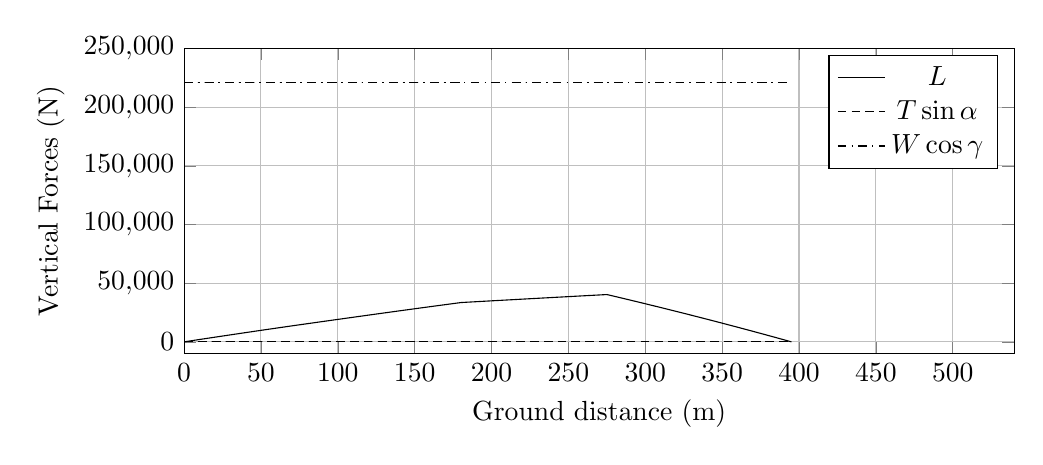
\begin{tikzpicture}

\begin{axis}[
width=\textwidth,
height=0.45\textwidth,
scaled ticks=false, tick label style={/pgf/number format/fixed},
xmin=0.0,
xmax=540,
xlabel={Ground distance (m)},
xmajorgrids,
ymin=-10000.0,
ymax=250000,
ylabel={Vertical Forces (N)},
ytick={0,50000,100000,150000,200000,250000},
ymajorgrids,
legend entries = {$L$\\$T\sin\alpha$\\$W\cos\gamma$\\}
]

\addplot [
color=black,
solid
]
table[row sep=crcr]{
1.3729668748938318E-8	2.806282665006737E-6\\
1.7493248493808052E-7	3.57554147017018E-5\\
1.4411937280317895E-6	2.945735280121515E-4\\
6.602995160656227E-5	0.013496223553729522\\
2.2740573828771224E-4	0.04648068642961645\\
4.8751428921765393E-4	0.09964561424061016\\
8.441986619835749E-4	0.1725500630170857\\
0.0012981647037285577	0.2653382014993034\\
0.0018484379050661159	0.37781071516138964\\
0.0024893731755424335	0.5088136299141717\\
0.0032286585096692284	0.6599181411123156\\
0.0040442418752796045	0.8266167863151783\\
0.004972762654474916	1.0163981283595875\\
0.005990910102221513	1.224497385309705\\
0.007111389191545643	1.4535110399840767\\
0.008336865178450469	1.7039835009995983\\
0.009664633507451486	1.9753616188502932\\
0.011093815858158905	2.267465482034736\\
0.01262066151120312	2.579528084735368\\
0.01419454386807839	2.9012018507490334\\
0.015910782250193378	3.251967925426192\\
0.017721549103721458	3.6220506937457744\\
0.019620507964630857	4.010154638044908\\
0.02164969955342029	4.424871320911528\\
0.023766550611781796	4.85749918631511\\
0.025957065600157342	5.30517743092814\\
0.028260861173784894	5.776001968801147\\
0.030668466949245715	6.268036630827707\\
0.0331489614440674	6.774961488443127\\
0.03573888453685943	7.304243345819678\\
0.038418765463712895	7.851902385355661\\
0.04116679597872082	8.413481286995548\\
0.044022059812866554	8.996966393798317\\
0.04700053365173311	9.605621673231713\\
0.050116649382181494	10.242395198315496\\
0.0533021652593606	10.89334096844776\\
0.056630220296749106	11.573403652440081\\
0.05998688030085898	12.259300877412034\\
0.06348077825220624	12.973229833906924\\
0.06710848437295475	13.714488364709307\\
0.07082346760424127	14.473567542104202\\
0.07462944469130567	15.251225884499924\\
0.07855413323217031	16.053125691933182\\
0.08251243142992878	16.861877985159396\\
0.08659905947434482	17.696834930482943\\
0.09083545394947079	18.562374747990532\\
0.09518096637774642	19.450191012487657\\
0.099604438418047	20.353916759217164\\
0.1041130762071252	21.275023232305365\\
0.10871457033213175	22.21508050683775\\
0.11350280915994052	23.193267621767205\\
0.11836943512882261	24.187446530662243\\
0.12328542045494376	25.19168645831357\\
0.12830372217771202	26.21680448604694\\
0.1334037067999082	27.258584439513825\\
0.1386015897371753	28.320337423156083\\
0.14405085578552257	29.433412722845212\\
0.1495239325759128	30.551324055094604\\
0.1550507392415454	31.68018205056223\\
0.16073360491635535	32.8408860101074\\
0.16659871679960742	34.03878196098107\\
0.17244819595229793	35.23345363994987\\
0.17848031195343078	36.4653934378244\\
0.18466822548212042	37.729117209827706\\
0.1909009608611748	39.00195936207095\\
0.19716089737688902	40.28032085349179\\
0.2035279375926986	41.5805177419583\\
0.21017879584430066	42.938633038397995\\
0.21687473998771628	44.305914395841825\\
0.22354650324940833	45.6682177275849\\
0.23036941414946865	47.061342162644934\\
0.23737731412185503	48.492194508153474\\
0.24449289925428264	49.94498838252895\\
0.2517184892023243	51.420195370168315\\
0.25908208279438383	52.92352948409531\\
0.2664863589195283	54.435120185051574\\
0.27399321582905467	55.96760271374788\\
0.2816108016888421	57.52263840156567\\
0.2893844725195981	59.109483470495874\\
0.29747621078120867	60.76119863815883\\
0.30547198304033185	62.39326761839598\\
0.31373479402345694	64.07978390620318\\
0.3220909744202328	65.78529614483764\\
0.3305540912568814	67.51257126528719\\
0.33895489345894936	69.22706566824411\\
0.34753073012810576	70.97721805392064\\
0.3563589175375672	72.77880233060625\\
0.3652744752958731	74.59814682416561\\
0.3742693918027593	76.43361481178357\\
0.38350989122680823	78.31912160487471\\
0.3927029292363896	80.19486979159359\\
0.4020876366599533	82.1096500166382\\
0.4115568217121528	84.04158847592845\\
0.4212787852930122	86.02501847948193\\
0.43089755178065414	87.98731378857087\\
0.4408379299669313	90.01513571597823\\
0.4510502611115679	92.0983464360726\\
0.4612670224725215	94.1823705745536\\
0.4715818614584312	96.2863092093323\\
0.4818438670126082	98.37938026137277\\
0.4922128554044626	100.49417979729924\\
0.50273876067117	102.640888700701\\
0.5136516607865718	104.86642303346466\\
0.5244310074213006	107.06462086944231\\
0.5355751508210329	109.33710611998103\\
0.5467126997993474	111.60814076742929\\
0.5580479056656631	113.91937072683379\\
0.5692960823995112	116.2127475851016\\
0.5809945926573021	118.59782845738275\\
0.5923626544035139	120.91542671305135\\
0.6041922852715	123.3270086632975\\
0.6160912669048675	125.75260922391328\\
0.6280605196746807	128.19241412352898\\
0.6403946506485891	130.70646946871295\\
0.6525721787971039	133.1884792579237\\
0.66504690021022	135.7309337389109\\
0.6773535438897555	138.23900494854706\\
0.6901462526606317	140.84600122858512\\
0.703249873273524	143.5162160505197\\
0.7159721017112175	146.10857525310308\\
0.729053467210389	148.77397422809446\\
0.7422988791228431	151.47265398029748\\
0.756304272979474	154.32601793929172\\
0.7696432036294076	157.04345055631785\\
0.7832290250230658	159.811029431902\\
0.7969128825551131	162.59842578167041\\
0.8108444209446342	165.436116609215\\
0.825043936786227	168.32822754462\\
0.8390802275180445	171.186931155511\\
0.8532340040587583	174.0693995803482\\
0.8678101043696134	177.03770507991493\\
0.8824320602344964	180.0151749887017\\
0.8978006605470081	183.14449699176663\\
0.9134572487531922	186.3322616186984\\
0.9287391767029982	189.44355218914325\\
0.9440564687433697	192.5618534315783\\
0.9598871644713316	195.78447496943204\\
0.9757786228365237	199.01926313394335\\
0.9918217338879218	202.2847153944913\\
1.0080608846667363	205.58986009296785\\
1.0245900975307913	208.95382447908804\\
1.040622085070809	212.21638718419337\\
1.0571005809273983	215.5696025580662\\
1.0736578999152901	218.9386403754591\\
1.0902401336450098	222.31252989750215\\
1.1073201062866707	225.78746392851656\\
1.1241926772552646	229.21997570662018\\
1.1416781667104252	232.7769412701498\\
1.1588269484070954	236.26517886252117\\
1.176440946845327	239.84780598202536\\
1.1944819542445066	243.51703332615108\\
1.2120125629913447	247.08221072011924\\
1.2299306574276825	250.72594283206632\\
1.2481120482032448	254.42296206421304\\
1.2663536608165091	258.131968770958\\
1.2851425782117465	261.9519874525736\\
1.3041313368869671	265.81235885775925\\
1.3228236880779458	269.6121994303511\\
1.3414329672940513	273.39488550006376\\
1.3605066144349074	277.2716868261175\\
1.3802534409605212	281.2850207581629\\
1.3994872719307283	285.1938068161015\\
1.4192016277101378	289.1999540606439\\
1.439023460648384	293.2276430557173\\
1.459347998039509	297.35716860153263\\
1.4793256644936217	301.4159116565444\\
1.4991489338326072	305.44298805939604\\
1.5195196572175793	309.5809698518583\\
1.5402684478761244	313.7954282519664\\
1.5604570108688036	317.8957833053254\\
1.5810331069622228	322.07453262351305\\
1.6022712329181132	326.38739938796914\\
1.623752316257296	330.74926105943746\\
1.6452514305955401	335.11443950817613\\
1.6664829631402025	339.4249506638256\\
1.6886446033619715	343.9239390691507\\
1.710607384244656	348.38219855174077\\
1.7329417009553727	352.91551110879027\\
1.7551421266962821	357.4212826205933\\
1.7779085356585536	362.04154884662023\\
1.800478286927734	366.6215294097352\\
1.8236018329231238	371.31350224684945\\
1.8462320784511883	375.90500179955234\\
1.869621217116264	380.6500825413459\\
1.8933146512119747	385.4564917131846\\
1.9176856041472643	390.3999162715478\\
1.9417713639512164	395.2850696516879\\
1.9657098573982132	400.1399389375771\\
1.9902165007163162	405.1096048051105\\
2.014554050520948	410.044553316676\\
2.039479559407779	415.0982827139958\\
2.0645497069116256	420.18088986675843\\
2.090368502766882	425.4148058795529\\
2.115564185269416	430.5219486672137\\
2.140750230554602	435.6266875637157\\
2.1667677015838267	440.89946911819936\\
2.1927560352542175	446.1658681804697\\
2.218891869133375	451.46167734708354\\
2.245288939563828	456.8099325012075\\
2.2712530964452817	462.0699992604805\\
2.297933078351498	467.474593429542\\
2.324564104516777	472.86877523991893\\
2.351466051806102	478.31733160247563\\
2.378869922986878	483.8670279387918\\
2.4061764715670764	489.39649766004914\\
2.4343811693482102	495.10729831930155\\
2.4622108821536663	500.74163593299886\\
2.4906408044048067	506.49694091916297\\
2.518892760285042	512.2156698479844\\
2.5472153538550346	517.9481494174163\\
2.5762492306032216	523.8240245648483\\
2.605385308804288	529.7200068667967\\
2.634725531238531	535.6567179035001\\
2.6633424112287507	541.4465064982276\\
2.6927188130915374	547.3893873069383\\
2.7226962917814213	553.4532678993294\\
2.7531675915664673	559.6164210150323\\
2.7831412651501983	565.6783173575186\\
2.8139174932165103	571.901898738332\\
2.8440331768075415	577.9912940216636\\
2.874693215323904	584.1901392392517\\
2.9059978681586376	590.5186702172421\\
2.9372617813709034	596.8383193110983\\
2.9684444504378202	603.1409045193727\\
3.000072782687808	609.532913905284\\
3.031082587373527	615.7992841558419\\
3.063213028467148	622.2914466525385\\
3.0965739711585014	629.031528238078\\
3.1291175748240176	635.6057819904911\\
3.161651640649506	642.177423195059\\
3.194791488147139	648.8707248640571\\
3.2273698640351327	655.449935740022\\
3.261394174200582	662.3204255836836\\
3.2942820372415875	668.9607291930233\\
3.3276455142443044	675.6963568963838\\
3.3625338428565543	682.7390729196641\\
3.396526624461681	689.6002662940734\\
3.4305511850311694	696.4671413069518\\
3.4642094416894933	703.2593692503269\\
3.498963551783903	710.2719916758012\\
3.5341885134496573	717.3788479510129\\
3.569804025802995	724.5637106478273\\
3.605116576002147	731.6866739914619\\
3.641338581546833	738.9922792025168\\
3.677593698357855	746.3037475399633\\
3.7132425573336665	753.492160815282\\
3.74957219375957	760.8170431425112\\
3.7872650227149185	768.4159184210757\\
3.825403000593508	776.1036494201633\\
3.861987998097706	783.4775004023854\\
3.899535703755137	791.0445411975682\\
3.9366960368382165	798.5326712405947\\
3.9756271117991435	806.3767243909108\\
4.014715979923002	814.251650262285\\
4.053268843133694	822.0176909882261\\
4.093111596873367	830.0426290124481\\
4.132540645872048	837.9833062986149\\
4.171686416589186	845.8660172376833\\
4.211258480423352	853.8336448147559\\
4.252585425594734	862.1536187315098\\
4.29253892845542	870.1961318147617\\
4.332839968385603	878.3076516533802\\
4.372708537789018	886.3311896278153\\
4.414379330316386	894.7164314874422\\
4.455607216042212	903.0115534826248\\
4.497336690654009	911.4065909895107\\
4.53836773335787	919.6601369766629\\
4.579767142935065	927.9867970700398\\
4.621942908118227	936.4685922219469\\
4.663798268780793	944.8849444095713\\
4.705838036060712	953.3373702474012\\
4.748491012675066	961.9120585065416\\
4.791393968819099	970.5359598905145\\
4.835700194867293	979.440839546663\\
4.879973298406089	988.3379572724518\\
4.923250156511948	997.0338059187736\\
4.967673596314626	1005.9589533100659\\
5.012954369117542	1015.0552156582116\\
5.057574526249477	1024.017655244229\\
5.103280208347517	1033.1969912808918\\
5.148856018935929	1042.3490967916487\\
5.194350575362858	1051.4837466822828\\
5.240584094986199	1060.7656080814913\\
5.2871741484687504	1070.1178670515956\\
5.333122064003502	1079.3400700952734\\
5.3803318800233235	1088.8143574072192\\
5.4262712259485255	1098.0325254710601\\
5.473378197958581	1107.4838097246688\\
5.521938593493333	1117.2254557127758\\
5.570027890245774	1126.8713539553733\\
5.617746353771608	1136.44165301748\\
5.665750363096816	1146.0680024638277\\
5.714883880069209	1155.9195941917355\\
5.763390205677501	1165.6441839066624\\
5.812817811268989	1175.5522038942277\\
5.861909274803731	1185.3915796089655\\
5.912134919389196	1195.4569810874896\\
5.962317560553064	1205.5124588678063\\
6.012727788730279	1215.6122310670148\\
6.0628236035803145	1225.6477154045137\\
6.113711068416594	1235.8404714305052\\
6.16497292765713	1246.1068826167143\\
6.216284706244114	1256.3819537264353\\
6.26834407822653	1266.805366505073\\
6.320257064476769	1277.198108757139\\
6.37351660191279	1287.8590176930866\\
6.426150862197664	1298.3933714201576\\
6.479030963436509	1308.9755384185219\\
6.532319340056288	1319.6380042672158\\
6.5857233987986845	1330.322208998809\\
6.640834734692348	1341.346505927308\\
6.695022999498724	1352.184703151645\\
6.749720237657193	1363.1232466618544\\
6.804235758325081	1374.0240026810225\\
6.859728469301633	1385.1186772092724\\
6.916686079588434	1396.504685936412\\
6.9732530286722305	1407.8110592494522\\
7.029531186664631	1419.0581927816625\\
7.086633318514238	1430.4684564276877\\
7.144155485034537	1441.9610904582237\\
7.202053129566568	1453.5271670947945\\
7.260126434764185	1465.126753729814\\
7.317913145042743	1476.6675306867046\\
7.376682960996439	1488.4030527686532\\
7.435393721764624	1500.1251842594165\\
7.493838107271518	1511.7925521825168\\
7.552684475254578	1523.538583711731\\
7.613252707151423	1535.6266545820708\\
7.672782806866918	1547.5059104596867\\
7.733397683408512	1559.5999843912587\\
7.795525081709004	1571.994122169002\\
7.856013653786727	1584.059656978964\\
7.91792172269443	1596.4066434721335\\
7.980110745884113	1608.8079479397506\\
8.041720670752433	1621.0920849598356\\
8.105229267009985	1633.7530400265573\\
8.167457523036095	1646.1570340275603\\
8.230908874360502	1658.803088995543\\
8.293738919282273	1671.3235934058557\\
8.356235402336917	1683.7759350745832\\
8.42092378244627	1696.6632406895092\\
8.485671322837007	1709.5605395242947\\
8.549180898871484	1722.2095098300888\\
8.614596634551038	1735.2363366405225\\
8.680166762249144	1748.2920987955822\\
8.744770128469462	1761.153604176418\\
8.812993689385827	1774.7339422580235\\
8.88005807777586	1788.0816563592075\\
8.94709863067661	1801.4227701029208\\
9.013172088448385	1814.5696245065037\\
9.079266506338545	1827.7188641032158\\
9.14748814890141	1841.2894441090216\\
9.215411293660388	1854.798776872754\\
9.284579146198691	1868.553763659229\\
9.353168277381275	1882.191772837948\\
9.423753765537143	1896.2247749492308\\
9.492960052876374	1909.9816648685555\\
9.564123004975215	1924.1255357485384\\
9.634097601479446	1938.0312832489667\\
9.705672410878787	1952.2530612880819\\
9.776260200085993	1966.2767770544979\\
9.846607984572056	1980.2509016681688\\
9.918231435410593	1994.4764816967395\\
9.988851555070422	2008.5008708469604\\
10.060390022634245	2022.7057080335544\\
10.133279281833644	2037.176779088842\\
10.205241085147751	2051.4617659966607\\
10.277820389603	2065.867378807905\\
10.352558894167803	2080.6995139827604\\
10.42733258664746	2095.5365753186534\\
10.501815126481194	2110.313830973585\\
10.576858173457808	2125.200250495959\\
10.65303812840548	2140.3101184302204\\
10.729080272001735	2155.3905729588914\\
10.804841544893105	2170.4132726912594\\
10.881905013502095	2185.6920949456144\\
10.958396790746043	2200.855500634004\\
11.035905069829102	2216.2183213897324\\
11.113160538490881	2231.5289504887523\\
11.192172636140572	2247.185574624553\\
11.270076562295213	2262.6205070389788\\
11.350065490058778	2278.466378210607\\
11.429008826667825	2294.1029869311296\\
11.50754237847364	2309.656342062599\\
11.587076645554472	2325.405779403285\\
11.668897725768986	2341.6058554403244\\
11.749734371708193	2357.6088451510395\\
11.830312384681939	2373.5584976739747\\
11.909862670519033	2389.3026429706797\\
11.990515423105418	2405.262888172516\\
12.072973931530203	2421.5783063693607\\
12.155304175892073	2437.8661768822785\\
12.237018674011615	2454.0301023770935\\
12.320146069843414	2470.4713522367438\\
12.406770618003886	2487.601979926004\\
12.489918686423398	2504.0429144891023\\
12.574493004618496	2520.763673530055\\
12.660666896522624	2537.7984218769943\\
12.746500366216402	2554.7636305953165\\
12.832006837122272	2571.66199542469\\
12.919285437479463	2588.9083207247922\\
13.00517529032821	2605.8780162981257\\
13.092301899261269	2623.0898390339926\\
13.179760097773386	2640.3649304518995\\
13.268594687119744	2657.90961557385\\
13.357699529172354	2675.5053883280852\\
13.44829753340392	2693.3936901772195\\
13.537570218252604	2711.018032251226\\
13.627322718831184	2728.734837521537\\
13.718307212496544	2746.6925364935205\\
13.808540263830096	2764.4996568903016\\
13.899143852161355	2782.3776495874436\\
13.991564069206362	2800.611795915768\\
14.085798171937814	2819.2014376453126\\
14.179213507883688	2837.627211723201\\
14.271883316076963	2855.903642815706\\
14.367546274622434	2874.7680133257254\\
14.459430863676705	2892.8850540055655\\
14.555010173556813	2911.7282704494382\\
14.648669731311681	2930.1907392422954\\
14.743773575674254	2948.935628253599\\
14.839769774519894	2967.8540884909207\\
14.932807148196385	2986.187242296921\\
15.026921440816679	3004.730425483055\\
15.12275113649265	3023.6093602029214\\
15.222025232743288	3043.164506919782\\
15.321078842653048	3062.6738588139233\\
15.417564225728565	3081.6751315127685\\
15.515758841369038	3101.010755133475\\
15.613440509090129	3120.2431379039544\\
15.7107260301154	3139.3953293683635\\
15.81102223487273	3159.1379512387175\\
15.913565872734136	3179.3206061421333\\
16.012918321571746	3198.872919261641\\
16.11222833737955	3218.4146899775797\\
16.216250800242257	3238.8814292552306\\
16.319159023020546	3259.1266221594287\\
16.421418004006803	3279.2418319607787\\
16.521675247646563	3298.9611218409764\\
16.62557290942481	3319.3942010814444\\
16.72731964230514	3339.4020879110067\\
16.830283223934416	3359.6470900094737\\
16.93464251494634	3380.1643172325894\\
17.038481620468637	3400.577098380758\\
17.146497421123335	3421.8086606680436\\
17.252282308638982	3442.599490990361\\
17.35724772858778	3463.227114640078\\
17.464053904588297	3484.2143089724577\\
17.572390862630144	3505.5000883439325\\
17.680417629270814	3526.722732878021\\
17.789707298693855	3548.1912873517767\\
17.899612520762552	3569.778559759381\\
18.01027367065641	3591.5121098768805\\
18.121415095654797	3613.3377926424237\\
18.232428503320143	3635.1361719896004\\
18.34337337506409	3656.918962548144\\
18.454877340220463	3678.8094075688923\\
18.56636189702322	3700.6939496552377\\
18.678405595805643	3722.6861732585494\\
18.7903363416971	3744.65417502691\\
18.902391384512768	3766.6445478581572\\
19.01754810908954	3789.2415348885906\\
19.131359562866663	3811.572502345356\\
19.247747682986713	3834.406973099637\\
19.361628242251975	3856.7474895210808\\
19.477963464454028	3879.5675491535612\\
19.595742742603164	3902.6688452087164\\
19.71107288142779	3925.287822089318\\
19.82767543183723	3948.154426271416\\
19.944540068808188	3971.070520031394\\
20.06171535440768	3994.0456445235495\\
20.179291418887807	4017.097487642068\\
20.29729887224694	4040.232063977008\\
20.417200571824914	4063.736136195602\\
20.53676390826074	4087.1720487249304\\
20.65523768803314	4110.392624602573\\
20.777063017363922	4134.268293934159\\
20.896922101876633	4157.7568643722225\\
21.016777952410983	4181.243100972975\\
21.13892104879462	4205.175818835887\\
21.260534693274344	4229.003112576875\\
21.382619708556632	4252.92110640425\\
21.506306369043365	4277.15122946345\\
21.631260758247265	4301.628047413829\\
21.75556249187227	4325.975409123739\\
21.87985606458615	4350.319603914868\\
22.005925835680863	4375.01012171852\\
22.130365724585275	4399.379923180959\\
22.257477980325966	4424.271562924503\\
22.38418119026224	4449.081624701412\\
22.50885833858638	4473.493556869376\\
22.636026948728087	4498.391926465576\\
22.76367325110224	4523.382447174803\\
22.89115382514759	4548.339184706792\\
23.022452271734288	4574.04198773136\\
23.149877274293033	4598.985255542117\\
23.27873580881144	4624.207897983428\\
23.408563766880334	4649.619076644543\\
23.538692653979794	4675.087970358878\\
23.671258756997098	4701.03269905402\\
23.803210122669313	4726.855978250971\\
23.93544283576786	4752.733221504041\\
24.067241518013077	4778.524477346406\\
24.19863541429976	4804.2355205638\\
24.329449967727697	4829.8322465743695\\
24.46175612159181	4855.719912585919\\
24.594763714591892	4881.74393124079\\
24.72754053098891	4907.72194479419\\
24.86208223890334	4934.044437880322\\
24.99503410474967	4960.055112959371\\
25.12831230627787	4986.128904408461\\
25.265273024090206	5012.922407965116\\
25.400650037308893	5039.4054258105025\\
25.536304655026747	5065.942129401419\\
25.673594178904246	5092.798065896994\\
25.80797730935859	5119.084939673445\\
25.835159569235522	5124.402040304283\\
25.83771752397454	5124.902398838372\\
25.84157983658004	5125.657900966\\
25.854829339215996	5128.249616600628\\
25.893215796826965	5135.758308481054\\
25.973046119315796	5151.373614709088\\
26.096262980671412	5175.475228433583\\
26.224212718725603	5200.502094330115\\
26.35313595194755	5225.718798644626\\
26.481727686355264	5250.870039969022\\
26.611118169629577	5276.176832768922\\
26.74049186039369	5301.479616792409\\
26.87228140714948	5327.254099001537\\
27.003385008924262	5352.893587591621\\
27.1358830905183	5378.804889430488\\
27.265951877034226	5404.240192172027\\
27.399105426781233	5430.277730829905\\
27.53075869079712	5456.020857215599\\
27.66387879779476	5482.049709825325\\
27.79855889054391	5508.38241621972\\
27.932132547760695	5534.497584453531\\
28.06791767232785	5561.0438402687505\\
28.202763022922632	5587.405045628651\\
28.339788243013793	5614.19100096532\\
28.476803106655623	5640.973476496412\\
28.61761981788422	5668.497538861404\\
28.753907949775353	5695.13488667091\\
28.89297195746854	5722.313150001586\\
29.03211749902605	5749.50565776507\\
29.17123509789927	5776.690968361818\\
29.312253051611236	5804.245813206993\\
29.454422317169097	5832.023723002341\\
29.59523538430127	5859.534722625731\\
29.737672170826222	5887.360954072947\\
29.879173197948965	5915.002341463247\\
30.02075470454991	5942.657374561597\\
30.166674235301365	5971.157532176032\\
30.308336095430334	5998.823906373711\\
30.452640844036836	6027.00415986746\\
30.597553881025625	6055.300847840013\\
30.742967061600154	6083.692781088712\\
30.888975484926362	6112.19845541742\\
31.034653067922946	6140.637017694007\\
31.180984070508003	6169.200558547947\\
31.328351020411645	6197.963657761355\\
31.476753455192622	6226.926124490206\\
31.62661541983664	6256.1706018013865\\
31.774495604492607	6285.025514140398\\
31.924944104961916	6314.378631583197\\
32.07610067279926	6343.866871606962\\
32.22631826848556	6373.168886493333\\
32.37899942625752	6402.948296972392\\
32.528514827654206	6432.107122714753\\
32.68189139400266	6462.015704644464\\
32.836069829938495	6492.077284395198\\
32.99025509482905	6522.136775880281\\
33.14574197930297	6552.446520602594\\
33.30072558931056	6582.654612913177\\
33.455047097713944	6612.730093817432\\
33.610874563168906	6643.09542207652\\
33.76926068144728	6673.95554519078\\
33.92617323250643	6704.524740274304\\
34.08448787244542	6735.363194286741\\
34.24243160505006	6766.125462392252\\
34.40316487172558	6797.426962515037\\
34.56154208099588	6828.265575521462\\
34.721775177117024	6859.461414201853\\
34.88076970836556	6890.411955352543\\
35.041349106451236	6921.666767083099\\
35.20329621413198	6953.183425278059\\
35.364886328651124	6984.62620421654\\
35.529241615711214	7016.602487367427\\
35.69117991651797	7048.10400253258\\
35.85317319416103	7079.611676781677\\
36.014854298354294	7111.054073631614\\
36.18095311277159	7143.350808611569\\
36.34443322746766	7175.133587371854\\
36.51065106768533	7207.443730207169\\
36.67635767082788	7239.64955481672\\
36.842033683894186	7271.844465372602\\
37.00823867836148	7304.137142415728\\
37.17279029188734	7336.10358205886\\
37.33951104811075	7368.48630492251\\
37.50923941781488	7401.447895361947\\
37.679358776579846	7434.480004418663\\
37.845326083883435	7466.700653932994\\
38.017144746304325	7500.0517752654705\\
38.1852030886141	7532.667546706083\\
38.35804431104914	7566.2058986420325\\
38.52812920813831	7599.203781380749\\
38.69960796987526	7632.466401778167\\
38.87165793928378	7665.834055186153\\
39.0423941506003	7698.941174731584\\
39.21436971822614	7732.282803122685\\
39.38727999643966	7765.799736697494\\
39.558989012313546	7799.077922688008\\
39.734752343022535	7833.135744128096\\
39.908836167348156	7866.862000019737\\
40.084555009291705	7900.898805353121\\
40.259186798753746	7934.718836852202\\
40.43324437115375	7968.4214737430575\\
40.61041052363379	8002.719649840783\\
40.787318094191775	8036.961323868758\\
40.96620398302343	8071.5793416985725\\
41.14141336180775	8105.479447594433\\
41.31941103282654	8139.91249685874\\
41.49571226203258	8174.01084790638\\
41.67366972437729	8208.422918037933\\
41.85219319429197	8242.937739363086\\
42.03136872634711	8277.571856738523\\
42.21293422072888	8312.661004123085\\
42.39366932880948	8347.58270762219\\
42.57479521797359	8382.572924209107\\
42.75522531040919	8417.421742445797\\
42.93775785970641	8452.66952174528\\
43.11993568316029	8487.841646417819\\
43.30336620712447	8523.248379796216\\
43.48720879745599	8558.72733873091\\
43.672226884455625	8594.425738843674\\
43.85684130549208	8630.038821636037\\
44.039851952877484	8665.335181973252\\
44.22449378650157	8700.938710445575\\
44.412385508552646	8737.161217601566\\
44.59783063297877	8772.904445341112\\
44.78525507043919	8809.021467728737\\
44.973130075825196	8845.217525572967\\
45.16145211071871	8881.491864608091\\
45.34881478087516	8917.573603053508\\
45.536017136752506	8953.616674251432\\
45.724971990057284	8989.989247383477\\
45.91416212467789	9026.39912859317\\
46.10175434018815	9062.493588348541\\
46.29356928918713	9099.392392992962\\
46.48490977712943	9136.191706032125\\
46.67744207882204	9173.211932403508\\
46.869905949194575	9210.210666338477\\
47.062749521718516	9247.274023709779\\
47.25341437235973	9283.910396674692\\
47.44508461154423	9320.731679674453\\
47.63880095964302	9357.937594152478\\
47.83356160493736	9395.335515700503\\
48.025334057720784	9432.151244600012\\
48.218846636819876	9469.29257853121\\
48.41468711090302	9506.872052915562\\
48.610449575687724	9544.427845844173\\
48.80723286029129	9582.170690341685\\
49.00124137999302	9619.372707266157\\
49.20045899041696	9657.564667414208\\
49.394243884198005	9694.706441770395\\
49.59161211700324	9732.526211536242\\
49.79144608231523	9770.809407993649\\
49.99107345578199	9809.04392232143\\
50.18996871950735	9847.129162704434\\
50.388458331230495	9885.127714875154\\
50.59191110395449	9924.067060579924\\
50.79453916783869	9962.83915633375\\
50.99530158869649	10001.245008282305\\
51.19776583381373	10039.96708303189\\
51.3996255264899	10078.56420041317\\
51.599450409211	10116.763066414704\\
51.80158475775707	10155.394121552778\\
52.002311498730975	10193.746913237635\\
52.2060805474067	10232.671573220327\\
52.40811442127868	10271.255401626571\\
52.61423073460446	10310.609267309232\\
52.821749674584495	10350.221129605587\\
53.03053110951893	10390.064053775986\\
53.23753590773735	10429.558106054646\\
53.44487707917263	10469.106530617235\\
53.652063533093525	10508.615648585746\\
53.85975522429668	10548.21128977558\\
54.06844148636836	10587.986643324526\\
54.278580968983874	10628.028959354917\\
54.48685885904548	10667.706632816487\\
54.69884126905886	10708.079903508911\\
54.90975544393264	10748.239591991562\\
55.12216013841277	10788.67288348838\\
55.333080623240974	10828.813518444495\\
55.5448885814986	10869.11290881675\\
55.75594910746132	10909.259991536106\\
55.968144975063936	10949.612883347141\\
56.18150915317635	10990.177699694024\\
56.394069348356695	11030.579453761762\\
56.60950747146016	11071.517836734307\\
56.82641599949238	11112.725083406527\\
57.03980213394583	11153.25284856623\\
57.25698083573829	11194.490434890617\\
57.47353804711997	11235.599492183312\\
57.6941706582635	11277.471394112497\\
57.91229938529948	11318.857418202988\\
58.12998527173144	11360.14884347076\\
58.34905943653719	11401.692951406178\\
58.56781345824973	11443.165705654716\\
58.787998582886644	11484.899055758382\\
59.011266007804366	11527.205653729587\\
59.23368761368569	11569.341021691791\\
59.456031473365414	11611.450751683322\\
59.67976581221534	11653.812835691104\\
59.90315377467765	11696.098360711247\\
60.125192111546724	11738.11756669433\\
60.349269227196444	11780.511657784693\\
60.57220932044149	11822.679747999824\\
60.79606803632835	11865.010692917429\\
61.021718319759984	11907.669389591363\\
61.25073295331903	11950.952814777884\\
61.47770893732542	11993.839737933864\\
61.70784367826464	12037.312148966346\\
61.93740803875056	12080.66545062964\\
62.1673491775543	12124.0785571509\\
62.39648011888062	12167.327427318916\\
62.62822464633953	12211.058202733471\\
62.86094183422966	12254.961001573094\\
63.090532789209604	12298.26274526255\\
63.321616049163225	12341.834659557459\\
63.554808975015874	12385.792918233787\\
63.78685818650332	12429.524201220658\\
64.0234762327251	12474.104858855171\\
64.25652029988498	12518.000683296355\\
64.49146565301734	12562.243145510703\\
64.72768747885678	12606.714389165398\\
64.96568125142531	12651.507504271882\\
65.20057601391298	12695.705856228898\\
65.43975061379945	12740.697817478027\\
65.67719429610031	12785.35253548852\\
65.91652243006087	12830.34996084579\\
66.1565253585166	12875.462511377325\\
66.39740384038885	12920.727850156254\\
66.63777997854328	12965.887060005352\\
66.87849958303539	13011.099096012425\\
67.12349409848125	13057.102068455992\\
67.36843544137562	13103.083021277991\\
67.61129947098183	13148.662179580668\\
67.85808619273692	13194.965496653469\\
68.10323725880951	13240.949967815246\\
68.3520146383799	13287.602514667029\\
68.60099753692072	13334.28141310766\\
68.84943315800746	13380.845605011647\\
69.09793111574629	13427.409435712761\\
69.34894754058863	13474.433000947542\\
69.59791912239118	13521.061460992209\\
69.84867626946473	13568.012262354507\\
70.10496107302816	13615.985582568243\\
70.35594730130109	13662.954924012873\\
70.60854748652795	13710.214214238367\\
70.8625286964371	13757.719714086605\\
71.1182576034713	13805.539839137156\\
71.37278964945165	13853.123988810086\\
71.62944082734805	13901.092072721647\\
71.88536754710964	13948.912583804824\\
72.14250945057543	13996.947974031216\\
72.40306402213687	14045.608476331352\\
72.66241221953337	14094.031355835188\\
72.92327110344874	14142.723957184568\\
73.18657203154456	14191.859914366294\\
73.45150557123125	14241.287951870185\\
73.71756195569753	14290.912836020027\\
73.97940051906463	14339.7387124173\\
74.24514793127645	14389.28107853101\\
74.51022759525631	14438.686577963344\\
74.77823256031297	14488.62479594543\\
75.04767613410795	14538.818479735412\\
75.31682895458664	14588.945466710436\\
75.58729746777243	14639.304945213924\\
75.85729327570917	14689.56394468847\\
76.13042767774209	14740.394591817938\\
76.40299665611133	14791.10746519261\\
76.67973301409052	14842.582959350293\\
76.95360383527739	14893.51287931505\\
77.22854206589327	14944.628814658994\\
77.50692063517303	14996.371711476168\\
77.78349662592461	15047.767029349456\\
78.0616064362213	15099.434865886673\\
78.33869545141144	15150.900670831565\\
78.62238552181594	15203.579820487987\\
78.90481169871467	15256.01158375197\\
79.18659077494928	15308.310687306981\\
79.4700201012688	15360.903552827549\\
79.75774957869095	15414.281592741201\\
80.04430580185078	15467.42929929428\\
80.33432201731404	15521.205950657331\\
80.62298533865851	15574.71907205059\\
80.9130804606989	15628.48499380959\\
81.20459144967842	15682.500679845529\\
81.49650140842283	15736.577690095604\\
81.79224544448738	15791.352218932981\\
82.08455487090956	15845.478119845404\\
82.37934996819865	15900.05179992658\\
82.67580145620735	15954.919586092012\\
82.97475550983006	16010.237938839673\\
83.2734238134004	16065.490883583658\\
83.57209772503273	16120.732453963079\\
83.87419166445906	16176.594071712381\\
84.17487194816226	16232.181911653464\\
84.47686996876752	16288.001062097352\\
84.78124993153034	16344.248118704578\\
85.08776945017104	16400.87813949229\\
85.39395758722245	16457.434631152915\\
85.69833162305892	16513.643973104925\\
86.01027818388755	16571.239398253558\\
86.31658691867341	16627.781863621334\\
86.62866814828641	16685.377760991418\\
86.94043673469176	16742.903868610098\\
87.2565990672368	16801.228489179353\\
87.56980823017452	16858.996343145976\\
87.88101387141376	16916.383003161965\\
88.20007062892054	16975.20548732116\\
88.51883409355145	17033.961982864254\\
88.83509784148416	17092.246089544708\\
89.15857089898353	17151.846969300168\\
89.47772213402055	17210.63996843795\\
89.80217214804901	17270.397464057067\\
90.1263587278685	17330.094887569627\\
90.44950966725051	17389.59026662469\\
90.77764749859728	17449.992362700243\\
91.10470504824352	17510.184316351486\\
91.43769785174896	17571.457188386878\\
91.76691749028419	17632.024622227982\\
92.09386993524024	17692.16414639618\\
92.42498248438446	17753.058069670675\\
92.7581696617394	17814.32272342805\\
93.09729153734631	17876.66766337001\\
93.4312406900703	17938.05101672822\\
93.76780571708736	17999.904710695933\\
94.10390054156983	18061.66166741842\\
94.43564317419558	18122.608973938302\\
94.77291201930262	18184.561604104114\\
95.10796951504997	18246.0982846442\\
95.44708659079325	18308.370837964212\\
95.78515592548297	18370.441454714826\\
96.12311752311894	18432.48295684316\\
96.46351490415591	18494.962363868442\\
96.80669869710772	18557.944011741463\\
97.14657639264556	18620.310005057712\\
97.48763116340677	18682.883260593815\\
97.8305814261901	18745.795661701246\\
98.17013304046878	18808.0762747087\\
98.51054009051404	18870.505669594473\\
98.854181194619	18933.520124434115\\
99.19205317796005	18995.468981194193\\
99.53355440060989	19058.075696360764\\
99.87198375587872	19120.111942322874\\
100.2129389915628	19182.604032576397\\
100.55335806642802	19244.990870652917\\
100.89503335592528	19307.601109106858\\
101.23693480167049	19370.246147055004\\
101.57977298927813	19433.0563460169\\
101.91842351185082	19495.093167351144\\
102.26214655705948	19558.053143369543\\
102.60487134933112	19620.82437720304\\
102.94238410388857	19682.635453295683\\
103.28139950825951	19744.716364599255\\
103.61984226602698	19806.687251384392\\
103.95406402656286	19867.880377069298\\
104.29248504574807	19929.8376100061\\
104.63112914593611	19991.831102127857\\
104.96686613984221	20053.288075021854\\
105.30464484937244	20115.114624424044\\
105.64180205248229	20176.823444087706\\
105.97704387437452	20238.177955758794\\
106.31384964552919	20299.815129106057\\
106.6489228444834	20361.13187713189\\
106.98000007373659	20421.7142810273\\
107.31456925364313	20482.932718169657\\
107.38092108752608	20495.07323697525\\
107.387754025128	20496.3234661839\\
107.3946577511588	20497.58664646397\\
107.39916951903444	20498.412167618015\\
107.40247473215817	20499.016924336378\\
107.40548301099807	20499.567350589496\\
107.41901751964124	20502.043763537935\\
107.47756267729525	20512.75573613878\\
107.63696404402117	20541.920874222742\\
107.95668166923352	20600.416538003505\\
108.2571634635643	20655.390208517507\\
108.55996775705782	20710.786057890014\\
108.8616926844802	20765.98154850454\\
109.16669292910967	20821.77308861661\\
109.47218465327785	20877.651216524282\\
109.78023369107405	20933.99357052766\\
110.09061921742381	20990.759496988903\\
110.4007971847821	21047.483500583687\\
110.7125096545017	21104.483956760945\\
111.02874540594937	21162.307094928605\\
111.34670354521654	21220.440458308316\\
111.664908557295	21278.614043828515\\
111.98617551206428	21337.342232243427\\
112.3078797039536	21396.14495020976\\
112.63537393275391	21456.0002591789\\
112.96267359383529	21515.814026980384\\
113.28778388635178	21575.221580604477\\
113.61823593045688	21635.598803548382\\
113.94632344632586	21695.5373969461\\
114.27926944824554	21756.35667123001\\
114.61324422041562	21817.356674166986\\
114.94750338770686	21878.40121118602\\
115.28618013885716	21940.244758621207\\
115.62544260296943	22002.187234855068\\
115.9647508443766	22064.129840892987\\
116.30617149460878	22126.449577880594\\
116.65060078043697	22189.309645571608\\
116.99863777637248	22252.818921812985\\
117.34270613829636	22315.594704805895\\
117.68983788345284	22378.919837673573\\
118.04137408578512	22443.03845541695\\
118.39343387684602	22507.242295329175\\
118.74804854616337	22571.901460680536\\
119.10520175440718	22637.01254140058\\
119.46686684850098	22702.934758499963\\
119.82660492256403	22768.49413990682\\
120.19012449272657	22834.73072265015\\
120.55217592908159	22900.687660574433\\
120.91763124996498	22967.252216612134\\
121.28719248968574	23034.551668318556\\
121.65493622417088	23101.5069991754\\
122.02513489718217	23168.895859006414\\
122.39308995700384	23235.862740516626\\
122.76618799735454	23303.751624159275\\
123.1388017253943	23371.53810702022\\
123.51256311114031	23439.518844182094\\
123.88633794770595	23507.487280363195\\
124.25665874611622	23574.812890025634\\
124.63165231885978	23642.9728939252\\
125.00664173256905	23711.11672717597\\
125.38021625899401	23778.987932418837\\
125.75512563345742	23847.085905717955\\
126.13473977091255	23916.02218708639\\
126.51299085225449	23984.694490042028\\
126.8948287761801	24054.00115145539\\
127.27325883095315	24122.6723850536\\
127.64986999110431	24190.996707361366\\
128.03053456382577	24260.039142389745\\
128.40840086210045	24328.556722573252\\
128.78830732782995	24397.42667612331\\
129.16816802858597	24466.27055950224\\
129.55114692916032	24535.66141172711\\
129.92795862154003	24603.91689411499\\
130.30814318938542	24672.7651360792\\
130.68801179162523	24741.537745833215\\
131.0673626953399	24810.198110464124\\
131.44707508552267	24878.905220320557\\
131.82575792285303	24947.40727751059\\
132.20466209461676	25015.930479366034\\
132.58549544797154	25084.78338015171\\
132.96520261413826	25153.413383897176\\
133.34413894748724	25221.884727612887\\
133.72638850756363	25290.935044272643\\
134.1049920954593	25359.307104949665\\
134.48538249769342	25427.982032580207\\
134.86277461399203	25496.095904077316\\
135.2402386369938	25564.202952524596\\
135.62109197355238	25632.901353604422\\
135.9996509441208	25701.16567823902\\
136.37968191797512	25769.67505252744\\
136.76120583273502	25838.43289608061\\
137.13951930881296	25906.59159772323\\
137.51840340013064	25974.832474896706\\
137.89819615735314	26043.21618524832\\
138.27485697152616	26111.015273794546\\
138.65420581933705	26179.277272347885\\
139.03531375767642	26247.834551047163\\
139.41296882619503	26315.74957621919\\
139.79422155259	26384.290158986667\\
140.17408835952057	26452.560083485732\\
140.5488076998477	26519.883782772966\\
140.92844631991198	26588.0698214594\\
141.30483696429354	26655.651068316307\\
141.68269541512387	26723.474312386585\\
142.06058279783264	26791.281072945487\\
142.43991695918288	26859.325553922397\\
142.81695502902187	26926.936357720093\\
143.19247254825046	26994.252808469944\\
143.5733885276352	27062.514815892202\\
143.94921103219775	27129.842073678512\\
144.32621366107247	27197.35874577176\\
144.70408630975157	27265.009046439154\\
145.08263595865492	27332.758214540612\\
145.46162624555404	27400.563782183795\\
145.83827879615103	27467.92877110144\\
146.21524500988596	27535.3275061269\\
146.5934755401724	27602.929755294783\\
146.9730259257883	27670.74515391088\\
147.3547239944582	27738.921240841628\\
147.73366854735332	27806.58259815898\\
148.1136534850276	27874.406735140554\\
148.49311509785633	27942.114442543272\\
148.87144514206074	28009.597290025114\\
149.25360190977045	28077.739393420794\\
149.6334430260095	28145.445323522\\
150.01465687879528	28213.372567934028\\
150.3940924716125	28280.95965326319\\
150.77688175221402	28349.120520057222\\
151.1561678741857	28416.634185087052\\
151.5352572324847	28484.0894952303\\
151.91884603110896	28552.321657152665\\
152.3000376871389	28620.10368494373\\
152.6837211891089	28688.304874726127\\
153.06727641570347	28756.459234170616\\
153.4514076737559	28824.691837143742\\
153.83522357687116	28892.84429210198\\
154.21637826964854	28960.500306604124\\
154.6009164651564	29028.732737637794\\
154.98403470202834	29096.68904753655\\
155.36838747168406	29164.840073907915\\
155.75158064164503	29232.761273409706\\
156.13576662495046	29300.834156011028\\
156.5218436740983	29369.217585606595\\
156.90521285441474	29437.09703988659\\
157.2916244593892	29505.49061751207\\
157.6780020855428	29573.853501352394\\
158.06299451159185	29641.946736778686\\
158.4509000667514	29710.53040486735\\
158.83830611621056	29779.00089044049\\
159.22672413827297	29847.625273213678\\
159.61474494524106	29916.154513949572\\
160.0042372884319	29984.91854522517\\
160.39552304382113	30053.973870544723\\
160.78478895267375	30122.647530893657\\
161.17517847278327	30191.494173206032\\
161.56748129737286	30260.652765209772\\
161.9609400214345	30329.989484462196\\
162.35005274814932	30398.535078110923\\
162.7425950916558	30467.659379405282\\
163.13607830878885	30536.923713175114\\
163.53170884953005	30606.54015128693\\
163.92462594167722	30675.65343797244\\
164.3198767210975	30745.15139851978\\
164.7157696028566	30814.736314108923\\
165.1115317336501	30884.272302642472\\
165.50739628911128	30953.80034789561\\
165.90698313288817	31023.955864192765\\
166.30582458333038	31093.95418063693\\
166.70591293613995	31164.144919824284\\
167.1044701422045	31234.040751711604\\
167.50226971352845	31303.777573616004\\
167.9010833894181	31373.6659776148\\
168.3004552315794	31443.62593117453\\
168.70189335181743	31513.92138141355\\
169.10576843973695	31584.616817628703\\
169.50785881751284	31654.973226703543\\
169.91045494783964	31725.391540421668\\
170.31331810721775	31795.829955660098\\
170.71648797717722	31866.295383759498\\
171.11993291578136	31936.782268213785\\
171.5247281229082	32007.4783318088\\
171.92976094083576	32078.189129755803\\
172.33690302624336	32149.2412196671\\
172.74259563259648	32220.013521387555\\
173.1509823323036	32291.22878848337\\
173.55913088366435	32362.375487379257\\
173.96636547491187	32433.335969373984\\
174.37754484483776	32504.95661024419\\
174.7874876782942	32576.334686350958\\
175.2012500141185	32648.35033003368\\
175.6112323385957	32719.68088395265\\
176.02092514523684	32790.93409223741\\
176.43326782420013	32862.620986204856\\
176.8477920653399	32934.659722068885\\
177.2627043459005	33006.73840823803\\
177.67839640445425	33078.9250369644\\
178.09047986160414	33150.45788426514\\
178.50771992227516	33222.85839145917\\
178.92514786216543	33295.26390427741\\
179.34349041668827	33367.800431602955\\
179.7634585539525	33440.591059539875\\
180.0836350053749	33496.06673133357\\
180.18446825846002	33513.53436426018\\
180.6041229201494	33544.34880841606\\
181.5278851973348	33612.15527740873\\
182.40940876889346	33676.83105822808\\
183.29020149056134	33741.423764291\\
184.17127536929127	33806.007696075685\\
185.05444413874795	33870.71574752977\\
185.94463812048832	33935.90876197448\\
186.83342305465118	34000.96884458499\\
187.72320740690213	34066.072386271044\\
188.61627250998652	34131.386161682094\\
189.51597565669658	34197.15527744933\\
190.41002295084513	34262.48106110547\\
191.3196934236239	34328.9178904899\\
192.21828392903763	34394.51537595094\\
193.1226105375991	34460.501442737674\\
194.0308739866166	34526.74439662261\\
194.94664810390913	34593.50439390373\\
195.8495877725365	34659.298620970454\\
196.76514896738053	34725.98206305686\\
197.67776544775052	34792.42057684528\\
198.59781945634353	34859.36984961992\\
199.51766543264023	34926.27326341807\\
200.44351810370483	34993.5826329984\\
201.3718330130543	35061.03994175805\\
202.29314309783985	35127.95756994272\\
203.21971650332063	35195.22676967239\\
204.14462823093066	35262.34469923763\\
205.07763860999955	35330.01940885688\\
206.00476468733177	35397.236647841564\\
206.93855819187849	35464.90648243093\\
207.87782366152794	35532.94177676743\\
208.81805039558168	35601.015581092535\\
209.75927086542703	35669.13025124023\\
210.70907141928154	35737.83442837733\\
211.6546393296269	35806.201188785795\\
212.59816623974814	35874.38940965422\\
213.54645843731532	35942.8909509012\\
214.4982137391426	36011.611451006014\\
215.45734539338423	36080.83303920631\\
216.4205873513297	36150.31954810281\\
217.38237643693935	36219.66964487001\\
218.35297485781302	36289.62304413269\\
219.32510845799027	36359.65508936852\\
220.29279514401117	36429.335097961084\\
221.26927942590856	36499.6166738117\\
222.2446078047322	36569.78317245361\\
223.21462685547237	36639.53623158255\\
224.19074054242492	36709.695986321414\\
225.1744490750948	36780.36972952398\\
226.14733001520318	36850.2342014795\\
227.14148425007068	36921.5942550585\\
228.1240128312001	36992.08808142699\\
229.11886046703495	37063.433753506775\\
230.11739511657566	37135.01158756987\\
231.11215533106218	37206.28687038494\\
232.12301378994505	37278.683041814045\\
233.1275199718878	37350.591904227564\\
234.13114028184475	37422.405273535\\
235.14028542531037	37494.581789451404\\
236.15081117254897	37566.82486648671\\
237.1660420924572	37639.37204199203\\
238.1886645294469	37712.41485694799\\
239.21465471906964	37785.66555098018\\
240.23482884221784	37858.46872076132\\
241.26021232675805	37931.61136946628\\
242.3021991810905	38005.90538558335\\
243.32988353044664	38079.14722743888\\
244.36880129710033	38153.157125059384\\
245.4061041381612	38227.01951325023\\
246.46256617747576	38302.21298789421\\
247.50478260671736	38376.35991452246\\
248.56376742117214	38451.66680088363\\
249.6219134221688	38526.88099600193\\
250.66481994405478	38600.97981525553\\
251.72705353011372	38676.41921831612\\
252.80088254110024	38752.64886644497\\
253.86267363775482	38827.99127433183\\
254.94374853170973	38904.66882586712\\
256.0221053298852	38981.1204259776\\
257.1056667215428	39057.90785419516\\
258.2028084304169	39135.62400680974\\
259.3030712409387	39213.52744852158\\
260.39721249167394	39290.964111629364\\
261.49829074545437	39368.858382370265\\
262.60930370875815	39447.4217828987\\
263.7179887580877	39525.787061700816\\
264.8352779160481	39604.726872512474\\
265.9576164693235	39683.989680002545\\
267.09103410107514	39764.00082799079\\
268.20818841649384	39842.8306105153\\
269.3328220499261	39922.15501151071\\
270.4661510695621	40002.0593307752\\
271.5992062566115	40081.91107589236\\
272.7460111433737	40162.69820935026\\
273.90093061584855	40244.02305836817\\
274.4708181965357	40284.1398202821\\
275.05359207729066	40325.15523100324\\
275.75457243354776	40108.74283700122\\
276.449302145631	39894.0507262607\\
277.15172181613866	39676.76997875371\\
277.84921532644717	39460.8017031411\\
278.5406463546268	39246.50251566092\\
279.22989884096467	39032.67215509385\\
279.9204368935674	38818.23613474579\\
280.61368515235506	38602.75005497395\\
281.30116592734635	38388.85025836929\\
281.9974769913189	38171.99327032652\\
282.68623058572155	37957.28206914078\\
283.37147237821546	37743.4602592007\\
284.05435880071843	37530.16942611574\\
284.73681578934884	37316.8090806058\\
285.4167554380906	37104.033100438566\\
286.09576898371176	36891.344879643846\\
286.77846272697707	36677.30015607274\\
287.45818007587366	36463.98546044162\\
288.13240931824635	36252.192631379716\\
288.8120712254695	36038.49100544689\\
289.48407502400187	35826.99743081191\\
290.14933909389106	35617.42907888982\\
290.8187250145078	35406.36535880147\\
291.49005824187816	35194.48905568149\\
292.1535241562457	34984.9001502444\\
292.8173703768606	34774.99634237691\\
293.47402916938995	34567.17330766021\\
294.1310294727251	34359.05106455785\\
294.7869811412687	34151.070111695764\\
295.4431792242344	33942.82000589908\\
296.0952258498429	33735.69797788665\\
296.74717561233695	33528.41776599451\\
297.3999513021739	33320.68548934402\\
298.0480801106456	33114.24424449887\\
298.69583244998125	32907.73583438387\\
299.34298299590387	32701.2323484574\\
299.98358639806156	32496.6338477546\\
300.62424240566406	32291.835109152584\\
301.26198029204625	32087.786851690726\\
301.8978076897936	31884.168582653852\\
302.53008628750206	31681.50712692632\\
303.1595420793228	31479.572336439443\\
303.7946917471928	31275.630606156272\\
304.4147340345645	31076.3648901731\\
305.0435763058895	30874.094488379684\\
305.66194422747265	30675.019642877865\\
306.2845727359577	30474.399111510058\\
306.90070938175813	30275.698284238744\\
307.5156094543387	30077.225440077193\\
308.123200378879	29880.944040965987\\
308.7290996956757	29685.04292334641\\
309.3335527447854	29489.443912325376\\
309.93292066179663	29295.327068579158\\
310.53443161001053	29100.35247707359\\
311.12971502454593	28907.234911506726\\
311.72425153203517	28714.199085798333\\
312.3230946957069	28519.60261389584\\
312.91133176856715	28328.29387012557\\
313.4916385501424	28139.40994207324\\
314.07146870038457	27950.52795937421\\
314.6499842421573	27761.92148190109\\
315.23154063535924	27572.169742000435\\
315.8103006199848	27383.177114926402\\
316.38327320254837	27195.923576874593\\
316.95488208035306	27008.96611199718\\
317.5173710757757	26824.84552758355\\
318.08296218726093	26639.563398712256\\
318.64623577638406	26454.894727241015\\
319.2045794991842	26271.698657159854\\
319.76358769756575	26088.141181894527\\
320.3185689955636	25905.76395475096\\
320.8699490102216	25724.42991972243\\
321.4088108937077	25547.077581703226\\
321.959969716396	25365.539685043062\\
322.50875127879885	25184.645693471117\\
323.0542704853608	25004.689392545675\\
323.592200246351	24827.102188648343\\
324.12525648827875	24650.992021147133\\
324.65328824608457	24476.412324746198\\
325.1868113165157	24299.886060710036\\
325.711579471508	24126.12796730207\\
326.2365754079126	23952.16677876682\\
326.7535657750137	23780.73340702115\\
327.26603337175084	23610.677386365714\\
327.78112341959877	23439.62825609376\\
328.2987988804733	23267.596357888404\\
328.81346966408375	23096.439430477505\\
329.3210145709062	22927.531544412836\\
329.8292743178962	22758.26555351558\\
330.33438769178986	22589.928136029965\\
330.83158896466773	22424.111360257208\\
331.3342945870628	22256.34159850709\\
331.8328869572541	22089.82799991565\\
332.32444550218486	21925.549747050965\\
332.81178398519796	21762.570291953372\\
333.2911423312855	21602.15119368855\\
333.77189827029645	21441.156315567016\\
334.2501212776797	21280.902216469134\\
334.72684704758706	21121.04311608205\\
335.19937422119483	20962.48668957325\\
335.6729261507759	20803.4812314729\\
336.13879855834523	20646.95153239055\\
336.6130039761381	20487.51721332917\\
337.0753375997283	20331.972504695957\\
337.53605240083004	20176.872327782832\\
337.99148613763487	20023.45175615549\\
338.4458963243934	19870.27854687452\\
338.8940910054167	19719.105067996526\\
339.3487715278759	19565.647080620096\\
339.79827028436	19413.842010557055\\
340.24716394864856	19262.146008725533\\
340.68778211662004	19113.153909842753\\
341.13327618349456	18962.419672076976\\
341.5659125975759	18815.945929993824\\
342.0050868007846	18667.16806172119\\
342.4410815217477	18519.376865846032\\
342.86995070353237	18373.913087368674\\
343.2947704444514	18229.73674182032\\
343.7175469510072	18086.168752799647\\
344.14316720233273	17941.54928919342\\
344.5560659940322	17801.17008857475\\
344.9706403273592	17660.139635893778\\
345.3824377863741	17519.972837821813\\
345.79384247273674	17379.859085755772\\
346.20851370938374	17238.551215147978\\
346.6156074449772	17099.745783397702\\
347.0220110707047	16961.096794605503\\
347.43170857965856	16821.244261260414\\
347.8322028356423	16684.45582255232\\
348.22841488458346	16549.05454254894\\
348.6235666241728	16413.940851693857\\
349.01070847396795	16281.493526196358\\
349.4000579057358	16148.21859466154\\
349.78541154014374	16016.239942264121\\
350.1671341687497	15885.434706823806\\
350.5488872157971	15754.54917846918\\
350.9409537515056	15620.054861714641\\
351.32034972324186	15489.83680918676\\
351.6962443499658	15360.752335224548\\
352.0812496851447	15228.468811640618\\
352.45263223156394	15100.798405331174\\
352.8250436344256	14972.70769318522\\
353.1922538757739	14846.340567640123\\
353.55623588704725	14721.020294234495\\
353.9159405811072	14597.11001655558\\
354.2765357127421	14472.830410747523\\
354.64328169738315	14346.366590305839\\
355.001160017133	14222.89802093563\\
355.3549801156221	14100.76876932781\\
355.7046774483957	13980.003180808457\\
356.0527689403307	13859.73347844062\\
356.40388412574293	13738.35971539808\\
356.747420551358	13619.548075744307\\
357.0906273035173	13500.793429358077\\
357.4322712414556	13382.522905020167\\
357.77490212868827	13263.85393993881\\
358.11905529229125	13144.600473131854\\
358.4527700645874	13028.909207176133\\
358.7902438652918	12911.85983986477\\
359.121149134436	12797.035038411675\\
359.46042863554135	12679.249166080914\\
359.7879827773261	12565.480878770923\\
360.11603741040835	12451.486500452214\\
360.4407649118001	12338.596726102754\\
360.7605257188153	12227.383478898668\\
361.08152786112475	12115.688449796395\\
361.4043411177663	12003.3126416995\\
361.7263240463342	11891.175324310643\\
362.0353002759083	11783.520367253579\\
362.3489948199883	11674.173824182253\\
362.6604408016252	11565.563601627931\\
362.9693392923481	11457.795016581982\\
363.28038163351016	11349.231423943216\\
363.58539968633124	11242.72461809729\\
363.89342832019554	11135.1204456152\\
364.19478981689633	11029.800438035203\\
364.4890099807403	10926.933348634746\\
364.77860721490947	10825.6412063225\\
365.0673637503512	10724.602253228273\\
365.35790286591384	10622.89835952807\\
365.65305105619166	10519.538718890777\\
365.9435616358636	10417.761470277816\\
366.23272835160833	10316.413950182821\\
366.51906001485736	10216.019662880153\\
366.80789801622996	10114.705850554525\\
367.092822236516	10014.724737159402\\
367.3783886036624	9914.478302127874\\
367.66091410374327	9815.259932958157\\
367.93476824732227	9719.049372963345\\
368.2111230633519	9621.922907772252\\
368.4881906576212	9524.508235073376\\
368.76108206484776	9428.524963962842\\
369.03046816707126	9333.738661324533\\
369.2985472111043	9239.376797236935\\
369.5640394175067	9145.890601217125\\
369.83053849953717	9052.014938552122\\
370.0930020907631	8959.526588560293\\
370.35729225221223	8866.360265317304\\
370.6186555508456	8774.191827962131\\
370.87815097184443	8682.648746861134\\
371.1314635819482	8593.254741565223\\
371.38407818944415	8504.075511955562\\
371.63490551984773	8415.496052248749\\
371.88600021235914	8326.791040599797\\
372.13137908440876	8240.07517006145\\
372.37887019603556	8152.582688892628\\
372.62358816212145	8066.04077732149\\
372.86729916717775	7979.8255207554685\\
373.10645630167176	7895.19266583036\\
373.348407245079	7809.542323890135\\
373.59313236278035	7722.8804351730905\\
373.8267775135737	7640.114490734786\\
374.06350335758236	7556.229657218551\\
374.29323855459256	7474.795427504123\\
374.52366884484763	7393.088516377551\\
374.75027843309726	7312.710676940942\\
374.977188361534	7232.200775157888\\
375.2027359553316	7152.148915520611\\
375.4280758121686	7072.1455617711545\\
375.65116621479456	6992.915996687454\\
375.87447189079273	6913.585214812576\\
376.09058511232115	6836.786000277272\\
376.3051348533337	6760.519425046112\\
376.52090179651236	6683.7970810295155\\
376.7353242003279	6607.529885019167\\
376.9486853824079	6531.6174429739895\\
377.16417927721625	6454.9231965792005\\
377.3782946187854	6378.696677347913\\
377.58652580339105	6304.54305760697\\
377.794797336678	6230.353461259741\\
378.00378670702673	6155.886431821207\\
378.2043510110743	6084.400946433867\\
378.4046667492197	6012.984035040143\\
378.6079702725341	5940.48144982019\\
378.8112716202372	5867.959019967062\\
379.009406394028	5797.25978340945\\
379.20466762933347	5727.56672189528\\
379.4031708584049	5656.697006637294\\
379.5988154991919	5586.828608568818\\
379.7936552996309	5517.22862912014\\
379.98426797807633	5449.1202889992655\\
380.17439394648807	5381.167764401325\\
380.3622004565374	5314.026488119282\\
380.5487527898007	5247.316119160161\\
380.7398094077216	5178.97699043067\\
380.92273727068596	5113.528323331599\\
381.100953041294	5049.749460486608\\
381.2804010486527	4985.513545389718\\
381.46355144876406	4919.935679040525\\
381.6426835501975	4855.780330239875\\
381.82105946470654	4791.879830949789\\
381.99556506754243	4729.350382486786\\
382.16756148755405	4667.705095858988\\
382.3369581758408	4606.977081834642\\
382.50278933560173	4547.5133552572825\\
382.67451056186076	4485.923030540545\\
382.8420073895427	4425.8335938894415\\
383.0090496299357	4365.8932175932005\\
383.17569943070407	4306.079704243915\\
383.337943383578	4247.83413008073\\
383.5022003359369	4188.852422240707\\
383.6646992176002	4130.488669639342\\
383.8248039952073	4072.9718173719475\\
383.98495601355967	4015.4251060752504\\
384.1455258317227	3957.715325322816\\
384.30223187194656	3901.38171122145\\
384.456426448511	3845.938878802046\\
384.60822438882315	3791.346108759617\\
384.7577281111986	3737.5671022303077\\
384.9072488948508	3683.7707090390686\\
385.0548475291914	3630.6548535729526\\
385.20017029404517	3578.347293213569\\
385.34511941837695	3526.163628421119\\
385.4877208970771	3474.8148224857487\\
385.63121314454554	3423.1349235505695\\
385.77459980715946	3371.4826894605176\\
385.91423429938607	3321.17214367779\\
386.05208626515685	3271.494205169195\\
386.1905135961781	3221.5992813023076\\
386.32822466097275	3171.952942228111\\
386.4679179864763	3121.5822049726485\\
386.60364218838265	3072.633229878784\\
386.7376001980505	3024.31211949702\\
386.86823362680104	2977.1815256499513\\
386.9990000490574	2929.9943237973057\\
387.1276853169893	2883.5496817676003\\
387.25368242596255	2838.0671401064246\\
387.38370623427977	2791.12263215264\\
387.51010516826693	2745.478683718715\\
387.6377533432857	2699.3754308200814\\
387.76025669052603	2655.12261655949\\
387.88059674963426	2611.6438794546557\\
387.9988625357855	2568.90744384988\\
388.1189473364361	2525.5064562437246\\
388.23428646704235	2483.8137820837856\\
388.3519936153275	2441.2581837185626\\
388.4678057450262	2399.380867609172\\
388.58174871570316	2358.1728126799053\\
388.6933785713393	2317.794937973711\\
388.80527752284695	2277.3133999315005\\
388.91582784331524	2237.313531786067\\
389.02576680892014	2197.528732491145\\
389.13450859584714	2158.1711501922164\\
389.24293120208154	2118.923130326896\\
389.34893598368296	2080.54458639982\\
389.4518070125275	2043.2951620883077\\
389.5592915136709	2004.3694810100455\\
389.66157420986065	1967.322207045865\\
389.7600790414044	1931.638282779209\\
389.8616141058975	1894.8514934452628\\
389.9599341071636	1859.224562215462\\
390.0589502755746	1823.3404178453811\\
390.1548904985207	1788.5662762770407\\
390.25014625115716	1754.0356081924706\\
390.34481539783417	1719.7130288026624\\
390.4374659166359	1686.1179079677686\\
390.5314899456521	1652.0203002934486\\
390.6211817176717	1619.4895965715968\\
390.71020071097746	1587.1988702368385\\
390.7997360358131	1554.7167938892821\\
390.8863950855507	1523.2743127735444\\
390.9738265529729	1491.5477128677621\\
391.06012079902223	1460.2299760392011\\
391.149188136557	1427.9018696967664\\
391.23271954882387	1397.5794367198328\\
391.3178842373733	1366.6604663701214\\
391.40002156895287	1336.8370861033618\\
391.48172888973363	1307.1664393948763\\
391.56230126350033	1277.9046087987995\\
391.6380300827864	1250.3988270025588\\
391.7156333628176	1222.2091916219729\\
391.7940795207221	1193.710268041842\\
391.8699329178754	1166.1503017837913\\
391.94596687300384	1138.5217982798658\\
392.0189229058334	1112.0089587047246\\
392.09084444331006	1085.8694150343795\\
392.16231540129866	1059.891027203174\\
392.2289385278074	1035.6723986281868\\
392.29910878190094	1010.1618889290098\\
392.36647058122026	985.6700418154651\\
392.43219604464537	961.7709200876855\\
392.49932189559524	937.3603208506067\\
392.56708587316996	912.7153392758285\\
392.63227550191687	889.0044141747655\\
392.69355983658966	866.7119600524015\\
392.76020967032287	842.4656120104162\\
392.82154454913587	820.1507785485528\\
392.88013776164837	798.8316290434818\\
392.93928816264497	777.3079740628457\\
393.0015854972494	754.637286967728\\
393.05916664913457	733.6811138599323\\
393.1186270923997	712.0392170819091\\
393.17447659175275	691.7099609653535\\
393.228795818863	671.9362014804481\\
393.28257296843447	652.3582937434096\\
393.3362525128189	632.8144510510822\\
393.388230025407	613.8888918009716\\
393.4391641953641	595.3418897114248\\
393.48866651256344	577.315011572194\\
393.5369964775831	559.7138556378627\\
393.58732898707956	541.382133682989\\
393.6357032065255	523.7624288485558\\
393.68250199280556	506.71542120022093\\
393.7271177436951	490.4625707619747\\
393.77213644846665	474.0619021453516\\
393.81658849461166	457.8666583510908\\
393.8626784727179	441.0736023414473\\
393.9045268877445	425.8250379138675\\
393.94475539603206	411.1658874102387\\
393.9842505193609	396.77317775701636\\
394.02471545772914	382.0262259724874\\
394.0616080497472	368.5804446824462\\
394.09954885175455	354.75191168661775\\
394.1358659466333	341.5144944142053\\
394.173175552814	327.9146109629203\\
394.2081572684792	315.1626320814768\\
394.24253510401684	302.6301793248149\\
394.27484351300507	290.85158745512297\\
394.3083299441863	278.64296534836194\\
394.34001884462816	267.08916782112044\\
394.37324022071334	254.9760786044501\\
394.4029789405913	244.1323486963882\\
394.432336839924	233.42703621546065\\
394.4612461134269	222.88488485170393\\
394.4886028457581	212.90849571154797\\
394.514645632774	203.41091837722269\\
394.5414908568674	193.6203371001265\\
394.5689502650207	183.60537960757432\\
394.5936147967208	174.6094376645749\\
394.6177341285321	165.81204737214506\\
394.64236657680533	156.8271943986514\\
394.6666592511523	147.96597307126962\\
394.6887742401274	139.8988426397642\\
394.7106340318892	131.92455808568212\\
394.73084222186105	124.55254831687085\\
394.75126837610355	117.10081274451005\\
394.77163088027703	109.67208565671154\\
394.7906135380474	102.74656887104686\\
394.8098133711328	95.74163211238164\\
394.8273827741608	89.3313825281439\\
394.8449972146592	82.90454274368196\\
394.86066756296293	77.18689520418937\\
394.8752247313828	71.87530185611837\\
394.8900660453737	66.45991864098835\\
394.9043677841721	61.24131233104116\\
394.9183613899272	56.135040604613934\\
394.9315491368243	51.32273558056153\\
394.94439874117506	46.63373585129848\\
394.95642905344516	42.24363083185962\\
394.96687888241036	38.43021628035389\\
394.9766173416522	34.876348876643746\\
394.9869470272927	31.10667161834781\\
394.996505949867	27.618225258412465\\
395.0049585034045	24.533499879568716\\
395.0125739725054	21.75423386284981\\
395.0198756003364	19.089476440292692\\
395.0264832259371	16.677974367045472\\
395.032858884524	14.351109251050168\\
395.0392819829665	12.00690946647104\\
395.0445933102818	10.068450225580897\\
395.04941525990114	8.308585226151596\\
395.0544199137489	6.4820261853652905\\
395.05857814781666	4.964377026232052\\
395.06192997393225	3.7410397341424195\\
395.06468046288774	2.7371720049835924\\
395.06698025811784	1.897794568042483\\
395.0687826671365	1.2399508682855163\\
395.07024606712685	0.7058375495009175\\
395.0713096202787	0.31766007832872234\\
395.0719467874851	0.08510541131934335\\
395.07217854151963	5.192704169410499E-4\\
395.07217996424674	1.4280423605703258E-19\\
};

\addplot [
color=black,
densely dashed
]
table[row sep=crcr]{
1.3729668748938318E-8	0.0\\
1.7493248493808052E-7	0.0\\
1.4411937280317895E-6	0.0\\
6.602995160656227E-5	0.0\\
2.2740573828771224E-4	0.0\\
4.8751428921765393E-4	0.0\\
8.441986619835749E-4	0.0\\
0.0012981647037285577	0.0\\
0.0018484379050661159	0.0\\
0.0024893731755424335	0.0\\
0.0032286585096692284	0.0\\
0.0040442418752796045	0.0\\
0.004972762654474916	0.0\\
0.005990910102221513	0.0\\
0.007111389191545643	0.0\\
0.008336865178450469	0.0\\
0.009664633507451486	0.0\\
0.011093815858158905	0.0\\
0.01262066151120312	0.0\\
0.01419454386807839	0.0\\
0.015910782250193378	0.0\\
0.017721549103721458	0.0\\
0.019620507964630857	0.0\\
0.02164969955342029	0.0\\
0.023766550611781796	0.0\\
0.025957065600157342	0.0\\
0.028260861173784894	0.0\\
0.030668466949245715	0.0\\
0.0331489614440674	0.0\\
0.03573888453685943	0.0\\
0.038418765463712895	0.0\\
0.04116679597872082	0.0\\
0.044022059812866554	0.0\\
0.04700053365173311	0.0\\
0.050116649382181494	0.0\\
0.0533021652593606	0.0\\
0.056630220296749106	0.0\\
0.05998688030085898	0.0\\
0.06348077825220624	0.0\\
0.06710848437295475	0.0\\
0.07082346760424127	0.0\\
0.07462944469130567	0.0\\
0.07855413323217031	0.0\\
0.08251243142992878	0.0\\
0.08659905947434482	0.0\\
0.09083545394947079	0.0\\
0.09518096637774642	0.0\\
0.099604438418047	0.0\\
0.1041130762071252	0.0\\
0.10871457033213175	0.0\\
0.11350280915994052	0.0\\
0.11836943512882261	0.0\\
0.12328542045494376	0.0\\
0.12830372217771202	0.0\\
0.1334037067999082	0.0\\
0.1386015897371753	0.0\\
0.14405085578552257	0.0\\
0.1495239325759128	0.0\\
0.1550507392415454	0.0\\
0.16073360491635535	0.0\\
0.16659871679960742	0.0\\
0.17244819595229793	0.0\\
0.17848031195343078	0.0\\
0.18466822548212042	0.0\\
0.1909009608611748	0.0\\
0.19716089737688902	0.0\\
0.2035279375926986	0.0\\
0.21017879584430066	0.0\\
0.21687473998771628	0.0\\
0.22354650324940833	0.0\\
0.23036941414946865	0.0\\
0.23737731412185503	0.0\\
0.24449289925428264	0.0\\
0.2517184892023243	0.0\\
0.25908208279438383	0.0\\
0.2664863589195283	0.0\\
0.27399321582905467	0.0\\
0.2816108016888421	0.0\\
0.2893844725195981	0.0\\
0.29747621078120867	0.0\\
0.30547198304033185	0.0\\
0.31373479402345694	0.0\\
0.3220909744202328	0.0\\
0.3305540912568814	0.0\\
0.33895489345894936	0.0\\
0.34753073012810576	0.0\\
0.3563589175375672	0.0\\
0.3652744752958731	0.0\\
0.3742693918027593	0.0\\
0.38350989122680823	0.0\\
0.3927029292363896	0.0\\
0.4020876366599533	0.0\\
0.4115568217121528	0.0\\
0.4212787852930122	0.0\\
0.43089755178065414	0.0\\
0.4408379299669313	0.0\\
0.4510502611115679	0.0\\
0.4612670224725215	0.0\\
0.4715818614584312	0.0\\
0.4818438670126082	0.0\\
0.4922128554044626	0.0\\
0.50273876067117	0.0\\
0.5136516607865718	0.0\\
0.5244310074213006	0.0\\
0.5355751508210329	0.0\\
0.5467126997993474	0.0\\
0.5580479056656631	0.0\\
0.5692960823995112	0.0\\
0.5809945926573021	0.0\\
0.5923626544035139	0.0\\
0.6041922852715	0.0\\
0.6160912669048675	0.0\\
0.6280605196746807	0.0\\
0.6403946506485891	0.0\\
0.6525721787971039	0.0\\
0.66504690021022	0.0\\
0.6773535438897555	0.0\\
0.6901462526606317	0.0\\
0.703249873273524	0.0\\
0.7159721017112175	0.0\\
0.729053467210389	0.0\\
0.7422988791228431	0.0\\
0.756304272979474	0.0\\
0.7696432036294076	0.0\\
0.7832290250230658	0.0\\
0.7969128825551131	0.0\\
0.8108444209446342	0.0\\
0.825043936786227	0.0\\
0.8390802275180445	0.0\\
0.8532340040587583	0.0\\
0.8678101043696134	0.0\\
0.8824320602344964	0.0\\
0.8978006605470081	0.0\\
0.9134572487531922	0.0\\
0.9287391767029982	0.0\\
0.9440564687433697	0.0\\
0.9598871644713316	0.0\\
0.9757786228365237	0.0\\
0.9918217338879218	0.0\\
1.0080608846667363	0.0\\
1.0245900975307913	0.0\\
1.040622085070809	0.0\\
1.0571005809273983	0.0\\
1.0736578999152901	0.0\\
1.0902401336450098	0.0\\
1.1073201062866707	0.0\\
1.1241926772552646	0.0\\
1.1416781667104252	0.0\\
1.1588269484070954	0.0\\
1.176440946845327	0.0\\
1.1944819542445066	0.0\\
1.2120125629913447	0.0\\
1.2299306574276825	0.0\\
1.2481120482032448	0.0\\
1.2663536608165091	0.0\\
1.2851425782117465	0.0\\
1.3041313368869671	0.0\\
1.3228236880779458	0.0\\
1.3414329672940513	0.0\\
1.3605066144349074	0.0\\
1.3802534409605212	0.0\\
1.3994872719307283	0.0\\
1.4192016277101378	0.0\\
1.439023460648384	0.0\\
1.459347998039509	0.0\\
1.4793256644936217	0.0\\
1.4991489338326072	0.0\\
1.5195196572175793	0.0\\
1.5402684478761244	0.0\\
1.5604570108688036	0.0\\
1.5810331069622228	0.0\\
1.6022712329181132	0.0\\
1.623752316257296	0.0\\
1.6452514305955401	0.0\\
1.6664829631402025	0.0\\
1.6886446033619715	0.0\\
1.710607384244656	0.0\\
1.7329417009553727	0.0\\
1.7551421266962821	0.0\\
1.7779085356585536	0.0\\
1.800478286927734	0.0\\
1.8236018329231238	0.0\\
1.8462320784511883	0.0\\
1.869621217116264	0.0\\
1.8933146512119747	0.0\\
1.9176856041472643	0.0\\
1.9417713639512164	0.0\\
1.9657098573982132	0.0\\
1.9902165007163162	0.0\\
2.014554050520948	0.0\\
2.039479559407779	0.0\\
2.0645497069116256	0.0\\
2.090368502766882	0.0\\
2.115564185269416	0.0\\
2.140750230554602	0.0\\
2.1667677015838267	0.0\\
2.1927560352542175	0.0\\
2.218891869133375	0.0\\
2.245288939563828	0.0\\
2.2712530964452817	0.0\\
2.297933078351498	0.0\\
2.324564104516777	0.0\\
2.351466051806102	0.0\\
2.378869922986878	0.0\\
2.4061764715670764	0.0\\
2.4343811693482102	0.0\\
2.4622108821536663	0.0\\
2.4906408044048067	0.0\\
2.518892760285042	0.0\\
2.5472153538550346	0.0\\
2.5762492306032216	0.0\\
2.605385308804288	0.0\\
2.634725531238531	0.0\\
2.6633424112287507	0.0\\
2.6927188130915374	0.0\\
2.7226962917814213	0.0\\
2.7531675915664673	0.0\\
2.7831412651501983	0.0\\
2.8139174932165103	0.0\\
2.8440331768075415	0.0\\
2.874693215323904	0.0\\
2.9059978681586376	0.0\\
2.9372617813709034	0.0\\
2.9684444504378202	0.0\\
3.000072782687808	0.0\\
3.031082587373527	0.0\\
3.063213028467148	0.0\\
3.0965739711585014	0.0\\
3.1291175748240176	0.0\\
3.161651640649506	0.0\\
3.194791488147139	0.0\\
3.2273698640351327	0.0\\
3.261394174200582	0.0\\
3.2942820372415875	0.0\\
3.3276455142443044	0.0\\
3.3625338428565543	0.0\\
3.396526624461681	0.0\\
3.4305511850311694	0.0\\
3.4642094416894933	0.0\\
3.498963551783903	0.0\\
3.5341885134496573	0.0\\
3.569804025802995	0.0\\
3.605116576002147	0.0\\
3.641338581546833	0.0\\
3.677593698357855	0.0\\
3.7132425573336665	0.0\\
3.74957219375957	0.0\\
3.7872650227149185	0.0\\
3.825403000593508	0.0\\
3.861987998097706	0.0\\
3.899535703755137	0.0\\
3.9366960368382165	0.0\\
3.9756271117991435	0.0\\
4.014715979923002	0.0\\
4.053268843133694	0.0\\
4.093111596873367	0.0\\
4.132540645872048	0.0\\
4.171686416589186	0.0\\
4.211258480423352	0.0\\
4.252585425594734	0.0\\
4.29253892845542	0.0\\
4.332839968385603	0.0\\
4.372708537789018	0.0\\
4.414379330316386	0.0\\
4.455607216042212	0.0\\
4.497336690654009	0.0\\
4.53836773335787	0.0\\
4.579767142935065	0.0\\
4.621942908118227	0.0\\
4.663798268780793	0.0\\
4.705838036060712	0.0\\
4.748491012675066	0.0\\
4.791393968819099	0.0\\
4.835700194867293	0.0\\
4.879973298406089	0.0\\
4.923250156511948	0.0\\
4.967673596314626	0.0\\
5.012954369117542	0.0\\
5.057574526249477	0.0\\
5.103280208347517	0.0\\
5.148856018935929	0.0\\
5.194350575362858	0.0\\
5.240584094986199	0.0\\
5.2871741484687504	0.0\\
5.333122064003502	0.0\\
5.3803318800233235	0.0\\
5.4262712259485255	0.0\\
5.473378197958581	0.0\\
5.521938593493333	0.0\\
5.570027890245774	0.0\\
5.617746353771608	0.0\\
5.665750363096816	0.0\\
5.714883880069209	0.0\\
5.763390205677501	0.0\\
5.812817811268989	0.0\\
5.861909274803731	0.0\\
5.912134919389196	0.0\\
5.962317560553064	0.0\\
6.012727788730279	0.0\\
6.0628236035803145	0.0\\
6.113711068416594	0.0\\
6.16497292765713	0.0\\
6.216284706244114	0.0\\
6.26834407822653	0.0\\
6.320257064476769	0.0\\
6.37351660191279	0.0\\
6.426150862197664	0.0\\
6.479030963436509	0.0\\
6.532319340056288	0.0\\
6.5857233987986845	0.0\\
6.640834734692348	0.0\\
6.695022999498724	0.0\\
6.749720237657193	0.0\\
6.804235758325081	0.0\\
6.859728469301633	0.0\\
6.916686079588434	0.0\\
6.9732530286722305	0.0\\
7.029531186664631	0.0\\
7.086633318514238	0.0\\
7.144155485034537	0.0\\
7.202053129566568	0.0\\
7.260126434764185	0.0\\
7.317913145042743	0.0\\
7.376682960996439	0.0\\
7.435393721764624	0.0\\
7.493838107271518	0.0\\
7.552684475254578	0.0\\
7.613252707151423	0.0\\
7.672782806866918	0.0\\
7.733397683408512	0.0\\
7.795525081709004	0.0\\
7.856013653786727	0.0\\
7.91792172269443	0.0\\
7.980110745884113	0.0\\
8.041720670752433	0.0\\
8.105229267009985	0.0\\
8.167457523036095	0.0\\
8.230908874360502	0.0\\
8.293738919282273	0.0\\
8.356235402336917	0.0\\
8.42092378244627	0.0\\
8.485671322837007	0.0\\
8.549180898871484	0.0\\
8.614596634551038	0.0\\
8.680166762249144	0.0\\
8.744770128469462	0.0\\
8.812993689385827	0.0\\
8.88005807777586	0.0\\
8.94709863067661	0.0\\
9.013172088448385	0.0\\
9.079266506338545	0.0\\
9.14748814890141	0.0\\
9.215411293660388	0.0\\
9.284579146198691	0.0\\
9.353168277381275	0.0\\
9.423753765537143	0.0\\
9.492960052876374	0.0\\
9.564123004975215	0.0\\
9.634097601479446	0.0\\
9.705672410878787	0.0\\
9.776260200085993	0.0\\
9.846607984572056	0.0\\
9.918231435410593	0.0\\
9.988851555070422	0.0\\
10.060390022634245	0.0\\
10.133279281833644	0.0\\
10.205241085147751	0.0\\
10.277820389603	0.0\\
10.352558894167803	0.0\\
10.42733258664746	0.0\\
10.501815126481194	0.0\\
10.576858173457808	0.0\\
10.65303812840548	0.0\\
10.729080272001735	0.0\\
10.804841544893105	0.0\\
10.881905013502095	0.0\\
10.958396790746043	0.0\\
11.035905069829102	0.0\\
11.113160538490881	0.0\\
11.192172636140572	0.0\\
11.270076562295213	0.0\\
11.350065490058778	0.0\\
11.429008826667825	0.0\\
11.50754237847364	0.0\\
11.587076645554472	0.0\\
11.668897725768986	0.0\\
11.749734371708193	0.0\\
11.830312384681939	0.0\\
11.909862670519033	0.0\\
11.990515423105418	0.0\\
12.072973931530203	0.0\\
12.155304175892073	0.0\\
12.237018674011615	0.0\\
12.320146069843414	0.0\\
12.406770618003886	0.0\\
12.489918686423398	0.0\\
12.574493004618496	0.0\\
12.660666896522624	0.0\\
12.746500366216402	0.0\\
12.832006837122272	0.0\\
12.919285437479463	0.0\\
13.00517529032821	0.0\\
13.092301899261269	0.0\\
13.179760097773386	0.0\\
13.268594687119744	0.0\\
13.357699529172354	0.0\\
13.44829753340392	0.0\\
13.537570218252604	0.0\\
13.627322718831184	0.0\\
13.718307212496544	0.0\\
13.808540263830096	0.0\\
13.899143852161355	0.0\\
13.991564069206362	0.0\\
14.085798171937814	0.0\\
14.179213507883688	0.0\\
14.271883316076963	0.0\\
14.367546274622434	0.0\\
14.459430863676705	0.0\\
14.555010173556813	0.0\\
14.648669731311681	0.0\\
14.743773575674254	0.0\\
14.839769774519894	0.0\\
14.932807148196385	0.0\\
15.026921440816679	0.0\\
15.12275113649265	0.0\\
15.222025232743288	0.0\\
15.321078842653048	0.0\\
15.417564225728565	0.0\\
15.515758841369038	0.0\\
15.613440509090129	0.0\\
15.7107260301154	0.0\\
15.81102223487273	0.0\\
15.913565872734136	0.0\\
16.012918321571746	0.0\\
16.11222833737955	0.0\\
16.216250800242257	0.0\\
16.319159023020546	0.0\\
16.421418004006803	0.0\\
16.521675247646563	0.0\\
16.62557290942481	0.0\\
16.72731964230514	0.0\\
16.830283223934416	0.0\\
16.93464251494634	0.0\\
17.038481620468637	0.0\\
17.146497421123335	0.0\\
17.252282308638982	0.0\\
17.35724772858778	0.0\\
17.464053904588297	0.0\\
17.572390862630144	0.0\\
17.680417629270814	0.0\\
17.789707298693855	0.0\\
17.899612520762552	0.0\\
18.01027367065641	0.0\\
18.121415095654797	0.0\\
18.232428503320143	0.0\\
18.34337337506409	0.0\\
18.454877340220463	0.0\\
18.56636189702322	0.0\\
18.678405595805643	0.0\\
18.7903363416971	0.0\\
18.902391384512768	0.0\\
19.01754810908954	0.0\\
19.131359562866663	0.0\\
19.247747682986713	0.0\\
19.361628242251975	0.0\\
19.477963464454028	0.0\\
19.595742742603164	0.0\\
19.71107288142779	0.0\\
19.82767543183723	0.0\\
19.944540068808188	0.0\\
20.06171535440768	0.0\\
20.179291418887807	0.0\\
20.29729887224694	0.0\\
20.417200571824914	0.0\\
20.53676390826074	0.0\\
20.65523768803314	0.0\\
20.777063017363922	0.0\\
20.896922101876633	0.0\\
21.016777952410983	0.0\\
21.13892104879462	0.0\\
21.260534693274344	0.0\\
21.382619708556632	0.0\\
21.506306369043365	0.0\\
21.631260758247265	0.0\\
21.75556249187227	0.0\\
21.87985606458615	0.0\\
22.005925835680863	0.0\\
22.130365724585275	0.0\\
22.257477980325966	0.0\\
22.38418119026224	0.0\\
22.50885833858638	0.0\\
22.636026948728087	0.0\\
22.76367325110224	0.0\\
22.89115382514759	0.0\\
23.022452271734288	0.0\\
23.149877274293033	0.0\\
23.27873580881144	0.0\\
23.408563766880334	0.0\\
23.538692653979794	0.0\\
23.671258756997098	0.0\\
23.803210122669313	0.0\\
23.93544283576786	0.0\\
24.067241518013077	0.0\\
24.19863541429976	0.0\\
24.329449967727697	0.0\\
24.46175612159181	0.0\\
24.594763714591892	0.0\\
24.72754053098891	0.0\\
24.86208223890334	0.0\\
24.99503410474967	0.0\\
25.12831230627787	0.0\\
25.265273024090206	0.0\\
25.400650037308893	0.0\\
25.536304655026747	0.0\\
25.673594178904246	0.0\\
25.80797730935859	0.0\\
25.835159569235522	0.0\\
25.83771752397454	0.0\\
25.84157983658004	0.0\\
25.854829339215996	0.0\\
25.893215796826965	0.0\\
25.973046119315796	0.0\\
26.096262980671412	0.0\\
26.224212718725603	0.0\\
26.35313595194755	0.0\\
26.481727686355264	0.0\\
26.611118169629577	0.0\\
26.74049186039369	0.0\\
26.87228140714948	0.0\\
27.003385008924262	0.0\\
27.1358830905183	0.0\\
27.265951877034226	0.0\\
27.399105426781233	0.0\\
27.53075869079712	0.0\\
27.66387879779476	0.0\\
27.79855889054391	0.0\\
27.932132547760695	0.0\\
28.06791767232785	0.0\\
28.202763022922632	0.0\\
28.339788243013793	0.0\\
28.476803106655623	0.0\\
28.61761981788422	0.0\\
28.753907949775353	0.0\\
28.89297195746854	0.0\\
29.03211749902605	0.0\\
29.17123509789927	0.0\\
29.312253051611236	0.0\\
29.454422317169097	0.0\\
29.59523538430127	0.0\\
29.737672170826222	0.0\\
29.879173197948965	0.0\\
30.02075470454991	0.0\\
30.166674235301365	0.0\\
30.308336095430334	0.0\\
30.452640844036836	0.0\\
30.597553881025625	0.0\\
30.742967061600154	0.0\\
30.888975484926362	0.0\\
31.034653067922946	0.0\\
31.180984070508003	0.0\\
31.328351020411645	0.0\\
31.476753455192622	0.0\\
31.62661541983664	0.0\\
31.774495604492607	0.0\\
31.924944104961916	0.0\\
32.07610067279926	0.0\\
32.22631826848556	0.0\\
32.37899942625752	0.0\\
32.528514827654206	0.0\\
32.68189139400266	0.0\\
32.836069829938495	0.0\\
32.99025509482905	0.0\\
33.14574197930297	0.0\\
33.30072558931056	0.0\\
33.455047097713944	0.0\\
33.610874563168906	0.0\\
33.76926068144728	0.0\\
33.92617323250643	0.0\\
34.08448787244542	0.0\\
34.24243160505006	0.0\\
34.40316487172558	0.0\\
34.56154208099588	0.0\\
34.721775177117024	0.0\\
34.88076970836556	0.0\\
35.041349106451236	0.0\\
35.20329621413198	0.0\\
35.364886328651124	0.0\\
35.529241615711214	0.0\\
35.69117991651797	0.0\\
35.85317319416103	0.0\\
36.014854298354294	0.0\\
36.18095311277159	0.0\\
36.34443322746766	0.0\\
36.51065106768533	0.0\\
36.67635767082788	0.0\\
36.842033683894186	0.0\\
37.00823867836148	0.0\\
37.17279029188734	0.0\\
37.33951104811075	0.0\\
37.50923941781488	0.0\\
37.679358776579846	0.0\\
37.845326083883435	0.0\\
38.017144746304325	0.0\\
38.1852030886141	0.0\\
38.35804431104914	0.0\\
38.52812920813831	0.0\\
38.69960796987526	0.0\\
38.87165793928378	0.0\\
39.0423941506003	0.0\\
39.21436971822614	0.0\\
39.38727999643966	0.0\\
39.558989012313546	0.0\\
39.734752343022535	0.0\\
39.908836167348156	0.0\\
40.084555009291705	0.0\\
40.259186798753746	0.0\\
40.43324437115375	0.0\\
40.61041052363379	0.0\\
40.787318094191775	0.0\\
40.96620398302343	0.0\\
41.14141336180775	0.0\\
41.31941103282654	0.0\\
41.49571226203258	0.0\\
41.67366972437729	0.0\\
41.85219319429197	0.0\\
42.03136872634711	0.0\\
42.21293422072888	0.0\\
42.39366932880948	0.0\\
42.57479521797359	0.0\\
42.75522531040919	0.0\\
42.93775785970641	0.0\\
43.11993568316029	0.0\\
43.30336620712447	0.0\\
43.48720879745599	0.0\\
43.672226884455625	0.0\\
43.85684130549208	0.0\\
44.039851952877484	0.0\\
44.22449378650157	0.0\\
44.412385508552646	0.0\\
44.59783063297877	0.0\\
44.78525507043919	0.0\\
44.973130075825196	0.0\\
45.16145211071871	0.0\\
45.34881478087516	0.0\\
45.536017136752506	0.0\\
45.724971990057284	0.0\\
45.91416212467789	0.0\\
46.10175434018815	0.0\\
46.29356928918713	0.0\\
46.48490977712943	0.0\\
46.67744207882204	0.0\\
46.869905949194575	0.0\\
47.062749521718516	0.0\\
47.25341437235973	0.0\\
47.44508461154423	0.0\\
47.63880095964302	0.0\\
47.83356160493736	0.0\\
48.025334057720784	0.0\\
48.218846636819876	0.0\\
48.41468711090302	0.0\\
48.610449575687724	0.0\\
48.80723286029129	0.0\\
49.00124137999302	0.0\\
49.20045899041696	0.0\\
49.394243884198005	0.0\\
49.59161211700324	0.0\\
49.79144608231523	0.0\\
49.99107345578199	0.0\\
50.18996871950735	0.0\\
50.388458331230495	0.0\\
50.59191110395449	0.0\\
50.79453916783869	0.0\\
50.99530158869649	0.0\\
51.19776583381373	0.0\\
51.3996255264899	0.0\\
51.599450409211	0.0\\
51.80158475775707	0.0\\
52.002311498730975	0.0\\
52.2060805474067	0.0\\
52.40811442127868	0.0\\
52.61423073460446	0.0\\
52.821749674584495	0.0\\
53.03053110951893	0.0\\
53.23753590773735	0.0\\
53.44487707917263	0.0\\
53.652063533093525	0.0\\
53.85975522429668	0.0\\
54.06844148636836	0.0\\
54.278580968983874	0.0\\
54.48685885904548	0.0\\
54.69884126905886	0.0\\
54.90975544393264	0.0\\
55.12216013841277	0.0\\
55.333080623240974	0.0\\
55.5448885814986	0.0\\
55.75594910746132	0.0\\
55.968144975063936	0.0\\
56.18150915317635	0.0\\
56.394069348356695	0.0\\
56.60950747146016	0.0\\
56.82641599949238	0.0\\
57.03980213394583	0.0\\
57.25698083573829	0.0\\
57.47353804711997	0.0\\
57.6941706582635	0.0\\
57.91229938529948	0.0\\
58.12998527173144	0.0\\
58.34905943653719	0.0\\
58.56781345824973	0.0\\
58.787998582886644	0.0\\
59.011266007804366	0.0\\
59.23368761368569	0.0\\
59.456031473365414	0.0\\
59.67976581221534	0.0\\
59.90315377467765	0.0\\
60.125192111546724	0.0\\
60.349269227196444	0.0\\
60.57220932044149	0.0\\
60.79606803632835	0.0\\
61.021718319759984	0.0\\
61.25073295331903	0.0\\
61.47770893732542	0.0\\
61.70784367826464	0.0\\
61.93740803875056	0.0\\
62.1673491775543	0.0\\
62.39648011888062	0.0\\
62.62822464633953	0.0\\
62.86094183422966	0.0\\
63.090532789209604	0.0\\
63.321616049163225	0.0\\
63.554808975015874	0.0\\
63.78685818650332	0.0\\
64.0234762327251	0.0\\
64.25652029988498	0.0\\
64.49146565301734	0.0\\
64.72768747885678	0.0\\
64.96568125142531	0.0\\
65.20057601391298	0.0\\
65.43975061379945	0.0\\
65.67719429610031	0.0\\
65.91652243006087	0.0\\
66.1565253585166	0.0\\
66.39740384038885	0.0\\
66.63777997854328	0.0\\
66.87849958303539	0.0\\
67.12349409848125	0.0\\
67.36843544137562	0.0\\
67.61129947098183	0.0\\
67.85808619273692	0.0\\
68.10323725880951	0.0\\
68.3520146383799	0.0\\
68.60099753692072	0.0\\
68.84943315800746	0.0\\
69.09793111574629	0.0\\
69.34894754058863	0.0\\
69.59791912239118	0.0\\
69.84867626946473	0.0\\
70.10496107302816	0.0\\
70.35594730130109	0.0\\
70.60854748652795	0.0\\
70.8625286964371	0.0\\
71.1182576034713	0.0\\
71.37278964945165	0.0\\
71.62944082734805	0.0\\
71.88536754710964	0.0\\
72.14250945057543	0.0\\
72.40306402213687	0.0\\
72.66241221953337	0.0\\
72.92327110344874	0.0\\
73.18657203154456	0.0\\
73.45150557123125	0.0\\
73.71756195569753	0.0\\
73.97940051906463	0.0\\
74.24514793127645	0.0\\
74.51022759525631	0.0\\
74.77823256031297	0.0\\
75.04767613410795	0.0\\
75.31682895458664	0.0\\
75.58729746777243	0.0\\
75.85729327570917	0.0\\
76.13042767774209	0.0\\
76.40299665611133	0.0\\
76.67973301409052	0.0\\
76.95360383527739	0.0\\
77.22854206589327	0.0\\
77.50692063517303	0.0\\
77.78349662592461	0.0\\
78.0616064362213	0.0\\
78.33869545141144	0.0\\
78.62238552181594	0.0\\
78.90481169871467	0.0\\
79.18659077494928	0.0\\
79.4700201012688	0.0\\
79.75774957869095	0.0\\
80.04430580185078	0.0\\
80.33432201731404	0.0\\
80.62298533865851	0.0\\
80.9130804606989	0.0\\
81.20459144967842	0.0\\
81.49650140842283	0.0\\
81.79224544448738	0.0\\
82.08455487090956	0.0\\
82.37934996819865	0.0\\
82.67580145620735	0.0\\
82.97475550983006	0.0\\
83.2734238134004	0.0\\
83.57209772503273	0.0\\
83.87419166445906	0.0\\
84.17487194816226	0.0\\
84.47686996876752	0.0\\
84.78124993153034	0.0\\
85.08776945017104	0.0\\
85.39395758722245	0.0\\
85.69833162305892	0.0\\
86.01027818388755	0.0\\
86.31658691867341	0.0\\
86.62866814828641	0.0\\
86.94043673469176	0.0\\
87.2565990672368	0.0\\
87.56980823017452	0.0\\
87.88101387141376	0.0\\
88.20007062892054	0.0\\
88.51883409355145	0.0\\
88.83509784148416	0.0\\
89.15857089898353	0.0\\
89.47772213402055	0.0\\
89.80217214804901	0.0\\
90.1263587278685	0.0\\
90.44950966725051	0.0\\
90.77764749859728	0.0\\
91.10470504824352	0.0\\
91.43769785174896	0.0\\
91.76691749028419	0.0\\
92.09386993524024	0.0\\
92.42498248438446	0.0\\
92.7581696617394	0.0\\
93.09729153734631	0.0\\
93.4312406900703	0.0\\
93.76780571708736	0.0\\
94.10390054156983	0.0\\
94.43564317419558	0.0\\
94.77291201930262	0.0\\
95.10796951504997	0.0\\
95.44708659079325	0.0\\
95.78515592548297	0.0\\
96.12311752311894	0.0\\
96.46351490415591	0.0\\
96.80669869710772	0.0\\
97.14657639264556	0.0\\
97.48763116340677	0.0\\
97.8305814261901	0.0\\
98.17013304046878	0.0\\
98.51054009051404	0.0\\
98.854181194619	0.0\\
99.19205317796005	0.0\\
99.53355440060989	0.0\\
99.87198375587872	0.0\\
100.2129389915628	0.0\\
100.55335806642802	0.0\\
100.89503335592528	0.0\\
101.23693480167049	0.0\\
101.57977298927813	0.0\\
101.91842351185082	0.0\\
102.26214655705948	0.0\\
102.60487134933112	0.0\\
102.94238410388857	0.0\\
103.28139950825951	0.0\\
103.61984226602698	0.0\\
103.95406402656286	0.0\\
104.29248504574807	0.0\\
104.63112914593611	0.0\\
104.96686613984221	0.0\\
105.30464484937244	0.0\\
105.64180205248229	0.0\\
105.97704387437452	0.0\\
106.31384964552919	0.0\\
106.6489228444834	0.0\\
106.98000007373659	0.0\\
107.31456925364313	0.0\\
107.38092108752608	0.0\\
107.387754025128	0.0\\
107.3946577511588	0.0\\
107.39916951903444	0.0\\
107.40247473215817	0.0\\
107.40548301099807	0.0\\
107.41901751964124	0.0\\
107.47756267729525	0.0\\
107.63696404402117	0.0\\
107.95668166923352	0.0\\
108.2571634635643	0.0\\
108.55996775705782	0.0\\
108.8616926844802	0.0\\
109.16669292910967	0.0\\
109.47218465327785	0.0\\
109.78023369107405	0.0\\
110.09061921742381	0.0\\
110.4007971847821	0.0\\
110.7125096545017	0.0\\
111.02874540594937	0.0\\
111.34670354521654	0.0\\
111.664908557295	0.0\\
111.98617551206428	0.0\\
112.3078797039536	0.0\\
112.63537393275391	0.0\\
112.96267359383529	0.0\\
113.28778388635178	0.0\\
113.61823593045688	0.0\\
113.94632344632586	0.0\\
114.27926944824554	0.0\\
114.61324422041562	0.0\\
114.94750338770686	0.0\\
115.28618013885716	0.0\\
115.62544260296943	0.0\\
115.9647508443766	0.0\\
116.30617149460878	0.0\\
116.65060078043697	0.0\\
116.99863777637248	0.0\\
117.34270613829636	0.0\\
117.68983788345284	0.0\\
118.04137408578512	0.0\\
118.39343387684602	0.0\\
118.74804854616337	0.0\\
119.10520175440718	0.0\\
119.46686684850098	0.0\\
119.82660492256403	0.0\\
120.19012449272657	0.0\\
120.55217592908159	0.0\\
120.91763124996498	0.0\\
121.28719248968574	0.0\\
121.65493622417088	0.0\\
122.02513489718217	0.0\\
122.39308995700384	0.0\\
122.76618799735454	0.0\\
123.1388017253943	0.0\\
123.51256311114031	0.0\\
123.88633794770595	0.0\\
124.25665874611622	0.0\\
124.63165231885978	0.0\\
125.00664173256905	0.0\\
125.38021625899401	0.0\\
125.75512563345742	0.0\\
126.13473977091255	0.0\\
126.51299085225449	0.0\\
126.8948287761801	0.0\\
127.27325883095315	0.0\\
127.64986999110431	0.0\\
128.03053456382577	0.0\\
128.40840086210045	0.0\\
128.78830732782995	0.0\\
129.16816802858597	0.0\\
129.55114692916032	0.0\\
129.92795862154003	0.0\\
130.30814318938542	0.0\\
130.68801179162523	0.0\\
131.0673626953399	0.0\\
131.44707508552267	0.0\\
131.82575792285303	0.0\\
132.20466209461676	0.0\\
132.58549544797154	0.0\\
132.96520261413826	0.0\\
133.34413894748724	0.0\\
133.72638850756363	0.0\\
134.1049920954593	0.0\\
134.48538249769342	0.0\\
134.86277461399203	0.0\\
135.2402386369938	0.0\\
135.62109197355238	0.0\\
135.9996509441208	0.0\\
136.37968191797512	0.0\\
136.76120583273502	0.0\\
137.13951930881296	0.0\\
137.51840340013064	0.0\\
137.89819615735314	0.0\\
138.27485697152616	0.0\\
138.65420581933705	0.0\\
139.03531375767642	0.0\\
139.41296882619503	0.0\\
139.79422155259	0.0\\
140.17408835952057	0.0\\
140.5488076998477	0.0\\
140.92844631991198	0.0\\
141.30483696429354	0.0\\
141.68269541512387	0.0\\
142.06058279783264	0.0\\
142.43991695918288	0.0\\
142.81695502902187	0.0\\
143.19247254825046	0.0\\
143.5733885276352	0.0\\
143.94921103219775	0.0\\
144.32621366107247	0.0\\
144.70408630975157	0.0\\
145.08263595865492	0.0\\
145.46162624555404	0.0\\
145.83827879615103	0.0\\
146.21524500988596	0.0\\
146.5934755401724	0.0\\
146.9730259257883	0.0\\
147.3547239944582	0.0\\
147.73366854735332	0.0\\
148.1136534850276	0.0\\
148.49311509785633	0.0\\
148.87144514206074	0.0\\
149.25360190977045	0.0\\
149.6334430260095	0.0\\
150.01465687879528	0.0\\
150.3940924716125	0.0\\
150.77688175221402	0.0\\
151.1561678741857	0.0\\
151.5352572324847	0.0\\
151.91884603110896	0.0\\
152.3000376871389	0.0\\
152.6837211891089	0.0\\
153.06727641570347	0.0\\
153.4514076737559	0.0\\
153.83522357687116	0.0\\
154.21637826964854	0.0\\
154.6009164651564	0.0\\
154.98403470202834	0.0\\
155.36838747168406	0.0\\
155.75158064164503	0.0\\
156.13576662495046	0.0\\
156.5218436740983	0.0\\
156.90521285441474	0.0\\
157.2916244593892	0.0\\
157.6780020855428	0.0\\
158.06299451159185	0.0\\
158.4509000667514	0.0\\
158.83830611621056	0.0\\
159.22672413827297	0.0\\
159.61474494524106	0.0\\
160.0042372884319	0.0\\
160.39552304382113	0.0\\
160.78478895267375	0.0\\
161.17517847278327	0.0\\
161.56748129737286	0.0\\
161.9609400214345	0.0\\
162.35005274814932	0.0\\
162.7425950916558	0.0\\
163.13607830878885	0.0\\
163.53170884953005	0.0\\
163.92462594167722	0.0\\
164.3198767210975	0.0\\
164.7157696028566	0.0\\
165.1115317336501	0.0\\
165.50739628911128	0.0\\
165.90698313288817	0.0\\
166.30582458333038	0.0\\
166.70591293613995	0.0\\
167.1044701422045	0.0\\
167.50226971352845	0.0\\
167.9010833894181	0.0\\
168.3004552315794	0.0\\
168.70189335181743	0.0\\
169.10576843973695	0.0\\
169.50785881751284	0.0\\
169.91045494783964	0.0\\
170.31331810721775	0.0\\
170.71648797717722	0.0\\
171.11993291578136	0.0\\
171.5247281229082	0.0\\
171.92976094083576	0.0\\
172.33690302624336	0.0\\
172.74259563259648	0.0\\
173.1509823323036	0.0\\
173.55913088366435	0.0\\
173.96636547491187	0.0\\
174.37754484483776	0.0\\
174.7874876782942	0.0\\
175.2012500141185	0.0\\
175.6112323385957	0.0\\
176.02092514523684	0.0\\
176.43326782420013	0.0\\
176.8477920653399	0.0\\
177.2627043459005	0.0\\
177.67839640445425	0.0\\
178.09047986160414	0.0\\
178.50771992227516	0.0\\
178.92514786216543	0.0\\
179.34349041668827	0.0\\
179.7634585539525	0.0\\
180.0836350053749	0.0\\
180.18446825846002	0.0\\
180.6041229201494	0.0\\
181.5278851973348	0.0\\
182.40940876889346	0.0\\
183.29020149056134	0.0\\
184.17127536929127	0.0\\
185.05444413874795	0.0\\
185.94463812048832	0.0\\
186.83342305465118	0.0\\
187.72320740690213	0.0\\
188.61627250998652	0.0\\
189.51597565669658	0.0\\
190.41002295084513	0.0\\
191.3196934236239	0.0\\
192.21828392903763	0.0\\
193.1226105375991	0.0\\
194.0308739866166	0.0\\
194.94664810390913	0.0\\
195.8495877725365	0.0\\
196.76514896738053	0.0\\
197.67776544775052	0.0\\
198.59781945634353	0.0\\
199.51766543264023	0.0\\
200.44351810370483	0.0\\
201.3718330130543	0.0\\
202.29314309783985	0.0\\
203.21971650332063	0.0\\
204.14462823093066	0.0\\
205.07763860999955	0.0\\
206.00476468733177	0.0\\
206.93855819187849	0.0\\
207.87782366152794	0.0\\
208.81805039558168	0.0\\
209.75927086542703	0.0\\
210.70907141928154	0.0\\
211.6546393296269	0.0\\
212.59816623974814	0.0\\
213.54645843731532	0.0\\
214.4982137391426	0.0\\
215.45734539338423	0.0\\
216.4205873513297	0.0\\
217.38237643693935	0.0\\
218.35297485781302	0.0\\
219.32510845799027	0.0\\
220.29279514401117	0.0\\
221.26927942590856	0.0\\
222.2446078047322	0.0\\
223.21462685547237	0.0\\
224.19074054242492	0.0\\
225.1744490750948	0.0\\
226.14733001520318	0.0\\
227.14148425007068	0.0\\
228.1240128312001	0.0\\
229.11886046703495	0.0\\
230.11739511657566	0.0\\
231.11215533106218	0.0\\
232.12301378994505	0.0\\
233.1275199718878	0.0\\
234.13114028184475	0.0\\
235.14028542531037	0.0\\
236.15081117254897	0.0\\
237.1660420924572	0.0\\
238.1886645294469	0.0\\
239.21465471906964	0.0\\
240.23482884221784	0.0\\
241.26021232675805	0.0\\
242.3021991810905	0.0\\
243.32988353044664	0.0\\
244.36880129710033	0.0\\
245.4061041381612	0.0\\
246.46256617747576	0.0\\
247.50478260671736	0.0\\
248.56376742117214	0.0\\
249.6219134221688	0.0\\
250.66481994405478	0.0\\
251.72705353011372	0.0\\
252.80088254110024	0.0\\
253.86267363775482	0.0\\
254.94374853170973	0.0\\
256.0221053298852	0.0\\
257.1056667215428	0.0\\
258.2028084304169	0.0\\
259.3030712409387	0.0\\
260.39721249167394	0.0\\
261.49829074545437	0.0\\
262.60930370875815	0.0\\
263.7179887580877	0.0\\
264.8352779160481	0.0\\
265.9576164693235	0.0\\
267.09103410107514	0.0\\
268.20818841649384	0.0\\
269.3328220499261	0.0\\
270.4661510695621	0.0\\
271.5992062566115	0.0\\
272.7460111433737	0.0\\
273.90093061584855	0.0\\
274.4708181965357	0.0\\
275.05359207729066	0.0\\
275.75457243354776	0.0\\
276.449302145631	0.0\\
277.15172181613866	0.0\\
277.84921532644717	0.0\\
278.5406463546268	0.0\\
279.22989884096467	0.0\\
279.9204368935674	0.0\\
280.61368515235506	0.0\\
281.30116592734635	0.0\\
281.9974769913189	0.0\\
282.68623058572155	0.0\\
283.37147237821546	0.0\\
284.05435880071843	0.0\\
284.73681578934884	0.0\\
285.4167554380906	0.0\\
286.09576898371176	0.0\\
286.77846272697707	0.0\\
287.45818007587366	0.0\\
288.13240931824635	0.0\\
288.8120712254695	0.0\\
289.48407502400187	0.0\\
290.14933909389106	0.0\\
290.8187250145078	0.0\\
291.49005824187816	0.0\\
292.1535241562457	0.0\\
292.8173703768606	0.0\\
293.47402916938995	0.0\\
294.1310294727251	0.0\\
294.7869811412687	0.0\\
295.4431792242344	0.0\\
296.0952258498429	0.0\\
296.74717561233695	0.0\\
297.3999513021739	0.0\\
298.0480801106456	0.0\\
298.69583244998125	0.0\\
299.34298299590387	0.0\\
299.98358639806156	0.0\\
300.62424240566406	0.0\\
301.26198029204625	0.0\\
301.8978076897936	0.0\\
302.53008628750206	0.0\\
303.1595420793228	0.0\\
303.7946917471928	0.0\\
304.4147340345645	0.0\\
305.0435763058895	0.0\\
305.66194422747265	0.0\\
306.2845727359577	0.0\\
306.90070938175813	0.0\\
307.5156094543387	0.0\\
308.123200378879	0.0\\
308.7290996956757	0.0\\
309.3335527447854	0.0\\
309.93292066179663	0.0\\
310.53443161001053	0.0\\
311.12971502454593	0.0\\
311.72425153203517	0.0\\
312.3230946957069	0.0\\
312.91133176856715	0.0\\
313.4916385501424	0.0\\
314.07146870038457	0.0\\
314.6499842421573	0.0\\
315.23154063535924	0.0\\
315.8103006199848	0.0\\
316.38327320254837	0.0\\
316.95488208035306	0.0\\
317.5173710757757	0.0\\
318.08296218726093	0.0\\
318.64623577638406	0.0\\
319.2045794991842	0.0\\
319.76358769756575	0.0\\
320.3185689955636	0.0\\
320.8699490102216	0.0\\
321.4088108937077	0.0\\
321.959969716396	0.0\\
322.50875127879885	0.0\\
323.0542704853608	0.0\\
323.592200246351	0.0\\
324.12525648827875	0.0\\
324.65328824608457	0.0\\
325.1868113165157	0.0\\
325.711579471508	0.0\\
326.2365754079126	0.0\\
326.7535657750137	0.0\\
327.26603337175084	0.0\\
327.78112341959877	0.0\\
328.2987988804733	0.0\\
328.81346966408375	0.0\\
329.3210145709062	0.0\\
329.8292743178962	0.0\\
330.33438769178986	0.0\\
330.83158896466773	0.0\\
331.3342945870628	0.0\\
331.8328869572541	0.0\\
332.32444550218486	0.0\\
332.81178398519796	0.0\\
333.2911423312855	0.0\\
333.77189827029645	0.0\\
334.2501212776797	0.0\\
334.72684704758706	0.0\\
335.19937422119483	0.0\\
335.6729261507759	0.0\\
336.13879855834523	0.0\\
336.6130039761381	0.0\\
337.0753375997283	0.0\\
337.53605240083004	0.0\\
337.99148613763487	0.0\\
338.4458963243934	0.0\\
338.8940910054167	0.0\\
339.3487715278759	0.0\\
339.79827028436	0.0\\
340.24716394864856	0.0\\
340.68778211662004	0.0\\
341.13327618349456	0.0\\
341.5659125975759	0.0\\
342.0050868007846	0.0\\
342.4410815217477	0.0\\
342.86995070353237	0.0\\
343.2947704444514	0.0\\
343.7175469510072	0.0\\
344.14316720233273	0.0\\
344.5560659940322	0.0\\
344.9706403273592	0.0\\
345.3824377863741	0.0\\
345.79384247273674	0.0\\
346.20851370938374	0.0\\
346.6156074449772	0.0\\
347.0220110707047	0.0\\
347.43170857965856	0.0\\
347.8322028356423	0.0\\
348.22841488458346	0.0\\
348.6235666241728	0.0\\
349.01070847396795	0.0\\
349.4000579057358	0.0\\
349.78541154014374	0.0\\
350.1671341687497	0.0\\
350.5488872157971	0.0\\
350.9409537515056	0.0\\
351.32034972324186	0.0\\
351.6962443499658	0.0\\
352.0812496851447	0.0\\
352.45263223156394	0.0\\
352.8250436344256	0.0\\
353.1922538757739	0.0\\
353.55623588704725	0.0\\
353.9159405811072	0.0\\
354.2765357127421	0.0\\
354.64328169738315	0.0\\
355.001160017133	0.0\\
355.3549801156221	0.0\\
355.7046774483957	0.0\\
356.0527689403307	0.0\\
356.40388412574293	0.0\\
356.747420551358	0.0\\
357.0906273035173	0.0\\
357.4322712414556	0.0\\
357.77490212868827	0.0\\
358.11905529229125	0.0\\
358.4527700645874	0.0\\
358.7902438652918	0.0\\
359.121149134436	0.0\\
359.46042863554135	0.0\\
359.7879827773261	0.0\\
360.11603741040835	0.0\\
360.4407649118001	0.0\\
360.7605257188153	0.0\\
361.08152786112475	0.0\\
361.4043411177663	0.0\\
361.7263240463342	0.0\\
362.0353002759083	0.0\\
362.3489948199883	0.0\\
362.6604408016252	0.0\\
362.9693392923481	0.0\\
363.28038163351016	0.0\\
363.58539968633124	0.0\\
363.89342832019554	0.0\\
364.19478981689633	0.0\\
364.4890099807403	0.0\\
364.77860721490947	0.0\\
365.0673637503512	0.0\\
365.35790286591384	0.0\\
365.65305105619166	0.0\\
365.9435616358636	0.0\\
366.23272835160833	0.0\\
366.51906001485736	0.0\\
366.80789801622996	0.0\\
367.092822236516	0.0\\
367.3783886036624	0.0\\
367.66091410374327	0.0\\
367.93476824732227	0.0\\
368.2111230633519	0.0\\
368.4881906576212	0.0\\
368.76108206484776	0.0\\
369.03046816707126	0.0\\
369.2985472111043	0.0\\
369.5640394175067	0.0\\
369.83053849953717	0.0\\
370.0930020907631	0.0\\
370.35729225221223	0.0\\
370.6186555508456	0.0\\
370.87815097184443	0.0\\
371.1314635819482	0.0\\
371.38407818944415	0.0\\
371.63490551984773	0.0\\
371.88600021235914	0.0\\
372.13137908440876	0.0\\
372.37887019603556	0.0\\
372.62358816212145	0.0\\
372.86729916717775	0.0\\
373.10645630167176	0.0\\
373.348407245079	0.0\\
373.59313236278035	0.0\\
373.8267775135737	0.0\\
374.06350335758236	0.0\\
374.29323855459256	0.0\\
374.52366884484763	0.0\\
374.75027843309726	0.0\\
374.977188361534	0.0\\
375.2027359553316	0.0\\
375.4280758121686	0.0\\
375.65116621479456	0.0\\
375.87447189079273	0.0\\
376.09058511232115	0.0\\
376.3051348533337	0.0\\
376.52090179651236	0.0\\
376.7353242003279	0.0\\
376.9486853824079	0.0\\
377.16417927721625	0.0\\
377.3782946187854	0.0\\
377.58652580339105	0.0\\
377.794797336678	0.0\\
378.00378670702673	0.0\\
378.2043510110743	0.0\\
378.4046667492197	0.0\\
378.6079702725341	0.0\\
378.8112716202372	0.0\\
379.009406394028	0.0\\
379.20466762933347	0.0\\
379.4031708584049	0.0\\
379.5988154991919	0.0\\
379.7936552996309	0.0\\
379.98426797807633	0.0\\
380.17439394648807	0.0\\
380.3622004565374	0.0\\
380.5487527898007	0.0\\
380.7398094077216	0.0\\
380.92273727068596	0.0\\
381.100953041294	0.0\\
381.2804010486527	0.0\\
381.46355144876406	0.0\\
381.6426835501975	0.0\\
381.82105946470654	0.0\\
381.99556506754243	0.0\\
382.16756148755405	0.0\\
382.3369581758408	0.0\\
382.50278933560173	0.0\\
382.67451056186076	0.0\\
382.8420073895427	0.0\\
383.0090496299357	0.0\\
383.17569943070407	0.0\\
383.337943383578	0.0\\
383.5022003359369	0.0\\
383.6646992176002	0.0\\
383.8248039952073	0.0\\
383.98495601355967	0.0\\
384.1455258317227	0.0\\
384.30223187194656	0.0\\
384.456426448511	0.0\\
384.60822438882315	0.0\\
384.7577281111986	0.0\\
384.9072488948508	0.0\\
385.0548475291914	0.0\\
385.20017029404517	0.0\\
385.34511941837695	0.0\\
385.4877208970771	0.0\\
385.63121314454554	0.0\\
385.77459980715946	0.0\\
385.91423429938607	0.0\\
386.05208626515685	0.0\\
386.1905135961781	0.0\\
386.32822466097275	0.0\\
386.4679179864763	0.0\\
386.60364218838265	0.0\\
386.7376001980505	0.0\\
386.86823362680104	0.0\\
386.9990000490574	0.0\\
387.1276853169893	0.0\\
387.25368242596255	0.0\\
387.38370623427977	0.0\\
387.51010516826693	0.0\\
387.6377533432857	0.0\\
387.76025669052603	0.0\\
387.88059674963426	0.0\\
387.9988625357855	0.0\\
388.1189473364361	0.0\\
388.23428646704235	0.0\\
388.3519936153275	0.0\\
388.4678057450262	0.0\\
388.58174871570316	0.0\\
388.6933785713393	0.0\\
388.80527752284695	0.0\\
388.91582784331524	0.0\\
389.02576680892014	0.0\\
389.13450859584714	0.0\\
389.24293120208154	0.0\\
389.34893598368296	0.0\\
389.4518070125275	0.0\\
389.5592915136709	0.0\\
389.66157420986065	0.0\\
389.7600790414044	0.0\\
389.8616141058975	0.0\\
389.9599341071636	0.0\\
390.0589502755746	0.0\\
390.1548904985207	0.0\\
390.25014625115716	0.0\\
390.34481539783417	0.0\\
390.4374659166359	0.0\\
390.5314899456521	0.0\\
390.6211817176717	0.0\\
390.71020071097746	0.0\\
390.7997360358131	0.0\\
390.8863950855507	0.0\\
390.9738265529729	0.0\\
391.06012079902223	0.0\\
391.149188136557	0.0\\
391.23271954882387	0.0\\
391.3178842373733	0.0\\
391.40002156895287	0.0\\
391.48172888973363	0.0\\
391.56230126350033	0.0\\
391.6380300827864	0.0\\
391.7156333628176	0.0\\
391.7940795207221	0.0\\
391.8699329178754	0.0\\
391.94596687300384	0.0\\
392.0189229058334	0.0\\
392.09084444331006	0.0\\
392.16231540129866	0.0\\
392.2289385278074	0.0\\
392.29910878190094	0.0\\
392.36647058122026	0.0\\
392.43219604464537	0.0\\
392.49932189559524	0.0\\
392.56708587316996	0.0\\
392.63227550191687	0.0\\
392.69355983658966	0.0\\
392.76020967032287	0.0\\
392.82154454913587	0.0\\
392.88013776164837	0.0\\
392.93928816264497	0.0\\
393.0015854972494	0.0\\
393.05916664913457	0.0\\
393.1186270923997	0.0\\
393.17447659175275	0.0\\
393.228795818863	0.0\\
393.28257296843447	0.0\\
393.3362525128189	0.0\\
393.388230025407	0.0\\
393.4391641953641	0.0\\
393.48866651256344	0.0\\
393.5369964775831	0.0\\
393.58732898707956	0.0\\
393.6357032065255	0.0\\
393.68250199280556	0.0\\
393.7271177436951	0.0\\
393.77213644846665	0.0\\
393.81658849461166	0.0\\
393.8626784727179	0.0\\
393.9045268877445	0.0\\
393.94475539603206	0.0\\
393.9842505193609	0.0\\
394.02471545772914	0.0\\
394.0616080497472	0.0\\
394.09954885175455	0.0\\
394.1358659466333	0.0\\
394.173175552814	0.0\\
394.2081572684792	0.0\\
394.24253510401684	0.0\\
394.27484351300507	0.0\\
394.3083299441863	0.0\\
394.34001884462816	0.0\\
394.37324022071334	0.0\\
394.4029789405913	0.0\\
394.432336839924	0.0\\
394.4612461134269	0.0\\
394.4886028457581	0.0\\
394.514645632774	0.0\\
394.5414908568674	0.0\\
394.5689502650207	0.0\\
394.5936147967208	0.0\\
394.6177341285321	0.0\\
394.64236657680533	0.0\\
394.6666592511523	0.0\\
394.6887742401274	0.0\\
394.7106340318892	0.0\\
394.73084222186105	0.0\\
394.75126837610355	0.0\\
394.77163088027703	0.0\\
394.7906135380474	0.0\\
394.8098133711328	0.0\\
394.8273827741608	0.0\\
394.8449972146592	0.0\\
394.86066756296293	0.0\\
394.8752247313828	0.0\\
394.8900660453737	0.0\\
394.9043677841721	0.0\\
394.9183613899272	0.0\\
394.9315491368243	0.0\\
394.94439874117506	0.0\\
394.95642905344516	0.0\\
394.96687888241036	0.0\\
394.9766173416522	0.0\\
394.9869470272927	0.0\\
394.996505949867	0.0\\
395.0049585034045	0.0\\
395.0125739725054	0.0\\
395.0198756003364	0.0\\
395.0264832259371	0.0\\
395.032858884524	0.0\\
395.0392819829665	0.0\\
395.0445933102818	0.0\\
395.04941525990114	0.0\\
395.0544199137489	0.0\\
395.05857814781666	0.0\\
395.06192997393225	0.0\\
395.06468046288774	0.0\\
395.06698025811784	0.0\\
395.0687826671365	0.0\\
395.07024606712685	0.0\\
395.0713096202787	0.0\\
395.0719467874851	0.0\\
395.07217854151963	0.0\\
395.07217996424674	0.0\\
};

\addplot [
color=black,
dashdotted
]
table[row sep=crcr]{
1.3729668748938318E-8	220649.62499999994\\
1.7493248493808052E-7	220649.62499999994\\
1.4411937280317895E-6	220649.62499999994\\
6.602995160656227E-5	220649.62499999994\\
2.2740573828771224E-4	220649.62499999994\\
4.8751428921765393E-4	220649.62499999994\\
8.441986619835749E-4	220649.62499999994\\
0.0012981647037285577	220649.62499999994\\
0.0018484379050661159	220649.62499999994\\
0.0024893731755424335	220649.62499999994\\
0.0032286585096692284	220649.62499999994\\
0.0040442418752796045	220649.62499999994\\
0.004972762654474916	220649.62499999994\\
0.005990910102221513	220649.62499999994\\
0.007111389191545643	220649.62499999994\\
0.008336865178450469	220649.62499999994\\
0.009664633507451486	220649.62499999994\\
0.011093815858158905	220649.62499999994\\
0.01262066151120312	220649.62499999994\\
0.01419454386807839	220649.62499999994\\
0.015910782250193378	220649.62499999994\\
0.017721549103721458	220649.62499999994\\
0.019620507964630857	220649.62499999994\\
0.02164969955342029	220649.62499999994\\
0.023766550611781796	220649.62499999994\\
0.025957065600157342	220649.62499999994\\
0.028260861173784894	220649.62499999994\\
0.030668466949245715	220649.62499999994\\
0.0331489614440674	220649.62499999994\\
0.03573888453685943	220649.62499999994\\
0.038418765463712895	220649.62499999994\\
0.04116679597872082	220649.62499999994\\
0.044022059812866554	220649.62499999994\\
0.04700053365173311	220649.62499999994\\
0.050116649382181494	220649.62499999994\\
0.0533021652593606	220649.62499999994\\
0.056630220296749106	220649.62499999994\\
0.05998688030085898	220649.62499999994\\
0.06348077825220624	220649.62499999994\\
0.06710848437295475	220649.62499999994\\
0.07082346760424127	220649.62499999994\\
0.07462944469130567	220649.62499999994\\
0.07855413323217031	220649.62499999994\\
0.08251243142992878	220649.62499999994\\
0.08659905947434482	220649.62499999994\\
0.09083545394947079	220649.62499999994\\
0.09518096637774642	220649.62499999994\\
0.099604438418047	220649.62499999994\\
0.1041130762071252	220649.62499999994\\
0.10871457033213175	220649.62499999994\\
0.11350280915994052	220649.62499999994\\
0.11836943512882261	220649.62499999994\\
0.12328542045494376	220649.62499999994\\
0.12830372217771202	220649.62499999994\\
0.1334037067999082	220649.62499999994\\
0.1386015897371753	220649.62499999994\\
0.14405085578552257	220649.62499999994\\
0.1495239325759128	220649.62499999994\\
0.1550507392415454	220649.62499999994\\
0.16073360491635535	220649.62499999994\\
0.16659871679960742	220649.62499999994\\
0.17244819595229793	220649.62499999994\\
0.17848031195343078	220649.62499999994\\
0.18466822548212042	220649.62499999994\\
0.1909009608611748	220649.62499999994\\
0.19716089737688902	220649.62499999994\\
0.2035279375926986	220649.62499999994\\
0.21017879584430066	220649.62499999994\\
0.21687473998771628	220649.62499999994\\
0.22354650324940833	220649.62499999994\\
0.23036941414946865	220649.62499999994\\
0.23737731412185503	220649.62499999994\\
0.24449289925428264	220649.62499999994\\
0.2517184892023243	220649.62499999994\\
0.25908208279438383	220649.62499999994\\
0.2664863589195283	220649.62499999994\\
0.27399321582905467	220649.62499999994\\
0.2816108016888421	220649.62499999994\\
0.2893844725195981	220649.62499999994\\
0.29747621078120867	220649.62499999994\\
0.30547198304033185	220649.62499999994\\
0.31373479402345694	220649.62499999994\\
0.3220909744202328	220649.62499999994\\
0.3305540912568814	220649.62499999994\\
0.33895489345894936	220649.62499999994\\
0.34753073012810576	220649.62499999994\\
0.3563589175375672	220649.62499999994\\
0.3652744752958731	220649.62499999994\\
0.3742693918027593	220649.62499999994\\
0.38350989122680823	220649.62499999994\\
0.3927029292363896	220649.62499999994\\
0.4020876366599533	220649.62499999994\\
0.4115568217121528	220649.62499999994\\
0.4212787852930122	220649.62499999994\\
0.43089755178065414	220649.62499999994\\
0.4408379299669313	220649.62499999994\\
0.4510502611115679	220649.62499999994\\
0.4612670224725215	220649.62499999994\\
0.4715818614584312	220649.62499999994\\
0.4818438670126082	220649.62499999994\\
0.4922128554044626	220649.62499999994\\
0.50273876067117	220649.62499999994\\
0.5136516607865718	220649.62499999994\\
0.5244310074213006	220649.62499999994\\
0.5355751508210329	220649.62499999994\\
0.5467126997993474	220649.62499999994\\
0.5580479056656631	220649.62499999994\\
0.5692960823995112	220649.62499999994\\
0.5809945926573021	220649.62499999994\\
0.5923626544035139	220649.62499999994\\
0.6041922852715	220649.62499999994\\
0.6160912669048675	220649.62499999994\\
0.6280605196746807	220649.62499999994\\
0.6403946506485891	220649.62499999994\\
0.6525721787971039	220649.62499999994\\
0.66504690021022	220649.62499999994\\
0.6773535438897555	220649.62499999994\\
0.6901462526606317	220649.62499999994\\
0.703249873273524	220649.62499999994\\
0.7159721017112175	220649.62499999994\\
0.729053467210389	220649.62499999994\\
0.7422988791228431	220649.62499999994\\
0.756304272979474	220649.62499999994\\
0.7696432036294076	220649.62499999994\\
0.7832290250230658	220649.62499999994\\
0.7969128825551131	220649.62499999994\\
0.8108444209446342	220649.62499999994\\
0.825043936786227	220649.62499999994\\
0.8390802275180445	220649.62499999994\\
0.8532340040587583	220649.62499999994\\
0.8678101043696134	220649.62499999994\\
0.8824320602344964	220649.62499999994\\
0.8978006605470081	220649.62499999994\\
0.9134572487531922	220649.62499999994\\
0.9287391767029982	220649.62499999994\\
0.9440564687433697	220649.62499999994\\
0.9598871644713316	220649.62499999994\\
0.9757786228365237	220649.62499999994\\
0.9918217338879218	220649.62499999994\\
1.0080608846667363	220649.62499999994\\
1.0245900975307913	220649.62499999994\\
1.040622085070809	220649.62499999994\\
1.0571005809273983	220649.62499999994\\
1.0736578999152901	220649.62499999994\\
1.0902401336450098	220649.62499999994\\
1.1073201062866707	220649.62499999994\\
1.1241926772552646	220649.62499999994\\
1.1416781667104252	220649.62499999994\\
1.1588269484070954	220649.62499999994\\
1.176440946845327	220649.62499999994\\
1.1944819542445066	220649.62499999994\\
1.2120125629913447	220649.62499999994\\
1.2299306574276825	220649.62499999994\\
1.2481120482032448	220649.62499999994\\
1.2663536608165091	220649.62499999994\\
1.2851425782117465	220649.62499999994\\
1.3041313368869671	220649.62499999994\\
1.3228236880779458	220649.62499999994\\
1.3414329672940513	220649.62499999994\\
1.3605066144349074	220649.62499999994\\
1.3802534409605212	220649.62499999994\\
1.3994872719307283	220649.62499999994\\
1.4192016277101378	220649.62499999994\\
1.439023460648384	220649.62499999994\\
1.459347998039509	220649.62499999994\\
1.4793256644936217	220649.62499999994\\
1.4991489338326072	220649.62499999994\\
1.5195196572175793	220649.62499999994\\
1.5402684478761244	220649.62499999994\\
1.5604570108688036	220649.62499999994\\
1.5810331069622228	220649.62499999994\\
1.6022712329181132	220649.62499999994\\
1.623752316257296	220649.62499999994\\
1.6452514305955401	220649.62499999994\\
1.6664829631402025	220649.62499999994\\
1.6886446033619715	220649.62499999994\\
1.710607384244656	220649.62499999994\\
1.7329417009553727	220649.62499999994\\
1.7551421266962821	220649.62499999994\\
1.7779085356585536	220649.62499999994\\
1.800478286927734	220649.62499999994\\
1.8236018329231238	220649.62499999994\\
1.8462320784511883	220649.62499999994\\
1.869621217116264	220649.62499999994\\
1.8933146512119747	220649.62499999994\\
1.9176856041472643	220649.62499999994\\
1.9417713639512164	220649.62499999994\\
1.9657098573982132	220649.62499999994\\
1.9902165007163162	220649.62499999994\\
2.014554050520948	220649.62499999994\\
2.039479559407779	220649.62499999994\\
2.0645497069116256	220649.62499999994\\
2.090368502766882	220649.62499999994\\
2.115564185269416	220649.62499999994\\
2.140750230554602	220649.62499999994\\
2.1667677015838267	220649.62499999994\\
2.1927560352542175	220649.62499999994\\
2.218891869133375	220649.62499999994\\
2.245288939563828	220649.62499999994\\
2.2712530964452817	220649.62499999994\\
2.297933078351498	220649.62499999994\\
2.324564104516777	220649.62499999994\\
2.351466051806102	220649.62499999994\\
2.378869922986878	220649.62499999994\\
2.4061764715670764	220649.62499999994\\
2.4343811693482102	220649.62499999994\\
2.4622108821536663	220649.62499999994\\
2.4906408044048067	220649.62499999994\\
2.518892760285042	220649.62499999994\\
2.5472153538550346	220649.62499999994\\
2.5762492306032216	220649.62499999994\\
2.605385308804288	220649.62499999994\\
2.634725531238531	220649.62499999994\\
2.6633424112287507	220649.62499999994\\
2.6927188130915374	220649.62499999994\\
2.7226962917814213	220649.62499999994\\
2.7531675915664673	220649.62499999994\\
2.7831412651501983	220649.62499999994\\
2.8139174932165103	220649.62499999994\\
2.8440331768075415	220649.62499999994\\
2.874693215323904	220649.62499999994\\
2.9059978681586376	220649.62499999994\\
2.9372617813709034	220649.62499999994\\
2.9684444504378202	220649.62499999994\\
3.000072782687808	220649.62499999994\\
3.031082587373527	220649.62499999994\\
3.063213028467148	220649.62499999994\\
3.0965739711585014	220649.62499999994\\
3.1291175748240176	220649.62499999994\\
3.161651640649506	220649.62499999994\\
3.194791488147139	220649.62499999994\\
3.2273698640351327	220649.62499999994\\
3.261394174200582	220649.62499999994\\
3.2942820372415875	220649.62499999994\\
3.3276455142443044	220649.62499999994\\
3.3625338428565543	220649.62499999994\\
3.396526624461681	220649.62499999994\\
3.4305511850311694	220649.62499999994\\
3.4642094416894933	220649.62499999994\\
3.498963551783903	220649.62499999994\\
3.5341885134496573	220649.62499999994\\
3.569804025802995	220649.62499999994\\
3.605116576002147	220649.62499999994\\
3.641338581546833	220649.62499999994\\
3.677593698357855	220649.62499999994\\
3.7132425573336665	220649.62499999994\\
3.74957219375957	220649.62499999994\\
3.7872650227149185	220649.62499999994\\
3.825403000593508	220649.62499999994\\
3.861987998097706	220649.62499999994\\
3.899535703755137	220649.62499999994\\
3.9366960368382165	220649.62499999994\\
3.9756271117991435	220649.62499999994\\
4.014715979923002	220649.62499999994\\
4.053268843133694	220649.62499999994\\
4.093111596873367	220649.62499999994\\
4.132540645872048	220649.62499999994\\
4.171686416589186	220649.62499999994\\
4.211258480423352	220649.62499999994\\
4.252585425594734	220649.62499999994\\
4.29253892845542	220649.62499999994\\
4.332839968385603	220649.62499999994\\
4.372708537789018	220649.62499999994\\
4.414379330316386	220649.62499999994\\
4.455607216042212	220649.62499999994\\
4.497336690654009	220649.62499999994\\
4.53836773335787	220649.62499999994\\
4.579767142935065	220649.62499999994\\
4.621942908118227	220649.62499999994\\
4.663798268780793	220649.62499999994\\
4.705838036060712	220649.62499999994\\
4.748491012675066	220649.62499999994\\
4.791393968819099	220649.62499999994\\
4.835700194867293	220649.62499999994\\
4.879973298406089	220649.62499999994\\
4.923250156511948	220649.62499999994\\
4.967673596314626	220649.62499999994\\
5.012954369117542	220649.62499999994\\
5.057574526249477	220649.62499999994\\
5.103280208347517	220649.62499999994\\
5.148856018935929	220649.62499999994\\
5.194350575362858	220649.62499999994\\
5.240584094986199	220649.62499999994\\
5.2871741484687504	220649.62499999994\\
5.333122064003502	220649.62499999994\\
5.3803318800233235	220649.62499999994\\
5.4262712259485255	220649.62499999994\\
5.473378197958581	220649.62499999994\\
5.521938593493333	220649.62499999994\\
5.570027890245774	220649.62499999994\\
5.617746353771608	220649.62499999994\\
5.665750363096816	220649.62499999994\\
5.714883880069209	220649.62499999994\\
5.763390205677501	220649.62499999994\\
5.812817811268989	220649.62499999994\\
5.861909274803731	220649.62499999994\\
5.912134919389196	220649.62499999994\\
5.962317560553064	220649.62499999994\\
6.012727788730279	220649.62499999994\\
6.0628236035803145	220649.62499999994\\
6.113711068416594	220649.62499999994\\
6.16497292765713	220649.62499999994\\
6.216284706244114	220649.62499999994\\
6.26834407822653	220649.62499999994\\
6.320257064476769	220649.62499999994\\
6.37351660191279	220649.62499999994\\
6.426150862197664	220649.62499999994\\
6.479030963436509	220649.62499999994\\
6.532319340056288	220649.62499999994\\
6.5857233987986845	220649.62499999994\\
6.640834734692348	220649.62499999994\\
6.695022999498724	220649.62499999994\\
6.749720237657193	220649.62499999994\\
6.804235758325081	220649.62499999994\\
6.859728469301633	220649.62499999994\\
6.916686079588434	220649.62499999994\\
6.9732530286722305	220649.62499999994\\
7.029531186664631	220649.62499999994\\
7.086633318514238	220649.62499999994\\
7.144155485034537	220649.62499999994\\
7.202053129566568	220649.62499999994\\
7.260126434764185	220649.62499999994\\
7.317913145042743	220649.62499999994\\
7.376682960996439	220649.62499999994\\
7.435393721764624	220649.62499999994\\
7.493838107271518	220649.62499999994\\
7.552684475254578	220649.62499999994\\
7.613252707151423	220649.62499999994\\
7.672782806866918	220649.62499999994\\
7.733397683408512	220649.62499999994\\
7.795525081709004	220649.62499999994\\
7.856013653786727	220649.62499999994\\
7.91792172269443	220649.62499999994\\
7.980110745884113	220649.62499999994\\
8.041720670752433	220649.62499999994\\
8.105229267009985	220649.62499999994\\
8.167457523036095	220649.62499999994\\
8.230908874360502	220649.62499999994\\
8.293738919282273	220649.62499999994\\
8.356235402336917	220649.62499999994\\
8.42092378244627	220649.62499999994\\
8.485671322837007	220649.62499999994\\
8.549180898871484	220649.62499999994\\
8.614596634551038	220649.62499999994\\
8.680166762249144	220649.62499999994\\
8.744770128469462	220649.62499999994\\
8.812993689385827	220649.62499999994\\
8.88005807777586	220649.62499999994\\
8.94709863067661	220649.62499999994\\
9.013172088448385	220649.62499999994\\
9.079266506338545	220649.62499999994\\
9.14748814890141	220649.62499999994\\
9.215411293660388	220649.62499999994\\
9.284579146198691	220649.62499999994\\
9.353168277381275	220649.62499999994\\
9.423753765537143	220649.62499999994\\
9.492960052876374	220649.62499999994\\
9.564123004975215	220649.62499999994\\
9.634097601479446	220649.62499999994\\
9.705672410878787	220649.62499999994\\
9.776260200085993	220649.62499999994\\
9.846607984572056	220649.62499999994\\
9.918231435410593	220649.62499999994\\
9.988851555070422	220649.62499999994\\
10.060390022634245	220649.62499999994\\
10.133279281833644	220649.62499999994\\
10.205241085147751	220649.62499999994\\
10.277820389603	220649.62499999994\\
10.352558894167803	220649.62499999994\\
10.42733258664746	220649.62499999994\\
10.501815126481194	220649.62499999994\\
10.576858173457808	220649.62499999994\\
10.65303812840548	220649.62499999994\\
10.729080272001735	220649.62499999994\\
10.804841544893105	220649.62499999994\\
10.881905013502095	220649.62499999994\\
10.958396790746043	220649.62499999994\\
11.035905069829102	220649.62499999994\\
11.113160538490881	220649.62499999994\\
11.192172636140572	220649.62499999994\\
11.270076562295213	220649.62499999994\\
11.350065490058778	220649.62499999994\\
11.429008826667825	220649.62499999994\\
11.50754237847364	220649.62499999994\\
11.587076645554472	220649.62499999994\\
11.668897725768986	220649.62499999994\\
11.749734371708193	220649.62499999994\\
11.830312384681939	220649.62499999994\\
11.909862670519033	220649.62499999994\\
11.990515423105418	220649.62499999994\\
12.072973931530203	220649.62499999994\\
12.155304175892073	220649.62499999994\\
12.237018674011615	220649.62499999994\\
12.320146069843414	220649.62499999994\\
12.406770618003886	220649.62499999994\\
12.489918686423398	220649.62499999994\\
12.574493004618496	220649.62499999994\\
12.660666896522624	220649.62499999994\\
12.746500366216402	220649.62499999994\\
12.832006837122272	220649.62499999994\\
12.919285437479463	220649.62499999994\\
13.00517529032821	220649.62499999994\\
13.092301899261269	220649.62499999994\\
13.179760097773386	220649.62499999994\\
13.268594687119744	220649.62499999994\\
13.357699529172354	220649.62499999994\\
13.44829753340392	220649.62499999994\\
13.537570218252604	220649.62499999994\\
13.627322718831184	220649.62499999994\\
13.718307212496544	220649.62499999994\\
13.808540263830096	220649.62499999994\\
13.899143852161355	220649.62499999994\\
13.991564069206362	220649.62499999994\\
14.085798171937814	220649.62499999994\\
14.179213507883688	220649.62499999994\\
14.271883316076963	220649.62499999994\\
14.367546274622434	220649.62499999994\\
14.459430863676705	220649.62499999994\\
14.555010173556813	220649.62499999994\\
14.648669731311681	220649.62499999994\\
14.743773575674254	220649.62499999994\\
14.839769774519894	220649.62499999994\\
14.932807148196385	220649.62499999994\\
15.026921440816679	220649.62499999994\\
15.12275113649265	220649.62499999994\\
15.222025232743288	220649.62499999994\\
15.321078842653048	220649.62499999994\\
15.417564225728565	220649.62499999994\\
15.515758841369038	220649.62499999994\\
15.613440509090129	220649.62499999994\\
15.7107260301154	220649.62499999994\\
15.81102223487273	220649.62499999994\\
15.913565872734136	220649.62499999994\\
16.012918321571746	220649.62499999994\\
16.11222833737955	220649.62499999994\\
16.216250800242257	220649.62499999994\\
16.319159023020546	220649.62499999994\\
16.421418004006803	220649.62499999994\\
16.521675247646563	220649.62499999994\\
16.62557290942481	220649.62499999994\\
16.72731964230514	220649.62499999994\\
16.830283223934416	220649.62499999994\\
16.93464251494634	220649.62499999994\\
17.038481620468637	220649.62499999994\\
17.146497421123335	220649.62499999994\\
17.252282308638982	220649.62499999994\\
17.35724772858778	220649.62499999994\\
17.464053904588297	220649.62499999994\\
17.572390862630144	220649.62499999994\\
17.680417629270814	220649.62499999994\\
17.789707298693855	220649.62499999994\\
17.899612520762552	220649.62499999994\\
18.01027367065641	220649.62499999994\\
18.121415095654797	220649.62499999994\\
18.232428503320143	220649.62499999994\\
18.34337337506409	220649.62499999994\\
18.454877340220463	220649.62499999994\\
18.56636189702322	220649.62499999994\\
18.678405595805643	220649.62499999994\\
18.7903363416971	220649.62499999994\\
18.902391384512768	220649.62499999994\\
19.01754810908954	220649.62499999994\\
19.131359562866663	220649.62499999994\\
19.247747682986713	220649.62499999994\\
19.361628242251975	220649.62499999994\\
19.477963464454028	220649.62499999994\\
19.595742742603164	220649.62499999994\\
19.71107288142779	220649.62499999994\\
19.82767543183723	220649.62499999994\\
19.944540068808188	220649.62499999994\\
20.06171535440768	220649.62499999994\\
20.179291418887807	220649.62499999994\\
20.29729887224694	220649.62499999994\\
20.417200571824914	220649.62499999994\\
20.53676390826074	220649.62499999994\\
20.65523768803314	220649.62499999994\\
20.777063017363922	220649.62499999994\\
20.896922101876633	220649.62499999994\\
21.016777952410983	220649.62499999994\\
21.13892104879462	220649.62499999994\\
21.260534693274344	220649.62499999994\\
21.382619708556632	220649.62499999994\\
21.506306369043365	220649.62499999994\\
21.631260758247265	220649.62499999994\\
21.75556249187227	220649.62499999994\\
21.87985606458615	220649.62499999994\\
22.005925835680863	220649.62499999994\\
22.130365724585275	220649.62499999994\\
22.257477980325966	220649.62499999994\\
22.38418119026224	220649.62499999994\\
22.50885833858638	220649.62499999994\\
22.636026948728087	220649.62499999994\\
22.76367325110224	220649.62499999994\\
22.89115382514759	220649.62499999994\\
23.022452271734288	220649.62499999994\\
23.149877274293033	220649.62499999994\\
23.27873580881144	220649.62499999994\\
23.408563766880334	220649.62499999994\\
23.538692653979794	220649.62499999994\\
23.671258756997098	220649.62499999994\\
23.803210122669313	220649.62499999994\\
23.93544283576786	220649.62499999994\\
24.067241518013077	220649.62499999994\\
24.19863541429976	220649.62499999994\\
24.329449967727697	220649.62499999994\\
24.46175612159181	220649.62499999994\\
24.594763714591892	220649.62499999994\\
24.72754053098891	220649.62499999994\\
24.86208223890334	220649.62499999994\\
24.99503410474967	220649.62499999994\\
25.12831230627787	220649.62499999994\\
25.265273024090206	220649.62499999994\\
25.400650037308893	220649.62499999994\\
25.536304655026747	220649.62499999994\\
25.673594178904246	220649.62499999994\\
25.80797730935859	220649.62499999994\\
25.835159569235522	220649.62499999994\\
25.83771752397454	220649.62499999994\\
25.84157983658004	220649.62499999994\\
25.854829339215996	220649.62499999994\\
25.893215796826965	220649.62499999994\\
25.973046119315796	220649.62499999994\\
26.096262980671412	220649.62499999994\\
26.224212718725603	220649.62499999994\\
26.35313595194755	220649.62499999994\\
26.481727686355264	220649.62499999994\\
26.611118169629577	220649.62499999994\\
26.74049186039369	220649.62499999994\\
26.87228140714948	220649.62499999994\\
27.003385008924262	220649.62499999994\\
27.1358830905183	220649.62499999994\\
27.265951877034226	220649.62499999994\\
27.399105426781233	220649.62499999994\\
27.53075869079712	220649.62499999994\\
27.66387879779476	220649.62499999994\\
27.79855889054391	220649.62499999994\\
27.932132547760695	220649.62499999994\\
28.06791767232785	220649.62499999994\\
28.202763022922632	220649.62499999994\\
28.339788243013793	220649.62499999994\\
28.476803106655623	220649.62499999994\\
28.61761981788422	220649.62499999994\\
28.753907949775353	220649.62499999994\\
28.89297195746854	220649.62499999994\\
29.03211749902605	220649.62499999994\\
29.17123509789927	220649.62499999994\\
29.312253051611236	220649.62499999994\\
29.454422317169097	220649.62499999994\\
29.59523538430127	220649.62499999994\\
29.737672170826222	220649.62499999994\\
29.879173197948965	220649.62499999994\\
30.02075470454991	220649.62499999994\\
30.166674235301365	220649.62499999994\\
30.308336095430334	220649.62499999994\\
30.452640844036836	220649.62499999994\\
30.597553881025625	220649.62499999994\\
30.742967061600154	220649.62499999994\\
30.888975484926362	220649.62499999994\\
31.034653067922946	220649.62499999994\\
31.180984070508003	220649.62499999994\\
31.328351020411645	220649.62499999994\\
31.476753455192622	220649.62499999994\\
31.62661541983664	220649.62499999994\\
31.774495604492607	220649.62499999994\\
31.924944104961916	220649.62499999994\\
32.07610067279926	220649.62499999994\\
32.22631826848556	220649.62499999994\\
32.37899942625752	220649.62499999994\\
32.528514827654206	220649.62499999994\\
32.68189139400266	220649.62499999994\\
32.836069829938495	220649.62499999994\\
32.99025509482905	220649.62499999994\\
33.14574197930297	220649.62499999994\\
33.30072558931056	220649.62499999994\\
33.455047097713944	220649.62499999994\\
33.610874563168906	220649.62499999994\\
33.76926068144728	220649.62499999994\\
33.92617323250643	220649.62499999994\\
34.08448787244542	220649.62499999994\\
34.24243160505006	220649.62499999994\\
34.40316487172558	220649.62499999994\\
34.56154208099588	220649.62499999994\\
34.721775177117024	220649.62499999994\\
34.88076970836556	220649.62499999994\\
35.041349106451236	220649.62499999994\\
35.20329621413198	220649.62499999994\\
35.364886328651124	220649.62499999994\\
35.529241615711214	220649.62499999994\\
35.69117991651797	220649.62499999994\\
35.85317319416103	220649.62499999994\\
36.014854298354294	220649.62499999994\\
36.18095311277159	220649.62499999994\\
36.34443322746766	220649.62499999994\\
36.51065106768533	220649.62499999994\\
36.67635767082788	220649.62499999994\\
36.842033683894186	220649.62499999994\\
37.00823867836148	220649.62499999994\\
37.17279029188734	220649.62499999994\\
37.33951104811075	220649.62499999994\\
37.50923941781488	220649.62499999994\\
37.679358776579846	220649.62499999994\\
37.845326083883435	220649.62499999994\\
38.017144746304325	220649.62499999994\\
38.1852030886141	220649.62499999994\\
38.35804431104914	220649.62499999994\\
38.52812920813831	220649.62499999994\\
38.69960796987526	220649.62499999994\\
38.87165793928378	220649.62499999994\\
39.0423941506003	220649.62499999994\\
39.21436971822614	220649.62499999994\\
39.38727999643966	220649.62499999994\\
39.558989012313546	220649.62499999994\\
39.734752343022535	220649.62499999994\\
39.908836167348156	220649.62499999994\\
40.084555009291705	220649.62499999994\\
40.259186798753746	220649.62499999994\\
40.43324437115375	220649.62499999994\\
40.61041052363379	220649.62499999994\\
40.787318094191775	220649.62499999994\\
40.96620398302343	220649.62499999994\\
41.14141336180775	220649.62499999994\\
41.31941103282654	220649.62499999994\\
41.49571226203258	220649.62499999994\\
41.67366972437729	220649.62499999994\\
41.85219319429197	220649.62499999994\\
42.03136872634711	220649.62499999994\\
42.21293422072888	220649.62499999994\\
42.39366932880948	220649.62499999994\\
42.57479521797359	220649.62499999994\\
42.75522531040919	220649.62499999994\\
42.93775785970641	220649.62499999994\\
43.11993568316029	220649.62499999994\\
43.30336620712447	220649.62499999994\\
43.48720879745599	220649.62499999994\\
43.672226884455625	220649.62499999994\\
43.85684130549208	220649.62499999994\\
44.039851952877484	220649.62499999994\\
44.22449378650157	220649.62499999994\\
44.412385508552646	220649.62499999994\\
44.59783063297877	220649.62499999994\\
44.78525507043919	220649.62499999994\\
44.973130075825196	220649.62499999994\\
45.16145211071871	220649.62499999994\\
45.34881478087516	220649.62499999994\\
45.536017136752506	220649.62499999994\\
45.724971990057284	220649.62499999994\\
45.91416212467789	220649.62499999994\\
46.10175434018815	220649.62499999994\\
46.29356928918713	220649.62499999994\\
46.48490977712943	220649.62499999994\\
46.67744207882204	220649.62499999994\\
46.869905949194575	220649.62499999994\\
47.062749521718516	220649.62499999994\\
47.25341437235973	220649.62499999994\\
47.44508461154423	220649.62499999994\\
47.63880095964302	220649.62499999994\\
47.83356160493736	220649.62499999994\\
48.025334057720784	220649.62499999994\\
48.218846636819876	220649.62499999994\\
48.41468711090302	220649.62499999994\\
48.610449575687724	220649.62499999994\\
48.80723286029129	220649.62499999994\\
49.00124137999302	220649.62499999994\\
49.20045899041696	220649.62499999994\\
49.394243884198005	220649.62499999994\\
49.59161211700324	220649.62499999994\\
49.79144608231523	220649.62499999994\\
49.99107345578199	220649.62499999994\\
50.18996871950735	220649.62499999994\\
50.388458331230495	220649.62499999994\\
50.59191110395449	220649.62499999994\\
50.79453916783869	220649.62499999994\\
50.99530158869649	220649.62499999994\\
51.19776583381373	220649.62499999994\\
51.3996255264899	220649.62499999994\\
51.599450409211	220649.62499999994\\
51.80158475775707	220649.62499999994\\
52.002311498730975	220649.62499999994\\
52.2060805474067	220649.62499999994\\
52.40811442127868	220649.62499999994\\
52.61423073460446	220649.62499999994\\
52.821749674584495	220649.62499999994\\
53.03053110951893	220649.62499999994\\
53.23753590773735	220649.62499999994\\
53.44487707917263	220649.62499999994\\
53.652063533093525	220649.62499999994\\
53.85975522429668	220649.62499999994\\
54.06844148636836	220649.62499999994\\
54.278580968983874	220649.62499999994\\
54.48685885904548	220649.62499999994\\
54.69884126905886	220649.62499999994\\
54.90975544393264	220649.62499999994\\
55.12216013841277	220649.62499999994\\
55.333080623240974	220649.62499999994\\
55.5448885814986	220649.62499999994\\
55.75594910746132	220649.62499999994\\
55.968144975063936	220649.62499999994\\
56.18150915317635	220649.62499999994\\
56.394069348356695	220649.62499999994\\
56.60950747146016	220649.62499999994\\
56.82641599949238	220649.62499999994\\
57.03980213394583	220649.62499999994\\
57.25698083573829	220649.62499999994\\
57.47353804711997	220649.62499999994\\
57.6941706582635	220649.62499999994\\
57.91229938529948	220649.62499999994\\
58.12998527173144	220649.62499999994\\
58.34905943653719	220649.62499999994\\
58.56781345824973	220649.62499999994\\
58.787998582886644	220649.62499999994\\
59.011266007804366	220649.62499999994\\
59.23368761368569	220649.62499999994\\
59.456031473365414	220649.62499999994\\
59.67976581221534	220649.62499999994\\
59.90315377467765	220649.62499999994\\
60.125192111546724	220649.62499999994\\
60.349269227196444	220649.62499999994\\
60.57220932044149	220649.62499999994\\
60.79606803632835	220649.62499999994\\
61.021718319759984	220649.62499999994\\
61.25073295331903	220649.62499999994\\
61.47770893732542	220649.62499999994\\
61.70784367826464	220649.62499999994\\
61.93740803875056	220649.62499999994\\
62.1673491775543	220649.62499999994\\
62.39648011888062	220649.62499999994\\
62.62822464633953	220649.62499999994\\
62.86094183422966	220649.62499999994\\
63.090532789209604	220649.62499999994\\
63.321616049163225	220649.62499999994\\
63.554808975015874	220649.62499999994\\
63.78685818650332	220649.62499999994\\
64.0234762327251	220649.62499999994\\
64.25652029988498	220649.62499999994\\
64.49146565301734	220649.62499999994\\
64.72768747885678	220649.62499999994\\
64.96568125142531	220649.62499999994\\
65.20057601391298	220649.62499999994\\
65.43975061379945	220649.62499999994\\
65.67719429610031	220649.62499999994\\
65.91652243006087	220649.62499999994\\
66.1565253585166	220649.62499999994\\
66.39740384038885	220649.62499999994\\
66.63777997854328	220649.62499999994\\
66.87849958303539	220649.62499999994\\
67.12349409848125	220649.62499999994\\
67.36843544137562	220649.62499999994\\
67.61129947098183	220649.62499999994\\
67.85808619273692	220649.62499999994\\
68.10323725880951	220649.62499999994\\
68.3520146383799	220649.62499999994\\
68.60099753692072	220649.62499999994\\
68.84943315800746	220649.62499999994\\
69.09793111574629	220649.62499999994\\
69.34894754058863	220649.62499999994\\
69.59791912239118	220649.62499999994\\
69.84867626946473	220649.62499999994\\
70.10496107302816	220649.62499999994\\
70.35594730130109	220649.62499999994\\
70.60854748652795	220649.62499999994\\
70.8625286964371	220649.62499999994\\
71.1182576034713	220649.62499999994\\
71.37278964945165	220649.62499999994\\
71.62944082734805	220649.62499999994\\
71.88536754710964	220649.62499999994\\
72.14250945057543	220649.62499999994\\
72.40306402213687	220649.62499999994\\
72.66241221953337	220649.62499999994\\
72.92327110344874	220649.62499999994\\
73.18657203154456	220649.62499999994\\
73.45150557123125	220649.62499999994\\
73.71756195569753	220649.62499999994\\
73.97940051906463	220649.62499999994\\
74.24514793127645	220649.62499999994\\
74.51022759525631	220649.62499999994\\
74.77823256031297	220649.62499999994\\
75.04767613410795	220649.62499999994\\
75.31682895458664	220649.62499999994\\
75.58729746777243	220649.62499999994\\
75.85729327570917	220649.62499999994\\
76.13042767774209	220649.62499999994\\
76.40299665611133	220649.62499999994\\
76.67973301409052	220649.62499999994\\
76.95360383527739	220649.62499999994\\
77.22854206589327	220649.62499999994\\
77.50692063517303	220649.62499999994\\
77.78349662592461	220649.62499999994\\
78.0616064362213	220649.62499999994\\
78.33869545141144	220649.62499999994\\
78.62238552181594	220649.62499999994\\
78.90481169871467	220649.62499999994\\
79.18659077494928	220649.62499999994\\
79.4700201012688	220649.62499999994\\
79.75774957869095	220649.62499999994\\
80.04430580185078	220649.62499999994\\
80.33432201731404	220649.62499999994\\
80.62298533865851	220649.62499999994\\
80.9130804606989	220649.62499999994\\
81.20459144967842	220649.62499999994\\
81.49650140842283	220649.62499999994\\
81.79224544448738	220649.62499999994\\
82.08455487090956	220649.62499999994\\
82.37934996819865	220649.62499999994\\
82.67580145620735	220649.62499999994\\
82.97475550983006	220649.62499999994\\
83.2734238134004	220649.62499999994\\
83.57209772503273	220649.62499999994\\
83.87419166445906	220649.62499999994\\
84.17487194816226	220649.62499999994\\
84.47686996876752	220649.62499999994\\
84.78124993153034	220649.62499999994\\
85.08776945017104	220649.62499999994\\
85.39395758722245	220649.62499999994\\
85.69833162305892	220649.62499999994\\
86.01027818388755	220649.62499999994\\
86.31658691867341	220649.62499999994\\
86.62866814828641	220649.62499999994\\
86.94043673469176	220649.62499999994\\
87.2565990672368	220649.62499999994\\
87.56980823017452	220649.62499999994\\
87.88101387141376	220649.62499999994\\
88.20007062892054	220649.62499999994\\
88.51883409355145	220649.62499999994\\
88.83509784148416	220649.62499999994\\
89.15857089898353	220649.62499999994\\
89.47772213402055	220649.62499999994\\
89.80217214804901	220649.62499999994\\
90.1263587278685	220649.62499999994\\
90.44950966725051	220649.62499999994\\
90.77764749859728	220649.62499999994\\
91.10470504824352	220649.62499999994\\
91.43769785174896	220649.62499999994\\
91.76691749028419	220649.62499999994\\
92.09386993524024	220649.62499999994\\
92.42498248438446	220649.62499999994\\
92.7581696617394	220649.62499999994\\
93.09729153734631	220649.62499999994\\
93.4312406900703	220649.62499999994\\
93.76780571708736	220649.62499999994\\
94.10390054156983	220649.62499999994\\
94.43564317419558	220649.62499999994\\
94.77291201930262	220649.62499999994\\
95.10796951504997	220649.62499999994\\
95.44708659079325	220649.62499999994\\
95.78515592548297	220649.62499999994\\
96.12311752311894	220649.62499999994\\
96.46351490415591	220649.62499999994\\
96.80669869710772	220649.62499999994\\
97.14657639264556	220649.62499999994\\
97.48763116340677	220649.62499999994\\
97.8305814261901	220649.62499999994\\
98.17013304046878	220649.62499999994\\
98.51054009051404	220649.62499999994\\
98.854181194619	220649.62499999994\\
99.19205317796005	220649.62499999994\\
99.53355440060989	220649.62499999994\\
99.87198375587872	220649.62499999994\\
100.2129389915628	220649.62499999994\\
100.55335806642802	220649.62499999994\\
100.89503335592528	220649.62499999994\\
101.23693480167049	220649.62499999994\\
101.57977298927813	220649.62499999994\\
101.91842351185082	220649.62499999994\\
102.26214655705948	220649.62499999994\\
102.60487134933112	220649.62499999994\\
102.94238410388857	220649.62499999994\\
103.28139950825951	220649.62499999994\\
103.61984226602698	220649.62499999994\\
103.95406402656286	220649.62499999994\\
104.29248504574807	220649.62499999994\\
104.63112914593611	220649.62499999994\\
104.96686613984221	220649.62499999994\\
105.30464484937244	220649.62499999994\\
105.64180205248229	220649.62499999994\\
105.97704387437452	220649.62499999994\\
106.31384964552919	220649.62499999994\\
106.6489228444834	220649.62499999994\\
106.98000007373659	220649.62499999994\\
107.31456925364313	220649.62499999994\\
107.38092108752608	220649.62499999994\\
107.387754025128	220649.62499999994\\
107.3946577511588	220649.62499999994\\
107.39916951903444	220649.62499999994\\
107.40247473215817	220649.62499999994\\
107.40548301099807	220649.62499999994\\
107.41901751964124	220649.62499999994\\
107.47756267729525	220649.62499999994\\
107.63696404402117	220649.62499999994\\
107.95668166923352	220649.62499999994\\
108.2571634635643	220649.62499999994\\
108.55996775705782	220649.62499999994\\
108.8616926844802	220649.62499999994\\
109.16669292910967	220649.62499999994\\
109.47218465327785	220649.62499999994\\
109.78023369107405	220649.62499999994\\
110.09061921742381	220649.62499999994\\
110.4007971847821	220649.62499999994\\
110.7125096545017	220649.62499999994\\
111.02874540594937	220649.62499999994\\
111.34670354521654	220649.62499999994\\
111.664908557295	220649.62499999994\\
111.98617551206428	220649.62499999994\\
112.3078797039536	220649.62499999994\\
112.63537393275391	220649.62499999994\\
112.96267359383529	220649.62499999994\\
113.28778388635178	220649.62499999994\\
113.61823593045688	220649.62499999994\\
113.94632344632586	220649.62499999994\\
114.27926944824554	220649.62499999994\\
114.61324422041562	220649.62499999994\\
114.94750338770686	220649.62499999994\\
115.28618013885716	220649.62499999994\\
115.62544260296943	220649.62499999994\\
115.9647508443766	220649.62499999994\\
116.30617149460878	220649.62499999994\\
116.65060078043697	220649.62499999994\\
116.99863777637248	220649.62499999994\\
117.34270613829636	220649.62499999994\\
117.68983788345284	220649.62499999994\\
118.04137408578512	220649.62499999994\\
118.39343387684602	220649.62499999994\\
118.74804854616337	220649.62499999994\\
119.10520175440718	220649.62499999994\\
119.46686684850098	220649.62499999994\\
119.82660492256403	220649.62499999994\\
120.19012449272657	220649.62499999994\\
120.55217592908159	220649.62499999994\\
120.91763124996498	220649.62499999994\\
121.28719248968574	220649.62499999994\\
121.65493622417088	220649.62499999994\\
122.02513489718217	220649.62499999994\\
122.39308995700384	220649.62499999994\\
122.76618799735454	220649.62499999994\\
123.1388017253943	220649.62499999994\\
123.51256311114031	220649.62499999994\\
123.88633794770595	220649.62499999994\\
124.25665874611622	220649.62499999994\\
124.63165231885978	220649.62499999994\\
125.00664173256905	220649.62499999994\\
125.38021625899401	220649.62499999994\\
125.75512563345742	220649.62499999994\\
126.13473977091255	220649.62499999994\\
126.51299085225449	220649.62499999994\\
126.8948287761801	220649.62499999994\\
127.27325883095315	220649.62499999994\\
127.64986999110431	220649.62499999994\\
128.03053456382577	220649.62499999994\\
128.40840086210045	220649.62499999994\\
128.78830732782995	220649.62499999994\\
129.16816802858597	220649.62499999994\\
129.55114692916032	220649.62499999994\\
129.92795862154003	220649.62499999994\\
130.30814318938542	220649.62499999994\\
130.68801179162523	220649.62499999994\\
131.0673626953399	220649.62499999994\\
131.44707508552267	220649.62499999994\\
131.82575792285303	220649.62499999994\\
132.20466209461676	220649.62499999994\\
132.58549544797154	220649.62499999994\\
132.96520261413826	220649.62499999994\\
133.34413894748724	220649.62499999994\\
133.72638850756363	220649.62499999994\\
134.1049920954593	220649.62499999994\\
134.48538249769342	220649.62499999994\\
134.86277461399203	220649.62499999994\\
135.2402386369938	220649.62499999994\\
135.62109197355238	220649.62499999994\\
135.9996509441208	220649.62499999994\\
136.37968191797512	220649.62499999994\\
136.76120583273502	220649.62499999994\\
137.13951930881296	220649.62499999994\\
137.51840340013064	220649.62499999994\\
137.89819615735314	220649.62499999994\\
138.27485697152616	220649.62499999994\\
138.65420581933705	220649.62499999994\\
139.03531375767642	220649.62499999994\\
139.41296882619503	220649.62499999994\\
139.79422155259	220649.62499999994\\
140.17408835952057	220649.62499999994\\
140.5488076998477	220649.62499999994\\
140.92844631991198	220649.62499999994\\
141.30483696429354	220649.62499999994\\
141.68269541512387	220649.62499999994\\
142.06058279783264	220649.62499999994\\
142.43991695918288	220649.62499999994\\
142.81695502902187	220649.62499999994\\
143.19247254825046	220649.62499999994\\
143.5733885276352	220649.62499999994\\
143.94921103219775	220649.62499999994\\
144.32621366107247	220649.62499999994\\
144.70408630975157	220649.62499999994\\
145.08263595865492	220649.62499999994\\
145.46162624555404	220649.62499999994\\
145.83827879615103	220649.62499999994\\
146.21524500988596	220649.62499999994\\
146.5934755401724	220649.62499999994\\
146.9730259257883	220649.62499999994\\
147.3547239944582	220649.62499999994\\
147.73366854735332	220649.62499999994\\
148.1136534850276	220649.62499999994\\
148.49311509785633	220649.62499999994\\
148.87144514206074	220649.62499999994\\
149.25360190977045	220649.62499999994\\
149.6334430260095	220649.62499999994\\
150.01465687879528	220649.62499999994\\
150.3940924716125	220649.62499999994\\
150.77688175221402	220649.62499999994\\
151.1561678741857	220649.62499999994\\
151.5352572324847	220649.62499999994\\
151.91884603110896	220649.62499999994\\
152.3000376871389	220649.62499999994\\
152.6837211891089	220649.62499999994\\
153.06727641570347	220649.62499999994\\
153.4514076737559	220649.62499999994\\
153.83522357687116	220649.62499999994\\
154.21637826964854	220649.62499999994\\
154.6009164651564	220649.62499999994\\
154.98403470202834	220649.62499999994\\
155.36838747168406	220649.62499999994\\
155.75158064164503	220649.62499999994\\
156.13576662495046	220649.62499999994\\
156.5218436740983	220649.62499999994\\
156.90521285441474	220649.62499999994\\
157.2916244593892	220649.62499999994\\
157.6780020855428	220649.62499999994\\
158.06299451159185	220649.62499999994\\
158.4509000667514	220649.62499999994\\
158.83830611621056	220649.62499999994\\
159.22672413827297	220649.62499999994\\
159.61474494524106	220649.62499999994\\
160.0042372884319	220649.62499999994\\
160.39552304382113	220649.62499999994\\
160.78478895267375	220649.62499999994\\
161.17517847278327	220649.62499999994\\
161.56748129737286	220649.62499999994\\
161.9609400214345	220649.62499999994\\
162.35005274814932	220649.62499999994\\
162.7425950916558	220649.62499999994\\
163.13607830878885	220649.62499999994\\
163.53170884953005	220649.62499999994\\
163.92462594167722	220649.62499999994\\
164.3198767210975	220649.62499999994\\
164.7157696028566	220649.62499999994\\
165.1115317336501	220649.62499999994\\
165.50739628911128	220649.62499999994\\
165.90698313288817	220649.62499999994\\
166.30582458333038	220649.62499999994\\
166.70591293613995	220649.62499999994\\
167.1044701422045	220649.62499999994\\
167.50226971352845	220649.62499999994\\
167.9010833894181	220649.62499999994\\
168.3004552315794	220649.62499999994\\
168.70189335181743	220649.62499999994\\
169.10576843973695	220649.62499999994\\
169.50785881751284	220649.62499999994\\
169.91045494783964	220649.62499999994\\
170.31331810721775	220649.62499999994\\
170.71648797717722	220649.62499999994\\
171.11993291578136	220649.62499999994\\
171.5247281229082	220649.62499999994\\
171.92976094083576	220649.62499999994\\
172.33690302624336	220649.62499999994\\
172.74259563259648	220649.62499999994\\
173.1509823323036	220649.62499999994\\
173.55913088366435	220649.62499999994\\
173.96636547491187	220649.62499999994\\
174.37754484483776	220649.62499999994\\
174.7874876782942	220649.62499999994\\
175.2012500141185	220649.62499999994\\
175.6112323385957	220649.62499999994\\
176.02092514523684	220649.62499999994\\
176.43326782420013	220649.62499999994\\
176.8477920653399	220649.62499999994\\
177.2627043459005	220649.62499999994\\
177.67839640445425	220649.62499999994\\
178.09047986160414	220649.62499999994\\
178.50771992227516	220649.62499999994\\
178.92514786216543	220649.62499999994\\
179.34349041668827	220649.62499999994\\
179.7634585539525	220649.62499999994\\
180.0836350053749	220649.62499999994\\
180.18446825846002	220649.62499999994\\
180.6041229201494	220649.62499999994\\
181.5278851973348	220649.62499999994\\
182.40940876889346	220649.62499999994\\
183.29020149056134	220649.62499999994\\
184.17127536929127	220649.62499999994\\
185.05444413874795	220649.62499999994\\
185.94463812048832	220649.62499999994\\
186.83342305465118	220649.62499999994\\
187.72320740690213	220649.62499999994\\
188.61627250998652	220649.62499999994\\
189.51597565669658	220649.62499999994\\
190.41002295084513	220649.62499999994\\
191.3196934236239	220649.62499999994\\
192.21828392903763	220649.62499999994\\
193.1226105375991	220649.62499999994\\
194.0308739866166	220649.62499999994\\
194.94664810390913	220649.62499999994\\
195.8495877725365	220649.62499999994\\
196.76514896738053	220649.62499999994\\
197.67776544775052	220649.62499999994\\
198.59781945634353	220649.62499999994\\
199.51766543264023	220649.62499999994\\
200.44351810370483	220649.62499999994\\
201.3718330130543	220649.62499999994\\
202.29314309783985	220649.62499999994\\
203.21971650332063	220649.62499999994\\
204.14462823093066	220649.62499999994\\
205.07763860999955	220649.62499999994\\
206.00476468733177	220649.62499999994\\
206.93855819187849	220649.62499999994\\
207.87782366152794	220649.62499999994\\
208.81805039558168	220649.62499999994\\
209.75927086542703	220649.62499999994\\
210.70907141928154	220649.62499999994\\
211.6546393296269	220649.62499999994\\
212.59816623974814	220649.62499999994\\
213.54645843731532	220649.62499999994\\
214.4982137391426	220649.62499999994\\
215.45734539338423	220649.62499999994\\
216.4205873513297	220649.62499999994\\
217.38237643693935	220649.62499999994\\
218.35297485781302	220649.62499999994\\
219.32510845799027	220649.62499999994\\
220.29279514401117	220649.62499999994\\
221.26927942590856	220649.62499999994\\
222.2446078047322	220649.62499999994\\
223.21462685547237	220649.62499999994\\
224.19074054242492	220649.62499999994\\
225.1744490750948	220649.62499999994\\
226.14733001520318	220649.62499999994\\
227.14148425007068	220649.62499999994\\
228.1240128312001	220649.62499999994\\
229.11886046703495	220649.62499999994\\
230.11739511657566	220649.62499999994\\
231.11215533106218	220649.62499999994\\
232.12301378994505	220649.62499999994\\
233.1275199718878	220649.62499999994\\
234.13114028184475	220649.62499999994\\
235.14028542531037	220649.62499999994\\
236.15081117254897	220649.62499999994\\
237.1660420924572	220649.62499999994\\
238.1886645294469	220649.62499999994\\
239.21465471906964	220649.62499999994\\
240.23482884221784	220649.62499999994\\
241.26021232675805	220649.62499999994\\
242.3021991810905	220649.62499999994\\
243.32988353044664	220649.62499999994\\
244.36880129710033	220649.62499999994\\
245.4061041381612	220649.62499999994\\
246.46256617747576	220649.62499999994\\
247.50478260671736	220649.62499999994\\
248.56376742117214	220649.62499999994\\
249.6219134221688	220649.62499999994\\
250.66481994405478	220649.62499999994\\
251.72705353011372	220649.62499999994\\
252.80088254110024	220649.62499999994\\
253.86267363775482	220649.62499999994\\
254.94374853170973	220649.62499999994\\
256.0221053298852	220649.62499999994\\
257.1056667215428	220649.62499999994\\
258.2028084304169	220649.62499999994\\
259.3030712409387	220649.62499999994\\
260.39721249167394	220649.62499999994\\
261.49829074545437	220649.62499999994\\
262.60930370875815	220649.62499999994\\
263.7179887580877	220649.62499999994\\
264.8352779160481	220649.62499999994\\
265.9576164693235	220649.62499999994\\
267.09103410107514	220649.62499999994\\
268.20818841649384	220649.62499999994\\
269.3328220499261	220649.62499999994\\
270.4661510695621	220649.62499999994\\
271.5992062566115	220649.62499999994\\
272.7460111433737	220649.62499999994\\
273.90093061584855	220649.62499999994\\
274.4708181965357	220649.62499999994\\
275.05359207729066	220649.62499999994\\
275.75457243354776	220649.62499999994\\
276.449302145631	220649.62499999994\\
277.15172181613866	220649.62499999994\\
277.84921532644717	220649.62499999994\\
278.5406463546268	220649.62499999994\\
279.22989884096467	220649.62499999994\\
279.9204368935674	220649.62499999994\\
280.61368515235506	220649.62499999994\\
281.30116592734635	220649.62499999994\\
281.9974769913189	220649.62499999994\\
282.68623058572155	220649.62499999994\\
283.37147237821546	220649.62499999994\\
284.05435880071843	220649.62499999994\\
284.73681578934884	220649.62499999994\\
285.4167554380906	220649.62499999994\\
286.09576898371176	220649.62499999994\\
286.77846272697707	220649.62499999994\\
287.45818007587366	220649.62499999994\\
288.13240931824635	220649.62499999994\\
288.8120712254695	220649.62499999994\\
289.48407502400187	220649.62499999994\\
290.14933909389106	220649.62499999994\\
290.8187250145078	220649.62499999994\\
291.49005824187816	220649.62499999994\\
292.1535241562457	220649.62499999994\\
292.8173703768606	220649.62499999994\\
293.47402916938995	220649.62499999994\\
294.1310294727251	220649.62499999994\\
294.7869811412687	220649.62499999994\\
295.4431792242344	220649.62499999994\\
296.0952258498429	220649.62499999994\\
296.74717561233695	220649.62499999994\\
297.3999513021739	220649.62499999994\\
298.0480801106456	220649.62499999994\\
298.69583244998125	220649.62499999994\\
299.34298299590387	220649.62499999994\\
299.98358639806156	220649.62499999994\\
300.62424240566406	220649.62499999994\\
301.26198029204625	220649.62499999994\\
301.8978076897936	220649.62499999994\\
302.53008628750206	220649.62499999994\\
303.1595420793228	220649.62499999994\\
303.7946917471928	220649.62499999994\\
304.4147340345645	220649.62499999994\\
305.0435763058895	220649.62499999994\\
305.66194422747265	220649.62499999994\\
306.2845727359577	220649.62499999994\\
306.90070938175813	220649.62499999994\\
307.5156094543387	220649.62499999994\\
308.123200378879	220649.62499999994\\
308.7290996956757	220649.62499999994\\
309.3335527447854	220649.62499999994\\
309.93292066179663	220649.62499999994\\
310.53443161001053	220649.62499999994\\
311.12971502454593	220649.62499999994\\
311.72425153203517	220649.62499999994\\
312.3230946957069	220649.62499999994\\
312.91133176856715	220649.62499999994\\
313.4916385501424	220649.62499999994\\
314.07146870038457	220649.62499999994\\
314.6499842421573	220649.62499999994\\
315.23154063535924	220649.62499999994\\
315.8103006199848	220649.62499999994\\
316.38327320254837	220649.62499999994\\
316.95488208035306	220649.62499999994\\
317.5173710757757	220649.62499999994\\
318.08296218726093	220649.62499999994\\
318.64623577638406	220649.62499999994\\
319.2045794991842	220649.62499999994\\
319.76358769756575	220649.62499999994\\
320.3185689955636	220649.62499999994\\
320.8699490102216	220649.62499999994\\
321.4088108937077	220649.62499999994\\
321.959969716396	220649.62499999994\\
322.50875127879885	220649.62499999994\\
323.0542704853608	220649.62499999994\\
323.592200246351	220649.62499999994\\
324.12525648827875	220649.62499999994\\
324.65328824608457	220649.62499999994\\
325.1868113165157	220649.62499999994\\
325.711579471508	220649.62499999994\\
326.2365754079126	220649.62499999994\\
326.7535657750137	220649.62499999994\\
327.26603337175084	220649.62499999994\\
327.78112341959877	220649.62499999994\\
328.2987988804733	220649.62499999994\\
328.81346966408375	220649.62499999994\\
329.3210145709062	220649.62499999994\\
329.8292743178962	220649.62499999994\\
330.33438769178986	220649.62499999994\\
330.83158896466773	220649.62499999994\\
331.3342945870628	220649.62499999994\\
331.8328869572541	220649.62499999994\\
332.32444550218486	220649.62499999994\\
332.81178398519796	220649.62499999994\\
333.2911423312855	220649.62499999994\\
333.77189827029645	220649.62499999994\\
334.2501212776797	220649.62499999994\\
334.72684704758706	220649.62499999994\\
335.19937422119483	220649.62499999994\\
335.6729261507759	220649.62499999994\\
336.13879855834523	220649.62499999994\\
336.6130039761381	220649.62499999994\\
337.0753375997283	220649.62499999994\\
337.53605240083004	220649.62499999994\\
337.99148613763487	220649.62499999994\\
338.4458963243934	220649.62499999994\\
338.8940910054167	220649.62499999994\\
339.3487715278759	220649.62499999994\\
339.79827028436	220649.62499999994\\
340.24716394864856	220649.62499999994\\
340.68778211662004	220649.62499999994\\
341.13327618349456	220649.62499999994\\
341.5659125975759	220649.62499999994\\
342.0050868007846	220649.62499999994\\
342.4410815217477	220649.62499999994\\
342.86995070353237	220649.62499999994\\
343.2947704444514	220649.62499999994\\
343.7175469510072	220649.62499999994\\
344.14316720233273	220649.62499999994\\
344.5560659940322	220649.62499999994\\
344.9706403273592	220649.62499999994\\
345.3824377863741	220649.62499999994\\
345.79384247273674	220649.62499999994\\
346.20851370938374	220649.62499999994\\
346.6156074449772	220649.62499999994\\
347.0220110707047	220649.62499999994\\
347.43170857965856	220649.62499999994\\
347.8322028356423	220649.62499999994\\
348.22841488458346	220649.62499999994\\
348.6235666241728	220649.62499999994\\
349.01070847396795	220649.62499999994\\
349.4000579057358	220649.62499999994\\
349.78541154014374	220649.62499999994\\
350.1671341687497	220649.62499999994\\
350.5488872157971	220649.62499999994\\
350.9409537515056	220649.62499999994\\
351.32034972324186	220649.62499999994\\
351.6962443499658	220649.62499999994\\
352.0812496851447	220649.62499999994\\
352.45263223156394	220649.62499999994\\
352.8250436344256	220649.62499999994\\
353.1922538757739	220649.62499999994\\
353.55623588704725	220649.62499999994\\
353.9159405811072	220649.62499999994\\
354.2765357127421	220649.62499999994\\
354.64328169738315	220649.62499999994\\
355.001160017133	220649.62499999994\\
355.3549801156221	220649.62499999994\\
355.7046774483957	220649.62499999994\\
356.0527689403307	220649.62499999994\\
356.40388412574293	220649.62499999994\\
356.747420551358	220649.62499999994\\
357.0906273035173	220649.62499999994\\
357.4322712414556	220649.62499999994\\
357.77490212868827	220649.62499999994\\
358.11905529229125	220649.62499999994\\
358.4527700645874	220649.62499999994\\
358.7902438652918	220649.62499999994\\
359.121149134436	220649.62499999994\\
359.46042863554135	220649.62499999994\\
359.7879827773261	220649.62499999994\\
360.11603741040835	220649.62499999994\\
360.4407649118001	220649.62499999994\\
360.7605257188153	220649.62499999994\\
361.08152786112475	220649.62499999994\\
361.4043411177663	220649.62499999994\\
361.7263240463342	220649.62499999994\\
362.0353002759083	220649.62499999994\\
362.3489948199883	220649.62499999994\\
362.6604408016252	220649.62499999994\\
362.9693392923481	220649.62499999994\\
363.28038163351016	220649.62499999994\\
363.58539968633124	220649.62499999994\\
363.89342832019554	220649.62499999994\\
364.19478981689633	220649.62499999994\\
364.4890099807403	220649.62499999994\\
364.77860721490947	220649.62499999994\\
365.0673637503512	220649.62499999994\\
365.35790286591384	220649.62499999994\\
365.65305105619166	220649.62499999994\\
365.9435616358636	220649.62499999994\\
366.23272835160833	220649.62499999994\\
366.51906001485736	220649.62499999994\\
366.80789801622996	220649.62499999994\\
367.092822236516	220649.62499999994\\
367.3783886036624	220649.62499999994\\
367.66091410374327	220649.62499999994\\
367.93476824732227	220649.62499999994\\
368.2111230633519	220649.62499999994\\
368.4881906576212	220649.62499999994\\
368.76108206484776	220649.62499999994\\
369.03046816707126	220649.62499999994\\
369.2985472111043	220649.62499999994\\
369.5640394175067	220649.62499999994\\
369.83053849953717	220649.62499999994\\
370.0930020907631	220649.62499999994\\
370.35729225221223	220649.62499999994\\
370.6186555508456	220649.62499999994\\
370.87815097184443	220649.62499999994\\
371.1314635819482	220649.62499999994\\
371.38407818944415	220649.62499999994\\
371.63490551984773	220649.62499999994\\
371.88600021235914	220649.62499999994\\
372.13137908440876	220649.62499999994\\
372.37887019603556	220649.62499999994\\
372.62358816212145	220649.62499999994\\
372.86729916717775	220649.62499999994\\
373.10645630167176	220649.62499999994\\
373.348407245079	220649.62499999994\\
373.59313236278035	220649.62499999994\\
373.8267775135737	220649.62499999994\\
374.06350335758236	220649.62499999994\\
374.29323855459256	220649.62499999994\\
374.52366884484763	220649.62499999994\\
374.75027843309726	220649.62499999994\\
374.977188361534	220649.62499999994\\
375.2027359553316	220649.62499999994\\
375.4280758121686	220649.62499999994\\
375.65116621479456	220649.62499999994\\
375.87447189079273	220649.62499999994\\
376.09058511232115	220649.62499999994\\
376.3051348533337	220649.62499999994\\
376.52090179651236	220649.62499999994\\
376.7353242003279	220649.62499999994\\
376.9486853824079	220649.62499999994\\
377.16417927721625	220649.62499999994\\
377.3782946187854	220649.62499999994\\
377.58652580339105	220649.62499999994\\
377.794797336678	220649.62499999994\\
378.00378670702673	220649.62499999994\\
378.2043510110743	220649.62499999994\\
378.4046667492197	220649.62499999994\\
378.6079702725341	220649.62499999994\\
378.8112716202372	220649.62499999994\\
379.009406394028	220649.62499999994\\
379.20466762933347	220649.62499999994\\
379.4031708584049	220649.62499999994\\
379.5988154991919	220649.62499999994\\
379.7936552996309	220649.62499999994\\
379.98426797807633	220649.62499999994\\
380.17439394648807	220649.62499999994\\
380.3622004565374	220649.62499999994\\
380.5487527898007	220649.62499999994\\
380.7398094077216	220649.62499999994\\
380.92273727068596	220649.62499999994\\
381.100953041294	220649.62499999994\\
381.2804010486527	220649.62499999994\\
381.46355144876406	220649.62499999994\\
381.6426835501975	220649.62499999994\\
381.82105946470654	220649.62499999994\\
381.99556506754243	220649.62499999994\\
382.16756148755405	220649.62499999994\\
382.3369581758408	220649.62499999994\\
382.50278933560173	220649.62499999994\\
382.67451056186076	220649.62499999994\\
382.8420073895427	220649.62499999994\\
383.0090496299357	220649.62499999994\\
383.17569943070407	220649.62499999994\\
383.337943383578	220649.62499999994\\
383.5022003359369	220649.62499999994\\
383.6646992176002	220649.62499999994\\
383.8248039952073	220649.62499999994\\
383.98495601355967	220649.62499999994\\
384.1455258317227	220649.62499999994\\
384.30223187194656	220649.62499999994\\
384.456426448511	220649.62499999994\\
384.60822438882315	220649.62499999994\\
384.7577281111986	220649.62499999994\\
384.9072488948508	220649.62499999994\\
385.0548475291914	220649.62499999994\\
385.20017029404517	220649.62499999994\\
385.34511941837695	220649.62499999994\\
385.4877208970771	220649.62499999994\\
385.63121314454554	220649.62499999994\\
385.77459980715946	220649.62499999994\\
385.91423429938607	220649.62499999994\\
386.05208626515685	220649.62499999994\\
386.1905135961781	220649.62499999994\\
386.32822466097275	220649.62499999994\\
386.4679179864763	220649.62499999994\\
386.60364218838265	220649.62499999994\\
386.7376001980505	220649.62499999994\\
386.86823362680104	220649.62499999994\\
386.9990000490574	220649.62499999994\\
387.1276853169893	220649.62499999994\\
387.25368242596255	220649.62499999994\\
387.38370623427977	220649.62499999994\\
387.51010516826693	220649.62499999994\\
387.6377533432857	220649.62499999994\\
387.76025669052603	220649.62499999994\\
387.88059674963426	220649.62499999994\\
387.9988625357855	220649.62499999994\\
388.1189473364361	220649.62499999994\\
388.23428646704235	220649.62499999994\\
388.3519936153275	220649.62499999994\\
388.4678057450262	220649.62499999994\\
388.58174871570316	220649.62499999994\\
388.6933785713393	220649.62499999994\\
388.80527752284695	220649.62499999994\\
388.91582784331524	220649.62499999994\\
389.02576680892014	220649.62499999994\\
389.13450859584714	220649.62499999994\\
389.24293120208154	220649.62499999994\\
389.34893598368296	220649.62499999994\\
389.4518070125275	220649.62499999994\\
389.5592915136709	220649.62499999994\\
389.66157420986065	220649.62499999994\\
389.7600790414044	220649.62499999994\\
389.8616141058975	220649.62499999994\\
389.9599341071636	220649.62499999994\\
390.0589502755746	220649.62499999994\\
390.1548904985207	220649.62499999994\\
390.25014625115716	220649.62499999994\\
390.34481539783417	220649.62499999994\\
390.4374659166359	220649.62499999994\\
390.5314899456521	220649.62499999994\\
390.6211817176717	220649.62499999994\\
390.71020071097746	220649.62499999994\\
390.7997360358131	220649.62499999994\\
390.8863950855507	220649.62499999994\\
390.9738265529729	220649.62499999994\\
391.06012079902223	220649.62499999994\\
391.149188136557	220649.62499999994\\
391.23271954882387	220649.62499999994\\
391.3178842373733	220649.62499999994\\
391.40002156895287	220649.62499999994\\
391.48172888973363	220649.62499999994\\
391.56230126350033	220649.62499999994\\
391.6380300827864	220649.62499999994\\
391.7156333628176	220649.62499999994\\
391.7940795207221	220649.62499999994\\
391.8699329178754	220649.62499999994\\
391.94596687300384	220649.62499999994\\
392.0189229058334	220649.62499999994\\
392.09084444331006	220649.62499999994\\
392.16231540129866	220649.62499999994\\
392.2289385278074	220649.62499999994\\
392.29910878190094	220649.62499999994\\
392.36647058122026	220649.62499999994\\
392.43219604464537	220649.62499999994\\
392.49932189559524	220649.62499999994\\
392.56708587316996	220649.62499999994\\
392.63227550191687	220649.62499999994\\
392.69355983658966	220649.62499999994\\
392.76020967032287	220649.62499999994\\
392.82154454913587	220649.62499999994\\
392.88013776164837	220649.62499999994\\
392.93928816264497	220649.62499999994\\
393.0015854972494	220649.62499999994\\
393.05916664913457	220649.62499999994\\
393.1186270923997	220649.62499999994\\
393.17447659175275	220649.62499999994\\
393.228795818863	220649.62499999994\\
393.28257296843447	220649.62499999994\\
393.3362525128189	220649.62499999994\\
393.388230025407	220649.62499999994\\
393.4391641953641	220649.62499999994\\
393.48866651256344	220649.62499999994\\
393.5369964775831	220649.62499999994\\
393.58732898707956	220649.62499999994\\
393.6357032065255	220649.62499999994\\
393.68250199280556	220649.62499999994\\
393.7271177436951	220649.62499999994\\
393.77213644846665	220649.62499999994\\
393.81658849461166	220649.62499999994\\
393.8626784727179	220649.62499999994\\
393.9045268877445	220649.62499999994\\
393.94475539603206	220649.62499999994\\
393.9842505193609	220649.62499999994\\
394.02471545772914	220649.62499999994\\
394.0616080497472	220649.62499999994\\
394.09954885175455	220649.62499999994\\
394.1358659466333	220649.62499999994\\
394.173175552814	220649.62499999994\\
394.2081572684792	220649.62499999994\\
394.24253510401684	220649.62499999994\\
394.27484351300507	220649.62499999994\\
394.3083299441863	220649.62499999994\\
394.34001884462816	220649.62499999994\\
394.37324022071334	220649.62499999994\\
394.4029789405913	220649.62499999994\\
394.432336839924	220649.62499999994\\
394.4612461134269	220649.62499999994\\
394.4886028457581	220649.62499999994\\
394.514645632774	220649.62499999994\\
394.5414908568674	220649.62499999994\\
394.5689502650207	220649.62499999994\\
394.5936147967208	220649.62499999994\\
394.6177341285321	220649.62499999994\\
394.64236657680533	220649.62499999994\\
394.6666592511523	220649.62499999994\\
394.6887742401274	220649.62499999994\\
394.7106340318892	220649.62499999994\\
394.73084222186105	220649.62499999994\\
394.75126837610355	220649.62499999994\\
394.77163088027703	220649.62499999994\\
394.7906135380474	220649.62499999994\\
394.8098133711328	220649.62499999994\\
394.8273827741608	220649.62499999994\\
394.8449972146592	220649.62499999994\\
394.86066756296293	220649.62499999994\\
394.8752247313828	220649.62499999994\\
394.8900660453737	220649.62499999994\\
394.9043677841721	220649.62499999994\\
394.9183613899272	220649.62499999994\\
394.9315491368243	220649.62499999994\\
394.94439874117506	220649.62499999994\\
394.95642905344516	220649.62499999994\\
394.96687888241036	220649.62499999994\\
394.9766173416522	220649.62499999994\\
394.9869470272927	220649.62499999994\\
394.996505949867	220649.62499999994\\
395.0049585034045	220649.62499999994\\
395.0125739725054	220649.62499999994\\
395.0198756003364	220649.62499999994\\
395.0264832259371	220649.62499999994\\
395.032858884524	220649.62499999994\\
395.0392819829665	220649.62499999994\\
395.0445933102818	220649.62499999994\\
395.04941525990114	220649.62499999994\\
395.0544199137489	220649.62499999994\\
395.05857814781666	220649.62499999994\\
395.06192997393225	220649.62499999994\\
395.06468046288774	220649.62499999994\\
395.06698025811784	220649.62499999994\\
395.0687826671365	220649.62499999994\\
395.07024606712685	220649.62499999994\\
395.0713096202787	220649.62499999994\\
395.0719467874851	220649.62499999994\\
395.07217854151963	220649.62499999994\\
395.07217996424674	220649.62499999994\\
};
\end{axis}
\end{tikzpicture}%

%\caption{Vertical forces in aborted take-off condition - ATR-72}
%\end{figure}
%%
%\begin{figure}[H]
%\centering
%%HorizontalForces_vs_GroundDistance
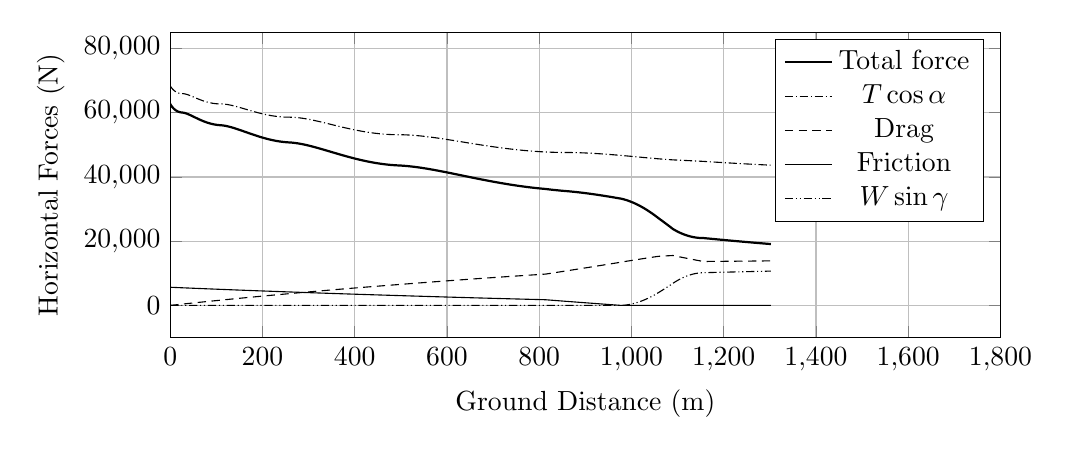
\begin{tikzpicture}

\begin{axis}[
width=\textwidth,
height=0.45\textwidth,
scaled ticks=false, tick label style={/pgf/number format/fixed},
xmin=0.0,
xmax=1800,
xlabel={Ground Distance (m)},
xmajorgrids,
ymin=-10000,
ymax=85000,
ylabel={Horizontal Forces (N)},
ymajorgrids,
legend entries = {Total force\\$T\cos\alpha$\\Drag\\Friction\\$W\sin\gamma$\\}
]

\addplot [
color=black,
thick
]
table[row sep=crcr]{
1.3603393307215537E-8	62748.58696633752\\
2.0334443352841076E-7	62748.58690939445\\
1.8493358258961232E-6	62748.58641548015\\
9.983129263424352E-6	62748.58397542096\\
4.13538327636676E-5	62748.57456922821\\
1.2467543572893382E-4	62748.54960546996\\
2.843807411608912E-4	62748.50180455402\\
5.588015241105573E-4	62748.419767336396\\
9.398454696015893E-4	62748.30600655674\\
0.0014155885812023746	62748.1641647987\\
0.0019945752038215015	62747.99177512748\\
0.0026717822370171283	62747.790415954456\\
0.003447739291558293	62747.560009893365\\
0.0043193476547732645	62747.30155562484\\
0.00529092766782709	62747.01385138542\\
0.006363550519206555	62746.69666264203\\
0.007533073890550759	62746.351295181725\\
0.008790616877968567	62745.980444552275\\
0.01016549189277427	62745.575551850474\\
0.011625499440327931	62745.14618342054\\
0.013184282533086976	62744.688399411534\\
0.014839871214038253	62744.202857938275\\
0.01660567024659266	62743.685714295745\\
0.018465948346479452	62743.14166089623\\
0.0203822997817096	62742.581982157964\\
0.022430561433814646	62741.9846045537\\
0.024588423902376283	62741.35614234788\\
0.026831028501027587	62740.70391451247\\
0.029143159681622913	62740.032400926604\\
0.03155709159958957	62739.33229326972\\
0.03411445662773917	62738.59162699967\\
0.03677290089167576	62737.82277862045\\
0.03952314881844239	62737.028508995965\\
0.04239921643077808	62736.19908785114\\
0.045357163155895136	62735.34727460913\\
0.048363831658398165	62734.48265782544\\
0.051533845233668635	62733.57236575549\\
0.0547899150155587	62732.638705721634\\
0.058172599437445835	62731.67013847036\\
0.06162834747858026	62730.682080035374\\
0.06521401059050522	62729.6583602866\\
0.06888104003120077	62728.612930033225\\
0.07268727020998902	62727.52939702985\\
0.076546425570032	62726.432399803336\\
0.08047032364859658	62725.31861108985\\
0.08456364881336098	62724.158420584645\\
0.08882250397434277	62722.95310017094\\
0.09306368907640691	62721.75454887476\\
0.09743039119190974	62720.52232779545\\
0.10191450167634594	62719.25883483638\\
0.10651989152467789	62717.96308653227\\
0.11128201757858264	62716.625239045985\\
0.11609763023253863	62715.27438850158\\
0.12097769621339591	62713.90749028763\\
0.12591912973280778	62712.52544581439\\
0.13103216605369056	62711.097527656384\\
0.13633380151185176	62709.61917302545\\
0.1416823117522269	62708.130007390326\\
0.14708837902374172	62706.62707955137\\
0.1525605467319851	62705.108049955685\\
0.15824953188605478	62703.531216078845\\
0.16398006351864292	62701.94527849711\\
0.16978153473626356	62700.342130944424\\
0.17584258400626962	62698.66981182189\\
0.1819863832139092	62696.9772841792\\
0.18819485651962437	62695.26957750722\\
0.19455736971520038	62693.52220613981\\
0.20098158490654017	62691.76062289748\\
0.2076061353991409	62689.94693630173\\
0.21424726384720844	62688.131550336606\\
0.2211374965027113	62686.251028450046\\
0.2281284453493247	62684.34604989443\\
0.2350833915765042	62682.453865649004\\
0.2423085249848444	62680.49127820038\\
0.24958374984531584	62678.5182341692\\
0.2569279402934431	62676.5296459816\\
0.2644720218029696	62674.490190968936\\
0.27204626263318243	62672.44585722769\\
0.27972793364503945	62670.37583200562\\
0.2874622320100655	62668.29494128017\\
0.29563698092580604	62666.09911666709\\
0.30361763245720474	62663.958918553966\\
0.3118912000478351	62661.74375969761\\
0.3202493147046803	62659.50962820038\\
0.3286412952843002	62657.270101276095\\
0.33714554464307567	62655.00430432729\\
0.3458731203690518	62652.68282036096\\
0.35455185683415313	62650.378110914244\\
0.3634323904331427	62648.02367015275\\
0.372325738896249	62645.66969503407\\
0.38151551889959867	62643.241270275554\\
0.3908489672358084	62640.7790056082\\
0.4001862088113266	62638.319850465385\\
0.4095647137707429	62635.853918025794\\
0.4192312859369268	62633.31648359966\\
0.4289206911602753	62630.777326736774\\
0.43896550245304145	62628.1494969964\\
0.4487817299761361	62625.58580772948\\
0.4589033974758888	62622.94679031342\\
0.4691858798479248	62620.27041258804\\
0.47972601481223376	62617.53169886967\\
0.49016040525287174	62614.825124399096\\
0.5007175269203565	62612.09138594629\\
0.511266977039379	62609.364278434776\\
0.522323236324642	62606.51108785656\\
0.5332586746953114	62603.6939891011\\
0.5445869154512923	62600.780798452135\\
0.5556699580072249	62597.93563377879\\
0.5669225885056133	62595.051912478186\\
0.5785590177532589	62592.07505854375\\
0.5903083066022885	62589.07466803896\\
0.6020327889628274	62586.08590374258\\
0.613957077533064	62583.05157437126\\
0.625960998969677	62580.00239696787\\
0.6380070243193761	62576.94793492295\\
0.6503365955459197	62573.82713490272\\
0.662700086001522	62570.70334396156\\
0.6752747602080436	62567.53188773252\\
0.6885889407972636	62564.18011941944\\
0.7019767933734617	62560.81617246734\\
0.7151149754112038	62557.52110925231\\
0.7284684478906998	62554.17823528063\\
0.7418939875700234	62550.82354798741\\
0.7553494584716574	62547.46759065635\\
0.7694215958599202	62543.9644190666\\
0.7830840331449673	62540.569628476995\\
0.796657372658726	62537.203154767296\\
0.8106660034246236	62533.73512147406\\
0.8251837647136968	62530.14784815654\\
0.8395067871054176	62526.6154204272\\
0.8540519574023793	62523.03498378866\\
0.8688334527125461	62519.403311953996\\
0.8840141863517745	62515.68076938034\\
0.8993797082767976	62511.920298945784\\
0.9143697020410035	62508.258832268635\\
0.9294094610857999	62504.592197878505\\
0.9452486359568626	62500.7381743758\\
0.9605773823977486	62497.01562117957\\
0.9761522209726621	62493.24057141924\\
0.9917649966835071	62489.46361904089\\
1.0074810114554809	62485.66900760462\\
1.0234652146968335	62481.81711244582\\
1.0399433598517231	62477.85401059134\\
1.0563627364420554	62473.9128817023\\
1.0728309985448887	62469.96781727596\\
1.0896486452479222	62465.94705377448\\
1.1068138420051672	62461.85146773308\\
1.124143995869574	62457.72493271092\\
1.1415400048645106	62453.59114911816\\
1.1590089082607062	62449.448480346284\\
1.1769249919091855	62445.2084796461\\
1.1951505705127592	62440.904220141296\\
1.2127191877709298	62436.76362672084\\
1.2308827453761335	62432.49153892782\\
1.2492706857898845	62428.17564171388\\
1.267587852451018	62423.88525877934\\
1.2860031245644312	62419.58078870369\\
1.304687144125951	62415.22254631319\\
1.3233765774990474	62410.87209121662\\
1.342322280991234	62406.4711550964\\
1.3613696045164358	62402.05585699367\\
1.3815086998747366	62397.39748700296\\
1.4013123019267382	62392.82667942712\\
1.4209622886438908	62388.301018907354\\
1.4411501686096515	62383.66145723562\\
1.4611760119255748	62379.069061268805\\
1.4816444281325132	62374.38531840657\\
1.501865958841821	62369.76807196827\\
1.5224364680875304	62365.08127250687\\
1.543651615594651	62360.258227222424\\
1.5647593029468103	62355.470249604026\\
1.5859558716309676	62350.67271538367\\
1.6071423964076703	62345.888002467385\\
1.6293386351549652	62340.88649304696\\
1.6508498980272122	62336.05022619777\\
1.673011606043147	62331.07886427964\\
1.6946435720294923	62326.23716837114\\
1.717066624993247	62321.229632189425\\
1.739432891071898	62316.24608346452\\
1.761922286799709	62311.2464100638\\
1.7849035550437842	62306.14902744639\\
1.8076299607761817	62301.119671262655\\
1.8313298306791497	62295.88698567121\\
1.8543134894513886	62290.8241541905\\
1.8777326664639729	62285.67718343316\\
1.9017196849182967	62280.417680329134\\
1.925345883672024	62275.24934925274\\
1.950252961491087	62269.8136941689\\
1.975161211119453	62264.39091345896\\
1.9993825790313986	62259.13018618128\\
2.024583888346972	62253.66963544331\\
2.04934017380271	62248.318353089344\\
2.0744229633459703	62242.90939376509\\
2.0996193404956136	62237.48893216529\\
2.1245764901457758	62232.13269384175\\
2.1500786393425866	62226.67252647619\\
2.176226227020705	62221.08776655712\\
2.202115608176549	62215.5716402004\\
2.227948363055355	62210.080871824015\\
2.2543499999408594	62204.482825509156\\
2.2810892744412783	62198.82715711597\\
2.3075963743135786	62193.23438861176\\
2.3348582111613405	62187.49661613611\\
2.3623221378972126	62181.73082319158\\
2.3898598419727675	62175.96408003371\\
2.4171687299087603	62170.2595465404\\
2.445442108612223	62164.36844917665\\
2.4735885391813177	62158.51877944614\\
2.5015416452491293	62152.72399126468\\
2.5301110763218357	62146.816489295554\\
2.5589284934403693	62140.87303618454\\
2.587611617795936	62134.97247777185\\
2.6175687086884984	62128.82593829064\\
2.647724154312196	62122.65521091693\\
2.6767118187859253	62116.73897206473\\
2.7060305938995466	62110.770547371125\\
2.7361546404224653	62104.6542263274\\
2.7663022704956823	62098.54929455706\\
2.7964672462043376	62092.456957239774\\
2.8272583584284883	62086.25468453801\\
2.8588650092419234	62079.90540215954\\
2.8898852960400587	62073.69082224305\\
2.9215246589961597	62067.369377803654\\
2.95270311230069	62061.15688127688\\
2.984506337549637	62054.83704227129\\
3.017379145769185	62048.32275890118\\
3.049243647754313	62042.02575225769\\
3.081295157663824	62035.70903845485\\
3.113406837946715	62029.39772115555\\
3.1453724573084756	62023.13217298634\\
3.1787286104953543	62016.612120468475\\
3.211019796961401	62010.31770482176\\
3.245786703184362	62003.559815115426\\
3.279939251746722	61996.940531609405\\
3.3141720228361216	61990.32468094758\\
3.3491198891036547	61983.59012760021\\
3.382965192547779	61977.0867173538\\
3.4181848705561064	61970.338626827666\\
3.45391888941694	61963.51211006187\\
3.488851494856137	61956.858179141374\\
3.524271454997704	61950.130983748706\\
3.5606552075305	61943.241143853214\\
3.597189071478943	61936.343575278646\\
3.632926148839256	61929.61640029671\\
3.668897146318187	61922.86502357268\\
3.706642714683163	61915.80186021635\\
3.7432264628550644	61908.976793279406\\
3.781286297809391	61901.89785016014\\
3.818618572105483	61894.97542278108\\
3.8564015479305356	61887.99068247041\\
3.8948624022541356	61880.90247934146\\
3.9329637046009225	61873.90216792049\\
3.971505929995028	61866.8426350957\\
4.009821706071438	61859.84619099143\\
4.049014376833089	61852.711806431544\\
4.089343885784727	61845.393776135184\\
4.128662304630717	61838.28184714056\\
4.1684827283974055	61831.101775118805\\
4.208000253554632	61823.99875048586\\
4.2483743636521965	61816.76472234032\\
4.288255503180503	61809.64169432214\\
4.328757204126676	61802.43077740194\\
4.369490126907612	61795.20190188098\\
4.410357715197167	61787.97240189748\\
4.45189144941496	61780.64882899985\\
4.492881116440694	61773.44456786213\\
4.53550011161515	61765.97844455733\\
4.577670191557685	61758.6154327049\\
4.6201174049766305	61751.228492000344\\
4.662272021613388	61743.91663953538\\
4.706017761800355	61736.35414356242\\
4.748842845578064	61728.975686306745\\
4.792293145132742	61721.514545285856\\
4.836482439768313	61713.95224670663\\
4.88090298307878	61706.3764083924\\
4.925311889063089	61698.82852123807\\
4.969864686447545	61691.28214184509\\
5.014842280541593	61683.690063097805\\
5.0603877575117515	61676.02887809732\\
5.106292347304597	61668.33439403682\\
5.152263975081851	61660.65581586769\\
5.1974808794106995	61653.12966998521\\
5.244027372436168	61645.40940977406\\
5.28996242022761	61637.81748058609\\
5.336209145350672	61630.20092332852\\
5.38320569473032	61622.48838100504\\
5.430469292142472	61614.75984800639\\
5.476900151253712	61607.19453818837\\
5.526063828851289	61599.21304195354\\
5.573879040902945	61591.47903266914\\
5.622613575936374	61583.62517954153\\
5.6713596863799225	61575.79846605475\\
5.720412183296268	61567.951706051594\\
5.770660497446668	61559.9438310221\\
5.820668144990444	61552.00448954932\\
5.870305285939629	61544.15360637981\\
5.920503816994749	61536.243821434604\\
5.971105439367246	61528.30080444753\\
6.021088325934068	61520.48462476734\\
6.071322359863801	61512.65879094176\\
6.122981826035449	61504.64172289455\\
6.174329110820436	61496.70394173493\\
6.225804784288178	61488.77703510273\\
6.278093246139479	61480.75631606848\\
6.331709873490098	61472.56452776905\\
6.384325657889258	61464.55765979801\\
6.436648686434458	61456.626642740404\\
6.489478972803882	61448.65026491659\\
6.543185721519176	61440.57388732828\\
6.596747696432654	61432.551600930165\\
6.650345873843312	61424.556059089184\\
6.704555155195255	61416.501941789786\\
6.7588986063680725	61408.460639057594\\
6.814371620173711	61400.28586278655\\
6.86997180120154	61392.12632967644\\
6.925426612865756	61384.02186979991\\
6.981353650685165	61375.88237415877\\
7.037678624474159	61367.71930034793\\
7.094603706786671	61359.50411193866\\
7.151204881983983	61351.37026143422\\
7.209200593921791	61343.07163304799\\
7.2667780016693655	61334.86837278561\\
7.324687293141565	61326.653363530015\\
7.382771066065313	61318.449246831486\\
7.441904508776327	61310.13338126092\\
7.501585831803217	61301.77765963969\\
7.5616527251378685	61293.40551792075\\
7.62150963104709	61285.09996725664\\
7.682859947113334	61276.62569140749\\
7.7432084367972145	61268.3276534648\\
7.803024936926759	61260.13965604777\\
7.863793829029664	61251.858740070194\\
7.9252460466886365	61243.52293007236\\
7.98696966925656	61235.1888311347\\
8.04776546969778	61227.01759506168\\
8.109421212326083	61218.76871519463\\
8.17269125419024	61210.34340881962\\
8.236095044780246	61201.9403096516\\
8.299523592514586	61193.5738429738\\
8.363213767675873	61185.21286604897\\
8.427807923256076	61176.77398507265\\
8.49144930156071	61168.499561336226\\
8.557380457258176	61159.96910532277\\
8.623183572921022	61151.49732740478\\
8.687840683575093	61143.21389744365\\
8.753751426394068	61134.81131915188\\
8.820803713780364	61126.305983558035\\
8.888970287482593	61117.70333907152\\
8.957133699158991	61109.14530028828\\
9.025036015045707	61100.663809586214\\
9.092760955867519	61092.247804965446\\
9.159817422823458	61083.957329743265\\
9.227495373767134	61075.63268132828\\
9.296013084156197	61067.24822283868\\
9.36435980631623	61058.92809873505\\
9.433329865923408	61050.57586590666\\
9.503849553921977	61042.081253048804\\
9.574524061692681	61033.613735886465\\
9.644263228942293	61025.30298867257\\
9.715657612596786	61016.840806241584\\
9.787429657508813	61008.38039190523\\
9.85753688572494	61000.16108569071\\
9.930250735750551	60991.682830503574\\
10.001571447096964	60983.412971116995\\
10.074699859091687	60974.980572490764\\
10.14698611653175	60966.69193337383\\
10.220547980738981	60958.30445290361\\
10.2940409891517	60949.97240538517\\
10.36719293590382	60941.7260660842\\
10.441008888975666	60933.45225885279\\
10.51610421670324	60925.08370061709\\
10.590724589239105	60916.8164823947\\
10.667218005391902	60908.39163985035\\
10.742771202259895	60900.11973692823\\
10.82035208750042	60891.67670395892\\
10.896759047300378	60883.41160865278\\
10.973503045910835	60875.15998555509\\
11.051297940743765	60866.846241010455\\
11.128076326409062	60858.69115104595\\
11.207667705350879	60850.28952860301\\
11.286758396846047	60841.99324330609\\
11.366305937658339	60833.70160194156\\
11.446149720998452	60825.43188582828\\
11.526866579636565	60817.12530455354\\
11.607297517600138	60808.90150613891\\
11.688034241538357	60800.69980174933\\
11.769665722224765	60792.46134466202\\
11.850920080706608	60784.31480209889\\
11.933163326324259	60776.12361691226\\
12.017103780766782	60767.8197171247\\
12.10034832931326	60759.640634444935\\
12.185467765774142	60751.33475049959\\
12.270669986481685	60743.07869961996\\
12.354040133273898	60735.05604261029\\
12.440386807402234	60726.80498556224\\
12.52556588630658	60718.72313367702\\
12.610860989997974	60710.68741068567\\
12.69550109439961	60702.7697010197\\
12.784634337461807	60694.492079811374\\
12.871172079509357	60686.51455473315\\
12.958447214271366	60678.52775777402\\
13.045518554761987	60670.61813682194\\
13.133090172249581	60662.721811176365\\
13.221405510214687	60654.81786217776\\
13.310319106907201	60646.92044169422\\
13.399783591735492	60639.03469714463\\
13.488943611067967	60631.236046793\\
13.578276665194153	60623.48236681825\\
13.667402973129146	60615.80636494937\\
13.757763665999576	60608.084736776946\\
13.848393619195729	60600.401249403876\\
13.938857764339925	60592.79266771233\\
14.031101516310692	60585.0967789377\\
14.123507833735925	60577.45023803045\\
14.214825187590282	60569.95543883098\\
14.307956552027534	60562.37462917849\\
14.401498558574918	60554.824072903575\\
14.495315613017755	60547.31518245343\\
14.589065423003394	60539.8753342338\\
14.68316852398955	60532.47121543059\\
14.778702641747682	60525.01961735853\\
14.873746415615575	60517.67113253551\\
14.970384078097169	60510.265509925666\\
15.068900921005241	60502.78423420373\\
15.164434274206265	60495.5951926612\\
15.260378587808539	60488.44007172431\\
15.357189194448868	60481.28598152408\\
15.45495288999333	60474.1281303913\\
15.55311774366497	60467.00807906875\\
15.652583807013901	60459.862057840466\\
15.755243917873962	60452.55851669975\\
15.855950289561445	60445.46473158288\\
15.958461094374158	60438.31555855682\\
16.060387288500337	60431.27863635823\\
16.164276126126843	60424.17929867185\\
16.26736468838029	60417.20731915746\\
16.36946523634058	60410.37325929281\\
16.47192386662276	60403.586111545796\\
16.576794358652606	60396.71246883289\\
16.678929175716583	60390.08913617018\\
16.783994526910618	60383.348615344716\\
16.89012564586595	60376.61447104455\\
16.996887404888547	60369.91584578273\\
17.103774697793426	60363.28496963934\\
17.210947675936964	60356.71207923548\\
17.31865021419634	60350.18281796633\\
17.424470519881233	60343.841713853486\\
17.53205215515201	60337.47004776649\\
17.64034909906897	60331.13211374986\\
17.74911485075183	60324.84332676443\\
17.85745376408675	60318.65525754157\\
17.969383314157206	60312.34153029855\\
18.07998395718984	60306.18178736954\\
18.18863741327577	60300.2067199031\\
18.302466989554325	60294.02777015019\\
18.41305080779906	60288.10388244802\\
18.525644000014054	60282.15194912742\\
18.636945827420575	60276.34695232191\\
18.750643923449367	60270.4974694901\\
18.86479622056296	60264.70618400183\\
18.979646899421056	60258.961670430406\\
19.09418630108147	60253.314571081326\\
19.208983505033515	60247.736499493796\\
19.323483295898072	60242.254123430655\\
19.43842354827664	60236.8319979783\\
19.55563752357537	60231.3862692352\\
19.67199913451129	60226.0634241517\\
19.789486593639566	60220.772990304264\\
19.90713985662446	60215.55931019962\\
20.024127533725753	60210.45841989272\\
20.143019013955552	60205.359342821175\\
20.26442367074238	60200.24043139367\\
20.383660776265387	60195.29913874713\\
20.5042342316437	60190.38907729053\\
20.622773342122727	60185.64649109889\\
20.74503732713029	60180.84250580828\\
20.865944869938517	60176.17904872229\\
20.98711015528624	60171.59239670813\\
21.113336299999695	60166.90622975382\\
21.23638685227678	60162.42809921305\\
21.35988644990264	60158.022824142594\\
21.483760012473958	60153.69369463052\\
21.608180515260266	60149.435383794524\\
21.732326713270083	60145.27601552654\\
21.85766379468624	60141.1672141399\\
21.985117186778353	60137.081959983916\\
22.111729024702363	60133.116168854525\\
22.23700541150786	60129.28265740686\\
22.36297326225872	60125.5184277924\\
22.488604760551	60121.85430407117\\
22.616276341350805	60118.222539634255\\
22.744235570279145	60114.675226176056\\
22.874576476768283	60111.15694231537\\
23.003842066605536	60107.76214667955\\
23.13088450205612	60104.51712065276\\
23.257869280739328	60101.363831993935\\
23.389244224935425	60098.19622630252\\
23.519811196806458	60095.14324372953\\
23.653309395988643	60092.119497407795\\
23.78342402399784	60089.26724444286\\
23.9180644861338	60086.41407009502\\
24.05110504604577	60083.69270801601\\
24.182394801971697	60081.10229238166\\
24.314614014384034	60078.58877358597\\
24.449791085561472	60076.11754483839\\
24.585258581909038	60073.7406505672\\
24.72121222319008	60071.45522645874\\
24.857032405393277	60069.27179150266\\
24.99454740444294	60067.16239164554\\
25.13030709358258	60065.17960027879\\
25.270890409679986	60063.230446394926\\
25.40663839363527	60061.448554015355\\
25.54307796688363	60059.75652737389\\
25.68272814639034	60058.12712513111\\
25.82072003425767	60056.618583333824\\
25.96015212691003	60055.196505235814\\
25.987750021099068	60054.92718792059\\
26.0558803939429	60054.27950154213\\
26.061632797568386	60054.22593415613\\
26.066808273335674	60054.17788795782\\
26.071901058608013	60054.13074692119\\
26.073315434863225	60054.11767274693\\
26.074595035914804	60054.105833423106\\
26.080371168076944	60054.05225064648\\
26.10234540095133	60053.84631277736\\
26.183408179590366	60053.05805301905\\
26.300430535410044	60051.84141869529\\
26.42750601924636	60050.41603199058\\
26.558056987479794	60048.83997608072\\
26.688030995483615	60047.159816005544\\
26.818767077324992	60045.35938261883\\
26.951519978077492	60043.419258265145\\
27.083955405447817	60041.3728059744\\
27.216897884715692	60039.20844388436\\
27.350913258119895	60036.91639489049\\
27.4833530065795	60034.5439423178\\
27.6176201223548	60032.031194754294\\
27.752160408628434	60029.40607957498\\
27.887329802382908	60026.66194677791\\
28.023188645890663	60023.797383288256\\
28.158973127824495	60020.8291376751\\
28.296372294036907	60017.719870782574\\
28.435107205966254	60014.47387337974\\
28.571323599682245	60011.18403467702\\
28.70996262687553	60007.73249199185\\
28.850320389600306	60004.13350335811\\
28.988837241064125	60000.479841946435\\
29.129197813929657	59996.67568345055\\
29.27166529868488	59992.710960694676\\
29.41298471572133	59988.67659502503\\
29.554848516656044	59984.526294098905\\
29.699676691743235	59980.186915205224\\
29.842400551696755	59975.81079627063\\
29.985385440862252	59971.32870089132\\
30.129077275410303	59966.72700352172\\
30.27543774584293	59961.94080827045\\
30.422081339040986	59957.04651293291\\
30.56949149516445	59952.02832047624\\
30.716562179458485	59946.924840263455\\
30.86535310281699	59941.664626078156\\
31.011875026602333	59936.390596962665\\
31.16159928701196	59930.90628712137\\
31.313692569485013	59925.238286549036\\
31.463056706803336	59919.57831036547\\
31.61235366859384	59913.82945735073\\
31.76278957628285	59907.94563880219\\
31.915019899787076	59901.899901037425\\
32.06709627595497	59895.76949547665\\
32.21861178877769	59889.57280097742\\
32.37168228565527	59883.22374572455\\
32.52450570609457	59876.79726484443\\
32.67702483599189	59870.29754761617\\
32.829998687403204	59863.6934176901\\
32.98551220909506	59856.89367472356\\
33.14332298937855	59849.906236893716\\
33.29970221124884	59842.89683323805\\
33.45800124694219	59835.716197620495\\
33.61398946945653	59828.55786102654\\
33.77048353048475	59821.29528723624\\
33.9292721471582	59813.84458417805\\
34.08796840843395	59806.317352988335\\
34.24769686644211	59798.66084320088\\
34.406855482575295	59790.9527893207\\
34.56481953291838	59783.22600928563\\
34.72399692808165	59775.36395438899\\
34.88694269464703	59767.23812092573\\
35.04914399338672	59759.0726815221\\
35.209965099803895	59750.90240180594\\
35.3703140559587	59742.683657673304\\
35.531685786905925	59734.340671176906\\
35.69349909442164	59725.90372559923\\
35.85522798807463	59717.40121385794\\
36.022509111806116	59708.53447904484\\
36.19055880791667	59699.554244631596\\
36.35708622463872	59690.58469313168\\
36.52115360367851	59681.680070858114\\
36.68781562330062	59672.56717430525\\
36.8536847754776	59663.43133576815\\
37.024522648961764	59653.95394295167\\
37.19188554678789	59644.60374946002\\
37.36066720850286	59635.10977491125\\
37.528862119520696	59625.58554350838\\
37.697264258302326	59615.98748780464\\
37.86832931534104	59606.17524719742\\
38.03812867477943	59596.37458278546\\
38.20923731912278	59586.43802723859\\
38.37904730305398	59576.51817757127\\
38.55252405124031	59566.324912820186\\
38.72282139824354	59556.26140041601\\
38.89783411301201	59545.86151021885\\
39.0714610757495	59535.487307669595\\
39.24438070689564	59525.10042350262\\
39.41969314875929	59514.5149844464\\
39.59166556575205	59504.078692675525\\
39.764623188591585	59493.53123869293\\
39.94263254662576	59482.62305142157\\
40.11749159802578	59471.85701263862\\
40.29452954971913	59460.906547520775\\
40.47247750600427	59449.849941046996\\
40.64799609178485	59438.89640476125\\
40.82414741101539	59427.85664671518\\
41.00385670225303	59416.54674992937\\
41.18169069533937	59405.309069950046\\
41.3603281005193	59393.975818649225\\
41.54046179251334	59382.50324354827\\
41.722675278204306	59370.85394412931\\
41.90258931008478	59359.309040700304\\
42.08518735141125	59347.54968606445\\
42.26728550944881	59335.78122794305\\
42.44743534848537	59324.099135451615\\
42.63069538383506	59312.17603777333\\
42.80963512098974	59300.49675227204\\
42.992542679335614	59288.521436020004\\
43.17926890616222	59276.25850616516\\
43.363134036078335	59264.147382094496\\
43.54815051311773	59251.925286896454\\
43.733578141849236	59239.64168066341\\
43.91798130912079	59227.39282522943\\
44.10506009255049	59214.933498322775\\
44.29251116260117	59202.41729768709\\
44.480917546793805	59189.80595571204\\
44.66851287589745	59177.2186586616\\
44.85853501730759	59164.43875502719\\
45.047396872181054	59151.708177448745\\
45.236914792155844	59138.905579726605\\
45.42785879536018	59125.97945974015\\
45.616432631699865	59113.18795637264\\
45.80697204128492	59100.23799279377\\
45.998633580597016	59087.18722800302\\
46.18800675699903	59074.26903791596\\
46.380841640082096	59061.09189567245\\
46.57327038933336	59047.92049077105\\
46.765844918266424	59034.718012194746\\
46.95911042680183	59021.44786036476\\
47.15311668852311	59008.10730490218\\
47.34541611633634	58994.86568700209\\
47.53884854699059	58981.52842327401\\
47.73236991243341	58968.16820999955\\
47.92818250719388	58954.63357909351\\
48.12326385407131	58941.13412640181\\
48.32058854034828	58927.46471703341\\
48.516852452700604	58913.85497699441\\
48.71339374517507	58900.21305646603\\
48.91319881343868	58886.332192904505\\
49.1119162355681	58872.51535270149\\
49.31207818344666	58858.58731063311\\
49.509673461222235	58844.82811169086\\
49.71156302510582	58830.76073219253\\
49.91034548441702	58816.90164186753\\
50.11200805970151	58802.83426463636\\
50.30853267551517	58789.11883687753\\
50.50757456960626	58775.22201912914\\
50.70929197287772	58761.13333913479\\
50.91222418686718	58746.9554811806\\
51.11562549758783	58732.74130184468\\
51.32090674103446	58718.39296428232\\
51.525199701657655	58704.11173357142\\
51.72863462744459	58689.88932028023\\
51.934060761332375	58675.52730883444\\
52.14033810224923	58661.10618182135\\
52.344882977561255	58646.80733712956\\
52.55098100649393	58632.401858393874\\
52.75731843494604	58617.982360208014\\
52.96514817708821	58603.46208475658\\
53.17450540782369	58588.83942180824\\
53.382202621450276	58574.3377559869\\
53.592230583406476	58559.679229889225\\
53.80364534107798	58544.93064378269\\
54.01469481143569	58530.215030808264\\
54.223966920081466	58515.631471086905\\
54.43230789395902	58501.12155087033\\
54.6430562980421	58486.45356444517\\
54.855225786754914	58471.697144366\\
55.066088958624874	58457.04270018783\\
55.27969530828261	58442.20963181784\\
55.49171188337613	58427.49962401182\\
55.70388919125476	58412.79178885053\\
55.91737779085577	58398.00720016053\\
56.13177028494084	58383.17498173575\\
56.34652664868587	58368.333313521856\\
56.559021044851505	58353.66412411911\\
56.77591447970492	58338.708504571245\\
56.99548236897459	58323.58691455852\\
57.21481285737903	58308.500894390236\\
57.43536222847358	58293.35110079676\\
57.65367025761124	58278.375756128575\\
57.872788904232735	58263.36596854261\\
58.0907693980174	58248.455833187836\\
58.311927420720366	58233.351114576406\\
58.532333513628615	58218.32121382914\\
58.75532998033057	58203.13916485525\\
58.976617007999806	58188.098497502404\\
59.19875422837053	58173.02572952934\\
59.4206945143671	58157.992655298396\\
59.64453328369959	58142.85827735343\\
59.86894932484513	58127.71301064553\\
60.09432075877773	58112.5322553695\\
60.318058693038594	58097.490881444915\\
60.541731124044205	58082.48374662695\\
60.76707064338231	58067.3955279877\\
60.995574692986196	58052.12756950685\\
61.22378989589207	58036.911836241154\\
61.4534619981562	58021.63280140082\\
61.683510138770515	58006.363385445075\\
61.91410430469678	57991.093120406906\\
62.14462153858659	57975.86396671242\\
62.37563158073512	57960.63897565096\\
62.607203285434	57945.41445022516\\
62.841031881319736	57930.08021880589\\
63.07467935056491	57914.79726911259\\
63.31164975340633	57899.33779610891\\
63.54633691305479	57884.068390173954\\
63.78243968758058	57868.74874765902\\
64.0165414084598	57853.6009719125\\
64.25412817577254	57838.27105183984\\
64.49270299572771	57822.92190436032\\
64.73076499662056	57807.650791422624\\
64.96867826857735	57792.434728704684\\
65.21063576532572	57777.00724185629\\
65.4512107007771	57761.71569061352\\
65.69028017871045	57746.567576696616\\
65.93032615763332	57731.406018186666\\
66.17196619696679	57716.193329702655\\
66.4135612157637	57701.033714326666\\
66.6559030093851	57685.87824030849\\
66.89910102540284	57670.72109998952\\
67.14354652182666	57655.53911287115\\
67.38771133480921	57640.428027933216\\
67.63347396558368	57625.27254363513\\
67.87898066495345	57610.18793956618\\
68.1255935515739	57595.09132520294\\
68.37316753306138	57579.99280084603\\
68.62205497364681	57564.87217704652\\
68.8711887275476	57549.79534187529\\
69.120220471977	57534.78392955042\\
69.36846244647072	57519.87957346914\\
69.61951843592018	57504.86712876223\\
69.87236615109754	57489.8099065393\\
70.12758921381476	57474.6752054641\\
70.37945082809051	57459.803338373196\\
70.63410009691182	57444.831487207965\\
70.89152727368702	57429.76285027851\\
71.14629115974091	57414.91646035954\\
71.40197865069018	57400.08309025846\\
71.66163317144085	57385.088593798064\\
71.92484704501203	57369.9600329331\\
72.18465416754285	57355.09834198421\\
72.44573394560723	57340.23545133592\\
72.70633339061075	57325.471953933025\\
72.96699363118216	57310.77748505819\\
73.22900401485182	57296.08041119615\\
73.49076816912304	57281.47120050725\\
73.75430841254712	57266.83809345678\\
74.01895646534612	57252.219890300854\\
74.2846979982242	57237.61879331188\\
74.55380714249793	57222.9122737032\\
74.82322871850147	57208.26939184911\\
75.09350011520078	57193.66192326516\\
75.36421232425869	57179.11301420181\\
75.6347219158074	57164.65780234536\\
75.90830954343213	57150.122756364886\\
76.18188601743822	57135.67387246007\\
76.45626363461818	57121.2690668212\\
76.72958718025629	57107.006056570826\\
77.00406935908524	57092.76985819533\\
77.28579748399531	57078.24924514997\\
77.56784659723587	57063.805291943805\\
77.84569092555657	57049.668290162925\\
78.1246978223638	57035.56407093696\\
78.40641219364133	57021.416888412234\\
78.68590470271565	57007.47495000754\\
78.96851680469001	56993.47268341496\\
79.25576208114188	56979.33947918769\\
79.54169104977237	56965.37020706275\\
79.82662017154695	56951.54862481984\\
80.11330301632765	56937.74197065286\\
80.40394576721474	56923.84742480169\\
80.6908099930996	56910.235441836325\\
80.98055888331655	56896.58978178128\\
81.27178512217935	56882.97947115914\\
81.56682943128612	56869.29841199225\\
81.86186977412851	56855.726339449015\\
82.15688924927383	56842.26442924084\\
82.44965588234726	56829.01366851741\\
82.74488606927187	56815.76110563167\\
83.04325841243121	56802.4798198021\\
83.34213327641098	56789.28977144322\\
83.64411622775171	56776.07844151951\\
83.94734638805741	56762.930160587624\\
84.25123842984891	56749.87182430207\\
84.55152885577829	56737.08531079719\\
84.85735750691177	56724.18297150567\\
85.16518306664875	56711.31906232219\\
85.47136476235073	56698.64633166521\\
85.77898122624802	56686.03761827444\\
86.08923229760057	56673.446588777355\\
86.40254560035129	56660.85975954939\\
86.71167807044037	56648.56780416798\\
87.02660518802142	56636.17545402993\\
87.34238286044419	56623.881776673414\\
87.65842706333811	56611.71059504611\\
87.97971380652302	56599.474162660845\\
88.2973933745065	56587.51095168493\\
88.61789013566766	56575.578906513445\\
88.93643920279564	56563.85635402276\\
89.25662431900213	56552.21158163999\\
89.57903058309674	56540.62618103357\\
89.89968694948243	56529.243518823685\\
90.22473455398588	56517.847697477686\\
90.55024875587375	56506.579884139195\\
90.87789352676518	56495.38457792073\\
91.20733069500889	56484.276334895476\\
91.54101415610151	56473.17688393881\\
91.87012785371462	56462.37961897151\\
92.20120197152713	56451.66887643444\\
92.53416638543635	56441.04992105982\\
92.86431843528567	56430.672445420714\\
93.19748455591187	56420.35379761217\\
93.53066771200866	56410.18924357343\\
93.86681917526724	56400.09117815462\\
94.20530590547477	56390.08269701265\\
94.5419273964865	56380.28867740244\\
94.8854212036891	56370.4588251176\\
95.22752713476521	56360.833810594486\\
95.57091181422334	56351.33887691356\\
95.91383450860906	56342.02309124738\\
96.25469535763642	56332.928415814225\\
96.5966517898868	56323.97023258764\\
96.93845701474973	56315.182214884044\\
97.28153572459905	56306.52887524493\\
97.62213139590432	56298.10439445829\\
97.9659652144934	56289.76813060144\\
98.3129807304216	56281.52650644207\\
98.65852794036775	56273.49154719533\\
99.00080640577195	56265.701904939735\\
99.35064076251427	56257.91474109776\\
99.69796076807248	56250.358298542385\\
100.04654253174803	56242.94978418537\\
100.3915606488718	56235.790319330015\\
100.74261509654437	56228.68286742618\\
101.08877163494762	56221.84995780497\\
101.43457754260953	56215.198140311884\\
101.784020212797	56208.653494623344\\
102.13161434601102	56202.32039896121\\
102.4751980097893	56196.23406722117\\
102.82212110631409	56190.264066871256\\
103.16739702108615	56184.49776476232\\
103.51524666207362	56178.86564816616\\
103.86391679154056	56173.39897407286\\
104.20960434827006	56168.15597685639\\
104.55241399635099	56163.13084679436\\
104.89662223620601	56158.26002318217\\
105.24103428322039	56153.561887785574\\
105.5836615386647	56149.06260891563\\
105.92645892081137	56144.73552823797\\
106.27347658175316	56140.533135349004\\
106.6151670762521	56136.57044376861\\
106.95898391938218	56132.75879358796\\
107.30023552029138	56129.15009724462\\
107.64147805753461	56125.71558452163\\
107.98348674656944	56122.44826487418\\
108.32522459759954	56119.358655463104\\
108.3935347040271	56118.76208542872\\
108.40478590462831	56118.664497649705\\
108.41572478024443	56118.5698010505\\
108.4246743308916	56118.492459419795\\
108.44347342986478	56118.32977731012\\
108.52018987797786	56117.65880656114\\
108.70071173483461	56116.035152340206\\
108.99446230248458	56113.25949687585\\
109.30176454987088	56110.180128331456\\
109.60899173332959	56106.92367519517\\
109.91608539831654	56103.49267197093\\
110.22883517949637	56099.81943912411\\
110.54143546549608	56095.96921548896\\
110.853845249356	56091.944588339\\
111.1739714794031	56087.63911666928\\
111.4937490010879	56083.156864760545\\
111.81170779322963	56078.52214053848\\
112.13106495813236	56073.69025769296\\
112.4519453366479	56068.65875748497\\
112.77515902629136	56063.41362773524\\
113.0997499810409	56057.96922648499\\
113.43040796942478	56052.24272693141\\
113.7597028375028	56046.36092178567\\
114.0907450350197	56040.269918194055\\
114.42538740208008	56033.93330308134\\
114.75997726261329	56027.419401394\\
115.09477047197589	56020.72512334178\\
115.43440545481076	56013.75576669778\\
115.77494672336013	56006.589619595325\\
116.11687534861284	55999.2168417143\\
116.46164587354252	55991.604878253755\\
116.8077846490165	55983.78512638784\\
117.15688723722127	55975.72035419216\\
117.50557855048987	55967.48873279906\\
117.85411336711965	55959.08682079238\\
118.20532793701167	55950.44650717999\\
118.55850697655507	55941.584104478694\\
118.91273956155123	55932.522423860835\\
119.26983096270519	55923.214621430685\\
119.62978614725739	55913.65863454707\\
119.98960731920661	55903.93431508298\\
120.34734904217265	55894.09802996219\\
120.7138511704587	55883.84926603541\\
121.08106061642908	55873.408846882245\\
121.44737887966437	55862.82465307269\\
121.81499139152783	55852.03555702076\\
122.18511446431708	55841.00556433253\\
122.55384158147794	55829.852629700865\\
122.92460728481757	55818.47473211432\\
123.29616941264607	55806.91040690572\\
123.67040864389355	55795.10115506385\\
124.04652172406458	55783.0716969154\\
124.42393851457416	55770.84056244342\\
124.80152108360014	55758.446027237456\\
125.18180835736592	55745.80528944677\\
125.55854932865631	55733.128956004584\\
125.93878032356085	55720.18261663958\\
126.31997081831156	55707.05205810175\\
126.70099538833193	55693.777874477935\\
127.08058279416298	55680.40756122072\\
127.46175209000612	55666.836950687386\\
127.84399628255431	55653.0848333677\\
128.22749916598133	55639.14553995697\\
128.6102537001487	55625.09397540186\\
128.99595881306152	55610.795388035505\\
129.37788117916477	55596.50204083322\\
129.760738924708	55582.04104776998\\
130.1448498512433	55567.40143773476\\
130.53000390659713	55552.59220870664\\
130.9168242384266	55537.5902043949\\
131.29443328439476	55522.82310047386\\
131.67491382268804	55507.82349999633\\
132.05816436539135	55492.59477265162\\
132.44070735535217	55477.27617776611\\
132.82666098215685	55461.70361433411\\
133.20952005887244	55446.14143923354\\
133.5940193955625	55430.39986597975\\
133.97617966856654	55414.644096894015\\
134.36103715882757	55398.66832157064\\
134.74478042358356	55382.63204566766\\
135.12867144169206	55366.484880169795\\
135.5141335746535	55350.16819246838\\
135.89764893392993	55333.83295933936\\
136.28231234485685	55317.34957792143\\
136.66418763078912	55300.88921332924\\
137.04684871033697	55284.30041550295\\
137.42845627025127	55267.66483526533\\
137.8132447087305	55250.798929806086\\
138.19719797258034	55233.879702153135\\
138.58059071069573	55216.89733207894\\
138.96593237593703	55199.741975318975\\
139.3501607499636	55182.55145065415\\
139.73355638294606	55165.31559629523\\
140.1160230155566	55148.04102748708\\
140.50045093994146	55130.59858980587\\
140.88215178690393	55113.20292656115\\
141.26156782058217	55095.83703679354\\
141.64323970440188	55078.29473766922\\
142.02689350659642	55060.589038665625\\
142.41061312971692	55042.80942572316\\
142.7942251403153	55024.9655712048\\
143.1756303563767	55007.15733772205\\
143.5599719391364	54989.14598621384\\
143.94242380128833	54971.15898355495\\
144.3239499176869	54953.1532499748\\
144.70664939692608	54935.031197611184\\
145.0870075357763	54916.96104755772\\
145.46856550308127	54898.77632966716\\
145.85014610541765	54880.5343579755\\
146.23128237819492	54862.25902154323\\
146.61504730324998	54843.80397778144\\
146.99763315977907	54825.35349630668\\
147.38441582478964	54806.64918106068\\
147.7673688364352	54788.080558606234\\
148.15222568696134	54769.37144046633\\
148.53580865353604	54750.677610751154\\
148.9199734867533	54731.91016881248\\
149.3040357319486	54713.10386690739\\
149.68771357306542	54694.27397295498\\
150.07093078701052	54675.42573599094\\
150.45622889618164	54656.43526069229\\
150.8449053483268	54637.239130532806\\
151.2288570611563	54618.239099294326\\
151.61452719766493	54599.11810242158\\
151.9983007305741	54580.0567094977\\
152.38299664478842	54560.916344387704\\
152.76945776909372	54541.65603103688\\
153.15580177123394	54522.37067495863\\
153.54253364040335	54503.03632819989\\
153.93093169697067	54483.5901374426\\
154.31788037931886	54464.18934396806\\
154.7039882138024	54444.80493590348\\
155.08880221957185	54425.46110304682\\
155.47621608980313	54405.96322715393\\
155.866104687065	54386.318388846164\\
156.25391419262098	54366.757230611416\\
156.64166339424906	54347.1793132959\\
157.03027969880475	54327.53895522293\\
157.4213807682267	54307.75537029511\\
157.8105708506119	54288.05207252641\\
158.19948541262937	54268.347583843104\\
158.58893406813365	54248.60204114468\\
158.97894817604634	54228.81495997179\\
159.3710019698692	54208.91258410092\\
159.76139479981174	54189.08391069513\\
160.1523485688823	54169.21727396663\\
160.54128874338664	54149.444675598614\\
160.9326976430911	54129.539353100336\\
161.32564259741588	54109.54974883988\\
161.71827778345698	54089.570849273485\\
162.1124492087963	54069.509812550095\\
162.50576001021273	54049.48971779882\\
162.89904576730015	54029.46913444938\\
163.29316224934274	54009.40557856076\\
163.68899123279596	53989.25523993868\\
164.08495392634194	53969.09957324251\\
164.48271131475576	53948.8551218497\\
164.8792309171331	53928.67730328094\\
165.27343112400507	53908.62215604122\\
165.67115293733156	53888.393585440586\\
166.06936395728349	53868.14695606413\\
166.47000821435734	53847.78455338701\\
166.87155839526775	53827.38515389072\\
167.27134041220108	53807.085614829324\\
167.67233991204222	53786.735346019326\\
168.0705846918417	53766.536878449275\\
168.47232570996516	53746.17421678928\\
168.87521546679773	53725.76758726573\\
169.2789990941189	53705.331020025755\\
169.68142011368735	53684.97969414074\\
170.088438196605	53664.4134212997\\
170.49328200513543	53643.97550553418\\
170.89845866435633	53623.54024130883\\
171.30484584057905	53603.0644581948\\
171.7103088520891	53582.65670668536\\
172.11589069074847	53562.26539043702\\
172.52485519917514	53541.7276737294\\
172.93316089774754	53521.24771464929\\
173.34236088095247	53500.74859287708\\
173.7535761368399	53480.17538611259\\
174.16510964781833	53459.61418199894\\
174.5786011126259	53438.98424701531\\
174.99051444770384	53418.462989485764\\
175.40138574541044	53398.02434724718\\
175.81497300453447	53377.48249794118\\
176.2280441317456	53356.99914943286\\
176.64225100058474	53336.49338266169\\
177.05714873395152	53315.988361807045\\
177.47483026786767	53295.38201021595\\
177.89254345086653	53274.8113892721\\
178.3100126079721	53254.29095541453\\
178.7278240622369	53233.792802926066\\
179.1449731538625	53213.367066512146\\
179.56482315926417	53192.850247429655\\
179.9871804296257	53172.25347360752\\
180.4095742002126	53151.69851413404\\
180.83428717371925	53131.075547411005\\
181.26003251256287	53110.4484863119\\
181.6840913989422	53089.94983334681\\
182.1114839456617	53069.33807853464\\
182.5374089230304	53048.84596007022\\
182.96440604473082	53028.352090027445\\
183.39304842330927	53007.83030746084\\
183.8234391905185	52987.277152983996\\
184.2565386467558	52966.64845914165\\
184.68745119590193	52946.178367357585\\
185.11804999400476	52925.77827534829\\
185.54983076576542	52905.3783357145\\
185.98322399936802	52884.95960214571\\
186.41637816429778	52864.610420584344\\
186.85103033850396	52844.2502774093\\
187.28701324242002	52823.88842622809\\
187.72482375232647	52803.503159381784\\
188.16038808151575	52783.2848968504\\
188.5986323917997	52763.005891058696\\
189.04181882432442	52742.56396992062\\
189.48417857731005	52722.22697021108\\
189.92673350352436	52701.94859869171\\
190.3712203460227	52681.65059031517\\
190.8171693385559	52661.35601410818\\
191.2607914989822	52641.237911409014\\
191.7085048054314	52621.00646757835\\
192.15912968354564	52600.717508323156\\
192.60936448614513	52580.5211292169\\
193.06096206133014	52560.33976270261\\
193.50995896221815	52540.351020384915\\
193.96222738896364	52520.29445320308\\
194.41802104663145	52500.161379726036\\
194.87342332120494	52480.12643296685\\
195.32868067301865	52460.17942662496\\
195.78611327072855	52440.220047139155\\
196.24327119175433	52420.35650217533\\
196.70330552186363	52400.453387821806\\
197.16349707435467	52380.6299841321\\
197.6260626000094	52360.79230800108\\
198.09002425529962	52340.98416451698\\
198.55822718319422	52321.08651982204\\
199.02663999285284	52301.27280691374\\
199.4942263371064	52281.58747100437\\
199.96051846591553	52262.05034784938\\
200.4340527590599	52242.306364605494\\
200.9046051381776	52222.78389998883\\
201.38053424207163	52203.13770218383\\
201.855813875004	52183.61879927888\\
202.3311704663634	52164.19795740492\\
202.81222172114025	52144.64830413414\\
203.29225549210986	52125.244920318175\\
203.77308885705298	52105.91506926285\\
204.25557537412044	52086.62602851266\\
204.7402502473849	52067.35846653319\\
205.2236366749359	52048.25167552443\\
205.7136101207933	52028.99695533668\\
206.20393168243612	52009.84265767799\\
206.69661599754647	51990.71181751578\\
207.18955097797863	51971.68815325467\\
207.68747106001632	51952.591612165445\\
208.18818418427776	51933.50987526709\\
208.68864521634526	51914.56071571115\\
209.18805406731133	51895.77473422626\\
209.69072626026758	51876.99120370945\\
210.1949489825136	51858.27671687261\\
210.70396111371042	51839.5142613318\\
211.21614058335587	51820.76748655821\\
211.7289636831582	51802.13105044242\\
212.24265718177503	51783.59810728491\\
212.75957115615557	51765.08629377179\\
213.28124361123798	51746.54453758696\\
213.80665479128663	51728.01335420011\\
214.33466763217763	51709.53628331037\\
214.86241383044415	51691.215493103984\\
215.38762416293667	51673.12940459576\\
215.91972020502777	51654.956227008544\\
216.453694496636	51636.87152955492\\
216.99218613031866	51618.78951896797\\
217.53464071342142	51600.73334903976\\
218.07804319032095	51582.8063887684\\
218.62452881115053	51564.94084004275\\
219.1707188429899	51547.24925519507\\
219.71730570977076	51529.71009238101\\
220.274760228052	51511.99336578071\\
220.835259093258	51494.35502980507\\
221.3941373958715	51476.94342625463\\
221.95623623511386	51459.6093631603\\
222.52040576537968	51442.391691961486\\
223.09037241999033	51425.181360554794\\
223.661129480297	51408.13363980125\\
224.23954505634208	51391.04845630065\\
224.81564934919504	51374.22385440304\\
225.40333087020622	51357.259828523485\\
225.99624064594485	51340.349172978065\\
226.58875910740323	51323.65562093763\\
227.18585441503012	51307.04234603196\\
227.7870146338791	51290.529117792554\\
228.39495206683767	51274.04821302074\\
229.0027183467937	51257.79255435271\\
229.6102660575582	51241.76417958732\\
230.22857190062643	51225.68030053248\\
230.8468525918393	51209.828392660216\\
231.47114194537448	51194.05814996814\\
232.09060564776433	51178.64493757502\\
232.71961230618888	51163.234963649345\\
233.34696033086396	51148.10820932333\\
233.9840065784689	51132.99656548655\\
234.6188203761186	51118.188468712106\\
235.2539319397456	51103.62478837365\\
235.886956379092	51089.360171401946\\
236.5153031168307	51075.449975387266\\
237.1504953781269	51061.641394135644\\
237.78410205277385	51048.121855747\\
238.41360900639518	51034.94256480671\\
239.04679127723733	51021.941462117364\\
239.67609891578388	51009.274408778496\\
240.3017129123046	50996.93412311288\\
240.93317778774485	50984.73458865131\\
241.55721005497253	50972.93239494234\\
242.1780757761154	50961.44131743179\\
242.7965584376659	50950.24437446712\\
243.4114785265944	50939.360185219004\\
244.02550827530933	50928.739606890784\\
244.63427618145124	50918.4553659465\\
245.24126487864038	50908.445195222026\\
245.84466361012846	50898.736522491556\\
246.4476225417801	50889.277022813796\\
247.04267344144802	50880.179616948924\\
247.6421488158	50871.25442796311\\
248.2330500398673	50862.69323877274\\
248.8222841397298	50854.390576671954\\
249.4139444766347	50846.289936754954\\
249.99998610086192	50838.500264300266\\
250.57758594667018	50831.051394609065\\
251.15853686633199	50823.78889786579\\
251.73921641108228	50816.76055674569\\
252.31216708836962	50810.052540224395\\
252.88817036877617	50803.536495753506\\
253.4570082134402	50797.326217510956\\
254.02007242820673	50791.39949968821\\
254.5855573787108	50785.66873016006\\
255.15029634137989	50780.1675917721\\
255.71294034286547	50774.90815262124\\
256.27258114245853	50769.89649368757\\
256.8305649252842	50765.1184041128\\
257.38478802342286	50760.58929363258\\
257.4959621062188	50759.706844449494\\
257.5611920943704	50759.19313766927\\
257.60062237753925	50758.88406797139\\
257.6107239150342	50758.805064835324\\
257.6183320416303	50758.745609980455\\
257.62277045264796	50758.71093901935\\
257.62729287050774	50758.67559607509\\
257.6542412653681	50758.46459922605\\
257.747424202601	50757.72981575804\\
258.03721256731046	50755.39336056373\\
258.5190125653693	50751.337565453345\\
259.00532843878875	50747.02842549802\\
259.49401909840515	50742.482093644736\\
259.98581493995266	50737.68992878284\\
260.4819698790609	50732.63658984832\\
260.97812571679674	50727.365425703596\\
261.4812175109821	50721.800063404124\\
261.9850059638038	50716.006406670276\\
262.4910281591069	50709.96678554993\\
263.0003252970298	50703.66712434255\\
263.5131478408722	50697.101874931395\\
264.0293216176061	50690.270810026035\\
264.54826562874086	50683.17969265324\\
265.0714232439334	50675.80636151513\\
265.59763340154745	50668.16460474003\\
266.1233003184659	50660.30715119955\\
266.6551605685464	50652.13185019228\\
267.19223429565795	50643.64869224162\\
267.72974052544146	50634.93183079567\\
268.27282471948854	50625.89627873922\\
268.8167212540145	50616.61958066249\\
269.36684202478307	50607.00733905859\\
269.9215996219019	50597.08285837827\\
270.4791082933567	50586.877671216906\\
271.03983254776506	50576.382009831985\\
271.6074455599014	50565.52334928431\\
272.1754809002374	50554.423406644855\\
272.7524022502224	50542.913648347036\\
273.3357847625165	50531.0356609023\\
273.91684495064374	50518.968432453694\\
274.5075523019982	50506.46166104691\\
275.0995375957874	50493.68868656036\\
275.69766674106233	50480.542865927026\\
276.3013456770767	50467.033096608546\\
276.90909644628925	50453.18962189705\\
277.5234995466793	50438.950256070544\\
278.13959639565337	50424.42800415889\\
278.76308237359774	50409.48635365734\\
279.389606942784	50394.226581291936\\
280.02074979788426	50378.608942453415\\
280.6586947867754	50362.57601841638\\
281.3003335866648	50346.20317685191\\
281.94157575500606	50329.5962590838\\
282.5880614624846	50312.609825055115\\
283.23584856186324	50295.34716548957\\
283.8851508583185	50277.80443005751\\
284.5301203280417	50260.14455042337\\
285.1843536535779	50241.995965216585\\
285.83553116214307	50223.70048293246\\
286.4837256048969	50205.26263359672\\
287.1336898105825	50186.5511942225\\
287.7808235765799	50167.702433438535\\
288.42820685084826	50148.63121331604\\
289.0754666022002	50129.35169599508\\
289.71879024937004	50109.98261295054\\
290.36420979409684	50090.34640131968\\
291.0002472374472	50070.79876550405\\
291.64182130034897	50050.886040099576\\
292.27316865691716	50031.10255641583\\
292.9083864811005	50011.01234790163\\
293.54335819806715	49990.74693290434\\
294.17307850120346	49970.47128039977\\
294.79408895337656	49950.30536623647\\
295.4199157771013	49929.81428612824\\
296.0380590852486	49909.41112251047\\
296.6542969985221	49888.911549087934\\
297.2681917409874	49868.33431744992\\
297.88482625920517	49847.51143770754\\
298.4949121158181	49826.760465694024\\
299.10656876013206	49805.80951155559\\
299.7189321849655	49784.689789626966\\
300.32723284437907	49763.56937945282\\
300.92930430691433	49742.52938229733\\
301.53463237615574	49721.241620058645\\
302.1363215848461	49699.95098269294\\
302.731439066583	49678.76676498579\\
303.3331045114137	49657.224162152284\\
303.92852765769237	49635.783194122865\\
304.52166324273924	49614.30618318265\\
305.11491208725784	49592.70894026119\\
305.70510856070314	49571.10962779769\\
306.29833179138177	49549.28782885855\\
306.8897654253252	49527.422396504655\\
307.4799704999041	49505.4954348937\\
308.06772992248136	49483.55513223293\\
308.6551058451172	49461.52721309943\\
309.2396381392449	49439.50669251275\\
309.82398267965425	49417.396183168516\\
310.40422650572066	49395.346663033124\\
310.9895683476474	49373.01019174662\\
311.5727136903438	49350.66627464529\\
312.15129426541773	49328.409039637\\
312.7356217277545	49305.843348692055\\
313.31711326243806	49283.3017920354\\
313.899302145316	49260.64965291077\\
314.47946679147856	49237.99486484371\\
315.0588501134555	49215.29121753649\\
315.6397939029396	49192.44851205434\\
316.2168920475523	49169.68147211663\\
316.7955732394013	49146.77806027932\\
317.37103223180316	49123.93043153241\\
317.947565273913	49100.97005611396\\
318.5214617947222	49078.04660990604\\
319.09868556082085	49054.9233745518\\
319.67476219148546	49031.780818330575\\
320.24944526491765	49008.63086020024\\
320.82291261720786	48985.46833407336\\
321.39725246986427	48962.210506830335\\
321.96848871367	48939.020269950284\\
322.54402617481435	48915.598363659505\\
323.1185574377922	48892.16181129824\\
323.691859264958	48868.72155262051\\
324.2647334332521	48845.24653181719\\
324.8363521231331	48821.77237486192\\
325.40661348734614	48798.305064361906\\
325.97908467698915	48774.69914517141\\
326.5542035875586	48750.93740717057\\
327.12490712258295	48727.31331646659\\
327.6996379965167	48703.47886723842\\
328.2728670816481	48679.6644873044\\
328.8486987665442	48655.700961852854\\
329.41990981452807	48631.890498304085\\
329.9938351119364	48607.928932409704\\
330.5648485136189	48584.05254379158\\
331.13749118064516	48560.07293068778\\
331.7074637117181	48536.17156687817\\
332.2798601122896	48512.136196596766\\
332.8523203670276	48488.06703619877\\
333.42500978717965	48463.95843288819\\
334.00122212141855	48439.672762632545\\
334.57441172696565	48415.48717900229\\
335.1481633939942	48391.25189911785\\
335.72345703021597	48366.92668450861\\
336.29828216695637	48342.5977621004\\
336.8725624877933	48318.269699788885\\
337.44522027160394	48293.989536399225\\
338.02053867417567	48269.576869174634\\
338.5962187273635	48245.130346915685\\
339.1703543735324	48220.732206441884\\
339.7498013559267	48196.09218734714\\
340.3260768964459	48171.57214952177\\
340.9051117020497	48146.92099515452\\
341.47919118112156	48122.468440876575\\
342.052441303386	48098.040117696684\\
342.6320235008849	48073.33188752427\\
343.21038614202473	48048.66674525589\\
343.79082299329946	48023.9053982218\\
344.3667106402361	47999.33162078397\\
344.94458170993323	47974.66786477798\\
345.5252340504509	47949.881175890536\\
346.1016219383906	47925.273481366225\\
346.6806961036725	47900.54918778538\\
347.2602578923353	47875.80328922233\\
347.84073776856303	47851.01853546052\\
348.4226009401458	47826.176195776075\\
349.0044346707606	47801.337715317626\\
349.5859819547053	47776.51517841357\\
350.1699920738855	47751.5923708066\\
350.75474917442455	47726.64366868875\\
351.33998325174355	47701.681717677275\\
351.9234136900301	47676.8048618078\\
352.50674072872846	47651.9416462583\\
353.09110804073237	47627.044421541184\\
353.67821635803944	47602.04190493234\\
354.2656524741757	47577.038029570904\\
354.8545578241044	47551.985341669584\\
355.4483774220265	47526.73859330613\\
356.0367996380022	47501.73723850619\\
356.62583096427284	47476.726927267504\\
357.2144774827566	47451.75091171196\\
357.80411644396065	47426.75181865033\\
358.39517477750917	47401.7126967645\\
358.9862667118267	47376.69335284208\\
359.57750029884653	47351.690242410565\\
360.17210502256853	47326.568012053234\\
360.76667257221345	47301.47187976792\\
361.36307847075966	47276.323810745846\\
361.95890315858196	47251.226919372435\\
362.55277332573996	47226.23987702605\\
363.15015313069875	47201.133883199436\\
363.7467383697897	47176.091014297475\\
364.34582190435833	47150.97416189489\\
364.9460245640587	47125.84241514755\\
365.54693692211754	47100.71404754404\\
366.14934356225297	47075.55741363861\\
366.7506799567443	47050.48061704326\\
367.35358948565136	47025.374436299986\\
367.957068853549	47000.2818067169\\
368.56310438184994	46975.12139135921\\
369.1667326492483	46950.100220427164\\
369.7692268682281	46925.16611173506\\
370.3767216505511	46900.06651517299\\
370.9840014372453	46875.01835062573\\
371.59702031674954	46849.77756614768\\
372.2057576829203	46824.75785104203\\
372.8164011445841	46799.70555920567\\
373.43055551390637	46774.556396946544\\
374.04130844990834	46749.59435499886\\
374.65480432791037	46724.569149704184\\
375.2686727235273	46699.57876153507\\
375.88872766894735	46674.388233225196\\
376.5077052039818	46649.29423510379\\
377.12525427851347	46624.31159174176\\
377.74405712537066	46599.33267794846\\
378.36402671612836	46574.362228572674\\
378.9860252798833	46549.36684754366\\
379.6100000903326	46524.35010516668\\
380.2333263467823	46499.418317611955\\
380.8554247462042	46474.59527493427\\
381.4828757180544	46449.61988819251\\
382.11124459971245	46424.6704866302\\
382.74241248635997	46399.67383003372\\
383.3719105047892	46374.807958851175\\
384.00409885358727	46349.90168089405\\
384.6374235585132	46325.01769742467\\
385.2708543582187	46300.197561654335\\
385.90511613810475	46275.413891744785\\
386.5402229663101	46250.667278069304\\
387.1757112317391	46225.97684906362\\
387.816842485381	46201.14006091187\\
388.45671447828204	46176.42591202773\\
389.0979595165261	46151.73361391718\\
389.738666357365	46127.13776164592\\
390.38126573576096	46102.54613300665\\
391.0250474989899	46077.98730449825\\
391.6744601114111	46053.293675679975\\
392.32213053197165	46028.74717261204\\
392.96822988900624	46004.34152947449\\
393.62074411485196	45979.7768492491\\
394.27341767767894	45955.29073387856\\
394.92683850679725	45930.86214395509\\
395.58558306335794	45906.32202858788\\
396.2441970187614	45881.87545875838\\
396.90310461070555	45857.50756134672\\
397.56432488588905	45833.14503859714\\
398.2289657073595	45808.74909864251\\
398.8925370524752	45784.4858780622\\
399.5622831783011	45760.09241898674\\
400.2295014598768	45735.887305068565\\
400.89855800548185	45711.712828065094\\
401.5675035611599	45687.64062225113\\
402.24206117554286	45663.46678983423\\
402.91817297108616	45639.33918764982\\
403.5958718607668	45615.25818663863\\
404.27787051233963	45591.12958362156\\
404.95902715653847	45567.13692549207\\
405.6425745212256	45543.16754025739\\
406.3286386181055	45519.219002334125\\
407.0181239797241	45495.26199399638\\
407.70730436303313	45471.42757448602\\
408.39972983906614	45447.59452134432\\
409.0954177346696	45423.76468069416\\
409.79217465836814	45400.015101153214\\
410.4900247907216	45376.34633721088\\
411.1873806890112	45352.81320896733\\
411.8896918209001	45329.233791331135\\
412.5960730727825	45305.64097635422\\
413.3068225682056	45282.02786701829\\
414.0163043302465	45258.583369312386\\
414.7283691490554	45235.18142704293\\
415.4426354990113	45211.83670903859\\
416.1629925407426	45188.42521562049\\
416.8821853291962	45165.1849341544\\
417.606386355131	45141.91832491632\\
418.33304785123187	45118.71019322891\\
419.0630803577634	45095.53397276717\\
419.79657378413856	45072.38963287756\\
420.5335871119013	45049.278205529336\\
421.27035840412	45026.31948087197\\
422.00742265160795	45003.497658603446\\
422.7512304365845	44980.61596891028\\
423.49678426262926	44957.8315707273\\
424.2511831284078	44934.93162921701\\
425.00728777593645	44912.13700060782\\
425.7607765912853	44889.57856603181\\
426.5243177755509	44866.880285864725\\
427.28979022554415	44844.28828215874\\
428.0636149183367	44821.61727196291\\
428.8379843697036	44799.09980351987\\
429.60996752685014	44776.82140927114\\
430.3897477020988	44754.49091463169\\
431.1753893594911	44732.16923423867\\
431.966835986777	44709.86286212482\\
432.75960868637253	44687.70141501224\\
433.56365122208206	44665.41225020026\\
434.37045705896094	44643.23707414666\\
435.1870341731259	44620.98872707736\\
436.00231675887426	44598.972746928615\\
436.8220964781458	44577.034896379715\\
437.6552545507992	44554.94510140206\\
438.4886711504423	44533.05731805734\\
439.3280194395811	44511.225929743596\\
440.18158737508645	44489.24413470864\\
441.03992126721334	44467.363842362305\\
441.89899771608907	44445.69087546578\\
442.76703563270644	44424.02284704041\\
443.6461218976118	44402.316841829\\
444.5334070432492	44380.65223732515\\
445.4247342866296	44359.13677371263\\
446.32920810974076	44337.55910560582\\
447.24483338837376	44315.97842907949\\
448.1693167681145	44294.458747179815\\
449.1035660927572	44272.98843530688\\
450.0458822047997	44251.61584246816\\
451.00182339874107	44230.22611991489\\
451.9686516781545	44208.89325058153\\
452.94634555439245	44187.62936756476\\
453.93854384565975	44166.368940181856\\
454.9385614547757	44145.267578913874\\
455.94748135202974	44124.31223922565\\
456.9584433214644	44103.652443830186\\
457.9810501546409	44083.100466399614\\
459.00261927313556	44062.91821113843\\
460.01989883738554	44043.16880564431\\
461.03781929506397	44023.75625346303\\
462.0494946766827	44004.81056337933\\
463.05160747895377	43986.3872697238\\
464.0518545115017	43968.34050712167\\
465.0383607621146	43950.87800269239\\
466.0100259504346	43934.00610431057\\
466.972877456118	43917.60957565445\\
467.92078248842233	43901.782272430995\\
468.8602060683198	43886.405870992385\\
469.7916006261976	43871.46603477164\\
470.7152983680744	43856.95089252155\\
471.63110143131246	43842.85707949143\\
472.53565503377354	43829.22803608749\\
473.43001919591256	43816.0385252237\\
474.3175091358099	43803.23251910006\\
475.20055699416787	43790.770533012925\\
476.0797229530699	43778.641685795985\\
476.9477851277236	43766.93947165803\\
477.80928619548854	43755.59526131896\\
478.66271897115837	43744.622956846375\\
479.51389416766324	43733.9439189517\\
480.3599300918547	43723.591727429506\\
481.2024946516909	43713.54282662357\\
482.03570776919605	43703.86224431364\\
482.8627499119842	43694.50668986133\\
483.68609836947405	43685.44441093858\\
484.50924809825483	43676.63594340086\\
485.32557402246096	43668.14974271385\\
486.13737678620214	43659.957470952344\\
486.94279782585124	43652.07366852976\\
487.7464247110714	43644.45045474004\\
488.5446013657454	43637.119954517795\\
489.3400640194311	43630.054060798895\\
490.13177480007994	43623.259779324275\\
490.9214465155957	43616.72049733727\\
491.7098985286566	43610.428653143594\\
492.4922927445115	43604.42025964381\\
493.27044666476036	43598.677402675705\\
494.0476143876257	43593.174387927225\\
494.20241746126965	43592.10606547631\\
494.3107978669077	43591.36362031632\\
494.37828944737976	43590.90357086617\\
494.4347701055989	43590.519928909795\\
494.47816602721264	43590.226001820745\\
494.51702732572653	43589.96340617638\\
494.5502911901548	43589.73909752739\\
494.577081830696	43589.5587508616\\
494.60057923878355	43589.40080170262\\
494.62714499920276	43589.22248414424\\
494.66342814041457	43588.97885468602\\
494.81132358778007	43587.98048845508\\
495.3586284984972	43584.21211183988\\
496.12147763230723	43578.76673168382\\
496.8813835628466	43573.12057418907\\
497.6488818907185	43567.19506617193\\
498.420249213705	43561.015717160946\\
499.19626431793347	43554.57437168887\\
499.97425874367036	43547.892115233146\\
500.75819637842517	43540.93331245707\\
501.5451867231876	43533.72160286615\\
502.3378682656379	43526.2309381831\\
503.1340134573071	43518.480358612505\\
503.9375989715213	43510.428436122165\\
504.7414334937688	43502.145922014504\\
505.559506889423	43493.48451728032\\
506.377447249919	43484.59244033127\\
507.20375538751296	43475.37588274416\\
508.03561369841157	43465.86251065694\\
508.87311166745064	43456.04874749934\\
509.7192976685493	43445.895047635015\\
510.5721190284996	43435.42185265302\\
511.4295209436101	43424.65199662703\\
512.2980180384125	43413.4994340791\\
513.1762329789033	43401.975538302795\\
514.0593120865078	43390.140372682596\\
514.9494806215175	43377.961659085864\\
515.8427349858514	43365.49251754324\\
516.749291098773	43352.58616849751\\
517.6632944734126	43339.32004330339\\
518.5839275461435	43325.70294684055\\
519.5154431589849	43311.66756822358\\
520.4581562238659	43297.20294724294\\
521.4118966074366	43282.305510223014\\
522.3777169822708	43266.952360766416\\
523.3525138228201	43251.18733002388\\
524.3371013415426	43234.99279822402\\
525.3353442314576	43218.29892241684\\
526.3351827638799	43201.30458339595\\
527.3491211471937	43183.794380641135\\
528.3780638880814	43165.74445465405\\
529.4086362368812	43147.386399865645\\
530.4509666595222	43128.538205484496\\
531.4986519980898	43109.31265831608\\
532.5486680161896	43089.76612819919\\
533.6040807686652	43069.84245770669\\
534.6582653163111	43049.669056503015\\
535.7111060711245	43029.25309365902\\
536.7570734752076	43008.708812766155\\
537.7959704567047	42988.04909194744\\
538.831418395976	42967.20949032491\\
539.8587432792533	42946.29185884648\\
540.8787796496395	42925.28815464323\\
541.8910338586084	42904.21715610885\\
542.9014829990567	42882.96104748752\\
543.9053294454354	42861.62682949356\\
544.8971202026662	42840.33960525648\\
545.8825275222928	42818.9865396722\\
546.8643981752491	42797.51203531395\\
547.8354934964686	42776.08166261937\\
548.7978159953416	42754.65983164287\\
549.7611904012842	42733.0328672037\\
550.7110060651066	42711.535000104894\\
551.664090227393	42689.79089387963\\
552.6116451322207	42668.00450971768\\
553.5516990291744	42646.22721466429\\
554.4861496686367	42624.42095656939\\
555.4175977189591	42602.529693475706\\
556.3430772394313	42580.627770630264\\
557.2703505208649	42558.53489378879\\
558.1949140875358	42536.360936485624\\
559.113825707447	42514.18074487735\\
560.0259676484568	42492.02641626664\\
560.9356760805852	42469.79692054882\\
561.8459791362618	42447.420859734295\\
562.7497050462059	42425.077968450976\\
563.6501935037068	42402.689875976765\\
564.5493683381062	42380.21177921153\\
565.4432409703295	42357.74677721804\\
566.3324229068421	42335.28349609254\\
567.2232024085395	42312.66566126239\\
568.1089131354433	42290.06515066161\\
568.9967174349374	42267.30169982348\\
569.8812132174357	42244.5159538273\\
570.7637422769849	42221.676189667094\\
571.6442227910438	42198.787099530804\\
572.5215037953217	42175.88135003169\\
573.4005491703067	42152.83140055003\\
574.2779472226907	42129.72849584297\\
575.151011261481	42106.6461363562\\
576.0245131050826	42083.46054686497\\
576.8955458060548	42060.250942318205\\
577.7629842485173	42037.04994408779\\
578.6336517655247	42013.676808046366\\
579.501608226685	41990.2926050392\\
580.3696467482935	41966.82413611503\\
581.2348383339768	41943.35263126515\\
582.0988646649505	41919.83465518823\\
582.9636042979482	41896.2207556409\\
583.8252011194893	41872.61815401548\\
584.6901849917015	41848.84953465444\\
585.549998413398	41825.15184353033\\
586.4068665072064	41801.466303606896\\
587.26803687641	41777.59395456247\\
588.1253062519067	41753.76367428506\\
588.9826833154086	41729.86597931755\\
589.8435601981266	41705.80742404975\\
590.7026475829934	41681.73713814735\\
591.5610614503998	41657.62560645993\\
592.4171646563639	41633.520595479116\\
593.2726467519024	41609.376285957565\\
594.127887939492	41585.18347389015\\
594.9819225706171	41560.97104230222\\
595.8354424015401	41536.72095576349\\
596.6899106188978	41512.39300852615\\
597.5461393118355	41487.96523972007\\
598.3958561211996	41463.67544523183\\
599.2447998405937	41439.36154879909\\
600.0970049729935	41414.909151711705\\
600.9528386086345	41390.30853184158\\
601.8057809763002	41365.74838832137\\
602.657842827645	41341.172438971334\\
603.5135349722555	41316.45171207382\\
604.36637639166	41291.77470753633\\
605.2207426818484	41267.01622048432\\
606.0715048903489	41242.3263123474\\
606.9216885288381	41217.61872433702\\
607.7772653436391	41192.720898863816\\
608.6301999399484	41167.86778320538\\
609.4834659570263	41142.97412632822\\
610.3370436927844	41118.041724401555\\
611.1892450929167	41093.12118406854\\
612.0446548793846	41068.07958747672\\
612.895984782047	41043.13156205404\\
613.7493920136312	41018.09798301195\\
614.6019174814558	40993.06680879295\\
615.4548118471523	40968.00254113463\\
616.3064481175597	40942.95421750481\\
617.1620218116866	40917.77011789991\\
618.0180728842076	40892.55312179275\\
618.8697814805862	40867.44650619649\\
619.7239326535935	40842.25148280573\\
620.5783109385195	40817.03447989047\\
621.437124614104	40791.67232392276\\
622.2924013442589	40766.40157571496\\
623.1512264122773	40741.01403258406\\
624.0098015434726	40715.62304446309\\
624.8677091526213	40690.2421082776\\
625.7302474051089	40664.715544258404\\
626.5891873908845	40639.287988930446\\
627.4467449456781	40613.89501738873\\
628.3009878850007	40588.59498263852\\
629.15881321178	40563.18469792169\\
630.016422788812	40537.777723648236\\
630.8772253211093	40512.27413766786\\
631.7374721064598	40486.78606789741\\
632.5959893957472	40461.34935549344\\
633.457403317314	40435.82799187668\\
634.3219207324205	40410.21691894157\\
635.1860816439744	40384.61970263887\\
636.0515245744634	40358.988863381775\\
636.9174180442978	40333.35008297612\\
637.7807150176166	40307.79459399196\\
638.6447081406143	40282.22592798545\\
639.5107368784386	40256.60549913578\\
640.3781287029949	40230.95426919834\\
641.2452326808675	40205.32208818721\\
642.1149946890953	40179.62292484127\\
642.9873869312662	40153.85871415313\\
643.8572177607273	40128.18377975593\\
644.7245986550718	40102.59569734681\\
645.5940493181254	40076.96210146723\\
646.466941456478	40051.24367642465\\
647.3397140932664	40025.54640962678\\
648.2125753622972	39999.8651393819\\
649.0868883217047	39974.1607738896\\
649.9643301570461	39948.38512189101\\
650.8428022143546	39922.60094118325\\
651.7225559142762	39896.80189572877\\
652.5994830411821	39871.10934622375\\
653.4794624651695	39845.35200267252\\
654.3646098687016	39819.4692308369\\
655.2454055751932	39793.740369380335\\
656.1314681127401	39767.8854305954\\
657.014378358507	39742.15110671807\\
657.8960029131188	39716.4836914983\\
658.7817360981744	39690.727191139566\\
659.6697566734472	39664.93581098225\\
660.5585103568721	39639.15576562399\\
661.4474853399456	39613.402859060254\\
662.341197014973	39587.54747244365\\
663.2368112778281	39561.67289254573\\
664.1255389001101	39536.03363489939\\
665.0187600545783	39510.30212775624\\
665.9168992994839	39484.46762250803\\
666.8144730826127	39458.689018623336\\
667.7093840753271	39433.02721407739\\
668.6096816122026	39407.252452133165\\
669.5115605608548	39381.47502781874\\
670.4108705857409	39355.81436162193\\
671.315913849113	39330.03465821802\\
672.2213863400502	39304.288319781015\\
673.1290740583777	39278.5256261068\\
674.0365470439256	39252.81655796945\\
674.9438588957239	39227.16041797344\\
675.852593801909	39201.51335654511\\
676.7644743404828	39175.82797511699\\
677.6773319215629	39150.16654230587\\
678.5899478067051	39124.56421697348\\
679.5024133085005	39099.01923313277\\
680.4212593898524	39073.35013090339\\
681.3409076489938	39047.71422173342\\
682.2597602156934	39022.15687402712\\
683.1824806583863	38996.549481364884\\
684.1040162933259	38971.03333572457\\
685.0301556479469	38945.44930475873\\
685.9556876457666	38919.94254152736\\
686.8857369145671	38894.37301569813\\
687.8093183315698	38869.043344944235\\
688.7375282212317	38843.64982019503\\
689.6749864964522	38818.06828026117\\
690.6093202994402	38792.63779900587\\
691.548211782768	38767.150241291776\\
692.4877860272961	38741.712159499046\\
693.4232168648202	38716.4546315817\\
694.3632031982122	38691.14361079551\\
695.3078705381079	38665.77753368378\\
696.2556655445817	38640.39978379484\\
697.2044532626428	38615.068787411496\\
698.1540192262898	38589.79126136948\\
699.105211296675	38564.545699705806\\
700.0565845048768	38539.371444601245\\
701.014152192321	38514.11092382275\\
701.9701740755331	38488.96966578894\\
702.9301627934494	38463.80377344282\\
703.8965383749371	38438.55187871511\\
704.8574096487173	38413.52558554108\\
705.8254162848862	38388.396668693254\\
706.7940349968619	38363.33623873153\\
707.7626073004312	38338.36217072155\\
708.7346331684801	38313.38543283167\\
709.7092860517773	38288.42883777537\\
710.6900203581879	38263.405877888275\\
711.6686676878392	38238.52627390473\\
712.6536034846399	38213.57844727216\\
713.636508514023	38188.77447193481\\
714.6202724875068	38164.04201286301\\
715.6115827826413	38139.214899805345\\
716.6004563072354	38114.54464421097\\
717.5952736846689	38089.823432409175\\
718.5929066518552	38065.13104430602\\
719.5968835930578	38040.38227303098\\
720.6020263665009	38015.70665402246\\
721.6069932245259	37991.13803194076\\
722.6183116195314	37966.518534618546\\
723.6295943746466	37942.005384832475\\
724.6448457720182	37917.50289117891\\
725.6595899158001	37893.12037353897\\
726.6804837455056	37868.69953012621\\
727.7021451623218	37844.37097061635\\
728.7280351249067	37820.0538446024\\
729.7573680036662	37795.76878668353\\
730.7938686741174	37771.430437307965\\
731.8287037187536	37747.2478941422\\
732.8638253946131	37723.17605225358\\
733.9092323861853	37698.98495246579\\
734.9533878907141	37674.94387164092\\
736.0021375110075	37650.919556019624\\
737.0494722333194	37627.050964861424\\
738.1023008942543	37603.18211929522\\
739.164326053545	37579.232462586166\\
740.2310086308073	37555.30762680025\\
741.3017020748523	37531.424469101345\\
742.37115836526	37507.7013297057\\
743.4483208616452	37483.94179600697\\
744.5262008182999	37460.30237032255\\
745.6092570559688	37436.68715113547\\
746.7020708767911	37412.99988549102\\
747.7941298533751	37389.470955155164\\
748.8917385387037	37365.96624348947\\
749.9980641400737	37342.421529081475\\
751.1035258003442	37319.04306227839\\
752.215952680282	37295.66728968735\\
753.3287559131247	37272.4349420254\\
754.4539271757035	37249.09907644482\\
755.5816611793541	37225.86694611941\\
756.7134646818743	37202.70970614569\\
757.851782267375	37179.5803853886\\
758.9961917873986	37156.49106707217\\
760.1489108669575	37133.400940949985\\
761.3093415731917	37110.326314716076\\
762.4735427866167	37087.348929175845\\
763.6412727330091	37064.476025647964\\
764.8182220420845	37041.59985539585\\
765.9991923362118	37018.82531918406\\
767.1972495895686	36995.90617343347\\
768.4008621440482	36973.06917891235\\
769.6111234853054	36950.297366059065\\
770.8304403205348	36927.55010375721\\
772.061408397615	36904.784886443405\\
773.2960087728104	36882.15467790907\\
774.5456682801348	36859.455596498956\\
775.8073704584335	36836.750188747\\
777.0776317129048	36814.107365102784\\
778.3530230508368	36791.59276504174\\
779.6443692704408	36769.02179929399\\
780.951634743431	36746.404539854295\\
782.2660039821073	36723.90073133921\\
783.6001853079115	36701.30119980314\\
784.953097638974	36678.63602866807\\
786.3214350794556	36655.97136895101\\
787.7101707585819	36633.23630674227\\
789.1196503786887	36610.43842413172\\
790.5404088846633	36587.74159599314\\
791.9875319440059	36564.91752928267\\
793.4664829645999	36541.89939347326\\
794.9608642935254	36518.958739853115\\
796.4820754938689	36495.93568970355\\
798.0357810087535	36472.76560429373\\
799.6184717973188	36449.52318457072\\
801.224172685213	36426.315839279996\\
802.8534477963808	36403.15362081476\\
804.4869108374228	36380.32391021923\\
806.1167791912969	36357.93757476211\\
807.7359846852964	36336.08839958835\\
809.339957851917	36314.8305088386\\
810.9021611807768	36294.49694761817\\
812.0430268595399	36279.8795895652\\
812.4466526866102	36274.75518268735\\
813.963347999158	36253.68792381624\\
815.4583195368491	36227.57891548397\\
816.9303053089773	36202.128163621426\\
818.3771269478934	36177.357011065906\\
819.8032891215787	36153.212665256375\\
821.2081354129214	36129.67004792919\\
822.6002204883225	36106.62753984795\\
823.9726764819839	36084.11034184223\\
825.3269607562559	36062.130041478435\\
826.6686669679136	36040.61203057502\\
827.9981376671442	36019.51779225891\\
829.3162044116862	35998.83202574117\\
830.6183974386295	35978.589892970165\\
831.9187740675709	35958.67223578731\\
833.2046072499058	35939.123511027065\\
834.4845331808317	35919.92691603722\\
835.7484759245663	35901.12462182685\\
837.0031102028393	35882.70608133754\\
838.2550990358782	35864.57223384235\\
839.4914851911592	35846.79573951094\\
840.7252137532046	35829.33508716585\\
841.945900070064	35812.20088365517\\
843.168696292405	35795.326429917084\\
844.380163122599	35778.73092217829\\
845.5840878688282	35762.45841882787\\
846.777696580677	35746.5045389921\\
847.9713289363383	35730.806948121535\\
849.1597427528166	35715.34264449989\\
850.3440710819693	35700.13292875304\\
851.5261305420061	35685.157885159715\\
852.6961850785588	35670.468854282284\\
853.8648333141794	35656.052639043206\\
855.0230676990045	35641.900322737594\\
856.1794152336936	35628.01171357045\\
856.4105032783684	35619.63324782584\\
856.5953518011088	35617.154365195485\\
856.7361942389584	35615.215203014566\\
856.8454926112977	35613.728018534326\\
856.9214353179252	35612.625872365505\\
856.9846981214687	35611.80043563944\\
857.0379492937973	35611.11008322559\\
857.080664335748	35610.54131410604\\
857.0999096205676	35610.17089141261\\
857.2011692286221	35609.475167523575\\
857.3252805140307	35608.14610698636\\
857.8063379691357	35604.610029257834\\
859.0171121758362	35594.5178363552\\
860.2007230397862	35579.87601194368\\
861.392767373286	35565.1031906663\\
862.5934799035306	35549.97623188801\\
863.7976456505701	35534.525461916724\\
865.0080001270865	35518.7641935375\\
866.233083522689	35502.61322952292\\
867.4675492633157	35486.051309777016\\
868.710848617435	35469.11242632431\\
869.9571660410666	35451.84123246629\\
871.2188306148867	35434.178579031985\\
872.4864376030146	35416.114515792084\\
873.7666498743977	35397.65315279232\\
875.0597254742336	35378.74460516196\\
876.3621493835242	35359.411856765684\\
877.6741670337824	35339.67223651505\\
878.9965439553489	35319.51415380098\\
880.3345943702172	35298.88090470871\\
881.6875152757852	35277.73861762068\\
883.0568112009171	35256.0721728396\\
884.441493763828	35233.87417868801\\
885.8432183169414	35211.12861192152\\
887.258488426465	35187.85209404002\\
888.691616466604	35164.01904660008\\
890.1408725896845	35139.611088363\\
891.6119735482564	35114.57338844164\\
893.1088072943321	35088.81641853429\\
894.6158420767981	35062.47048794177\\
896.1508453679446	35035.44195759646\\
897.7085110597061	35007.65687737509\\
899.2795827367404	34979.2468947678\\
900.8815345919957	34950.069005502824\\
902.5036522882374	34920.11497400717\\
904.1367707767413	34889.55988478751\\
905.7855952506097	34858.40791055717\\
907.4309144021076	34826.8576801235\\
909.08073116577	34794.94976323341\\
910.7336481154578	34762.64814646388\\
912.3851229333907	34730.02365823455\\
914.008120790033	34697.46397132652\\
915.620637763963	34664.94383375766\\
917.2304691200823	34632.24276038486\\
918.8119884588443	34599.655202420225\\
920.3799802683536	34567.18157972196\\
921.9280507935393	34534.814919332435\\
923.4537685135338	34502.64825838033\\
924.9688049263937	34470.550109193835\\
926.4793194460458	34438.358000330074\\
927.9673776904078	34406.2886059383\\
929.4473352635364	34374.278628715736\\
930.9186146562467	34342.23902379369\\
932.37682196748	34310.24510021071\\
933.8283428682889	34278.243261227486\\
935.2591388441115	34246.40113948322\\
936.6881785193107	34214.54873434246\\
938.1053102793032	34182.7032789044\\
939.5153505371065	34150.873645930114\\
940.9221193931735	34118.971146148295\\
942.3153807224437	34087.1290244947\\
943.7045909644501	34055.2839529826\\
945.0892184852605	34023.37786952978\\
946.4697771365115	33991.410702837646\\
947.8453027267815	33959.39765315634\\
949.213128127134	33927.39238673492\\
950.5780267786397	33895.34340838638\\
951.9345080576581	33863.30639420042\\
953.2884451508255	33831.23257571511\\
954.6399574045286	33799.07872651337\\
955.9838525693629	33766.93171614695\\
957.3283346049689	33734.7004696886\\
958.6680932875956	33702.41240320554\\
960.0035401881194	33670.10445829439\\
961.3327949671639	33637.80811109948\\
962.662783011888	33605.425431901545\\
963.9858179211308	33573.03465099995\\
965.3049419261768	33540.64695059814\\
966.6219597719814	33508.21133955223\\
967.9367185500319	33475.71901424794\\
969.2544251924962	33443.08449100556\\
970.5657753110045	33410.42869943389\\
971.8722277824916	33377.801593423515\\
973.1770450109793	33345.13838684582\\
974.4812258196707	33312.39865625382\\
975.7807029040209	33279.647529550115\\
977.0790590177348	33246.856634109645\\
978.3807590896422	33213.92167657199\\
979.6785105436209	33180.93746528332\\
979.9074860302451	33164.38276514324\\
980.1370245704238	33156.096958641356\\
980.365028076216	33147.79109015482\\
980.5954676714132	33139.36808435513\\
980.8261261106177	33130.85970360815\\
981.041690314448	33122.733259599016\\
981.2724880375874	33114.220871543264\\
981.491938542895	33105.86866457143\\
981.7228549421452	33097.205340524306\\
981.9520668347805	33088.444224866485\\
982.182549926722	33079.59841871176\\
982.4106685736192	33070.75610647112\\
982.6349081773499	33061.99479216679\\
982.8452615917049	33053.643628055186\\
983.076609699875	33044.68716919128\\
983.3035489885606	33035.647133675346\\
983.5275275703898	33026.6792274707\\
983.7577590108701	33017.47581604622\\
983.9852535537834	33008.25363562329\\
984.2115343534856	32999.03511131504\\
984.437290229024	32989.78643320159\\
984.6571709615978	32980.681405477284\\
984.8762072216805	32971.59705697739\\
985.0813258221162	32962.93767371544\\
985.3094386836885	32953.55614913508\\
985.5382952135144	32943.91089855868\\
985.7674192357997	32934.19245358772\\
985.9919757497544	32924.57304103371\\
986.2170112965373	32914.91682040373\\
986.4500190170925	32904.91879207792\\
986.6782397425723	32894.96869798991\\
986.905510812102	32885.032753851134\\
987.114754154496	32875.698522961306\\
987.305845601061	32867.117446569915\\
987.5281888228981	32857.496309009075\\
987.7591000682958	32847.25964615749\\
987.9923077169358	32836.81183153484\\
988.2239372826014	32826.34506892039\\
988.4561898023767	32815.8083955694\\
988.6881582834162	32805.218377094265\\
988.9217854959631	32794.508442910126\\
989.1485531848159	32783.98859489997\\
989.3786848728632	32773.3367136297\\
989.6082980757183	32762.62055866878\\
989.8339497675395	32752.005684583914\\
990.0637388914188	32741.20376219006\\
990.293268156348	32730.32192591305\\
990.515631443036	32719.67004948743\\
990.7490156778822	32708.57937109736\\
990.9688173835696	32697.89002265637\\
991.1967755729454	32686.924597834244\\
991.4129690964282	32676.318269241892\\
991.6282662963717	32665.790828466517\\
991.8635464784404	32654.39579092811\\
992.0976979015277	32642.82989707565\\
992.3331263848979	32631.16024244562\\
992.5596256681895	32619.795738070665\\
992.7882216194707	32608.3577447172\\
993.0153582363112	32596.90880517471\\
993.2369547942201	32585.65256496062\\
993.4675635450321	32573.99983617851\\
993.6999060075188	32562.143653224346\\
993.9300022702639	32550.313356290935\\
994.1646763654078	32538.243757357668\\
994.4003834113314	32526.0333843931\\
994.6299180868182	32514.028220930115\\
994.854997140453	32502.213572089226\\
995.0891719023632	32489.973277302037\\
995.3242958964413	32477.559617901956\\
995.5602954412082	32465.039760754844\\
995.7971178034111	32452.416078812115\\
996.0293738443847	32439.934765508515\\
996.264034978062	32427.321598064853\\
996.496092098882	32414.751035752364\\
996.7339014505492	32401.876614939298\\
996.9713656846291	32388.912577848525\\
997.1986042948279	32376.37148755809\\
997.4353076133507	32363.410059764683\\
997.6694349135341	32350.436347048162\\
997.9064322258719	32337.28814318141\\
998.1343988399642	32324.490608339423\\
998.371364490278	32311.276280510312\\
998.601636340898	32298.255321890843\\
998.8346219883601	32285.09948840228\\
999.059311560769	32272.270599525502\\
999.2955170906764	32258.888492967868\\
999.5298351045822	32245.44937911225\\
999.7674831225117	32231.802231397007\\
1000.0004518603971	32218.302700672524\\
1000.230140756124	32204.947808547106\\
1000.4665673267723	32191.224314012565\\
1000.7024635810667	32177.415499703806\\
1000.9360393678644	32163.670666743645\\
1001.1698551757236	32149.874971760488\\
1001.4079780358245	32135.79909664738\\
1001.6444143193362	32121.71675664067\\
1001.8791808951676	32107.676092165813\\
1002.115708872916	32093.499560607335\\
1002.3514736160023	32079.29069454054\\
1002.5922226929144	32064.768076161075\\
1002.826546400278	32050.4848871847\\
1003.046508406801	32036.95785776974\\
1003.2872158650573	32022.389751517534\\
1003.5153622830164	32008.26863503905\\
1003.756458232979	31993.497538633375\\
1003.9895559929305	31978.995070475983\\
1004.223917189667	31964.431711741265\\
1004.4600730887403	31949.70376882882\\
1004.7013162832136	31934.62551670207\\
1004.9344027433442	31919.89518341954\\
1005.1746940269368	31904.77616792565\\
1005.4161505820746	31889.475605881235\\
1005.65192389412	31874.422477327207\\
1005.8947297188327	31858.96416993239\\
1006.1362333350799	31843.462411557426\\
1006.3657317732948	31828.588967875112\\
1006.6041329681016	31813.25294428967\\
1006.8386294278048	31798.0099110148\\
1007.0802005156459	31782.33751432618\\
1007.3238340978769	31766.430579510445\\
1007.55876540955	31750.948351768973\\
1007.8016748648558	31735.017637552104\\
1008.0249971456581	31720.101758582307\\
1008.254980945037	31704.90314963359\\
1008.4980923215237	31688.82828826132\\
1008.7366490490069	31672.856365420193\\
1008.964864905023	31657.474140196915\\
1009.2012320466199	31641.63852624553\\
1009.4446798849167	31625.259441350136\\
1009.6759977209267	31609.489004386727\\
1009.9118676133553	31593.48847929749\\
1010.1521310801695	31577.130574636634\\
1010.389043927647	31560.881984676642\\
1010.6342543181088	31544.0997295779\\
1010.872515261527	31527.614271425264\\
1011.1055515652158	31511.44734373752\\
1011.3490400077885	31494.625448137645\\
1011.5951728225261	31477.497072088074\\
1011.8417642582799	31460.25835545773\\
1012.0887669933304	31442.92949973591\\
1012.3331225540087	31425.701603232905\\
1012.5794950292698	31408.30887781531\\
1012.8266338132876	31390.791150434037\\
1013.0694312200196	31373.480603826974\\
1013.3028666046705	31356.7398150776\\
1013.5516863515841	31339.040964568383\\
1013.7929263682308	31321.641191625276\\
1014.0274127674495	31304.677578822906\\
1014.266579906237	31287.412473289274\\
1014.4971981475999	31270.605187254456\\
1014.7457216922469	31252.653415145644\\
1014.9917147944975	31234.661192436382\\
1015.2383197844097	31216.58955534173\\
1015.4876646766991	31198.273359098217\\
1015.7224591035554	31180.83106176684\\
1015.9668176959071	31162.820118617354\\
1016.209432501174	31144.78896420064\\
1016.4574387787784	31126.355446554335\\
1016.7062541358318	31107.76410015874\\
1016.9563156565932	31089.022010207547\\
1017.2013509456483	31070.546475547162\\
1017.4485869795128	31051.904152606454\\
1017.695842327832	31033.182988480614\\
1017.9265367456039	31015.527106685433\\
1018.1739816108152	30996.81090896576\\
1018.4248556634057	30977.665382744344\\
1018.6686647536669	30958.915909800577\\
1018.9029944117488	30940.818532780577\\
1019.1541624570928	30921.58044885777\\
1019.4044503844682	30902.2063120339\\
1019.6580294424612	30882.549417960392\\
1019.9121215170708	30862.767801394824\\
1020.1589721062735	30843.427070728867\\
1020.4058471042829	30824.084121501073\\
1020.6562913661016	30804.430218164525\\
1020.90753521943	30784.63033207851\\
1021.1579560023915	30764.82158957988\\
1021.4020799230182	30745.407944414554\\
1021.6513712419371	30725.618251537497\\
1021.8994204863639	30705.816192983148\\
1022.1527798729051	30685.582784345068\\
1022.4064264489125	30665.224134703538\\
1022.6555082478394	30645.13234979064\\
1022.9080035974523	30624.769859277614\\
1023.1570178333388	30604.572762065094\\
1023.3952919314249	30585.130629621453\\
1023.651663261526	30564.392559888227\\
1023.910722388659	30543.24745381232\\
1024.1651689406658	30522.357594948568\\
1024.4207325124876	30501.360648022615\\
1024.6740339258463	30480.46087710728\\
1024.930769761439	30459.26220968173\\
1025.1818035392257	30438.400150747846\\
1025.434724717542	30417.382816910125\\
1025.6846433722385	30396.515892911753\\
1025.9235995494332	30376.442748943817\\
1026.1808882968194	30355.01486003796\\
1026.4299267656393	30334.003398560264\\
1026.6735779018431	30313.411274834973\\
1026.9244750382582	30292.252589587028\\
1027.1801248826973	30270.611264567277\\
1027.4294182197427	30249.359346058925\\
1027.6728453949354	30228.55358182649\\
1027.923412183648	30207.186983377374\\
1028.1793735956403	30185.284693221474\\
1028.4335346763487	30163.41764002041\\
1028.6899295399658	30141.33028316729\\
1028.9429747589402	30119.426017977094\\
1029.1966121423334	30097.442692648823\\
1029.4507863213803	30075.35233101878\\
1029.7097011429491	30052.822585324007\\
1029.9690616300904	30030.156713820797\\
1030.231481816707	30007.18133430124\\
1030.4896121138686	29984.459650656892\\
1030.741311660625	29962.22587621848\\
1031.0015759658345	29939.29816509455\\
1031.265531218708	29915.94108421707\\
1031.5302762718852	29892.425921702794\\
1031.7883382043788	29869.3810963746\\
1032.0498602290868	29846.048164917396\\
1032.3112361366148	29822.636101476994\\
1032.547985674585	29801.174830005264\\
1032.8099428561295	29777.797042313592\\
1033.073477885382	29754.021677535347\\
1033.3361778810008	29730.238697974833\\
1033.5960225397566	29706.635390795716\\
1033.8407744520082	29684.24462454729\\
1034.105096168426	29660.295541254403\\
1034.3616639336992	29636.769803164752\\
1034.6221940542937	29612.91604326789\\
1034.886329922408	29588.66604651451\\
1035.1528931616986	29564.11925382453\\
1035.4199562053527	29539.44607244825\\
1035.68621798481	29514.77190639412\\
1035.9518650273108	29490.092192373864\\
1036.2081279287672	29466.15149958212\\
1036.4607201082	29442.540859837907\\
1036.7297050044544	29417.50135946346\\
1036.9889341568005	29393.0992980098\\
1037.2607136011256	29367.63753430236\\
1037.5286916595128	29342.33469945655\\
1037.7989832418994	29316.798383538284\\
1038.0665982007654	29291.409657348064\\
1038.3387545602664	29265.58386324472\\
1038.610855569419	29239.659553986894\\
1038.8754973251262	29214.321440240266\\
1039.147390174132	29188.346199716092\\
1039.4180987019076	29162.3499303164\\
1039.6887778465261	29136.300631131875\\
1039.962957381269	29109.877095772004\\
1040.2322677475609	29083.78957987699\\
1040.4942818677346	29058.325599352\\
1040.756030728503	29032.883951495452\\
1041.0155378136155	29007.583973975823\\
1041.274263669145	28982.31267112386\\
1041.543320728827	28956.061351930744\\
1041.8165611022687	28929.28528121364\\
1042.0906603135	28902.331721818002\\
1042.3657151230614	28875.21854078197\\
1042.6428721446073	28847.840321861207\\
1042.9123848624536	28821.07273347721\\
1043.1843242040372	28794.082634086284\\
1043.4363368829727	28768.829661895776\\
1043.7070120327098	28741.97376247974\\
1043.9748679398936	28715.160230560105\\
1044.2485135295829	28687.77380198807\\
1044.5252234221975	28659.99171300335\\
1044.7819549657615	28633.967656523382\\
1045.053987897555	28606.629572547026\\
1045.333261523699	28578.42822309438\\
1045.6097130438643	28550.3632024872\\
1045.8888363798415	28522.005135090134\\
1046.167901188874	28493.563230724263\\
1046.443274956101	28465.401463330178\\
1046.7142280638259	28437.62106064226\\
1046.9781763832984	28410.47532765822\\
1047.2556371697824	28382.047241204637\\
1047.5370271642328	28353.069165998437\\
1047.8186865680668	28323.96520558613\\
1048.0959481575583	28295.210609127767\\
1048.362778252866	28267.4240324121\\
1048.6337054649084	28239.26911452037\\
1048.9190302974803	28209.633928093666\\
1049.200462625296	28180.18628565973\\
1049.480262091843	28150.860725474748\\
1049.7609264569237	28121.39809296091\\
1050.0471042058125	28091.32610211517\\
1050.3233145077043	28062.109330716878\\
1050.6054469603519	28032.331829047274\\
1050.8781684811424	28003.35857420422\\
1051.1601369300147	27973.493158503356\\
1051.439289856089	27943.761291574483\\
1051.7013945415015	27915.665816193286\\
1051.974070648008	27886.6087877455\\
1052.2477669403656	27857.301413021312\\
1052.5284397355513	27827.23076009423\\
1052.815129439468	27796.438499296848\\
1053.0962554743141	27766.082254682653\\
1053.3774060123246	27735.702995912237\\
1053.6527861011546	27705.835064816027\\
1053.9442472284236	27674.337454100118\\
1054.2237514200342	27643.839541975\\
1054.51447713288	27612.24333945052\\
1054.7999766629623	27581.012710832314\\
1055.0860012275693	27549.70403420567\\
1055.370596519765	27518.46819669588\\
1055.653097708554	27487.39001889812\\
1055.9476006914383	27455.038691066773\\
1056.2340639984832	27423.338960754554\\
1056.5116888375437	27392.54327807831\\
1056.7926520082083	27361.41377217946\\
1057.0771275440607	27329.830176677147\\
1057.3671719318204	27297.576506303834\\
1057.6585635317942	27265.06854325418\\
1057.9569692594168	27231.75274751328\\
1058.2521930271382	27201.14085014491\\
1058.546642082154	27170.58715969808\\
1058.8395525206824	27140.171254944114\\
1059.1350620311746	27109.463410264187\\
1059.4336476641788	27078.413467985127\\
1059.7311140629722	27047.4575363888\\
1060.0278480288084	27016.555624788176\\
1060.3120172811118	26986.941467950906\\
1060.5964954507922	26957.27484447384\\
1060.8824169550785	26927.437311667083\\
1061.169475377435	26897.460616638273\\
1061.4671649254037	26866.35207901478\\
1061.7659722281223	26835.104606284724\\
1062.0581266832	26804.531463462852\\
1062.355313796094	26773.4100254933\\
1062.6599652648651	26741.484319173804\\
1062.9628113889812	26709.725179763664\\
1063.2495599197437	26679.6334385902\\
1063.5398096144268	26649.153786609822\\
1063.8330635323832	26618.337765111297\\
1064.136916723617	26586.385842604133\\
1064.4372278409883	26554.784346194778\\
1064.7367882276667	26523.24007011314\\
1065.0294310685276	26492.403272189993\\
1065.3250867147362	26461.228026693316\\
1065.6304055774121	26429.01177249245\\
1065.9309666471322	26397.275689513277\\
1066.2308314184506	26365.591573112833\\
1066.5322221770389	26333.724577556393\\
1066.83809730627	26301.361307641884\\
1067.1373276348982	26269.67957778262\\
1067.4526851612864	26236.26736895652\\
1067.7478859518383	26204.96946095657\\
1068.0272608104615	26175.33052399422\\
1068.341873677668	26141.931192086362\\
1068.646880155064	26109.529494798393\\
1068.938756369851	26078.5022668074\\
1069.245525769688	26045.870407285147\\
1069.5525990574401	26013.18426549511\\
1069.8590886683241	25980.538403266502\\
1070.1654007092284	25947.88970090612\\
1070.4700737129888	25915.394179011368\\
1070.7808326962913	25882.22749288589\\
1071.076686316816	25850.630985694625\\
1071.3901576893413	25817.131030487013\\
1071.687665419715	25785.316273205222\\
1072.001425752051	25751.74161261181\\
1072.3068438275131	25719.03810691173\\
1072.608719554651	25686.69309212963\\
1072.9066274976913	25654.75297561889\\
1073.2126840326273	25621.918327704094\\
1073.5287390907743	25587.988853447685\\
1073.8462719988206	25553.87811777922\\
1074.1541061101634	25520.787690608755\\
1074.4744841892034	25486.32635887563\\
1074.7948689653126	25451.841419165306\\
1075.099609542293	25419.019176535934\\
1075.419314058665	25384.56309613296\\
1075.7438120436573	25349.567281108226\\
1076.0575465870793	25315.710174750813\\
1076.3830923630671	25280.555550481862\\
1076.700321287076	25246.276667528473\\
1077.0035615633506	25213.488774719888\\
1077.3102852661882	25180.303821407702\\
1077.6201465125478	25146.758619284476\\
1077.925964772479	25113.630668529666\\
1078.2477362726272	25078.75271227918\\
1078.5552916567385	25045.394794341053\\
1078.8751528926373	25010.68055687734\\
1079.1973414292656	24975.69152693567\\
1079.5140743673983	24941.273293549057\\
1079.8347050777584	24906.409679744\\
1080.156772232629	24871.367831087045\\
1080.4855153985181	24835.576891787518\\
1080.8176436774124	24799.394164343837\\
1081.1455510158648	24763.648420470054\\
1081.4549470808483	24729.899859305406\\
1081.7693528587251	24695.5842490169\\
1082.0882474223972	24660.757563405285\\
1082.4188824063376	24624.626271189947\\
1082.7503818110704	24588.377659034508\\
1083.0893502954495	24551.288724427628\\
1083.410588704929	24516.11780484137\\
1083.7291167311396	24481.222594537867\\
1084.0386584230982	24447.29183499635\\
1084.3599572310823	24412.051496685628\\
1084.6781410858343	24377.131977275967\\
1084.9893180906952	24342.961439202518\\
1085.3129251341074	24307.405036728393\\
1085.6374952209253	24271.721460877437\\
1085.9719015742476	24234.934167477048\\
1086.2872277859005	24200.225156959685\\
1086.6165385300142	24163.955455467803\\
1086.9431353318214	24127.96316342055\\
1087.2638801414682	24092.595006381\\
1087.596790753783	24055.86362685125\\
1087.934205804208	24018.612751990346\\
1088.2771315096734	23980.730354846884\\
1088.6160590574905	23943.26677364629\\
1088.934512016779	23908.04572405744\\
1089.260821305692	23871.93507758558\\
1089.5975295265466	23834.65176291088\\
1089.777820212741	23814.679268851323\\
1089.9034206694628	23800.76157639482\\
1090.2231746158518	23768.461248415\\
1090.5584700702802	23739.34788567348\\
1090.8916144329396	23711.001191481082\\
1091.2233753906617	23682.900760170167\\
1091.5507419790983	23655.39100914345\\
1091.8939931751179	23626.196650615297\\
1092.2388587574983	23597.37193146637\\
1092.5739311983716	23569.795467682983\\
1092.9153939534945	23541.4482750589\\
1093.244093418226	23514.76789779683\\
1093.5789066494622	23487.275602166002\\
1093.9072778251461	23460.758720000245\\
1094.240240825879	23433.74850255881\\
1094.5585973054262	23408.52093604028\\
1094.8955542756453	23381.144340713465\\
1095.2581738190333	23351.71055549723\\
1095.5855171958015	23326.696440756627\\
1095.9214717800764	23300.099556638204\\
1096.2609263943236	23273.50146244657\\
1096.5893051321805	23248.263637956195\\
1096.9177869822756	23222.895389887555\\
1097.2693636971735	23195.352055718256\\
1097.6161922404222	23168.995243243888\\
1097.9523774254903	23143.744858362857\\
1098.285605169032	23118.68610462999\\
1098.6306969721677	23092.536427980347\\
1098.9567237839642	23068.69289939155\\
1099.3099173490696	23041.89279753055\\
1099.652398419586	23016.935131013466\\
1099.990011784781	22992.352372899142\\
1100.341521549958	22966.47259598635\\
1100.6808962239738	22942.240515207865\\
1101.0108497418719	22918.774197588762\\
1101.346240561289	22894.719287615226\\
1101.6981252974065	22869.38820406873\\
1102.024584783896	22846.982672471502\\
1102.3642272420593	22822.903429214595\\
1102.6927169445103	22800.314426943638\\
1103.0165148868518	22778.043894439907\\
1103.3693118954338	22753.146575416205\\
1103.6936240042	22731.67675212441\\
1104.0343423109448	22708.20588680927\\
1104.3780843645668	22684.991770467786\\
1104.7043400663883	22663.571784676285\\
1105.0482515675144	22640.319156907048\\
1105.3968579242123	22617.208744767617\\
1105.7424491401216	22594.63215916676\\
1106.092452286338	22571.758586321514\\
1106.4427530044059	22549.12136750562\\
1106.7878302061254	22527.106449715626\\
1107.1415128802546	22504.389771219583\\
1107.4697705356348	22484.2112711266\\
1107.7845314399333	22464.75443642646\\
1108.1425484366841	22441.459900287467\\
1108.485993626905	22420.531212967515\\
1108.8269653259458	22399.640307459034\\
1109.1481619828114	22380.494526733863\\
1109.4981472297031	22358.66183980737\\
1109.8393194960172	22338.356310036666\\
1110.1627277361636	22319.462301514803\\
1110.4984967486166	22299.30831370002\\
1110.8468405886933	22278.560231937547\\
1111.1956442235178	22258.213242348917\\
1111.534098192219	22238.86361917908\\
1111.8830354544366	22218.606367791494\\
1112.233768573873	22198.59859405426\\
1112.5786726940655	22179.249481007944\\
1112.928758627043	22159.5270268726\\
1113.275816567635	22140.313837606736\\
1113.6278592913682	22120.811044864924\\
1113.9850812614131	22101.185131891216\\
1114.3366140320845	22082.271502620584\\
1114.6845274743914	22063.670628524793\\
1115.0354692605229	22044.92505369793\\
1115.392843420782	22025.929640923576\\
1115.7463005804152	22007.530338283905\\
1116.1032301856608	21988.95756490014\\
1116.4563833592351	21970.902215073504\\
1116.801760017794	21953.492599200115\\
1117.1433965234482	21936.342858459757\\
1117.4928461676654	21918.710862311127\\
1117.8508369099163	21900.80188713834\\
1118.1964646358329	21884.111556368072\\
1118.5426934529987	21867.275188088926\\
1118.8944096977502	21850.229765463017\\
1119.2549618180688	21832.855973194433\\
1119.6064082414537	21816.460731986183\\
1119.9461514515128	21800.829467871015\\
1120.2996689299175	21784.179278248863\\
1120.6577388483065	21767.67832056641\\
1120.9905172280014	21753.115455189713\\
1121.343124802133	21736.868657895808\\
1121.709406196383	21720.3063752744\\
1122.0731228873478	21704.37050040689\\
1122.419208631748	21689.686903972848\\
1122.7678591595536	21674.633483278834\\
1123.1191506121759	21659.626231827737\\
1123.4668774751108	21645.059129925925\\
1123.8162848425509	21630.473551789815\\
1124.1586432308236	21616.517656334152\\
1124.5158702637182	21601.662518560966\\
1124.8784085523735	21586.95665195273\\
1125.2318636830628	21573.07799145989\\
1125.5743658991828	21559.831996180168\\
1125.9347740313815	21545.45945955225\\
1126.282532388846	21532.361483206907\\
1126.6536800263052	21517.807871392208\\
1127.0068755194648	21504.940350749268\\
1127.3651515933184	21491.58578491737\\
1127.7173498025263	21478.845549074926\\
1128.0935676385316	21464.800215389136\\
1128.4590090979982	21452.0189694402\\
1128.8157254039347	21439.6779997028\\
1129.1797735978616	21426.931107902077\\
1129.53133288229	21415.177524905528\\
1129.8872452071223	21403.106131254797\\
1130.2458124379605	21391.146415258227\\
1130.5922219575618	21380.04508148294\\
1130.9526991386333	21368.131406914712\\
1131.31708176943	21356.46352868501\\
1131.6658096806373	21345.84293354253\\
1132.0302131230978	21334.28582176874\\
1132.3925439138152	21323.311841892224\\
1132.749569729117	21312.731359655663\\
1133.1163361097601	21301.73909761424\\
1133.4793782920965	21291.291679710994\\
1133.8359242512201	21281.255369446495\\
1134.197053375051	21271.04347629122\\
1134.563859691531	21260.824935692573\\
1134.9253246646213	21251.13850027402\\
1135.294479430493	21241.16902489122\\
1135.6431435476834	21232.451032465928\\
1135.9959905986066	21223.31435461463\\
1136.3667162437837	21213.6297625015\\
1136.7256526907263	21204.97908495424\\
1137.0803579197368	21196.456155153064\\
1137.44764099952	21187.481192388987\\
1137.811571981666	21179.06079233031\\
1138.169142548345	21171.01500441962\\
1138.524642152082	21163.10195902478\\
1138.8990943471827	21154.545777532498\\
1139.2641506908267	21146.903002452396\\
1139.6258515190093	21139.391749599396\\
1139.9830812448777	21132.16329506824\\
1140.3510453770728	21124.604957614494\\
1140.7183801910437	21117.445694857553\\
1141.0858716498087	21110.44487890794\\
1141.4543172937028	21103.587735371133\\
1141.822831424398	21096.922539048377\\
1142.1818135004805	21090.777690642353\\
1142.5513595039188	21084.252680430356\\
1142.924268523062	21077.980920710375\\
1143.2897554014703	21072.206191053105\\
1143.6474684174896	21066.733473880784\\
1144.006971575884	21061.226956729522\\
1144.3766309209495	21055.587916449003\\
1144.7364010053202	21050.62864368142\\
1145.0986154244924	21045.58237358676\\
1145.455106268459	21040.929282449055\\
1145.8189320224133	21036.113632109722\\
1146.1883567255272	21031.431683186653\\
1146.5570811400107	21027.04747833174\\
1146.9321537375022	21022.642276787294\\
1147.2990429095744	21018.766505238113\\
1147.6665686340143	21014.9030517434\\
1148.0168298688104	21011.70247008183\\
1148.3889350058762	21007.765855170153\\
1148.7528291600215	21004.609951960636\\
1149.1217068032852	21001.352380154312\\
1149.4916592477316	20998.33072688836\\
1149.868811618292	20995.32514624898\\
1150.241586891074	20992.735977315228\\
1150.6135146032848	20990.27138325185\\
1150.983767184584	20988.01056286088\\
1151.351104970748	20985.965148745672\\
1151.7227687033278	20983.94758447536\\
1152.0925357048177	20982.22434328182\\
1152.464868557447	20980.590898577168\\
1152.8324579108198	20979.279163925872\\
1153.2029734885364	20978.002222329123\\
1153.5691554819673	20977.037980558853\\
1153.942541064709	20976.035219620906\\
1154.3061165317517	20975.517620201324\\
1154.6749190397795	20974.91070938132\\
1155.0388494359513	20974.65324766122\\
1155.4019250753818	20974.499963186114\\
1155.7680329525415	20974.452099241134\\
1156.1374947290483	20974.57355555288\\
1156.5117827311278	20969.86392341645\\
1156.8858013215577	20964.679036540794\\
1157.3208098824139	20958.650687732305\\
1158.0260716894586	20948.881804122037\\
1158.7841904322263	20938.387201601596\\
1159.676252976306	20926.046997926656\\
1160.868291352002	20909.571704951406\\
1162.2100960411954	20891.046596097833\\
1163.483341379122	20873.487913558733\\
1164.699416401484	20856.735886243754\\
1165.910879768383	20840.065269627485\\
1167.1773401300738	20822.657100841396\\
1168.505015723848	20804.42880284362\\
1169.6219163595842	20789.11136725938\\
1170.7310651349708	20773.91576473607\\
1171.974701293188	20756.896187056234\\
1173.2859220956843	20738.973076925147\\
1174.639577266562	20720.493148887814\\
1175.889346205779	20703.452574602597\\
1177.275890236956	20684.57098600998\\
1178.6996470889612	20665.209029327634\\
1180.0111034865336	20647.398116651108\\
1181.3663930647867	20629.016122499335\\
1182.697238629586	20610.989802059485\\
1184.1025021244077	20591.981648082714\\
1185.3791321390722	20574.73690664601\\
1186.6578600601424	20557.48638156084\\
1188.0459777489618	20538.785878927476\\
1189.436156863453	20520.084642958645\\
1190.9001894046623	20500.419367699003\\
1192.2376372595513	20482.48102024074\\
1193.4525844109676	20466.2078673563\\
1194.8365177969958	20447.69717093947\\
1196.1622396159028	20429.991089878094\\
1197.5207826306173	20411.873231213656\\
1198.7762521799073	20395.154049434866\\
1200.116747357492	20377.32824699297\\
1201.4491377700379	20359.63665054179\\
1202.7591951455652	20342.267437547875\\
1204.1862720645336	20323.3760725249\\
1205.6031910752267	20304.64962162532\\
1207.1139696830433	20284.716317917526\\
1208.5545756674305	20265.741397002712\\
1209.9836436054939	20246.950006224775\\
1211.3948059627696	20228.42508414878\\
1212.7315575945845	20210.905571764146\\
1214.080478900928	20193.25491077468\\
1215.5016009582996	20174.69046852838\\
1216.9165963454334	20156.237797856615\\
1218.3618123239617	20137.423893041974\\
1219.7113217498136	20119.886045123334\\
1221.1288658358658	20101.49554822511\\
1222.6880221943138	20081.305323338172\\
1224.1087210303217	20062.942411124182\\
1225.539725059743	20044.47959524997\\
1226.9080087544667	20026.85739741246\\
1228.3189828157438	20008.717688790828\\
1229.7562708641653	19990.273561152055\\
1231.169582297387	19972.170610918693\\
1232.6912520891024	19952.71701616535\\
1234.1226280604546	19934.45324281678\\
1235.608418069101	19915.53170966595\\
1236.9845160717377	19898.040452601592\\
1238.4207075777804	19879.81971172583\\
1239.8505543091524	19861.71446586922\\
1241.324005085969	19843.093781367512\\
1242.8510690900175	19823.835030233175\\
1244.3846811150352	19804.534305312838\\
1245.8312456891053	19786.366537678172\\
1247.2685759982637	19768.350903814586\\
1248.7159883255845	19750.245467128363\\
1250.1644738632122	19732.163483238022\\
1251.591808656919	19714.381756669056\\
1253.0726556332984	19695.971525465015\\
1254.5713001581375	19677.379735329952\\
1256.1402296288147	19657.958968095903\\
1257.6904616242678	19638.812971794898\\
1259.19679369283	19620.25056863189\\
1260.7286871112387	19601.415190968022\\
1262.2241792752402	19583.068402518904\\
1263.7222175414245	19564.731150232874\\
1265.172461072364	19547.01795310808\\
1266.7270631407296	19528.072888135946\\
1268.2709199008332	19509.302707969873\\
1269.8242524255588	19490.461661931084\\
1271.342651867566	19472.087464774297\\
1272.9018434416926	19453.264160604493\\
1274.3726728521578	19435.54908609792\\
1275.8861430320408	19417.362604267313\\
1277.3797701508938	19399.456627424057\\
1278.857123408758	19381.786973806986\\
1280.4164855679333	19363.181078008507\\
1282.0297360568652	19343.980566363964\\
1283.6548409576844	19324.688849471066\\
1285.0762811209793	19307.856016444166\\
1286.7035927593924	19288.632534261167\\
1288.1104157379496	19272.05449805111\\
1289.5220640366015	19255.457738127414\\
1291.0581344531179	19237.441660967903\\
1292.5299714105531	19220.221613622365\\
1294.2519001159026	19200.128700532317\\
1295.8862436577983	19181.110945333123\\
1297.5116776856516	19162.2483380653\\
1299.2043954369437	19142.659638924517\\
1300.8113558803311	19124.115141182556\\
1302.3695981924898	19106.18115249626\\
};

\addplot [
color=black,
densely dashdotted
]
table[row sep=crcr]{
1.3603393307215537E-8	68402.99811696098\\
2.0334443352841076E-7	68402.99806184997\\
1.8493358258961232E-6	68402.99758382866\\
9.983129263424352E-6	68402.99522230597\\
4.13538327636676E-5	68402.98611901549\\
1.2467543572893382E-4	68402.96195977525\\
2.843807411608912E-4	68402.91570090497\\
5.588015241105573E-4	68402.83631337358\\
9.398454696015893E-4	68402.72623178069\\
0.0014155885812023746	68402.58898357206\\
0.0019945752038215015	68402.42218430658\\
0.0026717822370171283	68402.22736388701\\
0.003447739291558293	68402.00445003167\\
0.0043193476547732645	68401.75441149148\\
0.00529092766782709	68401.4760882059\\
0.006363550519206555	68401.16925597136\\
0.007533073890550759	68400.83518056505\\
0.008790616877968567	68400.47647177271\\
0.01016549189277427	68400.08485369093\\
0.011625499440327931	68399.6695817544\\
0.013184282533086976	68399.22684781841\\
0.014839871214038253	68398.75729095738\\
0.01660567024659266	68398.25719586533\\
0.018465948346479452	68397.73110304706\\
0.0203822997817096	68397.18992610314\\
0.022430561433814646	68396.61232366422\\
0.024588423902376283	68396.00469457323\\
0.026831028501027587	68395.37411777582\\
0.029143159681622913	68394.72492623102\\
0.03155709159958957	68394.04812317676\\
0.03411445662773917	68393.33214595905\\
0.03677290089167576	68392.58896215225\\
0.03952314881844239	68391.82124304032\\
0.04239921643077808	68391.01958669454\\
0.045357163155895136	68390.19632830838\\
0.048363831658398165	68389.36073632436\\
0.051533845233668635	68388.4810454688\\
0.0547899150155587	68387.57881691708\\
0.058172599437445835	68386.64290288891\\
0.06162834747858026	68385.68820244356\\
0.06521401059050522	68384.6990941866\\
0.06888104003120077	68383.68906024969\\
0.07268727020998902	68382.6422665864\\
0.076546425570032	68381.58251890869\\
0.08047032364859658	68380.50660398978\\
0.08456364881336098	68379.38592188747\\
0.08882250397434277	68378.22170678206\\
0.09306368907640691	68377.06408946315\\
0.09743039119190974	68375.87401297723\\
0.10191450167634594	68374.65379690041\\
0.10651989152467789	68373.40249505866\\
0.11128201757858264	68372.11060572561\\
0.11609763023253863	68370.80622852483\\
0.12097769621339591	68369.4864246446\\
0.12591912973280778	68368.152065678\\
0.13103216605369056	68366.77348791165\\
0.13633380151185176	68365.3462924535\\
0.1416823117522269	68363.9087370974\\
0.14708837902374172	68362.4579736877\\
0.1525605467319851	68360.99174506782\\
0.15824953188605478	68359.46980288438\\
0.16398006351864292	68357.9391564739\\
0.16978153473626356	68356.3919831313\\
0.17584258400626962	68354.77814117269\\
0.1819863832139092	68353.14488747701\\
0.18819485651962437	68351.49707708848\\
0.19455736971520038	68349.81108641395\\
0.20098158490654017	68348.11147738411\\
0.2076061353991409	68346.36169580722\\
0.21424726384720844	68344.6103729292\\
0.2211374965027113	68342.79631513316\\
0.2281284453493247	68340.95877015361\\
0.2350833915765042	68339.13367017685\\
0.2423085249848444	68337.24077095749\\
0.24958374984531584	68335.33789609728\\
0.2569279402934431	68333.42014001167\\
0.2644720218029696	68331.45344264113\\
0.27204626263318243	68329.48215502873\\
0.27972793364503945	68327.48620956263\\
0.2874622320100655	68325.47990364567\\
0.29563698092580604	68323.36290858494\\
0.30361763245720474	68321.29966567006\\
0.3118912000478351	68319.1642837474\\
0.3202493147046803	68317.01074155819\\
0.3286412952843002	68314.8521275901\\
0.33714554464307567	68312.66832311149\\
0.3458731203690518	68310.4309817034\\
0.35455185683415313	68308.20994086654\\
0.3634323904331427	68305.94111098588\\
0.372325738896249	68303.67286706527\\
0.38151551889959867	68301.33302770075\\
0.3908489672358084	68298.96072981425\\
0.4001862088113266	68296.5915744805\\
0.4095647137707429	68294.21603602567\\
0.4192312859369268	68291.77176837632\\
0.4289206911602753	68289.3259945715\\
0.43896550245304145	68286.79496917385\\
0.4487817299761361	68284.32587741021\\
0.4589033974758888	68281.78439692478\\
0.4691858798479248	68279.20710160915\\
0.47972601481223376	68276.56994865986\\
0.49016040525287174	68273.96391167244\\
0.5007175269203565	68271.33188882435\\
0.511266977039379	68268.70641857147\\
0.522323236324642	68265.95974328971\\
0.5332586746953114	68263.247991079\\
0.5445869154512923	68260.44392604209\\
0.5556699580072249	68257.70552006189\\
0.5669225885056133	68254.93018607007\\
0.5785590177532589	68252.06541101428\\
0.5903083066022885	68249.1781810174\\
0.6020327889628274	68246.3023329085\\
0.613957077533064	68243.38283849318\\
0.625960998969677	68240.44925731889\\
0.6380070243193761	68237.51079130147\\
0.6503365955459197	68234.50871182815\\
0.662700086001522	68231.50396209964\\
0.6752747602080436	68228.45357436428\\
0.6885889407972636	68225.22998780236\\
0.7019767933734617	68221.99492495813\\
0.7151149754112038	68218.82633555555\\
0.7284684478906998	68215.61200105524\\
0.7418939875700234	68212.38654002838\\
0.7553494584716574	68209.16009011667\\
0.7694215958599202	68205.7923538666\\
0.7830840331449673	68202.52904826382\\
0.796657372658726	68199.29319501825\\
0.8106660034246236	68195.95996376578\\
0.8251837647136968	68192.51238386185\\
0.8395067871054176	68189.11776787546\\
0.8540519574023793	68185.6772724592\\
0.8688334527125461	68182.18780736238\\
0.8840141863517745	68178.61130384603\\
0.8993797082767976	68174.9986412905\\
0.9143697020410035	68171.48136155808\\
0.9294094610857999	68167.95938431929\\
0.9452486359568626	68164.25769783661\\
0.9605773823977486	68160.68256355845\\
0.9761522209726621	68157.05729043775\\
0.9917649966835071	68153.43047045276\\
1.0074810114554809	68149.78697500096\\
1.0234652146968335	68146.088765166\\
1.0399433598517231	68142.28408789268\\
1.0563627364420554	68138.50080858535\\
1.0728309985448887	68134.71405371511\\
1.0896486452479222	68130.85494809988\\
1.1068138420051672	68126.92435001457\\
1.124143995869574	68122.96437751551\\
1.1415400048645106	68118.99777833288\\
1.1590089082607062	68115.02298339922\\
1.1769249919091855	68110.95514232494\\
1.1951505705127592	68106.82600447052\\
1.2127191877709298	68102.8542088301\\
1.2308827453761335	68098.75662319668\\
1.2492706857898845	68094.61737169823\\
1.267587852451018	68090.50294245477\\
1.2860031245644312	68086.37535628816\\
1.304687144125951	68082.19656674925\\
1.3233765774990474	68078.02560397927\\
1.342322280991234	68073.80660863375\\
1.3613696045164358	68069.57421427069\\
1.3815086998747366	68065.10921780308\\
1.4013123019267382	68060.72854831605\\
1.4209622886438908	68056.39153724315\\
1.4411501686096515	68051.94577481979\\
1.4611760119255748	68047.54560836061\\
1.4816444281325132	68043.05832868669\\
1.501865958841821	68038.63516127077\\
1.5224364680875304	68034.14577547766\\
1.543651615594651	68029.52631488492\\
1.5647593029468103	68024.94087514139\\
1.5859558716309676	68020.3467160204\\
1.6071423964076703	68015.76526621537\\
1.6293386351549652	68010.97669036995\\
1.6508498980272122	68006.34676968437\\
1.673011606043147	68001.58797658293\\
1.6946435720294923	67996.95375202378\\
1.717066624993247	67992.16125748397\\
1.739432891071898	67987.39218861025\\
1.761922286799709	67982.60815853046\\
1.7849035550437842	67977.73111778242\\
1.8076299607761817	67972.91964216746\\
1.8313298306791497	67967.91415114113\\
1.8543134894513886	67963.07163018998\\
1.8777326664639729	67958.14912623842\\
1.9017196849182967	67953.11951334917\\
1.925345883672024	67948.17759545692\\
1.950252961491087	67942.9806080804\\
1.975161211119453	67937.79648549727\\
1.9993825790313986	67932.76781508751\\
2.024583888346972	67927.54868892167\\
2.04934017380271	67922.43454728811\\
2.0744229633459703	67917.2658355048\\
2.0996193404956136	67912.08668841512\\
2.1245764901457758	67906.96945274336\\
2.1500786393425866	67901.75348600582\\
2.176226227020705	67896.41908501243\\
2.202115608176549	67891.15082318406\\
2.227948363055355	67885.90735532035\\
2.2543499999408594	67880.56203297884\\
2.2810892744412783	67875.16229737009\\
2.3075963743135786	67869.82321646961\\
2.3348582111613405	67864.346331082\\
2.3623221378972126	67858.84333485382\\
2.3898598419727675	67853.34006993848\\
2.4171687299087603	67847.89680129348\\
2.445442108612223	67842.27617086202\\
2.4735885391813177	67836.69572823585\\
2.5015416452491293	67831.16829292194\\
2.5301110763218357	67825.53401283617\\
2.5589284934403693	67819.86612693116\\
2.587611617795936	67814.23982540911\\
2.6175687086884984	67808.37969622426\\
2.647724154312196	67802.49724697636\\
2.6767118187859253	67796.85809561276\\
2.7060305938995466	67791.16989662152\\
2.7361546404224653	67785.34146996864\\
2.7663022704956823	67779.52462962887\\
2.7964672462043376	67773.72052118945\\
2.8272583584284883	67767.81243102605\\
2.8588650092419234	67761.76509243142\\
2.8898852960400587	67755.84682467693\\
2.9215246589961597	67749.82757542579\\
2.95270311230069	67743.91284176151\\
2.984506337549637	67737.89670169793\\
3.017379145769185	67731.69629859168\\
3.049243647754313	67725.70351316838\\
3.081295157663824	67719.69277490841\\
3.113406837946715	67713.68797636143\\
3.1453724573084756	67707.72752180367\\
3.1787286104953543	67701.52580193654\\
3.211019796961401	67695.53952365177\\
3.245786703184362	67689.11336084965\\
3.279939251746722	67682.81990723108\\
3.3141720228361216	67676.5306169549\\
3.3491198891036547	67670.12940968073\\
3.382965192547779	67663.94879437168\\
3.4181848705561064	67657.53657078283\\
3.45391888941694	67651.05078856394\\
3.488851494856137	67644.72991424342\\
3.524271454997704	67638.34038555206\\
3.5606552075305	67631.79736229559\\
3.597189071478943	67625.24800249515\\
3.632926148839256	67618.86140455428\\
3.668897146318187	67612.45279684491\\
3.706642714683163	67605.74927233768\\
3.7432264628550644	67599.27273536494\\
3.781286297809391	67592.55634403584\\
3.818618572105483	67585.98949760699\\
3.8564015479305356	67579.36459064248\\
3.8948624022541356	67572.6426351204\\
3.9329637046009225	67566.0051061344\\
3.971505929995028	67559.31251231054\\
4.009821706071438	67552.68080987339\\
4.049014376833089	67545.9194718459\\
4.089343885784727	67538.98526397301\\
4.128662304630717	67532.24749104318\\
4.1684827283974055	67525.44630840342\\
4.208000253554632	67518.7192476606\\
4.2483743636521965	67511.86928829161\\
4.288255503180503	67505.12559549182\\
4.328757204126676	67498.2998716826\\
4.369490126907612	67491.45834306406\\
4.410357715197167	67484.61742511386\\
4.45189144941496	67477.68872167158\\
4.492881116440694	67470.87411161856\\
4.53550011161515	67463.81307981757\\
4.577670191557685	67456.8508444383\\
4.6201174049766305	67449.8672658602\\
4.662272021613388	67442.95594739658\\
4.706017761800355	67435.8090534934\\
4.748842845578064	67428.8374024742\\
4.792293145132742	67421.78895716241\\
4.836482439768313	67414.64632227056\\
4.88090298307878	67407.49229206462\\
4.925311889063089	67400.36605083896\\
4.969864686447545	67393.24263182897\\
5.014842280541593	67386.07749386993\\
5.0603877575117515	67378.84858672105\\
5.106292347304597	67371.58973466328\\
5.152263975081851	67364.34737030926\\
5.1974808794106995	67357.25022395546\\
5.244027372436168	67349.97152326614\\
5.28996242022761	67342.81529905897\\
5.336209145350672	67335.63734900233\\
5.38320569473032	67328.37046983771\\
5.430469292142472	67321.09007623536\\
5.476900151253712	67313.96495540239\\
5.526063828851289	67306.44949790131\\
5.573879040902945	67299.16868698681\\
5.622613575936374	67291.77668723528\\
5.6713596863799225	67284.4118780146\\
5.720412183296268	67277.02986635623\\
5.770660497446668	67269.49800815777\\
5.820668144990444	67262.03234225459\\
5.870305285939629	67254.65156489034\\
5.920503816994749	67247.2171417193\\
5.971105439367246	67239.75324191549\\
6.021088325934068	67232.41026036764\\
6.071322359863801	67225.05994188198\\
6.122981826035449	67217.53181934523\\
6.174329110820436	67210.07996593698\\
6.225804784288178	67202.64013923772\\
6.278093246139479	67195.11412685236\\
6.331709873490098	67187.42954423494\\
6.384325657889258	67179.92034853945\\
6.436648686434458	67172.48417053322\\
6.489478972803882	67165.00736443466\\
6.543185721519176	67157.43878020858\\
6.596747696432654	67149.92285200494\\
6.650345873843312	67142.43394455174\\
6.704555155195255	67134.89217113284\\
6.7588986063680725	67127.364413053\\
6.814371620173711	67119.71378656983\\
6.86997180120154	67112.07953494202\\
6.925426612865756	67104.49891378192\\
6.981353650685165	67096.88764771531\\
7.037678624474159	67089.25649132647\\
7.094603706786671	67081.57881586463\\
7.151204881983983	67073.97934863024\\
7.209200593921791	67066.22819629591\\
7.2667780016693655	67058.56839021726\\
7.324687293141565	67050.89989453537\\
7.382771066065313	67043.24386468789\\
7.441904508776327	67035.48591564278\\
7.501585831803217	67027.69320317527\\
7.5616527251378685	67019.88763061495\\
7.62150963104709	67012.14659163877\\
7.682859947113334	67004.25083265328\\
7.7432084367972145	66996.52178674788\\
7.803024936926759	66988.89768966584\\
7.863793829029664	66981.18957538382\\
7.9252460466886365	66973.43292947687\\
7.98696966925656	66965.68047335517\\
8.04776546969778	66958.08205970927\\
8.109421212326083	66950.41402681387\\
8.17269125419024	66942.58469424525\\
8.236095044780246	66934.77874664092\\
8.299523592514586	66927.00958285818\\
8.363213767675873	66919.24829058995\\
8.427807923256076	66911.41752234465\\
8.49144930156071	66903.74215971431\\
8.557380457258176	66895.83223340707\\
8.623183572921022	66887.97969403167\\
8.687840683575093	66880.30463481264\\
8.753751426394068	66872.52213830312\\
8.820803713780364	66864.64753680298\\
8.888970287482593	66856.68601833028\\
8.957133699158991	66848.76898582382\\
9.025036015045707	66840.92595704377\\
9.092760955867519	66833.146658502\\
9.159817422823458	66825.48651860826\\
9.227495373767134	66817.797960997\\
9.296013084156197	66810.05739794776\\
9.36435980631623	66802.37947458125\\
9.433329865923408	66794.67521103311\\
9.503849553921977	66786.84303470733\\
9.574524061692681	66779.03931616494\\
9.644263228942293	66771.38349251513\\
9.715657612596786	66763.5916857225\\
9.787429657508813	66755.8050997229\\
9.85753688572494	66748.2439018274\\
9.930250735750551	66740.44813033822\\
10.001571447096964	66732.8475869124\\
10.074699859091687	66725.10137480905\\
10.14698611653175	66717.49092702355\\
10.220547980738981	66709.79351127279\\
10.2940409891517	66702.15078801604\\
10.36719293590382	66694.59048069868\\
10.441008888975666	66687.00883879696\\
10.51610421670324	66679.34434631164\\
10.590724589239105	66671.77664532873\\
10.667218005391902	66664.0687803441\\
10.742771202259895	66656.50494519161\\
10.82035208750042	66648.78888326336\\
10.896759047300378	66641.23966052025\\
10.973503045910835	66633.7069702472\\
11.051297940743765	66626.12190410314\\
11.128076326409062	66618.68587395898\\
11.207667705350879	66611.02955473517\\
11.286758396846047	66603.47378255206\\
11.366305937658339	66595.9268301831\\
11.446149720998452	66588.40447461951\\
11.526866579636565	66580.85332318407\\
11.607297517600138	66573.38217638101\\
11.688034241538357	66565.93588303623\\
11.769665722224765	66558.46110550652\\
11.850920080706608	66551.07461201225\\
11.933163326324259	66543.65262251254\\
12.017103780766782	66536.1336853503\\
12.10034832931326	66528.73295201836\\
12.185467765774142	66521.22283994948\\
12.270669986481685	66513.76322631774\\
12.354040133273898	66506.519776626\\
12.440386807402234	66499.07563847187\\
12.52556588630658	66491.78968714178\\
12.610860989997974	66484.55084305242\\
12.69550109439961	66477.42378899641\\
12.784634337461807	66469.97868445513\\
12.871172079509357	66462.80932548575\\
12.958447214271366	66455.6374738634\\
13.045518554761987	66448.54078879507\\
13.133090172249581	66441.46196334148\\
13.221405510214687	66434.38234996659\\
13.310319106907201	66427.31474115935\\
13.399783591735492	66420.26384096738\\
13.488943611067967	66413.29708623956\\
13.578276665194153	66406.37680947292\\
13.667402973129146	66399.53217623718\\
13.757763665999576	66392.65332396937\\
13.848393619195729	66385.81501641838\\
13.938857764339925	66379.04996185214\\
14.031101516310692	66372.21408541259\\
14.123507833735925	66365.42896340141\\
14.214825187590282	66358.78532531622\\
14.307956552027534	66352.0724769875\\
14.401498558574918	66345.39360021873\\
14.495315613017755	66338.75884363137\\
14.589065423003394	66332.19239490447\\
14.68316852398955	66325.66485947886\\
14.778702641747682	66319.10306570766\\
14.873746415615575	66312.6397098999\\
14.970384078097169	66306.13395025936\\
15.068900921005241	66299.56992306901\\
15.164434274206265	66293.27024422653\\
15.260378587808539	66287.00820591734\\
15.357189194448868	66280.75515551501\\
15.45495288999333	66274.50710715682\\
15.55311774366497	66268.30048400644\\
15.652583807013901	66262.07988958506\\
15.755243917873962	66255.73137835859\\
15.855950289561445	66249.57433629621\\
15.958461094374158	66243.37857832902\\
16.060387288500337	66237.28952269483\\
16.164276126126843	66231.15619025627\\
16.26736468838029	66225.14266306377\\
16.36946523634058	66219.2577611375\\
16.47192386662276	66213.42299279504\\
16.576794358652606	66207.52403813641\\
16.678929175716583	66201.8498615433\\
16.783994526910618	66196.08562270211\\
16.89012564586595	66190.33755361961\\
16.996887404888547	66184.63075257864\\
17.103774697793426	66178.99275725617\\
17.210947675936964	66173.41529254109\\
17.31865021419634	66167.88626695875\\
17.424470519881233	66162.52781341784\\
17.53205215515201	66157.15504843381\\
17.64034909906897	66151.82255129813\\
17.74911485075183	66146.54344797521\\
17.85745376408675	66141.36099603161\\
17.969383314157206	66136.08610720254\\
18.07998395718984	66130.95276272134\\
18.18863741327577	66125.98592193826\\
18.302466989554325	66120.8631231235\\
18.41305080779906	66115.9651681062\\
18.525644000014054	66111.05770639842\\
18.636945827420575	66106.28510117377\\
18.750643923449367	66101.49013480425\\
18.86479622056296	66096.75747612186\\
18.979646899421056	66092.07796407986\\
19.09418630108147	66087.49287942305\\
19.208983505033515	66082.97911373808\\
19.323483295898072	66078.55818877078\\
19.43842354827664	66074.20150120603\\
19.55563752357537	66069.84218859585\\
19.67199913451129	66065.59776296676\\
19.789486593639566	66061.39608680282\\
19.90713985662446	66057.272605804\\
20.024127533725753	66053.2556543102\\
20.143019013955552	66049.25806226226\\
20.26442367074238	66045.26382404921\\
20.383660776265387	66041.42703248435\\
20.5042342316437	66037.63375941414\\
20.622773342122727	66033.98903085184\\
20.74503732713029	66030.3173115458\\
20.865944869938517	66026.7734705967\\
20.98711015528624	66023.3087352092\\
21.113336299999695	66019.79125528596\\
21.23638685227678	66016.4523232397\\
21.35988644990264	66013.19031950305\\
21.483760012473958	66010.00783998088\\
21.608180515260266	66006.9011597441\\
21.732326713270083	66003.89080272111\\
21.85766379468624	66000.94195483721\\
21.985117186778353	65998.03615958765\\
22.111729024702363	65995.24196116248\\
22.23700541150786	65992.56760975617\\
22.36297326225872	65989.96886453859\\
22.488604760551	65987.46704140105\\
22.616276341350805	65985.01638003756\\
22.744235570279145	65982.65276003725\\
22.874576476768283	65980.34013060486\\
23.003842066605536	65978.14097395865\\
23.13088450205612	65976.07095901293\\
23.257869280739328	65974.09208565854\\
23.389244224935425	65972.13943369847\\
23.519811196806458	65970.29387025215\\
23.653309395988643	65968.50458718336\\
23.78342402399784	65966.8554506368\\
23.9180644861338	65965.24718211917\\
24.05110504604577	65963.75587587917\\
24.182394801971697	65962.37927498858\\
24.314614014384034	65961.08811212884\\
24.449791085561472	65959.86653263247\\
24.585258581909038	65958.74192192763\\
24.72121222319008	65957.71322661935\\
24.857032405393277	65956.78524009598\\
24.99454740444294	65955.94690922045\\
25.13030709358258	65955.21891953939\\
25.270890409679986	65954.56910869118\\
25.40663839363527	65954.04182977515\\
25.54307796688363	65953.61077195266\\
25.68272814639034	65953.27197512239\\
25.82072003425767	65953.03867998923\\
25.96015212691003	65952.9051267097\\
25.987750021099068	65952.89084448022\\
26.0558803939429	65952.87275332419\\
26.061632797568386	65952.87234379811\\
26.066808273335674	65952.87212403919\\
26.071901058608013	65952.87204526388\\
26.073315434863225	65952.87204128754\\
26.074595035914804	65952.87202670661\\
26.080371168076944	65952.87182091054\\
26.10234540095133	65952.86894551289\\
26.183408179590366	65952.82977551618\\
26.300430535410044	65952.69451038094\\
26.42750601924636	65952.44336505927\\
26.558056987479794	65952.07363561628\\
26.688030995483615	65951.59443817227\\
26.818767077324992	65951.0019739852\\
26.951519978077492	65950.2884155392\\
27.083955405447817	65949.46555524756\\
27.216897884715692	65948.52942681895\\
27.350913258119895	65947.47547782943\\
27.4833530065795	65946.32652132539\\
27.6176201223548	65945.05410083063\\
27.752160408628434	65943.67178301752\\
27.887329802382908	65942.17620304093\\
28.023188645890663	65940.56650215702\\
28.158973127824495	65938.85237136928\\
28.296372294036907	65937.01206839213\\
28.435107205966254	65935.04730348414\\
28.571323599682245	65933.01536997111\\
28.70996262687553	65930.84403264531\\
28.850320389600306	65928.54104419472\\
28.988837241064125	65926.16630752228\\
29.129197813929657	65923.65801629162\\
29.27166529868488	65921.00852753542\\
29.41298471572133	65918.27871013337\\
29.554848516656044	65915.43789345818\\
29.699676691743235	65912.43526709484\\
29.842400551696755	65909.37638231675\\
29.985385440862252	65906.21383274623\\
30.129077275410303	65902.938104853\\
30.27543774584293	65899.50239919068\\
30.422081339040986	65895.96109663491\\
30.56949149516445	65892.30285715443\\
30.716562179458485	65888.55608353872\\
30.86535310281699	65884.66832627694\\
31.011875026602333	65880.74570592627\\
31.16159928701196	65876.64221688415\\
31.313692569485013	65872.37675474043\\
31.463056706803336	65868.09401980112\\
31.61235366859384	65863.72165757298\\
31.76278957628285	65859.22469604446\\
31.915019899787076	65854.58221815855\\
32.06709627595497	65849.85351091877\\
32.21861178877769	65845.05320151916\\
32.37168228565527	65840.11471453431\\
32.52450570609457	65835.09637485645\\
32.67702483599189	65830.00184335813\\
32.829998687403204	65824.80693436321\\
32.98551220909506	65819.4396478247\\
33.14332298937855	65813.90565938962\\
33.29970221124884	65808.3363519556\\
33.45800124694219	65802.61331930142\\
33.61398946945653	65796.89113581865\\
33.77048353048475	65791.0691986604\\
33.9292721471582	65785.08007546468\\
34.08796840843395	65779.01339116483\\
34.24769686644211	65772.82674139994\\
34.406855482575295	65766.58311556946\\
34.56481953291838	65760.30958471936\\
34.72399692808165	65753.91175071095\\
34.88694269464703	65747.28460172162\\
35.04914399338672	65740.61079627939\\
35.209965099803895	65733.91925588096\\
35.3703140559587	65727.17470748074\\
35.531685786905925	65720.3151141465\\
35.69349909442164	65713.36541197184\\
35.85522798807463	65706.34915699309\\
36.022509111806116	65699.0194793051\\
36.19055880791667	65691.58313326514\\
36.35708622463872	65684.1432548294\\
36.52115360367851	65676.74548278519\\
36.68781562330062	65669.16303548508\\
36.8536847754776	65661.55013244782\\
37.024522648961764	65653.641051035\\
37.19188554678789	65645.82702582411\\
37.36066720850286	65637.88199720983\\
37.528862119520696	65629.90108089085\\
37.697264258302326	65621.8479939794\\
37.86832931534104	65613.60489706165\\
38.03812867477943	65605.361510132\\
38.20923731912278	65596.99398004764\\
38.37904730305398	65588.63098800927\\
38.55252405124031	65580.02793019102\\
38.72282139824354	65571.52521472593\\
38.89783411301201	65562.72906287562\\
39.0714610757495	65553.94562274276\\
39.24438070689564	65545.1427442389\\
39.41969314875929	65536.16294696758\\
39.59166556575205	65527.30142839649\\
39.764623188591585	65518.33749003404\\
39.94263254662576	65509.05877575808\\
40.11749159802578	65499.89308090121\\
40.29452954971913	65490.56260562582\\
40.47247750600427	65481.13401471068\\
40.64799609178485	65471.78597085255\\
40.82414741101539	65462.35719485997\\
41.00385670225303	65452.690510344415\\
41.18169069533937	65443.078586918054\\
41.3603281005193	65433.378126736396\\
41.54046179251334	65423.55170312287\\
41.722675278204306	65413.56723723149\\
41.90258931008478	65403.66583679839\\
42.08518735141125	65393.57417601303\\
42.26728550944881	65383.468516600435\\
42.44743534848537	65373.431107030236\\
42.63069538383506	65363.180754069035\\
42.80963512098974	65353.13445390039\\
42.992542679335614	65342.82800002073\\
43.17926890616222	65332.268426141294\\
43.363134036078335	65321.83421370885\\
43.54815051311773	65311.29918443828\\
43.733578141849236	65300.70604359056\\
43.91798130912079	65290.137965896356\\
44.10506009255049	65279.383448502456\\
44.29251116260117	65268.57508974422\\
44.480917546793805	65257.67992914365\\
44.66851287589745	65246.80106191701\\
44.85853501730759	65235.75131820519\\
45.047396872181054	65224.739965399436\\
45.236914792155844	65213.662192356365\\
45.42785879536018	65202.47349801754\\
45.616432631699865	65191.39748069378\\
45.80697204128492	65180.18050692289\\
45.998633580597016	65168.87255449663\\
46.18800675699903	65157.67598991019\\
46.380841640082096	65146.25155700109\\
46.57327038933336	65134.828779915944\\
46.765844918266424	65123.37586310823\\
46.95911042680183	65111.86115703729\\
47.15311668852311	65100.28237844442\\
47.34541611633634	65088.786644309526\\
47.53884854699059	65077.205155303454\\
47.73236991243341	65065.60112649885\\
47.92818250719388	65053.84306752232\\
48.12326385407131	65042.11314651671\\
48.32058854034828	65030.233205101205\\
48.516852452700604	65018.40290130547\\
48.71339374517507	65006.54251980946\\
48.91319881343868	64994.47235651656\\
49.1119162355681	64982.455936495695\\
49.31207818344666	64970.340975027895\\
49.509673461222235	64958.37118668924\\
49.71156302510582	64946.13167434938\\
49.91034548441702	64934.07189297679\\
50.11200805970151	64921.82946119689\\
50.30853267551517	64909.89206283762\\
50.50757456960626	64897.79562636159\\
50.70929197287772	64885.53109392384\\
50.91222418686718	64873.18792782586\\
51.11562549758783	64860.812237086546\\
51.32090674103446	64848.318929196554\\
51.525199701657655	64835.88334751052\\
51.72863462744459	64823.4983853374\\
51.934060761332375	64810.99135807957\\
52.14033810224923	64798.43244478626\\
52.344882977561255	64785.979721623225\\
52.55098100649393	64773.43392725404\\
52.75731843494604	64760.87581600071\\
52.96514817708821	64748.22992701354\\
53.17450540782369	64735.49495730207\\
53.382202621450276	64722.8655515782\\
53.592230583406476	64710.09982460264\\
53.80364534107798	64697.25605726316\\
54.01469481143569	64684.44149342847\\
54.223966920081466	64671.7425013334\\
54.43230789395902	64659.108297198225\\
54.6430562980421	64646.337228092976\\
54.855225786754914	64633.49003599335\\
55.066088958624874	64620.732587625025\\
55.27969530828261	64607.82070899464\\
55.49171188337613	64595.01711047409\\
55.70388919125476	64582.21664963702\\
55.91737779085577	64569.35073873712\\
56.13177028494084	64556.44483310492\\
56.34652664868587	64543.53225674074\\
56.559021044851505	64530.77135813837\\
56.77591447970492	64517.76304027748\\
56.99548236897459	64504.612255498345\\
57.21481285737903	64491.49439993777\\
57.43536222847358	64478.3231955426\\
57.65367025761124	64465.305826587384\\
57.872788904232735	64452.26077952272\\
58.0907693980174	64439.30467758168\\
58.311927420720366	64426.18196584919\\
58.532333513628615	64413.12682220811\\
58.75532998033057	64399.942220780824\\
58.976617007999806	64386.88317444826\\
59.19875422837053	64373.799126285565\\
59.4206945143671	64360.752494695436\\
59.64453328369959	64347.62103193416\\
59.86894932484513	64334.48332303489\\
60.09432075877773	64321.318146372796\\
60.318058693038594	64308.2772218342\\
60.541731124044205	64295.269433627254\\
60.76707064338231	64282.194941469585\\
60.995574692986196	64268.96845532245\\
61.22378989589207	64255.791078561044\\
61.4534619981562	64242.56287399074\\
61.683510138770515	64229.347105398585\\
61.91410430469678	64216.134820285064\\
62.14462153858659	64202.962418991636\\
62.37563158073512	64189.798036050706\\
62.607203285434	64176.638586256406\\
62.841031881319736	64163.38900686674\\
63.07467935056491	64150.188544013\\
63.31164975340633	64136.84061446386\\
63.54633691305479	64123.661852109464\\
63.78243968758058	64110.44490811\\
64.0165414084598	64097.38146101081\\
64.25412817577254	64084.166341629985\\
64.49270299572771	64070.94022653281\\
64.73076499662056	64057.78702165044\\
64.96867826857735	64044.68698576676\\
65.21063576532572	64031.41092507006\\
65.4512107007771	64018.25793799209\\
65.69028017871045	64005.234445745475\\
65.93032615763332	63992.20562732963\\
66.17196619696679	63979.13927700707\\
66.4135612157637	63966.12503534155\\
66.6559030093851	63953.12100118413\\
66.89910102540284	63940.12233482722\\
67.14354652182666	63927.10932292882\\
67.38771133480921	63914.16415361696\\
67.63347396558368	63901.18818642224\\
67.87898066495345	63888.28025855431\\
68.1255935515739	63875.369555247176\\
68.37316753306138	63862.46488567571\\
68.62205497364681	63849.54917709074\\
68.8711887275476	63836.678860417785\\
69.120220471977	63823.872486620516\\
69.36846244647072	63811.16560471691\\
69.61951843592018	63798.37496638272\\
69.87236615109754	63785.55482205357\\
70.12758921381476	63772.67762196262\\
70.37945082809051	63760.03294168663\\
70.63410009691182	63747.31234356873\\
70.89152727368702	63734.518923076525\\
71.14629115974091	63721.92362428807\\
71.40197865069018	63709.3489224105\\
71.66163317144085	63696.647541856524\\
71.92484704501203	63683.842920967596\\
72.18465416754285	63671.274491993725\\
72.44573394560723	63658.715499693935\\
72.70633339061075	63646.25106792619\\
72.96699363118216	63633.85561026198\\
73.22900401485182	63621.4688633101\\
73.49076816912304	63609.16721813337\\
73.75430841254712	63596.85674066325\\
74.01895646534612	63584.57033481063\\
74.2846979982242	63572.31007229371\\
74.55380714249793	63559.973444578674\\
74.82322871850147	63547.702597643874\\
75.09350011520078	63535.47403770589\\
75.36421232425869	63523.307310007905\\
75.6347219158074	63511.23189289392\\
75.90830954343213	63499.10311028859\\
76.18188601743822	63487.05978158783\\
76.45626363461818	63475.06696648545\\
76.72958718025629	63463.20607781247\\
77.00406935908524	63451.38158187842\\
77.28579748399531	63439.335713505236\\
77.56784659723587	63427.368696036734\\
77.84569092555657	63415.6710928986\\
78.1246978223638	63404.01587311298\\
78.40641219364133	63392.34084269582\\
78.68590470271565	63380.85095468405\\
78.96851680469001	63369.32749974984\\
79.25576208114188	63357.71312328275\\
79.54169104977237	63346.250518110144\\
79.82662017154695	63334.926228183525\\
80.11330301632765	63323.63162762755\\
80.40394576721474	63312.283214541545\\
80.6908099930996	63301.1836560463\\
80.98055888331655	63290.07507737068\\
81.27178512217935	63279.014173279546\\
81.56682943128612	63267.91532465395\\
81.86186977412851	63256.92480929197\\
82.15688924927383	63246.04366004655\\
82.44965588234726	63235.35335125368\\
82.74488606927187	63224.68218380402\\
83.04325841243121	63214.009158257846\\
83.34213327641098	63203.431154321035\\
83.64411622775171	63192.858418810996\\
83.94734638805741	63182.35901487907\\
84.25123842984891	63171.95472473951\\
84.55152885577829	63161.79020550099\\
84.85735750691177	63151.557613166195\\
85.16518306664875	63141.38027280869\\
85.47136476235073	63131.379162472804\\
85.77898122624802	63121.45399026589\\
86.08923229760057	63111.56888383499\\
86.40254560035129	63101.71407865253\\
86.71167807044037	63092.11709965208\\
87.02660518802142	63082.46964474983\\
87.34238286044419	63072.927676275634\\
87.65842706333811	63063.50993120589\\
87.97971380652302	63054.072006015034\\
88.2973933745065	63044.87529114615\\
88.61789013566766	63035.73368622844\\
88.93643920279564	63026.78403644082\\
89.25662431900213	63017.925832572626\\
89.57903058309674	63009.14575486776\\
89.89968694948243	63000.55262270424\\
90.22473455398588	62991.983963028426\\
90.55024875587375	62983.546802071985\\
90.87789352676518	62975.20010926665\\
91.20733069500889	62966.95549781485\\
91.54101415610151	62958.75601915976\\
91.87012785371462	62950.818457204514\\
92.20120197152713	62942.983904104374\\
92.53416638543635	62935.25701358786\\
92.86431843528567	62927.746641823396\\
93.19748455591187	62920.320742135504\\
93.53066771200866	62913.048559048315\\
93.86681917526724	62905.8681084604\\
94.20530590547477	62898.79698737705\\
94.5419273964865	62891.92362857019\\
94.8854212036891	62885.07354536519\\
95.22752713476521	62878.41574818664\\
95.57091181422334	62871.89861778343\\
95.91383450860906	62865.55613279746\\
96.25469535763642	62859.416398063986\\
96.5966517898868	62853.422178235356\\
96.93845701474973	62847.59634662415\\
97.28153572459905	62841.915769089435\\
97.62213139590432	62836.44208747179\\
97.9659652144934	62831.08423352896\\
98.3129807304216	62825.84813764243\\
98.65852794036775	62820.80555683373\\
99.00080640577195	62815.97956954075\\
99.35064076251427	62811.22106486352\\
99.69796076807248	62806.671103699045\\
100.04654253174803	62802.27959144156\\
100.3915606488718	62798.10589835381\\
100.74261509654437	62794.03607098627\\
101.08877163494762	62790.198033734254\\
101.43457754260953	62786.53769625611\\
101.784020212797	62783.0156364882\\
102.13161434601102	62779.68879300714\\
102.4751980097893	62776.57369964132\\
102.82212110631409	62773.6034945478\\
103.16739702108615	62770.822432976885\\
103.51524666207362	62768.197504174066\\
103.86391679154056	62765.74481331889\\
104.20960434827006	62763.48973247931\\
104.55241399635099	62761.4273730608\\
104.89662223620601	62759.531145496614\\
105.24103428322039	62757.80911385306\\
105.5836615386647	62756.27027370017\\
105.92645892081137	62754.90486891201\\
106.27347658175316	62753.70038622107\\
106.6151670762521	62752.68936843914\\
106.95898391938218	62751.847554734326\\
107.30023552029138	62751.18634188916\\
107.64147805753461	62750.69904946044\\
107.98348674656944	62750.385390800584\\
108.32522459759954	62750.246936220006\\
108.3935347040271	62750.24025439867\\
108.40478590462831	62750.23982515129\\
108.41572478024443	62750.239589873105\\
108.4246743308916	62750.23953087279\\
108.44347342986478	62750.23918548474\\
108.52018987797786	62750.230682888854\\
108.70071173483461	62750.16585403323\\
108.99446230248458	62749.92666680872\\
109.30176454987088	62749.50064374757\\
109.60899173332959	62748.896738197596\\
109.91608539831654	62748.116971769414\\
110.22883517949637	62747.14363583269\\
110.54143546549608	62745.99183759536\\
110.853845249356	62744.66380210144\\
111.1739714794031	62743.12132210763\\
111.4937490010879	62741.39883597652\\
111.81170779322963	62739.50795836102\\
112.13106495813236	62737.43175686887\\
112.4519453366479	62735.16883806941\\
112.77515902629136	62732.712166169644\\
113.0997499810409	62730.067837875715\\
113.43040796942478	62727.19346416804\\
113.7597028375028	62724.151733011546\\
114.0907450350197	62720.915568678494\\
114.42538740208008	62717.464519974936\\
114.75997726261329	62713.83540112333\\
115.09477047197589	62710.02731891857\\
115.43440545481076	62705.98554120354\\
115.77494672336013	62701.75441464773\\
116.11687534861284	62697.32823202865\\
116.46164587354252	62692.686956627\\
116.8077846490165	62687.849271271014\\
117.15688723722127	62682.79167287916\\
117.50557855048987	62677.563245354395\\
117.85411336711965	62672.16273329688\\
118.20532793701167	62666.546435758166\\
118.55850697655507	62660.72448793793\\
118.91273956155123	62654.711843473444\\
119.26983096270519	62648.477179605965\\
119.62978614725739	62642.018454664954\\
119.98960731920661	62635.38971025207\\
120.34734904217265	62628.63057208108\\
120.7138511704587	62621.53374216874\\
121.08106061642908	62614.25075546169\\
121.44737887966437	62606.81573873435\\
121.81499139152783	62599.18634168574\\
122.18511446431708	62591.337005409325\\
122.55384158147794	62583.35210169846\\
122.92460728481757	62575.15910744316\\
123.29616941264607	62566.785871040076\\
123.67040864389355	62558.190026778015\\
124.04652172406458	62549.3893761863\\
124.42393851457416	62540.39753671391\\
124.80152108360014	62531.24300394926\\
125.18180835736592	62521.86474492881\\
125.55854932865631	62512.41973271762\\
125.93878032356085	62502.7338990705\\
126.31997081831156	62492.871309226815\\
126.70099538833193	62482.86289773448\\
127.08058279416298	62472.745260467666\\
127.46175209000612	62462.44009101302\\
127.84399628255431	62451.961819759366\\
128.22749916598133	62441.30633577936\\
128.6102537001487	62430.53134848032\\
128.99595881306152	62419.53375554507\\
129.37788117916477	62408.50818856513\\
129.760738924708	62397.32213194824\\
130.1448498512433	62385.96731796014\\
130.53000390659713	62374.450932818145\\
130.9168242384266	62362.755130860474\\
131.29443328439476	62351.214634354445\\
131.67491382268804	62339.46530634232\\
132.05816436539135	62327.50962301566\\
132.44070735535217	62315.45713040102\\
132.82666098215685	62303.178871508746\\
133.20952005887244	62290.88367029274\\
133.5940193955625	62278.42214136287\\
133.97617966856654	62265.925536646886\\
134.36103715882757	62253.230988692856\\
134.74478042358356	62240.46549531011\\
135.12867144169206	62227.58942110704\\
135.5141335746535	62214.55624920633\\
135.89764893392993	62201.48698502622\\
136.28231234485685	62188.27837793305\\
136.66418763078912	62175.0680834464\\
137.04684871033697	62161.73507044901\\
137.42845627025127	62148.34533591691\\
137.8132447087305	62134.75133999842\\
138.19719797258034	62121.09592222853\\
138.58059071069573	62107.37159723682\\
138.96593237593703	62093.48983529986\\
139.3501607499636	62079.56243236596\\
139.73355638294606	62065.581612032474\\
140.1160230155566	62051.55317449458\\
140.50045093994146	62037.37248742768\\
140.88215178690393	62023.21441327612\\
141.26156782058217	62009.06571803769\\
141.64323970440188	61994.75871645151\\
142.02689350659642	61980.304074559535\\
142.41061312971692	61965.775028855205\\
142.7942251403153	61951.17977854758\\
143.1756303563767	61936.60041490257\\
143.5599719391364	61921.841732477566\\
143.94242380128833	61907.09034699008\\
144.3239499176869	61892.31134204904\\
144.70664939692608	61877.42487818762\\
145.0870075357763	61862.569462285144\\
145.46856550308127	61847.60855500591\\
145.85014610541765	61832.58951573826\\
146.23128237819492	61817.53228795812\\
146.61504730324998	61802.316463249925\\
146.99763315977907	61787.09416239752\\
147.38441582478964	61771.65233390547\\
147.7673688364352	61756.312797109436\\
148.15222568696134	61740.84771411416\\
148.53580865353604	61725.386077864634\\
148.9199734867533	61709.8546251339\\
149.3040357319486	61694.28233801102\\
149.68771357306542	61678.68211093337\\
150.07093078701052	61663.058552527655\\
150.45622889618164	61647.30914430176\\
150.8449053483268	61631.38135736014\\
151.2288570611563	61615.60881110419\\
151.61452719766493	61599.72861305722\\
151.9983007305741	61583.890954317045\\
152.38299664478842	61567.9809407813\\
152.76945776909372	61551.96465994661\\
153.15580177123394	61535.92120746964\\
153.54253364040335	61519.8308698754\\
153.93093169697067	61503.64150582644\\
154.31788037931886	61487.484229118214\\
154.7039882138024	61471.33513740447\\
155.08880221957185	61455.21463287361\\
155.47621608980313	61438.96070486125\\
155.866104687065	61422.57936197579\\
156.25391419262098	61406.26312666673\\
156.64166339424906	61389.928460057505\\
157.03027969880475	61373.53743278362\\
157.4213807682267	61357.022768174545\\
157.8105708506119	61340.57123582618\\
158.19948541262937	61324.1150313449\\
158.58893406813365	61307.62105162094\\
158.97894817604634	61291.08906819936\\
159.3710019698692	61274.45761630662\\
159.76139479981174	61257.88481599673\\
160.1523485688823	61241.27753657366\\
160.54128874338664	61224.74632210711\\
160.9326976430911	61208.10176270567\\
161.32564259741588	61191.384512025776\\
161.71827778345698	61174.67417895568\\
162.1124492087963	61157.89328314891\\
162.50576001021273	61141.144954645235\\
162.89904576730015	61124.39471762064\\
163.29316224934274	61107.607200437225\\
163.68899123279596	61090.745910750324\\
164.08495392634194	61073.879176101545\\
164.48271131475576	61056.93732742393\\
164.8792309171331	61040.05060096641\\
165.27343112400507	61023.266074736224\\
165.67115293733156	61006.336110700504\\
166.06936395728349	60989.39090517128\\
166.47000821435734	60972.348847652305\\
166.87155839526775	60955.27604184134\\
167.27134041220108	60938.28719647536\\
167.67233991204222	60921.25644949006\\
168.0705846918417	60904.35345740878\\
168.47232570996516	60887.3139488827\\
168.87521546679773	60870.23871095762\\
169.2789990941189	60853.13965763796\\
169.68142011368735	60836.11332003493\\
170.088438196605	60818.90873717739\\
170.49328200513543	60801.81327617372\\
170.89845866435633	60784.72194060356\\
171.30484584057905	60767.59879739249\\
171.7103088520891	60750.53478615303\\
172.11589069074847	60733.48691697288\\
172.52485519917514	60716.31924480261\\
172.93316089774754	60699.202612828114\\
173.34236088095247	60682.07289447021\\
173.7535761368399	60664.88438565882\\
174.16510964781833	60647.709196607786\\
174.5786011126259	60630.48007589833\\
174.99051444770384	60613.345348940886\\
175.40138574541044	60596.283375378815\\
175.81497300453447	60579.13921132825\\
176.2280441317456	60562.04800413821\\
176.64225100058474	60544.94239913132\\
177.05714873395152	60527.84190210595\\
177.47483026786767	60510.66159620357\\
177.89254345086653	60493.51595718926\\
178.3100126079721	60476.41718457565\\
178.7278240622369	60459.34218028569\\
179.1449731538625	60442.332851852014\\
179.56482315926417	60425.253238392834\\
179.9871804296257	60408.112860519206\\
180.4095742002126	60391.01325832684\\
180.83428717371925	60373.86327536088\\
181.26003251256287	60356.716288724725\\
181.6840913989422	60339.68258324206\\
182.1114839456617	60322.56166311265\\
182.5374089230304	60305.54704561405\\
182.96440604473082	60288.538083650245\\
183.39304842330927	60271.51328414683\\
183.8234391905185	60254.470016422085\\
184.2565386467558	60237.371926732696\\
184.68745119590193	60220.41324896588\\
185.11804999400476	60203.52066026363\\
185.54983076576542	60186.63649646168\\
185.98322399936802	60169.745307106146\\
186.41637816429778	60152.920365244354\\
186.85103033850396	60136.09528851991\\
187.28701324242002	60119.27796075537\\
187.72482375232647	60102.45070313336\\
188.16038808151575	60085.77083481458\\
188.5986323917997	60069.05062910731\\
189.04181882432442	60052.20625245503\\
189.48417857731005	60035.45869880456\\
189.92673350352436	60018.76997410052\\
190.3712203460227	60002.075895030765\\
190.8171693385559	59985.39571057442\\
191.2607914989822	59968.87176142838\\
191.7085048054314	59952.26622703043\\
192.15912968354564	59935.62535237125\\
192.60936448614513	59919.072497526606\\
193.06096206133014	59902.54428056447\\
193.50995896221815	59886.18626224258\\
193.96222738896364	59869.78548013464\\
194.41802104663145	59853.33527756005\\
194.87342332120494	59836.97863186615\\
195.32868067301865	59820.70735559601\\
195.78611327072855	59804.43986454846\\
196.24327119175433	59788.2645904378\\
196.70330552186363	59772.071545779036\\
197.16349707435467	59755.95807316397\\
197.6260626000094	59739.84805487777\\
198.09002425529962	59723.7774049436\\
198.55822718319422	59707.6499894993\\
199.02663999285284	59691.6067647616\\
199.4942263371064	59675.68384339218\\
199.96051846591553	59659.89731378369\\
200.4340527590599	59643.960744858676\\
200.9046051381776	59628.220297135485\\
201.38053424207163	59612.397896832364\\
201.855813875004	59596.69614116239\\
202.3311704663634	59581.09164044606\\
202.81222172114025	59565.40260485522\\
203.29225549210986	59549.85023436819\\
203.77308885705298	59534.376378358924\\
204.25557537412044	59518.95515632893\\
204.7402502473849	59503.57151807594\\
205.2236366749359	59488.336898697875\\
205.7136101207933	59473.00566934288\\
206.20393168243612	59457.77620110114\\
206.69661599754647	59442.5876519936\\
207.18955097797863	59427.50683748184\\
207.68747106001632	59412.3915602046\\
208.18818418427776	59397.31194889342\\
208.68864521634526	59382.361435613624\\
209.18805406731133	59367.56424362624\\
209.69072626026758	59352.79411397858\\
210.1949489825136	59338.103952924925\\
210.70396111371042	59323.40258090125\\
211.21614058335587	59308.74068170144\\
211.7289636831582	59294.19277942124\\
212.24265718177503	59279.753840392834\\
212.75957115615557	59265.36022405597\\
213.28124361123798	59250.97308811074\\
213.80665479128663	59236.62480164725\\
214.33466763217763	59222.349836530644\\
214.86241383044415	59208.22753591745\\
215.38762416293667	59194.31829173972\\
215.91972020502777	59180.375234079256\\
216.453694496636	59166.53409887802\\
216.99218613031866	59152.730052001425\\
217.53464071342142	59138.98182054941\\
218.07804319032095	59125.368822099364\\
218.62452881115053	59111.84020670282\\
219.1707188429899	59098.481715151516\\
219.71730570977076	59085.27731225868\\
220.274760228052	59071.98002036799\\
220.835259093258	59058.783729659\\
221.3941373958715	59045.79982102873\\
221.95623623511386	59032.9174647793\\
222.52040576537968	59020.166400088\\
223.09037241999033	59007.46706202069\\
223.661129480297	58994.935085868696\\
224.23954505634208	58982.42472095849\\
224.81564934919504	58970.15515415862\\
225.40333087020622	58957.8361722354\\
225.99624064594485	58945.61033953543\\
226.58875910740323	58933.59698646744\\
227.18585441503012	58921.69853209899\\
227.7870146338791	58909.93068978665\\
228.39495206683767	58898.2471250128\\
229.0027183467937	58886.78592495338\\
229.6102660575582	58875.548775492236\\
230.22857190062643	58864.33943451353\\
230.8468525918393	58853.360347245296\\
231.47114194537448	58842.508761969075\\
232.09060564776433	58831.97470039803\\
232.71961230618888	58821.517549787735\\
233.34696033086396	58811.32908470632\\
233.9840065784689	58801.230589360915\\
234.6188203761186	58791.416611792636\\
235.2539319397456	58781.847957952996\\
235.886956379092	58772.560548612615\\
236.5153031168307	58763.58941934399\\
237.1504953781269	58754.77235880954\\
237.78410205277385	58746.23054893769\\
238.41360900639518	58737.99548526885\\
239.04679127723733	58729.96620081714\\
239.67609891578388	58722.23929888359\\
240.3017129123046	58714.80896534231\\
240.93317778774485	58707.564109661704\\
241.55721005497253	58700.6571237381\\
242.1780757761154	58694.035301437296\\
242.7965584376659	58687.6878444874\\
243.4114785265944	58681.6241626658\\
244.02550827530933	58675.81609622952\\
244.63427618145124	58670.30214791726\\
245.24126487864038	58665.047380218646\\
245.84466361012846	58660.06506979851\\
246.4476225417801	58655.32759829199\\
247.04267344144802	58650.889439895065\\
247.6421488158	58646.65731072033\\
248.2330500398673	58642.721262710504\\
248.8222841397298	58639.02992824961\\
249.4139444766347	58635.55885690426\\
249.99998610086192	58632.35407178919\\
250.57758594667018	58629.42336816591\\
251.15853686633199	58626.70459304808\\
251.73921641108228	58624.21721261085\\
252.31216708836962	58621.98911092161\\
252.88817036877617	58619.976263586505\\
253.4570082134402	58618.21260612123\\
254.02007242820673	58616.6868506919\\
254.5855573787108	58615.375457045535\\
255.15029634137989	58614.28737646887\\
255.71294034286547	58613.424158599184\\
256.27258114245853	58612.784813175895\\
256.8305649252842	58612.36567103972\\
257.38478802342286	58612.16573282379\\
257.4959621062188	58612.15164561875\\
257.5611920943704	58612.147432253376\\
257.60062237753925	58612.1463391079\\
257.6107239150342	58612.14623534953\\
257.6183320416303	58612.146204679884\\
257.62277045264796	58612.14620042821\\
257.62729287050774	58612.14618031391\\
257.6542412653681	58612.145666284036\\
257.747424202601	58612.13868960895\\
258.03721256731046	58612.065562765274\\
258.5190125653693	58611.772524562315\\
259.00532843878875	58611.261096581366\\
259.49401909840515	58610.530688799656\\
259.98581493995266	58609.57834136985\\
260.4819698790609	58608.398478773364\\
260.97812571679674	58607.0004038476\\
261.4812175109821	58605.36185477127\\
261.9850059638038	58603.50000863997\\
262.4910281591069	58601.409170636325\\
263.0003252970298	58599.08336530799\\
263.5131478408722	58596.51897161617\\
264.0293216176061	58593.71437552381\\
264.54826562874086	58590.67078060766\\
265.0714232439334	58587.37725388387\\
265.59763340154745	58583.8384986446\\
266.1233003184659	58580.07918397794\\
266.6551605685464	58576.04964948757\\
267.19223429565795	58571.75220794178\\
267.72974052544146	58567.223722316834\\
268.27282471948854	58562.4192691472\\
268.8167212540145	58557.37923247961\\
269.36684202478307	58552.05133627255\\
269.9215996219019	58546.44647877202\\
270.4791082933567	58540.58147260449\\
271.03983254776506	58534.450132327125\\
271.6074455599014	58528.008478048316\\
272.1754809002374	58521.32786842648\\
272.7524022502224	58514.30557302982\\
273.3357847625165	58506.964255564235\\
273.91684495064374	58499.414567029045\\
274.5075523019982	58491.49922205279\\
275.0995375957874	58483.32645571834\\
275.69766674106233	58474.82739322295\\
276.3013456770767	58466.00625933251\\
276.90909644628925	58456.88176601891\\
277.5234995466793	58447.411707221036\\
278.13959639565337	58437.67054670802\\
278.76308237359774	58427.565916036605\\
279.389606942784	58417.16528113441\\
280.02074979788426	58406.44109842424\\
280.6586947867754	58395.3528161984\\
281.3003335866648	58383.95164699678\\
281.94157575500606	58372.31170120368\\
282.5880614624846	58360.3311839503\\
283.23584856186324	58348.08281120597\\
283.8851508583185	58335.56435241838\\
284.5301203280417	58322.89347526373\\
285.1843536535779	58309.80374839087\\
285.83553116214307	58296.541669420054\\
286.4837256048969	58283.11233322989\\
287.1336898105825	58269.4212239716\\
287.7808235765799	58255.56906080908\\
288.42820685084826	58241.49447601805\\
289.0754666022002	58227.208730787504\\
289.71879024937004	58212.801138782845\\
290.36420979409684	58198.1406454095\\
291.0002472374472	58183.49448106311\\
291.64182130034897	58168.523945938825\\
292.27316865691716	58153.601945584276\\
292.9083864811005	58138.401074922775\\
293.54335819806715	58123.02113191302\\
294.17307850120346	58107.58858276735\\
294.79408895337656	58092.1968531981\\
295.4199157771013	58076.51502718819\\
296.0380590852486	58060.860127668086\\
296.6542969985221	58045.092242735074\\
297.2681917409874	58029.22676773049\\
297.88482625920517	58013.13470875651\\
298.4949121158181	57997.06236468539\\
299.10656876013206	57980.80012204351\\
299.7189321849655	57964.37254735301\\
300.32723284437907	57947.911177109476\\
300.92930430691433	57931.48055678123\\
301.53463237615574	57914.825132163896\\
302.1363215848461	57898.137014533684\\
302.731439066583	57881.50310239318\\
303.3331045114137	57864.55889338636\\
303.92852765769237	57847.66664154033\\
304.52166324273924	57830.71891244594\\
305.11491208725784	57813.649850152666\\
305.70510856070314	57796.55345848824\\
306.29833179138177	57779.255691255225\\
306.8897654253252	57761.89865483891\\
307.4799704999041	57744.46873545878\\
308.06772992248136	57727.00485672805\\
308.6551058451172	57709.448453734876\\
309.2396381392449	57691.87582058372\\
309.82398267965425	57674.20978591216\\
310.40422650572066	57656.57157929952\\
310.9895683476474	57638.683180345615\\
311.5727136903438	57620.76863948838\\
312.15129426541773	57602.90412282944\\
312.7356217277545	57584.77276681874\\
313.31711326243806	57566.64200577409\\
313.899302145316	57548.40392750192\\
314.47946679147856	57530.145830470225\\
315.0588501134555	57511.830931094635\\
315.6397939029396	57493.38675807252\\
316.2168920475523	57474.98710870267\\
316.7955732394013	57456.46103430104\\
317.37103223180316	57437.96434355274\\
317.947565273913	57419.360994876435\\
318.5214617947222	57400.772624449906\\
319.09868556082085	57382.007553108706\\
319.67476219148546	57363.2124491493\\
320.24944526491765	57344.39737973118\\
320.82291261720786	57325.558528614245\\
321.39725246986427	57306.62890334986\\
321.96848871367	57287.74143836314\\
322.54402617481435	57268.65263835514\\
323.1185574377922	57249.53954548505\\
323.691859264958	57230.41142685058\\
324.2647334332521	57211.24326156052\\
324.8363521231331	57192.06445664301\\
325.40661348734614	57172.88023916409\\
325.97908467698915	57153.571937095694\\
326.5542035875586	57134.12559703698\\
327.12490712258295	57114.78169287038\\
327.6996379965167	57095.25553601139\\
328.2728670816481	57075.736089261016\\
328.8486987665442	57056.084880291266\\
329.41990981452807	57036.550030377475\\
329.9938351119364	57016.882285267304\\
330.5648485136189	56997.27583041556\\
331.13749118064516	56977.57622596217\\
331.7074637117181	56957.932814114465\\
332.2798601122896	56938.17139208157\\
332.8523203670276	56918.37453797595\\
333.42500978717965	56898.53782841856\\
334.00122212141855	56878.54818511379\\
334.57441172696565	56858.63395446834\\
335.1481633939942	56838.67207851274\\
335.72345703021597	56818.62960328415\\
336.29828216695637	56798.57778074016\\
336.8725624877933	56778.520614596506\\
337.44522027160394	56758.49713897785\\
338.02053867417567	56738.35878111533\\
338.5962187273635	56718.18709100837\\
339.1703543735324	56698.05015673557\\
339.7498013559267	56677.70857809619\\
340.3260768964459	56657.46127474685\\
340.9051117020497	56637.10112254534\\
341.47919118112156	56616.900679565515\\
342.052441303386	56596.7161688722\\
342.6320235008849	56576.296436884586\\
343.21038614202473	56555.90857190057\\
343.79082299329946	56535.43763466187\\
344.3667106402361	56515.118454757016\\
344.94458170993323	56494.721760464745\\
345.5252340504509	56474.22046130532\\
346.1016219383906	56453.86449308423\\
346.6806961036725	56433.4095432318\\
347.2602578923353	56412.93437758311\\
347.84073776856303	56392.424909918525\\
348.4226009401458	56371.86582272343\\
349.0044346707606	56351.308154037135\\
349.5859819547053	56330.76209937538\\
350.1699920738855	56310.131649571515\\
350.75474917442455	56289.478551672946\\
351.33998325174355	56268.81346139434\\
351.9234136900301	56248.217986528995\\
352.50674072872846	56227.63316084647\\
353.09110804073237	56207.01971858292\\
353.67821635803944	56186.31882368711\\
354.2656524741757	56165.616711630035\\
354.8545578241044	56144.874278104064\\
355.4483774220265	56123.971453891776\\
356.0367996380022	56103.27226532037\\
356.62583096427284	56082.56630723478\\
357.2144774827566	56061.889568974206\\
357.80411644396065	56041.19473449787\\
358.39517477750917	56020.46795685381\\
358.9862667118267	55999.75892576693\\
359.57750029884653	55979.06488565542\\
360.17210502256853	55958.27400222719\\
360.76667257221345	55937.506648822615\\
361.36307847075966	55916.69843732592\\
361.95890315858196	55895.934870857745\\
362.55277332573996	55875.264650123514\\
363.15015313069875	55854.49868697929\\
363.7467383697897	55833.78777428839\\
364.34582190435833	55813.01870684736\\
364.9460245640587	55792.240546566434\\
365.54693692211754	55771.46858954347\\
366.14934356225297	55750.67686862145\\
366.7506799567443	55729.954906126644\\
367.35358948565136	55709.21262416015\\
367.957068853549	55688.48568710357\\
368.56310438184994	55667.70711287123\\
369.1667326492483	55647.04804720242\\
369.7692268682281	55626.465532913106\\
370.3767216505511	55605.751309407366\\
370.9840014372453	55585.08462283535\\
371.59702031674954	55564.26435157203\\
372.2057576829203	55543.6319214769\\
372.8164011445841	55522.97829974511\\
373.43055551390637	55502.250725698395\\
374.04130844990834	55481.6834286806\\
374.65480432791037	55461.07034599423\\
375.2686727235273	55440.49239724186\\
375.88872766894735	55419.756382844134\\
376.5077052039818	55399.10676373087\\
377.12525427851347	55378.55586343761\\
377.74405712537066	55358.015311541094\\
378.36402671612836	55337.48920995626\\
378.9860252798833	55316.950330564214\\
379.6100000903326	55296.40184827655\\
380.2333263467823	55275.93128110963\\
380.8554247462042	55255.5582894605\\
381.4828757180544	55235.06883821158\\
382.11124459971245	55214.6095210373\\
382.74241248635997	55194.12052399953\\
383.3719105047892	55173.7479715697\\
384.00409885358727	55153.35179486667\\
384.6374235585132	55132.983593395606\\
385.2708543582187	55112.67757375707\\
385.90511613810475	55092.4115212865\\
386.5402229663101	55072.18612375553\\
387.1757112317391	55052.01720911819\\
387.816842485381	55031.73964224837\\
388.45671447828204	55011.573320333846\\
389.0979595165261	54991.43617042589\\
389.738666357365	54971.389213548\\
390.38126573576096	54951.357485080385\\
391.0250474989899	54931.364512460015\\
391.6744601114111	54911.27421396026\\
392.32213053197165	54891.3162380851\\
392.96822988900624	54871.48555826901\\
393.62074411485196	54851.5388058892\\
394.27341767767894	54831.669282880335\\
394.92683850679725	54811.86011188688\\
395.58558306335794	54791.97457013796\\
396.2441970187614	54772.17916882025\\
396.90310461070555	54752.46203891942\\
397.56432488588905	54732.76412819965\\
398.2289657073595	54713.05443733781\\
398.8925370524752	54693.46744092503\\
399.5622831783011	54673.79121277116\\
400.2295014598768	54654.283030577426\\
400.89855800548185	54634.81593547868\\
401.5675035611599	54615.44784750612\\
402.24206117554286	54596.01509373679\\
402.91817297108616	54576.63698103934\\
403.5958718607668	54557.31410472507\\
404.27787051233963	54537.971285363354\\
404.95902715653847	54518.75598036969\\
405.6425745212256	54499.57819340841\\
406.3286386181055	54480.43636644464\\
407.0181239797241	54461.30749786181\\
407.70730436303313	54442.296548360435\\
408.39972983906614	54423.307137678305\\
409.0954177346696	54404.341209521386\\
409.79217465836814	54385.46046597474\\
410.4900247907216	54366.665631231124\\
411.1873806890112	54348.00044779648\\
411.8896918209001	54329.321019604526\\
412.5960730727825	54310.654027357596\\
413.3068225682056	54291.994620478625\\
414.0163043302465	54273.49242080741\\
414.7283691490554	54255.048203809594\\
415.4426354990113	54236.67397019503\\
416.1629925407426	54218.27275406872\\
416.8821853291962	54200.03207078016\\
417.606386355131	54181.797284040484\\
418.33304785123187	54163.63547210707\\
419.0630803577634	54145.52637614736\\
419.79657378413856	54127.470568783116\\
420.5335871119013	54109.46946995675\\
421.27035840412	54091.61678403939\\
422.00742265160795	54073.900434611234\\
422.7512304365845	54056.168313142654\\
423.49678426262926	54038.542951957745\\
424.2511831284078	54020.86060112882\\
425.00728777593645	54003.29270253255\\
425.7607765912853	53985.94028626435\\
426.5243177755509	53968.51481971877\\
427.28979022554415	53951.206299084355\\
428.0636149183367	53933.873726368285\\
428.8379843697036	53916.695761276394\\
429.60996752685014	53899.73775552078\\
430.3897477020988	53882.7787088538\\
431.1753893594911	53865.866153654264\\
431.966835986777	53849.00615625766\\
432.75960868637253	53832.29749696409\\
433.56365122208206	53815.535885421355\\
434.37045705896094	53798.90449938418\\
435.1870341731259	53782.2642925026\\
436.00231675887426	53765.844785337424\\
436.8220964781458	53749.53150583479\\
437.6552545507992	53733.1552494612\\
438.4886711504423	53716.97995767888\\
439.3280194395811	53700.89889518343\\
440.18158737508645	53684.76196652284\\
441.03992126721334	53668.75627912466\\
441.89899771608907	53652.96012066053\\
442.76703563270644	53637.227310053844\\
443.6461218976118	53621.52913213901\\
444.5334070432492	53605.92542667419\\
445.4247342866296	53590.49551178655\\
446.32920810974076	53575.090151947836\\
447.24483338837376	53559.754842964496\\
448.1693167681145	53544.53788288815\\
449.1035660927572	53529.4337825642\\
450.0458822047997	53514.47926420052\\
451.00182339874107	53499.59727073304\\
451.9686516781545	53484.843068052694\\
452.94634555439245	53470.22858099984\\
453.93854384565975	53455.71294921561\\
454.9385614547757	53441.40627854191\\
455.94748135202974	53427.30285193246\\
456.9584433214644	53413.50560106478\\
457.9810501546409	53399.89197246595\\
459.00261927313556	53386.637823535566\\
460.01989883738554	53373.78430799482\\
461.03781929506397	53361.268923138225\\
462.0494946766827	53349.175099697924\\
463.05160747895377	53337.536026199756\\
464.0518545115017	53326.25804599789\\
465.0383607621146	53315.468643508095\\
466.0100259504346	53305.16688981558\\
466.972877456118	53295.278445558695\\
467.92078248842233	53285.855850870255\\
468.8602060683198	53276.82459606242\\
469.7916006261976	53268.17350364734\\
470.7152983680744	53259.89304330641\\
471.63110143131246	53251.97860972164\\
472.53565503377354	53244.451110744194\\
473.43001919591256	53237.292567457815\\
474.3175091358099	53230.46939896139\\
475.20055699416787	53223.95858838987\\
476.0797229530699	53217.753091827195\\
476.9477851277236	53211.89782542619\\
477.80928619548854	53206.35484207573\\
478.66271897115837	53201.1279685475\\
479.51389416766324	53196.17774535023\\
480.3599300918547	53191.51840981659\\
481.2024946516909	53187.137684177695\\
482.03570776919605	53183.06110245036\\
482.8627499119842	53179.2668327522\\
483.68609836947405	53175.73983440761\\
484.50924809825483	53172.46417961978\\
485.32557402246096	53169.46383919151\\
486.13737678620214	53166.72598951937\\
486.94279782585124	53164.252734846625\\
487.7464247110714	53162.02705748625\\
488.5446013657454	53160.056569089225\\
489.3400640194311	53158.3315807341\\
490.13177480007994	53156.85216949915\\
490.9214465155957	53155.61325911751\\
491.7098985286566	53154.612821372895\\
492.4922927445115	53153.85443923903\\
493.27044666476036	53153.332436931334\\
494.0476143876257	53153.04298772743\\
494.20241746126965	53153.01307110007\\
494.3107978669077	53152.99761737062\\
494.37828944737976	53152.99028004921\\
494.4347701055989	53152.98548877935\\
494.47816602721264	53152.982642698465\\
494.51702732572653	53152.98071011466\\
494.5502911901548	53152.97951836129\\
494.577081830696	53152.97886870032\\
494.60057923878355	53152.97852672744\\
494.62714499920276	53152.97839642191\\
494.66342814041457	53152.97813142506\\
494.81132358778007	53152.97174059818\\
495.3586284984972	53152.87408843958\\
496.12147763230723	53152.54452859514\\
496.8813835628466	53151.99380518403\\
497.6488818907185	53151.21395763695\\
498.420249213705	53150.205490218505\\
499.19626431793347	53148.96542934915\\
499.97425874367036	53147.49693845227\\
500.75819637842517	53145.79090717889\\
501.5451867231876	53143.85156573886\\
502.3378682656379	53141.670500200926\\
503.1340134573071	53139.25178665981\\
503.9375989715213	53136.58058180833\\
504.7414334937688	53133.67944243191\\
505.559506889423	53130.49367000724\\
506.377447249919	53127.075230235656\\
507.20375538751296	53123.38715555983\\
508.03561369841157	53119.43820153417\\
508.87311166745064	53115.22533555866\\
509.7192976685493	53110.729335493685\\
510.5721190284996	53105.956851690076\\
511.4295209436101	53100.916924362726\\
512.2980180384125	53095.566973622015\\
513.1762329789033	53089.90908444038\\
514.0593120865078	53083.970828372505\\
514.9494806215175	53077.734720519366\\
515.8427349858514	53071.22709121155\\
516.749291098773	53064.36925940227\\
517.6632944734126	53057.199498879476\\
518.5839275461435	53049.72108271111\\
519.5154431589849	53041.89496616939\\
520.4581562238659	53033.71217972691\\
521.4118966074366	53025.16790402039\\
522.3777169822708	53016.246136612\\
523.3525138228201	53006.96992822824\\
524.3371013415426	52997.32697031151\\
525.3353442314576	52987.273007119526\\
526.3351827638799	52976.92660274978\\
527.3491211471937	52966.15539298982\\
528.3780638880814	52954.941369188964\\
529.4086362368812	52943.42715622182\\
530.4509666595222	52931.497903133044\\
531.4986519980898	52919.223773900056\\
532.5486680161896	52906.64099352654\\
533.6040807686652	52893.713659068715\\
534.6582653163111	52880.52519988845\\
535.7111060711245	52867.08198723673\\
536.7570734752076	52853.461639346686\\
537.7959704567047	52839.675754256736\\
538.831418395976	52825.683861708516\\
539.8587432792533	52811.55691861588\\
540.8787796496395	52797.29243514093\\
541.8910338586084	52782.905964883495\\
542.9014829990567	52768.319173905766\\
543.9053294454354	52753.6074039416\\
544.8971202026662	52738.85984305598\\
545.8825275222928	52724.00111687128\\
546.8643981752491	52708.99440805409\\
547.8354934964686	52693.95764573096\\
548.7978159953416	52678.86849275377\\
549.7611904012842	52663.57793767772\\
550.7110060651066	52648.324148381565\\
551.664090227393	52632.842436124454\\
552.6116451322207	52617.27894146452\\
553.5516990291744	52601.67212357932\\
554.4861496686367	52585.99642958153\\
555.4175977189591	52570.21290018089\\
556.3430772394313	52554.37645556161\\
557.2703505208649	52538.35767428583\\
558.1949140875358	52522.236913641944\\
559.113825707447	52506.06977903796\\
560.0259676484568	52489.88109746785\\
560.9356760805852	52473.59822647183\\
561.8459791362618	52457.169553258966\\
562.7497050462059	52440.72796893613\\
563.6501935037068	52424.21694383945\\
564.5493683381062	52407.60423711974\\
565.4432409703295	52390.96694755298\\
566.3324229068421	52374.297723597716\\
567.2232024085395	52357.48126627035\\
568.1089131354433	52340.64604031808\\
568.9967174349374	52323.65840298342\\
569.8812132174357	52306.623846438946\\
570.7637422769849	52289.51938563338\\
571.6442227910438	52272.34918810791\\
572.5215037953217	52255.138458746485\\
573.4005491703067	52237.79187500122\\
574.2779472226907	52220.378532368544\\
575.151011261481	52202.95452827499\\
576.0245131050826	52185.42702210024\\
576.8955458060548	52167.856397821175\\
577.7629842485173	52150.268013533365\\
578.6336517655247	52132.525264698284\\
579.501608226685	52114.75079473297\\
580.3696467482935	52096.88946011361\\
581.2348383339768	52079.00357499585\\
582.0988646649505	52061.06057210396\\
582.9636042979482	52043.02311240524\\
583.8252011194893	52024.97355359557\\
584.6901849917015	52006.77665419615\\
585.549998413398	51988.61423795817\\
586.4068665072064	51970.44188777782\\
587.26803687641	51952.10725875589\\
588.1253062519067	51933.78646697277\\
588.9826833154086	51915.39580417595\\
589.8435601981266	51896.86358444531\\
590.7026475829934	51878.30496533975\\
591.5610614503998	51859.69759715366\\
592.4171646563639	51841.07875775824\\
593.2726467519024	51822.413463788005\\
594.127887939492	51803.6949437037\\
594.9819225706171	51784.94590044093\\
595.8354424015401	51766.15272648931\\
596.6899106188978	51747.28456166199\\
597.5461393118355	51728.32461225374\\
598.3958561211996	51709.45786772443\\
599.2447998405937	51690.558912606066\\
600.0970049729935	51671.53906208428\\
600.9528386086345	51652.390889388116\\
601.8057809763002	51633.261546852445\\
602.657842827645	51614.10757091506\\
603.5135349722555	51594.8286727854\\
604.36637639166	51575.572126326515\\
605.2207426818484	51556.24053947703\\
606.0715048903489	51536.9514018265\\
606.9216885288381	51517.637680249216\\
607.7772653436391	51498.16467205195\\
608.6301999399484	51478.716355730445\\
609.4834659570263	51459.22633246286\\
610.3370436927844	51439.69626597887\\
611.1892450929167	51420.166081460455\\
612.0446548793846	51400.53184619019\\
612.895984782047	51380.96211729248\\
613.7493920136312	51361.3166765466\\
614.6019174814558	51341.664789583985\\
615.4548118471523	51321.97884956194\\
616.3064481175597	51302.29763647838\\
617.1620218116866	51282.502154877235\\
618.0180728842076	51262.673463823274\\
618.8697814805862	51242.924522429326\\
619.7239326535935	51223.099232577835\\
620.5783109385195	51203.25007713963\\
621.437124614104	51183.28029303525\\
622.2924013442589	51163.37637684967\\
623.1512264122773	51143.37458408899\\
624.0098015434726	51123.36442464781\\
624.8677091526213	51103.356782398274\\
625.7302474051089	51083.22913685367\\
626.5891873908845	51063.17460988334\\
627.4467449456781	51043.14266590134\\
628.3009878850007	51023.179605593934\\
629.15881321178	51003.12532978282\\
630.016422788812	50983.069664235154\\
630.8772253211093	50962.93393860481\\
631.7374721064598	50942.8068886581\\
632.5959893957472	50922.71705418207\\
633.457403317314	50902.557231518964\\
634.3219207324205	50882.323614969806\\
635.1860816439744	50862.098232820936\\
636.0515245744634	50841.843785976685\\
636.9174180442978	50821.58078124335\\
637.7807150176166	50801.381547575395\\
638.6447081406143	50781.170057627955\\
639.5107368784386	50760.91601584073\\
640.3781287029949	50740.63619772234\\
641.2452326808675	50720.37022468916\\
642.1149946890953	50700.05028393834\\
642.9873869312662	50679.67810880249\\
643.8572177607273	50659.37593601218\\
644.7245986550718	50639.14206142556\\
645.5940493181254	50618.87202327831\\
646.466941456478	50598.53493733046\\
647.3397140932664	50578.214820335415\\
648.2125753622972	50557.90779553054\\
649.0868883217047	50537.5831569576\\
649.9643301570461	50517.20300875045\\
650.8428022143546	50496.81718194357\\
651.7225559142762	50476.42087476558\\
652.5994830411821	50456.1102308792\\
653.4794624651695	50435.750042206695\\
654.3646098687016	50415.29260507399\\
655.2454055751932	50394.958907876484\\
656.1314681127401	50374.52787782112\\
657.014378358507	50354.194661895875\\
657.8960029131188	50333.91700291226\\
658.7817360981744	50313.5718722398\\
659.6697566734472	50293.202314612936\\
660.5585103568721	50272.84504134944\\
661.4474853399456	50252.51273246629\\
662.341197014973	50232.10327724763\\
663.2368112778281	50211.682657792364\\
664.1255389001101	50191.451901098466\\
665.0187600545783	50171.152710673545\\
665.9168992994839	50150.77686926062\\
666.8144730826127	50130.449928165006\\
667.7093840753271	50110.220071368894\\
668.6096816122026	50089.90638961688\\
669.5115605608548	50069.596060936645\\
670.4108705857409	50049.383358733\\
671.315913849113	50029.08276897081\\
672.2213863400502	50008.814553097036\\
673.1290740583777	49988.53978693635\\
674.0365470439256	49968.313754273404\\
674.9438588957239	49948.13609048969\\
675.852593801909	49927.972510908\\
676.7644743404828	49907.785991241704\\
677.6773319215629	49887.625705693456\\
678.5899478067051	49867.519471578475\\
679.5024133085005	49847.46608254756\\
680.4212593898524	49827.323355509434\\
681.3409076489938	49807.21501603539\\
682.2597602156934	49787.176836366576\\
683.1824806583863	49767.108212130785\\
684.1040162933259	49747.120098177445\\
685.0301556479469	49727.088074106345\\
685.9556876457666	49707.12603865506\\
686.8857369145671	49687.12464805257\\
687.8093183315698	49667.320773132626\\
688.7375282212317	49647.47711398716\\
689.6749864964522	49627.49706004697\\
690.6093202994402	49607.645728415446\\
691.548211782768	49587.760857232846\\
692.4877860272961	49567.92585483915\\
693.4232168648202	49548.24304882549\\
694.3632031982122	49528.5302413288\\
695.3078705381079	49508.78657256131\\
696.2556655445817	49489.046145696266\\
697.2044532626428	49469.35467514646\\
698.1540192262898	49449.71760339048\\
699.105211296675	49430.11845767837\\
700.0565845048768	49410.58800317987\\
701.014152192321	49391.00431456676\\
701.9701740755331	49371.52701726279\\
702.9301627934494	49352.044871482416\\
703.8965383749371	49332.51078896738\\
704.8574096487173	49313.16602337014\\
705.8254162848862	49293.757089283754\\
706.7940349968619	49274.41651852839\\
707.7626073004312	49255.15830706437\\
708.7346331684801	49235.914070660365\\
709.7092860517773	49216.70172541702\\
710.6900203581879	49197.4550857423\\
711.6686676878392	49178.33575265715\\
712.6536034846399	49159.18143460975\\
713.636508514023	49140.15526024118\\
714.6202724875068	49121.20190186433\\
715.6115827826413	49102.19444027022\\
716.6004563072354	49083.325764783745\\
717.5952736846689	49064.43722438677\\
718.5929066518552	49045.59022282105\\
719.5968835930578	49026.720189960106\\
720.6020263665009	49007.9263136268\\
721.6069932245259	48989.23459721365\\
722.6183116195314	48970.525321133464\\
723.6295943746466	48951.91836144857\\
724.6448457720182	48933.34140720715\\
725.6595899158001	48914.87765177313\\
726.6804837455056	48896.40760688385\\
727.7021451623218	48878.0304881997\\
728.7280351249067	48859.68559572645\\
729.7573680036662	48841.388965243896\\
730.7938686741174	48823.0768663077\\
731.8287037187536	48804.90702639657\\
732.8638253946131	48786.845710146255\\
733.9092323861853	48768.720976658195\\
734.9533878907141	48750.73512512901\\
736.0021375110075	48732.78880244552\\
737.0494722333194	48714.98614499251\\
738.1023008942543	48697.2111859108\\
739.164326053545	48679.40473869031\\
740.2310086308073	48661.64612385651\\
741.3017020748523	48643.948434576174\\
742.37115836526	48626.39969930808\\
743.4483208616452	48608.855125601505\\
744.5262008182999	48591.43086863987\\
745.6092570559688	48574.05672744996\\
746.7020708767911	48556.66279035383\\
747.7941298533751	48539.41887436288\\
748.8917385387037	48522.22714475656\\
749.9980641400737	48505.041543579544\\
751.1035258003442	48488.01323315948\\
752.215952680282	48471.0236259293\\
753.3287559131247	48454.175613691\\
754.4539271757035	48437.291009527864\\
755.5816611793541	48420.52079375094\\
756.7134646818743	48403.84474696295\\
757.851782267375	48387.22986798719\\
758.9961917873986	48370.68578523616\\
760.1489108669575	48354.18432400776\\
761.3093415731917	48337.7383187457\\
762.4735427866167	48321.406967095274\\
763.6412727330091	48305.19612242901\\
764.8182220420845	48289.03046599815\\
765.9991923362118	48272.98522176694\\
767.1972495895686	48256.888519278844\\
768.4008621440482	48240.90136591975\\
769.6111234853054	48225.012985978916\\
770.8304403205348	48209.19638992663\\
772.061408397615	48193.42375466901\\
773.2960087728104	48177.80244958606\\
774.5456682801348	48162.19340488722\\
775.8073704584335	48146.641951181766\\
777.0776317129048	48131.19718019896\\
778.3530230508368	48115.905271690004\\
779.6443692704408	48100.6428723127\\
780.951634743431	48085.41973152256\\
782.2660039821073	48070.34565881612\\
783.6001853079115	48055.283224882485\\
784.953097638974	48040.256255314715\\
786.3214350794556	48025.31211108311\\
787.7101707585819	48010.40780552008\\
789.1196503786887	47995.55271188301\\
790.5404088846633	47980.857259024284\\
791.9875319440059	47966.177978007574\\
793.4664829645999	47951.47854736091\\
794.9608642935254	47936.93810597884\\
796.4820754938689	47922.46070422395\\
798.0357810087535	47908.013286998204\\
799.6184717973188	47893.65060991702\\
801.224172685213	47879.4463675646\\
802.8534477963808	47865.4136189079\\
804.4869108374228	47851.73106455944\\
806.1167791912969	47838.46608553537\\
807.7359846852964	47825.67308265339\\
809.339957851917	47813.380850582165\\
810.9021611807768	47801.77447033451\\
812.0430268595399	47793.52744341022\\
812.4466526866102	47790.656177987024\\
813.963347999158	47780.084309495796\\
815.4583195368491	47769.98678757147\\
816.9303053089773	47760.35302515447\\
818.3771269478934	47751.18356835196\\
819.8032891215787	47742.43739038134\\
821.2081354129214	47734.106773180974\\
822.6002204883225	47726.132692144776\\
823.9726764819839	47718.544696741796\\
825.3269607562559	47711.32527741621\\
826.6686669679136	47704.43719373224\\
827.9981376671442	47697.871919083365\\
829.3162044116862	47691.61953595304\\
830.6183974386295	47685.69345922595\\
831.9187740675709	47680.0286485197\\
833.2046072499058	47674.67226293456\\
834.4845331808317	47669.58714348017\\
835.7484759245663	47664.804325021556\\
837.0031102028393	47660.2955538727\\
838.2550990358782	47656.0345510801\\
839.4914851911592	47652.056567413165\\
840.7252137532046	47648.321717451894\\
841.945900070064	47644.852123277786\\
843.168696292405	47641.60905162725\\
844.380163122599	47638.618757092496\\
845.5840878688282	47635.871968462205\\
846.777696580677	47633.368904107876\\
847.9713289363383	47631.089735561705\\
849.1597427528166	47629.039054782756\\
850.3440710819693	47627.21496240204\\
851.5261305420061	47625.613845074346\\
852.6961850785588	47624.24165123493\\
853.8648333141794	47623.0899048977\\
855.0230676990045	47622.15801323342\\
856.1794152336936	47621.44269956667\\
856.4105032783684	47620.975662507975\\
856.5953518011088	47620.86899363177\\
856.7361942389584	47620.78790544624\\
856.8454926112977	47620.728087420444\\
856.9214353179252	47620.68319707406\\
856.9846981214687	47620.65230926518\\
857.0379492937973	47620.62705001231\\
857.080664335748	47620.60613849826\\
857.0999096205676	47620.589552211706\\
857.2011692286221	47620.5813124775\\
857.3252805140307	47620.5389016464\\
857.8063379691357	47620.45628809923\\
859.0171121758362	47620.02523625383\\
860.2007230397862	47619.09130765182\\
861.392767373286	47617.94166408271\\
862.5934799035306	47616.55920209567\\
863.7976456505701	47614.946098501474\\
865.0080001270865	47613.10123735518\\
866.233083522689	47611.010346072246\\
867.4675492633157	47608.67176327859\\
868.710848617435	47606.08557259233\\
869.9571660410666	47603.260171784976\\
871.2188306148867	47600.17315804376\\
872.4864376030146	47596.83356726321\\
873.7666498743977	47593.22863379032\\
875.0597254742336	47589.3497802621\\
876.3621493835242	47585.201813374006\\
877.6741670337824	47580.78295733144\\
878.9965439553489	47576.087827853655\\
880.3345943702172	47571.09531165389\\
881.6875152757852	47565.799340955986\\
883.0568112009171	47560.189298831785\\
884.441493763828	47554.26182882897\\
885.8432183169414	47548.00517117861\\
887.258488426465	47541.42644916834\\
888.691616466604	47534.50440556\\
890.1408725896845	47527.23759098207\\
891.6119735482564	47519.594449996526\\
893.1088072943321	47511.543893916474\\
894.6158420767981	47503.151084681114\\
896.1508453679446	47494.330575346\\
897.7085110597061	47485.08821599884\\
899.2795827367404	47475.47010740392\\
900.8815345919957	47465.37813841298\\
902.5036522882374	47454.851526647006\\
904.1367707767413	47443.946177590115\\
905.7855952506097	47432.63683573929\\
907.4309144021076	47421.0400071928\\
909.08073116577	47409.12197698564\\
910.7336481154578	47396.888719863695\\
912.3851229333907	47384.37549700501\\
914.008120790033	47371.782721258656\\
915.620637763963	47359.01729043969\\
917.2304691200823	47346.0176294884\\
918.8119884588443	47332.97716743442\\
920.3799802683536	47319.81771670874\\
921.9280507935393	47306.5882767132\\
923.4537685135338	47293.32534333227\\
924.9688049263937	47279.94892535375\\
926.4793194460458	47266.40699643428\\
927.9673776904078	47252.850071578374\\
929.4473352635364	47239.18207627688\\
930.9186146562467	47225.40284415813\\
932.37682196748	47211.55744578915\\
933.8283428682889	47197.6004964779\\
935.2591388441115	47183.65800759464\\
936.6881785193107	47169.579056353716\\
938.1053102793032	47155.444662930444\\
939.5153505371065	47141.22495528526\\
940.9221193931735	47126.884836555895\\
942.3153807224437	47112.52191013076\\
943.7045909644501	47098.06059864089\\
945.0892184852605	47083.501633387874\\
946.4697771365115	47068.844094989865\\
947.8453027267815	47054.10053409943\\
949.213128127134	47039.30209828731\\
950.5780267786397	47024.407359089746\\
951.9345080576581	47009.47092630628\\
953.2884451508255	46994.4417867677\\
954.6399574045286	46979.316250515694\\
955.9838525693629	46964.15099669338\\
957.3283346049689	46948.86841352408\\
958.6680932875956	46933.519168305545\\
960.0035401881194	46918.10676445189\\
961.3327949671639	46902.653991980405\\
962.662783011888	46887.09097147899\\
963.9858179211308	46871.496782060654\\
965.3049419261768	46855.84853891026\\
966.6219597719814	46840.126173345576\\
967.9367185500319	46824.33192893166\\
969.2544251924962	46808.40995135989\\
970.5657753110045	46792.461105210445\\
971.8722277824916	46776.48066857201\\
973.1770450109793	46760.43282185258\\
974.4812258196707	46744.305016350874\\
975.7807029040209	46728.14484751753\\
977.0790590177348	46711.91728274009\\
978.3807590896422	46695.56877125199\\
979.6785105436209	46679.181170085634\\
979.9074860302451	46675.250867152616\\
980.1370245704238	46672.35303821972\\
980.365028076216	46669.47051444715\\
980.5954676714132	46666.559044309746\\
980.8261261106177	46663.640600368046\\
981.041690314448	46660.89634564752\\
981.2724880375874	46657.98691999493\\
981.491938542895	46655.19339650094\\
981.7228549421452	46652.27489967825\\
981.9520668347805	46649.36317011945\\
982.182549926722	46646.43627092044\\
982.4106685736192	46643.533933147904\\
982.6349081773499	46640.67758203237\\
982.8452615917049	46637.986396130844\\
983.076609699875	46635.06043869082\\
983.3035489885606	46632.163808251804\\
983.5275275703898	46629.30455792959\\
983.7577590108701	46626.37281481415\\
983.9852535537834	46623.46533453833\\
984.2115343534856	46620.573087560246\\
984.437290229024	46617.68648546813\\
984.6571709615978	46614.86805012335\\
984.8762072216805	46612.06376967528\\
985.0813258221162	46609.423247319515\\
985.3094386836885	46606.5231266137\\
985.5382952135144	46603.58975046777\\
985.7674192357997	46600.65076536502\\
985.9919757497544	46597.76393789101\\
986.2170112965373	46594.87434276908\\
986.4500190170925	46591.88810128762\\
986.6782397425723	46588.94905480329\\
986.905510812102	46586.02441115676\\
987.114754154496	46583.31329784937\\
987.305845601061	46580.83451416246\\
987.5281888228981	46578.001030704196\\
987.7591000682958	46575.033013927125\\
987.9923077169358	46572.027532289314\\
988.2239372826014	46569.03694606984\\
988.4561898023767	46566.03893045883\\
988.6881582834162	46563.04210852126\\
988.9217854959631	46560.02422821912\\
989.1485531848159	46557.085004665554\\
989.3786848728632	46554.11100502788\\
989.6082980757183	46551.13835140946\\
989.8339497675395	46548.21210341733\\
990.0637388914188	46545.23893887871\\
990.293268156348	46542.26330140959\\
990.515631443036	46539.37227874363\\
990.7490156778822	46536.35513597238\\
990.9688173835696	46533.4882310073\\
991.1967755729454	46530.535924592885\\
991.4129690964282	46527.71515548078\\
991.6282662963717	46524.91575596061\\
991.8635464784404	46521.87625426761\\
992.0976979015277	46518.8288175957\\
992.3331263848979	46515.76581101208\\
992.5596256681895	46512.80745875252\\
992.7882216194707	46509.83164419203\\
993.0153582363112	46506.87000873593\\
993.2369547942201	46503.975272245225\\
993.4675635450321	46500.976491384645\\
993.6999060075188	46497.94649676887\\
993.9300022702639	46494.94056532065\\
994.1646763654078	46491.88053027111\\
994.4003834113314	46488.80217390522\\
994.6299180868182	46485.79597785276\\
994.854997140453	46482.84862739273\\
995.0891719023632	46479.79491258996\\
995.3242958964413	46476.719344601705\\
995.5602954412082	46473.63106863745\\
995.7971178034111	46470.53079859364\\
996.0293738443847	46467.483727942716\\
996.264034978062	46464.411116114046\\
996.496092098882	46461.36644944585\\
996.7339014505492	46458.25376556192\\
996.9713656846291	46455.13830198835\\
997.1986042948279	46452.14590415645\\
997.4353076133507	46449.04831012817\\
997.6694349135341	46445.97123117183\\
997.9064322258719	46442.86098397308\\
998.1343988399642	46439.85625860833\\
998.371364490278	46436.75069413896\\
998.601636340898	46433.71614144585\\
998.8346219883601	46430.65457560681\\
999.059311560769	46427.6899878009\\
999.2955170906764	46424.59323065939\\
999.5298351045822	46421.50668499939\\
999.7674831225117	46418.38072503742\\
1000.0004518603971	46415.307296616025\\
1000.230140756124	46412.277661090004\\
1000.4665673267723	46409.16866476962\\
1000.7024635810667	46406.05835052169\\
1000.9360393678644	46402.97596403018\\
1001.1698551757236	46399.89223344547\\
1001.4079780358245	46396.75505636135\\
1001.6444143193362	46393.63317131273\\
1001.8791808951676	46390.532564057285\\
1002.115708872916	46387.41147167208\\
1002.3514736160023	46384.29710863724\\
1002.5922226929144	46381.122083905706\\
1002.826546400278	46378.019459196745\\
1003.046508406801	46375.097771929344\\
1003.2872158650573	46371.937446978394\\
1003.5153622830164	46368.90814035483\\
1003.756458232979	46365.73329086523\\
1003.9895559929305	46362.64193042384\\
1004.223917189667	46359.542806833575\\
1004.4600730887403	46356.41987358469\\
1004.7013162832136	46353.232408261276\\
1004.9344027433442	46350.13860238266\\
1005.1746940269368	46346.96474524897\\
1005.4161505820746	46343.76862094643\\
1005.65192389412	46340.64010500726\\
1005.8947297188327	46337.43108160737\\
1006.1362333350799	46334.23012114463\\
1006.3657317732948	46331.176618055775\\
1006.6041329681016	46328.02637061982\\
1006.8386294278048	46324.91409744983\\
1007.0802005156459	46321.71899154798\\
1007.3238340978769	46318.49086298693\\
1007.55876540955	46315.366483995356\\
1007.8016748648558	46312.153242456116\\
1008.0249971456581	46309.17069306134\\
1008.254980945037	46306.12677259432\\
1008.4980923215237	46302.915066117406\\
1008.7366490490069	46299.74498132306\\
1008.964864905023	46296.705741823054\\
1009.2012320466199	46293.57731316154\\
1009.4446798849167	46290.353468084635\\
1009.6759977209267	46287.27025759031\\
1009.9118676133553	46284.143777648176\\
1010.1521310801695	46280.95852936522\\
1010.389043927647	46277.809404338084\\
1010.6342543181088	46274.56204430427\\
1010.872515261527	46271.3907632458\\
1011.1055515652158	46268.29046007281\\
1011.3490400077885	46265.06757247093\\
1011.5951728225261	46261.8011793825\\
1011.8417642582799	46258.526217910374\\
1012.0887669933304	46255.24557494435\\
1012.3331225540087	46251.99673407558\\
1012.5794950292698	46248.72586444125\\
1012.8266338132876	46245.44337989061\\
1013.0694312200196	46242.21309877881\\
1013.3028666046705	46239.101834812274\\
1013.5516863515841	46235.81214670431\\
1013.7929263682308	46232.59893101452\\
1014.0274127674495	46229.47627853826\\
1014.266579906237	46226.30346019461\\
1014.4971981475999	46223.230270928456\\
1014.7457216922469	46219.947084516665\\
1014.9917147944975	46216.67597627103\\
1015.2383197844097	46213.400090895826\\
1015.4876646766991	46210.090101628055\\
1015.7224591035554	46206.95522784995\\
1015.9668176959071	46203.71885457091\\
1016.209432501174	46200.49378576847\\
1016.4574387787784	46197.20475218304\\
1016.7062541358318	46193.900251435305\\
1016.9563156565932	46190.579807962975\\
1017.2013509456483	46187.31964736513\\
1017.4485869795128	46184.038090251765\\
1017.695842327832	46180.754156877156\\
1017.9265367456039	46177.67277901838\\
1018.1739816108152	46174.40450976603\\
1018.4248556634057	46171.07680333438\\
1018.6686647536669	46167.83201760556\\
1018.9029944117488	46164.710780861205\\
1019.1541624570928	46161.39424483907\\
1019.4044503844682	46158.07085916975\\
1019.6580294424612	46154.708554453304\\
1019.9121215170708	46151.33683447749\\
1020.1589721062735	46148.05331724908\\
1020.4058471042829	46144.777579580346\\
1020.6562913661016	46141.458646381856\\
1020.90753521943	46138.1265591048\\
1021.1579560023915	46134.80408178455\\
1021.4020799230182	46131.55970623458\\
1021.6513712419371	46128.259482107926\\
1021.8994204863639	46124.969344389494\\
1022.1527798729051	46121.61629265483\\
1022.4064264489125	46118.254578024134\\
1022.6555082478394	46114.94869573112\\
1022.9080035974523	46111.606647594934\\
1023.1570178333388	46108.303893153236\\
1023.3952919314249	46105.13617765288\\
1023.651663261526	46101.7602170569\\
1023.910722388659	46098.33278110983\\
1024.1651689406658	46094.95923317975\\
1024.4207325124876	46091.577693572704\\
1024.6740339258463	46088.22313227714\\
1024.930769761439	46084.829922858204\\
1025.1818035392257	46081.503033364774\\
1025.434724717542	46078.16003115097\\
1025.6846433722385	46074.852191740356\\
1025.9235995494332	46071.681421019544\\
1026.1808882968194	46068.30055141894\\
1026.4299267656393	46065.00088111703\\
1026.6735779018431	46061.77621543409\\
1026.9244750382582	46058.470200642245\\
1027.1801248826973	46055.09955049846\\
1027.4294182197427	46051.8016810315\\
1027.6728453949354	46048.58257455488\\
1027.923412183648	46045.28409758146\\
1028.1793735956403	46041.91344453688\\
1028.4335346763487	46038.55967872613\\
1028.6899295399658	46035.181738811225\\
1028.9429747589402	46031.842860935416\\
1029.1966121423334	46028.501381024646\\
1029.4507863213803	46025.15373132069\\
1029.7097011429491	46021.74918678703\\
1029.9690616300904	46018.33516289483\\
1030.231481816707	46014.88475920718\\
1030.4896121138686	46011.483926971414\\
1030.741311660625	46008.16642189695\\
1031.0015759658345	46004.753607488106\\
1031.265531218708	46001.28813085175\\
1031.5302762718852	45997.81030948799\\
1031.7883382043788	45994.41335304531\\
1032.0498602290868	45990.983136842086\\
1032.3112361366148	45987.55212947223\\
1032.547985674585	45984.418838493846\\
1032.8099428561295	45981.010107467664\\
1033.073477885382	45977.55626697051\\
1033.3361778810008	45974.11203770008\\
1033.5960225397566	45970.70431651411\\
1033.8407744520082	45967.48221165166\\
1034.105096168426	45964.04281698007\\
1034.3616639336992	45960.67649653304\\
1034.6221940542937	45957.27241417563\\
1034.886329922408	45953.82215846091\\
1035.1528931616986	45950.34030847167\\
1035.4199562053527	45946.851285042794\\
1035.68621798481	45943.37278632056\\
1035.9518650273108	45939.90400456681\\
1036.2081279287672	45936.54958354615\\
1036.4607201082	45933.250686311425\\
1036.7297050044544	45929.76140002342\\
1036.9889341568005	45926.372239476055\\
1037.2607136011256	45922.845502198936\\
1037.5286916595128	45919.35202287254\\
1037.7989832418994	45915.8367598826\\
1038.0665982007654	45912.35252041719\\
1038.3387545602664	45908.81880803178\\
1038.610855569419	45905.282512793216\\
1038.8754973251262	45901.83672523266\\
1039.147390174132	45898.31461562766\\
1039.4180987019076	45894.80040348263\\
1039.6887778465261	45891.28962487914\\
1039.962957381269	45887.739156641706\\
1040.2322677475609	45884.24443991642\\
1040.4942818677346	45880.84333988202\\
1040.756030728503	45877.45513499137\\
1041.0155378136155	45874.09550188953\\
1041.274263669145	45870.74930887332\\
1041.543320728827	45867.283598348\\
1041.8165611022687	45863.75900436808\\
1042.0906603135	45860.221643607656\\
1042.3657151230614	45856.67407007725\\
1042.6428721446073	45853.10269868799\\
1042.9123848624536	45849.62115862548\\
1043.1843242040372	45846.121464957614\\
1043.4363368829727	45842.855593689455\\
1043.7070120327098	45839.39402868507\\
1043.9748679398936	45835.9470576677\\
1044.2485135295829	45832.4372462609\\
1044.5252234221975	45828.88722416699\\
1044.7819549657615	45825.57028143376\\
1045.053987897555	45822.09802314307\\
1045.333261523699	45818.52623311286\\
1045.6097130438643	45814.98175588445\\
1045.8888363798415	45811.411430544\\
1046.167901188874	45807.841164569385\\
1046.443274956101	45804.31640268485\\
1046.7142280638259	45800.84960180869\\
1046.9781763832984	45797.47160032169\\
1047.2556371697824	45793.946107300275\\
1047.5370271642328	45790.362296995256\\
1047.8186865680668	45786.77347506305\\
1048.0959481575583	45783.23796104365\\
1048.362778252866	45779.83089465824\\
1048.6337054649084	45776.39014267968\\
1048.9190302974803	45772.78028560693\\
1049.200462625296	45769.2021688134\\
1049.480262091843	45765.64986109952\\
1049.7609264569237	45762.0919393175\\
1050.0471042058125	45758.47195713107\\
1050.3233145077043	45754.9636472452\\
1050.6054469603519	45751.40067070788\\
1050.8781684811424	45747.94225815704\\
1051.1601369300147	45744.390363674276\\
1051.439289856089	45740.86328772189\\
1051.7013945415015	45737.538017469764\\
1051.974070648008	45734.112693243645\\
1052.2477669403656	45730.66647020439\\
1052.5284397355513	45727.14174153215\\
1052.815129439468	45723.54308310451\\
1053.0962554743141	45720.004309365904\\
1053.3774060123246	45716.47428889567\\
1053.6527861011546	45713.01300825384\\
1053.9442472284236	45709.377363927924\\
1054.2237514200342	45705.86319251437\\
1054.51447713288	45702.23740205742\\
1054.7999766629623	45698.66166139839\\
1055.0860012275693	45695.0888145959\\
1055.370596519765	45691.53466490352\\
1055.653097708554	45688.00891492862\\
1055.9476006914383	45684.35245176744\\
1056.2340639984832	45680.776893372065\\
1056.5116888375437	45677.313471073285\\
1056.7926520082083	45673.82517135063\\
1057.0771275440607	45670.29651179131\\
1057.3671719318204	45666.70423199481\\
1057.6585635317942	45663.093805510434\\
1057.9569692594168	45659.4062390592\\
1058.2521930271382	45656.08448186172\\
1058.546642082154	45652.77444725516\\
1058.8395525206824	45649.484699134206\\
1059.1350620311746	45646.16879431998\\
1059.4336476641788	45642.82147985109\\
1059.7311140629722	45639.48983079655\\
1060.0278480288084	45636.169497946015\\
1060.3120172811118	45632.99268458733\\
1060.5964954507922	45629.81529521757\\
1060.8824169550785	45626.62469650047\\
1061.169475377435	45623.42435785974\\
1061.4671649254037	45620.10862582298\\
1061.7659722281223	45616.78366084515\\
1062.0581266832	45613.535852586094\\
1062.355313796094	45610.23528163532\\
1062.6599652648651	45606.855156644466\\
1062.9628113889812	45603.49843106588\\
1063.2495599197437	45600.32323705974\\
1063.5398096144268	45597.112362731496\\
1063.8330635323832	45593.871420629104\\
1064.136916723617	45590.516707802584\\
1064.4372278409883	45587.204482058005\\
1064.7367882276667	45583.90389608407\\
1065.0294310685276	45580.68277947126\\
1065.3250867147362	45577.431774815224\\
1065.6304055774121	45574.077979487\\
1065.9309666471322	45570.77989702145\\
1066.2308314184506	45567.49287803321\\
1066.5322221770389	45564.192588100384\\
1066.83809730627	45560.846747931806\\
1067.1373276348982	45557.57706865942\\
1067.4526851612864	45554.13490120208\\
1067.7478859518383	45550.916229827024\\
1068.0272608104615	45547.8732252396\\
1068.341873677668	45544.45003494779\\
1068.646880155064	45541.135054232276\\
1068.938756369851	45537.96618889377\\
1069.245525769688	45534.639233858936\\
1069.5525990574401	45531.312693364845\\
1069.8590886683241	45527.99618873191\\
1070.1654007092284	45524.68532294851\\
1070.4700737129888	45521.395870806504\\
1070.7808326962913	45518.044520703916\\
1071.076686316816	45514.857502127285\\
1071.3901576893413	45511.48452802541\\
1071.687665419715	45508.28697712005\\
1072.001425752051	45504.918612551\\
1072.3068438275131	45501.6436287627\\
1072.608719554651	45498.41034586333\\
1072.9066274976913	45495.22319281039\\
1073.2126840326273	45491.95263053925\\
1073.5287390907743	45488.57924192741\\
1073.8462719988206	45485.1942037425\\
1074.1541061101634	45481.91651628338\\
1074.4744841892034	45478.50941486872\\
1074.7948689653126	45475.10648587631\\
1075.099609542293	45471.87366863161\\
1075.419314058665	45468.48625696622\\
1075.7438120436573	45465.05241301026\\
1076.0575465870793	45461.73665243178\\
1076.3830923630671	45458.30042356609\\
1076.700321287076	45454.956265537185\\
1077.0035615633506	45451.7635361766\\
1077.3102852661882	45448.53808189623\\
1077.6201465125478	45445.283678654276\\
1077.925964772479	45442.075734189755\\
1078.2477362726272	45438.70474164003\\
1078.5552916567385	45435.48681069199\\
1078.8751528926373	45432.14441583882\\
1079.1973414292656	45428.782136217065\\
1079.5140743673983	45425.48113871555\\
1079.8347050777584	45422.14392101165\\
1080.156772232629	45418.79622247926\\
1080.4855153985181	45415.383762445665\\
1080.8176436774124	45411.94092729635\\
1081.1455510158648	45408.546554841\\
1081.4549470808483	45405.34810401325\\
1081.7693528587251	45402.10215110886\\
1082.0882474223972	45398.814280038045\\
1082.4188824063376	45395.41007853605\\
1082.7503818110704	45392.00180817339\\
1083.0893502954495	45388.521759431605\\
1083.410588704929	45385.22842795067\\
1083.7291167311396	45381.96739992812\\
1084.0386584230982	45378.80269066057\\
1084.3599572310823	45375.52229033485\\
1084.6781410858343	45372.278232305136\\
1084.9893180906952	45369.109991267134\\
1085.3129251341074	45365.81979632865\\
1085.6374952209253	45362.524533213\\
1085.9719015742476	45359.13436365027\\
1086.2872277859005	45355.94224568832\\
1086.6165385300142	45352.61335584795\\
1086.9431353318214	45349.31675071144\\
1087.2638801414682	45346.083925474435\\
1087.596790753783	45342.73342725012\\
1087.934205804208	45339.34274826078\\
1088.2771315096734	45335.90201939634\\
1088.6160590574905	45332.50669311338\\
1088.934512016779	45329.32127754085\\
1089.260821305692	45326.06210968786\\
1089.5975295265466	45322.7042157496\\
1089.777820212741	45320.90837765939\\
1089.9034206694628	45319.65818446419\\
1090.2231746158518	45316.889177987934\\
1090.5584700702802	45314.60200767059\\
1090.8916144329396	45312.38652474349\\
1091.2233753906617	45310.17722875372\\
1091.5507419790983	45308.00643089146\\
1091.8939931751179	45305.6637354206\\
1092.2388587574983	45303.355805658095\\
1092.5739311983716	45301.14916838147\\
1092.9153939534945	45298.84748863736\\
1093.244093418226	45296.691419926705\\
1093.5789066494622	45294.43388662774\\
1093.9072778251461	45292.25852838543\\
1094.240240825879	45290.0170249213\\
1094.5585973054262	45287.93283031031\\
1094.8955542756453	45285.61956620615\\
1095.2581738190333	45283.11229595778\\
1095.5855171958015	45281.029917788255\\
1095.9214717800764	45278.7527925625\\
1096.2609263943236	45276.46741661754\\
1096.5893051321805	45274.3003167546\\
1096.9177869822756	45272.09737135201\\
1097.2693636971735	45269.668733590384\\
1097.6161922404222	45267.35615836196\\
1097.9523774254903	45265.13188476395\\
1098.285605169032	45262.90323723045\\
1098.6306969721677	45260.54949115595\\
1098.9567237839642	45258.41580266869\\
1099.3099173490696	45255.9603661134\\
1099.652398419586	45253.68918517191\\
1099.990011784781	45251.43226901496\\
1100.341521549958	45249.02544464363\\
1100.6808962239738	45246.77614236304\\
1101.0108497418719	45244.581116975154\\
1101.346240561289	45242.304961406015\\
1101.6981252974065	45239.884620378\\
1102.024584783896	45237.75647813453\\
1102.3642272420593	45235.42644161603\\
1102.6927169445103	45233.24092740189\\
1103.0165148868518	45231.06735812669\\
1103.3693118954338	45228.600589772905\\
1103.6936240042	45226.48934997179\\
1104.0343423109448	45224.13830994241\\
1104.3780843645668	45221.80382971765\\
1104.7043400663883	45219.644318624545\\
1105.0482515675144	45217.26530874809\\
1105.3968579242123	45214.88986231339\\
1105.7424491401216	45212.55515667815\\
1106.092452286338	45210.16864462863\\
1106.4427530044059	45207.79027359944\\
1106.7878302061254	45205.46124148478\\
1107.1415128802546	45203.03448510457\\
1107.4697705356348	45200.8721721902\\
1107.7845314399333	45198.76753552853\\
1108.1425484366841	45196.21354279765\\
1108.485993626905	45193.91411600626\\
1108.8269653259458	45191.59738595104\\
1109.1481619828114	45189.46032723186\\
1109.4981472297031	45186.99590384928\\
1109.8393194960172	45184.690540359705\\
1110.1627277361636	45182.52855438442\\
1110.4984967486166	45180.20115779119\\
1110.8468405886933	45177.786082011444\\
1111.1956442235178	45175.398244469674\\
1111.534098192219	45173.10783812335\\
1111.8830354544366	45170.689979962335\\
1112.233768573873	45168.280862493906\\
1112.5786726940655	45165.92973605747\\
1112.928758627043	45163.51318375445\\
1113.275816567635	45161.1368043042\\
1113.6278592913682	45158.70414927052\\
1113.9850812614131	45156.23379064146\\
1114.3366140320845	45153.82825584427\\
1114.6845274743914	45151.440618361274\\
1115.0354692605229	45149.01375154649\\
1115.392843420782	45146.532373643684\\
1115.7463005804152	45144.10189200942\\
1116.1032301856608	45141.62734265759\\
1116.4563833592351	45139.19484254217\\
1116.801760017794	45136.82395586006\\
1117.1433965234482	45134.46721363047\\
1117.4928461676654	45132.02656763232\\
1117.8508369099163	45129.523231585335\\
1118.1964646358329	45127.153937904994\\
1118.5426934529987	45124.74744115108\\
1118.8944096977502	45122.28932454962\\
1119.2549618180688	45119.75997394913\\
1119.6064082414537	45117.334291330204\\
1119.9461514515128	45114.99403728801\\
1120.2996689299175	45112.49624014909\\
1120.6577388483065	45109.98626768925\\
1120.9905172280014	45107.71979611888\\
1121.343124802133	45105.20865524202\\
1121.709406196383	45102.61420532306\\
1122.0731228873478	45100.072652103074\\
1122.419208631748	45097.68644914501\\
1122.7678591595536	45095.23428314131\\
1123.1191506121759	45092.761309638736\\
1123.4668774751108	45090.32509809856\\
1123.8162848425509	45087.86317123131\\
1124.1586432308236	45085.467998035645\\
1124.5158702637182	45082.917542415074\\
1124.8784085523735	45080.34850475528\\
1125.2318636830628	45077.87261989167\\
1125.5743658991828	45075.47566659631\\
1125.9347740313815	45072.88738328105\\
1126.282532388846	45070.45212497536\\
1126.6536800263052	45067.77159084477\\
1127.0068755194648	45065.30403476494\\
1127.3651515933184	45062.74893386032\\
1127.7173498025263	45060.25807121968\\
1128.0935676385316	45057.530794819875\\
1128.4590090979982	45054.950319802796\\
1128.8157254039347	45052.4248941705\\
1129.1797735978616	45049.81134057297\\
1129.53133288229	45047.325020754564\\
1129.8872452071223	45044.770482591746\\
1130.2458124379605	45042.19783478479\\
1130.5922219575618	45039.73951747839\\
1130.9526991386333	45037.124966118325\\
1131.31708176943	45034.500142949066\\
1131.6658096806373	45032.02386734256\\
1132.0302131230978	45029.37009806483\\
1132.3925439138152	45026.763481527116\\
1132.749569729117	45024.1985157976\\
1133.1163361097601	45021.531148764174\\
1133.4793782920965	45018.91386259976\\
1133.8359242512201	45016.345879767556\\
1134.197053375051	45013.72059834504\\
1134.563859691531	45011.04920721841\\
1134.9253246646213	45008.43439444073\\
1135.294479430493	45005.73617911071\\
1135.6431435476834	45003.23654064891\\
1135.9959905986066	45000.65754238643\\
1136.3667162437837	44997.9200978431\\
1136.7256526907263	44995.32011142421\\
1137.0803579197368	44992.73403247846\\
1137.44764099952	44990.02241999049\\
1137.811571981666	44987.360982861166\\
1138.169142548345	44984.74831111527\\
1138.524642152082	44982.14000323902\\
1138.8990943471827	44979.35208507022\\
1139.2641506908267	44976.67993991375\\
1139.6258515190093	44974.01852188875\\
1139.9830812448777	44971.38870366631\\
1140.3510453770728	44968.65010044498\\
1140.7183801910437	44965.93234459036\\
1141.0858716498087	44963.208641361285\\
1141.4543172937028	44960.47305189303\\
1141.822831424398	44957.734951064864\\
1142.1818135004805	44955.08020426435\\
1142.5513595039188	44952.31000646633\\
1142.924268523062	44949.52316546127\\
1143.2897554014703	44946.80572504719\\
1143.6474684174896	44944.14328477596\\
1144.006971575884	44941.448481050524\\
1144.3766309209495	44938.660722162764\\
1144.7364010053202	44935.975507062045\\
1145.0986154244924	44933.24876476769\\
1145.455106268459	44930.57433876414\\
1145.8189320224133	44927.820723840865\\
1146.1883567255272	44925.02400700361\\
1146.5570811400107	44922.23854080861\\
1146.9321537375022	44919.39048923593\\
1147.2990429095744	44916.622554623274\\
1147.6665686340143	44913.832593329265\\
1148.0168298688104	44911.1966250026\\
1148.3889350058762	44908.3328249069\\
1148.7528291600215	44905.57209376665\\
1149.1217068032852	44902.75013898179\\
1149.4916592477316	44899.9217505994\\
1149.868811618292	44897.02550331045\\
1150.241586891074	44894.17521502334\\
1150.6135146032848	44891.32225153806\\
1150.983767184584	44888.47918681045\\
1151.351104970748	44885.65614281126\\
1151.7227687033278	44882.78566688059\\
1152.0925357048177	44879.93424331449\\
1152.464868557447	44877.05274489321\\
1152.8324579108198	44874.21361007268\\
1153.2029734885364	44871.337321761544\\
1153.5691554819673	44868.50010115719\\
1153.942541064709	44865.58749631523\\
1154.3061165317517	44862.76920387444\\
1154.6749190397795	44859.88642862908\\
1155.0388494359513	44857.05043744696\\
1155.4019250753818	44854.211757231154\\
1155.7680329525415	44851.340232941104\\
1156.1374947290483	44848.43777379277\\
1156.5117827311278	44845.49126164528\\
1156.8858013215577	44842.09312788742\\
1157.3208098824139	44838.142709657695\\
1158.0260716894586	44831.7422736235\\
1158.7841904322263	44824.867995699096\\
1159.676252976306	44816.78698644515\\
1160.868291352002	44806.00184102605\\
1162.2100960411954	44793.88000617502\\
1163.483341379122	44782.39567843682\\
1164.699416401484	44771.44366960581\\
1165.910879768383	44760.54952793983\\
1167.1773401300738	44749.17841351895\\
1168.505015723848	44737.2771532152\\
1169.6219163595842	44727.28085984182\\
1170.7310651349708	44717.368156410055\\
1171.974701293188	44706.270486495894\\
1173.2859220956843	44694.58931959537\\
1174.639577266562	44682.55141115855\\
1175.889346205779	44671.45672073196\\
1177.275890236956	44659.16977284284\\
1178.6996470889612	44646.57729468885\\
1180.0111034865336	44634.99997614298\\
1181.3663930647867	44623.05797069344\\
1182.697238629586	44611.35355214274\\
1184.1025021244077	44599.01872134808\\
1185.3791321390722	44587.834587215635\\
1186.6578600601424	44576.65285009045\\
1188.0459777489618	44564.5382757592\\
1189.436156863453	44552.43063849381\\
1190.9001894046623	44539.70696065051\\
1192.2376372595513	44528.107964858194\\
1193.4525844109676	44517.59182122827\\
1194.8365177969958	44505.63689467359\\
1196.1622396159028	44494.20885328065\\
1197.5207826306173	44482.52244932858\\
1198.7762521799073	44471.744950843015\\
1200.116747357492	44460.26130196602\\
1201.4491377700379	44448.87154076685\\
1202.7591951455652	44437.69661352664\\
1204.1862720645336	44425.55066266522\\
1205.6031910752267	44413.519370673006\\
1207.1139696830433	44400.722263149524\\
1208.5545756674305	44388.54970512593\\
1209.9836436054939	44376.50390586196\\
1211.3948059627696	44364.63781510733\\
1212.7315575945845	44353.42395710523\\
1214.080478900928	44342.134326603715\\
1215.5016009582996	44330.26917957203\\
1216.9165963454334	44318.484669010446\\
1218.3618123239617	44306.479015246485\\
1219.7113217498136	44295.29643352644\\
1221.1288658358658	44283.579390610845\\
1222.6880221943138	44270.72667990388\\
1224.1087210303217	44259.047301332976\\
1225.539725059743	44247.314194618215\\
1226.9080087544667	44236.12458105777\\
1228.3189828157438	44224.61593531816\\
1229.7562708641653	44212.92421997893\\
1231.169582297387	44201.458757863395\\
1232.6912520891024	44189.14901555964\\
1234.1226280604546	44177.60279136537\\
1235.608418069101	44165.65171716457\\
1236.9845160717377	44154.61407256624\\
1238.4207075777804	44143.12647612271\\
1239.8505543091524	44131.72230052471\\
1241.324005085969	44120.0046075533\\
1242.8510690900175	44107.89741542867\\
1244.3846811150352	44095.77624462871\\
1245.8312456891053	44084.3780676663\\
1247.2685759982637	44073.0864502364\\
1248.7159883255845	44061.74981705757\\
1250.1644738632122	44050.43926607126\\
1251.591808656919	44039.32775740231\\
1253.0726556332984	44027.83536294893\\
1254.5713001581375	44016.242006589586\\
1256.1402296288147	44004.14514935689\\
1257.6904616242678	43992.23302495996\\
1259.19679369283	43980.69701793128\\
1260.7286871112387	43969.00461576613\\
1262.2241792752402	43957.62848846897\\
1263.7222175414245	43946.27120857482\\
1265.172461072364	43935.31285137679\\
1266.7270631407296	43923.606037549645\\
1268.2709199008332	43912.02135217938\\
1269.8242524255588	43900.4071623855\\
1271.342651867566	43889.0946389561\\
1272.9018434416926	43877.519989153065\\
1274.3726728521578	43866.640237523156\\
1275.8861430320408	43855.484670504375\\
1277.3797701508938	43844.514870857674\\
1278.857123408758	43833.70332471961\\
1280.4164855679333	43822.333542521505\\
1282.0297360568652	43810.61630104626\\
1283.6548409576844	43798.85985338915\\
1285.0762811209793	43788.61548068089\\
1286.7035927593924	43776.931870467815\\
1288.1104157379496	43766.86968892804\\
1289.5220640366015	43756.80887775938\\
1291.0581344531179	43745.902260619856\\
1292.5299714105531	43735.49187284762\\
1294.2519001159026	43723.36259302357\\
1295.8862436577983	43711.90030388403\\
1297.5116776856516	43700.5489821294\\
1299.2043954369437	43688.77932357158\\
1300.8113558803311	43677.65474480296\\
1302.3695981924898	43666.91294758639\\
};

\addplot [
color=black,
densely dashed
]
table[row sep=crcr]{
1.3603393307215537E-8	2.182797432342273E-7\\
2.0334443352841076E-7	3.26286020819583E-6\\
1.8493358258961232E-6	2.967440096320707E-5\\
9.983129263424352E-6	1.601890639448366E-4\\
4.13538327636676E-5	6.635626054254881E-4\\
1.2467543572893382E-4	0.002000538643548976\\
2.843807411608912E-4	0.004563163882548602\\
5.588015241105573E-4	0.008966504741991541\\
9.398454696015893E-4	0.01508070549059206\\
0.0014155885812023746	0.022714425955014494\\
0.0019945752038215015	0.03200475692326099\\
0.0026717822370171283	0.04287108524451179\\
0.003447739291558293	0.055321893778167194\\
0.0043193476547732645	0.06930744427789814\\
0.00529092766782709	0.08489704021794697\\
0.006363550519206555	0.10210784738072579\\
0.007533073890550759	0.12087337612140736\\
0.008790616877968567	0.14105110404744248\\
0.01016549189277427	0.16311133003378292\\
0.011625499440327931	0.18653737383776947\\
0.013184282533086976	0.2115481095162326\\
0.014839871214038253	0.2381118949560076\\
0.01660567024659266	0.266443770122184\\
0.018465948346479452	0.2962912896989892\\
0.0203822997817096	0.3270382161334151\\
0.022430561433814646	0.35990127479702905\\
0.024588423902376283	0.39452247080829994\\
0.026831028501027587	0.43050292002540624\\
0.029143159681622913	0.4675984655205021\\
0.03155709159958957	0.5063268660580054\\
0.03411445662773917	0.5473559933337155\\
0.03677290089167576	0.5900062738703142\\
0.03952314881844239	0.6341288405764673\\
0.04239921643077808	0.6802693509301061\\
0.045357163155895136	0.7277228051445126\\
0.048363831658398165	0.7759572284066922\\
0.051533845233668635	0.8268113925414811\\
0.0547899150155587	0.8790453245592265\\
0.058172599437445835	0.9333095882550866\\
0.06162834747858026	0.9887450575843906\\
0.06521401059050522	1.0462636404717855\\
0.06888104003120077	1.1050864722926548\\
0.07268727020998902	1.1661411875390018\\
0.076546425570032	1.2280437854558284\\
0.08047032364859658	1.2909837767010215\\
0.08456364881336098	1.3566402170281893\\
0.08882250397434277	1.4249504503544657\\
0.09306368907640691	1.4929759598642325\\
0.09743039119190974	1.5630133133768154\\
0.10191450167634594	1.6349323439469883\\
0.10651989152467789	1.7087950234932459\\
0.11128201757858264	1.7851698836575736\\
0.11609763023253863	1.8624009051065875\\
0.12097769621339591	1.9406639094924865\\
0.12591912973280778	2.0199093457211816\\
0.13103216605369056	2.1019049274870243\\
0.13633380151185176	2.1869230230742733\\
0.1416823117522269	2.2726907827661194\\
0.14708837902374172	2.359379448597365\\
0.1525605467319851	2.447125949630295\\
0.15824953188605478	2.538346878054435\\
0.16398006351864292	2.630231672664843\\
0.16978153473626356	2.7232515649607896\\
0.17584258400626962	2.820430953221666\\
0.1819863832139092	2.91893446329839\\
0.18819485651962437	3.018472193806982\\
0.19455736971520038	3.1204767675938916\\
0.20098158490654017	3.2234676729282166\\
0.2076061353991409	3.3296672596238492\\
0.21424726384720844	3.436129529521944\\
0.2211374965027113	3.5465818706482937\\
0.2281284453493247	3.658645336556762\\
0.2350833915765042	3.770128311280321\\
0.2423085249848444	3.8859386384618384\\
0.24958374984531584	4.002548211322139\\
0.2569279402934431	4.120259466063105\\
0.2644720218029696	4.241170650428108\\
0.27204626263318243	4.3625612520922505\\
0.27972793364503945	4.485669571349964\\
0.2874622320100655	4.609617204461731\\
0.29563698092580604	4.740618900808025\\
0.30361763245720474	4.868505730193922\\
0.3118912000478351	5.001081817869068\\
0.3202493147046803	5.135007937441463\\
0.3286412952843002	5.26947190689917\\
0.33714554464307567	5.405729850307157\\
0.3458731203690518	5.545560884899322\\
0.35455185683415313	5.684604295602581\\
0.3634323904331427	5.826875439834819\\
0.372325738896249	5.969346531480344\\
0.38151551889959867	6.116560825355419\\
0.3908489672358084	6.266070755999449\\
0.4001862088113266	6.415635574053669\\
0.4095647137707429	6.565855447078832\\
0.4192312859369268	6.720683242439257\\
0.4289206911602753	6.875870461598863\\
0.43896550245304145	7.036743290776254\\
0.4487817299761361	7.193948717287116\\
0.4589033974758888	7.356038986554543\\
0.4691858798479248	7.5206975869232355\\
0.47972601481223376	7.6894748110947955\\
0.49016040525287174	7.856551503133087\\
0.5007175269203565	8.025586038581515\\
0.511266977039379	8.194490375803717\\
0.522323236324642	8.37150120619539\\
0.5332586746953114	8.54656976429602\\
0.5445869154512923	8.72791850809929\\
0.5556699580072249	8.90533382356698\\
0.5669225885056133	9.085455629281856\\
0.5785590177532589	9.271712214369877\\
0.5903083066022885	9.45976628868804\\
0.6020327889628274	9.647414342772489\\
0.613957077533064	9.838251073256838\\
0.625960998969677	10.030352913865812\\
0.6380070243193761	10.223119153421695\\
0.6503365955459197	10.420413094209493\\
0.662700086001522	10.618239928525313\\
0.6752747602080436	10.819435769063404\\
0.6885889407972636	11.032452668729778\\
0.7019767933734617	11.246636769208205\\
0.7151149754112038	11.456815356806022\\
0.7284684478906998	11.67042672834992\\
0.7418939875700234	11.885179439711685\\
0.7553494584716574	12.100399380923033\\
0.7694215958599202	12.325470546646251\\
0.7830840331449673	12.543976878438912\\
0.796657372658726	12.761046516209955\\
0.8106660034246236	12.985065243755116\\
0.8251837647136968	13.217212625068637\\
0.8395067871054176	13.446232980571132\\
0.8540519574023793	13.678792178968504\\
0.8688334527125461	13.915116290071353\\
0.8840141863517745	14.157809083171344\\
0.8993797082767976	14.403441365825916\\
0.9143697020410035	14.643056253715972\\
0.9294094610857999	14.88345254734238\\
0.9452486359568626	15.136611514302395\\
0.9605773823977486	15.381597408094887\\
0.9761522209726621	15.630501445675378\\
0.9917649966835071	15.879996687230367\\
1.0074810114554809	16.131126494783473\\
1.0234652146968335	16.386526119999786\\
1.0399433598517231	16.64980160808325\\
1.0563627364420554	16.91212154210367\\
1.0728309985448887	17.175205877580808\\
1.0896486452479222	17.44385458473809\\
1.1068138420051672	17.71803731795344\\
1.124143995869574	17.994836721525132\\
1.1415400048645106	18.272669598609134\\
1.1590089082607062	18.551648191311003\\
1.1769249919091855	18.83774905526557\\
1.1951505705127592	19.12877231471292\\
1.2127191877709298	19.409286346093772\\
1.2308827453761335	19.6992801141852\\
1.2492706857898845	19.992836118106908\\
1.267587852451018	20.28524209177487\\
1.2860031245644312	20.579193934069693\\
1.304687144125951	20.877414934560726\\
1.3233765774990474	21.175701536021577\\
1.342322280991234	21.478057053773192\\
1.3613696045164358	21.782012860319902\\
1.3815086998747366	22.10336771768945\\
1.4013123019267382	22.41934581766556\\
1.4209622886438908	22.732850040592183\\
1.4411501686096515	23.054912383021836\\
1.4611760119255748	23.37436607566046\\
1.4816444281325132	23.700855446353167\\
1.501865958841821	24.02338272698435\\
1.5224364680875304	24.351451638434504\\
1.543651615594651	24.689775771512153\\
1.5647593029468103	25.026360267939445\\
1.5859558716309676	25.364336093169662\\
1.6071423964076703	25.70212581268411\\
1.6293386351549652	26.05598624574717\\
1.6508498980272122	26.398899489076364\\
1.673011606043147	26.752153754046375\\
1.6946435720294923	27.096936870256535\\
1.717066624993247	27.454300562314216\\
1.739432891071898	27.810730651010033\\
1.761922286799709	28.16909423424218\\
1.7849035550437842	28.53526602895095\\
1.8076299607761817	28.89734754859169\\
1.8313298306791497	29.274907391878678\\
1.8543134894513886	29.64102710500667\\
1.8777326664639729	30.01405386276543\\
1.9017196849182967	30.396093430541818\\
1.925345883672024	30.77235474766912\\
1.950252961491087	31.16898105831733\\
1.975161211119453	31.565591447772682\\
1.9993825790313986	31.951231635214455\\
2.024583888346972	32.352439399867194\\
2.04934017380271	32.7465281104691\\
2.0744229633459703	33.14577984367074\\
2.0996193404956136	33.54680470345369\\
2.1245764901457758	33.94398763649036\\
2.1500786393425866	34.349808747508376\\
2.176226227020705	34.765863932166496\\
2.202115608176549	35.17777384036111\\
2.227948363055355	35.588746447707805\\
2.2543499999408594	36.00873195097172\\
2.2810892744412783	36.434049968247706\\
2.3075963743135786	36.85563686604566\\
2.3348582111613405	37.289188117652344\\
2.3623221378972126	37.72591285610784\\
2.3898598419727675	38.16377017853553\\
2.4171687299087603	38.59794920529674\\
2.445442108612223	39.04742057587269\\
2.4735885391813177	39.49483155710992\\
2.5015416452491293	39.939127866349324\\
2.5301110763218357	40.393177510546124\\
2.5589284934403693	40.85112469360894\\
2.587611617795936	41.30689434897454\\
2.6175687086884984	41.78286095735278\\
2.647724154312196	42.26193158978681\\
2.6767118187859253	42.72240523139523\\
2.7060305938995466	43.188094066031795\\
2.7361546404224653	43.66652699432062\\
2.7663022704956823	44.145287370104526\\
2.7964672462043376	44.62427616053262\\
2.8272583584284883	45.113158951472485\\
2.8588650092419234	45.6149396505092\\
2.8898852960400587	46.1073615241294\\
2.9215246589961597	46.60956001580466\\
2.95270311230069	47.10439271406655\\
2.984506337549637	47.60909019605843\\
3.017379145769185	48.13070735339632\\
3.049243647754313	48.63627277549109\\
3.081295157663824	49.14475359214717\\
3.113406837946715	49.654137133162266\\
3.1453724573084756	50.1611523254269\\
3.1787286104953543	50.69016861437679\\
3.211019796961401	51.20224201726634\\
3.245786703184362	51.753517343285154\\
3.279939251746722	52.294992801457354\\
3.3141720228361216	52.83768222692001\\
3.3491198891036547	53.39164834437405\\
3.382965192547779	53.92808021674901\\
3.4181848705561064	54.48623559392179\\
3.45391888941694	55.05248013440425\\
3.488851494856137	55.60596519519591\\
3.524271454997704	56.16711148293041\\
3.5606552075305	56.743463455957084\\
3.597189071478943	57.32212892763499\\
3.632926148839256	57.888111719386316\\
3.668897146318187	58.45773720924055\\
3.706642714683163	59.0553975776553\\
3.7432264628550644	59.634596814196186\\
3.781286297809391	60.2370980095658\\
3.818618572105483	60.82801482025391\\
3.8564015479305356	61.42599841067761\\
3.8948624022541356	62.034641442997085\\
3.9329637046009225	62.637525931911654\\
3.971505929995028	63.24731794698117\\
4.009821706071438	63.85345835620423\\
4.049014376833089	64.47340007981836\\
4.089343885784727	65.1112495546094\\
4.128662304630717	65.73303513783233\\
4.1684827283974055	66.36268671248342\\
4.208000253554632	66.98747660282802\\
4.2483743636521965	67.62573547575761\\
4.288255503180503	68.25612795685498\\
4.328757204126676	68.89625528794079\\
4.369490126907612	69.53996186465676\\
4.410357715197167	70.18572102489844\\
4.45189144941496	70.84192884216148\\
4.492881116440694	71.4894645892629\\
4.53550011161515	72.16265976276446\\
4.577670191557685	72.82868406803885\\
4.6201174049766305	73.49900530197908\\
4.662272021613388	74.16462665909552\\
4.706017761800355	74.85528865729859\\
4.748842845578064	75.53133343326553\\
4.792293145132742	76.21716554003541\\
4.836482439768313	76.91457727580175\\
4.88090298307878	77.61555268501917\\
4.925311889063089	78.31625857844057\\
4.969864686447545	79.0191488778689\\
5.014842280541593	79.7286539534239\\
5.0603877575117515	80.44702834682789\\
5.106292347304597	81.17097678538849\\
5.152263975081851	81.89589209998314\\
5.1974808794106995	82.6088184621373\\
5.244027372436168	83.34261745843102\\
5.28996242022761	84.0666871744933\\
5.336209145350672	84.79557990107205\\
5.38320569473032	85.53619846435916\\
5.430469292142472	86.28093212527654\\
5.476900151253712	87.01245351582409\\
5.526063828851289	87.78693291930574\\
5.573879040902945	88.54007375877526\\
5.622613575936374	89.30759778907046\\
5.6713596863799225	90.07520639017443\\
5.720412183296268	90.84754138030056\\
5.770660497446668	91.63860273343298\\
5.820668144990444	92.42577329680157\\
5.870305285939629	93.20701150137171\\
5.920503816994749	93.99698425824133\\
5.971105439367246	94.79319788471247\\
6.021088325934068	95.57957502619908\\
6.071322359863801	96.36980298393087\\
6.122981826035449	97.18234966691992\\
6.174329110820436	97.98988133282296\\
6.225804784288178	98.79932773411602\\
6.278093246139479	99.62144847770296\\
6.331709873490098	100.46434054994955\\
6.384325657889258	101.29138967521132\\
6.436648686434458	102.11373044986888\\
6.489478972803882	102.94393614682076\\
6.543185721519176	103.78780484654635\\
6.596747696432654	104.6292885344586\\
6.650345873843312	105.47123121009096\\
6.704555155195255	106.32266211959487\\
6.7588986063680725	107.17608851359262\\
6.814371620173711	108.04713889127177\\
6.86997180120154	108.92006995814705\\
6.925426612865756	109.79060338648381\\
6.981353650685165	110.66843369569034\\
7.037678624474159	111.55239259835363\\
7.094603706786671	112.44565034015278\\
7.151204881983983	113.3337070750064\\
7.209200593921791	114.24352185088685\\
7.2667780016693655	115.14665294609969\\
7.324687293141565	116.05486824219369\\
7.382771066065313	116.96569806531829\\
7.441904508776327	117.89286318387684\\
7.501585831803217	118.82849140950032\\
7.5616527251378685	119.77003577525701\\
7.62150963104709	120.70816096457452\\
7.682859947113334	121.66956044280275\\
7.7432084367972145	122.61513123276205\\
7.803024936926759	123.55224045444834\\
7.863793829029664	124.50414226723726\\
7.9252460466886365	125.46661733023103\\
7.98696966925656	126.43321162486268\\
8.04776546969778	127.38514789009488\\
8.109421212326083	128.35041962296378\\
8.17269125419024	129.34082965680062\\
8.236095044780246	130.33319692871413\\
8.299523592514586	131.32581568839623\\
8.363213767675873	132.3223925423785\\
8.427807923256076	133.33297546404697\\
8.49144930156071	134.32851608005802\\
8.557380457258176	135.35973396367837\\
8.623183572921022	136.3888061466355\\
8.687840683575093	137.3998178400813\\
8.753751426394068	138.4302913480809\\
8.820803713780364	139.47846723833732\\
8.888970287482593	140.543912783476\\
8.957133699158991	141.60915934541606\\
9.025036015045707	142.67017760995998\\
9.092760955867519	143.72827795341846\\
9.159817422823458	144.77579116168369\\
9.227495373767134	145.8328690192733\\
9.296013084156197	146.90291689393604\\
9.36435980631623	147.97014845167604\\
9.433329865923408	149.04696637532828\\
9.503849553921977	150.14782648212542\\
9.574524061692681	151.25095015399478\\
9.644263228942293	152.33932494880918\\
9.715657612596786	153.4533785389877\\
9.787429657508813	154.57316994367886\\
9.85753688572494	155.66683727521365\\
9.930250735750551	156.8010124606734\\
10.001571447096964	157.91330504168764\\
10.074699859091687	159.05363371057098\\
10.14698611653175	160.18067569176657\\
10.220547980738981	161.32744928285825\\
10.2940409891517	162.47299235541254\\
10.36719293590382	163.61306420558083\\
10.441008888975666	164.76332866390135\\
10.51610421670324	165.93336965591374\\
10.590724589239105	167.095851774106\\
10.667218005391902	168.28735006070212\\
10.742771202259895	169.4640417477234\\
10.82035208750042	170.67214754978733\\
10.896759047300378	171.86180951437302\\
10.973503045910835	173.05655712836995\\
11.051297940743765	174.2675002799479\\
11.128076326409062	175.4624589397538\\
11.207667705350879	176.7010297939854\\
11.286758396846047	177.9316402842972\\
11.366305937658339	179.16919040040102\\
11.446149720998452	180.4111801982234\\
11.526866579636565	181.66657982261074\\
11.607297517600138	182.91736249139063\\
11.688034241538357	184.17273088244292\\
11.769665722224765	185.44184017609194\\
11.850920080706608	186.70491619712539\\
11.933163326324259	187.98319238667938\\
12.017103780766782	189.2876706237302\\
12.10034832931326	190.58115868588118\\
12.185467765774142	191.90360011304892\\
12.270669986481685	193.22714727766942\\
12.354040133273898	194.52206114436024\\
12.440386807402234	195.86302707352525\\
12.52556588630658	197.18568234335902\\
12.610860989997974	198.50996346418754\\
12.69550109439961	199.82390250145005\\
12.784634337461807	201.2074077016714\\
12.871172079509357	202.5504462960168\\
12.958447214271366	203.90475084756918\\
13.045518554761987	205.25571602001315\\
13.133090172249581	206.61426631889674\\
13.221405510214687	207.9841759763039\\
13.310319106907201	209.36318592875318\\
13.399783591735492	210.75055936630844\\
13.488943611067967	212.1330324953085\\
13.578276665194153	213.51801098039584\\
13.667402973129146	214.89960833793015\\
13.757763665999576	216.30016269663383\\
13.848393619195729	217.70471196908073\\
13.938857764339925	219.10651473246298\\
14.031101516310692	220.53571319179179\\
14.123507833735925	221.96724912318268\\
14.214825187590282	223.38173831537978\\
14.307956552027534	224.8241466810024\\
14.401498558574918	226.2727340516115\\
14.495315613017755	227.72540015767214\\
14.589065423003394	229.17684586188898\\
14.68316852398955	230.63358265694916\\
14.778702641747682	232.11229044288706\\
14.873746415615575	233.58322867631307\\
14.970384078097169	235.07865230789042\\
15.068900921005241	236.60296787248825\\
15.164434274206265	238.0809417907978\\
15.260378587808539	239.56509761448274\\
15.357189194448868	241.06247694082845\\
15.45495288999333	242.57441888707405\\
15.55311774366497	244.09238564536219\\
15.652583807013901	245.63029215284598\\
15.755243917873962	247.21739413539865\\
15.855950289561445	248.77410637733226\\
15.958461094374158	250.35852473695087\\
16.060387288500337	251.93372241518966\\
16.164276126126843	253.5390635894105\\
16.26736468838029	255.1318530482501\\
16.36946523634058	256.7091967767128\\
16.47192386662276	258.2918940499237\\
16.576794358652606	259.9116646144396\\
16.678929175716583	261.4890052373594\\
16.783994526910618	263.1114246502508\\
16.89012564586595	264.7501187995872\\
16.996887404888547	266.3983668426865\\
17.103774697793426	268.0483707805645\\
17.210947675936964	269.70260386852476\\
17.31865021419634	271.3648303788482\\
17.424470519881233	272.99783333255414\\
17.53205215515201	274.6578419849168\\
17.64034909906897	276.3287120207873\\
17.74911485075183	278.006639506247\\
17.85745376408675	279.6778093343295\\
17.969383314157206	281.40418720141304\\
18.07998395718984	283.1098918993233\\
18.18863741327577	284.7853981260622\\
18.302466989554325	286.5405465489746\\
18.41305080779906	288.2454772258252\\
18.525644000014054	289.9812165390241\\
18.636945827420575	291.6968808342317\\
18.750643923449367	293.44931302823613\\
18.86479622056296	295.20857593437097\\
18.979646899421056	296.9784325781952\\
19.09418630108147	298.74332559202\\
19.208983505033515	300.5120262188834\\
19.323483295898072	302.2759826284947\\
19.43842354827664	304.0465644275449\\
19.55563752357537	305.85200860548366\\
19.67199913451129	307.6441636244781\\
19.789486593639566	309.4534990727541\\
19.90713985662446	311.26522992681987\\
20.024127533725753	313.0665572084033\\
20.143019013955552	314.89704339387947\\
20.26442367074238	316.7660645226904\\
20.383660776265387	318.60156289853785\\
20.5042342316437	320.45748074538085\\
20.622773342122727	322.2819388006718\\
20.74503732713029	324.16357785940045\\
20.865944869938517	326.02419496054927\\
20.98711015528624	327.8886350957449\\
21.113336299999695	329.83079991835916\\
21.23638685227678	331.7239596636091\\
21.35988644990264	333.62388779507614\\
21.483760012473958	335.52943069497917\\
21.608180515260266	337.44325054498745\\
21.732326713270083	339.3527174608315\\
21.85766379468624	341.28036860181555\\
21.985117186778353	343.2404345021656\\
22.111729024702363	345.187428073634\\
22.23700541150786	347.11376061284705\\
22.36297326225872	349.05060318643643\\
22.488604760551	350.9821547882718\\
22.616276341350805	352.9449530226235\\
22.744235570279145	354.91205604812217\\
22.874576476768283	356.91565457933496\\
23.003842066605536	358.9026091056047\\
23.13088450205612	360.85528345482544\\
23.257869280739328	362.80696772169017\\
23.389244224935425	364.8260201586246\\
23.519811196806458	366.83255132707495\\
23.653309395988643	368.88402536672186\\
23.78342402399784	370.8834061445524\\
23.9180644861338	372.9522340229164\\
24.05110504604577	374.99638366854015\\
24.182394801971697	377.01354329624724\\
24.314614014384034	379.0448969746958\\
24.449791085561472	381.1216076352764\\
24.585258581909038	383.20269609254206\\
24.72121222319008	385.29117179424713\\
24.857032405393277	387.3775197366915\\
24.99454740444294	389.48982645141984\\
25.13030709358258	391.5750996070942\\
25.270890409679986	393.7343931299298\\
25.40663839363527	395.8193534914874\\
25.54307796688363	397.9148754041788\\
25.68272814639034	400.0596484404447\\
25.82072003425767	402.178897773524\\
25.96015212691003	404.32021320612637\\
25.987750021099068	404.74403939647175\\
26.0558803939429	405.7903226707748\\
26.061632797568386	405.878662254313\\
26.066808273335674	405.9581418974126\\
26.071901058608013	406.0363516028085\\
26.073315434863225	406.0580721130772\\
26.074595035914804	406.07772288274555\\
26.080371168076944	406.166426608615\\
26.10234540095133	406.50388289787963\\
26.183408179590366	407.74874636031257\\
26.300430535410044	409.54580335022035\\
26.42750601924636	411.49719858847686\\
26.558056987479794	413.50191393674675\\
26.688030995483615	415.4977154760378\\
26.818767077324992	417.50516077486725\\
26.951519978077492	419.5435107310402\\
27.083955405447817	421.5769185422836\\
27.216897884715692	423.61804002971235\\
27.350913258119895	425.6755577495295\\
27.4833530065795	427.7088061402279\\
27.6176201223548	429.7700248732443\\
27.752160408628434	431.8353488326269\\
27.887329802382908	433.91023740639673\\
28.023188645890663	435.9956118011895\\
28.158973127824495	438.0797435085848\\
28.296372294036907	440.18855195094557\\
28.435107205966254	442.3177487460823\\
28.571323599682245	444.40817941288515\\
28.70996262687553	446.5356692784983\\
28.850320389600306	448.68940753255004\\
28.988837241064125	450.81476921900537\\
29.129197813929657	452.96828658543234\\
29.27166529868488	455.15398826583635\\
29.41298471572133	457.32193202442556\\
29.554848516656044	459.49807857206577\\
29.699676691743235	461.71954049639487\\
29.842400551696755	463.90856610713956\\
29.985385440862252	466.10143330213225\\
30.129077275410303	468.30497557170713\\
30.27543774584293	470.54926621859636\\
30.422081339040986	472.79771675853294\\
30.56949149516445	475.0577339920161\\
30.716562179458485	477.3123562795656\\
30.86535310281699	479.59315300834817\\
31.011875026602333	481.8389711737225\\
31.16159928701196	484.1336672824865\\
31.313692569485013	486.46445450437466\\
31.463056706803336	488.75320198399766\\
31.61235366859384	491.0407023270043\\
31.76278957628285	493.3454296377853\\
31.915019899787076	495.6774157908271\\
32.06709627595497	498.00680689265073\\
32.21861178877769	500.32736829806777\\
32.37168228565527	502.6714997868238\\
32.52450570609457	505.0115978931964\\
32.67702483599189	507.34678449264686\\
32.829998687403204	509.68867693009406\\
32.98551220909506	512.0691829257119\\
33.14332298937855	514.4845757647477\\
33.29970221124884	516.8777778355807\\
33.45800124694219	519.3000732196817\\
33.61398946945653	521.6867224921325\\
33.77048353048475	524.0808226357767\\
33.9292721471582	526.5097269692924\\
34.08796840843395	528.9369146729844\\
34.24769686644211	531.379579265064\\
34.406855482575295	533.8132168154036\\
34.56481953291838	536.2282769388792\\
34.72399692808165	538.661570221032\\
34.88694269464703	541.1521362905689\\
35.04914399338672	543.6309855727466\\
35.209965099803895	546.0884060868411\\
35.3703140559587	548.5382759126103\\
35.531685786905925	551.0034303475336\\
35.69349909442164	553.4749832468119\\
35.85522798807463	555.9448965125707\\
36.022509111806116	558.4992315906613\\
36.19055880791667	561.0649190749525\\
36.35708622463872	563.6069830633141\\
36.52115360367851	566.111119269653\\
36.68781562330062	568.6544731552535\\
36.8536847754776	571.1853404244957\\
37.024522648961764	573.7916149514524\\
37.19188554678789	576.3444729170358\\
37.36066720850286	578.9185652326935\\
37.528862119520696	581.4833000047006\\
37.697264258302326	584.0507829669068\\
37.86832931534104	586.6584406154846\\
38.03812867477943	589.2463785875461\\
38.20923731912278	591.8538397624445\\
38.37904730305398	594.4410800075855\\
38.55252405124031	597.0837412877306\\
38.72282139824354	599.6775280157251\\
38.89783411301201	602.3426762711065\\
39.0714610757495	604.9862606732152\\
39.24438070689564	607.6186164672913\\
39.41969314875929	610.2869279223414\\
39.59166556575205	612.9039408872234\\
39.764623188591585	615.5354823108571\\
39.94263254662576	618.2433973017514\\
40.11749159802578	620.902904590447\\
40.29452954971913	623.595060147384\\
40.47247750600427	626.3005531190734\\
40.64799609178485	628.9686163669576\\
40.82414741101539	631.64580246642\\
41.00385670225303	634.3765498628802\\
41.18169069533937	637.0782887402411\\
41.3603281005193	639.7917179047815\\
41.54046179251334	642.5273497947555\\
41.722675278204306	645.294028149877\\
41.90258931008478	648.0252586843776\\
42.08518735141125	650.796690423783\\
42.26728550944881	653.5599872461664\\
42.44743534848537	656.2931786216761\\
42.63069538383506	659.0730040671606\\
42.80963512098974	661.7867559824051\\
42.992542679335614	664.5601296122045\\
43.17926890616222	667.3908259131522\\
43.363134036078335	670.1775760933228\\
43.54815051311773	672.9812010251323\\
43.733578141849236	675.790475294391\\
43.91798130912079	678.5836502968396\\
44.10506009255049	681.4167621368072\\
44.29251116260117	684.254913266064\\
44.480917546793805	687.1069232620025\\
44.66851287589745	689.9460514610062\\
44.85853501730759	692.8212914951891\\
45.047396872181054	695.6783591162953\\
45.236914792155844	698.5447328569317\\
45.42785879536018	701.4320473261116\\
45.616432631699865	704.2829017972283\\
45.80697204128492	707.1628446335426\\
45.998633580597016	710.059110936465\\
46.18800675699903	712.9201681708914\\
46.380841640082096	715.832881603201\\
46.57327038933336	718.7388122264565\\
46.765844918266424	721.6462949242609\\
46.95911042680183	724.5635558423551\\
47.15311668852311	727.4913380207277\\
47.34541611633634	730.3927084843301\\
47.53884854699059	733.3105160845537\\
47.73236991243341	736.2290046180249\\
47.92818250719388	739.1813737421883\\
48.12326385407131	742.1220431445822\\
48.32058854034828	745.0958433296666\\
48.516852452700604	748.0529724702283\\
48.71339374517507	751.0135960989662\\
48.91319881343868	754.0226808860618\\
49.1119162355681	757.0146818672717\\
49.31207818344666	760.0277223728899\\
49.509673461222235	763.0014272529461\\
49.71156302510582	766.0390405756116\\
49.91034548441702	769.0291948765273\\
50.11200805970151	772.061952804406\\
50.30853267551517	775.0167440030677\\
50.50757456960626	778.0086803226734\\
50.70929197287772	781.0401122813632\\
50.91222418686718	784.0890671244674\\
51.11562549758783	787.1443315230642\\
51.32090674103446	790.2270844575944\\
51.525199701657655	793.2942483053507\\
51.72863462744459	796.3477885859445\\
51.934060761332375	799.4304659329002\\
52.14033810224923	802.5251575677225\\
52.344882977561255	805.5931066388546\\
52.55098100649393	808.6835949062565\\
52.75731843494604	811.7769125572449\\
52.96514817708821	814.8918332828803\\
53.17450540782369	818.0288676668567\\
53.382202621450276	821.14025472209\\
53.592230583406476	824.2857742440281\\
53.80364534107798	827.451268430663\\
54.01469481143569	830.6104981192998\\
54.223966920081466	833.7423382546763\\
54.43230789395902	836.8594685844223\\
54.6430562980421	840.0118318709317\\
54.855225786754914	843.1846534404824\\
55.066088958624874	846.3371471642804\\
55.27969530828261	849.5298472034176\\
55.49171188337613	852.6979845689525\\
55.70388919125476	855.8677256694994\\
55.91737779085577	859.0562512634822\\
56.13177028494084	862.2574649705225\\
56.34652664868587	865.4632970115294\\
56.559021044851505	868.6345611440931\\
56.77591447970492	871.8706549270603\\
56.99548236897459	875.1458077225795\\
57.21481285737903	878.4165722340324\\
57.43536222847358	881.7046606933134\\
57.65367025761124	884.958492944543\\
57.872788904232735	888.2235671899141\\
58.0907693980174	891.4708479908982\\
58.311927420720366	894.7646160709296\\
58.532333513628615	898.0463362260323\\
58.75532998033057	901.3657641454749\\
58.976617007999806	904.6588909921404\\
59.19875422837053	907.96381485547\\
59.4206945143671	911.2649544391054\\
59.64453328369959	914.593468668385\\
59.86894932484513	917.9296981734683\\
60.09432075877773	921.2792569322592\\
60.318058693038594	924.6036734130012\\
60.541731124044205	927.9262572638647\\
60.76707064338231	931.2727380845743\\
60.995574692986196	934.665327928996\\
61.22378989589207	938.0527397795329\\
61.4534619981562	941.4608809684876\\
61.683510138770515	944.8737037016856\\
61.91410430469678	948.2937264357965\\
62.14462153858659	951.7117092284223\\
62.37563158073512	955.1360995900036\\
62.607203285434	958.5679142169779\\
62.841031881319736	962.0322615842767\\
63.07467935056491	965.4930107633479\\
63.31164975340633	969.0020472374677\\
63.54633691305479	972.4763515728969\\
63.78243968758058	975.9706892191214\\
64.0165414084598	979.4344991785115\\
64.25412817577254	982.9489486430423\\
64.49270299572771	986.477077817591\\
64.73076499662056	989.996691207029\\
64.96867826857735	993.5131783177537\\
65.21063576532572	997.0884932474028\\
65.4512107007771	1000.6424336791617\\
65.69028017871045	1004.1732039878245\\
65.93032615763332	1007.717465776012\\
66.17196619696679	1011.2843253062399\\
66.4135612157637	1014.849582078207\\
66.6559030093851	1018.4249197900822\\
66.89910102540284	1022.0119470165178\\
67.14354652182666	1025.6164255992508\\
67.38771133480921	1029.2158196421879\\
67.63347396558368	1032.8378170939545\\
67.87898066495345	1036.4550934352487\\
68.1255935515739	1040.0877165804386\\
68.37316753306138	1043.7335408917952\\
68.62205497364681	1047.3977458095223\\
68.8711887275476	1051.0646151200226\\
69.120220471977	1054.7290249636844\\
69.36846244647072	1058.3808641071437\\
69.61951843592018	1062.0731393400083\\
69.87236615109754	1065.790793318563\\
70.12758921381476	1069.542387100386\\
70.37945082809051	1073.2436037395014\\
70.63410009691182	1076.9848144820771\\
70.89152727368702	1080.7658484208596\\
71.14629115974091	1084.5067900844242\\
71.40197865069018	1088.2603236251002\\
71.66163317144085	1092.0711035252966\\
71.92484704501203	1095.9331079382487\\
72.18465416754285	1099.744130580349\\
72.44573394560723	1103.5728291184446\\
72.70633339061075	1107.3934964851483\\
72.96699363118216	1111.2140734072668\\
73.22900401485182	1115.0534551530782\\
73.49076816912304	1118.8882479115132\\
73.75430841254712	1122.7480746632755\\
74.01895646534612	1126.6231366564048\\
74.2846979982242	1130.5132169313915\\
74.55380714249793	1134.4515858418667\\
74.82322871850147	1138.3935161070276\\
75.09350011520078	1142.3468693706282\\
75.36421232425869	1146.305661353375\\
75.6347219158074	1150.260487163005\\
75.90830954343213	1154.2592994685465\\
76.18188601743822	1158.2569349106984\\
76.45626363461818	1162.2652648125027\\
76.72958718025629	1166.2571941342549\\
77.00406935908524	1170.2650452696466\\
77.28579748399531	1174.37766218031\\
77.56784659723587	1178.493920279941\\
77.84569092555657	1182.5477979275443\\
78.1246978223638	1186.6176305150598\\
78.40641219364133	1190.7259390115564\\
78.68590470271565	1194.8008417783494\\
78.96851680469001	1198.920217348369\\
79.25576208114188	1203.106093070463\\
79.54169104977237	1207.2717595384192\\
79.82662017154695	1211.4218469095613\\
80.11330301632765	1215.596465114566\\
80.40394576721474	1219.8277172451776\\
80.6908099930996	1224.0029517567432\\
80.98055888331655	1228.2191619792043\\
81.27178512217935	1232.4558545679374\\
81.56682943128612	1236.7470620037916\\
81.86186977412851	1241.0371836631507\\
82.15688924927383	1245.3259821388847\\
82.44965588234726	1249.5810303574062\\
82.74488606927187	1253.8708832229986\\
83.04325841243121	1258.2053810277703\\
83.34213327641098	1262.5461674460403\\
83.64411622775171	1266.931075565274\\
83.94734638805741	1271.3330716446458\\
84.25123842984891	1275.7436579909868\\
84.55152885577829	1280.1009794070897\\
84.85735750691177	1284.5376579076842\\
85.16518306664875	1289.0022915766058\\
85.47136476235073	1293.4420832993724\\
85.77898122624802	1297.9016855271566\\
86.08923229760057	1302.3984827467066\\
86.40254560035129	1306.9386554830162\\
86.71167807044037	1311.4172611197414\\
87.02660518802142	1315.9788236484583\\
87.34238286044419	1320.5517093323465\\
87.65842706333811	1325.1274661271395\\
87.97971380652302	1329.7781228764388\\
88.2973933745065	1334.3755824854902\\
88.61789013566766	1339.0128333118032\\
88.93643920279564	1343.6209396253507\\
89.25662431900213	1348.2517562605467\\
89.57903058309674	1352.9137395894168\\
89.89968694948243	1357.549477801348\\
90.22473455398588	1362.2477535567077\\
90.55024875587375	1366.9518302986644\\
90.87789352676518	1371.685755307763\\
91.20733069500889	1376.4446380189447\\
91.54101415610151	1381.2639130181105\\
91.87012785371462	1386.016267109077\\
92.20120197152713	1390.7960189152436\\
92.53416638543635	1395.6021530493858\\
92.86431843528567	1400.3668061516373\\
93.19748455591187	1405.174075755253\\
93.53066771200866	1409.9807185661307\\
93.86681917526724	1414.8293125351797\\
94.20530590547477	1419.7107198115018\\
94.5419273964865	1424.5643756836898\\
94.8854212036891	1429.5162597488984\\
95.22752713476521	1434.447284903184\\
95.57091181422334	1439.395902129948\\
95.91383450860906	1444.3370367833495\\
96.25469535763642	1449.2476601814878\\
96.5966517898868	1454.1732778139044\\
96.93845701474973	1459.0959418580546\\
97.28153572459905	1464.0361814873936\\
97.62213139590432	1468.9399223455266\\
97.9659652144934	1473.8895477016463\\
98.3129807304216	1478.8842392912152\\
98.65852794036775	1483.8570780271589\\
99.00080640577195	1488.7821830910202\\
99.35064076251427	1493.8153144025869\\
99.69796076807248	1498.811589916936\\
100.04654253174803	1503.8253491113765\\
100.3915606488718	1508.7872086522552\\
100.74261509654437	1513.8352389305933\\
101.08877163494762	1518.812222168237\\
101.43457754260953	1523.7835678734077\\
101.784020212797	1528.8066064562918\\
102.13161434601102	1533.8025010617694\\
102.4751980097893	1538.7402085032168\\
102.82212110631409	1543.7253727663187\\
103.16739702108615	1548.6863494913687\\
103.51524666207362	1553.683798929891\\
103.86391679154056	1558.6925412753121\\
104.20960434827006	1563.6579648026286\\
104.55241399635099	1568.5816002741744\\
104.89662223620601	1573.5248876148985\\
105.24103428322039	1578.4706805123542\\
105.5836615386647	1583.3904407072891\\
105.92645892081137	1588.312256878507\\
106.27347658175316	1593.2942884859153\\
106.6151670762521	1598.1994828337797\\
106.95898391938218	1603.1348605516632\\
107.30023552029138	1608.0330913125067\\
107.64147805753461	1612.9308846719687\\
107.98348674656944	1617.8393813999323\\
108.32522459759954	1622.7437133087797\\
108.3935347040271	1623.724010091567\\
108.40478590462831	1623.8854715242328\\
108.41572478024443	1624.0424506383297\\
108.4246743308916	1624.1708816058403\\
108.44347342986478	1624.4406584252856\\
108.52018987797786	1625.5415710809857\\
108.70071173483461	1628.1320813789685\\
108.99446230248458	1632.34727266471\\
109.30176454987088	1636.756694625246\\
109.60899173332959	1641.1647906129183\\
109.91608539831654	1645.570708283633\\
110.22883517949637	1650.0574910270884\\
110.54143546549608	1654.541828360138\\
110.853845249356	1659.0231183172414\\
111.1739714794031	1663.6147541406267\\
111.4937490010879	1668.2010290538078\\
111.81170779322963	1672.760848933975\\
112.13106495813236	1677.3403362086287\\
112.4519453366479	1681.9412612444162\\
112.77515902629136	1686.5752176429842\\
113.0997499810409	1691.2284764299438\\
113.43040796942478	1695.9682385222509\\
113.7597028375028	1700.687972419229\\
114.0907450350197	1705.4322437552014\\
114.42538740208008	1710.2275785404904\\
114.75997726261329	1715.021611156175\\
115.09477047197589	1719.8179919639556\\
115.43440545481076	1724.683144618275\\
115.77494672336013	1729.5606640121127\\
116.11687534861284	1734.457418671082\\
116.46164587354252	1739.3942115793548\\
116.8077846490165	1744.349913593926\\
117.15688723722127	1749.347339784189\\
117.50557855048987	1754.3381519790337\\
117.85411336711965	1759.325982976481\\
118.20532793701167	1764.3513982375298\\
118.55850697655507	1769.404132081373\\
118.91273956155123	1774.4711265825063\\
119.26983096270519	1779.5781753070933\\
119.62978614725739	1784.7253131048492\\
119.98960731920661	1789.8696475677143\\
120.34734904217265	1794.9833575696662\\
120.7138511704587	1800.221351321059\\
121.08106061642908	1805.4684825577524\\
121.44737887966437	1810.7018947431134\\
121.81499139152783	1815.9527926235164\\
122.18511446431708	1821.23851825549\\
122.55384158147794	1826.5032624066425\\
122.92460728481757	1831.7960457172853\\
123.29616941264607	1837.099108264525\\
123.67040864389355	1842.4392609284473\\
124.04652172406458	1847.8050058105023\\
124.42393851457416	1853.1881790904622\\
124.80152108360014	1858.5725280217703\\
125.18180835736592	1863.9942288994457\\
125.55854932865631	1869.3641510929683\\
125.93878032356085	1874.782573083523\\
126.31997081831156	1880.2133973080508\\
126.70099538833193	1885.6405712081742\\
127.08058279416298	1891.0459814848105\\
127.46175209000612	1896.4726052299093\\
127.84399628255431	1901.9131966757623\\
128.22749916598133	1907.3703455881646\\
128.6102537001487	1912.815475820792\\
128.99595881306152	1918.3011833654828\\
129.37788117916477	1923.7316943809992\\
129.760738924708	1929.1740978588728\\
130.1448498512433	1934.6328863647568\\
130.53000390659713	1940.10504904988\\
130.9168242384266	1945.5994113024221\\
131.29443328439476	1950.9614999123373\\
131.67491382268804	1956.3629159274046\\
132.05816436539135	1961.802174502001\\
132.44070735535217	1967.229897039283\\
132.82666098215685	1972.7044870894538\\
133.20952005887244	1978.133658104704\\
133.5940193955625	1983.58455003148\\
133.97617966856654	1989.0007429229745\\
134.36103715882757	1994.45360087581\\
134.74478042358356	1999.8891012145482\\
135.12867144169206	2005.3251146855969\\
135.5141335746535	2010.7817756334266\\
135.89764893392993	2016.2092766116007\\
136.28231234485685	2021.6514106701693\\
136.66418763078912	2027.052490396581\\
137.04684871033697	2032.4630670493366\\
137.42845627025127	2037.8571265206433\\
137.8132447087305	2043.2944997813338\\
138.19719797258034	2048.7184127486917\\
138.58059071069573	2054.1327455696255\\
138.96593237593703	2059.5729194910273\\
139.3501607499636	2064.9956888632078\\
139.73355638294606	2070.4050178046564\\
140.1160230155566	2075.799551837361\\
140.50045093994146	2081.220042640166\\
140.88215178690393	2086.600380985402\\
141.26156782058217	2091.946826933685\\
141.64323970440188	2097.323357092978\\
142.02689350659642	2102.7260770604826\\
142.41061312971692	2108.1279829391333\\
142.7942251403153	2113.526626590502\\
143.1756303563767	2118.8924749733023\\
143.5599719391364	2124.2978737713465\\
143.94242380128833	2129.674935108311\\
144.3239499176869	2135.037225172642\\
144.70664939692608	2140.4142388661176\\
145.0870075357763	2145.7565960722104\\
145.46856550308127	2151.114036856319\\
145.85014610541765	2156.470018238171\\
146.23128237819492	2161.8179833078457\\
146.61504730324998	2167.2010303780917\\
146.99763315977907	2172.565733398793\\
147.38441582478964	2177.9874475440793\\
147.7673688364352	2183.3536545851985\\
148.15222568696134	2188.7447052033467\\
148.53580865353604	2194.11607690678\\
148.9199734867533	2199.493756507003\\
149.3040357319486	2204.868154937787\\
149.68771357306542	2210.235327864495\\
150.07093078701052	2215.59421103316\\
150.45622889618164	2220.980329206045\\
150.8449053483268	2226.4117758271277\\
151.2288570611563	2231.775322809279\\
151.61452719766493	2237.1609952000254\\
151.9983007305741	2242.5183089740385\\
152.38299664478842	2247.88661975819\\
152.76945776909372	2253.2776660081854\\
153.15580177123394	2258.6651743533366\\
153.54253364040335	2264.0561817967755\\
153.93093169697067	2269.4684898810765\\
154.31788037931886	2274.858679040064\\
154.7039882138024	2280.2352404629164\\
155.08880221957185	2285.591879768135\\
155.47621608980313	2290.9827853677252\\
155.866104687065	2296.406175753262\\
156.25391419262098	2301.798701716888\\
156.64166339424906	2307.1884487280477\\
157.03027969880475	2312.5882998492434\\
157.4213807682267	2318.0207055166647\\
157.8105708506119	2323.4246025762404\\
158.19948541262937	2328.822714425988\\
158.58893406813365	2334.226275053985\\
158.97894817604634	2339.635709897303\\
159.3710019698692	2345.071445315658\\
159.76139479981174	2350.482168653625\\
160.1523485688823	2355.898682172354\\
160.54128874338664	2361.2853268622184\\
160.9326976430911	2366.704176574084\\
161.32564259741588	2372.142287755594\\
161.71827778345698	2377.574105428571\\
162.1124492087963	2383.025157876423\\
162.50576001021273	2388.46229300756\\
162.89904576730015	2393.897068461608\\
163.29316224934274	2399.3413037116015\\
163.68899123279596	2404.807159815062\\
164.08495392634194	2410.2728216702826\\
164.48271131475576	2415.761201917544\\
164.8792309171331	2421.23045344211\\
165.27343112400507	2426.66568537674\\
165.67115293733156	2432.14742468225\\
166.06936395728349	2437.6338458456576\\
166.47000821435734	2443.1517111027015\\
166.87155839526775	2448.679960379918\\
167.27134041220108	2454.1817864999475\\
167.67233991204222	2459.6982835127965\\
168.0705846918417	2465.174819486907\\
168.47232570996516	2470.6973511359265\\
168.87521546679773	2476.233573752338\\
169.2789990941189	2481.779970656461\\
169.68142011368735	2487.305552018488\\
170.088438196605	2492.8921255466666\\
170.49328200513543	2498.44673331341\\
170.89845866435633	2504.0037904474384\\
171.30484584057905	2509.5753242365145\\
171.7103088520891	2515.1320683054337\\
172.11589069074847	2520.6883251214167\\
172.52485519917514	2526.2887825382377\\
172.93316089774754	2531.878076693024\\
173.34236088095247	2537.477468669231\\
173.7535761368399	2543.102277642829\\
174.16510964781833	2548.7292754349073\\
174.5786011126259	2554.380867072373\\
174.99051444770384	2560.0087215560743\\
175.40138574541044	2565.620187198131\\
175.81497300453447	2571.2665789232224\\
176.2280441317456	2576.9037575404063\\
176.64225100058474	2582.5542648141645\\
177.05714873395152	2588.2120211195024\\
177.47483026786767	2593.90554320062\\
177.89254345086653	2599.5972974896467\\
178.3100126079721	2605.2835333477433\\
178.7278240622369	2610.9722402787093\\
179.1449731538625	2616.6497460801293\\
179.56482315926417	2622.361814129339\\
179.9871804296257	2628.105773329531\\
180.4095742002126	2633.8480064360356\\
180.83428717371925	2639.619531834389\\
181.26003251256287	2645.4028408147387\\
181.6840913989422	2651.1610112518983\\
182.1114839456617	2656.962201940428\\
182.5374089230304	2662.741234193618\\
182.96440604473082	2668.5325758455165\\
183.39304842330927	2674.343984126831\\
183.8234391905185	2680.1768362079056\\
184.2565386467558	2686.044117187461\\
184.68745119590193	2691.8795073309784\\
185.11804999400476	2697.708398520048\\
185.54983076576542	2703.551037279013\\
185.98322399936802	2709.4132331442015\\
186.41637816429778	2715.269937453397\\
186.85103033850396	2721.144634034662\\
187.28701324242002	2727.0350465315796\\
187.72482375232647	2732.947870213462\\
188.16038808151575	2738.828096985535\\
188.5986323917997	2744.7422349463104\\
189.04181882432442	2750.7207597030474\\
189.48417857731005	2756.685826212147\\
189.92673350352436	2762.6512263449376\\
190.3712203460227	2768.6403616196258\\
190.8171693385559	2774.6468837480024\\
191.2607914989822	2780.619773334729\\
191.7085048054314	2786.645435948398\\
192.15912968354564	2792.707950021011\\
192.60936448614513	2798.762885571029\\
193.06096206133014	2804.833816764174\\
193.50995896221815	2810.867480386546\\
193.96222738896364	2816.9427913815452\\
194.41802104663145	2823.063114550064\\
194.87342332120494	2829.1758434039875\\
195.32868067301865	2835.2842996912505\\
195.78611327072855	2841.419608514934\\
196.24327119175433	2847.5489055096305\\
196.70330552186363	2853.714428578771\\
197.16349707435467	2859.8797212841337\\
197.6260626000094	2866.074472953763\\
198.09002425529962	2872.2855699407664\\
198.55822718319422	2878.5510682556696\\
199.02663999285284	2884.8169968527573\\
199.4942263371064	2891.0695084091885\\
199.96051846591553	2897.3023754268706\\
200.4340527590599	2903.6296691836105\\
200.9046051381776	2909.9147566140273\\
201.38053424207163	2916.269276515033\\
201.855813875004	2922.6127447708186\\
202.3311704663634	2928.9548734591635\\
202.81222172114025	2935.370582414803\\
203.29225549210986	2941.7703305253444\\
203.77308885705298	2948.1783574269493\\
204.25557537412044	2954.6060333221403\\
204.7402502473849	2961.0604730778687\\
205.2236366749359	2967.495382791378\\
205.7136101207933	2974.0155765427144\\
206.20393168243612	2980.53799479987\\
206.69661599754647	2987.0894314149664\\
207.18955097797863	2993.641796488326\\
207.68747106001632	3000.2579993892186\\
208.18818418427776	3006.908871114906\\
208.68864521634526	3013.5539608003137\\
209.18805406731133	3020.1826701476175\\
209.69072626026758	3026.8522795297067\\
210.1949489825136	3033.5400443145136\\
210.70396111371042	3040.288894382169\\
211.21614058335587	3047.0772829184325\\
211.7289636831582	3053.8717508815844\\
212.24265718177503	3060.6753095691083\\
212.75957115615557	3067.519073105188\\
213.28124361123798	3074.4233657568248\\
213.80665479128663	3081.374649586657\\
214.33466763217763	3088.3578553522148\\
214.86241383044415	3095.3350516239925\\
215.38762416293667	3102.2762770441313\\
215.91972020502777	3109.30603770614\\
216.453694496636	3116.3581372931785\\
216.99218613031866	3123.467406421546\\
217.53464071342142	3130.6264886600393\\
218.07804319032095	3137.7955807032604\\
218.62452881115053	3145.0028475984536\\
219.1707188429899	3152.203732993442\\
219.71730570977076	3159.4073880436727\\
220.274760228052	3166.751758607117\\
220.835259093258	3174.133704181978\\
221.3941373958715	3181.491801851108\\
221.95623623511386	3188.8898033732403\\
222.52040576537968	3196.312565673811\\
223.09037241999033	3203.8090915579187\\
223.661129480297	3211.3135132549833\\
224.23954505634208	3218.916106164759\\
224.81564934919504	3226.485822177212\\
225.40333087020622	3234.2051180465796\\
225.99624064594485	3241.9905198596744\\
226.58875910740323	3249.7682375595505\\
227.18585441503012	3257.6034905818797\\
227.7870146338791	3265.489538233881\\
228.39495206683767	3273.4619249708767\\
229.0027183467937	3281.429523314666\\
229.6102660575582	3289.391748440633\\
230.22857190062643	3297.4924256333506\\
230.8468525918393	3305.5902486710584\\
231.47114194537448	3313.76424491952\\
232.09060564776433	3321.872587734132\\
232.71961230618888	3330.1033620646904\\
233.34696033086396	3338.3099831700965\\
233.9840065784689	3346.6410079797115\\
234.6188203761186	3354.9404092602244\\
235.2539319397456	3363.2413183112885\\
235.886956379092	3371.5126153475885\\
236.5153031168307	3379.720528531987\\
237.1504953781269	3388.015611552978\\
237.78410205277385	3396.287774214884\\
238.41360900639518	3404.50426334018\\
239.04679127723733	3412.7666040942695\\
239.67609891578388	3420.9763198032542\\
240.3017129123046	3429.135849294995\\
240.93317778774485	3437.3697071029073\\
241.55721005497253	3445.5047339384782\\
242.1780757761154	3453.59663187978\\
242.7965584376659	3461.6556766841577\\
243.4114785265944	3469.666563861022\\
244.02550827530933	3477.6641637799903\\
244.63427618145124	3485.591602261984\\
245.24126487864038	3493.4942966777544\\
245.84466361012846	3501.3487302207295\\
246.4476225417801	3509.1959611403736\\
247.04267344144802	3516.938860900167\\
247.6421488158	3524.737951189715\\
248.2330500398673	3532.4241719329\\
248.8222841397298	3540.0874368530312\\
249.4139444766347	3547.781015188967\\
249.99998610086192	3555.400340696946\\
250.57758594667018	3562.9087864712274\\
251.15853686633199	3570.4597013612984\\
251.73921641108228	3578.0060280207954\\
252.31216708836962	3585.4509065587217\\
252.88817036877617	3592.9344764400694\\
253.4570082134402	3600.324025757868\\
254.02007242820673	3607.637698382706\\
254.5855573787108	3614.9819711840646\\
255.15029634137989	3622.3157443957034\\
255.71294034286547	3629.6215380750973\\
256.27258114245853	3636.887600988058\\
256.8305649252842	3644.131451697299\\
257.38478802342286	3651.325820984569\\
257.4959621062188	3652.7688951714536\\
257.5611920943704	3653.6155890778373\\
257.60062237753925	3654.1273952418287\\
257.6107239150342	3654.2585129763593\\
257.6183320416303	3654.3572661575745\\
257.62277045264796	3654.4148765029922\\
257.62729287050774	3654.4735772123913\\
257.6542412653681	3654.823364894033\\
257.747424202601	3656.0328595776346\\
258.03721256731046	3659.7941374798966\\
258.5190125653693	3666.047217994551\\
259.00532843878875	3672.358388057157\\
259.49401909840515	3678.699823617405\\
259.98581493995266	3685.0809659965144\\
260.4819698790609	3691.5180439181295\\
260.97812571679674	3697.954478511804\\
261.4812175109821	3704.4801935272353\\
261.9850059638038	3711.014213361833\\
262.4910281591069	3717.5764387117806\\
263.0003252970298	3724.1803308516483\\
263.5131478408722	3730.8290922667084\\
264.0293216176061	3737.5204184131544\\
264.54826562874086	3744.2467322380508\\
265.0714232439334	3751.026693344834\\
265.59763340154745	3757.845204236298\\
266.1233003184659	3764.65563418661\\
266.6551605685464	3771.545213413435\\
267.19223429565795	3778.501182755862\\
267.72974052544146	3785.46157160867\\
268.27282471948854	3792.4929591405953\\
268.8167212540145	3799.5335906659093\\
269.36684202478307	3806.6534651031952\\
269.9215996219019	3813.8319653892067\\
270.4791082933567	3821.044629366762\\
271.03983254776506	3828.2974102262733\\
271.6074455599014	3835.637745122297\\
272.1754809002374	3842.9819466904364\\
272.7524022502224	3850.439368872544\\
273.3357847625165	3857.978565091147\\
273.91684495064374	3865.485970300053\\
274.5075523019982	3873.1161626971125\\
275.0995375957874	3880.760948865028\\
275.69766674106233	3888.483093421113\\
276.3013456770767	3896.2748311167716\\
276.90909644628925	3904.1169988023285\\
277.5234995466793	3912.0427993743124\\
278.13959639565337	3919.988183622874\\
278.76308237359774	3928.0265116873443\\
279.389606942784	3936.1015956049405\\
280.02074979788426	3944.23371147587\\
280.6586947867754	3952.4508894977535\\
281.3003335866648	3960.7129878320457\\
281.94157575500606	3968.967274898103\\
282.5880614624846	3977.286281790015\\
283.23584856186324	3985.619198315845\\
283.8851508583185	3993.968716277931\\
284.5301203280417	4002.2596144038243\\
285.1843536535779	4010.666601422199\\
285.83553116214307	4019.0312864005573\\
286.4837256048969	4027.3546080310307\\
287.1336898105825	4035.697567514527\\
287.7808235765799	4044.001087511897\\
288.42820685084826	4052.304670177131\\
289.0754666022002	4060.603494608592\\
289.71879024937004	4068.84867326569\\
290.36420979409684	4077.1174952086867\\
291.0002472374472	4085.2629312523623\\
291.64182130034897	4093.476035234593\\
292.27316865691716	4101.555017594061\\
292.9083864811005	4109.6802895710225\\
293.54335819806715	4117.7991371186035\\
294.17307850120346	4125.847575003105\\
294.79408895337656	4133.781481283184\\
295.4199157771013	4141.773667287225\\
296.0380590852486	4149.664497983402\\
296.6542969985221	4157.527782756519\\
297.2681917409874	4165.357944076826\\
297.88482625920517	4173.2197868407275\\
298.4949121158181	4180.994893748142\\
299.10656876013206	4188.786757857108\\
299.7189321849655	4196.584331601129\\
300.32723284437907	4204.326886468121\\
300.92930430691433	4211.986909459805\\
301.53463237615574	4219.685089499055\\
302.1363215848461	4227.333717136777\\
302.731439066583	4234.895573449676\\
303.3331045114137	4242.537344508442\\
303.92852765769237	4250.096559528882\\
304.52166324273924	4257.62347789012\\
305.11491208725784	4265.148566209507\\
305.70510856070314	4272.631676864874\\
306.29833179138177	4280.149870361063\\
306.8897654253252	4287.642079792353\\
307.4799704999041	4295.1154212382335\\
308.06772992248136	4302.5544984735625\\
308.6551058451172	4309.985419772998\\
309.2396381392449	4317.377074067581\\
309.82398267965425	4324.763056913993\\
310.40422650572066	4332.093931406205\\
310.9895683476474	4339.485892969205\\
311.5727136903438	4346.846784720985\\
312.15129426541773	4354.146757106224\\
312.7356217277545	4361.515889382086\\
313.31711326243806	4368.845903192145\\
313.899302145316	4376.181343292572\\
314.47946679147856	4383.487917625815\\
315.0588501134555	4390.781291832574\\
315.6397939029396	4398.090926309482\\
316.2168920475523	4405.3488081050855\\
316.7955732394013	4412.623219952122\\
317.37103223180316	4419.853760294975\\
317.947565273913	4427.094419123929\\
318.5214617947222	4434.2985990815905\\
319.09868556082085	4441.54114786697\\
319.67476219148546	4448.765895490966\\
320.24944526491765	4455.969764570562\\
320.82291261720786	4463.154998329044\\
321.39725246986427	4470.347755161825\\
321.96848871367	4477.498251392923\\
322.54402617481435	4484.699158369196\\
323.1185574377922	4491.884033971093\\
323.691859264958	4499.050098520078\\
324.2647334332521	4506.20738105306\\
324.8363521231331	4513.345546709663\\
325.40661348734614	4520.463339905296\\
325.97908467698915	4527.605269757987\\
326.5542035875586	4534.776748396804\\
327.12490712258295	4541.8897114965475\\
327.6996379965167	4549.0493818467585\\
328.2728670816481	4556.186851437007\\
328.8486987665442	4563.353209197694\\
329.41990981452807	4570.45857288896\\
329.9938351119364	4577.594193855064\\
330.5648485136189	4584.690118542796\\
331.13749118064516	4591.8027860237635\\
331.7074637117181	4598.878798931382\\
332.2798601122896	4605.981395025357\\
332.8523203670276	4613.081262459413\\
333.42500978717965	4620.180444321497\\
334.00122212141855	4627.319731572245\\
334.57441172696565	4634.418014766588\\
335.1481633939942	4641.519706291174\\
335.72345703021597	4648.636911794818\\
336.29828216695637	4655.74474535357\\
336.8725624877933	4662.842269393597\\
337.44522027160394	4669.916181424733\\
338.02053867417567	4677.019377629804\\
338.5962187273635	4684.1234426253595\\
339.1703543735324	4691.204863540885\\
339.7498013559267	4698.348161637492\\
340.3260768964459	4705.4487406420485\\
340.9051117020497	4712.579677529806\\
341.47919118112156	4719.6459842188815\\
342.052441303386	4726.6984996538085\\
342.6320235008849	4733.8252753388115\\
343.21038614202473	4740.933403740526\\
343.79082299329946	4748.063356206583\\
344.3667106402361	4755.133794607385\\
344.94458170993323	4762.224946417935\\
345.5252340504509	4769.346556361135\\
346.1016219383906	4776.4122232522695\\
346.6806961036725	4783.507167394357\\
347.2602578923353	4790.60442013401\\
347.84073776856303	4797.7092395116\\
348.4226009401458	4804.8272977171255\\
349.0044346707606	4811.941299853808\\
349.5859819547053	4819.048107026969\\
350.1699920738855	4826.181296760129\\
350.75474917442455	4833.319881500767\\
351.33998325174355	4840.460554359452\\
351.9234136900301	4847.575502465652\\
352.50674072872846	4854.685479795948\\
353.09110804073237	4861.80441871447\\
353.67821635803944	4868.953003535886\\
354.2656524741757	4876.101823658686\\
354.8545578241044	4883.26475453909\\
355.4483774220265	4890.48363902591\\
356.0367996380022	4897.6331287421235\\
356.62583096427284	4904.786252765789\\
357.2144774827566	4911.930941551556\\
357.80411644396065	4919.083908419159\\
358.39517477750917	4926.250312312366\\
358.9862667118267	4933.413340343919\\
359.57750029884653	4940.574303519874\\
360.17210502256853	4947.772286740914\\
360.76667257221345	4954.966002289693\\
361.36307847075966	4962.178128716107\\
361.95890315858196	4969.3793990067625\\
362.55277332573996	4976.553243550086\\
363.15015313069875	4983.7656577348225\\
363.7467383697897	4990.964653481837\\
364.34582190435833	4998.189953997851\\
364.9460245640587	5005.424895656768\\
365.54693692211754	5012.664530526927\\
366.14934356225297	5019.918294986344\\
366.7506799567443	5027.155310007127\\
367.35358948565136	5034.407389022637\\
367.957068853549	5041.662448953968\\
368.56310438184994	5048.944345189386\\
369.1667326492483	5056.193443681641\\
369.7692268682281	5063.425074859817\\
370.3767216505511	5070.712840581235\\
370.9840014372453	5077.99413332117\\
371.59702031674954	5085.340296181999\\
372.2057576829203	5092.631239255492\\
372.8164011445841	5099.941102474884\\
373.43055551390637	5107.289051804317\\
374.04130844990834	5114.592392031678\\
374.65480432791037	5121.924611090459\\
375.2686727235273	5129.257356632519\\
375.88872766894735	5136.660023036824\\
376.5077052039818	5144.045846904566\\
377.12525427851347	5151.410671928066\\
377.74405712537066	5158.786496350533\\
378.36402671612836	5166.17226834047\\
378.9860252798833	5173.57823801515\\
379.6100000903326	5181.003748295552\\
380.2333263467823	5188.417559754751\\
380.8554247462042	5195.812809583615\\
381.4828757180544	5203.267693465386\\
382.11124459971245	5210.729472125697\\
382.74241248635997	5218.220457816953\\
383.3719105047892	5225.687611457146\\
384.00409885358727	5233.182654842854\\
384.6374235585132	5240.687138687199\\
385.2708543582187	5248.188854136539\\
385.90511613810475	5255.696388180117\\
386.5402229663101	5263.209902677912\\
387.1757112317391	5270.723912774454\\
387.816842485381	5278.300585533661\\
388.45671447828204	5285.85832282768\\
389.0979595165261	5293.428226801687\\
389.738666357365	5300.987739639544\\
390.38126573576096	5308.565540601307\\
391.0250474989899	5316.153238980025\\
391.6744601114111	5323.803213672867\\
392.32213053197165	5331.42858801562\\
392.96822988900624	5339.03142144451\\
393.62074411485196	5346.705654816375\\
394.27341767767894	5354.377668834555\\
394.92683850679725	5362.0543801424665\\
395.58558306335794	5369.789512736072\\
396.2441970187614	5377.518986605037\\
396.90310461070555	5385.247794076671\\
397.56432488588905	5392.999608852244\\
398.2289657073595	5400.78738085286\\
398.8925370524752	5408.558493083427\\
399.5622831783011	5416.3977517665135\\
400.2295014598768	5424.2032765365475\\
400.89855800548185	5432.026167780283\\
401.5675035611599	5439.843634689851\\
402.24206117554286	5447.722524354749\\
402.91817297108616	5455.615391445561\\
403.5958718607668	5463.522608829089\\
404.27787051233963	5471.475790833347\\
404.95902715653847	5479.414962706558\\
405.6425745212256	5487.377807645629\\
406.3286386181055	5495.365767372978\\
407.0181239797241	5503.389338219049\\
407.70730436303313	5511.405148718668\\
408.39972983906614	5519.454482499439\\
409.0954177346696	5527.537501728308\\
409.79217465836814	5535.6287030028\\
410.4900247907216	5543.728368341788\\
411.1873806890112	5551.818088613292\\
411.8896918209001	5559.961061776186\\
412.5960730727825	5568.146965593298\\
413.3068225682056	5576.379200911961\\
414.0163043302465	5584.5924839643885\\
414.7283691490554	5592.831404536657\\
415.4426354990113	5601.091528655908\\
416.1629925407426	5609.417782006012\\
416.8821853291962	5617.726288432041\\
417.606386355131	5626.0883463570935\\
418.33304785123187	5634.474496326538\\
419.0630803577634	5642.895220351067\\
419.79657378413856	5651.3515209745965\\
420.5335871119013	5659.844042944393\\
421.27035840412	5668.329436005271\\
422.00742265160795	5676.813888634417\\
422.7512304365845	5685.371620509275\\
423.49678426262926	5693.945087921706\\
424.2511831284078	5702.6158618849695\\
425.00728777593645	5711.3018239077755\\
425.7607765912853	5719.953366497493\\
426.5243177755509	5728.715911866488\\
427.28979022554415	5737.496188099338\\
428.0636149183367	5746.367789482181\\
428.8379843697036	5755.241162167229\\
429.60996752685014	5764.082769115281\\
430.3897477020988	5773.009228484925\\
431.1753893594911	5781.998301173029\\
431.966835986777	5791.049276417401\\
432.75960868637253	5800.110909177723\\
433.56365122208206	5809.2967897678955\\
434.37045705896094	5818.509653150191\\
435.1870341731259	5827.829455888963\\
436.00231675887426	5837.129869661385\\
436.8220964781458	5846.476977773313\\
437.6552545507992	5855.9719352721495\\
438.4886711504423	5865.46515276074\\
439.3280194395811	5875.021244533815\\
440.18158737508645	5884.734447096527\\
441.03992126721334	5894.4970702572045\\
441.89899771608907	5904.263355244764\\
442.76703563270644	5914.126706985284\\
443.6461218976118	5924.110723685742\\
444.5334070432492	5934.182936856687\\
445.4247342866296	5944.29611373431\\
446.32920810974076	5954.553470643377\\
447.24483338837376	5964.932240000662\\
448.1693167681145	5975.406322699126\\
449.1035660927572	5985.985914835517\\
450.0458822047997	5996.651694589191\\
451.00182339874107	6007.466465498381\\
451.9686516781545	6018.399122928116\\
452.94634555439245	6029.449320790714\\
453.93854384565975	6040.658057089891\\
454.9385614547757	6051.94971063097\\
455.94748135202974	6063.3364584902865\\
456.9584433214644	6074.740874061954\\
457.9810501546409	6086.2712638668\\
459.00261927313556	6097.784632326731\\
460.01989883738554	6109.244462488314\\
461.03781929506397	6120.706415430053\\
462.0494946766827	6132.093086121435\\
463.05160747895377	6143.367339525701\\
464.0518545115017	6154.6159379273995\\
465.0383607621146	6165.705531206049\\
466.0100259504346	6176.624026539599\\
466.972877456118	6187.43938792104\\
467.92078248842233	6198.082955689963\\
468.8602060683198	6208.627541411413\\
469.7916006261976	6219.078394953154\\
470.7152983680744	6229.4394065518845\\
471.63110143131246	6239.708514589658\\
472.53565503377354	6249.848273681477\\
473.43001919591256	6259.870745706752\\
474.3175091358099	6269.813233704081\\
475.20055699416787	6279.703104501308\\
476.0797229530699	6289.546734974572\\
476.9477851277236	6299.263396418173\\
477.80928619548854	6308.904077529336\\
478.66271897115837	6318.452034830361\\
479.51389416766324	6327.972378673356\\
480.3599300918547	6337.43296508124\\
481.2024946516909	6346.852536040116\\
482.03570776919605	6356.165459438878\\
482.8627499119842	6365.407396185772\\
483.68609836947405	6374.606118287096\\
484.50924809825483	6383.800739265444\\
485.32557402246096	6392.9173329582645\\
486.13737678620214	6401.981681605981\\
486.94279782585124	6410.973118347811\\
487.7464247110714	6419.94293242397\\
488.5446013657454	6428.850386805683\\
489.3400640194311	6437.726089404141\\
490.13177480007994	6446.558525926406\\
490.9214465155957	6455.366868113022\\
491.7098985286566	6464.160311690628\\
492.4922927445115	6472.884963476896\\
493.27044666476036	6481.561161634236\\
494.0476143876257	6490.2252464849535\\
494.20241746126965	6491.950905458207\\
494.3107978669077	6493.159045144228\\
494.37828944737976	6493.911377931208\\
494.4347701055989	6494.540965200355\\
494.47816602721264	6495.024693760313\\
494.51702732572653	6495.45787271526\\
494.5502911901548	6495.828656145301\\
494.577081830696	6496.127282888125\\
494.60057923878355	6496.3892000006745\\
494.62714499920276	6496.685317785088\\
494.66342814041457	6497.089749325245\\
494.81132358778007	6498.738248609865\\
495.3586284984972	6504.838386391526\\
496.12147763230723	6513.340034808893\\
496.8813835628466	6521.807804682359\\
497.6488818907185	6530.359042514572\\
498.420249213705	6538.95219368678\\
499.19626431793347	6547.595869640465\\
499.97425874367036	6556.26028688183\\
500.75819637842517	6564.989525559606\\
501.5451867231876	6573.751330630041\\
502.3378682656379	6582.575007463698\\
503.1340134573071	6591.435688181527\\
503.9375989715213	6600.377552205711\\
504.7414334937688	6609.320508208873\\
505.559506889423	6618.4201047394035\\
506.377447249919	6627.516385689918\\
507.20375538751296	6636.703811191623\\
508.03561369841157	6645.950954977938\\
508.87311166745064	6655.258721037602\\
509.7192976685493	6664.660883665536\\
510.5721190284996	6674.134524101537\\
511.4295209436101	6683.656719230596\\
512.2980180384125	6693.299701681561\\
513.1762329789033	6703.048035798893\\
514.0593120865078	6712.847725527803\\
514.9494806215175	6722.723354779313\\
515.8427349858514	6732.630403496591\\
516.749291098773	6742.68204015668\\
517.6632944734126	6752.813191350899\\
518.5839275461435	6763.014664121889\\
519.5154431589849	6773.333432155068\\
520.4581562238659	6783.772803635351\\
521.4118966074366	6794.330708435609\\
522.3777169822708	6805.018603177989\\
523.3525138228201	6815.801954229579\\
524.3371013415426	6826.689587950428\\
525.3353442314576	6837.724026053782\\
526.3351827638799	6848.77179545591\\
527.3491211471937	6859.9708887859015\\
528.3780638880814	6871.331029186211\\
529.4086362368812	6882.704363948609\\
530.4509666595222	6894.202501628384\\
531.4986519980898	6905.754610125023\\
532.5486680161896	6917.327212049719\\
533.6040807686652	6928.953967008516\\
534.6582653163111	6940.561787002473\\
535.7111060711245	6952.149346186696\\
536.7570734752076	6963.655779264804\\
537.7959704567047	6975.078958947626\\
538.831418395976	6986.458720445862\\
539.8587432792533	6997.743722977442\\
540.8787796496395	7008.943194762807\\
541.8910338586084	7020.051776727156\\
542.9014829990567	7031.135081131102\\
543.9053294454354	7042.140495977985\\
544.8971202026662	7053.008336362393\\
545.8825275222928	7063.800855824567\\
546.8643981752491	7074.549263777933\\
547.8354934964686	7085.174388232028\\
548.7978159953416	7095.69825314732\\
549.7611904012842	7106.228318973017\\
550.7110060651066	7116.604944994868\\
551.664090227393	7127.012009458627\\
552.6116451322207	7137.353424024377\\
553.5516990291744	7147.60773794779\\
554.4861496686367	7157.79572293926\\
555.4175977189591	7167.945767569865\\
556.3430772394313	7178.025590593501\\
557.2703505208649	7188.11973421219\\
558.1949140875358	7198.179147300158\\
559.113825707447	7208.1718549110665\\
560.0259676484568	7218.085774992656\\
560.9356760805852	7227.968083122198\\
561.8459791362618	7237.851659032045\\
562.7497050462059	7247.658656527035\\
563.6501935037068	7257.425371838646\\
564.5493683381062	7267.172681353082\\
565.4432409703295	7276.857376888034\\
566.3324229068421	7286.4861429452685\\
567.2232024085395	7296.127074186115\\
568.1089131354433	7305.708025064396\\
568.9967174349374	7315.306473160621\\
569.8812132174357	7324.864000149788\\
570.7637422769849	7334.3951270694015\\
571.6442227910438	7343.898982043242\\
572.5215037953217	7353.363164909544\\
573.4005491703067	7362.841216782523\\
574.2779472226907	7372.296329249086\\
575.151011261481	7381.69958136573\\
576.0245131050826	7391.102381335775\\
576.8955458060548	7400.473435193848\\
577.7629842485173	7409.8006725743435\\
578.6336517655247	7419.15744618367\\
579.501608226685	7428.47989598292\\
580.3696467482935	7437.798027110408\\
581.2348383339768	7447.0804045714685\\
582.0988646649505	7456.3450892297205\\
582.9636042979482	7465.6122112405865\\
583.8252011194893	7474.840451247133\\
584.6901849917015	7484.099729585347\\
585.549998413398	7493.298442227477\\
586.4068665072064	7502.460453009462\\
587.26803687641	7511.663229064372\\
588.1253062519067	7520.819088982205\\
588.9826833154086	7529.970866895874\\
589.8435601981266	7539.154723816471\\
590.7026475829934	7548.314203713333\\
591.5610614503998	7557.461214372344\\
592.4171646563639	7566.578325438641\\
593.2726467519024	7575.683544358231\\
594.127887939492	7584.780913487595\\
594.9819225706171	7593.860162538331\\
595.8354424015401	7602.928649981961\\
596.6899106188978	7612.00190659731\\
597.5461393118355	7621.0885193589675\\
598.3958561211996	7630.100732707415\\
599.2447998405937	7639.0994708278195\\
600.0970049729935	7648.127465968077\\
600.9528386086345	7657.18853263255\\
601.8057809763002	7666.213626905384\\
602.657842827645	7675.2240512117205\\
603.5135349722555	7684.267471839021\\
604.36637639166	7693.27537791043\\
605.2207426818484	7702.293989727828\\
606.0715048903489	7711.269178272625\\
606.9216885288381	7720.232893421127\\
607.7772653436391	7729.248043758556\\
608.6301999399484	7738.22992758753\\
609.4834659570263	7747.209874170167\\
610.3370436927844	7756.187663413852\\
611.1892450929167	7765.145544494271\\
612.0446548793846	7774.1316859185445\\
612.895984782047	7783.069526451323\\
613.7493920136312	7792.023722382402\\
614.6019174814558	7800.963209347168\\
615.4548118471523	7809.901101581781\\
616.3064481175597	7818.820352865432\\
617.1620218116866	7827.775345991215\\
618.0180728842076	7836.729819044887\\
618.8697814805862	7845.633388683433\\
619.7239326535935	7854.556998948252\\
620.5783109385195	7863.477474889172\\
621.437124614104	7872.438706309582\\
622.2924013442589	7881.35749473229\\
623.1512264122773	7890.307722324762\\
624.0098015434726	7899.249770880622\\
624.8677091526213	7908.179297936706\\
625.7302474051089	7917.151408743783\\
626.5891873908845	7926.080494452528\\
627.4467449456781	7934.989636817241\\
628.3009878850007	7943.858806874288\\
629.15881321178	7952.7596090649495\\
630.016422788812	7961.652600332838\\
630.8772253211093	7970.573097666524\\
631.7374721064598	7979.48222717532\\
632.5959893957472	7988.367855188986\\
633.457403317314	7997.277850729632\\
634.3219207324205	8006.214295090096\\
635.1860816439744	8015.141396229383\\
636.0515245744634	8024.076072442298\\
636.9174180442978	8033.009723734303\\
637.7807150176166	8041.910935418484\\
638.6447081406143	8050.813677225235\\
639.5107368784386	8059.731726198312\\
640.3781287029949	8068.658125486949\\
641.2452326808675	8077.575876851126\\
642.1149946890953	8086.515256359517\\
642.9873869312662	8095.475928886528\\
643.8572177607273	8104.404571299625\\
644.7245986550718	8113.3023803874075\\
645.5940493181254	8122.215727481123\\
646.466941456478	8131.1586242623325\\
647.3397140932664	8140.094559132282\\
648.2125753622972	8149.025667430929\\
649.0868883217047	8157.965885042924\\
649.9643301570461	8166.932321210603\\
650.8428022143546	8175.9034937893975\\
651.7225559142762	8184.881952476335\\
652.5994830411821	8193.825790726718\\
653.4794624651695	8202.79497072874\\
654.3646098687016	8211.810980944327\\
655.2454055751932	8220.77685286523\\
656.1314681127401	8229.790493348624\\
657.014378358507	8238.766242705697\\
657.8960029131188	8247.723127385725\\
658.7817360981744	8256.715930050155\\
659.6697566734472	8265.726103615183\\
660.5585103568721	8274.737855199259\\
661.4474853399456	8283.745993266119\\
662.341197014973	8292.796231787044\\
663.2368112778281	8301.859813254177\\
664.1255389001101	8310.847848556776\\
665.0187600545783	8319.875461728654\\
665.9168992994839	8328.946859457497\\
666.8144730826127	8338.00662260389\\
667.7093840753271	8347.033622611216\\
668.6096816122026	8356.10903592623\\
669.5115605608548	8365.194445912242\\
670.4108705857409	8374.24806227073\\
671.315913849113	8383.353444200351\\
672.2213863400502	8392.457179121222\\
673.1290740583777	8401.57720825007\\
674.0365470439256	8410.689107617869\\
674.9438588957239	8419.793430245081\\
675.852593801909	8428.906071409834\\
676.7644743404828	8438.044271453415\\
677.6773319215629	8447.186269622263\\
678.5899478067051	8456.31986547864\\
679.5024133085005	8465.445989048188\\
680.4212593898524	8474.629911867301\\
681.3409076489938	8483.815819755924\\
682.2597602156934	8492.987765475835\\
683.1824806583863	8502.192283804943\\
684.1040162933259	8511.37895944637\\
685.0301556479469	8520.605477923284\\
685.9556876457666	8529.819899713893\\
686.8857369145671	8539.073220814815\\
687.8093183315698	8548.256180837787\\
688.7375282212317	8557.479140842723\\
689.6749864964522	8566.787885410013\\
690.6093202994402	8576.059510619645\\
691.548211782768	8585.370250282493\\
692.4877860272961	8594.681642826312\\
693.4232168648202	8603.945909896436\\
694.3632031982122	8613.249215769905\\
695.3078705381079	8622.592729828248\\
696.2556655445817	8631.96102962082\\
697.2044532626428	8641.33299011922\\
698.1540192262898	8650.706493552298\\
699.105211296675	8660.089904288849\\
700.0565845048768	8669.46896875315\\
701.014152192321	8678.902926213446\\
701.9701740755331	8688.315493473754\\
702.9301627934494	8697.760941525474\\
703.8965383749371	8707.26300105602\\
704.8574096487173	8716.7047615146\\
705.8254162848862	8726.210428138707\\
706.7940349968619	8735.715889434687\\
707.7626073004312	8745.214698970147\\
708.7346331684801	8754.741169646626\\
709.7092860517773	8764.287164102381\\
710.6900203581879	8773.886454265114\\
711.6686676878392	8783.459073118749\\
712.6536034846399	8793.086927518227\\
713.636508514023	8802.688678453509\\
714.6202724875068	8812.292589319077\\
715.6115827826413	8821.963888864571\\
716.6004563072354	8831.60515680171\\
717.5952736846689	8841.298093339188\\
718.5929066518552	8851.012160327027\\
719.5968835930578	8860.7816526254\\
720.6020263665009	8870.556137509557\\
721.6069932245259	8880.322584087553\\
722.6183116195314	8890.144395646159\\
723.6295943746466	8899.959508114487\\
724.6448457720182	8909.806775941855\\
725.6595899158001	8919.642781171806\\
726.6804837455056	8929.53202547037\\
727.7021451623218	8939.422337169151\\
728.7280351249067	8949.347202926085\\
729.7573680036662	8959.298980262902\\
730.7938686741174	8969.313613183862\\
731.8287037187536	8979.305732921264\\
732.8638253946131	8989.294233820016\\
733.9092323861853	8999.37553267524\\
734.9533878907141	9009.438323669194\\
736.0021375110075	9019.538944076623\\
737.0494722333194	9029.6195240312\\
738.1023008942543	9039.746556888258\\
739.164326053545	9049.955556431749\\
740.2310086308073	9060.202797227019\\
741.3017020748523	9070.482024132612\\
742.37115836526	9080.742864013926\\
743.4483208616452	9091.071101043926\\
744.5262008182999	9101.39968494973\\
745.6092570559688	9111.771325790345\\
746.7020708767911	9122.229798417146\\
747.7941298533751	9132.674454211057\\
748.8917385387037	9143.165587727195\\
749.9980641400737	9153.733383631465\\
751.1035258003442	9164.28629473372\\
752.215952680282	9174.899046809809\\
753.3287559131247	9185.50875783253\\
754.4539271757035	9196.229688803247\\
755.5816611793541	9206.968323518271\\
756.7134646818743	9217.738996144308\\
757.851782267375	9228.564922444813\\
758.9961917873986	9239.44202292847\\
760.1489108669575	9250.39129578297\\
761.3093415731917	9261.40696904004\\
762.4735427866167	9272.451579690787\\
763.6412727330091	9283.522821197934\\
764.8182220420845	9294.67458684507\\
765.9991923362118	9305.85755869159\\
767.1972495895686	9317.195332583542\\
768.4008621440482	9328.578637259423\\
769.6111234853054	9340.017765876426\\
770.8304403205348	9351.53538849857\\
772.061408397615	9363.155904965162\\
773.2960087728104	9374.80354489485\\
774.5456682801348	9386.586014902357\\
775.8073704584335	9398.474704964246\\
777.0776317129048	9410.436679640727\\
778.3530230508368	9422.439600084064\\
779.6443692704408	9434.58523029225\\
780.951634743431	9446.873034258311\\
782.2660039821073	9459.220028060136\\
783.6001853079115	9471.74543943116\\
784.953097638974	9484.438868893198\\
786.3214350794556	9497.269090492078\\
787.7101707585819	9510.2825146916\\
789.1196503786887	9523.482118116379\\
790.5404088846633	9536.779082306082\\
791.9875319440059	9550.314370917713\\
793.4664829645999	9564.138684961876\\
794.9608642935254	9578.098450303347\\
796.4820754938689	9592.299906516491\\
798.0357810087535	9606.79554038263\\
799.6184717973188	9621.552206054792\\
801.224172685213	9636.513876165223\\
802.8534477963808	9651.685547142959\\
804.4869108374228	9666.886610060381\\
806.1167791912969	9682.044797948081\\
807.7359846852964	9697.094660558938\\
809.339957851917	9711.994104493999\\
810.9021611807768	9726.497237869607\\
812.0430268595399	9737.083676067046\\
812.4466526866102	9740.828025030689\\
813.963347999158	9759.91329069114\\
815.4583195368491	9792.679288694959\\
816.9303053089773	9824.995763171275\\
818.3771269478934	9856.824882982313\\
819.8032891215787	9888.179531899725\\
821.2081354129214	9919.108276895586\\
822.6002204883225	9949.68125038888\\
823.9726764819839	9979.940262760894\\
825.3269607562559	10009.811557940018\\
826.6686669679136	10039.364548500955\\
827.9981376671442	10068.671690397892\\
829.3162044116862	10097.744216822935\\
830.6183974386295	10126.549731752417\\
831.9187740675709	10155.163317443537\\
833.2046072499058	10183.641646292755\\
834.4845331808317	10211.905019572365\\
835.7484759245663	10239.966629924555\\
837.0031102028393	10267.761561938318\\
838.2550990358782	10295.436447778298\\
839.4914851911592	10322.952394964632\\
840.7252137532046	10350.26757289375\\
841.945900070064	10377.44676323708\\
843.168696292405	10404.501852156885\\
844.380163122599	10431.496735707373\\
845.5840878688282	10458.29665977342\\
846.777696580677	10484.922690949894\\
847.9713289363383	10511.437724822608\\
849.1597427528166	10537.922729020942\\
850.3440710819693	10564.32168502074\\
851.5261305420061	10590.66608228731\\
852.6961850785588	10616.885533574918\\
853.8648333141794	10642.957307516765\\
855.0230676990045	10668.929542711325\\
856.1794152336936	10694.769043672932\\
856.4105032783684	10711.701975479235\\
856.5953518011088	10716.41757154011\\
856.7361942389584	10720.12233494014\\
856.8454926112977	10722.964372695107\\
856.9214353179252	10725.08453423349\\
856.9846981214687	10726.658734201403\\
857.0379492937973	10727.9754376034\\
857.080664335748	10729.063489971777\\
857.0999096205676	10729.79168512176\\
857.2011692286221	10731.011207853142\\
857.3252805140307	10733.49338842907\\
857.8063379691357	10739.703469561347\\
859.0171121758362	10757.485571696303\\
860.2007230397862	10784.318769869798\\
861.392767373286	10810.904995147113\\
862.5934799035306	10837.700609819141\\
863.7976456505701	10864.658350588503\\
865.0080001270865	10891.738071432588\\
866.233083522689	10919.05750555344\\
867.4675492633157	10946.674320168393\\
868.710848617435	10974.515042341583\\
869.9571660410666	11002.51629151477\\
871.2188306148867	11030.723502414043\\
872.4864376030146	11059.203293196755\\
873.7666498743977	11087.9002120396\\
875.0597254742336	11116.902396054877\\
876.3621493835242	11146.179118230837\\
877.6741670337824	11175.687854957192\\
878.9965439553489	11205.439376700644\\
880.3345943702172	11235.495703787485\\
881.6875152757852	11265.91753326284\\
883.0568112009171	11296.709647122989\\
884.441493763828	11327.882040725981\\
885.8432183169414	11359.438614920964\\
887.258488426465	11391.366624452741\\
888.691616466604	11423.663811572016\\
890.1408725896845	11456.368976988459\\
891.6119735482564	11489.516575960548\\
893.1088072943321	11523.219109122561\\
894.6158420767981	11557.373754901972\\
896.1508453679446	11591.956286574863\\
897.7085110597061	11627.1437879892\\
899.2795827367404	11662.776582739512\\
900.8815345919957	11698.908808358385\\
902.5036522882374	11735.660178937283\\
904.1367707767413	11772.801659807297\\
905.7855952506097	11810.261724641518\\
907.4309144021076	11847.909872965181\\
909.08073116577	11885.577183444435\\
910.7336481154578	11923.35275362101\\
912.3851229333907	11961.172785448482\\
914.008120790033	11998.707824036104\\
915.620637763963	12035.787090941049\\
917.2304691200823	12072.720492761808\\
918.8119884588443	12109.35150819808\\
920.3799802683536	12145.495794030754\\
921.9280507935393	12181.279596177676\\
923.4537685135338	12216.594883664417\\
924.9688049263937	12251.526569591053\\
926.4793194460458	12286.286948670957\\
927.9673776904078	12320.77474111117\\
929.4473352635364	12354.901659707055\\
930.9186146562467	12388.847099815619\\
932.37682196748	12422.558777029128\\
933.8283428682889	12456.04369629114\\
935.2591388441115	12489.242307223169\\
936.6881785193107	12522.163912908814\\
938.1053102793032	12554.951013624363\\
939.5153505371065	12587.520485177174\\
940.9221193931735	12619.972911441364\\
942.3153807224437	12652.253761370033\\
943.7045909644501	12684.325920185722\\
945.0892184852605	12716.306032748835\\
946.4697771365115	12748.192115258938\\
947.8453027267815	12779.980730821084\\
949.213128127134	12811.632025265619\\
950.5780267786397	12843.159635758904\\
951.9345080576581	12874.569256966275\\
953.2884451508255	12905.849240583819\\
954.6399574045286	12937.076508672511\\
955.9838525693629	12968.199535737058\\
957.3283346049689	12999.234377348948\\
958.6680932875956	13030.232838848697\\
960.0035401881194	13061.130198393716\\
961.3327949671639	13091.912370666305\\
962.662783011888	13122.625388343386\\
963.9858179211308	13153.280184849758\\
965.3049419261768	13183.80820623552\\
966.6219597719814	13214.266960247653\\
967.9367185500319	13244.677996876999\\
969.2544251924962	13275.092308330863\\
970.5657753110045	13305.481929265945\\
971.8722277824916	13335.741375613961\\
973.1770450109793	13365.922629259789\\
974.4812258196707	13396.077836843026\\
975.7807029040209	13426.1781059778\\
977.0790590177348	13456.207400761585\\
978.3807590896422	13486.257474524817\\
979.6785105436209	13516.311111976589\\
979.9074860302451	13535.357890309515\\
980.1370245704238	13540.645023718007\\
980.365028076216	13545.92338957427\\
980.5954676714132	13551.206525641544\\
980.8261261106177	13556.522867322212\\
981.041690314448	13561.687673354281\\
981.2724880375874	13566.813439825648\\
981.491938542895	13572.018991426306\\
981.7228549421452	13577.19521852264\\
981.9520668347805	13582.50111552026\\
982.182549926722	13587.797672331577\\
982.4106685736192	13593.086076280219\\
982.6349081773499	13598.304149160318\\
982.8452615917049	13603.330438556746\\
983.076609699875	13608.391819217719\\
983.3035489885606	13613.677763087366\\
983.5275275703898	13618.876459077546\\
983.7577590108701	13624.100391224718\\
983.9852535537834	13629.376397180076\\
984.2115343534856	13634.604438933227\\
984.437290229024	13639.811111254156\\
984.6571709615978	13644.950794680211\\
984.8762072216805	13650.005961820738\\
985.0813258221162	13654.908205475727\\
985.3094386836885	13659.865238527025\\
985.5382952135144	13665.124884811172\\
985.7674192357997	13670.39634692642\\
985.9919757497544	13675.624315854355\\
986.2170112965373	13680.798009801565\\
986.4500190170925	13686.058467345621\\
986.6782397425723	13691.372187852452\\
986.905510812102	13696.614263179883\\
987.114754154496	13701.660411959612\\
987.305845601061	13706.290061240052\\
987.5281888228981	13711.003743191392\\
987.7591000682958	13716.205453503975\\
987.9923077169358	13721.540035022059\\
988.2239372826014	13726.887552080658\\
988.4561898023767	13732.220589221542\\
988.6881582834162	13737.5582016164\\
988.9217854959631	13742.908455972149\\
989.1485531848159	13748.209839845265\\
989.3786848728632	13753.4567275531\\
989.6082980757183	13758.741004016694\\
989.8339497675395	13763.977884169479\\
990.0637388914188	13769.205309077544\\
990.293268156348	13774.48266061267\\
990.515631443036	13779.683461107055\\
990.7490156778822	13784.90341199801\\
990.9688173835696	13790.126628331902\\
991.1967755729454	13795.257560860315\\
991.4129690964282	13800.373455841662\\
991.6282662963717	13805.328714884152\\
991.8635464784404	13810.47427630541\\
992.0976979015277	13815.86428922433\\
992.3331263848979	13821.25210233661\\
992.5596256681895	13826.565306010209\\
992.7882216194707	13831.784508793542\\
993.0153582363112	13837.015239486544\\
993.2369547942201	13842.170599242534\\
993.4675635450321	13847.345385063374\\
993.6999060075188	13852.65269947382\\
993.9300022702639	13857.958899813148\\
994.1646763654078	13863.281874367334\\
994.4003834113314	13868.673335822932\\
994.6299180868182	13874.015020191044\\
994.854997140453	13879.231859621468\\
995.0891719023632	13884.4827028191\\
995.3242958964413	13889.859108209512\\
995.5602954412082	13895.255808413305\\
995.7971178034111	13900.671312790153\\
996.0293738443847	13906.050587106594\\
996.264034978062	13911.394823719114\\
996.496092098882	13916.742927243205\\
996.7339014505492	13922.114872169801\\
996.9713656846291	13927.556346226826\\
997.1986042948279	13932.889639551959\\
997.4353076133507	13938.186393650027\\
997.6694349135341	13943.577807447822\\
997.9064322258719	13948.964309169933\\
998.1343988399642	13954.29596566199\\
998.371364490278	13959.601618842582\\
998.601636340898	13964.954536268287\\
998.8346219883601	13970.248161986947\\
999.059311560769	13975.492417819612\\
999.2955170906764	13980.745303199288\\
999.5298351045822	13986.126024951052\\
999.7674831225117	13991.515184910735\\
1000.0004518603971	13996.899214615842\\
1000.230140756124	14002.189548801787\\
1000.4665673267723	14007.504659423532\\
1000.7024635810667	14012.899949031329\\
1000.9360393678644	14018.264329692862\\
1001.1698551757236	14023.600548790713\\
1001.4079780358245	14028.982164437384\\
1001.6444143193362	14034.40118854112\\
1001.8791808951676	14039.781011011662\\
1002.115708872916	14045.156214248193\\
1002.3514736160023	14050.5454593584\\
1002.5922226929144	14055.973918656757\\
1002.826546400278	14061.401024039475\\
1003.046508406801	14066.601331952214\\
1003.2872158650573	14071.824314892929\\
1003.5153622830164	14077.186506765596\\
1003.756458232979	14082.516361157777\\
1003.9895559929305	14087.931204739052\\
1004.223917189667	14093.255346665344\\
1004.4600730887403	14098.612663829736\\
1004.7013162832136	14104.042784022047\\
1004.9344027433442	14109.455698862952\\
1005.1746940269368	14114.835107881023\\
1005.4161505820746	14120.31737984053\\
1005.65192389412	14125.756940356361\\
1005.8947297188327	14131.192844913505\\
1006.1362333350799	14136.704772845042\\
1006.3657317732948	14142.079519769515\\
1006.6041329681016	14147.38828895821\\
1006.8386294278048	14152.771145233986\\
1007.0802005156459	14158.173405636691\\
1007.3238340978769	14163.6856517312\\
1007.55876540955	14169.136755976127\\
1007.8016748648558	14174.554769272145\\
1008.0249971456581	14179.87929882441\\
1008.254980945037	14185.018467712871\\
1008.4980923215237	14190.372134518526\\
1008.7366490490069	14195.847458702483\\
1008.964864905023	14201.160943858074\\
1009.2012320466199	14206.42199150139\\
1009.4446798849167	14211.856393024147\\
1009.6759977209267	14217.260100578467\\
1009.9118676133553	14222.55274723751\\
1010.1521310801695	14227.946023494467\\
1010.389043927647	14233.361229177066\\
1010.6342543181088	14238.814568799928\\
1010.872515261527	14244.304138904314\\
1011.1055515652158	14249.652141879462\\
1011.3490400077885	14255.035534854902\\
1011.5951728225261	14260.577478356321\\
1011.8417642582799	14266.15655532873\\
1012.0887669933304	14271.744348093143\\
1012.3331225540087	14277.310081342417\\
1012.5794950292698	14282.860671072689\\
1012.8266338132876	14288.443364870833\\
1013.0694312200196	14293.991862820487\\
1013.3028666046705	14299.391533237755\\
1013.5516863515841	14304.821866455222\\
1013.7929263682308	14310.372920500275\\
1014.0274127674495	14315.759548124595\\
1014.266579906237	14321.104770794478\\
1014.4971981475999	14326.424610976981\\
1014.7457216922469	14331.809973305462\\
1014.9917147944975	14337.397879554206\\
1015.2383197844097	14342.958197752425\\
1015.4876646766991	14348.55190958667\\
1015.7224591035554	14354.03666551812\\
1015.9668176959071	14359.428166648544\\
1016.209432501174	14364.923416526017\\
1016.4574387787784	14370.447909471772\\
1016.7062541358318	14376.047811647433\\
1016.9563156565932	14381.668880573918\\
1017.2013509456483	14387.255357600927\\
1017.4485869795128	14392.797866307075\\
1017.695842327832	14398.367301059403\\
1017.9265367456039	14403.773971887498\\
1018.1739816108152	14409.131565849904\\
1018.4248556634057	14414.734960239854\\
1018.6686647536669	14420.311829721322\\
1018.9029944117488	14425.704866197062\\
1019.1541624570928	14431.139705186393\\
1019.4044503844682	14436.779336493972\\
1019.6580294424612	14442.438326184278\\
1019.9121215170708	14448.142804884174\\
1020.1589721062735	14453.781961024451\\
1020.4058471042829	14459.327592448\\
1020.6562913661016	14464.906770155401\\
1020.90753521943	14470.537752992623\\
1021.1579560023915	14476.169466398522\\
1021.4020799230182	14481.7281669642\\
1021.6513712419371	14487.25524934999\\
1021.8994204863639	14492.834697080503\\
1022.1527798729051	14498.448239880388\\
1022.4064264489125	14504.130703414696\\
1022.6555082478394	14509.771143689748\\
1022.9080035974523	14515.384897681095\\
1023.1570178333388	14521.006981195544\\
1023.3952919314249	14526.479519983342\\
1023.651663261526	14531.988436197724\\
1023.910722388659	14537.752213982298\\
1024.1651689406658	14543.504124398954\\
1024.4207325124876	14549.206432363175\\
1024.6740339258463	14554.899566449425\\
1024.930769761439	14560.595328274001\\
1025.1818035392257	14566.278346771065\\
1025.434724717542	14571.905303516942\\
1025.6846433722385	14577.525836798744\\
1025.9235995494332	14583.00131902553\\
1026.1808882968194	14588.511668032203\\
1026.4299267656393	14594.174597304318\\
1026.6735779018431	14599.679281349308\\
1026.9244750382582	14605.183263647014\\
1027.1801248826973	14610.823334595647\\
1027.4294182197427	14616.461383484766\\
1027.6728453949354	14621.960831684526\\
1027.923412183648	14627.45230807703\\
1028.1793735956403	14633.084495044066\\
1028.4335346763487	14638.766405782502\\
1028.6899295399658	14644.445008482355\\
1028.9429747589402	14650.118348038282\\
1029.1966121423334	14655.753012698293\\
1029.4507863213803	14661.398596294832\\
1029.7097011429491	14667.094377529898\\
1029.9690616300904	14672.85287357706\\
1030.231481816707	14678.644290506949\\
1030.4896121138686	14684.431997097174\\
1030.741311660625	14690.102307426518\\
1031.0015759658345	14695.770367648242\\
1031.265531218708	14701.580424155789\\
1031.5302762718852	14707.442953675443\\
1031.7883382043788	14713.250313195902\\
1032.0498602290868	14719.00361957413\\
1032.3112361366148	14724.797604376989\\
1032.547985674585	14730.355143827095\\
1032.8099428561295	14735.836246790084\\
1033.073477885382	14741.650544276567\\
1033.3361778810008	14747.475044775438\\
1033.5960225397566	14753.260070225006\\
1033.8407744520082	14758.864775149501\\
1034.105096168426	14764.460256079135\\
1034.3616639336992	14770.229327144367\\
1034.6221940542937	14775.935277225879\\
1034.886329922408	14781.723435724922\\
1035.1528931616986	14787.578126627544\\
1035.4199562053527	14793.466249000081\\
1035.68621798481	14799.351120556188\\
1035.9518650273108	14805.217983725306\\
1036.2081279287672	14810.987148544238\\
1036.4607201082	14816.600956234695\\
1036.7297050044544	14822.319485354776\\
1036.9889341568005	14828.152753569095\\
1037.2607136011256	14833.977354945011\\
1037.5286916595128	14839.923510462067\\
1037.7989832418994	14845.840841284451\\
1038.0665982007654	14851.76039052424\\
1038.3387545602664	14857.68607443518\\
1038.610855569419	14863.66658426102\\
1038.8754973251262	14869.574842490907\\
1039.147390174132	14875.453687339279\\
1039.4180987019076	14881.411206145829\\
1039.6887778465261	14887.351180569043\\
1039.962957381269	14893.320932755993\\
1040.2322677475609	14899.287661608774\\
1040.4942818677346	14905.122959805347\\
1040.756030728503	14910.8612049681\\
1041.0155378136155	14916.573244705414\\
1041.274263669145	14922.247557635768\\
1041.543320728827	14928.005098423328\\
1041.8165611022687	14933.92974744163\\
1042.0906603135	14939.912916735891\\
1042.3657151230614	14945.913357024965\\
1042.6428721446073	14951.942795745363\\
1042.9123848624536	14957.926211784164\\
1043.1843242040372	14963.832762663773\\
1043.4363368829727	14969.585002669122\\
1043.7070120327098	14975.253869470253\\
1043.9748679398936	14981.130775411024\\
1044.2485135295829	14987.022599209311\\
1044.5252234221975	14993.01323869434\\
1044.7819549657615	14998.85777897829\\
1045.053987897555	15004.586934511804\\
1045.333261523699	15010.57321296051\\
1045.6097130438643	15016.622812013164\\
1045.8888363798415	15022.658479646518\\
1046.167901188874	15028.724811556458\\
1046.443274956101	15034.754281782505\\
1046.7142280638259	15040.694425619247\\
1046.9781763832984	15046.512704521905\\
1047.2556371697824	15052.362463297079\\
1047.5370271642328	15058.415986663378\\
1047.8186865680668	15064.518922706768\\
1048.0959481575583	15070.582837217804\\
1048.362778252866	15076.49440582957\\
1048.6337054649084	15082.308663576176\\
1048.9190302974803	15088.301864320252\\
1049.200462625296	15094.439120268791\\
1049.480262091843	15100.509781534103\\
1049.7609264569237	15106.564870191654\\
1050.0471042058125	15112.67762020964\\
1050.3233145077043	15118.767766728717\\
1050.6054469603519	15124.782430628962\\
1050.8781684811424	15130.784847308514\\
1051.1601369300147	15136.748513585648\\
1051.439289856089	15142.800943123868\\
1051.7013945415015	15148.662933817093\\
1051.974070648008	15154.401589657082\\
1052.2477669403656	15160.280077269155\\
1052.5284397355513	15166.2308409693\\
1052.815129439468	15172.320285855825\\
1053.0962554743141	15178.43326550239\\
1053.3774060123246	15184.473432413073\\
1053.6527861011546	15190.459899761783\\
1053.9442472284236	15196.513240692071\\
1054.2237514200342	15202.66049511336\\
1054.51447713288	15208.753305368638\\
1054.7999766629623	15214.93835174974\\
1055.0860012275693	15221.059156273437\\
1055.370596519765	15227.17097305537\\
1055.653097708554	15233.243355932223\\
1055.9476006914383	15239.391903347434\\
1056.2340639984832	15245.617843657114\\
1056.5116888375437	15251.661902858134\\
1056.7926520082083	15257.62100377601\\
1057.0771275440607	15263.64994063598\\
1057.3671719318204	15269.768768797323\\
1057.6585635317942	15275.966318551105\\
1057.9569692594168	15282.238824486176\\
1058.2521930271382	15284.813320437275\\
1058.546642082154	15287.377983212133\\
1058.8395525206824	15289.926193364088\\
1059.1350620311746	15292.493928597163\\
1059.4336476641788	15295.085242690715\\
1059.7311140629722	15297.663692648035\\
1060.0278480288084	15300.232658600078\\
1060.3120172811118	15302.68990871077\\
1060.5964954507922	15305.146949910148\\
1060.8824169550785	15307.61355170815\\
1061.169475377435	15310.087029458606\\
1061.4671649254037	15312.64900668282\\
1061.7659722281223	15315.217422170637\\
1062.0581266832	15317.725569087932\\
1062.355313796094	15320.27379124835\\
1062.6599652648651	15322.88273741859\\
1062.9628113889812	15325.47293092063\\
1063.2495599197437	15327.922417051988\\
1063.5398096144268	15330.39881046402\\
1063.8330635323832	15332.897767975155\\
1064.136916723617	15335.4837922168\\
1064.4372278409883	15338.036413796584\\
1064.7367882276667	15340.579426525135\\
1065.0294310685276	15343.060600391305\\
1065.3250867147362	15345.564190316789\\
1065.6304055774121	15348.146305736042\\
1065.9309666471322	15350.68490496109\\
1066.2308314184506	15353.214379128625\\
1066.5322221770389	15355.753458575105\\
1066.83809730627	15358.326965963948\\
1067.1373276348982	15360.84129834934\\
1067.4526851612864	15363.48764148754\\
1067.7478859518383	15365.961580614214\\
1068.0272608104615	15368.299987167466\\
1068.341873677668	15370.929959294219\\
1068.646880155064	15373.476206107058\\
1068.938756369851	15375.909683019312\\
1069.245525769688	15378.464000730604\\
1069.5525990574401	15381.017429790663\\
1069.8590886683241	15383.562592368191\\
1070.1654007092284	15386.10287152167\\
1070.4700737129888	15388.626175381443\\
1070.7808326962913	15391.196406014587\\
1071.076686316816	15393.640092068963\\
1071.3901576893413	15396.225819868654\\
1071.687665419715	15398.676557699888\\
1072.001425752051	15401.257681865296\\
1072.3068438275131	15403.766730550731\\
1072.608719554651	15406.243333269576\\
1072.9066274976913	15408.684121890423\\
1073.2126840326273	15411.188295970387\\
1073.5287390907743	15413.77068468077\\
1073.8462719988206	15416.361468930914\\
1074.1541061101634	15418.869596754164\\
1074.4744841892034	15421.476243218862\\
1074.7948689653126	15424.07918289159\\
1075.099609542293	15426.551530197306\\
1075.419314058665	15429.141617297737\\
1075.7438120436573	15431.766701934313\\
1076.0575465870793	15434.301036489222\\
1076.3830923630671	15436.926957433509\\
1076.700321287076	15439.482043779106\\
1077.0035615633506	15441.920998640242\\
1077.3102852661882	15444.384526782298\\
1077.6201465125478	15446.86973609915\\
1077.925964772479	15449.31904936461\\
1078.2477362726272	15451.892409479366\\
1078.5552916567385	15454.348505766036\\
1078.8751528926373	15456.899170477733\\
1079.1973414292656	15459.464573146419\\
1079.5140743673983	15461.982796279866\\
1079.8347050777584	15464.528230456875\\
1080.156772232629	15467.081238814186\\
1080.4855153985181	15469.68320704937\\
1080.8176436774124	15472.30790264545\\
1081.1455510158648	15474.895230579048\\
1081.4549470808483	15477.332840419534\\
1081.7693528587251	15479.8062810333\\
1082.0882474223972	15482.311286108186\\
1082.4188824063376	15484.90452663515\\
1082.7503818110704	15487.500467876627\\
1083.0893502954495	15490.150672860098\\
1083.410588704929	15492.658310489325\\
1083.7291167311396	15495.1409969544\\
1084.0386584230982	15497.550020702587\\
1084.3599572310823	15500.046767672935\\
1084.6781410858343	15502.515515224102\\
1084.9893180906952	15504.926244107832\\
1085.3129251341074	15507.429435999675\\
1085.6374952209253	15509.936148552672\\
1085.9719015742476	15512.514710860247\\
1086.2872277859005	15514.942318631722\\
1086.6165385300142	15517.473618629378\\
1086.9431353318214	15519.980048472313\\
1087.2638801414682	15522.437680061514\\
1087.596790753783	15524.984452459583\\
1087.934205804208	15527.561444303006\\
1088.2771315096734	15530.17614793385\\
1088.6160590574905	15532.756030288994\\
1088.934512016779	15535.176131713008\\
1089.260821305692	15537.65198561527\\
1089.5975295265466	15540.202545111617\\
1089.777820212741	15541.566491625406\\
1089.9034206694628	15542.515969504773\\
1090.2231746158518	15540.203004287774\\
1090.5584700702802	15530.70080205103\\
1090.8916144329396	15520.60231672103\\
1091.2233753906617	15510.579147855955\\
1091.5507419790983	15500.579838018006\\
1091.8939931751179	15490.868964821952\\
1092.2388587574983	15480.579224875986\\
1092.5739311983716	15470.161264875664\\
1092.9153939534945	15460.162702714413\\
1093.244093418226	15449.835389728723\\
1093.5789066494622	15440.035657107474\\
1093.9072778251461	15429.964800137728\\
1094.240240825879	15420.173327322645\\
1094.5585973054262	15410.1078965052\\
1094.8955542756453	15400.728634259118\\
1095.2581738190333	15390.849725679003\\
1095.5855171958015	15379.762707076316\\
1095.9214717800764	15370.056275730905\\
1096.2609263943236	15360.060464774953\\
1096.5893051321805	15349.85927889949\\
1096.9177869822756	15340.075081268147\\
1097.2693636971735	15330.45986320978\\
1097.6161922404222	15319.959983389159\\
1097.9523774254903	15309.56467949809\\
1098.285605169032	15299.547311873339\\
1098.6306969721677	15289.730186063858\\
1098.9567237839642	15279.343169688462\\
1099.3099173490696	15269.860430504054\\
1099.652398419586	15259.304617270245\\
1099.990011784781	15249.114592812457\\
1100.341521549958	15239.208791192657\\
1100.6808962239738	15228.71100953743\\
1101.0108497418719	15218.598101863132\\
1101.346240561289	15208.87546444004\\
1101.6981252974065	15199.075887434894\\
1102.024584783896	15188.49715324652\\
1102.3642272420593	15178.949145820836\\
1102.6927169445103	15168.845273535731\\
1103.0165148868518	15159.122000353786\\
1103.3693118954338	15149.779842193104\\
1103.6936240042	15139.184002026243\\
1104.0343423109448	15129.748872523167\\
1104.3780843645668	15119.742273914151\\
1104.7043400663883	15109.50923015529\\
1105.0482515675144	15100.042041793826\\
1105.3968579242123	15089.971044924736\\
1105.7424491401216	15079.714653544328\\
1106.092452286338	15069.604776520413\\
1106.4427530044059	15059.343210018647\\
1106.7878302061254	15049.041168423086\\
1107.1415128802546	15038.994333881248\\
1107.4697705356348	15028.466930256414\\
1107.7845314399333	15018.772483914057\\
1108.1425484366841	15009.86917165761\\
1108.485993626905	14999.309472104113\\
1108.8269653259458	14989.26535983427\\
1109.1481619828114	14979.181350134451\\
1109.4981472297031	14970.012722164469\\
1109.8393194960172	14959.75363717596\\
1110.1627277361636	14949.697019416271\\
1110.4984967486166	14940.369139465187\\
1110.8468405886933	14930.688824156678\\
1111.1956442235178	14920.566865987283\\
1111.534098192219	14910.365055012666\\
1111.8830354544366	14900.611577262789\\
1112.233768573873	14890.501593127865\\
1112.5786726940655	14880.294948420891\\
1112.928758627043	14870.338356325858\\
1113.275816567635	14860.183221617692\\
1113.6278592913682	14850.176507247263\\
1113.9850812614131	14840.033805933235\\
1114.3366140320845	14829.675756329441\\
1114.6845274743914	14819.503192299213\\
1115.0354692605229	14809.486588814136\\
1115.392843420782	14799.41234446382\\
1115.7463005804152	14789.091000751825\\
1116.1032301856608	14778.939012422732\\
1116.4563833592351	14768.646303506557\\
1116.801760017794	14758.443165839999\\
1117.1433965234482	14748.497540742886\\
1117.4928461676654	14738.7426966413\\
1117.8508369099163	14728.775376027985\\
1118.1964646358329	14718.432688875051\\
1118.5426934529987	14708.537164819903\\
1118.8944096977502	14698.66368235716\\
1119.2549618180688	14688.662365072705\\
1119.6064082414537	14678.298345182193\\
1119.9461514515128	14668.185307353502\\
1120.2996689299175	14658.580290512793\\
1120.6577388483065	14648.529208838765\\
1120.9905172280014	14638.16153493899\\
1121.343124802133	14628.8156399689\\
1121.709406196383	14618.872181523711\\
1122.0731228873478	14608.442128634837\\
1122.419208631748	14597.995601742961\\
1122.7678591595536	14588.188568978443\\
1123.1191506121759	14578.31669947589\\
1123.4668774751108	14568.33747425073\\
1123.8162848425509	14558.500748327155\\
1124.1586432308236	14548.567824248232\\
1124.5158702637182	14538.982881468102\\
1124.8784085523735	14528.923726912748\\
1125.2318636830628	14518.63033167499\\
1125.5743658991828	14508.589579087351\\
1125.9347740313815	14499.050197223572\\
1126.282532388846	14488.818618391782\\
1126.6536800263052	14479.181398095254\\
1127.0068755194648	14468.63060143124\\
1127.3651515933184	14458.73976049282\\
1127.7173498025263	14448.643364247106\\
1128.0935676385316	14438.916899983065\\
1128.4590090979982	14428.304475810019\\
1128.8157254039347	14418.016070620593\\
1129.1797735978616	14408.082119798539\\
1129.53133288229	14397.826245876116\\
1129.8872452071223	14388.03425107539\\
1130.2458124379605	14378.11817037606\\
1130.5922219575618	14368.043128116347\\
1130.9526991386333	14358.480310026214\\
1131.31708176943	14348.469922798235\\
1131.6658096806373	14338.236792062933\\
1132.0302131230978	14328.643986080195\\
1132.3925439138152	14318.512870037244\\
1132.749569729117	14308.427943705345\\
1133.1163361097601	14298.59287817786\\
1133.4793782920965	14288.41259614659\\
1133.8359242512201	14278.327176844406\\
1134.197053375051	14268.499261522971\\
1134.563859691531	14258.560174523678\\
1134.9253246646213	14248.404830784442\\
1135.294479430493	14238.4868068123\\
1135.6431435476834	14228.19119498141\\
1135.9959905986066	14218.621676409315\\
1136.3667162437837	14209.030206839325\\
1136.7256526907263	14198.772780236548\\
1137.0803579197368	14188.895099044898\\
1137.44764099952	14179.246033579555\\
1137.811571981666	14169.162944732303\\
1138.169142548345	14159.162486451172\\
1138.524642152082	14149.371581492855\\
1138.8990943471827	14139.775329386153\\
1139.2641506908267	14129.496634596064\\
1139.6258515190093	14119.521050336138\\
1139.9830812448777	14109.63944195308\\
1140.3510453770728	14099.981800215552\\
1140.7183801910437	14089.971819283353\\
1141.0858716498087	14079.993339474924\\
1141.4543172937028	14070.025068090512\\
1141.822831424398	14060.035151241616\\
1142.1818135004805	14049.994618419038\\
1142.5513595039188	14040.344024442951\\
1142.924268523062	14030.373302129276\\
1143.2897554014703	14020.25607894019\\
1143.6474684174896	14010.347014943967\\
1144.006971575884	14000.71513214154\\
1144.3766309209495	13991.094979171852\\
1144.7364010053202	13981.08966739667\\
1145.0986154244924	13971.434658328166\\
1145.455106268459	13961.67411183555\\
1145.8189320224133	13952.155504761253\\
1146.1883567255272	13942.43917750764\\
1146.5570811400107	13932.544718712736\\
1146.9321537375022	13922.72146725505\\
1147.2990429095744	13912.651216742452\\
1147.6665686340143	13902.86277840898\\
1148.0168298688104	13892.959807794618\\
1148.3889350058762	13883.761410956977\\
1148.7528291600215	13873.810672740718\\
1149.1217068032852	13864.16756675272\\
1149.4916592477316	13854.378621121348\\
1149.868811618292	13844.608002115492\\
1150.241586891074	13834.587654512881\\
1150.6135146032848	13824.714936010303\\
1150.983767184584	13814.870150678533\\
1151.351104970748	13805.072650778802\\
1151.7227687033278	13795.405589267815\\
1152.0925357048177	13785.597668740462\\
1152.464868557447	13775.876741468608\\
1152.8324579108198	13766.055252173926\\
1153.2029734885364	13756.414546069522\\
1153.5691554819673	13746.664238542911\\
1153.942541064709	13737.10654396157\\
1154.3061165317517	13727.269550341382\\
1154.6749190397795	13717.789040879186\\
1155.0388494359513	13708.12228569455\\
1155.4019250753818	13698.616979631748\\
1155.7680329525415	13689.167206364702\\
1156.1374947290483	13679.650578620694\\
1156.5117827311278	13680.482444214595\\
1156.8858013215577	13680.938408523085\\
1157.3208098824139	13681.46894048469\\
1158.0260716894586	13682.329560748498\\
1158.7841904322263	13683.255355724017\\
1159.676252976306	13684.345610545599\\
1160.868291352002	13685.803984724247\\
1162.2100960411954	13687.44762457936\\
1163.483341379122	13689.009265577828\\
1164.699416401484	13690.502578324864\\
1165.910879768383	13691.991957863847\\
1167.1773401300738	13693.550785738702\\
1168.505015723848	13695.186961750333\\
1169.6219163595842	13696.564963626952\\
1170.7310651349708	13697.934819038503\\
1171.974701293188	13699.472443663766\\
1173.2859220956843	13701.095530571405\\
1174.639577266562	13702.773178584335\\
1175.889346205779	13704.323898375551\\
1177.275890236956	13706.046363923324\\
1178.6996470889612	13707.817270140651\\
1180.0111034865336	13709.450463997899\\
1181.3663930647867	13711.140216056749\\
1182.697238629586	13712.801428993407\\
1184.1025021244077	13714.557602961544\\
1185.3791321390722	13716.154853063585\\
1186.6578600601424	13717.756463978814\\
1188.0459777489618	13719.497039993843\\
1189.436156863453	13721.242226051898\\
1190.9001894046623	13723.08230116593\\
1192.2376372595513	13724.765215412495\\
1193.4525844109676	13726.295579773308\\
1194.8365177969958	13728.040637345439\\
1196.1622396159028	13729.714115345632\\
1197.5207826306173	13731.430861051678\\
1198.7762521799073	13733.018998794829\\
1200.116747357492	13734.716422244848\\
1201.4491377700379	13736.405342414891\\
1202.7591951455652	13738.067652685055\\
1204.1862720645336	13739.880351610642\\
1205.6031910752267	13741.682099162761\\
1207.1139696830433	13743.60532475467\\
1208.5545756674305	13745.441250023701\\
1209.9836436054939	13747.264414673264\\
1211.3948059627696	13749.06662214093\\
1212.7315575945845	13750.775515939906\\
1214.080478900928	13752.50164930871\\
1215.5016009582996	13754.321988994907\\
1216.9165963454334	13756.136318917332\\
1218.3618123239617	13757.991278122448\\
1219.7113217498136	13759.725099814183\\
1221.1288658358658	13761.54809047054\\
1222.6880221943138	13763.555264540653\\
1224.1087210303217	13765.386067881002\\
1225.539725059743	13767.231942699746\\
1226.9080087544667	13768.99858353466\\
1228.3189828157438	13770.822041478834\\
1229.7562708641653	13772.681266502615\\
1231.169582297387	13774.511196728006\\
1232.6912520891024	13776.483321094183\\
1234.1226280604546	13778.340201839677\\
1235.608418069101	13780.269483883338\\
1236.9845160717377	13782.057966660203\\
1238.4207075777804	13783.926216303946\\
1239.8505543091524	13785.787889872248\\
1241.324005085969	13787.708075063427\\
1242.8510690900175	13789.699977446919\\
1244.3846811150352	13791.702301357276\\
1245.8312456891053	13793.592688185523\\
1247.2685759982637	13795.472644187248\\
1248.7159883255845	13797.367424028122\\
1250.1644738632122	13799.265241921432\\
1251.591808656919	13801.136934942406\\
1253.0726556332984	13803.080452946648\\
1254.5713001581375	13805.049031250655\\
1256.1402296288147	13807.111755198759\\
1257.6904616242678	13809.151713244697\\
1259.19679369283	13811.135619798919\\
1260.7286871112387	13813.154914367227\\
1262.2241792752402	13815.127889447573\\
1263.7222175414245	13817.10585938851\\
1265.172461072364	13819.022271106107\\
1266.7270631407296	13821.078266366876\\
1268.2709199008332	13823.121758528981\\
1269.8242524255588	13825.179498006848\\
1271.342651867566	13827.19260155335\\
1272.9018434416926	13829.261463336716\\
1274.3726728521578	13831.214624245764\\
1275.8861430320408	13833.225963996578\\
1277.3797701508938	13835.212468408161\\
1278.857123408758	13837.178818555589\\
1280.4164855679333	13839.255918008716\\
1282.0297360568652	13841.40651007534\\
1283.6548409576844	13843.574652536248\\
1285.0762811209793	13845.472502139026\\
1286.7035927593924	13847.646846659023\\
1288.1104157379496	13849.527970881936\\
1289.5220640366015	13851.416831438564\\
1291.0581344531179	13853.4736270498\\
1292.5299714105531	13855.445823853144\\
1294.2519001159026	13857.754871004217\\
1295.8862436577983	13859.948190580883\\
1297.5116776856516	13862.131203296183\\
1299.2043954369437	13864.406316067772\\
1300.8113558803311	13866.567792325197\\
1302.3695981924898	13868.665240897182\\
};

\addplot [
color=black,
solid
]
table[row sep=crcr]{
1.3603393307215537E-8	5654.4111504051925\\
2.0334443352841076E-7	5654.411149192672\\
1.8493358258961232E-6	5654.4111386741315\\
9.983129263424352E-6	5654.411086695951\\
4.13538327636676E-5	5654.410886224678\\
1.2467543572893382E-4	5654.410353766638\\
2.843807411608912E-4	5654.409333187083\\
5.588015241105573E-4	5654.407579532437\\
9.398454696015893E-4	5654.40514451846\\
0.0014155885812023746	5654.40210434742\\
0.0019945752038215015	5654.398404422163\\
0.0026717822370171283	5654.3940768473185\\
0.003447739291558293	5654.389118244539\\
0.0043193476547732645	5654.383548422355\\
0.00529092766782709	5654.377339780276\\
0.006363550519206555	5654.370485481939\\
0.007533073890550759	5654.363012007207\\
0.008790616877968567	5654.354976116405\\
0.01016549189277427	5654.346190510427\\
0.011625499440327931	5654.336860960011\\
0.013184282533086976	5654.326900297367\\
0.014839871214038253	5654.316321124139\\
0.01660567024659266	5654.3050377994805\\
0.018465948346479452	5654.293150861124\\
0.0203822997817096	5654.280905729052\\
0.022430561433814646	5654.267817835716\\
0.024588423902376283	5654.25402975454\\
0.026831028501027587	5654.239700343322\\
0.029143159681622913	5654.224926838893\\
0.03155709159958957	5654.209503040991\\
0.03411445662773917	5654.193162966047\\
0.03677290089167576	5654.176177257927\\
0.03952314881844239	5654.158605203766\\
0.04239921643077808	5654.140229492481\\
0.045357163155895136	5654.121330894102\\
0.048363831658398165	5654.102121270516\\
0.051533845233668635	5654.0818683207635\\
0.0547899150155587	5654.061065870883\\
0.058172599437445835	5654.039454830279\\
0.06162834747858026	5654.017377350607\\
0.06521401059050522	5653.994470259537\\
0.06888104003120077	5653.971043744175\\
0.07268727020998902	5653.946728369003\\
0.076546425570032	5653.922075319904\\
0.08047032364859658	5653.897009123224\\
0.08456364881336098	5653.870861085801\\
0.08882250397434277	5653.843656160761\\
0.09306368907640691	5653.816564628543\\
0.09743039119190974	5653.788671868417\\
0.10191450167634594	5653.760029720084\\
0.10651989152467789	5653.730613502888\\
0.11128201757858264	5653.700196795984\\
0.11609763023253863	5653.669439118152\\
0.12097769621339591	5653.638270447456\\
0.12591912973280778	5653.606710517892\\
0.13103216605369056	5653.5740553277865\\
0.13633380151185176	5653.540196404974\\
0.1416823117522269	5653.506038924323\\
0.14708837902374172	5653.47151468775\\
0.1525605467319851	5653.436569162506\\
0.15824953188605478	5653.4002399275\\
0.16398006351864292	5653.363646304146\\
0.16978153473626356	5653.326600621913\\
0.17584258400626962	5653.287898397601\\
0.1819863832139092	5653.2486688345125\\
0.18819485651962437	5653.209027387467\\
0.19455736971520038	5653.168403506557\\
0.20098158490654017	5653.1273868137\\
0.2076061353991409	5653.085092245894\\
0.21424726384720844	5653.042693063062\\
0.2211374965027113	5652.998704812482\\
0.2281284453493247	5652.954074922622\\
0.2350833915765042	5652.909676216559\\
0.2423085249848444	5652.863554118649\\
0.24958374984531584	5652.817113716763\\
0.2569279402934431	5652.770234564026\\
0.2644720218029696	5652.72208102177\\
0.27204626263318243	5652.673736548944\\
0.27972793364503945	5652.624707985666\\
0.2874622320100655	5652.5753451610435\\
0.29563698092580604	5652.523173017053\\
0.30361763245720474	5652.472241385913\\
0.3118912000478351	5652.4194422319415\\
0.3202493147046803	5652.366105420362\\
0.3286412952843002	5652.312554407117\\
0.33714554464307567	5652.25828893391\\
0.3458731203690518	5652.202600457542\\
0.35455185683415313	5652.147225656707\\
0.3634323904331427	5652.090565393293\\
0.372325738896249	5652.033825499726\\
0.38151551889959867	5651.9751965998585\\
0.3908489672358084	5651.915653450058\\
0.4001862088113266	5651.856088441047\\
0.4095647137707429	5651.7962625528\\
0.4192312859369268	5651.734601534214\\
0.4289206911602753	5651.672797373129\\
0.43896550245304145	5651.608728886673\\
0.4487817299761361	5651.546120963441\\
0.4589033974758888	5651.481567624793\\
0.4691858798479248	5651.415991434198\\
0.47972601481223376	5651.3487749790875\\
0.49016040525287174	5651.282235770226\\
0.5007175269203565	5651.214916839488\\
0.511266977039379	5651.147649760909\\
0.522323236324642	5651.077154226969\\
0.5332586746953114	5651.007432213619\\
0.5445869154512923	5650.935209081872\\
0.5556699580072249	5650.86455245953\\
0.5669225885056133	5650.792817962607\\
0.5785590177532589	5650.718640256155\\
0.5903083066022885	5650.643746689759\\
0.6020327889628274	5650.569014823146\\
0.613957077533064	5650.493013048672\\
0.625960998969677	5650.416507437152\\
0.6380070243193761	5650.3397372251075\\
0.6503365955459197	5650.261163831217\\
0.662700086001522	5650.182378209556\\
0.6752747602080436	5650.102250862694\\
0.6885889407972636	5650.017415714205\\
0.7019767933734617	5649.932115721591\\
0.7151149754112038	5649.84841094645\\
0.7284684478906998	5649.763339046274\\
0.7418939875700234	5649.67781260126\\
0.7553494584716574	5649.592100079393\\
0.7694215958599202	5649.502464253341\\
0.7830840331449673	5649.415442908403\\
0.796657372658726	5649.328993734738\\
0.8106660034246236	5649.239777047962\\
0.8251837647136968	5649.147323080244\\
0.8395067871054176	5649.056114467705\\
0.8540519574023793	5648.963496491575\\
0.8688334527125461	5648.869379118314\\
0.8840141863517745	5648.7727253825215\\
0.8993797082767976	5648.674900978893\\
0.9143697020410035	5648.579473035728\\
0.9294094610857999	5648.483733893445\\
0.9452486359568626	5648.382911946515\\
0.9605773823977486	5648.2853449707945\\
0.9761522209726621	5648.186217572826\\
0.9917649966835071	5648.08685472463\\
1.0074810114554809	5647.986840901562\\
1.0234652146968335	5647.885126600193\\
1.0399433598517231	5647.780275693247\\
1.0563627364420554	5647.675805340945\\
1.0728309985448887	5647.571030561572\\
1.0896486452479222	5647.464039740662\\
1.1068138420051672	5647.3548449635255\\
1.124143995869574	5647.244608083069\\
1.1415400048645106	5647.13395961612\\
1.1590089082607062	5647.0228548616415\\
1.1769249919091855	5646.908913623578\\
1.1951505705127592	5646.793012014514\\
1.2127191877709298	5646.681295763163\\
1.2308827453761335	5646.565804154678\\
1.2492706857898845	5646.448893866238\\
1.267587852451018	5646.332441583654\\
1.2860031245644312	5646.2153736504115\\
1.304687144125951	5646.096605501505\\
1.3233765774990474	5645.977811226652\\
1.342322280991234	5645.857396483572\\
1.3613696045164358	5645.736344416704\\
1.3815086998747366	5645.608363082429\\
1.4013123019267382	5645.482523071272\\
1.4209622886438908	5645.357668295215\\
1.4411501686096515	5645.229405201135\\
1.4611760119255748	5645.10218101614\\
1.4816444281325132	5644.972154833775\\
1.501865958841821	5644.843706575506\\
1.5224364680875304	5644.713051332372\\
1.543651615594651	5644.578311890986\\
1.5647593029468103	5644.444265269434\\
1.5859558716309676	5644.309664543558\\
1.6071423964076703	5644.175137935303\\
1.6293386351549652	5644.034211077245\\
1.6508498980272122	5643.897643997534\\
1.673011606043147	5643.756958549242\\
1.6946435720294923	5643.619646782401\\
1.717066624993247	5643.477324732237\\
1.739432891071898	5643.335374494731\\
1.761922286799709	5643.192654232422\\
1.7849035550437842	5643.046824307074\\
1.8076299607761817	5642.9026233562\\
1.8313298306791497	5642.752258078051\\
1.8543134894513886	5642.606448894478\\
1.8777326664639729	5642.457888942499\\
1.9017196849182967	5642.305739589507\\
1.925345883672024	5642.155891456521\\
1.950252961491087	5641.9979328531845\\
1.975161211119453	5641.83998059055\\
1.9993825790313986	5641.686397271029\\
2.024583888346972	5641.52661407851\\
2.04934017380271	5641.369666088307\\
2.0744229633459703	5641.210661896041\\
2.0996193404956136	5641.050951546389\\
2.1245764901457758	5640.892771265133\\
2.1500786393425866	5640.731150782125\\
2.176226227020705	5640.565454523165\\
2.202115608176549	5640.401409143287\\
2.227948363055355	5640.237737048616\\
2.2543499999408594	5640.070475518716\\
2.2810892744412783	5639.901090285868\\
2.3075963743135786	5639.733190991814\\
2.3348582111613405	5639.560526828242\\
2.3623221378972126	5639.386598806128\\
2.3898598419727675	5639.212219726236\\
2.4171687299087603	5639.039305547767\\
2.445442108612223	5638.860301109507\\
2.4735885391813177	5638.682117232604\\
2.5015416452491293	5638.505173790902\\
2.5301110763218357	5638.324346030067\\
2.5589284934403693	5638.141966053005\\
2.587611617795936	5637.960453288288\\
2.6175687086884984	5637.770896976273\\
2.647724154312196	5637.580104469656\\
2.6767118187859253	5637.3967183166205\\
2.7060305938995466	5637.211255184364\\
2.7361546404224653	5637.020716646919\\
2.7663022704956823	5636.830047701715\\
2.7964672462043376	5636.639287789125\\
2.8272583584284883	5636.444587536571\\
2.8588650092419234	5636.244750621387\\
2.8898852960400587	5636.048640909747\\
2.9215246589961597	5635.848637606352\\
2.95270311230069	5635.651567770579\\
2.984506337549637	5635.450569230587\\
3.017379145769185	5635.242832337099\\
3.049243647754313	5635.041488135199\\
3.081295157663824	5634.838982861429\\
3.113406837946715	5634.636118072731\\
3.1453724573084756	5634.434196491911\\
3.1787286104953543	5634.223512853681\\
3.211019796961401	5634.019576812741\\
3.245786703184362	5633.80002839093\\
3.279939251746722	5633.5843828202305\\
3.3141720228361216	5633.3682537804\\
3.3491198891036547	5633.147633736142\\
3.382965192547779	5632.933996801146\\
3.4181848705561064	5632.71170836123\\
3.45391888941694	5632.486198367667\\
3.488851494856137	5632.265769906862\\
3.524271454997704	5632.042290320414\\
3.5606552075305	5631.812754986409\\
3.597189071478943	5631.5822982888785\\
3.632926148839256	5631.356892538182\\
3.668897146318187	5631.13003606299\\
3.706642714683163	5630.892014543664\\
3.7432264628550644	5630.66134527135\\
3.781286297809391	5630.421395866144\\
3.818618572105483	5630.186060005666\\
3.8564015479305356	5629.947909761404\\
3.8948624022541356	5629.70551433595\\
3.9329637046009225	5629.465412281987\\
3.971505929995028	5629.2225592678515\\
4.009821706071438	5628.981160525769\\
4.049014376833089	5628.734265334544\\
4.089343885784727	5628.480238283206\\
4.128662304630717	5628.23260876478\\
4.1684827283974055	5627.981846572131\\
4.208000253554632	5627.733020571917\\
4.2483743636521965	5627.478830475526\\
4.288255503180503	5627.2277732128205\\
4.328757204126676	5626.97283899272\\
4.369490126907612	5626.71647931842\\
4.410357715197167	5626.459302191473\\
4.45189144941496	5626.197963829567\\
4.492881116440694	5625.9400791671615\\
4.53550011161515	5625.671975497475\\
4.577670191557685	5625.406727665384\\
4.6201174049766305	5625.139768557887\\
4.662272021613388	5624.874681202109\\
4.706017761800355	5624.599621273695\\
4.748842845578064	5624.330382734199\\
4.792293145132742	5624.057246336535\\
4.836482439768313	5623.7794982881205\\
4.88090298307878	5623.500330987212\\
4.925311889063089	5623.221271022445\\
4.969864686447545	5622.941341106009\\
5.014842280541593	5622.658776818702\\
5.0603877575117515	5622.372680276923\\
5.106292347304597	5622.0843638410915\\
5.152263975081851	5621.795662341578\\
5.1974808794106995	5621.51173550812\\
5.244027372436168	5621.219496033651\\
5.28996242022761	5620.93113129839\\
5.336209145350672	5620.640845772741\\
5.38320569473032	5620.345890368317\\
5.430469292142472	5620.049296103696\\
5.476900151253712	5619.757963698205\\
5.526063828851289	5619.449523028479\\
5.573879040902945	5619.149580558893\\
5.622613575936374	5618.843909904683\\
5.6713596863799225	5618.538205569685\\
5.720412183296268	5618.230618924337\\
5.770660497446668	5617.915574402226\\
5.820668144990444	5617.602079408478\\
5.870305285939629	5617.290947009153\\
5.920503816994749	5616.976336026473\\
5.971105439367246	5616.65923958325\\
6.021088325934068	5616.346060574117\\
6.071322359863801	5616.031347956296\\
6.122981826035449	5615.707746783743\\
6.174329110820436	5615.386142869247\\
6.225804784288178	5615.0637764008825\\
6.278093246139479	5614.736362306192\\
6.331709873490098	5614.400675915951\\
6.384325657889258	5614.071299066232\\
6.436648686434458	5613.7437973429605\\
6.489478972803882	5613.413163371253\\
6.543185721519176	5613.077088033764\\
6.596747696432654	5612.741962540309\\
6.650345873843312	5612.406654252478\\
6.704555155195255	5612.067567223472\\
6.7588986063680725	5611.727685481823\\
6.814371620173711	5611.380784892022\\
6.86997180120154	5611.033135307436\\
6.925426612865756	5610.686440595546\\
6.981353650685165	5610.336839860833\\
7.037678624474159	5609.9847983801665\\
7.094603706786671	5609.629053585819\\
7.151204881983983	5609.275380121009\\
7.209200593921791	5608.91304139704\\
7.2667780016693655	5608.5533644855495\\
7.324687293141565	5608.1916627631745\\
7.382771066065313	5607.828919791073\\
7.441904508776327	5607.459671197981\\
7.501585831803217	5607.087052126088\\
7.5616527251378685	5606.712076918942\\
7.62150963104709	5606.338463417565\\
7.682859947113334	5605.955580802991\\
7.7432084367972145	5605.579002050326\\
7.803024936926759	5605.20579316363\\
7.863793829029664	5604.8266930464015\\
7.9252460466886365	5604.443382074296\\
7.98696966925656	5604.058430595602\\
8.04776546969778	5603.6793167575015\\
8.109421212326083	5603.29489199628\\
8.17269125419024	5602.90045576884\\
8.236095044780246	5602.505240060602\\
8.299523592514586	5602.10992419598\\
8.363213767675873	5601.713031998599\\
8.427807923256076	5601.31056180795\\
8.49144930156071	5600.914082298023\\
8.557380457258176	5600.503394120613\\
8.623183572921022	5600.09356048026\\
8.687840683575093	5599.690919528899\\
8.753751426394068	5599.280527803163\\
8.820803713780364	5598.863086006611\\
8.888970287482593	5598.438766475298\\
8.957133699158991	5598.014526190131\\
9.025036015045707	5597.591969847592\\
9.092760955867519	5597.170575583128\\
9.159817422823458	5596.7533977033145\\
9.227495373767134	5596.332410649455\\
9.296013084156197	5595.9062582151655\\
9.36435980631623	5595.481227394537\\
9.433329865923408	5595.052378751112\\
9.503849553921977	5594.613955176401\\
9.574524061692681	5594.174630124486\\
9.644263228942293	5593.7411788937425\\
9.715657612596786	5593.297500941921\\
9.787429657508813	5592.851537874001\\
9.85753688572494	5592.415978861485\\
9.930250735750551	5591.964287373994\\
10.001571447096964	5591.521310753729\\
10.074699859091687	5591.0671686077185\\
10.14698611653175	5590.618317957946\\
10.220547980738981	5590.161609086323\\
10.2940409891517	5589.705390275454\\
10.36719293590382	5589.251350408906\\
10.441008888975666	5588.793251280264\\
10.51610421670324	5588.327276038624\\
10.590724589239105	5587.864311159936\\
10.667218005391902	5587.389790433055\\
10.742771202259895	5586.9211665156545\\
10.82035208750042	5586.440031754661\\
10.896759047300378	5585.96624235309\\
10.973503045910835	5585.490427563753\\
11.051297940743765	5585.0081628127555\\
11.128076326409062	5584.532263973266\\
11.207667705350879	5584.038996338177\\
11.286758396846047	5583.5488989616715\\
11.366305937658339	5583.056037841137\\
11.446149720998452	5582.561408593012\\
11.526866579636565	5582.0614388079175\\
11.607297517600138	5581.563307750712\\
11.688034241538357	5581.063350404464\\
11.769665722224765	5580.5579206684015\\
11.850920080706608	5580.054893716244\\
11.933163326324259	5579.5458132136155\\
12.017103780766782	5579.026297601877\\
12.10034832931326	5578.5111588875625\\
12.185467765774142	5577.98448933685\\
12.270669986481685	5577.4573794201315\\
12.354040133273898	5576.94167287134\\
12.440386807402234	5576.4076258361165\\
12.52556588630658	5575.88087112139\\
12.610860989997974	5575.3534689025855\\
12.69550109439961	5574.830185475279\\
12.784634337461807	5574.2791969420705\\
12.871172079509357	5573.744324456573\\
12.958447214271366	5573.204965241834\\
13.045518554761987	5572.666935953137\\
13.133090172249581	5572.125885846241\\
13.221405510214687	5571.580311812515\\
13.310319106907201	5571.0311135363845\\
13.399783591735492	5570.478584456443\\
13.488943611067967	5569.928006951257\\
13.578276665194153	5569.376431674271\\
13.667402973129146	5568.826202949873\\
13.757763665999576	5568.2684244958\\
13.848393619195729	5567.7090550454195\\
13.938857764339925	5567.150779407337\\
14.031101516310692	5566.581593283103\\
14.123507833735925	5566.011476247802\\
14.214825187590282	5565.448148169871\\
14.307956552027534	5564.873701128014\\
14.401498558574918	5564.296793263533\\
14.495315613017755	5563.718261020291\\
14.589065423003394	5563.1402148087745\\
14.68316852398955	5562.560061391316\\
14.778702641747682	5561.971157906248\\
14.873746415615575	5561.385348688076\\
14.970384078097169	5560.789788025813\\
15.068900921005241	5560.182720992778\\
15.164434274206265	5559.594109774518\\
15.260378587808539	5559.003036578541\\
15.357189194448868	5558.40669705011\\
15.45495288999333	5557.804557878442\\
15.55311774366497	5557.200019292339\\
15.652583807013901	5556.5875395917665\\
15.755243917873962	5555.955467523458\\
15.855950289561445	5555.335498336008\\
15.958461094374158	5554.70449503525\\
16.060387288500337	5554.077163921418\\
16.164276126126843	5553.437827995003\\
16.26736468838029	5552.803490858072\\
16.36946523634058	5552.175305067969\\
16.47192386662276	5551.544987199311\\
16.576794358652606	5550.8999046890785\\
16.678929175716583	5550.271720135774\\
16.783994526910618	5549.625582707151\\
16.89012564586595	5548.972963775486\\
16.996887404888547	5548.316539953235\\
17.103774697793426	5547.659416836259\\
17.210947675936964	5547.000609437071\\
17.31865021419634	5546.33861861359\\
17.424470519881233	5545.688266231795\\
17.53205215515201	5545.027158682411\\
17.64034909906897	5544.3617255274785\\
17.74911485075183	5543.693481704544\\
17.85745376408675	5543.02792915572\\
17.969383314157206	5542.3403897026\\
18.07998395718984	5541.661083452476\\
18.18863741327577	5540.993803909107\\
18.302466989554325	5540.2948064243465\\
18.41305080779906	5539.615808432354\\
18.525644000014054	5538.9245407319795\\
18.636945827420575	5538.241268017613\\
18.750643923449367	5537.543352285913\\
18.86479622056296	5536.842716185647\\
18.979646899421056	5536.137861071249\\
19.09418630108147	5535.434982749721\\
19.208983505033515	5534.730588025417\\
19.323483295898072	5534.028082711651\\
19.43842354827664	5533.322938800209\\
19.55563752357537	5532.603910755186\\
19.67199913451129	5531.890175190592\\
19.789486593639566	5531.169597425818\\
19.90713985662446	5530.44806567755\\
20.024127533725753	5529.73067720908\\
20.143019013955552	5529.001676047223\\
20.26442367074238	5528.257328132855\\
20.383660776265387	5527.526330838697\\
20.5042342316437	5526.787201378233\\
20.622773342122727	5526.060600952282\\
20.74503732713029	5525.311227878126\\
20.865944869938517	5524.570226913866\\
20.98711015528624	5523.827703405328\\
21.113336299999695	5523.05422561378\\
21.23638685227678	5522.300264363037\\
21.35988644990264	5521.543607565367\\
21.483760012473958	5520.784714655376\\
21.608180515260266	5520.022525404613\\
21.732326713270083	5519.262069733752\\
21.85766379468624	5518.494372095507\\
21.985117186778353	5517.71376510158\\
22.111729024702363	5516.93836423432\\
22.23700541150786	5516.171191736461\\
22.36297326225872	5515.3998335597735\\
22.488604760551	5514.630582541604\\
22.616276341350805	5513.848887380676\\
22.744235570279145	5513.0654778130665\\
22.874576476768283	5512.267533710163\\
23.003842066605536	5511.476218173504\\
23.13088450205612	5510.69855490535\\
23.257869280739328	5509.921285942924\\
23.389244224935425	5509.117187237316\\
23.519811196806458	5508.31807519555\\
23.653309395988643	5507.50106440886\\
23.78342402399784	5506.7048000493705\\
23.9180644861338	5505.880878001242\\
24.05110504604577	5505.0667841946415\\
24.182394801971697	5504.263439310689\\
24.314614014384034	5503.454441568187\\
24.449791085561472	5502.62738015881\\
24.585258581909038	5501.798575267898\\
24.72121222319008	5500.966828366374\\
24.857032405393277	5500.1359288566455\\
24.99454740444294	5499.294691123494\\
25.13030709358258	5498.464219653491\\
25.270890409679986	5497.604269166333\\
25.40663839363527	5496.773922268301\\
25.54307796688363	5495.939369174612\\
25.68272814639034	5495.085201550861\\
25.82072003425767	5494.2411988818785\\
25.96015212691003	5493.388408267749\\
25.987750021099068	5493.219617163157\\
26.0558803939429	5492.802929111289\\
26.061632797568386	5492.767747387685\\
26.066808273335674	5492.736094183951\\
26.071901058608013	5492.704946739868\\
26.073315434863225	5492.696296427539\\
26.074595035914804	5492.688470400752\\
26.080371168076944	5492.653143655469\\
26.10234540095133	5492.51874983764\\
26.183408179590366	5492.022976136823\\
26.300430535410044	5491.307288335429\\
26.42750601924636	5490.530134480232\\
26.558056987479794	5489.73174559881\\
26.688030995483615	5488.936906690698\\
26.818767077324992	5488.137430591496\\
26.951519978077492	5487.325646543022\\
27.083955405447817	5486.51583073087\\
27.216897884715692	5485.702942904876\\
27.350913258119895	5484.883525189414\\
27.4833530065795	5484.07377286737\\
27.6176201223548	5483.252881203105\\
27.752160408628434	5482.430354609927\\
27.887329802382908	5481.604018856615\\
28.023188645890663	5480.773507067577\\
28.158973127824495	5479.943490185611\\
28.296372294036907	5479.103645658615\\
28.435107205966254	5478.255681358316\\
28.571323599682245	5477.423155881221\\
28.70996262687553	5476.575871374966\\
28.850320389600306	5475.718133304066\\
28.988837241064125	5474.871696356831\\
29.129197813929657	5474.014046255639\\
29.27166529868488	5473.143578574907\\
29.41298471572133	5472.280183083922\\
29.554848516656044	5471.413520787213\\
29.699676691743235	5470.528811393226\\
29.842400551696755	5469.657019939004\\
29.985385440862252	5468.78369855279\\
30.129077275410303	5467.906125759582\\
30.27543774584293	5467.01232470164\\
30.422081339040986	5466.116866943481\\
30.56949149516445	5465.216802686182\\
30.716562179458485	5464.318886995688\\
30.86535310281699	5463.410547190433\\
31.011875026602333	5462.516137789877\\
31.16159928701196	5461.602262480319\\
31.313692569485013	5460.674013687032\\
31.463056706803336	5459.762507451651\\
31.61235366859384	5458.851497895266\\
31.76278957628285	5457.933627604492\\
31.915019899787076	5457.0049013303\\
32.06709627595497	5456.077208549485\\
32.21861178877769	5455.1530322436865\\
32.37168228565527	5454.219469022939\\
32.52450570609457	5453.2875121188445\\
32.67702483599189	5452.357511249318\\
32.829998687403204	5451.424839743033\\
32.98551220909506	5450.476790175448\\
33.14332298937855	5449.51484673115\\
33.29970221124884	5448.561740881985\\
33.45800124694219	5447.597048461261\\
33.61398946945653	5446.646552299986\\
33.77048353048475	5445.693088788399\\
33.9292721471582	5444.725764317327\\
34.08796840843395	5443.759123503496\\
34.24769686644211	5442.78631893399\\
34.406855482575295	5441.817109433359\\
34.56481953291838	5440.855298494858\\
34.72399692808165	5439.8862261009235\\
34.88694269464703	5438.894344505325\\
35.04914399338672	5437.907129184547\\
35.209965099803895	5436.928447988175\\
35.3703140559587	5435.952773894836\\
35.531685786905925	5434.971012622082\\
35.69349909442164	5433.986703125807\\
35.85522798807463	5433.003046622574\\
36.022509111806116	5431.985768669605\\
36.19055880791667	5430.96396955861\\
36.35708622463872	5429.951578634422\\
36.52115360367851	5428.954292657421\\
36.68781562330062	5427.941388024585\\
36.8536847754776	5426.9334562551885\\
37.024522648961764	5425.895493131869\\
37.19188554678789	5424.878803447058\\
37.36066720850286	5423.85365706588\\
37.528862119520696	5422.8322373777755\\
37.697264258302326	5421.809723207854\\
37.86832931534104	5420.771209248767\\
38.03812867477943	5419.740548758993\\
38.20923731912278	5418.7021130466255\\
38.37904730305398	5417.671730430426\\
38.55252405124031	5416.619276083104\\
38.72282139824354	5415.586286294205\\
38.89783411301201	5414.524876385674\\
39.0714610757495	5413.472054399968\\
39.24438070689564	5412.423704268989\\
39.41969314875929	5411.361034598842\\
39.59166556575205	5410.318794833731\\
39.764623188591585	5409.270769030245\\
39.94263254662576	5408.192327034762\\
40.11749159802578	5407.13316367215\\
40.29452954971913	5406.060997957666\\
40.47247750600427	5404.983520544614\\
40.64799609178485	5403.920949724332\\
40.82414741101539	5402.854745678382\\
41.00385670225303	5401.767210552167\\
41.18169069533937	5400.691228227768\\
41.3603281005193	5399.61059018239\\
41.54046179251334	5398.521109779847\\
41.722675278204306	5397.419264952299\\
41.90258931008478	5396.331537413711\\
42.08518735141125	5395.227799524804\\
42.26728550944881	5394.127301411212\\
42.44743534848537	5393.038792956939\\
42.63069538383506	5391.931712228554\\
42.80963512098974	5390.850945645938\\
42.992542679335614	5389.746434388531\\
43.17926890616222	5388.619094062979\\
43.363134036078335	5387.50925552103\\
43.54815051311773	5386.3926965166975\\
43.733578141849236	5385.273887632746\\
43.91798130912079	5384.16149037009\\
44.10506009255049	5383.033188042877\\
44.29251116260117	5381.902878791068\\
44.480917546793805	5380.767050169601\\
44.66851287589745	5379.636351794408\\
44.85853501730759	5378.491271682815\\
45.047396872181054	5377.353428834387\\
45.236914792155844	5376.211879772822\\
45.42785879536018	5375.061990951275\\
45.616432631699865	5373.926622523904\\
45.80697204128492	5372.779669495572\\
45.998633580597016	5371.626215557144\\
46.18800675699903	5370.486783823333\\
46.380841640082096	5369.32677972543\\
46.57327038933336	5368.169476918429\\
46.765844918266424	5367.011555989229\\
46.95911042680183	5365.849740830174\\
47.15311668852311	5364.683735521512\\
47.34541611633634	5363.528248823102\\
47.53884854699059	5362.36621594489\\
47.73236991243341	5361.203911881279\\
47.92818250719388	5360.02811468662\\
48.12326385407131	5358.856976970319\\
48.32058854034828	5357.672644738119\\
48.516852452700604	5356.494951840827\\
48.71339374517507	5355.315867244453\\
48.91319881343868	5354.117482726\\
49.1119162355681	5352.92590192693\\
49.31207818344666	5351.725942021882\\
49.509673461222235	5350.541647745433\\
49.71156302510582	5349.331901581238\\
49.91034548441702	5348.141056232722\\
50.11200805970151	5346.933243756128\\
50.30853267551517	5345.756481957018\\
50.50757456960626	5344.564926909785\\
50.70929197287772	5343.357642507692\\
50.91222418686718	5342.143379520783\\
51.11562549758783	5340.926603718799\\
51.32090674103446	5339.69888045663\\
51.525199701657655	5338.47736563376\\
51.72863462744459	5337.261276471225\\
51.934060761332375	5336.033583312223\\
52.14033810224923	5334.8011053971895\\
52.344882977561255	5333.579277854804\\
52.55098100649393	5332.348473953898\\
52.75731843494604	5331.116543235461\\
52.96514817708821	5329.876008974075\\
53.17450540782369	5328.626667826982\\
53.382202621450276	5327.387540869211\\
53.592230583406476	5326.134820469391\\
53.80364534107798	5324.874145049815\\
54.01469481143569	5323.615964500919\\
54.223966920081466	5322.368691991816\\
54.43230789395902	5321.127277743475\\
54.6430562980421	5319.8718317768835\\
54.855225786754914	5318.608238186876\\
55.066088958624874	5317.352740272918\\
55.27969530828261	5316.081229973384\\
55.49171188337613	5314.819501893315\\
55.70388919125476	5313.55713511698\\
55.91737779085577	5312.287287313122\\
56.13177028494084	5311.0123863986555\\
56.34652664868587	5309.7356462073585\\
56.559021044851505	5308.472672875172\\
56.77591447970492	5307.183880779183\\
56.99548236897459	5305.879533217243\\
57.21481285737903	5304.5769333134995\\
57.43536222847358	5303.267434052526\\
57.65367025761124	5301.971577514272\\
57.872788904232735	5300.671243790201\\
58.0907693980174	5299.377996402936\\
58.311927420720366	5298.066235201852\\
58.532333513628615	5296.759272152944\\
58.75532998033057	5295.437291780094\\
58.976617007999806	5294.1257859537145\\
59.19875422837053	5292.809581900754\\
59.4206945143671	5291.494884957932\\
59.64453328369959	5290.169285912361\\
59.86894932484513	5288.840614215889\\
60.09432075877773	5287.506634071031\\
60.318058693038594	5286.182666976285\\
60.541731124044205	5284.85942973644\\
60.76707064338231	5283.526675397301\\
60.995574692986196	5282.175557886605\\
61.22378989589207	5280.826502540371\\
61.4534619981562	5279.469191621429\\
61.683510138770515	5278.11001625182\\
61.91410430469678	5276.74797344236\\
62.14462153858659	5275.386743050785\\
62.37563158073512	5274.022960809734\\
62.607203285434	5272.656221814275\\
62.841031881319736	5271.276526476569\\
63.07467935056491	5269.89826413706\\
63.31164975340633	5268.500771117486\\
63.54633691305479	5267.117110362618\\
63.78243968758058	5265.7254712318645\\
64.0165414084598	5264.345989919806\\
64.25412817577254	5262.946341147115\\
64.49270299572771	5261.54124435489\\
64.73076499662056	5260.139539020787\\
64.96867826857735	5258.7390787443255\\
65.21063576532572	5257.315189966363\\
65.4512107007771	5255.899813699403\\
65.69028017871045	5254.4936650610325\\
65.93032615763332	5253.082143366955\\
66.17196619696679	5251.661621998181\\
66.4135612157637	5250.241738936675\\
66.6559030093851	5248.817841085565\\
66.89910102540284	5247.3892878211755\\
67.14354652182666	5245.953784458436\\
67.38771133480921	5244.520306041555\\
67.63347396558368	5243.077825693148\\
67.87898066495345	5241.63722555288\\
68.1255935515739	5240.190513463796\\
68.37316753306138	5238.73854393789\\
68.62205497364681	5237.279254234698\\
68.8711887275476	5235.818903422471\\
69.120220471977	5234.3595321064\\
69.36846244647072	5232.905167140623\\
69.61951843592018	5231.434698280489\\
69.87236615109754	5229.954122195704\\
70.12758921381476	5228.460029398138\\
70.37945082809051	5226.985999573928\\
70.63410009691182	5225.496041878685\\
70.89152727368702	5223.990224377161\\
71.14629115974091	5222.500373844108\\
71.40197865069018	5221.005508526943\\
71.66163317144085	5219.487844533156\\
71.92484704501203	5217.949780096247\\
72.18465416754285	5216.432019429165\\
72.44573394560723	5214.907219239569\\
72.70633339061075	5213.385617508022\\
72.96699363118216	5211.864051796527\\
73.22900401485182	5210.33499696087\\
73.49076816912304	5208.807769714602\\
73.75430841254712	5207.270572543202\\
74.01895646534612	5205.727307853378\\
74.2846979982242	5204.178062050443\\
74.55380714249793	5202.609585033608\\
74.82322871850147	5201.039689687739\\
75.09350011520078	5199.465245070096\\
75.36421232425869	5197.8886344527255\\
75.6347219158074	5196.313603385552\\
75.90830954343213	5194.721054455154\\
76.18188601743822	5193.128974217059\\
76.45626363461818	5191.532634851756\\
76.72958718025629	5189.942827107401\\
77.00406935908524	5188.346678413447\\
77.28579748399531	5186.708806174951\\
77.56784659723587	5185.069483812978\\
77.84569092555657	5183.4550048081255\\
78.1246978223638	5181.834171660954\\
78.40641219364133	5180.198015272028\\
78.68590470271565	5178.5751628981525\\
78.96851680469001	5176.934598986503\\
79.25576208114188	5175.267551024599\\
79.54169104977237	5173.6085515089835\\
79.82662017154695	5171.95575645411\\
80.11330301632765	5170.293191860124\\
80.40394576721474	5168.6080724946805\\
80.6908099930996	5166.945262453226\\
80.98055888331655	5165.2661336101955\\
81.27178512217935	5163.57884755247\\
81.56682943128612	5161.869850657915\\
81.86186977412851	5160.161286179804\\
82.15688924927383	5158.453248666829\\
82.44965588234726	5156.758652378876\\
82.74488606927187	5155.0501949493555\\
83.04325841243121	5153.323957427974\\
83.34213327641098	5151.595215431778\\
83.64411622775171	5149.848901726207\\
83.94734638805741	5148.0957826468\\
84.25123842984891	5146.3392424464655\\
84.55152885577829	5144.603915296702\\
84.85735750691177	5142.836983752844\\
85.16518306664875	5141.058918909892\\
85.47136476235073	5139.29074750823\\
85.77898122624802	5137.514686464303\\
86.08923229760057	5135.7238123109255\\
86.40254560035129	5133.915663620124\\
86.71167807044037	5132.132034364371\\
87.02660518802142	5130.31536707144\\
87.34238286044419	5128.4941902698665\\
87.65842706333811	5126.671870032631\\
87.97971380652302	5124.819720477757\\
88.2973933745065	5122.988756975721\\
88.61789013566766	5121.141946403195\\
88.93643920279564	5119.306742792707\\
89.25662431900213	5117.46249467208\\
89.57903058309674	5115.605834244776\\
89.89968694948243	5113.759626079222\\
90.22473455398588	5111.888511994039\\
90.55024875587375	5110.01508763413\\
90.87789352676518	5108.129776038142\\
91.20733069500889	5106.234524900432\\
91.54101415610151	5104.315222202835\\
91.87012785371462	5102.422571123927\\
92.20120197152713	5100.519008754691\\
92.53416638543635	5098.604939478657\\
92.86431843528567	5096.7073902510565\\
93.19748455591187	5094.792868768076\\
93.53066771200866	5092.878596908742\\
93.86681917526724	5090.947617770604\\
94.20530590547477	5089.0035705528935\\
94.5419273964865	5087.070575484069\\
94.8854212036891	5085.098460498686\\
95.22752713476521	5083.13465268897\\
95.57091181422334	5081.1638387399125\\
95.91383450860906	5079.196004766733\\
96.25469535763642	5077.240322068286\\
96.5966517898868	5075.278667833809\\
96.93845701474973	5073.318189882057\\
97.28153572459905	5071.350712357118\\
97.62213139590432	5069.3977706679725\\
97.9659652144934	5067.426555225869\\
98.3129807304216	5065.437391909152\\
98.65852794036775	5063.456931611232\\
99.00080640577195	5061.495481509994\\
99.35064076251427	5059.491009363184\\
99.69796076807248	5057.501215239736\\
100.04654253174803	5055.504458144809\\
100.3915606488718	5053.528370371534\\
100.74261509654437	5051.5179646295\\
101.08877163494762	5049.53585376105\\
101.43457754260953	5047.555988070824\\
101.784020212797	5045.555535408561\\
102.13161434601102	5043.565892984159\\
102.4751980097893	5041.599423916934\\
102.82212110631409	5039.614054910229\\
103.16739702108615	5037.6383187232\\
103.51524666207362	5035.648057078011\\
103.86391679154056	5033.653297970719\\
104.20960434827006	5031.675790820302\\
104.55241399635099	5029.714925992261\\
104.89662223620601	5027.746234699549\\
105.24103428322039	5025.776545555127\\
105.5836615386647	5023.817224077251\\
105.92645892081137	5021.857083795543\\
106.27347658175316	5019.872962386147\\
106.6151670762521	5017.919441836746\\
106.95898391938218	5015.953900594708\\
107.30023552029138	5014.003153332025\\
107.64147805753461	5012.0525802668435\\
107.98348674656944	5010.097744526456\\
108.32522459759954	5008.144567448122\\
108.3935347040271	5007.754158878375\\
108.40478590462831	5007.689855977351\\
108.41572478024443	5007.62733818428\\
108.4246743308916	5007.576189847146\\
108.44347342986478	5007.4687497493305\\
108.52018987797786	5007.030305246732\\
108.70071173483461	5005.998620314054\\
108.99446230248458	5004.3198972681585\\
109.30176454987088	5002.563820790854\\
109.60899173332959	5000.808272389515\\
109.91608539831654	4999.053591514848\\
110.22883517949637	4997.266705681497\\
110.54143546549608	4995.480793746248\\
110.853845249356	4993.696095445182\\
111.1739714794031	4991.867451297729\\
111.4937490010879	4990.040942162161\\
111.81170779322963	4988.224968888573\\
112.13106495813236	4986.401162967273\\
112.4519453366479	4984.568819340038\\
112.77515902629136	4982.723320791427\\
113.0997499810409	4980.870134960784\\
113.43040796942478	4978.982498714398\\
113.7597028375028	4977.102838806637\\
114.0907450350197	4975.213406729234\\
114.42538740208008	4973.303638353103\\
114.75997726261329	4971.3943885731605\\
115.09477047197589	4969.484203612836\\
115.43440545481076	4967.54662988748\\
115.77494672336013	4965.604131040291\\
116.11687534861284	4963.653971643274\\
116.46164587354252	4961.687866793902\\
116.8077846490165	4959.7142312892465\\
117.15688723722127	4957.723978902806\\
117.50557855048987	4955.736360576311\\
117.85411336711965	4953.749929528029\\
118.20532793701167	4951.748530340654\\
118.55850697655507	4949.736251377863\\
118.91273956155123	4947.7182930301005\\
119.26983096270519	4945.684382868189\\
119.62978614725739	4943.6345070130355\\
119.98960731920661	4941.585747601377\\
120.34734904217265	4939.549184549223\\
120.7138511704587	4937.463124812275\\
121.08106061642908	4935.373426021697\\
121.44737887966437	4933.2891909185455\\
121.81499139152783	4931.197992041454\\
122.18511446431708	4929.092922821301\\
122.55384158147794	4926.996209590947\\
122.92460728481757	4924.88832961156\\
123.29616941264607	4922.776355869824\\
123.67040864389355	4920.6496107857165\\
124.04652172406458	4918.512673460389\\
124.42393851457416	4916.368795180017\\
124.80152108360014	4914.224448690047\\
125.18180835736592	4912.0652265825975\\
125.55854932865631	4909.926625620068\\
125.93878032356085	4907.768709347396\\
126.31997081831156	4905.605853817027\\
126.70099538833193	4903.444452048374\\
127.08058279416298	4901.291717762126\\
127.46175209000612	4899.130535095728\\
127.84399628255431	4896.963789715903\\
128.22749916598133	4894.790450234224\\
128.6102537001487	4892.621897257677\\
128.99595881306152	4890.437184144072\\
129.37788117916477	4888.274453350912\\
129.760738924708	4886.106986319397\\
130.1448498512433	4883.932993860622\\
130.53000390659713	4881.753675061622\\
130.9168242384266	4879.565515163153\\
131.29443328439476	4877.430033968254\\
131.67491382268804	4875.278890418582\\
132.05816436539135	4873.112675862045\\
132.44070735535217	4870.951055595633\\
132.82666098215685	4868.77077008519\\
133.20952005887244	4866.608572954485\\
133.5940193955625	4864.437725351645\\
133.97617966856654	4862.2806968298955\\
134.36103715882757	4860.109066246398\\
134.74478042358356	4857.944348427902\\
135.12867144169206	4855.779426251649\\
135.5141335746535	4853.606281104538\\
135.89764893392993	4851.4447490752555\\
136.28231234485685	4849.277389341458\\
136.66418763078912	4847.126379720587\\
137.04684871033697	4844.971587896716\\
137.42845627025127	4842.82337413094\\
137.8132447087305	4840.657910411006\\
138.19719797258034	4838.497807326708\\
138.58059071069573	4836.341519588263\\
138.96593237593703	4834.174940489842\\
139.3501607499636	4832.015292848595\\
139.73355638294606	4829.860997932596\\
140.1160230155566	4827.71259517014\\
140.50045093994146	4825.553854981643\\
140.88215178690393	4823.41110572957\\
141.26156782058217	4821.281854310453\\
141.64323970440188	4819.140621689317\\
142.02689350659642	4816.988958833435\\
142.41061312971692	4814.837620192904\\
142.7942251403153	4812.687580752277\\
143.1756303563767	4810.5506022072095\\
143.5599719391364	4808.3978724923745\\
143.94242380128833	4806.256428326818\\
144.3239499176869	4804.120866901596\\
144.70664939692608	4801.97944171032\\
145.0870075357763	4799.851818655203\\
145.46856550308127	4797.718188482422\\
145.85014610541765	4795.585139524594\\
146.23128237819492	4793.4552831070505\\
146.61504730324998	4791.311455090388\\
146.99763315977907	4789.174932692058\\
147.38441582478964	4787.015705300708\\
147.7673688364352	4784.878583918\\
148.15222568696134	4782.731568444493\\
148.53580865353604	4780.592390206693\\
148.9199734867533	4778.450699814404\\
149.3040357319486	4776.310316165838\\
149.68771357306542	4774.172810113894\\
150.07093078701052	4772.038605503554\\
150.45622889618164	4769.893554403423\\
150.8449053483268	4767.730451000216\\
151.2288570611563	4765.594389000578\\
151.61452719766493	4763.449515435628\\
151.9983007305741	4761.315935845314\\
152.38299664478842	4759.177976635405\\
152.76945776909372	4757.030962901541\\
153.15580177123394	4754.885358157682\\
153.54253364040335	4752.738359878742\\
153.93093169697067	4750.5828785027625\\
154.31788037931886	4748.436206110093\\
154.7039882138024	4746.294961038073\\
155.08880221957185	4744.161650058655\\
155.47621608980313	4742.014692339586\\
155.866104687065	4739.854797376365\\
156.25391419262098	4737.707194338431\\
156.64166339424906	4735.560698033558\\
157.03027969880475	4733.41017771145\\
157.4213807682267	4731.24669236278\\
157.8105708506119	4729.094560723524\\
158.19948541262937	4726.94473307581\\
158.58893406813365	4724.7927354222775\\
158.97894817604634	4722.638398330277\\
159.3710019698692	4720.473586890035\\
159.76139479981174	4718.318736647976\\
160.1523485688823	4716.161580434673\\
160.54128874338664	4714.016319646269\\
160.9326976430911	4711.858233031238\\
161.32564259741588	4709.692475430291\\
161.71827778345698	4707.5292242536325\\
162.1124492087963	4705.358312722394\\
162.50576001021273	4703.19294383886\\
162.89904576730015	4701.028514709667\\
163.29316224934274	4698.860318164861\\
163.68899123279596	4696.683510996592\\
164.08495392634194	4694.506781188751\\
164.48271131475576	4692.321003656691\\
164.8792309171331	4690.142844243346\\
165.27343112400507	4687.9782333182575\\
165.67115293733156	4685.795100577669\\
166.06936395728349	4683.610103261495\\
166.47000821435734	4681.412583162592\\
166.87155839526775	4679.210927570706\\
167.27134041220108	4677.019795146078\\
167.67233991204222	4674.822819957926\\
168.0705846918417	4672.641759472603\\
168.47232570996516	4670.442380957504\\
168.87521546679773	4668.237549939558\\
169.2789990941189	4666.028666955735\\
169.68142011368735	4663.828073875706\\
170.088438196605	4661.603190331021\\
170.49328200513543	4659.3910373261315\\
170.89845866435633	4657.177908847287\\
171.30484584057905	4654.9590149611795\\
171.7103088520891	4652.746011162233\\
172.11589069074847	4650.533201414439\\
172.52485519917514	4648.302788534964\\
172.93316089774754	4646.076821485813\\
173.34236088095247	4643.846832923904\\
173.7535761368399	4641.606721903396\\
174.16510964781833	4639.365739173925\\
174.5786011126259	4637.114961810656\\
174.99051444770384	4634.873637899047\\
175.40138574541044	4632.638840933501\\
175.81497300453447	4630.390134463851\\
176.2280441317456	4628.145097164948\\
176.64225100058474	4625.894751655471\\
177.05714873395152	4623.641519179413\\
177.47483026786767	4621.374042787009\\
177.89254345086653	4619.107270427501\\
178.3100126079721	4616.842695813373\\
178.7278240622369	4614.577137080923\\
179.1449731538625	4612.316039259744\\
179.56482315926417	4610.04117683384\\
179.9871804296257	4607.753613582165\\
180.4095742002126	4605.466737756766\\
180.83428717371925	4603.168196115499\\
181.26003251256287	4600.864961598079\\
181.6840913989422	4598.571738643346\\
182.1114839456617	4596.26138263758\\
182.5374089230304	4593.959851350206\\
182.96440604473082	4591.65341777729\\
183.39304842330927	4589.338992559164\\
183.8234391905185	4587.016027230182\\
184.2565386467558	4584.679350403572\\
184.68745119590193	4582.355374277306\\
185.11804999400476	4580.033986395289\\
185.54983076576542	4577.707123468166\\
185.98322399936802	4575.372471816239\\
186.41637816429778	4573.040007206604\\
186.85103033850396	4570.700377075944\\
187.28701324242002	4568.35448799569\\
187.72482375232647	4565.999673538119\\
188.16038808151575	4563.657840978643\\
188.5986323917997	4561.302503102295\\
189.04181882432442	4558.921522831355\\
189.48417857731005	4556.545902381344\\
189.92673350352436	4554.170149063864\\
190.3712203460227	4551.784943095963\\
190.8171693385559	4549.392812718228\\
191.2607914989822	4547.014076684647\\
191.7085048054314	4544.614323503678\\
192.15912968354564	4542.199894027088\\
192.60936448614513	4539.788482738682\\
193.06096206133014	4537.37070109768\\
193.50995896221815	4534.967761471116\\
193.96222738896364	4532.548235550008\\
194.41802104663145	4530.110783283944\\
194.87342332120494	4527.676355495316\\
195.32868067301865	4525.243629279792\\
195.78611327072855	4522.800208894378\\
196.24327119175433	4520.359182752827\\
196.70330552186363	4517.903729378462\\
197.16349707435467	4515.4483677477365\\
197.6260626000094	4512.981273922936\\
198.09002425529962	4510.507670485853\\
198.55822718319422	4508.012401421594\\
199.02663999285284	4505.516960995095\\
199.4942263371064	4503.026863978617\\
199.96051846591553	4500.544590507428\\
200.4340527590599	4498.024711069569\\
200.9046051381776	4495.521640532628\\
201.38053424207163	4492.990918133504\\
201.855813875004	4490.464597112697\\
202.3311704663634	4487.938809581969\\
202.81222172114025	4485.383718306273\\
203.29225549210986	4482.834983524668\\
203.77308885705298	4480.28295166912\\
204.25557537412044	4477.72309449412\\
204.7402502473849	4475.152578464886\\
205.2236366749359	4472.58984038207\\
205.7136101207933	4469.993137463487\\
206.20393168243612	4467.395548623263\\
206.69661599754647	4464.78640306285\\
207.18955097797863	4462.176887738842\\
207.68747106001632	4459.541948649929\\
208.18818418427776	4456.893202511415\\
208.68864521634526	4454.246759102152\\
209.18805406731133	4451.606839252368\\
209.69072626026758	4448.950630739435\\
210.1949489825136	4446.287191737803\\
210.70396111371042	4443.599425187282\\
211.21614058335587	4440.895912224807\\
211.7289636831582	4438.189978097233\\
212.24265718177503	4435.480423538824\\
212.75957115615557	4432.754857178992\\
213.28124361123798	4430.005184766944\\
213.80665479128663	4427.236797860478\\
214.33466763217763	4424.455697868047\\
214.86241383044415	4421.67699118947\\
215.38762416293667	4418.9126100998255\\
215.91972020502777	4416.112969364573\\
216.453694496636	4413.30443202992\\
216.99218613031866	4410.473126611911\\
217.53464071342142	4407.621982849618\\
218.07804319032095	4404.766852627696\\
218.62452881115053	4401.896519061624\\
219.1707188429899	4399.028726963004\\
219.71730570977076	4396.159831833997\\
220.274760228052	4393.23489598016\\
220.835259093258	4390.294995671962\\
221.3941373958715	4387.364592923004\\
221.95623623511386	4384.418298245755\\
222.52040576537968	4381.462142452701\\
223.09037241999033	4378.4766099079825\\
223.661129480297	4375.487932812452\\
224.23954505634208	4372.460158493081\\
224.81564934919504	4369.445477578369\\
225.40333087020622	4366.371225665336\\
225.99624064594485	4363.270646697685\\
226.58875910740323	4360.1731279702635\\
227.18585441503012	4357.052695485147\\
227.7870146338791	4353.9120337602035\\
228.39495206683767	4350.736987021173\\
229.0027183467937	4347.563847285997\\
229.6102660575582	4344.392847464285\\
230.22857190062643	4341.166708347711\\
230.8468525918393	4337.941705914021\\
231.47114194537448	4334.686367081413\\
232.09060564776433	4331.457175088881\\
232.71961230618888	4328.1792240736995\\
233.34696033086396	4324.910892212896\\
233.9840065784689	4321.593015894652\\
234.6188203761186	4318.287733820302\\
235.2539319397456	4314.981851268058\\
235.886956379092	4311.687761863088\\
236.5153031168307	4308.418915424738\\
237.1504953781269	4305.115353120922\\
237.78410205277385	4301.820918975807\\
238.41360900639518	4298.548657121964\\
239.04679127723733	4295.258134605503\\
239.67609891578388	4291.988570301852\\
240.3017129123046	4288.738992934443\\
240.93317778774485	4285.459813907497\\
241.55721005497253	4282.21999485728\\
242.1780757761154	4278.997352125729\\
242.7965584376659	4275.787793336125\\
243.4114785265944	4272.597413585778\\
244.02550827530933	4269.4123255587565\\
244.63427618145124	4266.25517970878\\
245.24126487864038	4263.107888318873\\
245.84466361012846	4259.979817086223\\
246.4476225417801	4256.854614337815\\
247.04267344144802	4253.770962045974\\
247.6421488158	4250.664931567508\\
248.2330500398673	4247.603852004862\\
248.8222841397298	4244.55191472464\\
249.4139444766347	4241.487904960331\\
249.99998610086192	4238.453466791965\\
250.57758594667018	4235.463187085616\\
251.15853686633199	4232.455993820997\\
251.73921641108228	4229.450627844368\\
252.31216708836962	4226.485664138501\\
252.88817036877617	4223.505291392932\\
253.4570082134402	4220.56236285241\\
254.02007242820673	4217.649652620972\\
254.5855573787108	4214.724755701422\\
255.15029634137989	4211.804040301058\\
255.71294034286547	4208.894467902852\\
256.27258114245853	4206.000718500263\\
256.8305649252842	4203.1158152296175\\
257.38478802342286	4200.250618206632\\
257.4959621062188	4199.675905997805\\
257.5611920943704	4199.33870550627\\
257.60062237753925	4199.134875894686\\
257.6107239150342	4199.082657537852\\
257.6183320416303	4199.043328541864\\
257.62277045264796	4199.0203849058635\\
257.62729287050774	4198.997007026428\\
257.6542412653681	4198.857702163959\\
257.747424202601	4198.376014273277\\
258.03721256731046	4196.878064721639\\
258.5190125653693	4194.387741114429\\
259.00532843878875	4191.874283026182\\
259.49401909840515	4189.3487715375195\\
259.98581493995266	4186.80744659049\\
260.4819698790609	4184.243845006906\\
260.97812571679674	4181.680499632203\\
261.4812175109821	4179.081597839915\\
261.9850059638038	4176.47938860785\\
262.4910281591069	4173.865946374617\\
263.0003252970298	4171.235910113794\\
263.5131478408722	4168.588004418061\\
264.0293216176061	4165.923147084626\\
264.54826562874086	4163.244355716373\\
265.0714232439334	4160.544199023905\\
265.59763340154745	4157.8286896682785\\
266.1233003184659	4155.116398591781\\
266.6551605685464	4152.372585881854\\
267.19223429565795	4149.6023329443\\
267.72974052544146	4146.830319912502\\
268.27282471948854	4144.030031267384\\
268.8167212540145	4141.226061151205\\
269.36684202478307	4138.390532110758\\
269.9215996219019	4135.53165500455\\
270.4791082933567	4132.659172020831\\
271.03983254776506	4129.770712268868\\
271.6074455599014	4126.847383641712\\
272.1754809002374	4123.9225150911825\\
272.7524022502224	4120.9525558102305\\
273.3357847625165	4117.950029570789\\
273.91684495064374	4114.960164275306\\
274.5075523019982	4111.921398308768\\
275.0995375957874	4108.876820292955\\
275.69766674106233	4105.801433874814\\
276.3013456770767	4102.6983316071855\\
276.90909644628925	4099.575145319519\\
277.5234995466793	4096.418651776186\\
278.13959639565337	4093.254358926257\\
278.76308237359774	4090.053050691934\\
279.389606942784	4086.837104237532\\
280.02074979788426	4083.598444494948\\
280.6586947867754	4080.3259082842615\\
281.3003335866648	4077.0354823128127\\
281.94157575500606	4073.7481672217764\\
282.5880614624846	4070.435077105166\\
283.23584856186324	4067.1164474005654\\
283.8851508583185	4063.791206082934\\
284.5301203280417	4060.48931043654\\
285.1843536535779	4057.1411817520775\\
285.83553116214307	4053.809900087038\\
286.4837256048969	4050.4950916021335\\
287.1336898105825	4047.1724622345664\\
287.7808235765799	4043.865539858639\\
288.42820685084826	4040.5585925248897\\
289.0754666022002	4037.253540183835\\
289.71879024937004	4033.969852566617\\
290.36420979409684	4030.6767488811292\\
291.0002472374472	4027.4327843067013\\
291.64182130034897	4024.1618706046484\\
292.27316865691716	4020.944371574393\\
292.9083864811005	4017.7084374501137\\
293.54335819806715	4014.475061890068\\
294.17307850120346	4011.2697273644753\\
294.79408895337656	4008.11000567844\\
295.4199157771013	4004.9270737727275\\
296.0380590852486	4001.784507174212\\
296.6542969985221	3998.652910890617\\
297.2681917409874	3995.534506203754\\
297.88482625920517	3992.4034842082383\\
298.4949121158181	3989.307005243232\\
299.10656876013206	3986.2038526308115\\
299.7189321849655	3983.098426124916\\
300.32723284437907	3980.0149111885257\\
300.92930430691433	3976.9642650240858\\
301.53463237615574	3973.8984226061975\\
302.1363215848461	3970.852314703966\\
302.731439066583	3967.8407639577044\\
303.3331045114137	3964.7973867256433\\
303.92852765769237	3961.7868878885884\\
304.52166324273924	3958.7892513731767\\
305.11491208725784	3955.792343681969\\
305.70510856070314	3952.8121538256655\\
306.29833179138177	3949.817992035607\\
306.8897654253252	3946.8341785418934\\
307.4799704999041	3943.8578793268416\\
308.06772992248136	3940.89522602155\\
308.6551058451172	3937.9358208624544\\
309.2396381392449	3934.9920540033854\\
309.82398267965425	3932.050545829652\\
310.40422650572066	3929.130984860196\\
310.9895683476474	3926.1870956297935\\
311.5727136903438	3923.255580122098\\
312.15129426541773	3920.348326086214\\
312.7356217277545	3917.4135287446106\\
313.31711326243806	3914.4943105465427\\
313.899302145316	3911.572931298577\\
314.47946679147856	3908.6630480006943\\
315.0588501134555	3905.7584217255735\\
315.6397939029396	3902.8473197086932\\
316.2168920475523	3899.9568284809584\\
316.7955732394013	3897.059754069587\\
317.37103223180316	3894.1801517253525\\
317.947565273913	3891.2965196385367\\
318.5214617947222	3888.4274154622653\\
319.09868556082085	3885.543030689939\\
319.67476219148546	3882.665735327756\\
320.24944526491765	3879.796754960379\\
320.82291261720786	3876.9351962118335\\
321.39725246986427	3874.07064135769\\
321.96848871367	3871.222917019928\\
322.54402617481435	3868.3551163264437\\
323.1185574377922	3865.493700215722\\
323.691859264958	3862.639775709984\\
324.2647334332521	3859.7893486902794\\
324.8363521231331	3856.946535071431\\
325.40661348734614	3854.1118348968866\\
325.97908467698915	3851.267522166303\\
326.5542035875586	3848.4114414695987\\
327.12490712258295	3845.5786649072315\\
327.6996379965167	3842.7272869262215\\
328.2728670816481	3839.8847505196154\\
328.8486987665442	3837.0307092407083\\
329.41990981452807	3834.2009591844435\\
329.9938351119364	3831.3591590025417\\
330.5648485136189	3828.533168081197\\
331.13749118064516	3825.7005092506297\\
331.7074637117181	3822.882448304913\\
332.2798601122896	3820.0538004594473\\
332.8523203670276	3817.226239317757\\
333.42500978717965	3814.3989512088647\\
334.00122212141855	3811.5556909089983\\
334.57441172696565	3808.7287606994623\\
335.1481633939942	3805.9004731037157\\
335.72345703021597	3803.06600698073\\
336.29828216695637	3800.2352732861937\\
336.8725624877933	3797.408645414028\\
337.44522027160394	3794.591421153893\\
338.02053867417567	3791.7625343108903\\
338.5962187273635	3788.933301467315\\
339.1703543735324	3786.113086752792\\
339.7498013559267	3783.2682291115652\\
340.3260768964459	3780.440384583022\\
340.9051117020497	3777.600449861009\\
341.47919118112156	3774.7862544700565\\
342.052441303386	3771.9775515217016\\
342.6320235008849	3769.139274021506\\
343.21038614202473	3766.3084229041433\\
343.79082299329946	3763.4688802334713\\
344.3667106402361	3760.653039365665\\
344.94458170993323	3757.8289492688345\\
345.5252340504509	3754.9927290536407\\
346.1016219383906	3752.178788465727\\
346.6806961036725	3749.353188052065\\
347.2602578923353	3746.52666822676\\
347.84073776856303	3743.697134946402\\
348.4226009401458	3740.8623292302145\\
349.0044346707606	3738.0291388656897\\
349.5859819547053	3735.1988139348423\\
350.1699920738855	3732.3579820047944\\
350.75474917442455	3729.5150014834308\\
351.33998325174355	3726.671189357604\\
351.9234136900301	3723.837622255529\\
352.50674072872846	3721.006034792219\\
353.09110804073237	3718.1708783272525\\
353.67821635803944	3715.323915218878\\
354.2656524741757	3712.476858400436\\
354.8545578241044	3709.624181895395\\
355.4483774220265	3706.7492215597467\\
356.0367996380022	3703.9018980720557\\
356.62583096427284	3701.0531272014923\\
357.2144774827566	3698.2077157106814\\
357.80411644396065	3695.359007428381\\
358.39517477750917	3692.5049477769453\\
358.9862667118267	3689.6522325809265\\
359.57750029884653	3686.800339724973\\
360.17210502256853	3683.9337034330456\\
360.76667257221345	3681.068766764998\\
361.36307847075966	3678.196497863968\\
361.95890315858196	3675.3285524785388\\
362.55277332573996	3672.471529547389\\
363.15015313069875	3669.5991460450286\\
363.7467383697897	3666.732106509078\\
364.34582190435833	3663.8545909546156\\
364.9460245640587	3660.9732357621206\\
365.54693692211754	3658.090011472511\\
366.14934356225297	3655.2011599964917\\
366.7506799567443	3652.3189790762626\\
367.35358948565136	3649.430798837522\\
367.957068853549	3646.541431432708\\
368.56310438184994	3643.641376322621\\
369.1667326492483	3640.754383093611\\
369.7692268682281	3637.8743463182263\\
370.3767216505511	3634.971953653151\\
370.9840014372453	3632.0721388884485\\
371.59702031674954	3629.1464892423483\\
372.2057576829203	3626.242831179383\\
372.8164011445841	3623.3316380645547\\
373.43055551390637	3620.4052769475356\\
374.04130844990834	3617.4966816500564\\
374.65480432791037	3614.576585199591\\
375.2686727235273	3611.656279074272\\
375.88872766894735	3608.7081265821134\\
376.5077052039818	3605.766681722508\\
377.12525427851347	3602.8335997677805\\
377.74405712537066	3599.8961372420918\\
378.36402671612836	3596.9547130431065\\
378.9860252798833	3594.0052450054063\\
379.6100000903326	3591.0479948143156\\
380.2333263467823	3588.0954037429256\\
380.8554247462042	3585.150204942611\\
381.4828757180544	3582.1812565536875\\
382.11124459971245	3579.2095622814013\\
382.74241248635997	3576.2262361488665\\
383.3719105047892	3573.252401261365\\
384.00409885358727	3570.267459129762\\
384.6374235585132	3567.278757283736\\
385.2708543582187	3564.2911579662023\\
385.90511613810475	3561.3012413616043\\
386.5402229663101	3558.3089430083155\\
387.1757112317391	3555.31644728011\\
387.816842485381	3552.298995802851\\
388.45671447828204	3549.2890854784473\\
389.0979595165261	3546.2743297070165\\
389.738666357365	3543.263712262541\\
390.38126573576096	3540.245811472427\\
391.0250474989899	3537.2239689817334\\
391.6744601114111	3534.1773246074135\\
392.32213053197165	3531.140477457425\\
392.96822988900624	3528.11260735\\
393.62074411485196	3525.0563018237226\\
394.27341767767894	3522.000880167221\\
394.92683850679725	3518.943587789324\\
395.58558306335794	3515.863028814014\\
396.2441970187614	3512.7847234568235\\
396.90310461070555	3509.706683496026\\
397.56432488588905	3506.6194807502616\\
398.2289657073595	3503.5179578424313\\
398.8925370524752	3500.4230697793873\\
399.5622831783011	3497.301042017907\\
400.2295014598768	3494.1924489722996\\
400.89855800548185	3491.0769396333026\\
401.5675035611599	3487.963590565133\\
402.24206117554286	3484.8257795478085\\
402.91817297108616	3481.682401943961\\
403.5958718607668	3478.533309257342\\
404.27787051233963	3475.365910908443\\
404.95902715653847	3472.2040921710677\\
405.6425745212256	3469.0328455053877\\
406.3286386181055	3465.851596737546\\
407.0181239797241	3462.656165646379\\
407.70730436303313	3459.4638251557462\\
408.39972983906614	3456.25813383455\\
409.0954177346696	3453.0390270989155\\
409.79217465836814	3449.8166618187415\\
410.4900247907216	3446.5909256784635\\
411.1873806890112	3443.3691502158517\\
411.8896918209001	3440.1261664972017\\
412.5960730727825	3436.8660854100754\\
413.3068225682056	3433.58755254837\\
414.0163043302465	3430.31656753063\\
414.7283691490554	3427.035372230015\\
415.4426354990113	3423.7457325005334\\
416.1629925407426	3420.4297564422077\\
416.8821853291962	3417.120848193719\\
417.606386355131	3413.7906127670667\\
418.33304785123187	3410.450782551612\\
419.0630803577634	3407.0971830291146\\
419.79657378413856	3403.729414930961\\
420.5335871119013	3400.3472214830163\\
421.27035840412	3396.967867162143\\
422.00742265160795	3393.5888873733657\\
422.7512304365845	3390.180723723115\\
423.49678426262926	3386.766293308732\\
424.2511831284078	3383.3131100268447\\
425.00728777593645	3379.853878016952\\
425.7607765912853	3376.4083537350452\\
426.5243177755509	3372.9186219875464\\
427.28979022554415	3369.42182882628\\
428.0636149183367	3365.8886649231963\\
428.8379843697036	3362.3547955892955\\
429.60996752685014	3358.83357713436\\
430.3897477020988	3355.278565737188\\
431.1753893594911	3351.6986182425653\\
431.966835986777	3348.0940177154307\\
432.75960868637253	3344.4851727741234\\
433.56365122208206	3340.8268454531953\\
434.37045705896094	3337.15777208733\\
435.1870341731259	3333.446109536286\\
436.00231675887426	3329.7421687474216\\
436.8220964781458	3326.0196316817737\\
437.6552545507992	3322.238212786976\\
438.4886711504423	3318.457486860799\\
439.3280194395811	3314.651720906021\\
440.18158737508645	3310.783384717666\\
441.03992126721334	3306.8953665051467\\
441.89899771608907	3303.005889949988\\
442.76703563270644	3299.077756028145\\
443.6461218976118	3295.101566624272\\
444.5334070432492	3291.090252492354\\
445.4247342866296	3287.0626243396036\\
446.32920810974076	3282.977575698639\\
447.24483338837376	3278.8441738843394\\
448.1693167681145	3274.6728130092106\\
449.1035660927572	3270.4594324218087\\
450.0458822047997	3266.2117271431653\\
451.00182339874107	3261.9046853197615\\
451.9686516781545	3257.550694543055\\
452.94634555439245	3253.149892644362\\
453.93854384565975	3248.6859519438676\\
454.9385614547757	3244.1889889970626\\
455.94748135202974	3239.654154216518\\
456.9584433214644	3235.112283172638\\
457.9810501546409	3230.5202421995446\\
459.00261927313556	3225.9349800704094\\
460.01989883738554	3221.3710398621997\\
461.03781929506397	3216.80625424515\\
462.0494946766827	3212.2714501971577\\
463.05160747895377	3207.7814169502626\\
464.0518545115017	3203.301600948833\\
465.0383607621146	3198.8851096096505\\
466.0100259504346	3194.536758965415\\
466.972877456118	3190.2294819831995\\
467.92078248842233	3185.9906227492957\\
468.8602060683198	3181.79118365862\\
469.7916006261976	3177.629073922547\\
470.7152983680744	3173.5027442329756\\
471.63110143131246	3169.41301564056\\
472.53565503377354	3165.374800975228\\
473.43001919591256	3161.383296527356\\
474.3175091358099	3157.42364615725\\
475.20055699416787	3153.4849508756406\\
476.0797229530699	3149.5646710566343\\
476.9477851277236	3145.694957349996\\
477.80928619548854	3141.8555032274326\\
478.66271897115837	3138.0529768707584\\
479.51389416766324	3134.261447725179\\
480.3599300918547	3130.493717305846\\
481.2024946516909	3126.7423215140107\\
482.03570776919605	3123.033398697852\\
482.8627499119842	3119.3527467050953\\
483.68609836947405	3115.689305181928\\
484.50924809825483	3112.0274969534767\\
485.32557402246096	3108.396763519393\\
486.13737678620214	3104.786836961036\\
486.94279782585124	3101.2059479690524\\
487.7464247110714	3097.6336703222514\\
488.5446013657454	3094.086227765748\\
489.3400640194311	3090.5514305310544\\
490.13177480007994	3087.0338642484785\\
490.9214465155957	3083.525893667209\\
491.7098985286566	3080.0238565386826\\
492.4922927445115	3076.5492161183156\\
493.27044666476036	3073.093872621391\\
494.0476143876257	3069.6433533152594\\
494.20241746126965	3068.9561001655493\\
494.3107978669077	3068.474951910084\\
494.37828944737976	3068.175331251834\\
494.4347701055989	3067.9245946692035\\
494.47816602721264	3067.731947117405\\
494.51702732572653	3067.5594312230196\\
494.5502911901548	3067.411764688609\\
494.577081830696	3067.292834950593\\
494.60057923878355	3067.188525024151\\
494.62714499920276	3067.070594492581\\
494.66342814041457	3066.909527413789\\
494.81132358778007	3066.2530035332256\\
495.3586284984972	3063.823590208176\\
496.12147763230723	3060.437762102437\\
496.8813835628466	3057.065426312598\\
497.6488818907185	3053.659848950444\\
498.420249213705	3050.2375793707834\\
499.19626431793347	3046.795188019817\\
499.97425874367036	3043.3445363372866\\
500.75819637842517	3039.868069162221\\
501.5451867231876	3036.378632242683\\
502.3378682656379	3032.864554554135\\
503.1340134573071	3029.3357398657827\\
503.9375989715213	3025.7745934804598\\
504.7414334937688	3022.213012208522\\
505.559506889423	3018.5890479875334\\
506.377447249919	3014.9664042144695\\
507.20375538751296	3011.307461624052\\
508.03561369841157	3007.6247358992887\\
508.87311166745064	3003.9178670217098\\
509.7192976685493	3000.1734041931404\\
510.5721190284996	2996.400474935521\\
511.4295209436101	2992.608208505113\\
512.2980180384125	2988.767837861352\\
513.1762329789033	2984.885510338707\\
514.0593120865078	2980.9827301621117\\
514.9494806215175	2977.0497066541857\\
515.8427349858514	2973.104170171712\\
516.749291098773	2969.101050748084\\
517.6632944734126	2965.066264225178\\
518.5839275461435	2961.003471748674\\
519.5154431589849	2956.8939657907504\\
520.4581562238659	2952.7364288486206\\
521.4118966074366	2948.531685361768\\
522.3777169822708	2944.2751726675933\\
523.3525138228201	2939.980643974787\\
524.3371013415426	2935.644584137057\\
525.3353442314576	2931.2500586489095\\
526.3351827638799	2926.8502238979163\\
527.3491211471937	2922.3901235627836\\
528.3780638880814	2917.865885348704\\
529.4086362368812	2913.3363924075647\\
530.4509666595222	2908.757196020153\\
531.4986519980898	2904.1565054589473\\
532.5486680161896	2899.54765327763\\
533.6040807686652	2894.9172343535047\\
534.6582653163111	2890.2943563829667\\
535.7111060711245	2885.679547391016\\
536.7570734752076	2881.0970473157267\\
537.7959704567047	2876.5477033616753\\
538.831418395976	2872.015650937744\\
539.8587432792533	2867.521336791947\\
540.8787796496395	2863.0610857348847\\
541.8910338586084	2858.637032047489\\
542.9014829990567	2854.2230452871454\\
543.9053294454354	2849.8400784700534\\
544.8971202026662	2845.5119014371085\\
545.8825275222928	2841.2137213745073\\
546.8643981752491	2836.933108962199\\
547.8354934964686	2832.701594879569\\
548.7978159953416	2828.5104079635803\\
549.7611904012842	2824.3167515010173\\
550.7110060651066	2820.1842032818076\\
551.664090227393	2816.0395327861825\\
552.6116451322207	2811.921007722467\\
553.5516990291744	2807.8371709672274\\
554.4861496686367	2803.7797500728857\\
555.4175977189591	2799.737439135326\\
556.3430772394313	2795.72309433784\\
557.2703505208649	2791.7030462848397\\
558.1949140875358	2787.6968298561624\\
559.113825707447	2783.717179249542\\
560.0259676484568	2779.7689062085474\\
560.9356760805852	2775.8332228008185\\
561.8459791362618	2771.8970344926292\\
562.7497050462059	2767.991343958118\\
563.6501935037068	2764.1016960240468\\
564.5493683381062	2760.2197765551227\\
565.4432409703295	2756.362793446907\\
566.3324229068421	2752.5280845599136\\
567.2232024085395	2748.6885308218316\\
568.1089131354433	2744.8728645920764\\
568.9967174349374	2741.0502299993204\\
569.8812132174357	2737.2438924618627\\
570.7637422769849	2733.448068896885\\
571.6442227910438	2729.6631065338715\\
572.5215037953217	2725.8939438052503\\
573.4005491703067	2722.119257668661\\
574.2779472226907	2718.3537072764775\\
575.151011261481	2714.6088105530553\\
576.0245131050826	2710.864093899495\\
576.8955458060548	2707.1320203091254\\
577.7629842485173	2703.417396871244\\
578.6336517655247	2699.69101046825\\
579.501608226685	2695.978293710854\\
580.3696467482935	2692.2672968881716\\
581.2348383339768	2688.5705391592182\\
582.0988646649505	2684.8808276860127\\
582.9636042979482	2681.1901455237603\\
583.8252011194893	2677.5149483329606\\
584.6901849917015	2673.8273899563583\\
585.549998413398	2670.163952200367\\
586.4068665072064	2666.5151311614536\\
587.26803687641	2662.8500751290385\\
588.1253062519067	2659.203703705505\\
588.9826833154086	2655.5589579625157\\
589.8435601981266	2651.9014365790954\\
590.7026475829934	2648.2536234790605\\
591.5610614503998	2644.610776321383\\
592.4171646563639	2640.9798368404754\\
593.2726467519024	2637.3536334722103\\
594.127887939492	2633.7305563259515\\
594.9819225706171	2630.1146956003777\\
595.8354424015401	2626.5031207438515\\
596.6899106188978	2622.8896465385333\\
597.5461393118355	2619.270853174703\\
598.3958561211996	2615.681689785193\\
599.2447998405937	2612.09789297915\\
600.0970049729935	2608.502444404505\\
600.9528386086345	2604.8938249139737\\
601.8057809763002	2601.2995316256865\\
602.657842827645	2597.7110807320096\\
603.5135349722555	2594.109488872554\\
604.36637639166	2590.522040879747\\
605.2207426818484	2586.9303292648874\\
606.0715048903489	2583.3559112064777\\
606.9216885288381	2579.7860624910636\\
607.7772653436391	2576.1957294295853\\
608.6301999399484	2572.6186449375355\\
609.4834659570263	2569.0423319644624\\
610.3370436927844	2565.466878163459\\
611.1892450929167	2561.8993528976516\\
612.0446548793846	2558.3205727949253\\
612.895984782047	2554.7610287871203\\
613.7493920136312	2551.1949711522484\\
614.6019174814558	2547.634771443876\\
615.4548118471523	2544.075206845532\\
616.3064481175597	2540.523066108137\\
617.1620218116866	2536.9566909861023\\
618.0180728842076	2533.390522985638\\
618.8697814805862	2529.8446275494052\\
619.7239326535935	2526.290750823855\\
620.5783109385195	2522.738122359986\\
621.437124614104	2519.169262802906\\
622.2924013442589	2515.6173064024188\\
623.1512264122773	2512.05282918016\\
624.0098015434726	2508.4916093040865\\
624.8677091526213	2504.9353761839666\\
625.7302474051089	2501.3621838514837\\
626.5891873908845	2497.8061265003616\\
627.4467449456781	2494.2580116953714\\
628.3009878850007	2490.72581608112\\
629.15881321178	2487.1810227961832\\
630.016422788812	2483.639340254077\\
630.8772253211093	2480.086703270422\\
631.7374721064598	2476.538593585372\\
632.5959893957472	2472.9998434996396\\
633.457403317314	2469.4513889126556\\
634.3219207324205	2465.8924009381317\\
635.1860816439744	2462.3371339526802\\
636.0515245744634	2458.7788501526147\\
636.9174180442978	2455.220974532922\\
637.7807150176166	2451.676018164946\\
638.6447081406143	2448.1304524172656\\
639.5107368784386	2444.578790506649\\
640.3781287029949	2441.0238030370692\\
641.2452326808675	2437.47225965083\\
642.1149946890953	2433.9121027375477\\
642.9873869312662	2430.3434657628277\\
643.8572177607273	2426.787584956629\\
644.7245986550718	2423.243983691329\\
645.5940493181254	2419.6941943299544\\
646.466941456478	2416.132636643484\\
647.3397140932664	2412.5738515763514\\
648.2125753622972	2409.01698871771\\
649.0868883217047	2405.4564980250707\\
649.9643301570461	2401.8855656488477\\
650.8428022143546	2398.3127469709216\\
651.7225559142762	2394.7370265604704\\
652.5994830411821	2391.1750939287376\\
653.4794624651695	2387.6030688054398\\
654.3646098687016	2384.01239329277\\
655.2454055751932	2380.441685630919\\
656.1314681127401	2376.8519538770897\\
657.014378358507	2373.277312472117\\
657.8960029131188	2369.710184028231\\
658.7817360981744	2366.1287510500815\\
659.6697566734472	2362.540400015504\\
660.5585103568721	2358.9514205261885\\
661.4474853399456	2355.36388013992\\
662.341197014973	2351.7595730169387\\
663.2368112778281	2348.1499519924555\\
664.1255389001101	2344.5704176423005\\
665.0187600545783	2340.975121188655\\
665.9168992994839	2337.362387295082\\
666.8144730826127	2333.7542869377758\\
667.7093840753271	2330.1592346802763\\
668.6096816122026	2326.5449015574895\\
669.5115605608548	2322.926587205656\\
670.4108705857409	2319.3209348403407\\
671.315913849113	2315.6946665524383\\
672.2213863400502	2312.0690541948006\\
673.1290740583777	2308.436952579478\\
674.0365470439256	2304.808088686078\\
674.9438588957239	2301.1822422711684\\
675.852593801909	2297.5530829530635\\
676.7644743404828	2293.9137446712994\\
677.6773319215629	2290.2728937653164\\
678.5899478067051	2286.635389126357\\
679.5024133085005	2283.000860366603\\
680.4212593898524	2279.343312738737\\
681.3409076489938	2275.6849745460513\\
682.2597602156934	2272.0321968636244\\
683.1824806583863	2268.3664469609557\\
684.1040162933259	2264.707803006506\\
685.0301556479469	2261.0332914243236\\
685.9556876457666	2257.3635974137997\\
686.8857369145671	2253.6784115396194\\
687.8093183315698	2250.0212473505962\\
688.7375282212317	2246.348152949393\\
689.6749864964522	2242.640894375786\\
690.6093202994402	2238.9484187899297\\
691.548211782768	2235.240365658575\\
692.4877860272961	2231.532052513792\\
693.4232168648202	2227.842507347348\\
694.3632031982122	2224.1374147633805\\
695.3078705381079	2220.416309049284\\
696.2556655445817	2216.6853322806037\\
697.2044532626428	2212.9528976157526\\
698.1540192262898	2209.2198484687033\\
699.105211296675	2205.482853683713\\
700.0565845048768	2201.7475898254825\\
701.014152192321	2197.9904645305596\\
701.9701740755331	2194.2418580000895\\
702.9301627934494	2190.480156514118\\
703.8965383749371	2186.6959091962426\\
704.8574096487173	2182.9356763144615\\
705.8254162848862	2179.149992451795\\
706.7940349968619	2175.3643903621814\\
707.7626073004312	2171.5814373726735\\
708.7346331684801	2167.7874681820585\\
709.7092860517773	2163.9857235392774\\
710.6900203581879	2160.1627535889156\\
711.6686676878392	2156.3504056336687\\
712.6536034846399	2152.516059819377\\
713.636508514023	2148.692109852853\\
714.6202724875068	2144.867299682247\\
715.6115827826413	2141.015651600298\\
716.6004563072354	2137.17596377107\\
717.5952736846689	2133.3156986384056\\
718.5929066518552	2129.4470181880033\\
719.5968835930578	2125.5562643037238\\
720.6020263665009	2121.6635220947783\\
721.6069932245259	2117.7739811853435\\
722.6183116195314	2113.862390868754\\
723.6295943746466	2109.953468501608\\
724.6448457720182	2106.0317400863823\\
725.6595899158001	2102.1144970623427\\
726.6804837455056	2098.1760512872615\\
727.7021451623218	2094.2371804141894\\
728.7280351249067	2090.284548197963\\
729.7573680036662	2086.3211982974635\\
730.7938686741174	2082.3328158158747\\
731.8287037187536	2078.353399333101\\
732.8638253946131	2074.3754240726676\\
733.9092323861853	2070.360491517158\\
734.9533878907141	2066.352929818897\\
736.0021375110075	2062.3303023492635\\
737.0494722333194	2058.3156560998796\\
738.1023008942543	2054.2825097273317\\
739.164326053545	2050.216719672403\\
740.2310086308073	2046.135699829235\\
741.3017020748523	2042.0419413422178\\
742.37115836526	2037.9555055884557\\
743.4483208616452	2033.842228550619\\
744.5262008182999	2029.728813367591\\
745.6092570559688	2025.5982505241473\\
746.7020708767911	2021.433106445666\\
747.7941298533751	2017.2734649966542\\
748.8917385387037	2013.09531353988\\
749.9980641400737	2008.886630866611\\
751.1035258003442	2004.6838761473746\\
752.215952680282	2000.4572894321354\\
753.3287559131247	1996.2319138330795\\
754.4539271757035	1991.9622442797963\\
755.5816611793541	1987.6855241132544\\
756.7134646818743	1983.3960446729543\\
757.851782267375	1979.0845601537826\\
758.9961917873986	1974.7526952355292\\
760.1489108669575	1970.392087274789\\
761.3093415731917	1966.0050349895828\\
762.4735427866167	1961.606458228649\\
763.6412727330091	1957.1972755831107\\
764.8182220420845	1952.7560237572225\\
765.9991923362118	1948.302343891292\\
767.1972495895686	1943.787013261825\\
768.4008621440482	1939.2535497479666\\
769.6111234853054	1934.697854043413\\
770.8304403205348	1930.110897670847\\
772.061408397615	1925.4829632604533\\
773.2960087728104	1920.844226782136\\
774.5456682801348	1916.1517934859103\\
775.8073704584335	1911.4170574705108\\
777.0776317129048	1906.6531354554536\\
778.3530230508368	1901.8729065641965\\
779.6443692704408	1897.0358427264596\\
780.951634743431	1892.14215740996\\
782.2660039821073	1887.2248994167667\\
783.6001853079115	1882.2365856481883\\
784.953097638974	1877.1813577534435\\
786.3214350794556	1872.0716516400253\\
787.7101707585819	1866.8889840862075\\
789.1196503786887	1861.6321696349141\\
790.5404088846633	1856.336580725057\\
791.9875319440059	1850.946077807182\\
793.4664829645999	1845.4404689257703\\
794.9608642935254	1839.8809158223826\\
796.4820754938689	1834.225108003905\\
798.0357810087535	1828.4521423218348\\
799.6184717973188	1822.5752192915033\\
801.224172685213	1816.6166521193736\\
802.8534477963808	1810.5744509501842\\
804.4869108374228	1804.5205442798274\\
806.1167791912969	1798.483712825187\\
807.7359846852964	1792.4900225061115\\
809.339957851917	1786.5562372495756\\
810.9021611807768	1780.7802848467318\\
812.0430268595399	1776.5641777779724\\
812.4466526866102	1775.07297026898\\
813.963347999158	1766.4830949884208\\
815.4583195368491	1749.728583392532\\
816.9303053089773	1733.2290983617613\\
818.3771269478934	1717.0016743037463\\
819.8032891215787	1701.0451932252422\\
821.2081354129214	1685.3284483562034\\
822.6002204883225	1669.8239019079547\\
823.9726764819839	1654.494092138672\\
825.3269607562559	1639.383677997756\\
826.6686669679136	1624.4606146562692\\
827.9981376671442	1609.6824364265667\\
829.3162044116862	1595.0432933889306\\
830.6183974386295	1580.5538345033688\\
831.9187740675709	1566.1930952888529\\
833.2046072499058	1551.9071056147454\\
834.4845331808317	1537.755207870579\\
835.7484759245663	1523.7130732701407\\
837.0031102028393	1509.8279105968404\\
838.2550990358782	1496.0258694594422\\
839.4914851911592	1482.3084329375824\\
840.7252137532046	1468.7190573922935\\
841.945900070064	1455.2044763855397\\
843.168696292405	1441.7807695532802\\
844.380163122599	1428.3910992068218\\
845.5840878688282	1415.116889860924\\
846.777696580677	1401.941674165896\\
847.9713289363383	1388.8450626175522\\
849.1597427528166	1375.7736812619296\\
850.3440710819693	1362.7603486282705\\
851.5261305420061	1349.7898776273223\\
852.6961850785588	1336.8872633777291\\
853.8648333141794	1324.0799583377202\\
855.0230676990045	1311.3281477844976\\
856.1794152336936	1298.661942323296\\
856.4105032783684	1289.6404392028949\\
856.5953518011088	1287.2970568961632\\
856.7361942389584	1285.4503674915272\\
856.8454926112977	1284.0356961910088\\
856.9214353179252	1282.972790475077\\
856.9846981214687	1282.193139424333\\
857.0379492937973	1281.541529183311\\
857.080664335748	1281.0013344204353\\
857.0999096205676	1280.6269756773422\\
857.2011692286221	1280.0949371007846\\
857.3252805140307	1278.8994062309803\\
857.8063379691357	1276.142789280043\\
859.0171121758362	1268.0218282023206\\
860.2007230397862	1254.8965258383423\\
861.392767373286	1241.9334782692945\\
862.5934799035306	1228.8823603885203\\
863.7976456505701	1215.7622859962435\\
865.0080001270865	1202.5989723850857\\
866.233083522689	1189.3396109958994\\
867.4675492633157	1175.9461333331856\\
868.710848617435	1162.4581039264403\\
869.9571660410666	1148.9026478039173\\
871.2188306148867	1135.2710765977376\\
872.4864376030146	1121.515758274369\\
873.7666498743977	1107.675268958399\\
875.0597254742336	1093.7027790452657\\
876.3621493835242	1079.610838377483\\
877.6741670337824	1065.4228658592074\\
878.9965439553489	1051.1342973520404\\
880.3345943702172	1036.718703157691\\
881.6875152757852	1022.1431900724674\\
883.0568112009171	1007.4074788691935\\
884.441493763828	992.5056094149804\\
885.8432183169414	977.4379443361147\\
887.258488426465	962.2077306755812\\
888.691616466604	946.8215473879013\\
890.1408725896845	931.2575256306059\\
891.6119735482564	915.5044855943372\\
893.1088072943321	899.5083662596255\\
894.6158420767981	883.3068418373828\\
896.1508453679446	866.9323311746746\\
897.7085110597061	850.2875506345379\\
899.2795827367404	833.4466298966036\\
900.8815345919957	816.4003245517756\\
902.5036522882374	799.0763737025416\\
904.1367707767413	781.5846329953092\\
905.7855952506097	763.9672005405955\\
907.4309144021076	746.2724541041237\\
909.08073116577	728.5950303077952\\
910.7336481154578	710.8878197788085\\
912.3851229333907	693.1790533219696\\
914.008120790033	675.6109258960284\\
915.620637763963	658.2863657409871\\
917.2304691200823	641.0543763417227\\
918.8119884588443	623.9704568161201\\
920.3799802683536	607.1403429560262\\
921.9280507935393	590.4937612030894\\
923.4537685135338	574.0822012875215\\
924.9688049263937	557.8722465688581\\
926.4793194460458	541.7620474332507\\
927.9673776904078	525.7867245288987\\
929.4473352635364	510.0017878540733\\
930.9186146562467	494.3167205488214\\
932.37682196748	478.7535685493058\\
933.8283428682889	463.31353895928044\\
935.2591388441115	448.01456088825364\\
936.6881785193107	432.8664091024417\\
938.1053102793032	417.7903704016819\\
939.5153505371065	402.83082417796254\\
940.9221193931735	387.9407789662364\\
942.3153807224437	373.13912426602985\\
943.7045909644501	358.45072547257007\\
945.0892184852605	343.81773110926883\\
946.4697771365115	329.24127689327577\\
947.8453027267815	314.72215012201127\\
949.213128127134	300.2776862867664\\
950.5780267786397	285.90431494445\\
951.9345080576581	271.5952751395881\\
953.2884451508255	257.35997046875855\\
954.6399574045286	243.16101532980974\\
955.9838525693629	229.01974480937207\\
957.3283346049689	214.93356648652696\\
958.6680932875956	200.87392625131542\\
960.0035401881194	186.87210776379288\\
961.3327949671639	172.93351021461785\\
962.662783011888	159.04015123405117\\
963.9858179211308	145.18194621094733\\
965.3049419261768	131.39338207660546\\
966.6219597719814	117.647873545692\\
967.9367185500319	103.93491780672775\\
969.2544251924962	90.23315202346566\\
970.5657753110045	76.55047651061176\\
971.8722277824916	62.937699534541025\\
973.1770450109793	49.37180574697341\\
974.4812258196707	35.82852325402928\\
975.7807029040209	22.31921198961136\\
977.0790590177348	8.853247868871403\\
978.3807590896422	-4.610379844823182\\
979.6785105436209	0.0\\
979.9074860302451	0.0\\
980.1370245704238	0.0\\
980.365028076216	0.0\\
980.5954676714132	0.0\\
980.8261261106177	0.0\\
981.041690314448	0.0\\
981.2724880375874	0.0\\
981.491938542895	0.0\\
981.7228549421452	0.0\\
981.9520668347805	0.0\\
982.182549926722	0.0\\
982.4106685736192	0.0\\
982.6349081773499	0.0\\
982.8452615917049	0.0\\
983.076609699875	0.0\\
983.3035489885606	0.0\\
983.5275275703898	0.0\\
983.7577590108701	0.0\\
983.9852535537834	0.0\\
984.2115343534856	0.0\\
984.437290229024	0.0\\
984.6571709615978	0.0\\
984.8762072216805	0.0\\
985.0813258221162	0.0\\
985.3094386836885	0.0\\
985.5382952135144	0.0\\
985.7674192357997	0.0\\
985.9919757497544	0.0\\
986.2170112965373	0.0\\
986.4500190170925	0.0\\
986.6782397425723	0.0\\
986.905510812102	0.0\\
987.114754154496	0.0\\
987.305845601061	0.0\\
987.5281888228981	0.0\\
987.7591000682958	0.0\\
987.9923077169358	0.0\\
988.2239372826014	0.0\\
988.4561898023767	0.0\\
988.6881582834162	0.0\\
988.9217854959631	0.0\\
989.1485531848159	0.0\\
989.3786848728632	0.0\\
989.6082980757183	0.0\\
989.8339497675395	0.0\\
990.0637388914188	0.0\\
990.293268156348	0.0\\
990.515631443036	0.0\\
990.7490156778822	0.0\\
990.9688173835696	0.0\\
991.1967755729454	0.0\\
991.4129690964282	0.0\\
991.6282662963717	0.0\\
991.8635464784404	0.0\\
992.0976979015277	0.0\\
992.3331263848979	0.0\\
992.5596256681895	0.0\\
992.7882216194707	0.0\\
993.0153582363112	0.0\\
993.2369547942201	0.0\\
993.4675635450321	0.0\\
993.6999060075188	0.0\\
993.9300022702639	0.0\\
994.1646763654078	0.0\\
994.4003834113314	0.0\\
994.6299180868182	0.0\\
994.854997140453	0.0\\
995.0891719023632	0.0\\
995.3242958964413	0.0\\
995.5602954412082	0.0\\
995.7971178034111	0.0\\
996.0293738443847	0.0\\
996.264034978062	0.0\\
996.496092098882	0.0\\
996.7339014505492	0.0\\
996.9713656846291	0.0\\
997.1986042948279	0.0\\
997.4353076133507	0.0\\
997.6694349135341	0.0\\
997.9064322258719	0.0\\
998.1343988399642	0.0\\
998.371364490278	0.0\\
998.601636340898	0.0\\
998.8346219883601	0.0\\
999.059311560769	0.0\\
999.2955170906764	0.0\\
999.5298351045822	0.0\\
999.7674831225117	0.0\\
1000.0004518603971	0.0\\
1000.230140756124	0.0\\
1000.4665673267723	0.0\\
1000.7024635810667	0.0\\
1000.9360393678644	0.0\\
1001.1698551757236	0.0\\
1001.4079780358245	0.0\\
1001.6444143193362	0.0\\
1001.8791808951676	0.0\\
1002.115708872916	0.0\\
1002.3514736160023	0.0\\
1002.5922226929144	0.0\\
1002.826546400278	0.0\\
1003.046508406801	0.0\\
1003.2872158650573	0.0\\
1003.5153622830164	0.0\\
1003.756458232979	0.0\\
1003.9895559929305	0.0\\
1004.223917189667	0.0\\
1004.4600730887403	0.0\\
1004.7013162832136	0.0\\
1004.9344027433442	0.0\\
1005.1746940269368	0.0\\
1005.4161505820746	0.0\\
1005.65192389412	0.0\\
1005.8947297188327	0.0\\
1006.1362333350799	0.0\\
1006.3657317732948	0.0\\
1006.6041329681016	0.0\\
1006.8386294278048	0.0\\
1007.0802005156459	0.0\\
1007.3238340978769	0.0\\
1007.55876540955	0.0\\
1007.8016748648558	0.0\\
1008.0249971456581	0.0\\
1008.254980945037	0.0\\
1008.4980923215237	0.0\\
1008.7366490490069	0.0\\
1008.964864905023	0.0\\
1009.2012320466199	0.0\\
1009.4446798849167	0.0\\
1009.6759977209267	0.0\\
1009.9118676133553	0.0\\
1010.1521310801695	0.0\\
1010.389043927647	0.0\\
1010.6342543181088	0.0\\
1010.872515261527	0.0\\
1011.1055515652158	0.0\\
1011.3490400077885	0.0\\
1011.5951728225261	0.0\\
1011.8417642582799	0.0\\
1012.0887669933304	0.0\\
1012.3331225540087	0.0\\
1012.5794950292698	0.0\\
1012.8266338132876	0.0\\
1013.0694312200196	0.0\\
1013.3028666046705	0.0\\
1013.5516863515841	0.0\\
1013.7929263682308	0.0\\
1014.0274127674495	0.0\\
1014.266579906237	0.0\\
1014.4971981475999	0.0\\
1014.7457216922469	0.0\\
1014.9917147944975	0.0\\
1015.2383197844097	0.0\\
1015.4876646766991	0.0\\
1015.7224591035554	0.0\\
1015.9668176959071	0.0\\
1016.209432501174	0.0\\
1016.4574387787784	0.0\\
1016.7062541358318	0.0\\
1016.9563156565932	0.0\\
1017.2013509456483	0.0\\
1017.4485869795128	0.0\\
1017.695842327832	0.0\\
1017.9265367456039	0.0\\
1018.1739816108152	0.0\\
1018.4248556634057	0.0\\
1018.6686647536669	0.0\\
1018.9029944117488	0.0\\
1019.1541624570928	0.0\\
1019.4044503844682	0.0\\
1019.6580294424612	0.0\\
1019.9121215170708	0.0\\
1020.1589721062735	0.0\\
1020.4058471042829	0.0\\
1020.6562913661016	0.0\\
1020.90753521943	0.0\\
1021.1579560023915	0.0\\
1021.4020799230182	0.0\\
1021.6513712419371	0.0\\
1021.8994204863639	0.0\\
1022.1527798729051	0.0\\
1022.4064264489125	0.0\\
1022.6555082478394	0.0\\
1022.9080035974523	0.0\\
1023.1570178333388	0.0\\
1023.3952919314249	0.0\\
1023.651663261526	0.0\\
1023.910722388659	0.0\\
1024.1651689406658	0.0\\
1024.4207325124876	0.0\\
1024.6740339258463	0.0\\
1024.930769761439	0.0\\
1025.1818035392257	0.0\\
1025.434724717542	0.0\\
1025.6846433722385	0.0\\
1025.9235995494332	0.0\\
1026.1808882968194	0.0\\
1026.4299267656393	0.0\\
1026.6735779018431	0.0\\
1026.9244750382582	0.0\\
1027.1801248826973	0.0\\
1027.4294182197427	0.0\\
1027.6728453949354	0.0\\
1027.923412183648	0.0\\
1028.1793735956403	0.0\\
1028.4335346763487	0.0\\
1028.6899295399658	0.0\\
1028.9429747589402	0.0\\
1029.1966121423334	0.0\\
1029.4507863213803	0.0\\
1029.7097011429491	0.0\\
1029.9690616300904	0.0\\
1030.231481816707	0.0\\
1030.4896121138686	0.0\\
1030.741311660625	0.0\\
1031.0015759658345	0.0\\
1031.265531218708	0.0\\
1031.5302762718852	0.0\\
1031.7883382043788	0.0\\
1032.0498602290868	0.0\\
1032.3112361366148	0.0\\
1032.547985674585	0.0\\
1032.8099428561295	0.0\\
1033.073477885382	0.0\\
1033.3361778810008	0.0\\
1033.5960225397566	0.0\\
1033.8407744520082	0.0\\
1034.105096168426	0.0\\
1034.3616639336992	0.0\\
1034.6221940542937	0.0\\
1034.886329922408	0.0\\
1035.1528931616986	0.0\\
1035.4199562053527	0.0\\
1035.68621798481	0.0\\
1035.9518650273108	0.0\\
1036.2081279287672	0.0\\
1036.4607201082	0.0\\
1036.7297050044544	0.0\\
1036.9889341568005	0.0\\
1037.2607136011256	0.0\\
1037.5286916595128	0.0\\
1037.7989832418994	0.0\\
1038.0665982007654	0.0\\
1038.3387545602664	0.0\\
1038.610855569419	0.0\\
1038.8754973251262	0.0\\
1039.147390174132	0.0\\
1039.4180987019076	0.0\\
1039.6887778465261	0.0\\
1039.962957381269	0.0\\
1040.2322677475609	0.0\\
1040.4942818677346	0.0\\
1040.756030728503	0.0\\
1041.0155378136155	0.0\\
1041.274263669145	0.0\\
1041.543320728827	0.0\\
1041.8165611022687	0.0\\
1042.0906603135	0.0\\
1042.3657151230614	0.0\\
1042.6428721446073	0.0\\
1042.9123848624536	0.0\\
1043.1843242040372	0.0\\
1043.4363368829727	0.0\\
1043.7070120327098	0.0\\
1043.9748679398936	0.0\\
1044.2485135295829	0.0\\
1044.5252234221975	0.0\\
1044.7819549657615	0.0\\
1045.053987897555	0.0\\
1045.333261523699	0.0\\
1045.6097130438643	0.0\\
1045.8888363798415	0.0\\
1046.167901188874	0.0\\
1046.443274956101	0.0\\
1046.7142280638259	0.0\\
1046.9781763832984	0.0\\
1047.2556371697824	0.0\\
1047.5370271642328	0.0\\
1047.8186865680668	0.0\\
1048.0959481575583	0.0\\
1048.362778252866	0.0\\
1048.6337054649084	0.0\\
1048.9190302974803	0.0\\
1049.200462625296	0.0\\
1049.480262091843	0.0\\
1049.7609264569237	0.0\\
1050.0471042058125	0.0\\
1050.3233145077043	0.0\\
1050.6054469603519	0.0\\
1050.8781684811424	0.0\\
1051.1601369300147	0.0\\
1051.439289856089	0.0\\
1051.7013945415015	0.0\\
1051.974070648008	0.0\\
1052.2477669403656	0.0\\
1052.5284397355513	0.0\\
1052.815129439468	0.0\\
1053.0962554743141	0.0\\
1053.3774060123246	0.0\\
1053.6527861011546	0.0\\
1053.9442472284236	0.0\\
1054.2237514200342	0.0\\
1054.51447713288	0.0\\
1054.7999766629623	0.0\\
1055.0860012275693	0.0\\
1055.370596519765	0.0\\
1055.653097708554	0.0\\
1055.9476006914383	0.0\\
1056.2340639984832	0.0\\
1056.5116888375437	0.0\\
1056.7926520082083	0.0\\
1057.0771275440607	0.0\\
1057.3671719318204	0.0\\
1057.6585635317942	0.0\\
1057.9569692594168	0.0\\
1058.2521930271382	0.0\\
1058.546642082154	0.0\\
1058.8395525206824	0.0\\
1059.1350620311746	0.0\\
1059.4336476641788	0.0\\
1059.7311140629722	0.0\\
1060.0278480288084	0.0\\
1060.3120172811118	0.0\\
1060.5964954507922	0.0\\
1060.8824169550785	0.0\\
1061.169475377435	0.0\\
1061.4671649254037	0.0\\
1061.7659722281223	0.0\\
1062.0581266832	0.0\\
1062.355313796094	0.0\\
1062.6599652648651	0.0\\
1062.9628113889812	0.0\\
1063.2495599197437	0.0\\
1063.5398096144268	0.0\\
1063.8330635323832	0.0\\
1064.136916723617	0.0\\
1064.4372278409883	0.0\\
1064.7367882276667	0.0\\
1065.0294310685276	0.0\\
1065.3250867147362	0.0\\
1065.6304055774121	0.0\\
1065.9309666471322	0.0\\
1066.2308314184506	0.0\\
1066.5322221770389	0.0\\
1066.83809730627	0.0\\
1067.1373276348982	0.0\\
1067.4526851612864	0.0\\
1067.7478859518383	0.0\\
1068.0272608104615	0.0\\
1068.341873677668	0.0\\
1068.646880155064	0.0\\
1068.938756369851	0.0\\
1069.245525769688	0.0\\
1069.5525990574401	0.0\\
1069.8590886683241	0.0\\
1070.1654007092284	0.0\\
1070.4700737129888	0.0\\
1070.7808326962913	0.0\\
1071.076686316816	0.0\\
1071.3901576893413	0.0\\
1071.687665419715	0.0\\
1072.001425752051	0.0\\
1072.3068438275131	0.0\\
1072.608719554651	0.0\\
1072.9066274976913	0.0\\
1073.2126840326273	0.0\\
1073.5287390907743	0.0\\
1073.8462719988206	0.0\\
1074.1541061101634	0.0\\
1074.4744841892034	0.0\\
1074.7948689653126	0.0\\
1075.099609542293	0.0\\
1075.419314058665	0.0\\
1075.7438120436573	0.0\\
1076.0575465870793	0.0\\
1076.3830923630671	0.0\\
1076.700321287076	0.0\\
1077.0035615633506	0.0\\
1077.3102852661882	0.0\\
1077.6201465125478	0.0\\
1077.925964772479	0.0\\
1078.2477362726272	0.0\\
1078.5552916567385	0.0\\
1078.8751528926373	0.0\\
1079.1973414292656	0.0\\
1079.5140743673983	0.0\\
1079.8347050777584	0.0\\
1080.156772232629	0.0\\
1080.4855153985181	0.0\\
1080.8176436774124	0.0\\
1081.1455510158648	0.0\\
1081.4549470808483	0.0\\
1081.7693528587251	0.0\\
1082.0882474223972	0.0\\
1082.4188824063376	0.0\\
1082.7503818110704	0.0\\
1083.0893502954495	0.0\\
1083.410588704929	0.0\\
1083.7291167311396	0.0\\
1084.0386584230982	0.0\\
1084.3599572310823	0.0\\
1084.6781410858343	0.0\\
1084.9893180906952	0.0\\
1085.3129251341074	0.0\\
1085.6374952209253	0.0\\
1085.9719015742476	0.0\\
1086.2872277859005	0.0\\
1086.6165385300142	0.0\\
1086.9431353318214	0.0\\
1087.2638801414682	0.0\\
1087.596790753783	0.0\\
1087.934205804208	0.0\\
1088.2771315096734	0.0\\
1088.6160590574905	0.0\\
1088.934512016779	0.0\\
1089.260821305692	0.0\\
1089.5975295265466	0.0\\
1089.777820212741	0.0\\
1089.9034206694628	0.0\\
1090.2231746158518	0.0\\
1090.5584700702802	0.0\\
1090.8916144329396	0.0\\
1091.2233753906617	0.0\\
1091.5507419790983	0.0\\
1091.8939931751179	0.0\\
1092.2388587574983	0.0\\
1092.5739311983716	0.0\\
1092.9153939534945	0.0\\
1093.244093418226	0.0\\
1093.5789066494622	0.0\\
1093.9072778251461	0.0\\
1094.240240825879	0.0\\
1094.5585973054262	0.0\\
1094.8955542756453	0.0\\
1095.2581738190333	0.0\\
1095.5855171958015	0.0\\
1095.9214717800764	0.0\\
1096.2609263943236	0.0\\
1096.5893051321805	0.0\\
1096.9177869822756	0.0\\
1097.2693636971735	0.0\\
1097.6161922404222	0.0\\
1097.9523774254903	0.0\\
1098.285605169032	0.0\\
1098.6306969721677	0.0\\
1098.9567237839642	0.0\\
1099.3099173490696	0.0\\
1099.652398419586	0.0\\
1099.990011784781	0.0\\
1100.341521549958	0.0\\
1100.6808962239738	0.0\\
1101.0108497418719	0.0\\
1101.346240561289	0.0\\
1101.6981252974065	0.0\\
1102.024584783896	0.0\\
1102.3642272420593	0.0\\
1102.6927169445103	0.0\\
1103.0165148868518	0.0\\
1103.3693118954338	0.0\\
1103.6936240042	0.0\\
1104.0343423109448	0.0\\
1104.3780843645668	0.0\\
1104.7043400663883	0.0\\
1105.0482515675144	0.0\\
1105.3968579242123	0.0\\
1105.7424491401216	0.0\\
1106.092452286338	0.0\\
1106.4427530044059	0.0\\
1106.7878302061254	0.0\\
1107.1415128802546	0.0\\
1107.4697705356348	0.0\\
1107.7845314399333	0.0\\
1108.1425484366841	0.0\\
1108.485993626905	0.0\\
1108.8269653259458	0.0\\
1109.1481619828114	0.0\\
1109.4981472297031	0.0\\
1109.8393194960172	0.0\\
1110.1627277361636	0.0\\
1110.4984967486166	0.0\\
1110.8468405886933	0.0\\
1111.1956442235178	0.0\\
1111.534098192219	0.0\\
1111.8830354544366	0.0\\
1112.233768573873	0.0\\
1112.5786726940655	0.0\\
1112.928758627043	0.0\\
1113.275816567635	0.0\\
1113.6278592913682	0.0\\
1113.9850812614131	0.0\\
1114.3366140320845	0.0\\
1114.6845274743914	0.0\\
1115.0354692605229	0.0\\
1115.392843420782	0.0\\
1115.7463005804152	0.0\\
1116.1032301856608	0.0\\
1116.4563833592351	0.0\\
1116.801760017794	0.0\\
1117.1433965234482	0.0\\
1117.4928461676654	0.0\\
1117.8508369099163	0.0\\
1118.1964646358329	0.0\\
1118.5426934529987	0.0\\
1118.8944096977502	0.0\\
1119.2549618180688	0.0\\
1119.6064082414537	0.0\\
1119.9461514515128	0.0\\
1120.2996689299175	0.0\\
1120.6577388483065	0.0\\
1120.9905172280014	0.0\\
1121.343124802133	0.0\\
1121.709406196383	0.0\\
1122.0731228873478	0.0\\
1122.419208631748	0.0\\
1122.7678591595536	0.0\\
1123.1191506121759	0.0\\
1123.4668774751108	0.0\\
1123.8162848425509	0.0\\
1124.1586432308236	0.0\\
1124.5158702637182	0.0\\
1124.8784085523735	0.0\\
1125.2318636830628	0.0\\
1125.5743658991828	0.0\\
1125.9347740313815	0.0\\
1126.282532388846	0.0\\
1126.6536800263052	0.0\\
1127.0068755194648	0.0\\
1127.3651515933184	0.0\\
1127.7173498025263	0.0\\
1128.0935676385316	0.0\\
1128.4590090979982	0.0\\
1128.8157254039347	0.0\\
1129.1797735978616	0.0\\
1129.53133288229	0.0\\
1129.8872452071223	0.0\\
1130.2458124379605	0.0\\
1130.5922219575618	0.0\\
1130.9526991386333	0.0\\
1131.31708176943	0.0\\
1131.6658096806373	0.0\\
1132.0302131230978	0.0\\
1132.3925439138152	0.0\\
1132.749569729117	0.0\\
1133.1163361097601	0.0\\
1133.4793782920965	0.0\\
1133.8359242512201	0.0\\
1134.197053375051	0.0\\
1134.563859691531	0.0\\
1134.9253246646213	0.0\\
1135.294479430493	0.0\\
1135.6431435476834	0.0\\
1135.9959905986066	0.0\\
1136.3667162437837	0.0\\
1136.7256526907263	0.0\\
1137.0803579197368	0.0\\
1137.44764099952	0.0\\
1137.811571981666	0.0\\
1138.169142548345	0.0\\
1138.524642152082	0.0\\
1138.8990943471827	0.0\\
1139.2641506908267	0.0\\
1139.6258515190093	0.0\\
1139.9830812448777	0.0\\
1140.3510453770728	0.0\\
1140.7183801910437	0.0\\
1141.0858716498087	0.0\\
1141.4543172937028	0.0\\
1141.822831424398	0.0\\
1142.1818135004805	0.0\\
1142.5513595039188	0.0\\
1142.924268523062	0.0\\
1143.2897554014703	0.0\\
1143.6474684174896	0.0\\
1144.006971575884	0.0\\
1144.3766309209495	0.0\\
1144.7364010053202	0.0\\
1145.0986154244924	0.0\\
1145.455106268459	0.0\\
1145.8189320224133	0.0\\
1146.1883567255272	0.0\\
1146.5570811400107	0.0\\
1146.9321537375022	0.0\\
1147.2990429095744	0.0\\
1147.6665686340143	0.0\\
1148.0168298688104	0.0\\
1148.3889350058762	0.0\\
1148.7528291600215	0.0\\
1149.1217068032852	0.0\\
1149.4916592477316	0.0\\
1149.868811618292	0.0\\
1150.241586891074	0.0\\
1150.6135146032848	0.0\\
1150.983767184584	0.0\\
1151.351104970748	0.0\\
1151.7227687033278	0.0\\
1152.0925357048177	0.0\\
1152.464868557447	0.0\\
1152.8324579108198	0.0\\
1153.2029734885364	0.0\\
1153.5691554819673	0.0\\
1153.942541064709	0.0\\
1154.3061165317517	0.0\\
1154.6749190397795	0.0\\
1155.0388494359513	0.0\\
1155.4019250753818	0.0\\
1155.7680329525415	0.0\\
1156.1374947290483	0.0\\
1156.5117827311278	0.0\\
1156.8858013215577	0.0\\
1157.3208098824139	0.0\\
1158.0260716894586	0.0\\
1158.7841904322263	0.0\\
1159.676252976306	0.0\\
1160.868291352002	0.0\\
1162.2100960411954	0.0\\
1163.483341379122	0.0\\
1164.699416401484	0.0\\
1165.910879768383	0.0\\
1167.1773401300738	0.0\\
1168.505015723848	0.0\\
1169.6219163595842	0.0\\
1170.7310651349708	0.0\\
1171.974701293188	0.0\\
1173.2859220956843	0.0\\
1174.639577266562	0.0\\
1175.889346205779	0.0\\
1177.275890236956	0.0\\
1178.6996470889612	0.0\\
1180.0111034865336	0.0\\
1181.3663930647867	0.0\\
1182.697238629586	0.0\\
1184.1025021244077	0.0\\
1185.3791321390722	0.0\\
1186.6578600601424	0.0\\
1188.0459777489618	0.0\\
1189.436156863453	0.0\\
1190.9001894046623	0.0\\
1192.2376372595513	0.0\\
1193.4525844109676	0.0\\
1194.8365177969958	0.0\\
1196.1622396159028	0.0\\
1197.5207826306173	0.0\\
1198.7762521799073	0.0\\
1200.116747357492	0.0\\
1201.4491377700379	0.0\\
1202.7591951455652	0.0\\
1204.1862720645336	0.0\\
1205.6031910752267	0.0\\
1207.1139696830433	0.0\\
1208.5545756674305	0.0\\
1209.9836436054939	0.0\\
1211.3948059627696	0.0\\
1212.7315575945845	0.0\\
1214.080478900928	0.0\\
1215.5016009582996	0.0\\
1216.9165963454334	0.0\\
1218.3618123239617	0.0\\
1219.7113217498136	0.0\\
1221.1288658358658	0.0\\
1222.6880221943138	0.0\\
1224.1087210303217	0.0\\
1225.539725059743	0.0\\
1226.9080087544667	0.0\\
1228.3189828157438	0.0\\
1229.7562708641653	0.0\\
1231.169582297387	0.0\\
1232.6912520891024	0.0\\
1234.1226280604546	0.0\\
1235.608418069101	0.0\\
1236.9845160717377	0.0\\
1238.4207075777804	0.0\\
1239.8505543091524	0.0\\
1241.324005085969	0.0\\
1242.8510690900175	0.0\\
1244.3846811150352	0.0\\
1245.8312456891053	0.0\\
1247.2685759982637	0.0\\
1248.7159883255845	0.0\\
1250.1644738632122	0.0\\
1251.591808656919	0.0\\
1253.0726556332984	0.0\\
1254.5713001581375	0.0\\
1256.1402296288147	0.0\\
1257.6904616242678	0.0\\
1259.19679369283	0.0\\
1260.7286871112387	0.0\\
1262.2241792752402	0.0\\
1263.7222175414245	0.0\\
1265.172461072364	0.0\\
1266.7270631407296	0.0\\
1268.2709199008332	0.0\\
1269.8242524255588	0.0\\
1271.342651867566	0.0\\
1272.9018434416926	0.0\\
1274.3726728521578	0.0\\
1275.8861430320408	0.0\\
1277.3797701508938	0.0\\
1278.857123408758	0.0\\
1280.4164855679333	0.0\\
1282.0297360568652	0.0\\
1283.6548409576844	0.0\\
1285.0762811209793	0.0\\
1286.7035927593924	0.0\\
1288.1104157379496	0.0\\
1289.5220640366015	0.0\\
1291.0581344531179	0.0\\
1292.5299714105531	0.0\\
1294.2519001159026	0.0\\
1295.8862436577983	0.0\\
1297.5116776856516	0.0\\
1299.2043954369437	0.0\\
1300.8113558803311	0.0\\
1302.3695981924898	0.0\\
};

\addplot [
color=black,
densely dashdotdotted
]
table[row sep=crcr]{
1.3603393307215537E-8	0.0\\
2.0334443352841076E-7	0.0\\
1.8493358258961232E-6	0.0\\
9.983129263424352E-6	0.0\\
4.13538327636676E-5	0.0\\
1.2467543572893382E-4	0.0\\
2.843807411608912E-4	0.0\\
5.588015241105573E-4	0.0\\
9.398454696015893E-4	0.0\\
0.0014155885812023746	0.0\\
0.0019945752038215015	0.0\\
0.0026717822370171283	0.0\\
0.003447739291558293	0.0\\
0.0043193476547732645	0.0\\
0.00529092766782709	0.0\\
0.006363550519206555	0.0\\
0.007533073890550759	0.0\\
0.008790616877968567	0.0\\
0.01016549189277427	0.0\\
0.011625499440327931	0.0\\
0.013184282533086976	0.0\\
0.014839871214038253	0.0\\
0.01660567024659266	0.0\\
0.018465948346479452	0.0\\
0.0203822997817096	0.0\\
0.022430561433814646	0.0\\
0.024588423902376283	0.0\\
0.026831028501027587	0.0\\
0.029143159681622913	0.0\\
0.03155709159958957	0.0\\
0.03411445662773917	0.0\\
0.03677290089167576	0.0\\
0.03952314881844239	0.0\\
0.04239921643077808	0.0\\
0.045357163155895136	0.0\\
0.048363831658398165	0.0\\
0.051533845233668635	0.0\\
0.0547899150155587	0.0\\
0.058172599437445835	0.0\\
0.06162834747858026	0.0\\
0.06521401059050522	0.0\\
0.06888104003120077	0.0\\
0.07268727020998902	0.0\\
0.076546425570032	0.0\\
0.08047032364859658	0.0\\
0.08456364881336098	0.0\\
0.08882250397434277	0.0\\
0.09306368907640691	0.0\\
0.09743039119190974	0.0\\
0.10191450167634594	0.0\\
0.10651989152467789	0.0\\
0.11128201757858264	0.0\\
0.11609763023253863	0.0\\
0.12097769621339591	0.0\\
0.12591912973280778	0.0\\
0.13103216605369056	0.0\\
0.13633380151185176	0.0\\
0.1416823117522269	0.0\\
0.14708837902374172	0.0\\
0.1525605467319851	0.0\\
0.15824953188605478	0.0\\
0.16398006351864292	0.0\\
0.16978153473626356	0.0\\
0.17584258400626962	0.0\\
0.1819863832139092	0.0\\
0.18819485651962437	0.0\\
0.19455736971520038	0.0\\
0.20098158490654017	0.0\\
0.2076061353991409	0.0\\
0.21424726384720844	0.0\\
0.2211374965027113	0.0\\
0.2281284453493247	0.0\\
0.2350833915765042	0.0\\
0.2423085249848444	0.0\\
0.24958374984531584	0.0\\
0.2569279402934431	0.0\\
0.2644720218029696	0.0\\
0.27204626263318243	0.0\\
0.27972793364503945	0.0\\
0.2874622320100655	0.0\\
0.29563698092580604	0.0\\
0.30361763245720474	0.0\\
0.3118912000478351	0.0\\
0.3202493147046803	0.0\\
0.3286412952843002	0.0\\
0.33714554464307567	0.0\\
0.3458731203690518	0.0\\
0.35455185683415313	0.0\\
0.3634323904331427	0.0\\
0.372325738896249	0.0\\
0.38151551889959867	0.0\\
0.3908489672358084	0.0\\
0.4001862088113266	0.0\\
0.4095647137707429	0.0\\
0.4192312859369268	0.0\\
0.4289206911602753	0.0\\
0.43896550245304145	0.0\\
0.4487817299761361	0.0\\
0.4589033974758888	0.0\\
0.4691858798479248	0.0\\
0.47972601481223376	0.0\\
0.49016040525287174	0.0\\
0.5007175269203565	0.0\\
0.511266977039379	0.0\\
0.522323236324642	0.0\\
0.5332586746953114	0.0\\
0.5445869154512923	0.0\\
0.5556699580072249	0.0\\
0.5669225885056133	0.0\\
0.5785590177532589	0.0\\
0.5903083066022885	0.0\\
0.6020327889628274	0.0\\
0.613957077533064	0.0\\
0.625960998969677	0.0\\
0.6380070243193761	0.0\\
0.6503365955459197	0.0\\
0.662700086001522	0.0\\
0.6752747602080436	0.0\\
0.6885889407972636	0.0\\
0.7019767933734617	0.0\\
0.7151149754112038	0.0\\
0.7284684478906998	0.0\\
0.7418939875700234	0.0\\
0.7553494584716574	0.0\\
0.7694215958599202	0.0\\
0.7830840331449673	0.0\\
0.796657372658726	0.0\\
0.8106660034246236	0.0\\
0.8251837647136968	0.0\\
0.8395067871054176	0.0\\
0.8540519574023793	0.0\\
0.8688334527125461	0.0\\
0.8840141863517745	0.0\\
0.8993797082767976	0.0\\
0.9143697020410035	0.0\\
0.9294094610857999	0.0\\
0.9452486359568626	0.0\\
0.9605773823977486	0.0\\
0.9761522209726621	0.0\\
0.9917649966835071	0.0\\
1.0074810114554809	0.0\\
1.0234652146968335	0.0\\
1.0399433598517231	0.0\\
1.0563627364420554	0.0\\
1.0728309985448887	0.0\\
1.0896486452479222	0.0\\
1.1068138420051672	0.0\\
1.124143995869574	0.0\\
1.1415400048645106	0.0\\
1.1590089082607062	0.0\\
1.1769249919091855	0.0\\
1.1951505705127592	0.0\\
1.2127191877709298	0.0\\
1.2308827453761335	0.0\\
1.2492706857898845	0.0\\
1.267587852451018	0.0\\
1.2860031245644312	0.0\\
1.304687144125951	0.0\\
1.3233765774990474	0.0\\
1.342322280991234	0.0\\
1.3613696045164358	0.0\\
1.3815086998747366	0.0\\
1.4013123019267382	0.0\\
1.4209622886438908	0.0\\
1.4411501686096515	0.0\\
1.4611760119255748	0.0\\
1.4816444281325132	0.0\\
1.501865958841821	0.0\\
1.5224364680875304	0.0\\
1.543651615594651	0.0\\
1.5647593029468103	0.0\\
1.5859558716309676	0.0\\
1.6071423964076703	0.0\\
1.6293386351549652	0.0\\
1.6508498980272122	0.0\\
1.673011606043147	0.0\\
1.6946435720294923	0.0\\
1.717066624993247	0.0\\
1.739432891071898	0.0\\
1.761922286799709	0.0\\
1.7849035550437842	0.0\\
1.8076299607761817	0.0\\
1.8313298306791497	0.0\\
1.8543134894513886	0.0\\
1.8777326664639729	0.0\\
1.9017196849182967	0.0\\
1.925345883672024	0.0\\
1.950252961491087	0.0\\
1.975161211119453	0.0\\
1.9993825790313986	0.0\\
2.024583888346972	0.0\\
2.04934017380271	0.0\\
2.0744229633459703	0.0\\
2.0996193404956136	0.0\\
2.1245764901457758	0.0\\
2.1500786393425866	0.0\\
2.176226227020705	0.0\\
2.202115608176549	0.0\\
2.227948363055355	0.0\\
2.2543499999408594	0.0\\
2.2810892744412783	0.0\\
2.3075963743135786	0.0\\
2.3348582111613405	0.0\\
2.3623221378972126	0.0\\
2.3898598419727675	0.0\\
2.4171687299087603	0.0\\
2.445442108612223	0.0\\
2.4735885391813177	0.0\\
2.5015416452491293	0.0\\
2.5301110763218357	0.0\\
2.5589284934403693	0.0\\
2.587611617795936	0.0\\
2.6175687086884984	0.0\\
2.647724154312196	0.0\\
2.6767118187859253	0.0\\
2.7060305938995466	0.0\\
2.7361546404224653	0.0\\
2.7663022704956823	0.0\\
2.7964672462043376	0.0\\
2.8272583584284883	0.0\\
2.8588650092419234	0.0\\
2.8898852960400587	0.0\\
2.9215246589961597	0.0\\
2.95270311230069	0.0\\
2.984506337549637	0.0\\
3.017379145769185	0.0\\
3.049243647754313	0.0\\
3.081295157663824	0.0\\
3.113406837946715	0.0\\
3.1453724573084756	0.0\\
3.1787286104953543	0.0\\
3.211019796961401	0.0\\
3.245786703184362	0.0\\
3.279939251746722	0.0\\
3.3141720228361216	0.0\\
3.3491198891036547	0.0\\
3.382965192547779	0.0\\
3.4181848705561064	0.0\\
3.45391888941694	0.0\\
3.488851494856137	0.0\\
3.524271454997704	0.0\\
3.5606552075305	0.0\\
3.597189071478943	0.0\\
3.632926148839256	0.0\\
3.668897146318187	0.0\\
3.706642714683163	0.0\\
3.7432264628550644	0.0\\
3.781286297809391	0.0\\
3.818618572105483	0.0\\
3.8564015479305356	0.0\\
3.8948624022541356	0.0\\
3.9329637046009225	0.0\\
3.971505929995028	0.0\\
4.009821706071438	0.0\\
4.049014376833089	0.0\\
4.089343885784727	0.0\\
4.128662304630717	0.0\\
4.1684827283974055	0.0\\
4.208000253554632	0.0\\
4.2483743636521965	0.0\\
4.288255503180503	0.0\\
4.328757204126676	0.0\\
4.369490126907612	0.0\\
4.410357715197167	0.0\\
4.45189144941496	0.0\\
4.492881116440694	0.0\\
4.53550011161515	0.0\\
4.577670191557685	0.0\\
4.6201174049766305	0.0\\
4.662272021613388	0.0\\
4.706017761800355	0.0\\
4.748842845578064	0.0\\
4.792293145132742	0.0\\
4.836482439768313	0.0\\
4.88090298307878	0.0\\
4.925311889063089	0.0\\
4.969864686447545	0.0\\
5.014842280541593	0.0\\
5.0603877575117515	0.0\\
5.106292347304597	0.0\\
5.152263975081851	0.0\\
5.1974808794106995	0.0\\
5.244027372436168	0.0\\
5.28996242022761	0.0\\
5.336209145350672	0.0\\
5.38320569473032	0.0\\
5.430469292142472	0.0\\
5.476900151253712	0.0\\
5.526063828851289	0.0\\
5.573879040902945	0.0\\
5.622613575936374	0.0\\
5.6713596863799225	0.0\\
5.720412183296268	0.0\\
5.770660497446668	0.0\\
5.820668144990444	0.0\\
5.870305285939629	0.0\\
5.920503816994749	0.0\\
5.971105439367246	0.0\\
6.021088325934068	0.0\\
6.071322359863801	0.0\\
6.122981826035449	0.0\\
6.174329110820436	0.0\\
6.225804784288178	0.0\\
6.278093246139479	0.0\\
6.331709873490098	0.0\\
6.384325657889258	0.0\\
6.436648686434458	0.0\\
6.489478972803882	0.0\\
6.543185721519176	0.0\\
6.596747696432654	0.0\\
6.650345873843312	0.0\\
6.704555155195255	0.0\\
6.7588986063680725	0.0\\
6.814371620173711	0.0\\
6.86997180120154	0.0\\
6.925426612865756	0.0\\
6.981353650685165	0.0\\
7.037678624474159	0.0\\
7.094603706786671	0.0\\
7.151204881983983	0.0\\
7.209200593921791	0.0\\
7.2667780016693655	0.0\\
7.324687293141565	0.0\\
7.382771066065313	0.0\\
7.441904508776327	0.0\\
7.501585831803217	0.0\\
7.5616527251378685	0.0\\
7.62150963104709	0.0\\
7.682859947113334	0.0\\
7.7432084367972145	0.0\\
7.803024936926759	0.0\\
7.863793829029664	0.0\\
7.9252460466886365	0.0\\
7.98696966925656	0.0\\
8.04776546969778	0.0\\
8.109421212326083	0.0\\
8.17269125419024	0.0\\
8.236095044780246	0.0\\
8.299523592514586	0.0\\
8.363213767675873	0.0\\
8.427807923256076	0.0\\
8.49144930156071	0.0\\
8.557380457258176	0.0\\
8.623183572921022	0.0\\
8.687840683575093	0.0\\
8.753751426394068	0.0\\
8.820803713780364	0.0\\
8.888970287482593	0.0\\
8.957133699158991	0.0\\
9.025036015045707	0.0\\
9.092760955867519	0.0\\
9.159817422823458	0.0\\
9.227495373767134	0.0\\
9.296013084156197	0.0\\
9.36435980631623	0.0\\
9.433329865923408	0.0\\
9.503849553921977	0.0\\
9.574524061692681	0.0\\
9.644263228942293	0.0\\
9.715657612596786	0.0\\
9.787429657508813	0.0\\
9.85753688572494	0.0\\
9.930250735750551	0.0\\
10.001571447096964	0.0\\
10.074699859091687	0.0\\
10.14698611653175	0.0\\
10.220547980738981	0.0\\
10.2940409891517	0.0\\
10.36719293590382	0.0\\
10.441008888975666	0.0\\
10.51610421670324	0.0\\
10.590724589239105	0.0\\
10.667218005391902	0.0\\
10.742771202259895	0.0\\
10.82035208750042	0.0\\
10.896759047300378	0.0\\
10.973503045910835	0.0\\
11.051297940743765	0.0\\
11.128076326409062	0.0\\
11.207667705350879	0.0\\
11.286758396846047	0.0\\
11.366305937658339	0.0\\
11.446149720998452	0.0\\
11.526866579636565	0.0\\
11.607297517600138	0.0\\
11.688034241538357	0.0\\
11.769665722224765	0.0\\
11.850920080706608	0.0\\
11.933163326324259	0.0\\
12.017103780766782	0.0\\
12.10034832931326	0.0\\
12.185467765774142	0.0\\
12.270669986481685	0.0\\
12.354040133273898	0.0\\
12.440386807402234	0.0\\
12.52556588630658	0.0\\
12.610860989997974	0.0\\
12.69550109439961	0.0\\
12.784634337461807	0.0\\
12.871172079509357	0.0\\
12.958447214271366	0.0\\
13.045518554761987	0.0\\
13.133090172249581	0.0\\
13.221405510214687	0.0\\
13.310319106907201	0.0\\
13.399783591735492	0.0\\
13.488943611067967	0.0\\
13.578276665194153	0.0\\
13.667402973129146	0.0\\
13.757763665999576	0.0\\
13.848393619195729	0.0\\
13.938857764339925	0.0\\
14.031101516310692	0.0\\
14.123507833735925	0.0\\
14.214825187590282	0.0\\
14.307956552027534	0.0\\
14.401498558574918	0.0\\
14.495315613017755	0.0\\
14.589065423003394	0.0\\
14.68316852398955	0.0\\
14.778702641747682	0.0\\
14.873746415615575	0.0\\
14.970384078097169	0.0\\
15.068900921005241	0.0\\
15.164434274206265	0.0\\
15.260378587808539	0.0\\
15.357189194448868	0.0\\
15.45495288999333	0.0\\
15.55311774366497	0.0\\
15.652583807013901	0.0\\
15.755243917873962	0.0\\
15.855950289561445	0.0\\
15.958461094374158	0.0\\
16.060387288500337	0.0\\
16.164276126126843	0.0\\
16.26736468838029	0.0\\
16.36946523634058	0.0\\
16.47192386662276	0.0\\
16.576794358652606	0.0\\
16.678929175716583	0.0\\
16.783994526910618	0.0\\
16.89012564586595	0.0\\
16.996887404888547	0.0\\
17.103774697793426	0.0\\
17.210947675936964	0.0\\
17.31865021419634	0.0\\
17.424470519881233	0.0\\
17.53205215515201	0.0\\
17.64034909906897	0.0\\
17.74911485075183	0.0\\
17.85745376408675	0.0\\
17.969383314157206	0.0\\
18.07998395718984	0.0\\
18.18863741327577	0.0\\
18.302466989554325	0.0\\
18.41305080779906	0.0\\
18.525644000014054	0.0\\
18.636945827420575	0.0\\
18.750643923449367	0.0\\
18.86479622056296	0.0\\
18.979646899421056	0.0\\
19.09418630108147	0.0\\
19.208983505033515	0.0\\
19.323483295898072	0.0\\
19.43842354827664	0.0\\
19.55563752357537	0.0\\
19.67199913451129	0.0\\
19.789486593639566	0.0\\
19.90713985662446	0.0\\
20.024127533725753	0.0\\
20.143019013955552	0.0\\
20.26442367074238	0.0\\
20.383660776265387	0.0\\
20.5042342316437	0.0\\
20.622773342122727	0.0\\
20.74503732713029	0.0\\
20.865944869938517	0.0\\
20.98711015528624	0.0\\
21.113336299999695	0.0\\
21.23638685227678	0.0\\
21.35988644990264	0.0\\
21.483760012473958	0.0\\
21.608180515260266	0.0\\
21.732326713270083	0.0\\
21.85766379468624	0.0\\
21.985117186778353	0.0\\
22.111729024702363	0.0\\
22.23700541150786	0.0\\
22.36297326225872	0.0\\
22.488604760551	0.0\\
22.616276341350805	0.0\\
22.744235570279145	0.0\\
22.874576476768283	0.0\\
23.003842066605536	0.0\\
23.13088450205612	0.0\\
23.257869280739328	0.0\\
23.389244224935425	0.0\\
23.519811196806458	0.0\\
23.653309395988643	0.0\\
23.78342402399784	0.0\\
23.9180644861338	0.0\\
24.05110504604577	0.0\\
24.182394801971697	0.0\\
24.314614014384034	0.0\\
24.449791085561472	0.0\\
24.585258581909038	0.0\\
24.72121222319008	0.0\\
24.857032405393277	0.0\\
24.99454740444294	0.0\\
25.13030709358258	0.0\\
25.270890409679986	0.0\\
25.40663839363527	0.0\\
25.54307796688363	0.0\\
25.68272814639034	0.0\\
25.82072003425767	0.0\\
25.96015212691003	0.0\\
25.987750021099068	0.0\\
26.0558803939429	0.0\\
26.061632797568386	0.0\\
26.066808273335674	0.0\\
26.071901058608013	0.0\\
26.073315434863225	0.0\\
26.074595035914804	0.0\\
26.080371168076944	0.0\\
26.10234540095133	0.0\\
26.183408179590366	0.0\\
26.300430535410044	0.0\\
26.42750601924636	0.0\\
26.558056987479794	0.0\\
26.688030995483615	0.0\\
26.818767077324992	0.0\\
26.951519978077492	0.0\\
27.083955405447817	0.0\\
27.216897884715692	0.0\\
27.350913258119895	0.0\\
27.4833530065795	0.0\\
27.6176201223548	0.0\\
27.752160408628434	0.0\\
27.887329802382908	0.0\\
28.023188645890663	0.0\\
28.158973127824495	0.0\\
28.296372294036907	0.0\\
28.435107205966254	0.0\\
28.571323599682245	0.0\\
28.70996262687553	0.0\\
28.850320389600306	0.0\\
28.988837241064125	0.0\\
29.129197813929657	0.0\\
29.27166529868488	0.0\\
29.41298471572133	0.0\\
29.554848516656044	0.0\\
29.699676691743235	0.0\\
29.842400551696755	0.0\\
29.985385440862252	0.0\\
30.129077275410303	0.0\\
30.27543774584293	0.0\\
30.422081339040986	0.0\\
30.56949149516445	0.0\\
30.716562179458485	0.0\\
30.86535310281699	0.0\\
31.011875026602333	0.0\\
31.16159928701196	0.0\\
31.313692569485013	0.0\\
31.463056706803336	0.0\\
31.61235366859384	0.0\\
31.76278957628285	0.0\\
31.915019899787076	0.0\\
32.06709627595497	0.0\\
32.21861178877769	0.0\\
32.37168228565527	0.0\\
32.52450570609457	0.0\\
32.67702483599189	0.0\\
32.829998687403204	0.0\\
32.98551220909506	0.0\\
33.14332298937855	0.0\\
33.29970221124884	0.0\\
33.45800124694219	0.0\\
33.61398946945653	0.0\\
33.77048353048475	0.0\\
33.9292721471582	0.0\\
34.08796840843395	0.0\\
34.24769686644211	0.0\\
34.406855482575295	0.0\\
34.56481953291838	0.0\\
34.72399692808165	0.0\\
34.88694269464703	0.0\\
35.04914399338672	0.0\\
35.209965099803895	0.0\\
35.3703140559587	0.0\\
35.531685786905925	0.0\\
35.69349909442164	0.0\\
35.85522798807463	0.0\\
36.022509111806116	0.0\\
36.19055880791667	0.0\\
36.35708622463872	0.0\\
36.52115360367851	0.0\\
36.68781562330062	0.0\\
36.8536847754776	0.0\\
37.024522648961764	0.0\\
37.19188554678789	0.0\\
37.36066720850286	0.0\\
37.528862119520696	0.0\\
37.697264258302326	0.0\\
37.86832931534104	0.0\\
38.03812867477943	0.0\\
38.20923731912278	0.0\\
38.37904730305398	0.0\\
38.55252405124031	0.0\\
38.72282139824354	0.0\\
38.89783411301201	0.0\\
39.0714610757495	0.0\\
39.24438070689564	0.0\\
39.41969314875929	0.0\\
39.59166556575205	0.0\\
39.764623188591585	0.0\\
39.94263254662576	0.0\\
40.11749159802578	0.0\\
40.29452954971913	0.0\\
40.47247750600427	0.0\\
40.64799609178485	0.0\\
40.82414741101539	0.0\\
41.00385670225303	0.0\\
41.18169069533937	0.0\\
41.3603281005193	0.0\\
41.54046179251334	0.0\\
41.722675278204306	0.0\\
41.90258931008478	0.0\\
42.08518735141125	0.0\\
42.26728550944881	0.0\\
42.44743534848537	0.0\\
42.63069538383506	0.0\\
42.80963512098974	0.0\\
42.992542679335614	0.0\\
43.17926890616222	0.0\\
43.363134036078335	0.0\\
43.54815051311773	0.0\\
43.733578141849236	0.0\\
43.91798130912079	0.0\\
44.10506009255049	0.0\\
44.29251116260117	0.0\\
44.480917546793805	0.0\\
44.66851287589745	0.0\\
44.85853501730759	0.0\\
45.047396872181054	0.0\\
45.236914792155844	0.0\\
45.42785879536018	0.0\\
45.616432631699865	0.0\\
45.80697204128492	0.0\\
45.998633580597016	0.0\\
46.18800675699903	0.0\\
46.380841640082096	0.0\\
46.57327038933336	0.0\\
46.765844918266424	0.0\\
46.95911042680183	0.0\\
47.15311668852311	0.0\\
47.34541611633634	0.0\\
47.53884854699059	0.0\\
47.73236991243341	0.0\\
47.92818250719388	0.0\\
48.12326385407131	0.0\\
48.32058854034828	0.0\\
48.516852452700604	0.0\\
48.71339374517507	0.0\\
48.91319881343868	0.0\\
49.1119162355681	0.0\\
49.31207818344666	0.0\\
49.509673461222235	0.0\\
49.71156302510582	0.0\\
49.91034548441702	0.0\\
50.11200805970151	0.0\\
50.30853267551517	0.0\\
50.50757456960626	0.0\\
50.70929197287772	0.0\\
50.91222418686718	0.0\\
51.11562549758783	0.0\\
51.32090674103446	0.0\\
51.525199701657655	0.0\\
51.72863462744459	0.0\\
51.934060761332375	0.0\\
52.14033810224923	0.0\\
52.344882977561255	0.0\\
52.55098100649393	0.0\\
52.75731843494604	0.0\\
52.96514817708821	0.0\\
53.17450540782369	0.0\\
53.382202621450276	0.0\\
53.592230583406476	0.0\\
53.80364534107798	0.0\\
54.01469481143569	0.0\\
54.223966920081466	0.0\\
54.43230789395902	0.0\\
54.6430562980421	0.0\\
54.855225786754914	0.0\\
55.066088958624874	0.0\\
55.27969530828261	0.0\\
55.49171188337613	0.0\\
55.70388919125476	0.0\\
55.91737779085577	0.0\\
56.13177028494084	0.0\\
56.34652664868587	0.0\\
56.559021044851505	0.0\\
56.77591447970492	0.0\\
56.99548236897459	0.0\\
57.21481285737903	0.0\\
57.43536222847358	0.0\\
57.65367025761124	0.0\\
57.872788904232735	0.0\\
58.0907693980174	0.0\\
58.311927420720366	0.0\\
58.532333513628615	0.0\\
58.75532998033057	0.0\\
58.976617007999806	0.0\\
59.19875422837053	0.0\\
59.4206945143671	0.0\\
59.64453328369959	0.0\\
59.86894932484513	0.0\\
60.09432075877773	0.0\\
60.318058693038594	0.0\\
60.541731124044205	0.0\\
60.76707064338231	0.0\\
60.995574692986196	0.0\\
61.22378989589207	0.0\\
61.4534619981562	0.0\\
61.683510138770515	0.0\\
61.91410430469678	0.0\\
62.14462153858659	0.0\\
62.37563158073512	0.0\\
62.607203285434	0.0\\
62.841031881319736	0.0\\
63.07467935056491	0.0\\
63.31164975340633	0.0\\
63.54633691305479	0.0\\
63.78243968758058	0.0\\
64.0165414084598	0.0\\
64.25412817577254	0.0\\
64.49270299572771	0.0\\
64.73076499662056	0.0\\
64.96867826857735	0.0\\
65.21063576532572	0.0\\
65.4512107007771	0.0\\
65.69028017871045	0.0\\
65.93032615763332	0.0\\
66.17196619696679	0.0\\
66.4135612157637	0.0\\
66.6559030093851	0.0\\
66.89910102540284	0.0\\
67.14354652182666	0.0\\
67.38771133480921	0.0\\
67.63347396558368	0.0\\
67.87898066495345	0.0\\
68.1255935515739	0.0\\
68.37316753306138	0.0\\
68.62205497364681	0.0\\
68.8711887275476	0.0\\
69.120220471977	0.0\\
69.36846244647072	0.0\\
69.61951843592018	0.0\\
69.87236615109754	0.0\\
70.12758921381476	0.0\\
70.37945082809051	0.0\\
70.63410009691182	0.0\\
70.89152727368702	0.0\\
71.14629115974091	0.0\\
71.40197865069018	0.0\\
71.66163317144085	0.0\\
71.92484704501203	0.0\\
72.18465416754285	0.0\\
72.44573394560723	0.0\\
72.70633339061075	0.0\\
72.96699363118216	0.0\\
73.22900401485182	0.0\\
73.49076816912304	0.0\\
73.75430841254712	0.0\\
74.01895646534612	0.0\\
74.2846979982242	0.0\\
74.55380714249793	0.0\\
74.82322871850147	0.0\\
75.09350011520078	0.0\\
75.36421232425869	0.0\\
75.6347219158074	0.0\\
75.90830954343213	0.0\\
76.18188601743822	0.0\\
76.45626363461818	0.0\\
76.72958718025629	0.0\\
77.00406935908524	0.0\\
77.28579748399531	0.0\\
77.56784659723587	0.0\\
77.84569092555657	0.0\\
78.1246978223638	0.0\\
78.40641219364133	0.0\\
78.68590470271565	0.0\\
78.96851680469001	0.0\\
79.25576208114188	0.0\\
79.54169104977237	0.0\\
79.82662017154695	0.0\\
80.11330301632765	0.0\\
80.40394576721474	0.0\\
80.6908099930996	0.0\\
80.98055888331655	0.0\\
81.27178512217935	0.0\\
81.56682943128612	0.0\\
81.86186977412851	0.0\\
82.15688924927383	0.0\\
82.44965588234726	0.0\\
82.74488606927187	0.0\\
83.04325841243121	0.0\\
83.34213327641098	0.0\\
83.64411622775171	0.0\\
83.94734638805741	0.0\\
84.25123842984891	0.0\\
84.55152885577829	0.0\\
84.85735750691177	0.0\\
85.16518306664875	0.0\\
85.47136476235073	0.0\\
85.77898122624802	0.0\\
86.08923229760057	0.0\\
86.40254560035129	0.0\\
86.71167807044037	0.0\\
87.02660518802142	0.0\\
87.34238286044419	0.0\\
87.65842706333811	0.0\\
87.97971380652302	0.0\\
88.2973933745065	0.0\\
88.61789013566766	0.0\\
88.93643920279564	0.0\\
89.25662431900213	0.0\\
89.57903058309674	0.0\\
89.89968694948243	0.0\\
90.22473455398588	0.0\\
90.55024875587375	0.0\\
90.87789352676518	0.0\\
91.20733069500889	0.0\\
91.54101415610151	0.0\\
91.87012785371462	0.0\\
92.20120197152713	0.0\\
92.53416638543635	0.0\\
92.86431843528567	0.0\\
93.19748455591187	0.0\\
93.53066771200866	0.0\\
93.86681917526724	0.0\\
94.20530590547477	0.0\\
94.5419273964865	0.0\\
94.8854212036891	0.0\\
95.22752713476521	0.0\\
95.57091181422334	0.0\\
95.91383450860906	0.0\\
96.25469535763642	0.0\\
96.5966517898868	0.0\\
96.93845701474973	0.0\\
97.28153572459905	0.0\\
97.62213139590432	0.0\\
97.9659652144934	0.0\\
98.3129807304216	0.0\\
98.65852794036775	0.0\\
99.00080640577195	0.0\\
99.35064076251427	0.0\\
99.69796076807248	0.0\\
100.04654253174803	0.0\\
100.3915606488718	0.0\\
100.74261509654437	0.0\\
101.08877163494762	0.0\\
101.43457754260953	0.0\\
101.784020212797	0.0\\
102.13161434601102	0.0\\
102.4751980097893	0.0\\
102.82212110631409	0.0\\
103.16739702108615	0.0\\
103.51524666207362	0.0\\
103.86391679154056	0.0\\
104.20960434827006	0.0\\
104.55241399635099	0.0\\
104.89662223620601	0.0\\
105.24103428322039	0.0\\
105.5836615386647	0.0\\
105.92645892081137	0.0\\
106.27347658175316	0.0\\
106.6151670762521	0.0\\
106.95898391938218	0.0\\
107.30023552029138	0.0\\
107.64147805753461	0.0\\
107.98348674656944	0.0\\
108.32522459759954	0.0\\
108.3935347040271	0.0\\
108.40478590462831	0.0\\
108.41572478024443	0.0\\
108.4246743308916	0.0\\
108.44347342986478	0.0\\
108.52018987797786	0.0\\
108.70071173483461	0.0\\
108.99446230248458	0.0\\
109.30176454987088	0.0\\
109.60899173332959	0.0\\
109.91608539831654	0.0\\
110.22883517949637	0.0\\
110.54143546549608	0.0\\
110.853845249356	0.0\\
111.1739714794031	0.0\\
111.4937490010879	0.0\\
111.81170779322963	0.0\\
112.13106495813236	0.0\\
112.4519453366479	0.0\\
112.77515902629136	0.0\\
113.0997499810409	0.0\\
113.43040796942478	0.0\\
113.7597028375028	0.0\\
114.0907450350197	0.0\\
114.42538740208008	0.0\\
114.75997726261329	0.0\\
115.09477047197589	0.0\\
115.43440545481076	0.0\\
115.77494672336013	0.0\\
116.11687534861284	0.0\\
116.46164587354252	0.0\\
116.8077846490165	0.0\\
117.15688723722127	0.0\\
117.50557855048987	0.0\\
117.85411336711965	0.0\\
118.20532793701167	0.0\\
118.55850697655507	0.0\\
118.91273956155123	0.0\\
119.26983096270519	0.0\\
119.62978614725739	0.0\\
119.98960731920661	0.0\\
120.34734904217265	0.0\\
120.7138511704587	0.0\\
121.08106061642908	0.0\\
121.44737887966437	0.0\\
121.81499139152783	0.0\\
122.18511446431708	0.0\\
122.55384158147794	0.0\\
122.92460728481757	0.0\\
123.29616941264607	0.0\\
123.67040864389355	0.0\\
124.04652172406458	0.0\\
124.42393851457416	0.0\\
124.80152108360014	0.0\\
125.18180835736592	0.0\\
125.55854932865631	0.0\\
125.93878032356085	0.0\\
126.31997081831156	0.0\\
126.70099538833193	0.0\\
127.08058279416298	0.0\\
127.46175209000612	0.0\\
127.84399628255431	0.0\\
128.22749916598133	0.0\\
128.6102537001487	0.0\\
128.99595881306152	0.0\\
129.37788117916477	0.0\\
129.760738924708	0.0\\
130.1448498512433	0.0\\
130.53000390659713	0.0\\
130.9168242384266	0.0\\
131.29443328439476	0.0\\
131.67491382268804	0.0\\
132.05816436539135	0.0\\
132.44070735535217	0.0\\
132.82666098215685	0.0\\
133.20952005887244	0.0\\
133.5940193955625	0.0\\
133.97617966856654	0.0\\
134.36103715882757	0.0\\
134.74478042358356	0.0\\
135.12867144169206	0.0\\
135.5141335746535	0.0\\
135.89764893392993	0.0\\
136.28231234485685	0.0\\
136.66418763078912	0.0\\
137.04684871033697	0.0\\
137.42845627025127	0.0\\
137.8132447087305	0.0\\
138.19719797258034	0.0\\
138.58059071069573	0.0\\
138.96593237593703	0.0\\
139.3501607499636	0.0\\
139.73355638294606	0.0\\
140.1160230155566	0.0\\
140.50045093994146	0.0\\
140.88215178690393	0.0\\
141.26156782058217	0.0\\
141.64323970440188	0.0\\
142.02689350659642	0.0\\
142.41061312971692	0.0\\
142.7942251403153	0.0\\
143.1756303563767	0.0\\
143.5599719391364	0.0\\
143.94242380128833	0.0\\
144.3239499176869	0.0\\
144.70664939692608	0.0\\
145.0870075357763	0.0\\
145.46856550308127	0.0\\
145.85014610541765	0.0\\
146.23128237819492	0.0\\
146.61504730324998	0.0\\
146.99763315977907	0.0\\
147.38441582478964	0.0\\
147.7673688364352	0.0\\
148.15222568696134	0.0\\
148.53580865353604	0.0\\
148.9199734867533	0.0\\
149.3040357319486	0.0\\
149.68771357306542	0.0\\
150.07093078701052	0.0\\
150.45622889618164	0.0\\
150.8449053483268	0.0\\
151.2288570611563	0.0\\
151.61452719766493	0.0\\
151.9983007305741	0.0\\
152.38299664478842	0.0\\
152.76945776909372	0.0\\
153.15580177123394	0.0\\
153.54253364040335	0.0\\
153.93093169697067	0.0\\
154.31788037931886	0.0\\
154.7039882138024	0.0\\
155.08880221957185	0.0\\
155.47621608980313	0.0\\
155.866104687065	0.0\\
156.25391419262098	0.0\\
156.64166339424906	0.0\\
157.03027969880475	0.0\\
157.4213807682267	0.0\\
157.8105708506119	0.0\\
158.19948541262937	0.0\\
158.58893406813365	0.0\\
158.97894817604634	0.0\\
159.3710019698692	0.0\\
159.76139479981174	0.0\\
160.1523485688823	0.0\\
160.54128874338664	0.0\\
160.9326976430911	0.0\\
161.32564259741588	0.0\\
161.71827778345698	0.0\\
162.1124492087963	0.0\\
162.50576001021273	0.0\\
162.89904576730015	0.0\\
163.29316224934274	0.0\\
163.68899123279596	0.0\\
164.08495392634194	0.0\\
164.48271131475576	0.0\\
164.8792309171331	0.0\\
165.27343112400507	0.0\\
165.67115293733156	0.0\\
166.06936395728349	0.0\\
166.47000821435734	0.0\\
166.87155839526775	0.0\\
167.27134041220108	0.0\\
167.67233991204222	0.0\\
168.0705846918417	0.0\\
168.47232570996516	0.0\\
168.87521546679773	0.0\\
169.2789990941189	0.0\\
169.68142011368735	0.0\\
170.088438196605	0.0\\
170.49328200513543	0.0\\
170.89845866435633	0.0\\
171.30484584057905	0.0\\
171.7103088520891	0.0\\
172.11589069074847	0.0\\
172.52485519917514	0.0\\
172.93316089774754	0.0\\
173.34236088095247	0.0\\
173.7535761368399	0.0\\
174.16510964781833	0.0\\
174.5786011126259	0.0\\
174.99051444770384	0.0\\
175.40138574541044	0.0\\
175.81497300453447	0.0\\
176.2280441317456	0.0\\
176.64225100058474	0.0\\
177.05714873395152	0.0\\
177.47483026786767	0.0\\
177.89254345086653	0.0\\
178.3100126079721	0.0\\
178.7278240622369	0.0\\
179.1449731538625	0.0\\
179.56482315926417	0.0\\
179.9871804296257	0.0\\
180.4095742002126	0.0\\
180.83428717371925	0.0\\
181.26003251256287	0.0\\
181.6840913989422	0.0\\
182.1114839456617	0.0\\
182.5374089230304	0.0\\
182.96440604473082	0.0\\
183.39304842330927	0.0\\
183.8234391905185	0.0\\
184.2565386467558	0.0\\
184.68745119590193	0.0\\
185.11804999400476	0.0\\
185.54983076576542	0.0\\
185.98322399936802	0.0\\
186.41637816429778	0.0\\
186.85103033850396	0.0\\
187.28701324242002	0.0\\
187.72482375232647	0.0\\
188.16038808151575	0.0\\
188.5986323917997	0.0\\
189.04181882432442	0.0\\
189.48417857731005	0.0\\
189.92673350352436	0.0\\
190.3712203460227	0.0\\
190.8171693385559	0.0\\
191.2607914989822	0.0\\
191.7085048054314	0.0\\
192.15912968354564	0.0\\
192.60936448614513	0.0\\
193.06096206133014	0.0\\
193.50995896221815	0.0\\
193.96222738896364	0.0\\
194.41802104663145	0.0\\
194.87342332120494	0.0\\
195.32868067301865	0.0\\
195.78611327072855	0.0\\
196.24327119175433	0.0\\
196.70330552186363	0.0\\
197.16349707435467	0.0\\
197.6260626000094	0.0\\
198.09002425529962	0.0\\
198.55822718319422	0.0\\
199.02663999285284	0.0\\
199.4942263371064	0.0\\
199.96051846591553	0.0\\
200.4340527590599	0.0\\
200.9046051381776	0.0\\
201.38053424207163	0.0\\
201.855813875004	0.0\\
202.3311704663634	0.0\\
202.81222172114025	0.0\\
203.29225549210986	0.0\\
203.77308885705298	0.0\\
204.25557537412044	0.0\\
204.7402502473849	0.0\\
205.2236366749359	0.0\\
205.7136101207933	0.0\\
206.20393168243612	0.0\\
206.69661599754647	0.0\\
207.18955097797863	0.0\\
207.68747106001632	0.0\\
208.18818418427776	0.0\\
208.68864521634526	0.0\\
209.18805406731133	0.0\\
209.69072626026758	0.0\\
210.1949489825136	0.0\\
210.70396111371042	0.0\\
211.21614058335587	0.0\\
211.7289636831582	0.0\\
212.24265718177503	0.0\\
212.75957115615557	0.0\\
213.28124361123798	0.0\\
213.80665479128663	0.0\\
214.33466763217763	0.0\\
214.86241383044415	0.0\\
215.38762416293667	0.0\\
215.91972020502777	0.0\\
216.453694496636	0.0\\
216.99218613031866	0.0\\
217.53464071342142	0.0\\
218.07804319032095	0.0\\
218.62452881115053	0.0\\
219.1707188429899	0.0\\
219.71730570977076	0.0\\
220.274760228052	0.0\\
220.835259093258	0.0\\
221.3941373958715	0.0\\
221.95623623511386	0.0\\
222.52040576537968	0.0\\
223.09037241999033	0.0\\
223.661129480297	0.0\\
224.23954505634208	0.0\\
224.81564934919504	0.0\\
225.40333087020622	0.0\\
225.99624064594485	0.0\\
226.58875910740323	0.0\\
227.18585441503012	0.0\\
227.7870146338791	0.0\\
228.39495206683767	0.0\\
229.0027183467937	0.0\\
229.6102660575582	0.0\\
230.22857190062643	0.0\\
230.8468525918393	0.0\\
231.47114194537448	0.0\\
232.09060564776433	0.0\\
232.71961230618888	0.0\\
233.34696033086396	0.0\\
233.9840065784689	0.0\\
234.6188203761186	0.0\\
235.2539319397456	0.0\\
235.886956379092	0.0\\
236.5153031168307	0.0\\
237.1504953781269	0.0\\
237.78410205277385	0.0\\
238.41360900639518	0.0\\
239.04679127723733	0.0\\
239.67609891578388	0.0\\
240.3017129123046	0.0\\
240.93317778774485	0.0\\
241.55721005497253	0.0\\
242.1780757761154	0.0\\
242.7965584376659	0.0\\
243.4114785265944	0.0\\
244.02550827530933	0.0\\
244.63427618145124	0.0\\
245.24126487864038	0.0\\
245.84466361012846	0.0\\
246.4476225417801	0.0\\
247.04267344144802	0.0\\
247.6421488158	0.0\\
248.2330500398673	0.0\\
248.8222841397298	0.0\\
249.4139444766347	0.0\\
249.99998610086192	0.0\\
250.57758594667018	0.0\\
251.15853686633199	0.0\\
251.73921641108228	0.0\\
252.31216708836962	0.0\\
252.88817036877617	0.0\\
253.4570082134402	0.0\\
254.02007242820673	0.0\\
254.5855573787108	0.0\\
255.15029634137989	0.0\\
255.71294034286547	0.0\\
256.27258114245853	0.0\\
256.8305649252842	0.0\\
257.38478802342286	0.0\\
257.4959621062188	0.0\\
257.5611920943704	0.0\\
257.60062237753925	0.0\\
257.6107239150342	0.0\\
257.6183320416303	0.0\\
257.62277045264796	0.0\\
257.62729287050774	0.0\\
257.6542412653681	0.0\\
257.747424202601	0.0\\
258.03721256731046	0.0\\
258.5190125653693	0.0\\
259.00532843878875	0.0\\
259.49401909840515	0.0\\
259.98581493995266	0.0\\
260.4819698790609	0.0\\
260.97812571679674	0.0\\
261.4812175109821	0.0\\
261.9850059638038	0.0\\
262.4910281591069	0.0\\
263.0003252970298	0.0\\
263.5131478408722	0.0\\
264.0293216176061	0.0\\
264.54826562874086	0.0\\
265.0714232439334	0.0\\
265.59763340154745	0.0\\
266.1233003184659	0.0\\
266.6551605685464	0.0\\
267.19223429565795	0.0\\
267.72974052544146	0.0\\
268.27282471948854	0.0\\
268.8167212540145	0.0\\
269.36684202478307	0.0\\
269.9215996219019	0.0\\
270.4791082933567	0.0\\
271.03983254776506	0.0\\
271.6074455599014	0.0\\
272.1754809002374	0.0\\
272.7524022502224	0.0\\
273.3357847625165	0.0\\
273.91684495064374	0.0\\
274.5075523019982	0.0\\
275.0995375957874	0.0\\
275.69766674106233	0.0\\
276.3013456770767	0.0\\
276.90909644628925	0.0\\
277.5234995466793	0.0\\
278.13959639565337	0.0\\
278.76308237359774	0.0\\
279.389606942784	0.0\\
280.02074979788426	0.0\\
280.6586947867754	0.0\\
281.3003335866648	0.0\\
281.94157575500606	0.0\\
282.5880614624846	0.0\\
283.23584856186324	0.0\\
283.8851508583185	0.0\\
284.5301203280417	0.0\\
285.1843536535779	0.0\\
285.83553116214307	0.0\\
286.4837256048969	0.0\\
287.1336898105825	0.0\\
287.7808235765799	0.0\\
288.42820685084826	0.0\\
289.0754666022002	0.0\\
289.71879024937004	0.0\\
290.36420979409684	0.0\\
291.0002472374472	0.0\\
291.64182130034897	0.0\\
292.27316865691716	0.0\\
292.9083864811005	0.0\\
293.54335819806715	0.0\\
294.17307850120346	0.0\\
294.79408895337656	0.0\\
295.4199157771013	0.0\\
296.0380590852486	0.0\\
296.6542969985221	0.0\\
297.2681917409874	0.0\\
297.88482625920517	0.0\\
298.4949121158181	0.0\\
299.10656876013206	0.0\\
299.7189321849655	0.0\\
300.32723284437907	0.0\\
300.92930430691433	0.0\\
301.53463237615574	0.0\\
302.1363215848461	0.0\\
302.731439066583	0.0\\
303.3331045114137	0.0\\
303.92852765769237	0.0\\
304.52166324273924	0.0\\
305.11491208725784	0.0\\
305.70510856070314	0.0\\
306.29833179138177	0.0\\
306.8897654253252	0.0\\
307.4799704999041	0.0\\
308.06772992248136	0.0\\
308.6551058451172	0.0\\
309.2396381392449	0.0\\
309.82398267965425	0.0\\
310.40422650572066	0.0\\
310.9895683476474	0.0\\
311.5727136903438	0.0\\
312.15129426541773	0.0\\
312.7356217277545	0.0\\
313.31711326243806	0.0\\
313.899302145316	0.0\\
314.47946679147856	0.0\\
315.0588501134555	0.0\\
315.6397939029396	0.0\\
316.2168920475523	0.0\\
316.7955732394013	0.0\\
317.37103223180316	0.0\\
317.947565273913	0.0\\
318.5214617947222	0.0\\
319.09868556082085	0.0\\
319.67476219148546	0.0\\
320.24944526491765	0.0\\
320.82291261720786	0.0\\
321.39725246986427	0.0\\
321.96848871367	0.0\\
322.54402617481435	0.0\\
323.1185574377922	0.0\\
323.691859264958	0.0\\
324.2647334332521	0.0\\
324.8363521231331	0.0\\
325.40661348734614	0.0\\
325.97908467698915	0.0\\
326.5542035875586	0.0\\
327.12490712258295	0.0\\
327.6996379965167	0.0\\
328.2728670816481	0.0\\
328.8486987665442	0.0\\
329.41990981452807	0.0\\
329.9938351119364	0.0\\
330.5648485136189	0.0\\
331.13749118064516	0.0\\
331.7074637117181	0.0\\
332.2798601122896	0.0\\
332.8523203670276	0.0\\
333.42500978717965	0.0\\
334.00122212141855	0.0\\
334.57441172696565	0.0\\
335.1481633939942	0.0\\
335.72345703021597	0.0\\
336.29828216695637	0.0\\
336.8725624877933	0.0\\
337.44522027160394	0.0\\
338.02053867417567	0.0\\
338.5962187273635	0.0\\
339.1703543735324	0.0\\
339.7498013559267	0.0\\
340.3260768964459	0.0\\
340.9051117020497	0.0\\
341.47919118112156	0.0\\
342.052441303386	0.0\\
342.6320235008849	0.0\\
343.21038614202473	0.0\\
343.79082299329946	0.0\\
344.3667106402361	0.0\\
344.94458170993323	0.0\\
345.5252340504509	0.0\\
346.1016219383906	0.0\\
346.6806961036725	0.0\\
347.2602578923353	0.0\\
347.84073776856303	0.0\\
348.4226009401458	0.0\\
349.0044346707606	0.0\\
349.5859819547053	0.0\\
350.1699920738855	0.0\\
350.75474917442455	0.0\\
351.33998325174355	0.0\\
351.9234136900301	0.0\\
352.50674072872846	0.0\\
353.09110804073237	0.0\\
353.67821635803944	0.0\\
354.2656524741757	0.0\\
354.8545578241044	0.0\\
355.4483774220265	0.0\\
356.0367996380022	0.0\\
356.62583096427284	0.0\\
357.2144774827566	0.0\\
357.80411644396065	0.0\\
358.39517477750917	0.0\\
358.9862667118267	0.0\\
359.57750029884653	0.0\\
360.17210502256853	0.0\\
360.76667257221345	0.0\\
361.36307847075966	0.0\\
361.95890315858196	0.0\\
362.55277332573996	0.0\\
363.15015313069875	0.0\\
363.7467383697897	0.0\\
364.34582190435833	0.0\\
364.9460245640587	0.0\\
365.54693692211754	0.0\\
366.14934356225297	0.0\\
366.7506799567443	0.0\\
367.35358948565136	0.0\\
367.957068853549	0.0\\
368.56310438184994	0.0\\
369.1667326492483	0.0\\
369.7692268682281	0.0\\
370.3767216505511	0.0\\
370.9840014372453	0.0\\
371.59702031674954	0.0\\
372.2057576829203	0.0\\
372.8164011445841	0.0\\
373.43055551390637	0.0\\
374.04130844990834	0.0\\
374.65480432791037	0.0\\
375.2686727235273	0.0\\
375.88872766894735	0.0\\
376.5077052039818	0.0\\
377.12525427851347	0.0\\
377.74405712537066	0.0\\
378.36402671612836	0.0\\
378.9860252798833	0.0\\
379.6100000903326	0.0\\
380.2333263467823	0.0\\
380.8554247462042	0.0\\
381.4828757180544	0.0\\
382.11124459971245	0.0\\
382.74241248635997	0.0\\
383.3719105047892	0.0\\
384.00409885358727	0.0\\
384.6374235585132	0.0\\
385.2708543582187	0.0\\
385.90511613810475	0.0\\
386.5402229663101	0.0\\
387.1757112317391	0.0\\
387.816842485381	0.0\\
388.45671447828204	0.0\\
389.0979595165261	0.0\\
389.738666357365	0.0\\
390.38126573576096	0.0\\
391.0250474989899	0.0\\
391.6744601114111	0.0\\
392.32213053197165	0.0\\
392.96822988900624	0.0\\
393.62074411485196	0.0\\
394.27341767767894	0.0\\
394.92683850679725	0.0\\
395.58558306335794	0.0\\
396.2441970187614	0.0\\
396.90310461070555	0.0\\
397.56432488588905	0.0\\
398.2289657073595	0.0\\
398.8925370524752	0.0\\
399.5622831783011	0.0\\
400.2295014598768	0.0\\
400.89855800548185	0.0\\
401.5675035611599	0.0\\
402.24206117554286	0.0\\
402.91817297108616	0.0\\
403.5958718607668	0.0\\
404.27787051233963	0.0\\
404.95902715653847	0.0\\
405.6425745212256	0.0\\
406.3286386181055	0.0\\
407.0181239797241	0.0\\
407.70730436303313	0.0\\
408.39972983906614	0.0\\
409.0954177346696	0.0\\
409.79217465836814	0.0\\
410.4900247907216	0.0\\
411.1873806890112	0.0\\
411.8896918209001	0.0\\
412.5960730727825	0.0\\
413.3068225682056	0.0\\
414.0163043302465	0.0\\
414.7283691490554	0.0\\
415.4426354990113	0.0\\
416.1629925407426	0.0\\
416.8821853291962	0.0\\
417.606386355131	0.0\\
418.33304785123187	0.0\\
419.0630803577634	0.0\\
419.79657378413856	0.0\\
420.5335871119013	0.0\\
421.27035840412	0.0\\
422.00742265160795	0.0\\
422.7512304365845	0.0\\
423.49678426262926	0.0\\
424.2511831284078	0.0\\
425.00728777593645	0.0\\
425.7607765912853	0.0\\
426.5243177755509	0.0\\
427.28979022554415	0.0\\
428.0636149183367	0.0\\
428.8379843697036	0.0\\
429.60996752685014	0.0\\
430.3897477020988	0.0\\
431.1753893594911	0.0\\
431.966835986777	0.0\\
432.75960868637253	0.0\\
433.56365122208206	0.0\\
434.37045705896094	0.0\\
435.1870341731259	0.0\\
436.00231675887426	0.0\\
436.8220964781458	0.0\\
437.6552545507992	0.0\\
438.4886711504423	0.0\\
439.3280194395811	0.0\\
440.18158737508645	0.0\\
441.03992126721334	0.0\\
441.89899771608907	0.0\\
442.76703563270644	0.0\\
443.6461218976118	0.0\\
444.5334070432492	0.0\\
445.4247342866296	0.0\\
446.32920810974076	0.0\\
447.24483338837376	0.0\\
448.1693167681145	0.0\\
449.1035660927572	0.0\\
450.0458822047997	0.0\\
451.00182339874107	0.0\\
451.9686516781545	0.0\\
452.94634555439245	0.0\\
453.93854384565975	0.0\\
454.9385614547757	0.0\\
455.94748135202974	0.0\\
456.9584433214644	0.0\\
457.9810501546409	0.0\\
459.00261927313556	0.0\\
460.01989883738554	0.0\\
461.03781929506397	0.0\\
462.0494946766827	0.0\\
463.05160747895377	0.0\\
464.0518545115017	0.0\\
465.0383607621146	0.0\\
466.0100259504346	0.0\\
466.972877456118	0.0\\
467.92078248842233	0.0\\
468.8602060683198	0.0\\
469.7916006261976	0.0\\
470.7152983680744	0.0\\
471.63110143131246	0.0\\
472.53565503377354	0.0\\
473.43001919591256	0.0\\
474.3175091358099	0.0\\
475.20055699416787	0.0\\
476.0797229530699	0.0\\
476.9477851277236	0.0\\
477.80928619548854	0.0\\
478.66271897115837	0.0\\
479.51389416766324	0.0\\
480.3599300918547	0.0\\
481.2024946516909	0.0\\
482.03570776919605	0.0\\
482.8627499119842	0.0\\
483.68609836947405	0.0\\
484.50924809825483	0.0\\
485.32557402246096	0.0\\
486.13737678620214	0.0\\
486.94279782585124	0.0\\
487.7464247110714	0.0\\
488.5446013657454	0.0\\
489.3400640194311	0.0\\
490.13177480007994	0.0\\
490.9214465155957	0.0\\
491.7098985286566	0.0\\
492.4922927445115	0.0\\
493.27044666476036	0.0\\
494.0476143876257	0.0\\
494.20241746126965	0.0\\
494.3107978669077	0.0\\
494.37828944737976	0.0\\
494.4347701055989	0.0\\
494.47816602721264	0.0\\
494.51702732572653	0.0\\
494.5502911901548	0.0\\
494.577081830696	0.0\\
494.60057923878355	0.0\\
494.62714499920276	0.0\\
494.66342814041457	0.0\\
494.81132358778007	0.0\\
495.3586284984972	0.0\\
496.12147763230723	0.0\\
496.8813835628466	0.0\\
497.6488818907185	0.0\\
498.420249213705	0.0\\
499.19626431793347	0.0\\
499.97425874367036	0.0\\
500.75819637842517	0.0\\
501.5451867231876	0.0\\
502.3378682656379	0.0\\
503.1340134573071	0.0\\
503.9375989715213	0.0\\
504.7414334937688	0.0\\
505.559506889423	0.0\\
506.377447249919	0.0\\
507.20375538751296	0.0\\
508.03561369841157	0.0\\
508.87311166745064	0.0\\
509.7192976685493	0.0\\
510.5721190284996	0.0\\
511.4295209436101	0.0\\
512.2980180384125	0.0\\
513.1762329789033	0.0\\
514.0593120865078	0.0\\
514.9494806215175	0.0\\
515.8427349858514	0.0\\
516.749291098773	0.0\\
517.6632944734126	0.0\\
518.5839275461435	0.0\\
519.5154431589849	0.0\\
520.4581562238659	0.0\\
521.4118966074366	0.0\\
522.3777169822708	0.0\\
523.3525138228201	0.0\\
524.3371013415426	0.0\\
525.3353442314576	0.0\\
526.3351827638799	0.0\\
527.3491211471937	0.0\\
528.3780638880814	0.0\\
529.4086362368812	0.0\\
530.4509666595222	0.0\\
531.4986519980898	0.0\\
532.5486680161896	0.0\\
533.6040807686652	0.0\\
534.6582653163111	0.0\\
535.7111060711245	0.0\\
536.7570734752076	0.0\\
537.7959704567047	0.0\\
538.831418395976	0.0\\
539.8587432792533	0.0\\
540.8787796496395	0.0\\
541.8910338586084	0.0\\
542.9014829990567	0.0\\
543.9053294454354	0.0\\
544.8971202026662	0.0\\
545.8825275222928	0.0\\
546.8643981752491	0.0\\
547.8354934964686	0.0\\
548.7978159953416	0.0\\
549.7611904012842	0.0\\
550.7110060651066	0.0\\
551.664090227393	0.0\\
552.6116451322207	0.0\\
553.5516990291744	0.0\\
554.4861496686367	0.0\\
555.4175977189591	0.0\\
556.3430772394313	0.0\\
557.2703505208649	0.0\\
558.1949140875358	0.0\\
559.113825707447	0.0\\
560.0259676484568	0.0\\
560.9356760805852	0.0\\
561.8459791362618	0.0\\
562.7497050462059	0.0\\
563.6501935037068	0.0\\
564.5493683381062	0.0\\
565.4432409703295	0.0\\
566.3324229068421	0.0\\
567.2232024085395	0.0\\
568.1089131354433	0.0\\
568.9967174349374	0.0\\
569.8812132174357	0.0\\
570.7637422769849	0.0\\
571.6442227910438	0.0\\
572.5215037953217	0.0\\
573.4005491703067	0.0\\
574.2779472226907	0.0\\
575.151011261481	0.0\\
576.0245131050826	0.0\\
576.8955458060548	0.0\\
577.7629842485173	0.0\\
578.6336517655247	0.0\\
579.501608226685	0.0\\
580.3696467482935	0.0\\
581.2348383339768	0.0\\
582.0988646649505	0.0\\
582.9636042979482	0.0\\
583.8252011194893	0.0\\
584.6901849917015	0.0\\
585.549998413398	0.0\\
586.4068665072064	0.0\\
587.26803687641	0.0\\
588.1253062519067	0.0\\
588.9826833154086	0.0\\
589.8435601981266	0.0\\
590.7026475829934	0.0\\
591.5610614503998	0.0\\
592.4171646563639	0.0\\
593.2726467519024	0.0\\
594.127887939492	0.0\\
594.9819225706171	0.0\\
595.8354424015401	0.0\\
596.6899106188978	0.0\\
597.5461393118355	0.0\\
598.3958561211996	0.0\\
599.2447998405937	0.0\\
600.0970049729935	0.0\\
600.9528386086345	0.0\\
601.8057809763002	0.0\\
602.657842827645	0.0\\
603.5135349722555	0.0\\
604.36637639166	0.0\\
605.2207426818484	0.0\\
606.0715048903489	0.0\\
606.9216885288381	0.0\\
607.7772653436391	0.0\\
608.6301999399484	0.0\\
609.4834659570263	0.0\\
610.3370436927844	0.0\\
611.1892450929167	0.0\\
612.0446548793846	0.0\\
612.895984782047	0.0\\
613.7493920136312	0.0\\
614.6019174814558	0.0\\
615.4548118471523	0.0\\
616.3064481175597	0.0\\
617.1620218116866	0.0\\
618.0180728842076	0.0\\
618.8697814805862	0.0\\
619.7239326535935	0.0\\
620.5783109385195	0.0\\
621.437124614104	0.0\\
622.2924013442589	0.0\\
623.1512264122773	0.0\\
624.0098015434726	0.0\\
624.8677091526213	0.0\\
625.7302474051089	0.0\\
626.5891873908845	0.0\\
627.4467449456781	0.0\\
628.3009878850007	0.0\\
629.15881321178	0.0\\
630.016422788812	0.0\\
630.8772253211093	0.0\\
631.7374721064598	0.0\\
632.5959893957472	0.0\\
633.457403317314	0.0\\
634.3219207324205	0.0\\
635.1860816439744	0.0\\
636.0515245744634	0.0\\
636.9174180442978	0.0\\
637.7807150176166	0.0\\
638.6447081406143	0.0\\
639.5107368784386	0.0\\
640.3781287029949	0.0\\
641.2452326808675	0.0\\
642.1149946890953	0.0\\
642.9873869312662	0.0\\
643.8572177607273	0.0\\
644.7245986550718	0.0\\
645.5940493181254	0.0\\
646.466941456478	0.0\\
647.3397140932664	0.0\\
648.2125753622972	0.0\\
649.0868883217047	0.0\\
649.9643301570461	0.0\\
650.8428022143546	0.0\\
651.7225559142762	0.0\\
652.5994830411821	0.0\\
653.4794624651695	0.0\\
654.3646098687016	0.0\\
655.2454055751932	0.0\\
656.1314681127401	0.0\\
657.014378358507	0.0\\
657.8960029131188	0.0\\
658.7817360981744	0.0\\
659.6697566734472	0.0\\
660.5585103568721	0.0\\
661.4474853399456	0.0\\
662.341197014973	0.0\\
663.2368112778281	0.0\\
664.1255389001101	0.0\\
665.0187600545783	0.0\\
665.9168992994839	0.0\\
666.8144730826127	0.0\\
667.7093840753271	0.0\\
668.6096816122026	0.0\\
669.5115605608548	0.0\\
670.4108705857409	0.0\\
671.315913849113	0.0\\
672.2213863400502	0.0\\
673.1290740583777	0.0\\
674.0365470439256	0.0\\
674.9438588957239	0.0\\
675.852593801909	0.0\\
676.7644743404828	0.0\\
677.6773319215629	0.0\\
678.5899478067051	0.0\\
679.5024133085005	0.0\\
680.4212593898524	0.0\\
681.3409076489938	0.0\\
682.2597602156934	0.0\\
683.1824806583863	0.0\\
684.1040162933259	0.0\\
685.0301556479469	0.0\\
685.9556876457666	0.0\\
686.8857369145671	0.0\\
687.8093183315698	0.0\\
688.7375282212317	0.0\\
689.6749864964522	0.0\\
690.6093202994402	0.0\\
691.548211782768	0.0\\
692.4877860272961	0.0\\
693.4232168648202	0.0\\
694.3632031982122	0.0\\
695.3078705381079	0.0\\
696.2556655445817	0.0\\
697.2044532626428	0.0\\
698.1540192262898	0.0\\
699.105211296675	0.0\\
700.0565845048768	0.0\\
701.014152192321	0.0\\
701.9701740755331	0.0\\
702.9301627934494	0.0\\
703.8965383749371	0.0\\
704.8574096487173	0.0\\
705.8254162848862	0.0\\
706.7940349968619	0.0\\
707.7626073004312	0.0\\
708.7346331684801	0.0\\
709.7092860517773	0.0\\
710.6900203581879	0.0\\
711.6686676878392	0.0\\
712.6536034846399	0.0\\
713.636508514023	0.0\\
714.6202724875068	0.0\\
715.6115827826413	0.0\\
716.6004563072354	0.0\\
717.5952736846689	0.0\\
718.5929066518552	0.0\\
719.5968835930578	0.0\\
720.6020263665009	0.0\\
721.6069932245259	0.0\\
722.6183116195314	0.0\\
723.6295943746466	0.0\\
724.6448457720182	0.0\\
725.6595899158001	0.0\\
726.6804837455056	0.0\\
727.7021451623218	0.0\\
728.7280351249067	0.0\\
729.7573680036662	0.0\\
730.7938686741174	0.0\\
731.8287037187536	0.0\\
732.8638253946131	0.0\\
733.9092323861853	0.0\\
734.9533878907141	0.0\\
736.0021375110075	0.0\\
737.0494722333194	0.0\\
738.1023008942543	0.0\\
739.164326053545	0.0\\
740.2310086308073	0.0\\
741.3017020748523	0.0\\
742.37115836526	0.0\\
743.4483208616452	0.0\\
744.5262008182999	0.0\\
745.6092570559688	0.0\\
746.7020708767911	0.0\\
747.7941298533751	0.0\\
748.8917385387037	0.0\\
749.9980641400737	0.0\\
751.1035258003442	0.0\\
752.215952680282	0.0\\
753.3287559131247	0.0\\
754.4539271757035	0.0\\
755.5816611793541	0.0\\
756.7134646818743	0.0\\
757.851782267375	0.0\\
758.9961917873986	0.0\\
760.1489108669575	0.0\\
761.3093415731917	0.0\\
762.4735427866167	0.0\\
763.6412727330091	0.0\\
764.8182220420845	0.0\\
765.9991923362118	0.0\\
767.1972495895686	0.0\\
768.4008621440482	0.0\\
769.6111234853054	0.0\\
770.8304403205348	0.0\\
772.061408397615	0.0\\
773.2960087728104	0.0\\
774.5456682801348	0.0\\
775.8073704584335	0.0\\
777.0776317129048	0.0\\
778.3530230508368	0.0\\
779.6443692704408	0.0\\
780.951634743431	0.0\\
782.2660039821073	0.0\\
783.6001853079115	0.0\\
784.953097638974	0.0\\
786.3214350794556	0.0\\
787.7101707585819	0.0\\
789.1196503786887	0.0\\
790.5404088846633	0.0\\
791.9875319440059	0.0\\
793.4664829645999	0.0\\
794.9608642935254	0.0\\
796.4820754938689	0.0\\
798.0357810087535	0.0\\
799.6184717973188	0.0\\
801.224172685213	0.0\\
802.8534477963808	0.0\\
804.4869108374228	0.0\\
806.1167791912969	0.0\\
807.7359846852964	0.0\\
809.339957851917	0.0\\
810.9021611807768	0.0\\
812.0430268595399	0.0\\
812.4466526866102	0.0\\
813.963347999158	0.0\\
815.4583195368491	0.0\\
816.9303053089773	0.0\\
818.3771269478934	0.0\\
819.8032891215787	0.0\\
821.2081354129214	0.0\\
822.6002204883225	0.0\\
823.9726764819839	0.0\\
825.3269607562559	0.0\\
826.6686669679136	0.0\\
827.9981376671442	0.0\\
829.3162044116862	0.0\\
830.6183974386295	0.0\\
831.9187740675709	0.0\\
833.2046072499058	0.0\\
834.4845331808317	0.0\\
835.7484759245663	0.0\\
837.0031102028393	0.0\\
838.2550990358782	0.0\\
839.4914851911592	0.0\\
840.7252137532046	0.0\\
841.945900070064	0.0\\
843.168696292405	0.0\\
844.380163122599	0.0\\
845.5840878688282	0.0\\
846.777696580677	0.0\\
847.9713289363383	0.0\\
849.1597427528166	0.0\\
850.3440710819693	0.0\\
851.5261305420061	0.0\\
852.6961850785588	0.0\\
853.8648333141794	0.0\\
855.0230676990045	0.0\\
856.1794152336936	0.0\\
856.4105032783684	0.0\\
856.5953518011088	0.0\\
856.7361942389584	0.0\\
856.8454926112977	0.0\\
856.9214353179252	0.0\\
856.9846981214687	0.0\\
857.0379492937973	0.0\\
857.080664335748	0.0\\
857.0999096205676	0.0\\
857.2011692286221	0.0\\
857.3252805140307	0.0\\
857.8063379691357	0.0\\
859.0171121758362	0.0\\
860.2007230397862	0.0\\
861.392767373286	0.0\\
862.5934799035306	0.0\\
863.7976456505701	0.0\\
865.0080001270865	0.0\\
866.233083522689	0.0\\
867.4675492633157	0.0\\
868.710848617435	0.0\\
869.9571660410666	0.0\\
871.2188306148867	0.0\\
872.4864376030146	0.0\\
873.7666498743977	0.0\\
875.0597254742336	0.0\\
876.3621493835242	0.0\\
877.6741670337824	0.0\\
878.9965439553489	0.0\\
880.3345943702172	0.0\\
881.6875152757852	0.0\\
883.0568112009171	0.0\\
884.441493763828	0.0\\
885.8432183169414	0.0\\
887.258488426465	0.0\\
888.691616466604	0.0\\
890.1408725896845	0.0\\
891.6119735482564	0.0\\
893.1088072943321	0.0\\
894.6158420767981	0.0\\
896.1508453679446	0.0\\
897.7085110597061	0.0\\
899.2795827367404	0.0\\
900.8815345919957	0.0\\
902.5036522882374	0.0\\
904.1367707767413	0.0\\
905.7855952506097	0.0\\
907.4309144021076	0.0\\
909.08073116577	0.0\\
910.7336481154578	0.0\\
912.3851229333907	0.0\\
914.008120790033	0.0\\
915.620637763963	0.0\\
917.2304691200823	0.0\\
918.8119884588443	0.0\\
920.3799802683536	0.0\\
921.9280507935393	0.0\\
923.4537685135338	0.0\\
924.9688049263937	0.0\\
926.4793194460458	0.0\\
927.9673776904078	0.0\\
929.4473352635364	0.0\\
930.9186146562467	0.0\\
932.37682196748	0.0\\
933.8283428682889	0.0\\
935.2591388441115	0.0\\
936.6881785193107	0.0\\
938.1053102793032	0.0\\
939.5153505371065	0.0\\
940.9221193931735	0.0\\
942.3153807224437	0.0\\
943.7045909644501	0.0\\
945.0892184852605	0.0\\
946.4697771365115	0.0\\
947.8453027267815	0.0\\
949.213128127134	0.0\\
950.5780267786397	0.0\\
951.9345080576581	0.0\\
953.2884451508255	0.0\\
954.6399574045286	0.0\\
955.9838525693629	0.0\\
957.3283346049689	0.0\\
958.6680932875956	0.0\\
960.0035401881194	0.0\\
961.3327949671639	0.0\\
962.662783011888	0.0\\
963.9858179211308	0.0\\
965.3049419261768	0.0\\
966.6219597719814	0.0\\
967.9367185500319	0.0\\
969.2544251924962	0.0\\
970.5657753110045	0.0\\
971.8722277824916	0.0\\
973.1770450109793	0.0\\
974.4812258196707	0.0\\
975.7807029040209	0.0\\
977.0790590177348	0.0\\
978.3807590896422	0.0\\
979.6785105436209	0.0\\
979.9074860302451	2.4018675385386863\\
980.1370245704238	4.866999631897035\\
980.365028076216	7.372626361831945\\
980.5954676714132	9.962392933728754\\
980.8261261106177	12.612512126296677\\
981.041690314448	15.142624585097384\\
981.2724880375874	17.906409440324662\\
981.491938542895	20.588842750927565\\
981.7228549421452	23.467059244407555\\
981.9520668347805	26.381427316845624\\
982.182549926722	29.369361921812054\\
982.4106685736192	32.383564302472145\\
982.6349081773499	35.401784994356994\\
982.8452615917049	38.28358818235385\\
983.076609699875	41.506756442205344\\
983.3035489885606	44.72511620294491\\
983.5275275703898	47.95633506499455\\
983.7577590108701	51.333822249215615\\
983.9852535537834	54.72762520220677\\
984.2115343534856	58.158858954342996\\
984.437290229024	61.637248147303964\\
984.6571709615978	65.07839112063752\\
984.8762072216805	68.55820732117589\\
985.0813258221162	71.86472468356372\\
985.3094386836885	75.59341839277474\\
985.5382952135144	79.3905019854167\\
985.7674192357997	83.24845181168772\\
985.9919757497544	87.08460147295705\\
986.2170112965373	90.98326337557121\\
986.4500190170925	95.0767512710974\\
986.6782397425723	99.14299342188461\\
986.905510812102	103.24791559638943\\
987.114754154496	107.07741915928658\\
987.305845601061	110.61683111164027\\
987.5281888228981	114.7820633800031\\
987.7591000682958	119.16318362673717\\
987.9923077169358	123.64560355917381\\
988.2239372826014	128.15537752076952\\
988.4561898023767	132.7348033060085\\
988.6881582834162	137.36615809160486\\
988.9217854959631	142.08856165655388\\
989.1485531848159	146.72850521172646\\
989.3786848728632	151.49308463972653\\
989.6082980757183	156.30321275080004\\
989.8339497675395	161.08534507889908\\
990.0637388914188	166.0105492622022\\
990.293268156348	170.9862780577139\\
990.515631443036	175.86059291442334\\
990.7490156778822	181.03217033512567\\
990.9688173835696	185.95662537907913\\
991.1967755729454	191.1173840203316\\
991.4129690964282	196.06354867958794\\
991.6282662963717	201.03851123866275\\
991.8635464784404	206.52987615704632\\
992.0976979015277	212.05317941335196\\
992.3331263848979	217.66500897479793\\
992.5596256681895	223.1199770695145\\
992.7882216194707	228.68027072720042\\
993.0153582363112	234.25985223372695\\
993.2369547942201	239.75623158579145\\
993.4675635450321	245.53049795569584\\
993.6999060075188	251.40476411059177\\
993.9300022702639	257.27848043604223\\
994.1646763654078	263.32615591518356\\
994.4003834113314	269.4587319935331\\
994.6299180868182	275.48734651081315\\
994.854997140453	281.45305242341607\\
995.0891719023632	287.71566457234303\\
995.3242958964413	294.0615335815889\\
995.5602954412082	300.4893163772137\\
995.7971178034111	306.998175510022\\
996.0293738443847	313.43897691318864\\
996.264034978062	320.00369029320274\\
996.496092098882	326.55244869852464\\
996.7339014505492	333.3215633754223\\
996.9713656846291	340.13989376920597\\
997.1986042948279	346.72053769414964\\
997.4353076133507	353.63190950075233\\
997.6694349135341	360.52579262624204\\
997.9064322258719	367.56220771451126\\
998.1343988399642	374.38641303554016\\
998.371364490278	381.5367249612834\\
998.601636340898	388.54156400140863\\
998.8346219883601	395.68491750457116\\
999.059311560769	402.62798213031385\\
999.2955170906764	409.98261399241443\\
999.5298351045822	417.335880902833\\
999.7674831225117	424.8516190056327\\
1000.0004518603971	432.27659481662306\\
1000.230140756124	439.6523706555425\\
1000.4665673267723	447.3011011125667\\
1000.7024635810667	454.99040868425914\\
1000.9360393678644	462.66099586578156\\
1001.1698551757236	470.3959655482532\\
1001.4079780358245	478.331177829888\\
1001.6444143193362	486.26826855552935\\
1001.8791808951676	494.2065354156074\\
1002.115708872916	502.2617374828547\\
1002.3514736160023	510.3484112789308\\
1002.5922226929144	518.6647763006569\\
1002.826546400278	526.8169804401042\\
1003.046508406801	534.5219520317419\\
1003.2872158650573	543.0090625298434\\
1003.5153622830164	551.109162498925\\
1003.756458232979	559.7261492844236\\
1003.9895559929305	568.1145992118555\\
1004.223917189667	576.604624230429\\
1004.4600730887403	585.2164977967861\\
1004.7013162832136	594.0725114213534\\
1004.9344027433442	602.6862988815283\\
1005.1746940269368	611.6240053658785\\
1005.4161505820746	620.6644505548255\\
1005.65192389412	629.5500302635336\\
1005.8947297188327	638.7594559192277\\
1006.1362333350799	647.9792854711787\\
1006.3657317732948	656.7967935216969\\
1006.6041329681016	666.0125487923966\\
1006.8386294278048	675.13413810822\\
1007.0802005156459	684.588934570898\\
1007.3238340978769	694.1844401799245\\
1007.55876540955	703.4950089283437\\
1007.8016748648558	713.1801318273542\\
1008.0249971456581	722.1385230027807\\
1008.254980945037	731.4165621206547\\
1008.4980923215237	741.281530545049\\
1008.7366490490069	751.0202557370161\\
1008.964864905023	760.3915193382212\\
1009.2012320466199	770.1524846131068\\
1009.4446798849167	780.2644050381034\\
1009.6759977209267	789.9288803145938\\
1009.9118676133553	799.838877544115\\
1010.1521310801695	809.9908978797868\\
1010.389043927647	820.058627487445\\
1010.6342543181088	830.5379433954588\\
1010.872515261527	840.7788254459284\\
1011.1055515652158	850.8508259924255\\
1011.3490400077885	861.4321758346496\\
1011.5951728225261	872.1888470491317\\
1011.8417642582799	883.0265887624265\\
1012.0887669933304	893.9436067255668\\
1012.3331225540087	904.8040847159527\\
1012.5794950292698	915.8146897291878\\
1012.8266338132876	926.9206137121305\\
1013.0694312200196	937.8913516815142\\
1013.3028666046705	948.495388082722\\
1013.5516863515841	959.8571149248406\\
1013.7929263682308	970.9323925200732\\
1014.0274127674495	981.7538251447868\\
1014.266579906237	992.8474779279272\\
1014.4971981475999	1003.5992508742054\\
1014.7457216922469	1015.2437930789407\\
1014.9917147944975	1026.8305711939493\\
1015.2383197844097	1038.5066055519023\\
1015.4876646766991	1050.373683836571\\
1015.7224591035554	1061.6058300030797\\
1015.9668176959071	1073.3529667153532\\
1016.209432501174	1085.0750679840967\\
1016.4574387787784	1097.117627830789\\
1016.7062541358318	1109.260709623797\\
1016.9563156565932	1121.5263289953075\\
1017.2013509456483	1133.6058597244917\\
1017.4485869795128	1145.8539387759465\\
1017.695842327832	1158.163432576583\\
1017.9265367456039	1169.7041025020737\\
1018.1739816108152	1182.1398844568214\\
1018.4248556634057	1194.8094370115139\\
1018.6686647536669	1207.1822010863725\\
1018.9029944117488	1219.1297985259878\\
1019.1541624570928	1231.9946844389192\\
1019.4044503844682	1244.8763249804015\\
1019.6580294424612	1257.9899325570334\\
1019.9121215170708	1271.1934241051395\\
1020.1589721062735	1284.081895259796\\
1020.4058471042829	1297.0314550669523\\
1020.6562913661016	1310.229044600834\\
1020.90753521943	1323.530478732649\\
1021.1579560023915	1336.849921314074\\
1021.4020799230182	1349.8939931001228\\
1021.6513712419371	1363.2739305606347\\
1021.8994204863639	1376.647583092872\\
1022.1527798729051	1390.369161739105\\
1022.4064264489125	1404.1690274950488\\
1022.6555082478394	1417.781949492413\\
1022.9080035974523	1431.6428822634232\\
1023.1570178333388	1445.3737899260102\\
1023.3952919314249	1458.5697476348773\\
1023.651663261526	1472.8282153971118\\
1023.910722388659	1487.3008409079496\\
1024.1651689406658	1501.5795773832767\\
1024.4207325124876	1515.984152368918\\
1024.6740339258463	1530.3238913075288\\
1024.930769761439	1544.9212335733976\\
1025.1818035392257	1559.2565156602052\\
1025.434724717542	1573.761098147381\\
1025.6846433722385	1588.154471036902\\
1025.9235995494332	1601.9737144954763\\
1026.1808882968194	1616.9133785675676\\
1026.4299267656393	1631.435431945268\\
1026.6735779018431	1645.7016000219444\\
1026.9244750382582	1660.451258377314\\
1027.1801248826973	1675.5422895151457\\
1027.4294182197427	1690.319122297749\\
1027.6728453949354	1704.806320623963\\
1027.923412183648	1719.7773400896817\\
1028.1793735956403	1735.1324979896308\\
1028.4335346763487	1750.4419775640836\\
1028.6899295399658	1765.9485782880222\\
1028.9429747589402	1781.3145879903655\\
1029.1966121423334	1796.7780151513416\\
1029.4507863213803	1812.335853871727\\
1029.7097011429491	1828.2469807675984\\
1029.9690616300904	1844.24964844958\\
1030.231481816707	1860.5061961719255\\
1030.4896121138686	1876.5613890428858\\
1030.741311660625	1892.2782230677828\\
1031.0015759658345	1908.5926356087393\\
1031.265531218708	1925.2039472648385\\
1031.5302762718852	1941.9314371103444\\
1031.7883382043788	1958.3012630926435\\
1032.0498602290868	1974.9548002934196\\
1032.3112361366148	1991.6638641772045\\
1032.547985674585	2006.8562528842572\\
1032.8099428561295	2023.726137331465\\
1033.073477885382	2040.7630442425848\\
1033.3361778810008	2057.811401262247\\
1033.5960225397566	2074.7388310689107\\
1033.8407744520082	2090.742456622752\\
1034.105096168426	2108.0876430440608\\
1034.3616639336992	2124.98759557097\\
1034.6221940542937	2142.211700904743\\
1034.886329922408	2159.739137548558\\
1035.1528931616986	2177.493993240164\\
1035.4199562053527	2195.349075512364\\
1035.68621798481	2213.2173351767624\\
1035.9518650273108	2231.1106911057063\\
1036.2081279287672	2248.4353717985077\\
1036.4607201082	2265.5723838692056\\
1036.7297050044544	2283.885930576026\\
1036.9889341568005	2301.60006631021\\
1037.2607136011256	2320.238262561072\\
1037.5286916595128	2338.6836207990696\\
1037.7989832418994	2357.3559340987827\\
1038.0665982007654	2375.910675625524\\
1038.3387545602664	2394.848370830966\\
1038.610855569419	2413.8511633384037\\
1038.8754973251262	2432.399677024923\\
1039.147390174132	2451.523639249493\\
1039.4180987019076	2470.6326126927243\\
1039.6887778465261	2489.807517182264\\
1039.962957381269	2509.2993754593463\\
1040.2322677475609	2528.5132725332383\\
1040.4942818677346	2547.271625415634\\
1040.756030728503	2566.0744210372277\\
1041.0155378136155	2584.778868327282\\
1041.274263669145	2603.4889879546254\\
1041.543320728827	2623.01094009181\\
1041.8165611022687	2642.9044110064233\\
1042.0906603135	2662.9294614562045\\
1042.3657151230614	2683.09378245578\\
1042.6428721446073	2703.482443737589\\
1042.9123848624536	2723.3770752370924\\
1043.1843242040372	2743.5182540637784\\
1043.4363368829727	2762.2456126365937\\
1043.7070120327098	2782.4231930548435\\
1043.9748679398936	2802.4569118089894\\
1044.2485135295829	2822.9910221770456\\
1044.5252234221975	2843.8244774469185\\
1044.7819549657615	2863.2178378689673\\
1045.053987897555	2883.8315255729763\\
1045.333261523699	2905.06354389987\\
1045.6097130438643	2926.1512678054405\\
1045.8888363798415	2947.5132118022484\\
1046.167901188874	2968.941568867772\\
1046.443274956101	2990.1562199056266\\
1046.7142280638259	3011.097902856001\\
1046.9781763832984	3031.562816476052\\
1047.2556371697824	3053.1424517264677\\
1047.5370271642328	3075.0986280770867\\
1047.8186865680668	3097.1476113644762\\
1048.0959481575583	3118.9227827534355\\
1048.362778252866	3139.9451275551783\\
1048.6337054649084	3161.3557463695706\\
1048.9190302974803	3183.974605900583\\
1049.200462625296	3206.3571234020246\\
1049.480262091843	3228.6806508993063\\
1049.7609264569237	3251.143915077153\\
1050.0471042058125	3274.120945515951\\
1050.3233145077043	3296.368283380073\\
1050.6054469603519	3319.162858351736\\
1050.8781684811424	3341.2656984844143\\
1051.1601369300147	3364.1873056618647\\
1051.439289856089	3386.9503991399347\\
1051.7013945415015	3408.388070622727\\
1051.974070648008	3430.754741700217\\
1052.2477669403656	3453.2718057295106\\
1052.5284397355513	3476.431704379545\\
1052.815129439468	3500.1601234434515\\
1053.0962554743141	3523.499613886247\\
1053.3774060123246	3546.9114986509985\\
1053.6527861011546	3569.9114763656244\\
1053.9442472284236	3594.3266239816207\\
1054.2237514200342	3617.8119603130917\\
1054.51447713288	3642.3127826315595\\
1054.7999766629623	3666.4464963605924\\
1055.0860012275693	3690.6969233311083\\
1055.370596519765	3714.898120419492\\
1055.653097708554	3738.992211413661\\
1055.9476006914383	3764.1839442436135\\
1056.2340639984832	3788.76203891844\\
1056.5116888375437	3812.6515287942416\\
1056.7926520082083	3836.8971261490483\\
1057.0771275440607	3861.5163098830662\\
1057.3671719318204	3886.690227909582\\
1057.6585635317942	3912.05537344795\\
1057.9569692594168	3938.107719547689\\
1058.2521930271382	3963.9094640344188\\
1058.546642082154	3989.6704090536614\\
1058.8395525206824	4015.3233666354818\\
1059.1350620311746	4041.230819397089\\
1059.4336476641788	4067.435328435132\\
1059.7311140629722	4093.5689293595583\\
1060.0278480288084	4119.665309488882\\
1060.3120172811118	4144.682040727595\\
1060.5964954507922	4169.750783373117\\
1060.8824169550785	4194.971698723427\\
1061.169475377435	4220.318061171502\\
1061.4671649254037	4246.6297085370425\\
1061.7659722281223	4273.067335908878\\
1062.0581266832	4298.942633214779\\
1062.355313796094	4325.2902942399\\
1062.6599652648651	4352.327563147871\\
1062.9628113889812	4379.232506055893\\
1063.2495599197437	4404.732929579779\\
1063.5398096144268	4430.570027657832\\
1063.8330635323832	4456.700382476778\\
1064.136916723617	4483.802531612178\\
1064.4372278409883	4510.616052842969\\
1064.7367882276667	4537.389548690598\\
1065.0294310685276	4563.5707866985695\\
1065.3250867147362	4590.047624820093\\
1065.6304055774121	4617.417282958537\\
1065.9309666471322	4644.387640794867\\
1066.2308314184506	4671.322371007584\\
1066.5322221770389	4698.421156323045\\
1066.83809730627	4725.950761903231\\
1067.1373276348982	4752.909199222884\\
1067.4526851612864	4781.349307827917\\
1067.7478859518383	4807.99828377696\\
1068.0272608104615	4833.242311045901\\
1068.341873677668	4861.697984485946\\
1068.646880155064	4889.3126370742275\\
1068.938756369851	4915.764131507665\\
1069.245525769688	4943.592305975061\\
1069.5525990574401	4971.475691007723\\
1069.8590886683241	4999.333611449172\\
1070.1654007092284	5027.202834130323\\
1070.4700737129888	5054.9501039292045\\
1070.7808326962913	5083.279510180079\\
1071.076686316816	5110.276228355056\\
1071.3901576893413	5138.908320297812\\
1071.687665419715	5166.108679384417\\
1072.001425752051	5194.822747749074\\
1072.3068438275131	5222.800711063879\\
1072.608719554651	5250.4806423658065\\
1072.9066274976913	5277.8225104798175\\
1073.2126840326273	5305.9388556866015\\
1073.5287390907743	5335.001982598918\\
1073.8462719988206	5364.229867629195\\
1074.1541061101634	5392.592581122477\\
1074.4744841892034	5422.139828551128\\
1074.7948689653126	5451.716999390271\\
1075.099609542293	5479.877084379996\\
1075.419314058665	5509.44834370809\\
1075.7438120436573	5539.492672209994\\
1076.0575465870793	5568.568840849258\\
1076.3830923630671	5598.769110190327\\
1076.700321287076	5628.226660723538\\
1077.0035615633506	5656.411788980927\\
1077.3102852661882	5684.947046248894\\
1077.6201465125478	5713.801068809025\\
1077.925964772479	5742.305051394994\\
1078.2477362726272	5772.324276073697\\
1078.5552916567385	5801.044317885243\\
1078.8751528926373	5830.941542387729\\
1079.1973414292656	5861.085154131137\\
1079.5140743673983	5890.746527387293\\
1079.8347050777584	5920.80132931417\\
1080.156772232629	5951.019506396712\\
1080.4855153985181	5981.893707401943\\
1080.8176436774124	6013.116182045774\\
1081.1455510158648	6043.97173921435\\
1081.4549470808483	6073.112591958644\\
1081.7693528587251	6102.75227687264\\
1082.0882474223972	6132.842870552714\\
1082.4188824063376	6164.070728763223\\
1082.7503818110704	6195.4102766866445\\
1083.0893502954495	6227.486997135887\\
1083.410588704929	6257.914842419457\\
1083.7291167311396	6288.113706917864\\
1084.0386584230982	6317.487026102735\\
1084.3599572310823	6348.003517492507\\
1084.6781410858343	6378.251719606878\\
1084.9893180906952	6407.8602997616845\\
1085.3129251341074	6438.679334693755\\
1085.6374952209253	6469.618439422467\\
1085.9719015742476	6501.524816689619\\
1086.2872277859005	6531.638234157665\\
1086.6165385300142	6563.115623040854\\
1086.9431353318214	6594.362265388427\\
1087.2638801414682	6625.07676440659\\
1087.596790753783	6656.985277870793\\
1087.934205804208	6689.355635105702\\
1088.2771315096734	6722.285662398138\\
1088.6160590574905	6754.8624075849575\\
1088.934512016779	6785.4989061654005\\
1089.260821305692	6816.919017117478\\
1089.5975295265466	6849.369880574124\\
1089.777820212741	6866.757996905769\\
1089.9034206694628	6878.876573657689\\
1090.2231746158518	6909.679983221719\\
1090.5584700702802	6941.831082013268\\
1090.8916144329396	6973.619330867209\\
1091.2233753906617	7005.120657363524\\
1091.5507419790983	7036.052350403495\\
1091.8939931751179	7068.328153237172\\
1092.2388587574983	7100.589908635178\\
1092.5739311983716	7131.773113879255\\
1092.9153939534945	7163.39090481715\\
1093.244093418226	7193.668957771444\\
1093.5789066494622	7224.356117043634\\
1093.9072778251461	7254.2983679222025\\
1094.240240825879	7284.506162982023\\
1094.5585973054262	7313.239497491124\\
1094.8955542756453	7343.50193824833\\
1095.2581738190333	7375.898921527215\\
1095.5855171958015	7404.976224007697\\
1095.9214717800764	7434.664481791382\\
1096.2609263943236	7464.502127301867\\
1096.5893051321805	7493.20928070487\\
1096.9177869822756	7521.774025649802\\
1097.2693636971735	7552.185995482504\\
1097.6161922404222	7582.015813306838\\
1097.9523774254903	7610.766028567017\\
1098.285605169032	7639.10586781649\\
1098.6306969721677	7668.2937074667625\\
1098.9567237839642	7695.710197196717\\
1099.3099173490696	7725.250664172503\\
1099.652398419586	7753.724740127277\\
1099.990011784781	7781.631433417189\\
1100.341521549958	7810.520634463772\\
1100.6808962239738	7838.244322584115\\
1101.0108497418719	7865.0406092910125\\
1101.346240561289	7892.1231458907\\
1101.6981252974065	7920.372373398469\\
1102.024584783896	7946.417913745438\\
1102.3642272420593	7973.35987641232\\
1102.6927169445103	7999.259805523888\\
1103.0165148868518	8024.640039547572\\
1103.3693118954338	8052.133925660348\\
1103.6936240042	8077.245860268627\\
1104.0343423109448	8103.473413601286\\
1104.3780843645668	8129.769094364534\\
1104.7043400663883	8154.568605172263\\
1105.0482515675144	8180.553062658699\\
1105.3968579242123	8206.723745032816\\
1105.7424491401216	8232.498404120564\\
1106.092452286338	8258.432069548286\\
1106.4427530044059	8284.215229266978\\
1106.7878302061254	8309.44354696996\\
1107.1415128802546	8335.12957231673\\
1107.4697705356348	8358.80463849497\\
1107.7845314399333	8381.360277454629\\
1108.1425484366841	8406.858873595635\\
1108.485993626905	8431.145879286947\\
1108.8269653259458	8455.092954345293\\
1109.1481619828114	8477.496170102428\\
1109.4981472297031	8501.750279529813\\
1109.8393194960172	8525.225090178306\\
1110.1627277361636	8547.321493230576\\
1110.4984967486166	8570.109964102043\\
1110.8468405886933	8593.587639540185\\
1111.1956442235178	8616.925136049082\\
1111.534098192219	8639.403398006987\\
1111.8830354544366	8662.41193707575\\
1112.233768573873	8685.366508248431\\
1112.5786726940655	8707.76886248262\\
1112.928758627043	8730.337833941807\\
1113.275816567635	8752.540223910259\\
1113.6278592913682	8774.889503657958\\
1113.9850812614131	8797.390540060092\\
1114.3366140320845	8819.355953222032\\
1114.6845274743914	8840.922640416264\\
1115.0354692605229	8862.505038671983\\
1115.392843420782	8884.306464825662\\
1115.7463005804152	8905.690660136906\\
1116.1032301856608	8927.10719142428\\
1116.4563833592351	8948.119214560855\\
1116.801760017794	8968.49621584887\\
1117.1433965234482	8988.485989466873\\
1117.4928461676654	9008.764874576938\\
1117.8508369099163	9029.363327908342\\
1118.1964646358329	9049.075386385335\\
1118.5426934529987	9068.65295283021\\
1118.8944096977502	9088.369257935412\\
1119.2549618180688	9108.402366018372\\
1119.6064082414537	9127.750392319913\\
1119.9461514515128	9146.285196723858\\
1120.2996689299175	9165.402588056408\\
1120.6577388483065	9184.587756321931\\
1120.9905172280014	9202.248684878437\\
1121.343124802133	9220.797231859644\\
1121.709406196383	9239.883422557026\\
1122.0731228873478	9258.647862617236\\
1122.419208631748	9276.32434451589\\
1122.7678591595536	9293.96164444555\\
1123.1191506121759	9311.559799095387\\
1123.4668774751108	9328.806836491454\\
1123.8162848425509	9345.965814728866\\
1124.1586432308236	9362.60950247136\\
1124.5158702637182	9379.804032775251\\
1124.8784085523735	9397.071636850618\\
1125.2318636830628	9413.725356806055\\
1125.5743658991828	9429.691682313452\\
1125.9347740313815	9446.319232807404\\
1126.282532388846	9462.185735086734\\
1126.6536800263052	9478.938191240715\\
1127.0068755194648	9494.694539716049\\
1127.3651515933184	9510.49910744878\\
1127.7173498025263	9525.857169640163\\
1128.0935676385316	9542.076631421174\\
1128.4590090979982	9557.636936508901\\
1128.8157254039347	9572.641318435848\\
1129.1797735978616	9587.771062993457\\
1129.53133288229	9602.200559376337\\
1129.8872452071223	9616.63224135119\\
1130.2458124379605	9630.99150005708\\
1130.5922219575618	9644.688019727038\\
1130.9526991386333	9658.765031947596\\
1131.31708176943	9672.809258840065\\
1131.6658096806373	9686.070058422834\\
1132.0302131230978	9699.748173037413\\
1132.3925439138152	9713.161971069685\\
1132.749569729117	9726.19649712933\\
1133.1163361097601	9739.402158935876\\
1133.4793782920965	9752.285561602032\\
1133.8359242512201	9764.75539110222\\
1134.197053375051	9777.203896236646\\
1134.563859691531	9789.661301891227\\
1134.9253246646213	9801.749869404306\\
1135.294479430493	9813.907526016477\\
1135.6431435476834	9825.207785065857\\
1135.9959905986066	9836.470076384092\\
1136.3667162437837	9848.119089690215\\
1136.7256526907263	9859.20928792613\\
1137.0803579197368	9869.988816322832\\
1137.44764099952	9880.967177621593\\
1137.811571981666	9891.656477801282\\
1138.169142548345	9901.97496869999\\
1138.524642152082	9912.054141097391\\
1138.8990943471827	9922.48353351956\\
1139.2641506908267	9932.45784293431\\
1139.6258515190093	9942.153915042993\\
1139.9830812448777	9951.547531326\\
1140.3510453770728	9961.038298339741\\
1140.7183801910437	9970.321989994087\\
1141.0858716498087	9979.419079386736\\
1141.4543172937028	9988.348689841874\\
1141.822831424398	9997.088296118427\\
1142.1818135004805	10005.414711581823\\
1142.5513595039188	10013.799341765887\\
1142.924268523062	10022.06590219112\\
1143.2897554014703	10029.975246071594\\
1143.6474684174896	10037.531512336938\\
1144.006971575884	10044.944164277942\\
1144.3766309209495	10052.37909837523\\
1144.7364010053202	10059.42703343313\\
1145.0986154244924	10066.33904955555\\
1145.455106268459	10072.959390208496\\
1145.8189320224133	10079.533224483168\\
1146.1883567255272	10086.018800249341\\
1146.5570811400107	10092.299846942804\\
1146.9321537375022	10098.494166672192\\
1147.2990429095744	10104.35883917744\\
1147.6665686340143	10110.043471865058\\
1148.0168298688104	10115.278770993524\\
1148.3889350058762	10120.657624536865\\
1148.7528291600215	10125.72643339259\\
1149.1217068032852	10130.675519478958\\
1149.4916592477316	10135.446579635915\\
1149.868811618292	10140.114001581649\\
1150.241586891074	10144.528779336626\\
1150.6135146032848	10148.737950429562\\
1150.983767184584	10152.733894082889\\
1151.351104970748	10156.506466486608\\
1151.7227687033278	10160.131136319704\\
1152.0925357048177	10163.543454616565\\
1152.464868557447	10166.785447882343\\
1152.8324579108198	10169.792984375641\\
1153.2029734885364	10172.632582120448\\
1153.5691554819673	10175.247532232313\\
1153.942541064709	10177.721502831922\\
1154.3061165317517	10179.93872978747\\
1154.6749190397795	10181.999071312915\\
1155.0388494359513	10183.842842545178\\
1155.4019250753818	10185.496046630808\\
1155.7680329525415	10186.97587994112\\
1156.1374947290483	10188.278825758507\\
1156.5117827311278	10189.404167203236\\
1156.8858013215577	10190.733457257216\\
1157.3208098824139	10192.279112923614\\
1158.0260716894586	10194.784114920607\\
1158.7841904322263	10197.475608112782\\
1159.676252976306	10200.640975651213\\
1160.868291352002	10204.867977200405\\
1162.2100960411954	10209.622241929248\\
1163.483341379122	10214.129862556061\\
1164.699416401484	10218.431705525374\\
1165.910879768383	10222.713958275875\\
1167.1773401300738	10227.187124036984\\
1168.505015723848	10231.872682320216\\
1169.6219163595842	10235.811362733912\\
1170.7310651349708	10239.719978835992\\
1171.974701293188	10244.09929918493\\
1173.2859220956843	10248.71292489367\\
1174.639577266562	10253.471898608686\\
1175.889346205779	10257.862080879018\\
1177.275890236956	10262.728731064146\\
1178.6996470889612	10267.721632346202\\
1180.0111034865336	10272.31681088889\\
1181.3663930647867	10277.06165327422\\
1182.697238629586	10281.71704723361\\
1184.1025021244077	10286.628607488828\\
1185.3791321390722	10291.086889210783\\
1186.6578600601424	10295.548984227411\\
1188.0459777489618	10300.388821767023\\
1189.436156863453	10305.231713585084\\
1190.9001894046623	10310.327424042758\\
1192.2376372595513	10314.978554164414\\
1193.4525844109676	10319.200379553387\\
1194.8365177969958	10324.005603943697\\
1196.1622396159028	10328.6049104867\\
1197.5207826306173	10333.314236230499\\
1198.7762521799073	10337.662808713858\\
1200.116747357492	10342.302230831954\\
1201.4491377700379	10346.909871915886\\
1202.7591951455652	10351.436663650724\\
1204.1862720645336	10356.363734185756\\
1205.6031910752267	10361.251543160406\\
1207.1139696830433	10366.458542603634\\
1208.5545756674305	10371.419288672327\\
1209.9836436054939	10376.33607173024\\
1211.3948059627696	10381.187124599825\\
1212.7315575945845	10385.77860988486\\
1214.080478900928	10390.408185575468\\
1215.5016009582996	10395.281536901808\\
1216.9165963454334	10400.129789137518\\
1218.3618123239617	10405.07738604716\\
1219.7113217498136	10409.693514707287\\
1221.1288658358658	10414.538396217993\\
1222.6880221943138	10419.86259928139\\
1224.1087210303217	10424.709739699794\\
1225.539725059743	10429.587945699943\\
1226.9080087544667	10434.248509446425\\
1228.3189828157438	10439.050568840608\\
1229.7562708641653	10443.938109231305\\
1231.169582297387	10448.740116480765\\
1232.6912520891024	10453.905870611097\\
1234.1226280604546	10458.760921682939\\
1235.608418069101	10463.796269885766\\
1236.9845160717377	10468.456003162364\\
1238.4207075777804	10473.315267897333\\
1239.8505543091524	10478.149061447784\\
1241.324005085969	10483.126095900618\\
1242.8510690900175	10488.279772892687\\
1244.3846811150352	10493.451000145242\\
1245.8312456891053	10498.324543879891\\
1247.2685759982637	10503.162982368107\\
1248.7159883255845	10508.031346698883\\
1250.1644738632122	10512.899300223482\\
1251.591808656919	10517.692248281246\\
1253.0726556332984	10522.660783213609\\
1254.5713001581375	10527.684787516451\\
1256.1402296288147	10532.939850305234\\
1257.6904616242678	10538.127716193647\\
1259.19679369283	10543.164331275584\\
1260.7286871112387	10548.282040241873\\
1262.2241792752402	10553.273898409177\\
1263.7222175414245	10558.270065158691\\
1265.172461072364	10563.10284587332\\
1266.7270631407296	10568.27905007225\\
1268.2709199008332	10573.415045093929\\
1269.8242524255588	10578.578119625396\\
1271.342651867566	10583.620785628613\\
1272.9018434416926	10588.794517645596\\
1274.3726728521578	10593.670964572311\\
1275.8861430320408	10598.684660990864\\
1277.3797701508938	10603.628534272466\\
1278.857123408758	10608.514557299835\\
1280.4164855679333	10613.66752098918\\
1282.0297360568652	10618.99394187057\\
1283.6548409576844	10624.354767829873\\
1285.0762811209793	10629.03986932917\\
1286.7035927593924	10634.399091877875\\
1288.1104157379496	10639.028373604882\\
1289.5220640366015	10643.66999617146\\
1291.0581344531179	10648.716715225468\\
1292.5299714105531	10653.548483219936\\
1294.2519001159026	10659.196409344255\\
1295.8862436577983	10664.552237008911\\
1297.5116776856516	10669.87422775818\\
1299.2043954369437	10675.411615932553\\
1300.8113558803311	10680.66385263198\\
1302.3695981924898	10685.752579797263\\
};
\end{axis}
\end{tikzpicture}%

%\caption{Horizontal forces in AOE condition - ATR-72}
%\end{figure}
%%
%\begin{figure}[H]
%\centering
%%HorizontalForces_vs_GroundDistance
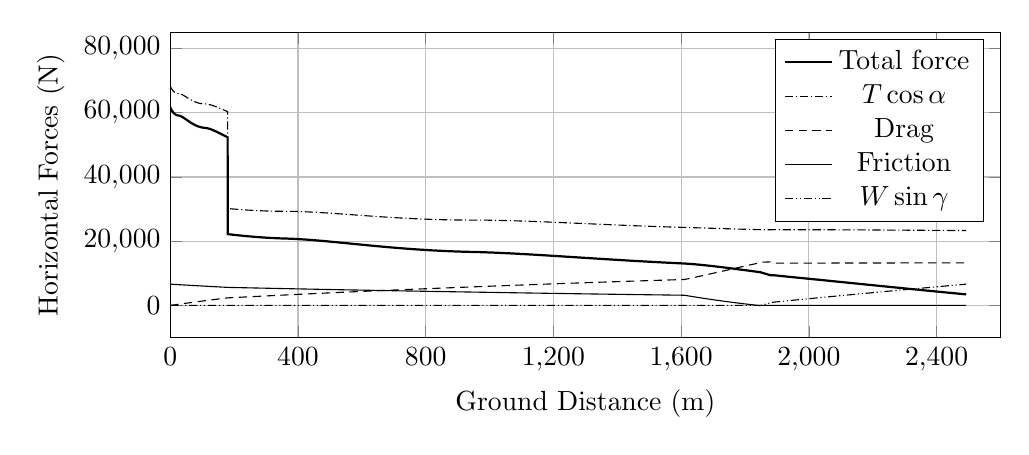
\begin{tikzpicture}

\begin{axis}[
width=\textwidth,
height=0.45\textwidth,
scaled ticks=false, tick label style={/pgf/number format/fixed},
xmin=0.0,
xmax=2600,
xlabel={Ground Distance (m)},
xtick={0,400,800,1200,1600,2000,2400,2800,3200},
xmajorgrids,
ymin=-10000,
ymax=85000,
ylabel={Horizontal Forces (N)},
ymajorgrids,
legend entries = {Total force\\$T\cos\alpha$\\Drag\\Friction\\$W\sin\gamma$\\}
]

\addplot [
color=black,
thick
]
table[row sep=crcr]{
1.3729668748938318E-8	61783.50936677457\\
1.7493248493808052E-7	61783.50931819419\\
1.4411937280317895E-6	61783.50893663404\\
6.602995160656227E-5	61783.48949180379\\
2.2740573828771224E-4	61783.44096944184\\
4.8751428921765393E-4	61783.362864569164\\
8.441986619835749E-4	61783.25590491043\\
0.0012981647037285577	61783.11995795992\\
0.0018484379050661159	61782.95539459643\\
0.0024893731755424335	61782.763978095056\\
0.0032286585096692284	61782.54348870709\\
0.0040442418752796045	61782.300571157946\\
0.004972762654474916	61782.024388983074\\
0.005990910102221513	61781.72196051582\\
0.007111389191545643	61781.389590122795\\
0.008336865178450469	61781.02657489202\\
0.009664633507451486	61780.63380374739\\
0.011093815858158905	61780.211622131974\\
0.01262066151120312	61779.761220824425\\
0.01419454386807839	61779.297583670734\\
0.015910782250193378	61778.792708046516\\
0.017721549103721458	61778.260769758184\\
0.019620507964630857	61777.70370309276\\
0.02164969955342029	61777.10927012407\\
0.023766550611781796	61776.49003705206\\
0.025957065600157342	61775.85015759252\\
0.028260861173784894	61775.17813469037\\
0.030668466949245715	61774.47682513781\\
0.0331489614440674	61773.755305374696\\
0.03573888453685943	61773.00301953977\\
0.038418765463712895	61772.22570664175\\
0.04116679597872082	61771.42975031301\\
0.044022059812866554	61770.603898748246\\
0.04700053365173311	61769.74363338725\\
0.050116649382181494	61768.84490750516\\
0.0533021652593606	61767.92749125602\\
0.056630220296749106	61766.970412267925\\
0.05998688030085898	61766.00650178116\\
0.06348077825220624	61765.00462698481\\
0.06710848437295475	61763.96589975928\\
0.07082346760424127	61762.903740800684\\
0.07462944469130567	61761.81715791611\\
0.07855413323217031	61760.69832813459\\
0.08251243142992878	61759.57156625534\\
0.08659905947434482	61758.409969738175\\
0.09083545394947079	61757.20757846015\\
0.09518096637774642	61755.97605085994\\
0.099604438418047	61754.72429342507\\
0.1041130762071252	61753.45032800194\\
0.10871457033213175	61752.15205203775\\
0.11350280915994052	61750.80311026056\\
0.11836943512882261	61749.434154946604\\
0.12328542045494376	61748.05338999005\\
0.12830372217771202	61746.64599506589\\
0.1334037067999082	61745.217831285496\\
0.1386015897371753	61743.76442942071\\
0.14405085578552257	61742.24305202397\\
0.1495239325759128	61740.717367471836\\
0.1550507392415454	61739.17904182979\\
0.16073360491635535	61737.59968363469\\
0.16659871679960742	61735.972187966385\\
0.17244819595229793	61734.35152714387\\
0.17848031195343078	61732.68283179669\\
0.18466822548212042	61730.9737001038\\
0.1909009608611748	61729.25486918863\\
0.19716089737688902	61727.531200967176\\
0.2035279375926986	61725.780737120935\\
0.21017879584430066	61723.955101334985\\
0.21687473998771628	61722.11999273021\\
0.22354650324940833	61720.29436393984\\
0.23036941414946865	61718.4302767788\\
0.23737731412185503	61716.51865747724\\
0.24449289925428264	61714.58073767419\\
0.2517184892023243	61712.615981853276\\
0.25908208279438383	61710.61689262393\\
0.2664863589195283	61708.60996201573\\
0.27399321582905467	61706.578460519464\\
0.2816108016888421	61704.520276528405\\
0.2893844725195981	61702.42328349393\\
0.29747621078120867	61700.24405015753\\
0.30547198304033185	61698.094181799184\\
0.31373479402345694	61695.87614070039\\
0.3220909744202328	61693.63673683404\\
0.3305540912568814	61691.37241924043\\
0.33895489345894936	61689.12845371444\\
0.34753073012810576	61686.8414686046\\
0.3563589175375672	61684.49107977233\\
0.3652744752958731	61682.12138853967\\
0.3742693918027593	61679.734586974344\\
0.38350989122680823	61677.28673550232\\
0.3927029292363896	61674.85554658639\\
0.4020876366599533	61672.377827149656\\
0.4115568217121528	61669.88201310733\\
0.4212787852930122	61667.32392160392\\
0.43089755178065414	61664.79726999061\\
0.4408379299669313	61662.19056665347\\
0.4510502611115679	61659.517183871154\\
0.4612670224725215	61656.84729029596\\
0.4715818614584312	61654.15643159865\\
0.4818438670126082	61651.48395666065\\
0.4922128554044626	61648.788232328385\\
0.50273876067117	61646.05640426549\\
0.5136516607865718	61643.22907615514\\
0.5244310074213006	61640.441233326\\
0.5355751508210329	61637.56409397545\\
0.5467126997993474	61634.693734295506\\
0.5580479056656631	61631.77759306245\\
0.5692960823995112	61628.888933732684\\
0.5809945926573021	61625.889951412944\\
0.5923626544035139	61622.980834830974\\
0.6041922852715	61619.95894182491\\
0.6160912669048675	61616.92477468107\\
0.6280605196746807	61613.8781418163\\
0.6403946506485891	61610.74430041232\\
0.6525721787971039	61607.65583801706\\
0.66504690021022	61604.49770613441\\
0.6773535438897555	61601.38773024638\\
0.6901462526606317	61598.16076906811\\
0.703249873273524	61594.86150262278\\
0.7159721017112175	61591.66413795836\\
0.729053467210389	61588.38249447748\\
0.7422988791228431	61585.06582034654\\
0.756304272979474	61581.56548613492\\
0.7696432036294076	61578.23800923109\\
0.7832290250230658	61574.85519604896\\
0.7969128825551131	61571.45429518534\\
0.8108444209446342	61567.998300175896\\
0.825043936786227	61564.482480705134\\
0.8390802275180445	61561.01362054165\\
0.8532340040587583	61557.52225875264\\
0.8678101043696134	61553.93352069818\\
0.8824320602344964	61550.34036740266\\
0.8978006605470081	61546.57109554042\\
0.9134572487531922	61542.7388827126\\
0.9287391767029982	61539.00579639722\\
0.9440564687433697	61535.27136794293\\
0.9598871644713316	61531.41938277046\\
0.9757786228365237	61527.56033265087\\
0.9918217338879218	61523.67223735628\\
1.0080608846667363	61519.744529459145\\
1.0245900975307913	61515.754759650416\\
1.040622085070809	61511.89274780078\\
1.0571005809273983	61507.93105466048\\
1.0736578999152901	61503.958394411195\\
1.0902401336450098	61499.98771471836\\
1.1073201062866707	61495.906112076496\\
1.1241926772552646	61491.88224206393\\
1.1416781667104252	61487.72070186546\\
1.1588269484070954	61483.64764011913\\
1.176440946845327	61479.47261864893\\
1.1944819542445066	61475.20528321224\\
1.2120125629913447	61471.067238165444\\
1.2299306574276825	61466.84638602627\\
1.2481120482032448	61462.57239171186\\
1.2663536608165091	61458.293165328665\\
1.2851425782117465	61453.89482635389\\
1.3041313368869671	61449.45920150836\\
1.3228236880779458	61445.10207073693\\
1.3414329672940513	61440.77336038122\\
1.3605066144349074	61436.345944626664\\
1.3802534409605212	61431.772129719306\\
1.3994872719307283	61427.32671232158\\
1.4192016277101378	61422.77997173052\\
1.439023460648384	61418.21831341875\\
1.459347998039509	61413.55117073345\\
1.4793256644936217	61408.97367991289\\
1.4991489338326072	61404.44129806955\\
1.5195196572175793	61399.79377788275\\
1.5402684478761244	61395.07038494774\\
1.5604570108688036	61390.48451568978\\
1.5810331069622228	61385.82068881598\\
1.6022712329181132	61381.01739719065\\
1.623752316257296	61376.170030157766\\
1.6452514305955401	61371.329469632794\\
1.6664829631402025	61366.55976293117\\
1.6886446033619715	61361.59227552322\\
1.710607384244656	61356.680544700896\\
1.7329417009553727	61351.69706550312\\
1.7551421266962821	61346.754722041835\\
1.7779085356585536	61341.697961334634\\
1.800478286927734	61336.696385267554\\
1.8236018329231238	61331.58388814218\\
1.8462320784511883	61326.59195018708\\
1.869621217116264	61321.444481905855\\
1.8933146512119747	61316.24227072962\\
1.9176856041472643	61310.90405729068\\
1.9417713639512164	61305.64094124308\\
1.9657098573982132	61300.4223660413\\
1.9902165007163162	61295.09261980343\\
2.014554050520948	61289.81227100038\\
2.039479559407779	61284.417314282924\\
2.0645497069116256	61279.0041961511\\
2.090368502766882	61273.443123795136\\
2.115564185269416	61268.029575617504\\
2.140750230554602	61262.63116016747\\
2.1667677015838267	61257.068165785255\\
2.1927560352542175	61251.52514585026\\
2.218891869133375	61245.964435558795\\
2.245288939563828	61240.362076070596\\
2.2712530964452817	61234.86517296669\\
2.297933078351498	61229.23066552682\\
2.324564104516777	61223.62050862283\\
2.351466051806102	61217.96740824815\\
2.378869922986878	61212.22335004214\\
2.4061764715670764	61206.51417727664\\
2.4343811693482102	61200.63231410271\\
2.4622108821536663	61194.84359472743\\
2.4906408044048067	61188.945266207724\\
2.518892760285042	61183.09902729666\\
2.5472153538550346	61177.25325971817\\
2.5762492306032216	61171.27627467198\\
2.605385308804288	61165.294026661766\\
2.634725531238531	61159.28574226744\\
2.6633424112287507	61153.44084646394\\
2.6927188130915374	61147.45641035109\\
2.7226962917814213	61141.365715623484\\
2.7531675915664673	61135.19135395951\\
2.7831412651501983	61129.134125433455\\
2.8139174932165103	61122.93143853231\\
2.8440331768075415	61116.87819268227\\
2.874693215323904	61110.73201687279\\
2.9059978681586376	61104.47368679698\\
2.9372617813709034	61098.240616483556\\
2.9684444504378202	61092.040687474786\\
3.000072782687808	61085.76934063973\\
3.031082587373527	61079.63735536639\\
3.063213028467148	61073.30113869638\\
3.0965739711585014	61066.74086540491\\
3.1291175748240176	61060.35947867474\\
3.161651640649506	61053.99779219624\\
3.194791488147139	61047.5358815019\\
3.2273698640351327	61041.20128928563\\
3.261394174200582	61034.604326216315\\
3.2942820372415875	61028.24584816002\\
3.3276455142443044	61021.81353982561\\
3.3625338428565543	61015.10666957665\\
3.396526624461681	61008.590954514875\\
3.4305511850311694	61002.08782540166\\
3.4642094416894933	60995.6729987805\\
3.498963551783903	60989.06830833148\\
3.5341885134496573	60982.39372525296\\
3.569804025802995	60975.665083850676\\
3.605116576002147	60969.01337660823\\
3.641338581546833	60962.210630011396\\
3.677593698357855	60955.422116372996\\
3.7132425573336665	60948.76696834146\\
3.74957219375957	60942.00487369401\\
3.7872650227149185	60935.01043052906\\
3.825403000593508	60927.95543478249\\
3.861987998097706	60921.208455890286\\
3.899535703755137	60914.30494229625\\
3.9366960368382165	60907.493498133\\
3.9756271117991435	60900.37961167353\\
4.014715979923002	60893.25956141483\\
4.053268843133694	60886.259281865176\\
4.093111596873367	60879.04777155626\\
4.132540645872048	60871.9340234056\\
4.171686416589186	60864.89378843088\\
4.211258480423352	60857.79946273782\\
4.252585425594734	60850.41463845922\\
4.29253892845542	60843.29853956016\\
4.332839968385603	60836.14363252418\\
4.372708537789018	60829.08821289876\\
4.414379330316386	60821.73788088378\\
4.455607216042212	60814.48971734302\\
4.497336690654009	60807.17760426682\\
4.53836773335787	60800.011530609714\\
4.579767142935065	60792.80477952087\\
4.621942908118227	60785.48720022476\\
4.663798268780793	60778.24936087112\\
4.705838036060712	60771.00373340146\\
4.748491012675066	60763.67698509767\\
4.791393968819099	60756.33214021707\\
4.835700194867293	60748.77308671326\\
4.879973298406089	60741.245972508754\\
4.923250156511948	60733.91351177776\\
4.967673596314626	60726.41265084362\\
5.012954369117542	60718.79387011319\\
5.057574526249477	60711.31262249804\\
5.103280208347517	60703.67639039809\\
5.148856018935929	60696.088955929896\\
5.194350575362858	60688.54190949214\\
5.240584094986199	60680.899641984724\\
5.2871741484687504	60673.22621426945\\
5.333122064003502	60665.685726141994\\
5.3803318800233235	60657.966128971384\\
5.4262712259485255	60650.48137450908\\
5.473378197958581	60642.83401175507\\
5.521938593493333	60634.979848385396\\
5.570027890245774	60627.23090701045\\
5.617746353771608	60619.57013957921\\
5.665750363096816	60611.89196312707\\
5.714883880069209	60604.06252009612\\
5.763390205677501	60596.362058340004\\
5.812817811268989	60588.54488465827\\
5.861909274803731	60580.81025635592\\
5.912134919389196	60572.92709899858\\
5.962317560553064	60565.0810253973\\
6.012727788730279	60557.229757323905\\
6.0628236035803145	60549.45749546884\\
6.113711068416594	60541.59292957082\\
6.16497292765713	60533.701460490236\\
6.216284706244114	60525.83328462468\\
6.26834407822653	60517.88200396756\\
6.320257064476769	60509.984565890714\\
6.37351660191279	60501.91480627554\\
6.426150862197664	60493.972008043624\\
6.479030963436509	60486.024222335065\\
6.532319340056288	60478.04748898775\\
6.5857233987986845	60470.085940962555\\
6.640834734692348	60461.903831915755\\
6.695022999498724	60453.892251965925\\
6.749720237657193	60445.83894394833\\
6.804235758325081	60437.845755034374\\
6.859728469301633	60429.743347450974\\
6.916686079588434	60421.46262849223\\
6.9732530286722305	60413.27421688488\\
7.029531186664631	60405.162572822126\\
7.086633318514238	60396.96765207173\\
7.144155485034537	60388.748432014414\\
7.202053129566568	60380.51186784168\\
7.260126434764185	60372.28674462697\\
7.317913145042743	60364.138270941374\\
7.376682960996439	60355.88790146746\\
7.435393721764624	60347.68264748163\\
7.493838107271518	60339.55101986464\\
7.552684475254578	60331.39999647814\\
7.613252707151423	60323.04859044879\\
7.672782806866918	60314.87784466025\\
7.733397683408512	60306.59626085448\\
7.795525081709004	60298.14769956826\\
7.856013653786727	60289.96041879487\\
7.91792172269443	60281.62008820528\\
7.980110745884113	60273.2815424445\\
8.041720670752433	60265.05964912739\\
8.105229267009985	60256.62483820542\\
8.167457523036095	60248.39974670301\\
8.230908874360502	60240.05325317499\\
8.293738919282273	60231.82837733555\\
8.356235402336917	60223.68638040952\\
8.42092378244627	60215.299842988214\\
8.485671322837007	60206.94724288801\\
8.549180898871484	60198.79461401848\\
8.614596634551038	60190.438815697504\\
8.680166762249144	60182.10540492926\\
8.744770128469462	60173.93592055414\\
8.812993689385827	60165.35269946925\\
8.88005807777586	60156.95924201797\\
8.94709863067661	60148.61211285544\\
9.013172088448385	60140.42762435354\\
9.079266506338545	60132.28231031295\\
9.14748814890141	60123.91847947452\\
9.215411293660388	60115.635101516134\\
9.284579146198691	60107.24471507208\\
9.353168277381275	60098.968974656105\\
9.423753765537143	60090.49837841203\\
9.492960052876374	60082.23842618668\\
9.564123004975215	60073.791350044296\\
9.634097601479446	60065.531029113\\
9.705672410878787	60057.128493450815\\
9.776260200085993	60048.88788355653\\
9.846607984572056	60040.720610503195\\
9.918231435410593	60032.45152706427\\
9.988851555070422	60024.34382995483\\
10.060390022634245	60016.17663083745\\
10.133279281833644	60007.90257469112\\
10.205241085147751	59999.78050366022\\
10.277820389603	59991.63555573017\\
10.352558894167803	59983.297241602966\\
10.42733258664746	59975.00449782121\\
10.501815126481194	59966.793066327446\\
10.576858173457808	59958.56912427908\\
10.65303812840548	59950.27098563395\\
10.729080272001735	59942.038295135804\\
10.804841544893105	59933.885926652074\\
10.881905013502095	59925.64434529406\\
10.958396790746043	59917.51447917438\\
11.035905069829102	59909.3277688323\\
11.113160538490881	59901.218840620655\\
11.192172636140572	59892.978073499384\\
11.270076562295213	59884.90470204182\\
11.350065490058778	59876.668580775906\\
11.429008826667825	59868.59288643465\\
11.50754237847364	59860.61092228572\\
11.587076645554472	59852.57971245531\\
11.668897725768986	59844.372467319656\\
11.749734371708193	59836.31841572361\\
11.830312384681939	59828.343782859345\\
11.909862670519033	59820.52320554938\\
11.990515423105418	59812.64713787827\\
12.072973931530203	59804.64958127121\\
12.155304175892073	59796.719582681006\\
12.237018674011615	59788.90314428731\\
12.320146069843414	59781.00680295155\\
12.406770618003886	59772.83732525859\\
12.489918686423398	59765.0521922965\\
12.574493004618496	59757.19005979443\\
12.660666896522624	59749.237655712204\\
12.746500366216402	59741.37506944318\\
12.832006837122272	59733.600172154285\\
12.919285437479463	59725.72334361392\\
13.00517529032821	59718.03002089217\\
13.092301899261269	59710.284656648524\\
13.179760097773386	59702.56908818724\\
13.268594687119744	59694.792661947824\\
13.357699529172354	59687.05366764557\\
13.44829753340392	59679.24748054074\\
13.537570218252604	59671.61689145358\\
13.627322718831184	59664.00650524694\\
13.718307212496544	59656.35407081641\\
13.808540263830096	59648.82667351708\\
13.899143852161355	59641.33009581514\\
13.991564069206362	59633.74670449764\\
14.085798171937814	59626.08025799738\\
14.179213507883688	59618.54573471083\\
14.271883316076963	59611.13535568971\\
14.367546274622434	59603.55225944966\\
14.459430863676705	59596.33217024506\\
14.555010173556813	59588.887539697884\\
14.648669731311681	59581.657273247416\\
14.743773575674254	59574.38094293936\\
14.839769774519894	59567.1029601561\\
14.932807148196385	59560.112942104766\\
15.026921440816679	59553.10552379627\\
15.12275113649265	59546.03578389977\\
15.222025232743288	59538.78128033936\\
15.321078842653048	59531.61296758363\\
15.417564225728565	59524.69757199325\\
15.515758841369038	59517.72737648299\\
15.613440509090129	59510.86111926354\\
15.7107260301154	59504.08941471683\\
15.81102223487273	59497.17759566792\\
15.913565872734136	59490.18353301275\\
16.012918321571746	59483.476927652344\\
16.11222833737955	59476.84159838184\\
16.216250800242257	59469.96449577849\\
16.319159023020546	59463.23438054435\\
16.421418004006803	59456.61870963819\\
16.521675247646563	59450.20196365398\\
16.62557290942481	59443.62449510081\\
16.72731964230514	59437.25424619064\\
16.830283223934416	59430.87913958389\\
16.93464251494634	59424.490583355655\\
17.038481620468637	59418.206532446624\\
17.146497421123335	59411.746365730505\\
17.252282308638982	59405.49511641824\\
17.35724772858778	59399.36587774908\\
17.464053904588297	59393.204134922125\\
17.572390862630144	59387.03108589236\\
17.680417629270814	59380.9526695478\\
17.789707298693855	59374.88112631011\\
17.899612520762552	59368.8541672977\\
18.01027367065641	59362.86530198445\\
18.121415095654797	59356.930511292594\\
18.232428503320143	59351.08238618226\\
18.34337337506409	59345.31731245783\\
18.454877340220463	59339.60293575535\\
18.56636189702322	59333.96921609246\\
18.678405595805643	59328.38722992971\\
18.7903363416971	59322.890674228154\\
18.902391384512768	59317.46764778967\\
19.01754810908954	59311.97725437852\\
19.131359562866663	59306.63313674148\\
19.247747682986713	59301.252197607246\\
19.361628242251975	59296.069299371404\\
19.477963464454028	59290.858270449695\\
19.595742742603164	59285.66833214891\\
19.71107288142779	59280.66967275088\\
19.82767543183723	59275.69944450908\\
19.944540068808188	59270.8020964278\\
20.06171535440768	59265.97594140952\\
20.179291418887807	59261.21776487927\\
20.29729887224694	59256.52695605492\\
20.417200571824914	59251.84761175189\\
20.53676390826074	59247.26827780924\\
20.65523768803314	59242.815905510404\\
20.777063017363922	59238.3257742877\\
20.896922101876633	59233.995112206234\\
21.016777952410983	59229.750584958514\\
21.13892104879462	59225.513277852224\\
21.260534693274344	59221.382539186234\\
21.382619708556632	59217.324037488914\\
21.506306369043365	59213.30217921632\\
21.631260758247265	59209.330683261534\\
21.75556249187227	59205.47098008299\\
21.87985606458615	59201.70205279725\\
22.005925835680863	59197.971452147074\\
22.130365724585275	59194.37985257048\\
22.257477980325966	59190.80394497192\\
22.38418119026224	59187.332618008106\\
22.50885833858638	59184.00723337526\\
22.636026948728087	59180.707532259956\\
22.76367325110224	59177.48873026998\\
22.89115382514759	59174.367117031856\\
23.022452271734288	59171.248892274845\\
23.149877274293033	59168.31637870213\\
23.27873580881144	59165.44447827418\\
23.408563766880334	59162.64588680939\\
23.538692653979794	59159.93613162091\\
23.671258756997098	59157.27346931632\\
23.803210122669313	59154.72093480373\\
23.93544283576786	59152.26053834283\\
24.067241518013077	59149.90514146356\\
24.19863541429976	59147.6530223423\\
24.329449967727697	59145.50582664789\\
24.46175612159181	59143.43028756771\\
24.594763714591892	59141.440926767566\\
24.72754053098891	59139.551931542606\\
24.86208223890334	59137.73632087173\\
24.99503410474967	59136.03928836863\\
25.12831230627787	59134.434725881234\\
25.265273024090206	59132.88635272045\\
25.400650037308893	59131.45574215191\\
25.536304655026747	59130.12150850955\\
25.673594178904246	59128.87213598179\\
25.80797730935859	59127.747291601554\\
25.835159569235522	59127.53153956341\\
25.83771752397454	59127.51142952933\\
25.84157983658004	59127.48099258305\\
25.854829339215996	59127.37578721759\\
25.893215796826965	59127.06406847287\\
25.973046119315796	59126.383004412\\
26.096262980671412	59125.24550935048\\
26.224212718725603	59123.954657521\\
26.35313595194755	59122.54233981055\\
26.481727686355264	59121.02338475868\\
26.611118169629577	59119.38520555795\\
26.74049186039369	59117.63848580769\\
26.87228140714948	59115.74872427908\\
27.003385008924262	59113.75959859043\\
27.1358830905183	59111.640045812266\\
27.265951877034226	59109.45384446668\\
27.399105426781233	59107.10887343832\\
27.53075869079712	59104.68530533768\\
27.66387879779476	59102.1299013613\\
27.79855889054391	59099.43863891032\\
27.932132547760695	59096.66560777443\\
28.06791767232785	59093.741994890675\\
28.202763022922632	59090.735521714174\\
28.339788243013793	59087.576570427525\\
28.476803106655623	59084.314523197376\\
28.61761981788422	59080.85571277671\\
28.753907949775353	59077.406926056065\\
28.89297195746854	59073.786639494254\\
29.03211749902605	59070.06321752322\\
29.17123509789927	59066.2408773973\\
29.312253051611236	59062.26597952112\\
29.454422317169097	59058.15774506479\\
29.59523538430127	59053.99020601279\\
29.737672170826222	59049.67624612304\\
29.879173197948965	59045.29400615749\\
30.02075470454991	59040.8142058634\\
30.166674235301365	59036.09900785962\\
30.308336095430334	59031.4274065885\\
30.452640844036836	59026.57477547036\\
30.597553881025625	59021.607672399856\\
30.742967061600154	59016.530053728\\
30.888975484926362	59011.33887063782\\
31.034653067922946	59006.068109877\\
31.180984070508003	59000.68316248106\\
31.328351020411645	58995.16968918135\\
31.476753455192622	58989.52711491549\\
31.62661541983664	58983.73836597483\\
31.774495604492607	58977.93814636876\\
31.924944104961916	58971.948782357475\\
32.07610067279926	58965.84275488589\\
32.22631826848556	58959.688105267225\\
32.37899942625752	58953.3454266342\\
32.528514827654206	58947.05044264713\\
32.68189139400266	58940.508014744526\\
32.836069829938495	58933.84606112067\\
32.99025509482905	58927.099578213136\\
33.14574197930297	58920.212157135364\\
33.30072558931056	58913.26440550946\\
33.455047097713944	58906.26565227684\\
33.610874563168906	58899.11818795225\\
33.76926068144728	58891.77186906937\\
33.92617323250643	58884.414175144295\\
34.08448787244542	58876.91161424054\\
34.24243160505006	58869.348713030515\\
34.40316487172558	58861.573642694784\\
34.56154208099588	58853.836261210396\\
34.721775177117024	58845.93243222273\\
34.88076970836556	58838.01560290583\\
35.041349106451236	58829.94619135125\\
35.20329621413198	58821.734327750135\\
35.364886328651124	58813.468026459625\\
35.529241615711214	58804.98721442223\\
35.69117991651797	58796.560302957514\\
35.85317319416103	58788.06142007497\\
36.014854298354294	58779.51118499559\\
36.18095311277159	58770.658098484826\\
36.34443322746766	58761.87728873029\\
36.51065106768533	58752.882205496455\\
36.67635767082788	58743.84853172314\\
36.842033683894186	58734.75159119234\\
37.00823867836148	58725.56155777925\\
37.17279029188734	58716.400908365686\\
37.33951104811075	58707.05771237098\\
37.50923941781488	58697.48327519921\\
37.679358776579846	58687.82451987176\\
37.845326083883435	58678.34258156859\\
38.017144746304325	58668.466225570664\\
38.1852030886141	58658.74799438121\\
38.35804431104914	58648.69451553178\\
38.52812920813831	58638.74443599388\\
38.69960796987526	58628.656801382225\\
38.87165793928378	58618.480185439315\\
39.0423941506003	58608.327560152306\\
39.21436971822614	58598.048257301765\\
39.38727999643966	58587.66059359255\\
39.558989012313546	58577.29410428113\\
39.734752343022535	58566.6313413904\\
39.908836167348156	58556.020213612166\\
40.084555009291705	58545.25981907788\\
40.259186798753746	58534.51770674638\\
40.43324437115375	58523.76408653303\\
40.61041052363379	58512.77148397631\\
40.787318094191775	58501.74876795053\\
40.96620398302343	58490.55698222955\\
41.14141336180775	58479.55161370123\\
41.31941103282654	58468.327975789405\\
41.49571226203258	58457.1694842367\\
41.67366972437729	58445.86498444638\\
41.85219319429197	58434.483984805454\\
42.03136872634711	58423.02160991519\\
42.21293422072888	58411.36670483003\\
42.39366932880948	58399.7265094701\\
42.57479521797359	58388.023540012495\\
42.75522531040919	58376.329102045536\\
42.93775785970641	58364.46241180785\\
43.11993568316029	58352.5836987145\\
43.30336620712447	58340.58889627688\\
43.48720879745599	58328.533505718326\\
43.672226884455625	58316.368031652615\\
43.85684130549208	58304.197094175106\\
44.039851952877484	58292.10129638862\\
44.22449378650157	58279.86778156452\\
44.412385508552646	58267.38908996245\\
44.59783063297877	58255.044321995505\\
44.78525507043919	58242.53992532681\\
44.973130075825196	58229.978310821636\\
45.16145211071871	58217.36047816828\\
45.34881478087516	58204.78170438763\\
45.536017136752506	58192.189492902966\\
45.724971990057284	58179.45579254262\\
45.91416212467789	58166.68339680946\\
46.10175434018815	58153.9972119719\\
46.29356928918713	58141.00406929373\\
46.48490977712943	58128.022434909595\\
46.67744207882204	58114.9400631547\\
46.869905949194575	58101.843323835725\\
47.062749521718516	58088.70258091636\\
47.25341437235973	58075.69329966346\\
47.44508461154423	58062.59924675501\\
47.63880095964302	58049.34980834146\\
47.83356160493736	58036.01400764345\\
48.025334057720784	58022.869032313654\\
48.218846636819876	58009.59175889351\\
48.41468711090302	57996.142299023544\\
48.610449575687724	57982.686516208996\\
48.80723286029129	57969.14964956645\\
49.00124137999302	57955.79376834069\\
49.20045899041696	57942.0699067847\\
49.394243884198005	57928.71198778252\\
49.59161211700324	57915.09944956248\\
49.79144608231523	57901.3098450332\\
49.99107345578199	57887.52828483154\\
50.18996871950735	57873.79190407884\\
50.388458331230495	57860.078997689634\\
50.59191110395449	57846.01931568865\\
50.79453916783869	57832.01353035103\\
50.99530158869649	57818.13445100811\\
51.19776583381373	57804.13624723397\\
51.3996255264899	57790.17914885178\\
51.599450409211	57776.36281792374\\
51.80158475775707	57762.38763759422\\
52.002311498730975	57748.511345786654\\
52.2060805474067	57734.42708837715\\
52.40811442127868	57720.46583813442\\
52.61423073460446	57706.22638402667\\
52.821749674584495	57691.89477916088\\
53.03053110951893	57677.481563424066\\
53.23753590773735	57663.197276435225\\
53.44487707917263	57648.89678764176\\
53.652063533093525	57634.61470766827\\
53.85975522429668	57620.30628726164\\
54.06844148636836	57605.93862921395\\
54.278580968983874	57591.48104539467\\
54.48685885904548	57577.16227461879\\
54.69884126905886	57562.60051802888\\
54.90975544393264	57548.12456156479\\
55.12216013841277	57533.559536570945\\
55.333080623240974	57519.11012386318\\
55.5448885814986	57504.61447976061\\
55.75594910746132	57490.18518575055\\
55.968144975063936	57475.69424122706\\
56.18150915317635	57461.1403300784\\
56.394069348356695	57446.65869399159\\
56.60950747146016	57431.99941415647\\
56.82641599949238	57417.259502762856\\
57.03980213394583	57402.778624603176\\
57.25698083573829	57388.0610679501\\
57.47353804711997	57373.407069331704\\
57.6941706582635	57358.49998628975\\
57.91229938529948	57343.78524930471\\
58.12998527173144	57329.12399856189\\
58.34905943653719	57314.39370104858\\
58.56781345824973	57299.71004035887\\
58.787998582886644	57284.956289350856\\
59.011266007804366	57270.02325362606\\
59.23368761368569	57255.174710108346\\
59.456031473365414	57240.35983994363\\
59.67976581221534	57225.48169538447\\
59.90315377467765	57210.65660249605\\
60.125192111546724	57195.95140687663\\
60.349269227196444	57181.14244698199\\
60.57220932044149	57166.44039044973\\
60.79606803632835	57151.710218786364\\
61.021718319759984	57136.89567458941\\
61.25073295331903	57121.89526120912\\
61.47770893732542	57107.06377362665\\
61.70784367826464	57092.0624572369\\
61.93740803875056	57077.135608903074\\
62.1673491775543	57062.222185269784\\
62.39648011888062	57047.3996425107\\
62.62822464633953	57032.44753078092\\
62.86094183422966	57017.473225201975\\
63.090532789209604	57002.74047517707\\
63.321616049163225	56987.95303829985\\
63.554808975015874	56973.07293327087\\
63.78685818650332	56958.308575350864\\
64.0234762327251	56943.29801516942\\
64.25652029988498	56928.55864584356\\
64.49146565301734	56913.744240641085\\
64.72768747885678	56898.8956628672\\
64.96568125142531	56883.98321681365\\
65.20057601391298	56869.312248811024\\
65.43975061379945	56854.42279073603\\
65.67719429610031	56839.69034425853\\
65.91652243006087	56824.89116828525\\
66.1565253585166	56810.101398558225\\
66.39740384038885	56795.30968675176\\
66.63777997854328	56780.60128631268\\
66.87849958303539	56765.924904257816\\
67.12349409848125	56751.04290398229\\
67.36843544137562	56736.220141152575\\
67.61129947098183	56721.57889015571\\
67.85808619273692	56706.75858955852\\
68.10323725880951	56692.094340982454\\
68.3520146383799	56677.27260865476\\
68.60099753692072	56662.499086580065\\
68.84943315800746	56647.81882346209\\
69.09793111574629	56633.19611661897\\
69.34894754058863	56618.4878935576\\
69.59791912239118	56603.96220652574\\
69.84867626946473	56589.395968034325\\
70.10496107302816	56574.57511226465\\
70.35594730130109	56560.12629065517\\
70.60854748652795	56545.65059766144\\
70.8625286964371	56531.16303634326\\
71.1182576034713	56516.644416970215\\
71.37278964945165	56502.26260553488\\
71.62944082734805	56487.831084778794\\
71.88536754710964	56473.510785568666\\
72.14250945057543	56459.19384080339\\
72.40306402213687	56444.76030481051\\
72.66241221953337	56430.46744764532\\
72.92327110344874	56416.166121867864\\
73.18657203154456	56401.8074377232\\
73.45150557123125	56387.43778627146\\
73.71756195569753	56373.0865052532\\
73.97940051906463	56359.040747515246\\
74.24514793127645	56344.864887675634\\
74.51022759525631	56330.80495999093\\
74.77823256031297	56316.671865744254\\
75.04767613410795	56302.54646495095\\
75.31682895458664	56288.52039886532\\
75.58729746777243	56274.51087772034\\
75.85729327570917	56260.61137143591\\
76.13042767774209	56246.63768074883\\
76.40299665611133	56232.78097808552\\
76.67973301409052	56218.80285702154\\
76.95360383527739	56205.05962557149\\
77.22854206589327	56191.35346407132\\
77.50692063517303	56177.56874949059\\
77.78349662592461	56163.96634564559\\
78.0616064362213	56150.382450894045\\
78.33869545141144	56136.942516675525\\
78.62238552181594	56123.28014227233\\
78.90481169871467	56109.777288862475\\
79.18659077494928	56096.403885610416\\
79.4700201012688	56083.05184048835\\
79.75774957869095	56069.59989933815\\
80.04430580185078	56056.30604910277\\
80.33432201731404	56042.957007113364\\
80.62298533865851	56029.775867785254\\
80.9130804606989	56016.63593103048\\
81.20459144967842	56003.53990348488\\
81.49650140842283	55990.534887974776\\
81.79224544448738	55977.47063954093\\
82.08455487090956	55964.66887545241\\
82.37934996819865	55951.8701770644\\
82.67580145620735	55939.11331545371\\
82.97475550983006	55926.36468467326\\
83.2734238134004	55913.74488135282\\
83.57209772503273	55901.2418258995\\
83.87419166445906	55888.71500215256\\
84.17487194816226	55876.36642866509\\
84.47686996876752	55864.08426237892\\
84.78124993153034	55851.8278343751\\
85.08776945017104	55839.610038868224\\
85.39395758722245	55827.53086058608\\
85.69833162305892	55815.64785709877\\
86.01027818388755	55803.5985178219\\
86.31658691867341	55791.89468749928\\
86.62866814828641	55780.10085273786\\
86.94043673469176	55768.45079136125\\
87.2565990672368	55756.771624784335\\
87.56980823017452	55745.336051019476\\
87.88101387141376	55734.10658280985\\
88.20007062892054	55722.73177728572\\
88.51883409355145	55711.50729000692\\
88.83509784148416	55700.509349194166\\
89.15857089898353	55689.403815860685\\
89.47772213402055	55678.58885977807\\
89.80217214804901	55667.739496903174\\
90.1263587278685	55657.04547881434\\
90.44950966725051	55646.531761019345\\
90.77764749859728	55636.00545919975\\
91.10470504824352	55625.66424119286\\
91.43769785174896	55615.29002169194\\
91.76691749028419	55605.187129409285\\
92.09386993524024	55595.30548752818\\
92.42498248438446	55585.4525137208\\
92.7581696617394	55575.69499892079\\
93.09729153734631	55565.92597093234\\
93.4312406900703	55556.46629977334\\
93.76780571708736	55547.09387104695\\
94.10390054156983	55537.89651488431\\
94.43564317419558	55528.97732777163\\
94.77291201930262	55520.07190414556\\
95.10796951504997	55511.387276623835\\
95.44708659079325	55502.762585888704\\
95.78515592548297	55494.3302583802\\
96.12311752311894	55486.066325542764\\
96.46351490415591	55477.910635066015\\
96.80669869710772	55469.8589918371\\
97.14657639264556	55462.05427077276\\
97.48763116340677	55454.392251232784\\
97.8305814261901	55446.8594104143\\
98.17013304046878	55439.571216555705\\
98.51054009051404	55432.43475666635\\
98.854181194619	55425.4035474478\\
99.19205317796005	55418.660191706425\\
99.53355440060989	55412.01579560955\\
99.87198375587872	55405.60144673211\\
100.2129389915628	55399.31092535134\\
100.55335806642802	55393.20251472741\\
100.89503335592528	55387.24488446141\\
101.23693480167049	55381.457406855436\\
101.57977298927813	55375.82922451757\\
101.91842351185082	55370.442253145084\\
102.26214655705948	55365.150142933606\\
102.60487134933112	55360.049761981776\\
102.94238410388857	55355.199316655635\\
103.28139950825951	55350.49973112176\\
103.61984226602698	55345.980740811574\\
103.95406402656286	55341.6876566236\\
104.29248504574807	55337.51255344413\\
104.63112914593611	55333.50811260157\\
104.96686613984221	55329.70953712781\\
105.30464484937244	55326.06041580213\\
105.64180205248229	55322.59085058721\\
105.97704387437452	55319.3124473136\\
106.31384964552919	55316.191147621954\\
106.6489228444834	55313.2576053283\\
106.98000007373659	55310.52748023698\\
107.31456925364313	55307.93886642295\\
107.38092108752608	55307.44585454346\\
107.387754025128	55307.39546697395\\
107.3946577511588	55307.344630033185\\
107.39916951903444	55307.31144619586\\
107.40247473215817	55307.287146302115\\
107.40548301099807	55307.26501203692\\
107.41901751964124	55307.16520676493\\
107.47756267729525	55306.72931964054\\
107.63696404402117	55305.50830239018\\
107.95668166923352	55302.90921566765\\
108.2571634635643	55300.2854711742\\
108.55996775705782	55297.46573142677\\
108.8616926844802	55294.482285804275\\
109.16669292910967	55291.291888042804\\
109.47218465327785	55287.922139318805\\
109.78023369107405	55284.34938313083\\
110.09061921742381	55280.57377171509\\
110.4007971847821	55276.62621655596\\
110.7125096545017	55272.48520864238\\
111.02874540594937	55268.10777000453\\
111.34670354521654	55263.52928231786\\
111.664908557295	55258.771208660386\\
111.98617551206428	55253.79059008452\\
112.3078797039536	55248.62712030731\\
112.63537393275391	55243.19169536911\\
112.96267359383529	55237.58100982946\\
113.28778388635178	55231.83314652038\\
113.61823593045688	55225.81438030947\\
113.94632344632586	55219.664643436874\\
114.27926944824554	55213.248550251184\\
114.61324422041562	55206.63724892736\\
114.94750338770686	55199.846455810184\\
115.28618013885716	55192.79056985631\\
115.62544260296943	55185.547595109296\\
115.9647508443766	55178.13063595281\\
116.30617149460878	55170.49493898016\\
116.65060078043697	55162.618666913724\\
116.99863777637248	55154.48525124983\\
117.34270613829636	55146.27413041981\\
117.68983788345284	55137.8202783015\\
118.04137408578512	55129.08768902792\\
118.39343387684602	55120.17133030585\\
118.74804854616337	55111.019712672845\\
119.10520175440718	55101.631797391994\\
119.46686684850098	55091.95291013247\\
119.82660492256403	55082.155789617114\\
120.19012449272657	55072.08594751007\\
120.55217592908159	55061.88945730454\\
120.91763124996498	55051.430058320664\\
121.28719248968574	55040.68482110469\\
121.65493622417088	55029.82673733332\\
122.02513489718217	55018.731562846326\\
122.39308995700384	55007.54227694521\\
122.76618799735454	54996.03467753266\\
123.1388017253943	54984.381621842855\\
123.51256311114031	54972.5339761363\\
123.88633794770595	54960.52927153316\\
124.25665874611622	54948.48329379066\\
124.63165231885978	54936.13321487814\\
125.00664173256905	54923.63249478713\\
125.38021625899401	54911.03126702328\\
125.75512563345742	54898.23906536741\\
126.13473977091255	54885.13963742505\\
126.51299085225449	54871.942695242484\\
126.8948287761801	54858.47655167361\\
127.27325883095315	54844.99003358309\\
127.64986999110431	54831.43161556599\\
128.03053456382577	54817.59087623314\\
128.40840086210045	54803.718440556666\\
128.78830732782995	54789.639251636414\\
129.16816802858597	54775.43173211654\\
129.55114692916032	54760.97813710809\\
129.92795862154003	54746.63254439211\\
130.30814318938542	54732.03524237791\\
130.68801179162523	54717.3284598781\\
131.0673626953399	54702.52247219044\\
131.44707508552267	54687.58508632179\\
131.82575792285303	54672.57335380226\\
132.20466209461676	54657.440055832645\\
132.58549544797154	54642.11802119264\\
132.96520261413826	54626.73180518813\\
133.34413894748724	54611.26978396924\\
133.72638850756363	54595.566197413646\\
134.1049920954593	54579.90900851431\\
134.48538249769342	54564.07622158855\\
134.86277461399203	54548.269362749095\\
135.2402386369938	54532.36283563476\\
135.62109197355238	54516.21736746776\\
135.9996509441208	54500.075326598395\\
136.37968191797512	54483.7782462616\\
136.76120583273502	54467.32597404097\\
137.13951930881296	54450.92373747035\\
137.51840340013064	54434.41029950125\\
137.89819615735314	54417.772179476684\\
138.27485697152616	54401.18885793252\\
138.65420581933705	54384.40596266954\\
139.03531375767642	54367.46488317613\\
139.41296882619503	54350.599528073086\\
139.79422155259	54333.49668470808\\
140.17408835952057	54316.38092279229\\
140.5488076998477	54299.42527630644\\
140.92844631991198	54282.175927122735\\
141.30483696429354	54265.00509139754\\
141.68269541512387	54247.69971520669\\
142.06058279783264	54230.32687076328\\
142.43991695918288	54212.822561418245\\
142.81695502902187	54195.36126768678\\
143.19247254825046	54177.90954412322\\
143.5733885276352	54160.146427616404\\
143.94921103219775	54142.562613306625\\
144.32621366107247	54124.86696979265\\
144.70408630975157	54107.07506722273\\
145.08263595865492	54089.19712616231\\
145.46162624555404	54071.24553575943\\
145.83827879615103	54053.35373419605\\
146.21524500988596	54035.39760648587\\
146.5934755401724	54017.33297511279\\
146.9730259257883	53999.15810853425\\
147.3547239944582	53980.8341419879\\
147.73366854735332	53962.59787577964\\
148.1136534850276	53944.26842431337\\
148.49311509785633	53925.92250250185\\
148.87144514206074	53907.5911435485\\
149.25360190977045	53889.03503396624\\
149.6334430260095	53870.553536726904\\
150.01465687879528	53851.968670796006\\
150.3940924716125	53833.435428977726\\
150.77688175221402	53814.704249858885\\
151.1561678741857	53796.11197936334\\
151.5352572324847	53777.498294110206\\
151.91884603110896	53758.63336465371\\
152.3000376871389	53739.857392289836\\
152.6837211891089	53720.93083223379\\
153.06727641570347	53701.98394360072\\
153.4514076737559	53682.98315248967\\
153.83522357687116	53663.97377707389\\
154.21637826964854	53645.07350688627\\
154.6009164651564	53625.983765066296\\
154.98403470202834	53606.94405800497\\
155.36838747168406	53587.82369001898\\
155.75158064164503	53568.7429491956\\
156.13576662495046	53549.59585602609\\
156.5218436740983	53530.338639719266\\
156.90521285441474	53511.201908921474\\
157.2916244593892	53491.899774166086\\
157.6780020855428	53472.5869129738\\
158.06299451159185	53453.332080940396\\
158.4509000667514	53433.921385629365\\
158.83830611621056	53414.52664106504\\
159.22672413827297	53395.07329820628\\
159.61474494524106	53375.633042869114\\
160.0042372884319	53356.11334531693\\
160.39552304382113	53336.49912966485\\
160.78478895267375	53316.98266133186\\
161.17517847278327	53297.40745449574\\
161.56748129737286	53277.734988372045\\
161.9609400214345	53258.00433430342\\
162.35005274814932	53238.492474950675\\
162.7425950916558	53218.81057943909\\
163.13607830878885	53199.08453961316\\
163.53170884953005	53179.25499055073\\
163.92462594167722	53159.566615020536\\
164.3198767210975	53139.76756295051\\
164.7157696028566	53119.943697070616\\
165.1115317336501	53100.13478070141\\
165.50739628911128	53080.33018219494\\
165.90698313288817	53060.34999018707\\
166.30582458333038	53040.41876038366\\
166.70591293613995	53020.43799517701\\
167.1044701422045	53000.54744510102\\
167.50226971352845	52980.70939920143\\
167.9010833894181	52960.836518811455\\
168.3004552315794	52940.952613839865\\
168.70189335181743	52920.98376365121\\
169.10576843973695	52900.9128372174\\
169.50785881751284	52880.95067567796\\
169.91045494783964	52860.984457041384\\
170.31331810721775	52841.02705846276\\
170.71648797717722	52821.0775316558\\
171.11993291578136	52801.13845540145\\
171.5247281229082	52781.15779732159\\
171.92976094083576	52761.1915815761\\
172.33690302624336	52741.14872899298\\
172.74259563259648	52721.20544230408\\
173.1509823323036	52701.15910624707\\
173.55913088366435	52681.154861061645\\
173.96636547491187	52661.22663085429\\
174.37754484483776	52641.137935602615\\
174.7874876782942	52621.14316504978\\
175.2012500141185	52600.99696621609\\
175.6112323385957	52581.07028350963\\
176.02092514523684	52561.193841609755\\
176.43326782420013	52541.22624936084\\
176.8477920653399	52521.19175011545\\
177.2627043459005	52501.1782926405\\
177.67839640445425	52481.16805088906\\
178.09047986160414	52461.372733613345\\
178.50771992227516	52441.37240410519\\
178.92514786216543	52421.40694410121\\
179.34349041668827	52401.44265154909\\
179.7634585539525	52381.446890041116\\
180.0836350053749	22200.589343930325\\
180.18446825846002	22197.84586983115\\
180.6041229201494	22193.008980598104\\
181.5278851973348	22182.378443021727\\
182.40940876889346	22172.255568177214\\
183.29020149056134	22162.162434628022\\
184.17127536929127	22152.087716526163\\
185.05444413874795	22142.01104784345\\
185.94463812048832	22131.87680470547\\
186.83342305465118	22121.781505270636\\
187.72320740690213	22111.698061276984\\
188.61627250998652	22101.601070758406\\
189.51597565669658	22091.453256580186\\
190.41002295084513	22081.393603567027\\
191.3196934236239	22071.18338037977\\
192.21828392903763	22061.12277540684\\
193.1226105375991	22051.023571277037\\
194.0308739866166	22040.906553812056\\
194.94664810390913	22030.732693995575\\
195.8495877725365	22020.728059815818\\
196.76514896738053	22010.61086511887\\
197.67776544775052	22000.553828878074\\
198.59781945634353	21990.443019738486\\
199.51766543264023	21980.363065485188\\
200.44351810370483	21970.246410407613\\
201.3718330130543	21960.132461093628\\
202.29314309783985	21950.12441496321\\
203.21971650332063	21940.089190839863\\
204.14462823093066	21930.102231340476\\
205.07763860999955	21920.058732084603\\
206.00476468733177	21910.109588489686\\
206.93855819187849	21900.12040970241\\
207.87782366152794	21890.104866190602\\
208.81805039558168	21880.111652613872\\
209.75927086542703	21870.14078941498\\
210.70907141928154	21860.112679948128\\
211.6546393296269	21850.1630966859\\
212.59816623974814	21840.2689013779\\
213.54645843731532	21830.359125775663\\
214.4982137391426	21820.448084469936\\
215.45734539338423	21810.49588594024\\
216.4205873513297	21800.537323474673\\
217.38237643693935	21790.630322480145\\
218.35297485781302	21780.66985803609\\
219.32510845799027	21770.73143750079\\
220.29279514401117	21760.876305716512\\
221.26927942590856	21750.970091802817\\
222.2446078047322	21741.1144811028\\
223.21462685547237	21731.351309893857\\
224.19074054242492	21721.5660963474\\
225.1744490750948	21711.74488402238\\
226.14733001520318	21702.071650038604\\
227.14148425007068	21692.228118031722\\
228.1240128312001	21682.540882528585\\
229.11886046703495	21672.774155573345\\
230.11739511657566	21663.01394856209\\
231.11215533106218	21653.333437280722\\
232.12301378994505	21643.54028341708\\
233.1275199718878	21633.85287462949\\
234.13114028184475	21624.218264060226\\
235.14028542531037	21614.575464437643\\
236.15081117254897	21604.964782887335\\
237.1660420924572	21595.355257471587\\
238.1886645294469	21585.722532418506\\
239.21465471906964	21576.105498967387\\
240.23482884221784	21566.590316643924\\
241.26021232675805	21557.074352915755\\
242.3021991810905	21547.453651260614\\
243.32988353044664	21538.013974105168\\
244.36880129710033	21528.520789560716\\
245.4061041381612	21519.09243391636\\
246.46256617747576	21509.541611941306\\
247.50478260671736	21500.170919984535\\
248.56376742117214	21490.70194194214\\
249.6219134221688	21481.293547281995\\
250.66481994405478	21472.07281290616\\
251.72705353011372	21462.734672040882\\
252.80088254110024	21453.349690776282\\
253.86267363775482	21444.124626667857\\
254.94374853170973	21434.788158979944\\
256.0221053298852	21425.53184098637\\
257.1056667215428	21416.28810893993\\
258.2028084304169	21406.98725707316\\
259.3030712409387	21397.719548714624\\
260.39721249167394	21388.56284120989\\
261.49829074545437	21379.40816351834\\
262.60930370875815	21370.232228491826\\
263.7179887580877	21361.137193375638\\
264.8352779160481	21352.03415295914\\
265.9576164693235	21342.953470415872\\
267.09103410107514	21333.84798936083\\
268.20818841649384	21324.937173448547\\
269.3328220499261	21316.03113446785\\
270.4661510695621	21307.121884898836\\
271.5992062566115	21298.280912500777\\
272.7460111433737	21289.400229753104\\
273.90093061584855	21280.525668894727\\
275.05359207729066	21271.7377120409\\
276.20311568521606	21263.042830736966\\
277.35310992264476	21254.413736450733\\
278.5188185905665	21245.737766466584\\
279.6929356623284	21237.071766075213\\
280.86252284262184	21228.511842569045\\
282.05142644191835	21219.885111858202\\
283.24985431198513	21211.265615554854\\
284.4388813912709	21202.789739202126\\
285.6397000671543	21194.30690394318\\
286.836316139525	21185.93108423645\\
288.0392161140162	21177.589337849837\\
289.2556790589223	21169.23338820012\\
290.48265444814547	21160.88683672907\\
291.72130155141053	21152.54429139082\\
292.96100893763946	21144.278781992354\\
294.1985103575731	21136.112237935224\\
295.4456267737909	21127.967678514964\\
296.68519223220017	21119.957687786584\\
297.9280216368336	21112.01220278992\\
299.1850487812583	21104.063402456406\\
300.44412429943463	21096.190081679502\\
301.7225677950246	21088.286480715804\\
303.0017748749233	21080.470044429094\\
304.2792219657807	21072.756361277396\\
305.56506002795425	21065.085130406966\\
306.85051236654385	21057.50985903175\\
308.1437929069215	21049.983233754574\\
309.44719641798304	21042.49416004972\\
310.77840358228957	21034.94558584845\\
312.0849502338091	21027.635646912968\\
313.4080429046928	21020.33316428391\\
314.7190184524427	21013.19712012539\\
316.0311580127236	21006.154253645916\\
317.3407104164604	20999.22481240391\\
318.66998531861896	20992.292989049478\\
319.98030216977895	20985.560854861353\\
321.3131882515936	20978.815748926616\\
322.64658699863	20972.17225254883\\
323.97760893915427	20965.644823142873\\
325.31447228134823	20959.19384493839\\
326.6245528491544	20952.97455835656\\
327.9601785097144	20946.73867643653\\
329.2784770253418	20940.68759660094\\
330.6069033330348	20934.694715406345\\
331.9178806716509	20928.883836956244\\
333.2333630873429	20923.15638125768\\
334.5584389845069	20917.492121805066\\
335.850474636536	20912.07078705015\\
337.1511723788834	20906.714770102524\\
338.4381183837047	20901.516011752632\\
339.72984837001286	20896.398823069234\\
341.0214788139215	20891.383337615713\\
342.3149785174073	20886.462357050776\\
343.60619007360367	20881.65188536502\\
344.88769479656867	20876.97837933805\\
346.16492597045556	20872.420607736312\\
347.44208543988907	20867.963292649947\\
348.7214970855716	20863.59880732513\\
349.9975255146603	20859.346467975447\\
351.26866298989455	20855.21054527007\\
352.534343347637	20851.19188116819\\
353.79318608781	20847.293628856998\\
355.04194064781143	20843.524082111137\\
356.2900696565431	20839.853633143604\\
357.5353145753136	20836.288721194825\\
357.7850582428015	20835.585439355804\\
358.34364659427206	20834.02659921121\\
358.3912146679147	20833.894756260524\\
358.41401903577105	20833.83160044733\\
358.5450809455632	20833.46802724281\\
358.7245681548527	20832.96783877098\\
359.254094841737	20831.47684202958\\
360.2339632435762	20828.65766474002\\
361.31185038514695	20825.466847203854\\
362.3872645146199	20822.19049054037\\
363.4679309383365	20818.805441334305\\
364.56333677126634	20815.280158376852\\
365.6588974221802	20811.66042510891\\
366.75774424816416	20807.9362274179\\
367.87135537791175	20804.067139499202\\
368.9928518144826	20800.0749656149\\
370.1124569712374	20795.99455408818\\
371.23921033825184	20791.793112240608\\
372.37198049913775	20787.474020668844\\
373.50814429472643	20783.046930631186\\
374.644008507355	20778.526682834738\\
375.7850599487498	20773.891675545914\\
376.9482158284984	20769.070662633392\\
378.1077665587011	20764.168784575297\\
379.26973869573817	20759.16159535762\\
380.44580761476436	20753.99764786459\\
381.62390672234494	20748.728854660578\\
382.8144199569183	20743.307933776785\\
384.00299852894386	20737.799875388315\\
385.20027356755816	20732.15553440318\\
386.4087115701377	20726.361843755614\\
387.627261825594	20720.42225533748\\
388.847438745123	20714.377708104475\\
390.08585374585346	20708.144544754665\\
391.32999859576034	20701.783889043152\\
392.5794981700179	20695.297381900935\\
393.8295213861659	20688.710453108426\\
395.08429723606037	20682.001248869587\\
396.348052674334	20675.14662936973\\
397.610529015913	20668.20240980845\\
398.9011153976112	20661.004939414313\\
400.18894235692665	20653.724572766638\\
401.4791306222337	20646.33352455822\\
402.7830293971008	20638.76608813239\\
404.0853140496723	20631.11097666902\\
405.3940039897615	20623.321658248533\\
406.70640055955323	20615.414222561056\\
408.00887196551514	20607.472616038183\\
409.3026454816096	20599.49246931269\\
410.6132390977027	20591.316635971038\\
411.9298689998851	20583.01110396148\\
413.25815553647726	20574.539707957832\\
414.58952083365057	20565.95677482031\\
415.918967975221	20557.295553872704\\
417.2419527990422	20548.58764402572\\
418.5724204266372	20539.742294024167\\
419.9001914117176	20530.827835261705\\
421.22244671332	20521.865116949935\\
422.5499672440235	20512.78219994263\\
423.874944258631	20503.63335710091\\
425.1940527578546	20494.44342886866\\
426.51214046059533	20485.180357804355\\
427.8403065447367	20475.76639661882\\
429.16543732752825	20466.294935871694\\
430.493480912485	20456.72454927324\\
431.8120787187414	20447.145930523024\\
433.13404798305	20437.467549990426\\
434.45758221825076	20427.703257759196\\
435.77270008640085	20417.928297323044\\
437.0762078546635	20408.169064243557\\
438.3722228261918	20398.39725466589\\
439.6647932913057	20388.584170410773\\
440.96010063217216	20378.68388976023\\
442.2548502943886	20368.72237171376\\
443.55240151451153	20358.674544553418\\
444.84015975838133	20348.63938518551\\
446.12596298338667	20338.55759039028\\
447.41271623936245	20328.407359709927\\
448.68923141398216	20318.278492806843\\
449.96221775008996	20308.119582738604\\
451.24101119640613	20297.856837232364\\
452.50923174405136	20287.622884088203\\
453.7757634438541	20277.347684585446\\
455.04040758000076	20267.033912203326\\
456.3187472578254	20256.55456085688\\
457.5883933736685	20246.09368193076\\
458.84637863243324	20235.67779693014\\
460.1173199788476	20225.10381401889\\
461.37502127563994	20214.590491606046\\
462.64293744016754	20203.94274213045\\
463.89875968806496	20193.348800415544\\
465.1596048263507	20182.665451659203\\
466.4129938848299	20171.99933180915\\
467.6761864310754	20161.20420239435\\
468.92877471797476	20150.455262777316\\
470.1802840729189	20139.67213690582\\
471.42234175136343	20128.928238144712\\
472.66721587755	20118.11850378655\\
473.9119998681615	20107.268750688418\\
475.15784183330595	20096.369635077004\\
476.4027610202945	20085.439184518626\\
477.64387772945474	20074.503603812103\\
478.8802799588349	20063.57200979402\\
480.11938637872606	20052.579582806633\\
481.3598938784121	20041.538377178935\\
482.60100270099633	20030.45609799565\\
483.83761604071765	20019.379090598835\\
485.07417441604616	20008.268431038385\\
486.30932624990373	19997.13697703064\\
487.5485020564116	19985.936333087913\\
488.78476676571006	19974.729785527605\\
490.02776083238655	19963.430443083176\\
491.26052006608825	19952.19328730026\\
492.50223365857005	19940.84408453967\\
493.73875790953696	19929.51259832688\\
494.9705227407086	19918.19586640934\\
496.20662631815094	19906.810931386397\\
497.4417048478979	19895.407693769426\\
498.67979578388963	19883.949420354766\\
499.9077395058579	19872.5587339208\\
501.13206886531634	19861.176063170155\\
502.36560836777835	19849.68259085386\\
503.5988541698998	19838.16718242386\\
504.8341308395434	19826.60866592743\\
506.05800551932055	19815.133579503163\\
507.27849694883867	19803.66772115382\\
508.51586902201325	19792.02091648314\\
509.7437321564099	19780.441920993566\\
510.9765281767244	19768.795228138893\\
512.2003190975361	19757.21317050002\\
513.4213909555808	19745.637091218407\\
514.6497928055664	19733.972151778835\\
515.8776846194819	19722.293179010914\\
517.1060250500084	19710.591592639226\\
518.3498419555788	19698.724418852762\\
519.5794414015706	19686.97547324568\\
520.8101291797705	19675.19931527514\\
522.0439200808898	19663.37710604706\\
523.2808555224788	19651.508850205108\\
524.5125928741788	19639.675153450553\\
525.741539831949	19627.853545173137\\
526.9760734195245	19615.963904813718\\
528.2104121448019	19604.06232788707\\
529.444482094551	19592.150039890912\\
530.6778496336067	19580.23174291801\\
531.9092562002504	19568.320135191563\\
533.1456875412582	19556.348090816005\\
534.3827295754174	19544.358761568154\\
535.6194547718162	19532.36162216353\\
536.8537227143379	19520.377956450633\\
538.0899051479412	19508.36580590932\\
539.3366163711867	19496.24179890666\\
540.5793174245275	19484.147730504257\\
541.8175341103783	19472.088783141968\\
543.0580254609008	19459.99962440699\\
544.2905932367662	19447.98015755968\\
545.5264322163653	19435.921716828918\\
546.7679638454138	19423.801056896402\\
548.0058826203228	19411.709462211278\\
549.247222977644	19399.578677085192\\
550.4927278587875	19387.401841082086\\
551.7284048687036	19375.316233469166\\
552.969156750524	19363.17656694229\\
554.2147139753856	19350.985867407268\\
555.4621950310477	19338.77274613246\\
556.706538922255	19326.587193731684\\
557.949692049355	19314.41059813311\\
559.1956898523235	19302.203856881548\\
560.4455810647141	19289.95710671523\\
561.7029824469003	19277.63531626427\\
562.9528606070708	19265.38623045289\\
564.2038089647817	19253.12606220728\\
565.4583765420568	19240.830246713762\\
566.708587276828	19228.577372005522\\
567.9637216989229	19216.276897607335\\
569.2171025509995	19203.994674951733\\
570.474468357347	19191.674883579697\\
571.742642818326	19179.251104471412\\
572.996651880251	19166.968396035707\\
574.2599126777859	19154.59778472781\\
575.5220984235082	19142.240825040506\\
576.7831302823038	19129.898679169964\\
578.0511116485295	19117.492459666624\\
579.3140861716088	19105.13955367703\\
580.5820139587681	19092.742936430317\\
581.8434957563957	19080.414438045183\\
583.1166272054381	19067.977630210742\\
584.3893870491142	19055.550406568385\\
585.6599343818289	19043.151108295773\\
586.9369288742066	19030.69564153553\\
588.2179000220438	19018.208570431867\\
589.4870261901688	19005.84443689751\\
590.7657581143835	18993.394618934813\\
592.0414533779388	18980.982637208486\\
593.3235970013507	18968.516612474057\\
594.6058362788467	18956.058748374606\\
595.8868323916915	18943.62240799414\\
597.1683432634425	18931.190881278926\\
598.4446335159173	18918.820109999615\\
599.730175188072	18906.370227319923\\
601.0212431507625	18893.877852484424\\
602.3088641938682	18881.43019466174\\
603.6034700803755	18868.926812938735\\
604.8981683781547	18856.43472774003\\
606.1922330968823	18843.96128950637\\
607.490120236022	18831.463945312258\\
608.7939415919918	18818.922859403167\\
610.0955995359013	18806.416328709784\\
611.3977783333462	18793.918883574093\\
612.6917013228608	18781.514971309218\\
614.0040683383606	18768.94915334846\\
615.3085862372382	18756.473705714307\\
616.613602898017	18744.00900461251\\
617.9265277419127	18731.484767915856\\
619.2347914209017	18719.021290611316\\
620.5412253249128	18706.59180775946\\
621.852908032758	18694.129367228066\\
623.1679499449649	18681.652417967984\\
624.4856050257858	18669.168484587644\\
625.810066181002	18656.638361883633\\
627.1361220452648	18644.111854333176\\
628.463359530801	18631.593249173726\\
629.7942853078969	18619.059333624056\\
631.1262466617202	18606.53551683097\\
632.4582408521592	18594.03157209845\\
633.7950163787261	18581.503353289547\\
635.1327095290424	18568.987521607058\\
636.4726195282103	18556.472312207407\\
637.8068805033517	18544.031425370704\\
639.1469055652017	18531.55875700537\\
640.4926300799054	18519.055502326366\\
641.8418857176027	18506.542350258656\\
643.1859405998212	18494.100546043504\\
644.5356315965766	18481.63009093288\\
645.8822545209948	18469.211776827928\\
647.233670728461	18456.77345497191\\
648.5864007556052	18444.347614039092\\
649.940370298199	18431.935304255778\\
651.2968611767658	18419.525175204653\\
652.6588166774502	18407.090819867124\\
654.0286677329391	18394.610722468926\\
655.3980147933239	18382.1619176546\\
656.7651144911501	18369.760467512497\\
658.1273862384021	18357.429861110482\\
659.5073029329092	18344.967359463575\\
660.8826272704664	18332.57447995423\\
662.2661978885028	18320.135937865634\\
663.643291595564	18307.78443835111\\
665.0275285174982	18295.39812555456\\
666.4147025971529	18283.01524048639\\
667.8000093843657	18270.678987553234\\
669.1890308696848	18258.339999384683\\
670.5841029593273	18245.978126854054\\
671.984126089166	18233.603760075253\\
673.3808681330338	18221.289994603816\\
674.7830165257378	18208.96059089939\\
676.1898253545012	18196.622730280564\\
677.5991903091519	18184.295394461034\\
679.015088371943	18171.94439357591\\
680.4386457201426	18159.560686210993\\
681.8569959867716	18147.256561348724\\
683.2684154764579	18135.046802051867\\
684.6955822936916	18122.73581928621\\
686.1210149102426	18110.475197238615\\
687.5534290554101	18098.190434497323\\
688.9879916285763	18085.923593525586\\
690.4246609807328	18073.675459821985\\
691.8693809894646	18061.396017931525\\
693.3101354987134	18049.187823199645\\
694.7516516040589	18037.01095831665\\
696.1961456892448	18024.847109055205\\
697.6431450077532	18012.700733568403\\
699.0946712958735	18000.555401665297\\
700.5536207415289	17988.387623056107\\
702.016499890844	17976.22725697948\\
703.4860872285026	17964.05190640138\\
704.9634790305677	17951.85335572309\\
706.4368997325803	17939.729253877405\\
707.9127625449362	17927.627021573913\\
709.3962797863628	17915.504605573435\\
710.8794084854612	17903.428296639424\\
712.3555872746397	17891.451453206188\\
713.8437612413873	17879.420837307887\\
715.3392133125592	17867.37568300755\\
716.843000235509	17855.30842799977\\
718.3555772579125	17843.21644593822\\
719.8612576914384	17831.225479068853\\
721.363907905622	17819.304531552545\\
722.8778664981737	17807.340479635597\\
724.3893964645993	17795.44253674517\\
725.9153332443707	17783.478991247073\\
727.4340437680246	17771.620032248735\\
728.9691946264161	17759.68154263834\\
730.5018963167051	17747.811336258266\\
732.0400708691539	17735.94845160946\\
733.5864821361122	17724.072485433455\\
735.1330665532416	17712.2460204921\\
736.6809646870079	17700.460651878406\\
738.2371436455285	17688.664053442248\\
739.8017854816455	17676.85592827698\\
741.3730723556473	17665.051004812645\\
742.9509937059506	17653.250286275303\\
744.5305864424283	17641.49156231719\\
746.113967954703	17629.75959793255\\
747.6993176375493	17618.06842570661\\
749.2841200736946	17606.43691076157\\
750.8901221987192	17594.706779596352\\
752.4917045033196	17583.06629254183\\
754.1043880453294	17571.403244480745\\
755.7247957897362	17559.743323858813\\
757.350123465433	17548.107646266573\\
758.9779883422452	17536.513924969135\\
760.6174244775955	17524.89884834214\\
762.2471670049172	17513.413420589408\\
763.8864959469677	17501.922003460335\\
765.5286451874665	17490.47296688392\\
767.1876108560682	17478.97009243464\\
768.8527838772816	17467.488509612027\\
770.5256520101113	17456.019013526566\\
772.2062150690381	17444.562753326325\\
773.8901713847758	17433.149953750923\\
775.5819238733998	17421.751686502525\\
777.2817188512629	17410.367488046017\\
778.9828497337423	17399.043087433078\\
780.6908914191338	17387.74212012835\\
782.4072790768848	17376.45627057689\\
784.1443131244669	17365.10670182998\\
785.8879055054167	17353.7874153877\\
787.6332840316636	17342.530171256338\\
789.3854457283926	17331.30353661366\\
791.150614729399	17320.069150762924\\
792.9275189326358	17308.83696280703\\
794.7078690219801	17297.660616791545\\
796.4884271284063	17286.56093487674\\
798.3010390178765	17275.34179133368\\
800.127460680355	17264.119442332885\\
801.9391768347505	17253.06930317384\\
803.7775071319543	17241.940432825548\\
805.6217304493966	17230.860767998995\\
807.4652472742337	17219.87058480169\\
809.3346687612084	17208.813269894956\\
811.2083986459545	17197.818960517317\\
813.1006487758623	17186.806170602962\\
815.0050871107928	17175.814239710548\\
816.9276441884065	17164.81142732936\\
818.8689876349765	17153.79691762373\\
820.8183532152264	17142.834070874407\\
822.7755491014664	17131.925452296855\\
824.7452211297996	17121.047002393403\\
826.7429412153915	17110.116121111067\\
828.7613686297161	17099.17706390383\\
830.7884573079714	17088.2977372713\\
832.828736080513	17077.45588838696\\
834.9046256554884	17066.536620588828\\
837.0114805828528	17055.570136295042\\
839.1225712464998	17044.698825360778\\
841.2731456998592	17033.74520133419\\
843.4451716536778	17022.80665740928\\
845.6259741016938	17011.950007110674\\
847.8606760357923	17000.956494341233\\
850.1208659733229	16989.97335762877\\
852.4072054021524	16979.00248380164\\
854.6894106389352	16968.191625751708\\
857.0206263933742	16957.293636872593\\
859.351860599884	16946.54258020319\\
861.6956235055641	16935.882398376976\\
864.0809230193477	16925.186794559442\\
866.4729453807156	16914.617018022756\\
868.8505739467978	16904.26609423667\\
871.2321917628958	16894.053436980954\\
873.6030973799157	16884.04188566996\\
875.9559955009365	16874.25988201295\\
878.2807840446324	16864.74536654671\\
880.587891005154	16855.451649625596\\
882.8626320583053	16846.433485010646\\
885.1225565401078	16837.617192853744\\
887.3480853176877	16829.074882412446\\
889.5620345079099	16820.71502925681\\
891.7304167933539	16812.66101397918\\
893.8751088534989	16804.82554930049\\
896.0261261085977	16797.097720905003\\
898.1309922927635	16789.66276555218\\
900.2326939775073	16782.364704508967\\
902.3196796609091	16775.242351627065\\
904.395999618223	16768.279914738436\\
906.4488598365222	16761.517553335652\\
908.4734246133198	16754.966913642005\\
910.4886481023309	16748.56364786996\\
912.4998117561495	16742.290076316443\\
914.4817648890871	16736.222031089972\\
916.4660406044704	16730.26090378604\\
918.4368350154689	16724.453466579398\\
920.3847916817979	16718.82442512719\\
922.3381019626172	16713.29106663836\\
924.2667962694686	16707.936892017853\\
926.1746743338263	16702.747741756095\\
928.0830302852894	16697.66421867891\\
929.9834739104342	16692.708278287137\\
931.8773536632029	16687.875417140705\\
933.7613227348986	16683.17302140058\\
935.6293361496487	16678.61424223683\\
937.4925021199458	16674.17045934122\\
939.3482853811552	16669.846921893084\\
941.1878470693061	16665.6624838267\\
941.5553186827369	16664.838703872156\\
941.8072895200994	16664.27617973685\\
941.9750419552138	16663.90272514212\\
942.1271197160249	16663.56489291924\\
942.2334325425763	16663.32913560741\\
942.2638346188435	16663.26177868292\\
942.2892369539902	16663.20551938328\\
942.3142175675691	16663.150187864274\\
942.485900152953	16662.76941403086\\
943.0589388091298	16661.49215423013\\
945.0389423283557	16657.00429717604\\
946.833978762777	16652.836331507482\\
948.6304534556368	16648.571183996923\\
950.4439821025769	16644.171069878023\\
952.2743006168116	16639.63473376957\\
954.1043114076579	16635.00402691585\\
955.9587036375908	16630.21537698593\\
957.8214130903962	16625.308512833813\\
959.6880133585512	16620.29495131036\\
961.5705683718347	16615.141569029118\\
963.4691274632328	16609.846591344583\\
965.3799468679672	16604.41912461498\\
967.303567080218	16598.856565721304\\
969.249430755759	16593.129793328895\\
971.2103887374251	16587.25787653326\\
973.1797263714714	16581.260039515444\\
975.1648586450763	16575.112784495963\\
977.167899909447	16568.807941836247\\
979.1914625168572	16562.33532982351\\
981.2231615224496	16555.73337542025\\
983.2827075787545	16548.936310282937\\
985.3542337326639	16541.9945134612\\
987.4323877978486	16534.925574303357\\
989.5425714128878	16527.641249657747\\
991.6598808029521	16520.225658417214\\
993.8204456533306	16512.54959836894\\
995.9839346123126	16504.75404414806\\
998.1864770000634	16496.706855550285\\
1000.3922002439062	16488.537150026496\\
1002.6270345530863	16480.147728786986\\
1004.8745995143443	16471.59824063308\\
1007.1471979082173	16462.840390895304\\
1009.4424926286526	16453.880984306306\\
1011.7467619954873	16444.77261496744\\
1014.0483899295439	16435.56213100598\\
1016.3973453828874	16426.047719676288\\
1018.7366981348446	16416.458666713675\\
1021.0722856382722	16406.77346546935\\
1023.4243231675273	16396.9088334458\\
1025.7588128090124	16387.00887615128\\
1028.088775604409	16377.021336895465\\
1030.4145296909378	16366.946854501206\\
1032.7408393953942	16356.766431751508\\
1035.065679431843	16346.490376641257\\
1037.35962020532	16336.252236103985\\
1039.6467054896502	16325.948441367109\\
1041.911281890793	16315.652635323902\\
1044.1670537964305	16305.305690592588\\
1046.4144315253666	16294.907989853447\\
1048.6401135402712	16284.524050578664\\
1050.856648472272	16274.098286868324\\
1053.0660782914179	16263.62316587564\\
1055.2676035326776	16253.104445932688\\
1057.4437387850207	16242.62859394199\\
1059.6057076599227	16232.1447713192\\
1061.7573708263599	16221.636583468455\\
1063.9023616350323	16211.088183262153\\
1066.029616250597	16200.556211698913\\
1068.1575813820505	16189.95116975392\\
1070.2619333766766	16179.396350592706\\
1072.3612812062906	16168.800725078101\\
1074.4576032664554	16158.15560857749\\
1076.5406588764508	16147.514661620684\\
1078.61282918597	16136.867702913289\\
1080.6792045529783	16126.190191712856\\
1082.7403327168904	16115.480639399077\\
1084.786451813297	16104.791477838302\\
1086.8427961973612	16093.991918985077\\
1088.8812839993197	16083.230580894036\\
1090.9160875494886	16072.43433408568\\
1092.9524149143995	16061.576433631712\\
1094.9697152376666	16050.767930588463\\
1096.9849925092835	16039.919303842187\\
1099.0097152749563	16028.969304482238\\
1101.014263576512	16018.079276877757\\
1103.013755714373	16007.168755533588\\
1105.0180515713723	15996.184684223284\\
1107.0152876272014	15985.192886382967\\
1109.0116694653652	15974.160207132947\\
1110.9997729233996	15963.128698270611\\
1112.9842817461008	15952.073471545002\\
1114.9670598985422	15940.985013444613\\
1116.9441565631928	15929.886344413611\\
1118.914136360449	15918.786604457397\\
1120.875942748365	15907.692886769575\\
1122.8363925803328	15896.567590055536\\
1124.793573531077	15885.422353612645\\
1126.754628486844	15874.217129759141\\
1128.7174516565929	15862.96443030869\\
1130.673562944433	15851.71364825757\\
1132.6270328821297	15840.44226259999\\
1134.5750080536745	15829.167581281043\\
1136.5201028723918	15817.875311123182\\
1138.463213042216	15806.56098752197\\
1140.400183502752	15795.249613668304\\
1142.3536718775108	15783.80921362961\\
1144.2952531804822	15772.406735758173\\
1146.2340468855873	15760.989572904295\\
1148.170670440038	15749.554790129503\\
1150.1084438514254	15738.083386581879\\
1152.0431048740106	15726.601212306585\\
1153.9743672503878	15715.110680017828\\
1155.902814303574	15703.609016871622\\
1157.822105210536	15692.134850729723\\
1159.7498975209191	15680.583181805992\\
1161.6782807135637	15669.001769359049\\
1163.610803787291	15657.369748839577\\
1165.5377540298314	15645.746151416173\\
1167.4614237231517	15634.117857424022\\
1169.3836492861633	15622.47438528349\\
1171.310628058558	15610.778661484885\\
1173.2344542913024	15599.079163590268\\
1175.1552581945084	15587.375727776005\\
1177.0682899172634	15575.697992212059\\
1178.9834254473712	15563.986272169215\\
1180.905362157503	15552.212198641697\\
1182.8306855629276	15540.39702854868\\
1184.753919380652	15528.574849135442\\
1186.6672765394205	15516.794205609327\\
1188.5767761231618	15505.018729891359\\
1190.4928354266272	15493.18462487483\\
1192.4047561212783	15481.35841128042\\
1194.3113714820092	15469.547909941517\\
1196.2250966473443	15457.676662904294\\
1198.1444855163254	15445.753945116296\\
1200.0570095215603	15433.858063230306\\
1201.9707775430425	15421.939113341621\\
1203.8875296068659	15409.98666903159\\
1205.8114342395852	15397.975079664502\\
1207.7295370423903	15385.985666264187\\
1209.6412346483826	15374.022785117919\\
1211.546650356423	15362.086242191304\\
1213.464807681793	15350.057241735409\\
1215.3817799693998	15338.023447241423\\
1217.2990646860626	15325.975906387393\\
1219.2148650045415	15313.926356403968\\
1221.1336074094256	15301.847377234793\\
1223.0459268578893	15289.798382090285\\
1224.9555615306185	15277.756315219867\\
1226.87874755058	15265.619131232634\\
1228.7992827677613	15253.489421646875\\
1230.7210544738005	15241.343065500161\\
1232.6522180124111	15229.128865127932\\
1234.5723128864006	15216.976654857255\\
1236.4892493282555	15204.836869375129\\
1238.4094467172526	15192.669260831011\\
1240.330567800137	15180.489019831133\\
1242.2532883828103	15168.292249918679\\
1244.1778348867242	15156.07789729489\\
1246.1021725194773	15143.85926528701\\
1248.034260626153	15131.586179615133\\
1249.9589987865702	15119.354952388876\\
1251.8925257863975	15107.063412006737\\
1253.8175467041783	15094.821888813189\\
1255.7446750185836	15082.56329362009\\
1257.683828698674	15070.224881652288\\
1259.6288552693309	15057.846139462377\\
1261.5700677685081	15045.489096231187\\
1263.5056509038063	15033.165703998959\\
1265.4399371750083	15020.848763655664\\
1267.3724921095936	15008.541415029867\\
1269.3106090597444	14996.197574246842\\
1271.2509189396328	14983.839058722067\\
1273.1894544818074	14971.491500455912\\
1275.1271176101968	14959.149515250963\\
1277.0737811863355	14946.750577618117\\
1279.0205688489223	14934.35158488973\\
1280.9619261703406	14921.988263984425\\
1282.9089196184545	14909.590491689345\\
1284.853915689303	14897.207228684692\\
1286.7998529713013	14884.820110935809\\
1288.7575353563957	14872.360733387963\\
1290.7068568138038	14859.9574081362\\
1292.667550924852	14847.484923102606\\
1294.6298416738073	14835.005840688118\\
1296.585610640696	14822.572114892486\\
1298.5364644524352	14810.173831136311\\
1300.5043079150082	14797.672151481216\\
1302.463285873584	14785.23169310626\\
1304.423917537441	14772.785955718904\\
1306.3845814418605	14760.34556457894\\
1308.3567932623114	14747.8378286829\\
1310.3299763699888	14735.330206967305\\
1312.3057240798003	14722.812940942938\\
1314.2751976786394	14710.342329361207\\
1316.2468393089366	14697.86521261085\\
1318.218450638225	14685.39582852026\\
1320.1966037007583	14672.892963556329\\
1322.1762863250883	14660.3886575682\\
1324.1615811380661	14647.857479561997\\
1326.1499145269418	14635.316040824648\\
1328.143058355245	14622.753528000689\\
1330.1344896536734	14610.211383440663\\
1332.1313221526002	14597.64513724946\\
1334.1282466623647	14585.088545593972\\
1336.1270724454225	14572.530549319035\\
1338.1250364961247	14559.988815126795\\
1340.1284576816079	14547.424013455286\\
1342.1395178531202	14534.822868467774\\
1344.1445804885775	14522.271134686489\\
1346.1574125856296	14509.68294012452\\
1348.1732142326268	14497.088693592625\\
1350.1857861038566	14484.527414493368\\
1352.1980533035658	14471.981099302488\\
1354.213016696458	14459.431345948087\\
1356.2392178282616	14446.825379619157\\
1358.2612355545957	14434.259497622756\\
1360.2829315912777	14421.709934585346\\
1362.3112907203654	14409.133679455259\\
1364.3401188503472	14396.56949169328\\
1366.3688330727769	14384.021260158308\\
1368.3991767255475	14371.478491730733\\
1370.4329762306343	14358.930233133891\\
1372.4742107712154	14346.352331916518\\
1374.5121704146904	14333.811099888819\\
1376.560792741679	14321.221126022083\\
1378.6116646682435	14308.634540802872\\
1380.6582652692368	14296.09160349819\\
1382.708836578745	14283.542060140051\\
1384.7595354883733	14271.009744094077\\
1386.8140923107999	14258.472169867448\\
1388.870156362383	14245.944010926567\\
1390.9342214011895	14233.38608497753\\
1393.0044558044638	14220.809987982837\\
1395.063323867896	14208.32242391328\\
1397.1326154137805	14195.79146968769\\
1399.219723933183	14183.17301343714\\
1401.30194878957	14170.604742512012\\
1403.3785629376544	14158.091137658615\\
1405.4612987085643	14145.56175431321\\
1407.550631374383	14133.01417267706\\
1409.6425634454204	14120.472786494956\\
1411.741120931942	14107.913847837586\\
1413.8396353751555	14095.377611139007\\
1415.9551913367977	14082.762532679248\\
1418.0567646075056	14070.253899689273\\
1420.1694209106213	14057.7027113833\\
1422.2752279611586	14045.215808578232\\
1424.396524298963	14032.66111098467\\
1426.5047814210384	14020.207735756154\\
1428.6235115980066	14007.716984141894\\
1430.7465728812963	13995.225552552278\\
1432.8691190687719	13982.762249965239\\
1434.999713958227	13970.277152397859\\
1437.1275439535561	13957.833946756076\\
1439.265193447574	13945.359394456274\\
1441.4162349954395	13932.833299210626\\
1443.5641381285836	13920.352337174005\\
1445.7116098542228	13907.900933746332\\
1447.8618160969058	13895.460995998732\\
1450.0220067224232	13882.99104274742\\
1452.186033528917	13870.527050940385\\
1454.346596255873	13858.111291330195\\
1456.510104144481	13845.707137497255\\
1458.6862561858352	13833.259505539107\\
1460.8620405464167	13820.843282659891\\
1463.0423091417429	13808.431076728917\\
1465.2313728278568	13795.998829019689\\
1467.4248277347078	13783.572033101573\\
1469.6155133174375	13771.19149900486\\
1471.8253471572089	13758.733914471235\\
1474.0257992571974	13746.360526751097\\
1476.2308549099557	13733.992798686395\\
1478.4375256491403	13721.647829235506\\
1480.6462013761638	13709.3237174793\\
1482.862500235421	13696.989526132951\\
1485.0774136415125	13684.695726354843\\
1487.3037843131824	13672.371457419078\\
1489.5399819377672	13660.026419374597\\
1491.779926277085	13647.69468365215\\
1494.0177208733035	13635.4089453427\\
1496.2655834024904	13623.102505447678\\
1498.5077626753755	13610.861891945591\\
1500.7528968219208	13598.640075218067\\
1503.0072755075562	13586.403292107469\\
1505.2722922974813	13574.144638008846\\
1507.5438818632656	13561.886715395944\\
1509.8120076434325	13549.683946594483\\
1512.0854641963383	13537.489248111826\\
1514.3661726741616	13525.292806850422\\
1516.6526166535755	13513.103235536015\\
1518.936168659298	13500.9667828684\\
1521.2311717509797	13488.807614713529\\
1523.5301289186373	13476.666017722\\
1525.8364797809136	13464.524293215662\\
1528.1409924599943	13452.431362552656\\
1530.4531714544846	13440.337678125215\\
1532.7673050722497	13428.273538403515\\
1535.089830191092	13416.205830084684\\
1537.4221293231467	13404.12801848806\\
1539.7649651999382	13392.036862988469\\
1542.1244695348323	13379.901616264055\\
1544.4749443191067	13367.854825774455\\
1546.832152099958	13355.81581695909\\
1549.2027538171546	13343.751287226165\\
1551.576368856267	13331.714684983526\\
1553.9541655636413	13319.700454608763\\
1556.3483786695847	13307.647518272137\\
1558.731614878061	13295.694099951066\\
1561.126924894555	13283.724785806546\\
1563.5323922535981	13271.74994446935\\
1565.940856217324	13259.805762841748\\
1568.3542239692833	13247.88317419077\\
1570.7882368562682	13235.905311942508\\
1573.216022576752	13224.004997263677\\
1575.664877044549	13212.049031461513\\
1578.113969931565	13200.139902174014\\
1580.560116942193	13188.293177984091\\
1583.0264572036322	13176.397469788779\\
1585.500415900547	13164.514420465337\\
1587.9699344418405	13152.702208040373\\
1590.4495570663648	13140.891596399182\\
1592.933374389133	13129.111325122627\\
1595.4203051158947	13117.366903952006\\
1597.9277702906002	13105.576946630346\\
1600.4441181634206	13093.797306427856\\
1602.9517770209277	13082.110404640269\\
1605.4686155218583	13070.433136550902\\
1607.8577372434938	13059.397153081733\\
1608.003528681772	13058.725243220553\\
1610.5516978980709	13046.763312689505\\
1613.0905084078154	13030.503433510996\\
1615.6614863230243	13013.58663456338\\
1618.2379767386738	12996.053721671247\\
1620.8169640500705	12977.978186682856\\
1623.41657930992	12959.295262935906\\
1626.0200270339037	12940.035470626772\\
1628.628559742323	12920.246344977055\\
1631.2452841297986	12899.918941651464\\
1633.864814779607	12879.073964565716\\
1636.499650161189	12857.683861670062\\
1639.159726617785	12835.66479298997\\
1641.8209673919619	12813.082031081307\\
1644.4969963019153	12789.980626692064\\
1647.1752113005878	12766.362424747436\\
1649.8757163853857	12742.205374945112\\
1652.5893952265938	12717.458404419482\\
1655.3011602875408	12692.231852510162\\
1658.0429382083275	12666.476531512733\\
1660.7952235592488	12640.110655157652\\
1663.5452814584196	12613.294086780501\\
1666.3112065645337	12586.032233210452\\
1669.0853220514177	12558.260074044323\\
1671.8977147170835	12529.906023378036\\
1674.7083341517205	12500.950312965571\\
1677.5391595297751	12471.55730333901\\
1680.381048307765	12441.630021927143\\
1683.2392202804358	12411.211948503762\\
1686.113715124835	12380.273304735903\\
1689.008329686536	12348.803355372187\\
1691.914059407035	12316.814584892982\\
1694.8354384531817	12284.358448898412\\
1697.7748379739241	12251.398707634988\\
1700.7382341772354	12217.899733592782\\
1703.7314427650686	12183.79804746297\\
1706.7331768048493	12149.131360348892\\
1709.7755227874086	12113.949633344626\\
1712.8055266015613	12078.1993341513\\
1715.8574710136932	12042.185174734128\\
1718.9509787727325	12005.564817136172\\
1722.0533666784518	11968.296873218365\\
1725.19515025577	11930.548499245975\\
1728.3777466258957	11892.059837362336\\
1731.584431663438	11852.87889023916\\
1734.8100682816912	11813.172247316474\\
1738.081926342771	11772.895161529614\\
1741.3481678809176	11731.988497892573\\
1744.6396111677404	11690.819281485983\\
1747.9834667566029	11649.022163865899\\
1751.3523353848423	11606.44284035355\\
1754.7637306031606	11563.280335855925\\
1758.210302356812	11519.399576154006\\
1761.692770148537	11474.871970399461\\
1765.2066223019078	11429.71059889178\\
1768.7791719664078	11383.875774819917\\
1772.3783322889353	11337.210053247363\\
1776.0520426911107	11289.879730093748\\
1779.7787476886501	11241.48452159444\\
1783.5542999539466	11192.255495114183\\
1787.379664845822	11142.237130962112\\
1791.2971182901351	11091.296274878176\\
1795.2732433554816	11039.110595857648\\
1799.3757933802694	10985.82291411786\\
1803.5439314315868	10930.923284731874\\
1807.755726225022	10875.111716278716\\
1812.079531614439	10818.427291863638\\
1816.5047078489556	10760.19572138715\\
1821.0394199948132	10700.514889352056\\
1825.7508262483598	10639.120708198618\\
1830.5208910892516	10575.640074417603\\
1835.3618376987783	10511.31149028966\\
1840.135360162235	10446.395127427702\\
1844.8545212674353	10382.358531516948\\
1849.5089230610292	10319.104309133534\\
1849.7680155170888	10261.858363354742\\
1850.0278249091298	10252.049560049178\\
1850.2830328027203	10245.142872960776\\
1850.543149722495	10238.092798991558\\
1850.7955109430636	10231.242777298128\\
1851.0364885907607	10224.692422448865\\
1851.2756996224693	10218.181085842549\\
1851.5333031555506	10211.159082719143\\
1851.7878674021185	10204.209727048503\\
1852.044694673853	10197.188327054362\\
1852.3037919787153	10190.094427797783\\
1852.56430617274	10182.951174055499\\
1852.8110975390073	10176.174439040635\\
1853.0714730634468	10169.014407981002\\
1853.3203219012753	10162.161488437174\\
1853.5702689406294	10155.268635001645\\
1853.8024855472454	10148.856042527681\\
1854.0629520976413	10141.653378847146\\
1854.3234346413137	10134.439753184171\\
1854.576587652169	10127.419035884774\\
1854.8241088490981	10120.54491691881\\
1855.0600153861797	10113.98454180705\\
1855.313153297751	10106.93541379923\\
1855.5740643498293	10099.65947727432\\
1855.8331189406867	10092.424926451244\\
1856.0918483204205	10085.18913932317\\
1856.3522798245285	10077.895345564222\\
1856.610745535439	10070.64629660259\\
1856.8680598609276	10063.419346924402\\
1857.1301628798406	10056.04745573362\\
1857.3903759911923	10048.718301513472\\
1857.6487254117337	10041.431380364604\\
1857.9106198797485	10034.034044721771\\
1858.17101031717	10026.668796391394\\
1858.420257164681	10019.60904931539\\
1858.6809023648761	10012.216313056128\\
1858.9373784955383	10004.931716771545\\
1859.2000917353876	9997.459584814827\\
1859.451238046457	9990.306624532357\\
1859.6999141902106	9983.214572018322\\
1859.95659444264	9975.884400149956\\
1860.2116896829784	9968.589590027797\\
1860.4747220530935	9961.05747923666\\
1860.733735637025	9953.630212813187\\
1860.9943591584924	9946.146538794332\\
1861.2470550438888	9938.880702395749\\
1861.4931632939547	9931.795015943524\\
1861.7512333242985	9924.35512679323\\
1861.9977875591449	9917.237852568673\\
1862.2607292231633	9909.637439760532\\
1862.5050603265604	9902.565651499626\\
1862.7583661882923	9895.224633359576\\
1863.0112866036034	9887.885176888562\\
1863.260061180108	9880.65667006293\\
1863.5147320350397	9873.24723458134\\
1863.7790968246381	9865.545494262129\\
1864.0415286618158	9857.889731741634\\
1864.3045814271468	9850.205532159223\\
1864.5666583385923	9842.539571378104\\
1864.8272561752506	9834.906723179785\\
1865.0843687013758	9827.366048199558\\
1865.3495110157355	9819.579573605875\\
1865.6139551583829	9811.803196291756\\
1865.8790664424982	9803.996779717698\\
1866.1283806902402	9796.646009257121\\
1866.3856436277124	9789.051225725532\\
1866.648394839704	9781.284308549017\\
1866.8893213611855	9774.153556917998\\
1867.1531387570062	9766.33546443325\\
1867.4025148903165	9758.93588838627\\
1867.6662550672345	9751.100122189946\\
1867.9319460312304	9743.196039820454\\
1868.197216665495	9735.294101236312\\
1868.4618106516573	9727.402016656699\\
1868.7226198231874	9719.612763498786\\
1868.9751542302683	9712.06113573752\\
1869.2349101366062	9704.283812638176\\
1869.4983503297135	9696.386092077882\\
1869.7610658577046	9688.499991092409\\
1870.0284270530792	9680.464088372686\\
1870.2766411684615	9672.994341013564\\
1870.52757284961	9665.4336831068\\
1870.7950713433343	9657.36376491041\\
1871.041251818548	9649.927773208838\\
1871.276069540137	9642.826792052354\\
1871.5414416756416	9634.792198487983\\
1871.8075509315258	9626.725031878981\\
1872.066009290531	9618.879983412447\\
1872.333886065347	9610.73885354021\\
1872.6020786021263	9602.577735434515\\
1872.869684405598	9594.42411902604\\
1873.1372973291623	9586.259955145324\\
1873.3975279841302	9578.311108282793\\
1873.6649730141708	9570.131738800796\\
1873.9270204890831	9562.107469389273\\
1874.1941411793714	9553.917699579273\\
1874.4520881766912	9545.99947372176\\
1874.707086993977	9538.162374893058\\
1874.9755025625568	9529.90287004393\\
1875.242447914875	9521.678386097687\\
1875.5040673061694	9513.60811514996\\
1875.7691382822077	9505.421410045969\\
1876.0269469458121	9497.449392655719\\
1876.276871434805	9489.712136247133\\
1876.5225234331483	9482.09849002914\\
1876.7900865906836	9473.795980539697\\
1877.0504466608518	9465.70722749484\\
1877.3037869076384	9457.82733597895\\
1877.563253915367	9449.74745384114\\
1877.8221718021605	9441.67517536422\\
1878.0901525168752	9433.31036619066\\
1878.3602268495174	9424.869947738094\\
1878.6273163531182	9416.512694652985\\
1878.8755857951887	9408.735310243268\\
1878.9939049892478	9405.025744884682\\
1879.144704555441	9400.294994784435\\
1879.407785154869	9395.31272156244\\
1879.6733440840735	9392.750615370085\\
1879.9430861107599	9390.222860967766\\
1880.2075487838597	9388.053179152725\\
1880.4774585335972	9385.718813864973\\
1880.7274534793169	9384.188249636969\\
1880.9765281369469	9382.35882901871\\
1881.2454277661445	9380.047494213588\\
1881.5074173350204	9378.45655044246\\
1881.7775991573913	9376.602116199865\\
1882.0445798044452	9375.117819043815\\
1882.3013806973076	9373.944150023264\\
1882.5638299211387	9372.51160702162\\
1882.808685659974	9371.751972949103\\
1883.05568493804	9370.662570118067\\
1883.3252645714388	9369.153519465297\\
1883.5758693222242	9368.687331418503\\
1883.8465980427327	9367.442184811505\\
1884.1136961178995	9366.81296014199\\
1884.3657781826419	9366.562621103567\\
1884.630151027834	9365.821025688434\\
1884.8992892895349	9365.335667939438\\
1885.167087469917	9365.08891932837\\
1885.4310569192862	9365.00569748032\\
1885.7008458334653	9364.82917709255\\
1885.9697464181054	9364.902077348848\\
1886.2410067943233	9365.020439069198\\
1886.498203010351	9365.573849995748\\
1886.7371129073745	9366.288570453034\\
1886.9672396030205	9366.880179997308\\
1887.234770791636	9366.689487054078\\
1887.497060667985	9367.465676472384\\
1887.7373424477955	9368.623468981415\\
1887.9882067946928	9369.241407586916\\
1888.2534541976775	9369.93196276242\\
1888.5238876313097	9370.938359395932\\
1888.7929487413217	9372.183373909254\\
1889.056279730345	9373.598914358565\\
1889.3219373329412	9374.970069000556\\
1889.5867367098913	9376.508473719245\\
1889.8483012164488	9378.182007190342\\
1890.1146128569067	9379.830639519525\\
1890.3683086702972	9381.848593717601\\
1890.6359756903512	9383.534196017667\\
1890.9044744641774	9385.59908477949\\
1891.1738829251904	9387.779989841063\\
1891.441651982785	9384.677564104153\\
1891.7051715895996	9381.93906044339\\
1892.0523509312939	9378.332014405194\\
1892.5461394821295	9373.203428486238\\
1893.2361294148736	9366.040332571807\\
1894.1080442936181	9356.994046934196\\
1894.9802646536118	9347.950674916105\\
1896.0227506278848	9337.149917411938\\
1897.0440667390112	9326.576886038001\\
1898.0211011475903	9316.470033400288\\
1899.1227192380725	9305.08351439015\\
1900.1908809604492	9294.051975175418\\
1901.2795489943792	9282.81792255411\\
1902.3111040693539	9272.181835574644\\
1903.516105317461	9259.76797891166\\
1904.7152347580436	9247.425910198326\\
1905.6910812776046	9237.390283128629\\
1906.7416117969524	9226.594906263977\\
1907.9861846886483	9213.816640336823\\
1909.2908509754861	9200.434290392583\\
1910.5821069761605	9187.202464898597\\
1911.5334472019326	9177.462076450352\\
1912.646519756653	9166.07462311552\\
1913.8626295853883	9153.643911328647\\
1914.9631624354397	9142.40436090359\\
1916.1621637287426	9130.169705448781\\
1917.4349617322937	9117.194016245143\\
1918.5284356502616	9106.05630315925\\
1919.6599838895809	9094.540325125254\\
1920.808837787999	9082.85813225601\\
1921.861670014673	9072.161086602795\\
1923.1060478197605	9059.528645281502\\
1924.271747442318	9047.705458619297\\
1925.3301745960339	9036.979102493526\\
1926.6461060386255	9023.654801086475\\
1927.9467892519333	9010.49756524614\\
1929.02376909459	8999.612738413754\\
1930.1382175507556	8988.358267352261\\
1931.1449954686836	8978.199017043102\\
1932.1186859487266	8968.380754231846\\
1933.1660854998468	8957.827025694645\\
1933.9181618276389	8950.253976585198\\
1934.9516813556652	8939.853685848058\\
1936.0147682219758	8929.164002461453\\
1937.0259292581686	8919.004094640255\\
1937.954413806041	8909.681449562846\\
1938.8638243469477	8900.556385663938\\
1939.9358314356186	8889.80751106135\\
1940.8092519836628	8881.055975779596\\
1941.6322714905846	8872.814483821367\\
1942.4827112475432	8864.303533031409\\
1943.7185435392616	8851.944942011389\\
1944.9695516091256	8839.44572833155\\
1946.2114473476067	8827.048611017573\\
1947.4542731898132	8814.653201215038\\
1948.534004309879	8803.893329614468\\
1949.400361336037	8795.265770122445\\
1950.376690715937	8785.549413860292\\
1951.2416341246822	8776.947176712602\\
1952.3771336192149	8765.662130983113\\
1953.4260322893733	8755.245797696229\\
1954.6434036013325	8743.166061477623\\
1955.6178147383334	8733.504625513106\\
1956.5567297385132	8724.201393815987\\
1957.4053124805018	8715.79848814008\\
1958.663070645442	8703.35299346667\\
1959.8765014017454	8691.356482502713\\
1961.3421895059005	8676.879574683087\\
1962.705708178613	8663.425065235042\\
1963.9985420283142	8650.679793991392\\
1965.2133382966463	8638.714244158993\\
1966.2912565399297	8628.105330694798\\
1967.4966389746487	8616.25124875466\\
1968.7422893154112	8604.01149105122\\
1969.881178366108	8592.829931824337\\
1971.0538460891294	8581.32585409733\\
1971.103498407907	8580.838959847057\\
1971.196903284988	8579.923069607215\\
1971.2947008540045	8578.964120318244\\
1971.5446972006912	8576.512664772941\\
1972.2673096033595	8569.425716179416\\
1973.0616264257897	8561.633765378057\\
1974.078201748634	8551.658858483894\\
1975.2348310496764	8540.306070055529\\
1976.3175052418023	8529.675706159738\\
1977.5024671629512	8518.037202447922\\
1978.536693398466	8507.875970338722\\
1979.6078216299989	8497.349032694372\\
1980.688815814813	8486.721917632556\\
1981.8461021602075	8475.34123633719\\
1982.7792480961207	8466.162089675123\\
1983.8985472295676	8455.148705307449\\
1985.1549865885268	8442.781946465682\\
1986.2847348773712	8431.658612992229\\
1987.309383904848	8421.567186705775\\
1988.2572858329	8412.229195537584\\
1989.7042365398288	8397.970521335497\\
1990.7404957204567	8387.755654495551\\
1991.8716966428283	8376.601825073074\\
1993.0621991626576	8364.859834553477\\
1994.0502916451233	8355.111574209957\\
1995.2643000504268	8343.131227940026\\
1996.4821297244612	8331.109598592262\\
1997.6476939747618	8319.60058449438\\
1998.855520103732	8307.670884412233\\
1999.9612270131383	8296.746828600088\\
2001.0486774956216	8286.000384881008\\
2002.0538987620998	8276.06414306452\\
2003.1669821338178	8265.059053491179\\
2004.2072541756984	8254.771339786785\\
2005.5238093401167	8241.74789785728\\
2006.5971588700122	8231.127446635674\\
2007.7089380406342	8220.124111450448\\
2009.0708553072927	8206.641534675407\\
2010.2974759263361	8194.494991331467\\
2011.4157476230725	8183.418623523168\\
2012.6447775518927	8171.242223823341\\
2014.0969783418	8156.850822945829\\
2015.0929514407444	8146.978208810753\\
2016.0900244712357	8137.092711532083\\
2017.3711127890006	8124.388464529342\\
2018.8618168205244	8109.601490578843\\
2020.0901802660355	8097.41359000348\\
2021.444604396078	8083.971600885494\\
2022.8615881226538	8069.905079674087\\
2024.3017846018374	8055.604347161674\\
2025.5452743973706	8043.253837785442\\
2026.9421307549887	8029.376786207025\\
2028.2962080869925	8015.921453803367\\
2029.590275578661	8003.059471709406\\
2030.9480708997253	7989.561021928206\\
2032.0922630538826	7978.183695293375\\
2033.253972618893	7966.629968178631\\
2034.362658578315	7955.601530831005\\
2035.6442521791455	7942.85066364934\\
2036.6806036815942	7932.537859529548\\
2037.8195745684989	7921.201943797425\\
2039.2534044215768	7906.928519421774\\
2040.5869528225257	7893.650571570561\\
2041.7669670946098	7881.89912654068\\
2042.9147347157623	7870.466853297679\\
2044.0439305158388	7859.217701291096\\
2045.245688443249	7847.243679948324\\
2046.416345303881	7835.577590353942\\
2047.6696084133987	7823.086193763647\\
2048.907675238056	7810.744161505603\\
2050.0874749562026	7798.981073111196\\
2051.4241652162737	7785.651508884301\\
2052.3471224721834	7776.446367557668\\
2053.370458906973	7766.23882182759\\
2054.353844512152	7756.428535754294\\
2055.3211575757987	7746.777420301869\\
2056.743356825952	7732.585723533588\\
2058.195671584752	7718.091015093383\\
2059.6817946324663	7703.256328869344\\
2061.044616514726	7689.650227614708\\
2062.485712968193	7675.260386669201\\
2063.7181709768874	7662.952064135205\\
2065.258633198405	7647.5654708604\\
2066.686432812203	7633.301962737531\\
2067.832673394234	7621.84967550844\\
2069.076686127941	7609.419037973434\\
2070.275026191166	7597.443340081323\\
2071.5267459022043	7584.932713331889\\
2072.250651812652	7577.696778739508\\
2073.040764151896	7569.798510026552\\
2073.772622098193	7562.482064424821\\
2074.5584581518087	7554.625456352809\\
2075.461553632732	7545.595836722718\\
2076.2433767360744	7537.778184350815\\
2077.084595002744	7529.366035561203\\
2078.002226368095	7520.189074182381\\
2078.9794966809377	7510.414909546016\\
2079.9381619967926	7500.826063792583\\
2080.914150629208	7491.063188116204\\
2081.82580091578	7481.943216215786\\
2083.0333126042624	7469.862519581164\\
2084.316345059504	7457.025065694499\\
2085.6980203032645	7443.199290692506\\
2087.0400216755615	7429.769217161314\\
2088.3972172227823	7416.185828458314\\
2089.5168702489236	7404.978940559797\\
2090.8035650496195	7392.099086988535\\
2091.8271660946757	7381.852065231547\\
2092.812697101029	7371.98554697685\\
2094.430898811689	7355.783875736493\\
2095.394096507159	7346.1394849308945\\
2096.484959158339	7335.216175863647\\
2097.3594198444853	7326.459333922452\\
2098.1050908201314	7318.991872401686\\
2098.939503178679	7310.635377966388\\
2099.7847113288126	7302.170408700122\\
2100.684467496332	7293.15874307828\\
2101.9069003620916	7280.914636600979\\
2103.1022387113153	7268.941251665285\\
2104.365150587566	7256.29031818252\\
2105.6988089475126	7242.929969103412\\
2106.9502395486406	7230.392712912\\
2108.0935819194947	7218.937796283701\\
2109.16125240956	7208.240588376975\\
2110.1908786985005	7197.924174419266\\
2110.997060175616	7189.846332609515\\
2112.2161750779806	7177.630550103262\\
2113.549826350418	7164.266569386136\\
2115.103143227774	7148.700767366607\\
2116.613249711013	7133.5673643650425\\
2118.020046108815	7119.46877457646\\
2118.962358687997	7110.024885194609\\
2119.9118316949143	7100.509045187069\\
2120.8713552469208	7090.892296190341\\
2121.9339660867518	7080.242166628808\\
2123.017150225579	7069.385643346459\\
2124.2332670947935	7057.196550046658\\
2125.585174286185	7043.646199391431\\
2126.9337612302506	7030.128913014214\\
2127.9536539704513	7019.906103856139\\
2128.9676374592	7009.742437123015\\
2129.994565875557	6999.4489414507225\\
2130.992343838676	6989.447578690828\\
2131.8316140930237	6981.035004398909\\
2132.7231668729755	6972.098341249843\\
2133.8859513778552	6960.442906574877\\
2135.3302003930085	6945.966139132965\\
2136.639550574365	6932.841583869478\\
2138.1571952003924	6917.629210668441\\
2139.458926272714	6904.581174239411\\
2140.567816368746	6893.466187610811\\
2141.9348848394993	6879.763483150053\\
2143.1482038096674	6867.602028499408\\
2144.6575621115826	6852.473521666412\\
2146.1948821950673	6837.065063086871\\
2147.4221979571994	6824.764014911027\\
2148.6326517196912	6812.632218354984\\
2149.843663931155	6800.495093948686\\
2150.904972774164	6789.858580051416\\
2151.9031076226884	6779.855417970943\\
2152.8181169442705	6770.685523736935\\
2154.0718223501735	6758.121661145407\\
2155.359865876464	6745.21409382917\\
2156.791263599517	6730.870484614861\\
2157.9026491879013	6719.734020657901\\
2159.030428785174	6708.433658459393\\
2160.0442767740024	6698.275228892373\\
2160.9797773084983	6688.90210959939\\
2161.7974361724537	6680.709927784506\\
2162.615249273552	6672.516430467047\\
2163.43571941937	6664.2965502266925\\
2164.5513122749735	6653.120376291152\\
2165.863579236433	6639.974492340443\\
2167.248640532568	6626.100108787257\\
2168.556217049154	6613.002619448314\\
2169.8854058158104	6599.689388966988\\
2171.337669909134	6585.144313923491\\
2172.8428371068176	6570.070402032339\\
2174.1048516825113	6557.432430412162\\
2175.1544096627695	6546.922613638322\\
2176.518051811283	6533.268514785172\\
2178.0959987104097	6517.469781440055\\
2179.5797346714517	6502.615510483012\\
2180.8031949150572	6490.3678663086375\\
2182.084044530492	6477.546614530642\\
2183.5848748344315	6462.524564051337\\
2184.9525353590407	6448.836587149648\\
2186.281843411588	6435.533537185194\\
2187.50651166005	6423.278637013114\\
2189.0480768365833	6407.853990421931\\
2190.3055219982743	6395.273340352156\\
2191.501208662082	6383.311549067721\\
2192.556999255169	6372.750094790355\\
2193.792427926316	6360.3926258633455\\
2194.9957251691403	6348.357577106395\\
2196.6181915751968	6332.131743788421\\
2197.93675070281	6318.946608658987\\
2199.155283387465	6306.76284631686\\
2200.3773851097258	6294.544519776542\\
2201.284047137321	6285.48063226956\\
2202.710660857987	6271.220085072517\\
2204.1012474272356	6257.32121065912\\
2205.435784119143	6243.984009973539\\
2206.8837009420895	6229.515343042096\\
2208.3384552714597	6214.980100003249\\
2209.7528427940433	6200.849893207291\\
2210.8238631268787	6190.151178251239\\
2211.9583581488414	6178.819481606619\\
2213.0185270079355	6168.231198666226\\
2214.2485580741104	6155.947692180873\\
2215.817404837556	6140.282633549568\\
2217.249348545708	6125.986524856555\\
2218.282783791903	6115.670187888554\\
2219.2312135977663	6106.20330344863\\
2220.118113335644	6097.351359199218\\
2221.083518960764	6087.716718298629\\
2222.090097858404	6077.672127890806\\
2223.2577321556564	6066.021609033402\\
2224.6978195146767	6051.654430732551\\
2226.13746338287	6037.293739414761\\
2227.5900951403946	6022.805608931467\\
2228.925183421561	6009.491722043627\\
2230.411189666058	5994.675002645108\\
2231.8255046001905	5980.575249188783\\
2232.9147806486117	5969.717352418636\\
2234.516709920582	5953.751635220122\\
2235.6644284014837	5942.314538815446\\
2236.9232640567034	5929.771804602851\\
2238.4278196308114	5914.783067766317\\
2239.77681702015	5901.346181828969\\
2241.005353462486	5889.110946224329\\
2242.35640130505	5875.657575178677\\
2243.795481886992	5861.329900779117\\
2245.3051774497744	5846.301753984524\\
2246.919065359628	5830.239384963594\\
2248.4666918666608	5814.839385083571\\
2249.9555155615035	5800.027219875461\\
2251.59650013595	5783.704324812745\\
2253.149264896507	5768.261981413085\\
2254.702619456376	5752.816748471421\\
2256.262489171996	5737.309759190384\\
2257.850019260106	5721.53093492568\\
2259.3112053266914	5707.010700775325\\
2260.6792819393404	5693.418201487782\\
2261.890500765119	5681.386176501121\\
2263.111187909886	5669.262025463486\\
2264.393795161469	5656.524972210771\\
2265.7775781873233	5642.78561755537\\
2267.1104864207873	5629.553797151855\\
2268.5089770576014	5615.673496312529\\
2269.831473990209	5602.5498758047615\\
2271.2155949475728	5588.817283325132\\
2272.8434033064405	5572.670296971064\\
2274.1988058581455	5559.22821980898\\
2275.4232144744046	5547.0874575675025\\
2276.5692536565575	5535.725675859401\\
2278.1665886492046	5519.892851754834\\
2279.7689518037632	5504.013822742432\\
2281.3910864565332	5487.942599598606\\
2283.103333131762	5470.982706408748\\
2284.7365329466993	5454.809740923683\\
2286.234387858035	5439.9804735080415\\
2287.642187070732	5426.0457985184\\
2289.194706285415	5410.682061524023\\
2290.6484216706267	5396.299346627942\\
2292.1550621288643	5381.3963514631\\
2293.4476088748743	5368.613805192617\\
2294.649092312473	5356.7340984978\\
2295.9988915399126	5343.390543864622\\
2297.0900641398093	5332.605708461704\\
2298.5488700219794	5318.190161218703\\
2299.911746541644	5304.725545523515\\
2301.2643391589863	5291.365394175977\\
2302.626566480678	5277.912975687397\\
2303.940630930054	5264.938951786029\\
2305.629040111624	5248.272963616466\\
2307.3931114891266	5230.864982239149\\
2309.1886840882207	5213.151272752324\\
2310.8308662924237	5196.955350720149\\
2312.6352887768026	5179.164396896194\\
2313.9226190146983	5166.475037792499\\
2315.173481897862	5154.147748751433\\
2316.733010000373	5138.782171436405\\
2318.208300531317	5124.250274463648\\
2319.4162216695586	5112.354717660684\\
2320.654575408431	5100.161996406276\\
2322.6312075190644	5080.705594227396\\
2323.978437238732	5067.448314302932\\
2325.4035856294277	5053.427638378998\\
2326.9652330579656	5038.068057207482\\
2328.562754880242	5022.359958846106\\
2330.2473080813934	5005.800861033358\\
2331.9681502015346	4988.890117169141\\
2333.4995890559876	4973.844974880778\\
2335.07432723932	4958.3787269019795\\
2336.643374004695	4942.9727076352665\\
2337.7526681447616	4932.083486228241\\
2339.09332573377	4918.9260260722385\\
2340.4139989252544	4905.967817294828\\
2341.9461398372696	4890.938621120293\\
2343.407677933511	4876.605902845746\\
2344.512682595285	4865.772112179478\\
2345.67601387143	4854.368848073358\\
2346.7981333018915	4843.371870567009\\
2348.2452730736704	4829.193004936642\\
2349.774527090909	4814.213737375669\\
2350.95750589398	4802.629216078978\\
2351.952090763589	4792.891558173098\\
2353.506502229726	4777.676459997494\\
2354.810799159359	4764.913002969348\\
2356.199177256981	4751.330210485665\\
2357.6371267037857	4737.26622232159\\
2359.009052379535	4723.851574278686\\
2360.1532914634045	4712.665927620214\\
2361.2092480943766	4702.3454723775285\\
2362.32980116254	4691.395969730231\\
2363.380680938303	4681.129428398843\\
2364.5385495968303	4669.820075018428\\
2366.097914984749	4654.593155901353\\
2367.435427948978	4641.536262144542\\
2368.8482997480605	4627.747409375166\\
2370.484802404003	4611.780807616444\\
2372.0221971936508	4596.785830303219\\
2373.620838419456	4581.198304934735\\
2375.314552688612	4564.6891492544455\\
2376.9331916497813	4548.916963707477\\
2378.466273483911	4533.983146251203\\
2379.8291004514713	4520.711631591403\\
2380.95409541311	4509.758910554721\\
2382.18676960994	4497.760690396824\\
2383.3685940086216	4486.260214779775\\
2384.4730624192043	4475.514981658611\\
2385.5139904525413	4465.390124474272\\
2386.5293539029162	4455.515988400688\\
2387.6670869805203	4444.454262970248\\
2388.7426098202786	4433.999741349991\\
2390.260288219365	4419.251195050307\\
2391.7468169470794	4404.809801391895\\
2393.2162210842716	4390.539105291336\\
2394.9695023727527	4373.5170790374705\\
2396.8324092886423	4355.437495074013\\
2398.27873745963	4341.405641325102\\
2399.475929685206	4329.794025101906\\
2400.7432378474305	4317.50550969623\\
2402.196000979957	4303.422725312037\\
2404.0756674153918	4285.207991634496\\
2405.9678186640413	4266.879544460642\\
2407.881250846086	4248.352396931903\\
2409.360449961362	4234.034928737556\\
2410.6382441626693	4221.670516524628\\
2411.994790638044	4208.547744524027\\
2413.1381244352424	4197.490465824247\\
2414.727197568639	4182.126888069177\\
2416.4537143539383	4165.440393172905\\
2418.2688150696213	4147.904418309792\\
2419.595058503608	4135.095702638209\\
2420.9244234627768	4122.260517631512\\
2422.3309245358532	4108.684590139455\\
2423.6946323101483	4095.5256652900307\\
2424.9275752528592	4083.631892575644\\
2426.153657698571	4071.807464008968\\
2427.4897126131054	4058.9260503282894\\
2428.8080834164	4046.218819550585\\
2430.018943491572	4034.55106908339\\
2431.482538446572	4020.452119288231\\
2432.911191913974	4006.694135018347\\
2434.129452646017	3994.9656569745484\\
2435.6077760726885	3980.7377258175147\\
2436.7797398945313	3969.4616140417984\\
2437.875763564497	3958.9188102804874\\
2438.947213454421	3948.6148601385567\\
2440.738908800573	3931.3899080280717\\
2442.4948168348383	3914.51566703311\\
2444.268569425951	3897.4766468542475\\
2445.6343504426113	3884.361284119067\\
2447.056629701474	3870.7076404754453\\
2448.4659464770502	3857.1827299504566\\
2449.742487031881	3844.9357399919645\\
2451.083522586404	3832.07378091787\\
2452.832505317844	3815.3050157064163\\
2454.6547872736737	3797.840523458636\\
2455.9735914010053	3785.205783345921\\
2457.638552760216	3769.2600954440395\\
2459.317438568387	3753.18715567487\\
2460.8853046450304	3738.182616180602\\
2462.5246042159315	3722.500190172308\\
2464.08323781344	3707.5949030099273\\
2465.5507584214965	3693.5657911284934\\
2467.0706032950675	3679.0414455462223\\
2468.542334299672	3664.9817264179965\\
2470.4711934845764	3646.562179317212\\
2472.4545845752355	3627.6304149438893\\
2473.9329321542273	3613.5250018056195\\
2475.459265351853	3598.9667983258405\\
2476.904050680623	3585.191138748776\\
2478.2354375317627	3572.5007890140732\\
2479.4664302598503	3560.7708525551407\\
2480.810758618032	3547.964791617019\\
2481.950446914696	3537.111267251633\\
2483.2957307699453	3524.303514833202\\
2484.8895740863736	3509.1345565620986\\
2486.731024762742	3491.616094465732\\
2488.594870156221	3473.892266082914\\
2490.51872900562	3455.6058701659613\\
2492.1708202594673	3439.909230217936\\
2492.680122425747	3435.0715416909015\\
};

\addplot [
color=black,
densely dashdotted
]
table[row sep=crcr]{
1.3729668748938318E-8	68402.99811688729\\
1.7493248493808052E-7	68402.9980696305\\
1.4411937280317895E-6	68402.99769846731\\
6.602995160656227E-5	68402.978783959\\
2.2740573828771224E-4	68402.9315866121\\
4.8751428921765393E-4	68402.85561742156\\
8.441986619835749E-4	68402.75158639898\\
0.0012981647037285577	68402.61936683001\\
0.0018484379050661159	68402.4593215868\\
0.0024893731755424335	68402.27316758831\\
0.0032286585096692284	68402.05874820211\\
0.0040442418752796045	68401.82252708488\\
0.004972762654474916	68401.5539685943\\
0.005990910102221513	68401.25989965812\\
0.007111389191545643	68400.93672894602\\
0.008336865178450469	68400.5837754154\\
0.009664633507451486	68400.20190576962\\
0.011093815858158905	68399.79145822462\\
0.01262066151120312	68399.35359274765\\
0.01419454386807839	68398.90287751344\\
0.015910782250193378	68398.41209247248\\
0.017721549103721458	68397.89502073606\\
0.019620507964630857	68397.35354454914\\
0.02164969955342029	68396.77577111617\\
0.023766550611781796	68396.17391708793\\
0.025957065600157342	68395.55202125915\\
0.028260861173784894	68394.89891179485\\
0.030668466949245715	68394.21736770959\\
0.0331489614440674	68393.51621156608\\
0.03573888453685943	68392.78518745117\\
0.038418765463712895	68392.02987450088\\
0.04116679597872082	68391.25647729298\\
0.044022059812866554	68390.45406484071\\
0.04700053365173311	68389.61824970026\\
0.050116649382181494	68388.74510357351\\
0.0533021652593606	68387.85383639135\\
0.056630220296749106	68386.92407612238\\
0.05998688030085898	68385.9877187334\\
0.06348077825220624	68385.01452309429\\
0.06710848437295475	68384.00557287913\\
0.07082346760424127	68382.97390680204\\
0.07462944469130567	68381.91856314047\\
0.07855413323217031	68380.831946383\\
0.08251243142992878	68379.73767279822\\
0.08659905947434482	68378.60961723956\\
0.09083545394947079	68377.44199546106\\
0.09518096637774642	68376.24613222494\\
0.099604438418047	68375.03067825211\\
0.1041130762071252	68373.7937144902\\
0.10871457033213175	68372.53320145761\\
0.11350280915994052	68371.22355432145\\
0.11836943512882261	68369.89453605303\\
0.12328542045494376	68368.554112302\\
0.12830372217771202	68367.18789727514\\
0.1334037067999082	68365.80158271629\\
0.1386015897371753	68364.39083240737\\
0.14405085578552257	68362.91416822924\\
0.1495239325759128	68361.43339116345\\
0.1550507392415454	68359.94041274488\\
0.16073360491635535	68358.4076810538\\
0.16659871679960742	68356.82830592463\\
0.17244819595229793	68355.25563611946\\
0.17848031195343078	68353.63642888286\\
0.18466822548212042	68351.9780620909\\
0.1909009608611748	68350.31036237004\\
0.19716089737688902	68348.63804705965\\
0.2035279375926986	68346.93981327166\\
0.21017879584430066	68345.1687341776\\
0.21687473998771628	68343.3885504735\\
0.22354650324940833	68341.61764661211\\
0.23036941414946865	68339.809522491\\
0.23737731412185503	68337.95538179288\\
0.24449289925428264	68336.07582200391\\
0.2517184892023243	68334.17032655163\\
0.25908208279438383	68332.23162758243\\
0.2664863589195283	68330.28541890878\\
0.27399321582905467	68328.31547859026\\
0.2816108016888421	68326.31976175727\\
0.2893844725195981	68324.28651369183\\
0.29747621078120867	68322.17363121366\\
0.30547198304033185	68320.08932450885\\
0.31373479402345694	68317.93903226004\\
0.3220909744202328	68315.76814032783\\
0.3305540912568814	68313.57320890253\\
0.33895489345894936	68311.39811613216\\
0.34753073012810576	68309.18143619061\\
0.3563589175375672	68306.90341859116\\
0.3652744752958731	68304.60681203494\\
0.3742693918027593	68302.29374284105\\
0.38350989122680823	68299.92163384348\\
0.3927029292363896	68297.5657953902\\
0.4020876366599533	68295.16499436757\\
0.4115568217121528	68292.7467880008\\
0.4212787852930122	68290.26837263379\\
0.43089755178065414	68287.8205481575\\
0.4408379299669313	68285.29530421959\\
0.4510502611115679	68282.70560585326\\
0.4612670224725215	68280.11942936978\\
0.4715818614584312	68277.5130877471\\
0.4818438670126082	68274.92469332332\\
0.4922128554044626	68272.31392235769\\
0.50273876067117	68269.66832948892\\
0.5136516607865718	68266.93040305987\\
0.5244310074213006	68264.23086378077\\
0.5355751508210329	68261.4450121714\\
0.5467126997993474	68258.6658819606\\
0.5580479056656631	68255.84258487792\\
0.5692960823995112	68253.04605252368\\
0.5809945926573021	68250.14288101075\\
0.5923626544035139	68247.32686439922\\
0.6041922852715	68244.40184677171\\
0.6160912669048675	68241.46511814639\\
0.6280605196746807	68238.51649440097\\
0.6403946506485891	68235.48364482238\\
0.6525721787971039	68232.4948869542\\
0.66504690021022	68229.43888771534\\
0.6773535438897555	68226.42966326469\\
0.6901462526606317	68223.30742743128\\
0.703249873273524	68220.11542587556\\
0.7159721017112175	68217.0221985717\\
0.729053467210389	68213.84762652361\\
0.7422988791228431	68210.63936074366\\
0.756304272979474	68207.25364868436\\
0.7696432036294076	68204.03533345071\\
0.7832290250230658	68200.76369635828\\
0.7969128825551131	68197.4747676698\\
0.8108444209446342	68194.13276520913\\
0.825043936786227	68190.733124391\\
0.8390802275180445	68187.37910087834\\
0.8532340040587583	68184.00353039379\\
0.8678101043696134	68180.53403179493\\
0.8824320602344964	68177.06048609744\\
0.8978006605470081	68173.41692186607\\
0.9134572487531922	68169.71276436097\\
0.9287391767029982	68166.10466133789\\
0.9440564687433697	68162.49549780079\\
0.9598871644713316	68158.77296818397\\
0.9757786228365237	68155.04386236417\\
0.9918217338879218	68151.28694317321\\
1.0080608846667363	68147.49200586003\\
1.0245900975307913	68143.6373694741\\
1.040622085070809	68139.90641765212\\
1.0571005809273983	68136.0794261373\\
1.0736578999152901	68132.24210311502\\
1.0902401336450098	68128.40695554647\\
1.1073201062866707	68124.46494407611\\
1.1241926772552646	68120.57896109569\\
1.1416781667104252	68116.56030734791\\
1.1588269484070954	68112.62737118892\\
1.176440946845327	68108.59626701681\\
1.1944819542445066	68104.47632768576\\
1.2120125629913447	68100.48149896614\\
1.2299306574276825	68096.4070187666\\
1.2481120482032448	68092.28153698254\\
1.2663536608165091	68088.15130467716\\
1.2851425782117465	68083.90641922932\\
1.3041313368869671	68079.62586891532\\
1.3228236880779458	68075.4213810984\\
1.3414329672940513	68071.24462458561\\
1.3605066144349074	68066.97294336703\\
1.3802534409605212	68062.56034763111\\
1.3994872719307283	68058.2719496243\\
1.4192016277101378	68053.8861395091\\
1.439023460648384	68049.48627702432\\
1.459347998039509	68044.9850210303\\
1.4793256644936217	68040.57057350577\\
1.4991489338326072	68036.19996288107\\
1.5195196572175793	68031.71866908044\\
1.5402684478761244	68027.16457466452\\
1.5604570108688036	68022.74342029335\\
1.5810331069622228	68018.24745747328\\
1.6022712329181132	68013.61741751802\\
1.623752316257296	68008.94527032392\\
1.6452514305955401	68004.28006287562\\
1.6664829631402025	67999.68351321717\\
1.6886446033619715	67994.89675415013\\
1.710607384244656	67990.16411555189\\
1.7329417009553727	67985.36274352652\\
1.7551421266962821	67980.60140088951\\
1.7779085356585536	67975.73024036048\\
1.800478286927734	67970.91264616087\\
1.8236018329231238	67965.98862973158\\
1.8462320784511883	67961.18113637195\\
1.869621217116264	67956.2242821783\\
1.8933146512119747	67951.21514870689\\
1.9176856041472643	67946.07551700194\\
1.9417713639512164	67941.00864188361\\
1.9657098573982132	67935.98509107227\\
1.9902165007163162	67930.85498070499\\
2.014554050520948	67925.77287314567\\
2.039479559407779	67920.58092920508\\
2.0645497069116256	67915.37198389511\\
2.090368502766882	67910.02116257165\\
2.115564185269416	67904.812772834\\
2.140750230554602	67899.6194192575\\
2.1667677015838267	67894.26823717094\\
2.1927560352542175	67888.93677314126\\
2.218891869133375	67883.58880018498\\
2.245288939563828	67878.20128483366\\
2.2712530964452817	67872.91568326083\\
2.297933078351498	67867.49828314586\\
2.324564104516777	67862.1048152931\\
2.351466051806102	67856.67058824349\\
2.378869922986878	67851.14946624471\\
2.4061764715670764	67845.66241716541\\
2.4343811693482102	67840.00996190173\\
2.4622108821536663	67834.44757884857\\
2.4906408044048067	67828.7804460173\\
2.518892760285042	67823.1639335021\\
2.5472153538550346	67817.54844469484\\
2.5762492306032216	67811.80749874702\\
2.605385308804288	67806.06209755735\\
2.634725531238531	67800.29229609281\\
2.6633424112287507	67794.67998121475\\
2.6927188130915374	67788.9342758769\\
2.7226962917814213	67783.08717259258\\
2.7531675915664673	67777.16039023688\\
2.7831412651501983	67771.34667344502\\
2.8139174932165103	67765.39399330894\\
2.8440331768075415	67759.58536384985\\
2.874693215323904	67753.68820113194\\
2.9059978681586376	67747.68409373931\\
2.9372617813709034	67741.70488931591\\
2.9684444504378202	67735.75814072581\\
3.000072782687808	67729.7435665577\\
3.031082587373527	67723.86330691617\\
3.063213028467148	67717.78788615207\\
3.0965739711585014	67711.49836789546\\
3.1291175748240176	67705.38107474952\\
3.161651640649506	67699.28337690688\\
3.194791488147139	67693.09034205679\\
3.2273698640351327	67687.02004255677\\
3.261394174200582	67680.69907313731\\
3.2942820372415875	67674.60734194636\\
3.3276455142443044	67668.44560973044\\
3.3625338428565543	67662.02165160919\\
3.396526624461681	67655.78155674986\\
3.4305511850311694	67649.55427607556\\
3.4642094416894933	67643.41229925453\\
3.498963551783903	67637.0893120468\\
3.5341885134496573	67630.7002176666\\
3.569804025802995	67624.26019854954\\
3.605116576002147	67617.89462704063\\
3.641338581546833	67611.38535306253\\
3.677593698357855	67604.89054756987\\
3.7132425573336665	67598.52416445344\\
3.74957219375957	67592.05631680353\\
3.7872650227149185	67585.36712717518\\
3.825403000593508	67578.62095437801\\
3.861987998097706	67572.17018959753\\
3.899535703755137	67565.57065072077\\
3.9366960368382165	67559.0600113601\\
3.9756271117991435	67552.26122744902\\
4.014715979923002	67545.45751992322\\
4.053268843133694	67538.76920909394\\
4.093111596873367	67531.8800676387\\
4.132540645872048	67525.08530351339\\
4.171686416589186	67518.36172400464\\
4.211258480423352	67511.58746495395\\
4.252585425594734	67504.53686138158\\
4.29253892845542	67497.74383734187\\
4.332839968385603	67490.91477722759\\
4.372708537789018	67484.1816702146\\
4.414379330316386	67477.16818077685\\
4.455607216042212	67470.2532396187\\
4.497336690654009	67463.27836261955\\
4.53836773335787	67456.44384120003\\
4.579767142935065	67449.57157940709\\
4.621942908118227	67442.5947213193\\
4.663798268780793	67435.69497427225\\
4.705838036060712	67428.7888882196\\
4.748491012675066	67421.80659272234\\
4.791393968819099	67414.808177583\\
4.835700194867293	67407.60684096601\\
4.879973298406089	67400.43713184472\\
4.923250156511948	67393.45399104012\\
4.967673596314626	67386.31166116562\\
5.012954369117542	67379.05828533391\\
5.057574526249477	67371.93706683884\\
5.103280208347517	67364.6695767811\\
5.148856018935929	67357.44979048081\\
5.194350575362858	67350.26969100328\\
5.240584094986199	67343.0002840725\\
5.2871741484687504	67335.70254486654\\
5.333122064003502	67328.53252078686\\
5.3803318800233235	67321.19351411189\\
5.4262712259485255	67314.07906160865\\
5.473378197958581	67306.81136529712\\
5.521938593493333	67299.34853245743\\
5.570027890245774	67291.9870753409\\
5.617746353771608	67284.71075528217\\
5.665750363096816	67277.41927779603\\
5.714883880069209	67269.9855819126\\
5.763390205677501	67262.67576552092\\
5.812817811268989	67255.25660575979\\
5.861909274803731	67247.91723387691\\
5.912134919389196	67240.4384125938\\
5.962317560553064	67232.99627642299\\
6.012727788730279	67225.55072512603\\
6.0628236035803145	67218.18159754717\\
6.113711068416594	67210.72648366808\\
6.16497292765713	67203.24742539934\\
6.216284706244114	67195.7920082224\\
6.26834407822653	67188.25944526985\\
6.320257064476769	67180.77949283543\\
6.37351660191279	67173.13799135538\\
6.426150862197664	67165.618367424\\
6.479030963436509	67158.09567671735\\
6.532319340056288	67150.54726404772\\
6.5857233987986845	67143.01490997037\\
6.640834734692348	67135.27565667557\\
6.695022999498724	67127.69945668816\\
6.749720237657193	67120.08555963193\\
6.804235758325081	67112.53026372244\\
6.859728469301633	67104.87353902144\\
6.916686079588434	67097.05020609737\\
6.9732530286722305	67089.3159814997\\
7.029531186664631	67081.65614473229\\
7.086633318514238	67073.91958435808\\
7.144155485034537	67066.16203356814\\
7.202053129566568	67058.39008891713\\
7.260126434764185	67050.63093135043\\
7.317913145042743	67042.9460608761\\
7.376682960996439	67035.16711769724\\
7.435393721764624	67027.43275209461\\
7.493838107271518	67019.76981295986\\
7.552684475254578	67012.09063804222\\
7.613252707151423	67004.22482050437\\
7.672782806866918	66996.53127492452\\
7.733397683408512	66988.73552075855\\
7.795525081709004	66980.78484294206\\
7.856013653786727	66973.0822453667\\
7.91792172269443	66965.23790413805\\
7.980110745884113	66957.39752973925\\
8.041720670752433	66949.66910106418\\
8.105229267009985	66941.74289189829\\
8.167457523036095	66934.01607979878\\
8.230908874360502	66926.17758947669\\
8.293738919282273	66918.45567336626\\
8.356235402336917	66910.81389801172\\
8.42092378244627	66902.94505504804\\
8.485671322837007	66895.11055084196\\
8.549180898871484	66887.46604229006\\
8.614596634551038	66879.63354311648\\
8.680166762249144	66871.82459385399\\
8.744770128469462	66864.1717675183\\
8.812993689385827	66856.13408061783\\
8.88005807777586	66848.27681264002\\
8.94709863067661	66840.46560780879\\
9.013172088448385	66832.8092400688\\
9.079266506338545	66825.19214260543\\
9.14748814890141	66817.37345396087\\
9.215411293660388	66809.63275784053\\
9.284579146198691	66801.79492137372\\
9.353168277381275	66794.06703184108\\
9.423753765537143	66786.16015369559\\
9.492960052876374	66778.45282789803\\
9.564123004975215	66770.57392355066\\
9.634097601479446	66762.87220878777\\
9.705672410878787	66755.04097452006\\
9.776260200085993	66747.36370968368\\
9.846607984572056	66739.75778956781\\
9.918231435410593	66732.06016025261\\
9.988851555070422	66724.51583525151\\
10.060390022634245	66716.91925699956\\
10.133279281833644	66709.22651656851\\
10.205241085147751	66701.67828608822\\
10.277820389603	66694.11202435792\\
10.352558894167803	66686.3695302108\\
10.42733258664746	66678.67280429741\\
10.501815126481194	66671.05498822493\\
10.576858173457808	66663.42904680688\\
10.65303812840548	66655.73788491229\\
10.729080272001735	66648.1109896022\\
10.804841544893105	66640.56209624527\\
10.881905013502095	66632.93427868217\\
10.958396790746043	66625.41353997192\\
11.035905069829102	66617.84396771883\\
11.113160538490881	66610.35008101116\\
11.192172636140572	66602.73825432031\\
11.270076562295213	66595.28491774079\\
11.350065490058778	66587.68533912601\\
11.429008826667825	66580.23778117826\\
11.50754237847364	66572.88060905258\\
11.587076645554472	66565.48206804108\\
11.668897725768986	66557.92559427908\\
11.749734371708193	66550.51439692476\\
11.830312384681939	66543.18047570027\\
11.909862670519033	66535.9923546231\\
11.990515423105418	66528.75742410903\\
12.072973931530203	66521.41527227213\\
12.155304175892073	66514.1395718373\\
12.237018674011615	66506.972452618\\
12.320146069843414	66499.73657082155\\
12.406770618003886	66492.25524558465\\
12.489918686423398	66485.13055949609\\
12.574493004618496	66477.9401146642\\
12.660666896522624	66470.67201148008\\
12.746500366216402	66463.49093264082\\
12.832006837122272	66456.39485760362\\
12.919285437479463	66449.21082919458\\
13.00517529032821	66442.19919414353\\
13.092301899261269	66435.14524403273\\
13.179760097773386	66428.12363126315\\
13.268594687119744	66421.05199053284\\
13.357699529172354	66414.01983397503\\
13.44829753340392	66406.93223576696\\
13.537570218252604	66400.00963207908\\
13.627322718831184	66393.11094560006\\
13.718307212496544	66386.17988781002\\
13.808540263830096	66379.36781827675\\
13.899143852161355	66372.58941534383\\
13.991564069206362	66365.7385058015\\
14.085798171937814	66358.81882164092\\
14.179213507883688	66352.02447798563\\
14.271883316076963	66345.34827935603\\
14.367546274622434	66338.5229815536\\
14.459430863676705	66332.03066988676\\
14.555010173556813	66325.34298799967\\
14.648669731311681	66318.8543752396\\
14.743773575674254	66312.33104369172\\
14.839769774519894	66305.81303217824\\
14.932807148196385	66299.55947311997\\
15.026921440816679	66293.2969508704\\
15.12275113649265	66286.98559446869\\
15.222025232743288	66280.5166384367\\
15.321078842653048	66274.13203359087\\
15.417564225728565	66267.97993592004\\
15.515758841369038	66261.78646950138\\
15.613440509090129	66255.69279409735\\
15.7107260301154	66249.69045001038\\
15.81102223487273	66243.57170953252\\
15.913565872734136	66237.3884019643\\
16.012918321571746	66231.46723030417\\
16.11222833737955	66225.61691123631\\
16.216250800242257	66219.5619756403\\
16.319159023020546	66213.64512769989\\
16.421418004006803	66207.83750255127\\
16.521675247646563	66202.21289787142\\
16.62557290942481	66196.45624417218\\
16.72731964230514	66190.88972976091\\
16.830283223934416	66185.32788278305\\
16.93464251494634	66179.76352170753\\
17.038481620468637	66174.29947026007\\
17.146497421123335	66168.69219416764\\
17.252282308638982	66163.27613088643\\
17.35724772858778	66157.97552209205\\
17.464053904588297	66152.65685341202\\
17.572390862630144	66147.33887295413\\
17.680417629270814	66142.1129889992\\
17.789707298693855	66136.90385657077\\
17.899612520762552	66131.74407737199\\
18.01027367065641	66126.62826797724\\
18.121415095654797	66121.57023425383\\
18.232428503320143	66116.59776930945\\
18.34337337506409	66111.70772953558\\
18.454877340220463	66106.87271135856\\
18.56636189702322	66102.11811309503\\
18.678405595805643	66097.41957399336\\
18.7903363416971	66092.80549234035\\
18.902391384512768	66088.2658386158\\
19.01754810908954	66083.68318614716\\
19.131359562866663	66079.23612321122\\
19.247747682986713	66074.77246495057\\
19.361628242251975	66070.48700500617\\
19.477963464454028	66066.19267805057\\
19.595742742603164	66061.93073923155\\
19.71107288142779	66057.84070412774\\
19.82767543183723	66053.78904758775\\
19.944540068808188	66049.81225924834\\
20.06171535440768	66045.90903528864\\
20.179291418887807	66042.076871672\\
20.29729887224694	66038.3153992277\\
20.417200571824914	66034.58023428093\\
20.53676390826074	66030.9423416596\\
20.65523768803314	66027.42276041844\\
20.777063017363922	66023.89173593649\\
20.896922101876633	66020.50463049108\\
21.016777952410983	66017.20356612711\\
21.13892104879462	66013.92765745151\\
21.260534693274344	66010.75408223606\\
21.382619708556632	66007.65638749191\\
21.506306369043365	66004.60787467961\\
21.631260758247265	66001.61963413697\\
21.75556249187227	65998.73798599895\\
21.87985606458615	65995.94698653583\\
22.005925835680863	65993.20822580977\\
22.130365724585275	65990.59558269838\\
22.257477980325966	65988.01959427007\\
22.38418119026224	65985.54490941745\\
22.50885833858638	65983.20017367753\\
22.636026948728087	65980.90066207657\\
22.76367325110224	65978.68575139262\\
22.89115382514759	65976.56667236044\\
23.022452271734288	65974.48095191963\\
23.149877274293033	65972.55043146224\\
23.27873580881144	65970.69174687547\\
23.408563766880334	65968.91394491843\\
23.538692653979794	65967.22729770243\\
23.671258756997098	65965.60685808209\\
23.803210122669313	65964.09166752003\\
23.93544283576786	65962.67078279352\\
24.067241518013077	65961.35144345832\\
24.19863541429976	65960.13215966913\\
24.329449967727697	65959.01320708351\\
24.46175612159181	65957.97759842913\\
24.594763714591892	65957.033645461\\
24.72754053098891	65956.18821000247\\
24.86208223890334	65955.42999714531\\
24.99503410474967	65954.77783645099\\
25.12831230627787	65954.22068121273\\
25.265273024090206	65953.7486267726\\
25.400650037308893	65953.38186243927\\
25.536304655026747	65953.11363163596\\
25.673594178904246	65952.9430858152\\
25.80797730935859	65952.87420838955\\
25.835159569235522	65952.87204898353\\
25.83771752397454	65952.87203879401\\
25.84157983658004	65952.87195103601\\
25.854829339215996	65952.87085717841\\
25.893215796826965	65952.86076922345\\
25.973046119315796	65952.80698581613\\
26.096262980671412	65952.63767388137\\
26.224212718725603	65952.35217337622\\
26.35313595194755	65951.95283296713\\
26.481727686355264	65951.44422551047\\
26.611118169629577	65950.82264254516\\
26.74049186039369	65950.09235799426\\
26.87228140714948	65949.23798019809\\
27.003385008924262	65948.27881542884\\
27.1358830905183	65947.20014254857\\
27.265951877034226	65946.0356997964\\
27.399105426781233	65944.7366797105\\
27.53075869079712	65943.34723575113\\
27.66387879779476	65941.83743379102\\
27.79855889054391	65940.20397943136\\
27.932132547760695	65938.48001768664\\
28.06791767232785	65936.62279136325\\
28.202763022922632	65934.67527110671\\
28.339788243013793	65932.59233532206\\
28.476803106655623	65930.40616380703\\
28.61761981788422	65928.0530193001\\
28.753907949775353	65925.67427838573\\
28.89297195746854	65923.14576668479\\
29.03211749902605	65920.51469178608\\
29.17123509789927	65917.78440961594\\
29.312253051611236	65914.91641421293\\
29.454422317169097	65911.92404294599\\
29.59523538430127	65908.86164506586\\
29.737672170826222	65905.66548948895\\
29.879173197948965	65902.3936284871\\
30.02075470454991	65899.02475531687\\
30.166674235301365	65895.45443383575\\
30.308336095430334	65891.89421527047\\
30.452640844036836	65888.17360984371\\
30.597553881025625	65884.34320974053\\
30.742967061600154	65880.4061201229\\
30.888975484926362	65876.3600351667\\
31.034653067922946	65872.23167658938\\
31.180984070508003	65867.99415187686\\
31.328351020411645	65863.63611769627\\
31.476753455192622	65859.15699131886\\
31.62661541983664	65854.543018881\\
31.774495604492607	65849.90192660844\\
31.924944104961916	65845.09170327007\\
32.07610067279926	65840.17024446491\\
32.22631826848556	65835.19268268428\\
32.37899942625752	65830.04626929224\\
32.528514827654206	65824.92262110874\\
32.68189139400266	65819.58164737845\\
32.836069829938495	65814.12729398464\\
32.99025509482905	65808.58832741965\\
33.14574197930297	65802.91847557816\\
33.30072558931056	65797.18420972134\\
33.455047097713944	65791.39361514038\\
33.610874563168906	65785.46595289186\\
33.76926068144728	65779.35931243177\\
33.92617323250643	65773.22961009332\\
34.08448787244542	65766.96585714538\\
34.24243160505006	65760.63870343592\\
34.40316487172558	65754.12104202752\\
34.56154208099588	65747.62247488587\\
34.721775177117024	65740.97181031201\\
34.88076970836556	65734.29829159033\\
35.041349106451236	65727.4844134491\\
35.20329621413198	65720.53860186526\\
35.364886328651124	65713.535384797\\
35.529241615711214	65706.33908831765\\
35.69117991651797	65699.1776205613\\
35.85317319416103	65691.94442880299\\
36.014854298354294	65684.65726259703\\
36.18095311277159	65677.10156447752\\
36.34443322746766	65669.59749703857\\
36.51065106768533	65661.9003408014\\
36.67635767082788	65654.16040346937\\
36.842033683894186	65646.35676095271\\
37.00823867836148	65638.46395291996\\
37.17279029188734	65630.58742364199\\
37.33951104811075	65622.54507024784\\
37.50923941781488	65614.29472929877\\
37.679358776579846	65605.96290298924\\
37.845326083883435	65597.77529665691\\
38.017144746304325	65589.23868468197\\
38.1852030886141	65580.83065786038\\
38.35804431104914	65572.12444425278\\
38.52812920813831	65563.49991883134\\
38.69960796987526	65554.74847308188\\
38.87165793928378	65545.91226527005\\
39.0423941506003	65537.08958223858\\
39.21436971822614	65528.14964207119\\
39.38727999643966	65519.1083832093\\
39.558989012313546	65510.07870804373\\
39.734752343022535	65500.78407794397\\
39.908836167348156	65491.52776367556\\
40.084555009291705	65482.13465769666\\
40.259186798753746	65472.75112592401\\
40.43324437115375	65463.35137042435\\
40.61041052363379	65453.73655591764\\
40.787318094191775	65444.0893582038\\
40.96620398302343	65434.288208857935\\
41.14141336180775	65424.64463754777\\
41.31941103282654	65414.80420566027\\
41.49571226203258	65405.01547500868\\
41.67366972437729	65395.093338492414\\
41.85219319429197	65385.09882973177\\
42.03136872634711	65375.02773794958\\
42.21293422072888	65364.78239493018\\
42.39366932880948	65354.5450352671\\
42.57479521797359	65344.24765373768\\
42.75522531040919	65333.95312360217\\
42.93775785970641	65323.50236781448\\
43.11993568316029	65313.03655005788\\
43.30336620712447	65302.46406739608\\
43.48720879745599	65291.833897977805\\
43.672226884455625	65281.10246019845\\
43.85684130549208	65270.362131735135\\
44.039851952877484	65259.68421994186\\
44.22449378650157	65248.88093032647\\
44.412385508552646	65237.85732885395\\
44.59783063297877	65226.948397938744\\
44.78525507043919	65215.89485398322\\
44.973130075825196	65204.78726711536\\
45.16145211071871	65193.62660672395\\
45.34881478087516	65182.49726826932\\
45.536017136752506	65171.35293881316\\
45.724971990057284	65160.08035686526\\
45.91416212467789	65148.770578243\\
46.10175434018815	65137.53433975772\\
46.29356928918713	65126.02345467698\\
46.48490977712943	65114.52008122456\\
46.67744207882204	65102.9248446852\\
46.869905949194575	65091.31437721159\\
47.062749521718516	65079.66250211814\\
47.25341437235973	65068.12493635014\\
47.44508461154423	65056.510026926146\\
47.63880095964302	65044.755182983514\\
47.83356160493736	65032.92168985012\\
48.025334057720784	65021.255634891655\\
48.218846636819876	65009.47036168477\\
48.41468711090302	64997.53050251733\\
48.610449575687724	64985.583369100306\\
48.80723286029129	64973.56266588213\\
49.00124137999302	64961.70122255912\\
49.20045899041696	64949.511565800174\\
49.394243884198005	64937.64566470351\\
49.59161211700324	64925.55238006386\\
49.79144608231523	64913.30064537481\\
49.99107345578199	64901.0549994092\\
50.18996871950735	64888.848536426245\\
50.388458331230495	64876.66206546468\\
50.59191110395449	64864.16661139915\\
50.79453916783869	64851.71833541864\\
50.99530158869649	64839.382053095454\\
51.19776583381373	64826.93934929045\\
51.3996255264899	64814.53273122947\\
51.599450409211	64802.250882512715\\
51.80158475775707	64789.827545814085\\
52.002311498730975	64777.491919548556\\
52.2060805474067	64764.97130013608\\
52.40811442127868	64752.55999638469\\
52.61423073460446	64739.90142184631\\
52.821749674584495	64727.16106050191\\
53.03053110951893	64714.348370246196\\
53.23753590773735	64701.650594246195\\
53.44487707917263	64688.93880062428\\
53.652063533093525	64676.243836841706\\
53.85975522429668	64663.52600834028\\
54.06844148636836	64650.75616140211\\
54.278580968983874	64637.90711281118\\
54.48685885904548	64625.182229249374\\
54.69884126905886	64612.24230262912\\
54.90975544393264	64599.379596348546\\
55.12216013841277	64586.43881241312\\
55.333080623240974	64573.60188449187\\
55.5448885814986	64560.7251025212\\
55.75594910746132	64547.90855231002\\
55.968144975063936	64535.03861911851\\
56.18150915317635	64522.114232497755\\
56.394069348356695	64509.25557058297\\
56.60950747146016	64496.24082177732\\
56.82641599949238	64483.15624190563\\
57.03980213394583	64470.303399894925\\
57.25698083573829	64457.24239353441\\
57.47353804711997	64444.23978208378\\
57.6941706582635	64431.01473035291\\
57.91229938529948	64417.962506536714\\
58.12998527173144	64404.959968844414\\
58.34905943653719	64391.89853486772\\
58.56781345824973	64378.880871373956\\
58.787998582886644	64365.80358592773\\
59.011266007804366	64352.57004363826\\
59.23368761368569	64339.41411509506\\
59.456031473365414	64326.2908300049\\
59.67976581221534	64313.1144078042\\
59.90315377467765	64299.98796183203\\
60.125192111546724	64286.97071485776\\
60.349269227196444	64273.864763074365\\
60.57220932044149	64260.85663599844\\
60.79606803632835	64247.82693580874\\
61.021718319759984	64234.72602916323\\
61.25073295331903	64221.46434923091\\
61.47770893732542	64208.3556672594\\
61.70784367826464	64195.1006760461\\
61.93740803875056	64181.91536816009\\
62.1673491775543	64168.745887388635\\
62.39648011888062	64155.66068997189\\
62.62822464633953	64142.465282144156\\
62.86094183422966	64129.25459080031\\
63.090532789209604	64116.26131009383\\
63.321616049163225	64103.22419552707\\
63.554808975015874	64090.10993260384\\
63.78685818650332	64077.102298975515\\
64.0234762327251	64063.88258321611\\
64.25652029988498	64050.906547957595\\
64.49146565301734	64037.8694015682\\
64.72768747885678	64024.80727296008\\
64.96568125142531	64011.69420593302\\
65.20057601391298	63998.798724795444\\
65.43975061379945	63985.71663357223\\
65.67719429610031	63972.77800658754\\
65.91652243006087	63959.786416964096\\
66.1565253585166	63946.80885826693\\
66.39740384038885	63933.83549512927\\
66.63777997854328	63920.941180066075\\
66.87849958303539	63908.08100546055\\
67.12349409848125	63895.04698525013\\
67.36843544137562	63882.071317937865\\
67.61129947098183	63869.261022017454\\
67.85808619273692	63856.30076659459\\
68.10323725880951	63843.48375487079\\
68.3520146383799	63830.53609658634\\
68.60099753692072	63817.637707121496\\
68.84943315800746	63804.82796875041\\
69.09793111574629	63792.07577214435\\
69.34894754058863	63779.25652726261\\
69.59791912239118	63766.60394668566\\
69.84867626946473	63753.923763384795\\
70.10496107302816	63741.03003829175\\
70.35594730130109	63728.468016644314\\
70.60854748652795	63715.89077111146\\
70.8625286964371	63703.31154771231\\
71.1182576034713	63690.713905030774\\
71.37278964945165	63678.24359094746\\
71.62944082734805	63665.7389905211\\
71.88536754710964	63653.33968350975\\
72.14250945057543	63640.95236282838\\
72.40306402213687	63628.473562223924\\
72.66241221953337	63616.12589492941\\
72.92327110344874	63603.78059398757\\
73.18657203154456	63591.395744674184\\
73.45150557123125	63579.01166117845\\
73.71756195569753	63566.65385561994\\
73.97940051906463	63554.56947649407\\
74.24514793127645	63542.383777291776\\
74.51022759525631	63530.3085121888\\
74.77823256031297	63518.18148029888\\
75.04767613410795	63506.07240414963\\
75.31682895458664	63494.059983438055\\
75.58729746777243	63482.07344705732\\
75.85729327570917	63470.19288920573\\
76.13042767774209	63458.26111054307\\
76.40299665611133	63446.441588828355\\
76.67973301409052	63434.53128386391\\
76.95360383527739	63422.83395231582\\
77.22854206589327	63411.18116311981\\
77.50692063517303	63399.475006439796\\
77.78349662592461	63387.93719794211\\
78.0616064362213	63376.42884585347\\
78.33869545141144	63365.05633851026\\
78.62238552181594	63353.51013211187\\
78.90481169871467	63342.11350897679\\
79.18659077494928	63330.841006941744\\
79.4700201012688	63319.60166371449\\
79.75774957869095	63308.29396560848\\
80.04430580185078	63297.13510572263\\
80.33432201731404	63285.94631935167\\
80.62298533865851	63274.9148494102\\
80.9130804606989	63263.93473725622\\
81.20459144967842	63253.008567563156\\
81.49650140842283	63242.175873353495\\
81.79224544448738	63231.311966158275\\
82.08455487090956	63220.684487351304\\
82.37934996819865	63210.07806192986\\
82.67580145620735	63199.525287787095\\
82.97475550983006	63188.99884413244\\
83.2734238134004	63178.59860044047\\
83.57209772503273	63168.314647697334\\
83.87419166445906	63158.031834511494\\
84.17487194816226	63147.91627368856\\
84.47686996876752	63137.8764120143\\
84.78124993153034	63127.879477991184\\
85.08776945017104	63117.93656047464\\
85.39395758722245	63108.129306452814\\
85.69833162305892	63098.504281915186\\
86.01027818388755	63088.768601775155\\
86.31658691867341	63079.336132264274\\
86.62866814828641	63069.85597560924\\
86.94043673469176	63060.51678882302\\
87.2565990672368	63051.180573807535\\
87.56980823017452	63042.065585797536\\
87.88101387141376	63033.14139044486\\
88.20007062892054	63024.12953610261\\
88.51883409355145	63015.26534918467\\
88.83509784148416	63006.608732454624\\
89.15857089898353	62997.89741914216\\
89.47772213402055	62989.44422980207\\
89.80217214804901	62980.99537834586\\
90.1263587278685	62972.69945852611\\
90.44950966725051	62964.575722695736\\
90.77764749859728	62956.47582646494\\
91.10470504824352	62948.55257243992\\
91.43769785174896	62940.63973836777\\
91.76691749028419	62932.9698934381\\
92.09386993524024	62925.50410940018\\
92.42498248438446	62918.0972983149\\
92.7581696617394	62910.80083880818\\
93.09729153734631	62903.53626216391\\
93.4312406900703	62896.54241456608\\
93.76780571708736	62889.65470339889\\
94.10390054156983	62882.938178774784\\
94.43564317419558	62876.46729883636\\
94.77291201930262	62870.050567123995\\
95.10796951504997	62863.83792245187\\
95.44708659079325	62857.714775226355\\
95.78515592548297	62851.77587925695\\
96.12311752311894	62846.00420839852\\
96.46351490415591	62840.358370927555\\
96.80669869710772	62834.836756163204\\
97.14657639264556	62829.53733217571\\
97.48763116340677	62824.388935619136\\
97.8305814261901	62819.383341561435\\
98.17013304046878	62814.59701497722\\
98.51054009051404	62809.96839906178\\
98.854181194619	62805.46853619265\\
99.19205317796005	62801.213720783955\\
99.53355440060989	62797.084291773426\\
99.87198375587872	62793.161993730144\\
100.2129389915628	62789.381834851636\\
100.55335806642802	62785.779558657\\
100.89503335592528	62782.337037010904\\
101.23693480167049	62779.06606595128\\
101.57977298927813	62775.96102482367\\
101.91842351185082	62773.06612739856\\
102.26214655705948	62770.30317507408\\
102.60487134933112	62767.72437006887\\
102.94238410388857	62765.3569303042\\
103.28139950825951	62763.15118985073\\
103.61984226602698	62761.12162483881\\
103.95406402656286	62759.28672259822\\
104.29248504574807	62757.60049622985\\
104.63112914593611	62756.08638876189\\
104.96686613984221	62754.75659421114\\
105.30464484937244	62753.59110002345\\
105.64180205248229	62752.600432638865\\
105.97704387437452	62751.78669433037\\
106.31384964552919	62751.141414373196\\
106.6489228444834	62750.671020045644\\
106.98000007373659	62750.37454366761\\
107.31456925364313	62750.24512858459\\
107.38092108752608	62750.23981207653\\
107.387754025128	62750.23964731941\\
107.3946577511588	62750.23955344703\\
107.39916951903444	62750.23953152413\\
107.40247473215817	62750.239525242316\\
107.40548301099807	62750.23950208623\\
107.41901751964124	62750.23917651127\\
107.47756267729525	62750.233598794584\\
107.63696404402117	62750.184170920125\\
107.95668166923352	62749.93490671601\\
108.2571634635643	62749.51950315836\\
108.55996775705782	62748.92506364464\\
108.8616926844802	62748.158869667444\\
109.16669292910967	62747.20966738646\\
109.47218465327785	62746.084592451196\\
109.78023369107405	62744.77515842457\\
110.09061921742381	62743.27988445021\\
110.4007971847821	62741.610982653845\\
110.7125096545017	62739.75973344763\\
111.02874540594937	62737.70510137988\\
111.34670354521654	62735.461882284275\\
111.664908557295	62733.04069297681\\
111.98617551206428	62730.419237639435\\
112.3078797039536	62727.61792501868\\
112.63537393275391	62724.586940747904\\
112.96267359383529	62721.37902713024\\
113.28778388635178	62718.01761776062\\
113.61823593045688	62714.42425796282\\
113.94632344632586	62710.68230736675\\
114.27926944824554	62706.709378187225\\
114.61324422041562	62702.54850089931\\
114.94750338770686	62698.20992079147\\
115.28618013885716	62693.63834480161\\
115.62544260296943	62688.88365407589\\
115.9647508443766	62683.95498415503\\
116.30617149460878	62678.82272610163\\
116.65060078043697	62673.47159851639\\
116.99863777637248	62667.88940661498\\
117.34270613829636	62662.20004447532\\
117.68983788345284	62656.290018917425\\
118.04137408578512	62650.13313119307\\
118.39343387684602	62643.795897470074\\
118.74804854616337	62637.24169566149\\
119.10520175440718	62630.46935004488\\
119.46686684850098	62623.43861651492\\
119.82660492256403	62616.275074298625\\
120.19012449272657	62608.86601426694\\
120.55217592908159	62601.31907255718\\
120.91763124996498	62593.53363062578\\
121.28719248968574	62585.49187187088\\
121.65493622417088	62577.32344292187\\
122.02513489718217	62568.93533849933\\
122.39308995700384	62560.43617142053\\
122.76618799735454	62551.65572847091\\
123.1388017253943	62542.72571571413\\
123.51256311114031	62533.60891630758\\
123.88633794770595	62524.33456386316\\
124.25665874611622	62514.99311536993\\
124.63165231885978	62505.38108406072\\
125.00664173256905	62495.61776198374\\
125.38021625899401	62485.74298052589\\
125.75512563345742	62475.686334649276\\
126.13473977091255	62465.356138062285\\
126.51299085225449	62454.91782298894\\
126.8948287761801	62444.23578926922\\
127.27325883095315	62433.50785533087\\
127.64986999110431	62422.69408573277\\
128.03053456382577	62411.626842041645\\
128.40840086210045	62400.50681812386\\
128.78830732782995	62389.1941961119\\
129.16816802858597	62377.75219623849\\
129.55114692916032	62366.08609309852\\
129.92795862154003	62354.48238344111\\
130.30814318938542	62342.650776161594\\
130.68801179162523	62330.706650183754\\
131.0673626953399	62318.65881003224\\
131.44707508552267	62306.48144949676\\
131.82575792285303	62294.22150516356\\
132.20466209461676	62281.84084478015\\
132.58549544797154	62269.28469202382\\
132.96520261413826	62256.65540393184\\
133.34413894748724	62243.94393711188\\
133.72638850756363	62231.01416281011\\
134.1049920954593	62218.10354002226\\
134.48538249769342	62205.02948564121\\
134.86277461399203	62191.95882122568\\
135.2402386369938	62178.788214447326\\
135.62109197355238	62165.40242177424\\
135.9996509441208	62152.00261916431\\
136.37968191797512	62138.45762094816\\
136.76120583273502	62124.76741207813\\
137.13951930881296	62111.103170798\\
137.51840340013064	62097.3310291831\\
137.89819615735314	62083.43994324775\\
138.27485697152616	62069.580171018126\\
138.65420581933705	62055.53942057384\\
139.03531375767642	62041.35234756359\\
139.41296882619503	62027.21519905183\\
139.79422155259	62012.865691479645\\
140.17408835952057	61998.4923927748\\
140.5488076998477	61984.241198796764\\
140.92844631991198	61969.730943056755\\
141.30483696429354	61955.2749057529\\
141.68269541512387	61940.69404922535\\
142.06058279783264	61926.045062288016\\
142.43991695918288	61911.27415988836\\
142.81695502902187	61896.52885190667\\
143.19247254825046	61881.78128967076\\
143.5733885276352	61866.76031833893\\
143.94921103219775	61851.88109948501\\
144.32621366107247	61836.897660367045\\
144.70408630975157	61821.82333017106\\
145.08263595865492	61806.66693307679\\
145.46162624555404	61791.439152259496\\
145.83827879615103	61776.253461844884\\
146.21524500988596	61761.00480089444\\
146.5934755401724	61745.65581162409\\
146.9730259257883	61730.20514955002\\
147.3547239944582	61714.61987667656\\
147.73366854735332	61699.10162699764\\
148.1136534850276	61683.496731063686\\
148.49311509785633	61667.87068770542\\
148.87144514206074	61652.25017438353\\
149.25360190977045	61636.43139332552\\
149.6334430260095	61620.669703143634\\
150.01465687879528	61604.81353466169\\
150.3940924716125	61588.99532580134\\
150.77688175221402	61573.00222894903\\
151.1561678741857	61557.12204205309\\
151.5352572324847	61541.21809623219\\
151.91884603110896	61525.09411303056\\
152.3000376871389	61509.0410046356\\
152.6837211891089	61492.85414665617\\
153.06727641570347	61476.64507888367\\
153.4514076737559	61460.38525174487\\
153.83522357687116	61444.11362068473\\
154.21637826964854	61427.93115240085\\
154.6009164651564	61411.58236764617\\
154.98403470202834	61395.272525620094\\
155.36838747168406	61378.88984460216\\
155.75158064164503	61362.53755839834\\
156.13576662495046	61346.12501309258\\
156.5218436740983	61329.614819596754\\
156.90521285441474	61313.20486647605\\
157.2916244593892	61296.650162187\\
157.6780020855428	61280.08349846456\\
158.06299451159185	61263.56403188588\\
158.4509000667514	61246.9084031431\\
158.83830611621056	61230.26417850533\\
159.22672413827297	61213.56753775969\\
159.61474494524106	61196.88016259592\\
160.0042372884319	61180.122776960634\\
160.39552304382113	61163.28257476467\\
160.78478895267375	61146.524788068564\\
161.17517847278327	61129.715211707706\\
161.56748129737286	61112.82090735411\\
161.9609400214345	61095.87557058461\\
162.35005274814932	61079.11724831622\\
162.7425950916558	61062.21213708662\\
163.13607830878885	61045.268506771\\
163.53170884953005	61028.23551156152\\
163.92462594167722	61011.323477846745\\
164.3198767210975	60994.31622028118\\
164.7157696028566	60977.28764196664\\
165.1115317336501	60960.272047719714\\
165.50739628911128	60943.26045224695\\
165.90698313288817	60926.09846933921\\
166.30582458333038	60908.97913377891\\
166.70591293613995	60891.817992607044\\
167.1044701422045	60874.735219878916\\
167.50226971352845	60857.69856375562\\
167.9010833894181	60840.63316232868\\
168.3004552315794	60823.559610529206\\
168.70189335181743	60806.41459071085\\
169.10576843973695	60789.18356243752\\
169.50785881751284	60772.04768003868\\
169.91045494783964	60754.91022730693\\
170.31331810721775	60737.78240212897\\
170.71648797717722	60720.66353385319\\
171.11993291578136	60703.55597805076\\
171.5247281229082	60686.41524333379\\
171.92976094083576	60669.28954284314\\
172.33690302624336	60652.10091551472\\
172.74259563259648	60635.0006147416\\
173.1509823323036	60617.81505891103\\
173.55913088366435	60600.66883950686\\
173.96636547491187	60583.59115458322\\
174.37754484483776	60566.37952378082\\
174.7874876782942	60549.25207363631\\
175.2012500141185	60531.99880686401\\
175.6112323385957	60514.937535557576\\
176.02092514523684	60497.923398015235\\
176.43326782420013	60480.83553166108\\
176.8477920653399	60463.69489211042\\
177.2627043459005	60446.57689916926\\
177.67839640445425	60429.466458099545\\
178.09047986160414	60412.54467852782\\
178.50771992227516	60395.45274138849\\
178.92514786216543	60378.39587483369\\
179.34349041668827	60361.34543869928\\
179.7634585539525	60344.27374105521\\
180.0836350053749	30165.64470171534\\
180.18446825846002	30163.602917870485\\
180.6041229201494	30160.003872096073\\
181.5278851973348	30152.097180313292\\
182.40940876889346	30144.572388751243\\
183.29020149056134	30137.074001298126\\
184.17127536929127	30129.593676821823\\
185.05444413874795	30122.11638776149\\
185.94463812048832	30114.60100563788\\
186.83342305465118	30107.119227228155\\
187.72320740690213	30099.651050049077\\
188.61627250998652	30092.17777161963\\
189.51597565669658	30084.67196095513\\
190.41002295084513	30077.236502412925\\
191.3196934236239	30069.69510538558\\
192.21828392903763	30062.269609385265\\
193.1226105375991	30054.821123883397\\
194.0308739866166	30047.36514442815\\
194.94664810390913	30039.87309271164\\
195.8495877725365	30032.511470788697\\
196.76514896738053	30025.073008901883\\
197.67776544775052	30017.684866484997\\
198.59781945634353	30010.263468809266\\
199.51766543264023	30002.87108382419\\
200.44351810370483	29995.458305617438\\
201.3718330130543	29988.05417602187\\
202.29314309783985	29980.734270164146\\
203.21971650332063	29973.40130925322\\
204.14462823093066	29966.11053631003\\
205.07763860999955	29958.785589957268\\
206.00476468733177	29951.53662226571\\
206.93855819187849	29944.265800547284\\
207.87782366152794	29936.9832949454\\
208.81805039558168	29929.724666258873\\
209.75927086542703	29922.490029566397\\
210.70907141928154	29915.2218276228\\
211.6546393296269	29908.018597555587\\
212.59816623974814	29900.86358335147\\
213.54645843731532	29893.705575209657\\
214.4982137391426	29886.55509713522\\
215.45734539338423	29879.383590988524\\
216.4205873513297	29872.21636300448\\
217.38237643693935	29865.09521669567\\
218.35297485781302	29857.944842131838\\
219.32510845799027	29850.819670755016\\
220.29279514401117	29843.763646506093\\
221.26927942590856	29836.68070561623\\
222.2446078047322	29829.643745186848\\
223.21462685547237	29822.682616017875\\
224.19074054242492	29815.71578183351\\
225.1744490750948	29808.733596241495\\
226.14733001520318	29801.86687984941\\
227.14148425007068	29794.889944269977\\
228.1240128312001	29788.034508081582\\
229.11886046703495	29781.133799836258\\
230.11739511657566	29774.248937686993\\
231.11215533106218	29767.43161751656\\
232.12301378994505	29760.546681850232\\
233.1275199718878	29753.747915626067\\
234.13114028184475	29746.99811157775\\
235.14028542531037	29740.25470639638\\
236.15081117254897	29733.54609310627\\
237.1660420924572	29726.850851855044\\
238.1886645294469	29720.152321241316\\
239.21465471906964	29713.477832915793\\
240.23482884221784	29706.887218273194\\
241.26021232675805	29700.309459394317\\
242.3021991810905	29693.673214035116\\
243.32988353044664	29687.175726405498\\
244.36880129710033	29680.655584865846\\
245.4061041381612	29674.194346642107\\
246.46256617747576	29667.66411300705\\
247.50478260671736	29661.27196863143\\
248.56376742117214	29654.828134777956\\
249.6219134221688	29648.441160817572\\
250.66481994405478	29642.197041507126\\
251.72705353011372	29635.88936814371\\
252.80088254110024	29629.566599223865\\
253.86267363775482	29623.368106235444\\
254.94374853170973	29617.11184356802\\
256.0221053298852	29610.926653926486\\
257.1056667215428	29604.767540743982\\
258.2028084304169	29598.588615421082\\
259.3030712409387	29592.450357174996\\
260.39721249167394	29586.4043488736\\
261.49829074545437	29580.378752888486\\
262.60930370875815	29574.358779103422\\
263.7179887580877	29568.41174650382\\
264.8352779160481	29562.479788062556\\
265.9576164693235	29556.58316255659\\
267.09103410107514	29550.691800038127\\
268.20818841649384	29544.94764616753\\
269.3328220499261	29539.228138489692\\
270.4661510695621	29533.52871605299\\
271.5992062566115	29527.89545883728\\
272.7460111433737	29522.2600666484\\
273.90093061584855	29516.65239685813\\
275.05359207729066	29511.12359109182\\
276.20311568521606	29505.67765319824\\
277.35310992264476	29500.297508673917\\
278.5188185905665	29494.913544214287\\
279.6929356623284	29489.561942006476\\
280.86252284262184	29484.302290585372\\
282.05142644191835	29479.028980110757\\
283.24985431198513	29473.788394806514\\
284.4388813912709	29468.66357370413\\
285.6397000671543	29463.563672965232\\
286.836316139525	29458.557607776653\\
288.0392161140162	29453.601975566955\\
289.2556790589223	29448.66896957816\\
290.48265444814547	29443.773580431254\\
291.72130155141053	29438.91365328373\\
292.96100893763946	29434.13237509351\\
294.1985103575731	29429.442511122972\\
295.4456267737909	29424.800292807216\\
296.68519223220017	29420.270106860415\\
297.9280216368336	29415.812271785588\\
299.1850487812583	29411.38963569628\\
300.44412429943463	29407.046901453556\\
301.7225677950246	29402.72685668036\\
303.0017748749233	29398.49478074308\\
304.2792219657807	29394.359208170456\\
305.56506002795425	29390.28827634274\\
306.85051236654385	29386.310921709337\\
308.1437929069215	29382.402826108526\\
309.44719641798304	29378.55930510132\\
310.77840358228957	29374.732718756597\\
312.0849502338091	29371.074528209334\\
313.4080429046928	29367.46875475182\\
314.7190184524427	29363.994306893423\\
316.0311580127236	29360.615051590634\\
317.3407104164604	29357.340782128886\\
318.66998531861896	29354.117954849098\\
319.98030216977895	29351.04072957293\\
321.3131882515936	29348.012291932908\\
322.64658699863	29345.085707131053\\
323.97760893915427	29342.26739896137\\
325.31447228134823	29339.540667152527\\
326.6245528491544	29336.96991234951\\
327.9601785097144	29334.452599010256\\
329.2784770253418	29332.07077028464\\
330.6069033330348	29329.774265961816\\
331.9178806716509	29327.610184017387\\
333.2333630873429	29325.541048182742\\
334.5584389845069	29323.560784750975\\
335.850474636536	29321.730635369466\\
337.1511723788834	29319.988948396967\\
338.4381183837047	29318.365404650423\\
339.72984837001286	29316.83583530521\\
341.0214788139215	29315.406823074023\\
342.3149785174073	29314.07665206067\\
343.60619007360367	29312.849802995283\\
344.88769479656867	29311.732171716743\\
346.16492597045556	29310.71763332392\\
347.44208543988907	29309.80258746488\\
348.7214970855716	29308.98586791232\\
349.9975255146603	29308.27118217897\\
351.26866298989455	29307.658644938412\\
352.534343347637	29307.147554258205\\
353.79318608781	29306.737264098192\\
355.04194064781143	29306.427091257523\\
356.2900696565431	29306.213666215837\\
357.5353145753136	29306.097191264533\\
357.7850582428015	29306.085450029\\
358.34364659427206	29306.07325783805\\
358.3912146679147	29306.073118465225\\
358.41401903577105	29306.073101697883\\
358.5450809455632	29306.072399294477\\
358.7245681548527	29306.06914633727\\
359.254094841737	29306.044148559493\\
360.2339632435762	29305.937464916256\\
361.31185038514695	29305.73004842813\\
362.3872645146199	29305.42978580181\\
363.4679309383365	29305.03488745848\\
364.56333677126634	29304.54003562191\\
365.6588974221802	29303.950641629002\\
366.75774424816416	29303.26533660262\\
367.87135537791175	29302.475410598847\\
368.9928518144826	29301.58361587338\\
370.1124569712374	29300.597754482726\\
371.23921033825184	29299.51000011921\\
372.37198049913775	29298.320581593332\\
373.50814429472643	29297.031880401395\\
374.644008507355	29295.648518605376\\
375.7850599487498	29294.16402859494\\
376.9482158284984	29292.553833942344\\
378.1077665587011	29290.852073193724\\
379.26973869573817	29289.050918772133\\
380.44580761476436	29287.131106134308\\
381.62390672234494	29285.111231268595\\
382.8144199569183	29282.972618329564\\
384.00299852894386	29280.740670749736\\
385.20027356755816	29278.39552363938\\
386.4087115701377	29275.93086892995\\
387.627261825594	29273.347223909142\\
388.847438745123	29270.66212832158\\
390.08585374585346	29267.83762030208\\
391.32999859576034	29264.90034981117\\
392.5794981700179	29261.850895276337\\
393.8295213861659	29258.701373586904\\
395.08429723606037	29255.44153700187\\
396.348052674334	29252.05983096471\\
397.610529015913	29248.58385220936\\
398.9011153976112	29244.930633065283\\
400.18894235692665	29241.185700713562\\
401.4791306222337	29237.335311434013\\
402.7830293971008	29233.344863631777\\
404.0853140496723	29229.26099548067\\
405.3940039897615	29225.05914249151\\
406.70640055955323	29220.747964231807\\
408.00887196551514	29216.37404627588\\
409.3026454816096	29211.93639433215\\
410.6132390977027	29207.3477041227\\
411.9298689998851	29202.644394872746\\
413.25815553647726	29197.80563274977\\
414.58952083365057	29192.86224462784\\
415.918967975221	29187.833801697954\\
417.2419527990422	29182.73948433755\\
418.5724204266372	29177.526613480717\\
419.9001914117176	29172.23570449267\\
421.22244671332	29166.879912663353\\
422.5499672440235	29161.416693117826\\
423.874944258631	29155.87900725726\\
425.1940527578546	29150.28263421586\\
426.51214046059533	29144.608721253957\\
427.8403065447367	29138.80971333001\\
429.16543732752825	29132.94328155453\\
430.493480912485	29126.984167861672\\
431.8120787187414	29120.98945882586\\
433.13404798305	29114.902459950288\\
434.45758221825076	29108.73209100291\\
435.77270008640085	29102.526492560108\\
437.0762078546635	29096.30341850726\\
438.3722228261918	29090.045759493936\\
439.6647932913057	29083.735803874617\\
440.96010063217216	29077.344372605774\\
442.2548502943886	29070.888484461007\\
443.55240151451153	29064.352147424368\\
444.84015975838133	29057.800257497263\\
446.12596298338667	29051.194725211593\\
447.41271623936245	29044.521595631682\\
448.68923141398216	29037.84044406528\\
449.96221775008996	29031.118002261413\\
451.24101119640613	29024.305666210887\\
452.50923174405136	29017.491867694\\
453.7757634438541	29010.630542284067\\
455.04040758000076	29003.723825998022\\
456.3187472578254	28996.686661450723\\
457.5883933736685	28989.64279351224\\
458.84637863243324	28982.610791401996\\
460.1173199788476	28975.453769637526\\
461.37502127563994	28968.32004980865\\
462.64293744016754	28961.077568736044\\
463.89875968806496	28953.854641975253\\
465.1596048263507	28946.55400853951\\
466.4129938848299	28939.24882202388\\
467.6761864310754	28931.839112387584\\
468.92877471797476	28924.44537942941\\
470.1802840729189	28917.01277955225\\
471.42234175136343	28909.59232618387\\
472.66721587755	28902.111790446514\\
473.9119998681615	28894.589203384618\\
475.15784183330595	28887.018281201446\\
476.4027610202945	28879.411753126667\\
477.64387772945474	28871.788139032695\\
478.8802799588349	28864.15413432494\\
480.11938637872606	28856.464703813486\\
481.3598938784121	28848.7284132024\\
482.60100270099633	28840.95082655082\\
483.83761604071765	28833.164720747656\\
485.07417441604616	28825.34299341643\\
486.30932624990373	28817.494905105865\\
487.5485020564116	28809.586484821244\\
488.78476676571006	28801.662586065533\\
490.02776083238655	28793.66190200307\\
491.26052006608825	28785.694397324696\\
492.50223365857005	28777.636731760234\\
493.73875790953696	28769.58116327189\\
494.9705227407086	28761.52588624852\\
496.20662631815094	28753.4120295736\\
497.4417048478979	28745.27528754704\\
498.67979578388963	28737.089596051992\\
499.9077395058579	28728.942805576276\\
501.13206886531634	28720.792629901807\\
502.36560836777835	28712.554094370375\\
503.5988541698998	28704.29096223622\\
504.8341308395434	28695.988183828907\\
506.05800551932055	28687.736910821877\\
507.27849694883867	28679.484093561725\\
508.51586902201325	28671.09286928612\\
509.7437321564099	28662.742540779494\\
510.9765281767244	28654.335583362365\\
512.2003190975361	28645.967707212883\\
513.4213909555808	28637.59678903559\\
514.6497928055664	28629.154353972444\\
515.8776846194819	28620.69464293564\\
517.1060250500084	28612.211586130397\\
518.3498419555788	28603.601545841782\\
519.5794414015706	28595.070573494253\\
520.8101291797705	28586.513313242\\
522.0439200808898	28577.916183373774\\
523.2808555224788	28569.2792794306\\
524.5125928741788	28560.66141523896\\
525.741539831949	28552.046422617663\\
526.9760734195245	28543.37602967833\\
528.2104121448019	28534.691240697466\\
529.444482094551	28525.99308742473\\
530.6778496336067	28517.285142716704\\
531.9092562002504	28508.57683313883\\
533.1456875412582	28499.81919578169\\
534.3827295754174	28491.04389160024\\
535.6194547718162	28482.257982912022\\
536.8537227143379	28473.47720073304\\
538.0899051479412	28464.670930706226\\
539.3366163711867	28455.77810981183\\
540.5793174245275	28446.902834281143\\
541.8175341103783	28438.04907732977\\
543.0580254609008	28429.169006615186\\
544.2905932367662	28420.336155367462\\
545.5264322163653	28411.470810181403\\
546.7679638454138	28402.555959453035\\
548.0058826203228	28393.658853443114\\
549.247222977644	28384.729388523534\\
550.4927278587875	28375.76260098169\\
551.7284048687036	28366.859720242282\\
552.969156750524	28357.9138546483\\
554.2147139753856	28348.927311712978\\
555.4621950310477	28339.92127313732\\
556.706538922255	28330.932720884382\\
557.949692049355	28321.948053657943\\
559.1956898523235	28312.93852599433\\
560.4455810647141	28303.896948924274\\
561.7029824469003	28294.79753761754\\
562.9528606070708	28285.749510314236\\
564.2038089647817	28276.691104175065\\
565.4583765420568	28267.604266993592\\
566.708587276828	28258.547187152602\\
567.9637216989229	28249.453045799884\\
569.2171025509995	28240.370629207588\\
570.474468357347	28231.25876176572\\
571.742642818326	28222.068397683863\\
572.996651880251	28212.980928609184\\
574.2599126777859	28203.82706083775\\
575.5220984235082	28194.682033303543\\
576.7831302823038	28185.546813635658\\
578.0511116485295	28176.363108438694\\
579.3140861716088	28167.217914266592\\
580.5820139587681	28158.03950399695\\
581.8434957563957	28148.91077909059\\
583.1166272054381	28139.701199235627\\
584.3893870491142	28130.498158793453\\
585.6599343818289	28121.315342955677\\
586.9369288742066	28112.090571063665\\
588.2179000220438	28102.842132395628\\
589.4870261901688	28093.68458834925\\
590.7657581143835	28084.463521474187\\
592.0414533779388	28075.270515912627\\
593.3235970013507	28066.037619060073\\
594.6058362788467	28056.811000481575\\
595.8868323916915	28047.600653862777\\
597.1683432634425	28038.394299660184\\
598.4446335159173	28029.233458782663\\
599.730175188072	28020.01465404268\\
601.0212431507625	28010.76510714842\\
602.3088641938682	28001.549485637835\\
603.6034700803755	27992.293526381138\\
604.8981683781547	27983.046945096205\\
606.1922330968823	27973.815275810746\\
607.490120236022	27964.567122604305\\
608.7939415919918	27955.2879144415\\
610.0955995359013	27946.035682679125\\
611.3977783333462	27936.791675150023\\
612.6917013228608	27927.618432734038\\
614.0040683383606	27918.32715824125\\
615.3085862372382	27909.104498770357\\
616.613602898017	27899.891666784242\\
617.9265277419127	27890.63682492265\\
619.2347914209017	27881.42896318598\\
620.5412253249128	27872.248381553698\\
621.852908032758	27863.04572566835\\
623.1679499449649	27853.834730076676\\
624.4856050257858	27844.62105480185\\
625.810066181002	27835.375880613574\\
627.1361220452648	27826.136068969747\\
628.463359530801	27816.904879642534\\
629.7942853078969	27807.665299826345\\
631.1262466617202	27798.436164288032\\
632.4582408521592	27789.224766871776\\
633.7950163787261	27779.998690824716\\
635.1327095290424	27770.785042558018\\
636.4726195282103	27761.575260392172\\
637.8068805033517	27752.42365262325\\
639.1469055652017	27743.25225485584\\
640.4926300799054	27734.06207851933\\
641.8418857176027	27724.868455316697\\
643.1859405998212	27715.731156006434\\
644.5356315965766	27706.576828564168\\
645.8822545209948	27697.464876966325\\
647.233670728461	27688.342454465805\\
648.5864007556052	27679.233501597737\\
649.940370298199	27670.13888451655\\
651.2968611767658	27661.050388916083\\
652.6588166774502	27651.94879982117\\
654.0286677329391	27642.818521632857\\
655.3980147933239	27633.716035278914\\
656.7651144911501	27624.65315422632\\
658.1273862384021	27615.64708792031\\
659.5073029329092	27606.549914420524\\
660.8826272704664	27597.50889179552\\
662.2661978885028	27588.44002103519\\
663.643291595564	27579.440149995113\\
665.0275285174982	27570.420575750984\\
666.4147025971529	27561.40928988842\\
667.8000093843657	27552.437822196844\\
669.1890308696848	27543.470364470886\\
670.5841029593273	27534.49241907146\\
671.984126089166	27525.511687630227\\
673.3808681330338	27516.581312876515\\
674.7830165257378	27507.646099928475\\
676.1898253545012	27498.711405732087\\
677.5991903091519	27489.791109897924\\
679.015088371943	27480.86062049804\\
680.4386457201426	27471.913588118987\\
681.8569959867716	27463.031240854754\\
683.2684154764579	27454.224239570605\\
684.6955822936916	27445.351654311366\\
686.1210149102426	27436.522924306388\\
687.5534290554101	27427.68452618023\\
688.9879916285763	27418.866878556553\\
690.4246609807328	27410.0706633499\\
691.8693809894646	27401.260128835907\\
693.3101354987134	27392.508975625\\
694.7516516040589	27383.788643947533\\
696.1961456892448	27375.08613231765\\
697.6431450077532	27366.40476014329\\
699.0946712958735	27357.732928934114\\
700.5536207415289	27349.054057608002\\
702.016499890844	27340.389631416903\\
703.4860872285026	27331.723875318297\\
704.9634790305677	27323.051164567252\\
706.4368997325803	27314.441044178027\\
707.9127625449362	27305.856241725545\\
709.3962797863628	27297.267110419016\\
710.8794084854612	27288.720775988637\\
712.3555872746397	27280.255006331907\\
713.8437612413873	27271.76162058577\\
715.3392133125592	27263.268603306256\\
716.843000235509	27254.770873633002\\
718.3555772579125	27246.266853691828\\
719.8612576914384	27237.845080170504\\
721.363907905622	27229.483755361092\\
722.8778664981737	27221.103711702366\\
724.3893964645993	27212.781631114492\\
725.9153332443707	27204.425611003076\\
727.4340437680246	27196.15468948205\\
728.9691946264161	27187.84065101231\\
730.5018963167051	27179.58668856336\\
732.0400708691539	27171.35053474523\\
733.5864821361122	27163.118280736395\\
735.1330665532416	27154.933500112304\\
736.6809646870079	27146.790480590367\\
738.2371436455285	27138.653278304453\\
739.8017854816455	27130.521995846735\\
741.3730723556473	27122.407065236395\\
742.9509937059506	27114.309444837185\\
744.5305864424283	27106.255268646717\\
746.113967954703	27098.23426616128\\
747.6993176375493	27090.256201156633\\
749.2841200736946	27082.334055670988\\
750.8901221987192	27074.360420627323\\
752.4917045033196	27066.463604441808\\
754.1043880453294	27058.5676789937\\
755.7247957897362	27050.69041295816\\
757.350123465433	27042.84635904309\\
758.9779883422452	27035.04766761433\\
760.6174244775955	27027.252068536545\\
762.2471670049172	27019.56103303533\\
763.8864959469677	27011.88382452164\\
765.5286451874665	27004.25305531406\\
767.1876108560682	26996.605019077135\\
768.8527838772816	26988.990154942818\\
770.5256520101113	26981.402695240227\\
772.2062150690381	26973.84376804388\\
773.8901713847758	26966.333611706636\\
775.5819238733998	26958.85349139246\\
777.2817188512629	26951.403493264355\\
778.9828497337423	26944.013818048086\\
780.6908914191338	26936.660992973753\\
782.4072790768848	26929.340001340992\\
784.1443131244669	26922.00037104004\\
785.8879055054167	26914.703536560395\\
787.6332840316636	26907.470246659213\\
789.3854457283926	26900.280587033696\\
791.150614729399	26893.11051047504\\
792.9275189326358	26885.966999483673\\
794.7078690219801	26878.884608510503\\
796.4884271284063	26871.876724405454\\
798.3010390178765	26864.82035139099\\
800.127460680355	26857.789764314584\\
801.9391768347505	26850.894955699296\\
803.7775071319543	26843.979748490376\\
805.6217304493966	26837.124532729547\\
807.4652472742337	26830.35447677305\\
809.3346687612084	26823.57385056645\\
811.2083986459545	26816.863340686905\\
813.1006487758623	26810.17392490685\\
815.0050871107928	26803.530430877014\\
816.9276441884065	26796.914616333255\\
818.8689876349765	26790.32713201437\\
820.8183532152264	26783.80675749574\\
822.7755491014664	26777.355611451836\\
824.7452211297996	26770.960196702785\\
826.7429412153915	26764.57329370291\\
828.7613686297161	26758.222382046915\\
830.7884573079714	26751.947950269758\\
832.828736080513	26745.738015081515\\
834.9046256554884	26739.52850411013\\
837.0114805828528	26733.338966515432\\
839.1225712464998	26727.251142751207\\
841.2731456998592	26721.16735267848\\
843.4451716536778	26715.144058533348\\
845.6259741016938	26709.219360677555\\
847.8606760357923	26703.276450995567\\
850.1208659733229	26697.39822163488\\
852.4072054021524	26691.587981500496\\
854.6894106389352	26685.925122470646\\
857.0206263933742	26680.282323296\\
859.351860599884	26674.783144365087\\
861.6956235055641	26669.399730734316\\
864.0809230193477	26664.07102599582\\
866.4729453807156	26658.879894825084\\
868.8505739467978	26653.871945671563\\
871.2321917628958	26649.007973360414\\
873.6030973799157	26644.31786319959\\
875.9559955009365	26639.813788728417\\
878.2807840446324	26635.511167357465\\
880.587891005154	26631.386821272885\\
882.8626320583053	26627.462739730378\\
885.1225565401078	26623.70467212679\\
887.3480853176877	26620.14103392019\\
889.5620345079099	26616.73146212414\\
891.7304167933539	26613.52347800041\\
893.8751088534989	26610.478835787217\\
896.0261261085977	26607.55373461423\\
898.1309922927635	26604.816341149264\\
900.2326939775073	26602.206722069175\\
902.3196796609091	26599.73798320972\\
904.395999618223	26597.40343442448\\
906.4488598365222	26595.21479984062\\
908.4734246133198	26593.173054452847\\
910.4886481023309	26591.256144467945\\
912.4998117561495	26589.458196471627\\
914.4817648890871	26587.799144723307\\
916.4660406044704	26586.25059157933\\
918.4368350154689	26584.82420808116\\
920.3847916817979	26583.523972032912\\
922.3381019626172	26582.329867084016\\
924.2667962694686	26581.258866672404\\
926.1746743338263	26580.30532608807\\
928.0830302852894	26579.457170985952\\
929.9834739104342	26578.71777033519\\
931.8773536632029	26578.08565372668\\
933.7613227348986	26577.560826352565\\
935.6293361496487	26577.14308549874\\
937.4925021199458	26576.828480491262\\
939.3482853811552	26576.616678145947\\
941.1878470693061	26576.506994187876\\
941.5553186827369	26576.497066926495\\
941.8072895200994	26576.492568527043\\
941.9750419552138	26576.490615446826\\
942.1271197160249	26576.48956470025\\
942.2334325425763	26576.489236778834\\
942.2638346188435	26576.489204535916\\
942.2892369539902	26576.489197900293\\
942.3142175675691	26576.48918497107\\
942.485900152953	26576.488590521316\\
943.0589388091298	26576.480222690116\\
945.0389423283557	26576.375974346847\\
946.833978762777	26576.18107853084\\
948.6304534556368	26575.89117757659\\
950.4439821025769	26575.503002888006\\
952.2743006168116	26575.014662394176\\
954.1043114076579	26574.430155854112\\
955.9587036375908	26573.74045359983\\
957.8214130903962	26572.94972146883\\
959.6880133585512	26572.05965926394\\
961.5705683718347	26571.06375008481\\
963.4691274632328	26569.960271141434\\
965.3799468679672	26568.75000915245\\
967.303567080218	26567.431501819992\\
969.249430755759	26565.996396714552\\
971.2103887374251	26564.447926892353\\
973.1797263714714	26562.790458738695\\
975.1648586450763	26561.016781543105\\
977.167899909447	26559.12331587923\\
979.1914625168572	26557.105557781128\\
981.2231615224496	26554.974604401978\\
983.2827075787545	26552.707987470334\\
985.3542337326639	26550.321100725247\\
987.4323877978486	26547.819710485528\\
989.5425714128878	26545.171319585832\\
991.6598808029521	26542.405248800547\\
993.8204456533306	26539.471529789087\\
995.9839346123126	26536.422510685225\\
998.1864770000634	26533.205218963136\\
1000.3922002439062	26529.870008673053\\
1002.6270345530863	26526.37642919729\\
1004.8745995143443	26522.74814203848\\
1007.1471979082173	26518.96369221584\\
1009.4424926286526	26515.024652475513\\
1011.7467619954873	26510.95351328291\\
1014.0483899295439	26506.771683493775\\
1016.3973453828874	26502.386406131372\\
1018.7366981348446	26497.902549267783\\
1021.0722856382722	26493.311335872982\\
1023.4243231675273	26488.57351431586\\
1025.7588128090124	26483.759051809495\\
1028.088775604409	26478.844066933518\\
1030.4145296909378	26473.829875700314\\
1032.7408393953942	26468.70782200757\\
1035.065679431843	26463.483780119335\\
1037.35962020532	26458.227379878037\\
1039.6467054896502	26452.887315564716\\
1041.911281890793	26447.503288411106\\
1044.1670537964305	26442.04593174823\\
1046.4144315253666	26436.51652603574\\
1048.6401135402712	26430.950810787355\\
1050.856648472272	26425.320404244405\\
1053.0660782914179	26419.622200346443\\
1055.2676035326776	26413.86023618214\\
1057.4437387850207	26408.08324487158\\
1059.6057076599227	26402.26468284118\\
1061.7573708263599	26396.39651580734\\
1063.9023616350323	26390.470746379244\\
1066.029616250597	26384.52020285814\\
1068.1575813820505	26378.495130416857\\
1070.2619333766766	26372.46649992944\\
1072.3612812062906	26366.38334932711\\
1074.4576032664554	26360.241245179997\\
1076.5406588764508	26354.071867193823\\
1078.61282918597	26347.870179455014\\
1080.6792045529783	26341.62257976483\\
1082.7403327168904	26335.328760825876\\
1084.786451813297	26329.02026800791\\
1086.8427961973612	26322.620333664934\\
1088.8812839993197	26316.217494742945\\
1090.9160875494886	26309.768955007385\\
1092.9524149143995	26303.259087493447\\
1094.9697152376666	26296.755085913945\\
1096.9849925092835	26290.203743719\\
1099.0097152749563	26283.568237292027\\
1101.014263576512	26276.946803663493\\
1103.013755714373	26270.291212945653\\
1105.0180515713723	26263.56937865012\\
1107.0152876272014	26256.821888317827\\
1109.0116694653652	26250.028779611086\\
1110.9997729233996	26243.216346287074\\
1112.9842817461008	26236.369654194197\\
1114.9670598985422	26229.483143033656\\
1116.9441565631928	26222.57146578611\\
1118.914136360449	26215.640740076\\
1120.875942748365	26208.69584636489\\
1122.8363925803328	26201.713610356266\\
1124.793573531077	26194.701630116993\\
1126.754628486844	26187.634931305343\\
1128.7174516565929	26180.521559368062\\
1130.673562944433	26173.39302537978\\
1132.6270328821297	26166.2353980107\\
1134.5750080536745	26159.059985356755\\
1136.5201028723918	26151.858005794413\\
1138.463213042216	26144.626880449978\\
1140.400183502752	26137.38289092724\\
1142.3536718775108	26130.041607384213\\
1144.2952531804822	26122.710313653122\\
1146.2340468855873	26115.355549961198\\
1148.170670440038	26107.975678482348\\
1150.1084438514254	26100.55864437933\\
1152.0431048740106	26093.121376767107\\
1153.9743672503878	26085.665697341137\\
1155.902814303574	26078.19005894265\\
1157.822105210536	26070.71987205145\\
1159.7498975209191	26063.18696824804\\
1161.6782807135637	26055.622588494087\\
1163.610803787291	26048.013243604306\\
1165.5377540298314	26040.39774389263\\
1167.4614237231517	26032.767751848594\\
1169.3836492861633	26025.116607608245\\
1171.310628058558	26017.420095354806\\
1173.2344542913024	26009.710275575337\\
1175.1552581945084	26001.987263094292\\
1177.0682899172634	25994.27087266108\\
1178.9834254473712	25986.521877668267\\
1180.905362157503	25978.72160259261\\
1182.8306855629276	25970.88421542556\\
1184.753919380652	25963.032481044305\\
1186.6672765394205	25955.198891717162\\
1188.5767761231618	25947.359523569932\\
1190.4928354266272	25939.472041939654\\
1192.4047561212783	25931.580921303466\\
1194.3113714820092	25923.691598992387\\
1196.2250966473443	25915.753141691093\\
1198.1444855163254	25907.771818132765\\
1200.0570095215603	25899.800206783337\\
1201.9707775430425	25891.8050515683\\
1203.8875296068659	25883.77947974686\\
1205.8114342395852	25875.7063528723\\
1207.7295370423903	25867.640465900622\\
1209.6412346483826	25859.5849665726\\
1211.546650356423	25851.539939755232\\
1213.464807681793	25843.42542359911\\
1215.3817799693998	25835.30062994459\\
1217.2990646860626	25827.159659068187\\
1219.2148650045415	25819.010586938384\\
1221.1336074094256	25810.834999268634\\
1223.0459268578893	25802.673263154044\\
1224.9555615306185	25794.509940901415\\
1226.87874755058	25786.275936375772\\
1228.7992827677613	25778.040929511844\\
1230.7210544738005	25769.788683595965\\
1232.6522180124111	25761.484498254402\\
1234.5723128864006	25753.216783534175\\
1236.4892493282555	25744.952009629626\\
1238.4094467172526	25736.662903083714\\
1240.330567800137	25728.359921688687\\
1242.2532883828103	25720.04052511014\\
1244.1778348867242	25711.704106241887\\
1246.1021725194773	25703.35986291487\\
1248.034260626153	25694.9736261105\\
1249.9589987865702	25686.61132763343\\
1251.8925257863975	25678.20323184844\\
1253.8175467041783	25669.82493086793\\
1255.7446750185836	25661.43064978101\\
1257.683828698674	25652.97749601993\\
1259.6288552693309	25644.492584351734\\
1261.5700677685081	25636.01854543521\\
1263.5056509038063	25627.563722824583\\
1265.4399371750083	25619.109593110676\\
1267.3724921095936	25610.658435489597\\
1269.3106090597444	25602.17870939971\\
1271.2509189396328	25593.685495852274\\
1273.1894544818074	25585.19652246644\\
1275.1271176101968	25576.70820676525\\
1277.0737811863355	25568.177638655652\\
1279.0205688489223	25559.64405417377\\
1280.9619261703406	25551.132165085415\\
1282.9089196184545	25542.5938026086\\
1284.853915689303	25534.062787416726\\
1286.7998529713013	25525.526578742843\\
1288.7575353563957	25516.93812109194\\
1290.7068568138038	25508.385963275345\\
1292.667550924852	25499.7838730843\\
1294.6298416738073	25491.17508382634\\
1296.585610640696	25482.5955504674\\
1298.5364644524352	25474.03855398036\\
1300.5043079150082	25465.408358808818\\
1302.463285873584	25456.818696437964\\
1304.423917537441	25448.22376360187\\
1306.3845814418605	25439.630998122164\\
1308.3567932623114	25430.990280191763\\
1310.3299763699888	25422.348301035556\\
1312.3057240798003	25413.69841648228\\
1314.2751976786394	25405.07963516281\\
1316.2468393089366	25396.455320400753\\
1318.218450638225	25387.835410861422\\
1320.1966037007583	25379.191510407516\\
1322.1762863250883	25370.54586319981\\
1324.1615811380661	25361.880980211863\\
1326.1499145269418	25353.208441409603\\
1328.143058355245	25344.52086390338\\
1330.1344896536734	25335.847003268726\\
1332.1313221526002	25327.15620112668\\
1334.1282466623647	25318.47189851069\\
1336.1270724454225	25309.78654242203\\
1338.1250364961247	25301.112446594954\\
1340.1284576816079	25292.42250489407\\
1342.1395178531202	25283.707631660385\\
1344.1445804885775	25275.02722852878\\
1346.1574125856296	25266.3220032943\\
1348.1732142326268	25257.613081589938\\
1350.1857861038566	25248.927538063188\\
1352.1980533035658	25240.253014562164\\
1354.213016696458	25231.57688051385\\
1356.2392178282616	25222.862750332497\\
1358.2612355545957	25214.177287129613\\
1360.2829315912777	25205.504151594054\\
1362.3112907203654	25196.813713407057\\
1364.3401188503472	25188.13285185845\\
1366.3688330727769	25179.464343262232\\
1368.3991767255475	25170.80102882693\\
1370.4329762306343	25162.135436606368\\
1372.4742107712154	25153.450987765507\\
1374.5121704146904	25144.7935599904\\
1376.560792741679	25136.10428956162\\
1378.6116646682435	25127.419260194467\\
1380.6582652692368	25118.766335602137\\
1382.708836578745	25110.110933153665\\
1384.7595354883733	25101.469582568752\\
1386.8140923107999	25092.82687118427\\
1388.870156362383	25084.19300786192\\
1390.9342214011895	25075.541091203406\\
1393.0044558044638	25066.879220818075\\
1395.063323867896	25058.280963942096\\
1397.1326154137805	25049.655567352274\\
1399.219723933183	25040.972808467886\\
1401.30194878957	25032.32754088234\\
1403.3785629376544	25023.722907588533\\
1405.4612987085643	25015.110553222665\\
1407.550631374383	25006.488925954938\\
1409.6425634454204	24997.874891068517\\
1411.741120931942	24989.25224202057\\
1413.8396353751555	24980.64871487936\\
1415.9551913367977	24971.994746908946\\
1418.0567646075056	24963.41753519758\\
1420.1694209106213	24954.814983302313\\
1422.2752279611586	24946.260411905256\\
1424.396524298963	24937.66344026637\\
1426.5047814210384	24929.139960231994\\
1428.6235115980066	24920.595114336997\\
1430.7465728812963	24912.05413037398\\
1432.8691190687719	24903.53679737795\\
1434.999713958227	24895.00910049621\\
1437.1275439535561	24886.514635378357\\
1439.265193447574	24878.00350685128\\
1441.4162349954395	24869.462092232854\\
1443.5641381285836	24860.956427997786\\
1445.7116098542228	24852.475966211314\\
1447.8618160969058	24844.008470175788\\
1450.0220067224232	24835.52582891375\\
1452.186033528917	24827.052644599695\\
1454.346596255873	24818.61773232028\\
1456.510104144481	24810.19628417019\\
1458.6862561858352	24801.751040363968\\
1460.8620405464167	24793.332934676553\\
1463.0423091417429	24784.923488952983\\
1465.2313728278568	24776.506534535416\\
1467.4248277347078	24768.099463295715\\
1469.6155133174375	24759.729967705774\\
1471.8253471572089	24751.31483399492\\
1474.0257992571974	24742.9631044129\\
1476.2308549099557	24734.62182307341\\
1478.4375256491403	24726.302625920434\\
1480.6462013761638	24718.004323813657\\
1482.862500235421	24709.70620560427\\
1485.0774136415125	24701.442331279803\\
1487.3037843131824	24693.1651917825\\
1489.5399819377672	24684.88148112534\\
1491.779926277085	24676.614204602192\\
1494.0177208733035	24668.385364173744\\
1496.2655834024904	24660.150401083287\\
1498.5077626753755	24651.96731328708\\
1500.7528968219208	24643.804720095664\\
1503.0072755075562	24635.64021086433\\
1505.2722922974813	24627.46936044305\\
1507.5438818632656	24619.307403176506\\
1509.8120076434325	24611.190667557523\\
1512.0854641963383	24603.087920017548\\
1514.3661726741616	24594.992785862807\\
1516.6526166535755	24586.91113062641\\
1518.936168659298	24578.8737070454\\
1521.2311717509797	24570.83041790148\\
1523.5301289186373	24562.808078991155\\
1525.8364797809136	24554.79513907162\\
1528.1409924599943	24546.823991268386\\
1530.4531714544846	24538.86208542462\\
1532.7673050722497	24530.92950239717\\
1535.089830191092	24523.00460840881\\
1537.4221293231467	24515.08330359222\\
1539.7649651999382	24507.16367038621\\
1542.1244695348323	24499.225826552487\\
1544.4749443191067	24491.356599140687\\
1546.832152099958	24483.503347545542\\
1549.2027538171546	24475.6445621722\\
1551.576368856267	24467.815249029387\\
1553.9541655636413	24460.01191983997\\
1556.3483786695847	24452.195128043008\\
1558.731614878061	24444.454630891225\\
1561.126924894555	24436.715773535565\\
1563.5323922535981	24428.985501095893\\
1565.940856217324	24421.28734809094\\
1568.3542239692833	24413.615605899256\\
1570.7882368562682	24405.92108838546\\
1573.216022576752	24398.289307907165\\
1575.664877044549	24390.635037448286\\
1578.113969931565	24383.02413858405\\
1580.560116942193	24375.466613417542\\
1583.0264572036322	24367.89162112162\\
1585.500415900547	24360.338725254267\\
1587.9699344418405	24352.845006462827\\
1590.4495570663648	24345.366665418645\\
1592.933374389133	24337.922099959134\\
1595.4203051158947	24330.51493182159\\
1597.9277702906002	24323.094118771594\\
1600.4441181634206	24315.69515955542\\
1602.9517770209277	24308.369901964492\\
1605.4686155218583	24301.066337096316\\
1607.8577372434938	24294.17850797552\\
1608.003528681772	24293.75961770343\\
1610.5516978980709	24286.46467378377\\
1613.0905084078154	24279.185033131827\\
1615.6614863230243	24271.755031817338\\
1618.2379767386738	24264.24943395744\\
1620.8169640500705	24256.680270946345\\
1623.41657930992	24249.000609545466\\
1626.0200270339037	24241.25519575108\\
1628.628559742323	24233.446126549592\\
1631.2452841297986	24225.567181618753\\
1633.864814779607	24217.634051132336\\
1636.499650161189	24209.617891470538\\
1639.159726617785	24201.49030898488\\
1641.8209673919619	24193.311258322705\\
1644.4969963019153	24185.058416004496\\
1647.1752113005878	24176.759494146943\\
1649.8757163853857	24168.37253441896\\
1652.5893952265938	24159.911280198212\\
1655.3011602875408	24151.42018161073\\
1658.0429382083275	24142.832763553008\\
1660.7952235592488	24134.177496246353\\
1663.5452814584196	24125.500081783575\\
1666.3112065645337	24116.76899901504\\
1669.0853220514177	24107.990935129033\\
1671.8977147170835	24099.104164255863\\
1674.7083341517205	24090.178242592527\\
1677.5391595297751	24081.198832839\\
1680.381048307765	24072.169589439494\\
1683.2392202804358	24063.089209017322\\
1686.113715124835	24053.954929955347\\
1689.008329686536	24044.76063529292\\
1691.914059407035	24035.52401004544\\
1694.8354384531817	24026.24664937231\\
1697.7748379739241	24016.92113374974\\
1700.7382341772354	24007.534889147348\\
1703.7314427650686	23998.071966732547\\
1706.7331768048493	23988.570902446125\\
1709.7755227874086	23978.994572486\\
1712.8055266015613	23969.411635107048\\
1715.8574710136932	23959.820341952305\\
1718.9509787727325	23950.145051638006\\
1722.0533666784518	23940.425455265715\\
1725.19515025577	23930.648365605186\\
1728.3777466258957	23920.775714371775\\
1731.584431663438	23910.838383797825\\
1734.8100682816912	23900.869724258562\\
1738.081926342771	23890.83233537584\\
1741.3481678809176	23880.78037210602\\
1744.6396111677404	23870.73497393872\\
1747.9834667566029	23860.612343453984\\
1751.3523353848423	23850.422092342516\\
1754.7637306031606	23840.17838995818\\
1758.210302356812	23829.871158933303\\
1761.692770148537	23819.513344024366\\
1765.2066223019078	23809.114023049122\\
1768.7791719664078	23798.64392520993\\
1772.3783322889353	23788.11227903082\\
1776.0520426911107	23777.50468899181\\
1779.7787476886501	23766.783260123964\\
1783.5542999539466	23755.9912996446\\
1787.379664845822	23745.13870668433\\
1791.2971182901351	23734.176376763702\\
1795.2732433554816	23723.08614022636\\
1799.3757933802694	23711.847137175966\\
1803.5439314315868	23700.43153729628\\
1807.755726225022	23688.967721498848\\
1812.079531614439	23677.423296914727\\
1816.5047078489556	23665.708870577502\\
1821.0394199948132	23653.843868828524\\
1825.7508262483598	23641.761958566036\\
1830.5208910892516	23629.478011256528\\
1835.3618376987783	23617.18451950729\\
1840.135360162235	23604.985525758195\\
1844.8545212674353	23593.097510915562\\
1849.5089230610292	23581.502684379804\\
1849.7680155170888	23573.449770740786\\
1850.0278249091298	23572.82455086323\\
1850.2830328027203	23572.639206233733\\
1850.543149722495	23572.45085326382\\
1850.7955109430636	23572.26865292534\\
1851.0364885907607	23572.09516410606\\
1851.2756996224693	23571.923422766216\\
1851.5333031555506	23571.739005912\\
1851.7878674021185	23571.557303562244\\
1852.044694673853	23571.37452796897\\
1852.3037919787153	23571.19068793754\\
1852.56430617274	23571.006399972954\\
1852.8110975390073	23570.832334505372\\
1853.0714730634468	23570.649230473435\\
1853.3203219012753	23570.474752396964\\
1853.5702689406294	23570.300015382338\\
1853.8024855472454	23570.13813211381\\
1854.0629520976413	23569.95708006864\\
1854.3234346413137	23569.77657129937\\
1854.576587652169	23569.601672344717\\
1854.8241088490981	23569.43116943734\\
1855.0600153861797	23569.26913150974\\
1855.313153297751	23569.095761263714\\
1855.5740643498293	23568.917612131634\\
1855.8331189406867	23568.741277100256\\
1856.0918483204205	23568.5657063205\\
1856.3522798245285	23568.389527746163\\
1856.610745535439	23568.21522118881\\
1856.8680598609276	23568.04222698762\\
1857.1301628798406	23567.86656233952\\
1857.3903759911923	23567.692711765274\\
1857.6487254117337	23567.52064528037\\
1857.9106198797485	23567.34676514422\\
1858.17101031717	23567.174429323793\\
1858.420257164681	23567.009977842034\\
1858.6809023648761	23566.83853779702\\
1858.9373784955383	23566.670370222797\\
1859.2000917353876	23566.498657703625\\
1859.451238046457	23566.33502013387\\
1859.6999141902106	23566.173487101165\\
1859.95659444264	23566.007270846625\\
1860.2116896829784	23565.8425996874\\
1860.4747220530935	23565.67334567732\\
1860.733735637025	23565.507213510573\\
1860.9943591584924	23565.340584737743\\
1861.2470550438888	23565.17953720338\\
1861.4931632939547	23565.023172713874\\
1861.7512333242985	23564.859721334178\\
1861.9977875591449	23564.704053536407\\
1862.2607292231633	23564.538566007475\\
1862.5050603265604	23564.38527821131\\
1862.7583661882923	23564.226854319742\\
1863.0112866036034	23564.06917308791\\
1863.260061180108	23563.914564869337\\
1863.5147320350397	23563.756793226938\\
1863.7790968246381	23563.593551532984\\
1864.0415286618158	23563.432042173263\\
1864.3045814271468	23563.270688628465\\
1864.5666583385923	23563.110468525323\\
1864.8272561752506	23562.951681284794\\
1865.0843687013758	23562.795533615295\\
1865.3495110157355	23562.635045303374\\
1865.6139551583829	23562.4755208789\\
1865.8790664424982	23562.316135866575\\
1866.1283806902402	23562.166742369678\\
1866.3856436277124	23562.0130874963\\
1866.648394839704	23561.85667983951\\
1866.8893213611855	23561.71372954345\\
1867.1531387570062	23561.557707704553\\
1867.4025148903165	23561.410716338927\\
1867.6662550672345	23561.255775592923\\
1867.9319460312304	23561.100225753435\\
1868.197216665495	23560.9454588643\\
1868.4618106516573	23560.791620365497\\
1868.7226198231874	23560.640503203824\\
1868.9751542302683	23560.494672569417\\
1869.2349101366062	23560.345176048504\\
1869.4983503297135	23560.194080712135\\
1869.7610658577046	23560.04392333931\\
1870.0284270530792	23559.891645433556\\
1870.2766411684615	23559.75075507359\\
1870.52757284961	23559.608793404936\\
1870.7950713433343	23559.457980246174\\
1871.041251818548	23559.31966037774\\
1871.276069540137	23559.188147932466\\
1871.5414416756416	23559.040019657143\\
1871.8075509315258	23558.8920082138\\
1872.066009290531	23558.748757898305\\
1872.333886065347	23558.60081248288\\
1872.6020786021263	23558.45322724524\\
1872.869684405598	23558.306497186662\\
1873.1372973291623	23558.160294135858\\
1873.3975279841302	23558.01863255095\\
1873.6649730141708	23557.873565161666\\
1873.9270204890831	23557.731937432975\\
1874.1941411793714	23557.58808850046\\
1874.4520881766912	23557.44967789745\\
1874.707086993977	23557.313329583536\\
1874.9755025625568	23557.17032243964\\
1875.242447914875	23557.02862177873\\
1875.5040673061694	23556.890253683283\\
1875.7691382822077	23556.750569541255\\
1876.0269469458121	23556.61520355736\\
1876.276871434805	23556.484438880907\\
1876.5225234331483	23556.356351826435\\
1876.7900865906836	23556.21733792162\\
1877.0504466608518	23556.082564110446\\
1877.3037869076384	23555.951894541075\\
1877.563253915367	23555.818545120113\\
1877.8221718021605	23555.685961591218\\
1878.0901525168752	23555.549245285583\\
1878.3602268495174	23555.411982828235\\
1878.6273163531182	23555.276751848716\\
1878.8755857951887	23555.151507773742\\
1878.9939049892478	23555.091974561758\\
1879.144704555441	23555.016243539663\\
1879.407785154869	23555.38249451253\\
1879.6733440840735	23556.11762652835\\
1879.9430861107599	23556.857819817058\\
1880.2075487838597	23557.613347382656\\
1880.4774585335972	23558.34777209226\\
1880.7274534793169	23559.108848028656\\
1880.9765281369469	23559.804125915456\\
1881.2454277661445	23560.485731580782\\
1881.5074173350204	23561.23448730463\\
1881.7775991573913	23561.955657467486\\
1882.0445798044452	23562.70401149152\\
1882.3013806973076	23563.4458347264\\
1882.5638299211387	23564.150857659573\\
1882.808685659974	23564.881691085277\\
1883.05568493804	23565.55360721123\\
1883.3252645714388	23566.22067572461\\
1883.5758693222242	23566.968695934593\\
1883.8465980427327	23567.644956815908\\
1884.1136961178995	23568.386644537255\\
1884.3657781826419	23569.12274891283\\
1884.630151027834	23569.80387461574\\
1884.8992892895349	23570.521072761694\\
1885.167087469917	23571.253062193566\\
1885.4310569192862	23571.981500879738\\
1885.7008458334653	23572.693948371416\\
1885.9697464181054	23573.424243230875\\
1886.2410067943233	23574.149523431566\\
1886.498203010351	23574.887746575143\\
1886.7371129073745	23575.588942689188\\
1886.9672396030205	23576.235539615962\\
1887.234770791636	23576.83627337998\\
1887.497060667985	23577.5562770505\\
1887.7373424477955	23578.26889139119\\
1887.9882067946928	23578.90660708551\\
1888.2534541976775	23579.56997648586\\
1888.5238876313097	23580.274970545688\\
1888.7929487413217	23580.99570657772\\
1889.056279730345	23581.713670530095\\
1889.3219373329412	23582.411666157976\\
1889.5867367098913	23583.116222657394\\
1889.8483012164488	23583.81851184058\\
1890.1146128569067	23584.5075921193\\
1890.3683086702972	23585.215966527285\\
1890.6359756903512	23585.878103212934\\
1890.9044744641774	23586.581901412967\\
1891.1738829251904	23587.286763107528\\
1891.441651982785	23587.994050431982\\
1891.7051715895996	23587.877227022436\\
1892.0523509312939	23587.723962896795\\
1892.5461394821295	23587.50724408587\\
1893.2361294148736	23587.20690318641\\
1894.1080442936181	23586.831516546532\\
1894.9802646536118	23586.46061808343\\
1896.0227506278848	23586.023365615867\\
1897.0440667390112	23585.601365907343\\
1898.0211011475903	23585.20355330086\\
1899.1227192380725	23584.76190688095\\
1900.1908809604492	23584.340632553016\\
1901.2795489943792	23583.918303806247\\
1902.3111040693539	23583.524666189413\\
1903.516105317461	23583.072874726276\\
1904.7152347580436	23582.631854653322\\
1905.6910812776046	23582.27924746326\\
1906.7416117969524	23581.905950643057\\
1907.9861846886483	23581.472129851827\\
1909.2908509754861	23581.0271475572\\
1910.5821069761605	23580.596571945847\\
1911.5334472019326	23580.285584132624\\
1912.646519756653	23579.928431517044\\
1913.8626295853883	23579.546460913807\\
1914.9631624354397	23579.208192377046\\
1916.1621637287426	23578.847638665182\\
1917.4349617322937	23578.47397471907\\
1918.5284356502616	23578.160404034956\\
1919.6599838895809	23577.843142152728\\
1920.808837787999	23577.528528504612\\
1921.861670014673	23577.24682913591\\
1923.1060478197605	23576.92201922708\\
1924.271747442318	23576.62572407977\\
1925.3301745960339	23576.36336172623\\
1926.6461060386255	23576.045992587366\\
1927.9467892519333	23575.741883479343\\
1929.02376909459	23575.497266339582\\
1930.1382175507556	23575.250975559735\\
1931.1449954686836	23575.03444265733\\
1932.1186859487266	23574.830396839592\\
1933.1660854998468	23574.61678601864\\
1933.9181618276389	23574.467156154606\\
1934.9516813556652	23574.2666354936\\
1936.0147682219758	23574.066528310294\\
1937.0259292581686	23573.881967825975\\
1937.954413806041	23573.717442175875\\
1938.8638243469477	23573.560874499657\\
1939.9358314356186	23573.382117705325\\
1940.8092519836628	23573.24110726783\\
1941.6322714905846	23573.11203137706\\
1942.4827112475432	23572.98251780866\\
1943.7185435392616	23572.801293713288\\
1944.9695516091256	23572.626244364496\\
1946.2114473476067	23572.460803417758\\
1947.4542731898132	23572.303524862786\\
1948.534004309879	23572.17359479489\\
1949.400361336037	23572.0738397545\\
1950.376690715937	23571.966210557097\\
1951.2416341246822	23571.87508957732\\
1952.3771336192149	23571.76148263742\\
1953.4260322893733	23571.662593546032\\
1954.6434036013325	23571.55508903462\\
1955.6178147383334	23571.474650792865\\
1956.5567297385132	23571.401849706366\\
1957.4053124805018	23571.340017689487\\
1958.663070645442	23571.255278078977\\
1959.8765014017454	23571.18132049169\\
1961.3421895059005	23571.102161888964\\
1962.705708178613	23571.03848128189\\
1963.9985420283142	23570.986937013688\\
1965.2133382966463	23570.946314760673\\
1966.2912565399297	23570.916586536587\\
1967.4966389746487	23570.890356335527\\
1968.7422893154112	23570.871005970163\\
1969.881178366108	23570.86019132795\\
1971.0538460891294	23570.855898966547\\
1971.103498407907	23570.85587011571\\
1971.196903284988	23570.85584942835\\
1971.2947008540045	23570.8558260063\\
1971.5446972006912	23570.855564725738\\
1972.2673096033595	23570.853184287567\\
1973.0616264257897	23570.847789349697\\
1974.078201748634	23570.83665758201\\
1975.2348310496764	23570.818248105614\\
1976.3175052418023	23570.7955048024\\
1977.5024671629512	23570.764539054107\\
1978.536693398466	23570.732352584382\\
1979.6078216299989	23570.693975291288\\
1980.688815814813	23570.650069922987\\
1981.8461021602075	23570.5973357774\\
1982.7792480961207	23570.550522558442\\
1983.8985472295676	23570.489342231354\\
1985.1549865885268	23570.414168282114\\
1986.2847348773712	23570.340740508982\\
1987.309383904848	23570.269393673305\\
1988.2572858329	23570.199388383764\\
1989.7042365398288	23570.08515190299\\
1990.7404957204567	23569.997894443193\\
1991.8716966428283	23569.89748602637\\
1993.0621991626576	23569.786033887613\\
1994.0502916451233	23569.68905463486\\
1995.2643000504268	23569.564375180897\\
1996.4821297244612	23569.433216117664\\
1997.6476939747618	23569.30201121616\\
1998.855520103732	23569.160229164845\\
1999.9612270131383	23569.02527212959\\
2001.0486774956216	23568.887758618992\\
2002.0538987620998	23568.756446410756\\
2003.1669821338178	23568.60636601322\\
2004.2072541756984	23568.461682884277\\
2005.5238093401167	23568.272488098402\\
2006.5971588700122	23568.113242063402\\
2007.7089380406342	23567.943587304027\\
2009.0708553072927	23567.72927499655\\
2010.2974759263361	23567.530178977133\\
2011.4157476230725	23567.34368582897\\
2012.6447775518927	23567.13327356775\\
2014.0969783418	23566.877350490242\\
2015.0929514407444	23566.69728526254\\
2016.0900244712357	23566.51334087344\\
2017.3711127890006	23566.271626713315\\
2018.8618168205244	23565.98280658281\\
2020.0901802660355	23565.738750503224\\
2021.444604396078	23565.46334397784\\
2022.8615881226538	23565.16819094291\\
2024.3017846018374	23564.86089733497\\
2025.5452743973706	23564.5896946156\\
2026.9421307549887	23564.27859269608\\
2028.2962080869925	23563.970551585553\\
2029.590275578661	23563.67025736279\\
2030.9480708997253	23563.349016491127\\
2032.0922630538826	23563.073450320982\\
2033.253972618893	23562.78914708604\\
2034.362658578315	23562.513601776853\\
2035.6442521791455	23562.189983544748\\
2036.6806036815942	23561.92431878286\\
2037.8195745684989	23561.628276737443\\
2039.2534044215768	23561.24957455264\\
2040.5869528225257	23560.891380710746\\
2041.7669670946098	23560.569658081935\\
2042.9147347157623	23560.252462110613\\
2044.0439305158388	23559.936321328714\\
2045.245688443249	23559.595452901747\\
2046.416345303881	23559.2590609291\\
2047.6696084133987	23558.89421249542\\
2048.907675238056	23558.529030391852\\
2050.0874749562026	23558.17666637124\\
2051.4241652162737	23557.772331350316\\
2052.3471224721834	23557.489997391393\\
2053.370458906973	23557.173969558185\\
2054.353844512152	23556.86733630584\\
2055.3211575757987	23556.562917151787\\
2056.743356825952	23556.11033807179\\
2058.195671584752	23555.64207482092\\
2059.6817946324663	23555.15658514462\\
2061.044616514726	23554.70580015002\\
2062.485712968193	23554.223371670945\\
2063.7181709768874	23553.806135627477\\
2065.258633198405	23553.278648501146\\
2066.686432812203	23552.78385792586\\
2067.832673394234	23552.382579018296\\
2069.076686127941	23551.943012354306\\
2070.275026191166	23551.51561803456\\
2071.5267459022043	23551.06506188376\\
2072.250651812652	23550.80258186483\\
2073.040764151896	23550.514507576052\\
2073.772622098193	23550.246200597954\\
2074.5584581518087	23549.95653600442\\
2075.461553632732	23549.621652910086\\
2076.2433767360744	23549.33002494467\\
2077.084595002744	23549.01447428343\\
2078.002226368095	23548.668181882684\\
2078.9794966809377	23548.2970124961\\
2079.9381619967926	23547.930547968106\\
2080.914150629208	23547.555073931027\\
2081.82580091578	23547.20218911446\\
2083.0333126042624	23546.731587153037\\
2084.316345059504	23546.22759342032\\
2085.6980203032645	23545.680328129754\\
2087.0400216755615	23545.144325954723\\
2088.3972172227823	23544.59783396693\\
2089.5168702489236	23544.14367278877\\
2090.8035650496195	23543.618080664783\\
2091.8271660946757	23543.197172776992\\
2092.812697101029	23542.789604784775\\
2094.430898811689	23542.11550959578\\
2095.394096507159	23541.711410134056\\
2096.484959158339	23541.251194538643\\
2097.3594198444853	23540.88032799343\\
2098.1050908201314	23540.562722073308\\
2098.939503178679	23540.205842124393\\
2099.7847113288126	23539.842764221175\\
2100.684467496332	23539.45451636394\\
2101.9069003620916	23538.924180939925\\
2103.1022387113153	23538.402447919034\\
2104.365150587566	23537.847863776427\\
2105.6988089475126	23537.258501232376\\
2106.9502395486406	23536.702040496166\\
2108.0935819194947	23536.19075991222\\
2109.16125240956	23535.710853738965\\
2110.1908786985005	23535.245810921624\\
2110.997060175616	23534.880167028445\\
2112.2161750779806	23534.324715633345\\
2113.549826350418	23533.713630880775\\
2115.103143227774	23532.997397347128\\
2116.613249711013	23532.296498658063\\
2118.020046108815	23531.639523824255\\
2118.962358687997	23531.19731195276\\
2119.9118316949143	23530.750008469542\\
2120.8713552469208	23530.296217076997\\
2121.9339660867518	23529.79163107719\\
2123.017150225579	23529.275085116235\\
2124.2332670947935	23528.692533510635\\
2125.585174286185	23528.04172057008\\
2126.9337612302506	23527.389167949863\\
2127.9536539704513	23526.893470527066\\
2128.9676374592	23526.398789275154\\
2129.994565875557	23525.895921602787\\
2130.992343838676	23525.40553907618\\
2131.8316140930237	23524.991703755804\\
2132.7231668729755	23524.550741721723\\
2133.8859513778552	23523.973559622733\\
2135.3302003930085	23523.253433664933\\
2136.639550574365	23522.597509123283\\
2138.1571952003924	23521.83363740098\\
2139.458926272714	23521.175394633625\\
2140.567816368746	23520.612470209162\\
2141.9348848394993	23519.915731671914\\
2143.1482038096674	23519.294834449247\\
2144.6575621115826	23518.51917537819\\
2146.1948821950673	23517.725465994066\\
2147.4221979571994	23517.089175533474\\
2148.6326517196912	23516.459361677407\\
2149.843663931155	23515.8270294182\\
2150.904972774164	23515.271051162774\\
2151.9031076226884	23514.7466357812\\
2152.8181169442705	23514.264601186464\\
2154.0718223501735	23513.602148960315\\
2155.359865876464	23512.919181114383\\
2156.791263599517	23512.15741498046\\
2157.9026491879013	23511.563953944453\\
2159.030428785174	23510.959971207776\\
2160.0442767740024	23510.41549969389\\
2160.9797773084983	23509.9118513563\\
2161.7974361724537	23509.470669866794\\
2162.615249273552	23509.028501744375\\
2163.43571941937	23508.583996007488\\
2164.5513122749735	23507.97816632199\\
2165.863579236433	23507.26343552283\\
2167.248640532568	23506.506628584153\\
2168.556217049154	23505.789900194563\\
2169.8854058158104	23505.0591048293\\
2171.337669909134	23504.258116271376\\
2172.8428371068176	23503.425204588937\\
2174.1048516825113	23502.724722256193\\
2175.1544096627695	23502.14070741451\\
2176.518051811283	23501.379972201452\\
2178.0959987104097	23500.496966611936\\
2179.5797346714517	23499.66406215474\\
2180.8031949150572	23498.97538385557\\
2182.084044530492	23498.25260459604\\
2183.5848748344315	23497.403384919715\\
2184.9525353590407	23496.62738171543\\
2186.281843411588	23495.87121712818\\
2187.50651166005	23495.172922352154\\
2189.0480768365833	23494.291714770217\\
2190.3055219982743	23493.571113009537\\
2191.501208662082	23492.884420024777\\
2192.556999255169	23492.27688438793\\
2193.792427926316	23491.564585334934\\
2194.9957251691403	23490.86938609196\\
2196.6181915751968	23489.929820809914\\
2197.93675070281	23489.164422116643\\
2199.155283387465	23488.455655552883\\
2200.3773851097258	23487.74345267658\\
2201.284047137321	23487.214209784877\\
2202.710660857987	23486.37998093878\\
2204.1012474272356	23485.565108435512\\
2205.435784119143	23484.781519635595\\
2206.8837009420895	23483.929659227426\\
2208.3384552714597	23483.072027118455\\
2209.7528427940433	23482.2365431132\\
2210.8238631268787	23481.60282385695\\
2211.9583581488414	23480.930563085603\\
2213.0185270079355	23480.301443865057\\
2214.2485580741104	23479.57045144713\\
2215.817404837556	23478.636459510104\\
2217.249348545708	23477.782392187997\\
2218.282783791903	23477.165092513227\\
2219.2312135977663	23476.597902398258\\
2220.118113335644	23476.06693989903\\
2221.083518960764	23475.488361235723\\
2222.090097858404	23474.884431875093\\
2223.2577321556564	23474.183022217643\\
2224.6978195146767	23473.316712851047\\
2226.13746338287	23472.44933563035\\
2227.5900951403946	23471.572811075835\\
2228.925183421561	23470.766067596087\\
2230.411189666058	23469.86686974577\\
2231.8255046001905	23469.009848349895\\
2232.9147806486117	23468.34900508615\\
2234.516709920582	23467.375935497927\\
2235.6644284014837	23466.677904305492\\
2236.9232640567034	23465.91148132852\\
2238.4278196308114	23464.99436797403\\
2239.77681702015	23464.17109462669\\
2241.005353462486	23463.42054979779\\
2242.35640130505	23462.594314976006\\
2243.795481886992	23461.71329591995\\
2245.3051774497744	23460.788024849993\\
2246.919065359628	23459.79777552116\\
2248.4666918666608	23458.84713088788\\
2249.9555155615035	23457.931666783392\\
2251.59650013595	23456.92160948844\\
2253.149264896507	23455.9648930752\\
2254.702619456376	23455.00691374115\\
2256.262489171996	23454.04404505407\\
2257.850019260106	23453.06324082536\\
2259.3112053266914	23452.159756574234\\
2260.6792819393404	23451.313228333747\\
2261.890500765119	23450.563280996605\\
2263.111187909886	23449.807033082376\\
2264.393795161469	23449.011967525395\\
2265.7775781873233	23448.153681041964\\
2267.1104864207873	23447.326475829344\\
2268.5089770576014	23446.458092942128\\
2269.831473990209	23445.63646912243\\
2271.2155949475728	23444.77613583231\\
2272.8434033064405	23443.763807263997\\
2274.1988058581455	23442.920478264794\\
2275.4232144744046	23442.158352724102\\
2276.5692536565575	23441.444763160507\\
2278.1665886492046	23440.449800473536\\
2279.7689518037632	23439.451302876594\\
2281.3910864565332	23438.440108244475\\
2283.103333131762	23437.3723674015\\
2284.7365329466993	23436.353599244678\\
2286.234387858035	23435.419013034843\\
2287.642187070732	23434.54042863253\\
2289.194706285415	23433.57134228723\\
2290.6484216706267	23432.66377944607\\
2292.1550621288643	23431.723048356238\\
2293.4476088748743	23430.915912379183\\
2294.649092312473	23430.165588169533\\
2295.9988915399126	23429.322597078768\\
2297.0900641398093	23428.64110472011\\
2298.5488700219794	23427.729995249254\\
2299.911746541644	23426.878806409237\\
2301.2643391589863	23426.034066601533\\
2302.626566480678	23425.18335491165\\
2303.940630930054	23424.362781764197\\
2305.629040111624	23423.308562599886\\
2307.3931114891266	23422.207275219953\\
2309.1886840882207	23421.08654602396\\
2310.8308662924237	23420.06179102358\\
2312.6352887768026	23418.93609167551\\
2313.9226190146983	23418.133195965485\\
2315.173481897862	23417.35323073467\\
2316.733010000373	23416.381078162543\\
2318.208300531317	23415.46174319407\\
2319.4162216695586	23414.70925926319\\
2320.654575408431	23413.938053836668\\
2322.6312075190644	23412.70760254529\\
2323.978437238732	23411.86935013932\\
2325.4035856294277	23410.982987880787\\
2326.9652330579656	23410.012192540096\\
2328.562754880242	23409.019621732776\\
2330.2473080813934	23407.973582889557\\
2331.9681502015346	23406.905685524936\\
2333.4995890559876	23405.955926963798\\
2335.07432723932	23404.979932071197\\
2336.643374004695	23404.00811197138\\
2337.7526681447616	23403.3214524613\\
2339.09332573377	23402.4920383\\
2340.4139989252544	23401.675495009295\\
2341.9461398372696	23400.728856418755\\
2343.407677933511	23399.826511426443\\
2344.512682595285	23399.144735622613\\
2345.67601387143	23398.427399772772\\
2346.7981333018915	23397.735900034044\\
2348.2452730736704	23396.844737561478\\
2349.774527090909	23395.90379806122\\
2350.95750589398	23395.176489822567\\
2351.952090763589	23394.56540158867\\
2353.506502229726	23393.611082088755\\
2354.810799159359	23392.81102470438\\
2356.199177256981	23391.960115927664\\
2357.6371267037857	23391.07962998485\\
2359.009052379535	23390.24035070039\\
2360.1532914634045	23389.540952427873\\
2361.2092480943766	23388.89600228001\\
2362.32980116254	23388.21211742118\\
2363.380680938303	23387.571247774482\\
2364.5385495968303	23386.86569265488\\
2366.097914984749	23385.91642735689\\
2367.435427948978	23385.10309391832\\
2368.8482997480605	23384.244832893695\\
2370.484802404003	23383.25189911481\\
2372.0221971936508	23382.32026711855\\
2373.620838419456	23381.35274456611\\
2375.314552688612	23380.32906861072\\
2376.9331916497813	23379.35212537599\\
2378.466273483911	23378.4280658695\\
2379.8291004514713	23377.607660162357\\
2380.95409541311	23376.93116957089\\
2382.18676960994	23376.190709898452\\
2383.3685940086216	23375.481571763143\\
2384.4730624192043	23374.819545104037\\
2385.5139904525413	23374.196226362612\\
2386.5293539029162	23373.588802755447\\
2387.6670869805203	23372.908869046056\\
2388.7426098202786	23372.266796053664\\
2390.260288219365	23371.36190339906\\
2391.7468169470794	23370.476894347616\\
2393.2162210842716	23369.603372514393\\
2394.9695023727527	23368.562796989863\\
2396.8324092886423	23367.45921916099\\
2398.27873745963	23366.603905454962\\
2399.475929685206	23365.896916831298\\
2400.7432378474305	23365.14951304059\\
2402.196000979957	23364.29400268366\\
2404.0756674153918	23363.18912735222\\
2405.9678186640413	23362.079259295395\\
2407.881250846086	23360.959335994812\\
2409.360449961362	23360.095261790135\\
2410.6382441626693	23359.350041008474\\
2411.994790638044	23358.560123039693\\
2413.1381244352424	23357.895352787134\\
2414.727197568639	23356.972939463092\\
2416.4537143539383	23355.972772912115\\
2418.2688150696213	23354.92359425329\\
2419.595058503608	23354.158497832417\\
2420.9244234627768	23353.392891584263\\
2422.3309245358532	23352.584280296593\\
2423.6946323101483	23351.801676270727\\
2424.9275752528592	23351.09531587048\\
2426.153657698571	23350.39402497084\\
2427.4897126131054	23349.63113536338\\
2428.8080834164	23348.87968558378\\
2430.018943491572	23348.190698487335\\
2431.482538446572	23347.359427559983\\
2432.911191913974	23346.549623243067\\
2434.129452646017	23345.860350640563\\
2435.6077760726885	23345.025526392004\\
2436.7797398945313	23344.36495220566\\
2437.875763564497	23343.748185039694\\
2438.947213454421	23343.146189399813\\
2440.738908800573	23342.141620355862\\
2442.4948168348383	23341.15968377354\\
2444.268569425951	23340.170371534303\\
2445.6343504426113	23339.410403337315\\
2447.056629701474	23338.62067224527\\
2448.4659464770502	23337.83983541699\\
2449.742487031881	23337.134031031594\\
2451.083522586404	23336.394078870595\\
2452.832505317844	23335.431374238942\\
2454.6547872736737	23334.431165927534\\
2455.9735914010053	23333.70912787589\\
2457.638552760216	23332.79977240454\\
2459.317438568387	23331.885316882188\\
2460.8853046450304	23331.03361919518\\
2462.5246042159315	23330.14549642305\\
2464.08323781344	23329.303346597015\\
2465.5507584214965	23328.512462341416\\
2467.0706032950675	23327.695473721324\\
2468.542334299672	23326.906391838173\\
2470.4711934845764	23325.875280457243\\
2472.4545845752355	23324.818668016575\\
2473.9329321542273	23324.03353160812\\
2475.459265351853	23323.22509655827\\
2476.904050680623	23322.461911566177\\
2478.2354375317627	23321.760408599315\\
2479.4664302598503	23321.11333032936\\
2480.810758618032	23320.40836089872\\
2481.950446914696	23319.81208871073\\
2483.2957307699453	23319.10989225573\\
2484.8895740863736	23318.28026600487\\
2486.731024762742	23317.324892704462\\
2488.594870156221	23316.36134647626\\
2490.51872900562	23315.37043413079\\
2492.1708202594673	23314.522483953726\\
2492.680122425747	23314.261638722644\\
};

\addplot [
color=black,
densely dashed
]
table[row sep=crcr]{
1.3729668748938318E-8	1.9691933507794044E-7\\
1.7493248493808052E-7	2.5089890538443784E-6\\
1.4411937280317895E-6	2.0670484834276903E-5\\
6.602995160656227E-5	9.470419360828267E-4\\
2.2740573828771224E-4	0.0032615908510643015\\
4.8751428921765393E-4	0.00699222082806359\\
8.441986619835749E-4	0.012107990438981548\\
0.0012981647037285577	0.018619016131753055\\
0.0018484379050661159	0.02651131182992337\\
0.0024893731755424335	0.035703902151657044\\
0.0032286585096692284	0.04630703926377126\\
0.0040442418752796045	0.058004430542658136\\
0.004972762654474916	0.07132155506172172\\
0.005990910102221513	0.08592406386093143\\
0.007111389191545643	0.10199415443469692\\
0.008336865178450469	0.11957002841686881\\
0.009664633507451486	0.1386128708176836\\
0.011093815858158905	0.15911005708806242\\
0.01262066151120312	0.18100776575183042\\
0.01419454386807839	0.20357989824058514\\
0.015910782250193378	0.22819346374296107\\
0.017721549103721458	0.2541624987122594\\
0.019620507964630857	0.2813960955289678\\
0.02164969955342029	0.3104971317339674\\
0.023766550611781796	0.3408550114492873\\
0.025957065600157342	0.3722689895767707\\
0.028260861173784894	0.405307163561325\\
0.030668466949245715	0.4398336707053716\\
0.0331489614440674	0.4754050360353387\\
0.03573888453685943	0.5125452117999056\\
0.038418765463712895	0.550974930680199\\
0.04116679597872082	0.5903814185880951\\
0.044022059812866554	0.6313250842751748\\
0.04700053365173311	0.6740349632236713\\
0.050116649382181494	0.7187179243231847\\
0.0533021652593606	0.7643953643846033\\
0.056630220296749106	0.8121159640280344\\
0.05998688030085898	0.8602459785691594\\
0.06348077825220624	0.9103430044885081\\
0.06710848437295475	0.9623577707936357\\
0.07082346760424127	1.015623027621837\\
0.07462944469130567	1.0701920008802777\\
0.07855413323217031	1.1264620191674437\\
0.08251243142992878	1.1832128824396162\\
0.08659905947434482	1.2418025493117617\\
0.09083545394947079	1.3025382433572745\\
0.09518096637774642	1.3648370953782045\\
0.099604438418047	1.4282523298297782\\
0.1041130762071252	1.4928871852127727\\
0.10871457033213175	1.5588518350837273\\
0.11350280915994052	1.6274920895583258\\
0.11836943512882261	1.6972545023506425\\
0.12328542045494376	1.7677229057220272\\
0.12830372217771202	1.8396563438303297\\
0.1334037067999082	1.9127589639948366\\
0.1386015897371753	1.9872631093409185\\
0.14405085578552257	2.0653685869678267\\
0.1495239325759128	2.143813413274059\\
0.1550507392415454	2.223026376614075\\
0.16073360491635535	2.304473999402073\\
0.16659871679960742	2.388531417095609\\
0.17244819595229793	2.4723625847796455\\
0.17848031195343078	2.5588088893086027\\
0.18466822548212042	2.6474855033960427\\
0.1909009608611748	2.7368019622846598\\
0.19716089737688902	2.8265057180819158\\
0.2035279375926986	2.917741682990183\\
0.21017879584430066	3.013041833780033\\
0.21687473998771628	3.1089851751724282\\
0.22354650324940833	3.2045792041013232\\
0.23036941414946865	3.3023359770927545\\
0.23737731412185503	3.4027401509080732\\
0.24449289925428264	3.504683981198112\\
0.2517184892023243	3.6082005594568374\\
0.25908208279438383	3.713690843028745\\
0.2664863589195283	3.8197604986104965\\
0.27399321582905467	3.9272961522110634\\
0.2816108016888421	4.036414380921929\\
0.2893844725195981	4.14776470202178\\
0.29747621078120867	4.263667015288416\\
0.30547198304033185	4.378190738218109\\
0.31373479402345694	4.496535076845989\\
0.3220909744202328	4.61621237813395\\
0.3305540912568814	4.737416800075092\\
0.33895489345894936	4.8577243877728975\\
0.34753073012810576	4.980534127636242\\
0.3563589175375672	5.106952888752366\\
0.3652744752958731	5.234617899984782\\
0.3742693918027593	5.363414311046855\\
0.38350989122680823	5.495721989318298\\
0.3927029292363896	5.627344897554968\\
0.4020876366599533	5.761706718421388\\
0.4115568217121528	5.897272547750994\\
0.4212787852930122	6.036451584254948\\
0.43089755178065414	6.174147580567361\\
0.4408379299669313	6.316441637606182\\
0.4510502611115679	6.4626223751860294\\
0.4612670224725215	6.608860191053045\\
0.4715818614584312	6.756495424727703\\
0.4818438670126082	6.903368070515759\\
0.4922128554044626	7.051765423223912\\
0.50273876067117	7.202401884452508\\
0.5136516607865718	7.358569595733259\\
0.5244310074213006	7.512819080871793\\
0.5355751508210329	7.672281379552757\\
0.5467126997993474	7.831641888132673\\
0.5580479056656631	7.993822937281211\\
0.5692960823995112	8.154751218542625\\
0.5809945926573021	8.32211445152457\\
0.5923626544035139	8.484742369650899\\
0.6041922852715	8.653965206697965\\
0.6160912669048675	8.824171742025719\\
0.6280605196746807	8.995375008376321\\
0.6403946506485891	9.171788494122449\\
0.6525721787971039	9.345953314880852\\
0.66504690021022	9.524359593088302\\
0.6773535438897555	9.700353166753658\\
0.6901462526606317	9.883288400049025\\
0.703249873273524	10.070659734308169\\
0.7159721017112175	10.25256787094083\\
0.729053467210389	10.439601272963237\\
0.7422988791228431	10.628970016539483\\
0.756304272979474	10.829193087631701\\
0.7696432036294076	11.01987773630825\\
0.7832290250230658	11.214081192272111\\
0.7969128825551131	11.409675257916152\\
0.8108444209446342	11.608798531521064\\
0.825043936786227	11.811740512196497\\
0.8390802275180445	12.012338271382031\\
0.8532340040587583	12.2146036285679\\
0.8678101043696134	12.422892249158966\\
0.8824320602344964	12.631823944445426\\
0.8978006605470081	12.851411235409515\\
0.9134572487531922	13.0750994969478\\
0.9287391767029982	13.293421506346949\\
0.9440564687433697	13.512235460796383\\
0.9598871644713316	13.738369662584105\\
0.9757786228365237	13.96535760731847\\
0.9918217338879218	14.194497278775732\\
1.0080608846667363	14.42642220368661\\
1.0245900975307913	14.662474558070187\\
1.040622085070809	14.891411466867961\\
1.0571005809273983	15.126709553561088\\
1.0736578999152901	15.363117915101476\\
1.0902401336450098	15.599866725045594\\
1.1073201062866707	15.843705917497513\\
1.1241926772552646	16.084568302965636\\
1.1416781667104252	16.334163720561854\\
1.1588269484070954	16.578936435673214\\
1.176440946845327	16.83033254733443\\
1.1944819542445066	17.087805473303312\\
1.2120125629913447	17.33797712229984\\
1.2299306574276825	17.593661025291496\\
1.2481120482032448	17.853084132608075\\
1.2663536608165091	18.113348411612947\\
1.2851425782117465	18.381402499018016\\
1.3041313368869671	18.65228817270379\\
1.3228236880779458	18.91892634436322\\
1.3414329672940513	19.184360769392754\\
1.3605066144349074	19.456399345148256\\
1.3802534409605212	19.73801853454742\\
1.3994872719307283	20.0123015072106\\
1.4192016277101378	20.29341640039536\\
1.439023460648384	20.57604289725564\\
1.459347998039509	20.865815354894856\\
1.4793256644936217	21.15062094258971\\
1.4991489338326072	21.433204453312314\\
1.5195196572175793	21.723570293253225\\
1.5402684478761244	22.019302564350347\\
1.5604570108688036	22.30702810275009\\
1.5810331069622228	22.600254636005587\\
1.6022712329181132	22.902892309012202\\
1.623752316257296	23.20896799795048\\
1.6452514305955401	23.51527642808152\\
1.6664829631402025	23.817748805936056\\
1.6886446033619715	24.133446798995443\\
1.710607384244656	24.44628680754621\\
1.7329417009553727	24.764393356671228\\
1.7551421266962821	25.080567326307758\\
1.7779085356585536	25.404775491243313\\
1.800478286927734	25.726156775603826\\
1.8236018329231238	26.055396656820882\\
1.8462320784511883	26.377586238862406\\
1.869621217116264	26.710552748692912\\
1.8933146512119747	27.047822728667903\\
1.9176856041472643	27.39470719942328\\
1.9417713639512164	27.737502730096814\\
1.9657098573982132	28.07817319910864\\
1.9902165007163162	28.426899045723204\\
2.014554050520948	28.7731887447828\\
2.039479559407779	29.127813403586245\\
2.0645497069116256	29.484464440014186\\
2.090368502766882	29.85173295289252\\
2.115564185269416	30.210105676508313\\
2.140750230554602	30.568309716956705\\
2.1667677015838267	30.93830545924864\\
2.1927560352542175	31.307853336420465\\
2.218891869133375	31.67946494660969\\
2.245288939563828	32.05475673809953\\
2.2712530964452817	32.42386027197293\\
2.297933078351498	32.80310542193901\\
2.324564104516777	33.181619927492704\\
2.351466051806102	33.56394994343455\\
2.378869922986878	33.95337704073276\\
2.4061764715670764	34.341384818573985\\
2.4343811693482102	34.7421167486128\\
2.4622108821536663	35.13748319915932\\
2.4906408044048067	35.541338037154915\\
2.518892760285042	35.94262630087721\\
2.5472153538550346	36.34487945920533\\
2.5762492306032216	36.75719481198912\\
2.605385308804288	37.170921101578045\\
2.634725531238531	37.58750536248489\\
2.6633424112287507	37.99377994577347\\
2.6927188130915374	38.41079714503553\\
2.7226962917814213	38.836305006070205\\
2.7531675915664673	39.268778907812674\\
2.7831412651501983	39.694147532277654\\
2.8139174932165103	40.1308617387955\\
2.8440331768075415	40.558159988245905\\
2.874693215323904	40.993138436325935\\
2.9059978681586376	41.4372170488427\\
2.9372617813709034	41.88067241169905\\
2.9684444504378202	42.322930386621366\\
3.000072782687808	42.77146333513052\\
3.031082587373527	43.211180074459435\\
3.063213028467148	43.66674085527778\\
3.0965739711585014	44.13969833769602\\
3.1291175748240176	44.601019534488486\\
3.161651640649506	45.06215740648939\\
3.194791488147139	45.53183230081514\\
3.2273698640351327	45.993501343348825\\
3.261394174200582	46.47560968850739\\
3.2942820372415875	46.94156566214191\\
3.3276455142443044	47.41421061171083\\
3.3625338428565543	47.90840422012404\\
3.396526624461681	48.38986022381803\\
3.4305511850311694	48.87171491310541\\
3.4642094416894933	49.348331551545144\\
3.498963551783903	49.84041346560056\\
3.5341885134496573	50.33910785218538\\
3.569804025802995	50.84327601832399\\
3.605116576002147	51.343100652137096\\
3.641338581546833	51.8557414272243\\
3.677593698357855	52.36879362307285\\
3.7132425573336665	52.873210936443456\\
3.74957219375957	53.387204403811666\\
3.7872650227149185	53.92042419875757\\
3.825403000593508	54.45987907815217\\
3.861987998097706	54.977308719324654\\
3.899535703755137	55.50829466043314\\
3.9366960368382165	56.03374336431358\\
3.9756271117991435	56.58416750723312\\
4.014715979923002	57.136758016277696\\
4.053268843133694	57.681707958423615\\
4.093111596873367	58.24482495282935\\
4.132540645872048	58.80202929676764\\
4.171686416589186	59.35516609089356\\
4.211258480423352	59.914261560566075\\
4.252585425594734	60.4980814843331\\
4.29253892845542	61.062431736165564\\
4.332839968385603	61.63162425301719\\
4.372708537789018	62.194643004691855\\
4.414379330316386	62.78304283770066\\
4.455607216042212	63.3651188801644\\
4.497336690654009	63.95420608239975\\
4.53836773335787	64.53336469963094\\
4.579767142935065	65.11765379832153\\
4.621942908118227	65.71282886119312\\
4.663798268780793	66.30341173341594\\
4.705838036060712	66.89652592555919\\
4.748491012675066	67.4982193798736\\
4.791393968819099	68.10336616265701\\
4.835700194867293	68.72822943915577\\
4.879973298406089	69.35254805414044\\
4.923250156511948	69.96274343991712\\
4.967673596314626	70.58902892130558\\
5.012954369117542	71.22732169046503\\
5.057574526249477	71.85622399811999\\
5.103280208347517	72.50034612143156\\
5.148856018935929	73.14255745467125\\
5.194350575362858	73.7835439116179\\
5.240584094986199	74.43486033024152\\
5.2871741484687504	75.09111660863934\\
5.333122064003502	75.73824674772331\\
5.3803318800233235	76.40306586272905\\
5.4262712259485255	77.04991286371137\\
5.473378197958581	77.71311783378118\\
5.521938593493333	78.39669774341161\\
5.570027890245774	79.07355894910813\\
5.617746353771608	79.74511529348752\\
5.665750363096816	80.42060474287203\\
5.714883880069209	81.11189964224536\\
5.763390205677501	81.79428269811066\\
5.812817811268989	82.4895372183411\\
5.861909274803731	83.17997490927254\\
5.912134919389196	83.88627302783317\\
5.962317560553064	84.591874791719\\
6.012727788730279	85.30058473413033\\
6.0628236035803145	86.0047835404614\\
6.113711068416594	86.72001824018653\\
6.16497292765713	87.44042138760793\\
6.216284706244114	88.1614322095167\\
6.26834407822653	88.8928522974526\\
6.320257064476769	89.6221202074293\\
6.37351660191279	90.3702056106466\\
6.426150862197664	91.1094105229948\\
6.479030963436509	91.85197053485186\\
6.532319340056288	92.60016518801274\\
6.5857233987986845	93.34988527780163\\
6.640834734692348	94.12346993765505\\
6.695022999498724	94.88399581677385\\
6.749720237657193	95.65156308346837\\
6.804235758325081	96.41647876851621\\
6.859728469301633	97.19500188675096\\
6.916686079588434	97.9939681832322\\
6.9732530286722305	98.7873463923163\\
7.029531186664631	99.57656769361753\\
7.086633318514238	100.37723597919592\\
7.144155485034537	101.18368426746264\\
7.202053129566568	101.99528608831076\\
7.260126434764185	102.80923933536954\\
7.317913145042743	103.61906585533214\\
7.376682960996439	104.44255781285531\\
7.435393721764624	105.2651101407591\\
7.493838107271518	106.08381966071443\\
7.552684475254578	106.90804907544154\\
7.613252707151423	107.75627969306419\\
7.672782806866918	108.58985757807568\\
7.733397683408512	109.43850943581108\\
7.795525081709004	110.30821703885888\\
7.856013653786727	111.15486628120519\\
7.91792172269443	112.02126523693738\\
7.980110745884113	112.89147573294827\\
8.041720670752433	113.75346448560148\\
8.105229267009985	114.64189489365677\\
8.167457523036095	115.51229411660265\\
8.230908874360502	116.39967897155924\\
8.293738919282273	117.27825383290997\\
8.356235402336917	118.15204565443457\\
8.42092378244627	119.05635928052871\\
8.485671322837007	119.96137413969345\\
8.549180898871484	120.84896356648113\\
8.614596634551038	121.76306751818692\\
8.680166762249144	122.67920188860106\\
8.744770128469462	123.5817050894643\\
8.812993689385827	124.53464941631705\\
8.88005807777586	125.4712703128472\\
8.94709863067661	126.40742805645954\\
9.013172088448385	127.32995445046905\\
9.079266506338545	128.2526482155887\\
9.14748814890141	129.2049078096374\\
9.215411293660388	130.15286963057332\\
9.284579146198691	131.11806921141886\\
9.353168277381275	132.0750603701316\\
9.423753765537143	133.0597685320567\\
9.492960052876374	134.02510165741643\\
9.564123004975215	135.01758957883823\\
9.634097601479446	135.9933681722393\\
9.705672410878787	136.99132290787958\\
9.776260200085993	137.97537943877717\\
9.846607984572056	138.95595611465302\\
9.918231435410593	139.95417763925394\\
9.988851555070422	140.93828142208838\\
10.060390022634245	141.93504740313318\\
10.133279281833644	142.95049525006846\\
10.205241085147751	143.95288540789596\\
10.277820389603	144.96373999198818\\
10.352558894167803	146.00452402733828\\
10.42733258664746	147.04565373576258\\
10.501815126481194	148.0825868266915\\
10.576858173457808	149.12718004268896\\
10.65303812840548	150.18745283125463\\
10.729080272001735	151.24566165515154\\
10.804841544893105	152.29981777394232\\
10.881905013502095	153.37194623648776\\
10.958396790746043	154.4359758165827\\
11.035905069829102	155.5139985282159\\
11.113160538490881	156.58835890516553\\
11.192172636140572	157.68699805967123\\
11.270076562295213	158.7700809101347\\
11.350065490058778	159.88199969642\\
11.429008826667825	160.97923435154405\\
11.50754237847364	162.07062702873634\\
11.587076645554472	163.1757789678665\\
11.668897725768986	164.3125526226395\\
11.749734371708193	165.43549655568967\\
11.830312384681939	166.55469777112853\\
11.909862670519033	167.65947836285494\\
11.990515423105418	168.77942287593515\\
12.072973931530203	169.92429019201273\\
12.155304175892073	171.06722446275973\\
12.237018674011615	172.20146140203138\\
12.320146069843414	173.35515843711062\\
12.406770618003886	174.55722972383495\\
12.489918686423398	175.71090463427646\\
12.574493004618496	176.88421507566602\\
12.660666896522624	178.07955842419193\\
12.746500366216402	179.27002211551167\\
12.832006837122272	180.4557953120605\\
12.919285437479463	181.66598520240274\\
13.00517529032821	182.8567637403046\\
13.092301899261269	184.06453255521768\\
13.179760097773386	185.27674098947267\\
13.268594687119744	186.50786705223447\\
13.357699529172354	187.74257797931006\\
13.44829753340392	188.99781593154125\\
13.537570218252604	190.23453159303762\\
13.627322718831184	191.47773547874687\\
13.718307212496544	192.73784308842852\\
13.808540263830096	193.98738446639186\\
13.899143852161355	195.24189901631547\\
13.991564069206362	196.5214051813436\\
14.085798171937814	197.82585677289774\\
14.179213507883688	199.11880962649258\\
14.271883316076963	200.40128295079876\\
14.367546274622434	201.72501250371175\\
14.459430863676705	202.99630126187594\\
14.555010173556813	204.31854641526934\\
14.648669731311681	205.61407416944803\\
14.743773575674254	206.92941959998643\\
14.839769774519894	208.25694467687413\\
14.932807148196385	209.5433982841235\\
15.026921440816679	210.84458983862186\\
15.12275113649265	212.16934137501318\\
15.222025232743288	213.5415433049376\\
15.321078842653048	214.91053177167373\\
15.417564225728565	216.24386787218458\\
15.515758841369038	217.60066567241535\\
15.613440509090129	218.95021897093102\\
15.7107260301154	220.29414517461862\\
15.81102223487273	221.6795024017731\\
15.913565872734136	223.09573713580284\\
16.012918321571746	224.4677402296964\\
16.11222833737955	225.83900355381314\\
16.216250800242257	227.2751727394853\\
16.319159023020546	228.6957958203073\\
16.421418004006803	230.10729787191036\\
16.521675247646563	231.4910178726924\\
16.62557290942481	232.9248251038033\\
16.72731964230514	234.3287962076132\\
16.830283223934416	235.74940589942838\\
16.93464251494634	237.18911786886014\\
17.038481620468637	238.62150076489286\\
17.146497421123335	240.1113382571785\\
17.252282308638982	241.5702491979191\\
17.35724772858778	243.01770778218486\\
17.464053904588297	244.49039775907778\\
17.572390862630144	245.98403971208342\\
17.680417629270814	247.47325143774475\\
17.789707298693855	248.97971888123243\\
17.899612520762552	250.49451686707317\\
18.01027367065641	252.01957928911207\\
18.121415095654797	253.55110674050036\\
18.232428503320143	255.08071828688833\\
18.34337337506409	256.609235954199\\
18.454877340220463	258.1453078302784\\
18.56636189702322	259.6809654922331\\
18.678405595805643	261.22417926141316\\
18.7903363416971	262.76569336302487\\
18.902391384512768	264.30877726189317\\
19.01754810908954	265.894427815305\\
19.131359562866663	267.46141154009763\\
19.247747682986713	269.06372653632377\\
19.361628242251975	270.6313803204083\\
19.477963464454028	272.2326840754796\\
19.595742742603164	273.85372243891504\\
19.71107288142779	275.4409160395501\\
19.82767543183723	277.0454858668088\\
19.944540068808188	278.6535284214913\\
20.06171535440768	280.265713214828\\
20.179291418887807	281.88328142198816\\
20.29729887224694	283.5066550920725\\
20.417200571824914	285.15595661491056\\
20.53676390826074	286.8004753121063\\
20.65523768803314	288.4298836461172\\
20.777063017363922	290.10526046682867\\
20.896922101876633	291.75347421602487\\
21.016777952410983	293.40152419779395\\
21.13892104879462	295.0809041643738\\
21.260534693274344	296.7528864271337\\
21.382619708556632	298.4312331951254\\
21.506306369043365	300.1314823472054\\
21.631260758247265	301.8490422978531\\
21.75556249187227	303.55751818968065\\
21.87985606458615	305.265771856018\\
22.005925835680863	306.9983273142592\\
22.130365724585275	308.7083778233563\\
22.257477980325966	310.45504618589155\\
22.38418119026224	312.19599015040126\\
22.50885833858638	313.9089970083443\\
22.636026948728087	315.65613761058887\\
22.76367325110224	317.4097445378869\\
22.89115382514759	319.1609808697774\\
23.022452271734288	320.96456927672966\\
23.149877274293033	322.71486042637525\\
23.27873580881144	324.4847555407862\\
23.408563766880334	326.267880408388\\
23.538692653979794	328.0550551922887\\
23.671258756997098	329.87561973738343\\
23.803210122669313	331.68766206384055\\
23.93544283576786	333.50349109581464\\
24.067241518013077	335.3132863151752\\
24.19863541429976	337.11745294374157\\
24.329449967727697	338.9135978328601\\
24.46175612159181	340.73015823900914\\
24.594763714591892	342.5562866306625\\
24.72754053098891	344.3791868036816\\
24.86208223890334	346.2262594099981\\
24.99503410474967	348.0514514711415\\
25.12831230627787	349.8810724637592\\
25.265273024090206	351.7611962911187\\
25.400650037308893	353.61953306168004\\
25.536304655026747	355.48163700845794\\
25.673594178904246	357.36614181032587\\
25.80797730935859	359.2107149781982\\
25.835159569235522	359.5838206292515\\
25.83771752397454	359.61893122985566\\
25.84157983658004	359.67194548194004\\
25.854829339215996	359.8538084588404\\
25.893215796826965	360.3807000050257\\
25.973046119315796	361.47643984542253\\
26.096262980671412	363.16767138389685\\
26.224212718725603	364.9238286851137\\
26.35313595194755	366.6933071159184\\
26.481727686355264	368.4581919508439\\
26.611118169629577	370.23399197029755\\
26.74049186039369	372.00951069036694\\
26.87228140714948	373.818128889057\\
27.003385008924262	375.61727446617795\\
27.1358830905183	377.43549341922176\\
27.265951877034226	379.2203110948702\\
27.399105426781233	381.04738819708484\\
27.53075869079712	382.8538061299291\\
27.66387879779476	384.68027372446727\\
27.79855889054391	386.5280630076521\\
27.932132547760695	388.3605874458267\\
28.06791767232785	390.22336168062725\\
28.202763022922632	392.07315076141185\\
28.339788243013793	393.952744923503\\
28.476803106655623	395.83209490456113\\
28.61761981788422	397.7634826892428\\
28.753907949775353	399.6326489297986\\
28.89297195746854	401.53977169059044\\
29.03211749902605	403.44789399582305\\
29.17123509789927	405.3555112695042\\
29.312253051611236	407.28905908802903\\
29.454422317169097	409.23825957127474\\
29.59523538430127	411.16873073183194\\
29.737672170826222	413.1213219881007\\
29.879173197948965	415.06094257351185\\
30.02075470454991	417.00152069031833\\
30.166674235301365	419.00140194142455\\
30.308336095430334	420.9427758731954\\
30.452640844036836	422.9202091693895\\
30.597553881025625	424.90581277587785\\
30.742967061600154	426.8980998275807\\
30.888975484926362	428.8983681914035\\
31.034653067922946	430.89392724320874\\
31.180984070508003	432.8982561522554\\
31.328351020411645	434.9165882477755\\
31.476753455192622	436.94891013807546\\
31.62661541983664	439.0010209602067\\
31.774495604492607	441.0257956639041\\
31.924944104961916	443.08552986009806\\
32.07610067279926	445.1547457272334\\
32.22631826848556	447.2108940118733\\
32.37899942625752	449.3005415672221\\
32.528514827654206	451.3466421430618\\
32.68189139400266	453.4453537732777\\
32.836069829938495	455.5548013958295\\
32.99025509482905	457.6641024829348\\
33.14574197930297	459.7909640608956\\
33.30072558931056	461.9106925992745\\
33.455047097713944	464.02111567805616\\
33.610874563168906	466.1518776019227\\
33.76926068144728	468.3173597181261\\
33.92617323250643	470.46242715726123\\
34.08448787244542	472.62638873343633\\
34.24243160505006	474.78500427718154\\
34.40316487172558	476.9814582082065\\
34.56154208099588	479.14543094113026\\
34.721775177117024	481.334470515348\\
34.88076970836556	483.5062973450882\\
35.041349106451236	485.6994751103625\\
35.20329621413198	487.9110268734901\\
35.364886328651124	490.1173944638888\\
35.529241615711214	492.3611985164365\\
35.69117991651797	494.5716876797776\\
35.85317319416103	496.78260903148316\\
36.014854298354294	498.988949810391\\
36.18095311277159	501.25524025103186\\
36.34443322746766	503.4854659294525\\
36.51065106768533	505.75269721115524\\
36.67635767082788	508.0126083907493\\
36.842033683894186	510.27175372155034\\
37.00823867836148	512.5377594131771\\
37.17279029188734	514.7808727380852\\
37.33951104811075	517.0531970245297\\
37.50923941781488	519.3661409604285\\
37.679358776579846	521.6840332500333\\
37.845326083883435	523.9449847062995\\
38.017144746304325	526.2852623692693\\
38.1852030886141	528.573939880351\\
38.35804431104914	530.92735568026\\
38.52812920813831	533.2428462788778\\
38.69960796987526	535.5769137530087\\
38.87165793928378	537.91835148633\\
39.0423941506003	540.2415073282295\\
39.21436971822614	542.5811188631126\\
39.38727999643966	544.9330317176882\\
39.558989012313546	547.2681914432451\\
39.734752343022535	549.6580588774186\\
39.908836167348156	552.0246600639869\\
40.084555009291705	554.4130527793768\\
40.259186798753746	556.7862342832072\\
40.43324437115375	559.1511781036133\\
40.61041052363379	561.5579114365628\\
40.787318094191775	563.9606799693358\\
40.96620398302343	566.3898568793343\\
41.14141336180775	568.7686572743646\\
41.31941103282654	571.1848547766276\\
41.49571226203258	573.5775662091871\\
41.67366972437729	575.9922915871616\\
41.85219319429197	578.4142271072124\\
42.03136872634711	580.8445337365577\\
42.21293422072888	583.3067702238445\\
42.39366932880948	585.757257025685\\
42.57479521797359	588.2125514514557\\
42.75522531040919	590.6579238300094\\
42.93775785970641	593.1312916589809\\
43.11993568316029	595.5993507359087\\
43.30336620712447	598.083872513097\\
43.48720879745599	600.5734624214113\\
43.672226884455625	603.0784507111546\\
43.85684130549208	605.5774522091133\\
44.039851952877484	608.0542290124436\\
44.22449378650157	610.5525600753199\\
44.412385508552646	613.0943254195452\\
44.59783063297877	615.6024593034829\\
44.78525507043919	618.1368226882737\\
44.973130075825196	620.676732060914\\
45.16145211071871	623.2221344939119\\
45.34881478087516	625.7540219732905\\
45.536017136752506	628.2831961377346\\
45.724971990057284	630.8354917441425\\
45.91416212467789	633.3904052913358\\
46.10175434018815	635.9231854362783\\
46.29356928918713	638.5124071730463\\
46.48490977712943	641.0946474959326\\
46.67744207882204	643.6923895026059\\
46.869905949194575	646.288623366019\\
47.062749521718516	648.8893919130803\\
47.25341437235973	651.4601985869335\\
47.44508461154423	654.0439805613742\\
47.63880095964302	656.6547524666205\\
47.83356160493736	659.278997677684\\
48.025334057720784	661.8623899160004\\
48.218846636819876	664.4686301471934\\
48.41468711090302	667.1056150812562\\
48.610449575687724	669.7409382666378\\
48.80723286029129	672.3893870259446\\
49.00124137999302	674.9998854364128\\
49.20045899041696	677.6798490378912\\
49.394243884198005	680.2861201740948\\
49.59161211700324	682.9399668474744\\
49.79144608231523	685.6263325814241\\
49.99107345578199	688.3092822473077\\
50.18996871950735	690.9817572285428\\
50.388458331230495	693.6481492212984\\
50.59191110395449	696.3805575279059\\
50.79453916783869	699.1012297576235\\
50.99530158869649	701.796202335802\\
51.19776583381373	704.5133645474384\\
51.3996255264899	707.221758390091\\
51.599450409211	709.9022065814122\\
51.80158475775707	712.6129818664567\\
52.002311498730975	715.3042311590318\\
52.2060805474067	718.0356089555405\\
52.40811442127868	720.7430702990687\\
52.61423073460446	723.504565838919\\
52.821749674584495	726.2841652291959\\
53.03053110951893	729.0799784354103\\
53.23753590773735	731.851310992613\\
53.44487707917263	734.6264589010386\\
53.652063533093525	737.398848631015\\
53.85975522429668	740.1773097719094\\
54.06844148636836	742.9683814878908\\
54.278580968983874	745.778186197163\\
54.48685885904548	748.5624036150737\\
54.69884126905886	751.3954317055116\\
54.90975544393264	754.2134725435046\\
55.12216013841277	757.0507123468396\\
55.333080623240974	759.867416182034\\
55.5448885814986	762.6952600251034\\
55.75594910746132	765.5124163055436\\
55.968144975063936	768.344014391862\\
56.18150915317635	771.1904834101806\\
56.394069348356695	774.0255102042413\\
56.60950747146016	776.8981927228783\\
56.82641599949238	779.7897416449707\\
57.03980213394583	782.6336107487355\\
57.25698083573829	785.5272886310374\\
57.47353804711997	788.4119475175787\\
57.6941706582635	791.3501358865412\\
57.91229938529948	794.2542297780949\\
58.12998527173144	797.1516855866428\\
58.34905943653719	800.0668723613251\\
58.56781345824973	802.9770521847297\\
58.787998582886644	805.9055182496295\\
59.011266007804366	808.8742096240887\\
59.23368761368569	811.8308856374656\\
59.456031473365414	814.7857626117795\\
59.67976581221534	817.7583474904691\\
59.90315377467765	820.7255601573258\\
60.125192111546724	823.6740849819525\\
60.349269227196444	826.648915825918\\
60.57220932044149	829.6078879887061\\
60.79606803632835	832.5782878099146\\
61.021718319759984	835.5716862615643\\
61.25073295331903	838.6089224651398\\
61.47770893732542	841.6183357707644\\
61.70784367826464	844.668833278196\\
61.93740803875056	847.7109727759105\\
62.1673491775543	850.7573088333704\\
62.39648011888062	853.7921202807545\\
62.62822464633953	856.8607474452442\\
62.86094183422966	859.9414456455229\\
63.090532789209604	862.9799672746415\\
63.321616049163225	866.0374470139482\\
63.554808975015874	869.1220368799895\\
63.78685818650332	872.1906996612774\\
64.0234762327251	875.3189638123531\\
64.25652029988498	878.3991726129284\\
64.49146565301734	881.5037052924401\\
64.72768747885678	884.6242917678408\\
64.96568125142531	887.7674642475158\\
65.20057601391298	890.8689016712817\\
65.43975061379945	894.0260273605461\\
65.67719429610031	897.1594883936664\\
65.91652243006087	900.316997504229\\
66.1565253585166	903.4825850500292\\
66.39740384038885	906.6588938821983\\
66.63777997854328	909.827755553554\\
66.87849958303539	913.0003240831079\\
67.12349409848125	916.2283933215194\\
67.36843544137562	919.4549174236224\\
67.61129947098183	922.6532472491583\\
67.85808619273692	925.902391935678\\
68.10323725880951	929.1291629227931\\
68.3520146383799	932.4028133715883\\
68.60099753692072	935.6783129346652\\
68.84943315800746	938.9457634386767\\
69.09793111574629	942.2131885967633\\
69.34894754058863	945.5128737334367\\
69.59791912239118	948.7848339896861\\
69.84867626946473	952.0794132211115\\
70.10496107302816	955.4457435041472\\
70.35594730130109	958.7416237095374\\
70.60854748652795	962.0578498771667\\
70.8625286964371	965.3913527916486\\
71.1182576034713	968.7469332346743\\
71.37278964945165	972.0859550768735\\
71.62944082734805	975.4519179239571\\
71.88536754710964	978.8075254552334\\
72.14250945057543	982.1782112459207\\
72.40306402213687	985.5927617033594\\
72.66241221953337	988.9906379591471\\
72.92327110344874	992.4074408352437\\
73.18657203154456	995.8553543819783\\
73.45150557123125	999.3237634630893\\
73.71756195569753	1002.8059854473397\\
73.97940051906463	1006.2321403513488\\
74.24514793127645	1009.708571972066\\
74.51022759525631	1013.1753995367742\\
74.77823256031297	1016.679608432989\\
75.04767613410795	1020.2017435907499\\
75.31682895458664	1023.7191985740521\\
75.58729746777243	1027.252967693406\\
75.85729327570917	1030.7796861104853\\
76.13042767774209	1034.34651754879\\
76.40299665611133	1037.905084698621\\
76.67973301409052	1041.5171656228763\\
76.95360383527739	1045.090963123781\\
77.22854206589327	1048.677813488262\\
77.50692063517303	1052.3086582934911\\
77.78349662592461	1055.9151131770022\\
78.0616064362213	1059.5406909360413\\
78.33869545141144	1063.152091959671\\
78.62238552181594	1066.8486344541843\\
78.90481169871467	1070.5278176268753\\
79.18659077494928	1074.19769195053\\
79.4700201012688	1077.8881798109642\\
79.75774957869095	1081.6337640525767\\
80.04430580185078	1085.3631855986864\\
80.33432201731404	1089.136740758036\\
80.62298533865851	1092.8918037864714\\
80.9130804606989	1096.6646060400212\\
81.20459144967842	1100.4549344736502\\
81.49650140842283	1104.2495660815898\\
81.79224544448738	1108.0931431853378\\
82.08455487090956	1111.891205494269\\
82.37934996819865	1115.7206888632631\\
82.67580145620735	1119.5708099161511\\
82.97475550983006	1123.4525476243693\\
83.2734238134004	1127.3296955951555\\
83.57209772503273	1131.2060454167267\\
83.87419166445906	1135.1259045103025\\
84.17487194816226	1139.0265523730832\\
84.47686996876752	1142.943431498301\\
84.78124993153034	1146.8903371772267\\
85.08776945017104	1150.8641157911998\\
85.39395758722245	1154.8327348013322\\
85.69833162305892	1158.7769940095654\\
86.01027818388755	1162.8185159008653\\
86.31658691867341	1166.7861506736313\\
86.62866814828641	1170.8277057011273\\
86.94043673469176	1174.864363520081\\
87.2565990672368	1178.957053698582\\
87.56980823017452	1183.0106750724499\\
87.88101387141376	1187.0375477298644\\
88.20007062892054	1191.1651734365337\\
88.51883409355145	1195.2881686636833\\
88.83509784148416	1199.378015946797\\
89.15857089898353	1203.5602623604805\\
89.47772213402055	1207.685819077135\\
89.80217214804901	1211.879055364404\\
90.1263587278685	1216.0680763388573\\
90.44950966725051	1220.2429196751418\\
90.77764749859728	1224.481388146201\\
91.10470504824352	1228.7051107376014\\
91.43769785174896	1233.0046823274424\\
91.76691749028419	1237.2547526956528\\
92.09386993524024	1241.4747962638853\\
92.42498248438446	1245.7477766842212\\
92.7581696617394	1250.0467715902291\\
93.09729153734631	1254.4215711326747\\
93.4312406900703	1258.7288952945923\\
93.76780571708736	1263.0692236728128\\
94.10390054156983	1267.402763913029\\
94.43564317419558	1271.6794902828788\\
94.77291201930262	1276.0267611015693\\
95.10796951504997	1280.3448443673647\\
95.44708659079325	1284.714564476566\\
95.78515592548297	1289.0701145182006\\
96.12311752311894	1293.4236215610554\\
96.46351490415591	1297.8078567775933\\
96.80669869710772	1302.2273346783481\\
97.14657639264556	1306.6036115546767\\
97.48763116340677	1310.994432204172\\
97.8305814261901	1315.409050998178\\
98.17013304046878	1319.7793366627702\\
98.51054009051404	1324.1600624832731\\
98.854181194619	1328.581842477874\\
99.19205317796005	1332.9288485133493\\
99.53355440060989	1337.3220170546892\\
99.87198375587872	1341.6751552677138\\
100.2129389915628	1346.060280477588\\
100.55335806642802	1350.4380200491696\\
100.89503335592528	1354.831435822699\\
101.23693480167049	1359.2272935074952\\
101.57977298927813	1363.6347406866125\\
101.91842351185082	1367.987919274009\\
102.26214655705948	1372.4058764415686\\
102.60487134933112	1376.8105894031855\\
102.94238410388857	1381.147927247442\\
103.28139950825951	1385.504199666957\\
103.61984226602698	1389.8527515687624\\
103.95406402656286	1394.1467272867017\\
104.29248504574807	1398.494321085901\\
104.63112914593611	1402.8444592241585\\
104.96686613984221	1407.156949333974\\
105.30464484937244	1411.4953729540384\\
105.64180205248229	1415.8255353742888\\
105.97704387437452	1420.1308356895279\\
106.31384964552919	1424.4559706244286\\
106.6489228444834	1428.7586210313002\\
106.98000007373659	1433.0097418614537\\
107.31456925364313	1437.3054937067345\\
107.38092108752608	1438.157404642333\\
107.387754025128	1438.2451343309817\\
107.3946577511588	1438.33377280776\\
107.39916951903444	1438.3917003568176\\
107.40247473215817	1438.4341366702897\\
107.40548301099807	1438.4727605669932\\
107.41901751964124	1438.6465326524876\\
107.47756267729525	1439.3982012382062\\
107.63696404402117	1441.4447447566354\\
107.95668166923352	1445.549437188473\\
108.2571634635643	1449.4069882396907\\
108.55996775705782	1453.2941639545743\\
108.8616926844802	1457.1672803183128\\
109.16669292910967	1461.0822220021423\\
109.47218465327785	1465.003239628124\\
109.78023369107405	1468.9568324095708\\
110.09061921742381	1472.9401476447829\\
110.4007971847821	1476.9205211153994\\
110.7125096545017	1480.9202935080843\\
111.02874540594937	1484.977794223205\\
111.34670354521654	1489.0570637156634\\
111.664908557295	1493.1391556312724\\
111.98617551206428	1497.2601645222167\\
112.3078797039536	1501.3864032176612\\
112.63537393275391	1505.586503154159\\
112.96267359383529	1509.783688110203\\
113.28778388635178	1513.952368658367\\
113.61823593045688	1518.189091759793\\
113.94632344632586	1522.395035838259\\
114.27926944824554	1526.6627780729427\\
114.61324422041562	1530.9432021969583\\
114.94750338770686	1535.2267513168758\\
115.28618013885716	1539.5663677039402\\
115.62544260296943	1543.9129260122504\\
115.9647508443766	1548.2594934290269\\
116.30617149460878	1552.6325244578884\\
116.65060078043697	1557.043470969807\\
116.99863777637248	1561.4999730195404\\
117.34270613829636	1565.9050051996937\\
117.68983788345284	1570.3485857461296\\
118.04137408578512	1574.8478458276554\\
118.39343387684602	1579.3530860240976\\
118.74804854616337	1583.8902768090657\\
119.10520175440718	1588.4591788949024\\
119.46686684850098	1593.0849991374412\\
119.82660492256403	1597.6853588787253\\
120.19012449272657	1602.3332384363675\\
120.55217592908159	1606.9614950698797\\
120.91763124996498	1611.632388803484\\
121.28719248968574	1616.3548508157369\\
121.65493622417088	1621.0531655638065\\
122.02513489718217	1625.78190142319\\
122.39308995700384	1630.4810266908162\\
122.76618799735454	1635.2448496630332\\
123.1388017253943	1640.001487081886\\
123.51256311114031	1644.7717554967367\\
123.88633794770595	1649.5411607408937\\
124.25665874611622	1654.2654582800415\\
124.63165231885978	1659.0483060003303\\
125.00664173256905	1663.8300190118994\\
125.38021625899401	1668.5926014751776\\
125.75512563345742	1673.3710964534039\\
126.13473977091255	1678.2084162498345\\
126.51299085225449	1683.0272124477092\\
126.8948287761801	1687.8905221392715\\
127.27325883095315	1692.70924329939\\
127.64986999110431	1697.5036213876233\\
128.03053456382577	1702.3483900802012\\
128.40840086210045	1707.1563292443957\\
128.78830732782995	1711.9889947591837\\
129.16816802858597	1716.8198309070208\\
129.55114692916032	1721.6890483422435\\
129.92795862154003	1726.4785958724501\\
130.30814318938542	1731.3097378660686\\
130.68801179162523	1736.135572680646\\
131.0673626953399	1740.953531155722\\
131.44707508552267	1745.7747697845912\\
131.82575792285303	1750.5816196866122\\
132.20466209461676	1755.3899533284957\\
132.58549544797154	1760.2214222357343\\
132.96520261413826	1765.0372502606424\\
133.34413894748724	1769.8419449710232\\
133.72638850756363	1774.6872667246416\\
134.1049920954593	1779.4849946564414\\
134.48538249769342	1784.3039750300736\\
134.86277461399203	1789.0835855989053\\
135.2402386369938	1793.8627173882996\\
135.62109197355238	1798.6833449146166\\
135.9996509441208	1803.4735129130909\\
136.37968191797512	1808.2808762623736\\
136.76120583273502	1813.1056749195864\\
137.13951930881296	1817.888431259354\\
137.51840340013064	1822.6769539287566\\
137.89819615735314	1827.4754993285192\\
138.27485697152616	1832.2330212994507\\
138.65420581933705	1837.0230260747476\\
139.03531375767642	1841.8337509188832\\
139.41296882619503	1846.5994082653233\\
139.79422155259	1851.4089615411667\\
140.17408835952057	1856.1995224870811\\
140.5488076998477	1860.9236859735115\\
140.92844631991198	1865.708360577807\\
141.30483696429354	1870.450596404848\\
141.68269541512387	1875.2098133902537\\
142.06058279783264	1879.9678737130957\\
142.43991695918288	1884.7426150877905\\
142.81695502902187	1889.4869249514923\\
143.19247254825046	1894.2105798016487\\
143.5733885276352	1899.000585199285\\
143.94921103219775	1903.7249983887418\\
144.32621366107247	1908.4627029475391\\
144.70408630975157	1913.2097843414995\\
145.08263595865492	1917.9638033506967\\
145.46162624555404	1922.7217799655882\\
145.83827879615103	1927.4488407818812\\
146.21524500988596	1932.178269592388\\
146.5934755401724	1936.9219791701544\\
146.9730259257883	1941.6806456331055\\
147.3547239944582	1946.4646219139076\\
147.73366854735332	1951.212479162768\\
148.1136534850276	1955.9717588045482\\
148.49311509785633	1960.7228684798679\\
148.87144514206074	1965.4581995357853\\
149.25360190977045	1970.2397911618937\\
149.6334430260095	1974.9907761223953\\
150.01465687879528	1979.7572909037067\\
150.3940924716125	1984.4999364215073\\
150.77688175221402	1989.282844691863\\
151.1561678741857	1994.0203382423629\\
151.5352572324847	1998.753736978891\\
151.91884603110896	2003.5416480914196\\
152.3000376871389	2008.2979728940818\\
152.6837211891089	2013.0837106641725\\
153.06727641570347	2017.8661623080593\\
153.4514076737559	2022.6541043695092\\
153.83522357687116	2027.4364223739126\\
154.21637826964854	2032.1839047127073\\
154.6009164651564	2036.9718347090143\\
154.98403470202834	2041.7403890412206\\
155.36838747168406	2046.52260680042\\
155.75158064164503	2051.288697405037\\
156.13576662495046	2056.0654317468207\\
156.5218436740983	2060.863957445684\\
156.90521285441474	2065.6271187511893\\
157.2916244593892	2070.4263565462807\\
157.6780020855428	2075.2234405313375\\
158.06299451159185	2080.0016030488405\\
158.4509000667514	2084.8141796597547\\
158.83830611621056	2089.618814153512\\
159.22672413827297	2094.4342477498276\\
159.61474494524106	2099.2430051452893\\
160.0042372884319	2104.0682380004546\\
160.39552304382113	2108.9139112161574\\
160.78478895267375	2113.7328026635205\\
161.17517847278327	2118.5638324081547\\
161.56748129737286	2123.4167519383655\\
161.9609400214345	2128.282170815063\\
162.35005274814932	2133.0920757088734\\
162.7425950916558	2137.942589029697\\
163.13607830878885	2142.8029285531\\
163.53170884953005	2147.6879755494047\\
163.92462594167722	2152.53771596539\\
164.3198767210975	2157.4144492862733\\
164.7157696028566	2162.2972843192993\\
165.1115317336501	2167.1766860975877\\
165.50739628911128	2172.0555304888685\\
165.90698313288817	2176.97840507793\\
166.30582458333038	2181.8902488143576\\
166.70591293613995	2186.8155950247583\\
167.1044701422045	2191.7202473292464\\
167.50226971352845	2196.613741762684\\
167.9010833894181	2201.5178728456694\\
168.3004552315794	2206.427024624588\\
168.70189335181743	2211.359718502037\\
169.10576843973695	2216.32047974898\\
169.50785881751284	2221.2574511618213\\
169.91045494783964	2226.198766478198\\
170.31331810721775	2231.1414923360235\\
170.71648797717722	2236.08611371018\\
171.11993291578136	2241.032240695724\\
171.5247281229082	2245.9930459664656\\
171.92976094083576	2250.954885159711\\
172.33690302624336	2255.9406731117588\\
172.74259563259648	2260.90682807915\\
173.1509823323036	2265.904066318468\\
173.55913088366435	2270.896493066589\\
173.96636547491187	2275.875852810158\\
174.37754484483776	2280.901536485535\\
174.7874876782942	2285.9101991770585\\
175.2012500141185	2290.963600548933\\
175.6112323385957	2295.9689285665327\\
176.02092514523684	2300.968829172615\\
176.43326782420013	2305.999161886386\\
176.8477920653399	2311.0541836570337\\
177.2627043459005	2316.1120087759036\\
177.67839640445425	2321.177408319424\\
178.09047986160414	2326.1969314424305\\
178.50771992227516	2331.277339027075\\
178.92514786216543	2336.3580978607934\\
179.34349041668827	2341.4480500982927\\
179.7634585539525	2346.5558328002935\\
180.0836350053749	2350.4486097250274\\
180.18446825846002	2351.674328967135\\
180.6041229201494	2353.8366057504527\\
181.5278851973348	2358.5946456138345\\
182.40940876889346	2363.1330023208784\\
183.29020149056134	2367.665529598834\\
184.17127536929127	2372.1974411779292\\
185.05444413874795	2376.738062343936\\
185.94463812048832	2381.3127137916536\\
186.83342305465118	2385.878037295067\\
187.72320740690213	2390.446410360225\\
188.61627250998652	2395.029535711692\\
189.51597565669658	2399.6446126984274\\
190.41002295084513	2404.228580679067\\
191.3196934236239	2408.890511720513\\
192.21828392903763	2413.493545256959\\
193.1226105375991	2418.1238458884955\\
194.0308739866166	2422.7721725147767\\
194.94664810390913	2427.4567805331826\\
195.8495877725365	2432.073619601999\\
196.76514896738053	2436.7528556747247\\
197.67776544775052	2441.414904912288\\
198.59781945634353	2446.1127945593744\\
199.51766543264023	2450.8074662415465\\
200.44351810370483	2455.530624199778\\
201.3718330130543	2460.2641631809856\\
202.29314309783985	2464.9598322992233\\
203.21971650332063	2469.680171503528\\
204.14462823093066	2474.389895946687\\
205.07763860999955	2479.138690138374\\
206.00476468733177	2483.855383211275\\
206.93855819187849	2488.6038353178055\\
207.87782366152794	2493.3779320578224\\
208.81805039558168	2498.1547310777787\\
209.75927086542703	2502.9343976886275\\
210.70907141928154	2507.75543052599\\
211.6546393296269	2512.5527865332597\\
212.59816623974814	2517.3376142631932\\
213.54645843731532	2522.144427961034\\
214.4982137391426	2526.9666061954686\\
215.45734539338423	2531.8239462244737\\
216.4205873513297	2536.699875972896\\
217.38237643693935	2541.566233561629\\
218.35297485781302	2546.4749254197304\\
219.32510845799027	2551.389135935282\\
220.29279514401117	2556.278643728411\\
221.26927942590856	2561.210364027763\\
222.2446078047322	2566.134009257664\\
223.21462685547237	2571.0286430714987\\
224.19074054242492	2575.951815075762\\
225.1744490750948	2580.9110541048367\\
226.14733001520318	2585.8135058551916\\
227.14148425007068	2590.8209038900113\\
228.1240128312001	2595.7675179958114\\
229.11886046703495	2600.7739068681185\\
230.11739511657566	2605.7965867520024\\
231.11215533106218	2610.798036347389\\
232.12301378994505	2615.8781396875756\\
233.1275199718878	2620.9240481234046\\
234.13114028184475	2625.9632557235745\\
235.14028542531037	2631.0279456422822\\
236.15081117254897	2636.0973062135354\\
237.1660420924572	2641.188005643223\\
238.1886645294469	2646.313484531256\\
239.21465471906964	2651.453550477814\\
240.23482884221784	2656.5622132521084\\
241.26021232675805	2661.694697562554\\
242.3021991810905	2666.9079743419998\\
243.32988353044664	2672.047419123497\\
244.36880129710033	2677.2407590569082\\
245.4061041381612	2682.423748123255\\
246.46256617747576	2687.7001407025664\\
247.50478260671736	2692.9030960825703\\
248.56376742117214	2698.187446862322\\
249.6219134221688	2703.465293415631\\
250.66481994405478	2708.664873058634\\
251.72705353011372	2713.958522652315\\
252.80088254110024	2719.307624440934\\
253.86267363775482	2724.5944677975403\\
254.94374853170973	2729.9749993640917\\
256.0221053298852	2735.339675719446\\
257.1056667215428	2740.727917429912\\
258.2028084304169	2746.1813285522167\\
259.3030712409387	2751.64788191602\\
260.39721249167394	2757.0816810125925\\
261.49829074545437	2762.54759084126\\
262.60930370875815	2768.0604540985632\\
263.7179887580877	2773.5594149792105\\
264.8352779160481	2779.0986912787957\\
265.9576164693235	2784.660632540803\\
267.09103410107514	2790.275085517025\\
268.20818841649384	2795.806641034448\\
269.3328220499261	2801.3729043671665\\
270.4661510695621	2806.979861077417\\
271.5992062566115	2812.583128613279\\
272.7460111433737	2818.2520331758005\\
273.90093061584855	2823.958669714455\\
275.05359207729066	2829.651785981019\\
276.20311568521606	2835.3270713795664\\
277.35310992264476	2841.0023678730786\\
278.5188185905665	2846.752874584193\\
279.6929356623284	2852.542497006114\\
280.86252284262184	2858.307443824184\\
282.05142644191835	2864.1652303406318\\
283.24985431198513	2870.0675443652917\\
284.4388813912709	2875.921199701792\\
285.6397000671543	2881.830542051276\\
286.836316139525	2887.716861447495\\
288.0392161140162	2893.6317580519726\\
289.2556790589223	2899.6109887510993\\
290.48265444814547	2905.6395120808156\\
291.72130155141053	2911.7229828189056\\
292.96100893763946	2917.809271191394\\
294.1985103575731	2923.8823691924235\\
295.4456267737909	2930.0002921047717\\
296.68519223220017	2936.0788483528568\\
297.9280216368336	2942.1711085669376\\
299.1850487812583	2948.330645967396\\
300.44412429943463	2954.497908266244\\
301.7225677950246	2960.7576984669695\\
303.0017748749233	2967.0188933801946\\
304.2792219657807	2973.269171134839\\
305.56506002795425	2979.558207909806\\
306.85051236654385	2985.8430832587956\\
308.1437929069215	2992.1639654788733\\
309.44719641798304	2998.5320517707632\\
310.77840358228957	3005.03365572869\\
312.0849502338091	3011.412564712089\\
313.4080429046928	3017.8700116214704\\
314.7190184524427	3024.266123031496\\
316.0311580127236	3030.665754047147\\
317.3407104164604	3037.050643044461\\
318.66998531861896	3043.5295528336183\\
319.98030216977895	3049.913982650075\\
321.3131882515936	3056.4062943465606\\
322.64658699863	3062.8990310089985\\
323.97760893915427	3069.378159431688\\
325.31447228134823	3075.8837086272833\\
326.6245528491544	3082.2569988066252\\
327.9601785097144	3088.752629940963\\
329.2784770253418	3095.1621128459883\\
330.6069033330348	3101.6189792909445\\
331.9178806716509	3107.989238278583\\
333.2333630873429	3114.3796263785416\\
334.5584389845069	3120.814865834791\\
335.850474636536	3127.087982765115\\
337.1511723788834	3133.4015289069193\\
338.4381183837047	3139.646747943495\\
339.72984837001286	3145.9136356894223\\
341.0214788139215	3152.178521389229\\
342.3149785174073	3158.450981830426\\
343.60619007360367	3164.710888071477\\
344.88769479656867	3170.922324064647\\
346.16492597045556	3177.1116776957624\\
347.44208543988907	3183.299347434645\\
348.7214970855716	3189.496618590758\\
349.9975255146603	3195.676225736235\\
351.26866298989455	3201.8309091383044\\
352.534343347637	3207.9579719122894\\
353.79318608781	3214.050777531558\\
355.04194064781143	3220.093644929524\\
356.2900696565431	3226.132407361112\\
357.5353145753136	3232.156170064166\\
357.7850582428015	3233.3641597992237\\
358.34364659427206	3236.0658592255704\\
358.3912146679147	3236.2959202940237\\
358.41401903577105	3236.4062121827365\\
358.5450809455632	3237.040078365997\\
358.7245681548527	3237.9081300720163\\
359.254094841737	3240.468951071869\\
360.2339632435762	3245.2071608958877\\
361.31185038514695	3250.418594358237\\
362.3872645146199	3255.6172638641374\\
363.4679309383365	3260.8404879672908\\
364.56333677126634	3266.134074010338\\
365.6588974221802	3271.427499616165\\
366.75774424816416	3276.7358663646773\\
367.87135537791175	3282.1145758244593\\
368.9928518144826	3287.5303477686593\\
370.1124569712374	3292.935937520194\\
371.23921033825184	3298.37495657408\\
372.37198049913775	3303.8418993601417\\
373.50814429472643	3309.324066988652\\
374.644008507355	3314.8036094326435\\
375.7850599487498	3320.306963123241\\
376.9482158284984	3325.915651144678\\
378.1077665587011	3331.505646643598\\
379.26973869573817	3337.1059788646735\\
380.44580761476436	3342.7728646331325\\
381.62390672234494	3348.448106235578\\
382.8144199569183	3354.181673121693\\
384.00299852894386	3359.9044147912073\\
385.20027356755816	3365.6674781812417\\
386.4087115701377	3371.4826699727537\\
387.627261825594	3377.344863971127\\
388.847438745123	3383.213186210819\\
390.08585374585346	3389.167457917488\\
391.32999859576034	3395.147459937284\\
392.5794981700179	3401.1513362789156\\
393.8295213861659	3407.155831857018\\
395.08429723606037	3413.1812202394267\\
396.348052674334	3419.2477386658484\\
397.610529015913	3425.3060948507646\\
398.9011153976112	3431.4972268058964\\
400.18894235692665	3437.672957221336\\
401.4791306222337	3443.8578140754826\\
402.7830293971008	3450.1061319875635\\
404.0853140496723	3456.344413934916\\
405.3940039897615	3462.611032834883\\
406.70640055955323	3468.893009678255\\
408.00887196551514	3475.1250821625063\\
409.3026454816096	3481.3131459020287\\
410.6132390977027	3487.5792018068096\\
411.9298689998851	3493.871598948822\\
413.25815553647726	3500.217118527753\\
414.58952083365057	3506.574710543222\\
415.918967975221	3512.9204819021415\\
417.2419527990422	3519.232739791898\\
418.5724204266372	3525.5779890766107\\
419.9001914117176	3531.907640451902\\
421.22244671332	3538.208254101971\\
422.5499672440235	3544.531176220753\\
423.874944258631	3550.8391797463646\\
425.1940527578546	3557.116436296459\\
426.51214046059533	3563.3860119704177\\
427.8403065447367	3569.700646874974\\
429.16543732752825	3575.9979459350134\\
430.493480912485	3582.306151958538\\
431.8120787187414	3588.5665596982044\\
433.13404798305	3594.840019498647\\
434.45758221825076	3601.1179190371104\\
435.77270008640085	3607.352914678603\\
437.0762078546635	3613.529911060519\\
438.3722228261918	3619.668462850187\\
439.6647932913057	3625.7877614297176\\
440.96010063217216	3631.9170530628935\\
442.2548502943886	3638.040720877608\\
443.55240151451153	3644.1746253841457\\
444.84015975838133	3650.2592337320666\\
446.12596298338667	3656.3316023055513\\
447.41271623936245	3662.4054357376026\\
448.68923141398216	3668.427937836679\\
449.96221775008996	3674.430793442353\\
451.24101119640613	3680.458001654293\\
452.50923174405136	3686.43236044279\\
453.7757634438541	3692.3957483336935\\
455.04040758000076	3698.347226482694\\
456.3187472578254	3704.360071279577\\
457.5883933736685	3710.3289387283075\\
458.84637863243324	3716.2399377001375\\
460.1173199788476	3722.208718086379\\
461.37502127563994	3728.1122401780904\\
462.64293744016754	3734.0605955677283\\
463.89875968806496	3739.9491167055276\\
465.1596048263507	3745.8580761553276\\
466.4129938848299	3751.728986623508\\
467.6761864310754	3757.6426702462104\\
468.92877471797476	3763.5035773027857\\
470.1802840729189	3769.3563081298353\\
471.42234175136343	3775.1617343031885\\
472.66721587755	3780.977210270349\\
473.9119998681615	3786.7891356993387\\
475.15784183330595	3792.602855786513\\
476.4027610202945	3798.409115346756\\
477.64387772945474	3804.1944902772075\\
478.8802799588349	3809.9547507987254\\
480.11938637872606	3815.7244566088057\\
481.3598938784121	3821.497513744085\\
482.60100270099633	3827.270182240599\\
483.83761604071765	3833.0187605947085\\
485.07417441604616	3838.7638988442377\\
486.30932624990373	3844.4993134223705\\
487.5485020564116	3850.250201171325\\
488.78476676571006	3855.9843634746503\\
490.02776083238655	3861.746491460729\\
491.26052006608825	3867.4579492573785\\
492.50223365857005	3873.207637887983\\
493.73875790953696	3878.930042276179\\
494.9705227407086	3884.627182854234\\
496.20662631815094	3890.3411337734406\\
497.4417048478979	3896.0470794878547\\
498.67979578388963	3901.7636568602957\\
499.9077395058579	3907.430125321278\\
501.13206886531634	3913.076678612494\\
502.36560836777835	3918.7624332949126\\
503.5988541698998	3924.4435406097\\
504.8341308395434	3930.130695018048\\
506.05800551932055	3935.762083104456\\
507.27849694883867	3941.3746539852855\\
508.51586902201325	3947.0615329321836\\
509.7437321564099	3952.7013992735665\\
510.9765281767244	3958.360600097203\\
512.2003190975361	3963.9751630400197\\
513.4213909555808	3969.5739690879673\\
514.6497928055664	3975.203070529391\\
515.8776846194819	3980.8265076869875\\
517.1060250500084	3986.448665892336\\
518.3498419555788	3992.1382578139956\\
519.5794414015706	3997.7594442571663\\
520.8101291797705	4003.382245553681\\
522.0439200808898	4009.015845000744\\
523.2808555224788	4014.6604013787655\\
524.5125928741788	4020.2778484325654\\
525.741539831949	4025.8791953055234\\
526.9760734195245	4031.502607464461\\
528.2104121448019	4037.12172339021\\
529.444482094551	4042.7362046417693\\
530.6778496336067	4048.3440786585925\\
531.9092562002504	4053.9396304776565\\
533.1456875412582	4059.5545873767105\\
534.3827295754174	4065.168877078331\\
535.6194547718162	4070.7782855826936\\
536.8537227143379	4076.373113148901\\
538.0899051479412	4081.9731758694297\\
539.3366163711867	4087.617442642986\\
540.5793174245275	4093.2400607924956\\
541.8175341103783	4098.8389180335\\
543.0580254609008	4104.44458365599\\
544.2905932367662	4110.010994239037\\
545.5264322163653	4115.588724052135\\
546.7679638454138	4121.188662207076\\
548.0058826203228	4126.768825553856\\
549.247222977644	4132.360922284803\\
550.4927278587875	4137.968265614563\\
551.7284048687036	4143.52788333376\\
552.969156750524	4149.106845325703\\
554.2147139753856	4154.703896695386\\
555.4621950310477	4160.30605940354\\
556.706538922255	4165.890609814733\\
557.949692049355	4171.4663007996405\\
559.1956898523235	4177.051224050052\\
560.4455810647141	4182.65005104565\\
561.7029824469003	4188.27893373024\\
562.9528606070708	4193.870573323889\\
564.2038089647817	4199.463441969852\\
565.4583765420568	4205.068915952754\\
566.708587276828	4210.6513609682825\\
567.9637216989229	4216.252214174234\\
569.2171025509995	4221.841665985368\\
570.474468357347	4227.445298163908\\
571.742642818326	4233.093458433024\\
572.996651880251	4238.674933084974\\
574.2599126777859	4244.293971436084\\
575.5220984235082	4249.904605216758\\
576.7831302823038	4255.506494555355\\
578.0511116485295	4261.135613342509\\
579.3140861716088	4266.738875000603\\
580.5820139587681	4272.360469703768\\
581.8434957563957	4277.949864595916\\
583.1166272054381	4283.587217272288\\
584.3893870491142	4289.219251299088\\
585.6599343818289	4294.837833555386\\
586.9369288742066	4300.481242226151\\
588.2179000220438	4306.1385163155155\\
589.4870261901688	4311.739817477706\\
590.7657581143835	4317.37983073394\\
592.0414533779388	4323.002769061528\\
593.3235970013507	4328.65042774378\\
594.6058362788467	4334.294798300005\\
595.8868323916915	4339.9299950329005\\
597.1683432634425	4345.563757200116\\
598.4446335159173	4351.170894302475\\
599.730175188072	4356.81497212616\\
601.0212431507625	4362.479574964827\\
602.3088641938682	4368.125326882575\\
603.6034700803755	4373.7979554815265\\
604.8981683781547	4379.467232734576\\
606.1922330968823	4385.129985714082\\
607.490120236022	4390.805703583059\\
608.7939415919918	4396.503582803223\\
610.0955995359013	4402.188223276438\\
611.3977783333462	4407.871359179926\\
612.6917013228608	4413.5147241466675\\
614.0040683383606	4419.23472797051\\
615.3085862372382	4424.916729420194\\
616.613602898017	4430.59712546877\\
617.9265277419127	4436.308135611462\\
619.2347914209017	4441.995075998517\\
620.5412253249128	4447.670287697805\\
621.852908032758	4453.364510670483\\
623.1679499449649	4459.0695097503685\\
624.4856050257858	4464.782027862109\\
625.810066181002	4470.520207322841\\
627.1361220452648	4476.261439142678\\
628.463359530801	4482.003928535454\\
629.7942853078969	4487.758505677837\\
631.1262466617202	4493.51368638014\\
632.4582408521592	4499.265139498246\\
633.7950163787261	4505.033354032386\\
635.1327095290424	4510.801639581245\\
636.4726195282103	4516.57559146239\\
637.8068805033517	4522.321335572822\\
639.1469055652017	4528.088026602714\\
640.4926300799054	4533.87534351363\\
641.8418857176027	4539.673928259066\\
643.1859405998212	4545.446269007256\\
644.5356315965766	4551.238912509763\\
645.8822545209948	4557.014498135262\\
647.233670728461	4562.806742818668\\
648.5864007556052	4568.600714588845\\
649.940370298199	4574.396091907298\\
651.2968611767658	4580.198352962923\\
652.6588166774502	4586.020060885954\\
654.0286677329391	4591.871557095163\\
655.3980147933239	4597.716938161702\\
656.7651144911501	4603.5487825531345\\
658.1273862384021	4609.356120964634\\
659.5073029329092	4615.234708333637\\
660.8826272704664	4621.089763972073\\
662.2661978885028	4626.975938051388\\
663.643291595564	4632.830594701243\\
665.0275285174982	4638.7116457796965\\
666.4147025971529	4644.601187493574\\
667.8000093843657	4650.478826509992\\
669.1890308696848	4656.368248107996\\
670.5841029593273	4662.27932436013\\
671.984126089166	4668.20735899992\\
673.3808681330338	4674.117498239868\\
674.7830165257378	4680.046503090565\\
676.1898253545012	4685.991186720499\\
677.5991903091519	4691.942636727168\\
679.015088371943	4697.917618878555\\
680.4386457201426	4703.920835587327\\
681.8569959867716	4709.898029396654\\
683.2684154764579	4715.84199961257\\
684.6955822936916	4721.8482252366975\\
686.1210149102426	4727.843087054473\\
687.5534290554101	4733.863229700235\\
688.9879916285763	4739.88831360372\\
690.4246609807328	4745.918157823311\\
691.8693809894646	4751.97767838001\\
693.3101354987134	4758.016471546931\\
694.7516516040589	4764.054376783597\\
696.1961456892448	4770.100674437548\\
697.6431450077532	4776.153375337901\\
699.0946712958735	4782.220919545429\\
700.5536207415289	4788.315376130127\\
702.016499890844	4794.422117332011\\
703.4860872285026	4800.552710509106\\
704.9634790305677	4806.711681389599\\
706.4368997325803	4812.849937779991\\
707.9127625449362	4818.994217858941\\
709.3962797863628	4825.166193329063\\
710.8794084854612	4831.332386527094\\
712.3555872746397	4837.465563754347\\
713.8437612413873	4843.64443118859\\
715.3392133125592	4849.849338083455\\
716.843000235509	4856.084619050869\\
718.3555772579125	4862.35210557201\\
719.8612576914384	4868.586806622265\\
721.363907905622	4874.8047895851\\
722.8778664981737	4881.065369462029\\
724.3893964645993	4887.311719905763\\
725.9153332443707	4893.613379727451\\
727.4340437680246	4899.880997882798\\
728.9691946264161	4906.2122237732765\\
730.5018963167051	4912.529113231698\\
732.0400708691539	4918.864321306493\\
733.5864821361122	4925.229192542152\\
735.1330665532416	4931.590521510228\\
736.6809646870079	4937.953011712745\\
738.2371436455285	4944.345279879924\\
739.8017854816455	4950.768023860148\\
741.3730723556473	4957.213738641847\\
742.9509937059506	4963.682345859133\\
744.5305864424283	4970.153485303092\\
746.113967954703	4976.635829013358\\
747.6993176375493	4983.121920192769\\
749.2841200736946	4989.601482213955\\
750.8901221987192	4996.163365538983\\
752.4917045033196	5002.702845590313\\
754.1043880453294	5009.283291372107\\
755.7247957897362	5015.890868553501\\
757.350123465433	5022.514113028408\\
758.9779883422452	5029.143307471162\\
760.6174244775955	5035.815207355912\\
762.2471670049172	5042.443288002933\\
763.8864959469677	5049.105984063726\\
765.5286451874665	5055.775769993845\\
767.1876108560682	5062.509438222916\\
768.8527838772816	5069.26385938091\\
770.5256520101113	5076.045037634156\\
772.2062150690381	5082.852936171208\\
773.8901713847758	5089.67011067621\\
775.5819238733998	5096.514367185668\\
777.2817188512629	5103.386665917509\\
778.9828497337423	5110.2598818436145\\
780.6908914191338	5117.15653442306\\
782.4072790768848	5124.082386126602\\
784.1443131244669	5131.0869849260125\\
785.8879055054167	5138.113442455911\\
787.6332840316636	5145.142524161116\\
789.3854457283926	5152.194350701466\\
791.150614729399	5159.293925014459\\
792.9275189326358	5166.436065010572\\
794.7078690219801	5173.587424803398\\
796.4884271284063	5180.735016321782\\
798.3010390178765	5188.006583663688\\
800.127460680355	5195.328793452845\\
801.9391768347505	5202.587364558145\\
803.7775071319543	5209.947831598936\\
805.6217304493966	5217.327139598943\\
807.4652472742337	5224.698898193903\\
809.3346687612084	5232.169458886545\\
811.2083986459545	5239.652440789034\\
813.1006487758623	5247.204552044235\\
815.0050871107928	5254.800443112721\\
816.9276441884065	5262.463692860578\\
818.8689876349765	5270.196863114132\\
820.8183532152264	5277.957016062326\\
822.7755491014664	5285.743371683055\\
824.7452211297996	5293.574380334012\\
826.7429412153915	5301.511845023491\\
828.7613686297161	5309.52646152017\\
830.7884573079714	5317.570335861372\\
832.828736080513	5325.661406971763\\
834.9046256554884	5333.888455206699\\
837.0114805828528	5342.2328713527695\\
839.1225712464998	5350.588712455994\\
841.2731456998592	5359.0953849463785\\
843.4451716536778	5367.68139023553\\
845.6259741016938	5376.296571896073\\
847.8606760357923	5385.119013636591\\
850.1208659733229	5394.0363145850115\\
852.4072054021524	5403.050958838405\\
854.6894106389352	5412.043532724832\\
857.0206263933742	5421.223348323127\\
859.351860599884	5430.397378547621\\
861.6956235055641	5439.614887660193\\
864.0809230193477	5448.989838261581\\
866.4729453807156	5458.385307389202\\
868.8505739467978	5467.7184665388395\\
871.2321917628958	5477.061600516066\\
873.6030973799157	5486.357144772883\\
875.9559955009365	5495.576681914561\\
878.2807840446324	5504.680868328987\\
880.587891005154	5513.710774708628\\
882.8626320583053	5522.609167702458\\
885.1225565401078	5531.444922692392\\
887.3480853176877	5540.141714931891\\
889.5620345079099	5548.788913719434\\
891.7304167933539	5557.254007251382\\
893.8751088534989	5565.622661718817\\
896.0261261085977	5574.012111529544\\
898.1309922927635	5582.217857528689\\
900.2326939775073	5590.407672756151\\
902.3196796609091	5598.536650203994\\
904.395999618223	5606.6206893705785\\
906.4488598365222	5614.610119087842\\
908.4734246133198	5622.486298751721\\
910.4886481023309	5630.323107915696\\
912.4998117561495	5638.141169917846\\
914.4817648890871	5645.842841861133\\
916.4660406044704	5653.5507685736175\\
918.4368350154689	5661.203635060221\\
920.3847916817979	5668.765233709175\\
922.3381019626172	5676.345083261898\\
924.2667962694686	5683.826972903227\\
926.1746743338263	5691.225776366427\\
928.0830302852894	5698.624157621631\\
929.9834739104342	5705.989649537665\\
931.8773536632029	5713.327550241978\\
933.7613227348986	5720.6249665876985\\
935.6293361496487	5727.858571882358\\
937.4925021199458	5735.071459278861\\
939.3482853811552	5742.2538774513\\
941.1878470693061	5749.37169686913\\
941.5553186827369	5750.793342531331\\
941.8072895200994	5751.76810721963\\
941.9750419552138	5752.4170496155275\\
942.1271197160249	5753.00534271687\\
942.2334325425763	5753.416593025988\\
942.2638346188435	5753.534196423168\\
942.2892369539902	5753.63245911426\\
942.3142175675691	5753.729090155557\\
942.485900152953	5754.393191136227\\
943.0589388091298	5756.6097037550735\\
945.0389423283557	5764.267033344209\\
946.833978762777	5771.207229732292\\
948.6304534556368	5778.151228407287\\
950.4439821025769	5785.159322545282\\
952.2743006168116	5792.230399970595\\
954.1043114076579	5799.298341347012\\
955.9587036375908	5806.458422319434\\
957.8214130903962	5813.648521070785\\
959.6880133585512	5820.851489087703\\
961.5705683718347	5828.113802834412\\
963.4691274632328	5835.435552892581\\
965.3799468679672	5842.802206436283\\
967.303567080218	5850.215756262767\\
969.249430755759	5857.712481694036\\
971.2103887374251	5865.264720185345\\
973.1797263714714	5872.846517997095\\
975.1648586450763	5880.48632553706\\
977.167899909447	5888.192161031835\\
979.1914625168572	5895.973942423849\\
981.2231615224496	5903.783929741008\\
983.2827075787545	5911.697759963035\\
985.3542337326639	5919.6543204150785\\
987.4323877978486	5927.632958516189\\
989.5425714128878	5935.731051888015\\
991.6598808029521	5943.852878653552\\
993.8204456533306	5952.136845298053\\
995.9839346123126	5960.428138201902\\
998.1864770000634	5968.865048222484\\
1000.3922002439062	5977.309990698783\\
1002.6270345530863	5985.86209388006\\
1004.8745995143443	5994.458494808978\\
1007.1471979082173	6003.146077310284\\
1009.4424926286526	6011.915702099945\\
1011.7467619954873	6020.714783859006\\
1014.0483899295439	6029.4988850248155\\
1016.3973453828874	6038.4585052567345\\
1018.7366981348446	6047.376310591608\\
1021.0722856382722	6056.2745372491245\\
1023.4243231675273	6065.230098767543\\
1025.7588128090124	6074.113489664294\\
1028.088775604409	6082.974276132149\\
1030.4145296909378	6091.813641092229\\
1032.7408393953942	6100.649648502487\\
1035.065679431843	6109.474553479544\\
1037.35962020532	6118.176705037804\\
1039.6467054896502	6126.847396778816\\
1041.911281890793	6135.427339083813\\
1044.1670537964305	6143.968518250336\\
1046.4144315253666	6152.472502527982\\
1048.6401135402712	6160.88902230386\\
1050.856648472272	6169.265598031898\\
1053.0660782914179	6177.609962464772\\
1055.2676035326776	6185.919108918051\\
1057.4437387850207	6194.1271236599605\\
1059.6057076599227	6202.276445447491\\
1061.7573708263599	6210.381678153992\\
1063.9023616350323	6218.456533774695\\
1066.029616250597	6226.459416062269\\
1068.1575813820505	6234.459750560971\\
1070.2619333766766	6242.366140192031\\
1072.3612812062906	6250.248574493387\\
1074.4576032664554	6258.114479506652\\
1076.5406588764508	6265.925458918231\\
1078.61282918597	6273.690500728506\\
1080.6792045529783	6281.4287124901675\\
1082.7403327168904	6289.142157749382\\
1084.786451813297	6296.794351774286\\
1086.8427961973612	6304.479657914917\\
1088.8812839993197	6312.093125916508\\
1090.9160875494886	6319.687742181224\\
1092.9524149143995	6327.28292767393\\
1094.9697152376666	6334.8020719678625\\
1096.9849925092835	6342.308609690215\\
1099.0097152749563	6349.845207178074\\
1101.014263576512	6357.301627929155\\
1103.013755714373	6364.734181410544\\
1105.0180515713723	6372.179497761079\\
1107.0152876272014	6379.593494677891\\
1109.0116694653652	6386.999217019415\\
1110.9997729233996	6394.369138490418\\
1112.9842817461008	6401.720647006794\\
1114.9670598985422	6409.060648078279\\
1116.9441565631928	6416.3745253396755\\
1118.914136360449	6423.656999266997\\
1120.875942748365	6430.904204638804\\
1122.8363925803328	6438.141342673225\\
1124.793573531077	6445.3613541102095\\
1126.754628486844	6452.590569204178\\
1128.7174516565929	6459.821186062709\\
1130.673562944433	6467.021968374174\\
1132.6270328821297	6474.2079206666895\\
1134.5750080536745	6481.3685623464025\\
1136.5201028723918	6488.513521048548\\
1138.463213042216	6495.6460907856\\
1140.400183502752	6502.75103660586\\
1142.3536718775108	6509.911412474725\\
1144.2952531804822	6517.02299583837\\
1146.2340468855873	6524.119233517818\\
1148.170670440038	6531.2023913213525\\
1150.1084438514254	6538.284602613787\\
1152.0431048740106	6545.350284229005\\
1153.9743672503878	6552.398403769808\\
1155.902814303574	6559.4311022748425\\
1157.822105210536	6566.425291495001\\
1159.7498975209191	6573.445308813523\\
1161.6782807135637	6580.462299911422\\
1163.610803787291	6587.489148145083\\
1165.5377540298314	6594.490531532314\\
1167.4614237231517	6601.474803586063\\
1169.3836492861633	6608.448640115794\\
1171.310628058558	6615.434501062362\\
1173.2344542913024	6622.403708922262\\
1175.1552581945084	6629.356750440649\\
1177.0682899172634	6636.276465972613\\
1178.9834254473712	6643.198591960787\\
1180.905362157503	6650.140061073102\\
1182.8306855629276	6657.088490302869\\
1184.753919380652	6664.024101629284\\
1186.6672765394205	6670.918853625068\\
1188.5767761231618	6677.7944839460415\\
1190.4928354266272	6684.688483394037\\
1192.4047561212783	6691.562341380164\\
1194.3113714820092	6698.411894379713\\
1196.2250966473443	6705.281729075126\\
1198.1444855163254	6712.166594182439\\
1200.0570095215603	6719.021547458988\\
1201.9707775430425	6725.875669493642\\
1203.8875296068659	6732.7351678848645\\
1205.8114342395852	6739.614911805724\\
1207.7295370423903	6746.468565267422\\
1209.6412346483826	6753.294017169415\\
1211.546650356423	6760.09175469931\\
1213.464807681793	6766.929613283901\\
1215.3817799693998	6773.757893307638\\
1217.2990646860626	6780.581927078676\\
1219.2148650045415	6787.395319069272\\
1221.1336074094256	6794.213800644218\\
1223.0459268578893	6801.004101867251\\
1224.9555615306185	6807.779530033806\\
1226.87874755058	6814.59764121903\\
1228.7992827677613	6821.400945154226\\
1230.7210544738005	6828.203214120502\\
1232.6522180124111	6835.033265743112\\
1234.5723128864006	6841.818739693799\\
1236.4892493282555	6848.587646950029\\
1238.4094467172526	6855.3626513063755\\
1240.330567800137	6862.135485438139\\
1242.2532883828103	6868.908518232905\\
1244.1778348867242	6875.682529977526\\
1246.1021725194773	6882.450349151821\\
1248.034260626153	6889.2399338992345\\
1249.9589987865702	6895.998215612704\\
1251.8925257863975	6902.78185374812\\
1253.8175467041783	6909.530167229719\\
1255.7446750185836	6916.280388040679\\
1257.683828698674	6923.067194206624\\
1259.6288552693309	6929.868974574334\\
1261.5700677685081	6936.6518436201\\
1263.5056509038063	6943.40949800608\\
1265.4399371750083	6950.157092529413\\
1267.3724921095936	6956.893123829113\\
1269.3106090597444	6963.642996303472\\
1271.2509189396328	6970.394942737226\\
1273.1894544818074	6977.135155681703\\
1275.1271176101968	6983.86678239944\\
1277.0737811863355	6990.62408725169\\
1279.0205688489223	6997.376219317433\\
1280.9619261703406	7004.103937222453\\
1282.9089196184545	7010.845591176427\\
1284.853915689303	7017.574734470754\\
1286.7998529713013	7024.3015392451525\\
1288.7575353563957	7031.063299114558\\
1290.7068568138038	7037.79055519495\\
1292.667550924852	7044.551397894333\\
1294.6298416738073	7051.312062967578\\
1296.585610640696	7058.0446031495485\\
1298.5364644524352	7064.754600461511\\
1300.5043079150082	7071.517346556195\\
1302.463285873584	7078.24395381726\\
1304.423917537441	7084.970576008589\\
1306.3845814418605	7091.69164528273\\
1308.3567932623114	7098.446589221237\\
1310.3299763699888	7105.199130586972\\
1312.3057240798003	7111.954709500276\\
1314.2751976786394	7118.683123413381\\
1316.2468393089366	7125.413234746809\\
1318.218450638225	7132.137533681425\\
1320.1966037007583	7138.878409766701\\
1322.1762863250883	7145.618751800597\\
1324.1615811380661	7152.3724328877\\
1326.1499145269418	7159.13066426843\\
1328.143058355245	7165.899438313258\\
1330.1344896536734	7172.656593642316\\
1332.1313221526002	7179.426256344048\\
1334.1282466623647	7186.190407844739\\
1336.1270724454225	7192.955172731983\\
1338.1250364961247	7199.711200390328\\
1340.1284576816079	7206.479842818089\\
1342.1395178531202	7213.268419457803\\
1344.1445804885775	7220.030896834014\\
1346.1574125856296	7226.813704763836\\
1348.1732142326268	7233.600627303667\\
1350.1857861038566	7240.370799241171\\
1352.1980533035658	7247.13408196676\\
1354.213016696458	7253.900557189852\\
1356.2392178282616	7260.698853765749\\
1358.2612355545957	7267.47720639846\\
1360.2829315912777	7274.248587004744\\
1362.3112907203654	7281.036369176731\\
1364.3401188503472	7287.819800518228\\
1366.3688330727769	7294.596937625194\\
1368.3991767255475	7301.373604933871\\
1370.4329762306343	7308.155883665637\\
1372.4742107712154	7314.957003485695\\
1374.5121704146904	7321.741269870667\\
1376.560792741679	7328.55505591415\\
1378.6116646682435	7335.370330962727\\
1380.6582652692368	7342.165442344542\\
1382.708836578745	7348.967764900886\\
1384.7595354883733	7355.764540553268\\
1386.8140923107999	7362.568124188161\\
1388.870156362383	7369.3707169914305\\
1390.9342214011895	7376.193771348879\\
1393.0044558044638	7383.031179797397\\
1395.063323867896	7389.825058772289\\
1397.1326154137805	7396.647324174892\\
1399.219723933183	7403.522237946583\\
1401.30194878957	7410.374977671339\\
1403.3785629376544	7417.203206548707\\
1405.4612987085643	7424.045510204229\\
1407.550631374383	7430.90340481436\\
1409.6425634454204	7437.763739590391\\
1411.741120931942	7444.639687898278\\
1413.8396353751555	7451.509382537011\\
1415.9551913367977	7458.428688195147\\
1418.0567646075056	7465.296132456233\\
1420.1694209106213	7472.193648274599\\
1422.2752279611586	7479.062682358428\\
1424.396524298963	7485.976075879058\\
1426.5047814210384	7492.84085436122\\
1428.6235115980066	7499.7336001816675\\
1430.7465728812963	7506.634279849261\\
1432.8691190687719	7513.5271372414845\\
1434.999713958227	7520.439962579054\\
1437.1275439535561	7527.3376602634\\
1439.265193447574	7534.26100678705\\
1441.4162349954395	7541.2214849872835\\
1443.5641381285836	7548.16557317797\\
1445.7116098542228	7555.1020519861195\\
1447.8618160969058	7562.041151132415\\
1450.0220067224232	7569.006225821018\\
1452.186033528917	7575.9774064889225\\
1454.346596255873	7582.931188650295\\
1456.510104144481	7589.888216998819\\
1458.6862561858352	7596.879626872436\\
1460.8620405464167	7603.863576192096\\
1463.0423091417429	7610.8556359757695\\
1465.2313728278568	7617.869588670801\\
1467.4248277347078	7624.891282154578\\
1469.6155133174375	7631.897802550697\\
1471.8253471572089	7638.959194280615\\
1474.0257992571974	7645.984265150264\\
1476.2308549099557	7653.017700769613\\
1478.4375256491403	7660.049958292926\\
1480.6462013761638	7667.082281062216\\
1482.862500235421	7674.132532189598\\
1485.0774136415125	7681.172044485023\\
1487.3037843131824	7688.241608865545\\
1489.5399819377672	7695.3359743588135\\
1491.779926277085	7702.435810531175\\
1494.0177208733035	7709.522438520467\\
1496.2655834024904	7716.634533112787\\
1498.5077626753755	7723.72225779258\\
1500.7528968219208	7730.8129482584445\\
1503.0072755075562	7737.926435188461\\
1505.2722922974813	7745.06704971816\\
1507.5438818632656	7752.221921129307\\
1509.8120076434325	7759.359442941666\\
1512.0854641963383	7766.507301954092\\
1514.3661726741616	7773.671504403195\\
1516.6526166535755	7780.8472514665955\\
1518.936168659298	7788.007474648477\\
1521.2311717509797	7795.197131439247\\
1523.5301289186373	7802.392690822218\\
1525.8364797809136	7809.604891196204\\
1528.1409924599943	7816.804860886517\\
1530.4531714544846	7824.0222912028585\\
1532.7673050722497	7831.239333920637\\
1535.089830191092	7838.476041584961\\
1537.4221293231467	7845.736667351019\\
1539.7649651999382	7853.023522359648\\
1542.1244695348323	7860.355585842657\\
1544.4749443191067	7867.6529929508815\\
1546.832152099958	7874.964713665411\\
1549.2027538171546	7882.31134810599\\
1551.576368856267	7889.660680913581\\
1553.9541655636413	7897.016323346674\\
1556.3483786695847	7904.416061112352\\
1558.731614878061	7911.775232072698\\
1561.126924894555	7919.165034420912\\
1563.5323922535981	7926.579487935394\\
1565.940856217324	7933.996491311676\\
1568.3542239692833	7941.421910531057\\
1570.7882368562682	7948.904098048086\\
1573.216022576752	7956.360414382898\\
1575.664877044549	7963.874656918788\\
1578.113969931565	7971.382846899256\\
1580.560116942193	7978.87526074418\\
1583.0264572036322	7986.422728569245\\
1585.500415900547	7993.986682008543\\
1587.9699344418405	8001.530267958346\\
1590.4495570663648	8009.09791963964\\
1592.933374389133	8016.671571996121\\
1595.4203051158947	8024.2479270443455\\
1597.9277702906002	8031.87999001292\\
1600.4441181634206	8039.532205424901\\
1602.9517770209277	8047.151167190779\\
1605.4686155218583	8054.791193775949\\
1607.8577372434938	8062.037229434571\\
1608.003528681772	8062.479206470825\\
1610.5516978980709	8072.71015975491\\
1613.0905084078154	8124.543323837139\\
1615.6614863230243	8176.585934451628\\
1618.2379767386738	8229.478279374656\\
1620.8169640500705	8282.740721216756\\
1623.41657930992	8336.369587672976\\
1626.0200270339037	8390.630496402064\\
1628.628559742323	8445.223578966248\\
1631.2452841297986	8500.17469149\\
1633.864814779607	8555.517158452152\\
1636.499650161189	8611.187041175534\\
1639.159726617785	8667.437755326871\\
1641.8209673919619	8724.371625150481\\
1644.4969963019153	8781.587232823822\\
1647.1752113005878	8839.289012429028\\
1649.8757163853857	8897.30388270711\\
1652.5893952265938	8955.969813427466\\
1655.3011602875408	9015.065180017205\\
1658.0429382083275	9074.40677186121\\
1660.7952235592488	9134.522876109553\\
1663.5452814584196	9195.003018243264\\
1666.3112065645337	9255.661019601328\\
1669.0853220514177	9316.806447341853\\
1671.8977147170835	9378.388991927575\\
1674.7083341517205	9440.841771005984\\
1677.5391595297751	9503.474029072637\\
1680.381048307765	9566.667332361612\\
1683.2392202804358	9630.260215004277\\
1686.113715124835	9694.347267040579\\
1689.008329686536	9758.937177984426\\
1691.914059407035	9824.067350005895\\
1694.8354384531817	9889.57525471543\\
1697.7748379739241	9955.550564983805\\
1700.7382341772354	10022.054130707249\\
1703.7314427650686	10089.216119062752\\
1706.7331768048493	10157.070743134675\\
1709.7755227874086	10225.312572346862\\
1712.8055266015613	10294.372782024195\\
1715.8574710136932	10363.340506979628\\
1718.9509787727325	10432.940906845652\\
1722.0533666784518	10503.434441967544\\
1725.19515025577	10574.28932549577\\
1728.3777466258957	10646.095957851969\\
1731.584431663438	10718.817258816292\\
1734.8100682816912	10792.104601485004\\
1738.081926342771	10865.948424483227\\
1741.3481678809176	10940.686362858902\\
1744.6396111677404	11015.416283134058\\
1747.9834667566029	11090.825596339899\\
1751.3523353848423	11167.335967612897\\
1754.7637306031606	11244.472138649857\\
1758.210302356812	11322.538693837658\\
1761.692770148537	11401.387775886356\\
1765.2066223019078	11481.008397356545\\
1768.7791719664078	11561.40381741507\\
1772.3783322889353	11642.974615876814\\
1776.0520426911107	11725.267517169894\\
1779.7787476886501	11809.115651856602\\
1783.5542999539466	11894.07751899921\\
1787.379664845822	11980.065234676953\\
1791.2971182901351	12067.240605704577\\
1795.2732433554816	12156.274568533718\\
1799.3757933802694	12246.76351587963\\
1803.5439314315868	12339.755001510417\\
1807.755726225022	12433.990590149107\\
1812.079531614439	12529.291673126208\\
1816.5047078489556	12626.892411361267\\
1821.0394199948132	12726.597346314764\\
1825.7508262483598	12828.784584282985\\
1830.5208910892516	12934.239390177143\\
1835.3618376987783	13040.76611519284\\
1840.135360162235	13148.049600388273\\
1844.8545212674353	13253.556440615888\\
1849.5089230610292	13357.490816897796\\
1849.7680155170888	13443.301825714912\\
1850.0278249091298	13448.92841314404\\
1850.2830328027203	13449.850718272432\\
1850.543149722495	13450.790071778574\\
1850.7955109430636	13451.70074825887\\
1851.0364885907607	13452.569729878367\\
1851.2756996224693	13453.431745172325\\
1851.5333031555506	13454.359374589956\\
1851.7878674021185	13455.275381542837\\
1852.044694673853	13456.198847708969\\
1852.3037919787153	13457.12977917288\\
1852.56430617274	13458.065094734138\\
1852.8110975390073	13458.95048714375\\
1853.0714730634468	13459.883923001253\\
1853.3203219012753	13460.775371929452\\
1853.5702689406294	13461.670100600753\\
1853.8024855472454	13462.500771741281\\
1854.0629520976413	13463.431821657105\\
1854.3234346413137	13464.362213839966\\
1854.576587652169	13465.265740450366\\
1854.8241088490981	13466.14851200761\\
1855.0600153861797	13466.989257352747\\
1855.313153297751	13467.890757937519\\
1855.5740643498293	13468.819229943998\\
1855.8331189406867	13469.740380519623\\
1856.0918483204205	13470.65966260243\\
1856.3522798245285	13471.584272817796\\
1856.610745535439	13472.501189123053\\
1856.8680598609276	13473.41331264302\\
1857.1301628798406	13474.341683636692\\
1857.3903759911923	13475.262633436083\\
1857.6487254117337	13476.176269583288\\
1857.9106198797485	13477.1017117689\\
1858.17101031717	13478.021108862053\\
1858.420257164681	13478.900476661736\\
1858.6809023648761	13479.81934344189\\
1858.9373784955383	13480.722797797309\\
1859.2000917353876	13481.64748656459\\
1859.451238046457	13482.530765012474\\
1859.6999141902106	13483.404683356603\\
1859.95659444264	13484.306027657589\\
1860.2116896829784	13485.201097973422\\
1860.4747220530935	13486.12327768583\\
1860.733735637025	13487.030632436465\\
1860.9943591584924	13487.942889630718\\
1861.2470550438888	13488.82669071727\\
1861.4931632939547	13489.686781616318\\
1861.7512333242985	13490.587965153096\\
1861.9977875591449	13491.448254722858\\
1862.2607292231633	13492.364990329075\\
1862.5050603265604	13493.216161251159\\
1862.7583661882923	13494.097905225779\\
1863.0112866036034	13494.97760366242\\
1863.260061180108	13495.84219529817\\
1863.5147320350397	13496.726572405569\\
1863.7790968246381	13497.643855968567\\
1864.0415286618158	13498.553669041223\\
1864.3045814271468	13499.464870344436\\
1864.5666583385923	13500.37192932456\\
1864.8272561752506	13501.273114077925\\
1865.0843687013758	13502.161507326447\\
1865.3495110157355	13503.076876176234\\
1865.6139551583829	13503.989055506441\\
1865.8790664424982	13504.902754044702\\
1866.1283806902402	13505.761293261676\\
1866.3856436277124	13506.646476926711\\
1866.648394839704	13507.549780693691\\
1866.8893213611855	13508.377374925381\\
1867.1531387570062	13509.28285430016\\
1867.4025148903165	13510.138050186662\\
1867.6662550672345	13511.041745260092\\
1867.9319460312304	13511.951333714216\\
1868.197216665495	13512.858690288642\\
1868.4618106516573	13513.76294222106\\
1868.7226198231874	13514.653486298848\\
1868.9751542302683	13515.515043486244\\
1869.2349101366062	13516.400485235728\\
1869.4983503297135	13517.297705346351\\
1869.7610658577046	13518.191673804507\\
1870.0284270530792	13519.10064619979\\
1870.2766411684615	13519.943795367926\\
1870.52757284961	13520.795463253162\\
1870.7950713433343	13521.702569531648\\
1871.041251818548	13522.536663948962\\
1871.276069540137	13523.331615111547\\
1871.5414416756416	13524.22924668749\\
1871.8075509315258	13525.128562616694\\
1872.066009290531	13526.001245955304\\
1872.333886065347	13526.904922204478\\
1872.6020786021263	13527.808838481775\\
1872.869684405598	13528.709953314054\\
1873.1372973291623	13529.61026812255\\
1873.3975279841302	13530.484956059558\\
1873.6649730141708	13531.383079245323\\
1873.9270204890831	13532.26227562656\\
1874.1941411793714	13533.157676287392\\
1874.4520881766912	13534.021542722534\\
1874.707086993977	13534.874778092373\\
1874.9755025625568	13535.772091780258\\
1875.242447914875	13536.663660957012\\
1875.5040673061694	13537.536638384692\\
1875.7691382822077	13538.4203209146\\
1876.0269469458121	13539.27900753493\\
1876.276871434805	13540.11069437653\\
1876.5225234331483	13540.927452883097\\
1876.7900865906836	13541.816260608692\\
1877.0504466608518	13542.680336720554\\
1877.3037869076384	13543.520353600314\\
1877.563253915367	13544.379905450576\\
1877.8221718021605	13545.236850610345\\
1878.0901525168752	13546.122961736983\\
1878.3602268495174	13547.01514111778\\
1878.6273163531182	13547.896615602396\\
1878.8755857951887	13548.715224249248\\
1878.9939049892478	13549.1050974262\\
1879.144704555441	13549.601757016946\\
1879.407785154869	13545.068567541628\\
1879.6733440840735	13536.527725683263\\
1879.9430861107599	13527.917780415519\\
1880.2075487838597	13519.146903739056\\
1880.4774585335972	13510.588499604448\\
1880.7274534793169	13501.776211377419\\
1880.9765281369469	13493.677156942835\\
1881.2454277661445	13485.681165531128\\
1881.5074173350204	13476.961681911718\\
1881.7775991573913	13468.521063579323\\
1882.0445798044452	13459.784384002283\\
1882.3013806973076	13451.134321515365\\
1882.5638299211387	13442.870352804784\\
1882.808685659974	13434.353923443556\\
1883.05568493804	13426.474443395415\\
1883.3252645714388	13418.59790776559\\
1883.5758693222242	13409.864574909698\\
1883.8465980427327	13401.874986585612\\
1884.1136961178995	13393.166901967023\\
1884.3657781826419	13384.544427673038\\
1884.630151027834	13376.498762725154\\
1884.8992892895349	13368.040121237445\\
1885.167087469917	13359.414973449428\\
1885.4310569192862	13350.830838382673\\
1885.7008458334653	13342.406795244817\\
1885.9697464181054	13333.780958919706\\
1886.2410067943233	13325.200385125248\\
1886.498203010351	13316.497271085587\\
1886.7371129073745	13308.235208381706\\
1886.9672396030205	13300.592503850003\\
1887.234770791636	13293.384909348188\\
1887.497060667985	13284.852809332238\\
1887.7373424477955	13276.439025160693\\
1887.9882067946928	13268.83667004231\\
1888.2534541976775	13260.915724464005\\
1888.5238876313097	13252.513996421716\\
1888.7929487413217	13243.932689033209\\
1889.056279730345	13235.387126983136\\
1889.3219373329412	13227.055583067697\\
1889.5867367098913	13218.64620794756\\
1889.8483012164488	13210.26248269344\\
1890.1146128569067	13202.013132129843\\
1890.3683086702972	13193.5635325939\\
1890.6359756903512	13185.604657152384\\
1890.9044744641774	13177.168425298649\\
1891.1738829251904	13168.71264848746\\
1891.441651982785	13171.406932371814\\
1891.7051715895996	13171.425350458445\\
1892.0523509312939	13171.449687843877\\
1892.5461394821295	13171.484443554451\\
1893.2361294148736	13171.53328570069\\
1894.1080442936181	13171.59546553238\\
1894.9802646536118	13171.658178890222\\
1896.0227506278848	13171.733803100142\\
1897.0440667390112	13171.808594497139\\
1898.0211011475903	13171.880791209274\\
1899.1227192380725	13171.96295036836\\
1900.1908809604492	13172.043376337919\\
1901.2795489943792	13172.126114457009\\
1902.3111040693539	13172.205224033642\\
1903.516105317461	13172.298508022908\\
1904.7152347580436	13172.392266246818\\
1905.6910812776046	13172.46924654672\\
1906.7416117969524	13172.55279723119\\
1907.9861846886483	13172.652686820322\\
1909.2908509754861	13172.758448958106\\
1910.5821069761605	13172.864175388353\\
1911.5334472019326	13172.942735442972\\
1912.646519756653	13173.035364115727\\
1913.8626295853883	13173.137441907682\\
1914.9631624354397	13173.230601294574\\
1916.1621637287426	13173.332937961895\\
1917.4349617322937	13173.442528696873\\
1918.5284356502616	13173.537460589785\\
1919.6599838895809	13173.636454095249\\
1920.808837787999	13173.737744201135\\
1921.861670014673	13173.831257245387\\
1923.1060478197605	13173.942628276647\\
1924.271747442318	13174.047783397134\\
1925.3301745960339	13174.143949806894\\
1926.6461060386255	13174.264420651773\\
1927.9467892519333	13174.384478976743\\
1929.02376909459	13174.484624139164\\
1930.1382175507556	13174.588951014965\\
1931.1449954686836	13174.683805430817\\
1932.1186859487266	13174.776087771981\\
1933.1660854998468	13174.87595163269\\
1933.9181618276389	13174.948037147919\\
1934.9516813556652	13175.04761323208\\
1936.0147682219758	13175.150656698945\\
1937.0259292581686	13175.249246316798\\
1937.954413806041	13175.340269807482\\
1938.8638243469477	13175.42988060819\\
1939.9358314356186	13175.536091526319\\
1940.8092519836628	13175.62308760751\\
1941.6322714905846	13175.705440195048\\
1942.4827112475432	13175.790918815841\\
1943.7185435392616	13175.915822981991\\
1944.9695516091256	13176.04308815439\\
1946.2114473476067	13176.170244462119\\
1947.4542731898132	13176.298307032896\\
1948.534004309879	13176.410218820456\\
1949.400361336037	13176.500452710385\\
1950.376690715937	13176.602605535507\\
1951.2416341246822	13176.69351384735\\
1952.3771336192149	13176.813439976311\\
1953.4260322893733	13176.924803299822\\
1954.6434036013325	13177.054752328775\\
1955.6178147383334	13177.159304348836\\
1956.5567297385132	13177.26049780893\\
1957.4053124805018	13177.352333795254\\
1958.663070645442	13177.489109159746\\
1959.8765014017454	13177.621803894315\\
1961.3421895059005	13177.783046515087\\
1962.705708178613	13177.933988176868\\
1963.9985420283142	13178.077934950394\\
1965.2133382966463	13178.213924160063\\
1966.2912565399297	13178.335180329494\\
1967.4966389746487	13178.471427790395\\
1968.7422893154112	13178.612946496647\\
1969.881178366108	13178.742972181244\\
1971.0538460891294	13178.877485406367\\
1971.103498407907	13178.883194947415\\
1971.196903284988	13178.893938704528\\
1971.2947008540045	13178.90519204814\\
1971.5446972006912	13178.933978646426\\
1972.2673096033595	13179.017348129888\\
1973.0616264257897	13179.109267245822\\
1974.078201748634	13179.227327446304\\
1975.2348310496764	13179.362224680528\\
1976.3175052418023	13179.489044772985\\
1977.5024671629512	13179.62845015636\\
1978.536693398466	13179.750634645603\\
1979.6078216299989	13179.877679190478\\
1980.688815814813	13180.006407057499\\
1981.8461021602075	13180.144787775702\\
1982.7792480961207	13180.256792231721\\
1983.8985472295676	13180.39163787146\\
1985.1549865885268	13180.543647464801\\
1986.2847348773712	13180.680905497964\\
1987.309383904848	13180.805863190191\\
1988.2572858329	13180.921855981855\\
1989.7042365398288	13181.099642649035\\
1990.7404957204567	13181.22750342116\\
1991.8716966428283	13181.367585573284\\
1993.0621991626576	13181.515578880815\\
1994.0502916451233	13181.638849378203\\
1995.2643000504268	13181.79084588851\\
1996.4821297244612	13181.94391674639\\
1997.6476939747618	13182.090973215581\\
1998.855520103732	13182.24393024471\\
1999.9612270131383	13182.384458773911\\
2001.0486774956216	13182.523133372513\\
2002.0538987620998	13182.65173051518\\
2003.1669821338178	13182.79458136695\\
2004.2072541756984	13182.928517204757\\
2005.5238093401167	13183.09861527323\\
2006.5971588700122	13183.237776059836\\
2007.7089380406342	13183.382374973415\\
2009.0708553072927	13183.560134254814\\
2010.2974759263361	13183.720820916187\\
2011.4157476230725	13183.86779444863\\
2012.6447775518927	13184.029849454932\\
2014.0969783418	13184.222033144371\\
2015.0929514407444	13184.35427610631\\
2016.0900244712357	13184.48701800244\\
2017.3711127890006	13184.658085854302\\
2018.8618168205244	13184.857866814233\\
2020.0901802660355	13185.02306826699\\
2021.444604396078	13185.205824237524\\
2022.8615881226538	13185.397689876474\\
2024.3017846018374	13185.593392287665\\
2025.5452743973706	13185.762922355738\\
2026.9421307549887	13185.953971731236\\
2028.2962080869925	13186.139780825335\\
2029.590275578661	13186.317911778722\\
2030.9480708997253	13186.505394294658\\
2032.0922630538826	13186.6638392604\\
2033.253972618893	13186.825133453945\\
2034.362658578315	13186.979460425151\\
2035.6442521791455	13187.158332073042\\
2036.6806036815942	13187.303345753706\\
2037.8195745684989	13187.463097513544\\
2039.2534044215768	13187.664765238307\\
2040.5869528225257	13187.852882419244\\
2041.7669670946098	13188.019782231775\\
2042.9147347157623	13188.182514709973\\
2044.0439305158388	13188.342989551838\\
2045.245688443249	13188.514182054667\\
2046.416345303881	13188.68134268326\\
2047.6696084133987	13188.86073073604\\
2048.907675238056	13189.038378065863\\
2050.0874749562026	13189.208062761736\\
2051.4241652162737	13189.400776969895\\
2052.3471224721834	13189.534127735416\\
2053.370458906973	13189.682251842467\\
2054.353844512152	13189.824859006232\\
2055.3211575757987	13189.965387523902\\
2056.743356825952	13190.172450633167\\
2058.195671584752	13190.384445466902\\
2059.6817946324663	13190.601940832388\\
2061.044616514726	13190.801887869136\\
2062.485712968193	13191.013830018233\\
2063.7181709768874	13191.195499740166\\
2065.258633198405	13191.423098483781\\
2066.686432812203	13191.634569148977\\
2067.832673394234	13191.80469428809\\
2069.076686127941	13191.989685653763\\
2070.275026191166	13192.16823090781\\
2071.5267459022043	13192.355087682798\\
2072.250651812652	13192.4633179083\\
2073.040764151896	13192.581583879008\\
2073.772622098193	13192.691257182909\\
2074.5584581518087	13192.809154465835\\
2075.461553632732	13192.944815359431\\
2076.2433767360744	13193.062405948342\\
2077.084595002744	13193.189081034929\\
2078.002226368095	13193.32744006977\\
2078.9794966809377	13193.474993038057\\
2079.9381619967926	13193.619937252122\\
2080.914150629208	13193.76770258919\\
2081.82580091578	13193.905909455898\\
2083.0333126042624	13194.089237695338\\
2084.316345059504	13194.28436345873\\
2085.6980203032645	13194.49486842519\\
2087.0400216755615	13194.699698715522\\
2088.3972172227823	13194.907213788629\\
2089.5168702489236	13195.078681955954\\
2090.8035650496195	13195.276032883034\\
2091.8271660946757	13195.433258425215\\
2092.812697101029	13195.584824701833\\
2094.430898811689	13195.834086037401\\
2095.394096507159	13195.982683775892\\
2096.484959158339	13196.151182218742\\
2097.3594198444853	13196.286410164434\\
2098.1050908201314	13196.401830260595\\
2098.939503178679	13196.531103603182\\
2099.7847113288126	13196.662174638932\\
2100.684467496332	13196.801841814453\\
2101.9069003620916	13196.991821413569\\
2103.1022387113153	13197.177836722043\\
2104.365150587566	13197.374628774618\\
2105.6988089475126	13197.582731921892\\
2106.9502395486406	13197.778268543923\\
2108.0935819194947	13197.957136733672\\
2109.16125240956	13198.124354007967\\
2110.1908786985005	13198.28578210096\\
2110.997060175616	13198.41229245337\\
2112.2161750779806	13198.603791451373\\
2113.549826350418	13198.813538751692\\
2115.103143227774	13199.058166138864\\
2116.613249711013	13199.296325253705\\
2118.020046108815	13199.518484391796\\
2118.962358687997	13199.667448410382\\
2119.9118316949143	13199.817668691347\\
2120.8713552469208	13199.969604284139\\
2121.9339660867518	13200.138008092454\\
2123.017150225579	13200.309826886485\\
2124.2332670947935	13200.502914985067\\
2125.585174286185	13200.717786460238\\
2126.9337612302506	13200.932360200404\\
2127.9536539704513	13201.094785216359\\
2128.9676374592	13201.256394955635\\
2129.994565875557	13201.420193801725\\
2130.992343838676	13201.579462587073\\
2131.8316140930237	13201.713519732959\\
2132.7231668729755	13201.85601673122\\
2133.8859513778552	13202.04200003184\\
2135.3302003930085	13202.273211943277\\
2136.639550574365	13202.483023989935\\
2138.1571952003924	13202.726441585397\\
2139.458926272714	13202.935419159086\\
2140.567816368746	13203.113574220457\\
2141.9348848394993	13203.3333766603\\
2143.1482038096674	13203.528610943067\\
2144.6575621115826	13203.771675687556\\
2146.1948821950673	13204.019459811352\\
2147.4221979571994	13204.217430293607\\
2148.6326517196912	13204.412810235859\\
2149.843663931155	13204.608405807805\\
2150.904972774164	13204.779922975944\\
2151.9031076226884	13204.941314658725\\
2152.8181169442705	13205.089335564375\\
2154.0718223501735	13205.292253656891\\
2155.359865876464	13205.500854427122\\
2156.791263599517	13205.732815783482\\
2157.9026491879013	13205.913020026594\\
2159.030428785174	13206.095970652397\\
2160.0442767740024	13206.260512929752\\
2160.9797773084983	13206.412400293473\\
2161.7974361724537	13206.545201380839\\
2162.615249273552	13206.67806989108\\
2163.43571941937	13206.811411756524\\
2164.5513122749735	13206.992781942525\\
2165.863579236433	13207.206220394488\\
2167.248640532568	13207.431604480233\\
2168.556217049154	13207.644475645033\\
2169.8854058158104	13207.86095675682\\
2171.337669909134	13208.097583774252\\
2172.8428371068176	13208.342936767243\\
2174.1048516825113	13208.548733429307\\
2175.1544096627695	13208.719937393827\\
2176.518051811283	13208.942442880692\\
2178.0959987104097	13209.200007574826\\
2179.5797346714517	13209.442278243427\\
2180.8031949150572	13209.642107341377\\
2182.084044530492	13209.851362067366\\
2183.5848748344315	13210.09661892426\\
2184.9525353590407	13210.32016934971\\
2186.281843411588	13210.53749757195\\
2187.50651166005	13210.737755796483\\
2189.0480768365833	13210.989879773584\\
2190.3055219982743	13211.195570576314\\
2191.501208662082	13211.39118503932\\
2192.556999255169	13211.563931429948\\
2193.792427926316	13211.766089877361\\
2194.9957251691403	13211.963008665934\\
2196.6181915751968	13212.22854781722\\
2197.93675070281	13212.444364219358\\
2199.155283387465	13212.643818123834\\
2200.3773851097258	13212.843862491707\\
2201.284047137321	13212.992275349825\\
2202.710660857987	13213.225801116521\\
2204.1012474272356	13213.453427337394\\
2205.435784119143	13213.671872936942\\
2206.8837009420895	13213.908866773163\\
2208.3384552714597	13214.146964288928\\
2209.7528427940433	13214.37843584907\\
2210.8238631268787	13214.553698510234\\
2211.9583581488414	13214.739331772857\\
2213.0185270079355	13214.91278617323\\
2214.2485580741104	13215.114008659937\\
2215.817404837556	13215.370618377736\\
2217.249348545708	13215.604791815967\\
2218.282783791903	13215.773766697577\\
2219.2312135977663	13215.92882007853\\
2220.118113335644	13216.073793717336\\
2221.083518960764	13216.231576258877\\
2222.090097858404	13216.396060297924\\
2223.2577321556564	13216.58682489902\\
2224.6978195146767	13216.822043633056\\
2226.13746338287	13217.0571214749\\
2227.5900951403946	13217.294246458936\\
2228.925183421561	13217.512114956404\\
2230.411189666058	13217.754529468333\\
2231.8255046001905	13217.985164829683\\
2232.9147806486117	13218.16273702581\\
2234.516709920582	13218.423784849143\\
2235.6644284014837	13218.610741903081\\
2236.9232640567034	13218.815726192814\\
2238.4278196308114	13219.060618554777\\
2239.77681702015	13219.280091191373\\
2241.005353462486	13219.479880520968\\
2242.35640130505	13219.69949634813\\
2243.795481886992	13219.933306980434\\
2245.3051774497744	13220.178458687988\\
2246.919065359628	13220.440375184477\\
2248.4666918666608	13220.691383189107\\
2249.9555155615035	13220.932706193711\\
2251.59650013595	13221.198519693044\\
2253.149264896507	13221.44987065368\\
2254.702619456376	13221.701144444047\\
2256.262489171996	13221.953293469778\\
2257.850019260106	13222.209724828463\\
2259.3112053266914	13222.445575208021\\
2260.6792819393404	13222.666242956344\\
2261.890500765119	13222.861483055567\\
2263.111187909886	13223.058126469532\\
2264.393795161469	13223.26460928257\\
2265.7775781873233	13223.487221371586\\
2267.1104864207873	13223.70149035176\\
2268.5089770576014	13223.926131126213\\
2269.831473990209	13224.138401050903\\
2271.2155949475728	13224.360388222995\\
2272.8434033064405	13224.621226415322\\
2274.1988058581455	13224.838219728681\\
2275.4232144744046	13225.034086593616\\
2276.5692536565575	13225.217281477093\\
2278.1665886492046	13225.472394358585\\
2279.7689518037632	13225.728046226788\\
2281.3910864565332	13225.986578089272\\
2283.103333131762	13226.259166523942\\
2284.7365329466993	13226.518873198831\\
2286.234387858035	13226.756797796806\\
2287.642187070732	13226.980187242636\\
2289.194706285415	13227.226277959864\\
2290.6484216706267	13227.456453468207\\
2292.1550621288643	13227.69474600867\\
2293.4476088748743	13227.898960896306\\
2294.649092312473	13228.088606872618\\
2295.9988915399126	13228.301452418393\\
2297.0900641398093	13228.473350839875\\
2298.5488700219794	13228.70293117403\\
2299.911746541644	13228.917170438344\\
2301.2643391589863	13229.129557022294\\
2302.626566480678	13229.343215897752\\
2303.940630930054	13229.549089215736\\
2305.629040111624	13229.813273023745\\
2307.3931114891266	13230.088884401142\\
2309.1886840882207	13230.36897960435\\
2310.8308662924237	13230.624754991226\\
2312.6352887768026	13230.905361875\\
2313.9226190146983	13231.105271673008\\
2315.173481897862	13231.299289591574\\
2316.733010000373	13231.540864539551\\
2318.208300531317	13231.769061340834\\
2319.4162216695586	13231.955660626889\\
2320.654575408431	13232.146733725047\\
2322.6312075190644	13232.451238203834\\
2323.978437238732	13232.658438554929\\
2325.4035856294277	13232.877316352282\\
2326.9652330579656	13233.11679292607\\
2328.562754880242	13233.361371713825\\
2330.2473080813934	13233.618833046163\\
2331.9681502015346	13233.881367224072\\
2333.4995890559876	13234.114599140725\\
2335.07432723932	13234.35402197556\\
2336.643374004695	13234.592168743118\\
2337.7526681447616	13234.760285631171\\
2339.09332573377	13234.963188234382\\
2340.4139989252544	13235.162766441645\\
2341.9461398372696	13235.393925375702\\
2343.407677933511	13235.614052730198\\
2344.512682595285	13235.780233410656\\
2345.67601387143	13235.954953457622\\
2346.7981333018915	13236.123256701372\\
2348.2452730736704	13236.339977037645\\
2349.774527090909	13236.568585477053\\
2350.95750589398	13236.745138590715\\
2351.952090763589	13236.893377486602\\
2353.506502229726	13237.12469266721\\
2354.810799159359	13237.31844327561\\
2356.199177256981	13237.524335994232\\
2357.6371267037857	13237.737199037896\\
2359.009052379535	13237.93992448517\\
2360.1532914634045	13238.108731731121\\
2361.2092480943766	13238.26429273705\\
2362.32980116254	13238.429135500108\\
2363.380680938303	13238.583508235628\\
2364.5385495968303	13238.753349028593\\
2366.097914984749	13238.981668835291\\
2367.435427948978	13239.177124232268\\
2368.8482997480605	13239.383207246708\\
2370.484802404003	13239.621411740027\\
2372.0221971936508	13239.844700446669\\
2373.620838419456	13240.076377465739\\
2375.314552688612	13240.321264559574\\
2376.9331916497813	13240.554746717811\\
2378.466273483911	13240.775388333099\\
2379.8291004514713	13240.971116357538\\
2380.95409541311	13241.132394406548\\
2382.18676960994	13241.30880364725\\
2383.3685940086216	13241.47763419446\\
2384.4730624192043	13241.63514585391\\
2385.5139904525413	13241.783357606411\\
2386.5293539029162	13241.927705689268\\
2387.6670869805203	13242.08918675593\\
2388.7426098202786	13242.24158095421\\
2390.260288219365	13242.456198159547\\
2391.7468169470794	13242.665922856326\\
2393.2162210842716	13242.872754559841\\
2394.9695023727527	13243.118920213146\\
2396.8324092886423	13243.379728468095\\
2398.27873745963	13243.581679756426\\
2399.475929685206	13243.7484879275\\
2400.7432378474305	13243.924712344378\\
2402.196000979957	13244.126276016941\\
2404.0756674153918	13244.38635467806\\
2405.9678186640413	13244.647340211566\\
2407.881250846086	13244.910418167507\\
2409.360449961362	13245.113208911764\\
2410.6382441626693	13245.28797555067\\
2411.994790638044	13245.47309289216\\
2413.1381244352424	13245.62877707032\\
2414.727197568639	13245.844640827905\\
2416.4537143539383	13246.078492488225\\
2418.2688150696213	13246.32357149433\\
2419.595058503608	13246.502141501918\\
2420.9244234627768	13246.68070405451\\
2422.3309245358532	13246.869159397189\\
2423.6946323101483	13247.05141921316\\
2424.9275752528592	13247.215809364192\\
2426.153657698571	13247.378913303928\\
2427.4897126131054	13247.556223286585\\
2428.8080834164	13247.730751791165\\
2430.018943491572	13247.890666003012\\
2431.482538446572	13248.083468100896\\
2432.911191913974	13248.271147973697\\
2434.129452646017	13248.430781979223\\
2435.6077760726885	13248.62398805705\\
2436.7797398945313	13248.776760166682\\
2437.875763564497	13248.9193157884\\
2438.947213454421	13249.058377848018\\
2440.738908800573	13249.290260339476\\
2442.4948168348383	13249.516707189156\\
2444.268569425951	13249.744643249516\\
2445.6343504426113	13249.919594248346\\
2447.056629701474	13250.101263645029\\
2448.4659464770502	13250.28075326109\\
2449.742487031881	13250.442880678187\\
2451.083522586404	13250.612734981612\\
2452.832505317844	13250.83354188989\\
2454.6547872736737	13251.062734930154\\
2455.9735914010053	13251.22804957294\\
2457.638552760216	13251.436087739901\\
2459.317438568387	13251.645107991604\\
2460.8853046450304	13251.839616413861\\
2462.5246042159315	13252.04227137384\\
2464.08323781344	13252.234273240818\\
2465.5507584214965	13252.41444228257\\
2467.0706032950675	13252.600410352537\\
2468.542334299672	13252.779883120584\\
2470.4711934845764	13253.014191729584\\
2472.4545845752355	13253.254044247387\\
2473.9329321542273	13253.4321060953\\
2475.459265351853	13253.615304022624\\
2476.904050680623	13253.78810972601\\
2478.2354375317627	13253.946830098299\\
2479.4664302598503	13254.093135142659\\
2480.810758618032	13254.252418338132\\
2481.950446914696	13254.38705133487\\
2483.2957307699453	13254.545494006921\\
2484.8895740863736	13254.732539868088\\
2486.731024762742	13254.947734217625\\
2488.594870156221	13255.164548983623\\
2490.51872900562	13255.387289148952\\
2492.1708202594673	13255.577705507487\\
2492.680122425747	13255.636246008238\\
};

\addplot [
color=black,
solid
]
table[row sep=crcr]{
1.3729668748938318E-8	6619.4887499158085\\
1.7493248493808052E-7	6619.488748927335\\
1.4411937280317895E-6	6619.4887411627915\\
6.602995160656227E-5	6619.488345113292\\
2.2740573828771224E-4	6619.487355579404\\
4.8751428921765393E-4	6619.485760631571\\
8.441986619835749E-4	6619.483573498106\\
0.0012981647037285577	6619.480789853953\\
0.0018484379050661159	6619.4774156785425\\
0.0024893731755424335	6619.473485591099\\
0.0032286585096692284	6619.468952455763\\
0.0040442418752796045	6619.463951496409\\
0.004972762654474916	6619.458258056147\\
0.005990910102221513	6619.452015078437\\
0.007111389191545643	6619.445144668798\\
0.008336865178450469	6619.437630494967\\
0.009664633507451486	6619.429489151433\\
0.011093815858158905	6619.420726035536\\
0.01262066151120312	6619.411364157455\\
0.01419454386807839	6619.401713944475\\
0.015910782250193378	6619.391190962235\\
0.017721549103721458	6619.380088479185\\
0.019620507964630857	6619.368445360857\\
0.02164969955342029	6619.35600386037\\
0.023766550611781796	6619.343025024407\\
0.025957065600157342	6619.329594677069\\
0.028260861173784894	6619.315469940933\\
0.030668466949245715	6619.300708901073\\
0.0331489614440674	6619.285501155344\\
0.03573888453685943	6619.269622699623\\
0.038418765463712895	6619.253192928436\\
0.04116679597872082	6619.236345561389\\
0.044022059812866554	6619.2188410081835\\
0.04700053365173311	6619.2005813498\\
0.050116649382181494	6619.181478144048\\
0.0533021652593606	6619.1619497709435\\
0.056630220296749106	6619.141547890424\\
0.05998688030085898	6619.120970973676\\
0.06348077825220624	6619.099553104981\\
0.06710848437295475	6619.077315349057\\
0.07082346760424127	6619.054542973734\\
0.07462944469130567	6619.031213223463\\
0.07855413323217031	6619.00715622924\\
0.08251243142992878	6618.982893660443\\
0.08659905947434482	6618.957844952083\\
0.09083545394947079	6618.931878757558\\
0.09518096637774642	6618.905244269623\\
0.099604438418047	6618.878132497221\\
0.1041130762071252	6618.850499303029\\
0.10871457033213175	6618.822297584793\\
0.11350280915994052	6618.792951971345\\
0.11836943512882261	6618.763126604077\\
0.12328542045494376	6618.732999406249\\
0.12830372217771202	6618.7022458654155\\
0.1334037067999082	6618.670992466812\\
0.1386015897371753	6618.639139877303\\
0.14405085578552257	6618.605747618312\\
0.1495239325759128	6618.572210278344\\
0.1550507392415454	6618.538344538481\\
0.16073360491635535	6618.503523419695\\
0.16659871679960742	6618.467586541168\\
0.17244819595229793	6618.431746390799\\
0.17848031195343078	6618.394788196863\\
0.18466822548212042	6618.356876483704\\
0.1909009608611748	6618.318691219136\\
0.19716089737688902	6618.280340374393\\
0.2035279375926986	6618.241334467739\\
0.21017879584430066	6618.200591008845\\
0.21687473998771628	6618.159572568122\\
0.22354650324940833	6618.11870346817\\
0.23036941414946865	6618.0769097351185\\
0.23737731412185503	6618.033984164753\\
0.24449289925428264	6617.990400348523\\
0.2517184892023243	6617.946144138892\\
0.25908208279438383	6617.901044115475\\
0.2664863589195283	6617.855696394447\\
0.27399321582905467	6617.809721918584\\
0.2816108016888421	6617.76307084795\\
0.2893844725195981	6617.715465495883\\
0.29747621078120867	6617.665914040854\\
0.30547198304033185	6617.616951971446\\
0.31373479402345694	6617.566356482812\\
0.3220909744202328	6617.515191115652\\
0.3305540912568814	6617.463372862039\\
0.33895489345894936	6617.411938029951\\
0.34753073012810576	6617.3594334583795\\
0.3563589175375672	6617.30538593008\\
0.3652744752958731	6617.250805595273\\
0.3742693918027593	6617.195741555644\\
0.38350989122680823	6617.139176351851\\
0.3927029292363896	6617.08290390625\\
0.4020876366599533	6617.025460499499\\
0.4115568217121528	6616.96750234572\\
0.4212787852930122	6616.907999445613\\
0.43089755178065414	6616.849130586341\\
0.4408379299669313	6616.788295928518\\
0.4510502611115679	6616.725799606915\\
0.4612670224725215	6616.663278882761\\
0.4715818614584312	6616.600160723718\\
0.4818438670126082	6616.537368592157\\
0.4922128554044626	6616.473924606078\\
0.50273876067117	6616.409523338976\\
0.5136516607865718	6616.342757308994\\
0.5244310074213006	6616.276811373915\\
0.5355751508210329	6616.208636816398\\
0.5467126997993474	6616.140505776975\\
0.5580479056656631	6616.071168878192\\
0.5692960823995112	6616.002367572444\\
0.5809945926573021	6615.930815146276\\
0.5923626544035139	6615.861287198606\\
0.6041922852715	6615.788939740098\\
0.6160912669048675	6615.716171723279\\
0.6280605196746807	6615.642977576292\\
0.6403946506485891	6615.567555915935\\
0.6525721787971039	6615.49309562226\\
0.66504690021022	6615.41682198783\\
0.6773535438897555	6615.341579851542\\
0.6901462526606317	6615.263369963141\\
0.703249873273524	6615.183263518482\\
0.7159721017112175	6615.105492742405\\
0.729053467210389	6615.025530773155\\
0.7422988791228431	6614.944570380589\\
0.756304272979474	6614.858969461819\\
0.7696432036294076	6614.777446483307\\
0.7832290250230658	6614.6944191170405\\
0.7969128825551131	6614.610797226547\\
0.8108444209446342	6614.5256665017205\\
0.825043936786227	6614.438903173659\\
0.8390802275180445	6614.353142065333\\
0.8532340040587583	6614.266668012588\\
0.8678101043696134	6614.1776188476\\
0.8824320602344964	6614.088294750336\\
0.8978006605470081	6613.994415090245\\
0.9134572487531922	6613.8987821514365\\
0.9287391767029982	6613.805443434323\\
0.9440564687433697	6613.711894397051\\
0.9598871644713316	6613.615215750915\\
0.9757786228365237	6613.51817210598\\
0.9918217338879218	6613.420208538162\\
1.0080608846667363	6613.321054197209\\
1.0245900975307913	6613.220135265625\\
1.040622085070809	6613.122258384472\\
1.0571005809273983	6613.021661923256\\
1.0736578999152901	6612.9205907887335\\
1.0902401336450098	6612.819374103074\\
1.1073201062866707	6612.715126082143\\
1.1241926772552646	6612.612150728799\\
1.1416781667104252	6612.505441761892\\
1.1588269484070954	6612.400794634123\\
1.176440946845327	6612.293315820538\\
1.1944819542445066	6612.183239000213\\
1.2120125629913447	6612.076283678394\\
1.2299306574276825	6611.9669717150355\\
1.2481120482032448	6611.856061138071\\
1.2663536608165091	6611.744790936869\\
1.2851425782117465	6611.63019037642\\
1.3041313368869671	6611.514379234264\\
1.3228236880779458	6611.400384017086\\
1.3414329672940513	6611.286903434995\\
1.3605066144349074	6611.170599395215\\
1.3802534409605212	6611.050199377252\\
1.3994872719307283	6610.932935795514\\
1.4192016277101378	6610.812751378178\\
1.439023460648384	6610.6919207083265\\
1.459347998039509	6610.568034941951\\
1.4793256644936217	6610.446272650301\\
1.4991489338326072	6610.325460358215\\
1.5195196572175793	6610.201320904442\\
1.5402684478761244	6610.074887152439\\
1.5604570108688036	6609.951876500838\\
1.5810331069622228	6609.826514021292\\
1.6022712329181132	6609.697128018359\\
1.623752316257296	6609.566272168215\\
1.6452514305955401	6609.435316814752\\
1.6664829631402025	6609.306001480083\\
1.6886446033619715	6609.171031827924\\
1.710607384244656	6609.037284043447\\
1.7329417009553727	6608.901284666734\\
1.7551421266962821	6608.76611152138\\
1.7779085356585536	6608.627503534599\\
1.800478286927734	6608.490104117705\\
1.8236018329231238	6608.349344932592\\
1.8462320784511883	6608.211599946011\\
1.869621217116264	6608.069247523757\\
1.8933146512119747	6607.925055248603\\
1.9176856041472643	6607.776752511851\\
1.9417713639512164	6607.630197910446\\
1.9657098573982132	6607.484551831871\\
1.9902165007163162	6607.335461855844\\
2.014554050520948	6607.1874134004975\\
2.039479559407779	6607.0358015185775\\
2.0645497069116256	6606.883323303995\\
2.090368502766882	6606.726305823611\\
2.115564185269416	6606.573091539982\\
2.140750230554602	6606.419949373087\\
2.1667677015838267	6606.261765926452\\
2.1927560352542175	6606.103773954583\\
2.218891869133375	6605.944899679585\\
2.245288939563828	6605.784452024962\\
2.2712530964452817	6605.626650022183\\
2.297933078351498	6605.464512197112\\
2.324564104516777	6605.3026867428\\
2.351466051806102	6605.139230051924\\
2.378869922986878	6604.972739161833\\
2.4061764715670764	6604.8068550701955\\
2.4343811693482102	6604.635531050419\\
2.4622108821536663	6604.466500922008\\
2.4906408044048067	6604.293841772422\\
2.518892760285042	6604.122279904557\\
2.5472153538550346	6603.9503055174755\\
2.5762492306032216	6603.7740292630515\\
2.605385308804288	6603.597149793994\\
2.634725531238531	6603.4190484628925\\
2.6633424112287507	6603.245354805051\\
2.6927188130915374	6603.067068380789\\
2.7226962917814213	6602.885151963017\\
2.7531675915664673	6602.700257369546\\
2.7831412651501983	6602.518400479272\\
2.8139174932165103	6602.331693037848\\
2.8440331768075415	6602.149011179348\\
2.874693215323904	6601.96304582282\\
2.9059978681586376	6601.77318989348\\
2.9372617813709034	6601.583600420665\\
2.9684444504378202	6601.394522864415\\
3.000072782687808	6601.20276258284\\
3.031082587373527	6601.014771475322\\
3.063213028467148	6600.820006600421\\
3.0965739711585014	6600.617804152855\\
3.1291175748240176	6600.420576540284\\
3.161651640649506	6600.223427304145\\
3.194791488147139	6600.022628254075\\
3.2273698640351327	6599.825251927796\\
3.261394174200582	6599.6191372324865\\
3.2942820372415875	6599.419928124207\\
3.3276455142443044	6599.217859293107\\
3.3625338428565543	6599.006577812408\\
3.396526624461681	6598.800742011175\\
3.4305511850311694	6598.594735760789\\
3.4642094416894933	6598.390968922487\\
3.498963551783903	6598.1805902497235\\
3.5341885134496573	6597.967384561467\\
3.569804025802995	6597.751838680562\\
3.605116576002147	6597.538149780254\\
3.641338581546833	6597.318981623923\\
3.677593698357855	6597.0996375738\\
3.7132425573336665	6596.883985175538\\
3.74957219375957	6596.664238705722\\
3.7872650227149185	6596.436272447365\\
3.825403000593508	6596.205640517392\\
3.861987998097706	6595.984424987926\\
3.899535703755137	6595.757413764071\\
3.9366960368382165	6595.532769862779\\
3.9756271117991435	6595.297448268269\\
4.014715979923002	6595.0612004921295\\
4.053268843133694	6594.82821927035\\
4.093111596873367	6594.587471129624\\
4.132540645872048	6594.349250811039\\
4.171686416589186	6594.1127694828665\\
4.211258480423352	6593.873740655556\\
4.252585425594734	6593.624141438053\\
4.29253892845542	6593.382866045555\\
4.332839968385603	6593.139520450395\\
4.372708537789018	6592.898814311164\\
4.414379330316386	6592.647257055374\\
4.455607216042212	6592.3984033955185\\
4.497336690654009	6592.146552270313\\
4.53836773335787	6591.898945890698\\
4.579767142935065	6591.649146087897\\
4.621942908118227	6591.39469223334\\
4.663798268780793	6591.14220166771\\
4.705838036060712	6590.888628892575\\
4.748491012675066	6590.631388244801\\
4.791393968819099	6590.372671203282\\
4.835700194867293	6590.105524813598\\
4.879973298406089	6589.838611281824\\
4.923250156511948	6589.577735822435\\
4.967673596314626	6589.309981400696\\
5.012954369117542	6589.037093530251\\
5.057574526249477	6588.76822034267\\
5.103280208347517	6588.4928402615715\\
5.148856018935929	6588.218277096248\\
5.194350575362858	6587.9442375995295\\
5.240584094986199	6587.665781757552\\
5.2871741484687504	6587.385213988449\\
5.333122064003502	6587.10854789714\\
5.3803318800233235	6586.824319277781\\
5.4262712259485255	6586.547774235865\\
5.473378197958581	6586.264235708257\\
5.521938593493333	6585.971986328614\\
5.570027890245774	6585.682609381336\\
5.617746353771608	6585.395500409473\\
5.665750363096816	6585.106709926082\\
5.714883880069209	6584.811162174245\\
5.763390205677501	6584.519424482798\\
5.812817811268989	6584.222183883172\\
5.861909274803731	6583.927002611728\\
5.912134919389196	6583.625040567373\\
5.962317560553064	6583.323376233964\\
6.012727788730279	6583.0203830679875\\
6.0628236035803145	6582.719318537862\\
6.113711068416594	6582.413535857082\\
6.16497292765713	6582.105543521497\\
6.216284706244114	6581.797291388204\\
6.26834407822653	6581.4845890048455\\
6.320257064476769	6581.172806737282\\
6.37351660191279	6580.852979469204\\
6.426150862197664	6580.536948857392\\
6.479030963436509	6580.2194838474425\\
6.532319340056288	6579.899609871982\\
6.5857233987986845	6579.579083730034\\
6.640834734692348	6579.248354822179\\
6.695022999498724	6578.923208905448\\
6.749720237657193	6578.595052600142\\
6.804235758325081	6578.268029919567\\
6.859728469301633	6577.93518968372\\
6.916686079588434	6577.593609421905\\
6.9732530286722305	6577.254418222514\\
7.029531186664631	6576.917004216548\\
7.086633318514238	6576.574696307167\\
7.144155485034537	6576.229917286251\\
7.202053129566568	6575.882934987154\\
7.260126434764185	6575.534947388103\\
7.317913145042743	6575.188724079397\\
7.376682960996439	6574.836658416938\\
7.435393721764624	6574.4849944722155\\
7.493838107271518	6574.134973434522\\
7.552684475254578	6573.782592488646\\
7.613252707151423	6573.419950362535\\
7.672782806866918	6573.063572686207\\
7.733397683408512	6572.700750468259\\
7.795525081709004	6572.328926334927\\
7.856013653786727	6571.966960290629\\
7.91792172269443	6571.596550695833\\
7.980110745884113	6571.224511561804\\
8.041720670752433	6570.855987451203\\
8.105229267009985	6570.476158799202\\
8.167457523036095	6570.104038979171\\
8.230908874360502	6569.724657330131\\
8.293738919282273	6569.349042197822\\
8.356235402336917	6568.9754719477605\\
8.42092378244627	6568.588852779312\\
8.485671322837007	6568.201933814269\\
8.549180898871484	6567.822464705096\\
8.614596634551038	6567.431659900782\\
8.680166762249144	6567.039987036131\\
8.744770128469462	6566.654141874706\\
8.812993689385827	6566.246731732257\\
8.88005807777586	6565.846300309222\\
8.94709863067661	6565.4460668969095\\
9.013172088448385	6565.0516612648025\\
9.079266506338545	6564.657184076901\\
9.14748814890141	6564.250066676726\\
9.215411293660388	6563.844786693815\\
9.284579146198691	6563.43213709022\\
9.353168277381275	6563.02299681486\\
9.423753765537143	6562.60200675152\\
9.492960052876374	6562.18930005394\\
9.564123004975215	6561.764983927542\\
9.634097601479446	6561.347811502528\\
9.705672410878787	6560.9211581613545\\
9.776260200085993	6560.500446688362\\
9.846607984572056	6560.081222949953\\
9.918231435410593	6559.654455549095\\
9.988851555070422	6559.233723874588\\
10.060390022634245	6558.807578758991\\
10.133279281833644	6558.373446627333\\
10.205241085147751	6557.944897020097\\
10.277820389603	6557.51272863576\\
10.352558894167803	6557.067764580515\\
10.42733258664746	6556.622652740438\\
10.501815126481194	6556.17933507079\\
10.576858173457808	6555.732742485119\\
10.65303812840548	6555.279446447092\\
10.729080272001735	6554.82703281123\\
10.804841544893105	6554.376351819261\\
10.881905013502095	6553.91798715163\\
10.958396790746043	6553.463084980978\\
11.035905069829102	6553.002200358305\\
11.113160538490881	6552.542881485335\\
11.192172636140572	6552.073182761262\\
11.270076562295213	6551.610134788829\\
11.350065490058778	6551.1347586536795\\
11.429008826667825	6550.665660392064\\
11.50754237847364	6550.199059738119\\
11.587076645554472	6549.726576617899\\
11.668897725768986	6549.240574336789\\
11.749734371708193	6548.760484645467\\
11.830312384681939	6548.281995069778\\
11.909862670519033	6547.809670710878\\
11.990515423105418	6547.330863354822\\
12.072973931530203	6546.841400808917\\
12.155304175892073	6546.352764693529\\
12.237018674011615	6545.867846928684\\
12.320146069843414	6545.374609432894\\
12.406770618003886	6544.860690602218\\
12.489918686423398	6544.367462565324\\
12.574493004618496	6543.865839794096\\
12.660666896522624	6543.354797343687\\
12.746500366216402	6542.845841082139\\
12.832006837122272	6542.338890137256\\
12.919285437479463	6541.821500378253\\
13.00517529032821	6541.312409511054\\
13.092301899261269	6540.7960548289775\\
13.179760097773386	6540.277802086441\\
13.268594687119744	6539.751461532782\\
13.357699529172354	6539.223588350154\\
13.44829753340392	6538.686939294681\\
13.537570218252604	6538.158209032461\\
13.627322718831184	6537.626704874352\\
13.718307212496544	6537.0879739051925\\
13.808540263830096	6536.553760293287\\
13.899143852161355	6536.017420512375\\
13.991564069206362	6535.470396122524\\
14.085798171937814	6534.912706870638\\
14.179213507883688	6534.3599336483\\
14.271883316076963	6533.811640715527\\
14.367546274622434	6533.245709600225\\
14.459430863676705	6532.7021983798295\\
14.555010173556813	6532.136901886513\\
14.648669731311681	6531.583027822728\\
14.743773575674254	6531.020681152389\\
14.839769774519894	6530.45312734527\\
14.932807148196385	6529.9031327310895\\
15.026921440816679	6529.3468372355055\\
15.12275113649265	6528.780469193911\\
15.222025232743288	6528.193814792405\\
15.321078842653048	6527.60853423558\\
15.417564225728565	6527.038496054614\\
15.515758841369038	6526.458427345993\\
15.613440509090129	6525.881455862878\\
15.7107260301154	6525.306890118947\\
15.81102223487273	6524.714611462836\\
15.913565872734136	6524.109131815734\\
16.012918321571746	6523.522562422149\\
16.11222833737955	6522.9363093006705\\
16.216250800242257	6522.32230712234\\
16.319159023020546	6521.714951335214\\
16.421418004006803	6521.111495041174\\
16.521675247646563	6520.519916344769\\
16.62557290942481	6519.906923967554\\
16.72731964230514	6519.306687362667\\
16.830283223934416	6518.699337299713\\
16.93464251494634	6518.08382048302\\
17.038481620468637	6517.471437048574\\
17.146497421123335	6516.834490179957\\
17.252282308638982	6516.210765270287\\
17.35724772858778	6515.591936560795\\
17.464053904588297	6514.962320730823\\
17.572390862630144	6514.323747349679\\
17.680417629270814	6513.687068013656\\
17.789707298693855	6513.043011379445\\
17.899612520762552	6512.395393207216\\
18.01027367065641	6511.743386703691\\
18.121415095654797	6511.088616220724\\
18.232428503320143	6510.43466484031\\
18.34337337506409	6509.781181123553\\
18.454877340220463	6509.12446777293\\
18.56636189702322	6508.46793151034\\
18.678405595805643	6507.808164802242\\
18.7903363416971	6507.14912474919\\
18.902391384512768	6506.4894135642535\\
19.01754810908954	6505.81150395334\\
19.131359562866663	6505.141574929636\\
19.247747682986713	6504.456540807008\\
19.361628242251975	6503.786325314366\\
19.477963464454028	6503.101723525391\\
19.595742742603164	6502.408684643737\\
19.71107288142779	6501.730115337317\\
19.82767543183723	6501.044117211855\\
19.944540068808188	6500.356634399057\\
20.06171535440768	6499.66738066429\\
20.179291418887807	6498.975825370735\\
20.29729887224694	6498.281788080687\\
20.417200571824914	6497.57666591413\\
20.53676390826074	6496.87358853825\\
20.65523768803314	6496.176971261921\\
20.777063017363922	6495.4607011819735\\
20.896922101876633	6494.75604406883\\
21.016777952410983	6494.051456970808\\
21.13892104879462	6493.333475434922\\
21.260534693274344	6492.618656622692\\
21.382619708556632	6491.9011168078705\\
21.506306369043365	6491.174213116094\\
21.631260758247265	6490.439908577582\\
21.75556249187227	6489.709487726286\\
21.87985606458615	6488.979161882551\\
22.005925835680863	6488.238446348441\\
22.130365724585275	6487.5073523045685\\
22.257477980325966	6486.760603112263\\
22.38418119026224	6486.016301258955\\
22.50885833858638	6485.283943293916\\
22.636026948728087	6484.536992206031\\
22.76367325110224	6483.787276584753\\
22.89115382514759	6483.038574458793\\
23.022452271734288	6482.267490368056\\
23.149877274293033	6481.519192333733\\
23.27873580881144	6480.762513060494\\
23.408563766880334	6480.000177700662\\
23.538692653979794	6479.236110889231\\
23.671258756997098	6478.457769028377\\
23.803210122669313	6477.683070652469\\
23.93544283576786	6476.906753354877\\
24.067241518013077	6476.133015679607\\
24.19863541429976	6475.361684383084\\
24.329449967727697	6474.593782602766\\
24.46175612159181	6473.81715262242\\
24.594763714591892	6473.036432062774\\
24.72754053098891	6472.257091656171\\
24.86208223890334	6471.467416863587\\
24.99503410474967	6470.6870966112165\\
25.12831230627787	6469.904882867744\\
25.265273024090206	6469.1010777610445\\
25.400650037308893	6468.306587225681\\
25.536304655026747	6467.510486117955\\
25.673594178904246	6466.704808023087\\
25.80797730935859	6465.916201809794\\
25.835159569235522	6465.756688790869\\
25.83771752397454	6465.741678034847\\
25.84157983658004	6465.719012971018\\
25.854829339215996	6465.641261501978\\
25.893215796826965	6465.416000745567\\
25.973046119315796	6464.947541558724\\
26.096262980671412	6464.22449314699\\
26.224212718725603	6463.473687170093\\
26.35313595194755	6462.717186040658\\
26.481727686355264	6461.962648800927\\
26.611118169629577	6461.20344501693\\
26.74049186039369	6460.444361496226\\
26.87228140714948	6459.671127029951\\
27.003385008924262	6458.901942372249\\
27.1358830905183	6458.124603317083\\
27.265951877034226	6457.361544234836\\
27.399105426781233	6456.5804180751\\
27.53075869079712	6455.808124283529\\
27.66387879779476	6455.027258705237\\
27.79855889054391	6454.237277513406\\
27.932132547760695	6453.453822466392\\
28.06791767232785	6452.657434791936\\
28.202763022922632	6451.866598631137\\
28.339788243013793	6451.063019971038\\
28.476803106655623	6450.259545705105\\
28.61761981788422	6449.433823834155\\
28.753907949775353	6448.63470339987\\
28.89297195746854	6447.819355499951\\
29.03211749902605	6447.0035802670445\\
29.17123509789927	6446.188020949143\\
29.312253051611236	6445.361375603787\\
29.454422317169097	6444.528038309927\\
29.59523538430127	6443.702708321225\\
29.737672170826222	6442.867921377809\\
29.879173197948965	6442.0386797561005\\
30.02075470454991	6441.209028763149\\
30.166674235301365	6440.354024034717\\
30.308336095430334	6439.524032808786\\
30.452640844036836	6438.678625203973\\
30.597553881025625	6437.829724564797\\
30.742967061600154	6436.977966567336\\
30.888975484926362	6436.122796337475\\
31.034653067922946	6435.2696394691775\\
31.180984070508003	6434.412733243558\\
31.328351020411645	6433.5498402671565\\
31.476753455192622	6432.68096626529\\
31.62661541983664	6431.803631945955\\
31.774495604492607	6430.937984575785\\
31.924944104961916	6430.057391052502\\
32.07610067279926	6429.172743851788\\
32.22631826848556	6428.293683405198\\
32.37899942625752	6427.400301090825\\
32.528514827654206	6426.525536318555\\
32.68189139400266	6425.628278860664\\
32.836069829938495	6424.7264314681415\\
32.99025509482905	6423.8246467235895\\
33.14574197930297	6422.915354381919\\
33.30072558931056	6422.009111612602\\
33.455047097713944	6421.106847185474\\
33.610874563168906	6420.1958873377025\\
33.76926068144728	6419.270083644275\\
33.92617323250643	6418.353007791769\\
34.08448787244542	6417.427854171396\\
34.24243160505006	6416.50498612823\\
34.40316487172558	6415.565941124547\\
34.56154208099588	6414.640782734354\\
34.721775177117024	6413.7049075739415\\
34.88076970836556	6412.776391339421\\
35.041349106451236	6411.838746987505\\
35.20329621413198	6410.893247241656\\
35.364886328651124	6409.9499638735015\\
35.529241615711214	6408.990675378975\\
35.69117991651797	6408.0456299240195\\
35.85317319416103	6407.100399696548\\
36.014854298354294	6406.15712779105\\
36.18095311277159	6405.188225741651\\
36.34443322746766	6404.2347423788415\\
36.51065106768533	6403.265438093782\\
36.67635767082788	6402.299263355497\\
36.842033683894186	6401.33341603882\\
37.00823867836148	6400.364635727525\\
37.17279029188734	6399.405642538231\\
37.33951104811075	6398.434160852323\\
37.50923941781488	6397.445313139138\\
37.679358776579846	6396.4543498674375\\
37.845326083883435	6395.4877303820085\\
38.017144746304325	6394.487196742033\\
38.1852030886141	6393.508723598816\\
38.35804431104914	6392.502573040736\\
38.52812920813831	6391.512636558575\\
38.69960796987526	6390.514757946652\\
38.87165793928378	6389.513728344413\\
39.0423941506003	6388.520514758049\\
39.21436971822614	6387.520265906318\\
39.38727999643966	6386.514757899073\\
39.558989012313546	6385.516412319357\\
39.734752343022535	6384.494677676155\\
39.908836167348156	6383.482889999406\\
40.084555009291705	6382.461785839403\\
40.259186798753746	6381.447184894432\\
40.43324437115375	6380.436105787707\\
40.61041052363379	6379.407160504774\\
40.787318094191775	6378.379910283935\\
40.96620398302343	6377.34136974904\\
41.14141336180775	6376.324366572164\\
41.31941103282654	6375.291375094235\\
41.49571226203258	6374.268424562806\\
41.67366972437729	6373.23606245886\\
41.85219319429197	6372.200617819106\\
42.03136872634711	6371.161594297842\\
42.21293422072888	6370.108919876306\\
42.39366932880948	6369.061268771331\\
42.57479521797359	6368.011562273725\\
42.75522531040919	6366.966097726623\\
42.93775785970641	6365.9086643476385\\
43.11993568316029	6364.8535006074635\\
43.30336620712447	6363.791298606111\\
43.48720879745599	6362.726929838071\\
43.672226884455625	6361.655977834687\\
43.85684130549208	6360.587585350917\\
44.039851952877484	6359.528694540799\\
44.22449378650157	6358.46058868663\\
44.412385508552646	6357.373913471951\\
44.59783063297877	6356.301616639765\\
44.78525507043919	6355.218105968135\\
44.973130075825196	6354.132224232808\\
45.16145211071871	6353.043994061756\\
45.34881478087516	6351.961541908391\\
45.536017136752506	6350.880249772454\\
45.724971990057284	6349.789072578493\\
45.91416212467789	6348.696776142204\\
46.10175434018815	6347.613942349542\\
46.29356928918713	6346.506978210209\\
46.48490977712943	6345.402998819034\\
46.67744207882204	6344.292392027892\\
46.869905949194575	6343.182430009843\\
47.062749521718516	6342.070529288703\\
47.25341437235973	6340.971438099756\\
47.44508461154423	6339.866799609765\\
47.63880095964302	6338.750622175423\\
47.83356160493736	6337.6286845289815\\
48.025334057720784	6336.524212661998\\
48.218846636819876	6335.40997264406\\
48.41468711090302	6334.2825884125305\\
48.610449575687724	6333.155914624673\\
48.80723286029129	6332.023629289748\\
49.00124137999302	6330.907568782013\\
49.20045899041696	6329.761809977572\\
49.394243884198005	6328.647556746886\\
49.59161211700324	6327.5129636539095\\
49.79144608231523	6326.364467760188\\
49.99107345578199	6325.217432330355\\
50.18996871950735	6324.074875118864\\
50.388458331230495	6322.934918553743\\
50.59191110395449	6321.7667381825995\\
50.79453916783869	6320.603575309984\\
50.99530158869649	6319.451399751528\\
51.19776583381373	6318.2897375090415\\
51.3996255264899	6317.131823987602\\
51.599450409211	6315.985858007556\\
51.80158475775707	6314.826926353415\\
52.002311498730975	6313.676342602868\\
52.2060805474067	6312.5086028033875\\
52.40811442127868	6311.3510879512\\
52.61423073460446	6310.17047198072\\
52.821749674584495	6308.982116111831\\
53.03053110951893	6307.786828386719\\
53.23753590773735	6306.602006818359\\
53.44487707917263	6305.415554081481\\
53.652063533093525	6304.230280542424\\
53.85975522429668	6303.042411306729\\
54.06844148636836	6301.849150700262\\
54.278580968983874	6300.647881219351\\
54.48685885904548	6299.457551015503\\
54.69884126905886	6298.24635289473\\
54.90975544393264	6297.041562240251\\
55.12216013841277	6295.828563495346\\
55.333080623240974	6294.624344446664\\
55.5448885814986	6293.415362735495\\
55.75594910746132	6292.210950253913\\
55.968144975063936	6291.000363499583\\
56.18150915317635	6289.783419009176\\
56.394069348356695	6288.571366387145\\
56.60950747146016	6287.343214897968\\
56.82641599949238	6286.106997497802\\
57.03980213394583	6284.891164543011\\
57.25698083573829	6283.6540369532795\\
57.47353804711997	6282.420765234498\\
57.6941706582635	6281.164608176623\\
57.91229938529948	6279.923027453908\\
58.12998527173144	6278.684284695875\\
58.34905943653719	6277.437961457812\\
58.56781345824973	6276.193778830357\\
58.787998582886644	6274.941778327246\\
59.011266007804366	6273.672580388111\\
59.23368761368569	6272.408519349243\\
59.456031473365414	6271.145227449499\\
59.67976581221534	6269.874364929265\\
59.90315377467765	6268.60579917866\\
60.125192111546724	6267.345222999167\\
60.349269227196444	6266.073400266458\\
60.57220932044149	6264.808357560003\\
60.79606803632835	6263.5384292124745\\
61.021718319759984	6262.258668312255\\
61.25073295331903	6260.960165556662\\
61.47770893732542	6259.673557861983\\
61.70784367826464	6258.369385531007\\
61.93740803875056	6257.068786481108\\
62.1673491775543	6255.76639328547\\
62.39648011888062	6254.468927180429\\
62.62822464633953	6253.157003917993\\
62.86094183422966	6251.839919952805\\
63.090532789209604	6250.540867642121\\
63.321616049163225	6249.233710213273\\
63.554808975015874	6247.914962452984\\
63.78685818650332	6246.603023963378\\
64.0234762327251	6245.265604234342\\
64.25652029988498	6243.948729501108\\
64.49146565301734	6242.621455634677\\
64.72768747885678	6241.287318325036\\
64.96568125142531	6239.943524871842\\
65.20057601391298	6238.617574313132\\
65.43975061379945	6237.267815475656\\
65.67719429610031	6235.928173935343\\
65.91652243006087	6234.578251174624\\
66.1565253585166	6233.224874658677\\
66.39740384038885	6231.866914495309\\
66.63777997854328	6230.512138199836\\
66.87849958303539	6229.155777119626\\
67.12349409848125	6227.775687946318\\
67.36843544137562	6226.396259361658\\
67.61129947098183	6225.028884612579\\
67.85808619273692	6223.639785100393\\
68.10323725880951	6222.260250965541\\
68.3520146383799	6220.860674559986\\
68.60099753692072	6219.460307606769\\
68.84943315800746	6218.063381849648\\
69.09793111574629	6216.666466928615\\
69.34894754058863	6215.255759971571\\
69.59791912239118	6213.856906170231\\
69.84867626946473	6212.448382129362\\
70.10496107302816	6211.00918252295\\
70.35594730130109	6209.600102279612\\
70.60854748652795	6208.182323572846\\
70.8625286964371	6206.7571585773985\\
71.1182576034713	6205.322554825883\\
71.37278964945165	6203.895030335696\\
71.62944082734805	6202.455987818348\\
71.88536754710964	6201.021372485853\\
72.14250945057543	6199.580310779062\\
72.40306402213687	6198.120495710058\\
72.66241221953337	6196.667809324943\\
72.92327110344874	6195.207031284461\\
73.18657203154456	6193.732952569009\\
73.45150557123125	6192.250111443893\\
73.71756195569753	6190.761364919397\\
73.97940051906463	6189.296588627478\\
74.24514793127645	6187.810317644067\\
74.51022759525631	6186.328152661097\\
74.77823256031297	6184.830006121634\\
75.04767613410795	6183.324195607935\\
75.31682895458664	6181.820385998684\\
75.58729746777243	6180.309601643579\\
75.85729327570917	6178.8018316593425\\
76.13042767774209	6177.276912245459\\
76.40299665611133	6175.755526044219\\
76.67973301409052	6174.211261219489\\
76.95360383527739	6172.6833636205465\\
77.22854206589327	6171.149885560228\\
77.50692063517303	6169.597598655711\\
77.78349662592461	6168.055739119514\\
78.0616064362213	6166.505704023397\\
78.33869545141144	6164.961729875051\\
78.62238552181594	6163.381355385358\\
78.90481169871467	6161.808402487439\\
79.18659077494928	6160.239429380788\\
79.4700201012688	6158.661643415171\\
79.75774957869095	6157.060302217762\\
80.04430580185078	6155.46587102117\\
80.33432201731404	6153.852571480278\\
80.62298533865851	6152.247177838481\\
80.9130804606989	6150.63420018571\\
81.20459144967842	6149.013729604632\\
81.49650140842283	6147.39141929713\\
81.79224544448738	6145.748183432008\\
82.08455487090956	6144.124406404635\\
82.37934996819865	6142.487196002199\\
82.67580145620735	6140.841162417237\\
82.97475550983006	6139.181611834807\\
83.2734238134004	6137.524023492488\\
83.57209772503273	6135.8667763811045\\
83.87419166445906	6134.1909278486255\\
84.17487194816226	6132.523292650394\\
84.47686996876752	6130.8487181370765\\
84.78124993153034	6129.16130643886\\
85.08776945017104	6127.462405815229\\
85.39395758722245	6125.765711065409\\
85.69833162305892	6124.079430806851\\
86.01027818388755	6122.351568052391\\
86.31658691867341	6120.655294091359\\
86.62866814828641	6118.927417170255\\
86.94043673469176	6117.201633941695\\
87.2565990672368	6115.451895324617\\
87.56980823017452	6113.718859705619\\
87.88101387141376	6111.997259905138\\
88.20007062892054	6110.232585380363\\
88.51883409355145	6108.46989051407\\
88.83509784148416	6106.721367313656\\
89.15857089898353	6104.933340920992\\
89.47772213402055	6103.169550946859\\
89.80217214804901	6101.376826078285\\
90.1263587278685	6099.585903372908\\
90.44950966725051	6097.801042001256\\
90.77764749859728	6095.988979118991\\
91.10470504824352	6094.183220509452\\
91.43769785174896	6092.345034348391\\
91.76691749028419	6090.528011333157\\
92.09386993524024	6088.723825608113\\
92.42498248438446	6086.897007909876\\
92.7581696617394	6085.059068297156\\
93.09729153734631	6083.188720098897\\
93.4312406900703	6081.347219498151\\
93.76780571708736	6079.49160867912\\
94.10390054156983	6077.638899977444\\
94.43564317419558	6075.810480781849\\
94.77291201930262	6073.951901876873\\
95.10796951504997	6072.1058014606715\\
95.44708659079325	6070.237624861071\\
95.78515592548297	6068.375506358552\\
96.12311752311894	6066.514261294702\\
96.46351490415591	6064.639879083945\\
96.80669869710772	6062.750429647755\\
97.14657639264556	6060.879449848266\\
97.48763116340677	6059.002252182183\\
97.8305814261901	6057.11488014896\\
98.17013304046878	6055.2464617587375\\
98.51054009051404	6053.373579912162\\
98.854181194619	6051.483146266974\\
99.19205317796005	6049.624680564171\\
99.53355440060989	6047.746479109175\\
99.87198375587872	6045.885391730311\\
100.2129389915628	6044.010629022705\\
100.55335806642802	6042.139023880411\\
100.89503335592528	6040.260716726792\\
101.23693480167049	6038.381365588348\\
101.57977298927813	6036.497059619491\\
101.91842351185082	6034.635954979463\\
102.26214655705948	6032.747155698911\\
102.60487134933112	6030.864018683906\\
102.94238410388857	6029.009686401127\\
103.28139950825951	6027.14725906202\\
103.61984226602698	6025.288132458465\\
103.95406402656286	6023.452338687919\\
104.29248504574807	6021.593621699814\\
104.63112914593611	6019.733816936163\\
104.96686613984221	6017.890107749343\\
105.30464484937244	6016.0353112672765\\
105.64180205248229	6014.1840466773665\\
105.97704387437452	6012.343411327234\\
106.31384964552919	6010.494296126815\\
106.6489228444834	6008.654793686041\\
106.98000007373659	6006.837321569179\\
107.31456925364313	6005.000768454909\\
107.38092108752608	6004.636552890739\\
107.387754025128	6004.59904601448\\
107.3946577511588	6004.561150606078\\
107.39916951903444	6004.536384971458\\
107.40247473215817	6004.518242269905\\
107.40548301099807	6004.501729482312\\
107.41901751964124	6004.427437093858\\
107.47756267729525	6004.106077915834\\
107.63696404402117	6003.231123773316\\
107.95668166923352	6001.476253859892\\
108.2571634635643	5999.8270437444735\\
108.55996775705782	5998.165168263296\\
108.8616926844802	5996.509303544861\\
109.16669292910967	5994.835557341499\\
109.47218465327785	5993.15921350427\\
109.78023369107405	5991.468942884168\\
110.09061921742381	5989.76596509033\\
110.4007971847821	5988.064244982486\\
110.7125096545017	5986.3542312971695\\
111.02874540594937	5984.619537152139\\
111.34670354521654	5982.875536250747\\
111.664908557295	5981.130328685142\\
111.98617551206428	5979.368483032695\\
112.3078797039536	5977.604401493705\\
112.63537393275391	5975.80874222463\\
112.96267359383529	5974.014329190586\\
113.28778388635178	5972.232102581864\\
113.61823593045688	5970.420785893546\\
113.94632344632586	5968.622628091614\\
114.27926944824554	5966.798049863097\\
114.61324422041562	5964.968049774989\\
114.94750338770686	5963.136713664417\\
115.28618013885716	5961.281407241362\\
115.62544260296943	5959.423132954345\\
115.9647508443766	5957.564854773207\\
116.30617149460878	5955.695262663579\\
116.65060078043697	5953.8094606328505\\
116.99863777637248	5951.904182345608\\
117.34270613829636	5950.02090885582\\
117.68983788345284	5948.12115486979\\
118.04137408578512	5946.19759633749\\
118.39343387684602	5944.271481140122\\
118.74804854616337	5942.331706179582\\
119.10520175440718	5940.37837375798\\
119.46686684850098	5938.400707244999\\
119.82660492256403	5936.433925802792\\
120.19012449272657	5934.446828320493\\
120.55217592908159	5932.468120182764\\
120.91763124996498	5930.471183501633\\
121.28719248968574	5928.452199950441\\
121.65493622417088	5926.443540024735\\
122.02513489718217	5924.421874229805\\
122.39308995700384	5922.412867784498\\
122.76618799735454	5920.3762012752195\\
123.1388017253943	5918.342606789391\\
123.51256311114031	5916.303184674534\\
123.88633794770595	5914.264131589101\\
124.25665874611622	5912.244363299229\\
124.63165231885978	5910.199563182241\\
125.00664173256905	5908.1552481847175\\
125.38021625899401	5906.1191120274325\\
125.75512563345742	5904.07617282846\\
126.13473977091255	5902.008084387406\\
126.51299085225449	5899.947915298737\\
126.8948287761801	5897.868715456336\\
127.27325883095315	5895.80857844839\\
127.64986999110431	5893.758848779156\\
128.03053456382577	5891.687575728305\\
128.40840086210045	5889.632048322801\\
128.78830732782995	5887.565949716298\\
129.16816802858597	5885.50063321493\\
129.55114692916032	5883.418907648183\\
129.92795862154003	5881.371243176549\\
130.30814318938542	5879.305795917622\\
130.68801179162523	5877.242617625001\\
131.0673626953399	5875.182806686074\\
131.44707508552267	5873.12159339038\\
131.82575792285303	5871.06653167468\\
132.20466209461676	5869.010835619016\\
132.58549544797154	5866.945248595446\\
132.96520261413826	5864.886348483082\\
133.34413894748724	5862.832208171611\\
133.72638850756363	5860.760698671818\\
134.1049920954593	5858.709536851507\\
134.48538249769342	5856.649289022591\\
134.86277461399203	5854.605872877679\\
135.2402386369938	5852.562661424259\\
135.62109197355238	5850.501709391865\\
135.9996509441208	5848.4537796528275\\
136.37968191797512	5846.398498424174\\
136.76120583273502	5844.33576311758\\
137.13951930881296	5842.291002068301\\
137.51840340013064	5840.243775753097\\
137.89819615735314	5838.192264442549\\
138.27485697152616	5836.1582917861615\\
138.65420581933705	5834.11043182956\\
139.03531375767642	5832.053713468584\\
139.41296882619503	5830.016262713421\\
139.79422155259	5827.9600452303985\\
140.17408835952057	5825.911947495426\\
140.5488076998477	5823.892236516809\\
140.92844631991198	5821.846655356216\\
141.30483696429354	5819.819217950508\\
141.68269541512387	5817.7845206284\\
142.06058279783264	5815.750317811633\\
142.43991695918288	5813.708983382327\\
142.81695502902187	5811.680659268395\\
143.19247254825046	5809.661165745898\\
143.5733885276352	5807.613305523231\\
143.94921103219775	5805.593487789642\\
144.32621366107247	5803.567987626846\\
144.70408630975157	5801.5384786068225\\
145.08263595865492	5799.50600356378\\
145.46162624555404	5797.471836534483\\
145.83827879615103	5795.4508868669545\\
146.21524500988596	5793.428924816191\\
146.5934755401724	5791.400857341154\\
146.9730259257883	5789.366395382671\\
147.3547239944582	5787.321112774749\\
147.73366854735332	5785.291272055229\\
148.1136534850276	5783.256547945781\\
148.49311509785633	5781.2253167236995\\
148.87144514206074	5779.200831299244\\
149.25360190977045	5777.156568197373\\
149.6334430260095	5775.125390294337\\
150.01465687879528	5773.087572961977\\
150.3940924716125	5771.059960402103\\
150.77688175221402	5769.015134398282\\
151.1561678741857	5766.989724447387\\
151.5352572324847	5764.9660651430895\\
151.91884603110896	5762.919100285417\\
152.3000376871389	5760.885639451686\\
152.6837211891089	5758.839603758213\\
153.06727641570347	5756.79497297488\\
153.4514076737559	5754.747994885685\\
153.83522357687116	5752.703421236938\\
154.21637826964854	5750.673740801873\\
154.6009164651564	5748.626767870865\\
154.98403470202834	5746.588078573901\\
155.36838747168406	5744.54354778276\\
155.75158064164503	5742.505911797707\\
156.13576662495046	5740.463725319667\\
156.5218436740983	5738.4122224318\\
156.90521285441474	5736.3758388034\\
157.2916244593892	5734.3240314746345\\
157.6780020855428	5732.273144959427\\
158.06299451159185	5730.230347896637\\
158.4509000667514	5728.172837853977\\
158.83830611621056	5726.118723286783\\
159.22672413827297	5724.059991803588\\
159.61474494524106	5722.00411458151\\
160.0042372884319	5719.9411936432425\\
160.39552304382113	5717.869533883655\\
160.78478895267375	5715.809324073189\\
161.17517847278327	5713.743924803817\\
161.56748129737286	5711.669167043705\\
161.9609400214345	5709.5890654661325\\
162.35005274814932	5707.53269765667\\
162.7425950916558	5705.458968617839\\
163.13607830878885	5703.381038604744\\
163.53170884953005	5701.292545461391\\
163.92462594167722	5699.2191468608235\\
164.3198767210975	5697.134208044405\\
164.7157696028566	5695.046660576731\\
165.1115317336501	5692.960580920724\\
165.50739628911128	5690.874739563129\\
165.90698313288817	5688.770074074215\\
166.30582458333038	5686.670124580889\\
166.70591293613995	5684.564402405269\\
167.1044701422045	5682.467527448649\\
167.50226971352845	5680.375422791518\\
167.9010833894181	5678.2787706715535\\
168.3004552315794	5676.179972064761\\
168.70189335181743	5674.071108557591\\
169.10576843973695	5671.950245471136\\
169.50785881751284	5669.839553198892\\
169.91045494783964	5667.727003787348\\
170.31331810721775	5665.613851330194\\
170.71648797717722	5663.499888487213\\
171.11993291578136	5661.385281953584\\
171.5247281229082	5659.264400045733\\
171.92976094083576	5657.143076107324\\
172.33690302624336	5655.011513409985\\
172.74259563259648	5652.888344358371\\
173.1509823323036	5650.751886345497\\
173.55913088366435	5648.61748537862\\
173.96636547491187	5646.488670918778\\
174.37754484483776	5644.340051692672\\
174.7874876782942	5642.198709409469\\
175.2012500141185	5640.038240098987\\
175.6112323385957	5637.898323481419\\
176.02092514523684	5635.760727232875\\
176.43326782420013	5633.610120413852\\
176.8477920653399	5631.448958337931\\
177.2627043459005	5629.286597752856\\
177.67839640445425	5627.120998891065\\
178.09047986160414	5624.975013472043\\
178.50771992227516	5622.802998256222\\
178.92514786216543	5620.630832871675\\
179.34349041668827	5618.4547370519085\\
179.7634585539525	5616.271018213802\\
180.0836350053749	5614.60674805999\\
180.18446825846002	5614.082719072192\\
180.6041229201494	5613.158285747517\\
181.5278851973348	5611.124091677737\\
182.40940876889346	5609.183818253156\\
183.29020149056134	5607.246037071267\\
184.17127536929127	5605.308519117727\\
185.05444413874795	5603.367277574103\\
185.94463812048832	5601.411487140764\\
186.83342305465118	5599.459684662448\\
187.72320740690213	5597.506578411865\\
188.61627250998652	5595.547165149534\\
189.51597565669658	5593.574091676517\\
190.41002295084513	5591.614318166834\\
191.3196934236239	5589.6212132853\\
192.21828392903763	5587.653288721469\\
193.1226105375991	5585.673706717867\\
194.0308739866166	5583.686418101319\\
194.94664810390913	5581.683618182886\\
195.8495877725365	5579.709791370884\\
196.76514896738053	5577.709288108292\\
197.67776544775052	5575.716132694639\\
198.59781945634353	5573.7076545114\\
199.51766543264023	5571.700552097454\\
200.44351810370483	5569.681271010046\\
201.3718330130543	5567.657551747256\\
202.29314309783985	5565.6500229017165\\
203.21971650332063	5563.631946909825\\
204.14462823093066	5561.618409022869\\
205.07763860999955	5559.588167734291\\
206.00476468733177	5557.571650564751\\
206.93855819187849	5555.54155552707\\
207.87782366152794	5553.5004966969755\\
208.81805039558168	5551.458282567222\\
209.75927086542703	5549.414842462791\\
210.70907141928154	5547.353717148677\\
211.6546393296269	5545.302714336423\\
212.59816623974814	5543.25706771037\\
213.54645843731532	5541.202021472962\\
214.4982137391426	5539.140406469816\\
215.45734539338423	5537.063758823808\\
216.4205873513297	5534.979163556913\\
217.38237643693935	5532.8986606538965\\
218.35297485781302	5530.800058676017\\
219.32510845799027	5528.699097318942\\
220.29279514401117	5526.608697061165\\
221.26927942590856	5524.500249785648\\
222.2446078047322	5522.39525482639\\
223.21462685547237	5520.302663052522\\
224.19074054242492	5518.197870410355\\
225.1744490750948	5516.077658114278\\
226.14733001520318	5513.981723955612\\
227.14148425007068	5511.840922348243\\
228.1240128312001	5509.726107557188\\
229.11886046703495	5507.585737394795\\
230.11739511657566	5505.438402372902\\
231.11215533106218	5503.300143888449\\
232.12301378994505	5501.128258745577\\
233.1275199718878	5498.97099287317\\
234.13114028184475	5496.816591793948\\
235.14028542531037	5494.651296316455\\
236.15081117254897	5492.484004005397\\
237.1660420924572	5490.307588740237\\
238.1886645294469	5488.116304291558\\
239.21465471906964	5485.918783470592\\
240.23482884221784	5483.734688377159\\
241.26021232675805	5481.540408916009\\
242.3021991810905	5479.311588432498\\
243.32988353044664	5477.114333176831\\
244.36880129710033	5474.894036248215\\
245.4061041381612	5472.67816460249\\
246.46256617747576	5470.422360363173\\
247.50478260671736	5468.197952564324\\
248.56376742117214	5465.938745973488\\
249.6219134221688	5463.682320119939\\
250.66481994405478	5461.459355542333\\
251.72705353011372	5459.196173450515\\
252.80088254110024	5456.909284006648\\
253.86267363775482	5454.649011770043\\
254.94374853170973	5452.348685223984\\
256.0221053298852	5450.05513722067\\
257.1056667215428	5447.751514374142\\
258.2028084304169	5445.420029795705\\
259.3030712409387	5443.08292654435\\
260.39721249167394	5440.759826651118\\
261.49829074545437	5438.422998528889\\
262.60930370875815	5436.0660965130355\\
263.7179887580877	5433.715138148973\\
264.8352779160481	5431.346943824623\\
265.9576164693235	5428.96905959992\\
267.09103410107514	5426.568725160274\\
268.20818841649384	5424.203831684537\\
269.3328220499261	5421.824099654676\\
270.4661510695621	5419.426970076742\\
271.5992062566115	5417.031417723227\\
272.7460111433737	5414.607803719489\\
273.90093061584855	5412.168058248952\\
275.05359207729066	5409.734093069901\\
276.20311568521606	5407.307751081704\\
277.35310992264476	5404.8814043501025\\
278.5188185905665	5402.42290316351\\
279.6929356623284	5399.947678925148\\
280.86252284262184	5397.483004192141\\
282.05142644191835	5394.978637911921\\
283.24985431198513	5392.455234886371\\
284.4388813912709	5389.952634800213\\
285.6397000671543	5387.426226970776\\
286.836316139525	5384.90966209271\\
288.0392161140162	5382.380879665143\\
289.2556790589223	5379.824592626941\\
290.48265444814547	5377.247231621368\\
291.72130155141053	5374.646379074011\\
292.96100893763946	5372.044321909763\\
294.1985103575731	5369.447903995328\\
295.4456267737909	5366.83232218748\\
296.68519223220017	5364.2335707209695\\
297.9280216368336	5361.628960428732\\
299.1850487812583	5358.995587272482\\
300.44412429943463	5356.358911507816\\
301.7225677950246	5353.6826774975925\\
303.0017748749233	5351.005842933795\\
304.2792219657807	5348.333675758227\\
305.56506002795425	5345.644938025967\\
306.85051236654385	5342.957979418787\\
308.1437929069215	5340.255626875081\\
309.44719641798304	5337.533093280839\\
310.77840358228957	5334.753477179456\\
312.0849502338091	5332.026316584279\\
313.4080429046928	5329.26557884644\\
314.7190184524427	5326.531063736538\\
316.0311580127236	5323.7950438975695\\
317.3407104164604	5321.0653266805075\\
318.66998531861896	5318.295412966003\\
319.98030216977895	5315.565892061499\\
321.3131882515936	5312.790248659729\\
322.64658699863	5310.0144235732205\\
323.97760893915427	5307.244416386815\\
325.31447228134823	5304.463113586855\\
326.6245528491544	5301.738355186326\\
327.9601785097144	5298.9612926327645\\
329.2784770253418	5296.221060837714\\
330.6069033330348	5293.4605712645225\\
331.9178806716509	5290.737108782558\\
333.2333630873429	5288.005040546523\\
334.5584389845069	5285.25379711112\\
335.850474636536	5282.571865554197\\
337.1511723788834	5279.872649387518\\
338.4381183837047	5277.2026449542955\\
339.72984837001286	5274.523376546551\\
341.0214788139215	5271.84496406908\\
342.3149785174073	5269.163313179473\\
343.60619007360367	5266.487029558792\\
344.88769479656867	5263.831468314051\\
346.16492597045556	5261.18534789184\\
347.44208543988907	5258.5399473802845\\
348.7214970855716	5255.890441996438\\
349.9975255146603	5253.248488467289\\
351.26866298989455	5250.61719053004\\
352.534343347637	5247.997701177726\\
353.79318608781	5245.392857709636\\
355.04194064781143	5242.809364216862\\
356.2900696565431	5240.227625711119\\
357.5353145753136	5237.652300005546\\
357.7850582428015	5237.135850873978\\
358.34364659427206	5235.98079940127\\
358.3912146679147	5235.8824419106695\\
358.41401903577105	5235.835289067818\\
358.5450809455632	5235.564293685677\\
358.7245681548527	5235.193177494271\\
359.254094841737	5234.098355458047\\
360.2339632435762	5232.072639280346\\
361.31185038514695	5229.844606866043\\
362.3872645146199	5227.622031397301\\
363.4679309383365	5225.388958156882\\
364.56333677126634	5223.125803234723\\
365.6588974221802	5220.862716903928\\
366.75774424816416	5218.593242820043\\
367.87135537791175	5216.293695275188\\
368.9928518144826	5213.978302489819\\
370.1124569712374	5211.6672628743545\\
371.23921033825184	5209.341931304523\\
372.37198049913775	5207.004661564348\\
373.50814429472643	5204.66088278156\\
374.644008507355	5202.318226337997\\
375.7850599487498	5199.965389925786\\
376.9482158284984	5197.567520164279\\
378.1077665587011	5195.177641974835\\
379.26973869573817	5192.783344549842\\
380.44580761476436	5190.360593636584\\
381.62390672234494	5187.934270372436\\
382.8144199569183	5185.483011431084\\
384.00299852894386	5183.036380570213\\
385.20027356755816	5180.572511054954\\
386.4087115701377	5178.086355201582\\
387.627261825594	5175.580104600538\\
388.847438745123	5173.07123400628\\
390.08585374585346	5170.525617629928\\
391.32999859576034	5167.969000830737\\
392.5794981700179	5165.402177096486\\
393.8295213861659	5162.835088621461\\
395.08429723606037	5160.259067892852\\
396.348052674334	5157.665462929133\\
397.610529015913	5155.075347550148\\
398.9011153976112	5152.428466845075\\
400.18894235692665	5149.788170725589\\
401.4791306222337	5147.1439728003115\\
402.7830293971008	5144.472643511821\\
404.0853140496723	5141.805604876734\\
405.3940039897615	5139.1264514080995\\
406.70640055955323	5136.440731992499\\
408.00887196551514	5133.776348075191\\
409.3026454816096	5131.1307791174295\\
410.6132390977027	5128.451866344858\\
411.9298689998851	5125.761691962442\\
413.25815553647726	5123.04880626418\\
414.58952083365057	5120.330759264305\\
415.918967975221	5117.617765923109\\
417.2419527990422	5114.919100519928\\
418.5724204266372	5112.206330379944\\
419.9001914117176	5109.500228779054\\
421.22244671332	5106.80654161145\\
422.5499672440235	5104.103316954444\\
423.874944258631	5101.406470409987\\
425.1940527578546	5098.722769050744\\
426.51214046059533	5096.042351479182\\
427.8403065447367	5093.342669836215\\
429.16543732752825	5090.650399747821\\
430.493480912485	5087.953466629888\\
431.8120787187414	5085.27696860463\\
433.13404798305	5082.594890461218\\
434.45758221825076	5079.9109142066045\\
435.77270008640085	5077.2452805584635\\
437.0762078546635	5074.6044432031795\\
438.3722228261918	5071.98004197786\\
439.6647932913057	5069.3638720341205\\
440.96010063217216	5066.743429782657\\
442.2548502943886	5064.125391869637\\
443.55240151451153	5061.502977486809\\
444.84015975838133	5058.901638579682\\
446.12596298338667	5056.305532515762\\
447.41271623936245	5053.708800184155\\
448.68923141398216	5051.134013421763\\
449.96221775008996	5048.567626080458\\
451.24101119640613	5045.990827324227\\
452.50923174405136	5043.4366231630065\\
453.7757634438541	5040.887109364934\\
455.04040758000076	5038.342687312001\\
456.3187472578254	5035.772029314268\\
457.5883933736685	5033.220172853176\\
458.84637863243324	5030.693056771717\\
460.1173199788476	5028.1412375322525\\
461.37502127563994	5025.617318024517\\
462.64293744016754	5023.074231037865\\
463.89875968806496	5020.556724854177\\
465.1596048263507	5018.030480724981\\
466.4129938848299	5015.520503591226\\
467.6761864310754	5012.992239747025\\
468.92877471797476	5010.486539349311\\
470.1802840729189	5007.9843345165955\\
471.42234175136343	5005.502353735967\\
472.66721587755	5003.016076389618\\
473.9119998681615	5000.531316996861\\
475.15784183330595	4998.04579033793\\
476.4027610202945	4995.56345326128\\
477.64387772945474	4993.090044943381\\
478.8802799588349	4990.627373732188\\
480.11938637872606	4988.160664398043\\
481.3598938784121	4985.692522279382\\
482.60100270099633	4983.2245463145755\\
483.83761604071765	4980.766869554111\\
485.07417441604616	4978.310663533812\\
486.30932624990373	4975.858614652852\\
487.5485020564116	4973.39995056201\\
488.78476676571006	4970.948437063278\\
490.02776083238655	4968.484967459166\\
491.26052006608825	4966.043160767054\\
492.50223365857005	4963.585009332581\\
493.73875790953696	4961.138522668831\\
494.9705227407086	4958.702836984949\\
496.20662631815094	4956.259964413763\\
497.4417048478979	4953.820514289757\\
498.67979578388963	4951.3765188369325\\
499.9077395058579	4948.953946334203\\
501.13206886531634	4946.539888119161\\
502.36560836777835	4944.109070221604\\
503.5988541698998	4941.680239202666\\
504.8341308395434	4939.248822883434\\
506.05800551932055	4936.841248214258\\
507.27849694883867	4934.441718422617\\
508.51586902201325	4932.010419870798\\
509.7437321564099	4929.599220512364\\
510.9765281767244	4927.1797551262625\\
512.2003190975361	4924.779373672845\\
513.4213909555808	4922.385728729212\\
514.6497928055664	4919.97913166422\\
515.8776846194819	4917.574956237739\\
517.1060250500084	4915.171327598831\\
518.3498419555788	4912.73886917502\\
519.5794414015706	4910.33565599141\\
520.8101291797705	4907.931752413186\\
522.0439200808898	4905.523232325968\\
523.2808555224788	4903.110027846729\\
524.5125928741788	4900.7084133558365\\
525.741539831949	4898.313682139009\\
526.9760734195245	4895.909517400147\\
528.2104121448019	4893.507189420188\\
529.444482094551	4891.10684289205\\
530.6778496336067	4888.709321140101\\
531.9092562002504	4886.317067469616\\
533.1456875412582	4883.916517588974\\
534.3827295754174	4881.51625295375\\
535.6194547718162	4879.118075165799\\
536.8537227143379	4876.726131133508\\
538.0899051479412	4874.331948927476\\
539.3366163711867	4871.9188682621825\\
540.5793174245275	4869.515042984383\\
541.8175341103783	4867.1213761543\\
543.0580254609008	4864.724798552208\\
544.2905932367662	4862.345003568746\\
545.5264322163653	4859.960369300343\\
546.7679638454138	4857.566240349557\\
548.0058826203228	4855.18056567798\\
549.247222977644	4852.7897891535395\\
550.4927278587875	4850.392494285035\\
551.7284048687036	4848.01560343936\\
552.969156750524	4845.63044238031\\
554.2147139753856	4843.237547610326\\
555.4621950310477	4840.842467601315\\
556.706538922255	4838.454917337967\\
557.949692049355	4836.07115472519\\
559.1956898523235	4833.683445062732\\
560.4455810647141	4831.289791163397\\
561.7029824469003	4828.883287623021\\
562.9528606070708	4826.4927065374595\\
564.2038089647817	4824.101599997928\\
565.4583765420568	4821.7051043270785\\
566.708587276828	4819.3184541788\\
567.9637216989229	4816.923934018316\\
569.2171025509995	4814.534288270486\\
570.474468357347	4812.138580022109\\
571.742642818326	4809.723834779425\\
572.996651880251	4807.337599488501\\
574.2599126777859	4804.935304673852\\
575.5220984235082	4802.536603046279\\
576.7831302823038	4800.141639910336\\
578.0511116485295	4797.735035429563\\
579.3140861716088	4795.339485588956\\
580.5820139587681	4792.93609786287\\
581.8434957563957	4790.546476449488\\
583.1166272054381	4788.136351752595\\
584.3893870491142	4785.728500925978\\
585.6599343818289	4783.326401104518\\
586.9369288742066	4780.913687301978\\
588.2179000220438	4778.495045648244\\
589.4870261901688	4776.100333974036\\
590.7657581143835	4773.689071805426\\
592.0414533779388	4771.285109642615\\
593.3235970013507	4768.870578842234\\
594.6058362788467	4766.457453806968\\
595.8868323916915	4764.048250835736\\
597.1683432634425	4761.63966118114\\
598.4446335159173	4759.242454480573\\
599.730175188072	4756.829454596593\\
601.0212431507625	4754.4076796991685\\
602.3088641938682	4751.993964093523\\
603.6034700803755	4749.568757960875\\
604.8981683781547	4747.144984621596\\
606.1922330968823	4744.724000590295\\
607.490120236022	4742.29747370899\\
608.7939415919918	4739.86147223511\\
610.0955995359013	4737.431130692903\\
611.3977783333462	4735.001432396006\\
612.6917013228608	4732.588737278151\\
614.0040683383606	4730.143276922272\\
615.3085862372382	4727.714063635856\\
616.613602898017	4725.285536702961\\
617.9265277419127	4722.843921395337\\
619.2347914209017	4720.412596576145\\
620.5412253249128	4717.986286096428\\
621.852908032758	4715.551847769802\\
623.1679499449649	4713.112802358326\\
624.4856050257858	4710.670542352089\\
625.810066181002	4708.217311407097\\
627.1361220452648	4705.762775493889\\
628.463359530801	4703.307701933356\\
629.7942853078969	4700.847460524446\\
631.1262466617202	4698.386961076925\\
632.4582408521592	4695.928055275082\\
633.7950163787261	4693.461983502781\\
635.1327095290424	4690.995881369719\\
636.4726195282103	4688.52735672237\\
637.8068805033517	4686.070891679725\\
639.1469055652017	4683.6054712477635\\
640.4926300799054	4681.13123267933\\
641.8418857176027	4678.652176798976\\
643.1859405998212	4676.184340955671\\
644.5356315965766	4673.70782512153\\
645.8822545209948	4671.238602003137\\
647.233670728461	4668.762256675225\\
648.5864007556052	4666.285172969796\\
649.940370298199	4663.807488353477\\
651.2968611767658	4661.326860748502\\
652.6588166774502	4658.8379190680935\\
654.0286677329391	4656.3362420687645\\
655.3980147933239	4653.837179462613\\
656.7651144911501	4651.343904160691\\
658.1273862384021	4648.861105845192\\
659.5073029329092	4646.347846623312\\
660.8826272704664	4643.844647869222\\
662.2661978885028	4641.328145118165\\
663.643291595564	4638.825116942762\\
665.0275285174982	4636.310804416729\\
666.4147025971529	4633.792861908452\\
667.8000093843657	4631.280008133619\\
669.1890308696848	4628.762116978209\\
670.5841029593273	4626.2349678572755\\
671.984126089166	4623.700568555052\\
673.3808681330338	4621.173820032827\\
674.7830165257378	4618.639005938519\\
676.1898253545012	4616.097488731024\\
677.5991903091519	4613.55307870972\\
679.015088371943	4610.9986080435665\\
680.4386457201426	4608.432066320667\\
681.8569959867716	4605.876650109374\\
683.2684154764579	4603.335437906169\\
684.6955822936916	4600.767609788461\\
686.1210149102426	4598.204640013299\\
687.5534290554101	4595.630861982669\\
688.9879916285763	4593.054971427249\\
690.4246609807328	4590.477045704602\\
691.8693809894646	4587.88643252437\\
693.3101354987134	4585.304680878418\\
694.7516516040589	4582.723308847293\\
696.1961456892448	4580.138348824901\\
697.6431450077532	4577.550651236992\\
699.0946712958735	4574.956607723385\\
700.5536207415289	4572.351058421764\\
702.016499890844	4569.740257105415\\
703.4860872285026	4567.119258407809\\
704.9634790305677	4564.486127454564\\
706.4368997325803	4561.861852520631\\
707.9127625449362	4559.235002292693\\
709.3962797863628	4556.596311516523\\
710.8794084854612	4553.9600928221225\\
712.3555872746397	4551.33798937137\\
713.8437612413873	4548.696352089299\\
715.3392133125592	4546.043582215256\\
716.843000235509	4543.377826582366\\
718.3555772579125	4540.698302181603\\
719.8612576914384	4538.03279447939\\
721.363907905622	4535.374434223451\\
722.8778664981737	4532.697862604737\\
724.3893964645993	4530.027374463558\\
725.9153332443707	4527.333240028558\\
727.4340437680246	4524.653659350519\\
728.9691946264161	4521.946884600697\\
730.5018963167051	4519.246239073393\\
732.0400708691539	4516.537761829275\\
733.5864821361122	4513.816602760782\\
735.1330665532416	4511.096958109974\\
736.6809646870079	4508.37681699922\\
738.2371436455285	4505.643944982279\\
739.8017854816455	4502.898043709607\\
741.3730723556473	4500.142321781901\\
742.9509937059506	4497.376812702751\\
744.5305864424283	4494.610221026433\\
746.113967954703	4491.838839215368\\
747.6993176375493	4489.065855257257\\
749.2841200736946	4486.29566269546\\
750.8901221987192	4483.490275491984\\
752.4917045033196	4480.694466309671\\
754.1043880453294	4477.881143140847\\
755.7247957897362	4475.056220545841\\
757.350123465433	4472.224599748115\\
758.9779883422452	4469.390435174033\\
760.6174244775955	4466.538012838488\\
762.2471670049172	4463.704324442988\\
763.8864959469677	4460.855836997576\\
765.5286451874665	4458.004318436295\\
767.1876108560682	4455.125488419577\\
768.8527838772816	4452.237785949883\\
770.5256520101113	4449.338644079502\\
772.2062150690381	4446.428078546345\\
773.8901713847758	4443.513547279499\\
775.5819238733998	4440.587437704264\\
777.2817188512629	4437.649339300831\\
778.9828497337423	4434.710848771401\\
780.6908914191338	4431.762338422337\\
782.4072790768848	4428.801344637492\\
784.1443131244669	4425.806684284054\\
785.8879055054167	4422.802678716784\\
787.6332840316636	4419.797551241756\\
789.3854457283926	4416.782699718571\\
791.150614729399	4413.747434697652\\
792.9275189326358	4410.693971666071\\
794.7078690219801	4407.636566915558\\
796.4884271284063	4404.580773206933\\
798.3010390178765	4401.471976393617\\
800.127460680355	4398.341528528852\\
801.9391768347505	4395.238287967311\\
803.7775071319543	4392.091484065895\\
805.6217304493966	4388.936625131604\\
807.4652472742337	4385.784993777457\\
809.3346687612084	4382.591121784946\\
811.2083986459545	4379.391939380557\\
813.1006487758623	4376.163202259651\\
815.0050871107928	4372.915748053745\\
816.9276441884065	4369.639496143309\\
818.8689876349765	4366.333351276504\\
820.8183532152264	4363.015670559011\\
822.7755491014664	4359.686787471926\\
824.7452211297996	4356.338813975366\\
826.7429412153915	4352.94532756835\\
828.7613686297161	4349.518856622915\\
830.7884573079714	4346.079877137086\\
832.828736080513	4342.62071972279\\
834.9046256554884	4339.1034283146\\
837.0114805828528	4335.535958867624\\
839.1225712464998	4331.963604934437\\
841.2731456998592	4328.326766397906\\
843.4451716536778	4324.656010888541\\
845.6259741016938	4320.972781670804\\
847.8606760357923	4317.200943017737\\
850.1208659733229	4313.388549421095\\
852.4072054021524	4309.534538860455\\
854.6894106389352	4305.6899639941075\\
857.0206263933742	4301.765338100273\\
859.351860599884	4297.843185614274\\
861.6956235055641	4293.902444697149\\
864.0809230193477	4289.8943931748\\
866.4729453807156	4285.877569413129\\
868.8505739467978	4281.887384896052\\
871.2321917628958	4277.892935863392\\
873.6030973799157	4273.91883275675\\
875.9559955009365	4269.9772248009085\\
878.2807840446324	4266.08493248177\\
880.587891005154	4262.224396938656\\
882.8626320583053	4258.420087017268\\
885.1225565401078	4254.642556580653\\
887.3480853176877	4250.924436575848\\
889.5620345079099	4247.227519147897\\
891.7304167933539	4243.608456769847\\
893.8751088534989	4240.030624767911\\
896.0261261085977	4236.443902179679\\
898.1309922927635	4232.935718068393\\
900.2326939775073	4229.4343448040545\\
902.3196796609091	4225.958981378659\\
904.395999618223	4222.502830315467\\
906.4488598365222	4219.087127417126\\
908.4734246133198	4215.719842059116\\
910.4886481023309	4212.369388682286\\
912.4998117561495	4209.026950237341\\
914.4817648890871	4205.734271772204\\
916.4660406044704	4202.438919219674\\
918.4368350154689	4199.167106441544\\
920.3847916817979	4195.934313196547\\
922.3381019626172	4192.693717183756\\
924.2667962694686	4189.495001751322\\
926.1746743338263	4186.331807965549\\
928.0830302852894	4183.168794685409\\
929.9834739104342	4180.019842510394\\
931.8773536632029	4176.882686344001\\
933.7613227348986	4173.762838364286\\
935.6293361496487	4170.670271379555\\
937.4925021199458	4167.586561871176\\
939.3482853811552	4164.515878801556\\
941.1878470693061	4161.47281349205\\
941.5553186827369	4160.865020523008\\
941.8072895200994	4160.448281570561\\
941.9750419552138	4160.170840689176\\
942.1271197160249	4159.919329064136\\
942.2334325425763	4159.743508145433\\
942.2638346188435	4159.693229429828\\
942.2892369539902	4159.651219402749\\
942.3142175675691	4159.609906951235\\
942.485900152953	4159.325985354233\\
943.0589388091298	4158.378364704908\\
945.0389423283557	4155.1046438266\\
946.833978762777	4152.13751729107\\
948.6304534556368	4149.168765172379\\
950.4439821025769	4146.172610464704\\
952.2743006168116	4143.149528654016\\
954.1043114076579	4140.127787591249\\
955.9587036375908	4137.06665429446\\
957.8214130903962	4133.992687564232\\
959.6880133585512	4130.913218865873\\
961.5705683718347	4127.808378221276\\
963.4691274632328	4124.678126904266\\
965.3799468679672	4121.528678101189\\
967.303567080218	4118.359179835923\\
969.249430755759	4115.154121691618\\
971.2103887374251	4111.925330173746\\
973.1797263714714	4108.683901226161\\
975.1648586450763	4105.417671510084\\
977.167899909447	4102.123213011151\\
979.1914625168572	4098.79628553377\\
981.2231615224496	4095.45729924072\\
983.2827075787545	4092.0739172243584\\
985.3542337326639	4088.6722668489692\\
987.4323877978486	4085.2611776659824\\
989.5425714128878	4081.7990180400675\\
991.6598808029521	4078.3267117297764\\
993.8204456533306	4074.7850861220995\\
995.9839346123126	4071.2403283352596\\
998.1864770000634	4067.6333151903673\\
1000.3922002439062	4064.0228679477696\\
1002.6270345530863	4060.3666065302505\\
1004.8745995143443	4056.691406596421\\
1007.1471979082173	4052.9772240102493\\
1009.4424926286526	4049.227966069261\\
1011.7467619954873	4045.466114456469\\
1014.0483899295439	4041.7106674629795\\
1016.3973453828874	4037.8801811983485\\
1018.7366981348446	4034.0675719625033\\
1021.0722856382722	4030.2633331545057\\
1023.4243231675273	4026.434582102519\\
1025.7588128090124	4022.636685993917\\
1028.088775604409	4018.8484539059064\\
1030.4145296909378	4015.069380106882\\
1032.7408393953942	4011.2917417535737\\
1035.065679431843	4007.5188499985343\\
1037.35962020532	4003.7984387362467\\
1039.6467054896502	4000.091477418793\\
1041.911281890793	3996.423314003392\\
1044.1670537964305	3992.771722905304\\
1046.4144315253666	3989.136033654312\\
1048.6401135402712	3985.5377379048286\\
1050.856648472272	3981.956519344183\\
1053.0660782914179	3978.3890720060317\\
1055.2676035326776	3974.8366813314015\\
1057.4437387850207	3971.32752726963\\
1059.6057076599227	3967.8434660744933\\
1061.7573708263599	3964.3782541848996\\
1063.9023616350323	3960.9260293424004\\
1066.029616250597	3957.504575096962\\
1068.1575813820505	3954.0842101019643\\
1070.2619333766766	3950.704009144707\\
1072.3612812062906	3947.334049755621\\
1074.4576032664554	3943.9711570958552\\
1076.5406588764508	3940.631746654911\\
1078.61282918597	3937.3119758132198\\
1080.6792045529783	3934.003675561805\\
1082.7403327168904	3930.7059636774156\\
1084.786451813297	3927.434438395322\\
1086.8427961973612	3924.1487567649447\\
1088.8812839993197	3920.893787932403\\
1090.9160875494886	3917.646878740483\\
1092.9524149143995	3914.3997261878003\\
1094.9697152376666	3911.185083357619\\
1096.9849925092835	3907.9758301866004\\
1099.0097152749563	3904.7537256317164\\
1101.014263576512	3901.5658988565838\\
1103.013755714373	3898.388276001525\\
1105.0180515713723	3895.2051966657564\\
1107.0152876272014	3892.035507256969\\
1109.0116694653652	3888.8693554587253\\
1110.9997729233996	3885.7185095260456\\
1112.9842817461008	3882.5755356424015\\
1114.9670598985422	3879.437481510762\\
1116.9441565631928	3876.3105960328294\\
1118.914136360449	3873.197136351607\\
1120.875942748365	3870.098754956515\\
1122.8363925803328	3867.0046776275085\\
1124.793573531077	3863.917922394143\\
1126.754628486844	3860.8272323420288\\
1128.7174516565929	3857.7359429966673\\
1130.673562944433	3854.6574087480394\\
1132.6270328821297	3851.585214744022\\
1134.5750080536745	3848.5238417293076\\
1136.5201028723918	3845.4691736226814\\
1138.463213042216	3842.419802142407\\
1140.400183502752	3839.3822406530826\\
1142.3536718775108	3836.3209812798814\\
1144.2952531804822	3833.2805820565773\\
1146.2340468855873	3830.246743539087\\
1148.170670440038	3827.2184970314966\\
1150.1084438514254	3824.1906551836646\\
1152.0431048740106	3821.169880231515\\
1153.9743672503878	3818.1566135534986\\
1155.902814303574	3815.1499397961834\\
1157.822105210536	3812.1597298267234\\
1159.7498975209191	3809.1584776285254\\
1161.6782807135637	3806.158519223616\\
1163.610803787291	3803.154346619648\\
1165.5377540298314	3800.1610609441395\\
1167.4614237231517	3797.1750908385065\\
1169.3836492861633	3794.193582208961\\
1171.310628058558	3791.2069328075595\\
1173.2344542913024	3788.227403062805\\
1175.1552581945084	3785.2547848776385\\
1177.0682899172634	3782.296414476411\\
1178.9834254473712	3779.3370135382684\\
1180.905362157503	3776.3693428778133\\
1182.8306855629276	3773.398696574015\\
1184.753919380652	3770.433530279577\\
1186.6672765394205	3767.4858324827665\\
1188.5767761231618	3764.5463097325346\\
1190.4928354266272	3761.5989336707853\\
1192.4047561212783	3758.6601686428785\\
1194.3113714820092	3755.73179467116\\
1196.2250966473443	3752.794749711674\\
1198.1444855163254	3749.8512788340304\\
1200.0570095215603	3746.9205960940453\\
1201.9707775430425	3743.990268733036\\
1203.8875296068659	3741.0576428304075\\
1205.8114342395852	3738.116361402077\\
1207.7295370423903	3735.186234369009\\
1209.6412346483826	3732.268164285263\\
1211.546650356423	3729.3619428646207\\
1213.464807681793	3726.438568579798\\
1215.3817799693998	3723.519289395531\\
1217.2990646860626	3720.60182560212\\
1219.2148650045415	3717.6889114651394\\
1221.1336074094256	3714.773821389622\\
1223.0459268578893	3711.870779196509\\
1224.9555615306185	3708.9740956477435\\
1226.87874755058	3706.05916392411\\
1228.7992827677613	3703.1505627107417\\
1230.7210544738005	3700.242403975305\\
1232.6522180124111	3697.322367383361\\
1234.5723128864006	3694.4213889831244\\
1236.4892493282555	3691.5274933044684\\
1238.4094467172526	3688.630990946327\\
1240.330567800137	3685.7354164194167\\
1242.2532883828103	3682.8397569585586\\
1244.1778348867242	3679.9436789694737\\
1246.1021725194773	3677.0502484760373\\
1248.034260626153	3674.1475125961324\\
1249.9589987865702	3671.258159631848\\
1251.8925257863975	3668.357966093581\\
1253.8175467041783	3665.4728748250245\\
1255.7446750185836	3662.586968120241\\
1257.683828698674	3659.685420161015\\
1259.6288552693309	3656.7774703150244\\
1261.5700677685081	3653.8776055839226\\
1263.5056509038063	3650.988520819549\\
1265.4399371750083	3648.103736925601\\
1267.3724921095936	3645.2238966306177\\
1269.3106090597444	3642.3381388493963\\
1271.2509189396328	3639.451494392986\\
1273.1894544818074	3636.5698663288267\\
1275.1271176101968	3633.691909114853\\
1277.0737811863355	3630.802973785846\\
1279.0205688489223	3627.916249966608\\
1280.9619261703406	3625.0399638785348\\
1282.9089196184545	3622.1577197428305\\
1284.853915689303	3619.2808242612755\\
1286.7998529713013	3616.4049285618803\\
1288.7575353563957	3613.5140885894207\\
1290.7068568138038	3610.6379999441906\\
1292.667550924852	3607.747552087365\\
1294.6298416738073	3604.857180170643\\
1296.585610640696	3601.9788324253614\\
1298.5364644524352	3599.110122382539\\
1300.5043079150082	3596.218860771407\\
1302.463285873584	3593.343049514443\\
1304.423917537441	3590.467231874376\\
1306.3845814418605	3587.593788260492\\
1308.3567932623114	3584.705862287623\\
1310.3299763699888	3581.8189634812807\\
1312.3057240798003	3578.930766039067\\
1314.2751976786394	3576.054182388224\\
1316.2468393089366	3573.176873043092\\
1318.218450638225	3570.302048659737\\
1320.1966037007583	3567.420137084485\\
1322.1762863250883	3564.5384538310173\\
1324.1615811380661	3561.6510677621654\\
1326.1499145269418	3558.7617363165236\\
1328.143058355245	3555.867897589439\\
1330.1344896536734	3552.979026185746\\
1332.1313221526002	3550.084807533176\\
1334.1282466623647	3547.192945071977\\
1336.1270724454225	3544.300820371007\\
1338.1250364961247	3541.412431077835\\
1340.1284576816079	3538.5186486206976\\
1342.1395178531202	3535.616343734807\\
1344.1445804885775	3532.725197008279\\
1346.1574125856296	3529.8253584059403\\
1348.1732142326268	3526.9237606936476\\
1350.1857861038566	3524.029324328654\\
1352.1980533035658	3521.137833292919\\
1354.213016696458	3518.2449773759145\\
1356.2392178282616	3515.3385169475932\\
1358.2612355545957	3512.440583108397\\
1360.2829315912777	3509.5456300039614\\
1362.3112907203654	3506.6436647750697\\
1364.3401188503472	3503.7435596469413\\
1366.3688330727769	3500.8461454787293\\
1368.3991767255475	3497.948932162323\\
1370.4329762306343	3495.049319806838\\
1372.4742107712154	3492.141652363297\\
1374.5121704146904	3489.2411902309113\\
1376.560792741679	3486.328107625388\\
1378.6116646682435	3483.4143884288696\\
1380.6582652692368	3480.5092897594022\\
1382.708836578745	3477.6011081127244\\
1384.7595354883733	3474.6952979214093\\
1386.8140923107999	3471.7865771286597\\
1388.870156362383	3468.8782799439223\\
1390.9342214011895	3465.961234876998\\
1393.0044558044638	3463.038053037837\\
1395.063323867896	3460.1334812565265\\
1397.1326154137805	3457.216773489691\\
1399.219723933183	3454.2775570841604\\
1401.30194878957	3451.3478206989885\\
1403.3785629376544	3448.4285633812133\\
1405.4612987085643	3445.503288705224\\
1407.550631374383	3442.5713484635153\\
1409.6425634454204	3439.6383649831732\\
1411.741120931942	3436.698706284711\\
1413.8396353751555	3433.761721203342\\
1415.9551913367977	3430.8035260345505\\
1418.0567646075056	3427.86750305207\\
1420.1694209106213	3424.918623644414\\
1422.2752279611586	3421.9819209685957\\
1424.396524298963	3419.0262534026397\\
1426.5047814210384	3416.091370114621\\
1428.6235115980066	3413.1445300134346\\
1430.7465728812963	3410.1942979724417\\
1432.8691190687719	3407.247410171226\\
1434.999713958227	3404.291985519294\\
1437.1275439535561	3401.343028358886\\
1439.265193447574	3398.383105607958\\
1441.4162349954395	3395.4073080349463\\
1443.5641381285836	3392.4385176458118\\
1445.7116098542228	3389.4729804788603\\
1447.8618160969058	3386.506323044643\\
1450.0220067224232	3383.528560345306\\
1452.186033528917	3380.548187170387\\
1454.346596255873	3377.575252339793\\
1456.510104144481	3374.600929674115\\
1458.6862561858352	3371.611907952425\\
1460.8620405464167	3368.62607582457\\
1463.0423091417429	3365.636776248297\\
1465.2313728278568	3362.6381168449243\\
1467.4248277347078	3359.636148039569\\
1469.6155133174375	3356.640666150217\\
1471.8253471572089	3353.6217252430706\\
1474.0257992571974	3350.6183125115367\\
1476.2308549099557	3347.611323617398\\
1478.4375256491403	3344.6048383920042\\
1480.6462013761638	3341.598325272146\\
1482.862500235421	3338.5841472817183\\
1485.0774136415125	3335.574560439939\\
1487.3037843131824	3332.552125497881\\
1489.5399819377672	3329.5190873919337\\
1491.779926277085	3326.483710418869\\
1494.0177208733035	3323.4539803105745\\
1496.2655834024904	3320.413362522827\\
1498.5077626753755	3317.3831635489114\\
1500.7528968219208	3314.3516966191546\\
1503.0072755075562	3311.310483568406\\
1505.2722922974813	3308.257672716044\\
1507.5438818632656	3305.1987666512578\\
1509.8120076434325	3302.147278021378\\
1512.0854641963383	3299.0913699516277\\
1514.3661726741616	3296.028474609194\\
1516.6526166535755	3292.960643623802\\
1518.936168659298	3289.8994495285233\\
1521.2311717509797	3286.8256717487075\\
1523.5301289186373	3283.749370446939\\
1525.8364797809136	3280.6659546597493\\
1528.1409924599943	3277.5877678292127\\
1530.4531714544846	3274.5021160965434\\
1532.7673050722497	3271.416630073015\\
1535.089830191092	3268.3227367391673\\
1537.4221293231467	3265.2186177531385\\
1539.7649651999382	3262.103285038089\\
1542.1244695348323	3258.968624445778\\
1544.4749443191067	3255.8487804153474\\
1546.832152099958	3252.722816921042\\
1549.2027538171546	3249.5819268400483\\
1551.576368856267	3246.4398831322815\\
1553.9541655636413	3243.2951418845305\\
1556.3483786695847	3240.1315486585227\\
1558.731614878061	3236.98529886746\\
1561.126924894555	3233.825953308111\\
1563.5323922535981	3230.65606869115\\
1565.940856217324	3227.4850939375146\\
1568.3542239692833	3224.310521177429\\
1570.7882368562682	3221.1116783948664\\
1573.216022576752	3217.923896260587\\
1575.664877044549	3214.711349067984\\
1578.113969931565	3211.501389510774\\
1580.560116942193	3208.298174689272\\
1583.0264572036322	3205.071422763597\\
1585.500415900547	3201.837622780389\\
1587.9699344418405	3198.6125304641046\\
1590.4495570663648	3195.3771493798213\\
1592.933374389133	3192.139202840387\\
1595.4203051158947	3188.900100825236\\
1597.9277702906002	3185.6371821283283\\
1600.4441181634206	3182.3656477026652\\
1602.9517770209277	3179.1083301334484\\
1605.4686155218583	3175.842006769467\\
1607.8577372434938	3172.7441254592204\\
1608.003528681772	3172.555168012047\\
1610.5516978980709	3166.9912013393523\\
1613.0905084078154	3124.1382757836955\\
1615.6614863230243	3081.5824628023292\\
1618.2379767386738	3038.7174329115396\\
1620.8169640500705	2995.9613630467275\\
1623.41657930992	2953.335758936586\\
1626.0200270339037	2910.5892287222478\\
1628.628559742323	2867.976202606288\\
1631.2452841297986	2825.473548477291\\
1633.864814779607	2783.042928114467\\
1636.499650161189	2740.746988624943\\
1639.159726617785	2698.387760668038\\
1641.8209673919619	2655.857602090916\\
1644.4969963019153	2613.490556488611\\
1647.1752113005878	2571.1080569704754\\
1649.8757163853857	2528.8632767667395\\
1652.5893952265938	2486.4830623512626\\
1655.3011602875408	2444.123149083359\\
1658.0429382083275	2401.949460179063\\
1660.7952235592488	2359.5439649791506\\
1663.5452814584196	2317.202976759815\\
1666.3112065645337	2275.075746203259\\
1669.0853220514177	2232.9244137428586\\
1671.8977147170835	2190.809148950255\\
1674.7083341517205	2148.386158620974\\
1677.5391595297751	2106.167500427351\\
1680.381048307765	2063.872235150736\\
1683.2392202804358	2021.617045509281\\
1686.113715124835	1979.3343581788672\\
1689.008329686536	1937.0201019363044\\
1691.914059407035	1894.6420751465612\\
1694.8354384531817	1852.3129457584719\\
1697.7748379739241	1809.9718611309459\\
1700.7382341772354	1767.5810248473153\\
1703.7314427650686	1725.0578002068223\\
1706.7331768048493	1682.36879896256\\
1709.7755227874086	1639.7323667945125\\
1712.8055266015613	1596.8395189315515\\
1715.8574710136932	1554.294660238551\\
1718.9509787727325	1511.6393276561807\\
1722.0533666784518	1468.6941400798046\\
1725.19515025577	1425.8105408634392\\
1728.3777466258957	1382.619919157467\\
1731.584431663438	1339.1422347423722\\
1734.8100682816912	1295.5928754570841\\
1738.081926342771	1251.988749362998\\
1741.3481678809176	1208.1055113545412\\
1744.6396111677404	1164.4994093186774\\
1747.9834667566029	1120.7645832481858\\
1751.3523353848423	1076.6432843760708\\
1754.7637306031606	1032.4259154523943\\
1758.210302356812	987.9328889416402\\
1761.692770148537	943.2535977385446\\
1765.2066223019078	898.3950268007948\\
1768.7791719664078	853.3643329749427\\
1772.3783322889353	807.9276099066433\\
1776.0520426911107	762.3574417281714\\
1779.7787476886501	716.1830866729204\\
1783.5542999539466	669.6582855312092\\
1787.379664845822	622.8363410452646\\
1791.2971182901351	575.6394961809474\\
1795.2732433554816	527.7009758349939\\
1799.3757933802694	479.2607071784755\\
1803.5439314315868	429.75325105399213\\
1807.755726225022	379.8654150710257\\
1812.079531614439	329.7043319248786\\
1816.5047078489556	278.62073782908635\\
1821.0394199948132	226.73163316170593\\
1825.7508262483598	173.85666608443688\\
1830.5208910892516	119.59854666178259\\
1835.3618376987783	65.10691402478491\\
1840.135360162235	10.540797942219651\\
1844.8545212674353	-42.81746121727366\\
1849.5089230610292	0.0\\
1849.7680155170888	0.0\\
1850.0278249091298	0.0\\
1850.2830328027203	0.0\\
1850.543149722495	0.0\\
1850.7955109430636	0.0\\
1851.0364885907607	0.0\\
1851.2756996224693	0.0\\
1851.5333031555506	0.0\\
1851.7878674021185	0.0\\
1852.044694673853	0.0\\
1852.3037919787153	0.0\\
1852.56430617274	0.0\\
1852.8110975390073	0.0\\
1853.0714730634468	0.0\\
1853.3203219012753	0.0\\
1853.5702689406294	0.0\\
1853.8024855472454	0.0\\
1854.0629520976413	0.0\\
1854.3234346413137	0.0\\
1854.576587652169	0.0\\
1854.8241088490981	0.0\\
1855.0600153861797	0.0\\
1855.313153297751	0.0\\
1855.5740643498293	0.0\\
1855.8331189406867	0.0\\
1856.0918483204205	0.0\\
1856.3522798245285	0.0\\
1856.610745535439	0.0\\
1856.8680598609276	0.0\\
1857.1301628798406	0.0\\
1857.3903759911923	0.0\\
1857.6487254117337	0.0\\
1857.9106198797485	0.0\\
1858.17101031717	0.0\\
1858.420257164681	0.0\\
1858.6809023648761	0.0\\
1858.9373784955383	0.0\\
1859.2000917353876	0.0\\
1859.451238046457	0.0\\
1859.6999141902106	0.0\\
1859.95659444264	0.0\\
1860.2116896829784	0.0\\
1860.4747220530935	0.0\\
1860.733735637025	0.0\\
1860.9943591584924	0.0\\
1861.2470550438888	0.0\\
1861.4931632939547	0.0\\
1861.7512333242985	0.0\\
1861.9977875591449	0.0\\
1862.2607292231633	0.0\\
1862.5050603265604	0.0\\
1862.7583661882923	0.0\\
1863.0112866036034	0.0\\
1863.260061180108	0.0\\
1863.5147320350397	0.0\\
1863.7790968246381	0.0\\
1864.0415286618158	0.0\\
1864.3045814271468	0.0\\
1864.5666583385923	0.0\\
1864.8272561752506	0.0\\
1865.0843687013758	0.0\\
1865.3495110157355	0.0\\
1865.6139551583829	0.0\\
1865.8790664424982	0.0\\
1866.1283806902402	0.0\\
1866.3856436277124	0.0\\
1866.648394839704	0.0\\
1866.8893213611855	0.0\\
1867.1531387570062	0.0\\
1867.4025148903165	0.0\\
1867.6662550672345	0.0\\
1867.9319460312304	0.0\\
1868.197216665495	0.0\\
1868.4618106516573	0.0\\
1868.7226198231874	0.0\\
1868.9751542302683	0.0\\
1869.2349101366062	0.0\\
1869.4983503297135	0.0\\
1869.7610658577046	0.0\\
1870.0284270530792	0.0\\
1870.2766411684615	0.0\\
1870.52757284961	0.0\\
1870.7950713433343	0.0\\
1871.041251818548	0.0\\
1871.276069540137	0.0\\
1871.5414416756416	0.0\\
1871.8075509315258	0.0\\
1872.066009290531	0.0\\
1872.333886065347	0.0\\
1872.6020786021263	0.0\\
1872.869684405598	0.0\\
1873.1372973291623	0.0\\
1873.3975279841302	0.0\\
1873.6649730141708	0.0\\
1873.9270204890831	0.0\\
1874.1941411793714	0.0\\
1874.4520881766912	0.0\\
1874.707086993977	0.0\\
1874.9755025625568	0.0\\
1875.242447914875	0.0\\
1875.5040673061694	0.0\\
1875.7691382822077	0.0\\
1876.0269469458121	0.0\\
1876.276871434805	0.0\\
1876.5225234331483	0.0\\
1876.7900865906836	0.0\\
1877.0504466608518	0.0\\
1877.3037869076384	0.0\\
1877.563253915367	0.0\\
1877.8221718021605	0.0\\
1878.0901525168752	0.0\\
1878.3602268495174	0.0\\
1878.6273163531182	0.0\\
1878.8755857951887	0.0\\
1878.9939049892478	0.0\\
1879.144704555441	0.0\\
1879.407785154869	0.0\\
1879.6733440840735	0.0\\
1879.9430861107599	0.0\\
1880.2075487838597	0.0\\
1880.4774585335972	0.0\\
1880.7274534793169	0.0\\
1880.9765281369469	0.0\\
1881.2454277661445	0.0\\
1881.5074173350204	0.0\\
1881.7775991573913	0.0\\
1882.0445798044452	0.0\\
1882.3013806973076	0.0\\
1882.5638299211387	0.0\\
1882.808685659974	0.0\\
1883.05568493804	0.0\\
1883.3252645714388	0.0\\
1883.5758693222242	0.0\\
1883.8465980427327	0.0\\
1884.1136961178995	0.0\\
1884.3657781826419	0.0\\
1884.630151027834	0.0\\
1884.8992892895349	0.0\\
1885.167087469917	0.0\\
1885.4310569192862	0.0\\
1885.7008458334653	0.0\\
1885.9697464181054	0.0\\
1886.2410067943233	0.0\\
1886.498203010351	0.0\\
1886.7371129073745	0.0\\
1886.9672396030205	0.0\\
1887.234770791636	0.0\\
1887.497060667985	0.0\\
1887.7373424477955	0.0\\
1887.9882067946928	0.0\\
1888.2534541976775	0.0\\
1888.5238876313097	0.0\\
1888.7929487413217	0.0\\
1889.056279730345	0.0\\
1889.3219373329412	0.0\\
1889.5867367098913	0.0\\
1889.8483012164488	0.0\\
1890.1146128569067	0.0\\
1890.3683086702972	0.0\\
1890.6359756903512	0.0\\
1890.9044744641774	0.0\\
1891.1738829251904	0.0\\
1891.441651982785	0.0\\
1891.7051715895996	0.0\\
1892.0523509312939	0.0\\
1892.5461394821295	0.0\\
1893.2361294148736	0.0\\
1894.1080442936181	0.0\\
1894.9802646536118	0.0\\
1896.0227506278848	0.0\\
1897.0440667390112	0.0\\
1898.0211011475903	0.0\\
1899.1227192380725	0.0\\
1900.1908809604492	0.0\\
1901.2795489943792	0.0\\
1902.3111040693539	0.0\\
1903.516105317461	0.0\\
1904.7152347580436	0.0\\
1905.6910812776046	0.0\\
1906.7416117969524	0.0\\
1907.9861846886483	0.0\\
1909.2908509754861	0.0\\
1910.5821069761605	0.0\\
1911.5334472019326	0.0\\
1912.646519756653	0.0\\
1913.8626295853883	0.0\\
1914.9631624354397	0.0\\
1916.1621637287426	0.0\\
1917.4349617322937	0.0\\
1918.5284356502616	0.0\\
1919.6599838895809	0.0\\
1920.808837787999	0.0\\
1921.861670014673	0.0\\
1923.1060478197605	0.0\\
1924.271747442318	0.0\\
1925.3301745960339	0.0\\
1926.6461060386255	0.0\\
1927.9467892519333	0.0\\
1929.02376909459	0.0\\
1930.1382175507556	0.0\\
1931.1449954686836	0.0\\
1932.1186859487266	0.0\\
1933.1660854998468	0.0\\
1933.9181618276389	0.0\\
1934.9516813556652	0.0\\
1936.0147682219758	0.0\\
1937.0259292581686	0.0\\
1937.954413806041	0.0\\
1938.8638243469477	0.0\\
1939.9358314356186	0.0\\
1940.8092519836628	0.0\\
1941.6322714905846	0.0\\
1942.4827112475432	0.0\\
1943.7185435392616	0.0\\
1944.9695516091256	0.0\\
1946.2114473476067	0.0\\
1947.4542731898132	0.0\\
1948.534004309879	0.0\\
1949.400361336037	0.0\\
1950.376690715937	0.0\\
1951.2416341246822	0.0\\
1952.3771336192149	0.0\\
1953.4260322893733	0.0\\
1954.6434036013325	0.0\\
1955.6178147383334	0.0\\
1956.5567297385132	0.0\\
1957.4053124805018	0.0\\
1958.663070645442	0.0\\
1959.8765014017454	0.0\\
1961.3421895059005	0.0\\
1962.705708178613	0.0\\
1963.9985420283142	0.0\\
1965.2133382966463	0.0\\
1966.2912565399297	0.0\\
1967.4966389746487	0.0\\
1968.7422893154112	0.0\\
1969.881178366108	0.0\\
1971.0538460891294	0.0\\
1971.103498407907	0.0\\
1971.196903284988	0.0\\
1971.2947008540045	0.0\\
1971.5446972006912	0.0\\
1972.2673096033595	0.0\\
1973.0616264257897	0.0\\
1974.078201748634	0.0\\
1975.2348310496764	0.0\\
1976.3175052418023	0.0\\
1977.5024671629512	0.0\\
1978.536693398466	0.0\\
1979.6078216299989	0.0\\
1980.688815814813	0.0\\
1981.8461021602075	0.0\\
1982.7792480961207	0.0\\
1983.8985472295676	0.0\\
1985.1549865885268	0.0\\
1986.2847348773712	0.0\\
1987.309383904848	0.0\\
1988.2572858329	0.0\\
1989.7042365398288	0.0\\
1990.7404957204567	0.0\\
1991.8716966428283	0.0\\
1993.0621991626576	0.0\\
1994.0502916451233	0.0\\
1995.2643000504268	0.0\\
1996.4821297244612	0.0\\
1997.6476939747618	0.0\\
1998.855520103732	0.0\\
1999.9612270131383	0.0\\
2001.0486774956216	0.0\\
2002.0538987620998	0.0\\
2003.1669821338178	0.0\\
2004.2072541756984	0.0\\
2005.5238093401167	0.0\\
2006.5971588700122	0.0\\
2007.7089380406342	0.0\\
2009.0708553072927	0.0\\
2010.2974759263361	0.0\\
2011.4157476230725	0.0\\
2012.6447775518927	0.0\\
2014.0969783418	0.0\\
2015.0929514407444	0.0\\
2016.0900244712357	0.0\\
2017.3711127890006	0.0\\
2018.8618168205244	0.0\\
2020.0901802660355	0.0\\
2021.444604396078	0.0\\
2022.8615881226538	0.0\\
2024.3017846018374	0.0\\
2025.5452743973706	0.0\\
2026.9421307549887	0.0\\
2028.2962080869925	0.0\\
2029.590275578661	0.0\\
2030.9480708997253	0.0\\
2032.0922630538826	0.0\\
2033.253972618893	0.0\\
2034.362658578315	0.0\\
2035.6442521791455	0.0\\
2036.6806036815942	0.0\\
2037.8195745684989	0.0\\
2039.2534044215768	0.0\\
2040.5869528225257	0.0\\
2041.7669670946098	0.0\\
2042.9147347157623	0.0\\
2044.0439305158388	0.0\\
2045.245688443249	0.0\\
2046.416345303881	0.0\\
2047.6696084133987	0.0\\
2048.907675238056	0.0\\
2050.0874749562026	0.0\\
2051.4241652162737	0.0\\
2052.3471224721834	0.0\\
2053.370458906973	0.0\\
2054.353844512152	0.0\\
2055.3211575757987	0.0\\
2056.743356825952	0.0\\
2058.195671584752	0.0\\
2059.6817946324663	0.0\\
2061.044616514726	0.0\\
2062.485712968193	0.0\\
2063.7181709768874	0.0\\
2065.258633198405	0.0\\
2066.686432812203	0.0\\
2067.832673394234	0.0\\
2069.076686127941	0.0\\
2070.275026191166	0.0\\
2071.5267459022043	0.0\\
2072.250651812652	0.0\\
2073.040764151896	0.0\\
2073.772622098193	0.0\\
2074.5584581518087	0.0\\
2075.461553632732	0.0\\
2076.2433767360744	0.0\\
2077.084595002744	0.0\\
2078.002226368095	0.0\\
2078.9794966809377	0.0\\
2079.9381619967926	0.0\\
2080.914150629208	0.0\\
2081.82580091578	0.0\\
2083.0333126042624	0.0\\
2084.316345059504	0.0\\
2085.6980203032645	0.0\\
2087.0400216755615	0.0\\
2088.3972172227823	0.0\\
2089.5168702489236	0.0\\
2090.8035650496195	0.0\\
2091.8271660946757	0.0\\
2092.812697101029	0.0\\
2094.430898811689	0.0\\
2095.394096507159	0.0\\
2096.484959158339	0.0\\
2097.3594198444853	0.0\\
2098.1050908201314	0.0\\
2098.939503178679	0.0\\
2099.7847113288126	0.0\\
2100.684467496332	0.0\\
2101.9069003620916	0.0\\
2103.1022387113153	0.0\\
2104.365150587566	0.0\\
2105.6988089475126	0.0\\
2106.9502395486406	0.0\\
2108.0935819194947	0.0\\
2109.16125240956	0.0\\
2110.1908786985005	0.0\\
2110.997060175616	0.0\\
2112.2161750779806	0.0\\
2113.549826350418	0.0\\
2115.103143227774	0.0\\
2116.613249711013	0.0\\
2118.020046108815	0.0\\
2118.962358687997	0.0\\
2119.9118316949143	0.0\\
2120.8713552469208	0.0\\
2121.9339660867518	0.0\\
2123.017150225579	0.0\\
2124.2332670947935	0.0\\
2125.585174286185	0.0\\
2126.9337612302506	0.0\\
2127.9536539704513	0.0\\
2128.9676374592	0.0\\
2129.994565875557	0.0\\
2130.992343838676	0.0\\
2131.8316140930237	0.0\\
2132.7231668729755	0.0\\
2133.8859513778552	0.0\\
2135.3302003930085	0.0\\
2136.639550574365	0.0\\
2138.1571952003924	0.0\\
2139.458926272714	0.0\\
2140.567816368746	0.0\\
2141.9348848394993	0.0\\
2143.1482038096674	0.0\\
2144.6575621115826	0.0\\
2146.1948821950673	0.0\\
2147.4221979571994	0.0\\
2148.6326517196912	0.0\\
2149.843663931155	0.0\\
2150.904972774164	0.0\\
2151.9031076226884	0.0\\
2152.8181169442705	0.0\\
2154.0718223501735	0.0\\
2155.359865876464	0.0\\
2156.791263599517	0.0\\
2157.9026491879013	0.0\\
2159.030428785174	0.0\\
2160.0442767740024	0.0\\
2160.9797773084983	0.0\\
2161.7974361724537	0.0\\
2162.615249273552	0.0\\
2163.43571941937	0.0\\
2164.5513122749735	0.0\\
2165.863579236433	0.0\\
2167.248640532568	0.0\\
2168.556217049154	0.0\\
2169.8854058158104	0.0\\
2171.337669909134	0.0\\
2172.8428371068176	0.0\\
2174.1048516825113	0.0\\
2175.1544096627695	0.0\\
2176.518051811283	0.0\\
2178.0959987104097	0.0\\
2179.5797346714517	0.0\\
2180.8031949150572	0.0\\
2182.084044530492	0.0\\
2183.5848748344315	0.0\\
2184.9525353590407	0.0\\
2186.281843411588	0.0\\
2187.50651166005	0.0\\
2189.0480768365833	0.0\\
2190.3055219982743	0.0\\
2191.501208662082	0.0\\
2192.556999255169	0.0\\
2193.792427926316	0.0\\
2194.9957251691403	0.0\\
2196.6181915751968	0.0\\
2197.93675070281	0.0\\
2199.155283387465	0.0\\
2200.3773851097258	0.0\\
2201.284047137321	0.0\\
2202.710660857987	0.0\\
2204.1012474272356	0.0\\
2205.435784119143	0.0\\
2206.8837009420895	0.0\\
2208.3384552714597	0.0\\
2209.7528427940433	0.0\\
2210.8238631268787	0.0\\
2211.9583581488414	0.0\\
2213.0185270079355	0.0\\
2214.2485580741104	0.0\\
2215.817404837556	0.0\\
2217.249348545708	0.0\\
2218.282783791903	0.0\\
2219.2312135977663	0.0\\
2220.118113335644	0.0\\
2221.083518960764	0.0\\
2222.090097858404	0.0\\
2223.2577321556564	0.0\\
2224.6978195146767	0.0\\
2226.13746338287	0.0\\
2227.5900951403946	0.0\\
2228.925183421561	0.0\\
2230.411189666058	0.0\\
2231.8255046001905	0.0\\
2232.9147806486117	0.0\\
2234.516709920582	0.0\\
2235.6644284014837	0.0\\
2236.9232640567034	0.0\\
2238.4278196308114	0.0\\
2239.77681702015	0.0\\
2241.005353462486	0.0\\
2242.35640130505	0.0\\
2243.795481886992	0.0\\
2245.3051774497744	0.0\\
2246.919065359628	0.0\\
2248.4666918666608	0.0\\
2249.9555155615035	0.0\\
2251.59650013595	0.0\\
2253.149264896507	0.0\\
2254.702619456376	0.0\\
2256.262489171996	0.0\\
2257.850019260106	0.0\\
2259.3112053266914	0.0\\
2260.6792819393404	0.0\\
2261.890500765119	0.0\\
2263.111187909886	0.0\\
2264.393795161469	0.0\\
2265.7775781873233	0.0\\
2267.1104864207873	0.0\\
2268.5089770576014	0.0\\
2269.831473990209	0.0\\
2271.2155949475728	0.0\\
2272.8434033064405	0.0\\
2274.1988058581455	0.0\\
2275.4232144744046	0.0\\
2276.5692536565575	0.0\\
2278.1665886492046	0.0\\
2279.7689518037632	0.0\\
2281.3910864565332	0.0\\
2283.103333131762	0.0\\
2284.7365329466993	0.0\\
2286.234387858035	0.0\\
2287.642187070732	0.0\\
2289.194706285415	0.0\\
2290.6484216706267	0.0\\
2292.1550621288643	0.0\\
2293.4476088748743	0.0\\
2294.649092312473	0.0\\
2295.9988915399126	0.0\\
2297.0900641398093	0.0\\
2298.5488700219794	0.0\\
2299.911746541644	0.0\\
2301.2643391589863	0.0\\
2302.626566480678	0.0\\
2303.940630930054	0.0\\
2305.629040111624	0.0\\
2307.3931114891266	0.0\\
2309.1886840882207	0.0\\
2310.8308662924237	0.0\\
2312.6352887768026	0.0\\
2313.9226190146983	0.0\\
2315.173481897862	0.0\\
2316.733010000373	0.0\\
2318.208300531317	0.0\\
2319.4162216695586	0.0\\
2320.654575408431	0.0\\
2322.6312075190644	0.0\\
2323.978437238732	0.0\\
2325.4035856294277	0.0\\
2326.9652330579656	0.0\\
2328.562754880242	0.0\\
2330.2473080813934	0.0\\
2331.9681502015346	0.0\\
2333.4995890559876	0.0\\
2335.07432723932	0.0\\
2336.643374004695	0.0\\
2337.7526681447616	0.0\\
2339.09332573377	0.0\\
2340.4139989252544	0.0\\
2341.9461398372696	0.0\\
2343.407677933511	0.0\\
2344.512682595285	0.0\\
2345.67601387143	0.0\\
2346.7981333018915	0.0\\
2348.2452730736704	0.0\\
2349.774527090909	0.0\\
2350.95750589398	0.0\\
2351.952090763589	0.0\\
2353.506502229726	0.0\\
2354.810799159359	0.0\\
2356.199177256981	0.0\\
2357.6371267037857	0.0\\
2359.009052379535	0.0\\
2360.1532914634045	0.0\\
2361.2092480943766	0.0\\
2362.32980116254	0.0\\
2363.380680938303	0.0\\
2364.5385495968303	0.0\\
2366.097914984749	0.0\\
2367.435427948978	0.0\\
2368.8482997480605	0.0\\
2370.484802404003	0.0\\
2372.0221971936508	0.0\\
2373.620838419456	0.0\\
2375.314552688612	0.0\\
2376.9331916497813	0.0\\
2378.466273483911	0.0\\
2379.8291004514713	0.0\\
2380.95409541311	0.0\\
2382.18676960994	0.0\\
2383.3685940086216	0.0\\
2384.4730624192043	0.0\\
2385.5139904525413	0.0\\
2386.5293539029162	0.0\\
2387.6670869805203	0.0\\
2388.7426098202786	0.0\\
2390.260288219365	0.0\\
2391.7468169470794	0.0\\
2393.2162210842716	0.0\\
2394.9695023727527	0.0\\
2396.8324092886423	0.0\\
2398.27873745963	0.0\\
2399.475929685206	0.0\\
2400.7432378474305	0.0\\
2402.196000979957	0.0\\
2404.0756674153918	0.0\\
2405.9678186640413	0.0\\
2407.881250846086	0.0\\
2409.360449961362	0.0\\
2410.6382441626693	0.0\\
2411.994790638044	0.0\\
2413.1381244352424	0.0\\
2414.727197568639	0.0\\
2416.4537143539383	0.0\\
2418.2688150696213	0.0\\
2419.595058503608	0.0\\
2420.9244234627768	0.0\\
2422.3309245358532	0.0\\
2423.6946323101483	0.0\\
2424.9275752528592	0.0\\
2426.153657698571	0.0\\
2427.4897126131054	0.0\\
2428.8080834164	0.0\\
2430.018943491572	0.0\\
2431.482538446572	0.0\\
2432.911191913974	0.0\\
2434.129452646017	0.0\\
2435.6077760726885	0.0\\
2436.7797398945313	0.0\\
2437.875763564497	0.0\\
2438.947213454421	0.0\\
2440.738908800573	0.0\\
2442.4948168348383	0.0\\
2444.268569425951	0.0\\
2445.6343504426113	0.0\\
2447.056629701474	0.0\\
2448.4659464770502	0.0\\
2449.742487031881	0.0\\
2451.083522586404	0.0\\
2452.832505317844	0.0\\
2454.6547872736737	0.0\\
2455.9735914010053	0.0\\
2457.638552760216	0.0\\
2459.317438568387	0.0\\
2460.8853046450304	0.0\\
2462.5246042159315	0.0\\
2464.08323781344	0.0\\
2465.5507584214965	0.0\\
2467.0706032950675	0.0\\
2468.542334299672	0.0\\
2470.4711934845764	0.0\\
2472.4545845752355	0.0\\
2473.9329321542273	0.0\\
2475.459265351853	0.0\\
2476.904050680623	0.0\\
2478.2354375317627	0.0\\
2479.4664302598503	0.0\\
2480.810758618032	0.0\\
2481.950446914696	0.0\\
2483.2957307699453	0.0\\
2484.8895740863736	0.0\\
2486.731024762742	0.0\\
2488.594870156221	0.0\\
2490.51872900562	0.0\\
2492.1708202594673	0.0\\
2492.680122425747	0.0\\
};

\addplot [
color=black,
densely dashdotdotted
]
table[row sep=crcr]{
1.3729668748938318E-8	0.0\\
1.7493248493808052E-7	0.0\\
1.4411937280317895E-6	0.0\\
6.602995160656227E-5	0.0\\
2.2740573828771224E-4	0.0\\
4.8751428921765393E-4	0.0\\
8.441986619835749E-4	0.0\\
0.0012981647037285577	0.0\\
0.0018484379050661159	0.0\\
0.0024893731755424335	0.0\\
0.0032286585096692284	0.0\\
0.0040442418752796045	0.0\\
0.004972762654474916	0.0\\
0.005990910102221513	0.0\\
0.007111389191545643	0.0\\
0.008336865178450469	0.0\\
0.009664633507451486	0.0\\
0.011093815858158905	0.0\\
0.01262066151120312	0.0\\
0.01419454386807839	0.0\\
0.015910782250193378	0.0\\
0.017721549103721458	0.0\\
0.019620507964630857	0.0\\
0.02164969955342029	0.0\\
0.023766550611781796	0.0\\
0.025957065600157342	0.0\\
0.028260861173784894	0.0\\
0.030668466949245715	0.0\\
0.0331489614440674	0.0\\
0.03573888453685943	0.0\\
0.038418765463712895	0.0\\
0.04116679597872082	0.0\\
0.044022059812866554	0.0\\
0.04700053365173311	0.0\\
0.050116649382181494	0.0\\
0.0533021652593606	0.0\\
0.056630220296749106	0.0\\
0.05998688030085898	0.0\\
0.06348077825220624	0.0\\
0.06710848437295475	0.0\\
0.07082346760424127	0.0\\
0.07462944469130567	0.0\\
0.07855413323217031	0.0\\
0.08251243142992878	0.0\\
0.08659905947434482	0.0\\
0.09083545394947079	0.0\\
0.09518096637774642	0.0\\
0.099604438418047	0.0\\
0.1041130762071252	0.0\\
0.10871457033213175	0.0\\
0.11350280915994052	0.0\\
0.11836943512882261	0.0\\
0.12328542045494376	0.0\\
0.12830372217771202	0.0\\
0.1334037067999082	0.0\\
0.1386015897371753	0.0\\
0.14405085578552257	0.0\\
0.1495239325759128	0.0\\
0.1550507392415454	0.0\\
0.16073360491635535	0.0\\
0.16659871679960742	0.0\\
0.17244819595229793	0.0\\
0.17848031195343078	0.0\\
0.18466822548212042	0.0\\
0.1909009608611748	0.0\\
0.19716089737688902	0.0\\
0.2035279375926986	0.0\\
0.21017879584430066	0.0\\
0.21687473998771628	0.0\\
0.22354650324940833	0.0\\
0.23036941414946865	0.0\\
0.23737731412185503	0.0\\
0.24449289925428264	0.0\\
0.2517184892023243	0.0\\
0.25908208279438383	0.0\\
0.2664863589195283	0.0\\
0.27399321582905467	0.0\\
0.2816108016888421	0.0\\
0.2893844725195981	0.0\\
0.29747621078120867	0.0\\
0.30547198304033185	0.0\\
0.31373479402345694	0.0\\
0.3220909744202328	0.0\\
0.3305540912568814	0.0\\
0.33895489345894936	0.0\\
0.34753073012810576	0.0\\
0.3563589175375672	0.0\\
0.3652744752958731	0.0\\
0.3742693918027593	0.0\\
0.38350989122680823	0.0\\
0.3927029292363896	0.0\\
0.4020876366599533	0.0\\
0.4115568217121528	0.0\\
0.4212787852930122	0.0\\
0.43089755178065414	0.0\\
0.4408379299669313	0.0\\
0.4510502611115679	0.0\\
0.4612670224725215	0.0\\
0.4715818614584312	0.0\\
0.4818438670126082	0.0\\
0.4922128554044626	0.0\\
0.50273876067117	0.0\\
0.5136516607865718	0.0\\
0.5244310074213006	0.0\\
0.5355751508210329	0.0\\
0.5467126997993474	0.0\\
0.5580479056656631	0.0\\
0.5692960823995112	0.0\\
0.5809945926573021	0.0\\
0.5923626544035139	0.0\\
0.6041922852715	0.0\\
0.6160912669048675	0.0\\
0.6280605196746807	0.0\\
0.6403946506485891	0.0\\
0.6525721787971039	0.0\\
0.66504690021022	0.0\\
0.6773535438897555	0.0\\
0.6901462526606317	0.0\\
0.703249873273524	0.0\\
0.7159721017112175	0.0\\
0.729053467210389	0.0\\
0.7422988791228431	0.0\\
0.756304272979474	0.0\\
0.7696432036294076	0.0\\
0.7832290250230658	0.0\\
0.7969128825551131	0.0\\
0.8108444209446342	0.0\\
0.825043936786227	0.0\\
0.8390802275180445	0.0\\
0.8532340040587583	0.0\\
0.8678101043696134	0.0\\
0.8824320602344964	0.0\\
0.8978006605470081	0.0\\
0.9134572487531922	0.0\\
0.9287391767029982	0.0\\
0.9440564687433697	0.0\\
0.9598871644713316	0.0\\
0.9757786228365237	0.0\\
0.9918217338879218	0.0\\
1.0080608846667363	0.0\\
1.0245900975307913	0.0\\
1.040622085070809	0.0\\
1.0571005809273983	0.0\\
1.0736578999152901	0.0\\
1.0902401336450098	0.0\\
1.1073201062866707	0.0\\
1.1241926772552646	0.0\\
1.1416781667104252	0.0\\
1.1588269484070954	0.0\\
1.176440946845327	0.0\\
1.1944819542445066	0.0\\
1.2120125629913447	0.0\\
1.2299306574276825	0.0\\
1.2481120482032448	0.0\\
1.2663536608165091	0.0\\
1.2851425782117465	0.0\\
1.3041313368869671	0.0\\
1.3228236880779458	0.0\\
1.3414329672940513	0.0\\
1.3605066144349074	0.0\\
1.3802534409605212	0.0\\
1.3994872719307283	0.0\\
1.4192016277101378	0.0\\
1.439023460648384	0.0\\
1.459347998039509	0.0\\
1.4793256644936217	0.0\\
1.4991489338326072	0.0\\
1.5195196572175793	0.0\\
1.5402684478761244	0.0\\
1.5604570108688036	0.0\\
1.5810331069622228	0.0\\
1.6022712329181132	0.0\\
1.623752316257296	0.0\\
1.6452514305955401	0.0\\
1.6664829631402025	0.0\\
1.6886446033619715	0.0\\
1.710607384244656	0.0\\
1.7329417009553727	0.0\\
1.7551421266962821	0.0\\
1.7779085356585536	0.0\\
1.800478286927734	0.0\\
1.8236018329231238	0.0\\
1.8462320784511883	0.0\\
1.869621217116264	0.0\\
1.8933146512119747	0.0\\
1.9176856041472643	0.0\\
1.9417713639512164	0.0\\
1.9657098573982132	0.0\\
1.9902165007163162	0.0\\
2.014554050520948	0.0\\
2.039479559407779	0.0\\
2.0645497069116256	0.0\\
2.090368502766882	0.0\\
2.115564185269416	0.0\\
2.140750230554602	0.0\\
2.1667677015838267	0.0\\
2.1927560352542175	0.0\\
2.218891869133375	0.0\\
2.245288939563828	0.0\\
2.2712530964452817	0.0\\
2.297933078351498	0.0\\
2.324564104516777	0.0\\
2.351466051806102	0.0\\
2.378869922986878	0.0\\
2.4061764715670764	0.0\\
2.4343811693482102	0.0\\
2.4622108821536663	0.0\\
2.4906408044048067	0.0\\
2.518892760285042	0.0\\
2.5472153538550346	0.0\\
2.5762492306032216	0.0\\
2.605385308804288	0.0\\
2.634725531238531	0.0\\
2.6633424112287507	0.0\\
2.6927188130915374	0.0\\
2.7226962917814213	0.0\\
2.7531675915664673	0.0\\
2.7831412651501983	0.0\\
2.8139174932165103	0.0\\
2.8440331768075415	0.0\\
2.874693215323904	0.0\\
2.9059978681586376	0.0\\
2.9372617813709034	0.0\\
2.9684444504378202	0.0\\
3.000072782687808	0.0\\
3.031082587373527	0.0\\
3.063213028467148	0.0\\
3.0965739711585014	0.0\\
3.1291175748240176	0.0\\
3.161651640649506	0.0\\
3.194791488147139	0.0\\
3.2273698640351327	0.0\\
3.261394174200582	0.0\\
3.2942820372415875	0.0\\
3.3276455142443044	0.0\\
3.3625338428565543	0.0\\
3.396526624461681	0.0\\
3.4305511850311694	0.0\\
3.4642094416894933	0.0\\
3.498963551783903	0.0\\
3.5341885134496573	0.0\\
3.569804025802995	0.0\\
3.605116576002147	0.0\\
3.641338581546833	0.0\\
3.677593698357855	0.0\\
3.7132425573336665	0.0\\
3.74957219375957	0.0\\
3.7872650227149185	0.0\\
3.825403000593508	0.0\\
3.861987998097706	0.0\\
3.899535703755137	0.0\\
3.9366960368382165	0.0\\
3.9756271117991435	0.0\\
4.014715979923002	0.0\\
4.053268843133694	0.0\\
4.093111596873367	0.0\\
4.132540645872048	0.0\\
4.171686416589186	0.0\\
4.211258480423352	0.0\\
4.252585425594734	0.0\\
4.29253892845542	0.0\\
4.332839968385603	0.0\\
4.372708537789018	0.0\\
4.414379330316386	0.0\\
4.455607216042212	0.0\\
4.497336690654009	0.0\\
4.53836773335787	0.0\\
4.579767142935065	0.0\\
4.621942908118227	0.0\\
4.663798268780793	0.0\\
4.705838036060712	0.0\\
4.748491012675066	0.0\\
4.791393968819099	0.0\\
4.835700194867293	0.0\\
4.879973298406089	0.0\\
4.923250156511948	0.0\\
4.967673596314626	0.0\\
5.012954369117542	0.0\\
5.057574526249477	0.0\\
5.103280208347517	0.0\\
5.148856018935929	0.0\\
5.194350575362858	0.0\\
5.240584094986199	0.0\\
5.2871741484687504	0.0\\
5.333122064003502	0.0\\
5.3803318800233235	0.0\\
5.4262712259485255	0.0\\
5.473378197958581	0.0\\
5.521938593493333	0.0\\
5.570027890245774	0.0\\
5.617746353771608	0.0\\
5.665750363096816	0.0\\
5.714883880069209	0.0\\
5.763390205677501	0.0\\
5.812817811268989	0.0\\
5.861909274803731	0.0\\
5.912134919389196	0.0\\
5.962317560553064	0.0\\
6.012727788730279	0.0\\
6.0628236035803145	0.0\\
6.113711068416594	0.0\\
6.16497292765713	0.0\\
6.216284706244114	0.0\\
6.26834407822653	0.0\\
6.320257064476769	0.0\\
6.37351660191279	0.0\\
6.426150862197664	0.0\\
6.479030963436509	0.0\\
6.532319340056288	0.0\\
6.5857233987986845	0.0\\
6.640834734692348	0.0\\
6.695022999498724	0.0\\
6.749720237657193	0.0\\
6.804235758325081	0.0\\
6.859728469301633	0.0\\
6.916686079588434	0.0\\
6.9732530286722305	0.0\\
7.029531186664631	0.0\\
7.086633318514238	0.0\\
7.144155485034537	0.0\\
7.202053129566568	0.0\\
7.260126434764185	0.0\\
7.317913145042743	0.0\\
7.376682960996439	0.0\\
7.435393721764624	0.0\\
7.493838107271518	0.0\\
7.552684475254578	0.0\\
7.613252707151423	0.0\\
7.672782806866918	0.0\\
7.733397683408512	0.0\\
7.795525081709004	0.0\\
7.856013653786727	0.0\\
7.91792172269443	0.0\\
7.980110745884113	0.0\\
8.041720670752433	0.0\\
8.105229267009985	0.0\\
8.167457523036095	0.0\\
8.230908874360502	0.0\\
8.293738919282273	0.0\\
8.356235402336917	0.0\\
8.42092378244627	0.0\\
8.485671322837007	0.0\\
8.549180898871484	0.0\\
8.614596634551038	0.0\\
8.680166762249144	0.0\\
8.744770128469462	0.0\\
8.812993689385827	0.0\\
8.88005807777586	0.0\\
8.94709863067661	0.0\\
9.013172088448385	0.0\\
9.079266506338545	0.0\\
9.14748814890141	0.0\\
9.215411293660388	0.0\\
9.284579146198691	0.0\\
9.353168277381275	0.0\\
9.423753765537143	0.0\\
9.492960052876374	0.0\\
9.564123004975215	0.0\\
9.634097601479446	0.0\\
9.705672410878787	0.0\\
9.776260200085993	0.0\\
9.846607984572056	0.0\\
9.918231435410593	0.0\\
9.988851555070422	0.0\\
10.060390022634245	0.0\\
10.133279281833644	0.0\\
10.205241085147751	0.0\\
10.277820389603	0.0\\
10.352558894167803	0.0\\
10.42733258664746	0.0\\
10.501815126481194	0.0\\
10.576858173457808	0.0\\
10.65303812840548	0.0\\
10.729080272001735	0.0\\
10.804841544893105	0.0\\
10.881905013502095	0.0\\
10.958396790746043	0.0\\
11.035905069829102	0.0\\
11.113160538490881	0.0\\
11.192172636140572	0.0\\
11.270076562295213	0.0\\
11.350065490058778	0.0\\
11.429008826667825	0.0\\
11.50754237847364	0.0\\
11.587076645554472	0.0\\
11.668897725768986	0.0\\
11.749734371708193	0.0\\
11.830312384681939	0.0\\
11.909862670519033	0.0\\
11.990515423105418	0.0\\
12.072973931530203	0.0\\
12.155304175892073	0.0\\
12.237018674011615	0.0\\
12.320146069843414	0.0\\
12.406770618003886	0.0\\
12.489918686423398	0.0\\
12.574493004618496	0.0\\
12.660666896522624	0.0\\
12.746500366216402	0.0\\
12.832006837122272	0.0\\
12.919285437479463	0.0\\
13.00517529032821	0.0\\
13.092301899261269	0.0\\
13.179760097773386	0.0\\
13.268594687119744	0.0\\
13.357699529172354	0.0\\
13.44829753340392	0.0\\
13.537570218252604	0.0\\
13.627322718831184	0.0\\
13.718307212496544	0.0\\
13.808540263830096	0.0\\
13.899143852161355	0.0\\
13.991564069206362	0.0\\
14.085798171937814	0.0\\
14.179213507883688	0.0\\
14.271883316076963	0.0\\
14.367546274622434	0.0\\
14.459430863676705	0.0\\
14.555010173556813	0.0\\
14.648669731311681	0.0\\
14.743773575674254	0.0\\
14.839769774519894	0.0\\
14.932807148196385	0.0\\
15.026921440816679	0.0\\
15.12275113649265	0.0\\
15.222025232743288	0.0\\
15.321078842653048	0.0\\
15.417564225728565	0.0\\
15.515758841369038	0.0\\
15.613440509090129	0.0\\
15.7107260301154	0.0\\
15.81102223487273	0.0\\
15.913565872734136	0.0\\
16.012918321571746	0.0\\
16.11222833737955	0.0\\
16.216250800242257	0.0\\
16.319159023020546	0.0\\
16.421418004006803	0.0\\
16.521675247646563	0.0\\
16.62557290942481	0.0\\
16.72731964230514	0.0\\
16.830283223934416	0.0\\
16.93464251494634	0.0\\
17.038481620468637	0.0\\
17.146497421123335	0.0\\
17.252282308638982	0.0\\
17.35724772858778	0.0\\
17.464053904588297	0.0\\
17.572390862630144	0.0\\
17.680417629270814	0.0\\
17.789707298693855	0.0\\
17.899612520762552	0.0\\
18.01027367065641	0.0\\
18.121415095654797	0.0\\
18.232428503320143	0.0\\
18.34337337506409	0.0\\
18.454877340220463	0.0\\
18.56636189702322	0.0\\
18.678405595805643	0.0\\
18.7903363416971	0.0\\
18.902391384512768	0.0\\
19.01754810908954	0.0\\
19.131359562866663	0.0\\
19.247747682986713	0.0\\
19.361628242251975	0.0\\
19.477963464454028	0.0\\
19.595742742603164	0.0\\
19.71107288142779	0.0\\
19.82767543183723	0.0\\
19.944540068808188	0.0\\
20.06171535440768	0.0\\
20.179291418887807	0.0\\
20.29729887224694	0.0\\
20.417200571824914	0.0\\
20.53676390826074	0.0\\
20.65523768803314	0.0\\
20.777063017363922	0.0\\
20.896922101876633	0.0\\
21.016777952410983	0.0\\
21.13892104879462	0.0\\
21.260534693274344	0.0\\
21.382619708556632	0.0\\
21.506306369043365	0.0\\
21.631260758247265	0.0\\
21.75556249187227	0.0\\
21.87985606458615	0.0\\
22.005925835680863	0.0\\
22.130365724585275	0.0\\
22.257477980325966	0.0\\
22.38418119026224	0.0\\
22.50885833858638	0.0\\
22.636026948728087	0.0\\
22.76367325110224	0.0\\
22.89115382514759	0.0\\
23.022452271734288	0.0\\
23.149877274293033	0.0\\
23.27873580881144	0.0\\
23.408563766880334	0.0\\
23.538692653979794	0.0\\
23.671258756997098	0.0\\
23.803210122669313	0.0\\
23.93544283576786	0.0\\
24.067241518013077	0.0\\
24.19863541429976	0.0\\
24.329449967727697	0.0\\
24.46175612159181	0.0\\
24.594763714591892	0.0\\
24.72754053098891	0.0\\
24.86208223890334	0.0\\
24.99503410474967	0.0\\
25.12831230627787	0.0\\
25.265273024090206	0.0\\
25.400650037308893	0.0\\
25.536304655026747	0.0\\
25.673594178904246	0.0\\
25.80797730935859	0.0\\
25.835159569235522	0.0\\
25.83771752397454	0.0\\
25.84157983658004	0.0\\
25.854829339215996	0.0\\
25.893215796826965	0.0\\
25.973046119315796	0.0\\
26.096262980671412	0.0\\
26.224212718725603	0.0\\
26.35313595194755	0.0\\
26.481727686355264	0.0\\
26.611118169629577	0.0\\
26.74049186039369	0.0\\
26.87228140714948	0.0\\
27.003385008924262	0.0\\
27.1358830905183	0.0\\
27.265951877034226	0.0\\
27.399105426781233	0.0\\
27.53075869079712	0.0\\
27.66387879779476	0.0\\
27.79855889054391	0.0\\
27.932132547760695	0.0\\
28.06791767232785	0.0\\
28.202763022922632	0.0\\
28.339788243013793	0.0\\
28.476803106655623	0.0\\
28.61761981788422	0.0\\
28.753907949775353	0.0\\
28.89297195746854	0.0\\
29.03211749902605	0.0\\
29.17123509789927	0.0\\
29.312253051611236	0.0\\
29.454422317169097	0.0\\
29.59523538430127	0.0\\
29.737672170826222	0.0\\
29.879173197948965	0.0\\
30.02075470454991	0.0\\
30.166674235301365	0.0\\
30.308336095430334	0.0\\
30.452640844036836	0.0\\
30.597553881025625	0.0\\
30.742967061600154	0.0\\
30.888975484926362	0.0\\
31.034653067922946	0.0\\
31.180984070508003	0.0\\
31.328351020411645	0.0\\
31.476753455192622	0.0\\
31.62661541983664	0.0\\
31.774495604492607	0.0\\
31.924944104961916	0.0\\
32.07610067279926	0.0\\
32.22631826848556	0.0\\
32.37899942625752	0.0\\
32.528514827654206	0.0\\
32.68189139400266	0.0\\
32.836069829938495	0.0\\
32.99025509482905	0.0\\
33.14574197930297	0.0\\
33.30072558931056	0.0\\
33.455047097713944	0.0\\
33.610874563168906	0.0\\
33.76926068144728	0.0\\
33.92617323250643	0.0\\
34.08448787244542	0.0\\
34.24243160505006	0.0\\
34.40316487172558	0.0\\
34.56154208099588	0.0\\
34.721775177117024	0.0\\
34.88076970836556	0.0\\
35.041349106451236	0.0\\
35.20329621413198	0.0\\
35.364886328651124	0.0\\
35.529241615711214	0.0\\
35.69117991651797	0.0\\
35.85317319416103	0.0\\
36.014854298354294	0.0\\
36.18095311277159	0.0\\
36.34443322746766	0.0\\
36.51065106768533	0.0\\
36.67635767082788	0.0\\
36.842033683894186	0.0\\
37.00823867836148	0.0\\
37.17279029188734	0.0\\
37.33951104811075	0.0\\
37.50923941781488	0.0\\
37.679358776579846	0.0\\
37.845326083883435	0.0\\
38.017144746304325	0.0\\
38.1852030886141	0.0\\
38.35804431104914	0.0\\
38.52812920813831	0.0\\
38.69960796987526	0.0\\
38.87165793928378	0.0\\
39.0423941506003	0.0\\
39.21436971822614	0.0\\
39.38727999643966	0.0\\
39.558989012313546	0.0\\
39.734752343022535	0.0\\
39.908836167348156	0.0\\
40.084555009291705	0.0\\
40.259186798753746	0.0\\
40.43324437115375	0.0\\
40.61041052363379	0.0\\
40.787318094191775	0.0\\
40.96620398302343	0.0\\
41.14141336180775	0.0\\
41.31941103282654	0.0\\
41.49571226203258	0.0\\
41.67366972437729	0.0\\
41.85219319429197	0.0\\
42.03136872634711	0.0\\
42.21293422072888	0.0\\
42.39366932880948	0.0\\
42.57479521797359	0.0\\
42.75522531040919	0.0\\
42.93775785970641	0.0\\
43.11993568316029	0.0\\
43.30336620712447	0.0\\
43.48720879745599	0.0\\
43.672226884455625	0.0\\
43.85684130549208	0.0\\
44.039851952877484	0.0\\
44.22449378650157	0.0\\
44.412385508552646	0.0\\
44.59783063297877	0.0\\
44.78525507043919	0.0\\
44.973130075825196	0.0\\
45.16145211071871	0.0\\
45.34881478087516	0.0\\
45.536017136752506	0.0\\
45.724971990057284	0.0\\
45.91416212467789	0.0\\
46.10175434018815	0.0\\
46.29356928918713	0.0\\
46.48490977712943	0.0\\
46.67744207882204	0.0\\
46.869905949194575	0.0\\
47.062749521718516	0.0\\
47.25341437235973	0.0\\
47.44508461154423	0.0\\
47.63880095964302	0.0\\
47.83356160493736	0.0\\
48.025334057720784	0.0\\
48.218846636819876	0.0\\
48.41468711090302	0.0\\
48.610449575687724	0.0\\
48.80723286029129	0.0\\
49.00124137999302	0.0\\
49.20045899041696	0.0\\
49.394243884198005	0.0\\
49.59161211700324	0.0\\
49.79144608231523	0.0\\
49.99107345578199	0.0\\
50.18996871950735	0.0\\
50.388458331230495	0.0\\
50.59191110395449	0.0\\
50.79453916783869	0.0\\
50.99530158869649	0.0\\
51.19776583381373	0.0\\
51.3996255264899	0.0\\
51.599450409211	0.0\\
51.80158475775707	0.0\\
52.002311498730975	0.0\\
52.2060805474067	0.0\\
52.40811442127868	0.0\\
52.61423073460446	0.0\\
52.821749674584495	0.0\\
53.03053110951893	0.0\\
53.23753590773735	0.0\\
53.44487707917263	0.0\\
53.652063533093525	0.0\\
53.85975522429668	0.0\\
54.06844148636836	0.0\\
54.278580968983874	0.0\\
54.48685885904548	0.0\\
54.69884126905886	0.0\\
54.90975544393264	0.0\\
55.12216013841277	0.0\\
55.333080623240974	0.0\\
55.5448885814986	0.0\\
55.75594910746132	0.0\\
55.968144975063936	0.0\\
56.18150915317635	0.0\\
56.394069348356695	0.0\\
56.60950747146016	0.0\\
56.82641599949238	0.0\\
57.03980213394583	0.0\\
57.25698083573829	0.0\\
57.47353804711997	0.0\\
57.6941706582635	0.0\\
57.91229938529948	0.0\\
58.12998527173144	0.0\\
58.34905943653719	0.0\\
58.56781345824973	0.0\\
58.787998582886644	0.0\\
59.011266007804366	0.0\\
59.23368761368569	0.0\\
59.456031473365414	0.0\\
59.67976581221534	0.0\\
59.90315377467765	0.0\\
60.125192111546724	0.0\\
60.349269227196444	0.0\\
60.57220932044149	0.0\\
60.79606803632835	0.0\\
61.021718319759984	0.0\\
61.25073295331903	0.0\\
61.47770893732542	0.0\\
61.70784367826464	0.0\\
61.93740803875056	0.0\\
62.1673491775543	0.0\\
62.39648011888062	0.0\\
62.62822464633953	0.0\\
62.86094183422966	0.0\\
63.090532789209604	0.0\\
63.321616049163225	0.0\\
63.554808975015874	0.0\\
63.78685818650332	0.0\\
64.0234762327251	0.0\\
64.25652029988498	0.0\\
64.49146565301734	0.0\\
64.72768747885678	0.0\\
64.96568125142531	0.0\\
65.20057601391298	0.0\\
65.43975061379945	0.0\\
65.67719429610031	0.0\\
65.91652243006087	0.0\\
66.1565253585166	0.0\\
66.39740384038885	0.0\\
66.63777997854328	0.0\\
66.87849958303539	0.0\\
67.12349409848125	0.0\\
67.36843544137562	0.0\\
67.61129947098183	0.0\\
67.85808619273692	0.0\\
68.10323725880951	0.0\\
68.3520146383799	0.0\\
68.60099753692072	0.0\\
68.84943315800746	0.0\\
69.09793111574629	0.0\\
69.34894754058863	0.0\\
69.59791912239118	0.0\\
69.84867626946473	0.0\\
70.10496107302816	0.0\\
70.35594730130109	0.0\\
70.60854748652795	0.0\\
70.8625286964371	0.0\\
71.1182576034713	0.0\\
71.37278964945165	0.0\\
71.62944082734805	0.0\\
71.88536754710964	0.0\\
72.14250945057543	0.0\\
72.40306402213687	0.0\\
72.66241221953337	0.0\\
72.92327110344874	0.0\\
73.18657203154456	0.0\\
73.45150557123125	0.0\\
73.71756195569753	0.0\\
73.97940051906463	0.0\\
74.24514793127645	0.0\\
74.51022759525631	0.0\\
74.77823256031297	0.0\\
75.04767613410795	0.0\\
75.31682895458664	0.0\\
75.58729746777243	0.0\\
75.85729327570917	0.0\\
76.13042767774209	0.0\\
76.40299665611133	0.0\\
76.67973301409052	0.0\\
76.95360383527739	0.0\\
77.22854206589327	0.0\\
77.50692063517303	0.0\\
77.78349662592461	0.0\\
78.0616064362213	0.0\\
78.33869545141144	0.0\\
78.62238552181594	0.0\\
78.90481169871467	0.0\\
79.18659077494928	0.0\\
79.4700201012688	0.0\\
79.75774957869095	0.0\\
80.04430580185078	0.0\\
80.33432201731404	0.0\\
80.62298533865851	0.0\\
80.9130804606989	0.0\\
81.20459144967842	0.0\\
81.49650140842283	0.0\\
81.79224544448738	0.0\\
82.08455487090956	0.0\\
82.37934996819865	0.0\\
82.67580145620735	0.0\\
82.97475550983006	0.0\\
83.2734238134004	0.0\\
83.57209772503273	0.0\\
83.87419166445906	0.0\\
84.17487194816226	0.0\\
84.47686996876752	0.0\\
84.78124993153034	0.0\\
85.08776945017104	0.0\\
85.39395758722245	0.0\\
85.69833162305892	0.0\\
86.01027818388755	0.0\\
86.31658691867341	0.0\\
86.62866814828641	0.0\\
86.94043673469176	0.0\\
87.2565990672368	0.0\\
87.56980823017452	0.0\\
87.88101387141376	0.0\\
88.20007062892054	0.0\\
88.51883409355145	0.0\\
88.83509784148416	0.0\\
89.15857089898353	0.0\\
89.47772213402055	0.0\\
89.80217214804901	0.0\\
90.1263587278685	0.0\\
90.44950966725051	0.0\\
90.77764749859728	0.0\\
91.10470504824352	0.0\\
91.43769785174896	0.0\\
91.76691749028419	0.0\\
92.09386993524024	0.0\\
92.42498248438446	0.0\\
92.7581696617394	0.0\\
93.09729153734631	0.0\\
93.4312406900703	0.0\\
93.76780571708736	0.0\\
94.10390054156983	0.0\\
94.43564317419558	0.0\\
94.77291201930262	0.0\\
95.10796951504997	0.0\\
95.44708659079325	0.0\\
95.78515592548297	0.0\\
96.12311752311894	0.0\\
96.46351490415591	0.0\\
96.80669869710772	0.0\\
97.14657639264556	0.0\\
97.48763116340677	0.0\\
97.8305814261901	0.0\\
98.17013304046878	0.0\\
98.51054009051404	0.0\\
98.854181194619	0.0\\
99.19205317796005	0.0\\
99.53355440060989	0.0\\
99.87198375587872	0.0\\
100.2129389915628	0.0\\
100.55335806642802	0.0\\
100.89503335592528	0.0\\
101.23693480167049	0.0\\
101.57977298927813	0.0\\
101.91842351185082	0.0\\
102.26214655705948	0.0\\
102.60487134933112	0.0\\
102.94238410388857	0.0\\
103.28139950825951	0.0\\
103.61984226602698	0.0\\
103.95406402656286	0.0\\
104.29248504574807	0.0\\
104.63112914593611	0.0\\
104.96686613984221	0.0\\
105.30464484937244	0.0\\
105.64180205248229	0.0\\
105.97704387437452	0.0\\
106.31384964552919	0.0\\
106.6489228444834	0.0\\
106.98000007373659	0.0\\
107.31456925364313	0.0\\
107.38092108752608	0.0\\
107.387754025128	0.0\\
107.3946577511588	0.0\\
107.39916951903444	0.0\\
107.40247473215817	0.0\\
107.40548301099807	0.0\\
107.41901751964124	0.0\\
107.47756267729525	0.0\\
107.63696404402117	0.0\\
107.95668166923352	0.0\\
108.2571634635643	0.0\\
108.55996775705782	0.0\\
108.8616926844802	0.0\\
109.16669292910967	0.0\\
109.47218465327785	0.0\\
109.78023369107405	0.0\\
110.09061921742381	0.0\\
110.4007971847821	0.0\\
110.7125096545017	0.0\\
111.02874540594937	0.0\\
111.34670354521654	0.0\\
111.664908557295	0.0\\
111.98617551206428	0.0\\
112.3078797039536	0.0\\
112.63537393275391	0.0\\
112.96267359383529	0.0\\
113.28778388635178	0.0\\
113.61823593045688	0.0\\
113.94632344632586	0.0\\
114.27926944824554	0.0\\
114.61324422041562	0.0\\
114.94750338770686	0.0\\
115.28618013885716	0.0\\
115.62544260296943	0.0\\
115.9647508443766	0.0\\
116.30617149460878	0.0\\
116.65060078043697	0.0\\
116.99863777637248	0.0\\
117.34270613829636	0.0\\
117.68983788345284	0.0\\
118.04137408578512	0.0\\
118.39343387684602	0.0\\
118.74804854616337	0.0\\
119.10520175440718	0.0\\
119.46686684850098	0.0\\
119.82660492256403	0.0\\
120.19012449272657	0.0\\
120.55217592908159	0.0\\
120.91763124996498	0.0\\
121.28719248968574	0.0\\
121.65493622417088	0.0\\
122.02513489718217	0.0\\
122.39308995700384	0.0\\
122.76618799735454	0.0\\
123.1388017253943	0.0\\
123.51256311114031	0.0\\
123.88633794770595	0.0\\
124.25665874611622	0.0\\
124.63165231885978	0.0\\
125.00664173256905	0.0\\
125.38021625899401	0.0\\
125.75512563345742	0.0\\
126.13473977091255	0.0\\
126.51299085225449	0.0\\
126.8948287761801	0.0\\
127.27325883095315	0.0\\
127.64986999110431	0.0\\
128.03053456382577	0.0\\
128.40840086210045	0.0\\
128.78830732782995	0.0\\
129.16816802858597	0.0\\
129.55114692916032	0.0\\
129.92795862154003	0.0\\
130.30814318938542	0.0\\
130.68801179162523	0.0\\
131.0673626953399	0.0\\
131.44707508552267	0.0\\
131.82575792285303	0.0\\
132.20466209461676	0.0\\
132.58549544797154	0.0\\
132.96520261413826	0.0\\
133.34413894748724	0.0\\
133.72638850756363	0.0\\
134.1049920954593	0.0\\
134.48538249769342	0.0\\
134.86277461399203	0.0\\
135.2402386369938	0.0\\
135.62109197355238	0.0\\
135.9996509441208	0.0\\
136.37968191797512	0.0\\
136.76120583273502	0.0\\
137.13951930881296	0.0\\
137.51840340013064	0.0\\
137.89819615735314	0.0\\
138.27485697152616	0.0\\
138.65420581933705	0.0\\
139.03531375767642	0.0\\
139.41296882619503	0.0\\
139.79422155259	0.0\\
140.17408835952057	0.0\\
140.5488076998477	0.0\\
140.92844631991198	0.0\\
141.30483696429354	0.0\\
141.68269541512387	0.0\\
142.06058279783264	0.0\\
142.43991695918288	0.0\\
142.81695502902187	0.0\\
143.19247254825046	0.0\\
143.5733885276352	0.0\\
143.94921103219775	0.0\\
144.32621366107247	0.0\\
144.70408630975157	0.0\\
145.08263595865492	0.0\\
145.46162624555404	0.0\\
145.83827879615103	0.0\\
146.21524500988596	0.0\\
146.5934755401724	0.0\\
146.9730259257883	0.0\\
147.3547239944582	0.0\\
147.73366854735332	0.0\\
148.1136534850276	0.0\\
148.49311509785633	0.0\\
148.87144514206074	0.0\\
149.25360190977045	0.0\\
149.6334430260095	0.0\\
150.01465687879528	0.0\\
150.3940924716125	0.0\\
150.77688175221402	0.0\\
151.1561678741857	0.0\\
151.5352572324847	0.0\\
151.91884603110896	0.0\\
152.3000376871389	0.0\\
152.6837211891089	0.0\\
153.06727641570347	0.0\\
153.4514076737559	0.0\\
153.83522357687116	0.0\\
154.21637826964854	0.0\\
154.6009164651564	0.0\\
154.98403470202834	0.0\\
155.36838747168406	0.0\\
155.75158064164503	0.0\\
156.13576662495046	0.0\\
156.5218436740983	0.0\\
156.90521285441474	0.0\\
157.2916244593892	0.0\\
157.6780020855428	0.0\\
158.06299451159185	0.0\\
158.4509000667514	0.0\\
158.83830611621056	0.0\\
159.22672413827297	0.0\\
159.61474494524106	0.0\\
160.0042372884319	0.0\\
160.39552304382113	0.0\\
160.78478895267375	0.0\\
161.17517847278327	0.0\\
161.56748129737286	0.0\\
161.9609400214345	0.0\\
162.35005274814932	0.0\\
162.7425950916558	0.0\\
163.13607830878885	0.0\\
163.53170884953005	0.0\\
163.92462594167722	0.0\\
164.3198767210975	0.0\\
164.7157696028566	0.0\\
165.1115317336501	0.0\\
165.50739628911128	0.0\\
165.90698313288817	0.0\\
166.30582458333038	0.0\\
166.70591293613995	0.0\\
167.1044701422045	0.0\\
167.50226971352845	0.0\\
167.9010833894181	0.0\\
168.3004552315794	0.0\\
168.70189335181743	0.0\\
169.10576843973695	0.0\\
169.50785881751284	0.0\\
169.91045494783964	0.0\\
170.31331810721775	0.0\\
170.71648797717722	0.0\\
171.11993291578136	0.0\\
171.5247281229082	0.0\\
171.92976094083576	0.0\\
172.33690302624336	0.0\\
172.74259563259648	0.0\\
173.1509823323036	0.0\\
173.55913088366435	0.0\\
173.96636547491187	0.0\\
174.37754484483776	0.0\\
174.7874876782942	0.0\\
175.2012500141185	0.0\\
175.6112323385957	0.0\\
176.02092514523684	0.0\\
176.43326782420013	0.0\\
176.8477920653399	0.0\\
177.2627043459005	0.0\\
177.67839640445425	0.0\\
178.09047986160414	0.0\\
178.50771992227516	0.0\\
178.92514786216543	0.0\\
179.34349041668827	0.0\\
179.7634585539525	0.0\\
180.0836350053749	0.0\\
180.18446825846002	0.0\\
180.6041229201494	0.0\\
181.5278851973348	0.0\\
182.40940876889346	0.0\\
183.29020149056134	0.0\\
184.17127536929127	0.0\\
185.05444413874795	0.0\\
185.94463812048832	0.0\\
186.83342305465118	0.0\\
187.72320740690213	0.0\\
188.61627250998652	0.0\\
189.51597565669658	0.0\\
190.41002295084513	0.0\\
191.3196934236239	0.0\\
192.21828392903763	0.0\\
193.1226105375991	0.0\\
194.0308739866166	0.0\\
194.94664810390913	0.0\\
195.8495877725365	0.0\\
196.76514896738053	0.0\\
197.67776544775052	0.0\\
198.59781945634353	0.0\\
199.51766543264023	0.0\\
200.44351810370483	0.0\\
201.3718330130543	0.0\\
202.29314309783985	0.0\\
203.21971650332063	0.0\\
204.14462823093066	0.0\\
205.07763860999955	0.0\\
206.00476468733177	0.0\\
206.93855819187849	0.0\\
207.87782366152794	0.0\\
208.81805039558168	0.0\\
209.75927086542703	0.0\\
210.70907141928154	0.0\\
211.6546393296269	0.0\\
212.59816623974814	0.0\\
213.54645843731532	0.0\\
214.4982137391426	0.0\\
215.45734539338423	0.0\\
216.4205873513297	0.0\\
217.38237643693935	0.0\\
218.35297485781302	0.0\\
219.32510845799027	0.0\\
220.29279514401117	0.0\\
221.26927942590856	0.0\\
222.2446078047322	0.0\\
223.21462685547237	0.0\\
224.19074054242492	0.0\\
225.1744490750948	0.0\\
226.14733001520318	0.0\\
227.14148425007068	0.0\\
228.1240128312001	0.0\\
229.11886046703495	0.0\\
230.11739511657566	0.0\\
231.11215533106218	0.0\\
232.12301378994505	0.0\\
233.1275199718878	0.0\\
234.13114028184475	0.0\\
235.14028542531037	0.0\\
236.15081117254897	0.0\\
237.1660420924572	0.0\\
238.1886645294469	0.0\\
239.21465471906964	0.0\\
240.23482884221784	0.0\\
241.26021232675805	0.0\\
242.3021991810905	0.0\\
243.32988353044664	0.0\\
244.36880129710033	0.0\\
245.4061041381612	0.0\\
246.46256617747576	0.0\\
247.50478260671736	0.0\\
248.56376742117214	0.0\\
249.6219134221688	0.0\\
250.66481994405478	0.0\\
251.72705353011372	0.0\\
252.80088254110024	0.0\\
253.86267363775482	0.0\\
254.94374853170973	0.0\\
256.0221053298852	0.0\\
257.1056667215428	0.0\\
258.2028084304169	0.0\\
259.3030712409387	0.0\\
260.39721249167394	0.0\\
261.49829074545437	0.0\\
262.60930370875815	0.0\\
263.7179887580877	0.0\\
264.8352779160481	0.0\\
265.9576164693235	0.0\\
267.09103410107514	0.0\\
268.20818841649384	0.0\\
269.3328220499261	0.0\\
270.4661510695621	0.0\\
271.5992062566115	0.0\\
272.7460111433737	0.0\\
273.90093061584855	0.0\\
275.05359207729066	0.0\\
276.20311568521606	0.0\\
277.35310992264476	0.0\\
278.5188185905665	0.0\\
279.6929356623284	0.0\\
280.86252284262184	0.0\\
282.05142644191835	0.0\\
283.24985431198513	0.0\\
284.4388813912709	0.0\\
285.6397000671543	0.0\\
286.836316139525	0.0\\
288.0392161140162	0.0\\
289.2556790589223	0.0\\
290.48265444814547	0.0\\
291.72130155141053	0.0\\
292.96100893763946	0.0\\
294.1985103575731	0.0\\
295.4456267737909	0.0\\
296.68519223220017	0.0\\
297.9280216368336	0.0\\
299.1850487812583	0.0\\
300.44412429943463	0.0\\
301.7225677950246	0.0\\
303.0017748749233	0.0\\
304.2792219657807	0.0\\
305.56506002795425	0.0\\
306.85051236654385	0.0\\
308.1437929069215	0.0\\
309.44719641798304	0.0\\
310.77840358228957	0.0\\
312.0849502338091	0.0\\
313.4080429046928	0.0\\
314.7190184524427	0.0\\
316.0311580127236	0.0\\
317.3407104164604	0.0\\
318.66998531861896	0.0\\
319.98030216977895	0.0\\
321.3131882515936	0.0\\
322.64658699863	0.0\\
323.97760893915427	0.0\\
325.31447228134823	0.0\\
326.6245528491544	0.0\\
327.9601785097144	0.0\\
329.2784770253418	0.0\\
330.6069033330348	0.0\\
331.9178806716509	0.0\\
333.2333630873429	0.0\\
334.5584389845069	0.0\\
335.850474636536	0.0\\
337.1511723788834	0.0\\
338.4381183837047	0.0\\
339.72984837001286	0.0\\
341.0214788139215	0.0\\
342.3149785174073	0.0\\
343.60619007360367	0.0\\
344.88769479656867	0.0\\
346.16492597045556	0.0\\
347.44208543988907	0.0\\
348.7214970855716	0.0\\
349.9975255146603	0.0\\
351.26866298989455	0.0\\
352.534343347637	0.0\\
353.79318608781	0.0\\
355.04194064781143	0.0\\
356.2900696565431	0.0\\
357.5353145753136	0.0\\
357.7850582428015	0.0\\
358.34364659427206	0.0\\
358.3912146679147	0.0\\
358.41401903577105	0.0\\
358.5450809455632	0.0\\
358.7245681548527	0.0\\
359.254094841737	0.0\\
360.2339632435762	0.0\\
361.31185038514695	0.0\\
362.3872645146199	0.0\\
363.4679309383365	0.0\\
364.56333677126634	0.0\\
365.6588974221802	0.0\\
366.75774424816416	0.0\\
367.87135537791175	0.0\\
368.9928518144826	0.0\\
370.1124569712374	0.0\\
371.23921033825184	0.0\\
372.37198049913775	0.0\\
373.50814429472643	0.0\\
374.644008507355	0.0\\
375.7850599487498	0.0\\
376.9482158284984	0.0\\
378.1077665587011	0.0\\
379.26973869573817	0.0\\
380.44580761476436	0.0\\
381.62390672234494	0.0\\
382.8144199569183	0.0\\
384.00299852894386	0.0\\
385.20027356755816	0.0\\
386.4087115701377	0.0\\
387.627261825594	0.0\\
388.847438745123	0.0\\
390.08585374585346	0.0\\
391.32999859576034	0.0\\
392.5794981700179	0.0\\
393.8295213861659	0.0\\
395.08429723606037	0.0\\
396.348052674334	0.0\\
397.610529015913	0.0\\
398.9011153976112	0.0\\
400.18894235692665	0.0\\
401.4791306222337	0.0\\
402.7830293971008	0.0\\
404.0853140496723	0.0\\
405.3940039897615	0.0\\
406.70640055955323	0.0\\
408.00887196551514	0.0\\
409.3026454816096	0.0\\
410.6132390977027	0.0\\
411.9298689998851	0.0\\
413.25815553647726	0.0\\
414.58952083365057	0.0\\
415.918967975221	0.0\\
417.2419527990422	0.0\\
418.5724204266372	0.0\\
419.9001914117176	0.0\\
421.22244671332	0.0\\
422.5499672440235	0.0\\
423.874944258631	0.0\\
425.1940527578546	0.0\\
426.51214046059533	0.0\\
427.8403065447367	0.0\\
429.16543732752825	0.0\\
430.493480912485	0.0\\
431.8120787187414	0.0\\
433.13404798305	0.0\\
434.45758221825076	0.0\\
435.77270008640085	0.0\\
437.0762078546635	0.0\\
438.3722228261918	0.0\\
439.6647932913057	0.0\\
440.96010063217216	0.0\\
442.2548502943886	0.0\\
443.55240151451153	0.0\\
444.84015975838133	0.0\\
446.12596298338667	0.0\\
447.41271623936245	0.0\\
448.68923141398216	0.0\\
449.96221775008996	0.0\\
451.24101119640613	0.0\\
452.50923174405136	0.0\\
453.7757634438541	0.0\\
455.04040758000076	0.0\\
456.3187472578254	0.0\\
457.5883933736685	0.0\\
458.84637863243324	0.0\\
460.1173199788476	0.0\\
461.37502127563994	0.0\\
462.64293744016754	0.0\\
463.89875968806496	0.0\\
465.1596048263507	0.0\\
466.4129938848299	0.0\\
467.6761864310754	0.0\\
468.92877471797476	0.0\\
470.1802840729189	0.0\\
471.42234175136343	0.0\\
472.66721587755	0.0\\
473.9119998681615	0.0\\
475.15784183330595	0.0\\
476.4027610202945	0.0\\
477.64387772945474	0.0\\
478.8802799588349	0.0\\
480.11938637872606	0.0\\
481.3598938784121	0.0\\
482.60100270099633	0.0\\
483.83761604071765	0.0\\
485.07417441604616	0.0\\
486.30932624990373	0.0\\
487.5485020564116	0.0\\
488.78476676571006	0.0\\
490.02776083238655	0.0\\
491.26052006608825	0.0\\
492.50223365857005	0.0\\
493.73875790953696	0.0\\
494.9705227407086	0.0\\
496.20662631815094	0.0\\
497.4417048478979	0.0\\
498.67979578388963	0.0\\
499.9077395058579	0.0\\
501.13206886531634	0.0\\
502.36560836777835	0.0\\
503.5988541698998	0.0\\
504.8341308395434	0.0\\
506.05800551932055	0.0\\
507.27849694883867	0.0\\
508.51586902201325	0.0\\
509.7437321564099	0.0\\
510.9765281767244	0.0\\
512.2003190975361	0.0\\
513.4213909555808	0.0\\
514.6497928055664	0.0\\
515.8776846194819	0.0\\
517.1060250500084	0.0\\
518.3498419555788	0.0\\
519.5794414015706	0.0\\
520.8101291797705	0.0\\
522.0439200808898	0.0\\
523.2808555224788	0.0\\
524.5125928741788	0.0\\
525.741539831949	0.0\\
526.9760734195245	0.0\\
528.2104121448019	0.0\\
529.444482094551	0.0\\
530.6778496336067	0.0\\
531.9092562002504	0.0\\
533.1456875412582	0.0\\
534.3827295754174	0.0\\
535.6194547718162	0.0\\
536.8537227143379	0.0\\
538.0899051479412	0.0\\
539.3366163711867	0.0\\
540.5793174245275	0.0\\
541.8175341103783	0.0\\
543.0580254609008	0.0\\
544.2905932367662	0.0\\
545.5264322163653	0.0\\
546.7679638454138	0.0\\
548.0058826203228	0.0\\
549.247222977644	0.0\\
550.4927278587875	0.0\\
551.7284048687036	0.0\\
552.969156750524	0.0\\
554.2147139753856	0.0\\
555.4621950310477	0.0\\
556.706538922255	0.0\\
557.949692049355	0.0\\
559.1956898523235	0.0\\
560.4455810647141	0.0\\
561.7029824469003	0.0\\
562.9528606070708	0.0\\
564.2038089647817	0.0\\
565.4583765420568	0.0\\
566.708587276828	0.0\\
567.9637216989229	0.0\\
569.2171025509995	0.0\\
570.474468357347	0.0\\
571.742642818326	0.0\\
572.996651880251	0.0\\
574.2599126777859	0.0\\
575.5220984235082	0.0\\
576.7831302823038	0.0\\
578.0511116485295	0.0\\
579.3140861716088	0.0\\
580.5820139587681	0.0\\
581.8434957563957	0.0\\
583.1166272054381	0.0\\
584.3893870491142	0.0\\
585.6599343818289	0.0\\
586.9369288742066	0.0\\
588.2179000220438	0.0\\
589.4870261901688	0.0\\
590.7657581143835	0.0\\
592.0414533779388	0.0\\
593.3235970013507	0.0\\
594.6058362788467	0.0\\
595.8868323916915	0.0\\
597.1683432634425	0.0\\
598.4446335159173	0.0\\
599.730175188072	0.0\\
601.0212431507625	0.0\\
602.3088641938682	0.0\\
603.6034700803755	0.0\\
604.8981683781547	0.0\\
606.1922330968823	0.0\\
607.490120236022	0.0\\
608.7939415919918	0.0\\
610.0955995359013	0.0\\
611.3977783333462	0.0\\
612.6917013228608	0.0\\
614.0040683383606	0.0\\
615.3085862372382	0.0\\
616.613602898017	0.0\\
617.9265277419127	0.0\\
619.2347914209017	0.0\\
620.5412253249128	0.0\\
621.852908032758	0.0\\
623.1679499449649	0.0\\
624.4856050257858	0.0\\
625.810066181002	0.0\\
627.1361220452648	0.0\\
628.463359530801	0.0\\
629.7942853078969	0.0\\
631.1262466617202	0.0\\
632.4582408521592	0.0\\
633.7950163787261	0.0\\
635.1327095290424	0.0\\
636.4726195282103	0.0\\
637.8068805033517	0.0\\
639.1469055652017	0.0\\
640.4926300799054	0.0\\
641.8418857176027	0.0\\
643.1859405998212	0.0\\
644.5356315965766	0.0\\
645.8822545209948	0.0\\
647.233670728461	0.0\\
648.5864007556052	0.0\\
649.940370298199	0.0\\
651.2968611767658	0.0\\
652.6588166774502	0.0\\
654.0286677329391	0.0\\
655.3980147933239	0.0\\
656.7651144911501	0.0\\
658.1273862384021	0.0\\
659.5073029329092	0.0\\
660.8826272704664	0.0\\
662.2661978885028	0.0\\
663.643291595564	0.0\\
665.0275285174982	0.0\\
666.4147025971529	0.0\\
667.8000093843657	0.0\\
669.1890308696848	0.0\\
670.5841029593273	0.0\\
671.984126089166	0.0\\
673.3808681330338	0.0\\
674.7830165257378	0.0\\
676.1898253545012	0.0\\
677.5991903091519	0.0\\
679.015088371943	0.0\\
680.4386457201426	0.0\\
681.8569959867716	0.0\\
683.2684154764579	0.0\\
684.6955822936916	0.0\\
686.1210149102426	0.0\\
687.5534290554101	0.0\\
688.9879916285763	0.0\\
690.4246609807328	0.0\\
691.8693809894646	0.0\\
693.3101354987134	0.0\\
694.7516516040589	0.0\\
696.1961456892448	0.0\\
697.6431450077532	0.0\\
699.0946712958735	0.0\\
700.5536207415289	0.0\\
702.016499890844	0.0\\
703.4860872285026	0.0\\
704.9634790305677	0.0\\
706.4368997325803	0.0\\
707.9127625449362	0.0\\
709.3962797863628	0.0\\
710.8794084854612	0.0\\
712.3555872746397	0.0\\
713.8437612413873	0.0\\
715.3392133125592	0.0\\
716.843000235509	0.0\\
718.3555772579125	0.0\\
719.8612576914384	0.0\\
721.363907905622	0.0\\
722.8778664981737	0.0\\
724.3893964645993	0.0\\
725.9153332443707	0.0\\
727.4340437680246	0.0\\
728.9691946264161	0.0\\
730.5018963167051	0.0\\
732.0400708691539	0.0\\
733.5864821361122	0.0\\
735.1330665532416	0.0\\
736.6809646870079	0.0\\
738.2371436455285	0.0\\
739.8017854816455	0.0\\
741.3730723556473	0.0\\
742.9509937059506	0.0\\
744.5305864424283	0.0\\
746.113967954703	0.0\\
747.6993176375493	0.0\\
749.2841200736946	0.0\\
750.8901221987192	0.0\\
752.4917045033196	0.0\\
754.1043880453294	0.0\\
755.7247957897362	0.0\\
757.350123465433	0.0\\
758.9779883422452	0.0\\
760.6174244775955	0.0\\
762.2471670049172	0.0\\
763.8864959469677	0.0\\
765.5286451874665	0.0\\
767.1876108560682	0.0\\
768.8527838772816	0.0\\
770.5256520101113	0.0\\
772.2062150690381	0.0\\
773.8901713847758	0.0\\
775.5819238733998	0.0\\
777.2817188512629	0.0\\
778.9828497337423	0.0\\
780.6908914191338	0.0\\
782.4072790768848	0.0\\
784.1443131244669	0.0\\
785.8879055054167	0.0\\
787.6332840316636	0.0\\
789.3854457283926	0.0\\
791.150614729399	0.0\\
792.9275189326358	0.0\\
794.7078690219801	0.0\\
796.4884271284063	0.0\\
798.3010390178765	0.0\\
800.127460680355	0.0\\
801.9391768347505	0.0\\
803.7775071319543	0.0\\
805.6217304493966	0.0\\
807.4652472742337	0.0\\
809.3346687612084	0.0\\
811.2083986459545	0.0\\
813.1006487758623	0.0\\
815.0050871107928	0.0\\
816.9276441884065	0.0\\
818.8689876349765	0.0\\
820.8183532152264	0.0\\
822.7755491014664	0.0\\
824.7452211297996	0.0\\
826.7429412153915	0.0\\
828.7613686297161	0.0\\
830.7884573079714	0.0\\
832.828736080513	0.0\\
834.9046256554884	0.0\\
837.0114805828528	0.0\\
839.1225712464998	0.0\\
841.2731456998592	0.0\\
843.4451716536778	0.0\\
845.6259741016938	0.0\\
847.8606760357923	0.0\\
850.1208659733229	0.0\\
852.4072054021524	0.0\\
854.6894106389352	0.0\\
857.0206263933742	0.0\\
859.351860599884	0.0\\
861.6956235055641	0.0\\
864.0809230193477	0.0\\
866.4729453807156	0.0\\
868.8505739467978	0.0\\
871.2321917628958	0.0\\
873.6030973799157	0.0\\
875.9559955009365	0.0\\
878.2807840446324	0.0\\
880.587891005154	0.0\\
882.8626320583053	0.0\\
885.1225565401078	0.0\\
887.3480853176877	0.0\\
889.5620345079099	0.0\\
891.7304167933539	0.0\\
893.8751088534989	0.0\\
896.0261261085977	0.0\\
898.1309922927635	0.0\\
900.2326939775073	0.0\\
902.3196796609091	0.0\\
904.395999618223	0.0\\
906.4488598365222	0.0\\
908.4734246133198	0.0\\
910.4886481023309	0.0\\
912.4998117561495	0.0\\
914.4817648890871	0.0\\
916.4660406044704	0.0\\
918.4368350154689	0.0\\
920.3847916817979	0.0\\
922.3381019626172	0.0\\
924.2667962694686	0.0\\
926.1746743338263	0.0\\
928.0830302852894	0.0\\
929.9834739104342	0.0\\
931.8773536632029	0.0\\
933.7613227348986	0.0\\
935.6293361496487	0.0\\
937.4925021199458	0.0\\
939.3482853811552	0.0\\
941.1878470693061	0.0\\
941.5553186827369	0.0\\
941.8072895200994	0.0\\
941.9750419552138	0.0\\
942.1271197160249	0.0\\
942.2334325425763	0.0\\
942.2638346188435	0.0\\
942.2892369539902	0.0\\
942.3142175675691	0.0\\
942.485900152953	0.0\\
943.0589388091298	0.0\\
945.0389423283557	0.0\\
946.833978762777	0.0\\
948.6304534556368	0.0\\
950.4439821025769	0.0\\
952.2743006168116	0.0\\
954.1043114076579	0.0\\
955.9587036375908	0.0\\
957.8214130903962	0.0\\
959.6880133585512	0.0\\
961.5705683718347	0.0\\
963.4691274632328	0.0\\
965.3799468679672	0.0\\
967.303567080218	0.0\\
969.249430755759	0.0\\
971.2103887374251	0.0\\
973.1797263714714	0.0\\
975.1648586450763	0.0\\
977.167899909447	0.0\\
979.1914625168572	0.0\\
981.2231615224496	0.0\\
983.2827075787545	0.0\\
985.3542337326639	0.0\\
987.4323877978486	0.0\\
989.5425714128878	0.0\\
991.6598808029521	0.0\\
993.8204456533306	0.0\\
995.9839346123126	0.0\\
998.1864770000634	0.0\\
1000.3922002439062	0.0\\
1002.6270345530863	0.0\\
1004.8745995143443	0.0\\
1007.1471979082173	0.0\\
1009.4424926286526	0.0\\
1011.7467619954873	0.0\\
1014.0483899295439	0.0\\
1016.3973453828874	0.0\\
1018.7366981348446	0.0\\
1021.0722856382722	0.0\\
1023.4243231675273	0.0\\
1025.7588128090124	0.0\\
1028.088775604409	0.0\\
1030.4145296909378	0.0\\
1032.7408393953942	0.0\\
1035.065679431843	0.0\\
1037.35962020532	0.0\\
1039.6467054896502	0.0\\
1041.911281890793	0.0\\
1044.1670537964305	0.0\\
1046.4144315253666	0.0\\
1048.6401135402712	0.0\\
1050.856648472272	0.0\\
1053.0660782914179	0.0\\
1055.2676035326776	0.0\\
1057.4437387850207	0.0\\
1059.6057076599227	0.0\\
1061.7573708263599	0.0\\
1063.9023616350323	0.0\\
1066.029616250597	0.0\\
1068.1575813820505	0.0\\
1070.2619333766766	0.0\\
1072.3612812062906	0.0\\
1074.4576032664554	0.0\\
1076.5406588764508	0.0\\
1078.61282918597	0.0\\
1080.6792045529783	0.0\\
1082.7403327168904	0.0\\
1084.786451813297	0.0\\
1086.8427961973612	0.0\\
1088.8812839993197	0.0\\
1090.9160875494886	0.0\\
1092.9524149143995	0.0\\
1094.9697152376666	0.0\\
1096.9849925092835	0.0\\
1099.0097152749563	0.0\\
1101.014263576512	0.0\\
1103.013755714373	0.0\\
1105.0180515713723	0.0\\
1107.0152876272014	0.0\\
1109.0116694653652	0.0\\
1110.9997729233996	0.0\\
1112.9842817461008	0.0\\
1114.9670598985422	0.0\\
1116.9441565631928	0.0\\
1118.914136360449	0.0\\
1120.875942748365	0.0\\
1122.8363925803328	0.0\\
1124.793573531077	0.0\\
1126.754628486844	0.0\\
1128.7174516565929	0.0\\
1130.673562944433	0.0\\
1132.6270328821297	0.0\\
1134.5750080536745	0.0\\
1136.5201028723918	0.0\\
1138.463213042216	0.0\\
1140.400183502752	0.0\\
1142.3536718775108	0.0\\
1144.2952531804822	0.0\\
1146.2340468855873	0.0\\
1148.170670440038	0.0\\
1150.1084438514254	0.0\\
1152.0431048740106	0.0\\
1153.9743672503878	0.0\\
1155.902814303574	0.0\\
1157.822105210536	0.0\\
1159.7498975209191	0.0\\
1161.6782807135637	0.0\\
1163.610803787291	0.0\\
1165.5377540298314	0.0\\
1167.4614237231517	0.0\\
1169.3836492861633	0.0\\
1171.310628058558	0.0\\
1173.2344542913024	0.0\\
1175.1552581945084	0.0\\
1177.0682899172634	0.0\\
1178.9834254473712	0.0\\
1180.905362157503	0.0\\
1182.8306855629276	0.0\\
1184.753919380652	0.0\\
1186.6672765394205	0.0\\
1188.5767761231618	0.0\\
1190.4928354266272	0.0\\
1192.4047561212783	0.0\\
1194.3113714820092	0.0\\
1196.2250966473443	0.0\\
1198.1444855163254	0.0\\
1200.0570095215603	0.0\\
1201.9707775430425	0.0\\
1203.8875296068659	0.0\\
1205.8114342395852	0.0\\
1207.7295370423903	0.0\\
1209.6412346483826	0.0\\
1211.546650356423	0.0\\
1213.464807681793	0.0\\
1215.3817799693998	0.0\\
1217.2990646860626	0.0\\
1219.2148650045415	0.0\\
1221.1336074094256	0.0\\
1223.0459268578893	0.0\\
1224.9555615306185	0.0\\
1226.87874755058	0.0\\
1228.7992827677613	0.0\\
1230.7210544738005	0.0\\
1232.6522180124111	0.0\\
1234.5723128864006	0.0\\
1236.4892493282555	0.0\\
1238.4094467172526	0.0\\
1240.330567800137	0.0\\
1242.2532883828103	0.0\\
1244.1778348867242	0.0\\
1246.1021725194773	0.0\\
1248.034260626153	0.0\\
1249.9589987865702	0.0\\
1251.8925257863975	0.0\\
1253.8175467041783	0.0\\
1255.7446750185836	0.0\\
1257.683828698674	0.0\\
1259.6288552693309	0.0\\
1261.5700677685081	0.0\\
1263.5056509038063	0.0\\
1265.4399371750083	0.0\\
1267.3724921095936	0.0\\
1269.3106090597444	0.0\\
1271.2509189396328	0.0\\
1273.1894544818074	0.0\\
1275.1271176101968	0.0\\
1277.0737811863355	0.0\\
1279.0205688489223	0.0\\
1280.9619261703406	0.0\\
1282.9089196184545	0.0\\
1284.853915689303	0.0\\
1286.7998529713013	0.0\\
1288.7575353563957	0.0\\
1290.7068568138038	0.0\\
1292.667550924852	0.0\\
1294.6298416738073	0.0\\
1296.585610640696	0.0\\
1298.5364644524352	0.0\\
1300.5043079150082	0.0\\
1302.463285873584	0.0\\
1304.423917537441	0.0\\
1306.3845814418605	0.0\\
1308.3567932623114	0.0\\
1310.3299763699888	0.0\\
1312.3057240798003	0.0\\
1314.2751976786394	0.0\\
1316.2468393089366	0.0\\
1318.218450638225	0.0\\
1320.1966037007583	0.0\\
1322.1762863250883	0.0\\
1324.1615811380661	0.0\\
1326.1499145269418	0.0\\
1328.143058355245	0.0\\
1330.1344896536734	0.0\\
1332.1313221526002	0.0\\
1334.1282466623647	0.0\\
1336.1270724454225	0.0\\
1338.1250364961247	0.0\\
1340.1284576816079	0.0\\
1342.1395178531202	0.0\\
1344.1445804885775	0.0\\
1346.1574125856296	0.0\\
1348.1732142326268	0.0\\
1350.1857861038566	0.0\\
1352.1980533035658	0.0\\
1354.213016696458	0.0\\
1356.2392178282616	0.0\\
1358.2612355545957	0.0\\
1360.2829315912777	0.0\\
1362.3112907203654	0.0\\
1364.3401188503472	0.0\\
1366.3688330727769	0.0\\
1368.3991767255475	0.0\\
1370.4329762306343	0.0\\
1372.4742107712154	0.0\\
1374.5121704146904	0.0\\
1376.560792741679	0.0\\
1378.6116646682435	0.0\\
1380.6582652692368	0.0\\
1382.708836578745	0.0\\
1384.7595354883733	0.0\\
1386.8140923107999	0.0\\
1388.870156362383	0.0\\
1390.9342214011895	0.0\\
1393.0044558044638	0.0\\
1395.063323867896	0.0\\
1397.1326154137805	0.0\\
1399.219723933183	0.0\\
1401.30194878957	0.0\\
1403.3785629376544	0.0\\
1405.4612987085643	0.0\\
1407.550631374383	0.0\\
1409.6425634454204	0.0\\
1411.741120931942	0.0\\
1413.8396353751555	0.0\\
1415.9551913367977	0.0\\
1418.0567646075056	0.0\\
1420.1694209106213	0.0\\
1422.2752279611586	0.0\\
1424.396524298963	0.0\\
1426.5047814210384	0.0\\
1428.6235115980066	0.0\\
1430.7465728812963	0.0\\
1432.8691190687719	0.0\\
1434.999713958227	0.0\\
1437.1275439535561	0.0\\
1439.265193447574	0.0\\
1441.4162349954395	0.0\\
1443.5641381285836	0.0\\
1445.7116098542228	0.0\\
1447.8618160969058	0.0\\
1450.0220067224232	0.0\\
1452.186033528917	0.0\\
1454.346596255873	0.0\\
1456.510104144481	0.0\\
1458.6862561858352	0.0\\
1460.8620405464167	0.0\\
1463.0423091417429	0.0\\
1465.2313728278568	0.0\\
1467.4248277347078	0.0\\
1469.6155133174375	0.0\\
1471.8253471572089	0.0\\
1474.0257992571974	0.0\\
1476.2308549099557	0.0\\
1478.4375256491403	0.0\\
1480.6462013761638	0.0\\
1482.862500235421	0.0\\
1485.0774136415125	0.0\\
1487.3037843131824	0.0\\
1489.5399819377672	0.0\\
1491.779926277085	0.0\\
1494.0177208733035	0.0\\
1496.2655834024904	0.0\\
1498.5077626753755	0.0\\
1500.7528968219208	0.0\\
1503.0072755075562	0.0\\
1505.2722922974813	0.0\\
1507.5438818632656	0.0\\
1509.8120076434325	0.0\\
1512.0854641963383	0.0\\
1514.3661726741616	0.0\\
1516.6526166535755	0.0\\
1518.936168659298	0.0\\
1521.2311717509797	0.0\\
1523.5301289186373	0.0\\
1525.8364797809136	0.0\\
1528.1409924599943	0.0\\
1530.4531714544846	0.0\\
1532.7673050722497	0.0\\
1535.089830191092	0.0\\
1537.4221293231467	0.0\\
1539.7649651999382	0.0\\
1542.1244695348323	0.0\\
1544.4749443191067	0.0\\
1546.832152099958	0.0\\
1549.2027538171546	0.0\\
1551.576368856267	0.0\\
1553.9541655636413	0.0\\
1556.3483786695847	0.0\\
1558.731614878061	0.0\\
1561.126924894555	0.0\\
1563.5323922535981	0.0\\
1565.940856217324	0.0\\
1568.3542239692833	0.0\\
1570.7882368562682	0.0\\
1573.216022576752	0.0\\
1575.664877044549	0.0\\
1578.113969931565	0.0\\
1580.560116942193	0.0\\
1583.0264572036322	0.0\\
1585.500415900547	0.0\\
1587.9699344418405	0.0\\
1590.4495570663648	0.0\\
1592.933374389133	0.0\\
1595.4203051158947	0.0\\
1597.9277702906002	0.0\\
1600.4441181634206	0.0\\
1602.9517770209277	0.0\\
1605.4686155218583	0.0\\
1607.8577372434938	0.0\\
1608.003528681772	0.0\\
1610.5516978980709	0.0\\
1613.0905084078154	0.0\\
1615.6614863230243	0.0\\
1618.2379767386738	0.0\\
1620.8169640500705	0.0\\
1623.41657930992	0.0\\
1626.0200270339037	0.0\\
1628.628559742323	0.0\\
1631.2452841297986	0.0\\
1633.864814779607	0.0\\
1636.499650161189	0.0\\
1639.159726617785	0.0\\
1641.8209673919619	0.0\\
1644.4969963019153	0.0\\
1647.1752113005878	0.0\\
1649.8757163853857	0.0\\
1652.5893952265938	0.0\\
1655.3011602875408	0.0\\
1658.0429382083275	0.0\\
1660.7952235592488	0.0\\
1663.5452814584196	0.0\\
1666.3112065645337	0.0\\
1669.0853220514177	0.0\\
1671.8977147170835	0.0\\
1674.7083341517205	0.0\\
1677.5391595297751	0.0\\
1680.381048307765	0.0\\
1683.2392202804358	0.0\\
1686.113715124835	0.0\\
1689.008329686536	0.0\\
1691.914059407035	0.0\\
1694.8354384531817	0.0\\
1697.7748379739241	0.0\\
1700.7382341772354	0.0\\
1703.7314427650686	0.0\\
1706.7331768048493	0.0\\
1709.7755227874086	0.0\\
1712.8055266015613	0.0\\
1715.8574710136932	0.0\\
1718.9509787727325	0.0\\
1722.0533666784518	0.0\\
1725.19515025577	0.0\\
1728.3777466258957	0.0\\
1731.584431663438	0.0\\
1734.8100682816912	0.0\\
1738.081926342771	0.0\\
1741.3481678809176	0.0\\
1744.6396111677404	0.0\\
1747.9834667566029	0.0\\
1751.3523353848423	0.0\\
1754.7637306031606	0.0\\
1758.210302356812	0.0\\
1761.692770148537	0.0\\
1765.2066223019078	0.0\\
1768.7791719664078	0.0\\
1772.3783322889353	0.0\\
1776.0520426911107	0.0\\
1779.7787476886501	0.0\\
1783.5542999539466	0.0\\
1787.379664845822	0.0\\
1791.2971182901351	0.0\\
1795.2732433554816	0.0\\
1799.3757933802694	0.0\\
1803.5439314315868	0.0\\
1807.755726225022	0.0\\
1812.079531614439	0.0\\
1816.5047078489556	0.0\\
1821.0394199948132	0.0\\
1825.7508262483598	0.0\\
1830.5208910892516	0.0\\
1835.3618376987783	0.0\\
1840.135360162235	0.0\\
1844.8545212674353	0.0\\
1849.5089230610292	0.0\\
1849.7680155170888	6.2738017628028695\\
1850.0278249091298	12.637941077334368\\
1850.2830328027203	18.90058716733315\\
1850.543149722495	25.29513301046387\\
1850.7955109430636	31.510041352240503\\
1851.0364885907607	37.45473076166885\\
1851.2756996224693	43.365614018295084\\
1851.5333031555506	49.741855953093946\\
1851.7878674021185	56.05394522011708\\
1852.044694673853	62.433295825169324\\
1852.3037919787153	68.88036848648068\\
1852.56430617274	75.37416732698179\\
1852.8110975390073	81.5364985623068\\
1853.0714730634468	88.04919349882883\\
1853.3203219012753	94.28428452407847\\
1853.5702689406294	100.55741936561395\\
1853.8024855472454	106.39500516515486\\
1854.0629520976413	112.95357132618194\\
1854.3234346413137	119.52396986040853\\
1854.576587652169	125.92043108608092\\
1854.8241088490981	132.1850122792743\\
1855.0600153861797	138.16521578390243\\
1855.313153297751	144.59262404391006\\
1855.5740643498293	151.2286480518291\\
1855.8331189406867	157.82874167630482\\
1856.0918483204205	164.43176512781514\\
1856.3522798245285	171.08953753871296\\
1856.610745535439	177.70826363465045\\
1856.8680598609276	184.30858643225818\\
1857.1301628798406	191.0430998274238\\
1857.3903759911923	197.7403811595297\\
1857.6487254117337	204.40085085876942\\
1857.9106198797485	211.16404982224614\\
1858.17101031717	217.89971223650377\\
1858.420257164681	224.35766577957762\\
1858.6809023648761	231.12197564235595\\
1858.9373784955383	237.7890831687082\\
1859.2000917353876	244.6296207657767\\
1859.451238046457	251.17965651768665\\
1859.6999141902106	257.6755441631563\\
1859.95659444264	264.3912280008966\\
1860.2116896829784	271.076215472033\\
1860.4747220530935	277.9804382581771\\
1860.733735637025	284.79031152044854\\
1860.9943591584924	291.6536576059288\\
1861.2470550438888	298.31889958185275\\
1861.4931632939547	304.82046660731834\\
1861.7512333242985	311.6487125557976\\
1861.9977875591449	318.1824652390519\\
1862.2607292231633	325.16146407821196\\
1862.5050603265604	331.6566458393469\\
1862.7583661882923	338.4007162771943\\
1863.0112866036034	345.1449850272565\\
1863.260061180108	351.78889031464064\\
1863.5147320350397	358.6007207891145\\
1863.7790968246381	365.6830204551997\\
1864.0415286618158	372.7247900072818\\
1864.3045814271468	379.79446201791745\\
1864.5666583385923	386.8490887990327\\
1864.8272561752506	393.8749573296488\\
1865.0843687013758	400.817653900502\\
1865.3495110157355	407.9883934806181\\
1865.6139551583829	415.1515859343819\\
1865.8790664424982	422.3442015020162\\
1866.1283806902402	429.1185952371845\\
1866.3856436277124	436.1194893998167\\
1866.648394839704	443.2807526287212\\
1866.8893213611855	449.85696081806606\\
1867.1531387570062	457.06870316306305\\
1867.4025148903165	463.89596737750026\\
1867.6662550672345	471.12735192586473\\
1867.9319460312304	478.4235125582558\\
1868.197216665495	485.7194223517636\\
1868.4618106516573	493.0079505840924\\
1868.7226198231874	500.2031861537178\\
1868.9751542302683	507.1804991040293\\
1869.2349101366062	514.3679628319584\\
1869.4983503297135	521.6683673918212\\
1869.7610658577046	528.959707507152\\
1870.0284270530792	536.3912668122942\\
1870.2766411684615	543.3007946220447\\
1870.52757284961	550.2959249984381\\
1870.7950713433343	557.7638926159735\\
1871.041251818548	564.6467385213639\\
1871.276069540137	571.220848689601\\
1871.5414416756416	578.6608886777047\\
1871.8075509315258	586.1327808513942\\
1872.066009290531	593.4005613803829\\
1872.333886065347	600.9443142972394\\
1872.6020786021263	608.5082962504882\\
1872.869684405598	616.0670249475497\\
1873.1372973291623	623.637226005971\\
1873.3975279841302	631.0093967007945\\
1873.6649730141708	638.5970289968658\\
1873.9270204890831	646.0424138812483\\
1874.1941411793714	653.6430189741824\\
1874.4520881766912	660.9932015780287\\
1874.707086993977	668.269606663175\\
1874.9755025625568	675.9398371649214\\
1875.242447914875	683.5792102040984\\
1875.5040673061694	691.0769491729809\\
1875.7691382822077	698.6844822092439\\
1876.0269469458121	706.094077077961\\
1876.276871434805	713.2869402585744\\
1876.5225234331483	720.3662952823759\\
1876.7900865906836	728.0877539923895\\
1877.0504466608518	735.6119962954543\\
1877.3037869076384	742.9434468551416\\
1877.563253915367	750.4624927235806\\
1877.8221718021605	757.9759972265562\\
1878.0901525168752	765.7633943380248\\
1878.3602268495174	773.6228366101028\\
1878.6273163531182	781.406468932386\\
1878.8755857951887	788.6514849843818\\
1878.9939049892478	792.10761881566\\
1879.144704555441	796.5156307550166\\
1879.407785154869	804.1429585917653\\
1879.6733440840735	811.7276695556086\\
1879.9430861107599	819.3145273154663\\
1880.2075487838597	826.6358643177064\\
1880.4774585335972	833.9911184779278\\
1880.7274534793169	840.6927097002696\\
1880.9765281369469	847.2675686501744\\
1881.2454277661445	854.2564038018957\\
1881.5074173350204	860.9500621821967\\
1881.7775991573913	867.7372112860644\\
1882.0445798044452	874.3256894788256\\
1882.3013806973076	880.550423421534\\
1882.5638299211387	886.8017671108412\\
1882.808685659974	892.5284403283104\\
1883.05568493804	898.2062149000348\\
1883.3252645714388	904.2944426050321\\
1883.5758693222242	909.8431162416331\\
1883.8465980427327	915.7266557782186\\
1884.1136961178995	921.4127908496534\\
1884.3657781826419	926.668701000148\\
1884.630151027834	932.0719923552166\\
1884.8992892895349	937.4562699918847\\
1885.167087469917	942.6957000318496\\
1885.4310569192862	947.7444069894099\\
1885.7008458334653	952.7879497559254\\
1885.9697464181054	957.6961083742251\\
1886.2410067943233	962.5279907385715\\
1886.498203010351	966.9948798254003\\
1886.7371129073745	971.0432741874166\\
1886.9672396030205	974.8527022796794\\
1887.234770791636	979.1813349795206\\
1887.497060667985	983.3102352115086\\
1887.7373424477955	986.9891612747623\\
1887.9882067946928	990.731701575037\\
1888.2534541976775	994.5802533659182\\
1888.5238876313097	998.3868177224338\\
1888.7929487413217	1002.0550175372477\\
1889.056279730345	1005.5290956341505\\
1889.3219373329412	1008.9195075711459\\
1889.5867367098913	1012.1839116813549\\
1889.8483012164488	1015.2951158118134\\
1890.1146128569067	1018.3489909529882\\
1890.3683086702972	1021.1474909470203\\
1890.6359756903512	1023.9893878052462\\
1890.9044744641774	1026.7226562980848\\
1891.1738829251904	1029.346973942017\\
1891.441651982785	1031.8373895954403\\
1891.7051715895996	1034.4402861328804\\
1892.0523509312939	1037.8692475899732\\
1892.5461394821295	1042.7456692467088\\
1893.2361294148736	1049.5586130511049\\
1894.1080442936181	1058.1660988759577\\
1894.9802646536118	1066.7746155087827\\
1896.0227506278848	1077.0609971777624\\
1897.0440667390112	1087.1357551852245\\
1898.0211011475903	1096.771167971431\\
1899.1227192380725	1107.6322537645844\\
1900.1908809604492	1118.1604996137075\\
1901.2795489943792	1128.8878466729113\\
1902.3111040693539	1139.0496197281132\\
1903.516105317461	1150.9165535362472\\
1904.7152347580436	1162.7219871254667\\
1905.6910812776046	1172.3265020715542\\
1906.7416117969524	1182.6633765285058\\
1907.9861846886483	1194.9059532821063\\
1909.2908509754861	1207.7354632655656\\
1910.5821069761605	1220.4288913916605\\
1911.5334472019326	1229.77817465917\\
1912.646519756653	1240.7140100390402\\
1913.8626295853883	1252.6586487561792\\
1914.9631624354397	1263.4649228272638\\
1916.1621637287426	1275.2346566068727\\
1917.4349617322937	1287.7249148804515\\
1918.5284356502616	1298.4522393739574\\
1919.6599838895809	1309.5499944114545\\
1920.808837787999	1320.8142692694778\\
1921.861670014673	1331.1342419673958\\
1923.1060478197605	1343.3282852740028\\
1924.271747442318	1354.7479270597726\\
1925.3301745960339	1365.1138377377827\\
1926.6461060386255	1377.9978964991672\\
1927.9467892519333	1390.7285686791913\\
1929.02376909459	1401.2666330146362\\
1930.1382175507556	1412.1684013019747\\
1931.1449954686836	1422.0143672234747\\
1932.1186859487266	1431.5344550607142\\
1933.1660854998468	1441.7727090302565\\
1933.9181618276389	1449.1225982836788\\
1934.9516813556652	1459.220795694119\\
1936.0147682219758	1469.6052607885006\\
1937.0259292581686	1479.4800387479636\\
1937.954413806041	1488.5453055481669\\
1938.8638243469477	1497.4223889757902\\
1939.9358314356186	1507.8841584350603\\
1940.8092519836628	1516.405935126428\\
1941.6322714905846	1524.4343389383996\\
1942.4827112475432	1532.728573713245\\
1943.7185435392616	1544.7785154148428\\
1944.9695516091256	1556.9728432089225\\
1946.2114473476067	1569.0747913934426\\
1947.4542731898132	1581.1822670927424\\
1948.534004309879	1591.6980285732332\\
1949.400361336037	1600.133768664892\\
1950.376690715937	1609.6382689317738\\
1951.2416341246822	1618.0566295632716\\
1952.3771336192149	1629.1057031233554\\
1953.4260322893733	1639.3095167436563\\
1954.6434036013325	1651.1491509530033\\
1955.6178147383334	1660.623463568889\\
1956.5567297385132	1669.7506342468732\\
1957.4053124805018	1677.9979949017209\\
1958.663070645442	1690.219176173011\\
1959.8765014017454	1702.0063165357958\\
1961.3421895059005	1716.2395155780669\\
1962.705708178613	1729.4763020316364\\
1963.9985420283142	1742.0231211391667\\
1965.2133382966463	1753.809258439909\\
1966.2912565399297	1764.2646868849565\\
1967.4966389746487	1775.953477956212\\
1968.7422893154112	1788.0294406870755\\
1969.881178366108	1799.0674678230632\\
1971.0538460891294	1810.4299517718714\\
1971.103498407907	1810.9109892031875\\
1971.196903284988	1811.8158921343636\\
1971.2947008540045	1812.7633311981413\\
1971.5446972006912	1815.185141548803\\
1972.2673096033595	1822.1846093871388\\
1973.0616264257897	1829.8773361873402\\
1974.078201748634	1839.7205954970623\\
1975.2348310496764	1850.917267943557\\
1976.3175052418023	1861.3954240089065\\
1977.5024671629512	1872.8606459376792\\
1978.536693398466	1882.8649527128616\\
1979.6078216299989	1893.2238092764385\\
1980.688815814813	1903.6755932164654\\
1981.8461021602075	1914.8622556122104\\
1982.7792480961207	1923.880231162485\\
1983.8985472295676	1934.6947526965894\\
1985.1549865885268	1946.8311254431703\\
1986.2847348773712	1957.740877144842\\
1987.309383904848	1967.6333589783792\\
1988.2572858329	1976.7828985577592\\
1989.7042365398288	1990.7457834336974\\
1990.7404957204567	2000.7428192778782\\
1991.8716966428283	2011.6531820211958\\
1993.0621991626576	2023.13257828955\\
1994.0502916451233	2032.6579624613341\\
1995.2643000504268	2044.3583897383187\\
1996.4821297244612	2056.0925180991762\\
1997.6476939747618	2067.320123433363\\
1998.855520103732	2078.951805690665\\
1999.9612270131383	2089.597359040374\\
2001.0486774956216	2100.0646332502934\\
2002.0538987620998	2109.7381971420973\\
2003.1669821338178	2120.447275687176\\
2004.2072541756984	2130.4534786897357\\
2005.5238093401167	2143.1139494503855\\
2006.5971588700122	2153.432979684784\\
2007.7089380406342	2164.1189245954192\\
2009.0708553072927	2177.205567360747\\
2010.2974759263361	2188.9888303607895\\
2011.4157476230725	2199.728527144068\\
2012.6447775518927	2211.528920673248\\
2014.0969783418	2225.468010097852\\
2015.0929514407444	2235.0254178103837\\
2016.0900244712357	2244.5913155585686\\
2017.3711127890006	2256.879020133867\\
2018.8618168205244	2271.1729927647634\\
2020.0901802660355	2282.947990144203\\
2021.444604396078	2295.9277762407432\\
2022.8615881226538	2309.5030283773463\\
2024.3017846018374	2323.296420502733\\
2025.5452743973706	2335.2024263708395\\
2026.9421307549887	2348.5730690930613\\
2028.2962080869925	2361.5304021444636\\
2029.590275578661	2373.9099735966383\\
2030.9480708997253	2386.895497049652\\
2032.0922630538826	2397.8352539517987\\
2033.253972618893	2408.939754807579\\
2034.362658578315	2419.5348418829713\\
2035.6442521791455	2431.779180787254\\
2036.6806036815942	2441.678026748124\\
2037.8195745684989	2452.5545296742457\\
2039.2534044215768	2466.243006632085\\
2040.5869528225257	2478.970364496397\\
2041.7669670946098	2490.2293834167967\\
2042.9147347157623	2501.178012869648\\
2044.0439305158388	2511.946879011261\\
2045.245688443249	2523.4049169831655\\
2046.416345303881	2534.563616847948\\
2047.6696084133987	2546.5066513552165\\
2048.907675238056	2558.3017606444237\\
2050.0874749562026	2569.538882840218\\
2051.4241652162737	2582.2669398461417\\
2052.3471224721834	2591.05330617714\\
2053.370458906973	2600.793262037384\\
2054.353844512152	2610.1509925282667\\
2055.3211575757987	2619.3538883815927\\
2056.743356825952	2632.8811126875607\\
2058.195671584752	2646.6906063091997\\
2059.6817946324663	2660.817210101026\\
2061.044616514726	2673.7678824085087\\
2062.485712968193	2687.458362698219\\
2063.7181709768874	2699.1634928647145\\
2065.258633198405	2713.7896177663843\\
2066.686432812203	2727.3418513776496\\
2067.832673394234	2738.2186929082054\\
2069.076686127941	2750.020368909737\\
2070.275026191166	2761.385868568643\\
2071.5267459022043	2773.254616414523\\
2072.250651812652	2780.1172497469165\\
2073.040764151896	2787.60634335371\\
2073.772622098193	2794.542176449425\\
2074.5584581518087	2801.988389444268\\
2075.461553632732	2810.5442003865637\\
2076.2433767360744	2817.949800360635\\
2077.084595002744	2825.916666455855\\
2078.002226368095	2834.6056325365344\\
2078.9794966809377	2843.857503040567\\
2079.9381619967926	2852.9314256658645\\
2080.914150629208	2862.1674732907286\\
2081.82580091578	2870.792991576244\\
2083.0333126042624	2882.215290418\\
2084.316345059504	2894.348859583011\\
2085.6980203032645	2907.4117117635637\\
2087.0400216755615	2920.0959274087713\\
2088.3972172227823	2932.920205893707\\
2089.5168702489236	2943.497238703764\\
2090.8035650496195	2955.649275452697\\
2091.8271660946757	2965.3142731373127\\
2092.812697101029	2974.6178999501744\\
2094.430898811689	2989.8900216564593\\
2095.394096507159	2998.978014928776\\
2096.484959158339	3009.2684064875716\\
2097.3594198444853	3017.5157746156488\\
2098.1050908201314	3024.5473216696073\\
2098.939503178679	3032.4144231598148\\
2099.7847113288126	3040.381953897883\\
2100.684467496332	3048.862193728518\\
2101.9069003620916	3060.3812007310366\\
2103.1022387113153	3071.6421426299853\\
2104.365150587566	3083.536722316283\\
2105.6988089475126	3096.094329760837\\
2106.9502395486406	3107.8746197358732\\
2108.0935819194947	3118.634832501931\\
2109.16125240956	3128.6806500821012\\
2110.1908786985005	3138.366466161912\\
2110.997060175616	3145.948914065379\\
2112.2161750779806	3157.4128332806604\\
2113.549826350418	3169.950588387715\\
2115.103143227774	3184.5492224302056\\
2116.613249711013	3198.7374101226414\\
2118.020046108815	3211.9511067293056\\
2118.962358687997	3220.799950163013\\
2119.9118316949143	3229.714356905911\\
2120.8713552469208	3238.721417805434\\
2121.9339660867518	3248.6941588899085\\
2123.017150225579	3258.8578206216202\\
2124.2332670947935	3270.26620997034\\
2125.585174286185	3282.945227155649\\
2126.9337612302506	3295.5897317201657\\
2127.9536539704513	3305.150127966453\\
2128.9676374592	3314.6532266293693\\
2129.994565875557	3324.2757124561736\\
2130.992343838676	3333.623192648496\\
2131.8316140930237	3341.4843068414466\\
2132.7231668729755	3349.833712518409\\
2133.8859513778552	3360.721014532655\\
2135.3302003930085	3374.240253601258\\
2136.639550574365	3386.493440026459\\
2138.1571952003924	3400.691971929089\\
2139.458926272714	3412.8671478869223\\
2140.567816368746	3423.236235669714\\
2141.9348848394993	3436.0164390318796\\
2143.1482038096674	3447.356455094035\\
2144.6575621115826	3461.4596134861204\\
2146.1948821950673	3475.819805400165\\
2147.4221979571994	3487.2811666175235\\
2148.6326517196912	3498.5824016718434\\
2149.843663931155	3509.8862119431524\\
2150.904972774164	3519.790496706753\\
2151.9031076226884	3529.1033884954327\\
2152.8181169442705	3537.6391260937867\\
2154.0718223501735	3549.3319842551987\\
2155.359865876464	3561.342176578619\\
2156.791263599517	3574.685584370279\\
2157.9026491879013	3585.04334099372\\
2159.030428785174	3595.551639581096\\
2160.0442767740024	3604.9964315056855\\
2160.9797773084983	3613.709738596373\\
2161.7974361724537	3621.3241921966555\\
2162.615249273552	3628.9388992323943\\
2163.43571941937	3636.5771586878427\\
2164.5513122749735	3646.9609905717302\\
2165.863579236433	3659.1726391719835\\
2167.248640532568	3672.0584087397447\\
2168.556217049154	3684.22021570796\\
2169.8854058158104	3696.5799672801036\\
2171.337669909134	3710.080628034974\\
2172.8428371068176	3724.069204678691\\
2174.1048516825113	3735.7949499812103\\
2175.1544096627695	3745.5445886716366\\
2176.518051811283	3758.208985613483\\
2178.0959987104097	3772.859646880455\\
2179.5797346714517	3786.631664200217\\
2180.8031949150572	3797.9849462417924\\
2182.084044530492	3809.8680173142466\\
2183.5848748344315	3823.7883662945364\\
2184.9525353590407	3836.470184480593\\
2186.281843411588	3848.793302414806\\
2187.50651166005	3860.143700367568\\
2189.0480768365833	3874.4275037573852\\
2190.3055219982743	3886.07571509658\\
2191.501208662082	3897.1493388337717\\
2192.556999255169	3906.9253238245574\\
2193.792427926316	3918.3622501752493\\
2194.9957251691403	3929.4992383095173\\
2196.6181915751968	3944.511929863959\\
2197.93675070281	3956.7092972320406\\
2199.155283387465	3967.9787669380235\\
2200.3773851097258	3979.278740284498\\
2201.284047137321	3987.6604317679275\\
2202.710660857987	4000.846062493452\\
2204.1012474272356	4013.6954362109354\\
2205.435784119143	4026.023863291219\\
2206.8837009420895	4039.396342676423\\
2208.3384552714597	4052.8284655925036\\
2209.7528427940433	4065.8845097257677\\
2210.8238631268787	4075.7687711078593\\
2211.9583581488414	4086.2367644333344\\
2213.0185270079355	4096.0170326559755\\
2214.2485580741104	4107.361996345288\\
2215.817404837556	4121.828359007559\\
2217.249348545708	4135.028816093133\\
2218.282783791903	4144.553516535922\\
2219.2312135977663	4153.293226567365\\
2220.118113335644	4161.46461501205\\
2221.083518960764	4170.357856621549\\
2222.090097858404	4179.628770135531\\
2223.2577321556564	4190.380995592328\\
2224.6978195146767	4203.639078902795\\
2226.13746338287	4216.889728619038\\
2227.5900951403946	4230.256532321597\\
2228.925183421561	4242.53873150651\\
2230.411189666058	4256.205940795028\\
2231.8255046001905	4269.210499073856\\
2232.9147806486117	4279.224160034741\\
2234.516709920582	4293.9471774290905\\
2235.6644284014837	4304.493119983575\\
2236.9232640567034	4316.057668413052\\
2238.4278196308114	4329.876275949749\\
2239.77681702015	4342.263111939735\\
2241.005353462486	4353.5413449613525\\
2242.35640130505	4365.941513600251\\
2243.795481886992	4379.146506394027\\
2245.3051774497744	4392.995969793422\\
2246.919065359628	4407.797315767831\\
2248.4666918666608	4421.987143742273\\
2249.9555155615035	4435.634302539239\\
2251.59650013595	4450.672240535776\\
2253.149264896507	4464.897892774247\\
2254.702619456376	4479.125220252294\\
2256.262489171996	4493.408477766863\\
2257.850019260106	4507.941171725778\\
2259.3112053266914	4521.313861122105\\
2260.6792819393404	4533.831457234028\\
2261.890500765119	4544.911454952978\\
2263.111187909886	4556.07580586528\\
2264.393795161469	4567.804034744295\\
2265.7775781873233	4580.454621628273\\
2267.1104864207873	4592.6373690757255\\
2268.5089770576014	4605.416653711213\\
2269.831473990209	4617.498803507677\\
2271.2155949475728	4630.141125999118\\
2272.8434033064405	4645.005570976046\\
2274.1988058581455	4657.379498984992\\
2275.4232144744046	4668.555181998864\\
2276.5692536565575	4679.013531927972\\
2278.1665886492046	4693.586992749566\\
2279.7689518037632	4708.202528746359\\
2281.3910864565332	4722.994539435052\\
2283.103333131762	4738.604060842887\\
2284.7365329466993	4753.488944314834\\
2286.234387858035	4767.136865625145\\
2287.642187070732	4779.961241515182\\
2289.194706285415	4794.100596609231\\
2290.6484216706267	4807.336931540986\\
2292.1550621288643	4821.051923813134\\
2293.4476088748743	4832.815397234454\\
2294.649092312473	4843.747940332663\\
2295.9988915399126	4856.027559176681\\
2297.0900641398093	4865.952442745059\\
2298.5488700219794	4879.218509438967\\
2299.911746541644	4891.609464549384\\
2301.2643391589863	4903.90430023802\\
2302.626566480678	4916.2840815326435\\
2303.940630930054	4928.223666528183\\
2305.629040111624	4943.560956376597\\
2307.3931114891266	4959.581250995651\\
2309.1886840882207	4975.883122622336\\
2310.8308662924237	4990.788412684017\\
2312.6352887768026	5007.161928806822\\
2313.9226190146983	5018.840520470329\\
2315.173481897862	5030.186073708367\\
2316.733010000373	5044.3282353456925\\
2318.208300531317	5057.70341277739\\
2319.4162216695586	5068.652347124927\\
2320.654575408431	5079.8750451786045\\
2322.6312075190644	5097.784097227167\\
2323.978437238732	5109.987453787459\\
2325.4035856294277	5122.893908963861\\
2326.9652330579656	5137.03335356095\\
2328.562754880242	5151.494185306525\\
2330.2473080813934	5166.739086564702\\
2331.9681502015346	5182.308442217022\\
2333.4995890559876	5196.160817924297\\
2335.07432723932	5210.401570761476\\
2336.643374004695	5224.5875570648695\\
2337.7526681447616	5234.614870370799\\
2339.09332573377	5246.731377911402\\
2340.4139989252544	5258.664940203976\\
2341.9461398372696	5272.506426628057\\
2343.407677933511	5285.707194875257\\
2344.512682595285	5295.685849002131\\
2345.67601387143	5306.1894847723\\
2346.7981333018915	5316.319342105647\\
2348.2452730736704	5329.3808694667605\\
2349.774527090909	5343.180574027604\\
2350.95750589398	5353.853470403687\\
2351.952090763589	5362.825263018747\\
2353.506502229726	5376.844488123974\\
2354.810799159359	5388.605527316373\\
2356.199177256981	5401.122334513915\\
2357.6371267037857	5414.083441441523\\
2359.009052379535	5426.446970687153\\
2360.1532914634045	5436.75679579222\\
2361.2092480943766	5446.269699713786\\
2362.32980116254	5456.362991581902\\
2363.380680938303	5465.827261135629\\
2364.5385495968303	5476.2534606429035\\
2366.097914984749	5490.292325200617\\
2367.435427948978	5502.331430620651\\
2368.8482997480605	5515.046413199532\\
2370.484802404003	5529.770817570076\\
2372.0221971936508	5543.600460226094\\
2373.620838419456	5557.977931948579\\
2375.314552688612	5573.2069969260465\\
2376.9331916497813	5587.75771341733\\
2378.466273483911	5601.5363455223305\\
2379.8291004514713	5613.782386690615\\
2380.95409541311	5623.889615173827\\
2382.18676960994	5634.962488603897\\
2383.3685940086216	5645.57685311137\\
2384.4730624192043	5655.494925764692\\
2385.5139904525413	5664.84105759693\\
2386.5293539029162	5673.9563933428835\\
2387.6670869805203	5684.168815988107\\
2388.7426098202786	5693.821401774627\\
2390.260288219365	5707.439879415184\\
2391.7468169470794	5720.776174848029\\
2393.2162210842716	5733.956250560188\\
2394.9695023727527	5749.679256999083\\
2396.8324092886423	5766.3813747659\\
2398.27873745963	5779.345784387105\\
2399.475929685206	5790.07516223941\\
2400.7432378474305	5801.431097835899\\
2402.196000979957	5814.4465268653485\\
2404.0756674153918	5831.2829726725\\
2405.9678186640413	5848.227108139733\\
2407.881250846086	5865.357608549232\\
2409.360449961362	5878.597637649988\\
2410.6382441626693	5890.032910463098\\
2411.994790638044	5902.170913286635\\
2413.1381244352424	5912.399519328117\\
2414.727197568639	5926.61337615959\\
2416.4537143539383	5942.053390640863\\
2418.2688150696213	5958.281974176245\\
2419.595058503608	5970.137406254106\\
2420.9244234627768	5982.018765069479\\
2422.3309245358532	5994.587389004854\\
2423.6946323101483	6006.771505735406\\
2424.9275752528592	6017.785521230982\\
2426.153657698571	6028.736583400095\\
2427.4897126131054	6040.668004201521\\
2428.8080834164	6052.43957562048\\
2430.018943491572	6063.249517946287\\
2431.482538446572	6076.313609354087\\
2432.911191913974	6089.0635610175\\
2434.129452646017	6099.934121437825\\
2435.6077760726885	6113.1230678593965\\
2436.7797398945313	6123.577133631587\\
2437.875763564497	6133.352466269856\\
2438.947213454421	6142.90738153765\\
2440.738908800573	6158.882517088654\\
2442.4948168348383	6174.535245663538\\
2444.268569425951	6190.343724066537\\
2445.6343504426113	6202.513910423307\\
2447.056629701474	6215.185452422243\\
2448.4659464770502	6227.739413090825\\
2449.742487031881	6239.108831705267\\
2451.083522586404	6251.050840356273\\
2452.832505317844	6266.622837468844\\
2454.6547872736737	6282.844083992987\\
2455.9735914010053	6294.581431583555\\
2457.638552760216	6309.397026189151\\
2459.317438568387	6324.333656528917\\
2460.8853046450304	6338.279979719964\\
2462.5246042159315	6352.859044595718\\
2464.08323781344	6366.718191209771\\
2465.5507584214965	6379.76493980993\\
2467.0706032950675	6393.274593014788\\
2468.542334299672	6406.354371559322\\
2470.4711934845764	6423.493543786177\\
2472.4545845752355	6441.113427181677\\
2473.9329321542273	6454.244126244996\\
2475.459265351853	6467.798784489412\\
2476.904050680623	6480.627156358047\\
2478.2354375317627	6492.446854175669\\
2479.4664302598503	6503.373749547738\\
2480.810758618032	6515.3049938257\\
2481.950446914696	6525.418643111211\\
2483.2957307699453	6537.35515187917\\
2484.8895740863736	6551.494851078301\\
2486.731024762742	6567.828171953092\\
2488.594870156221	6584.356854482541\\
2490.51872900562	6601.4143010536\\
2492.1708202594673	6616.059409370684\\
2492.680122425747	6620.573648241706\\
};
\end{axis}
\end{tikzpicture}%

%\caption{Horizontal forces in OEI condition - ATR-72}
%\end{figure}
%%
%\begin{figure}[H]
%\centering
%%HorizontalForces_vs_GroundDistance
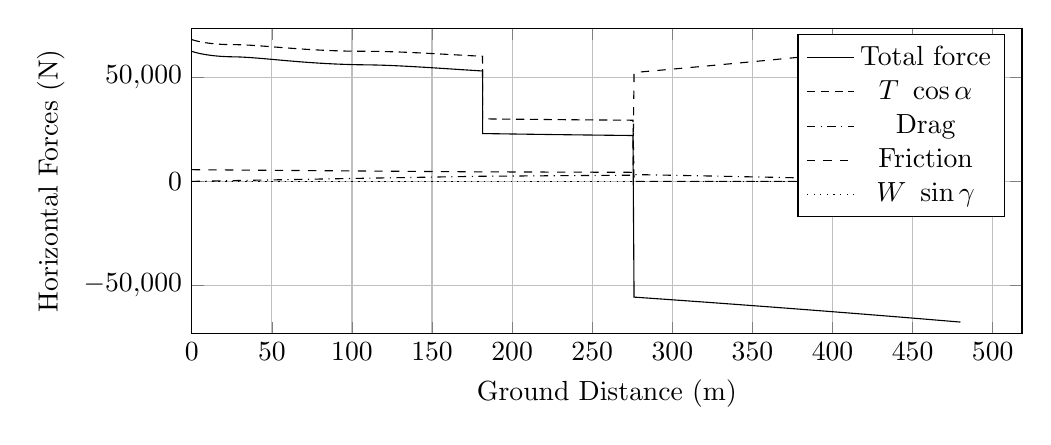
\begin{tikzpicture}

\begin{axis}[
width=\textwidth,
height=0.45\textwidth,
scaled ticks=false, tick label style={/pgf/number format/fixed},
xmin=0.0,
xmax=518.2299866992206,
xlabel={Ground Distance (m)},
xmajorgrids,
ymin=-73281.16851037793,
ymax=73875.23796631786,
ylabel={Horizontal Forces (N)},
ymajorgrids,
legend entries = {Total force\\$T\ \cos\alpha$\\Drag\\Friction\\$W\ \sin\gamma$\\}
]

\addplot [
color=black,
solid
]
table[row sep=crcr]{
1.3603393307216043E-8	62748.58696635143\\
3.0265395163403265E-7	62748.5868799013\\
2.9593179127983543E-6	62748.58608546927\\
1.5392338359717934E-5	62748.582368818985\\
5.361280674027254E-5	62748.57094967284\\
1.6215010178508227E-4	62748.53855001014\\
3.7214145765703975E-4	62748.475937488256\\
6.839954676020354E-4	62748.38307289113\\
0.001098342709021993	62748.25985267882\\
0.001609317716481928	62748.108102460115\\
0.0022198920000388346	62747.9270193018\\
0.002878710694837372	62747.73188509708\\
0.0036835072341781794	62747.493830341904\\
0.004557929017412697	62747.235531090235\\
0.005559798278933152	62746.939987000675\\
0.006651227400597502	62746.61846708476\\
0.007795849738889277	62746.281732161995\\
0.009067984722810115	62745.90798859477\\
0.010453165799939174	62745.50159302428\\
0.011915708813158052	62745.07309120921\\
0.013455030027058647	62744.62270873602\\
0.015131183092671713	62744.1329651047\\
0.01690803412933615	62743.61452312661\\
0.01873590105740728	62743.08193195962\\
0.020713359121301934	62742.50655198736\\
0.022777736728155237	62741.906723392676\\
0.024960970145273077	62741.27325267036\\
0.02723428625014468	62740.61457642898\\
0.029610395797831278	62739.92708994227\\
0.03204086105441677	62739.22486425715\\
0.03462344565878624	62738.47973928123\\
0.037295727153354774	62737.70983339002\\
0.040089145853872785	62736.90617768071\\
0.042950967781251806	62736.08401980957\\
0.04592022141655751	62735.23221525195\\
0.04897301836205646	62734.35769420721\\
0.052130294957187476	62733.45453451722\\
0.05542514139564195	62732.51337918814\\
0.05879722600804832	62731.551553678524\\
0.06231520981015182	62730.549570862015\\
0.06596261503753809	62729.512253843466\\
0.06964559414821356	62728.466353857046\\
0.07347193989652406	62727.38132936369\\
0.07736619052035826	62726.27866886809\\
0.08137137577670908	62725.14625822232\\
0.08545617869345057	62723.99302904782\\
0.08969468676038628	62722.79816859719\\
0.0940095881391464	62721.58357345933\\
0.09845059220533334	62720.335335638796\\
0.10296315144049947	62719.06886857006\\
0.10759658895065366	62717.770407907505\\
0.1123317495250277	62716.44541898227\\
0.1171874363557737	62715.08873744405\\
0.12217670360507671	62713.696833232665\\
0.12726806426274867	62712.278596377946\\
0.13231647880291775	62710.874423744215\\
0.13765212084557643	62709.39259132113\\
0.14294844966167852	62707.92390057813\\
0.14834594087957392	62706.42939374142\\
0.1539671093411843	62704.87530924726\\
0.15968242883369804	62703.29761497794\\
0.16555834796315422	62701.678086215674\\
0.17157514414202774	62700.022307246836\\
0.17760320215284392	62698.36600005577\\
0.18370335474801935	62696.69245892286\\
0.18983540939776816	62695.012733407886\\
0.19621099073945342	62693.268985160146\\
0.20278841209744758	62691.47285556147\\
0.20952923284938563	62689.635032135164\\
0.21624967405074952	62687.80566711513\\
0.22309476488450758	62685.94530372377\\
0.22992510727843934	62684.09185367561\\
0.2371653034562048	62682.13030807696\\
0.2442573187228817	62680.21197563074\\
0.25144286317780873	62678.27139497051\\
0.2588001799723505	62676.287560444456\\
0.2662612189130884	62674.27895315632\\
0.27386560463063747	62672.235019498636\\
0.2815803271719757	62670.16475021218\\
0.28946218069394425	62668.053038112266\\
0.29753588720841584	62665.89344676485\\
0.3056643119969481	62663.72277160833\\
0.31376446154764137	62661.56314642425\\
0.322071411728719	62659.351965911075\\
0.3303680011285137	62657.14711651804\\
0.3389039548234316	62654.88233520248\\
0.3474123396293025	62652.628536784236\\
0.3561645174790815	62650.31393386611\\
0.36525289600634137	62647.914420443776\\
0.3742306244196095	62645.54807459045\\
0.3835584127627333	62643.09357191814\\
0.392806747202999	62640.66406444271\\
0.40218604538039837	62638.2042613465\\
0.4115907129344223	62635.741910722456\\
0.42143744457304466	62633.168172904785\\
0.4310567075016639	62630.65814378165\\
0.4412814114336725	62627.99468802521\\
0.4513051702487684	62625.38808306081\\
0.461412558308395	62622.76419796272\\
0.47173637532167356	62620.08870778224\\
0.4821484569390513	62617.39498045387\\
0.492985116277161	62614.59630192182\\
0.5036221628177362	62611.85397612976\\
0.5142245311302887	62609.12527352208\\
0.5252888808291518	62606.28260529175\\
0.5363145235987512	62603.454842006875\\
0.5471208511184944	62600.68808279051\\
0.5585110457184732	62597.77688057248\\
0.569849942463402	62594.88388135728\\
0.5817265165330987	62591.85909204632\\
0.5935668742733842	62588.84896383285\\
0.6053719027871456	62585.8531682976\\
0.6172343027602503	62582.8481431331\\
0.629515267228629	62579.742660032105\\
0.6417789549774502	62576.647150339864\\
0.6542768803188956	62573.498223093644\\
0.6669828212214572	62570.30273451397\\
0.6796225285147333	62567.12969993029\\
0.6925094233679154	62563.90050859051\\
0.7056620711738308	62560.61080706456\\
0.7184715206768946	62557.41279698744\\
0.731725241748566	62554.10989307813\\
0.7449880440563246	62550.81080338117\\
0.7586792333483576	62547.41147337743\\
0.7725063377467813	62543.98485561005\\
0.7863894274138714	62540.5508348624\\
0.8004504964383841	62537.07934156874\\
0.8147129313117618	62533.564809789925\\
0.8293722635741907	62529.95942037302\\
0.8437954335339908	62526.41892554691\\
0.8580702287827062	62522.92144820842\\
0.8726489666047585	62519.35621733467\\
0.8875094051704782	62515.72902264292\\
0.9027740629895862	62512.01038373224\\
0.9182163910703112	62508.25584411707\\
0.93361566230532	62504.51910460576\\
0.9491799633800446	62500.74969728566\\
0.9646343064330896	62497.014198824836\\
0.9803727456894022	62493.217425035546\\
0.9957421603273868	62489.51681954693\\
1.0116767859397604	62485.687518864346\\
1.028041387324289	62481.76266347978\\
1.0443915011410971	62477.84908782526\\
1.060796374175649	62473.93018425266\\
1.0773229908740651	62469.99001590075\\
1.093971735592782	62466.0286038544\\
1.1110062543639518	62461.983516850436\\
1.127891796882146	62457.98184667235\\
1.1451224507351285	62453.906578813054\\
1.1624801114435046	62449.809573461185\\
1.180077727863539	62445.66437174937\\
1.1978884766667508	62441.47755540737\\
1.215488397439855	62437.34872466371\\
1.23351701382096	62433.12794481375\\
1.2518199984626128	62428.851789842374\\
1.2704235066044305	62424.51450258358\\
1.2892140278280424	62420.142838114625\\
1.3075714306593595	62415.88082668194\\
1.3266673518109293	62411.45660776607\\
1.3462106477188795	62406.93843880412\\
1.365306294594515	62402.53316987853\\
1.3852885894463176	62397.9332418976\\
1.404835539176236	62393.44324340303\\
1.4251192118409102	62388.79410053887\\
1.445164519989187	62384.209610593956\\
1.4656054698512246	62379.54481829965\\
1.4853522740259328	62375.04813337898\\
1.5051589726327936	62370.547318011144\\
1.5255757775517242	62365.91776459353\\
1.5464367798307013	62361.19779984228\\
1.5673163741652552	62356.48399416312\\
1.5879032567231621	62351.84635675917\\
1.6091523485848285	62347.06997508714\\
1.6303162371862876	62342.32321005879\\
1.6519474169970438	62337.48235872282\\
1.673879209980242	62332.585224580616\\
1.6955666802836635	62327.75345667584\\
1.7172271378534343	62322.938368230854\\
1.7402832823543353	62317.824650770766\\
1.7634396102400074	62312.70070520534\\
1.7861669372425006	62307.683296247254\\
1.8088678577734645	62302.68312276577\\
1.831824248135399	62297.63819701476\\
1.855578771396016	62292.42998823525\\
1.878960729162178	62287.31542231272\\
1.9033179534858085	62282.00006093712\\
1.9273833213731866	62276.760871077044\\
1.9518510462308036	62271.44672268425\\
1.9761594732990155	62266.17971025566\\
2.000437267212291	62260.93173057698\\
2.0252281699074732	62255.58553885775\\
2.0498006073458734	62250.29904848046\\
2.0745611186355752	62244.98469583233\\
2.0997746990963106	62239.58601863716\\
2.1260324099367294	62233.977544824884\\
2.1515212193659616	62228.54665916039\\
2.1771505246334	62223.09902342319\\
2.2031842637813908	62217.578877816675\\
2.230133398733474	62211.87883012915\\
2.257053086628849	62206.199341242216\\
2.283795213136285	62200.57140899327\\
2.311477064851834	62194.76041739785\\
2.3387199014446116	62189.0561036961\\
2.3662694524467227	62183.302127347895\\
2.3937852540088533	62177.569727310765\\
2.4216520071021392	62171.77892307866\\
2.4501931244916175	62165.86323773577\\
2.478927626230634	62159.92297088956\\
2.506685441631536	62154.19929659829\\
2.53537335014481	62148.29891078557\\
2.5633350931805676	62142.56254067566\\
2.5917889242519685	62136.7399919217\\
2.6208221472873374	62130.814155291315\\
2.649872764173903	62124.90012286141\\
2.679661174525658	62118.85175114668\\
2.709174609939316	62112.87495757626\\
2.740029385016756	62106.64319001096\\
2.770444625703795	62100.51677074139\\
2.801129860621211	62094.352548525436\\
2.8318827297715705	62088.19135466291\\
2.862425967677578	62082.08853117956\\
2.893259332541544	62075.94419494427\\
2.92412139403754	62069.810607507825\\
2.955064430161417	62063.67737666385\\
2.986690331721131	62057.42572254407\\
3.019183403261743	62051.02037545058\\
3.0507201588152526	62044.82063205216\\
3.0830332871979023	62038.48562493776\\
3.1154603869692448	62032.14584436707\\
3.148592095396281	62025.686387496855\\
3.181936872739324	62019.20374172297\\
3.214370607724433	62012.91578195176\\
3.247565473366384	62006.49810462893\\
3.281695868027062	61999.91827897477\\
3.316494330618462	61993.22909634269\\
3.3513055302544137	61986.55699447275\\
3.3860303583611797	61979.920802071385\\
3.421934361445942	61973.07947688752\\
3.456235826539576	61966.56260379907\\
3.490536654441657	61960.06441396962\\
3.526257338581564	61953.31686461522\\
3.561372823896762	61946.70305459414\\
3.5967906564503185	61940.051700124095\\
3.632682576242373	61933.331088361316\\
3.6701261071689295	61926.34104896341\\
3.707701291513044	61919.347983522835\\
3.7452745323452916	61912.37675293113\\
3.78256482255855	61905.479139624134\\
3.8208821591411084	61898.41335511893\\
3.8590337549211444	61891.399974679196\\
3.89695718563138	61884.45002448333\\
3.9351036745073964	61877.480697042585\\
3.9736642086653067	61870.45752863471\\
4.012189127077221	61863.46262797162\\
4.05156219172609	61856.33611163864\\
4.090290786278251	61849.34820486259\\
4.129291984889424	61842.33301078547\\
4.1680648628189925	61835.380560807214\\
4.207805169621487	61828.276955786394\\
4.248168240749736	61821.085042071005\\
4.288797880674668	61813.86893397104\\
4.32990243544832	61806.59214978412\\
4.371428084678056	61799.26487448141\\
4.41247037137882	61792.04652880062\\
4.453879445321437	61784.78737326583\\
4.49524783594077	61777.55900270601\\
4.537299342543221	61770.23538169038\\
4.580546125800922	61762.72882367676\\
4.622914948498307	61755.39934568385\\
4.66640222022569	61747.90167027798\\
4.709294790611851	61740.53149738783\\
4.752417172855319	61733.14671198031\\
4.796155651503765	61725.68177514535\\
4.8408754796551925	61718.07562299959\\
4.884850997559644	61710.621846546\\
4.928651138956553	61703.22308488276\\
4.972831351372241	61695.785567542494\\
5.017331702752941	61688.319868929146\\
5.0632326321008225	61680.64610692728\\
5.108452384314601	61673.112816882494\\
5.1536021218025905	61665.61739795846\\
5.199057463234675	61658.097574294254\\
5.244479287100011	61650.609561581456\\
5.292293005248643	61642.75546639947\\
5.338096108273211	61635.25867322851\\
5.3857492800262605	61627.48701172804\\
5.433816232374781	61619.676598038524\\
5.480691139018431	61612.08754018792\\
5.529685763332537	61604.184355917896\\
5.578612887337309	61596.32155869325\\
5.626451501744754	61588.66205840692\\
5.674834544150631	61580.94378773113\\
5.7252048440372345	61572.93870388891\\
5.77422346516266	61565.17787975559\\
5.8255152536468575	61557.0881089591\\
5.874338256646894	61549.41698457269\\
5.922631450506765	61541.857060475784\\
5.972682300942642	61534.051197922745\\
6.022535370757359	61526.305604306894\\
6.074394648705015	61518.279329606885\\
6.124928192945902	61510.48853147858\\
6.176798284396469	61502.52263273051\\
6.229620191179453	61494.44264252679\\
6.282808156696705	61486.33921985772\\
6.334658925277093	61478.47083549031\\
6.388041948821611	61470.4020804281\\
6.440558117792513	61462.49603497519\\
6.494960924490993	61454.33895717411\\
6.550441697666145	61446.054672571205\\
6.6042098433346865	61438.05913117975\\
6.658315220792536	61430.04610100349\\
6.712335084641163	61422.07827505756\\
6.766674450459032	61414.09598236589\\
6.821537769035839	61406.069808119006\\
6.876851268142238	61398.01128266708\\
6.933661362437203	61389.7695889052\\
6.989261882852809	61381.73743620211\\
7.046240323930029	61373.54103198383\\
7.102786137967051	61365.4415409161\\
7.1603789170469145	61357.22744210556\\
7.21785165788507	61349.06587853639\\
7.277487498606879	61340.63437409418\\
7.334984696129153	61332.540988802284\\
7.393362172524569	61324.359446134375\\
7.452416393609804	61316.119552720236\\
7.511934748111884	61307.851876037705\\
7.572557225035805	61299.46882183947\\
7.63202184821041	61291.282971226334\\
7.69294899409779	61282.93372681769\\
7.752675521499926	61274.7861207831\\
7.814488876138199	61266.39236186803\\
7.8763528528159785	61258.030792142556\\
7.938149975125226	61249.717106305994\\
8.001193143199774	61241.27562431352\\
8.064554080136986	61232.83195752822\\
8.12686567918485	61224.56742562268\\
8.189637855946287	61216.28104072092\\
8.252542711798306	61208.01647879019\\
8.315859663763469	61199.73737466999\\
8.380006162932737	61191.39014484064\\
8.444702551512929	61183.012315166096\\
8.509501986620958	61174.66219684837\\
8.57387297516295	61166.40779955052\\
8.63887365699837	61158.11345598218\\
8.70727085773305	61149.42978513251\\
8.772937378995405	61141.13515405379\\
8.839192134487615	61132.80809432216\\
8.905815929161982	61124.47688991131\\
8.97209054442786	61116.23119859207\\
9.039019026885107	61107.94633956594\\
9.107371801018814	61099.52874647401\\
9.174915633685494	61091.25385062506\\
9.243868961478196	61082.85026326717\\
9.312440636565494	61074.537082415874\\
9.381784695008012	61066.174593755364\\
9.4513167952828	61057.83400599759\\
9.52142787533916	61049.4689800769\\
9.591425279059166	61041.16242227329\\
9.662230428326719	61032.80547235883\\
9.734225879912522	61024.354725814876\\
9.806441602430919	61015.92522773241\\
9.878483835105534	61007.56279411132\\
9.951807209049782	60999.09946552412\\
10.023539677466466	60990.86625654463\\
10.096057433179052	60982.58946445353\\
10.168262179450682	60974.39471287477\\
10.241274410624943	60966.15512361906\\
10.31479015323385	60957.90607803446\\
10.390063469390178	60949.5088689227\\
10.465012435634037	60941.19695487882\\
10.540639152111389	60932.85935085469\\
10.617644389866598	60924.4206271304\\
10.692945462162374	60916.21808473345\\
10.770083295573727	60907.86593944761\\
10.846726862770723	60899.617704468925\\
10.924657809445929	60891.28222333998\\
11.00265335491597	60882.99141813001\\
11.081827589833612	60874.62789243563\\
11.159134327011738	60866.51254463331\\
11.239152720133266	60858.16530457618\\
11.317028257314295	60850.092937656926\\
11.396413369884492	60841.91601155416\\
11.477655063362434	60833.601910542944\\
11.556958506738276	60825.53870258294\\
11.637325199769407	60817.42013318147\\
11.717754170658207	60809.34822562382\\
11.799819443100102	60801.16648757014\\
11.881986970940797	60793.02938201987\\
11.964394119506721	60784.923434520315\\
12.046263329632716	60776.9246223612\\
12.130282587748898	60768.77172035584\\
12.213721087180826	60760.731071135364\\
12.295868535962462	60752.86904578263\\
12.380692430046633	60744.80709776665\\
12.46470288467437	60736.878560376674\\
12.550384439940181	60728.84959741644\\
12.635259749824865	60720.953004655195\\
12.72144647897981	60712.992048849876\\
12.80741162779486	60705.10920775631\\
12.892901506907108	60697.32682994356\\
12.977815703098727	60689.6528017932\\
13.06483740414145	60681.845943009524\\
13.151922956503014	60674.09154282416\\
13.240589045456186	60666.25598494582\\
13.329911181207382	60658.42300686934\\
13.417306166647748	60650.81763431788\\
13.507103029723119	60643.06339800192\\
13.595986036712912	60635.44789722595\\
13.687453390597003	60627.67287452461\\
13.779071846306106	60619.947721374614\\
13.872694200363323	60612.118198018914\\
13.963504841252302	60604.58596521316\\
14.056146454975131	60596.96469563455\\
14.14918846816267	60589.374122844674\\
14.24332804549016	60581.75867435004\\
14.339261112049854	60574.06480791261\\
14.431091301610323	60566.7628020633\\
14.524174633942373	60559.42362172599\\
14.618760344060338	60552.0301792314\\
14.714801736988441	60544.58891918459\\
14.809763128346521	60537.296455040196\\
14.903412319659619	60530.16794560717\\
15.001392651385917	60522.77667740664\\
15.098055049922994	60515.55165071065\\
15.196870856960619	60508.234021771364\\
15.29477342819068	60501.05192711747\\
15.39265348361268	60493.93880871477\\
15.490487151984588	60486.89609055538\\
15.588146853189365	60479.93249400279\\
15.687961867268871	60472.88372826915\\
15.78650099417861	60465.99276441168\\
15.886965864441798	60459.03613643251\\
15.98755318095926	60452.140584871726\\
16.088470385762115	60445.29211238658\\
16.190536977381747	60438.43639519221\\
16.292466610053154	60431.660640934584\\
16.396448349404487	60424.82108251963\\
16.497808944935016	60418.22427083277\\
16.600551072850564	60411.60816428864\\
16.70575139586156	60404.90717498545\\
16.81134459259622	60398.255597675\\
16.917616592554033	60391.63629320428\\
17.023477948501657	60385.11714203395\\
17.12904978140002	60378.68968954387\\
17.2354081519902	60372.28868841233\\
17.340772011500363	60366.02085905596\\
17.448391076872838	60359.69394985451\\
17.5571980918308	60353.37406999097\\
17.66615596614949	60347.12261314588\\
17.774685459577412	60340.97225594756\\
17.884986575683584	60334.79948465346\\
17.99552903728076	60328.69181138744\\
18.108708479124623	60322.51968877914\\
18.219646262474413	60316.549320347185\\
18.332680252669796	60310.54682056299\\
18.445061806396694	60304.65942624536\\
18.556709221711323	60298.88966543338\\
18.668884868236475	60293.17181638187\\
18.78204748093455	60287.48383976107\\
18.895704562363058	60281.851800192686\\
19.008928234289563	60276.32147540923\\
19.124320907419907	60270.76733553811\\
19.24105855786135	60265.23254130206\\
19.355116774466126	60259.90619601139\\
19.470462572962035	60254.60128785194\\
19.58492145104516	60249.41798754399\\
19.704921229319112	60244.069929075034\\
19.821259826163917	60238.96896912673\\
19.941172080873493	60233.79751126356\\
20.06078806851737	60228.72571844168\\
20.177423389922623	60223.86360097327\\
20.297621170678	60218.93874893073\\
20.420129559802255	60214.00852458409\\
20.54164670774839	60209.20696199483\\
20.661905244258705	60204.541892101784\\
20.784301666224792	60199.882230174975\\
20.904244540623438	60195.4021594839\\
21.028114340450195	60190.8646744509\\
21.148300883955606	60186.5485351519\\
21.270875420257596	60182.2340372788\\
21.39299406946177	60178.02308163734\\
21.513793771711654	60173.94326485705\\
21.637476506915142	60169.85407498812\\
21.759279707150128	60165.913776701826\\
21.88493035745168	60161.9389465773\\
22.009809790007786	60158.0787284285\\
22.13620730934617	60154.26288733051\\
22.263515470260465	60150.51212099468\\
22.393040471753594	60146.79108809077\\
22.520519759768852	60143.22214608881\\
22.648852607677917	60139.72253293265\\
22.775118904521122	60136.370289714774\\
22.903136237443974	60133.0634467897\\
23.03176118514304	60129.83381345085\\
23.162501585272054	60126.64621436913\\
23.294719932439598	60123.51984971312\\
23.427108470281937	60120.48717156176\\
23.558693146983046	60117.56950415543\\
23.687077503630363	60114.815344074465\\
23.817949558665852	60112.10162464352\\
23.948210788889448	60109.49434764231\\
24.076877750667826	60107.01056631794\\
24.21019765060587	60104.532709959574\\
24.3450673155249	60102.124917985304\\
24.477101355489637	60099.86379941474\\
24.60984760833776	60097.68601199714\\
24.7468403923846	60095.53870354536\\
24.882807251950062	60093.50777362603\\
25.017167332957627	60091.598723027\\
25.153910941279605	60089.75542762375\\
25.289629217480112	60088.025047101604\\
25.425306692573436	60086.393589543484\\
25.56229499031975	60084.8459137914\\
25.70075944713021	60083.382926138234\\
25.83724158708921	60082.04034140546\\
25.975209935932874	60080.78322359543\\
26.003074150630965	60080.54152452522\\
26.020759913393235	60080.390237708925\\
26.030714598210515	60080.30580847466\\
26.05840292223249	60080.07371814735\\
26.06133765907019	60080.04935502367\\
26.064285136409026	60080.02493175992\\
26.066337724202356	60080.00795070012\\
26.068175973881182	60079.99274812726\\
26.06984477238784	60079.978927470394\\
26.077831036047115	60079.912521841674\\
26.10345636352254	60079.69649113403\\
26.16716044512971	60079.139968811665\\
26.297541524199602	60077.914956659515\\
26.42722303713863	60076.58307608371\\
26.5559280656694	60075.150733013696\\
26.686097387723095	60073.59150482736\\
26.817793678842584	60071.90219867682\\
26.949416928520378	60070.10287580801\\
27.080440623797912	60068.20295062887\\
27.215491080424528	60066.13245178174\\
27.34795890217076	60063.99230108733\\
27.48215578365496	60061.71529098041\\
27.616696052324144	60059.32379232615\\
27.75271189183823	60056.7968769734\\
27.888759310501555	60054.16095945533\\
28.023839122857026	60051.437890958914\\
28.16136324828667	60048.558541493185\\
28.298355249881332	60045.58437893586\\
28.435282447697354	60042.507320286866\\
28.573941346212784	60039.286464396355\\
28.713752690797136	60035.93337885769\\
28.852681198061333	60032.49795314303\\
28.992471984120606	60028.938433904346\\
29.133421724605903	60025.24641390404\\
29.275199211812186	60021.42977817924\\
29.416225289053614	60017.53232806451\\
29.55783477945603	60013.51871776537\\
29.701838356359822	60009.335843087625\\
29.846633046394217	60005.02829350848\\
29.99013730470424	60000.65990011848\\
30.132492646908446	59996.23021131731\\
30.277395768405135	59991.624121233326\\
30.422188862471998	59986.92500457718\\
30.56637548064623	59982.15101578229\\
30.711944318924978	59977.236873309696\\
30.8573377156769	59972.235303635025\\
31.006558691603843	59967.00642218687\\
31.153907258126303	59961.749431289034\\
31.30257185742142	59956.35245740527\\
31.4510947803754	59950.868650967386\\
31.602595106592503	59945.181566874686\\
31.755261577184278	59939.3567386615\\
31.906398416479824	59933.49872413877\\
32.05599258457312	59927.6121241669\\
32.20952926265106	59921.48030147274\\
32.360097140052986	59915.3797277869\\
32.51218835243483	59909.130958224094\\
32.664721606344784	59902.77803647889\\
32.82129760777845	59896.168520531195\\
32.97669884718651	59889.521575766455\\
33.13118849606322	59882.82901181003\\
33.288837444683736	59875.913960326245\\
33.44405554194745	59869.02233987817\\
33.60015866510213	59862.009464306146\\
33.756686089655645	59854.89628317127\\
33.91694077595571	59847.53076840617\\
34.074326811338736	59840.21670800289\\
34.23252403098988	59832.78594932305\\
34.392884168270385	59825.17405547413\\
34.554266068788166	59817.434125624495\\
34.71363140184178	59809.713889733684\\
34.87649332318763	59801.74649341391\\
35.03746231629111	59793.795724769865\\
35.19990059234286	59785.69709035804\\
35.3627309111595	59777.50427105358\\
35.5271254050015	59769.158223754464\\
35.69149466827288	59760.73986894263\\
35.85508342515686	59752.28968258749\\
36.017180984292054	59743.84707744638\\
36.182222084544165	59735.181364659526\\
36.34861175093968	59726.374794774194\\
36.514166392421686	59717.54384636787\\
36.68083924241549	59708.58538314258\\
36.845526722294395	59699.667937927676\\
37.01328249159678	59690.51842314679\\
37.18160982421668	59681.272069921455\\
37.35136716620059	59671.88177477299\\
37.51969289597564	59662.50703427056\\
37.689710015857784	59652.9749717934\\
37.860394939778416	59643.34286054889\\
38.02805196867635	59633.821705559894\\
38.19868492919754	59624.07174448762\\
38.37343039987371	59614.02547641045\\
38.54685896696101	59603.99477876534\\
38.71934233168869	59593.96050993037\\
38.8915617091798	59583.884808444884\\
39.062305982326905	59573.84050900377\\
39.23847188392709	59563.42114261909\\
39.411511502305984	59553.13231783762\\
39.585172817779906	59542.753484797984\\
39.760693028009456	59532.210689936415\\
39.9373134006328	59521.54930350275\\
40.113617753210534	59510.855590869745\\
40.29094651898711	59500.049065758256\\
40.468149621311596	59489.20054552688\\
40.64593210594187	59478.267786044744\\
40.82431302355218	59467.25023578506\\
41.00141330502653	59456.26530982384\\
41.17957893337042	59445.168653441884\\
41.359761290266974	59433.90090662928\\
41.53889737920997	59422.65431892451\\
41.72013507746885	59411.231946434404\\
41.899395797464194	59399.89184669625\\
42.081280067494475	59388.3438205424\\
42.265315320939635	59376.61728887055\\
42.44531744651641	59365.10797527179\\
42.62715102096499	59353.44265820888\\
42.81120266452106	59341.596267562505\\
42.994164503876235	59329.78238567873\\
43.17799769459725	59317.87547182753\\
43.36154361404071	59305.95140490004\\
43.54597437124032	59293.93487000553\\
43.73158498218817	59281.80706459505\\
43.91737182308138	59269.634192009515\\
44.1050494697441	59257.30436278826\\
44.293574236233	59244.88643443957\\
44.47888581456586	59232.64944232178\\
44.66456251492659	59220.358758137445\\
44.85170130968709	59207.9422862198\\
45.037822074257164	59195.565417580845\\
45.22676109993536	59182.97358761598\\
45.41612608476639	59170.326473555484\\
45.604812217355104	59157.69885853167\\
45.79422221198037	59144.997792771144\\
45.98724683785376	59132.02952486985\\
46.17830917717477	59119.16936184275\\
46.36786657808848	59106.388078780714\\
46.55935209439748	59093.4550313941\\
46.75090376717816	59080.496542455774\\
46.94233405988251	59067.52620395071\\
47.13714948644359	59054.306829470224\\
47.33387512950824	59040.938624407834\\
47.53043319838464	59027.5634565034\\
47.72298239739284	59014.444181126615\\
47.919150009665316	59001.06205690163\\
48.113386178114425	58987.79634219325\\
48.311024807628144	58974.28345747267\\
48.508886059616145	58960.74128979957\\
48.70490444306449	58947.3122432207\\
48.90290918859142	58933.734828416535\\
49.09959709013448	58920.23633291242\\
49.2970021191946	58906.67805724632\\
49.49532701226336	58893.0467801264\\
49.693780717172615	58879.39762345921\\
49.89506320355713	58865.545529044466\\
50.096719083698545	58851.66011777922\\
50.29606895218413	58837.92681505815\\
50.497598474286534	58824.03742648578\\
50.700304208193415	58810.06178154117\\
50.90342397924904	58796.05318781125\\
51.10460922167407	58782.17446693129\\
51.30752217039489	58768.17378053878\\
51.51010619677311	58754.19378919198\\
51.713602501430145	58740.14961347189\\
51.91843850546792	58726.01251882098\\
52.121089026646246	58712.026568525456\\
52.32561402362407	58697.91232524882\\
52.53192272805477	58683.676849060794\\
52.7387030603267	58669.411473394386\\
52.944027344085896	58655.2499181404\\
53.154073670302836	58640.766921001064\\
53.36143953271798	58626.473711841114\\
53.571009444677685	58612.03435305624\\
53.77799762982136	58597.779302285955\\
53.98785945427545	58583.33360532427\\
54.196157549666225	58569.00349637364\\
54.40718762937186	58554.49424354074\\
54.616887598525366	58540.08593929515\\
54.826875464266934	58525.66805041215\\
55.04038432082807	58511.019590906755\\
55.25438844036796	58496.34919209598\\
55.46695867894975	58481.789733344616\\
55.68088820258777	58467.15060443987\\
55.895144656119854	58452.503310170345\\
56.109028395418505	58437.8963688973\\
56.326262430904194	58423.07653689642\\
56.542089933321776	58408.36923531024\\
56.76060076462056	58393.496613132695\\
56.97729209122687	58378.76593888097\\
57.19579178641709	58363.93127346867\\
57.41258192878804	58349.232142096356\\
57.634093277561306	58334.23360901498\\
57.85395098827546	58319.368421754974\\
58.07448819514299	58304.47936006026\\
58.29446478173499	58289.65082477676\\
58.51588770709739	58274.74832251543\\
58.73757884137123	58259.852072426496\\
58.96020041504734	58244.918425863274\\
59.18267120664716	58230.02068874739\\
59.405949655899676	58215.09543434816\\
59.63089974393067	58200.08599554913\\
59.8562534200115	58185.07800385475\\
60.084134136581554	58169.93124615034\\
60.30833762904015	58155.0585106377\\
60.53504725699203	58140.05001099827\\
60.763693228044005	58124.944996575156\\
60.99075593752245	58109.9766742912\\
61.21765734918529	58095.05154409529\\
61.44713116872772	58079.99091894232\\
61.6738048454246	58065.14794897725\\
61.90668490141796	58049.934252569554\\
62.13729676517957	58034.90496991055\\
62.36629463006145	58020.017142951256\\
62.596359157213186	58005.0969435555\\
62.82836101237727	57990.089215390806\\
63.059723307860466	57975.16154762388\\
63.292774394726166	57960.164552688395\\
63.52608473446321	57945.19129201122\\
63.75973181411028	57930.23751514376\\
63.993403028653574	57915.32388526069\\
64.23068717493263	57900.22290169429\\
64.4710952259949	57884.968123073966\\
64.70858695601663	57869.94345289939\\
64.94894296164699	57854.78374474145\\
65.18738841845183	57839.790989490284\\
65.42661162888535	57824.79637674126\\
65.6659442133793	57809.84260865279\\
65.90899583190168	57794.70585484736\\
66.15068261105333	57779.703994875264\\
66.39533053734849	57764.569557362134\\
66.6378997293487	57749.61513840084\\
66.88158418814953	57734.64405780201\\
67.12390450547147	57719.80908596837\\
67.36840986262189	57704.89373052902\\
67.61550053739396	57689.875673584495\\
67.86097385246623	57675.011197135274\\
68.10985741250389	57659.99699254849\\
68.35582503705197	57645.215376441585\\
68.60464259362828	57630.320335732904\\
68.85450289166104	57615.421930398705\\
69.1042877596268	57600.58768656949\\
69.35837572129628	57585.55961469008\\
69.61150655903072	57570.650567820005\\
69.86289252102952	57555.90645002769\\
70.11686816207683	57541.07384976631\\
70.37125759672608	57526.28146883179\\
70.62480458144697	57511.602684827594\\
70.88045310059783	57496.868032549406\\
71.13526709211152	57482.2477088772\\
71.3947754873567	57467.42648958336\\
71.6534187996231	57452.72389970705\\
71.91450497256008	57437.9530268809\\
72.1716184080999	57423.47668890437\\
72.43269265097052	57408.84867334757\\
72.69331619504374	57394.31807118036\\
72.95563200429567	57379.76639485071\\
73.21686762735783	57365.34816427594\\
73.48161420086069	57350.81148245353\\
73.74261486234883	57336.55516320803\\
74.00755043430098	57322.16020489593\\
74.27511769675363	57307.700731758494\\
74.54487113507057	57293.203417113225\\
74.81568229507957	57278.73082942504\\
75.08274085953312	57264.53928104503\\
75.35421836228127	57250.19529339293\\
75.62798354862159	57235.815005515935\\
75.89909469738902	57221.65827722961\\
76.17008148658607	57207.592166056216\\
76.44269151183332	57193.52709763679\\
76.71571902594138	57179.52667636318\\
76.99340852183178	57165.37611511002\\
77.27004772085374	57151.36867996861\\
77.54832408953641	57137.3690188676\\
77.82592519882277	57123.49437037441\\
78.10358246820337	57109.70830060974\\
78.38556010231375	57095.80169065631\\
78.66911430382748	57081.91325680206\\
78.95399134982776	57068.05733920049\\
79.23667137346987	57054.40511855275\\
79.518907793654	57040.87097593317\\
79.80555437718249	57027.22462735973\\
80.09150103324356	57013.711698279614\\
80.37928873457926	57000.21312970358\\
80.66871996946384	56986.74045134256\\
80.95967699414447	56973.30125974615\\
81.25093884305389	56959.953355159334\\
81.54344278085921	56946.655040364625\\
81.8358102960415	56933.47000175789\\
82.13087592438694	56920.272231425\\
82.42794520371837	56907.09581840529\\
82.72842933895026	56893.881639624116\\
83.0269479931649	56880.86753738558\\
83.32974506690314	56867.78304709877\\
83.62964811531441	56854.93930768462\\
83.92951211009506	56842.21275618588\\
84.2339319847595	56829.41140490904\\
84.53715838283946	56816.77938938404\\
84.84105485927768	56804.23916326916\\
85.14845677960258	56791.6766012771\\
85.45530133949276	56779.25989423189\\
85.76249773413784	56766.95251773413\\
86.07201271349416	56754.6776826112\\
86.38432073331904	56742.42008664644\\
86.69710203601804	56730.27318128143\\
87.01172103282082	56718.18580759912\\
87.32669099459858	56706.216841512796\\
87.64517025121202	56694.249092126294\\
87.96158123090564	56682.49345114094\\
88.2775814178033	56670.88713943225\\
88.60068374099544	56659.15889246231\\
88.92068281935622	56647.68211567633\\
89.24207276858638	56636.29489195993\\
89.56578933015979	56624.966871902594\\
89.88760090270688	56613.846782456036\\
90.2141410750086	56602.70764357982\\
90.54066676000363	56591.71476082115\\
90.86727570256076	56580.86525915227\\
91.19715108614633	56570.056025089754\\
91.52744226539704	56559.38333331379\\
91.85639956214655	56548.90345885874\\
92.19095740864739	56538.39878096101\\
92.52827526888461	56527.964652251685\\
92.8674718219292	56517.631963717184\\
93.20307982994817	56507.56642262393\\
93.5374944579234	56497.693186082965\\
93.87598013161067	56487.85921140874\\
94.20917297854535	56478.33603005043\\
94.55043409744499	56468.744085149316\\
94.89132963816093	56459.32628081381\\
95.23083207736542	56450.11008466894\\
95.57395676502793	56440.96130767578\\
95.91421223354143	56432.05391776969\\
96.25656086122288	56423.25778081856\\
96.60012122339742	56414.59829008607\\
96.94166303707107	56406.15660543901\\
97.28627502929558	56397.80805457507\\
97.62906225262071	56389.67246279065\\
97.97125437026659	56381.7191803942\\
98.31201772458999	56373.96640546429\\
98.65627175165852	56366.30404987256\\
99.0012536203806	56358.7970495818\\
99.35020029285332	56351.37879791277\\
99.69475740907401	56344.22688983864\\
100.04053871990226	56337.2227245853\\
100.38598466112728	56330.398861049194\\
100.72867962848932	56323.800990670556\\
101.07385499050397	56317.328482357116\\
101.41864366415388	56311.036962809405\\
101.76305460768467	56304.925976431376\\
102.11068844700483	56298.93408101726\\
102.45638678530696	56293.1514497693\\
102.79841653079728	56287.6030887989\\
103.14087212494877	56282.22039228937\\
103.48486473791618	56276.98764930107\\
103.82875595362174	56271.9311402599\\
104.17244250654872	56267.05241446568\\
104.51168383396202	56262.40839195342\\
104.85986244643053	56257.81956693379\\
105.204587526496	56253.45370284168\\
105.54754777175077	56249.2856524184\\
105.88797456536247	56245.32171703216\\
106.23280177240994	56241.48283858344\\
106.57515110440406	56237.84731191555\\
106.91603555764121	56234.40159354803\\
107.25729565943405	56231.12648374667\\
107.598830149446	56228.0236908629\\
107.93686571059558	56225.12525758898\\
108.27485499032852	56222.39909828467\\
108.28839963475954	56222.29343457302\\
108.30004107281309	56222.20283890501\\
108.30931238392475	56222.130834026844\\
108.31701527366243	56222.07110866209\\
108.32505202073054	56222.00888998585\\
108.33865239118708	56221.90352333871\\
108.35091925899997	56221.80817976603\\
108.39508146726081	56221.46251135353\\
108.52984553865659	56220.38431104434\\
108.79919793188978	56218.124321758805\\
109.105233418432	56215.38796017447\\
109.41485218466596	56212.43876717285\\
109.72257164661937	56209.329249695904\\
110.0321119530083	56206.02364807254\\
110.34145354075926	56202.54388740145\\
110.6534776714839	56198.85720238433\\
110.9711963390063	56194.92266913525\\
111.28851843247409	56190.81304220014\\
111.60893519474632	56186.482686019124\\
111.92798394282838	56181.99232137638\\
112.24770070245137	56177.31574331\\
112.57243448635171	56172.38650016113\\
112.89480865389396	56167.316255719226\\
113.22000325235314	56162.02506719764\\
113.54885709436653	56156.495924408984\\
113.8770619430189	56150.8007571287\\
114.20946079557197	56144.85463194827\\
114.54107775051554	56138.74579277108\\
114.87787736567807	56132.36285681174\\
115.21564640021248	56125.7828083107\\
115.55522358014255	56118.989166772444\\
115.89667501383605	56111.97978573381\\
116.23992536102014	56104.75543143583\\
116.5847156213415	56097.32106939993\\
116.92791619634093	56089.74631474781\\
117.27517516660399	56081.90673960303\\
117.62420948631524	56073.851595352215\\
117.97391125359778	56065.60675690233\\
118.32673409155768	56057.11371142954\\
118.68227803698588	56048.37994092658\\
119.03889207644076	56039.44541752979\\
119.39651249432902	56030.31244179359\\
119.75508651978987	56020.98316642031\\
120.11314113323388	56011.497818516655\\
120.47404637453192	56001.767689903165\\
120.84098349318353	55991.703014647734\\
121.20490030977416	55981.552245613944\\
121.57328571082118	55971.107791288494\\
121.94079100066682	55960.521120985824\\
122.31015242291167	55949.71504889215\\
122.68267403243519	55938.65035934067\\
123.05346836176264	55927.47357220735\\
123.42835733050345	55916.009964443816\\
123.80350972566416	55904.37617114821\\
124.1783235941891	55892.5932314603\\
124.55244040146786	55880.675372697835\\
124.92576251095704	55868.62890512576\\
125.30489170817492	55856.2399884225\\
125.68146781278597	55843.782096823634\\
126.06139977608174	55831.06156204913\\
126.44502763856761	55818.06509104854\\
126.82695116404781	55804.97676663293\\
127.206716044588	55791.8166966117\\
127.59262031825523	55778.2973348018\\
127.97077035934353	55764.90856278862\\
128.3546122768156	55751.17771078469\\
128.73724861847296	55737.35127522546\\
129.12002064685282	55723.383586454715\\
129.50086700331673	55709.35299411682\\
129.8837789976152	55695.114550477956\\
130.26783132854348	55680.70317169887\\
130.651936341801	55666.1612208974\\
131.03747321415574	55651.43789318508\\
131.42280335891803	55636.597300480076\\
131.80875442588928	55621.60949618093\\
132.19322104975072	55606.55875254114\\
132.5798881414172	55591.302577009745\\
132.96215446290768	55576.10448440041\\
133.34488286943906	55560.77493614884\\
133.7276157954845	55545.33404423838\\
134.11532375481391	55529.58112314579\\
134.50135826447365	55513.7868942778\\
134.88604120201086	55497.941452089304\\
135.26955723714872	55482.04017874946\\
135.6512109336153	55466.11503999484\\
136.03464327936558	55450.016035957364\\
136.41686422877552	55433.870357224296\\
136.79904942565338	55417.63067088832\\
137.18004416157777	55401.34832411715\\
137.56399804528928	55384.84715438729\\
137.94515347717788	55368.37634492545\\
138.32982901897384	55351.66440206327\\
138.7128522769853	55334.93717264214\\
139.09597564505458	55318.120424441746\\
139.48002685240425	55301.1792409702\\
139.86309097971855	55284.19985069129\\
140.24727738828375	55267.09044263883\\
140.6317581809211	55249.88916214407\\
141.01585725597846	55232.627988521665\\
141.3998433603236	55215.29668049727\\
141.7841907991213	55197.87543152385\\
142.16710976343057	55180.44732359465\\
142.55205218648928	55162.856724862766\\
142.9364233092117	55145.223440758215\\
143.32169829765928	55127.4813330021\\
143.705984531242	55109.71918555195\\
144.08985428249122	55091.912492652395\\
144.47683600496026	55073.898497552786\\
144.86371007721533	55055.82792710092\\
145.24772592056325	55037.83152082506\\
145.63047789911974	55019.83703718289\\
146.01273254364395	55001.81033207037\\
146.39725173307323	54983.62226960719\\
146.77966503747456	54965.48101678323\\
147.16478130736948	54947.159801267\\
147.54689717238745	54928.931460230524\\
147.93097497792814	54910.56091905589\\
148.31499270913332	54892.14596321457\\
148.69957284780122	54873.658076309075\\
149.08709998577143	54854.98342854447\\
149.47129868208145	54836.42590504256\\
149.8546635899794	54817.867096079746\\
150.23801379389647	54799.26885358787\\
150.62200569343076	54780.600590802685\\
151.00751012558203	54761.820999532705\\
151.3946455315429	54742.92520665043\\
151.77987817077866	54724.087072065915\\
152.16505704867353	54705.21777216332\\
152.55112759502248	54686.27219872901\\
152.93964308710213	54667.17502751459\\
153.32507651584535	54648.199311805016\\
153.71174813432617	54629.13386161778\\
154.10000329570875	54609.96262097417\\
154.48914219495543	54590.72116745093\\
154.8788297075107	54571.42720776945\\
155.26820650111182	54552.124537229014\\
155.6562915247282	54532.86319060705\\
156.0441896603637	54513.58969644079\\
156.4348678136667	54494.15766185129\\
156.82082928279863	54474.94132617938\\
157.21071017196311	54455.51198151686\\
157.60005066896917	54436.09284665936\\
157.99004282467217	54416.625654705625\\
158.3808231456182	54397.10469619969\\
158.77280374485122	54377.51046344079\\
159.16384255262415	54357.95119737928\\
159.55370941764693	54338.43966646871\\
159.946071590523	54318.79343914623\\
160.33752628124114	54299.18398618256\\
160.73008933968674	54279.51146191299\\
161.12428312893906	54259.75075249432\\
161.5185576482712	54239.98065382296\\
161.91431288671106	54220.132070889886\\
162.3096877663487	54200.299453393716\\
162.70613442998513	54180.411074487405\\
163.1032465869576	54160.48842143788\\
163.50039135636405	54140.56435330774\\
163.89625578410926	54120.7058320669\\
164.29272443146095	54100.81939974001\\
164.68754921345175	54081.0188746777\\
165.0864466423082	54061.01867812773\\
165.4846753800681	54041.0576608197\\
165.88329117400662	54021.08395964862\\
166.28234792206388	54001.0959490231\\
166.68312204436222	53981.03081256845\\
167.08520211103445	53960.910304118064\\
167.486487681752	53940.84059601926\\
167.8888620337579	53920.728550824395\\
168.290121631074	53900.68533398691\\
168.69179641444674	53880.63550674889\\
169.0966267258019	53860.44349441516\\
169.50108473093724	53840.286433228815\\
169.90729482190739	53820.05955132231\\
170.31243922775104	53799.90420832072\\
170.71755979953144	53779.76949556715\\
171.12402986296422	53759.58824563795\\
171.53319587512163	53739.29491166239\\
171.941770038195	53719.05371778349\\
172.3502931259835	53698.83880281453\\
172.7599322859847	53678.59348384627\\
173.17073308198894	53658.3166922113\\
173.58266371319877	53638.0111895\\
173.99296569000023	53617.813863603005\\
174.40104722187203	53597.754394678734\\
174.8156903853216	53577.40250627583\\
175.2299479185392	53557.10081841212\\
175.64260521584504	53536.90957335412\\
176.05374721710058	53516.82517661505\\
176.4688147253861	53496.58305854685\\
176.8832117842232	53476.40867801159\\
177.30033423294157	53456.137899228255\\
177.7185234955238	53435.85274429567\\
178.13477925276436	53415.69954593359\\
178.55472625996282	53395.40713691914\\
178.97486541267733	53375.14606012564\\
179.39652032378837	53354.85364544802\\
179.8177496461559	53334.62438848107\\
180.24148986351946	53314.318490386184\\
180.66579793025812	53294.03044661062\\
181.08977314985765	53273.80425740976\\
181.5138518510159	53253.61995797251\\
181.61122522885114	23083.347411060575\\
181.9380657232258	23074.39279527153\\
182.36340272554946	23069.34829519297\\
183.2082724125376	23059.343031811222\\
184.08646972066333	23048.964337542973\\
184.96448881265883	23038.609696260413\\
185.84629357991815	23028.232794819734\\
186.726051310566	23017.90263277814\\
187.61806497534428	23007.451959473976\\
188.50412524941663	22997.09465635965\\
189.3932804644195	22986.725136616937\\
190.28280340229105	22976.375638139485\\
191.1758490733834	22966.00990452693\\
192.0664158070755	22955.69793029443\\
192.96248081795437	22945.347762447724\\
193.85627821989942	22935.049525928393\\
194.7612747993291	22924.648734662405\\
195.67115393765977	22914.21898405221\\
196.57439968482538	22903.892488669168\\
197.49109477617128	22893.440250434636\\
198.40328264870095	22883.06771091347\\
199.32142764481148	22872.65623676376\\
200.23456840248758	22862.330456171512\\
201.14898042779765	22852.019510562946\\
202.06794236074546	22841.686991019946\\
202.98618556976356	22831.392602151813\\
203.9096776069573	22821.069944838506\\
204.83478510422236	22810.76025317573\\
205.76152187560933	22800.463814987765\\
206.69425456631774	22790.132783055837\\
207.628282006662	22779.819882962584\\
208.55982483556244	22769.567057532287\\
209.49858617709037	22759.268037042144\\
210.43993621334516	22748.97441320482\\
211.37516676315846	22738.781491415888\\
212.31832896164838	22728.536500869755\\
213.2711811717055	22718.221585102\\
214.21827407856858	22708.004478891322\\
215.17513356897763	22697.718191305037\\
216.13205411802585	22687.467889093852\\
217.08198149354007	22677.3290063222\\
218.0371791872164	22667.170817720304\\
218.99188071657676	22657.055188900486\\
219.9529264806817	22646.910249854394\\
220.9127352149854	22636.816594752483\\
221.88152971929293	22626.667446533225\\
222.85280254650712	22616.5319369359\\
223.82131876423426	22606.464939575955\\
224.792464296851	22596.41072477681\\
225.77907189920393	22586.237829128448\\
226.75865308803293	22576.178925611923\\
227.73754112978963	22566.16875050267\\
228.71868465671315	22556.177508456793\\
229.71601747959392	22546.06476252975\\
230.71257028094016	22536.00384942048\\
231.7099256226606	22525.979056498647\\
232.7104408810668	22515.96721459065\\
233.70545418089353	22506.05510082584\\
234.709934391256	22496.094124203344\\
235.71369390815352	22486.186161570877\\
236.7320063884447	22476.181662916097\\
237.74706170316256	22466.256650576914\\
238.76105009328802	22456.38966319\\
239.78487801639722	22446.47544987731\\
240.8100003079174	22436.59780940628\\
241.83501924916794	22426.770552307535\\
242.86448750110736	22416.950601528457\\
243.8907393349939	22407.21142240495\\
244.92503751619887	22397.446739110143\\
245.953502111432	22387.788003640257\\
246.9873414577291	22378.130169189928\\
248.03717558009265	22368.37588355803\\
249.06961888058504	22358.83548362812\\
250.1218155809346	22349.166166220442\\
251.19093832453012	22339.39700047268\\
252.25320725679705	22329.746321958082\\
253.30608820982889	22320.236129110664\\
254.3699559131253	22310.682763626988\\
255.43101098027842	22301.21103750822\\
256.50967156157174	22291.64012330029\\
257.5914429014633	22282.100564903645\\
258.6840945362286	22272.525255460263\\
259.76380176807595	22263.123063818457\\
260.8581962365888	22253.65377234474\\
261.9444516651656	22244.31568397567\\
263.04204949406176	22234.94184820512\\
264.16032684448305	22225.455509131338\\
265.27010097773245	22216.10553161949\\
266.38392459233114	22206.78603038523\\
267.48537153454777	22197.633974554454\\
268.5905820952057	22188.514752224983\\
269.71611280872617	22179.29411715609\\
270.8445404967937	22170.11711938212\\
271.9892540622492	22160.87686318175\\
273.1287802847319	22151.747951704958\\
274.2598607565136	22142.755501772386\\
275.4140962910436	22133.649887394575\\
276.090309303484	-55848.67681040526\\
276.5737705536998	-55838.42097294732\\
277.56867335135405	-55891.70762560789\\
278.5517001083557	-55944.408146022266\\
279.52761403034117	-55996.77649745246\\
280.5279265157802	-56050.50497099328\\
281.5196374788271	-56103.82233112375\\
282.5091228114409	-56157.07058152549\\
283.5002036181013	-56210.455351253666\\
284.4794994349294	-56263.25516763644\\
285.4656948937601	-56316.477107452854\\
286.4639109988274	-56370.39903406151\\
287.4440310703403	-56423.39367734424\\
288.4281172103467	-56476.65288805282\\
289.40231797711374	-56529.42661500718\\
290.3936300375175	-56583.17790378742\\
291.378876920571	-56636.65096576243\\
292.36776902799863	-56690.37268255233\\
293.3555402536373	-56744.08437744924\\
294.3358859908236	-56797.44261613164\\
295.3135149835475	-56850.702953904794\\
296.3010928277796	-56904.55600468577\\
297.2700925003244	-56957.445562363515\\
298.2415260228572	-57010.51730672424\\
299.2237735124987	-57064.23012415753\\
300.18939507314394	-57117.0831041248\\
301.1612976587651	-57170.32930521398\\
302.12729290918287	-57223.30105571762\\
303.09931171579603	-57276.652658303894\\
304.0678713857018	-57329.86387440354\\
305.04429883131866	-57383.55737274674\\
306.0164996180358	-57437.06840985168\\
306.98118774731006	-57490.215264570754\\
307.9458829879452	-57543.41168870963\\
308.90778129014984	-57596.50289001112\\
309.8718300339916	-57649.76193108843\\
310.82071939691946	-57702.231581980624\\
311.78063768836523	-57755.35967790987\\
312.73974687077543	-57808.49184722014\\
313.70023292462724	-57861.74927603027\\
314.6569728944272	-57914.847768346604\\
315.60613237716643	-57967.57369784251\\
316.5550556489659	-58020.33448978551\\
317.50210479917575	-58073.03895876475\\
318.45466232971773	-58126.098270229646\\
319.3957102606697	-58178.56407773058\\
320.3324351673011	-58230.835896491684\\
321.2750257745305	-58283.48244435001\\
322.21493829765757	-58336.026808166396\\
323.1533741352699	-58388.53587892285\\
324.09443618900866	-58441.23935928068\\
325.03529996492455	-58493.9792921554\\
325.9648562306003	-58546.13212486486\\
326.89383310034975	-58598.298906152515\\
327.8206991505191	-58650.393478377955\\
328.74438373860426	-58702.35531075804\\
329.67711448753994	-58754.87274915542\\
330.6097169675753	-58807.42993984261\\
331.53548340325426	-58859.648379988415\\
332.45965925914595	-58911.823350727995\\
333.37601791529755	-58963.602660393124\\
334.3038767948972	-59016.0781668221\\
335.21715278190004	-59067.77453662717\\
336.13023158854344	-59119.50501480585\\
337.04233726257917	-59171.22559235156\\
337.95328474841153	-59222.925656788895\\
338.871866990674	-59275.10476728316\\
339.7790008687574	-59326.678682361264\\
340.6889919093551	-59378.4601232455\\
341.59608198392925	-59430.12146963987\\
342.4944202550406	-59481.328674727454\\
343.39144890241744	-59532.505254036936\\
344.283788724593	-59583.45801678371\\
345.1768840599533	-59634.49758439895\\
346.06572667426315	-59685.337521932684\\
346.9469844512215	-59735.78641168059\\
347.83175896018065	-59786.479519333356\\
348.715920705353	-59837.180493320266\\
349.58520994927073	-59887.07054245556\\
350.45732989207283	-59937.16485034481\\
351.3240626599113	-59986.9912358532\\
352.19234272126505	-60036.94810374458\\
353.0567279915266	-60086.72220741885\\
353.9087728108053	-60135.82609391505\\
354.76614015147914	-60185.277226103906\\
355.6200251272137	-60234.56792024938\\
356.4699203143431	-60283.66838866654\\
357.32208656517776	-60332.940246900296\\
358.16670442666066	-60381.81539869588\\
359.01850300539274	-60431.14617382585\\
359.85678773842255	-60479.733660754166\\
360.6939435511699	-60528.29470091153\\
361.5232960751498	-60576.44154195134\\
362.3453827424422	-60624.20437055538\\
363.17264968006	-60672.30618672723\\
363.9943569860219	-60720.12251763782\\
364.8178460354478	-60768.08033787829\\
365.6313564801386	-60815.49422273398\\
366.44296440219716	-60862.834087399955\\
367.24939495159083	-60909.90846200973\\
368.0577691551946	-60957.13283645002\\
368.855950973905	-61003.79770653727\\
369.6530099750727	-61050.432580537934\\
370.4510950082282	-61097.1632056275\\
371.2444498303104	-61143.652312777325\\
372.026605563162	-61189.519802428025\\
372.8087280301727	-61235.41974702613\\
373.5923237375997	-61281.44067896021\\
374.37188347969027	-61327.25889663922\\
375.1497157063701	-61373.009723543975\\
375.9207778532334	-61418.396031615935\\
376.6887008221187	-61463.6309203634\\
377.4523898514876	-61508.649447379314\\
378.2106671025923	-61553.38158046239\\
378.9633302043893	-61597.81469579213\\
379.7236110365668	-61642.730083575036\\
380.46618402346496	-61686.630954050925\\
381.2106664131667	-61730.67609444885\\
381.9522634475744	-61774.58179741577\\
382.68594948596035	-61818.04986550007\\
383.41841791909826	-61861.47630563482\\
384.1429296459944	-61904.46102137628\\
384.867708718731	-61947.49148319123\\
385.58948123827906	-61990.37316963448\\
386.3030175691964	-62032.79470823752\\
387.0123596206615	-62074.99566092549\\
387.7251006134436	-62117.42774319257\\
388.44195834300933	-62160.1341666402\\
389.14068647881095	-62201.78878558001\\
389.84107063439046	-62243.57014083312\\
390.5388507540679	-62285.22406102039\\
391.23713621732134	-62326.93605309272\\
391.9308944704235	-62368.40527597585\\
392.61185820200876	-62409.1365424425\\
393.29428033591034	-62449.98172811653\\
393.9718965997264	-62490.565717191654\\
394.6550184053915	-62531.50614218596\\
395.3150819232203	-62571.09013142575\\
395.9800930313846	-62610.996167630525\\
396.6508845392751	-62651.274858257326\\
397.3100151661747	-62690.878593747635\\
397.96008932639904	-62729.962694225804\\
398.6128592247197	-62769.23338773736\\
399.2633653116203	-62808.39234694069\\
399.9179929613032	-62847.824076921985\\
400.55961836777794	-62886.49663501304\\
401.19831098808993	-62925.01605958282\\
401.8317159567654	-62963.23988874105\\
402.46070413779364	-63001.22015658271\\
403.0932007538113	-63039.43537694379\\
403.718833508158	-63077.258689759896\\
404.3342396794375	-63114.4858836152\\
404.9590832136587	-63152.30644204015\\
405.5777100081168	-63189.77303969364\\
406.1885303417122	-63226.7886547028\\
406.79765945351824	-63263.72337514686\\
407.39729520735443	-63300.10353711725\\
408.0045482550711	-63336.96716461623\\
408.6032467968737	-63373.33250260995\\
409.19310530131077	-63409.18131017433\\
409.77930242987406	-63444.827687029916\\
410.34882720483665	-63479.47941796463\\
410.9397524300308	-63515.45322757095\\
411.5144979368331	-63550.46161957868\\
412.0916880769664	-63585.63833613327\\
412.67508886073415	-63621.213345492826\\
413.24739329013073	-63656.131053067045\\
413.8102117002136	-63690.488685410965\\
414.3766533496281	-63725.08622445911\\
414.9330849868252	-63759.09066317903\\
415.49090154170335	-63793.197949428606\\
416.0384251695623	-63826.6936255646\\
416.58185455043815	-63859.95621993227\\
417.137788521634	-63894.00214116661\\
417.6785143601711	-63927.134114938584\\
418.2209459784557	-63960.38786904469\\
418.7580922864813	-63993.33465334457\\
419.2925397618968	-64026.13274373535\\
419.8214282041728	-64058.6062345597\\
420.3456555305893	-64090.809788311875\\
420.8748802724658	-64123.336757496945\\
421.40220840629206	-64155.76357746596\\
421.92445363470176	-64187.89399767056\\
422.4396473491323	-64219.606350209826\\
422.9476883364184	-64250.893764973516\\
423.46781771332803	-64282.94142778816\\
423.96972141164224	-64313.88127379617\\
424.4747887123442	-64345.03117270657\\
424.97842626986676	-64376.107915752975\\
425.46685055581315	-64406.26026615055\\
425.9611547890038	-64436.78998756959\\
426.45867157869884	-64467.53273921051\\
426.94540858130756	-64497.62357608181\\
427.4263588126769	-64527.370461454426\\
427.9072505537316	-64557.12744621605\\
428.38175644556543	-64586.50273291144\\
428.86162597494547	-64616.223660971635\\
429.32515105779066	-64644.94527449332\\
429.7968616463752	-64674.187197017905\\
430.2606729703833	-64702.95233141197\\
430.7231042852982	-64731.64461578132\\
431.1904716263688	-64760.656091671815\\
431.6479070983538	-64789.06364508129\\
432.10655655044036	-64817.55909956171\\
432.56173102027105	-64845.85104744948\\
433.0126208065283	-64873.88885058039\\
433.45215669676156	-64901.23230006285\\
433.8978573666708	-64928.97102790125\\
434.3342916233415	-64956.14453745616\\
434.778745426511	-64983.82905224907\\
435.2123989882417	-65010.852205049116\\
435.64230021573144	-65037.65262284897\\
436.075634341204	-65064.67823155322\\
436.5083457929386	-65091.67621213476\\
436.9352101003242	-65118.32035083436\\
437.3567121725589	-65144.64048965102\\
437.78504223013067	-65171.397891211964\\
438.2047290714361	-65197.62601850426\\
438.6243871968487	-65223.86290559612\\
439.035916661992	-65249.60184499805\\
439.4457138924115	-65275.24253566988\\
439.8474748270129	-65300.39018299975\\
440.253092263634	-65325.78905074659\\
440.65576500436714	-65351.01329981358\\
441.05189542318885	-65375.83722811124\\
441.4538791373619	-65401.037598849114\\
441.8478809159244	-65425.74700834253\\
442.2390534802082	-65450.28822185368\\
442.62490337846396	-65474.50452263349\\
443.01122384576365	-65498.7593330839\\
443.3883864382053	-65522.447842068184\\
443.76864561351863	-65546.33951168382\\
444.1435547955308	-65569.90357011795\\
444.5174925928394	-65593.41501282499\\
444.9021140390008	-65617.6069881985\\
445.2741476310465	-65641.01570004388\\
445.63572275828176	-65663.77435727493\\
446.0027162970804	-65686.88213510995\\
446.37462159628	-65710.30747820155\\
446.7375105084584	-65733.17295524341\\
447.0960855960951	-65755.77443529043\\
447.449923268351	-65778.08492742068\\
447.80341802109365	-65800.38135627878\\
448.1530101332314	-65822.43906185983\\
448.4955121200786	-65844.05658288448\\
448.84248061552853	-65865.96325338242\\
449.1840796946957	-65887.53803331938\\
449.5207345419592	-65908.80745875867\\
449.8608275251472	-65930.30107287355\\
450.19712744844014	-65951.56186100788\\
450.5348389443434	-65972.91878764669\\
450.86615760747793	-65993.87815137111\\
451.19442174138624	-66014.65085114841\\
451.51745806240217	-66035.09911579484\\
451.8388887923295	-66055.45203297256\\
452.15941578120123	-66075.75397209529\\
452.4819438828837	-66096.18895850069\\
452.805325119817	-66116.68434345952\\
453.1156382282436	-66136.35746658471\\
453.43261346900215	-66156.45899691436\\
453.74088190625184	-66176.01423054442\\
454.0432026404842	-66195.1977814085\\
454.3416609445244	-66214.14169939779\\
454.64326746065717	-66233.29095003247\\
454.94672782953944	-66252.5634924988\\
455.2481036871625	-66271.70919946913\\
455.53619701325465	-66290.01627044159\\
455.8284187346036	-66308.59084930236\\
456.1144489820922	-66326.77691798957\\
456.39691164734245	-66344.74105133768\\
456.68039747489195	-66362.77514795205\\
456.97205592093246	-66381.3342660279\\
457.25177063515946	-66399.13824373929\\
457.5441513994855	-66417.75352612647\\
457.82174507118987	-66435.43217432621\\
458.1011725968933	-66453.23236447014\\
458.3733174611267	-66470.57321636469\\
458.66853044515994	-66489.38906700461\\
458.9339121532555	-66506.3081217283\\
459.2052764678326	-66523.61304145111\\
459.47791088819156	-66541.00349029884\\
459.7371470100079	-66557.54352247083\\
460.0050110620971	-66574.63836102141\\
460.2666919256154	-66591.34283396206\\
460.52245475897064	-66607.67357800718\\
460.7757658175724	-66623.85172099815\\
461.0228482989868	-66639.63585099095\\
461.2699419538884	-66655.42443450543\\
461.52159292416457	-66671.5080623804\\
461.7720164963548	-66687.51709679962\\
462.0179055688769	-66703.23999079035\\
462.2629439475322	-66718.91217659731\\
462.4985996350571	-66733.98773687042\\
462.734724067882	-66749.09670069406\\
462.9757418570414	-66764.52230498812\\
463.20378666960937	-66779.12089587076\\
463.4324484497738	-66793.76218781553\\
463.6634327689252	-66808.55545189805\\
463.8878715003061	-66822.9326458057\\
464.11733086477693	-66837.63465217905\\
464.3501818537542	-66852.55727471516\\
464.5745785013967	-66866.94123992618\\
464.79145164385613	-66880.8458846928\\
465.01546874492567	-66895.21159438707\\
465.2312204931269	-66909.05018271669\\
465.43889204746597	-66922.37320121701\\
465.65402833214296	-66936.17791175266\\
465.8644130245916	-66949.6804795099\\
466.0696751837123	-66962.85690627646\\
466.2809910637736	-66976.42464964493\\
466.48344391124215	-66989.42591181281\\
466.68322725549876	-67002.25821597507\\
466.88669958702576	-67015.32999447663\\
467.0825372822543	-67027.9137055685\\
467.28468556920393	-67040.90538721858\\
467.4892259633317	-67054.05336798378\\
467.6829652715935	-67066.50942629433\\
467.8757538756158	-67078.90665794129\\
468.07090430843675	-67091.45810041612\\
468.26065056772325	-67103.6642158876\\
468.4422854078357	-67115.35061525268\\
468.6253179052379	-67127.12899878417\\
468.81072109615695	-67139.06204695962\\
468.9880700019238	-67150.4786847517\\
469.16728867560346	-67162.01765891365\\
469.34652779686905	-67173.55993275961\\
469.51889997926673	-67184.66187462042\\
469.6915626352651	-67195.78436444473\\
469.86388874930094	-67206.88701104987\\
470.026138490506	-67217.34213265518\\
470.1985649729802	-67228.45481037267\\
470.36547142809434	-67239.21347893355\\
470.5331232885029	-67250.02192905397\\
470.69671413260676	-67260.57024183264\\
470.8593275033945	-67271.05716700634\\
471.02228968859106	-67281.56822753022\\
471.1832756014393	-67291.95343108356\\
471.3361035305254	-67301.81384619442\\
471.493090653184	-67311.94411569255\\
471.64621831657064	-67321.82680601362\\
471.8009694855731	-67331.81574972169\\
471.9502122081817	-67341.45053583011\\
472.102056393014	-67351.25468163053\\
472.2483319484953	-67360.70062673054\\
472.39497081560705	-67370.17136290268\\
472.5331073640665	-67379.09419104623\\
472.67381946634714	-67388.18460022326\\
472.8182896555786	-67397.51906869555\\
472.9508641315073	-67406.08607225548\\
473.0863427599543	-67414.84186805715\\
473.2272797034352	-67423.95163419083\\
473.36370372000283	-67432.77086997492\\
473.501949076625	-67441.70902447667\\
473.63029920921815	-67450.00847093211\\
473.7597309542243	-67458.37889148618\\
473.8876040683622	-67466.64953460905\\
474.0123527011393	-67474.71906806543\\
474.1389535077594	-67482.90939866431\\
474.2645221466544	-67491.03393610468\\
474.38349796072396	-67498.73280729385\\
474.5055355932683	-67506.63071979638\\
474.62422208598105	-67514.31264290345\\
474.73949567633156	-67521.7745044542\\
474.85228280196793	-67529.0762109984\\
474.9672651525825	-67536.52084663752\\
475.0805027173154	-67543.85331668163\\
475.18818625032986	-67550.8268850836\\
475.29473953181514	-67557.7279672673\\
475.40127521750685	-67564.6286146823\\
475.5129553855693	-67571.86324294802\\
475.61781420142086	-67578.65668994584\\
475.7163387592999	-67585.04038420392\\
475.8152733883686	-67591.45125496783\\
475.9177903114769	-67598.0948965505\\
476.01472740015845	-67604.3775358645\\
476.11037446873513	-67610.5771393354\\
476.20455716056745	-67616.68238111216\\
476.29873119412423	-67622.78761285802\\
476.3911537081834	-67628.77983088105\\
476.4817558670235	-67634.65454148839\\
476.5668710700784	-67640.1739387431\\
476.6554705475753	-67645.91975639737\\
476.74296695820226	-67651.59451741449\\
476.8294523850793	-67657.20417681747\\
476.9129519059246	-67662.62060428542\\
476.9954093069575	-67667.96985730651\\
477.07849453528786	-67673.36026706456\\
477.1588749597282	-67678.57560300754\\
477.23701170642084	-67683.64574730248\\
477.3135336040277	-67688.61147525991\\
477.3886523851445	-67693.48650527728\\
477.46073609208383	-67698.16489632169\\
477.53158252470723	-67702.76330059601\\
477.6049722661937	-67707.52711188458\\
477.67475128784156	-67712.05685812363\\
477.74233990657353	-67716.44470199625\\
477.81082027406967	-67720.89072806755\\
477.8750598601207	-67725.06169058415\\
477.9406452723738	-67729.32030023274\\
478.0051575579688	-67733.50949058065\\
478.0652927426129	-67737.41468144063\\
478.1242942870218	-67741.24647230594\\
478.18182320077767	-67744.98283349196\\
478.241223309221	-67748.84094040986\\
478.29973276394867	-67752.641413125\\
478.3561867206646	-67756.30857337013\\
478.41211880389096	-67759.94202927791\\
478.4637248077331	-67763.29462755492\\
478.51487677851924	-67766.61789314492\\
478.56405564521265	-67769.81312284045\\
478.6123985248315	-67772.9541839544\\
478.6599633249439	-67776.04483172289\\
478.7077077022218	-67779.14728973107\\
478.75277031435155	-67782.0756153203\\
478.8005574056983	-67785.18112528458\\
478.8436796670562	-67787.98360697195\\
478.889745707919	-67790.97753056206\\
478.9368447605592	-67794.03872835223\\
478.97852103114826	-67796.74758828981\\
479.01932586140356	-67799.3999115148\\
479.0607329620558	-67802.0914885242\\
479.0989453787206	-67804.57549697091\\
479.1370675404029	-67807.05372905047\\
479.1754642138485	-67809.54989805343\\
479.2129651986594	-67811.98792700944\\
479.2482070079908	-67814.27916144463\\
479.28195071320624	-67816.47306969212\\
479.31231531040737	-67818.44733976925\\
479.3422357528817	-67820.39278765302\\
479.3695292821084	-67822.16748049168\\
479.39819637572543	-67824.0315358912\\
479.42700334730466	-67825.90473835426\\
479.45283358158053	-67827.58441945576\\
479.47757075426887	-67829.1930602538\\
479.5031345558906	-67830.85549623036\\
479.52552846111917	-67832.31182460143\\
479.55060219194786	-67833.94246544322\\
479.57306345082304	-67835.40324050415\\
479.59360730832395	-67836.7393443053\\
479.6144174883632	-67838.09279566401\\
479.63388050305923	-67839.35865459425\\
479.65206296250756	-67840.54124857488\\
479.66810161438855	-67841.58442562007\\
479.68450929120627	-67842.65162117788\\
479.700329522374	-67843.68062372622\\
479.71529494789	-67844.6540411239\\
479.7286054739394	-67845.51982828364\\
479.74201971491004	-67846.39237278956\\
479.7541152942449	-67847.17915307614\\
479.7650314061642	-67847.88922046256\\
479.7748698057163	-67848.52919156323\\
479.78453763685127	-67849.15807335984\\
479.7923721102808	-67849.66770152719\\
479.80082752413625	-67850.21772582113\\
479.80799214605963	-67850.68378764723\\
479.81474936233326	-67851.12335048904\\
479.82064068767716	-67851.5065886905\\
479.82577547904464	-67851.84061516079\\
479.8309893101765	-67852.1797849779\\
479.8344896164332	-67852.40748763306\\
479.83755269955225	-67852.60674858408\\
479.83976224150456	-67852.7504849851\\
479.84128367238566	-67852.84945816375\\
479.842172683479	-67852.90729079783\\
479.84256041743583	-67852.93251398113\\
479.8425802770561	-67852.93380590549\\
};

\addplot [
color=black,
densely dashed
]
table[row sep=crcr]{
1.3603393307216043E-8	68402.99811696098\\
3.0265395163403265E-7	68402.99803300621\\
2.9593179127983543E-6	68402.99726150898\\
1.5392338359717934E-5	68402.99365219212\\
5.361280674027254E-5	68402.98256300061\\
1.6215010178508227E-4	68402.95110033252\\
3.7214145765703975E-4	68402.8903006494\\
6.839954676020354E-4	68402.80012825993\\
0.001098342709021993	68402.68048506402\\
0.001609317716481928	68402.5331460294\\
0.0022198920000388346	68402.35733386947\\
0.002878710694837372	68402.16788713302\\
0.0036835072341781794	68401.93678002368\\
0.004557929017412697	68401.68602944867\\
0.005559798278933152	68401.39913422154\\
0.006651227400597502	68401.08703626748\\
0.007795849738889277	68400.76018245489\\
0.009067984722810115	68400.39742070617\\
0.010453165799939174	68400.00298276028\\
0.011915708813158052	68399.5871063155\\
0.013455030027058647	68399.15001190564\\
0.015131183092671713	68398.67473741891\\
0.01690803412933615	68398.17163372261\\
0.01873590105740728	68397.65482108889\\
0.020713359121301934	68397.09651080144\\
0.022777736728155237	68396.51450202591\\
0.024960970145273077	68395.8998769073\\
0.02723428625014468	68395.26082365852\\
0.029610395797831278	68394.59384724512\\
0.03204086105441677	68393.91260058788\\
0.03462344565878624	68393.1897674301\\
0.037295727153354774	68392.44292730553\\
0.040089145853872785	68391.66338265486\\
0.042950967781251806	68390.86592593658\\
0.04592022141655751	68390.03974946178\\
0.04897301836205646	68389.19157721242\\
0.052130294957187476	68388.31566769918\\
0.05542514139564195	68387.40294948203\\
0.05879722600804832	68386.47022726902\\
0.06231520981015182	68385.49860647935\\
0.06596261503753809	68384.49276795005\\
0.06964559414821356	68383.47865294121\\
0.07347193989652406	68382.4266501524\\
0.07736619052035826	68381.3575968004\\
0.08137137577670908	68380.25975004153\\
0.08545617869345057	68379.14177119493\\
0.08969468676038628	68377.98348680575\\
0.0940095881391464	68376.80612624768\\
0.09845059220533334	68375.59621043253\\
0.10296315144049947	68374.36868204744\\
0.10759658895065366	68373.11020230458\\
0.1123317495250277	68371.82607119059\\
0.1171874363557737	68370.51128654083\\
0.12217670360507671	68369.16243086205\\
0.12726806426274867	68367.78812244089\\
0.13231647880291775	68366.42750671998\\
0.13765212084557643	68364.99170830334\\
0.14294844966167852	68363.56871131141\\
0.14834594087957392	68362.12076989797\\
0.1539671093411843	68360.61517936428\\
0.15968242883369804	68359.08679006746\\
0.16555834796315422	68357.51795044783\\
0.17157514414202774	68355.91407455446\\
0.17760320215284392	68354.30976621414\\
0.18370335474801935	68352.68884443236\\
0.18983540939776816	68351.06201203822\\
0.19621099073945342	68349.37325599234\\
0.20278841209744758	68347.63385795307\\
0.20952923284938563	68345.85417375318\\
0.21624967405074952	68344.08277049166\\
0.22309476488450758	68342.28144218653\\
0.22992510727843934	68340.48689828257\\
0.2371653034562048	68338.58779158338\\
0.2442573187228817	68336.7306182429\\
0.25144286317780873	68334.85200134461\\
0.2588001799723505	68332.93160985442\\
0.2662612189130884	68330.9873379617\\
0.27386560463063747	68329.00897363681\\
0.2815803271719757	68327.00522288654\\
0.28946218069394425	68324.96146810628\\
0.29753588720841584	68322.87148586227\\
0.3056643119969481	68320.7708891526\\
0.31376446154764137	68318.68109623023\\
0.322071411728719	68316.54152833161\\
0.3303680011285137	68314.40819971453\\
0.3389039548234316	68312.21699999107\\
0.3474123396293025	68310.03654287104\\
0.3561645174790815	68307.79737996863\\
0.36525289600634137	68305.4762015203\\
0.3742306244196095	68303.1872339771\\
0.3835584127627333	68300.81312365961\\
0.392806747202999	68298.46332065147\\
0.40218604538039837	68296.0843475463\\
0.4115907129344223	68293.70304236005\\
0.42143744457304466	68291.21415608979\\
0.4310567075016639	68288.78701500001\\
0.4412814114336725	68286.2116606505\\
0.4513051702487684	68283.69142201074\\
0.461412558308395	68281.1546201637\\
0.47173637532167356	68278.5680741797\\
0.4821484569390513	68275.96404764027\\
0.492985116277161	68273.25872356864\\
0.5036221628177362	68270.60802858017\\
0.5142245311302887	68267.97065405696\\
0.5252888808291518	68265.22328914702\\
0.5363145235987512	68262.4904914778\\
0.5471208511184944	68259.81680472117\\
0.5585110457184732	68257.0036992293\\
0.569849942463402	68254.20835041621\\
0.5817265165330987	68251.2858371413\\
0.5935668742733842	68248.37766816875\\
0.6053719027871456	68245.48352277151\\
0.6172343027602503	68242.5806368595\\
0.629515267228629	68239.58089182983\\
0.6417789549774502	68236.59096622653\\
0.6542768803188956	68233.54963436679\\
0.6669828212214572	68230.46352644666\\
0.6796225285147333	68227.39929680506\\
0.6925094233679154	68224.28103256813\\
0.7056620711738308	68221.10453978053\\
0.7184715206768946	68218.01677871557\\
0.731725241748566	68214.82794167017\\
0.7449880440563246	68211.64299097058\\
0.7586792333483576	68208.36148033195\\
0.7725063377467813	68205.05384505287\\
0.7863894274138714	68201.73928199577\\
0.8004504964383841	68198.3887711449\\
0.8147129313117618	68194.99694752094\\
0.8293722635741907	68191.51767382177\\
0.8437954335339908	68188.10125589534\\
0.8580702287827062	68184.72657213587\\
0.8726489666047585	68181.28674231024\\
0.8875094051704782	68177.78736440241\\
0.9027740629895862	68174.20001131043\\
0.9182163910703112	68170.5782776532\\
0.93361566230532	68166.97396586998\\
0.9491799633800446	68163.33839743363\\
0.9646343064330896	68159.73578433879\\
0.9803727456894022	68156.07433058388\\
0.9957421603273868	68152.50586430746\\
1.0116767859397604	68148.81355400916\\
1.028041387324289	68145.02937679252\\
1.0443915011410971	68141.25634594762\\
1.060796374175649	68137.47844905345\\
1.0773229908740651	68133.6803248825\\
1.093971735592782	68129.86199764255\\
1.1110062543639518	68125.96330153244\\
1.127891796882146	68122.10673263247\\
1.1451224507351285	68118.17952209729\\
1.1624801114435046	68114.23165563957\\
1.180077727863539	68110.23764456974\\
1.1978884766667508	68106.20383979694\\
1.215488397439855	68102.22619933798\\
1.23351701382096	68098.1602820825\\
1.2518199984626128	68094.0413357818\\
1.2704235066044305	68089.86382743827\\
1.2892140278280424	68085.65353681619\\
1.3075714306593595	68081.54916868752\\
1.3266673518109293	68077.28892365537\\
1.3462106477188795	68072.93855809676\\
1.365306294594515	68068.69723723148\\
1.3852885894463176	68064.26885735919\\
1.404835539176236	68059.94665731056\\
1.4251192118409102	68055.47162444994\\
1.445164519989187	68051.05918571449\\
1.4656054698512246	68046.56982746269\\
1.4853522740259328	68042.2426066485\\
1.5051589726327936	68037.91175713306\\
1.5255757775517242	68033.45739220749\\
1.5464367798307013	68028.91641401249\\
1.5673163741652552	68024.3817408589\\
1.5879032567231621	68019.9207114721\\
1.6091523485848285	68015.32660492978\\
1.6303162371862876	68010.76137029153\\
1.6519474169970438	68006.10604320624\\
1.673879209980242	68001.39699689366\\
1.6955666802836635	67996.7512069843\\
1.7172271378534343	67992.1218505167\\
1.7402832823543353	67987.20581688636\\
1.7634396102400074	67982.28039781714\\
1.7861669372425006	67977.45782154056\\
1.8088678577734645	67972.65223872467\\
1.831824248135399	67967.80407764539\\
1.855578771396016	67962.79945776961\\
1.878960729162178	67957.88527106284\\
1.9033179534858085	67952.77862928787\\
1.9273833213731866	67947.7456406077\\
1.9518510462308036	67942.64112317885\\
1.9761594732990155	67937.5823592126\\
2.000437267212291	67932.54234800366\\
2.0252281699074732	67927.40850208024\\
2.0498006073458734	67922.33246826791\\
2.0745611186355752	67917.23016493244\\
2.0997746990963106	67912.0473985585\\
2.1260324099367294	67906.6637568608\\
2.1515212193659616	67901.45110022309\\
2.1771505246334	67896.22287722485\\
2.2031842637813908	67890.92558707795\\
2.230133398733474	67885.45621007148\\
2.257053086628849	67880.0071187414\\
2.283795213136285	67874.6080435536\\
2.311477064851834	67869.03392933271\\
2.3387199014446116	67863.56271471342\\
2.3662694524467227	67858.0444400867\\
2.3937852540088533	67852.54743128436\\
2.4216520071021392	67846.99499850566\\
2.4501931244916175	67841.32343012615\\
2.478927626230634	67835.62891085708\\
2.506685441631536	67830.14260890603\\
2.53537335014481	67824.48752623145\\
2.5633350931805676	67818.99022761724\\
2.5917889242519685	67813.41093506213\\
2.6208221472873374	67807.73328447808\\
2.649872764173903	67802.06756312252\\
2.679661174525658	67796.27378428247\\
2.709174609939316	67790.54920904228\\
2.740029385016756	67784.58109682432\\
2.770444625703795	67778.71455120595\\
2.801129860621211	67772.81248358011\\
2.8318827297715705	67766.91399605619\\
2.862425967677578	67761.07206236947\\
2.893259332541544	67755.19106811853\\
2.92412139403754	67749.32104169304\\
2.955064430161417	67743.45203727\\
2.986690331721131	67737.47041369969\\
3.019183403261743	67731.34247299767\\
3.0507201588152526	67725.41194419216\\
3.0830332871979023	67719.35275134121\\
3.1154603869692448	67713.28972958325\\
3.148592095396281	67707.11301604842\\
3.181936872739324	67700.91490223649\\
3.214370607724433	67694.90367198389\\
3.247565473366384	67688.76918924798\\
3.281695868027062	67682.48050892155\\
3.316494330618462	67676.08813872896\\
3.3513055302544137	67669.71292594305\\
3.3860303583611797	67663.37285421215\\
3.421934361445942	67656.83767198521\\
3.456235826539576	67650.6132459607\\
3.490536654441657	67644.40746705301\\
3.526257338581564	67637.96440019595\\
3.561372823896762	67631.64988169263\\
3.5967906564503185	67625.30036334594\\
3.632682576242373	67618.88559493405\\
3.6701261071689295	67612.21458520874\\
3.707701291513044	67605.54163502238\\
3.7452745323452916	67598.89046703462\\
3.78256482255855	67592.31047047864\\
3.8208821591411084	67585.57101369533\\
3.8590337549211444	67578.8825125042\\
3.89695718563138	67572.25546219468\\
3.9351036745073964	67565.61089734838\\
3.9736642086653067	67558.91597941992\\
4.012189127077221	67552.24898890403\\
4.05156219172609	67545.45756358394\\
4.090290786278251	67538.79922534851\\
4.129291984889424	67532.11588202068\\
4.1680648628189925	67525.49330281818\\
4.207805169621487	67518.72776081073\\
4.248168240749736	67511.87916815019\\
4.288797880674668	67505.00860822233\\
4.32990243544832	67498.08137029753\\
4.371428084678056	67491.10718045651\\
4.41247037137882	67484.23776922261\\
4.453879445321437	67477.33062525696\\
4.49524783594077	67470.45387919678\\
4.537299342543221	67463.48764695888\\
4.580546125800922	67456.34859206146\\
4.622914948498307	67449.37911319954\\
4.66640222022569	67442.2508957992\\
4.709294790611851	67435.24508459846\\
4.752417172855319	67428.22656930587\\
4.796155651503765	67421.1330908662\\
4.8408754796551925	67413.90668507328\\
4.884850997559644	67406.82628897321\\
4.928651138956553	67399.79937385384\\
4.972831351372241	67392.73688462604\\
5.017331702752941	67385.648886035\\
5.0632326321008225	67378.36466376061\\
5.108452384314601	67371.21508530792\\
5.1536021218025905	67364.10273719029\\
5.199057463234675	67356.96853026387\\
5.244479287100011	67349.86580305244\\
5.292293005248643	67342.41723188234\\
5.338096108273211	67335.30886166301\\
5.3857492800262605	67327.94126215554\\
5.433816232374781	67320.53836747541\\
5.480691139018431	67313.34667263244\\
5.529685763332537	67305.85876820146\\
5.578612887337309	67298.41062561804\\
5.626451501744754	67291.15650383476\\
5.674834544150631	67283.848173896\\
5.7252048440372345	67276.26981398062\\
5.77422346516266	67268.92420954592\\
5.8255152536468575	67261.26885773047\\
5.874338256646894	67254.0111898618\\
5.922631450506765	67246.8601850073\\
5.972682300942642	67239.47807162546\\
6.022535370757359	67232.15449936458\\
6.074394648705015	67224.56717291402\\
6.124928192945902	67217.20404675344\\
6.176798284396469	67209.67707512333\\
6.229620191179453	67202.04400803789\\
6.282808156696705	67194.39054647711\\
6.334658925277093	67186.96075379287\\
6.388041948821611	67179.34349282022\\
6.440558117792513	67171.88155220839\\
6.494960924490993	67164.18447355178\\
6.550441697666145	67156.36924001435\\
6.6042098433346865	67148.8282104099\\
6.658315220792536	67141.27248311901\\
6.712335084641163	67133.76117790575\\
6.766674450459032	67126.2380464295\\
6.821537769035839	67118.67540032\\
6.876851268142238	67111.08414527931\\
6.933661362437203	67103.32230097533\\
6.989261882852809	67095.7597187582\\
7.046240323930029	67088.04445855346\\
7.102786137967051	67080.42239487244\\
7.1603789170469145	67072.6944985477\\
7.21785165788507	67065.01805935096\\
7.277487498606879	67057.08986982104\\
7.334984696129153	67049.48168435044\\
7.393362172524569	67041.79270452878\\
7.452416393609804	67034.05101731795\\
7.511934748111884	67026.28539487653\\
7.572557225035805	67018.41363906805\\
7.63202184821041	67010.72925357026\\
7.69294899409779	67002.89373842723\\
7.752675521499926	66995.24967043177\\
7.814488876138199	66987.37697268848\\
7.8763528528159785	66979.53681955364\\
7.938149975125226	66971.74391594337\\
8.001193143199774	66963.83364430163\\
8.064554080136986	66955.92379183535\\
8.12686567918485	66948.18416198611\\
8.189637855946287	66940.42648749848\\
8.252542711798306	66932.69168187684\\
8.315859663763469	66924.94573249598\\
8.380006162932737	66917.13856916767\\
8.444702551512929	66909.30536122536\\
8.509501986620958	66901.50065753204\\
8.57387297516295	66893.78799511309\\
8.63887365699837	66886.040611815\\
8.70727085773305	66877.93240198717\\
8.772937378995405	66870.1901806203\\
8.839192134487615	66862.42040327596\\
8.905815929161982	66854.64950897117\\
8.97209054442786	66846.9611155643\\
9.039019026885107	66839.23897666004\\
9.107371801018814	66831.39600028875\\
9.174915633685494	66823.6888431281\\
9.243868961478196	66815.86476283686\\
9.312440636565494	66808.12780266086\\
9.381784695008012	66800.34794561178\\
9.4513167952828	66792.59148950799\\
9.52142787533916	66784.81537861735\\
9.591425279059166	66777.09670071659\\
9.662230428326719	66769.33433347009\\
9.734225879912522	66761.48808185558\\
9.806441602430919	66753.66484430572\\
9.878483835105534	66745.90713153034\\
9.951807209049782	66738.0591927905\\
10.023539677466466	66730.4279390887\\
10.096057433179052	66722.75960978735\\
10.168262179450682	66715.17061286865\\
10.241274410624943	66707.54347004645\\
10.31479015323385	66699.91101110046\\
10.390063469390178	66692.14504344141\\
10.465012435634037	66684.46156470722\\
10.540639152111389	66676.7579922048\\
10.617644389866598	66668.96476823912\\
10.692945462162374	66661.3933541608\\
10.770083295573727	66653.68764397493\\
10.846726862770723	66646.0816144954\\
10.924657809445929	66638.39903706597\\
11.00265335491597	66630.76158755785\\
11.081827589833612	66623.06120054348\\
11.159134327011738	66615.59326221206\\
11.239152720133266	66607.91604991519\\
11.317028257314295	66600.4956797616\\
11.396413369884492	66592.9833002938\\
11.477655063362434	66585.34919551646\\
11.556958506738276	66577.94967121907\\
11.637325199769407	66570.50359426404\\
11.717754170658207	66563.10461070461\\
11.799819443100102	66555.60939531369\\
11.881986970940797	66548.1595756119\\
11.964394119506721	66540.74282617716\\
12.046263329632716	66533.42862242943\\
12.130282587748898	66525.97821465731\\
12.213721087180826	66518.63511093747\\
12.295868535962462	66511.45974804461\\
12.380692430046633	66504.10674171208\\
12.46470288467437	66496.88025502721\\
12.550384439940181	66489.56721361369\\
12.635259749824865	66482.3797127472\\
12.72144647897981	66475.13871108892\\
12.80741162779486	66467.97387949596\\
12.892901506907108	66460.90544944952\\
12.977815703098727	66453.94047110711\\
13.06483740414145	66446.86016752632\\
13.151922956503014	66439.83276242539\\
13.240589045456186	66432.73729894956\\
13.329911181207382	66425.64979501226\\
13.417306166647748	66418.77371997401\\
13.507103029723119	66411.76872958412\\
13.595986036712912	66404.89475574048\\
13.687453390597003	66397.88272363896\\
13.779071846306106	66390.92172384195\\
13.872694200363323	66383.87296738487\\
13.963504841252302	66377.09795713905\\
14.056146454975131	66370.24908107496\\
14.14918846816267	66363.43414274306\\
14.24332804549016	66356.60337995528\\
14.339261112049854	66349.7090475414\\
14.431091301610323	66343.17228642516\\
14.524174633942373	66336.60869983214\\
14.618760344060338	66330.00327341122\\
14.714801736988441	66323.36205906823\\
14.809763128346521	66316.8605477351\\
14.903412319659619	66310.51196863197\\
15.001392651385917	66303.93660354693\\
15.098055049922994	66297.51640806854\\
15.196870856960619	66291.02144121638\\
15.29477342819068	66284.65430812247\\
15.39265348361268	66278.35586760187\\
15.490487151984588	66272.12734596676\\
15.588146853189365	66265.97640404582\\
15.687961867268871	66259.75813171029\\
15.78650099417861	66253.6869509664\\
15.886965864441798	66247.5660313626\\
15.98755318095926	66241.50711088735\\
16.088470385762115	66235.49791790833\\
16.190536977381747	66229.49094289276\\
16.292466610053154	66223.56269634221\\
16.396448349404487	66217.58761076076\\
16.497808944935016	66211.83338682624\\
16.600551072850564	66206.07125901553\\
16.70575139586156	66200.24458425658\\
16.81134459259622	66194.47048965399\\
16.917616592554033	66188.73421175001\\
17.023477948501657	66183.09457938129\\
17.12904978140002	66177.54414625242\\
17.2354081519902	66172.02660464626\\
17.340772011500363	66166.63388214647\\
17.448391076872838	66161.20071732692\\
17.5571980918308	66155.78435275314\\
17.66615596614949	66150.4375696842\\
17.774685459577412	66145.18823684158\\
17.884986575683584	66139.93110461294\\
17.99552903728076	66134.74098050283\\
18.108708479124623	66129.50819949101\\
18.219646262474413	66124.4584751765\\
18.332680252669796	66119.39392229129\\
18.445061806396694	66114.43896909189\\
18.556709221711323	66109.59546864979\\
18.668884868236475	66104.80817368705\\
18.78204748093455	66100.05884975239\\
18.895704562363058	66095.36947584638\\
19.008928234289563	66090.77813511199\\
19.124320907419907	66086.18087921216\\
19.24105855786135	66081.61403300747\\
19.355116774466126	66077.23333360223\\
19.470462572962035	66072.88466219086\\
19.58492145104516	66068.6501633283\\
19.704921229319112	66064.2967503898\\
19.821259826163917	66060.16000581949\\
19.941172080873493	66055.98229710283\\
20.06078806851737	66051.90171388842\\
20.177423389922623	66048.00602674755\\
20.297621170678	66044.07704233783\\
20.420129559802255	66040.16174651589\\
20.54164670774839	66036.36681910383\\
20.661905244258705	66032.69787987377\\
20.784301666224792	66029.05197871962\\
20.904244540623438	66025.56527163941\\
21.028114340450195	66022.05359606034\\
21.148300883955606	66018.73269068133\\
21.270875420257596	66015.4331283067\\
21.39299406946177	66012.2332617334\\
21.513793771711654	66009.153544825\\
21.637476506915142	66006.08825392887\\
21.759279707150128	66003.15622774154\\
21.88493035745168	66000.2214500185\\
22.009809790007786	65997.39483333979\\
22.13620730934617	65994.62509185998\\
22.263515470260465	65991.927895589\\
22.393040471753594	65989.2787121824\\
22.520519759768852	65986.76462700008\\
22.648852607677917	65984.32687123955\\
22.775118904521122	65982.01932675851\\
22.903136237443974	65979.771611601\\
23.03176118514304	65977.60607518215\\
23.162501585272054	65975.50001615597\\
23.294719932439598	65973.46736033034\\
23.427108470281937	65971.52974273462\\
23.558693146983046	65969.7004328348\\
23.687077503630363	65968.00810982726\\
23.817949558665852	65966.3767534125\\
23.948210788889448	65964.84673998982\\
24.076877750667826	65963.42699254761\\
24.21019765060587	65962.05160284176\\
24.3450673155249	65960.75904771232\\
24.477101355489637	65959.58967581333\\
24.60984760833776	65958.5094835893\\
24.7468403923846	65957.49484145636\\
24.882807251950062	65956.58805636069\\
25.017167332957627	65955.78982967325\\
25.153910941279605	65955.07702872637\\
25.289629217480112	65954.46863261599\\
25.425306692573436	65953.95879079012\\
25.56229499031975	65953.54353709094\\
25.70075944713021	65953.22514556948\\
25.83724158708921	65953.01074410143\\
25.975209935932874	65952.89407012085\\
26.003074150630965	65952.88269329385\\
26.020759913393235	65952.87759438515\\
26.030714598210515	65952.8754489467\\
26.05840292223249	65952.8722251711\\
26.06133765907019	65952.87211998625\\
26.064285136409026	65952.87205996184\\
26.066337724202356	65952.87204516327\\
26.068175973881182	65952.87203717354\\
26.06984477238784	65952.87201044892\\
26.077831036047115	65952.87161752686\\
26.10345636352254	65952.86739966835\\
26.16716044512971	65952.83743673217\\
26.297541524199602	65952.69010076122\\
26.42722303713863	65952.4300912284\\
26.5559280656694	65952.06152367828\\
26.686097387723095	65951.57814693576\\
26.817793678842584	65950.97728322397\\
26.949416928520378	65950.26576753205\\
27.080440623797912	65949.44866113612\\
27.215491080424528	65948.49422254806\\
27.34795890217076	65947.44875077737\\
27.48215578365496	65946.28066731067\\
27.616696052324144	65945.00088964446\\
27.75271189183823	65943.59784206579\\
27.888759310501555	65942.08600493363\\
28.023839122857026	65940.47897225639\\
28.16136324828667	65938.73580064386\\
28.298355249881332	65936.89336454749\\
28.435282447697354	65934.94743999865\\
28.573941346212784	65932.87196344652\\
28.713752690797136	65930.67371369817\\
28.852681198061333	65928.38576669371\\
28.992471984120606	65925.98078088401\\
29.133421724605903	65923.45279581856\\
29.275199211812186	65920.80695775262\\
29.416225289053614	65918.07402531808\\
29.55783477945603	65915.22967314717\\
29.701838356359822	65912.23574318565\\
29.846633046394217	65909.12358546536\\
29.99013730470424	65905.93984477394\\
30.132492646908446	65902.68523800757\\
30.277395768405135	65899.27517071509\\
30.422188862471998	65895.77107600472\\
30.56637548064623	65892.1870097603\\
30.711944318924978	65888.47409981227\\
30.8573377156769	65884.67221574509\\
31.006558691603843	65880.67449742835\\
31.153907258126303	65876.633114862\\
31.30257185742142	65872.46249747174\\
31.4510947803754	65868.203767648\\
31.602595106592503	65863.76620256974\\
31.755261577184278	65859.20039040435\\
31.906398416479824	65854.58865583557\\
32.05599258457312	65849.93549402995\\
32.20952926265106	65845.06948946958\\
32.360097140052986	65840.21013122477\\
32.51218835243483	65835.21500560528\\
32.664721606344784	65830.11923919639\\
32.82129760777845	65824.80005867025\\
32.97669884718651	65819.43362645211\\
33.13118849606322	65814.01392173182\\
33.288837444683736	65808.39761177773\\
33.44405554194745	65802.78455962442\\
33.60015866510213	65797.05739320396\\
33.756686089655645	65791.23326378231\\
33.91694077595571	65785.18733627579\\
34.074326811338736	65779.16908282437\\
34.23252403098988	65773.04064936316\\
34.392884168270385	65766.7487205595\\
34.554266068788166	65760.3369957202\\
34.71363140184178	65753.92819859865\\
34.87649332318763	65747.30083919512\\
35.03746231629111	65740.6743560808\\
35.19990059234286	65733.91191559378\\
35.3627309111595	65727.05833261815\\
35.5271254050015	65720.06419954158\\
35.69149466827288	65712.99736190977\\
35.85508342515686	65705.89208523455\\
36.017180984292054	65698.7819418422\\
36.182222084544165	65691.47269284097\\
36.34861175093968	65684.03347054613\\
36.514166392421686	65676.56280684166\\
36.68083924241549	65668.97361214884\\
36.845526722294395	65661.40892252425\\
37.01328249159678	65653.6371580099\\
37.18160982421668	65645.77303619453\\
37.35136716620059	65637.77649744455\\
37.51969289597564	65629.78354210767\\
37.689710015857784	65621.64692828644\\
37.860394939778416	65613.41552181426\\
38.02805196867635	65605.27000264765\\
38.19868492919754	65596.91986889348\\
38.37343039987371	65588.30692810993\\
38.54685896696101	65579.69851650082\\
38.71934233168869	65571.07854402973\\
38.8915617091798	65562.41473607134\\
39.062305982326905	65553.77000059432\\
39.23847188392709	65544.79439042704\\
39.411511502305984	65535.923454108255\\
39.585172817779906	65526.96735682375\\
39.760693028009456	65517.862274269835\\
39.9373134006328	65508.64735411343\\
40.113617753210534	65499.397260654936\\
40.29094651898711	65490.04248057064\\
40.468149621311596	65480.64441261954\\
40.64593210594187	65471.16658143001\\
40.82431302355218	65461.60858754243\\
41.00141330502653	65452.07247142152\\
41.17957893337042	65442.43306956388\\
41.359761290266974	65432.63879532626\\
41.53889737920997	65422.85684671659\\
41.72013507746885	65412.91601372136\\
41.899395797464194	65403.04101184376\\
42.081280067494475	65392.97923945371\\
42.265315320939635	65382.75624349594\\
42.44531744651641	65372.71722794509\\
42.62715102096499	65362.53687874263\\
42.81120266452106	65352.19327243128\\
42.994164503876235	65341.872978826126\\
43.17799769459725	65331.466466460624\\
43.36154361404071	65321.04015548641\\
43.54597437124032	65310.528293188734\\
43.73158498218817	65299.91447789602\\
43.91737182308138	65289.25672233137\\
44.1050494697441	65278.457113571494\\
44.293574236233	65267.57599168895\\
44.47888581456586	65256.84929864151\\
44.66456251492659	65246.07157600543\\
44.85170130968709	65235.179661252594\\
45.037822074257164	65224.31873878978\\
45.22676109993536	65213.26548510433\\
45.41612608476639	65202.160087237775\\
45.604812217355104	65191.068333467556\\
45.79422221198037	65179.908691008066\\
45.98724683785376	65168.51092152689\\
46.17830917717477	65157.2049517775\\
46.36786657808848	65145.96528574027\\
46.55935209439748	65134.58919748178\\
46.75090376717816	65123.1878644167\\
46.94233405988251	65111.773353621\\
47.13714948644359	65100.136968159015\\
47.33387512950824	65088.366913935155\\
47.53043319838464	65076.58817393301\\
47.72298239739284	65065.0324158249\\
47.919150009665316	65053.242833098746\\
48.113386178114425	65041.553623851054\\
48.311024807628144	65029.64449637904\\
48.508886059616145	65017.707524201425\\
48.70490444306449	65005.86835873338\\
48.90290918859142	64993.89656833095\\
49.09959709013448	64981.99265257176\\
49.2970021191946	64970.034403098005\\
49.49532701226336	64958.01023699883\\
49.693780717172615	64945.968862746115\\
49.89506320355713	64933.74708746858\\
50.096719083698545	64921.49463492881\\
50.29606895218413	64909.37523868485\\
50.497598474286534	64897.11701979657\\
50.700304208193415	64884.78167617996\\
50.90342397924904	64872.41634316616\\
51.10460922167407	64860.16484650981\\
51.30752217039489	64847.804969203324\\
51.51010619677311	64835.46273725451\\
51.713602501430145	64823.063303808245\\
51.91843850546792	64810.5813823482\\
52.121089026646246	64798.23255344803\\
52.32561402362407	64785.77017925393\\
52.53192272805477	64773.20057612225\\
52.7387030603267	64760.60447633857\\
52.944027344085896	64748.10004121234\\
53.154073670302836	64735.3118607167\\
53.36143953271798	64722.6914296554\\
53.571009444677685	64709.94221436819\\
53.77799762982136	64697.35607736293\\
53.98785945427545	64684.602049539506\\
54.196157549666225	64671.950592384484\\
54.40718762937186	64659.14158945749\\
54.616887598525366	64646.42240139583\\
54.826875464266934	64633.69553128324\\
55.04038432082807	64620.76601795362\\
55.25438844036796	64607.81812103528\\
55.46695867894975	64594.969195564176\\
55.68088820258777	64582.05110828849\\
55.895144656119854	64569.12705412161\\
56.109028395418505	64556.239924833295\\
56.326262430904194	64543.16640438148\\
56.542089933321776	64530.19366905489\\
56.76060076462056	64517.07673393325\\
56.97729209122687	64504.086686139985\\
57.19579178641709	64491.00672896611\\
57.41258192878804	64478.048136467725\\
57.634093277561306	64464.827594790884\\
57.85395098827546	64451.72667412218\\
58.07448819514299	64438.606880297055\\
58.29446478173499	64425.5426655936\\
58.51588770709739	64412.41563140652\\
58.73757884137123	64399.29654557511\\
58.96020041504734	64386.14706522117\\
59.18267120664716	64373.03182936185\\
59.405949655899676	64359.895089347134\\
59.63089974393067	64346.687091942964\\
59.8562534200115	64333.48330831676\\
60.084134136581554	64320.16051775863\\
60.30833762904015	64307.081853743366\\
60.53504725699203	64293.88701363251\\
60.763693228044005	64280.61067568924\\
60.99075593752245	64267.457897460234\\
61.21765734918529	64254.34655502316\\
61.44713116872772	64241.119807410505\\
61.6738048454246	64228.087870904856\\
61.90668490141796	64214.73431297639\\
62.13729676517957	64201.54657175625\\
62.36629463006145	64188.48692643862\\
62.596359157213186	64175.40295252914\\
62.82836101237727	64162.24643470925\\
63.059723307860466	64149.164397620116\\
63.292774394726166	64136.02602550112\\
63.52608473446321	64122.91297422114\\
63.75973181411028	64109.821610610205\\
63.993403028653574	64096.770106267795\\
64.23068717493263	64083.559549763464\\
64.4710952259949	64070.21958413023\\
64.70858695601663	64057.08600422165\\
64.94894296164699	64043.839694801674\\
65.18738841845183	64030.74463442969\\
65.42661162888535	64017.65341292089\\
65.6659442133793	64004.60341325139\\
65.90899583190168	63991.39950777656\\
66.15068261105333	63978.31914128797\\
66.39533053734849	63965.129232224645\\
66.6378997293487	63952.1023172953\\
66.88158418814953	63939.06710122025\\
67.12390450547147	63926.156660131324\\
67.36840986262189	63913.182688839064\\
67.61550053739396	63900.12603479347\\
67.86097385246623	63887.20961806268\\
68.10985741250389	63874.17002512026\\
68.35582503705197	63861.33938183788\\
68.60464259362828	63848.41741116911\\
68.85450289166104	63835.499832503454\\
69.1042877596268	63822.64530646558\\
69.35837572129628	63809.63053540926\\
69.61150655903072	63796.72668416929\\
69.86289252102952	63783.97342705286\\
70.11686816207683	63771.15167979052\\
70.37125759672608	63758.37290964548\\
70.62480458144697	63745.70055402715\\
70.88045310059783	63732.988443227616\\
71.13526709211152	63720.3835441875\\
71.3947754873567	63707.61435383558\\
71.6534187996231	63694.95642708114\\
71.91450497256008	63682.24899966801\\
72.1716184080999	63669.80419203795\\
72.43269265097052	63657.238479653475\\
72.69331619504374	63644.76609769081\\
72.95563200429567	63632.28548109357\\
73.21686762735783	63619.929261267345\\
73.48161420086069	63607.48177584249\\
73.74261486234883	63595.28457590399\\
74.00755043430098	63582.97925851606\\
74.27511769675363	63570.62965228189\\
74.54487113507057	63558.258906009534\\
74.81568229507957	63545.92068542891\\
75.08274085953312	63533.833401923854\\
75.35421836228127	63521.62796488112\\
75.62798354862159	63509.40370777882\\
75.89909469738902	63497.38157625873\\
76.17008148658607	63485.44855659803\\
76.44269151183332	63473.52882956466\\
76.71571902594138	63461.676508047254\\
76.99340852183178	63449.71018788744\\
77.27004772085374	63437.87819660304\\
77.54832408953641	63426.0663176511\\
77.82592519882277	63414.37361019068\\
78.10358246820337	63402.769394555115\\
78.38556010231375	63391.07805134836\\
78.66911430382748	63379.41672787107\\
78.95399134982776	63367.79776691942\\
79.23667137346987	63356.36471620829\\
79.518907793654	63345.04573320779\\
79.80555437718249	63333.64862187694\\
80.09150103324356	63322.37890367133\\
80.37928873457926	63311.13745395947\\
80.66871996946384	63299.93424769484\\
80.95967699414447	63288.775953489734\\
81.25093884305389	63277.71079919608\\
81.54344278085921	63266.70443334358\\
81.8358102960415	63255.809742091544\\
82.13087592438694	63244.92292006663\\
82.42794520371837	63234.072608938586\\
82.72842933895026	63223.21072542832\\
83.0269479931649	63212.53299339002\\
83.32974506690314	63201.817814923896\\
83.62964811531441	63191.32020740122\\
83.92951211009506	63180.93895482371\\
84.2339319847595	63170.518000362485\\
84.53715838283946	63160.25651880924\\
84.84105485927768	63150.091538911074\\
85.14845677960258	63139.93109074733\\
85.45530133949276	63129.9116149226\\
85.76249773413784	63120.0036958921\\
86.07201271349416	63110.145904897334\\
86.38432073331904	63100.32663723455\\
86.69710203601804	63090.62123020804\\
87.01172103282082	63080.98917497879\\
87.32669099459858	63071.47774508684\\
87.64517025121202	63061.99438855784\\
87.96158123090564	63052.7064898611\\
88.2775814178033	63043.56420876611\\
88.60068374099544	63034.35485308648\\
88.92068281935622	63025.37226403612\\
89.24207276858638	63016.48956351087\\
89.56578933015979	63007.68369159603\\
89.88760090270688	62999.07041115906\\
90.2141410750086	62990.47441555072\\
90.54066676000363	62982.02406610749\\
90.86727570256076	62973.71725530672\\
91.19715108614633	62965.475650263994\\
91.52744226539704	62957.37333582199\\
91.85639956214655	62949.452979563226\\
92.19095740864739	62941.55091309843\\
92.52827526888461	62933.74038080151\\
92.8674718219292	62926.04541624097\\
93.20307982994817	62918.589222292954\\
93.5374944579234	62911.31559571023\\
93.87598013161067	62904.1124188424\\
94.20917297854535	62897.178454424386\\
94.55043409744499	62890.237975642915\\
94.89132963816093	62883.46835124525\\
95.23083207736542	62876.889077822634\\
95.57395676502793	62870.40492414046\\
95.91421223354143	62864.13945326826\\
96.25656086122288	62858.001070789585\\
96.60012122339742	62852.00832904277\\
96.94166303707107	62846.21732343234\\
97.28627502929558	62840.542880978945\\
97.62906225262071	62835.06684913051\\
97.97125437026659	62829.768130743556\\
98.31201772458999	62824.65846799317\\
98.65627175165852	62819.665934728386\\
99.0012536203806	62814.834041464535\\
99.35020029285332	62810.121282979686\\
99.69475740907401	62805.640489154786\\
100.04053871990226	62801.31659176327\\
100.38598466112728	62797.17006792809\\
100.72867962848932	62793.227899745136\\
101.07385499050397	62789.43000499421\\
101.41864366415388	62785.809799992945\\
101.76305460768467	62782.36690778732\\
102.11068844700483	62779.06778434348\\
102.45638678530696	62775.96265267565\\
102.79841653079728	62773.06311075007\\
103.14087212494877	62770.33227372177\\
103.48486473791618	62767.76304116247\\
103.82875595362174	62765.369014032956\\
104.17244250654872	62763.15095071538\\
104.51168383396202	62761.13295558815\\
104.85986244643053	62759.23911925571\\
105.204587526496	62757.541300319936\\
105.54754777175077	62756.027434553966\\
105.88797456536247	62754.697886904614\\
106.23280177240994	62753.527263621174\\
106.57515110440406	62752.540642434615\\
106.91603555764121	62751.732329099235\\
107.25729565943405	62751.097372927645\\
107.598830149446	62750.63670662882\\
107.93686571059558	62750.35319252855\\
108.27485499032852	62750.24146360801\\
108.28839963475954	62750.24056844757\\
108.30004107281309	62750.24001977021\\
108.30931238392475	62750.23972875194\\
108.31701527366243	62750.23958539257\\
108.32505202073054	62750.23953104738\\
108.33865239118708	62750.239363265486\\
108.35091925899997	62750.23890374576\\
108.39508146726081	62750.234828065644\\
108.52984553865659	62750.19900875137\\
108.79919793188978	62750.0223605278\\
109.105233418432	62749.65296510694\\
109.41485218466596	62749.09833129501\\
109.72257164661937	62748.36855572225\\
110.0321119530083	62747.4566408673\\
110.34145354075926	62746.36888586941\\
110.6534776714839	62745.094795661775\\
110.9711963390063	62743.6167212719\\
111.28851843247409	62741.96031146181\\
111.60893519474632	62740.106911267285\\
111.92798394282838	62738.082733683856\\
112.24770070245137	62735.87730466576\\
112.57243448635171	62733.45777349433\\
112.89480865389396	62730.87878291856\\
113.22000325235314	62728.10041230162\\
113.54885709436653	62725.11211806635\\
113.8770619430189	62721.95253154944\\
114.20946079557197	62718.574122170336\\
114.54107775051554	62715.026683781995\\
114.87787736567807	62711.244889944195\\
115.21564640021248	62707.273169301916\\
115.55522358014255	62703.10150612179\\
115.89667501383605	62698.72825091153\\
116.23992536102014	62694.15357460044\\
116.5847156213415	62689.38043003915\\
116.92791619634093	62684.454268727655\\
117.27517516660399	62679.29423870584\\
117.62420948631524	62673.931957025634\\
117.97391125359778	62668.38473850723\\
118.32673409155768	62662.61298285281\\
118.68227803698588	62656.62106848939\\
119.03889207644076	62650.43622006675\\
119.39651249432902	62644.060234515026\\
119.75508651978987	62637.494845538706\\
120.11314113323388	62630.76891698227\\
120.47404637453192	62623.81969959517\\
120.84098349318353	62616.581913822505\\
121.20490030977416	62609.234259725374\\
121.57328571082118	62601.62681826946\\
121.94079100066682	62593.86985122303\\
122.31015242291167	62585.907230607045\\
122.68267403243519	62577.70976012098\\
123.05346836176264	62569.38633022012\\
123.42835733050345	62560.807005129245\\
123.80350972566416	62552.05892515351\\
124.1783235941891	62543.15849102753\\
124.55244040146786	62534.11716711565\\
124.92576251095704	62524.94050863266\\
125.30489170817492	62515.46540410792\\
125.68146781278597	62505.90105912936\\
126.06139977608174	62496.09919877334\\
126.44502763856761	62486.049115788046\\
126.82695116404781	62475.89340419178\\
127.206716044588	62465.64868603175\\
127.59262031825523	62455.0910983073\\
127.97077035934353	62444.603887479665\\
128.3546122768156	62433.81755459886\\
128.73724861847296	62422.92566461512\\
129.12002064685282	62411.89283018783\\
129.50086700331673	62400.781593831925\\
129.8837789976152	62389.47759558125\\
130.26783132854348	62378.008644255126\\
130.651936341801	62366.40875950428\\
131.03747321415574	62354.63768906797\\
131.42280335891803	62342.746986962724\\
131.80875442588928	62330.71303478921\\
132.19322104975072	62318.60398772854\\
132.5798881414172	62306.30553924065\\
132.96215446290768	62294.03071007917\\
133.34488286943906	62281.62715519378\\
133.7276157954845	62269.11148106442\\
134.11532375481391	62256.32096985585\\
134.50135826447365	62243.47552657481\\
134.88604120201086	62230.567708506176\\
135.26955723714872	62217.59431070418\\
135.6512109336153	62204.5819942597\\
136.03464327936558	62191.40854269508\\
136.41686422877552	62178.17832577771\\
136.79904942565338	62164.85297711393\\
137.18004416157777	62151.47503783688\\
137.56399804528928	62137.89996795774\\
137.94515347717788	62124.33306691128\\
138.32982901897384	62110.55097304625\\
138.7128522769853	62096.74012707124\\
139.09597564505458	62082.839640507475\\
139.48002685240425	62068.8208893565\\
139.86309097971855	62054.75552637843\\
140.24727738828375	62040.567782083046\\
140.6317581809211	62026.28949661061\\
141.01585725597846	62011.9475054435\\
141.3998433603236	61997.53360754291\\
141.7841907991213	61983.031595166394\\
142.16710976343057	61968.51095615821\\
142.55205218648928	61953.84226298194\\
142.9364233092117	61939.12561662082\\
143.32169829765928	61924.30606765092\\
143.705984531242	61909.45804008165\\
144.08985428249122	61894.56136954301\\
144.47683600496026	61879.48003433016\\
144.86371007721533	61864.340347634425\\
145.24772592056325	61849.25221895064\\
145.63047789911974	61834.15549361038\\
146.01273254364395	61819.02183436479\\
146.39725173307323	61803.74299876871\\
146.77966503747456	61788.49408424033\\
147.16478130736948	61773.08468461274\\
147.54689717238745	61757.74451303913\\
147.93097497792814	61742.276003410574\\
148.31499270913332	61726.76165345182\\
148.69957284780122	61711.177644190015\\
149.08709998577143	61695.428135514594\\
149.47129868208145	61679.7696432831\\
149.8546635899794	61664.10259528553\\
150.23801379389647	61648.395022985394\\
150.62200569343076	61632.62128473724\\
151.00751012558203	61616.746626373395\\
151.3946455315429	61600.76705311191\\
151.77987817077866	61584.82980499718\\
152.16505704867353	61568.85998761261\\
152.55112759502248	61552.8196045604\\
152.93964308710213	61536.64500527343\\
153.32507651584535	61520.56766748548\\
153.71174813432617	61504.408894280015\\
154.10000329570875	61488.15521315139\\
154.48914219495543	61471.8369317608\\
154.8788297075107	61455.46923233307\\
155.26820650111182	61439.089454957415\\
155.6562915247282	61422.74027518535\\
156.0441896603637	61406.376517224475\\
156.4348678136667	61389.87403235427\\
156.82082928279863	61373.550851616164\\
157.21071017196311	61357.0430052607\\
157.60005066896917	61340.54027891261\\
157.99004282467217	61323.993333579216\\
158.3808231456182	61307.39747537179\\
158.77280374485122	61290.736272612805\\
159.16384255262415	61274.101936297\\
159.55370941764693	61257.505521281244\\
159.946071590523	61240.79201089758\\
160.33752628124114	61224.107434797144\\
160.73008933968674	61207.3670081196\\
161.12428312893906	61190.54950710715\\
161.5185576482712	61173.72214744198\\
161.91431288671106	61156.82627654755\\
162.3096877663487	61139.94245400446\\
162.70613442998513	61123.00978040138\\
163.1032465869576	61106.04670670153\\
163.50039135636405	61089.08137237483\\
163.89625578410926	61072.170963032346\\
164.29272443146095	61055.23605842456\\
164.68754921345175	61038.373745355726\\
165.0864466423082	61021.34097653268\\
165.4846753800681	61004.34131780255\\
165.88329117400662	60987.33075844149\\
166.28234792206388	60970.30807049706\\
166.68312204436222	60953.2199140007\\
167.08520211103445	60936.08497465945\\
167.486487681752	60918.99382686069\\
167.8888620337579	60901.8673112875\\
168.290121631074	60884.80024444236\\
168.69179641444674	60867.72853881786\\
169.0966267258019	60850.53692333585\\
169.50108473093724	60833.376377035514\\
169.90729482190739	60816.15786226382\\
170.31243922775104	60799.00186854835\\
170.71755979953144	60781.86520581825\\
171.12402986296422	60764.69086539588\\
171.53319587512163	60747.423245298385\\
171.941770038195	60730.202249415175\\
172.3502931259835	60713.00601797925\\
172.7599322859847	60695.786489357575\\
173.17073308198894	60678.54292335057\\
173.58266371319877	60661.27783864843\\
173.99296569000023	60644.1077666483\\
174.40104722187203	60627.05803884339\\
174.8156903853216	60609.76313316905\\
175.2299479185392	60592.51442645326\\
175.64260521584504	60575.36321971736\\
176.05374721710058	60558.306559048826\\
176.4688147253861	60541.11993388212\\
176.8832117842232	60523.99495864849\\
177.30033423294157	60506.7924798411\\
177.7185234955238	60489.58230554724\\
178.13477925276436	60472.48871267596\\
178.55472625996282	60455.28187254979\\
178.97486541267733	60438.10660438411\\
179.39652032378837	60420.90995488713\\
179.8177496461559	60403.77216428153\\
180.24148986351946	60386.57497882283\\
180.66579793025812	60369.39862876883\\
181.08977314985765	60352.28051072173\\
181.5138518510159	60335.203862167546\\
181.61122522885114	30165.644701715348\\
181.9380657232258	30159.08416406395\\
182.36340272554946	30155.38977763716\\
183.2082724125376	30148.06544255835\\
184.08646972066333	30140.472199884025\\
184.96448881265883	30132.901192660902\\
185.84629357991815	30125.318669657972\\
186.726051310566	30117.77514597609\\
187.61806497534428	30110.148656630503\\
188.50412524941663	30102.595420294674\\
189.3932804644195	30095.03849396397\\
190.28280340229105	30087.501484283785\\
191.1758490733834	30079.958105034253\\
192.0664158070755	30072.45938404817\\
192.96248081795437	30064.93856459065\\
193.85627821989942	30057.461246874802\\
194.7612747993291	30049.915431577727\\
195.67115393765977	30042.354756055618\\
196.57439968482538	30034.87512935915\\
197.49109477617128	30027.31083942877\\
198.40328264870095	30019.81074196883\\
199.32142764481148	30012.289155911618\\
200.23456840248758	30004.836209819274\\
201.14898042779765	29997.400800148345\\
202.06794236074546	29989.95681957216\\
202.98618556976356	29982.547407614686\\
203.9096776069573	29975.12490846806\\
204.83478510422236	29967.719135198706\\
205.76152187560933	29960.330416059493\\
206.69425456631774	29952.92459238819\\
207.628282006662	29945.53963470071\\
208.55982483556244	29938.205645173766\\
209.49858617709037	29930.84675141622\\
210.43993621334516	29923.50002841148\\
211.37516676315846	29916.233532386097\\
212.31832896164838	29908.93846046955\\
213.2711811717055	29901.602423038086\\
214.21827407856858	29894.344852329028\\
215.17513356897763	29887.047269889066\\
216.13205411802585	29879.784511684695\\
217.08198149354007	29872.61000761825\\
218.0371791872164	29865.431310787048\\
218.99188071657676	29858.292294621257\\
219.9529264806817	29851.142409139677\\
220.9127352149854	29844.038616200545\\
221.88152971929293	29836.905972303466\\
222.85280254650712	29829.793328404216\\
223.82131876423426	29822.73927144854\\
224.792464296851	29815.704832342002\\
225.77907189920393	29808.598418867623\\
226.75865308803293	29801.582795357746\\
227.73754112978963	29794.612395439362\\
228.71868465671315	29787.666582666097\\
229.71601747959392	29780.648137641583\\
230.71257028094016	29773.67772239732\\
231.7099256226606	29766.74453812687\\
232.7104408810668	29759.832720967264\\
233.70545418089353	29753.00222079827\\
234.709934391256	29746.150804135214\\
235.71369390815352	29739.348798496205\\
236.7320063884447	29732.493893538354\\
237.74706170316256	29725.70700904505\\
238.76105009328802	29718.97347048243\\
239.78487801639722	29712.22171914784\\
240.8100003079174	29705.509143092168\\
241.83501924916794	29698.845241901938\\
242.86448750110736	29692.20098688043\\
243.8907393349939	29685.626200742838\\
244.92503751619887	29679.049333221315\\
245.953502111432	29672.559059636485\\
246.9873414577291	29666.084871679494\\
248.03717558009265	29659.562085572456\\
249.06961888058504	29653.198284071987\\
250.1218155809346	29646.764951476784\\
251.19093832453012	29640.282396221257\\
252.25320725679705	29633.89583970068\\
253.30608820982889	29627.619533857986\\
254.3699559131253	29621.33240564674\\
255.43101098027842	29615.116892937993\\
256.50967156157174	29608.854807724427\\
257.5914429014633	29602.632198571686\\
258.6840945362286	29596.4057629976\\
259.76380176807595	29590.311362355533\\
260.8581962365888	29584.193436968868\\
261.9444516651656	29578.180385148466\\
263.04204949406176	29572.164892267923\\
264.16032684448305	29566.098718771944\\
265.27010097773245	29560.141462422056\\
266.38392459233114	29554.225631670794\\
267.48537153454777	29548.438025606207\\
268.5905820952057	29542.693360165053\\
269.71611280872617	29536.907905829437\\
270.8445404967937	29531.173502399542\\
271.9892540622492	29525.42407502263\\
273.1287802847319	29519.768733539968\\
274.2598607565136	29514.222698817706\\
275.4140962910436	29508.632616371026\\
276.090309303484	0.0\\
276.5737705536998	0.0\\
277.56867335135405	0.0\\
278.5517001083557	0.0\\
279.52761403034117	0.0\\
280.5279265157802	0.0\\
281.5196374788271	0.0\\
282.5091228114409	0.0\\
283.5002036181013	0.0\\
284.4794994349294	0.0\\
285.4656948937601	0.0\\
286.4639109988274	0.0\\
287.4440310703403	0.0\\
288.4281172103467	0.0\\
289.40231797711374	0.0\\
290.3936300375175	0.0\\
291.378876920571	0.0\\
292.36776902799863	0.0\\
293.3555402536373	0.0\\
294.3358859908236	0.0\\
295.3135149835475	0.0\\
296.3010928277796	0.0\\
297.2700925003244	0.0\\
298.2415260228572	0.0\\
299.2237735124987	0.0\\
300.18939507314394	0.0\\
301.1612976587651	0.0\\
302.12729290918287	0.0\\
303.09931171579603	0.0\\
304.0678713857018	0.0\\
305.04429883131866	0.0\\
306.0164996180358	0.0\\
306.98118774731006	0.0\\
307.9458829879452	0.0\\
308.90778129014984	0.0\\
309.8718300339916	0.0\\
310.82071939691946	0.0\\
311.78063768836523	0.0\\
312.73974687077543	0.0\\
313.70023292462724	0.0\\
314.6569728944272	0.0\\
315.60613237716643	0.0\\
316.5550556489659	0.0\\
317.50210479917575	0.0\\
318.45466232971773	0.0\\
319.3957102606697	0.0\\
320.3324351673011	0.0\\
321.2750257745305	0.0\\
322.21493829765757	0.0\\
323.1533741352699	0.0\\
324.09443618900866	0.0\\
325.03529996492455	0.0\\
325.9648562306003	0.0\\
326.89383310034975	0.0\\
327.8206991505191	0.0\\
328.74438373860426	0.0\\
329.67711448753994	0.0\\
330.6097169675753	0.0\\
331.53548340325426	0.0\\
332.45965925914595	0.0\\
333.37601791529755	0.0\\
334.3038767948972	0.0\\
335.21715278190004	0.0\\
336.13023158854344	0.0\\
337.04233726257917	0.0\\
337.95328474841153	0.0\\
338.871866990674	0.0\\
339.7790008687574	0.0\\
340.6889919093551	0.0\\
341.59608198392925	0.0\\
342.4944202550406	0.0\\
343.39144890241744	0.0\\
344.283788724593	0.0\\
345.1768840599533	0.0\\
346.06572667426315	0.0\\
346.9469844512215	0.0\\
347.83175896018065	0.0\\
348.715920705353	0.0\\
349.58520994927073	0.0\\
350.45732989207283	0.0\\
351.3240626599113	0.0\\
352.19234272126505	0.0\\
353.0567279915266	0.0\\
353.9087728108053	0.0\\
354.76614015147914	0.0\\
355.6200251272137	0.0\\
356.4699203143431	0.0\\
357.32208656517776	0.0\\
358.16670442666066	0.0\\
359.01850300539274	0.0\\
359.85678773842255	0.0\\
360.6939435511699	0.0\\
361.5232960751498	0.0\\
362.3453827424422	0.0\\
363.17264968006	0.0\\
363.9943569860219	0.0\\
364.8178460354478	0.0\\
365.6313564801386	0.0\\
366.44296440219716	0.0\\
367.24939495159083	0.0\\
368.0577691551946	0.0\\
368.855950973905	0.0\\
369.6530099750727	0.0\\
370.4510950082282	0.0\\
371.2444498303104	0.0\\
372.026605563162	0.0\\
372.8087280301727	0.0\\
373.5923237375997	0.0\\
374.37188347969027	0.0\\
375.1497157063701	0.0\\
375.9207778532334	0.0\\
376.6887008221187	0.0\\
377.4523898514876	0.0\\
378.2106671025923	0.0\\
378.9633302043893	0.0\\
379.7236110365668	0.0\\
380.46618402346496	0.0\\
381.2106664131667	0.0\\
381.9522634475744	0.0\\
382.68594948596035	0.0\\
383.41841791909826	0.0\\
384.1429296459944	0.0\\
384.867708718731	0.0\\
385.58948123827906	0.0\\
386.3030175691964	0.0\\
387.0123596206615	0.0\\
387.7251006134436	0.0\\
388.44195834300933	0.0\\
389.14068647881095	0.0\\
389.84107063439046	0.0\\
390.5388507540679	0.0\\
391.23713621732134	0.0\\
391.9308944704235	0.0\\
392.61185820200876	0.0\\
393.29428033591034	0.0\\
393.9718965997264	0.0\\
394.6550184053915	0.0\\
395.3150819232203	0.0\\
395.9800930313846	0.0\\
396.6508845392751	0.0\\
397.3100151661747	0.0\\
397.96008932639904	0.0\\
398.6128592247197	0.0\\
399.2633653116203	0.0\\
399.9179929613032	0.0\\
400.55961836777794	0.0\\
401.19831098808993	0.0\\
401.8317159567654	0.0\\
402.46070413779364	0.0\\
403.0932007538113	0.0\\
403.718833508158	0.0\\
404.3342396794375	0.0\\
404.9590832136587	0.0\\
405.5777100081168	0.0\\
406.1885303417122	0.0\\
406.79765945351824	0.0\\
407.39729520735443	0.0\\
408.0045482550711	0.0\\
408.6032467968737	0.0\\
409.19310530131077	0.0\\
409.77930242987406	0.0\\
410.34882720483665	0.0\\
410.9397524300308	0.0\\
411.5144979368331	0.0\\
412.0916880769664	0.0\\
412.67508886073415	0.0\\
413.24739329013073	0.0\\
413.8102117002136	0.0\\
414.3766533496281	0.0\\
414.9330849868252	0.0\\
415.49090154170335	0.0\\
416.0384251695623	0.0\\
416.58185455043815	0.0\\
417.137788521634	0.0\\
417.6785143601711	0.0\\
418.2209459784557	0.0\\
418.7580922864813	0.0\\
419.2925397618968	0.0\\
419.8214282041728	0.0\\
420.3456555305893	0.0\\
420.8748802724658	0.0\\
421.40220840629206	0.0\\
421.92445363470176	0.0\\
422.4396473491323	0.0\\
422.9476883364184	0.0\\
423.46781771332803	0.0\\
423.96972141164224	0.0\\
424.4747887123442	0.0\\
424.97842626986676	0.0\\
425.46685055581315	0.0\\
425.9611547890038	0.0\\
426.45867157869884	0.0\\
426.94540858130756	0.0\\
427.4263588126769	0.0\\
427.9072505537316	0.0\\
428.38175644556543	0.0\\
428.86162597494547	0.0\\
429.32515105779066	0.0\\
429.7968616463752	0.0\\
430.2606729703833	0.0\\
430.7231042852982	0.0\\
431.1904716263688	0.0\\
431.6479070983538	0.0\\
432.10655655044036	0.0\\
432.56173102027105	0.0\\
433.0126208065283	0.0\\
433.45215669676156	0.0\\
433.8978573666708	0.0\\
434.3342916233415	0.0\\
434.778745426511	0.0\\
435.2123989882417	0.0\\
435.64230021573144	0.0\\
436.075634341204	0.0\\
436.5083457929386	0.0\\
436.9352101003242	0.0\\
437.3567121725589	0.0\\
437.78504223013067	0.0\\
438.2047290714361	0.0\\
438.6243871968487	0.0\\
439.035916661992	0.0\\
439.4457138924115	0.0\\
439.8474748270129	0.0\\
440.253092263634	0.0\\
440.65576500436714	0.0\\
441.05189542318885	0.0\\
441.4538791373619	0.0\\
441.8478809159244	0.0\\
442.2390534802082	0.0\\
442.62490337846396	0.0\\
443.01122384576365	0.0\\
443.3883864382053	0.0\\
443.76864561351863	0.0\\
444.1435547955308	0.0\\
444.5174925928394	0.0\\
444.9021140390008	0.0\\
445.2741476310465	0.0\\
445.63572275828176	0.0\\
446.0027162970804	0.0\\
446.37462159628	0.0\\
446.7375105084584	0.0\\
447.0960855960951	0.0\\
447.449923268351	0.0\\
447.80341802109365	0.0\\
448.1530101332314	0.0\\
448.4955121200786	0.0\\
448.84248061552853	0.0\\
449.1840796946957	0.0\\
449.5207345419592	0.0\\
449.8608275251472	0.0\\
450.19712744844014	0.0\\
450.5348389443434	0.0\\
450.86615760747793	0.0\\
451.19442174138624	0.0\\
451.51745806240217	0.0\\
451.8388887923295	0.0\\
452.15941578120123	0.0\\
452.4819438828837	0.0\\
452.805325119817	0.0\\
453.1156382282436	0.0\\
453.43261346900215	0.0\\
453.74088190625184	0.0\\
454.0432026404842	0.0\\
454.3416609445244	0.0\\
454.64326746065717	0.0\\
454.94672782953944	0.0\\
455.2481036871625	0.0\\
455.53619701325465	0.0\\
455.8284187346036	0.0\\
456.1144489820922	0.0\\
456.39691164734245	0.0\\
456.68039747489195	0.0\\
456.97205592093246	0.0\\
457.25177063515946	0.0\\
457.5441513994855	0.0\\
457.82174507118987	0.0\\
458.1011725968933	0.0\\
458.3733174611267	0.0\\
458.66853044515994	0.0\\
458.9339121532555	0.0\\
459.2052764678326	0.0\\
459.47791088819156	0.0\\
459.7371470100079	0.0\\
460.0050110620971	0.0\\
460.2666919256154	0.0\\
460.52245475897064	0.0\\
460.7757658175724	0.0\\
461.0228482989868	0.0\\
461.2699419538884	0.0\\
461.52159292416457	0.0\\
461.7720164963548	0.0\\
462.0179055688769	0.0\\
462.2629439475322	0.0\\
462.4985996350571	0.0\\
462.734724067882	0.0\\
462.9757418570414	0.0\\
463.20378666960937	0.0\\
463.4324484497738	0.0\\
463.6634327689252	0.0\\
463.8878715003061	0.0\\
464.11733086477693	0.0\\
464.3501818537542	0.0\\
464.5745785013967	0.0\\
464.79145164385613	0.0\\
465.01546874492567	0.0\\
465.2312204931269	0.0\\
465.43889204746597	0.0\\
465.65402833214296	0.0\\
465.8644130245916	0.0\\
466.0696751837123	0.0\\
466.2809910637736	0.0\\
466.48344391124215	0.0\\
466.68322725549876	0.0\\
466.88669958702576	0.0\\
467.0825372822543	0.0\\
467.28468556920393	0.0\\
467.4892259633317	0.0\\
467.6829652715935	0.0\\
467.8757538756158	0.0\\
468.07090430843675	0.0\\
468.26065056772325	0.0\\
468.4422854078357	0.0\\
468.6253179052379	0.0\\
468.81072109615695	0.0\\
468.9880700019238	0.0\\
469.16728867560346	0.0\\
469.34652779686905	0.0\\
469.51889997926673	0.0\\
469.6915626352651	0.0\\
469.86388874930094	0.0\\
470.026138490506	0.0\\
470.1985649729802	0.0\\
470.36547142809434	0.0\\
470.5331232885029	0.0\\
470.69671413260676	0.0\\
470.8593275033945	0.0\\
471.02228968859106	0.0\\
471.1832756014393	0.0\\
471.3361035305254	0.0\\
471.493090653184	0.0\\
471.64621831657064	0.0\\
471.8009694855731	0.0\\
471.9502122081817	0.0\\
472.102056393014	0.0\\
472.2483319484953	0.0\\
472.39497081560705	0.0\\
472.5331073640665	0.0\\
472.67381946634714	0.0\\
472.8182896555786	0.0\\
472.9508641315073	0.0\\
473.0863427599543	0.0\\
473.2272797034352	0.0\\
473.36370372000283	0.0\\
473.501949076625	0.0\\
473.63029920921815	0.0\\
473.7597309542243	0.0\\
473.8876040683622	0.0\\
474.0123527011393	0.0\\
474.1389535077594	0.0\\
474.2645221466544	0.0\\
474.38349796072396	0.0\\
474.5055355932683	0.0\\
474.62422208598105	0.0\\
474.73949567633156	0.0\\
474.85228280196793	0.0\\
474.9672651525825	0.0\\
475.0805027173154	0.0\\
475.18818625032986	0.0\\
475.29473953181514	0.0\\
475.40127521750685	0.0\\
475.5129553855693	0.0\\
475.61781420142086	0.0\\
475.7163387592999	0.0\\
475.8152733883686	0.0\\
475.9177903114769	0.0\\
476.01472740015845	0.0\\
476.11037446873513	0.0\\
476.20455716056745	0.0\\
476.29873119412423	0.0\\
476.3911537081834	0.0\\
476.4817558670235	0.0\\
476.5668710700784	0.0\\
476.6554705475753	0.0\\
476.74296695820226	0.0\\
476.8294523850793	0.0\\
476.9129519059246	0.0\\
476.9954093069575	0.0\\
477.07849453528786	0.0\\
477.1588749597282	0.0\\
477.23701170642084	0.0\\
477.3135336040277	0.0\\
477.3886523851445	0.0\\
477.46073609208383	0.0\\
477.53158252470723	0.0\\
477.6049722661937	0.0\\
477.67475128784156	0.0\\
477.74233990657353	0.0\\
477.81082027406967	0.0\\
477.8750598601207	0.0\\
477.9406452723738	0.0\\
478.0051575579688	0.0\\
478.0652927426129	0.0\\
478.1242942870218	0.0\\
478.18182320077767	0.0\\
478.241223309221	0.0\\
478.29973276394867	0.0\\
478.3561867206646	0.0\\
478.41211880389096	0.0\\
478.4637248077331	0.0\\
478.51487677851924	0.0\\
478.56405564521265	0.0\\
478.6123985248315	0.0\\
478.6599633249439	0.0\\
478.7077077022218	0.0\\
478.75277031435155	0.0\\
478.8005574056983	0.0\\
478.8436796670562	0.0\\
478.889745707919	0.0\\
478.9368447605592	0.0\\
478.97852103114826	0.0\\
479.01932586140356	0.0\\
479.0607329620558	0.0\\
479.0989453787206	0.0\\
479.1370675404029	0.0\\
479.1754642138485	0.0\\
479.2129651986594	0.0\\
479.2482070079908	0.0\\
479.28195071320624	0.0\\
479.31231531040737	0.0\\
479.3422357528817	0.0\\
479.3695292821084	0.0\\
479.39819637572543	0.0\\
479.42700334730466	0.0\\
479.45283358158053	0.0\\
479.47757075426887	0.0\\
479.5031345558906	0.0\\
479.52552846111917	0.0\\
479.55060219194786	0.0\\
479.57306345082304	0.0\\
479.59360730832395	0.0\\
479.6144174883632	0.0\\
479.63388050305923	0.0\\
479.65206296250756	0.0\\
479.66810161438855	0.0\\
479.68450929120627	0.0\\
479.700329522374	0.0\\
479.71529494789	0.0\\
479.7286054739394	0.0\\
479.74201971491004	0.0\\
479.7541152942449	0.0\\
479.7650314061642	0.0\\
479.7748698057163	0.0\\
479.78453763685127	0.0\\
479.7923721102808	0.0\\
479.80082752413625	0.0\\
479.80799214605963	0.0\\
479.81474936233326	0.0\\
479.82064068767716	0.0\\
479.82577547904464	0.0\\
479.8309893101765	0.0\\
479.8344896164332	0.0\\
479.83755269955225	0.0\\
479.83976224150456	0.0\\
479.84128367238566	0.0\\
479.842172683479	0.0\\
479.84256041743583	0.0\\
479.8425802770561	0.0\\
};

\addplot [
color=black,
dashdotted
]
table[row sep=crcr]{
1.3603393307216043E-8	2.0436827275389765E-7\\
3.0265395163403265E-7	4.54687032111098E-6\\
2.9593179127983543E-6	4.445881056766582E-5\\
1.5392338359717934E-5	2.3124417694350507E-4\\
5.361280674027254E-5	8.054428086378303E-4\\
1.6215010178508227E-4	0.0024360336198073268\\
3.7214145765703975E-4	0.005590799139933676\\
6.839954676020354E-4	0.010275873222583987\\
0.001098342709021993	0.016500722406716482\\
0.001609317716481928	0.024177219486903573\\
0.0022198920000388346	0.033349995465234844\\
0.002878710694837372	0.043247526926845775\\
0.0036835072341781794	0.055338063572018564\\
0.004557929017412697	0.06847453506711965\\
0.005559798278933152	0.0835255884188428\\
0.006651227400597502	0.09992201637253964\\
0.007795849738889277	0.11711747037730297\\
0.009067984722810115	0.13622841555560627\\
0.010453165799939174	0.15703749273081619\\
0.011915708813158052	0.17900860427457982\\
0.013455030027058647	0.20213295748676674\\
0.015131183092671713	0.22731266968512098\\
0.01690803412933615	0.2540048848465909\\
0.01873590105740728	0.2814632410511869\\
0.020713359121301934	0.311168504406103\\
0.022777736728155237	0.342179177798533\\
0.024960970145273077	0.37497495740621967\\
0.02723428625014468	0.40912357644244834\\
0.029610395797831278	0.44481592432097194\\
0.03204086105441677	0.48132436340907214\\
0.03462344565878624	0.5201173660658704\\
0.037295727153354774	0.5602572210261403\\
0.040089145853872785	0.6022161297499296\\
0.042950967781251806	0.6452019410462975\\
0.04592022141655751	0.6898008283538866\\
0.04897301836205646	0.7356539249206566\\
0.052130294957187476	0.7830756368897966\\
0.05542514139564195	0.8325628950714532\\
0.05879722600804832	0.8832094711377034\\
0.06231520981015182	0.9360465336237067\\
0.06596261503753809	0.9908265031273213\\
0.06964559414821356	1.0461398343177382\\
0.07347193989652406	1.103605361101493\\
0.07736619052035826	1.1620896894663484\\
0.08137137577670908	1.2222389759648027\\
0.08545617869345057	1.283582831178661\\
0.08969468676038628	1.3472337743918197\\
0.0940095881391464	1.4120306942351672\\
0.09845059220533334	1.4787199901417982\\
0.10296315144049947	1.5464824512375772\\
0.10759658895065366	1.6160586479489432\\
0.1123317495250277	1.6871608420465822\\
0.1171874363557737	1.7600712747413199\\
0.12217670360507671	1.834985838906026\\
0.12726806426274867	1.9114316375016829\\
0.13231647880291775	1.9872309027130952\\
0.13765212084557643	2.067340893041483\\
0.14294844966167852	2.1468587590172516\\
0.14834594087957392	2.2278935394544854\\
0.1539671093411843	2.3122844279247783\\
0.15968242883369804	2.3980866679019037\\
0.16555834796315422	2.486297689232642\\
0.17157514414202774	2.576621239020156\\
0.17760320215284392	2.6671114602464856\\
0.18370335474801935	2.7586814980337806\\
0.18983540939776816	2.850727959411671\\
0.19621099073945342	2.9464273151436284\\
0.20278841209744758	3.045153561762783\\
0.20952923284938563	3.146329479798964\\
0.21624967405074952	3.247196562002162\\
0.22309476488450758	3.3499314866909318\\
0.22992510727843934	3.452442021961229\\
0.2371653034562048	3.5611003816140228\\
0.2442573187228817	3.6675315994649313\\
0.25144286317780873	3.7753631081933694\\
0.2588001799723505	3.8857689012057\\
0.2662612189130884	3.9977276095752634\\
0.27386560463063747	4.111833658990207\\
0.2815803271719757	4.2275915453614274\\
0.28946218069394425	4.345853253166657\\
0.29753588720841584	4.466989452877691\\
0.3056643119969481	4.588942420499933\\
0.31376446154764137	4.710466968075432\\
0.322071411728719	4.835089748067448\\
0.3303680011285137	4.9595527072892125\\
0.3389039548234316	5.087601970971898\\
0.3474123396293025	5.215233066800044\\
0.3561645174790815	5.346516424360207\\
0.36525289600634137	5.482837689697837\\
0.3742306244196095	5.617494135069931\\
0.3835584127627333	5.7573957265400075\\
0.392806747202999	5.896100232050319\\
0.40218604538039837	6.036763413431197\\
0.4115907129344223	6.177801522807426\\
0.42143744457304466	6.325463157423162\\
0.4310567075016639	6.469707816132701\\
0.4412814114336725	6.623024970091613\\
0.4513051702487684	6.773322673101555\\
0.461412558308395	6.924867996521067\\
0.47173637532167356	7.079651802386504\\
0.4821484569390513	7.235752256960669\\
0.492985116277161	7.398210958606239\\
0.5036221628177362	7.557670092313952\\
0.5142245311302887	7.716602423520582\\
0.5252888808291518	7.882452599563624\\
0.5363145235987512	8.047715089920345\\
0.5471208511184944	8.209683044089463\\
0.5585110457184732	8.380394402719087\\
0.569849942463402	8.550329052551934\\
0.5817265165330987	8.72831339254622\\
0.5935668742733842	8.905746434562943\\
0.6053719027871456	9.082641564894821\\
0.6172343027602503	9.260387869397551\\
0.629515267228629	9.44439696443466\\
0.6417789549774502	9.62813809398077\\
0.6542768803188956	9.815379353882363\\
0.6669828212214572	10.005727408577332\\
0.6796225285147333	10.195073579506005\\
0.6925094233679154	10.388112808969943\\
0.7056620711738308	10.585122620429356\\
0.7184715206768946	10.7769818127271\\
0.731725241748566	10.975484964326373\\
0.7449880440563246	11.174113645134252\\
0.7586792333483576	11.379147030750893\\
0.7725063377467813	11.586204524108641\\
0.7863894274138714	11.794088981069972\\
0.8004504964383841	12.004626865245989\\
0.8147129313117618	12.218167894004882\\
0.8293722635741907	12.437638883045846\\
0.8437954335339908	12.65356184953023\\
0.8580702287827062	12.86725153640323\\
0.8726489666047585	13.085478832370448\\
0.8875094051704782	13.307910076368653\\
0.9027740629895862	13.536378256146172\\
0.9182163910703112	13.76749183552786\\
0.93361566230532	13.997947206046177\\
0.9491799633800446	14.230858319102005\\
0.9646343064330896	14.462110087111316\\
0.9803727456894022	14.697598750339491\\
0.9957421603273868	14.927552035428928\\
1.0116767859397604	15.16594750005303\\
1.028041387324289	15.410760574957589\\
1.0443915011410971	15.655341575071695\\
1.060796374175649	15.900726335444237\\
1.0773229908740651	16.14791659402745\\
1.093971735592782	16.396917785520174\\
1.1110062543639518	16.65167234614296\\
1.127891796882146	16.90418267229849\\
1.1451224507351285	17.161837213227038\\
1.1624801114435046	17.42137394023714\\
1.180077727863539	17.684481190695443\\
1.1978884766667508	17.950757282424682\\
1.215488397439855	18.213863911111254\\
1.23351701382096	18.483361221913512\\
1.2518199984626128	18.756941256620962\\
1.2704235066044305	19.034994120965024\\
1.2892140278280424	19.31582254124175\\
1.3075714306593595	19.59015894012424\\
1.3266673518109293	19.875512035580996\\
1.3462106477188795	20.16752939514665\\
1.365306294594515	20.45283755173329\\
1.3852885894463176	20.751371578648417\\
1.404835539176236	21.04338031120399\\
1.4251192118409102	21.346372637333552\\
1.445164519989187	21.645782177929277\\
1.4656054698512246	21.951078643064186\\
1.4853522740259328	22.245986016405055\\
1.5051589726327936	22.541766545579726\\
1.5255757775517242	22.84663569517521\\
1.5464367798307013	23.158114369109647\\
1.5673163741652552	23.469847063991054\\
1.5879032567231621	23.777186520950394\\
1.6091523485848285	24.094388085585983\\
1.6303162371862876	24.410293628308665\\
1.6519474169970438	24.733149427090126\\
1.673879209980242	25.06046645570803\\
1.6955666802836635	25.384111877012508\\
1.7172271378534343	25.70732916907337\\
1.7402832823543353	26.051345493184243\\
1.7634396102400074	26.396828255041967\\
1.7861669372425006	26.735882911156843\\
1.8088678577734645	27.074516402656045\\
1.831824248135399	27.41693317582891\\
1.855578771396016	27.77122571656065\\
1.878960729162178	28.11993264585658\\
1.9033179534858085	28.4831538050229\\
1.9273833213731866	28.841992320177177\\
1.9518510462308036	29.206799465661128\\
1.9761594732990155	29.569200733497645\\
2.000437267212291	29.93111474835652\\
2.0252281699074732	30.300646339376534\\
2.0498006073458734	30.66689022469285\\
2.0745611186355752	31.03590586533104\\
2.0997746990963106	31.41164143840529\\
2.1260324099367294	31.802902158656792\\
2.1515212193659616	32.182671954250594\\
2.1771505246334	32.56450168722051\\
2.2031842637813908	32.95232256327857\\
2.230133398733474	33.35374376138627\\
2.257053086628849	33.754689659185715\\
2.283795213136285	34.15295473239722\\
2.311477064851834	34.56517703587673\\
2.3387199014446116	34.97082422320615\\
2.3662694524467227	35.38100061405878\\
2.3937852540088533	35.79063668511114\\
2.4216520071021392	36.20545903698141\\
2.4501931244916175	36.63027992651594\\
2.478927626230634	37.057938467225085\\
2.506685441631536	37.47102212733343\\
2.53537335014481	37.89790723972811\\
2.5633350931805676	38.31394782974135\\
2.5917889242519685	38.73727078669717\\
2.6208221472873374	39.16917283691548\\
2.649872764173903	39.60129246530764\\
2.679661174525658	40.04434390258042\\
2.709174609939316	40.48326307446055\\
2.740029385016756	40.94208534408436\\
2.770444625703795	41.39432657363358\\
2.801129860621211	41.850537173015\\
2.8318827297715705	42.307707944371515\\
2.862425967677578	42.76171750576172\\
2.893259332541544	43.219994450179684\\
2.92412139403754	43.67865255232489\\
2.955064430161417	44.138468624208556\\
2.986690331721131	44.608385243862784\\
3.019183403261743	45.091137562086445\\
3.0507201588152526	45.559634225578336\\
3.0830332871979023	46.03961586684085\\
3.1154603869692448	46.52124124586207\\
3.148592095396281	47.01328110083105\\
3.181936872739324	47.50843358641548\\
3.214370607724433	47.990007986764255\\
3.247565473366384	48.48283312547527\\
3.281695868027062	48.9894944217658\\
3.316494330618462	49.50601782441312\\
3.3513055302544137	50.02267460663998\\
3.3860303583611797	50.5379941685631\\
3.421934361445942	51.07075486445403\\
3.456235826539576	51.57968148772254\\
3.490536654441657	52.0885452150695\\
3.526257338581564	52.618416321089626\\
3.561372823896762	53.13925390257286\\
3.5967906564503185	53.664519695832624\\
3.632682576242373	54.19675900684311\\
3.6701261071689295	54.7519456166779\\
3.707701291513044	55.309021393684205\\
3.7452745323452916	55.8660055468185\\
3.78256482255855	56.41873334104484\\
3.8208821591411084	56.98662027187828\\
3.8590337549211444	57.551986518812214\\
3.89695718563138	58.113908210126795\\
3.9351036745073964	58.679071451402535\\
3.9736642086653067	59.25030443221563\\
4.012189127077221	59.820945154986774\\
4.05156219172609	60.4040822717307\\
4.090290786278251	60.97760898884479\\
4.129291984889424	61.5551072854187\\
4.1680648628189925	62.129159962637004\\
4.207805169621487	62.71746905871892\\
4.248168240749736	63.31492838273017\\
4.288797880674668	63.91626341423455\\
4.32990243544832	64.52455606197654\\
4.371428084678056	65.13900774874125\\
4.41247037137882	65.74623569420936\\
4.453879445321437	66.3588185555916\\
4.49524783594077	66.97072782502252\\
4.537299342543221	67.59266829311471\\
4.580546125800922	68.23221008723937\\
4.622914948498307	68.85869318350717\\
4.66640222022569	69.50163694449614\\
4.709294790611851	70.13571191771189\\
4.752417172855319	70.77310799982641\\
4.796155651503765	71.4195329091954\\
4.8408754796551925	72.08038081250393\\
4.884850997559644	72.73015038085785\\
4.928651138956553	73.3772507599389\\
4.972831351372241	74.02988781607922\\
5.017331702752941	74.68717462340058\\
5.0632326321008225	75.36506530025187\\
5.108452384314601	76.03281365183472\\
5.1536021218025905	76.6994468856679\\
5.199057463234675	77.37051063848307\\
5.244479287100011	78.04099796212441\\
5.292293005248643	78.7467050505359\\
5.338096108273211	79.42265227498723\\
5.3857492800262605	80.1258151069247\\
5.433816232374781	80.83499395986667\\
5.480691139018431	81.52649898288911\\
5.529685763332537	82.24918350342602\\
5.578612887337309	82.9707800328012\\
5.626451501744754	83.67623390165716\\
5.674834544150631	84.38962712990653\\
5.7252048440372345	85.13222705282311\\
5.77422346516266	85.85480691491603\\
5.8255152536468575	86.61079804067177\\
5.874338256646894	87.33030955360312\\
5.922631450506765	88.041925141099\\
5.972682300942642	88.77934829009538\\
6.022535370757359	89.51376463274659\\
6.074394648705015	90.27763775002816\\
6.124928192945902	91.02188748690645\\
6.176798284396469	91.78572383042987\\
6.229620191179453	92.56347509376982\\
6.282808156696705	93.34651317369239\\
6.334658925277093	94.10976578184244\\
6.388041948821611	94.89547160948777\\
6.440558117792513	95.66831840814339\\
6.494960924490993	96.46882503017724\\
6.550441697666145	97.28508412225528\\
6.6042098433346865	98.07604145268462\\
6.658315220792536	98.87185595025286\\
6.712335084641163	99.66630931826168\\
6.766674450459032	100.46535774687447\\
6.821537769035839	101.27200564602967\\
6.876851268142238	102.08516598118288\\
6.933661362437203	102.92021681392526\\
6.989261882852809	103.73737981967571\\
7.046240323930029	104.57468348345023\\
7.102786137967051	105.40551934308783\\
7.1603789170469145	106.25162593747712\\
7.21785165788507	107.09585636127045\\
7.277487498606879	107.97174259954733\\
7.334984696129153	108.81610432204539\\
7.393362172524569	109.67327943847357\\
7.452416393609804	110.54027532247991\\
7.511934748111884	111.4139676966835\\
7.572557225035805	112.30374706207263\\
7.63202184821041	113.17641421900024\\
7.69294899409779	114.07042387967593\\
7.752675521499926	114.94669841113722\\
7.814488876138199	115.85346731177191\\
7.8763528528159785	116.76085472474315\\
7.938149975125226	117.66713819461725\\
8.001193143199774	118.59156905191114\\
8.064554080136986	119.52053142598973\\
8.12686567918485	120.43398436839672\\
8.189637855946287	121.35406474844578\\
8.252542711798306	122.27596523155398\\
8.315859663763469	123.20377978201674\\
8.380006162932737	124.14362242222282\\
8.444702551512929	125.09139223536823\\
8.509501986620958	126.04054186719611\\
8.57387297516295	126.98328787701297\\
8.63887365699837	127.93512729583972\\
8.70727085773305	128.93656472085365\\
8.772937378995405	129.89788744882998\\
8.839192134487615	130.8676897772474\\
8.905815929161982	131.84276104796152\\
8.97209054442786	132.81259039370076\\
9.039019026885107	133.7918556583042\\
9.107371801018814	134.79182380074087\\
9.174915633685494	135.77982255045526\\
9.243868961478196	136.78830104430244\\
9.312440636565494	137.7910604448051\\
9.381784695008012	138.804976380918\\
9.4513167952828	139.82150274366012\\
9.52142787533916	140.8463533049465\\
9.591425279059166	141.86940250156738\\
9.662230428326719	142.90411608485982\\
9.734225879912522	143.95607933272612\\
9.806441602430919	145.01111514502014\\
9.878483835105534	146.06347154034273\\
9.951807209049782	147.13439450593438\\
10.023539677466466	148.1819381628443\\
10.096057433179052	149.24080642017606\\
10.168262179450682	150.29496189539725\\
10.241274410624943	151.36076262915282\\
10.31479015323385	152.433768292744\\
10.390063469390178	153.5322767771841\\
10.465012435634037	154.62590191321783\\
10.540639152111389	155.72926577341906\\
10.617644389866598	156.85258706112938\\
10.692945462162374	157.95089866563717\\
10.770083295573727	159.0758476671661\\
10.846726862770723	160.1934361692185\\
10.924657809445929	161.3296420542449\\
11.00265335491597	162.46663452949622\\
11.081827589833612	163.62065168604016\\
11.159134327011738	164.74729632194135\\
11.239152720133266	165.91330209722003\\
11.317028257314295	167.0479297041503\\
11.396413369884492	168.20439703316634\\
11.477655063362434	169.38775029536328\\
11.556958506738276	170.5427158497085\\
11.637325199769407	171.71301075816064\\
11.717754170658207	172.88405666815834\\
11.799819443100102	174.07876745042842\\
11.881986970940797	175.27480635527417\\
11.964394119506721	176.47417296588412\\
12.046263329632716	177.66555250089266\\
12.130282587748898	178.88805756950399\\
12.213721087180826	180.10195068033516\\
12.295868535962462	181.29690474249907\\
12.380692430046633	182.5306298897641\\
12.46470288467437	183.7523631152289\\
12.550384439940181	184.99823486503863\\
12.635259749824865	186.23222141532102\\
12.72144647897981	187.48511083742204\\
12.80741162779486	188.73461611772626\\
12.892901506907108	189.97705302573127\\
12.977815703098727	191.21096633510297\\
13.06483740414145	192.47534314577956\\
13.151922956503014	193.7404854537661\\
13.240589045456186	195.02842365387863\\
13.329911181207382	196.32572386010958\\
13.417306166647748	197.59487293527786\\
13.507103029723119	198.89873693717885\\
13.595986036712912	200.18916807585993\\
13.687453390597003	201.5169510404035\\
13.779071846306106	202.8467574687341\\
13.872694200363323	204.20547537109024\\
13.963504841252302	205.52322059058923\\
14.056146454975131	206.8673668366177\\
14.14918846816267	208.2171530859883\\
14.24332804549016	209.58269063567138\\
14.339261112049854	210.97406774603292\\
14.431091301610323	212.305773432283\\
14.524174633942373	213.65548883022547\\
14.618760344060338	215.02682200084325\\
14.714801736988441	216.41908955516726\\
14.809763128346521	217.7955333394557\\
14.903412319659619	219.15279541553116\\
15.001392651385917	220.5726585930541\\
15.098055049922994	221.9732540660986\\
15.196870856960619	223.40487944278004\\
15.29477342819068	224.82310409244576\\
15.39265348361268	226.24083507591934\\
15.490487151984588	227.65772838359658\\
15.588146853189365	229.07193843578324\\
15.687961867268871	230.5171921341074\\
15.78650099417861	231.9438074201758\\
15.886965864441798	233.3981364046159\\
15.98755318095926	234.8540711215408\\
16.088470385762115	236.31461471276498\\
16.190536977381747	237.79162557841153\\
16.292466610053154	239.26648817313907\\
16.396448349404487	240.77087407503666\\
16.497808944935016	242.2371747921685\\
16.600551072850564	243.72329849357868\\
16.70575139586156	245.2448112851676\\
16.81134459259622	246.77183742609003\\
16.917616592554033	248.30851118437522\\
17.023477948501657	249.83908060693284\\
17.12904978140002	251.3653004157723\\
17.2354081519902	252.9027276238611\\
17.340772011500363	254.42561922512925\\
17.448391076872838	255.98094450072256\\
17.5571980918308	257.5532734524178\\
17.66615596614949	259.12761844269016\\
17.774685459577412	260.6956125836898\\
17.884986575683584	262.2890397544975\\
17.99552903728076	263.8857909315624\\
18.108708479124623	265.5204660769492\\
18.219646262474413	267.1226032144697\\
18.332680252669796	268.75485125846456\\
18.445061806396694	270.3775179499445\\
18.556709221711323	271.9894286866271\\
18.668884868236475	273.6088115033448\\
18.78204748093455	275.24228778285465\\
18.895704562363058	276.8827475842028\\
19.008928234289563	278.5168005130249\\
19.124320907419907	280.18200351350174\\
19.24105855786135	281.86646057879\\
19.355116774466126	283.51210666861334\\
19.470462572962035	285.1761833485548\\
19.58492145104516	286.8273208543666\\
19.704921229319112	288.5582378426236\\
19.821259826163917	290.2361992137903\\
19.941172080873493	291.96555628334306\\
20.06078806851737	293.690493958057\\
20.177423389922623	295.3723098619796\\
20.297621170678	297.1053535956065\\
20.420129559802255	298.87156776079564\\
20.54164670774839	300.62334955227084\\
20.661905244258705	302.3568510201786\\
20.784301666224792	304.1210330224144\\
20.904244540623438	305.8497191692852\\
21.028114340450195	307.63486870864665\\
21.148300883955606	309.36680963296385\\
21.270875420257596	311.1330359342287\\
21.39299406946177	312.8925685426792\\
21.513793771711654	314.6329773669273\\
21.637476506915142	316.41480222013195\\
21.759279707150128	318.16943264014276\\
21.88493035745168	319.97936825565796\\
22.009809790007786	321.7780777344585\\
22.13620730934617	323.59853692829495\\
22.263515470260465	325.43199645506513\\
22.393040471753594	327.29726649039674\\
22.520519759768852	329.1329652729768\\
22.648852607677917	330.9808467029893\\
22.775118904521122	332.79886803406\\
22.903136237443974	334.64199926971526\\
23.03176118514304	336.4937779984841\\
23.162501585272054	338.37591188271983\\
23.294719932439598	340.2792222950312\\
23.427108470281937	342.1848850270102\\
23.558693146983046	344.0788828781441\\
23.687077503630363	345.92672894279553\\
23.817949558665852	347.8102949719222\\
23.948210788889448	349.68498678102003\\
24.076877750667826	351.536655809105\\
24.21019765060587	353.4552068902966\\
24.3450673155249	355.3959811073395\\
24.477101355489637	357.2958769022232\\
24.60984760833776	359.2059504999147\\
24.7468403923846	361.1770560981348\\
24.882807251950062	363.13333229196314\\
25.017167332957627	365.0664269680789\\
25.153910941279605	367.0337530151796\\
25.289629217480112	368.9862695845211\\
25.425306692573436	370.93814456490895\\
25.56229499031975	372.9088250829692\\
25.70075944713021	374.90069135938086\\
25.83724158708921	376.8639953897459\\
25.975209935932874	378.8486356843397\\
26.003074150630965	379.2494505186854\\
26.020759913393235	379.50385183554044\\
26.030714598210515	379.6470449788893\\
26.05840292223249	380.04532656795493\\
26.06133765907019	380.08754108271285\\
26.064285136409026	380.12993884509547\\
26.066337724202356	380.1594641270714\\
26.068175973881182	380.1859062728116\\
26.06984477238784	380.20991095681836\\
26.077831036047115	380.32478858098125\\
26.10345636352254	380.6933927194883\\
26.16716044512971	381.60972980539157\\
26.297541524199602	383.4851396401417\\
26.42722303713863	385.3504471700078\\
26.5559280656694	387.2016665870741\\
26.686097387723095	389.0739009499108\\
26.817793678842584	390.9680466030769\\
26.949416928520378	392.8610867513347\\
27.080440623797912	394.7454459221876\\
27.215491080424528	396.6876530735922\\
27.34795890217076	398.592651676315\\
27.48215578365496	400.52244465431295\\
27.616696052324144	402.457100454355\\
27.75271189183823	404.4128945167689\\
27.888759310501555	406.369058573805\\
28.023839122857026	408.31122319398685\\
28.16136324828667	410.28843968731564\\
28.298355249881332	412.25790971188064\\
28.435282447697354	414.2263488894548\\
28.573941346212784	416.2195781295427\\
28.713752690797136	418.22926381846764\\
28.852681198061333	420.2261464588772\\
28.992471984120606	422.23530596804915\\
29.133421724605903	424.2610003304569\\
29.275199211812186	426.2984634220468\\
29.416225289053614	428.32499787484676\\
29.55783477945603	430.3597818213325\\
29.701838356359822	432.42882505771263\\
29.846633046394217	434.50908783753687\\
29.99013730470424	436.5706619545389\\
30.132492646908446	438.6155808671883\\
30.277395768405135	440.69694161812345\\
30.422188862471998	442.7765606622437\\
30.56637548064623	444.84730556003444\\
30.711944318924978	446.93773247088757\\
30.8573377156769	449.0254673824396\\
31.006558691603843	451.167980583608\\
31.153907258126303	453.28342477716785\\
31.30257185742142	455.41757329871064\\
31.4510947803754	457.54949452931714\\
31.602595106592503	459.72395128104927\\
31.755261577184278	461.9149351028025\\
31.906398416479824	464.08375512798807\\
32.05599258457312	466.23022742445323\\
32.20952926265106	468.43304847448803\\
32.360097140052986	470.5930550569301\\
32.51218835243483	472.7746901543127\\
32.664721606344784	474.9624359007871\\
32.82129760777845	477.20792279372563\\
32.97669884718651	479.4363155755914\\
33.13118849606322	481.65138979856613\\
33.288837444683736	483.91150529526305\\
33.44405554194745	486.13651462194866\\
33.60015866510213	488.37395071778406\\
33.756686089655645	490.61720365648796\\
33.91694077595571	492.9135956207084\\
34.074326811338736	495.1686042622903\\
34.23252403098988	497.4349562199576\\
34.392884168270385	499.7320056217991\\
34.554266068788166	502.0433944993815\\
34.71363140184178	504.32560617711067\\
34.87649332318763	506.65758535180873\\
35.03746231629111	508.962153411993\\
35.19990059234286	511.2874448783906\\
35.3627309111595	513.6180308428004\\
35.5271254050015	515.9706793219373\\
35.69149466827288	518.3226368537212\\
35.85508342515686	520.6630957824275\\
36.017180984292054	522.9818923853575\\
36.182222084544165	525.3424581734416\\
36.34861175093968	527.7219643400006\\
36.514166392421686	530.0891794203383\\
36.68083924241549	532.4720284773846\\
36.845526722294395	534.82614113417\\
37.01328249159678	537.2237504018669\\
37.18160982421668	539.629157912337\\
37.35136716620059	542.054621611486\\
37.51969289597564	544.459252551806\\
37.689710015857784	546.8876611766125\\
37.860394939778416	549.3252166792681\\
38.02805196867635	551.7191463172303\\
38.19868492919754	554.1551748433408\\
38.37343039987371	556.6495012000828\\
38.54685896696101	559.1246131736405\\
38.71934233168869	561.5858212399507\\
38.8915617091798	564.0428478055449\\
39.062305982326905	566.4784180337233\\
39.23847188392709	568.9908931689426\\
39.411511502305984	571.4583523313736\\
39.585172817779906	573.9342469219253\\
39.760693028009456	576.4362042336829\\
39.9373134006328	578.9533955099723\\
40.113617753210534	581.4656321583407\\
40.29094651898711	583.9920097001234\\
40.468149621311596	586.5161375584469\\
40.64593210594187	589.0480547302018\\
40.82431302355218	591.5880258479938\\
41.00141330502653	594.1092954747805\\
41.17957893337042	596.6452608364048\\
41.359761290266974	599.2094494178623\\
41.53889737920997	601.7582656682148\\
41.72013507746885	604.3364925861824\\
41.899395797464194	606.8861071962451\\
42.081280067494475	609.4725380501084\\
42.265315320939635	612.0890435591377\\
42.44531744651641	614.6477077173809\\
42.62715102096499	617.2319007971935\\
42.81120266452106	619.8470987300705\\
42.994164503876235	622.4462933634793\\
43.17799769459725	625.057344578498\\
43.36154361404071	627.6637919453192\\
43.54597437124032	630.2822758975356\\
43.73158498218817	632.916974526001\\
43.91737182308138	635.5536342307419\\
44.1050494697441	638.2165774716104\\
44.293574236233	640.890981908603\\
44.47888581456586	643.5192572470824\\
44.66456251492659	646.1521659228702\\
44.85170130968709	648.8052536967039\\
45.037822074257164	651.4433563264472\\
45.22676109993536	654.1208406545134\\
45.41612608476639	656.8037891717852\\
45.604812217355104	659.4765487168354\\
45.79422221198037	662.158987531616\\
45.98724683785376	664.8920238869821\\
46.17830917717477	667.5966854624446\\
46.36786657808848	670.2794614021243\\
46.55935209439748	672.9889362073468\\
46.75090376717816	675.69875339532\\
46.94233405988251	678.4062592659654\\
47.13714948644359	681.1610321981029\\
47.33387512950824	683.9421902604417\\
47.53043319838464	686.7203500087983\\
47.72298239739284	689.441237519887\\
47.919150009665316	692.2126340128477\\
48.113386178114425	694.9561240305732\\
48.311024807628144	697.7470385640399\\
48.508886059616145	700.5404559851729\\
48.70490444306449	703.3072227777411\\
48.90290918859142	706.1013865965263\\
49.09959709013448	708.8763301167057\\
49.2970021191946	711.6607517354532\\
49.49532701226336	714.4575026207128\\
49.693780717172615	717.2554218888513\\
49.89506320355713	720.0925603512273\\
50.096719083698545	722.9342923175284\\
50.29606895218413	725.7428688939833\\
50.497598474286534	728.5814875078127\\
50.700304208193415	731.4359973282201\\
50.90342397924904	734.2956571794589\\
51.10460922167407	737.1274097647774\\
51.30752217039489	739.9828032034743\\
51.51010619677311	742.8328894682118\\
51.713602501430145	745.6951275781057\\
51.91843850546792	748.5755179351011\\
52.121089026646246	751.4244939253356\\
52.32561402362407	754.2991343573253\\
52.53192272805477	757.1981449950049\\
52.7387030603267	760.1030773503392\\
52.944027344085896	762.9868558351254\\
53.154073670302836	765.9362351172274\\
53.36143953271798	768.8472621513561\\
53.571009444677685	771.7885090610591\\
53.77799762982136	774.6928112464664\\
53.98785945427545	777.6367131293562\\
54.196157549666225	780.5579617766559\\
54.40718762937186	783.5167962119613\\
54.616887598525366	786.4562553543217\\
54.826875464266934	789.3990254443199\\
55.04038432082807	792.3903957832235\\
55.25438844036796	795.3879539048123\\
55.46695867894975	798.3646838283212\\
55.68088820258777	801.3597007484475\\
55.895144656119854	804.3585435292905\\
56.109028395418505	807.3514205793135\\
56.326262430904194	810.3904130992605\\
56.542089933321776	813.4089660551078\\
56.76060076462056	816.4642741604353\\
56.97729209122687	819.4933732866175\\
57.19579178641709	822.5469780194978\\
57.41258192878804	825.5759247279955\\
57.634093277561306	828.6700476419908\\
57.85395098827546	831.7402861553107\\
58.07448819514299	834.8192280682451\\
58.29446478173499	837.8895605346911\\
58.51588770709739	840.9792922609356\\
58.73757884137123	844.0719757447368\\
58.96020041504734	847.1768442702219\\
59.18267120664716	850.2788153866679\\
59.405949655899676	853.3912507589812\\
59.63089974393067	856.5261821674248\\
59.8562534200115	859.6659282376988\\
60.084134136581554	862.8400597477239\\
60.30833762904015	865.9621658024801\\
60.53504725699203	869.1183596351643\\
60.763693228044005	872.3006864923707\\
60.99075593752245	875.4601598438446\\
61.21765734918529	878.6165768273527\\
61.44713116872772	881.8079547521536\\
61.6738048454246	884.9595786073276\\
61.90668490141796	888.196656737787\\
62.13729676517957	891.4013716472532\\
62.36629463006145	894.5828373697552\\
62.596359157213186	897.778301272378\\
62.82836101237727	900.9998423506088\\
63.059723307860466	904.2116734969413\\
63.292774394726166	907.4461140180267\\
63.52608473446321	910.6833155624156\\
63.75973181411028	913.9243523400239\\
63.993403028653574	917.1648884243677\\
64.23068717493263	920.4546758075387\\
64.4710952259949	923.7869004314734\\
64.70858695601663	927.077841945322\\
64.94894296164699	930.4076054434295\\
65.18738841845183	933.7100405364581\\
65.42661162888535	937.0223886364822\\
65.6659442133793	940.3353931161562\\
65.90899583190168	943.6990034765545\\
66.15068261105333	947.0428537343669\\
66.39533053734849	950.4267902472945\\
66.6378997293487	953.7811002719666\\
66.88158418814953	957.1499595173955\\
67.12390450547147	960.4990953235058\\
67.36840986262189	963.8775600107374\\
67.61550053739396	967.2908620310357\\
67.86097385246623	970.6809437812772\\
68.10985741250389	974.1172321229649\\
68.35582503705197	977.5123833625082\\
68.60464259362828	980.9459889501491\\
68.85450289166104	984.3930928945986\\
69.1042877596268	987.8382671321433\\
69.35837572129628	991.3418837376953\\
69.61150655903072	994.8313954025623\\
69.86289252102952	998.2959608780443\\
70.11686816207683	1001.7953176944545\\
70.37125759672608	1005.2994737144024\\
70.62480458144697	1008.7911306640053\\
70.88045310059783	1012.3108281820219\\
71.13526709211152	1015.8181407143982\\
71.3947754873567	1019.3891533487663\\
71.6534187996231	1022.9473477250906\\
71.91450497256008	1026.538227702305\\
72.1716184080999	1030.0735679629497\\
72.43269265097052	1033.6624601728927\\
72.69331619504374	1037.2442470593128\\
72.95563200429567	1040.8483777417982\\
73.21686762735783	1044.4367610656413\\
73.48161420086069	1048.0724538080563\\
73.74261486234883	1051.65580534406\\
74.00755043430098	1055.2922716672333\\
74.27511769675363	1058.963935947645\\
74.54487113507057	1062.664664710439\\
74.81568229507957	1066.3789651044335\\
75.08274085953312	1070.040880538978\\
75.35421836228127	1073.762461209331\\
75.62798354862159	1077.514461475626\\
75.89909469738902	1081.2291615296876\\
76.17008148658607	1084.9412420887834\\
76.44269151183332	1088.6746403065827\\
76.71571902594138	1092.4128387367127\\
76.99340852183178	1096.2139315875365\\
77.27004772085374	1099.99971517959\\
77.54832408953641	1103.8069702996354\\
77.82592519882277	1107.604060504466\\
78.10358246820337	1111.4009994765188\\
78.38556010231375	1115.2560842559033\\
78.66911430382748	1119.1317797355396\\
78.95399134982776	1123.0246100442155\\
79.23667137346987	1126.8864872914214\\
79.518907793654	1130.7413856435996\\
79.80555437718249	1134.655587069774\\
80.09150103324356	1138.5593011991032\\
80.37928873457926	1142.4872184991636\\
80.66871996946384	1146.4366333266253\\
80.95967699414447	1150.405930852408\\
81.25093884305389	1154.3784528629053\\
81.54344278085921	1158.36698268467\\
81.8358102960415	1162.352725367712\\
82.13087592438694	1166.374318551223\\
82.42794520371837	1170.4222825317534\\
82.72842933895026	1174.5158291482599\\
83.0269479931649	1178.5816623990272\\
83.32974506690314	1182.7048218114141\\
83.62964811531441	1186.7876426991802\\
83.92951211009506	1190.8690140229091\\
84.2339319847595	1195.0114639317403\\
84.53715838283946	1199.1367501742402\\
84.84105485927768	1203.27023683045\\
85.14845677960258	1207.4504794454074\\
85.45530133949276	1211.622225175192\\
85.76249773413784	1215.797845097551\\
86.07201271349416	1220.004069943177\\
86.38432073331904	1224.2473342535518\\
86.69710203601804	1228.4961151724924\\
87.01172103282082	1232.7689463388447\\
87.32669099459858	1237.0456368962818\\
87.64517025121202	1241.3690643595096\\
87.96158123090564	1245.6635159196003\\
88.2775814178033	1249.9515082930106\\
88.60068374099544	1254.3349711372834\\
88.92068281935622	1258.6754439904744\\
89.24207276858638	1263.03390296534\\
89.56578933015979	1267.423033497883\\
89.88760090270688	1271.7854703340681\\
90.2141410750086	1276.2111373190864\\
90.54066676000363	1280.6357428435194\\
90.86727570256076	1285.060622546618\\
91.19715108614633	1289.5289004947135\\
91.52744226539704	1294.0019611553926\\
91.85639956214655	1298.456124364327\\
92.19095740864739	1302.985279932971\\
92.52827526888461	1307.5509542978689\\
92.8674718219292	1312.1412139402341\\
93.20307982994817	1316.682091231322\\
93.5374944579234	1321.2060235285899\\
93.87598013161067	1325.7842300115367\\
94.20917297854535	1330.2900760149873\\
94.55043409744499	1334.9042502205098\\
94.89132963816093	1339.5127056973847\\
95.23083207736542	1344.1015709734293\\
95.57395676502793	1348.7386417841471\\
95.91421223354143	1353.3362018166822\\
96.25656086122288	1357.9613192340357\\
96.60012122339742	1362.6020892182796\\
96.94166303707107	1367.214893714378\\
97.28627502929558	1371.8684708275737\\
97.62906225262071	1376.496730175806\\
97.97125437026659	1381.1162954377705\\
98.31201772458999	1385.7159318241056\\
98.65627175165852	1390.3620501445134\\
99.0012536203806	1395.017365084861\\
99.35020029285332	1399.7255590803238\\
99.69475740907401	1404.3739256491153\\
100.04053871990226	1409.0382216551498\\
100.38598466112728	1413.6974219730105\\
100.72867962848932	1418.3189679464463\\
101.07385499050397	1422.9734241427686\\
101.41864366415388	1427.622139275797\\
101.76305460768467	1432.265250201122\\
102.11068844700483	1436.951306294623\\
102.45638678530696	1441.6107848398606\\
102.79841653079728	1446.2203525130817\\
103.14087212494877	1450.8352112602543\\
103.48486473791618	1455.4703453947477\\
103.82875595362174	1460.1036896673754\\
104.17244250654872	1464.7338676954423\\
104.51168383396202	1469.3037725240674\\
104.85986244643053	1473.9936862259583\\
105.204587526496	1478.636711851801\\
105.54754777175077	1483.2556169518016\\
105.88797456536247	1487.8400707575188\\
106.23280177240994	1492.4834618482746\\
106.57515110440406	1497.093179941343\\
106.91603555764121	1501.6828845499513\\
107.25729565943405	1506.2773723644164\\
107.598830149446	1510.8752935845564\\
107.93686571059558	1515.425867514642\\
108.27485499032852	1519.9755908355082\\
108.28839963475954	1520.1579127377108\\
108.30004107281309	1520.3146156645967\\
108.30931238392475	1520.4394146352956\\
108.31701527366243	1520.5431013278208\\
108.32505202073054	1520.6512818739293\\
108.33865239118708	1520.8343526236977\\
108.35091925899997	1520.9994731758343\\
108.39508146726081	1521.5939248125974\\
108.52984553865659	1523.4079127279788\\
108.79919793188978	1527.0334158103028\\
109.105233418432	1531.1524932278821\\
109.41485218466596	1535.319588996067\\
109.72257164661937	1539.4608992050698\\
110.0321119530083	1543.6264767552266\\
110.34145354075926	1547.7891288046021\\
110.6534776714839	1551.9876107900568\\
110.9711963390063	1556.2624265310787\\
111.28851843247409	1560.531600892772\\
111.60893519474632	1564.8420864525924\\
111.92798394282838	1569.1338315482017\\
112.24770070245137	1573.4342116707994\\
112.57243448635171	1577.8017003533155\\
112.89480865389396	1582.1370675840667\\
113.22000325235314	1586.5099613098769\\
113.54885709436653	1590.9316349523733\\
113.8770619430189	1595.3441414022054\\
114.20946079557197	1599.8125703705641\\
114.54107775051554	1604.2700097330571\\
114.87787736567807	1608.7966083545466\\
115.21564640021248	1613.3357118476183\\
115.55522358014255	1617.8985704178199\\
115.89667501383605	1622.486048911233\\
116.23992536102014	1627.0971113455244\\
116.5847156213415	1631.7282552004745\\
116.92791619634093	1636.337430095347\\
117.27517516660399	1641.0004683659113\\
117.62420948631524	1645.686682125267\\
117.97391125359778	1650.381174810636\\
118.32673409155768	1655.1168586622007\\
118.68227803698588	1659.8883327461403\\
119.03889207644076	1664.6734134399294\\
119.39651249432902	1669.471224318922\\
119.75508651978987	1674.2810362284445\\
120.11314113323388	1679.083074421521\\
120.47404637453192	1683.9225135354468\\
120.84098349318353	1688.8419656214737\\
121.20490030977416	1693.720044409678\\
121.57328571082118	1698.657113567917\\
121.94079100066682	1703.5814622810844\\
122.31015242291167	1708.5297361307394\\
122.68267403243519	1713.5193711689644\\
123.05346836176264	1718.4848833599967\\
123.42835733050345	1723.5042130851953\\
123.80350972566416	1728.526032472747\\
124.1783235941891	1733.5422696076248\\
124.55244040146786	1738.5481163014597\\
124.92576251095704	1743.5422585896054\\
125.30489170817492	1748.612976595146\\
125.68146781278597	1753.6484277664676\\
126.06139977608174	1758.727607212309\\
126.44502763856761	1763.8550148298918\\
126.82695116404781	1768.9584503690462\\
127.206716044588	1774.031847784287\\
127.59262031825523	1779.1860307800557\\
127.97077035934353	1784.2354291785323\\
128.3546122768156	1789.3595844845108\\
128.73724861847296	1794.4663834736048\\
129.12002064685282	1799.5737197915132\\
129.50086700331673	1804.6540853180031\\
129.8837789976152	1809.7607099576376\\
130.26783132854348	1814.881225265954\\
130.651936341801	1820.0011116492792\\
131.03747321415574	1825.1387331599367\\
131.42280335891803	1830.2722360977095\\
131.80875442588928	1835.412633021533\\
132.19322104975072	1840.5318764375857\\
132.5798881414172	1845.6790166292112\\
132.96215446290768	1850.7661820646804\\
133.34488286943906	1855.8580981995983\\
133.7276157954845	1860.9486646341888\\
134.11532375481391	1866.1039540688898\\
134.50135826447365	1871.2355340246395\\
134.88604120201086	1876.3476904044765\\
135.26955723714872	1881.442881960446\\
135.6512109336153	1886.5118773623713\\
136.03464327936558	1891.6030262392555\\
136.41686422877552	1896.67661500118\\
136.79904942565338	1901.7482474891995\\
137.18004416157777	1906.8025991335485\\
137.56399804528928	1911.894700576608\\
137.94515347717788	1916.9481837066123\\
138.32982901897384	1922.046809545624\\
138.7128522769853	1927.1220021610511\\
139.09597564505458	1932.1969827993844\\
139.48002685240425	1937.2827018779985\\
139.86309097971855	1942.3537942468956\\
140.24727738828375	1947.4381758444388\\
140.6317581809211	1952.5248741563591\\
141.01585725597846	1957.6049377056079\\
141.3998433603236	1962.6819169815358\\
141.7841907991213	1967.7620747499063\\
142.16710976343057	1972.8217539965513\\
142.55205218648928	1977.9065563803633\\
142.9364233092117	1982.9821915328953\\
143.32169829765928	1988.0681306914953\\
143.705984531242	1993.139384171402\\
144.08985428249122	1998.2035070035981\\
144.47683600496026	2003.3070244511491\\
144.86371007721533	2008.4074510139112\\
145.24772592056325	2013.46853753826\\
145.63047789911974	2018.5113180254307\\
146.01273254364395	2023.5458977682392\\
146.39725173307323	2028.608636254211\\
146.77966503747456	2033.641984656549\\
147.16478130736948	2038.7092286484894\\
147.54689717238745	2043.7353223021423\\
147.93097497792814	2048.785539238489\\
148.31499270913332	2053.8332751852668\\
148.69957284780122	2058.8867047653257\\
149.08709998577143	2063.977134257495\\
149.47129868208145	2069.0221300090325\\
149.8546635899794	2074.054473720901\\
150.23801379389647	2079.0849192305295\\
150.62200569343076	2084.122072206792\\
151.00751012558203	2089.177338191551\\
151.3946455315429	2094.2522457124114\\
151.77987817077866	2099.3004699468847\\
152.16505704867353	2104.3462509753417\\
152.55112759502248	2109.4019650287555\\
152.93964308710213	2114.487927056197\\
153.32507651584535	2119.5317858272856\\
153.71174813432617	2124.5900869135085\\
154.10000329570875	2129.6673261652004\\
154.48914219495543	2134.7543326907244\\
154.8788297075107	2139.846713272723\\
155.26820650111182	2144.9332343286187\\
155.6562915247282	2150.0010890756257\\
156.0441896603637	2155.064713929948\\
156.4348678136667	2160.1628189551357\\
156.82082928279863	2165.197588499891\\
157.21071017196311	2170.2816821754823\\
157.60005066896917	2175.3569184069565\\
157.99004282467217	2180.438833853508\\
158.3808231456182	2185.529195840776\\
158.77280374485122	2190.6333573721613\\
159.16384255262415	2195.723422557473\\
159.55370941764693	2200.796409335756\\
159.946071590523	2205.900026067253\\
160.33752628124114	2210.9899992246483\\
160.73008933968674	2216.0925381471825\\
161.12428312893906	2221.214412497703\\
161.5185576482712	2226.3354699818665\\
161.91431288671106	2231.473882886392\\
162.3096877663487	2236.605479141428\\
162.70613442998513	2241.7491010298118\\
163.1032465869576	2246.8994646695364\\
163.50039135636405	2252.0483568600603\\
163.89625578410926	2257.178764439357\\
164.29272443146095	2262.3151163495377\\
164.68754921345175	2267.4282957676196\\
165.0864466423082	2272.5923174282907\\
165.4846753800681	2277.745777343239\\
165.88329117400662	2282.902340501195\\
166.28234792206388	2288.0626988873782\\
166.68312204436222	2293.243343675643\\
167.08520211103445	2298.438935605007\\
167.486487681752	2303.622330559332\\
167.8888620337579	2308.81785377124\\
168.290121631074	2313.9970542236833\\
168.69179641444674	2319.1796857603194\\
169.0966267258019	2324.4010814466865\\
169.50108473093724	2329.6157216003285\\
169.90729482190739	2334.8509874524516\\
170.31243922775104	2340.0705601284735\\
170.71755979953144	2345.2878717820795\\
171.12402986296422	2350.520601018946\\
171.53319587512163	2355.786054281197\\
171.941770038195	2361.04190861179\\
172.3502931259835	2366.2951274214274\\
172.7599322859847	2371.5607137569123\\
173.17073308198894	2376.8392392294436\\
173.58266371319877	2382.13028113566\\
173.99296569000023	2387.398414392602\\
174.40104722187203	2392.636071300769\\
174.8156903853216	2397.9559397118383\\
175.2299479185392	2403.2688444320875\\
175.64260521584504	2408.5592255935835\\
176.05374721710058	2413.8281979460453\\
176.4688147253861	2419.145473707851\\
176.8832117842232	2424.4521556151685\\
177.30033423294157	2429.7917186965033\\
177.7185234955238	2435.142907701211\\
178.13477925276436	2440.467340334956\\
178.55472625996282	2445.836955382375\\
178.97486541267733	2451.2069876329333\\
179.39652032378837	2456.594346625404\\
179.8177496461559	2461.9742246619853\\
180.24148986351946	2467.384115270066\\
180.66579793025812	2472.7991936673398\\
181.08977314985765	2478.2079679452327\\
181.5138518510159	2483.616010853364\\
181.61122522885114	2484.85747095602\\
181.9380657232258	2489.023729580602\\
182.36340272554946	2491.3732446434005\\
183.2082724125376	2496.03868997217\\
184.08646972066333	2500.886030392726\\
184.96448881265883	2505.7302078760913\\
185.84629357991815	2510.5930831029154\\
186.726051310566	2515.4424887748455\\
187.61806497534428	2520.357232612905\\
188.50412524941663	2525.23696782962\\
189.3932804644195	2530.1315413926122\\
190.28280340229105	2535.0259329013625\\
191.1758490733834	2539.9374928131665\\
192.0664158070755	2544.833214643095\\
192.96248081795437	2549.75694580419\\
193.85627821989942	2554.6660075049904\\
194.7612747993291	2559.6343366778983\\
195.67115393765977	2564.6272016317944\\
196.57439968482538	2569.581422228014\\
197.49109477617128	2574.607131013511\\
198.40328264870095	2579.6058552919985\\
199.32142764481148	2584.6349397651184\\
200.23456840248758	2589.634346979108\\
201.14898042779765	2594.638455329673\\
202.06794236074546	2599.6651920070317\\
202.98618556976356	2604.685729869492\\
203.9096776069573	2609.7326866854173\\
204.83478510422236	2614.7861871795885\\
205.76152187560933	2619.84630170728\\
206.69425456631774	2624.936851574006\\
207.628282006662	2630.032159495895\\
208.55982483556244	2635.1116199633143\\
209.49858617709037	2640.228131477482\\
210.43993621334516	2645.356431517681\\
211.37516676315846	2650.4491001256583\\
212.31832896164838	2655.5826518419053\\
213.2711811717055	2660.76660025404\\
214.21827407856858	2665.916887587812\\
215.17513356897763	2671.1179369589418\\
216.13205411802585	2676.3169656744194\\
217.08198149354007	2681.4756813207105\\
218.0371791872164	2686.6606972528643\\
218.99188071657676	2691.8407028453776\\
219.9529264806817	2697.052799956171\\
220.9127352149854	2702.2558628078486\\
221.88152971929293	2707.5052892784215\\
222.85280254650712	2712.765786038146\\
223.82131876423426	2718.009010453933\\
224.792464296851	2723.2641298779145\\
225.77907189920393	2728.600529556609\\
226.75865308803293	2733.8965520110924\\
227.73754112978963	2739.186475262388\\
228.71868465671315	2744.4862379447604\\
229.71601747959392	2749.871048749177\\
230.71257028094016	2755.2492413745113\\
231.7099256226606	2760.6293670292034\\
232.7104408810668	2766.024138670654\\
233.70545418089353	2771.386870579584\\
234.709934391256	2776.7982357292904\\
235.71369390815352	2782.2033308713862\\
236.7320063884447	2787.6843641331734\\
237.74706170316256	2793.1454441194046\\
238.76105009328802	2798.5983815083946\\
239.78487801639722	2804.1018086037648\\
240.8100003079174	2809.6097645516184\\
241.83501924916794	2815.1147472960165\\
242.86448750110736	2820.6412042779357\\
243.8907393349939	2826.147991780741\\
244.92503751619887	2831.6955404385008\\
245.953502111432	2837.2094087821115\\
246.9873414577291	2842.7497019128605\\
248.03717558009265	2848.3732705650773\\
249.06961888058504	2853.9012984081855\\
250.1218155809346	2859.532672514996\\
251.19093832453012	2865.25214720283\\
252.25320725679705	2870.9324866184215\\
253.30608820982889	2876.560210046705\\
254.3699559131253	2882.2442305438844\\
255.43101098027842	2887.9108071646133\\
256.50967156157174	2893.6689472680227\\
257.5914429014633	2899.441218514062\\
258.6840945362286	2905.2690461113443\\
259.76380176807595	2911.025379860137\\
260.8581962365888	2916.8575445020433\\
261.9444516651656	2922.6438895590973\\
263.04204949406176	2928.488195477861\\
264.16032684448305	2934.440087403177\\
265.27010097773245	2940.344219594839\\
266.38392459233114	2946.2674061784555\\
267.48537153454777	2952.1223394970457\\
268.5905820952057	2957.9948615835383\\
269.71611280872617	2963.9728834082907\\
270.8445404967937	2969.963806658222\\
271.9892540622492	2976.0386692385127\\
273.1287802847319	2982.083497399545\\
274.2598607565136	2988.081069854712\\
275.4140962910436	2994.198921648175\\
276.090309303484	3297.5601135306633\\
276.5737705536998	3300.377384149315\\
277.56867335135405	3285.7395818710975\\
278.5517001083557	3271.2627896676386\\
279.52761403034117	3256.8772440272623\\
280.5279265157802	3242.118073894909\\
281.5196374788271	3227.471836298452\\
282.5091228114409	3212.8445830910396\\
283.5002036181013	3198.1798281302254\\
284.4794994349294	3183.675759401037\\
285.4656948937601	3169.0557336910624\\
286.4639109988274	3154.2434221505746\\
287.4440310703403	3139.68583462263\\
288.4281172103467	3125.055570627401\\
289.40231797711374	3110.558668644024\\
290.3936300375175	3095.7932311830436\\
291.378876920571	3081.104222410305\\
292.36776902799863	3066.3469083521995\\
293.3555402536373	3051.592347300355\\
294.3358859908236	3036.934880397297\\
295.3135149835475	3022.304306798299\\
296.3010928277796	3007.510915394412\\
297.2700925003244	2992.982194800895\\
298.2415260228572	2978.403427666449\\
299.2237735124987	2963.6485582547284\\
300.18939507314394	2949.12988552999\\
301.1612976587651	2934.503195267149\\
302.12729290918287	2919.95189636792\\
303.09931171579603	2905.2962523953347\\
304.0678713857018	2890.679172482065\\
305.04429883131866	2875.9296100094507\\
306.0164996180358	2861.230169497884\\
306.98118774731006	2846.6307696060885\\
307.9458829879452	2832.017753033003\\
308.90778129014984	2817.433641091977\\
309.8718300339916	2802.803423694325\\
310.82071939691946	2788.390051170076\\
311.78063768836523	2773.795804303335\\
312.73974687077543	2759.2004384819793\\
313.70023292462724	2744.570663972876\\
314.6569728944272	2729.984549195713\\
315.60613237716643	2715.5007771372066\\
316.5550556489659	2701.0074283914455\\
317.50210479917575	2686.5295515202724\\
318.45466232971773	2671.954199692701\\
319.3957102606697	2657.5418829450564\\
320.3324351673011	2643.1828547542273\\
321.2750257745305	2628.72088877018\\
322.21493829765757	2614.286992663432\\
323.1533741352699	2599.8627915329544\\
324.09443618900866	2585.385186235324\\
325.03529996492455	2570.897567459483\\
325.9648562306003	2556.571224645031\\
326.89383310034975	2542.2410501669337\\
327.8206991505191	2527.9307114623853\\
328.74438373860426	2513.6568362907065\\
329.67711448753994	2499.2303365757343\\
330.6097169675753	2484.7929169374984\\
331.53548340325426	2470.4485518110114\\
332.45965925914595	2456.1161276968023\\
333.37601791529755	2441.8923913737744\\
334.3038767948972	2427.477410338098\\
335.21715278190004	2413.2764575304873\\
336.13023158854344	2399.0661351790213\\
337.04233726257917	2384.8585325237755\\
337.95328474841153	2370.6565648035403\\
338.871866990674	2356.3230035019205\\
339.7790008687574	2342.1556889131098\\
340.6889919093551	2327.931367145843\\
341.59608198392925	2313.7400352420664\\
342.4944202550406	2299.6734556040665\\
343.39144890241744	2285.61528884363\\
344.283788724593	2271.618604319885\\
345.1768840599533	2257.5980745659035\\
346.06572667426315	2243.632383040931\\
346.9469844512215	2229.774112040328\\
347.83175896018065	2215.8487545701073\\
348.715920705353	2201.921236223985\\
349.58520994927073	2188.2164783074977\\
350.45732989207283	2174.455610669259\\
351.3240626599113	2160.768341101848\\
352.19234272126505	2147.0452281247344\\
353.0567279915266	2133.3723203367326\\
353.9087728108053	2119.8835206892472\\
354.76614015147914	2106.299332918523\\
355.6200251272137	2092.7592173542444\\
356.4699203143431	2079.27135665043\\
357.32208656517776	2065.736415296533\\
358.16670442666066	2052.310448894428\\
359.01850300539274	2038.7593231147034\\
359.85678773842255	2025.4123780291775\\
360.6939435511699	2012.0726978511748\\
361.5232960751498	1998.8467978504618\\
362.3453827424422	1985.726385768884\\
363.17264968006	1972.5128540645792\\
363.9943569860219	1959.3777449407694\\
364.8178460354478	1946.203768807461\\
365.6313564801386	1933.1792113037122\\
366.44296440219716	1920.1749870888398\\
367.24939495159083	1907.2436927870913\\
368.0577691551946	1894.2711936479022\\
368.855950973905	1881.452389921818\\
369.6530099750727	1868.6418260975197\\
370.4510950082282	1855.8049595231482\\
371.2444498303104	1843.0344377400543\\
372.026605563162	1830.4346738032596\\
372.8087280301727	1817.82599451751\\
373.5923237375997	1805.1840801041303\\
374.37188347969027	1792.5978511398534\\
375.1497157063701	1780.0301343691494\\
375.9207778532334	1767.5625506399251\\
376.6887008221187	1755.1365616820472\\
377.4523898514876	1742.7700071245076\\
378.2106671025923	1730.4821247588434\\
378.9633302043893	1718.2763823387863\\
379.7236110365668	1705.9381600487923\\
380.46618402346496	1693.8786248784922\\
381.2106664131667	1681.7794588721763\\
381.9522634475744	1669.718596220327\\
382.68594948596035	1657.7779515323004\\
383.41841791909826	1645.848742009824\\
384.1429296459944	1634.0408738365873\\
384.867708718731	1622.2204392523422\\
385.58948123827906	1610.440873147656\\
386.3030175691964	1598.7877092988265\\
387.0123596206615	1587.1951402302848\\
387.7251006134436	1575.5390800450996\\
388.44195834300933	1563.8076585497738\\
389.14068647881095	1552.3651669393644\\
389.84107063439046	1540.8878609616922\\
390.5388507540679	1529.4455612980623\\
391.23713621732134	1517.987309332514\\
391.9308944704235	1506.5957458755056\\
392.61185820200876	1495.4068984754222\\
393.29428033591034	1484.1867575571691\\
393.9718965997264	1473.0383671426475\\
394.6550184053915	1461.7920640567668\\
395.3150819232203	1450.9183728236894\\
395.9800930313846	1439.9562155383787\\
396.6508845392751	1428.8916903715162\\
397.3100151661747	1418.0125748586943\\
397.96008932639904	1407.2762026818605\\
398.6128592247197	1396.4885735430566\\
399.2633653116203	1385.7316377323132\\
399.9179929613032	1374.8997719997965\\
400.55961836777794	1364.2764501984543\\
401.19831098808993	1353.6951940569797\\
401.8317159567654	1343.1951377464688\\
402.46070413779364	1332.761987541266\\
403.0932007538113	1322.2642960606781\\
403.718833508158	1311.8742612796218\\
404.3342396794375	1301.6479799161075\\
404.9590832136587	1291.2587017641708\\
405.5777100081168	1280.9666563624328\\
406.1885303417122	1270.7984955443321\\
406.79765945351824	1260.6525564007134\\
407.39729520735443	1250.6589540409582\\
408.0045482550711	1240.53254407437\\
408.6032467968737	1230.543013849544\\
409.19310530131077	1220.6953741342122\\
409.77930242987406	1210.9033419780412\\
410.34882720483665	1201.3845382871568\\
410.9397524300308	1191.502560607571\\
411.5144979368331	1181.88578239574\\
412.0916880769664	1172.2227655610568\\
412.67508886073415	1162.4503380008541\\
413.24739329013073	1152.8584707327814\\
413.8102117002136	1143.4204556973573\\
414.3766533496281	1133.916538475802\\
414.9330849868252	1124.5755454557566\\
415.49090154170335	1115.2063002988498\\
416.0384251695623	1106.0050639671722\\
416.58185455043815	1096.867855017008\\
417.137788521634	1087.5154667823258\\
417.6785143601711	1078.4141392087881\\
418.2209459784557	1069.2793586716348\\
418.7580922864813	1060.2289025028686\\
419.2925397618968	1051.2192924359474\\
419.8214282041728	1042.2988496188973\\
420.3456555305893	1033.4525583068353\\
420.8748802724658	1024.5174250254536\\
421.40220840629206	1015.6098026562775\\
421.92445363470176	1006.7836010731746\\
422.4396473491323	998.0722423544364\\
422.9476883364184	989.4776137140364\\
423.46781771332803	980.6741455219574\\
423.96972141164224	972.1749937499615\\
424.4747887123442	963.6181406081159\\
424.97842626986676	955.08138332554\\
425.46685055581315	946.7985559887445\\
425.9611547890038	938.4120651241817\\
426.45867157869884	929.967055022408\\
426.94540858130756	921.7011254037088\\
427.4263588126769	913.5296789957172\\
427.9072505537316	905.3554582933739\\
428.38175644556543	897.2860897546536\\
428.86162597494547	889.121773800309\\
429.32515105779066	881.2319687768984\\
429.7968616463752	873.1992352727625\\
430.2606729703833	865.2974750993726\\
430.7231042852982	857.4157267714274\\
431.1904716263688	849.4462967794705\\
431.6479070983538	841.6427638260193\\
432.10655655044036	833.8150845163564\\
432.56173102027105	826.0433083103158\\
433.0126208065283	818.3413454724505\\
433.45215669676156	810.8301210448603\\
433.8978573666708	803.2103139585688\\
434.3342916233415	795.745771897653\\
434.778745426511	788.140857093033\\
435.2123989882417	780.7176179164096\\
435.64230021573144	773.3555638720918\\
436.075634341204	765.9316500604796\\
436.5083457929386	758.5153256728131\\
436.9352101003242	751.1962013764823\\
437.3567121725589	743.9660795974357\\
437.78504223013067	736.615842080683\\
438.2047290714361	729.4109957962232\\
438.6243871968487	722.2037432016045\\
439.035916661992	715.1332764523313\\
439.4457138924115	708.089798553239\\
439.8474748270129	701.1817592789087\\
440.253092263634	694.2047099503031\\
440.65576500436714	687.2756282380203\\
441.05189542318885	680.4565143314983\\
441.4538791373619	673.5339919777591\\
441.8478809159244	666.7463362982\\
442.2390534802082	660.004883924903\\
442.62490337846396	653.3526848276388\\
443.01122384576365	646.6899071536411\\
443.3883864382053	640.1826920544593\\
443.76864561351863	633.6196688869513\\
444.1435547955308	627.1466402576546\\
444.5174925928394	620.6880651279039\\
444.9021140390008	614.0425482009398\\
445.2741476310465	607.6121931594444\\
445.63572275828176	601.360407617799\\
446.0027162970804	595.012718916234\\
446.37462159628	588.5777952842625\\
446.7375105084584	582.2966664231942\\
447.0960855960951	576.0880573324562\\
447.449923268351	569.9593823974262\\
447.80341802109365	563.8345706323803\\
448.1530101332314	557.7753359669387\\
448.4955121200786	551.8370196587307\\
448.84248061552853	545.8192742138131\\
449.1840796946957	539.8926988493427\\
449.5207345419592	534.0500041292435\\
449.8608275251472	528.1457249533271\\
450.19712744844014	522.3054028942229\\
450.5348389443434	516.438671662286\\
450.86615760747793	510.68115065548307\\
451.19442174138624	504.97490609060674\\
451.51745806240217	499.35778360527786\\
451.8388887923295	493.766852995886\\
452.15941578120123	488.1899260187653\\
452.4819438828837	482.57645105599295\\
452.805325119817	476.9463846572909\\
453.1156382282436	471.54219294842414\\
453.43261346900215	466.0203181117922\\
453.74088190625184	460.64851055606846\\
454.0432026404842	455.37880396872356\\
454.3416609445244	450.1749243467875\\
454.64326746065717	444.9146400059311\\
454.94672782953944	439.6204874942799\\
455.2481036871625	434.36117659528657\\
455.53619701325465	429.3322383563866\\
455.8284187346036	424.2298159074186\\
456.1144489820922	419.23411690270143\\
456.39691164734245	414.29938336399584\\
456.68039747489195	409.3454309701573\\
456.97205592093246	404.2472555868669\\
457.25177063515946	399.35651667772186\\
457.5441513994855	394.2429130015313\\
457.82174507118987	389.38660201231255\\
458.1011725968933	384.49690354502275\\
458.3733174611267	379.73338493962467\\
458.66853044515994	374.56468531950907\\
458.9339121532555	369.9170340707569\\
459.2052764678326	365.16338600514234\\
459.47791088819156	360.38624315505774\\
459.7371470100079	355.84270910815064\\
460.0050110620971	351.1467701780899\\
460.2666919256154	346.5580643792009\\
460.52245475897064	342.0720216188988\\
460.7757658175724	337.6278982501584\\
461.0228482989868	333.29200994732275\\
461.2699419538884	328.95489826552307\\
461.52159292416457	324.53673812606667\\
461.7720164963548	320.13906875121415\\
462.0179055688769	315.82000193078545\\
462.2629439475322	311.51486460923286\\
462.4985996350571	307.37361986044414\\
462.734724067882	303.22319918215226\\
462.9757418570414	298.9857976115047\\
463.20378666960937	294.9755759854269\\
463.4324484497738	290.9536244106008\\
463.6634327689252	286.8899262070662\\
463.8878715003061	282.940522158803\\
464.11733086477693	278.9018923774033\\
464.3501818537542	274.80265950670116\\
464.5745785013967	270.8513953866428\\
464.79145164385613	267.03180022198853\\
465.01546874492567	263.0855508782695\\
465.2312204931269	259.2841013657775\\
465.43889204746597	255.6242784866958\\
465.65402833214296	251.8321351780196\\
465.8644130245916	248.12299025691334\\
466.0696751837123	244.50343601373407\\
466.2809910637736	240.77638740261642\\
466.48344391124215	237.2049507392441\\
466.68322725549876	233.67992670934422\\
466.88669958702576	230.08911926364146\\
467.0825372822543	226.63238355793658\\
467.28468556920393	223.06357865539076\\
467.4892259633317	219.45183850678262\\
467.6829652715935	216.03016892139857\\
467.8757538756158	212.62465897500834\\
468.07090430843675	209.17678743346022\\
468.26065056772325	205.82377695267576\\
468.4422854078357	202.61353208441795\\
468.6253179052379	199.37801923677853\\
468.81072109615695	196.10002013104912\\
468.9880700019238	192.96387855827112\\
469.16728867560346	189.79413127930712\\
469.34652779686905	186.62347757969764\\
469.51889997926673	183.57378273588932\\
469.6915626352651	180.51844338239505\\
469.86388874930094	177.46855494586435\\
470.026138490506	174.59654112604267\\
470.1985649729802	171.54389715070545\\
470.36547142809434	168.58849921691768\\
470.5331232885029	165.61942632723293\\
470.69671413260676	162.72181296415397\\
470.8593275033945	159.84106272869315\\
471.02228968859106	156.9536825311954\\
471.1832756014393	154.10087514617908\\
471.3361035305254	151.39222674048375\\
471.493090653184	148.60944954329034\\
471.64621831657064	145.89468215457026\\
471.8009694855731	143.15072704261883\\
471.9502122081817	140.5040587494098\\
472.102056393014	137.81086747978105\\
472.2483319484953	135.2160736655439\\
472.39497081560705	132.6144697629664\\
472.5331073640665	130.16337577213267\\
472.67381946634714	127.66624740100085\\
472.8182896555786	125.10207613019827\\
472.9508641315073	122.74872687731818\\
473.0863427599543	120.34351654163117\\
473.2272797034352	117.84107082947517\\
473.36370372000283	115.41843357967628\\
473.501949076625	112.96312945009913\\
473.63029920921815	110.68327792692665\\
473.7597309542243	108.38392987373683\\
473.8876040683622	106.11199060373423\\
474.0123527011393	103.8952960036006\\
474.1389535077594	101.64541852183365\\
474.2645221466544	99.41361436983428\\
474.38349796072396	97.29874040786035\\
474.5055355932683	95.12918995103345\\
474.62422208598105	93.01897161410693\\
474.73949567633156	90.96920401652\\
474.85228280196793	88.96343087538679\\
474.9672651525825	86.91839522240227\\
475.0805027173154	84.90417137163027\\
475.18818625032986	82.98853752441372\\
475.29473953181514	81.09281558529284\\
475.40127521750685	79.19721307680274\\
475.5129553855693	77.2098662868963\\
475.61781420142086	75.34371165010594\\
475.7163387592999	73.59011577404547\\
475.8152733883686	71.82905453285568\\
475.9177903114769	70.00405132776177\\
476.01472740015845	68.27821516669181\\
476.11037446873513	66.57518888751562\\
476.20455716056745	64.8980836927467\\
476.29873119412423	63.2209812534591\\
476.3911537081834	61.57492359643952\\
476.4817558670235	59.96114513563174\\
476.5668710700784	58.44497097802419\\
476.6554705475753	56.866599311746526\\
476.74296695820226	55.30774684875199\\
476.8294523850793	53.76677774882229\\
476.9129519059246	52.278889312004\\
476.9954093069575	50.80945364379613\\
477.07849453528786	49.32871225177058\\
477.1588749597282	47.89606350136229\\
477.23701170642084	46.503298784379965\\
477.3135336040277	45.13921715457357\\
477.3886523851445	43.80005017876107\\
477.46073609208383	42.51489977675678\\
477.53158252470723	41.25172167863924\\
477.6049722661937	39.94310640161659\\
477.67475128784156	38.69878861269831\\
477.74233990657353	37.49345129409592\\
477.81082027406967	36.27213137051385\\
477.8750598601207	35.12637119269229\\
477.9406452723738	33.95653441548852\\
478.0051575579688	32.805767066505766\\
478.0652927426129	31.73301415723197\\
478.1242942870218	30.680424169733094\\
478.18182320077767	29.65404864134043\\
478.241223309221	28.594229654538715\\
478.29973276394867	27.550242738674676\\
478.3561867206646	26.54287665522891\\
478.41211880389096	25.544769127182406\\
478.4637248077331	24.623812973121858\\
478.51487677851924	23.71091448549477\\
478.56405564521265	22.833187359064404\\
478.6123985248315	21.970340300109918\\
478.6599633249439	21.121341748167616\\
478.7077077022218	20.26909893251048\\
478.75277031435155	19.46469015768666\\
478.8005574056983	18.611608972048018\\
478.8436796670562	17.841769419745667\\
478.889745707919	17.019340924805846\\
478.9368447605592	16.17843225913112\\
478.97852103114826	15.434310529090109\\
479.01932586140356	14.70571939028482\\
479.0607329620558	13.966345267251924\\
479.0989453787206	13.283990067878275\\
479.1370675404029	12.603221632079752\\
479.1754642138485	11.917525937309598\\
479.2129651986594	11.247801268469892\\
479.2482070079908	10.618400940982614\\
479.28195071320624	10.015736041989236\\
479.31231531040737	9.473405578546863\\
479.3422357528817	8.938992549324912\\
479.3695292821084	8.451485798953676\\
479.39819637572543	7.939431222212043\\
479.42700334730466	7.424863954199216\\
479.45283358158053	6.963456854552044\\
479.47757075426887	6.52156447132055\\
479.5031345558906	6.064894594152339\\
479.52552846111917	5.6648423168332\\
479.55060219194786	5.216906538597925\\
479.57306345082304	4.815632759000415\\
479.59360730832395	4.448606078070528\\
479.6144174883632	4.076814036482638\\
479.63388050305923	3.7290835672540945\\
479.65206296250756	3.404225915298242\\
479.66810161438855	3.1176659877040125\\
479.68450929120627	2.8245081932468965\\
479.700329522374	2.5418419889693693\\
479.71529494789	2.274444982594865\\
479.7286054739394	2.036613919347065\\
479.74201971491004	1.7969266183182575\\
479.7541152942449	1.5807986820288122\\
479.7650314061642	1.3857437200897587\\
479.7748698057163	1.2099441536413136\\
479.78453763685127	1.0371908104342924\\
479.7923721102808	0.8971963469724997\\
479.80082752413625	0.7461050987700009\\
479.80799214605963	0.6180782755577876\\
479.81474936233326	0.4973307028355819\\
479.82064068767716	0.39205546525536406\\
479.82577547904464	0.30029865218089946\\
479.8309893101765	0.2071289657031813\\
479.8344896164332	0.1445792224200076\\
479.83755269955225	0.08984239326708343\\
479.83976224150456	0.05035811506111376\\
479.84128367238566	0.023170259427240977\\
479.842172683479	0.00728367956690555\\
479.84256041743583	3.548906183547778E-4\\
479.8425802770561	2.5163354741129187E-29\\
};

\addplot [
color=black,
dashed
]
table[row sep=crcr]{
1.3603393307216043E-8	5654.4111504051925\\
3.0265395163403265E-7	5654.411148558045\\
2.9593179127983543E-6	5654.411131580902\\
1.5392338359717934E-5	5654.411052128951\\
5.361280674027254E-5	5654.410807884966\\
1.6215010178508227E-4	5654.410114288748\\
3.7214145765703975E-4	5654.408772362\\
6.839954676020354E-4	5654.406779495588\\
0.001098342709021993	5654.4041316627845\\
0.001609317716481928	5654.400866349812\\
0.0022198920000388346	5654.396964572206\\
0.002878710694837372	5654.392754509005\\
0.0036835072341781794	5654.387611618213\\
0.004557929017412697	5654.382023823371\\
0.005559798278933152	5654.375621632469\\
0.006651227400597502	5654.368647166337\\
0.007795849738889277	5654.361332822511\\
0.009067984722810115	5654.353203695833\\
0.010453165799939174	5654.344352243284\\
0.011915708813158052	5654.335006502017\\
0.013455030027058647	5654.32517021214\\
0.015131183092671713	5654.314459644544\\
0.01690803412933615	5654.303105711166\\
0.01873590105740728	5654.291425888223\\
0.020713359121301934	5654.27879030968\\
0.022777736728155237	5654.265599455433\\
0.024960970145273077	5654.251649279529\\
0.02723428625014468	5654.237123653118\\
0.029610395797831278	5654.22194137853\\
0.03204086105441677	5654.206411967327\\
0.03462344565878624	5654.189910782803\\
0.037295727153354774	5654.172836694484\\
0.040089145853872785	5654.154988844413\\
0.042950967781251806	5654.136704185956\\
0.04592022141655751	5654.117733381465\\
0.04897301836205646	5654.098229080286\\
0.052130294957187476	5654.078057545059\\
0.05542514139564195	5654.057007398824\\
0.05879722600804832	5654.035464119368\\
0.06231520981015182	5654.012989083716\\
0.06596261503753809	5653.989687603473\\
0.06964559414821356	5653.966159249849\\
0.07347193989652406	5653.941715427607\\
0.07736619052035826	5653.916838242856\\
0.08137137577670908	5653.891252843236\\
0.08545617869345057	5653.865159315925\\
0.08969468676038628	5653.83808443419\\
0.0940095881391464	5653.810522094136\\
0.09845059220533334	5653.78215480359\\
0.10296315144049947	5653.753331026162\\
0.10759658895065366	5653.723735749134\\
0.1123317495250277	5653.69349136627\\
0.1171874363557737	5653.662477822041\\
0.12217670360507671	5653.630611790486\\
0.12726806426274867	5653.598094425437\\
0.13231647880291775	5653.565852073045\\
0.13765212084557643	5653.531776089181\\
0.14294844966167852	5653.497951974274\\
0.14834594087957392	5653.4634826170895\\
0.1539671093411843	5653.427585689104\\
0.15968242883369804	5653.39108842162\\
0.16555834796315422	5653.353566542923\\
0.17157514414202774	5653.315146068615\\
0.17760320215284392	5653.276654698115\\
0.18370335474801935	5653.237704011473\\
0.18983540939776816	5653.198550670924\\
0.19621099073945342	5653.157843517067\\
0.20278841209744758	5653.115848829848\\
0.20952923284938563	5653.072812138214\\
0.21624967405074952	5653.029906814527\\
0.22309476488450758	5652.986206976071\\
0.22992510727843934	5652.942602585013\\
0.2371653034562048	5652.896383124804\\
0.2442573187228817	5652.851111012707\\
0.25144286317780873	5652.805243265921\\
0.2588001799723505	5652.758280508768\\
0.2662612189130884	5652.710657195816\\
0.27386560463063747	5652.662120479199\\
0.2815803271719757	5652.612881129\\
0.28946218069394425	5652.562576740864\\
0.29753588720841584	5652.511049644556\\
0.3056643119969481	5652.4591751237895\\
0.31376446154764137	5652.407482837902\\
0.322071411728719	5652.354472672469\\
0.3303680011285137	5652.301530489192\\
0.3389039548234316	5652.247062817616\\
0.3474123396293025	5652.192773019997\\
0.3561645174790815	5652.136929678167\\
0.36525289600634137	5652.07894338683\\
0.3742306244196095	5652.021665251594\\
0.3835584127627333	5651.96215601493\\
0.392806747202999	5651.903155976703\\
0.40218604538039837	5651.843322786366\\
0.4115907129344223	5651.783330114795\\
0.42143744457304466	5651.720520027588\\
0.4310567075016639	5651.659163402244\\
0.4412814114336725	5651.593947655205\\
0.4513051702487684	5651.530016276838\\
0.461412558308395	5651.4655542044475\\
0.47173637532167356	5651.39971459506\\
0.4821484569390513	5651.33331492943\\
0.492985116277161	5651.264210688209\\
0.5036221628177362	5651.196382358121\\
0.5142245311302887	5651.128778111364\\
0.5252888808291518	5651.058231255725\\
0.5363145235987512	5650.9879343809935\\
0.5471208511184944	5650.919038886557\\
0.5585110457184732	5650.846424254121\\
0.569849942463402	5650.774140006401\\
0.5817265165330987	5650.698431702442\\
0.5935668742733842	5650.6229579013325\\
0.6053719027871456	5650.547712909012\\
0.6172343027602503	5650.472105857014\\
0.629515267228629	5650.39383483329\\
0.6417789549774502	5650.3156777927015\\
0.6542768803188956	5650.236031919258\\
0.6669828212214572	5650.15506452413\\
0.6796225285147333	5650.074523295265\\
0.6925094233679154	5649.992411168656\\
0.7056620711738308	5649.908610095543\\
0.7184715206768946	5649.826999915411\\
0.731725241748566	5649.742563627709\\
0.7449880440563246	5649.65807394428\\
0.7586792333483576	5649.570859923764\\
0.7725063377467813	5649.482784918713\\
0.7863894274138714	5649.394358152313\\
0.8004504964383841	5649.304802710914\\
0.8147129313117618	5649.213969837005\\
0.8293722635741907	5649.120614565698\\
0.8437954335339908	5649.028768498911\\
0.8580702287827062	5648.937872391045\\
0.8726489666047585	5648.845046143209\\
0.8875094051704782	5648.750431683135\\
0.9027740629895862	5648.653249322035\\
0.9182163910703112	5648.554941700604\\
0.93361566230532	5648.45691405817\\
0.9491799633800446	5648.357841828876\\
0.9646343064330896	5648.259475426843\\
0.9803727456894022	5648.159306797992\\
0.9957421603273868	5648.061492725112\\
1.0116767859397604	5647.960087644762\\
1.028041387324289	5647.855952737789\\
1.0443915011410971	5647.751916547304\\
1.060796374175649	5647.647538465359\\
1.0773229908740651	5647.542392387715\\
1.093971735592782	5647.436476002644\\
1.1110062543639518	5647.328112335868\\
1.127891796882146	5647.220703287827\\
1.1451224507351285	5647.111106071006\\
1.1624801114435046	5647.000708238156\\
1.180077727863539	5646.888791629695\\
1.1978884766667508	5646.775527107153\\
1.215488397439855	5646.663610763171\\
1.23351701382096	5646.5489760468645\\
1.2518199984626128	5646.4326046828155\\
1.2704235066044305	5646.314330733709\\
1.2892140278280424	5646.194876160329\\
1.3075714306593595	5646.078183065452\\
1.3266673518109293	5645.956803853736\\
1.3462106477188795	5645.832589897498\\
1.365306294594515	5645.711229801203\\
1.3852885894463176	5645.584243882935\\
1.404835539176236	5645.460033596326\\
1.4251192118409102	5645.331151273733\\
1.445164519989187	5645.2037929426115\\
1.4656054698512246	5645.073930519993\\
1.4853522740259328	5644.948487253125\\
1.5051589726327936	5644.822672576347\\
1.5255757775517242	5644.692991918791\\
1.5464367798307013	5644.560499801095\\
1.5673163741652552	5644.427899631784\\
1.5879032567231621	5644.297168192003\\
1.6091523485848285	5644.162241757058\\
1.6303162371862876	5644.02786660444\\
1.6519474169970438	5643.89053505634\\
1.673879209980242	5643.751305857331\\
1.6955666802836635	5643.6136384314705\\
1.7172271378534343	5643.4761531167915\\
1.7402832823543353	5643.32982062241\\
1.7634396102400074	5643.182864356775\\
1.7861669372425006	5643.038642382164\\
1.8088678577734645	5642.89459955623\\
1.831824248135399	5642.748947454787\\
1.855578771396016	5642.598243817802\\
1.878960729162178	5642.449916104271\\
1.9033179534858085	5642.295414545746\\
1.9273833213731866	5642.142777210473\\
1.9518510462308036	5641.987601028919\\
1.9761594732990155	5641.833448223448\\
2.000437267212291	5641.679502678326\\
2.0252281699074732	5641.522316883125\\
2.0498006073458734	5641.3665295627725\\
2.0745611186355752	5641.209563234792\\
2.0997746990963106	5641.049738482934\\
2.1260324099367294	5640.883309877268\\
2.1515212193659616	5640.721769108457\\
2.1771505246334	5640.55935211444\\
2.2031842637813908	5640.394386698004\\
2.230133398733474	5640.223636180952\\
2.257053086628849	5640.053087839999\\
2.283795213136285	5639.883679827926\\
2.311477064851834	5639.708334898976\\
2.3387199014446116	5639.535786794131\\
2.3662694524467227	5639.361312124753\\
2.3937852540088533	5639.187067288491\\
2.4216520071021392	5639.010616390029\\
2.4501931244916175	5638.829912463865\\
2.478927626230634	5638.648001500285\\
2.506685441631536	5638.472290180398\\
2.53537335014481	5638.290708206134\\
2.5633350931805676	5638.113739111837\\
2.5917889242519685	5637.9336723537235\\
2.6208221472873374	5637.749956349837\\
2.649872764173903	5637.5661477958165\\
2.679661174525658	5637.377689233208\\
2.709174609939316	5637.190988391556\\
2.740029385016756	5636.995821469271\\
2.770444625703795	5636.80345389092\\
2.801129860621211	5636.609397881677\\
2.8318827297715705	5636.414933448908\\
2.862425967677578	5636.221813684131\\
2.893259332541544	5636.026878724089\\
2.92412139403754	5635.8317816329\\
2.955064430161417	5635.636191981943\\
2.986690331721131	5635.436305911759\\
3.019183403261743	5635.230959985001\\
3.0507201588152526	5635.0316779144305\\
3.0830332871979023	5634.827510536603\\
3.1154603869692448	5634.622643970306\\
3.148592095396281	5634.4133474507325\\
3.181936872739324	5634.20272692712\\
3.214370607724433	5633.997882045367\\
3.247565473366384	5633.788251493595\\
3.281695868027062	5633.572735525029\\
3.316494330618462	5633.35302456186\\
3.3513055302544137	5633.13325686369\\
3.3860303583611797	5632.914057972197\\
3.421934361445942	5632.687440233227\\
3.456235826539576	5632.4709606739125\\
3.490536654441657	5632.25450786832\\
3.526257338581564	5632.029119259667\\
3.561372823896762	5631.807573195934\\
3.5967906564503185	5631.584143526019\\
3.632682576242373	5631.357747565915\\
3.6701261071689295	5631.121590628667\\
3.707701291513044	5630.884630105878\\
3.7452745323452916	5630.647708556675\\
3.78256482255855	5630.412597513463\\
3.8208821591411084	5630.171038304517\\
3.8590337549211444	5629.930551306214\\
3.89695718563138	5629.691529501215\\
3.9351036745073964	5629.451128854405\\
3.9736642086653067	5629.208146353003\\
4.012189127077221	5628.965415777426\\
4.05156219172609	5628.7173696735645\\
4.090290786278251	5628.4734114970815\\
4.129291984889424	5628.22776394981\\
4.1680648628189925	5627.983582048322\\
4.207805169621487	5627.7333359656095\\
4.248168240749736	5627.479197696444\\
4.288797880674668	5627.223410837063\\
4.32990243544832	5626.964664451441\\
4.371428084678056	5626.703298226352\\
4.41247037137882	5626.445004727784\\
4.453879445321437	5626.184433435554\\
4.49524783594077	5625.924148665745\\
4.537299342543221	5625.659596975391\\
4.580546125800922	5625.387558297463\\
4.622914948498307	5625.121074332197\\
4.66640222022569	5624.8475885767275\\
4.709294790611851	5624.577875292929\\
4.752417172855319	5624.306749325735\\
4.796155651503765	5624.031782811679\\
4.8408754796551925	5623.750681261197\\
4.884850997559644	5623.474292046363\\
4.928651138956553	5623.199038211151\\
4.972831351372241	5622.921429267453\\
5.017331702752941	5622.64184248247\\
5.0632326321008225	5622.353491533082\\
5.108452384314601	5622.069454773606\\
5.1536021218025905	5621.785892346163\\
5.199057463234675	5621.500445331132\\
5.244479287100011	5621.215243508883\\
5.292293005248643	5620.915060432344\\
5.338096108273211	5620.627536159534\\
5.3857492800262605	5620.328435320582\\
5.433816232374781	5620.026775477019\\
5.480691139018431	5619.732633461641\\
5.529685763332537	5619.425228780148\\
5.578612887337309	5619.118286891986\\
5.626451501744754	5618.818211526177\\
5.674834544150631	5618.514759034977\\
5.7252048440372345	5618.198883038889\\
5.77422346516266	5617.891522875432\\
5.8255152536468575	5617.569950730713\\
5.874338256646894	5617.263895735514\\
5.922631450506765	5616.961199390424\\
5.972682300942642	5616.647525412634\\
6.022535370757359	5616.335130424946\\
6.074394648705015	5616.010205557115\\
6.124928192945902	5615.693627787956\\
6.176798284396469	5615.368718562393\\
6.229620191179453	5615.037890417339\\
6.282808156696705	5614.7048134456945\\
6.334658925277093	5614.380152520713\\
6.388041948821611	5614.045940782629\\
6.440558117792513	5613.717198825063\\
6.494960924490993	5613.376691347476\\
6.550441697666145	5613.029483320894\\
6.6042098433346865	5612.693037777472\\
6.658315220792536	5612.35452616528\\
6.712335084641163	5612.0165935299265\\
6.766674450459032	5611.676706316743\\
6.821537769035839	5611.33358655498\\
6.876851268142238	5610.987696631055\\
6.933661362437203	5610.632495256214\\
6.989261882852809	5610.284902736419\\
7.046240323930029	5609.928743086168\\
7.102786137967051	5609.57533461325\\
7.1603789170469145	5609.215430504657\\
7.21785165788507	5608.856324453318\\
7.277487498606879	5608.48375312731\\
7.334984696129153	5608.124591226102\\
7.393362172524569	5607.759978955932\\
7.452416393609804	5607.391189275228\\
7.511934748111884	5607.019551142152\\
7.572557225035805	5606.641070166506\\
7.63202184821041	5606.269868124949\\
7.69294899409779	5605.889587729864\\
7.752675521499926	5605.516851237535\\
7.814488876138199	5605.13114350869\\
7.8763528528159785	5604.745172686362\\
7.938149975125226	5604.359671442759\\
8.001193143199774	5603.966450936199\\
8.064554080136986	5603.571302881124\\
8.12686567918485	5603.182751995031\\
8.189637855946287	5602.791382029107\\
8.252542711798306	5602.399237855092\\
8.315859663763469	5602.004578043978\\
8.380006162932737	5601.604801904798\\
8.444702551512929	5601.201653823913\\
8.509501986620958	5600.797918816494\\
8.57387297516295	5600.396907685576\\
8.63887365699837	5599.992028536981\\
8.70727085773305	5599.566052133829\\
8.772937378995405	5599.157139117695\\
8.839192134487615	5598.74461917655\\
8.905815929161982	5598.329858011906\\
8.97209054442786	5597.917326578539\\
9.039019026885107	5597.5007814358\\
9.107371801018814	5597.075430013991\\
9.174915633685494	5596.6551699525935\\
9.243868961478196	5596.226198525388\\
9.312440636565494	5595.799659800168\\
9.381784695008012	5595.36837547548\\
9.4513167952828	5594.935980766741\\
9.52142787533916	5594.5000452355125\\
9.591425279059166	5594.064875941716\\
9.662230428326719	5593.6247450264\\
9.734225879912522	5593.17727670798\\
9.806441602430919	5592.728501428275\\
9.878483835105534	5592.280865878698\\
9.951807209049782	5591.825332760462\\
10.023539677466466	5591.379744381227\\
10.096057433179052	5590.929338913644\\
10.168262179450682	5590.480938098493\\
10.241274410624943	5590.027583798263\\
10.31479015323385	5589.571164773248\\
10.390063469390178	5589.103897741534\\
10.465012435634037	5588.638707915183\\
10.540639152111389	5588.169375576688\\
10.617644389866598	5587.691554047584\\
10.692945462162374	5587.224370761696\\
10.770083295573727	5586.745856860147\\
10.846726862770723	5586.270473857259\\
10.924657809445929	5585.7871716717655\\
11.00265335491597	5585.303534898343\\
11.081827589833612	5584.812656421824\\
11.159134327011738	5584.333421256806\\
11.239152720133266	5583.837443241804\\
11.317028257314295	5583.35481240053\\
11.396413369884492	5582.862891706463\\
11.477655063362434	5582.3595346781585\\
11.556958506738276	5581.868252786433\\
11.637325199769407	5581.370450324415\\
11.717754170658207	5580.8723284126445\\
11.799819443100102	5580.364140293121\\
11.881986970940797	5579.855387236774\\
11.964394119506721	5579.345218690954\\
12.046263329632716	5578.838447567332\\
12.130282587748898	5578.318436731952\\
12.213721087180826	5577.80208912176\\
12.295868535962462	5577.293797519491\\
12.380692430046633	5576.769014055659\\
12.46470288467437	5576.249331535319\\
12.550384439940181	5575.719381332223\\
12.635259749824865	5575.194486676704\\
12.72144647897981	5574.661551401625\\
12.80741162779486	5574.13005562193\\
12.892901506907108	5573.601566480227\\
12.977815703098727	5573.076702978826\\
13.06483740414145	5572.538881371016\\
13.151922956503014	5572.000734147465\\
13.240589045456186	5571.452890349878\\
13.329911181207382	5570.901064282811\\
13.417306166647748	5570.361212720845\\
13.507103029723119	5569.8065946450115\\
13.595986036712912	5569.257690438677\\
13.687453390597003	5568.6928980739485\\
13.779071846306106	5568.127244998599\\
13.872694200363323	5567.549293994885\\
13.963504841252302	5566.988771335304\\
14.056146454975131	5566.417018603788\\
14.14918846816267	5565.842866812403\\
14.24332804549016	5565.262014969589\\
14.339261112049854	5564.670171882746\\
14.431091301610323	5564.103710929605\\
14.524174633942373	5563.529589275935\\
14.618760344060338	5562.946272178979\\
14.714801736988441	5562.354050328464\\
14.809763128346521	5561.768559355463\\
14.903412319659619	5561.191227609255\\
15.001392651385917	5560.587267547226\\
15.098055049922994	5559.991503291791\\
15.196870856960619	5559.382540002236\\
15.29477342819068	5558.7792769125645\\
15.39265348361268	5558.1762238112005\\
15.490487151984588	5557.573527027778\\
15.588146853189365	5556.971971607254\\
15.687961867268871	5556.357211307033\\
15.78650099417861	5555.750379134537\\
15.886965864441798	5555.131758525482\\
15.98755318095926	5554.512454894073\\
16.088470385762115	5553.891190808974\\
16.190536977381747	5553.262922122134\\
16.292466610053154	5552.635567234498\\
16.396448349404487	5551.995654166105\\
16.497808944935016	5551.3719412013\\
16.600551072850564	5550.739796233323\\
16.70575139586156	5550.092597985962\\
16.81134459259622	5549.44305455291\\
16.917616592554033	5548.7894073613625\\
17.023477948501657	5548.1383567404155\\
17.12904978140002	5547.489156292788\\
17.2354081519902	5546.8351886100845\\
17.340772011500363	5546.1874038653805\\
17.448391076872838	5545.525822971678\\
17.5571980918308	5544.85700930975\\
17.66615596614949	5544.187338095628\\
17.774685459577412	5543.520368310334\\
17.884986575683584	5542.842580205006\\
17.99552903728076	5542.163378183846\\
18.108708479124623	5541.468044634928\\
18.219646262474413	5540.786551614845\\
18.332680252669796	5540.092250469845\\
18.445061806396694	5539.402024896597\\
18.556709221711323	5538.716374529771\\
18.668884868236475	5538.027545801824\\
18.78204748093455	5537.332722208457\\
18.895704562363058	5536.634928069514\\
19.008928234289563	5535.939859189728\\
19.124320907419907	5535.231540160557\\
19.24105855786135	5534.51503112663\\
19.355116774466126	5533.815030922229\\
19.470462572962035	5533.107190990362\\
19.58492145104516	5532.40485492995\\
19.704921229319112	5531.668583472147\\
19.821259826163917	5530.954837478974\\
19.941172080873493	5530.219229555949\\
20.06078806851737	5529.485501488691\\
20.177423389922623	5528.770115912295\\
20.297621170678	5528.032939811506\\
20.420129559802255	5527.281654170996\\
20.54164670774839	5526.536507556739\\
20.661905244258705	5525.799136751821\\
20.784301666224792	5525.048715522249\\
20.904244540623438	5524.313392986232\\
21.028114340450195	5523.554052900799\\
21.148300883955606	5522.817345896463\\
21.270875420257596	5522.06605509369\\
21.39299406946177	5521.317611553381\\
21.513793771711654	5520.577302601019\\
21.637476506915142	5519.819376720623\\
21.759279707150128	5519.073018399566\\
21.88493035745168	5518.3031351855225\\
22.009809790007786	5517.538027176817\\
22.13620730934617	5516.763667601166\\
22.263515470260465	5515.983778139247\\
22.393040471753594	5515.190357601217\\
22.520519759768852	5514.409515638314\\
22.648852607677917	5513.623491603914\\
22.775118904521122	5512.850169009691\\
22.903136237443974	5512.066165541586\\
23.03176118514304	5511.278483732807\\
23.162501585272054	5510.477889904145\\
23.294719932439598	5509.668288322191\\
23.427108470281937	5508.857686145846\\
23.558693146983046	5508.052045801227\\
23.687077503630363	5507.266036810013\\
23.817949558665852	5506.464833797079\\
23.948210788889448	5505.667405566506\\
24.076877750667826	5504.879770420555\\
24.21019765060587	5504.063685991896\\
24.3450673155249	5503.238148619659\\
24.477101355489637	5502.429999496357\\
24.60984760833776	5501.617521092237\\
24.7468403923846	5500.779081812867\\
24.882807251950062	5499.946950442694\\
25.017167332957627	5499.124679678176\\
25.153910941279605	5498.287848087466\\
25.289629217480112	5497.457315929862\\
25.425306692573436	5496.627056681724\\
25.56229499031975	5495.788798216565\\
25.70075944713021	5494.941528071879\\
25.83724158708921	5494.106407306208\\
25.975209935932874	5493.262210841083\\
26.003074150630965	5493.0917182499325\\
26.020759913393235	5492.983504840684\\
26.030714598210515	5492.922595493143\\
26.05840292223249	5492.753180455804\\
26.06133765907019	5492.735223879878\\
26.064285136409026	5492.71718935683\\
26.066337724202356	5492.704630336064\\
26.068175973881182	5492.693382773457\\
26.06984477238784	5492.683172021696\\
26.077831036047115	5492.6343071042065\\
26.10345636352254	5492.477515814819\\
26.16716044512971	5492.087738115108\\
26.297541524199602	5491.290004461573\\
26.42722303713863	5490.496567974682\\
26.5559280656694	5489.709124077508\\
26.686097387723095	5488.912741158498\\
26.817793678842584	5488.107037944072\\
26.949416928520378	5487.301804972709\\
27.080440623797912	5486.500264585065\\
27.215491080424528	5485.674117692743\\
27.34795890217076	5484.863798013721\\
27.48215578365496	5484.042931675933\\
27.616696052324144	5483.219996863976\\
27.75271189183823	5482.38807057562\\
27.888759310501555	5481.55598690451\\
28.023839122857026	5480.729858103479\\
28.16136324828667	5479.888819463378\\
28.298355249881332	5479.051075899752\\
28.435282447697354	5478.213770822327\\
28.573941346212784	5477.365920920634\\
28.713752690797136	5476.511071022027\\
28.852681198061333	5475.661667091805\\
28.992471984120606	5474.807041011634\\
29.133421724605903	5473.945381584066\\
29.275199211812186	5473.078716151327\\
29.416225289053614	5472.2166993787305\\
29.55783477945603	5471.351173560477\\
29.701838356359822	5470.471075040305\\
29.846633046394217	5469.5862041193395\\
29.99013730470424	5468.709282700931\\
30.132492646908446	5467.839445823069\\
30.277395768405135	5466.954107863652\\
30.422188862471998	5466.069510765308\\
30.56637548064623	5465.188688417977\\
30.711944318924978	5464.299494031693\\
30.8573377156769	5463.411444727619\\
31.006558691603843	5462.500094657866\\
31.153907258126303	5461.600258795801\\
31.30257185742142	5460.69246676777\\
31.4510947803754	5459.785622151288\\
31.602595106592503	5458.860684414016\\
31.755261577184278	5457.928716640052\\
31.906398416479824	5457.006176568813\\
32.05599258457312	5456.093142438596\\
32.20952926265106	5455.156139522345\\
32.360097140052986	5454.237348380942\\
32.51218835243483	5453.309357226866\\
32.664721606344784	5452.378766816706\\
32.82129760777845	5451.423615345342\\
32.97669884718651	5450.475735110074\\
33.13118849606322	5449.533520123248\\
33.288837444683736	5448.572146156244\\
33.44405554194745	5447.625705124297\\
33.60015866510213	5446.673978180026\\
33.756686089655645	5445.719776954547\\
33.91694077595571	5444.742972248918\\
34.074326811338736	5443.783770559203\\
34.23252403098988	5442.819743820148\\
34.392884168270385	5441.842659463584\\
34.554266068788166	5440.8594755963095\\
34.71363140184178	5439.888702687862\\
34.87649332318763	5438.896760429412\\
35.03746231629111	5437.916477898945\\
35.19990059234286	5436.927380357358\\
35.3627309111595	5435.936030721765\\
35.5271254050015	5434.9352964651935\\
35.69149466827288	5433.934856113425\\
35.85508342515686	5432.939306864642\\
36.017180984292054	5431.9529720104765\\
36.182222084544165	5430.948870008\\
36.34861175093968	5429.936711431947\\
36.514166392421686	5428.92978105345\\
36.68083924241549	5427.9162005288745\\
36.845526722294395	5426.9148434624185\\
37.01328249159678	5425.89498446124\\
37.18160982421668	5424.871808360735\\
37.35136716620059	5423.840101060077\\
37.51969289597564	5422.817255285314\\
37.689710015857784	5421.784295316433\\
37.860394939778416	5420.747444586104\\
38.02805196867635	5419.729150770527\\
38.19868492919754	5418.692949562535\\
38.37343039987371	5417.631950499395\\
38.54685896696101	5416.579124561838\\
38.71934233168869	5415.5322128594125\\
38.8915617091798	5414.487079820923\\
39.062305982326905	5413.451073556818\\
39.23847188392709	5412.382354639014\\
39.411511502305984	5411.332783939255\\
39.585172817779906	5410.279625103842\\
39.760693028009456	5409.215380099729\\
39.9373134006328	5408.144655100707\\
40.113617753210534	5407.076037626855\\
40.29094651898711	5406.00140511226\\
40.468149621311596	5404.927729534209\\
40.64593210594187	5403.85074065506\\
40.82431302355218	5402.770325909374\\
41.00141330502653	5401.697866122902\\
41.17957893337042	5400.61915528558\\
41.359761290266974	5399.528439279118\\
41.53889737920997	5398.4442621238595\\
41.72013507746885	5397.347574700769\\
41.899395797464194	5396.263057951255\\
42.081280067494475	5395.162880861193\\
42.265315320939635	5394.049911066253\\
42.44531744651641	5392.9615449559205\\
42.62715102096499	5391.86231973656\\
42.81120266452106	5390.749906138713\\
42.994164503876235	5389.644299783911\\
43.17799769459725	5388.533650054595\\
43.36154361404071	5387.424958641041\\
43.54597437124032	5386.311147285669\\
43.73158498218817	5385.190438774971\\
43.91737182308138	5384.0688960911175\\
44.1050494697441	5382.936173311631\\
44.293574236233	5381.798575340767\\
44.47888581456586	5380.680599072641\\
44.66456251492659	5379.560651945118\\
44.85170130968709	5378.4321213361\\
45.037822074257164	5377.30996488249\\
45.22676109993536	5376.171056833842\\
45.41612608476639	5375.029824510502\\
45.604812217355104	5373.892926219054\\
45.79422221198037	5372.751910705298\\
45.98724683785376	5371.589372770064\\
46.17830917717477	5370.438904472314\\
46.36786657808848	5369.297745557436\\
46.55935209439748	5368.145229880338\\
46.75090376717816	5366.992568565613\\
46.94233405988251	5365.840890404319\\
47.13714948644359	5364.669106490695\\
47.33387512950824	5363.486099266878\\
47.53043319838464	5362.3043674208075\\
47.72298239739284	5361.146997178388\\
47.919150009665316	5359.968142184265\\
48.113386178114425	5358.801157627226\\
48.311024807628144	5357.614000342332\\
48.508886059616145	5356.425778416693\\
48.70490444306449	5355.248892734951\\
48.90290918859142	5354.060353317895\\
49.09959709013448	5352.879989542636\\
49.2970021191946	5351.695594116234\\
49.49532701226336	5350.505954251719\\
49.693780717172615	5349.315817398052\\
49.89506320355713	5348.108998072888\\
50.096719083698545	5346.900224832054\\
50.29606895218413	5345.705554732724\\
50.497598474286534	5344.498105802979\\
50.700304208193415	5343.283897310579\\
50.90342397924904	5342.067498175453\\
51.10460922167407	5340.862969813741\\
51.30752217039489	5339.648385461071\\
51.51010619677311	5338.436058594307\\
51.713602501430145	5337.21856275826\\
51.91843850546792	5335.993345592115\\
52.121089026646246	5334.781490997237\\
52.32561402362407	5333.558719647786\\
52.53192272805477	5332.325582066453\\
52.7387030603267	5331.089925593849\\
52.944027344085896	5329.86326723682\\
53.154073670302836	5328.608704598417\\
53.36143953271798	5327.370455662935\\
53.571009444677685	5326.119352250895\\
53.77799762982136	5324.883963830507\\
53.98785945427545	5323.631731085872\\
54.196157549666225	5322.389134234179\\
54.40718762937186	5321.130549704791\\
54.616887598525366	5319.880206746358\\
54.826875464266934	5318.628455426777\\
55.04038432082807	5317.356031263635\\
55.25438844036796	5316.08097503448\\
55.46695867894975	5314.814778391235\\
55.68088820258777	5313.540803100172\\
55.895144656119854	5312.265200421967\\
56.109028395418505	5310.9921353566915\\
56.326262430904194	5309.699454385802\\
56.542089933321776	5308.41546768954\\
56.76060076462056	5307.1158466401175\\
56.97729209122687	5305.827373972397\\
57.19579178641709	5304.528477477948\\
57.41258192878804	5303.240069643372\\
57.634093277561306	5301.923938133912\\
57.85395098827546	5300.6179662118975\\
58.07448819514299	5299.308292168542\\
58.29446478173499	5298.002280282159\\
58.51588770709739	5296.688016630156\\
58.73757884137123	5295.372497403881\\
58.96020041504734	5294.05179508768\\
59.18267120664716	5292.7323252277965\\
59.405949655899676	5291.408404239999\\
59.63089974393067	5290.074914226405\\
59.8562534200115	5288.73937622431\\
60.084134136581554	5287.389211860567\\
60.30833762904015	5286.061177303194\\
60.53504725699203	5284.718642999089\\
60.763693228044005	5283.364992621715\\
60.99075593752245	5282.021063325186\\
61.21765734918529	5280.678434100535\\
61.44713116872772	5279.320933716039\\
61.6738048454246	5277.980343320292\\
61.90668490141796	5276.603403669054\\
62.13729676517957	5275.240230198437\\
62.36629463006145	5273.886946117604\\
62.596359157213186	5272.5277077012615\\
62.82836101237727	5271.157376967823\\
63.059723307860466	5269.791176499304\\
63.292774394726166	5268.415358794708\\
63.52608473446321	5267.038366647506\\
63.75973181411028	5265.659743126431\\
63.993403028653574	5264.281332582734\\
64.23068717493263	5262.8819722616445\\
64.4710952259949	5261.464560624789\\
64.70858695601663	5260.064709376935\\
64.94894296164699	5258.648344616799\\
65.18738841845183	5257.243604402949\\
65.42661162888535	5255.834647543146\\
65.6659442133793	5254.4254114824325\\
65.90899583190168	5252.9946494526375\\
66.15068261105333	5251.572292678342\\
66.39533053734849	5250.132884615225\\
66.6378997293487	5248.706078622481\\
66.88158418814953	5247.273083900847\\
67.12390450547147	5245.848478839442\\
67.36840986262189	5244.411398299315\\
67.61550053739396	5242.95949917795\\
67.86097385246623	5241.517477146132\\
68.10985741250389	5240.055800448792\\
68.35582503705197	5238.6116220337935\\
68.60464259362828	5237.1510864860575\\
68.85450289166104	5235.684809210143\\
69.1042877596268	5234.219352763954\\
69.35837572129628	5232.729036981482\\
69.61150655903072	5231.244720946723\\
69.86289252102952	5229.771016147133\\
70.11686816207683	5228.282512329755\\
70.37125759672608	5226.791967099292\\
70.62480458144697	5225.306738535548\\
70.88045310059783	5223.809582496182\\
71.13526709211152	5222.317694595895\\
71.3947754873567	5220.798710903453\\
71.6534187996231	5219.285179648994\\
71.91450497256008	5217.7577450848\\
72.1716184080999	5216.253935170638\\
72.43269265097052	5214.727346133015\\
72.69331619504374	5213.20377945114\\
72.95563200429567	5211.670708501057\\
73.21686762735783	5210.1443359257555\\
73.48161420086069	5208.597839580907\\
73.74261486234883	5207.073607351904\\
74.00755043430098	5205.526781952894\\
74.27511769675363	5203.964984575759\\
74.54487113507057	5202.390824185864\\
74.81568229507957	5200.810890899431\\
75.08274085953312	5199.2532403398545\\
75.35421836228127	5197.670210278864\\
75.62798354862159	5196.074240787271\\
75.89909469738902	5194.494137499443\\
76.17008148658607	5192.915148453021\\
76.44269151183332	5191.327091621282\\
76.71571902594138	5189.736992947357\\
76.99340852183178	5188.120141189876\\
77.27004772085374	5186.509801454837\\
77.54832408953641	5184.890328483874\\
77.82592519882277	5183.275179311799\\
78.10358246820337	5181.660094468849\\
78.38556010231375	5180.020276436138\\
78.66911430382748	5178.371691333476\\
78.95399134982776	5176.715817674722\\
79.23667137346987	5175.073110364121\\
79.518907793654	5173.433371631014\\
79.80555437718249	5171.7684074474455\\
80.09150103324356	5170.107904192613\\
80.37928873457926	5168.4371057567205\\
80.66871996946384	5166.757163025668\\
80.95967699414447	5165.06876289118\\
81.25093884305389	5163.378991173842\\
81.54344278085921	5161.682410294296\\
81.8358102960415	5159.987014965936\\
82.13087592438694	5158.276370090418\\
82.42794520371837	5156.55450800154\\
82.72842933895026	5154.813256655945\\
83.0269479931649	5153.083793605418\\
83.32974506690314	5151.329946013706\\
83.62964811531441	5149.593257017426\\
83.92951211009506	5147.857184614913\\
84.2339319847595	5146.095131521704\\
84.53715838283946	5144.340379250958\\
84.84105485927768	5142.582138811458\\
85.14845677960258	5140.804010024831\\
85.45530133949276	5139.029495515537\\
85.76249773413784	5137.253333060422\\
86.07201271349416	5135.464152342951\\
86.38432073331904	5133.659216334561\\
86.69710203601804	5131.851933754118\\
87.01172103282082	5130.034421040837\\
87.32669099459858	5128.215266677771\\
87.64517025121202	5126.376232072042\\
87.96158123090564	5124.549522800562\\
88.2775814178033	5122.725561040852\\
88.60068374099544	5120.86098948689\\
88.92068281935622	5119.01470436932\\
89.24207276858638	5117.160768585591\\
89.56578933015979	5115.293786195562\\
89.88760090270688	5113.438158368959\\
90.2141410750086	5111.555634651813\\
90.54066676000363	5109.67356244282\\
90.86727570256076	5107.791373607826\\
91.19715108614633	5105.890724679524\\
91.52744226539704	5103.988041352815\\
91.85639956214655	5102.093396340155\\
92.19095740864739	5100.16685220444\\
92.52827526888461	5098.224774251945\\
92.8674718219292	5096.272238583566\\
93.20307982994817	5094.340708437701\\
93.5374944579234	5092.416386098672\\
93.87598013161067	5090.468977422124\\
94.20917297854535	5088.552348358975\\
94.55043409744499	5086.589640273087\\
94.89132963816093	5084.629364734055\\
95.23083207736542	5082.67742218027\\
95.57395676502793	5080.704974680533\\
95.91421223354143	5078.749333681888\\
96.25656086122288	5076.781970736996\\
96.60012122339742	5074.807949738413\\
96.94166303707107	5072.845824278938\\
97.28627502929558	5070.866355576296\\
97.62906225262071	5068.897656164063\\
97.97125437026659	5066.932654911598\\
98.31201772458999	5064.976130704774\\
98.65627175165852	5062.999834711325\\
99.0012536203806	5061.019626797883\\
99.35020029285332	5059.016925986594\\
99.69475740907401	5057.039673667032\\
100.04053871990226	5055.055645522829\\
100.38598466112728	5053.073784905886\\
100.72867962848932	5051.107941128139\\
101.07385499050397	5049.128098494326\\
101.41864366415388	5047.150697907748\\
101.76305460768467	5045.175681154826\\
102.11068844700483	5043.182397031605\\
102.45638678530696	5041.200418066483\\
102.79841653079728	5039.239669438082\\
103.14087212494877	5037.276670172154\\
103.48486473791618	5035.3050464666485\\
103.82875595362174	5033.334184105686\\
104.17244250654872	5031.364668554255\\
104.51168383396202	5029.420791110671\\
104.85986244643053	5027.425866095964\\
105.204587526496	5025.450885626455\\
105.54754777175077	5023.4861651837655\\
105.88797456536247	5021.5360991149355\\
106.23280177240994	5019.560963189451\\
106.57515110440406	5017.6001505777185\\
106.91603555764121	5015.6478510012585\\
107.25729565943405	5013.693516816569\\
107.598830149446	5011.7377221813695\\
107.93686571059558	5009.802067424918\\
108.27485499032852	5007.866774487837\\
108.28839963475954	5007.789221136847\\
108.30004107281309	5007.722565200598\\
108.30931238392475	5007.669480089809\\
108.31701527366243	5007.625375402653\\
108.32505202073054	5007.57935918759\\
108.33865239118708	5007.501487303076\\
108.35091925899997	5007.431250803891\\
108.39508146726081	5007.178391899528\\
108.52984553865659	5006.406784979063\\
108.79919793188978	5004.864622958699\\
109.105233418432	5003.1125117045995\\
109.41485218466596	5001.339975126093\\
109.72257164661937	4999.578406821271\\
110.0321119530083	4997.806516039536\\
110.34145354075926	4996.035869663361\\
110.6534776714839	4994.249982487398\\
110.9711963390063	4992.431625605566\\
111.28851843247409	4990.615668368899\\
111.60893519474632	4988.782138795561\\
111.92798394282838	4986.9565807592735\\
112.24770070245137	4985.127349684964\\
112.57243448635171	4983.269572979887\\
112.89480865389396	4981.425459615266\\
113.22000325235314	4979.565383794094\\
113.54885709436653	4977.684558704979\\
113.8770619430189	4975.807633018527\\
114.20946079557197	4973.906919851495\\
114.54107775051554	4972.010881277865\\
114.87787736567807	4970.085424777906\\
115.21564640021248	4968.154649143587\\
115.55522358014255	4966.213768931526\\
115.89667501383605	4964.262416266498\\
116.23992536102014	4962.301031819095\\
116.5847156213415	4960.331105438738\\
116.92791619634093	4958.3705238844905\\
117.27517516660399	4956.3870307369\\
117.62420948631524	4954.393679548148\\
117.97391125359778	4952.396806794257\\
118.32673409155768	4950.382412761075\\
118.68227803698588	4948.352794816667\\
119.03889207644076	4946.317389097028\\
119.39651249432902	4944.276568402507\\
119.75508651978987	4942.230642889959\\
120.11314113323388	4940.188024044097\\
120.47404637453192	4938.129496156551\\
120.84098349318353	4936.036933553296\\
121.20490030977416	4933.961969701748\\
121.57328571082118	4931.8619134130495\\
121.94079100066682	4929.767267956122\\
122.31015242291167	4927.662445584163\\
122.68267403243519	4925.540029611348\\
123.05346836176264	4923.427874652774\\
123.42835733050345	4921.29282760024\\
123.80350972566416	4919.156721532545\\
124.1783235941891	4917.022989959609\\
124.55244040146786	4914.893678116345\\
124.92576251095704	4912.769344917289\\
125.30489170817492	4910.612439090279\\
125.68146781278597	4908.47053453925\\
126.06139977608174	4906.310029511917\\
126.44502763856761	4904.129009909617\\
126.82695116404781	4901.958187189808\\
127.206716044588	4899.800141635764\\
127.59262031825523	4897.607732725446\\
127.97077035934353	4895.459895512518\\
128.3546122768156	4893.280259329655\\
128.73724861847296	4891.108005916054\\
129.12002064685282	4888.935523941596\\
129.50086700331673	4886.774514397099\\
129.8837789976152	4884.6023351456515\\
130.26783132854348	4882.424247290295\\
130.651936341801	4880.246426957601\\
131.03747321415574	4878.061062722951\\
131.42280335891803	4875.877450384944\\
131.80875442588928	4873.690905586745\\
132.19322104975072	4871.513358749809\\
132.5798881414172	4869.323945601685\\
132.96215446290768	4867.160043614091\\
133.34488286943906	4864.994120845351\\
133.7276157954845	4862.828772191857\\
134.11532375481391	4860.635892641174\\
134.50135826447365	4858.453098272363\\
134.88604120201086	4856.278566012394\\
135.26955723714872	4854.111249994268\\
135.6512109336153	4851.955076902499\\
136.03464327936558	4849.7894804984535\\
136.41686422877552	4847.631353552233\\
136.79904942565338	4845.474058736409\\
137.18004416157777	4843.324114586183\\
137.56399804528928	4841.158112993851\\
137.94515347717788	4839.008538279208\\
138.32982901897384	4836.83976143737\\
138.7128522769853	4834.680952268047\\
139.09597564505458	4832.522233266354\\
139.48002685240425	4830.358946508302\\
139.86309097971855	4828.2018814402345\\
140.24727738828375	4826.039163599782\\
140.6317581809211	4823.8754603101825\\
141.01585725597846	4821.714579216226\\
141.3998433603236	4819.555010064107\\
141.7841907991213	4817.394088892637\\
142.16710976343057	4815.241878567005\\
142.55205218648928	4813.078981738814\\
142.9364233092117	4810.9199843297065\\
143.32169829765928	4808.756603957338\\
143.705984531242	4806.599470358289\\
144.08985428249122	4804.445369887011\\
144.47683600496026	4802.274512326239\\
144.86371007721533	4800.104969519591\\
145.24772592056325	4797.952160587318\\
145.63047789911974	4795.807138402053\\
146.01273254364395	4793.66560452619\\
146.39725173307323	4791.5120929073055\\
146.77966503747456	4789.371082800548\\
147.16478130736948	4787.21565469724\\
147.54689717238745	4785.07773050646\\
147.93097497792814	4782.9295451161925\\
148.31499270913332	4780.782415051986\\
148.69957284780122	4778.632863115612\\
149.08709998577143	4776.467572712627\\
149.47129868208145	4774.321608231494\\
149.8546635899794	4772.1810254848715\\
150.23801379389647	4770.041250166994\\
150.62200569343076	4767.898621727754\\
151.00751012558203	4765.748288649145\\
151.3946455315429	4763.589600749065\\
151.77987817077866	4761.442262984376\\
152.16505704867353	4759.295964473948\\
152.55112759502248	4757.1454408026275\\
152.93964308710213	4754.982050702654\\
153.32507651584535	4752.836569853178\\
153.71174813432617	4750.684945748717\\
154.10000329570875	4748.525266012015\\
154.48914219495543	4746.361431619143\\
154.8788297075107	4744.195311290887\\
155.26820650111182	4742.031683399791\\
155.6562915247282	4739.875995502669\\
156.0441896603637	4737.722106853735\\
156.4348678136667	4735.553551547855\\
156.82082928279863	4733.411936936893\\
157.21071017196311	4731.249341568355\\
157.60005066896917	4729.090513846293\\
157.99004282467217	4726.928845020089\\
158.3808231456182	4724.763583331325\\
158.77280374485122	4722.59245179985\\
159.16384255262415	4720.427316360243\\
159.55370941764693	4718.269445476775\\
159.946071590523	4716.098545684092\\
160.33752628124114	4713.933449389935\\
160.73008933968674	4711.76300805943\\
161.12428312893906	4709.584342115124\\
161.5185576482712	4707.406023637153\\
161.91431288671106	4705.220322771271\\
162.3096877663487	4703.037521469314\\
162.70613442998513	4700.849604884155\\
163.1032465869576	4698.658820594119\\
163.50039135636405	4696.468662207031\\
163.89625578410926	4694.286366526099\\
164.29272443146095	4692.10154233502\\
164.68754921345175	4689.926574910416\\
165.0864466423082	4687.72998097667\\
165.4846753800681	4685.537879639607\\
165.88329117400662	4683.344458291665\\
166.28234792206388	4681.149422586574\\
166.68312204436222	4678.945757756608\\
167.08520211103445	4676.735734936376\\
167.486487681752	4674.5309002820995\\
167.8888620337579	4672.320906691866\\
168.290121631074	4670.117856231769\\
168.69179641444674	4667.913346308638\\
169.0966267258019	4665.692347474005\\
169.50108473093724	4663.474222206369\\
169.90729482190739	4661.247323489057\\
170.31243922775104	4659.0271000991725\\
170.71755979953144	4656.807838469025\\
171.12402986296422	4654.582018738993\\
171.53319587512163	4652.342279354789\\
171.941770038195	4650.10662301989\\
172.3502931259835	4647.872087743292\\
172.7599322859847	4645.632291754397\\
173.17073308198894	4643.3869919098215\\
173.58266371319877	4641.136368012772\\
173.99296569000023	4638.895488652701\\
174.40104722187203	4636.667572863898\\
174.8156903853216	4634.404687181392\\
175.2299479185392	4632.144763609043\\
175.64260521584504	4629.894420769653\\
176.05374721710058	4627.653184487739\\
176.4688147253861	4625.391401627416\\
176.8832117842232	4623.134125021721\\
177.30033423294157	4620.862861916332\\
177.7185234955238	4618.586653550363\\
178.13477925276436	4616.321826407402\\
178.55472625996282	4614.037780248274\\
178.97486541267733	4611.753556625543\\
179.39652032378837	4609.46196281371\\
179.8177496461559	4607.173551138474\\
180.24148986351946	4604.872373166576\\
180.66579793025812	4602.568988490868\\
181.08977314985765	4600.26828536673\\
181.5138518510159	4597.967893341671\\
181.61122522885114	4597.4398196987495\\
181.9380657232258	4595.66763921181\\
182.36340272554946	4594.668237800795\\
183.2082724125376	4592.683720774958\\
184.08646972066333	4590.6218319483305\\
184.96448881265883	4588.561288524395\\
185.84629357991815	4586.492791735322\\
186.726051310566	4584.4300244231\\
187.61806497534428	4582.339464543615\\
188.50412524941663	4580.263796105397\\
189.3932804644195	4578.18181595442\\
190.28280340229105	4576.099913242937\\
191.1758490733834	4574.010707694157\\
192.0664158070755	4571.928239110644\\
192.96248081795437	4569.833856338739\\
193.85627821989942	4567.745713441413\\
194.7612747993291	4565.632360237421\\
195.67115393765977	4563.508570371614\\
196.57439968482538	4561.401218461962\\
197.49109477617128	4559.263457980618\\
198.40328264870095	4557.137175763364\\
199.32142764481148	4554.997979382744\\
200.23456840248758	4552.87140666865\\
201.14898042779765	4550.742834255723\\
202.06794236074546	4548.604636545184\\
202.98618556976356	4546.469075593375\\
203.9096776069573	4544.322276944144\\
204.83478510422236	4542.17269484339\\
205.76152187560933	4540.020299364447\\
206.69425456631774	4537.854957758342\\
207.628282006662	4535.687592242231\\
208.55982483556244	4533.526967678161\\
209.49858617709037	4531.350582896595\\
210.43993621334516	4529.169183688973\\
211.37516676315846	4527.002940844552\\
212.31832896164838	4524.819307757891\\
213.2711811717055	4522.614237682048\\
214.21827407856858	4520.423485849891\\
215.17513356897763	4518.21114162509\\
216.13205411802585	4515.999656916425\\
217.08198149354007	4513.805319975341\\
218.0371791872164	4511.599795813876\\
218.99188071657676	4509.396402875394\\
219.9529264806817	4507.1793593291095\\
220.9127352149854	4504.966158640209\\
221.88152971929293	4502.733236491815\\
222.85280254650712	4500.495605430175\\
223.82131876423426	4498.265321418645\\
224.792464296851	4496.029977687276\\
225.77907189920393	4493.760060182565\\
226.75865308803293	4491.507317734737\\
227.73754112978963	4489.257169674307\\
228.71868465671315	4487.002836264544\\
229.71601747959392	4484.712326362651\\
230.71257028094016	4482.4246316023255\\
231.7099256226606	4480.1361145990195\\
232.7104408810668	4477.8413677059525\\
233.70545418089353	4475.560249392842\\
234.709934391256	4473.258444202585\\
235.71369390815352	4470.959306053946\\
236.7320063884447	4468.6278664890815\\
237.74706170316256	4466.304914348735\\
238.76105009328802	4463.985425784042\\
239.78487801639722	4461.644460666763\\
240.8100003079174	4459.30156913427\\
241.83501924916794	4456.959942298385\\
242.86448750110736	4454.609181074038\\
243.8907393349939	4452.266786557142\\
244.92503751619887	4449.907053672674\\
245.953502111432	4447.561647214119\\
246.9873414577291	4445.2050005767\\
248.03717558009265	4442.812931449349\\
249.06961888058504	4440.461502035676\\
250.1218155809346	4438.066112741342\\
251.19093832453012	4435.6332485457515\\
252.25320725679705	4433.217031124175\\
253.30608820982889	4430.823194700615\\
254.3699559131253	4428.405411475871\\
255.43101098027842	4425.995048265158\\
256.50967156157174	4423.545737156117\\
257.5914429014633	4421.090415153974\\
258.6840945362286	4418.611461425991\\
259.76380176807595	4416.162918676933\\
260.8581962365888	4413.682120122081\\
261.9444516651656	4411.220811613699\\
263.04204949406176	4408.734848584943\\
264.16032684448305	4406.20312223743\\
265.27010097773245	4403.691711207724\\
266.38392459233114	4401.172195107103\\
267.48537153454777	4398.681711554711\\
268.5905820952057	4396.183746356535\\
269.71611280872617	4393.640905265054\\
270.8445404967937	4391.092576359202\\
271.9892540622492	4388.508542602367\\
273.1287802847319	4385.937284435464\\
274.2598607565136	4383.386127190606\\
275.4140962910436	4380.783807328275\\
276.090309303484	52551.1166968746\\
276.5737705536998	52538.043588798\\
277.56867335135405	52605.96804373678\\
278.5517001083557	52673.145356354624\\
279.52761403034117	52739.89925342519\\
280.5279265157802	52808.38689709836\\
281.5196374788271	52876.350494825296\\
282.5091228114409	52944.22599843444\\
283.5002036181013	53012.27552312343\\
284.4794994349294	53079.5794082354\\
285.4656948937601	53147.42137376178\\
286.4639109988274	53216.155611910945\\
287.4440310703403	53283.707842721604\\
288.4281172103467	53351.59731742542\\
289.40231797711374	53418.867946363156\\
290.3936300375175	53487.38467260437\\
291.378876920571	53555.54674335211\\
292.36776902799863	53624.02577420013\\
293.3555402536373	53692.492030148875\\
294.3358859908236	53760.50773573434\\
295.3135149835475	53828.3986471065\\
296.3010928277796	53897.04508929135\\
297.2700925003244	53964.463367562625\\
298.2415260228572	54032.1138790578\\
299.2237735124987	54100.5815659028\\
300.18939507314394	54167.953218594805\\
301.1612976587651	54235.82610994684\\
302.12729290918287	54303.34915934969\\
303.09931171579603	54371.35640590856\\
304.0678713857018	54439.18470192148\\
305.04429883131866	54507.62776273729\\
306.0164996180358	54575.8382403538\\
306.98118774731006	54643.584494964656\\
307.9458829879452	54711.39393567662\\
308.90778129014984	54779.06924891914\\
309.8718300339916	54846.9585073941\\
310.82071939691946	54913.84153081055\\
311.78063768836523	54981.56387360653\\
312.73974687077543	55049.29140873815\\
313.70023292462724	55117.178612057396\\
314.6569728944272	55184.86321915088\\
315.60613237716643	55252.07292070531\\
316.5550556489659	55319.32706139407\\
317.50210479917575	55386.50940724448\\
318.45466232971773	55454.144070536946\\
319.3957102606697	55521.02219478552\\
320.3324351673011	55587.65304173746\\
321.2750257745305	55654.761555579826\\
322.21493829765757	55721.739815502966\\
323.1533741352699	55788.67308738989\\
324.09443618900866	55855.85417304534\\
325.03529996492455	55923.08172469592\\
325.9648562306003	55989.56090021983\\
326.89383310034975	56056.05785598558\\
327.8206991505191	56122.46276691556\\
328.74438373860426	56188.698474467325\\
329.67711448753994	56255.64241257968\\
330.6097169675753	56322.63702290511\\
331.53548340325426	56389.1998281774\\
332.45965925914595	56455.70722303119\\
333.37601791529755	56521.71026901934\\
334.3038767948972	56588.600756484\\
335.21715278190004	56654.49807909668\\
336.13023158854344	56720.43887962683\\
337.04233726257917	56786.36705982778\\
337.95328474841153	56852.26909198535\\
338.871866990674	56918.78176378124\\
339.7790008687574	56984.52299344816\\
340.6889919093551	57050.52875609965\\
341.59608198392925	57116.3814343978\\
342.4944202550406	57181.65521912339\\
343.39144890241744	57246.8899651933\\
344.283788724593	57311.83941246383\\
345.1768840599533	57376.89950983305\\
346.06572667426315	57441.70513889176\\
346.9469844512215	57506.01229964025\\
347.83175896018065	57570.63076476325\\
348.715920705353	57635.25925709629\\
349.58520994927073	57698.854064148065\\
350.45732989207283	57762.70923967555\\
351.3240626599113	57826.22289475135\\
352.19234272126505	57889.90287561985\\
353.0567279915266	57953.349887082106\\
353.9087728108053	58015.942573225795\\
354.76614015147914	58078.97789318538\\
355.6200251272137	58141.80870289513\\
356.4699203143431	58204.3970320161\\
357.32208656517776	58267.203831603765\\
358.16670442666066	58329.50494980144\\
359.01850300539274	58392.38685071115\\
359.85678773842255	58454.32128272498\\
360.6939435511699	58516.222003060364\\
361.5232960751498	58577.594744100876\\
362.3453827424422	58638.4779847865\\
363.17264968006	58699.79333266265\\
363.9943569860219	58760.74477269706\\
364.8178460354478	58821.876569070824\\
365.6313564801386	58882.31501143027\\
366.44296440219716	58942.65910031111\\
367.24939495159083	59002.66476922264\\
368.0577691551946	59062.86164280212\\
368.855950973905	59122.34531661545\\
369.6530099750727	59181.790754440415\\
370.4510950082282	59241.358246104355\\
371.2444498303104	59300.617875037264\\
372.026605563162	59359.08512862476\\
372.8087280301727	59417.59375250862\\
373.5923237375997	59476.25659885607\\
374.37188347969027	59534.661045499364\\
375.1497157063701	59592.979589174836\\
375.9207778532334	59650.83348097601\\
376.6887008221187	59708.494358681346\\
377.4523898514876	59765.87944025481\\
378.2106671025923	59822.89945570355\\
378.9633302043893	59879.53831345335\\
379.7236110365668	59936.79192352625\\
380.46618402346496	59992.752329172436\\
381.2106664131667	60048.896635576675\\
381.9522634475744	60104.86320119545\\
382.68594948596035	60160.271913967765\\
383.41841791909826	60215.62756362499\\
384.1429296459944	60270.4201475397\\
384.867708718731	60325.27104393889\\
385.58948123827906	60379.93229648682\\
386.3030175691964	60434.00699893868\\
387.0123596206615	60487.80052069521\\
387.7251006134436	60541.888663147474\\
388.44195834300933	60596.326508090424\\
389.14068647881095	60649.423618640634\\
389.84107063439046	60702.68227987143\\
390.5388507540679	60755.778499722335\\
391.23713621732134	60808.94874376021\\
391.9308944704235	60861.80953010035\\
392.61185820200876	60913.729643967075\\
393.29428033591034	60965.794970559364\\
393.9718965997264	61017.527350049015\\
394.6550184053915	61069.7140781292\\
395.3150819232203	61120.17175860207\\
395.9800930313846	61171.03995209215\\
396.6508845392751	61222.38316788581\\
397.3100151661747	61272.86601888895\\
397.96008932639904	61322.68649154395\\
398.6128592247197	61372.7448141943\\
399.2633653116203	61422.66070920837\\
399.9179929613032	61472.9243049222\\
400.55961836777794	61522.22018481458\\
401.19831098808993	61571.320865525835\\
401.8317159567654	61620.04475099458\\
402.46070413779364	61668.45816904145\\
403.0932007538113	61717.17108088311\\
403.718833508158	61765.384428480276\\
404.3342396794375	61812.837903699095\\
404.9590832136587	61861.047740275986\\
405.5777100081168	61908.806383331204\\
406.1885303417122	61955.99015915848\\
406.79765945351824	62003.07081874614\\
407.39729520735443	62049.444583076285\\
408.0045482550711	62096.43462054187\\
408.6032467968737	62142.789488760405\\
409.19310530131077	62188.48593604012\\
409.77930242987406	62233.924345051884\\
410.34882720483665	62278.094879677476\\
410.9397524300308	62323.950666963385\\
411.5144979368331	62368.57583718294\\
412.0916880769664	62413.41557057221\\
412.67508886073415	62458.76300749197\\
413.24739329013073	62503.27258233426\\
413.8102117002136	62547.06822971361\\
414.3766533496281	62591.1696859833\\
414.9330849868252	62634.51511772328\\
415.49090154170335	62677.99164912975\\
416.0384251695623	62720.68856159742\\
416.58185455043815	62763.08836491525\\
417.137788521634	62806.48667438429\\
417.6785143601711	62848.71997572979\\
418.2209459784557	62891.10851037306\\
418.7580922864813	62933.105750841714\\
419.2925397618968	62974.91345129939\\
419.8214282041728	63016.30738494081\\
420.3456555305893	63057.35723000503\\
420.8748802724658	63098.819332471496\\
421.40220840629206	63140.153774809674\\
421.92445363470176	63181.110396597374\\
422.4396473491323	63221.53410785539\\
422.9476883364184	63261.41615125949\\
423.46781771332803	63302.2672822662\\
423.96972141164224	63341.7062800462\\
424.4747887123442	63381.413032098455\\
424.97842626986676	63421.02653242744\\
425.46685055581315	63459.461710161806\\
425.9611547890038	63498.377922445405\\
426.45867157869884	63537.5656841881\\
426.94540858130756	63575.9224506781\\
427.4263588126769	63613.84078245872\\
427.9072505537316	63651.77198792268\\
428.38175644556543	63689.216643156775\\
428.86162597494547	63727.10188717132\\
429.32515105779066	63763.71330571643\\
429.7968616463752	63800.98796174515\\
430.2606729703833	63837.6548563126\\
430.7231042852982	63874.2288890099\\
431.1904716263688	63911.20979489235\\
431.6479070983538	63947.42088125527\\
432.10655655044036	63983.74401504535\\
432.56173102027105	64019.80773913917\\
433.0126208065283	64055.54750510794\\
433.45215669676156	64090.40217901798\\
433.8978573666708	64125.760713942684\\
434.3342916233415	64160.39876555851\\
434.778745426511	64195.688195156035\\
435.2123989882417	64230.13458713271\\
435.64230021573144	64264.29705897687\\
436.075634341204	64298.74658149274\\
436.5083457929386	64333.16088646195\\
436.9352101003242	64367.12414945787\\
437.3567121725589	64400.67441005359\\
437.78504223013067	64434.782049131274\\
438.2047290714361	64468.21502270804\\
438.6243871968487	64501.65916239451\\
439.035916661992	64534.46856854572\\
439.4457138924115	64567.152737116645\\
439.8474748270129	64599.20842372083\\
440.253092263634	64631.5843407963\\
440.65576500436714	64663.73767157557\\
441.05189542318885	64695.38071377974\\
441.4538791373619	64727.50360687135\\
441.8478809159244	64759.00067204432\\
442.2390534802082	64790.28333792878\\
442.62490337846396	64821.15183780585\\
443.01122384576365	64852.06942593027\\
443.3883864382053	64882.26515001373\\
443.76864561351863	64912.71984279688\\
444.1435547955308	64942.75692986032\\
444.5174925928394	64972.7269476971\\
444.9021140390008	65003.56443999757\\
445.2741476310465	65033.40350688444\\
445.63572275828176	65062.413949657144\\
446.0027162970804	65091.86941619372\\
446.37462159628	65121.72968291727\\
446.7375105084584	65150.8762888202\\
447.0960855960951	65179.68637795797\\
447.449923268351	65208.12554502326\\
447.80341802109365	65236.54678564641\\
448.1530101332314	65264.66372589288\\
448.4955121200786	65292.21956322575\\
448.84248061552853	65320.14397916861\\
449.1840796946957	65347.64533447004\\
449.5207345419592	65374.75745462942\\
449.8608275251472	65402.15534792023\\
450.19712744844014	65429.256458113654\\
450.5348389443434	65456.48011598439\\
450.86615760747793	65483.19700071562\\
451.19442174138624	65509.675945057796\\
451.51745806240217	65535.74133218959\\
451.8388887923295	65561.68517997666\\
452.15941578120123	65587.56404607653\\
452.4819438828837	65613.61250744469\\
452.805325119817	65639.73795880223\\
453.1156382282436	65664.81527363628\\
453.43261346900215	65690.43867880254\\
453.74088190625184	65715.36571998833\\
454.0432026404842	65739.81897743978\\
454.3416609445244	65763.966775051\\
454.64326746065717	65788.37631002656\\
454.94672782953944	65812.94300500452\\
455.2481036871625	65837.34802287386\\
455.53619701325465	65860.68403208518\\
455.8284187346036	65884.36103339496\\
456.1144489820922	65907.54280108685\\
456.39691164734245	65930.4416679737\\
456.68039747489195	65953.42971698189\\
456.97205592093246	65977.08701044103\\
457.25177063515946	65999.78172706155\\
457.5441513994855	66023.51061312493\\
457.82174507118987	66046.04557231392\\
458.1011725968933	66068.73546092512\\
458.3733174611267	66090.83983142505\\
458.66853044515994	66114.82438168512\\
458.9339121532555	66136.39108765754\\
459.2052764678326	66158.44965544596\\
459.47791088819156	66180.61724714379\\
459.7371470100079	66201.70081336267\\
460.0050110620971	66223.4915908433\\
460.2666919256154	66244.78476958285\\
460.52245475897064	66265.60155638828\\
460.7757658175724	66286.223822748\\
461.0228482989868	66306.34384104362\\
461.2699419538884	66326.46953623989\\
461.52159292416457	66346.97132425432\\
461.7720164963548	66367.3780280484\\
462.0179055688769	66387.41998885956\\
462.2629439475322	66407.39731198808\\
462.4985996350571	66426.61411700997\\
462.734724067882	66445.8735015119\\
462.9757418570414	66465.53650737662\\
463.20378666960937	66484.14531988534\\
463.4324484497738	66502.80856340495\\
463.6634327689252	66521.66552569097\\
463.8878715003061	66539.9921236469\\
464.11733086477693	66558.73275980164\\
464.3501818537542	66577.75461520845\\
464.5745785013967	66596.08984453953\\
464.79145164385613	66613.81408447083\\
465.01546874492567	66632.12604350879\\
465.2312204931269	66649.76608135091\\
465.43889204746597	66666.74892273033\\
465.65402833214296	66684.34577657463\\
465.8644130245916	66701.55748925297\\
466.0696751837123	66718.35347026272\\
466.2809910637736	66735.64826224232\\
466.48344391124215	66752.22096107356\\
466.68322725549876	66768.57828926574\\
466.88669958702576	66785.24087521297\\
467.0825372822543	66801.28132201056\\
467.28468556920393	66817.84180856319\\
467.4892259633317	66834.60152947702\\
467.6829652715935	66850.47925737294\\
467.8757538756158	66866.28199896627\\
468.07090430843675	66882.28131298264\\
468.26065056772325	66897.84043893492\\
468.4422854078357	66912.73708316826\\
468.6253179052379	66927.75097954739\\
468.81072109615695	66942.96202682855\\
468.9880700019238	66957.51480619345\\
469.16728867560346	66972.22352763434\\
469.34652779686905	66986.93645517991\\
469.51889997926673	67001.08809188454\\
469.6915626352651	67015.26592106232\\
469.86388874930094	67029.418456104\\
470.026138490506	67042.74559152912\\
470.1985649729802	67056.91091322195\\
470.36547142809434	67070.62497971664\\
470.5331232885029	67084.40250272673\\
470.69671413260676	67097.84842886848\\
470.8593275033945	67111.21610427764\\
471.02228968859106	67124.61454499903\\
471.1832756014393	67137.8525559374\\
471.3361035305254	67150.42161945393\\
471.493090653184	67163.33466614925\\
471.64621831657064	67175.93212385906\\
471.8009694855731	67188.66502267905\\
471.9502122081817	67200.9464770807\\
472.102056393014	67213.44381415073\\
472.2483319484953	67225.48455306498\\
472.39497081560705	67237.5568931397\\
472.5331073640665	67248.9308152741\\
472.67381946634714	67260.51835282226\\
472.8182896555786	67272.41699256536\\
472.9508641315073	67283.33734537815\\
473.0863427599543	67294.49835151553\\
473.2272797034352	67306.11056336135\\
473.36370372000283	67317.35243639525\\
473.501949076625	67328.74589502657\\
473.63029920921815	67339.32519300518\\
473.7597309542243	67349.99496161242\\
473.8876040683622	67360.53754400532\\
474.0123527011393	67370.82377206182\\
474.1389535077594	67381.26398014248\\
474.2645221466544	67391.62032173484\\
474.38349796072396	67401.434066886\\
474.5055355932683	67411.50152984535\\
474.62422208598105	67421.29367128934\\
474.73949567633156	67430.80530043767\\
474.85228280196793	67440.11278012302\\
474.9672651525825	67449.60245141512\\
475.0805027173154	67458.94914531\\
475.18818625032986	67467.83834755918\\
475.29473953181514	67476.63515168201\\
475.40127521750685	67485.43140160551\\
475.5129553855693	67494.65337666112\\
475.61781420142086	67503.31297829573\\
475.7163387592999	67511.45026842988\\
475.8152733883686	67519.622200435\\
475.9177903114769	67528.09084522273\\
476.01472740015845	67536.09932069783\\
476.11037446873513	67544.00195044788\\
476.20455716056745	67551.78429741942\\
476.29873119412423	67559.56663160457\\
476.3911537081834	67567.20490728458\\
476.4817558670235	67574.69339635276\\
476.5668710700784	67581.72896776506\\
476.6554705475753	67589.05315708564\\
476.74296695820226	67596.28677056576\\
476.8294523850793	67603.43739906864\\
476.9129519059246	67610.34171497342\\
476.9954093069575	67617.16040366271\\
477.07849453528786	67624.0315548128\\
477.1588749597282	67630.67953950618\\
477.23701170642084	67637.1424485181\\
477.3135336040277	67643.47225810535\\
477.3886523851445	67649.68645509853\\
477.46073609208383	67655.64999654493\\
477.53158252470723	67661.51157891739\\
477.6049722661937	67667.58400548299\\
477.67475128784156	67673.35806951093\\
477.74233990657353	67678.95125070214\\
477.81082027406967	67684.61859669702\\
477.8750598601207	67689.93531939146\\
477.9406452723738	67695.36376581725\\
478.0051575579688	67700.70372351416\\
478.0652927426129	67705.68166728341\\
478.1242942870218	67710.56604813621\\
478.18182320077767	67715.3287848506\\
478.241223309221	67720.24671075534\\
478.29973276394867	67725.09117038632\\
478.3561867206646	67729.7656967149\\
478.41211880389096	67734.39726015073\\
478.4637248077331	67738.6708145818\\
478.51487677851924	67742.90697865942\\
478.56405564521265	67746.97993548139\\
478.6123985248315	67750.98384365428\\
478.6599633249439	67754.92348997472\\
478.7077077022218	67758.87819079857\\
478.75277031435155	67762.61092516259\\
478.8005574056983	67766.56951631253\\
478.8436796670562	67770.14183755219\\
478.889745707919	67773.95818963725\\
478.9368447605592	67777.8602960931\\
478.97852103114826	67781.31327776072\\
479.01932586140356	67784.6941921245\\
479.0607329620558	67788.12514325694\\
479.0989453787206	67791.29150690301\\
479.1370675404029	67794.4505074184\\
479.1754642138485	67797.63237211612\\
479.2129651986594	67800.74012574097\\
479.2482070079908	67803.66076050364\\
479.28195071320624	67806.45733365012\\
479.31231531040737	67808.9739341907\\
479.3422357528817	67811.4537951037\\
479.3695292821084	67813.71599469273\\
479.39819637572543	67816.09210466899\\
479.42700334730466	67818.47987440004\\
479.45283358158053	67820.62096260118\\
479.47757075426887	67822.67149578247\\
479.5031345558906	67824.7906016362\\
479.52552846111917	67826.64698228458\\
479.55060219194786	67828.72555890461\\
479.57306345082304	67830.58760774517\\
479.59360730832395	67832.29073822722\\
479.6144174883632	67834.01598162751\\
479.63388050305923	67835.629571027\\
479.65206296250756	67837.13702265959\\
479.66810161438855	67838.46675963234\\
479.68450929120627	67839.82711298464\\
479.700329522374	67841.13878173725\\
479.71529494789	67842.37959614128\\
479.7286054739394	67843.48321436427\\
479.74201971491004	67844.59544617124\\
479.7541152942449	67845.59835439411\\
479.7650314061642	67846.50347674248\\
479.7748698057163	67847.31924740958\\
479.78453763685127	67848.12088254941\\
479.7923721102808	67848.7705051802\\
479.80082752413625	67849.47162072235\\
479.80799214605963	67850.06570937167\\
479.81474936233326	67850.6260197862\\
479.82064068767716	67851.11453322525\\
479.82577547904464	67851.54031650862\\
479.8309893101765	67851.97265601219\\
479.8344896164332	67852.26290841063\\
479.83755269955225	67852.51690619081\\
479.83976224150456	67852.70012687004\\
479.84128367238566	67852.82628790432\\
479.842172683479	67852.90000711827\\
479.84256041743583	67852.9321590905\\
479.8425802770561	67852.93380590549\\
};

\addplot [
color=black,
dotted
]
table[row sep=crcr]{
1.3603393307216043E-8	0.0\\
3.0265395163403265E-7	0.0\\
2.9593179127983543E-6	0.0\\
1.5392338359717934E-5	0.0\\
5.361280674027254E-5	0.0\\
1.6215010178508227E-4	0.0\\
3.7214145765703975E-4	0.0\\
6.839954676020354E-4	0.0\\
0.001098342709021993	0.0\\
0.001609317716481928	0.0\\
0.0022198920000388346	0.0\\
0.002878710694837372	0.0\\
0.0036835072341781794	0.0\\
0.004557929017412697	0.0\\
0.005559798278933152	0.0\\
0.006651227400597502	0.0\\
0.007795849738889277	0.0\\
0.009067984722810115	0.0\\
0.010453165799939174	0.0\\
0.011915708813158052	0.0\\
0.013455030027058647	0.0\\
0.015131183092671713	0.0\\
0.01690803412933615	0.0\\
0.01873590105740728	0.0\\
0.020713359121301934	0.0\\
0.022777736728155237	0.0\\
0.024960970145273077	0.0\\
0.02723428625014468	0.0\\
0.029610395797831278	0.0\\
0.03204086105441677	0.0\\
0.03462344565878624	0.0\\
0.037295727153354774	0.0\\
0.040089145853872785	0.0\\
0.042950967781251806	0.0\\
0.04592022141655751	0.0\\
0.04897301836205646	0.0\\
0.052130294957187476	0.0\\
0.05542514139564195	0.0\\
0.05879722600804832	0.0\\
0.06231520981015182	0.0\\
0.06596261503753809	0.0\\
0.06964559414821356	0.0\\
0.07347193989652406	0.0\\
0.07736619052035826	0.0\\
0.08137137577670908	0.0\\
0.08545617869345057	0.0\\
0.08969468676038628	0.0\\
0.0940095881391464	0.0\\
0.09845059220533334	0.0\\
0.10296315144049947	0.0\\
0.10759658895065366	0.0\\
0.1123317495250277	0.0\\
0.1171874363557737	0.0\\
0.12217670360507671	0.0\\
0.12726806426274867	0.0\\
0.13231647880291775	0.0\\
0.13765212084557643	0.0\\
0.14294844966167852	0.0\\
0.14834594087957392	0.0\\
0.1539671093411843	0.0\\
0.15968242883369804	0.0\\
0.16555834796315422	0.0\\
0.17157514414202774	0.0\\
0.17760320215284392	0.0\\
0.18370335474801935	0.0\\
0.18983540939776816	0.0\\
0.19621099073945342	0.0\\
0.20278841209744758	0.0\\
0.20952923284938563	0.0\\
0.21624967405074952	0.0\\
0.22309476488450758	0.0\\
0.22992510727843934	0.0\\
0.2371653034562048	0.0\\
0.2442573187228817	0.0\\
0.25144286317780873	0.0\\
0.2588001799723505	0.0\\
0.2662612189130884	0.0\\
0.27386560463063747	0.0\\
0.2815803271719757	0.0\\
0.28946218069394425	0.0\\
0.29753588720841584	0.0\\
0.3056643119969481	0.0\\
0.31376446154764137	0.0\\
0.322071411728719	0.0\\
0.3303680011285137	0.0\\
0.3389039548234316	0.0\\
0.3474123396293025	0.0\\
0.3561645174790815	0.0\\
0.36525289600634137	0.0\\
0.3742306244196095	0.0\\
0.3835584127627333	0.0\\
0.392806747202999	0.0\\
0.40218604538039837	0.0\\
0.4115907129344223	0.0\\
0.42143744457304466	0.0\\
0.4310567075016639	0.0\\
0.4412814114336725	0.0\\
0.4513051702487684	0.0\\
0.461412558308395	0.0\\
0.47173637532167356	0.0\\
0.4821484569390513	0.0\\
0.492985116277161	0.0\\
0.5036221628177362	0.0\\
0.5142245311302887	0.0\\
0.5252888808291518	0.0\\
0.5363145235987512	0.0\\
0.5471208511184944	0.0\\
0.5585110457184732	0.0\\
0.569849942463402	0.0\\
0.5817265165330987	0.0\\
0.5935668742733842	0.0\\
0.6053719027871456	0.0\\
0.6172343027602503	0.0\\
0.629515267228629	0.0\\
0.6417789549774502	0.0\\
0.6542768803188956	0.0\\
0.6669828212214572	0.0\\
0.6796225285147333	0.0\\
0.6925094233679154	0.0\\
0.7056620711738308	0.0\\
0.7184715206768946	0.0\\
0.731725241748566	0.0\\
0.7449880440563246	0.0\\
0.7586792333483576	0.0\\
0.7725063377467813	0.0\\
0.7863894274138714	0.0\\
0.8004504964383841	0.0\\
0.8147129313117618	0.0\\
0.8293722635741907	0.0\\
0.8437954335339908	0.0\\
0.8580702287827062	0.0\\
0.8726489666047585	0.0\\
0.8875094051704782	0.0\\
0.9027740629895862	0.0\\
0.9182163910703112	0.0\\
0.93361566230532	0.0\\
0.9491799633800446	0.0\\
0.9646343064330896	0.0\\
0.9803727456894022	0.0\\
0.9957421603273868	0.0\\
1.0116767859397604	0.0\\
1.028041387324289	0.0\\
1.0443915011410971	0.0\\
1.060796374175649	0.0\\
1.0773229908740651	0.0\\
1.093971735592782	0.0\\
1.1110062543639518	0.0\\
1.127891796882146	0.0\\
1.1451224507351285	0.0\\
1.1624801114435046	0.0\\
1.180077727863539	0.0\\
1.1978884766667508	0.0\\
1.215488397439855	0.0\\
1.23351701382096	0.0\\
1.2518199984626128	0.0\\
1.2704235066044305	0.0\\
1.2892140278280424	0.0\\
1.3075714306593595	0.0\\
1.3266673518109293	0.0\\
1.3462106477188795	0.0\\
1.365306294594515	0.0\\
1.3852885894463176	0.0\\
1.404835539176236	0.0\\
1.4251192118409102	0.0\\
1.445164519989187	0.0\\
1.4656054698512246	0.0\\
1.4853522740259328	0.0\\
1.5051589726327936	0.0\\
1.5255757775517242	0.0\\
1.5464367798307013	0.0\\
1.5673163741652552	0.0\\
1.5879032567231621	0.0\\
1.6091523485848285	0.0\\
1.6303162371862876	0.0\\
1.6519474169970438	0.0\\
1.673879209980242	0.0\\
1.6955666802836635	0.0\\
1.7172271378534343	0.0\\
1.7402832823543353	0.0\\
1.7634396102400074	0.0\\
1.7861669372425006	0.0\\
1.8088678577734645	0.0\\
1.831824248135399	0.0\\
1.855578771396016	0.0\\
1.878960729162178	0.0\\
1.9033179534858085	0.0\\
1.9273833213731866	0.0\\
1.9518510462308036	0.0\\
1.9761594732990155	0.0\\
2.000437267212291	0.0\\
2.0252281699074732	0.0\\
2.0498006073458734	0.0\\
2.0745611186355752	0.0\\
2.0997746990963106	0.0\\
2.1260324099367294	0.0\\
2.1515212193659616	0.0\\
2.1771505246334	0.0\\
2.2031842637813908	0.0\\
2.230133398733474	0.0\\
2.257053086628849	0.0\\
2.283795213136285	0.0\\
2.311477064851834	0.0\\
2.3387199014446116	0.0\\
2.3662694524467227	0.0\\
2.3937852540088533	0.0\\
2.4216520071021392	0.0\\
2.4501931244916175	0.0\\
2.478927626230634	0.0\\
2.506685441631536	0.0\\
2.53537335014481	0.0\\
2.5633350931805676	0.0\\
2.5917889242519685	0.0\\
2.6208221472873374	0.0\\
2.649872764173903	0.0\\
2.679661174525658	0.0\\
2.709174609939316	0.0\\
2.740029385016756	0.0\\
2.770444625703795	0.0\\
2.801129860621211	0.0\\
2.8318827297715705	0.0\\
2.862425967677578	0.0\\
2.893259332541544	0.0\\
2.92412139403754	0.0\\
2.955064430161417	0.0\\
2.986690331721131	0.0\\
3.019183403261743	0.0\\
3.0507201588152526	0.0\\
3.0830332871979023	0.0\\
3.1154603869692448	0.0\\
3.148592095396281	0.0\\
3.181936872739324	0.0\\
3.214370607724433	0.0\\
3.247565473366384	0.0\\
3.281695868027062	0.0\\
3.316494330618462	0.0\\
3.3513055302544137	0.0\\
3.3860303583611797	0.0\\
3.421934361445942	0.0\\
3.456235826539576	0.0\\
3.490536654441657	0.0\\
3.526257338581564	0.0\\
3.561372823896762	0.0\\
3.5967906564503185	0.0\\
3.632682576242373	0.0\\
3.6701261071689295	0.0\\
3.707701291513044	0.0\\
3.7452745323452916	0.0\\
3.78256482255855	0.0\\
3.8208821591411084	0.0\\
3.8590337549211444	0.0\\
3.89695718563138	0.0\\
3.9351036745073964	0.0\\
3.9736642086653067	0.0\\
4.012189127077221	0.0\\
4.05156219172609	0.0\\
4.090290786278251	0.0\\
4.129291984889424	0.0\\
4.1680648628189925	0.0\\
4.207805169621487	0.0\\
4.248168240749736	0.0\\
4.288797880674668	0.0\\
4.32990243544832	0.0\\
4.371428084678056	0.0\\
4.41247037137882	0.0\\
4.453879445321437	0.0\\
4.49524783594077	0.0\\
4.537299342543221	0.0\\
4.580546125800922	0.0\\
4.622914948498307	0.0\\
4.66640222022569	0.0\\
4.709294790611851	0.0\\
4.752417172855319	0.0\\
4.796155651503765	0.0\\
4.8408754796551925	0.0\\
4.884850997559644	0.0\\
4.928651138956553	0.0\\
4.972831351372241	0.0\\
5.017331702752941	0.0\\
5.0632326321008225	0.0\\
5.108452384314601	0.0\\
5.1536021218025905	0.0\\
5.199057463234675	0.0\\
5.244479287100011	0.0\\
5.292293005248643	0.0\\
5.338096108273211	0.0\\
5.3857492800262605	0.0\\
5.433816232374781	0.0\\
5.480691139018431	0.0\\
5.529685763332537	0.0\\
5.578612887337309	0.0\\
5.626451501744754	0.0\\
5.674834544150631	0.0\\
5.7252048440372345	0.0\\
5.77422346516266	0.0\\
5.8255152536468575	0.0\\
5.874338256646894	0.0\\
5.922631450506765	0.0\\
5.972682300942642	0.0\\
6.022535370757359	0.0\\
6.074394648705015	0.0\\
6.124928192945902	0.0\\
6.176798284396469	0.0\\
6.229620191179453	0.0\\
6.282808156696705	0.0\\
6.334658925277093	0.0\\
6.388041948821611	0.0\\
6.440558117792513	0.0\\
6.494960924490993	0.0\\
6.550441697666145	0.0\\
6.6042098433346865	0.0\\
6.658315220792536	0.0\\
6.712335084641163	0.0\\
6.766674450459032	0.0\\
6.821537769035839	0.0\\
6.876851268142238	0.0\\
6.933661362437203	0.0\\
6.989261882852809	0.0\\
7.046240323930029	0.0\\
7.102786137967051	0.0\\
7.1603789170469145	0.0\\
7.21785165788507	0.0\\
7.277487498606879	0.0\\
7.334984696129153	0.0\\
7.393362172524569	0.0\\
7.452416393609804	0.0\\
7.511934748111884	0.0\\
7.572557225035805	0.0\\
7.63202184821041	0.0\\
7.69294899409779	0.0\\
7.752675521499926	0.0\\
7.814488876138199	0.0\\
7.8763528528159785	0.0\\
7.938149975125226	0.0\\
8.001193143199774	0.0\\
8.064554080136986	0.0\\
8.12686567918485	0.0\\
8.189637855946287	0.0\\
8.252542711798306	0.0\\
8.315859663763469	0.0\\
8.380006162932737	0.0\\
8.444702551512929	0.0\\
8.509501986620958	0.0\\
8.57387297516295	0.0\\
8.63887365699837	0.0\\
8.70727085773305	0.0\\
8.772937378995405	0.0\\
8.839192134487615	0.0\\
8.905815929161982	0.0\\
8.97209054442786	0.0\\
9.039019026885107	0.0\\
9.107371801018814	0.0\\
9.174915633685494	0.0\\
9.243868961478196	0.0\\
9.312440636565494	0.0\\
9.381784695008012	0.0\\
9.4513167952828	0.0\\
9.52142787533916	0.0\\
9.591425279059166	0.0\\
9.662230428326719	0.0\\
9.734225879912522	0.0\\
9.806441602430919	0.0\\
9.878483835105534	0.0\\
9.951807209049782	0.0\\
10.023539677466466	0.0\\
10.096057433179052	0.0\\
10.168262179450682	0.0\\
10.241274410624943	0.0\\
10.31479015323385	0.0\\
10.390063469390178	0.0\\
10.465012435634037	0.0\\
10.540639152111389	0.0\\
10.617644389866598	0.0\\
10.692945462162374	0.0\\
10.770083295573727	0.0\\
10.846726862770723	0.0\\
10.924657809445929	0.0\\
11.00265335491597	0.0\\
11.081827589833612	0.0\\
11.159134327011738	0.0\\
11.239152720133266	0.0\\
11.317028257314295	0.0\\
11.396413369884492	0.0\\
11.477655063362434	0.0\\
11.556958506738276	0.0\\
11.637325199769407	0.0\\
11.717754170658207	0.0\\
11.799819443100102	0.0\\
11.881986970940797	0.0\\
11.964394119506721	0.0\\
12.046263329632716	0.0\\
12.130282587748898	0.0\\
12.213721087180826	0.0\\
12.295868535962462	0.0\\
12.380692430046633	0.0\\
12.46470288467437	0.0\\
12.550384439940181	0.0\\
12.635259749824865	0.0\\
12.72144647897981	0.0\\
12.80741162779486	0.0\\
12.892901506907108	0.0\\
12.977815703098727	0.0\\
13.06483740414145	0.0\\
13.151922956503014	0.0\\
13.240589045456186	0.0\\
13.329911181207382	0.0\\
13.417306166647748	0.0\\
13.507103029723119	0.0\\
13.595986036712912	0.0\\
13.687453390597003	0.0\\
13.779071846306106	0.0\\
13.872694200363323	0.0\\
13.963504841252302	0.0\\
14.056146454975131	0.0\\
14.14918846816267	0.0\\
14.24332804549016	0.0\\
14.339261112049854	0.0\\
14.431091301610323	0.0\\
14.524174633942373	0.0\\
14.618760344060338	0.0\\
14.714801736988441	0.0\\
14.809763128346521	0.0\\
14.903412319659619	0.0\\
15.001392651385917	0.0\\
15.098055049922994	0.0\\
15.196870856960619	0.0\\
15.29477342819068	0.0\\
15.39265348361268	0.0\\
15.490487151984588	0.0\\
15.588146853189365	0.0\\
15.687961867268871	0.0\\
15.78650099417861	0.0\\
15.886965864441798	0.0\\
15.98755318095926	0.0\\
16.088470385762115	0.0\\
16.190536977381747	0.0\\
16.292466610053154	0.0\\
16.396448349404487	0.0\\
16.497808944935016	0.0\\
16.600551072850564	0.0\\
16.70575139586156	0.0\\
16.81134459259622	0.0\\
16.917616592554033	0.0\\
17.023477948501657	0.0\\
17.12904978140002	0.0\\
17.2354081519902	0.0\\
17.340772011500363	0.0\\
17.448391076872838	0.0\\
17.5571980918308	0.0\\
17.66615596614949	0.0\\
17.774685459577412	0.0\\
17.884986575683584	0.0\\
17.99552903728076	0.0\\
18.108708479124623	0.0\\
18.219646262474413	0.0\\
18.332680252669796	0.0\\
18.445061806396694	0.0\\
18.556709221711323	0.0\\
18.668884868236475	0.0\\
18.78204748093455	0.0\\
18.895704562363058	0.0\\
19.008928234289563	0.0\\
19.124320907419907	0.0\\
19.24105855786135	0.0\\
19.355116774466126	0.0\\
19.470462572962035	0.0\\
19.58492145104516	0.0\\
19.704921229319112	0.0\\
19.821259826163917	0.0\\
19.941172080873493	0.0\\
20.06078806851737	0.0\\
20.177423389922623	0.0\\
20.297621170678	0.0\\
20.420129559802255	0.0\\
20.54164670774839	0.0\\
20.661905244258705	0.0\\
20.784301666224792	0.0\\
20.904244540623438	0.0\\
21.028114340450195	0.0\\
21.148300883955606	0.0\\
21.270875420257596	0.0\\
21.39299406946177	0.0\\
21.513793771711654	0.0\\
21.637476506915142	0.0\\
21.759279707150128	0.0\\
21.88493035745168	0.0\\
22.009809790007786	0.0\\
22.13620730934617	0.0\\
22.263515470260465	0.0\\
22.393040471753594	0.0\\
22.520519759768852	0.0\\
22.648852607677917	0.0\\
22.775118904521122	0.0\\
22.903136237443974	0.0\\
23.03176118514304	0.0\\
23.162501585272054	0.0\\
23.294719932439598	0.0\\
23.427108470281937	0.0\\
23.558693146983046	0.0\\
23.687077503630363	0.0\\
23.817949558665852	0.0\\
23.948210788889448	0.0\\
24.076877750667826	0.0\\
24.21019765060587	0.0\\
24.3450673155249	0.0\\
24.477101355489637	0.0\\
24.60984760833776	0.0\\
24.7468403923846	0.0\\
24.882807251950062	0.0\\
25.017167332957627	0.0\\
25.153910941279605	0.0\\
25.289629217480112	0.0\\
25.425306692573436	0.0\\
25.56229499031975	0.0\\
25.70075944713021	0.0\\
25.83724158708921	0.0\\
25.975209935932874	0.0\\
26.003074150630965	0.0\\
26.020759913393235	0.0\\
26.030714598210515	0.0\\
26.05840292223249	0.0\\
26.06133765907019	0.0\\
26.064285136409026	0.0\\
26.066337724202356	0.0\\
26.068175973881182	0.0\\
26.06984477238784	0.0\\
26.077831036047115	0.0\\
26.10345636352254	0.0\\
26.16716044512971	0.0\\
26.297541524199602	0.0\\
26.42722303713863	0.0\\
26.5559280656694	0.0\\
26.686097387723095	0.0\\
26.817793678842584	0.0\\
26.949416928520378	0.0\\
27.080440623797912	0.0\\
27.215491080424528	0.0\\
27.34795890217076	0.0\\
27.48215578365496	0.0\\
27.616696052324144	0.0\\
27.75271189183823	0.0\\
27.888759310501555	0.0\\
28.023839122857026	0.0\\
28.16136324828667	0.0\\
28.298355249881332	0.0\\
28.435282447697354	0.0\\
28.573941346212784	0.0\\
28.713752690797136	0.0\\
28.852681198061333	0.0\\
28.992471984120606	0.0\\
29.133421724605903	0.0\\
29.275199211812186	0.0\\
29.416225289053614	0.0\\
29.55783477945603	0.0\\
29.701838356359822	0.0\\
29.846633046394217	0.0\\
29.99013730470424	0.0\\
30.132492646908446	0.0\\
30.277395768405135	0.0\\
30.422188862471998	0.0\\
30.56637548064623	0.0\\
30.711944318924978	0.0\\
30.8573377156769	0.0\\
31.006558691603843	0.0\\
31.153907258126303	0.0\\
31.30257185742142	0.0\\
31.4510947803754	0.0\\
31.602595106592503	0.0\\
31.755261577184278	0.0\\
31.906398416479824	0.0\\
32.05599258457312	0.0\\
32.20952926265106	0.0\\
32.360097140052986	0.0\\
32.51218835243483	0.0\\
32.664721606344784	0.0\\
32.82129760777845	0.0\\
32.97669884718651	0.0\\
33.13118849606322	0.0\\
33.288837444683736	0.0\\
33.44405554194745	0.0\\
33.60015866510213	0.0\\
33.756686089655645	0.0\\
33.91694077595571	0.0\\
34.074326811338736	0.0\\
34.23252403098988	0.0\\
34.392884168270385	0.0\\
34.554266068788166	0.0\\
34.71363140184178	0.0\\
34.87649332318763	0.0\\
35.03746231629111	0.0\\
35.19990059234286	0.0\\
35.3627309111595	0.0\\
35.5271254050015	0.0\\
35.69149466827288	0.0\\
35.85508342515686	0.0\\
36.017180984292054	0.0\\
36.182222084544165	0.0\\
36.34861175093968	0.0\\
36.514166392421686	0.0\\
36.68083924241549	0.0\\
36.845526722294395	0.0\\
37.01328249159678	0.0\\
37.18160982421668	0.0\\
37.35136716620059	0.0\\
37.51969289597564	0.0\\
37.689710015857784	0.0\\
37.860394939778416	0.0\\
38.02805196867635	0.0\\
38.19868492919754	0.0\\
38.37343039987371	0.0\\
38.54685896696101	0.0\\
38.71934233168869	0.0\\
38.8915617091798	0.0\\
39.062305982326905	0.0\\
39.23847188392709	0.0\\
39.411511502305984	0.0\\
39.585172817779906	0.0\\
39.760693028009456	0.0\\
39.9373134006328	0.0\\
40.113617753210534	0.0\\
40.29094651898711	0.0\\
40.468149621311596	0.0\\
40.64593210594187	0.0\\
40.82431302355218	0.0\\
41.00141330502653	0.0\\
41.17957893337042	0.0\\
41.359761290266974	0.0\\
41.53889737920997	0.0\\
41.72013507746885	0.0\\
41.899395797464194	0.0\\
42.081280067494475	0.0\\
42.265315320939635	0.0\\
42.44531744651641	0.0\\
42.62715102096499	0.0\\
42.81120266452106	0.0\\
42.994164503876235	0.0\\
43.17799769459725	0.0\\
43.36154361404071	0.0\\
43.54597437124032	0.0\\
43.73158498218817	0.0\\
43.91737182308138	0.0\\
44.1050494697441	0.0\\
44.293574236233	0.0\\
44.47888581456586	0.0\\
44.66456251492659	0.0\\
44.85170130968709	0.0\\
45.037822074257164	0.0\\
45.22676109993536	0.0\\
45.41612608476639	0.0\\
45.604812217355104	0.0\\
45.79422221198037	0.0\\
45.98724683785376	0.0\\
46.17830917717477	0.0\\
46.36786657808848	0.0\\
46.55935209439748	0.0\\
46.75090376717816	0.0\\
46.94233405988251	0.0\\
47.13714948644359	0.0\\
47.33387512950824	0.0\\
47.53043319838464	0.0\\
47.72298239739284	0.0\\
47.919150009665316	0.0\\
48.113386178114425	0.0\\
48.311024807628144	0.0\\
48.508886059616145	0.0\\
48.70490444306449	0.0\\
48.90290918859142	0.0\\
49.09959709013448	0.0\\
49.2970021191946	0.0\\
49.49532701226336	0.0\\
49.693780717172615	0.0\\
49.89506320355713	0.0\\
50.096719083698545	0.0\\
50.29606895218413	0.0\\
50.497598474286534	0.0\\
50.700304208193415	0.0\\
50.90342397924904	0.0\\
51.10460922167407	0.0\\
51.30752217039489	0.0\\
51.51010619677311	0.0\\
51.713602501430145	0.0\\
51.91843850546792	0.0\\
52.121089026646246	0.0\\
52.32561402362407	0.0\\
52.53192272805477	0.0\\
52.7387030603267	0.0\\
52.944027344085896	0.0\\
53.154073670302836	0.0\\
53.36143953271798	0.0\\
53.571009444677685	0.0\\
53.77799762982136	0.0\\
53.98785945427545	0.0\\
54.196157549666225	0.0\\
54.40718762937186	0.0\\
54.616887598525366	0.0\\
54.826875464266934	0.0\\
55.04038432082807	0.0\\
55.25438844036796	0.0\\
55.46695867894975	0.0\\
55.68088820258777	0.0\\
55.895144656119854	0.0\\
56.109028395418505	0.0\\
56.326262430904194	0.0\\
56.542089933321776	0.0\\
56.76060076462056	0.0\\
56.97729209122687	0.0\\
57.19579178641709	0.0\\
57.41258192878804	0.0\\
57.634093277561306	0.0\\
57.85395098827546	0.0\\
58.07448819514299	0.0\\
58.29446478173499	0.0\\
58.51588770709739	0.0\\
58.73757884137123	0.0\\
58.96020041504734	0.0\\
59.18267120664716	0.0\\
59.405949655899676	0.0\\
59.63089974393067	0.0\\
59.8562534200115	0.0\\
60.084134136581554	0.0\\
60.30833762904015	0.0\\
60.53504725699203	0.0\\
60.763693228044005	0.0\\
60.99075593752245	0.0\\
61.21765734918529	0.0\\
61.44713116872772	0.0\\
61.6738048454246	0.0\\
61.90668490141796	0.0\\
62.13729676517957	0.0\\
62.36629463006145	0.0\\
62.596359157213186	0.0\\
62.82836101237727	0.0\\
63.059723307860466	0.0\\
63.292774394726166	0.0\\
63.52608473446321	0.0\\
63.75973181411028	0.0\\
63.993403028653574	0.0\\
64.23068717493263	0.0\\
64.4710952259949	0.0\\
64.70858695601663	0.0\\
64.94894296164699	0.0\\
65.18738841845183	0.0\\
65.42661162888535	0.0\\
65.6659442133793	0.0\\
65.90899583190168	0.0\\
66.15068261105333	0.0\\
66.39533053734849	0.0\\
66.6378997293487	0.0\\
66.88158418814953	0.0\\
67.12390450547147	0.0\\
67.36840986262189	0.0\\
67.61550053739396	0.0\\
67.86097385246623	0.0\\
68.10985741250389	0.0\\
68.35582503705197	0.0\\
68.60464259362828	0.0\\
68.85450289166104	0.0\\
69.1042877596268	0.0\\
69.35837572129628	0.0\\
69.61150655903072	0.0\\
69.86289252102952	0.0\\
70.11686816207683	0.0\\
70.37125759672608	0.0\\
70.62480458144697	0.0\\
70.88045310059783	0.0\\
71.13526709211152	0.0\\
71.3947754873567	0.0\\
71.6534187996231	0.0\\
71.91450497256008	0.0\\
72.1716184080999	0.0\\
72.43269265097052	0.0\\
72.69331619504374	0.0\\
72.95563200429567	0.0\\
73.21686762735783	0.0\\
73.48161420086069	0.0\\
73.74261486234883	0.0\\
74.00755043430098	0.0\\
74.27511769675363	0.0\\
74.54487113507057	0.0\\
74.81568229507957	0.0\\
75.08274085953312	0.0\\
75.35421836228127	0.0\\
75.62798354862159	0.0\\
75.89909469738902	0.0\\
76.17008148658607	0.0\\
76.44269151183332	0.0\\
76.71571902594138	0.0\\
76.99340852183178	0.0\\
77.27004772085374	0.0\\
77.54832408953641	0.0\\
77.82592519882277	0.0\\
78.10358246820337	0.0\\
78.38556010231375	0.0\\
78.66911430382748	0.0\\
78.95399134982776	0.0\\
79.23667137346987	0.0\\
79.518907793654	0.0\\
79.80555437718249	0.0\\
80.09150103324356	0.0\\
80.37928873457926	0.0\\
80.66871996946384	0.0\\
80.95967699414447	0.0\\
81.25093884305389	0.0\\
81.54344278085921	0.0\\
81.8358102960415	0.0\\
82.13087592438694	0.0\\
82.42794520371837	0.0\\
82.72842933895026	0.0\\
83.0269479931649	0.0\\
83.32974506690314	0.0\\
83.62964811531441	0.0\\
83.92951211009506	0.0\\
84.2339319847595	0.0\\
84.53715838283946	0.0\\
84.84105485927768	0.0\\
85.14845677960258	0.0\\
85.45530133949276	0.0\\
85.76249773413784	0.0\\
86.07201271349416	0.0\\
86.38432073331904	0.0\\
86.69710203601804	0.0\\
87.01172103282082	0.0\\
87.32669099459858	0.0\\
87.64517025121202	0.0\\
87.96158123090564	0.0\\
88.2775814178033	0.0\\
88.60068374099544	0.0\\
88.92068281935622	0.0\\
89.24207276858638	0.0\\
89.56578933015979	0.0\\
89.88760090270688	0.0\\
90.2141410750086	0.0\\
90.54066676000363	0.0\\
90.86727570256076	0.0\\
91.19715108614633	0.0\\
91.52744226539704	0.0\\
91.85639956214655	0.0\\
92.19095740864739	0.0\\
92.52827526888461	0.0\\
92.8674718219292	0.0\\
93.20307982994817	0.0\\
93.5374944579234	0.0\\
93.87598013161067	0.0\\
94.20917297854535	0.0\\
94.55043409744499	0.0\\
94.89132963816093	0.0\\
95.23083207736542	0.0\\
95.57395676502793	0.0\\
95.91421223354143	0.0\\
96.25656086122288	0.0\\
96.60012122339742	0.0\\
96.94166303707107	0.0\\
97.28627502929558	0.0\\
97.62906225262071	0.0\\
97.97125437026659	0.0\\
98.31201772458999	0.0\\
98.65627175165852	0.0\\
99.0012536203806	0.0\\
99.35020029285332	0.0\\
99.69475740907401	0.0\\
100.04053871990226	0.0\\
100.38598466112728	0.0\\
100.72867962848932	0.0\\
101.07385499050397	0.0\\
101.41864366415388	0.0\\
101.76305460768467	0.0\\
102.11068844700483	0.0\\
102.45638678530696	0.0\\
102.79841653079728	0.0\\
103.14087212494877	0.0\\
103.48486473791618	0.0\\
103.82875595362174	0.0\\
104.17244250654872	0.0\\
104.51168383396202	0.0\\
104.85986244643053	0.0\\
105.204587526496	0.0\\
105.54754777175077	0.0\\
105.88797456536247	0.0\\
106.23280177240994	0.0\\
106.57515110440406	0.0\\
106.91603555764121	0.0\\
107.25729565943405	0.0\\
107.598830149446	0.0\\
107.93686571059558	0.0\\
108.27485499032852	0.0\\
108.28839963475954	0.0\\
108.30004107281309	0.0\\
108.30931238392475	0.0\\
108.31701527366243	0.0\\
108.32505202073054	0.0\\
108.33865239118708	0.0\\
108.35091925899997	0.0\\
108.39508146726081	0.0\\
108.52984553865659	0.0\\
108.79919793188978	0.0\\
109.105233418432	0.0\\
109.41485218466596	0.0\\
109.72257164661937	0.0\\
110.0321119530083	0.0\\
110.34145354075926	0.0\\
110.6534776714839	0.0\\
110.9711963390063	0.0\\
111.28851843247409	0.0\\
111.60893519474632	0.0\\
111.92798394282838	0.0\\
112.24770070245137	0.0\\
112.57243448635171	0.0\\
112.89480865389396	0.0\\
113.22000325235314	0.0\\
113.54885709436653	0.0\\
113.8770619430189	0.0\\
114.20946079557197	0.0\\
114.54107775051554	0.0\\
114.87787736567807	0.0\\
115.21564640021248	0.0\\
115.55522358014255	0.0\\
115.89667501383605	0.0\\
116.23992536102014	0.0\\
116.5847156213415	0.0\\
116.92791619634093	0.0\\
117.27517516660399	0.0\\
117.62420948631524	0.0\\
117.97391125359778	0.0\\
118.32673409155768	0.0\\
118.68227803698588	0.0\\
119.03889207644076	0.0\\
119.39651249432902	0.0\\
119.75508651978987	0.0\\
120.11314113323388	0.0\\
120.47404637453192	0.0\\
120.84098349318353	0.0\\
121.20490030977416	0.0\\
121.57328571082118	0.0\\
121.94079100066682	0.0\\
122.31015242291167	0.0\\
122.68267403243519	0.0\\
123.05346836176264	0.0\\
123.42835733050345	0.0\\
123.80350972566416	0.0\\
124.1783235941891	0.0\\
124.55244040146786	0.0\\
124.92576251095704	0.0\\
125.30489170817492	0.0\\
125.68146781278597	0.0\\
126.06139977608174	0.0\\
126.44502763856761	0.0\\
126.82695116404781	0.0\\
127.206716044588	0.0\\
127.59262031825523	0.0\\
127.97077035934353	0.0\\
128.3546122768156	0.0\\
128.73724861847296	0.0\\
129.12002064685282	0.0\\
129.50086700331673	0.0\\
129.8837789976152	0.0\\
130.26783132854348	0.0\\
130.651936341801	0.0\\
131.03747321415574	0.0\\
131.42280335891803	0.0\\
131.80875442588928	0.0\\
132.19322104975072	0.0\\
132.5798881414172	0.0\\
132.96215446290768	0.0\\
133.34488286943906	0.0\\
133.7276157954845	0.0\\
134.11532375481391	0.0\\
134.50135826447365	0.0\\
134.88604120201086	0.0\\
135.26955723714872	0.0\\
135.6512109336153	0.0\\
136.03464327936558	0.0\\
136.41686422877552	0.0\\
136.79904942565338	0.0\\
137.18004416157777	0.0\\
137.56399804528928	0.0\\
137.94515347717788	0.0\\
138.32982901897384	0.0\\
138.7128522769853	0.0\\
139.09597564505458	0.0\\
139.48002685240425	0.0\\
139.86309097971855	0.0\\
140.24727738828375	0.0\\
140.6317581809211	0.0\\
141.01585725597846	0.0\\
141.3998433603236	0.0\\
141.7841907991213	0.0\\
142.16710976343057	0.0\\
142.55205218648928	0.0\\
142.9364233092117	0.0\\
143.32169829765928	0.0\\
143.705984531242	0.0\\
144.08985428249122	0.0\\
144.47683600496026	0.0\\
144.86371007721533	0.0\\
145.24772592056325	0.0\\
145.63047789911974	0.0\\
146.01273254364395	0.0\\
146.39725173307323	0.0\\
146.77966503747456	0.0\\
147.16478130736948	0.0\\
147.54689717238745	0.0\\
147.93097497792814	0.0\\
148.31499270913332	0.0\\
148.69957284780122	0.0\\
149.08709998577143	0.0\\
149.47129868208145	0.0\\
149.8546635899794	0.0\\
150.23801379389647	0.0\\
150.62200569343076	0.0\\
151.00751012558203	0.0\\
151.3946455315429	0.0\\
151.77987817077866	0.0\\
152.16505704867353	0.0\\
152.55112759502248	0.0\\
152.93964308710213	0.0\\
153.32507651584535	0.0\\
153.71174813432617	0.0\\
154.10000329570875	0.0\\
154.48914219495543	0.0\\
154.8788297075107	0.0\\
155.26820650111182	0.0\\
155.6562915247282	0.0\\
156.0441896603637	0.0\\
156.4348678136667	0.0\\
156.82082928279863	0.0\\
157.21071017196311	0.0\\
157.60005066896917	0.0\\
157.99004282467217	0.0\\
158.3808231456182	0.0\\
158.77280374485122	0.0\\
159.16384255262415	0.0\\
159.55370941764693	0.0\\
159.946071590523	0.0\\
160.33752628124114	0.0\\
160.73008933968674	0.0\\
161.12428312893906	0.0\\
161.5185576482712	0.0\\
161.91431288671106	0.0\\
162.3096877663487	0.0\\
162.70613442998513	0.0\\
163.1032465869576	0.0\\
163.50039135636405	0.0\\
163.89625578410926	0.0\\
164.29272443146095	0.0\\
164.68754921345175	0.0\\
165.0864466423082	0.0\\
165.4846753800681	0.0\\
165.88329117400662	0.0\\
166.28234792206388	0.0\\
166.68312204436222	0.0\\
167.08520211103445	0.0\\
167.486487681752	0.0\\
167.8888620337579	0.0\\
168.290121631074	0.0\\
168.69179641444674	0.0\\
169.0966267258019	0.0\\
169.50108473093724	0.0\\
169.90729482190739	0.0\\
170.31243922775104	0.0\\
170.71755979953144	0.0\\
171.12402986296422	0.0\\
171.53319587512163	0.0\\
171.941770038195	0.0\\
172.3502931259835	0.0\\
172.7599322859847	0.0\\
173.17073308198894	0.0\\
173.58266371319877	0.0\\
173.99296569000023	0.0\\
174.40104722187203	0.0\\
174.8156903853216	0.0\\
175.2299479185392	0.0\\
175.64260521584504	0.0\\
176.05374721710058	0.0\\
176.4688147253861	0.0\\
176.8832117842232	0.0\\
177.30033423294157	0.0\\
177.7185234955238	0.0\\
178.13477925276436	0.0\\
178.55472625996282	0.0\\
178.97486541267733	0.0\\
179.39652032378837	0.0\\
179.8177496461559	0.0\\
180.24148986351946	0.0\\
180.66579793025812	0.0\\
181.08977314985765	0.0\\
181.5138518510159	0.0\\
181.61122522885114	0.0\\
181.9380657232258	0.0\\
182.36340272554946	0.0\\
183.2082724125376	0.0\\
184.08646972066333	0.0\\
184.96448881265883	0.0\\
185.84629357991815	0.0\\
186.726051310566	0.0\\
187.61806497534428	0.0\\
188.50412524941663	0.0\\
189.3932804644195	0.0\\
190.28280340229105	0.0\\
191.1758490733834	0.0\\
192.0664158070755	0.0\\
192.96248081795437	0.0\\
193.85627821989942	0.0\\
194.7612747993291	0.0\\
195.67115393765977	0.0\\
196.57439968482538	0.0\\
197.49109477617128	0.0\\
198.40328264870095	0.0\\
199.32142764481148	0.0\\
200.23456840248758	0.0\\
201.14898042779765	0.0\\
202.06794236074546	0.0\\
202.98618556976356	0.0\\
203.9096776069573	0.0\\
204.83478510422236	0.0\\
205.76152187560933	0.0\\
206.69425456631774	0.0\\
207.628282006662	0.0\\
208.55982483556244	0.0\\
209.49858617709037	0.0\\
210.43993621334516	0.0\\
211.37516676315846	0.0\\
212.31832896164838	0.0\\
213.2711811717055	0.0\\
214.21827407856858	0.0\\
215.17513356897763	0.0\\
216.13205411802585	0.0\\
217.08198149354007	0.0\\
218.0371791872164	0.0\\
218.99188071657676	0.0\\
219.9529264806817	0.0\\
220.9127352149854	0.0\\
221.88152971929293	0.0\\
222.85280254650712	0.0\\
223.82131876423426	0.0\\
224.792464296851	0.0\\
225.77907189920393	0.0\\
226.75865308803293	0.0\\
227.73754112978963	0.0\\
228.71868465671315	0.0\\
229.71601747959392	0.0\\
230.71257028094016	0.0\\
231.7099256226606	0.0\\
232.7104408810668	0.0\\
233.70545418089353	0.0\\
234.709934391256	0.0\\
235.71369390815352	0.0\\
236.7320063884447	0.0\\
237.74706170316256	0.0\\
238.76105009328802	0.0\\
239.78487801639722	0.0\\
240.8100003079174	0.0\\
241.83501924916794	0.0\\
242.86448750110736	0.0\\
243.8907393349939	0.0\\
244.92503751619887	0.0\\
245.953502111432	0.0\\
246.9873414577291	0.0\\
248.03717558009265	0.0\\
249.06961888058504	0.0\\
250.1218155809346	0.0\\
251.19093832453012	0.0\\
252.25320725679705	0.0\\
253.30608820982889	0.0\\
254.3699559131253	0.0\\
255.43101098027842	0.0\\
256.50967156157174	0.0\\
257.5914429014633	0.0\\
258.6840945362286	0.0\\
259.76380176807595	0.0\\
260.8581962365888	0.0\\
261.9444516651656	0.0\\
263.04204949406176	0.0\\
264.16032684448305	0.0\\
265.27010097773245	0.0\\
266.38392459233114	0.0\\
267.48537153454777	0.0\\
268.5905820952057	0.0\\
269.71611280872617	0.0\\
270.8445404967937	0.0\\
271.9892540622492	0.0\\
273.1287802847319	0.0\\
274.2598607565136	0.0\\
275.4140962910436	0.0\\
276.090309303484	0.0\\
276.5737705536998	0.0\\
277.56867335135405	0.0\\
278.5517001083557	0.0\\
279.52761403034117	0.0\\
280.5279265157802	0.0\\
281.5196374788271	0.0\\
282.5091228114409	0.0\\
283.5002036181013	0.0\\
284.4794994349294	0.0\\
285.4656948937601	0.0\\
286.4639109988274	0.0\\
287.4440310703403	0.0\\
288.4281172103467	0.0\\
289.40231797711374	0.0\\
290.3936300375175	0.0\\
291.378876920571	0.0\\
292.36776902799863	0.0\\
293.3555402536373	0.0\\
294.3358859908236	0.0\\
295.3135149835475	0.0\\
296.3010928277796	0.0\\
297.2700925003244	0.0\\
298.2415260228572	0.0\\
299.2237735124987	0.0\\
300.18939507314394	0.0\\
301.1612976587651	0.0\\
302.12729290918287	0.0\\
303.09931171579603	0.0\\
304.0678713857018	0.0\\
305.04429883131866	0.0\\
306.0164996180358	0.0\\
306.98118774731006	0.0\\
307.9458829879452	0.0\\
308.90778129014984	0.0\\
309.8718300339916	0.0\\
310.82071939691946	0.0\\
311.78063768836523	0.0\\
312.73974687077543	0.0\\
313.70023292462724	0.0\\
314.6569728944272	0.0\\
315.60613237716643	0.0\\
316.5550556489659	0.0\\
317.50210479917575	0.0\\
318.45466232971773	0.0\\
319.3957102606697	0.0\\
320.3324351673011	0.0\\
321.2750257745305	0.0\\
322.21493829765757	0.0\\
323.1533741352699	0.0\\
324.09443618900866	0.0\\
325.03529996492455	0.0\\
325.9648562306003	0.0\\
326.89383310034975	0.0\\
327.8206991505191	0.0\\
328.74438373860426	0.0\\
329.67711448753994	0.0\\
330.6097169675753	0.0\\
331.53548340325426	0.0\\
332.45965925914595	0.0\\
333.37601791529755	0.0\\
334.3038767948972	0.0\\
335.21715278190004	0.0\\
336.13023158854344	0.0\\
337.04233726257917	0.0\\
337.95328474841153	0.0\\
338.871866990674	0.0\\
339.7790008687574	0.0\\
340.6889919093551	0.0\\
341.59608198392925	0.0\\
342.4944202550406	0.0\\
343.39144890241744	0.0\\
344.283788724593	0.0\\
345.1768840599533	0.0\\
346.06572667426315	0.0\\
346.9469844512215	0.0\\
347.83175896018065	0.0\\
348.715920705353	0.0\\
349.58520994927073	0.0\\
350.45732989207283	0.0\\
351.3240626599113	0.0\\
352.19234272126505	0.0\\
353.0567279915266	0.0\\
353.9087728108053	0.0\\
354.76614015147914	0.0\\
355.6200251272137	0.0\\
356.4699203143431	0.0\\
357.32208656517776	0.0\\
358.16670442666066	0.0\\
359.01850300539274	0.0\\
359.85678773842255	0.0\\
360.6939435511699	0.0\\
361.5232960751498	0.0\\
362.3453827424422	0.0\\
363.17264968006	0.0\\
363.9943569860219	0.0\\
364.8178460354478	0.0\\
365.6313564801386	0.0\\
366.44296440219716	0.0\\
367.24939495159083	0.0\\
368.0577691551946	0.0\\
368.855950973905	0.0\\
369.6530099750727	0.0\\
370.4510950082282	0.0\\
371.2444498303104	0.0\\
372.026605563162	0.0\\
372.8087280301727	0.0\\
373.5923237375997	0.0\\
374.37188347969027	0.0\\
375.1497157063701	0.0\\
375.9207778532334	0.0\\
376.6887008221187	0.0\\
377.4523898514876	0.0\\
378.2106671025923	0.0\\
378.9633302043893	0.0\\
379.7236110365668	0.0\\
380.46618402346496	0.0\\
381.2106664131667	0.0\\
381.9522634475744	0.0\\
382.68594948596035	0.0\\
383.41841791909826	0.0\\
384.1429296459944	0.0\\
384.867708718731	0.0\\
385.58948123827906	0.0\\
386.3030175691964	0.0\\
387.0123596206615	0.0\\
387.7251006134436	0.0\\
388.44195834300933	0.0\\
389.14068647881095	0.0\\
389.84107063439046	0.0\\
390.5388507540679	0.0\\
391.23713621732134	0.0\\
391.9308944704235	0.0\\
392.61185820200876	0.0\\
393.29428033591034	0.0\\
393.9718965997264	0.0\\
394.6550184053915	0.0\\
395.3150819232203	0.0\\
395.9800930313846	0.0\\
396.6508845392751	0.0\\
397.3100151661747	0.0\\
397.96008932639904	0.0\\
398.6128592247197	0.0\\
399.2633653116203	0.0\\
399.9179929613032	0.0\\
400.55961836777794	0.0\\
401.19831098808993	0.0\\
401.8317159567654	0.0\\
402.46070413779364	0.0\\
403.0932007538113	0.0\\
403.718833508158	0.0\\
404.3342396794375	0.0\\
404.9590832136587	0.0\\
405.5777100081168	0.0\\
406.1885303417122	0.0\\
406.79765945351824	0.0\\
407.39729520735443	0.0\\
408.0045482550711	0.0\\
408.6032467968737	0.0\\
409.19310530131077	0.0\\
409.77930242987406	0.0\\
410.34882720483665	0.0\\
410.9397524300308	0.0\\
411.5144979368331	0.0\\
412.0916880769664	0.0\\
412.67508886073415	0.0\\
413.24739329013073	0.0\\
413.8102117002136	0.0\\
414.3766533496281	0.0\\
414.9330849868252	0.0\\
415.49090154170335	0.0\\
416.0384251695623	0.0\\
416.58185455043815	0.0\\
417.137788521634	0.0\\
417.6785143601711	0.0\\
418.2209459784557	0.0\\
418.7580922864813	0.0\\
419.2925397618968	0.0\\
419.8214282041728	0.0\\
420.3456555305893	0.0\\
420.8748802724658	0.0\\
421.40220840629206	0.0\\
421.92445363470176	0.0\\
422.4396473491323	0.0\\
422.9476883364184	0.0\\
423.46781771332803	0.0\\
423.96972141164224	0.0\\
424.4747887123442	0.0\\
424.97842626986676	0.0\\
425.46685055581315	0.0\\
425.9611547890038	0.0\\
426.45867157869884	0.0\\
426.94540858130756	0.0\\
427.4263588126769	0.0\\
427.9072505537316	0.0\\
428.38175644556543	0.0\\
428.86162597494547	0.0\\
429.32515105779066	0.0\\
429.7968616463752	0.0\\
430.2606729703833	0.0\\
430.7231042852982	0.0\\
431.1904716263688	0.0\\
431.6479070983538	0.0\\
432.10655655044036	0.0\\
432.56173102027105	0.0\\
433.0126208065283	0.0\\
433.45215669676156	0.0\\
433.8978573666708	0.0\\
434.3342916233415	0.0\\
434.778745426511	0.0\\
435.2123989882417	0.0\\
435.64230021573144	0.0\\
436.075634341204	0.0\\
436.5083457929386	0.0\\
436.9352101003242	0.0\\
437.3567121725589	0.0\\
437.78504223013067	0.0\\
438.2047290714361	0.0\\
438.6243871968487	0.0\\
439.035916661992	0.0\\
439.4457138924115	0.0\\
439.8474748270129	0.0\\
440.253092263634	0.0\\
440.65576500436714	0.0\\
441.05189542318885	0.0\\
441.4538791373619	0.0\\
441.8478809159244	0.0\\
442.2390534802082	0.0\\
442.62490337846396	0.0\\
443.01122384576365	0.0\\
443.3883864382053	0.0\\
443.76864561351863	0.0\\
444.1435547955308	0.0\\
444.5174925928394	0.0\\
444.9021140390008	0.0\\
445.2741476310465	0.0\\
445.63572275828176	0.0\\
446.0027162970804	0.0\\
446.37462159628	0.0\\
446.7375105084584	0.0\\
447.0960855960951	0.0\\
447.449923268351	0.0\\
447.80341802109365	0.0\\
448.1530101332314	0.0\\
448.4955121200786	0.0\\
448.84248061552853	0.0\\
449.1840796946957	0.0\\
449.5207345419592	0.0\\
449.8608275251472	0.0\\
450.19712744844014	0.0\\
450.5348389443434	0.0\\
450.86615760747793	0.0\\
451.19442174138624	0.0\\
451.51745806240217	0.0\\
451.8388887923295	0.0\\
452.15941578120123	0.0\\
452.4819438828837	0.0\\
452.805325119817	0.0\\
453.1156382282436	0.0\\
453.43261346900215	0.0\\
453.74088190625184	0.0\\
454.0432026404842	0.0\\
454.3416609445244	0.0\\
454.64326746065717	0.0\\
454.94672782953944	0.0\\
455.2481036871625	0.0\\
455.53619701325465	0.0\\
455.8284187346036	0.0\\
456.1144489820922	0.0\\
456.39691164734245	0.0\\
456.68039747489195	0.0\\
456.97205592093246	0.0\\
457.25177063515946	0.0\\
457.5441513994855	0.0\\
457.82174507118987	0.0\\
458.1011725968933	0.0\\
458.3733174611267	0.0\\
458.66853044515994	0.0\\
458.9339121532555	0.0\\
459.2052764678326	0.0\\
459.47791088819156	0.0\\
459.7371470100079	0.0\\
460.0050110620971	0.0\\
460.2666919256154	0.0\\
460.52245475897064	0.0\\
460.7757658175724	0.0\\
461.0228482989868	0.0\\
461.2699419538884	0.0\\
461.52159292416457	0.0\\
461.7720164963548	0.0\\
462.0179055688769	0.0\\
462.2629439475322	0.0\\
462.4985996350571	0.0\\
462.734724067882	0.0\\
462.9757418570414	0.0\\
463.20378666960937	0.0\\
463.4324484497738	0.0\\
463.6634327689252	0.0\\
463.8878715003061	0.0\\
464.11733086477693	0.0\\
464.3501818537542	0.0\\
464.5745785013967	0.0\\
464.79145164385613	0.0\\
465.01546874492567	0.0\\
465.2312204931269	0.0\\
465.43889204746597	0.0\\
465.65402833214296	0.0\\
465.8644130245916	0.0\\
466.0696751837123	0.0\\
466.2809910637736	0.0\\
466.48344391124215	0.0\\
466.68322725549876	0.0\\
466.88669958702576	0.0\\
467.0825372822543	0.0\\
467.28468556920393	0.0\\
467.4892259633317	0.0\\
467.6829652715935	0.0\\
467.8757538756158	0.0\\
468.07090430843675	0.0\\
468.26065056772325	0.0\\
468.4422854078357	0.0\\
468.6253179052379	0.0\\
468.81072109615695	0.0\\
468.9880700019238	0.0\\
469.16728867560346	0.0\\
469.34652779686905	0.0\\
469.51889997926673	0.0\\
469.6915626352651	0.0\\
469.86388874930094	0.0\\
470.026138490506	0.0\\
470.1985649729802	0.0\\
470.36547142809434	0.0\\
470.5331232885029	0.0\\
470.69671413260676	0.0\\
470.8593275033945	0.0\\
471.02228968859106	0.0\\
471.1832756014393	0.0\\
471.3361035305254	0.0\\
471.493090653184	0.0\\
471.64621831657064	0.0\\
471.8009694855731	0.0\\
471.9502122081817	0.0\\
472.102056393014	0.0\\
472.2483319484953	0.0\\
472.39497081560705	0.0\\
472.5331073640665	0.0\\
472.67381946634714	0.0\\
472.8182896555786	0.0\\
472.9508641315073	0.0\\
473.0863427599543	0.0\\
473.2272797034352	0.0\\
473.36370372000283	0.0\\
473.501949076625	0.0\\
473.63029920921815	0.0\\
473.7597309542243	0.0\\
473.8876040683622	0.0\\
474.0123527011393	0.0\\
474.1389535077594	0.0\\
474.2645221466544	0.0\\
474.38349796072396	0.0\\
474.5055355932683	0.0\\
474.62422208598105	0.0\\
474.73949567633156	0.0\\
474.85228280196793	0.0\\
474.9672651525825	0.0\\
475.0805027173154	0.0\\
475.18818625032986	0.0\\
475.29473953181514	0.0\\
475.40127521750685	0.0\\
475.5129553855693	0.0\\
475.61781420142086	0.0\\
475.7163387592999	0.0\\
475.8152733883686	0.0\\
475.9177903114769	0.0\\
476.01472740015845	0.0\\
476.11037446873513	0.0\\
476.20455716056745	0.0\\
476.29873119412423	0.0\\
476.3911537081834	0.0\\
476.4817558670235	0.0\\
476.5668710700784	0.0\\
476.6554705475753	0.0\\
476.74296695820226	0.0\\
476.8294523850793	0.0\\
476.9129519059246	0.0\\
476.9954093069575	0.0\\
477.07849453528786	0.0\\
477.1588749597282	0.0\\
477.23701170642084	0.0\\
477.3135336040277	0.0\\
477.3886523851445	0.0\\
477.46073609208383	0.0\\
477.53158252470723	0.0\\
477.6049722661937	0.0\\
477.67475128784156	0.0\\
477.74233990657353	0.0\\
477.81082027406967	0.0\\
477.8750598601207	0.0\\
477.9406452723738	0.0\\
478.0051575579688	0.0\\
478.0652927426129	0.0\\
478.1242942870218	0.0\\
478.18182320077767	0.0\\
478.241223309221	0.0\\
478.29973276394867	0.0\\
478.3561867206646	0.0\\
478.41211880389096	0.0\\
478.4637248077331	0.0\\
478.51487677851924	0.0\\
478.56405564521265	0.0\\
478.6123985248315	0.0\\
478.6599633249439	0.0\\
478.7077077022218	0.0\\
478.75277031435155	0.0\\
478.8005574056983	0.0\\
478.8436796670562	0.0\\
478.889745707919	0.0\\
478.9368447605592	0.0\\
478.97852103114826	0.0\\
479.01932586140356	0.0\\
479.0607329620558	0.0\\
479.0989453787206	0.0\\
479.1370675404029	0.0\\
479.1754642138485	0.0\\
479.2129651986594	0.0\\
479.2482070079908	0.0\\
479.28195071320624	0.0\\
479.31231531040737	0.0\\
479.3422357528817	0.0\\
479.3695292821084	0.0\\
479.39819637572543	0.0\\
479.42700334730466	0.0\\
479.45283358158053	0.0\\
479.47757075426887	0.0\\
479.5031345558906	0.0\\
479.52552846111917	0.0\\
479.55060219194786	0.0\\
479.57306345082304	0.0\\
479.59360730832395	0.0\\
479.6144174883632	0.0\\
479.63388050305923	0.0\\
479.65206296250756	0.0\\
479.66810161438855	0.0\\
479.68450929120627	0.0\\
479.700329522374	0.0\\
479.71529494789	0.0\\
479.7286054739394	0.0\\
479.74201971491004	0.0\\
479.7541152942449	0.0\\
479.7650314061642	0.0\\
479.7748698057163	0.0\\
479.78453763685127	0.0\\
479.7923721102808	0.0\\
479.80082752413625	0.0\\
479.80799214605963	0.0\\
479.81474936233326	0.0\\
479.82064068767716	0.0\\
479.82577547904464	0.0\\
479.8309893101765	0.0\\
479.8344896164332	0.0\\
479.83755269955225	0.0\\
479.83976224150456	0.0\\
479.84128367238566	0.0\\
479.842172683479	0.0\\
479.84256041743583	0.0\\
479.8425802770561	0.0\\
};
\end{axis}
\end{tikzpicture}%

%\caption{Horizontal forces in aborted take-off condition - ATR-72}
%\end{figure}
%%
%\begin{figure}[H]
%\centering
%%Acceleration_vs_GroundDistance
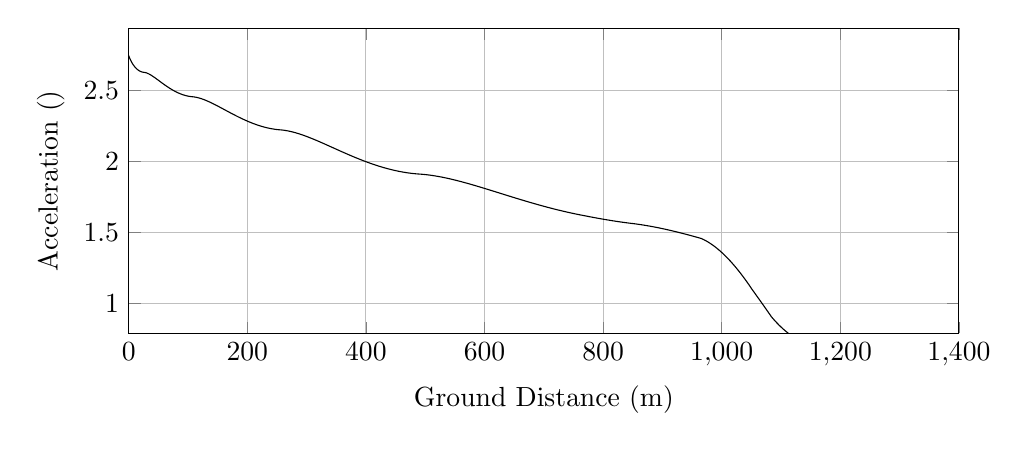
\begin{tikzpicture}

\begin{axis}[
width=\textwidth,
height=0.45\textwidth,
scaled ticks=false, tick label style={/pgf/number format/fixed},
xmin=0.0,
xmax=1400,
xlabel={Ground Distance (m)},
xmajorgrids,
ymin=0.7870546929072948,
ymax=2.9383329541999035,
ylabel={Acceleration ($\si{\meter\per\square\second}$)},
ymajorgrids
]

\addplot [
color=black,
solid
]
table[row sep=crcr]{
1.3729668748937997E-8	2.745933749634024\\
2.6049868369719035E-7	2.7459337463216693\\
2.0491224421327626E-6	2.7459337223163676\\
9.92442121137073E-6	2.74593361664894\\
4.7452367809869807E-5	2.7459331133935008\\
1.740064756114434E-4	2.74593141796994\\
4.0608377013922605E-4	2.7459283128250895\\
7.313431501337001E-4	2.745923966728787\\
0.0011549487327126044	2.7459183141309005\\
0.0016799013484208249	2.745911318665595\\
0.002295089346817705	2.7459031318683342\\
0.003009933382444524	2.745893631784023\\
0.003810608015426248	2.7458830054499908\\
0.004723484476856681	2.745870906509789\\
0.005727138856912631	2.7458576226878897\\
0.006836216967948795	2.7458429637322794\\
0.007997302399386296	2.7458276382144833\\
0.00929136979810952	2.745810580608766\\
0.010685558505459776	2.745792228663979\\
0.012178513621519987	2.745772603889116\\
0.013775244426719659	2.7457516442133327\\
0.015470070176169002	2.7457294279658626\\
0.0172374436815836	2.7457062929339147\\
0.019122918912604377	2.745681646264188\\
0.021104911040230538	2.7456557742244776\\
0.023190717999955576	2.7456285852738693\\
0.025355802981115103	2.7456004025085097\\
0.027620619195902148	2.7455709628304676\\
0.030020274690474198	2.7455398145480876\\
0.032476028269866286	2.7455079832228666\\
0.035054163466719815	2.745474612816359\\
0.037720846868992755	2.7454401452809734\\
0.04049779674511381	2.745404303593875\\
0.043329456594087365	2.745367807581193\\
0.04629652060163805	2.745329620662332\\
0.04934498934704602	2.745290442016606\\
0.052507657924119336	2.7452498537718295\\
0.055769483710642484	2.745208053078813\\
0.05917209570914676	2.7451645112972916\\
0.06264043916012321	2.7451201927906688\\
0.06620063977265622	2.745074766280724\\
0.06987962792775945	2.745027892179869\\
0.0736568184539585	2.744979836976057\\
0.07754284280095361	2.744930469346733\\
0.08151127871105612	2.744880128455919\\
0.08560324933017655	2.744828296550115\\
0.08985265585263943	2.7447745502252845\\
0.09413961367176535	2.7447204093860247\\
0.09857725310864562	2.744664448697618\\
0.10307959255469257	2.7446077566104368\\
0.10766008648593872	2.744550165853771\\
0.11234920964493048	2.744491296646081\\
0.11719267720457946	2.7444305805763873\\
0.12216973960582883	2.7443682839908865\\
0.12724007601918352	2.7443049160916244\\
0.13233299746505212	2.7442413617081813\\
0.13755256756750583	2.744176324555065\\
0.14287728588926696	2.744110077183268\\
0.1482946925752714	2.7440427783081276\\
0.15381585025670613	2.7439742941590106\\
0.15940564092189102	2.7439050633216198\\
0.16526271495916878	2.743832633069937\\
0.17120082448158402	2.743759314593124\\
0.17717889132867753	2.7436856165854584\\
0.18324322596131126	2.7436109697873574\\
0.189427022360885	2.7435349695339406\\
0.1957511558722988	2.743457364727397\\
0.2021484013779125	2.7433789844510024\\
0.20865863707071397	2.743299343476986\\
0.21548666343168166	2.7432159468507686\\
0.22220154781289658	2.743134061837388\\
0.22919671627301902	2.7430488935802986\\
0.23611678795738544	2.742964772871866\\
0.24306300975244904	2.7428804655838492\\
0.2503085190632165	2.7427926639555604\\
0.2576623280401219	2.74270369213178\\
0.26502430524173204	2.7426147629356477\\
0.2724963584449146	2.7425246467856903\\
0.2802001060647876	2.7424318847655185\\
0.2878583985474956	2.7423398174571867\\
0.2958320780323821	2.74224411264151\\
0.3040021452321372	2.7421462114990494\\
0.31208951788619	2.74204945948628\\
0.3202851396023423	2.7419515709453375\\
0.3287233234973125	2.7418509498073105\\
0.3370425959884752	2.7417519080250115\\
0.34575405233845447	2.7416483668644354\\
0.3545073625286812	2.7415445008529415\\
0.36338982075299686	2.74143927707345\\
0.37247557159370037	2.741331824878821\\
0.38151350442869847	2.741225116473271\\
0.3905554764834429	2.7411185361982797\\
0.3999457587520332	2.7410080342749286\\
0.4095398754587949	2.740895325049965\\
0.4189621792151833	2.7407848203234915\\
0.4285208811402964	2.7406729022160494\\
0.43828968955472236	2.7405587157868423\\
0.44807735398784176	2.740444501168418\\
0.45806002753764463	2.740328206966173\\
0.4682994371692033	2.740209125317234\\
0.4787752542918833	2.7400875051939693\\
0.4890770094685154	2.739968111629965\\
0.49985939134273727	2.739843363987376\\
0.5106597490205704	2.739718627718031\\
0.5213580865152188	2.739595283866114\\
0.532247733242454	2.739469951000051\\
0.5431365108549349	2.739344844457758\\
0.554075964429489	2.7392193713226414\\
0.5653450694020941	2.7390903409366887\\
0.5769901159382542	2.738957242270053\\
0.588512657344902	2.738825777773906\\
0.6004070039036553	2.7386903129467894\\
0.6121651247369502	2.738556638601956\\
0.6239717914322569	2.7384226491592862\\
0.6362472885961421	2.7382835883504875\\
0.6486428939173223	2.738143422272314\\
0.6610190736373547	2.7380037294208224\\
0.6737248046101814	2.7378605779440788\\
0.6862826225989949	2.7377193504710986\\
0.6991952542603428	2.7375743971928808\\
0.7122988072688032	2.737427572331951\\
0.7251463703465595	2.7372838790900627\\
0.7381769453061875	2.737138402838057\\
0.7516618647379176	2.7369881315120947\\
0.7654913705221527	2.736834310606014\\
0.7791756406994825	2.7366823919487455\\
0.7930637813125616	2.7365284991417216\\
0.8074774191984457	2.736369088689556\\
0.8215072375247947	2.7362142192435908\\
0.8361010597475598	2.736053431219534\\
0.8503303420601955	2.7358969585996338\\
0.8650627501899835	2.7357352618278403\\
0.8802332960144008	2.7355690814348668\\
0.8951742046771463	2.7354057362911055\\
0.9100334756324657	2.7352435957730297\\
0.9251067343345352	2.735079435666237\\
0.9403923630470314	2.7349132844243806\\
0.9559303815501943	2.7347447191307284\\
0.9712400158034169	2.7345789536451193\\
0.9869533781138684	2.7344091466658877\\
1.0029148609762486	2.734236997780573\\
1.0189962473881624	2.7340638988954913\\
1.035465185745812	2.733886982622522\\
1.0516742337458713	2.7337132054216866\\
1.067815735429615	2.7335404920408557\\
1.0846705971808022	2.7333605047019978\\
1.1012775250051634	2.7331835208984128\\
1.1180798406225687	2.7330048116164747\\
1.1351395900544134	2.7328237286921633\\
1.1526388687279154	2.73263835894707\\
1.1698922447507556	2.732455966615972\\
1.1875468452119025	2.732269712848928\\
1.2058383275300355	2.732077142510799\\
1.2239395537495579	2.731886975352393\\
1.2422020624207541	2.7316955142157697\\
1.2608769472440078	2.7315001426275947\\
1.2794948487006894	2.731305779649479\\
1.2979152553275424	2.7311138807814563\\
1.3166445915281573	2.73091917093961\\
1.3354141707340492	2.730724451882275\\
1.3543210821322504	2.730528719277727\\
1.373689361295591	2.73032863525778\\
1.3932049885015831	2.7301274608942405\\
1.4131781782225183	2.7299220154585475\\
1.4330139682345777	2.7297184263544425\\
1.4528243860883294	2.7295155352372795\\
1.4728783400745615	2.729310592226655\\
1.4934621752870565	2.729100693669997\\
1.5141408097620341	2.7288902940171758\\
1.53430654450827	2.7286855593626536\\
1.5553850389607948	2.728472025774905\\
1.5762653203499473	2.7282609685761434\\
1.5975496774716453	2.728046303569938\\
1.6196077215345106	2.7278243397435746\\
1.6413652536722467	2.727605899295412\\
1.663437310723463	2.7273848044555544\\
1.6860768385032747	2.727158548431424\\
1.7077101022266827	2.726942840558346\\
1.7297306410738114	2.7267237613893585\\
1.7520297891459062	2.7265024111794576\\
1.7743087535215367	2.7262817613558035\\
1.797257424336919	2.7260549980011213\\
1.8200802473615325	2.7258299974170024\\
1.8430350373473994	2.7256042147901303\\
1.8666926279964304	2.7253720605720746\\
1.8902808566018634	2.72514113040999\\
1.9138231309717848	2.7249111877288685\\
1.937187877956735	2.724683506686569\\
1.9611060682733261	2.724450973682445\\
1.9852138445648535	2.7242171481062742\\
2.009780393513653	2.723979437924413\\
2.0346228225622163	2.723739634761041\\
2.0593611988602687	2.7235014085153804\\
2.08477023517836	2.7232573149932806\\
2.110324766702745	2.7230124241566775\\
2.1352655781940433	2.722773991682768\\
2.160528860803022	2.7225330540312687\\
2.1862071157614817	2.722288750937233\\
2.2127756699400534	2.7220366021467237\\
2.2391904543957084	2.721786538650564\\
2.2653528664920257	2.721539475818613\\
2.292150575495974	2.7212870407551826\\
2.3187704640870406	2.721036905412479\\
2.3455495914188482	2.7207858982332622\\
2.372862901366455	2.7205305254301893\\
2.4007145172972395	2.7202707826704753\\
2.428100404243743	2.72001603228333\\
2.4555980306928005	2.7197608861757034\\
2.483374904362833	2.7195038000855876\\
2.511687733451976	2.7192424230947587\\
2.5402569276484597	2.7189793606402857\\
2.568415369317849	2.71872074613543\\
2.596987652715761	2.7184590025560453\\
2.6263861238451423	2.7181903927500546\\
2.655991481965028	2.717920608348247\\
2.6856115886357443	2.7176514041804687\\
2.7154221146045012	2.71738118698586\\
2.7455665152057707	2.7171086712897807\\
2.7752624694325894	2.7168409213882985\\
2.805457625653509	2.71656939071722\\
2.8358231840904597	2.716297056032584\\
2.8663460878589797	2.7160240421896784\\
2.897817297850832	2.7157433103512467\\
2.9287074004595235	2.7154685124985987\\
2.9603588456990284	2.715187708551693\\
2.9922321403815406	2.71490571640717\\
3.0241119471841866	2.71462444530067\\
3.056446055158509	2.7143399570513758\\
3.0889346922121366	2.7140549072190137\\
3.122221620829695	2.713763678408176\\
3.1546991615623394	2.7134803314856493\\
3.187635101478671	2.7131937884197734\\
3.221010117202278	2.7129042459478487\\
3.2543449374576605	2.712615872270808\\
3.288235920596943	2.7123235230382576\\
3.3223704322934555	2.7120299202652527\\
3.3562838593334394	2.7117390566035233\\
3.3906320903803255	2.7114453101597196\\
3.425633159699527	2.711146852210671\\
3.462387235801926	2.7108343880622456\\
3.4973980805087237	2.710537636483595\\
3.5324804241140235	2.710241147744873\\
3.5675385073174235	2.709945728382193\\
3.6040688981843845	2.709638816969628\\
3.6393612181513753	2.7093431890244997\\
3.6770856360342323	2.7090281416612143\\
3.7131729334920323	2.7087276833232927\\
3.749509707933214	2.7084260491268246\\
3.785733977879824	2.7081262444468592\\
3.8225309786916544	2.707822610564083\\
3.860867115351552	2.7075072478509306\\
3.89929745075254	2.7071921001654697\\
3.9373367205567504	2.706881130446619\\
3.9751626485832894	2.7065728578762025\\
4.013671158053867	2.7062599937888168\\
4.0521140617426425	2.7059486353631357\\
4.092377631210638	2.705623567578243\\
4.131586743753305	2.705308027124949\\
4.1715696979561425	2.7049872843873297\\
4.210522654700574	2.7046757949824176\\
4.250196810863292	2.704359538589963\\
4.2917015001093795	2.7040297652367293\\
4.332438976653355	2.7037071511860633\\
4.373124372895289	2.7033859958341147\\
4.414429464889761	2.703061013141131\\
4.455884944705147	2.7027359201134686\\
4.497250153511752	2.7024126010589393\\
4.537976875075978	2.7020953078843215\\
4.581399817640802	2.7017581350427298\\
4.623816269683994	2.701429893974078\\
4.666022338967499	2.7011043708260782\\
4.709098934189642	2.7007732491577343\\
4.752435367147649	2.7004412618628235\\
4.79531009100786	2.700113923220311\\
4.838191999420829	2.6997876304091646\\
4.881381760681686	2.6994601025113845\\
4.9256451804034285	2.6991255802428515\\
4.9704217340957495	2.6987883563581185\\
5.014356093293278	2.6984586198088563\\
5.058826350846283	2.698126010287651\\
5.104458009943745	2.697785910252903\\
5.149663211268795	2.697450177563721\\
5.194981168813841	2.6971147895925576\\
5.241194091283663	2.696773991377621\\
5.287987552078626	2.696430154327218\\
5.334426822383641	2.6960901499960244\\
5.380633359096258	2.6957530602096966\\
5.427524438012913	2.6954122052897027\\
5.476157635197664	2.6950599883398825\\
5.524667120325573	2.6947099813886997\\
5.5732739519824435	2.694360582160768\\
5.6208990292882195	2.6940195060851275\\
5.671502816366864	2.693658464116621\\
5.719824083529298	2.6933150154219874\\
5.767871110439133	2.6929747772519512\\
5.8169321963676754	2.6926286501345027\\
5.866076914057565	2.6922832358810025\\
5.917200682776528	2.691925289335387\\
5.96684810088939	2.6915790178532983\\
6.016885842403935	2.691231352228524\\
6.068639931677712	2.6908731577503717\\
6.119867755785197	2.6905199976544543\\
6.171030794930029	2.6901686602208663\\
6.222884713227881	2.6898139753337107\\
6.2735946138732235	2.6894684695538738\\
6.325883502103322	2.6891136013011465\\
6.379615386553551	2.6887504096481347\\
6.432194972482147	2.688396442468087\\
6.484528316464761	2.6880455368872473\\
6.536619297696934	2.68769764118571\\
6.589662958081361	2.687344796419861\\
6.644121795496577	2.6869840153423956\\
6.697445536614451	2.68663219810922\\
6.7518063163896365	2.686275003043974\\
6.8068829439682315	2.685914605406988\\
6.863205650636274	2.685547609679398\\
6.9185329265047315	2.685188625021353\\
6.974634519184049	2.684826152672259\\
7.031139830722298	2.6844626288388405\\
7.0870923879294985	2.6841041940757817\\
7.144766952910487	2.6837363176346836\\
7.2026451873548805	2.683368757231797\\
7.261191729679483	2.682998591553873\\
7.320502240843062	2.682625268876813\\
7.378210233177999	2.6822636424501294\\
7.437738452534925	2.6818922655745236\\
7.49714639104333	2.681523308417665\\
7.556502460410064	2.6811563316145213\\
7.617032771987237	2.680783794499826\\
7.676883327249088	2.6804171211405423\\
7.735740247984193	2.6800581575988813\\
7.796086087039788	2.679691776501249\\
7.856787102853412	2.6793249307229674\\
7.91721236259451	2.678961429481797\\
7.979013602666894	2.6785913752038963\\
8.039824025454376	2.6782289487607027\\
8.102419182184594	2.6778576340357727\\
8.16459313580776	2.6774905665511346\\
8.226347093952135	2.677127696565849\\
8.290527749984296	2.676752373844961\\
8.353592793320257	2.6763853613705777\\
8.417564177281012	2.67601487568339\\
8.482044607535009	2.675643270078857\\
8.547336806956285	2.6752688485572547\\
8.613293246319614	2.6748925126021685\\
8.6778048537894	2.6745262550450724\\
8.74454839911753	2.674149227258674\\
8.810708373588199	2.673777396453808\\
8.876548424968423	2.673409234250302\\
8.942828456712885	2.6730404887927257\\
9.010858044488913	2.6726639601609223\\
9.079453414959548	2.6722862922314583\\
9.148767802603732	2.6719066890561036\\
9.21609997183467	2.6715398811000908\\
9.285579683381485	2.67116336940079\\
9.355451712480097	2.670786767326205\\
9.423585014597279	2.670421494476032\\
9.493435356703696	2.6700490148237135\\
9.562655940911181	2.6696818813962357\\
9.63183713653898	2.669316926216502\\
9.703018708836247	2.6689434650398702\\
9.773178624863132	2.6685773872877823\\
9.844376937811855	2.6682079365263496\\
9.914998792594716	2.6678435040567887\\
9.98720270419701	2.6674729864037268\\
10.059478150570087	2.6671041981501142\\
10.132362020358627	2.6667344209387407\\
10.205876892438312	2.6663635857706476\\
10.279422251887688	2.6659947421935097\\
10.353305644514993	2.6656263553136483\\
10.42811398108589	2.6652555454284528\\
10.50332954727428	2.664884928557493\\
10.578207710262959	2.6645181680900603\\
10.65503529959097	2.6641441252244062\\
10.730232142651953	2.6637802356245537\\
10.805871937852555	2.6634164032193377\\
10.88265320376452	2.6630493287809767\\
10.958577899345514	2.6626885682826185\\
11.034861147941964	2.662328317504069\\
11.112742623646977	2.6619627989513033\\
11.190543636431041	2.661599949051814\\
11.267787598939979	2.6612419536263943\\
11.3462805052093	2.6608804641262784\\
11.423875697147409	2.6605253733666894\\
11.502735831556972	2.66016679186927\\
11.581465323066688	2.6598111062891867\\
11.661639233340708	2.6594512496614984\\
11.741743247575428	2.659094070532034\\
11.821864700430528	2.6587391681041073\\
11.901816327719768	2.6583873562373483\\
11.98361062800689	2.65802984404648\\
12.065425957085825	2.657674667049518\\
12.1478520915771	2.657319283720091\\
12.230956215923495	2.6569634524950505\\
12.313306905825911	2.6566132897052395\\
12.396632357805931	2.656261447402212\\
12.479578787946746	2.655913659143116\\
12.564327762802186	2.6555608318228234\\
12.648175874147956	2.655214251081233\\
12.736145481689512	2.6548532930755826\\
12.821080154398764	2.6545073614738826\\
12.908009536077355	2.6541559136608868\\
12.994986774303499	2.6538069029568296\\
13.081752199798046	2.6534613540348904\\
13.17035388279784	2.6531111740371047\\
13.257836697901475	2.652768065088189\\
13.34511613365563	2.652428366974772\\
13.433461823066896	2.6520871672573874\\
13.524108483575919	2.6517398400805456\\
13.611203924103116	2.6514087427638877\\
13.702229394080796	2.6510654420726993\\
13.792427706753081	2.650728010041674\\
13.882429934062493	2.6503940290968764\\
13.975435778888343	2.650051743756091\\
14.065832730112316	2.6497218173613817\\
14.157894546480026	2.649388598244756\\
14.250668806951023	2.649055631782466\\
14.343291987615704	2.6487260325270725\\
14.43744444968501	2.64839387373258\\
14.532636396723657	2.6480609912501123\\
14.625507232812737	2.6477390675021404\\
14.721503924398366	2.6474092478024884\\
14.818738382089133	2.6470782104461428\\
14.913572076739943	2.6467582780736505\\
15.009701633366973	2.6464369177531655\\
15.10815424447124	2.6461108524555685\\
15.206130868840724	2.6457894275225193\\
15.304035939715973	2.6454712794394446\\
15.403499839366233	2.645151168619309\\
15.503209871950865	2.6448333932172794\\
15.601718454553605	2.6445225108434887\\
15.700655560608023	2.6442133305209685\\
15.801250929860519	2.6439020954003567\\
15.899917805652187	2.643599879299895\\
16.001574124100856	2.6432916569963822\\
16.102638779863817	2.6429883870635598\\
16.204479333764816	2.6426859631921458\\
16.30489644092564	2.642390875444015\\
16.40578186591999	2.6420975095348966\\
16.509201471948074	2.641799986524223\\
16.614557195984908	2.6415002256988815\\
16.717657554831042	2.641210126302675\\
16.823039336622365	2.640916912552081\\
16.928576062495388	2.6406266046044653\\
17.03469945574068	2.640338038396731\\
17.140697318244236	2.640053160739731\\
17.246066414787876	2.639773277049187\\
17.35183930840021	2.639495622702711\\
17.458399953804133	2.639219234411631\\
17.565707112453843	2.6389442799060117\\
17.673103795073075	2.638672470550473\\
17.781888038667653	2.638400579402105\\
17.89115167195854	2.6381309531423165\\
18.00105710767307	2.63786323255278\\
18.110142905530395	2.6376009574466197\\
18.219697237410173	2.637341002414172\\
18.32752951944549	2.6370884953076636\\
18.43743745973078	2.6368345484445737\\
18.54904630654982	2.63658019384358\\
18.659302591714813	2.6363323952736817\\
18.770734536087716	2.636085450694776\\
18.883577445650936	2.635838949357387\\
18.996263390583444	2.635596364184675\\
19.108816920034535	2.635357616908477\\
19.22287647779894	2.6351192855805\\
19.33763586704334	2.6348831480062795\\
19.456324114791514	2.6346427711361047\\
19.57349394116079	2.634409291852097\\
19.690148252848566	2.634180600096859\\
19.80521137071168	2.633958691418372\\
19.92379170801214	2.633733794227746\\
20.04216631061405	2.6335131166802155\\
20.15848954929409	2.6332999786096893\\
20.278242138037896	2.6330843918964613\\
20.396206084226087	2.6328758170334643\\
20.516315546862906	2.632667302876359\\
20.637173924977112	2.632461401533406\\
20.75450010628387	2.6322652607421713\\
20.874378237858778	2.632068650375719\\
20.996035953832852	2.6318730325170687\\
21.11812959618858	2.6316806625120934\\
21.240471115580952	2.631491857446668\\
21.361479376438375	2.6313089928781865\\
21.485224699488654	2.631125973433857\\
21.607870280890317	2.6309485406063304\\
21.73242999733349	2.630772361329301\\
21.85704493170313	2.6306001480967662\\
21.98122016226351	2.6304325538620574\\
22.10826921766411	2.6302652125995127\\
22.235261614051304	2.6301021093246337\\
22.361664688868032	2.629943883831288\\
22.48780138980522	2.6297900776934346\\
22.614107216476143	2.6296401428980527\\
22.74409311379692	2.6294900871360998\\
22.873024137794893	2.6293454925824022\\
23.003512644166257	2.6292034414201826\\
23.132891545907036	2.629066846405708\\
23.26270690888247	2.628934029456868\\
23.39264146728729	2.6288053298831127\\
23.52277721573431	2.6286806696961964\\
23.654883767164463	2.6285584477188975\\
23.78569183677709	2.6284417091087624\\
23.917003007077597	2.628328794588147\\
24.047013652206026	2.628221204195908\\
24.178458227988493	2.6281166694027984\\
24.314609552493202	2.6280128759318746\\
24.447533097503474	2.627915932898171\\
24.579128452041708	2.627824218719879\\
24.71011994849615	2.627737123338611\\
24.843278471916108	2.627652868038229\\
24.975761222328053	2.6275733117861915\\
25.1115496753864	2.6274961796102385\\
25.247101122854083	2.627423621584068\\
25.384906965000688	2.627354391118195\\
25.522261036073317	2.6272899242628656\\
25.66123001648475	2.627229296090176\\
25.79865327455613	2.627173876444852\\
25.826335196219034	2.6271632574604533\\
25.839610403727477	2.62715822969495\\
25.841006316401874	2.627157703174394\\
25.84227013303559	2.6271572259940434\\
25.84770509053729	2.6271551682557828\\
25.86419328224909	2.627148869514051\\
25.90571916957557	2.627132632727095\\
25.999268866927544	2.62709410603191\\
26.123295978662824	2.627038901212371\\
26.250212562581652	2.6269775933396176\\
26.376891976518465	2.626911599588503\\
26.50638698165423	2.6268392423555404\\
26.634042370994827	2.6267631265942892\\
26.763333806613538	2.626681250837172\\
26.893207366259766	2.62659421847878\\
27.022905486492228	2.6265025738361114\\
27.153956322362554	2.626405232066988\\
27.287774297957696	2.626300978647955\\
27.42030033806219	2.6261929566003683\\
27.555504894698295	2.626077916748084\\
27.691130018821354	2.6259576762016144\\
27.82633313037239	2.6258330443348266\\
27.959508564917073	2.625705689812035\\
28.096515548835796	2.6255699768647354\\
28.232789703382153	2.6254303281033025\\
28.368684388406535	2.625286498680893\\
28.506541650227618	2.6251359904785243\\
28.64533374691623	2.624979841336361\\
28.78297783415192	2.624820465669056\\
28.92277775692753	2.6246540493487274\\
29.06227187463503	2.624483493060775\\
29.20212864139956	2.6243080372215513\\
29.34335827861657	2.624126392094661\\
29.483225747293005	2.623942134485322\\
29.625960812476485	2.623749682168036\\
29.76706561118049	2.6235551018597727\\
29.909402910999468	2.6233545237810842\\
30.051751399473822	2.623149671618658\\
30.196612335666572	2.6229368923312792\\
30.342192969749448	2.6227187353115538\\
30.48583400527584	2.6224992991267593\\
30.632658550781265	2.622270763203243\\
30.77846394498075	2.6220396350772806\\
30.92408133049836	2.6218047080288107\\
31.071091331299215	2.6215634400823893\\
31.218274793935116	2.6213178254024356\\
31.366705758252415	2.6210660719563164\\
31.515339333797037	2.6208099515408767\\
31.66356819769615	2.620550577189582\\
31.814689402684216	2.6202821391202162\\
31.96649953392354	2.6200084685109024\\
32.115424616034375	2.6197361526902787\\
32.266253234088566	2.619456531320976\\
32.41813832080348	2.6191711196609058\\
32.569791431087395	2.6188823653016966\\
32.722234201183724	2.618588359660447\\
32.876984607664	2.6182861188418736\\
33.031873994672836	2.6179798472058744\\
33.18502245018544	2.61767337730517\\
33.34135780547538	2.6173568541876238\\
33.49759920343199	2.6170368690402794\\
33.65385117142162	2.6167132684054444\\
33.8113313806527	2.6163835453824538\\
33.96985264489639	2.6160480723691215\\
34.126473036379195	2.6157131607910555\\
34.2857505660089	2.6153690959358693\\
34.4449212019973	2.6150218218705428\\
34.60566879064274	2.6146676745052684\\
34.76644486933921	2.614310071010496\\
34.92612701881755	2.613951597544056\\
35.08630421658309	2.6135887608266746\\
35.24825698849928	2.613218646437778\\
35.412303951281956	2.6128404656979436\\
35.57355277914179	2.612465573208352\\
35.73545353069308	2.612086065190393\\
35.89925038949356	2.6116990063305368\\
36.065161289279985	2.611303822719635\\
36.23047312008262	2.6109069894047563\\
36.39472205714358	2.6105097203642957\\
36.56135389445764	2.6101036997752756\\
36.72774532558607	2.609695316287241\\
36.89384825683493	2.6092847556652456\\
37.05904296416534	2.608873633171015\\
37.22702676294645	2.6084527521107095\\
37.39437475321985	2.6080306918927274\\
37.5621109943643	2.607604928234461\\
37.73270471709142	2.607169167240153\\
37.903359519601935	2.6067305347705387\\
38.071486842086316	2.6062957943756917\\
38.23815243703595	2.6058623319798837\\
38.40817787072022	2.6054176148453294\\
38.57751392140098	2.604972224462812\\
38.750215798728505	2.604515486819169\\
38.92001182640311	2.604064028086343\\
39.09310637700479	2.6036013939253158\\
39.26472366117933	2.603140360230884\\
39.436554723976656	2.6026764590104268\\
39.608961777617054	2.602208745072529\\
39.782828308010565	2.6017348303452126\\
39.956194359016465	2.6012600869258415\\
40.132391837044906	2.6007753954833523\\
40.30868053167249	2.6002882883371417\\
40.48611580488176	2.599795875967091\\
40.66383502946924	2.599300575623608\\
40.83999042132467	2.5988076076289266\\
41.018202681018664	2.598306879012876\\
41.19780999006247	2.59780023921822\\
41.37730467548502	2.5972919679986406\\
41.557010452813884	2.5967811949022925\\
41.73612816026986	2.5962702442991796\\
41.91555194917056	2.5957566162813004\\
42.09743589423803	2.5952341495078093\\
42.27807550146298	2.5947135135520316\\
42.45995188234755	2.594187603754664\\
42.6401410478328	2.593664926422731\\
42.822293873795985	2.5931349327029034\\
43.00585672428667	2.5925992336587598\\
43.189965171449515	2.592060371841985\\
43.372020236704074	2.5915260176090396\\
43.555636897252796	2.5909856106444664\\
43.74012033961118	2.5904412105939336\\
43.92429822300048	2.5898963139394615\\
44.106869824379004	2.5893548329369107\\
44.29411840239129	2.588798141810776\\
44.47920670866131	2.5882465834656143\\
44.665034305215386	2.5876915745572395\\
44.85242224248053	2.5871306821366113\\
45.03948098831597	2.5865695920897522\\
45.22811764277584	2.586002614453135\\
45.41548629589063	2.5854383417605273\\
45.60322541388645	2.58487188864763\\
45.793007222766036	2.584298230300096\\
45.983742663331824	2.583720675421648\\
46.172643153142886	2.58314771556424\\
46.36421599110457	2.582565713945945\\
46.553512793459404	2.5819897407332553\\
46.745018895697555	2.5814061887802406\\
46.93606459490553	2.580823220829023\\
47.126948089509526	2.580239969889381\\
47.31881294044018	2.579652975509168\\
47.5110690178297	2.5790640736859434\\
47.705448624448266	2.5784679831468953\\
47.90005519882567	2.577870546429364\\
48.09288923506665	2.577277947636331\\
48.28732881729917	2.576679844114947\\
48.484002572746206	2.5760743233998253\\
48.68089030454945	2.575467633349363\\
48.87532723390382	2.57486803095897\\
49.07073736177763	2.5742649991859343\\
49.2672083392297	2.5736582972862303\\
49.46586249263092	2.5730444865995894\\
49.661880987188695	2.5724384938105347\\
49.85966148345089	2.5718267615262587\\
50.05808618672894	2.571212777407524\\
50.25785665917266	2.570594402569249\\
50.45743808511885	2.569976421527972\\
50.65573800086891	2.5693622538365988\\
50.85948768734909	2.5687310825359084\\
51.061243703011925	2.5681059980424292\\
51.26368286286315	2.567478743109982\\
51.46416466063809	2.566857533975103\\
51.66475943174029	2.5662359893110347\\
51.86588207153103	2.56561285677663\\
52.07444928962187	2.564966744465173\\
52.2824430085781	2.5643225310284814\\
52.48676525705545	2.5636898422625745\\
52.69531994892206	2.5630442386830037\\
52.90027076850366	2.562410012697458\\
53.108186167814935	2.5617668705752035\\
53.31165724918766	2.561137759462768\\
53.520024946679996	2.560493831718171\\
53.72688450142306	2.559854920280424\\
53.93707391647578	2.5592061198138465\\
54.14518573319289	2.5585641573342945\\
54.35125853722778	2.5579289322446064\\
54.56213447502874	2.5572793940255876\\
54.77598621923464	2.5566212311207\\
54.987629956235494	2.5559704324655836\\
55.19778857845695	2.5553247914147734\\
55.41030974885841	2.55467252202679\\
55.62390503323701	2.554017625167454\\
55.83671574169797	2.553365831759879\\
56.047071254351536	2.5527222723040826\\
56.26137331252919	2.5520673989185383\\
56.47512769358855	2.5514149930840677\\
56.69105800830218	2.55075678108659\\
56.90937011004422	2.5500921924420785\\
57.12736617899088	2.549429482767894\\
57.346833156368504	2.5487632574065238\\
57.56476609337061	2.5481026676419045\\
57.78230894703917	2.547444262133678\\
57.99943865551505	2.5467881336539273\\
58.21827465292657	2.5461279153126446\\
58.436085045729726	2.545471882108224\\
58.6577546799423	2.5448053710641405\\
58.87982836766625	2.544138832936956\\
59.10336118170943	2.5434691447546607\\
59.324182403931715	2.542808819305696\\
59.545440661451366	2.5421484495030766\\
59.768227251413464	2.5414848224466517\\
59.99077485409802	2.540823240966116\\
60.21631063559073	2.54015416369662\\
60.44006004384342	2.539491792913134\\
60.66502706168687	2.5388272572727564\\
60.89133011288284	2.5381602583073883\\
61.11585558357916	2.5374999948556693\\
61.3432655409558	2.5368327945800493\\
61.57186440401435	2.5361637002878803\\
61.79868765088207	2.535501408748763\\
62.025670725987	2.5348402770909786\\
62.254132946411545	2.5341765056009926\\
62.48290793247415	2.5335135279774255\\
62.713817944074236	2.5328461162466924\\
62.94484116346062	2.5321801651283318\\
63.17805109236767	2.5315097497788024\\
63.41124119062552	2.530841264404774\\
63.64505576847972	2.5301728944345925\\
63.87735201907903	2.5295107788661895\\
64.11169045660182	2.5288448001638137\\
64.34725756208485	2.52817733598523\\
64.58324360279937	2.527510726208688\\
64.81881329818131	2.5268473544899654\\
65.05563560606473	2.5261825559991893\\
65.29467812810154	2.5255136850947695\\
65.53178653633495	2.524852393698131\\
65.77046761369158	2.5241889200770515\\
66.01019347650049	2.523524791474693\\
66.25262920761091	2.52285547188822\\
66.49342175078831	2.522193018006006\\
66.73393309567928	2.5215336779391944\\
66.97718905970893	2.52086921586132\\
67.21919788222482	2.5202105803525665\\
67.46413738735515	2.519546449583455\\
67.70584739194695	2.518893544044623\\
67.95375887035246	2.5182264574902717\\
68.19817148521656	2.5175713561374016\\
68.44413350233111	2.5169147004876002\\
68.68984243621705	2.516261345089669\\
68.93951041285982	2.515600171501796\\
69.19023531750676	2.514938969433662\\
69.43956667494601	2.514284217583624\\
69.68998597860525	2.513629416130965\\
69.94098943220166	2.512975932155717\\
70.1928405184459	2.5123231255440013\\
70.44659484061637	2.511668329081634\\
70.69926103579675	2.5110192971929557\\
70.95414956377036	2.5103675673854084\\
71.21136313866151	2.5097129793716446\\
71.46778788208749	2.509063506597747\\
71.7247351381395	2.5084158438377147\\
71.98234155897126	2.507769689085089\\
72.24107377350035	2.5071239256193767\\
72.4986091150376	2.5064843695454924\\
72.75949164810788	2.505839797213234\\
73.02014691132015	2.505199119753618\\
73.28114866838587	2.504560949336046\\
73.54342372888959	2.503923071226774\\
73.80584407854005	2.5032882764078206\\
74.07231166191039	2.5026472290607487\\
74.3389341302921	2.5020093971959803\\
74.60521354141642	2.501375988177486\\
74.87280568706873	2.5007431028336446\\
75.1403821105715	2.5001139292433843\\
75.41145333671997	2.4994803046180856\\
75.68265298797411	2.4988501932497016\\
75.95075857762194	2.498231039158717\\
76.2241428819712	2.4976035721719434\\
76.4990100438061	2.496976668570306\\
76.77213586328236	2.4963576955699853\\
77.04724851790667	2.49573822862106\\
77.32330034006353	2.4951207098630084\\
77.59850473375684	2.4945091566067346\\
77.87773830129439	2.4938928219842715\\
78.1565255546137	2.4932816837060106\\
78.43842651648492	2.492668017346257\\
78.720833678605	2.4920576010425153\\
79.00101298089581	2.4914563231480757\\
79.28359351218376	2.4908542717934887\\
79.57011733099088	2.490248328576058\\
79.85418914588558	2.4896520718283295\\
80.13919871477489	2.4890583687052414\\
80.42568449319114	2.4884661731421938\\
80.71472498530085	2.487873370981382\\
81.006853148924	2.487279025102887\\
81.2951972638476	2.4866971170884167\\
81.58524575795963	2.486116537145639\\
81.87461709596036	2.4855420949920353\\
82.1711642895769	2.484958381559892\\
82.46716486408064	2.484380782761332\\
82.76422974563803	2.483806186216814\\
83.05801377197795	2.483242957146957\\
83.35853301954708	2.482671999870737\\
83.65664966506407	2.4821108049392793\\
83.95487262936624	2.481554606519677\\
84.25322789115987	2.4810033792257986\\
84.55664509033022	2.4804481694309706\\
84.8599544590121	2.4798985860092557\\
85.16499148084048	2.4793513638033664\\
85.47187188044902	2.478806409028219\\
85.77908321853027	2.4782664837735044\\
86.08675489504844	2.4777313991684684\\
86.39784539041122	2.4771961342162765\\
86.71051296037359	2.4766640142286205\\
87.02583358957506	2.4761333445033173\\
87.34037846285594	2.4756099658506825\\
87.65395388450591	2.4750941674588303\\
87.96687312379424	2.4745854039580317\\
88.28527441497255	2.474073850456792\\
88.6103524516937	2.4735579588692937\\
88.92871226770333	2.4730590021066936\\
89.25003295857354	2.472561715850354\\
89.57522243846881	2.472064913921284\\
89.90247582737899	2.4715715482953424\\
90.22602529632545	2.471090281458441\\
90.5494223037065	2.4706157304863785\\
90.87816525326718	2.470140000358535\\
91.20455861430293	2.4696743344984124\\
91.53817773235312	2.4692052383281\\
91.87076195087604	2.46874453523425\\
92.20124984301029	2.468293613714687\\
92.53140503523474	2.4678500072923946\\
92.86389705561814	2.467410207209607\\
93.19815266874983	2.46697511608851\\
93.53304529783748	2.4665462917878456\\
93.86737084100128	2.4661252936021194\\
94.20337949361911	2.4657093387407842\\
94.54065981474497	2.4652990463300517\\
94.87396787418089	2.4649007234996034\\
95.21684847579547	2.4644983797555815\\
95.55392648231228	2.4641101935898275\\
95.89232371872416	2.463727831543161\\
96.23051075783204	2.463353072193108\\
96.57164052232307	2.4629825255521096\\
96.90762523479154	2.4626249186321765\\
97.24755293575913	2.462270552927021\\
97.58790661409188	2.4619232523826478\\
97.92576087813703	2.461585947168559\\
98.26661027452474	2.4612531815923795\\
98.6051908024865	2.4609301321117414\\
98.94563962387357	2.4606128512157275\\
99.28665364663627	2.4603026475156407\\
99.63350087797645	2.4599949576702347\\
99.97685593767679	2.4596981466115277\\
100.31593955776762	2.4594126383431973\\
100.65572384630482	2.4591341387793317\\
100.99616871909686	2.4588627388350837\\
101.3402339503516	2.458596236175948\\
101.67973054404297	2.458340953841132\\
102.01657591573795	2.4580952179760907\\
102.35656456518868	2.457854829697289\\
102.6941824316649	2.457623725275984\\
103.03547296258705	2.457397823628013\\
103.37623032340073	2.457180026797986\\
103.71852978299776	2.456969054425172\\
104.05851119314701	2.4567672705298635\\
104.3949509202441	2.4565752126830196\\
104.7329053851843	2.456389936423986\\
105.07104272194636	2.456212240406991\\
105.40742307340048	2.456043101164078\\
105.74423560014887	2.4558813834138933\\
106.07955743077031	2.455727984822288\\
106.41623710643992	2.4555816081016255\\
106.75618472497374	2.455441591416804\\
107.0942647435474	2.4553101084432747\\
107.43151869252583	2.4551866717490167\\
107.44650965670576	2.4551813642403237\\
107.45815118347005	2.4551772531208176\\
107.46233674961977	2.4551757772689795\\
107.46535588765028	2.4551747132015054\\
107.46808502617694	2.4551737507643727\\
107.4836206108138	2.455168259670489\\
107.53176708907421	2.4551511079163477\\
107.68672244793561	2.455094531599669\\
107.97570433527497	2.4549834451948627\\
108.27744765146667	2.4548597682328195\\
108.5816623935838	2.4547272061477434\\
108.88557241638279	2.4545869610121596\\
109.19209959959528	2.45443767243568\\
109.50241879336687	2.4542786003150896\\
109.81066605766154	2.4541127633367736\\
110.12101503747155	2.453937994054648\\
110.43285681965125	2.4537545790192175\\
110.74725799716322	2.453561818956234\\
111.06462449033057	2.4533593397004765\\
111.38211128519615	2.453148923592198\\
111.70119562731901	2.4529296108117045\\
112.02298633508096	2.452700564309909\\
112.34320819983824	2.452464869014065\\
112.66812620709393	2.452217884637398\\
112.99302416686388	2.451963112159949\\
113.31966045518399	2.4516991968576756\\
113.64998129974768	2.451424459279832\\
113.97857627498675	2.451143416865058\\
114.31304608469316	2.450849510906499\\
114.64448318111735	2.4505505571921855\\
114.98093514978115	2.4502393175308965\\
115.31969924418831	2.4499181287839766\\
115.65790718621022	2.449589741128423\\
116.00063352526521	2.4492491841404753\\
116.34235083463872	2.448901923487149\\
116.68621873349733	2.448544803075687\\
117.03331062078092	2.4481766222286128\\
117.37910048629482	2.4478022122028253\\
117.72869476105836	2.447416056567934\\
118.08005947084649	2.447020315368726\\
118.43363644355449	2.44661445841039\\
118.79186464668504	2.446195562722882\\
119.14769212941735	2.4457719010897243\\
119.5036618261702	2.4453406161077478\\
119.86270697471275	2.444898151431988\\
120.22616362054572	2.4444427272159954\\
120.58991121293201	2.4439794620158324\\
120.95538130513773	2.443506572675182\\
121.3195355377388	2.4430280793612997\\
121.68590041554987	2.4425394226513815\\
122.05305648207542	2.442042507730611\\
122.42257239354896	2.4415352206266228\\
122.79503144936103	2.4410167087569397\\
123.16629137010841	2.4404927909789507\\
123.53950748252527	2.439959095724661\\
123.91239367862553	2.4394189483888704\\
124.29026003316017	2.4388646308631676\\
124.66301933937496	2.438311045841078\\
125.03890311735066	2.4377461242287524\\
125.41380975776434	2.4371760734767376\\
125.7896808967325	2.4365980418067945\\
126.16837244152023	2.4360091772577572\\
126.54595968852882	2.4354156387065453\\
126.92471834906405	2.434813947054397\\
127.30294276405039	2.4342068948637348\\
127.68255852126984	2.433591469128208\\
128.06243727540487	2.4329695571547303\\
128.44360431740483	2.432339541404442\\
128.82265748788262	2.4317071612453454\\
129.1989690567886	2.4310736703116387\\
129.57765386613931	2.4304305602421765\\
129.95508099647026	2.429784065084977\\
130.33359114840187	2.4291302715149827\\
130.71373745886524	2.4284682576146626\\
131.09453904397424	2.4277997749107643\\
131.47657586018488	2.4271238577704235\\
131.85678563989967	2.426446027201812\\
132.23856625352113	2.42576032125654\\
132.61595336405918	2.4250775964184523\\
132.99976263915818	2.4243783357290276\\
133.38083522978053	2.423679242984316\\
133.76098428781995	2.4229771481541835\\
134.1363519425165	2.4222793654313444\\
134.51557915495124	2.421569932295995\\
134.8968696170101	2.4208521881638854\\
135.27419431482667	2.420137597883574\\
135.65215477207505	2.4194175854598914\\
136.03329358991255	2.4186873250908105\\
136.41192880753374	2.4179577730609862\\
136.7898079310749	2.417225694571063\\
137.17001317148595	2.4164851729427035\\
137.54844558779996	2.415744261492118\\
137.92617219433072	2.4150009862160164\\
138.30476964659732	2.4142523189260237\\
138.68390038934075	2.413498983015482\\
139.0631653430654	2.4127418378009757\\
139.4406106933401	2.41198488197385\\
139.81914660512416	2.4112223633220573\\
140.19767098864742	2.410456560906317\\
140.5730919292459	2.4096938425620706\\
140.95061983253072	2.4089237067743268\\
141.32838502869612	2.4081500093041033\\
141.70636515873298	2.4073728610224387\\
142.0839785067887	2.406593529688587\\
142.46357402350594	2.4058072184921997\\
142.84082211769783	2.40502296889394\\
143.21906727224075	2.4042339114596416\\
143.59963619096823	2.403437310882776\\
143.97984478872678	2.4026388326905357\\
144.35941603837455	2.4018391364099507\\
144.7355521893594	2.4010442230400466\\
145.11296635073694	2.4002442180265584\\
145.49073213867456	2.399441133914113\\
145.87033631970945	2.3986318541955978\\
146.24486520181193	2.397831210000894\\
146.6238757206513	2.3970188391759493\\
147.00096360401335	2.396208508945593\\
147.37874202190085	2.3953946757121454\\
147.756852900845	2.39457816388311\\
148.13572640408995	2.393758097000817\\
148.5136798644104	2.392938178662493\\
148.89083780486442	2.392118210713834\\
149.2712459042852	2.391289439886328\\
149.65303236723025	2.390455972301191\\
150.0329584616291	2.389624940771009\\
150.41363382646614	2.388790702960881\\
150.79322940570728	2.3879573271300165\\
151.17272478467066	2.3871227269328097\\
151.55400296227282	2.3862828087520374\\
151.93482601265913	2.385442551958211\\
152.31881414221942	2.3845940116132027\\
152.70208150063132	2.3837458190581575\\
153.08320649997165	2.382901190023449\\
153.4666285558243	2.382050340959543\\
153.84825937276264	2.381202396702336\\
154.23093781718723	2.380351107148919\\
154.61485031834388	2.379496102763693\\
155.00001234931443	2.3786373939872023\\
155.38285725409855	2.3777829898524283\\
155.7679513537659	2.3769227531344317\\
156.1509667875323	2.3760664034774726\\
156.53491934392343	2.3752072536116557\\
156.91995289130983	2.37434502792717\\
157.30625057946366	2.373479362158138\\
157.69121706207227	2.3726161237217385\\
158.07789765133754	2.371748534188164\\
158.46521012398495	2.3708790680405922\\
158.85138765236047	2.370011742814021\\
159.23964669847322	2.3691393833615075\\
159.62715395386465	2.368268403666744\\
160.01960115328984	2.367386056204964\\
160.4079207075476	2.366512776596168\\
160.79602490671402	2.36563981902208\\
161.18437278725975	2.364766199221803\\
161.57644284003254	2.363884138972799\\
161.96812230097612	2.363002938647095\\
162.35808768568592	2.362125623778489\\
162.75087300343483	2.3612420420191382\\
163.14546270495134	2.3603545272165904\\
163.53745675514648	2.3594730228399685\\
163.92955389373896	2.3585915050473067\\
164.32395276810763	2.357705079439211\\
164.71713266653478	2.3568217061873185\\
165.1102153740033	2.35593890902884\\
165.5035884424101	2.355055863096327\\
165.89816400198282	2.3541705682312966\\
166.29148626774366	2.3532885788431104\\
166.68861804276264	2.3523985917182593\\
167.082852347146	2.351515683455717\\
167.48006204110857	2.3506267458495653\\
167.8798182678497	2.349732796398407\\
168.27774435731556	2.3488436682392644\\
168.67741362640317	2.3479514207768712\\
169.07475368467374	2.3470651868695898\\
169.4759958044982	2.3461711163376826\\
169.87832784425882	2.3452755349517966\\
170.2792240364854	2.344384106753197\\
170.68126852540456	2.3434911272918937\\
171.08617821288442	2.3425928410644596\\
171.48766933901368	2.341703228415432\\
171.892744970828	2.340806814987485\\
172.29711201372032	2.339913155185136\\
172.70264003426053	2.339018160916506\\
173.1105289448074	2.3381192418897934\\
173.5163733808056	2.337226149563117\\
173.92577914808027	2.336326596791209\\
174.33607303977334	2.335426521117654\\
174.74614233406845	2.3345284082190787\\
175.15731444736514	2.3336293965914052\\
175.56901623635082	2.3327307892227083\\
175.97955109701695	2.3318363258755\\
176.39275298155184	2.330937702273025\\
176.80397138375372	2.3300450760546294\\
177.21946344336607	2.329144919042588\\
177.6332252263685	2.3282502942964154\\
178.05102033212842	2.3273487947563245\\
178.46725124888752	2.3264525543676644\\
178.88389799206544	2.325557341115923\\
179.29839533747668	2.324668693141324\\
179.71608569665375	2.3237752025766305\\
180.1342696339205	2.32288270874726\\
180.5538779958007	2.3219892775088473\\
180.97690569555635	2.321090736474277\\
181.39980810354632	2.3201946786391883\\
181.82328311928882	2.3192996671664883\\
182.24618807605736	2.3184081550362716\\
182.6731660166833	2.317510421204183\\
183.10035828358116	2.3166146524410083\\
183.5291445538124	2.315718009268359\\
183.95833265232255	2.3148230398976084\\
184.38634616388282	2.3139330622768055\\
184.8168339376561	2.31304053831765\\
185.24630581702252	2.3121527543741527\\
185.67754767955432	2.3112639955220837\\
186.109185775987	2.3103771499628856\\
186.53971883241212	2.3094953318031495\\
186.97132952004227	2.308614106272679\\
187.40711553434954	2.307727236429657\\
187.84220985117162	2.306844697971041\\
188.27778926256264	2.30596413782915\\
188.71822733349944	2.3050768055935897\\
189.16086434237673	2.304188169974439\\
189.6010380968554	2.303307624220924\\
190.03919041211265	2.3024342720484574\\
190.48016062316526	2.3015585113414065\\
190.92524363955386	2.3006778821099303\\
191.372330984798	2.2997966603754403\\
191.81766281185656	2.298922295360404\\
192.2649588892154	2.2980475215660183\\
192.7152080571317	2.29717049781034\\
193.16529614382966	2.2962973584252397\\
193.61551258619323	2.2954275767901127\\
194.0671041699889	2.2945587974042523\\
194.52074606224477	2.2936897982169953\\
194.9783774267325	2.2928169747246976\\
195.4358245305881	2.2919483704550094\\
195.89499401276925	2.2910804200107293\\
196.35432087192027	2.29021614095274\\
196.81831699949333	2.2893471419192934\\
197.28093205423113	2.288484832875148\\
197.74513845889334	2.2876237112361713\\
198.21238653581378	2.2867611842578457\\
198.6780372695403	2.2859058700391826\\
199.14562244096538	2.285051320833504\\
199.6172630308758	2.2841937787794144\\
200.085680559985	2.2833465240077064\\
200.55485539631252	2.2825023563416105\\
201.0284003638297	2.2816548831705905\\
201.5010163224531	2.2808136720525436\\
201.97949934275624	2.279966733779389\\
202.45676989461947	2.2791267029639997\\
202.93795341995116	2.278284633804679\\
203.42151825635358	2.27744333714352\\
203.9064451985618	2.276604678712552\\
204.39376498892221	2.2757669693589087\\
204.88144002832018	2.2749337898656847\\
205.3743097859811	2.2740969956561354\\
205.86751126322014	2.2732649672325973\\
206.36222180198536	2.2724357837290876\\
206.85620764580733	2.2716132370425086\\
207.35622660722595	2.270786197827218\\
207.85286701515986	2.2699703123930766\\
208.35554496397685	2.2691501921338437\\
208.85949164962352	2.2683337771305263\\
209.3606904933826	2.267527584023078\\
209.86430174661194	2.2667233414271317\\
210.37517113261447	2.2659135153305847\\
210.88826309775862	2.265106291807493\\
211.408532759536	2.2642940812050707\\
211.9275242572583	2.2634902283494576\\
212.45034341379437	2.2626869088461126\\
212.97278109853062	2.2618906907245666\\
213.5012611434281	2.2610919272299235\\
214.0307698600809	2.260298367573064\\
214.55632530210835	2.259517458773658\\
215.09027271075985	2.258730980013155\\
215.62992362610385	2.2579432040163745\\
216.17218538865313	2.2571588484810805\\
216.71273903148006	2.2563842166698143\\
217.25354139798316	2.2556165126472143\\
217.7992146693805	2.2548493165568644\\
218.34754045136725	2.254085939492425\\
218.89661223248612	2.2533291440783003\\
219.45761572436965	2.252563818122007\\
220.01811384548756	2.2518072106683293\\
220.5796054147944	2.251057348628902\\
221.1491613381006	2.2503050259601194\\
221.72392285119702	2.2495543519089907\\
222.29674345543788	2.248814773911077\\
222.87200016908895	2.2480806927809356\\
223.45476781204167	2.2473458994986784\\
224.04346163614804	2.246612743327802\\
224.62738211659592	2.2458946181678927\\
225.21466034383656	2.2451815330113867\\
225.80901970025303	2.2444692551194265\\
226.4067565685998	2.2437625152392293\\
227.010346212326	2.243058653573091\\
227.62015690700883	2.2423575809138097\\
228.23221085371028	2.2416641252690344\\
228.84135848872813	2.2409841492059526\\
229.46020606246555	2.2403037973268463\\
230.08791152904655	2.23962451579903\\
230.71342291791404	2.2389584838900456\\
231.3402722001092	2.2383019652353546\\
231.96207175272258	2.237661598553662\\
232.5840768980429	2.2370318898712833\\
233.21041275014744	2.2364088273333484\\
233.84076499381075	2.2357929904324703\\
234.4632722369638	2.2351959100520835\\
235.0951321894368	2.234601176398142\\
235.7164683430417	2.2340275104333625\\
236.33637872225546	2.2334662341004403\\
236.95807015301216	2.2329144958185676\\
237.57724458338066	2.2323761320972704\\
238.1954544769302	2.2318497405902384\\
238.81057478854058	2.2313370620076993\\
239.4264917144386	2.2308348356473227\\
240.0366097511752	2.2303483438025955\\
240.63918371105967	2.2298786569056217\\
241.24161561476188	2.229419836436943\\
241.8433627512665	2.2289723102569345\\
242.44272012201816	2.2285373001045503\\
243.03744426405035	2.228116281450559\\
243.6307298234035	2.227706865005068\\
244.22108413951537	2.227309998190906\\
244.8116939475828	2.2269235009469064\\
245.39744552343484	2.2265506298561997\\
245.97855029096053	2.2261910292632345\\
246.5589096408665	2.2258421732917872\\
247.13041662269836	2.2255087118698302\\
247.70663564674516	2.2251826514721484\\
248.28024698100222	2.2248682198189034\\
248.85288765982074	2.224564454598548\\
249.4193334510956	2.224273966746556\\
249.9777393310295	2.223997356302494\\
250.54131855768964	2.2237280307941525\\
251.10095479045611	2.223470406607258\\
251.65640742239583	2.223224408530201\\
252.20851363475686	2.2229894956588856\\
252.76218077146297	2.2227635597549096\\
253.31371341967355	2.2225481199438883\\
253.86551898536345	2.222342213140818\\
254.41422830739316	2.222147048359397\\
254.9572061395861	2.2219633575790283\\
255.0653176818724	2.2219279057873615\\
255.12993325322566	2.221906895339256\\
255.17825500251217	2.2218912701696016\\
255.20626764895485	2.2218822462499563\\
255.2307799315319	2.221874370500835\\
255.25350681352313	2.2218670855541918\\
255.27636741461964	2.2218597744009294\\
255.2901025823965	2.221855389728459\\
255.29493524708477	2.2218538483887693\\
255.30041476425401	2.2218521001387765\\
255.32542424174517	2.2218441047826696\\
255.431840924477	2.221809790194097\\
255.72188923316247	2.221713851752103\\
256.19571599032633	2.2215495739087965\\
256.67415123408614	2.2213742589191403\\
257.15505540016306	2.221188557634944\\
257.6368423781066	2.220993060856098\\
258.1230512066297	2.2207862547693775\\
258.61423458459376	2.220567707896195\\
259.1049940935744	2.2203397696000096\\
259.5982522152891	2.2201011037047182\\
260.09486806301686	2.2198512067286345\\
260.5959555145432	2.2195893748813527\\
261.1023053698689	2.219314998340587\\
261.6089919954627	2.2190306711996595\\
262.11906753970584	2.218734661689399\\
262.63243815947874	2.2184269215692023\\
263.14830217600297	2.218107856226906\\
263.66676080693014	2.217777349647611\\
264.1877265034735	2.2174354054872643\\
264.7128105393116	2.2170808727276556\\
265.241218472901	2.2167141732995255\\
265.7723922912836	2.216335620151221\\
266.3079016945154	2.2159439940722487\\
266.8503273810571	2.2155371935528327\\
267.3932272617866	2.2151199459981052\\
267.9365984091472	2.214692330831869\\
268.4918097049034	2.2142451659175686\\
269.04807221243857	2.2137868919753974\\
269.6097925731924	2.2133138095010647\\
270.17242368341533	2.212829684772851\\
270.7441513704771	2.2123273142660853\\
271.31667319188057	2.211813839181791\\
271.8922835348494	2.2112872141788866\\
272.47925332376417	2.21073960128831\\
273.06804504353704	2.210179665227172\\
273.66076346861166	2.2096053755286063\\
274.25294696226547	2.209021091006065\\
274.85204953299706	2.208419415799331\\
275.4590719216128	2.2077990829464973\\
276.0685465790958	2.2071655398666756\\
276.6808474128411	2.2065183952622025\\
277.29680014730513	2.2058567449011655\\
277.9224067517041	2.2051739367108585\\
278.5505103374435	2.204477611086179\\
279.17831818166474	2.2037709522184414\\
279.81790886718375	2.203040219253401\\
280.45539954927676	2.202301177006695\\
281.0966396233664	2.201547153524343\\
281.73735617862894	2.200783243215989\\
282.38112941523184	2.2000052659558564\\
283.0301801354616	2.1992104875794514\\
283.67721705328654	2.1984079099349207\\
284.3202688103162	2.1976002701437842\\
284.9599564878264	2.1967871053890056\\
285.60213884169843	2.1959611332978755\\
286.24205728342235	2.195128612826325\\
286.8783426797421	2.1942915966501397\\
287.5176726031193	2.193441453896205\\
288.14959414660166	2.1925923142210184\\
288.7790218355949	2.1917379149920313\\
289.41060269245395	2.1908720881422035\\
290.0373602432952	2.190004581853236\\
290.6616399781276	2.1891324221109327\\
291.28528823747513	2.1882532158649513\\
291.90747044142563	2.1873683040813363\\
292.5232553861292	2.186484968054768\\
293.13767407877424	2.185596251369275\\
293.74977203443143	2.184703716949506\\
294.36691018627903	2.1837967003650283\\
294.97422257673236	2.182897246316001\\
295.5803242078987	2.1819928935085953\\
296.18876641420377	2.1810784345812797\\
296.79141324013847	2.180166261540987\\
297.39276567122147	2.1792497807633247\\
297.9894421920609	2.178334342126881\\
298.5870928977196	2.1774114358177634\\
299.1813773675972	2.1764879005107254\\
299.77152323390305	2.1755651444500677\\
300.36612301275215	2.1746298256515306\\
300.9589816797394	2.1736917477653854\\
301.5517369040423	2.1727484415344804\\
302.13995783060716	2.1718071155806786\\
302.7265461416931	2.1708633010688203\\
303.31195316833305	2.1699163996118616\\
303.893632985354	2.16897068107039\\
304.47837522976045	2.1680152038285083\\
305.0603224805632	2.167059623470995\\
305.6386476191806	2.1661054611490913\\
306.2164211941447	2.165147784464958\\
306.79567265335925	2.1641833031163333\\
307.37231001650287	2.163218926340014\\
307.9484900815751	2.1622511631408274\\
308.52614124860884	2.161276845371755\\
309.10133925078446	2.1603026831998022\\
309.6811704644614	2.159316733523325\\
310.25396666777317	2.1583389407192453\\
310.82665929650705	2.1573576215107257\\
311.40151685857484	2.156368946462452\\
311.97010244433034	2.1553875407104144\\
312.53980750632184	2.154400769028112\\
313.10901660628747	2.153411498055127\\
313.67956238189845	2.152416609276753\\
314.2496933076443	2.151419222438893\\
314.8205968353319	2.1504173303654763\\
315.3893122304361	2.1494162128562335\\
315.9596108977621	2.1484093078225515\\
316.52927325433984	2.147400597921261\\
317.0962218845675	2.146393857614651\\
317.661512728229	2.145387313581532\\
318.22894706387933	2.1443742625039484\\
318.7945230010092	2.1433619149480556\\
319.36250947901885	2.142342693816164\\
319.92950718778627	2.1413227567225768\\
320.4959663753667	2.1403013705395244\\
321.0631721024022	2.1392762831596652\\
321.6290870613959	2.138251245534028\\
322.19457963905666	2.137224760081855\\
322.7618354565293	2.136192916341349\\
323.32829381843464	2.135160431012123\\
323.8944812959513	2.1341264139740925\\
324.4599775338005	2.133091701157084\\
325.0236279833782	2.1320584804222893\\
325.5930851369128	2.1310127668416543\\
326.1571709254106	2.129975146582318\\
326.723741026211	2.128931244309829\\
327.28922394543645	2.127887694887681\\
327.8556983549987	2.126840723202296\\
328.4233330667528	2.125790068469075\\
328.9893491077544	2.124740935922934\\
329.5546671193348	2.1236916871562777\\
330.1217964733877	2.122637719306182\\
330.68704439501266	2.1215859534914596\\
331.2526219304833	2.120532338558493\\
331.8212338226615	2.119471882534304\\
332.38563215932834	2.1184181631949706\\
332.9540373692553	2.1173558906467598\\
333.52282575474305	2.1162918813311666\\
334.0901133197508	2.115229718713011\\
334.6587212753741	2.1141641767917507\\
335.22495173293544	2.1131022427997204\\
335.79508811264384	2.1120321842685215\\
336.36651436910597	2.1109589553878356\\
336.93496842282195	2.10989061882366\\
337.5050159421993	2.10881865066278\\
338.07625180159437	2.107743862057567\\
338.64522733550257	2.106672796692953\\
339.21307292972244	2.105603383988063\\
339.78316525663524	2.1045293157173894\\
340.3517359250782	2.1034577426894865\\
340.92344762446896	2.1023799275904773\\
341.49725999120506	2.1012978793998096\\
342.0714758249467	2.10021484876724\\
342.6432180289123	2.099136314667774\\
343.2156727962654	2.098056318267221\\
343.788423593423	2.096975695534293\\
344.3632558179478	2.0958911279199244\\
344.936112850713	2.0948103191395964\\
345.5122282286983	2.0937234451068276\\
346.0894236551619	2.0926346660988067\\
346.6629357201275	2.091553015630354\\
347.2399030750438	2.0904650789951083\\
347.8149786266573	2.0893809881129126\\
348.3916437826483	2.0882942281274453\\
348.96682599762005	2.0872106372338015\\
349.5439461813521	2.0861238187564304\\
350.1219821225792	2.085035748253109\\
350.70068616715105	2.0839469410868414\\
351.28126445021985	2.08285517861776\\
351.8619451172309	2.08176384268437\\
352.4432281971418	2.0806720414159177\\
353.0222568578364	2.079585183944242\\
353.6045019024799	2.0784930492019047\\
354.18853493609936	2.0773983723820892\\
354.7725020489422	2.076304677843809\\
355.3555439607444	2.0752136181669885\\
355.94178228996793	2.074117531217567\\
356.52841816113096	2.0730217041561447\\
357.11491695053746	2.0719271813677196\\
357.7019804757698	2.0708326990263854\\
358.2889970677636	2.0697394433506195\\
358.8795343682166	2.0686408246670283\\
359.47011391270996	2.067543369430588\\
360.0611888887985	2.0664462813874236\\
360.65551621456757	2.0653445000252475\\
361.24837490254504	2.064246827243167\\
361.8399267049888	2.063152997230927\\
362.43366065279633	2.0620566048408673\\
363.0271841323796	2.0609621185456035\\
363.62092175430814	2.059868797986259\\
364.2172388023977	2.058772341330098\\
364.8170682790411	2.0576711007250967\\
365.4168935103936	2.0565715900035633\\
366.0167447450068	2.0554737963239846\\
366.613361119081	2.054383715029605\\
367.21449807554484	2.0532872236831823\\
367.81411987634317	2.0521953869396867\\
368.41428222027616	2.0511044981690754\\
369.0136835421291	2.0500169628099183\\
369.6184705538477	2.048921692318297\\
370.2203314850517	2.0478337923227743\\
370.8292817941207	2.0467352218957178\\
371.4325891230952	2.0456489986916795\\
372.03751184905457	2.0445620727425\\
372.64963462678804	2.0434644985000876\\
373.26236447571455	2.0423681821765456\\
373.87329119709466	2.041277469637664\\
374.48540637090855	2.040187056338617\\
375.0984288907292	2.039097495305686\\
375.71389401660815	2.0380061179418254\\
376.3292711349669	2.0369174658131852\\
376.94717931076855	2.035826960544064\\
377.56118057518813	2.0347459943042345\\
378.18357875745255	2.0336529744253005\\
378.80534455721454	2.0325638482233863\\
379.42657984220546	2.0314784686018923\\
380.05059226965216	2.0303911110355415\\
380.67279643790334	2.0293098110658017\\
381.29916382387717	2.0282242464375857\\
381.92611637580137	2.0271406908132175\\
382.55700718237256	2.0260534207709355\\
383.1838285741163	2.0249762739859998\\
383.815522641495	2.0238939285089517\\
384.4482555994399	2.022813036133588\\
385.0798113246169	2.0217374196047286\\
385.7142011583089	2.0206602979405197\\
386.35011647349825	2.0195839652444363\\
386.98806446889137	2.0185076293784476\\
387.62777316145673	2.01743181784932\\
388.2677779567189	2.0163590483054934\\
388.9088955203763	2.0152880011363115\\
389.5502219824099	2.0142202347706384\\
390.196085141905	2.0131486216095578\\
390.8411912635918	2.012082014883932\\
391.4850258768763	2.011021284452104\\
392.1348161747717	2.009954601807574\\
392.78657703059184	2.0088886169368267\\
393.43829425062995	2.007826678745676\\
394.0914803145356	2.00676637279003\\
394.74697534702034	2.0057064072787476\\
395.4022052560256	2.004651000539985\\
396.0614826489191	2.003593278798978\\
396.7253027860521	2.0025325671415235\\
397.389470201156	2.0014756542296404\\
398.0561080310739	2.0004192264167067\\
398.7226685692724	1.9993673818908313\\
399.391462726883	1.9983165326194312\\
400.06069563032156	1.9972695627023915\\
400.7298361745127	1.9962273430673902\\
401.4030004748297	1.9951835399156286\\
402.07673432903437	1.9941435938038579\\
402.7516637315023	1.9931065935099537\\
403.43308814587397	1.992064515589652\\
404.11621884098975	1.991024808921222\\
404.8017412836191	1.9899865121719458\\
405.4859375776791	1.9889553049878534\\
406.17916116612776	1.9879157062667154\\
406.869828889608	1.9868851969464423\\
407.5646978623407	1.9858537511018142\\
408.2605209917057	1.9848262851703216\\
408.95953036015305	1.983799588676332\\
409.6622694433204	1.9827729822263\\
410.36575705355096	1.9817509115960896\\
411.07335289700484	1.9807285915592856\\
411.7824393477108	1.979709909558284\\
412.49368167220496	1.9786939921741142\\
413.20637839560925	1.9776819235660077\\
413.9231120861825	1.976670142662917\\
414.64148448951505	1.9756621443134286\\
415.3640873105958	1.974654404724772\\
416.08758784728207	1.9736516756098457\\
416.8163237339112	1.9726480632908237\\
417.54818649211745	1.9716466199414198\\
418.2830458128634	1.9706476438998912\\
419.0197896011267	1.9696527511264574\\
419.7618468752946	1.9686574477069407\\
420.50810315351544	1.9676633982298468\\
421.2538226142991	1.9666770009394994\\
422.0024472585525	1.9656937752052972\\
422.7601619190325	1.964705807230772\\
423.51827295501266	1.9637246078995587\\
424.2791336478392	1.9627472169412767\\
425.04862066884436	1.9617662919432974\\
425.8175931526831	1.9607936457867101\\
426.59484428165274	1.9598183135035594\\
427.37319167714656	1.958849490553559\\
428.1560603980529	1.957883041042571\\
428.9441065434968	1.9569183463542998\\
429.73908511318723	1.9559534894529884\\
430.5390808738871	1.9549910265801893\\
431.34695313464147	1.9540277679043951\\
432.16146945503726	1.9530654629150561\\
432.97716762270886	1.9521107382210876\\
433.79906034498686	1.9511578944659411\\
434.63237437495366	1.9502012141583656\\
435.4690406415772	1.9492502593087764\\
436.31317920434697	1.948300581682909\\
437.1637869835322	1.9473536016709745\\
438.01645953609784	1.9464144223448097\\
438.8814827966934	1.9454720220169621\\
439.7524258551747	1.9445337885776426\\
440.63826385029256	1.9435904896584968\\
441.53868068573615	1.942643069567342\\
442.4384272900428	1.9417078939712207\\
443.3504012304777	1.9407718377002032\\
444.27758818218365	1.9398324331990464\\
445.208223124445	1.9389020323124977\\
446.1516186171384	1.9379717146054158\\
447.10189524137195	1.937047743675265\\
448.06481468075106	1.9361249889039414\\
449.03617443090013	1.9352079894896104\\
450.02512103574475	1.9342887399281925\\
451.0169824202726	1.9333813960883832\\
452.020591047557	1.9324782750407863\\
453.02360262247294	1.9315908066387548\\
454.0275908503903	1.930717678625125\\
455.03100385233165	1.9298603208522072\\
456.0319820328356	1.9290203239851524\\
457.02914229222506	1.9281987751211669\\
458.01937985050745	1.9273980545434086\\
458.99771244571184	1.9266218274260862\\
459.96197275276677	1.9258712880221664\\
460.92139296690334	1.9251388857975047\\
461.8616145847351	1.9244351036695493\\
462.80206306639445	1.923745036546007\\
463.7284486681126	1.9230789193900488\\
464.6393852721259	1.9224371548179335\\
465.54063936700334	1.9218151855932386\\
466.4349184101709	1.92121083349722\\
467.3198901301686	1.9206253734969052\\
468.20051759019884	1.9200552773907669\\
469.07226485074943	1.9195032459432606\\
469.9345383529743	1.9189693111954083\\
470.7902899889468	1.9184513519729718\\
471.6423737744856	1.9179474692301839\\
472.4877853124267	1.9174592646574875\\
473.3248054273006	1.9169874579343205\\
474.15679752822916	1.9165299145281485\\
474.98717382477696	1.9160846588943863\\
475.812191509144	1.9156535917157487\\
476.6363066147294	1.9152342927996107\\
477.44928852471696	1.914831756679289\\
478.25976263885	1.9144414692128522\\
479.0680268264706	1.9140632255614825\\
479.8720193908648	1.9136978928741777\\
480.6722055908582	1.9133451293208403\\
481.4638282544993	1.913006814641851\\
482.2537496794823	1.9126798413425705\\
483.0439784328089	1.91236338210116\\
483.8253492021597	1.912060966744796\\
484.60475037766423	1.9117697427594327\\
485.38148111107205	1.9114899097736364\\
486.15453177945005	1.9112217347233869\\
486.9234848636379	1.9109652368842638\\
487.6911837486889	1.9107193906062294\\
488.4532446281222	1.9104854915858627\\
489.2141943862101	1.9102620449202048\\
489.3656654782709	1.9102187750035968\\
489.9141839228952	1.910065445829419\\
489.9442198041063	1.9100572021480207\\
489.95165340794586	1.9100551640538526\\
489.95904841065203	1.9100531357634458\\
490.0087656528135	1.910039474305544\\
490.2229205115475	1.90998012937408\\
490.80762926712646	1.9098139882475396\\
491.5549224672211	1.9095929347788205\\
492.3059760305267	1.9093609860203213\\
493.05617311245896	1.9091195863122543\\
493.8124400481423	1.908866481685838\\
494.57147098753774	1.9086026844226072\\
495.33883357988543	1.9083261234890747\\
496.10451558660077	1.9080403583215273\\
496.8763216977479	1.9077424710640916\\
497.6516028092092	1.9074333817014901\\
498.43581565351974	1.9071107606051503\\
499.22198438592227	1.906777354176174\\
500.0155369982069	1.9064307685431618\\
500.8167457948026	1.9060706864337642\\
501.6207857715186	1.9056991664610488\\
502.43135952459795	1.905314411313884\\
503.2488031894138	1.9049161006374211\\
504.06841756255267	1.9045064478024192\\
504.89158107370974	1.9040847517667294\\
505.72576854379577	1.9036470074694045\\
506.5693448613787	1.903193790227991\\
507.4142887558387	1.9027293100792475\\
508.26842244805994	1.9022491739559726\\
509.12668782716764	1.9017560829115325\\
509.9922807952486	1.901248095939306\\
510.86952952987826	1.9007224315049953\\
511.75603474468153	1.9001802531132514\\
512.6525773610188	1.8996208422610983\\
513.552913573209	1.8990479584823463\\
514.4681532282782	1.8984543098294173\\
515.3867354533588	1.8978471839217366\\
516.3174024261396	1.8972206477495552\\
517.2602458293647	1.8965743256229226\\
518.213136886093	1.8959094045893212\\
519.1760409577637	1.8952256809005026\\
520.1413511846506	1.8945284724190263\\
521.1231004572105	1.8938074472060262\\
522.1209096033688	1.8930624424098643\\
523.1261067826763	1.8922996621561068\\
524.1419417493194	1.891516474462224\\
525.1629084556621	1.8907170041540406\\
526.1966720787225	1.889895095053141\\
527.232798559631	1.8890589432899638\\
528.2697748535691	1.8882098870890456\\
529.3125778912245	1.8873439090846054\\
530.3569535995234	1.8864645888042375\\
531.3923454146075	1.885581115383399\\
532.4241640074417	1.884689254648964\\
533.4600085213303	1.8837826000045483\\
534.4866261256011	1.8828730024093985\\
535.5020315541947	1.881962709030847\\
536.514508151736	1.8810446725778993\\
537.5229382799621	1.8801201675841668\\
538.5160648880578	1.879199952821573\\
539.5082343221115	1.8782711190202885\\
540.4856117025593	1.8773469828176474\\
541.4663647652112	1.87641066428179\\
542.4363165308484	1.8754759340879135\\
543.403649598117	1.8745352190464817\\
544.3586522503113	1.8735982871244108\\
545.3070641243951	1.8726598735668225\\
546.2506879020282	1.8717184576896524\\
547.1923729139526	1.8707713979186753\\
548.1284847870645	1.8698225559419757\\
549.0607273863563	1.868870430149943\\
549.9918578398997	1.867912374704844\\
550.9129328290753	1.866957827456614\\
551.8320704888101	1.8659986156921566\\
552.7431023110901	1.8650413901840208\\
553.6513866954954	1.8640807385303884\\
554.5567691623032	1.8631169834890065\\
555.4601447965442	1.8621493216093858\\
556.3560324901239	1.861183815872756\\
557.2510525453768	1.8602135088048848\\
558.144367784238	1.859239426861274\\
559.0395040047595	1.8582578181291471\\
559.9306875601039	1.8572751263220595\\
560.8184287789293	1.8562909470748803\\
561.6957839109712	1.8553131895245842\\
562.5803647812363	1.8543223419244375\\
563.4612104685039	1.8533307391837606\\
564.3388911147272	1.8523378832774222\\
565.215385530312	1.851341656273549\\
566.0886502219232	1.8503444998762033\\
566.9616941548127	1.8493430881350812\\
567.8301900811412	1.8483425026704507\\
568.6977679531799	1.8473386830883824\\
569.5620388889783	1.846334503702228\\
570.424462708284	1.845328383684881\\
571.2852292099337	1.8443202034233321\\
572.1493328191241	1.8433041782663846\\
573.0103554048726	1.8422879290286276\\
573.8681094542301	1.8412717944101846\\
574.7257926178972	1.840252082277571\\
575.584494453004	1.8392275648694643\\
576.4392320762051	1.8382042784217347\\
577.2895741354355	1.8371828618510078\\
578.1440860684359	1.8361530989219483\\
578.9955408132021	1.8351237626953472\\
579.8488294812946	1.8340890173119249\\
580.7009485845795	1.8330525707161498\\
581.5481034887393	1.832019140259142\\
582.398203180056	1.8309791566001463\\
583.2436286861621	1.8299420164024203\\
584.0951419205564	1.828894577142043\\
584.9447588199325	1.8278467056622891\\
585.7909961721582	1.826800322730227\\
586.6394553558484	1.8257485730329126\\
587.4827778011024	1.8247006559966725\\
588.3280079409788	1.823647896568175\\
589.1732196696316	1.8225927488882836\\
590.0172358784723	1.8215367505037592\\
590.860913103985	1.8204788984743092\\
591.7056349988741	1.8194175170465292\\
592.5455796206825	1.8183599971119087\\
593.390591992995	1.8172940033402503\\
594.23254291524	1.8162298437569269\\
595.0749775640184	1.8151631068321636\\
595.9164343501545	1.814095704448567\\
596.757445184641	1.8130270256013126\\
597.6003409863617	1.8119541623377766\\
598.4426744019354	1.8108802838332174\\
599.2847755368687	1.809805029594262\\
600.125707245069	1.808729657741857\\
600.9666449061319	1.8076527254284636\\
601.808765536209	1.8065727786307648\\
602.6493496090866	1.8054933619328994\\
603.4896653766809	1.8044129069784405\\
604.3324540913729	1.8033279391590065\\
605.1749627368547	1.8022420525508598\\
606.0172193894603	1.8011552669745674\\
606.8564954876942	1.8000711642392524\\
607.6995822420379	1.7989810242731283\\
608.5468271351888	1.7978844361091286\\
609.3853237539292	1.79679816627505\\
610.2285785394622	1.7957047772739938\\
611.0723962320026	1.7946097523919509\\
611.9144944458772	1.793516107544284\\
612.7572705739071	1.792420782603088\\
613.6039342512895	1.791319651499324\\
614.447700557992	1.7902215884581394\\
615.2875150228297	1.789128024779778\\
616.1283989744954	1.7880324752780012\\
616.9715554180159	1.7869334189518566\\
617.816851506552	1.785831074557084\\
618.6627080307358	1.7847275488640522\\
619.5079936234229	1.783624367262917\\
620.355287072993	1.7825182123625165\\
621.2019793580857	1.781412538268465\\
622.0488535053607	1.7803063712062164\\
622.9008554858297	1.7791932971659574\\
623.7470330382666	1.7780876726649844\\
624.5970610944692	1.7769769047447852\\
625.4445858106351	1.7758693432852386\\
626.2949117084559	1.7747581033970858\\
627.1456369954528	1.773646370702755\\
627.996202785663	1.7725349222351925\\
628.8493276316594	1.7714202525070197\\
629.7040179726459	1.7703037070548917\\
630.5541510983869	1.7691933293402333\\
631.4094242395336	1.7680764995969582\\
632.2635827644049	1.766961432544059\\
633.1201141992324	1.7658436214420772\\
633.9783198620232	1.764724025906065\\
634.8358449994842	1.7636057635854963\\
635.6949254776987	1.7624859642617348\\
636.5510277660717	1.76137058033426\\
637.4106283702604	1.7602512184024288\\
638.26983515646	1.7591329937321283\\
639.1281653037297	1.7580165767647982\\
639.9892853909298	1.756897243997511\\
640.854752101091	1.7557730243415293\\
641.7172955483825	1.7546534061914336\\
642.5803911560504	1.753533917760219\\
643.4447648773507	1.752413662665119\\
644.3076201978465	1.7512963070241243\\
645.1745276724305	1.7501746834561631\\
646.0402102676721	1.7490556660991494\\
646.9124608338768	1.7479292331382497\\
647.7810225029502	1.7468086773665923\\
648.6561125051048	1.7456808645688158\\
649.5284291267524	1.7445578317361687\\
650.3990692560633	1.7434381984962135\\
651.2710362166958	1.7423181425292729\\
652.1464633126748	1.7411949748188187\\
653.0220683418463	1.74007295522813\\
653.8956541670141	1.7389549349454159\\
654.7728777786044	1.737833718021482\\
655.6515481039796	1.736712157536986\\
656.5284362953553	1.7355944135411159\\
657.4113325495778	1.7344706069047673\\
658.2915193229558	1.7333518821120437\\
659.17716463588	1.7322279046106468\\
660.0651577261099	1.7311026840467463\\
660.9536046953733	1.7299786678144238\\
661.8402168340383	1.7288587862191362\\
662.7324470689205	1.727733676045954\\
663.6200112954277	1.7266163470779206\\
664.5127656227664	1.7254944318802576\\
665.4027074409514	1.724378033063548\\
666.2965782601134	1.7232587353863789\\
667.1908896376651	1.7221409597614152\\
668.084320193617	1.7210263937190131\\
668.985123002554	1.7199048022158925\\
669.8863392680419	1.7187849155529515\\
670.7862926077596	1.7176688511291633\\
671.6898074618846	1.7165506719391495\\
672.5888268774506	1.7154403823753164\\
673.4982782765783	1.714319607306411\\
674.4103925687491	1.7131980103360607\\
675.3150941849995	1.712087998569261\\
676.2268158638515	1.7109718990110894\\
677.1406213981061	1.7098558289580228\\
678.0557411892244	1.7087407793600207\\
678.9688521555179	1.7076308325314624\\
679.8873390970205	1.7065170627137594\\
680.8083547814929	1.7054029938429576\\
681.7306997118981	1.7042901304529794\\
682.6500311248872	1.703183740402348\\
683.5737488494256	1.7020749602459375\\
684.4960352365924	1.7009708224153632\\
685.4200123844039	1.699867625653504\\
686.3479632552264	1.69876270671213\\
687.2766127474456	1.6976600232389956\\
688.2061621748603	1.6965593790570344\\
689.1404800584801	1.6954562570822937\\
690.0764761874757	1.694354373653649\\
691.0152339372712	1.6932525113037675\\
691.9552419239503	1.6921524998716837\\
692.8950394637291	1.6910560887994528\\
693.8400111678282	1.689957057450783\\
694.7866818158914	1.6888595195885339\\
695.7347004483931	1.6877639334177896\\
696.6882574887352	1.686665529297878\\
697.6393666566034	1.685573558460721\\
698.5984440154043	1.6844761283542011\\
699.5498840703472	1.6833911315962968\\
700.5039755495234	1.6823068399444123\\
701.4647289348814	1.6812187842753383\\
702.4256797045559	1.6801343603427927\\
703.3874603974716	1.6790528942061602\\
704.3606354781252	1.6779626154470386\\
705.3315887422941	1.6768788694014836\\
706.3004122670179	1.6758015598360312\\
707.2768098841743	1.6747199643984945\\
708.2494358269255	1.6736467088741147\\
709.2282890376241	1.6725708091305207\\
710.2089151733701	1.6714972465270899\\
711.1951755925729	1.6704218760920493\\
712.1865307336975	1.6693453913559742\\
713.1761747054959	1.668275239069842\\
714.1673399979175	1.6672079559847899\\
715.1598728842257	1.6661437606954927\\
716.1583282218428	1.6650778532734902\\
717.1629472660959	1.6640100943452851\\
718.1700311785478	1.6629445100610822\\
719.1763338932042	1.6618845806777554\\
720.1876907614742	1.6608242243022313\\
721.201618282845	1.6597661338506482\\
722.2184418537404	1.658710043568684\\
723.235170191942	1.657659114463077\\
724.2594935927766	1.656605487350736\\
725.2822718646494	1.655558643060055\\
726.3107341130526	1.6545112475265258\\
727.3400446617545	1.653468309151676\\
728.3719103403353	1.6524281583444531\\
729.4113327961686	1.6513858662171454\\
730.4562931126598	1.6503435949894176\\
731.5065909482435	1.6493016659288253\\
732.5574458491262	1.6482649032926049\\
733.6186119363024	1.6472238073297722\\
734.676482187165	1.6461918199939674\\
735.7351170593906	1.645164993215896\\
736.800998200209	1.6441371415501762\\
737.8752235923619	1.6431073730628794\\
738.9508085948025	1.6420825012883684\\
740.030025186873	1.6410604393891606\\
741.1174055771332	1.6400370334056058\\
742.2130822925526	1.6390123397665604\\
743.3102570732492	1.637992839576305\\
744.4109860747094	1.6369767035883451\\
745.5166476604204	1.635962772477387\\
746.6263302357015	1.6349520004309106\\
747.7458154711032	1.633939285933022\\
748.8677740542141	1.6329314110242374\\
749.997151475181	1.6319240638363035\\
751.1325555959445	1.6309186521050458\\
752.2719517189332	1.629917111945916\\
753.4203420087897	1.6289152112661025\\
754.5711754188967	1.6279188163765936\\
755.7260036895639	1.6269266860442793\\
756.8938875174731	1.6259312465985127\\
758.065786260207	1.6249404167447605\\
759.247770693134	1.6239492488112464\\
760.4404154189538	1.6229575178659377\\
761.64317092529	1.6219659417111871\\
762.8455228703601	1.6209833335467456\\
764.0679862717263	1.6199931834370074\\
765.2987264665999	1.6190054314255176\\
766.4085307220014	1.618122605185865\\
766.5358897019526	1.618021772432912\\
767.7848317922183	1.617032332562915\\
769.0450472645446	1.6159889139824157\\
770.316931581486	1.6149401793569043\\
771.6083395962344	1.6138803466662388\\
772.9112380991485	1.612815359346611\\
774.2270303713512	1.6117448358850162\\
775.55388582573	1.610670280447533\\
776.893629267375	1.6095907082642067\\
778.2590064752919	1.6084970853761131\\
779.6390771149454	1.6073966733727612\\
781.0408632243589	1.6062856876674414\\
782.4719583829672	1.6051586963746298\\
783.9254029605222	1.6040203161454216\\
785.3937619636636	1.6028766217856978\\
786.8893778170732	1.6017204708413915\\
788.4179231510577	1.6005474649119344\\
789.9735980960556	1.5993614001533922\\
791.5542677978599	1.5981648450140975\\
793.1434824354058	1.5969688541241256\\
794.7563093028011	1.5957664471951687\\
796.3588663476394	1.5945767180309698\\
797.9570311300417	1.59340049795219\\
799.5313007987854	1.5922483965559024\\
801.0895110610122	1.5911183481194744\\
802.6055669418217	1.590023692664424\\
804.1018949910592	1.5889553241792918\\
805.5783591859272	1.5879096997123407\\
807.0307066077335	1.5868888576124087\\
808.4529908307093	1.5858962545394721\\
809.8505654906257	1.5849297137442324\\
811.2444364840742	1.5839774865008271\\
812.6158728333517	1.583045190017622\\
813.9667251199407	1.5821349211567752\\
815.3010783126617	1.5812441455323616\\
816.6204907399006	1.5803711882457216\\
817.9261081614768	1.5795150566753167\\
819.226186053904	1.5786716938587033\\
820.5043924755685	1.5778465992515383\\
821.7811573689405	1.5770339534413633\\
823.0442722941846	1.5762348138488305\\
824.2983674535399	1.5754495965544368\\
825.541081257411	1.5746781969850616\\
826.7810697424134	1.5739175842231958\\
828.0072700964611	1.5731701632623976\\
829.2275465246082	1.5724351973820898\\
830.440290401928	1.5717115069898706\\
831.6456016564753	1.5709993364655932\\
832.8458526198069	1.5702977616694724\\
834.037616834057	1.569607369556559\\
835.2234914579537	1.5689279924817385\\
836.3972899863502	1.5682609645004115\\
837.5756391031359	1.5676023673589023\\
838.7422917585684	1.5669533212286484\\
839.902452142522	1.566316040028656\\
841.0603218408189	1.5656879772009495\\
842.2105732200805	1.5650695918689888\\
843.3580616645866	1.5644608032549914\\
844.5012408269597	1.5638607919435965\\
845.6398059126466	1.5632699943883175\\
846.7724224635103	1.5626887764917803\\
847.8965100633054	1.5621180305202782\\
848.1209130838795	1.56176525060099\\
848.1623489143824	1.5616954216548957\\
848.2012937955549	1.5616751617081057\\
848.2388050923146	1.5616559138043122\\
848.2635941917742	1.561640041334969\\
848.2919709507985	1.56162673486309\\
848.4211104394196	1.561588744383148\\
848.9593804425128	1.561426197862195\\
850.1439050107567	1.5609927023697248\\
851.2989990610786	1.5603805609883143\\
852.4625415319017	1.559762153089793\\
853.6343291480857	1.559127123761412\\
854.813575578349	1.5584755903967462\\
855.9966730541175	1.5578086769753554\\
857.1906583671973	1.5571252834984555\\
858.39215322517	1.5564242350230422\\
859.5998169607099	1.5557067763164572\\
860.8156241801316	1.5549725737911961\\
862.0398638307802	1.5542208250705434\\
863.2792971616623	1.5534490276066482\\
864.5308985867496	1.5526558992515458\\
865.7828789826317	1.5518462191918103\\
867.0513231121286	1.551017796791803\\
868.3278176040103	1.5501685463225092\\
869.6158844688	1.5492995512430277\\
870.9184528711855	1.5484083955239014\\
872.2374309104891	1.5474931261805596\\
873.5628394437902	1.5465567739860395\\
874.9061460440512	1.5455977007066215\\
876.2634067353517	1.5446135610777971\\
877.6372804740975	1.5436041888238035\\
879.0207809946949	1.5425713950005622\\
880.4203247380867	1.5415144513604884\\
881.8422810479933	1.540428120916875\\
883.2819456153238	1.5393119608510095\\
884.736415506294	1.5381684734936103\\
886.2095632245146	1.536996510886036\\
887.7097638068085	1.5357903958308117\\
889.2385454066066	1.5345459556432037\\
890.7799681457695	1.5332698738135995\\
892.3337302965779	1.5319674923426385\\
893.9176676427685	1.5306296426512778\\
895.5155402490216	1.5292579291540256\\
897.1315944621388	1.5278555053086516\\
898.7681009115079	1.5264193597916234\\
900.3978930053565	1.5249630311498041\\
902.0361248906863	1.5234881787317094\\
903.6653289970704	1.521999157046737\\
905.2792603787045	1.5205062073930558\\
906.8857455958098	1.5190077598020277\\
908.4662184920885	1.5175121615664358\\
910.0469647129698	1.5160116881456092\\
911.5954755215373	1.5145161879996367\\
913.1304718420679	1.513027429307968\\
914.6569966456154	1.5115359832233675\\
916.1682113824695	1.510044549119291\\
917.6583621217142	1.508559776760233\\
919.1456538108444	1.5070731573253946\\
920.6177876078477	1.5055857884367208\\
922.0729954796329	1.5041039547049588\\
923.5274965183664	1.5026184873922221\\
924.9635923666569	1.5011347629096412\\
926.3856444820815	1.4996572826170729\\
927.8055843659806	1.4981769792003163\\
929.207153527409	1.496700141952363\\
930.6035015258558	1.495224853695944\\
932.0013730301141	1.4937416906266643\\
933.3907168850012	1.4922548865143876\\
934.7677458753328	1.4907712605647898\\
936.1378360430533	1.4892889854831752\\
937.5014990339548	1.4878058202560709\\
938.8580378016413	1.4863222750861977\\
940.2132103186659	1.4848348578579933\\
941.5611059168646	1.4833455361513268\\
942.901388744516	1.4818571608164208\\
944.2394208523408	1.480366301992727\\
945.5692027795503	1.4788752039301407\\
946.8979199801956	1.477381396343615\\
948.2284421278009	1.4758800011558235\\
949.5505847538652	1.4743772912407298\\
950.8663497853397	1.4728762211397899\\
952.1808865050432	1.471372395474579\\
953.4893916129145	1.4698673294711004\\
954.7978626150948	1.4683587719367246\\
956.1024861861213	1.4668471518521802\\
957.4059405743512	1.4653322130197735\\
958.7088937547032	1.4638124459528732\\
960.0056612317628	1.46229193715223\\
961.3018858148289	1.4607689946368105\\
962.5939791700273	1.4592440521279917\\
963.8819223334767	1.4577187809384875\\
965.1710898257154	1.4561892291749272\\
966.4527523037596	1.4546598666709785\\
966.709695450093	1.4537278962268658\\
966.94098601114	1.4532691522123464\\
967.1723259963971	1.452818057327982\\
967.3981487956396	1.4523721734712844\\
967.6247217130356	1.4519243918836935\\
967.8562699219328	1.451465386709951\\
968.0884314750722	1.4510000294779877\\
968.3196488967133	1.4505326482418046\\
968.5508730378835	1.450062425876328\\
968.7810843200778	1.4495906092512718\\
969.0136815918963	1.4491121267319165\\
969.2466276095627	1.4486287790361048\\
969.4791946874309	1.4481426390918135\\
969.7027997381872	1.447668421412211\\
969.9275500325971	1.447193115037647\\
970.1501464107159	1.4467179445591363\\
970.3763135724546	1.4462345985224143\\
970.6102157654611	1.4457332700551122\\
970.8410755807515	1.4452306299929574\\
971.0704690472667	1.4447286831616073\\
971.3005059944664	1.4442230791879096\\
971.534477146258	1.443707015038449\\
971.7655652796798	1.4431911637713397\\
971.9913462408754	1.4426829801581502\\
972.2238664937613	1.4421617531301338\\
972.4555480610852	1.4416359335817277\\
972.6737198300025	1.4411322944674376\\
972.8969319461539	1.4406222689579131\\
973.1320439148951	1.4400847592318238\\
973.3625626119053	1.4395475049033273\\
973.5971790006822	1.4390012807751256\\
973.8242036146437	1.438464584657329\\
974.0578334566871	1.4379153653167043\\
974.2917618328775	1.4373594727708165\\
974.5257279725329	1.4368001421173844\\
974.7582046692467	1.4362405008268664\\
974.9915421409487	1.4356766073664335\\
975.2246736267869	1.4351095428290295\\
975.4514350585437	1.4345521928983294\\
975.6855398355406	1.4339797027977785\\
975.9165238771075	1.4334071666750696\\
976.1490472285841	1.4328296929581072\\
976.3830627924144	1.4322452928334646\\
976.6160406207066	1.4316591925462703\\
976.8532227645762	1.4310615606385646\\
977.0782798251448	1.4304843641750198\\
977.3019214377093	1.4299124909967555\\
977.5291932665214	1.4293305683315523\\
977.7629308440332	1.428730168641097\\
977.9988307306287	1.4281190931039878\\
978.220807250942	1.4275340999322728\\
978.4579112995234	1.4269192396159935\\
978.6959684839528	1.4262924093281026\\
978.9340215679943	1.425661880789555\\
979.1724243972396	1.425027287220936\\
979.4028936095169	1.424407027423467\\
979.6357900573307	1.4237816894255868\\
979.8742936874482	1.42313943632983\\
980.1130071034725	1.4224909632972529\\
980.3481213593261	1.4218473682125858\\
980.5869218000037	1.4211936517016417\\
980.8201600018199	1.4205479492240665\\
981.05294000498	1.4199026226037326\\
981.2896621671855	1.4192451225018843\\
981.5216312055791	1.4185938995196188\\
981.7604692939519	1.417925358992218\\
982.0002884181861	1.4172481887828203\\
982.2298804527272	1.416591859098498\\
982.466124310525	1.4159209399062793\\
982.698655978526	1.4152529211835194\\
982.9296608515922	1.4145871728194033\\
983.1698755303155	1.4138964438751476\\
983.4093963044222	1.413200086360383\\
983.6467680877968	1.4125060992805039\\
983.8862880856798	1.4118044919819575\\
984.1253295268455	1.4110998776657429\\
984.3664911546625	1.410386882028912\\
984.6031476680037	1.409681074492287\\
984.8324824465908	1.4089927381165266\\
985.0675959732273	1.4082898508609007\\
985.3062522712785	1.4075721660261142\\
985.5444483563306	1.406850889778854\\
985.7719007741459	1.4061545588326174\\
986.0147560129831	1.4054197937318844\\
986.2519482631958	1.404689780041104\\
986.4936317005474	1.4039472422196875\\
986.7371478246346	1.4031945698792265\\
986.9797843036029	1.4024401020885273\\
987.2231050234368	1.4016808847441165\\
987.4545627033808	1.400950009883283\\
987.6953937836438	1.4001960097306303\\
987.9353282208062	1.3994370525873725\\
988.1765153207589	1.3986718498864525\\
988.419755743841	1.3978972025358152\\
988.6525662111717	1.3971471371607054\\
988.8856068547586	1.3963980380868337\\
989.1295043701314	1.3956155631934872\\
989.3704278686262	1.394833288183123\\
989.6025376177188	1.3940739000469842\\
989.8438343972018	1.3932894764225696\\
990.0869376249677	1.3924926146728027\\
990.3283460821876	1.3916965101396461\\
990.5667024815023	1.3909066791742406\\
990.8126285614292	1.3900932754503939\\
991.0504312721523	1.3892966561931086\\
991.2885768373894	1.3884995357458192\\
991.5276828191745	1.3876963346044855\\
991.771468341019	1.3868758430075196\\
991.9958736158869	1.3861070527558663\\
992.2423318859287	1.3852789380622355\\
992.4871380022703	1.3844425663705695\\
992.7267513969971	1.3836191344308393\\
992.9478368109035	1.3828503776816965\\
993.194213865522	1.3820111417510703\\
993.4409205840091	1.3811563039189076\\
993.679485093151	1.3803227024330424\\
993.9203735999708	1.379482550013313\\
994.1681808142057	1.378617022795392\\
994.4172304536798	1.3777412413766932\\
994.6668562177094	1.376859752467785\\
994.8995383561346	1.3760271537822328\\
995.1336953243358	1.3751946048887937\\
995.3844254257356	1.3743066232143928\\
995.630467378933	1.3734225348253473\\
995.8643885039714	1.3725754760742057\\
996.1050317404322	1.3717096160308682\\
996.3464446151465	1.3708351719711853\\
996.5955885893088	1.3699325740284682\\
996.844510425843	1.36902387716002\\
997.0866441809301	1.3681337815874248\\
997.3262433382642	1.367251764853496\\
997.5727828240908	1.3663452979924382\\
997.8210917383603	1.3654266937965507\\
998.0714297283218	1.3644973575857806\\
998.3137892661	1.3635899402343918\\
998.5404044307354	1.3627348387346685\\
998.7933888614348	1.3617968733295331\\
999.0435825226527	1.3608529030067942\\
999.296472754535	1.3598978613605524\\
999.5457881383161	1.3589501647799964\\
999.7942748166481	1.3580035543971416\\
1000.0464896423011	1.3570414608156325\\
1000.300100676252	1.3560695836841612\\
1000.5552815165497	1.3550883303537846\\
1000.7897912790572	1.3541734664056553\\
1001.041757550762	1.3532052202350053\\
1001.2964950559749	1.352216219664649\\
1001.5502511565073	1.35122593065361\\
1001.7902755628334	1.3502802660045914\\
1002.0349304490137	1.3493216615746113\\
1002.2867474641282	1.348332820540537\\
1002.5434049229343	1.3473204546350162\\
1002.7883343464239	1.346343685396672\\
1003.0259392195583	1.3453949174127349\\
1003.2822839351286	1.3443801341524964\\
1003.5367568669446	1.34336009351301\\
1003.7896465954802	1.3423431625607392\\
1004.0433994998928	1.3413205166485374\\
1004.2956522703482	1.340299512830538\\
1004.5530440219632	1.3392573346767587\\
1004.8105909657324	1.3382088194539952\\
1005.0687499579967	1.3371545611971283\\
1005.3257230188701	1.336100889626961\\
1005.5841867210186	1.3350388738252437\\
1005.842654242932	1.3339727067706475\\
1006.0989441519359	1.3329111085853342\\
1006.3457173491563	1.3318823117801095\\
1006.606749519153	1.330801753181381\\
1006.8651035928219	1.3297211864660112\\
1007.1262288008904	1.3286280353049373\\
1007.3880224029099	1.3275276084945857\\
1007.640053822968	1.326460114943731\\
1007.9032276661637	1.3253516955112157\\
1008.1652383116191	1.3242390699624185\\
1008.4246374346114	1.3231333934292082\\
1008.6829823093501	1.3220294867978781\\
1008.924325694986	1.320987782977181\\
1009.1777995172738	1.3199042214954981\\
1009.4329465100063	1.318805409991231\\
1009.6898940391923	1.317695554101474\\
1009.9444521374949	1.3165907945486377\\
1010.2099135596206	1.315441363308401\\
1010.4731506576175	1.3142920792732191\\
1010.7393281165848	1.3131287650167294\\
1011.0055708871159	1.3119602647916242\\
1011.2653658495753	1.3108136056945887\\
1011.5287491260021	1.3096522643753072\\
1011.7945364954517	1.308476229988539\\
1012.062589684992	1.307286502063449\\
1012.332070943575	1.3060864082626589\\
1012.5954450158074	1.3049065267634092\\
1012.860711945513	1.3037183280901092\\
1013.1256811675662	1.3025269371673125\\
1013.3754933453251	1.3013936056080868\\
1013.642379238225	1.300194658832352\\
1013.9121114569539	1.2989727308542967\\
1014.1818501535558	1.2977458413220404\\
1014.4507846811232	1.296518622191063\\
1014.700226900756	1.295368460838057\\
1014.9598059189741	1.2941822498816231\\
1015.2251147261984	1.2929643017699468\\
1015.4842536693388	1.2917658848532834\\
1015.7550056373784	1.2905185387231737\\
1016.0150295862327	1.2893071185063465\\
1016.2859921912948	1.2880513733536705\\
1016.5306087389617	1.2868978815258822\\
1016.7998815405758	1.2856494445643696\\
1017.0613081202043	1.284419344589248\\
1017.3321370814824	1.283149547792223\\
1017.6052913498199	1.2818619210130242\\
1017.8714232275372	1.2805995740587108\\
1018.1283101811964	1.2793766078315731\\
1018.3995189344287	1.278093086687282\\
1018.6578605399734	1.276854869842086\\
1018.9326314996636	1.2755482542745495\\
1019.2060682116094	1.2742361867109113\\
1019.4793550642889	1.2729217399116317\\
1019.750676388428	1.271612304022987\\
1020.0295478925971	1.270267141348493\\
1020.3052343509032	1.2689287114434755\\
1020.5842479371645	1.2675734078209997\\
1020.8442653289683	1.2662967168101553\\
1021.123531713002	1.2649402326111088\\
1021.397525606086	1.2635945373773811\\
1021.6622480910887	1.2622889667069765\\
1021.9396934410893	1.260927432074629\\
1022.2157323266806	1.259562628281861\\
1022.4921039064309	1.258193313536386\\
1022.7762434273129	1.2567851530041554\\
1023.0578936998702	1.2553807921285411\\
1023.3252513070047	1.2540386060963504\\
1023.5863408091705	1.252728108347474\\
1023.870069758294	1.2513139990641933\\
1024.1549496121747	1.2498803242923415\\
1024.4373126099886	1.2484537959429525\\
1024.717298207379	1.2470355740648684\\
1024.990693072943	1.2456451345498922\\
1025.2738100456645	1.2442092110939025\\
1025.5589946334057	1.2427553953780346\\
1025.8392301421322	1.2413198028403092\\
1026.1247602891162	1.2398580779333361\\
1026.4093930908025	1.238394251042957\\
1026.6780474460156	1.2370020109564974\\
1026.954170705419	1.2355786237671174\\
1027.2365906868745	1.2341184761285215\\
1027.512493168741	1.2326825033932827\\
1027.7979528738424	1.2312006319488957\\
1028.0864955748407	1.2296958412339691\\
1028.366277083218	1.228227528069597\\
1028.6545096962336	1.2267191857513722\\
1028.9398651942583	1.225216848204234\\
1029.2314870853543	1.2236819018507425\\
1029.5112340450587	1.2221973775209931\\
1029.7970999046556	1.2206851289080811\\
1030.085636278941	1.2191532906692975\\
1030.3762785304348	1.2176061086766135\\
1030.6680353511506	1.216048600346761\\
1030.9534160040953	1.2145178201918863\\
1031.2505165264533	1.212928772810518\\
1031.5299051888192	1.2114172972150974\\
1031.8242543911829	1.209836709425506\\
1032.1219619681447	1.2082285749709967\\
1032.4155114547257	1.2066354182885952\\
1032.6930024247636	1.2051200585137223\\
1032.978427354784	1.2035691134958437\\
1033.2704994321161	1.2019775392398473\\
1033.5723606588908	1.2003299365537399\\
1033.8652964813718	1.1987184468647416\\
1034.1492891360872	1.1971522434928712\\
1034.4457249879274	1.195523715721011\\
1034.728958054825	1.1939522286707267\\
1035.013983852768	1.192374159779765\\
1035.3137418525262	1.190716620468618\\
1035.6096509914273	1.1890677766026956\\
1035.904252964086	1.187423457072963\\
1036.1960922302464	1.1857899970568506\\
1036.4829398562479	1.1841796485141414\\
1036.767470802713	1.1825798662859128\\
1037.07456512222	1.1808609616097812\\
1037.3731527017462	1.1791713491297484\\
1037.669074743762	1.1774955580101416\\
1037.9621445502912	1.1758319428759338\\
1038.2605485799236	1.1741379819577507\\
1038.57480831446	1.1723545876942683\\
1038.8812249672787	1.1706005263340096\\
1039.1851967214957	1.1688588155392319\\
1039.4762020823441	1.167182518094306\\
1039.774520081815	1.1654698756740256\\
1040.082327889535	1.1636995787088362\\
1040.379178904106	1.1619788577119503\\
1040.6877698511262	1.1601968498157018\\
1040.9856094124502	1.1584625467894396\\
1041.2785875211339	1.1567553916354014\\
1041.5774144301495	1.1550153592637629\\
1041.8970914369743	1.1531565279578944\\
1042.215283203377	1.1512914491455337\\
1042.5205265438913	1.1494926302976367\\
1042.8260778884933	1.1476941396212044\\
1043.1381205509956	1.1458561640127374\\
1043.4330975190142	1.1441038337782259\\
1043.7228309610014	1.1423843442795576\\
1044.0253198563114	1.1405938804853388\\
1044.3291048442247	1.1387863480611577\\
1044.6206586948279	1.1370414417433783\\
1044.9483748886287	1.1350993532320333\\
1045.2589162989225	1.1332305076382978\\
1045.575278823368	1.1313333359963798\\
1045.8778572844044	1.129505625666241\\
1046.1816157279777	1.1276738889231708\\
1046.494622143368	1.1257860607389727\\
1046.7828739829429	1.1240280526621573\\
1047.0885036835225	1.1221807751813575\\
1047.4197719140202	1.1201773618884583\\
1047.736005360328	1.1182418330214818\\
1048.0676066928895	1.116222397635008\\
1048.3817918136929	1.1142895638528922\\
1048.712795426342	1.1122653718589666\\
1049.0447362789655	1.1102232817733348\\
1049.3690304373258	1.1082196498691972\\
1049.6816230177578	1.1062820021042539\\
1049.9980622933872	1.1043237180167464\\
1050.3014929523342	1.1024340363343827\\
1050.6347260595157	1.100375228245468\\
1050.9497107929387	1.0984028920319004\\
1051.2835457181845	1.0963260845124831\\
1051.6132903520434	1.0942594033210158\\
1051.9279605821012	1.0924365414907338\\
1052.2515527175665	1.09056109004925\\
1052.582174755452	1.0886439500439193\\
1052.9124558707972	1.0867278364193829\\
1053.253048218613	1.0847509111917786\\
1053.5866652505501	1.0828135009324802\\
1053.9001652855518	1.080992041973448\\
1054.2249511073833	1.0791041218666693\\
1054.5305176074726	1.0773270961488177\\
1054.8591172690617	1.0754152324371749\\
1055.192930198079	1.0734720974693999\\
1055.5318667232686	1.0714981727781057\\
1055.8728317985192	1.0695114564651393\\
1056.20627443591	1.0675676266765457\\
1056.5421313957736	1.065608781462894\\
1056.862424583921	1.063739833546641\\
1057.200020922095	1.0617689967926496\\
1057.5255560658406	1.0598676776558844\\
1057.8442577267438	1.0580054230719012\\
1058.183274903769	1.0560235432043945\\
1058.5033822716232	1.0541513451045907\\
1058.821952034456	1.0522873096095164\\
1059.1627152719034	1.0502925006967438\\
1059.477652627294	1.0484480384205854\\
1059.8180551645892	1.046453536316076\\
1060.1316358268718	1.0446153653937587\\
1060.4559856576989	1.0427132378253696\\
1060.796561671315	1.0407150487973245\\
1061.1231307038938	1.0387981733553446\\
1061.4637549852905	1.03679789672494\\
1061.8171206724	1.0347218296666343\\
1062.1597864522005	1.0327076881180433\\
1062.4795965335534	1.0308270593445248\\
1062.8016669162043	1.028932332281471\\
1063.1208988452067	1.0270535077812486\\
1063.474751859154	1.0249700000275541\\
1063.800935196838	1.0230485571230008\\
1064.1452102186008	1.0210196547013752\\
1064.4920042559747	1.018974989561221\\
1064.8390332655854	1.0169280209325868\\
1065.1665712145382	1.01499518214594\\
1065.50406894643	1.0130027203757552\\
1065.8415040910754	1.0110097697848053\\
1066.1629897780685	1.0091102241954442\\
1066.496126727609	1.007141019838325\\
1066.8645534418279	1.0049622515133634\\
1067.2049505059254	1.0029483472719773\\
1067.5635739565478	1.000825683439286\\
1067.9219678239374	0.9987034330613991\\
1068.272646666348	0.9966259566575688\\
1068.6075548101394	0.9946410705789714\\
1068.9490013201298	0.9926165946284835\\
1069.3288709557219	0.9903633119482915\\
1069.6774150507185	0.9882949289399834\\
1070.017535585644	0.9862756938379742\\
1070.3702003221333	0.9841811130035589\\
1070.7223707222734	0.9820885848925902\\
1071.0400543509463	0.9802002163256407\\
1071.3751618373876	0.9782075050840129\\
1071.7388999772506	0.9760436485537056\\
1072.0933442684077	0.9739341895326488\\
1072.4705690422084	0.9716881916551714\\
1072.8139366241921	0.9696429211156372\\
1073.150690607702	0.9676362532107918\\
1073.4997821298216	0.9655552439814268\\
1073.8611401290527	0.9634002321609139\\
1074.1957988601853	0.9614036508066477\\
1074.5552857806042	0.959258096387398\\
1074.9047032119488	0.957171802787141\\
1075.2953938919964	0.9548381023458603\\
1075.6654193903996	0.9526268972731537\\
1075.9985220891767	0.9506355547830792\\
1076.3867199149727	0.9483139147052988\\
1076.749550931478	0.9461430814591221\\
1077.0882535668725	0.9441158273590748\\
1077.4452377549933	0.9419783380567133\\
1077.808103308901	0.9398047812796064\\
1078.1446997502562	0.9377878113598166\\
1078.5083148849535	0.9356081155755114\\
1078.8907933247601	0.9333144251359322\\
1079.2358429725514	0.9312443878507044\\
1079.5764980564204	0.9291999697991513\\
1079.9302728990506	0.9270760345286326\\
1080.304782822196	0.9248267514945403\\
1080.6636596805702	0.9226705318359245\\
1081.0017661370189	0.9206383680255805\\
1081.3765779360301	0.9183847567521632\\
1081.7385355557467	0.9162076059240738\\
1082.1025437263556	0.9140173053879379\\
1082.4670852301265	0.9118229796957205\\
1082.833584405179	0.9096160507187412\\
1083.1860275292956	0.9074929912075678\\
1083.4357261839036	0.9059883918874825\\
1083.5539540249138	0.9052758596566073\\
1083.9184371140063	0.9032071695023804\\
1084.2798261729345	0.9014265484172665\\
1084.6226550625256	0.8997615041326192\\
1084.9691510609814	0.8980622159518716\\
1085.3479229224422	0.8961828927736986\\
1085.7000904967545	0.8945033904931281\\
1086.0624640940405	0.8927435149578427\\
1086.4660711040074	0.8907610620454174\\
1086.8466459307465	0.8889660304432503\\
1087.2345965893228	0.8871129942004452\\
1087.6062088639092	0.8853712453536153\\
1087.9639610250051	0.8837006355670951\\
1088.3464010707949	0.8818820892384707\\
1088.72995967104	0.880091764060829\\
1089.099931747989	0.8783887244647055\\
1089.4880548600067	0.8765774660925216\\
1089.8696003888385	0.8748311718051955\\
1090.2616594611204	0.873028160387165\\
1090.6190672971256	0.8714384876443739\\
1090.971638000427	0.8698479452721128\\
1091.3589649654577	0.8680680235200955\\
1091.7444428067997	0.8663429799609068\\
1092.1336864798072	0.8646045429537557\\
1092.4995859053138	0.8630064039350878\\
1092.8628073668415	0.86140728653142\\
1093.251411803752	0.8596764860228572\\
1093.6506148891262	0.8579236613058796\\
1094.0401199657963	0.8562431546456235\\
1094.3999223396281	0.8547202167763046\\
1094.755222512531	0.8531992006795253\\
1095.0892473262106	0.8517935856844361\\
1095.4622759809013	0.8501687050993822\\
1095.8483309888743	0.8485232471596786\\
1096.1964474813421	0.8470971987997724\\
1096.5350681178852	0.8456899710009647\\
1096.9252129481224	0.8440147532183351\\
1097.278251098655	0.8425902431234686\\
1097.6570735662326	0.8410050212139901\\
1098.0170003016	0.8395500303474384\\
1098.3770996320363	0.8380834755052595\\
1098.7714377174216	0.8364527456936093\\
1099.1647175152557	0.8348704381763807\\
1099.5365168234634	0.8334035168719649\\
1099.9212699532977	0.831859880356445\\
1100.299910920986	0.8303680610427684\\
1100.6935181733343	0.8288056738738385\\
1101.0707782263848	0.8273470321535705\\
1101.4804870302305	0.8257238000549647\\
1101.8692891432247	0.8242430917453869\\
1102.252192867641	0.8227797636272773\\
1102.6454691980257	0.8212702067288897\\
1103.0171590180548	0.8198825520187174\\
1103.4190308875882	0.8183401112811688\\
1103.8169972256132	0.8168547506381609\\
1104.214340226084	0.815378254089705\\
1104.618795437853	0.8138777898760923\\
1104.9867116600153	0.8125627493708176\\
1105.3838399794122	0.8110872185997866\\
1105.7683841300254	0.8097063998012306\\
1106.1743922050632	0.8082252993848886\\
1106.5468381886762	0.8069259328186833\\
1106.9292687500902	0.8055587046213184\\
1107.2944014695204	0.8042869555628636\\
1107.6627336577458	0.8029929727316008\\
1108.058477564679	0.8015892714738799\\
1108.4578465656173	0.8002047507619674\\
1108.8530309212629	0.7988515828865386\\
1109.2407085372288	0.7975366068247474\\
1109.6642750849428	0.7960692173638013\\
1110.0668736933812	0.7947356510213237\\
1110.4729525413172	0.7933778685984338\\
1110.8778014715886	0.7920385401971102\\
1111.2828582041684	0.7907072096722296\\
1111.659801190715	0.7895033992864784\\
1112.0259163438604	0.7883275408058679\\
1112.4234789537409	0.7870203256163077\\
1112.8228860614872	0.7857437252135548\\
1113.2321181780544	0.784438521138634\\
1113.6297480007752	0.7831993162847721\\
1114.0203973408825	0.7819873360518828\\
1114.4066546177773	0.780795910877903\\
1114.81503598072	0.7795218958602816\\
1115.2086712878604	0.7783359136458681\\
1115.6084149847825	0.7771223093184481\\
1116.0204931272815	0.7758759399684945\\
1116.4299273052748	0.7746610672181751\\
1116.83192943091	0.7734825352580845\\
1117.2210173622884	0.7723564114078767\\
1117.639671591975	0.7711163800482554\\
1118.0360051753073	0.7699967498644702\\
1118.4584724765227	0.7687697445262343\\
1118.8766091818197	0.7675924741305737\\
1119.2679589472832	0.7665203546537109\\
1119.6767774096188	0.7653705862309388\\
1120.0774622854142	0.7642755621986717\\
1120.4655345244937	0.7632285337111111\\
1120.8857471980068	0.7620652068196232\\
1121.2851178111187	0.7610140162551882\\
1121.6555148912553	0.7600562998076072\\
1122.0546738530993	0.758981836754343\\
1122.4493587195616	0.7579571244111671\\
1122.8541282658998	0.7569034365434344\\
1123.2749405590444	0.7558136335535839\\
1123.68291495826	0.7547915719248637\\
1124.1049622838232	0.753721582179818\\
1124.5108070909864	0.7527281359332505\\
1124.9341483361745	0.7516733617785516\\
1125.346788669529	0.7506791342572616\\
1125.7667552981966	0.7496625260293535\\
1126.170628391882	0.7487144548525755\\
1126.5890632411256	0.747716461571577\\
1127.011730797813	0.746727808944796\\
1127.4037768476187	0.7458493823708625\\
1127.8168138860042	0.744889785014371\\
1128.2148500388512	0.7440039996563494\\
1128.6126473702411	0.7431162147146066\\
1129.0391166560526	0.742151065560438\\
1129.4617058758986	0.7412320030856236\\
1129.873224201067	0.7403534693495377\\
1130.2900622911357	0.7394605347365659\\
1130.7282396258574	0.7385202226231784\\
1131.1352873877522	0.7376986309703168\\
1131.5323155545798	0.7368906207134256\\
1131.945640941718	0.7360379209934405\\
1132.3637312244505	0.7351952484832676\\
1132.7822554332706	0.734365750263468\\
1133.189516839213	0.733578170391822\\
1133.6183308182813	0.732732954574649\\
1134.0395621743146	0.7319363779511834\\
1134.4474263446455	0.7311801933327002\\
1134.8646375866115	0.7303988373144079\\
1135.2759333839613	0.7296508012061877\\
1135.686836463079	0.7289093610841777\\
1136.116741342465	0.7281291703248671\\
1136.544989989282	0.7273791334000039\\
1136.9730366494014	0.7266393833156615\\
1137.3975590206205	0.7259192546756221\\
1137.8027516801098	0.7252545773991261\\
1138.2166345914957	0.724563887311868\\
1138.6395429651639	0.7238685963112859\\
1139.0539139781886	0.7232111902909164\\
1139.4765108110896	0.7225383839729695\\
1139.89906781003	0.7218826896494357\\
1140.318694382173	0.7212444114723222\\
1140.7298740602914	0.7206335721789643\\
1141.136387924424	0.7200369411572181\\
1141.5380516876867	0.7194574289554723\\
1141.9361829703498	0.7188916758986619\\
1142.3606997804882	0.7182761188264708\\
1142.7840797551698	0.7176934773986463\\
1143.1909048436482	0.7171554299317735\\
1143.6239327716285	0.7165609191748914\\
1144.0447607295055	0.7160218996165972\\
1144.4480918712343	0.7155197269601439\\
1144.858186256895	0.715001071760643\\
1145.274338085143	0.7144856105769053\\
1145.701694371181	0.7139633415455169\\
1146.1276735261895	0.7134628066205755\\
1146.5573346000347	0.7129652660610868\\
1146.9915593363457	0.712473040063583\\
1147.4218956076975	0.7120024844164419\\
1147.8484919731059	0.7115469410444943\\
1148.2745191008412	0.7111006396178614\\
1148.7006930048074	0.710664560746058\\
1149.1123258249231	0.7102642829966814\\
1149.5284816733165	0.7098562627662015\\
1149.973990729084	0.7094133186411105\\
1150.4010996739876	0.7090327948082396\\
1150.841112625913	0.7086297006125546\\
1151.2641014347755	0.7082738889768725\\
1151.6899743990543	0.7079124833575297\\
1152.118288092473	0.7075602460115025\\
1152.5441970237107	0.7072242393704371\\
1152.960873430387	0.7069108575043568\\
1153.3920847550103	0.7065807510554227\\
1153.8198713130646	0.7062765163682485\\
1154.237534854586	0.7059947674425548\\
1154.6606520649534	0.7057092148391966\\
1155.0975024125223	0.7054199642515422\\
1155.5331950440795	0.705152887579638\\
1155.9589965272644	0.7049088300983952\\
1156.383098289854	0.7046710459470296\\
1156.8268309260002	0.7044191958757371\\
1157.2425389740324	0.7042251470012086\\
1157.691828475417	0.703984186151263\\
1158.1164262294283	0.7038051542244201\\
1158.5512641875002	0.7036093868231592\\
1158.9974716131587	0.7034195168604283\\
1159.4207767064331	0.7032726631877371\\
1159.8447942360854	0.7031208115548173\\
1160.280621000923	0.7029685500740834\\
1160.707957515533	0.702843326831061\\
1161.135716000931	0.7027230946639296\\
1161.577146728032	0.702601759976843\\
1162.0098432779714	0.7025083555928182\\
1162.4408485718018	0.7024219202715714\\
1162.8832335097945	0.7023362086252738\\
1163.310511657236	0.7022811672602731\\
1163.7360481772894	0.7018570229675711\\
1164.1781127066997	0.7015251931202413\\
1164.8430251407667	0.7010263186686512\\
1165.7920093656921	0.7003147950701472\\
1167.1183066542985	0.6993213312878075\\
1168.4026305369366	0.6983603760406394\\
1169.7031267442803	0.6973883941348535\\
1171.0211124992484	0.6964044457603014\\
1172.2222337957028	0.695508714264498\\
1173.5002685762715	0.694556644157019\\
1174.884603844992	0.6935265740779597\\
1176.141018562963	0.69259276069606\\
1177.4372241454366	0.6916304450283839\\
1178.8057453069382	0.6906156253961411\\
1180.1147356772112	0.6896460907572273\\
1181.4750263591159	0.6886397431964495\\
1182.7692867681121	0.6876833675790286\\
1184.0048661293022	0.6867713768450692\\
1185.2552107090678	0.6858495073367747\\
1186.603490509503	0.6848565823775896\\
1187.8967755420713	0.6839052825281446\\
1189.247018311973	0.6829132638609052\\
1190.5168585722458	0.6819814162119973\\
1191.9621815334185	0.6809220933410924\\
1193.3377437167924	0.6799151874904057\\
1194.6593723056549	0.6789489453982713\\
1196.0629373339866	0.677924072929323\\
1197.402209196	0.6769473717734631\\
1198.7192409860977	0.6759880583295006\\
1200.0573366561816	0.6750145907317511\\
1201.3212683156307	0.6740961795454328\\
1202.6488354009807	0.6731326833723335\\
1203.9262897195858	0.6722066753580942\\
1205.2699746137646	0.6712338429966889\\
1206.6875358834086	0.6702088430136994\\
1208.0162213116264	0.6692493381762024\\
1209.3719287217282	0.668271549411362\\
1210.7454109005998	0.6672822092918194\\
1212.0883060260344	0.6663161375305309\\
1213.4209881645493	0.6653586226803836\\
1214.7721478897788	0.6643890637333332\\
1216.0779962351203	0.663453199106945\\
1217.464202961145	0.6624610145033321\\
1218.7944526266688	0.6615101132070822\\
1220.166720735691	0.6605304414493189\\
1221.2507746200122	0.6597574374178556\\
};
\end{axis}
\end{tikzpicture}%

%\caption{Acceleration v.s. ground distance in AOE condition - ATR-72}
%\end{figure}
%%
%\begin{figure}[H]
%\centering
%%Acceleration_vs_GroundDistance
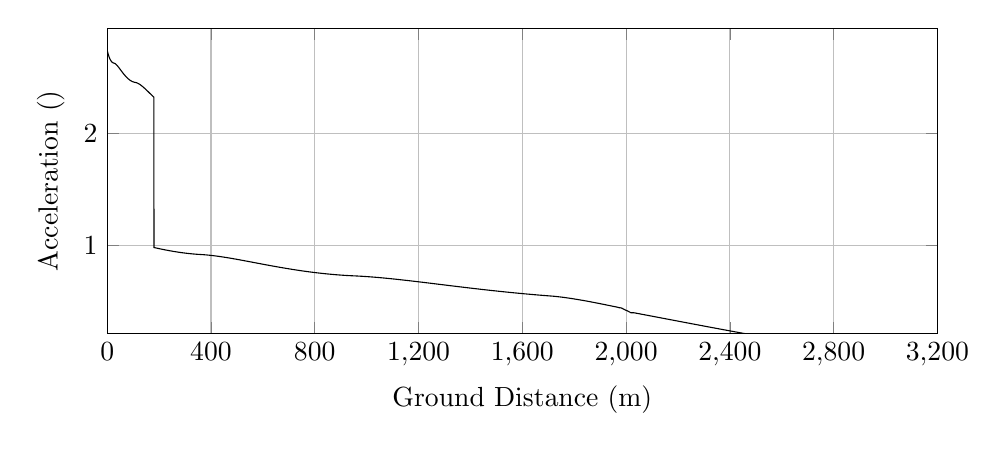
\begin{tikzpicture}

\begin{axis}[
width=\textwidth,
height=0.45\textwidth,
scaled ticks=false, tick label style={/pgf/number format/fixed},
xmin=0.0,
xmax=3200,
xtick={0,400,800,1200,1600,2000,2400,2800,3200},
xlabel={Ground Distance (m)},
xmajorgrids,
ymin=0.21592694018874944,
ymax=2.9383329541999035,
ylabel={Acceleration ($\si{\meter\per\square\second}$)},
ymajorgrids,
]

\addplot [
color=black,
solid
]
table[row sep=crcr]{
1.3729668748937997E-8	2.745933749634024\\
2.6049868369719035E-7	2.7459337463216693\\
2.0491224421327626E-6	2.7459337223163676\\
9.92442121137073E-6	2.74593361664894\\
4.7452367809869807E-5	2.7459331133935008\\
1.740064756114434E-4	2.74593141796994\\
4.0608377013922605E-4	2.7459283128250895\\
7.313431501337001E-4	2.745923966728787\\
0.0011549487327126044	2.7459183141309005\\
0.0016799013484208249	2.745911318665595\\
0.002295089346817705	2.7459031318683342\\
0.003009933382444524	2.745893631784023\\
0.003810608015426248	2.7458830054499908\\
0.004723484476856681	2.745870906509789\\
0.005727138856912631	2.7458576226878897\\
0.006836216967948795	2.7458429637322794\\
0.007997302399386296	2.7458276382144833\\
0.00929136979810952	2.745810580608766\\
0.010685558505459776	2.745792228663979\\
0.012178513621519987	2.745772603889116\\
0.013775244426719659	2.7457516442133327\\
0.015470070176169002	2.7457294279658626\\
0.0172374436815836	2.7457062929339147\\
0.019122918912604377	2.745681646264188\\
0.021104911040230538	2.7456557742244776\\
0.023190717999955576	2.7456285852738693\\
0.025355802981115103	2.7456004025085097\\
0.027620619195902148	2.7455709628304676\\
0.030020274690474198	2.7455398145480876\\
0.032476028269866286	2.7455079832228666\\
0.035054163466719815	2.745474612816359\\
0.037720846868992755	2.7454401452809734\\
0.04049779674511381	2.745404303593875\\
0.043329456594087365	2.745367807581193\\
0.04629652060163805	2.745329620662332\\
0.04934498934704602	2.745290442016606\\
0.052507657924119336	2.7452498537718295\\
0.055769483710642484	2.745208053078813\\
0.05917209570914676	2.7451645112972916\\
0.06264043916012321	2.7451201927906688\\
0.06620063977265622	2.745074766280724\\
0.06987962792775945	2.745027892179869\\
0.0736568184539585	2.744979836976057\\
0.07754284280095361	2.744930469346733\\
0.08151127871105612	2.744880128455919\\
0.08560324933017655	2.744828296550115\\
0.08985265585263943	2.7447745502252845\\
0.09413961367176535	2.7447204093860247\\
0.09857725310864562	2.744664448697618\\
0.10307959255469257	2.7446077566104368\\
0.10766008648593872	2.744550165853771\\
0.11234920964493048	2.744491296646081\\
0.11719267720457946	2.7444305805763873\\
0.12216973960582883	2.7443682839908865\\
0.12724007601918352	2.7443049160916244\\
0.13233299746505212	2.7442413617081813\\
0.13755256756750583	2.744176324555065\\
0.14287728588926696	2.744110077183268\\
0.1482946925752714	2.7440427783081276\\
0.15381585025670613	2.7439742941590106\\
0.15940564092189102	2.7439050633216198\\
0.16526271495916878	2.743832633069937\\
0.17120082448158402	2.743759314593124\\
0.17717889132867753	2.7436856165854584\\
0.18324322596131126	2.7436109697873574\\
0.189427022360885	2.7435349695339406\\
0.1957511558722988	2.743457364727397\\
0.2021484013779125	2.7433789844510024\\
0.20865863707071397	2.743299343476986\\
0.21548666343168166	2.7432159468507686\\
0.22220154781289658	2.743134061837388\\
0.22919671627301902	2.7430488935802986\\
0.23611678795738544	2.742964772871866\\
0.24306300975244904	2.7428804655838492\\
0.2503085190632165	2.7427926639555604\\
0.2576623280401219	2.74270369213178\\
0.26502430524173204	2.7426147629356477\\
0.2724963584449146	2.7425246467856903\\
0.2802001060647876	2.7424318847655185\\
0.2878583985474956	2.7423398174571867\\
0.2958320780323821	2.74224411264151\\
0.3040021452321372	2.7421462114990494\\
0.31208951788619	2.74204945948628\\
0.3202851396023423	2.7419515709453375\\
0.3287233234973125	2.7418509498073105\\
0.3370425959884752	2.7417519080250115\\
0.34575405233845447	2.7416483668644354\\
0.3545073625286812	2.7415445008529415\\
0.36338982075299686	2.74143927707345\\
0.37247557159370037	2.741331824878821\\
0.38151350442869847	2.741225116473271\\
0.3905554764834429	2.7411185361982797\\
0.3999457587520332	2.7410080342749286\\
0.4095398754587949	2.740895325049965\\
0.4189621792151833	2.7407848203234915\\
0.4285208811402964	2.7406729022160494\\
0.43828968955472236	2.7405587157868423\\
0.44807735398784176	2.740444501168418\\
0.45806002753764463	2.740328206966173\\
0.4682994371692033	2.740209125317234\\
0.4787752542918833	2.7400875051939693\\
0.4890770094685154	2.739968111629965\\
0.49985939134273727	2.739843363987376\\
0.5106597490205704	2.739718627718031\\
0.5213580865152188	2.739595283866114\\
0.532247733242454	2.739469951000051\\
0.5431365108549349	2.739344844457758\\
0.554075964429489	2.7392193713226414\\
0.5653450694020941	2.7390903409366887\\
0.5769901159382542	2.738957242270053\\
0.588512657344902	2.738825777773906\\
0.6004070039036553	2.7386903129467894\\
0.6121651247369502	2.738556638601956\\
0.6239717914322569	2.7384226491592862\\
0.6362472885961421	2.7382835883504875\\
0.6486428939173223	2.738143422272314\\
0.6610190736373547	2.7380037294208224\\
0.6737248046101814	2.7378605779440788\\
0.6862826225989949	2.7377193504710986\\
0.6991952542603428	2.7375743971928808\\
0.7122988072688032	2.737427572331951\\
0.7251463703465595	2.7372838790900627\\
0.7381769453061875	2.737138402838057\\
0.7516618647379176	2.7369881315120947\\
0.7654913705221527	2.736834310606014\\
0.7791756406994825	2.7366823919487455\\
0.7930637813125616	2.7365284991417216\\
0.8074774191984457	2.736369088689556\\
0.8215072375247947	2.7362142192435908\\
0.8361010597475598	2.736053431219534\\
0.8503303420601955	2.7358969585996338\\
0.8650627501899835	2.7357352618278403\\
0.8802332960144008	2.7355690814348668\\
0.8951742046771463	2.7354057362911055\\
0.9100334756324657	2.7352435957730297\\
0.9251067343345352	2.735079435666237\\
0.9403923630470314	2.7349132844243806\\
0.9559303815501943	2.7347447191307284\\
0.9712400158034169	2.7345789536451193\\
0.9869533781138684	2.7344091466658877\\
1.0029148609762486	2.734236997780573\\
1.0189962473881624	2.7340638988954913\\
1.035465185745812	2.733886982622522\\
1.0516742337458713	2.7337132054216866\\
1.067815735429615	2.7335404920408557\\
1.0846705971808022	2.7333605047019978\\
1.1012775250051634	2.7331835208984128\\
1.1180798406225687	2.7330048116164747\\
1.1351395900544134	2.7328237286921633\\
1.1526388687279154	2.73263835894707\\
1.1698922447507556	2.732455966615972\\
1.1875468452119025	2.732269712848928\\
1.2058383275300355	2.732077142510799\\
1.2239395537495579	2.731886975352393\\
1.2422020624207541	2.7316955142157697\\
1.2608769472440078	2.7315001426275947\\
1.2794948487006894	2.731305779649479\\
1.2979152553275424	2.7311138807814563\\
1.3166445915281573	2.73091917093961\\
1.3354141707340492	2.730724451882275\\
1.3543210821322504	2.730528719277727\\
1.373689361295591	2.73032863525778\\
1.3932049885015831	2.7301274608942405\\
1.4131781782225183	2.7299220154585475\\
1.4330139682345777	2.7297184263544425\\
1.4528243860883294	2.7295155352372795\\
1.4728783400745615	2.729310592226655\\
1.4934621752870565	2.729100693669997\\
1.5141408097620341	2.7288902940171758\\
1.53430654450827	2.7286855593626536\\
1.5553850389607948	2.728472025774905\\
1.5762653203499473	2.7282609685761434\\
1.5975496774716453	2.728046303569938\\
1.6196077215345106	2.7278243397435746\\
1.6413652536722467	2.727605899295412\\
1.663437310723463	2.7273848044555544\\
1.6860768385032747	2.727158548431424\\
1.7077101022266827	2.726942840558346\\
1.7297306410738114	2.7267237613893585\\
1.7520297891459062	2.7265024111794576\\
1.7743087535215367	2.7262817613558035\\
1.797257424336919	2.7260549980011213\\
1.8200802473615325	2.7258299974170024\\
1.8430350373473994	2.7256042147901303\\
1.8666926279964304	2.7253720605720746\\
1.8902808566018634	2.72514113040999\\
1.9138231309717848	2.7249111877288685\\
1.937187877956735	2.724683506686569\\
1.9611060682733261	2.724450973682445\\
1.9852138445648535	2.7242171481062742\\
2.009780393513653	2.723979437924413\\
2.0346228225622163	2.723739634761041\\
2.0593611988602687	2.7235014085153804\\
2.08477023517836	2.7232573149932806\\
2.110324766702745	2.7230124241566775\\
2.1352655781940433	2.722773991682768\\
2.160528860803022	2.7225330540312687\\
2.1862071157614817	2.722288750937233\\
2.2127756699400534	2.7220366021467237\\
2.2391904543957084	2.721786538650564\\
2.2653528664920257	2.721539475818613\\
2.292150575495974	2.7212870407551826\\
2.3187704640870406	2.721036905412479\\
2.3455495914188482	2.7207858982332622\\
2.372862901366455	2.7205305254301893\\
2.4007145172972395	2.7202707826704753\\
2.428100404243743	2.72001603228333\\
2.4555980306928005	2.7197608861757034\\
2.483374904362833	2.7195038000855876\\
2.511687733451976	2.7192424230947587\\
2.5402569276484597	2.7189793606402857\\
2.568415369317849	2.71872074613543\\
2.596987652715761	2.7184590025560453\\
2.6263861238451423	2.7181903927500546\\
2.655991481965028	2.717920608348247\\
2.6856115886357443	2.7176514041804687\\
2.7154221146045012	2.71738118698586\\
2.7455665152057707	2.7171086712897807\\
2.7752624694325894	2.7168409213882985\\
2.805457625653509	2.71656939071722\\
2.8358231840904597	2.716297056032584\\
2.8663460878589797	2.7160240421896784\\
2.897817297850832	2.7157433103512467\\
2.9287074004595235	2.7154685124985987\\
2.9603588456990284	2.715187708551693\\
2.9922321403815406	2.71490571640717\\
3.0241119471841866	2.71462444530067\\
3.056446055158509	2.7143399570513758\\
3.0889346922121366	2.7140549072190137\\
3.122221620829695	2.713763678408176\\
3.1546991615623394	2.7134803314856493\\
3.187635101478671	2.7131937884197734\\
3.221010117202278	2.7129042459478487\\
3.2543449374576605	2.712615872270808\\
3.288235920596943	2.7123235230382576\\
3.3223704322934555	2.7120299202652527\\
3.3562838593334394	2.7117390566035233\\
3.3906320903803255	2.7114453101597196\\
3.425633159699527	2.711146852210671\\
3.462387235801926	2.7108343880622456\\
3.4973980805087237	2.710537636483595\\
3.5324804241140235	2.710241147744873\\
3.5675385073174235	2.709945728382193\\
3.6040688981843845	2.709638816969628\\
3.6393612181513753	2.7093431890244997\\
3.6770856360342323	2.7090281416612143\\
3.7131729334920323	2.7087276833232927\\
3.749509707933214	2.7084260491268246\\
3.785733977879824	2.7081262444468592\\
3.8225309786916544	2.707822610564083\\
3.860867115351552	2.7075072478509306\\
3.89929745075254	2.7071921001654697\\
3.9373367205567504	2.706881130446619\\
3.9751626485832894	2.7065728578762025\\
4.013671158053867	2.7062599937888168\\
4.0521140617426425	2.7059486353631357\\
4.092377631210638	2.705623567578243\\
4.131586743753305	2.705308027124949\\
4.1715696979561425	2.7049872843873297\\
4.210522654700574	2.7046757949824176\\
4.250196810863292	2.704359538589963\\
4.2917015001093795	2.7040297652367293\\
4.332438976653355	2.7037071511860633\\
4.373124372895289	2.7033859958341147\\
4.414429464889761	2.703061013141131\\
4.455884944705147	2.7027359201134686\\
4.497250153511752	2.7024126010589393\\
4.537976875075978	2.7020953078843215\\
4.581399817640802	2.7017581350427298\\
4.623816269683994	2.701429893974078\\
4.666022338967499	2.7011043708260782\\
4.709098934189642	2.7007732491577343\\
4.752435367147649	2.7004412618628235\\
4.79531009100786	2.700113923220311\\
4.838191999420829	2.6997876304091646\\
4.881381760681686	2.6994601025113845\\
4.9256451804034285	2.6991255802428515\\
4.9704217340957495	2.6987883563581185\\
5.014356093293278	2.6984586198088563\\
5.058826350846283	2.698126010287651\\
5.104458009943745	2.697785910252903\\
5.149663211268795	2.697450177563721\\
5.194981168813841	2.6971147895925576\\
5.241194091283663	2.696773991377621\\
5.287987552078626	2.696430154327218\\
5.334426822383641	2.6960901499960244\\
5.380633359096258	2.6957530602096966\\
5.427524438012913	2.6954122052897027\\
5.476157635197664	2.6950599883398825\\
5.524667120325573	2.6947099813886997\\
5.5732739519824435	2.694360582160768\\
5.6208990292882195	2.6940195060851275\\
5.671502816366864	2.693658464116621\\
5.719824083529298	2.6933150154219874\\
5.767871110439133	2.6929747772519512\\
5.8169321963676754	2.6926286501345027\\
5.866076914057565	2.6922832358810025\\
5.917200682776528	2.691925289335387\\
5.96684810088939	2.6915790178532983\\
6.016885842403935	2.691231352228524\\
6.068639931677712	2.6908731577503717\\
6.119867755785197	2.6905199976544543\\
6.171030794930029	2.6901686602208663\\
6.222884713227881	2.6898139753337107\\
6.2735946138732235	2.6894684695538738\\
6.325883502103322	2.6891136013011465\\
6.379615386553551	2.6887504096481347\\
6.432194972482147	2.688396442468087\\
6.484528316464761	2.6880455368872473\\
6.536619297696934	2.68769764118571\\
6.589662958081361	2.687344796419861\\
6.644121795496577	2.6869840153423956\\
6.697445536614451	2.68663219810922\\
6.7518063163896365	2.686275003043974\\
6.8068829439682315	2.685914605406988\\
6.863205650636274	2.685547609679398\\
6.9185329265047315	2.685188625021353\\
6.974634519184049	2.684826152672259\\
7.031139830722298	2.6844626288388405\\
7.0870923879294985	2.6841041940757817\\
7.144766952910487	2.6837363176346836\\
7.2026451873548805	2.683368757231797\\
7.261191729679483	2.682998591553873\\
7.320502240843062	2.682625268876813\\
7.378210233177999	2.6822636424501294\\
7.437738452534925	2.6818922655745236\\
7.49714639104333	2.681523308417665\\
7.556502460410064	2.6811563316145213\\
7.617032771987237	2.680783794499826\\
7.676883327249088	2.6804171211405423\\
7.735740247984193	2.6800581575988813\\
7.796086087039788	2.679691776501249\\
7.856787102853412	2.6793249307229674\\
7.91721236259451	2.678961429481797\\
7.979013602666894	2.6785913752038963\\
8.039824025454376	2.6782289487607027\\
8.102419182184594	2.6778576340357727\\
8.16459313580776	2.6774905665511346\\
8.226347093952135	2.677127696565849\\
8.290527749984296	2.676752373844961\\
8.353592793320257	2.6763853613705777\\
8.417564177281012	2.67601487568339\\
8.482044607535009	2.675643270078857\\
8.547336806956285	2.6752688485572547\\
8.613293246319614	2.6748925126021685\\
8.6778048537894	2.6745262550450724\\
8.74454839911753	2.674149227258674\\
8.810708373588199	2.673777396453808\\
8.876548424968423	2.673409234250302\\
8.942828456712885	2.6730404887927257\\
9.010858044488913	2.6726639601609223\\
9.079453414959548	2.6722862922314583\\
9.148767802603732	2.6719066890561036\\
9.21609997183467	2.6715398811000908\\
9.285579683381485	2.67116336940079\\
9.355451712480097	2.670786767326205\\
9.423585014597279	2.670421494476032\\
9.493435356703696	2.6700490148237135\\
9.562655940911181	2.6696818813962357\\
9.63183713653898	2.669316926216502\\
9.703018708836247	2.6689434650398702\\
9.773178624863132	2.6685773872877823\\
9.844376937811855	2.6682079365263496\\
9.914998792594716	2.6678435040567887\\
9.98720270419701	2.6674729864037268\\
10.059478150570087	2.6671041981501142\\
10.132362020358627	2.6667344209387407\\
10.205876892438312	2.6663635857706476\\
10.279422251887688	2.6659947421935097\\
10.353305644514993	2.6656263553136483\\
10.42811398108589	2.6652555454284528\\
10.50332954727428	2.664884928557493\\
10.578207710262959	2.6645181680900603\\
10.65503529959097	2.6641441252244062\\
10.730232142651953	2.6637802356245537\\
10.805871937852555	2.6634164032193377\\
10.88265320376452	2.6630493287809767\\
10.958577899345514	2.6626885682826185\\
11.034861147941964	2.662328317504069\\
11.112742623646977	2.6619627989513033\\
11.190543636431041	2.661599949051814\\
11.267787598939979	2.6612419536263943\\
11.3462805052093	2.6608804641262784\\
11.423875697147409	2.6605253733666894\\
11.502735831556972	2.66016679186927\\
11.581465323066688	2.6598111062891867\\
11.661639233340708	2.6594512496614984\\
11.741743247575428	2.659094070532034\\
11.821864700430528	2.6587391681041073\\
11.901816327719768	2.6583873562373483\\
11.98361062800689	2.65802984404648\\
12.065425957085825	2.657674667049518\\
12.1478520915771	2.657319283720091\\
12.230956215923495	2.6569634524950505\\
12.313306905825911	2.6566132897052395\\
12.396632357805931	2.656261447402212\\
12.479578787946746	2.655913659143116\\
12.564327762802186	2.6555608318228234\\
12.648175874147956	2.655214251081233\\
12.736145481689512	2.6548532930755826\\
12.821080154398764	2.6545073614738826\\
12.908009536077355	2.6541559136608868\\
12.994986774303499	2.6538069029568296\\
13.081752199798046	2.6534613540348904\\
13.17035388279784	2.6531111740371047\\
13.257836697901475	2.652768065088189\\
13.34511613365563	2.652428366974772\\
13.433461823066896	2.6520871672573874\\
13.524108483575919	2.6517398400805456\\
13.611203924103116	2.6514087427638877\\
13.702229394080796	2.6510654420726993\\
13.792427706753081	2.650728010041674\\
13.882429934062493	2.6503940290968764\\
13.975435778888343	2.650051743756091\\
14.065832730112316	2.6497218173613817\\
14.157894546480026	2.649388598244756\\
14.250668806951023	2.649055631782466\\
14.343291987615704	2.6487260325270725\\
14.43744444968501	2.64839387373258\\
14.532636396723657	2.6480609912501123\\
14.625507232812737	2.6477390675021404\\
14.721503924398366	2.6474092478024884\\
14.818738382089133	2.6470782104461428\\
14.913572076739943	2.6467582780736505\\
15.009701633366973	2.6464369177531655\\
15.10815424447124	2.6461108524555685\\
15.206130868840724	2.6457894275225193\\
15.304035939715973	2.6454712794394446\\
15.403499839366233	2.645151168619309\\
15.503209871950865	2.6448333932172794\\
15.601718454553605	2.6445225108434887\\
15.700655560608023	2.6442133305209685\\
15.801250929860519	2.6439020954003567\\
15.899917805652187	2.643599879299895\\
16.001574124100856	2.6432916569963822\\
16.102638779863817	2.6429883870635598\\
16.204479333764816	2.6426859631921458\\
16.30489644092564	2.642390875444015\\
16.40578186591999	2.6420975095348966\\
16.509201471948074	2.641799986524223\\
16.614557195984908	2.6415002256988815\\
16.717657554831042	2.641210126302675\\
16.823039336622365	2.640916912552081\\
16.928576062495388	2.6406266046044653\\
17.03469945574068	2.640338038396731\\
17.140697318244236	2.640053160739731\\
17.246066414787876	2.639773277049187\\
17.35183930840021	2.639495622702711\\
17.458399953804133	2.639219234411631\\
17.565707112453843	2.6389442799060117\\
17.673103795073075	2.638672470550473\\
17.781888038667653	2.638400579402105\\
17.89115167195854	2.6381309531423165\\
18.00105710767307	2.63786323255278\\
18.110142905530395	2.6376009574466197\\
18.219697237410173	2.637341002414172\\
18.32752951944549	2.6370884953076636\\
18.43743745973078	2.6368345484445737\\
18.54904630654982	2.63658019384358\\
18.659302591714813	2.6363323952736817\\
18.770734536087716	2.636085450694776\\
18.883577445650936	2.635838949357387\\
18.996263390583444	2.635596364184675\\
19.108816920034535	2.635357616908477\\
19.22287647779894	2.6351192855805\\
19.33763586704334	2.6348831480062795\\
19.456324114791514	2.6346427711361047\\
19.57349394116079	2.634409291852097\\
19.690148252848566	2.634180600096859\\
19.80521137071168	2.633958691418372\\
19.92379170801214	2.633733794227746\\
20.04216631061405	2.6335131166802155\\
20.15848954929409	2.6332999786096893\\
20.278242138037896	2.6330843918964613\\
20.396206084226087	2.6328758170334643\\
20.516315546862906	2.632667302876359\\
20.637173924977112	2.632461401533406\\
20.75450010628387	2.6322652607421713\\
20.874378237858778	2.632068650375719\\
20.996035953832852	2.6318730325170687\\
21.11812959618858	2.6316806625120934\\
21.240471115580952	2.631491857446668\\
21.361479376438375	2.6313089928781865\\
21.485224699488654	2.631125973433857\\
21.607870280890317	2.6309485406063304\\
21.73242999733349	2.630772361329301\\
21.85704493170313	2.6306001480967662\\
21.98122016226351	2.6304325538620574\\
22.10826921766411	2.6302652125995127\\
22.235261614051304	2.6301021093246337\\
22.361664688868032	2.629943883831288\\
22.48780138980522	2.6297900776934346\\
22.614107216476143	2.6296401428980527\\
22.74409311379692	2.6294900871360998\\
22.873024137794893	2.6293454925824022\\
23.003512644166257	2.6292034414201826\\
23.132891545907036	2.629066846405708\\
23.26270690888247	2.628934029456868\\
23.39264146728729	2.6288053298831127\\
23.52277721573431	2.6286806696961964\\
23.654883767164463	2.6285584477188975\\
23.78569183677709	2.6284417091087624\\
23.917003007077597	2.628328794588147\\
24.047013652206026	2.628221204195908\\
24.178458227988493	2.6281166694027984\\
24.314609552493202	2.6280128759318746\\
24.447533097503474	2.627915932898171\\
24.579128452041708	2.627824218719879\\
24.71011994849615	2.627737123338611\\
24.843278471916108	2.627652868038229\\
24.975761222328053	2.6275733117861915\\
25.1115496753864	2.6274961796102385\\
25.247101122854083	2.627423621584068\\
25.384906965000688	2.627354391118195\\
25.522261036073317	2.6272899242628656\\
25.66123001648475	2.627229296090176\\
25.79865327455613	2.627173876444852\\
25.826335196219034	2.6271632574604533\\
25.839610403727477	2.62715822969495\\
25.841006316401874	2.627157703174394\\
25.84227013303559	2.6271572259940434\\
25.84770509053729	2.6271551682557828\\
25.86419328224909	2.627148869514051\\
25.90571916957557	2.627132632727095\\
25.999268866927544	2.62709410603191\\
26.123295978662824	2.627038901212371\\
26.250212562581652	2.6269775933396176\\
26.376891976518465	2.626911599588503\\
26.50638698165423	2.6268392423555404\\
26.634042370994827	2.6267631265942892\\
26.763333806613538	2.626681250837172\\
26.893207366259766	2.62659421847878\\
27.022905486492228	2.6265025738361114\\
27.153956322362554	2.626405232066988\\
27.287774297957696	2.626300978647955\\
27.42030033806219	2.6261929566003683\\
27.555504894698295	2.626077916748084\\
27.691130018821354	2.6259576762016144\\
27.82633313037239	2.6258330443348266\\
27.959508564917073	2.625705689812035\\
28.096515548835796	2.6255699768647354\\
28.232789703382153	2.6254303281033025\\
28.368684388406535	2.625286498680893\\
28.506541650227618	2.6251359904785243\\
28.64533374691623	2.624979841336361\\
28.78297783415192	2.624820465669056\\
28.92277775692753	2.6246540493487274\\
29.06227187463503	2.624483493060775\\
29.20212864139956	2.6243080372215513\\
29.34335827861657	2.624126392094661\\
29.483225747293005	2.623942134485322\\
29.625960812476485	2.623749682168036\\
29.76706561118049	2.6235551018597727\\
29.909402910999468	2.6233545237810842\\
30.051751399473822	2.623149671618658\\
30.196612335666572	2.6229368923312792\\
30.342192969749448	2.6227187353115538\\
30.48583400527584	2.6224992991267593\\
30.632658550781265	2.622270763203243\\
30.77846394498075	2.6220396350772806\\
30.92408133049836	2.6218047080288107\\
31.071091331299215	2.6215634400823893\\
31.218274793935116	2.6213178254024356\\
31.366705758252415	2.6210660719563164\\
31.515339333797037	2.6208099515408767\\
31.66356819769615	2.620550577189582\\
31.814689402684216	2.6202821391202162\\
31.96649953392354	2.6200084685109024\\
32.115424616034375	2.6197361526902787\\
32.266253234088566	2.619456531320976\\
32.41813832080348	2.6191711196609058\\
32.569791431087395	2.6188823653016966\\
32.722234201183724	2.618588359660447\\
32.876984607664	2.6182861188418736\\
33.031873994672836	2.6179798472058744\\
33.18502245018544	2.61767337730517\\
33.34135780547538	2.6173568541876238\\
33.49759920343199	2.6170368690402794\\
33.65385117142162	2.6167132684054444\\
33.8113313806527	2.6163835453824538\\
33.96985264489639	2.6160480723691215\\
34.126473036379195	2.6157131607910555\\
34.2857505660089	2.6153690959358693\\
34.4449212019973	2.6150218218705428\\
34.60566879064274	2.6146676745052684\\
34.76644486933921	2.614310071010496\\
34.92612701881755	2.613951597544056\\
35.08630421658309	2.6135887608266746\\
35.24825698849928	2.613218646437778\\
35.412303951281956	2.6128404656979436\\
35.57355277914179	2.612465573208352\\
35.73545353069308	2.612086065190393\\
35.89925038949356	2.6116990063305368\\
36.065161289279985	2.611303822719635\\
36.23047312008262	2.6109069894047563\\
36.39472205714358	2.6105097203642957\\
36.56135389445764	2.6101036997752756\\
36.72774532558607	2.609695316287241\\
36.89384825683493	2.6092847556652456\\
37.05904296416534	2.608873633171015\\
37.22702676294645	2.6084527521107095\\
37.39437475321985	2.6080306918927274\\
37.5621109943643	2.607604928234461\\
37.73270471709142	2.607169167240153\\
37.903359519601935	2.6067305347705387\\
38.071486842086316	2.6062957943756917\\
38.23815243703595	2.6058623319798837\\
38.40817787072022	2.6054176148453294\\
38.57751392140098	2.604972224462812\\
38.750215798728505	2.604515486819169\\
38.92001182640311	2.604064028086343\\
39.09310637700479	2.6036013939253158\\
39.26472366117933	2.603140360230884\\
39.436554723976656	2.6026764590104268\\
39.608961777617054	2.602208745072529\\
39.782828308010565	2.6017348303452126\\
39.956194359016465	2.6012600869258415\\
40.132391837044906	2.6007753954833523\\
40.30868053167249	2.6002882883371417\\
40.48611580488176	2.599795875967091\\
40.66383502946924	2.599300575623608\\
40.83999042132467	2.5988076076289266\\
41.018202681018664	2.598306879012876\\
41.19780999006247	2.59780023921822\\
41.37730467548502	2.5972919679986406\\
41.557010452813884	2.5967811949022925\\
41.73612816026986	2.5962702442991796\\
41.91555194917056	2.5957566162813004\\
42.09743589423803	2.5952341495078093\\
42.27807550146298	2.5947135135520316\\
42.45995188234755	2.594187603754664\\
42.6401410478328	2.593664926422731\\
42.822293873795985	2.5931349327029034\\
43.00585672428667	2.5925992336587598\\
43.189965171449515	2.592060371841985\\
43.372020236704074	2.5915260176090396\\
43.555636897252796	2.5909856106444664\\
43.74012033961118	2.5904412105939336\\
43.92429822300048	2.5898963139394615\\
44.106869824379004	2.5893548329369107\\
44.29411840239129	2.588798141810776\\
44.47920670866131	2.5882465834656143\\
44.665034305215386	2.5876915745572395\\
44.85242224248053	2.5871306821366113\\
45.03948098831597	2.5865695920897522\\
45.22811764277584	2.586002614453135\\
45.41548629589063	2.5854383417605273\\
45.60322541388645	2.58487188864763\\
45.793007222766036	2.584298230300096\\
45.983742663331824	2.583720675421648\\
46.172643153142886	2.58314771556424\\
46.36421599110457	2.582565713945945\\
46.553512793459404	2.5819897407332553\\
46.745018895697555	2.5814061887802406\\
46.93606459490553	2.580823220829023\\
47.126948089509526	2.580239969889381\\
47.31881294044018	2.579652975509168\\
47.5110690178297	2.5790640736859434\\
47.705448624448266	2.5784679831468953\\
47.90005519882567	2.577870546429364\\
48.09288923506665	2.577277947636331\\
48.28732881729917	2.576679844114947\\
48.484002572746206	2.5760743233998253\\
48.68089030454945	2.575467633349363\\
48.87532723390382	2.57486803095897\\
49.07073736177763	2.5742649991859343\\
49.2672083392297	2.5736582972862303\\
49.46586249263092	2.5730444865995894\\
49.661880987188695	2.5724384938105347\\
49.85966148345089	2.5718267615262587\\
50.05808618672894	2.571212777407524\\
50.25785665917266	2.570594402569249\\
50.45743808511885	2.569976421527972\\
50.65573800086891	2.5693622538365988\\
50.85948768734909	2.5687310825359084\\
51.061243703011925	2.5681059980424292\\
51.26368286286315	2.567478743109982\\
51.46416466063809	2.566857533975103\\
51.66475943174029	2.5662359893110347\\
51.86588207153103	2.56561285677663\\
52.07444928962187	2.564966744465173\\
52.2824430085781	2.5643225310284814\\
52.48676525705545	2.5636898422625745\\
52.69531994892206	2.5630442386830037\\
52.90027076850366	2.562410012697458\\
53.108186167814935	2.5617668705752035\\
53.31165724918766	2.561137759462768\\
53.520024946679996	2.560493831718171\\
53.72688450142306	2.559854920280424\\
53.93707391647578	2.5592061198138465\\
54.14518573319289	2.5585641573342945\\
54.35125853722778	2.5579289322446064\\
54.56213447502874	2.5572793940255876\\
54.77598621923464	2.5566212311207\\
54.987629956235494	2.5559704324655836\\
55.19778857845695	2.5553247914147734\\
55.41030974885841	2.55467252202679\\
55.62390503323701	2.554017625167454\\
55.83671574169797	2.553365831759879\\
56.047071254351536	2.5527222723040826\\
56.26137331252919	2.5520673989185383\\
56.47512769358855	2.5514149930840677\\
56.69105800830218	2.55075678108659\\
56.90937011004422	2.5500921924420785\\
57.12736617899088	2.549429482767894\\
57.346833156368504	2.5487632574065238\\
57.56476609337061	2.5481026676419045\\
57.78230894703917	2.547444262133678\\
57.99943865551505	2.5467881336539273\\
58.21827465292657	2.5461279153126446\\
58.436085045729726	2.545471882108224\\
58.6577546799423	2.5448053710641405\\
58.87982836766625	2.544138832936956\\
59.10336118170943	2.5434691447546607\\
59.324182403931715	2.542808819305696\\
59.545440661451366	2.5421484495030766\\
59.768227251413464	2.5414848224466517\\
59.99077485409802	2.540823240966116\\
60.21631063559073	2.54015416369662\\
60.44006004384342	2.539491792913134\\
60.66502706168687	2.5388272572727564\\
60.89133011288284	2.5381602583073883\\
61.11585558357916	2.5374999948556693\\
61.3432655409558	2.5368327945800493\\
61.57186440401435	2.5361637002878803\\
61.79868765088207	2.535501408748763\\
62.025670725987	2.5348402770909786\\
62.254132946411545	2.5341765056009926\\
62.48290793247415	2.5335135279774255\\
62.713817944074236	2.5328461162466924\\
62.94484116346062	2.5321801651283318\\
63.17805109236767	2.5315097497788024\\
63.41124119062552	2.530841264404774\\
63.64505576847972	2.5301728944345925\\
63.87735201907903	2.5295107788661895\\
64.11169045660182	2.5288448001638137\\
64.34725756208485	2.52817733598523\\
64.58324360279937	2.527510726208688\\
64.81881329818131	2.5268473544899654\\
65.05563560606473	2.5261825559991893\\
65.29467812810154	2.5255136850947695\\
65.53178653633495	2.524852393698131\\
65.77046761369158	2.5241889200770515\\
66.01019347650049	2.523524791474693\\
66.25262920761091	2.52285547188822\\
66.49342175078831	2.522193018006006\\
66.73393309567928	2.5215336779391944\\
66.97718905970893	2.52086921586132\\
67.21919788222482	2.5202105803525665\\
67.46413738735515	2.519546449583455\\
67.70584739194695	2.518893544044623\\
67.95375887035246	2.5182264574902717\\
68.19817148521656	2.5175713561374016\\
68.44413350233111	2.5169147004876002\\
68.68984243621705	2.516261345089669\\
68.93951041285982	2.515600171501796\\
69.19023531750676	2.514938969433662\\
69.43956667494601	2.514284217583624\\
69.68998597860525	2.513629416130965\\
69.94098943220166	2.512975932155717\\
70.1928405184459	2.5123231255440013\\
70.44659484061637	2.511668329081634\\
70.69926103579675	2.5110192971929557\\
70.95414956377036	2.5103675673854084\\
71.21136313866151	2.5097129793716446\\
71.46778788208749	2.509063506597747\\
71.7247351381395	2.5084158438377147\\
71.98234155897126	2.507769689085089\\
72.24107377350035	2.5071239256193767\\
72.4986091150376	2.5064843695454924\\
72.75949164810788	2.505839797213234\\
73.02014691132015	2.505199119753618\\
73.28114866838587	2.504560949336046\\
73.54342372888959	2.503923071226774\\
73.80584407854005	2.5032882764078206\\
74.07231166191039	2.5026472290607487\\
74.3389341302921	2.5020093971959803\\
74.60521354141642	2.501375988177486\\
74.87280568706873	2.5007431028336446\\
75.1403821105715	2.5001139292433843\\
75.41145333671997	2.4994803046180856\\
75.68265298797411	2.4988501932497016\\
75.95075857762194	2.498231039158717\\
76.2241428819712	2.4976035721719434\\
76.4990100438061	2.496976668570306\\
76.77213586328236	2.4963576955699853\\
77.04724851790667	2.49573822862106\\
77.32330034006353	2.4951207098630084\\
77.59850473375684	2.4945091566067346\\
77.87773830129439	2.4938928219842715\\
78.1565255546137	2.4932816837060106\\
78.43842651648492	2.492668017346257\\
78.720833678605	2.4920576010425153\\
79.00101298089581	2.4914563231480757\\
79.28359351218376	2.4908542717934887\\
79.57011733099088	2.490248328576058\\
79.85418914588558	2.4896520718283295\\
80.13919871477489	2.4890583687052414\\
80.42568449319114	2.4884661731421938\\
80.71472498530085	2.487873370981382\\
81.006853148924	2.487279025102887\\
81.2951972638476	2.4866971170884167\\
81.58524575795963	2.486116537145639\\
81.87461709596036	2.4855420949920353\\
82.1711642895769	2.484958381559892\\
82.46716486408064	2.484380782761332\\
82.76422974563803	2.483806186216814\\
83.05801377197795	2.483242957146957\\
83.35853301954708	2.482671999870737\\
83.65664966506407	2.4821108049392793\\
83.95487262936624	2.481554606519677\\
84.25322789115987	2.4810033792257986\\
84.55664509033022	2.4804481694309706\\
84.8599544590121	2.4798985860092557\\
85.16499148084048	2.4793513638033664\\
85.47187188044902	2.478806409028219\\
85.77908321853027	2.4782664837735044\\
86.08675489504844	2.4777313991684684\\
86.39784539041122	2.4771961342162765\\
86.71051296037359	2.4766640142286205\\
87.02583358957506	2.4761333445033173\\
87.34037846285594	2.4756099658506825\\
87.65395388450591	2.4750941674588303\\
87.96687312379424	2.4745854039580317\\
88.28527441497255	2.474073850456792\\
88.6103524516937	2.4735579588692937\\
88.92871226770333	2.4730590021066936\\
89.25003295857354	2.472561715850354\\
89.57522243846881	2.472064913921284\\
89.90247582737899	2.4715715482953424\\
90.22602529632545	2.471090281458441\\
90.5494223037065	2.4706157304863785\\
90.87816525326718	2.470140000358535\\
91.20455861430293	2.4696743344984124\\
91.53817773235312	2.4692052383281\\
91.87076195087604	2.46874453523425\\
92.20124984301029	2.468293613714687\\
92.53140503523474	2.4678500072923946\\
92.86389705561814	2.467410207209607\\
93.19815266874983	2.46697511608851\\
93.53304529783748	2.4665462917878456\\
93.86737084100128	2.4661252936021194\\
94.20337949361911	2.4657093387407842\\
94.54065981474497	2.4652990463300517\\
94.87396787418089	2.4649007234996034\\
95.21684847579547	2.4644983797555815\\
95.55392648231228	2.4641101935898275\\
95.89232371872416	2.463727831543161\\
96.23051075783204	2.463353072193108\\
96.57164052232307	2.4629825255521096\\
96.90762523479154	2.4626249186321765\\
97.24755293575913	2.462270552927021\\
97.58790661409188	2.4619232523826478\\
97.92576087813703	2.461585947168559\\
98.26661027452474	2.4612531815923795\\
98.6051908024865	2.4609301321117414\\
98.94563962387357	2.4606128512157275\\
99.28665364663627	2.4603026475156407\\
99.63350087797645	2.4599949576702347\\
99.97685593767679	2.4596981466115277\\
100.31593955776762	2.4594126383431973\\
100.65572384630482	2.4591341387793317\\
100.99616871909686	2.4588627388350837\\
101.3402339503516	2.458596236175948\\
101.67973054404297	2.458340953841132\\
102.01657591573795	2.4580952179760907\\
102.35656456518868	2.457854829697289\\
102.6941824316649	2.457623725275984\\
103.03547296258705	2.457397823628013\\
103.37623032340073	2.457180026797986\\
103.71852978299776	2.456969054425172\\
104.05851119314701	2.4567672705298635\\
104.3949509202441	2.4565752126830196\\
104.7329053851843	2.456389936423986\\
105.07104272194636	2.456212240406991\\
105.40742307340048	2.456043101164078\\
105.74423560014887	2.4558813834138933\\
106.07955743077031	2.455727984822288\\
106.41623710643992	2.4555816081016255\\
106.75618472497374	2.455441591416804\\
107.0942647435474	2.4553101084432747\\
107.43151869252583	2.4551866717490167\\
107.44650965670576	2.4551813642403237\\
107.45815118347005	2.4551772531208176\\
107.46233674961977	2.4551757772689795\\
107.46535588765028	2.4551747132015054\\
107.46808502617694	2.4551737507643727\\
107.4836206108138	2.455168259670489\\
107.53176708907421	2.4551511079163477\\
107.68672244793561	2.455094531599669\\
107.97570433527497	2.4549834451948627\\
108.27744765146667	2.4548597682328195\\
108.5816623935838	2.4547272061477434\\
108.88557241638279	2.4545869610121596\\
109.19209959959528	2.45443767243568\\
109.50241879336687	2.4542786003150896\\
109.81066605766154	2.4541127633367736\\
110.12101503747155	2.453937994054648\\
110.43285681965125	2.4537545790192175\\
110.74725799716322	2.453561818956234\\
111.06462449033057	2.4533593397004765\\
111.38211128519615	2.453148923592198\\
111.70119562731901	2.4529296108117045\\
112.02298633508096	2.452700564309909\\
112.34320819983824	2.452464869014065\\
112.66812620709393	2.452217884637398\\
112.99302416686388	2.451963112159949\\
113.31966045518399	2.4516991968576756\\
113.64998129974768	2.451424459279832\\
113.97857627498675	2.451143416865058\\
114.31304608469316	2.450849510906499\\
114.64448318111735	2.4505505571921855\\
114.98093514978115	2.4502393175308965\\
115.31969924418831	2.4499181287839766\\
115.65790718621022	2.449589741128423\\
116.00063352526521	2.4492491841404753\\
116.34235083463872	2.448901923487149\\
116.68621873349733	2.448544803075687\\
117.03331062078092	2.4481766222286128\\
117.37910048629482	2.4478022122028253\\
117.72869476105836	2.447416056567934\\
118.08005947084649	2.447020315368726\\
118.43363644355449	2.44661445841039\\
118.79186464668504	2.446195562722882\\
119.14769212941735	2.4457719010897243\\
119.5036618261702	2.4453406161077478\\
119.86270697471275	2.444898151431988\\
120.22616362054572	2.4444427272159954\\
120.58991121293201	2.4439794620158324\\
120.95538130513773	2.443506572675182\\
121.3195355377388	2.4430280793612997\\
121.68590041554987	2.4425394226513815\\
122.05305648207542	2.442042507730611\\
122.42257239354896	2.4415352206266228\\
122.79503144936103	2.4410167087569397\\
123.16629137010841	2.4404927909789507\\
123.53950748252527	2.439959095724661\\
123.91239367862553	2.4394189483888704\\
124.29026003316017	2.4388646308631676\\
124.66301933937496	2.438311045841078\\
125.03890311735066	2.4377461242287524\\
125.41380975776434	2.4371760734767376\\
125.7896808967325	2.4365980418067945\\
126.16837244152023	2.4360091772577572\\
126.54595968852882	2.4354156387065453\\
126.92471834906405	2.434813947054397\\
127.30294276405039	2.4342068948637348\\
127.68255852126984	2.433591469128208\\
128.06243727540487	2.4329695571547303\\
128.44360431740483	2.432339541404442\\
128.82265748788262	2.4317071612453454\\
129.1989690567886	2.4310736703116387\\
129.57765386613931	2.4304305602421765\\
129.95508099647026	2.429784065084977\\
130.33359114840187	2.4291302715149827\\
130.71373745886524	2.4284682576146626\\
131.09453904397424	2.4277997749107643\\
131.47657586018488	2.4271238577704235\\
131.85678563989967	2.426446027201812\\
132.23856625352113	2.42576032125654\\
132.61595336405918	2.4250775964184523\\
132.99976263915818	2.4243783357290276\\
133.38083522978053	2.423679242984316\\
133.76098428781995	2.4229771481541835\\
134.1363519425165	2.4222793654313444\\
134.51557915495124	2.421569932295995\\
134.8968696170101	2.4208521881638854\\
135.27419431482667	2.420137597883574\\
135.65215477207505	2.4194175854598914\\
136.03329358991255	2.4186873250908105\\
136.41192880753374	2.4179577730609862\\
136.7898079310749	2.417225694571063\\
137.17001317148595	2.4164851729427035\\
137.54844558779996	2.415744261492118\\
137.92617219433072	2.4150009862160164\\
138.30476964659732	2.4142523189260237\\
138.68390038934075	2.413498983015482\\
139.0631653430654	2.4127418378009757\\
139.4406106933401	2.41198488197385\\
139.81914660512416	2.4112223633220573\\
140.19767098864742	2.410456560906317\\
140.5730919292459	2.4096938425620706\\
140.95061983253072	2.4089237067743268\\
141.32838502869612	2.4081500093041033\\
141.70636515873298	2.4073728610224387\\
142.0839785067887	2.406593529688587\\
142.46357402350594	2.4058072184921997\\
142.84082211769783	2.40502296889394\\
143.21906727224075	2.4042339114596416\\
143.59963619096823	2.403437310882776\\
143.97984478872678	2.4026388326905357\\
144.35941603837455	2.4018391364099507\\
144.7355521893594	2.4010442230400466\\
145.11296635073694	2.4002442180265584\\
145.49073213867456	2.399441133914113\\
145.87033631970945	2.3986318541955978\\
146.24486520181193	2.397831210000894\\
146.6238757206513	2.3970188391759493\\
147.00096360401335	2.396208508945593\\
147.37874202190085	2.3953946757121454\\
147.756852900845	2.39457816388311\\
148.13572640408995	2.393758097000817\\
148.5136798644104	2.392938178662493\\
148.89083780486442	2.392118210713834\\
149.2712459042852	2.391289439886328\\
149.65303236723025	2.390455972301191\\
150.0329584616291	2.389624940771009\\
150.41363382646614	2.388790702960881\\
150.79322940570728	2.3879573271300165\\
151.17272478467066	2.3871227269328097\\
151.55400296227282	2.3862828087520374\\
151.93482601265913	2.385442551958211\\
152.31881414221942	2.3845940116132027\\
152.70208150063132	2.3837458190581575\\
153.08320649997165	2.382901190023449\\
153.4666285558243	2.382050340959543\\
153.84825937276264	2.381202396702336\\
154.23093781718723	2.380351107148919\\
154.61485031834388	2.379496102763693\\
155.00001234931443	2.3786373939872023\\
155.38285725409855	2.3777829898524283\\
155.7679513537659	2.3769227531344317\\
156.1509667875323	2.3760664034774726\\
156.53491934392343	2.3752072536116557\\
156.91995289130983	2.37434502792717\\
157.30625057946366	2.373479362158138\\
157.69121706207227	2.3726161237217385\\
158.07789765133754	2.371748534188164\\
158.46521012398495	2.3708790680405922\\
158.85138765236047	2.370011742814021\\
159.23964669847322	2.3691393833615075\\
159.62715395386465	2.368268403666744\\
160.01960115328984	2.367386056204964\\
160.4079207075476	2.366512776596168\\
160.79602490671402	2.36563981902208\\
161.18437278725975	2.364766199221803\\
161.57644284003254	2.363884138972799\\
161.96812230097612	2.363002938647095\\
162.35808768568592	2.362125623778489\\
162.75087300343483	2.3612420420191382\\
163.14546270495134	2.3603545272165904\\
163.53745675514648	2.3594730228399685\\
163.92955389373896	2.3585915050473067\\
164.32395276810763	2.357705079439211\\
164.71713266653478	2.3568217061873185\\
165.1102153740033	2.35593890902884\\
165.5035884424101	2.355055863096327\\
165.89816400198282	2.3541705682312966\\
166.29148626774366	2.3532885788431104\\
166.68861804276264	2.3523985917182593\\
167.082852347146	2.351515683455717\\
167.48006204110857	2.3506267458495653\\
167.8798182678497	2.349732796398407\\
168.27774435731556	2.3488436682392644\\
168.67741362640317	2.3479514207768712\\
169.07475368467374	2.3470651868695898\\
169.4759958044982	2.3461711163376826\\
169.87832784425882	2.3452755349517966\\
170.2792240364854	2.344384106753197\\
170.68126852540456	2.3434911272918937\\
171.08617821288442	2.3425928410644596\\
171.48766933901368	2.341703228415432\\
171.892744970828	2.340806814987485\\
172.29711201372032	2.339913155185136\\
172.70264003426053	2.339018160916506\\
173.1105289448074	2.3381192418897934\\
173.5163733808056	2.337226149563117\\
173.92577914808027	2.336326596791209\\
174.33607303977334	2.335426521117654\\
174.74614233406845	2.3345284082190787\\
175.15731444736514	2.3336293965914052\\
175.56901623635082	2.3327307892227083\\
175.97955109701695	2.3318363258755\\
176.39275298155184	2.330937702273025\\
176.80397138375372	2.3300450760546294\\
177.21946344336607	2.329144919042588\\
177.6332252263685	2.3282502942964154\\
178.05102033212842	2.3273487947563245\\
178.46725124888752	2.3264525543676644\\
178.88389799206544	2.325557341115923\\
179.29839533747668	2.324668693141324\\
179.71608569665375	2.3237752025766305\\
180.1342696339205	2.32288270874726\\
180.26454521656194	0.9819097825897585\\
180.5538779958007	0.9815536538867426\\
180.97677279803082	0.9813338843741317\\
181.73177043104909	0.9809420613829676\\
182.61825861954026	0.9804828804582393\\
183.4994266290775	0.9800274114937022\\
184.38832398643513	0.9795689259516667\\
185.2752206450968	0.9791124645948044\\
186.16090254585617	0.9786576300079914\\
187.05782443666988	0.9781980558527161\\
187.95004436743	0.9777419344260561\\
188.84343565256296	0.9772862693797477\\
189.73203483232732	0.9768341080623215\\
190.63087969896367	0.9763778205536682\\
191.53167348748025	0.975921653048007\\
192.42914206966827	0.975468285978192\\
193.32936064878362	0.9750146613483333\\
194.23353734669462	0.974560195085505\\
195.14873951553636	0.9741013759586223\\
196.05846844349168	0.973646498220359\\
196.9665797060448	0.9731936319952481\\
197.88137813217617	0.9727386577834067\\
198.80153314772656	0.9722822736673473\\
199.72262566550114	0.9718266963438293\\
200.6418018332526	0.9713733471887152\\
201.57021605131746	0.9709167520076665\\
202.49227039761405	0.9704645997371386\\
203.4093310979173	0.9700162077043244\\
204.33741716634955	0.9695637680397735\\
205.26228808295895	0.9691142513984239\\
206.1977933698634	0.968660954442008\\
207.13719708861407	0.9682071851823584\\
208.07111616454222	0.9677574839439917\\
209.00693662932974	0.9673082974336158\\
209.95866810149408	0.9668529538553194\\
210.9046028778589	0.966401874140419\\
211.84706310840727	0.9659539404415134\\
212.79298368779843	0.9655058679602557\\
213.73594859980489	0.9650607082011593\\
214.69266347370274	0.9646106120376037\\
215.65468447394903	0.9641596099968146\\
216.614658409948	0.9637111687218229\\
217.57357224144454	0.9632648305908005\\
218.5368107467741	0.962818108565535\\
219.50048157907025	0.9623728309632855\\
220.46765259916174	0.9619276013775406\\
221.44618219131166	0.9614788520305291\\
222.41939214233116	0.9610342584103961\\
223.3957502333693	0.9605899574694503\\
224.37068692464283	0.9601480441284298\\
225.34711146005128	0.9597072107126363\\
226.33138885023874	0.9592646196979733\\
227.31393394086427	0.9588246086557728\\
228.30414603792985	0.9583829955386565\\
229.29617452368518	0.9579424268093641\\
230.2808212657469	0.9575069825076572\\
231.28192033792595	0.9570661588058118\\
232.2770741096358	0.9566298588307522\\
233.29052711380916	0.95618749978573\\
234.30070953924962	0.9557485512780175\\
235.3030940983469	0.955314958700952\\
236.31056730234104	0.9548811504446497\\
237.32863543123972	0.9544448128053211\\
238.35192702989485	0.9540083062755578\\
239.37227626200922	0.9535751317788841\\
240.40154009491766	0.9531402846341996\\
241.4327935450462	0.9527067349006038\\
242.46479014370783	0.9522750257935997\\
243.4993601598722	0.9518444126890224\\
244.5489899152056	0.951409765141009\\
245.59198540953986	0.9509801041802433\\
246.64178332136828	0.9505499058577891\\
247.69238009267121	0.9501216656846319\\
248.75653132082437	0.9496902421588573\\
249.80604502438968	0.9492670717559109\\
250.8683150903493	0.94884111346347\\
251.93058205288185	0.9484175367509002\\
253.00701197053712	0.947990751489465\\
254.08005928692728	0.9475677615536788\\
255.1482320588113	0.947149137302701\\
256.2287194565513	0.9467281783690769\\
257.30711015243367	0.9463105453147493\\
258.39583303573465	0.945891464178104\\
259.47850143980736	0.9454772681717731\\
260.57344571603574	0.9450609772977574\\
261.6820544046054	0.9446421674171024\\
262.77228099849674	0.9442329385071817\\
263.87126070008526	0.9438230805580119\\
264.97335243767543	0.9434147508720228\\
266.0976894214622	0.9430009646912096\\
267.21278411159847	0.9425933692474135\\
268.32534355771804	0.9421894793154701\\
269.4561922169971	0.9417818049896611\\
270.5915896156504	0.9413753973257679\\
271.7158392961418	0.9409758600137457\\
272.8552569839427	0.9405738670325356\\
274.01601268837805	0.9401673947556581\\
275.14755464888765	0.9397741250336527\\
276.29902718037044	0.9393769516433361\\
277.4488797139885	0.9389833907854699\\
278.61486213965225	0.9385874360167024\\
279.78120226092256	0.9381945206686735\\
280.9500599413508	0.9378039395977489\\
282.12185174587614	0.9374155866321872\\
283.32143414076336	0.9370213622645689\\
284.5140258308369	0.9366327949698512\\
285.7080037808545	0.9362471427898187\\
286.89480016288826	0.9358671594796808\\
288.114729118857	0.9354800594301584\\
289.33647182734956	0.9350959427133148\\
290.5550281524761	0.9347163867282331\\
291.77092362893404	0.9343412133704669\\
292.99973950499964	0.9339656713129965\\
294.2334028862149	0.9335923177740868\\
295.476424104432	0.9332198628002453\\
296.7307839433978	0.9328478180777235\\
297.99041084660416	0.9324780719988979\\
299.2512587145409	0.9321118538192408\\
300.52071837015376	0.9317470742031071\\
301.8085664342501	0.9313810623495522\\
303.093188627083	0.9310200448685315\\
304.3891528365698	0.9306599786826688\\
305.6757850562126	0.9303066294164446\\
306.9700995472474	0.9299553284883968\\
308.29492992625205	0.9296000765941546\\
309.5781066121766	0.9292601835782182\\
310.8708143232478	0.9289219463056151\\
312.1568125435102	0.9285896392772808\\
313.4602517178914	0.9282570860303065\\
314.7614812617795	0.9279293865734837\\
316.075256596823	0.9276028879930522\\
317.41378230532723	0.9272747565734998\\
318.7467345840158	0.9269525355310906\\
320.0730060828963	0.9266364421291804\\
321.39169180058434	0.9263266312619312\\
322.72349821328476	0.9260182782810393\\
324.0598831134772	0.9257134636740552\\
325.40424996971046	0.9254114882173272\\
326.7492865835918	0.9251140515134546\\
328.0710288684362	0.924826346914758\\
329.4262473961435	0.9245360823113196\\
330.754264279002	0.9242562982399547\\
332.097514519191	0.9239780033391238\\
333.41994590396723	0.9237086490535342\\
334.7305118494995	0.9234462521501705\\
336.0731570894968	0.923182131215023\\
337.3927235989065	0.922927195007893\\
338.7087431098878	0.9226775409159365\\
340.03087614347885	0.9224313606259158\\
341.340088749036	0.9221921732093195\\
342.6557828174856	0.9219564108244294\\
343.96701843570406	0.9217260549896273\\
345.2526439842643	0.9215046743384079\\
346.5500414102456	0.9212857696436778\\
347.8534066412583	0.9210704229806665\\
349.1454340977755	0.9208614755021329\\
350.4240054240321	0.9206591498919552\\
351.7019235209849	0.9204613563175155\\
352.98991038490203	0.9202664939879239\\
354.2648351856848	0.9200780563266218\\
355.53300413952707	0.9198950172519045\\
356.79919221038165	0.9197166514140176\\
358.0559257933643	0.9195439614077165\\
359.3093316769772	0.9193760481599291\\
359.35961387762393	0.9193694021996777\\
359.41061546826563	0.9193626682625244\\
359.4211304928041	0.9193612807028495\\
359.4316918068113	0.9193598867034314\\
359.4910693710335	0.9193520419481567\\
359.779729191638	0.9193137252630474\\
360.4880169023802	0.9192184455539554\\
361.5766561299438	0.9190685230524955\\
362.66113418824455	0.9189150136691036\\
363.76124342756657	0.9187550835202467\\
364.8589078947854	0.9185913187832602\\
365.9685296666213	0.9184215509341029\\
367.07582921056974	0.9182479445370682\\
368.1951666519893	0.9180682282993924\\
369.31258197452325	0.9178846218571732\\
370.4366539475295	0.9176957248029489\\
371.565996752341	0.9175017393274356\\
372.70127842882266	0.9173025246686994\\
373.84649895373127	0.9170973276918981\\
374.9968247959414	0.9168869686066354\\
376.15403836851897	0.9166710933046283\\
377.3203528636726	0.9164492394922932\\
378.4850840608731	0.9162234372742053\\
379.6663035147078	0.9159901413752309\\
380.8461820283744	0.9157528306618992\\
382.0347494549213	0.9155094886264981\\
383.2193798940116	0.9152627152511839\\
384.42877967750667	0.9150064602529999\\
385.63354002572066	0.9147468891120953\\
386.845921264293	0.9144813870768014\\
388.06777411235	0.9142095011987843\\
389.2936908860911	0.9139324068354697\\
390.53850037014047	0.9136466757624526\\
391.76781253461945	0.9133602284740205\\
393.0108311673757	0.9130663144034941\\
394.26523475557894	0.9127653982203778\\
395.52152377336915	0.9124597364035596\\
396.7904975310561	0.9121466734942771\\
398.0771683304033	0.9118248654276253\\
399.3519058933132	0.9115017417007094\\
400.63393441623316	0.9111725010250833\\
401.92385130992545	0.9108369625292194\\
403.21918556823357	0.9104957517862244\\
404.52791933693925	0.9101467229208395\\
405.83210730664996	0.9097946682026627\\
407.1393641556499	0.9094375892332156\\
408.45238412405433	0.9090747575747622\\
409.76561626724674	0.9087077286622993\\
411.10125498654554	0.9083302434059899\\
412.4171463109144	0.9079542535857861\\
413.73698982354097	0.9075731111265455\\
415.062570379646	0.9071863063603482\\
416.375187798194	0.9067993778826726\\
417.69595093934595	0.9064061739722453\\
419.0285116875033	0.9060055690983158\\
420.36454657893216	0.9056000487171929\\
421.6812813836435	0.905196642710121\\
423.00972403127514	0.9047859324239589\\
424.32760721523437	0.9043748452877252\\
425.6472681840288	0.9039596169029691\\
426.96253742961164	0.9035422460897762\\
428.29182268843977	0.9031169002510124\\
429.6160502503526	0.9026896941616773\\
430.9312874400488	0.9022619981050093\\
432.2371182898221	0.9018340634104656\\
433.55144081210005	0.9014000732449765\\
434.867194360879	0.900962366942307\\
436.16838785958646	0.9005263565418633\\
437.46367739026596	0.9000892584865761\\
438.78588638695476	0.8996399653726423\\
440.0925891606661	0.8991928968665661\\
441.3848392234046	0.8987478388389243\\
442.6814156289133	0.8982983997852494\\
443.97357880818515	0.8978476505216655\\
445.2632779895895	0.8973949743512626\\
446.54906207929946	0.8969409412684031\\
447.8470239842545	0.896479882524454\\
449.1220474037084	0.8960243448486831\\
450.39588054344404	0.8955666707100345\\
451.68119786233456	0.895102313596065\\
452.9614765477911	0.8946372617761085\\
454.2371818112225	0.8941714122073683\\
455.5035899796636	0.8937065665895474\\
456.7833140437298	0.8932344502007332\\
458.04929565590817	0.8927650828474143\\
459.3134414393421	0.8922941285562653\\
460.5777262845279	0.8918208914663173\\
461.84023587900685	0.8913461274378245\\
463.10108065312045	0.8908698385236882\\
464.3645399404894	0.8903904402368625\\
465.6238016850866	0.8899105553690021\\
466.8762783875227	0.8894312305724461\\
468.1281814377654	0.888950139595712\\
469.3838351297785	0.8884656460139966\\
470.63650571068945	0.8879803788754412\\
471.8846974041603	0.8874949669608263\\
473.1433200948185	0.887003630780089\\
474.39244309563617	0.8865141805705163\\
475.6408716432604	0.8860232198953946\\
476.8834126309654	0.8855328359961452\\
478.1293558793383	0.8850393984786196\\
479.37468033554455	0.8845445246018102\\
480.62161050962675	0.8840473587725133\\
481.86154936911134	0.88355136933129\\
483.106752207652	0.8830516871962633\\
484.34476413467644	0.8825533433531001\\
485.57829651821373	0.8820552970551985\\
486.81122711428	0.8815560204090398\\
488.04749147403595	0.8810539431844135\\
489.286499221119	0.8805493227936014\\
490.5258622185305	0.8800431547588472\\
491.7613633545217	0.8795371952591589\\
492.98979445152895	0.8790328035887738\\
494.22181660420335	0.8785256351234034\\
495.4491662715502	0.8780191201070437\\
496.68037150127316	0.8775097670747487\\
497.905419768701	0.8770017480403196\\
499.1418007543791	0.8764878289378772\\
500.36883500341185	0.875976628677889\\
501.6049635519511	0.8754604909946593\\
502.8346968521507	0.8749459055290771\\
504.0688416682151	0.874428378639811\\
505.30449852859897	0.8739091439771294\\
506.53623375091763	0.873390513365937\\
507.7727737587355	0.8728688367046449\\
509.01094069395083	0.8723454719664063\\
510.24044302236643	0.8718248026652657\\
511.47314480655655	0.8713018356904219\\
512.709426639085	0.8707764263688469\\
513.933014023326	0.8702555254290179\\
515.1632406071703	0.8697309327073488\\
516.3942825834877	0.8692051474944626\\
517.6209225737591	0.8686804253569564\\
518.8611725736578	0.8681490757846007\\
520.0899677635864	0.8676218583411821\\
521.3248911937364	0.8670912573210874\\
522.5563249355823	0.8665614258081349\\
523.7871395992927	0.8660311551794646\\
525.0207080655291	0.8654990131783342\\
526.2538889797097	0.8649663755338712\\
527.4855886295541	0.8644337385118106\\
528.7248966623163	0.8638971890210883\\
529.9525012711933	0.8633651130184348\\
531.188411182631	0.862828862610231\\
532.430364502346	0.8622894312069538\\
533.6537982289233	0.8617575173195009\\
534.8895444365953	0.8612197414545013\\
536.1167015415926	0.8606852183655713\\
537.3524667925105	0.8601464783840755\\
538.5909786862885	0.8596060915059962\\
539.8321004970862	0.8590641355637629\\
541.0714186237371	0.8585225583370428\\
542.3101366962153	0.8579808557702959\\
543.549683335455	0.857438423590015\\
544.7884410234926	0.8568959900194009\\
546.0249505756278	0.856354215461189\\
547.2698901981096	0.8558084390639766\\
548.517922558824	0.8552610166708965\\
549.7630578627702	0.8547145956154554\\
551.0045945501979	0.8541695056997722\\
552.2474673458937	0.8536236006779949\\
553.4943949801896	0.853075704517589\\
554.7340934194742	0.8525307954863839\\
555.9857081438174	0.8519804765275631\\
557.2349771676527	0.8514310357804997\\
558.4836329625055	0.8508817309932679\\
559.7304362301556	0.8503331266866379\\
560.9863602168837	0.8497804125433768\\
562.2354783338385	0.8492306161336516\\
563.4889074787859	0.8486788633131355\\
564.7429572990306	0.8481267967918307\\
565.9930187270757	0.8475764641227921\\
567.2542213530385	0.8470212228555365\\
568.5162483155984	0.8464656333527281\\
569.7779714539561	0.8459102106282961\\
571.0363634961464	0.845356305282875\\
572.2926220263994	0.8448034077074855\\
573.5600328752141	0.8442456893198633\\
574.8157579683532	0.8436932174890643\\
576.0874650967378	0.8431338377756208\\
577.3535786105731	0.8425770597240025\\
578.6120389651717	0.842023804135813\\
579.8782973050222	0.8414672955247702\\
581.1428814799804	0.8409117152071739\\
582.4098688192882	0.840355289077819\\
583.6781849802521	0.8397985068502873\\
584.9463392856037	0.839242040077063\\
586.2252005492951	0.83868113953578\\
587.4974333601563	0.8381234264682111\\
588.7730696836684	0.8375645187485881\\
590.0462783949215	0.8370069880637363\\
591.3260679091647	0.8364469077137124\\
592.6020115890217	0.8358888581462967\\
593.8805034430136	0.8353300585638477\\
595.160760080855	0.8347708693559195\\
596.4493859727936	0.8342084265957346\\
597.7370171231987	0.8336468369670453\\
599.0230981231337	0.8330863574682656\\
600.3140314068335	0.8325242155176389\\
601.5959263370289	0.8319664733051719\\
602.8804904362269	0.831408049029434\\
604.1717551873128	0.8308472108890581\\
605.4670675975769	0.8302851329430465\\
606.7593430415579	0.8297249054446623\\
608.0589989803163	0.8291620303119023\\
609.35544064962	0.82860111400638\\
610.6631378257334	0.8280359167102356\\
611.9673871376037	0.827472813866817\\
613.2669485728909	0.8269123502256785\\
614.5726280512417	0.8263498814804566\\
615.882692177473	0.8257861769693804\\
617.1853058424017	0.8252263416382697\\
618.4951671858978	0.8246640730833232\\
619.8084414147645	0.8241010404291178\\
621.1191039235041	0.8235398417558939\\
622.4308696059663	0.8229788996117966\\
623.7508573247546	0.8224151920477059\\
625.0621647279136	0.8218559511391466\\
626.3891907804957	0.8212907918125119\\
627.7047303153058	0.8207313181821576\\
629.0377690450321	0.8201652229195275\\
630.3648129669755	0.8196025078841367\\
631.6959383652843	0.8190389126596962\\
633.0238008372617	0.818477561554112\\
634.3555987176628	0.8179154259946768\\
635.6888337719913	0.8173535795536111\\
637.0273231686772	0.8167904341380465\\
638.3673317967357	0.8162275819018843\\
639.7077548538582	0.8156655025480062\\
641.0518988098222	0.815102827537376\\
642.3903562372943	0.8145435061952986\\
643.7408141429719	0.8139801677210179\\
645.0886899442107	0.8134189189689285\\
646.4440665133416	0.8128555803976503\\
647.7979969870544	0.8122938908074637\\
649.1475695730635	0.811735064522606\\
650.5085087456741	0.8111726117557596\\
651.8672498827148	0.8106121624769853\\
653.2300391678464	0.8100511555023462\\
654.59119710404	0.809491944672234\\
655.9565870372583	0.8089321371503411\\
657.3301576177535	0.8083701424555167\\
658.7055644018274	0.8078085820220371\\
660.0707476489983	0.807252381434709\\
661.4425588489983	0.8066946828905759\\
662.8202826045422	0.8061358062362087\\
664.2023126867782	0.8055764291981076\\
665.5843067773396	0.8050183275341836\\
666.9693429401127	0.8044602746852441\\
668.3535922551048	0.8039038287543987\\
669.7456415264321	0.8033455600632098\\
671.1429671199867	0.8027865115057402\\
672.5352013622244	0.8022308434287411\\
673.9319680407395	0.801674726043605\\
675.3315923284297	0.8011188489865824\\
676.7364615033362	0.8005622881096413\\
678.1398524051901	0.8000077244302446\\
679.5482613506588	0.7994526080771198\\
680.9611255975728	0.7988971871521289\\
682.3747606873828	0.7983429299208933\\
683.7885950684599	0.7977900736721697\\
685.2170702182973	0.7972330064681836\\
686.6341538210345	0.7966818969798988\\
688.0624981059129	0.7961279470680398\\
689.494639734967	0.7955740871994568\\
690.9277173550104	0.7950214432614671\\
692.366148307123	0.7944683337020433\\
693.8090898976764	0.7939151105398106\\
695.2470828114372	0.7933654110990807\\
696.6927285316788	0.7928144341597412\\
698.1317183942906	0.7922676460293534\\
699.5819178468557	0.7917182772251643\\
701.0428107681289	0.7911665727146902\\
702.4953498250779	0.7906197409553464\\
703.9473725213384	0.7900748266618021\\
705.4080630038732	0.7895284087200249\\
706.8695138302369	0.7889834730363396\\
708.3364086722147	0.788438295367579\\
709.8077680233077	0.7878932687861386\\
711.2874255207532	0.787347007761025\\
712.7606875545755	0.7868049512265582\\
714.2419414738395	0.7862618194181905\\
715.7350467748483	0.78571624563019\\
717.2311190009834	0.7851715154563847\\
718.7239794754369	0.7846298888722147\\
720.2275182266221	0.7840863517234322\\
721.7330377579644	0.7835440837730059\\
723.2413817882659	0.7830028013306283\\
724.7490613493742	0.7824637713389291\\
726.2646491700143	0.7819239539748233\\
727.7888882938735	0.7813831287381343\\
729.3095291352877	0.7808456628347431\\
730.8328737152488	0.780309337455906\\
732.3678281524585	0.7797710571447143\\
733.9014149193533	0.7792354046919168\\
735.4434915877257	0.7786989624853258\\
736.9879879939524	0.7781638756951077\\
738.5283662039221	0.7776324160426706\\
740.0793071755775	0.7770995424486034\\
741.6375760538187	0.7765664153685308\\
743.1975562173411	0.7760349864272118\\
744.7668995543936	0.7755026835999788\\
746.3402343351052	0.7749713688492177\\
747.9098112007614	0.7744436698600186\\
749.4926435018808	0.7739138982610172\\
751.0788155700511	0.7733854206200821\\
752.6689698013324	0.7728580498467739\\
754.2660647297644	0.7723308400961673\\
755.8725103063173	0.7718030438853207\\
757.4740270930072	0.7712793732003953\\
759.0843283212412	0.7707553632484778\\
760.6957495574857	0.770233541614527\\
762.3236488682719	0.7697089871095377\\
763.957733693579	0.7691850810594867\\
765.59787840474	0.7686619037716738\\
767.2310074870152	0.7681436339080765\\
768.8772793382998	0.7676238994532554\\
770.5330449495398	0.767103918620043\\
772.1910525761205	0.7665860082530316\\
773.8571767410926	0.7660683695980417\\
775.5319334528265	0.7655508950261452\\
777.2041051797112	0.7650370761819791\\
778.8843360083499	0.7645236666004556\\
780.5674338985871	0.7640122910656761\\
782.2582000560008	0.7635015283345066\\
783.9645563214774	0.7629890564984105\\
785.6717915011791	0.7624793475412537\\
787.3899867029195	0.7619694335130902\\
789.1251875317641	0.7614576058802294\\
790.8518058281281	0.7609514454642579\\
792.5977603346089	0.7604428076608074\\
794.3482760283587	0.7599360729330487\\
796.1133104533772	0.7594284223752459\\
797.8925872065113	0.7589200268565282\\
799.6676230066485	0.7584162065536872\\
801.4573937546816	0.7579116160169317\\
803.2521506684645	0.7574090709715391\\
805.0713284918866	0.7569032257334896\\
806.8905312973145	0.756400946333321\\
808.7095825809233	0.7559022920348248\\
810.5470742557707	0.7554022314804021\\
812.397095148264	0.7549024770897563\\
814.2551620707266	0.7544043132818641\\
816.132659040346	0.7539047831261441\\
818.0281486728034	0.7534043961103285\\
819.9214681177887	0.7529085358465317\\
821.8368903009664	0.7524109196762261\\
823.7586319415379	0.7519157498654376\\
825.6966696706393	0.7514205401479026\\
827.6537819263224	0.7509247071490528\\
829.6200328252633	0.7504308726358486\\
831.6080960277959	0.7499359684008888\\
833.6058858944243	0.7494431209660752\\
835.6138691611445	0.7489522951186349\\
837.6522132068358	0.7484587125408932\\
839.7005525953057	0.7479674570992523\\
841.7828859709559	0.7474729407950857\\
843.8747849790732	0.7469811330061882\\
846.0012801717799	0.7464863220904339\\
848.1350586077451	0.745995030170618\\
850.3010101301049	0.7455016868865536\\
852.4938460893047	0.7450077327889226\\
854.7160164344048	0.7445128453074883\\
856.953183977754	0.7440204042026561\\
859.2449805536867	0.7435219754475968\\
861.553860969846	0.7430260272524396\\
863.8861242277894	0.7425313882118834\\
866.246819806435	0.7420372180858312\\
868.6340776469228	0.7415441557257514\\
871.0307008527677	0.741055923218223\\
873.4425737809947	0.7405714458086201\\
875.8683627080882	0.7400911359531053\\
878.2871875934777	0.7396191775019172\\
880.6871980592739	0.7391577908188338\\
883.0835625734228	0.7387039821335788\\
885.4582103016828	0.7382610832657881\\
887.8090348902429	0.737829310431817\\
890.1260985038559	0.7374102621487746\\
892.4305796056062	0.7369999300485377\\
894.7269340529676	0.7365974505000044\\
896.9820607244501	0.7362084357052296\\
899.2145918776932	0.7358294235620395\\
901.4149289955963	0.7354618348498863\\
903.6000827976163	0.7351026503444951\\
905.7628356155565	0.7347529194364568\\
907.9125759899712	0.7344109960790874\\
910.0463732517737	0.7340772446381396\\
912.1621082770412	0.7337518751338539\\
914.252748444012	0.7334358123187414\\
916.3193222282762	0.7331287216121998\\
918.3774032152758	0.7328281748440817\\
920.4230371350736	0.7325346805477946\\
922.4488421897295	0.73224918565434\\
924.4676056552714	0.7319697968249286\\
926.4750457097173	0.7316970478976923\\
928.4628675146391	0.7314319597081711\\
930.4415354433384	0.7311730390948505\\
932.4169334877033	0.7309194799193914\\
934.3618120787764	0.7306746640436068\\
936.2925782031043	0.7304363707092305\\
938.221454604651	0.7302030421734749\\
940.1466541072932	0.729974883803937\\
942.0630559918154	0.7297524661921013\\
943.9661268276432	0.7295362437957693\\
945.855723854622	0.7293261442457915\\
947.7414423099835	0.7291210467195819\\
949.6247277182404	0.7289207802180979\\
950.0005002817738	0.7288813678944055\\
950.0230506344997	0.7288790085273189\\
950.1308215335305	0.7288677270032411\\
950.5414060440687	0.7288246112371322\\
951.7332630183596	0.7286982402707751\\
953.5143958553476	0.7285060416081477\\
955.3392852116363	0.7283049896497238\\
957.1752888236713	0.7280985261633335\\
959.0289647351387	0.7278858487371018\\
960.8832782446625	0.7276688833243292\\
962.7554683410222	0.7274455844405954\\
964.6443208060225	0.7272160146847135\\
966.5322968187702	0.7269822879124583\\
968.4446219567153	0.7267412382542304\\
970.3714286007128	0.7264940153511106\\
972.3124415176733	0.72624059554665\\
974.2605248068592	0.7259818774028142\\
976.2301437340116	0.7257158829603383\\
978.213256976104	0.7254436206144028\\
980.2122069053562	0.7251647113809478\\
982.2296883765371	0.7248787059689248\\
984.266639388085	0.724585387017241\\
986.3147739620981	0.7242858890229364\\
988.3960143323177	0.7239769031905998\\
990.4907542518904	0.7236612305935874\\
992.597731646071	0.7233390228539573\\
994.7150509145251	0.723010542856686\\
996.8497534095575	0.7226746552191188\\
999.0175118666675	0.7223287769812692\\
1001.214973608124	0.721973286672565\\
1003.4222226777547	0.7216113285012555\\
1005.6439066633507	0.7212421147726022\\
1007.9056211699185	0.7208612678984787\\
1010.1815475595499	0.7204730138690651\\
1012.4593894002178	0.720079456004799\\
1014.7697096690417	0.7196752609463222\\
1017.0941378890425	0.7192635516072456\\
1019.4222885547019	0.7188461715034018\\
1021.7798263678972	0.7184184757354111\\
1024.1162876451726	0.7179896554695988\\
1026.4755086623104	0.717551723414517\\
1028.844377722754	0.7171070754698581\\
1031.190986795992	0.7166618031862122\\
1033.5382547099184	0.7162116862449182\\
1035.880415206132	0.715757905411389\\
1038.1978622814872	0.715304407595097\\
1040.5221418536075	0.7148451311861297\\
1042.829378952401	0.7143848813810654\\
1045.1262455440883	0.7139224616389912\\
1047.4117186999474	0.7134581940751605\\
1049.6776720424195	0.7129938677922989\\
1051.9297298004053	0.712528472242854\\
1054.1690273370286	0.7120618941253984\\
1056.4063885023952	0.7115919670297186\\
1058.6175383787422	0.7111239098873348\\
1060.823977839877	0.7106532962733898\\
1063.004539980645	0.7101847617412762\\
1065.1811098810958	0.7097137207392274\\
1067.3393471549502	0.7092433734853321\\
1069.4880225957309	0.7087719160384316\\
1071.646495095737	0.7082951442325507\\
1073.7895762253647	0.7078186774001978\\
1075.9120449239158	0.7073437961227573\\
1078.0372403022639	0.7068653579226378\\
1080.1464502145886	0.7063876436069927\\
1082.2468697933746	0.7059091139923808\\
1084.3372788409138	0.7054301237772573\\
1086.4247318593139	0.7049491205725122\\
1088.4944955108767	0.704469576780532\\
1090.567873086332	0.7039866206023457\\
1092.6308875683676	0.703503556981363\\
1094.6811764366093	0.7030210172585019\\
1096.7354681249813	0.7025351156478519\\
1098.7817414583137	0.7020487377518716\\
1100.8131991524442	0.7015635732014707\\
1102.8450230740482	0.7010760547247921\\
1104.870786355968	0.7005877674050254\\
1106.8940264481585	0.7000979058378278\\
1108.909677347429	0.6996077455828364\\
1110.9182454029333	0.6991172189282417\\
1112.9143472988767	0.6986277024401235\\
1114.9216393808601	0.698133428067474\\
1116.9150741130038	0.6976405983968772\\
1118.9136212980056	0.6971445672634844\\
1120.9063852233294	0.696648070288985\\
1122.8993236165816	0.6961496612793574\\
1124.8918702921865	0.6956495120656507\\
1126.872134731063	0.6951506541970591\\
1128.8465117224941	0.6946515302580074\\
1130.8103238657995	0.6941533728433911\\
1132.785939813507	0.6936505344267165\\
1134.7566648056682	0.6931472834425225\\
1136.7232926050892	0.6926434563362622\\
1138.6853798767029	0.6921392048183943\\
1140.640905134413	0.6916350889080418\\
1142.5973252725053	0.6911292198311694\\
1144.5583291816056	0.6906206640854771\\
1146.51364438389	0.6901121134215873\\
1148.46681843543	0.6896026802037587\\
1150.4118443408383	0.6890939683497066\\
1152.3649058347391	0.6885817709332693\\
1154.3055537065547	0.6880714807969519\\
1156.2556968854883	0.687557365346869\\
1158.2082428149847	0.6870413074390365\\
1160.1463111803164	0.6865278054398196\\
1162.0903796330958	0.6860114666345081\\
1164.0326386081329	0.6854943856050704\\
1165.9791708118664	0.6849749650061885\\
1167.9161065368262	0.6844569348296681\\
1169.8555421115998	0.6839370901968516\\
1171.7872093779547	0.6834182115287832\\
1173.721108211771	0.6828976408001499\\
1175.6505711830541	0.682377197681423\\
1177.572749213566	0.6818576830731942\\
1179.5122862081234	0.6813324510389864\\
1181.4422466666188	0.6808088122316223\\
1183.3709361156557	0.6802845440211789\\
1185.2914450476574	0.6797615537795973\\
1187.2180522912613	0.6792359765860179\\
1189.152786522423	0.6787072707161368\\
1191.0819295005895	0.6781792049771902\\
1193.0119983423547	0.6776500203074647\\
1194.9308612439313	0.6771230711599792\\
1196.8577456345856	0.6765931006497117\\
1198.7930877742288	0.6760599994956353\\
1200.7135748168075	0.6755302142284019\\
1202.6362586648456	0.6749990692629542\\
1204.561695935316	0.6744664284790267\\
1206.4861047719228	0.6739333575025361\\
1208.4202073678857	0.673396901864759\\
1210.3495912248213	0.6728610767255805\\
1212.2804249658752	0.6723241908552657\\
1214.2033611993593	0.6717888665597438\\
1216.1358122373167	0.6712502755007965\\
1218.065524646389	0.6707118492839337\\
1219.9882067109547	0.6701748093689366\\
1221.9107549255	0.6696372518933125\\
1223.837562841974	0.6690979657545557\\
1225.7572070589372	0.6685601683310363\\
1227.6906094747146	0.6680180145680226\\
1229.618776195999	0.6674768461396074\\
1231.547927124243	0.6669349376484017\\
1233.476370570851	0.6663927827507183\\
1235.4053979980463	0.6658500368335256\\
1237.3351290946239	0.6653066840909092\\
1239.265257171874	0.664762828700153\\
1241.2020340175304	0.6642167250966553\\
1243.1381425952736	0.6636704527512451\\
1245.0791881961532	0.6631224469703625\\
1247.0108609885456	0.6625767667024864\\
1248.9428633956727	0.6620306909219564\\
1250.88014266164	0.6614828374827404\\
1252.813148962614	0.6609359241405681\\
1254.746478384779	0.6603886685159137\\
1256.688250241466	0.6598387877968466\\
1258.6225020968868	0.6592908191267008\\
1260.558282819567	0.6587422168433832\\
1262.5111675276034	0.6581885810164565\\
1264.455085253323	0.6576373183373736\\
1266.3988728751474	0.6570859406783884\\
1268.3445165153844	0.6565339009991213\\
1270.28733117425	0.6559825450666956\\
1272.231728155611	0.6554306373650272\\
1274.1818821912325	0.6548770085583067\\
1276.127201802456	0.6543246814613637\\
1278.0710814175163	0.6537727085445519\\
1280.0230981507384	0.6532183859271155\\
1281.976114167776	0.6526637560970152\\
1283.9226180958535	0.6521109678855184\\
1285.8801660505437	0.6515550510969705\\
1287.83335126764	0.651000396543078\\
1289.787979282049	0.6504453709039022\\
1291.7470876931538	0.6498891271051617\\
1293.704952649025	0.6493333056153687\\
1295.662187611009	0.6487777472250411\\
1297.6296438613495	0.6482193874898592\\
1299.5957621228954	0.6476615225591877\\
1301.5652641447032	0.6471028277798212\\
1303.5227763389198	0.6465476780127484\\
1305.488173386856	0.6459904509098418\\
1307.4580057728808	0.645432140481182\\
1309.4333194474557	0.6448724660978831\\
1311.4099642969613	0.6443126190574895\\
1313.3814902220101	0.6437544399154098\\
1315.366129001081	0.643192782509419\\
1317.3378612894808	0.6426350244813268\\
1319.3176459320284	0.6420752501480784\\
1321.3057227607728	0.6415134089524455\\
1323.2821406960857	0.6409551522762951\\
1325.266545247795	0.6403949440007299\\
1327.25671026617	0.6398334294541042\\
1329.2424193250804	0.6392735050426654\\
1331.2446124899739	0.6387092828342289\\
1333.2353029914925	0.6381486643380714\\
1335.2365450394182	0.637585451839713\\
1337.22897613553	0.6370251083070599\\
1339.2299572479374	0.6364627643510228\\
1341.2371189290957	0.6358991035386081\\
1343.2403113095625	0.6353369899851555\\
1345.2556151753142	0.634771927024177\\
1347.2660687529215	0.6342086859097407\\
1349.2750645232263	0.6336463268910191\\
1351.2885268426094	0.6330832054463875\\
1353.3090475933059	0.63251861362449\\
1355.3294686733188	0.6319545668828146\\
1357.3380812073801	0.6313943418935613\\
1359.3615909356681	0.6308305037606563\\
1361.381779816631	0.6302681458043435\\
1363.4128258337	0.6297033367673281\\
1365.4360452592468	0.6291412858331407\\
1367.4624531605964	0.6285789431053961\\
1369.5119330190146	0.6280108145976302\\
1371.5547016819214	0.6274451759370461\\
1373.6018128376604	0.6268789773875705\\
1375.6433317118385	0.6263149780979813\\
1377.691291682157	0.6257498659501757\\
1379.740039797387	0.6251852161302254\\
1381.7836809592573	0.6246226628547842\\
1383.8355734466627	0.6240585421636524\\
1385.8932018514279	0.6234935643776471\\
1387.9517780727956	0.6229290592061449\\
1390.0164004282956	0.6223636437814211\\
1392.0828028943401	0.6217985020418562\\
1394.1497267953218	0.6212339908016344\\
1396.22164266638	0.6206689034284469\\
1398.2849687539147	0.6201069531914492\\
1400.356522751345	0.619543570571516\\
1402.435272975516	0.618979056189622\\
1404.5138265767928	0.618415432781199\\
1406.5945233866337	0.6178520779036325\\
1408.6743120310316	0.6172898292248421\\
1410.751933016501	0.6167290359410855\\
1412.842197885634	0.616165717307847\\
1414.9336749349973	0.6156029735266841\\
1417.025836964221	0.6150409581646272\\
1419.1249849464675	0.6144779940726861\\
1421.2241052235304	0.6139159772098517\\
1423.3253817904783	0.6133543345593069\\
1425.4260276016616	0.6127938222872502\\
1427.543303864059	0.6122298558596979\\
1429.6497203621466	0.6116697717973114\\
1431.7668000716635	0.6111078571909454\\
1433.8923470129503	0.6105447186023634\\
1436.0198607960601	0.6099820957937185\\
1438.1472216162315	0.6094205606059566\\
1440.2857310266704	0.6088571479513125\\
1442.4276593016361	0.608293915094003\\
1444.5732826092753	0.6077308046429459\\
1446.7104087913876	0.6071710223969304\\
1448.8651935501707	0.6066077341082241\\
1451.013103509354	0.6060473711092309\\
1453.170062051233	0.605485790460214\\
1455.3123639593869	0.6049291689043186\\
1457.4714434042544	0.6043693501383554\\
1459.633318962754	0.6038099844850955\\
1461.8011785524718	0.6032502635717383\\
1463.978443079197	0.6026893261627564\\
1466.1589539334022	0.6021287787456395\\
1468.3330481647522	0.6015711118352893\\
1470.5241422117897	0.6010103371228988\\
1472.7068065111198	0.6004529792494799\\
1474.8949490599075	0.5998954931040319\\
1477.0858892351848	0.5993385777298319\\
1479.2858362057632	0.5987806740596544\\
1481.4858478349215	0.5982240666468692\\
1483.6927018060292	0.5976670556588803\\
1485.8995749450642	0.5971113781317636\\
1488.1127918139236	0.5965554559953405\\
1490.3290643133373	0.5960001323548973\\
1492.5617036662434	0.595442098468546\\
1494.7952701113227	0.5948852381483556\\
1497.0231945970636	0.5943311931533191\\
1499.2552673690302	0.5937775357662065\\
1501.4953471088907	0.5932233287864246\\
1503.7459356174272	0.5926679794281364\\
1505.981990185222	0.5921176714292897\\
1508.2302007991952	0.5915658420041425\\
1510.4836302189697	0.5910142190675538\\
1512.743915024695	0.5904624220244075\\
1515.0032327357158	0.5899123744138928\\
1517.2635077916834	0.5893636156017832\\
1519.5444937334946	0.5888113796279695\\
1521.8243782176264	0.5882609752691421\\
1524.1126458993645	0.5877101281356338\\
1526.4157290064672	0.5871573218153083\\
1528.7108829699332	0.5866080306601649\\
1531.0121639066833	0.5860588964976492\\
1533.3217134151605	0.5855094312451505\\
1535.6370076952699	0.5849602579655189\\
1537.9521104139612	0.5844127982776643\\
1540.2792820478207	0.583864173338124\\
1542.6099281020447	0.5833164337482297\\
1544.9549769618707	0.5827670383573951\\
1547.2823859592845	0.582223497895648\\
1549.6235199387374	0.5816784904435675\\
1551.9735278926428	0.5811331778388484\\
1554.327717840008	0.5805886708148325\\
1556.6944855201923	0.5800430537822612\\
1559.0625753109548	0.5794989446247629\\
1561.4288780460688	0.5789570643358386\\
1563.8114627854948	0.5784132990041291\\
1566.1816653279702	0.5778742020558965\\
1568.5692573246552	0.5773330148519344\\
1570.9648927468756	0.5767918926790248\\
1573.3554902663159	0.5762538007842521\\
1575.7625019501884	0.5757139310216848\\
1578.1643518593696	0.5751771429290595\\
1580.5769546204228	0.5746398932642016\\
1582.9986367801266	0.574102585428591\\
1585.4315222767714	0.5735647796590051\\
1587.8651285973406	0.573028814520155\\
1590.3171308577207	0.5724908276829306\\
1592.7736687207012	0.5719538954296011\\
1595.2279462348183	0.5714195126420496\\
1597.6862232773633	0.5708863250640639\\
1600.1587622759403	0.5703521364428896\\
1602.6407045144247	0.5698180331377347\\
1605.1213710154866	0.5692863300946374\\
1607.6106353912533	0.5687549268691876\\
1610.104431234036	0.5682247149054662\\
1612.60867642332	0.5676944618354374\\
1615.1235881550438	0.5671641556590843\\
1617.641271687533	0.5666354851036277\\
1620.1728712870827	0.5661061384817712\\
1622.7069721981798	0.565578530702582\\
1625.2562239015015	0.5650500580446265\\
1627.80790407338	0.5645233878367504\\
1630.3680288092055	0.563997299288651\\
1632.927829442519	0.5634736114838677\\
1635.5117426561087	0.5629473639102458\\
1638.096346405	0.5624233671073844\\
1640.6935047998381	0.5618992402829068\\
1643.29333089907	0.5613770060075238\\
1645.9102615272536	0.5608537981667947\\
1648.5346002042502	0.5603315960983899\\
1651.1600946434105	0.5598116620736933\\
1653.8181627318659	0.5592878287054202\\
1656.4689562061499	0.5587679914680685\\
1659.1316011710555	0.5582484122255456\\
1661.8058147289394	0.5577291862749685\\
1664.4898047441952	0.557210698834256\\
1667.1854960546711	0.5566926157111367\\
1669.8823096793208	0.5561769949843689\\
1672.5999249205965	0.5556601126806493\\
1675.3205876264715	0.5551453872544074\\
1678.0503071518651	0.5546317059108199\\
1680.809867573716	0.5541152225616863\\
1683.56836083091	0.5536017719480184\\
1686.3332549616966	0.5530899780620078\\
1689.1208792980865	0.5525768692737205\\
1691.9193773705065	0.552064686260217\\
1694.7178367868169	0.5515554490343728\\
1697.5385509029716	0.5510451417695967\\
1700.3750049170867	0.5505350093213883\\
1703.2265828028203	0.5500252178059657\\
1706.0899073466817	0.5495164202112748\\
1708.9747325243197	0.5490069432624654\\
1711.8865100733033	0.5484959095979052\\
1714.8092265783885	0.5479861983508574\\
1716.0030366228693	0.547778937930659\\
1717.7478476926494	0.5474769943091755\\
1720.6798068629882	0.5468876818385258\\
1723.6350728829793	0.5462199029460875\\
1726.606072951276	0.5455264529269588\\
1729.5911341545798	0.544808124713229\\
1732.6196716728136	0.5440602696795429\\
1735.6559245549438	0.5432863564527444\\
1738.7172036550987	0.5424865905226537\\
1741.7694771914526	0.5416650286378637\\
1744.8599645163245	0.5408178330571269\\
1747.971885868576	0.539942643779046\\
1751.1230321772691	0.5390385029971816\\
1754.2962107927005	0.5381057862111038\\
1757.477790198403	0.537148853506308\\
1760.7051186364706	0.5361640041499722\\
1763.9702837897303	0.5351468946446774\\
1767.2786125983243	0.5340976869525584\\
1770.5932468398223	0.5330209193570885\\
1773.9358876961433	0.5319196835669955\\
1777.3398929232644	0.530785340337117\\
1780.762721802177	0.5296178195439076\\
1784.2430523292355	0.5284194377999194\\
1787.7516344335831	0.5271867091022091\\
1791.3167904035013	0.5259213959147315\\
1794.9107559234358	0.5246213692297215\\
1798.5653535947054	0.5232880800850619\\
1802.2788902635816	0.521914511458387\\
1806.0564952581049	0.5205000399170583\\
1809.9062059228245	0.5190420461691587\\
1813.8569892180249	0.5175342703339574\\
1817.8534757241691	0.5159763507298714\\
1821.962063333539	0.5143732800142788\\
1826.184046975622	0.5127070915757974\\
1830.5259052314632	0.5109758086387322\\
1834.9731626407115	0.5091787373510417\\
1839.4701768006948	0.5073263349321067\\
1844.0287868399673	0.5054329241960263\\
1848.6609392633577	0.5034937556419055\\
1853.2669462962444	0.5015174778609182\\
1857.7926110858762	0.4995415059914158\\
1862.2241684191754	0.4975856896354024\\
1866.551890881739	0.4956572045982153\\
1870.810960882286	0.49375678620788455\\
1874.9800703502542	0.49187690834108044\\
1879.0717155296811	0.49002444176990834\\
1883.081973754482	0.4881968851738231\\
1887.0434128211232	0.48639307854578884\\
1890.9488164127192	0.4846036481014694\\
1894.8218126659067	0.4828293234662073\\
1898.6553885478334	0.48106333305739046\\
1902.4530123615282	0.4793083699329327\\
1906.190497055522	0.4775662806358256\\
1909.8968008381958	0.4758433152817704\\
1913.5872156675869	0.47412808387106864\\
1917.2539106271897	0.4724162590918466\\
1920.8824125771816	0.47071250171463797\\
1924.478569024258	0.46902195551937487\\
1928.065969092785	0.4673406006704016\\
1931.6255223525268	0.4656618293918816\\
1935.1607809236339	0.4639927437478286\\
1938.6916699668209	0.46233048637842344\\
1942.2154628639669	0.46066806970090324\\
1945.7149072274287	0.4590083302604485\\
1949.1895882282606	0.45735812930738606\\
1952.659488213069	0.45571612716116694\\
1956.1172580250209	0.4540755234313848\\
1959.5647942706696	0.45243920388318326\\
1963.0127239475105	0.45080574510574334\\
1966.4243438832632	0.4491742891317154\\
1969.8273033801152	0.4475570541929932\\
1970.5045518249694	0.446166334223678\\
1972.493693198031	0.44573755043786734\\
1972.6588663125622	0.4449427881452195\\
1972.8220125392058	0.4448646389917479\\
1972.9629303421711	0.4447891020458179\\
1973.039133202476	0.44472757622628445\\
1973.0764190900718	0.4446946261818816\\
1973.131522753863	0.4446754908309277\\
1973.4127944443708	0.4446308622747086\\
1974.4827959850272	0.44443271896303804\\
1977.078736993174	0.44379784769762276\\
1980.6902686224475	0.44247275826213417\\
1984.36744526736	0.4407327849578495\\
1984.6340945028378	0.43904478928319257\\
1984.8974205884447	0.4387101680190789\\
1985.158349939441	0.43837603052129315\\
1985.4078382820976	0.4380501677602314\\
1985.6725537076663	0.437712438950434\\
1985.9288078676473	0.4373734472322608\\
1986.1820493451523	0.437037814176946\\
1986.4308323244527	0.4367048336907703\\
1986.6815676799092	0.43636915465643966\\
1986.9492596570412	0.436013816701898\\
1987.2013870889386	0.43566380120082737\\
1987.4412921029634	0.43532923729588646\\
1987.7097022986009	0.43496890540538846\\
1987.9666164528667	0.43460573005743575\\
1988.2292843165642	0.4342385195162123\\
1988.4975311162962	0.43386042212026765\\
1988.7637678879046	0.43347916246708307\\
1989.0246236569355	0.43320942987976285\\
1989.2877658429306	0.43293686314837365\\
1989.551646330735	0.43266305815880457\\
1989.7768680089416	0.4324289912035293\\
1990.0320325366147	0.4321633888252606\\
1990.2772754783423	0.4319076971545778\\
1990.5412009591346	0.4316320710501055\\
1990.7947808388872	0.4313668043932811\\
1991.034131978373	0.43111602269415705\\
1991.288614707858	0.43084896157657193\\
1991.5527789920134	0.4305712772456506\\
1991.8226354207895	0.4302871227802869\\
1992.0828653304347	0.4300126394883351\\
1992.3425045724202	0.42973832426400005\\
1992.5729800730637	0.4294944408593361\\
1992.843401061447	0.4292078324286269\\
1993.1067264573376	0.4289282719194072\\
1993.3620611598176	0.4286567500620936\\
1993.6293841944075	0.42837201114547574\\
1993.8941250470243	0.42808955055156017\\
1994.1571804371956	0.42780842336891844\\
1994.4248825679124	0.4275218549539459\\
1994.6957007310848	0.4272314635603267\\
1994.9558413372224	0.4269520603375656\\
1995.2249464940692	0.4266625537862214\\
1995.4899939593824	0.4263769408576449\\
1995.7509806354465	0.42609524684918987\\
1996.009322661022	0.42581596120426957\\
1996.2710604438253	0.4255325523133119\\
1996.5286857183546	0.42525315238725014\\
1996.769445827665	0.4249916452431949\\
1996.9998543909724	0.4247410220573684\\
1997.2701399519065	0.42444657544436537\\
1997.5410219768924	0.42415099437943005\\
1997.8127182649214	0.42385403791204923\\
1998.060790637027	0.42358247628022627\\
1998.3219071997123	0.42329619707206234\\
1998.5867810358295	0.4230053397237902\\
1998.8587049923544	0.4227062604563778\\
1999.1278397838478	0.4224097703348988\\
1999.3999730915257	0.4221094933491759\\
1999.6534337886847	0.42182938316375473\\
1999.894252072586	0.4215628546456759\\
2000.165632513837	0.42126204611060514\\
2000.438489751601	0.4209591150514278\\
2000.6978714909274	0.4206706937727607\\
2000.9629943072428	0.4203754348842563\\
2001.230145182626	0.42007745385847506\\
2001.5023585315835	0.4197733479995712\\
2001.7557580157877	0.41948982694245385\\
2002.0205845141463	0.4191930745290343\\
2002.2721693625613	0.41891073829227865\\
2002.5231559038966	0.4186286643742876\\
2002.7802510433821	0.4183393019888767\\
2003.0340482444144	0.41805323173701725\\
2003.2909524317197	0.4177632351382814\\
2003.5622368738077	0.41745654304086866\\
2003.8339725047276	0.4171488646846456\\
2004.102373537462	0.4168444946536408\\
2004.373869059797	0.4165361434155582\\
2004.6415627998736	0.41623164574886573\\
2004.8929071919424	0.4159453260046819\\
2005.1508967796995	0.4156510145405131\\
2005.415704620867	0.41534848093018173\\
2005.689071380652	0.4150356977609194\\
2005.9516267436293	0.414734834585722\\
2006.2164087791816	0.41443097350376135\\
2006.4907173119682	0.4141157076977344\\
2006.7620896923177	0.41380334408179564\\
2007.0251585327005	0.4135000902758652\\
2007.2880356452788	0.4131966174037056\\
2007.5483953426265	0.4128956175423255\\
2007.8219427222298	0.41257890761100213\\
2008.0743109003151	0.41228629758588664\\
2008.3372358425013	0.4119810180259317\\
2008.5965333594195	0.4116795214892246\\
2008.8723233539622	0.4113583816837012\\
2009.1478579144973	0.41103705937780777\\
2009.420353506992	0.41071880976802\\
2009.696512330283	0.4103958042176421\\
2009.9713852885507	0.4100738257341954\\
2010.2299145124211	0.40977055810271723\\
2010.5010747927577	0.4094520223438948\\
2010.7736156402943	0.40913139975767765\\
2011.0491344522466	0.4088068004583809\\
2011.3225056147644	0.4084842615197811\\
2011.5984919090865	0.4081581628699332\\
2011.869210182403	0.4078378263759095\\
2012.1437271762052	0.40751252780979896\\
2012.4108270077013	0.4071955675053841\\
2012.6841513443555	0.4068707608049984\\
2012.9354330886122	0.4065717385368871\\
2013.2141316425955	0.4062396316881488\\
2013.491301267546	0.40590886861986264\\
2013.7541187713932	0.4055947928639826\\
2014.032103980182	0.40526212569863285\\
2014.3094144918987	0.40492978968647475\\
2014.5578287410694	0.4046316802329667\\
2014.8172990847806	0.4043198962458888\\
2015.0772329137362	0.4040071391386202\\
2015.3563721589185	0.403670810382191\\
2015.6328679084763	0.4033371942026772\\
2015.91152968613	0.40300048927587717\\
2016.1896566926325	0.40266395534102295\\
2016.4653335800472	0.4023299181468396\\
2016.7355906650223	0.4020019964573722\\
2017.0162575985346	0.40166097098616527\\
2017.2932270995734	0.40132396640498647\\
2017.5434636464224	0.4010190868897482\\
2017.8113881729414	0.40069223393727293\\
2018.0905394563883	0.4003512201612115\\
2018.2113151269305	0.4002035326217064\\
2018.3670000334055	0.4000130264181331\\
2018.6469828717386	0.39981229720795486\\
2018.9131661338088	0.39974423534929693\\
2019.1873975003	0.3996591716672372\\
2019.4619460869112	0.3995859473212008\\
2019.7304457316905	0.39952492239074633\\
2020.0083854550458	0.3994528308359969\\
2020.2686187715549	0.3994136791704601\\
2020.5389679268842	0.399352507725072\\
2020.8063015129906	0.3993083585606637\\
2021.0865650957903	0.3992529138197758\\
2021.3547270660893	0.39922643934824664\\
2021.6341212536372	0.3991829205721842\\
2021.9060802505255	0.3991617693100855\\
2022.1842033287699	0.3991331396230876\\
2022.4528898930066	0.39912394687938024\\
2022.7288843157644	0.3991046172068893\\
2023.0073014181148	0.39909458339867243\\
2023.2646596443328	0.39911037884723466\\
2023.529604830976	0.3991057502874502\\
2023.807018670157	0.3991019048201002\\
2024.084945949242	0.3991136009178976\\
2024.3517269448243	0.399139854058308\\
2024.6290647870915	0.399152958670693\\
2024.8938647643772	0.3991898938379115\\
2025.1734122731664	0.39920972994342707\\
2025.4506177175144	0.39924918037239876\\
2025.7187040411022	0.3992981792142555\\
2025.9940753032688	0.39933916484920184\\
2026.270757359248	0.39939058573861963\\
2026.5443020420043	0.39945026829056196\\
2026.8223099168044	0.399509475749808\\
2027.1000753016965	0.3995777977713757\\
2027.377601803959	0.3996512058310616\\
2027.6481226700835	0.39973352131222883\\
2027.9231512112679	0.39981231261378036\\
2028.1952670860292	0.39990150739752817\\
2028.4652954213466	0.39999424040337717\\
2028.731359551498	0.400092012153321\\
2029.0093276823804	0.3999544521278643\\
2029.286984383239	0.39983389264130564\\
2029.723354644861	0.399644402030339\\
2030.2269267734555	0.399425703538128\\
2030.9416902584708	0.39911523834143625\\
2032.03976509622	0.3986381699483216\\
2033.2371294201193	0.3981178169634968\\
2034.4968632115406	0.3975701952518855\\
2035.8043229015443	0.3970016507660681\\
2037.03284429504	0.3964672712474818\\
2038.2990677258235	0.3959163309072832\\
2039.484052108096	0.39540059162839425\\
2040.65977172034	0.3948887463987565\\
2041.9939727712408	0.3943077421539165\\
2043.1360000366294	0.3938102864421791\\
2044.2378148473276	0.393330228288963\\
2045.5027441233383	0.3927789597002508\\
2046.7284005614151	0.3922446637972852\\
2047.9348015788778	0.3917186263834489\\
2049.1804102283086	0.39117535377980883\\
2050.4408019602297	0.3906254915595604\\
2051.660338496986	0.39009331885478227\\
2052.9306952513534	0.38953883127816546\\
2054.188716277794	0.38898959087987917\\
2055.4003464425805	0.3884604770989586\\
2056.595954489405	0.3879382394580917\\
2057.790121136285	0.38741651343392314\\
2059.045215892588	0.3868680428960076\\
2060.34019850583	0.3863020089183177\\
2061.527591277938	0.3857828855786516\\
2062.751617690743	0.38524763108487325\\
2063.954903683605	0.38472133395864305\\
2065.121970371897	0.38421077382647306\\
2066.203501868845	0.38373754227458845\\
2067.287464606934	0.3832631605345992\\
2068.499456480946	0.3827326476123678\\
2069.6296173528044	0.3822378591147565\\
2070.916836440965	0.38167420045406564\\
2072.191566002354	0.3811158977240946\\
2073.389466122022	0.38059114367658464\\
2074.667252112067	0.3800312887571221\\
2075.915150602048	0.3794844251005627\\
2077.181981761104	0.3789291615396114\\
2078.4446738118877	0.37837561063829295\\
2079.707170864259	0.3778220456619509\\
2080.959702005889	0.37727275380806624\\
2082.3041200656708	0.3766830602708552\\
2083.6448056852614	0.3760948975935281\\
2084.9634897278256	0.37551628559305616\\
2086.2608518113957	0.374946932980297\\
2087.5556485067673	0.3743786129078206\\
2088.840261850428	0.3738146723235145\\
2090.141042939571	0.3732435444308102\\
2091.4251159075775	0.37267966577275513\\
2092.706489116732	0.3721168885836158\\
2093.986124671873	0.3715547925273447\\
2095.1385803352478	0.37104849313951704\\
2096.399425040763	0.37049450302792775\\
2097.7152736850203	0.3699162656910415\\
2099.036482552584	0.3693355929572677\\
2100.344323098505	0.3687607186424736\\
2101.594015395882	0.3682113341247153\\
2102.8341208414067	0.3676660982726835\\
2104.1609454185627	0.367082663828716\\
2105.4576975542923	0.36651238388867224\\
2106.7442887288507	0.3659465068166031\\
2108.0372856031345	0.3653777481794459\\
2109.316816158359	0.36481485143042236\\
2110.628167139669	0.36423789424659525\\
2111.9680947666766	0.3636483013277848\\
2113.2864595892497	0.36306813630105417\\
2114.5444227135104	0.3625144979434214\\
2115.7808419723124	0.3619702913881666\\
2117.128409056775	0.36137710893030794\\
2118.3505356722944	0.3608390962253668\\
2119.7218847818312	0.3602353397017497\\
2120.969291830307	0.35968610423964453\\
2122.308832532799	0.3590962548628893\\
2123.606349213899	0.3585248651932883\\
2124.8337862977487	0.3579842973268137\\
2126.1407809458087	0.35740865163488733\\
2127.482438226567	0.3568176977256422\\
2128.8266942194887	0.3562255587064963\\
2130.1222361757127	0.3556548413679391\\
2131.5418733628394	0.3550294177272484\\
2132.863048571565	0.3544473364860541\\
2134.2016750802895	0.3538575337426848\\
2135.6108692963207	0.3532366048614811\\
2136.949652400689	0.35264667071145095\\
2138.3044624486265	0.3520496460390353\\
2139.5399024386543	0.35150520093952\\
2140.6826730102975	0.3510015756921234\\
2141.839622493326	0.35049168466090186\\
2143.097636955602	0.3499372340427521\\
2144.36582880249	0.34937828008143235\\
2145.635041374736	0.3488188597524807\\
2146.923402635829	0.3482509840116914\\
2148.2592875959654	0.34766214626429803\\
2149.559843293988	0.34708886817816265\\
2150.7865804864496	0.34654811856929435\\
2152.116834961962	0.34596172837584716\\
2153.389982025782	0.3454005035789188\\
2154.7081342032698	0.3448194328725208\\
2155.995967339488	0.3442517221580107\\
2157.395782646302	0.34363464248082876\\
2158.762834125878	0.34303200346102525\\
2160.1127597058157	0.3424369132177534\\
2161.4704866799166	0.3418383846570072\\
2162.826544099751	0.3412405945063083\\
2164.1005595441393	0.3406789745328188\\
2165.4691161012943	0.34007568381902054\\
2166.7868764958494	0.3394947920952034\\
2168.1028661116507	0.33891468919075696\\
2169.535892590041	0.33828300618679774\\
2170.919506826339	0.3376731169074271\\
2172.224946227667	0.33709769955479274\\
2173.5247446168587	0.33652478253224405\\
2174.7823834363408	0.3359704627974742\\
2176.135099348512	0.3353742539660003\\
2177.5058306673436	0.33477012466985623\\
2178.6454068238327	0.33426788986500244\\
2179.788021637718	0.3337643317035477\\
2181.2374226381953	0.3331255950161657\\
2182.6092243458297	0.33252108209037035\\
2184.028387501009	0.33189572718358995\\
2185.306664030568	0.3313324805253556\\
2186.5937956016405	0.33076535874512747\\
2187.8254939327717	0.3302226875718942\\
2189.091923343679	0.32966474222429754\\
2190.26521792571	0.3291478551678171\\
2191.601506965563	0.328559194014137\\
2193.050679569268	0.3279208455499887\\
2194.5219399320467	0.3272728120312741\\
2195.881894634841	0.32667384574531644\\
2197.141238555695	0.32611922829999795\\
2198.6123630909897	0.32547138854591195\\
2200.059592387046	0.3248341218583868\\
2201.4418083181226	0.3242255310281944\\
2202.905322493758	0.32358119744852765\\
2204.3480628452307	0.32294606479954224\\
2205.7440636439724	0.3223315616391551\\
2207.0595654835906	0.32175254267467257\\
2208.471705568745	0.3211310432140322\\
2209.7759206580895	0.32055709458188375\\
2211.177037093262	0.31994055915862696\\
2212.540374505271	0.3193407055212212\\
2213.9137803790272	0.3187364809118417\\
2215.390739536123	0.318086766123183\\
2216.7411442769344	0.31749278545025916\\
2218.200146562762	0.31685110666556826\\
2219.530139025659	0.3162662309531693\\
2220.89395978868	0.31566654335697497\\
2222.3063217812387	0.31504558173503605\\
2223.685252202803	0.31443938887436096\\
2225.0991983900285	0.3138178760988066\\
2226.3868336947553	0.3132519502531016\\
2227.5725530576683	0.312730873724986\\
2228.8505137294587	0.312169322399234\\
2230.328164040473	0.3115201060127879\\
2231.694124766478	0.3109200398097065\\
2233.192798125634	0.3102617613188381\\
2234.6597069388617	0.3096175261480053\\
2236.134613458413	0.30896987089903016\\
2237.4721696083798	0.3083826097597516\\
2238.8250586037793	0.3077886965639065\\
2240.2877075694205	0.30714669091038427\\
2241.5180552100846	0.30660672496877384\\
2242.8267749286824	0.3060324397910814\\
2244.3402189573762	0.30536841780808555\\
2245.803125596678	0.30472667160028777\\
2247.284165470819	0.3040770748989562\\
2248.785744330784	0.3034185781386234\\
2250.1874043437883	0.30280399935700353\\
2251.649137521613	0.3021631847609433\\
2253.117389526662	0.3015196207977111\\
2254.516314399876	0.30090654668321337\\
2255.841302880748	0.3003259681887225\\
2257.2286242296095	0.299718175255015\\
2258.604268801494	0.2991155984427948\\
2260.058946364017	0.29847851269900083\\
2261.595368181057	0.29780575081255733\\
2263.0806477097567	0.2971555057127385\\
2264.676918754818	0.2964568055070417\\
2266.153806032472	0.2958104876317047\\
2267.631491540875	0.29516394410545743\\
2269.157897788732	0.2944962147148551\\
2270.5692678827045	0.29387892810249416\\
2272.076378854851	0.29321989621298683\\
2273.6261541173462	0.29254234797603995\\
2275.0940139617724	0.2919007446527825\\
2276.561237117752	0.2912595494484912\\
2277.8907154757962	0.29067866361235517\\
2279.2468384834183	0.2900862478070959\\
2280.7564638163158	0.2894269092560253\\
2282.2172431237204	0.2887890401430371\\
2283.685480389946	0.28814805005669375\\
2285.180983518125	0.28749529753733283\\
2286.6921031439015	0.2868358746608548\\
2288.218380238458	0.2861699875420508\\
2289.73744729757	0.2855073972108606\\
2291.315819537481	0.28481910017549683\\
2292.7844511104795	0.2841788076669768\\
2294.3990162247183	0.2834750581316652\\
2295.8690211438316	0.2828344721639706\\
2297.3035534667433	0.2822094861455734\\
2298.922089199049	0.2815045046909701\\
2300.469019040095	0.2808308819858234\\
2301.980198123095	0.28017298852041117\\
2303.5486035287595	0.2794903513950344\\
2305.0982173693046	0.27881606440164\\
2306.4076778171993	0.278246409538205\\
2307.773243805772	0.2776524783440837\\
2309.280455807051	0.2769970971012926\\
2310.8596160798543	0.2763106081107841\\
2312.391159246011	0.2756449938865788\\
2313.992089821887	0.2749494089139979\\
2315.511116383458	0.27428958654898916\\
2316.9702186226814	0.27365595635909323\\
2318.379141843924	0.2730442692161358\\
2319.797465744483	0.2724286527990103\\
2321.102125847963	0.27186250707814175\\
2322.4827935018957	0.27126352076146565\\
2323.9238452601967	0.27063849436626153\\
2325.3933536715367	0.27000129142865126\\
2327.0069394199672	0.2693018083756762\\
2328.5921948409177	0.2686148055577643\\
2330.089105713444	0.26796627095198344\\
2331.669834066718	0.2672816159060073\\
2333.2049463113353	0.2666169096243809\\
2334.6161642740135	0.26600601695014303\\
2335.940265120069	0.26543298219803135\\
2337.292286556334	0.264848011130393\\
2338.618814051076	0.26427421538121476\\
2339.9829542562647	0.2636843005855173\\
2341.513718769512	0.2630225126509492\\
2343.0501984067914	0.26235844912213646\\
2344.597253057579	0.2616900137161867\\
2346.1327173459094	0.2610267842475881\\
2347.724435018553	0.2603394660598989\\
2349.389544158251	0.2596206861057553\\
2350.9562571175074	0.25894459620813226\\
2352.527803994779	0.258266631036438\\
2354.1291496237427	0.25757602885571973\\
2355.6513559536725	0.2569197617325313\\
2357.300346147382	0.25620906115186903\\
2358.9143084545867	0.2555136867212333\\
2360.4408091629803	0.25485620489951666\\
2362.0692388295265	0.2541550470141889\\
2363.5925364269424	0.2534993682522687\\
2365.0454414634833	0.25287418068898015\\
2366.660129391108	0.25217959838802584\\
2368.2689163751493	0.25148778655930415\\
2369.931026241624	0.25077328918398334\\
2371.6335317435105	0.2500416854552183\\
2373.279402489983	0.24933466888249184\\
2374.8790561114247	0.24864774230408676\\
2376.529593673681	0.24793921045475215\\
2378.205620454779	0.24721999289647661\\
2379.7791711732634	0.2465449858010189\\
2381.376068749456	0.2458601980756389\\
2382.960852152888	0.24518083963805914\\
2384.683500938884	0.24444264759284495\\
2386.3846609504835	0.2437139369159253\\
2388.0245080773966	0.24301174807604486\\
2389.66012013423	0.24231162575637166\\
2391.112470094942	0.24169016121477183\\
2392.5902210261575	0.24105803349146543\\
2393.9565568043863	0.24047375052554892\\
2395.545022676655	0.2397947032931254\\
2397.0830953579116	0.23913742942739685\\
2398.741826933029	0.23842884923400137\\
2400.3969180254344	0.23772208943407958\\
2402.024823795331	0.23702719770910918\\
2403.478371050581	0.23640695114049798\\
2405.099845220433	0.2357152916102509\\
2406.7012744400236	0.23503243537078738\\
2408.330039730359	0.23433818151322072\\
2410.0294656422066	0.23361408778176795\\
2411.735635107304	0.2328874081918011\\
2413.2425329202333	0.23224584123602648\\
2414.9810376053983	0.23150594770491179\\
2416.573535646805	0.2308284582585296\\
2418.2528917094733	0.23011429234585012\\
2419.793465197421	0.2294593944872264\\
2421.4639305082383	0.22874954978034773\\
2423.1334378366273	0.22804039381558244\\
2424.777652583518	0.22734225737170383\\
2426.467819398	0.22662489589417684\\
2428.1414582255547	0.22591483622665404\\
2429.8545416371053	0.22518833814521855\\
2431.5313651957367	0.22447750861457266\\
2433.2606853000534	0.2237447276110916\\
2435.054065168916	0.22298512736438086\\
2436.772732107018	0.22225748411991536\\
2438.471825232299	0.2215384286931208\\
2440.18946340574	0.22081182971355656\\
2441.7520913210083	0.22015107029756398\\
2443.395608447391	0.21945638168860093\\
2445.094545785143	0.2187385648148648\\
2446.67020743742	0.2180731035389401\\
2448.329479915713	0.21737261228594895\\
2450.143830510403	0.21660698397101186\\
2451.593915256816	0.215995320152996\\
2453.3240227807146	0.21526583030299562\\
2455.0717095152277	0.21452925051899324\\
2456.846554956037	0.21378155664568854\\
2458.5721565226504	0.21305492956597927\\
2460.2209646136216	0.21236093611873746\\
2461.782116460444	0.211704105738719\\
2463.4512217983056	0.21100214454285882\\
2465.1125206442475	0.21030376354420133\\
2466.8920067235294	0.2095560281373685\\
2468.630594195153	0.20882580798360684\\
2470.2369588204683	0.20815141271015042\\
2471.967150182314	0.20742534408228824\\
2473.755680263228	0.20667513509612695\\
2475.50276931803	0.20594264439942472\\
2477.24421855904	0.20521284898057074\\
2478.915274383123	0.2045128645795074\\
2480.7226152252124	0.20375613556601246\\
2482.5334875168865	0.202998286577375\\
2484.2739702004174	0.20227023453530357\\
2485.9713269945023	0.20156054278576369\\
2487.824214778704	0.20078618303366136\\
2489.6124077633012	0.20003921944346492\\
2491.3802757763433	0.1993010931034127\\
2493.1255910367945	0.1985727221695437\\
2494.96873350048	0.19780389147154254\\
2496.6589465664247	0.19709918361268064\\
2498.230530065095	0.1964442213286276\\
2500.040829110002	0.19569011427954686\\
2501.591139372609	0.1950445997533733\\
2503.352027968597	0.19431173048812805\\
2504.9676173113785	0.19363963855307542\\
2506.6767126402056	0.19292896568418982\\
2508.34267427985	0.1922365436206594\\
2509.781146050743	0.19163892347380818\\
2511.469305351423	0.1909378658848716\\
2513.2204075644268	0.19021100808990865\\
2514.9708757786166	0.18948475859162955\\
2516.551839480371	0.18882913153194764\\
2518.1914716126357	0.1881494726758699\\
2519.984522128344	0.1874065667794499\\
2521.834246417343	0.18664056073782043\\
2523.714172134619	0.1858624448866552\\
2525.5350019822627	0.1851091714486085\\
2527.3401678070086	0.18436274985229073\\
2529.1997231407977	0.18359422602961334\\
2531.0545926515497	0.18282803088702038\\
2532.886182081318	0.1820718367954049\\
2534.728683845843	0.18131152351804264\\
2536.498551339513	0.1805815479988559\\
2538.2986814937913	0.1798394580423931\\
2540.1617135158267	0.17907182769809554\\
2541.937685183173	0.1783404391637708\\
2543.7638158916143	0.1775887709471486\\
2545.6246081687987	0.17682322900905595\\
2547.480262194621	0.17606019700154407\\
2549.402196483159	0.17527032830306882\\
2550.9365302144424	0.1746400591496663\\
2552.632495500705	0.17394371084557037\\
2554.3283972647378	0.1732477200179901\\
2556.177531504818	0.17248922117990495\\
2558.0268685676756	0.17173103378903448\\
2559.8533288477593	0.1709826130399017\\
2561.75493631691	0.17020380921031492\\
2563.4987267193383	0.16949000699143418\\
2565.3166700709153	0.16874622572752784\\
2567.1602971616658	0.16799232727323488\\
2569.106284702756	0.16719699874303795\\
2570.9246008202945	0.16645424659717722\\
2572.663758032514	0.1657441884928612\\
2574.665785148668	0.1649272414007572\\
2576.646088458867	0.16411961697580124\\
2578.55808292488	0.16334028335941037\\
2580.301525495808	0.1626300224835876\\
2582.1249363327797	0.16188756171551832\\
2583.8819873687935	0.1611724876520204\\
2585.6981970188663	0.16043371547341762\\
2587.3163414176706	0.15977583322547512\\
2589.0863114253025	0.15905657335680112\\
2590.995715464981	0.15828106149438242\\
2592.699844087255	0.15758928219124024\\
2594.6101247800143	0.1568142197190639\\
2596.5024969936167	0.15604684329776825\\
2598.3269760474604	0.15530739418574424\\
2600.0823546415404	0.15459631803955992\\
2602.0324711093617	0.1538067788214037\\
2604.0196049246206	0.15300270969027796\\
2605.9229660130695	0.1522329710181291\\
2607.869129009896	0.15144636086353325\\
2609.898236461543	0.1506266975409553\\
2611.7660228948835	0.14987262604410878\\
2613.4510749719175	0.1491926791897859\\
2615.2507292361806	0.14846685540613147\\
2617.20937017287	0.1476773410702012\\
2619.1423320099702	0.14689861811701682\\
2620.8040052744554	0.1462295375526277\\
2622.442859953915	0.14556996168942138\\
2624.386128671641	0.14478827849239445\\
2626.370838674061	0.14399038197151076\\
2628.2543234960203	0.14323360682410718\\
2630.22546643651	0.14244205602718613\\
2632.21457617513	0.1416437516440055\\
2634.1578250984994	0.1408643004490308\\
2635.927818272009	0.14015472829178843\\
2637.844898399094	0.13938660441844541\\
2639.6598916346793	0.1386597807543224\\
2641.514518573472	0.13791748407976961\\
2643.530697017298	0.13711098490760276\\
2645.531623861776	0.13631105716791564\\
2647.5237407506074	0.13551511710912595\\
2649.3278559409246	0.13479469302892455\\
2651.2936043564905	0.13401015882234274\\
2653.3221239793766	0.1332010465925098\\
2654.7553056863044	0.1326296860472731\\
};
\end{axis}
\end{tikzpicture}%

%\caption{Acceleration v.s. ground distance in OEI condition - ATR-72}
%\end{figure}
%%
%\begin{figure}[H]
%\centering
%%Acceleration_vs_GroundDistance
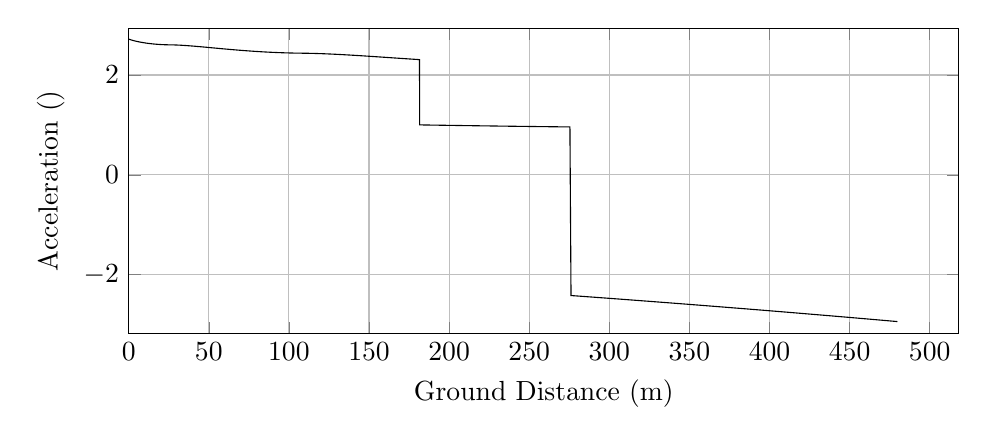
\begin{tikzpicture}

\begin{axis}[
width=\textwidth,
height=0.45\textwidth,
scaled ticks=false, tick label style={/pgf/number format/fixed},
xmin=0.0,
xmax=518.2299866992206,
xlabel={Ground Distance (m)},
xmajorgrids,
ymin=-3.1773545999999997,
ymax=2.9383329541999035,
ylabel={Acceleration ($\si{\meter\per\square\second}$)},
ymajorgrids
]

\addplot [
color=black,
solid
]
table[row sep=crcr]{
1.3603393307216043E-8	2.7206786612962066\\
3.0265395163403265E-7	2.7206786575478663\\
2.9593179127983543E-6	2.720678623102561\\
1.5392338359717934E-5	2.720678461954531\\
5.361280674027254E-5	2.720677966838565\\
1.6215010178508227E-4	2.72067656204086\\
3.7214145765703975E-4	2.7206738472617644\\
6.839954676020354E-4	2.7206698208009303\\
0.001098342709021993	2.7206644781690326\\
0.001609317716481928	2.720657898521556\\
0.0022198920000388346	2.7206500470445976\\
0.002878710694837372	2.7206415863366757\\
0.0036835072341781794	2.720631264662134\\
0.004557929017412697	2.720620065218509\\
0.005559798278933152	2.7206072508981105\\
0.006651227400597502	2.720593310307307\\
0.007795849738889277	2.7205787100180707\\
0.009067984722810115	2.7205625050930307\\
0.010453165799939174	2.720544884429202\\
0.011915708813158052	2.7205263052738617\\
0.013455030027058647	2.7205067774080813\\
0.015131183092671713	2.720485542905256\\
0.01690803412933615	2.7204630640878813\\
0.01873590105740728	2.7204399717842405\\
0.020713359121301934	2.7204150242262424\\
0.022777736728155237	2.7203890166149653\\
0.024960970145273077	2.720361550334686\\
0.02723428625014468	2.720332991183297\\
0.029610395797831278	2.7203031828656163\\
0.03204086105441677	2.7202727354797975\\
0.03462344565878624	2.720240428049145\\
0.037295727153354774	2.7202070461575243\\
0.040089145853872785	2.720172200927615\\
0.042950967781251806	2.720136553473475\\
0.04592022141655751	2.7200996205862893\\
0.04897301836205646	2.720061702748449\\
0.052130294957187476	2.7200225431846228\\
0.05542514139564195	2.719981736190481\\
0.05879722600804832	2.719940032970274\\
0.06231520981015182	2.719896588593282\\
0.06596261503753809	2.71985161218164\\
0.06964559414821356	2.7198062636261993\\
0.07347193989652406	2.7197592186945316\\
0.07736619052035826	2.7197114090939323\\
0.08137137577670908	2.7196623095742662\\
0.08545617869345057	2.719612307396395\\
0.08969468676038628	2.7195605001527836\\
0.0940095881391464	2.7195078372446053\\
0.09845059220533334	2.7194537156433602\\
0.10296315144049947	2.719398803650983\\
0.10759658895065366	2.7193425044674013\\
0.1123317495250277	2.719285055060655\\
0.1171874363557737	2.719226231512753\\
0.12217670360507671	2.7191658807659147\\
0.12726806426274867	2.719104388277655\\
0.13231647880291775	2.719043505591589\\
0.13765212084557643	2.718979255700906\\
0.14294844966167852	2.718915575612513\\
0.14834594087957392	2.718850776179469\\
0.1539671093411843	2.718783393554209\\
0.15968242883369804	2.7187149872467513\\
0.16555834796315422	2.718644767062395\\
0.17157514414202774	2.718572975126893\\
0.17760320215284392	2.7185011602885174\\
0.18370335474801935	2.718428598213908\\
0.18983540939776816	2.718355767994354\\
0.19621099073945342	2.71828016185121\\
0.20278841209744758	2.7182022845362246\\
0.20952923284938563	2.7181225994433653\\
0.21624967405074952	2.7180432810935136\\
0.22309476488450758	2.717962618703716\\
0.22992510727843934	2.7178822560654536\\
0.2371653034562048	2.7177972065765106\\
0.2442573187228817	2.717714030740942\\
0.25144286317780873	2.7176298902582934\\
0.2588001799723505	2.7175438743570046\\
0.2662612189130884	2.717456784348257\\
0.27386560463063747	2.7173681626444637\\
0.2815803271719757	2.717278399069807\\
0.28946218069394425	2.717186838600849\\
0.29753588720841584	2.717093202164077\\
0.3056643119969481	2.716999085151018\\
0.31376446154764137	2.716905447247142\\
0.322071411728719	2.7168095739864153\\
0.3303680011285137	2.7167139752329605\\
0.3389039548234316	2.7166157779269238\\
0.3474123396293025	2.7165180568217986\\
0.3561645174790815	2.7164176993305276\\
0.36525289600634137	2.7163136602552074\\
0.3742306244196095	2.7162110592727844\\
0.3835584127627333	2.7161046359512806\\
0.392806747202999	2.7159992963816517\\
0.40218604538039837	2.7158926432422206\\
0.4115907129344223	2.7157858796460443\\
0.42143744457304466	2.71567428647879\\
0.4310567075016639	2.71556545561893\\
0.4412814114336725	2.7154499724249304\\
0.4513051702487684	2.715336954190609\\
0.461412558308395	2.7152231867172496\\
0.47173637532167356	2.715107181729816\\
0.4821484569390513	2.7149903860087328\\
0.492985116277161	2.7148690397708313\\
0.5036221628177362	2.714750136897867\\
0.5142245311302887	2.714631824704451\\
0.5252888808291518	2.7145085711433863\\
0.5363145235987512	2.7143859638369863\\
0.5471208511184944	2.714266001569709\\
0.5585110457184732	2.7141397764842328\\
0.569849942463402	2.7140143406519304\\
0.5817265165330987	2.7138831906112504\\
0.5935668742733842	2.7137526762523763\\
0.6053719027871456	2.7136227833355733\\
0.6172343027602503	2.7134924902367645\\
0.629515267228629	2.7133578414420363\\
0.6417789549774502	2.713223625078407\\
0.6542768803188956	2.713087092614826\\
0.6669828212214572	2.7129485413260808\\
0.6796225285147333	2.712810963606792\\
0.6925094233679154	2.712670951020117\\
0.7056620711738308	2.712528314808269\\
0.7184715206768946	2.7123896541914156\\
0.731725241748566	2.71224644554528\\
0.7449880440563246	2.71210340227731\\
0.7586792333483576	2.7119560127494973\\
0.7725063377467813	2.71180744006777\\
0.7863894274138714	2.7116585464046254\\
0.8004504964383841	2.7115080279916457\\
0.8147129313117618	2.711355643498586\\
0.8293722635741907	2.711199319563237\\
0.8437954335339908	2.711045809353851\\
0.8580702287827062	2.7108941643141264\\
0.8726489666047585	2.7107395815891637\\
0.8875094051704782	2.71058231221187\\
0.9027740629895862	2.7104210779590776\\
0.9182163910703112	2.7102582871089913\\
0.93361566230532	2.7100962680430207\\
0.9491799633800446	2.7099328325529592\\
0.9646343064330896	2.7097708672969585\\
0.9803727456894022	2.709606245240436\\
0.9957421603273868	2.709445792888064\\
1.0116767859397604	2.7092797605173207\\
1.028041387324289	2.709109585047088\\
1.0443915011410971	2.7089398986479614\\
1.060796374175649	2.7087699812388033\\
1.0773229908740651	2.7085991418227273\\
1.093971735592782	2.708427381313938\\
1.1110062543639518	2.7082519927924293\\
1.127891796882146	2.7080784867552516\\
1.1451224507351285	2.707901789639987\\
1.1624801114435046	2.7077241500217113\\
1.180077727863539	2.7075444206861308\\
1.1978884766667508	2.7073628870065507\\
1.215488397439855	2.7071838674900413\\
1.23351701382096	2.70700086120692\\
1.2518199984626128	2.706815453946845\\
1.2704235066044305	2.7066273960882796\\
1.2892140278280424	2.7064378476887043\\
1.3075714306593595	2.7062530536699114\\
1.3266673518109293	2.706061226593331\\
1.3462106477188795	2.7058653259925807\\
1.365306294594515	2.7056743205573586\\
1.3852885894463176	2.7054748750159323\\
1.404835539176236	2.7052801958417234\\
1.4251192118409102	2.7050786164214466\\
1.445164519989187	2.7048798402486423\\
1.4656054698512246	2.704677582294032\\
1.4853522740259328	2.70448261320705\\
1.5051589726327936	2.7042874650304656\\
1.5255757775517242	2.704086734977351\\
1.5464367798307013	2.703882084832995\\
1.5673163741652552	2.703677701736183\\
1.5879032567231621	2.703476621174312\\
1.6091523485848285	2.703269524882243\\
1.6303162371862876	2.7030637127206134\\
1.6519474169970438	2.7028538211267294\\
1.673879209980242	2.7026414892001265\\
1.6955666802836635	2.702431991449334\\
1.7172271378534343	2.7022232168933176\\
1.7402832823543353	2.7020014942594512\\
1.7634396102400074	2.7017793281512494\\
1.7861669372425006	2.7015617813004402\\
1.8088678577734645	2.70134498175241\\
1.831824248135399	2.7011262418173425\\
1.855578771396016	2.700900422190558\\
1.878960729162178	2.7006786627687136\\
1.9033179534858085	2.7004481971762466\\
1.9273833213731866	2.700221034259217\\
1.9518510462308036	2.69999062125975\\
1.9761594732990155	2.699762252000519\\
2.000437267212291	2.6995347079709724\\
2.0252281699074732	2.6993029056239726\\
2.0498006073458734	2.6990736918319493\\
2.0745611186355752	2.6988432699762965\\
2.0997746990963106	2.6986091919427624\\
2.1260324099367294	2.6983660174624884\\
2.1515212193659616	2.6981305429210893\\
2.1771505246334	2.6978943421232504\\
2.2031842637813908	2.6976549974131148\\
2.230133398733474	2.6974078524356484\\
2.257053086628849	2.69716159885499\\
2.283795213136285	2.6969175806879333\\
2.311477064851834	2.696665625359551\\
2.3387199014446116	2.696418295414511\\
2.3662694524467227	2.6961688121763228\\
2.3937852540088533	2.695920264452572\\
2.4216520071021392	2.6956691844160687\\
2.4501931244916175	2.695412689733759\\
2.478927626230634	2.6951551292366664\\
2.506685441631536	2.6949069598473416\\
2.53537335014481	2.6946511285282604\\
2.5633350931805676	2.694402408668485\\
2.5917889242519685	2.6941499522401395\\
2.6208221472873374	2.693893017414193\\
2.649872764173903	2.6936365943995533\\
2.679661174525658	2.693374346647764\\
2.709174609939316	2.693115202410163\\
2.740029385016756	2.6928450029067674\\
2.770444625703795	2.6925793711374686\\
2.801129860621211	2.6923121002927015\\
2.8318827297715705	2.6920449607525097\\
2.862425967677578	2.6917803520588715\\
2.893259332541544	2.691513943438512\\
2.92412139403754	2.6912480008689297\\
2.955064430161417	2.690982073760627\\
2.986690331721131	2.6907110120079434\\
3.019183403261743	2.6904332863730254\\
3.0507201588152526	2.6901644753864344\\
3.0830332871979023	2.6898897995808344\\
3.1154603869692448	2.6896149168057812\\
3.148592095396281	2.6893348450572363\\
3.181936872739324	2.6890537678748103\\
3.214370607724433	2.68878113196698\\
3.247565473366384	2.6885028717129815\\
3.281695868027062	2.688217580965926\\
3.316494330618462	2.6879275486747067\\
3.3513055302544137	2.6876382569780937\\
3.3860303583611797	2.6873505222587717\\
3.421934361445942	2.6870538933091392\\
3.456235826539576	2.6867713320849385\\
3.490536654441657	2.6864895809370513\\
3.526257338581564	2.6861970179578334\\
3.561372823896762	2.6859102537028257\\
3.5967906564503185	2.685621861580385\\
3.632682576242373	2.6853304665721813\\
3.6701261071689295	2.6850273896113928\\
3.707701291513044	2.684724181446221\\
3.7452745323452916	2.684421920005274\\
3.78256482255855	2.6841228504923897\\
3.8208821591411084	2.6838164893445455\\
3.8590337549211444	2.6835124003534068\\
3.89695718563138	2.683211061596486\\
3.9351036745073964	2.6829088826731304\\
3.9736642086653067	2.682604369291303\\
4.012189127077221	2.6823010815538098\\
4.05156219172609	2.681992087170766\\
4.090290786278251	2.68168910267706\\
4.129291984889424	2.681384935049498\\
4.1680648628189925	2.6810834879059993\\
4.207805169621487	2.680775486920913\\
4.248168240749736	2.6804636570116616\\
4.288797880674668	2.6801507780724796\\
4.32990243544832	2.6798352683149327\\
4.371428084678056	2.679517569343126\\
4.41247037137882	2.6792045933860082\\
4.453879445321437	2.678889847978703\\
4.49524783594077	2.678576437358818\\
4.537299342543221	2.678258896831071\\
4.580546125800922	2.6779334244468345\\
4.622914948498307	2.6776156299698934\\
4.66640222022569	2.677290542721363\\
4.709294790611851	2.6769709837785767\\
4.752417172855319	2.6766507912603412\\
4.796155651503765	2.6763271235040342\\
4.8408754796551925	2.675997332877057\\
4.884850997559644	2.675674149017089\\
4.928651138956553	2.6753533505106946\\
4.972831351372241	2.67503087161995\\
5.017331702752941	2.6747071708341474\\
5.0632326321008225	2.6743744487516317\\
5.108452384314601	2.6740478173091553\\
5.1536021218025905	2.673722827898078\\
5.199057463234675	2.673396780336388\\
5.244479287100011	2.6730721120468193\\
5.292293005248643	2.6727315710052038\\
5.338096108273211	2.6724065220089717\\
5.3857492800262605	2.6720695551603235\\
5.433816232374781	2.67173090807856\\
5.480691139018431	2.6714018586329598\\
5.529685763332537	2.6710591891667725\\
5.578612887337309	2.6707182708184654\\
5.626451501744754	2.6703861671011913\\
5.674834544150631	2.6700515151935553\\
5.7252048440372345	2.669704427524425\\
5.77422346516266	2.6693679305667333\\
5.8255152536468575	2.6690171710063213\\
5.874338256646894	2.6686845632866065\\
5.922631450506765	2.668356777034105\\
5.972682300942642	2.6680183272823603\\
6.022535370757359	2.6676824906956176\\
6.074394648705015	2.6673344842246873\\
6.124928192945902	2.666996687642375\\
6.176798284396469	2.6666512989764355\\
6.229620191179453	2.666300963486928\\
6.282808156696705	2.665949612003093\\
6.334658925277093	2.665608451405185\\
6.388041948821611	2.6652586030534966\\
6.440558117792513	2.6649158095309824\\
6.494960924490993	2.664562131646191\\
6.550441697666145	2.664202938277337\\
6.6042098433346865	2.6638562643536536\\
6.658315220792536	2.663508832144151\\
6.712335084641163	2.663163359917985\\
6.766674450459032	2.662817260436796\\
6.821537769035839	2.6624692583213525\\
6.876851268142238	2.6621198535092523\\
6.933661362437203	2.6617625068113426\\
6.989261882852809	2.6614142454795733\\
7.046240323930029	2.6610588624640483\\
7.102786137967051	2.6607076814481774\\
7.1603789170469145	2.66035153122335\\
7.21785165788507	2.6599976588428076\\
7.277487498606879	2.659632082256504\\
7.334984696129153	2.659281165977336\\
7.393362172524569	2.658926427334934\\
7.452416393609804	2.658569158697232\\
7.511934748111884	2.65821068542132\\
7.572557225035805	2.6578472095603285\\
7.63202184821041	2.6574922841322914\\
7.69294899409779	2.657130274209857\\
7.752675521499926	2.656777007005755\\
7.814488876138199	2.656413067005313\\
7.8763528528159785	2.6560505226767974\\
7.938149975125226	2.6556900545173407\\
8.001193143199774	2.65532404532037\\
8.064554080136986	2.654957941394265\\
8.12686567918485	2.654599604470868\\
8.189637855946287	2.654240320036407\\
8.252542711798306	2.653881981811166\\
8.315859663763469	2.6535230130597807\\
8.380006162932737	2.653161090486292\\
8.444702551512929	2.6527978411523154\\
8.509501986620958	2.6524357933385767\\
8.57387297516295	2.6520778958356077\\
8.63887365699837	2.6517182663260552\\
8.70727085773305	2.6513417562064703\\
8.772937378995405	2.650982114230926\\
8.839192134487615	2.650621066200708\\
8.905815929161982	2.6502598384638087\\
8.97209054442786	2.649902318438188\\
9.039019026885107	2.6495431001632594\\
9.107371801018814	2.6491781267509182\\
9.174915633685494	2.6488193404634632\\
9.243868961478196	2.6484549743174144\\
9.312440636565494	2.6480945280533144\\
9.381784695008012	2.64773194388124\\
9.4513167952828	2.647370309297383\\
9.52142787533916	2.647007615113754\\
9.591425279059166	2.6466474560144393\\
9.662230428326719	2.646285111993561\\
9.734225879912522	2.6459187011004124\\
9.806441602430919	2.645553211506668\\
9.878483835105534	2.6451906297210153\\
9.951807209049782	2.644823673290537\\
10.023539677466466	2.644466694479261\\
10.096057433179052	2.6441078259737703\\
10.168262179450682	2.643752514614059\\
10.241274410624943	2.6433952591641816\\
10.31479015323385	2.6430375937029646\\
10.390063469390178	2.6426735041074956\\
10.465012435634037	2.642313112770144\\
10.540639152111389	2.6419516075562184\\
10.617644389866598	2.6415857179533573\\
10.692945462162374	2.641230068796194\\
10.770083295573727	2.6408679330963514\\
10.846726862770723	2.6405103027817125\\
10.924657809445929	2.640148889613137\\
11.00265335491597	2.63978941352116\\
11.081827589833612	2.639426784384952\\
11.159134327011738	2.639074915846357\\
11.239152720133266	2.638712992829407\\
11.317028257314295	2.638362987873357\\
11.396413369884492	2.6380084493978577\\
11.477655063362434	2.6376479632370904\\
11.556958506738276	2.637298355398907\\
11.637325199769407	2.6369463471769103\\
11.717754170658207	2.6365963621380466\\
11.799819443100102	2.63624161502403\\
11.881986970940797	2.635888803104182\\
11.964394119506721	2.635537342147723\\
12.046263329632716	2.6351905264087696\\
12.130282587748898	2.6348370295798214\\
12.213721087180826	2.634488399852607\\
12.295868535962462	2.634147514971435\\
12.380692430046633	2.633797961762415\\
12.46470288467437	2.633454193025379\\
12.550384439940181	2.6331060699957733\\
12.635259749824865	2.6327636863268946\\
12.72144647897981	2.63241851197907\\
12.80741162779486	2.632076724560571\\
12.892901506907108	2.631739293069713\\
12.977815703098727	2.6314065594474236\\
13.06483740414145	2.631068066500708\\
13.151922956503014	2.630731848075155\\
13.240589045456186	2.6303921107814636\\
13.329911181207382	2.6300524853438656\\
13.417306166647748	2.6297227285188542\\
13.507103029723119	2.6293865171984176\\
13.595986036712912	2.6290563212297444\\
13.687453390597003	2.628719208644787\\
13.779071846306106	2.6283842583240453\\
13.872694200363323	2.628044782677631\\
13.963504841252302	2.627718197075353\\
14.056146454975131	2.6273877509805974\\
14.14918846816267	2.6270586358496457\\
14.24332804549016	2.626728442147807\\
14.339261112049854	2.626394848369028\\
14.431091301610323	2.6260782450404214\\
14.524174633942373	2.625760029885301\\
14.618760344060338	2.6254394620095756\\
14.714801736988441	2.6251168208410443\\
14.809763128346521	2.624800631225546\\
14.903412319659619	2.624491550424864\\
15.001392651385917	2.6241710768230613\\
15.098055049922994	2.6238578111877793\\
15.196870856960619	2.623540530466907\\
15.29477342819068	2.6232291262965033\\
15.39265348361268	2.6229207128263496\\
15.490487151984588	2.6226153517984745\\
15.588146853189365	2.6223134213572887\\
15.687961867268871	2.622007798116239\\
15.78650099417861	2.621709016912882\\
15.886965864441798	2.6214073886179268\\
15.98755318095926	2.6211084084990697\\
16.088470385762115	2.6208114696538525\\
16.190536977381747	2.620514216689597\\
16.292466610053154	2.6202204307907557\\
16.396448349404487	2.6199238784454053\\
16.497808944935016	2.6196378512110607\\
16.600551072850564	2.619350987382476\\
16.70575139586156	2.6190604431728257\\
16.81134459259622	2.6187720413883815\\
16.917616592554033	2.618485038902799\\
17.023477948501657	2.6182023789046003\\
17.12904978140002	2.617923694814939\\
17.2354081519902	2.6176461576139998\\
17.340772011500363	2.617374394528855\\
17.448391076872838	2.6171000698358444\\
17.5571980918308	2.6168260499237155\\
17.66615596614949	2.616554996724549\\
17.774685459577412	2.6162883270448347\\
17.884986575683584	2.6160206855256734\\
17.99552903728076	2.615755866553193\\
18.108708479124623	2.615488253160013\\
18.219646262474413	2.615229387506168\\
18.332680252669796	2.6149691286881325\\
18.445061806396694	2.614713860659559\\
18.556709221711323	2.614463693032193\\
18.668884868236475	2.614215776215975\\
18.78204748093455	2.613969154620711\\
18.895704562363058	2.6137249583668334\\
19.008928234289563	2.613485172303819\\
19.124320907419907	2.613244353656583\\
19.24105855786135	2.6130043738052313\\
19.355116774466126	2.6127734319677236\\
19.470462572962035	2.6125434196100388\\
19.58492145104516	2.612318679974858\\
19.704921229319112	2.6120867966885672\\
19.821259826163917	2.611865627200067\\
19.941172080873493	2.6116414010344053\\
20.06078806851737	2.611421496185992\\
20.177423389922623	2.6112106825265204\\
20.297621170678	2.6109971487959625\\
20.420129559802255	2.610783382130866\\
20.54164670774839	2.610575194034384\\
20.661905244258705	2.610372924043535\\
20.784301666224792	2.610170888533478\\
20.904244540623438	2.609976639812995\\
21.028114340450195	2.609779901698209\\
21.148300883955606	2.609592760781454\\
21.270875420257596	2.6094056910343086\\
21.39299406946177	2.6092231107132005\\
21.513793771711654	2.6090462163639767\\
21.637476506915142	2.608868915612577\\
21.759279707150128	2.6086980705627534\\
21.88493035745168	2.6085257282674936\\
22.009809790007786	2.6083583553647216\\
22.13620730934617	2.6081929065801015\\
22.263515470260465	2.6080302793333896\\
22.393040471753594	2.607868941280868\\
22.520519759768852	2.6077141976473044\\
22.648852607677917	2.6075624600019314\\
22.775118904521122	2.6074171120820617\\
22.903136237443974	2.607273732646484\\
23.03176118514304	2.6071337008954343\\
23.162501585272054	2.6069954916827385\\
23.294719932439598	2.606859937497086\\
23.427108470281937	2.6067284454088675\\
23.558693146983046	2.606601940003137\\
23.687077503630363	2.606482524014279\\
23.817949558665852	2.6063648614675117\\
23.948210788889448	2.6062518140947457\\
24.076877750667826	2.6061441212975813\\
24.21019765060587	2.606036685397494\\
24.3450673155249	2.605932287377364\\
24.477101355489637	2.6058342488821085\\
24.60984760833776	2.605739823492751\\
24.7468403923846	2.6056467196227446\\
24.882807251950062	2.605558661740309\\
25.017167332957627	2.6054758883508313\\
25.153910941279605	2.6053959660017787\\
25.289629217480112	2.6053209394618975\\
25.425306692573436	2.605250202063977\\
25.56229499031975	2.6051830973115537\\
25.70075944713021	2.605119664500041\\
25.83724158708921	2.605061452167142\\
25.975209935932874	2.605006945543712\\
26.003074150630965	2.604996465857483\\
26.020759913393235	2.6049899063023956\\
26.030714598210515	2.604986245585444\\
26.05840292223249	2.6049761825189828\\
26.06133765907019	2.6049751261727927\\
26.064285136409026	2.6049740672190262\\
26.066337724202356	2.604973330947354\\
26.068175973881182	2.6049726717880395\\
26.06984477238784	2.604972072546399\\
26.077831036047115	2.604969193304239\\
26.10345636352254	2.604959826557275\\
26.16716044512971	2.604935696636902\\
26.297541524199602	2.604882582063598\\
26.42722303713863	2.604824833845874\\
26.5559280656694	2.604762729734616\\
26.686097387723095	2.6046951240870673\\
26.817793678842584	2.6046218784664346\\
26.949416928520378	2.6045438626963486\\
27.080440623797912	2.6044614849705248\\
27.215491080424528	2.604371711442483\\
27.34795890217076	2.6042789179214214\\
27.48215578365496	2.6041801903944934\\
27.616696052324144	2.6040764988267338\\
27.75271189183823	2.6039669358068878\\
27.888759310501555	2.6038526466269865\\
28.023839122857026	2.60373457871965\\
28.16136324828667	2.6036097347187157\\
28.298355249881332	2.603480779773336\\
28.435282447697354	2.603347363417516\\
28.573941346212784	2.603207712242628\\
28.713752690797136	2.603062327801072\\
28.852681198061333	2.6029133732207983\\
28.992471984120606	2.6027590381432235\\
29.133421724605903	2.6025989580439326\\
29.275199211812186	2.6024334748055615\\
29.416225289053614	2.602264487584124\\
29.55783477945603	2.6020904638423383\\
29.701838356359822	2.6019091010670348\\
29.846633046394217	2.601722332586834\\
29.99013730470424	2.6015329260160254\\
30.132492646908446	2.6013408617739424\\
30.277395768405135	2.6011411490535545\\
30.422188862471998	2.600937402849355\\
30.56637548064623	2.600730410308623\\
30.711944318924978	2.6005173409279383\\
30.8573377156769	2.600300480843197\\
31.006558691603843	2.6000737648824686\\
31.153907258126303	2.59984583014083\\
31.30257185742142	2.599611825960162\\
31.4510947803754	2.5993740568584256\\
31.602595106592503	2.599127473961757\\
31.755261577184278	2.5988749186996953\\
31.906398416479824	2.5986209245321756\\
32.05599258457312	2.598365690945168\\
32.20952926265106	2.598099824891996\\
32.360097140052986	2.59783531374599\\
32.51218835243483	2.5975643770630965\\
32.664721606344784	2.597288924507674\\
32.82129760777845	2.59700234643684\\
32.97669884718651	2.5967141455121885\\
33.13118849606322	2.5964239666121385\\
33.288837444683736	2.596124141007718\\
33.44405554194745	2.5958253313356394\\
33.60015866510213	2.59552126423476\\
33.756686089655645	2.59521284804464\\
33.91694077595571	2.594893491070727\\
34.074326811338736	2.594576365075885\\
34.23252403098988	2.5942541792298783\\
34.392884168270385	2.5939241396518096\\
34.554266068788166	2.593588548636937\\
34.71363140184178	2.5932538115207127\\
34.87649332318763	2.592908357922452\\
35.03746231629111	2.5925636252736934\\
35.19990059234286	2.592212481401056\\
35.3627309111595	2.5918572538216775\\
35.5271254050015	2.5914953825208134\\
35.69149466827288	2.5911303760815123\\
35.85508342515686	2.5907639894772565\\
36.017180984292054	2.590397931582352\\
36.182222084544165	2.5900222000957323\\
36.34861175093968	2.589640361269958\\
36.514166392421686	2.589257465430392\\
36.68083924241549	2.5888690407516313\\
36.845526722294395	2.5884823945483877\\
37.01328249159678	2.58808568617886\\
37.18160982421668	2.587684779048817\\
37.35136716620059	2.5872776308265406\\
37.51969289597564	2.5868711570289102\\
37.689710015857784	2.586457862001348\\
37.860394939778416	2.5860402290187876\\
38.02805196867635	2.5856274069225176\\
38.19868492919754	2.5852046641593693\\
38.37343039987371	2.5847690739970304\\
38.54685896696101	2.5843341589437943\\
38.71934233168869	2.583899089049461\\
38.8915617091798	2.5834622227014767\\
39.062305982326905	2.5830267178960575\\
39.23847188392709	2.5825749507861113\\
39.411511502305984	2.582128843751896\\
39.585172817779906	2.5816788341031485\\
39.760693028009456	2.581221715331284\\
39.9373134006328	2.5807594546179793\\
40.113617753210534	2.580295792292225\\
40.29094651898711	2.5798272385973133\\
40.468149621311596	2.5793568640609754\\
40.64593210594187	2.578882837045067\\
40.82431302355218	2.5784051336362657\\
41.00141330502653	2.577928844765018\\
41.17957893337042	2.577447711440911\\
41.359761290266974	2.576959159908581\\
41.53889737920997	2.5764715258014226\\
41.72013507746885	2.5759762699463096\\
41.899395797464194	2.5754845813065144\\
42.081280067494475	2.574983877308929\\
42.265315320939635	2.574475433596758\\
42.44531744651641	2.5739764081138246\\
42.62715102096499	2.5734706185694742\\
42.81120266452106	2.572956977963316\\
42.994164503876235	2.5724447468852603\\
43.17799769459725	2.5719284820894615\\
43.36154361404071	2.5714114735636295\\
43.54597437124032	2.5708904557742125\\
43.73158498218817	2.570364613472675\\
43.91737182308138	2.569836817130298\\
44.1050494697441	2.5693022153985066\\
44.293574236233	2.5687637938290475\\
44.47888581456586	2.568233217366008\\
44.66456251492659	2.56770031290059\\
44.85170130968709	2.5671619544796576\\
45.037822074257164	2.5666253131937316\\
45.22676109993536	2.566079351527528\\
45.41612608476639	2.5655309928311034\\
45.604812217355104	2.5649834795818123\\
45.79422221198037	2.5644327816257144\\
45.98724683785376	2.5638704982109193\\
46.17830917717477	2.5633129020510665\\
46.36786657808848	2.5627587260007036\\
46.55935209439748	2.5621979696912565\\
46.75090376717816	2.5616361102767\\
46.94233405988251	2.5610737370838272\\
47.13714948644359	2.5605005660882156\\
47.33387512950824	2.559920942035922\\
47.53043319838464	2.559341016085903\\
47.72298239739284	2.5587721852277925\\
47.919150009665316	2.5581919576628076\\
48.113386178114425	2.5576167774288168\\
48.311024807628144	2.557030880297275\\
48.508886059616145	2.5564437135036124\\
48.70490444306449	2.555861451460194\\
48.90290918859142	2.555272756407139\\
49.09959709013448	2.5546874831690767\\
49.2970021191946	2.554099617958525\\
49.49532701226336	2.5535085875213586\\
49.693780717172615	2.5529167818555347\\
49.89506320355713	2.5523161771326155\\
50.096719083698545	2.5517141278441926\\
50.29606895218413	2.5511186737396656\\
50.497598474286534	2.550516452001548\\
50.700304208193415	2.549910490324689\\
50.90342397924904	2.5493031000410458\\
51.10460922167407	2.5487013408370585\\
51.30752217039489	2.5480942934029542\\
51.51010619677311	2.5474881432730276\\
51.713602501430145	2.546879210211035\\
51.91843850546792	2.546266248332386\\
52.121089026646246	2.545659839831946\\
52.32561402362407	2.5450478687524436\\
52.53192272805477	2.5444306412072404\\
52.7387030603267	2.543812117268339\\
52.944027344085896	2.5431980948169493\\
53.154073670302836	2.542570135158037\\
53.36143953271798	2.5419504044032433\\
53.571009444677685	2.541324336833787\\
53.77799762982136	2.5407062605659156\\
53.98785945427545	2.5400799181832214\\
54.196157549666225	2.5394585875123497\\
54.40718762937186	2.5388294894484362\\
54.616887598525366	2.538204768354279\\
54.826875464266934	2.537579631685529\\
55.04038432082807	2.5369444978423\\
55.25438844036796	2.5363084127457762\\
55.46695867894975	2.5356771378333054\\
55.68088820258777	2.53504240855004\\
55.895144656119854	2.5344073252295782\\
56.109028395418505	2.5337739915506914\\
56.326262430904194	2.533131427269357\\
56.542089933321776	2.5324937421273432\\
56.76060076462056	2.5318488889481365\\
56.97729209122687	2.53121019040462\\
57.19579178641709	2.530566982970221\\
57.41258192878804	2.5299296520756522\\
57.634093277561306	2.5292793396004543\\
57.85395098827546	2.528634808787415\\
58.07448819514299	2.527989242816962\\
58.29446478173499	2.5273463011751724\\
58.51588770709739	2.526700152443185\\
58.73757884137123	2.5260542747954213\\
58.96020041504734	2.5254067756961724\\
59.18267120664716	2.524760833573292\\
59.405949655899676	2.5241136983448893\\
59.63089974393067	2.523462913015166\\
59.8562534200115	2.522812190429593\\
60.084134136581554	2.522155451171125\\
60.30833762904015	2.521510593077889\\
60.53504725699203	2.5208598484686284\\
60.763693228044005	2.520204919132267\\
60.99075593752245	2.5195559165490664\\
61.21765734918529	2.5189087867059206\\
61.44713116872772	2.5182557820175218\\
61.6738048454246	2.51761221451096\\
61.90668490141796	2.5169525728970683\\
62.13729676517957	2.5163009271692243\\
62.36629463006145	2.515655414734929\\
62.596359157213186	2.5150084986834154\\
62.82836101237727	2.5143577875240695\\
63.059723307860466	2.513710547655892\\
63.292774394726166	2.5130603018722466\\
63.52608473446321	2.512411085168192\\
63.75973181411028	2.511762713251054\\
63.993403028653574	2.5111160820431335\\
64.23068717493263	2.51046132747829\\
64.4710952259949	2.5097999046051767\\
64.70858695601663	2.5091484588673003\\
64.94894296164699	2.5084911580978195\\
65.18738841845183	2.507841096140126\\
65.42661162888535	2.5071909536442867\\
65.6659442133793	2.506542582107792\\
65.90899583190168	2.5058862766024292\\
66.15068261105333	2.505235819878556\\
66.39533053734849	2.5045796148039337\\
66.6378997293487	2.503931215046631\\
66.88158418814953	2.5032820928672956\\
67.12390450547147	2.5026388721469575\\
67.36840986262189	2.501992166121669\\
67.61550053739396	2.5013410071229005\\
67.86097385246623	2.5006965071294838\\
68.10985741250389	2.500045515162805\\
68.35582503705197	2.4994046078616874\\
68.60464259362828	2.4987587826507225\\
68.85450289166104	2.4981128115549627\\
69.1042877596268	2.497469622399734\\
69.35837572129628	2.4968180291693622\\
69.61150655903072	2.496171596673576\\
69.86289252102952	2.4955323152395783\\
70.11686816207683	2.494889197346831\\
70.37125759672608	2.494247823299956\\
70.62480458144697	2.4936113746348187\\
70.88045310059783	2.4929725036104173\\
71.13526709211152	2.4923385896920447\\
71.3947754873567	2.4916959652598996\\
71.6534187996231	2.4910584844101127\\
71.91450497256008	2.490418042920515\\
72.1716184080999	2.4897903719922825\\
72.43269265097052	2.489156124566061\\
72.69331619504374	2.488526100829059\\
72.95563200429567	2.4878951633499824\\
73.21686762735783	2.4872700118660225\\
73.48161420086069	2.486639724524867\\
73.74261486234883	2.4860215932579317\\
74.00755043430098	2.485397450822168\\
74.27511769675363	2.484770511126462\\
74.54487113507057	2.484141930683326\\
74.81568229507957	2.4835144223616146\\
75.08274085953312	2.4828990994561133\\
75.35421836228127	2.48227716702688\\
75.62798354862159	2.481653660677785\\
75.89909469738902	2.4810398475160156\\
76.17008148658607	2.48042996336775\\
76.44269151183332	2.479820124431633\\
76.71571902594138	2.4792130884926618\\
76.99340852183178	2.4785995427236145\\
77.27004772085374	2.477992202674521\\
77.54832408953641	2.477385199695421\\
77.82592519882277	2.4767836170636297\\
78.10358246820337	2.4761858750642443\\
78.38556010231375	2.475582906634508\\
78.66911430382748	2.474980726291445\\
78.95399134982776	2.4743799558012434\\
79.23667137346987	2.4737880172861093\\
79.518907793654	2.4732011984459694\\
79.80555437718249	2.4726095145346116\\
80.09150103324356	2.4720236154797126\\
80.37928873457926	2.4714383390733685\\
80.66871996946384	2.4708541852254573\\
80.95967699414447	2.470271483310257\\
81.25093884305389	2.46969273945421\\
81.54344278085921	2.4691161457324657\\
81.8358102960415	2.468544463485582\\
82.13087592438694	2.467972229211356\\
82.42794520371837	2.4674009209561696\\
82.72842933895026	2.466827975237794\\
83.0269479931649	2.466263704519231\\
83.32974506690314	2.465696381887148\\
83.62964811531441	2.465139497828961\\
83.92951211009506	2.4645876948518985\\
84.2339319847595	2.4640326486757456\\
84.53715838283946	2.4634849446277407\\
84.84105485927768	2.4629412204221763\\
85.14845677960258	2.4623965277685977\\
85.45530133949276	2.461858159152909\\
85.76249773413784	2.4613245309354017\\
86.07201271349416	2.4607923136600105\\
86.38432073331904	2.460260843847024\\
86.69710203601804	2.4597341734019187\\
87.01172103282082	2.459210084155634\\
87.32669099459858	2.4586911288738795\\
87.64517025121202	2.4581722263462886\\
87.96158123090564	2.4576625205007074\\
88.2775814178033	2.4571592893344167\\
88.60068374099544	2.456650771249656\\
88.92068281935622	2.4561531565110357\\
89.24207276858638	2.4556594246506958\\
89.56578933015979	2.4551682597665963\\
89.88760090270688	2.4546861104221787\\
90.2141410750086	2.454203135124871\\
90.54066676000363	2.453726501259575\\
90.86727570256076	2.453256084169672\\
91.19715108614633	2.4527874130189637\\
91.52744226539704	2.452324662124046\\
91.85639956214655	2.451870271480665\\
92.19095740864739	2.4514148053995646\\
92.52827526888461	2.4509623982187643\\
92.8674718219292	2.4505143893221693\\
93.20307982994817	2.45007796351259\\
93.5374944579234	2.4496498757217147\\
93.87598013161067	2.449223490262768\\
94.20917297854535	2.448810580306356\\
94.55043409744499	2.4483946888723898\\
94.89132963816093	2.4479863478956343\\
95.23083207736542	2.447586748328506\\
95.57395676502793	2.4471900719482775\\
95.91421223354143	2.4468038617271874\\
96.25656086122288	2.446422475256802\\
96.60012122339742	2.4460470135485375\\
96.94166303707107	2.4456809955647865\\
97.28627502929558	2.445319015713345\\
97.62906225262071	2.4449662694279697\\
97.97125437026659	2.444621427786916\\
98.31201772458999	2.444285279829848\\
98.65627175165852	2.4439530523110857\\
99.0012536203806	2.443627560750417\\
99.35020029285332	2.4433059171884537\\
99.69475740907401	2.4429958218600083\\
100.04053871990226	2.4426921324246553\\
100.38598466112728	2.442396260584223\\
100.72867962848932	2.4421101874466906\\
101.07385499050397	2.441829549808382\\
101.41864366415388	2.441556759554321\\
101.76305460768467	2.441291796930587\\
102.11068844700483	2.441031997901126\\
102.45638678530696	2.440781272232182\\
102.79841653079728	2.440540704148865\\
103.14087212494877	2.4403073190123745\\
103.48486473791618	2.4400804356214234\\
103.82875595362174	2.4398611934533667\\
104.17244250654872	2.4396496596833757\\
104.51168383396202	2.4394483022733917\\
104.85986244643053	2.4392493381386604\\
105.204587526496	2.4390600412341765\\
105.54754777175077	2.4388793212149045\\
105.88797456536247	2.4387074512981224\\
106.23280177240994	2.4385410036507142\\
106.57515110440406	2.4383833730122237\\
106.91603555764121	2.438233972158936\\
107.25729565943405	2.438091968620996\\
107.598830149446	2.437957436469797\\
107.93686571059558	2.4378317650253747\\
108.27485499032852	2.437713563105536\\
108.28839963475954	2.4377089816955086\\
108.30004107281309	2.4377050536118228\\
108.30931238392475	2.4377019315951367\\
108.31701527366243	2.4376993419985693\\
108.32505202073054	2.4376966442959924\\
108.33865239118708	2.4376920757662077\\
108.35091925899997	2.437687941820947\\
108.39508146726081	2.4376729541898428\\
108.52984553865659	2.4376262051439177\\
108.79919793188978	2.4375282156126596\\
109.105233418432	2.4374095713382307\\
109.41485218466596	2.4372816990329653\\
109.72257164661937	2.43714687531413\\
110.0321119530083	2.4370035496994156\\
110.34145354075926	2.4368526728261344\\
110.6534776714839	2.436692824043207\\
110.9711963390063	2.4365222289562025\\
111.28851843247409	2.4363440420862066\\
111.60893519474632	2.4361562847481197\\
111.92798394282838	2.4359615896983087\\
112.24770070245137	2.435758820731417\\
112.57243448635171	2.4355450966094914\\
112.89480865389396	2.4353252588963645\\
113.22000325235314	2.4350958414002974\\
113.54885709436653	2.4348561065866923\\
113.8770619430189	2.434609173215901\\
114.20946079557197	2.4343513587107797\\
114.54107775051554	2.4340864891862495\\
114.87787736567807	2.4338097352623684\\
115.21564640021248	2.4335244348530267\\
115.55522358014255	2.433229873390224\\
115.89667501383605	2.4329259578067397\\
116.23992536102014	2.4326127213255626\\
116.5847156213415	2.432290379243784\\
116.92791619634093	2.4319619499620595\\
117.27517516660399	2.4316220384861005\\
117.62420948631524	2.431272780277488\\
117.97391125359778	2.4309152972309223\\
118.32673409155768	2.430547052323676\\
118.68227803698588	2.430168369963023\\
119.03889207644076	2.4297809832770483\\
119.39651249432902	2.429384992014123\\
119.75508651978987	2.4289804895119858\\
120.11314113323388	2.4285692199538316\\
120.47404637453192	2.428147337094468\\
120.84098349318353	2.4277109488262347\\
121.20490030977416	2.427270827669072\\
121.57328571082118	2.426817972786023\\
121.94079100066682	2.4263589516450033\\
122.31015242291167	2.425890417592221\\
122.68267403243519	2.425410670298904\\
123.05346836176264	2.424926062633208\\
123.42835733050345	2.4244290188823996\\
123.80350972566416	2.4239245961583267\\
124.1783235941891	2.4234137066845376\\
124.55244040146786	2.4228969673348413\\
124.92576251095704	2.4223746517122615\\
125.30489170817492	2.421837488041481\\
125.68146781278597	2.4212973337292256\\
126.06139977608174	2.4207457916277306\\
126.44502763856761	2.420182285371527\\
126.82695116404781	2.4196147964977337\\
127.206716044588	2.4190441968488976\\
127.59262031825523	2.4184580188810942\\
127.97077035934353	2.417877503078614\\
128.3546122768156	2.4172821552332753\\
128.73724861847296	2.4166826630374114\\
129.12002064685282	2.4160770463275636\\
129.50086700331673	2.4154687022193597\\
129.8837789976152	2.414851346010222\\
130.26783132854348	2.4142264916091953\\
130.651936341801	2.413595975813511\\
131.03747321415574	2.412957595804226\\
131.42280335891803	2.4123141313718692\\
131.80875442588928	2.411664284079559\\
132.19322104975072	2.4110117078378126\\
132.5798881414172	2.410350224396862\\
132.96215446290768	2.409691259338784\\
133.34488286943906	2.4090265945736995\\
133.7276157954845	2.4083571021251338\\
134.11532375481391	2.407674080588845\\
134.50135826447365	2.406989268013292\\
134.88604120201086	2.406302234909834\\
135.26955723714872	2.4056127810566927\\
135.6512109336153	2.4049222924372256\\
136.03464327936558	2.40422426529637\\
136.41686422877552	2.4035242144151487\\
136.79904942565338	2.4028200875141854\\
137.18004416157777	2.402114110924786\\
137.56399804528928	2.401398646520869\\
137.94515347717788	2.400684498489757\\
138.32982901897384	2.3999598952989585\\
138.7128522769853	2.399234629307342\\
139.09597564505458	2.398505481924219\\
139.48002685240425	2.3977709392261835\\
139.86309097971855	2.3970347399419127\\
140.24727738828375	2.396292903294329\\
140.6317581809211	2.3955470832041623\\
141.01585725597846	2.3947986662434966\\
141.3998433603236	2.3940472083670095\\
141.7841907991213	2.393291850794408\\
142.16710976343057	2.392536195828421\\
142.55205218648928	2.3917734955203658\\
142.9364233092117	2.3910089444426257\\
143.32169829765928	2.390239674944902\\
143.705984531242	2.3894695365580034\\
144.08985428249122	2.3886974667514584\\
144.47683600496026	2.387916408652118\\
144.86371007721533	2.3871328975357295\\
145.24772592056325	2.3863526020597376\\
145.63047789911974	2.385572389946076\\
146.01273254364395	2.384790780760845\\
146.39725173307323	2.3840021753782183\\
146.77966503747456	2.383215599586898\\
147.16478130736948	2.3824212209002393\\
147.54689717238745	2.381630869102909\\
147.93097497792814	2.3808343517343653\\
148.31499270913332	2.380035908616705\\
148.69957284780122	2.3792343033244103\\
149.08709998577143	2.3784246003791054\\
149.47129868208145	2.377619975755045\\
149.8546635899794	2.376815295395449\\
150.23801379389647	2.376008905260921\\
150.62200569343076	2.37519947915814\\
151.00751012558203	2.374385226029803\\
151.3946455315429	2.373565934584871\\
151.77987817077866	2.372749143111779\\
152.16505704867353	2.3719310003601963\\
152.55112759502248	2.3711095505099173\\
152.93964308710213	2.370281527621655\\
153.32507651584535	2.3694587708503905\\
153.71174813432617	2.3686321233352805\\
154.10000329570875	2.367800888914693\\
154.48914219495543	2.366966610175619\\
154.8788297075107	2.366130054853258\\
155.26820650111182	2.365293121841945\\
155.6562915247282	2.364457980569835\\
156.0441896603637	2.363622312599576\\
156.4348678136667	2.362779770569401\\
156.82082928279863	2.3619465809003035\\
157.21071017196311	2.3611041555010726\\
157.60005066896917	2.360262172782705\\
157.99004282467217	2.3594181063852853\\
158.3808231456182	2.3585717087559077\\
158.77280374485122	2.3577221340717758\\
159.16384255262415	2.3568740754878803\\
159.55370941764693	2.3560280866240024\\
159.946071590523	2.3551762575385133\\
160.33752628124114	2.354326022930576\\
160.73008933968674	2.3534730536514\\
161.12428312893906	2.352616260804793\\
161.5185576482712	2.351759060855163\\
161.91431288671106	2.35089845795311\\
162.3096877663487	2.35003854728694\\
162.70613442998513	2.3491762188949528\\
163.1032465869576	2.348312404430774\\
163.50039135636405	2.3474485286109577\\
163.89625578410926	2.3465874947997296\\
164.29272443146095	2.3457252508083206\\
164.68754921345175	2.344866731618903\\
165.0864466423082	2.3439995549922097\\
165.4846753800681	2.343134077114966\\
165.88329117400662	2.3422680492856474\\
166.28234792206388	2.341401401021205\\
166.68312204436222	2.340531408703809\\
167.08520211103445	2.339659015544984\\
167.486487681752	2.338788825008389\\
167.8888620337579	2.3379167988028255\\
168.290121631074	2.337047756885073\\
168.69179641444674	2.3361784283508964\\
169.0966267258019	2.3353029348977206\\
169.50108473093724	2.334428956870558\\
169.90729482190739	2.3335519515283165\\
170.31243922775104	2.332678047998904\\
170.71755979953144	2.331805038964145\\
171.12402986296422	2.3309300121516676\\
171.53319587512163	2.3300501255536883\\
171.941770038195	2.3291724996671475\\
172.3502931259835	2.328296013192234\\
172.7599322859847	2.327418208448398\\
173.17073308198894	2.3265390390999245\\
173.58266371319877	2.3256586248849693\\
173.99296569000023	2.3247829010441654\\
174.40104722187203	2.3239131544618488\\
174.8156903853216	2.3230307290372796\\
175.2299479185392	2.322150480228032\\
175.64260521584504	2.3212750200427097\\
176.05374721710058	2.3204041926300967\\
176.4688147253861	2.319526526672183\\
176.8832117842232	2.3186517977056713\\
177.30033423294157	2.317772889064856\\
177.7185234955238	2.3168933570971353\\
178.13477925276436	2.3160195465558724\\
178.55472625996282	2.3151397000627316\\
178.97486541267733	2.3142612120847224\\
179.39652032378837	2.313381365346036\\
179.8177496461559	2.312504257024961\\
180.24148986351946	2.3116238256668042\\
180.66579793025812	2.3107441684434598\\
181.08977314985765	2.3098671931358306\\
181.5138518510159	2.3089920341015464\\
181.61122522885114	1.0008571311133578\\
181.9380657232258	1.0004688732532978\\
182.36340272554946	1.0002501517747087\\
183.2082724125376	0.9998163395105701\\
184.08646972066333	0.9993663358787293\\
184.96448881265883	0.9989173751459888\\
185.84629357991815	0.9984674492482923\\
186.726051310566	0.9980195498964015\\
187.61806497534428	0.9975664253683532\\
188.50412524941663	0.9971173492228327\\
189.3932804644195	0.9966677433837876\\
190.28280340229105	0.9962190056348752\\
191.1758490733834	0.9957695639563959\\
192.0664158070755	0.9953224531989018\\
192.96248081795437	0.9948736864272059\\
193.85627821989942	0.9944271713150465\\
194.7612747993291	0.9939762095926232\\
195.67115393765977	0.993523992239219\\
196.57439968482538	0.9930762518677954\\
197.49109477617128	0.9926230594868621\\
198.40328264870095	0.9921733227150393\\
199.32142764481148	0.9917218977998146\\
200.23456840248758	0.9912741884205798\\
201.14898042779765	0.9908271222625795\\
202.06794236074546	0.9903791206931871\\
202.98618556976356	0.9899327724090476\\
203.9096776069573	0.9894851984502069\\
204.83478510422236	0.9890381866612961\\
205.76152187560933	0.9885917495219168\\
206.69425456631774	0.9881438124529685\\
207.628282006662	0.9876966615516285\\
208.55982483556244	0.9872521153918696\\
209.49858617709037	0.9868055662879858\\
210.43993621334516	0.9863592511743624\\
211.37516676315846	0.98591730234096\\
212.31832896164838	0.9854730958892834\\
213.2711811717055	0.9850258575915118\\
214.21827407856858	0.9845828601601514\\
215.17513356897763	0.9841368631346732\\
216.13205411802585	0.9836924263776707\\
217.08198149354007	0.9832528205898781\\
218.0371791872164	0.9828123777320745\\
218.99188071657676	0.9823737801985488\\
219.9529264806817	0.9819339118203547\\
220.9127352149854	0.9814962670321945\\
221.88152971929293	0.9810562161509646\\
222.85280254650712	0.9806167566186312\\
223.82131876423426	0.9801802676676497\\
224.792464296851	0.9797443329481188\\
225.77907189920393	0.9793032524162348\\
226.75865308803293	0.9788671144013958\\
227.73754112978963	0.9784330891725859\\
228.71868465671315	0.9779998848512097\\
229.71601747959392	0.9775614123153173\\
230.71257028094016	0.9771251871677418\\
231.7099256226606	0.9766905281338902\\
232.7104408810668	0.976256430635345\\
233.70545418089353	0.9758266571900445\\
234.709934391256	0.9753947651291597\\
235.71369390815352	0.9749651716703376\\
236.7320063884447	0.9745313925635408\\
237.74706170316256	0.9741010598566258\\
238.76105009328802	0.9736732430191049\\
239.78487801639722	0.9732433785407568\\
240.8100003079174	0.9728150998024978\\
241.83501924916794	0.9723890056069111\\
242.86448750110736	0.9719632282016932\\
243.8907393349939	0.9715409529266488\\
244.92503751619887	0.97111757183141\\
245.953502111432	0.9706987844648973\\
246.9873414577291	0.970280036165156\\
248.03717558009265	0.969857105895999\\
249.06961888058504	0.9694434493697821\\
250.1218155809346	0.9690242031873224\\
251.19093832453012	0.9686006277400718\\
252.25320725679705	0.9681821897102916\\
253.30608820982889	0.9677698429149979\\
254.3699559131253	0.9673556242230466\\
255.43101098027842	0.9669449452837617\\
256.50967156157174	0.9665299657071127\\
257.5914429014633	0.9661163456684361\\
258.6840945362286	0.9657011755213871\\
259.76380176807595	0.9652935114861318\\
260.8581962365888	0.9648829381091735\\
261.9444516651656	0.9644780534895938\\
263.04204949406176	0.964071618919695\\
264.16032684448305	0.9636603063859848\\
265.27010097773245	0.9632549062721352\\
266.38392459233114	0.9628508275610785\\
267.48537153454777	0.9624540090156801\\
268.5905820952057	0.9620586140785365\\
269.71611280872617	0.9616588220467419\\
270.8445404967937	0.9612609220584634\\
271.9892540622492	0.9608602792856988\\
273.1287802847319	0.9604644642425795\\
274.2598607565136	0.9600745659543926\\
275.4140962910436	0.9596797610363312\\
276.090309303484	-2.421509560704182\\
276.5737705536998	-2.4210648839477082\\
277.56867335135405	-2.423375308227115\\
278.5517001083557	-2.425660318747073\\
279.52761403034117	-2.4279309269496094\\
280.5279265157802	-2.4302605078777813\\
281.5196374788271	-2.4325722635841114\\
282.5091228114409	-2.4348810228028173\\
283.5002036181013	-2.4371957012818015\\
284.4794994349294	-2.4394850171165947\\
285.4656948937601	-2.4417926355502813\\
286.4639109988274	-2.444130604294961\\
287.4440310703403	-2.446428367513432\\
288.4281172103467	-2.448737601953564\\
289.40231797711374	-2.4510257865923473\\
290.3936300375175	-2.4533563567529155\\
291.378876920571	-2.4556748634429164\\
292.36776902799863	-2.4580041514091437\\
293.3555402536373	-2.460333004842073\\
294.3358859908236	-2.4626465329772227\\
295.3135149835475	-2.4649558162850775\\
296.3010928277796	-2.4672907986837105\\
297.2700925003244	-2.4695840055579366\\
298.2415260228572	-2.4718851117561913\\
299.2237735124987	-2.474214013860508\\
300.18939507314394	-2.4765056347835417\\
301.1612976587651	-2.478814305147324\\
302.12729290918287	-2.481111075771402\\
303.09931171579603	-2.4834243161760075\\
304.0678713857018	-2.4857314696464368\\
305.04429883131866	-2.4880595341058163\\
306.0164996180358	-2.4903796873368895\\
306.98118774731006	-2.4926840502004977\\
307.9458829879452	-2.494990562315098\\
308.90778129014984	-2.4972925121352745\\
309.8718300339916	-2.4996017392204655\\
310.82071939691946	-2.501876739606125\\
311.78063768836523	-2.5041802891185228\\
312.73974687077543	-2.506484015246226\\
313.70023292462724	-2.508793172426083\\
314.6569728944272	-2.5110954383730357\\
315.60613237716643	-2.513381550590247\\
316.5550556489659	-2.5156691743875674\\
317.50210479917575	-2.517954356111\\
318.45466232971773	-2.520254923238719\\
319.3957102606697	-2.522529756981063\\
320.3324351673011	-2.524796179681016\\
321.2750257745305	-2.527078850037017\\
322.21493829765757	-2.5293570898559192\\
323.1533741352699	-2.5316337994240286\\
324.09443618900866	-2.5339189382824134\\
325.03529996492455	-2.536205657663799\\
325.9648562306003	-2.5384669213183066\\
326.89383310034975	-2.5407287897609203\\
327.8206991505191	-2.5429875273337545\\
328.74438373860426	-2.5452405095185826\\
329.67711448753994	-2.5475175818942573\\
330.6097169675753	-2.549796377865822\\
331.53548340325426	-2.552060486154142\\
332.45965925914595	-2.554322709678331\\
333.37601791529755	-2.556567777969321\\
334.3038767948972	-2.5588430322417173\\
335.21715278190004	-2.561084504392645\\
336.13023158854344	-2.563327455428257\\
337.04233726257917	-2.565569977188213\\
337.95328474841153	-2.5678116095325034\\
338.871866990674	-2.5700740125498545\\
339.7790008687574	-2.5723101752591075\\
340.6889919093551	-2.574555335956359\\
341.59608198392925	-2.576795289548053\\
342.4944202550406	-2.5790155522969354\\
343.39144890241744	-2.5812344871609207\\
344.283788724593	-2.5834437176956833\\
345.1768840599533	-2.585656711951108\\
346.06572667426315	-2.5878610505645625\\
346.9469844512215	-2.5900484339696552\\
347.83175896018065	-2.592246406273632\\
348.715920705353	-2.594444719649311\\
349.58520994927073	-2.596607872616663\\
350.45732989207283	-2.5987798819178405\\
351.3240626599113	-2.600940274531859\\
352.19234272126505	-2.603106324653915\\
353.0567279915266	-2.605264450410983\\
353.9087728108053	-2.6073935166200526\\
354.76614015147914	-2.609537638848579\\
355.6200251272137	-2.6116748047394056\\
356.4699203143431	-2.6138037227460194\\
357.32208656517776	-2.615940071941753\\
358.16670442666066	-2.6180592205789823\\
359.01850300539274	-2.620198124317378\\
359.85678773842255	-2.622304800264722\\
360.6939435511699	-2.624410329522255\\
361.5232960751498	-2.626497899766602\\
362.3453827424422	-2.6285688198441477\\
363.17264968006	-2.6306544378820247\\
363.9943569860219	-2.632727677734257\\
364.8178460354478	-2.63480705233819\\
365.6313564801386	-2.6368628427712917\\
366.44296440219716	-2.6389154238070116\\
367.24939495159083	-2.6409564936172902\\
368.0577691551946	-2.643004067181005\\
368.855950973905	-2.6450273815282532\\
369.6530099750727	-2.647049395293023\\
370.4510950082282	-2.6490755606723075\\
371.2444498303104	-2.6510912542188896\\
372.026605563162	-2.653079995422047\\
372.8087280301727	-2.655070143819965\\
373.5923237375997	-2.657065538035825\\
374.37188347969027	-2.6590521428848675\\
375.1497157063701	-2.661035825777411\\
375.9207778532334	-2.663003703714688\\
376.6887008221187	-2.664965016351534\\
377.4523898514876	-2.6669169478887467\\
378.2106671025923	-2.6688564618417647\\
378.9633302043893	-2.6707830108618626\\
379.7236110365668	-2.6727304704464157\\
380.46618402346496	-2.674633942178459\\
381.2106664131667	-2.6765436692242437\\
381.9522634475744	-2.678447350485391\\
382.68594948596035	-2.6803320565959545\\
383.41841791909826	-2.682214957785013\\
384.1429296459944	-2.684078706508827\\
384.867708718731	-2.6859444387094333\\
385.58948123827906	-2.6878037202471843\\
386.3030175691964	-2.6896430505084146\\
387.0123596206615	-2.6914728165161517\\
387.7251006134436	-2.6933126039338395\\
388.44195834300933	-2.6951642863476053\\
389.14068647881095	-2.6969703641952982\\
389.84107063439046	-2.6987819371274213\\
390.5388507540679	-2.700587984678318\\
391.23713621732134	-2.7023965501335407\\
391.9308944704235	-2.7041945895038797\\
392.61185820200876	-2.7059606322608714\\
393.29428033591034	-2.707731614373021\\
393.9718965997264	-2.709491271417189\\
394.6550184053915	-2.7112663829543795\\
395.3150819232203	-2.712982681600458\\
395.9800930313846	-2.7147129436893476\\
396.6508845392751	-2.716459363479678\\
397.3100151661747	-2.7181765182916875\\
397.96008932639904	-2.7198711425582696\\
398.6128592247197	-2.7215738572012063\\
399.2633653116203	-2.7232717272227287\\
399.9179929613032	-2.7249814241501777\\
400.55961836777794	-2.7266582045951697\\
401.19831098808993	-2.7283283454148917\\
401.8317159567654	-2.7299856696889764\\
402.46070413779364	-2.7316324335327993\\
403.0932007538113	-2.733289384543167\\
403.718833508158	-2.734929343067389\\
404.3342396794375	-2.736543454824143\\
404.9590832136587	-2.738183293922356\\
405.5777100081168	-2.739807785846005\\
406.1885303417122	-2.7414127238814094\\
406.79765945351824	-2.7430141544574793\\
407.39729520735443	-2.7445915402625234\\
408.0045482550711	-2.7461898883618723\\
408.6032467968737	-2.7477666314229294\\
409.19310530131077	-2.749320978548318\\
409.77930242987406	-2.750866548601003\\
410.34882720483665	-2.7523689923927908\\
410.9397524300308	-2.7539287594073683\\
411.5144979368331	-2.755446667454489\\
412.0916880769664	-2.756971873785523\\
412.67508886073415	-2.7585143494573963\\
413.24739329013073	-2.760028325572101\\
413.8102117002136	-2.7615180177180116\\
414.3766533496281	-2.763018111836021\\
414.9330849868252	-2.7644924900696584\\
415.49090154170335	-2.7659713276081623\\
416.0384251695623	-2.7674236467075195\\
416.58185455043815	-2.768865859753113\\
417.137788521634	-2.77034203660242\\
417.6785143601711	-2.7717785861472946\\
418.2209459784557	-2.7732204158932454\\
418.7580922864813	-2.774648935917945\\
419.2925397618968	-2.7760710088118774\\
419.8214282041728	-2.7774790075862725\\
420.3456555305893	-2.7788753023197046\\
420.8748802724658	-2.7802856198305346\\
421.40220840629206	-2.781691595031071\\
421.92445363470176	-2.783084718810512\\
422.4396473491323	-2.784459715842705\\
422.9476883364184	-2.7858162882506283\\
423.46781771332803	-2.78720582380162\\
423.96972141164224	-2.788547326182588\\
424.4747887123442	-2.7898979361224185\\
424.97842626986676	-2.7912453741406527\\
425.46685055581315	-2.7925527319678283\\
425.9611547890038	-2.7938764520006734\\
426.45867157869884	-2.7952094086842054\\
426.94540858130756	-2.7965140993829802\\
427.4263588126769	-2.7978038768932967\\
427.9072505537316	-2.799094092297013\\
428.38175644556543	-2.8003677578812987\\
428.86162597494547	-2.801656409923944\\
429.32515105779066	-2.8029017332818764\\
429.7968616463752	-2.8041696164084016\\
430.2606729703833	-2.805416826761954\\
430.7231042852982	-2.8066608784546148\\
431.1904716263688	-2.807918769782595\\
431.6479070983538	-2.8091504759949153\\
432.10655655044036	-2.8103859934574897\\
432.56173102027105	-2.8116126871987532\\
433.0126208065283	-2.8128283616286627\\
433.45215669676156	-2.8140139299917086\\
433.8978573666708	-2.81521663699389\\
434.3342916233415	-2.8163948370326928\\
434.778745426511	-2.8175951934436796\\
435.2123989882417	-2.8187668742533756\\
435.64230021573144	-2.8199288976286745\\
436.075634341204	-2.8211006849224605\\
436.5083457929386	-2.8222712743049065\\
436.9352101003242	-2.8234265216676473\\
437.3567121725589	-2.82456772091217\\
437.78504223013067	-2.825727879171951\\
438.2047290714361	-2.8268650889435145\\
438.6243871968487	-2.8280026785260164\\
439.035916661992	-2.8291186778907953\\
439.4457138924115	-2.8302304173473214\\
439.8474748270129	-2.831320779230831\\
440.253092263634	-2.8324220336309818\\
440.65576500436714	-2.8335157168436496\\
441.05189542318885	-2.8345920427861797\\
441.4538791373619	-2.8356846906725783\\
441.8478809159244	-2.8367560512623875\\
442.2390534802082	-2.8378201191426395\\
442.62490337846396	-2.838870099325022\\
443.01122384576365	-2.839921749225308\\
443.3883864382053	-2.8409488451971425\\
443.76864561351863	-2.841984749889959\\
444.1435547955308	-2.8430064498844088\\
444.5174925928394	-2.8440258685448425\\
444.9021140390008	-2.8450747940164005\\
445.2741476310465	-2.8460897584305043\\
445.63572275828176	-2.847076537513219\\
446.0027162970804	-2.8480784539085535\\
446.37462159628	-2.8490941394269704\\
446.7375105084584	-2.8500855500463285\\
447.0960855960951	-2.851065514177005\\
447.449923268351	-2.852032861535669\\
447.80341802109365	-2.8529995991332804\\
448.1530101332314	-2.8539559860703063\\
448.4955121200786	-2.854893287306962\\
448.84248061552853	-2.855843125603651\\
449.1840796946957	-2.856778573654906\\
449.5207345419592	-2.8577007820221114\\
449.8608275251472	-2.8586327108527616\\
450.19712744844014	-2.859554544720198\\
450.5348389443434	-2.860480546999871\\
450.86615760747793	-2.8613893115855973\\
451.19442174138624	-2.862289982720262\\
451.51745806240217	-2.8631765868650527\\
451.8388887923295	-2.8640590568956563\\
452.15941578120123	-2.864939316599094\\
452.4819438828837	-2.8658253450205287\\
452.805325119817	-2.866713992226919\\
453.1156382282436	-2.8675669874715206\\
453.43261346900215	-2.868438557769295\\
453.74088190625184	-2.8692864415133945\\
454.0432026404842	-2.8701182096855096\\
454.3416609445244	-2.8709395877583326\\
454.64326746065717	-2.8717698687272026\\
454.94672782953944	-2.8726054954332687\\
455.2481036871625	-2.8734356227545037\\
455.53619701325465	-2.8742293881563015\\
455.8284187346036	-2.875034752273524\\
456.1144489820922	-2.875823271209203\\
456.39691164734245	-2.876602167382517\\
456.68039747489195	-2.87738409705148\\
456.97205592093246	-2.8781887908137227\\
457.25177063515946	-2.878960742894039\\
457.5441513994855	-2.8797678718512536\\
457.82174507118987	-2.8805343898438167\\
458.1011725968933	-2.881306177701248\\
458.3733174611267	-2.8820580493847245\\
458.66853044515994	-2.8828738746615175\\
458.9339121532555	-2.883607457892335\\
459.2052764678326	-2.884357771614149\\
459.47791088819156	-2.8851117937424204\\
459.7371470100079	-2.8858289431598507\\
460.0050110620971	-2.886570148097068\\
460.2666919256154	-2.8872944274039813\\
460.52245475897064	-2.8880025024219966\\
460.7757658175724	-2.888703960901668\\
461.0228482989868	-2.8893883356060996\\
461.2699419538884	-2.890072903408127\\
461.52159292416457	-2.8907702638630983\\
461.7720164963548	-2.8914643900647885\\
462.0179055688769	-2.892146109673827\\
462.2629439475322	-2.8928256306568843\\
462.4985996350571	-2.8934792829082747\\
462.734724067882	-2.894134383484345\\
462.9757418570414	-2.894803213086244\\
463.20378666960937	-2.895436184705521\\
463.4324484497738	-2.8960710077747533\\
463.6634327689252	-2.8967124201135164\\
463.8878715003061	-2.8973357923130356\\
464.11733086477693	-2.8979732478630646\\
464.3501818537542	-2.898620268978079\\
464.5745785013967	-2.899243934770513\\
464.79145164385613	-2.8998468179928834\\
465.01546874492567	-2.900469692255223\\
465.2312204931269	-2.901069711375831\\
465.43889204746597	-2.901647376210854\\
465.65402833214296	-2.9022459264443405\\
465.8644130245916	-2.9028313762488045\\
466.0696751837123	-2.9034026851000325\\
466.2809910637736	-2.90399096081506\\
466.48344391124215	-2.9045546748086357\\
466.68322725549876	-2.905111063052538\\
466.88669958702576	-2.9056778345218843\\
467.0825372822543	-2.906223444166703\\
467.28468556920393	-2.9067867427643055\\
467.4892259633317	-2.90735681824228\\
467.6829652715935	-2.907896893066077\\
467.8757538756158	-2.9084344172595555\\
468.07090430843675	-2.9089786277886\\
468.26065056772325	-2.9095078654894966\\
468.4422854078357	-2.9100145691288475\\
468.6253179052379	-2.9105252610549597\\
468.81072109615695	-2.91104265899338\\
468.9880700019238	-2.9115376662011334\\
469.16728867560346	-2.9120379777187857\\
469.34652779686905	-2.9125384323054737\\
469.51889997926673	-2.9130197947995145\\
469.6915626352651	-2.913502048220483\\
469.86388874930094	-2.913983441271114\\
470.026138490506	-2.914436758670406\\
470.1985649729802	-2.914918586654071\\
470.36547142809434	-2.91538506536527\\
470.5331232885029	-2.9158537025254994\\
470.69671413260676	-2.916311060545449\\
470.8593275033945	-2.916765756896746\\
471.02228968859106	-2.9172214997183383\\
471.1832756014393	-2.9176717855824004\\
471.3361035305254	-2.9180993174565124\\
471.493090653184	-2.9185385497865015\\
471.64621831657064	-2.918967047478205\\
471.8009694855731	-2.9194001521473183\\
471.9502122081817	-2.919817901107712\\
472.102056393014	-2.92024299323426\\
472.2483319484953	-2.9206525543496866\\
472.39497081560705	-2.921063190366464\\
472.5331073640665	-2.9214500699649104\\
472.67381946634714	-2.921844215609714\\
472.8182896555786	-2.922248943276342\\
472.9508641315073	-2.9226203948883\\
473.0863427599543	-2.9230000322307808\\
473.2272797034352	-2.9233950171623544\\
473.36370372000283	-2.9237774051613004\\
473.501949076625	-2.9241649492861956\\
473.63029920921815	-2.924524800048795\\
473.7597309542243	-2.9248877281351238\\
473.8876040683622	-2.9252463300311584\\
474.0123527011393	-2.925596212132776\\
474.1389535077594	-2.9259513318058508\\
474.2645221466544	-2.9263035987924964\\
474.38349796072396	-2.92663740956933\\
474.5055355932683	-2.9269798504600857\\
474.62422208598105	-2.927312926395107\\
474.73949567633156	-2.9276364608119945\\
474.85228280196793	-2.9279530511632084\\
474.9672651525825	-2.9282758386920396\\
475.0805027173154	-2.928593762899549\\
475.18818625032986	-2.9288961257042203\\
475.29473953181514	-2.929195345622067\\
475.40127521750685	-2.9294945466890354\\
475.5129553855693	-2.9298082286330693\\
475.61781420142086	-2.930102781660908\\
475.7163387592999	-2.9303795684634153\\
475.8152733883686	-2.930657533595874\\
475.9177903114769	-2.9309455912998175\\
476.01472740015845	-2.9312179965211085\\
476.11037446873513	-2.9314868014406645\\
476.20455716056745	-2.9317515149876483\\
476.29873119412423	-2.932016228099708\\
476.3911537081834	-2.9322760411169764\\
476.4817558670235	-2.932530759200099\\
476.5668710700784	-2.932770071462894\\
476.6554705475753	-2.933019200953126\\
476.74296695820226	-2.9332652495408897\\
476.8294523850793	-2.9335084754264855\\
476.9129519059246	-2.93374332308354\\
476.9954093069575	-2.9339752581637066\\
477.07849453528786	-2.934208977734351\\
477.1588749597282	-2.934435106383577\\
477.23701170642084	-2.934654939754492\\
477.3135336040277	-2.934870245799533\\
477.3886523851445	-2.9350816193265343\\
477.46073609208383	-2.935284466901262\\
477.53158252470723	-2.935483846377199\\
477.6049722661937	-2.9356903976374884\\
477.67475128784156	-2.9358868002105094\\
477.74233990657353	-2.9360770501232247\\
477.81082027406967	-2.936269822723287\\
477.8750598601207	-2.9364506690062804\\
477.9406452723738	-2.9366353155291414\\
478.0051575579688	-2.9368169521418315\\
478.0652927426129	-2.936986274989639\\
478.1242942870218	-2.9371524153307336\\
478.18182320077767	-2.9373144179931217\\
478.241223309221	-2.93748169935629\\
478.29973276394867	-2.9376464817923376\\
478.3561867206646	-2.937805484012289\\
478.41211880389096	-2.9379630248659243\\
478.4637248077331	-2.9381083881805923\\
478.51487677851924	-2.9382524796767306\\
478.56405564521265	-2.9383910197406724\\
478.6123985248315	-2.9385272111413023\\
478.6599633249439	-2.938661216699672\\
478.7077077022218	-2.9387957343312\\
478.75277031435155	-2.9389227018587425\\
478.8005574056983	-2.939057351818221\\
478.8436796670562	-2.9391788629548703\\
478.889745707919	-2.939308674707118\\
478.9368447605592	-2.9394414033613936\\
478.97852103114826	-2.939558855208279\\
479.01932586140356	-2.939673855713468\\
479.0607329620558	-2.9397905582001496\\
479.0989453787206	-2.939898260844977\\
479.1370675404029	-2.9400057130357373\\
479.1754642138485	-2.9401139429428893\\
479.2129651986594	-2.9402196519903265\\
479.2482070079908	-2.9403189962614444\\
479.28195071320624	-2.9404141206242764\\
479.31231531040737	-2.9404997218263142\\
479.3422357528817	-2.940584073344013\\
479.3695292821084	-2.94066102119527\\
479.39819637572543	-2.9407418436646537\\
479.42700334730466	-2.9408230627361247\\
479.45283358158053	-2.94089589102998\\
479.47757075426887	-2.9409656391295718\\
479.5031345558906	-2.9410377197023116\\
479.52552846111917	-2.9411008637779723\\
479.55060219194786	-2.9411715657643756\\
479.57306345082304	-2.941234902641418\\
479.59360730832395	-2.941292833971457\\
479.6144174883632	-2.941351517463927\\
479.63388050305923	-2.941406403088389\\
479.65206296250756	-2.9414576784774233\\
479.66810161438855	-2.9415029089704747\\
479.68450929120627	-2.9415491808679306\\
479.700329522374	-2.941593796777404\\
479.71529494789	-2.9416360026033903\\
479.7286054739394	-2.9416735417539046\\
479.74201971491004	-2.9417113738921747\\
479.7541152942449	-2.9417454874306674\\
479.7650314061642	-2.941776274820148\\
479.7748698057163	-2.9418040229464655\\
479.78453763685127	-2.9418312902582455\\
479.7923721102808	-2.9418533869228414\\
479.80082752413625	-2.9418772350990654\\
479.80799214605963	-2.9418974427965825\\
479.81474936233326	-2.941916501540402\\
479.82064068767716	-2.9419331181376416\\
479.82577547904464	-2.9419476009926973\\
479.8309893101765	-2.9419623068550695\\
479.8344896164332	-2.9419721796790634\\
479.83755269955225	-2.9419808193161243\\
479.83976224150456	-2.9419870514972457\\
479.84128367238566	-2.941991342816433\\
479.842172683479	-2.9419938503472167\\
479.84256041743583	-2.94199494398422\\
479.8425802770561	-2.9419949999999995\\
};
\end{axis}
\end{tikzpicture}%

%\caption{Acceleration v.s. ground distance in aborted take-off condition - ATR-72}
%\end{figure}
%%
%\begin{figure}[H]
%\centering
%%Speed_vs_GroundDistance
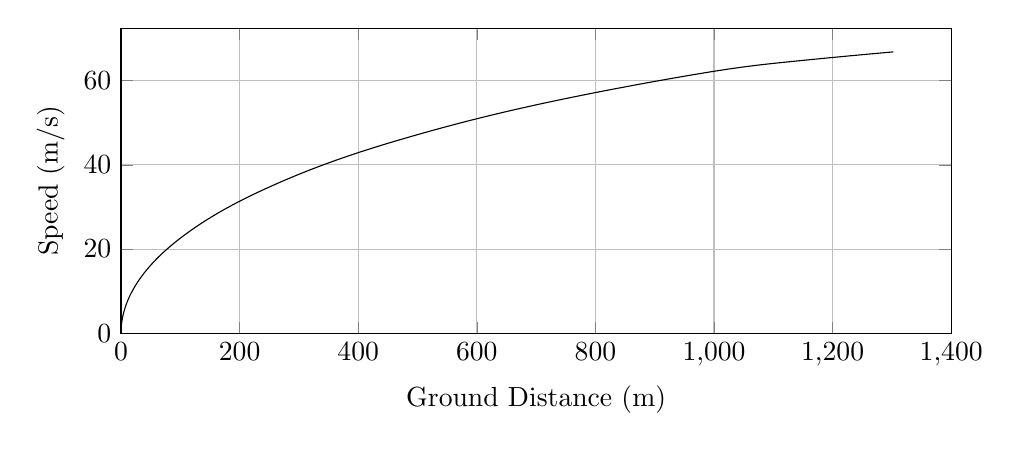
\begin{tikzpicture}

\begin{axis}[
width=\textwidth,
height=0.45\textwidth,
scaled ticks=false, tick label style={/pgf/number format/fixed},
xmin=0.0,
xmax=1400,
xlabel={Ground Distance (m)},
xmajorgrids,
ymin=0.0,
ymax=72.40593682700039,
ylabel={Speed (m/s)},
ymajorgrids
]

\addplot [
color=black,
solid
]
table[row sep=crcr]{
1.3603393307215537E-8	2.7206786614136053E-4\\
2.0334443352841076E-7	0.0010518886452100893\\
1.8493358258961232E-6	0.0031722069595670832\\
9.983129263424352E-6	0.0073703305371567145\\
4.13538327636676E-5	0.015000698600431142\\
1.2467543572893382E-4	0.02604617809108093\\
2.843807411608912E-4	0.039337211109134546\\
5.588015241105573E-4	0.05514195056130601\\
9.398454696015893E-4	0.0715124015124052\\
0.0014155885812023746	0.08776501191582356\\
0.0019945752038215015	0.10417842799085314\\
0.0026717822370171283	0.12057375104521131\\
0.003447739291558293	0.1369679805266502\\
0.0043193476547732645	0.15330646708146045\\
0.00529092766782709	0.16967458986551764\\
0.006363550519206555	0.1860801697532991\\
0.007533073890550759	0.20245842760752175\\
0.008790616877968567	0.2187050333826402\\
0.01016549189277427	0.23518661303774957\\
0.011625499440327931	0.2515089605928944\\
0.013184282533086976	0.26783979728121043\\
0.014839871214038253	0.28415877961261893\\
0.01660567024659266	0.30058916249563783\\
0.018465948346479452	0.31697862375987884\\
0.0203822997817096	0.33301959314873397\\
0.022430561433814646	0.3493511890598978\\
0.024588423902376283	0.36576858773680576\\
0.026831028501027587	0.3820837645144779\\
0.029143159681622913	0.39820533289239857\\
0.03155709159958957	0.41436781879708107\\
0.03411445662773917	0.43082953897497234\\
0.03677290089167576	0.4472999485010196\\
0.03952314881844239	0.46372369327821816\\
0.04239921643077808	0.480298229329016\\
0.045357163155895136	0.49676790089513534\\
0.048363831658398165	0.5129669973040729\\
0.051533845233668635	0.5295095037624051\\
0.0547899150155587	0.5459792875367229\\
0.058172599437445835	0.562578844948455\\
0.06162834747858026	0.5790455069507827\\
0.06521401059050522	0.5956499365054515\\
0.06888104003120077	0.6121652382585918\\
0.07268727020998902	0.6288486032523657\\
0.076546425570032	0.6453234681119759\\
0.08047032364859658	0.6616539745303078\\
0.08456364881336098	0.6782704192075162\\
0.08882250397434277	0.6951370151627567\\
0.09306368907640691	0.7115361026181237\\
0.09743039119190974	0.7280343521883228\\
0.10191450167634594	0.7445955323534352\\
0.10651989152467789	0.7612293393927179\\
0.11128201757858264	0.7780550199019596\\
0.11609763023253863	0.7947071498383971\\
0.12097769621339591	0.8112331663129451\\
0.12591912973280778	0.8276304725362169\\
0.13103216605369056	0.8442616601958726\\
0.13633380151185176	0.8611668064047788\\
0.1416823117522269	0.8778912261206315\\
0.14708837902374172	0.8944775179759736\\
0.1525605467319851	0.910958713835351\\
0.15824953188605478	0.9277821623676572\\
0.16398006351864292	0.9444251305469198\\
0.16978153473626356	0.960980143916611\\
0.17584258400626962	0.9779761627962422\\
0.1819863832139092	0.9949075014432016\\
0.18819485651962437	1.0117288237112843\\
0.19455736971520038	1.028681690882733\\
0.20098158490654017	1.0455196338851316\\
0.2076061353991409	1.0626027882678097\\
0.21424726384720844	1.0794568750195062\\
0.2211374965027113	1.0966689012354127\\
0.2281284453493247	1.1138602075497053\\
0.2350833915765042	1.1307031415936888\\
0.2423085249848444	1.1479381851546555\\
0.24958374984531584	1.1650345883096191\\
0.2569279402934431	1.182041749992774\\
0.2644720218029696	1.1992601614339744\\
0.27204626263318243	1.216301667455674\\
0.27972793364503945	1.2333438504940246\\
0.2874622320100655	1.250267563714377\\
0.29563698092580604	1.2679089139886286\\
0.30361763245720474	1.284897180240498\\
0.3118912000478351	1.3022744294143571\\
0.3202493147046803	1.3195963113902769\\
0.3286412952843002	1.3367619649866742\\
0.33714554464307567	1.3539346484227002\\
0.3458731203690518	1.3713340897191824\\
0.35455185683415313	1.3884193342166231\\
0.3634323904331427	1.4056862621253625\\
0.372325738896249	1.4227674763186258\\
0.38151551889959867	1.440204563546407\\
0.3908489672358084	1.457700089962409\\
0.4001862088113266	1.4749944178140924\\
0.4095647137707429	1.492162742069545\\
0.4192312859369268	1.5096533904480967\\
0.4289206911602753	1.5269836129109997\\
0.43896550245304145	1.5447435380037913\\
0.4487817299761361	1.5619035143205457\\
0.4589033974758888	1.5794014938286165\\
0.4691858798479248	1.5969804372850023\\
0.47972601481223376	1.6148004902966524\\
0.49016040525287174	1.632249387127532\\
0.5007175269203565	1.6497149526784889\\
0.511266977039379	1.6669842941178317\\
0.522323236324642	1.6848925320185808\\
0.5332586746953114	1.702418987029767\\
0.5445869154512923	1.72038590043744\\
0.5556699580072249	1.7377833636914817\\
0.5669225885056133	1.7552698341628856\\
0.5785590177532589	1.7731705303226786\\
0.5903083066022885	1.791062482360544\\
0.6020327889628274	1.8087393997377976\\
0.613957077533064	1.8265412477772478\\
0.625960998969677	1.8442875739585323\\
0.6380070243193761	1.8619252631764254\\
0.6503365955459197	1.8798058693058528\\
0.662700086001522	1.89756560798793\\
0.6752747602080436	1.9154589089552818\\
0.6885889407972636	1.934223118171821\\
0.7019767933734617	1.9529083746402325\\
0.7151149754112038	1.971072007225393\\
0.7284684478906998	1.989362382327093\\
0.7418939875700234	2.0075825160956544\\
0.7553494584716574	2.0256778796574366\\
0.7694215958599202	2.0444301987818747\\
0.7830840331449673	2.062472448302562\\
0.796657372658726	2.0802411313322375\\
0.8106660034246236	2.0984208913722986\\
0.8251837647136968	2.1170956097847196\\
0.8395067871054176	2.1353587515267964\\
0.8540519574023793	2.1537456286169094\\
0.8688334527125461	2.172270744815026\\
0.8840141863517745	2.191132088866371\\
0.8993797082767976	2.210057982117563\\
0.9143697020410035	2.22836535981818\\
0.9294094610857999	2.246582527337803\\
0.9452486359568626	2.2656085015457856\\
0.9605773823977486	2.2838693348294017\\
0.9761522209726621	2.302273892926003\\
0.9917649966835071	2.320575683083799\\
1.0074810114554809	2.338852757671197\\
1.0234652146968335	2.3572952472370314\\
1.0399433598517231	2.376156629932451\\
1.0563627364420554	2.3948018162279734\\
1.0728309985448887	2.4133566591997972\\
1.0896486452479222	2.432157874423557\\
1.1068138420051672	2.451197693647595\\
1.124143995869574	2.4702703658932395\\
1.1415400048645106	2.489267299720775\\
1.1590089082607062	2.508197803673264\\
1.1769249919091855	2.5274643402549435\\
1.1951505705127592	2.546912836260847\\
1.2127191877709298	2.565519481815736\\
1.2308827453761335	2.5846141113587358\\
1.2492706857898845	2.603800681463974\\
1.267587852451018	2.622772557003116\\
1.2860031245644312	2.641707402954026\\
1.304687144125951	2.6607795541301913\\
1.3233765774990474	2.6797201186880235\\
1.342322280991234	2.6987833934981085\\
1.3613696045164358	2.7178127915773045\\
1.3815086998747366	2.7377876348627312\\
1.4013123019267382	2.7572871781846713\\
1.4209622886438908	2.776498715109069\\
1.4411501686096515	2.796097243313718\\
1.4611760119255748	2.8154022541980437\\
1.4816444281325132	2.8349966107890987\\
1.501865958841821	2.8542211069946886\\
1.5224364680875304	2.873643975251948\\
1.543651615594651	2.8935374401166936\\
1.5647593029468103	2.9131938159672393\\
1.5859558716309676	2.9327988876571682\\
1.6071423964076703	2.9522630829787078\\
1.6293386351549652	2.9725166193581662\\
1.6508498980272122	2.9920127820710096\\
1.673011606043147	3.0119649186923647\\
1.6946435720294923	3.0313119602620544\\
1.717066624993247	3.0512354765097847\\
1.739432891071898	3.0709781945200367\\
1.761922286799709	3.0907008715442785\\
1.7849035550437842	3.110724116499121\\
1.8076299607761817	3.130397758415918\\
1.8313298306791497	3.150781582850553\\
1.8543134894513886	3.170422617417267\\
1.8777326664639729	3.1903098303565613\\
1.9017196849182967	3.2105498581425547\\
1.925345883672024	3.230359810434704\\
1.950252961491087	3.2511112867058944\\
1.975161211119453	3.2717303209738455\\
1.9993825790313986	3.2916551882881686\\
2.024583888346972	3.3122571746177787\\
2.04934017380271	3.3323696010495665\\
2.0744229633459703	3.352622489884446\\
2.0996193404956136	3.3728429027993636\\
2.1245764901457758	3.3927508156451838\\
2.1500786393425866	3.4129717612165447\\
2.176226227020705	3.4335790174579808\\
2.202115608176549	3.453859839248252\\
2.227948363055355	3.473976519895017\\
2.2543499999408594	3.4944147290829672\\
2.2810892744412783	3.5149913296713144\\
2.3075963743135786	3.5352692309359393\\
2.3348582111613405	3.5560020049415755\\
2.3623221378972126	3.576765039163723\\
2.3898598419727675	3.597461619334588\\
2.4171687299087603	3.617867425928493\\
2.445442108612223	3.63887140648351\\
2.4735885391813177	3.659659385088693\\
2.5015416452491293	3.6801864489790015\\
2.5301110763218357	3.7010465061417728\\
2.5589284934403693	3.7219672053679007\\
2.587611617795936	3.7426723197239697\\
2.6175687086884984	3.7641733892005584\\
2.647724154312196	3.7856913664269127\\
2.6767118187859253	3.806259385188194\\
2.7060305938995466	3.826947924762984\\
2.7361546404224653	3.848086795361401\\
2.7663022704956823	3.8691245251687114\\
2.7964672462043376	3.8900584385922787\\
2.8272583584284883	3.9113092281493635\\
2.8588650092419234	3.933001260500056\\
2.8898852960400587	3.954173020653517\\
2.9215246589961597	3.975649002611738\\
2.95270311230069	3.9966971225957693\\
2.984506337549637	4.0180512736887355\\
3.017379145769185	4.040002700931062\\
3.049243647754313	4.061165386837043\\
3.081295157663824	4.08233945372935\\
3.113406837946715	4.1034415622615725\\
3.1453724573084756	4.124338342413571\\
3.1787286104953543	4.146029627303218\\
3.211019796961401	4.16691865410681\\
3.245786703184362	4.189290422964376\\
3.279939251746722	4.211148796843801\\
3.3141720228361216	4.232942924168725\\
3.3491198891036547	4.255074788125151\\
3.382965192547779	4.276396971929374\\
3.4181848705561064	4.298470348414034\\
3.45391888941694	4.320748399293741\\
3.488851494856137	4.342413989011922\\
3.524271454997704	4.364269672627019\\
3.5606552075305	4.386604233843519\\
3.597189071478943	4.408914624339188\\
3.632926148839256	4.430627359280907\\
3.668897146318187	4.452372929752713\\
3.706642714683163	4.475075142646437\\
3.7432264628550644	4.496966755254986\\
3.781286297809391	4.519626577407692\\
3.818618572105483	4.541740901418004\\
3.8564015479305356	4.564010610229177\\
3.8948624022541356	4.586566255076516\\
3.9329637046009225	4.608799669367572\\
3.971505929995028	4.631179243588672\\
4.009821706071438	4.653318136849505\\
4.049014376833089	4.675852686730371\\
4.089343885784727	4.698925378992982\\
4.128662304630717	4.721308468478165\\
4.1684827283974055	4.743867096677683\\
4.208000253554632	4.766146006975694\\
4.2483743636521965	4.78879817493951\\
4.288255503180503	4.811066470729566\\
4.328757204126676	4.83357366756756\\
4.369490126907612	4.856101520059605\\
4.410357715197167	4.878596683350667\\
4.45189144941496	4.901350066297022\\
4.492881116440694	4.92369968185371\\
4.53550011161515	4.9468278744343355\\
4.577670191557685	4.969603783574717\\
4.6201174049766305	4.992421721491047\\
4.662272021613388	5.014976943890929\\
4.706017761800355	5.038273949606417\\
4.748842845578064	5.060974035026659\\
4.792293145132742	5.083899188662546\\
4.836482439768313	5.107105883961035\\
4.88090298307878	5.130325383258471\\
4.925311889063089	5.153431397682763\\
4.969864686447545	5.176505825154747\\
5.014842280541593	5.199693556764473\\
5.0603877575117515	5.22306627262987\\
5.106292347304597	5.246515006059436\\
5.152263975081851	5.269890511862322\\
5.1974808794106995	5.292778734007962\\
5.244027372436168	5.316234153414978\\
5.28996242022761	5.3392775841790705\\
5.336209145350672	5.362374492774961\\
5.38320569473032	5.385741511936569\\
5.430469292142472	5.409136579741427\\
5.476900151253712	5.432018503774243\\
5.526063828851289	5.4561395711543685\\
5.573879040902945	5.479494218102513\\
5.622613575936374	5.503192913358333\\
5.6713596863799225	5.526792584844657\\
5.720412183296268	5.550436296154132\\
5.770660497446668	5.574549325574564\\
5.820668144990444	5.598440665195858\\
5.870305285939629	5.622051570005873\\
5.920503816994749	5.645826051794918\\
5.971105439367246	5.669687478338329\\
6.021088325934068	5.693155956312442\\
6.071322359863801	5.716642304314178\\
6.122981826035449	5.740691790991834\\
6.174329110820436	5.764493438157782\\
6.225804784288178	5.7882532999677565\\
6.278093246139479	5.812285775103884\\
6.331709873490098	5.836822711993435\\
6.384325657889258	5.860798606286268\\
6.436648686434458	5.884541153322957\\
6.489478972803882	5.908413995611658\\
6.543185721519176	5.932581273594973\\
6.596747696432654	5.9565826116867555\\
6.650345873843312	5.980500639526959\\
6.704555155195255	6.004591322261984\\
6.7588986063680725	6.028641860723198\\
6.814371620173711	6.053090524510132\\
6.86997180120154	6.077493304987486\\
6.925426612865756	6.101731867456724\\
6.981353650685165	6.126076488296089\\
7.037678624474159	6.150493701171172\\
7.094603706786671	6.175069694229233\\
7.151204881983983	6.199406017809888\\
7.209200593921791	6.224239921146953\\
7.2667780016693655	6.248793780637895\\
7.324687293141565	6.273388951364629\\
7.382771066065313	6.297958460524253\\
7.441904508776327	6.322870556471969\\
7.501585831803217	6.347910940195371\\
7.5616527251378685	6.37301033734094\\
7.62150963104709	6.397920657282372\\
7.682859947113334	6.423348757973162\\
7.7432084367972145	6.448260395172165\\
7.803024936926759	6.472854515267269\\
7.863793829029664	6.497741557547526\\
7.9252460466886365	6.522808491769428\\
7.98696966925656	6.547886129589465\\
8.04776546969778	6.572489956029987\\
8.109421212326083	6.597344759331692\\
8.17269125419024	6.62274989587474\\
8.236095044780246	6.648107867119668\\
8.299523592514586	6.6733758716647635\\
8.363213767675873	6.698648749336412\\
8.427807923256076	6.724179817063581\\
8.49144930156071	6.749236427599463\\
8.557380457258176	6.775093285731961\\
8.623183572921022	6.800798341060123\\
8.687840683575093	6.825958000305871\\
8.753751426394068	6.85150690514026\\
8.820803713780364	6.877397340692875\\
8.888970287482593	6.903614836544355\\
8.957133699158991	6.929728274880318\\
9.025036015045707	6.95564060719898\\
9.092760955867519	6.981385897661401\\
9.159817422823458	7.006780404744905\\
9.227495373767134	7.032313822655334\\
9.296013084156197	7.058066451057831\\
9.36435980631623	7.083658045990241\\
9.433329865923408	7.1093861502633935\\
9.503849553921977	7.135592793043607\\
9.574524061692681	7.161757129440835\\
9.644263228942293	7.187478303059413\\
9.715657612596786	7.2137113525921706\\
9.787429657508813	7.239983725980906\\
9.85753688572494	7.265551478201084\\
9.930250735750551	7.291971533509516\\
10.001571447096964	7.317789201023549\\
10.074699859091687	7.3441634012160115\\
10.14698611653175	7.370137562038421\\
10.220547980738981	7.39647284159466\\
10.2940409891517	7.4226865775090225\\
10.36719293590382	7.448683522018358\\
10.441008888975666	7.474821256293147\\
10.51610421670324	7.5013149409599915\\
10.590724589239105	7.527545123141664\\
10.667218005391902	7.554335510282012\\
10.742771202259895	7.580700056819904\\
10.82035208750042	7.6076733994766546\\
10.896759047300378	7.634141815439909\\
10.973503045910835	7.660631342117224\\
11.051297940743765	7.687386808018605\\
11.128076326409062	7.713698127714148\\
11.207667705350879	7.740875339530433\\
11.286758396846047	7.767783712029548\\
11.366305937658339	7.794750148057366\\
11.446149720998452	7.821719854770112\\
11.526866579636565	7.848886577953234\\
11.607297517600138	7.875860199567693\\
11.688034241538357	7.902840142547248\\
11.769665722224765	7.930022095599563\\
11.850920080706608	7.9569826322198836\\
11.933163326324259	7.984174930255627\\
12.017103780766782	8.011829467127516\\
12.10034832931326	8.039157084017077\\
12.185467765774142	8.067000695357674\\
12.270669986481685	8.094771694330461\\
12.354040133273898	8.121850004746655\\
12.440386807402234	8.149796497316302\\
12.52556588630658	8.177267823749766\\
12.610860989997974	8.204680768800486\\
12.69550109439961	8.231789408552956\\
12.784634337461807	8.260237152929719\\
12.871172079509357	8.287759415726047\\
12.958447214271366	8.315420304840373\\
13.045518554761987	8.342921619029696\\
13.133090172249581	8.370486224312394\\
13.221405510214687	8.398189697653255\\
13.310319106907201	8.425985210556949\\
13.399783591735492	8.453857077321647\\
13.488943611067967	8.481539391738199\\
13.578276665194153	8.509181571435288\\
13.667402973129146	8.536667089813005\\
13.757763665999576	8.56443970756747\\
13.848393619195729	8.592201389835143\\
13.938857764339925	8.61981963690165\\
14.031101516310692	8.647886827800537\\
14.123507833735925	8.675908901157563\\
14.214825187590282	8.703508672365633\\
14.307956552027534	8.73156336745275\\
14.401498558574918	8.759647814517947\\
14.495315613017755	8.78772120463606\\
14.589065423003394	8.815681723809828\\
14.68316852398955	8.843655285252552\\
14.778702641747682	8.871960546801994\\
14.873746415615575	8.900027772307503\\
14.970384078097169	8.92847176195491\\
15.068900921005241	8.957372338705746\\
15.164434274206265	8.985305531350946\\
15.260378587808539	9.01326844809585\\
15.357189194448868	9.04139286669879\\
15.45495288999333	9.069702319145797\\
15.55311774366497	9.098035965089778\\
15.652583807013901	9.126652094929362\\
15.755243917873962	9.156089842136982\\
15.855950289561445	9.184872261311103\\
15.958461094374158	9.214074622426836\\
16.060387288500337	9.243015579888077\\
16.164276126126843	9.272417421818076\\
16.26736468838029	9.301497527925843\\
16.36946523634058	9.330206314561998\\
16.47192386662276	9.358924026035133\\
16.576794358652606	9.38822346960886\\
16.678929175716583	9.4166678008983\\
16.783994526910618	9.445835681115561\\
16.89012564586595	9.47520500509841\\
16.996887404888547	9.504654011959929\\
17.103774697793426	9.534043283288177\\
17.210947675936964	9.563417219634118\\
17.31865021419634	9.592842496276361\\
17.424470519881233	9.621662818293629\\
17.53205215515201	9.650871542605824\\
17.64034909906897	9.680182378579893\\
17.74911485075183	9.709527974498918\\
17.85745376408675	9.738667491033553\\
17.969383314157206	9.768678371847692\\
18.07998395718984	9.79823960098523\\
18.18863741327577	9.827190891062958\\
18.302466989554325	9.857427140731051\\
18.41305080779906	9.886709740958622\\
18.525644000014054	9.916432659837046\\
18.636945827420575	9.945724520892664\\
18.750643923449367	9.975555331385554\\
18.86479622056296	10.005412957938304\\
18.979646899421056	10.035360740626022\\
19.09418630108147	10.065135801951545\\
19.208983505033515	10.094886994415017\\
19.323483295898072	10.124471311384106\\
19.43842354827664	10.154080065585102\\
19.55563752357537	10.184183168800388\\
19.67199913451129	10.213976951289727\\
19.789486593639566	10.24396844826034\\
19.90713985662446	10.273911926981121\\
20.024127533725753	10.303597189258529\\
20.143019013955552	10.33367562294372\\
20.26442367074238	10.364297193766397\\
20.383660776265387	10.394281737963148\\
20.5042342316437	10.42451216268142\\
20.622773342122727	10.454144942087797\\
20.74503732713029	10.484618723707356\\
20.865944869938517	10.514665202901362\\
20.98711015528624	10.544687539570457\\
21.113336299999695	10.575870816745912\\
21.23638685227678	10.606179030549342\\
21.35988644990264	10.636508776547114\\
21.483760012473958	10.666841533708403\\
21.608180515260266	10.697219473139526\\
21.732326713270083	10.727442588179319\\
21.85766379468624	10.757867398704445\\
21.985117186778353	10.788715847331869\\
22.111729024702363	10.819271479105705\\
22.23700541150786	10.849418172071925\\
22.36297326225872	10.879645126013575\\
22.488604760551	10.909706102371654\\
22.616276341350805	10.940168758719981\\
22.744235570279145	10.970613360141936\\
22.874576476768283	11.001536189573937\\
23.003842066605536	11.032116542561745\\
23.13088450205612	11.062086942499228\\
23.257869280739328	11.091961228338679\\
23.389244224935425	11.122782273486525\\
23.519811196806458	11.153327800430485\\
23.653309395988643	11.184471249811509\\
23.78342402399784	11.214740651782549\\
23.9180644861338	11.245975674318391\\
24.05110504604577	11.27675313214855\\
24.182394801971697	11.307042095287713\\
24.314614014384034	11.337462416058873\\
24.449791085561472	11.368477829038198\\
24.585258581909038	11.399473971168938\\
24.72121222319008	11.430495640196643\\
24.857032405393277	11.461401868729997\\
24.99454740444294	11.492607967789148\\
25.13030709358258	11.523331794491032\\
25.270890409679986	11.55506012379086\\
25.40663839363527	11.585613757472291\\
25.54307796688363	11.61624118816924\\
25.68272814639034	11.647505059569063\\
25.82072003425767	11.678314669990076\\
25.96015212691003	11.7093627406886\\
25.987750021099068	11.715498267162236\\
26.0558803939429	11.730631063705655\\
26.061632797568386	11.731907859395676\\
26.066808273335674	11.73305648125297\\
26.071901058608013	11.734186640502788\\
26.073315434863225	11.734500490619862\\
26.074595035914804	11.734784426825545\\
26.080371168076944	11.736066031557627\\
26.10234540095133	11.740940372180685\\
26.183408179590366	11.758904155082949\\
26.300430535410044	11.784787973628632\\
26.42750601924636	11.81283056419338\\
26.558056987479794	11.841570237741418\\
26.688030995483615	11.870113002299234\\
26.818767077324992	11.898753220355104\\
26.951519978077492	11.927763989958692\\
27.083955405447817	11.95663428682252\\
27.216897884715692	11.985544164744663\\
27.350913258119895	12.01461587041586\\
27.4833530065795	12.043275722209213\\
27.6176201223548	12.072260383279556\\
27.752160408628434	12.101233140761607\\
27.887329802382908	12.130270390734324\\
28.023188645890663	12.159384516832986\\
28.158973127824495	12.188411811876492\\
28.296372294036907	12.217712605075796\\
28.435107205966254	12.247225563626774\\
28.571323599682245	12.276132156199722\\
28.70996262687553	12.305481485301957\\
28.850320389600306	12.335121789198851\\
28.988837241064125	12.36430191055613\\
29.129197813929657	12.393798521815558\\
29.27166529868488	12.423664350659593\\
29.41298471572133	12.453216777241245\\
29.554848516656044	12.482810659257765\\
29.699676691743235	12.512948602260185\\
29.842400551696755	12.5425756525737\\
29.985385440862252	12.572184694765959\\
30.129077275410303	12.601867799121568\\
30.27543774584293	12.632028113131444\\
30.422081339040986	12.662172291443763\\
30.56949149516445	12.692399395353114\\
30.716562179458485	12.722482784504752\\
30.86535310281699	12.752843213073941\\
31.011875026602333	12.782667571325081\\
31.16159928701196	12.813069323080846\\
31.313692569485013	12.843875567279284\\
31.463056706803336	12.874054434598822\\
31.61235366859384	12.904146336171102\\
31.76278957628285	12.934394055733065\\
31.915019899787076	12.96492770009322\\
32.06709627595497	12.995355745016585\\
32.21861178877769	13.025597773954171\\
32.37168228565527	13.056075852175109\\
32.52450570609457	13.086430689262858\\
32.67702483599189	13.116651789580214\\
32.829998687403204	13.146889904935595\\
32.98551220909506	13.17755548020082\\
33.14332298937855	13.208597699427095\\
33.29970221124884	13.239282941961267\\
33.45800124694219	13.270268960855145\\
33.61398946945653	13.300728393722224\\
33.77048353048475	13.331212997374429\\
33.9292721471582	13.36206969824487\\
34.08796840843395	13.392833573712974\\
34.24769686644211	13.423722435259549\\
34.406855482575295	13.454426622534776\\
34.56481953291838	13.4848273131478\\
34.72399692808165	13.515388364482458\\
34.88694269464703	13.546597337194846\\
35.04914399338672	13.577588258057553\\
35.209965099803895	13.60824160856891\\
35.3703140559587	13.638732196664854\\
35.531685786905925	13.669344364559521\\
35.69349909442164	13.699967319927516\\
35.85522798807463	13.730501730108934\\
36.022509111806116	13.762008547654311\\
36.19055880791667	13.793582946048737\\
36.35708622463872	13.82479550449025\\
36.52115360367851	13.85547362194265\\
36.68781562330062	13.886562820126564\\
36.8536847754776	13.9174304483709\\
37.024522648961764	13.949146389510084\\
37.19188554678789	13.98014254566111\\
37.36066720850286	14.011327095827419\\
37.528862119520696	14.042329405603326\\
37.697264258302326	14.073296530111996\\
37.86832931534104	14.104678619737609\\
38.03812867477943	14.135754509787166\\
38.20923731912278	14.166995894554624\\
38.37904730305398	14.197927055200015\\
38.55252405124031	14.229451377363098\\
38.72282139824354	14.260324907567675\\
38.89783411301201	14.291978375010753\\
39.0714610757495	14.323306627589965\\
39.24438070689564	14.354433875522993\\
39.41969314875929	14.385917557213435\\
39.59166556575205	14.41672917791362\\
39.764623188591585	14.44764559250558\\
39.94263254662576	14.47939036052248\\
40.11749159802578	14.510500050118512\\
40.29452954971913	14.54192386043901\\
40.47247750600427	14.573435088431616\\
40.64799609178485	14.604443782057789\\
40.82414741101539	14.635492466718976\\
41.00385670225303	14.667094616677119\\
41.18169069533937	14.698294192054348\\
41.3603281005193	14.729562251315262\\
41.54046179251334	14.761019112816346\\
41.722675278204306	14.792764939681511\\
41.90258931008478	14.824037343077613\\
42.08518735141125	14.855702756267998\\
42.26728550944881	14.887208166124452\\
42.44743534848537	14.918304880626533\\
42.63069538383506	14.949865823401272\\
42.80963512098974	14.980612455604206\\
42.992542679335614	15.011969534134973\\
43.17926890616222	15.043907330033203\\
43.363134036078335	15.07528320232565\\
43.54815051311773	15.106783307813565\\
43.733578141849236	15.138281142092769\\
43.91798130912079	15.169533629501466\\
44.10506009255049	15.20116732793008\\
44.29251116260117	15.232791425149927\\
44.480917546793805	15.264503947324222\\
44.66851287589745	15.296007928958101\\
44.85853501730759	15.327846628450256\\
45.047396872181054	15.3594187231866\\
45.236914792155844	15.391028573966832\\
45.42785879536018	15.422803857706569\\
45.616432631699865	15.454113793375477\\
45.80697204128492	15.485678919895587\\
45.998633580597016	15.517358201006619\\
46.18800675699903	15.5485889940684\\
46.380841640082096	15.580319349319915\\
46.57327038933336	15.61191154939888\\
46.765844918266424	15.643456771132307\\
46.95911042680183	15.675044279688183\\
47.15311668852311	15.70668184113109\\
47.34541611633634	15.737971256186935\\
47.53884854699059	15.769375322632264\\
47.73236991243341	15.800724280331082\\
47.92818250719388	15.832374008959643\\
48.12326385407131	15.863835546272451\\
48.32058854034828	15.895588215308145\\
48.516852452700604	15.927100108245902\\
48.71339374517507	15.958586905572094\\
48.91319881343868	15.99052556573712\\
49.1119162355681	16.022219771885794\\
49.31207818344666	16.054073616673193\\
49.509673461222235	16.085449755667547\\
49.71156302510582	16.11743714149557\\
49.91034548441702	16.148862880455226\\
50.11200805970151	16.18067402752412\\
50.30853267551517	16.211607332775543\\
50.50757456960626	16.242869479706997\\
50.70929197287772	16.27448306208673\\
50.91222418686718	16.306217560588948\\
51.11562549758783	16.33795589919523\\
51.32090674103446	16.36991742319855\\
51.525199701657655	16.40165551094453\\
51.72863462744459	16.433191736975424\\
51.934060761332375	16.464967613389298\\
52.14033810224923	16.496805767338245\\
52.344882977561255	16.52830825765387\\
52.55098100649393	16.559981596302798\\
52.75731843494604	16.591623385101634\\
52.96514817708821	16.623425292724193\\
53.17450540782369	16.655391599818486\\
53.382202621450276	16.68703607441325\\
53.592230583406476	16.718966811006503\\
53.80364534107798	16.751038866953195\\
54.01469481143569	16.78298634512351\\
54.223966920081466	16.81459693592374\\
54.43230789395902	16.846000158107778\\
54.6430562980421	16.877698907056292\\
54.855225786754914	16.909543373000844\\
55.066088958624874	16.94112453133839\\
55.27969530828261	16.973048579073087\\
55.49171188337613	17.00466777951221\\
55.70388919125476	17.036244256254207\\
55.91737779085577	17.067948923124497\\
56.13177028494084	17.099720617504012\\
56.34652664868587	17.131479097728892\\
56.559021044851505	17.16283731260777\\
56.77591447970492	17.19477762486875\\
56.99548236897459	17.22704315413428\\
57.21481285737903	17.259205253646627\\
57.43536222847358	17.291477405673106\\
57.65367025761124	17.323354153252986\\
57.872788904232735	17.355282182779625\\
58.0907693980174	17.386978064843134\\
58.311927420720366	17.419068779042476\\
58.532333513628615	17.450983423705587\\
58.75532998033057	17.48320550910723\\
58.976617007999806	17.51511371149133\\
59.19875422837053	17.547077884078412\\
59.4206945143671	17.57894743506791\\
59.64453328369959	17.6110228722233\\
59.86894932484513	17.64311414170048\\
60.09432075877773	17.675275011051006\\
60.318058693038594	17.707136719649682\\
60.541731124044205	17.73892368315107\\
60.76707064338231	17.770881795092755\\
60.995574692986196	17.803221679280476\\
61.22378989589207	17.83545369864867\\
61.4534619981562	17.867824284037283\\
61.683510138770515	17.90018067545715\\
61.91410430469678	17.932546762179015\\
62.14462153858659	17.964835283858278\\
62.37563158073512	17.997126244143544\\
62.607203285434	18.02942919131057\\
62.841031881319736	18.061979766095043\\
63.07467935056491	18.094438067932423\\
63.31164975340633	18.127289914380235\\
63.54633691305479	18.159758045124143\\
63.78243968758058	18.192354943169995\\
64.0165414084598	18.22460952240222\\
64.25412817577254	18.257277411786973\\
64.49270299572771	18.290013768976266\\
64.73076499662056	18.322612833783396\\
64.96867826857735	18.355125123261494\\
65.21063576532572	18.388122379615005\\
65.4512107007771	18.42086378786273\\
65.69028017871045	18.453334211067258\\
65.93032615763332	18.48587134598388\\
66.17196619696679	18.51855821773882\\
66.4135612157637	18.551172846894467\\
66.6559030093851	18.583822213908434\\
66.89910102540284	18.6165207865629\\
67.14354652182666	18.649320691401478\\
67.38771133480921	18.682016863411377\\
67.63347396558368	18.714860698629238\\
67.87898066495345	18.747604296973613\\
68.1255935515739	18.78042936258401\\
68.37316753306138	18.813316131464234\\
68.62205497364681	18.846310878683518\\
68.8711887275476	18.879271890959345\\
69.120220471977	18.912153407236545\\
69.36846244647072	18.94486534684726\\
69.61951843592018	18.977882174220817\\
69.87236615109754	19.011068008473416\\
70.12758921381476	19.044498186251296\\
70.37945082809051	19.07742205063662\\
70.63410009691182	19.110644035332676\\
70.89152727368702	19.144161074618772\\
71.14629115974091	19.177265064407557\\
71.40197865069018	19.21042314698483\\
71.66163317144085	19.24402848823103\\
71.92484704501203	19.27802578556198\\
72.18465416754285	19.311515618271024\\
72.44573394560723	19.345102399321448\\
72.70633339061075	19.378560698675827\\
72.96699363118216	19.411960539667227\\
73.22900401485182	19.445466981936725\\
73.49076816912304	19.478875843446218\\
73.75430841254712	19.512445038740097\\
74.01895646534612	19.54608874132115\\
74.2846979982242	19.579804688311334\\
74.55380714249793	19.613880119908124\\
74.82322871850147	19.647927187775537\\
75.09350011520078	19.6820137651441\\
75.36421232425869	19.716088183322746\\
75.6347219158074	19.750069764012878\\
75.90830954343213	19.784369951832026\\
76.18188601743822	19.818600707717906\\
76.45626363461818	19.852863779190507\\
76.72958718025629	19.886927989297774\\
77.00406935908524	19.921069467275075\\
77.28579748399531	19.956042687591157\\
77.56784659723587	19.990985607089215\\
77.84569092555657	20.025339384858604\\
78.1246978223638	20.05976918860773\\
78.40641219364133	20.094464658240312\\
78.68590470271565	20.12881893388358\\
78.96851680469001	20.163488652350928\\
79.25576208114188	20.198657096075948\\
79.54169104977237	20.233595062881214\\
79.82662017154695	20.26834247833819\\
80.11330301632765	20.30323528725986\\
80.40394576721474	20.33854037515337\\
80.6908099930996	20.373318087594704\\
80.98055888331655	20.408376968618384\\
81.27178512217935	20.44354560419724\\
81.56682943128612	20.479105200138818\\
81.86186977412851	20.514594183842583\\
82.15688924927383	20.550010962329395\\
82.44965588234726	20.585088814816103\\
82.74488606927187	20.620393184721507\\
83.04325841243121	20.656003684954428\\
83.34213327641098	20.69160443047427\\
83.64411622775171	20.7275049561637\\
83.94734638805741	20.76348294994817\\
84.25123842984891	20.799468737599256\\
84.55152885577829	20.83495890636504\\
84.85735750691177	20.87103342682147\\
85.16518306664875	20.90727241570412\\
85.47136476235073	20.94324758159427\\
85.77898122624802	20.979321166593273\\
86.08923229760057	21.015632923266487\\
86.40254560035129	21.052231397343448\\
86.71167807044037	21.08827134706359\\
87.02660518802142	21.12491565780897\\
87.34238286044419	21.161587239406337\\
87.65842706333811	21.19821834626532\\
87.97971380652302	21.23538431420345\\
88.2973933745065	21.272061329033342\\
88.61789013566766	21.308991834778887\\
88.93643920279564	21.345626944102094\\
89.25662431900213	21.382379370977056\\
89.57903058309674	21.419315452201452\\
89.89968694948243	21.455980549166604\\
90.22473455398588	21.493076451285525\\
90.55024875587375	21.53015412230218\\
90.87789352676518	21.567402708165503\\
91.20733069500889	21.604782943547264\\
91.54101415610151	21.64257175453799\\
91.87012785371462	21.679771324650453\\
92.20120197152713	21.717121081699503\\
92.53416638543635	21.754612338218614\\
92.86431843528567	21.791716344685014\\
93.19748455591187	21.82908830449999\\
93.53066771200866	21.866391531576255\\
93.86681917526724	21.903955968987766\\
94.20530590547477	21.941709662266156\\
94.5419273964865	21.97918442358995\\
94.8854212036891	22.01735186501176\\
95.22752713476521	22.055292899808897\\
95.57091181422334	22.093303788685276\\
95.91383450860906	22.131192066486435\\
96.25469535763642	22.16878223054497\\
96.5966517898868	22.206423250654886\\
96.93845701474973	22.243978061415305\\
97.28153572459905	22.281603319091836\\
97.62213139590432	22.31888787171782\\
97.9659652144934	22.35645824141657\\
98.3129807304216	22.39430679429588\\
98.65852794036775	22.43192630971943\\
99.00080640577195	22.46912263861835\\
99.35064076251427	22.50707131446339\\
99.69796076807248	22.544678928219355\\
100.04654253174803	22.582355184874388\\
100.3915606488718	22.619579653578754\\
100.74261509654437	22.65738782613188\\
101.08877163494762	22.69460221539203\\
101.43457754260953	22.73171363052728\\
101.784020212797	22.769149501824693\\
102.13161434601102	22.806322121035947\\
102.4751980097893	22.843002352360074\\
102.82212110631409	22.87997546658648\\
103.16739702108615	22.916709973038678\\
103.51524666207362	22.953655109816047\\
103.86391679154056	22.990624161909977\\
104.20960434827006	23.027214897762114\\
104.55241399635099	23.063440371686035\\
104.89662223620601	23.099753283563047\\
105.24103428322039	23.13602756319478\\
105.5836615386647	23.172054572027825\\
105.92645892081137	23.208040675077115\\
106.27347658175316	23.24441030746282\\
106.6151670762521	23.280163504496024\\
106.95898391938218	23.3160813719658\\
107.30023552029138	23.351674273464127\\
107.64147805753461	23.38720983521675\\
107.98348674656944	23.422768965307462\\
108.32522459759954	23.458244090181672\\
108.3935347040271	23.465328563565826\\
108.40478590462831	23.466495218539748\\
108.41572478024443	23.467629430487982\\
108.4246743308916	23.4685573344252\\
108.44347342986478	23.47050633189219\\
108.52018987797786	23.478458177015114\\
108.70071173483461	23.497158706258915\\
108.99446230248458	23.527555808669007\\
109.30176454987088	23.559311599202502\\
109.60899173332959	23.591015113289558\\
109.91608539831654	23.622660443581132\\
110.22883517949637	23.654843076513636\\
110.54143546549608	23.686964479481496\\
110.853845249356	23.719020598101764\\
111.1739714794031	23.751821181570904\\
111.4937490010879	23.784538313981187\\
111.81170779322963	23.817022169054\\
112.13106495813236	23.84960160276347\\
112.4519453366479	23.88228879288807\\
112.77515902629136	23.915165494740442\\
113.0997499810409	23.948133725506615\\
113.43040796942478	23.98166823630654\\
113.7597028375028	24.015014513614958\\
114.0907450350197	24.04848755497811\\
114.42538740208008	24.08227359324205\\
114.75997726261329	24.116003142692982\\
115.09477047197589	24.149702069244555\\
115.43440545481076	24.18383620797733\\
115.77494672336013	24.218008818332883\\
116.11687534861284	24.252267757742516\\
116.46164587354252	24.28675789493178\\
116.8077846490165	24.321330945793186\\
117.15688723722127	24.356145384750143\\
117.50557855048987	24.390864153550645\\
117.85411336711965	24.425512878052224\\
118.20532793701167	24.460373050471716\\
118.55850697655507	24.49537270986547\\
118.91273956155123	24.530421002480267\\
119.26983096270519	24.565695750884693\\
119.62978614725739	24.601196221148456\\
119.98960731920661	24.636626243419393\\
120.34734904217265	24.671794923196416\\
120.7138511704587	24.70776644527863\\
121.08106061642908	24.74374828744837\\
121.44737887966437	24.779584008579377\\
121.81499139152783	24.81548745328893\\
122.18511446431708	24.85157664821383\\
122.55384158147794	24.887470566976\\
122.92460728481757	24.923503544080738\\
123.29616941264607	24.959554330901142\\
123.67040864389355	24.995804718505838\\
124.04652172406458	25.032175958965873\\
124.42393851457416	25.068612309140384\\
124.80152108360014	25.10500371732497\\
125.18180835736592	25.141594353183905\\
125.55854932865631	25.177783121327877\\
125.93878032356085	25.214246091706904\\
126.31997081831156	25.25073968753791\\
126.70099538833193	25.287156141005653\\
127.08058279416298	25.32337450580105\\
127.46175209000612	25.359682977702626\\
127.84399628255431	25.396032794321073\\
128.22749916598133	25.432441044057036\\
128.6102537001487	25.468717234476806\\
128.99595881306152	25.505211582482737\\
129.37788117916477	25.54128736867886\\
129.760738924708	25.577391107947825\\
130.1448498512433	25.613552421741133\\
130.53000390659713	25.649751163636274\\
130.9168242384266	25.686045432395574\\
131.29443328439476	25.721416558779445\\
131.67491382268804	25.75699799969326\\
132.05816436539135	25.792779123746882\\
132.44070735535217	25.828434948845413\\
132.82666098215685	25.86434886376555\\
133.20952005887244	25.899915643121524\\
133.5940193955625	25.935575649700276\\
133.97617966856654	25.970960156283404\\
134.36103715882757	26.00653556511503\\
134.74478042358356	26.04194936276936\\
135.12867144169206	26.077318403834774\\
135.5141335746535	26.112773606615214\\
135.89764893392993	26.147991649029102\\
136.28231234485685	26.183257080705424\\
136.66418763078912	26.21820957810221\\
137.04684871033697	26.253176876607633\\
137.42845627025127	26.287991129033465\\
137.8132447087305	26.323038336044007\\
138.19719797258034	26.35795235515335\\
138.58059071069573	26.39275864219689\\
138.96593237593703	26.427684880046527\\
139.3501607499636	26.462453503591675\\
139.73355638294606	26.49709049973351\\
140.1160230155566	26.531587727941456\\
140.50045093994146	26.56620582600513\\
140.88215178690393	26.600522936575338\\
141.26156782058217	26.634580074514247\\
141.64323970440188	26.6687849903212\\
142.02689350659642	26.70311238806667\\
142.41061312971692	26.737390551313872\\
142.7942251403153	26.771604164154354\\
143.1756303563767	26.805566666931192\\
143.5599719391364	26.8397360475888\\
143.94242380128833	26.873683192788498\\
144.3239499176869	26.907494429931745\\
144.70664939692608	26.94135589725454\\
145.0870075357763	26.974957021172592\\
145.46856550308127	27.00861103432308\\
145.85014610541765	27.04221401465076\\
146.23128237819492	27.075725091129634\\
146.61504730324998	27.10941416328948\\
146.99763315977907	27.142946831280582\\
147.38441582478964	27.176793816748457\\
147.7673688364352	27.210252821242534\\
148.15222568696134	27.243825350863183\\
148.53580865353604	27.277234236204137\\
148.9199734867533	27.310641414627234\\
149.3040357319486	27.343987432365928\\
149.68771357306542	27.37724808451503\\
150.07093078701052	27.410417098575643\\
150.45622889618164	27.443714289923733\\
150.8449053483268	27.477250842883336\\
151.2288570611563	27.510328029070116\\
151.61452719766493	27.543501694715076\\
151.9983007305741	27.57646108995101\\
152.38299664478842	27.609448674041523\\
152.76945776909372	27.642536348093053\\
153.15580177123394	27.675562788975917\\
153.54253364040335	27.708571276735924\\
153.93093169697067	27.741670677475376\\
154.31788037931886	27.774595604619762\\
154.7039882138024	27.807398452861975\\
155.08880221957185	27.840041318857274\\
155.47621608980313	27.872854403716566\\
155.866104687065	27.90582628258049\\
156.25391419262098	27.938571938646128\\
156.64166339424906	27.97126241442561\\
157.03027969880475	28.00397590612578\\
157.4213807682267	28.036848104400008\\
157.8105708506119	28.069509599261984\\
158.19948541262937	28.10209822828709\\
158.58893406813365	28.134681946997773\\
158.97894817604634	28.167263333388654\\
159.3710019698692	28.19996521139425\\
159.76139479981174	28.23247899670657\\
160.1523485688823	28.264990114723737\\
160.54128874338664	28.297284909366702\\
160.9326976430911	28.329735638638375\\
161.32564259741588	28.3622643883107\\
161.71827778345698	28.394718292593616\\
162.1124492087963	28.427249872448556\\
162.50576001021273	28.45966135074567\\
162.89904576730015	28.492021916611392\\
163.29316224934274	28.524402000902207\\
163.68899123279596	28.55687374305935\\
164.08495392634194	28.589307451797417\\
164.48271131475576	28.621838990743136\\
164.8792309171331	28.65422040646856\\
165.27343112400507	28.686364192719054\\
165.67115293733156	28.71874658169721\\
166.06936395728349	28.751120108905766\\
166.47000821435734	28.78364245240396\\
166.87155839526775	28.81618919058915\\
167.27134041220108	28.84854391024436\\
167.67233991204222	28.880948513970452\\
168.0705846918417	28.91308245741751\\
168.47232570996516	28.945450159263793\\
168.87521546679773	28.97786181560673\\
169.2789990941189	29.010296725349257\\
169.68142011368735	29.04257388757248\\
170.088438196605	29.075170902562853\\
170.49328200513543	29.10754520893652\\
170.89845866435633	29.139897799634923\\
171.30484584057905	29.17229865197214\\
171.7103088520891	29.204577691846808\\
172.11589069074847	29.23681826816754\\
172.52485519917514	29.269279383246783\\
172.93316089774754	29.30163994054552\\
173.34236088095247	29.334023165466334\\
173.7535761368399	29.36651743237808\\
174.16510964781833	29.398988407617942\\
174.5786011126259	29.431565243871617\\
174.99051444770384	29.463969462758577\\
175.40138574541044	29.496243873998054\\
175.81497300453447	29.52868355757149\\
176.2280441317456	29.56103479838987\\
176.64225100058474	29.593427039558293\\
177.05714873395152	29.62582535156549\\
177.47483026786767	29.658392743414197\\
177.89254345086653	29.69091431746626\\
178.3100126079721	29.723368828827347\\
178.7278240622369	29.75580202293856\\
179.1449731538625	29.788136146845027\\
179.56482315926417	29.820631726946374\\
179.9871804296257	29.85327306519759\\
180.4095742002126	29.885868959762234\\
180.83428717371925	29.91859534762186\\
181.26003251256287	29.951352684047734\\
181.6840913989422	29.98393207858311\\
182.1114839456617	30.01671912110279\\
182.5374089230304	30.049345359626976\\
182.96440604473082	30.082005593607008\\
183.39304842330927	30.11474338804056\\
183.8234391905185	30.1475662357024\\
184.2565386467558	30.1805468098407\\
184.68745119590193	30.21331241411312\\
185.11804999400476	30.24600609108238\\
185.54983076576542	30.278741450632523\\
185.98322399936802	30.31155085481732\\
186.41637816429778	30.34429409906471\\
186.85103033850396	30.377102476748362\\
187.28701324242002	30.409963084902458\\
187.72482375232647	30.44291304445982\\
188.16038808151575	30.47564602251957\\
188.5986323917997	30.508532347245463\\
189.04181882432442	30.541740711785337\\
189.48417857731005	30.574838374023116\\
189.92673350352436	30.607902094468997\\
190.3712203460227	30.641061477766016\\
190.8171693385559	30.674281122891948\\
191.2607914989822	30.707279123762156\\
191.7085048054314	30.74053278399051\\
192.15912968354564	30.773953551896938\\
192.60936448614513	30.807296353777105\\
193.06096206133014	30.84069104824004\\
193.50995896221815	30.873844953567826\\
193.96222738896364	30.907191770795094\\
194.41802104663145	30.94074931528217\\
194.87342332120494	30.974228931722514\\
195.32868067301865	31.00764903643504\\
195.78611327072855	31.04117983569858\\
196.24327119175433	31.074641651097068\\
196.70330552186363	31.10826492322264\\
197.16349707435467	31.141850638713926\\
197.6260626000094	31.175560391349926\\
198.09002425529962	31.20932253497368\\
198.55822718319422	31.243343427417976\\
199.02663999285284	31.27732964733879\\
199.4942263371064	31.31120632226481\\
199.96051846591553	31.344940120788763\\
200.4340527590599	31.379147886492156\\
200.9046051381776	31.41309058953064\\
201.38053424207163	31.4473710182638\\
201.855813875004	31.481554596416522\\
202.3311704663634	31.515693890389976\\
202.81222172114025	31.55019167627676\\
203.29225549210986	31.584566100214317\\
203.77308885705298	31.61894754876711\\
204.25557537412044	31.653396904945055\\
204.7402502473849	31.687952017365333\\
205.2236366749359	31.722365101737452\\
205.7136101207933	31.757196238685182\\
206.20393168243612	31.792001078726933\\
206.69661599754647	31.826922450390846\\
207.18955097797863	31.861810488207254\\
207.68747106001632	31.896999711239033\\
208.18818418427776	31.932334241784204\\
208.68864521634526	31.967599048559542\\
209.18805406731133	32.0027382107757\\
209.69072626026758	32.038055288534906\\
210.1949489825136	32.07342945555199\\
210.70396111371042	32.10908721938371\\
211.21614058335587	32.14491398321519\\
211.7289636831582	32.18073289269991\\
212.24265718177503	32.21655982244485\\
212.75957115615557	32.25255831644954\\
213.28124361123798	32.28883452788851\\
213.80665479128663	32.325316511651124\\
214.33466763217763	32.36192461901511\\
214.86241383044415	32.39845991144591\\
215.38762416293667	32.43476601012604\\
215.91972020502777	32.471493819164365\\
216.453694496636	32.508296647555866\\
216.99218613031866	32.54535570226699\\
217.53464071342142	32.58263182725909\\
218.07804319032095	32.61991738528633\\
218.62452881115053	32.6573585757199\\
219.1707188429899	32.694723794987354\\
219.71730570977076	32.732060707152\\
220.274760228052	32.7700831602874\\
220.835259093258	32.808255738510724\\
221.3941373958715	32.846260849643656\\
221.95623623511386	32.88442778599578\\
222.52040576537968	32.92267799645964\\
223.09037241999033	32.96126326615277\\
223.661129480297	32.9998439889452\\
224.23954505634208	33.03888347636408\\
224.81564934919504	33.077708362855105\\
225.40333087020622	33.11725356655599\\
225.99624064594485	33.15708965298158\\
226.58875910740323	33.196838689214076\\
227.18585441503012	33.23683370123938\\
227.7870146338791	33.2770394565905\\
228.39495206683767	33.31763608039891\\
229.0027183467937	33.3581589597289\\
229.6102660575582	33.39860539401782\\
230.22857190062643	33.439704931102895\\
230.8468525918393	33.48073956201665\\
231.47114194537448	33.522109248753765\\
232.09060564776433	33.56309627539072\\
232.71961230618888	33.60465105447736\\
233.34696033086396	33.64603279416738\\
233.9840065784689	33.687989843042715\\
234.6188203761186	33.729735733876694\\
235.2539319397456	33.771437591402474\\
235.886956379092	33.812939528553855\\
236.5153031168307	33.85407313768937\\
237.1504953781269	33.895592879571524\\
237.78410205277385	33.93694731073971\\
238.41360900639518	33.977973591913454\\
239.04679127723733	34.019178926250845\\
239.67609891578388	34.06007243858157\\
240.3017129123046	34.10066737704766\\
240.93317778774485	34.14158318094255\\
241.55721005497253	34.18195977464015\\
242.1780757761154	34.22207504687377\\
242.7965584376659	34.261980768094716\\
243.4114785265944	34.301602018593755\\
244.02550827530933	34.341111951767076\\
244.63427618145124	34.380230462505324\\
245.24126487864038	34.41918262040494\\
245.84466361012846	34.45785327173354\\
246.4476225417801	34.49644517122903\\
247.04267344144802	34.534481710733985\\
247.6421488158	34.572751978944126\\
248.2330500398673	34.61042699148459\\
248.8222841397298	34.64794869989578\\
249.4139444766347	34.68557800126568\\
249.99998610086192	34.72280394135012\\
250.57758594667018	34.759449151990765\\
251.15853686633199	34.796262714085486\\
251.73921641108228	34.83301503557979\\
252.31216708836962	34.86923532227922\\
252.88817036877617	34.905605969352564\\
253.4570082134402	34.941482522456425\\
254.02007242820673	34.97695445680449\\
254.5855573787108	35.012538641416825\\
255.15029634137989	35.048035902748055\\
255.71294034286547	35.0833620255312\\
256.27258114245853	35.118460790215096\\
256.8305649252842	35.15341737505355\\
257.38478802342286	35.18810080627263\\
257.4959621062188	35.19505362645717\\
257.5611920943704	35.19913241047756\\
257.60062237753925	35.20159770843247\\
257.6107239150342	35.202229256246895\\
257.6183320416303	35.20270490795937\\
257.62277045264796	35.2029823893123\\
257.62729287050774	35.20326512017493\\
257.6542412653681	35.20494981888682\\
257.747424202601	35.21077454325737\\
258.03721256731046	35.22888207515338\\
258.5190125653693	35.25896505417924\\
259.00532843878875	35.28930149332108\\
259.49401909840515	35.3197571682649\\
259.98581493995266	35.350377055383646\\
260.4819698790609	35.38123850026625\\
260.97812571679674	35.41206996927005\\
261.4812175109821	35.443301724314566\\
261.9850059638038	35.474545676913124\\
262.4910281591069	35.50589682895851\\
263.0003252970298	35.53741912286695\\
263.5131478408722	35.569127369621256\\
264.0293216176061	35.60101009662564\\
264.54826562874086	35.63303078111957\\
265.0714232439334	35.665277760671174\\
265.59763340154745	35.69767871269865\\
266.1233003184659	35.73001193497383\\
266.6551605685464	35.76269118245823\\
267.19223429565795	35.795655070508616\\
267.72974052544146	35.82860954521638\\
268.27282471948854	35.86186942071518\\
268.8167212540145	35.89514214329385\\
269.36684202478307	35.92875801804257\\
269.9215996219019	35.96261887827288\\
270.4791082933567	35.99660880847986\\
271.03983254776506	36.030755458193\\
271.6074455599014	36.065281401188486\\
272.1754809002374	36.09979248464346\\
272.7524022502224	36.13480187583234\\
273.3357847625165	36.17016071571291\\
273.91684495064374	36.20533614171242\\
274.5075523019982	36.241051895284215\\
275.0995375957874	36.27680069573344\\
275.69766674106233	36.31287551255939\\
276.3013456770767	36.3492391532256\\
276.90909644628925	36.385801453018914\\
277.5234995466793	36.42271638026779\\
278.13959639565337	36.45968500527795\\
278.76308237359774	36.49704797736733\\
279.389606942784	36.53454332178316\\
280.02074979788426	36.5722646349233\\
280.6586947867754	36.610341036101815\\
281.3003335866648	36.64858570226299\\
281.94157575500606	36.686754398427155\\
282.5880614624846	36.725182229211555\\
283.23584856186324	36.76363404436697\\
283.8851508583185	36.80212217042133\\
284.5301203280417	36.84030029398437\\
285.1843536535779	36.8789726294291\\
285.83553116214307	36.9174101690938\\
286.4837256048969	36.955617952402974\\
287.1336898105825	36.99387628100585\\
287.7808235765799	37.03191450635737\\
288.42820685084826	37.06991398653736\\
289.0754666022002	37.1078528126594\\
289.71879024937004	37.14550801812368\\
290.36420979409684	37.18323290364003\\
291.0002472374472	37.22035748042481\\
291.64182130034897	37.25775301429694\\
292.27316865691716	37.294501288332086\\
292.9083864811005	37.33142363084511\\
293.54335819806715	37.36828034142371\\
294.17307850120346	37.404781571320214\\
294.79408895337656	37.440728548824154\\
295.4199157771013	37.47690472002543\\
296.0380590852486	37.512587885740004\\
296.6542969985221	37.548112752424714\\
297.2681917409874	37.58345460632911\\
297.88482625920517	37.6189060517336\\
298.4949121158181	37.65393355128002\\
299.10656876013206	37.68900388415736\\
299.7189321849655	37.72406727637255\\
300.32723284437907	37.75885104836969\\
300.92930430691433	37.793232538367874\\
301.53463237615574	37.82775381060476\\
302.1363215848461	37.862021700897614\\
302.731439066583	37.895870370621836\\
303.3331045114137	37.9300460708063\\
303.92852765769237	37.96382229322498\\
304.52166324273924	37.997424375313855\\
305.11491208725784	38.030988609522936\\
305.70510856070314	38.06433626134296\\
306.29833179138177	38.097810860606316\\
306.8897654253252	38.131140531836934\\
307.4799704999041	38.16435726980622\\
308.06772992248136	38.19739302658124\\
308.6551058451172	38.23036406411023\\
309.2396381392449	38.26313268765753\\
309.82398267965425	38.29584816171713\\
310.40422650572066	38.32829192597937\\
310.9895683476474	38.36097825603353\\
311.5727136903438	38.3934995469491\\
312.15129426541773	38.425724505525636\\
312.7356217277545	38.45822737625073\\
313.31711326243806	38.490530479521354\\
313.899302145316	38.5228303785929\\
314.47946679147856	38.55497627388482\\
315.0588501134555	38.58703738669334\\
315.6397939029396	38.61914327261147\\
316.2168920475523	38.65099546024882\\
316.7955732394013	38.68289387491147\\
317.37103223180316	38.71457386728254\\
317.947565273913	38.7462722361316\\
318.5214617947222	38.777785190804096\\
319.09868556082085	38.80944018765419\\
319.67476219148546	38.84099167755252\\
320.24944526491765	38.87242648949835\\
320.82291261720786	38.90375468302028\\
321.39725246986427	38.935090430667785\\
321.96848871367	38.96621708921454\\
322.54402617481435	38.99753808190461\\
323.1185574377922	39.0287642931487\\
323.691859264958	39.05988388395011\\
324.2647334332521	39.09094060946225\\
324.8363521231331	39.12188982790049\\
325.40661348734614	39.15272635676283\\
325.97908467698915	39.18364306211643\\
326.5542035875586	39.21466315513676\\
327.12490712258295	39.24540592090263\\
327.6996379965167	39.27632625812697\\
328.2728670816481	39.30712650735737\\
328.8486987665442	39.338027155337\\
329.41990981452807	39.36864085743136\\
329.9938351119364	39.39936098472111\\
330.5648485136189	39.4298864774906\\
331.13749118064516	39.46046029769525\\
331.7074637117181	39.49085307053214\\
332.2798601122896	39.52133651845301\\
332.8523203670276	39.55178477457612\\
333.42500978717965	39.58220667193042\\
334.00122212141855	39.61277686981177\\
334.57441172696565	39.64314811862155\\
335.1481633939942	39.67351068373658\\
335.72345703021597	39.703916282166446\\
336.29828216695637	39.73425862132491\\
336.8725624877933	39.764533848225966\\
337.44522027160394	39.79468543750646\\
338.02053867417567	39.82493887679469\\
338.5962187273635	39.85517304725495\\
339.1703543735324	39.885288037954\\
339.7498013559267	39.915643152879895\\
340.3260768964459	39.945793874431445\\
340.9051117020497	39.976050616362656\\
341.47919118112156	40.00601055760289\\
342.052441303386	40.03588967202835\\
342.6320235008849	40.06606076652979\\
343.21038614202473	40.0961303042652\\
343.79082299329946	40.12626952723659\\
344.3667106402361	40.156134838051315\\
344.94458170993323	40.18606534886264\\
345.5252340504509	40.21610199886227\\
346.1016219383906	40.24588054539028\\
346.6806961036725	40.27576032782079\\
347.2602578923353	40.30562767112886\\
347.84073776856303	40.33550470576314\\
348.4226009401458	40.365415236281294\\
349.0044346707606	40.39528659474006\\
349.5859819547053	40.42510570249932\\
350.1699920738855	40.45501340557061\\
350.75474917442455	40.4849216095884\\
351.33998325174355	40.51481647405815\\
351.9234136900301	40.54458171677764\\
352.50674072872846	40.57430435150634\\
353.09110804073237	40.60404265090291\\
353.67821635803944	40.63388289121558\\
354.2656524741757	40.66370221500793\\
354.8545578241044	40.69355848225669\\
355.4483774220265	40.72362582721294\\
356.0367996380022	40.75338227184011\\
356.62583096427284	40.78313211495595\\
357.2144774827566	40.81282522860373\\
357.80411644396065	40.84253112086128\\
358.39517477750917	40.87227116531663\\
358.9862667118267	40.901975591334704\\
359.57750029884653	40.93164990717045\\
360.17210502256853	40.961455965984186\\
360.76667257221345	40.991222699151706\\
361.36307847075966	41.02104393124468\\
361.95890315858196	41.05079865993575\\
362.55277332573996	41.08041864042799\\
363.15015313069875	41.11017635686217\\
363.7467383697897	41.13985724550413\\
364.34582190435833	41.16962507102137\\
364.9460245640587	41.19941106627604\\
365.54693692211754	41.22919484350976\\
366.14934356225297	41.25901518662789\\
366.7506799567443	41.28874520966231\\
367.35358948565136	41.31851565779209\\
367.957068853549	41.348276895143584\\
368.56310438184994	41.378126693950776\\
369.1667326492483	41.407820676160995\\
369.7692268682281	41.43742190641552\\
370.3767216505511	41.467231534755385\\
370.9840014372453	41.49699330082379\\
371.59702031674954	41.526998603206394\\
372.2057576829203	41.55675694000267\\
372.8164011445841	41.58657112299389\\
373.43055551390637	41.616519118733905\\
374.04130844990834	41.64626396140588\\
374.65480432791037	41.67610506558114\\
375.2686727235273	41.705926958497884\\
375.88872766894735	41.73601160133779\\
376.5077052039818	41.7660061991531\\
377.12525427851347	41.795894084737725\\
377.74405712537066	41.825805202861915\\
378.36402671612836	41.85573524280922\\
378.9860252798833	41.88572565694443\\
379.6100000903326	41.91577365769905\\
380.2333263467823	41.945752843959696\\
380.8554247462042	41.97563564174315\\
381.4828757180544	42.00573789300405\\
382.11124459971245	42.035846398449195\\
382.74241248635997	42.06605107850329\\
383.3719105047892	42.09613809542279\\
384.00409885358727	42.12631587808734\\
384.6374235585132	42.156510027862495\\
385.2708543582187	42.18667144023932\\
385.90511613810475	42.216834673264685\\
386.5402229663101	42.247000372651854\\
387.1757112317391	42.27714653576564\\
387.816842485381	42.30752235105331\\
388.45671447828204	42.33780053983206\\
389.0979595165261	42.36810578092495\\
389.738666357365	42.39834780548291\\
390.38126573576096	42.42864135814574\\
391.0250474989899	42.45895282126381\\
391.6744601114111	42.489491176079994\\
392.32213053197165	42.51990950004847\\
392.96822988900624	42.55021625708707\\
393.62074411485196	42.58078575623391\\
394.27341767767894	42.61132449368202\\
394.92683850679725	42.64186003791441\\
395.58558306335794	42.672605863058294\\
396.2441970187614	42.70330708343985\\
396.90310461070555	42.733983603204706\\
397.56432488588905	42.76472933797956\\
398.2289657073595	42.79559544591129\\
398.8925370524752	42.82637334971085\\
399.5622831783011	42.85739875652807\\
400.2295014598768	42.88826835561977\\
400.89855800548185	42.91918435924107\\
401.5675035611599	42.95005669534609\\
402.24206117554286	42.98114916213213\\
402.91817297108616	43.01227425225835\\
403.5958718607668	43.04343336373793\\
404.27787051233963	43.07475086642991\\
404.95902715653847	43.105990508173946\\
405.6425745212256	43.13730057570369\\
406.3286386181055	43.16868657848528\\
407.0181239797241	43.200189547777626\\
407.70730436303313	43.23163912463188\\
408.39972983906614	43.2631972227326\\
409.0954177346696	43.29486423986535\\
409.79217465836814	43.32654013165808\\
410.4900247907216	43.358225981513584\\
411.1873806890112	43.38984983002753\\
411.8896918209001	43.42165859209216\\
412.5960730727825	43.453611584469925\\
413.3068225682056	43.48572174946888\\
414.0163043302465	43.51773437922209\\
414.7283691490554	43.549823293299184\\
415.4426354990113	43.58197107287866\\
416.1629925407426	43.61435224125894\\
416.8821853291962	43.646640444438034\\
417.606386355131	43.6791126582944\\
418.33304785123187	43.71165420122996\\
419.0630803577634	43.7443055473548\\
419.79657378413856	43.77707033398079\\
420.5335871119013	43.80995080191582\\
421.27035840412	43.84277904078789\\
422.00742265160795	43.87557908292797\\
422.7512304365845	43.90863759509138\\
423.49678426262926	43.941731954211775\\
424.2511831284078	43.97517659401338\\
425.00728777593645	44.00865433346003\\
425.7607765912853	44.041974115867006\\
426.5243177755509	44.07569572901397\\
427.28979022554415	44.10945971886629\\
428.0636149183367	44.143548664431876\\
428.8379843697036	44.17761810413485\\
429.60996752685014	44.211539465729714\\
430.3897477020988	44.24575998715106\\
431.1753893594911	44.280193818193325\\
431.966835986777	44.314837742132326\\
432.75960868637253	44.34949534910638\\
433.56365122208206	44.38460053956159\\
434.37045705896094	44.419780982542306\\
435.1870341731259	44.45534145928923\\
436.00231675887426	44.49079962180363\\
436.8220964781458	44.526407358415526\\
437.6552545507992	44.56254919511967\\
438.4886711504423	44.59865512806242\\
439.3280194395811	44.63497069583342\\
440.18158737508645	44.67185306993056\\
441.03992126721334	44.70889244235562\\
441.89899771608907	44.74591503038282\\
442.76703563270644	44.7832745199874\\
443.6461218976118	44.821059339307084\\
444.5334070432492	44.85914569182383\\
445.4247342866296	44.8973544356509\\
446.32920810974076	44.93607472158632\\
447.24483338837376	44.975219395433356\\
448.1693167681145	45.01468904360914\\
449.1035660927572	45.05452118336713\\
450.0458822047997	45.09464220444197\\
451.00182339874107	45.13528726480193\\
451.9686516781545	45.176338208701296\\
452.94634555439245	45.21779263295629\\
453.93854384565975	45.25980301851173\\
454.9385614547757	45.30208478699676\\
455.94748135202974	45.34468271243209\\
456.9584433214644	45.387306659885084\\
457.9810501546409	45.43036077948507\\
459.00261927313556	45.47331066851616\\
460.01989883738554	45.51602059016811\\
461.03781929506397	45.5586983728748\\
462.0494946766827	45.60105629812794\\
463.05160747895377	45.642957306818076\\
464.0518545115017	45.68472466855492\\
465.0383607621146	45.72586427926463\\
466.0100259504346	45.76633303032776\\
466.972877456118	45.80638427345784\\
467.92078248842233	45.84576517386911\\
468.8602060683198	45.88474651459887\\
469.7916006261976	45.9233486963505\\
470.7152983680744	45.961587025797485\\
471.63110143131246	45.9994548111502\\
472.53565503377354	46.03681505434146\\
473.43001919591256	46.073713378802864\\
474.3175091358099	46.11028806311518\\
475.20055699416787	46.14664043001204\\
476.0797229530699	46.182794416502816\\
476.9477851277236	46.218454330958394\\
477.80928619548854	46.25380822862492\\
478.66271897115837	46.28879547960466\\
479.51389416766324	46.32365523407071\\
480.3599300918547	46.358270213325355\\
481.2024946516909	46.392709463172906\\
482.03570776919605	46.42673368010969\\
482.8627499119842	46.46047391884569\\
483.68609836947405	46.49403207713158\\
484.50924809825483	46.52755108622871\\
485.32557402246096	46.56076182272463\\
486.13737678620214	46.59375876774651\\
486.94279782585124	46.62646722107809\\
487.7464247110714	46.659074170620855\\
488.5446013657454	46.69143189688951\\
489.3400640194311	46.723651990671485\\
490.13177480007994	46.75569298100416\\
490.9214465155957	46.78762471298863\\
491.7098985286566	46.81948071220185\\
492.4922927445115	46.851066092752106\\
493.27044666476036	46.88245495669713\\
494.0476143876257	46.91377903940581\\
494.20241746126965	46.920015479596046\\
494.3107978669077	46.92438113920704\\
494.37828944737976	46.92709951770827\\
494.4347701055989	46.92937426297787\\
494.47816602721264	46.93112193506602\\
494.51702732572653	46.932686920293875\\
494.5502911901548	46.93402644205243\\
494.577081830696	46.93510525702018\\
494.60057923878355	46.9360514348583\\
494.62714499920276	46.937121139947905\\
494.66342814041457	46.93858208163152\\
494.81132358778007	46.9445365408062\\
495.3586284984972	46.96656396833366\\
496.12147763230723	46.99724596297685\\
496.8813835628466	47.02778579363547\\
497.6488818907185	47.05860654598355\\
498.420249213705	47.089558043109804\\
499.19626431793347	47.12067101409217\\
499.97425874367036	47.15183803975066\\
500.75819637842517	47.18321741738819\\
501.5451867231876	47.21469289095853\\
502.3378682656379	47.24636943803043\\
503.1340134573071	47.27815747005073\\
503.9375989715213	47.31021509728916\\
504.7414334937688	47.34225492772826\\
505.559506889423	47.37483371114817\\
506.377447249919	47.40737824778246\\
507.20375538751296	47.44022621741887\\
508.03561369841157	47.47326474849642\\
508.87311166745064	47.50649666985704\\
509.7192976685493	47.54004203469253\\
510.5721190284996	47.573818496555816\\
511.4295209436101	47.607743922873624\\
512.2980180384125	47.642075067545264\\
513.1762329789033	47.67675615957474\\
514.0593120865078	47.711594547633325\\
514.9494806215175	47.74667718842143\\
515.8427349858514	47.78184556355532\\
516.749291098773	47.817500767542185\\
517.6632944734126	47.85341114331533\\
518.5839275461435	47.889543568759805\\
519.5154431589849	47.92606372775147\\
520.4581562238659	47.96298242945309\\
521.4118966074366	48.000291441794076\\
522.3777169822708	48.03803029270935\\
523.3525138228201	48.07607617654939\\
524.3371013415426	48.114459469038195\\
525.3353442314576	48.15332908896386\\
526.3351827638799	48.19221426209843\\
527.3491211471937	48.23160005774879\\
528.3780638880814	48.27151940335362\\
529.4086362368812	48.31145207123282\\
530.4509666595222	48.35178940759887\\
531.4986519980898	48.39228222212772\\
532.5486680161896	48.43281292625103\\
533.6040807686652	48.473499162817376\\
534.6582653163111	48.514085100960244\\
535.7111060711245	48.55456636227069\\
536.7570734752076	48.594730839562075\\
537.7959704567047	48.63457190128656\\
538.831418395976	48.67422910654918\\
539.8587432792533	48.71352420493028\\
540.8787796496395	48.75249016664789\\
541.8910338586084	48.79110915682618\\
542.9014829990567	48.82960983025339\\
543.9053294454354	48.867809920641676\\
544.8971202026662	48.905503205454536\\
545.8825275222928	48.94290652394808\\
546.8643981752491	48.98012857858974\\
547.8354934964686	49.016895917895425\\
548.7978159953416	49.05328569134855\\
549.7611904012842	49.08966990723536\\
550.7110060651066	49.12549758585085\\
551.664090227393	49.1614041347961\\
552.6116451322207	49.19705821887182\\
553.5516990291744	49.23238651077776\\
554.4861496686367	49.267461197769464\\
555.4175977189591	49.30238045197352\\
556.3430772394313	49.33703366350339\\
557.2703505208649	49.37171173312136\\
558.1949140875358	49.406246272310455\\
559.113825707447	49.44052792460002\\
560.0259676484568	49.474515809031985\\
560.9356760805852	49.5083720967727\\
561.8459791362618	49.54220958661709\\
562.7497050462059	49.57576207424084\\
563.6501935037068	49.609154192076275\\
564.5493683381062	49.64245756766746\\
565.4432409703295	49.67552489921553\\
566.3324229068421	49.708379458616406\\
567.2232024085395	49.741253785272534\\
568.1089131354433	49.77390207626114\\
568.9967174349374	49.80658853155444\\
569.8812132174357	49.8391143343688\\
570.7637422769849	49.871529168251215\\
571.6442227910438	49.903830287119675\\
572.5215037953217	49.93597580751394\\
573.4005491703067	49.96814770927108\\
574.2779472226907	50.00022112103029\\
575.151011261481	50.032098221302235\\
576.0245131050826	50.06395349323249\\
576.8955458060548	50.095681060181036\\
577.7629842485173	50.12724033669154\\
578.6336517655247	50.158879599756645\\
579.501608226685	50.190382964005224\\
580.3696467482935	50.2218519863392\\
581.2348383339768	50.25318066911869\\
582.0988646649505	50.28443017451383\\
582.9636042979482	50.315668485269754\\
583.8252011194893	50.34675646923874\\
584.6901849917015	50.37792973362576\\
585.549998413398	50.40888000207923\\
586.4068665072064	50.43968790447316\\
587.26803687641	50.47061395172386\\
588.1253062519067	50.501363542767606\\
588.9826833154086	50.53208072545286\\
589.8435601981266	50.56288681960707\\
590.7026475829934	50.59359246109774\\
591.5610614503998	50.62423771533825\\
592.4171646563639	50.65476434785434\\
593.2726467519024	50.68523281256584\\
594.127887939492	50.715656728924515\\
594.9819225706171	50.74600186144423\\
595.8354424015401	50.776292923221206\\
596.6899106188978	50.806581841365755\\
597.5461393118355	50.836897259664696\\
598.3958561211996	50.8669466152993\\
599.2447998405937	50.89693333932989\\
600.0970049729935	50.92699981435588\\
600.9528386086345	50.95715859161817\\
601.8057809763002	50.9871799059364\\
602.657842827645	51.01713479853218\\
603.5135349722555	51.0471817119945\\
604.36637639166	51.07709305617436\\
605.2207426818484	51.107022412093755\\
606.0715048903489	51.13679027187288\\
606.9216885288381	51.16650279275639\\
607.7772653436391	51.19636841591954\\
608.6301999399484	51.22610651706897\\
609.4834659570263	51.255820956036914\\
610.3370436927844	51.28551104630357\\
611.1892450929167	51.31511817797161\\
612.0446548793846	51.34480156095093\\
612.895984782047	51.374308381861795\\
613.7493920136312	51.40385221343783\\
614.6019174814558	51.43333058517909\\
615.4548118471523	51.4627868172542\\
616.3064481175597	51.492164817302736\\
617.1620218116866	51.521643690546014\\
618.0180728842076	51.551103996103194\\
618.8697814805862	51.58038014577578\\
619.7239326535935	51.6097055284426\\
620.5783109385195	51.63900396600086\\
621.437124614104	51.66841953335076\\
622.2924013442589	51.697679161520526\\
623.1512264122773	51.727025292868674\\
624.0098015434726	51.75632799005869\\
624.8677091526213	51.78557310882644\\
625.7302474051089	51.81494106911731\\
626.5891873908845	51.844151681030695\\
627.4467449456781	51.87328065642875\\
628.3009878850007	51.90226270184779\\
629.15881321178	51.9313318514656\\
630.016422788812	51.960359250082035\\
630.8772253211093	51.989460148381866\\
631.7374721064598	52.01850771307765\\
632.5959893957472	52.04746250558446\\
633.457403317314	52.076480537051765\\
634.3219207324205	52.1055684744983\\
635.1860816439744	52.13460979610542\\
636.0515245744634	52.16365957177189\\
636.9174180442978	52.19268984911527\\
637.7807150176166	52.22159866228593\\
638.6447081406143	52.25049644629429\\
639.5107368784386	52.27942790182722\\
640.3781287029949	52.30837042270633\\
641.2452326808675	52.33726892201132\\
642.1149946890953	52.36622150278481\\
642.9873869312662	52.39522699088026\\
643.8572177607273	52.42411283588244\\
644.7245986550718	52.45288310410159\\
645.5940493181254	52.48168779998075\\
646.466941456478	52.51057211021522\\
647.3397140932664	52.53941807341701\\
648.2125753622972	52.56823264010423\\
649.0868883217047	52.59706078648816\\
649.9643301570461	52.62595761442233\\
650.8428022143546	52.6548538356962\\
651.7225559142762	52.68375765714602\\
652.5994830411821	52.712534269814\\
653.4794624651695	52.741376651225465\\
654.3646098687016	52.77035373765695\\
655.2454055751932	52.7991539109573\\
656.1314681127401	52.82809169980702\\
657.014378358507	52.85689209837952\\
657.8960029131188	52.8856163313684\\
658.7817360981744	52.91444006467921\\
659.6697566734472	52.9433037373078\\
660.5585103568721	52.972156733568525\\
661.4474853399456	53.00098246268196\\
662.341197014973	53.029927132834274\\
663.2368112778281	53.058898651868816\\
664.1255389001101	53.08761307590778\\
665.0187600545783	53.11643831537533\\
665.9168992994839	53.14538761098673\\
666.8144730826127	53.17428404713549\\
667.7093840753271	53.203060374463135\\
668.6096816122026	53.231975352663895\\
669.5115605608548	53.26090645735606\\
670.4108705857409	53.289720695675996\\
671.315913849113	53.31868397877892\\
672.2213863400502	53.347626302553465\\
673.1290740583777	53.37660469287772\\
674.0365470439256	53.40554154838544\\
674.9438588957239	53.43443869136864\\
675.852593801909	53.463346596984195\\
676.7644743404828	53.49231989470695\\
677.6773319215629	53.52128954042227\\
678.5899478067051	53.5502169100229\\
679.5024133085005	53.579105015121\\
680.4212593898524	53.60816036441602\\
681.3409076489938	53.63720624948857\\
682.2597602156934	53.666192301366536\\
683.1824806583863	53.69526556144203\\
684.1040162933259	53.72426677638279\\
685.0301556479469	53.75337802152221\\
685.9556876457666	53.78243537324856\\
686.8857369145671	53.81159960259532\\
687.8093183315698	53.840526452956084\\
688.7375282212317	53.86956367079139\\
689.6749864964522	53.89885510718973\\
690.6093202994402	53.92801392681942\\
691.548211782768	53.95727990209663\\
692.4877860272961	53.98653206285694\\
693.4232168648202	54.015620455363546\\
694.3632031982122	54.04481566852475\\
695.3078705381079	54.07412119604042\\
696.2556655445817	54.10348852618232\\
697.2044532626428	54.13285139048848\\
698.1540192262898	54.16220316652404\\
699.105211296675	54.19157004284206\\
700.0565845048768	54.22090742230998\\
701.014152192321	54.25040050057849\\
701.9701740755331	54.27981073667317\\
702.9301627934494	54.309307701002695\\
703.8965383749371	54.338965299816564\\
704.8574096487173	54.368418670278956\\
705.8254162848862	54.3980552851114\\
706.7940349968619	54.427675122757506\\
707.7626073004312	54.457258139332424\\
708.7346331684801	54.48691117157419\\
709.7092860517773	54.51660879677034\\
710.6900203581879	54.54645592069129\\
711.6686676878392	54.576203860275285\\
712.6536034846399	54.60610710382993\\
713.636508514023	54.6359129722955\\
714.6202724875068	54.66570928884305\\
715.6115827826413	54.695698276814426\\
716.6004563072354	54.725577784931744\\
717.5952736846689	54.75560098436435\\
718.5929066518552	54.78567312699553\\
719.5968835930578	54.815900212387845\\
720.6020263665009	54.846126073301846\\
721.6069932245259	54.87631044931527\\
722.6183116195314	54.906649202529366\\
723.6295943746466	54.93695052547643\\
724.6448457720182	54.9673343327041\\
725.6595899158001	54.997666632179545\\
726.6804837455056	55.02814625485328\\
727.7021451623218	55.05861229156771\\
728.7280351249067	55.08916783125474\\
729.7573680036662	55.11978921587834\\
730.7938686741174	55.15058684226085\\
731.8287037187536	55.18129810392938\\
732.8638253946131	55.211981169289544\\
733.9092323861853	55.24293201478629\\
734.9533878907141	55.27380875545845\\
736.0021375110075	55.304784236320515\\
737.0494722333194	55.33568097160837\\
738.1023008942543	55.3667027230092\\
739.164326053545	55.39795797678491\\
740.2310086308073	55.42931258442681\\
741.3017020748523	55.46074725414515\\
742.37115836526	55.49210793584699\\
743.4483208616452	55.52365671865486\\
744.5262008182999	55.55518864415406\\
745.6092570559688	55.58683401865065\\
746.7020708767911	55.61872609746963\\
747.7941298533751	55.65055780279667\\
748.8917385387037	55.68251283748704\\
749.9980641400737	55.71468284969376\\
751.1035258003442	55.74678902498637\\
752.215952680282	55.77905862279596\\
753.3287559131247	55.81130032387304\\
754.4539271757035	55.84386110106598\\
755.5816611793541	55.8764566255948\\
756.7134646818743	55.90913030781785\\
757.851782267375	55.94195237578816\\
758.9961917873986	55.9749102111773\\
760.1489108669575	56.00806714289399\\
761.3093415731917	56.04140535426774\\
762.4735427866167	56.074811243997615\\
763.6412727330091	56.108277721010595\\
764.8182220420845	56.1419674410934\\
765.9991923362118	56.175731146476835\\
767.1972495895686	56.20994152731444\\
768.4008621440482	56.24426835800965\\
769.6111234853054	56.278742436453314\\
770.8304403205348	56.313431749986336\\
772.061408397615	56.34840932148323\\
773.2960087728104	56.38344675975374\\
774.5456682801348	56.41886764403989\\
775.8073704584335	56.45458532557828\\
777.0776317129048	56.49050038637327\\
778.3530230508368	56.52651544767902\\
779.6443692704408	56.562935370887985\\
780.951634743431	56.59975776874832\\
782.2660039821073	56.63673342520413\\
783.6001853079115	56.67421874116671\\
784.953097638974	56.712181614200475\\
786.3214350794556	56.7505277913272\\
787.7101707585819	56.78939506322848\\
789.1196503786887	56.8287912418172\\
790.5404088846633	56.86845041329457\\
791.9875319440059	56.90879201928976\\
793.4664829645999	56.94996556013571\\
794.9608642935254	56.991512336887666\\
796.4820754938689	57.033747373557105\\
798.0357810087535	57.07682506225839\\
799.6184717973188	57.12064510749194\\
801.224172685213	57.16503962156145\\
802.8534477963808	57.210022075196505\\
804.4869108374228	57.25505622969642\\
806.1167791912969	57.29992811967456\\
807.7359846852964	57.34444460407374\\
809.339957851917	57.38848214447893\\
810.9021611807768	57.43131589756149\\
812.0430268595399	57.462561870016074\\
812.4466526866102	57.4736092847474\\
813.963347999158	57.515086764172565\\
815.4583195368491	57.55591118059944\\
816.9303053089773	57.59605113790195\\
818.3771269478934	57.63545041246816\\
819.8032891215787	57.674234658040646\\
821.2081354129214	57.712388705960166\\
822.6002204883225	57.75014711598935\\
823.9726764819839	57.78732564965587\\
825.3269607562559	57.823966082894145\\
826.6686669679136	57.86022165606285\\
827.9981376671442	57.896103182617466\\
829.3162044116862	57.931634578268685\\
830.6183974386295	57.96669695384851\\
831.9187740675709	58.001669986450665\\
833.2046072499058	58.03621241067404\\
834.4845331808317	58.07055747841967\\
835.7484759245663	58.10443605851417\\
837.0031102028393	58.138028473960944\\
838.2550990358782	58.17151393542953\\
839.4914851911592	58.20454690840772\\
840.7252137532046	58.23747432057948\\
841.945900070064	58.27001989680613\\
843.168696292405	58.302588361634236\\
844.380163122599	58.334822357186965\\
845.5840878688282	58.36682366741921\\
846.777696580677	58.39851949784169\\
847.9713289363383	58.43018507888712\\
849.1597427528166	58.46168176271027\\
850.3440710819693	58.49304016861015\\
851.5261305420061	58.52430887067163\\
852.6961850785588	58.55523105815443\\
853.8648333141794	58.58608757502904\\
855.0230676990045	58.616641215471475\\
856.1794152336936	58.6471175963015\\
856.4105032783684	58.653204365548746\\
856.5953518011088	58.6580724036244\\
856.7361942389584	58.66178104990955\\
856.8454926112977	58.66465879685573\\
856.9214353179252	58.66665816527066\\
856.9846981214687	58.66832361478066\\
857.0379492937973	58.66972543521493\\
857.080664335748	58.67084985284882\\
857.0999096205676	58.67135644678258\\
857.2011692286221	58.67402179901836\\
857.3252805140307	58.67728837506128\\
857.8063379691357	58.68994709011501\\
859.0171121758362	58.72178886505763\\
860.2007230397862	58.752887255429\\
861.392767373286	58.784178152577965\\
862.5934799035306	58.81566692787689\\
863.7976456505701	58.84721619162079\\
865.0080001270865	58.878897096488785\\
866.233083522689	58.91093224323872\\
867.4675492633157	58.94318071238733\\
868.710848617435	58.97562728691369\\
869.9571660410666	59.00811954480993\\
871.2188306148867	59.04097804043043\\
872.4864376030146	59.07395678001838\\
873.7666498743977	59.107228191516384\\
875.0597254742336	59.14079774686081\\
876.3621493835242	59.17457306807013\\
877.6741670337824	59.20855953173529\\
878.9965439553489	59.24277592647577\\
880.3345943702172	59.277358448018674\\
881.6875152757852	59.31228479448936\\
883.0568112009171	59.347592207442105\\
884.441493763828	59.38325354535296\\
885.8432183169414	59.41930973357279\\
887.258488426465	59.4556691721633\\
888.691616466604	59.4924409457208\\
890.1408725896845	59.529578792939276\\
891.6119735482564	59.56722712402886\\
893.1088072943321	59.605482820429316\\
894.6158420767981	59.64394679765839\\
896.1508453679446	59.683070360707916\\
897.7085110597061	59.72271531062684\\
899.2795827367404	59.76264382470343\\
900.8815345919957	59.80329737007558\\
902.5036522882374	59.84440087645028\\
904.1367707767413	59.88572003469075\\
905.7855952506097	59.927372102702265\\
907.4309144021076	59.96887073699206\\
909.08073116577	60.01041751977313\\
910.7336481154578	60.051976566947246\\
912.3851229333907	60.09343332483169\\
914.008120790033	60.13411060706575\\
915.620637763963	60.174461624089204\\
917.2304691200823	60.21468204936379\\
918.8119884588443	60.254133166303546\\
920.3799802683536	60.29318609545264\\
921.9280507935393	60.33168333588516\\
923.4537685135338	60.36956667803777\\
924.9688049263937	60.40712769325792\\
926.4793194460458	60.44451982598595\\
927.9673776904078	60.48130043722536\\
929.4473352635364	60.517825986588406\\
930.9186146562467	60.55408302954278\\
932.37682196748	60.58996435780773\\
933.8283428682889	60.625628099041805\\
935.2591388441115	60.66073067411473\\
936.6881785193107	60.69573863853958\\
938.1053102793032	60.730403913434344\\
939.5153505371065	60.764845265451626\\
940.9221193931735	60.79915648697123\\
942.3153807224437	60.83308869961863\\
943.7045909644501	60.86687309902291\\
945.0892184852605	60.90049713879702\\
946.4697771365115	60.93397368638435\\
947.8453027267815	60.96727977184817\\
949.213128127134	61.00035141305999\\
950.5780267786397	61.03330453612614\\
951.9345080576581	61.06600709758723\\
953.2884451508255	61.09860122655556\\
954.6399574045286	61.13109000248359\\
955.9838525693629	61.163349065250856\\
957.3283346049689	61.19557568730052\\
958.6680932875956	61.22764273668798\\
960.0035401881194	61.259560490153774\\
961.3327949671639	61.291284502260936\\
962.662783011888	61.322980318672464\\
963.9858179211308	61.35446501846678\\
965.3049419261768	61.38581153146217\\
966.6219597719814	61.41706302505362\\
967.9367185500319	61.448216062607074\\
969.2544251924962	61.479393973238786\\
970.5657753110045	61.51037672566282\\
971.8722277824916	61.54119934182755\\
973.1770450109793	61.571939109233384\\
974.4812258196707	61.60261965501077\\
975.7807029040209	61.63314553458979\\
977.0790590177348	61.66360119761076\\
978.3807590896422	61.694091261669655\\
979.6785105436209	61.72444490247344\\
979.9074860302451	61.729775237666104\\
980.1370245704238	61.73511650759565\\
980.365028076216	61.74041989319355\\
980.5954676714132	61.745777745816824\\
980.8261261106177	61.75113846368055\\
981.041690314448	61.756146342817885\\
981.2724880375874	61.76150596568054\\
981.491938542895	61.76659997946143\\
981.7228549421452	61.771957950569885\\
981.9520668347805	61.777274121503865\\
982.182549926722	61.782617509322876\\
982.4106685736192	61.78790383060206\\
982.6349081773499	61.79309806825421\\
982.8452615917049	61.797968655551756\\
983.076609699875	61.80332316294334\\
983.3035489885606	61.80857335539271\\
983.5275275703898	61.81375283767413\\
983.7577590108701	61.8190746250459\\
983.9852535537834	61.82433084871924\\
984.2115343534856	61.82955675373529\\
984.437290229024	61.8347682667481\\
984.6571709615978	61.839841961342174\\
984.8762072216805	61.84489401643748\\
985.0813258221162	61.849623093091864\\
985.3094386836885	61.85488010712204\\
985.5382952135144	61.8601518941375\\
985.7674192357997	61.865427460409734\\
985.9919757497544	61.87059553337852\\
986.2170112965373	61.87577231762053\\
986.4500190170925	61.881130055415596\\
986.6782397425723	61.88637529198871\\
986.905510812102	61.891596308359496\\
987.114754154496	61.896401043266835\\
987.305845601061	61.90078716939088\\
987.5281888228981	61.9058885056197\\
987.7591000682958	61.911183980710106\\
987.9923077169358	61.91652957788955\\
988.2239372826014	61.92183646105285\\
988.4561898023767	61.92715506762116\\
988.6881582834162	61.932464611916785\\
988.9217854959631	61.937809532612604\\
989.1485531848159	61.942995017063055\\
989.3786848728632	61.948254906640685\\
989.6082980757183	61.95350040365304\\
989.8339497675395	61.9586529143199\\
990.0637388914188	61.96389736684971\\
990.293268156348	61.969133324739744\\
990.515631443036	61.97420335515373\\
990.7490156778822	61.979522079482436\\
990.9688173835696	61.98452880353554\\
991.1967755729454	61.98971881342703\\
991.4129690964282	61.994638587508334\\
991.6282662963717	61.999535660666055\\
991.8635464784404	62.00488464615614\\
992.0976979015277	62.01020522669488\\
992.3331263848979	62.015552060380415\\
992.5596256681895	62.02069346572523\\
992.7882216194707	62.02587984625329\\
993.0153582363112	62.031030500469015\\
993.2369547942201	62.036052999668314\\
993.4675635450321	62.04127711967966\\
993.6999060075188	62.04653777355577\\
993.9300022702639	62.05174484507316\\
994.1646763654078	62.057052719288265\\
994.4003834113314	62.06238110422656\\
994.6299180868182	62.06756719268148\\
994.854997140453	62.07264995622609\\
995.0891719023632	62.07793533669977\\
995.3242958964413	62.08323926753886\\
995.5602954412082	62.088560044119106\\
995.7971178034111	62.09389643706213\\
996.0293738443847	62.09912706563021\\
996.264034978062	62.10440897191941\\
996.496092098882	62.1096293972101\\
996.7339014505492	62.11497626799539\\
996.9713656846291	62.12031237510199\\
997.1986042948279	62.12541587009969\\
997.4353076133507	62.130729001271646\\
997.6694349135341	62.13598134735895\\
997.9064322258719	62.14129507483294\\
998.1343988399642	62.14640345183729\\
998.371364490278	62.15171050916237\\
998.601636340898	62.156864722692006\\
998.8346219883601	62.162076742160906\\
999.059311560769	62.167100355303035\\
999.2955170906764	62.17237847281636\\
999.5298351045822	62.1776113816947\\
999.7674831225117	62.18291557131731\\
1000.0004518603971	62.188112286946875\\
1000.230140756124	62.193232892587346\\
1000.4665673267723	62.19850065118628\\
1000.7024635810667	62.20375348880323\\
1000.9360393678644	62.20895158862858\\
1001.1698551757236	62.214151968223845\\
1001.4079780358245	62.2194449899375\\
1001.6444143193362	62.2246973590874\\
1001.8791808951676	62.22990950890541\\
1002.115708872916	62.235157608296475\\
1002.3514736160023	62.24038560899373\\
1002.5922226929144	62.24572087353587\\
1002.826546400278	62.250910557998395\\
1003.046508406801	62.255779289725325\\
1003.2872158650573	62.26110404995595\\
1003.5153622830164	62.266147850501184\\
1003.756458232979	62.271474685183875\\
1003.9895559929305	62.2766215978516\\
1004.223917189667	62.28179323010481\\
1004.4600730887403	62.28700123508921\\
1004.7013162832136	62.29231807772858\\
1004.9344027433442	62.297451908490274\\
1005.1746940269368	62.302741101261375\\
1005.4161505820746	62.308052524856706\\
1005.65192389412	62.313235608404725\\
1005.8947297188327	62.31856986378757\\
1006.1362333350799	62.32387204325511\\
1006.3657317732948	62.32890742600739\\
1006.6041329681016	62.33413483016987\\
1006.8386294278048	62.33927329985397\\
1007.0802005156459	62.34456335974748\\
1007.3238340978769	62.34989503992347\\
1007.55876540955	62.35503288682155\\
1007.8016748648558	62.36034172022278\\
1008.0249971456581	62.365219302542585\\
1008.254980945037	62.37023922606248\\
1008.4980923215237	62.375542209370735\\
1008.7366490490069	62.38074233680648\\
1008.964864905023	62.38571378670595\\
1009.2012320466199	62.390859451797965\\
1009.4446798849167	62.39615568619202\\
1009.6759977209267	62.40118463953637\\
1009.9118676133553	62.406309163941614\\
1010.1521310801695	62.411525612675746\\
1010.389043927647	62.41666580853074\\
1010.6342543181088	62.42198237065641\\
1010.872515261527	62.42714466325059\\
1011.1055515652158	62.43219032257656\\
1011.3490400077885	62.43745867231556\\
1011.5951728225261	62.44278046257244\\
1011.8417642582799	62.44810835044731\\
1012.0887669933304	62.45344128389635\\
1012.3331225540087	62.45871326792869\\
1012.5794950292698	62.46402494149433\\
1012.8266338132876	62.469349266401295\\
1013.0694312200196	62.47457627191511\\
1013.3028666046705	62.479598173988705\\
1013.5516863515841	62.48494722333916\\
1013.7929263682308	62.4901295299623\\
1014.0274127674495	62.49516316616952\\
1014.266579906237	62.500293641679136\\
1014.4971981475999	62.505237227154396\\
1014.7457216922469	62.510560806504756\\
1014.9917147944975	62.515826237189515\\
1015.2383197844097	62.52110082076467\\
1015.4876646766991	62.52642998539723\\
1015.7224591035554	62.531444442779645\\
1015.9668176959071	62.5366593425873\\
1016.209432501174	62.54183315392359\\
1016.4574387787784	62.54711794924519\\
1016.7062541358318	62.55241591674714\\
1016.9563156565932	62.5577363038029\\
1017.2013509456483	62.562945733311395\\
1017.4485869795128	62.56819791906632\\
1017.695842327832	62.57344645360675\\
1017.9265367456039	62.578339757190946\\
1018.1739816108152	62.58358443002464\\
1018.4248556634057	62.58889760961979\\
1018.6686647536669	62.594057112833184\\
1018.9029944117488	62.59901223832476\\
1019.1541624570928	62.60431934381256\\
1019.4044503844682	62.609603618488336\\
1019.6580294424612	62.614953063120254\\
1019.9121215170708	62.62030896085453\\
1020.1589721062735	62.625508011473116\\
1020.4058471042829	62.63070342882595\\
1020.6562913661016	62.6359697175632\\
1020.90753521943	62.64124851360363\\
1021.1579560023915	62.646505713169304\\
1021.4020799230182	62.65162656905569\\
1021.6513712419371	62.65685159440295\\
1021.8994204863639	62.66204633328019\\
1022.1527798729051	62.66734789798227\\
1022.4064264489125	62.67265102152565\\
1022.6555082478394	62.67785435821996\\
1022.9080035974523	62.6831246063835\\
1023.1570178333388	62.68831784057086\\
1023.3952919314249	62.693283022653404\\
1023.651663261526	62.69862090372099\\
1023.910722388659	62.70401007082128\\
1024.1651689406658	62.70929868880235\\
1024.4207325124876	62.71460593787717\\
1024.6740339258463	62.71986166040023\\
1024.930769761439	62.72518401976275\\
1025.1818035392257	62.73038364945242\\
1025.434724717542	62.73561785162096\\
1025.6846433722385	62.74078544427738\\
1025.9235995494332	62.74572218985443\\
1026.1808882968194	62.75103314359441\\
1026.4299267656393	62.756169274662554\\
1026.6735779018431	62.761189989111315\\
1026.9244750382582	62.766355568164386\\
1027.1801248826973	62.77161434382246\\
1027.4294182197427	62.776737818415185\\
1027.6728453949354	62.781736391723456\\
1027.923412183648	62.7868770990418\\
1028.1793735956403	62.79212378856879\\
1028.4335346763487	62.797328861340105\\
1028.6899295399658	62.80257491711545\\
1028.9429747589402	62.807747729322244\\
1029.1966121423334	62.81292794974807\\
1029.4507863213803	62.81811440692819\\
1029.7097011429491	62.82339272841965\\
1029.9690616300904	62.82867519361534\\
1030.231481816707	62.83401493597627\\
1030.4896121138686	62.83926242220153\\
1030.741311660625	62.84437442511097\\
1031.0015759658345	62.84965545078067\\
1031.265531218708	62.85500623684155\\
1031.5302762718852	62.86036782752467\\
1031.7883382043788	62.865589035475494\\
1032.0498602290868	62.87087517913665\\
1032.3112361366148	62.87615325536778\\
1032.547985674585	62.880929592214216\\
1032.8099428561295	62.88620960911426\\
1033.073477885382	62.891516220606704\\
1033.3361778810008	62.896800805304494\\
1033.5960225397566	62.90202281906363\\
1033.8407744520082	62.90693682810269\\
1034.105096168426	62.912238673566335\\
1034.3616639336992	62.91737990299585\\
1034.6221940542937	62.922595410976356\\
1034.886329922408	62.92787782362818\\
1035.1528931616986	62.93320338136792\\
1035.4199562053527	62.93853347231402\\
1035.68621798481	62.94384212687318\\
1035.9518650273108	62.949133097428216\\
1036.2081279287672	62.95423200372251\\
1036.4607201082	62.95925291407035\\
1036.7297050044544	62.96459427438508\\
1036.9889341568005	62.96973660115984\\
1037.2607136011256	62.975122310825554\\
1037.5286916595128	62.98042706947862\\
1037.7989832418994	62.98577196894243\\
1038.0665982007654	62.99105832597415\\
1038.3387545602664	62.996428662341955\\
1038.610855569419	63.00179211385678\\
1038.8754973251262	63.007002958632384\\
1039.147390174132	63.01235086118338\\
1039.4180987019076	63.01766969080586\\
1039.6887778465261	63.02298216932273\\
1039.962957381269	63.028357456119906\\
1040.2322677475609	63.033631488972006\\
1040.4942818677346	63.03875711214677\\
1040.756030728503	63.043872105525466\\
1041.0155378136155	63.048937911059866\\
1041.274263669145	63.05398312631009\\
1041.543320728827	63.05922415137985\\
1041.8165611022687	63.06454074891106\\
1042.0906603135	63.06986805338224\\
1042.3657151230614	63.07520787507279\\
1042.6428721446073	63.080582363250514\\
1042.9123848624536	63.08580267846065\\
1043.1843242040372	63.09106406366418\\
1043.4363368829727	63.095934559365745\\
1043.7070120327098	63.101160034500396\\
1043.9748679398936	63.10632523535622\\
1044.2485135295829	63.11159607522387\\
1044.5252234221975	63.116919751150334\\
1044.7819549657615	63.121853458388614\\
1045.053987897555	63.12707537013817\\
1045.333261523699	63.132429991860334\\
1045.6097130438643	63.13772421243078\\
1045.8888363798415	63.1430632452942\\
1046.167901188874	63.14839476087339\\
1046.443274956101	63.15364947309655\\
1046.7142280638259	63.15881372363718\\
1046.9781763832984	63.16383862896528\\
1047.2556371697824	63.16911458359992\\
1047.5370271642328	63.17445874487588\\
1047.8186865680668	63.17980144380982\\
1048.0959481575583	63.18505427638824\\
1048.362778252866	63.19010342363768\\
1048.6337054649084	63.19522402995187\\
1048.9190302974803	63.20061014668855\\
1049.200462625296	63.20591610660212\\
1049.480262091843	63.21118469936381\\
1049.7609264569237	63.21646297693539\\
1050.0471042058125	63.221838128762045\\
1050.3233145077043	63.227019512003565\\
1050.6054469603519	63.23230535109653\\
1050.8781684811424	63.237408468200115\\
1051.1601369300147	63.24267800564925\\
1051.439289856089	63.247888282495325\\
1051.7013945415015	63.25277431700101\\
1051.974070648008	63.257851232051735\\
1052.2477669403656	63.262940774695196\\
1052.5284397355513	63.26815342193477\\
1052.815129439468	63.273470874201124\\
1053.0962554743141	63.27867829504248\\
1053.3774060123246	63.28387939444396\\
1053.6527861011546	63.28896715800353\\
1053.9442472284236	63.294344944191124\\
1054.2237514200342	63.299495223480264\\
1054.51447713288	63.304845140701474\\
1054.7999766629623	63.310091771971315\\
1055.0860012275693	63.315340979136764\\
1055.370596519765	63.32055691593973\\
1055.653097708554	63.32572751612254\\
1055.9476006914383	63.33111041312576\\
1056.2340639984832	63.3363391041223\\
1056.5116888375437	63.341399628910125\\
1056.7926520082083	63.346514153653146\\
1057.0771275440607	63.351685583745976\\
1057.3671719318204	63.35695095556538\\
1057.6585635317942	63.3622333513446\\
1057.9569692594168	63.36763517486885\\
1058.2521930271382	63.37297250966246\\
1058.546642082154	63.37828901182996\\
1058.8395525206824	63.38357096633406\\
1059.1350620311746	63.38889294741749\\
1059.4336476641788	63.39426334594556\\
1059.7311140629722	63.39960663251824\\
1060.0278480288084	63.404929817706204\\
1060.3120172811118	63.41002109701114\\
1060.5964954507922	63.41511153476297\\
1060.8824169550785	63.420221368955836\\
1061.169475377435	63.42534503403843\\
1061.4671649254037	63.43065158428065\\
1061.7659722281223	63.43597102433574\\
1062.0581266832	63.441165211827794\\
1062.355313796094	63.44644195671614\\
1062.6599652648651	63.4518439915461\\
1062.9628113889812	63.45720674253192\\
1063.2495599197437	63.46227775528668\\
1063.5398096144268	63.467404060572946\\
1063.8330635323832	63.472576655404495\\
1064.136916723617	63.47792902597418\\
1064.4372278409883	63.48321181950914\\
1064.7367882276667	63.48847428989204\\
1065.0294310685276	63.49360837152658\\
1065.3250867147362	63.498788416052975\\
1065.6304055774121	63.50413049087025\\
1065.9309666471322	63.50938209805632\\
1066.2308314184506	63.51461439632831\\
1066.5322221770389	63.51986612997098\\
1066.83809730627	63.52518862999696\\
1067.1373276348982	63.53038831427294\\
1067.4526851612864	63.53586053950906\\
1067.7478859518383	63.54097583389385\\
1068.0272608104615	63.545810512836766\\
1068.341873677668	63.55124756707228\\
1068.646880155064	63.55651108922619\\
1068.938756369851	63.56154108960909\\
1069.245525769688	63.56682043994414\\
1069.5525990574401	63.57209751538937\\
1069.8590886683241	63.57735707092185\\
1070.1654007092284	63.58260610108327\\
1070.4700737129888	63.587819625890205\\
1070.7808326962913	63.593129669044856\\
1071.076686316816	63.59817786257615\\
1071.3901576893413	63.60351905122242\\
1071.687665419715	63.60858098489605\\
1072.001425752051	63.61391179256131\\
1072.3068438275131	63.61909331425828\\
1072.608719554651	63.62420741685678\\
1072.9066274976913	63.62924716236388\\
1073.2126840326273	63.634417371478506\\
1073.5287390907743	63.639748625449954\\
1073.8462719988206	63.645096762974205\\
1074.1541061101634	63.65027384532915\\
1074.4744841892034	63.655653836017976\\
1074.7948689653126	63.66102572237622\\
1075.099609542293	63.66612767552721\\
1075.419314058665	63.671472158857\\
1075.7438120436573	63.67688839971976\\
1076.0575465870793	63.68211696222157\\
1076.3830923630671	63.68753402296919\\
1076.700321287076	63.69280451547111\\
1077.0035615633506	63.69783505148162\\
1077.3102852661882	63.702915868535825\\
1077.6201465125478	63.70804099059906\\
1077.925964772479	63.7130916826636\\
1078.2477362726272	63.71839773859682\\
1078.5552916567385	63.72346159412726\\
1078.8751528926373	63.72872000016086\\
1079.1973414292656	63.734008352095586\\
1079.5140743673983	63.73919902083108\\
1079.8347050777584	63.74444534857973\\
1080.156772232629	63.74970685359385\\
1080.4855153985181	63.75506881342787\\
1080.8176436774124	63.760477151426244\\
1081.1455510158648	63.765808042219604\\
1081.4549470808483	63.77083004845129\\
1081.7693528587251	63.7759254696483\\
1082.0882474223972	63.78108550044476\\
1082.4188824063376	63.78642684668529\\
1082.7503818110704	63.79177330770332\\
1083.0893502954495	63.79723106520579\\
1083.410588704929	63.80239479364589\\
1083.7291167311396	63.80750673097144\\
1084.0386584230982	63.81246660274884\\
1084.3599572310823	63.817606678630895\\
1084.6781410858343	63.82268870482413\\
1084.9893180906952	63.82765090653642\\
1085.3129251341074	63.83280302424404\\
1085.6374952209253	63.837961971558826\\
1085.9719015742476	63.84326835450652\\
1086.2872277859005	63.848263687442056\\
1086.6165385300142	63.85347197358341\\
1086.9431353318214	63.858628669495246\\
1087.2638801414682	63.86368456422106\\
1087.596790753783	63.868923419149255\\
1087.934205804208	63.874223999826484\\
1088.2771315096734	63.87960169985229\\
1088.6160590574905	63.884907338759135\\
1088.934512016779	63.8898839808041\\
1089.260821305692	63.894974869871916\\
1089.5975295265466	63.90021894560759\\
1089.777820212741	63.90302311010561\\
1089.9034206694628	63.904975087733945\\
1090.2231746158518	63.90993978204138\\
1090.5584700702802	63.91513988054484\\
1090.8916144329396	63.920300750583934\\
1091.2233753906617	63.92543440963931\\
1091.5507419790983	63.930494464248156\\
1091.8939931751179	63.935794004481735\\
1092.2388587574983	63.941112350046595\\
1092.5739311983716	63.94627388519265\\
1092.9153939534945	63.95152795403102\\
1093.244093418226	63.95658012613693\\
1093.5789066494622	63.96172066224814\\
1093.9072778251461	63.96675688612166\\
1094.240240825879	63.971858054731825\\
1094.5585973054262	63.97673039899789\\
1094.8955542756453	63.981881927188\\
1095.2581738190333	63.98741949775274\\
1095.5855171958015	63.992413065583676\\
1095.9214717800764	63.99753260995439\\
1096.2609263943236	64.00270000944866\\
1096.5893051321805	64.00769366161586\\
1096.9177869822756	64.0126838069578\\
1097.2693636971735	64.01801910350721\\
1097.6161922404222	64.02327674707973\\
1097.9523774254903	64.02836780448055\\
1098.285605169032	64.03340898627678\\
1098.6306969721677	64.03862427912131\\
1098.9567237839642	64.04354659528866\\
1099.3099173490696	64.04887357038675\\
1099.652398419586	64.05403372734352\\
1099.990011784781	64.05911549656113\\
1100.341521549958	64.0644010617693\\
1100.6808962239738	64.06949910991679\\
1101.0108497418719	64.07445090856959\\
1101.346240561289	64.07947950167096\\
1101.6981252974065	64.08475017009931\\
1102.024584783896	64.08963544432595\\
1102.3642272420593	64.0947131945974\\
1102.6927169445103	64.09961969271271\\
1103.0165148868518	64.10445177347285\\
1103.3693118954338	64.10971158616829\\
1103.6936240042	64.11454237918494\\
1104.0343423109448	64.11961290745765\\
1104.3780843645668	64.1247237129125\\
1104.7043400663883	64.12957026484031\\
1105.0482515675144	64.13467447609557\\
1105.3968579242123	64.13984362871048\\
1105.7424491401216	64.14496343818112\\
1106.092452286338	64.15014391111592\\
1106.4427530044059	64.15532411387574\\
1106.7878302061254	64.16042256362405\\
1107.1415128802546	64.16564349043651\\
1107.4697705356348	64.17048505708306\\
1107.7845314399333	64.17512388736375\\
1108.1425484366841	64.18039561202525\\
1108.485993626905	64.18544847572122\\
1108.8269653259458	64.1904607751118\\
1109.1481619828114	64.19517868315882\\
1109.4981472297031	64.20031518420927\\
1109.8393194960172	64.2053182643937\\
1110.1627277361636	64.21005720198804\\
1110.4984967486166	64.21497341469109\\
1110.8468405886933	64.22006963740725\\
1111.1956442235178	64.22516849110875\\
1111.534098192219	64.23011221904144\\
1111.8830354544366	64.23520506633167\\
1112.233768573873	64.24032010328725\\
1112.5786726940655	64.2453462718504\\
1112.928758627043	64.2504440294233\\
1113.275816567635	64.25549386867004\\
1113.6278592913682	64.26061234992099\\
1113.9850812614131	64.26580217130072\\
1114.3366140320845	64.27090553102619\\
1114.6845274743914	64.27595265963268\\
1115.0354692605229	64.28104001320469\\
1115.392843420782	64.28621681203802\\
1115.7463005804152	64.29133318618784\\
1116.1032301856608	64.29649611462281\\
1116.4563833592351	64.30160082172597\\
1116.801760017794	64.30658971972352\\
1117.1433965234482	64.31152130284124\\
1117.4928461676654	64.31656227274968\\
1117.8508369099163	64.32172292702109\\
1118.1964646358329	64.3267021065385\\
1118.5426934529987	64.33168672306181\\
1118.8944096977502	64.33674705651686\\
1119.2549618180688	64.34193110642101\\
1119.6064082414537	64.34698103103003\\
1119.9461514515128	64.35185983732333\\
1120.2996689299175	64.35693328762557\\
1120.6577388483065	64.36206887137863\\
1120.9905172280014	64.36683898705473\\
1121.343124802133	64.37189031297831\\
1121.709406196383	64.37713430219534\\
1122.0731228873478	64.38233844132307\\
1122.419208631748	64.38728752155609\\
1122.7678591595536	64.3922704796554\\
1123.1191506121759	64.39728837961897\\
1123.4668774751108	64.40225265744783\\
1123.8162848425509	64.40723823218923\\
1124.1586432308236	64.41212068199587\\
1124.5158702637182	64.4172124332101\\
1124.8784085523735	64.42237710999854\\
1125.2318636830628	64.4274097982736\\
1125.5743658991828	64.43228414026049\\
1125.9347740313815	64.43741068031508\\
1126.282532388846	64.4423548990745\\
1126.6536800263052	64.44762894384556\\
1127.0068755194648	64.45264551078037\\
1127.3651515933184	64.4577318140795\\
1127.7173498025263	64.4627295400449\\
1128.0935676385316	64.46806550164183\\
1128.4590090979982	64.47324624488868\\
1128.8157254039347	64.47830107254225\\
1129.1797735978616	64.48345750493408\\
1129.53133288229	64.48843497086085\\
1129.8872452071223	64.49347196340429\\
1130.2458124379605	64.49854443596095\\
1130.5922219575618	64.50344302533256\\
1130.9526991386333	64.50853849589527\\
1131.31708176943	64.51368713457828\\
1131.6658096806373	64.51861278057186\\
1132.0302131230978	64.52375786572372\\
1132.3925439138152	64.52887180961682\\
1132.749569729117	64.5339091040251\\
1133.1163361097601	64.5390819705473\\
1133.4793782920965	64.54420055847604\\
1133.8359242512201	64.54922591206827\\
1134.197053375051	64.55431419764898\\
1134.563859691531	64.5594807969108\\
1134.9253246646213	64.56457059780251\\
1135.294479430493	64.5697670635976\\
1135.6431435476834	64.57467374751894\\
1135.9959905986066	64.5796379082974\\
1136.3667162437837	64.5848520782045\\
1136.7256526907263	64.5898991180899\\
1137.0803579197368	64.59488539949527\\
1137.44764099952	64.60004714063939\\
1137.811571981666	64.60516052506728\\
1138.169142548345	64.61018338904805\\
1138.524642152082	64.61517605109077\\
1138.8990943471827	64.62043363780526\\
1139.2641506908267	64.62555823441949\\
1139.6258515190093	64.63063470784883\\
1139.9830812448777	64.63564747997708\\
1140.3510453770728	64.64080987172846\\
1140.7183801910437	64.6459625055148\\
1141.0858716498087	64.65111644854821\\
1141.4543172937028	64.65628292275721\\
1141.822831424398	64.66144955307095\\
1142.1818135004805	64.66648185154469\\
1142.5513595039188	64.67166148282098\\
1142.924268523062	64.67688755096023\\
1143.2897554014703	64.68200901035001\\
1143.6474684174896	64.68702101325312\\
1144.006971575884	64.69205757815271\\
1144.3766309209495	64.69723589256515\\
1144.7364010053202	64.7022752774761\\
1145.0986154244924	64.70734849596991\\
1145.455106268459	64.71234122683626\\
1145.8189320224133	64.71743634176863\\
1146.1883567255272	64.72260956222806\\
1146.5570811400107	64.72777274161027\\
1146.9321537375022	64.73302458798807\\
1147.2990429095744	64.7381617333794\\
1147.6665686340143	64.74330768519846\\
1148.0168298688104	64.74821191875711\\
1148.3889350058762	64.75342189291248\\
1148.7528291600215	64.75851696053763\\
1149.1217068032852	64.7636818520381\\
1149.4916592477316	64.76886190083763\\
1149.868811618292	64.77414289365942\\
1150.241586891074	64.77936282156253\\
1150.6135146032848	64.78457113423869\\
1150.983767184584	64.78975628827322\\
1151.351104970748	64.79490096639114\\
1151.7227687033278	64.80010659334937\\
1152.0925357048177	64.80528608602165\\
1152.464868557447	64.81050198098501\\
1152.8324579108198	64.81565195361091\\
1153.2029734885364	64.82084346613843\\
1153.5691554819673	64.82597486679742\\
1153.942541064709	64.83120783232923\\
1154.3061165317517	64.83630402221317\\
1154.6749190397795	64.8414741788205\\
1155.0388494359513	64.84657680844975\\
1155.4019250753818	64.85166824571508\\
1155.7680329525415	64.85680303165267\\
1156.1374947290483	64.86198574105359\\
1156.5117827311278	64.86723709516144\\
1156.8858013215577	64.87248014951643\\
1157.3208098824139	64.87857600888631\\
1158.0260716894586	64.88845404126084\\
1158.7841904322263	64.8990655910954\\
1159.676252976306	64.91154295796855\\
1160.868291352002	64.92820090738707\\
1162.2100960411954	64.94693095850982\\
1163.483341379122	64.96468367952494\\
1164.699416401484	64.98162083688337\\
1165.910879768383	64.99847587503183\\
1167.1773401300738	65.01607702521576\\
1168.505015723848	65.03450805697253\\
1169.6219163595842	65.04999654569426\\
1170.7310651349708	65.06536261467605\\
1171.974701293188	65.08257420609891\\
1173.2859220956843	65.1007009693283\\
1174.639577266562	65.11939266592032\\
1175.889346205779	65.13663033618212\\
1177.275890236956	65.1557325979619\\
1178.6996470889612	65.17532360420296\\
1180.0111034865336	65.19334793202663\\
1181.3663930647867	65.21195315543741\\
1182.697238629586	65.23020155212757\\
1184.1025021244077	65.24944753250074\\
1185.3791321390722	65.26691150733404\\
1186.6578600601424	65.2843848542777\\
1188.0459777489618	65.30333111725491\\
1189.436156863453	65.32228275782538\\
1190.9001894046623	65.34221663331601\\
1192.2376372595513	65.3604049756118\\
1193.4525844109676	65.37690923029419\\
1194.8365177969958	65.3956880227231\\
1196.1622396159028	65.41365597079573\\
1197.5207826306173	65.43204751629852\\
1198.7762521799073	65.44902460675021\\
1200.116747357492	65.46713126641578\\
1201.4491377700379	65.48510782839048\\
1202.7591951455652	65.50276306648018\\
1204.1862720645336	65.52197281043814\\
1205.6031910752267	65.54102262410049\\
1207.1139696830433	65.56130893098012\\
1208.5545756674305	65.58062861165519\\
1209.9836436054939	65.59977010559211\\
1211.3948059627696	65.61864889354763\\
1212.7315575945845	65.63651128386437\\
1214.080478900928	65.65451570489324\\
1215.5016009582996	65.6734614853857\\
1216.9165963454334	65.69230287862081\\
1218.3618123239617	65.71152333456223\\
1219.7113217498136	65.72944970460867\\
1221.1288658358658	65.74825776940662\\
1222.6880221943138	65.76891872067586\\
1224.1087210303217	65.78772122743678\\
1225.539725059743	65.80663733390955\\
1226.9080087544667	65.82470301500558\\
1228.3189828157438	65.84331054412124\\
1229.7562708641653	65.86224238715698\\
1231.169582297387	65.88083611535671\\
1232.6912520891024	65.90083076205335\\
1234.1226280604546	65.9196156686082\\
1235.608418069101	65.93909086716403\\
1236.9845160717377	65.95710666902178\\
1238.4207075777804	65.9758871170639\\
1239.8505543091524	65.99456223098466\\
1241.324005085969	66.01378356070259\\
1242.8510690900175	66.03367939191412\\
1244.3846811150352	66.05363510213459\\
1245.8312456891053	66.07243482927291\\
1247.2685759982637	66.09109219612137\\
1248.7159883255845	66.10985797294944\\
1250.1644738632122	66.12861515409483\\
1251.591808656919	66.14707646878074\\
1253.0726556332984	66.1662069171031\\
1254.5713001581375	66.18554349690638\\
1256.1402296288147	66.20576136897225\\
1257.6904616242678	66.22571266994527\\
1259.19679369283	66.24507464549532\\
1260.7286871112387	66.26474064032695\\
1262.2241792752402	66.2839155173937\\
1263.7222175414245	66.3030995177703\\
1265.172461072364	66.32164908423567\\
1266.7270631407296	66.34150908749606\\
1268.2709199008332	66.36120692192469\\
1269.8242524255588	66.38100068308236\\
1271.342651867566	66.4003251538143\\
1272.9018434416926	66.42014400536928\\
1274.3726728521578	66.43881673831388\\
1275.8861430320408	66.45800761568296\\
1277.3797701508938	66.47692387569185\\
1278.857123408758	66.49561160994153\\
1280.4164855679333	66.51531258649487\\
1282.0297360568652	66.53566838229605\\
1283.6548409576844	66.55614709213225\\
1285.0762811209793	66.57403744740165\\
1286.7035927593924	66.59449392032852\\
1288.1104157379496	66.6121572442309\\
1289.5220640366015	66.62986121334524\\
1291.0581344531179	66.6491029715651\\
1292.5299714105531	66.6675180332794\\
1294.2519001159026	66.68903481198842\\
1295.8862436577983	66.70942996401172\\
1297.5116776856516	66.72968775369156\\
1299.2043954369437	66.75075643344789\\
1300.8113558803311	66.77073168112335\\
1302.3695981924898	66.79007719128757\\
};
\end{axis}
\end{tikzpicture}%

%\caption{Speed v.s. ground distance in AOE condition - ATR-72}
%\end{figure}
%%
%\begin{figure}[H]
%\centering
%%Speed_vs_GroundDistance
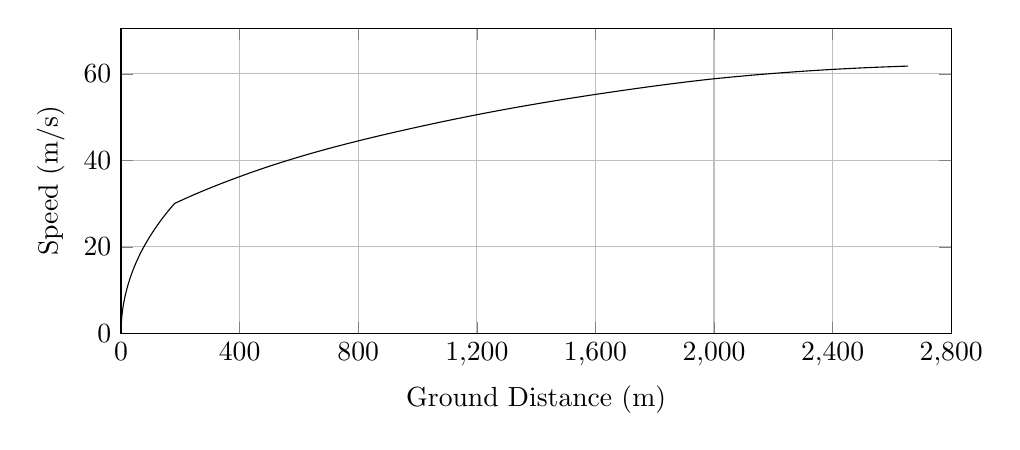
\begin{tikzpicture}

\begin{axis}[
width=\textwidth,
height=0.45\textwidth,
scaled ticks=false, tick label style={/pgf/number format/fixed},
xmin=0.0,
xmax=2800,
xtick={0,400,800,1200,1600,2000,2400,2800,3200},
xlabel={Ground Distance (m)},
xmajorgrids,
ymin=0.0,
ymax=70.5610295336269,
ylabel={Speed (m/s)},
ymajorgrids,
legend style={at={(1.03,0.5)},anchor=west,draw=black,fill=white,legend cell align=left}
]

\addplot [
color=black,
solid
]
table[row sep=crcr]{
1.3729668748937997E-8	2.7459337497568825E-4\\
2.6049868369719035E-7	0.001196087059450038\\
2.0491224421327626E-6	0.0033546249993655058\\
9.92442121137073E-6	0.007382655686248326\\
4.7452367809869807E-5	0.016143174605714343\\
1.740064756114434E-4	0.030913105671243217\\
4.0608377013922605E-4	0.047224528058299645\\
7.313431501337001E-4	0.06337533051182317\\
0.0011549487327126044	0.079641745119995\\
0.0016799013484208249	0.09605080892778434\\
0.002295089346817705	0.11226867877522992\\
0.003009933382444524	0.12856918135293272\\
0.003810608015426248	0.1446622294701862\\
0.004723484476856681	0.16106040329933924\\
0.005727138856912631	0.1773478246280672\\
0.006836216967948795	0.19376009859958715\\
0.007997302399386296	0.20956925951946365\\
0.00929136979810952	0.22588896501382932\\
0.010685558505459776	0.24224399916416894\\
0.012178513621519987	0.2586132535973379\\
0.013775244426719659	0.2750441798381741\\
0.015470070176169002	0.2914728192779128\\
0.0172374436815836	0.307671614498642\\
0.019122918912604377	0.3240612570188468\\
0.021104911040230538	0.3404401354514437\\
0.023190717999955576	0.35686586408306464\\
0.025355802981115103	0.373151741712508\\
0.027620619195902148	0.3894595181451802\\
0.030020274690474198	0.4060240022515005\\
0.032476028269866286	0.42230338699801995\\
0.035054163466719815	0.4387443972813383\\
0.037720846868992755	0.4551254523455408\\
0.04049779674511381	0.47157923741524477\\
0.043329456594087365	0.487785789116442\\
0.04629652060163805	0.504208515152839\\
0.04934498934704602	0.5205422272767595\\
0.052507657924119336	0.5369627264645012\\
0.055769483710642484	0.5533876460130807\\
0.05917209570914676	0.5700170999958616\\
0.06264043916012321	0.5864824696852022\\
0.06620063977265622	0.6029161489504857\\
0.06987962792775945	0.6194399932795716\\
0.0736568184539585	0.6359581042909948\\
0.07754284280095361	0.6525156208703013\\
0.08151127871105612	0.6690011935318934\\
0.08560324933017655	0.6855846574112681\\
0.08985265585263943	0.7023915407831005\\
0.09413961367176535	0.7189486141907262\\
0.09857725310864562	0.7356949235351331\\
0.10307959255469257	0.752304185308214\\
0.10766008648593872	0.7688332990438727\\
0.11234920964493048	0.7853938076486344\\
0.11719267720457946	0.802140167345363\\
0.12216973960582883	0.8189914178105442\\
0.12724007601918352	0.8358088070566778\\
0.13233299746505212	0.8523667619737842\\
0.13755256756750583	0.8690087903453436\\
0.14287728588926696	0.8856635121574876\\
0.1482946925752714	0.9022923099797231\\
0.15381585025670613	0.9189296056655691\\
0.15940564092189102	0.935471922013468\\
0.16526271495916878	0.952496615611115\\
0.17120082448158402	0.9694512492321026\\
0.17717889132867753	0.9862251452600439\\
0.18324322596131126	1.0029540566524742\\
0.189427022360885	1.0197294900797869\\
0.1957511558722988	1.036604411002216\\
0.2021484013779125	1.0533989481457646\\
0.20865863707071397	1.0702190957489432\\
0.21548666343168166	1.0875803344054007\\
0.22220154781289658	1.1043872462255901\\
0.22919671627301902	1.1216273728127804\\
0.23611678795738544	1.1384250397476685\\
0.24306300975244904	1.1550400290608933\\
0.2503085190632165	1.1721194326090472\\
0.2576623280401219	1.1892027818970243\\
0.26502430524173204	1.2060622064010458\\
0.2724963584449146	1.2229355252945489\\
0.2802001060647876	1.2400911336108664\\
0.2878583985474956	1.2569128869458277\\
0.2958320780323821	1.2741908489428075\\
0.3040021452321372	1.2916540391325064\\
0.31208951788619	1.308710392216533\\
0.3202851396023423	1.3257706017314699\\
0.3287233234973125	1.343108715739687\\
0.3370425959884752	1.3599855177474272\\
0.34575405233845447	1.3774356646960042\\
0.3545073625286812	1.3947491165545292\\
0.36338982075299686	1.4121003761145139\\
0.37247557159370037	1.4296302193567247\\
0.38151350442869847	1.4468564355981308\\
0.3905554764834429	1.4638868614309692\\
0.3999457587520332	1.4813654035069828\\
0.4095398754587949	1.4990121677306312\\
0.4189621792151833	1.5161423198834716\\
0.4285208811402964	1.5333242169643175\\
0.43828968955472236	1.5506863820795043\\
0.44807735398784176	1.5678885405216438\\
0.45806002753764463	1.5852404359962216\\
0.4682994371692033	1.6028426954364932\\
0.4787752542918833	1.620652736160039\\
0.4890770094685154	1.637977253258851\\
0.49985939134273727	1.6559151251579762\\
0.5106597490205704	1.6736893770237566\\
0.5213580865152188	1.691110782843439\\
0.532247733242454	1.7086605175569152\\
0.5431365108549349	1.7260296520497533\\
0.554075964429489	1.7433045798874605\\
0.5653450694020941	1.7609220610384915\\
0.5769901159382542	1.778943119838888\\
0.588512657344902	1.796595837923058\\
0.6004070039036553	1.8146371755869612\\
0.6121651247369502	1.8322964307253669\\
0.6239717914322569	1.8498581238927199\\
0.6362472885961421	1.8679412115750686\\
0.6486428939173223	1.886024389335113\\
0.6610190736373547	1.9039069772363946\\
0.6737248046101814	1.922091734581092\\
0.6862826225989949	1.9398963817008013\\
0.6991952542603428	1.958034326196202\\
0.7122988072688032	1.976269313756819\\
0.7251463703465595	1.993985230799336\\
0.7381769453061875	2.011793222470093\\
0.7516618647379176	2.030056680149654\\
0.7654913705221527	2.0486166998906086\\
0.7791756406994825	2.0668167465454514\\
0.7930637813125616	2.085124501220468\\
0.8074774191984457	2.1039554531557023\\
0.8215072375247947	2.122123440747438\\
0.8361010597475598	2.1408571176650844\\
0.8503303420601955	2.1589652902391547\\
0.8650627501899835	2.177554004542137\\
0.8802332960144008	2.196530016896099\\
0.8951742046771463	2.2150587914063493\\
0.9100334756324657	2.233332780699196\\
0.9251067343345352	2.2517173230198395\\
0.9403923630470314	2.2702077393368496\\
0.9559303815501943	2.2888492362219255\\
0.9712400158034169	2.3070683063974737\\
0.9869533781138684	2.3256182749977965\\
1.0029148609762486	2.344309719685593\\
1.0189962473881624	2.362990884584363\\
1.035465185745812	2.3819691991416008\\
1.0516742337458713	2.4005003350604905\\
1.067815735429615	2.418812010570522\\
1.0846705971808022	2.4377849375942677\\
1.1012775250051634	2.456334240910473\\
1.1180798406225687	2.4749590953498712\\
1.1351395900544134	2.493725764383493\\
1.1526388687279154	2.512829049296233\\
1.1698922447507556	2.5315215103424418\\
1.1875468452119025	2.550505578253106\\
1.2058383275300355	2.570025234767397\\
1.2239395537495579	2.5891956582493973\\
1.2422020624207541	2.6083927768013435\\
1.2608769472440078	2.627876980840883\\
1.2794948487006894	2.6471576091155073\\
1.2979152553275424	2.6660951591392203\\
1.3166445915281573	2.6852120306732763\\
1.3354141707340492	2.7042330522661437\\
1.3543210821322504	2.7232575767824745\\
1.373689361295591	2.7426081086866656\\
1.3932049885015831	2.7619673173258423\\
1.4131781782225183	2.781639456248346\\
1.4330139682345777	2.8010380833627213\\
1.4528243860883294	2.8202773000097006\\
1.4728783400745615	2.8396188292527436\\
1.4934621752870565	2.8593338616338233\\
1.5141408097620341	2.8790022457936937\\
1.53430654450827	2.8980527871012747\\
1.5553850389607948	2.917831150192834\\
1.5762653203499473	2.9372907142137406\\
1.5975496774716453	2.9569935290174802\\
1.6196077215345106	2.977273343820186\\
1.6413652536722467	2.997140847671469\\
1.663437310723463	3.0171602749852626\\
1.6860768385032747	3.0375556634769234\\
1.7077101022266827	3.0569158347452374\\
1.7297306410738114	3.076495911938479\\
1.7520297891459062	3.0961959550713187\\
1.7743087535215367	3.1157522004610687\\
1.797257424336919	3.1357671555991296\\
1.8200802473615325	3.1555448116881415\\
1.8430350373473994	3.175310942892061\\
1.8666926279964304	3.1955526200097566\\
1.8902808566018634	3.2156063963567876\\
1.9138231309717848	3.235495498558775\\
1.937187877956735	3.255112827592752\\
1.9611060682733261	3.2750714425406517\\
1.9852138445648535	3.2950642214831065\\
2.009780393513653	3.315311691151088\\
2.0346228225622163	3.3356597820566236\\
2.0593611988602687	3.3557982773099733\\
2.08477023517836	3.3763558707117003\\
2.110324766702745	3.3969038601161907\\
2.1352655781940433	3.4168374507619372\\
2.160528860803022	3.436909148243145\\
2.1862071157614817	3.457189322736234\\
2.2127756699400534	3.47804627104731\\
2.2391904543957084	3.498657353283633\\
2.2653528664920257	3.5189506690780865\\
2.292150575495974	3.539614257193713\\
2.3187704640870406	3.560020104451456\\
2.3455495914188482	3.580428802125148\\
2.372862901366455	3.6011235421948324\\
2.4007145172972395	3.622102410402001\\
2.428100404243743	3.6426107324530594\\
2.4555980306928005	3.6630852977926462\\
2.483374904362833	3.683650317814106\\
2.511687733451976	3.7044926714770874\\
2.5402569276484597	3.725403543779062\\
2.568415369317849	3.74589758565031\\
2.596987652715761	3.7665768755771643\\
2.6263861238451423	3.7877342219909025\\
2.655991481965028	3.808919603493142\\
2.6856115886357443	3.8299961834423675\\
2.7154221146045012	3.851089708357418\\
2.7455665152057707	3.872300527787173\\
2.7752624694325894	3.893080745680683\\
2.805457625653509	3.9140950885142516\\
2.8358231840904597	3.935112753380028\\
2.8663460878589797	3.9561246937137566\\
2.897817297850832	3.9776710370683137\\
2.9287074004595235	3.998704485932045\\
2.9603588456990284	4.020140007477989\\
2.9922321403815406	4.0416086702532095\\
3.0241119471841866	4.062966036274981\\
3.056446055158509	4.0845114431002365\\
3.0889346922121366	4.106043701061431\\
3.122221620829695	4.127986225778219\\
3.1546991615623394	4.149281120187437\\
3.187635101478671	4.17076329017544\\
3.221010117202278	4.19241726517145\\
3.2543449374576605	4.213931805179003\\
3.288235920596943	4.235690945233179\\
3.3223704322934555	4.25749168346373\\
3.3562838593334394	4.2790389135337215\\
3.3906320903803255	4.300750028577804\\
3.425633159699527	4.322759226160789\\
3.462387235801926	4.3457481786907906\\
3.4973980805087237	4.367531802010811\\
3.5324804241140235	4.389249099837031\\
3.5675385073174235	4.410842211853177\\
3.6040688981843845	4.433227780520278\\
3.6393612181513753	4.454745446795332\\
3.6770856360342323	4.4776290482676675\\
3.7131729334920323	4.499408189364658\\
3.749509707933214	4.5212294724276045\\
3.785733977879824	4.542876466449998\\
3.8225309786916544	4.564758181790545\\
3.860867115351552	4.587441561199022\\
3.89929745075254	4.610066028065548\\
3.9373367205567504	4.632348882518892\\
3.9751626485832894	4.654398466433097\\
4.013671158053867	4.6767365975850606\\
4.0521140617426425	4.698928198222932\\
4.092377631210638	4.722056270130555\\
4.131586743753305	4.744467645333231\\
4.1715696979561425	4.767210171619869\\
4.210522654700574	4.789260400729587\\
4.250196810863292	4.811612421200696\\
4.2917015001093795	4.834882377229675\\
4.332438976653355	4.857611053830874\\
4.373124372895289	4.8802023390870755\\
4.414429464889761	4.903028518592958\\
4.455884944705147	4.925828717320613\\
4.497250153511752	4.9484718491940285\\
4.537976875075978	4.970662081062123\\
4.581399817640802	4.994209920838321\\
4.623816269683994	5.017102429842533\\
4.666022338967499	5.039775443349594\\
4.709098934189642	5.06280860856833\\
4.752435367147649	5.085872626144271\\
4.79531009100786	5.108585682332626\\
4.838191999420829	5.131199250637916\\
4.881381760681686	5.153872132905427\\
4.9256451804034285	5.177002783249042\\
4.9704217340957495	5.200294010165997\\
5.014356093293278	5.223043401237971\\
5.058826350846283	5.2459670101016105\\
5.104458009943745	5.269382722403142\\
5.149663211268795	5.292474562982097\\
5.194981168813841	5.315520450252187\\
5.241194091283663	5.338916089589867\\
5.287987552078626	5.362498642303448\\
5.334426822383641	5.38579765561996\\
5.380633359096258	5.408877404715756\\
5.427524438012913	5.432195902718378\\
5.476157635197664	5.456272373324564\\
5.524667120325573	5.480179118195782\\
5.5732739519824435	5.504026599007274\\
5.6208990292882195	5.52728964420281\\
5.671502816366864	5.55189766727695\\
5.719824083529298	5.575291300223562\\
5.767871110439133	5.59845231139038\\
5.8169321963676754	5.622000695907984\\
5.866076914057565	5.645487736994603\\
5.917200682776528	5.669814177554041\\
5.96684810088939	5.6933355676929605\\
6.016885842403935	5.7169409258083554\\
6.068639931677712	5.741250687285138\\
6.119867755785197	5.765209146637513\\
6.171030794930029	5.789035228533507\\
6.222884713227881	5.81308025448681\\
6.2735946138732235	5.836495944669011\\
6.325883502103322	5.860539648919206\\
6.379615386553551	5.885141266857421\\
6.432194972482147	5.909112951485419\\
6.484528316464761	5.932873085506847\\
6.536619297696934	5.956426006739367\\
6.589662958081361	5.980311253337163\\
6.644121795496577	6.0047316652961715\\
6.697445536614451	6.02854407625699\\
6.7518063163896365	6.052719974616554\\
6.8068829439682315	6.077112897061333\\
6.863205650636274	6.101953493727532\\
6.9185329265047315	6.12625371911599\\
6.974634519184049	6.150792712999589\\
7.031139830722298	6.175406409212599\\
7.0870923879294985	6.199679777781242\\
7.144766952910487	6.224597753907654\\
7.2026451873548805	6.249500439890349\\
7.261191729679483	6.2745866784399915\\
7.320502240843062	6.2998949088472465\\
7.378210233177999	6.324418772935452\\
7.437738452534925	6.349613488108336\\
7.49714639104333	6.374654570602733\\
7.556502460410064	6.399572521883792\\
7.617032771987237	6.424880415390254\\
7.676883327249088	6.449803034752895\\
7.735740247984193	6.474215028862059\\
7.796086087039788	6.499146007741572\\
7.856787102853412	6.524124199515617\\
7.91721236259451	6.54889092892552\\
7.979013602666894	6.574121674271121\\
8.039824025454376	6.598850375619531\\
8.102419182184594	6.624204959122052\\
8.16459313580776	6.649289773584513\\
8.226347093952135	6.674108430915007\\
8.290527749984296	6.699801404757482\\
8.353592793320257	6.7249486769695235\\
8.417564177281012	6.750358148961304\\
8.482044607535009	6.775869858503468\\
8.547336806956285	6.801601659915203\\
8.613293246319614	6.827493149954353\\
8.6778048537894	6.8527193359234495\\
8.74454839911753	6.878717310659901\\
8.810708373588199	6.904387772137966\\
8.876548424968423	6.929836183498072\\
8.942828456712885	6.955357098432941\\
9.010858044488913	6.981451024994769\\
9.079453414959548	7.007659897161696\\
9.148767802603732	7.034040565335831\\
9.21609997183467	7.059568860923676\\
9.285579683381485	7.085811312716821\\
9.355451712480097	7.1121005920262235\\
9.423585014597279	7.137638892894934\\
9.493435356703696	7.16372267986012\\
9.562655940911181	7.1894743829646135\\
9.63183713653898	7.215116090654094\\
9.703018708836247	7.241400827534672\\
9.773178624863132	7.267211703010416\\
9.844376937811855	7.293307618879064\\
9.914998792594716	7.319096791943389\\
9.98720270419701	7.345366467702007\\
10.059478150570087	7.3715647909280815\\
10.132362020358627	7.397886065659781\\
10.205876892438312	7.424337023055465\\
10.279422251887688	7.450701337163185\\
10.353305644514993	7.47708958378761\\
10.42811398108589	7.503709950686414\\
10.50332954727428	7.530376652591897\\
10.578207710262959	7.556826610181107\\
10.65503529959097	7.58386554900264\\
10.730232142651953	7.610233881423079\\
10.805871937852555	7.636662082673604\\
10.88265320376452	7.663392233061796\\
10.958577899345514	7.689729222701217\\
11.034861147941964	7.716096492216208\\
11.112742623646977	7.7429199076692825\\
11.190543636431041	7.769619504220374\\
11.267787598939979	7.796033902686901\\
11.3462805052093	7.8227804160501275\\
11.423875697147409	7.849127907991946\\
11.502735831556972	7.8758110302960205\\
11.581465323066688	7.902356516228309\\
11.661639233340708	7.929294075813948\\
11.741743247575428	7.956113456914213\\
11.821864700430528	7.982844971125788\\
11.901816327719768	8.009427365304315\\
11.98361062800689	8.036527814415834\\
12.065425957085825	8.063540499848951\\
12.1478520915771	8.090660032732636\\
12.230956215923495	8.117907276153158\\
12.313306905825911	8.14481400778947\\
12.396632357805931	8.171945476806187\\
12.479578787946746	8.198860823522072\\
12.564327762802186	8.22626651559938\\
12.648175874147956	8.253287781940287\\
12.736145481689512	8.2815387295818\\
12.821080154398764	8.30872026868952\\
12.908009536077355	8.336444762680678\\
12.994986774303499	8.364088903733062\\
13.081752199798046	8.391571398756568\\
13.17035388279784	8.419539284155228\\
13.257836697901475	8.447059545875494\\
13.34511613365563	8.474423253816354\\
13.433461823066896	8.502028024390917\\
13.524108483575919	8.530255253597037\\
13.611203924103116	8.557285475913584\\
13.702229394080796	8.585440866877025\\
13.792427706753081	8.613246058316122\\
13.882429934062493	8.640898125265377\\
13.975435778888343	8.66937672520849\\
14.065832730112316	8.696963615815015\\
14.157894546480026	8.72496543384451\\
14.250668806951023	8.75308979863689\\
14.343291987615704	8.78107501207693\\
14.43744444968501	8.809427631989166\\
14.532636396723657	8.837997228296953\\
14.625507232812737	8.865778045001761\\
14.721503924398366	8.89439919360711\\
14.818738382089133	8.923292194172717\\
14.913572076739943	8.951378531265195\\
15.009701633366973	8.979755568494685\\
15.10815424447124	9.008722171681612\\
15.206130868840724	9.037453050647606\\
15.304035939715973	9.066068544174051\\
15.403499839366233	9.095043965598787\\
15.503209871950865	9.123995244259106\\
15.601718454553605	9.152504363306388\\
15.700655560608023	9.181045054283707\\
15.801250929860519	9.209970041207168\\
15.899917805652187	9.238249261136989\\
16.001574124100856	9.267291691019373\\
16.102638779863817	9.296071821280439\\
16.204479333764816	9.32497974560718\\
16.30489644092564	9.353392931533719\\
16.40578186591999	9.381848812261826\\
16.509201471948074	9.410926929772582\\
16.614557195984908	9.44045399002258\\
16.717657554831042	9.469256613676432\\
16.823039336622365	9.498603092880327\\
16.928576062495388	9.527898901006303\\
17.03469945574068	9.557263797547375\\
17.140697318244236	9.586500999697712\\
17.246066414787876	9.61547356613854\\
17.35183930840021	9.644466568482276\\
17.458399953804133	9.673584578289493\\
17.565707112453843	9.702815223560183\\
17.673103795073075	9.73197933276478\\
17.781888038667653	9.761428382722077\\
17.89115167195854	9.790915024364995\\
18.00105710767307	9.820482543650591\\
18.110142905530395	9.84973885684363\\
18.219697237410173	9.87903073318287\\
18.32752951944549	9.907774822658471\\
18.43743745973078	9.936983842812268\\
18.54904630654982	9.966554447981707\\
18.659302591714813	9.995678028794408\\
18.770734536087716	10.025023439487601\\
18.883577445650936	10.054650375976305\\
18.996263390583444	10.084146507544634\\
19.108816920034535	10.113519426652196\\
19.22287647779894	10.143195915932868\\
19.33763586704334	10.17296444403324\\
19.456324114791514	10.203657986239964\\
19.57349394116079	10.233865845391438\\
19.690148252848566	10.263849852567578\\
19.80521137071168	10.293336789331565\\
19.92379170801214	10.323634385929495\\
20.04216631061405	10.353788442829384\\
20.15848954929409	10.38333221101729\\
20.278242138037896	10.413656941176246\\
20.396206084226087	10.443440250288852\\
20.516315546862906	10.473675846533023\\
20.637173924977112	10.504009737956679\\
20.75450010628387	10.533371292136543\\
20.874378237858778	10.563284963244318\\
20.996035953832852	10.59355408996911\\
21.11812959618858	10.623842742581004\\
21.240471115580952	10.654104329383948\\
21.361479376438375	10.68394970793915\\
21.485224699488654	10.714382063087374\\
21.607870280890317	10.744456854652984\\
21.73242999733349	10.774913061413436\\
21.85704493170313	10.80529485886856\\
21.98122016226351	10.835482769729165\\
22.10826921766411	10.866280570955333\\
22.235261614051304	10.896975727734969\\
22.361664688868032	10.927440958960869\\
22.48780138980522	10.957755760903414\\
22.614107216476143	10.988025660312033\\
22.74409311379692	11.019088917898404\\
22.873024137794893	11.049812104565603\\
23.003512644166257	11.080818004486964\\
23.132891545907036	11.111473205312606\\
23.26270690888247	11.142145484280611\\
23.39264146728729	11.172760086166058\\
23.52277721573431	11.203336767528683\\
23.654883767164463	11.234289935758238\\
23.78569183677709	11.264853674610649\\
23.917003007077597	11.295450451560974\\
24.047013652206026	11.325661493688155\\
24.178458227988493	11.356122810108243\\
24.314609552493202	11.387587724106591\\
24.447533097503474	11.418221874174144\\
24.579128452041708	11.448468092441225\\
24.71011994849615	11.478495346396112\\
24.843278471916108	11.508938061038926\\
24.975761222328053	11.53914563636426\\
25.1115496753864	11.570024186374848\\
25.247101122854083	11.600765990166625\\
25.384906965000688	11.631934944930045\\
25.522261036073317	11.66291804173812\\
25.66123001648475	11.694181130800288\\
25.79865327455613	11.725013834534618\\
25.826335196219034	11.731214752450743\\
25.839610403727477	11.734187307865987\\
25.841006316401874	11.734499833494791\\
25.84227013303559	11.734782777405623\\
25.84770509053729	11.735999480123855\\
25.86419328224909	11.739689849820824\\
25.90571916957557	11.748978954586804\\
25.999268866927544	11.769878412223008\\
26.123295978662824	11.797529100487154\\
26.250212562581652	11.825756415749098\\
26.376891976518465	11.853863273596641\\
26.50638698165423	11.882525367428197\\
26.634042370994827	11.910711979722588\\
26.763333806613538	11.939191150682156\\
26.893207366259766	11.967729401217124\\
27.022905486492228	11.996160381624506\\
27.153956322362554	12.024818583405661\\
27.287774297957696	12.054010477184836\\
27.42030033806219	12.082849867075357\\
27.555504894698295	12.112200129389205\\
27.691130018821354	12.141569093922598\\
27.82633313037239	12.170774774666107\\
27.959508564917073	12.199472720945522\\
28.096515548835796	12.228924573237158\\
28.232789703382153	12.25814716626897\\
28.368684388406535	12.287217608633465\\
28.506541650227618	12.316636129051595\\
28.64533374691623	12.346181605101286\\
28.78297783415192	12.375411278018195\\
28.92277775692753	12.405026422297944\\
29.06227187463503	12.43450459214235\\
29.20212864139956	12.463987466624044\\
29.34335827861657	12.493687132448699\\
29.483225747293005	12.523028879800904\\
29.625960812476485	12.552899348885958\\
29.76706561118049	12.58235677641552\\
29.909402910999468	12.61199956784111\\
30.051751399473822	12.641572890330863\\
30.196612335666572	12.671594937371758\\
30.342192969749448	12.70169217992743\\
30.48583400527584	12.731316227416972\\
30.632658550781265	12.761523183665716\\
30.77846394498075	12.79144725246633\\
30.92408133049836	12.82126038323035\\
31.071091331299215	12.851285751640397\\
31.218274793935116	12.88127365551026\\
31.366705758252415	12.911442335595403\\
31.515339333797037	12.94157880864406\\
31.66356819769615	12.971560548892107\\
31.814689402684216	13.002053073643452\\
31.96649953392354	13.032609617249182\\
32.115424616034375	13.062512887167188\\
32.266253234088566	13.092725583914845\\
32.41813832080348	13.12307634388127\\
32.569791431087395	13.153307565965061\\
32.722234201183724	13.183622968108022\\
32.876984607664	13.214322650709256\\
33.031873994672836	13.24497509393954\\
33.18502245018544	13.275209886690874\\
33.34135780547538	13.30599932146761\\
33.49759920343199	13.336695506383553\\
33.65385117142162	13.36731950997589\\
33.8113313806527	13.398109573984126\\
33.96985264489639	13.429027959069582\\
34.126473036379195	13.459501941269309\\
34.2857505660089	13.490418320361467\\
34.4449212019973	13.521239262644428\\
34.60566879064274	13.552290259038784\\
34.76644486933921	13.58327154602036\\
34.92612701881755	13.613968049068877\\
35.08630421658309	13.644686104601128\\
35.24825698849928	13.675670182063591\\
35.412303951281956	13.706979030506332\\
35.57355277914179	13.737679887821194\\
35.73545353069308	13.768431559916738\\
35.89925038949356	13.799469094513082\\
36.065161289279985	13.830831517869232\\
36.23047312008262	13.862005402889118\\
36.39472205714358	13.892904880370985\\
36.56135389445764	13.924177767608562\\
36.72774532558607	13.955330752562368\\
36.89384825683493	13.986355650438828\\
37.05904296416534	14.017137960538236\\
37.22702676294645	14.048365847643591\\
37.39437475321985	14.079401659386296\\
37.5621109943643	14.110435935007512\\
37.73270471709142	14.14192384649289\\
37.903359519601935	14.17334777603551\\
38.071486842086316	14.204233151104265\\
38.23815243703595	14.234778779965005\\
38.40817787072022	14.26586755577329\\
38.57751392140098	14.296757815176452\\
38.750215798728505	14.328188036357943\\
38.92001182640311	14.359016978313871\\
39.09310637700479	14.390371334984543\\
39.26472366117933	14.421385304614656\\
39.436554723976656	14.45236573042476\\
39.608961777617054	14.48337785852518\\
39.782828308010565	14.514579769017075\\
39.956194359016465	14.545619567964359\\
40.132391837044906	14.577092790155625\\
40.30868053167249	14.608508582439303\\
40.48611580488176	14.640054693213546\\
40.66383502946924	14.671577313695405\\
40.83999042132467	14.702749937144194\\
41.018202681018664	14.73421342623761\\
41.19780999006247	14.765849253126323\\
41.37730467548502	14.79739151557127\\
41.557010452813884	14.828897486890131\\
41.73612816026986	14.860227730408422\\
41.91555194917056	14.891539255037166\\
42.09743589423803	14.923206737082769\\
42.27807550146298	14.95458489817442\\
42.45995188234755	14.98610516725352\\
42.6401410478328	15.017261499707455\\
42.822293873795985	15.048685432668847\\
43.00585672428667	15.080279886176239\\
43.189965171449515	15.111895351742469\\
43.372020236704074	15.143086849287634\\
43.555636897252796	15.174474450470768\\
43.74012033961118	15.205938390907338\\
43.92429822300048	15.237278825000338\\
44.106869824379004	15.268275940867962\\
44.29411840239129	15.299995164357831\\
44.47920670866131	15.331277262770957\\
44.665034305215386	15.362613537215559\\
44.85242224248053	15.39414154800248\\
45.03948098831597	15.425543099701756\\
45.22811764277584	15.457138049216635\\
45.41548629589063	15.488449975157465\\
45.60322541388645	15.519753611062562\\
45.793007222766036	15.551326844875767\\
45.983742663331824	15.582987230651376\\
46.172643153142886	15.614272798628086\\
46.36421599110457	15.645929996047428\\
46.553512793459404	15.677141298768184\\
46.745018895697555	15.708646700374285\\
46.93606459490553	15.740006445666726\\
47.126948089509526	15.771270231388208\\
47.31881294044018	15.802625314343281\\
47.5110690178297	15.833974913202926\\
47.705448624448266	15.865600544130821\\
47.90005519882567	15.897192771806164\\
48.09288923506665	15.928428238034357\\
48.28732881729917	15.959854621895737\\
48.484002572746206	15.991571876535481\\
48.68089030454945	16.02325330604529\\
48.87532723390382	16.054471712758463\\
49.07073736177763	16.085778026971965\\
49.2672083392297	16.117185618690996\\
49.46586249263092	16.148872597283457\\
49.661880987188695	16.180070951663943\\
49.85966148345089	16.211481466697464\\
50.05808618672894	16.242925766238578\\
50.25785665917266	16.274514392265843\\
50.45743808511885	16.30600445127788\\
50.65573800086891	16.337224721352115\\
50.85948768734909	16.369233229019436\\
51.061243703011925	16.40085925465217\\
51.26368286286315	16.432523474880135\\
51.46416466063809	16.463813917794617\\
51.66475943174029	16.495055029889343\\
51.86588207153103	16.52631148877014\\
52.07444928962187	16.55865459917674\\
52.2824430085781	16.59083789571823\\
52.48676525705545	16.622384579072587\\
52.69531994892206	16.654515109537634\\
52.90027076850366	16.686022281397804\\
53.108186167814935	16.717916582174794\\
53.31165724918766	16.74906259416789\\
53.520024946679996	16.780890332562556\\
53.72688450142306	16.81242021255985\\
53.93707391647578	16.844389149945002\\
54.14518573319289	16.87597446933019\\
54.35125853722778	16.907184400468843\\
54.56213447502874	16.939054244149467\\
54.77598621923464	16.97130446473132\\
54.987629956235494	17.003153331647994\\
55.19778857845695	17.034711795636277\\
55.41030974885841	17.066557606829\\
55.62390503323701	17.098496444061098\\
55.83671574169797	17.130250626134263\\
56.047071254351536	17.161572779601293\\
56.26137331252919	17.193415808812574\\
56.47512769358855	17.22511070692726\\
56.69105800830218	17.25706094304814\\
56.90937011004422	17.28929522621656\\
57.12736617899088	17.321414638075666\\
57.346833156368504	17.353682317574062\\
57.56476609337061	17.385656872947685\\
57.78230894703917	17.417507418892214\\
57.99943865551505	17.449231325320433\\
58.21827465292657	17.481138039850116\\
58.436085045729726	17.512829311112277\\
58.6577546799423	17.545014971030042\\
58.87982836766625	17.577191780689546\\
59.10336118170943	17.609512150444615\\
59.324182403931715	17.641373989783617\\
59.545440661451366	17.673233008851817\\
59.768227251413464	17.705245840070845\\
59.99077485409802	17.737158331678224\\
60.21631063559073	17.76943240060632\\
60.44006004384342	17.80138465299492\\
60.66502706168687	17.833444698140546\\
60.89133011288284	17.865628662621575\\
61.11585558357916	17.89749430679791\\
61.3432655409558	17.92970318231098\\
61.57186440401435	17.962013733860758\\
61.79868765088207	17.994007582012195\\
62.025670725987	18.02595879688969\\
62.254132946411545	18.058052755280414\\
62.48290793247415	18.090125205864425\\
62.713817944074236	18.12243093681974\\
62.94484116346062	18.154686493251866\\
63.17805109236767	18.18718077000961\\
63.41124119062552	18.21960577010769\\
63.64505576847972	18.25205120616198\\
63.87735201907903	18.28422048391853\\
64.11169045660182	18.316606830144558\\
64.34725756208485	18.34909681040505\\
64.58324360279937	18.381578427481692\\
64.81881329818131	18.41393708574371\\
65.05563560606473	18.44640206434118\\
65.29467812810154	18.47910493618197\\
65.53178653633495	18.51147761305367\\
65.77046761369158	18.543999405482886\\
66.01019347650049	18.576597680542378\\
66.25262920761091	18.609497687437504\\
66.49342175078831	18.6421086291614\\
66.73393309567928	18.674616128267523\\
66.97718905970893	18.707428524965685\\
67.21919788222482	18.740007142596745\\
67.46413738735515	18.772914083730342\\
67.70584739194695	18.805322237331644\\
67.95375887035246	18.838495274526217\\
68.19817148521656	18.87113448141077\\
68.44413350233111	18.903915172625005\\
68.68984243621705	18.936596976916213\\
68.93951041285982	18.969739050278292\\
69.19023531750676	19.002954532535327\\
69.43956667494601	19.035919307830504\\
69.68998597860525	19.068961964600284\\
69.94098943220166	19.102015746775443\\
70.1928405184459	19.135115168054924\\
70.44659484061637	19.168398261604395\\
70.69926103579675	19.20147273421761\\
70.95414956377036	19.23477187128288\\
71.21136313866151	19.268307701263836\\
71.46778788208749	19.301674020930108\\
71.7247351381395	19.335041955653224\\
71.98234155897126	19.368429179764078\\
72.24107377350035	19.40189586825752\\
72.4986091150376	19.43514199765488\\
72.75949164810788	19.468753738992113\\
73.02014691132015	19.502269756933494\\
73.28114866838587	19.535764170005642\\
73.54342372888959	19.569355687041266\\
73.80584407854005	19.602899683663466\\
74.07231166191039	19.63689373056895\\
74.3389341302921	19.67084007176146\\
74.60521354141642	19.704675777151536\\
74.87280568706873	19.7386112758617\\
75.1403821105715	19.772478002879822\\
75.41145333671997	19.806719373532445\\
75.68265298797411	19.840909194310825\\
75.95075857762194	19.874642711238216\\
76.2241428819712	19.908972989343177\\
76.4990100438061	19.943421256220383\\
76.77213586328236	19.97758393207519\\
77.04724851790667	20.011927651779146\\
77.32330034006353	20.046320955638144\\
77.59850473375684	20.08054161948332\\
77.87773830129439	20.115195271649156\\
78.1565255546137	20.149725588773947\\
78.43842651648492	20.184572948565943\\
78.720833678605	20.219414114319704\\
79.00101298089581	20.253912816517563\\
79.28359351218376	20.288639386279122\\
79.57011733099088	20.323781451002688\\
79.85418914588558	20.358554506650165\\
80.13919871477489	20.39337445105513\\
80.42568449319114	20.428306617879564\\
80.71472498530085	20.46348148967401\\
81.006853148924	20.49896232926431\\
81.2951972638476	20.533915191659908\\
81.58524575795963	20.569006538445493\\
81.87461709596036	20.603948292943443\\
82.1711642895769	20.639686842977966\\
82.46716486408064	20.67528959833342\\
82.76422974563803	20.710950572006325\\
83.05801377197795	20.74614935470027\\
83.35853301954708	20.782085213251875\\
83.65664966506407	20.817664373044124\\
83.95487262936624	20.853187495027235\\
84.25322789115987	20.888658016488954\\
84.55664509033022	20.924660646908514\\
84.8599544590121	20.96058068270746\\
85.16499148084048	20.996635375961205\\
85.47187188044902	21.032837617956105\\
85.77908321853027	21.069008685068106\\
86.08675489504844	21.105163985588625\\
86.39784539041122	21.141650300258377\\
86.71051296037359	21.17825036509049\\
87.02583358957506	21.21508914406538\\
87.34037846285594	21.251765868954877\\
87.65395388450591	21.28825900286668\\
87.96687312379424	21.3246059993766\\
88.28527441497255	21.361518677207044\\
88.6103524516937	21.399131904856524\\
88.92871226770333	21.43589629610112\\
89.25003295857354	21.47293133093619\\
89.57522243846881	21.510339842778038\\
89.90247582737899	21.547912696514494\\
90.22602529632545	21.58498869207638\\
90.5494223037065	21.621976538295122\\
90.87816525326718	21.659503864723284\\
91.20455861430293	21.696691681174762\\
91.53817773235312	21.734629837383537\\
91.87076195087604	21.77237740693935\\
92.20124984301029	21.80981542570612\\
92.53140503523474	21.84714493867873\\
92.86389705561814	21.8846676059922\\
93.19815266874983	21.92231789347727\\
93.53304529783748	21.95996861065027\\
93.86737084100128	21.99748483559147\\
94.20337949361911	22.0351191918553\\
94.54065981474497	22.072825135964614\\
94.87396787418089	22.110017738713772\\
95.21684847579547	22.148207135250544\\
95.55392648231228	22.185680166473013\\
95.89232371872416	22.223230431304238\\
96.23051075783204	22.26068833818305\\
96.57164052232307	22.298402735730164\\
96.90762523479154	22.335480584862992\\
97.24755293575913	22.372925622897448\\
97.58790661409188	22.41034957280985\\
97.92576087813703	22.447431838288885\\
98.26661027452474	22.484775792748025\\
98.6051908024865	22.52180493328597\\
98.94563962387357	22.55897228446031\\
99.28665364663627	22.596135317528123\\
99.63350087797645	22.633866714140744\\
99.97685593767679	22.671151790538282\\
100.31593955776762	22.707908599746993\\
100.65572384630482	22.74467756334772\\
100.99616871909686	22.781454383943853\\
101.3402339503516	22.818558018816304\\
101.67973054404297	22.85510606086546\\
102.01657591573795	22.89130733270664\\
102.35656456518868	22.927784851193216\\
102.6941824316649	22.963947202912287\\
103.03547296258705	23.000441756853597\\
103.37623032340073	23.03681833821681\\
103.71852978299776	23.073298621479843\\
104.05851119314701	23.1094718209292\\
104.3949509202441	23.145209677618773\\
104.7329053851843	23.181050215579518\\
105.07104272194636	23.21685213116971\\
105.40742307340048	23.25241081332623\\
105.74423560014887	23.287958388385228\\
106.07955743077031	23.323292548856365\\
106.41623710643992	23.358713856083035\\
106.75618472497374	23.394422480760973\\
107.0942647435474	23.429878996649634\\
107.43151869252583	23.465193666241902\\
107.44650965670576	23.466762131694665\\
107.45815118347005	23.467980079606065\\
107.46233674961977	23.46841796168232\\
107.46535588765028	23.468733810116866\\
107.46808502617694	23.469019316351826\\
107.4836206108138	23.47064448849347\\
107.53176708907421	23.47568033713955\\
107.68672244793561	23.491880218935997\\
107.97570433527497	23.522061137792114\\
108.27744765146667	23.55353206922929\\
108.5816623935838	23.58521660003035\\
108.88557241638279	23.616825194013003\\
109.19209959959528	23.648661318092138\\
109.50241879336687	23.680845665326054\\
109.81066605766154	23.71276976723022\\
110.12101503747155	23.744865949967924\\
110.43285681965125	23.777070529922057\\
110.74725799716322	23.809492843174887\\
111.06462449033057	23.84217360534214\\
111.38211128519615	23.87481925007129\\
111.70119562731901	23.907581380825455\\
112.02298633508096	23.940572969514704\\
112.34320819983824	23.973355537802185\\
112.66812620709393	24.006569848967217\\
112.99302416686388	24.039732834076247\\
113.31966045518399	24.07302368236835\\
113.64998129974768	24.10663961631466\\
113.97857627498675	24.140029684761252\\
114.31304608469316	24.17396538140237\\
114.64448318111735	24.207542388476632\\
114.98093514978115	24.241575636234593\\
115.31969924418831	24.27579014505862\\
115.65790718621022	24.30989592888278\\
116.00063352526521	24.34440390825783\\
116.34235083463872	24.378756840770436\\
116.68621873349733	24.41327221524346\\
117.03331062078092	24.44805662996682\\
117.37910048629482	24.48265617288785\\
117.72869476105836	24.51758132451745\\
118.08005947084649	24.55262769368786\\
118.43363644355449	24.587838532118262\\
118.79186464668504	24.623455214152514\\
119.14769212941735	24.658776198269088\\
119.5036618261702	24.69405458557344\\
119.86270697471275	24.729580441749697\\
120.22616362054572	24.765484302078292\\
120.58991121293201	24.801358127504685\\
120.95538130513773	24.83734276026837\\
121.3195355377388	24.873139088320713\\
121.68590041554987	24.909093698674326\\
122.05305648207542	24.945066710988513\\
122.42257239354896	24.981211206256113\\
122.79503144936103	25.017583105841453\\
123.16629137010841	25.053777633754272\\
123.53950748252527	25.09010237994317\\
123.91239367862553	25.126334602985445\\
124.29026003316017	25.16298929482295\\
124.66301933937496	25.199088143955876\\
125.03890311735066	25.23542895406515\\
125.41380975776434	25.2716148199453\\
125.7896808967325	25.307833313837065\\
126.16837244152023	25.34426251845204\\
126.54595968852882	25.380524637760402\\
126.92471834906405	25.416838373768726\\
127.30294276405039	25.453040208702177\\
127.68255852126984	25.489314412393533\\
128.06243727540487	25.525552936893334\\
128.44360431740483	25.56185338722574\\
128.82265748788262	25.59789212572121\\
129.1989690567886	25.63361079357228\\
129.57765386613931	25.669495134734824\\
129.95508099647026	25.70520098491398\\
130.33359114840187	25.740949990619633\\
130.71373745886524	25.776793922397104\\
131.09453904397424	25.812639923450952\\
131.47657586018488	25.848542313218175\\
131.85678563989967	25.884213620998267\\
132.23856625352113	25.919972866793735\\
132.61595336405918	25.955262229942143\\
132.99976263915818	25.991092780130998\\
133.38083522978053	26.02660880845795\\
133.76098428781995	26.061980320472443\\
134.1363519425165	26.09684983052385\\
134.51557915495124	26.132020412230737\\
134.8968696170101	26.167324289540858\\
135.27419431482667	26.2022038338245\\
135.65215477207505	26.23708532788376\\
136.03329358991255	26.27220273128455\\
136.41192880753374	26.30703253462157\\
136.7898079310749	26.341736387654485\\
137.17001317148595	26.37659717186532\\
137.54844558779996	26.41123910132302\\
137.92617219433072	26.445760569699225\\
138.30476964659732	26.480305801434746\\
138.68390038934075	26.51484385208611\\
139.0631653430654	26.549338385799082\\
139.4406106933401	26.583612237695277\\
139.81914660512416	26.617929990279507\\
140.19767098864742	26.652191658775102\\
140.5730919292459	26.686118222986572\\
140.95061983253072	26.720180923546202\\
141.32838502869612	26.754210726088395\\
141.70636515873298	26.7882056831764\\
142.0839785067887	26.822113672732144\\
142.46357402350594	26.85614543829159\\
142.84082211769783	26.889913062257342\\
143.21906727224075	26.923716362683194\\
143.59963619096823	26.957673363742444\\
143.97984478872678	26.991544320806163\\
144.35941603837455	27.02530493238072\\
144.7355521893594	27.05870737673439\\
145.11296635073694	27.092170811857606\\
145.49073213867456	27.125612921419545\\
145.87033631970945	27.159165029008435\\
146.24486520181193	27.192216885644015\\
146.6238757206513	27.225612167501254\\
147.00096360401335	27.258786216169682\\
147.37874202190085	27.291969338514257\\
147.756852900845	27.325130033299033\\
148.13572640408995	27.358305963441445\\
148.5136798644104	27.39134997995214\\
148.89083780486442	27.42427347892056\\
149.2712459042852	27.457429285503864\\
149.65303236723025	27.49065347972173\\
150.0329584616291	27.5236644783203\\
150.41363382646614	27.556689415300973\\
150.79322940570728	27.589569841879566\\
151.17272478467066	27.62239100737282\\
151.55400296227282	27.65531559058723\\
151.93482601265913	27.688150236260512\\
152.31881414221942	27.721206701827278\\
152.70208150063132	27.75415014180745\\
153.08320649997165	27.786859097512682\\
153.4666285558243	27.8197147017667\\
153.84825937276264	27.852366689159943\\
154.23093781718723	27.885058259551634\\
154.61485031834388	27.917805054238748\\
155.00001234931443	27.95060806968668\\
155.38285725409855	27.983163917386115\\
155.7679513537659	28.01586107913176\\
156.1509667875323	28.048332218782697\\
156.53491934392343	28.08083339157635\\
156.91995289130983	28.11337654870872\\
157.30625057946366	28.14597688112387\\
157.69121706207227	28.17841553941684\\
158.07789765133754	28.21094922303738\\
158.46521012398495	28.243486592775078\\
158.85138765236047	28.275879481219327\\
159.23964669847322	28.308397671958858\\
159.62715395386465	28.340803775852045\\
160.01960115328984	28.373573144870747\\
160.4079207075476	28.405948646437892\\
160.79602490671402	28.43825745024563\\
161.18437278725975	28.470537928946698\\
161.57644284003254	28.50307864343869\\
161.96812230097612	28.535537785999452\\
162.35808768568592	28.567806239024073\\
162.75087300343483	28.600259138218455\\
163.14546270495134	28.632811879805054\\
163.53745675514648	28.66510178682654\\
163.92955389373896	28.697351794798394\\
164.32395276810763	28.729742464550576\\
164.71713266653478	28.761984618940062\\
165.1102153740033	28.79417065826877\\
165.5035884424101	28.826332446885054\\
165.89816400198282	28.858544453272252\\
166.29148626774366	28.890606369985456\\
166.68861804276264	28.922930596439627\\
167.082852347146	28.954971224624686\\
167.48006204110857	28.98720571442783\\
167.8798182678497	29.0195984306827\\
168.27774435731556	29.051794767054332\\
168.67741362640317	29.084084028796433\\
169.07475368467374	29.116137482698697\\
169.4759958044982	29.148457693930716\\
169.87832784425882	29.180817417824898\\
170.2792240364854	29.21301374046123\\
170.68126852540456	29.24525442074836\\
171.08617821288442	29.27767659593904\\
171.48766933901368	29.309777380363364\\
171.892744970828	29.34211684118806\\
172.29711201372032	29.374351899806136\\
172.70264003426053	29.406631687491227\\
173.1105289448074	29.439051268585352\\
173.5163733808056	29.471260618055872\\
173.92577914808027	29.503704543152615\\
174.33607303977334	29.536170595360126\\
174.74614233406845	29.568570788231135\\
175.15731444736514	29.601010027750284\\
175.56901623635082	29.63344298914415\\
175.97955109701695	29.665736307919907\\
176.39275298155184	29.6981914868769\\
176.80397138375372	29.730443309266846\\
177.21946344336607	29.762982305034633\\
177.6332252263685	29.79533801978625\\
178.05102033212842	29.8279609443314\\
178.46725124888752	29.860413760808875\\
178.88389799206544	29.89285122908099\\
179.29839533747668	29.92507411545131\\
179.71608569665375	29.95749774053845\\
180.1342696339205	29.989912111081303\\
180.26454521656194	30.000000367611506\\
180.5538779958007	30.022389235486344\\
180.97677279803082	30.03621065196632\\
181.73177043104909	30.060862661229073\\
182.61825861954026	30.089769753841786\\
183.4994266290775	30.118462488146918\\
184.38832398643513	30.147365764013195\\
185.2752206450968	30.176162949295268\\
186.16090254585617	30.204879932428142\\
187.05782443666988	30.23391999522937\\
187.95004436743	30.262766673999593\\
188.84343565256296	30.291610253769477\\
189.73203483232732	30.320258596744132\\
190.63087969896367	30.349196294534586\\
191.53167348748025	30.378155552891755\\
192.42914206966827	30.4069670600335\\
193.32936064878362	30.435826037852983\\
194.23353734669462	30.464770909814014\\
195.14873951553636	30.494027049575344\\
196.05846844349168	30.523066820092033\\
196.9665797060448	30.552013933122062\\
197.88137813217617	30.581132925009285\\
198.80153314772656	30.61038078085093\\
199.72262566550114	30.63961676618115\\
200.6418018332526	30.66875052151289\\
201.57021605131746	30.69813525427582\\
202.49227039761405	30.727277246783544\\
203.4093310979173	30.75622059824846\\
204.33741716634955	30.785470638473683\\
205.26228808295895	30.8145781918184\\
206.1977933698634	30.843978794425688\\
207.13719708861407	30.873459941848033\\
208.07111616454222	30.90272743455899\\
209.00693662932974	30.932013138969424\\
209.95866810149408	30.961754451690737\\
210.9046028778589	30.99127250477126\\
211.84706310840727	31.02064054363065\\
212.79298368779843	31.050074832107164\\
213.73594859980489	31.07937585253029\\
214.69266347370274	31.109062158574446\\
215.65468447394903	31.138870653696962\\
216.614658409948	31.168573451963084\\
217.57357224144454	31.198201465972332\\
218.5368107467741	31.227921027501026\\
219.50048157907025	31.257611901578898\\
220.46765259916174	31.287368523607405\\
221.44618219131166	31.31743187081502\\
222.41939214233116	31.347289318132198\\
223.3957502333693	31.377200969219537\\
224.37068692464283	31.407026894173526\\
225.34711146005128	31.43685626490045\\
226.33138885023874	31.46688310128198\\
227.31393394086427	31.49681477497198\\
228.30414603792985	31.526937415912037\\
229.29617452368518	31.5570726133777\\
230.2808212657469	31.586941489225637\\
231.28192033792595	31.617266638962008\\
232.2770741096358	31.64736910413007\\
233.29052711380916	31.677981649340104\\
234.30070953924962	31.708451952737185\\
235.3030940983469	31.738644354549585\\
236.31056730234104	31.76894736253957\\
237.32863543123972	31.79952578399653\\
238.35192702989485	31.83021746352685\\
239.37227626200922	31.860777528460176\\
240.40154009491766	31.89156091462152\\
241.4327935450462	31.922360008567416\\
242.46479014370783	31.953137605605527\\
243.4993601598722	31.983948276362455\\
244.5489899152056	32.01516295706607\\
245.59198540953986	32.04613616086495\\
246.64178332136828	32.077267101110905\\
247.69238009267121	32.10837746898942\\
248.75653132082437	32.13984428162591\\
249.80604502438968	32.17083417890939\\
250.8683150903493	32.202156369620695\\
251.93058205288185	32.23343403385135\\
253.00701197053712	32.265083601174595\\
254.08005928692728	32.29658872585611\\
255.1482320588113	32.32790633328759\\
256.2287194565513	32.359540139100716\\
257.30711015243367	32.39106779513739\\
258.39583303573465	32.422852374062856\\
259.47850143980736	32.4544154280527\\
260.57344571603574	32.48629117534203\\
261.6820544046054	32.51851864946539\\
262.77228099849674	32.55016676689429\\
263.87126070008526	32.582024051669535\\
264.97335243767543	32.61392647365403\\
266.0976894214622	32.646426549570876\\
267.21278411159847	32.67861352886341\\
268.32534355771804	32.71068196499772\\
269.4561922169971	32.7432313688295\\
270.5915896156504	32.775865079496214\\
271.7158392961418	32.80813258890245\\
272.8552569839427	32.84078918735692\\
274.01601268837805	32.874009718928946\\
275.14755464888765	32.90634812857172\\
276.29902718037044	32.93920972670384\\
277.4488797139885	32.97197862174403\\
278.61486213965225	33.00516002395398\\
279.78120226092256	33.03830434035896\\
280.9500599413508	33.07147302847672\\
282.12185174587614	33.10467783436849\\
283.32143414076336	33.13862150731471\\
284.5140258308369	33.172318868540216\\
285.7080037808545	33.20600722449727\\
286.89480016288826	33.239445446825826\\
288.114729118857	33.273768099671415\\
289.33647182734956	33.30809219117239\\
290.5550281524761	33.34227761166724\\
291.77092362893404	33.37633973781681\\
292.99973950499964	33.41071472910137\\
294.2334028862149	33.445175972860255\\
295.476424104432	33.47984889794894\\
296.7307839433978	33.51478780753811\\
297.99041084660416	33.54982288545237\\
299.2512587145409	33.58484150713643\\
300.52071837015376	33.62004866050438\\
301.8085664342501	33.65571418082365\\
303.093188627083	33.691238889989876\\
304.3891528365698	33.727025479920655\\
305.6757850562126	33.76250326084272\\
306.9700995472474	33.79814180612162\\
308.29492992625205	33.834567886553984\\
309.5781066121766	33.86979818858026\\
310.8708143232478	33.90524022622144\\
312.1568125435102	33.940448884734664\\
313.4602517178914	33.976085064745206\\
314.7614812617795	34.01161095968641\\
316.075256596823	34.04742914888186\\
317.41378230532723	34.08387055548121\\
318.7467345840158	34.12010884402706\\
320.0730060828963	34.156114954187075\\
321.39169180058434	34.19186546127642\\
322.72349821328476	34.22792175310897\\
324.0598831134772	34.2640519035447\\
325.40424996971046	34.3003475613928\\
326.7492865835918	34.33661116629598\\
328.0710288684362	34.372198210659576\\
329.4262473961435	34.4086369822906\\
330.754264279002	34.44429597846796\\
332.097514519191	34.48031562446383\\
333.41994590396723	34.51572979625131\\
334.7305118494995	34.550780319537765\\
336.0731570894968	34.58664173394807\\
337.3927235989065	34.62184064226224\\
338.7087431098878	34.656899750152974\\
340.03087614347885	34.69207659822142\\
341.340088749036	34.72686542264809\\
342.6557828174856	34.7617824114601\\
343.96701843570406	34.796537435974415\\
345.2526439842643	34.8305716447489\\
346.5500414102456	34.86487561571681\\
347.8534066412583	34.899295318229534\\
349.1454340977755	34.93337429054708\\
350.4240054240321	34.96705812401669\\
351.7019235209849	35.00068505212286\\
352.98991038490203	35.03453705189412\\
354.2648351856848	35.068006593022744\\
355.53300413952707	35.10126040767756\\
356.79919221038165	35.13442436743982\\
358.0559257933643	35.16730349776523\\
359.3093316769772	35.20005891417421\\
359.35961387762393	35.20137218531332\\
359.41061546826563	35.202704185747535\\
359.4211304928041	35.202978797492264\\
359.4316918068113	35.203254615565186\\
359.4910693710335	35.20480526524847\\
359.779729191638	35.212342476877836\\
360.4880169023802	35.23082844133276\\
361.5766561299438	35.259218719794774\\
362.66113418824455	35.287473107249696\\
363.76124342756657	35.31610676336754\\
364.8589078947854	35.34464864083262\\
365.9685296666213	35.37347279813743\\
367.07582921056974	35.40220786709821\\
368.1951666519893	35.43122605979704\\
369.31258197452325	35.46016501265382\\
370.4366539475295	35.48924665207399\\
371.565996752341	35.518434590684606\\
372.70127842882266	35.54774558574154\\
373.84649895373127	35.57728220928807\\
374.9968247959414	35.60691912735554\\
376.15403836851897	35.63670171097634\\
377.3203528636726	35.66668619992848\\
378.4850840608731	35.696597545783376\\
379.6663035147078	35.72689915898482\\
380.8461820283744	35.757132974116715\\
382.0347494549213	35.787555632069555\\
383.2193798940116	35.81784370156096\\
384.42877967750667	35.84873017904438\\
385.63354002572066	35.879463075547605\\
386.845921264293	35.91035496201275\\
388.06777411235	35.94145219025542\\
389.2936908860911	35.97261647768562\\
390.53850037014047	36.004223709637614\\
391.76781253461945	36.03540047801795\\
393.0108311673757	36.06688745540404\\
394.26523475557894	36.09862464794131\\
395.52152377336915	36.1303710562092\\
396.7904975310561	36.1623988588118\\
398.0771683304033	36.194833099244065\\
399.3519058933132	36.22692654507091\\
400.63393441623316	36.25916336843311\\
401.92385130992545	36.291557832121654\\
403.21918556823357	36.324047206497184\\
404.52791933693925	36.35683075684649\\
405.83210730664996	36.3894584909431\\
407.1393641556499	36.42212094321734\\
408.45238412405433	36.45488496672891\\
409.76561626724674	36.487611722722136\\
411.10125498654554	36.52085317231543\\
412.4171463109144	36.55356002265536\\
413.73698982354097	36.586322078408855\\
415.062570379646	36.619183140865246\\
416.375187798194	36.65167996088873\\
417.69595093934595	36.684335347198456\\
419.0285116875033	36.717238587290055\\
420.36454657893216	36.75018338251397\\
421.6812813836435	36.78260891354168\\
423.00972403127514	36.815279129081006\\
424.32760721523437	36.84764633880411\\
425.6472681840288	36.880013962877825\\
426.96253742961164	36.91223079522483\\
428.29182268843977	36.94474723734433\\
429.6160502503526	36.977096263175525\\
430.9312874400488	37.00918248736433\\
432.2371182898221	37.04099665757283\\
433.55144081210005	37.07297486497893\\
434.867194360879	37.10494482980641\\
436.16838785958646	37.13651864286798\\
437.46367739026596	37.16790734118345\\
438.78588638695476	37.199905308776536\\
440.0925891606661	37.2314852715666\\
441.3848392234046	37.26267415496871\\
442.6814156289133	37.293925692440695\\
443.97357880818515	37.325029242456935\\
445.2632779895895	37.35603206294826\\
446.54906207929946	37.386899585817886\\
447.8470239842545	37.41801776065742\\
449.1220474037084	37.44854521280398\\
450.39588054344404	37.479003816850394\\
451.68119786233456	37.50969615322792\\
452.9614765477911	37.54022737637449\\
454.2371818112225	37.570609053201224\\
455.5035899796636	37.600729360000415\\
456.7833140437298	37.63112595088337\\
458.04929565590817	37.66115616099289\\
459.3134414393421	37.69110318008282\\
460.5777262845279	37.72101389119804\\
461.84023587900685	37.75084310193631\\
463.10108065312045	37.78059360362299\\
464.3645399404894	37.81036634744726\\
465.6238016850866	37.84000090774197\\
466.8762783875227	37.869436928065156\\
468.1281814377654	37.89882075634169\\
469.3838351297785	37.92825376711123\\
470.63650571068945	37.95757810891372\\
471.8846974041603	37.98675913867835\\
473.1433200948185	38.01614518135237\\
474.39244309563617	38.04527088502408\\
475.6408716432604	38.074342060958614\\
476.8834126309654	38.10323811360864\\
478.1293558793383	38.132175227965206\\
479.37468033554455	38.161059918439236\\
480.62161050962675	38.189943768281594\\
481.86154936911134	38.2186279149894\\
483.106752207652	38.247395978967674\\
484.34476413467644	38.27596033509178\\
485.57829651821373	38.304384106545456\\
486.81122711428	38.33275691147729\\
488.04749147403595	38.361169228908054\\
489.286499221119	38.38960725242255\\
490.5258622185305	38.418016066064425\\
491.7613633545217	38.44629920099251\\
492.98979445152895	38.47438374546516\\
494.22181660420335	38.502513629495084\\
495.4491662715502	38.530500264946426\\
496.68037150127316	38.55853818893287\\
497.905419768701	38.58639953148743\\
499.1418007543791	38.61448187171389\\
500.36883500341185	38.642315463304925\\
501.6049635519511	38.67031866981442\\
502.8346968521507	38.698140514572685\\
504.0688416682151	38.72602562506067\\
505.30449852859897	38.75390826981926\\
506.53623375091763	38.781665989599006\\
507.7727737587355	38.80949544490163\\
509.01094069395083	38.83732487625723\\
510.24044302236643	38.8649233262167\\
511.47314480655655	38.89255739420206\\
512.709426639085	38.92023536099914\\
513.933014023326	38.94759332057379\\
515.1632406071703	38.9750638644327\\
516.3942825834877	39.002516671574185\\
517.6209225737591	39.029835598205466\\
518.8611725736578	39.05742144300518\\
520.0899677635864	39.084716666580434\\
521.3248911937364	39.11211212567315\\
522.5563249355823	39.139394393489425\\
523.7871395992927	39.16662729909716\\
525.0207080655291	39.193885430498725\\
526.2538889797097	39.221099323743715\\
527.4855886295541	39.24824497740924\\
528.7248966623163	39.27552250874727\\
529.9525012711933	39.30250709072445\\
531.188411182631	39.329638747088836\\
532.430364502346	39.356867259502394\\
533.6537982289233	39.383654703055086\\
534.8895444365953	39.410676478411844\\
536.1167015415926	39.437475432491084\\
537.3524667925105	39.46442717937626\\
538.5909786862885	39.49140345314619\\
539.8321004970862	39.5184011049344\\
541.0714186237371	39.545324152124124\\
542.3101366962153	39.572198904975735\\
543.549683335455	39.5990564085985\\
544.7884410234926	39.62586167461271\\
546.0249505756278	39.65258331766985\\
547.2698901981096	39.67945189837653\\
548.517922558824	39.70635179749064\\
549.7630578627702	39.73315396647487\\
551.0045945501979	39.75984364253925\\
552.2474673458937	39.78652706780396\\
553.4943949801896	39.81326244715309\\
554.7340934194742	39.8398080371757\\
555.9857081438174	39.86657366615458\\
557.2349771676527	39.893254005482646\\
558.4836329625055	39.9198862457383\\
559.7304362301556	39.94644412382699\\
560.9863602168837	39.973161140075334\\
562.2354783338385	39.99969846138079\\
563.4889074787859	40.02629243683202\\
564.7429572990306	40.052864630115664\\
565.9930187270757	40.079317588014334\\
567.2542213530385	40.105971243351505\\
568.5162483155984	40.13260713485718\\
569.7779714539561	40.15920150093967\\
571.0363634961464	40.185690755607936\\
572.2926220263994	40.21210040579906\\
573.5600328752141	40.238709449674985\\
574.8157579683532	40.265038499829714\\
576.0874650967378	40.29166756731536\\
577.3535786105731	40.318144509280245\\
578.6120389651717	40.34442687704306\\
579.8782973050222	40.37083742806412\\
581.1428814799804	40.39717842218798\\
582.4098688192882	40.42353483351424\\
583.6781849802521	40.44988423467639\\
584.9463392856037	40.47619568392939\\
586.2252005492951	40.5026943294294\\
587.4974333601563	40.529020882182934\\
588.7730696836684	40.55538314469662\\
590.0462783949215	40.58166064831565\\
591.3260679091647	40.60803922440333\\
592.6020115890217	40.63430392939158\\
593.8805034430136	40.66058651222289\\
595.160760080855	40.68687077219843\\
596.4493859727936	40.71329197054811\\
597.7370171231987	40.73965789472496\\
599.0230981231337	40.76595735632692\\
600.3140314068335	40.79232122844974\\
601.5959263370289	40.81846608190901\\
602.8804904362269	40.84463103481906\\
604.1717551873128	40.870897908971884\\
605.4670675975769	40.89721238803365\\
606.7593430415579	40.923430589395565\\
608.0589989803163	40.9497637763797\\
609.35544064962	40.97599719879288\\
610.6631378257334	41.002423414620765\\
611.9673871376037	41.028745068082\\
613.2669485728909	41.05493754574958\\
614.5726280512417	41.08121866880147\\
615.882692177473	41.10755321533071\\
617.1853058424017	41.13370348842618\\
618.4951671858978	41.15996465253812\\
619.8084414147645	41.18625948998043\\
621.1191039235041	41.21246743099347\\
622.4308696059663	41.238662907157476\\
623.7508573247546	41.264987800755605\\
625.0621647279136	41.29110513115802\\
626.3891907804957	41.317500666329906\\
627.7047303153058	41.3436331995639\\
629.0377690450321	41.37007837309204\\
630.3648129669755	41.396369746762105\\
631.6959383652843	41.42270712101896\\
633.0238008372617	41.44894524248919\\
634.3555987176628	41.47522641565939\\
635.6888337719913	41.501501225750815\\
637.0273231686772	41.52784473362257\\
638.3673317967357	41.554183258021794\\
639.7077548538582	41.58049510461983\\
641.0518988098222	41.606845113777396\\
642.3903562372943	41.63304903971455\\
643.7408141429719	41.65945300632541\\
645.0886899442107	41.685771630202424\\
646.4440665133416	41.71220169831844\\
647.7979969870544	41.73856861077974\\
649.1475695730635	41.76481598660888\\
650.5085087456741	41.791249476151876\\
651.8672498827148	41.81760536205876\\
653.2300391678464	41.844004834229295\\
654.59119710404	41.870337880824366\\
655.9565870372583	41.89671793758636\\
657.3301576177535	41.923220922339794\\
658.7055644018274	41.949724139877446\\
660.0707476489983	41.97599563217163\\
661.4425588489983	42.00235993005806\\
662.8202826045422	42.02880291287424\\
664.2023126867782	42.055293469354226\\
665.5843067773396	42.08174831132587\\
666.9693429401127	42.10822635434151\\
668.3535922551048	42.13465442267206\\
669.7456415264321	42.16119629886839\\
671.1429671199867	42.187803480256676\\
672.5352013622244	42.21427865423152\\
673.9319680407395	42.24080496195114\\
675.3315923284297	42.26735042945292\\
676.7364615033362	42.293960141538776\\
678.1398524051901	42.320506725653445\\
679.5482613506588	42.347113047037666\\
680.9611255975728	42.37376823406923\\
682.3747606873828	42.400402694831996\\
683.7885950684599	42.42700573987324\\
685.2170702182973	42.45384866559104\\
686.6341538210345	42.480442286267746\\
688.0624981059129	42.507211826999395\\
689.494639734967	42.53401697082974\\
690.9277173550104	42.56080410605165\\
692.366148307123	42.58765568872708\\
693.8090898976764	42.61455574335166\\
695.2470828114372	42.641328062749395\\
696.6927285316788	42.66820728200781\\
698.1317183942906	42.694927442361944\\
699.5819178468557	42.72182023765667\\
701.0428107681289	42.748875415273616\\
702.4953498250779	42.77574026542264\\
703.9473725213384	42.8025601947442\\
705.4080630038732	42.829504669192346\\
706.8695138302369	42.85642760742698\\
708.3364086722147	42.883415193837635\\
709.8077680233077	42.91044917532858\\
711.2874255207532	42.937599654122465\\
712.7606875545755	42.96459707621344\\
714.2419414738395	42.99170516248007\\
715.7350467748483	43.01899395711932\\
717.2311190009834	43.04630067903527\\
718.7239794754369	43.07351269791128\\
720.2275182266221	43.10088306867169\\
721.7330377579644	43.12825314150882\\
723.2413817882659	43.15563821999497\\
724.7490613493742	43.18297502052185\\
726.2646491700143	43.21041886036603\\
727.7888882938735	43.23798273944739\\
729.3095291352877	43.265445100591876\\
730.8328737152488	43.292919931860865\\
732.3678281524585	43.320567493993394\\
733.9014149193533	43.348153814561044\\
735.4434915877257	43.37585610460367\\
736.9879879939524	43.40356507590677\\
738.5283662039221	43.43116364363213\\
740.0793071755775	43.45891476273293\\
741.6375760538187	43.486760066403676\\
743.1975562173411	43.51459901994076\\
744.7668995543936	43.54256793715774\\
746.3402343351052	43.57057076398095\\
747.9098112007614	43.5984697218222\\
749.4926435018808	43.62656704147447\\
751.0788155700511	43.65468627931453\\
752.6689698013324	43.68283872524076\\
754.2660647297644	43.71107653417644\\
755.8725103063173	43.73944190489193\\
757.4740270930072	43.76768271083536\\
759.0843283212412	43.79604079849433\\
760.6957495574857	43.82438101311078\\
762.3236488682719	43.852973010415226\\
763.957733693579	43.88163539083935\\
765.59787840474	43.9103656946768\\
767.2310074870152	43.93893508644925\\
768.8772793382998	43.96769617167351\\
770.5330449495398	43.99658458818888\\
772.1910525761205	44.02547358351296\\
773.8571767410926	44.05446533514261\\
775.5319334528265	44.08356842192606\\
777.2041051797112	44.1125878853709\\
778.8843360083499	44.14170844278031\\
780.5674338985871	44.170839918146015\\
782.2582000560008	44.20006523652171\\
783.9645563214774	44.229520716685386\\
785.6717915011791	44.25895203560147\\
787.3899867029195	44.28853277077461\\
789.1251875317641	44.31836623723083\\
790.8518058281281	44.34801240595047\\
792.5977603346089	44.37795047741005\\
794.3482760283587	44.40792648526531\\
796.1133104533772	44.438110495233744\\
797.8925872065113	44.46849700052914\\
799.6676230066485	44.49877021475761\\
801.4573937546816	44.52925362931043\\
803.2521506684645	44.5597807448335\\
805.0713284918866	44.59068133919874\\
806.8905312973145	44.62154040824139\\
808.7095825809233	44.65235519503226\\
810.5470742557707	44.68344025272326\\
812.397095148264	44.714694753874994\\
814.2551620707266	44.74604249299972\\
816.132659040346	44.77767483168944\\
818.0281486728034	44.809566512132974\\
819.9214681177887	44.84137800425873\\
821.8368903009664	44.87351671422611\\
823.7586319415379	44.90571709916652\\
825.6966696706393	44.93814581498599\\
827.6537819263224	44.9708484041541\\
829.6200328252633	45.003658146075495\\
831.6080960277959	45.03678573305278\\
833.6058858944243	45.07002897734887\\
835.6138691611445	45.10339525376524\\
837.6522132068358	45.13721857436494\\
839.7005525953057	45.17115991059141\\
841.7828859709559	45.20561570652377\\
843.8747849790732	45.24018055509747\\
846.0012801717799	45.2752668262237\\
848.1350586077451	45.31042273971153\\
850.3010101301049	45.34605734223757\\
852.4938460893047	45.38208189482367\\
854.7160164344048	45.41853502092539\\
856.953183977754	45.455180337913504\\
859.2449805536867	45.492664922461685\\
861.553860969846	45.530372510247815\\
863.8861242277894	45.568404947095104\\
866.246819806435	45.60684314213556\\
868.6340776469228	45.64565510523724\\
871.0307008527677	45.68456042285462\\
873.4425737809947	45.72365421966616\\
875.8683627080882	45.76291432227654\\
878.2871875934777	45.8020030630385\\
880.6871980592739	45.840730382857046\\
883.0835625734228	45.879342353557874\\
885.4582103016828	45.917549192554716\\
887.8090348902429	45.95531907009806\\
890.1260985038559	45.99249473843679\\
892.4305796056062	46.02941798696929\\
894.7269340529676	46.06616132984405\\
896.9820607244501	46.10219714044601\\
899.2145918776932	46.137825580462845\\
901.4149289955963	46.17289555452062\\
903.6000827976163	46.20768000378831\\
905.7628356155565	46.24206551978311\\
907.9125759899712	46.27620276645506\\
910.0463732517737	46.31004639027972\\
912.1621082770412	46.34356408603375\\
914.252748444012	46.37664597423222\\
916.3193222282762	46.40930999066376\\
918.3774032152758	46.441803475057355\\
920.4230371350736	46.47406485553388\\
922.4488421897295	46.50597885243107\\
924.4676056552714	46.53774789448602\\
926.4750457097173	46.56930535070221\\
928.4628675146391	46.60052187414982\\
930.4415354433384	46.631562775841985\\
932.4169334877033	46.662520934850775\\
934.3618120787764	46.692970366010044\\
936.2925782031043	46.72316923933566\\
938.221454604651	46.753309349610404\\
940.1466541072932	46.783363148034894\\
942.0630559918154	46.81325122427039\\
943.9661268276432	46.8429036087761\\
945.855723854622	46.87231890028295\\
947.7414423099835	46.90164707595564\\
949.6247277182404	46.93091098520229\\
950.0005002817738	46.93674688279853\\
950.0230506344997	46.93709706565345\\
950.1308215335305	46.938770580694666\\
950.5414060440687	46.94514553749923\\
951.7332630183596	46.96364390324423\\
953.5143958553476	46.991268595927025\\
955.3392852116363	47.01954747194587\\
957.1752888236713	47.04797347242723\\
959.0289647351387	47.07664742026802\\
960.8832782446625	47.10530531090171\\
962.7554683410222	47.13421305859838\\
964.6443208060225	47.1633510593703\\
966.5322968187702	47.19244829417188\\
968.4446219567153	47.22189290378894\\
970.3714286007128	47.251531976797025\\
972.3124415176733	47.281360515671764\\
974.2605248068592	47.311268255685604\\
976.2301437340116	47.34147649575222\\
978.213256976104	47.371860971396956\\
980.2122069053562	47.40245675917069\\
982.2296883765371	47.43330416541107\\
984.266639388085	47.464416492195994\\
986.3147739620981	47.49566630603864\\
988.3960143323177	47.52738686758555\\
990.4907542518904	47.559278058869666\\
992.597731646071	47.5913198802882\\
994.7150509145251	47.623482793712895\\
996.8497534095575	47.65587291065482\\
999.0175118666675	47.68872658209206\\
1001.214973608124	47.72199119207478\\
1003.4222226777547	47.75536405395857\\
1005.6439066633507	47.788914636350256\\
1007.9056211699185	47.82302782284172\\
1010.1815475595499	47.857312531829095\\
1012.4593894002178	47.89158292787798\\
1014.7697096690417	47.92629770574476\\
1017.0941378890425	47.9611793402878\\
1019.4222885547019	47.996071315832296\\
1021.7798263678972	48.031357148127626\\
1024.1162876451726	48.06628114774334\\
1026.4755086623104	48.10149836235017\\
1028.844377722754	48.13681195800032\\
1031.190986795992	48.171746515947206\\
1033.5382547099184	48.20664375578998\\
1035.880415206132	48.241417958074294\\
1038.1978622814872	48.27577880777143\\
1040.5221418536075	48.31019445796697\\
1042.829378952401	48.34431158602095\\
1045.1262455440883	48.378229564063275\\
1047.4117186999474	48.411933833385575\\
1049.6776720424195	48.44530537429311\\
1051.9297298004053	48.47842791293098\\
1054.1690273370286	48.511318844360275\\
1056.4063885023952	48.54413749640841\\
1058.6175383787422	48.57652853620017\\
1060.823977839877	48.608807753918214\\
1063.004539980645	48.64066630063033\\
1065.1811098810958	48.67242471542701\\
1067.3393471549502	48.70387433186605\\
1069.4880225957309	48.73514369215383\\
1071.646495095737	48.76651445519066\\
1073.7895762253647	48.7976206388241\\
1075.9120449239158	48.828387430999\\
1078.0372403022639	48.85915360407978\\
1080.1464502145886	48.88964858890081\\
1082.2468697933746	48.919977063366645\\
1084.3372788409138	48.95012189094234\\
1086.4247318593139	48.980185120898355\\
1088.4944955108767	49.00995510056556\\
1090.567873086332	49.039738593709245\\
1092.6308875683676	49.06933497427386\\
1094.6811764366093	49.098710953806986\\
1096.7354681249813	49.128106420155206\\
1098.7817414583137	49.15734943744879\\
1100.8131991524442	49.18634346561036\\
1102.8450230740482	49.215305556587424\\
1104.870786355968	49.24414422930451\\
1106.8940264481585	49.272910052250026\\
1108.909677347429	49.30153125089471\\
1110.9182454029333	49.3300153928394\\
1112.9143472988767	49.358286645859536\\
1114.9216393808601	49.386680075125895\\
1116.9150741130038	49.41484143363951\\
1118.9136212980056	49.44303892884574\\
1120.9063852233294	49.471118835461596\\
1122.8993236165816	49.49916524065168\\
1124.8918702921865	49.527170168935825\\
1126.872134731063	49.55496683116867\\
1128.8465117224941	49.58264546858986\\
1130.8103238657995	49.610140940628085\\
1132.785939813507	49.63776639044998\\
1134.7566648056682	49.665288178875485\\
1136.7232926050892	49.69271762552806\\
1138.6853798767029	49.72004877268313\\
1140.640905134413	49.74725375375567\\
1142.5973252725053	49.774436455600465\\
1144.5583291816056	49.801647983609044\\
1146.51364438389	49.828745821539485\\
1148.46681843543	49.85577934146755\\
1150.4118443408383	49.88266567548516\\
1152.3649058347391	49.9096285377574\\
1154.3055537065547	49.93638573636203\\
1156.2556968854883	49.963239427108405\\
1158.2082428149847	49.990091633402244\\
1160.1463111803164	50.01671053524122\\
1162.0903796330958	50.043377618480804\\
1164.0326386081329	50.0699856541662\\
1165.9791708118664	50.09661791498527\\
1167.9161065368262	50.123084785982\\
1169.8555421115998	50.149551751555904\\
1171.7872093779547	50.175878833506175\\
1173.721108211771	50.20220247854442\\
1175.6505711830541	50.22843200103014\\
1177.572749213566	50.25452898919825\\
1179.5122862081234	50.28082777710881\\
1181.4422466666188	50.30696294794146\\
1183.3709361156557	50.33304727264587\\
1185.2914450476574	50.35898756654788\\
1187.2180522912613	50.384976763993436\\
1189.152786522423	50.41104187659418\\
1191.0819295005895	50.43699804094241\\
1193.0119983423547	50.4629330835963\\
1194.9308612439313	50.48868427170872\\
1196.8577456345856	50.5145097403623\\
1198.7930877742288	50.54041492816228\\
1200.7135748168075	50.56608797254597\\
1202.6362586648456	50.59175717372635\\
1204.561695935316	50.61742985694417\\
1206.4861047719228	50.643055575389496\\
1208.4202073678857	50.66877690636504\\
1210.3495912248213	50.694402075700225\\
1212.2804249658752	50.72001312227741\\
1214.2033611993593	50.745486252707536\\
1216.1358122373167	50.77105211244053\\
1218.065524646389	50.79654844335417\\
1219.9882067109547	50.8219188211952\\
1221.9107549255	50.84725446008967\\
1223.837562841974	50.87261318149788\\
1225.7572070589372	50.897844745898155\\
1227.6906094747146	50.92322400854552\\
1229.618776195999	50.94850145316647\\
1231.547927124243	50.9737587607667\\
1233.476370570851	50.998973807768934\\
1235.4053979980463	51.024163516107436\\
1237.3351290946239	51.04932944873853\\
1239.265257171874	51.07446761151816\\
1241.2020340175304	51.09965928209722\\
1243.1381425952736	51.12480916946353\\
1245.0791881961532	51.149990012146844\\
1247.0108609885456	51.17501632090426\\
1248.9428633956727	51.20001406577947\\
1250.88014266164	51.225047152174795\\
1252.813148962614	51.249992191461175\\
1254.746478384779	51.274908633893546\\
1256.688250241466	51.29990093564297\\
1258.6225020968868	51.32476366203524\\
1260.558282819567	51.34961331858953\\
1262.5111675276034	51.37464941041911\\
1264.455085253323	51.399537540576105\\
1266.3988728751474	51.4243911216128\\
1268.3445165153844	51.449235546901576\\
1270.28733117425	51.4740110598331\\
1272.231728155611	51.49877398979258\\
1274.1818821912325	51.52357736241758\\
1276.127201802456	51.548286489116066\\
1278.0710814175163	51.572944688373966\\
1280.0230981507384	51.597673322804454\\
1281.976114167776	51.622381784180135\\
1283.9226180958535	51.646975227956275\\
1285.8801660505437	51.67167540288483\\
1287.83335126764	51.69628778718834\\
1289.787979282049	51.72088565866798\\
1291.7470876931538	51.7455071436076\\
1293.704952649025	51.770080274179534\\
1295.662187611009	51.79461284633983\\
1297.6296438613495	51.81924068322766\\
1299.5957621228954	51.843818918634554\\
1301.5652641447032	51.86840657884815\\
1303.5227763389198	51.89281200339498\\
1305.488173386856	51.91728313565848\\
1307.4580057728808	51.94177677143006\\
1309.4333194474557	51.96630572247679\\
1311.4099642969613	51.990818337767976\\
1313.3814902220101	52.015234777484835\\
1315.366129001081	52.03978068978587\\
1317.3378612894808	52.06413431876341\\
1319.3176459320284	52.0885547116188\\
1321.3057227607728	52.11304447757371\\
1323.2821406960857	52.13735799299839\\
1325.266545247795	52.161737081412056\\
1327.25671026617	52.186154111662574\\
1329.2424193250804	52.21048376601249\\
1331.2446124899739	52.23498237162646\\
1333.2353029914925	52.259307422020925\\
1335.2365450394182	52.283728490382885\\
1337.22897613553	52.308009314447915\\
1339.2299572479374	52.332361531686814\\
1341.2371189290957	52.35675600460763\\
1343.2403113095625	52.381069382324426\\
1345.2556151753142	52.40549670495204\\
1347.2660687529215	52.429832265125356\\
1349.2750645232263	52.454117345987\\
1351.2885268426094	52.478423552568344\\
1353.3090475933059	52.50278195608543\\
1355.3294686733188	52.52710615692595\\
1357.3380812073801	52.551255546339576\\
1359.3615909356681	52.57555119602314\\
1361.381779816631	52.59977415204909\\
1363.4128258337	52.62409429825763\\
1365.4360452592468	52.64828790576493\\
1367.4624531605964	52.672486873273144\\
1369.5119330190146	52.69692807555154\\
1371.5547016819214	52.72125600304831\\
1373.6018128376604	52.745602426028185\\
1375.6433317118385	52.76984929080264\\
1377.691291682157	52.79413956704835\\
1379.740039797387	52.818406103199436\\
1381.7836809592573	52.84257925075248\\
1383.8355734466627	52.86681701419721\\
1385.8932018514279	52.89108941602798\\
1387.9517780727956	52.91533988679926\\
1390.0164004282956	52.939628391495006\\
1392.0828028943401	52.96390463033909\\
1394.1497267953218	52.988153836423805\\
1396.22164266638	53.01242840160472\\
1398.2849687539147	53.03656936449144\\
1400.356522751345	53.06077357776496\\
1402.435272975516	53.08502869520298\\
1404.5138265767928	53.109248366454466\\
1406.5945233866337	53.13345988751965\\
1408.6743120310316	53.15762780101582\\
1410.751933016501	53.18173762316677\\
1412.842197885634	53.20596106544305\\
1414.9336749349973	53.23016540015884\\
1417.025836964221	53.254344561861956\\
1419.1249849464675	53.27857127039205\\
1421.2241052235304	53.30276449657178\\
1423.3253817904783	53.326949443871456\\
1425.4260276016616	53.35109408100588\\
1427.543303864059	53.37539651229575\\
1429.6497203621466	53.39954114844217\\
1431.7668000716635	53.42377478440258\\
1433.8923470129503	53.44807191794031\\
1436.0198607960601	53.47235808336869\\
1438.1472216162315	53.496609126730846\\
1440.2857310266704	53.52095370992612\\
1442.4276593016361	53.54530358405948\\
1444.5732826092753	53.56966181055381\\
1446.7104087913876	53.59389017983564\\
1448.8651935501707	53.618285091636125\\
1451.013103509354	53.64256863481283\\
1453.170062051233	53.66692087430343\\
1455.3123639593869	53.691074397868334\\
1457.4714434042544	53.71538365450964\\
1459.633318962754	53.73969086344408\\
1461.8011785524718	53.76403175729408\\
1463.978443079197	53.78844448250085\\
1466.1589539334022	53.8128597860631\\
1468.3330481647522	53.83716964046171\\
1470.5241422117897	53.86163572979214\\
1472.7068065111198	53.88597400175246\\
1474.8949490599075	53.910339706012635\\
1477.0858892351848	53.93470289945455\\
1479.2858362057632	53.95913245402606\\
1481.4858478349215	53.98352896076656\\
1483.6927018060292	54.007967519983126\\
1485.8995749450642	54.03237251480222\\
1488.1127918139236	54.05681384108921\\
1490.3290643133373	54.08125507325212\\
1492.5617036662434	54.10584266591185\\
1494.7952701113227	54.1304062913009\\
1497.0231945970636	54.15487391863705\\
1499.2552673690302	54.17935320541797\\
1501.4953471088907	54.203886297999844\\
1503.7459356174272	54.228500279904296\\
1505.981990185222	54.25292146448929\\
1508.2302007991952	54.27744150857349\\
1510.4836302189697	54.30198446518017\\
1512.743915024695	54.326567993826785\\
1515.0032327357158	54.35110699056551\\
1517.2635077916834	54.37562246659185\\
1519.5444937334946	54.40032829530141\\
1521.8243782176264	54.42498789195274\\
1524.1126458993645	54.44970379262128\\
1526.4157290064672	54.4745450633671\\
1528.7108829699332	54.49926633859121\\
1531.0121639066833	54.52401917379531\\
1533.3217134151605	54.54882639695602\\
1535.6370076952699	54.573660702021655\\
1537.9521104139612	54.59845840787055\\
1540.2792820478207	54.62335069259896\\
1542.6099281020447	54.648245398174524\\
1544.9549769618707	54.67325897672899\\
1547.2823859592845	54.69804983658452\\
1549.6235199387374	54.72295227541589\\
1551.9735278926428	54.747914313829995\\
1554.327717840008	54.77288594654591\\
1556.6944855201923	54.79795598245151\\
1559.0625753109548	54.823005013461625\\
1561.4288780460688	54.848000288163036\\
1563.8114627854948	54.87313247701388\\
1566.1816653279702	54.89809926297494\\
1568.5692573246552	54.923214267255304\\
1570.9648927468756	54.94837874951743\\
1573.3554902663159	54.97345536366146\\
1575.7625019501884	54.99866901696291\\
1578.1643518593696	55.02379358503181\\
1580.5769546204228	55.048995553603035\\
1582.9986367801266	55.0742571428062\\
1585.4315222767714	55.09960020100145\\
1587.8651285973406	55.12491540959908\\
1590.3171308577207	55.150386352531314\\
1592.7736687207012	55.17586869081936\\
1595.2279462348183	55.20129201921358\\
1597.6862232773633	55.226721285609415\\
1600.1587622759403	55.25226239435888\\
1602.6407045144247	55.27786478618147\\
1605.1213710154866	55.30341827115636\\
1607.6106353912533	55.32902454536655\\
1610.104431234036	55.354641642290744\\
1612.60867642332	55.3803301774815\\
1615.1235881550438	55.406092073797694\\
1617.641271687533	55.43184632177993\\
1620.1728712870827	55.457706713589076\\
1622.7069721981798	55.48355644805619\\
1625.2562239015015	55.50952433594911\\
1627.80790407338	55.53548056139819\\
1630.3680288092055	55.5614862464693\\
1632.927829442519	55.58745230419345\\
1635.5117426561087	55.61362626807595\\
1638.096346405	55.639770515917135\\
1640.6935047998381	55.666004939396274\\
1643.29333089907	55.69222950968542\\
1645.9102615272536	55.71858959848181\\
1648.5346002042502	55.744987182236514\\
1651.1600946434105	55.77135935897992\\
1653.8181627318659	55.79802116790667\\
1656.4689562061499	55.82457254824516\\
1659.1316011710555	55.8512051539404\\
1661.8058147289394	55.87791583805078\\
1664.4898047441952	55.904686429140924\\
1667.1854960546711	55.93153585433849\\
1669.8823096793208	55.95835865845649\\
1672.5999249205965	55.985350297930665\\
1675.3205876264715	56.01233412237251\\
1678.0503071518651	56.03936966792527\\
1680.809867573716	56.06666215869875\\
1683.56836083091	56.09390549938858\\
1686.3332549616966	56.121173529989576\\
1689.1208792980865	56.148626882979315\\
1691.9193773705065	56.176148290342596\\
1694.7178367868169	56.20363041233391\\
1697.5385509029716	56.231291921575846\\
1700.3750049170867	56.259068346149775\\
1703.2265828028203	56.286953221171416\\
1706.0899073466817	56.31491317582365\\
1708.9747325243197	56.3430429808363\\
1711.8865100733033	56.37139500619159\\
1714.8092265783885	56.39981276311765\\
1716.0030366228693	56.41140855387981\\
1717.7478476926494	56.42834420191558\\
1720.6798068629882	56.45676591295823\\
1723.6350728829793	56.48536443262957\\
1726.606072951276	56.51406466941707\\
1729.5911341545798	56.54284888404071\\
1732.6196716728136	56.571998455046995\\
1735.6559245549438	56.60116692976359\\
1738.7172036550987	56.63051894369988\\
1741.7694771914526	56.65972687425361\\
1744.8599645163245	56.68924108633021\\
1747.971885868576	56.718898782991076\\
1751.1230321772691	56.748866996472444\\
1754.2962107927005	56.77897953499014\\
1757.477790198403	56.80910528548901\\
1760.7051186364706	56.839595558797186\\
1763.9702837897303	56.87037212515273\\
1767.2786125983243	56.90148178377977\\
1770.5932468398223	56.93257536245663\\
1773.9358876961433	56.96385460426502\\
1777.3398929232644	56.99562795270609\\
1780.762721802177	57.02749452379187\\
1784.2430523292355	57.05981108316773\\
1787.7516344335831	57.09230195216473\\
1791.3167904035013	57.125225604939914\\
1794.9107559234358	57.158321444640464\\
1798.5653535947054	57.191878440703604\\
1802.2788902635816	57.22587548046708\\
1806.0564952581049	57.26035373771833\\
1809.9062059228245	57.29538012006981\\
1813.8569892180249	57.33121011067942\\
1817.8534757241691	57.36733384151782\\
1821.962063333539	57.4043439881556\\
1826.184046975622	57.44224082483326\\
1830.5259052314632	57.481070397936776\\
1834.9731626407115	57.52069097479212\\
1839.4701768006948	57.56059747646047\\
1844.0287868399673	57.60088838741012\\
1848.6609392633577	57.64166136206468\\
1853.2669462962444	57.68203458458862\\
1857.7926110858762	57.72153760778792\\
1862.2241684191754	57.76005903313789\\
1866.551890881739	57.79752428703851\\
1870.810960882286	57.83424694247405\\
1874.9800703502542	57.87005088182727\\
1879.0717155296811	57.90505174622159\\
1883.081973754482	57.93922360857084\\
1887.0434128211232	57.9728504861192\\
1890.9488164127192	58.00587594437208\\
1894.8218126659067	58.03850410911103\\
1898.6553885478334	58.07067910920901\\
1902.4530123615282	58.10243353161637\\
1906.190497055522	58.133569290158775\\
1909.8968008381958	58.164332058903696\\
1913.5872156675869	58.19485101786434\\
1917.2539106271897	58.22506310126134\\
1920.8824125771816	58.254851695661145\\
1924.478569024258	58.284268021466445\\
1928.065969092785	58.313507106169695\\
1931.6255223525268	58.34241481120951\\
1935.1607809236339	58.371022344603816\\
1938.6916699668209	58.399492436471306\\
1942.2154628639669	58.427803636814645\\
1945.7149072274287	58.45581859997374\\
1949.1895882282606	58.483536193589984\\
1952.659488213069	58.511117363676476\\
1956.1172580250209	58.53850444166194\\
1959.5647942706696	58.565713522928164\\
1963.0127239475105	58.59282911459208\\
1966.4243438832632	58.61956384703875\\
1969.8273033801152	58.646136664227086\\
1970.5045518249694	58.65140871741251\\
1972.493693198031	58.66687916931279\\
1972.6588663125622	58.66816150623913\\
1972.8220125392058	58.66942789024098\\
1972.9629303421711	58.670521549698535\\
1973.039133202476	58.67111287749526\\
1973.0764190900718	58.671402191690916\\
1973.131522753863	58.67182974246323\\
1973.4127944443708	58.6740119349121\\
1974.4827959850272	58.68230988636461\\
1977.078736993174	58.702414376541114\\
1980.6902686224475	58.73030375682063\\
1984.36744526736	58.758591799123636\\
1984.6340945028378	58.76056843693442\\
1984.8974205884447	58.76251835632388\\
1985.158349939441	58.764448473790836\\
1985.4078382820976	58.766292022705386\\
1985.6725537076663	58.76824605060675\\
1985.9288078676473	58.77013557002272\\
1986.1820493451523	58.772000890027215\\
1986.4308323244527	58.7738314348335\\
1986.6815676799092	58.77567440421478\\
1986.9492596570412	58.777639871894735\\
1987.2013870889386	58.7794889778598\\
1987.4412921029634	58.78124656205432\\
1987.7097022986009	58.7832108630915\\
1987.9666164528667	58.785088859807985\\
1988.2292843165642	58.787006734025184\\
1988.4975311162962	58.788963053661746\\
1988.7637678879046	58.79090240083295\\
1989.0246236569355	58.792801194316155\\
1989.2877658429306	58.794715268192874\\
1989.551646330735	58.796633336131876\\
1989.7768680089416	58.798269313217205\\
1990.0320325366147	58.80012157447776\\
1990.2772754783423	58.801900594836184\\
1990.5412009591346	58.80381380356539\\
1990.7947808388872	58.8056507092482\\
1991.034131978373	58.80738336656303\\
1991.288614707858	58.809224305889586\\
1991.5527789920134	58.8111339117677\\
1991.8226354207895	58.81308322211191\\
1992.0828653304347	58.81496161181141\\
1992.3425045724202	58.81683438245767\\
1992.5729800730637	58.81849566000244\\
1992.843401061447	58.820443502574776\\
1993.1067264573376	58.822338818620395\\
1993.3620611598176	58.824175283756375\\
1993.6293841944075	58.826096561187114\\
1993.8941250470243	58.82799785439005\\
1994.1571804371956	58.829885635799755\\
1994.4248825679124	58.83180532179669\\
1994.6957007310848	58.83374587054736\\
1994.9558413372224	58.835608503514095\\
1995.2249464940692	58.83753387216781\\
1995.4899939593824	58.83942876453652\\
1995.7509806354465	58.84129322248394\\
1996.009322661022	58.84313741468678\\
1996.2710604438253	58.84500445319645\\
1996.5286857183546	58.84684078369236\\
1996.769445827665	58.84855566836589\\
1996.9998543909724	58.850195704766676\\
1997.2701399519065	58.85211819029199\\
1997.5410219768924	58.854043407167865\\
1997.8127182649214	58.855972889492335\\
1998.060790637027	58.857733271175476\\
1998.3219071997123	58.859584841628234\\
1998.5867810358295	58.86146161116582\\
1998.8587049923544	58.863386820016046\\
1999.1278397838478	58.86529076889916\\
1999.3999730915257	58.86721439801599\\
1999.6534337886847	58.86900464844818\\
1999.894252072586	58.87070436130422\\
2000.165632513837	58.87261833270183\\
2000.438489751601	58.87454116703941\\
2000.6978714909274	58.87636759393786\\
2000.9629943072428	58.87823298891159\\
2001.230145182626	58.880111160957924\\
2001.5023585315835	58.88202338133786\\
2001.7557580157877	58.88380203845122\\
2002.0205845141463	58.88565945816572\\
2002.2721693625613	58.88742263436377\\
2002.5231559038966	58.88918028550387\\
2002.7802510433821	58.890979334000235\\
2003.0340482444144	58.89275393242143\\
2003.2909524317197	58.89454886511538\\
2003.5622368738077	58.89644274915666\\
2003.8339725047276	58.89833821548763\\
2004.102373537462	58.900208879631975\\
2004.373869059797	58.902099550274244\\
2004.6415627998736	58.9039622065672\\
2004.8929071919424	58.90570970869949\\
2005.1508967796995	58.907502007837735\\
2005.415704620867	58.90934019309397\\
2005.689071380652	58.91123621451827\\
2005.9516267436293	58.9130557406682\\
2006.2164087791816	58.91488919815451\\
2006.4907173119682	58.91678703078844\\
2006.7620896923177	58.918662955029234\\
2007.0251585327005	58.92047996359935\\
2007.2880356452788	58.92229415577461\\
2007.5483953426265	58.924089502564826\\
2007.8219427222298	58.925974206933304\\
2008.0743109003151	58.927711552004084\\
2008.3372358425013	58.92952010254871\\
2008.5965333594195	58.93130223158694\\
2008.8723233539622	58.93319610810626\\
2009.1478579144973	58.935086577558465\\
2009.420353506992	58.93695456941079\\
2009.696512330283	58.93884602048749\\
2009.9713852885507	58.94072701038313\\
2010.2299145124211	58.94249465030889\\
2010.5010747927577	58.94434708020782\\
2010.7736156402943	58.94620731749477\\
2011.0491344522466	58.948086224168875\\
2011.3225056147644	58.94994883655693\\
2011.5984919090865	58.95182759961976\\
2011.869210182403	58.953668871194864\\
2012.1437271762052	58.95553432944408\\
2012.4108270077013	58.95734778828758\\
2012.6841513443555	58.95920187587102\\
2012.9354330886122	58.96090497991149\\
2013.2141316425955	58.96279227015917\\
2013.491301267546	58.96466749856371\\
2013.7541187713932	58.966444050430496\\
2014.032103980182	58.96832145984766\\
2014.3094144918987	58.97019259935199\\
2014.5578287410694	58.971867308057554\\
2014.8172990847806	58.973615083063024\\
2015.0772329137362	58.975364473018885\\
2015.3563721589185	58.97724143647726\\
2015.6328679084763	58.97909890602996\\
2015.91152968613	58.98096919401429\\
2016.1896566926325	58.98283415631815\\
2016.4653335800472	58.984680975604334\\
2016.7355906650223	58.986489828251266\\
2017.0162575985346	58.98836661507606\\
2017.2932270995734	58.99021693785603\\
2017.5434636464224	58.99188718074177\\
2017.8113881729414	58.9936739175989\\
2018.0905394563883	58.9955337976654\\
2018.2113151269305	58.99633793420769\\
2018.3670000334055	58.997374012738405\\
2018.6469828717386	58.99923717042667\\
2018.9131661338088	59.00100902006527\\
2019.1873975003	59.00283491190487\\
2019.4619460869112	59.00466344759002\\
2019.7304457316905	59.00645225807419\\
2020.0083854550458	59.0083045076931\\
2020.2686187715549	59.01003938421843\\
2020.5389679268842	59.01184225644565\\
2020.8063015129906	59.01362564927997\\
2021.0865650957903	59.015495931521755\\
2021.3547270660893	59.0172861807456\\
2021.6341212536372	59.01915210150463\\
2021.9060802505255	59.020969133837156\\
2022.1842033287699	59.022828103254355\\
2022.4528898930066	59.024624804517615\\
2022.7288843157644	59.026471155422115\\
2023.0073014181148	59.02833456023956\\
2023.2646596443328	59.03005788397323\\
2023.529604830976	59.03183279353773\\
2023.807018670157	59.033692087093385\\
2024.084945949242	59.0355557700551\\
2024.3517269448243	59.03734566921929\\
2024.6290647870915	59.03920733173824\\
2024.8938647643772	59.0409858295273\\
2025.1734122731664	59.04286435046312\\
2025.4506177175144	59.044728211410686\\
2025.7187040411022	59.046531827666456\\
2025.9940753032688	59.04838551048563\\
2026.270757359248	59.05024914114759\\
2026.5443020420043	59.05209278772152\\
2026.8223099168044	59.0539676794308\\
2027.1000753016965	59.05584214997684\\
2027.377601803959	59.057716244673884\\
2027.6481226700835	59.05954426935074\\
2027.9231512112679	59.061403986427095\\
2028.1952670860292	59.06324528194398\\
2028.4652954213466	59.06507372379414\\
2028.731359551498	59.06687659079947\\
2029.0093276823804	59.06876142578139\\
2029.286984383239	59.07064113868745\\
2029.723354644861	59.07359406340436\\
2030.2269267734555	59.07699982133144\\
2030.9416902584708	59.08183037064511\\
2032.03976509622	59.089243347563865\\
2033.2371294201193	59.09731545360458\\
2034.4968632115406	59.10579545775647\\
2035.8043229015443	59.11458310464391\\
2037.03284429504	59.122827546872244\\
2038.2990677258235	59.13131218063977\\
2039.484052108096	59.13924066480865\\
2040.65977172034	59.14709589824193\\
2041.9939727712408	59.15599639422108\\
2043.1360000366294	59.16360342210649\\
2044.2378148473276	59.17093256864233\\
2045.5027441233383	59.17933459437549\\
2046.7284005614151	59.18746338244715\\
2047.9348015788778	59.1954525715628\\
2049.1804102283086	59.20368902828453\\
2050.4408019602297	59.21201043784038\\
2051.660338496986	59.22004985879684\\
2052.9306952513534	59.22841148424361\\
2054.188716277794	59.23667903314821\\
2055.4003464425805	59.24462959148528\\
2056.595954489405	59.252463363464585\\
2057.790121136285	59.26027614057118\\
2059.045215892588	59.26847509713727\\
2060.34019850583	59.2769212620518\\
2061.527591277938	59.28465377912393\\
2062.751617690743	59.29261292409376\\
2063.954903683605	59.30042539626291\\
2065.121970371897	59.30799152730283\\
2066.203501868845	59.31499330168624\\
2067.287464606934	59.322001330364216\\
2068.499456480946	59.329825849668126\\
2069.6296173528044	59.33711138258809\\
2070.916836440965	59.345396817950345\\
2072.191566002354	59.353588676158665\\
2073.389466122022	59.36127484506463\\
2074.667252112067	59.369460824571746\\
2075.915150602048	59.377442616616236\\
2077.181981761104	59.38553265481136\\
2078.4446738118877	59.39358337945653\\
2079.707170864259	59.40162000696395\\
2080.959702005889	59.40958049687917\\
2082.3041200656708	59.418110906231206\\
2083.6448056852614	59.42660312961954\\
2084.9634897278256	59.434941864815585\\
2086.2608518113957	59.44313210346027\\
2087.5556485067673	59.45129263540605\\
2088.840261850428	59.459375650473646\\
2090.141042939571	59.46754686459053\\
2091.4251159075775	59.475599770947596\\
2092.706489116732	59.48362252666516\\
2093.986124671873	59.49162122771692\\
2095.1385803352478	59.49881369176161\\
2096.399425040763	59.50667038424689\\
2097.7152736850203	59.514856202283624\\
2099.036482552584	59.52306137395969\\
2100.344323098505	59.531169719273336\\
2101.594015395882	59.53890472913345\\
2102.8341208414067	59.54656801177032\\
2104.1609454185627	59.55475351664403\\
2105.4576975542923	59.56273985403416\\
2106.7442887288507	59.57065028806781\\
2108.0372856031345	59.578586738961036\\
2109.316816158359	59.586427344825054\\
2110.628167139669	59.59444932866215\\
2111.9680947666766	59.60263190058322\\
2113.2864595892497	59.61066876554818\\
2114.5444227135104	59.618324447271775\\
2115.7808419723124	59.62583667985048\\
2117.128409056775	59.63401029816758\\
2118.3505356722944	59.6414105060786\\
2119.7218847818312	59.64970006961424\\
2120.969291830307	59.65722737321373\\
2122.308832532799	59.6652968031605\\
2123.606349213899	59.673099416843556\\
2124.8337862977487	59.680468235934285\\
2126.1407809458087	59.68830145426611\\
2127.482438226567	59.69632824075258\\
2128.8266942194887	59.704356176655295\\
2130.1222361757127	59.712079557536086\\
2131.5418733628394	59.72052737231873\\
2132.863048571565	59.728374845688066\\
2134.2016750802895	59.73631179706004\\
2135.6108692963207	59.74465174215669\\
2136.949652400689	59.752560337629134\\
2138.3044624486265	59.760549092284435\\
2139.5399024386543	59.767821245619984\\
2140.6826730102975	59.77453711648067\\
2141.839622493326	59.78132574095021\\
2143.097636955602	59.78869531429281\\
2144.36582880249	59.796111784482534\\
2145.635041374736	59.803521438375356\\
2146.923402635829	59.811029805106585\\
2148.2592875959654	59.81880122451703\\
2149.559843293988	59.826353520203725\\
2150.7865804864496	59.83346486266018\\
2152.116834961962	59.841162810432934\\
2153.389982025782	59.848517157020396\\
2154.7081342032698	59.85611794942045\\
2155.995967339488	59.86353062912036\\
2157.395782646302	59.87157298284674\\
2158.762834125878	59.87941213664703\\
2160.1127597058157	59.88713858202847\\
2161.4704866799166	59.8948951489717\\
2162.826544099751	59.902627638038936\\
2164.1005595441393	59.90987907493633\\
2165.4691161012943	59.91765434285834\\
2166.7868764958494	59.92512704928545\\
2168.1028661116507	59.932576041180084\\
2169.535892590041	59.94067197110698\\
2170.919506826339	59.948473383663654\\
2172.224946227667	59.955820181657344\\
2173.5247446168587	59.96312189608177\\
2174.7823834363408	59.97017411334649\\
2176.135099348512	59.97774557970109\\
2177.5058306673436	59.98540319696568\\
2178.6454068238327	59.991758212285745\\
2179.788021637718	59.998119922775004\\
2181.2374226381953	60.00617495763761\\
2182.6092243458297	60.01378353406298\\
2184.028387501009	60.02163924609981\\
2185.306664030568	60.02870155508637\\
2186.5937956016405	60.03579983388771\\
2187.8254939327717	60.04258024380245\\
2189.091923343679	60.049539445040864\\
2190.26521792571	60.055975641894136\\
2191.601506965563	60.063292822707936\\
2193.050679569268	60.07121232199613\\
2194.5219399320467	60.0792357132875\\
2195.881894634841	60.08663704835078\\
2197.141238555695	60.09347792864132\\
2198.6123630909897	60.10145352397525\\
2200.059592387046	60.10928307458755\\
2201.4418083181226	60.11674563094883\\
2202.905322493758	60.12463086109899\\
2204.3480628452307	60.13238780820444\\
2205.7440636439724	60.13987800683479\\
2207.0595654835906	60.14692238921211\\
2208.471705568745	60.1544692549584\\
2209.7759206580895	60.16142554511741\\
2211.177037093262	60.16888392507934\\
2212.540374505271	60.176126538797774\\
2213.9137803790272	60.18340802472444\\
2215.390739536123	60.19122216410243\\
2216.7411442769344	60.19835190992511\\
2218.200146562762	60.206039103068775\\
2219.530139025659	60.213032172298895\\
2220.89395978868	60.22018885744504\\
2222.3063217812387	60.22758505991901\\
2223.685252202803	60.234791271303195\\
2225.0991983900285	60.24216517493265\\
2226.3868336947553	60.248866881870356\\
2227.5725530576683	60.25502679989684\\
2228.8505137294587	60.26165373896754\\
2230.328164040473	60.26930043433147\\
2231.694124766478	60.27635413360066\\
2233.192798125634	60.28407656346634\\
2234.6597069388617	60.291618517850424\\
2236.134613458413	60.299184846235605\\
2237.4721696083798	60.306032050832684\\
2238.8250586037793	60.312943713422456\\
2240.2877075694205	60.32040024957092\\
2241.5180552100846	60.32665975874612\\
2242.8267749286824	60.333305199749915\\
2244.3402189573762	60.340973757110476\\
2245.803125596678	60.34836949644176\\
2247.284165470819	60.355840147160606\\
2248.785744330784	60.36339719250529\\
2250.1874043437883	60.37043574570379\\
2251.649137521613	60.37775989631355\\
2253.117389526662	60.385100206706426\\
2254.516314399876	60.392078547154185\\
2255.841302880748	60.398674234764485\\
2257.2286242296095	60.40556579705532\\
2258.604268801494	60.41238480275199\\
2260.058946364017	60.41957981630868\\
2261.595368181057	60.4271615706903\\
2263.0806477097567	60.4344737983502\\
2264.676918754818	60.442313659535\\
2266.153806032472	60.44954985414857\\
2267.631491540875	60.456773298811996\\
2269.157897788732	60.464217418357904\\
2270.5692678827045	60.471084713343274\\
2272.076378854851	60.47840109639597\\
2273.6261541173462	60.48590655701777\\
2275.0940139617724	60.492998449482016\\
2276.561237117752	60.500070886041755\\
2277.8907154757962	60.50646521836666\\
2279.2468384834183	60.5129738640927\\
2280.7564638163158	60.520202807395165\\
2282.2172431237204	60.527181378794396\\
2283.685480389946	60.53417926525857\\
2285.180983518125	60.5412903013509\\
2286.6921031439015	60.54845837709583\\
2288.218380238458	60.55568079647642\\
2289.73744729757	60.56285158824424\\
2291.315819537481	60.57028383813255\\
2292.7844511104795	60.57718242279361\\
2294.3990162247183	60.584747690733764\\
2295.8690211438316	60.59161847966604\\
2297.3035534667433	60.59830774521687\\
2298.922089199049	60.60583638563604\\
2300.469019040095	60.61301349156514\\
2301.980198123095	60.62000731877484\\
2303.5486035287595	60.62724780720306\\
2305.0982173693046	60.634383363825236\\
2306.4076778171993	60.6403989987637\\
2307.773243805772	60.64665865116089\\
2309.280455807051	60.65355133228395\\
2310.8596160798543	60.66075474332058\\
2312.391159246011	60.66772307018702\\
2313.992089821887	60.67498829513855\\
2315.511116383458	60.681864067630045\\
2316.9702186226814	60.6884523208775\\
2318.379141843924	60.69479887546237\\
2319.797465744483	60.70117277333695\\
2321.102125847963	60.70702258598381\\
2322.4827935018957	60.7131993437859\\
2323.9238452601967	60.71963105621546\\
2325.3933536715367	60.72617380937767\\
2327.0069394199672	60.733339483012415\\
2328.5921948409177	60.74036043807834\\
2330.089105713444	60.74697293039969\\
2331.669834066718	60.75393756268761\\
2333.2049463113353	60.76068340976971\\
2334.6161642740135	60.76686935392074\\
2335.940265120069	60.77265996385378\\
2337.292286556334	60.778559233738676\\
2338.618814051076	60.784334071052044\\
2339.9829542562647	60.79025902643683\\
2341.513718769512	60.79689125319359\\
2343.0501984067914	60.80353076967367\\
2344.597253057579	60.810198308850275\\
2346.1327173459094	60.81679836991286\\
2347.724435018553	60.823621811817546\\
2349.389544158251	60.83073981653318\\
2350.9562571175074	60.83741848470264\\
2352.527803994779	60.8440995437452\\
2354.1291496237427	60.850888531376285\\
2355.6513559536725	60.85732446518223\\
2357.300346147382	60.86427716801806\\
2358.9143084545867	60.87106278048128\\
2360.4408091629803	60.8774630271124\\
2362.0692388295265	60.8842717346252\\
2363.5925364269424	60.89062321620882\\
2365.0454414634833	60.89666530200695\\
2366.660129391108	60.90336199194746\\
2368.2689163751493	60.91001517601302\\
2369.931026241624	60.91686893888202\\
2371.6335317435105	60.923868279278096\\
2373.279402489983	60.93061459778808\\
2374.8790561114247	60.93715247235242\\
2376.529593673681	60.94387868990525\\
2378.205620454779	60.950688400145964\\
2379.7791711732634	60.95706307051661\\
2381.376068749456	60.96351384004767\\
2382.960852152888	60.969897278566535\\
2384.683500938884	60.97681526115579\\
2386.3846609504835	60.98362572716589\\
2388.0245080773966	60.990170785088964\\
2389.66012013423	60.99667944826143\\
2391.112470094942	61.00244254221174\\
2392.5902210261575	61.0082906967081\\
2393.9565568043863	61.01368381721409\\
2395.545022676655	61.01993668216801\\
2397.0830953579116	61.025973736533444\\
2398.741826933029	61.032465166039884\\
2400.3969180254344	61.03892248159329\\
2402.024823795331	61.04525438823849\\
2403.478371050581	61.05089190682594\\
2405.099845220433	61.05716269729318\\
2406.7012744400236	61.06333732061478\\
2408.330039730359	61.069598348465306\\
2410.0294656422066	61.076110591588275\\
2411.735635107304	61.08262772675714\\
2413.2425329202333	61.08836624988008\\
2414.9810376053983	61.094966456655726\\
2416.573535646805	61.100993264754095\\
2418.2528917094733	61.10732903039073\\
2419.793465197421	61.113123381703076\\
2421.4639305082383	61.119387016728126\\
2423.1334378366273	61.12562705039508\\
2424.777652583518	61.131753011470934\\
2426.467819398	61.138029984208046\\
2428.1414582255547	61.14422541496994\\
2429.8545416371053	61.15054609948163\\
2431.5313651957367	61.15671267115363\\
2433.2606853000534	61.163051252166724\\
2435.054065168916	61.1696020765534\\
2436.772732107018	61.17585845306709\\
2438.471825232299	61.18202287005187\\
2440.18946340574	61.188233658894376\\
2441.7520913210083	61.19386569666837\\
2443.395608447391	61.19977052669648\\
2445.094545785143	61.20585427866253\\
2446.67020743742	61.211478256739184\\
2448.329479915713	61.21738160535004\\
2450.143830510403	61.22381432648713\\
2451.593915256816	61.22893876927135\\
2453.3240227807146	61.23503328562562\\
2455.0717095152277	61.24116820388181\\
2456.846554956037	61.24737633507779\\
2458.5721565226504	61.253390860710226\\
2460.2209646136216	61.25911806648371\\
2461.782116460444	61.26452310014358\\
2463.4512217983056	61.27028286670024\\
2465.1125206442475	61.275996185126985\\
2466.8920067235294	61.28209438282812\\
2468.630594195153	61.28803088668859\\
2470.2369588204683	61.29349700224627\\
2471.967150182314	61.29936417581682\\
2473.755680263228	61.305407067097846\\
2475.50276931803	61.311288254412645\\
2477.24421855904	61.317129142585046\\
2478.915274383123	61.32271393626513\\
2480.7226152252124	61.328732180470126\\
2482.5334875168865	61.33473924668698\\
2484.2739702004174	61.340491192712435\\
2485.9713269945023	61.3460802188267\\
2487.824214778704	61.352158396981395\\
2489.6124077633012	61.35800162574117\\
2491.3802757763433	61.36375651283157\\
2493.1255910367945	61.36941661483603\\
2494.96873350048	61.37537093903293\\
2496.6589465664247	61.38081043735329\\
2498.230530065095	61.38585033163524\\
2500.040829110002	61.39163448501502\\
2501.591139372609	61.39656984592453\\
2503.352027968597	61.40215534228341\\
2504.9676173113785	61.407261035843376\\
2506.6767126402056	61.41264254228389\\
2508.34267427985	61.4178687604047\\
2509.781146050743	61.42236587561662\\
2511.469305351423	61.427625338587234\\
2513.2204075644268	61.43306008658482\\
2514.9708757786166	61.43847169906799\\
2516.551839480371	61.443341108207164\\
2518.1914716126357	61.448373006615725\\
2519.984522128344	61.45385452196888\\
2521.834246417343	61.459486089780896\\
2523.714172134619	61.4651854801008\\
2525.5350019822627	61.47068253914145\\
2527.3401678070086	61.47610981957094\\
2529.1997231407977	61.48167722721405\\
2531.0545926515497	61.48720696998467\\
2532.886182081318	61.49264416452688\\
2534.728683845843	61.498090565492845\\
2536.498551339513	61.50330037813825\\
2538.2986814937913	61.50857729310741\\
2540.1617135158267	61.514015275631195\\
2541.937685183173	61.51917706843139\\
2543.7638158916143	61.52446220006088\\
2545.6246081687987	61.529824254715734\\
2547.480262194621	61.53514800538885\\
2549.402196483159	61.54063719182642\\
2550.9365302144424	61.545001321087724\\
2552.632495500705	61.54980655668854\\
2554.3283972647378	61.55459206999433\\
2556.177531504818	61.5597877221327\\
2558.0268685676756	61.56496074152054\\
2559.8533288477593	61.570047011526455\\
2561.75493631691	61.57531853651196\\
2563.4987267193383	61.58013105502269\\
2565.3166700709153	61.58512632220342\\
2567.1602971616658	61.590169348266684\\
2569.106284702756	61.59546746603198\\
2570.9246008202945	61.60039489115627\\
2572.663758032514	61.605086943636124\\
2574.665785148668	61.610462954635864\\
2576.646088458867	61.61575408157489\\
2578.55808292488	61.620837661769414\\
2580.301525495808	61.62545167749832\\
2582.1249363327797	61.63025548437662\\
2583.8819873687935	61.63486335066506\\
2585.6981970188663	61.63960459490055\\
2587.3163414176706	61.643810161798186\\
2589.0863114253025	61.648390240563856\\
2590.995715464981	61.65330761559231\\
2592.699844087255	61.65767574232456\\
2594.6101247800143	61.66254921804068\\
2596.5024969936167	61.6673529772642\\
2598.3269760474604	61.67196176414021\\
2600.0823546415404	61.67637504583459\\
2602.0324711093617	61.68125385261642\\
2604.0196049246206	61.686199223570256\\
2605.9229660130695	61.690911477591584\\
2607.869129009896	61.69570479750038\\
2609.898236461543	61.700675617073856\\
2611.7660228948835	61.705227085367014\\
2613.4510749719175	61.70931341000683\\
2615.2507292361806	61.713656869346536\\
2617.20937017287	61.71835966831287\\
2619.1423320099702	61.72297592169616\\
2620.8040052744554	61.72692454201396\\
2622.442859953915	61.73080106789929\\
2624.386128671641	61.73537466884399\\
2626.370838674061	61.74002008523816\\
2628.2543234960203	61.74440455657734\\
2630.22546643651	61.748968055711174\\
2632.21457617513	61.75354722364787\\
2634.1578250984994	61.7579956834397\\
2635.927818272009	61.76202592995132\\
2637.844898399094	61.766367880091266\\
2639.6598916346793	61.770456389083904\\
2641.514518573472	61.774611862547474\\
2643.530697017298	61.77910373785424\\
2645.531623861776	61.78353531857468\\
2647.5237407506074	61.78792136556072\\
2649.3278559409246	61.79187110163056\\
2651.2936043564905	61.79615049505047\\
2653.3221239793766	61.80054009552234\\
2654.7553056863044	61.803625238005054\\
};
\end{axis}
\end{tikzpicture}%

%\caption{Speed v.s. ground distance in OEI condition - ATR-72}
%\end{figure}
%%
%\begin{figure}[H]
%\centering
%%Speed_vs_GroundDistance
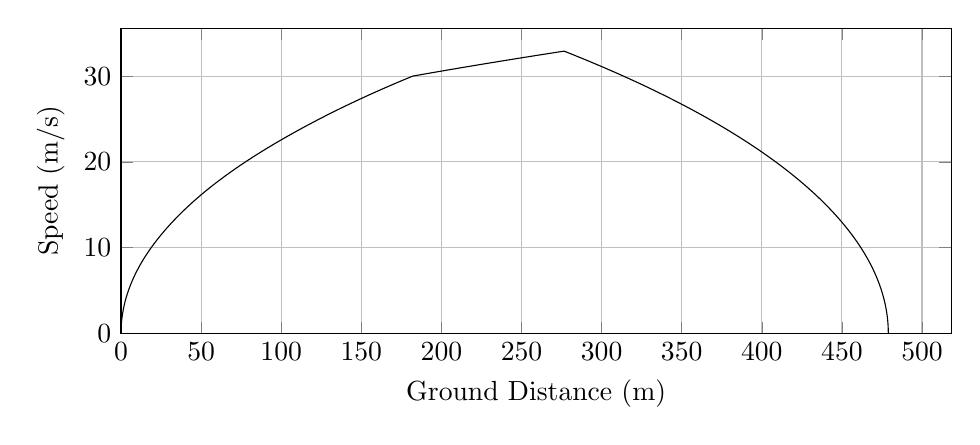
\begin{tikzpicture}

\begin{axis}[
width=\textwidth,
height=0.45\textwidth,
scaled ticks=false, tick label style={/pgf/number format/fixed},
xmin=0.0,
xmax=518.2299866992206,
xlabel={Ground Distance (m)},
xmajorgrids,
ymin=0.0,
ymax=35.60243705812628,
ylabel={Speed (m/s)},
ymajorgrids,
legend style={at={(1.03,0.5)},anchor=west,draw=black,fill=white,legend cell align=left}
]

\addplot [
color=black,
solid
]
table[row sep=crcr]{
1.3603393307215537E-8	2.7206786614136053E-4\\
2.0334443352841076E-7	0.0010518886452100893\\
1.8493358258961232E-6	0.0031722069595670832\\
9.983129263424352E-6	0.0073703305371567145\\
4.13538327636676E-5	0.015000698600431142\\
1.2467543572893382E-4	0.02604617809108093\\
2.843807411608912E-4	0.039337211109134546\\
5.588015241105573E-4	0.05514195056130601\\
9.398454696015893E-4	0.0715124015124052\\
0.0014155885812023746	0.08776501191582356\\
0.0019945752038215015	0.10417842799085314\\
0.0026717822370171283	0.12057375104521131\\
0.003447739291558293	0.1369679805266502\\
0.0043193476547732645	0.15330646708146045\\
0.00529092766782709	0.16967458986551764\\
0.006363550519206555	0.1860801697532991\\
0.007533073890550759	0.20245842760752175\\
0.008790616877968567	0.2187050333826402\\
0.01016549189277427	0.23518661303774957\\
0.011625499440327931	0.2515089605928944\\
0.013184282533086976	0.26783979728121043\\
0.014839871214038253	0.28415877961261893\\
0.01660567024659266	0.30058916249563783\\
0.018465948346479452	0.31697862375987884\\
0.0203822997817096	0.33301959314873397\\
0.022430561433814646	0.3493511890598978\\
0.024588423902376283	0.36576858773680576\\
0.026831028501027587	0.3820837645144779\\
0.029143159681622913	0.39820533289239857\\
0.03155709159958957	0.41436781879708107\\
0.03411445662773917	0.43082953897497234\\
0.03677290089167576	0.4472999485010196\\
0.03952314881844239	0.46372369327821816\\
0.04239921643077808	0.480298229329016\\
0.045357163155895136	0.49676790089513534\\
0.048363831658398165	0.5129669973040729\\
0.051533845233668635	0.5295095037624051\\
0.0547899150155587	0.5459792875367229\\
0.058172599437445835	0.562578844948455\\
0.06162834747858026	0.5790455069507827\\
0.06521401059050522	0.5956499365054515\\
0.06888104003120077	0.6121652382585918\\
0.07268727020998902	0.6288486032523657\\
0.076546425570032	0.6453234681119759\\
0.08047032364859658	0.6616539745303078\\
0.08456364881336098	0.6782704192075162\\
0.08882250397434277	0.6951370151627567\\
0.09306368907640691	0.7115361026181237\\
0.09743039119190974	0.7280343521883228\\
0.10191450167634594	0.7445955323534352\\
0.10651989152467789	0.7612293393927179\\
0.11128201757858264	0.7780550199019596\\
0.11609763023253863	0.7947071498383971\\
0.12097769621339591	0.8112331663129451\\
0.12591912973280778	0.8276304725362169\\
0.13103216605369056	0.8442616601958726\\
0.13633380151185176	0.8611668064047788\\
0.1416823117522269	0.8778912261206315\\
0.14708837902374172	0.8944775179759736\\
0.1525605467319851	0.910958713835351\\
0.15824953188605478	0.9277821623676572\\
0.16398006351864292	0.9444251305469198\\
0.16978153473626356	0.960980143916611\\
0.17584258400626962	0.9779761627962422\\
0.1819863832139092	0.9949075014432016\\
0.18819485651962437	1.0117288237112843\\
0.19455736971520038	1.028681690882733\\
0.20098158490654017	1.0455196338851316\\
0.2076061353991409	1.0626027882678097\\
0.21424726384720844	1.0794568750195062\\
0.2211374965027113	1.0966689012354127\\
0.2281284453493247	1.1138602075497053\\
0.2350833915765042	1.1307031415936888\\
0.2423085249848444	1.1479381851546555\\
0.24958374984531584	1.1650345883096191\\
0.2569279402934431	1.182041749992774\\
0.2644720218029696	1.1992601614339744\\
0.27204626263318243	1.216301667455674\\
0.27972793364503945	1.2333438504940246\\
0.2874622320100655	1.250267563714377\\
0.29563698092580604	1.2679089139886286\\
0.30361763245720474	1.284897180240498\\
0.3118912000478351	1.3022744294143571\\
0.3202493147046803	1.3195963113902769\\
0.3286412952843002	1.3367619649866742\\
0.33714554464307567	1.3539346484227002\\
0.3458731203690518	1.3713340897191824\\
0.35455185683415313	1.3884193342166231\\
0.3634323904331427	1.4056862621253625\\
0.372325738896249	1.4227674763186258\\
0.38151551889959867	1.440204563546407\\
0.3908489672358084	1.457700089962409\\
0.4001862088113266	1.4749944178140924\\
0.4095647137707429	1.492162742069545\\
0.4192312859369268	1.5096533904480967\\
0.4289206911602753	1.5269836129109997\\
0.43896550245304145	1.5447435380037913\\
0.4487817299761361	1.5619035143205457\\
0.4589033974758888	1.5794014938286165\\
0.4691858798479248	1.5969804372850023\\
0.47972601481223376	1.6148004902966524\\
0.49016040525287174	1.632249387127532\\
0.5007175269203565	1.6497149526784889\\
0.511266977039379	1.6669842941178317\\
0.522323236324642	1.6848925320185808\\
0.5332586746953114	1.702418987029767\\
0.5445869154512923	1.72038590043744\\
0.5556699580072249	1.7377833636914817\\
0.5669225885056133	1.7552698341628856\\
0.5785590177532589	1.7731705303226786\\
0.5903083066022885	1.791062482360544\\
0.6020327889628274	1.8087393997377976\\
0.613957077533064	1.8265412477772478\\
0.625960998969677	1.8442875739585323\\
0.6380070243193761	1.8619252631764254\\
0.6503365955459197	1.8798058693058528\\
0.662700086001522	1.89756560798793\\
0.6752747602080436	1.9154589089552818\\
0.6885889407972636	1.934223118171821\\
0.7019767933734617	1.9529083746402325\\
0.7151149754112038	1.971072007225393\\
0.7284684478906998	1.989362382327093\\
0.7418939875700234	2.0075825160956544\\
0.7553494584716574	2.0256778796574366\\
0.7694215958599202	2.0444301987818747\\
0.7830840331449673	2.062472448302562\\
0.796657372658726	2.0802411313322375\\
0.8106660034246236	2.0984208913722986\\
0.8251837647136968	2.1170956097847196\\
0.8395067871054176	2.1353587515267964\\
0.8540519574023793	2.1537456286169094\\
0.8688334527125461	2.172270744815026\\
0.8840141863517745	2.191132088866371\\
0.8993797082767976	2.210057982117563\\
0.9143697020410035	2.22836535981818\\
0.9294094610857999	2.246582527337803\\
0.9452486359568626	2.2656085015457856\\
0.9605773823977486	2.2838693348294017\\
0.9761522209726621	2.302273892926003\\
0.9917649966835071	2.320575683083799\\
1.0074810114554809	2.338852757671197\\
1.0234652146968335	2.3572952472370314\\
1.0399433598517231	2.376156629932451\\
1.0563627364420554	2.3948018162279734\\
1.0728309985448887	2.4133566591997972\\
1.0896486452479222	2.432157874423557\\
1.1068138420051672	2.451197693647595\\
1.124143995869574	2.4702703658932395\\
1.1415400048645106	2.489267299720775\\
1.1590089082607062	2.508197803673264\\
1.1769249919091855	2.5274643402549435\\
1.1951505705127592	2.546912836260847\\
1.2127191877709298	2.565519481815736\\
1.2308827453761335	2.5846141113587358\\
1.2492706857898845	2.603800681463974\\
1.267587852451018	2.622772557003116\\
1.2860031245644312	2.641707402954026\\
1.304687144125951	2.6607795541301913\\
1.3233765774990474	2.6797201186880235\\
1.342322280991234	2.6987833934981085\\
1.3613696045164358	2.7178127915773045\\
1.3815086998747366	2.7377876348627312\\
1.4013123019267382	2.7572871781846713\\
1.4209622886438908	2.776498715109069\\
1.4411501686096515	2.796097243313718\\
1.4611760119255748	2.8154022541980437\\
1.4816444281325132	2.8349966107890987\\
1.501865958841821	2.8542211069946886\\
1.5224364680875304	2.873643975251948\\
1.543651615594651	2.8935374401166936\\
1.5647593029468103	2.9131938159672393\\
1.5859558716309676	2.9327988876571682\\
1.6071423964076703	2.9522630829787078\\
1.6293386351549652	2.9725166193581662\\
1.6508498980272122	2.9920127820710096\\
1.673011606043147	3.0119649186923647\\
1.6946435720294923	3.0313119602620544\\
1.717066624993247	3.0512354765097847\\
1.739432891071898	3.0709781945200367\\
1.761922286799709	3.0907008715442785\\
1.7849035550437842	3.110724116499121\\
1.8076299607761817	3.130397758415918\\
1.8313298306791497	3.150781582850553\\
1.8543134894513886	3.170422617417267\\
1.8777326664639729	3.1903098303565613\\
1.9017196849182967	3.2105498581425547\\
1.925345883672024	3.230359810434704\\
1.950252961491087	3.2511112867058944\\
1.975161211119453	3.2717303209738455\\
1.9993825790313986	3.2916551882881686\\
2.024583888346972	3.3122571746177787\\
2.04934017380271	3.3323696010495665\\
2.0744229633459703	3.352622489884446\\
2.0996193404956136	3.3728429027993636\\
2.1245764901457758	3.3927508156451838\\
2.1500786393425866	3.4129717612165447\\
2.176226227020705	3.4335790174579808\\
2.202115608176549	3.453859839248252\\
2.227948363055355	3.473976519895017\\
2.2543499999408594	3.4944147290829672\\
2.2810892744412783	3.5149913296713144\\
2.3075963743135786	3.5352692309359393\\
2.3348582111613405	3.5560020049415755\\
2.3623221378972126	3.576765039163723\\
2.3898598419727675	3.597461619334588\\
2.4171687299087603	3.617867425928493\\
2.445442108612223	3.63887140648351\\
2.4735885391813177	3.659659385088693\\
2.5015416452491293	3.6801864489790015\\
2.5301110763218357	3.7010465061417728\\
2.5589284934403693	3.7219672053679007\\
2.587611617795936	3.7426723197239697\\
2.6175687086884984	3.7641733892005584\\
2.647724154312196	3.7856913664269127\\
2.6767118187859253	3.806259385188194\\
2.7060305938995466	3.826947924762984\\
2.7361546404224653	3.848086795361401\\
2.7663022704956823	3.8691245251687114\\
2.7964672462043376	3.8900584385922787\\
2.8272583584284883	3.9113092281493635\\
2.8588650092419234	3.933001260500056\\
2.8898852960400587	3.954173020653517\\
2.9215246589961597	3.975649002611738\\
2.95270311230069	3.9966971225957693\\
2.984506337549637	4.0180512736887355\\
3.017379145769185	4.040002700931062\\
3.049243647754313	4.061165386837043\\
3.081295157663824	4.08233945372935\\
3.113406837946715	4.1034415622615725\\
3.1453724573084756	4.124338342413571\\
3.1787286104953543	4.146029627303218\\
3.211019796961401	4.16691865410681\\
3.245786703184362	4.189290422964376\\
3.279939251746722	4.211148796843801\\
3.3141720228361216	4.232942924168725\\
3.3491198891036547	4.255074788125151\\
3.382965192547779	4.276396971929374\\
3.4181848705561064	4.298470348414034\\
3.45391888941694	4.320748399293741\\
3.488851494856137	4.342413989011922\\
3.524271454997704	4.364269672627019\\
3.5606552075305	4.386604233843519\\
3.597189071478943	4.408914624339188\\
3.632926148839256	4.430627359280907\\
3.668897146318187	4.452372929752713\\
3.706642714683163	4.475075142646437\\
3.7432264628550644	4.496966755254986\\
3.781286297809391	4.519626577407692\\
3.818618572105483	4.541740901418004\\
3.8564015479305356	4.564010610229177\\
3.8948624022541356	4.586566255076516\\
3.9329637046009225	4.608799669367572\\
3.971505929995028	4.631179243588672\\
4.009821706071438	4.653318136849505\\
4.049014376833089	4.675852686730371\\
4.089343885784727	4.698925378992982\\
4.128662304630717	4.721308468478165\\
4.1684827283974055	4.743867096677683\\
4.208000253554632	4.766146006975694\\
4.2483743636521965	4.78879817493951\\
4.288255503180503	4.811066470729566\\
4.328757204126676	4.83357366756756\\
4.369490126907612	4.856101520059605\\
4.410357715197167	4.878596683350667\\
4.45189144941496	4.901350066297022\\
4.492881116440694	4.92369968185371\\
4.53550011161515	4.9468278744343355\\
4.577670191557685	4.969603783574717\\
4.6201174049766305	4.992421721491047\\
4.662272021613388	5.014976943890929\\
4.706017761800355	5.038273949606417\\
4.748842845578064	5.060974035026659\\
4.792293145132742	5.083899188662546\\
4.836482439768313	5.107105883961035\\
4.88090298307878	5.130325383258471\\
4.925311889063089	5.153431397682763\\
4.969864686447545	5.176505825154747\\
5.014842280541593	5.199693556764473\\
5.0603877575117515	5.22306627262987\\
5.106292347304597	5.246515006059436\\
5.152263975081851	5.269890511862322\\
5.1974808794106995	5.292778734007962\\
5.244027372436168	5.316234153414978\\
5.28996242022761	5.3392775841790705\\
5.336209145350672	5.362374492774961\\
5.38320569473032	5.385741511936569\\
5.430469292142472	5.409136579741427\\
5.476900151253712	5.432018503774243\\
5.526063828851289	5.4561395711543685\\
5.573879040902945	5.479494218102513\\
5.622613575936374	5.503192913358333\\
5.6713596863799225	5.526792584844657\\
5.720412183296268	5.550436296154132\\
5.770660497446668	5.574549325574564\\
5.820668144990444	5.598440665195858\\
5.870305285939629	5.622051570005873\\
5.920503816994749	5.645826051794918\\
5.971105439367246	5.669687478338329\\
6.021088325934068	5.693155956312442\\
6.071322359863801	5.716642304314178\\
6.122981826035449	5.740691790991834\\
6.174329110820436	5.764493438157782\\
6.225804784288178	5.7882532999677565\\
6.278093246139479	5.812285775103884\\
6.331709873490098	5.836822711993435\\
6.384325657889258	5.860798606286268\\
6.436648686434458	5.884541153322957\\
6.489478972803882	5.908413995611658\\
6.543185721519176	5.932581273594973\\
6.596747696432654	5.9565826116867555\\
6.650345873843312	5.980500639526959\\
6.704555155195255	6.004591322261984\\
6.7588986063680725	6.028641860723198\\
6.814371620173711	6.053090524510132\\
6.86997180120154	6.077493304987486\\
6.925426612865756	6.101731867456724\\
6.981353650685165	6.126076488296089\\
7.037678624474159	6.150493701171172\\
7.094603706786671	6.175069694229233\\
7.151204881983983	6.199406017809888\\
7.209200593921791	6.224239921146953\\
7.2667780016693655	6.248793780637895\\
7.324687293141565	6.273388951364629\\
7.382771066065313	6.297958460524253\\
7.441904508776327	6.322870556471969\\
7.501585831803217	6.347910940195371\\
7.5616527251378685	6.37301033734094\\
7.62150963104709	6.397920657282372\\
7.682859947113334	6.423348757973162\\
7.7432084367972145	6.448260395172165\\
7.803024936926759	6.472854515267269\\
7.863793829029664	6.497741557547526\\
7.9252460466886365	6.522808491769428\\
7.98696966925656	6.547886129589465\\
8.04776546969778	6.572489956029987\\
8.109421212326083	6.597344759331692\\
8.17269125419024	6.62274989587474\\
8.236095044780246	6.648107867119668\\
8.299523592514586	6.6733758716647635\\
8.363213767675873	6.698648749336412\\
8.427807923256076	6.724179817063581\\
8.49144930156071	6.749236427599463\\
8.557380457258176	6.775093285731961\\
8.623183572921022	6.800798341060123\\
8.687840683575093	6.825958000305871\\
8.753751426394068	6.85150690514026\\
8.820803713780364	6.877397340692875\\
8.888970287482593	6.903614836544355\\
8.957133699158991	6.929728274880318\\
9.025036015045707	6.95564060719898\\
9.092760955867519	6.981385897661401\\
9.159817422823458	7.006780404744905\\
9.227495373767134	7.032313822655334\\
9.296013084156197	7.058066451057831\\
9.36435980631623	7.083658045990241\\
9.433329865923408	7.1093861502633935\\
9.503849553921977	7.135592793043607\\
9.574524061692681	7.161757129440835\\
9.644263228942293	7.187478303059413\\
9.715657612596786	7.2137113525921706\\
9.787429657508813	7.239983725980906\\
9.85753688572494	7.265551478201084\\
9.930250735750551	7.291971533509516\\
10.001571447096964	7.317789201023549\\
10.074699859091687	7.3441634012160115\\
10.14698611653175	7.370137562038421\\
10.220547980738981	7.39647284159466\\
10.2940409891517	7.4226865775090225\\
10.36719293590382	7.448683522018358\\
10.441008888975666	7.474821256293147\\
10.51610421670324	7.5013149409599915\\
10.590724589239105	7.527545123141664\\
10.667218005391902	7.554335510282012\\
10.742771202259895	7.580700056819904\\
10.82035208750042	7.6076733994766546\\
10.896759047300378	7.634141815439909\\
10.973503045910835	7.660631342117224\\
11.051297940743765	7.687386808018605\\
11.128076326409062	7.713698127714148\\
11.207667705350879	7.740875339530433\\
11.286758396846047	7.767783712029548\\
11.366305937658339	7.794750148057366\\
11.446149720998452	7.821719854770112\\
11.526866579636565	7.848886577953234\\
11.607297517600138	7.875860199567693\\
11.688034241538357	7.902840142547248\\
11.769665722224765	7.930022095599563\\
11.850920080706608	7.9569826322198836\\
11.933163326324259	7.984174930255627\\
12.017103780766782	8.011829467127516\\
12.10034832931326	8.039157084017077\\
12.185467765774142	8.067000695357674\\
12.270669986481685	8.094771694330461\\
12.354040133273898	8.121850004746655\\
12.440386807402234	8.149796497316302\\
12.52556588630658	8.177267823749766\\
12.610860989997974	8.204680768800486\\
12.69550109439961	8.231789408552956\\
12.784634337461807	8.260237152929719\\
12.871172079509357	8.287759415726047\\
12.958447214271366	8.315420304840373\\
13.045518554761987	8.342921619029696\\
13.133090172249581	8.370486224312394\\
13.221405510214687	8.398189697653255\\
13.310319106907201	8.425985210556949\\
13.399783591735492	8.453857077321647\\
13.488943611067967	8.481539391738199\\
13.578276665194153	8.509181571435288\\
13.667402973129146	8.536667089813005\\
13.757763665999576	8.56443970756747\\
13.848393619195729	8.592201389835143\\
13.938857764339925	8.61981963690165\\
14.031101516310692	8.647886827800537\\
14.123507833735925	8.675908901157563\\
14.214825187590282	8.703508672365633\\
14.307956552027534	8.73156336745275\\
14.401498558574918	8.759647814517947\\
14.495315613017755	8.78772120463606\\
14.589065423003394	8.815681723809828\\
14.68316852398955	8.843655285252552\\
14.778702641747682	8.871960546801994\\
14.873746415615575	8.900027772307503\\
14.970384078097169	8.92847176195491\\
15.068900921005241	8.957372338705746\\
15.164434274206265	8.985305531350946\\
15.260378587808539	9.01326844809585\\
15.357189194448868	9.04139286669879\\
15.45495288999333	9.069702319145797\\
15.55311774366497	9.098035965089778\\
15.652583807013901	9.126652094929362\\
15.755243917873962	9.156089842136982\\
15.855950289561445	9.184872261311103\\
15.958461094374158	9.214074622426836\\
16.060387288500337	9.243015579888077\\
16.164276126126843	9.272417421818076\\
16.26736468838029	9.301497527925843\\
16.36946523634058	9.330206314561998\\
16.47192386662276	9.358924026035133\\
16.576794358652606	9.38822346960886\\
16.678929175716583	9.4166678008983\\
16.783994526910618	9.445835681115561\\
16.89012564586595	9.47520500509841\\
16.996887404888547	9.504654011959929\\
17.103774697793426	9.534043283288177\\
17.210947675936964	9.563417219634118\\
17.31865021419634	9.592842496276361\\
17.424470519881233	9.621662818293629\\
17.53205215515201	9.650871542605824\\
17.64034909906897	9.680182378579893\\
17.74911485075183	9.709527974498918\\
17.85745376408675	9.738667491033553\\
17.969383314157206	9.768678371847692\\
18.07998395718984	9.79823960098523\\
18.18863741327577	9.827190891062958\\
18.302466989554325	9.857427140731051\\
18.41305080779906	9.886709740958622\\
18.525644000014054	9.916432659837046\\
18.636945827420575	9.945724520892664\\
18.750643923449367	9.975555331385554\\
18.86479622056296	10.005412957938304\\
18.979646899421056	10.035360740626022\\
19.09418630108147	10.065135801951545\\
19.208983505033515	10.094886994415017\\
19.323483295898072	10.124471311384106\\
19.43842354827664	10.154080065585102\\
19.55563752357537	10.184183168800388\\
19.67199913451129	10.213976951289727\\
19.789486593639566	10.24396844826034\\
19.90713985662446	10.273911926981121\\
20.024127533725753	10.303597189258529\\
20.143019013955552	10.33367562294372\\
20.26442367074238	10.364297193766397\\
20.383660776265387	10.394281737963148\\
20.5042342316437	10.42451216268142\\
20.622773342122727	10.454144942087797\\
20.74503732713029	10.484618723707356\\
20.865944869938517	10.514665202901362\\
20.98711015528624	10.544687539570457\\
21.113336299999695	10.575870816745912\\
21.23638685227678	10.606179030549342\\
21.35988644990264	10.636508776547114\\
21.483760012473958	10.666841533708403\\
21.608180515260266	10.697219473139526\\
21.732326713270083	10.727442588179319\\
21.85766379468624	10.757867398704445\\
21.985117186778353	10.788715847331869\\
22.111729024702363	10.819271479105705\\
22.23700541150786	10.849418172071925\\
22.36297326225872	10.879645126013575\\
22.488604760551	10.909706102371654\\
22.616276341350805	10.940168758719981\\
22.744235570279145	10.970613360141936\\
22.874576476768283	11.001536189573937\\
23.003842066605536	11.032116542561745\\
23.13088450205612	11.062086942499228\\
23.257869280739328	11.091961228338679\\
23.389244224935425	11.122782273486525\\
23.519811196806458	11.153327800430485\\
23.653309395988643	11.184471249811509\\
23.78342402399784	11.214740651782549\\
23.9180644861338	11.245975674318391\\
24.05110504604577	11.27675313214855\\
24.182394801971697	11.307042095287713\\
24.314614014384034	11.337462416058873\\
24.449791085561472	11.368477829038198\\
24.585258581909038	11.399473971168938\\
24.72121222319008	11.430495640196643\\
24.857032405393277	11.461401868729997\\
24.99454740444294	11.492607967789148\\
25.13030709358258	11.523331794491032\\
25.270890409679986	11.55506012379086\\
25.40663839363527	11.585613757472291\\
25.54307796688363	11.61624118816924\\
25.68272814639034	11.647505059569063\\
25.82072003425767	11.678314669990076\\
25.96015212691003	11.7093627406886\\
25.987750021099068	11.715498267162236\\
26.0558803939429	11.730631063705655\\
26.061632797568386	11.731907859395676\\
26.066808273335674	11.73305648125297\\
26.071901058608013	11.734186640502788\\
26.073315434863225	11.734500490619862\\
26.074595035914804	11.734784426825545\\
26.080371168076944	11.736066031557627\\
26.10234540095133	11.740940372180685\\
26.183408179590366	11.758904155082949\\
26.300430535410044	11.784787973628632\\
26.42750601924636	11.81283056419338\\
26.558056987479794	11.841570237741418\\
26.688030995483615	11.870113002299234\\
26.818767077324992	11.898753220355104\\
26.951519978077492	11.927763989958692\\
27.083955405447817	11.95663428682252\\
27.216897884715692	11.985544164744663\\
27.350913258119895	12.01461587041586\\
27.4833530065795	12.043275722209213\\
27.6176201223548	12.072260383279556\\
27.752160408628434	12.101233140761607\\
27.887329802382908	12.130270390734324\\
28.023188645890663	12.159384516832986\\
28.158973127824495	12.188411811876492\\
28.296372294036907	12.217712605075796\\
28.435107205966254	12.247225563626774\\
28.571323599682245	12.276132156199722\\
28.70996262687553	12.305481485301957\\
28.850320389600306	12.335121789198851\\
28.988837241064125	12.36430191055613\\
29.129197813929657	12.393798521815558\\
29.27166529868488	12.423664350659593\\
29.41298471572133	12.453216777241245\\
29.554848516656044	12.482810659257765\\
29.699676691743235	12.512948602260185\\
29.842400551696755	12.5425756525737\\
29.985385440862252	12.572184694765959\\
30.129077275410303	12.601867799121568\\
30.27543774584293	12.632028113131444\\
30.422081339040986	12.662172291443763\\
30.56949149516445	12.692399395353114\\
30.716562179458485	12.722482784504752\\
30.86535310281699	12.752843213073941\\
31.011875026602333	12.782667571325081\\
31.16159928701196	12.813069323080846\\
31.313692569485013	12.843875567279284\\
31.463056706803336	12.874054434598822\\
31.61235366859384	12.904146336171102\\
31.76278957628285	12.934394055733065\\
31.915019899787076	12.96492770009322\\
32.06709627595497	12.995355745016585\\
32.21861178877769	13.025597773954171\\
32.37168228565527	13.056075852175109\\
32.52450570609457	13.086430689262858\\
32.67702483599189	13.116651789580214\\
32.829998687403204	13.146889904935595\\
32.98551220909506	13.17755548020082\\
33.14332298937855	13.208597699427095\\
33.29970221124884	13.239282941961267\\
33.45800124694219	13.270268960855145\\
33.61398946945653	13.300728393722224\\
33.77048353048475	13.331212997374429\\
33.9292721471582	13.36206969824487\\
34.08796840843395	13.392833573712974\\
34.24769686644211	13.423722435259549\\
34.406855482575295	13.454426622534776\\
34.56481953291838	13.4848273131478\\
34.72399692808165	13.515388364482458\\
34.88694269464703	13.546597337194846\\
35.04914399338672	13.577588258057553\\
35.209965099803895	13.60824160856891\\
35.3703140559587	13.638732196664854\\
35.531685786905925	13.669344364559521\\
35.69349909442164	13.699967319927516\\
35.85522798807463	13.730501730108934\\
36.022509111806116	13.762008547654311\\
36.19055880791667	13.793582946048737\\
36.35708622463872	13.82479550449025\\
36.52115360367851	13.85547362194265\\
36.68781562330062	13.886562820126564\\
36.8536847754776	13.9174304483709\\
37.024522648961764	13.949146389510084\\
37.19188554678789	13.98014254566111\\
37.36066720850286	14.011327095827419\\
37.528862119520696	14.042329405603326\\
37.697264258302326	14.073296530111996\\
37.86832931534104	14.104678619737609\\
38.03812867477943	14.135754509787166\\
38.20923731912278	14.166995894554624\\
38.37904730305398	14.197927055200015\\
38.55252405124031	14.229451377363098\\
38.72282139824354	14.260324907567675\\
38.89783411301201	14.291978375010753\\
39.0714610757495	14.323306627589965\\
39.24438070689564	14.354433875522993\\
39.41969314875929	14.385917557213435\\
39.59166556575205	14.41672917791362\\
39.764623188591585	14.44764559250558\\
39.94263254662576	14.47939036052248\\
40.11749159802578	14.510500050118512\\
40.29452954971913	14.54192386043901\\
40.47247750600427	14.573435088431616\\
40.64799609178485	14.604443782057789\\
40.82414741101539	14.635492466718976\\
41.00385670225303	14.667094616677119\\
41.18169069533937	14.698294192054348\\
41.3603281005193	14.729562251315262\\
41.54046179251334	14.761019112816346\\
41.722675278204306	14.792764939681511\\
41.90258931008478	14.824037343077613\\
42.08518735141125	14.855702756267998\\
42.26728550944881	14.887208166124452\\
42.44743534848537	14.918304880626533\\
42.63069538383506	14.949865823401272\\
42.80963512098974	14.980612455604206\\
42.992542679335614	15.011969534134973\\
43.17926890616222	15.043907330033203\\
43.363134036078335	15.07528320232565\\
43.54815051311773	15.106783307813565\\
43.733578141849236	15.138281142092769\\
43.91798130912079	15.169533629501466\\
44.10506009255049	15.20116732793008\\
44.29251116260117	15.232791425149927\\
44.480917546793805	15.264503947324222\\
44.66851287589745	15.296007928958101\\
44.85853501730759	15.327846628450256\\
45.047396872181054	15.3594187231866\\
45.236914792155844	15.391028573966832\\
45.42785879536018	15.422803857706569\\
45.616432631699865	15.454113793375477\\
45.80697204128492	15.485678919895587\\
45.998633580597016	15.517358201006619\\
46.18800675699903	15.5485889940684\\
46.380841640082096	15.580319349319915\\
46.57327038933336	15.61191154939888\\
46.765844918266424	15.643456771132307\\
46.95911042680183	15.675044279688183\\
47.15311668852311	15.70668184113109\\
47.34541611633634	15.737971256186935\\
47.53884854699059	15.769375322632264\\
47.73236991243341	15.800724280331082\\
47.92818250719388	15.832374008959643\\
48.12326385407131	15.863835546272451\\
48.32058854034828	15.895588215308145\\
48.516852452700604	15.927100108245902\\
48.71339374517507	15.958586905572094\\
48.91319881343868	15.99052556573712\\
49.1119162355681	16.022219771885794\\
49.31207818344666	16.054073616673193\\
49.509673461222235	16.085449755667547\\
49.71156302510582	16.11743714149557\\
49.91034548441702	16.148862880455226\\
50.11200805970151	16.18067402752412\\
50.30853267551517	16.211607332775543\\
50.50757456960626	16.242869479706997\\
50.70929197287772	16.27448306208673\\
50.91222418686718	16.306217560588948\\
51.11562549758783	16.33795589919523\\
51.32090674103446	16.36991742319855\\
51.525199701657655	16.40165551094453\\
51.72863462744459	16.433191736975424\\
51.934060761332375	16.464967613389298\\
52.14033810224923	16.496805767338245\\
52.344882977561255	16.52830825765387\\
52.55098100649393	16.559981596302798\\
52.75731843494604	16.591623385101634\\
52.96514817708821	16.623425292724193\\
53.17450540782369	16.655391599818486\\
53.382202621450276	16.68703607441325\\
53.592230583406476	16.718966811006503\\
53.80364534107798	16.751038866953195\\
54.01469481143569	16.78298634512351\\
54.223966920081466	16.81459693592374\\
54.43230789395902	16.846000158107778\\
54.6430562980421	16.877698907056292\\
54.855225786754914	16.909543373000844\\
55.066088958624874	16.94112453133839\\
55.27969530828261	16.973048579073087\\
55.49171188337613	17.00466777951221\\
55.70388919125476	17.036244256254207\\
55.91737779085577	17.067948923124497\\
56.13177028494084	17.099720617504012\\
56.34652664868587	17.131479097728892\\
56.559021044851505	17.16283731260777\\
56.77591447970492	17.19477762486875\\
56.99548236897459	17.22704315413428\\
57.21481285737903	17.259205253646627\\
57.43536222847358	17.291477405673106\\
57.65367025761124	17.323354153252986\\
57.872788904232735	17.355282182779625\\
58.0907693980174	17.386978064843134\\
58.311927420720366	17.419068779042476\\
58.532333513628615	17.450983423705587\\
58.75532998033057	17.48320550910723\\
58.976617007999806	17.51511371149133\\
59.19875422837053	17.547077884078412\\
59.4206945143671	17.57894743506791\\
59.64453328369959	17.6110228722233\\
59.86894932484513	17.64311414170048\\
60.09432075877773	17.675275011051006\\
60.318058693038594	17.707136719649682\\
60.541731124044205	17.73892368315107\\
60.76707064338231	17.770881795092755\\
60.995574692986196	17.803221679280476\\
61.22378989589207	17.83545369864867\\
61.4534619981562	17.867824284037283\\
61.683510138770515	17.90018067545715\\
61.91410430469678	17.932546762179015\\
62.14462153858659	17.964835283858278\\
62.37563158073512	17.997126244143544\\
62.607203285434	18.02942919131057\\
62.841031881319736	18.061979766095043\\
63.07467935056491	18.094438067932423\\
63.31164975340633	18.127289914380235\\
63.54633691305479	18.159758045124143\\
63.78243968758058	18.192354943169995\\
64.0165414084598	18.22460952240222\\
64.25412817577254	18.257277411786973\\
64.49270299572771	18.290013768976266\\
64.73076499662056	18.322612833783396\\
64.96867826857735	18.355125123261494\\
65.21063576532572	18.388122379615005\\
65.4512107007771	18.42086378786273\\
65.69028017871045	18.453334211067258\\
65.93032615763332	18.48587134598388\\
66.17196619696679	18.51855821773882\\
66.4135612157637	18.551172846894467\\
66.6559030093851	18.583822213908434\\
66.89910102540284	18.6165207865629\\
67.14354652182666	18.649320691401478\\
67.38771133480921	18.682016863411377\\
67.63347396558368	18.714860698629238\\
67.87898066495345	18.747604296973613\\
68.1255935515739	18.78042936258401\\
68.37316753306138	18.813316131464234\\
68.62205497364681	18.846310878683518\\
68.8711887275476	18.879271890959345\\
69.120220471977	18.912153407236545\\
69.36846244647072	18.94486534684726\\
69.61951843592018	18.977882174220817\\
69.87236615109754	19.011068008473416\\
70.12758921381476	19.044498186251296\\
70.37945082809051	19.07742205063662\\
70.63410009691182	19.110644035332676\\
70.89152727368702	19.144161074618772\\
71.14629115974091	19.177265064407557\\
71.40197865069018	19.21042314698483\\
71.66163317144085	19.24402848823103\\
71.92484704501203	19.27802578556198\\
72.18465416754285	19.311515618271024\\
72.44573394560723	19.345102399321448\\
72.70633339061075	19.378560698675827\\
72.96699363118216	19.411960539667227\\
73.22900401485182	19.445466981936725\\
73.49076816912304	19.478875843446218\\
73.75430841254712	19.512445038740097\\
74.01895646534612	19.54608874132115\\
74.2846979982242	19.579804688311334\\
74.55380714249793	19.613880119908124\\
74.82322871850147	19.647927187775537\\
75.09350011520078	19.6820137651441\\
75.36421232425869	19.716088183322746\\
75.6347219158074	19.750069764012878\\
75.90830954343213	19.784369951832026\\
76.18188601743822	19.818600707717906\\
76.45626363461818	19.852863779190507\\
76.72958718025629	19.886927989297774\\
77.00406935908524	19.921069467275075\\
77.28579748399531	19.956042687591157\\
77.56784659723587	19.990985607089215\\
77.84569092555657	20.025339384858604\\
78.1246978223638	20.05976918860773\\
78.40641219364133	20.094464658240312\\
78.68590470271565	20.12881893388358\\
78.96851680469001	20.163488652350928\\
79.25576208114188	20.198657096075948\\
79.54169104977237	20.233595062881214\\
79.82662017154695	20.26834247833819\\
80.11330301632765	20.30323528725986\\
80.40394576721474	20.33854037515337\\
80.6908099930996	20.373318087594704\\
80.98055888331655	20.408376968618384\\
81.27178512217935	20.44354560419724\\
81.56682943128612	20.479105200138818\\
81.86186977412851	20.514594183842583\\
82.15688924927383	20.550010962329395\\
82.44965588234726	20.585088814816103\\
82.74488606927187	20.620393184721507\\
83.04325841243121	20.656003684954428\\
83.34213327641098	20.69160443047427\\
83.64411622775171	20.7275049561637\\
83.94734638805741	20.76348294994817\\
84.25123842984891	20.799468737599256\\
84.55152885577829	20.83495890636504\\
84.85735750691177	20.87103342682147\\
85.16518306664875	20.90727241570412\\
85.47136476235073	20.94324758159427\\
85.77898122624802	20.979321166593273\\
86.08923229760057	21.015632923266487\\
86.40254560035129	21.052231397343448\\
86.71167807044037	21.08827134706359\\
87.02660518802142	21.12491565780897\\
87.34238286044419	21.161587239406337\\
87.65842706333811	21.19821834626532\\
87.97971380652302	21.23538431420345\\
88.2973933745065	21.272061329033342\\
88.61789013566766	21.308991834778887\\
88.93643920279564	21.345626944102094\\
89.25662431900213	21.382379370977056\\
89.57903058309674	21.419315452201452\\
89.89968694948243	21.455980549166604\\
90.22473455398588	21.493076451285525\\
90.55024875587375	21.53015412230218\\
90.87789352676518	21.567402708165503\\
91.20733069500889	21.604782943547264\\
91.54101415610151	21.64257175453799\\
91.87012785371462	21.679771324650453\\
92.20120197152713	21.717121081699503\\
92.53416638543635	21.754612338218614\\
92.86431843528567	21.791716344685014\\
93.19748455591187	21.82908830449999\\
93.53066771200866	21.866391531576255\\
93.86681917526724	21.903955968987766\\
94.20530590547477	21.941709662266156\\
94.5419273964865	21.97918442358995\\
94.8854212036891	22.01735186501176\\
95.22752713476521	22.055292899808897\\
95.57091181422334	22.093303788685276\\
95.91383450860906	22.131192066486435\\
96.25469535763642	22.16878223054497\\
96.5966517898868	22.206423250654886\\
96.93845701474973	22.243978061415305\\
97.28153572459905	22.281603319091836\\
97.62213139590432	22.31888787171782\\
97.9659652144934	22.35645824141657\\
98.3129807304216	22.39430679429588\\
98.65852794036775	22.43192630971943\\
99.00080640577195	22.46912263861835\\
99.35064076251427	22.50707131446339\\
99.69796076807248	22.544678928219355\\
100.04654253174803	22.582355184874388\\
100.3915606488718	22.619579653578754\\
100.74261509654437	22.65738782613188\\
101.08877163494762	22.69460221539203\\
101.43457754260953	22.73171363052728\\
101.784020212797	22.769149501824693\\
102.13161434601102	22.806322121035947\\
102.4751980097893	22.843002352360074\\
102.82212110631409	22.87997546658648\\
103.16739702108615	22.916709973038678\\
103.51524666207362	22.953655109816047\\
103.86391679154056	22.990624161909977\\
104.20960434827006	23.027214897762114\\
104.55241399635099	23.063440371686035\\
104.89662223620601	23.099753283563047\\
105.24103428322039	23.13602756319478\\
105.5836615386647	23.172054572027825\\
105.92645892081137	23.208040675077115\\
106.27347658175316	23.24441030746282\\
106.6151670762521	23.280163504496024\\
106.95898391938218	23.3160813719658\\
107.30023552029138	23.351674273464127\\
107.64147805753461	23.38720983521675\\
107.98348674656944	23.422768965307462\\
108.32522459759954	23.458244090181672\\
108.3935347040271	23.465328563565826\\
108.40478590462831	23.466495218539748\\
108.41572478024443	23.467629430487982\\
108.4246743308916	23.4685573344252\\
108.44347342986478	23.47050633189219\\
108.52018987797786	23.478458177015114\\
108.70071173483461	23.497158706258915\\
108.99446230248458	23.527555808669007\\
109.30176454987088	23.559311599202502\\
109.60899173332959	23.591015113289558\\
109.91608539831654	23.622660443581132\\
110.22883517949637	23.654843076513636\\
110.54143546549608	23.686964479481496\\
110.853845249356	23.719020598101764\\
111.1739714794031	23.751821181570904\\
111.4937490010879	23.784538313981187\\
111.81170779322963	23.817022169054\\
112.13106495813236	23.84960160276347\\
112.4519453366479	23.88228879288807\\
112.77515902629136	23.915165494740442\\
113.0997499810409	23.948133725506615\\
113.43040796942478	23.98166823630654\\
113.7597028375028	24.015014513614958\\
114.0907450350197	24.04848755497811\\
114.42538740208008	24.08227359324205\\
114.75997726261329	24.116003142692982\\
115.09477047197589	24.149702069244555\\
115.43440545481076	24.18383620797733\\
115.77494672336013	24.218008818332883\\
116.11687534861284	24.252267757742516\\
116.46164587354252	24.28675789493178\\
116.8077846490165	24.321330945793186\\
117.15688723722127	24.356145384750143\\
117.50557855048987	24.390864153550645\\
117.85411336711965	24.425512878052224\\
118.20532793701167	24.460373050471716\\
118.55850697655507	24.49537270986547\\
118.91273956155123	24.530421002480267\\
119.26983096270519	24.565695750884693\\
119.62978614725739	24.601196221148456\\
119.98960731920661	24.636626243419393\\
120.34734904217265	24.671794923196416\\
120.7138511704587	24.70776644527863\\
121.08106061642908	24.74374828744837\\
121.44737887966437	24.779584008579377\\
121.81499139152783	24.81548745328893\\
122.18511446431708	24.85157664821383\\
122.55384158147794	24.887470566976\\
122.92460728481757	24.923503544080738\\
123.29616941264607	24.959554330901142\\
123.67040864389355	24.995804718505838\\
124.04652172406458	25.032175958965873\\
124.42393851457416	25.068612309140384\\
124.80152108360014	25.10500371732497\\
125.18180835736592	25.141594353183905\\
125.55854932865631	25.177783121327877\\
125.93878032356085	25.214246091706904\\
126.31997081831156	25.25073968753791\\
126.70099538833193	25.287156141005653\\
127.08058279416298	25.32337450580105\\
127.46175209000612	25.359682977702626\\
127.84399628255431	25.396032794321073\\
128.22749916598133	25.432441044057036\\
128.6102537001487	25.468717234476806\\
128.99595881306152	25.505211582482737\\
129.37788117916477	25.54128736867886\\
129.760738924708	25.577391107947825\\
130.1448498512433	25.613552421741133\\
130.53000390659713	25.649751163636274\\
130.9168242384266	25.686045432395574\\
131.29443328439476	25.721416558779445\\
131.67491382268804	25.75699799969326\\
132.05816436539135	25.792779123746882\\
132.44070735535217	25.828434948845413\\
132.82666098215685	25.86434886376555\\
133.20952005887244	25.899915643121524\\
133.5940193955625	25.935575649700276\\
133.97617966856654	25.970960156283404\\
134.36103715882757	26.00653556511503\\
134.74478042358356	26.04194936276936\\
135.12867144169206	26.077318403834774\\
135.5141335746535	26.112773606615214\\
135.89764893392993	26.147991649029102\\
136.28231234485685	26.183257080705424\\
136.66418763078912	26.21820957810221\\
137.04684871033697	26.253176876607633\\
137.42845627025127	26.287991129033465\\
137.8132447087305	26.323038336044007\\
138.19719797258034	26.35795235515335\\
138.58059071069573	26.39275864219689\\
138.96593237593703	26.427684880046527\\
139.3501607499636	26.462453503591675\\
139.73355638294606	26.49709049973351\\
140.1160230155566	26.531587727941456\\
140.50045093994146	26.56620582600513\\
140.88215178690393	26.600522936575338\\
141.26156782058217	26.634580074514247\\
141.64323970440188	26.6687849903212\\
142.02689350659642	26.70311238806667\\
142.41061312971692	26.737390551313872\\
142.7942251403153	26.771604164154354\\
143.1756303563767	26.805566666931192\\
143.5599719391364	26.8397360475888\\
143.94242380128833	26.873683192788498\\
144.3239499176869	26.907494429931745\\
144.70664939692608	26.94135589725454\\
145.0870075357763	26.974957021172592\\
145.46856550308127	27.00861103432308\\
145.85014610541765	27.04221401465076\\
146.23128237819492	27.075725091129634\\
146.61504730324998	27.10941416328948\\
146.99763315977907	27.142946831280582\\
147.38441582478964	27.176793816748457\\
147.7673688364352	27.210252821242534\\
148.15222568696134	27.243825350863183\\
148.53580865353604	27.277234236204137\\
148.9199734867533	27.310641414627234\\
149.3040357319486	27.343987432365928\\
149.68771357306542	27.37724808451503\\
150.07093078701052	27.410417098575643\\
150.45622889618164	27.443714289923733\\
150.8449053483268	27.477250842883336\\
151.2288570611563	27.510328029070116\\
151.61452719766493	27.543501694715076\\
151.9983007305741	27.57646108995101\\
152.38299664478842	27.609448674041523\\
152.76945776909372	27.642536348093053\\
153.15580177123394	27.675562788975917\\
153.54253364040335	27.708571276735924\\
153.93093169697067	27.741670677475376\\
154.31788037931886	27.774595604619762\\
154.7039882138024	27.807398452861975\\
155.08880221957185	27.840041318857274\\
155.47621608980313	27.872854403716566\\
155.866104687065	27.90582628258049\\
156.25391419262098	27.938571938646128\\
156.64166339424906	27.97126241442561\\
157.03027969880475	28.00397590612578\\
157.4213807682267	28.036848104400008\\
157.8105708506119	28.069509599261984\\
158.19948541262937	28.10209822828709\\
158.58893406813365	28.134681946997773\\
158.97894817604634	28.167263333388654\\
159.3710019698692	28.19996521139425\\
159.76139479981174	28.23247899670657\\
160.1523485688823	28.264990114723737\\
160.54128874338664	28.297284909366702\\
160.9326976430911	28.329735638638375\\
161.32564259741588	28.3622643883107\\
161.71827778345698	28.394718292593616\\
162.1124492087963	28.427249872448556\\
162.50576001021273	28.45966135074567\\
162.89904576730015	28.492021916611392\\
163.29316224934274	28.524402000902207\\
163.68899123279596	28.55687374305935\\
164.08495392634194	28.589307451797417\\
164.48271131475576	28.621838990743136\\
164.8792309171331	28.65422040646856\\
165.27343112400507	28.686364192719054\\
165.67115293733156	28.71874658169721\\
166.06936395728349	28.751120108905766\\
166.47000821435734	28.78364245240396\\
166.87155839526775	28.81618919058915\\
167.27134041220108	28.84854391024436\\
167.67233991204222	28.880948513970452\\
168.0705846918417	28.91308245741751\\
168.47232570996516	28.945450159263793\\
168.87521546679773	28.97786181560673\\
169.2789990941189	29.010296725349257\\
169.68142011368735	29.04257388757248\\
170.088438196605	29.075170902562853\\
170.49328200513543	29.10754520893652\\
170.89845866435633	29.139897799634923\\
171.30484584057905	29.17229865197214\\
171.7103088520891	29.204577691846808\\
172.11589069074847	29.23681826816754\\
172.52485519917514	29.269279383246783\\
172.93316089774754	29.30163994054552\\
173.34236088095247	29.334023165466334\\
173.7535761368399	29.36651743237808\\
174.16510964781833	29.398988407617942\\
174.5786011126259	29.431565243871617\\
174.99051444770384	29.463969462758577\\
175.40138574541044	29.496243873998054\\
175.81497300453447	29.52868355757149\\
176.2280441317456	29.56103479838987\\
176.64225100058474	29.593427039558293\\
177.05714873395152	29.62582535156549\\
177.47483026786767	29.658392743414197\\
177.89254345086653	29.69091431746626\\
178.3100126079721	29.723368828827347\\
178.7278240622369	29.75580202293856\\
179.1449731538625	29.788136146845027\\
179.56482315926417	29.820631726946374\\
179.9871804296257	29.85327306519759\\
180.4095742002126	29.885868959762234\\
180.83428717371925	29.91859534762186\\
181.26003251256287	29.951352684047734\\
181.6840913989422	29.98393207858311\\
181.8934642440371	30.0\\
182.1114839456617	30.01671912110279\\
182.5372774346568	30.030803782559538\\
183.423900814602	30.060100692921942\\
184.30144226609173	30.089055896122687\\
185.17422251923585	30.117813085228427\\
186.05126240753827	30.14666966812588\\
186.93861419286333	30.175823901041348\\
187.8243328275641	30.20488286347763\\
188.7212117513506	30.234265766019313\\
189.61004025875786	30.26334317360883\\
190.50102451880866	30.29244954042675\\
191.38947474753866	30.321431838738036\\
192.28052744689825	30.350457772783642\\
193.18778236606096	30.379969193193332\\
194.08895872822546	30.409240791910825\\
194.99680020640938	30.43868661898729\\
195.89480429656658	30.467771791042267\\
196.79674305679504	30.496942930689507\\
197.7065692706791	30.526327219304832\\
198.612023604503	30.55552863461159\\
199.52644538440046	30.58497721717545\\
200.43881964763966	30.614317914765877\\
201.34572312669928	30.64344131292627\\
202.26115686844895	30.672796974835563\\
203.17967892292364	30.702209754100792\\
204.1017087672932	30.73169279112831\\
205.01405834107487	30.76082496020659\\
205.94020355690031	30.790355748725723\\
206.86420646269943	30.819776332537728\\
207.79153006365993	30.849260737156996\\
208.72800400232427	30.878993632795748\\
209.6603812871926	30.908554250274307\\
210.59913361291103	30.938274601009326\\
211.54272242703126	30.96810538150325\\
212.4892775421681	30.997987106033364\\
213.4278558742791	31.02757481944868\\
214.37319863683314	31.05733347274429\\
215.31618532994997	31.086975830603322\\
216.26909967312713	31.116887686925935\\
217.2229300472723	31.146785610868903\\
218.17915574443117	31.176715920422055\\
219.13394290547268	31.2065587213008\\
220.0901210939433	31.236402628698578\\
221.05386294760763	31.266439877328885\\
222.0194744620763	31.296492546416545\\
222.9871855528732	31.32656770277\\
223.95850156259326	31.356711927622243\\
224.93506896411378	31.386975907915314\\
225.9123601081958	31.41721911341567\\
226.89683950214788	31.447641250232557\\
227.87812705537118	31.477921471699034\\
228.86553252311342	31.50834704383874\\
229.85786107077195	31.53888060364516\\
230.84893890233656	31.5693321279552\\
231.8352011637358	31.59959266617151\\
232.83551070617193	31.63024054878933\\
233.8409775535427	31.66100232817344\\
234.84473749332597	31.691667959711395\\
235.85076677249623	31.722359073957946\\
236.86174655712836	31.753157184265454\\
237.8698887650736	31.78382509025937\\
238.88314164945962	31.81460462327093\\
239.88702917374013	31.845056509694693\\
240.9073981595622	31.875964518089134\\
241.92631922506058	31.906784772239014\\
242.95020737895555	31.937711280743677\\
243.9867665418509	31.96897579811266\\
245.01566609591487	31.999964990807705\\
246.05919400906686	32.03134989683663\\
247.09706457910846	32.062520031674126\\
248.1403037320082	32.093806757027465\\
249.18309170866138	32.125035426152664\\
250.23723200462985	32.15655902834854\\
251.28895058541582	32.1879652918728\\
252.34575298177748	32.21947838418474\\
253.4009695529494	32.25089940657031\\
254.47389199439823	32.28280198773692\\
255.55293546958148	32.31484035147359\\
256.6206413021679	32.34649667499184\\
257.69235364004487	32.37822657869832\\
258.77967411403563	32.410372521650146\\
259.8615409937813	32.442311402047466\\
260.93956317950165	32.47409152624968\\
262.02271022117964	32.505977455077655\\
263.11073386748035	32.53796147254532\\
264.2120045516847	32.570288724032764\\
265.31241535302627	32.602544554991695\\
266.4086016357777	32.63463088506654\\
267.51260488983417	32.66690018176935\\
268.6300148019782	32.69951473202116\\
269.7585470354529	32.732406557674935\\
270.8896873949477	32.765326882937785\\
272.0115439451323	32.79793026793426\\
273.13680176546006	32.83058597227985\\
274.2702490513931	32.8634324722093\\
275.413525774062	32.89651641620499\\
276.3239236681536	32.922827466231894\\
276.5542367829295	32.92947890946601\\
277.554788259544	32.855468047283324\\
278.5499282368744	32.781622363980944\\
279.5468210518608	32.70740985515121\\
280.54457272161665	32.63289445752265\\
281.5347601972437	32.55870595222818\\
282.51938272683515	32.48469759134542\\
283.5221719980424	32.40907928979969\\
284.52144002460784	32.33347935334942\\
285.5065413744376	32.25870793594673\\
286.49067071596266	32.183767371864434\\
287.4855387842832	32.107760469629\\
288.4785328044295	32.0316456727321\\
289.4558376341987	31.956486754149317\\
290.4452179546196	31.880148016058484\\
291.4362341762878	31.80342783881563\\
292.42552923534424	31.726584231902088\\
293.4112881717839	31.649758292328166\\
294.3958772331042	31.572765506057323\\
295.37586350088816	31.495874643822965\\
296.3639498807927	31.41808564871473\\
297.3501848614277	31.340177461428382\\
298.3398532517323	31.261729906781916\\
299.3128667606111	31.184338630746744\\
300.2979722329835	31.10571695737029\\
301.28589571931684	31.026596802248783\\
302.2517321223603	30.948978616302533\\
303.22560994216224	30.870444876190035\\
304.19844887137424	30.79172278701906\\
305.16721169680045	30.713058120968945\\
306.14133092388545	30.633682222180433\\
307.1183129647659	30.55379254259698\\
308.08874758460775	30.474157912107124\\
309.05104077529325	30.39491324342687\\
310.0116623058466	30.315527761958847\\
310.97416663340744	30.235705370501385\\
311.93862106265544	30.155436496345978\\
312.9042085878807	30.074785417972883\\
313.8607306878614	29.994605159454096\\
314.8103087392675	29.914722724737963\\
315.7635145755504	29.83424789544791\\
316.72127527573787	29.753096278043138\\
317.68202711729873	29.6713944275405\\
318.62951500322526	29.590526946731778\\
319.5882925222194	29.508396594480175\\
320.5331857914575	29.42715850573711\\
321.4802787033931	29.345432817344644\\
322.42948830671753	29.263222067051515\\
323.38313368290176	29.18031961727651\\
324.31736547478727	29.09880334750587\\
325.2560396282021	29.016596325456135\\
326.1918178881874	28.934337835324868\\
327.12581340820736	28.85192964918393\\
328.06785507666075	28.76849871663127\\
329.00598052108364	28.685099637686342\\
329.93709199652426	28.60201050805241\\
330.86383958236627	28.51899779808965\\
331.7940264405214	28.43536019244617\\
332.7190974456154	28.35186493839212\\
333.6413079242308	28.268309715065186\\
334.55125241868143	28.185551654912324\\
335.46660340028666	28.101984163755375\\
336.3747308431896	28.018758385642116\\
337.2875172156404	27.934783767748854\\
338.19828079330546	27.850670657566496\\
339.109611360101	27.76617764076981\\
340.0129870615515	27.682095770388727\\
340.91909778436093	27.597429853760808\\
341.81644111043147	27.513254894364515\\
342.7133692535617	27.42878937050378\\
343.6184676625437	27.343217320888158\\
344.51737039439627	27.25789266228697\\
345.4159820554156	27.172255338788098\\
346.30095283991204	27.087582256719585\\
347.17992936105065	27.00314974627686\\
348.06324428581195	26.917962999421846\\
348.9364433780921	26.833416073963683\\
349.80883972935715	26.74861028965691\\
350.6725450259156	26.66431473685865\\
351.5472086084487	26.57860705599675\\
352.4072535743069	26.49399236612642\\
353.2770101509982	26.40807649058535\\
354.13828190935476	26.322652782096796\\
354.9933330028563	26.23750211476736\\
355.85205864704324	26.151637167428227\\
356.7071105330664	26.06578923145929\\
357.55662905210625	25.980147170872293\\
358.3968855315861	25.895092523724195\\
359.2442002307205	25.80897111675816\\
360.08339527712974	25.723322760518407\\
360.9246104267437	25.637112833156166\\
361.7545426495701	25.55170694638253\\
362.581918833003	25.466212255460142\\
363.4093806494336	25.38035375881504\\
364.23264192171564	25.294575206155898\\
365.05797482153	25.208220758899664\\
365.8765610813148	25.12221241259808\\
366.6868045921444	25.036724086081456\\
367.4906771263371	24.951553753685353\\
368.2952198328626	24.86595547973915\\
369.0972808321063	24.780262081320778\\
369.8964582846754	24.694516327946104\\
370.6930530520266	24.608685839596568\\
371.4728865706744	24.52430769191818\\
372.2678562262888	24.43792786104141\\
373.06106899862266	24.351368780832296\\
373.84382996836246	24.265583874523955\\
374.6159909394505	24.180600223865042\\
375.3856302934837	24.0955340555213\\
376.1473504597384	24.010985448987967\\
376.91317968965916	23.92561812175839\\
377.68323290861986	23.8394093445103\\
378.4403029180851	23.75428782716142\\
379.1869255532997	23.66998144446604\\
379.93805310858056	23.58480218753754\\
380.6856374163734	23.499658062133257\\
381.43021045639625	23.414489282289544\\
382.18008046874786	23.328339686536772\\
382.92513258826534	23.24236680534053\\
383.6506231543186	23.1582862151298\\
384.3822860805168	23.0731215008703\\
385.0990882750988	22.98932343144554\\
385.8170433174296	22.9050262966476\\
386.52234575345665	22.821855791352462\\
387.2376414658007	22.73713943877408\\
387.93937547097994	22.65366569529794\\
388.64083062377483	22.569861184126736\\
389.33134235465366	22.487004725510666\\
390.0273880382074	22.403119304350952\\
390.7068665546425	22.320873126477814\\
391.40282314876936	22.236262201013623\\
392.0855974079484	22.15288572238901\\
392.75818287930633	22.07039280667339\\
393.43867085808176	21.98656221871262\\
394.11027968502674	21.90345794245645\\
394.786759986094	21.81937749805546\\
395.4566036152579	21.73574840928856\\
396.1166927015505	21.652969320806584\\
396.7644616700177	21.571376151431416\\
397.4244929822212	21.48786828290124\\
398.08014509529926	21.404540259324477\\
398.7259878602912	21.32208998732478\\
399.3670096194496	21.239888856117155\\
400.01048041429635	21.157002303811872\\
400.6524530744772	21.07393355253508\\
401.2849921803854	20.991714583979075\\
401.9182641221695	20.909027179401278\\
402.54543114898365	20.826764493379848\\
403.1748134003958	20.743834192391645\\
403.79833980526837	20.661298526726846\\
404.42118950858446	20.57847330174848\\
405.0408464729951	20.49569204032133\\
405.6607425327045	20.412494337706022\\
406.26485178835514	20.331040880801986\\
406.8597412181373	20.25046486630488\\
407.46585224174294	20.16799116094724\\
408.0662523853787	20.085914005994624\\
408.655389120426	20.005003923604498\\
409.25135626022404	19.922775530156436\\
409.8369706591932	19.841598410959087\\
410.43440926548703	19.75839216498261\\
411.0160612808693	19.677001299494236\\
411.5941953689414	19.59572328433906\\
412.1674464950138	19.514753576964964\\
412.734523134238	19.43428083731078\\
413.29884338477484	19.353824189375295\\
413.85822071671885	19.273698379101695\\
414.4235767236336	19.19233315417484\\
414.9756751838046	19.11249960167205\\
415.52331092793077	19.032939316986656\\
416.0720467794564	18.952842842277434\\
416.61315945743	18.873485464321824\\
417.1498178093706	18.794410227188457\\
417.68871269335546	18.71462879638196\\
418.213024658514	18.636639442975174\\
418.7487921979216	18.556567523121167\\
419.2826225641252	18.47639957878146\\
419.81472679740534	18.396102851089523\\
420.3393026309021	18.31655800694024\\
420.8604642413378	18.237148178797803\\
421.3862485865561	18.156642317622662\\
421.9006948750339	18.07748667780195\\
422.41070045731215	17.998632618458196\\
422.9183404173573	17.919761913445114\\
423.4327666201011	17.83944243603935\\
423.92933708268527	17.761529205705912\\
424.43895944904557	17.681173005520677\\
424.93445901473285	17.602654746393505\\
425.4198125365714	17.52536748029987\\
425.91930825977954	17.4454336084111\\
426.4108084343004	17.366383203722393\\
426.89157456876444	17.28867390545672\\
427.3736881996448	17.21035890789573\\
427.8496231617944	17.132661363421164\\
428.32144537553563	17.055251270357786\\
428.7978436156403	16.976697173464885\\
429.28662524009326	16.89568471355367\\
429.7517265638312	16.81819994563078\\
430.2077548556547	16.741845384302223\\
430.6704827834137	16.6639777521641\\
431.13687084231697	16.5850897060524\\
431.59309180658613	16.507522899516538\\
432.0390207763545	16.431319668707047\\
432.47870377400955	16.355804655804505\\
432.9226261034879	16.27917424996997\\
433.3702476615605	16.201505647503325\\
433.81357695887505	16.12418058099231\\
434.25289010134236	16.04715641108544\\
434.6869895946435	15.970649956246934\\
435.12081000122475	15.893793328475724\\
435.5465841270244	15.817968368603221\\
435.97079761070574	15.74202769109397\\
436.4032388308824	15.66420375265496\\
436.8208756819258	15.588644993778377\\
437.2428780941283	15.511892200685086\\
437.65831737641963	15.435930323041521\\
438.07449525839706	15.359426722475483\\
438.4798586505311	15.284513949843475\\
438.8801341197226	15.21015116388395\\
439.2774252258897	15.135953646866565\\
439.67454163191667	15.061395555319887\\
440.08265413035883	14.984357185544681\\
440.4830325234242	14.908362951354935\\
440.8710779160597	14.834310567480138\\
441.254892759021	14.76067326666847\\
441.6456364075525	14.685299805928526\\
442.02456795184594	14.611806851509499\\
442.41121361063506	14.536407560187154\\
442.7985842558204	14.460444919218954\\
443.1769055394532	14.385842746257005\\
443.55254824634756	14.311357527836027\\
443.9259891916414	14.236896319513743\\
444.3030104440239	14.161297306475\\
444.674103821343	14.086464331882837\\
445.04034037517226	14.012193105468487\\
445.4037778533881	13.938072781231849\\
445.7636722139358	13.86425939504457\\
446.1291957847294	13.78886123408041\\
446.49089901524326	13.71381732029942\\
446.8434091500312	13.640258704542308\\
447.1951592480543	13.566436620818429\\
447.5480390419008	13.491946828939337\\
447.8888710968424	13.419583994850498\\
448.2232780502105	13.348181289357246\\
448.5695349749209	13.273819760441924\\
448.9131599145677	13.199585164063244\\
449.2546587859289	13.125369927290272\\
449.59140495362647	13.05175077863527\\
449.92365092477667	12.978683153763733\\
450.2550065332498	12.905376367551607\\
450.5774555501497	12.833615888355073\\
450.9067791352977	12.759886253661548\\
451.2262588294801	12.687929051790462\\
451.5446423651084	12.615788727812287\\
451.85981865448844	12.543945017740342\\
452.17286021532425	12.472157000925375\\
452.485101553783	12.400117244081027\\
452.7939211463413	12.328431891796424\\
453.11563538546886	12.253284986625435\\
453.4205931794901	12.181602932941242\\
453.7185675152773	12.11113254418375\\
454.0291147351188	12.037228444390259\\
454.3253401264327	11.966287014960415\\
454.625408234736	11.893973581716825\\
454.91924571575555	11.822713087414556\\
455.21001656151043	11.751751371298916\\
455.50906506672493	11.678299309673513\\
455.79760992652587	11.606966757842645\\
456.08525234765193	11.535398817254752\\
456.3748276163918	11.46287888152117\\
456.65778848978425	11.391550194142873\\
456.94502562893797	11.318664202415537\\
457.2224151597867	11.247809868941061\\
457.50206662469736	11.175904153664973\\
457.7779915858325	11.104481555632141\\
458.05289153110823	11.03284588135989\\
458.3227518000808	10.962049963213659\\
458.58298691694813	10.893326175121448\\
458.865823997996	10.818119215770526\\
459.1299660785854	10.747389804154334\\
459.39418961868967	10.676152030053316\\
459.65140006995796	10.606328307021887\\
459.90483996565365	10.537058915722458\\
460.16759641890076	10.46474143731336\\
460.4177998634233	10.395394489084662\\
460.66914013637165	10.325246931754407\\
460.91581309169453	10.255919204233109\\
461.15597697915894	10.187951995896515\\
461.40442664219484	10.117143059779114\\
461.6497208795613	10.04672744121888\\
461.884848732382	9.978748416008617\\
462.1249399499592	9.908837500576443\\
462.3548296683347	9.841416738789096\\
462.59392111683655	9.77078819896013\\
462.82864666919477	9.700933533001578\\
463.05840238629366	9.632052176323043\\
463.28934123912245	9.562300935753207\\
463.5153136473856	9.493538844327603\\
463.7399720648243	9.424664636016761\\
463.9659015361807	9.354874535450524\\
464.18695428936223	9.286068706947383\\
464.3998655747921	9.219297868500878\\
464.60995420611255	9.152921546392811\\
464.82221240223885	9.085353830300857\\
465.02855209714403	9.019171860634856\\
465.23474184044437	8.952536303532767\\
465.44114204133325	8.88531915310891\\
465.6504781176818	8.81660897714293\\
465.8563115189272	8.748508971078646\\
466.05710956985536	8.681547321200991\\
466.259586795425	8.613485648848343\\
466.4623106938607	8.54478480857015\\
466.65655025762726	8.478424566888862\\
466.8463729446395	8.41305575792136\\
467.0400434013393	8.345822066904354\\
467.2286520220075	8.279808984885157\\
467.41602508837445	8.213691282699713\\
467.6040280943298	8.146800149254567\\
467.7865197864421	8.081328928188306\\
467.9713018555203	8.014479474929832\\
468.15331862826577	7.948069252321689\\
468.33653545871357	7.880644381873935\\
468.51494200960997	7.814419381886475\\
468.68791747010937	7.749659340773048\\
468.8587930721561	7.685139189304252\\
469.03502763812924	7.618012161597505\\
469.2065153890993	7.5521096034235775\\
469.3787117791077	7.485340075911283\\
469.54748302940993	7.419304961414689\\
469.71381150197885	7.35363508066119\\
469.8750087078164	7.289416694638229\\
470.0284243928302	7.2277592714436345\\
470.1942986390417	7.16048731363313\\
470.3557248916626	7.094396618185243\\
470.50832501292075	7.031338965254832\\
470.662219471192	6.967159196637992\\
470.81619226813336	6.902340137857967\\
470.9684608833742	6.837624856951914\\
471.1239971309394	6.7708725324071946\\
471.2744598615021	6.705655899628656\\
471.42645266157797	6.639116158000075\\
471.5769060331462	6.572577433169897\\
471.7228556686126	6.507371281678985\\
471.86550389128	6.442993662489352\\
472.00433776236116	6.379705272702891\\
472.14110822716907	6.316729296727992\\
472.2753920688489	6.254273381663369\\
472.4079304600285	6.192003724312039\\
472.5424227452238	6.128161259009428\\
472.67794158334584	6.063143282274517\\
472.806572126578	6.000770689528595\\
472.9434059970463	5.9336922595699715\\
473.0654603709596	5.873205181808952\\
473.19728043742975	5.807162924579963\\
473.3207541610101	5.744606039216771\\
473.4462913839001	5.680289864961324\\
473.56198107640614	5.620360392956469\\
473.6790427084221	5.559055912809065\\
473.8013669142715	5.494257316057993\\
473.9194325040123	5.430974255743196\\
474.0340416638726	5.368823556191629\\
474.1454889806239	5.307683062363955\\
474.25370907548927	5.247625131230242\\
474.36797328608907	5.183451009186291\\
474.4783004391145	5.120718286605847\\
474.5860666831137	5.0586842958065805\\
474.6895219281081	4.998401585335456\\
474.79559331973826	4.9358239029692506\\
474.8949256232098	4.876488166314042\\
474.9919594527363	4.817814408892007\\
475.0977636221953	4.753005850546783\\
475.19572868124555	4.692195099151579\\
475.2884259982126	4.633914235379269\\
475.3774705861339	4.57722630959047\\
475.46962762965563	4.5178028540441915\\
475.5587109438094	4.459603795526064\\
475.64926688934906	4.399648563618042\\
475.73449110415004	4.342462554733817\\
475.82776543129125	4.2789936409050515\\
475.91950167054404	4.21563381742072\\
476.00266803129466	4.157353709331931\\
476.08718192086496	4.0972753758460225\\
476.16708933238715	4.039645469677831\\
476.24808486795234	3.980374855839144\\
476.32916014459295	3.9201439002742404\\
476.4101608329265	3.8590249984649168\\
476.4859226829369	3.8009653492255584\\
476.5608976486636	3.742617958588993\\
476.63772535602675	3.6818652690737608\\
476.7100094300712	3.6237715915748785\\
476.7799037287549	3.566694996999498\\
476.84596999959035	3.511888176987517\\
476.91556850409984	3.4532066045317293\\
476.98194230220804	3.3962958573073507\\
477.04718229510206	3.3394086769198834\\
477.1092853361084	3.2843382193591664\\
477.1704129306444	3.229212505223386\\
477.2316926527219	3.172985178444544\\
477.2900490359508	3.118494813323875\\
477.35254723284584	3.0590573969534907\\
477.411007145132	3.002392354175247\\
477.46713163663026	2.946963042478245\\
477.5210462113182	2.8927134027589165\\
477.5750561056906	2.8373251980791343\\
477.6304594327046	2.779358341435472\\
477.68138628732606	2.7249848864146884\\
477.73264949056545	2.669131191054335\\
477.78819487713326	2.607258441597229\\
477.83801585513595	2.550482740068847\\
477.8879750461085	2.4922483165756875\\
477.9350010705473	2.4361588005465116\\
477.98248274101024	2.3781814290789844\\
478.0296164402404	2.319193253598719\\
478.0724673104404	2.2642294527594746\\
478.1140255122824	2.209615948586353\\
478.15277561867845	2.1574455365473586\\
478.190693184422	2.1051429242990087\\
478.22992888494116	2.0496154735949608\\
478.2658035378711	1.9974923570111\\
478.30049539151787	1.9457584879040697\\
478.33300823316733	1.8959914927060169\\
478.3670626128602	1.8424223387751275\\
478.40189895025514	1.785959492565778\\
478.43442577060387	1.731576883751024\\
478.46377576604675	1.6809948941227408\\
478.492220060696	1.6304757798962681\\
478.51982947465547	1.579893888110313\\
478.5466563922297	1.5291423706457228\\
478.57089466843047	1.4817929377315049\\
478.59770561666016	1.4275883000569087\\
478.6222536120463	1.3760863327837112\\
478.6458207845668	1.3247584823010148\\
478.66996657916127	1.2700195574602753\\
478.69062274504154	1.2212449251978423\\
478.7114089403874	1.1701116922700807\\
478.7299491754652	1.1225389727389579\\
478.7488193070292	1.0719531076995326\\
478.7672906499389	1.0200084767525048\\
478.78401502458894	0.9705806693512551\\
478.799138524383	0.9236087291742499\\
478.8128055780869	0.87900325877654\\
478.8257034510938	0.8347243187732281\\
478.83875735701235	0.7873777504850432\\
478.85177952389483	0.7371218001814444\\
478.8633371916625	0.689455499032747\\
478.8738533564501	0.6430212077116229\\
478.8835380557704	0.5970721123780702\\
478.89421090828307	0.5419404157749934\\
478.9021238283964	0.497133668729825\\
478.90945708534116	0.4516576472148962\\
478.9149428237838	0.41438818718230264\\
478.92074695198005	0.3709002316568931\\
478.9265367067967	0.3217153694680397\\
478.9308452679421	0.2795525289087256\\
478.93511482290853	0.2302777912668139\\
478.93807121536076	0.18876599488587442\\
478.940410750546	0.14787448214717525\\
478.94216908996634	0.10733516907542673\\
478.94333778961015	0.06814859052261646\\
478.94402732672324	0.02422813671337623\\
478.9441270894074	-5.802468922011528E-11\\
};
\end{axis}
\end{tikzpicture}%

%\caption{Speed v.s. ground distance in aborted take-off condition - ATR-72}
%\end{figure}
%%
%\begin{figure}[H]
%\centering
%%BalancedTakeOffLength
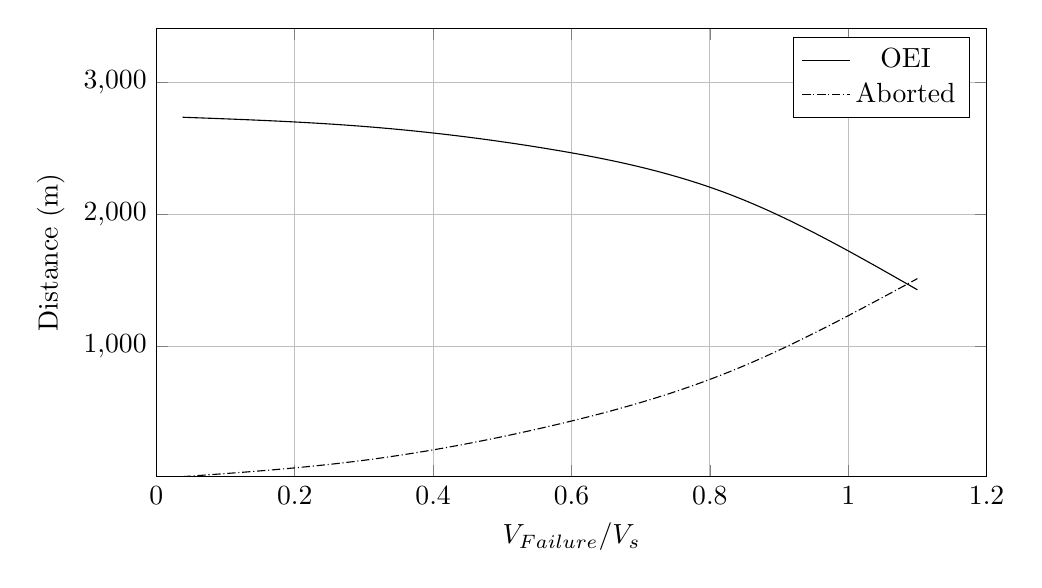
\begin{tikzpicture}

\begin{axis}[
width=\textwidth,
height=0.6\textwidth,
scaled ticks=false, tick label style={/pgf/number format/fixed},
xmin=0.0,
xmax=1.2,
xlabel={$V_{\text{Failure}}/V_s$},
xmajorgrids,
ymin=16.343983261177346,
ymax=3409.4029481001066,
ylabel={Distance (m)},
ymajorgrids,
legend entries = {OEI\\Aborted\\}
]

\addplot [
color=black,
solid
]
table[row sep=crcr]{
0.03779645082157896	2735.6611103822934\\
0.04206232852912282	2734.8398501864044\\
0.046328206236666676	2734.018095801858\\
0.050594083944210534	2733.195353039998\\
0.05485996165175439	2732.371127712165\\
0.05912583935929824	2731.5449256297034\\
0.0633917170668421	2730.716252603955\\
0.06765759477438596	2729.884614446263\\
0.07192347248192982	2729.04951696797\\
0.07618935018947369	2728.2104659804186\\
0.08045522789701755	2727.3669672949513\\
0.08472110560456142	2726.5185267229112\\
0.08898698331210528	2725.664650075641\\
0.09325286101964915	2724.8048431644834\\
0.09751873872719301	2723.9386118007806\\
0.10178461643473688	2723.0654617958758\\
0.10605049414228074	2722.1848989611117\\
0.11031637184982461	2721.296429107831\\
0.11458224955736847	2720.399558047376\\
0.11884812726491234	2719.49379159109\\
0.12311400497245621	2718.578635550315\\
0.12737988268000008	2717.6535957363944\\
0.13164576038754394	2716.718177960671\\
0.1359116380950878	2715.7718880344864\\
0.14017751580263166	2714.8142317691845\\
0.14444339351017554	2713.8447149761073\\
0.1487092712177194	2712.862843466598\\
0.15297514892526326	2711.8681230519987\\
0.15724102663280712	2710.8600595436524\\
0.161506904340351	2709.838158752902\\
0.16577278204789486	2708.8019264910904\\
0.17003865975543872	2707.7508685695598\\
0.17430453746298258	2706.684490799653\\
0.17857041517052646	2705.602298992713\\
0.18283629287807032	2704.503798960082\\
0.18710217058561418	2703.388496513103\\
0.19136804829315807	2702.255897463119\\
0.19563392600070192	2701.1055076214716\\
0.19989980370824578	2699.9368327995053\\
0.20416568141578964	2698.7493788085612\\
0.20843155912333353	2697.5426514599826\\
0.21269743683087738	2696.3161565651126\\
0.21696331453842124	2695.0693999352934\\
0.2212291922459651	2693.801887381868\\
0.225495069953509	2692.5131247161785\\
0.22976094766105284	2691.2026177495686\\
0.2340268253685967	2689.86987229338\\
0.2382927030761406	2688.5143941589563\\
0.24255858078368445	2687.1356891576393\\
0.2468244584912283	2685.7332631007725\\
0.2510903361987722	2684.3066217996984\\
0.255356213906316	2682.855271065759\\
0.2596220916138599	2681.3787167102982\\
0.2638879693214038	2679.8764645446577\\
0.2681538470289476	2678.348020380181\\
0.2724197247364915	2676.79289002821\\
0.27668560244403534	2675.210579300088\\
0.2809514801515792	2673.6005940071577\\
0.2852173578591231	2671.9624399607615\\
0.28948323556666694	2670.2956229722417\\
0.2937491132742108	2668.599648852942\\
0.2980149909817547	2666.874023414205\\
0.30228086868929854	2665.1182524673727\\
0.30654674639684243	2663.3318763287393\\
0.3108126241043863	2661.514735635469\\
0.31507850181193015	2659.6668256580265\\
0.31934437951947403	2657.7881429448366\\
0.32361025722701786	2655.878684044324\\
0.32787613493456175	2653.9384455049144\\
0.33214201264210563	2651.9674238750326\\
0.33640789034964946	2649.965615703104\\
0.34067376805719335	2647.9330175375535\\
0.34493964576473723	2645.8696259268067\\
0.34920552347228107	2643.7754374192878\\
0.35347140117982495	2641.6504485634227\\
0.35773727888736884	2639.494655907636\\
0.36200315659491267	2637.3080560003536\\
0.36626903430245655	2635.0906453899997\\
0.3705349120100004	2632.842420625\\
0.37480078971754427	2630.56337825378\\
0.37906666742508816	2628.253514824764\\
0.383332545132632	2625.9128268863774\\
0.38759842284017587	2623.5413109870456\\
0.39186430054771976	2621.1389636751933\\
0.3961301782552636	2618.705781499246\\
0.4003960559628075	2616.241761007628\\
0.40466193367035136	2613.746898748766\\
0.4089278113778952	2611.2211912710836\\
0.4131936890854391	2608.664635123007\\
0.4174595667929829	2606.077226852961\\
0.4217254445005268	2603.4589630093706\\
0.4259913222080707	2600.8098401406605\\
0.4302571999156145	2598.1298547952565\\
0.4345230776231584	2595.419003521584\\
0.4387889553307023	2592.677282868067\\
0.4430548330382461	2589.9046893831314\\
0.44732071074579	2587.1012196152024\\
0.4515865884533339	2584.2668701127045\\
0.4558524661608777	2581.4016374240637\\
0.4601183438684216	2578.505518097704\\
0.46438422157596543	2575.578508682052\\
0.4686500992835093	2572.6206057255317\\
0.4729159769910532	2569.631805776569\\
0.47718185469859703	2566.612105383588\\
0.4814477324061409	2563.561501095015\\
0.4857136101136848	2560.4799894592743\\
0.48997948782122863	2557.367567024791\\
0.4942453655287725	2554.2242303399908\\
0.4985112432363164	2551.0499759532986\\
0.5027771209438603	2547.844800413139\\
0.5070429986514041	2544.6087002679383\\
0.511308876358948	2541.3416720661203\\
0.5155747540664919	2538.043712356111\\
0.5198406317740357	2534.714817686335\\
0.5241065094815796	2531.3549846052183\\
0.5283723871891234	2527.964209661185\\
0.5326382648966673	2524.542489402661\\
0.5369041426042112	2521.089820378071\\
0.541170020311755	2517.60619913584\\
0.5454358980192989	2514.0916222243936\\
0.5497017757268428	2510.546086192157\\
0.5539676534343866	2506.9695875875545\\
0.5582335311419305	2503.3621229590117\\
0.5624994088494744	2499.723688854954\\
0.5667652865570182	2496.0542818238064\\
0.5710311642645621	2492.3538653402593\\
0.575297041972106	2488.621642183115\\
0.5795629196796498	2484.8560544352868\\
0.5838287973871937	2481.055511105952\\
0.5880946750947376	2477.2184212042907\\
0.5923605528022814	2473.3431937394807\\
0.5966264305098253	2469.4282377207005\\
0.6008923082173692	2465.471962157129\\
0.605158185924913	2461.472776057945\\
0.6094240636324568	2457.429088432327\\
0.6136899413400007	2453.339308289453\\
0.6179558190475444	2449.2018446385027\\
0.6222216967550882	2445.0151064886536\\
0.626487574462632	2440.777502849085\\
0.6307534521701758	2436.4874427289756\\
0.6350193298777196	2432.1433351375035\\
0.6392852075852634	2427.743589083848\\
0.6435510852928072	2423.286613577187\\
0.647816963000351	2418.770817626699\\
0.6520828407078948	2414.1946102415636\\
0.6563487184154386	2409.5564004309585\\
0.6606145961229823	2404.8545972040624\\
0.6648804738305262	2400.0876095700546\\
0.66914635153807	2395.253846538113\\
0.6734122292456138	2390.3517171174162\\
0.6776781069531576	2385.3796303171434\\
0.6819439846607014	2380.3359951464727\\
0.6862098623682452	2375.2192206145833\\
0.6904757400757889	2370.0277157306527\\
0.6947416177833328	2364.759889503861\\
0.6990074954908766	2359.4141509433853\\
0.7032733731984204	2353.988909058405\\
0.7075392509059641	2348.482572858099\\
0.711805128613508	2342.893551351646\\
0.7160710063210518	2337.2202535482234\\
0.7203368840285955	2331.4610884570106\\
0.7246027617361394	2325.614465087186\\
0.7288686394436832	2319.678792447929\\
0.733134517151227	2313.6524795484174\\
0.7374003948587707	2307.5339353978297\\
0.7416662725663146	2301.3215690053453\\
0.7459321502738584	2295.013789380142\\
0.7501980279814021	2288.609005531399\\
0.754463905688946	2282.1056264682943\\
0.7587297833964898	2275.502061200007\\
0.7629956611040336	2268.796718735716\\
0.7672615388115773	2261.9880080845987\\
0.7715274165191212	2255.0743382558353\\
0.775793294226665	2248.054118258603\\
0.7800591719342087	2240.9257571020817\\
0.7843250496417525	2233.6876637954488\\
0.7885909273492964	2226.338247347883\\
0.7928568050568402	2218.8759167685644\\
0.7971226827643839	2211.29908106667\\
0.8013885604719277	2203.606149251379\\
0.8056544381794716	2195.7955303318704\\
0.8099203158870153	2187.865633317322\\
0.8141861935945591	2179.8148672169127\\
0.818452071302103	2171.6416410398215\\
0.8227179490096468	2163.344363795227\\
0.8269838267171905	2154.921444492307\\
0.8312497044247343	2146.3712921402407\\
0.8355155821322782	2137.6923253305554\\
0.8397814598398219	2128.8841221189628\\
0.8440473375473657	2119.9485124131033\\
0.8483132152549095	2110.8875848440307\\
0.8525790929624534	2101.7034280427984\\
0.8568449706699971	2092.39813064046\\
0.8611108483775409	2082.9737812680683\\
0.8653767260850848	2073.432468556678\\
0.8696426037926285	2063.7762811373423\\
0.8739084815001723	2054.007307641115\\
0.8781743592077161	2044.1276366990487\\
0.88244023691526	2034.1393569421975\\
0.8867061146228037	2024.0445570016154\\
0.8909719923303475	2013.8453255083555\\
0.8952378700378913	2003.5437510934712\\
0.8995037477454351	1993.1419223880164\\
0.9037696254529789	1982.6419280230446\\
0.9080355031605227	1972.0458566296093\\
0.9123013808680666	1961.355796838764\\
0.9165672585756103	1950.5738372815622\\
0.9208331362831541	1939.7020665890575\\
0.9250990139906979	1928.7425733923037\\
0.9293648916982417	1917.6974463223542\\
0.9336307694057855	1906.5687740102621\\
0.9378966471133293	1895.3586450870819\\
0.942162524820873	1884.0691481838662\\
0.9464284025284169	1872.7023719316692\\
0.9506942802359607	1861.2604049615443\\
0.9549601579435045	1849.7453359045448\\
0.9592260356510482	1838.1592533917244\\
0.9634919133585921	1826.504246054137\\
0.9677577910661359	1814.7824025228356\\
0.9720236687736796	1802.995811428874\\
0.9762895464812235	1791.146561403306\\
0.9805554241887673	1779.2367410771844\\
0.9848213018963111	1767.2684390815637\\
0.9890871796038548	1755.2437440474969\\
0.9933530573113987	1743.1647446060379\\
0.9976189350189425	1731.0335293882397\\
1.0018848127264863	1718.8521870251561\\
1.00615069043403	1706.622806147841\\
1.0104165681415738	1694.3474753873477\\
1.0146824458491177	1682.0282833747297\\
1.0189483235566614	1669.6673187410406\\
1.0232142012642054	1657.266670117334\\
1.027480078971749	1644.8284261346635\\
1.0317459566792928	1632.3546754240822\\
1.0360118343868367	1619.8475066166443\\
1.0402777120943805	1607.309008343403\\
1.0445435898019242	1594.741269235412\\
1.0488094675094681	1582.146377923725\\
1.0530753452170118	1569.526423039395\\
1.0573412229245556	1556.883493213476\\
1.0616071006320995	1544.2196770770215\\
1.0658729783396432	1531.5370632610848\\
1.070138856047187	1518.8377403967197\\
1.074404733754731	1506.1237971149799\\
1.0786706114622746	1493.3973220469188\\
1.0829364891698186	1480.6604038235898\\
1.0872023668773623	1467.9151310760467\\
1.091468244584906	1455.1635924353427\\
1.09573412229245	1442.4078765325316\\
1.0999999999999999	1429.6500719986484\\
};

\addplot [
color=black,
densely dashdotted
]
table[row sep=crcr]{
0.03779645082157896	15.554718447147376\\
0.04206232852912282	17.137506450324782\\
0.046328206236666676	18.720981278264468\\
0.050594083944210534	20.30582975572871\\
0.05485996165175439	21.892738707479786\\
0.05912583935929824	23.482394958279976\\
0.0633917170668421	25.07548533289156\\
0.06765759477438596	26.672696656076816\\
0.07192347248192982	28.27471575259802\\
0.07618935018947369	29.882229447217455\\
0.08045522789701755	31.495924564697397\\
0.08472110560456142	33.116487929800115\\
0.08898698331210528	34.74460636728791\\
0.09325286101964915	36.38096670192304\\
0.09751873872719301	38.02625575846779\\
0.10178461643473688	39.68116036168444\\
0.10605049414228074	41.34636733633526\\
0.11031637184982461	43.022563507182554\\
0.11458224955736847	44.71043569898856\\
0.11884812726491234	46.41067073651559\\
0.12311400497245621	48.12395544452592\\
0.12737988268000008	49.850976647781806\\
0.13164576038754394	51.592421171045544\\
0.1359116380950878	53.3489758390794\\
0.14017751580263166	55.121327476645675\\
0.14444339351017554	56.91016290850662\\
0.1487092712177194	58.716168959424536\\
0.15297514892526326	60.54003245416169\\
0.15724102663280712	62.382440217480365\\
0.161506904340351	64.24407907414285\\
0.16577278204789486	66.12563584891139\\
0.17003865975543872	68.02779736654828\\
0.17430453746298258	69.95125045181582\\
0.17857041517052646	71.89668192947627\\
0.18283629287807032	73.8647786242919\\
0.18710217058561418	75.856227361025\\
0.19136804829315807	77.87171496443786\\
0.19563392600070192	79.91192825929274\\
0.19989980370824578	81.97755407035191\\
0.20416568141578964	84.06927922237767\\
0.20843155912333353	86.1877905401323\\
0.21269743683087738	88.33377484837806\\
0.21696331453842124	90.50791897187723\\
0.2212291922459651	92.71090973539211\\
0.225495069953509	94.94343396368495\\
0.22976094766105284	97.20617848151805\\
0.2340268253685967	99.49983011365369\\
0.2382927030761406	101.82507568485413\\
0.24255858078368445	104.18260201988166\\
0.2468244584912283	106.57309594349856\\
0.2510903361987722	108.9972442804671\\
0.255356213906316	111.45573385554957\\
0.2596220916138599	113.94925149350824\\
0.2638879693214038	116.47848401910538\\
0.2681538470289476	119.04411825710332\\
0.2724197247364915	121.64684103226425\\
0.27668560244403534	124.2873391693505\\
0.2809514801515792	126.96629949312437\\
0.2852173578591231	129.6844088283481\\
0.28948323556666694	132.442353999784\\
0.2937491132742108	135.2408218321943\\
0.2980149909817547	138.08049915034132\\
0.30228086868929854	140.96207277898733\\
0.30654674639684243	143.88616732465027\\
0.3108126241043863	146.85286586468416\\
0.31507850181193015	149.86197264653316\\
0.31934437951947403	152.91328961326204\\
0.32361025722701786	156.0066187079355\\
0.32787613493456175	159.1417618736183\\
0.33214201264210563	162.31852105337515\\
0.33640789034964946	165.5366981902708\\
0.34067376805719335	168.79609522737002\\
0.34493964576473723	172.0965141077375\\
0.34920552347228107	175.437756774438\\
0.35347140117982495	178.81962517053623\\
0.35773727888736884	182.24192123909697\\
0.36200315659491267	185.70444692318492\\
0.36626903430245655	189.20700416586482\\
0.3705349120100004	192.74939491020143\\
0.37480078971754427	196.33142109925944\\
0.37906666742508816	199.95288467610362\\
0.383332545132632	203.61358758379873\\
0.38759842284017587	207.31333176540946\\
0.39186430054771976	211.05191916400054\\
0.3961301782552636	214.82915172263677\\
0.4003960559628075	218.64483138438283\\
0.40466193367035136	222.49876009230348\\
0.4089278113778952	226.39073978946342\\
0.4131936890854391	230.32057241892744\\
0.4174595667929829	234.28805992376024\\
0.4217254445005268	238.29300424702657\\
0.4259913222080707	242.33520733179117\\
0.4302571999156145	246.41447112111877\\
0.4345230776231584	250.53059755807408\\
0.4387889553307023	254.68338858572187\\
0.4430548330382461	258.8726461471269\\
0.44732071074579	263.0981721853538\\
0.4515865884533339	267.3597686434674\\
0.4558524661608777	271.6572374645325\\
0.4601183438684216	275.99038059161364\\
0.46438422157596543	280.35899996777573\\
0.4686500992835093	284.7628975360834\\
0.4729159769910532	289.20187523960146\\
0.47718185469859703	293.67573502139464\\
0.4814477324061409	298.1842788245276\\
0.4857136101136848	302.72730859206524\\
0.48997948782122863	307.3046262670721\\
0.4942453655287725	311.916033792613\\
0.4985112432363164	316.5613331117527\\
0.5027771209438603	321.24032616755585\\
0.5070429986514041	325.9528149030873\\
0.511308876358948	330.6986012614117\\
0.5155747540664919	335.4774871855939\\
0.5198406317740357	340.2892746186984\\
0.5241065094815796	345.13376550379024\\
0.5283723871891234	350.01076178393396\\
0.5326382648966673	354.9200654021944\\
0.5369041426042112	359.8614783016361\\
0.541170020311755	364.834802425324\\
0.5454358980192989	369.8398397163229\\
0.5497017757268428	374.87639211769726\\
0.5539676534343866	379.944261572512\\
0.5582335311419305	385.0432500238319\\
0.5624994088494744	390.17315941472157\\
0.5667652865570182	395.3337916882457\\
0.5710311642645621	400.5249748602293\\
0.575297041972106	405.7471366199788\\
0.5795629196796498	411.0013043302824\\
0.5838287973871937	416.28853142668856\\
0.5880946750947376	421.6098713447455\\
0.5923605528022814	426.96637752000163\\
0.5966264305098253	432.3591033880053\\
0.6008923082173692	437.7891023843048\\
0.605158185924913	443.25742794444847\\
0.6094240636324568	448.76513350398454\\
0.6136899413400007	454.3132724984615\\
0.6179558190475444	459.90289836342765\\
0.6222216967550882	465.5350645344313\\
0.626487574462632	471.2108244470208\\
0.6307534521701758	476.9312315367445\\
0.6350193298777196	482.6973392391507\\
0.6392852075852634	488.5102009897878\\
0.6435510852928072	494.3708702242041\\
0.647816963000351	500.28040037794796\\
0.6520828407078948	506.23984488656765\\
0.6563487184154386	512.2502571856115\\
0.6606145961229823	518.312690710628\\
0.6648804738305262	524.4281988971653\\
0.66914635153807	530.5978351807719\\
0.6734122292456138	536.822652996996\\
0.6776781069531576	543.103705781386\\
0.6819439846607014	549.4420469694902\\
0.6862098623682452	555.838729996857\\
0.6904757400757889	562.2948082990346\\
0.6947416177833328	568.8113353115715\\
0.6990074954908766	575.389364470016\\
0.7032733731984204	582.0299492099164\\
0.7075392509059641	588.734142966821\\
0.711805128613508	595.5029991762781\\
0.7160710063210518	602.3375712738361\\
0.7203368840285955	609.2389126950435\\
0.7246027617361394	616.2080768754485\\
0.7288686394436832	623.2461172505994\\
0.733134517151227	630.3540872560443\\
0.7374003948587707	637.5330403273321\\
0.7416662725663146	644.7840299000106\\
0.7459321502738584	652.1081094096286\\
0.7501980279814021	659.506332291734\\
0.754463905688946	666.9797519818753\\
0.7587297833964898	674.529421915601\\
0.7629956611040336	682.1563955284594\\
0.7672615388115773	689.8617262559985\\
0.7715274165191212	697.646467533767\\
0.775793294226665	705.5116727973132\\
0.7800591719342087	713.4583954821852\\
0.7843250496417525	721.4876890239316\\
0.7885909273492964	729.6006068581005\\
0.7928568050568402	737.7982024202404\\
0.7971226827643839	746.0815291458996\\
0.8013885604719277	754.4516404706264\\
0.8056544381794716	762.9095898299693\\
0.8099203158870153	771.4564306594764\\
0.8141861935945591	780.0932163946961\\
0.818452071302103	788.8210004711768\\
0.8227179490096468	797.6408363244668\\
0.8269838267171905	806.5537773901145\\
0.8312497044247343	815.5608771036682\\
0.8355155821322782	824.6631821411997\\
0.8397814598398219	833.8609212821412\\
0.8440473375473657	843.1527348289792\\
0.8483132152549095	852.5370805783381\\
0.8525790929624534	862.0124163268426\\
0.8568449706699971	871.5771998711176\\
0.8611108483775409	881.2298890077875\\
0.8653767260850848	890.968941533477\\
0.8696426037926285	900.7928152448109\\
0.8739084815001723	910.6999679384136\\
0.8781743592077161	920.6888574109099\\
0.88244023691526	930.7579414589245\\
0.8867061146228037	940.9056778790818\\
0.8909719923303475	951.1305244680068\\
0.8952378700378913	961.430939022324\\
0.8995037477454351	971.8053793386579\\
0.9037696254529789	982.2523032136334\\
0.9080355031605227	992.7701684438749\\
0.9123013808680666	1003.3574328260072\\
0.9165672585756103	1014.0125541566549\\
0.9208331362831541	1024.7339902324427\\
0.9250990139906979	1035.5201988499953\\
0.9293648916982417	1046.3696378059371\\
0.9336307694057855	1057.280764896893\\
0.9378966471133293	1068.2520379194877\\
0.942162524820873	1079.2819146703457\\
0.9464284025284169	1090.3688529460915\\
0.9506942802359607	1101.5113105433502\\
0.9549601579435045	1112.707745258746\\
0.9592260356510482	1123.9566148889035\\
0.9634919133585921	1135.256377230448\\
0.9677577910661359	1146.6054900800034\\
0.9720236687736796	1158.0024112341946\\
0.9762895464812235	1169.4455984896465\\
0.9805554241887673	1180.9335096429836\\
0.9848213018963111	1192.4646024908304\\
0.9890871796038548	1204.0373348298117\\
0.9933530573113987	1215.6501644565521\\
0.9976189350189425	1227.3015491676763\\
1.0018848127264863	1238.9899467598088\\
1.00615069043403	1250.7138150295746\\
1.0104165681415738	1262.471611773598\\
1.0146824458491177	1274.2617947885037\\
1.0189483235566614	1286.0828218709164\\
1.0232142012642054	1297.933150817461\\
1.027480078971749	1309.8112394247617\\
1.0317459566792928	1321.7155454894432\\
1.0360118343868367	1333.6445268081306\\
1.0402777120943805	1345.5966411774482\\
1.0445435898019242	1357.5703463940206\\
1.0488094675094681	1369.5641002544726\\
1.0530753452170118	1381.576360555429\\
1.0573412229245556	1393.605585093514\\
1.0616071006320995	1405.6502316653527\\
1.0658729783396432	1417.7087580675693\\
1.070138856047187	1429.779622096789\\
1.074404733754731	1441.8612815496358\\
1.0786706114622746	1453.9521942227352\\
1.0829364891698186	1466.050817912711\\
1.0872023668773623	1478.1556104161882\\
1.091468244584906	1490.2650295297915\\
1.09573412229245	1502.3775330501455\\
1.0999999999999999	1514.4915787738928\\
};
\end{axis}
\end{tikzpicture}%

%\caption{Balanced take-off length chart - ATR-72}
%\end{figure}
%%